%%%%%%%%%%%%%%%%%%%%%%%%%%%%%%%%%%%%%%%%%%%%%%%%%%%%
%%%                                              %%%
%%%     Language Science Press Master File       %%%
%%%         follow the instructions below        %%%
%%%                                              %%%
%%%%%%%%%%%%%%%%%%%%%%%%%%%%%%%%%%%%%%%%%%%%%%%%%%%%
 

\documentclass[output=book,
  colorlinks,citecolor=brown,
%showindex
		  ]{./langscibook}    
  
%%%%%%%%%%%%%%%%%%%%%%%%%%%%%%%%%%%%%%%%%%%%%%%%%%%%
%%%                                              %%%
%%%          additional packages                 %%%
%%%                                              %%%
%%%%%%%%%%%%%%%%%%%%%%%%%%%%%%%%%%%%%%%%%%%%%%%%%%%%

\title{A grammar of Japhug}  %look no further, you can change those things right here.
\subtitle{}
\BackTitle{A grammar of Japhug} % Change if BackTitle != Title
\BackBody{Japhug is a vulnerable Gyalrongic language, which belongs to the Trans-Himalayan (Sino-Tibetan) family. It is spoken by several thousand speakers in Mbarkham county, Rngaba district, Sichuan province, China. This grammar is the result of nearly 20 years of fieldwork on one variety of Japhug, based on a corpus of narratives and conversations, a large part of which is available from the Pangloss Collection. It covers the whole grammar of the language, and the text examples provide a unique insight into Gyalrong culture. It was written with a general linguistics audience in mind, and should prove useful not only to specialists of Trans-Himalayan historical linguistics and typologists, but also to anthropologists doing research in Gyalrong areas. It is also hoped that some readers will use it to learn Japhug and pursue research on this fascinating language in the future.}
\dedication{\zh{题献给米哈}}
\typesetter{Guillaume Jacques}
\proofreader{Anton Antonov, Curtis Bartosik, Aimée Lahaussois, Laura Arnold, Tom Bossuyt, Michael Daniel, Valérie Guérin, Ariel Gutman, Andreas Hölzl, Katarzyna Janic, Seppo Kittilä, Joseph Lovestrand, Lachlan Mackenzie, Bruno Olsson, Bastian Persohn, Yvonne Treis, Jeroen van de Weijer and Ye Jingting \zh{叶婧婷}}
\author{Guillaume Jacques}
 \BookDOI{10.5281/zenodo.4548232}%ask coordinator for DOI
\renewcommand{\lsISBNdigital}{978-3-96110-305-8}
\renewcommand{\lsISBNhardcover}{978-3-98554-001-3}
\renewcommand{\lsSeries}{sidl} % use lowercase acronym, e.g. sidl, eotms, tgdi
\renewcommand{\lsSeriesNumber}{99} %will be assigned when the book enters the proofreading stage
\renewcommand{\lsURL}{http://langsci-press.org/catalog/book/295} 
\renewcommand{\lsID}{295}
 
 
 
 
  

% add all extra packages you need to load to this file  
\usepackage{tabularx} 

%%%%%%%%%%%%%%%%%%%%%%%%%%%%%%%%%%%%%%%%%%%%%%%%%%%%
%%%                                              %%%
%%%           Examples                           %%%
%%%                                              %%%
%%%%%%%%%%%%%%%%%%%%%%%%%%%%%%%%%%%%%%%%%%%%%%%%%%%% 
%% to add additional information to the right of examples, uncomment the following line
% \usepackage{jambox}
%% if you want the source line of examples to be in italics, uncomment the following line
% \renewcommand{\exfont}{\itshape}
\usepackage{./langsci-optional}
\usepackage{./langsci-gb4e}
\usepackage{./langsci-lgr}
\usepackage{./langsci-glyphs}

\usepackage[english]{babel}
 
% \usepackage[hang,flushmargin]{footmisc}
% \setlength\footnotemargin{10pt}

\usepackage{multicol}
\usepackage{calculator}
\usepackage{lineno}
\usepackage{amsmath}
\usepackage{tikz}
\usetikzlibrary{trees,arrows,automata}
\usepackage{qtree}
%\usepackage{draftwatermark}
\usepackage{lscape}
\usepackage{fancybox} 
\usepackage{bbding}

%% hyphenation points for line breaks
%% Normally, automatic hyphenation in LaTeX is very good
%% If a word is mis-hyphenated, add it to this file
%%
%% add information to TeX file before \begin{document} with:
%% %% hyphenation points for line breaks
%% Normally, automatic hyphenation in LaTeX is very good
%% If a word is mis-hyphenated, add it to this file
%%
%% add information to TeX file before \begin{document} with:
%% %% hyphenation points for line breaks
%% Normally, automatic hyphenation in LaTeX is very good
%% If a word is mis-hyphenated, add it to this file
%%
%% add information to TeX file before \begin{document} with:
%% \include{localhyphenation}
\hyphenation{
a-bout
ad-di-tive
affri-ca-te
affri-ca-tes
a-gainst
Ai-khen-vald
al-lo-morphs
a-na-ly-sis
a-na-lyzed
ar-cha-isms
as-si-mi-la-tion
ca-ta-pho-ri-cal-ly
cau-sa-tive
cau-sa-tives
chan-ges
cha-rac-te-ris-tics
cha-sing
clau-ses
col-lec-tive
co-lour
com-bi-ning
com-ple-ments
con-di-tio-nals
co-pu-la
co-pu-lar
co-re-fe-rence
cor-res-pon-dence
cor-res-pon-ding
coun-ted
de-fe-ren-tial
de-mon-stra-tive
de-no-mi-nal
de-pen-ding
di-rec-tio-na-li-ty
dis-tin-gui-shing
dis-tri-bu-ted
di-vi-na-tion
E-go-pho-ric
e-le-ment
e-li-ded
e-qui-va-lent
e-ty-mo-lo-gi-cal
e-ty-mo-lo-gy
e-vi-dence
fa-shion
fron-ting
ge-ne-ra-lizes
ge-ne-ral-ly
gram-ma-ti-cal
gram-ma-ti-ca-lized
Gyal-ron-gic
his-to-ri-cal-ly
i-na-ni-mate
in-clu-ding
in-cor-po-ra-ting
in-di-ca-ting
in-de-xa-tion
In-fe-ren-tial
Khros-kyabs
life-span
li-te-ral-ly
pa-ra-digm
par-ti-cu-lar
roun-ded
mar-gi-nal-ly
mea-ning
Mi-chai-lov-sky
mo-di-fier
mor-pho-lo-gi-cal
na-sal
ne-ga-tive
ne-ces-sa-ri-ly 
ne-ver
nu-me-rals
ob-lique
ob-ser-ved
o-ri-gi-nal
o-ri-gi-nal-ly
o-ther
pas-sive
par-ti-cu-lar
par-ti-ci-pial
pre-ce-ding
pre-no-mi-nal
pro-ble-ma-tic
pros-pec-tive
ran-ked
re-la-tive
re-pla-cing
re-pre-sents
Rhe-to-ri-cal
Sar-va-bha-dra
se-cond
se-con-da-ry
sen-ten-ces
se-ve-ral
Si-chuan
Si-chua-nese
si-mi-lar
soun-ding
spe-ci-fy
trea-ted
Tshen-dzin
wide-spread
xan-tho-xy-lum
мор-фо-син-так-си-чес-ких
a-cʰɯ-cʰa
kɯ-mɤ-lɤ-xso
ɣɤ-rɯβ-rɯβ
nɤ-ki-nɯ
qa-pri-pɯ
sɤ-mbrɯ-ŋgɯ
sɤ-nɯ-sɯ-kʰo
skɤr-wa
smɯ-lɤm
tɤtɕɯ-βraʁ
tɯ-jaʁ-ndzu-mɤ-pa-χcɤl
ɯ-ʑɤɣ
}

\hyphenation{
a-bout
ad-di-tive
affri-ca-te
affri-ca-tes
a-gainst
Ai-khen-vald
al-lo-morphs
a-na-ly-sis
a-na-lyzed
ar-cha-isms
as-si-mi-la-tion
ca-ta-pho-ri-cal-ly
cau-sa-tive
cau-sa-tives
chan-ges
cha-rac-te-ris-tics
cha-sing
clau-ses
col-lec-tive
co-lour
com-bi-ning
com-ple-ments
con-di-tio-nals
co-pu-la
co-pu-lar
co-re-fe-rence
cor-res-pon-dence
cor-res-pon-ding
coun-ted
de-fe-ren-tial
de-mon-stra-tive
de-no-mi-nal
de-pen-ding
di-rec-tio-na-li-ty
dis-tin-gui-shing
dis-tri-bu-ted
di-vi-na-tion
E-go-pho-ric
e-le-ment
e-li-ded
e-qui-va-lent
e-ty-mo-lo-gi-cal
e-ty-mo-lo-gy
e-vi-dence
fa-shion
fron-ting
ge-ne-ra-lizes
ge-ne-ral-ly
gram-ma-ti-cal
gram-ma-ti-ca-lized
Gyal-ron-gic
his-to-ri-cal-ly
i-na-ni-mate
in-clu-ding
in-cor-po-ra-ting
in-di-ca-ting
in-de-xa-tion
In-fe-ren-tial
Khros-kyabs
life-span
li-te-ral-ly
pa-ra-digm
par-ti-cu-lar
roun-ded
mar-gi-nal-ly
mea-ning
Mi-chai-lov-sky
mo-di-fier
mor-pho-lo-gi-cal
na-sal
ne-ga-tive
ne-ces-sa-ri-ly 
ne-ver
nu-me-rals
ob-lique
ob-ser-ved
o-ri-gi-nal
o-ri-gi-nal-ly
o-ther
pas-sive
par-ti-cu-lar
par-ti-ci-pial
pre-ce-ding
pre-no-mi-nal
pro-ble-ma-tic
pros-pec-tive
ran-ked
re-la-tive
re-pla-cing
re-pre-sents
Rhe-to-ri-cal
Sar-va-bha-dra
se-cond
se-con-da-ry
sen-ten-ces
se-ve-ral
Si-chuan
Si-chua-nese
si-mi-lar
soun-ding
spe-ci-fy
trea-ted
Tshen-dzin
wide-spread
xan-tho-xy-lum
мор-фо-син-так-си-чес-ких
a-cʰɯ-cʰa
kɯ-mɤ-lɤ-xso
ɣɤ-rɯβ-rɯβ
nɤ-ki-nɯ
qa-pri-pɯ
sɤ-mbrɯ-ŋgɯ
sɤ-nɯ-sɯ-kʰo
skɤr-wa
smɯ-lɤm
tɤtɕɯ-βraʁ
tɯ-jaʁ-ndzu-mɤ-pa-χcɤl
ɯ-ʑɤɣ
}

\hyphenation{
a-bout
ad-di-tive
affri-ca-te
affri-ca-tes
a-gainst
Ai-khen-vald
al-lo-morphs
a-na-ly-sis
a-na-lyzed
ar-cha-isms
as-si-mi-la-tion
ca-ta-pho-ri-cal-ly
cau-sa-tive
cau-sa-tives
chan-ges
cha-rac-te-ris-tics
cha-sing
clau-ses
col-lec-tive
co-lour
com-bi-ning
com-ple-ments
con-di-tio-nals
co-pu-la
co-pu-lar
co-re-fe-rence
cor-res-pon-dence
cor-res-pon-ding
coun-ted
de-fe-ren-tial
de-mon-stra-tive
de-no-mi-nal
de-pen-ding
di-rec-tio-na-li-ty
dis-tin-gui-shing
dis-tri-bu-ted
di-vi-na-tion
E-go-pho-ric
e-le-ment
e-li-ded
e-qui-va-lent
e-ty-mo-lo-gi-cal
e-ty-mo-lo-gy
e-vi-dence
fa-shion
fron-ting
ge-ne-ra-lizes
ge-ne-ral-ly
gram-ma-ti-cal
gram-ma-ti-ca-lized
Gyal-ron-gic
his-to-ri-cal-ly
i-na-ni-mate
in-clu-ding
in-cor-po-ra-ting
in-di-ca-ting
in-de-xa-tion
In-fe-ren-tial
Khros-kyabs
life-span
li-te-ral-ly
pa-ra-digm
par-ti-cu-lar
roun-ded
mar-gi-nal-ly
mea-ning
Mi-chai-lov-sky
mo-di-fier
mor-pho-lo-gi-cal
na-sal
ne-ga-tive
ne-ces-sa-ri-ly 
ne-ver
nu-me-rals
ob-lique
ob-ser-ved
o-ri-gi-nal
o-ri-gi-nal-ly
o-ther
pas-sive
par-ti-cu-lar
par-ti-ci-pial
pre-ce-ding
pre-no-mi-nal
pro-ble-ma-tic
pros-pec-tive
ran-ked
re-la-tive
re-pla-cing
re-pre-sents
Rhe-to-ri-cal
Sar-va-bha-dra
se-cond
se-con-da-ry
sen-ten-ces
se-ve-ral
Si-chuan
Si-chua-nese
si-mi-lar
soun-ding
spe-ci-fy
trea-ted
Tshen-dzin
wide-spread
xan-tho-xy-lum
мор-фо-син-так-си-чес-ких
a-cʰɯ-cʰa
kɯ-mɤ-lɤ-xso
ɣɤ-rɯβ-rɯβ
nɤ-ki-nɯ
qa-pri-pɯ
sɤ-mbrɯ-ŋgɯ
sɤ-nɯ-sɯ-kʰo
skɤr-wa
smɯ-lɤm
tɤtɕɯ-βraʁ
tɯ-jaʁ-ndzu-mɤ-pa-χcɤl
ɯ-ʑɤɣ
}

\bibliography{bibliogj} 

%%%%%%%%%%%%%%%%%%%%%%%%%%%%%%%%%%%%%%%%%%%%%%%%%%%%
%%%                                              %%%
%%%             Frontmatter                      %%%
%%%                                              %%%
%%%%%%%%%%%%%%%%%%%%%%%%%%%%%%%%%%%%%%%%%%%%%%%%%%%% 
\begin{document}     
%\makeindex
%add all your local new commands to this file

\newcommand{\smiley}{:)}

\renewbibmacro*{index:name}[5]{%
  \usebibmacro{index:entry}{#1}
    {\iffieldundef{usera}{}{\thefield{usera}\actualoperator}\mkbibindexname{#2}{#3}{#4}{#5}}}

% \newcommand{\noop}[1]{}

\makeatletter
\def\blx@maxline{77}
\makeatother
  \renewcommand{\eachwordone}{\itshape}
\newcommand{\appref}[1]{Appendix \ref{#1}}
\newcommand{\fnref}[1]{Appendix \ref{#1}}
\newcommand{\regel}[1]{#1}
\newcommand{\vernacular}[1]{\emph{#1}}
\newcommand{\gloss}[1]{#1}

\newfontfamily\phon[Mapping=tex-text,Ligatures=Common,Scale=MatchLowercase]{Charis SIL} 
\newfontfamily\tibetain{Microsoft Himalaya} 
\newfontfamily\tangoute{Tangut Yinchuan} 
\newcommand{\ipa}[1]{\mbox{\phon/#1/}}  
\newcommand{\archi}[1]{\mbox{\{\phon#1\}}}
\newcommand{\phonet}[1]{\mbox{\phon[#1]}}  
\newcommand{\ipab}[1]{{\phon#1}}  
\newcommand{\forme}[1]{\textit{\phon#1}}  
\newcommand{\japhug}[2]{\ili{\forme{#1} `#2'}}
%\newcommand{\japhug}[2]{\forme{#1} `#2'}
\newcommand{\stau}[2]{\textit{\phon#1} `#2'}  
\newcommand{\tibn}[1]{{\tibetain#1}}  
\newcommand{\tibt}[2]{\tibn{#1} \textit{\phon#2}}  
\newcommand{\tibet}[3]{\tibt{#1}{\phon#2} `#3'}
\newcommand{\deux}[1]{\ipa{#1}\addtocounter{2clusters}{1}}
\newcommand{\trois}[1]{\ipa{#1}\addtocounter{3clusters}{1}}
\newcommand{\redp}{\textasciitilde}
\newcommand{\tangut}[4]{{\tangoute#1}$^{#2}$ \forme{#3}$^{#4}$}
\newfontfamily\mleccha[Mapping=tex-text,Ligatures=Common,Scale=MatchLowercase]{Galatia SIL}%pour le grec
\newcommand{\grec}[1]{{\mleccha#1}}
\newcommand{\trt}{\nobreakdash-}
\newcommand{\grise}[1]{\cellcolor{lightgray}\textbf{#1}}
\newfontfamily\cn[Mapping=tex-text,Ligatures=Common,Scale=MatchUppercase]{SimSun}%pour le chinois
\newcommand{\zh}[1]{{\cn #1}}
\newcommand{\ch}[3]{\zh{#1} <#2> `#3'}
\newcommand{\idroot}[1]{\mbox{\forme{|#1|}}}

%	\definecolor{lavende}{rgb}{0.75, 0.58, 0.89}
%		\definecolor{aquamarine}{rgb}{0.5, 1.0, 0.83}
\newcommand{\medial}{\cellcolor{lsLightOrange}}
\newcommand{\initial}{\cellcolor{lsLightBlue}}
\newcommand{\tib}[1]{\cellcolor{lightgray}\textbf{#1}}
\newcommand{\idph}[1]{\cellcolor{gray}\textbf{#1}}
\newcommand{\tld}{\textasciitilde{}}
\newcommand{\fl}{$\rightarrow$}
\newcommand{\flobv}{\fl{}3$'$}
\newcommand{\sg}{\textsc{sg}}
\newcommand{\du}{\textsc{du}}
\newcommand{\pl}{\textsc{pl}}

\XeTeXlinebreaklocale "zh" %使用中文换行
\XeTeXlinebreakskip = 0pt plus 1pt %
 %CIRCG
 \newcommand{\resetcounters}[2]{
\newcounter{#1}
\newcounter{#2}
\setcounter{#1}{\value{2clusters}}
\setcounter{#2}{\value{3clusters}}
 \setcounter{2clusters}{0}
  \setcounter{3clusters}{0}
}
 \newcommand{\addition}[2]{\ADD{\value{#1}}{\value{#2}}{\solution}\solution}
\newcommand{\ro}{\grec{Σ}} 
\newcommand{\siga}{\ro$_1$} 
\newcommand{\sigc}{\ro$_3$}   
 \newcommand{\bleu}[1]{{\color{lsMidDarkBlue}#1}}
\newcommand{\rouge}[1]{{\color{lsRed}#1}} 
\newcommand{\blanc}[1]{{\color{white}#1}} 
\newcommand{\acell}{\cellcolor{lsLightBlue}}
\newcommand{\bcell}{\cellcolor{lsSoftGreen}}
\newcommand{\ccell}{\cellcolor{lsLightWine}}
\newcommand{\noeud}[2]{\textsc{#2}}%\begin{tabular}{l}\forme{#1}\\\textsc{#2}\end{tabular}}
%\textsc{#2}
\newcommand{\Y}{\Checkmark} 
\newcommand{\N}{} 
\newcommand{\japhdoi}[1]{\href{https://doi.org/10.24397/pangloss-#1}{#1}}
 
 
%\maketitle                
%\frontmatter


\currentpdfbookmark{Contents}{name} % adds a PDF bookmark
\tableofcontents
% \addchap{Preface}
\begin{refsection}
	




\printbibliography[heading=subbibliography]
\end{refsection}


 \addchap{Acknowledgments}
%\begin{refsection}
%
%%content goes here
%
%%\printbibliography[heading=subbibliography]
%\end{refsection}

This grammar has been written with the help of colleagues, friends and family. I wish to thank in particular:

\begin{itemize}
	\item Tshendzin \zh{陈珍} and  Dpalcan \zh{柏尔青}, who taught me Japhug.
	\item Andzin, Ayang/Kunbzang Mtsho,   Tshering Skyid, for telling me stories in Japhug.
	\item Norbu \zh{罗尔武} and Pengfeng \zh{彭锋}, for their help and support during my stays in Mbarkham.
	\item Jackson T.-S. Sun \zh{孙天心} and Lin Youjing \zh{林幼菁}, from whom I have learnt a lot, especially during our time together doing fieldwork in Mbarkham and Chengdu.	
	\item Laurent Sagart, for his invaluable help for preparing my first fieldwork trip, and his guidance in the early part of my career.
	\item 	Yang Dongfang \zh{杨东方} and Chang Yueh-chin \zh{张月琴}, for their help during my first stay in Mbarkham in 2002, and for introducing me to Tshendzin.
	\item My former PhD students Lai Yunfan \zh{赖云帆}, Gong Xun \zh{龚勋} and Zhang Shuya \zh{章舒娅}, for their challenging questions and comments, and for helping record some of the texts in the corpus.
	\item Alexis Michaud, Boyd Michailovksy and Séverine Guillaume, without whom I would not have made my Japhug texts available on the Pangloss archive.
	\item Céline Buret, Rémi Bonnet, Benjamin Galliot and Alexander Delaporte, who helped producing several versions of the Japhug-French-Chinese dictionary.
	\item Martin Haspelmath, for accepting this manuscript in the series `Studies in Diversity Linguistics' and for organizing the evaluation process.
	\item Thomas Pellard and Sebastian Nordhoff, for their guidance with \LaTeX.
	\item Anton Antonov, who corrected six chapters (\ref{chap:nominal.morphology}, \ref{chap:verb.template}, \ref{chap:nonconcatenative}, \ref{chap:negation}, \ref{chap:indexation}, \ref{chap:orientation.AM}, \ref{chap:other.derivations}).
	\item Curtis Bartosik, who proofread XXX chapters.
	\item the author LSP reviewers: Laura Arnold, Tom Bossuyt, Michael Daniel, Valérie Guérin, Ariel Gutman, Andreas Hölzl, Katarzyna Janic, Seppo Kittilä, Aimée Lahaussois, Joseph Lovestrand, Lachlan Mackenzie, Bruno Olsson, Bastian Persohn, Yvonne Treis, Jeroen van de Weijer and Ye Jingting \zh{叶婧婷} .
	\item Li Shang \zh{李上}, Theo Yeh \zh{葉庭英}, Roland Pooth and Marc Miyake, who provided useful corrections on the draft.
	\item Archi and Mira, for being there.
\end{itemize}

 \addchap{Abbreviations}
% \addchap{Abbreviations and symbols}

\begin{multicols}{2} 


\begin{tabular}{lp{4.5cm}} 
1	&	first person	\\
2	&	second person	\\
3	&	third person	\\
{[II]}, {[III]}	&	stem II, stem III	\\
\textsc{abil} 	&	abilitative	\\
\textsc{acaus} 	&	anticausative	\\
\textsc{add} 	&	additive	\\
\textsc{aff} 	&	affirmative	\\
\textsc{anthr} 	&	anthroponym	\\
\textsc{aor} 	&	aorist	\\
\textsc{apass} 	&	antipassive	\\
\textsc{appl} 	&	applicative	\\
\textsc{appr} 	&	apprehensive	\\
\textsc{auto} 	&	autive	\\
\textsc{aux} 	&	auxiliary	\\
\textsc{bare.inf} 	&	bare infinitive	\\
\textsc{cataph} 	&	cataphoric	\\
\textsc{caus} 	&	causative	\\
\textsc{cisl} 	&	cislocative	\\
\textsc{coll} 	&	collective	\\
\textsc{comit} 	&	comitative	\\
\textsc{comp} 	&	standard of comparison	\\
\textsc{cond} 	&	conditional	\\
\textsc{conv} 	&	converb	\\
\textsc{dat} 	&	dative	\\
\textsc{deg} 	&	degree	\\
\textsc{dem } 	&	demonstrative	\\
\textsc{du} 	&	dual	\\
\textsc{dub} 	&	dubitative	\\
	\textsc{emph} 	&	emphatic	\\
 	\textsc{erg} 	&	ergative	\\
\end{tabular}
%
\begin{tabular}{lp{4.5cm}}  
	\textsc{facil} 	&	facilitative	\\
	\textsc{fact} 	&	factual non-past	\\
\textsc{gen} 	&	genitive	\\
\textsc{genr} 	&	generic	\\
\textsc{ger} 	&	gerund	\\
\textsc{hort } 	&	hortative	\\
\textsc{hum} 	&	human	\\
\textsc{idph:X} 	&	pattern X ideophone 	\\
\textsc{ifr} 	&	inferential	\\
\textsc{imm} 	&	immediate	\\
\textsc{imp} 	&	imperative	\\
\textsc{indef} 	&	indefinite	\\
\textsc{inf} 	&	infinitive	\\
\textsc{inf:II} 	&	dental infinitive	\\
\textsc{interj} 	&	interjection	\\
\textsc{inv} 	&	inverse	\\
\textsc{ipfv} 	&	imperfective	\\
\textsc{irr} 	&	irrealis	\\
\textsc{lnk} 	&	linker	\\
\textsc{neg} 	&	negative	\\
\textsc{nmlz} 	&	nominalization	\\
\textsc{obj} 	&	object	\\
\textsc{obl} 	&	oblique	\\
\textsc{pass} 	&	passive	\\
\textsc{pcp} 	&	participle	\\
\textsc{peg} 	&	peg circumfix	\\
\textsc{pl} 	&	plural	\\
\textsc{poss} 	&	possessive	\\
\textsc{prob} 	&	probabilitative	\\
\textsc{prog} 	&	progressive	\\
\textsc{prop} 	&	proprietive	\\
\textsc{prox} 	&	proximal	\\
\end{tabular}

\begin{tabular}{lp{4.5cm}} 
\textsc{proxm} 	&	proximative	\\
\textsc{prs} 	&	egophoric present	\\
\textsc{pst} 	&	past	\\
\textsc{purp} 	&	purposive	\\
\textsc{qu} 	&	question	\\
\textsc{recip} 	&	reciprocal	\\
\textsc{refl} 	&	reflexive	\\
\textsc{rh.q} 	&	rhetorical interrogative	\\
\textsc{rog} 	&	rogative	\\
\textsc{sens} 	&	sensory	\\
\textsc{sfp} 	&	sentence final particle	\\
\textsc{sg} 	&	singular	\\
\textsc{stat} 	&	stative	\\
\textsc{subj} 	&	subject	\\
\textsc{total} 	&	totalitative reduplication	\\
\textsc{topo} 	&	toponym	\\
\textsc{tr} 	&	transitive	\\
\textsc{tral} 	&	translocative	\\
\textsc{trop} 	&	tropative	\\
\textsc{unexp.deg} 	&	unexpected degree	\\
$\dagger$XXX	&	incorrect form	\\
*XXX	&	reconstructed form	\\
X*	&	Kleene star	\\
\end{tabular}
\end{multicols}  
\mainmatter         
\linenumbers
%\chapter*{A grammar of Japhug\\
Guillaume Jacques\\
13-04-2019}  
\sloppy
This draft contains 13 chapters of a grammar of Japhug (Sino-Tibetan/Trans-Himalayan, China, Sichuan, Mbarkham county). It focuses on the dialect of Kamnyu village (\forme{kɤmɲɯ}, in Chinese \zh{干木鸟村}, coordinates: 32.2068034,101.9481512).

The examples are mainly based on a text corpus partially available on the Pangloss Archive (\url{http://lacito.vjf.cnrs.fr/pangloss/corpus/list\_rsc.php?lg=Japhug}, though additional examples from casual conversations and elicitations are also included.

The glosses follow the Leipzig glossing rules. Other abbreviations in this work include: \textsc{auto}  autobenefactive-spontaneous, \textsc{anticaus} anticausative, \textsc{antipass} antipassive, \textsc{appl} applicative, \textsc{emph} emphatic, \textsc{fact} factual, \textsc{genr} generic, \textsc{ifr} inferential, \textsc{indef} indefinite, \textsc{inv} inverse,  \textsc{lnk} linker, p.n. personal name, pl.n. place name, \textsc{poss} possessor, \textsc{ego.prs} egophoric present, \textsc{prog} progressive, \textsc{sens} sensory. 

This document comprises 13 chapters, including the noun phrase, and verbal morphology (everything excluding TAME). In total, the following chapters are planned:

\begin{itemize}
\item 1-01 The Japhug language and its speakers
\item 1-02 A sketch of Japhug grammar
\item 2-01 Phonological inventory 
\item 2-02 Consonant clusters and partial reduplication
\item 2-03 Syllable structure and sandhi
\item 3-01 \textbf{Nominal morphology}
\item 3-02 \textbf{Pronouns, Demonstratives and Indefinites}
\item 3-03 \textbf{Numerals and counted nouns}
\item 3-04 \textbf{Postpositions and relator nouns}
\item 3-05 \textbf{The noun phrase}
\item 3-06 Ideophones
\item 3-07 Adverbs and sentence final particles
\item 4-01 \textbf{The verbal template}
\item 4-02 \textbf{Person indexation}
\item 4-03 \textbf{Orientation and associated motion}
\item 4-04 \textbf{Non-finite verbal morphology}
\item 4-05a \textbf{Voice derivations (valency-increasing)}
\item 4-05b \textbf{Voice derivations (valency-decreasing)}
\item 4-05c \textbf{Other derivations} 
\item 4-06 \textbf{Denominal derivations}
\item 4-07 TAME
\item 5-01 Main clauses
\item 5-02 Relativization
\item 5-03 Complementation
\item 5-04 Temporal and conditional clauses
\item 5-05 Other subordinate clauses
\end{itemize}

 References to planned sections that have not yet been written are indicated by §XXX.
% Acknowledgements: Martin Haspelmath, Alexis Michaud, Marc Miyake, Roland Pooth, Theo Yeh,  
%%%%%%%%%%%%%%%%%%%%%%%%%%%%%%%%%%%%%%%%%%%%%%%%%%%%
%%%                                              %%%
%%%             Chapters                         %%%
%%%                                              %%%
%%%%%%%%%%%%%%%%%%%%%%%%%%%%%%%%%%%%%%%%%%%%%%%%%%%%
%\chapter{Introduction}

\section{The Japhug language}
The Japhug language (local name \forme{kɯrɯskɤt}) is spoken by several thousand speakers in Mbarkhams county (in Chinese \textit{Maerkang} \zh{马尔康}), Rngaba prefecture, Sichuan province, China, in the \ch{乡}{xiāng}{townships} of \forme{ʁdɯrɟɤt} (\tibt{གདོང་བརྒྱད་}{gdoŋ.\-brgʲad}, \zh{龙尔甲} \forme{lóng'ěrjiǎ}), \forme{sarndzu} (\tibt{གསར་རྫོང་}{gsar.rdzoŋ}, \zh{沙尔宗} \forme{shāěrzōng}) and \forme{tatsʰi} (\tibt{ད་ཚང་}{da.tsʰaŋ}, \zh{大藏} \forme{dàzàng}), collectively called \forme{tɕɤpʰɯ} or \forme{tɕʰɤpʰɯ} (from the which name Japhug is taken).\footnote{The township of Gdongrbyad is however not traditionally included under the name \forme{tɕɤpʰɯ}, and is referred instead by the term \forme{sɤŋu}. }  All speakers of Japhug are classified as ethnic Tibetans (\zh{藏族} \forme{zàngzú}).\footnote{The language can be referred to as \zh{茶堡话} \forme{chápùhuà} in Chinese, reading the character \zh{堡} as \forme{pù}  rather than the more usual \forme{bǎo}. In Western languages, the `ph' should be pronounced as a stop rather than labiodental fricative, and the `g' read as a voiceless stop. In French for instance, I call the language \phonet{dʒapuk}. }

This work focuses almost exclusively on the dialect of \forme{kɤmɲɯ} village (\zh{干木鸟} \forme{gānmùniǎo}), henceforth written as Kamnyu.
  
Japhug is one of the four Core Gyalrong languages \citep{jackson00sidaba}, Tshobdun, Zbu and Situ, represented in \figref{fig:map.rgyalrong}. It is particularly closely related to the West Gyalrongic languages: Khroskyabs, Stau  and Tangut (\citealt{jackson00puxi, jacques17stau}).
    
 \begin{figure}
\caption{A map of Gyalrong languages} \label{fig:map.rgyalrong}
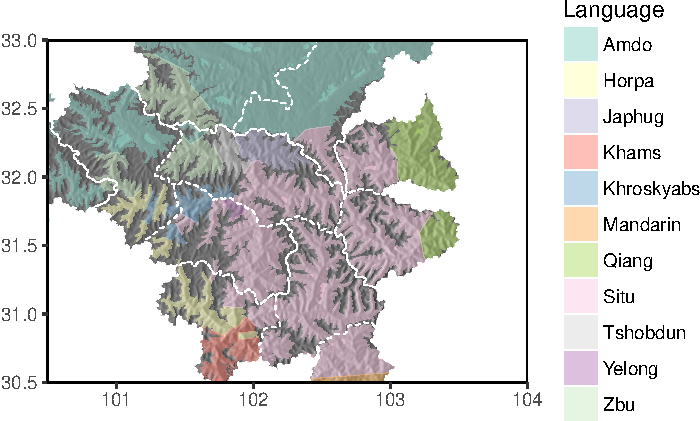
\includegraphics[width=\textwidth]{carte3.pdf}
\end{figure}

Core Gyalrong and West Gyalrongic form the Gyalrongic group \citep{jackson00puxi}, itself a subbranch of Burmo-Gyalrongic (\citealt{jacques.michaud11naish}) and possibly  the larger Tibeto-Gyalrongic group \citep{Sagart19ST}.

Japhug is in contact with both Standard Mandarin and a local variety of Sichuanese. Since no study has focused on the Sichuan Mandarin as spoken by Gyalrong speakers in Mbarkham, the present work represents all Chinese words in Standard Mandarin and pinyin (between chevrons), except for highly nativized Chinese words, presented in IPA.

Situ Gyalrong and Amdo Tibetan used to be the two dominant languages in the area, and many speakers of Japhug also have a passive understanding of Situ, and sometimes also of Tshobdun and Zbu.\footnote{See for example \ref{ex:nW.mACtsxa} (§\ref{sec:terminative}), \ref{ex:nWlWz.thWkWGe.tsa} (§\ref{sec:relative.postverbal}) and \ref{ex:mAkABzu.mWjkHW} (§\ref{sec:ra.khW.jAG.verb}), where Tshendzin recounts her experience as a teacher in Tshobdun village, where she had to learn Tshobdun to make herself understood by the pupil's parents. }


 
 \section{The Japhug corpus}
With the exception of a chapter in \citet[468--486]{linxr93jiarong} on phonology and a few articles by Lin Youjing (\citealt{linluo03, lin11direction}) (all on the Tatshi dialect), the available data on Japhug
are essentially from my own fieldwork, based on nine trips (July-August 2002, April-July 2003, July-August 2005, July 2010, July-August 2012, April-May 2014, July-August 2015, July-August 2016, May 2018) and constant contact by phone with my main language consultants. Some texts have been recorded with the help of my former PhD students Gong Xun and Lai Yunfan.
 
A short grammar \citep{jacques08}, some texts \citep{jacques10gesar}, a dictionary \citep{jacques15japhug} have previously been made available, to which a corpus of transcribed stories on the  Pangloss archive \citep{michailovsky14pangloss} can be added, available on \url{https://lacito.vjf.cnrs.fr/pangloss/corpus/list_rsc.php?lg=Japhug&name=japhug}.


My main consultant is Tshendzin (Chenzhen \zh{陈珍}, female, born 1950), a retired schoolteacher (a native speaker of Japhug, bilingual in Sichuan Mandarin since childhood), whose speech and grammaticality judgements are taken as the norm of this grammar. 

Stories  have also been collected from her husband \forme{χpɤltɕin} Dpalcan \zh{柏尔青}, her maternal uncle Andzin, her nephew (sister's child) Ayang/Kunbzang 'Tsho, and other Kamnyu people, in particular  Tshering Skyid. Most traditional stories are typical of Tibetan folklore and not specific to Japhug-speaking areas, but some procedural texts, description of local plants and animals, as well as accounts of local topography, include unique insight on local culture. In addition, a few conversations have been recorded.
 
The majority of examples in this grammar (except in the grammar sketch in chapter \ref{chap:sketch}) are taken from texts or conversations rather than elicited. Most of the texts cited are already available on Pangloss, and the examples are cited using a title in ASCII characters followed by a line number.\footnote{ \citet[305]{hill17statest} reports that this citation format is sufficient to find the relevant data. } Conversations are not included in the archive at the moment of writing, but individual sound files of the sentences quoted in this grammar are preserved in a private database. In addition, a certain amount of sentences have been noted down during participant observation, and lack recordings.
 
Since speakers I have worked with only recount a limited number of traditional stories (some of which in any case are from written sources; in particular, one of the stories told by Kunbzang Mtsho is clearly adapted from a Grimm story), I have resorted to translation from Chinese to collect a larger corpus. Tshendzin provided surprisingly idiomatic renderings of various storybooks for children (including Grimm tales, Andersen tales, Liaozhai zhiyi \zh{聊斋志异}, Arabian nights and Xiyouji \zh{西游记}). These documents are not given the same value as more spontaneous texts, and are systematically indicated  by adding the extension ``-zh" to the document name. Systematic comparison with the original text is offered whenever any suspicion of calque from Chinese exists. However, the immense morphosyntactic difference between Chinese and Japhug makes it necessary to completely rework the structure of the sentences in most cases (see for instance \ref{ex:CWmaqʰua}, §\ref{sec:apprehensive.function}), so that even if there is undoubtedly influence from Chinese, even the way Chinese is adapted into Japhug is itself an interesting topic of research.



\section{Structure of the grammar}
Rather than being intended as the final word on Japhug grammar, this book is conceived as a tool for exploring  the Japhug corpus and learning the language. 

The reader is invited to start with the grammar sketch (chapter \ref{chap:sketch}). The rest of the grammar contains two chapters on phonology (\ref{chap:phono}, §\ref{sec:clusters.redp}), five on nouns and noun phrases (\ref{chap:nominal.morphology} to \ref{chap:noun.phrase}), eleven on verbal morphology (\ref{chap:verb.template} to \ref{chap:tame}), five on syntax (§\ref{sec:basic.syntax} to \ref{chap:degree}), as well as a chapter \ref{chap:ideophones.sfp} on expressives and another one \ref{chap:kinship} on kinship.

In writing this grammar I have always preferred to abstain from definite judgement rather than provide incorrect data, and the description remains thus incomplete in many aspects, in particular in accounting for minute semantic differences between similar constructions, or on the grammaticality of borderline sentences (about which speakers sometimes change their mind). There are many points of uncertainty in many aspects of the morphosyntax (and even in some topics of phonology), and further research on finer points of phonology, morphosyntax and historical linguistics are much needed, with additional data from different speakers.

\section{Language and culture}
This work focuses on the grammar of the language, and only contains a single chapter (\ref{chap:kinship}, on the kinship system) dedicated to ethnology. However, the corpus that has been collected contains many traditional stories, as well as procedural texts describing the traditional life before massive sinicization. Examples from these texts are found on nearly all the pages of this grammar, and their interest is not purely linguistic. Thus, the section on place names presents a mythological story explaining the origin of a name (\ref{ex:qaprANar.kW}, §\ref{sec:place.names}), the chapter on orientation preverbs contains an account of the traditional living-room/kitchen (§\ref{sec:orientation.kitchen}) and an introduction to weaving (§\ref{sec:orientation.loom}), and the section on antipassive derivations includes a passage on rain-calling and mountain tutelary spirits  (see example \ref{ex:znArGAma}, §\ref{sec:antipassive.avoidance}). In this sense, traditional culture permeates this grammar from beginning till end.

Further ethnographical work is necessary, in particular on kinship \citep{zhangsy20kinship}, traditional houses \citep{dongsy18chabao}, weaving and ethnobotany, and it is hoped that this grammar (together with the dictionary) will make it possible to properly describe local culture through the medium of Japhug rather than Chinese.

  %Japhug language, corpus and culture
\chapter{A grammatical sketch} \label{chap:sketch}

This chapter offers a short introduction to the phonology and morphosyntax of the Japhug language. It is written for typologists and comparative linguists wanting to get a quick general picture of this language, before delving into the core of the grammar.

Morphosyntactic phenomena are illustrated mainly using simplified elicited examples rather than examples gleaned from texts and conversations as in the rest of the grammar.

\section{Phonology and word structure} \label{sec:phono.introduction}
Japhug has 8 vowels (§\ref{sec:vowels}) and 50 consonant phonemes (§\ref{sec:consonant.phonemes}), which can be combined into more than 400 biconsonantal or triconsonantal clusters in the onset (§\ref{sec:inventory.clusters}). Additional clusters are attested across syllable boundaries (§\ref{sec:heterosyllabic.clusters}). In coda position, only 12 consonants are found, and no clusters are possible: several phonological contrasts are neutralized (§\ref{sec:codas.inventory}).

The IPA-based transcription in this grammar is a spelling system that is not strictly phonological: it uses different symbols to represent the allophones of some phonemes (in particular \ipa{w}, §\ref{sec:consonant.phonemes}, §\ref{sec:wC.clusters}). An alternative Tibetan-based orthography for use by native speakers (§\ref{sec:tibetan.script}) is also provided.

Japhug is very far removed from the isolating, tonal and ``monosyllabic'' type once considered to be typical of Sino-Tibetan languages. Japhug lacks tonal contrasts (§\ref{sec:stress}), and monosyllabic and monomorphemic words are a minority (§\ref{sec:wordhood.verb}). Words of six syllables or more are not rare in the corpus, as shown by the verb form (\ref{ex:akAtWnWrAZinW}) below.

\begin{exe}
\ex \label{ex:akAtWnWrAZinW}
\gll a-kɤ-tɯ-nɯ-rɤʑí-nɯ \\
\textsc{irr}-\textsc{pfv}-2-\textsc{auto}-stay-\textsc{pl} \\
\glt `May you stay (here).'
\end{exe}

Non-final syllables have strong phonotactic constraints at least in the native vocabulary (§\ref{sec:non.final.syllable}). The last syllable of verbal and nominal stems generally receives stress (as the syllable \forme{-ʑi-} in \ref{ex:akAtWnWrAZinW}, §\ref{sec:stress}) and allows the maximal number of vowel and consonant contrasts.


\section{Parts of speech} \label{sec:parts.speech.introduction}
Unlike other Trans-Himalayan languages such as Sinitic, where the identification of word classes requires extensive syntactic analysis \citep{gabelentz1881chinesische, chao68chinese}, most parts of speech in Japhug can be straightforwardly defined on the basis of morphology. 

Japhug has open and closed parts of speech. The three main open parts of speech are \textit{nouns}, \textit{verbs} and \textit{ideophones}.

Nouns can in their turn be subdivided into four classes with different morphological properties. First, inalienably possessed nouns (§\ref{sec:inalienably.possessed}) require the presence of a possessive prefix (§\ref{sec:possessive.paradigm}). Second, alienably possessed nouns allow a possessive prefix, but do not require it. Third, counted noun (§\ref{sec:counted.nouns}) take numeral prefixes (§\ref{sec:numeral.prefixes}). Fourth, unpossessible nouns cannot be prefixed (§\ref{sec:unpossessible.nouns}).

Verbs are at the core of Japhug grammar, and have the richest morphology of all parts of speech -- no less than nine chapters (from \ref{chap:verb.template} to \ref{chap:tame}), about half of the grammar, is devoted to verbal morphology. Unlike other Trans-Himalayan languages such as Khaling, 
whose verbs are a closed class \citep{jacques12khaling}, Japhug has a productive system of denominal and deideophonic morphology (§\ref{chap:denominal}), allowing a constant creation of new verbs. Apart from a handful of defective verbs (§\ref{sec:intr.person.irregular}, §\ref{sec:irregular.transitive}), all verbs require orientation preverbs (§\ref{sec:orientation.preverbs}) in most finite forms, and are the only part of speech compatible with these preverbs. Person indexation morphology (§\ref{sec:intransitive.paradigm}) is also a criterion for identifying verbs, but it is not always applicable since some verbs only occur in \textsc{3sg} with no indexation affixes (§\ref{sec:intransitive.invariable}), and since a few predicative words have adopted number indexation suffixes by analogy with verbs (§\ref{sec:non.finite.indexation}).

Ideophones (§\ref{sec:idph}) can also be distinguished from other parts of speech by specific morphological patterns (§\ref{sec:ideo.regular}).

There is no specific class of `adjective' in Japhug. Words describing properties belong to three different parts of speech: adjectival stative verbs, which can be distinguished from other stative verbs by their ability to undergo the tropative derivation (§\ref{sec:tropative}), ideophones, and also property nouns, a subclass of inalienably possessed nouns (§\ref{sec:property.nouns}).

Closed parts of speech comprise numerals (§\ref{sec:plain.numerals}) and pronouns (chapter \ref{chap:pronouns}), which also have specific morphology, and invariable words including postpositions (§\ref{ex:postpositions}), determiners (§\ref{sec:determiners}), adverbs (§\ref{sec:sentential.adverbs}, §\ref{sec:degree.adverbs}), linkers (§\ref{sec:coordination}, §\ref{sec:tCe.topic}), interjections and calling sounds (§\ref{sec:other.expressive}) and sentence final particles (§\ref{sec:sfp}). 

\section{Nominal morphology} \label{sec:noun.introduction}
This section presents nominal inflection, derivation as well as grammatical categories expressed by syntactic rather than morphological means within noun phrases and postpositional phrases.

\subsection{Non-attested nominal morphological categories}
There is no gender, definiteness, obviation, negation and tense-aspect-modality-evidential inflection or derivation on nouns in Japhug. 

The whole category of gender is completely absent from Japhug grammar; there are only suffixes for male and female animals, and even these are borrowed from Tibetan (§\ref{sec:gender}). 

There is no dedicated marker of definiteness (§\ref{sec:definiteness}), but the aforementioned topic marker \forme{iɕqʰa} only occurs on definite referents (§\ref{sec:iCqha}). Indefiniteness can be marked by the indefinite article \forme{ci} (§\ref{sec:indef.article}) derived from the numeral `one' (§\ref{sec:one.to.ten}). 

While an obviative/proximative contrast is reflected by some uses of the inverse prefix in the inflection of transitive verbs (§\ref{sec:obviation.possessor}), Japhug lacks obviative morphology on nouns (§\ref{sec:possessive.prefix.obv.def}), unlike Algonquian languages (for instance \citealt[183]{valentine01grammar}).
 
Polarity and Tense-aspect-modality-evidentiality, which are prominently encoded by verbal morphology (§\ref{sec:negation}, chapter \ref{chap:tame}), even on nominalized verb forms (§\ref{sec:subject.participle.other.prefixes}), are completely absent from nominal morphology, and various types of participial clauses have to be used instead (§\ref{sec:non.existing.derivation}).
  

\subsection{Number}
Number can be indicated by the dual \forme{ni} (§\ref{sec:dual.determiners}) and plural \forme{ra} (§\ref{sec:plural.determiners}) determiners. These determiners are not mutually incompatible with numerals, as shown by (\ref{ex:jla.RnWz.ni}), where the redundant \japhug{ʁnɯz}{two} can be added (these redundant forms, though grammatical, are not very common). The fact that numerals (and other postnominal modifiers, including relative clauses) can be inserted between nouns and number determiners show that they are not analyzable as number suffixes.

\begin{exe}
\ex \label{ex:jla.RnWz.ni}
\gll jla (ʁnɯz) ni \\
male.hybrid.yak two \textsc{du} \\
\glt `The two male hybrid yaks' 	(\japhdoi{0003660\#S7})
\end{exe}

Some nouns however do have an inflectional number category, expressed by a prefixal paradigm partially illustrated in Table \ref{tab:num.prefixes.introduction} (§\ref{sec:numeral.prefixes}). 

\begin{table}
\caption{Numeral prefixes of counted nouns}  \label{tab:num.prefixes.introduction} 
\begin{tabular}{llll}
\lsptoprule
 & Numeral &  \forme{-sŋi} `day'   \\
\midrule
 1	& \forme{ci}  &	\forme{tɯ-sŋi}&  `one day'	\\
2	&	\forme{ʁnɯz}  &	\forme{ʁnɯ-sŋi}&  `two days'	\\
3	&	\forme{χsɯm}  &	\forme{χsɯ-sŋi}&  `three days'	\\
4	&	\forme{kɯβde}  &	\forme{kɯβde-sŋi}, \forme{kɯβdɤ-sŋi}  &`four days'	\\
5	&	\forme{kɯmŋu}  &	\forme{kɯmŋu-sŋi}, \forme{kɯmŋɤ-sŋi}  &	`five days'\\
6	&	\forme{kɯtʂɤɣ}  &	\forme{kɯtʂɤ-sŋi}  &`six days'	\\
7	&	\forme{kɯɕnɯz}  &	\forme{kɯɕnɯ-sŋi}  &`seven days'	\\
8	&	\forme{kɯrcat}  &	\forme{kɯrcɤ-sŋi}  &`eight days'	\\
9	&	\forme{kɯngɯt}  &	\forme{kɯngɯ-sŋi}  &`nine days'	\\
10	&	\forme{sqi}  &	\forme{sqɯ-sŋi}   & `ten days'\\
\lspbottomrule
\end{tabular}
\end{table}

This type of nouns corresponds to the category called `classifiers' (\citealt[518]{chao68chinese}, \citealt{aikhenvald00classifiers}) (\zh{量词} <liàngcí> in Chinese) in works on the grammar of Chinese, Japanese and other languages of East Asia. However, this terminology is particularly clumsy in the case of Japhug.  Unlike in languages such as Chinese or Thai, nouns in Japhug do not require a `classifier' to be used with a numeral, as shown by (\ref{ex:tCheme.ci})\footnote{The numeral \japhug{ci}{one} is grammaticalized as an indefinite marker (§\ref{sec:indef.article}).} and (\ref{ex:tCheme.XsWm}).


\begin{exe}
\ex \label{ex:tCheme.ci}
\gll tɕʰeme ci \\
girl one/\textsc{indef} \\
\glt `A/one girl'
\ex \label{ex:tCheme.XsWm}
\gll tɕʰeme χsɯm \\
girl three \\
\glt `Three girls'
\end{exe}

When occurring as postnominal modifiers (\ref{ex:tCheme.tWrdoR}), the two main functions of nouns with numerals prefixes are partitive (`one of the $X$') and distributive (`each $X$') depending on the constructions where they appear (§\ref{sec:CN.quantifier}). 

\begin{exe}
\ex \label{ex:tCheme.tWrdoR}
\gll tɕʰeme tɯ-rdoʁ \\
girl one-piece \\
\glt `One of the girls'; `Each girl...'; `One girl' (\japhdoi{0004053\#S36})
\end{exe}

In addition, although a handful of  `classifiers' are indeed specific to a particular semantic category of nouns (§\ref{sec:CN.classification}), the generic `classifier' \japhug{tɯ-rdoʁ}{one piece} can be used as modifier with nearly all referents.

For these reasons, this grammar favours the term \textit{counted noun} based on morphology, rather than `classifier' (an extremely marginal function of these words) or `quantifier' (not specific enough, since there are many quantifiers that are not counted nouns, §\ref{sec:quantifiers.determiners}) to refer to nouns with numeral prefixes such as \japhug{tɯ-sŋi}{one day} or \japhug{tɯ-rdoʁ}{one piece}.

\subsection{Case marking} \label{sec:case.intro}
Japhug lacks case inflection, but has a few regular adverbializing derivations (§\ref{sec:denominal.adverb}), whose functions resemble that of oblique cases: the comitative \forme{kɤ́-} (§\ref{sec:comitative.adverb}) and the perlative (§\ref{sec:perlative}).

Grammatical relations on noun phrases are encoded by postpositions such as the ergative \forme{kɯ} (§\ref{sec:erg.kW}), the genitive \forme{ɣɯ} (§\ref{sec:genitive}) and the comitative \forme{cʰo} (§\ref{sec:comitative}), as well as relator nouns (§\ref{sec:relator.nouns}) such as the dative \forme{ɯ-ɕki} or \forme{ɯ-pʰe} (§\ref{sec:dative}). With the sole exception of the genitive forms of a few pronouns such as \forme{aʑɯɣ} \textsc{1sg}:\textsc{gen} (from \japhug{aʑo}{\textsc{1sg}} and \forme{ɣɯ}, §\ref{sec:pronouns.gen}), the postpositions do not merge phonologically with the previous word. As shown by (\ref{ex:Wpi.ni.kW}) and (\ref{ex:ra.GW.nWfsapaR}), they are located at the end of the noun phrase, further away from the head noun than all determiners, including number markers. 

\begin{exe}
\ex \label{ex:Wpi.ni.kW}
\gll [[ɯ-pi ni] \textbf{kɯ}] pɣa nɯ pa-mto-ndʑi\\
\textsc{3sg}.\textsc{poss}-elder.sibling \textsc{du} \textsc{erg} bird \textsc{dem} 3\flobv{}:\textsc{aor}-see-\textsc{du} \\
\glt `His two elder siblings saw the bird.' 
\end{exe}

\begin{exe}
\ex \label{ex:ra.GW.nWfsapaR}
\gll [[tɯrme ra] \textbf{ɣɯ}] nɯ-fsapaʁ \\
person \textsc{pl} \textsc{gen} \textsc{3pl}.\textsc{poss}-cattle \\
\glt `People's cattle' 
\end{exe}

In addition, it is possible to make a pause between the noun and the postposition \forme{kɯ} or \forme{ɣɯ} that follows: the postposition can be procliticized to the following word. A considerable number of examples can be found in the corpus (§\ref{ex:word.vs.clitic.postp}).

While Situ Gyalrong does have locative suffixes (\citealt[325--331]{linxr93jiarong}), Japhug only uses postpositions (§\ref{sec:core.locative}) and/or relator nouns (§\ref{sec:relator.postposition.location}) to express location, goal and source of motion. The only traces of the proto-Gyalrong suffixes are the locative postposition \forme{zɯ}, which was degrammaticalized from a suffix \forme{*-s} (§\ref{sec:core.locative}), and a few isolated lexicalized forms (§\ref{sec:locative.j}, §\ref{sec:relator.postposition.location}).

\subsection{Possession}
The main nominal morphosyntactic category expressed by an inflectional paradigm in Japhug is possession, encoded by a series of possessive prefixes  (§\ref{sec:possessive.paradigm}).

\subsubsection{Possessive paradigm} \label{sec:possessive.paradigm.intro}

\begin{table}
\caption{Possessive paradigms} \label{tab:possessive.paradigms.intro}
\begin{tabular}{lllll} 
\lsptoprule
Person & Prefix & \japhug{tɯ-ku}{head} & \japhug{kʰa}{house}  \\
\midrule
1\sg{}  &\forme{a-} &\forme{a-ku} & \forme{a-kʰa} \\
2\sg{} &\forme{nɤ-} & \forme{nɤ-ku} & \forme{nɤ-kʰa} \\
3\sg{}& \forme{ɯ-}   &\forme{ɯ-ku} & \forme{ɯ-kʰa} \\
\midrule
1\du{} &\forme{tɕi-}   &\forme{tɕi-ku} & \forme{tɕi-kʰa} \\
2/3\du{}&\forme{ndʑi-} &\forme{ndʑi-ku} & \forme{ndʑi-kʰa} \\
\midrule
1\pl{} & \forme{ji-} 	&\forme{ji-ku} & \forme{ji-kʰa} \\
2/3\pl{}&\forme{nɯ-}   &\forme{nɯ-ku} & \forme{nɯ-kʰa} \\
\midrule
indefinite&\forme{tɯ-/tɤ-/ta-}    &\textbf{\forme{tɯ-ku}} & \textbf{\forme{kʰa}} \\
generic&\forme{tɯ-}    &\forme{tɯ-ku} & \forme{tɯ-kʰa} \\
\lspbottomrule
\end{tabular}
\end{table}

The possessive paradigm is nearly the same for all nouns (\tabref{tab:possessive.paradigms.intro}), but some nouns such as \japhug{tɯ-ku}{head} require a indefinite possessor prefix \forme{tɯ\trt}, \forme{tɤ-} or \forme{ta-} when no definite possessor is present, while other nouns like \japhug{kʰa}{house} can occur in bare stem form. The former are \textit{inalienably possessed nouns}, comprising in particular body parts (§\ref{sec:body.part}) and kinship terms (§\ref{sec:kinship}), while the latter are \textit{alienably possessed nouns}. Some inalienably possessed nouns have been grammaticalized as relator nouns (§\ref{sec:relator.nouns}) marking the syntactic function of noun phrases. Furthermore, a handful of nouns have become TAME markers (§\ref{sec:WmdoR.TAME}).

Possessors are obligatorily indicated by possessive prefixes. An overt possessor can be optionally added. For instance, the meaning `my cow' can be expressed by the noun form \forme{a-nɯŋa} with a simple possessive prefix, but this noun can be additionally preceded by the genitive pronoun \forme{aʑɯɣ} (\ref{ex:aZWG.anWNa}) or even by the absolutive \forme{aʑo}.

\begin{exe}
\ex \label{ex:aZWG.anWNa}
\gll (aʑɯɣ) a-nɯŋa \\
\textsc{1sg} \textsc{1sg}.\textsc{poss}-cow \\
\glt `My cow' 
\end{exe}

The possessive prefix cannot be elided, even in the case of alienably possessed nouns like \japhug{nɯŋa}{cow}. In (\ref{ex:aZWG.anWNa}), removing the \forme{a-} prefix would result in an agrammatical form ($\dagger$\forme{aʑɯɣ nɯŋa}).

The phrase expressing the possessor always precedes the possessum. Genitive marking on the possessor is optional: in (\ref{ex:ni.GW.ndZinWNa}), the genitive postposition \forme{ɣɯ} (§\ref{sec:gen.possession}) can be elided.

\begin{exe}
\ex \label{ex:ni.GW.ndZinWNa}
\gll [a-mu a-wa ni] (ɣɯ) ndʑi-nɯŋa \\
\textsc{1sg}.\textsc{poss}-mother \textsc{1sg}.\textsc{poss}-father \textsc{du} \textsc{gen} \textsc{3du}.\textsc{poss}-cow \\
\glt `My parents' cow' 
\end{exe}

The person and number of the possessive prefix on the possessum is the same as that of the noun phrase or pronoun marking the possessor: in (\ref{ex:ni.GW.ndZinWNa}) for instance, the third dual possessive prefix \forme{ndʑi-} agrees in number with the dual possessor phrase \forme{a-mu a-wa ni}. Number agreement mismatch is only attested in very restricted contexts (§\ref{ex:prefix.expression.of.possession}).

\subsubsection{Alienabilization} \label{sec:alienabilization.intro}
Nouns can only take one single possessive prefix, except when inalienably possessed nouns are turned into alienably possessed nouns (§\ref{sec:alienabilization}), by stacking a definite possessor prefix (any of the prefixes in \tabref{tab:possessive.paradigms.intro} except the indefinite ones) on the indefinite possessive form. For instance, the possessed form \forme{ɯ-lu} (\ref{ex:nWNa.Wlu}) of \japhug{tɤ-lu}{milk} without prefix stacking is used when the possessor is the cow \textit{producing} the milk, but the alienabilized possessive forms \forme{ɯ-tɤ-lu} `his/her/its milk, the milk for him/her/it' (\ref{ex:lWlu.WtAlu}) or \forme{a-tɤ-lu} `my milk' (\ref{ex:atAlu}), expressing the person or animal \textit{drinking} the milk as possessor, have a combination of two prefixes.

\begin{exe}
\ex 
\begin{xlist}
\ex \label{ex:nWNa.Wlu}
\gll nɯŋa (ɣɯ) ɯ-lu \\
cow \textsc{gen} \textsc{3sg}.\textsc{poss}-milk \\
\glt `(The/a) cow's milk' 
\ex \label{ex:lWlu.WtAlu}
\gll lɯlu (ɣɯ) ɯ-tɤ-lu \\
cat \textsc{gen} \textsc{3sg}.\textsc{poss}-\textsc{indef}.\textsc{poss}-milk \\
\glt `The milk for the cat (i.e. given to the cat to drink)' 
\ex \label{ex:atAlu}
\gll (aʑo) a-tɤ-lu \\
\textsc{1sg} \textsc{1sg}.\textsc{poss}-\textsc{indef}.\textsc{poss}-milk \\
\glt `My milk (i.e. for me to drink)' 
\end{xlist}
\end{exe}

Stacking of two definite possessor prefixes, or of a numeral prefix with a definite possessor prefix, are not grammatical.

\subsubsection{Generic possessors}
The indefinite possessor prefix has three allomorphs \forme{tɯ-} (as in in \japhug{tɯ-ku}{head}), \forme{tɤ-} (as in \japhug{tɤ-se}{blood}) or \forme{ta-} (as in \japhug{ta-ma}{work}). It has to be distinguished from the generic possessor prefix \forme{tɯ-} (§\ref{sec:indef.genr.poss}). Generic possessors are identical with indefinite possessors in the case of inalienably possessed nouns selecting the \forme{tɯ-} prefix, for instance \forme{tɯ-ku} can either mean `head' or `one's head'. With inalienably possessed nouns selecting the \forme{tɤ-} or \forme{ta-} allomorphs, a contrast is found between \forme{tɤ-se} `blood' and \forme{tɯ-se} `one's blood' (\ref{ex:tWse.kutshi}) for instance.

\begin{exe}
\ex \label{ex:tWse.kutshi}
\gll qajɯsmɤnba kɯ tɯ-se ku-tsʰi ŋu \\
leech \textsc{erg} \textsc{genr}.\textsc{poss}-blood \textsc{ipfv}-drink be:\textsc{fact} \\
\glt `The leech drinks people's (i.e. one's) blood.' 
\end{exe}

The generic possessor prefix can also occur on alienably possessed nouns, as in \forme{tɯ-kʰa} `one's house'. 

No more than one generic referent is possible per clause, so that if a noun with generic possessor prefix is found in the same clause as a verb with generic indexation, there is obligatory co-reference (§\ref{sec:indexation.generic.tr}), as in (\ref{ex:tWrpW.WrZaB}) between the possessor of \forme{tɯ-rpɯ} `one's mother's brother' (indefinite form \forme{tɤ-rpɯ}, §\ref{sec:kinship}) and the transitive subject of the verb \forme{tu-kɯ-ti} `one says' (§\ref{sec:irregular.transitive}).

\begin{exe}
\ex \label{ex:tWrpW.WrZaB}
\gll \textbf{tɯ}-rpɯ ɣɯ ɯ-rʑaβ ɯ-ɕki tɕe ``a-ɬaʁ" tu-\textbf{kɯ}-ti ŋu \\
\textsc{\textbf{genr}}.\textsc{poss}-mother's.brother \textsc{gen} \textsc{3sg}.\textsc{poss}-wife \textsc{3sg}.\textsc{poss}-\textsc{dat} \textsc{loc} \textsc{1sg}.\textsc{poss}-aunt \textsc{ipfv}-\textsc{\textbf{genr}}-say be:\textsc{fact} \\
\glt `\textbf{One}$_i$ calls \textbf{one}$_i$'s mother's brother's wife `my aunt' (i.e. one says `my aunt' to one's mother's brother's wife).' 
\end{exe}

\subsubsection{Possessive existential construction}
Predicative possession can be expressed by the verb \japhug{aro}{own} (§\ref{sec:semi.transitive}, §\ref{sec:possessive.constructions}), encoding the possessor as subject, but the most frequent construction involves an existential verb (§\ref{sec:existential.basic}) with the possessum as subject and the possessor marked by a possessive prefix on the possessum, optionally with a genitive phrase (§\ref{sec:possessive.mihi.est}). The construction is the same for alienably (\ref{ex:nWnWNa.XsWm.pjAtu}) and inalienably (\ref{ex:nWtCW.XsWm.pjAtu}) possessed nouns.
 

\begin{exe}
\ex 
\begin{xlist}
\ex \label{ex:nWnWNa.XsWm.pjAtu}
\gll  kɯβʁa ra ɣɯ nɯ-nɯŋa kɯ-dɤn pjɤ-tu \\
noble \textsc{pl} \textsc{gen} \textsc{3pl}.\textsc{poss}-cow \textsc{sbj}:\textsc{pcp}-be.many \textsc{ifr}.\textsc{ipfv}-exist \\
\glt `The nobles had many cows.'  
\ex \label{ex:nWtCW.XsWm.pjAtu}
\gll  kɯβʁa ra ɣɯ nɯ-tɕɯ χsɯm pjɤ-tu \\
noble \textsc{pl} \textsc{gen} \textsc{3pl}.\textsc{poss}-son three \textsc{ifr}.\textsc{ipfv}-exist \\
\glt `The nobles had three sons.'  
\end{xlist}
\end{exe}

In this construction, the existential verbs rarely agree in number with the possessum: in both (\ref{ex:nWnWNa.XsWm.pjAtu}) and (\ref{ex:nWtCW.XsWm.pjAtu}), the singular verb form \forme{pjɤ-tu} is by far more commonly used than its plural counterpart (§\ref{sec:optional.indexation}).

\subsection{Compounding}
Compounding can be realized by the simple concatenation of noun (or verb) stems.

In compounds comprising two noun stems (§\ref{sec.n.n.compounds}), whose order is modifier-modified, no possessive prefixes occur between the nominal stems, even if the second noun is inalienably possessed. For instance, the compound built from \japhug{kɯrɯ}{Tibetan} and the inalienably possessed \japhug{tɯ-ŋga}{clothes} is \forme{kɯrɯ-ŋga} `Tibetan clothes', rather than $\dagger$\forme{kɯrɯ-tɯŋga}.

In many cases, the non-final elements of the compound appear in a bound form, the bound state (§\ref{sec:status.constructus}), which is characterized by a vocalic change to either \forme{-ɤ} or \forme{-ɯ} (§\ref{sec:vowel.alternations.compounds}) For instance, compounding \japhug{tɯ-ku}{head} with \japhug{tɤ-rme}{hair} yields \forme{tɤ-kɤ-rme} `head hair' with the bound state \forme{kɤ-} from \forme{-ku}. The compound inherits the allomorph \forme{tɤ-} of the indefinite possessor prefix of the head of the compound \japhug{tɤ-rme}{hair}.
 

\subsection{Derivations}
Some suffixal nominal derivations come from compounds with a grammaticalized noun as second element, in particular the diminutive suffixes (§\ref{sec:diminutive}). The recent origin of these suffixes can be shown by the fact that a free form still co-exists with the corresponding compound in some cases. For instance, the compound \forme{χpɯn-pɯ} `little monk' from \japhug{χpɯn}{monk} with the diminutive \forme{-pɯ} occurs in free variation with the phrase (\ref{ex:XpWn.WpW}), in which the main noun is followed by the alienably possessed property noun \japhug{ɯ-pɯ}{little one} (§\ref{sec:property.nouns}) derived from \japhug{tɤ-pɯ}{offspring, young}.

\begin{exe}
\ex \label{ex:XpWn.WpW}
\gll χpɯn ɯ-pɯ \\
monk \textsc{3sg}.\textsc{poss}-little.one  \\
\glt `(The/a) little monk' 
\end{exe}

Not all suffixal derivations have transparent origins. For instance, the privative \forme{-lu} suffix (§\ref{sec:privative}) is not related to any independently attested nominal or verbal root. It turns an inalienably possessed noun into a non-possessible one mainly used as postnominal modifier (§\ref{ex:attributive.postnominal}), removing possessive prefixes and subjecting the nominal stem to bound state alternation (\japhug{tɯ-ku}{head} \fl{} \forme{kɤ-lu} `headless').

Prefixal nominal derivations, however, do not originate from elements of compounds, but rather from participial forms of denominal verbs (§\ref{sec:denom.aGW}, §\ref{sec:denom.andZi}). 

The social relation collective \forme{kɤndʑi-} prefix (§\ref{sec:social.collective}) occurs on the bare stem of kinship terms and a few other terms of social relationship to indicate a group of people. When the group members are  related to each other by a symmetrical relationship (\japhug{tɤ-xtɤɣ}{brother} (of a male) \fl{} \forme{kɤndʑi-xtɤɣ} `group of brothers'), the social relation collective is based on only one nominal stem, but when the relationship is asymmetrical, \forme{kɤndʑi-} can be prefixed to two compounded noun stems, as in \forme{kɤndʑi-wɤmɯ-snom} `group of siblings' from \japhug{tɤ-wɤmɯ}{brother} (of a female) and \japhug{tɤ-snom}{sister} (of a male).
 
The comitative derivation (§\ref{sec:comitative.adverb}) is built by adding the prefixes \forme{kɤ́-} or \forme{kɤɣɯ-} to reduplicated noun stems. It derives an adverb meaning `together with $X$' which can have scope over the whole clause, or be restricted to a noun phrase. It can apply to both inalienably possessed nouns (\japhug{tɯ-ŋga}{clothes} \fl{} \forme{kɤ́-ŋgɯ\redp{}ŋga} `together with his/her clothes') or alienably possessed ones (\japhug{jla}{male hybrid yak} \fl{} \forme{kɤ́-jlɯ\redp{}jla} `together with the/his/her hybrid yak'). Comitative derivation can preserve the indefinite possessor prefix of inalienably possessed nouns, causing alienabilization (§\ref{sec:alienabilization.intro}, §\ref{sec:alienabilization}). For instance, \japhug{tɤ-rte}{hat} has two comitative forms: \forme{kɤ́-rtɯ\redp{}rte} `together with his/her hat' (wearing it)  and \forme{kɤ́-tɤ-rtɯ\redp{}rte} `together with a/the hat' (not wearing it).

\section{Verbal morphology} \label{sec:verb.introduction}

\subsection{Overview} \label{sec:verb.overview.intro}
Verbs have a considerably more elaborate morphology than all other parts of speech (§\ref{sec:verb.intro}). Verbal morphology is strongly prefixal (§\ref{sec:prefixal.chain}), with some vowel contractions (§\ref{sec:contraction}). Non-concatenative morphology includes stem alternations (§\ref{sec:stem.alternation}) as well as infixation (§\ref{sec:inner.prefixal.chain}, §\ref{sec:intr.person.irregular}, §\ref{sec:autoben.position}). 

Japhug verbal morphology is considerably more regular than that of other Gyalrong languages, in particular Zbu (\citealt{jackson04showu, gong18these}) and Situ \citep{zhangsy18stem}. Most alternations are productive and predictable, and irregular verbs are limited in number (§\ref{sec:intr.person.irregular}, §\ref{sec:irregular.transitive}).

 As illustrated by (\ref{ex:amAGWnWtWwGznAre}), a verb form can comprise six inflectional prefixes (in blue) arranged in a rigid template (§\ref{sec:outer.prefixal.chain}) and several derivational prefixes (in red).
 
\begin{exe}
\ex \label{ex:amAGWnWtWwGznAre}
\gll   \bleu{a$^{-6}$-mɤ$^{-5}$-ɣɯ$^{-4}$-nɯ$^{-3}$-tɯ́$^{-2}$-wɣ$^{-1}$}-\rouge{z-nɤ}-re \\
\bleu{\textsc{irr}$^{-6}$-\textsc{neg}$^{-5}$-\textsc{cisl}$^{-4}$-\textsc{pfv}$^{-3}$-2$^{-2}$-\textsc{inv}$^{-1}$}-\rouge{\textsc{caus}-\textsc{denom}}-laughter \\
\glt `Don't let him come and make you laugh.'
\end{exe}
 
The suffixal chain (§\ref{sec:suffixes}) only includes inflectional suffixes, with a maximal number of four slots (\ref{ex:WmApWkWmtoandZici.intro}).  

 \begin{exe}
\ex \label{ex:WmApWkWmtoandZici.intro}
\gll  \bleu{ɯmɤ$^{-6}$-pɯ$^{-3}$-kɯ$^{-2}$}-mto-\bleu{t$^{+1}$-a$^{+2}$-ndʑi$^{+3}$-ci$^{+4}$} \\
 \bleu{\textsc{prob}$^{-6}$-\textsc{aor}$^{-3}$-\textsc{peg}$^{-2}$}-see-\bleu{\textsc{pst}:\textsc{tr}$^{+1}$-\textsc{1sg}$^{+2}$-\textsc{du}$^{+3}$-\textsc{peg}$^{+4}$} \\
 \glt `It looks like I have seen the two of them.'  
\end{exe} 
 
 Numerous non-adjacent dependencies (§\ref{sec:templatic.verb}) are observed across the prefixal and the suffixal chains.
 
Inflectional verbal morphology encodes person and number of one or two core arguments (chapter \ref{chap:indexation}, §\ref{sec:indexation.tr.intro}), orientation (§\ref{sec:orientation.preverbs}), associated motion (§\ref{sec:associated.motion}), negation (§\ref{sec:negation}) and Tense-Aspect-Modality-Evidentiality (chapter \ref{chap:tame}). 
 
 
\subsection{Indexation} \label{sec:indexation.intro}
All finite verb forms in Japhug have obligatory person indexation. Since the \textsc{3sg} has zero marking as in many languages of the world \citep[227--236]{benveniste66problemes1}, indexation is not conspicuous on intransitive verbs requiring a \textsc{3sg} subject (§\ref{sec:intransitive.invariable}), but indirectly observable even on transitive dummy verbs (§\ref{sec:transitive.dummy}) due to the presence of stem alternation (§\ref{sec:stem3}).

Transitive and intransitive verbs are clearly distinguished by a series of seven morphological parameters (§\ref{sec:transitivity.morphology}). Intransitive verbs only index one argument (the intransitive subject, S), and transitive verbs index two arguments (the transitive subject A and the object O). Semi-transitive verbs have intransitive indexation (§\ref{sec:semi.transitive}), but select a second core argument (§\ref{sec:semi.object}). Only a handful of verbs are labile, and can be conjugated either transitively or intransitively (§\ref{sec:lability}).

\subsubsection{The intransitive paradigm}
Person indexation in Japhug is best introduced with the intransitive paradigm (§\ref{sec:intransitive.paradigm}), since it it considerably smaller than the transitive one. The regular paradigm is illustrated in \tabref{tab:intransitive.indexation.intro} with the verb \japhug{mbɣom}{be in a hurry} in the Factual Non-Past, the only TAME without orientation preverb (§\ref{sec:factual}).
 
\begin{table}[H]  
\caption{The intransitive indexation paradigm} \label{tab:intransitive.indexation.intro}
\begin{tabular}{llll} \lsptoprule
Person & Form & Example   \\
\midrule
\textsc{1sg} & \ro{}-\forme{a} & \forme{mbɣom-a} \\
\textsc{1du} & \ro{}-\forme{tɕi} & \forme{mbɣom-tɕi} \\
\textsc{1pl} & \ro{}-\forme{ji} & \forme{mbɣom-i} \\
\midrule
\textsc{2sg} & \forme{tɯ}-\ro{} & \forme{tɯ-mbɣom} \\
\textsc{2du} & \forme{tɯ}-\ro{}-\forme{ndʑi} & \forme{tɯ-mbɣom-ndʑi} \\
\textsc{2pl} & \forme{tɯ}-\ro{}-\forme{nɯ} & \forme{tɯ-mbɣom-nɯ} \\
\midrule
\textsc{3sg} & \ro{} & \forme{mbɣom} \\
\textsc{3du} & \ro{}-\forme{ndʑi} & \forme{mbɣom-ndʑi} \\
\textsc{3pl} & \ro{}-\forme{nɯ} & \forme{mbɣom-nɯ} \\
\lspbottomrule
\end{tabular}
\end{table}

The intransitive paradigm has different forms for singular, dual and plural. First persons have dedicated suffixes encoding both person and number; there is no inclusive/exclusive contrast. Second and third person forms are distinguished by the second person \forme{tɯ-} prefix (on the historical significance of this prefix, see \citealt{jacques12agreement} and \citealt{delancey14second}). There is no overt third person marker on intransitive verbs. Number markers are shared by second and third person forms: absence of suffix for the singular, \forme{-ndʑi} for the dual and \forme{-nɯ} for the plural. Slightly different forms are found in dialects of Japhug other than Kamnyu (§\ref{sec:indexation.suffixes.history}). In addition to the paradigm in \tabref{tab:intransitive.indexation.intro}, a generic person \forme{kɯ-} prefix also occurs on intransitive verbs (§\ref{sec:indexation.generic.tr}). 

A handful of intransitive verbs infix rather than prefix the second person (§\ref{sec:intr.person.irregular}). It is the only irregularity related to person indexation in intransitive verbs in Japhug.


\subsubsection{The transitive paradigm} \label{sec:indexation.tr.intro}
The transitive paradigm is too large to be described in this introductory chapter in its entirety (§\ref{sec:polypersonal}). \tabref{tab:transitive.paradigm.singular} presents the singular forms of the paradigm of the transitive verb \japhug{sat}{kill} (a verb lacking stem alternations) in the Factual Non-Past, which are sufficient to illustrate its basic structure. In this table, the columns represent the objects (O), and the rows the subjects (A). The shaded cells indicate configurations with coreferent subject and object, which are expressed by the reflexive derivation (§\ref{sec:reflexive}) and do not belong to the transitive paradigm.

\begin{table}[H] 
\caption{The transitive paradigm (singular forms) of the non-alternating verb \japhug{sat}{kill} in the Factual Non-Past} 
 \centering \label{tab:transitive.paradigm.singular}
\begin{tabular}{l|l|l|lll} 
\toprule
&1O & 2O &3O&3$'$O\\
\hline
1A&\grise{}& \forme{ta-\textbf{sat}} & \forme{\textbf{sat}-a} & \\
\hline
2A&\forme{kɯ-\textbf{sat}-a} & \grise{} & \forme{tɯ-\textbf{sat}} & \\
\hline
3A& \forme{ɣɯ́-\textbf{sat}-a} & \forme{tɯ́-wɣ-\textbf{sat}} & \grise{} &\forme{\textbf{sat}} \\
3$'$A & & &\forme{ɣɯ́-\textbf{sat}} &\grise{} \\
\bottomrule
\end{tabular}
\end{table}

The comparison of Tables \ref{tab:intransitive.indexation.intro} and \ref{tab:transitive.paradigm.singular} shows that the \textsc{1sg} \forme{-a} suffix and the second person \forme{tɯ-} prefix have neutral alignment: they can index intransitive subject, transitive subject or object. In the following, the person configurations are referred to by $X \rightarrow Y$, where $X$ represents the subject and $Y$ the object (for instance 1\fl{}3 means `first person subject, third person object').  The eight non-shaded cells of the paradigm in \tabref{tab:transitive.paradigm.singular} can be divided into three groups. 

First, 1\fl{}3, 2\fl{}3 and 3\flobv{} are the \textit{direct} configurations with a third person object, whose forms resemble the 1, 2 and 3 forms of the intransitive paradigm (at least in the Factual Non-Past). 

Second, 3\fl{}1, 3\fl{}2 and 3$'$\fl{}3 are the \textit{inverse} configurations, which have the same prefixes or suffixes as the corresponding intransitive and direct forms (at least in this paradigm), but take in addition the inverse prefix \forme{ɣɯ-}/\forme{wɣ-} (the allomorphy of this prefix is explained in §\ref{sec:allomorphy.inv}). 

Third, 1\fl{}2 and 2\fl{}1 (without third person) are the the \textit{local} configurations (§\ref{sec:indexation.local}). They are characterized by the presence of the portmanteau \forme{ta-} and \forme{kɯ-} prefixes (§\ref{sec:portmanteau.prefixes.history}) not found in the intransitive paradigm.

The reasons for using the terms ``direct'' and ``inverse'' to describe the transitive paradigm are discussed in §\ref{sec:direct-inverse}.

When both arguments are third person (§\ref{sec:indexation.non.local}), there is a contrast between direct  3\flobv{} and inverse 3$'$\fl{}3 configurations, whose meaning is not entirely straightforward  (§\ref{sec:inverse.3.3.saliency}). The subject of the direct configuration, and object of the inverse one is called \textit{proximate} (3), and the other argument \textit{obviative} (3$'$). The direct 3\flobv{} configuration is by far the most common one in narratives and conversation. The inverse 3$'$\fl{}3 is more restricted; it occurs in particular to index a generic subject with a third person object (§\ref{sec:indexation.generic.tr}), and also when the subject is inanimate and the object animate (§\ref{sec:obviation.animacy}).

The majority of transitive verbs (all verbs ending in closed syllables or with front vowels) are non-alternating like \japhug{sat}{kill}. However, about a third of all transitive verbs (those ending in \forme{-a}, \forme{-u}, \forme{-o} and \forme{-ɯ}) have stem alternation in the \textit{direct} configurations with a singular subject in the Factual Non-Past and a few other tenses (§\ref{sec:stem3}).
 
\begin{table}[H] 
\caption{The transitive paradigm (singular forms) of the alternating verb \japhug{ʁndɯ}{hit} in the Factual Non-Past} 
 \centering \label{tab:transitive.paradigm.singular.alternating}
\begin{tabular}{l|l|l|lll} 
\toprule
&1O & 2O &3O&3$'$O\\
\hline
1A&\grise{}& \forme{ta-\textbf{ʁndɯ}} & \forme{\textbf{ʁndi}-a} \acell & \acell \\
\hline
2A&\forme{kɯ-\textbf{ʁndɯ}-a} & \grise{} & \forme{tɯ-\textbf{ʁndi}} \acell & \acell \\
\hline
3A& \forme{ɣɯ́-\textbf{ʁndɯ}-a} & \forme{tɯ́-wɣ-\textbf{ʁndɯ}} & \grise{} &\forme{\textbf{ʁndi}} \acell \\
3$'$A & & &\forme{ɣɯ́-\textbf{ʁndɯ}} &\grise{} \\
\bottomrule
\end{tabular}
\end{table}

\tabref{tab:transitive.paradigm.singular.alternating} illustrates the singular forms of the alternating verb \japhug{ʁndɯ}{hit}, which has additional stem \forme{-ʁndi} in the \textsc{1sg}\fl{}3, \textsc{2sg}\fl{}3 and \textsc{3sg}\flobv{} configurations (with blue colouring), which are thus different from the corresponding intransitive forms.

In the Aorist (§\ref{sec:aor.morphology}), a slightly different paradigm is found, illustrated in \tabref{tab:transitive.paradigm.singular.aorist} with the \japhug{ʁndɯ}{hit}. Unlike the Factual Non-Past shown in the previous tables, the Aorist requires an orientation preverb (§\ref{sec:kamnyu.preverbs}), here the \textsc{upwards} \forme{tɤ-}. There is no stem alternation marking the direct forms, but all verbs have a different series of preverbs (here \forme{ta-}) in the direct 3\flobv{} forms (§\ref{sec:aor.morphology}, §\ref{sec:kamnyu.preverbs}). In addition, the \textsc{1sg}\fl{}3 and \textsc{2sg}\fl{}3 forms require a \forme{-t} suffix which redundantly encodes both person and tense-aspect (§\ref{sec:suffixes}).

\begin{table}[H] 
\caption{The transitive paradigm (singular forms) of the verb \japhug{ʁndɯ}{hit} in the Aorist} 
 \centering \label{tab:transitive.paradigm.singular.aorist}
\begin{tabular}{l|l|l|lll} 
\toprule
&1O & 2O &3O&3$'$O\\
\hline
1A&\grise{}& \forme{tɤ-ta-\textbf{ʁndɯ}} & \forme{tɤ-\textbf{ʁndɯ}-\rouge{t}-a}  &  \\
\hline
2A&\forme{tɤ-kɯ-\textbf{ʁndɯ}-a} & \grise{} & \forme{tɤ-tɯ-\textbf{ʁndɯ}-\rouge{t}}  &  \\
\hline
3A& \forme{tɤ́-wɣ-\textbf{ʁndɯ}-a} & \forme{tɤ-tɯ́-wɣ-\textbf{ʁndɯ}} & \grise{} &\forme{\rouge{ta}-\textbf{ʁndɯ}}  \\
3$'$A & & &\forme{tɤ́-wɣ-\textbf{ʁndɯ}} &\grise{} \\
\bottomrule
\end{tabular}
\end{table}

There is no ambiguity in person indexation in Japhug (unlike for instance in Khaling where 2\fl{}1 and 3\fl{}1 configurations are identical, \citealt{jacques12khaling}), but there are strong restrictions on number indexation: unless the \textsc{1sg} suffix is present, only one of the two arguments can be indexed for both person and number, the subject in direct configurations, and the object in inverse and local configurations. Double number indexation only occurs in forms with the \textsc{1sg} \forme{-a} suffix, to which additional number suffixes can be added (§\ref{sec:double.number.indexation}), for instance \forme{ɣɯ́-ʁndɯ-a-nɯ}  `they will hit me' (\textsc{3pl}\fl{}\textsc{1sg}) where the plural morpheme \forme{-nɯ}, indexing the number of the subject, follows the \textsc{1sg}.

\subsubsection{Person indexation and finiteness} \label{sec:indexation.finiteness.intro}
Person indexation markers (including person-indexing stem alternation and orientation preverbs) are not found on participles, infinitives and other non-finite verb forms (chapter \ref{chap:non-finite}). A handful of phatic and exclamative words of nominal origin have however developed the ability to take number suffixes (§\ref{sec:inflectionalization.intro}, §\ref{sec:non.finite.indexation}). Apart from these, words belonging to parts of speech other than verbs are incompatible with the indexation affixes described in this section.


\subsection{Orientation preverbs and TAME}
This section focuses on morphology. Since the use of the TAME categories involve sometimes subtle semantic nuances, and have to be explained on the basis of examples with a clear context, the discussion of the semantic function of each category is deferred to chapter \ref{chap:tame}.

\subsubsection{The morphology of orientation preverbs}
The main morphological exponents of tense, aspect, modality and evidentiality (henceforth TAME) in Japhug are the orientation preverbs (§\ref{sec:orientation.preverbs}). All regular finite verb forms require \textit{one and only one} preverb (§\ref{sec:outer.prefixal.chain}), except the Factual Non-Past (§\ref{sec:factual}) which does not take any preverb. The stacking of two or more preverbs is ungrammatical. Only a handful of irregular defective verbs are incompatible with orientation preverbs (§\ref{sec:intr.person.irregular}, §\ref{sec:irregular.transitive}).

Preverbs encode one out of seven orientations (\tabref{tab:orientation.preverbs.intro}), divided into three dimensions: vertical (§\ref{sec:vertical.dimension}), riverine (§\ref{sec:riverine.dimension}) and solar (§\ref{sec:solar.dimension}), to which an unspecified orientation is added. This tridimensional system is not restricted to verbal morphology: locative relator nouns (§\ref{sec:relator.nouns.3d}), egressive postpositions (§\ref{sec:egressive}) and locative adverbs (§\ref{sec:preverbs.adverbs}) have similar systems with six orientations, built from morphemes that are historically related to the preverbs.

There are four series of preverbs (\tabref{tab:orientation.preverbs.intro} includes two of them, the series A and B) in the Kamnyu dialect, used in different TAME categories (§\ref{sec:kamnyu.preverbs}).  Some dialects of Japhug have a slightly different system \begin{scriptsize}\begin{footnotesize}\end{footnotesize}\end{scriptsize} (§\ref{sec:xtokavian.preverbs}).

\begin{table}
\caption{Orientation preverbs in Kamnyu Japhug} \label{tab:orientation.preverbs.intro}
\begin{tabular}{llllll}
\lsptoprule
Dimension& Orientation  &  	A &   B    \\  	
   \midrule
Vertical &Up   &  	\forme{tɤ-}   &  	\forme{tu-}   &    \\  	
  & Down   &  	\forme{pɯ-}   &  	\forme{pjɯ-}  &   \\  	
\midrule
Riverine &Upstream   &  	\forme{lɤ-}   &  	\forme{lu-}   &  	   \\  	
  &Downstream   &  	\forme{tʰɯ-}   &  	\forme{cʰɯ-}      \\  	
\midrule
Solar &Eastwards   &  	\forme{kɤ-}   &  	\forme{ku-}       \\  	
  &Westwards   &  	\forme{nɯ-}   &  	\forme{ɲɯ-}      \\  	
\midrule
&Unspecified  &\forme{jɤ-}   &  	\forme{ju-}      \\  	
\lspbottomrule
\end{tabular}
\end{table}

 \textit{Orientable} verbs (§\ref{sec:orientable.verbs}) are compatible with all orientations; this includes in particular motion verbs like \japhug{ɣi}{come} and \japhug{ɬoʁ}{come out} (§\ref{sec:motion.verbs}). With this type of verbs, the preverbs indicate either the absolute direction of the motion (§\ref{sec:tridimensional.preverb}), for instance  \textsc{upwards} in (\ref{ex:tANe.tAlhoR}) or have extended meanings (§\ref{sec:orientation.extended}), such as the illative function (§\ref{sec:illative.elative}) of the \textsc{upstream} preverb in (\ref{ex:WNgW.lAGi}).
 
 \begin{exe}
\ex \label{ex:tANe.tAlhoR}
\gll tɤŋe tɤ-ɬoʁ \\
sun \textsc{aor}:\textsc{up}-come.up \\
\glt `The sun rose.' 
\end{exe} 

 \begin{exe}
\ex \label{ex:WNgW.lAGi}
\gll ɯ-ŋgɯ lɤ-ɣi \\
\textsc{3sg}.\textsc{poss}-in \textsc{imp}:\textsc{upstream}-come \\
\glt `Come in! (for instance, inside a house)' (\japhdoi{0003884\#S90})
 \end{exe} 
 
 Non-orientable verbs only select a restricted number of lexically determined orientations, sometimes only one (§\ref{sec:lexicalized.orientation}). For instance, the verb \japhug{ndza}{eat} and  \japhug{mto}{see} require the \textsc{upwards} (§\ref{sec:preverb.ingestion}) and \textsc{downwards} (§\ref{sec:preverb.perception}) preverbs, respectively.

\subsubsection{The morphology of TAME categories}
There are eleven primary TAME categories, which can be divided into four main groups: Non-Past (Factual Non-Past, Egophoric Present, Sensory, §\ref{sec:TAME.npst}), Imperfective (§\ref{sec:imperfective}), Past (Aorist, Inferential, Past Imperfective, and Inferential Imperfective, §\ref{sec:TAME.pst}) and Modal (Irrealis, Imperative, Prohibitive, Dubitative, §\ref{sec:TAME.modal}) categories. 

In the finite TAME categories, the B-type  preverbs are found in the Imperfective (§\ref{sec:imperfective}) and the A-type preverbs in the Imperative (§\ref{sec:imp.morphology}), the Irrealis (§\ref{sec:irrealis.morphology}) and the Aorist (§\ref{sec:aor}), though with slightly different vowel contraction rules (§\ref{sec:contraction}). In the Aorist paradigm of transitive verbs, another series of preverbs (C) is found in the direct 3\flobv{} forms (§\ref{sec:indexation.tr.intro}), based on the A-type preverbs but with \forme{-a} vocalism instead of \forme{-ɯ} and \forme{-ɤ}  (originating from fusion with another prefix, §\ref{sec:xtokavian.preverbs}). For instance, the \textsc{2pl}\fl{}3 Aorist of \japhug{ndza}{eat} is \forme{tɤ-tɯ-ndza-nɯ} (\textsc{aor}:\textsc{up}-2-eat-\textsc{pl} `you$_{pl}$ ate it') with the \textsc{upwards} A-type \forme{tɤ-} preverb, but the corresponding \textsc{3pl}\flobv{} form is \forme{\textbf{ta}-ndza-nɯ} (\textbf{\textsc{aor}:3\flobv{}:\textsc{up}}-eat-\textsc{pl} `they ate it') with the C-type preverb \forme{ta-}. It is the only case when an orientation preverb encodes person in addition to TAME.

The Inferential (§\ref{sec:ifr}) has a series of preverbs (series D) based on series B, but with \forme{-o} and \forme{-ɤ} vocalism instead of \forme{-u} and \forme{-ɯ}, respectively (§\ref{sec:xtokavian.preverbs}). For instance, the  \textsc{upwards} and \textsc{downwards} D-type preverbs are \forme{to-} and \forme{pjɤ\trt}, corresponding to the B-type \forme{tu-} and \forme{pjɯ\trt}, respectively (§\ref{sec:kamnyu.preverbs}).

Five TAME categories neutralize the orientation contrast, and require the same marker for all verbs: the Sensory evidential \forme{ɲɯ-} (§\ref{sec:sensory}), from the B-type \textsc{westwards} preverb (\tabref{tab:orientation.preverbs.intro}), the Egophoric Present \forme{ku-} (§\ref{sec:egophoric}), the Dubitative \forme{ku-} (§\ref{sec:dubitative}), from the B-type \textsc{eastwards} preverb, the Past Imperfective \forme{pɯ-} from the A-type \textsc{downwards} preverb (§\ref{sec:pst.ifr.ipfv.morphology}, \citealt{lin11direction}), and the Inferential Imperfective \forme{pjɤ-} from the D-type \textsc{downwards} preverb (§\ref{sec:pst.ifr.ipfv.morphology}).
 
In addition to orientation preverbs, TAME categories are marked by several morphological exponents, including stem alternations (§\ref{sec:stem.alternation}), allomorphy of negative prefixes (§\ref{sec:neg.allomorphs}) and additional affixes: the Irrealis \forme{a-} prefix (§\ref{sec:outer.prefixal.chain}) and the Past transitive \forme{-t} suffix (§\ref{sec:suffixes}).
 
In the Non-Past, Imperfective and Modal categories (all except Past), transitive alternating verbs have a specific stem in direct configurations with a singular subject (see \tabref{tab:transitive.paradigm.singular.alternating} above and §\ref{sec:stem3}). Another stem is found in the Aorist of a handful of verbs (§\ref{sec:stem2}).
 
Some of the primary categories can be combined with the copula \japhug{ŋu}{be} to form periphrastic TAME categories (§\ref{sec:ipfv.periphrastic.TAME}), for instance the Periphrastic Past Imperfective (§\ref{sec:pst.ifr.ipfv.periphrastic}) illustrated in (\ref{ex:tundzea.pWNu2}), built from the Imperfective (\forme{tu-ndze-a}, with the B-type \textsc{upwards} preverb \forme{tu\trt}, the alternating stem \forme{ndze} from \japhug{ndza}{eat} and the \textsc{1sg} suffix) and the Past Imperfective of the copula \forme{pɯ-ŋu}.
 
 \begin{exe}
\ex \label{ex:tundzea.pWNu2}
\gll  tɤ-mtʰɯm tu-ndze-a pɯ-ŋu   \\
\textsc{indef}.\textsc{poss}-meat \textsc{ipfv}-eat[III]-\textsc{1sg} \textsc{pst}.\textsc{ipfv}-be \\
\glt `I was eating meat/I used to eat meat.' 
  \end{exe} 

In addition, primary TAME categories can be combined with prefixes expressing secondary aspectual (§\ref{sec:second.aspect}) or modal (§\ref{sec:second.modal}) meanings.

There is a robust contrast between Past and Non-Past tenses in Japhug, but no grammaticalized future tense. Future events in main clauses are mainly expressed by the Factual Non-Past (§\ref{sec:fact.main.clauses}) or the Irrealis (§\ref{sec:irrealis.main}).
 
The tripartite evidential system between Egophoric Present, Sensory (or Testimonial)  and Factual observed in the non-past is structurally very similar to that found in some Tibetic languages (\citealt{tournadre08conjunct, hill17evidential}).


\subsubsection{Stative vs. dynamic verbs}
TAME morphology presents a contrast between \textit{stative} and \textit{dynamic} verbs. In the  Imperfective (§\ref{sec:ipfv.inchoative}), the Aorist (§\ref{sec:aor.inchoative}) and the Inferential (§\ref{sec:ifr.inchoative}), stative verbs have an inchoative meaning, different from their meaning in Non-Past tenses.

For example, the verb \japhug{zri}{be long} means `become long(er)' in the Imperfective (\forme{tu-zri} \textsc{ipfv}:\textsc{up}-be.long `it becomes longer') or the Aorist (\forme{tɤ-zri} \textsc{aor}:\textsc{up}-be.long `(when) it became longer'). By contrast, in the Sensory (\forme{ɲɯ-zri} \textsc{sens}-be.long `it is long') and the other Non-Past tenses, it retains its basic stative meaning.

Stative verbs also differ from most dynamic verbs in being compatible with Past Imperfective and Inferential Imperfective in all contexts (\forme{pɯ-zri} \textsc{pst}.\textsc{ipfv}-be.long `it was/used to be long'), while dynamic verbs generally require the periphrastic Past Imperfective instead (§\ref{sec:pst.ifr.ipfv.periphrastic}), except in some limited contexts (§\ref{sec:pst.ifr.ipfv.apodosis}).\footnote{This criterion is however not absolute, since a few atelic dynamic verbs can occurs in the non-periphrastic Past Imperfective (§\ref{sec:pst.ifr.ipfv.morphology}). }

The stative/dynamic contrast is not completely independent from transitivity (§\ref{sec:transitivity.morphology}). Only \textit{intransitive} stative verbs have a distinctive morphological marking: the \forme{kɯ-} infinitive  appears in some contexts (§\ref{sec:infinitives.participles}). Transitive stative verbs include in particular verbs derived from adjectival stative verbs by the tropative derivation (§\ref{sec:tropative.pst.ipfv}).

 
 

\subsection{Non-finite verb forms}
Finiteness can be defined in Japhug by the ability of a given verb form to occur in the person indexation paradigms (§\ref{sec:indexation.intro}). Non-finite verbs forms cannot take indexation affixes, though some of them can mark the person and number of at most \textit{one} argument by means of possessive prefixes like nouns (§\ref{sec:possessive.paradigm.intro}). The distinction between finite and non-finite verbal forms is categorical: there are no intermediate semi-finite forms, unlike in Situ \citep{jacksonlin07} where some participles take person indexation in specific contexts.

The main verb of a complete sentence has to be in a finite form, and non-finite verbs are restricted to subordinate clauses (including relative and complement clauses). 

\subsubsection{Participles} \label{sec:participles.intro}
There are three types of participle in Japhug: subject, object and oblique, respectively marked by the prefixes \forme{kɯ-} (\ref{ex:nAkWqur}), \forme{kɤ-} (\ref{ex:nAkAqur}) and \forme{sɤ/z-} (\ref{ex:WsAthu}). They are fully productive, and only a handful of defective verbs lack participles (§\ref{sec:intr.person.irregular}, §\ref{sec:irregular.transitive}).

\begin{exe}
\ex 
\begin{xlist}
\ex \label{ex:nAkWqur}
\gll nɤ-kɯ-qur \\
\textsc{2sg}.\textsc{poss}-\textsc{sbj}:\textsc{pcp}-help \\
\glt `The one/someone who helps you' 
\ex \label{ex:nAkAqur}
\gll nɤ-kɤ-qur \\
\textsc{2sg}.\textsc{poss}-\textsc{obj}:\textsc{pcp}-help \\
\glt `The one/someone that you help' 
\ex \label{ex:WsAthu}
\gll a-sɤ-tʰu \\
\textsc{1sg}.\textsc{poss}-\textsc{obl}:\textsc{pcp}-ask \\
\glt `The one whom I ask' 
\end{xlist}
\end{exe}

Participles can take a possessive prefix (§\ref{sec:subject.participle.possessive}, §\ref{sec:object.participle.possessive}, §\ref{sec:oblique.participle.possessive}), marking either the subject (\ref{ex:nAkAqur} and \ref{ex:WsAthu}) or the object (\ref{ex:nAkWqur}).  

Participles can in addition be combined with negative, orientation and associated motion prefixes (§\ref{sec:subject.participle.other.prefixes}, §\ref{sec:object.participle.other.prefixes}), as shown by (\ref{ex:WmApjWkWnWfkAB2}).

\begin{exe}
\ex \label{ex:WmApjWkWnWfkAB2}
\gll ɯ-mɤ-pjɯ-kɯ-nɯ-fkaβ \\
\textsc{3sg}.\textsc{poss}-\textsc{neg}-\textsc{ipfv}:\textsc{down}-\textsc{sbj}:\textsc{pcp}-\textsc{auto}-cover \\
\glt `The one/those who do(es) not cover it' (from example \ref{ex:WmApjWkWnWfkAB}, §\ref{sec:subject.participle.other.prefixes}) 
(\japhdoi{0003604\#S20})
\end{exe}

One of the main function of participles is to build participial relative clauses (§\ref{sec:participial.relatives}). Participial clauses can relativize core arguments (§\ref{sec:subject.participle.subject.relative}, §\ref{sec:object.participle.relatives}) and various oblique arguments and adjuncts (§\ref{sec:subject.participle.other.relative}, §\ref{sec:object.participle.relatives}, §\ref{sec:locative.participle.relatives}, §\ref{sec:instrumental.participle.relatives}, §\ref{sec:other.oblique.participle.relatives}).

In particular, the Japhug equivalent of attributive adjectives are adjectival stative verbs in subject participle form (§\ref{ex:attributive.participles.stative.verbs}, §\ref{sec:intr.subject.relativization}), occurring in generally head-internal (§\ref{sec:head-internal.relative.postnominal}) relative clauses as in (\ref{ex:tCheme.kWmpCAr}).

\begin{exe}
\ex \label{ex:tCheme.kWmpCAr}
\gll tɕʰeme kɯ-mpɕɤr \\
girl \textsc{sbj}:\textsc{pcp}-be.beautiful \\
\glt `A/the beautiful girl' 
(\japhdoi{0006312\#S89})
\end{exe}

The subjects of both intransitive (§\ref{sec:intr.subject.relativization}) and transitive (§\ref{sec:tr.subject.relativization}) verbs are relativized by means of a participial relative clause in \forme{kɯ-}. Subject participles of transitive verbs take an obligatory possessive prefix coreferent with the object (unless another prefix is present) as in (\ref{ex:nAkWqur}) and (\ref{ex:WkWrAt.part}), while those of intransitive verbs lack possessive prefixes as in (\ref{ex:kWrArAt.part}),\footnote{The verb \forme{rɤ-rɤt} in (\ref{ex:kWrArAt.part}) is the antipassive derivation (§\ref{sec:antipassive.rA}) from \japhug{rɤt}{write, draw} (\ref{ex:WkWrAt.part}). } except in very restricted cases (§\ref{sec:subject.participle.possessive}).

\begin{exe}
\ex 
\begin{xlist}
\ex \label{ex:WkWrAt.part}
\gll ɯ-kɯ-rɤt \\
\textsc{3sg}.\textsc{poss}-\textsc{sbj}:\textsc{pcp}-write \\
\glt `The one/someone who writes it' 
\ex \label{ex:kWrArAt.part}
\gll kɯ-rɤ-rɤt \\
\textsc{sbj}:\textsc{pcp}-\textsc{apass}-write \\
\glt `The one/someone who writes things, a writer.' 
\end{xlist}
\end{exe}

Another important function of participles is to build the purposive complements of motion verbs (§\ref{sec:subject.participle.complementation}, §\ref{sec:purposive.clause.motion.verbs}, §\ref{sec:am.vs.mvc}), as in  (\ref{ex:akWtoR.jAGe}) (see also \ref{ex:WkWXtW.jaria} in §\ref{sec:am.intro} below).


\begin{exe}
\ex \label{ex:akWtoR.jAGe}
\gll a-kɯ-rtoʁ jɤ-ɣe \\
\textsc{1sg}.\textsc{poss}-\textsc{sbj}:\textsc{pcp}-look \textsc{aor}-come[II] \\
\glt `S/he came to see me.' 
\end{exe}

Participles have several additional morphosyntactic functions, presented in §\ref{sec:participial.clause.complementation strategies}.

\subsubsection{Infinitives and converbs} \label{sec:inf.intro}
The infinitives in \forme{kɯ-} and \forme{kɤ\trt}, called ``velar infinitives'' in this grammar, serve as the citation forms of verbs (§\ref{sec:inf.citation}). They occur in some complement clauses as in (\ref{ex:kAtaR.rgaa}) (§\ref{sec:inf.complementation}, §\ref{sec:velar.infinitives.complement.clauses})  and also serve as converbs (§\ref{sec:inf.converb}, §\ref{sec:manner.converbs}). They are easily confused with subject or object participles (§\ref{sec:infinitives.participles}).

\begin{exe}
\ex \label{ex:kAtaR.rgaa}
\gll kɤ-taʁ rga-a \\
\textsc{inf}-weave like:\textsc{fact}-\textsc{1sg} \\
\glt `I like to weave.' 
\end{exe}

In addition to velar infinitives, two other types of infinitives are attested: the bare (§\ref{sec:bare.inf}) and the  dental (§\ref{sec:dental.inf}) infinitives. These forms are only used in the complement clauses of a handful of verbs such as \japhug{ʑa}{begin} (§\ref{sec:bare.dental.inf}, §\ref{sec:aspectual.complement}, §\ref{sec:bare.dental.inf.sWpa}). Bare and dental infinitives are in complementary distribution (§\ref{sec:transitivity.morphology}): the former is found with transitive verbs (\ref{ex:Wndza.toZa2}), and the latter with intransitive ones (\ref{ex:tWrJaR.pjAZa}).

\begin{exe}
\ex 
\begin{xlist}
\ex \label{ex:Wndza.toZa2}
\gll  ɯ-ndza to-ʑa \\
\textsc{3sg}.\textsc{poss}-\textsc{bare}.\textsc{inf}:eat \textsc{ifr}:\textsc{up}-start \\
\glt `S/he/it started eating it.' 
\ex \label{ex:tWrJaR.pjAZa}
\gll tɯ-rɟaʁ pjɤ-ʑa \\
\textsc{inf}:II-dance \textsc{ifr}:\textsc{down}-start \\
\glt `S/he started dancing.' 
\end{xlist}
\end{exe}

In this construction (and a few other ones), the com\-ple\-ment-taking verb takes the orientation that is lexically selected by the verb in the complement clause (§\ref{sec:orientation.raising}), for instance \textsc{upwards} like \japhug{ndza}{eat} in (\ref{ex:Wndza.toZa2}) and \textsc{downwards} like \japhug{rɟaʁ}{dance} in (\ref{ex:tWrJaR.pjAZa}).

In addition to the infinitives, three converbs are attested: the reduplicated gerund \forme{sɤ-} (§\ref{sec:gerund}) expressing temporal simultaneity (§\ref{sec:simultaneity}), the purposive converb (§\ref{sec:purposive.converb}, §\ref{sec:purposive.clauses}) and the converb of immediate subsequence (§\ref{sec:immediate.converb}, §\ref{sec:immediate.subsequence}), which stands out in having a perfective meaning `as soon as ...' (for instance  \forme{pjɯ-tɯ-mto} `as soon as $X$ saw $Y$') while selecting the B-type preverbs which usually mark Imperfective and Non-Past tenses. Despite the existence of these converbs, temporal (§\ref{sec:temporal.clauses}), manner (§\ref{sec:manner.clauses}) and causal (§\ref{sec:causality}) subordinate clauses mainly select finite verb forms in Japhug narratives and conversations.

\subsubsection{Other nominalizations}
Several productive abstract nominalizations are found in Japhug. The degree nominals (§\ref{sec:degree.nominals}), combining a \forme{tɯ-} with a possessive prefix coreferent with the subject (for example \forme{a-tɯ-mtsɯr} \textsc{1sg}-\textsc{nmlz}:\textsc{deg}-be.hungry `my degree of hunger'), are highly common and occur in degree and equative constructions (§\ref{sec:degree.nominal.subject}).

Action nominals (§\ref{sec:tW.action.nominal}) and abstract nouns (§\ref{sec:tA.abstract.nouns}) can be formed by prefixation of \forme{tɯ-} and \forme{tɤ\trt}, for instance the noun \forme{tɯ-rɟaʁ} `dance' from the intransitive verb \japhug{rɟaʁ}{dance}, and \forme{tɤ-mtsɯr} `hunger' from \japhug{mtsɯr}{be hungry}. These derivations are not rare, but not fully productive either. The \forme{tɯ-} and \forme{tɤ-} prefixes here are not analyzable as indefinite possessor prefixes with which they are homophonous (§\ref{sec:possessive.paradigm}), as they cannot be replaced by definite possessor prefixes.

\subsection{Associated motion} \label{sec:am.intro}
Japhug and other Gyalrong languages stand out in Trans-Himalayan by having a system of associated motion clearly different from orientation markers (\citealt{jacques20am-st}). Unlike Arandic \citep{koch84associated.motion} or Tacanan \citep{guillaume09mouv.assoc}, the category of associated motion in Japhug only comprises two different prefixes (§\ref{sec:am.prefixes}) marking either cislocative or translocative motion of the subject (§\ref{sec:AM.argument.motion}) prior to the action expressed by the verb root.

Although associated motion prefixes (\ref{ex:CtAXtWta}) seems at first glance semantically similar to motion verbs with a purposive clause (\ref{ex:WkWXtW.jaria}), there are systematic differences between these two constructions (§\ref{sec:am.vs.mvc}), both in terms of presuppositions (§\ref{sec:am.concessive}) and in syntactic constraints of relativization (§\ref{sec:AM.mvc.relativizability}).

\begin{exe} 
\ex 
\begin{xlist}
\ex \label{ex:CtAXtWta}
\gll ɕ-tɤ-χtɯ-t-a   \\
\textsc{tral}-\textsc{aor}-buy-\textsc{pst}:\textsc{tr}-\textsc{1sg} \\
\glt `I went and bought it.' 
\ex \label{ex:WkWXtW.jaria}
\gll ɯ-kɯ-χtɯ jɤ-ari-a \\
\textsc{3sg}.\textsc{poss}-\textsc{sbj}:\textsc{pcp}-buy \textsc{aor}-go[II]-\textsc{1sg} \\
\glt `I went to buy it.' 
\end{xlist}
\end{exe} 

\subsection{Voice} \label{sec:voice.intro}

\subsubsection{Overview}
The rich and redundant morphological expression of transitivity (§\ref{sec:transitivity.morphology}) and the rarity of labile verbs (§\ref{sec:lability}) in Japhug are correlated with a highly productive system of voice derivations, treated in chapters \ref{chap:valency.increasing.derivation}, \ref{chap:valency.decreasing.derivation} and \ref{chap:other.derivations}. There are eleven fully productive valency-changing prefixes,\footnote{These derivations are not fully productive in the sense that they can be applied to any verb (since there are transitivity and semantic restrictions on their uses), but in the sense that some recent loanwords can be subjected to them. } summarized in \tabref{tab:voice.overview}, to which a certain number of non-productive derivations such as the applicative \forme{nɯ-} (§\ref{sec:applicative}) and the anticausative (§\ref{sec:anticausative}) can be added. 

\begin{table}
\caption{Productive valency-changing verbal derivations in Japhug} \label{tab:voice.overview}
\begin{tabular}{lllll}
\lsptoprule
Voice& Prefix & Section  \\
\midrule 
Sigmatic causative  & \forme{sɯ(ɣ)-/z-} & §\ref{sec:sig.causative}  \\
Velar causative  & \forme{ɣɤ-} & §\ref{sec:velar.causative}  \\
Tropative &\forme{nɤ(ɣ)-} & §\ref{sec:tropative}    \\
\midrule
Passive &\forme{a-} & §\ref{sec:passive}   \\
Reciprocal &\forme{a-}+reduplication& §\ref{sec:redp.reciprocal}  \\
Reflexive & \forme{ʑɣɤ-} & §\ref{sec:reflexive}  \\
Antipassive &\forme{rɤ-} & §\ref{sec:antipassive.rA}   \\
 &\forme{sɤ-} & §\ref{sec:antipassive.sA}   \\
Proprietive &\forme{sɤ-} & §\ref{sec:passive}  \\
Facilitative & \forme{ɣɤ-} & §\ref{sec:facilitative.GA}  \\
& \forme{nɯɣɯ-} & §\ref{sec:facilitative.nWGW} \\
\lspbottomrule
\end{tabular}
\end{table}

All productive voice derivations are marked by prefixes (§\ref{sec:inner.prefixal.chain}). Only fossil traces of derivational suffixes are found (in particular the applicative \forme{-t}, §\ref{sec:applicative.t}). The anticausative is marked not by a prefix, but by an alternation whereby unvoiced obstruents are converted into their voiced prenasalized counterparts (see §\ref{sec:anticausative.morphology}).

There are, in addition, productive verbal derivations that do not change valency, such as the autive \forme{nɯ-} (§\ref{sec:autobenefactive}) and the distributed action derivation  (§\ref{sec:distributed.action}).

The following sections present a representative sample of voice derivations and their main morphosyntactic functions.

\subsubsection{Causative}
There are two productive causative derivations, the sigmatic causative (which has four productive allomorphs \forme{sɯ\trt}, \forme{sɯɣ\trt}, \forme{s-} and \forme{z-} depending on the phonological and morphological context, §\ref{sec:sig.caus.allomorphs}) and the velar causative \forme{ɣɤ-} (from \forme{wɤ\trt}, a form still found in some Japhug dialects).

The latter is restricted to a subset of stative verbs. Some stative verbs are compatible with both causative derivations: for instance \japhug{zbaʁ}{be dry} can be causativized as both \forme{ɣɤ-zbaʁ} or \forme{sɯ-zbaʁ}. The semantic contrast between the two causatives in this context remains unclear (§\ref{sec:velar.causative.vs.sigmatic.causative}).

The sigmatic causative is the most productive derivation in Japhug. It is compatible with intransitive, transitive and even ditransitive verbs (§\ref{sec:ditransitive.causative}), and has a wide range of meanings (§\ref{sec:sig.caus.function}), from coercion (§\ref{sec:sig.caus.coercitive}) as in (\ref{ex:kW.tuznAme}) to indirect causation (§\ref{sec:sig.caus.indirect}).

\begin{exe}
\ex  \label{ex:kW.tuznAme}
\gll rɟɤlpu kɯ  ɯ-ma nɯ  \textbf{mkʰɤrmaŋ} \textbf{ra} tu-\textbf{z}-nɤme pjɤ-ŋu  \\
king \textsc{erg} \textsc{3sg}.\textsc{poss}-work \textsc{dem} people \textsc{pl}   \textsc{ipfv}-\textsc{caus}-do[III] \textsc{ifr}.\textsc{ipfv}-be \\
\glt `The king used to make the people do work for him.' 
(\japhdoi{0006248\#S5})
\end{exe}

The sigmatic causative is also used to mark instruments (§\ref{sec:sig.caus.instrumental}), for example in (\ref{ex:kW.chAsWtsxWB}), where the instrument \japhug{taqaβ}{needle} receives  ergative marking (§\ref{sec:instr.kW}) like a causee (§\ref{sec:causee.kW}): the construction literally means `s/he made the needle sew the clothes'.

\begin{exe}
\ex  \label{ex:kW.chAsWtsxWB}
\gll  \textbf{ki} \textbf{taqaβ} \textbf{ki} \textbf{kɯ} tɯ-ŋga cʰɤ-\textbf{sɯ}-tʂɯβ  \\
 \textsc{dem}.\textsc{prox} needle \textsc{dem}.\textsc{prox} \textsc{erg} \textsc{indef}.\textsc{poss}-clothes \textsc{ifr}-\textsc{caus}-sew \\
\glt `S/he sewed the clothes with this needle.' 
\end{exe}

In addition to the productive causatives, there are irregular causative forms (§\ref{sec:sig.caus.irregular}, §\ref{sec:causative.m}), some of which co-exist with their regular counterparts, but with a more lexicalized meaning. For instance, the verb \japhug{tsʰi}{drink} has the irregular causative \japhug{jtsʰi}{give to drink} (§\ref{sec:caus.j}) as opposed to the regular one \forme{sɯ-tsʰi} `make drink, drink with'.

The sigmatic causative prefix can be combined with nearly all other derivational prefixes (§\ref{sec:sig.caus.other.derivations}). It can precede the velar causative, as in \forme{z-ɣɤ-mpja} `heat up $X$ with $Y$, make/let $Y$ heat up $X$' from \forme{ɣɤ-mpja} `heat up', causative of \japhug{mpja}{be warm}. 

It is also the only prefix that can occur more than once in a single verb form,\footnote{A double reciprocal form is attested (§\ref{sec:sAmW}), but not with the same reciprocal prefixes. } as shown by examples such as \forme{sɯ-sɯ-spoʁ} `make a hole with' from \forme{sɯ-spoʁ} `make a hole', causative of the intransitive verb \japhug{spoʁ}{have a hole} (§\ref{sec:sig.caus.other.recursion}). 


\subsubsection{Tropative}
The tropative \forme{nɤ-} prefix (§\ref{sec:tropative}), like a causative derivation, turns an intransitive verb into a transitive, but its meaning differs: the added argument is not a causer, but an experiencer feeling/perceiving the state expressed by the base verb. For instance, the tropative of \japhug{mpɕɤr}{be beautiful} is \forme{nɤ-mpɕɤr} `find beautiful', with the experiencer encoded as subject and the stimulus (corresponding to the intransitive subject of the base verb) as object, as shown by (\ref{ex:YWtanAmpCAr}).

\begin{exe}
\ex  \label{ex:YWtanAmpCAr}
\gll ɲɯ-ta-nɤ-mpɕɤr \\
\textsc{sens}-1\fl{}2-\textsc{trop}-be.beautiful \\
\glt `I find you very beautiful.' 
\end{exe}

The tropative can be used to define \textit{adjectives} as a sub-class of stative verbs: only adjectival stative verbs can undergo this derivation, unlike for example existential verbs and copulas (§\ref{sec:copula.existential}).

\subsubsection{Antipassive}
When the object of a morphologically transitive verb (thus excluding labile verbs in intransitive conjugation, §\ref{sec:lability}) is non-overt, it is necessarily interpreted as definite (§\ref{sec:nonovert.core.arguments}). For instance, example (\ref{ex:kW.chAtsxWB}) can only be used if the referent that has been sewn has been previously mentioned or is retrievable from the context, and cannot be understood as `sewed something' with an indefinite object. To express this meaning, several strategies are possible, including the antipassive \forme{rɤ-} derivation (§\ref{sec:antipassive.rA}). 

\begin{exe}
\ex 
\begin{xlist}
\ex \label{ex:kW.chAtsxWB}
\gll tɕʰeme nɯ kɯ cʰɤ-tʂɯβ \\
girl \textsc{dem} \textsc{erg}  \textsc{ifr}-sew \\
\glt `The girl sewed it.' 
\ex \label{ex:chArAtsxWB}
\gll  tɕʰeme nɯ cʰɤ-rɤ-tʂɯβ \\
 girl \textsc{dem}  \textsc{ifr}-\textsc{apass}-sew \\
 \glt `The girl sewed / did sewing.' 
 \end{xlist}
  \end{exe}
The \forme{rɤ-} turns a transitive verb into an intransitive one, whose only argument is semantically the agent, but does not take ergative marking  (\ref{ex:chArAtsxWB}).

\subsubsection{Reflexive and reciprocal}
Japhug has a dedicated reflexive prefix \forme{ʑɣɤ-} (§\ref{sec:reflexive}), different from other valency-decreasing derivations. The reflexive verb is conjugated intransitively, as shown by (\ref{ex:thWZGArkua})\footnote{If the verb in (\ref{ex:thWZGArkua}) were transitive, a past transitive \forme{-t} suffix would be inserted (§\ref  {sec:suffixes}, §\ref{sec:indexation.mixed}) and the expected form would be $\dagger$\forme{tʰɯ-ʑɣɤ-rku-t-a}. }
 
\begin{exe}
\ex \label{ex:thWZGArkua}
\gll  tʰɯ-ʑɣɤ-rku-a \\
\textsc{aor}:\textsc{downstream}-\textsc{refl}-put.in-\textsc{1sg} \\
\glt `I put myself (in the bag).'
\end{exe}
  
 The reflexive is frequently combined with the sigmatic causative (§\ref{sec:refl.caus}) to express an unintentional indirect causation affecting oneself (\ref{ex:tAZGAsWmpCaa}).
 
\begin{exe}
\ex \label{ex:tAZGAsWmpCaa}
\gll tɤ-ʑɣɤ-sɯ-mpɕa-a \\
\textsc{aor}-\textsc{refl}-\textsc{caus}-scold-\textsc{1sg} \\
\glt `I got myself scolded.' 
\end{exe}
 
The reciprocal derivation (§\ref{sec:redp.reciprocal}), entirely different from the reflexive, is built by prefixing \forme{a-} and reduplicating the verb stem (§\ref{sec:partial.redp}). For instance the transitive verb \japhug{rqoʁ}{hug} yields \forme{a-rqɯ\redp{}rqoʁ} `hug each other'. Reciprocal verbs generally require a non-singular intransitive subject, and can also select a comitative postpositional phrase (§\ref{sec:comitative}).

\subsubsection{Autive}
The Autive \forme{nɯ-} (§\ref{sec:autobenefactive}) is a highly productive derivation, which 
does not affect verbal transitivity unlike the previous ones (§\ref{sec:autoben.transitivity}). 

Its most basic function is self-affectedness or autobenefactive (§\ref{sec:autoben.proper}). In particular, the autive on transitive verbs taking a inalienably possessed object can be used to specify that the subject and the possessor of the object are coreferent (\ref{ex:WsroR.konWri}), whereas the absence of the autive is generally interpreted as indicating the absence of coreference (\ref{ex:WsroR.kori}). This is not an absolute syntactic rule, however, since the Autive has additional unrelated uses (see below and §\ref{sec:autoben.spontaneous}, §\ref{sec:autoben.permansive}) which can interfere with this particular function.

\begin{exe}
\ex 
\begin{xlist}
\ex \label{ex:WsroR.konWri}
\gll ɯʑo kɯ ɯ-sroʁ ko-nɯ-ri  \\
\textsc{3sg} \textsc{erg} \textsc{3sg}.\textsc{poss}-life \textsc{ifr}-\textsc{auto}-save  \\
\glt `S/he$_i$ saved his/her$_i$ own life.' 
\ex \label{ex:WsroR.kori}
\gll ɯʑo kɯ ɯ-sroʁ ko-ri  \\
\textsc{3sg} \textsc{erg} \textsc{3sg}.\textsc{poss}-life \textsc{ifr}-save  \\
\glt `S/he$_i$ saved his/her$_j$ life.'
\end{xlist}
\end{exe}

Another function of the Autive is to indicate spontaneous or non-volitional actions (§\ref{sec:autoben.spontaneous}), occurring for example by mistake, as illustrated by the minimal pair between (\ref{ex:pWnWprata}) and (\ref{ex:pWprata}).


\begin{exe}
\ex 
\begin{xlist}
\ex \label{ex:pWnWprata}
\gll tɤ-rɣe pɯ-nɯ-prat-a  \\
\textsc{indef}.\textsc{poss}-necklace \textsc{aor}-\textsc{auto}-break-\textsc{1sg}  \\
\glt `I broke the pearl necklace (by mistake).'
\ex \label{ex:pWprata}
\gll tɤ-rɣe pɯ-prat-a  \\
\textsc{indef}.\textsc{poss}-necklace \textsc{aor}-break-\textsc{1sg}  \\
\glt `I broke the pearl necklace (on purpose).' 
\end{xlist} 
\end{exe}

The third main function of the Autive is to express permansive aspect (§\ref{sec:autoben.permansive}).

\subsection{Denominal derivations}
Verbalizing denominal (chapter \ref{chap:denominal}) and deideophonic (§\ref{sec:voice.deideophonic}) derivations are rich and productive in Japhug. 

A considerable number of denominal prefixes can be identified. Some of them have a well-identifiable meaning, for instance the proprietive \forme{aɣɯ-} (§\ref{sec:denom.aGW}) deriving verbs meaning `having a lot of $X$' or `producing a lot of $X$' (such as \japhug{aɣɯlu}{producing a lot of milk} (of a cow) from \japhug{tɤ-lu}{milk}) or the similative \forme{arɯ-} (§\ref{sec:denom.arW}). For the prefixes \forme{rɯ/ɤ-} (§\ref{sec:denom.rA}), \forme{nɯ/ɤ-} (§\ref{sec:denom.nW}) and \forme{ɣɯ/ɤ-}  (§\ref{sec:denom.GW}), several different functions have to be postulated, since these prefixes can derive both intransitive (§\ref{sec:denom.intr.rA}, §\ref{sec:denom.intr.nW}, §\ref{sec:denom.intr.GA}) and transitive (§\ref{sec:denom.tr.rA}, §\ref{sec:denom.tr.nW}, §\ref{sec:denom.tr.GA}) verbs.

Some denominal derivations occur in pairs (§\ref{sec:denom.nW.pairing}, §\ref{sec:denom.rA.pairing}). For instance, when a noun has both \forme{rɯ/ɤ-} and \forme{nɯ/ɤ-} denominal verbs, the former is usually dynamic intransitive, and the latter transitive, as illustrated by the pair comprising the intransitive verb \forme{rɤ-ma} `do (some) work' and its transitive counterpart \forme{nɤ-ma} `do (a work)', both from the noun \japhug{ta-ma}{work}.

Denominal derivations compete with light verb constructions to turn nouns into predicates (§\ref{sec:denominal.vs.light.verb}, §\ref{sec:light.verb}). For instance, the meaning `tell lies, cheat' from the noun \japhug{kʰramba}{lie} can be expressed either by a collocation with the light verb \japhug{βzu}{make} (§\ref{sec:Bzu.lv}) or by the denominal verbs \japhug{rɯkʰramba}{tell lies} (§\ref{sec:denom.intr.rA}, intransitive) and \japhug{nɯkʰramba}{cheat} (§\ref{sec:denom.tr.nW}, transitive).

An important proportion of voice prefixes originate from the reanalysis of denominal derivations from bare nominalized forms (§\ref{sec:voice.denominal}), most clearly in the case of the \forme{rɤ-} antipassive (§\ref{sec:antipassive.history}, \citealt{jacques14antipassive}).

When applied to noun-verb compounds (§\ref{sec.n.v.compounds}, §\ref{sec:action.nominal.compounds}), denominal derivations can serve to build incorporating verbs (§\ref{sec:incorp.denom}). For instance, the intransitive verb \japhug{ɣɯsɯpʰɯt}{cut firewood} is derived by the prefix \forme{ɣɯ-} (§\ref{sec:denom.intr.GA}) from the compound \japhug{sɯpʰɯt}{cutting firewood}, itself made from the bound state \forme{sɯ-} of the noun \japhug{si}{wood} compounded with the transitive verb \japhug{pʰɯt}{take out, cut}, `cut'. A tripartite contrast exists between the basic transitive construction (\forme{si+pʰɯt}), a light verb construction combining \japhug{βzu}{make} with the corresponding action nominal compound (\forme{sɯpʰɯt+βzu}) and the denominal incorporating verb \forme{ɣɯ-sɯpʰɯt}, all three meaning `cut firewood' (§\ref{sec:incorp.vs.other}).


 \section{Core and oblique arguments } \label{sec:alignment.introduction}
The morphosyntactic properties of arguments can be studied from the point of view of flagging (§\ref{chap:postpositions.relators}, §\ref{ex:postpositions}, §\ref{sec:relator.nouns}) and indexation (§\ref{sec:intr.indexation}, §\ref{sec:polypersonal}), but also relativization (§\ref{sec:function.relativization}) and coreference restrictions between complement and matrix clauses (§\ref{sec:complement.types}).
 
Core arguments are defined as those that are indexed by the verb morphology. In the case of intransitive verbs (§\ref{sec:intr.indexation}), the only argument indexed on the verb is the \textit{intransitive subject}, but the argument structure of intransitive verbs can contain up to two additional oblique arguments (§\ref{sec:semi.transitive.dative}). Morphologically transitive verbs index two arguments (including in some cases a dummy one, §\ref{sec:transitive.dummy}). Although there are no different morphological slots for transitive subjects and objects (§\ref{sec:indexation.tr.intro}, §\ref{sec:direct-inverse}), the transitive paradigm contains no ambiguity in person configurations (§\ref{sec:polypersonal}), and the person of the agentive and patientive core arguments can always be clearly identified in finite verb forms. The core argument indexed like the agentive argument of verbs of action such as \japhug{sat}{kill} or \japhug{ʁndɯ}{hit} (as in §\ref{sec:indexation.tr.intro}) is called \textit{transitive subject}, and the other one is the \textit{object}.\footnote{The term \textit{object} in this grammar is restricted to this particular core argument, to the exclusion of all object-like patientive arguments. }

Outside of verb indexation, the three basic core arguments (intransitive subject, transitive subject and object) are encoded in various ways, and present different types of alignments.
 
 \subsection{Neutral alignment}
Person indexation affixes in general have neutral alignment: for instance the \textsc{1sg} suffix \forme{-a}  indexes the subject of intransitive verbs, and is also found in \textsc{1sg}\fl{}3, 3\fl{}\textsc{1sg} and 2\fl{}\textsc{1sg} configurations (§\ref{sec:indexation.tr.intro}, §\ref{sec:direct-inverse}).

The absence of strict coreference restrictions between matrix and subordinate clauses in some categories of complement clauses (§\ref{sec:velar.inf.coreference}, §\ref{sec:rYo.complements}, §\ref{sec:finite.complement.coref}) and in manner (§\ref{sec:manner.converbs}) and temporal clauses (§\ref{sec:temporal.clauses}) could be interpreted as a type of neutral alignment, but it appears that the neutralization in those cases is not limited to the three core arguments: there can also be complete absence of coreference, or coreference with an oblique or a possessor of an argument.

\subsection{Nominative-accusative alignment}

 \subsection{Subjecthood}
Nominative-accusative alignment appears in several unrelated constructions in Japhug. 

The first piece of evidence for this type of alignment in Gyalrong languages to have been proposed \citep{jackson03caodeng} is the fact that the \forme{kɯ-} (subject) participle (§\ref{sec:subject.participle.subject.relative}) is the only form that can be used to relativize both intransitive (§\ref{sec:intr.subject.relativization}) and transitive subjects (§\ref{sec:tr.subject.relativization}). However, the  \forme{kɯ-} participles are not exclusively used to relativize intransitive and transitive subjects: they can also relativize possessors of intransitive subjects (§\ref{sec:possessor.relativization}), and are the only option to do so, resulting in ambiguities (see examples \ref{ex:WlaXtCha.pWkWtu} and \ref{ex:jla.nWRrW.kWtu} in §\ref{sec:possessive.mihi.est}).

 The fact that nearly all labile verbs are subject-preserving (§\ref{sec:lability.apass})  could also be adduced as evidence of nominative-accusative alignment, but the existence of a handful of  object-preserving labile verbs (§\ref{sec:lability.pass}) makes it less compelling.
 
 Clearer cases of constructions where strict nominative-accusative alignment is observed include associated motion and complementation.
 
First, the argument performing the motion encoded by the associated prefixes (§\ref{sec:am.prefixes}) is always the intransitive subject in the case of intransitive verbs, and the transitive subject in the case of transitive ones (§\ref{sec:AM.argument.motion}), and can never be the object, a possessor of the subject or any oblique argument (but it can be the causee of a causative verb).
 
 Second, several subtypes of complement clauses require coreference between the (intransitive or transitive) subjects of the complement clause and that of the main clause, in particular bare and dental infinitives (§\ref{sec:bare.inf.coreference}).
 
 \subsection{Objecthood}
 While evidence for \textit{subjects} independent from person indexation can be identified, evidence for \textit{objects} (as opposed to other non-subject arguments in absolutive form, §\ref{sec:semi.object}, §\ref{sec:theme.ditransitive}, §\ref{absolutive.goal}) is more elusive. 
 
In subject participles of transitive verbs, the object is marked by a possessive prefix  (§\ref{sec:subject.participle.possessive}), obligatorily if no other prefix (of orientation, negation or associated motion) is present, as in (\ref{ex:WkWndza2}).  

\begin{exe} 
\ex 
\begin{xlist}
\ex \label{ex:Ca.YWndze}
\gll spjaŋkɯ nɯ kɯ ɕa ɲɯ-ndze \\
wolf \textsc{dem} \textsc{erg} meat \textsc{sens}-eat[III] \\
\glt `The wolf eats meat.' 
\ex \label{ex:WkWndza2}
\gll ɯ-kɯ-ndza  \\
\textsc{3sg}.\textsc{poss}-\textsc{sbj}:\textsc{pcp}-eat \\
\glt `The one/someone who eats it' 
\end{xlist}
\end{exe}

However, possessive prefixes on subject participles cannot be used as evidence for objects outside of finite indexation, as they can mark other grammatical functions. For example the verb \japhug{rga}{like} is conjugated intransitively as shown by (\ref{ex:WkWrga}): its subject \forme{spjaŋkɯ} has no ergative marking, and no stem alternation is observed on the verb (a form like $\dagger$\forme{ɲɯ-rge} would be expected if this verb were transitive as in \ref{ex:Ca.YWndze}, §\ref{sec:stem3.form}, §\ref{sec:transitivity.morphology}). However, in addition to its subject, this verb takes an absolutive argument (\japhug{ɕa}{meat} in \ref{ex:Ca.YWrga}) that cannot be indexed: the \textit{semi-object}. This argument is also marked as a possessive prefix on the subject participle like a real object, as in (\ref{ex:WkWrga}).
 
\begin{exe} 
\ex 
\begin{xlist}
\ex \label{ex:Ca.YWrga}
\gll spjaŋkɯ nɯ ɕa ɲɯ-rga \\
wolf \textsc{dem} meat \textsc{sens}-like \\
\glt `The wolf likes meat.' 
\ex \label{ex:WkWrga}
\gll ɯ-kɯ-rga  \\
\textsc{3sg}.\textsc{poss}-\textsc{sbj}:\textsc{pcp}-like \\
\glt `The one/someone who likes him/her/it.' 
\end{xlist}
\end{exe}
 
Moreover, objects do not have any relativization construction that is specific to them. They can be relativized by object participial relatives (§\ref{sec:object.participle.relatives}) and finite relatives (§\ref{sec:finite.relatives}), but these categories of clauses can also be used to relativize semi-objects (§\ref{sec:semi.tr.relativization}, §\ref{sec:object.participle.other.relative}) and other participants  such as goals (§\ref{sec:locative.relativization.object}, §\ref{sec:locative.relativization.finite}) and possessors of objects (§\ref{sec:possessor.relativization}). For instance, headless participial clauses relativizing the object of \japhug{ndza}{eat} (\ref{ex:akAndza}) or the semi-object of \japhug{rga}{like} (\ref{ex:akArga}) have the same structure.
 
\begin{exe} 
\ex 
\begin{xlist}
\ex \label{ex:akAndza}
\gll a-kɤ-ndza \\
\textsc{1sg}.\textsc{poss}-\textsc{obj}:\textsc{pcp}-eat \\
\glt `[The things] that I eat.' 
\ex \label{ex:akArga}
\gll a-kɤ-rga  \\
\textsc{1sg}.\textsc{poss}-\textsc{sbj}:\textsc{pcp}-like \\
\glt `[The things] that I like.' 
\end{xlist}
\end{exe}

\subsection{Absolutive-ergative alignment} \label{sec:ergativity}
Although the terms ``absolutive'' (§\ref{sec:absolutive}) and ``ergative'' (§\ref{sec:erg.kW}) are used in this grammar to refer to flagging, Japhug does not display perfect absolutive-ergative alignment in case marking.

Absolutive form (absence of postposition or relator noun) does indeed serve to mark intransitive subjects (§\ref{sec:absolutive.S}) and objects (§\ref{sec:absolutive.P}) by default, and transitive subjects normally take the ergative \forme{kɯ} postposition (§\ref{sec:A.kW}). However, both absolutive (§\ref{sec:semi.object}, §\ref{sec:essive.abs}, §\ref{absolutive.goal}) and ergative forms (§\ref{sec:instr.kW}, §\ref{sec:comparee.kW}) have many functions other than marking core arguments. In addition, there is some fluidity in the use of the ergative postposition: some intransitive subjects can also be marked by it (§\ref{sec:S.kW}), in particular due to anticipation of  a transitive verb in the following clauses (§\ref{sec:long.distance.kW}).
%{sec:dative}  {sec:gen.beneficiary}

The clearest evidence of absolutive-ergative alignment in Japhug is found in generic person indexation (§\ref{sec:indexation.generic.tr}): generic intransitive subjects and objects are both indexed by \forme{kɯ\trt}, while generic transitive subjects are marked by the inverse \forme{wɣ-} (§\ref{sec:direct-inverse}).

In addition, in local configurations (§\ref{sec:indexation.local}), the fact that the suffix closest to the verb stem indexes the object (like an intransitive subject) can also be analyzed as ergative alignment in this sub-part of the indexation system.

There are no cases of syntactic pivot with exclusive neutralization of intransitive subject and object in complementation or relativization. 

\subsection{Ditransitive verbs}
Most ditransitive verbs have indirective alignment (§\ref{sec:ditransitive.indirective}): the theme is indexed (treated as the object of a monotransitive verb), and the recipient marked with the genitive (§\ref{sec:genitive}) or the dative (§\ref{sec:dative}). There are however a few highly common verbs such as \japhug{mbi}{give} which have secundative alignment (§\ref{sec:ditransitive.secundative}) and index the recipient.

Causativized transitive verbs have a different indexation pattern: either the causee or the patientive argument is indexed as object, depending on factors such as person hierarchy (§\ref{sec:ditransitive.causative}).

\section{Word order} \label{sec:word.order.introduction}
Japhug has a strict verb-final order, with only a limited number of exceptions: right dislocated constituents (§\ref{sec:right.dislocation}), only a few adverbs, particles (§\ref{sec:sfp}) and ideophones (§\ref{sec:idph.syntax}) can occur postverbally (§\ref{sec:postverbal.adv}).

When both the subject and the object of a monotransitive verb are overt as in (\ref{ex:lWlu.nW.kW.tondza}), the former is placed by default before the latter (§\ref{sec:monotransitive.word.order}). For ditransitive verbs, the order between theme and recipient is not rigid (§\ref{sec:secundative.word.order}, §\ref{sec:indirective.word.order}).

\begin{exe}
\ex \label{ex:lWlu.nW.kW.tondza}
\gll lɯlu nɯ kɯ pɣa nɯ to-ndza \\
cat \textsc{dem} \textsc{erg} bird \textsc{dem} \textsc{ifr}-eat \\
\glt `The cat ate the bird.' 
\end{exe}

Noun phrases have by default (Demonstrative)-Noun-Adjective-Numeral-De\-mon\-strative order (§\ref{sec:noun.phrases.word.order}) as illustrated by (\ref{ex:tCheme.kWmpCAr.XsWm}).

\begin{exe}
\ex \label{ex:tCheme.kWmpCAr.XsWm}
\gll (kɯki) tɕʰeme kɯ-mpɕɤr χsɯm kɯra \\
\textsc{dem}.\textsc{prox} girl \textsc{sbj}:\textsc{pcp}-be.beautiful three \textsc{dem}:\textsc{pl} \\
\glt `These three beautiful girls'
\end{exe}


\section{Subordination} \label{sec:subordination.introduction}

\subsection{Relative clauses}
Japhug lacks relative pronouns, and most relative clauses are participial (§\ref{sec:participial.relatives}). Finite relative clauses are also attested (§\ref{sec:finite.relatives}).

Most arguments and adjuncts are relativizable, though there are constraints on relativizability (§\ref{sec:accessibility.relativization}).

In the text corpus, an important proportion of relative clauses are headless (§\ref{sec:headless.relative}). When the head noun is overt, it is either internal to the relative clause (§\ref{sec:head-internal.relative}) or follows it (§\ref{sec:prenominal.relative}), depending in part on the syntactic function of the relativized element and on the type of relative clause.

Example (\ref{ex:lWlu.nW.kW.tAkAndza}) illustrates a head-internal finite relative: the relativized object \japhug{pɣa}{bird} is located between the transitive subject \forme{lɯlu nɯ kɯ} and the finite verb (an object participle \forme{tɤ-kɤ-ndza} (\textsc{aor}-\textsc{obj}:\textsc{pcp}-eat) would also be possible to express the same meaning), at the position it would normally occupy in the corresponding independent sentence (see \ref{ex:lWlu.nW.kW.tondza} above).

\begin{exe}
\ex \label{ex:lWlu.nW.kW.tAkAndza}
\gll [lɯlu nɯ kɯ \textbf{pɣa} ta-ndza] nɯ  \\
cat \textsc{dem} \textsc{erg} \textbf{bird} \textsc{aor}:3\flobv{}-eat \textsc{dem}   \\
\glt `The \textbf{bird} that the cat ate' 
\end{exe}

In (\ref{ex:pGA.WkWndza}) on the other hand, the relative clause precedes the relativized transitive subject \japhug{lɯlu}{cat}.

\begin{exe}
\ex \label{ex:pGA.WkWndza}
\gll [pɣa ɯ-tɤ-kɯ-ndza] \textbf{lɯlu} nɯ   \\
bird \textsc{3sg}.\textsc{poss}-\textsc{aor}-\textsc{sbj}:\textsc{pcp}-eat \textbf{cat} \textsc{dem}  \\
\glt `The \textbf{cat} that ate the bird' 
\end{exe}

\subsection{Complement clauses}
Complement clauses in Japhug (chapter \ref{chap:complement.clauses}) occur in intransitive subject (\ref{ex:kABzu.mApe}, §\ref{sec:adjective.complement}), object (\ref{ex:kABzu.mAspe}, §\ref{sec:spa.verb}) and semi-object (\ref{ex:kABzu.mAnAz}, §\ref{sec:nAz.verb}) functions. There are also com\-ple\-ment-taking nouns (\ref{ex:kABzu.WRjiz}, §\ref{sec:complement.taking.nouns}).

\begin{exe} 
\ex \label{ex:kABzu.complements}
\begin{xlist}
\ex \label{ex:kABzu.mApe}
\gll [kʰramba kɤ-βzu] mɤ-pe \\
lie \textsc{inf}-make \textsc{neg}-be.good:\textsc{fact} \\
\glt `Telling lies is bad.' 
\ex \label{ex:kABzu.mAspe}
\gll ɯʑo kɯ [kʰramba kɤ-βzu] mɤ-spe \\
\textsc{3sg} \textsc{erg} lie \textsc{inf}-make \textsc{neg}-be.able[III] \\
\glt `S/he is not able to tell lies.' 
\ex \label{ex:kABzu.mAnAz}
\gll [ɯʑo kɯ kʰramba kɤ-βzu] mɤ-nɤz \\
\textsc{3sg} \textsc{erg} lie \textsc{inf}-make \textsc{neg}-dare \\
\glt `S/he does not dare to tell lies.' 
\ex \label{ex:kABzu.WRjiz}
\gll [kʰramba kɤ-βzu] a-ʁjiz mɤ-ɣi \\
lie \textsc{inf}-make \textsc{3sg}.\textsc{poss}-wish \textsc{neg}-come:\textsc{fact} \\
\glt `I do not want to tell lies.' 
\end{xlist}
\end{exe} 

As shown by (\ref{ex:kABzu.mAnAz}), when the com\-ple\-ment-taking verb is semi-transitive (and thus morphologically intransitive, §\ref{sec:semi.transitive}), the verb in the complement clause is transitive and they share their subjects, the subject can take ergative case following the verb in the complement clause rather than absolutive (§\ref{sec:case.infinitive}).

Not all complements are infinitive clauses as in (\ref{ex:kABzu.complements}) (§\ref{sec:inf.intro}, §\ref{sec:velar.infinitives.complement.clauses}). Some verbs are also compatible with finite complements (§\ref{sec:finite.complement}) as in (\ref{ex:pjWtasWXCAt.YWspea}), with subject coreference.

\begin{exe} 
\ex \label{ex:pjWtasWXCAt.YWspea}
\gll [pjɯ-ta-sɯxɕɤt] ɲɯ-spe-a  \\
\textsc{ipfv}-1\fl{}2-teach \textsc{sens}-be.able[III]-\textsc{1sg} \\
\glt `I am able to teach you.' 
\end{exe} 

Verbs of speech also take reported speech clauses (§\ref{sec:reported.speech}), which present morphosyntactic properties different from  regular finite complements (§\ref{sec:hybrid indirect}).

Aside from complement clauses proper, various complementation strategies are also found, including relative clauses in core argument function (which resemble, and can even be ambiguous with, complement clauses, §\ref{sec:relative.core.arg}), participial clauses (§\ref{sec:participial.clause.complementation strategies}), action nominals (§\ref{sec:complementation.strategy.action.nominals}) and simple coordination (§\ref{sec:coordination.comp.str}).

\subsection{Other subordinate clauses}
Subordinate clauses other than relative and complement clauses (treated in chapter \ref{chap:temporal.conditional}) tend to be expressed by finite clauses headed by a relator noun or a postposition. For instance, clauses of temporal precedence (§\ref{sec:precedence.CWNgW}) require a finite verb in the Imperfective regardless of the TAME category of the verb in the main clause (§\ref{sec:ipfv.temporal}) followed the postposition \japhug{ɕɯŋgɯ}{before} (§\ref{sec:temporal.postpositions}) as in (\ref{ex:chWstanW.CWNgW}).


\begin{exe} 
\ex \label{ex:chWstanW.CWNgW}
\gll [cʰɯ-sta-nɯ ɕɯŋgɯ] tɕe, ɯʑo cʰɤ-rɤru  \\
\textsc{ipfv}-wake.up-\textsc{pl} before \textsc{lnk} \textsc{3sg} \textsc{ifr}-get.up \\
\glt `S/he got up before they had woken up.' 
(\japhdoi{0006065\#S35})
\end{exe} 

Converbial clauses do exist (§\ref{sec:converbs}), but are all in competition with a finite clause type. For instance, the immediate converb (§\ref{sec:immediate.converb}) illustrated in (\ref{ex:tutWlhoR}) has a corresponding construction (\ref{ex:tAlhoR.CimWma2}) with a finite verb in the Aorist (§\ref{sec:immediate.subsequence}).

\begin{exe} 
\ex 
\begin{xlist}
\ex \label{ex:tutWlhoR}
\gll tu-tɯ-ɬoʁ \\
\textsc{ipfv}:\textsc{up}-\textsc{imm}:\textsc{conv}-come.out \\
\ex \label{ex:tAlhoR.CimWma2}
\gll tɤ-ɬoʁ ɕimɯma \\
\textsc{aor}:\textsc{up}-come.out immediately.after  \\
\glt `As soon as it comes out / immediately after it has come out'
\end{xlist}
\end{exe} 

Some finite clauses not followed by postpositions or relator nouns still have clues of a subordinate status. In particular, periphrastic TAME constructions involving an Imperfective verb (§\ref{sec:imperfective}) and a copula (§\ref{sec:ipfv.periphrastic.TAME}), when they occur in chains, tend to elide the auxiliary in the non-final clauses (§\ref{sec:periphrastic.subordination}), resulting in constructions like  (\ref{ex:turAma.kunWrNgW}), where the first clause \forme{ɕɤr tɕe tu-rɤma} `it is active during the night' is incomplete (lacking the auxiliary \forme{ɲɯ-ŋu}), and the copula \forme{ɲɯ-ŋu} has scope over the two clauses preceding it (see also \ref{ex:chain.pjANu}, §\ref{sec:ipfv.periphrastic.TAME}, for a example of the same type with more than ten clauses sharing a single auxiliary).

\begin{exe} 
\ex \label{ex:turAma.kunWrNgW}
\gll lɯlu nɯ, [ɕɤr tɕe tu-rɤma], sŋi tɕe ku-nɯ-rŋgɯ ɲɯ-ŋu \\
cat \textsc{dem} night \textsc{loc} \textsc{ipfv}-work day \textsc{loc} \textsc{ipfv}-\textsc{auto}-lie.down \textsc{sens}-be \\
\glt `The cat, active during the during the night, sleeps during the day.' 
(\japhdoi{0003576\#S33})
\end{exe} 

We also find a special type of serial verb construction expressing manner (§\ref{sec:svc.manner}), in which the verb in the manner clause (with a similative verb §\ref{sec:svc.similative.verb} or a deideophonic verb §\ref{sec:svc.deideophonic}) shares the same TAME, subject (and often object) as the verb in the other clause.  In (\ref{ex:ki.tAstuta.nWXtCita}) for example,  \japhug{stu}{do like} and the \japhug{χtɕi}{wash} are in Aorist \textsc{1sg}\fl{}\textsc{3sg} form (§\ref{sec:aor.morphology}) and share \forme{a-ŋga} `my clothes' as object (the demonstrative \forme{ki} is semi-object, §\ref{sec:ditransitive.secundative}).
 

\begin{exe} 
\ex \label{ex:ki.tAstuta.nWXtCita}
\gll a-ŋga nɯ ki tɤ-stu-t-a tɕe nɯ-χtɕi-t-a \\
\textsc{1sg}.\textsc{poss}-clothes \textsc{dem} \textsc{dem}.\textsc{prox} \textsc{aor}-do.like-\textsc{pst}:\textsc{tr}-\textsc{1sg} \textsc{lnk}   \textsc{aor}-wash-\textsc{pst}:\textsc{tr}-\textsc{1sg} \\
\glt `I washed my clothes like this.' 
\end{exe} 

\section{Remarkable features} \label{sec:remarkable.features}
After this overview of the core features of Japhug grammar, this section presents a selection of topics of particular interest to linguistic typology and comparative grammar in Japhug.

\subsection{Consonant clusters}
The Kamnyu dialect of Japhug has over four hundred consonant clusters in onset position (§\ref{sec:inventory.clusters}, \citealt{jacques19ipa}), whose internal structure can be studied through alternations in reduplication patterns (§\ref{sec:partial.redp}, \citealt{jacques07redupl}).
 
 In addition to the size of the inventory, which in itself is significant, because Japhug is one of the languages with the greatest number of clusters in the Trans-Himalayan family. Only Khroskyabs boasts more clusters, \citep[101]{lai17khroskyabs}. The system of clusters presents two main points of interest.
 
 First,  syllable onsets in Japhug are rich in clusters violating the  \textit{sonority sequencing principle} (\textsc{ssp}, §\ref{sec:ssp}, \citealt[210]{blevins95syllable}), and in particular present cases of \textsc{ssp}-infringing clusters without corresponding \textsc{ssp}-compliant equivalents. For instance, the \textsc{ssp}-infringing clusters  \ipa{rm-} and \ipa{rt-} are relatively common, while $\dagger$\ipa{mr-} and $\dagger$\ipa{tr-} are unattested (except across syllables, §\ref{sec:heterosyllabic.clusters}) due to a series of sound changes  (§\ref{sec:NC.clusters}, §\ref{sec:Cr.clusters}).
 
 Second, some of these clusters are of considerable antiquity, as they appear to be preservations from proto-Trans-Himalayan (\citealt{jacques15sr,zhangsy19cognates}), and thus of considerable importance for the reconstruction of syllable structure in this family in general (\citealt[212]{hill2019phonology}) and in Old Chinese in particular \citep{gong17clusters}.
 
\subsection{Direct-inverse}
Direct-inverse systems, while relatively well-attested in languages of the Americas \citep{zuniga06}, are very rare in the Old World. Japhug and the other Gyalrong languages (\citealt{delancey81direction, jackson02rentongdengdi, jacques10inverse, gongxun14agreement}) are in fact the only languages in Eurasia to have a near-canonical direct-inverse indexation system (§\ref{sec:direct-inverse}, \citealt{jacques14inverse}), in particular with a direct-inverse contrast in both mixed (§\ref{sec:indexation.mixed}) and non-local domains (§\ref{sec:inverse.3.3.saliency})
.\footnote{Inverse-like phenomena are observed in Japanese \citep{koga2008}, Circassian \citep{arkadiev17inverse} and some Trans-Himalayan languages, especially Kuki-Chin and Northern Naga \citep{konnerth19agreement}, but the inverse morphemes in these languages are in the process of being grammaticalized, and still retain a cislocative meaning, whereas the inverse \forme{wɣ-} in Japhug is dedicated to the expression of person indexation.  Kiranti languages also have direct-inverse systems (in particular Bantawa and Puma, see \citealt{doornenbal09} and \citealt{bickel07puma}), but the distribution of inverse and direct markers in these languages is much less transparent than in Gyalrong \citep{jacques14inverse}.   }

Moreover, Japhug is unique among Gyalrong languages in lacking inverse marking in the local 2\fl{}1 configuration (§\ref{sec:indexation.local}, §\ref{sec:portmanteau.prefixes.history}, \citealt{jacques18generic}),  and possibly the only known language to use the inverse marker as the sole marker of \textit{generic transitive subject}  (§\ref{sec:indexation.generic.tr}). 
  
 
\subsection{Inflectionalization} \label{sec:inflectionalization.intro}
While person indexation is one of the defining properties of verbs in Japhug (§\ref{sec:indexation.intro}), a handful of expressions of nominal origin have acquired the ability to take dual \forme{-ndʑi} and plural \forme{-nɯ} indexation suffixes by analogy with imperative verb forms (§\ref{sec:non.finite.indexation}). 

For instance, the phatic expression \japhug{sɤrma}{good night} (§\ref{sec:phatic.inflectionalization}) has the dual \forme{sɤrma-ndʑi} `good night (to both of you)' when addressing two people. This unusual phenomenon has parallels in Indo-European (\citealt[113--114]{viti15wandel}).

 %\japhug{ɯ-tʰoʁ}{ground}  {sec:earth.IPN}
 %postposition \forme{zɯ}  {sec:core.locative} {ex:word.vs.clitic.postp}  
\subsection{Prefixal chain}
Japhug, like other Gyalrong languages, has a large prefixal template (§\ref{sec:prefixal.chain}), allowing more than seven or eight prefixes in a row (example \ref{ex:amAGWnWtWwGznAre}, §\ref{sec:verb.overview.intro}), while the suffixal chain is much more restricted (§\ref{sec:suffixes}). It is among the rare strongly prefixal languages with strict verb-final order, alongside Ket \citep{werner97ketisch} and Athabaskan \citep{rice2000scope}. 

While the verb-final word order is relatively ancient,\footnote{Reconstructing word-order is a notoriously difficult task, but there is no positive reason to assume any other order at least for the common ancestor of Tibeto-Gyalrongic languages \citep{Sagart19ST}. }
 there is evidence that the part of the prefixal chains in Gyalrongic languages have been recently innovated, either through grammaticalization and integration of verb roots from serial-verb constructions \citep{jacques13harmonization}, or the absorption of adverbs or clause-final particles occurring immediately before the verb into the verbal word (§\ref{sec:khWti}, §\ref{sec:apprehensive.history}; see also \citealt{laiyf20betrayal} on Khroskyabs).

Japhug also has a few bipartite verbs, made from two verb stems with identical TAME and person indexation cliticized to each other and with elision of either the suffixal chain of the first verb  as in (\ref{ex:atAtWstunatAtWmbatW}), the prefixal chain of the second verb, or both (§\ref{sec:bipartite}, \citealt{jacques18bipartite}).
 
\begin{exe}
\ex \label{ex:atAtWstunatAtWmbatW}
\gll \rouge{a-tɤ-tɯ}-stu=\rouge{a-tɤ-tɯ}-mbat-\bleu{nɯ}  \\
\textsc{irr}-\textsc{pfv}-\textsc{2}-try.hard(1)=\textsc{irr}-\textsc{pfv}-\textsc{2}-try.hard(2)-\textsc{pl} \\
\glt `Do your best/try hard.'  
\end{exe} 

  
\subsection{Hybrid indirect speech} \label{sec:hybrid.intro}
Reported speech in Japhug frequently presents mismatches in person indexation, with the main verb representing the point of view of the subject of the com\-ple\-ment-taking verb, and the nouns and possessive prefixes that of the current speaker.
 
For instance, in (\ref{ex:CWrtoRi.hybrid}), the verb \forme{rtoʁ} has \textsc{1pl} indexation, reflecting the point of view of the transitive subject of the com\-ple\-ment-taking verb \forme{tɯ-nɯ-sɯso-nɯ} `you think, you want' (the daughters-in-law, the addressee). On the other hand, the \textsc{2pl} possessive prefixes on \forme{nɯ-pʰama} `your parents' and the other nouns correspond to the point of view of the father-in-law (the current speaker) -- a \textsc{1pl} possessor would be expected in the reported speech clause if no shift of point of reference had taken place, as in  (\ref{ex:CWrtoRi.hybrid2}).

Three different translations of the Japhug sentence are proposed in (\ref{ex:CWrtoRi.hybrid}), the first in direct speech, the second in indirect speech (with shift toward the current speaker) and the third as a merger of the two (agrammatical in English), directly reflecting the original \textit{hybrid indirect speech} (§\ref{sec:hybrid indirect}).

\begin{exe}
\ex 
\begin{xlist}
\ex \label{ex:CWrtoRi.hybrid}
\gll  a-me ra nɯʑora kɯnɤ, (...) [\rouge{nɯ-kʰa}, \rouge{nɯ-mu} \rouge{nɯ-pʰama} ra \bleu{ɕɯ-rtoʁ-i]} tɯ-nɯ-sɯso-nɯ ɕti tɕe jɤ-nɯ-ɕe-nɯ   \\
\textsc{1sg}.\textsc{poss}-daughter \textsc{pl} \textsc{2pl} also {  } \textsc{2pl}.\textsc{poss}-house \textsc{2pl}.\textsc{poss}-mother  \textsc{2pl}.\textsc{poss}-parent \textsc{pl} \textsc{tral}-look:\textsc{fact}-\textsc{1sg} 2-\textsc{auto}-think:\textsc{fact}-\textsc{pl} be.\textsc{aff}:\textsc{fact} \textsc{lnk} \textsc{imp}-\textsc{vert}-go-\textsc{pl} \\ 
\glt  \textbf{Direct}: `My daughters in law$_i$, you$_i$ think ``\bleu{Let us$_i$ go and see our$_i$ house, our$_i$ parents},'' so go home.' 
\glt  \textbf{Indirect}:   `My daughters in law$_i$, \rouge{you$_i$ want to go (home) and see your$_i$ house, your$_i$ parents}, so go home.'
\glt  \textbf{Hybrid indirect}: `My daughters in law$_i$, \rouge{you$_i$ think}, `\bleu{Let us$_i$ go and see} \rouge{your$_i$ house, your$_i$ parents}, so go home.' (2005 tAwakWcqraR)
\ex \label{ex:CWrtoRi.hybrid2}
\gll ji-kʰa, ji-mu ji-pʰama ra ɕɯ-rtoʁ-i (ra)\\
\textsc{1pl}.\textsc{poss}-house \textsc{1pl}.\textsc{poss}-mother \textsc{1pl}.\textsc{poss}-parents \textsc{pl} \textsc{tral}-look:\textsc{fact}-\textsc{1pl} be.needed:\textsc{fact} \\
\glt `(Let us) go and see our houses, our mothers, our parents.' 
\end{xlist}
\end{exe}

Hybrid indirect speech is also found in  Tibetic languages \citep{tournadre08conjunct}, where it has contributed to confusion around the notion of ``conjunct/disjunct'' marking. The presence of person indexation makes this phenomenon more easily identifiable in Japhug than in Tibetan.
 
\subsection{The expression of degree and comparison}
Japhug lacks comparative and superlative derivations, but has a rich array of constructions  expressing degree and comparison (chapter \ref{chap:degree}), some of which are rather uncommon at least in this part of the world.

High degree can be marked by combining a finite adjectival stative verb with a degree adverb (§\ref{sec:degree.adverbs}) as in (\ref{ex:wuma.YWCqraR}) as in most languages. However, the most common construction conveying this meaning, illustrated in (\ref{ex:WtWCqraR.YWsaXaR}), comprises a degree nominal (§\ref{sec:degree.nominal.subject}, §\ref{sec:degree.nominals}) serving as the intransitive subject of a verb of degree `be extremely'. Thus the neutral way in Japhug to say `$X$ is very intelligent' is literally `$X$'s degree of intelligence (of being intelligent) is extreme.'

\begin{exe} 
\ex 
\begin{xlist}
\ex \label{ex:wuma.YWCqraR}
\gll wuma ʑo ɲɯ-ɕqraʁ \\
really \textsc{emph} \textsc{sens}-be.intelligent \\
\glt `S/he is very intelligent.' (\japhdoi{0006380\#S72})
\ex \label{ex:WtWCqraR.YWsaXaR}
\gll ɯ-tɯ-ɕqraʁ ɲɯ-saχaʁ \\
\textsc{3sg}.\textsc{poss}-\textsc{nmlz}:\textsc{deg}-be.intelligent \textsc{sens}-be.extremely \\
\glt `S/he is extremely intelligent.'  (\japhdoi{0006380\#S13})
\end{xlist}
\end{exe} 

The main comparative construction in Japhug is unusual for a different reason. In many languages including Tibetic (\citealt[239]{vbrugmo03maqu}, \citealt[29]{heine-kuteva02}), the ergative or the  ablative are used to mark the standard of comparison. In Japhug, as illustrated in (\ref{ex:sAz.mpCAr}), the standard has a dedicated postposition (§\ref{sec:comparative}), whereas the ergative marker \forme{kɯ} is used to mark the \textit{comparee} instead (§\ref{sec:comparee.kW}, §\ref{sec:sAz.kW}). 

\begin{exe}
\ex \label{ex:sAz.mpCAr}
\gll  [ɯ-ʁi sɤz] [ɯ-pi nɯ kɯ] mpɕɤr  \\
\textsc{3sg}.\textsc{poss}-younger.sibling \textsc{comp} \textsc{3sg}.\textsc{poss}-elder.sibling \textsc{dem} \textsc{erg} be.beautiful:\textsc{fact} \\
\glt `The elder sibling is more beautiful than the younger sibling.' 
\end{exe}

This observation is all the more surprising given that \forme{kɯ} is most likely borrowed from Tibetan \citep{jacques16comparative}.

\subsection{Japhug morphology and Trans-Himalayan comparative linguistics} \label{sec:comparative.morphology.intro}
The rich verbal and nominal morphology of Japhug and other Gyalrongic languages comprises both archaisms  and innovative features illustrating interesting grammaticalization pathways.

Among innovations, many voice prefixes (§\ref{sec:inner.prefixal.chain}) have been created through reanalysis of denominal derivation (§\ref{sec:voice.denominal}). The clearest case of an innovating voice marker is the antipassive \forme{rɤ-} (§\ref{sec:antipassive.rA}): irregular forms provide direct evidence  that it originated from the intransitive denominal \forme{rɤ-}  (§\ref{sec:denom.intr.rA}) applied to deverbal nouns (§\ref{sec:antipassive.irr.form},  \citealt{jacques14antipassive}). Other representative innovations include the reflexive \forme{ʑɣɤ-} from an incorporated pronoun (§\ref{sec:reflexive.origin}, \citealt{jacques10refl}), the associated motion prefixes grammaticalized from motion verbs (§\ref{sec:am.prefixes}, \citealt{jacques13harmonization}), the orientation preverbs from locational adverbs or nouns (§\ref{sec:preverbs.adverbs}) and the comitative adverbs (§\ref{sec:comitative.adverb}, \citealt{jacques17comitative}).

While Japhug did innovate many affixes, it also preserves morphological archaisms which go further back than proto-Gyalrongic, some potentially even up to proto-Trans-Himalayan.

The antiquity of person indexation in Gyalrongic (§\ref{sec:indexation.suffixes.history}) and the rest of Trans-Himalayan is a notoriously controversial topic (\citealt{bauman75, delancey89agreement, lapolla92, driem93agreement}) but in any case a paradigm comprising a second person prefix with suffixes for first person and number of third and second person should at least be reconstructed back to the common ancestor of Gyalrongic, Kiranti and probably Jinghpo (\citealt{jacques12agreement, delancey14second, jacques16th}).

In a few cases, archaic morphology only remains as lexicalized traces in Japhug, in particular the applicative \forme{-t} suffix, very prominent in Kiranti (\citealt{michailovsky85dental, jacques15derivational.khaling}) for instance, which is only attested in two verbs (§\ref{sec:applicative.t}), or the nominalization \forme{-z} (§\ref{sec:z.nmlz}) suffix, which has cognates in Tibetan and Chinese (\citealt{jacques03s.houzhui, jacques16ssuffixes}).

In other cases,  derivational processes that only exist as traces in most of the family are still productive in Japhug and other core Gyalrong languages, in particular the sigmatic denominal and causative prefixes (§\ref{sec:sigmatic.denominal}, §\ref{sec:sig.causative}, \citealt{sagart12sprefix, jacques15causative}),  velar (§\ref{sec:velar.nmlz.history}) and sigmatic (§\ref{sec:sigmatic.nmlz.history}) nominalization prefixes (\citealt{jacques14snom, konnerth16gV, jacques18oc-nmlz}), and the dental indefinite possessor prefix of inalienably possessed nouns (§\ref{sec:indef.genr.poss}, §\ref{sec:inalienably.possessed}).

Gyalrong data is particularly relevant to the debate regarding the voicing alternation in Old Chinese and other Trans-Himalayan languages
\citep{handel12valence}. Old Chinese and many other languages have pairs of verbs with a voicing contrast correlated with transitivity, in which the unvoiced verb is transitive and the voiced one intransitive. It is not obvious which one is the derived form, and the direction of derivation is still being debated (\citealt{sagart12sprefix, mei12caus}). 

Japhug and other Northern Gyalrong languages  (\citealt[411--412]{jacques04these}, \citealt[271]{gong18these}) however provide a crucial piece of evidence showing that the directionality was from the transitive verb to the intransitive one (§\ref{sec:anticausative.direction}), confirming evidence from unrelated sources \citep{sagart03prenasalized}: the Tibetan borrowing \japhug{χtɤr}{scatter} (from \tibet{གཏོར་}{gtor}{scatter}) has an intransitive counterpart \japhug{ʁndɤr}{be scattered} (§\ref{sec:anticausative.morphology}) with prenasalized onset without equivalent in Tibetan. This intransitivizing derivation can be described as anticausative (§\ref{sec:anticausative.function}). There is further evidence that the prenasalization alternation comes from a nasal prefix, very probably a lexicalization of the   autive \forme{nɯ-} prefix (§\ref{sec:autoben.historical}), whose spontaneous function (§\ref{sec:autoben.spontaneous}) is very close to that of anticausative verbs. Evidence for autive derivation only exists in Gyalrongic (\citealt[357--368]{lai17khroskyabs}, \citealt{gong18these}). However, the presence of traces of the anticausative derivation as voicing alternations in various branches of Trans-Himalayan, for instance in Kiranti \citep{jacques15derivational.khaling}, Old Chinese \citep{sagart12sprefix} or Tibetan \citep{jacques12internal}, implies that the autive derivation by extension must also be of proto-Trans-Himalayan age, and thus represents a unique archaism of Gyalrongic.
 
The richness and high productivity of morphology in Japhug and other Gyalrong languages, comparable with that of Sanskrit in Indo-European or Meskwaki in Algonquian, offer a framework to explore the fossil morphology of other Trans-Himalayan languages, in particular those belonging to the Burmo-Gyalron\-gic and Tibeto-Gyalrongic branches \citep{jacques.michaud11naish, Sagart19ST}, but also potentially for the family as a whole. 
 
Commenting on the irregularity of correspondences between Tibetan, Old Chinese and Burmese, \citet[212]{hill2019phonology} concludes that ``the phonetic influence of defunct morphology will one day explain these complicated correspondences, but this possibility will manifest only when more languages, particularly archaic languages such as those of the Rgyalrong and Kiranti branches, are brought within purview.''  One of the aims of this grammar is precisely to provide comparativists with sufficient data on this language to make it  systematically usable in Trans-Himalayan etymological research, in the hope that this field can one day reach the degree of sophistication of Indo-European \citep{fellner19allofam}.
 
  %A sketch of Japhug
%\chapter{Phonology} \label{chap:phono}


\section{Introduction}
Japhug syllables follow the template (C)(C)(C)V(C) with initial clusters containing at most three consonants, and at most one consonant in the coda. Given the complexity of possible onsets, it is not practical to provide an exhaustive list of possible syllables in the language (unlike Naish languages for instance, see \citealt{boydalexis06}); onsets and rhymes can however be listed exhaustively.

This chapter, partly based on previous publications (in particular \citealt{jacques04these} and \citealt{jacques19ipa}), presents the inventory of consonants and vowels, offers a focused discussion on syllabic structure and quasi-neutralization, and describes suprasegmental phenomena and speech errors. The complete inventory of consonant clusters is listed and analyzed in §\ref{sec:inventory.clusters} in the following chapter.

This chapter does not treat the phonology of loanwords from Chinese (except highly nativized ones). Non-nativized Chinese loanwords are represented in this grammar in pinyin (even though this system is an imperfect way of rendering Sichuanese Mandarin) between angled brackets. 


\section{Consonants}

\subsection{Onsets} \label{sec:consonant.phonemes}
There are fifty consonantal phonemes in Japhug (\tabref{tab:consonants}). All can occur as simple onsets. Stops and affricates have a four-way contrast between voiceless unaspirated, voiceless aspirated, voiced and prenasalized series.

\begin{table}[h]
	\caption{Consonantal phonemes}  \label{tab:consonants}   
	\resizebox{\columnwidth}{!}{
		\begin{tabular}{lllllllllll}
			\lsptoprule
			& &Bilabial& Dental/  & Retroflex &Alveolo-&Palatal & Velar&Uvular&Glottal\\
			&&&Alveolar&&palatal \\
			\midrule
			Plosive&unv. & \ipa{p} & \ipa{t} & & & \ipa{c} & \ipa{k} & \ipa{q} \\
			&asp. & \ipa{pʰ} & \ipa{tʰ} & & & \ipa{cʰ} & \ipa{kʰ} & \ipa{qʰ}\\
			&voi. & \ipa{b} & \ipa{d} & & & \ipa{ɟ} & \ipa{g} &  \\
			&pren.& \ipa{mb} & \ipa{nd} & & & \ipa{ɲɟ} & \ipa{ŋg} & \ipa{ɴɢ} \\
			Affricate & unv. &   & \ipa{ts} & \ipa{tʂ} & \ipa{tɕ} &  &   &  \\
			&asp. &  & \ipa{tsʰ} & \ipa{tʂʰ} & \ipa{tɕʰ} &  &   &  \\
			&voi. &   & \ipa{dz} & \ipa{dʐ} & \ipa{dʑ} &  &   &  \\
			&pren.&   & \ipa{ndz} & \ipa{ndʐ} & \ipa{ndʑ} &  &   &  \\
			Nasal & & \ipa{m} & \ipa{n} &&& \ipa{ɲ} & \ipa{ŋ} \\
			Fricative &unv.&  & \ipa{s} & \ipa{ʂ} & \ipa{ɕ} &  & \ipa{x} & \ipa{χ} & \ipa{h} \\
			&voi.&  & \ipa{z} & & \ipa{ʑ} &  & \ipa{ɣ} & \ipa{ʁ}  \\
			Approximant && \ipa{w} &&  && \ipa{j} &\\
			Rhotic &&& & \ipa{r} &&\\
			Lateral &voi. && \ipa{l} \\
			&  unv. && \ipa{ɬ} \\
			\lspbottomrule
	\end{tabular}}
\end{table}


The voiced fricatives \ipa{ɣ} and \ipa{ʁ} should be classified as non-nasal sonorants (§\ref{sec:medials}), alongside the glides \ipa{j} and \ipa{w}, the lateral \ipa{l} and the rhotic \ipa{r}.

\tabref{tab:consonants2}  provides examples of each of these phonemes, followed whenever possible by the vowel \ipa{ɯ}.  Among these consonants, four are only attested in borrowings from Tibetan and/or ideophones: \ipa{ʂ}, \ipa{dʐ}, \ipa{dʑ} and \ipa{g}.


\begin{table}[h]
	\caption{Examples of the consonant phonemes} \label{tab:consonants2}  
	\resizebox{\columnwidth}{!}{
		\begin{tabular}{lll|lllll}
			\lsptoprule
			\ipa{p} & 	 \ipa{ɯ-\textbf{pɯ}} & 	 `its young' & \ipa{tɕ} & 	\ipa{ɯ-\textbf{tɕɯ}}   & 	 `his boy' \\ 
			\ipa{pʰ} & 	 \ipa{ɯ-\textbf{pʰɯ}} & 	 `its price' & \ipa{tɕʰ} & 	\ipa{to\textbf{tɕʰɯ}}   & 	 `it gore him/her' \\ 
			\ipa{b} & 	 \ipa{ba\textbf{bɯ}} & 	 `blackcurrant' & \ipa{dʑ} & 	\ipa{\textbf{dʑɯ}}   & 	 `it is oily' \\ 
			\ipa{mb} & 	 \ipa{\textbf{mbɯt}} & 	 `collapse'  & \ipa{ndʑ} & 	\ipa{ko\textbf{ndʑɯ}}   & 	 `s/he accused him/her' \\ 
			\ipa{m} & 	  \ipa{tɯ\textbf{mɯ}}  & 	 `sky' & \ipa{ɕ} & 	\ipa{\textbf{ɕɯ}}   & 	 `who' \\ 
			\ipa{w} & 	  \ipa{\textbf{wɯ}wɯ}  & 	 `Boletus sp.' & \ipa{ʑ} & 	\ipa{mɤ\textbf{ʑɯ}}   & 	 `not only' \\ 
			\ipa{t} & 	  \ipa{\textbf{tɯ}boʁ}  & 	 `one group' & \ipa{c} & 	\ipa{\textbf{cɯ}} & 	 `stone' \\ 
			\ipa{tʰ} & 	  \ipa{\textbf{tʰɯ}}  & 	 `be serious ' & \ipa{cʰ} & 	\ipa{tɤ\textbf{cʰɯ}} & 	 `wedge' \\ 
			&&(of a disease)&&\\
			\ipa{d} & 	  \ipa{\textbf{dɯ}dɯt}  & 	 `turtledove' & \ipa{ɟ} & 	\ipa{wa\textbf{ɟɯ}} & 	 `earthquake' \\ 
			\ipa{nd} & 	  \ipa{\textbf{ndɯ}}  & 	 `appear (rainbow)' & \ipa{ɲɟ} & 	\ipa{\textbf{ɲɟɯ}} & 	 `open (it)' \\ 
			\ipa{ts} & 	  \ipa{konɤ\textbf{tsɯ}}   & 	`s/he hid it' & \ipa{ɲ} & 	\ipa{\textbf{ɲɯɣ}ɲɯɣ} & 	 `soft and powdery' \\ 
			\ipa{tsʰ} & 	  \ipa{\textbf{tsʰɯ}tʰo}   & 	 `kid' & \ipa{j} & 	\ipa{ɯ-\textbf{jɯ}}   & 	 `its handle' \\ 
			\ipa{dz} & 	  \ipa{\textbf{dzɯr}dzɯr}   & 	 `straight' & \ipa{k} & 	\ipa{\textbf{kɯ}ki}   & 	 `this' \\ 
			\ipa{ndz} & 	  \ipa{\textbf{ndzɯ}pe}   & 	 `way of sitting' & \ipa{kʰ} & 	\ipa{\textbf{kʰɯ}na}   & 	 `dog' \\ 
			\ipa{n} & 	  \ipa{\textbf{nɯ}ŋa}   & 	 `cow' & \ipa{g} & 	\ipa{\textbf{gɯ}gɯɣ}   & 	 `very dark (sky)' \\ 
			\ipa{s} & 	  \ipa{\textbf{sɯ}mat}   & 	 `fruit' & \ipa{ŋg} & 	\ipa{ɯ-\textbf{ŋgɯ}}   & 	 `inside' \\ 
			\ipa{z} & 	  \ipa{\textbf{zɯ}mi}   & 	 `almost' & \ipa{ŋ} & 	\ipa{ɕa\textbf{ŋɯ}}   & 	 `heat (deer)' \\ 
			\ipa{l} & 	      \ipa{rɯ\textbf{lɯ}}  & `medicine' &\ipa{x} & 	\ipa{\textbf{xɯr}xɯr}   & 	 `round' \\ 
			\ipa{ɬ} & 	  \ipa{\textbf{ɬɯɣ}nɤɬɯɣ}   & 	 `breathing movement' & \ipa{ɣ} & 	\ipa{\textbf{ɣɯ}}   & 	 `genitive' \\ 
			\ipa{tʂ} & 	 \ipa{\textbf{tʂɯm}pa}   & 	 `apron' & \ipa{q} & 	\ipa{\textbf{qɯ}qli}   & 	 `staring' \\ 
			\ipa{tʂʰ} & 	  \ipa{\textbf{tʂʰɯɣ}}   & 	 `maybe' & \ipa{qʰ} & 	\ipa{kɯ-sɤ\textbf{qʰɯ}qʰa}   & 	 `naughty' \\ 
			\ipa{dʐ} & 	\ipa{\textbf{dʐɯɣ}dʐɯɣ}   & 	 `strong (of tea)' & \ipa{ɴɢ} & 	\ipa{mɯ\textbf{ɴɢɯ}}  & 	 `\textit{Ligularia fischeria}' \\ 
			\ipa{ndʐ} & 	\ipa{\textbf{ndʐɯ}nbu}   & 	 `guest' & \ipa{χ} & 	\ipa{\textbf{χɯχɯ}}   & 	 `having big nostrils' \\ 
			\ipa{ʂ} & 	\ipa{\textbf{ʂɯŋ}ʂɯŋ}   & 	 `clear' & \ipa{ʁ} & 	\ipa{naŋ\textbf{ʁɯ}}   & 	 `shirt' \\ 
			\ipa{r} & 	\ipa{\textbf{rɯ}}   & 	 `temporary place' & 	  \ipa{h}&\ipa{\textbf{ha}nɯni} 	 & `a little'	 \\ 
			&&(nomads)&&\\
			\lspbottomrule
	\end{tabular}}
\end{table}

The phoneme \ipa{w}  is realized as a fricative \phonet{f} or \phonet{ɸ} before voiceless obstruents and as \phonet{v} or \phonet{β} before voiced ones, and can also be fricativized when it occurs as coda. In the orthography used in this work, it is transcribed as 	<\forme{f}> when followed by an voiceless stop, affricate or fricative, and as 	<\forme{β}> when followed by a voiced one (§\ref{sec:wC.clusters}), or in coda position (§\ref{sec:codas.inventory}).

As in many languages of the Tibetan area, the \ipa{r} is a trilled retroflex voiced fricative \phonet{ɽ͡ʐ} in onset position, sometimes realized as a simple voiced fricative \phonet{ʐ}. It is devoiced to \phonet{ʂ} (with neutralization of the contrast with \ipa{ʂ}) when followed by a voiceless consonant in clusters (§\ref{sec:rC.clusters}).

The prenasalized voiced stops and affricates \ipa{mb}, \ipa{nd}, \ipa{ndz}, \ipa{ndʑ}, \ipa{ndʐ}, \ipa{ɲɟ}, \ipa{ŋg} and \ipa{ɴɢ} all have voiceless and voiceless aspirated counterparts such as \ipa{mp(ʰ)}, \ipa{nt(ʰ)}, \ipa{nts(ʰ)}, \ipa{ntɕ(ʰ)}, \ipa{ntʂ(ʰ)}, \ipa{ɲc(ʰ)}, \ipa{ŋk(ʰ)} and \ipa{ɴq(ʰ)} (§\ref{sec:NC.clusters}). Yet, there are several pieces of evidence showing that the prenasalized voiced stops and affricates are of a different nature from the prenasalized voiceless ones. 

First, the former can appear in clusters preceded by fricatives or non-nasal sonorants, as in \ipa{ʑmbr}, \ipa{jndʐ} or \ipa{rɴɢl}, while the latter cannot. Clusters such as *\ipa{ʑmp(ʰ)r}, *\ipa{jntʂ(ʰ)} or *\ipa{rɴq(ʰ)l} are not permitted in Japhug. Clusters of this type may have existed, but have been removed by voicing the stop/affricate (§\ref{sec:voicing.alternation.non.anticausative}).

Second, the uvular voiced prenasalized \ipa{ɴɢ} has no simple voiced counterpart *\ipa{ɢ}, a fact which therefore precludes analyzing \ipa{ɴɢ} as a cluster \ipa{n+ɢ}.

There is a three-way contrast between \ipa{tɕ}, \ipa{c} and \ipa{k} before the front vowel \ipa{i}, as shown by the triplet comprising the correlative additive focus marker \japhug{tɕi}{also} (§\ref{sec:ri.additive}), the highly polyfunctional \japhug{ci}{one} (§\ref{sec:ci.someone}, §\ref{sec:other.pro}, §\ref{sec:partitive.pronouns}, §\ref{sec:identity.modifier}, §\ref{sec:one.to.ten}, §\ref{sec:indef.article} and §\ref{sec:tense.aspect.adverbs}) and the demonstrative \japhug{ki}{this} (§\ref{sec:demonstrative.pronouns}). 

The palatal stops \ipa{c}, \ipa{cʰ}, \ipa{ɟ} and \ipa{ɲɟ} cannot be analyzed as velar+\ipa{j} clusters, as a clear contrast exists between the palatal series and velar stops followed by \ipa{j} (§\ref{sec:Cj.clusters}), in minimal pairs such as \japhug{ɲɟo}{have damages} and \japhug{ŋgio}{slip}, `glide'.\footnote{The grapheme \forme{<i>} represents an allophone of \ipa{j} in medial position with dental and dorsal initials (§\ref{sec:Cj.clusters}).} That the onsets \ipa{ɲɟ-} and \ipa{ŋgj-} have a different syllabic structure is confirmed by their reduplication patterns (§\ref{sec:partial.redp}): while in the former the palatalization is present on the reduplicant \forme{pɯ-nɤ-ɲɟɯ\tld{}ɲɟo} `have damages everywhere' (in the distributed action derivation, §\ref{sec:distributed.action}), in the latter the \ipa{j} is not reduplicated as  \forme{pɯ-nɤ-ŋgɯ\tld{}ŋgio} `he slipped everywhere'. 

The alveolo-palatal affricates \ipa{tɕ}, \ipa{tɕʰ}, \ipa{dʑ} and \ipa{ndʑ} are also contrastive with dental affricates+\forme{j} clusters, as shown by the minimal pair \japhug{ndziaʁ}{be tight} (of knot) vs. \japhug{ndʑaʁ}{swim} (§\ref{sec:Cj.clusters}). There is also a contrast with dental stops+\forme{j}, though no good minimal pairs can be found due to the rarity of these clusters.

The attested contrasts between coronal affricates and dorsal stops with and without the \forme{j} medial are illustrated in \tabref{tab:coronal.dorsal} in combination with the vowel \ipa{o}. 

\begin{table}
	\caption{Palatalization contrasts in coronal and dorsal onsets } \label{tab:coronal.dorsal}  
	\begin{tabular}{llll}
		\lsptoprule		
		Onset & Example   \\
		\midrule
		\ipa{ts} &\japhug{tɤtsoʁ}{Potentilla anserina} \\
		\ipa{tsj} & \japhug{tɤ-mtsioʁ}{beak} \\
		\ipa{tʂ} &\japhug{tʂoʁ}{add water} \\
		\ipa{tɕ} &\japhug{mtɕoʁ}{be sharp} \\
		\ipa{c} & \japhug{co}{valley} \\
		\ipa{k} & \japhug{ko}{prevail over} \\
		\ipa{kj} & \japhug{kio}{cause to glide} \\
		\ipa{q} & \japhug{rqoʁ}{hug} \\
		\ipa{qj} & \japhug{qioʁ}{vomits} \\
		\lspbottomrule
	\end{tabular} 
\end{table} 

The voiceless lateral  \ipa{ɬ} (realized by some speakers as a postaspirated lateral \phonet{lʰ}), is a marginal phoneme in Japhug, which does not appears in clusters (except heterosyllabic ones, as in \ipa{cɯɣɬaj} `symptom in which the oral cavity becomes white') and is very rare in the native vocabulary. Yet, its phonemic status is justified by the fact that it contrasts with \ipa{lx}; there are no minimal pairs contrasting the two, but the contrast can be indirectly illustrated by examples such as \japhug{alxaj}{not properly put} (of clothes) and \japhug{lxɯlxi}{thick and cumbersome} on the one hand, and \japhug{ɬɤt}{become old} and \japhug{ɬɤndʐi}{ghost} on the other hand.


\subsection{Codas}  \label{sec:codas.inventory}
The inventory of consonants in coda position in Japhug is more restricted than in initial position.  In particular, the voicing and aspiration contrasts are neutralized in codas.

Only twelve consonants out of fifty appear as codas:  \ipa{-p}, \ipa{-w}, \ipa{-m}, \ipa{-t}, \ipa{-z}, \ipa{-n}, \ipa{-l}, \ipa{-r}, \ipa{-j}, \ipa{-ɣ}, \ipa{-ŋ}, \ipa{-ʁ}. The stop \ipa{-p} is restricted to a few ideophones (§\ref{sec:coda.idph}), and is not found in the inherited non-ideophonic vocabulary and in Tibetan loanwords, except as first element of the heterosyllabic cluster \ipa{pt} in the word \ipa{sqap.tɯɣ} `eleven' (§\ref{sec:heterosyllabic.clusters} ). The codas \ipa{-n}, \ipa{-l} and \ipa{-ŋ} are extremely rare (but not entirely absent) in the non-ideophonic native vocabulary. 

A list of possible combinations between codas and vowels in Japhug is described in §\ref{sec:rhyme.inventory}.

In word-final position, codas are voiced when followed by a word beginning with a voiced consonant or a vowel, but are devoiced in phrase-final position, before a pause or before a voiceless segment (even across word boundaries, §\ref{sec:sandhi.word}). In isolation, word-final \ipa{-z}, \ipa{-r}, \ipa{-j}, \ipa{-ɣ} and \ipa{-ʁ} in particular are realized as \phonet{s}, \phonet{r̥}, \phonet{j̥}, \phonet{x} and \phonet{χ}, respectively. The coda \ipa{-ʁ} can also be realized alternatively as pharyngealization of the preceding vowel.  

Since the voicing contrast between the voiceless fricatives \ipa{s}, \ipa{x}, \ipa{χ} and  the voiced ones \ipa{z}, \ipa{ɣ}, \ipa{ʁ} is neutralized in coda position, it could seem better to argue that the fricative codas, whatever their phonetic realization, are archiphonemes \archi{s,z}, \archi{x,ɣ} and \archi{χ,ʁ}, and that any discussion of their underlying voicing is futile \citep{hill16refutation}. However, in the case of Japhug at least, some morphophonological rules are easier to describe if one assumes that fricative codas are underlyingly voiced.\footnote{I owe the idea that final \forme{-z} is voiced to \citet{jackson05yingao}, where a similar analysis is implicitly proposed about Tshobdun. } 

First, when the \textsc{1sg} \forme{-a} suffix is added to a verb stem ending in a fricative coda, that coda is resyllabified, becoming the onset of the syllable with \forme{a} as rhyme. In these cases, the voiced allophone always surfaces (§\ref{sec:intr.1}): for instance the \textsc{1sg\fl{}3sg} Imperfective of \japhug{ntɕʰoz}{use} is \forme{tu-ntɕʰóz-a}, syllabified as \ipa{tu.ntɕʰo.za}. If one were to assume that the fricative coda \forme{-z} were voiceless or underspecified for voicing, a context-specific voicing rule would have to be assumed to have taken place, since \forme{V́sa} is a permissible sequence in Japhug, as in \forme{pjɤ́-wɣ-sat} \textsc{ifr}-\textsc{inv}-kill (see for instance example \ref{ex:pjArwGrzWrzWG} in §\ref{sec:denom.tr.rA}). It is more economical to assume that \forme{-z} and the other fricative codas are underlying voiced, and become  devoiced in the same contexts as the sonorants.

Second, the locative postposition \forme{zɯ} (§\ref{sec:core.locative}) is the result of the degrammaticalization of the locative \forme{*-s} suffix still attested in Situ (§\ref{ex:word.vs.clitic.postp}). The fact that it has a voiced, rather than an voiceless onset, suggests that the fricative was voiced when it was a suffix.


\section{Vowels and rhymes}
\subsection{Vowels} \label{sec:vowels}

\subsubsection{Vowel phonemes} \label{sec:vowel.phonemes}
Japhug has eight vowel phonemes, listed in \tabref{tab:vowels}. The mid-open unrounded vowels \ipa{ɤ} and \ipa{e} are only marginally contrastive: \ipa{ɤ} does not occur in word-final open syllables except in unaccented clitics (like the additive \forme{nɤ}, §\ref{sec:additive.nA}), and \ipa{e} only occurs in the last (accented) syllable of a word. They are clearly contrastive only with the coda \ipa{-t} (§\ref{sec:rhyme.inventory}).

\begin{table}
	\caption{List of vowels in Japhug} \label{tab:vowels}   
	\begin{tabular}{lllll}
		\lsptoprule
		Vowel & Example & Meaning \\
		\midrule
		\ipa{a} &	\ipa{qa\textbf{la}} & `rabbit'\\
		\ipa{e} &	\ipa{qa\textbf{le}} & `wind'\\
		\ipa{i} &	\ipa{ɟu\textbf{li}} & `flute'\\
		\ipa{ɤ} &	\ipa{\textbf{lɤ}pɯɣ} &  `radish'\\
		\ipa{ɯ} &	\ipa{rɯ\textbf{lɯ}} & `medicine' \\
		\ipa{y} &	\ipa{qa\textbf{ɟy}} & `fish'\\
		\ipa{o} &	\ipa{\textbf{lo}} & \textsc{upstream}\\
		\ipa{u} &	\ipa{tɤ\textbf{lu}} & `milk'\\
		\lspbottomrule
	\end{tabular}
\end{table}

Not all speakers of Kamnyu Japhug have a phoneme \ipa{y} in the native vocabulary. Even for those speakers, it is only attested in the word `fish' and the verbs derived from it. It nevertheless contrasts with \ipa{ɯ} and \ipa{u}, as shown by the quasi-minimal pairs \ipa{qaɟy} `fish', \ipa{waɟɯ} `earthquake' and \ipa{ɟuli} `flute'. Other speakers pronounce `fish' with a medial \ipa{w} as \ipa{qaɟwi}. However, \phonet{y} is found in the speech of all Japhug speakers in Chinese loanwords such as \ch{洋芋}{yángyù}{potato}.

\subsubsection{Vowel assimilation} \label{sec:vowel.harmony}
When followed by a syllable containing a rounded vowel (\ipa{u} or \ipa{o}), the back unrounded vowels \ipa{ɯ} and \ipa{ɤ} optionally undergo rounding harmony to \phonet{u} and \phonet{o}, respectively. For instance, \ipa{ɣɤʑu} `exist (sensory)' (§\ref{sec:existential.basic}) is generally pronounced as  \phonet{ɣoʑu}, and the reduplicated form \forme{tɯ\redp{}tu-dɤn} `more and more' (§\ref{sec:redp.gradual.increase}) is realized as \phonet{tutudɛn}.

The phoneme \ipa{ɤ} in prefixes tends to be pronounced more open as \phonet{ɐ} when followed by a syllable whose main vowel is \ipa{a}, making it sometimes difficult to perceive the contrast, for instance between \japhug{ta-ma}{work} and \japhug{tɤ-ma}{mother} (honorific). In the verbal system, the \textsc{1sg} \forme{-a} suffix triggers obligatory regressive assimilation \forme{ɤ} \fl{} \forme{a} on the preceding syllable (see \tabref{tab:verb.stem.1sg}, §\ref{sec:intr.1}).

\subsubsection{Synizesis} \label{sec:synizesis}
While no true diphthongs exist in Japhug, when the \textsc{1sg} \forme{-a} suffix is added to a verb stem ending in an open syllable, the two syllables undergo synizesis (§\ref{sec:intr.1}). When the verb stem contains the mid vowels \ipa{-e} and \ipa{-o}, they become the corresponding high vowels \ipa{-i} and \ipa{-u} due to merging with \forme{a}, and the contrasts between \ipa{e} and \ipa{i} on the one hand, and \forme{o} and \forme{u} on the other hand, are neutralized. For instance, \forme{tso-a} \phonet{tsua} `I understand' and \forme{βze-a} \phonet{βzia} `I (will) do it' are homophonous with \forme{tsu-a} `I have time' and \forme{βzi-a} `I (will) be drunk', respectively. Three pseudo-diphthongs are thus attested: \forme{ia} (from \forme{e-a} and \forme{i-a}), \forme{ua} (from \forme{o-a} and \forme{u-a}) and \forme{ɯa} (from \forme{ɯ-a}).

Synizesis results in syllables homophonous to the rhymes \forme{-wa} and \forme{-ja} in clusters ending in \forme{-w-} (§\ref{sec:Cw.clusters}) or \forme{-j-} (§\ref{sec:Cj.clusters}) followed by the vowel \forme{-a}. For instance, \forme{aro-a} `I own' (§\ref{sec:semi.transitive}) is homophonous with \forme{a-rwa} `my tent' (§\ref{sec:Cw.clusters}). 

Apart from synizesis, two other types of vowel contraction are found in Japhug. First, verb stems with initial \forme{a-} have specific conjugation patterns, where initial \forme{a-} merges with the immediately preceding prefix following rules that are not completely trivial (§\ref{sec:contraction}). Second, the \textsc{1sg} \forme{-a} suffix merges with \forme{-a} stems as \forme{a}, without vowel lengthening in Kamnyu Japhug (§\ref{sec:intr.1}).\footnote{However, vowel lengthening is found in some dialects, such as that of Sarndzu. }

\subsubsection{Zero onset} \label{sec:zero.onset}
There are strong phonotactic restrictions on vowel-initial stems and words in Japhug. 

In word-initial position, only \forme{a-} and \forme{ɯ-} are found. These vowels can merge with previous open syllables (§\ref{sec:sandhi.word}), and no glottal stop appears, unlike in many Trans-Himalayan languages such as Khaling \citep{jacques12khaling}. Phonetic  \phonet{u\trt}, \phonet{o\trt}, \phonet{i-} do appear in word-initial position, but are preferably analyzed as \ipa{wu\trt}, \ipa{wo-} and \ipa{ji-} with a glide.

The only possible stem-initial vowel in verbal stems is \forme{a-} (§\ref{sec:contraction}). It is relatively common due to the fact that it appears in many derivational prefixes (§\ref{sec:denom.contracting}, §\ref{sec:passive}, §\ref{sec:reciprocal}, §\ref{sec:distributed.amW}). Stem-initial \forme{a-} undergoes vowel contraction with all preceding prefixes. By contrast, stem-initial \forme{wu-} or \forme{ji-} (for instance, \japhug{wum}{gather} and \japhug{ji}{plant}) never merge with preceding prefixes.

In noun stems, initial \forme{a-} also exists and interacts with prefixes (§\ref{sec:a.nouns}), but is considerably rarer.

Comparison with other Gyalrongic languages indicates that word-initial \forme{a-} and \forme{ɯ-} (in the native vocabulary, excluding loanwords and interjections) are secondary. Word-initial \forme{ɯ-} is only attested in a few interjections (such as \forme{ɯtɕʰɯtɕʰɯ}, §\ref{sec:interjections}) and in the third possessive prefix (§\ref{sec:possessive.paradigm}). The form $\dagger$\forme{ɣɯ-} (homophonous with the inverse prefix, §\ref{sec:allomorphy.inv}) would be expected, and the unexpected form \forme{ɯ-} in Japhug might be due to false segmentation in sandhi (§\ref{sec:3sg.possessive.form}). Word-initial \forme{a-} originates mainly from \forme{*ŋa-} \citep{jacques07passif}, due to loss of the simple initial \forme{*ŋ-} in non-stressed syllables (including \japhug{wuma}{really} from \tibet{ངོ་མ་}{ŋo.ma}{real, true}, but excluding monosyllabic verb stems such as \japhug{ŋu}{be} and \japhug{ŋa}{buy on credit, owe}).

\subsection{Rhymes} \label{sec:rhyme.inventory}
There are strong phonotactic constraints on possible rhymes in Japhug. \tabref{tab:rhymes} lists all attested rhymes; the coda \ipa{-w} is transcribed as \forme{-β} in the orthography used in this grammar.

\begin{table}
	\caption{List of possible rhymes in Japhug} \label{tab:rhymes} 
	\resizebox{\columnwidth}{!}{
		\begin{tabular}{Xllllllllllllll}
			\lsptoprule 
			&	\ipa{w} &	\ipa{p} &	\ipa{m} &	\ipa{t} &	\ipa{n} &	\ipa{z} &	\ipa{l} &	\ipa{r} &	\ipa{j } &	\ipa{ɣ} &	\ipa{ŋ} &	\ipa{ʁ} \\
			\midrule
			\ipa{a} &	\ipa{aw} &	\ipa{ap} &	\ipa{am} &	\ipa{at} &	\ipa{an} &	\ipa{az} &	\ipa{al} &	\ipa{ar} &	 	\ipa{aj}&	 &	\ipa{aŋ} &	\ipa{aʁ} \\
			\ipa{e} &	 &	 &	 &	\ipa{et} &	 &	 &	 &	 &	 &	 &	 &	 \\
			\ipa{i} &	 &	 &	 &	\ipa{it} &	 &	 &	\ipa{il} &	 &	 &	 &	 &	 \\
			\ipa{ɤ} &	\ipa{ɤw} &	 &	\ipa{ɤm} &	\ipa{ɤt} &	\ipa{ɤt} &	\ipa{ɤz} &	\ipa{ɤl} &	\ipa{ɤr} &	\ipa{ɤj} &	\ipa{ɤɣ} &	 &	 \\
			\ipa{ɯ} &	\ipa{ɯw} &	\ipa{ɯp} &	\ipa{ɯm} &	\ipa{ɯt} &	\ipa{ɯn} &	\ipa{ɯz} &	\ipa{ɯl} &	\ipa{ɯr} &\ipa{ɯr}	 &	\ipa{ɯɣ} &	\ipa{ɯŋ} &	 \\
			\ipa{y} &	 &	 &	 &	\ipa{yt} &	 &	 &	 &	 &	 &	 &	 &	 \\
			\ipa{o} &	 &	 &	\ipa{om} &	\ipa{ot} &	\ipa{on} &	\ipa{oz} &	\ipa{ol} &	\ipa{or} &	\ipa{oj} &	 &	\ipa{oŋ} &	\ipa{oʁ} \\
			\ipa{u} &	 &	 &	 &	\ipa{ut} &	 &	\ipa{uz} &	 &	 &	\ipa{uj} &	 &	 &	 \\
			\lspbottomrule
	\end{tabular}}
\end{table}

The only coda attested with all  vowels is \ipa{-t} (\tabref{tab:t.rhymes}). Among these rhymes, \ipa{-et} and \ipa{-yt} are only attested in verb forms with the past transitive \forme{-t} suffix (§\ref{sec:suffixes}, §\ref{sec:other.TAME}, §\ref{sec:indexation.mixed}), which occurs in word-final position only in \textsc{2sg}\fl{}3  forms.

\begin{table}
	\caption{Examples of closed syllable rhymes in \ipa{-t}} \label{tab:t.rhymes}  
	\begin{tabular}{llll}
		\lsptoprule
		Vowel & Rhyme & Example & Meaning/Gloss \\
		\midrule
		\ipa{a} &	   	\ipa{at} &\ipa{tɤtɯsɤlat} &`you boiled it'\\
		&&\forme{tɤ-tɯ-sɯ-ɤla-t} & \textsc{aor}-2-\textsc{caus}-boil-\textsc{pst}:\textsc{tr} \\
		\tablevspace 
		\ipa{e} &	  	\ipa{et} &\ipa{tɤtɯnɤmɤlet} & `you did it'\\
		&&\forme{tɤ-tɯ-nɤmɤle-t} & \textsc{aor}-2-do-\textsc{pst}:\textsc{tr} \\
		\tablevspace 
		\ipa{i} &	   	\ipa{it} &\ipa{tɤtɯrɤlit} & `you reimbursed it'\\
		&&\forme{tɤ-tɯ-rɤli-t} & \textsc{aor}-2-reimburse-\textsc{pst}:\textsc{tr} \\
		\tablevspace 
		\ipa{ɤ} &	   	\ipa{ɤt} &\ipa{jɤtɯlɤt} & `you threw it'\\
		&&\forme{tɤ-tɯ-lɤt} & \textsc{aor}-2-release  \\
		\tablevspace 
		\ipa{ɯ} &	   	\ipa{ɯt} &\ipa{tʰɯtɯplɯt} & `you destroyed it' \\
		&&\forme{tʰɯ-tɯ-plɯt} & \textsc{aor}-2-destroy  \\
		\tablevspace 
		\ipa{y} &	 \ipa{yt} &\ipa{lotɯznɯqaɟyt} & `you let him fish'\\
		&&\forme{lo-tɯ-z-nɯ-qaɟy-t} & \textsc{ifr}-2-\textsc{denom}-fish-\textsc{pst}:\textsc{tr}  \\
		\tablevspace 
		\ipa{o} & 	\ipa{ot} &\ipa{nɯtɯsɤwlot} & `you took care of him'\\
		&&\forme{nɯ-tɯ-sɤβlo-t} & \textsc{aor}-2-take.care-\textsc{pst}:\textsc{tr}  \\
		\tablevspace 
		\ipa{u} & 	\ipa{ut} & \ipa{pɯtɯnɤlut} & `you milked it'\\
		&&\forme{pɯ-tɯ-nɤ-lu-t} & \textsc{aor}-2-\textsc{denom}-milk-\textsc{pst}:\textsc{tr}  \\
		\lspbottomrule
	\end{tabular}
\end{table}

In closed syllables with an alveolo-palatal or a palatal consonant preceding the vowel, \ipa{ɯ} is fronted and its contrast with \ipa{i} is neutralized (§\ref{sec:W.i.closed.syllables}). It is only maintained before \ipa{-t} in forms with the past transitive \forme{-t}  suffix. For instance, we find the minimal pair \ipa{tɤ-tɯ-cɯ-t} `you opened it' (\textsc{aor}-2-open-\textsc{pst}) and \ipa{lɤ-tɯ-cit} `you moved' (\textsc{aor}-2-move).

With the coda \ipa{-j}, the contrasts between \ipa{ɯ} and \ipa{i} on the one hand, and \ipa{ɤ} and \ipa{e} on the other hand, are neutralized. The rhyme \ipa{-aj} is realized as \phonet{ɛj} or \phonet{æj}.

\subsection{Historical phonology} \label{sec:historical.phono}
Some notions of Japhug historical phonology are useful to account for the gaps in the distribution of rhymes (§\ref{sec:rhyme.inventory}) as well as some vowel alternations (§\ref{sec:stem3.form}). 

Comparison of inherited vocabulary between Japhug and extra-Rgyalrongic languages shows that the codas \forme{*-l}, \forme{*-n} and \forme{*-ŋ} have been lost in the native vocabulary (\tabref{tab:lnN.coda}). Words with these codas are either borrowed from Tibetan or have an ideophonic origin.

\begin{table}
	\caption{Loss of \forme{*-l}, \forme{*-n} and \forme{*-ŋ} in Japhug } \label{tab:lnN.coda}
	\begin{tabular}{llll}
		\lsptoprule
		Japhug & Other languages \\
		\midrule
		\japhug{qaɕpa}{frog} & \tibet{སྦལ་པ་}{sbal.pa}{frog} \\
		\japhug{tɤjpa}{snow} &  Dulong \forme{tɯ³¹ wɑ̆n⁵³ } `snow' \citep{sunhk82dulong}\\
		\japhug{tɯrmɯ}{dusk} & \tibet{མུན་པ་}{mun.pa}{darkness} \\
		\japhug{tɯ-mtsʰi}{liver} &  \tibet{མཆིན་པ་}{mtɕʰin.pa}{liver} \\
		\japhug{pɣo}{spin} &  \tibet{འཕང་མ་}{ⁿpʰaŋ.ma}{spindle} \\
		\japhug{mto}{see} &  \tibet{མཐོང་}{mtʰoŋ}{see} \\
		\japhug{zri}{be long} & \tibet{རིང་པོ་}{riŋ.po}{long} \\
		\japhug{tɤ-rmi}{name} & \tibet{མིང་}{miŋ}{name} \\
		\lspbottomrule
	\end{tabular}
\end{table}

The proto-Gyalrong rhyme \forme{*-aŋ} corresponds to Japhug \forme{-o} (Situ \forme{-o}, Tshobdun \forme{-i}, Zbu \forme{-æ}, \citealt[228--231]{jacques04these}); this correspondence is also found in some early loanwords. A secondary \forme{-aŋ} rhyme has been created from several sources (§\ref{sec:aN.oN.free}), most importantly Tibetan borrowings postdating the sound change  \forme{*-aŋ} \fl{} \forme{-o}.

A chain shift has taken place, as Proto-Gyalrong \forme{*-o} has regularly changed to \forme{-u} and \forme{*-u} to \forme{-ɯ} (\citealt[239]{jacques04these}).

In closed syllables, rounded vowels have become unrounded in the native vocabulary. In the earliest layer of Tibetan loanwords, \forme{-od}, \forme{-or}, \forme{-ob}, \forme{-ol} and \forme{-os} correspond to \forme{-ɤt}, \forme{-ɤr}, \forme{-ɤβ}, \forme{-ɤl} and \forme{-ɤz}, respectively, but are unchanged in the later layers (\tabref{tab:unrounding.loanwords}). 

\begin{table}
	\caption{Unrounding of vowels in Tibetan loanwords} \label{tab:unrounding.loanwords}
	\begin{tabular}{llll}
		\lsptoprule
		Japhug & Tibetan \\
		\midrule
		\japhug{mtɕʰɤtkʰo}{house shrine} &  \tibet{མཆོད་ཁང་}{mtɕʰod.kʰaŋ}{shrine, chapel} \\
		\japhug{pjɤl}{go around, cross, avoid}&  \tibet{བྱོལ་}{bʲol}{turn away} \\
		\japhug{χtɤr}{scatter} &  \tibet{གཏོར་}{gtor}{scatter} \\
		\japhug{slɤβkʰaŋ}{school} &  \tibet{སློབ་ཁང་}{slob.kʰaŋ}{school} \\
		\japhug{tɯkrɤz}{discussion} &  \tibet{གྲོས་}{gros}{discussion} \\
		\midrule
		\japhug{ɣot}{warm light} &  \tibet{འོད་}{ɦod}{light} \\
		\japhug{kʰaŋfkot}{architect} &  \tibet{ཁང་བཀོད་}{kʰaŋ.bkod}{founding a house} \\
		\japhug{nor}{make a mistake} &  \tibet{ནོར་}{nor}{make a mistake} \\
		\japhug{spoz}{incense} &  \tibet{སྤོས་}{spos}{incense} \\
		\lspbottomrule
	\end{tabular}
\end{table} 

This sound change did not affect rhymes with uvular codas: proto-Gyalrong  \forme{*-oq} remained \forme{-oʁ}.

The rhymes \forme{*-aj}, \forme{*-oj} and \forme{*-uj} on the other hand have merged as \forme{-e}, \forme{-e} and \forme{-i}, respectively. These vowel fusions occurred before \forme{*-o} \fl{} \forme{-u}, as shown by the \forme{-u} / \forme{-e} alternation in Stem III (§\ref{sec:stem3.form}, \citealt[357]{jacques04these}, \citealt[234]{jacques08zh}), which is cognate to the `transitivity marker' \forme{-jə} in Tshobdun (\citealt[496]{jackson03caodeng}), as illustrated in \tabref{sec:stem3.sound.change}.

\begin{table}
	\caption{Sound changes and stem III alternation in Japhug} \label{sec:stem3.sound.change}
	\begin{tabular}{lllll}
		\lsptoprule
		Stem I & Proto-form & Stem III & Proto-form & meaning \\
		\midrule
		\forme{ndza} & \forme{*ndza} & \forme{ndze} & \forme{*ndza-j} & `eat' \\
		\forme{rku} & \forme{*rko} & \forme{rke} & \forme{*rko-j} & `put in' \\
		\forme{βlɯ} & \forme{*plu} & \forme{βli} & \forme{*plu-j} & `burn' \\
		\lspbottomrule
	\end{tabular}
\end{table}

After this sound change had removed all \forme{-j} codas, secondary \forme{-oj} and \forme{-uj} rhymes were later analogically created by addition of the locative \forme{*-j} suffix to stems in \forme{-o} and \forme{-u}; a handful of examples remain in Japhug (§\ref{sec:locative.j}). The origin of the rhyme \forme{-aj} in Japhug is an unsolved problem, and may be due to contextual vowel breaking (Gong Xun, p.c.).

The only other closed rhymes with \forme{o} in the native vocabulary are \forme{-oz}, which originates from \forme{*-aŋs}, as in \japhug{soz}{morning}, and \forme{-ot} (in the case of verb stems in \forme{-o} with the past transitive \forme{-t} suffix, §\ref{sec:suffixes}).


\section{Syllabic constraints} 
\subsection{Rhotic dissimilation} \label{sec:rhotic.dissimilation}
The rhotic coda \forme{-r} cannot co-occur with a rhotic or a retroflex consonant in the onset: syllables of the type $\dagger$\forme{CrVr}, $\dagger$\forme{rCVr} or $\dagger$\forme{tʂVr} are not attested. However, a \forme{-r} preinitial can be preceded by a syllable containing a \ipa{r} or a retroflex fricative or affricate in its onset, in reduplicated forms such as \japhug{rdardɯl}{dust, dirt} (§\ref{sec:redp.coll}), or a compound like \japhug{qrorni}{red ant} (§\ref{sec:second.member.alternation}). Since the \ipa{r} sounds in \ipa{rda.rdɯl} and \ipa{qro.rni} are heterosyllabic, they do not violate the rhotic dissimilation constraint (§\ref{sec:heterosyllabic.clusters}).

\subsection{Uvular harmony} \label{sec:uvular.harmony}
Velars and uvulars do not coexist well within the same syllable in Japhug. There are no syllables of the type $\dagger$\forme{QCVɣ} or $\dagger$\forme{KCVʁ} (where K and Q  represent any velar and uvular initial consonant, respectively): the onset and the coda have to be both velars, or both uvulars. Thus, syllables such as \japhug{qraʁ}{ploughshare} and \japhug{krɤɣ}{shear, mow} are possible, but not $\dagger$\forme{kraʁ} or $\dagger$\forme{qrɤɣ}. 

With preinitials and medial consonants, the constraint depends on the context. Several cases have to be distinguished.

First, the uvular coda \ipa{-ʁ} is compatible with the velar medial \ipa{-ɣ\trt}, as shown by examples such as \japhug{pɣaʁ}{turn over} (§\ref{sec:CG.clusters}); the opposite case is not attested, but given the relative rarity of medial \ipa{-ʁ\trt}, this may be accidental.

Second, the uvular preinitial  \ipa{ʁ-} is attested before velar initials in some Tibetan loanwords, such as \japhug{ʁgra}{enemy} (§\ref{sec:Cr.clusters}, from Tibetan \tibet{དགྲ་}{dgra}{enemy}). The Tibetan preinitial \forme{d-} normally corresponds to \forme{r-} before velars, but the expected $\dagger$\forme{rgra} would have violated the rhotic dissimilation rule (§\ref{sec:rhotic.dissimilation}).

Third, a uvular preinitial with the velar medial \ipa{-ɣ-} is only found in the dialectal word \japhug{tɯ-χpɣi}{thigh} (§\ref{sec:CG.clusters}).

These constraints do not apply across syllables, as shown by words such as \japhug{kóʁmɯz}{only after}, in which the \ipa{ʁ} is the preinitial of the second syllable.

The discrimination of uvulars and velars is due to a recent sound change that occurred in Japhug and affected both native words and Tibetan loanwords, viz. the uvularization of velar initial consonants in syllables with uvular \ipa{-ʁ}. This sound change explains for instance why Japhug words such as \japhug{tɯ-qʰoχpa}{organs, state of mind} (phonologically \ipa{qʰoʁ.pa} with internal sandhi) from Tibetan \tibet{ཁོག་པ་}{kʰog.pa}{insides}\footnote{See §\ref{sec:body.part} for an account of the prefix \forme{tɯ-}.} has a uvular \ipa{qʰ-} corresponding to a velar \ipa{kʰ-} in Tibetan: dorsal codas (transcribed as \forme{-g}) are realized as uvulars after \forme{a} and \forme{o} in most Tibetan varieties \citep{gong16amdo}, so that a correspondence of Tibetan \forme{-ag} and \forme{-og} to Japhug \ipa{-aʁ} and \ipa{-oʁ} is expected. At an earlier stage, \forme{tɯ-qʰoχpa} has probably been borrowed as *\forme{tɯ-kʰoʁpa} and the sound law *\textsc{velar} \fl{} \textsc{uvular} /\_V\forme{ʁ} applied to it like in the rest of the vocabulary. In Tshobdun, there is a doublet of loanwords corresponding to the same Tibetan etymon:   \forme{o-kʰoχpe} `its abdominal cavity' \citep[413]{jackson19tshobdun} without uvularization and \forme{o-qʰɔ́χpe} `her heart' \citep[704]{jackson19tshobdun} with uvularization.
% Misantla Totonac, McKay 1999 uvular assimilation

An older example of uvular harmony is found in the noun \japhug{qʰaqʰu}{back of the house}, `behind the house' from \japhug{kʰa}{house} and \japhug{ɯ-qʰu}{behind}: this word has a Tshobdun exact cognate \forme{qʰɐqʰu} \citep[172]{jackson19tshobdun}, showing that the assimilation occurred in the common ancestor of the two languages.

\section{Neutralization, quasi-neutralization and free variation}
The present section discusses four particularly thorny problems of synchronic Kamnyu Japhug phonology, which are the source of uncertainty in some transcriptions. They involve quasi-neutralization and interdialectal contact, which constitute challenging problems for phonologists (see \citealt{michaud06neutralisation}). 

\subsection{The contrast between \ipa{-oŋ} and \ipa{-aŋ}} \label{sec:aN.oN.free}
Inherited Japhug words never have final \forme{-ŋ} (in particular, proto-Gyalrong \forme{*-aŋ} shifts to \forme{-o}, see §\ref{sec:historical.phono}); words with this coda belong to four groups: Tibetan loanwords, ideophones, borrowings from other Gyalrong varieties (in the case of \japhug{rkaŋ}{be robust}, the corresponding inherited Japhug etymon is \japhug{rko}{be hard}) or function words with irregular syllable fusion (\japhug{koŋla}{really} from \forme{kɯŋula}, see §\ref{sec:intensifier.adverbs}).

Despite some minimal pairs (\japhug{caŋ}{dammed wall} vs. \japhug{coŋ}{damage, loss} from \tibet{གྱང་}{gʲaŋ}{dammed wall} and \tibet{གྱོང་}{gʲoŋ}{loss}, respectively), the contrast between \ipa{-oŋ} and \ipa{-aŋ} in Kamnyu Japhug has some degree of instability: some words in \ipa{-oŋ} and \ipa{-aŋ}, but not all, allow free variation between the two pronunciations. This free variation is presumably due to influence from neighbouring dialects of Japhug such as that of Rqakyo, where words with \ipa{-oŋ} and \ipa{-oʁ} in Kamnyu are pronounced with a more open vowel.

Words with stable \forme{-aŋ} in final syllable include \japhug{rkaŋ}{be robust}, \japhug{fsaŋ}{fumigation}, \japhug{kʰɯrtʰaŋ}{administrative position}, \japhug{mkʰɤrmaŋ}{people}, \japhug{praʁkʰaŋ}{cave}, \japhug{rɲaŋ}{be old}. In non-final position, stable  \forme{-aŋ} is found in particular in words whose final syllable contains \ipa{a}, as in \japhug{fsraŋma}{protecting deity} (as opposed to unstable \forme{fsroŋ} / \forme{fsraŋ} `protect', see \tabref{tab:aN.oN.free}).

Words with stable \forme{-oŋ} in the final syllable include \japhug{ɕoŋtɕa}{wood} (as opposed to \forme{ɕaŋβzu} / \forme{ɕoŋβzu} `carpentry' with unstable rhyme), \japhug{koŋla}{really}, \japhug{pʰoŋ}{bottle}, \japhug{qɯmdroŋ}{wild goose}, \japhug{ʁmbroŋ}{wild yak} or \japhug{tɯ-phoŋbu}{body}.

\tabref{tab:aN.oN.free} presents a list of words with unstable \ipa{-oŋ} / \ipa{-aŋ}, mostly loanwords from Tibetan, coming either from rhymes in \ipa{a}+nasal or from rhymes in rounded vowel+nasal. It also includes the egressive postpositions with \forme{ɕaŋ-} as first element such as \forme{ɕoŋtaʁ} / \japhug{ɕaŋtaʁ}{up from} (see §\ref{sec:egressive}).

For all these words, the orthography used in this work and in the corpus generalizes the \forme{-aŋ} variant,  which is considered by Tshendzin to be more `correct'.

\begin{table}[H]
	\caption{Words with free variation between \ipa{-oŋ} and \ipa{-aŋ} in Kamnyu Japhug} \label{tab:aN.oN.free}
	\begin{tabular}{llllll}
		\lsptoprule
		\ipa{-aŋ} variant & \ipa{-oŋ} variant &Etymology \\
		\midrule
		\japhug{raŋri}{each} & \forme{roŋri} & \tibet{རང་རེ་}{raŋ.re}{each} \\
		\japhug{fsraŋ}{protect, save} & \forme{fsroŋ} & \tibet{བསྲུངས་}{bsruŋs}{save} \\
		\japhug{tʂaŋka}{(gold, silver) coin} & \forme{tʂoŋka} & \tibet{	ཊམ་ཀ}{ṭam.ka}{coin} \\
		\forme{ɕaŋ-} `egressive' &\forme{ɕoŋ-} & \\
		\lspbottomrule
	\end{tabular}
\end{table}

\subsection{The contrast between \ipa{ɯ} and \ipa{i} after palatal and alveolo-palatal consonants} \label{sec:W.i.contrast}
The contrast between \ipa{ɯ} and \ipa{i} is partially or completely neutralized after palatals (\ipa{c}, \ipa{cʰ}, \ipa{ɟ}, \ipa{ɲɟ}, \ipa{ɲ} and \ipa{j}) and alveolo-palatal (\ipa{tɕ}, \ipa{tɕʰ}, \ipa{dʑ}, \ipa{ndʑ}, \ipa{ɕ}, \ipa{ʑ}) consonants in some contexts.

In stressed open syllables, in particular in word-final position, the contrast between \ipa{ɯ} and \ipa{i} is nevertheless very clear after all consonants. The existence of minimal pairs such as \japhug{cɯ}{stone} and \japhug{ci}{one} or the stem alternations between \forme{ndʑɯ} (stem I) and \forme{ndʑi} (stem III) in the paradigm of the verb \japhug{ndʑɯ}{accuse} (§\ref{sec:stem3}), show that this contrast is not neutralized after palatal and alveolo-palatal consonants in this context.

The contrast between \ipa{ɯ} and \ipa{i} is completely neutralized in most closed syllables and near-neutralized in unstressed syllables, including verbal suffixes, prefixes, and non-final elements of compounds; each of these contexts is extensively discussed below.

\subsubsection{Neutralization in closed syllables} \label{sec:W.i.closed.syllables}
In closed syllables, the contrast between \ipa{ɯ} and \ipa{i} is almost completely neutralized after palatals (\ipa{c}, \ipa{cʰ}, \ipa{ɟ}, \ipa{ɲɟ}, \ipa{ɲ} and \ipa{j}) and alveolo-palatal (\ipa{tɕ}, \ipa{tɕʰ}, \ipa{dʑ}, \ipa{ndʑ}, \ipa{ɕ}, \ipa{ʑ}) consonants; the archiphoneme \archi{ɯ,i}  is realized as \phonet{ɯ} before \forme{-ɣ}, \forme{-β} (and the rare \forme{-p}), and as \phonet{i} before \forme{-m}, \forme{-r}, \forme{-n} and \forme{-l}, as shown by \tabref{tab:palatal.WC.iC}. In the orthography adopted in the present work, the archiphoneme \archi{ɯ,i} is transcribed as \forme{ɯ} in all these contexts.

\begin{table}
	\caption{Realizations of the archiphoneme \archi{ɯ,i} following palatal and alveolo-palatal consonants in close syllables} \centering \label{tab:palatal.WC.iC}
	\begin{tabular}{lllll}
		\toprule
		Coda & Example & Realization \\
		\midrule
		\forme{-β}/\forme{-p} & \japhug{cʰɯβ}{ideophone of an object breaking} &\phonet{cʰɯβ} \\
		\forme{-ɣ}  & \japhug{rɟɯɣ}{run} &\phonet{rɟɯɣ} \\
		\midrule
		\forme{-m}  & \japhug{jɯm}{be nice (of weather)} &\phonet{jim} \\
		\forme{-n}  & \japhug{jaftɕɯn}{stirrup} &\phonet{jaftɕin} \\
		\forme{-r}  & \japhug{mtɕɯr}{turn} &\phonet{mtɕir} \\
		\forme{-l}  & \japhug{rɲɯl}{wither} &\phonet{rɲil} \\
		\bottomrule
	\end{tabular}
\end{table}

The proof that the underlying phoneme is \ipa{ɯ} rather than \ipa{i} is provided by the rhyme reduplication of \japhug{mtɕɯr}{turn} in the distributed action form \japhug{nɤmtɕɯrlɯr}{turn in all directions} (§\ref{sec.distributed.action.l}): if \ipa{i} had been the underlying vowel, a form such as $\dagger$\phonet{nɤmtɕirlir} would have been expected.

The contrast between \ipa{ɯ} and \ipa{i} used to be neutralized before the codas \forme{-z} and \forme{-t}, with the archiphoneme \archi{ɯ,i} realized as \phonet{i}. However, new rhymes \forme{-ɯt} and \forme{-ɯz} contrasting with \forme{-it} and \forme{-iz} have been reintroduced by the transitive 1/2\textsc{sg}\fl{}3 past suffix \forme{-t} or \forme{-z} (depending on the dialect of Japhug, see §\ref{sec:suffixes}, §\ref{sec:other.TAME}).

Minimal pairs between open syllable \forme{-ɯ} stem verbs taking the \forme{-t} suffix (such as \ipa{tɤ-tɯ-cɯ-t} `you opened it' \textsc{aor}-2-open-\textsc{pst}) and \forme{-it} stem verbs (\ipa{lɤ-tɯ-cit} `you moved' \textsc{aor}-2-move) can easily be found (§\ref{sec:rhyme.inventory}). Even if this contrast is extremely marginal and restricted to this morphological context, \ipa{ɯ} and \ipa{i} cannot be considered to be neutralized before \forme{-z} or \forme{-t} (depending on the dialect of Japhug).

\subsubsection{Non-final elements of compounds} \label{sec:W.i.compounds}
In compounds and other polysyllabic stems, the contrast between \ipa{ɯ} and \ipa{i} is very difficult to perceive in non-final open syllables with palatal or alveolo-palatal consonant onsets, and Tshendzin has, during our decade-long collaboration, expressed conflicting views about whether a contrast does or does not exist in this context.

While there are no minimal pairs only distinguished by the \ipa{ɯ} vs. \ipa{i} contrast in non-final syllables after palatal or alveolo-palatal consonants, it now seems clear that some words are consistently pronounced with \forme{ɯ} rather than \forme{i} in this context. This unstable contrast, which does not carry much information load, is likely to differ at the idiolectal level. The orthography used in this work reflects a normalization based on Tshendzin's judgements (rechecked several times).

\begin{paragraph}{\forme{tɕʰi°} vs. \forme{tɕʰɯ°}}
Many nouns in Japhug have \forme{tɕʰi°} or \forme{tɕʰɯ°} as first element, in particular due to words of Tibetan origin containing \tibet{ཆུ་}{tɕʰu}{water} or \tibet{མཆུ་}{mtɕʰu}{lip}. The variant \forme{tɕʰi°}  is found in the great majority of these words. In some cases like \japhug{tɕʰira}{water jar} (from \tibet{ཆུ་ར་}{tɕʰu.ra}{water container}), I have used an etymologizing transcription with \forme{ɯ} (\forme{tɕʰɯra}) in previous works (in particular \citealt{jacques15japhug}), but changed my mind after careful rechecking (using for instance the stems I and III of the verb \japhug{tɕʰɯ}{gore} for comparison). 
	
The variant \forme{tɕʰɯ°} is essentially restricted to words with a cluster with a uvular or a labial fricative as first element (such as \japhug{rtɕʰɯʁjɯ}{caterpillar}, \japhug{tɕʰɯχpri}{newt}, \japhug{tɕʰɯβroʁ}{type of tsampa}), but also found in \japhug{tɕʰɯmɲɯɣ}{water hole} (from \tibet{ཆུ་མིག་}{tɕʰu.mig}{water hole}) and \japhug{tɕʰɯzɯ}{type of weaving tool}.
	
The noun \japhug{tɯ-mtɕʰi}{mouth} (from \tibet{མཆུ་}{mtɕʰu}{lip}) has an unexpected \forme{i} (the expected form would be $\dagger$\forme{mtɕʰɯ}). It is possible that it was extracted from a compound (like \japhug{tɯ-mtɕʰirme}{moustaches}) where \ipa{ɯ} and \ipa{i} are neutralized as \phonet{i}, and that this phonetic variant was then reinterpreted as an independent root.
\end{paragraph}
\begin{paragraph}{\forme{ndʑi°} vs. \forme{ndʑɯ°} } \label{sec:compounds.ndZi.ndZW}
Compounds with \forme{ndʑi°} or \forme{ndʑɯ°} as non-final element are not common, but social relation collective nouns (§ §\ref{sec:social.collective}) containing the prefix \forme{kɤndʑi\trt}, are particularly numerous. Words with the variant \forme{ndʑɯ°} are very rare: the two verbs \japhug{ndʑɯrpɯt}{be numb} and \japhug{andʑɯβri}{protect each other} (with the rare reciprocal prefix \forme{andʑɯ-}/\forme{andʑi-} of denominal origin, see §\ref{sec:denom.andZi}), and the nouns \japhug{ndʑɯrwɯz}{Sonchus sp} and \japhug{ndʑɯnɯ}{Angelica} (minimal pair with \forme{ndʑi-nɯ} `their breast', see § §\ref{sec:verbal.suffixes.possessive.prefixes.i.W}).
\end{paragraph}
\begin{paragraph}{\forme{ci°} vs. \forme{cɯ°} }
	Compounds comprising \japhug{cɯ}{stone} or the root of \japhug{tɯ-ci}{water} as non-final element are common, and the majority of these words have the variant \forme{ci°}, even when the noun comes from \japhug{cɯ}{stone} (for instance \japhug{ciχɕiz}{stony earth}). Exceptions include \japhug{cɯrmbɯ}{stone heap}, \japhug{scɯʁzɯɣ}{appearance} (from \tibet{སྐྱེ་གཟུགས་}{skʲe.gzugs}{physical appearance}) and \japhug{ɣɤcɯqʰlɯβ}{making noise (of water when agitated)}.\footnote{This verb is a denominal verbalization from a noun-ideophone compound (§\ref{sec.n.idph.compounds}).}
\end{paragraph}
\begin{paragraph}{\forme{cʰi°} vs. \forme{cʰɯ°} } \label{sec:compounds.chi.chW}
	Nouns with \forme{cʰi°} or \forme{cʰɯ°} include in particular Tibetan loanwords in \tibet{ཁྱི་}{kʰʲi}{dog}. The form \forme{cʰi°} occurs in most cases (for instance \japhug{cʰisɲu}{rabies} from \tibet{ཁྱི་སྨྱོ་}{kʰʲi.smʲo}{rabies}), but exceptions include \japhug{cʰɯmu}{female dog}, \japhug{cʰɯrdom}{roaming dog} and \japhug{nɯcʰɯra}{keep guard} (rechecked using the minimal pair \japhug{cʰi}{be sweet} vs. \japhug{tɤ-cʰɯ}{wedge}).
\end{paragraph}
\begin{paragraph}{\forme{ɟi°} vs. \forme{ɟɯ°} }
	Words containing the status contructus of \japhug{ɟu}{bamboo} can have either the vowel \ipa{i} (as \japhug{ɟispjɤt}{person making bamboo baskets}) or \ipa{ɯ} (\japhug{ɟɯmɢom}{bamboo tweezers}). Other words in  \forme{ɟi°} include \japhug{ɟiga}{tortuous path} and its derived forms.
	
	The root of \japhug{tɯ-rɟɯ}{fortune} commonly occur as first element of compounds, and have the vowel \ipa{ɯ}, as in \japhug{rɟɯrŋom}{coveting other people's fortune}. The syllable \forme{-rɟɯ-} also occurs as the status constructus of \japhug{tɤ-rɟit}{child} in the word \japhug{tɤrɟɯsti}{only child}.
	
\end{paragraph}
\begin{paragraph}{\forme{ji°} vs. \forme{jɯ°} } \label{sec:compounds.ji.jW}
	Compounds with non-final \forme{jɯ°}  are extremely rare, limited to the two Tibetan loanwords \japhug{jɯɣi}{writing} (from \tibet{ཡི་གེ་}{ji.ge}{letter}) and \japhug{pjɯrɯ}{coral} (from \tibet{བྱུ་རུ་}{bʲu.ru}{coral}).
\end{paragraph}


\subsubsection{Verbal prefixes and reduplicated forms}
The vowels \ipa{ɯ} and \ipa{ɤ} are by far the most common ones in prefixes in Japhug. In the case of verbal prefixes with palatal and alveolo-palatal onsets, the same phonological problem as in compounds (§ §\ref{sec:W.i.compounds}) is observed, namely the question whether the contrast between \ipa{ɯ} and \ipa{i} has been neutralized or not, and whether the vowel should be transcribed as \forme{i} rather than as \forme{ɯ}.

The prefixes in which this problem arises are few, and are exhaustively listed in \tabref{tab:pref.palatal}. For prefixes in \forme{ɕV-} and \forme{cʰV\trt}, testing the vowel is possible using minimal pairs (\japhug{ɕɯ}{who} vs. \japhug{ɕi}{polar interrogative} and \japhug{cʰi}{be sweet} vs. \japhug{tɤ-cʰɯ}{wedge} as in § §\ref{sec:compounds.chi.chW}). For \forme{pjV-} and \forme{jV} prefixes, comparison is possible with the first syllable of the nouns \japhug{jɯɣi}{writing} and \japhug{pjɯrɯ}{coral} (§ §\ref{sec:compounds.ji.jW}). 

The main consultants on the basis of whose expertise this work has been written have presented conflicting judgments regarding the nature of the vowel in these prefixes. After some hesitation, Tshendzin considers it to be \forme{i} for all of these prefixes (for instance, she considers the vowel of \japhug{pjɯrɯ}{coral} to be different from that of \forme{pjɯ-ɣi} `he comes down'). I nevertheless keep here the orthographic `etymological' transcription with the vowel \forme{ɯ} for three reasons.

First, the contrast is marginal, if existent at all, for most speakers, and given the limited number of prefixes affected, it is possible to automatically change the transcription from \forme{ɯ} to \forme{i} only in these prefixes without loss of information (this can be necessary for instance as a pre-treatment for the purposes of automatic transcription training). 

Second, the prefixes in \tabref{tab:pref.palatal} are affected by vowel fusion (§\ref{sec:contraction}) and coalescence with the inverse prefix \forme{-wɣ} (§\ref{sec:allomorphy.inv}) like other prefixes in \forme{Cɯ\trt}, and these morphophonological phenomena are easier to state by assuming the underlying vowel \forme{ɯ} for all prefixes. 

Third, the assimilation from \forme{ɯ} to \forme{i} following palatal and alveolo-palatal consonants appears to be general in the morphology of the language, including partially reduplicated forms, whose rhyme is replaced by \forme{-ɯ} (§\ref{sec:partial.redp}). For instance, Tshendzin judges that the reduplicant here transcribed as \forme{-ɕɯ-} of the reduplicated form \japhug{nɤɕɯɕe}{go everywhere} (from \japhug{ɕe}{go}) to be phonetically closer to \japhug{ɕi}{polar interrogative} than to \japhug{ɕɯ}{who}. Adopting a transcription with \forme{i} in the prefixes in \tabref{tab:pref.palatal} would therefore only make sense if reduplicated forms of syllables with palatal and alveolo-palatal consonants are also transcribed with \forme{i} (thus \forme{nɤɕiɕe} instead of \forme{nɤɕɯɕe}). However, such an orthography would cause unnecessary problems when automatically researching for reduplicated forms in the corpus, and since in this case too the pronunciation of the grapheme \forme{ɯ} as \ipa{i} is completely predictable, and could be corrected automatically without difficulty, I choose to keep an etymological transcription. 

\begin{table}
	\caption{Verbal prefixes with palatal or alveolo-palatal onsets and high unrounded vowels} \centering \label{tab:pref.palatal}
	\begin{tabular}{lll}
		\lsptoprule
		Prefix & Function & Reference \\
		\midrule
		\forme{pjɯ/i-} & Orientation prefix, B-type, downwards & §\ref{sec:kamnyu.preverbs} \\
		\forme{cʰɯ/i-} & Orientation prefix, B-type, downstream & §\ref{sec:kamnyu.preverbs}  \\
		\forme{ɲɯ/i-} & Orientation prefix, B-type, westwards; sensory & §\ref{sec:kamnyu.preverbs}  \\
		\forme{jɯ/i-} & Proximative & §\ref{sec:proximative} \\
		\forme{ɕɯ/i-} & translocative associated motion & § §\ref{sec:translocative.morpho} \\
		\forme{ɕɯ/i-} & apprehensive & § §\ref{sec:apprehensive} \\
		\forme{ɕɯ/i-} & causative & §\ref{sec:caus.CW} \\
		\forme{ɕɯ/i-} & denominal & §\ref{sec:denom.sW.caus.instr} \\
		\lspbottomrule
	\end{tabular}
\end{table}

In other words, in the transcription adopted in this work I transcribe the contrast between \forme{ɯ} and \forme{i} before palatal and alveolo-palatals when non-predictable (in noun and verb stems), but neglect it and use \forme{ɯ} throughout in verbal prefixes and reduplicated syllables.

\subsubsection{Verbal suffixes and possessive prefixes} \label{sec:verbal.suffixes.possessive.prefixes.i.W}
A few unstressed verb suffixes have alveolo-palatal onsets and high unrounded vowels: the dual indexation suffixes \textsc{1du} \forme{-tɕi} and \textsc{2/3du} \forme{-ndʑi} (§\ref{sec:intr.1},  §\ref{sec:indexation.mixed}) and the suffix \forme{-ci} (§\ref{sec:peg.circumfix}). It is clear that these suffixes originally had a schwa-like vowel rather than a front vowel as in most Gyalrong languages (see §\ref{sec:indexation.suffixes.history}), but here too Tshendzin considers the vowel of these suffixes to be \ipa{i} rather than \ipa{ɯ} (the suffix \forme{-ci}, for instance, according to her resembles \japhug{ci}{one} more than \japhug{cɯ}{stone}), and since no vowel fusion or other phenomena takes place with these suffixes (unlike verbal prefixes), using an etymological notation was an unnecessary complication.

In the prefixal possessive paradigm (§ §\ref{sec:possessive.paradigm}), we also find a series of prefixes with palatal and alveolo-palatal onsets and high unrounded vowels: \textsc{1du} \forme{tɕi\trt}, \textsc{1pl} \forme{ji-} and \textsc{2/3du} \forme{ndʑi-}. Unlike verbal prefixes, but like the verbal indexation suffixes, possessive prefixes in the Kamnyu dialect of Japhug never undergo vowel fusion and remain invariable. The vowel is phonologically \ipa{i}, as shown by the minimal pair between \japhug{ndʑɯnɯ}{Angelica} and the dual possessive \forme{ndʑi-nɯ} `their$_{du}$ breast' (§ §\ref{sec:compounds.ndZi.ndZW}). For these reasons, a phonological (with \forme{-i}) rather than etymological (with \forme{-ɯ}) transcription was preferred for these prefixes.

\subsection{The contrast between \ipa{ɤ} and \ipa{e} after palatal and alveolo-palatal consonants}
The vowels \ipa{ɤ} and \ipa{e} in Kamnyu Japhug contrast in very few contexts. In word-final stressed open syllables, only \ipa{e} is found, \ipa{ɤ} being attested only in clitics and unstressed final syllables in words such as \japhug{kɯnɤ}{also}. In closed syllables, \ipa{e} is only found with the coda \ipa{-t} in the past \textsc{2sg}\fl{}3 of transitive \forme{-e} stem verbs (§\ref{sec:rhyme.inventory}); the word-final \forme{-et} vs. \forme{-ɤt} are the only cases where \ipa{ɤ} and \ipa{e} are clearly contrastive.

In non-final open syllables, there are no examples of minimal pairs involving a contrast between \ipa{ɤ} and \ipa{e}. Phonetic \phonet{e} is clearly heard after palatal and alveolo-palatal consonants when the vowel of the following syllable is \ipa{e}, for instance in words such as \japhug{tɕʰeme}{girl} or \japhug{sɤrɲɟele}{extend (limbs)}, but in other contexts I generally transcribe \forme{ɤ} throughout, except when the word is an obvious compound whose elements are recognized by the speakers (for instance \japhug{tɕetʰa}{soon} from \japhug{tɕe}{then} and \japhug{tʰa}{soon}). 

\subsection{The contrast between \ipa{ɤ} and \ipa{a}} \label{sec:A.vs.a.prefixes}
The contrast between \ipa{ɤ} and \ipa{a}, while clear in most contexts, is difficult to perceive in unstressed syllables when followed by a uvular (in particular when followed by a cluster with a uvular preinitial) and in syllables containing \forme{a} (due to regressive assimilation of height, §\ref{sec:vowel.harmony}).

In slow syllable-by-syllable pronunciation, Tshendzin makes it clear that some unstressed syllables preceding a uvular have \ipa{a} rather than \ipa{ɤ}. This concerns the indefinite possessor prefix in words such as \japhug{ta-ʁi} {younger sibling}, \japhug{ta-ʁrɯ}{horn}, \japhug{ta-ʁri}{dirt}, \japhug{ta-ʁjɯβ}{shadow}, \japhug{ta-ʁrɯm}{light, shadow}, \japhug{ta-χpi}{shape, model}, \japhug{ta-ʁrɤt}{charcoal}, \japhug{ta-ʁɟaz}{soot} and \japhug{ta-ʁa}{free time} (§ §\ref{sec:inalienably.possessed}), and the fossilized prefix in nouns such as \japhug{taqaβ}{needle}. The noun \japhug{tɤ-ʁar}{wing}, however, has \forme{tɤ-} rather \forme{ta-}.

Another context where the variant \forme{ta-} is found is with the \forme{m-} initial nouns \japhug{ta-ma}{work} and \japhug{ta-mar}{butter}. Note that a contrast exists with the honorific noun \japhug{tɤ-ma}{mother} (§\ref{sec:inalienably.possessed}), showing that the two allomorphs \forme{tɤ-} and \forme{ta-} are synchronically contrastive in the Kamnyu variety at least for some speakers.

With some verbal prefixes, in particular the antipassive prefixes \forme{rɤ-/ra-} and \forme{sɤ-/sa-} (§\ref{sec:antipassive}) , the proprietive \forme{sɤ-/sa-} (§\ref{sec:proprietive}) and the tropative \forme{nɤ(ɣ)-/na-} (§\ref{sec:tropative.allomorphy}) and several denominal prefixes), the \forme{a} allomorph is found where followed by a stem with a uvular preinitial. For instance, the antipassive of \japhug{χtɯ}{buy} is \japhug{raχtɯ}{buy (things)} with the variant \forme{ra-} rather than \forme{rɤ-}. Not all prefixes in \forme{ɤ} present this alternation: for instance, the causative, facilitative and denominal prefixes \forme{ɣɤ-} never have a variant $\dagger$\forme{ɣa-}.

With inflectional morphology, however, in particular orientation preverbs (§\ref{sec:kamnyu.preverbs}), no such phonologically determined alternation is found. For instance, the A-type preverb \forme{tɤ-} \textsc{upwards} remains unchanged when preceding stems with a uvular preinitial as in \forme{tɤ-χtɯ-t-a} (\textsc{aor}-buy-\textsc{pst}:\textsc{tr}-\textsc{1sg}) `I bought it', where the prefix \forme{tɤ-} is different from the corresponding C-type preverb \forme{ta-} in \forme{ta-χtɯ} (\textsc{aor}:3\flobv{}-buy) `he bought it'.

\section{Speech errors and self-corrections} \label{sec:self.corrections}
The Japhug corpus, being exclusively an oral one, contains many speech errors, and immediate self corrections by the speakers, which have been systematically transcribed. \tabref{tab:self.corrections} presents examples of phonological errors that are followed by self-corrections in the corpus.

\begin{table}
	\caption{Examples of self-corrections in the Japhug corpus} \label{tab:self.corrections}
	\begin{tabular}{llllll}
		\lsptoprule
		Erroneous& Correct form & Error &Reference \\
		form &&type& \\
		\midrule
		\phonet{sqi} `ten'& \japhug{sqʰi}{tripod} & aspiration& (160703 poucet3, 48) \\
		\tablevspace 
		\phonet{tɯsŋɤr} & \forme{tɯ-skɤrma} `one &  nasal/oral  &(150825 baishe zhuan-zh, 72) \\
		&cent'&&\\
		\tablevspace 
		\phonet{tsʰo-} & \japhug{tɕʰorzi}{jar} & dental/alveolo-  &(160703 araR, 49) \\
		\phonet{tɕʰɯr-} & \japhug{tsʰɯrɟɯn}{often} &  palatal &(160630 abao-zh, 112) \\
		\tablevspace 
		\phonet{sara-} & \forme{saχaʁ} `it is &rhotic/uvular   &(160712 smAG, 21) \\
		&extremely...'&\\
		\tablevspace 
		\phonet{pɯre} & \forme{pɯ-ɣe}
		`when it comes' &&(160715 kANWtal, 19)\\
		\phonet{qapri}   & \japhug{qapi}{white stone} &    &(160630 poucet1, 47) \\
		`snake' &&&\\
		\tablevspace 
		\phonet{tɤrɣaʁ} & \forme{tɤrʁaʁkɕi} `hunting &  velar/uvular  &(niulan li de lu-zh, 4) \\
		&dog'&&\\
		\tablevspace 
		\phonet{ɯmɲo} & \forme{ɯ-jmŋo} `his dream' & yod metathesis  &(160630 abao-zh, 114) \\
		\phonet{pjɤka} & \japhug{pɤjka}{squash} &   &(150827 mengjiangnv-zh, 15) \\
		\tablevspace 
		\phonet{ɯʁri} & \forme{ɯ-ʁrɯ ɯ-ntsi}  &  vowels &(160715 nWNa, 10) \\
		&`one of her horns' &\\
		\lspbottomrule
	\end{tabular}
\end{table}

Phonological errors can result in the replacement of a word by a similar-soun\-ding one (as in the case of \japhug{sqi}{ten} for \japhug{sqʰi}{tripod}), but more often by a non-sense form. Errors generally involve one phonological feature at a time, including aspiration, nasality and place of articulation, especially the contrast between dental and alveolo-palatal affricates, and that between uvular and velars. A more puzzling replacement is that of \ipa{χ} by \ipa{r} (\forme{saχaʁ} \fl{} \forme{sara}) despite the absence of any common phonological feature between these two phonemes.

The phoneme \ipa{j} is particularly prone to metathesis, either within initial clusters (\forme{ɯjmŋo} \fl{} \forme{ɯmɲo}, with fusion of \ipa{j} and \ipa{ŋ} as \ipa{ɲ}, see §\ref{sec:NC.clusters}), or across vowels (\forme{pɤjka} \fl{} \forme{pjɤka}).


\section{Suprasegmentals} \label{sec:stress}
Unlike all other Rgyalrong languages, including Tshobdun \citep{jackson05yingao}, Situ \citep{linyj12tone} and Zbu  \citep{gong18these}, Japhug has no tonal contrasts. However, there is morphologically determined stress. Phonological words only have one stress, which is located by default on the final syllable of the word (§\ref{sec:wordhood}, §\ref{sec:wordhood.criteria.verb}). 

The personal agreement suffixes (§\ref{sec:intransitive.paradigm}, §\ref{sec:suffixes}) and the peg suffix \forme{-ci} (§\ref{sec:peg.circumfix}) never receive stress, and their vowels are optionally devoiced. For instance, \forme{tɤ-ndza-t-a} `I ate it' (\textsc{aor}-eat-\textsc{pst}-\textsc{1sg}) is realized as \phonet{tɤndzátḁ} or \phonet{tɤndzáta}. Stress can be antepenultimate in the case of verb forms with two suffixes as in \forme{to-k-ɤmɯ-rpú-ndʑi-ci} `they bumped into each other' (\textsc{ifr}-\textsc{peg}-\textsc{recip}-bump-\textsc{du}-\textsc{peg}).

There are only three verbal prefixes which can attract stress: the inverse \forme{-wɣ-} (§\ref{sec:allomorphy.inv}), the negative Sensory \forme{mɯ́j-} (§\ref{sec:neg.allomorphs}, §\ref{sec:sensory.morphology}), and the interrogative \forme{ɯ-} (§\ref{sec:interrogative.W.morpho}). Outside of verbal morphology, the only other process that affects stress is the comitative adverb derivation (§\ref{sec:comitative.adverb}).

Some ideophones have emphatic stress on the first syllable (§\ref{sec:emphatic.idph}), but it is not phonologically distinctive.

A few function words have penultimate stress: \forme{kɯ́nɤ} `also' (§\ref{sec:kWnA}), \forme{cínɤ} `not even one' (§\ref{sec:cinA}), \forme{nóʁmɯz} and \japhug{kóʁmɯz}{only after} (§\ref{sec:temporal.postpositions}). 

\section{Word structure}  

\subsection{Wordhood} \label{sec:wordhood}
Although no native expression exists to designate `words' in Japhug (as in the immense majority of the world's languages, \citealt{dixon02word}), speakers have an intuitive notion of a minimal unit  which can be object of metalinguistic discourse, as opposed to prefixes and suffixes.

The intuitive notion of `word' can be correlated with some phonological and morphological criteria.

The clearest phonological criterion for wordhood is stress. Stress is by default word-final, and words have at most one stress. Most function words, including linkers (§\ref{sec:coordination}), determiners (§\ref{sec:determiners}), postpositions (§\ref{ex:postpositions}) and even relator nouns (§\ref{sec:relator.nouns}) lack stress (unless they receive special emphasis). In example (\ref{ex:clitics.words}), the stressed syllables are indicated by an acute accent, and the unstressed function words by a grave.

\begin{exe}
	\ex \label{ex:clitics.words}
	\gll  tɕè ʁzɤ\textbf{mí} cì pjɤ-\textbf{tú}-ndʑi tɕè tɤ-\textbf{rʑáβ} nɯ̀ ɬa\textbf{mú} pjɤ-\textbf{rmí}. tɤ-\textbf{tɕɯ́} nɯ̀ tsʰɯ\textbf{ráŋ} pjɤ-\textbf{rmí}. \\
	\textsc{lnk} couple \textsc{indef} \textsc{ifr}.\textsc{ipfv}-exist-\textsc{du} \textsc{lnk} \textsc{indef}.\textsc{poss}-wife \textsc{dem}  \textsc{anthr} \textsc{ipfv}.\textsc{ipfv}-be.called \textsc{indef}.\textsc{poss}-son \textsc{dem}   \textsc{anthr} \textsc{ipfv}.\textsc{ipfv}-be.called  \\
	\glt `There was a couple, the wife was called Lhamo, and the man Tshering.' (28-qajdoskAt, 2)
\end{exe}

There are only three groups of exceptions to word-final stress placement (for instance the unstressed suffix \forme{-ndʑi} in \ref{ex:clitics.words}), as seen in the previous section (§\ref{sec:stress}). Given its predictability, stress is not noted in the transcription employed in this grammar, except on stress-attracting prefixes.

Among the morphological criteria for wordhood (§\ref{sec:wordhood.verb}), the scope of partial reduplication can be employed, at least for the word classes that allow it. Initial reduplication, almost exclusively restricted to verb forms (§\ref{sec:verb.initial.redp}), applies to the \textit{first syllable of the word} almost without exception.\footnote{The only exception is the reduplicated subject participle \forme{kɯ\redp{}kɯ-tu} of the existential verb \japhug{tu}{exist}, which can take (non-reduplicated) possessive prefixes, but this may be a lexicalized form (§\ref{sec:totalitative.redp}). }   In the case of verbs, several additional morphological tests converge to indicate the same left boundary. For the right boundary of the words, partial reduplication is less useful, as it only applies to stems (§\ref{sec:verb.stem.redp}): inflectional suffixes are never reduplicated.

Inflectional suffixes (§\ref{sec:suffixes}), in particular person indexation suffixes (§\ref{sec:intr.1}, §\ref{sec:intr.23}), do present clitic-like properties, since they are not stressed, and are outside the scope of reduplication. However, these morphemes cannot be isolated, follow a rigid order, have non-adjacent dependencies with verbal prefixes (§\ref{sec:peg.circumfix}), and no external element can be inserted between them. Moreover, the \textsc{1sg} marker \forme{-a}, despite being unstressed when following consonant-final verb stems, undergoes fusion with vowel-final stems (§\ref{sec:synizesis}), causing vowel mergers. The verbal word in Japhug is thus slightly larger than the prosodic domains of stress and partial reduplication \citep{schiering10prosodic}.

There are, however, three problems challenging the notion of `word' in Japhug: clitized sentence final particles (§\ref{sec:verb.enclitics}), bipartite verbs (§\ref{sec:bipartite}) and  prenominal attributes (§\ref{ex:attributive.prenominal}) when they receive no stress. These issues are discussed in more details in the relevant sections. 

\subsection{Non-final syllables} \label{sec:non.final.syllable}
Putting aside function words, monosyllables are considerably less common than polysyllables in Japhug; in particular, verbs can be monosyllabic only in one form of their paradigm (\textsc{3sg} Factual Non-past, §\ref{sec:fact.morphology}), and inalienably possessed nouns are always at least disyllabic (§\ref{sec:inalienably.possessed}).

The stem-final syllable (excluding inflectional suffixes), in addition to having stress by default, is also generally the part of the word with the maximum of phonological contrasts. Since polysyllabic roots are rare, non-final syllables are in the immense majority of cases either prefixes or compound roots.

Prefixes have strong phonotactic constraints: with the sole exception of some orientation preverbs (§\ref{sec:kamnyu.preverbs}), their main vowels are always \ipa{ɯ} (including \phonet{i} in contexts where the contrast is neutralized or quasi-neutralized §\ref{sec:W.i.contrast}), \ipa{ɤ} and \ipa{a}, and they cannot have aspirated or plain voiced consonants. Specific classes of prefixes have even stricter constraints: productive nominalization prefixes can only be obstruents (§\ref{chap:non-finite}) and  verbal derivation prefixes (Chapters \ref{chap:valency.increasing.derivation}, \ref{chap:valency.decreasing.derivation}, \ref{chap:other.derivations} and \ref{chap:denominal}) can only contain nine consonants: \ipa{m}, \ipa{n}, \ipa{s}, \ipa{z},  \ipa{ɕ}, \ipa{ʑ},  \ipa{r}, \ipa{j} and \ipa{ɣ} (a subset of the consonants that occur as preinitials, §\ref{sec:inventory.clusters}).

Roots occurring as non-final elements of compounds do not have such stringent constraints on consonants, but due to a process of rhyme reduction (\textit{status constructus}, §\ref{sec:vowel.alternations.compounds}), most vowels are converted to either \ipa{ɯ} or \ipa{ɤ}.

Hence, in non-final syllables, the vowels are mostly restricted to \ipa{a}, \ipa{ɯ}, or \ipa{ɤ}, the latter two being subject to rounding by vowel harmony (§\ref{sec:vowel.harmony}) or assimilation with \ipa{w} (§\ref{sec:wC.clusters}, §\ref{sec:Cr.clusters}, §\ref{sec:allomorphy.inv}). An example of a typical Japhug word is the verb form \ipa{atɤtɯʑɣɤɣɤ\textbf{ʑó}} (\ref{ex:atAtWZGAGAZo.vowels}), which has a vowel other than \ipa{a}, \ipa{ɯ}, or \ipa{ɤ} only in the last syllable.

\begin{exe}
	\ex \label{ex:atAtWZGAGAZo.vowels}
	\gll a-tɤ-tɯ-ʑɣɤ-ɣɤ-ʑo \\
	\textsc{irr}-\textsc{pfv}-2-\textsc{refl}-\textsc{caus}-be.light \\
	\glt `Make yourself light.' (from \ref{ex:atAtWGAZo.AtAZGAGAmbjom}, §\ref{sec:refl.caus.volitional})
\end{exe}


Vowels other than \ipa{a}, \ipa{ɯ}, or \ipa{ɤ} in non-final syllables of verb and nouns stems are only found in four cases. First, there is a handful of synchronically unanalyzable polysyllabic nominal and verbal stems with \ipa{o}, \ipa{u} or \ipa{i} in non-final syllables, for instance \japhug{ɴɢoɕna}{spider}, \japhug{ɟuli}{flute} or \japhug{nɯpodɯdi}{tickle}. Second, compounds whose first element does not undergo \textit{status constructus} can preserve any vowel (for instance \japhug{qrormbɯ}{anthill} from \japhug{qro}{ant} and \japhug{rmbɯ}{pile up}). Third,  Tibetan loanwords, especially in the most recent layers (§\ref{sec:historical.phono}), are not subject to the phonotactic constraints of native nouns and allow any combination of vowels (for instance \japhug{loŋbutɕʰi}{elephant} from \tibet{གླང་པོ་ཆེ་}{glaŋ.po.tɕʰe}{elephant}).

 %Phonological inventory 
%\chapter{Consonant clusters and partial reduplication} \label{sec:clusters.redp}


\section{Partial Reduplication}  \label{sec:partial.redp}
A useful test to analyse and classify clusters is partial reduplication \citep{jacques07redupl}, a very productive process which can be applied to both verb and noun stems and has a variety of morphosyntactic functions depending on the position of the syllable affected by reduplication. 

Partial reduplication of the first syllable of the verbal complex can mark the protasis of a conditional construction (§\ref{sec:redp.protasis}), iterative coincidence (§\ref{sec:iterative.coincidence}), degree incrementation (§\ref{sec:redp.gradual.increase}) and totalitative relativization (§\ref{sec:totalitative.redp}).

When the target of partial reduplication is the last syllable of the verb, it can indicate emphasis (§\ref{sec:emphatic.autive}, §\ref{sec:emph.redp}), and also serve as a secondary exponent (§\ref{sec:verb.stem.redp}) of several derivational processes, such as reciprocal (§\ref{sec:redp.reciprocal}), distributed action (§\ref{sec:distributed.action}), auto-evaluative (§\ref{sec:autoevaluative}), attenuative (§\ref{sec:attenuative}), as well as some non-finite verb forms (gerund §\ref{sec:gerund} and purposive converb §\ref{sec:purposive.converb}). Outside of verbal morphology, we find partial reduplication in comitative adverbs (§\ref{sec:comitative.adverb}), perlative (§\ref{sec:perlative}) and collectives (§\ref{sec:redp.coll}).  There are in addition a few sporadic cases of full reduplication (§\ref{sec:redp.voice}, §\ref{sec:antipassive.redp}).  

When partial reduplication is applied to a syllable, the rhyme of the reduplicated syllable is  changed to \ipa{ɯ} in the reduplicant (other types of partial reduplication are treated in §\ref{sec:irregular.reduplication}). This vowel can undergo rounded assimilation to \phonet{u} when the base syllable has the main vowel \ipa{u} or \ipa{o} (§\ref{sec:vowel.harmony}).

Some clusters are only partially copied: when the last consonant  of a cluster is one of the non-nasal sonorants (\ipa{r}, \ipa{l}, \ipa{j}, \ipa{w}, \ipa{ɣ} or \ipa{ʁ}), and the preceding consonant is neither a non-nasal sonorant nor a sibilant or alveolo-palatal fricative, the sonorant is deleted, as in the gerund of \japhug{mbɣom}{cut}, which yields \forme{sɤ-\textbf{mbɯ}\redp{}mbɣom} (example \ref{ex:sAmbWmbGom.YABdenW}, §\ref{sec:gerund.clauses}) instead of $\dagger$\forme{sɤ-mbɣɯ\redp{}mbɣom}, or the emphatic form  \forme{\textbf{kʰɯ}\redp{}kʰro} from \japhug{kʰro}{much} (§\ref{sec:khro}), instead of $\dagger$\forme{kʰrɯ\redp{}kʰro}.


However, in \textit{some} of the clusters ending in a non-nasal sonorant, but whose penultimate consonant is either a non-nasal sonorant, a sibilant (\ipa{s}, \ipa{z}) or an alveolo-palatal fricative (\ipa{ɕ}, \ipa{ʑ}), the final sonorant is not deleted in partial reduplication. For instance, the emphatic reduplication of the infinitive of \japhug{aɕɤrɣi}{be quick} is \forme{kɯ-ɤɕɤrɣɯ\redp{}rɣi} (\ref{ex:kACArGWrGi}), not $\dagger$\forme{kɯ-ɤɕɤ\textbf{rɯ}\redp{}rɣi}, and the perlative (§\ref{sec:perlative}) of \japhug{tɤ-jroʁ}{trace} is  \forme{ɯ-\textbf{jrɯ}\redp{}jroʁ} `following X's trace', not $\dagger$\forme{ɯ-jɯ\redp{}jroʁ}.

\begin{exe}
	\ex \label{ex:kACArGWrGi}
	\gll kɯ-ɤɕɤrɣɯ\redp{}rɣi ʑo, tu-sɯ-mtɕɯr ŋgrɤl \\
	\textsc{inf}:\textsc{stat}-\textsc{emph}\redp{}be.quick \textsc{emph} \textsc{ipfv}-\textsc{caus}-turn be.usually.the.case:\textsc{fact} \\
	\glt `It makes it turn very quickly.' (18-NGolo, 140)
\end{exe}

However, in the cluster \forme{rj-} for instance, the glide \forme{j} is deleted, as in the negative gerund \japhug{masɤrɯrju}{quietly, in secret} from \japhug{arju}{speak} (§\ref{sec:gerund.neg}). A precise inventory of the clusters with sonorant deletion is provided in  §\ref{sec:medials}  and §\ref{sec:summary.clusters}.


Partial reduplication is crucial in analyzing and classifying consonant clusters. Sonorants that undergo deletion when partial reduplication is applied are henceforth designated as \textit{medial} consonants (corresponding to the terms \ch{介音}{ jièyīn}{medial} in the Chinese phonological tradition and \tibet{འདོགས་ཅན་}{ⁿdogs.tɕan}{attached letter} in the Tibetan one) and do not belong to the same phonological constituent as the rest of the onset.  


\section{Inventory of consonant clusters} \label{sec:inventory.clusters}
Japhug counts at least 422 clusters in syllable onset position:  319 clusters with two consonants and 103 with three consonants.\footnote{A few new clusters have been discovered since the article \citet{jacques19ipa}, which counted fewer clusters, was written. } In addition, there are additional types of consonant clusters across syllable boundaries (§\ref{sec:heterosyllabic.clusters}) and secondary clusters due to vowel fusion (§\ref{sec:synizesis}), which are too numerous to be systematically surveyed. While the number of clusters in Japhug is considerably smaller than that of Khroskyabs, which counts as many as 757 \citep[101]{lai17khroskyabs}, it is still much richer than most languages in the Trans-Himalayan family. 

In the following discussion, phonemes or clusters found exclusively in ideophones (§\ref{sec:idph}) or Tibetan loanwords are systematically indicated, in order to bring out the phonotactics of inherited Japhug vocabulary. For each cluster, an example is provided; in the case of verb roots, the base stem is indicated, rather than a conjugated form (unlike what was done in  \citealt{jacques19ipa}).

%\&[ \t]*\\ipa\{([^}]*)\} *\&[\t ]*([^\&]*)
%\& \\japhug{\1}{\2} 
%regex for converting tables

\newcounter{2clusters}
\newcounter{3clusters}

\subsection{Preinitials} \label{sec:preinitials}
This section deals with consonant clusters whose last consonant is not one of the six non-nasal sonorants (\ipa{r}, \ipa{l}, \ipa{j}, \ipa{w}, \ipa{ɣ} or \ipa{ʁ}) and thus cannot contain a medial consonant. 

Clusters of this type have a limited number of possible consonants in first position: \ipa{w}, \ipa{s}-\ipa{z}, \ipa{ɕ}-\ipa{ʑ}, \ipa{l}, \ipa{ʂ}-\ipa{r}, \ipa{j}, \ipa{x}-\ipa{ɣ}, \ipa{χ}-\ipa{ʁ}, \ipa{n}, \ipa{m} and the homorganic nasal, to which must be added a few clusters in stop+\ipa{ɕ}. These consonants, which correspond to both \tibet{སྔོན་འཇུག་}{sŋon.ⁿdʑug}{prefixed letter} and \tibet{མགོ་ཅན་}{mgo.tɕan}{superscript letter} in Tibetan traditional phonology, and are referred to as \textit{preinitial}. The last consonant of these clusters is called the \textit{initial} (\tibet{མིང་གཞི་}{miŋ.gʑi}{radical letter} in Tibetan). The following sections list clusters by preinitial, and in each table present them by place and mode of articulation of the initial. Clusters with three consonants are dealt with separately.

It is striking that (except in the stop+\forme{ɕ-} clusters, which are secondary, §\ref{sec:kC.pC.clusters}), all preinitials are continuants, either sonorants or fricatives: there are no stop preinitials in Japhug, unlike in Situ, which allows labial and velar stops \citep[44]{zhang16bragdbar}. The preinitial stops  \forme{p-} and \forme{k-} in Situ regularly correspond to Japhug \ipa{w-} and \ipa{x/ɣ-} or \ipa{χ/ʁ\trt}, suggesting that a general rule of preinitial fricativization took place in Japhug \citep[273]{jacques04these}.


\subsubsection{\ipa{w}+C clusters}  \label{sec:wC.clusters}
\tabref{prein.w} lists all consonant clusters in Japhug with \ipa{w} as first element not ending in a non-nasal sonorant.

\begin{table}
	\caption{List of consonant clusters with \ipa{w} as a first element (15+8); clusters only found in Tibetan loanwords are shaded in light grey. }  \centering \label{prein.w}
	\begin{tabular}{l|lll|lll|lll|lllllll}
		\lsptoprule
		%\ipa{p}  & 	  & 	  & 	  & 	 \\
		%\ipa{pʰ}  & 	  & 	  & 	  & 	 \\
		%\ipa{b}  & 	  & 	  & 	  & 	 \\
		%\ipa{mb}  & 	  & 	  & 	  & 	 \\
		%\ipa{m}  & 	  & 	  & 	  & 	 \\
		\ipa{t}  & 	 \deux{wt}  &  	 \japhug{ɯ-ftaʁ}{sign} \\
		%\ipa{tʰ}  & 	  & 	  & 	  & 	 \\
		\ipa{d}  & 	 \deux{wd}  & 	\japhug{βdɯt}{demon} \\
		%%\ipa{nd}  & 	  & 	  & 	  & 	 \\
		%%\ipa{n}  & 	  & 	  & 	  & 	 \\
		\ipa{ts}  & 	 \deux{wts}  & 	\japhug{ftsoʁ}{female hybrid yak} \\
		\ipa{tsʰ}  & 	 \deux{wtsʰ}  & 	\japhug{ftsʰi}{feel better} \\
		%%\ipa{dz}  & 	  & 	  & 	  & 	 \\
		%%\ipa{ndz}  & 	  & 	  & 	  & 	 \\
		\ipa{s}  & 	 \deux{ws}  & 	\japhug{fsaŋ}{fumigation} \\
		\ipa{z}  & 	 \deux{wz} \tib{}  & 	\japhug{βzaŋsa}{friend} \\
		%\ipa{ɬ}  & 	  & 	  & 	  & 	 \\
		\ipa{tɕ}  & 	 \deux{wtɕ}  & 	\japhug{ftɕar}{summer} \\
		\ipa{tɕʰ}  & 	 \deux{wtɕʰ}  & 	\japhug{ftɕʰur}{put vertically}, `pour down' \\
		%\ipa{dʑ}  & 	  & 	  & 	  & 	 \\
		%\ipa{ndʑ}  & 	  & 	  & 	  & 	 \\
		\ipa{ɕ}  & 	 \deux{wɕ}  & 	\japhug{fɕaʁ}{repent} \\
		\ipa{ʑ}  & 	 \deux{wʑ}  & 	\japhug{βʑar}{buzzard} \\
		\ipa{tʂ}  & 	 \deux{wtʂ}  & 	\japhug{ftʂi}{melt} \\
		%\ipa{tʂʰ}  & 	  & 	  & 	  & 	 \\
		%\ipa{dʐ}  & 	  & 	  & 	  & 	 \\
		%\ipa{ndʐ}  & 	  & 	  & 	  & 	 \\
		%\ipa{ʂ}  & 	  & 	  & 	  & 	 \\
		\ipa{c}  & 	 \deux{wc}  & 	\japhug{tɯ-fcaʁ}{dorsal mat} \\
		%\ipa{cʰ}  & 	  & 	  & 	  & 	 \\
		\ipa{ɟ}  & 	 \deux{wɟ}  & 	\japhug{βɟi}{chase, catch up with} \\
		%\ipa{ɲɟ}  & 	  & 	  & 	  & 	 \\
		%\ipa{ɲ}  & 	  & 	  & 	  & 	 \\
		\ipa{k}  & 	 \deux{wk}  & 	\japhug{fka}{be full} \\
		%\ipa{kʰ}  & 	  & 	  & 	  & 	 \\
		\ipa{g}  & 	 \deux{wg} \tib{} & 	\japhug{βgoz}{prepare} \\
		\midrule
		&	\trois{wxt}  &	\japhug{wxti}{it is big} \\
		&	\trois{wst} \tib{} &	\japhug{fstɯn}{serve}, `treat' \\
		&	\trois{wrt}  \tib{} &	\japhug{frtɤn}{be trustworthy} \\
		&	\trois{wsk}  \tib{} &	\japhug{fskɤr}{go around} \\
		&	\trois{wzg}  \tib{} &	\japhug{βzgɤr}{delay} \\
		&	\trois{wzd}  \tib{} &	\japhug{βzdɯ}{collect} \\
		&	\trois{wzɟ}  \tib{} &	\japhug{βzɟɯr}{transform} \\
		&	\trois{wrɟ}  \tib{} &	\japhug{βrɟaŋ}{stretch} (skin) \\					
		\lspbottomrule
	\end{tabular} 
\end{table}
\resetcounters{2wC}{3wC}

The phoneme  \ipa{w}  has fricativized allophones when occurring as first member of a consonant cluster (§\ref{sec:consonant.phonemes}), transcribed here as \forme{f-} before unvoiced obstruents, and \forme{β-} before all voiced consonants.   It does not appear before nasal or prenasalized segments, due to a nasalization rule \forme{*wN-} \fl{} \forme{mN\trt}, attested notably in the irregular \forme{m-} allomorph of the \forme{ɣɤ-} causative (§\ref{sec:causative.m}). It cannot be followed by any of the labial consonants: for instance $\dagger$\forme{fp-} and $\dagger$\forme{βb-} are not acceptable onsets.  Some clusters with  \ipa{w}  + voiced obstruents (\forme{βz-} and \forme{βg-}) are only attested in Tibetan loanwords. 

Clusters with three consonants whose first element is  \ipa{w}  and the last one is not a sonorant are all restricted to Tibetan borrowings (verb forms with the past tense \forme{b-} prefix, for example \forme{βzɟɯr} from \tibet{བསྒྱུར་}{bsgʲur}{change}) except for \ipa{wxt}, which is realized as \phonet{xʷt} with a labiovelarized fricative, rounding the preceding unrounded vowels \ipa{ɯ} and \ipa{ɤ}: the participle \forme{kɯ-wxti} `the big one' is realized as \phonet{kuxʷti}. Not all speakers maintain the contrast between \ipa{wxt} and \ipa{xt}; the verb \japhug{wxti}{be big} is the only item with this cluster.

Non-segmental realizations of \ipa{w}, limited to vowel rounding, are also found in the group \forme{wɣr-} (treated in §\ref{sec:Cr.clusters}) and the inverse prefix \forme{wɣ-} (§\ref{sec:allomorphy.inv}).

\subsubsection{Sibilant+C clusters}  \label{sec:sC.clusters}
\tabref{prein.sz} lists all consonant clusters with a sibilant fricative \ipa{s} or \ipa{z} as first element not ending in a non-nasal sonorant.  


\begin{table}
	\caption{List of consonant clusters with \ipa{s} or \ipa{z} as a first element (23+0)}  \centering \label{prein.sz}
	\begin{tabular}{l|ll}
		\lsptoprule
		\ipa{p}  & 	 \deux{sp}  & \japhug{spoz}{incense} 	  \\
		%\ipa{pʰ}  & 	  & 	  & 	  & 	  & 	  & 	  \\
		\ipa{b}  & 	 	 \deux{zb}  & \japhug{zbaʁ}{be dry} \\
		\ipa{mb}  & 	 \deux{zmb}  & \japhug{tɤzmbɯr}{silt}  \\
		\ipa{m}  & 	 \deux{sm}  & \japhug{smar}{river} \\
		& 	 \deux{zm}  & \japhug{zmaqʰu}{cause to be late} \\
		\ipa{t}  & 	 \deux{st}  & \japhug{staχpɯ}{pea} 	  \\
		\ipa{tʰ}  & 	 \deux{stʰ}  & \japhug{stʰaβ}{touch} 	  \\
		\ipa{d}  & 	   \deux{zd}  & \japhug{zdɯm}{cloud} \\
		\ipa{nd}  & 	 	 \deux{znd}  & \japhug{znde}{wall} \\
		\ipa{n}  & 	 \deux{sn}  & \japhug{sna}{be good} \\
		&	 \deux{zn}  & \japhug{znɤja}{find $X$ a shame} \\
		%\ipa{ts}  & 	  & 	  & 	  & 	  & 	  & 	  \\
		%\ipa{tsʰ}  & 	  & 	  & 	  & 	  & 	  & 	  \\
		%\ipa{dz}  & 	  & 	  & 	  & 	  & 	  & 	  \\
		%\ipa{ndz}  & 	  & 	  & 	  & 	  & 	  & 	  \\
		%\ipa{s}  & 	  & 	  & 	  & 	  & 	  & 	  \\
		%\ipa{z}  & 	  & 	  & 	  & 	  & 	  & 	  \\
		%\ipa{ɬ}  & 	  & 	  & 	  & 	  & 	  & 	  \\
		%\ipa{tɕ}  & 	  & 	  & 	  & 	  & 	  & 	  \\
		%\ipa{tɕʰ}  & 	  & 	  & 	  & 	  & 	  & 	  \\
		%\ipa{dʑ}  & 	  & 	  & 	  & 	  & 	  & 	  \\
		%\ipa{ndʑ}  & 	  & 	  & 	  & 	  & 	  & 	  \\
		%\ipa{ɕ}  & 	  & 	  & 	  & 	  & 	  & 	  \\
		%\ipa{ʑ}  & 	  & 	  & 	  & 	  & 	  & 	  \\
		%\ipa{tʂ}  & 	  & 	  & 	  & 	  & 	  & 	  \\
		%\ipa{tʂʰ}  & 	  & 	  & 	  & 	  & 	  & 	  \\
		%\ipa{dʐ}  & 	  & 	  & 	  & 	  & 	  & 	  \\
		%\ipa{ndʐ}  & 	  & 	  & 	  & 	  & 	  & 	  \\
		%\ipa{ʂ}  & 	  & 	  & 	  & 	  & 	  & 	  \\
		\ipa{c}  & 	 \deux{sc}  & \japhug{scoʁ}{scoop} 	  \\
		\ipa{cʰ}  & 	 \deux{scʰ}  & \japhug{scʰɤt}{recede} (water)	  \\
		\ipa{ɟ}  & 	   	 \deux{zɟ}  & \japhug{nɯzɟɯ}{suffer losses} \\
		\ipa{ɲɟ}  & 		 \deux{zɲɟ}  & \japhug{zɲɟa}{plant sp.} \\
		\ipa{ɲ}  & 	 \deux{sɲ}  & \japhug{sɲaŋne}{fasting} 	  \\
		%\midrule  \\
		\ipa{k}  & 	 \deux{sk}  & \japhug{skɤm}{ox}  	  \\
		\ipa{kʰ}  & 	 \deux{skʰ}  & \japhug{rɟɤskʰi}{pan}   \\
		\ipa{g}  & 		 \deux{zg}  & \japhug{zga}{sauce} \\
		\ipa{ŋg}  & 		  	 \deux{zŋg}  & \japhug{akʰɤzŋga}{shout, call} \\
		\ipa{ŋ}  & 	 \deux{sŋ}  & \japhug{sŋaʁ}{curse} 	  \\
		%\ipa{x}  & 	  & 	  & 	  & 	  & 	  & 	  \\
		\ipa{q}  & 	 \deux{sq}  & \japhug{sqamnɯz}{twelve} 	  \\
		\ipa{qʰ}  & 	 \deux{sqʰ}  & \japhug{sqʰi}{tripod} 	  \\
		%\ipa{ɴɢ}  & 	  & 	  & 	  & 	  & 	  & 	  \\
		%\ipa{χ}  & 	  & 	  & 	  & 	  & 	  & 	  \\
		\lspbottomrule
	\end{tabular} 
\end{table}
\resetcounters{2szC}{3szC}

The contrast between \ipa{s} and \ipa{z} is neutralized before obstruents: we find \forme{s-} before unvoiced stops, fricatives and affricates and \forme{z-} before voiced ones (including prenasalized stops). With nasals, a contrast is found between \forme{sm-} and \forme{sn-} on the one hand, and their voiced counterparts  \forme{zm-} and \forme{zn-} on the other hand. The latter are only found in morphologically complex nouns or verbs, as several sibilant prefixes, including the causative (§\ref{sec:caus.z}), the oblique participle (§\ref{sec:oblique.participle.allomorphy}), the gerund (§\ref{sec:gerund.allomorphs}), the abilitative (§\ref{sec:abilitative}) have \forme{z-} allomorphs when prefixed to polysyllabic stems whose first syllable has a single sonorant followed by a vowel. In particular, \japhug{zmaqʰu}{cause to be late}  and \japhug{znɤja}{find $X$ a shame} in \tabref{prein.sz} are the causative derivations of \japhug{maqʰu}{be after}, `be late' (§\ref{sec:denom.mA}) and \japhug{nɤja}{be a shame} (§\ref{sec:sig.caus.tropative}), respectively.

Before non-nasal sonorants, a voicing contrast is attested between \ipa{sj-} vs. \ipa{zj-} (§\ref{sec:Cj.clusters}), \ipa{sl-} vs. \ipa{zl-} (§\ref{sec:Cl.clusters}), \ipa{sr-} vs. \ipa{zr-} (§\ref{sec:Cr.clusters}) and \ipa{sɣ-} vs. \ipa{zɣ-} (§\ref{sec:CG.clusters}).

The sibilant preinitials are compatible with all stops, but do not occur with affricates, whether dental, alveolo-palatal or retroflex, except in heterosyllabic clusters (§\ref{sec:heterosyllabic.clusters}). The loanword \japhug{koxtɕɯn}{brocade} from \tibet{གོས་ཆེན་}{gos.tɕʰen}{brocade} suggests that a sound change \forme{*stɕ-} \fl{} \forme{xtɕ-} has removed all instances of sibilant+alveolo-palatal clusters.

The aspiration contrast in unvoiced stops and affricates is not neutralized after the \forme{s-} preinitial, as shown, for instance, by the minimal pair  \japhug{stʰoʁ}{push}, `press' vs. \japhug{stoʁ}{broad bean}.

\subsubsection{\ipa{l}+C clusters}  \label{sec:lC.clusters}


There are considerably fewer clusters with an \ipa{l} preinitial
than with other preinitials. These clusters are listed in \tabref{prein.l}. They contain a high proportion of ideophones and Tibetan loanwords, as the genuine proto-Gyalrong \forme{*l-} preinitial has changed to \forme{j-} in most contexts (§\ref{sec:jC.clusters}).

\begin{table}
	\caption{List of consonant clusters with \ipa{l}  as a first element (17+1); light grey shading indicates clusters only attested in Tibetan loanwords, and dark grey clusters only found in ideophones.} \label{prein.l}  \centering
	\begin{tabular}{l|lll}
		\lsptoprule
		\ipa{p}   & 	 	 \deux{lp}   & \japhug{tɯ-lpɤɣ}{one piece}  \\ 
		%\ipa{pʰ}   & 	 	   & 	 	   & 	 	   \\ 
		%\ipa{b}   & 	 	   & 	 	   & 	 	   \\ 
		%\ipa{mb}   & 	 	   & 	 	   & 	 	   \\ 
		\ipa{m}   & 	 	 \deux{lm}   & \japhug{tɤlmɯz}{straw covering the balcony}  \\ 
		\ipa{t}   & 	 	 \deux{lt}   & \japhug{ltɤβ}{fold}  \\ 
		\ipa{tʰ}   & 	 	 \deux{ltʰ} \idph{}   & \japhug{ltʰɯmɯmi}{coming slowly (sleep)}  \\ 
		\ipa{d}   & 	 	 \deux{ld}   & \japhug{ldɯɣi}{bharal}  \\ 
		%\ipa{nd}   & 	 	   & 	 	   & 	 	   \\ 
		\ipa{n}   & 	 	 \deux{ln}   & \japhug{lni}{wither}  \\ 
		\ipa{ts}   & 	 	 \deux{lts}   & \japhug{ɕɤltsaʁ}{leather coat}  \\ 
		\ipa{tsʰ}   & 	 	 \deux{ltsʰ} \idph{}   & \japhug{ltsʰɤltsʰɤt}{small and weak}  \\ 
		%\ipa{dz}   & 	 	   & 	 	   & 	 	   \\ 
		%\ipa{ndz}   & 	 	   & 	 	   & 	 	   \\ 
		%\ipa{s}   & 	 	   & 	 	   & 	 	   \\ 
		%\ipa{z}   & 	 	   & 	 	   & 	 	   \\ 
		%\ipa{ɬ}   & 	 	   & 	 	   & 	 	   \\ 
		\ipa{tɕ}   & 	 	 \deux{ltɕ}  \tib{}  & \japhug{rtɤltɕaʁ}{horse whip}  \\ 
		\ipa{tɕʰ}   & 	 	 \deux{ltɕʰ} \idph{}   & \japhug{ltɕʰɤltɕʰɤt}{hanging}  (of fluffy objects)\\ 
		\ipa{dʑ}   & 	 	 \deux{ldʑ} \tib{}   & \japhug{ldʑaŋkɯ}{green}  \\ 
		%\ipa{ndʑ}   & 	 	   & 	 	   & 	 	   \\ 
		%\ipa{ɕ}   & 	 	   & 	 	   & 	 	   \\ 
		%\ipa{ʑ}   & 	 	   & 	 	   & 	 	   \\ 
		%\ipa{tʂ}   & 	 	   & 	 	   & 	 	   \\ 
		%\ipa{tʂʰ}   & 	 	   & 	 	   & 	 	   \\ 
		\ipa{dʐ}   & 	 	 \deux{ldʐ} \idph{}   & \japhug{ldʐaŋldʐaŋ}{hanging} (big object) \\ 
		%\ipa{ndʐ}   & 	 	   & 	 	   & 	 	   \\ 
		%\ipa{ʂ}   & 	 	   & 	 	   & 	 	   \\ 
		\ipa{c}   & 	 	 \deux{lc} \idph{}  & \japhug{lcɯɣlcɯɣ}{drenching}  \\ 
		\ipa{cʰ}   & 	 	 \deux{lcʰ}   & \japhug{tɯ-lcʰɯɣ}{one section} (of a bag) \\ 
		%\ipa{ɟ}   & 	 	   & 	 	   & 	 	   \\ 
		%\ipa{ɲɟ}   & 	 	   & 	 	   & 	 	   \\ 
		%\ipa{ɲ}   & 	 	   & 	 	   & 	 	   \\ 
		%\ipa{k}   & 	 	   & 	 	   & 	 	   \\ 
		%\ipa{kʰ}   & 	 	   & 	 	   & 	 	   \\ 
		%\ipa{g}   & 	 	   & 	 	   & 	 	   \\ 
		%\ipa{ŋg}   & 	 	   & 	 	   & 	 	   \\ 
		\ipa{ŋ}   & 	 	 \deux{lŋ} \idph{}   & \japhug{lŋɤlŋɤt}{hanging} (fruit)  \\ 
		\ipa{x}   & 	 	 \deux{lx} \idph{}   & \japhug{lxɤβlxɤβ}{thick}  (clothes) \\ 
		\ipa{q}   & 	 	\deux{lq}   & 	 \japhug{lqɤnɤlqɤt}{toddling}	   \\ 
		%\ipa{qʰ}   & 	 	   & 	 	   & 	 	   \\ 
		%\ipa{ɴɢ}   & 	 	   & 	 	   & 	 	   \\ 
		%\ipa{χ}   & 	 	   & 	 	   & 	 	   \\ 
		% & 	 & 	 & 	 \\ 
		\midrule
		&\trois{lpɕ}	&\japhug{qalpɕa}{open} (fern leaf)\\
		\lspbottomrule
	\end{tabular}
\end{table}
\resetcounters{2lC}{3lC} %deux

A possible example of an additional cluster \ipa{lŋ-} is found in the verb \japhug{nɯndzɯlŋɯz}{doze off}, but both \ipa{nɯ.ndzɯl.ŋɯz} and \forme{nɯ.ndzɯ.lŋɯz} are possible syllabifications.

The cluster \forme{lpɕ\trt}, only attested in \japhug{qalpɕa}{open} (of fern leaf), is discussed further in §\ref{sec:kC.pC.clusters}.

\subsubsection{\ipa{r}+C clusters} \label{sec:rC.clusters}
\tabref{prein.r} lists all consonant clusters not ending in a non-nasal sonorant with the rhotic \ipa{r} or its unvoiced counterpart, the retroflex fricative \ipa{ʂ}, as first element.  

\begin{table}
	\caption{List of consonant clusters with \ipa{r} and \ipa{ʂ}  as a first element (35+0)} \label{prein.r}  \centering
	\begin{tabular}{l|ll}
		\lsptoprule
		\ipa{p}   & \deux{ʂp}   & \japhug{tɯ-rpa}{axe}  \\ 
		\ipa{pʰ}   & \deux{ʂpʰ} \idph{}   & \japhug{rpʰɤβrpʰɤβ}{flapping wings}  \\ 
		%\ipa{b}   &   \\ 
		\ipa{mb}   & \deux{rmb}   & \japhug{armbat}{near}  \\ 
		\ipa{m}   & \deux{rm}   & \japhug{rmɤβja}{peacock}  \\ 
		\ipa{t}   & \deux{ʂt}   & \japhug{rtalu}{horse year}  \\ 
		\ipa{tʰ}   & \deux{ʂtʰ}   & \japhug{ɯ-pɤrtʰɤβ}{middle}  \\ 
		\ipa{d}   & \deux{rd}   & \japhug{rdɤstaʁ}{stone}  \\ 
		\ipa{nd}   & \deux{rnd}   & \japhug{rnde}{find}  \\ 
		\ipa{n}   & \deux{rn}   & \japhug{rnaʁ}{be deep}  \\ 
		\ipa{ts}   & \deux{ʂts}   & \japhug{rtsot}{vengeance}  \\ 
		\ipa{tsʰ}   & \deux{ʂtsʰ}   & \japhug{rtsʰom}{have a crack} (bucket) \\ 
		\ipa{dz}   & \deux{rdz} \idph{}   & \japhug{rdzardza}{insolent}  \\ 
		\ipa{ndz}   & \deux{rndz}   & \japhug{rndzɤkɤŋe}{shade of the mountain}  \\ 
		\ipa{s}   & \deux{ʂs} \idph{}   & \japhug{rsɯβrsɯβ}{hairy}  \\ 
		\ipa{z}   & \deux{rz}   & \japhug{tɯ-rzɯɣ}{one section}  \\ 
		%\ipa{ɬ}   &  &  &  \\ 
		\ipa{tɕ}   & \deux{ʂtɕ}   & \japhug{nɯrtɕa}{tease}  \\ 
		\ipa{tɕʰ}   & \deux{ʂtɕʰ}   & \japhug{rtɕʰɯʁjɯ}{caterpillar}  \\ 
		%\ipa{dʑ}   &  &  &  \\ 
		\ipa{ndʑ}   & \deux{rndʑ}   & \japhug{cirndʑi}{sand}  \\ 
		\ipa{ɕ}   & \deux{ʂɕ}   & \japhug{rɕɯβrɕɯβ}{rough}  \\ 
		\ipa{ʑ}   & \deux{rʑ}   & \japhug{tɤ-rʑaβ}{wife}  \\ 
		%\ipa{tʂ}   &  &  &  \\ 
		%\ipa{tʂʰ}   &  &  &  \\ 
		%\ipa{dʐ}   &  &  &  \\ 
		%\ipa{ndʐ}   &  &  &  \\ 
		%\ipa{ʂ}   &  &  &  \\ 
		\ipa{c}   & \deux{ʂc}   & \japhug{tɤ-rcoʁ}{mud}  \\ 
		\ipa{cʰ}   & \deux{ʂcʰ}   & \japhug{ɯ-rcʰarcʰɤβ}{interstice}  \\ 
		\ipa{ɟ}   & \deux{rɟ}   & \japhug{rɟaʁ}{dance}  \\ 
		\ipa{ɲɟ}   & \deux{rɲɟ}   & \japhug{rɲɟaʁlo}{bolt}  \\ 
		\ipa{ɲ}   & \deux{ʂɲ} \idph{}   & \japhug{ʂɲoʁʂɲoʁ}{long and thin}  \\ 
		& \deux{rɲ} \tib{}   & \japhug{rɲaŋ}{be ancient}  \\ 
		\ipa{k}   & \deux{ʂk}   & \japhug{rko}{be hard}  \\ 
		\ipa{kʰ}   & \deux{ʂkʰ}   & \japhug{tɤ-rkʰom}{feather rachis}  \\ 
		\ipa{g}   & \deux{rg}   & \japhug{rga}{like}  \\ 
		\ipa{ŋg}   & \deux{rŋg}   & \japhug{rŋgɤm}{hard piece}  \\ 
		\ipa{ŋ}   & \deux{rŋ}   & \japhug{tɯ-rŋa}{face}  \\ 
		%\ipa{x}   &  &  &  \\ 
		\ipa{q}   & \deux{ʂq}   & \japhug{rqoʁ}{hug}  \\ 
		\ipa{qʰ}   & \deux{ʂqʰ}   & \japhug{tɤ-rqʰu}{bark, skin}  \\ 
		\ipa{ɴɢ}   & \deux{rɴɢ}   & \japhug{ɕɯrɴɢo}{Anisodus tanguticus}  \\ 
		\ipa{χ}   & \deux{ʂχ}   & \japhug{ʂχɯʂχi}{with big nostrils}  \\ 
		\lspbottomrule
	\end{tabular}
\end{table}
\resetcounters{2rC}{3rC} %deux 


The contrast between \ipa{r} and \ipa{ʂ} is almost completely neutralized in preinitial position, the former occurring with voiced obstruents, and the latter with unvoiced ones. The symbol \forme{r} is used in the orthography employed in this grammar for the archiphoneme \archi{r,ʂ} preceding obstruents, except in the group \forme{ʂχ-}.

However, a contrast between \ipa{r} and \ipa{ʂ} is found before sonorant initials,  in particular with the palatal nasal (\ipa{ʂɲ-} vs. \ipa{rɲ-}), the velar nasal (\ipa{ʂŋ-} vs. \ipa{rŋ-}) and the velar fricative (\ipa{ʂɣ-} vs. \ipa{rɣ-} see  §\ref{sec:CG.clusters}).

When preceding sonorants, \ipa{r} is initial when occurring before \forme{w} and \forme{j} (§\ref{sec:Cw.clusters}, §\ref{sec:Cj.clusters}), but preinitial in \forme{rl\trt}, \forme{rɣ-} and \forme{rʁ-} (§\ref{sec:Cl.clusters}, §\ref{sec:CG.clusters}, §\ref{sec:CRR.clusters}).

There is one case of a preinitial \forme{r}  apparently originating from a rhotacized sibilant, in the verb form \japhug{arɴɢlɯm}{be caved in} (§\ref{sec:Cl.clusters}, §\ref{sec:fossil.prenasalization}).

\subsubsection{Alveolo-palatal+C clusters}  \label{sec:shC.clusters}
\tabref{prein.C.Z} lists all consonant clusters with an alveolo-palatal fricative \ipa{ɕ} or \ipa{ʑ} as preinitial and not ending in a non-nasal sonorant.  

\begin{table}
	\caption{List of consonant clusters with \ipa{ɕ} and \ipa{ʑ}  as a first element (18+0)} \label{prein.C.Z}  
	\begin{tabular}{l|ll}
		\lsptoprule
		\ipa{p} & \deux{ɕp} & \japhug{ɕpaʁ}{be thirsty} \\ 
		\ipa{pʰ} & \deux{ɕpʰ} & \japhug{ɕpʰɤt}{patch} (vt) \\ 
		%\ipa{b} & & & \\ 
		\ipa{mb} & \deux{ʑmb} & \japhug{ʑmbɤr}{ulcer} \\ 
		\ipa{m} & \deux{ɕm} & \japhug{ɕmi}{mix} \\ 
		\ipa{t} & \deux{ɕt} & \japhug{ɕte}{contaminate} \\ 
		\ipa{tʰ} & \deux{ɕtʰ} & \japhug{ɕtʰɯz}{turn towards} \\ 
		\ipa{d} & \deux{ʑd} \idph{} & \japhug{ʑdɯɣʑdɯɣ}{strong, tough} \\ 
		%\ipa{nd} & & & \\ 
		\ipa{n} & \deux{ɕn} & \japhug{ɕnat}{heddle} \\ 
		& \deux{ʑn} & \forme{ʑ-nɯ-ɕar} `go and look for it' \\ 
		\ipa{ts} & \deux{ɕts}&\japhug{ŋɤjɕtsa}{foreman} \\ 
		%\ipa{tsʰ} & & & \\ 
		%\ipa{dz} & & & \\ 
		%\ipa{ndz} & & & \\ 
		%\ipa{s} & & & \\ 
		%\ipa{z} & & & \\ 
		%\ipa{ɬ} & & & \\ 
		\ipa{tɕ} &\deux{ɕtɕ} & \japhug{sɤɕtɕɯɣ}{strap} (to carry children on the back) \\ 
		%\ipa{tɕʰ} & & & \\ 
		%\ipa{dʑ} & & & \\ 
		%\ipa{ndʑ} & & & \\ 
		%\ipa{ɕ} & & & \\ 
		%\ipa{ʑ} & & & \\ 
		\ipa{tʂ} & \deux{ɕtʂ} \idph{} & \japhug{ɕtʂaŋlaŋ}{hanging and swinging} \\ 
		%\ipa{tʂʰ} & & & \\ 
		%\ipa{dʐ} & & & \\ 
		%\ipa{ndʐ} & & & \\ 
		%\ipa{ʂ} & & & \\ 
		%\ipa{c} & & & \\ 
		%\ipa{cʰ} & & & \\ 
		%\ipa{ɟ} & & & \\ 
		%\ipa{ɲɟ} & & & \\ 
		%\ipa{ɲ} & & & \\ 
		\ipa{k} &   \deux{ɕk} & \japhug{ɕkom}{muntjac} \\ 
		\ipa{kʰ} &   \deux{ɕkʰ} & \japhug{ɕkʰo}{spread} \\ 
		\ipa{g} &   \deux{ʑg} & \japhug{ʑgaʁ}{exactly} \\ 
		\ipa{ŋg} &   \deux{ʑŋg} & \japhug{ʑŋgu}{cross river} \\ 
		\ipa{ŋ} &   \deux{ɕŋ} \idph{} & \japhug{ɕŋaʁɕŋaʁ}{bright yellow} \\ 
		%\ipa{x} & 	 & & \\ 
		\ipa{q} &   \deux{ɕq} & \japhug{ɕqɤjɤr}{cross-eyed} \\ 
		\ipa{qʰ} &   \deux{ɕqʰ} & \japhug{ɕqʰaloʁ}{latch} \\ 
		\ipa{ɴɢ} &   \deux{ʑɴɢ} & \japhug{ʑɴɢɯloʁ}{walnut} \\ 
		%\ipa{χ} & 	 & & \\ 
		\lspbottomrule
	\end{tabular}
\end{table}
\resetcounters{2CZC}{3CZC} %deux 

As in the case of the sibilant preinitials \forme{s-} and \forme{z\trt}, the voicing contrast between \ipa{ɕ} and \ipa{ʑ} is neutralized in preinitial position before obstruents, the former occurring when followed by unvoiced stops, fricatives and affricates, and the latter when followed by voiced ones.

A voicing contrast is attested between \ipa{ɕn-} and \ipa{ʑn\trt}, but the latter only occurs when the \forme{ʑ-} allomorph of the translocative prefix (§\ref{sec:translocative.morpho}) precedes the A-type \forme{nɯ-} or C-type   \forme{na-}  `westward' orientation preverbs (§\ref{sec:kamnyu.preverbs}), as in examples (\ref{ex:iCqha.ZnWzmWnmuta}) (§\ref{sec:iCqha}) and (\ref{ex:ZnasAmWmtshWmtshAmnW2}) (§\ref{sec:inner.prefixal.chain}). 

Before non-nasal sonorants, the voiced contrast is attested between \ipa{ɕl-} vs. \ipa{ʑl-} (§\ref{sec:Cl.clusters}, also only with the translocative prefix), \ipa{ɕr-} vs. \ipa{ʑr-} (§\ref{sec:Cr.clusters}) and \ipa{ɕɣ-} vs. \ipa{ʑɣ-} (§\ref{sec:CG.clusters}).

Unlike  sibilant preinitials, alveolo-palatal preinitials are compatible with affricates of all places of articulation, even alveolo-palatal affricates in the cluster \forme{ɕtɕ-} found in the noun \japhug{sɤɕtɕɯɣ}{strap} (to carry children). There is evidence, however, that \forme{*ɕtsʰ-} dissimilated to \forme{jtsʰ-} in the irregular causative \japhug{jtsʰi}{give to drink} (§\ref{sec:jC.clusters}, §\ref{sec:caus.j}). 

There are two examples of alveolo-palatal preinitials followed by a palatal segment: \forme{ʑɲ-} and \forme{ɕcʰ\trt}, but they are not stable and hence not included in \tabref{prein.C.Z}. They only occur when the \forme{ʑ-} and \forme{ɕ-} allomorphs of the translocative prefix are found before the B-type \forme{ɲɯ-} and \forme{cʰɯ-} or the D-type \forme{ɲɤ-} and \forme{cʰɤ-} `westward' and \textsc{downstream} orientation preverbs. These clusters are always in free variation with \forme{zɲ-} and \forme{scʰ\trt}, respectively, which are considerably more common (\tabref{tab:transloc.allomorphs.counts}, §\ref{sec:translocative.morpho}), since the translocative prefix generally undergoes a palatal dissimilation rule to a dental fricative \forme{s-} or \forme{z-} when it precedes a palatal consonant. The non-dissimilated clusters \forme{ɕcʰ-} and \forme{ʑɲ-} are extremely rare: the former is only attested in one single example in the corpus (\ref{ex:CchWZGABdea}), and the second in a handful of verb forms (see for instance \ref{ex:ZYWlata}, §\ref{sec:translocative.morpho}). These non-dissimilated forms are undoubtedly due to analogical levelling, which generalized the alveolo-palatal allomorphs of the translocative.

\begin{exe}
	\ex \label{ex:CchWZGABdea}
	\gll a-tʰɯ-ɤ<nɯ>kʰu ɕti ma aʑo ɕ-cʰɯ-ʑɣɤ-βde-a ɕti ma \\
	\textsc{irr}-\textsc{pfv}:\textsc{downstream}-<\textsc{auto}>call be.\textsc{aff}:\textsc{fact} \textsc{lnk} \textsc{1sg} \textsc{tral}-\textsc{ipfv}:\textsc{downstream}-\textsc{refl}-throw-\textsc{1sg} be.\textsc{aff}:\textsc{fact} \textsc{lnk} \\
	\glt `Let her call (me), I am going to throw myself (in the river).' (22-qajdo, 55)
\end{exe}

Secondary clusters with alveolo-palatal preinitials are created by prefixes with the shape \forme{ɕ-} or \forme{ʑ\trt}, including allomorphs of the translocative as mentioned above (§\ref{sec:translocative.morpho}), but also irregular causatives (§\ref{sec:caus.C}, §\ref{sec:caus.Z}) and perhaps lexicalized oblique participles (§\ref{sec:lexicalized.oblique.participle}).

\subsubsection{\ipa{j}+C clusters}  \label{sec:jC.clusters}
\tabref{prein.j}  lists all consonant clusters with the semi-vowel \ipa{j} as first element not ending in a non-nasal sonorant. It cannot precede alveolo-palatal obstruents and palatal stops.

\begin{table}
	\caption{List of consonant clusters with \ipa{j}  as a first element (12+1)} \label{prein.j}  \centering
	\begin{tabular}{l|lll|lll|l}
		\lsptoprule
		\ipa{p}   & 	 	 \deux{jp}   & \japhug{jpum}{be thick}  \\ 
		%\ipa{pʰ}   & 	 	   & 	 	   & 	 	   \\ 
		%\ipa{b}   & 	 	   & 	 	   & 	 	   \\ 
		%\ipa{mb}   & 	 	   & 	 	   & 	 	   \\ 
		\ipa{m}   & 	 	 \deux{jm}   & \japhug{jmɯt}{forget}  \\ 
		\ipa{t}   & 	 	 \deux{jt}   & \japhug{ajtɯ}{accumulate}  \\ 
		%\ipa{tʰ}   & 	 	   & 	 	   & 	 	   \\ 
		%\ipa{d}   & 	 	   & 	 	   & 	 	   \\ 
		\ipa{nd}   & 	 	 \deux{jnd} 	   & 	  \japhug{sɤjndɤt}{be cute} 	   \\ 
		\ipa{n}   & 	 	 \deux{jn}   & \japhug{jnom}{be flexible}  \\ 
		\ipa{ts}   & 	 	 \deux{jts}   & \japhug{tɤ-jtsi}{pillar}  \\ 
		\ipa{tsʰ}   & 	 	 \deux{jtsʰ}   & \japhug{jtsʰi}{give to drink}  \\ 
		%\ipa{dz}   & 	 	   & 	 	   & 	 	   \\ 
		%\ipa{ndz}   & 	 	   & 	 	   & 	 	   \\ 
		%\ipa{s}   & 	 	   & 	 	   & 	 	   \\ 
		%\ipa{z}   & 	 	   & 	 	   & 	 	   \\ 
		%\ipa{ɬ}   & 	 	   & 	 	   & 	 	   \\ 
		%\ipa{tɕ}   & 	 	   & 	 	   & 	 	   \\ 
		%\ipa{tɕʰ}   & 	 	   & 	 	   & 	 	   \\ 
		%\ipa{dʑ}   & 	 	   & 	 	   & 	 	   \\ 
		%\ipa{ndʑ}   & 	 	   & 	 	   & 	 	   \\ 
		%\ipa{ɕ}   & 	 	   & 	 	   & 	 	   \\ 
		%\ipa{ʑ}   & 	 	   & 	 	   & 	 	   \\ 
		%\ipa{tʂ}   & 	 	   & 	 	   & 	 	   \\ 
		\ipa{tʂʰ}   & 	 	 \deux{jtʂʰ}   & \japhug{qajtʂʰa}{vulture}  \\ 
		%\ipa{dʐ}   & 	 	   & 	 	   & 	 	   \\ 
		\ipa{ndʐ}   & 	 	 \deux{jndʐ}   & \japhug{jndʐɤz}{be thick} (powder) \\ 
		%\ipa{ʂ}   & 	 	   & 	 	   & 	 	   \\ 
		%\ipa{c}   & 	 	   & 	 	   & 	 	   \\ 
		%\ipa{cʰ}   & 	 	   & 	 	   & 	 	   \\ 
		%\ipa{ɟ}   & 	 	   & 	 	   & 	 	   \\ 
		%\ipa{ɲɟ}   & 	 	   & 	 	   & 	 	   \\ 
		%\ipa{ɲ}   & 	 	   & 	 	   & 	 	   \\ 
		\ipa{k}   & 		 \deux{jk}   & \japhug{tɤ-jkɯz}{secret}  \\ 
		%\ipa{kʰ}   & 		   & 		   & 		   \\ 
		%\ipa{g}   & 		   & 		   & 		   \\ 
		%\ipa{ŋg}   & 		   & 		   & 		   \\ 
		\ipa{ŋ}   & 		 \deux{jŋ}   & \japhug{tɤ-jŋoʁ}{hook}  \\ 
		%\ipa{x}   & 		   & 		   & 		   \\ 
		\ipa{q}   & 		 \deux{jq}   & \japhug{jqu}{be able to lift}  \\ 
		%\ipa{qʰ}   & 		   & 		   & 		   \\ 
		%\ipa{ɴɢ}   & 		   & 		   & 		   \\ 
		\ipa{χ}   & 		 \deux{jχ}   & \japhug{ajχoʁ}{be flat} (belly)  \\ 
		&\trois{jmŋ} & \japhug{tɯ-jmŋo}{dream}  \\  
		\lspbottomrule
	\end{tabular}
\end{table}
\resetcounters{2jC}{3jC} 

Most of these clusters violate the sonority sequencing principle (§\ref{sec:ssp}), but those that are attested in verb roots (such as \japhug{jpum}{be thick}) can occur in word-initial position in the Factual Non-Past (§\ref{sec:factual}).

Comparison with Zbu reveals that one of the sources of the Japhug \forme{j-} preinitial is proto-Gyalrong \forme{*l-} \citep[271--272]{jacques04these}: for instance \japhug{jmɯt}{forget},  \japhug{tɤ-jtsi}{pillar}, \japhug{tɤ-jme}{tail} and  \japhug{tɯ-jmŋo}{dream}  correspond to Zbu \forme{lmɑ̂t}, \forme{tɐltsíʔ}, \forme{-lméʔ} and \forme{-lmɑ́ʔ}, respectively \citep[43; 53; 288]{gong18these}. In other cases, \forme{j-} comes from a dissimilated coronal fricative, as in \japhug{jtsʰi}{give to drink} (§\ref{sec:caus.j}) and perhaps \japhug{jqu}{be able to lift} (§\ref{sec:abilitative.lexicalized}).

The group \forme{jmŋ-} in \japhug{tɯ-jmŋo}{dream} has two preinitials \ipa{j} and \ipa{m}. The labial nasal is the ancient initial (as shown by the Zbu cognate \forme{-lmɑ́ʔ}), and the nasal velar arose as a trace of proto-Gyalrong vowel velarization \forme{*-lmaˠŋ} \fl{} \forme{*-jmɣo} \fl{} \forme{-jmŋo} (\citealt[44]{jacques04these}; on velarized vowels in proto-Gyalrong, see §\ref{sec:CG.clusters}).

When preceding sonorants, \ipa{j} is preinitial in all cases: \forme{jw\trt}, \forme{jl\trt}, \forme{jr\trt}, \forme{jɣ\trt}, \forme{jʁ-} and \forme{rʁ-} (§\ref{sec:Cw.clusters}, §\ref{sec:Cl.clusters}, §\ref{sec:Cr.clusters}, §\ref{sec:CG.clusters}, §\ref{sec:CRR.clusters}).

\subsubsection{Velar+C clusters}  \label{sec:xC.clusters}
\tabref{prein.x} lists all consonant clusters with the velar fricatives \ipa{x} and \ipa{ɣ} as preinitial and not ending in a non-nasal sonorant.  

\begin{table}
	\caption{List of consonant clusters with  \ipa{x} and \ipa{ɣ} as a first element (23+0)} \label{prein.x}  \centering
	\begin{tabular}{l|lll}
		\lsptoprule
		\ipa{p}	 & 	 	 \deux{xp}	 & \japhug{tɯ-xpa}{one year} \\ 
		%\ipa{pʰ}	 & 		 & 		 & 		 \\ 
		%\ipa{b}	 & 		 & 		 & 		 \\ 
		\ipa{mb}	 & 	 	 \deux{ɣmb}	 & \japhug{tɯ-ɣmba}{cheek}  \\ 
		\ipa{m}	 & 	 	 \deux{ɣm}	 & \japhug{tɯ-ɣmaz}{wound}  \\ 
		\ipa{t}	 & 	 	 \deux{xt}	 & \japhug{xtɯt}{wild cat}  \\ 
		\ipa{tʰ}	 & 	 	 \deux{xtʰ}	 & \japhug{xtʰom}{put horizontally}  \\ 
		\ipa{d}	 & 	 	 \deux{ɣd}	 & \japhug{ɣdɤso}{species of grub}  \\ 
		\ipa{nd}	 & 	 	 \deux{ɣnd}	 & \japhug{ɣnda}{ram}  \\ 
		\ipa{n}	 & 	 	 \deux{ɣn}	 & \japhug{ɣnɤsqi}{twenty}  \\ 
		\ipa{ts}	 & 	 	 \deux{xts}	 & \japhug{xtsɤɕna}{tip of boot}  \\ 
		\ipa{tsʰ}	 & 	 	 \deux{xtsʰ}	 & \japhug{xtsʰɯm}{be thin}  \\ 
		%\ipa{dz} 	 & 		 & 		 & 		 \\ 
		%\ipa{ndz}	 & 		 & 		 & 		 \\ 
		\ipa{s}	 & 	 	 \deux{xs}	 & \japhug{xsar}{goral}  \\ 
		\ipa{z}	 & 	 	 \deux{ɣz}	 & \japhug{ɣzɯ}{monkey}  \\ 
		%\ipa{ɬ} 	 & 		 & 		 & 		 \\ 
		\ipa{tɕ}	 & 	 	 \deux{xtɕ}	 & \japhug{xtɕi}{be small}  \\ 
		\ipa{tɕʰ}	 & 	 	 \deux{xtɕʰ}	 & \japhug{xtɕʰɯt}{can contain}  \\ 
		%\ipa{dʑ} 	 & 		 & 		 & 		 \\ 
		\ipa{ndʑ}	 & 	 	 \deux{ɣndʑ}	 & \japhug{ɣndʑɤβ}{fire}  \\ 
		\ipa{ɕ}	 & 	 	 \deux{xɕ}	 & \japhug{xɕaj}{grass}  \\ 
		\ipa{ʑ}	 & 	 	 \deux{ɣʑ}	 & \japhug{ɣʑo}{bee}  \\ 
		\ipa{tʂ}	 & 	 	 \deux{xtʂ}	 & \japhug{nɤxtʂɯ}{bring in passing}  \\ 
		%\ipa{tʂʰ}	 & 		 & 		 & 		 \\ 
		%\ipa{dʐ}	 & 		 & 		 & 		 \\ 
		%\ipa{ndʐ}	 & 		 & 		 & 		 \\ 
		\ipa{ʂ}	 & 	 	 \deux{xʂ} \idph{}	 & \japhug{xʂɤxʂɤt}{long and thin}  \\ 
		\ipa{c}	 & 	 	 \deux{xc}	 & \japhug{xcat}{be many}  \\ 
		\ipa{cʰ}	 & 	 	 \deux{xcʰ}	 & \japhug{tɤlɤxcʰi}{curdled milk}  \\ 
		\ipa{ɟ}	 & 	 	 \deux{ɣɟ}	 & \japhug{ɣɟaβ}{churn}  \\ 
		%\ipa{ɲɟ}	 &	 & 	 	 	 & 	 	 	 \\ 
		\ipa{ɲ}	 & 	 	 \deux{ɣɲ}	 & \japhug{ɯ-ɣɲaʁ}{disaster}  \\ 
		\lspbottomrule
	\end{tabular}
\end{table}
\resetcounters{2xGC}{3xGC} %deux 

Velar preinitials are not compatible with dorsal (velar and velar) initial consonants, but are attested with all other places of articulations. The complementary distribution between \forme{x} (before unvoiced segments) and \forme{ɣ} (before voiced segments, including obstruents and nasals) is complete, and the voicing contrast can be considered to be completely neutralized in preinitial position.

Comparison with Situ shows that some of these velar fricative preinitials originate from velar presyllables \forme{*kə-} (\citealt[6]{jacques14antipassive}). Two non-productive prefixes are sources of velar+C clusters: the animal velar prefix (§\ref{sec:velar.class.prefix}) and the lexicalized participle \forme{x/ɣ-} prefix (§\ref{sec:G.nmlz}). Another source of secondary velar preinitials is the intrusive \forme{ɣ} found as element of some derivation prefixes, including the \forme{sɯɣ-} (§\ref{sec:caus.sWG}) and \forme{ɕɯɣ-} (§\ref{sec:caus.CWG}) allomorphs of the causative, the \forme{nɯɣ-} allomorph of the applicative (§\ref{sec:allomorphy.applicative}), the \forme{nɤɣ-} allomorph of the tropative (§\ref{sec:tropative.allomorphy}) and the \forme{sɤɣ-} allomorph of the proprietive (§\ref{sec:proprietive.allomorphy}).

In addition, the velar preinitial in some counted nouns like \japhug{tɯ-xpa}{one year} is due to a \textit{fausse coupe} (§\ref{sec:num.prefix.paradigm.history}).

\subsubsection{Uvular+C clusters}  \label{sec:XC.clusters}
\tabref{prein.X.R} lists all consonant clusters with the uvular fricatives \ipa{χ} and \ipa{ʁ} as first element and not ending in a non-nasal sonorant. They cannot precede velars except in heterosyllabic clusters (§\ref{sec:heterosyllabic.clusters}).


\begin{table}
	\caption{List of consonant clusters with  \ipa{χ} and \ipa{ʁ} as a first element (25+0)} \label{prein.X.R}  
	\begin{tabular}{l|llllllll}
		\lsptoprule
		\ipa{p}	 &	   \deux{χp} \tib{}	 & \japhug{χpi}{story}  &	   		 \\
		\ipa{pʰ}	 &	 	 \deux{χpʰ}	 & \japhug{taχpʰe}{slap}  &	   	 \\
		\ipa{b}	 &	\deux{ʁb}  \idph{}	 & \japhug{ʁbɤʁbɤβ}{thick and big}  \\
		\ipa{mb}	 &	 	  \deux{ʁmb}	 & \japhug{aʁmbɯm}{be concave}  \\
		\ipa{m}	 &	 	 \deux{ʁm}	 & \japhug{ʁmaʁ}{army}  \\
		\ipa{t}	 &	 	 \deux{χt}	 & \japhug{χtɤrma}{offerings}  &	   	 \\
		\ipa{tʰ}	 &	 	 \deux{χtʰ}	 & \japhug{naχtʰɤβ}{seize the opportunity}  &	  	 \\
		\ipa{d}	 &	 	 \deux{ʁd} \tib{} 	 & \japhug{ʁdɯɣ}{umbrella}  \\
		\ipa{nd}	 &	 	 \deux{ʁnd}	 & \japhug{ʁndɤr}{scatter}  (anticausative)\\
		\ipa{n}	 &	 \deux{ʁn}	 & \japhug{ʁnaʁna}{both}  \\
		\ipa{ts}	 &	 	 \deux{χts}	 & \japhug{χtso}{it is clean}  &	   	 \\
		\ipa{tsʰ}	 &	 	 \deux{χtsʰ} \idph{}	 & \japhug{χtsʰɤχtsʰɤt}{small and active}  &	  	 \\
		%\ipa{dz} 	 &	 	    \\
		\ipa{ndz}	 &		 \deux{ʁndz}	 & \japhug{ʁndzɤr}{cut} (with scissors) \\
		\ipa{s}	 &	 	 \deux{χs}	 & \japhug{χsɤr}{gold}  &	  	 \\
		\ipa{z}	 &	 \deux{ʁz}  \tib{}	 &	   \japhug{ʁzɤβ}{be careful}   		 \\
		%\ipa{ɬ} 	 &	 	    \\
		\ipa{tɕ}	 &	 	 \deux{χtɕ}  \tib{} 	 & \japhug{χtɕoŋ}{rheumatism}  &	   	 \\
		%\ipa{tɕʰ}	 &	   		 \\
		%\ipa{dʑ} 	 &	 	    \\
		%\ipa{ndʑ}	 &		   	 \\
		\ipa{ɕ}	 &	 	 \deux{χɕ}	 & \japhug{χɕu}{be strong}  &	  	 \\
		\ipa{ʑ}	 &	\ipa{ʁʑ}  &\japhug{ʁʑɯnɯ}{young man}   		 \\
		\ipa{tʂ}	 &	 	 \deux{χtʂ}  \tib{}	 & \japhug{χtʂɯɣdʑa}{butter tea}  &	  	 \\
		%\ipa{tʂʰ}	 &		   	 \\
		%\ipa{dʐ}	 &		   	 \\
		%\ipa{ndʐ}	 &		   	 \\
		\ipa{ʂ}	 &	 	 \deux{χʂ} \idph{}	 & \japhug{χʂɤχʂɤt}{light (clothes)}  &	   	 \\
		\ipa{c}	 &	 	 \deux{χc} \tib{}	 & \japhug{χcoŋkroŋ}{cross-legged (sitting)}  &	  	 \\
		\ipa{cʰ}	 &	 	 \deux{χcʰ}	 & \japhug{χcʰa}{right}  &	  	 \\
		\ipa{ɟ}	 &		 \deux{ʁɟ}	 & \japhug{ʁɟa}{completely}  \\
		\ipa{ɲɟ}	 &		 \deux{ʁɲɟ}	 & \japhug{ʁɲɟiʁɲɟi}{enormous}  \\
		\ipa{ɲ}	 &	 	\deux{χɲ} \idph{}	 & \japhug{χɲɤχɲɤr}{without energy} \\
		& \deux{ʁɲ}\tib{}	 & \japhug{ʁɲɤrpa}{steward (monastery)}  \\
		\lspbottomrule
	\end{tabular}
\end{table}
\resetcounters{2XRC}{3XRC} %deux 

The voicing contrast between \ipa{χ} and \ipa{ʁ} is only attested before sonorants: a handful of ideophones have the cluster \ipa{χɲ} contrasting with \ipa{ʁɲ}. Uvular preinitials are particularly common in Tibetan loanwords, where they correspond to the \forme{g-} and \forme{d-} \forme{sŋon.ⁿdʑug}. The voiced fricative \ipa{ʁ} is more often realized as an epiglottal \phonet{ʕ} in this context.

Some uvular preinitials come from the reduced allomorphs \forme{χ-} and \forme{ʁ-} of the uvular animal prefix \forme{qa-} (§\ref{sec:uvular.animal}).


\subsubsection{Nasal+C clusters}  \label{sec:NC.clusters}
The Tables \ref{prein.nasal} and \ref{prein.nh.nasal} list all consonant clusters with a nasal consonant as preinitial and without medial consonant. 

Unlike the previous preinitials, nasals can never be directly followed by any non-nasal sonorant: groups such as \forme{*mj\trt}, \forme{*mw\trt}, \forme{*mr\trt}, \forme{*ml\trt}, \forme{*mɣ-} and \forme{*mʁ-} are not attested in onset position (they are, however, found as heterosyllabic clusters, §\ref{sec:heterosyllabic.clusters}). This gap is due to a combination of two sound changes. 

First, the medials \forme{*j} and \forme{*ɣ} were nasalized when preceded by a nasal, so that \forme{*mj-} and \forme{*mɣ-} became \forme{mɲ-} (in \japhug{tɯ-mɲa}{arrow}, compare \tibet{མདའ་}{mda}{arrow} from \forme{*mla}, \citealt[18]{hill2019phonology}) and \forme{mŋ-} (in \japhug{tɯ-jmŋo}{dream}, see §\ref{sec:jC.clusters}), respectively.  

Second, \forme{*mr-} became \forme{mbr-} by epenthesis, as shown by \japhug{mbro}{horse}, \japhug{mbro}{be high} and \japhug{mbri}{cry, sing} (in Burmese \forme{mraṅḥ}, \forme{mraṅʔ} and \forme{mraññ}, \citealt[60;259]{hill2019phonology}).

Additionally, nasal preinitials cannot be followed by any fricative. As in Tibetan \citep{lifk33}, this absence is due to the conversion of post-nasal fricatives to the corresponding affricates, as in \japhug{tɯ-mtsʰi}{liver} (from \forme{*m-si}, Burmese \forme{asaññḥ}, \citealt[56]{hill2019phonology}).

\begin{table} 
	\caption{List of consonant clusters with a homorganic nasal as  first element (14+1)} \label{prein.nasal}   
	\begin{tabular}{l|lll}
		\lsptoprule
		\ipa{p} 	 &	 \deux{mp} 	 & \japhug{mpɯ}{be soft} \\	
		\ipa{pʰ} 	 &	 \deux{mpʰ} 	 & \japhug{mpʰɯl}{reproduce} \\	
		%\ipa{b} 	 &	 	 &	 	 &	 	 \\	
		%\ipa{mb} 	 &	 	 &	 	 &	 	 \\	
		%\ipa{m} 	 &	 	 &	 	 &	 	 \\	
		\ipa{t} 	 &	 \deux{nt} 	 & \japhug{ntaβ}{be stable} \\	
		\ipa{tʰ} 	 &	 \deux{ntʰ} 	 & \japhug{ntʰɤβ}{be caught between} \\	
		%\ipa{d} 	 &	 	 &	 	 &	 	 \\	
		%\ipa{nd} 	 &	 	 &	 	 &	 	 \\	
		%\ipa{n} 	 &	 	 &	 	 &	 	 \\	
		\ipa{ts} 	 &	 \deux{nts} 	 & \japhug{ntsɯ}{always} \\	
		\ipa{tsʰ} 	 &	 \deux{ntsʰ} 	 & \japhug{ntsʰɤr}{neigh} (of horse) \\	
		%\ipa{dz} 	 &	 	 &	 	 &	 	 \\	
		%\ipa{ndz} 	 &	 	 &	 	 &	 	 \\	
		%\ipa{s} 	 &	 	 &	 	 &	 	 \\	
		%\ipa{z} 	 &	 	 &	 	 &	 	 \\	
		%\ipa{ɬ} 	 &	 	 &	 	 &	 	 \\	
		%\ipa{tɕ} 	 &	 	 &	 	 &	 	 \\	
		\ipa{tɕʰ} 	 &	 \deux{ntɕʰ} 	 & \japhug{ntɕʰoz}{use} \\	
		%\ipa{dʑ} 	 &	 	 &	 	 &	 	 \\	
		%\ipa{ndʑ} 	 &	 	 &	 	 &	 	 \\	
		%\ipa{ɕ} 	 &	 	 &	 	 &	 	 \\	
		%\ipa{ʑ} 	 &	 	 &	 	 &	 	 \\	
		\ipa{tʂ} 	 &	 \deux{ntʂ} 	 & \japhug{ntʂu}{weed} (vt) \\	
		%\ipa{tʂʰ} 	 &	 	 &	 	 &	 	 \\	
		%\ipa{dʐ} 	 &	 	 &	 	 &	 	 \\	
		%\ipa{ndʐ} 	 &	 	 &	 	 &	 	 \\	
		%\ipa{ʂ} 	 &	 	 &	 	 &	 	 \\	
		\ipa{c} 	 &	 \deux{ɲc} 	 & \japhug{ɲcɤr}{press} \\	
		\ipa{cʰ} 	 &	 \deux{ɲcʰ} 	 & \japhug{ɲcʰoʁ}{shrink} \\	
		%\ipa{ɟ} 	 &	 	 &	 	 &	 	 \\	
		%\ipa{ɲɟ} 	 &	 	 &	 	 &	 	 \\	
		%\ipa{ɲ} 	 &	 	 &	 	 &	 	 \\	
		\ipa{k} 	 &	 \deux{ŋk} 	 & \japhug{ŋke}{walk} \\	
		\ipa{kʰ} 	 &	 \deux{ŋkʰ} 	 & \japhug{ŋkʰor}{arrive} \\	
		%\ipa{g} 	 &	 	 &	 	 &	 	 \\	
		%\ipa{ŋg} 	 &	 	 &	 	 &	 	 \\	
		%\ipa{ŋ} 	 &	 	 &	 	 &	 	 \\	
		%\ipa{x} 	 &	 	 &	 	 &	 	 \\	
		\ipa{q} 	 &	   \deux{ɴq} 	 & \japhug{ɴqa}{be difficult} \\	
		\ipa{qʰ}   	 &	   \deux{ɴqʰ} 	 & \japhug{ɴqʰi}{be dirty} \\	
		%\ipa{ɴɢ}  	 &	 	 &		 &		 \\	
		\midrule
		&\trois{mpɕ} &\japhug{mpɕɤr}{be beautiful} \\
		\lspbottomrule
	\end{tabular}
\end{table}		
\resetcounters{2NC}{3NC}

While voiced stops and affricates with homorganic prenasalization are monophonemic (§\ref{sec:consonant.phonemes}), unaspirated and aspirated ones (\tabref{prein.nasal}) are better analyzed as clusters. All places of articulation are possible, from labial (\forme{mp(ʰ)-}) to uvular (\forme{ɴq(ʰ)-}). The special case of \forme{mpɕ-} is discussed in §\ref{sec:kC.pC.clusters}.

Two non-homorganic prenasalized preinitials are also attested, \ipa{m-} before all places of articulation except labials (where \forme{m-} corresponds to the homorganic nasal preinitial), and \forme{n-} before (voiced) labials and velars (\tabref{prein.nh.nasal}). When preceded by \ipa{m} or \ipa{n}, the contrast between plain voiced and prenasalized voiced stops and affricates is neutralized; for instance the \forme{b} in \forme{nb-} stands for the archiphoneme \archi{b,mb}. In the case of the cluster \forme{mɢ\trt}, since the prenasalized phoneme \ipa{ɴɢ}  lacks a plain voiced counterpart  (§\ref{sec:consonant.phonemes}), the only analysis possible is \ipa{mɴɢ-}. In the orthography used in this grammar, the simplified (but non-ambiguous) transcription \forme{mɢ-} is used. 

The other nasal phonemes \ipa{ɲ} and \ipa{ŋ} are not attested as preinitials: for instance, clusters such as $\dagger$\forme{ŋp-} or $\dagger$\forme{ɲt-} are prohibited.

\begin{table} 
	\caption{List of consonant clusters with a non-homorganic nasal as  first element (24+0)} \label{prein.nh.nasal} 
	\begin{tabular}{l|lll}
		\lsptoprule
		%\ipa{p} & & & \\
		%\ipa{pʰ} & & & \\
		%\ipa{b} &\\
		\ipa{t} & \deux{mt} & \japhug{tɤ-mtɯ}{knot} \\
		\ipa{tʰ} & \deux{mtʰ}\tib{} & \japhug{mtʰɯ}{spell} \\
		%\ipa{d} & & & \\
		\ipa{nd} & \deux{md} & \japhug{mda}{arrive} (of time)\\
		\ipa{n} & \deux{mn} & \japhug{mna}{be better}, `heal' \\
		\ipa{ts} & \deux{mts} & \japhug{tɤ-mtsɯ}{button} \\
		\ipa{tsʰ} & \deux{mtsʰ} & \japhug{mtsʰɤm}{hear} \\
		%\ipa{dz} & & & \\
		\ipa{ndz} & \deux{mdz} & \japhug{mdzadi}{flea} \\
		%\ipa{s} & & & \\
		%\ipa{z} & & & \\
		%\ipa{ɬ} & & & \\
		\ipa{tɕ} & \deux{mtɕ} & \japhug{mtɕoʁ}{be sharp} \\
		\ipa{tɕʰ} & \deux{mtɕʰ} & \japhug{tɤ-mtɕʰo}{wedge} \\
		%\ipa{dʑ} & & & \\
		\ipa{ndʑ} & \deux{mdʑ} & \japhug{tɯ-mdʑu}{tongue} \\
		%\ipa{ɕ} & & & \\
		%\ipa{ʑ} & & & \\
		\ipa{tʂ} & \deux{mtʂ} & \japhug{mtʂɤkʰoz}{bib} \\
		%\ipa{tʂʰ} & & & \\
		%\ipa{dʐ} & & & \\
		\ipa{ndʐ} & \deux{mdʐ} & \japhug{mdʐɯɕɯɣ}{bedbug} \\
		%\ipa{ʂ} & & & \\
		\ipa{c} & \deux{mc} & \japhug{tɤmcar}{tongs} \\
		\ipa{cʰ} & \deux{mcʰ} & \japhug{tɯ-mcʰi}{gall} \\
		%\ipa{ɟ} & & & \\
		\ipa{ɲɟ} & \deux{mɟ} & \japhug{tɯ-mɟa}{jaw} \\
		\ipa{ɲ} & \deux{mɲ} & \japhug{mɲɤm}{species of tree} \\
		\ipa{k} & \deux{mk} & \japhug{tɯ-mke}{neck} \\
		\ipa{kʰ} & \deux{mkʰ} & \japhug{mkʰɤz}{be expert} \\
		%\ipa{g} & \\
		\ipa{ŋg} & \deux{mg} & \japhug{tɯ-mga}{advantage} \\
		\ipa{ŋ} & \deux{mŋ} & \japhug{mŋɤm}{hurt} \\
		%\ipa{x} & & & \\
		%\ipa{q} & & & \\
		%\ipa{qʰ} & & & \\
		\ipa{ɴɢ} & \deux{mɢ} & \japhug{tamɢom}{clamp} \\
		\midrule
		\ipa{mb} &  \deux{nb} 	& \japhug{anbaʁ}{hide}  \\
		\ipa{m} &  \deux{nm} 	& \japhug{tɤ-nmaʁ}{husband}  \\
		\ipa{ŋg} &\deux{ng} 	& \japhug{ngɯt}{be strong}, `be resistant' \\
		\ipa{ŋ}& \deux{nŋ} & \japhug{nŋo}{lose} \\
		\lspbottomrule
	\end{tabular}
\end{table}		
\resetcounters{2mnC}{3mnC}

Some \forme{m-} preinitials come from the nasalization of \forme{*w-} before nasal or prenasalized stops (as in the irregular causative \japhug{mɲo}{prepare} from \japhug{ɲo}{be ready}, see §\ref{sec:causative.m}), a sound law accounting for the absence of preinitial \ipa{w} in this context (§\ref{sec:wC.clusters}). This sound law does not operate across syllables (§\ref{sec:heterosyllabic.clusters}), and heterosyllabic clusters with a non-nasalized coda \forme{-β} followed by a nasal do exist.

Some \forme{n-} preinitials originate from former \forme{*t-} before nasal or prenasalized stops, as in \japhug{tɯ-nŋa}{debt} (§\ref{sec:NC.clusters}; see also \citealt{jacques14antipassive}). Another source is a reduced \forme{n-} allomorph of denominal \forme{nɯ-} (as in \japhug{ngo}{be ill} from the noun \japhug{tɯ-ŋgo}{disease}, §\ref{sec:denom.intr.nW}).


\subsubsection{Stop+\forme{ɕ} clusters}  \label{sec:kC.pC.clusters}
A handful of onsets have an unvoiced stop followed by \forme{ɕ}, including \forme{kɕ-} (as in \japhug{kɕilu}{year of the dog} from \tibet{ཁྱི་ལོ་}{kʰʲi.lo}{year of the dog}, \forme{pɕ\trt}, (\japhug{tɯpɕi}{flax}) as well as \forme{lpɕ-} (§\ref{sec:lC.clusters}) and \forme{mpɕ-} (§\ref{sec:NC.clusters}). These clusters, found in both native vocabulary and borrowings from Tibetan, mainly originate from the combination of aspirated stops \forme{pʰ} and \forme{kʰ} with the medial \forme{-j-}. 

Evidence that these groups should not be synchronically analyzed as \ipa{kʰj-} and \ipa{pʰj} underlyingly comes from two facts. First, the groups \forme{pʰj-} and \forme{kʰj-} are otherwise attested (§\ref{sec:Cj.clusters}). Second, the clusters \forme{(C)(p|k)ɕ-} are not affected by partial reduplication; for instance \japhug{mpɕɤr}{be beautiful} is reduplicated as \forme{mpɕɯ\redp{}mpɕɤr} (see for instance \ref{ex:anWtABzu.smWlAm}, §\ref{sec:smWlAm.TAME}), not $\dagger$\forme{mpʰɯ\redp{}mpɕɤr} as would have been expected if \forme{mpɕɤr} were really $\dagger$\ipa{mpʰjɤr}.\footnote{In addition, \japhug{mpɕɤr}{be beautiful} is probably borrowed from \tibet{མཆོར་པོ་}{mtɕʰor.po}{handsome}, so that the analysis as \ipa{mpʰj} is wrong even historically.  }

\subsection{Medials} \label{sec:medials}
This section deals with consonant clusters whose last consonant is one of the six non-nasal sonorants (\ipa{r}, \ipa{l}, \ipa{j}, \ipa{w}, \ipa{ɣ} or \ipa{ʁ}). These sonorants can either be medials (§\ref{sec:partial.redp}) or initials, depending on whether they are deleted when the cluster is partially reduplicated. They are always medials when the preceding consonant is not one of the possible preinitials (§\ref{sec:preinitials}). Clusters ending in a non-nasal sonorant whose penultimate element is a possible preinitial (sibilant/alveolo-palatal fricative or non-nasal sonorant)\footnote{Nasal sonorants  cannot directly precede non-nasal sonorants in syllable onset position, due to a series of sound changes (§\ref{sec:NC.clusters}), so they are not possible preinitials when the initial is a non-nasal sonorant.  } are referred to as \textit{ambiguous clusters}, as they need to be systematically tested with partial reduplication to determine the phonological status of the final sonorant (initial or medial).

The secondary clusters with medial glides created by the effect of synizesis (§\ref{sec:synizesis}) with the \textsc{1sg} suffix \forme{-a} (§\ref{sec:intr.1}) are not included in the listing below, even though what is transcribed as \forme{Ce|i-a} and \forme{Co|u-a} in the orthography is homophonous with \forme{Cja} and \forme{Cwa}, respectively. Including them would have the effect of introducing an enormous number of secondary and predictable clusters. In addition, synizesis of \forme{Cɯ-a} generates the \phonet{ɰ} allomorph of \ipa{ɯ}, constituting a seventh glide not found in the vocabulary.

\subsubsection{C+\ipa{w} clusters} \label{sec:Cw.clusters}
\tabref{med.w} lists all clusters ending in \ipa{w}. Clusters of this type are very rare, as a combination of two sound changes have removed all instances of proto-Gyalrong \forme{*Cw}. First, the labiovelars, still preserved in Zbu, have merged with plain velars (for instance \japhug{nɯŋa}{cow}, Zbu \forme{ŋwéʔ}, \citealt[40]{gong18these}), and the remaining instances of \forme{*w} have become \forme{ɣ} (as in \japhug{tɯ-ɕɣa}{tooth} from \forme{*-ɕwa}, §\ref{sec:CG.clusters}).


\begin{table}
	\caption{List of consonant clusters ending in \ipa{w} (10+0)} \label{med.w} 
	\begin{tabular}{l|lll}
		\lsptoprule
		%\ipa{p}   &    &    &   \\
		%\ipa{pʰ}   &    &    &   \\
		%\ipa{b}   &    &    &   \\
		%\ipa{mb}   &    &    &   \\
		%\ipa{m}   &    &    &   \\
		%\ipa{w}   &    &    &   \\
		%\ipa{t}   &    &    &   \\
		%\ipa{tʰ}   &    &    &   \\
		\ipa{d}   & \deux{dw}\idph{}   & \japhug{dwaŋdwaŋ}{out of his head} \\
		%\ipa{nd}   &    &    &   \\
		%\ipa{n}   &    &    &   \\
		%\ipa{ts}   &    &    &   \\
		%\ipa{tsʰ}   &    &    &   \\
		%\ipa{dz}   &    &    &   \\
		%\ipa{ndz}   &    &    &   \\
		%\ipa{s}   &    &    &   \\
		\ipa{z}   & \deux{zw}   & \japhug{zwɤr}{mugwort} \\
		\ipa{l}   & \deux{lw}   & \japhug{lwɤz}{become sick again} \\
		%\ipa{ɬ}   &    &    &   \\
		%\ipa{tɕ}   &    &    &   \\
		%\ipa{tɕʰ}   &    &    &   \\
		%\ipa{dʑ}   &    &    &   \\
		%\ipa{ndʑ}   &    &    &   \\
		%\ipa{ɕ}   &    &    &   \\
		%\ipa{ʑ}   &    &    &   \\
		%\ipa{tʂ}   &    &    &   \\
		%\ipa{tʂʰ}   &    &    &   \\
		%\ipa{dʐ}   &    &    &   \\
		%\ipa{ndʐ}   &    &    &   \\
		\ipa{r}   & \deux{rw}\tib{}   & \japhug{rwa}{yak felt tent} \\
		\ipa{ʂ}   & \deux{ʂw} \tib{}  & \japhug{aɣɯʂwaŋ}{correspond well} \\
		%\ipa{c}   &    &    &   \\
		%\ipa{cʰ}   &    &    &   \\
		%\ipa{ɟ}   &    &    &   \\
		%\ipa{ɲɟ}   &    &    &   \\
		%\ipa{ɲ}   &    &    &   \\
		\ipa{j}   & \deux{jw}   & \japhug{jwajwa}{very thin} \\
		\ipa{k}   & \deux{kw}\tib{}   & \japhug{kwitsɯt}{cupboard} \\
		%\ipa{kʰ}   &     &    &   \\
		%\ipa{g}   &    &    &   \\
		%\ipa{ŋg}   &    &    &   \\
		%\ipa{ŋ}   &    &    &   \\
		\ipa{x}   & \deux{xw}\idph{}   & \japhug{xwɤrnɤxwɤr}{rotating quickly} \\
		%\ipa{ɣ}   &    &    &   \\
		%\ipa{q}   &    &    &   \\
		%\ipa{qʰ}   &    &    &   \\
		%\ipa{ɴɢ}   &    &    &   \\
		\ipa{χ}   & \deux{χw} \tib{}  & \japhug{χwɤr}{Hor} (place name) \\
		%\ipa{ʁ}   &    &    &   \\
		\ipa{h}   & \deux{hw} \idph{}  & \japhug{hwɤrhwɤr}{wide-mouthed} \\
		\lspbottomrule
	\end{tabular}
\end{table}		
\resetcounters{2Cw}{3Cw}

There are no clusters with labial consonants followed by \forme{w}, but there is a triple contrast between \forme{hw\trt}, \forme{χw-} and \forme{xw-}: it is the only context where minimal pairs between the glottal \ipa{h}, the uvular \ipa{χ} and the velar \ipa{x} unvoiced fricatives can be found.

The combination of cluster-final \ipa{w} with the rhyme \forme{-a} is homophonous with the result of synizesis of the \textsc{1sg} \forme{-a} with verb stems in \forme{-o} and \forme{-u}; for instance, the \textsc{1sg} possessive \forme{a-rwa} `my tent'  is not distinguishable from \forme{aro-a} `I own' (§\ref{sec:synizesis}). Both are phonetically realized as \phonet{arwa}.

Clusters in \forme{w} are mainly found in ideophones and Chinese loanwords (including nativized ones such as \japhug{kwitsɯt}{cupboard} from \ch{柜子}{guìzǐ}{cupboard} with a mysterious coda \forme{-t}). The only native clusters with \forme{w} as final element are \forme{jw-} (as in \japhug{tɤ-jwaʁ}{leaf}) and \forme{zw-} (\japhug{zwɤr}{mugwort}), where the \forme{w} comes from the lenition of a voiced labial stop (\citealt[325--329]{jacques04these}).

In ambiguous clusters, cluster-final \forme{-w-} is a medial consonant in \ipa{zw} and \ipa{lw}, as shown by the distributed action derivation (§\ref{sec:distributed.action}) \forme{nɤ-zɯ\redp{}zwɤr} `burn everywhere' and \forme{nɤ-lɯ\redp{}lwoʁ} `spill everywhere' from \japhug{zwɤr}{burn} and \japhug{lwoʁ}{spill} (not $\dagger$\forme{nɤ-zwɯ\redp{}zwɤr} or $\dagger$\forme{nɤ-lwɯ\redp{}lwoʁ}). 

In \forme{jw}, the labial glide is initial, as it is not deleted in reduplication, for example in the comitative adverb \forme{kɤ́-jwɯ\redp{}jwaʁ} `together with (its) leaves' (§\ref{sec:comitative.adverb}) from \japhug{tɤ-jwaʁ}{leaf}.

The cluster \forme{rw} is intriguing, as it presents two alternative reduplication patterns. The labial glide is treated as initial in the distributed action derivation \forme{nɤ-rwɯ\redp{}rwɤt} `dig everywhere' from \japhug{rwɤt}{dig} (not $\dagger$\forme{nɤ-rɯ\redp{}rwɤt}), but in the comitative derivation, \japhug{rwa}{yak felt tent} can either be reduplicated as \forme{kɤ́-rɯ\redp{}rwa} or \forme{kɤ́-rwɯ\redp{}rwa} `together with the felt tent'.

\subsubsection{C+\ipa{j} clusters} \label{sec:Cj.clusters}
Tables \ref{med.j} and \ref{med.j.3} list all clusters ending in \ipa{j}. This glide can follow consonants of all places of articulation except palatals, alveolo-palatals and retroflex consonants (other than \ipa{r}). In the orthographical system used in this grammar and previous publications on Japhug, \ipa{j} is transcribed as <\forme{j}> after \ipa{ʁ}, \ipa{ɣ}, labial consonants and dental fricatives, and as  <\forme{i}> after velar and uvular stops, as well as dental stops and affricates and \ipa{l}.

\begin{table}
	\caption{List of biconsonant clusters ending in \ipa{j} (20)} \label{med.j} 
	\begin{tabular}{l|lll}
		\lsptoprule
		\ipa{p}   &    \deux{pj}   & \japhug{pjalu}{year of the cock} \\  
		%\ipa{pʰ}   &       &    & \\  
		\ipa{b}   &    \deux{bj}\idph{}   & \japhug{bjɯbjɯɣ}{hanging in great number} \\  
		\ipa{mb}   &    \deux{mbj}   & \japhug{mbjom}{be fast} \\  
		%\ipa{m}   &       &    & \\  
		\ipa{w}   &    \deux{wj}   & \japhug{tɕʰiβja}{duck} \\  
		%\ipa{t}   &       &    & \\  
		%\ipa{tʰ}   &       &    & \\  
		\ipa{d}   &    \deux{dj} \idph{}  & \japhug{dioʁdioʁ}{evenly mixed} \\  
		\ipa{nd}   &    \deux{ndj} \idph{}  & \japhug{ndiɤndiɤt}{gracious} \\  
		%\ipa{n}   &       &    & \\  
		\ipa{ts}   &     \deux{tsj}   & \japhug{tsiaŋnɤtsiaŋ}{very tall, moving} \\  
		%\ipa{tsʰ}   &       &    & \\  
		%\ipa{dz}   &       &    & \\  
		\ipa{ndz}   &    \deux{ndzj}   & \japhug{ndziaʁ}{be tight} (knot) \\  
		\ipa{s}   &    \deux{sj} \idph{}  & \japhug{sjaŋnɤsjaŋ}{shaking one's head} \\  
		\ipa{z}   &    \deux{zj} \idph{}  & \japhug{zjaŋzjaŋ}{big} \\  
		\ipa{l}   &    \deux{lj}   & \japhug{qaliaʁ}{eagle} \\  
		%\ipa{ɬ}   &       &    & \\  
		%\ipa{tɕ}   &       &    & \\  
		%\ipa{tɕʰ}   &       &    & \\  
		%\ipa{dʑ}   &       &    & \\  
		%\ipa{ndʑ}   &       &    & \\  
		%\ipa{ɕ}   &       &    & \\  
		%\ipa{ʑ}   &       &    & \\  
		%\ipa{tʂ}   &       &    & \\  
		%\ipa{tʂʰ}   &       &    & \\  
		%\ipa{dʐ}   &       &    & \\  
		%\ipa{ndʐ}   &       &    & \\  
		\ipa{r}   &    \deux{rj}   & \japhug{tɯ-rju}{word} \\  
		%\ipa{ʂ}   &       &    & \\  
		%\ipa{c}   &       &    & \\  
		%\ipa{cʰ}   &       &    & \\  
		%\ipa{ɟ}   &       &    & \\  
		%\ipa{ɲɟ}   &       &    & \\  
		%\ipa{ɲ}   &       &    & \\  
		%\ipa{j}   &       &    & \\  
		\ipa{k}   &    \deux{kj}   & \japhug{kio}{caused to glide} \\  
		\ipa{kʰ}   &       \deux{kʰj} \idph{} & \japhug{kʰɯkʰju}{oval} \\  
		%\ipa{g}   &       &    & \\  
		\ipa{ŋg}   &    \deux{ŋgj}   & \japhug{ŋgio}{slip}, `glide' \\  
		%\ipa{ŋ}   &       &    & \\  
		%\ipa{x}   &       &    & \\  
		\ipa{ɣ}   &    \deux{ɣj}   & \japhug{tɯ-ɣjɤn}{one time} \\  
		\ipa{q}   &    \deux{qj}   & \japhug{qiaβ}{be bitter} \\  
		\ipa{qʰ}   &    \deux{qʰj} \idph{}  & \japhug{qʰiɯqʰiɯ}{blunt (colour)} \\  
		\ipa{ɴɢ}   &    \deux{ɴɢj}   & \japhug{ɴɢia}{come loose} \\  
		%\ipa{χ}   &       &    & \\  
		\ipa{ʁ}   &    \deux{ʁj}   & \japhug{ʁjit}{think of}, `miss', `remember' \\ 
		%\ipa{h}   &       &    & \\  
		\lspbottomrule
	\end{tabular}
\end{table}		

In ambiguous clusters, cluster-final \ipa{j} is medial when following \ipa{r}, \ipa{l} and \ipa{s} (\ipa{rj\trt}, \ipa{lj-} and \ipa{sj-}), and initial when preceded by \ipa{w}, \ipa{ɣ} and \ipa{ʁ} (\ipa{wj\trt}, \ipa{ɣj-} and \ipa{ʁj-}).

There is in addition a highly unstable cluster \forme{ʑj-} when the alveolo-palatal allomorph of the translocative prefix (§\ref{sec:translocative.morpho}) precedes the `unspecified' orientation preverbs. As in the case of the other palatal preverbs, the dissimilated dental allomorph \forme{z-} is more commonly found (§\ref{sec:shC.clusters}, §\ref{sec:translocative.morpho}). There is no example with \forme{ʑj-} in the corpus, and all instances of this cluster come from elicitation of verb forms with the translocative.

Clusters with velar stops+\ipa{j}  and dental affricates+\ipa{j} are clearly distinctive with palatal stops (\japhug{kio}{cause to glide} vs. \japhug{co}{valley}, cf. \tabref{sec:consonant.phonemes}, §\ref{tab:coronal.dorsal}) and alveolo-palatal affricates (\japhug{ndziaʁ}{be tight} (of knot), `be deep' (of colour), `be completed' vs. \japhug{ndʑaʁ}{swim}). There are no perfect minimal pairs between alveolo-palatal affricates and dental stop+\ipa{j} clusters, as they are very rare and restricted to a handful of ideophones, but quasi-minimal pairs such as \japhug{ndiɤndiɤt}{gracious} and \japhug{ndʑɤβ}{be burned}(§\ref{sec:anticausative.morphology}) suffice to establish the reality of this phonological contrast.

Aspirated velar and labial stops followed by \ipa{j} are rare, since pre-Japhug \forme{*kʰj-} and \forme{*pʰj-} have changed to \forme{kɕ-} and \forme{pɕ\trt}, respectively (§\ref{sec:kC.pC.clusters}). This sound change, however, did not affect the cluster \forme{spʰj-} (\tabref{med.j.3}), and new instances of \ipa{kʰj-} have been created from interjections.

The combination of cluster-final \ipa{j} with the rhyme \forme{-a} is homophonous with the result of synizesis of the \textsc{1sg} \forme{-a} with verb stems in \forme{-e} and \forme{-i}.

\begin{table}
	\caption{List of triconsonantal clusters ending in \ipa{j} (18)} \label{med.j.3} 
	\begin{tabular}{l|lll}
		\lsptoprule
		&    \trois{wsj}    & \japhug{tɤ-fsjit}{whistle} \\ 
		&    \trois{wzj}  \tib{}   & \japhug{βzjoz}{learns} \\ 
		\hline
		&    \trois{spj}    & \japhug{spjaŋkɯ}{wolf} \\ 
		&    \trois{spʰj}    & \japhug{spʰjar}{spread out to dry} \\ 
		&    \trois{stj}  \idph{}   & \japhug{stiaŋnɤstiaŋ}{jumping} \\ 
		&    \trois{sqʰj}    & \japhug{sqʰiar}{stretches} \\ 
		\hline
		&    \trois{ltʰj}  \idph{}   & \japhug{ltʰiɤltʰiɤt}{well-ironed (clothes)} \\ 
		&    \trois{lbj} \idph{}   & \japhug{lbjɯlbjɯɣ}{hanging} \\ 
		\hline
		&    \trois{ʂpj}    & \japhug{rpjɯ}{spoil} (milk) \\ 
		&    \trois{rmbj}    & \japhug{tɤ-rmbja}{flash of lightning} \\ 
		&    \trois{ʂtsj}    & \japhug{rtsiaʁ}{be steep} (road) \\ 
		&    \trois{ʂqʰj}    & \japhug{tɤ-rqʰioʁ}{groove} \\ 
		&    \trois{rɴɢj}    & \japhug{arɤrɴɢioʁ}{be grooved} \\ 
		\hline
		&    \trois{χtsj}    & \japhug{χtsiɯ}{pint} \\ 
		&    \trois{χpj} \tib{}   & \japhug{χpjɤt}{observe} \\ 
		&    \trois{χsj}    & \japhug{ɯ-χsjɯβ}{slough} \\ 
		\hline
		&    \trois{mpj}    & \japhug{mpja}{be warm} \\ 
		&    \trois{mtsj}    & \japhug{tɤ-mtsioʁ}{beak} \\ 
		&    \trois{ɴqj}    & \japhug{ɴqiaβ}{dark side of the mountain} \\ 
		\lspbottomrule
	\end{tabular}
\end{table}		

\resetcounters{2Cj}{3Cj}

In triconsonantal groups, \ipa{j} can co-occur with all preinitials except velar and alveolo-palatal fricatives and itself (\tabref{med.j.3}).

A group \forme{ɕpj-} with  alveolo-palatal preinitial does exist, but it is not completely stable. It only occurs when the \forme{ɕ-} allomorph of the translocative prefix (§\ref{sec:translocative.morpho}) precedes the B-type \forme{pjɯ-} or the D-type \forme{pjɤ-} \textsc{downwards} preverbs (§\ref{sec:kamnyu.preverbs}), as in examples such as (\ref{ex:tWmWchW}) (§\ref{sec:approximate.locative}). It is in free variation with \forme{spj-} in this context, as the translocative has another \forme{s-} allomorph when preceding \forme{pj-} and \forme{cʰ-} (§\ref{sec:translocative.morpho}). For instance in (\ref{ex:spjWlAtnW}) we find \forme{s-pjɯ-lɤt-nɯ} instead of \forme{ɕ-pjɯ-lɤt-nɯ} (the more common form).

\begin{exe}
	\ex \label{ex:spjWlAtnW}
	\gll tɯsqar tu-ndo-nɯ tɕe, qrormbɯ ɲɯ-ɕar-nɯ tɕe nɯre s-pjɯ-lɤt-nɯ ŋgrɤl. \\
	tsampa \textsc{ipfv}-\textsc{ipfv}-take-\textsc{pl} \textsc{lnk} anthill \textsc{ipfv}-look.for-\textsc{pl} \textsc{lnk} \textsc{dem}:\textsc{loc} \textsc{tral}-\textsc{ipfv}:\textsc{down}-release-\textsc{pl} be.usually.the.case:\textsc{fact} \\
	\glt `(Faithful Buddhist people) take tsampa$_i$, look for an anthill$_j$ and spill it$_i$ there$_j$.' (26-qro, 74)
\end{exe}

\subsubsection{C+\ipa{l} clusters} \label{sec:Cl.clusters}
Tables \ref{med.l} and \ref{med.l.3} list all clusters ending in \ipa{l}. The lateral sonorant cannot follow retroflex affricates, dental stops and alveolo-palatal affricates.

\begin{table}
	\caption{List of biconsonant clusters ending in \ipa{l} (18)} \label{med.l}  
	\begin{tabular}{l|lll}
		\lsptoprule
		\ipa{p}  &  \deux{pl}  & \japhug{plɯt}{destroy} \\ 
		%\ipa{pʰ}  &    &    &    \\ 
		%\ipa{b}  &    &    &    \\ 
		\ipa{mb}  &  \deux{mbl}  & \japhug{mblɯt}{be destroyed} \\ 
		%\ipa{m}  &    &    &    \\ 
		\ipa{w}  &  \deux{wl}  & \japhug{βlɯ}{burn} \\ 
		%\ipa{t}  &    &    &    \\ 
		%\ipa{tʰ}  &    &    &    \\ 
		%\ipa{d}  &    &    &    \\ 
		%\ipa{nd}  &    &    &    \\ 
		%\ipa{n}  &    &    &    \\ 
		\ipa{ts}   &  \deux{tsl}\idph{}  & \japhug{tslɯɣtslɯɣ}{completely wrapped up} \\ 
		%\ipa{tsʰ}  &    &    &    \\ 
		%\ipa{dz}  &    &    &    \\ 
		%\ipa{ndz}  &    &    &    \\ 
		\ipa{s}  &  \deux{sl}  & \japhug{sloʁ}{dig} (with snout) \\ 
		\ipa{z}  &  \deux{zl} \tib{}  & \japhug{tɯ-zloʁ}{one time} \\ 
		%\ipa{l}  &    &    &    \\ 
		%\ipa{ɬ}  &    &    &    \\ 
		%\ipa{tɕ}  &    &    &    \\ 
		%\ipa{tɕʰ}  &    &    &    \\ 
		%\ipa{dʑ}  &    &    &    \\ 
		%\ipa{ndʑ}  &    &    &    \\ 
		\ipa{ɕ}  &  \deux{ɕl}  & \japhug{ɕlu}{plough} \\ 
		\ipa{ʑ}  & \deux{ʑ}   & \forme{ʑ-lo-ru} `s/he went and looked upstream'   \\ 
		%\ipa{tʂ}  &    &    &    \\ 
		%\ipa{tʂʰ}  &    &    &    \\ 
		%\ipa{dʐ}  &    &    &    \\ 
		%\ipa{ndʐ}  &    &    &    \\ 
		\ipa{r}  &  \deux{rl}  & \japhug{rlaʁ}{disappear} \\ 
		%\ipa{ʂ}  &    &    &    \\ 
		\ipa{c}  &  \deux{cl} \idph{} & \japhug{claŋclaŋ}{round and smooth} \\ 
		%\ipa{cʰ}  &    &    &    \\ 
		%\ipa{ɟ}  &    &    &    \\ 
		%\ipa{ɲɟ}  &    &    &    \\ 
		%\ipa{ɲ}  &    &    &    \\ 
		\ipa{j}  &  \deux{jl}  & \japhug{jla}{hybrid yak} \\ 
		\ipa{k}  &  \deux{kl}  & \japhug{klɯklɯɣ}{stiff} \\ 
		%\ipa{kʰ}  &    &    &    \\ 
		\ipa{g}  &  \deux{gl} \idph{} & \japhug{glɤɣglɤɣ}{pressed} \\ 
		\ipa{ŋg}  &  \deux{ŋgl}  & \japhug{cɯŋglɯɣ}{pestle} \\ 
		%\ipa{ŋ}  &    &    &    \\ 
		%\ipa{x}  &    &    &    \\ 
		\ipa{ɣ}  &  \deux{ɣl}  & \japhug{ɣle}{knead}, `rub' \\ 
		\ipa{q}  &  \deux{ql}  & \japhug{qlɯt}{break} (vt) \\ 
		\ipa{qʰ}  &  \deux{qʰl} \tib{} & \japhug{qʰlɯ}{naga} \\ 
		\ipa{ɴɢ}  &  \deux{ɴɢl}  & \japhug{ɴɢlɯt}{break} (vi) \\ 
		%\ipa{χ}  &    &    &    \\ 
		\ipa{ʁ}  &  \deux{ʁl}  & \japhug{tɯ-ʁla}{forearm} \\ 
		\lspbottomrule
	\end{tabular}
\end{table} 

The cluster \forme{ʑl-} is only attested when the translocative prefix occurs before \textsc{upstream} preverbs (§\ref{sec:translocative.morpho}).

In the clusters  with the fricative \ipa{s} or a sonorant as first element (\ipa{sl}, \ipa{wl}, \ipa{jl}, \ipa{rl}, \ipa{ɣl} and \ipa{ʁl}), \ipa{l} is initial. For instance, the distributed action derivation (§\ref{sec:distributed.action}) of \japhug{sloʁ}{dig} and \japhug{ɣle}{rub} are \forme{nɤ-slɯ\redp{}sloʁ} `dig everywhere with snout' \japhug{nɤ-ɣlɯ\redp{}ɣle} `rub again and again' (not $\dagger$\forme{nɤ-sɯ\redp{}sloʁ} and $\dagger$\forme{nɤ-ɣɯ\redp{}ɣle}), and the comitative adverb (§\ref{sec:comitative.adverb}) from \japhug{jla}{male hybrid yak} is \forme{kɤ́-jlɯ\redp{}jla} `together with his/her/their hybrid yak(s)' (not $\dagger$\forme{kɤ́-jɯ\redp{}jla}).


On the other hand, \ipa{l} is medial in \ipa{ɕl}, as shown by the fact that the verb \japhug{ɕlu}{plough} has the distributed action derivation \forme{nɤ-ɕɯ\redp{}ɕlu} `plough everywhere'  (not $\dagger$\forme{nɤ-ɕlɯ\redp{}ɕlu} as would have been expected is \ipa{l} were initial).\footnote{In \citet[25:59]{jacques04these}, I claimed that \ipa{ɕl} could be reduplicated either with or without deletion of \ipa{l}, but I have not been able to confirm my earlier data and it may have been an error. } The groups \ipa{zl} and \ipa{ʑl} are not found in words that can be subjected to partial reduplication, and their status is undecidable at the present moment.


\begin{table}
	\caption{List of triconsonantal clusters ending in  \ipa{l} (12)} \label{med.l.3}  
	\begin{tabular}{l|lll}
		\lsptoprule
		& \trois{scl}  \idph{} & \japhug{sclaŋsclaŋ}{bald} \\ 
		& \trois{sql}   & \japhug{sqlɯm}{collapse} \\ 
		& \trois{sqʰl}   & \japhug{asqʰlu}{be concave} \\ 
		\hline 
		& \trois{ɕpl} & \japhug{ɕploʁɕploʁ}{round and smooth} \\ 
		& \trois{ɕkl} & \japhug{ɕkliɕkli}{round and stiff} \\ 
		& \trois{ɕql}  \idph{} & \japhug{ɕqlɯβnɤɕqlɯβ}{walking in the water} \\ 
		& \trois{ɕqʰl}   & \japhug{ɕqʰlɤt}{disappear} \\ 
		\hline 
		&  \trois{rɴɢl}   & \japhug{arɴɢlɯm}{be caved in} \\ 
		\hline 
		& \trois{χpl} \idph{} & \japhug{χploʁχploʁ}{round like a ball} \\ 
		& \trois{ʁɲɟl}  \idph{} & \japhug{ʁɲɟliʁɲɟli}{big and tall} \\ 
		\hline 
		& \trois{mql}   & \japhug{mqlaʁ}{swallow} \\ 
		& \trois{mɢl}   & \japhug{tɯ-mɢla}{one step} \\ 
		\lspbottomrule
	\end{tabular}
\end{table}		
\resetcounters{2Cl}{3Cl}

In triconsonantal clusters (\tabref{med.l.3}), the medial \ipa{l} co-occurs with dental, alveolo-palatal and uvular fricatives, as well as \ipa{r} and \ipa{m}.  The only word with a preinitial \ipa{r} and a medial \forme{l}, \japhug{arɴɢlɯm}{be caved in}, derives from \japhug{sqlɯm}{collapse} by prenasalization alternation (§\ref{sec:fossil.prenasalization}): the \forme{r-} originates here from rhotacism of \forme{s-} (through \forme{*z}).

\subsubsection{C+\ipa{r} clusters} \label{sec:Cr.clusters}
The Tables \ref{med.r2}, \ref{med.r3} and \ref{med.r3.n} list all clusters ending in \ipa{r}. The rhotic sonorant can follow all places of articulations except retroflex fricatives and affricates.

\begin{table}
	\caption{List of consonant clusters with two elements ending in  \ipa{r} (26)} \label{med.r2}  
	\begin{tabular}{l|lll}
		\lsptoprule
		\ipa{p} &  \deux{pr} & \japhug{pri}{bear} \\ 
		\ipa{pʰ} &  \deux{pʰr} & \japhug{kʰɤpʰrɯ}{spraying water with the mouth} \\ 
		\ipa{b} &  \deux{br} \idph{} & \japhug{brɯbrɯz}{having pimples} \\ 
		\ipa{mb} &  \deux{mbr} & \japhug{mbrɤt}{break} (vi) \\ 
		%\ipa{m} &  & & \\ 
		\ipa{w} &  \deux{wr} & \japhug{βraʁ}{attach} \\ 
		%\ipa{t} &  & & \\ 
		%\ipa{tʰ} &  & & \\ 
		\ipa{d} &  \deux{dr} \idph{} & \japhug{droŋdroŋ}{big and dirty} \\ 
		%\ipa{n} &  & & \\ 
		\ipa{ts} &  \deux{tsr} & \japhug{tsri}{be salty} \\ 
		%\ipa{tsʰ} &  & & \\ 
		%\ipa{dz} &  & & \\ 
		\ipa{ndz} &  \deux{ndzr} & \japhug{ndzri}{wring} \\ 
		\ipa{s} &  \deux{sr} & \japhug{srɯn}{cotton} \\ 
		\ipa{z} &  \deux{zr} & \japhug{zrɯ}{sunny side of the mountain} \\ 
		%\ipa{l} &  & & \\ 
		%\ipa{ɬ} &  & & \\ 
		\ipa{tɕ} &  \deux{tɕr} \idph{} & \japhug{tɕrɯɣnɤtɕrɯɣ}{crunching} \\ 
		%\ipa{tɕʰ} &  & & \\ 
		%\ipa{dʑ} &  & & \\ 
		%\ipa{ndʑ} &  & & \\ 
		\ipa{ɕ} &  \deux{ɕr} & \japhug{ɕri}{leak} \\ 
		\ipa{ʑ} &  \deux{ʑr} & \japhug{ʑru}{be strong} \\ 
		%\ipa{tʂ} &  & & \\ 
		%\ipa{tʂʰ} &  & & \\ 
		%\ipa{dʐ} &  & & \\ 
		%\ipa{ndʐ} &  & & \\ 
		%\ipa{r} &  & & \\ 
		%\ipa{ʂ} &  & & \\ 
		\ipa{c} &  \deux{cr} \idph{} & \japhug{crɯɣcrɯɣ}{in a mess} \\ 
		\ipa{cʰ} &  \deux{cʰr}\idph{} & \japhug{cʰrɤβcʰrɤβ}{messy and dirty} \\ 
		\ipa{ɟ} &  \deux{ɟr} \idph{} & \japhug{ɟrɯɣɟrɯɣ}{gurgling} \\ 
		%\ipa{ɲɟ} &  & & \\ 
		%\ipa{ɲ} &  & & \\ 
		\ipa{j} &  \deux{jr} & \japhug{tɤ-jroʁ}{trace} \\ 
		\ipa{k} &  \deux{kr} & \japhug{krɤɣ}{cut}, `shear', `mow' \\ 
		\ipa{kʰ} &  \deux{kʰr} & \japhug{kʰro}{much} \\ 
		\ipa{g} &  \deux{gr} & \japhug{grɯβgrɯβ}{matsutake} \\ 
		\ipa{ŋg} &  \deux{ŋgr} & \japhug{ŋgrɤl}{be usually the case} \\ 
		%\ipa{ŋ} &  & & \\ 
		%\ipa{x} &  & & \\ 
		\ipa{ɣ} &  \deux{ɣr} & \japhug{ɣro}{suffocate} \\ 
		\ipa{q} &  \deux{qr} & \japhug{qro}{pigeon} \\ 
		%\ipa{qʰ} &  & & \\ 
		\ipa{ɴɢ} &  \deux{ɴɢr} & \japhug{ɴɢraʁ}{be torn} \\ 
		%\ipa{χ} &  & & \\ 
		\ipa{ʁ} &  \deux{ʁr} & \japhug{ʁrɯlu}{without horns} \\ 
		\lspbottomrule
	\end{tabular}
\end{table}

In the ambiguous clusters with a sonorant as first element (\ipa{wr}, \ipa{jr}, \ipa{ɣr} and \ipa{ʁr}), \ipa{r} is initial, as shown by the perlative \forme{ɯ-jrɯ\redp{}jroʁ} `following X's trace' (§\ref{sec:perlative}), the emphatic participle \forme{kɯ-wɣrɯ\redp{}wɣrum} `very white (one)' (\ref{ex:khWlu}, §\ref{sec:possessive.n.n}) and the reciprocal \forme{a-zɣɤʁrɯ\redp{}ʁre} `respect each other' from \japhug{zɣɤʁre}{respect}. 


\begin{table}
	\caption{List of consonant clusters with three elements ending in \ipa{r} with a non-nasal preinitial (32)} \label{med.r3}  
	\begin{tabular}{l|lll}
		\lsptoprule
		& \trois{wkr} \tib{} & \japhug{fkrɯz}{be greedy} \\ 
		& \trois{wɣr} & \japhug{wɣrum}{be white} \\ 
		& \trois{wsr} & \japhug{fsraŋ}{he protects} \\ 
		\hline
		& \trois{spr} & \japhug{sprɯskɯ}{reincarnated} \\ 
		& \trois{zbr} \tib{} & \japhug{zbrilu}{year of the snake} \\ 
		& \trois{zmbr} & \japhug{sɤzmbrɯ}{make angry} \\ 
		& \trois{stʰr} \idph{} & \japhug{stʰrɯβ}{dangling (of snot)} \\ 
		& \trois{scr} \idph{} & \japhug{scraʁscraʁ}{very small} \\
		& \trois{zɟr} \idph{} & \japhug{zɟraŋzɟraŋ}{soft and bloated} \\ 
		& \trois{skr} & \japhug{skraskra}{impolite} \\ 
		& \trois{skʰr} & \japhug{tɯ-skʰrɯ}{body} \\ 
		& \trois{zgr} \tib{} & \japhug{zgrawa}{leather sack} \\ 
		& \trois{sqr} & \japhug{sɤsqra}{limit} \\ 
		\hline
		& \trois{ɕpr} & \japhug{aɕprɯm}{be badly sewed} \\ 
		& \trois{ʑmbr} & \japhug{ʑmbri}{willow} \\ 
		& \trois{ɕtr} \idph{} & \japhug{ɕtraŋɕtraŋ}{long and soft} \\ 
		& \trois{ʑdr} \idph{} & \japhug{ʑdraŋʑdraŋ}{long and soft} \\ 
		& \trois{ɕkr} & \japhug{ɕkrɤz}{oak} \\ 
		& \trois{ʑgr} & \japhug{ʑgrɯɣ}{certainly} \\ 
		& \trois{ʑŋgr} & \japhug{ʑŋgri}{star} \\ 
		& \trois{ɕqr} & \japhug{ɕqraʁ}{be intelligent} \\ 
		&  \trois{ʑɴɢr} & \japhug{ʑɴɢro}{Jew's harp} \\ 
		\hline
		& \trois{jkr} & \japhug{jkrɯt}{congeal} \\ 
		& \trois{jtsr} & \japhug{jtsraβ}{delay departure} \\ 
		\hline 
		&  \trois{xpr} & \japhug{ɣɤxpra}{dispatch} \\ 
		\hline
		& \trois{χpr} & \japhug{tɕʰɯχpri}{newt} \\ 
		& \trois{ʁmbr} & \forme{taʁmbra} `jump' (of horse) \\ 
		& \trois{χsr} & \japhug{ɣɤχsrɯ}{be handsome} \\ 
		& \trois{ʁzr} & \japhug{ʁzraŋʁzraŋ}{dishevelled} \\ 
		& \trois{χcr} \idph{} & \japhug{χcɯχcri}{thin, diluted} \\ 
		& \trois{ʁɟr} \idph{} & \japhug{ʁɟɯʁɟri}{fat and soft} \\ 
		& \trois{ʁgr} \tib{} & \japhug{ʁgra}{enemy} \\ 
		\lspbottomrule
	\end{tabular}
\end{table}		

By contrast, in ambiguous clusters with a coronal fricative as first element (\ipa{sr}, \ipa{zr}, \ipa{ɕr}, \ipa{ʑr}), \ipa{r} is medial, as illustrated by the emphatic participles \forme{kɯ-zɯ\redp{}zri} `very long (one)' (in \ref{ex:Wmi.kWzWzri}, §\ref{sec:S.possessor.relativization}), \forme{kɯ-ʑɯ\redp{}ʑru} `very strong (one)' and \forme{kɯ-ɣɤχsɯ\redp{}χsrɯ} `very handsome (one)' (\ref{ex:kWZWZru.kWGAXsWXsrW}).\footnote{Reduplication of the simple \ipa{sr} cluster in the comitative adverb \forme{kɤ́-sɯ\redp{}srɯn} `together with (its) cotton wool' (§\ref{sec:comitative.adverb}) confirms that \ipa{r} is medial in \ipa{sr}, not only in \ipa{χsr}. } Tshendzin rejects reduplication of these clusters without deletion: $\dagger$\forme{kɯ-zrɯ\redp{}zri} and $\dagger$\forme{kɯ-ʑrɯ\redp{}ʑru} are not grammatical.


\begin{exe}
	\ex \label{ex:kWZWZru.kWGAXsWXsrW}
	\gll ʁʑɯnɯ kɯ-ʑɯ\redp{}ʑru ʑo kɯ-ɣɤχsɯ\redp{}χsrɯ ʑo ɲɤ-k-ɤβzu-ci \\
	young.man \textsc{sbj}:\textsc{pcp}-\textsc{emph}\redp{}strong \textsc{emph} \textsc{sbj}:\textsc{pcp}-\textsc{emph}\redp{}handsome \textsc{emph} \textsc{ifr}-\textsc{peg}-become-\textsc{peg} \\
	\glt `(The fox) became a strong and handsome young man.' (2012 qachGa, 187)
\end{exe}


The \ipa{w} preinitial in the group \forme{wɣr-} is not realized as a sepearte segment (§\ref{sec:wC.clusters}); it turns preceding back unrounded vowels \ipa{ɯ} and \ipa{ɤ} into their  rounded counterparts. For instance, \forme{kɯ-wɣrɯ\redp{}wɣrum} `very white (one)' is pronounced \phonet{kuɣruɣrum}.

An extra-short \textit{svarabhakti} vowel can be heard in some clusters with \forme{-r-} medial, in particular after coronal affricates and dorsal stops. For instance, \forme{cʰɤ-kro} `s/he distributed it' can be realized as \phonet{cʰɤkə̌ro}.

The retroflex affricates originate at least in part from clusters of dental stops followed by \forme{r}; direct evidence for the sound change \forme{*tr-} \fl{} \forme{tʂ-} comes from alternations between \ipa{tʂ} and \ipa{r}, as that between the numeral \japhug{kɯtʂɤɣ}{six} and \japhug{sqaprɤɣ}{sixteen} (§\ref{sec:teens}) and  between \japhug{tʂu}{path} and \japhug{ftɕɤru}{path in the middle of the fields} is a compound of \japhug{ftɕar}{summer} and \japhug{tʂu}{path}
(§\ref{sec:second.member.alternation}). The gap in the system caused by this sound change has been filled by some ideophones in \forme{dr-} (§\ref{sec:idph.onsets}); the only non-ideophone with a cluster of this type is \japhug{qɯmdroŋ}{crane}, whose onset can either be analyzed as \ipa{dr}  or as \ipa{ndr}, as the contrast between \ipa{d} and \ipa{nd} is neutralized due to assimilation with the \ipa{m} coda of the preceding syllable.

\begin{table}
	\caption{List of consonant clusters with three elements ending in \ipa{r} with a nasal preinitial (9)} \label{med.r3.n}  
	\begin{tabular}{l|lll}
		\lsptoprule
		& \trois{ɲcr} \idph{} & \japhug{ɲcɯɲcri}{thin, diluted} \\ 
		& \trois{ŋkʰr} & \japhug{ŋkʰrɯli}{screw} \\ 
		& \trois{ngr} & \japhug{ngrɯβ}{accomplish} \\
		& \trois{ɴqr} & \japhug{ɯ-ɴqra}{shabby} \\ 
		\hline
		& \trois{mtsr} & \japhug{mɯmtsrɯɣ}{drink with a straw} \\ 
		& \trois{mpʰr} & \japhug{mpʰrɯmɯ}{divination} \\ 
		& \trois{mkʰr} & \japhug{mkʰroŋ}{be reincarnated} \\ 
		& \trois{mgr} & \japhug{mgrɯn}{treat}, `invite' \\ 
		\hline
		&\trois{nbr} & \japhug{nbraʁ}{hoe} (vt) \\ 
		\lspbottomrule
	\end{tabular}
\end{table}		
\resetcounters{2Cr}{3Cr}


In triconsonantal clusters (Tables \ref{med.r3} and \ref{med.r3.n}), the medial \ipa{r} is compatible with all preinitials except itself.


\subsubsection{C+\ipa{ɣ} clusters} \label{sec:CG.clusters}
The Tables \ref{med.G2} and \ref{med.G3} list all clusters ending in \ipa{ɣ}. The velar fricative can follow all place of articulations except retroflex affricates, velars and uvulars.

\begin{table}
	\caption{List of consonant clusters with two elements ending in \ipa{ɣ} (25)} \label{med.G2}  \centering
	\begin{tabular}{l|lll}
		\lsptoprule
		\ipa{p}    &    \deux{pɣ}    & \japhug{pɣa}{bird} \\ 
		\ipa{pʰ}    &    \deux{pʰɣ}    & \japhug{pʰɣo}{flee} \\ 
		\ipa{b}    &   \deux{bɣ}     &    \forme{sɯbɣi} `species of bush'  &      \\ 
		\ipa{mb}    &    \deux{mbɣ}    & \japhug{mbɣaʁ}{turn over} (vi)\\ 
		%\ipa{m}    &        &        &      \\ 
		\ipa{w}    &    \deux{wɣ}    & \japhug{βɣa}{mill} \\ 
		\ipa{t}    &    \deux{tɣ}    & \japhug{tɯ-tɣa}{one span} \\ 
		\ipa{tʰ}    &    \deux{tʰɣ}    & \japhug{tʰɣe}{acorn} \\ 
		\ipa{d}    &    \deux{dɣ}  \idph{}  & \japhug{dɣɤrdɣɤr}{dumb} \\ 
		\ipa{nd}    &    \deux{ndɣ}  \idph{}  & \japhug{ndɣɤndɣɤt}{shaking} \\ 
		%\ipa{n}    &        &        &      \\ 
		\ipa{ts}    &    \deux{tsɣ}    & \japhug{tsɣi}{rot} \\ 
		%\ipa{tsʰ}    &        &        &      \\ 
		%\ipa{dz}    &        &        &      \\ 
		\ipa{ndz}    &    \deux{ndzɣ}    & \japhug{tɯ-ndzɣi}{fang} \\ 
		\ipa{s}    &    \deux{sɣ}    & \japhug{sɣa}{rust} \\ 
		\ipa{z}    &    \deux{zɣ}    & \japhug{zɣɯt}{reach} \\ 
		\ipa{l}    &    \deux{lɣ}    & \japhug{lɣa}{dig} \\ 
		%\ipa{ɬ}    &        &        &      \\ 
		\ipa{tɕ}    &    \deux{tɕɣ}    & \japhug{tɕɣaʁ}{squeeze out} \\ 
		\ipa{tɕʰ}    &    \deux{tɕʰɣ} \idph{}   & \japhug{tɕʰɣaʁtɕʰɣaʁ}{completely} \\ 
		%\ipa{dʑ}    &        &        &      \\ 
		\ipa{ndʑ}    &    \deux{ndʑɣ}    & \japhug{ndʑɣaʁ}{be squeezed out} \\ 
		\ipa{ɕ}    &    \deux{ɕɣ}    & \japhug{tɯ-ɕɣa}{tooth} \\ 
		\ipa{ʑ}    &    \deux{ʑɣ}    & \forme{ʑɣɤ-} reflexive prefix \\ 
		%\ipa{tʂ}    &        &        &      \\ 
		%\ipa{tʂʰ}    &        &        &      \\ 
		%\ipa{dʐ}    &        &        &      \\ 
		%\ipa{ndʐ}    &        &        &      \\ 
		\ipa{r}    &    \deux{rɣ}    & \japhug{tɯ-rɣi}{seed} \\ 
		\ipa{ʂ}    &    \deux{ʂɣ} \idph{}   & \japhug{ʂɣɤlʂɣɤl}{transparent and round} \\ 
		%\ipa{c}    &        &        &      \\ 
		\ipa{cʰ}    &    \deux{cʰɣ}    & \japhug{qacʰɣa}{fox} \\ 
		%\ipa{ɟ}    &        &        &      \\ 
		\ipa{ɲɟ}    &    \deux{ɲɟɣ} \idph{}   & \japhug{ɲɟɣɤrɲɟɣɤr}{plump and huge} \\ 
		%\ipa{ɲ}    &        &        &      \\ 
		\ipa{j}    &    \deux{jɣ}    & \japhug{jɣɤt}{come back} \\ 
		\lspbottomrule
	\end{tabular}
\end{table}		

In ambiguous clusters, the \ipa{ɣ} is initial in \ipa{zɣ} and when preceded by a non-nasal sonorant (\ipa{wɣ}, \ipa{jɣ}, \ipa{lɣ} and \ipa{rɣ}, as illustrated by the distributed action 
derivation (§\ref{sec:distributed.action}) \forme{nɤ-lɣɯ\redp{}lɣa} `dig everywhere' from \japhug{lɣa}{dig} (not $\dagger$\forme{nɤ-lɯ\redp{}lɣa}). %\ref{ex:kACArGWrGi} in §\ref{sec:partial.redp})?

The velar sonorant is medial in \ipa{ɕɣ}, as shown by the comitative adverb (§\ref{sec:comitative.adverb}) \forme{kɤ́-ɕɯ\redp{}ɕɣa} `together with its teeth' (not $\dagger$\forme{kɤ́-ɕɣɯ\redp{}ɕɣa}) from \japhug{tɯ-ɕɣa}{tooth}.\footnote{In \citet[59]{jacques04these}, I claimed that \ipa{ɕɣ} could be reduplicated either with or without deletion of \ipa{ɣ}, but in my more recent data only the variant with deletion is attested. } The group \ipa{ʑɣ}  cannot be tested with partial reduplication.


\begin{table}
	\caption{List of consonant clusters with three elements ending in \ipa{ɣ} (20)} \label{med.G3} 
	\begin{tabular}{l|lll}
		\lsptoprule
		&  \trois{spɣ}    & \japhug{spɣi}{storehouse} \\ 
		&  \trois{zbɣ}    & \japhug{tɤkɤzbɣaʁ}{headache} \\ 
		&  \trois{stɣ}    & \japhug{stɣɤrnɤstɣɤr}{jumping} \\ 
		\hline
		&  \trois{lcʰɣ} \idph{}   & \japhug{lcʰɣaʁlcʰɣaʁ}{nice to wear} \\ 
		&  \trois{ldzɣ}    & \japhug{stoʁldzɣɤm}{straw from broad beans} \\ 
		\hline
		&  \deux{ɕpɣ}   & \japhug{ɕpɣo}{unit of measure} \\ 
		&  \trois{ɕpʰɣ}    &  \japhug{ɕpʰɣo}{flee with}     \\ 
		\hline
		&  \trois{jmbɣ}    & \japhug{nɤjmbɣom}{have vertigo} \\ 
		&  \trois{jpɣ}    & \japhug{jpɣom}{freeze} \\ 
		&\trois{jndɣ} & \japhug{nɯjndɣo}{echo} (vi) \\  
		\hline
		&  \trois{rmbɣ}    & \japhug{tɤ-rmbɣo}{drum} \\ 
		&  \trois{rpɣ}    & \japhug{rpɣo}{up on the mountain} \\ 
		\hline
		&  \trois{χpɣ}    & \japhug{tɯ-χpɣi}{thigh} \\ 
		&  \trois{ʁmbɣ}    & \japhug{ʁmbɣi}{sun} \\ 
		\hline
		&  \trois{mpʰɣ}\idph{}     & \japhug{mpʰɣaʁmpʰɣaʁ}{very tight} \\ 
		&  \trois{ntɕʰɣ}    & \japhug{ntɕʰɣaʁ}{splash} \\ 
		&  \trois{ntʰɣ}    & \japhug{antʰɣar}{bounce} \\ 
		&  \trois{ntsɣ}    & \japhug{ntsɣe}{sell} \\ 
		&  \trois{ntsʰɣ}    & \japhug{nɤntsʰɣɤz}{bump into} \\ 
		&  \trois{ɲcɣ}\idph{}    & \japhug{ɲcɣɤɲcɣɤt}{many people, very noisy} \\ 
		&  \trois{ɲcʰɣ}    & \japhug{ɲcʰɣaʁ}{birchbark} \\ 
		\lspbottomrule
	\end{tabular}
\end{table}		
\resetcounters{2CG}{3CG}

Cluster-final \forme{ɣ} is secondary, and has at least three origins. First, it comes from proto-Gyalrong medial \forme{*-w\trt},  as in \japhug{lɣa}{dig} (Situ \forme{rwâ}, \citealt{huangsun02}) or \japhug{tɯ-tɣa}{one span} (Situ \forme{tə-təwá}; the Tibetan cognate \tibet{མཐོ་}{mtʰo}{span} underwent Laufer's law, \citealt{jacques09wazur, hill11laws}). Most \forme{*-w-} medials in the inherited vocabulary have undergone this sound change (except after dorsals, where they have disappeared), and the present \forme{w} medials are secondary (§\ref{sec:Cw.clusters}).  

Second, it originates from the lenition of velar stops in clusters with two stops in proto-Gyalrong, as in \japhug{pɣa}{bird} (from \forme{*pk\trt}, see Cogtse Situ \forme{pká}, \citealt{huangsun02}).

Third, it is a secondary trace of velarized vowels (\citealt[231]{jacques04these}), as in \japhug{tɤjpɣom}{ice} (from \forme{*tɐ-lpaˠŋ}, see Zbu \forme{tɑlvɑ́mʔ}, \citealt[13]{gong18these}).

In triconsonantal clusters (\tabref{med.G3}),  medial \forme{ɣ} can occur with all preinitials except velar fricatives and the labial \forme{w-} and \forme{m\trt}, a further clue of its diachronic origin from \forme{*w}. Combinations \ipa{-w.Cɣ-} are possible, however, in heterosyllabic clusters (§\ref{sec:heterosyllabic.clusters}), as in the noun \japhug{laβzɣi}{steamed turnip}.

\subsubsection{C+\ipa{ʁ} clusters} \label{sec:CRR.clusters}
Clusters with \forme{ʁ} as last element are listed in \tabref{med.R}. The uvular fricative is medial only in a handful of clusters with dental or alveolo-palatal affricates, where it contrasts with \forme{ɣ}, as shown by the minimal pair \japhug{tɯ-ndzʁi}{collar bone} vs. \japhug{tɯ-ndzɣi}{fang}.

\begin{table}
	\caption{List of consonant clusters ending in \ipa{ʁ} (8)} \label{med.R} 
	\begin{tabular}{l|lll}
		\lsptoprule
		%\ipa{p}    &         &       &   \\ 
		%\ipa{pʰ}    &       &    &   \\ 
		%\ipa{b}    &       &    &   \\ 
		%\ipa{mb}    &       &    &   \\ 
		%\ipa{m}    &       &    &   \\ 
		\ipa{w}    &      \deux{wʁ}    & \japhug{βʁa}{prevail} \\ 
		%\ipa{t}    &       &    &   \\ 
		%\ipa{tʰ}    &       &    &   \\ 
		%\ipa{d}    &       &    &   \\ 
		%\ipa{nd}    &       &    &   \\ 
		%\ipa{n}    &       &    &   \\ 
		%\ipa{ts}    &        &      &     
		%\ipa{tsʰ}    &       &    &   \\ 
		%\ipa{dz}    &       &    &   \\ 
		\ipa{ndz}    &     \deux{ndzʁ}    &    \japhug{tɯ-ndzʁi}{collar bone} \\
		%\ipa{s}    &       &    &   \\ 
		\ipa{z}    &      \deux{zʁ}    & \japhug{zʁɤɲcɯ}{sling} \\ 
		\ipa{l}    &     \deux{lʁ}   & \japhug{lʁa}{gunny bag} \\ 
		%\ipa{ɬ}    &       &    &   \\ 
		\ipa{tɕ}    &     \deux{tɕʁ}  \idph{}  &    \japhug{tɕʁɯznɤtɕʁɯz}{crunchy} \\
		\ipa{tɕʰ}    &     \deux{tɕʰʁ}  \idph{}  &    \japhug{tɕʰʁɯznɤtɕʰʁɯz}{crunchy} \\
		%\ipa{dʑ}    &       &    &   \\ 
		%\ipa{ndʑ}    &       &    &   \\ 
		%\ipa{ɕ}    &       &    &   \\ 
		%\ipa{ʑ}    &       &    &   \\ 
		%\ipa{tʂ}    &       &    &   \\ 
		%\ipa{tʂʰ}    &       &    &   \\ 
		%\ipa{dʐ}    &       &    &   \\ 
		%\ipa{ndʐ}    &       &    &   \\ 
		\ipa{r}    &     \deux{rʁ}  & \japhug{rʁom}{be rough} \\ 
		%\ipa{ʂ}    &       &    &   \\ 
		%\ipa{c}    &       &    &   \\ 
		%\ipa{cʰ}    &       &    &   \\ 
		%\ipa{ɟ}    &       &    &   \\ 
		%\ipa{ɲɟ}    &       &    &   \\ 
		%\ipa{ɲ}    &       &    &   \\ 
		\ipa{j}    &     \deux{jʁ}  & \japhug{ajʁu}{be bowed} (of legs, trees etc) \\ 
		\lspbottomrule
	\end{tabular}
\end{table}		
\resetcounters{2CR}{3CR}

In ambiguous clusters, with the dental fricative \ipa{zʁ} and non-nasal sonorants (\ipa{wʁ}, \ipa{lʁ}, \ipa{rʁ} and \ipa{jʁ}), \ipa{ʁ} is always initial, as illustrated by \forme{rɤβʁɯ\redp{}βʁa} from \japhug{rɤβʁa}{roar}, \forme{kɯ-ʁrɯ\redp{}rʁom} `very rough (one)' from \japhug{rʁom}{be rough} and \forme{kɯ-ɤjʁɯ\redp{}jʁu} `very bent (one)' from \japhug{ajʁu}{be bent}.

One of the origins of cluster-final \forme{ʁ} is the result of the lenition of the uvular stop \forme{*q} in double stop clusters, as in \japhug{βʁa}{prevail} (from \forme{*pq\trt}, \citealt[330]{jacques04these}, as shown by the Situ cognate \forme{pkâ}, \citealt[603]{huangsun02}).

\subsection{Summary} \label{sec:summary.clusters}
\ADD{\value{2wC}}{\value{2szC}}{\totdeux}
\ADD{\totdeux}{\value{2lC}}{\totdeux}
\ADD{\totdeux}{\value{2rC}}{\totdeux}
\ADD{\totdeux}{\value{2jC}}{\totdeux}
\ADD{\totdeux}{\value{2CZC}}{\totdeux}
\ADD{\totdeux}{\value{2xGC}}{\totdeux}
\ADD{\totdeux}{\value{2XRC}}{\totdeux}
\ADD{\totdeux}{\value{2NC}}{\totdeux}
\ADD{\totdeux}{\value{2mnC}}{\totdeux}
\ADD{\totdeux}{\value{2Cw}}{\totdeux}
\ADD{\totdeux}{\value{2Cj}}{\totdeux}
\ADD{\totdeux}{\value{2Cr}}{\totdeux}
\ADD{\totdeux}{\value{2Cl}}{\totdeux}
\ADD{\totdeux}{\value{2CG}}{\totdeux}
\ADD{\totdeux}{\value{2CR}}{\totdeux}
\ADD{\totdeux}{2}{\totdeux}

\ADD{\value{3wC}}{\value{3szC}}{\tottrois}
\ADD{\tottrois}{\value{3lC}}{\tottrois}
\ADD{\tottrois}{\value{3rC}}{\tottrois}
\ADD{\tottrois}{\value{3jC}}{\tottrois}
\ADD{\tottrois}{\value{3CZC}}{\tottrois}
\ADD{\tottrois}{\value{3xGC}}{\tottrois}
\ADD{\tottrois}{\value{3XRC}}{\tottrois}
\ADD{\tottrois}{\value{3NC}}{\tottrois}
\ADD{\tottrois}{\value{3mnC}}{\tottrois}
\ADD{\tottrois}{\value{3Cw}}{\tottrois}
\ADD{\tottrois}{\value{3Cj}}{\tottrois}
\ADD{\tottrois}{\value{3Cr}}{\tottrois}
\ADD{\tottrois}{\value{3Cl}}{\tottrois}
\ADD{\tottrois}{\value{3CG}}{\tottrois}
\ADD{\tottrois}{\value{3CR}}{\tottrois}

\tabref{tab:clusters.tot}  summarizes the numbers of clusters identified in §\ref{sec:preinitials} and §\ref{sec:medials}. Since in ambiguous clusters (§\ref{sec:medials}) partial reduplication is not always available to determine whether the final non-nasal sonorant is medial or initial, no attempt is made at distinguishing between [initial+medial] and [preinitial+initial] clusters in this table.

\begin{table}
	\caption{Count of consonant clusters} \label{tab:clusters.tot}   
	\begin{tabular}{lrrrr}
		\lsptoprule	
		type &CC& CCC& total\\		
		\midrule
		\ipab{wC}  & 	\arabic{2wC}  & \arabic{3wC}  &   \addition{2wC}{3wC}  & 	\\	
		\ipab{s/zC}  & 	\arabic{2szC}  & \arabic{3szC}  &   \addition{2szC}{3szC}  & 	\\	
		\ipab{lC}  & 	\arabic{2lC}  & \arabic{3lC}  &   \addition{2lC}{3lC}  & 	\\	
		\ipab{ʂ/rC}  & 	\arabic{2rC}  & \arabic{3rC}  &   \addition{2rC}{3rC}  & 	\\	
		\ipab{jC}  & 	\arabic{2jC}  & \arabic{3jC}  &   \addition{2jC}{3jC}  & 	\\	
		\ipab{ɕ/ʑC}  & 	\arabic{2CZC}  & \arabic{3CZC}  &   \addition{2CZC}{3CZC}  & 	\\	
		\ipab{x/ɣC}  & 	\arabic{2xGC}  & \arabic{3xGC}  &   \addition{2xGC}{3xGC}  & 	\\	
		\ipab{χ/ʁC}  & 	\arabic{2XRC}  & \arabic{3XRC}  &   \addition{2XRC}{3XRC}  & 	\\	
		\ipab{NC}  & \arabic{2NC}  & \arabic{3NC}  &   \addition{2NC}{3NC}  & 	\\	
		\ipab{m/nC}  & \arabic{2mnC}  & \arabic{3mnC}  &   \addition{2mnC}{3mnC}  & 	\\	
		\midrule
		\ipab{Cɕ}  & 	2  & 	  & 	  2& 	\\	
		\midrule
		\ipab{Cw}  & 	 \arabic{2Cw}  & \arabic{3Cw}  &   \addition{2Cw}{3Cw}  & 	\\
		\ipab{Cj}  & 	 \arabic{2Cj}  & \arabic{3Cj}  &   \addition{2Cj}{3Cj}  & 	\\
		\ipab{Cl}  & 	 \arabic{2Cl}  & \arabic{3Cl}  &   \addition{2Cl}{3Cl}  & 	\\
		\ipab{Cr}  & 	 \arabic{2Cr}  & \arabic{3Cr}  &   \addition{2Cr}{3Cr}  & 	\\
		\ipab{Cɣ} & \arabic{2CG}  & \arabic{3CG}  &   \addition{2CG}{3CG}  & 	\\
		\ipab{Cʁ} & \arabic{2CR}  & \arabic{3CR}  &   \addition{2CR}{3CR}  & 	\\
		\midrule
		total & \totdeux & \tottrois & \ADD{\totdeux}{\tottrois}{\total}\total \\
		\lspbottomrule
	\end{tabular}
\end{table}

Clusters with four elements can appear at least at the phonetic level if the last syllable of a verb stem with a triconsonantal onset undergoes synizesis with the \textsc{1sg} \forme{-a} suffix (§\ref{sec:synizesis}). The denominal verb \japhug{ɣɤjmŋo}{dream of} (§\ref{sec:denom.tr.GA}) from the noun \japhug{tɯ-jmŋo}{dream} (§\ref{sec:jC.clusters}) provides examples like \forme{pjɤ́-wɣ-ɣɤ-jmŋo-a} (\textsc{ifr}-\textsc{inv}-\textsc{denom}-dream-\textsc{1sg}) `s/he dreamed of me' realized as \phonet{pjó.ɣe.jmŋwa} with a complex onset \phonet{jmŋw} comprising four segments.


Attested ambiguous clusters are listed in \tabref{tab:ambiguous.clusters}. Grey shading indicates phonotactically impossible combinations, due for instance to the constraints against the combination of velars and uvulars (§\ref{sec:CG.clusters}, §\ref{sec:CRR.clusters}), and against the combination of alveolo-palatals with \ipa{j} (§\ref{sec:jC.clusters}, §\ref{sec:Cj.clusters}). Orange colour indicates [initial+medial] clusters, whose final sonorant is removed in partial reduplication. Blue colour marks [preinitial+initial] clusters, whose final sonorant is unaffected by reduplication. Clusters left in white are those for which partial reduplication cannot be tested. The cluster \forme{rw} has two possible reduplication patterns (§\ref{sec:Cw.clusters}) and is thus left unmarked.


\begin{table}
	\caption{Ambiguous clusters} \label{tab:ambiguous.clusters}   
	\begin{tabular}{l|llllllllll}
		\lsptoprule
		& \ipa{w}	& \ipa{j}	& \ipa{r}	& \ipa{l}	& \ipa{ɣ}	& \ipa{ʁ}	\\
		\midrule
		\ipa{ɕ}	&	&\grise{}	& \ipa{ɕr}	 \medial{}& \ipa{ɕl}	\medial& \ipa{ɕɣ}	\medial{}& \ipa{ɕʁ}	\\
		\ipa{ʑ}	&&	\grise{}	& \ipa{ʑr}\medial{}& \ipa{ʑl}	& \ipa{ʑɣ}	&	\\
		\hline
		\ipa{s}	&	& \ipa{sj}	\medial{}& \ipa{sr}	\medial{}& \ipa{sl}	\initial{}& \ipa{sɣ}	&	\\
		\ipa{z}	& \ipa{zw}	\medial{}& \ipa{zj}	& \ipa{zr}	\medial{}& \ipa{zl}	& \ipa{zɣ}	\initial{}& \ipa{zʁ}	\\
		\ipa{l}	& \ipa{lw}	\medial{}& \ipa{lj}	\medial{}&	\grise{}	&\grise{}		& \ipa{lɣ}	\initial{}& \ipa{lʁ}	\initial{}\\
		\ipa{r}	& \ipa{rw}	 & \ipa{rj}	\medial{}&	\grise{}	& \ipa{rl}	\initial{}& \ipa{rɣ}	\initial{}& \ipa{rʁ}	\initial{}\\
		\hline
		\ipa{w}	&\grise{}		& \ipa{wj}	\initial{} & \ipa{wr}	\initial{}& \ipa{wl}	\initial{}& \ipa{wɣ}	\initial{}& \ipa{wʁ}	\initial{}\\
		\ipa{j}	& \ipa{jw}	\initial{}&\grise{}		& \ipa{jr}	\initial{}& \ipa{jl}	\initial{}& \ipa{jɣ}	\initial{}& \ipa{jʁ}	\initial{}\\
		\ipa{ɣ}	&\grise{}		& \ipa{ɣj}	\initial{}& \ipa{ɣr}	 \initial{}& \ipa{ɣl}	\initial{}&\grise{}		&\grise{}	\\
		\ipa{ʁ}	&\grise{}		& \ipa{ʁj} \initial{}	& \ipa{ʁr}	 \initial{}& \ipa{ʁl}	\initial{}&\grise{}		&\grise{}		\\
		\lspbottomrule
	\end{tabular}
\end{table}

Even though some of the clusters cannot be subjected to testing with partial reduplication, the data in \tabref{tab:ambiguous.clusters} suggest the following rules:

\begin{itemize}
	\item If the first element of the ambiguous cluster is an alveolo-palatal fricative  (\ipa{ɕ}, \ipa{ʑ}), the following sonorant is \textit{medial}.
	\item If the first element of the ambiguous cluster is a glide  (\ipa{w}, \ipa{j}) or a dorsal sonorant (\ipa{ɣ}, \ipa{ʁ}), the following sonorant is \textit{initial}.
	\item If the first element of the ambiguous cluster is a dental fricative  (\ipa{s}, \ipa{z}), the rhotic \ipa{r} or the lateral \ipa{l}, the following sonorant is \textit{medial} if it is a glide or \ipa{l}, and it is \textit{initial} if it is the rhotic or a dorsal sonorant. 
\end{itemize}


\subsubsection{Heterosyllabic clusters} \label{sec:heterosyllabic.clusters}  
In addition to the clusters attested in onset position described in this chapter, another type of consonant clusters is found whenever a closed syllable is in non-final position in the word. These heterosyllabic clusters, whose first element is the coda of the first syllable, present considerably fewer phonotactic constraints than onset clusters.


The most obvious difference is the fact that, while a strict prohibition against having the same segment as preinitial and a medial is observed in onset clusters, this constraint does not apply in heterosyllabic ones. For instance, the noun \japhug{tɕʰɤrprɯ}{rain shelter}, a compound from Tibetan \tibet{ཆར་}{tɕʰar}{rain} and the native word \japhug{tɤprɯ}{rain shelter}, has the sequence \forme{-r.pr\trt}, which would be completely impossible as syllable onset (§\ref{sec:rhotic.dissimilation}).

The phoneme \ipa{w}, realized as \forme{-β} in coda position (§\ref{sec:codas.inventory}), does not become an unvoiced fricative when followed by an unvoiced obstruent in the next syllable, as in the noun \japhug{slɤβkʰaŋ}{school}, which is not realized as $\dagger$\forme{slɤfkʰaŋ} as would have been expected if the \ipa{w} were in preinitial position (§\ref{sec:wC.clusters}). The coda \forme{-β} is generally deleted when it precedes labial stops, especially the voiced \ipa{b} in ideophones. For instance, the pattern II ideophone (§\ref{sec:ideo.II}) from the root  \idroot{bɤβ} is \forme{bɤbɤβ} `stubborn, bulky'; the alternative realization \forme{bɤβbɤβ} is also possible.

Unlike \ipa{w} in preinitial position (§\ref{sec:NC.clusters}), the coda \forme{-β} does not assimilate with nasals or prenasalized onsets that follow it. For instance,  the coda \forme{-β} in the last syllable of verb stems is not nasalized by the dual \forme{-ndʑi} or plural \forme{-nɯ} indexation suffixes (§\ref{sec:intr.23}): \forme{pjɯ-fkaβ-nɯ} (\textsc{ipfv}-cover-\textsc{pl}) `they cover it' (example \ref{ex:WtaR.kutanW}, §\ref{sec:preverb.cover}) cannot be realized as $\dagger$\phonet{pjifkámnɯ}. The same is true in noun compounds, for example \japhug{jlɤβndʑu}{weft stick} from \japhug{tɯ-jlɤβ}{weft} and \japhug{ndʑu}{stick}.

A puzzling cluster \forme{-p.t-} is observed in the numeral \japhug{sqaptɯɣ}{eleven} (§\ref{sec:teens}). The \forme{-p-} is a linking element between the bound form \forme{sqa-} `ten' and the following numeral, also found in other Gyalrongic languages \citep{jacques17num}, but its expected form would be the preinitial \forme{f-} (from \ipa{w}) in this position; it is better analyzed as the coda of the first syllable.

The dental \ipa{t}, which exists as coda (§\ref{sec:codas.inventory}), but not as preinitial (§\ref{sec:preinitials}), is attested in heterosyllabic clusters followed by unvoiced labial or velar stops, mainly in Tibetan loanwords such as \japhug{rgɤtpu}{old man} (from \tibet{རྒད་པོ་}{rgad.po}{old man}) or \japhug{mtɕʰɤtkʰo}{house shrine} (on which see §\ref{sec:historical.phono}). In compounds, the coda \ipa{t} is either lost in non-final syllables (§\ref{sec:loss.codas.compounds}), or nasalizes to \phonet{n} if the following segment is a nasal sonorant or a prenasalized obstruent (§\ref{sec:internal.sandhi.compounds}), in particular with the dual \forme{-ndʑi} and plural \forme{-nɯ} indexation suffixes (§\ref{sec:intr.23}), so that even heterosyllabic clusters with \ipa{t} a first element are infrequent. 

Exceptions to the loss of \forme{-t} before coronal stops and affricates do exist, however, for instance \forme{tɤɕphɤtta}, the name of a type of sewing method, compound of \japhug{tɤ-ɕpʰɤt}{patch} (§\ref{sec:bare.action.nominals}) with the verb \japhug{ta}{put} (§\ref{sec:ta.lv}). In this noun, a geminated \forme{-t.t-} occurs across syllable boundaries.

While dental fricative preinitials cannot precede affricates (§\ref{sec:sC.clusters}), the coda \ipa{z} does occurs before the dental affricate \forme{tsʰ-} in the cluster \forme{-s.tsʰ-} in \japhug{mbrɤstsʰi}{rice soup} (from \japhug{mbrɤz}{rice} and \japhug{tɯtsʰi}{rice gruel}), assimilating in voice (§\ref{sec:internal.sandhi.compounds}).

The preinitial \ipa{j} is not compatible with palatal and alveolo-palatal initials (§\ref{sec:jC.clusters}), but the coda \ipa{j} can precede those segments across syllable boundary, as in \japhug{qajʑmbraʁ}{ear of wheat} from \japhug{qaj}{wheat} and \japhug{ʑmbraʁ}{ear} (of corn).

The velar coda \ipa{ɣ} is generally deleted before velar stops, even in reduplicated ideophones. For instance, the pattern II ideophone (§\ref{sec:ideo.II}) from the root \idroot{gɤɣ} `curved; moving with difficulty' is \forme{gɤgɤɣ}, though \forme{gɤɣgɤɣ} is also possible. There is only one example of \forme{ɣ} preceding a uvular segment even across syllable boundaries: the sigmatic causative \japhug{sɯɣʁaʁ}{cause to hatch} from \japhug{ʁaʁ}{hatch} (§\ref{sec:caus.sWG}). The Tibetan form  \tibet{འབྲུག་གློག་}{ⁿbrug.glog}{thunder and lightning} would have been expected to  yield $\dagger$\forme{mbrɯɣ.ʁloʁ} in Japhug, but we find instead \forme{mbrɯɣloʁ} (in dialects other than Kamnyu) or \japhug{mbɣɯrloʁ}{thunderstorm} in Kamnyu with irregular metathesis of \forme{ɣ} and \forme{r}.

The uvular \ipa{ʁ} can surface before velar and uvular stops in heterosyllabic clusters (unlike when it occurs as preinitial, §\ref{sec:XC.clusters}), as in \japhug{taʁki}{up and down} (§\ref{sec.v.v.compounds.degree}; realized as \phonet{taχki}) and \japhug{qʰoʁqʰoʁ}{ingot}. The uvular coda is deleted, however, in the compound \japhug{paskɤɣ}{pig to be fattened} from \japhug{paʁ}{pig} and \japhug{skɤɣ}{fatten} (pig), avoiding the non-attested cluster \forme{-ʁ.sk-}.

When preceding unvoiced obstruents, the fricative codas \ipa{z}, \ipa{ɣ} and \ipa{ʁ} assimilate in voice and are converted to \phonet{s}, \phonet{x} and \phonet{ʁ}, respectively (§\ref{sec:internal.sandhi.compounds}).

Onset clusters with nasal preinitials followed by non-nasal sonorants have been completely eliminated by a series of sound changes detailed in §\ref{sec:NC.clusters}. However, the nasal codas \ipa{m}, \ipa{n} and \ipa{ŋ} can occur before syllables with \forme{l\trt}, \forme{r\trt}, \forme{j\trt}, \forme{w\trt}, \forme{ɣ-} or \forme{ʁ-} as onset. For instance, we find \forme{-n.l-} in \japhug{srɯnloʁ}{ring}, \forme{-m.ɣ-} (instead of \forme{-mbr-}) in \japhug{nɤtsɯmɣɯt}{take away and bring back} (from  \japhug{tsɯm}{take away} and \japhug{ɣɯt}{bring}, §\ref{sec:denom.compound.verbs}), \forme{-n.r-} in \japhug{smɤnrɯɣ}{medicinal plants} (from \tibet{སྨན་རིགས་}{sman.rigs}{type of materia medica}) or \forme{-m.j-} (instead of \forme{-mɲ-}) in \japhug{zɯmjɯ}{barrel handle} (compound of \japhug{zɯm}{bucket} and \japhug{ɯ-jɯ}{its handle}, from \tibet{ཟོམ་}{zom}{bucket} and \tibet{ཡུ་བ་}{ju.ba}{handle}, respectively).

These clusters, although heterosyllabic, are reduplicated as a whole when partial reduplication is applied, as in the comitative adverb (§\ref{sec:comitative.adverb}) \forme{kɤ́-srɯnlɯ\redp{}nloʁ} `together with his/her ring' from \japhug{srɯnloʁ}{ring} (instead of $\dagger$\forme{kɤ́-srɯnlɯ\redp{}loʁ}, an incorrect form).

More complex clusters with a nasal as first element are found when the second member of the compound has a complex onset, for instance  \forme{-n.rʑ-} in \japhug{χɕɯnrʑi}{Yama} (from \tibet{གཤིན་རྗེ་}{gɕin.rdʑe}{Yama}, the Buddhist god of the underworld) and \forme{-m.xtsʰ-} in \japhug{jpumxtsʰɯm}{thickness} (from \japhug{jpum}{be thick} and \japhug{xtsʰɯm}{be thin}, §\ref{sec.v.v.compounds.degree}).

Some heterosyllabic clusters are avoided by insertion of an anaptyctic vowel \ipa{ɯ}, in particular in Tibetan loanwords. For instance, \tibet{སེམས་སྡུག་}{sems.sdug}{sadness, worry} is borrowed as \japhug{sɯmɯzdɯɣ}{worry} instead of expected $\dagger$\forme{sɯmzdɯɣ}, with the \forme{ɯ} breaking the cluster \forme{-m.-zd-}.

The  anaptyctic  vowel can be \ipa{i} if the cluster in the second syllable has a palatal or alveolo-palatal preinitial. For instance,  \japhug{ɕom}{iron} and \japhug{tɤ-jŋoʁ}{hook} are compounded as \japhug{ɕɤmiŋoʁ}{iron hook}, in which the preinitial \ipa{j} is converted to \ipa{i}.

\subsubsection{The sonority sequencing principle in Japhug} \label{sec:ssp}
A considerable amount of work in phonology supports the idea that the segments of the world's languages follow a universal scale of sonority (for instance \citealt{vennemann88syllable, blevins95syllable}; see \citealt{ohala90sonority} for an opposing view). Several versions of this sonority hierarchy have been proposed, for instance  (§\ref{sec:sonority.hierarchy}) (\citealt[235]{parker02sonority}).

\begin{exe}
	\ex \label{sec:sonority.hierarchy}
	\glt low vowels > mid vowels > high vowels > \ipa{ə} > glides > laterals > flaps
	> trills > nasals > \ipa{h} > voiced fricatives > voiced stops > voiceless
	fricatives > voiceless stops and affricates
\end{exe}

The notion of sonority is invoked in particular to account for observed generalizations in the structure of consonant clusters: in many languages, clusters follow the so-called \textit{sonority sequencing principle} (\textsc{ssp}, \citealt[210]{blevins95syllable}):

\begin{exe}
	\ex \label{ex:ssp}
	\glt `Between any member of a syllable and the syllable peak, a sonority
	rise or plateau must occur.'
\end{exe}

According to this hierarchy, in onset clusters, sonorants are expected to be closer the syllable nucleus than obstruents (\forme{krV} is favoured over \forme{rkV}), and glides to be closer to the nucleus than any other consonant (\forme{mjV} is preferred over \forme{jmV}).

Japhug, like other Gyalrongic languages (see in particular \citealt{jackson00puxi} and \citealt[73]{lai17khroskyabs}), is rich in \textsc{ssp}-infringing clusters. 


For instance, the 17 biconsonantal clusters with \ipa{j} as first element (\arabic{2jC} in §\ref{sec:jC.clusters} and 5 in §\ref{sec:medials}) all contravene the \textsc{ssp} except for \ipa{jw}. Moreover, some of these clusters, such as \ipa{jtʂʰ}, \ipa{jm} and \ipa{jŋ}, have no \textsc{ssp}-compliant counterpart: $\dagger$\ipa{tʂʰj}, $\dagger$\ipa{mj},  and $\dagger$\ipa{ŋj} are not attested as syllable onsets (though the last two can occur across syllables, §\ref{sec:heterosyllabic.clusters}). 

A certain number of \textsc{ssp}-compliant clusters have been removed by sound changes, in particular \forme{*mj-} \fl{} \forme{mɲ\trt}, \forme{*mr-} \fl{} \forme{mbr-} (§\ref{sec:NC.clusters}) and  \forme{*tr-} \fl{} \forme{tʂ-} (§\ref{sec:Cr.clusters}).


\section{Sandhi} \label{sec:sandhi.word}
Word boundaries in Japhug can be defined by a combination of criteria, including stress (§\ref{sec:stress}) and also morphology in the case of verbs (§\ref{sec:wordhood.criteria.verb}), but they are not completely impenetrable from a phonological point of view: some sandhi phenomena, including assimilation and resyllabification, do occur across word boundaries.

First, the codas \ipa{-z},  \ipa{-r}, \ipa{-ɣ}, \ipa{-ʁ} can assimilate in voicing to the following consonant (§\ref{sec:codas.inventory}), as in heterosyllabic clusters (§\ref{sec:heterosyllabic.clusters}).

Second, the coda \ipa{-t} is nasalized when directly followed by a nasal or prenasalized segment, and tends to drop when followed by a dental, alveolo-palatal and retroflex segment. In (§\ref{sec:rWmtChAt.cthWwGlAt}) for example, the \forme{-t} coda of \japhug{rɯmtɕʰɤt}{offering to the mountain} drops before the \forme{ɕ-} translocative prefix and that of \forme{lɤt} merges with the following affricate \forme{tɕ}.

\begin{exe}
	\ex \label{sec:rWmtChAt.cthWwGlAt}
	\gll  rɯmtɕʰɤt ɕ-cʰɯ́-wɣ-lɤt tɕe ɲɯ-pʰɤn  \\
	mountain.offering \textsc{tral}-\textsc{ipfv}:\textsc{downstream}-\textsc{inv}-release \textsc{lnk} \textsc{sens}-be.efficient   \\
	\glt `If you go and make offerings to the mountain (god), it will solve (your problem).'  (Lobzang, 26)
\end{exe}

These rules are optional, and it is possible to find examples in the corpus where they do not take place. For instance, in (§\ref{sec:tolAt.ri}), the coda \forme{-t} of \forme{to-lɤt} is clearly audible even before \forme{r-}.

\begin{exe}
	\ex \label{sec:tolAt.ri}
	\gll tɯrpa ci to-lɤt ri \\
	axe once \textsc{ifr}-release \textsc{lnk} \\
	\glt `He wielded his axe, but ...' (140430 jin e-zh, 39)
\end{exe}

Third, when a [preinitial+initial] cluster is preceded by an open syllable, the preinitial can be resyllabified as coda of the previous syllable. In (§\ref{sec:Wrna.XchoRe}) for instance, the preinitial \forme{χ-} of \japhug{χcʰoʁe}{right and left} becomes the coda of \forme{-rna} and voices to \phonet{ʁ}, and yields a sequence \phonet{-rnaʁ.cʰo-}. This type of phenomenon is considerably rarer than the previous ones.

\begin{exe}
	\ex \label{sec:Wrna.XchoRe}
	\gll ɯ-rna χcʰoʁe ʑo ko-sti. \\
	\textsc{3sg}.\textsc{poss}-ear left.and.right \textsc{emph} \textsc{ifr}-plug \\
	\glt  `He plugged both hid left and his right ears.' (140514 huishuohua de niao-zh, 195)
\end{exe}

Fourth, when a word ending in open syllable precedes a vowel-initial word (§\ref{sec:zero.onset}), the initial vowel \forme{a-} and \forme{ɯ-} of the latter very commonly merge with the final vowel of the former. For instance, the sentence in (§\ref{sec:amu.Wxtsa}) is realized as \phonet{amuxtsaːpɯŋu}: the \forme{ɯ-} prefix is elided by merging with the preceding \forme{u}, and the \forme{-a} rhyme of \forme{ɯ-xtsa} merges with the \forme{a-} prefix of the following word, yielding a phonetically long \phonet{aː}.

\begin{exe}
	\ex \label{sec:amu.Wxtsa}
	\gll a-mu ɯ-xtsa a-pɯ-ŋu ɲɯ-ra \\
	\textsc{1sg}.\textsc{poss}-mother \textsc{3sg}.\textsc{poss}-shoe \textsc{irr}-\textsc{ipfv}-be \textsc{sens}-be.needed \\
	\glt `Let (me take this) shoe (as a present) for my mother.' (tWxtsa 2003, 11)
\end{exe}

External sandhi is not represented in the transcription used in this grammar.


\section{Tibetan script-based orthography} \label{sec:tibetan.script}
The IPA orthography chosen to write Japhug in this grammar is probably not viable for use by native speakers, and an alternative writing system based on Tibetan script is preferable. Fortunately, it is relatively easy to transcribe Japhug into Tibetan script.

Concerning the vowels (§\ref{sec:vowels}), \ipa{i}, \ipa{u}, \ipa{e} and \ipa{o} can be represented using the \tibt{གི་གུ་}{gi.gu}, \tibt{ཞབས་ཀྱུ་}{ʑabs.kʲu}, \tibt{འགྲེང་བུ་}{ⁿgreŋ.bu} and \tibt{ན་རོ་}{na.ro} symbols, respectively. The vowel \ipa{ɤ}, being very common word-internally, can be taken as base vowel of the aksharas. As for \ipa{ɯ}, the Old Tibetan \tibt{གི་གུ་ལོག་}{gi.gu.log} can be employed. Finally, the \ipa{a} can be represented by the long vowel symbol \tibt{འ་ཆུང་}{ɦa.tɕʰuŋ}.

A few consonants found in Japhug do not have Tibetan equivalents. The letter \tibt{ཝ}{w} can be reserved for the velar fricative \ipa{ɣ}. The uvulars can be differentiated from the velars by the \tibt{ཚ་རྟགས་}{tsʰa.rtags}, for instance \tibn{ཀ༹} \ipa{q}, \tibn{འག༹} \ipa{ɴɢ} and \tibn{ཝ༹}  \ipa{ʁ}. In coda position however, the contrast between \ipa{ɣ} and \ipa{ʁ} does not need to be transcribed, since these two codas are in complementary distribution with the preceding vowels (§\ref{sec:rhyme.inventory}). The unvoiced velar fricative can be written as \tibn{ཧ} \ipa{x} and the uvular one as \tibn{ཧ༹} \ipa{χ} in initial position (for the rare phoneme \ipa{h} an additional diacritic symbol such as \tibn{ཧ྇} can be employed). In preinitial position, however (§\ref{sec:xC.clusters}, §\ref{sec:XC.clusters}), the voiced stop symbols should be preferred, since there is no contrast between fricatives and stops in this context.

The retroflex affricates can be represented by the Sanskrit symbols for retroflex stops (\tibn{ཊ} \ipa{tʂ}, \tibn{ཋ} \ipa{tʂʰ} and \tibn{ཌ} \ipa{dʐ}) and the retroflex fricative by the corresponding Sankrit consonant (\tibn{ཥ} \ipa{ʂ} ).


The glide \ipa{w} in initial position can be written as \tibn{བ༹} \ipa{w} with \tibt{ཚ་རྟགས་}{tsʰa.rtags}, but as medial (§\ref{sec:Cw.clusters}) the \tibt{ཝ་ཟུར་}{wa.zur} can be employed. Medial \forme{-ɣ-} and \forme{-ʁ-} can be represented by underscript \tibn{ཝ} and \tibn{འ}, for instance in \tibt{པྺཱག}{pɣaʁ} `turn over' and \tibt{ཏྀ་འཛྰི་}{tɯ-ndzʁi} `collar bone'.

The clusters with fricatives preceding prenasalized obstruents can be transcribed by combining a prefixed {\tibetain{འ}} marking prenasalization with a superfixed letter marking the fricative, as in \tibt{འཤྦྲྀ་}{ʑmbrɯ} `boat',  \tibt{འཤྒྲི་}{ʑŋgri} `star' or \tibet{འསྡེ}{znde} `wall'. Since the voicing contrast is neutralized in this position (§\ref{sec:sC.clusters}, §\ref{sec:shC.clusters}), the unvoiced fricative symbols \tibt{ས}{s} and \tibt{ཤ}{ɕ} can be used.

The following examples illustrate how this script can be used to write complete sentences. 

\begin{exe}
	\ex 
	\gll ɕ-tɤ-χtɯ-t-a \\
	\textsc{tral}-\textsc{aor}-buy-\textsc{pst}:\textsc{tr}-\textsc{1sg} \\
	\glt \tibt{ཤྟ་ག༹ཏྀ་ཏཱ།} 
	\glt `I went and bought it.' 
\end{exe}

\begin{exe}
	\ex 
	\gll  tɤ-rʑaβ nɯ pjɤ-rɤ-ɕpʰɤt \\
	\textsc{indef}.\textsc{poss}-wide \textsc{dem} \textsc{ifr}.\textsc{ipfv}-\textsc{apass}-patch \\
	\glt \tibt{ཏ་རྮཱབ་ནྀ་པྱ་ར་ཤྥད།}
	\glt `The wife was patching clothes.' 
\end{exe}


\begin{exe}
	\ex 
	\gll  ɯ-me nɯ kɯ andi paχɕi ɲɯ-ntsɣe ŋu\\
	\textsc{3sg}.\textsc{poss}-daughter \textsc{dem} \textsc{erg} west apple \textsc{ipfv}-sell be:\textsc{fact} \\
	\glt \tibt{འྀ་མེ་ནྀ་ཀྀ་འ་འདི་པཱག་ཤི་ཉི་འཙྺེ་ངུ།}
	\glt `Her daughter is selling apples over there.' 
\end{exe}

 %Consonant clusters and partial reduplication
%\chapter{Nominal morphology} \label{chap:nominal.morphology}

This chapter focuses on possessive prefixes, compounding and noun derivations. 

It does not discuss flagging, number and quantification, as these grammatical categories are expressed by independent words or clitics, such as postpositions and noun modifiers, and are treated in chapters \ref{chap:postpositions.relators} and \ref{chap:noun.phrase}.

Nominalization (including lexicalized deverbal nouns) and denominal verbalization are treated in chapters \ref{chap:non-finite} and \ref{chap:denominal}, respectively. 

The morphology of counted nouns (quantifiers, time nominals) is discussed in §\ref{sec:counted.nouns}, and that of nouns of location in §\ref{sec:relator.location}.

\section{Possessive prefixes} \label{sec:possessive.prefixes}
Nouns in Japhug can be divided into four main subclasses, \textit{inalienably possessed} nouns, \textit{alienably possessed} nouns, \textit{unpossessible} nouns and \textit{counted} nouns, depending on the type of prefixes they can take. The present section focuses on the first two, the ones that are compatible with possessive prefixes. Unpossessible nouns are treated in §\ref{sec:unpossessible.nouns}, and counted nouns in §\ref{sec:counted.nouns} in another chapter.

\subsection{Possessive paradigm} \label{sec:possessive.paradigm}
The paradigm of possessive prefixes in Japhug is shown in \tabref{tab:possessive.prefixes}. It presents obvious commonalities with the personal pronouns (§\ref{sec:pers.pronouns}) and the indexation suffixes (§\ref{sec:indexation.suffixes.history}). \tabref{tab:possessive.prefixes} includes comparative data on the dialect of Tatshi (from \citealt{linluo03}, \citealt{lin11direction} and personal communication), which differs from Kamnyu in having non-palatalized forms in the dual prefixes. 

In this paradigm, the contrast between second and third person is neutralized in the dual and plural, while it is preserved in pronouns and person indexation.


\begin{table}[h] 
\caption{Possessive prefixes in Japhug }\label{tab:possessive.prefixes}
\begin{tabular}{llll} \lsptoprule
Person & Kamnyu dialect & Tatshi dialect & \\
\midrule
1\sg{}  &\forme{a-}  &	\forme{a-}	\\
2\sg{} &\forme{nɤ-}  &		\forme{na-}	 \\
3\sg{}& \forme{ɯ-}  &\forme{ə-}	 \\
\midrule
1\du{} &\forme{tɕi-}   & 	\forme{tsə-}	  \\
2/3\du{}&\forme{ndʑi-}  &	\forme{ndzə-}	 \\	
\midrule
1\pl{} & \forme{ji-}  &	\forme{ji-}		 \\
2/3\pl{}&\forme{nɯ-}  &		\forme{nə-}	 \\
\midrule
indefinite&\forme{tɯ-/tɤ-/ta-}  &	\forme{tə-/ta-}	  \\
generic&\forme{tɯ-}  &		\forme{tə-}	  \\
\lspbottomrule
\end{tabular}
\end{table}

The \textit{indefinite possessor} prefixes \forme{tɯ-/tɤ-/ta-} only occur on inalienably possessed nouns (§\ref{sec:inalienably.possessed.morpho}). The syntactic function of these prefixes corresponds to that of the ``absolutive'' suffix in Nahuatl (``suffixe absolu'' in \citealt[207]{launey94}). The \textit{indefinite possessor} prefixes saturate the possessive prefixal slot, just like antipassive prefixes (§\ref{sec:antipassive}) saturate the object function of transitive verbs. They do \textit{not} mark that the noun is indefinite,\footnote{On the various strategies to express definiteness in Japhug, see §\ref{sec:indefinite.markers} and §\ref{sec:definiteness}. } but rather indicate that it lacks a definite possessor, when the possessor is unknown or irrelevant.\footnote{A reviewer suggests the term ``neutral'' instead, but I find it not specific enough, and ``absolutive'' is to be avoided for obvious reasons, in a language with numerous constructions following ergative-absolutive alignment (§\ref{sec:ergativity}).  }

Possessive prefixes other than the indefinite possessor prefixes are collectively referred to as ``definite possessor prefixes''. The semantic difference between indefinite and generic possessors is discussed in §\ref{sec:indef.genr.poss}.

The vowel contrast  \ipa{ɯ} vs. \ipa{ɤ} vs. \ipa{a} on the indefinite possessor prefixes is lexically determined (§\ref{sec:inalienably.possessed.morpho}). This contrast is neutralized on definite possessor prefixes, which all have the same form regardless of the noun. This neutralization is an innovation: in Situ, the vowel contrast is present on all possessive prefixes \citep[168--169]{linxr93jiarong},\footnote{\citet[118--119]{prins16kyomkyo} analyzes the vowel as part of the nominal root.} 

Stacking of possessive prefixes is not allowed in Japhug, with the exception of the combination of a definite possessor prefix with an indefinite possessor prefix \forme{tɯ-} or \forme{tɤ-} to turn an inalienably possessed noun into an alienably possessed one (see §\ref{sec:alienabilization}).

The only irregularities in possessive morphology are found with \forme{a-} initial nouns (§\ref{sec:a.nouns}).

\subsubsection{\forme{a-} initial nouns}  \label{sec:a.nouns}

Unlike verbs (see §\ref{sec:contraction}), nouns whose stem begins with a \forme{a-} are extremely rare in Japhug. Nevertheless, as is the case with verbs, the vowel \forme{a-} merges with any prefixed element, so that nouns of this type do not have regular possessive forms. The only noun in \forme{a-} to commonly receive possessive prefixes is \japhug{araʁ}{liquor} (a loanword from \tibet{ཨ་རག་}{ʔa.rag}{liquor}). Its possessive forms are highly anomalous: \textsc{1sg} \forme{aʑɤ-raʁ}, \textsc{2sg} \forme{nɤʑɤ-nɤ-raʁ} and \textsc{2pl} \forme{nɯʑɤ-nɯ-raʁ} (as in \ref{ex:nWZAnWraR}), combining the pronoun in \textit{bound state} (§\ref{sec:status.constructus}) followed by the possessive prefix, which takes over the initial \forme{a-}.

\begin{exe}
\ex \label{ex:nWZAnWraR}
\gll nɯʑɤ-nɯ-raʁ ɯ́-ra \\
\textsc{2pl}-\textsc{2pl}.\textsc{poss}-liquor \textsc{qu}-be.needed:\textsc{fact} \\
\glt `Do you need liquor?' (elicited)
\end{exe}

To account for these forms, it is necessary to assume that the initial \forme{a-} was reanalyzed as a \textsc{1sg} possessive prefix. However, this analysis did not occur directly. The expected \textsc{1sg} possessive form \forme{*a-araʁ} (\textsc{1sg}.\textsc{poss}-liquor) would automatically yield \forme{*a-raʁ} by vowel fusion (following the rule described in §\ref{sec:contraction}). The resulting \textsc{1sg} \forme{*a-raʁ} then became the pivot for the analogical reshaping of the rest of the paradigm, from which for instance \forme{*nɤ-raʁ}  (\textsc{2sg}.\textsc{poss}-liquor) was generated (replacing putative earlier forms such as \forme{*nɤ-araʁ} *\ipa{naraʁ}). Due to homophony with the base noun \forme{araʁ}, the \textsc{1sg} pronoun \forme{aʑo} was systematically added and \forme{*aʑo a-raʁ} underwent morphological fusion to the attested \forme{aʑɤ-raʁ}, followed by the rest of the possessive paradigm.
 

\subsubsection{The expression of possession} \label{ex:prefix.expression.of.possession}
Possession cannot be expressed without a possessive prefix on the possessee, except for a handful of constructions where a pronoun occurs instead (§\ref{sec:pronouns.possessive.markers}).

Possessive prefixes can be used on nearly any noun (except the unpossessed nouns, see §\ref{sec:unpossessible.nouns}), including recent borrowings from Chinese (or quasi-code switching), as \zh{老家} \forme{lǎojiā} `native place' in (\ref{ex:aZo.GW.alaojia}). They also occur on several non-finite verbal forms, including participles (see §\ref{sec:subject.participle.possessive} and §\ref{sec:object.participle.possessive}), bare infinitives (§\ref{sec:bare.inf}) and degree nominals (§\ref{sec:degree.nominals}).
\largerpage
\begin{exe}
\ex \label{ex:aZo.GW.alaojia}
\gll aʑo ɣɯ a-<laojia> ɣɯ ɯ-lɤcu nɯre ri ku-rɤʑi-nɯ ŋu \\
\textsc{1sg} \textsc{gen} \textsc{1sg}.\textsc{poss}-old.house \textsc{gen} \textsc{3sg}.\textsc{poss}-upstream there \textsc{loc} \textsc{ipfv}-stay-\textsc{pl} be:\textsc{fact} \\
\glt `They live in a place upstream from my old house.' (14-siblings) \japhdoi{0003508\#S215}
\end{exe}

In the case of first or second person possessors, it is possible to have simply a possessive prefix on the noun, (\forme{a-ɣɲi} `my friend', \forme{a-mbro} `my horse' and \forme{a-ʁgra} `my enemy' in \ref{ex:ambro}), a personal pronoun and a possessive prefix (same person and number, as in \ref{ex:aZo.ambro}) or even a pronoun, the genitive clitic \forme{ɣɯ} and a possessive prefix as in (\ref{ex:aZo.GW.alaojia}) (§\ref{sec:gen.possession}).

 \begin{exe}
\ex \label{ex:ambro} 
\gll a-ɣɲi ci tɯ\redp{}tɯ-ŋu nɤ, a-mbro ɯ-lwa ɯ-taʁ kɤ-zo, a-ʁgra ci tɯ\redp{}tɯ-ŋu nɤ, a-mbro ɯ-jme ɯ-taʁ kɤ-zo \\
\textsc{1sg}.\textsc{poss}-friend \textsc{indef} \textsc{cond}\redp{}2-be:\textsc{fact} \textsc{lnk} \textsc{1sg}.\textsc{poss}-horse \textsc{3sg}.\textsc{poss}-mane \textsc{3sg}-on \textsc{imp}-land \textsc{1sg}.\textsc{poss}-enemy \textsc{indef} \textsc{cond}\redp{}2-be:\textsc{fact} \textsc{lnk} \textsc{1sg}.\textsc{poss}-horse \textsc{3sg}.\textsc{poss}-tail \textsc{3sg}-on \textsc{imp}-land  \\
\glt `If you are my friend, land on my horse's mane, if you are my enemy, land on my horse's tail.' (2002 qaCpa)
\end{exe}

\begin{exe}
\ex \label{ex:aZo.ambro}
\gll aʑo a-mbro nɤrwɯrɯnbotɕʰi ŋu, tɯ-sŋi χpaχtsʰɤt ci ɲɯ́-wɣ-tsɯm-a cʰa \\
\textsc{1sg} \textsc{1sg}.\textsc{poss}-horse \textsc{anthr} be:\textsc{fact} one-day yojana \textsc{indef} \textsc{ipfv}:\textsc{west}-\textsc{inv}-take.away-\textsc{1sg} can:\textsc{fact} \\
\glt `My horse is Norbu Rinpoche, he can make me cross one yojana per day.' (2003smanmi2)
\end{exe}

It is possible to have a first singular possessive preceded by a first plural pronoun, as in (\ref{ex:iZo.amu}) (see §\ref{sec:agreement.mismatch} for other examples of person mismatch involving \textsc{1pl} pronouns).

\begin{exe}
\ex \label{ex:iZo.amu}
\gll iʑo a-mu nɯ tʰamtʰam kɯrcɤsqaptɯɣ tʰɯ-azɣɯt ŋu. \\
\textsc{1pl} \textsc{1sg}.\textsc{poss}-mother \textsc{dem} now 81 \textsc{aor}-reach be:\textsc{fact} \\
\glt `My mother is now 81.' (2010-histoire09-2)
\end{exe}

In the case of a possessee shared by the speaker and the addressee, the \textsc{1sg} possessive is the preferred form. For instance, a couple of parents or grandparents talking to each other about their son or their grandchild more often use \forme{a-tɕɯ} `my son' or \forme{a-ɣe} `my grandchild' than a \textsc{1du} or a \textsc{2sg} possessor such as \forme{tɕi-ɣe} `our grandchild' or \forme{nɤ-ɣe} `your grandchild', as I have noticed by participant observation. Nevertheless, the use of other possessive prefixes than \textsc{1sg} in such contexts is not agrammatical, and systematically occurs in texts translated from Chinese (by calquing), as in (\ref{ex:tCitCW.YWsAzdWxpa}). 

\begin{exe}
\ex \label{ex:tCitCW.YWsAzdWxpa}
\gll tɕi-tɕɯ ɲɯ-sɤzdɯxpa,  \\
\textsc{1du}.\textsc{poss}-son \textsc{sens}-be.pitiful \\
\glt `Our poor son!' (150831 renshen wawa-zh) \japhdoi{0006418\#S15}
\end{exe}


\subsubsection{Definiteness and obviation} \label{sec:possessive.prefix.obv.def}
Nouns with a definite possessor in Japhug can be indefinite, unlike in most languages of Europe. They can occur with an indefinite determiner (example \ref{ex:ambro}  above). With a quantifier such as \japhug{tɯ-rdoʁ}{one piece} as in (\ref{ex:Wzda.tWrdoR}), a noun with a definite possessor is interpreted as referring to a certain number of persons out of a group (`one of his X').

 \begin{exe}
\ex \label{ex:Wzda.tWrdoR}
\gll tɤ-tɕɯ nɯ kɯ ɯ-zda tɯ-rdoʁ ɯ-pʰe to-ti, tɯ-rdoʁ nɯ kɯ li ci ɯ-pʰe tɕe ɲɤ-k-ɤ-sɯ-ɤmɯ-mtsʰɯ\redp{}mtsʰɤm-nɯ \\
\textsc{indef}.\textsc{poss}-son \textsc{dem} \textsc{erg} \textsc{3sg}.\textsc{poss}-companion one-\textsc{cl} \textsc{3sg}-\textsc{dat} \textsc{ifr}-say one-\textsc{cl}  \textsc{dem} \textsc{erg} again \textsc{indef} \textsc{3sg}-\textsc{dat} \textsc{lnk}   \textsc{ifr}-\textsc{peg}-\textsc{recip}-\textsc{caus}-\textsc{recip}-hear-\textsc{pl} \\
\glt `The boy told one of his companions, and that one another one, and [in this way] they informed each other.' (2012 Norbzang)
\japhdoi{0003768\#S70}
\end{exe}

Unlike in Algonquian languages, but like in Mapudungun \citep{haude16symmetrical}, inverse marking on the verb (§\ref{sec:indexation.non.local}) is \textit{not} required if the subject is a possessed noun whose possessor is also object of the same sentence, as shown by example (\ref{ex:prox.naBde}) where the direct form \forme{na-βde} appears. In other words, nouns with a third person possessor are not automatically \textit{obviative} (see \citealt{jacques10inverse} and §\ref{sec:obviation.possessor} for additional discussion).

\begin{exe}
\ex \label{ex:prox.naBde}
\gll ɯ-rʑaβ nɯ kɯ na-βde \\
\textsc{3sg}.\textsc{poss}-wife \textsc{dem} \textsc{erg} \textsc{aor}:3\flobv{}-throw.away \\
\glt `His$_i$ wife left him$_i$.' (14-siblings)
\end{exe}

The inverse form \forme{nɯ́-wɣ-βde} is also possible in exactly the same context -- example  (\ref{ex:obv.nWwGBde}) comes from the same text and refers to the same event. 

\begin{exe}
\ex \label{ex:obv.nWwGBde}
\gll ɯ-rʑaβ cʰo ɯ-tɕɯ nɯ ʁnaʁna kɯ nɯ́-wɣ-βde\\
\textsc{3sg}.\textsc{poss}-wife \textsc{comit} \textsc{3sg}.\textsc{poss}-son \textsc{dem} both \textsc{erg} \textsc{aor}-\textsc{inv}-throw.away\\
\glt `His$_i$ wife and his$_i$ son left him$_i$.' (14-siblings)
\japhdoi{0003508\#S266}
\end{exe}

Although not obligatory, the inverse on the verb (like in example \ref{ex:obv.nWwGBde}) is more common than a direct form (example \ref{ex:prox.naBde}) in this type of configuration (§\ref{sec:indexation.non.local}).

\subsubsection{Other uses of possessive prefixes} \label{sec:other.uses.poss.prefixes}
Possessive prefixes are also used to express beneficiaries, recipients and other oblique arguments, such as the `person needing' in the construction with the verb \japhug{ra}{be needed},  as in (\ref{ex:ambro.tARndo.kWtso}).\footnote{See §\ref{sec:gen.beneficiary} for a more detailed account of the expression of beneficiaries in Japhug.}

 \begin{exe}
\ex \label{ex:ambro.tARndo.kWtso}
\gll a-mbro taʁndo kɯ-tso ci tɕi ra \\
\textsc{1sg}.\textsc{poss}-horse speech \textsc{sbj}:\textsc{pcp}-understand one also be.needed:\textsc{fact} \\
\glt `I also need a horse who understands speech.' (2003kAndzwsqhaj2)
\end{exe}

In the case of beneficiaries and recipients, if a genitive pronoun or genitive phrase is present, the presence of a possessive prefix is possible (\ref{ex:aZWG.akWra}) but not obligatory (\ref{ex:aZWG.kWra}), in particular in the case of possessed nouns that already have a definite possessor (\ref{ex:aZWG.Wlu}).

 \begin{exe}
\ex \label{ex:aZWG.akWra}
\gll aʑɯɣ a-kɯ-ra ci tu tɕe nɯ `ɣa' tɤ-ti ra \\
\textsc{1sg}:\textsc{gen} \textsc{1sg}.\textsc{poss}-\textsc{sbj}:\textsc{pcp}-be.needed \textsc{indef} exist:\textsc{fact} \textsc{lnk} \textsc{dem} yes \textsc{imp}-say be.needed:\textsc{fact} \\
\glt `There is one thing I need, and you have to say `yes' to it.' (140429 qingwa wangzi-zh)
\japhdoi{0003890\#S47}
\end{exe}

 \begin{exe}
\ex \label{ex:aZWG.kWra}
\gll  aʑɯɣ kɯ-ra me \\
\textsc{1sg}:\textsc{gen} \textsc{sbj}:\textsc{pcp}-be.needed not.exist:\textsc{fact} \\
\glt `I don't need anything.' (2005 Norbzang)
\end{exe}

 \begin{exe}
\ex \label{ex:aZWG.Wlu}
\gll aʑɯɣ ɯ-lu ra \\
\textsc{1sg}:\textsc{gen} \textsc{3sg}.\textsc{poss}-milk be.needed:\textsc{fact} \\
\glt `I want its milk.' (02-deluge2012) \japhdoi{0003376\#S12}
\end{exe}

We also find \textsc{3sg} possessive prefixes \forme{ɯ-} indexing not a possessor or a beneficiary/recipient, but anaphorically referring to a whole clause, as in (\ref{ex:Wcha.mWm}), where \forme{ɯ-cʰa} does not mean `its/his alcohol', but `the alcohol made in the fashion described in the previous clause'.\footnote{As pointed out by a reviewer, this type of construction reminds of the diachronic evolution from third person possessive suffix to definite article in Amharic \citep{rubin10amharic}. }

 \begin{exe}
\ex \label{ex:Wcha.mWm}
\gll  kɯɕɯŋgɯ tɕe iɕqʰa ʑmbrɯβɟaj nɯ kɯ nɯnɯ cʰa nɯ tú-wɣ-sɯ-ɕmi tɕe 
ɯ-cʰa mɯm tu-ti-nɯ pɯ-ŋgrɤl \\
in.former.times \textsc{lnk} the.aforementioned boat.oar \textsc{dem} \textsc{erg} \textsc{dem} alcohol \textsc{dem} \textsc{ipfv}-\textsc{inv}-\textsc{caus}-mix \textsc{lnk} \textsc{3sg}.\textsc{poss}-alcohol be.tasty:\textsc{fact} \textsc{ipfv}-say-\textsc{pl} \textsc{pst}.\textsc{ipfv}-be.usually.the.case \\
\glt `In former times, people used to mix the alcohol with boat oars, the alcohol [made this way] is tasty, they used to say.' (cha-31)
\japhdoi{0003764\#S38}
\end{exe}


\subsubsection{The form of the \textsc{3sg} possessive prefix} \label{sec:3sg.possessive.form}
Japhug differs from other Gyalrong languages (\tabref{tab:3sg.inv}, data from \citealt{jackson02rentongdengdi}, \citealt{gongxun14agreement}) in that the third person possessive prefix is \textit{not} homophonous with the inverse prefix  (§\ref{sec:allomorphy.inv}, §\ref{sec:direct-inverse}).

\begin{table}
\caption{The form of the \textsc{3sg} possessive prefix in Gyalrong languages} \label{tab:3sg.inv} 
\begin{tabular}{lllll}
\lsptoprule
& \textsc{3sg}.\textsc{poss} & inverse \\
\midrule
Japhug &  \forme{ɯ-} & \forme{ɣɯ-}/\forme{-wɣ-} \\
Tshobdun &  \forme{o-} & \forme{o-}  \\
Zbu &   \forme{wə-} & \forme{wə-} \\
Situ &    \forme{və-} & \forme{və-} \\
\lspbottomrule
\end{tabular}
\end{table}

Independently of the question of whether these two prefixes could be historically related \citep{sanso14inverse}, it is probable that Japhug is innovative here.

In the same way as the inverse prefix \forme{ɣɯ-} has an allomorph transcribed as \forme{\trt{}wɣ\trt{}} when preceded by another prefix, realized as vowel rounding in most cases (§\ref{sec:allomorphy.inv}), there is a possible trace of a vowel rounding allomorph of the possessive prefix in the linker \japhug{núndʐa}{for this reason} (§\ref{sec:consequence}). 

This linker originates from a phrase combining the demonstrative \japhug{nɯ}{that} (on which see §\ref{sec:anaphoric.demonstrative.pro}, §\ref{sec:demonstrative.determiners} and §\ref{sec:nW.topic}) with the \textsc{3sg} possessed form of the noun \japhug{ɯ-ndʐa}{cause} (§\ref{sec:causal.clauses}). The form \forme{núndʐa} possibly reflects earlier \forme{*nɯ-w-ndʐa}, \forme{*-w-} being a frozen allomorph of the \textsc{3sg} possessive prefix in non-initial position.

There is a possible trace of the expected allomorph $\dagger$\forme{ɣɯ-} (from proto-Gyalrong \forme{*wə-}) in the noun \japhug{ɣɯfsu}{friend}, etymologically `his equal'; the inalienably possessed noun \japhug{ɯ-fsu}{of the same size}, which shares the same root, has a regular possessive prefix that is coreferent with the standard of comparison (as in \ref{ex:nWfsu} with the \textsc{3pl}; see §\ref{sec:Wfsu.equative} on this construction). The alienably possessed noun \japhug{ɣɯfsu}{friend} is thus possibly a lexicalized equivalent of \japhug{ɯ-fsu}{of the same size} (used in one of the equative constructions, §\ref{sec:Wfsu.equative}), whose \textsc{3sg} prefix was frozen before the change from \forme{*ɣɯ-} to \forme{ɯ-} occurred.

\begin{exe}
\ex \label{ex:nWfsu}
\gll tɯrme kɯ-mbro ra nɯ-fsu jamar tu-zɣɯt ma mɤ-cʰa \\
person \textsc{sbj}:\textsc{pcp}-be.high \textsc{pl}  \textsc{3pl}.\textsc{poss}-equal about \textsc{ipfv}-reach apart.from \textsc{neg}-can:\textsc{fact} \\
\glt `It can only grow about as high as a tall human.' (15-babW)
\japhdoi{0003512\#S4}
\end{exe}

Furthermore, additional evidence for the idea that the third person prefix contained \forme{*w-} comes from the etymology of the reflexive prefix \forme{ʑɣɤ-}, which is argued to originate from the third person pronoun (§\ref{sec:reflexive.origin}).

It remains unclear why the regular allomorph of the third person possessive is \forme{ɯ-} rather than expected $\dagger$\forme{ɣɯ-}. A possible explanation could be false segmentation, due to reanalysis with the genitive marker \forme{ɣɯ}, since the genitive can optionally occur between the possessor and the possessee, as in (\ref{ex:qaCpa.GW.WpW}). A pre-Japhug form such as \forme{*qaɕpa ɣɯ-pɯ} could have been misanalyzed as \forme{qaɕpa ɣɯ ɯ-pɯ} due to vowel fusion sandhi (§\ref{sec:sandhi.word}), and a new allomorph \forme{ɯ-} extracted from such constructions.\footnote{The weakness of this hypothesis is that some Japhug dialects have \forme{kɯ} rather than \forme{ɣɯ} as their genitive marker.}

\begin{exe}
\ex \label{ex:qaCpa.GW.WpW}
 \gll nɯnɯ qaɕpa ɣɯ ɯ-pɯ ŋu tɕe, \\
 \textsc{dem} frog \textsc{gen} \textsc{3sg}.\textsc{poss}-young be:\textsc{fact} \textsc{lnk} \\
 \glt `It (the tadpole) is the young of the frog.' (hist-28-kWpAz)
\japhdoi{0003714\#S203}
\end{exe} 


\subsection{Inalienably possessed nouns} \label{sec:inalienably.possessed}

\subsubsection{Morphology} \label{sec:inalienably.possessed.morpho}
Inalienably possessed nouns differ from alienably possessed ones in that they require the presence of a possessive prefix.  Unless when used with the indefinite possessor prefixes, inalienably possessed nouns are not formally distinguishable from alienably possessed ones; for instance, \forme{a-pi} `my elder sibling' and \forme{a-mbro} `my horse' both take the 1\sg{} \forme{a-} prefix and no direct clue indicates that the first noun is inalienably possessed and that the second one is alienably possessed.

The citation form however differs between inalienably and alienably possessed nouns: the former must take an indefinite possessor prefix (or in some cases a 3\sg{} \forme{ɯ-}), while the latter can occur without possessive prefix, as for instance \japhug{tɤ-pi}{elder sibling} (with the indefinite \forme{tɤ-}; the bare root $\dagger$\forme{pi} is not a correct form) vs. \japhug{mbro}{horse} (without prefix).

Inalienably possessed nouns are divided into four classes depending on their citation form. The indefinite possessor prefix has three allomorphs (\forme{tɯ\trt}, \forme{tɤ\trt}, \forme{ta-}) whose distribution is not completely predictable on the basis of phonology or semantics (though some generalizations are provided below). In addition, some inalienably possessed nouns only take definite possessor prefixes. The contrast between these four classes is neutralized when the noun takes a definite possessor prefix (unlike in Situ, see \citealt[168--169]{linxr93jiarong} and \citealt[118--119]{prins16kyomkyo}).

The most common allomorph of the indefinite possessor prefix is \forme{tɯ-}. Inalienably possessed nouns selecting this allomorph, such as \japhug{tɯ-jaʁ}{hand, arm}, have identical indefinite and generic possessor forms (see §\ref{sec:indef.genr.poss}).

The allomorph \forme{tɤ-} is also very common, in particular with kinship terms and some body parts (see §\ref{sec:body.part} and §\ref{sec:kinship}). The form \forme{ta-} is a phonological variant of \forme{tɤ\trt}, occurring mainly with nouns whose stem begins with a uvular such as \japhug{ta-ʁrɯ}{horn} or \japhug{ta-ʁi}{younger sibling}. The contrast between \ipa{ɤ} and \ipa{a} in this prefix is very difficult to perceive before uvulars with some speakers (see §\ref{sec:A.vs.a.prefixes}), and the transcription adopted in this grammar (and the online corpus and dictionary) is based on the slow syllable-by-syllable pronunciation of these words by Tshendzin. Two inalienably possessed nouns, however, \japhug{ta-ma}{work} and \japhug{ta-mar}{butter}, have the \forme{ta-} allomorph with an initial \forme{m\trt}, probably originally due to vowel assimilation (§\ref{sec:vowel.harmony}, §\ref{sec:A.vs.a.prefixes}).

The minimal pair between \japhug{tɤ-ma}{mother} and \japhug{ta-ma}{work} shows that this vowel contrast, however marginal, is distinctive, and that even if the two allomorphs \forme{tɤ-} and \forme{ta-} were originally phonologically conditioned, it is no longer the case in Kamnyu Japhug.

Some inalienably possessed nouns never occur with indefinite possessor prefixes, for instance \japhug{ɯ-tʰoʁ}{ground} is only attested with the 3\sg{} \forme{ɯ-} prefix (see §\ref{sec:earth.IPN}). In some cases, the indefinite possessor form is difficult to elicit and in case of doubt the third singular form is given in the dictionary \citet{jacques16japhug} (for instance \japhug{ɯ-mdoʁ}{colour}). Future reasearch may reveal an indefinite possessor form for some of these nouns.

When denominal verbs are derived from inalienably possessed nouns, the vocalism of the denominal prefix tends to be the same as that of the indefinite possessor prefix (for instance \japhug{tɤ-βɟu}{mattress} \fl{} \japhug{nɤβɟu}{use as a mattress}, not $\dagger$\forme{nɯβɟu}), though there are exceptions (\japhug{tɯ-rpaʁ}{shoulder} \fl{} \japhug{mɤrpaʁ}{carry on the shoulder}), as discussed in §\ref{sec:denom.mA}.

By analogy with several non-finite verb forms, in particular the subject participle of transitive verbs and the bare infinitive, which index one argument (the object) by a possessive prefix (§\ref{sec:bare.inf}), the possessors of inalienably possessed nouns are considered to be \textit{core arguments}, while those of alienably possessed nouns are treated as \textit{adjuncts}. In other words, inalienably possessed nouns have a valency of 1 like intransitive verbs, while alienably possessed nouns have a valency of 0.\footnote{On nominal valency and inalienability, see also \citet[30-31]{gutman18attributive}. } The indefinite possessor prefix can be viewed as a valency-decreasing device, the nominal equivalent of passive and antipassive derivations, especially given its use in the alienabilization of inalienably possessed nouns (see §\ref{sec:alienabilization}). Wider implications of the assumption that possessors of inalienably possessed nouns are core arguments are explored in §\ref{sec:complement.taking.nouns}.

\subsubsection{Inalienabilization} \label{sec:apn.to.ipn}
Derivation from alienably possessed to inalienably possessed nouns is not common in Japhug. An interesting case is that of \japhug{ɯ-ʁle}{reputation}, which originates from the alienably possessed \japhug{qale}{wind} with a reduced form \forme{ʁ-} of the class prefix \forme{qa\trt}, as some second members of compounds (see §\ref{sec:second.member.alternation} and §\ref{sec:class.prefixes}).

Conversion of counted nouns (§\ref{sec:counted.nouns}) to inalienably possessed nouns is a regular process (§\ref{sec:CN.IPN}).

\subsubsection{Body parts} \label{sec:body.part}
The great majority of body parts are inalienably possessed nouns with the indefinite possessor \forme{tɯ-}. These include native words, but also borrowings from Tibetan such as \japhug{tɯ-qʰoχpa}{organs, state of mind} from Tibetan \tibet{ཁོག་པ་}{kʰog.pa}{innards} (see §\ref{sec:uvular.harmony} on the phonology of this word).

Among body parts, inalienably possessed nouns selecting the prefix \forme{tɤ-} are mainly liquids from the body such as \japhug{tɤ-se}{blood}, \japhug{tɤ-spɯ}{pus} and \japhug{tɤ-lu}{milk} (though some liquids also take the prefix \forme{tɯ\trt}, for instance \japhug{tɯ-ɕtʂi}{sweat}), hair (\japhug{tɤ-rme}{hair}, \japhug{tɤ-kɤrme}{head hair} and some animal body parts (\japhug{tɤ-jme}{tail}, \japhug{tɤ-ŋkɯ}{pig skin}, \japhug{tɤ-rkʰom}{feather rachis}).

Parts of plants on the other hand mainly have the prefix \forme{tɤ\trt}, as \japhug{tɤ-jwaʁ}{leaf}, \japhug{tɤ-tsrɯ}{sprout}, \japhug{tɤ-zrɤm}{root} etc.

Alienably possessed nouns are rare among body parts. Some nouns with the \forme{qa-} class prefix (see §\ref{sec:class.prefixes}) such as \japhug{qame}{mole} and \japhug{qambɣo}{earwax} referring to physical defects or excretions from the body are alienably possessed nouns. A similar situation is observed in Koyukon Athabaskan, where nouns `denoting certain temporary or abnormal parts of the body' are also alienably possessed noun (\citealt[660]{thompson96koyukon}), though in Koyukon this subclass is considerably larger than in Japhug.

The compound \japhug{tɯciste}{amniotic sac} from \japhug{tɯ-ci}{water} and \japhug{tɤ-ste}{bladder} has a \forme{tɯ-} which is originally an indefinite possessor prefix (see §\ref{sec:earth.IPN}), but which has become frozen after being integrated into a compound (§\ref{sec:frozen.indef}), as can be shown by (\ref{ex:WtWciste}). 

\begin{exe}
\ex \label{ex:WtWciste}
\gll ɯ-tɯciste cʰɤ-ndʑɣaʁ \\
\textsc{3sg}.\textsc{poss}-amniotic.sac \textsc{ifr}-\textsc{acaus}:squeeze.out \\
\glt `Her waters have broken.' (elicited)
\end{exe}


\subsubsection{Kinship terms} \label{sec:kinship}
The great majority of kinship terms select the indefinite possessor prefix \forme{tɤ-} or \forme{ta-} (see chapter \ref{chap:kinship} for a description of the kinship system). The only kinship terms in \forme{tɯ-} are \japhug{tɯ-me}{daughter} (but this form is not attested in the text corpus) and \japhug{tɯlɤt}{second sibling}; however, the \forme{tɯ-} prefix in the latter word has become non-analyzable and this word has become an unpossessible noun (see §\ref{sec:unpossessible.nouns}). 

There are other unpossessible nouns among kinship terms, including \japhug{woɬaʁ}{(bad) stepmother}, which derives from \japhug{tɤ-ɬaʁ}{mother's sister} by replacing the possessive prefix with an unidentified element \forme{wo\trt}, and the social relation collectives (§\ref{sec:social.collective}). Being a unpossessible noun, \japhug{woɬaʁ}{(bad) stepmother} cannot take possessive prefixes, and the forms of \japhug{tɤ-ɬaʁ}{mother's sister} are used instead (\forme{a-ɬaʁ} can mean `my (bad) stepmother').

Kinship terms do not commonly occur with the indefinite possessor prefix. For those denoting spouses, forms with the indefinite prefix are found in the expression `look for a wife/husband', as in (\ref{ex:tArZaB.WkWCar}).
 
\begin{exe}
\ex \label{ex:tArZaB.WkWCar}
 \gll `ŋoj tɯ-ɕe?' to-ti, `aʑo tɤ-rʑaβ ɯ-kɯ-ɕar ɕe-a' to-ti. tɕe `ndʑiʑo ŋoj tɯ-ɕe-ndʑi?' to-ti ri, `tɕiʑo tɤ-nmaʁ ɯ-kɯ-ɕar ɕe-tɕi' to-ti. \\
 where 2-go:\textsc{fact} \textsc{ifr}-say \textsc{1sg} \textsc{indef}.\textsc{poss}-wife \textsc{3sg}.\textsc{poss}-\textsc{sbj}:\textsc{pcp}-search go:\textsc{fact}-\textsc{1sg} \textsc{ifr}-say \textsc{lnk} \textsc{2du} where 2-go:\textsc{fact}-\textsc{du} \textsc{ifr}-say \textsc{lnk} \textsc{1du} \textsc{indef}.\textsc{poss}-husband \textsc{3sg}.\textsc{poss}-\textsc{sbj}:\textsc{pcp}-search go:\textsc{fact}-\textsc{1du} \textsc{ifr}-say  \\
 \glt `She said: `Where are you going?'; He said: `I am looking for a wife. Where are you going?'; She said `We are looking for a husband.'' (2003-kWBRa)
\end{exe}

Kinship terms\footnote{The glosses used to described kinship terms are explained in chapter \ref{chap:kinship} (Table \ref{tab:kinship.abb}). } also occur with the indefinite possessor prefix to talk about family relationships in abstract terms, as in (\ref{ex:tArpW.tAftsa}) (see also \ref{ex:tArpW} below). Note that in this example the verb is in the generic transitive subject form (§\ref{sec:indexation.generic.tr}). The kinship terms in this sentence cannot take the generic possessor prefix \forme{tɯ\trt}, since only one argument in a given sentence can be generic (§\ref{sec:genr.3pl}). If the generic possessor forms (\forme{tɯ-rpɯ} `one's maternal uncle' and \forme{tɯ-ftsa} `one's sister's child') were used instead, the meaning would be different (`One's uncle cannot marry one's nephew'), as it would include the speaker as a potential possessor.

\begin{exe}
\ex \label{ex:tArpW.tAftsa}
\gll tɤ-rpɯ cʰo tɤ-ftsa ni ci kú-wɣ-pa mɤ-kɯ-kʰɯ ɲɯ-ŋu. \\
\textsc{indef}.\textsc{poss}-MB \textsc{comit} \textsc{indef}.\textsc{poss}-ZC \textsc{du} one \textsc{ipfv}-\textsc{inv}-make \textsc{neg}-\textsc{inf}:\textsc{stat}-be.possible \textsc{sens}-be \\
\glt `Maternal uncles and sister's children cannot marry each other.' (140427 kWmdza stWnmW) 
\japhdoi{0003844\#S14}
\end{exe}

Some kinship terms have an extended meaning when they take the indefinite possessor prefix: they can alternatively be used to denote a class of humans based on gender and age. The noun \japhug{tɤ-tɕɯ}{son} also commonly means `boy' or even `male human' (regardless of age). The nouns \japhug{tɤ-wa}{father} and \japhug{tɤ-mu}{mother} can denote older people without reference to their children; translations such as `old man' and `old lady' are more appropriate in these cases, for instance in (\ref{ex:tAmu.ci}). The same applies to \japhug{tɤ-wɯ}{grandfather} and \japhug{tɤ-wi}{grandmother}.


\begin{exe}
\ex \label{ex:tAmu.ci}
\gll praʁkʰaŋ zɯ tɤ-mu ci ɯ-ku tɤ-kɯ-wɣrum ci zɯŋzɯŋ pjɤ-rɤʑi tɕe, \\
cave \textsc{loc} \textsc{indef}.\textsc{poss}-mother \textsc{indef} \textsc{3sg}.\textsc{poss}-head \textsc{aor}-\textsc{sbj}:\textsc{pcp}-be.white \textsc{indef} \textsc{idph}(II):white \textsc{ifr}.\textsc{ipfv}-stay \textsc{lnk} \\
\glt `In the cave, there was an old woman whose hair was completely white.' (2003sras)
\end{exe}

\subsubsection{Relator nouns}
Relator nouns are a subset of inalienably possessed nouns which have been grammaticalized as quasi-adpositions and compensate for the relative dearth of postpositions in Japhug (§\ref{ex:postpositions}). Some are used to express basic grammatical relations (such as the dative, §\ref{sec:dative}), as well as most locative and temporal relations with noun phrases and subordinate clauses (§\ref{sec:relator.location}, §\ref{sec:temporal.reference}). A list of relator nouns and a detailed account of their functions is presented in §\ref{sec:relator.nouns}.

\subsubsection{Complement-taking nouns and relativizers} \label{sec:complement.taking.IPN}
Inalienably possessed nouns can take nominalized or finite clauses as prenominal modifiers. When the head inalienably possessed noun is at the same time an argument or an adjunct inside its modifiying clause, that clause is considered to be a prenominal relative (§\ref{sec:prenominal.relative}). The generic inalienably possessed noun \japhug{ɯ-spa}{material} is in the process of becoming a relativizer when occurring with a prenominal relative (§\ref{sec:Wspa.relative}). In other Gyalrongic languages, such as Khroskyabs (\citealt[519]{lai17khroskyabs}), former generic nouns have become fully grammaticalized as relativizers (see §\ref{sec:lexicalized.oblique.participle}, §\ref{sec:Wspa.relative}).

When the head noun is not a participant of the clause, the modifying clause is a complement clause (§\ref{sec:complement.taking.nouns}, see \citealt[239--241]{jacques16complementation}). Inalienably possessed nouns selecting complement clauses include for instance \japhug{ɯ-skɤt}{language, noise} or \japhug{ɯ-ʁjiz}{wish} (§\ref{sec:complement.taking.noun.list}). 

The inalienably possessed noun \japhug{ɯ-mdoʁ}{colour} (from Tibetan \tibet{མདོག་}{mdog}{colour}) has been further grammaticalized from a com\-ple\-ment-taking noun to a sentence-final particle marker of epistemic modality `it looks like...' (§\ref{sec:WmdoR.TAME}).

 
\subsubsection{Property nouns} \label{sec:property.nouns}
Property nouns are a subclass of inalienably possessed nouns that designate (mainly in a derogatory fashion) an entity that possesses a particular characteristic. They generally follow another noun as in (\ref{ex:penzi.WpW}) and (\ref{ex:kha.WNqra}), but not exclusively (\ref{ex:Wxso.tWrme}). In the /noun+property noun/ phrase, the latter is the syntactic head but semantically modifies the former (see §\ref{sec:attributes} on the various attributes found in the noun phrase). 

\begin{exe}
\ex \label{ex:penzi.WpW}
 \gll <penzi> ɯ-pɯ, sɤlaŋpʰɤn ɯ-pɯ jamar ɲɯ-wxti cʰa \\
 basin \textsc{3sg}.\textsc{poss}-little.one  basin \textsc{3sg}.\textsc{poss}-little.one about \textsc{ipfv}-be.big can:\textsc{fact} \\
 \glt `It can grow about as big as a little basin.' (18-NGolo)
\japhdoi{0003530\#S45}
\end{exe}

\begin{exe}
\ex \label{ex:kha.WNqra}
 \gll kʰa ɯ-ɴqra tɕe znde ɯ-mbe ma tʰam kɯ-tu me. \\
house \textsc{3sg}.\textsc{poss}-broken.one \textsc{lnk} wall \textsc{3sg}.\textsc{poss}-old.one apart.from now \textsc{sbj}:\textsc{pcp}-exist not.exist:\textsc{fact} \\ 
\glt `Now there is nothing [there], apart from some ruins and old walls. (140522 tshupa)
\japhdoi{0004053\#S58}
\end{exe}

These phrases can be turned into compounds made of the first noun and a quasi-suffix corresponding to the property noun. All diminutive and derogatory suffixes described in §\ref{sec:diminutive} and §\ref{sec:derogatory} (\tabref{tab:property.nouns}) have corresponding property nouns. In the case of \forme{sɤlaŋpʰɤn ɯ-pɯ} from example (\ref{ex:penzi.WpW}) for instance, it is possible to say \japhug{sɤlaŋpʰɤn-pɯ}{little basin} as one word. In some cases the non-final element is in bound state, as in \japhug{kʰɤɴqra}{ruin} from \japhug{kʰa}{house} and \japhug{ɯ-ɴqra}{broken one}, a form which occurs in (\ref{ex:khANqra}), in the same text as (\ref{ex:kha.WNqra}) (referring to the same house). The opposite however is not always possible; for instance, lexicalized diminutives like \japhug{staχpɯ}{pea} from \japhug{stoʁ}{broad bean} cannot be turned into a phrase with \japhug{ɯ-pɯ}{little one} as second element.

\begin{exe}
\ex \label{ex:khANqra}
 \gll tɕe nɯ tɤtsoʁsta nɯnɯ kʰɤɴqra ɕti tʰam tɕe kɯ-rɤʑi me \\
\textsc{lnk} \textsc{dem} place.name \textsc{dem} ruins be:\textsc{aff}:\textsc{fact} now \textsc{lnk} \textsc{sbj}:\textsc{pcp}-stay not.exist:\textsc{fact} \\
\glt `Now Tatsogsta (`the place of silverweed') is a house in ruins, nobody lives there.' (140522 tshupa)
\japhdoi{0004053\#S56}
\end{exe}

Property nouns are not necessarily always contiguous to the noun that they follow. In (\ref{ex:GzW.ci.WpW.ci}), the indefinite determiner \forme{ci} (§\ref{sec:indef.article}) redundantly occurs both after the constituent \forme{ɣzɯ kɯ-xtɕɯ\redp{}xtɕi} (a relative clause, §\ref{ex:attributive.participles.stative.verbs}) and the property noun \forme{ɯ-pɯ} `the little one'. The nouns \forme{ɣzɯ} and \forme{ɯ-pɯ} are thus separated by the participle \forme{kɯ-xtɕɯ\redp{}xtɕi} and the determiner \forme{ci}.

\begin{exe}
\ex \label{ex:GzW.ci.WpW.ci}
\gll wo nɯnɯ, ɣzɯ kɯ-xtɕɯ\redp{}xtɕi ci ɯ-pɯ ci ɲɯ-ɕti \\
\textsc{interj} \textsc{dem} monkey \textsc{sbj}:\textsc{pcp}-emph\redp{}be.small \textsc{indef} \textsc{3sg}.\textsc{poss}-little.one \textsc{indef} \textsc{sens}-be.\textsc{aff} \\
\glt `Oh, this is [just] a little monkey.' (18-04-28 xiyouji01-zh)
\end{exe}

\begin{table}
\caption{Property nouns and corresponding quasi-suffixes} \label{tab:property.nouns}
\begin{tabular}{l|ll}
\lsptoprule
Property Noun & Suffix& \\
\midrule
\japhug{ɯ-pɯ}{little one} & \forme{-pɯ} &diminutive \\
\japhug{ɯ-ɴqra}{broken one} & \forme{-ɴqra} &derogatory \\
\japhug{ɯ-do}{old one} & \forme{-do} & \\
\japhug{tɤ-mbe}{old thing} & \forme{-mbe} & \\
\japhug{ɯ-kʰe}{something nasty} & \\
\japhug{ɯ-rqɯ}{cold thing} & \forme{-rqɯ} & other \\
\japhug{ɯ-xso}{empty, normal} & \\
\japhug{ɯ-jlu}{something uncooked} & \\
\japhug{ɯ-maŋ}{in big groups} & \\
\japhug{ɯ-rkoz}{something special} & \\
\lspbottomrule
\end{tabular}
\end{table}
 

The property nouns \japhug{ɯ-do}{old one} and \japhug{tɤ-mbe}{old thing} differ in that the former one is used for living things (including animals and plants), while the second occurs with inanimate objects. The quasi-suffix \forme{-rqɯ} is mainly used in \japhug{tɯ-cirqɯ}{cold water}.

The noun \japhug{ɯ-jlu}{uncooked} (used in particular with \japhug{stoʁ}{broad bean}) has become grammaticalized as a restrictive focus marker (§\ref{sec:restrictive.focus}).

Property nouns are not commonly used with an indefinite possessor prefix; in attested examples, it is always \forme{tɤ-}. Their origins are diverse: \japhug{ɯ-pɯ}{little one} derives from \japhug{tɤ-pɯ}{offspring, young} (see §\ref{sec:diminutive}), while \japhug{tɤ-mbe}{old thing}, \japhug{ɯ-kʰe}{something nasty} and \japhug{ɯ-do}{old one} originate from \japhug{mbe}{be old}, \japhug{kʰe}{be stupid} and \japhug{do}{be old (of plants)} by deverbal derivation (§\ref{sec:bare.action.nominals}). The property noun \japhug{ɯ-maŋ}{in big groups} derives from \japhug{maŋ}{be many}, itself from Tibetan \tibet{མང་}{maŋ}{many}. Some \forme{tɤ-} prefixed nouns of verbal origin like \japhug{tɤkʰe}{idiot, fool} (from \japhug{kʰe}{be stupid}) may come from former property nouns.
 
The property noun \japhug{ɯ-xso}{empty, normal} is related to the verb \japhug{so}{be empty}; it originally comes from its subject participle (the regular form \japhug{kɯ-so}{empty} is still attested) with loss of vowel and fricativization of the velar participle prefix (see §\ref{sec:G.nmlz}). It had no corresponding quasi-suffix, but does appear as second element in some compounds (see for instance §\ref{sec:collective}).

The most common meaning of \forme{ɯ-xso} is `normal, usual, common', a meaning already very different from the base verb. It occurs both before and after the noun with which it is linked (compare \ref{ex:Wxso.tWrme} and \ref{ex:tWrme.Wxso}). It is also used adverbially, meaning `usually' or `without doing anything' (\ref{ex:Wxso.kurAZi}).

\begin{exe}
\ex \label{ex:Wxso.tWrme}
\gll ɯ-pa ɲɯ-kɯ-ɕe nɯ tɕe kɯmaʁ tɯrme, ɯ-xso tɯrme ra nɯ-tɕʰaʁra pjɤ-ŋu \\
\textsc{3sg}.\textsc{poss}-down \textsc{ipfv}:\textsc{west}-\textsc{sbj}:\textsc{pcp}-go \textsc{dem} \textsc{lnk} other people \textsc{3sg}.\textsc{poss}-normal people \textsc{pl} \textsc{3pl}.\textsc{poss}-toilet \textsc{ifr}.\textsc{ipfv}-be \\
\glt `The toilet for other people, for normal people (i.e., not lamas), were on the [balcony] facing west under it.' (08-kWqhi) \japhdoi{0003454\#S8}
\end{exe} 

\begin{exe}
\ex \label{ex:tWrme.Wxso}
\gll  nɤʑo tɯrme ɯ-xso tɯ-maʁ \\
\textsc{2sg} people \textsc{3sg}.\textsc{poss}-normal 2-not.be:\textsc{fact} \\
\glt `You are not a normal human.' (150829 taishan zhi zhu-zh) \japhdoi{0006350\#S39}
\end{exe} 

\begin{exe}
\ex \label{ex:Wxso.kurAZi}
\gll ɯ-xso ku-rɤʑi tɕe, ɯ-βri nɯnɯ scoʁ-pɯ pɯ-kɤ-βʁum ʑo fse \\
\textsc{3sg}.\textsc{poss}-normal \textsc{ipfv}-stay \textsc{lnk} \textsc{3sg}.\textsc{poss}-body \textsc{dem} ladle-\textsc{dim} \textsc{aor}:\textsc{down}-\textsc{obj}:\textsc{pcp}-cover \textsc{emph} be.like:\textsc{fact} \\
\glt `When [the ladybug] is resting (staying like that, without doing anything), its body looks like a little laddle put upside down.' (26-kWlAGpopo) \japhdoi{0003670\#S3}
\end{exe} 

The meaning `empty' is however also attested; in (\ref{ex:nWxso.chAnWlhoRnW}) it is used adverbially, and note that the possessive prefix is coreferent with the plural intransitive subject.

\begin{exe}
\ex \label{ex:nWxso.chAnWlhoRnW}
\gll toʁde tɕe tɕendɤre, nɯ-xso cʰɤ-nɯ-ɬoʁ-nɯ. \\
a.moment \textsc{lnk} \textsc{lnk} \textsc{3pl}.\textsc{poss}-empty \textsc{ifr}:\textsc{downstream}-\textsc{auto}-come.out-\textsc{pl} \\
\glt `A moment later, they came out empty-handed.' (140512 alibaba-zh)
\japhdoi{0003965\#S34}
\end{exe} 

The obsolete property nouns \forme{*ɯ-te} `big' is not productive, but traces of it are still attested in some compounds (§\ref{sec:augmentative}).

\subsubsection{Exclamative inalienably possessed nouns} \label{sec:exclamative.IPN}
A small class of inalienably possessed nouns in Japhug occur as exclamative verbless nominal predicates (§\ref{sec:non.verbal.predicates}), sometimes with the sentence final particle \forme{nɯ} (§\ref{sec:fsp.attitude}). This class includes degree nominals (§\ref{sec:degree.monoclausal}), as well as the non-derived \japhug{tɯ-scawa}{poor $X$} and \japhug{tɯ-kʰi}{lucky $X$}. 

The inalienably possessed noun \japhug{tɯ-scawa}{poor $X$} only occurs in the exclamative constructions, as in (\ref{ex:nWscawa}) and (\ref{ex:ascawa}). In example (\ref{ex:nWscawa}), the possessive prefix is coreferent with the entities that experience suffering (the pigs).

\begin{exe}
\ex \label{ex:nWscawa} 
\gll tsuku kɯ paʁndza ɲɯ-nɯ-pʰɯt-nɯ ɲɯ-ŋu ri, paʁ ra nɯ-scawa ma mɤ-mɯm ma ɯ-tɯ-qiaβ saχaʁ ʑo. \\
some \textsc{erg} hogwash \textsc{ipfv}-\textsc{auto}-pluck-\textsc{pl} \textsc{sens}-be \textsc{lnk} pig \textsc{pl} \textsc{3pl}.\textsc{poss}-poor \textsc{lnk} \textsc{neg}-be.tasty:\textsc{fact} \textsc{lnk} \textsc{3sg}.\textsc{poss}-\textsc{nmlz}:\textsc{deg}-be.bitter be.extremely:\textsc{fact} \textsc{emph} \\
\glt `Some people cut [\textit{Sambucus}] as hogwash, poor pigs, it is so bitter.' (12-ndZiNgri)
\japhdoi{0003488\#S28}
\end{exe}

The possessive prefix on this noun can also be coreferent not with the person suffering, but rather with another person who caused it, and expresses his apologies in this manner, as in (\ref{ex:ascawa}).

\begin{exe}
\ex \label{ex:ascawa}
\gll wo a-tɤɕime a-scawa, wo a-tɤɕime a-scawa \\
\textsc{interj} \textsc{1sg}.\textsc{poss}-lady \textsc{1sg}.\textsc{poss}-poor \textsc{interj} \textsc{1sg}.\textsc{poss}-lady \textsc{1sg}.\textsc{poss}-poor \\ 
\glt `My lady, sorry [for what] I [have done to you].' (2014-kWlAG)
\end{exe}

Alternatively, the indefinite possessive form \forme{tɯ-scawa} can occur, even if the person/entity experiencing misfortune is definite and known, as in (\ref{ex:tWscawa}).

\begin{exe}
\ex \label{ex:tWscawa}
\gll wo tɯ-scawa, ku-tɯ-tso mɯ-pɯ-ra \\
\textsc{interj} \textsc{indef}.\textsc{poss}-poor \textsc{ipfv}-2-understand \textsc{neg}-\textsc{pst}.\textsc{ipfv}-be.needed \\
\glt `Alas and woe, you should not have known that.' (2012 Norbzang) \japhdoi{0003768\#S142}
\end{exe}

The inalienably possessed noun \japhug{tɯ-kʰi}{lucky $X$} is another example of the nominal exclamative construction, as in (\ref{ex:nWkhi.Ge}), with the possessive prefix coreferent with the person experiencing good luck. This noun can also occur in the idiom \japhug{tɯ-kʰi+ŋgɯ}{be lucky}, as in (\ref{ex:akhi.YWNgW}).

\begin{exe}
\ex \label{ex:nWkhi.Ge}
\gll ɕɯ ɣɯ ŋu kɯ, nɯ-kʰi ɣe! \\
who \textsc{gen} be:\textsc{fact} \textsc{sfp} \textsc{3pl}.\textsc{poss}-how.lucky \textsc{sfp} \\
\glt `Whose are these, how lucky they are!' (2003 Kunbzang)
\end{exe}

\begin{exe}
\ex \label{ex:akhi.YWNgW}
\gll a-kʰi ɲɯ-ŋgɯ \\
\textsc{1sg}.\textsc{poss}-lucky(1) \textsc{sens}-be.lucky(2) \\
\glt `I am lucky.' (140425 shizi puluomixiusi he daxiang-zh)
\end{exe}

\subsubsection{Alienabilization} \label{sec:alienabilization}
 It is possible to turn an inalienably possessed noun into an alienably possessed one by adding a definite possessor prefix before the indefinite one; this is the only case of possessive prefix stacking in Japhug. This process is very productive, and better illustrated by minimal pairs; the following examples involve the inalienably possessed nouns \japhug{tɯ-ci}{water}, \japhug{tɤ-lu}{milk} and \japhug{tɤ-muj}{feather}.
 
The noun \japhug{tɯ-ci}{water} with a definite possessor (\japhug{ɯ-ci}{its juice/water}) refers either to the juice of a plant, or to water in which a plant has been soaked as in (\ref{ex:Wci})

 \begin{exe}
\ex \label{ex:Wci}
 \gll ɯʑo tɯ-ci kɯ-sɤ-ɕke ɯ-ŋgɯ pjɯ́-wɣ-ɣɤ-la, tɕe nɯ ɣɯ ɯ-ci ɯ-ŋgɯ nɯtɕu tɯ-mi pjɯ́-wɣ-ɣɤ-la tɕe nɯnɯ, χtɕoŋ nɯ ɲɯ-pʰɤn ɲɯ-ti-nɯ ri, \\
\textsc{3sg} \textsc{indef}.\textsc{poss}-water \textsc{sbj}:\textsc{pcp}-\textsc{prop}-burn \textsc{3sg}-in \textsc{ipfv}-\textsc{inv}-\textsc{caus}-soak \textsc{lnk} \textsc{dem} \textsc{gen} \textsc{3sg}.\textsc{poss}-water \textsc{3sg}-in \textsc{dem}:\textsc{loc} \textsc{genr}.\textsc{poss}-foot \textsc{ipfv}-\textsc{inv}-\textsc{caus}-soak \textsc{lnk} \textsc{dem}, rheumatism \textsc{dem} \textsc{sens}-be.efficient \textsc{sens}-say-\textsc{pl} \textsc{lnk} \\
 \glt `One puts it in hot water, and then one puts one's feet in that water, and it is efficient against rheumatism, they say.' (20-sWrna)
\japhdoi{0003564\#S133}
 \end{exe}

The alienabilized form \japhug{ɯ-tɯ-ci}{its water}, as in (\ref{ex:WtWci}), is used to talk about water given to an animal to drink, or water absorbed by a plant.

 \begin{exe}
\ex \label{ex:WtWci}
 \gll tɕeri ɯ-tɯ-ci wuma ʑo na-ʁzi tɕe, ɯ-tɯ-ci nɯ mɯ-pjɯ-mbrɤt ɲɯ-ra. \\
 but \textsc{3sg}.\textsc{poss}-\textsc{indef}.\textsc{poss}-water really \textsc{emph} \textsc{trop}-be.necessary:\textsc{fact} \textsc{lnk} \textsc{3sg}.\textsc{poss}-\textsc{indef}.\textsc{poss}-water \textsc{dem} \textsc{neg}-\textsc{ipfv}-\textsc{acaus}:break \textsc{sens}-be.needed \\
 \glt `But it needs water a lot, it needs to have water continuously.' (07-Zmbri)
\japhdoi{0003438\#S10}
 \end{exe}
 
 When a definite possessor is present on the noun \japhug{tɤ-lu}{milk} in a form such as \japhug{ɯ-lu}{her milk}, that prefix refers to the animal producing the milk, as in (\ref{ex:Wlu}).
 
 \begin{exe}
\ex \label{ex:Wlu}
 \gll 
tɤ-pi kɯ-wxti nɯ kɯ nɯŋa ɣɯ ɯ-lu nɯ cʰondɤre ɯ-ɕa nɯ to-nɯ-ndo. \\
\textsc{indef}.\textsc{poss}-elder.sibling \textsc{sbj}:\textsc{pcp}-be.big \textsc{dem} \textsc{erg} cow \textsc{gen} \textsc{3sg}.\textsc{poss}-milk \textsc{dem} \textsc{comit} \textsc{3sg}.\textsc{poss}-meat \textsc{dem} \textsc{ifr}-\textsc{auto}-take \\
\glt `The elder brother took the cow's milk and meat.' (02-deluge2012)
\japhdoi{0003376\#S18}
 \end{exe}

The form \japhug{ɯ-tɤ-lu}{his/its milk} with alienabilization is used on the other hand when indicating the person or animal drinking the milk, as in (\ref{ex:WtAlu}).

\begin{exe}
\ex \label{ex:WtAlu}
 \gll tɕe ɯ-tɤ-lu pjɯ́-wɣ-rku tɕe nɯnɯ pjɯ-tsʰi qʰe,\\
\textsc{lnk} \textsc{3sg}.\textsc{poss}-\textsc{indef}.\textsc{poss}-milk \textsc{ipfv}:\textsc{down}-\textsc{inv}-put.in \textsc{lnk} \textsc{dem} \textsc{ipfv}:\textsc{down}-drink \textsc{lnk}\\ \\
\glt `People pour milk for it (i.e., the cat) to drink, and it drinks it.' (21-lWLU)
\japhdoi{0003576\#S43}
\end{exe}


The inalienably possessed noun \japhug{tɤ-muj}{feather} takes as its possessor a bird (or a bird body part such as `wings'), as in (\ref{ex:Wmuj}).

  \begin{exe}
\ex \label{ex:Wmuj}
 \gll  jinde tɕe ɯ-kɯ-sat koŋla maŋe tɕe, nɯ qarma ɯ-muj kɯnɤ tɯ-jaʁ mɯ́j-ɣi wo \\
 nowadays \textsc{lnk} \textsc{3sg}.\textsc{poss}-\textsc{sbj}:\textsc{pcp}-kill completely not.exist:C \textsc{lnk} \textsc{dem} crossoptilon \textsc{3sg}.\textsc{poss}-feather also \textsc{genr}.\textsc{poss}-hand \textsc{neg}:\textsc{sens}-come \textsc{sfp} \\
 \glt `Nowadays, nobody kills them, and one cannot get crossoptilon feathers.' (23-qapGAmtWmtW)
\japhdoi{0003608\#S152}
 \end{exe}

Its alienabilized form, such as \japhug{ɯ-tɤ-muj}{his feather} in (\ref{ex:WtAmuj}), is used when the feather is detached from the body of the bird, and belongs to a human.
 
\begin{exe}
\ex \label{ex:WtAmuj}
 \gll tɤtɕɯpɯ kɯ-xtɕi nɯ ɣɯ ɯ-tɤ-muj nɯ li ɯ-tʰoʁ nɯtɕu pjɤ-nɯ-jɣɤt \\
 boy:\textsc{dim} \textsc{sbj}:\textsc{pcp}-be.small \textsc{dem} \textsc{gen} \textsc{3sg}.\textsc{poss}-\textsc{indef}.\textsc{poss}-feather \textsc{dem} again \textsc{3sg}.\textsc{poss}-ground \textsc{dem}:\textsc{loc} \textsc{ifr}:\textsc{down}-\textsc{auto}-go.back \\
 \glt `The younger boy's feather fell back on the ground again.' (140510 sanpian yumao)
\japhdoi{0003947\#S65}
\end{exe}
 
As the examples above show, alienabilized inalienably possessed nouns occur to refer to disconnected or severed body parts, for instance body parts removed from an animal that are used or owned by a human or another animal on which they do not grow. They are also used for bodily fluids that have left the body, or also clothes that are not worn but held in the hand. Similar phenomena are observed in other Gyalrong languages (see \citealt[140]{jackson98morphology} on Tshobdun).

The referent marked by the possessive prefix can be beneficiary as in (\ref{ex:WtAlu}) or possessor as in (\ref{ex:WtAmuj}).
 
Alienabilization is also observed with prenominal modifiers (§\ref{sec:possessive.prefixes.prenominal}), in compounding, when the indefinite possessor prefix of an inalienably possessed noun is preserved in the final member of the compound (see §\ref{sec:possessive.prefix.second.compounds}), in comitative adverbs derived from inalienably possessed nouns (§\ref{sec:comitative.adverb}) and in conversion from inalienably possessed noun to counted noun (§\ref{sec:CN.IPN}). A related phenomenon is also the optional neutralization of possessive prefixes in relative clauses (§\ref{sec:relative.possessor.neutralization}).
 
A lexicalized way of alienabilizing nouns is by compounding with a generic possessor. For instance, \japhug{pɣɤmuj}{feather} is an alienably possessed noun built from the bound state of \japhug{pɣa}{bird} with the inalienably possessed noun \japhug{tɤ-muj}{feather}. Here the first element of the compound \forme{pɣɤ-} saturates the inalienable possessor without need to use the prefix \forme{tɤ-}.
 
\subsubsection{Frozen indefinite possessors} \label{sec:frozen.indef}
Alienably possessed nouns with a disyllabic root whose first element is \forme{tɯ-} or \forme{tɤ\trt}, with the exception of loanwords such as \japhug{tɯrsa}{grave} (from \tibet{དུར་ས་}{dur.sa}{grave}), are mainly ancient inalienably possessed nouns whose indefinite possessor prefix \forme{tɯ-} has become frozen and reanalyzed as part of the root. Comparison with other Gyalrong languages can demonstrate that such reanalysis took place in Japhug.

For instance, the noun \japhug{tɯrme}{person} is alienably possessed in Japhug (as shown by examples such as \ref{ex:atWrme}), but in the Situ language the 3\sg{} form of \forme{tə-rmî} `man' is \forme{wǝ-rmî} (\citealt[183;197]{lin09phd}), showing that \forme{tə-} is the indefinite possessor prefix, cognate of Japhug \forme{tɯ-}. 

\begin{exe}
\ex \label{ex:atWrme}
\gll ci nɯ tɤ-tɕɯ nɯ χawo, nɯnɯ aʑo a-tɯrme nɯ a-pɯ-ŋu ndɤre, nɯ ɯ-tɯ-pe nɯ\\
one \textsc{dem} \textsc{indef}.\textsc{poss}-boy \textsc{dem} \textsc{interj} \textsc{dem} \textsc{1sg} \textsc{1sg}.\textsc{poss}-man \textsc{dem} \textsc{irr}-\textsc{ipfv}-be \textsc{lnk} \textsc{dem} \textsc{3sg}-\textsc{nmlz}:\textsc{deg}-be.good \textsc{fsp} \\
\glt `That boy, if only he could be my man, it would be so nice.' (2014-kWlAG)
\end{exe}

This shift may be due to the fact that the 3\sg{} form is used in Situ in constructions where the non-possessed form is preferred in Japhug, such as in prenominal relatives \citep[190]{lin09phd}, and was therefore less prone to lexicalization. The stem \forme{-rme} of \japhug{tɯrme}{person} is still attested as second element of compounds like \japhug{tɯ-pɤrme}{one year of life} (whose first element \forme{pɤ-} is related to the stem of \japhug{tɯ-xpa}{one year}, §\ref{sec:num.prefix.paradigm.history}). 

The noun \japhug{tɤjmɤɣ}{mushroom} is alienably possessed, but the stem \forme{jmɤɣ-} appears as first element of compounds such as \japhug{jmɤɣni}{russula}, suggesting that it was formerly inalienably possessed and occurred without its indefinite possessor prefix in this compound (see §\ref{sec:loss.possessive.prefix.compounds}). The status of \japhug{tɤjmɤɣ}{mushroom} as a former inalienably possessed noun is less surprising if one takes into account the likely etymological relationship with Chinese \zh{帽} \forme{mawH} `hat' (from \forme{*mˤuk-s}; etymology suggested by L. Sagart; see also the Tibetan cognate \tibet{རྨོག་}{rmog}{helmet}, \citealt{zhangsy19cognates}). If the noun for `mushroom' in Japhug and other Gyalrongic languages comes from `hat' (cf Breton \forme{tog touseg} `toad hat' for `mushroom'), it is expected that it would become an inalienably possessed noun (like \japhug{tɤ-rte}{hat}), and for the indefinite possessor \forme{tɤ-} to become frozen after the noun ceases to be a term for head covers.
 
\subsubsection{Unusual inalienably possessed nouns in Japhug} \label{sec:earth.IPN}
While it is crosslinguistic expected that nouns of body parts or kinship terms are inalienably possessed, we also find in Japhug inalienably possessed nouns denoting natural entities such as \japhug{tɯ-ci}{water}, \japhug{tɯ-mɯ}{sky, weather} or \japhug{ɯ-tʰoʁ}{ground}, a highly unusual fact. There is no grand insight about Gyalrong \textit{Weltanschauung} to be gained from this observation however; explanations should be sought in the etymology of these words, and solved on an item per item basis. 

The noun \japhug{tɯ-ci}{water} also means `juice' or `water in which $X$ has been soaked' with a definite possessor, as was seen in §\ref{sec:alienabilization}. Cognates are found in Core Gyalrong languages, but not in West Gyalrongic (Stau \forme{ɣrə} and Wobzi Khroskyabs \forme{jdə̂}, \citealt[610]{jacques17stau}) or elsewhere in the family, and it is therefore a good candidate for a Core Gyalrong lexical innovation. 

Japhug has a transitive verb \japhug{ci}{pour completely} (of grains or liquids), from which a bare action nominal \forme{*ɯ-ci} `(liquid/grain) that has been poured out' could have been regularly derived (see §\ref{sec:bare.action.nominals}; similar to \japhug{ɯ-ndzɯ}{instruction, advice} from \japhug{ndzɯ}{educate} in example \ref{ex:WmW.mbWt} below). The meaning `water' would then be trivial narrowing of the meaning of this noun `water poured out', then replacing the older term for `water' still preserved in West Rgyalrongic. Bare action nominals being inalienably possessed nouns (§\ref{sec:bare.action.nominals}), the form of \japhug{tɯ-ci}{water} accounted for by this etymology.

The stative verb \japhug{aci}{be wet} is then derived, after the semantic narrowing, from the noun \japhug{tɯ-ci}{water} by denominal derivation (§\ref{sec:denom.a}) -- despite superficially looking like a passive of \japhug{ci}{pour completely (of grains or liquids)} (§\ref{sec:passive}), it is only indirectly derived from it. 

Concerning \japhug{tɯ-mɯ}{sky, weather}, it superficially resembles a noun with non-analyzable \forme{tɯ-} prefixal element, but the status of this element as an indefinite possessor prefix can be ascertained with rare examples such as (\ref{ex:WmW.mbWt}). In addition, note the compound \japhug{kɯndzarmɯ}{type of rain} contains the root \forme{-mɯ} as its last syllable (see a precise definition of this noun and a discussion of its etymology in \ref{ex:kWndzarmW}, §\ref{sec:lexicalized.subject.participle}).

\begin{exe}
\ex \label{ex:WmW.mbWt}
\gll ɯ-ndzɯ mɤ-kɯ-sɤŋo ɯ-mɯ mbɯt \\
\textsc{3sg}.\textsc{poss}-instruction \textsc{neg}-\textsc{nmlz}-S/A-listen \textsc{3sg}.\textsc{poss}-sky \textsc{acaus}:take.off:\textsc{fact} \\
\glt `Those who do not listen to advice from other people do not end well.' (`their sky falls') (elicited)
\end{exe}

There is no clear explanation of how this noun come have become inalienably possessed, but I propose here a tentative etymology. Cognates of \japhug{tɯ-mɯ}{sky, weather} are attested elsewhere in the Trans-Himalayan family, but mainly in languages that poorly preserve presyllables (for instance Yongning Na \forme{mv̩˥°}, \citealt[132]{michaud17yongning}). Yet, in Rawang, among the conservative languages, has a word \forme{dvmø̀} `celestial being' (\citealt[13]{lapolla01rawang}), with the same vowel correspondence to Japhug \ipa{-ɯ} as \forme{sharø} `bone' with \japhug{ɕɤrɯ}{bone}. Moreover, the name \tibt{དམུ་}{dmu}, attested in Tibetan texts to refer to a type of divinity, is probably related to the Gyalrong etymon for `sky' (\citealt[63--64]{stein61}) and provides additional support for the antiquity of a dental presyllables in this etymon.

If \forme{dvmø̀} and \tibt{དམུ་}{dmu} are indeed cognate with Japhug \japhug{tɯ-mɯ}{sky, weather},\footnote{Another potential cognate could be Rawang \forme{muq} `sky, thunder', but the final glottal stop transcribed \forme{-q} is from a former \forme{*-k}, and this word is better compared to Situ \forme{ta-rmōk} `thunder' (\citealt[73]{zhang16bragdbar})} this noun may originally have been disyllabic, and its first syllable reinterpreted as indefinite possessive; the form \japhug{ɯ-mɯ}{his sky} in (\ref{ex:WmW.mbWt}) would then be a backformation, an idea compatible with its very marginal character. 
 
The Japhug noun \japhug{ɯ-tʰoʁ}{ground} cannot take any possessive prefix other than 3\sg{} \forme{ɯ\trt}, not even the indefinite possessor prefix. It has no known cognates in other Gyalrongic languages, but it is a perfect match for a Tibetan word with the shape \forme{tʰog} (compare the other borrowed noun \japhug{tʰoʁ}{thunder} from Tibetan \tibet{ཐོག་}{tʰog}{thunder}). Two etymologies accounting for the possessive prefix on \forme{ɯ-tʰoʁ} can be proposed. On the one hand, it could be a bare action nominal (§\ref{sec:bare.action.nominals}) from the transitive verb \japhug{tʰoʁ}{stamp on}. On the other hand, it could alternatively be a borrowing from Tibetan, a hypothesis requiring a four step scenario.

First, Japhug borrowed the Tibetan relator noun \tibet{ཐོག་ཏུ་}{tʰog(tu)}{on} as \forme{ɯ-tʰoʁ} *`on' (not attested), adding a third person possessive prefix like all relator nouns (see §\ref{sec:relator.nouns} ). This relator noun was in competition with the existing native equivalent \japhug{ɯ-taʁ}{on, above}.\footnote{It is not surprising in Japhug to have several competing relator nouns for the same functional slot; the same is true of the dative \forme{ɯ-ɕki} and \forme{ɯ-pʰe}, see §\ref{sec:dative}. }
 
Second, it became restricted to the collocation \forme{*sɤtɕʰa ɯ-tʰoʁ zɯ} `on the ground' (not attested), with the native locative \forme{zɯ} and the noun of Tibetan origin \japhug{sɤtɕʰa}{earth}.
  
Third, the tautological collocation  \forme{*sɤtɕʰa ɯ-tʰoʁ zɯ}`on the ground' was reduced to \japhug{ɯ-tʰoʁ zɯ}{on the ground} (attested).
 
Fourth, the noun \japhug{ɯ-tʰoʁ}{ground} was created by backformation from the locative phrase \forme{ɯ-tʰoʁ zɯ} `on the ground'. The fact that the locative postposition \ipa{zɯ} is always optional (§\ref{sec:core.locative}) made this step less unlikely. Thus, Japhug possibly attests an example of degrammation (see \citealt[135]{norde09degrammaticalization}) from a relator noun meaning `on' (with or without motion) to a common noun meaning `ground'. 

The etymologies discussed above suggest that inalienably possessed nouns referring to natural phenomena in Japhug were created by unrelated pathways.

\subsubsection{Adverbial inalienably possessed nouns} \label{sec.IPN.adverbs}
Some inalienably possessed nouns can be used adverbially (§\ref{sec:sentential.adverbs}). In this function, the possessive prefix can be neutralized to indefinite possessor or third singular possessor, as \japhug{ɯ-stu}{truth, truly} in (\ref{ex:Wstu.Zo}), but in some cases it can also be coreferent with an argument, and different inalienably possessed nouns display different alignment patterns.

\begin{exe}
\ex \label{ex:Wstu.Zo}
\gll koŋla ɯ-stu ʑo a-pɯ-tɯ-rɤ-βzjoz, <zuoye> a-pɯ-tɯ-βze, \\
really \textsc{3sg}.\textsc{poss}-truth \textsc{emph} \textsc{irr}-\textsc{pfv}-2-\textsc{antip}-study homework \textsc{irr}-\textsc{pfv}-2-do[III] \\
\glt `Study seriously, do your homework.' (conversation 140501)
\end{exe}

The prefix of the inalienably possessed noun \japhug{ɯ-stu}{truth, truly} can be coreferent with the singular or the transitive subject (like the \textsc{2sg} prefix \forme{nɤ-} in \ref{ex:nAstu.Zo.WYWkWnWrgaa}), but never with the object, thus displaying an accusative alignment.

\begin{exe}
\ex \label{ex:nAstu.Zo.WYWkWnWrgaa}
\gll nɤʑo nɤ-stu ʑo ɯ-ɲɯ-kɯ-nɯ-rga-a nɤ, \\
\textsc{2sg} \textsc{2sg}.\textsc{poss}-really \textsc{emph} \textsc{qu}-\textsc{ipfv}-2\fl{}1-\textsc{appl}-like-\textsc{1sg} \textsc{lnk} \\
\glt `If you really love me,...' (150907 yingning-zh) \japhdoi{0006264\#S136}
\end{exe}

On the other hand, \japhug{ɯ-βra}{it is X's turn to...} presents a neutral alignment pattern: the possessive prefix can be coreferent with the intransitive subject, the object (as in \ref{ex:nAZo.nABra}), or the transitive subject (\ref{ex:nAZo.nABra.tAndze}).

%jisŋi tɕe aʑo a-βra ci zgoku tu-ɕe-a tɕe, ʑ-ɲɯ-nɤmɲole-

\begin{exe}
\ex \label{ex:nAZo.nABra}
\gll iɕqʰa nɤ-zda nɯ pɯ-sat-a ŋu tɕe, tʰam tɕe nɤʑo nɤ-βra pjɯ-ta-sat ra \\
just.before \textsc{2sg}.\textsc{poss}-companion \textsc{dem} \textsc{aor}-kill-\textsc{1sg} be:\textsc{fact} \textsc{lnk} now \textsc{lnk} \textsc{2sg} \textsc{2sg}.\textsc{poss}-turn \textsc{ipfv}-1\fl{}2-kill be.needed:\textsc{fact} \\
\glt `I just killed your companion, now it's your turn.' (elicited)
\end{exe}

\begin{exe}
\ex \label{ex:nAZo.nABra.tAndze}
\gll nɤj nɤ-βra tɤ-ndze \\
\textsc{2sg} \textsc{2sg}.\textsc{poss}-turn \textsc{imp}-eat[III] \\
\glt `It is your turn to eat.' (elicited)
\end{exe}

Thus, the alignment pattern of each adverbial inalienably possessed noun must be specified.

\subsubsection{Biactantial inalienably possessed nouns} \label{sec:biactantial.ipn}
A few inalienably possessed nouns, such as words designating speech or presents, select more than one argument, and can be considered to be the nominal equivalent of ditransitive verbs (if alienably and inalienably possessed nouns are compared to intransitive and transitive verbs, respectively, §\ref{sec:inalienably.possessed.morpho}). Since only one argument however is marked by a possessive prefix on the noun (possessive prefix stacking is not possible except for alienabilization, see §\ref{sec:alienabilization}) a choice has to be made as to which of the two arguments, the speaker/giver or the addressee/recipient, is marked on the noun.

The possessive prefix of inalienably possessed noun \japhug{tɤ-pɤro}{present} always marks the giver; the recipient of the present (which is optional) receives genitive case. 

For instance, in (\ref{ex:apAro}) the genitive pronoun \forme{nɤʑɯɣ} encodes the recipient, and the \textsc{1sg} possessive prefix on the noun is coreferent with the subject of the main verb. In (\ref{ex:nApAro}), the recipient is not overt, and the \textsc{2sg} prefix on the noun is again coreferent with the transitive subject of \japhug{ɣɯt}{bring}.

\begin{exe}
\ex \label{ex:apAro}
\gll nɤʑɯɣ a-pɤro tɕʰi ju-ɣɯt-a ra? \\
\textsc{2sg}:\textsc{gen} \textsc{1sg}.\textsc{poss}-present what \textsc{ipfv}-bring-\textsc{1sg} be.needed:\textsc{fact} \\
\glt `What present should I bring for you?' (140504 huiguniang-zh)
\japhdoi{0003909\#S27}
\end{exe}

\begin{exe}
\ex \label{ex:nApAro}
\gll nɤʑo dɯxpa pɯ-tɯ-tu ma li nɤ-pɤro jɤ-tɯ-ɣɯt! \\
\textsc{2sg} hardship \textsc{pst}.\textsc{ipfv}-2-exist \textsc{lnk} again \textsc{2sg}.\textsc{poss}-present \textsc{aor}-2-bring \\
\glt `Thank you, you brought another present [for me].' (elicited)
\end{exe}

Other biactantial nouns use possessive prefixes to indicate the recipient rather than the agent. For instance, the inalienably possessed noun \japhug{tɤ-rkuz}{parting present} (a rare example of \forme{-z} nominalization suffix in Japhug, see §\ref{sec:z.nmlz}) always marks the recipient, as in (\ref{ex:nArkuz}), never the agent -- the form \forme{nɤ-rkuz} `your parting present' with \textsc{2sg} possessive prefix can only mean `a parting present for you', not `the parting present you give to me/him'.

\begin{exe}
\ex \label{ex:nArkuz}
\gll kɯki nɤ-rkuz ŋu \\
\textsc{dem}:\textsc{prox} \textsc{2sg}.\textsc{poss}-parting.present be:\textsc{fact} \\
\glt `This is a parting present for you.' (28-smAnmi) \japhdoi{0004063\#S248}
\end{exe}

In other cases, the alignment of possessive prefixes on an inalienably possessed noun depends on the particular construction where it appears. For instance, the inalienably possessed noun \japhug{tɯ-tɕʰa}{information, news} (about someone) marks the recipient when used with the verbs \japhug{kʰo}{give} or \japhug{tu}{exist}, but has neutral alignment in other contexts. In (\ref{ex:atCha.mWnakho}), the indirective verb \japhug{kʰo}{give} (§\ref{sec:ditransitive.indirective}) does not index the recipient, whose only mark is the possessive prefix on \forme{a-tɕʰa} `news for me'. Changing the prefix to the third singular \forme{ɯ-} to refer to the subject here would be agrammatical (see however §\ref{sec:hybrid.intro} and §\ref{sec:hybrid indirect} on hybrid indirect speech).


\begin{exe}
\ex \label{ex:atCha.mWnakho}
\gll a-tɕɯ kɯ a-tɕʰa mɯ-na-kʰo. \\
\textsc{1sg}.\textsc{poss}-son \textsc{erg} \textsc{1sg}.\textsc{poss}-news \textsc{neg}-\textsc{aor}:3\flobv{}-give \\
\glt `I have not heard from my son.' (`My son did not give me any response.') (elicited)
\end{exe}

However, in other constructions, there are no such constraints on the use of possessive prefixes on \japhug{tɯ-tɕʰa}{information, news}(about someone): for instance, with the verb \japhug{ɣɯt}{bring} (§\ref{sec:nouns.speech.complement}) in (\ref{ex:WtCha.pjWGWta}), although the recipient is second person dual, \forme{ɯ-tɕʰa} takes the \textsc{3sg} prefix, coreferent with the preceding complement clause (using second person singular \forme{nɤ-tɕʰa} here would be agrammatical).

\begin{exe}
\ex \label{ex:WtCha.pjWGWta}
\gll `ma-nɯ-tɯ-ɣɤwu-ndʑi tɕe aʑo tu-ɕe-a tɕe atu ɕ-tu-tʰe-a tɕe,
ndʑi-pa ndʑi-ma ni ɯ-ɲɯ-nɯjʁo-ndʑi kɯ' ɯ-tɕʰa pjɯ-ɣɯt-a \\
\textsc{neg}-\textsc{imp}-2-cry-\textsc{du} \textsc{lnk} \textsc{1sg} \textsc{ipfv}:\textsc{up}-go-\textsc{1sg} \textsc{lnk} up \textsc{tral}-\textsc{ipfv}-ask[III]-\textsc{1sg} \textsc{lnk} \textsc{2du}.\textsc{poss}-father \textsc{2du}.\textsc{poss}-mother \textsc{du} \textsc{qu}-\textsc{ipfv}-scold-\textsc{du} \textsc{qu} \textsc{3sg}.\textsc{poss}-information \textsc{ipfv}:\textsc{down}-bring-\textsc{1sg} \\
\glt `Don't cry, I will go up there, ask whether your parents will scold you and come back to tell you.' (2003-kWBRa)
\end{exe}

Alignment effects are also found with alienably possessed nouns. For instance, the alienably possessed \japhug{skɯrma}{present} can also optionally take a possessive prefix, which is always coreferent with the recipient, not with the agent, as shown by (\ref{ex:askWrma}), where \forme{nɤ-mu ɣɯ ɯ-skɯrma} means `a present (sent) to your mother' and \forme{a-skɯrma} can only mean `a present sent to me' (from a text explaining the meaning difference between \forme{skɯrma}, \forme{tɤ-pɤro} and \forme{tɤ-rkuz}).\footnote{Japhug has three words that can be translated as `present': \forme{tɤ-pɤro} is used for presents one give to the recipient in person, \forme{tɤ-rkuz} is a parting present one gives before a person leaves a place, and \forme{skɯrma} is a present given with the help of a third party.}

\begin{exe}
\ex \label{ex:askWrma}
\gll nɤ-mu ɣɯ tʰɯci tu-rke-a tɕe ju-tɯ-tsɯm tɕe nɯnɯ nɤ-mu ɣɯ ɯ-skɯrma ju-sɯ-ɣɯt-a ŋu nɤ-mu kɯ a-tɤ-rke tɕe, a-jɤ-tɯ-ɣɯt tɕe, tɕe nɯnɯ li a-skɯrma jɤ-kɤ-sɯ-ɣɯt ŋu \\
\textsc{2sg}.\textsc{poss}-mother \textsc{gen} something \textsc{ipfv}-put.in[III]-\textsc{1sg} \textsc{lnk} \textsc{ipfv}-2-take.away \textsc{lnk} \textsc{dem} \textsc{2sg}.\textsc{poss}-mother \textsc{gen} \textsc{3sg}.\textsc{poss}-present \textsc{ipfv}-\textsc{caus}-bring-\textsc{1sg} be:\textsc{fact} \textsc{2sg}.\textsc{poss}-mother \textsc{erg} \textsc{irr}-\textsc{pfv}-put.in[III] \textsc{lnk} \textsc{irr}-\textsc{pfv}-2-bring \textsc{lnk} \textsc{lnk} \textsc{dem} again \textsc{1sg}.\textsc{poss}-present \textsc{aor}-\textsc{obj}:\textsc{pcp}-\textsc{caus}-bring be:\textsc{fact} \\
\glt `When I prepare something for your mother and you take it to her, [I can say] `I sent a present to you mother', if your mother prepares something and you bring it [to me], it is `a present sent to me.'' (def-skWrma)
\end{exe}

Other inalienably possessed nouns of this type include \japhug{tɯ-nŋa}{debt} (§\ref{sec:bare.action.nominals}, used with the verbs \japhug{tʂo}{pay}, \japhug{ɬoʁ}{come out} and \japhug{sti}{block}), which select as possessor the person owing money (rather than the one to whom one owes money), and \japhug{ɯ-pʰɯpʰɯ}{alms}, whose possessor is the person receiving alms (example \ref{ex:nAphWphW.kAGWt}, §\ref{sec:distributed.action.lexicalized}).

\subsection{Indefinite vs. generic possessor} \label{sec:indef.genr.poss}
The generic possessive prefix \forme{tɯ-} is formally identical to the indefinite possessor prefix of some inalienably possessed nouns, but must be strictly distinguished from it. Five criteria can be used to determine if a \forme{tɯ-} prefix is generic, rather than indefinite.

First, generic possessors are coreferent with the generic argument indexed on the verb, by the prefix \forme{kɯ-} for intransitive subject and object and the inverse prefix \forme{wɣɯ-} for transitive subject (§\ref{sec:indexation.generic.tr}): there can only be one generic argument in a given clause (see also \ref{ex:tWZo.kW.tWZo}, §\ref{sec:genr.pro}).

For instance, in (\ref{ex:genr.tWmtChi}), we know that the \forme{tɯ-} prefixes in \forme{tɯ-mtɕʰi} `one's mouth' and \forme{tɯ-ɕɣa} `one's teeth' are generic and not indefinite possessors because they refer to the same generic human as the transitive subject of the verbs \japhug{pʰɯt}{take out, cut} and \japhug{ndza}{eat} in the previous clause, marked by the inverse prefix (§\ref{sec:indexation.generic.tr}).

\begin{exe}
\ex \label{ex:genr.tWmtChi}
\gll tɕe ɲɯ́-wɣ-pʰɯt tɕe tú-wɣ-ndza ŋgrɤl ri, wuma ʑo tɯ-mtɕʰi cʰo tɯ-ɕɣa ra ɲɯ-sɯɣ-ɲaʁ ŋu. \\
\textsc{lnk} \textsc{ipfv}-\textsc{inv}-take.out \textsc{lnk} \textsc{ipfv}-\textsc{inv}-eat be.usually.the.case:\textsc{fact} but really \textsc{emph} \textsc{genr}.\textsc{poss}-mouth \textsc{comit} \textsc{genr}.\textsc{poss}-tooth \textsc{pl} \textsc{ipfv}-\textsc{caus}-be.black be:\textsc{fact} \\
\glt `One can pluck it and eat it, but it causes one's mouth and teeth to become black.' (11-qarGW) 
\japhdoi{0003480\#S58}
\end{exe}

Second, the generic possessor prefix appears on alienably possessed nouns, as in example (\ref{ex:tWlaXtCha}) with \forme{tɯ-kʰa} `one's house' and \forme{tɯ-laχtɕʰa} `one's things', the generic forms of \japhug{kʰa}{house} and \japhug{laχtɕʰa}{thing}.

\begin{exe}
\ex \label{ex:tWlaXtCha}
\gll tɕe aʁɤndɯndɤt ʑo ku-zo qʰe ɯ-qe ku-lɤt qʰe wuma ʑo tɯ-kʰa cʰo tɯ-laχtɕʰa ra sɯ-ɴqʰi. \\
\textsc{lnk} everywhere \textsc{emph} \textsc{ipfv}-land \textsc{lnk} \textsc{3sg}.\textsc{poss}-feces \textsc{ipfv}-throw \textsc{lnk} really \textsc{emph} \textsc{genr}.\textsc{poss}-house \textsc{comit} \textsc{genr}.\textsc{poss}-thing \textsc{pl} \textsc{caus}-be.dirty:\textsc{fact} \\
\glt `(Flies) land everywhere, shit and make one's houses and things dirty.' (25 akWzgumba)
\japhdoi{0003632\#S56}
\end{exe}

Third, the generic \forme{tɯ-} occurs on inalienably possessed nouns that normally select the \forme{tɤ-} indefinite possessor prefix, such as \forme{tɯ-rɟit} `one's child' and \forme{tɯ-rpɯ} `one's maternal uncle' in examples (\ref{ex:tWrJit}) and (\ref{ex:tWrpW}), by contrast with the citation forms \japhug{tɤ-rɟit}{child} and \japhug{tɤ-rpɯ}{mother's brother}.

\begin{exe}
\ex \label{ex:tWrJit}
\gll nɯ kɯ-fse tɕe tɯʑo tɯ-rɟit kɯnɤ ʑa mɤ-sci tu-ti-nɯ \\
\textsc{dem} \textsc{sbj}:\textsc{pcp}-be.like \textsc{lnk} \textsc{genr} \textsc{genr}.\textsc{poss}-child also early \textsc{neg}-\textsc{fact}:be.born \textsc{ipfv}-say-\textsc{pl} \\
\glt `People say that in this way, one's child will be born late.' (27 qartshaz)
\japhdoi{0003702\#S109}
\end{exe}

\begin{exe}
\ex \label{ex:tWrpW}
\gll tɯ-rpɯ ɯ-rɟit ɯ-ɕki tɕe tɕe ``a-rpɯ a-ɬaʁ" tu-kɯ-ti ŋu. \\
\textsc{genr}.\textsc{poss}-MB \textsc{3sg}.\textsc{poss}-offspring \textsc{3sg}-\textsc{dat} \textsc{lnk} \textsc{lnk} \textsc{1sg}.\textsc{poss}-MB \textsc{1sg}.\textsc{poss}-MZ \textsc{ipfv}-\textsc{genr}-say be:\textsc{fact} \\
\glt `One has to say `my maternal uncle, my maternal aunt to one's maternal uncle's sons and daughters.' (140425 kWmdza01)
\end{exe}

The use of the generic possessive \forme{tɯ-rpɯ} `one's maternal uncle' in (\ref{ex:tWrpW}) can be contrasted with the indefinite possessed form with \forme{tɤ-} in example (\ref{ex:tArpW}).

\begin{exe}
\ex \label{ex:tArpW}
\gll nɤʑo tɤ-rpɯ ɯ-rɟit a-pɯ-tɯ-ŋu, tɕe tɕe aʑo kɯ `a-rpɯ' tu-ti-a kɯ-ra. \\
\textsc{2sg} \textsc{indef}.\textsc{poss}-uncle \textsc{3sg}.\textsc{poss}-offspring \textsc{irr}-\textsc{ipfv}-2-be \textsc{lnk} \textsc{lnk} \textsc{1sg} \textsc{erg} \textsc{1sg}.\textsc{poss}-uncle \textsc{ipfv}-say-\textsc{1sg} \textsc{sbj}:\textsc{pcp}-be.needed \\
\glt `If you are the maternal uncle's son, (and I am the nephew) I have to address [you] as `my uncle'.' (140425 kWmdza)
\end{exe}

Fourth, in the case of inalienably possessed nouns whose indefinite possessive is \forme{tɯ\trt}, such as \japhug{tɯ-mtɕʰi}{mouth}, the indefinite and generic forms are homophonous, but are nevertheless distinguishable. In the case of a generic form the generic pronoun \japhug{tɯʑo}{one} (§\ref{sec:genr.pro}) can always be added as in (\ref{ex:tWZo.tWmtChi}). 

\begin{exe}
\ex \label{ex:tWZo.tWmtChi}
\gll tɯʑo sɤz kɯ-mna, kɯ-ɤʑɯχtso ra a-pɯ-ŋu nɤ, tɯʑo tɯ-mtɕʰi maŋtaʁ nɯtɕu ɲɯ-ɬoʁ ŋu. \\
\textsc{genr} \textsc{comp} \textsc{sbj}:\textsc{pcp}-be.better \textsc{sbj}:\textsc{pcp}-be.clean \textsc{pl} \textsc{irr}-\textsc{ipfv}-be \textsc{lnk} \textsc{genr} \textsc{genr}.\textsc{poss}-mouth upper.side \textsc{dem}:\textsc{pl} \textsc{ipfv}-come.out be:\textsc{fact} \\
\glt `If [one gets this disease after using the bowl of] someone who is cleaner than oneself, the [pimple] will appear on one's upper lip.' (25-khArWm)
\japhdoi{0003644\#S9}
\end{exe}

Additionally, a generic noun such as \japhug{tɯrme}{person} can occur as possessor of a noun with a generic possessive prefix as in (\ref{ex:tWrme.tWCa}). This usage is similar to that found in other generic constructions.

\begin{exe}
\ex \label{ex:tWrme.tWCa}
\gll tɯrme ɣɯ tɯ-ɕa ɯ-mdoʁ tsa asɯ-ndo kɯ-fse \\
people \textsc{gen} \textsc{genr}.\textsc{poss}-flesh \textsc{3sg}.\textsc{poss}-colour a.little \textsc{prog}-take:\textsc{fact} \textsc{sbj}:\textsc{pcp}-be.like \\
\glt `It has a little the colour of human flesh.' (14-sWNgWJu)
\japhdoi{0003506\#S91}
\end{exe}

Fifth, possessed case markers such as the dative \forme{ɯ-ɕki} (§\ref{sec:dative} ) do not have indefinite possessive forms, and therefore if prefixed in \forme{tɯ\trt}, it will always mark a generic possessor, as in (\ref{ex:tWCki}) -- such forms are often preceded by the generic pronoun \japhug{tɯʑo}{one} anyway.

\begin{exe}
\ex \label{ex:tWCki}
\gll ma tɯ-ɕki wuma ʑo ʑɣɤ-sɯ-ɤrmbat tɕe núndʐa kʰe tu-ti-nɯ ɲɯ-ŋu. \\
\textsc{lnk} \textsc{genr}-\textsc{dat} really \textsc{emph} \textsc{refl}-\textsc{caus}-be.near:\textsc{fact} \textsc{lnk} for.this.reason stupid:\textsc{fact} \textsc{ipfv}-say-\textsc{pl} \textsc{sens}-be \\
\glt `It comes near humans a lot, so people call it `stupid'.' (23-scuz) 
\japhdoi{0003612\#S59}
\end{exe}

\subsubsection{The generic possessor as a first person marker} \label{sec:generic.tW.1sg}
As in the generic verbal forms (§\ref{sec:1.genr}, §\ref{sec:genr.3pl}), the generic possessive prefixes can be used as an indirect way to express first person singular or plural. In example (\ref{ex:tWrkW.mWjrAZinW}) the generic as first person and the first person are used in two contiguous clauses, both referring to the narrator.\footnote{On the phrase \forme{tɯ-mu tɯ-wa} in (\ref{ex:tWrkW.mWjrAZinW}), see §\ref{sec:dyads}. }

\begin{exe}
\ex \label{ex:tWrkW.mWjrAZinW}
\gll tɕe tɯ-mu tɯ-wa ra tɯ-rkɯ mɯ́j-rɤʑi-nɯ tɕe, aʑo a-wi ci pɯ-tu. \\
\textsc{lnk} \textsc{genr}.\textsc{poss}-mother \textsc{genr}.\textsc{poss}-father \textsc{ra} \textsc{neg}:\textsc{sens}-stay-\textsc{pl} \textsc{lnk} \textsc{1sg} \textsc{1sg}.\textsc{poss}-grandmother \textsc{indef} \textsc{pst}.\textsc{ipfv}-exist \\ 
\glt `My parents were not by my side, but I had a grandmother [to take care of me].' (2010-09)
\end{exe}

\subsubsection{Comparative perspectives} \label{sec:indef.t.comparative}
Indefinite and generic possessive dental stop prefixes are found in all Gyalrong languages \citep{jackson98morphology}, but only indirect traces thereof exist in Khroskyabs \citep[155]{lai17khroskyabs}. 

Outside of Gyalrongic, potential cognates of these prefixes include the `relational prefix' \forme{tə-} in Ao (\citealt[84--85]{coupe07mongsen}, as first noticed by \citealt[141--142]{wolfenden29outlines}) and some \forme{d-} or \forme{g-} prefixes in body parts in Tibetan (see \citealt{jacques14snom}).
 
\subsection{Prenominal modifiers} \label{sec:possessive.prefixes.prenominal}
When prenominal modifiers occur with inalienably possessed noun, this head noun can either take a \textsc{3sg} possessive prefix, or undergo alienabilization (§\ref{sec:alienabilization}). 

Thus in (\ref{ex:XsAr.tAsno}) we find \forme{χsɤr tɤ-sno} `golden saddle' with the indefinite possessor prefix \forme{tɤ-}; \forme{χsɤr ɯ-sno} with the \textsc{3sg} possessive prefix is also attested in the same text. Neutralization of possessors of alienably possessed nouns is also attested in relative clauses (§\ref{sec:relative.possessor.neutralization}).

\begin{exe}
\ex \label{ex:XsAr.tAsno}
\gll χsɤr tɤ-sno tʰa-nɯ-ta ɲɯ-ŋu, \\
gold \textsc{indef}.\textsc{poss}-saddle \textsc{aor}:3\flobv{}-put \textsc{sens}-be \\
\glt `He harnessed the golden saddle (on the horse).' (2003qachga)
\end{exe}

However, when the whole modifier+head noun complex is possessed, the possessor is rarely marked by a possessive prefix on the head noun; rather, the prefix occurs on the leftmost noun of the phrase, as in (\ref{ex:aXsAr.tArte}), where the \textsc{1sg} prefix \forme{a-} occurs on the modifier \japhug{χsɤr}{gold}, and alienabilization of the head noun \japhug{tɤ-rte}{hat} (compare with the form \forme{a-rte} `my hat' when no prenominal modifier is present). %A noun phrase such as $\dagger$\forme{χsɤr a-rte} is incorrect.

\begin{exe}
\ex \label{ex:aXsAr.tArte}
\gll a-rte, a-χsɤr tɤ-rte ra kɯnɤ nɤʑɯɣ ɲɯ-kʰam-a jɤɣ \\
\textsc{1sg}.\textsc{poss}-hat \textsc{1sg}.\textsc{poss}-gold \textsc{indef}.\textsc{poss}-hat \textsc{pl} also \textsc{2sg}:\textsc{gen} \textsc{ipfv}-give[III]-\textsc{1sg} be.possible:\textsc{fact} \\
\glt `I will even give you my hat, my golden hat.' (140429 qingwa wangzi-zh)
\japhdoi{0003890\#S53}
\end{exe}

When the head noun is an alienably possessed noun, it is not usual either to strand the modifier and the following noun by putting a possessive prefix on the latter. The possessor is normally indicated by a possessive prefix on the leftmost word. For instance in (\ref{ex:nAXsAr.khWtsa}) the \textsc{2sg} prefix \forme{nɤ-} occurs on the modifier \japhug{χsɤr}{gold}.

\begin{exe}
\ex \label{ex:nAXsAr.khWtsa}
\gll nɤ-χsɤr kʰɯtsa nɯra ku-kɯ-sɯ-ntɕʰoz-a \\
\textsc{2sg}.\textsc{poss}-gold bowl \textsc{dem}:\textsc{pl} \textsc{ipfv}-2\fl{}1-\textsc{caus}-use-\textsc{1sg} \\
\glt `Let me use your golden bowl.' (140429 qingwa wangzi-zh) \japhdoi{0003890\#S132}
\end{exe}

However, we do find cases with a stranded NP modifier when the possessor on the head noun is first or second person, as in (\ref{ex:XsAr.akWmtChW}), where the prenominal modifier \japhug{χsɤr}{gold} does appear before the possessive prefix \forme{a-}.\footnote{The alternative form \forme{a-χsɤr kɯmtɕʰɯ} is possible to express the same meaning, and does occur in the same text. } This construction, though rarer, is considered to be acceptable by native speakers. Other examples are found with unpossessible modifiers (§\ref{sec:place.names}).

\begin{exe}
\ex \label{ex:XsAr.akWmtChW}
\gll nɯnɯ a-kɯmtɕʰɯ, χsɤr a-kɯmtɕʰɯ nɯnɯ kɤ-ɣɯt a-pɯ-tɯ-cʰa qʰe, \\
\textsc{dem} \textsc{1sg}.\textsc{poss}-toy gold \textsc{1sg}.\textsc{poss}-toy \textsc{dem} \textsc{inf}-bring \textsc{irr}-\textsc{ipfv}-2-can \textsc{lnk} \\
\glt `If you can bring my toy, my golden toy back...' (140429 qingwa wangzi-zh)
\japhdoi{0003890\#S51}
\end{exe}

Note that unlike the inalienably and alienably possessed noun modifiers discussed above, \textit{pronominal} prenominal modifiers (§\ref{sec:other.pro}) do not take possessive prefixes that have scope over the head noun. For instance, with the modifier \japhug{kɯmaʁ}{other}, the possessive prefix must appear on the following noun, as second person \forme{nɤ-} on \japhug{slama}{student} in (\ref{ex:kWmaR.nAslama}).

\begin{exe}
\ex \label{ex:kWmaR.nAslama}
 \gll kɯmaʁ nɤ-slama ci tu-tɯ-ndɤm ju-tɯ-ɣɯt ɯ́-ŋu \\
 other \textsc{2sg}.\textsc{poss}-student \textsc{indef} \textsc{ipfv}-2-take[III] \textsc{ipfv}-2-bring \textsc{qu}-be:\textsc{fact} \\
 \glt `So you are bringing other students of yours?' (conversation)
\end{exe}

 

\section{Unpossessible nouns} \label{sec:unpossessible.nouns}
In addition to inalienably and alienably possessed nouns seen in the previous sections, Japhug also has a category of unpossessible nouns, which includes names of places and ethnic groups (as in Koyukon Athabaskan, \citealt[651]{thompson96koyukon}), colour terms of Tibetan origin and some derived nouns like the `social relation collectives' (§\ref{sec:social.collective}). With the exception of colour terms (§\ref{sec:tibetan.colours}), these nouns can modify other nouns and are one of the three classes of `property words' (corresponding to the adjectives of Standard Average European), alongside adjectival stative verbs (§\ref{sec:parts.speech.introduction}) and property nouns (§\ref{sec:property.nouns}).

 
%schluecker17proper

\subsection{Place names} \label{sec:place.names}
Place names (\japhug{mbarkʰom}{Mbarkham}, \japhug{kɤmɲɯ}{Kamnyu} etc) and names of ethnic groups (such as \japhug{kɯrɯ}{Tibetan} or \japhug{kupa}{Chinese}), like personal names, cannot take possessive prefixes when used independently. They can only be used with independent pronouns as in (\ref{ex:jiphe.kAmYW}) or (\ref{ex:iZo.KamnYW}) below.
\largerpage
\begin{exe}
\ex \label{ex:jiphe.kAmYW}
\gll  iʑora ji-pʰe kɤmɲɯ nɯtɕu <xiaoxue> <yinianji> <ernianji> pɯ-ndɯn-a. \\
\textsc{1pl} \textsc{1pl}.\textsc{poss}-\textsc{dat} \textsc{topo} \textsc{dem}:\textsc{loc} primary.school first.grade second.grade \textsc{aor}-read-\textsc{1sg} \\
\glt `I studied the first and second grade of primary school at our place in Kamnyu.' (140501 tshering skyid) \japhdoi{0003902\#S12}
\end{exe}

These types of nouns can serve as strictly prenominal modifiers (as in \japhug{kɯrɯ sɤtɕʰa}{Tibetan areas}) and commonly occur as first member of nominal compounds (as in \japhug{kɯrɯɕɤmɯɣdɯ}{traditional gun}, with \japhug{ɕɤmɯɣdɯ}{gun} as second element, see §\ref{sec:determinative.n.n}). Although these nouns are unpossessible by themselves, when used as first members of a compound, or even as prenominal modifiers (on which see §\ref{sec:possessive.prefixes.prenominal}), they can take a possessive prefix which has scope over the head noun, as in examples (\ref{ex:jikWrWlAsAr}) and (\ref{ex:jikAmYWskAt}), where the \textsc{1pl} possessive prefix \forme{ji-} occurs prefixed on the name \japhug{kɯrɯ}{Tibetan} and on the place name \japhug{kɤmɲɯ}{Kamnyu}.

\begin{exe}
\ex \label{ex:jikWrWlAsAr}
 \gll nɯtɕu tɕe iʑora ji-kɯrɯ-lɤsɤr ŋu \\
 \textsc{dem}:\textsc{loc} \textsc{lnk} \textsc{1pl} \textsc{1pl}.\textsc{poss}-Tibetan-new.year be:\textsc{fact} \\
 \glt `At that time, it is our Tibetan new year.' (conversation)
\end{exe}

\begin{exe}
\ex \label{ex:jikAmYWskAt}
 \gll nɤʑo ji-kɤmɲɯ-skɤt nɯnɯ <quanshijie> ʑo ju-tɯ-sɯ-ɤzɣɯt ŋu \\
 \textsc{2sg} \textsc{1pl}.\textsc{poss}-pl.n.-language \textsc{dem} whole.world \textsc{emph} \textsc{ipfv}-2-\textsc{caus}-reach be:\textsc{fact} \\
 \glt `You are spreading our Kamnyu language to the whole world.' (conversation)
\end{exe}

The pair of examples in (\ref{ex:nAkWrWrmi}) and (\ref{ex:faguo.nArmi}) illustrates the different behaviour of unpossessible nouns as first elements of compounds on the one hand, and as noun modifiers on the other. In (\ref{ex:nAkWrWrmi}), \japhug{kɯrɯ-rmi}{Tibetan name} constitutes a single compound noun (from \japhug{kɯrɯ}{Tibetan} and \japhug{tɤ-rmi}{name}; the phrase \forme{kɯrɯ ɯ-rmi} is also possible). 

\begin{exe}
 	\ex \label{ex:nAkWrWrmi}
		\gll nɤ-kɯrɯ-rmi  \\
		\textsc{2sg}:\textsc{poss}-Tibetan-name \\
		\glt `Your Tibetan name.' 
		\ex \label{ex:nAkWrWrmi2}
		\gll $\dagger$kɯrɯ nɤ-rmi  \\
		Tibetan \textsc{2sg}:\textsc{poss}-name \\		
\end{exe}

The possessive prefix occurs before \forme{kɯrɯ}. Stranding the modifier as in (\ref{ex:nAkWrWrmi2}) is considered to be agrammatical by native speakers.
 
\begin{exe}
	\ex \label{ex:faguo.nArmi}
	\gll nɤʑɯɣ <faguo> nɤ-rmi  \\
	\textsc{2sg}:\textsc{gen} France \textsc{2sg}.\textsc{poss}-name \\
	\glt `Your French name.' 
\end{exe}
 
 
In (\ref{ex:faguo.nArmi}) however, the modifier \forme{faguo} `France, French' (from Chinese) cannot be compounded with \japhug{tɤ-rmi}{name} and cannot take possessive prefixes. This is a rare example where a noun modifier can be stranded from the stem of the head noun by a definite possessor prefix (§\ref{sec:possessive.prefixes.prenominal}).

 
Place names followed by the plural \forme{ra} designate the people living in the place (\ref{ex:iZo.KamnYW}), even without \forme{-pɯ} suffixation (§\ref{ex:gentilic.pW}). Example (\ref{ex:iZo.KamnYW}) also shows that in this usage, it is possible to use a personal pronoun in apposition as in \forme{iʑo kɤmɲɯ ra} `we Kamnyu people'.

\begin{exe}
\ex \label{ex:iZo.KamnYW}
 \gll iʑo kɤmɲɯ ra kɯ tɕʰɯχpri tu-ti-j ŋu. rcaqo ra cʰo mɤŋi ra kɯ tɕʰɯχpɯχpri tu-ti-nɯ ŋu \\
 \textsc{1pl} \textsc{topo} \textsc{pl} \textsc{erg} salamander \textsc{ipfv}-say-\textsc{1pl} be:\textsc{fact} \textsc{topo} \textsc{pl} \textsc{comit} \textsc{topo} \textsc{pl} \textsc{erg} salamander \textsc{ipfv}-say-\textsc{pl} be:\textsc{fact} \\
 \glt `We Kamnyu people call it \forme{tɕʰɯχpri}, and people from Rqakyo and Mangi call it \forme{tɕʰɯχpɯχpri}.' (25-tChWXpri)
\japhdoi{0003662\#S20}
\end{exe}

Place names can take some prenominal modifiers such as \japhug{pʰa}{whole} as in (\ref{ex:pha.RdWrJAt}), but no example of bare place names with prenominal demonstratives have been found. 
% à revérifier

\begin{exe}
\ex \label{ex:pha.RdWrJAt}
 \gll pʰa ʁdɯrɟɤt nɯ ɯ-ŋgɯ tɕe rqaco cʰo katɕa nɯ stu ɣɤndʐo \\
 whole \textsc{topo} \textsc{dem} \textsc{3sg}.\textsc{poss}-inside \textsc{lnk} \textsc{topo} \textsc{comit} \textsc{topo} \textsc{dem} most cold:\textsc{fact} \\
 \glt `In the whole of Gdongbrgyad, Rqakyo and Kacha are the coldest.' (140522 RdWrJAt)
\japhdoi{0004061\#S11}
\end{exe}

Place names and ethnic names can be used as core arguments, or nominal predicates with a copula, as in (\ref{ex:kupa.Nu}) and (\ref{ex:taRdo.Nu}).

\begin{exe}
\ex \label{ex:kupa.Nu}
\gll a-wa nɯnɯ kupa ŋu \\
\textsc{1sg}.\textsc{poss}-father \textsc{dem} Chinese be:\textsc{fact} \\
\glt `My father is Chinese.' (140501 tshering skyid) \japhdoi{0003902\#S4}
\end{exe}

\begin{exe}
\ex \label{ex:taRdo.Nu}
\gll tɕe ʁnɯ-tɯpɯ nɯnɯ taʁrdo ŋu \\
\textsc{lnk} two-household \textsc{dem} \textsc{topo} be:\textsc{fact} \\
\glt `These two households are Taqrdo.' 
\japhdoi{0004053\#S20}
\end{exe}

Like locative relator nouns (§\ref{sec:relator.location}), bare place names can be used without postposition to express motion (\ref{ex:mbarkhOm.thWwGGWta}) or static location (\ref{ex:kAmYW.GJW}), but are also found with locative postpositions, most often \forme{ri} as in (\ref{ex:tshuBdWn.ri}) but also \forme{tɕu} or \forme{zɯ} (as in \ref{ex:jiphe.kAmYW} above).

\begin{exe}
\ex \label{ex:mbarkhOm.thWwGGWta}
 \gll a-pi kɯ tɤ́-wɣ-ndo-a tɕe tɕe, mbarkʰom tʰɯ́-wɣ-ɣɯt-a, \\
 \textsc{1sg}.\textsc{poss}-elder.sibling \textsc{erg} \textsc{aor}-\textsc{inv}-take-\textsc{1sg} \textsc{lnk} \textsc{lnk} \textsc{topo}  \textsc{aor}:\textsc{downstream}-\textsc{inv}-bring-\textsc{1sg} \\
\glt `My elder brother brought me to Mbarkham.' (140501 tshering skyid) \japhdoi{0003902\#S27}
\end{exe}

\begin{exe}
\ex \label{ex:kAmYW.GJW}
 \gll kɯɕɯŋgɯ tɕe kɤmɲɯ ɣɟɯ kɯɕnɯz pjɤ-tu. \\
 former.days \textsc{lnk} \textsc{topo} watchtower seven \textsc{ifr}.\textsc{ipfv}-exist \\
 \glt `In former times, there were seven watchtowers in Kamnyu.' (140522 GJW)
\japhdoi{0004051\#S1}
\end{exe}

\begin{exe}
\ex \label{ex:tshuBdWn.ri}
 \gll tɕe alo tsʰuβdɯn ri pɯ-rɤʑi-j tɕe \\
 \textsc{lnk} upstream \textsc{topo} \textsc{loc} \textsc{pst}.\textsc{ipfv}-stay-\textsc{1sg} \textsc{lnk} \\
 \glt `We were living up there in Tshobdun.' (28-kWpAz) \japhdoi{0003714\#S164}
\end{exe}

Toponyms hardly ever occur as transitive subjects with the ergative postposition (§\ref{sec:A.kW}). The only example in the corpus is (\ref{ex:qaprANar.kW}), in the context of a mythological story associated with a cliff called \forme{qaprɤŋar} in Kamnyu village.

\begin{exe}
\ex \label{ex:qaprANar.kW}
\gll tɕe tɯ-mɯ lɤt tɤkʰa tɕe, qaprɤŋar ɯ-stu ri ɲɯ-kɯ-ru tɕe zdɯm ci tu-nɯ-ɬoʁ ŋu. tʰam kɯnɤ zdɯm tu-nɯ-ɬoʁ ŋu tɕe, nɯ maka qaprɤŋar kɯ zdɯm to-tɕɤt ra tu-ti-nɯ \\
\textsc{lnk} \textsc{indef}.\textsc{poss}-weather release:\textsc{fact} at.the.time \textsc{lnk} placename \textsc{3sg}.\textsc{poss}-direction \textsc{loc} \textsc{ipfv}:\textsc{west}-\textsc{genr}:S/O-look \textsc{lnk} cloud \textsc{indef} \textsc{ipfv}:\textsc{up}-\textsc{auto}-come.out be:\textsc{fact} now also cloud \textsc{ipfv}:\textsc{up}-\textsc{auto}-come.out be:\textsc{fact} \textsc{lnk} \textsc{dem} at.all placename \textsc{erg} cloud \textsc{ifr}-take.out \textsc{pl} \textsc{ipfv}-say-\textsc{pl} \\
\glt `And when it is about to rain, when one looks towards Qaprangar, a cloud comes out from it. Even now a cloud comes out, and [the elders] say `Qaprangar released a cloud.'' (140522 Kamnyu zgo) \japhdoi{0004059\#S317}
\end{exe}

\subsection{Colour nouns} \label{sec:tibetan.colours}
Colour names of Tibetan origin, such as \japhug{ldʑaŋkɯ}{green} from \tibet{ལྗང་གུ་}{ldʑaŋ.gu}{green}, \japhug{ʁmɤrsmɯɣ}{dark red} from \tibet{དམར་སྨུག་}{dmar.smug}{dark red} or \japhug{kʰatoʁ}{variegated} from \tibet{ཁ་དོག་}{kʰa.dog}{colour, multicolour} designate objects or animals with a particular colour. To serve as predicates, they need an existential verb (\ref{ex:khatoR.Zo.tu}), like participles of adjectival stative verbs of colour (\ref{ex:ldZaNkW}). 

\begin{exe}
\ex \label{ex:khatoR.Zo.tu}
 \gll ɯ-muj nɯra wuma ʑo mpɕɤr, kʰatoʁ ʑo tu. \\
 \textsc{3sg}.\textsc{poss}-feather \textsc{dem}:\textsc{pl} really \textsc{emph} be.beautiful variegated \textsc{emph} exist:\textsc{fact} \\
 \glt `Its feathers are very beautiful and variegated.' (24-kWmu)
\japhdoi{0003618\#S64}
\end{exe}


\begin{exe}
\ex \label{ex:ldZaNkW}
 \gll qambalɯla rcanɯ ɯ-mdoʁ ʑakastaka ʑo kɯ-ŋu tu. .... kɯ-qarŋe tu, ldʑaŋkɯ tu, kɯ-ɤrŋi tu, kɯ-ɲaʁ tu. \\
 butterfly \textsc{unexp}:\textsc{deg} \textsc{3sg}.\textsc{poss}-colour each \textsc{emph} \textsc{sbj}:\textsc{pcp}-be exist:\textsc{fact} .... \textsc{sbj}:\textsc{pcp}-be.yellow exist:\textsc{fact} blue/green exist:\textsc{fact} \textsc{sbj}:\textsc{pcp}-be.green exist:\textsc{fact} \textsc{sbj}:\textsc{pcp}-be.black exist:\textsc{fact}\\
 \glt `There are butterflies with all kinds of colours, yellow, green, blue/green, black. (26-qambalWla)
\japhdoi{0003680\#S2}
\end{exe}

These nouns are only very rarely used as postnominal modifiers (§\ref{ex:attributive.postnominal}); (\ref{ex:tAri.khatoR}) is such an example.

\begin{exe}
\ex \label{ex:tAri.khatoR}
 \gll tɤ-ri kʰatoʁ nɯ kɯ tʰɯ-kɤ-sɯ-βzu nɯ snalŋaɕtʰɤβ tu-kɯ-ti \\
 \textsc{indef}.\textsc{poss}-thread variegated \textsc{dem} \textsc{erg} \textsc{aor}-\textsc{obj}:\textsc{pcp}-\textsc{caus}-make \textsc{dem} multicolour.lace \textsc{ipfv}-\textsc{genr}-say \\
 \glt `[The laces] that are made of multicoloured thread are called \forme{snalŋaɕtʰɤβ}.' (30-rkAsnom) \japhdoi{0003754\#S32}
\end{exe}

The adjectival stative verbs in \forme{arɯ-} derived from them (for instance \japhug{arɯldʑaŋkɯ}{be green}, see §\ref{sec:denom.arW}) are as common as the colour nouns, and their participles are generally used as noun modifiers instead of the colour nouns.


\subsection{Other unpossessible nouns}  \label{sec:other.upn}
Unpossessible nouns other than proper names and colour terms include nouns occurring as postnominal modifiers like \japhug{tɯlɤt}{second sibling}\footnote{In \japhug{tɯlɤt}{second sibling} the \forme{tɯ-} element in this word is originally an indefinite possessor prefix, but has become lexicalized.} as in (\ref{ex:tWlAt}), and privative nouns in \forme{-lu} described in (§\ref{sec:privative}).

\begin{exe}
\ex \label{ex:tWlAt}
\gll nɯ-me tɯlɤt nɯ ɲɤ-mbi-nɯ \\
\textsc{3pl}.\textsc{poss}-daughter second.sibling \textsc{dem} \textsc{ifr}-give-\textsc{pl} \\
\glt `They gave him their second daughter.' (2002 qaCpa)
\end{exe} 

Numerals under 99 are also unable to take possessive prefixes and serve as postnominal modifiers (§\ref{sec:one.to.ten}), and can be considered to be a subclass of unpossible nouns.

\section{Personal names} \label{sec:personal.names}
This section focuses on three topics: the absence of vocative forms, the Tibetan origin of personal names, and their use with pronouns and possessive prefixes. 

\subsection{Vocative} \label{sec:vocative}
Unlike other Gyalrong languages, Japhug does not have specific vocative forms for personal names and kinship terms. In Tshobdun, \citet[133]{jackson98morphology} and \citet[53]{jackson05yingao} reports that personal names in the vocative have stress retraction. The same is found in Khroskyabs \citep[153]{lai17khroskyabs}. In Situ, inalienably possessed nouns have their possessive prefixes replaced by \forme{a-} in vocative forms (\citealt[471]{nagano03cogtse}, \citealt[177]{prins16kyomkyo}). 

In Japhug, due to the almost complete loss of contrastive stress (§\ref{sec:stress}) and the fact that the \textsc{1sg} possessive prefix has the form \forme{a-} (§\ref{sec:possessive.paradigm}) unlike in Tshobdun and Situ (where it is \forme{ŋa-/ŋə-}), there is no specific vocative form for either personal names or kinship terms. 

A prefix \forme{a-} does occur in the familiar form of personal names (reminding of Lin's \citeyear[162]{linxr93jiarong} description of this prefix as a \zh{爱称} `pet name' marker), but not exclusively in vocative use as in example (\ref{ex:kWlAGacAB.nW.kW}) where we see the name \forme{acɤβ} as transitive subject, familiar form of a Tibetan name with \forme{scɤβ} as second element (see §\ref{sec:names.tibet} below).

 \begin{exe}
\ex \label{ex:kWlAGacAB.nW.kW}
\gll kɯ-lɤɣ acɤβ nɯ kɯ, ɯ-pʰɯŋgɯ nɯtɕu qapɯtɯm ci na-rku ɲɯ-ŋu, \\
\textsc{sbj}:\textsc{pcp}-graze Askyabs \textsc{dem} \textsc{erg} \textsc{3sg}.\textsc{poss}-fold.of.clothes \textsc{dem}:\textsc{loc} pebble.from.flint \textsc{indef} \textsc{aor}:3\flobv{}-put.in \textsc{sens}-be \\
\glt `The shepherd Askyabs put a pebble in the folds of his clothes (to avoid forgetting what he had to told the king).' (Kunbzang 332)
\end{exe}

Since similar \forme{a-} prefixes exist in Tibetan and Chinese, and since personal names are exclusively borrowed from one of these languages (there are no clear remnants of native personal names in Japhug), it is likely that the familiar form of the names was also borrowed.

\subsection{Tibetan names} \label{sec:names.tibet}
Speakers of Japhug generally have Tibetan names (\forme{kɯrɯ ɯ-rmi} or \forme{kɯrɯ-rmi}, §\ref{sec:place.names}), and in addition a Chinese official name which may or may not be related to the Tibetan one (see \ref{ex:nAkWrWrmi} §\ref{sec:place.names} on the use of ethnic or countries names as prenominal modifiers with the inalienably possessed noun \japhug{tɤ-rmi}{name}). Buddhist or Bonpo monks are also given religious names (in Japhug \forme{χpɯn ɯ-rmi}, see \ref{ex:XpWn.Wrmi}). 
 
\begin{exe}
\ex \label{ex:XpWn.Wrmi}
\gll tɕe χpɯn ɯ-rmi nɯ, aʑo a-rmi nɯ stɤnbiɲima tɤ́-wɣ-sɤrmi-a-nɯ. \\
\textsc{lnk} monk \textsc{3sg}.\textsc{poss}-name \textsc{dem} \textsc{1sg} \textsc{1sg}.\textsc{poss}-name \textsc{dem} \textsc{anthr} \textsc{aor}-\textsc{inv}-give.name-\textsc{1sg}-\textsc{pl} \\
\glt `They gave me the name Bstanpa'i nyima as my monk name.' (160721 XpWN)
\japhdoi{0006181\#S36}
\end{exe}

In one traditional story, we find an example of person names based on Japhug words as in (\ref{ex:zrAntCW}), but it looks so strange that the narrator felt it necessary to specify that these are people's names.

\begin{exe}
\ex \label{ex:zrAntCW}
 \gll zrɤntɕɯ tɯrme ci pjɤ-tu, tɯpɕi kɯ-rmi ci pjɤ-tu, tɯrme nɯ-rmi ɲɯ-ŋu nɤ \\
mung.bean person \textsc{indef} \textsc{ifr}.\textsc{ipfv}-exist flax \textsc{sbj}:\textsc{pcp}-call \textsc{indef} \textsc{ifr}.\textsc{ipfv}-exist people \textsc{3pl}.\textsc{poss}-name \textsc{sens}-be \textsc{sfp} \\
\glt `There was [a lady] was was called `Mung bean', and [another one] called `Flax', these are names of people.' (zrAntCW)
\end{exe}

Names used by Japhug speakers are not markedly different from those found in other Tibetan areas. Lady names often include the suffixes \forme{ltɕɤm}, \forme{rcit} or \forme{mtsʰu}, (from \tibet{ལྕམ་}{ltɕam}{lady, sister}, \tibet{སྐྱིད་}{skʲid}{happy} and \tibet{མཚོ་}{mtsʰo}{lake}), and there are also non-gender specific suffixes like \forme{scɤβ} (from \tibet{སྐྱབས་}{skʲabs}{protector}, for instance \forme{tsʰɯraŋ scɤβ} from \tibet{ཚེ་རིང་སྐྱབས་}{tsʰe.riŋ.skʲabs}{p.n.}).). 

Many Tibetan names have alternative readings reflecting different reading traditions belonging to more than two layers (see §\ref{sec:historical.phono} and \citealt[83--200]{jacques04these} on the layers of Tibetan borrowings in Japhug). For instance, some people with the Tibetan name \tibet{འཕྲིན་ལས་}{ⁿpʰrin.las}{Karma} are called \forme{mpʰrɯlɤz} (with preservation of the coda), other \forme{mpʰrɯli} (with Amdo-type change to \forme{-i}). The names however tend to have non-Amdo phonological features even for people of the younger generation. For instance, the name \tibet{ཀུན་དགའ་}{kun.dga}{Ânanda} is pronounced \forme{kɯnga} without assimilation of the dental nasal to a velar nasal, and \tibet{ཀུན་བཟང་}{kun.bzaŋ}{Sarvabhadra} is \forme{kɯnɯβzaŋ} with an anaptyctic vowel (§\ref{sec:heterosyllabic.clusters}). 

%\tibet{བཀྲ་ཤིས་}{bkra.ɕis}{good fortune} appears as \forme{krɤɕiz} with preservation of the coda and part of the initial cluster, \forme{krɤɕi} with Amdo-like loss of final \forme{-s} and \forme{tʂaɕi} with cluster simplification. 

 

\subsection{Alienably possessed or unpossessible nouns?} \label{sec:personal.name.APN}
Personal names superficially look like unpossessible nouns, as they do not usually occur with possessive prefixes, even when taking placenames as modifiers, as in \forme{taʁrdo χpɤltɕin} `Dpalcan from Taqrdo' (see \ref{ex:taRrdo.dpalcan} in §\ref{sec:personal.names.modifiers})

Personal names commonly occur preceded by kinship terms which, being inalienably possessed nouns (§\ref{sec:kinship}), have a possessive prefix as in (\ref{ex:anmaR.dpalcan}). 

\begin{exe}
\ex \label{ex:anmaR.dpalcan}
\gll a-nmaʁ χpɤltɕin \\
\textsc{1sg}.\textsc{poss}-husband \textsc{anthr} \\
\glt `My husband Dpalcan.' (heard in context)
\end{exe}

It is considered impolite to address someone from an older generation than oneself without adding a kinship term -- for instance, the author of this grammar, being much younger, has to address the aforementioned Dpalcan as \forme{a-βɣo χpɤltɕin} with the \textsc{1sg} form of \japhug{tɤ-βɣo}{father's brother}.

Although personal names rarely occur with possessive prefixes, there is no grammatical constraint against it. There is one such example in the whole corpus, in a conversation where a clarification was needed. Tshendzin asks about Dpalcan, younger brother of Tshering Sgrolma, but she does not understand at once, because Tshendzin's husband is also called Dpalcan; thus Tshendzin says (\ref{ex:nWχpAltCin}) with the possessed form \forme{nɯ-χpɤltɕin} `your$_{pl}$ Dpalcan' to disambiguate between the two. 

\begin{exe}
\ex  
\begin{xlist}
\ex 
\gll χpɤltɕin kɯmaʁ kɯ-nɯhɯɲi mɯ-jo-ɕe ɯ́-ŋu. \\
\textsc{anthr} other \textsc{sbj}:\textsc{pcp}-do.work \textsc{neg}-\textsc{ifr}-go \textsc{qu}-be:\textsc{fact} \\
\\
\glt (Tshendzin): `Dpalcan did not go for another job, did he?'
\ex 
\gll ka? \\
\textsc{sfp} \\
\glt (Tshering Sgrolma): `What?'
\ex \label{ex:nWχpAltCin}
\gll χpɤltɕin, nɯʑo nɯ-χpɤltɕin nɯ \\
\textsc{anthr} \textsc{2pl} \textsc{2pl}.\textsc{poss}-\textsc{anthr} \textsc{dem} \\
\\
\glt (Tshendzin): `Dpalcan, your Dpalcan.'  (140510 tshering)
\end{xlist}
\end{exe}

Given the existence of such forms, personal names are treated as a subclass of alienably possessed nouns rather than as unpossessible nouns. Only plural forms (\forme{ji-χpɤltɕin} `our Dpalcan', \forme{ʑara nɯ-χpɤltɕin} `their Dpalcan' etc) are attested.

\subsection{Personal names and modifiers} \label{sec:personal.names.modifiers}
Proper nouns are more often than not used without demonstratives and determiners (see §\ref{sec:non.overt.definite}). However, examples of person or place names taking the postnominal distal determiners \forme{nɯ} or \forme{nɯnɯ} (§\ref{sec:demonstrative.determiners}) are not rare (\ref{ex:Yimawodzer.NW} and \ref{ex:XpAltCin.nWnW}).

\begin{exe}
\ex \label{ex:Yimawodzer.NW}
 \gll ɲimawozɤr nɯ kɯ, srɯnmɯ nɯ pjɤ-ftɯl, \\
 \textsc{anthr} \textsc{dem} \textsc{erg} râkshasî \textsc{dem} \textsc{ifr}-subdue \\
 \glt `Nyima 'Odzer subdued the râkshasî.' (2011-4-smanmi)
\end{exe}

\begin{exe}
	\ex \label{ex:XpAltCin.nWnW}
	\gll <dangshi> χpɤltɕin nɯnɯ snarndi lɤ-ari \\
	at.that.time \textsc{anthr} \textsc{dem} \textsc{topo} \textsc{aor}:\textsc{upstream}-go[II] \\
	\glt `At that time (the Wenchuan earthquake, in 2008), Dpalcan had gone to Snarndi.' (180420 waJW)
\end{exe}

It is possible to use a dual or a plural marker on a personal name to designate a group of people sharing the same name, without any associative plural meaning, as in (\ref{ex:Dpalcan.XsWm}).

\begin{exe}
\ex \label{ex:Dpalcan.XsWm}
 \gll a-pɯ-ŋu tɕe, χpɤltɕin ʁnɯz, nɯ maʁ nɤ χsɯm kɯ-fse kɯ-naχtɕɯɣ tɯtɯrca a-pɯ-rɤʑi-nɯ tɕe, `χpɤltɕin ni, χpɤltɕin ra" nɯra tu-kɯ-ti kʰɯ. \\
 \textsc{irr}-\textsc{ipfv}-be \textsc{lnk} \textsc{anthr} two \textsc{dem} not.be:\textsc{fact} \textsc{lnk} three \textsc{nmzl}:S/A-be.like \textsc{nmzl}:S/A-be.identical together \textsc{irr}-\textsc{ipfv}-stay-\textsc{pl} \textsc{lnk} \textsc{anthr} \textsc{du} \textsc{anthr} \textsc{pl} \textsc{dem}:\textsc{pl} \textsc{ipfv}-\textsc{genr}-say be.possible:\textsc{fact} \\ 
 \glt `For instance, if two or three [people called] Dpalcan live together, one can say `the two Dpalcans', `the Dpalcans'. (elicited)
\japhdoi{0006081\#S9}
\end{exe}

To distinguish between persons with the same name (a common occurrence among speakers of Japhug, given the relatively limited inventory of Tibetan names available), house names (\forme{kʰa ɯ-rmi}) are generally added as prenominal modifiers, as in (\ref{ex:taRrdo.dpalcan}).

\begin{exe}
\ex \label{ex:taRrdo.dpalcan}
\gll χpɤltɕin ɯ-kʰa nɯ taʁrdo rmi tɕe taʁrdo χpɤltɕin tu-kɯ-ti. \\
\textsc{anthr} \textsc{3sg}.\textsc{poss}-house \textsc{dem} \textsc{topo} be.called:\textsc{fact} \textsc{lnk} \textsc{topo} \textsc{anthr} \textsc{ipfv}-\textsc{genr}-say \\
\glt `Dpalcan's house is called Taqrdo, so one [can] call him `Taqrdo Dpalcan'.' (elicited)
\end{exe}

If two persons from the same household have the same name, locational modifiers (§\ref{sec:relative.location}) can be used instead, as illustrated in (\ref{ex:maNlo.dpalcan}).

\begin{exe}
\ex \label{ex:maNlo.dpalcan}
\gll nɯ maʁ nɤ, ndʑi-kʰa ɯ-rmi kɯnɤ a-pɯ-naχtɕɯɣ tɕe, kʰa kundi, lotʰi kɯ-fse nɯra tɕe, 
maŋlo χpɤltɕin, maŋtʰi χpɤltɕin, maŋkɯ χpɤltɕin, maŋndi χpɤltɕin, nɯra tu-kɯ-ti ŋgrɤl. \\
\textsc{dem} not.be:\textsc{fact} \textsc{lnk} \textsc{3du}.\textsc{poss}-house \textsc{3sg}.\textsc{poss}-name also \textsc{irr}-\textsc{ipfv}-be.identical \textsc{lnk} house east.west up.down.stream \textsc{sbj}:\textsc{pcp}-be.like \textsc{dem}:\textsc{pl} \textsc{lnk} upstream \textsc{anthr} downstream \textsc{anthr} east \textsc{anthr} west \textsc{anthr} \textsc{dem}:\textsc{pl} \textsc{ipfv}-\textsc{genr}-say be.usually.the.case:\textsc{fact} \\
\glt `Otherwise, if their house name is also the same, using the east-west or the upstream-downstream dimensions, one can say `Dpalcan from upstream, downstream, east or west.' (elicited)
\end{exe}

Like other nouns, personal names can also occur as head of non-restrictive relatives, as in (\ref{ex:mWtAkWrZaR}) and (\ref{ex:WnmaR.pWkWNu}), though such uses are rather uncommon. No examples of personal names as heads of head-internal relatives have been found.

 \begin{exe}
\ex \label{ex:mWtAkWrZaR}
\gll tɕendɤre iɕqʰa ʁlaŋsaŋtɕʰin [χsɯm ma mɯ-tɤ-kɯ-rʑaʁ] nɯ, \\
\textsc{lnk} the.aforementioned Gesar three apart.from \textsc{neg}-\textsc{aor}-\textsc{sbj}:\textsc{pcp}-pass.days \textsc{dem} \\
\glt `Gesar, who was only three days old,' (Gesar 81)
\end{exe}

\begin{exe}
\ex \label{ex:WnmaR.pWkWNu}
\gll [nɯ ɕɯŋgɯ ɯ-nmaʁ pɯ-kɯ-ŋu] tsʰɯraŋ nɯ pjɤ-mto \\
\textsc{dem} before \textsc{3sg}.\textsc{poss}-husband \textsc{pst}-\textsc{sbj}:\textsc{pcp}-be \textsc{anthr} \textsc{dem} \textsc{ifr}-see \\
\glt `See saw Tshering, who had been her husband before.' (2002qajdoskAt)
\japhdoi{0003366\#S101}
\end{exe}


 
\section{Bound state} \label{sec:status.constructus}
The term \textit{bound state} refers to the non-autonomous form of (mainly nominal, but also verbal and adverbial) roots occurring as non-final element of compounds.\footnote{The term  \textit{status constructus} or \textit{construct state} is also used in Gyalrongic linguistics (\citealt{jacques12incorp}, \citealt[163--164]{lai17khroskyabs}, \citealt{gates18harmony}) to describe to the same phenomenon, but I decided to follow the advice of a reviewer and to change it to avoid confusion with works such as \citet{creissels06hongrois}, \citet{creissels17construct} or \citet[30]{gutman18attributive} in which `construct form' refers to a specific form that is obligatory on the head noun in specific noun-modifier constructions (including with a possessive marker). }

In Gyalrongic languages including Japhug, nominal compounds generally exhibit modifier-head order. Thus, the form undergoing bound state alternation in Japhug is often the modifier noun,\footnote{In addition, in Japhug the possessed forms of nouns do not show morphological alternations (§\ref{sec:possessive.paradigm}) with the only exception of \japhug{qale}{wind} (§\ref{sec:apn.to.ipn}).} except in Noun-Verb compounds where the second element is an adjectival stative verb.

This section presents the various types of alternations attested for first or other non-final members of compounds, in particular vowel alternation (the most common type). Additionally, exceptional changes to the final members of compounds are discussed in §\ref{sec:final.compounds}.

\subsection{Vowel alternations in non-final members of compounds} \label{sec:vowel.alternations.compounds}
Regular bound state is Japhug applies to open syllables, following the correspondences in \tabref{tab:sc.regular}.

\begin{table}
\caption{Regular bound state in Japhug} \label{tab:sc.regular}
\begin{tabular}{lllll}
\lsptoprule
Base & SC & Example \\
\midrule 
\ipa{-a} &\ipa{-ɤ} & \japhug{βɣɤsni}{mill axle} from \japhug{βɣa}{mill} + \japhug{tɯ-sni}{heart} \\
\ipa{-e} &\ipa{-ɤ} & \japhug{tɕʰemɤpɯ}{little girl} from \japhug{tɕʰeme}{girl} + \japhug{ɯ-pɯ}{little one} \\
\ipa{-o} &\ipa{-ɤ} & \japhug{mbrɤsno}{horse saddle} from \japhug{mbro}{horse} + \japhug{tɤ-sno}{saddle}\\
\ipa{-u} &\ipa{-ɤ} & \japhug{tɤ-kɤrme}{head hair} from \japhug{tɯ-ku}{head} + \japhug{tɤ-rme}{hair} \\
\midrule 
\ipa{-i} &\ipa{-ɯ} & \japhug{smɯɣot}{light of the fire} from \japhug{smi}{fire}+ \japhug{ɣot}{warm light} \\
\lspbottomrule
\end{tabular}
\end{table}

\tabref{tab:sc.regular} shows that vowels other than \ipa{i} shift to \ipa{ɤ}, and \ipa{i} to \ipa{ɯ}.

In a few cases, \ipa{u} can also alternate with \ipa{ɯ}, as in \forme{ŋɤtɕɯ-} which occurs in the expression \japhug{ŋɤtɕɯkɤti+kʰɯ}{be obedient} (more details on this form are provided in §\ref{sec:interrogative.indef}), the bound state of \japhug{ŋotɕu}{where}.

The vowel \ipa{i} also alternates with \ipa{ɤ} in bound state, as in \japhug{qaprɤftsa}{centipede} from \japhug{qapri}{snake} and \japhug{tɤ-ftsa}{sister's child} or 
\japhug{tɯ-mɤmɲaʁ}{astragalus} from \japhug{tɯ-mi}{foot, leg} and \japhug{tɯ-mɲaʁ}{eye}. %\japhug{ɯ-χtɯrca}{with the others} &&from \japhug{tɯ-χti}{companion} + \japhug{tɤ-rca}{together with}

Nouns ending in \ipa{-ɯ} never have a bound state form that is different from the base form, as for instance \japhug{tɯmɯpaʁ}{slug} from \japhug{tɯ-mɯ}{sky, weather} and \japhug{paʁ}{pig}.

Vowel alternation in closed syllables is very rare, and affects only a few stems with \ipa{o} as the main vowel (\tabref{tab:sc.irregular}). The bound state \forme{ɕɤm-} of \japhug{ɕom}{iron} occurs in a few other nouns, but the form \forme{staʁ-} (with internal sandhi to \forme{staχ\trt}, cf. §\ref{sec:internal.sandhi.compounds}) from \japhug{stoʁ}{broad bean} is unique.

\begin{table}
\caption{Irregular bound state in closed syllable stems} \label{tab:sc.irregular}
\begin{tabular}{lllll}
\lsptoprule
Base & SC & Example \\
\ipa{-oʁ} &\ipa{-aʁ} & \japhug{staχpɯ}{pea} from \japhug{stoʁ}{broad bean} + \japhug{ɯ-pɯ}{little one} \\
\ipa{-om} &\ipa{-ɤm} & \japhug{ɕɤmtsʰoʁ}{iron nail} from \japhug{ɕom}{iron} + \japhug{tɤtsʰoʁ}{nail} \\
\lspbottomrule
\end{tabular}
\end{table}


\subsection{Other alternations} \label{sec.compounds.first.other.alternations}
Apart from the regular vowel changes described above, four types of alternations are observed in non-final member of compounds: internal sandhi, coda loss, reduced forms and loss of the possessive prefix.

\subsubsection{Internal sandhi in compounds} \label{sec:internal.sandhi.compounds}
First, the first element of a cluster undergoes internal sandhi (§\ref{sec:heterosyllabic.clusters}, §\ref{sec:sandhi.word}), with voicing and nasal assimilation as in \tabref{tab:sandhi.compounds}. 

\begin{table}
\caption{Internal sandhi in compounds} \label{tab:sandhi.compounds} 
\begin{tabular}{lllll}
\lsptoprule
Type & Example \\
Nasal  & \ipa{t} \fl{} \ipa{n} /\_[+nasal] & \japhug{tsʰɤnmu}{ewe} \\
assimilation&&from \japhug{tsʰɤt}{goat} + \japhug{mu}{female} \\
Voicing  & \ipa{ɣ} \fl{} \ipa{x} /\_[-voiced] & \japhug{zrɯxpɯ}{little louse} \\
assimilation&&from \japhug{zrɯɣ}{louse} + \japhug{ɯ-pɯ}{little one} \\
 & \ipa{ʁ} \fl{} \ipa{χ} /\_[-voiced] & \japhug{tɯ-jaχpa}{palm} \\
&&from \japhug{tɯ-jaʁ}{hand, arm} + \japhug{pa}{down} \\
 & \ipa{z} \fl{} \ipa{s} /\_[-voiced] & \japhug{mbrɤstsʰi}{rice gruel} \\
&&from \japhug{mbrɤz}{rice} + \japhug{tɯtsʰi}{rice gruel} \\
\lspbottomrule
\end{tabular} 
\end{table}

There are cases of irregular internal sandhi attested only in lexicalized compounds. For instance \japhug{jaŋntsɤrpa}{one-handed axe} from \japhug{tɯ-jaʁ}{hand, arm}, \japhug{ɯ-ntsi}{one of a pair} and \japhug{tɯ-rpa}{axe}, showing a rule \hbox{\ipa{ʁ} \fl{} \ipa{ŋ} /\_[+nasal]} which is not productive in the language (as shown by words such \japhug{tɯ-jaʁndzu}{finger}, also with \japhug{tɯ-jaʁ}{hand, arm} as first element).

\subsubsection{Loss of codas in compounds} \label{sec:loss.codas.compounds}
Coda loss is not a regular process in first elements of compounds. The following is a list of some of the most representative examples.\footnote{Further examples can be found in numerals (see §\ref{sec:approx.numerals} and §\ref{sec:numeral.prefixes}).}

\begin{itemize}
\item Loss of \ipa{-β}: 

\japhug{ɴqiaβ}{dark side of the mountain} + \japhug{zwɤr}{mugwort} \fl{} \japhug{ɴqiazwɤr}{\textit{Artemisia} sp.} 
\item Loss of \ipa{-t}: 

\japhug{xtɯt}{be short} + \japhug{rɲɟi}{be long} \fl{} \japhug{xtɯrɲɟi}{length (n)} 

 \japhug{tsʰɤt}{goat} + \japhug{ta-ʁrɯ}{horn} \fl{} \japhug{tsʰɤʁrɯ}{goat horn} 
\item Loss of \ipa{-z}: 

\japhug{qartsʰaz}{deer} + \japhug{tɯ-ndʐi}{skin} \fl{} \japhug{qartsʰɤndʐi}{deer hide} 
\item Loss of \ipa{-r}:

 \japhug{zwɤr}{mugwort} + \japhug{wɣrum}{be white} \fl{} \japhug{zwɤɣrum}{\textit{Artemisia} sp.} 

\japhug{ɕɤr}{night} + \japhug{ɯ-χcɤl}{center} \fl{} \japhug{ɕɤχcɤl}{middle of the night} 
\item Loss of \ipa{-ɣ}:

 \japhug{tɤjmɤɣ}{mushroom} + \japhug{--sti}{alone} \fl{} \japhug{jmɤtɤsti}{species of mushroom} 
 
\japhug{tɯ-mtʰɤɣ}{waist} + \japhug{rŋgɤβ}{attach} \fl{} \japhug{tɯ-mtʰɤrɴɢɤβ}{waistline of the trousers} (where one can tuck things in) 
\item Loss of \ipa{-ʁ}: 

\japhug{ɕoʁ}{buckwheat} + \japhug{wɣrum}{be white} \fl{} \japhug{ɕɤɣrum}{type of buckwheat} 

\japhug{paʁ}{pig} + \japhug{tɤ-qa}{paw, root} \fl{} \japhug{pɤqa}{stuffed pig feet} 
\end{itemize}

With the exception of the loss of \forme{-t}, which is relatively common, the other cases are rare and cannot be predicted by any rule based on phonology (the presence of a cluster in the following element is irrelevant, for instance). Some of them occur with other alternations in the second syllable (cf §\ref{sec:second.member.alternation}).

\subsubsection{Reduced forms} \label{sec:reduced.forms.compounds}  
A handful of nouns have reduced bound state forms when occurring as the first member of a compounds. 

The noun \japhug{nɯŋa}{cow} corresponds to the syllable \forme{ŋɤ-} in the compounds \japhug{ŋɤnɯ}{udder} (with \japhug{tɯ-nɯ}{teat} as second element), \japhug{ŋɤqe}{cow dung} (with \japhug{tɯ-qe}{shit, dung}) and \japhug{ŋɤlitɕaʁmbɯm}{dung beetle} (on which see §\ref{sec:second.member.alternation}), which would be the regular bound state from a stem \forme{ŋa-}. The apparent `loss' of a \forme{nɯ-} element is due to the fact that the noun \japhug{nɯŋa}{cow} is itself an ancient compound comprising \japhug{tɯ-nɯ}{teat} as first element (`bovid with udders').

In the case of \japhug{kʰɯna}{dog}, we find the bound state \forme{kʰɯ-} in the compounds \japhug{kʰɯndʐi}{dog skin} (with \japhug{tɯ-ndʐi}{skin} as second element), \japhug{kʰɯdo}{old dog} (see §\ref{sec:derogatory}), \japhug{kʰɯtsʰoʁ}{hunting with dogs} (probably a noun-verb compound with \japhug{tsʰoʁ}{attach}, see also the related incorporating verb in §\ref{sec:incorp.denom}) and a few plant names such as \japhug{kʰɯlu}{Euphorbia helioscopia} (a possessive compound meaning `(the plant) having dog milk' -- referring to its toxic juice, see §\ref{sec:possessive.n.n}) and \japhug{kʰɯrtsʰɤz}{Polygonum sp.} (`dog lung'; the second element is \japhug{tɯ-rtsʰɤz}{lung}). Unlike \japhug{nɯŋa}{cow}, whose reduced bound state corresponds to the second syllable, the syllable \forme{kʰɯ-} corresponds to the first syllable of \japhug{kʰɯna}{dog}, which must also be an obscured compound. The etymology of the element \forme{-na} is unclear.

\subsubsection{Loss of possessive prefix} \label{sec:loss.possessive.prefix.compounds}
Some inalienably possessed or alienabilized nouns lose their possessive prefix (or frozen indefinite possessive \forme{tɯ-/tɤ\trt}, see §\ref{sec:frozen.indef}), as for instance the noun \japhug{jmɤrtaʁ}{weevil}, which comes from \japhug{tɤ-jme}{tail} and \japhug{artaʁ}{be forked} (`forked tail').\footnote{The verb \japhug{artaʁ}{be forked} itself is denominal from \japhug{tɤ-rtaʁ}{branch} (§\ref{sec:denom.a}).} Its first element \japhug{tɤ-jme}{tail} loses the prefix \forme{tɤ-} and undergoes regular vowel alternation. 

Similar examples are particularly common with \japhug{tɯ-xtsa}{shoe}, as mainly parts of the shoes are referred to by alienably possessed noun compounds with \forme{xtsɤ-} as first element (\japhug{xtsɤɕna}{tip of the shoe}, \japhug{xtsɤrkɯ}{sides of the shoe} etc).

In some derivations that originate from compounds, such as the privative (§\ref{sec:privative}) or the derogatory (§\ref{sec:derogatory}), the indefinite possessor prefix is also removed.

\subsection{Final member of compounds} \label{sec:final.compounds}
Morphological changes affecting the last members of compounds are less common than those on the first members. The only productive morphological alternation in this context is the loss of possessive prefix when the last member is an inalienably possessed noun.

\subsubsection{Loss of possessive prefix} \label{sec:possessive.prefix.second.compounds}
In compounds with an inalienably possessed noun as final element, the indefinite possessor prefix is lost as a rule, as in for example in the plant name \textit{\japhug{kʰɯnajme}{Setaria viridis}} from \japhug{kʰɯna}{dog} and \japhug{tɤ-jme}{tail}.\footnote{The absence of the bound state \forme{kʰɯ-} is indicative in this case of a later loanword, perhaps calqued from Chinese \ch{狗尾草}{gǒuwěicǎo}{\textit{Setaria viridis}}. }

Exceptions are very few. They include compounds whose second element is itself a compound, such as \japhug{lɤndʐitɤlɤtsʰaʁ}{\textit{Delphinium} sp.} from \japhug{lɤndʐi}{ghost} and \japhug{tɤlɤtsʰaʁ}{milk filter}; the second element is from \japhug{tɤ-lu}{milk} in bound state and \japhug{tsʰaʁ}{sieve}. In \forme{lɤndʐi-tɤ-lɤ-tsʰaʁ} (ghost-\textit{indef.poss}-milk-sieve), the indefinite possessor prefix \forme{tɤ-} has become frozen when the compound \japhug{tɤlɤtsʰaʁ}{milk filter} was formed, and is therefore not subject to deletion.

Another exceptional example is \japhug{ɯ-qataʁrɯ}{hoof} from \japhug{tɤ-qa}{paw, root}, `root', `bottom' and \japhug{ta-ʁrɯ}{horn}, perhaps because the second element was perceived as being alienabilized, meaning `the horn-like thing on the foot'; in alienabilized possessive forms, definite possessor prefixes are stacked onto the indefinite possessive instead of replacing it, see §\ref{sec:alienabilization}).

\subsubsection{Alternations} \label{sec:second.member.alternation} 
Morphophonological alternations affecting last members of compounds are very rare in Japhug. 

Internal sandhi influencing the second member of a compound rather than the first occur when a root ending in \ipa{-ʁ} is followed by a cluster with a velar fricative as first element. Thus, the incorporating verb \japhug{amɲaχtsʰɯm}{be petty} is the denominal of a lost compound \forme{*mɲaχtsʰɯm} comprising \japhug{tɯ-mɲaʁ}{eye} as first element and \japhug{xtsʰɯm}{be thin}: the combination of \forme{-ʁ+xtsʰ-} yields \forme{-χtsʰ-}.

Several cases of alternations in the last member are found with animal nouns with the uvular class prefix \forme{qa\trt}, which has a variant \ipa{χ-/ʁ-} in this context in some compounds (see §\ref{sec:uvular.animal} and §\ref{sec:uvular.other}). 

Other alternations are restricted to specific lexical items, which are discussed below one by one (\japhug{rŋgɤβ}{attach}, \japhug{ɣɯrni}{be red}, \japhug{tʂu}{road} and \japhug{tɯ-ɣli}{excrement, dung}).

The inalienably possessed noun \japhug{tɯ-mtʰɤrɴɢɤβ}{waistline of the trousers} (a noun whose meaning is better explained by an example sentence like \ref{ex:WmthArNGAB}) is a compound of the noun \japhug{tɯ-mtʰɤɣ}{waist} with the transitive verb \japhug{rŋgɤβ}{attach}, which appears as a uvularized allomorph \forme{-rɴɢɤβ} not attested elsewhere: it is unclear why uvularization took place in this word (dissimilation with the coda \ipa{-ɣ} of the previous root is unlikely).

\begin{exe}
\ex \label{ex:WmthArNGAB}
\gll tsʰi tɤ-mda tɕe nɯ ɯʑo ɯ-cʰɤmdɤru nɯ pjɯ-nɯ-rʁe tɕe pjɯ-nɯ-tsʰi, mɯ-na-tsʰi tɕe tɕe li tu-nɯ-χɕoʁ tɕe ɯ-mtʰɤrɴɢɤβ cʰɯ-nɯ-rʁe \\
drink:\textsc{fact} \textsc{aor}-be.the.time \textsc{lnk} \textsc{dem} \textsc{3sg} \textsc{3sg}.\textsc{poss}-drinking.straw \textsc{dem} \textsc{ipfv}:\textsc{down}-\textsc{auto}-insert \textsc{lnk} \textsc{ipfv}:\textsc{down}-\textsc{auto}-drink \textsc{neg}-\textsc{aor}:3\flobv{}-drink \textsc{lnk} \textsc{lnk} again \textsc{ipfv}:\textsc{up}-\textsc{auto}-take.out \textsc{lnk} \textsc{3sg}.\textsc{poss}-tuck \textsc{ipfv}:\textsc{downstream}-\textsc{auto}-insert \\
\glt `When it is time to drink, he inserts his straw [into the jar] and drinks from it, and when he does not drink any more, he takes it out and tucks it back into his trousers.' (30-tChorzi)
\japhdoi{0003760\#S35}
\end{exe}
 
The noun \japhug{ftɕɤru}{path in the middle of the fields} is a compound of \japhug{ftɕar}{summer} and \japhug{tʂu}{road} (such paths are made during summer to allow workers to work in the field without damaging the crops, see a definition in \ref{ex:tusANke.Wspa} in §\ref{sec:instrumental.participle.relatives}). The first element \forme{ftɕɤ-} is the bound state of \forme{ftɕar} (with loss of final consonant) and the form \forme{-ru} for the second member of the compound is a clue that \forme{tʂu} comes from earlier \forme{*t-ro} with a dental stop+\ipa{r} cluster changing to a retroflex affricate (see §\ref{sec:Cr.clusters} and §\ref{sec:teens}) -- the \forme{*t-} element being prefixal (perhaps a fossilized indefinite possessor prefix).

The noun \japhug{jmɤɣni}{russula} clearly derives from \japhug{tɤjmɤɣ}{mushroom} and \japhug{ɣɯrni}{be red}, but while the loss of the \forme{tɤ-} prefix can be explained (see §\ref{sec:frozen.indef}), the form of the second element (without \forme{r-} preinitial) is a mystery. The form \forme{-rni} (without \forme{ɣɯ\trt}, a prefix possibly of denominal origin, §\ref{sec:denom.intr.GA}) is found in \japhug{qrorni}{red ant} with \japhug{qro}{ant} as first element (a late innovation specific to the Kamnyu dialect).
 
 The compound \japhug{ŋɤlitɕaʁmbɯm}{dung beetle}, with the irregular bound state \forme{ŋɤ-} (see §\ref{sec:reduced.forms.compounds}) of the noun \japhug{nɯŋa}{cow}, contains a syllable \forme{-li} clearly derived from the inalienably possessed noun \japhug{tɯ-ɣli}{excrement, dung}.\footnote{The second part of the noun \forme{-tɕaʁmbɯm} contains \japhug{aʁmbɯm}{be concave}. } 
 
The examples above show that most of the forms with an irregular second member also present some irregularity in the first member of the compound. 

\section{Compound nouns}
Nominal compounds in Japhug can be build by compounding nouns, but also verbs, adverbs and ideophones. In this section, compounds are first classified by the part of speech of their elements, and then by the semantic relationship between these elements.

\subsection{Noun-Noun compounds} \label{sec.n.n.compounds}
Noun-Noun compounds can be divided in three classes: Determinative, possessive and coordinative compounds.

\subsubsection{Determinative compounds} \label{sec:determinative.n.n}
In determinative (or endocentric) compounds, the two elements either have a genitival or an attributive relationship.\footnote{I use this term to encompass both the traditional notions of \textit{karmadhāraya-} and \hbox{\textit{tatpuruṣa-}:} since pre-nominal modifiers are not easily distinguishable from possessors, this distinction would not be practical. } Modifier-Head order is by far the most common, but Head-Modifier is found in some compounds based on postnominal modifiers.

While genitive phrases are followed by a noun with a third person possessive prefix (§\ref{sec:gen.possession}), in the corresponding compounds the possessive prefix is deleted (except the indefinite possessor prefix in exceptional examples, see §\ref{sec:possessive.prefix.second.compounds}).

In this type of compounds, the first element is most commonly in bound state if derived from a word ending in open syllable, both for highly lexicalized compounds \japhug{qaɕpɤrnoʁ}{wild strawberry} (`frog's brain', from \japhug{qaɕpa}{frog} and \japhug{tɯ-rnoʁ}{brain}) and more transparent ones (\japhug{jlɤndʐi}{hybrid yak hide} from \japhug{jla}{male hybrid yak} and \japhug{tɯ-ndʐi}{skin}). 

Among determinative compounds, we commonly find nouns denoting locations and places or ethnic names such as \japhug{kɯrɯ}{Tibetan} and \japhug{kupa}{Chinese} (as in \japhug{kupaŋga}{Chinese-style clothes} or \japhug{kupastaχpɯ}{soja}(with \japhug{staχpɯ}{pea}, on which see §\ref{sec:vowel.alternations.compounds}). 

Some compounds comprise elements that are themselves compounds. For instance, the first element \japhug{sɯŋgɯ}{forest} in \japhug{sɯŋgɯrmɤβja}{lophophorus} (with \japhug{rmɤβja}{peacock}) and \japhug{sɯŋgɯpɤjka}{type wild squash} (with \japhug{pɤjka}{squash})
is a compound from \japhug{si}{tree} and \japhug{ɯ-ŋgɯ}{inside}, and its original meaning was presumably `among the trees'.\footnote{The noun \japhug{sɯŋgɯ}{forest} is better translated as `wild' when occurring as prenominal modifier or first member of compounds.}

Compounds also exist with specific placenames such as \japhug{tɕʰitɕɯn}{Chuchen}, for instance in \japhug{tɕʰitɕɯn paχɕi}{pear} (with \japhug{paχɕi}{apple} as second element), a noun which can undergo denominal derivation to \japhug{nɯtɕʰitɕɯnpaχɕi}{pick pears} (§\ref{sec:denominal.vs.light.verb}), showing that the place name modifier has been integrated.\footnote{I am indebted to Gong Xun for this observation. }

In addition to nouns, participles also occur in determinative compounds. They are found both as first or second element of the compound, and both subject participles in \forme{kɯ-} (§\ref{sec:lexicalized.subject.participle}) and oblique participles in \forme{sɤ-} (§\ref{sec:lexicalized.oblique.participle}) are attested.

For instance, the compound \japhug{tʂɤsɤɴɢɤt}{crossroad} combines the bound state of \japhug{tʂu}{road} and the oblique participle \japhug{ɯ-sɤ-ɴɢɤt}{place where X part ways} from \japhug{nɯɴɢɤt}{part ways}.\footnote{This intransitive verb itself is the anticausative of \japhug{qɤt}{separate}, with an additional \forme{nɯ-} prefix, §\ref{sec:anticausative.direction}. } The obsolete noun \japhug{sɤqrɤcʰa}{alcohol offered to one's guests}, comprises the oblique participle \forme{ɯ-sɤ-qru} of the verb \japhug{qru}{greet, welcome, receive} and the noun \japhug{cʰa}{alcohol} (see other examples in §\ref{sec:lexicalized.oblique.participle}).

Compounds with the participle of a transitive verb as their second element do not necessarily derive from a genitival construction, though they might be superficially similar to compounds of this type. For instance \japhug{qalekɯtsʰi}{species of kite} comes from \japhug{qale}{wind} and the participle \japhug{ɯ-kɯ-tsʰi}{blocking (it)} (§\ref{sec:subject.participles}) of the transitive verb \japhug{tsʰi}{block}; the phrase \forme{qale ɯ-kɯ-tsʰi} (wind \textsc{3sg}.\textsc{poss}-\textsc{sbj}:\textsc{pcp}-block) `blocking the wind' is more properly a headless participial relative (§\ref{sec:headless.relative}, §\ref{sec:lexicalized.subject.participle}), and is more similar to Object-Verb compounds (§\ref{sec:object.verb.compounds}).

Only a handful of Head-Modifier determinative compounds are attested. Most of these are the lexicalized versions of nouns followed by post-nominal modifiers (§\ref{sec:unpossessible.nouns}). A good example of such compounds is provided by \japhug{ʑmbrɯkɤlu}{willow that does not grow high} from \japhug{ʑmbri}{willow} and the privative form \japhug{kɤlu}{headless} (§\ref{sec:privative}) of \japhug{tɯ-ku}{head}), a name explained in (\ref{ex:kAlu}). 

\begin{exe}
\ex \label{ex:kAlu} 
\gll ɯ-taʁ ɯ-mnɯ kɯnɤ kɯ-zri tu-ɬoʁ mɯ́j-cʰa tɕe, nɯ-kɤ-ʁndzɤr ʑo ɲɯ-fse tɕe nɯ ʑmbrɯkɤlu tu-kɯ-ti ŋu. tɕe nɯ ɯ-ku kɯ-me kɤ-ti ɲɯ-ŋu. kɤlu nɯ ɯ-ku kɯ-me kɤ-ti ɲɯ-ŋu.\\
\textsc{3sg}-on \textsc{3sg}.\textsc{poss}-new.twig also \textsc{sbj}:\textsc{pcp}-be.long \textsc{ipfv}:\textsc{up}-come.out \textsc{neg}:\textsc{sens}-can \textsc{lnk} \textsc{aor}-\textsc{obj}:\textsc{pcp}-cut \textsc{emph} \textsc{sens}-be.like \textsc{lnk} \textsc{dem} plant.name \textsc{ipfv}-\textsc{genr}-say be:\textsc{fact} \textsc{lnk} \textsc{dem} \textsc{3sg}.\textsc{poss}-head \textsc{sbj}:\textsc{pcp}-not.exist \textsc{inf}-say \textsc{sens}-be headless \textsc{dem} \textsc{3sg}.\textsc{poss}-head \textsc{sbj}:\textsc{pcp}-not.exist \textsc{inf}-say \textsc{sens}-be\\
\glt `Its new twigs cannot grow very long, and look like they have been sawed short, therefore it is called `headless willow'. `Headless' means `without head'.' (07-Zmbri)
\japhdoi{0003438\#S30}
\end{exe}

The counted noun \japhug{tɯ-pɤrme}{one year of life} attests a different type of Head-Modifier determinative compound. It comes from \japhug{tɯ-xpa}{one year} and \japhug{tɯrme}{person} (see §\ref{sec:num.prefix.paradigm.history} on the alternation between \forme{-xpa} and \forme{-pɤ-}, and §\ref{sec:frozen.indef} on the \forme{tɯ-} prefix in `man'), and originally meant `man's year (of life)'. Despite this meaning, the modifier `man' appears as the second element. Unlike `headless willows' (\ref{ex:kAlu}), in this case the modifier would not be postnominal in the corresponding noun phrase. 


\subsubsection{Possessive compounds} \label{sec:possessive.n.n}
Possessive (or exocentric) compounds (\textit{bahuvrīhi-}) are uncommon in Japhug, and tend to be synchronically obscure. All known examples appear to have Modifier-Head order, and are plant names.

The name \textit{\japhug{kʰɯlu}{Euphorbia helioscopia}} combines the reduced bound state of \japhug{kʰɯna}{dog} (§\ref{sec:reduced.forms.compounds}) with \japhug{tɤ-lu}{milk}. It presumably means `(having) dog milk', a reference to a whitish toxic liquid that comes from it (\ref{ex:khWlu}).

\begin{exe}
\ex \label{ex:khWlu} 
\gll tɕe nɯ kʰɯlu nɯnɯ sɤndɤɣ. ɯ-lu tu tɕe, tɤ-lu kɯ-fse kɯ-wɣrɯ\redp{}wɣrum ŋu. koŋla ʑo, pjɯ́-wɣ-qlɯt tɕe, nɯre ɯ-lu tu.\\
\textsc{lnk} \textsc{dem} Euphorbia.helioscopia \textsc{dem} poisonous:\textsc{fact} \textsc{3sg}.\textsc{poss}-milk exist:\textsc{fact} \textsc{lnk} \textsc{indef}.\textsc{poss}-milk \textsc{sbj}:\textsc{pcp}-be.like \textsc{sbj}:\textsc{pcp}-\textsc{emph}\redp{}be.white be:\textsc{fact} completely \textsc{emph} \textsc{ipfv}-\textsc{inv}-break \textsc{lnk} there \textsc{3sg}.\textsc{poss}-milk exist:\textsc{fact}\\
\glt `The \textit{Euphorbia helioscopia} is toxic, it has a juice white like milk, when it is broken, there is milk in [the stalk]. (19-khWlu)
\japhdoi{0003540\#S18}
\end{exe}

Another plant name, \textit{\japhug{qaprimdʑu}{Cicerbita roborowskii}}, from \japhug{qapri}{snake} and \japhug{tɯ-mdʑu}{tongue} is interpretable as a possessive compound `(having) a snake's tongue', referring to the shape of its leaves (\ref{ex:qaprimdZu}).

\begin{exe}
	\ex \label{ex:qaprimdZu} 
	\gll ɯ-jwaʁ nɯra qapri ɯ-mdʑu ɯ-tsʰɯɣa nɯ fse \\
	\textsc{3sg}.\textsc{poss}-leaf \textsc{dem}:\textsc{pl} snake \textsc{3sg}.\textsc{poss}-tongue \textsc{3sg}.\textsc{poss}-shape \textsc{dem} be.like:\textsc{fact} \\
	\glt `The shape of its leaves look like that of a snake tongue.' (xsArW) \japhdoi{0003500\#S66}
\end{exe}



The compound \textit{\japhug{kɯngɯttɤrtsɤɣ}{Leonurus}}, from the numeral \japhug{kɯngɯt}{nine} and the noun \japhug{tɤ-rtsɤɣ}{stairs}, can be analyzed as meaning `(plant having) nine stairs', referring to the nodes on the stalk of this plant. The Numeral-Noun order in this compound is remarkable, since numeral normally follow the noun (see §\ref{sec:uses.numerals}, §\ref{sec:noun.phrases.word.order}) but similar to some quantifiers (§\ref{sec:quantifiers.determiners}). The same Numeral-Noun order is found in the more complex compound \textit{\japhug{kɯngɯttɤrqʰɤɴɢaʁ}{Lonicera sp.}} discussed in §\ref{sec.n.v.compounds}.


\subsubsection{Coordinative compound} \label{sec:coordinative.n.n}
Coordinative compounds are uncommon in Japhug, and are formally indistinguishable from the previous classes. In this type of compounds, both elements are heads.

This class includes the traditional traditional \textit{dvandva-}, which are semantically intrinsically collectives, for instance \japhug{cʰɤmtʰɯm}{food and drinks} from \japhug{cʰa}{alcohol} and \japhug{tɤ-mtʰɯm}{meat}, \japhug{sŋiɕɤr}{night and day} from \japhug{tɯ-sŋi}{one day} and \japhug{ɕɤr}{night} and \japhug{χcʰoʁe}{right and left} from \japhug{χcʰa}{right} and \japhug{ʁe}{left}, the latter two being mainly used as adverbs.

An even rarer type of coordinative compound are the appositive compounds, the only clear example of which is \japhug{kɯrŋukɯɣndʑɯr}{harvestman}, a noun built from two subject participles, from the transitive verbs \japhug{rŋu}{parch} and \japhug{ɣndʑɯr}{grind}. The two elements of the compound refer to the actions supposedly performed by that type of chelicerate (`the parcher-grinder') like the participial form of a bipartite verb (§\ref{sec:bipartite}).

The compound \japhug{qajɯsmɤnba}{leech}, from \japhug{qajɯ}{bug} and \japhug{smɤnba}{doctor}, is possibly interpretable as an appositive compound `bug acting as a doctor' or `doctor who is a bug', since its meaning is clearly not `doctor treating bugs'.

\subsection{Verb-Verb compounds} \label{sec.v.v.compounds}
There are two types of Verb-Verb nominal compounds in Japhug, action nominals (involving transitive action verbs) and degree nouns (with adjectival stative verbs).

\subsubsection{Action nominals} \label{sec.v.v.compounds.action}
Action nominals built from two verb roots are not common in Japhug. Some of these action nominals are made from verbs with complementary or near-identical meanings, for instance \japhug{joʁβzɯr}{tidying up} from \japhug{joʁ}{raise} and \japhug{βzɯr}{move}. This noun occurs in a light verb construction as in (\ref{ex:joRBzWr}). The denominal compound verb \japhug{rɤjoʁβzɯr}{tidy up} has a meaning verb close to this construction (§\ref{sec:denom.compound.verbs}).

\begin{exe}
\ex \label{ex:joRBzWr}
 \gll joʁβzɯr tɤ-βzu-t-a \\
 tidying.up \textsc{aor}-do-\textsc{pst}:\textsc{tr}-\textsc{1sg} \\
 \glt `I did some tidying up.' (elicited)
\end{exe}

Another type of verb-verb action nominals are made from verbs with opposite meanings, for instance \japhug{βʁɤnŋo}{winning and losing} from \japhug{βʁa}{prevail, win} and \japhug{nŋo}{lose}, which is used with existential verbs as in (\ref{ex:BRAnNo.maNEndZi}).\footnote{A similar compound 
\forme{fqɐ́-nŋət} with identical meaning is found in Tshobdun \citep[295]{jackson19tshobdun}.

}

\begin{exe}
\ex \label{ex:BRAnNo.maNEndZi}
 \gll βʁɤnŋo maŋe-ndʑi \\
winning.and.losing not.exist:\textsc{sens}-\textsc{du} \\
\glt `One cannot decide who [of the two of them] is winning and who is losing.' 
\end{exe}

At an earlier stage, such compound action nominals may have been common, as is suggested by the existence of denominal compound verbs without a corresponding noun, such as \japhug{raχtɯtsɣe}{do business} (from \japhug{χtɯ}{buy} and \japhug{ntsɣe}{sell}, §\ref{sec:denom.tr.nW} on the \forme{-n-} element).

\subsubsection{Nouns of dimension} \label{sec.v.v.compounds.degree}
The productive way of building degree nouns in Japhug is by adding the prefix \forme{tɯ-} to an adjectival stative verb (§\ref{sec:degree.nominals}), but an alternative formation involves the compounding of two antonymic verbs or location adverbs, such as \japhug{jpumxtsʰɯm}{thickness} from \japhug{jpum}{be thick} and \japhug{xtsʰɯm}{be thin}. All known examples are listed in \tabref{tab:degree.comp} (note that whenever possible, the first member of these compounds is in bound state).

\begin{table}
\caption{Nouns of dimension} \label{tab:degree.comp}
\begin{tabular}{llll}
 \lsptoprule 
 Compound & First verb & Second verb \\
 \midrule
\japhug{jpumxtsʰɯm}{thickness} (diameter) &\japhug{jpum}{be thick} &\japhug{xtsʰɯm}{be thin} \\
\japhug{jaʁmba}{thickness} (of a sheet)&\japhug{jaʁ}{be thick} &\japhug{mba}{be thin} \\
\japhug{xtɯrɲɟi}{length} &\japhug{xtɯt}{be short} &\japhug{rɲɟi}{be long} \\
\japhug{xtɕɯxte}{size} &\japhug{xtɕi}{be small} &\japhug{wxti}{be big} \\
 \lspbottomrule
\end{tabular}
\end{table}

In the case of \japhug{xtɕɯxte}{size}, the second element \forme{xte} is a variant also found in the derived verb \japhug{mɯxte}{be the majority}, probably the relic of a former \forme{*i/e} alternation still observed in the verb \japhug{ɣi}{come} (§\ref{sec:stem2.form}).

Locational adverbs/nouns can also be compounded to express the three spatial dimensions encoded by verbal morphology and locative markers (§\ref{sec:tridimensional.preverb}, §\ref{sec:locative.adv}): \japhug{taʁki}{up and down} from \japhug{taʁ}{up} and \japhug{aki}{down}, \japhug{lotʰi}{upstream and downstream} from \japhug{lo}{upstream} and \japhug{tʰi}{downstream} and \japhug{kundi}{east and west} from \japhug{kɯ}{east} and \japhug{ndi}{west}. An example of the use of these nouns can be found in (\ref{ex:maNlo.dpalcan}), §\ref{sec:personal.names.modifiers} above.

Nouns of dimension can further derive denominal verbs in \forme{a-} meaning `of unequal $X$' (§\ref{sec:denom.a}).

\subsection{Noun-Ideophone compounds} \label{sec.n.idph.compounds}
Nominal compounds comprising an ideophone (§\ref{sec:ideo:morpho}) are rare. Three examples are attested.
 
First, the noun \japhug{mcirɯβrɯβ}{person whose saliva drips continuously} is built from the inalienably possessed \japhug{tɯ-mci}{saliva} (§\ref{ex:body.part.prefix}) and the reduplicated ideophonic root \idroot{rɯβ}, found in the pattern III form (§\ref{sec:ideo.III}) \forme{rɯβnɤrɯβ} meaning `dripping (drop by drop) continuously' (§\ref{sec:ideo.irregular}) and the deideophonic verb \japhug{ɣɤrɯβrɯβ}{drip continuously}. The collocation of \forme{tɯ-mci} with both the ideophone and its derived verb is commonly attested (see example \ref{ex:nWrqo.YWmNAm}, §\ref{sec:sensory.endopathic}).
 
Second, the bird name \forme{jaʁmɤzdoʁzdoʁ} contains the bound state form of \japhug{tɯ-jaʁmu}{thumb} and the pattern II ideophone \forme{zdoʁzdoʁ} meaning `small and active'.


Third, the name of the mushroom \japhug{salaboŋboŋ}{puffball} contains the pattern II ideophone \forme{boŋboŋ} `ovoid'. The first part of this word is obscure.

\subsection{Adverb-Verb compounds} \label{sec.adv.v.compounds}
Adverb-Verb compounds are relative marginal. Compounds with \japhug{kɯzɣa}{a long time} in bound state \forme{kɯzɣɤ-} followed by a verb are however attested, as \japhug{kɯzɣɤ-ɕar}{searching for a long time} from the verb \japhug{ɕar}{search} in (\ref{ex:kWZGACar}). These compounds are studied in more detail in §\ref{sec:action.nominal.compounds} (see also \citealt[252]{jacques16complementation}).

\begin{exe}
\ex \label{ex:kWZGACar}
\gll kɯ-xtɕi nɯ ɣɯ pjɤ-me tɕe, tɕendɤre rca kɯzɣɤ-ɕar ʑo ɲɤ-βzu-nɯ ri pjɤ-me.\\
\textsc{sbj}:\textsc{pcp}-be.small \textsc{dem} \textsc{gen} \textsc{ifr}.\textsc{ipfv}-not.exist \textsc{lnk} \textsc{lnk} \textsc{unexp}:\textsc{deg} long.time-search \textsc{emph} \textsc{ifr}-do-\textsc{pl} \textsc{lnk} \textsc{ifr}.\textsc{ipfv}-not.exist \\
\glt `The [pigeon skin] of the youngest girl was not there, there looked for it for a long time but it was not there.' (the flood 2002)
\japhdoi{0003360\#S55}
\end{exe}

\subsection{Noun-Verb compounds} \label{sec.n.v.compounds}
Noun-Verb compounds include three main types, Subject-Verb, Object-Verb and Adjunct-Verb compounds. Participles or other nominalized verbs forms are treated in sections \ref{sec.n.n.compounds}, but criteria to distinguish between ambiguous forms in cases of homophony between noun and verb are provided in §\ref{sec:object.verb.compounds}.

\subsubsection{Subject-Verb compounds} \label{sec:subject.verb.compounds}
Subject-Verb compounds occur exclusively with intransitive verbs, mainly adjectival stative verbs. The noun is generally in bound state (see \tabref{tab:subj.v.compounds} below). Based on their semantics, there three of subject-verb compounds can be distinguished: attributive, possessive and action nominals.

Attributive Subject-verb compounds are equivalent to a relative clause comprising a stative verb and its subject (§\ref{ex:attributive.participles.stative.verbs}, §\ref{sec:subject.participle.subject.relative}). If the nominal and verbal elements are represented as $N$ and $V$, an attributive $NV$ compound means `$N$ which is $V$'. They are common with stative verbs of colour such as \japhug{ɲaʁ}{be black} or \japhug{wɣrum}{be white} as in \tabref{tab:subj.v.compounds}. 
 
\begin{table}
\caption{Examples of attributive Subject-Verb compound nouns} \label{tab:subj.v.compounds}
\begin{tabular}{llllll}
\lsptoprule
 Compound& Base Noun & Verb\\
 \midrule
\japhug{tɤɕɤɲaʁ}{black barley} & \japhug{tɤɕi}{barley} & \japhug{ɲaʁ}{be black} \\
\japhug{tɤɕɤɣrum}{white barley} & & \japhug{wɣrum}{be white} \\
\japhug{mtsʰalɤɲaʁ}{black nettle} & \japhug{mtsʰalu}{nettle} & \japhug{ɲaʁ}{be black} \\
\japhug{mtsʰalɤɣrum}{white nettle} & & \japhug{wɣrum}{be white} \\
\japhug{qartsɯɲaʁ}{cold winter} & \japhug{qartsɯ}{winter} & \japhug{ɲaʁ}{be black} \\
\japhug{pɣɤɲaʁ}{Pucrasia macrolopha} & \japhug{pɣa}{bird} &  \\
\japhug{tɤmtɯɲaʁ}{deadlock} & \japhug{tɤ-mtɯ}{knot} &  \\
\lspbottomrule
\end{tabular}
\end{table}

The compounds in \tabref{tab:subj.v.compounds} are highly lexicalized; in the case for instance of \japhug{pɣɤɲaʁ}{Pucrasia macrolopha}, this bird is not even black as the speakers themselves point out (\ref{ex:pGAYaR}).

\begin{exe}
\ex \label{ex:pGAYaR}
 \gll pɣɤɲaʁ kɤ-ti ci tu tɕe, nɯnɯ ʁo lɯski li nɯ pɣa ŋu, tɕeri mɤ-ɲaʁ ma ɲɯ-mpɕɤr. ɯ-muj nɯra wuma ʑo ɲɯ-mpɕɤr qʰe kɯ-tu ra ɲɯ-nɤmbju ʑo \\
 Pucrasia.macrolopha \textsc{obj}:\textsc{pcp}-say \textsc{indef} exist:\textsc{fact} \textsc{lnk} \textsc{dem} \textsc{advers} of.course again \textsc{dem} bird be:\textsc{fact} but \textsc{neg}-be.black:\textsc{fact} \textsc{lnk} \textsc{sens}-be.beautiful \textsc{3sg}.\textsc{poss}-feather \textsc{dem}:\textsc{pl} really \textsc{emph}  \textsc{sens}-be.beautiful \textsc{lnk} \textsc{sbj}:\textsc{pcp}-exist \textsc{pl} \textsc{sens}-be.brilliant \textsc{emph} \\
 \glt `The \textit{Pucrasia macrolopha} is of course also a bird (like the previous ones we talked about), but it is not black, it is beautiful, its feathers are very beautiful and those that are there (visible) are iridescent.' (23-pGAYaR) \japhdoi{0003626\#S80}
\end{exe}

More complex $NV$ compounds of this type are found, such as \japhug{tɯ-jaʁndzumɤpa\-χcɤl}{middle finger} from \japhug{tɯ-jaʁndzu}{finger} and \japhug{mɤpaχcɤl}{be in the middle} (itself a denominal verb from \japhug{ɯ-χcɤl}{center}).

In such compounds, some stative verbs occur with a \forme{-x-} element in individual forms. This is the case of \japhug{tɤlɤxcʰi}{fresh milk} from \japhug{tɤ-lu}{milk} and \japhug{cʰi}{be sweet}. It is possible that this velar fricative represents the remnant of a participle prefix \forme{kɯ-}. This \forme{-x-} is however present in the causative (§\ref{sec:caus.sWG}) and the tropative (\japhug{nɤxcʰi}{find sweet}, §\ref{sec:tropative.allomorphy}) derivations.
 
Possessive $NV$ compounds are equivalent to a participial relative with the possessor of the subject as the relativized element (§\ref{sec:possessor.relativization}): In other words, a possessive $NV$ means `(person/animal/entity) whose $N$ is $V$'. Examples are considerably fewer than the previous ones.

\tabref{tab:compounds.Xa} illustrates a few Noun-Verb compounds based on the verb \japhug{aχa}{have a hole, have a chip}, which surfaces as \forme{-χa} with elision of the \forme{a-} prefix.\footnote{It is however alternatively possible that the verb \forme{aχa} is denominal from an unattested inalienably possessed noun \forme{*-χa} `hole, chip, notch', and that the compounds in \tabref{tab:compounds.Xa} are also from that lost noun. } Among these examples, \japhug{ɕɣɤχa}{person lacking a tooth} and  \japhug{rnɤftɕɯχa}{whose ear has ten holes}\footnote{The compound \forme{rnɤftɕɯχa} occurs exclusively as postnominal modifier (§\ref{ex:attributive.postnominal}) in the fixed expression \forme{qala rnɤftɕɯχa} `the rabbit with ten holes in his ear', a trickster character found in traditional stories. } are possessive compounds, while \japhug{tʂɤχa}{chuckhole} and \forme{tɯ-jaʁmɤχa} (\ch{虎口}{hǔkǒu}{space between thumb and index} are possessive compounds. 

\begin{table}
\caption{Possessive compound nouns in \forme{-χa}, derived from the verb \japhug{aχa}{have a hole, have a chip}} \label{tab:compounds.Xa}
\begin{tabular}{lllll}
\lsptoprule
Compound noun & First element \\
\midrule
\japhug{ɕɣɤχa}{person lacking a tooth} & \forme{ɕɣɤ-} $\leftarrow$ \japhug{tɯ-ɕɣa}{tooth} \\
\japhug{rnɤftɕɯχa}{whose ear has ten holes} & \forme{rnɤ-} $\leftarrow$ \japhug{tɯ-rna}{ear} \\
	&\forme{ftɕɯ-} $\leftarrow$ Tib. \tibet{བཅུ་}{btɕu}{ten} \\
\japhug{tʂɤχa}{chuckhole} &\forme{tʂɤ-} $\leftarrow$ \japhug{tʂu}{road} \\
\japhug{tɯ-jaʁmɤχa}{space between thumb and index} &\forme{tɯ-jaʁmɤ-} $\leftarrow$ \japhug{tɯ-jaʁmu}{thumb} \\
\lspbottomrule
\end{tabular}
\end{table}
 
A particularly interesting Noun-Verb possessive compound is the plant name \japhug{kɯngɯttɤrqʰɤɴɢaʁ}{Lonicera sp.}, which comprises three elements: the numeral \japhug{kɯngɯt}{nine}, the inalienably possessed noun \japhug{tɤ-rqʰu}{hull, skin} and the intransitive verb \japhug{ɴɢaʁ}{peel, shed skin} (anticausative of \japhug{qaʁ}{peel}, see §\ref{sec:anticausative.morphology}). This compound is to be parsed [\forme{kɯngɯt-tɤrqʰɤ-}][\forme{ɴɢaʁ}] from a morphological point of view, as its meaning is `(plant) whose nine skins shed off' as is explained in the text excerpt in (\ref{ex:kWngWttArqhANGaR}): the first element \forme{kɯngɯt-tɤrqʰɤ-}\footnote{Note that this compound has Numeral-Noun order as in other examples (see §\ref{sec:possessive.n.n}).} corresponds to the intransitive subject of \japhug{ɴɢaʁ}{peel, shed skin}. 

\begin{exe}
\ex \label{ex:kWngWttArqhANGaR}
\gll kɯngɯttɤrqʰɤɴɢaʁ ɯ-rmi kɯra nɯnɯ tɕendɤre, ɯ-rqʰu kɯ-dɯ\redp{}dɤn ʑo pjɯ-ɴɢaʁ ɲɯ-ŋu. nɯnɯ tɯ-mpɕar nɤ tɯ-mpɕar, tɯ-mpɕar nɤ tɯ-mpɕar, pɯ-ɴɢaʁ qʰe ɯ-ŋgɯ li mɤʑɯ ɲɯ-βze qʰe, \\
\textit{Lonicera} \textsc{3sg}.\textsc{poss}-name \textsc{dem}:\textsc{prox:pl} \textsc{dem} \textsc{lnk} \textsc{3sg}.\textsc{poss}-skin \textsc{sbj}:\textsc{pcp}-\textsc{emph}\redp{}be.many \textsc{emph} \textsc{ipfv}-\textsc{acaus}:peel \textsc{sens}-be \textsc{dem} one-leaf \textsc{lnk} one-leaf one-leaf \textsc{lnk} one-leaf \textsc{aor}-\textsc{acaus}:peel \textsc{lnk} \textsc{3sg}.\textsc{poss}-inside again yet \textsc{ipfv}-grow \textsc{lnk} \\
\glt `As for the name of the \textit{Lonicera} sp., [it is because] it has a lot of skins that shed off, one after the other, and after one has shed off, another one grows again inside.' (14-sWNgWJu) \japhdoi{0003506\#S66}
\end{exe}

Yet, from a phonological point of view, the form should rather be parsed as [\forme{kɯngɯt-}][\forme{tɤrqʰɤ-ɴɢaʁ}], as the phonological integration between \forme{tɤrqʰɤ-} in bound state and the following verb root is stronger than that between the numeral \japhug{kɯngɯt}{nine} and the rest, as shown by the preservation of the final \forme{-t} with a rare heterosyllabic geminate (§\ref{sec:heterosyllabic.clusters}).

Additional less obvious examples of possessive compounds include \japhug{ɕnɤsti}{person with a stuffy nose} (from \japhug{tɯ-ɕna}{nose} and \japhug{asti}{be blocked}, see the discussion in §\ref{sec:object.verb.compounds}) and \japhug{ɕnaβndʑɣi}{snotty-nosed kid} (from \japhug{tɯ-ɕnaβ}{snot} and a verbal root \forme{-ndʑɣi} attested in \japhug{nɤndʑɣi}{have (snot)}). 

Action nominals $NV$ compounds are rare with intransitive verbs. Examples include \japhug{pɣɤmbri}{bird song} from \japhug{pɣa}{bird} and the intransitive \japhug{mbri}{cry, sing} or \japhug{snɯɲaʁ}{harming people} from \japhug{tɯ-sni}{heart} and \japhug{ɲaʁ}{be black} (§\ref{sec:incorp.denom}).


\subsubsection{Object-Verb compounds} \label{sec:object.verb.compounds}
Object-Verb nominal compounds in Japhug are very productive, and can be classified into two main types: actor $OV$ compounds, and action $OV$ compounds.

Actor $OV$ compounds are common in names of trades, animals and even plants, such as \japhug{rŋɯlfɕi}{silversmith}, \japhug{βɣɤru}{miller}, \japhug{zrɯɣndza}{praying mantis} and \japhug{tɤtɕɯβraʁ}{burdock}. The first of these examples, from the Tibetan loanword \japhug{rŋɯl}{silver} and the labile verb \japhug{fɕi}{forge}, requires little explanation. Some compounds present significant morphological alterations, as \japhug{βɣɤru}{miller}, which comes from the bound state of \japhug{βɣa}{mill} and the non-reduplicated form of the verb \japhug{rɯru}{guard} (§\ref{sec:redp.voice}). In addition, some compounds of this type do not make much sense without some cultural background; as an illustration of how the Japhug corpus can be used to better understand the origin of these compounds, I discuss below the latter two nouns.

The compound \japhug{zrɯɣndza}{praying mantis} derives from \japhug{zrɯɣ}{louse} and \japhug{ndza}{eat}, and literally means `louse eater', a descriptive term based on the feeding habits of that insect, as described in (\ref{ex:zrWGndza}).

\begin{exe}
\ex \label{ex:zrWGndza}
\gll nɯ ɯ-taʁ ri zrɯɣndza kɤ-ndo-tɕi tɕe, .... tɕendɤre zrɯɣ rcanɯ lɤŋɤtʂɤɣ jamar ʑo ɯ-ɕki kɤ-ta-tɕi. tɕe kɯ-mɤku nɯra tɕe, tɕe zrɯɣ nɯ lonba ʑo cʰɯ-mqlaʁ tɕe tu-ndze ɲɯ-ŋu. tɕendɤre kɯ-maqʰu tɕe nɤki ɲɯ-ŋu, tɕendɤre ku-nɯni kɯ-fse qʰe, ɯ-ŋgɯ nɯnɯ, ɯ-se nɯ lu-nɯ-tɕɤt qʰe cʰɯ-mqlaʁ ɲɯ-ŋu. \\
\textsc{dem} \textsc{3sg}-on \textsc{loc} praying.mantis \textsc{aor}-take-\textsc{1du} \textsc{lnk} .... \textsc{lnk} louse \textsc{unexp}:\textsc{deg} five.or.six about \textsc{emph} \textsc{3sg}-\textsc{dat} \textsc{aor}:\textsc{east}-put-\textsc{1du} \textsc{lnk} \textsc{sbj}:\textsc{pcp}-be.first \textsc{dem}:\textsc{pl} \textsc{lnk} \textsc{lnk} louse \textsc{dem} \textsc{all} \textsc{emph} \textsc{ipfv}-swallow \textsc{lnk} \textsc{ipfv}-eat[III] \textsc{sens}-be \textsc{lnk} \textsc{sbj}:\textsc{pcp}-be.after \textsc{lnk} \textsc{dem}:\textsc{cataph} \textsc{sens}-be \textsc{lnk} \textsc{ipfv}-suck[III] \textsc{sbj}:\textsc{pcp}-be.like \textsc{lnk} \textsc{3sg}.\textsc{poss}-inside \textsc{dem} \textsc{3sg}.\textsc{poss}-blood \textsc{dem} \textsc{ipfv}:\textsc{upstream}-\textsc{auto}-take.out \textsc{lnk} \textsc{ipfv}-swallow \textsc{sens}-be \\
\glt `(When we were little, one of my classmate had a lot of lice, and) we took a praying mantis [and put it on his clothes], then put five or six lice near it; the first ones, it swallowed them whole, and the following ones, it did the following: it would kind of suck them, drink the blood inside them, swallow it (and then throw them away).' (26-zrWGndza)
\japhdoi{0003696\#S26}
\end{exe}

The nouns \japhug{tɤtɕɯβraʁ}{burdock} from (\japhug{tɤ-tɕɯ}{son, boy} and \japhug{βraʁ}{attach to}) and \japhug{tɕʰemeβraʁ}{little burdock} (with \japhug{tɕʰeme}{girl} as first element) literally mean `attaching boys/girls'; an explanation for these names from local folklore is provided in (\ref{ex:tAtCWBraR}).

\begin{exe}
\ex \label{ex:tAtCWBraR}
\gll tɤtɕɯβraʁ tɕe, ɕɯ kɯ pa-mto nɯnɯ tɕe tɕe nɯ ɣɯ ɯʑɤɣ maʁ nɤ, ɯ-kʰa ɣɯ maʁ nɤ, ɯ-kɯmdza kɯ-fse ra ɣɯ, nɯ-tɕɯ maʁ nɤ nɯ-me tu tu-ti-nɯ ɲɯ-ŋu. tɕe nɯ nɯ-kɯmdza kɯ-fse kɯ-ɤrɕɤt ra, nɯ-skʰrɯ mɤ-kɯ-βdi a-pɯ-tu tɕe, ``wo ... ɯ-rɟit tɤ-tɕɯ sci ma tɤtɕɯβraʁ pɯ-mto-t-a" \\
burdock \textsc{lnk} who \textsc{erg} \textsc{aor}:3\flobv{}-see \textsc{dem} \textsc{lnk} \textsc{lnk} \textsc{dem} \textsc{gen} \textsc{3sg}:\textsc{gen} not.be:\textsc{fact} \textsc{lnk} \textsc{3sg}.\textsc{poss}-house \textsc{gen} not.be:\textsc{fact} \textsc{lnk} \textsc{3sg}.\textsc{poss}-relative \textsc{sbj}:\textsc{pcp}-be.like \textsc{pl} \textsc{gen} \textsc{3pl}.\textsc{poss}-son not.be:\textsc{fact} \textsc{lnk} \textsc{3pl}.\textsc{poss}-daughter exist:\textsc{fact} \textsc{ipfv}-say-\textsc{pl} \textsc{sens}-be \textsc{lnk} \textsc{dem} \textsc{3pl}.\textsc{poss}-relative \textsc{sbj}:\textsc{pcp}-be.like \textsc{sbj}:\textsc{pcp}-be.related \textsc{pl} \textsc{3pl}.\textsc{poss}-body \textsc{neg}-\textsc{sbj}:\textsc{pcp}-be.well \textsc{irr}-\textsc{ipfv}-exist \textsc{lnk} \textsc{interj} .... \textsc{3sg}.\textsc{poss}-child \textsc{indef}.\textsc{poss}-son \textsc{lnk} be.born:\textsc{fact} burdock \textsc{aor}-see-\textsc{tr}:\textsc{pst}-\textsc{1sg} \\
\glt `The burdock, whoever saw it will have a boy or a girl, him or someone from his house or among his relatives. If someone among his relatives is pregnant, he will say `her child will be a boy, as I saw a burdock.'' (26-NalitCaRmbWm)
\japhdoi{0003676\#S110}
\end{exe}

The object-verb compound \japhug{tʰɤlwɤɕtʂat}{sparing earth} (\ref{ex:qandzxe.thAlwACtsxat}), from \japhug{tʰɤlwa}{earth} and the transitive \japhug{ɕtʂat}{spare}, occurs as postnominal modifier (§\ref{ex:attributive.postnominal}) of the noun \japhug{qandʐe}{earthworm}, semantically equivalent to a post-nominal subject relative clause \forme{tʰɤlwa ɯ-kɯ-ɕtʂat} (earth \textsc{3sg}.\textsc{poss}-\textsc{sbj}:\textsc{pcp}-spare). This is the only case of a Noun-Verb compound in which both the subject and the object of the base verb are overt.

\begin{exe}
\ex \label{ex:qandzxe.thAlwACtsxat}
\gll nɯnɯ kɯ-mɤɕi kɯnɤ kɯ-rɤ-ɕtʂat nɯ, qandʐe tʰɤlwɤ-ɕtʂat tu-ti-nɯ. \\
\textsc{dem} \textsc{sbj}:\textsc{pcp}-be.rich also \textsc{sbj}:\textsc{pcp}-\textsc{apass}-spare \textsc{dem} earthworm earth-sparing \textsc{ipfv}-say-\textsc{pl} \\
\glt `Someone who spares things (i.e., does not waste anything) even though he is rich, people call him an `earth-sparing earthworm'.' (25-akWzgumba) \japhdoi{0003632\#S125}
\end{exe}

Like actor $OV$ compounds, action nominal compounds comprise a nominal root and a transitive verbal root. The nominal root in bound state corresponds to the object of the verb, as in the compound \japhug{cʰɤtsʰi}{alcohol drinking} from \japhug{cʰa}{alcohol} and \japhug{tsʰi}{drink}. This class of nouns, which occur in light verb constructions and serve as bases for incorporating denominal verbs (§\ref{sec:incorp.denom}), is discussed in §\ref{sec:action.nominal.compounds} and §\ref{sec:compound.action.nominal.Bzu}. 

Not all compounds whose second element originates from a transitive verb are Object-Verb (or Adjunct-Verb) compounds. Two potentially ambiguous cases must be pointed out. 

First, there are Noun-Noun compounds whose second element is a bare action nominal, deriving from a transitive verb (see §\ref{sec:bare.action.nominals}), but which loses its possessive prefix as is usual in compounding (§\ref{sec:possessive.prefix.second.compounds}). In such cases the resulting Noun-Noun compound is not formally distinguishable from a Noun-Verb compound, and only the meaning can be used to differentiate between the two classes. For instance, the plant name \japhug{tʂɤɕpʰɤt}{plantain} has the bound state of \japhug{tʂu}{road} as a first element, while its second part \forme{-ɕpʰɤt} can be interpreted as either directly from the verb \japhug{ɕpʰɤt}{patch} (`road patcher') or from the derived noun \japhug{tɤ-ɕpʰɤt}{patch (n)} (a piece of fabric used to patch worn clothes) (`road patch'). In this particular case, the second interpretation is more likely, and hence \japhug{tʂɤɕpʰɤt}{plantain} is better analyzed as a Noun-Noun compound.
 
Second, when the second element of a Noun-Verb compound is a \forme{a-} passive verb (see §\ref{sec:passive}), the \forme{a-/ɤ-} prefix is absorbed by the first element of the compound and becomes invisible. In the resulting form, the second element superficially looks similar to the transitive verb. For instance, the noun \japhug{ɕnɤsti}{person with a stuffy nose} appears to derive from \japhug{tɯ-ɕna}{nose} and the transitive verb \japhug{sti}{block}. However, semantics rules out such a derivation: it is a possessive compound whose literal meaning is `whose nose is blocked' (see §\ref{sec:subject.verb.compounds}), and cannot be interpreted as `(person) blocking noses', the expected meaning of an Object-Verb compound. Since the passive \japhug{asti}{be blocked} of \japhug{sti}{block} is well-attested, as shown by (\ref{ex:pjAkAstici}), it is better to analyze \japhug{ɕnɤsti}{person with a stuffy nose} as a Subject-Verb possessive compound (§\ref{sec:subject.verb.compounds}) derived from that passive form.
 
\begin{exe}
\ex \label{ex:pjAkAstici}
\gll maka ɲɯ́-wɣ-ɕɯɣ-mu mɯ-pjɤ-cʰa ma mɯ-pjɤ-mtsʰɤm matɕi ɯ-rna pjɤ-k-ɤ-sti-ci. \\
at.all \textsc{ipfv}-\textsc{inv}-\textsc{caus}-be.afraid \textsc{neg}-\textsc{ifr}.\textsc{ipfv}-can \textsc{lnk} \textsc{neg}-\textsc{ifr}-hear because \textsc{3sg}.\textsc{poss}-ear \textsc{ifr}.\textsc{ipfv}-\textsc{peg}-\textsc{pass}-block-\textsc{peg} \\
\glt `The noise could not frighten him, as he did not hear it, because his ears were blocked.' (140514 huishuohua de niao-zh) \japhdoi{0003992\#S191}
\end{exe}

\subsubsection{Adjunct-Verb compounds} \label{sec:adjunct.verb.compounds}
Adjunct-Verb compounds are action nominals (§\ref{sec:action.nominal.compounds}). Like other action nominal compounds, they can undergo denominal derivation to become incorporating verbs (§\ref{sec:incorp.denom}). 

Adjunct-Verb compounds typically take body parts or locative nouns as first element, as \japhug{zgrɯtɕʰɯ}{nudge} and \japhug{kɤtɕʰɯ}{headbutt}, which combine the body parts \japhug{tɯ-zgrɯ}{elbow} and \japhug{tɯ-ku}{head} with with the verb \japhug{tɕʰɯ}{gore, stab} as second element. Here the body parts cannot be analyzed as objects: the object of \japhug{tɕʰɯ}{gore, stab} is the person being gored/hit, not the part of the body one uses, as shown by the \textsc{1sg} indexation on the verb in (\ref{ex:tAwGtChWa}).

\begin{exe}
\ex \label{ex:tAwGtChWa}
\gll mbala kɯ tɤ́-wɣ-tɕʰɯ-a \\
bull \textsc{erg} \textsc{aor}-\textsc{inv}-stab-\textsc{1sg} \\
\glt `The bull gored me.' (elicited)
\end{exe}

These compounds are used with the light verb \japhug{lɤt}{release} as in (\ref{ex:zgrWtChW}). Additional examples are discussed in §\ref{sec:action.nominal.compounds} and §\ref{sec:incorp.denom} and §\ref{sec:incorp.vs.other}.


\begin{exe}
\ex \label{ex:zgrWtChW}
\gll zgrɯtɕʰɯ tɤ-lat-a \\
nudge \textsc{aor}-throw-\textsc{1sg} \\
\glt `I nudged [him].' (elicited)
\end{exe}

The incorporating denominal verbs \japhug{sɯzgrɯtɕʰɯ}{give a nudge} or \japhug{nɤkɤtɕʰɯ}{give a headbutt}, `gore' are considerably more common that light verb constructions with compound action nouns such as (\ref{ex:zgrWtChW}).

The compound \japhug{mɲaʁmtsaʁ}{grasshoper} from \japhug{tɯ-mɲaʁ}{eye} and \japhug{mtsaʁ}{jump} is obscure, but unlikely to be a possessive compound `whose eyes jump', and should rather be analyzed as an adjunct compound (maybe `jumping with (big) eyes', as if from a comitative adverb like \japhug{kɤ́mɲɯmɲaʁ}{with eyes} §\ref{sec:comitative.adverb}). If this analysis is correct, \forme{mɲaʁmtsaʁ} is the only example of \textit{actor} Adjunct-Verb compound.

\subsection{Verb-Noun compounds} \label{sec.v.n.compounds}
Verb-Noun compounds are extremely rare in Japhug, as they are in general in Trans-Himalayan languages other than Chinese. 

Adjectival stative verbs nearly always occur as second element in compounds with a noun (§\ref{sec:subject.verb.compounds}), but the opposite order is attested in \japhug{sɤŋaβdi}{unpleasant smell} from \japhug{tɤ-di}{smell} and \japhug{sɤŋaβ}{be unpleasant} (on which see §\ref{sec:denom.sA.proprietive}) a noun which can occur with the intransitive verb \japhug{mnɤm}{smell} as in (\ref{ex:sANABdi}).

\begin{exe}
\ex \label{ex:sANABdi}
\gll sɤŋaβ-di ʑo ɲɯ-mnɤm \\
be.unpleasant-smell \textsc{emph} \textsc{sens}-smell \\
\glt `There is an unpleasant smell.' (elicited)
\end{exe}

A possible example of Verb-Noun compound with a transitive verb is \japhug{ndzɤpri}{brown bear}, comprising \japhug{pri}{bear} and \japhug{ndza}{eat} -- as shown by (\ref{ex:ndzApri}) from a text about bears, it is considered by some native speakers of Japhug as a man eater, though this explanation could be folk-etymology. Note that this compound is also anomalous in that when transitive verbs are used in compounds with a noun, that noun is either an object (§\ref{sec:object.verb.compounds}) or adjunct (§\ref{sec:adjunct.verb.compounds}), never the subject.

\begin{exe}
\ex \label{ex:ndzApri}
\gll tɕe ndzɤpri kɤ-ti nɯ tɕe tɯrme tu-kɯ-ndza ɲɯ-ŋgrɤl \\
\textsc{lnk} brown.bear \textsc{inf}-say \textsc{dem} \textsc{lnk} people \textsc{ipfv}-\textsc{genr}:S/O-eat \textsc{sens}-be.usually.the.case \\
\glt `The one called \forme{ndzɤpri} (`the eating bear'), it eats people.' (21-pri)
\japhdoi{0003580\#S91}
\end{exe} 

We find several examples of nominal compounds whose structure is \forme{tɤ-}+Verb +Noun, where the verb is an adjectival stative verb. This category includes \textit{\japhug{tɤqiaβjmɤɣ}{Lactarius sp.}}, literally `bitter mushroom', from the noun \japhug{tɤjmɤɣ}{mushroom} (see §\ref{sec:frozen.indef} concerning the lost of \forme{tɤ-}) and the verb \japhug{qiaβ}{be bitter}, or \japhug{tɤmbextsa}{type of shoes} from \japhug{tɯ-xtsa}{shoe} and \japhug{mbe}{be old}. These should not be analyzed as Verb-Noun compounds however, as the first element originates from a nominalized form of the verb (either a property noun deriving from a verb (§\ref{sec:bare.action.nominals}) in indefinite possessor \forme{tɤ-} form (§\ref{sec:property.nouns}) or a \forme{tɤ-} abstract noun, §\ref{sec:tA.abstract.nouns}): they are rather a subtype of Noun-Noun compounds.

The same applies to compounds whose first element comes from a participle, such as \japhug{kɤrŋijmɤɣ}{type of mushroom} from \japhug{tɤjmɤɣ}{mushroom} with the subject participle \japhug{kɯ-ɤrŋi}{green one} \ipa{kɤrŋi} from the verb \japhug{arŋi}{be green} (see additional examples in §\ref{sec:lexicalized.subject.participle}). Note that the compounding order is unexpected, as participles of adjectival stative verbs generally follow the noun (§\ref{ex:attributive.participles.stative.verbs}). 
 

\section{Noun class prefixes} \label{sec:class.prefixes}
Noun class prefixes are prefixal elements that occur in some nouns, whose root cannot occur on its own, except for a few rare exceptions (such as \japhug{qapɣɤmtɯmtɯ}{hoopoe} discussed in §\ref{sec:uvular.animal}). Uvular \forme{qa-/χ-/ʁ-} and velar \forme{kɯ-/x-/ɣ-} prefixes are attested, and occur on animal names, plant names and nouns referring to traditional objects. Additional body part class prefixes, in particular \forme{m-} are also present in Japhug. 

Dental prefixal elements such as \forme{tɤ-} or \forme{tɯ-} are very common, but are better interpreted as frozen indefinite possessor prefixes (see §\ref{sec:frozen.indef}), rather as noun class prefixes.

\subsection{Uvular animal name prefix} \label{sec:uvular.animal}
The uvular animal prefix has a basic form \forme{qa-} (\tabref{tab:animal.qa}) and a reduced allomorph \forme{χ-/ʁ\trt}, attested in a few names like \japhug{ʁmbroŋ}{wild yak}, \japhug{rtɕʰɯʁjɯ}{caterpillar} and \japhug{tɕʰɯχpri}{salamander}.

Note that \japhug{ʁmbroŋ}{wild yak} is a borrowing from Tibetan \tibet{འབྲོང་}{ⁿbroŋ}{wild yak}, a fact that possibly suggests that the \forme{χ-/ʁ-} prefix has some degree of productivity (see \citealt{jacques14snom}). 

The noun \japhug{qapɣɤmtɯmtɯ}{hoopoe} is clearly a compound containing the bound state of \japhug{pɣa}{bird} and the reduplicated form of the noun \japhug{ɯ-mtɯ}{crest}, to which the class prefix \forme{qa-} has been added. The origin of this compound is still transparent to native speakers (see \ref{ex:qapGAmtWmtW}, §\ref{sec:causal.clauses}).

The allomorph \forme{qa-} is reduced to its non-syllabic variants \forme{χ-/ʁ-} when the prefixed noun occurs as the second member of a compound. The nouns \japhug{tɕʰɯχpri}{salamander} and \japhug{rtɕʰɯʁjɯ}{caterpillar} are examples of this reduction. The former is a compound of \forme{tɕʰɯ-} (a syllable borrowed from Tibetan \tibet{ཆུ་}{tɕʰu}{water}) and \forme{-χpri}, a variant of \japhug{qapri}{snake}. The latter comprises the syllable \forme{rtɕʰɯ\trt}, bound state of the unprefixed root of \japhug{tɯrtɕʰi}{type of vegetable (\zh{酸酸菜})}, and the second \forme{-ʁjɯ} is the reduced variant of \japhug{qajɯ}{worm}.

\begin{table}
\caption{Animal name \forme{qa-} prefix} \label{tab:animal.qa}
\begin{tabular}{l|l}
 \lsptoprule 
\japhug{qacʰɣa}{fox} &	\japhug{qandʐe}{earthworm} \\
\japhug{qaɕɣi}{big fly} &	\japhug{qandʐi}{anadromous fish} \\
\japhug{qaɕpa}{frog} &	\japhug{qandʑɣi}{falcon} \\
\japhug{qajdo}{crow} &	\japhug{qaɲi}{mole} \\
\japhug{qajtʂʰa}{aegyptius monachus} &	\japhug{qapar}{dhole} \\
\japhug{qajɯ}{worm} &	\japhug{qapɣɤmtɯmtɯ}{hoopoe} \\
\japhug{qaɟy}{fish} &	\japhug{qapri}{snake} \\
\japhug{qala}{rabbit} &	\japhug{qarma}{crossoptilon} \\
\japhug{qaliaʁ}{eagle} &	\japhug{qartsʰaz}{deer} \\
\japhug{qambalɯla}{butterfly} &	\japhug{qartsʰi}{cricket} \\
\japhug{qambrɯ}{male yak} &	\japhug{qaʑo}{sheep} \\
\japhug{qamtɕɯr}{shrew} &	\\
 \lspbottomrule
\end{tabular}
\end{table}

\subsection{Velar animal name prefix} \label{sec:velar.class.prefix}
While most nouns beginning in \forme{kɯ-} are frozen participles (see §\ref{sec:lexicalized.subject.participle}), there is a residue of forms which cannot be analyzed as deverbal nouns: no corresponding verb root is attested, and moreover some of them have cognates elsewhere in the family. \tabref{tab:animal.kW} presents animal names that are not derivable from any verb root, and appear to bear a \forme{kɯ-} class prefix, which is to be distinguished from the uvular one. Among these words, \japhug{kɯrtsɤɣ}{snow leopard} has a Tibetan cognate \tibet{གཟིག་}{gzig}{leopard} with a \forme{g-} preinitial, which is possibly related to the \forme{kɯ-} prefix in Japhug.
 
\begin{table}
\caption{Animal name \forme{kɯ-} prefix} \label{tab:animal.kW}
\begin{tabular}{ll}
 \lsptoprule 
\japhug{kɯɕpaz}{marmot} \\
\japhug{kɯjka}{pyrrhocorax} \\
\japhug{kɯmu}{Tetraogallus tibetanus} \\
\japhug{kɯpɤz}{type of bug} \\
\japhug{kɯrtsɤɣ}{snow leopard} \\
\japhug{kɯrŋi}{beast} \\
\japhug{kɯrnɯ}{mite} \\
 \lspbottomrule
\end{tabular}
\end{table} 

There is a handful of nouns with reduced allomorphs \forme{ɣ\trt}, \forme{x-} or even metathesized as \forme{βɣ-} in some words, corresponding to \forme{kə-} in Situ (see the phonological discussion in \citealt[6]{jacques14antipassive}), including \japhug{xɕiri}{weasel}, \japhug{xtɯt}{wild cat}, \japhug{ɣzɯ}{monkey}, \japhug{ɣni}{flying squirrel}, \japhug{βɣɯz}{badger} and \japhug{βɣɤza}{fly}. The same allomorphy is observed between the subject participle \forme{kɯ-} (§\ref{sec:subject.participles}) and the nominalization prefixes \forme{x-}/\forme{ɣ-} (§\ref{sec:G.nmlz}).

\subsection{Uvular plant name prefix} \label{sec:uvular.plant}
Some plant names have a uvular class prefix \forme{qa\trt}, including both cultivated and wild plants (and even plant parts), such as \japhug{qaɕti}{peach}, \japhug{qaɟɤɣi}{oat}, \japhug{qampʰoʁ}{oak leaves}, \japhug{qandzi}{type of fir}, \japhug{qaʑmbri}{vine}, \japhug{qawɯz}{edelweiss} and many others.
 
\subsection{Other uses of the uvular class prefix} \label{sec:uvular.other}
In addition to animal and plants names, the class prefix \forme{qa-} appears on some tools (\japhug{qajo}{earthen pot}, \japhug{qase}{leather rope}, \japhug{qarɤt}{rake}, 
\japhug{qapi}{white stone}), names of periods of the year (\japhug{qartsɯ}{winter}, \japhug{qartsɤβ}{harvest}), materials (\japhug{qandʑi}{tin}, \japhug{qambɯt}{sand}) or natural forces like \japhug{qale}{wind}.

The reduced form \forme{ʁ-} of the class prefix occurs with the noun \japhug{qale}{wind} in some compounds such as \japhug{akɯcʰoʁle}{east wind} and the abstract inalienably possessed noun \japhug{ɯ-ʁle}{reputation} (and the verbs derived from it, such as \japhug{raʁle}{be polite}).
 
\subsection{Body part noun prefixes} \label{ex:body.part.prefix}
The identification of class prefixes in body parts mainly rests on comparative evidence. Other Trans-Himalayan languages that preserve clusters such as Tibetan have in some names for body parts cluster that do not match those found in Japhug, for instance \tibet{མཁྲིས་པ་}{mkʰris.pa}{bile} and \tibet{སྐེ་}{ske}{neck} corresponding to the Japhug inalienably possessed nouns \japhug{tɯ-ɕkrɯt}{bile} and \japhug{tɯ-mke}{neck} (see §\ref{sec:body.part}), suggesting that body part class prefixes such as \forme{ɕ-} and \forme{m-} have been added to these words in Gyalrongic and Tibetan independently.

Apart from the \forme{m-} and \forme{ɕ-/ʑ-} class prefixes, some alienably possessed body parts such as \japhug{qambɣo}{earwax} have a \forme{qa-} prefix (§\ref{sec:body.part}).

\section{Nominal derivations}
Nominal derivations pale compared to the rich verbal (§\ref{sec:inner.prefixal.chain}) and even ideophonic (§\ref{sec:ideo:morpho}) derivations in Japhug. There is little derivational prefixation in nouns (aside from the collective \forme{kɤndʑi-} prefix and derivational uses of class prefixes, as seen in §\ref{sec:class.prefixes} above), and nearly all of the suffixes or quasi-suffixes involved in these derivations are traceable to inalienably possessed nouns that are still attested in the language, and have thus nearly no antiquity. 

\subsection{Privative} \label{sec:privative}
The suffix \forme{-lu} can be combined with the bound state form of body part nouns, without possessive prefix, to derive a noun meaning `...less', `without ...' that can be used as a modifier (§\ref{sec:unpossessible.nouns}). Examples attested in the corpus are indicated in \tabref{tab:privative.lu}, but this derivation appears to be productive.

\begin{table}
\caption{Privative \forme{-lu} suffix} \label{tab:privative.lu}
\begin{tabular}{Xll}
 \lsptoprule 
 Base Noun & Privative form \\
 \midrule
\japhug{ta-ʁrɯ}{horn} &\japhug{ʁrɯlu}{hornless} \\
\japhug{tɤ-jme}{tail} &\japhug{jmɤlu}{without tail} \\
\japhug{tɯ-jaʁ}{hand, arm} &\japhug{jaʁlu}{missing a hand} \\
\japhug{tɯ-ku}{head} &\japhug{kɤlu}{headless} \\
 \lspbottomrule
\end{tabular}
\end{table}

These privative forms can modify other nouns, and are placed after the nouns and before determiners such as demonstratives or numerals, as in (\ref{ex:RrWlu}) and (\ref{ex:jmAlu}).

\begin{exe}
\ex \label{ex:RrWlu}
\gll ʑɤni ɣɯ ftsoʁ ʁrɯlu ci ta-rku-nɯ ɲɯ-ŋu \\
\textsc{3du} \textsc{gen} female.hybrid.yak hornless \textsc{indef} \textsc{aor}:3\flobv{}-put.in-\textsc{pl} \textsc{sens}-be \\
\glt `They gave them a hornless female yak (to take with them back to the husband's home.' (2005-stod)
\end{exe}

Privative nouns are systematically glossed in Japhug with possessor participial relatives in \forme{kɯ-me} `not having' (§\ref{sec:S.possessor.relativization}), as in (\ref{ex:jmAlu}) (see also example \ref{ex:kAlu} from §\ref{sec:determinative.n.n}).
 

\begin{exe}
\ex \label{ex:jmAlu}
\gll tɕe kɯju jmɤlu nɯnɯ tɯrme ɲɯ-ŋu, ɯ-jme kɯ-me nɯ tɕe, tɕe kɯju jmɤlu nɯnɯ ɲɯ-sɲu ɕti tɕe nɯ nɯ-sɲu tɕe tɕe iɕqʰa tɯ-rɣi cʰɯ-kɯ-χtɤr nɯ nɯ-kɯ-sɲu tu-sɤrmi-nɯ. \\
\textsc{lnk} animal tailless \textsc{dem} man \textsc{sens}-be \textsc{3sg}.\textsc{poss}-tail \textsc{sbj}:\textsc{pcp}-not.exist \textsc{dem} \textsc{lnk} \textsc{lnk} animal tailless \textsc{dem} \textsc{ipfv}-be.crazy be:\textsc{aff}:\textsc{fact} \textsc{lnk} \textsc{dem} \textsc{aor}-be.crazy \textsc{lnk} \textsc{lnk} the.aforementioned \textsc{indef}.\textsc{poss}-seed \textsc{ipfv}-\textsc{sbj}:\textsc{pcp}-spread \textsc{dem} \textsc{aor}-\textsc{sbj}:\textsc{pcp}-be.crazy \textsc{ipfv}-call-\textsc{pl} \\
\glt `The `tailless animal' is the man, and `he becomes crazy', [when the crow says] that [people] became crazy, it means that they are sowing seeds.' (22-qajdo)
\japhdoi{0003596\#S46}
\end{exe}

The noun \japhug{ʁejlu}{left-handed} is not a privative noun deriving from \japhug{ʁe}{left}, but rather a compound comprising the property noun \forme{ɯ-jlu} (§\ref{sec:property.nouns}) as second element, in its grammaticalized meaning as a restrictive focus marker (§\ref{sec:restrictive.focus}), literally meaning `only (with) left (hand)'.


\subsection{Relative location} \label{sec:relative.location}
The prefix \forme{maŋ-} can be used to derive nouns referring to the position of the referent on either the vertical, the riverine or the solar dimensions (§\ref{sec:tridimensional.preverb}), which are encoded in verbal morphology, postpositions, relator nouns and locative adverbs (§\ref{sec:egressive}, §\ref{sec:relator.nouns.3d}, §\ref{sec:locative.adv}). These nouns are homophonous with corresponding verbs of relative location (§\ref{sec:verbs.relative.location}).

\begin{table} \small
\caption{Nouns of relative location and corresponding locative adverbs} \label{tab:nouns.relative.location}
\begin{tabular}{Xllll}
\lsptoprule
Locative adverb & Noun of location \\
\midrule
\forme{taʁ} & \japhug{maŋtaʁ}{the one on the upper side} \\
\forme{pa} & \japhug{maŋpa}{the one on the lower side} \\
\forme{lo} & \japhug{maŋlo}{the one upstream} \\
\forme{tʰi} & \japhug{maŋtʰi}{the one downstream} \\
\forme{kɯ} & \japhug{maŋkɯ}{the one on the east side} \\
\forme{ndi} & \japhug{maŋndi}{the one on the west side} \\
\lspbottomrule
\end{tabular}
\end{table}

The nouns of relative location can either occur as postnominal attributes, but can also (less commonly) be used their own as illustrated by (\ref{ex:Cnat.maNthi}).
\largerpage
\begin{exe}
\ex \label{ex:Cnat.maNthi}
\gll iɕqʰa nɯ, tʰi nɯ, kɯki ɕnat maŋtʰi ki tɤ-joʁ-a pɯ-ŋu tɕe, tʰam tɕe maŋlo nɯra tú-wɣ-joʁ ra \\
just.before \textsc{dem} downstream de \textsc{dem}.\textsc{prox} heddle downstream.one \textsc{dem}.\textsc{prox} \textsc{aor}-lift-\textsc{1sg} \textsc{pst}.\textsc{ipfv}-be \textsc{lnk} now \textsc{lnk} upstream.one \textsc{dem}.\textsc{pl} \textsc{ipfv}-\textsc{inv}-lift be.needed:\textsc{fact} \\
\glt `Just before, I had lifted the heddle on the lower (downstream) side [of the loom], now we have to lift the ones on the upper (upstream) side.' (video 20140429090403) \japhdoi{0003776\#S68}
\end{exe}
 
\subsection{Diminutive} \label{sec:diminutive}
There are four diminutive formations in Japhug, with the quasi-suffixes \forme{-pɯ}, \forme{-tsa}, \forme{-tɕɯ} and \forme{-li}.

The most productive is the \forme{-pɯ} suffixation. This transparent suffix comes from the noun \japhug{tɤ-pɯ}{offspring, young} (from Tibetan \tibet{བུ་}{bu}{son}). A diminutive formation based on the same noun also exists in Tibetan (\citealt{uray52diminutive}, \citealt[627]{hill14derivational}); whether the diminutive formation was independently innovated, or was borrowed from Tibetan is a question that needs to be further investigated. It is also attested in Situ (\citealt{zhang16bragdbar}, \citealt[151]{lai17khroskyabs}).

Earlier diminutives are formed with the bound state of the noun, for instance \japhug{tɕʰemɤpɯ}{little girl} from \japhug{tɕʰeme}{girl}, \japhug{staχpɯ}{pea} from \japhug{stoʁ}{broad bean}, or \japhug{kʰɯzɤpɯ}{puppy} from a non-attested form \forme{*kʰɯza}, propably itself the \forme{-tsa} diminutive of \japhug{kʰɯna}{dog}, borrowed from a Situ dialect.

More recent diminutives are directly formed with the base form, such as \japhug{qapripɯ}{little serpent}. This formation is extremely productive, and applies to plants, animals and even objects as in (\ref{ex:srWnloR}).

\begin{exe}
\ex \label{ex:srWnloR}
\gll tɕe srɯnloʁ-pɯ ci ɲɤ-kʰo tɕe \\
\textsc{lnk} ring-\textsc{dim} \textsc{indef} \textsc{ifr}-give \textsc{lnk} \\
\glt `He handed him a little ring.' (2011-4-smanmi)
\end{exe}

The suffix \forme{-pɯ} is recursive: examples of doubly suffixed nouns are found in the corpus, as in (\ref{ex:lhAndzxipWpW}) for instance. 

\begin{exe}
\ex \label{ex:lhAndzxipWpW}
\gll ɬɤndʐi-pɯ-pɯ nɯra kɯ, ɯ-pʰoŋbu nɯra ko-sɤlɤɣɯ-nɯ ri, \\
demon-\textsc{dim}-\textsc{dim} \textsc{dem}:\textsc{pl} \textsc{erg} \textsc{3sg}.\textsc{poss}-body \textsc{dem}:\textsc{pl} \textsc{ifr}-link-\textsc{pl} \textsc{lnk} \\
\glt `The little demonlings put back his body together, but...' (150909 xifangping-zh) \japhdoi{0006408\#S89}
\end{exe}

Suffixation with \forme{-pɯ} is the fused variant of the property noun construction with \japhug{ɯ-pɯ}{little one} described in §\ref{sec:property.nouns}.

A diminutive that is common to all Gyalrongic languages is the suffix \forme{-tsa}/\forme{-za} (Situ \forme{-tsa} or \forme{-za} (\citealt[163]{linxr93jiarong}), Khroskyabs \forme{-ze} / \forme{-zə} / \forme{-zɑ}, \forme{-tsi} (\citealt[158]{lai17khroskyabs}), Stau \forme{-zə}), found in fossilized forms in nouns such as \japhug{kʰɯtsa}{bowl} and \japhug{βɣɤza}{fly},\footnote{The noun \japhug{βɣɤza}{fly} is cognate to Brag-dbar \forme{kəvɐ̂s}, Khroskyabs \forme{jvɑzɑ́} (\citealt{zhang16bragdbar}, \citealt[156]{lai17khroskyabs}) and originates from proto-Gyalrong \forme{*kpɔs-tsa} (\citealt[53]{jacques08}). } but still visible in diminutive forms like \japhug{paʁtsa}{piglet} (from \japhug{paʁ}{pig}). It originates from the noun `son' that is lost in Japhug but still attested in Situ and Khroskyabs (Wobzi \forme{zî} `young man'). 

In Japhug the \forme{-tsa} diminutive is not very productive; it applies to some nouns that already have a \forme{-pɯ} diminutive such as \japhug{stoʁtsa}{name of plant} from \japhug{stoʁ}{broad bean} (besides \japhug{staχpɯ}{pea}).

The third diminutive suffix \forme{-tɕɯ}, like the two preceding ones, originates from a noun meaning `offspring', \japhug{tɤ-tɕɯ}{son}, and requires bound state.

It is used for animals (\japhug{kumpɣɤtɕɯ}{sparrow} from \japhug{kumpɣa}{fowl}) or inanimate objects (\japhug{kʰɤtɕɯ}{little house} from \japhug{kʰa}{house} or \japhug{lʁɤtɕɯ}{little gunny bag} from \japhug{lʁa}{gunny bag}). It occurs in some lexicalized forms such as \japhug{mbrɯtɕɯ}{knife}.\footnote{The root of this noun is metathesized from \forme{*mbɯr}; its cognates have a \forme{-tsa} diminutive in Situ (Brag-dbar \forme{mbərtsiɛ̄}, \citealt[228]{zhang16bragdbar}) and Khroskyabs (Wobzi \forme{(bərzé}, \citealt[115]{lai17khroskyabs}).}

The suffix \forme{-li} is the least productive of all diminutive formations, and the only one that cannot be traced to an existing noun. It appears is \japhug{tɕʰemɤli}{little girl} (a synonym of \japhug{tɕʰemɤpɯ}{little girl}) and in \japhug{rgali}{young cow}.
 
\subsection{Augmentative} \label{sec:augmentative}
A handful of nouns, some of Tibetan origin, have an augmentative form in \forme{-te}, originally from a property noun \forme{*ɯ-te} `big' (related to the verb \japhug{wxti}{be big}).

Augmentatives include \japhug{tɕɣomte}{cultivated xanthoxylum} (from \japhug{tɕɣom}{xanthoxylum}), \japhug{tɯjite}{big field} (from \japhug{tɯ-ji}{field}, name of several fields in Kamnyu), \japhug{tɕʰɯte}{big river} (from \tibet{ཆུ་}{tɕʰu}{water, river}) and the possessive compound \japhug{ŋgute}{person with a big head} (with \forme{ŋgu-} from Tibetan \tibet{འགོ་}{ⁿgo}{head, top}; this stem is not attested in Japhug as an independent word).

\subsection{Derogatory} \label{sec:derogatory}
There are three derogatory quasi-suffixes in Japhug, deriving designations of old or broken things: \forme{-do} and \forme{-mbe} `old X' and \forme{-ɴqra} `broken X'. These suffixes are the fused variants of the property nouns \japhug{ɯ-ɴqra}{broken one}, \japhug{ɯ-do}{old one} and \japhug{tɤ-mbe}{old thing} (see §\ref{sec:property.nouns}). 

The suffixes \forme{-do} and \forme{-mbe}, like their corresponding property nouns, differ in that the former occurs with animals and plants (\japhug{nɯŋa-do}{old cow}, \japhug{rɟɤlpu-do}{old king}), while the latter is used for inanimate objects.

 In a few cases, the suffixed noun is in bound state (as \japhug{kʰɤɴqra}{ruin} from \japhug{kʰa}{house} and \forme{-ɴqra}, or \japhug{kʰɯdo}{old dog} (from \japhug{kʰɯna}{dog} and \forme{-do}, see §\ref{sec:reduced.forms.compounds}). When the suffixed noun is inalienably possessed, addition of a derogatory suffix does not turn it into an alienably possessed noun, as in \japhug{tɯ-rcɤmbe}{old jacket} from \japhug{tɯ-rcu}{jacket} and \forme{-mbe}.

\subsection{Gentilic} \label{ex:gentilic.pW}
The gentilic suffix \forme{-pɯ} derives from the same noun \japhug{tɤ-pɯ}{offspring, young} from which the diminutive \forme{-pɯ} ultimately originates (see §\ref{sec:diminutive}). It is used to derive nouns referring to inhabitants of a certain place, and occurs without bound state. For instance, from the village names of \forme{kɤmɲɯ} (the village whose speech is described in this grammar) and \forme{snarndi} (a village in Tshobdun), one derives \japhug{kɤmɲɯ\-pɯ}{person from Kamnyu} and \japhug{snarndi\-pɯ}{person from Snarndi} (see the text 26-tshubdWnpW in the corpus). Given the high productivity of this derivation, these nouns are not indicated in the dictionary, as it would unnecessarily inflate the number of entries.

An alternative way to refer to the inhabitants of a place is by adding the plural \forme{ra} to it (§\ref{sec:place.names}).

\subsection{Gender} \label{sec:gender}
There is no morphological expression of gender in Japhug. For animals, the nouns \japhug{pʰu}{male} and \japhug{mu}{female} (from Tibetan \tibet{ཕོ་}{pʰo}{male} and \tibet{མོ་}{mo}{female}) can be used on their own (as in \ref{ex:phu.mu}) or occur as second member of compounds, as \japhug{kumpɣapʰu}{rooster} and \japhug{kumpɣamu}{hen} from \japhug{kumpɣa}{fowl}, or \japhug{lɯlɤmu}{female cat} from \japhug{lɯlu}{cat}, with bound state of the first noun.

\begin{exe}
\ex \label{ex:phu.mu}
\gll tɤkʰe pɣɤtɕɯ ndɤre pʰu mu saχsɤl \\
stupid bird:\textsc{dim} on.the.other.hand male female be.clear:\textsc{fact} \\
\glt `The male and the female of the `stupid bird', as opposed [to the birds previously discussed], are easy to distinguish.' (23-scuz)
\japhdoi{0003612\#S42}
\end{exe}

The suffixes \forme{-pa} and \forme{-mɯ} (from Tibetan \forme{-pa} and \forme{-mo}, respectively) also occur for a handful of nouns, some of Tibetan origin (\japhug{srɯnmɯ}{râkshasî} from \tibet{སྲིན་མོ་}{srin.mo}{râkshasî}) but also some local names such as \japhug{ɴɢarpa}{male one quarter yak hybrid} vs. \japhug{ɴɢarmɯ}{female one quarter yak hybrid}.

The noun \japhug{paʁɟu}{boar} from \japhug{paʁ}{pig} has a suffix \forme{-ɟu} that is not found in any other word.

For some farm animals, a lexical distinction is made between male and female animals (see \tabref{tab:lexical.gender}).

\begin{table}
\caption{Lexical distinction of male and female animals} \label{tab:lexical.gender}
\begin{tabular}{l|l}
 \lsptoprule 
 Male & Female \\
 \midrule
\japhug{qambrɯ}{male yak} & \japhug{qra}{female yak} \\
\japhug{jla}{male hybrid yak} & \japhug{ftsoʁ}{female hybrid yak} \\
\japhug{mbala}{bull} & \japhug{nɯŋa}{cow} \\
\japhug{zraβ}{buck} & (\japhug{tsʰɤnmu}{ewe}) \\
 \lspbottomrule
\end{tabular}
\end{table}

\subsection{Collective} \label{sec:collective}
While Japhug lacks number inflection, there are several collective derivations: the social relation collective, reduplicated collectives and the \textit{dvandva} collective.

\subsubsection{Social relation collective} \label{sec:social.collective}
The first type of collective is a noun prefixed in \forme{kɤndʑi-} and built either from kinship or social relation terms (which can be either inalienably or alienably possessed nouns), designating a group of people linked to one another by a specific relation.\footnote{There is some doubt about whether this prefix should be transcribed as 	\forme{kɤndʑɯ-} or \forme{kɤndʑi-}. See §\ref{sec:W.i.compounds} on the question of the contrast between \ipa{i} and \ipa{ɯ} following palatals and alveolo-palatals in non-final syllables.}

Two types of social relation collectives should be distinguished: reciprocal and non-reciprocal collectives.

Reciprocal collectives (\tabref{tab:reciprocal.collectives}) are derived from nouns designating a relationship in which all members of the group call each other by the same term: these can be non-kinship terms like `companion' or `friend' or kinship terms like \japhug{tɤ-sqʰaj}{sister} (of a female) (§\ref{sec:siblings.gender}). 

\begin{table}
\caption{Reciprocal social relation collectives} \label{tab:reciprocal.collectives}
\begin{tabular}{lllllll}
 \lsptoprule 
 Collective & Base noun \\
\midrule
\japhug{kɤndʑiɣɯfsu}{friends} & \japhug{ɣɯfsu}{friend} \\
\japhug{kɤndʑiβzaŋsa}{friends} & \japhug{βzaŋsa}{friend} \\
\japhug{kɤndʑiɕaχpu}{friends} & \japhug{ɕaχpu}{friend} \\
\japhug{kɤndʑikɯmdza}{relatives} & \japhug{kɯmdza}{relative} \\
\japhug{kɤndʑirɣa}{neighbours} & \japhug{tɤ-rɣa}{neighbour} \\
\japhug{kɤndʑislamaχti}{classmates} & \japhug{slamaχti}{classmate} \\
\japhug{kɤndʑisqʰaj}{sisters} & \japhug{tɤ-sqʰaj}{sister} (of a female) \\
\japhug{kɤndʑimɤtsa}{mother's sister's children} & \japhug{tɤ-mɤtsa}{mother's sister's child} \\
\japhug{kɤndʑitɤtɕɯχti}{friends (between males)} & \japhug{tɤtɕɯχti}{friend (between males)} \\
\japhug{kɤndʑitɕʰemɤχti}{friends (between female)} & \japhug{tɕʰemɤχti}{friend (between female)} \\
\japhug{kɤndʑixtɤɣ}{brothers} & \japhug{tɤ-xtɤɣ}{brother} (of a male)\\
\japhug{kɤndʑiχti}{companions} & \japhug{tɯ-χti}{companion} \\
\japhug{kɤndʑizda}{companions} & \japhug{tɯ-zda}{companion} \\
 \lspbottomrule
\end{tabular}
\end{table}

Non-reciprocal collectives (\tabref{tab:non.reciprocal.collectives}) are based on nouns designating unequal relationships, in which the members designate each other by different terms, in particular kinship terms involving relatives from different generations or different gender. Aside from kinship terms, groups comprising farm animals and their owners can also be formed by the same process from the name of the animal, as \japhug{kɤndʑimbro}{horseman and his horse} and \japhug{kɤndʑiftsoʁ}{female hybrid yak and its owners} (see example \ref{ex:kAndZWftsWftsoR} below).

Non-reciprocal collectives are either formed from one of the two nouns, which can be either from the lower \hbox{(\japhug{kɤndʑiɣe}{grandparents and grandchildren})} or the higher generation (\japhug{kɤndʑiɲi}{paternal aunt and her nephews}), or by a combination of two kinship terms, the first of which, in some cases, undergoes changes to the point of being barely recognizable (\japhug{kɤndʑipɤmdɯ}{paternal uncle and his nephews}).\footnote{In the case of \japhug{kɤndʑiwɤɬaʁ}{maternal aunt and her nephews}, the origin of the element \forme{-wɤ-} is not identifiable.}

\begin{table}
\caption{Non-reciprocal social relation collectives} \label{tab:non.reciprocal.collectives}
\fittable{
\begin{tabular}{lllllll}
 \lsptoprule 
 Collective & Base noun \\
\midrule
\japhug{kɤndʑiɣe}{grandparents and grandchildren} & \japhug{tɤ-ɣe}{grandchild} \\
\japhug{kɤndʑiʁi}{siblings} & \japhug{ta-ʁi}{younger sibling} \\
\japhug{kɤndʑime}{parents and daughter} & \japhug{ɯ-me}{daughter} \\
\japhug{kɤndʑiɲi}{paternal aunt and her nephews} & \japhug{tɤ-ɲi}{father's sister} \\
\midrule
\japhug{kɤndʑimbro}{horseman and his horse} & \japhug{mbro}{horse} \\
\japhug{kɤndʑislama}{master and disciple} & \japhug{slama}{student} \\
\japhug{kɤndʑijla}{male hybrid yak and its owners} & \japhug{jla}{male hybrid yak} \\
\japhug{kɤndʑiftsoʁ}{female hybrid yak and its owners} & \japhug{ftsoʁ}{female hybrid yak} \\
\japhug{kɤndʑipaʁ}{pig and its owners} & \japhug{paʁ}{pig} \\
\japhug{kɤndʑiqaʑo}{sheep and its owners} & \japhug{qaʑo}{sheep} \\
\japhug{kɤndʑitsʰɤt}{goat and its owners} & \japhug{tsʰɤt}{goat} \\
\midrule
\japhug{kɤndʑirpɯftsa}{maternal uncle and his nephews} & \japhug{tɤ-rpɯ}{mother's brother} (1)\\
& \japhug{tɤ-ftsa}{sister's child} (2)\\
\japhug{kɤndʑiwɤɬaʁ}{maternal aunt and her nephews} & \japhug{tɤ-ɬaʁ}{mother's sister} (2) \\
\japhug{kɤndʑipɤmdɯ}{paternal uncle and his nephews} & \japhug{tɤ-βɣo}{father's brother} (1)\\
& \japhug{tɤ-mdɯ}{brother's child} (2)\\
\japhug{kɤndʑiwɤmɯsnom}{brother and sisters} & \japhug{tɤ-wɤmɯ}{brother} (of a\\
&female) (1)\\
& \japhug{tɤ-snom}{sister} (of a male) (2)\\
 \lspbottomrule
\end{tabular}}
\end{table}

The collective nouns can be used as normal nouns and take flagging, numerals and other modifiers, as in  (\ref{ex:kAndZWxtAG.XsWm}).

\begin{exe}
\ex \label{ex:kAndZWxtAG.XsWm}
\gll kɤndʑi-xtɤɣ χsɯm pjɤ-tu-nɯ \\
\textsc{coll}-brother three \textsc{ifr}.\textsc{ipfv}-exist-\textsc{pl} \\
\glt `There were three brothers.' (07-deluge) \japhdoi{0003426\#S2}
\end{exe}

Social relation collectives are also found in Situ and Tshobdun (\citealt[107]{jackson98morphology}), where they have optional reduplication; in Japhug, partial reduplication (as in §\ref{sec:redp.coll}) is used by some speakers, as \japhug{kɤndʑiftsɯftsoʁ}{female hybrid yak and its owners} in example (\ref{ex:kAndZWftsWftsoR}), from a story by Kunbzang Mtsho.

\begin{exe}
\ex \label{ex:kAndZWftsWftsoR}
 \gll kɤndʑi-ftsɯ\redp{}ftsoʁ χsɯm nɯ, tsʰɯntsʰɯn kɯ-pa kɤ-nɯ-ɬoʁ-nɯ ɲɯ-ŋu, \\
 \textsc{coll}-female.yak.hybrid three \textsc{dem} \textsc{idph}(II):in.order \textsc{inf}:\textsc{stat}-\textsc{aux} \textsc{aor}:\textsc{east}-\textsc{auto}-come.out-\textsc{pl} \textsc{sens}-be \\
\glt `[The girl, her husband] and their female hybrid yak crossed [the large river] without damage.' (2003 Kunbzang)
\end{exe}

The lists in Tables \ref{tab:reciprocal.collectives} and \ref{tab:non.reciprocal.collectives} comprise most common social relation collectives, but are by no means complete lists. For instance, next to \japhug{kɤndʑirpɯftsa}{maternal uncle and his nephews} from \japhug{tɤ-rpɯ}{mother's brother} and \japhug{tɤ-ftsa}{sister's child}, the terms \japhug{kɤndʑirpɯ}{maternal uncle and his nephews} and \japhug{kɤndʑiftsa}{nephew with his maternal uncles and aunts} are also possible though less common. However, some combinations are considered incorrect. For instance, Tshendzin considers that $\dagger$\forme{kɤndʑirʑaβ} (from \japhug{tɤ-rʑaβ}{wife}) is only found in children's language (\forme{nɯ tɤ-pɤtso ra kɯ tu-ti-nɯ ŋgrɤl} `children talk like that'), as the correct term is \japhug{ʁzɤmi}{husband and wife} from Tibetan \tibet{བཟའ་མི་}{bza.mi}{husband and wife}.

There is in addition an irregular collective \japhug{kɤtsa}{parents and children}, with the same element \forme{-tsa} found in some diminutives (see §\ref{sec:diminutive}), from an earlier word for `child'.

It can be used without any preceding noun as in (\ref{ex:kAtsa.ra}), but more commonly serves as the modifier of a kinship term, as in (\ref{ex:tAmu.kAtsa}) (note also \forme{tɤ-tɕɯ kɤtsa} `father and son' and \forme{tɕʰeme kɤtsa} `mother and daughter' from \japhug{tɤ-tɕɯ}{son, boy} and \japhug{tɕʰeme}{girl}).

\begin{exe}
\ex \label{ex:kAtsa.ra}
\gll tɕe tɤ-mu nɯ kɯ ɯ-pɯ nɯnɯ ju-ɕpʰɣɤm tɕe, ʑara kɤtsa ra stɯsti ʁɟa ʑo ɕe-nɯ ɲɯ-ra. \\
\textsc{lnk} \textsc{indef}.\textsc{poss}-mother \textsc{dem} \textsc{erg} \textsc{3sg}.\textsc{poss}-young \textsc{dem} \textsc{ipfv}-flee.with[III] \textsc{lnk} \textsc{3pl} parents.and.children \textsc{pl} alone completely \textsc{emph} go:\textsc{fact}-\textsc{pl} \textsc{sens}-be.needed \\
\glt `And the mother (i.e. lioness) flees with her cubs, and they (i.e. mother and children) have to go alone (without the father).' (20-sWNgi)
\japhdoi{0003562\#S71}
\end{exe}

\begin{exe}
\ex \label{ex:tAmu.kAtsa}
\gll tɤ-mu kɤtsa ci pjɤ-tu-ndʑi tɕe \\
\textsc{indef}.\textsc{poss}-mother parents.and.children \textsc{indef} \textsc{ifr}.\textsc{ipfv}-exist-\textsc{du} \textsc{lnk} \\
\glt `There was a mother and her son.' (tWJo 2012)
\japhdoi{0004089\#S4}
\end{exe}

Like comitative adverbs (§\ref{sec:comitative.adverb}), it is clear that social relation collectives originate from participles of denominal verbs. The only example of the verbal denominal \forme{andʑɯ-} derivation from which they originate is \japhug{andʑirɣa}{be neighbours} from the inalienably possessed noun \japhug{tɤ-rɣa}{neighbour} (§\ref{sec:denom.andZi}). The social relation collective \japhug{kɤndʑirɣa}{neighbours} can thus be analyzed as the participle of this verb \forme{kɯ-ɤndʑirɣa}. 

However, since the \forme{andʑi-} denominal derivation attested only in this single example, from a synchronic point of view it is better to consider this collective formation as a strictly nominal derivation.

\subsubsection{Reduplicated collectives} \label{sec:redp.coll}
The reduplicated collectives are built using partial reduplication. There are three different patterns.
 
First, some nouns allow standard partial reduplication with \forme{-ɯ} in the reduplicated syllable (§\ref{sec:partial.redp}) expressing a vague collective. This reduplication can apply to loanwords from Tibetan, such as \japhug{χsɯ\redp{}χsɤr}{things in gold} and \japhug{rŋɯ\redp{}rŋɯl}{things in silver} from \japhug{χsɤr}{gold} and \japhug{rŋɯl}{silver} (Tibetan \tibet{གསེར་}{gser}{gold} and \tibet{དངུལ་}{dŋul}{silver}).

\begin{exe}
\ex 
\gll a-χsɯ\redp{}χsɤr ra, a-rŋɯ\redp{}rŋɯl ra mɤ-ra kɯ ɕom rɟɤskɤt ɯ-taʁ tu-ɕe-a ŋu \\
\textsc{1sg}.\textsc{poss}-\textsc{coll}\redp{}gold \textsc{pl} \textsc{1sg}.\textsc{poss}-\textsc{coll}\redp{}silver \textsc{pl} \textsc{neg}-be.needed:\textsc{fact} \textsc{erg} iron stairs \textsc{3sg}.\textsc{poss}-on \textsc{ipfv}:\textsc{up}-go-\textsc{1sg} be:\textsc{fact} \\
\glt `I don't need things in gold or silver, I will go up the iron stairs.' (not the golden or silver stairs, 2005-Kunbzang)
\end{exe}

Some nouns, which only appear in a reduplicated form are presumably ancient collectives, like \japhug{kʰrambaχtɯχtɤm}{lies} from a possible non-reduplicated form \forme{*kʰrambaχtɤm} (from \tibet{ཁྲམ་པ་གཏམ་}{kʰram.pa.gtam}{deceiving words}).

%tɕendɤre nɯnɯ ʑɯ-ʑɯmkhɤm ʑo nɯ, nɯ-rɟɤlpu ɣɯ ɯ-me ci ʑo staʁlu pjɤ-tu nɯ ma pjɤ-k-ɤrɕo-ci, 
%nyimaowdzer2002, 86

Second, we find some reduplicated collectives with the vowel \ipa{a}, not \ipa{ɯ}, in the replicated syllable. There are only a few examples, as shown in \tabref{tab:coll.n}, but several of them are borrowings from Tibetan. In one case, \japhug{fɕafɕɤt}{words}, the base word is a transitive verb (\japhug{fɕɤt}{tell}).

\begin{table}
\caption{Collective noun derivation} \label{tab:coll.n}
\begin{tabular}{Xlll}
 \lsptoprule 
 Base form & Collective & Tibetan \\
 \midrule
\japhug{rdɯl}{dust} & \japhug{rdardɯl}{dust, dirt} & \tibet{རྡུལ་}{rdul}{dust} \\
\japhug{tɯ-ntɕʰɯr}{fragment} & \japhug{ɯ-ntɕʰantɕʰɯr}{fragments} & \\
\japhug{ɯ-zɯr}{side} & \japhug{ɯ-zarzɯr}{sides} & \tibet{ཟུར་}{zur}{side, corner} \\
\japhug{ɯ-rkɯ}{side} & \japhug{ɯ-rkarkɯ}{sides} & \\
\japhug{fɕɤt}{tell} & \japhug{fɕafɕɤt}{words} & \tibet{བཤད་}{bɕad}{explain, tell} \\
 \lspbottomrule
\end{tabular}
\end{table}

Reduplicated collective nouns in \forme{a-} can be used without a number clitic, as in (\ref{ex:WntChantChWr}), but they often appear with the \japhug{ra}{plural} as in (\ref{ex:rdardWl}).

\begin{exe}
\ex \label{ex:WntChantChWr}
\gll znɤrɣama nɯ mtʰa ɯ-kɤcu ŋu. tɕe nɯnɯtɕu tɯ-ji ɯ-ntɕʰantɕʰɯr pɯ-dɤn, jinde kʰro ɲɤ-s-qapɯ-nɯ,\\
\textsc{anthr} \textsc{dem} \textsc{anthr} \textsc{3sg}.\textsc{poss}-east be:\textsc{fact} \textsc{lnk} \textsc{dem}:\textsc{pl} \textsc{indef}.\textsc{poss}-field \textsc{3sg}.\textsc{poss}-fragment:\textsc{coll} \textsc{pst}.\textsc{ipfv}-be:many now much \textsc{ifr}-\textsc{caus}-be.fallow-\textsc{pl}\\
\glt `Znargama (`The place where one calls the rain') is on the east of Mtha, there used to be many little fragments of fields, but now people have left them become fallow.' (150903 kAmYW tWji3)
\japhdoi{0006288\#S20}
\end{exe}

\begin{exe}
\ex \label{ex:rdardWl}
\gll tɕe tɤɕi nɯ tú-wɣ-χtɕi tɕʰɣaʁtɕʰɣaʁ ʑo tɕe, rdardɯl nɯra ɲɯ́-wɣ-ɣɤ-me tɕe \\
\textsc{lnk} barley \textsc{dem} \textsc{ipfv}-\textsc{inv}-wash \textsc{idph}(II):completely.clean \textsc{emph} \textsc{lnk} dush:\textsc{coll} \textsc{dem}:\textsc{pl} \textsc{ipfv}-\textsc{inv}-\textsc{caus}-not.exist \textsc{lnk} \\
\glt `Then one washes the barley very thoroughly, one removes all the dirt.' (2002tWsqar)
\end{exe}
 
The noun \japhug{rgargɯn}{old person} has the form of a collective noun as those in \tabref{tab:coll.n}, but it is commonly used with singular or dual referents (as in \ref{ex:rgargWn}). It could be analyzed as the collective form of a loanword from Tibetan \tibet{རྒན་པོ་}{rgan.po}{old person}, though the expected form would have been $\dagger$\forme{rga-rgɤn}. 
 
\begin{exe}
\ex \label{ex:rgargWn}
\gll rgargɯn ni kɤ-fstɯn pɯ-ra \\
old.person \textsc{du} \textsc{inf}-serve \textsc{pst}.\textsc{ipfv}-be.needed \\
\glt `She had to take care of two old people.' (14-siblings) \japhdoi{0003508\#S33}
\end{exe}

A third reduplicated collective derivation is only attested by one example, the form \japhug{qajɯqaja}{all kinds of worms} (see \ref{ex:qajWqaja}) which derives from \japhug{qajɯ}{worm} by reduplicating the whole word and changing the last rhyme to \ipa{-a}, a reduplication template reminiscent of that found in Khroskyabs (see \citealt{lai13fuyin}, \citealt[22--24]{lai17khroskyabs}).

\begin{exe}
\ex \label{ex:qajWqaja}
\gll
tɯ-ci ɯ-ŋgɯ qajɯqaja tʰamtɕɤt, sɯŋgɯ ɣɯ ɯ-rɯdaʁ kɯ-xtɕi kɯ-wxti, mɤʑɯ pɣa nɯnɯra lonba ʑo kɤ-fsraŋ kɯ-ra ɲɯ-ɕti ma \\
\textsc{indef}.\textsc{poss}-water \textsc{3sg}-inside worm:\textsc{coll} all forest \textsc{gen} animal \textsc{sbj}:\textsc{pcp}-be.small \textsc{sbj}:\textsc{pcp}-be.big yet bird \textsc{dem}:\textsc{pl} all \textsc{emph} \textsc{inf}-protect \textsc{inf}:\textsc{stat}-be.needed \textsc{sens}-be:\textsc{aff} \textsc{lnk} \\
\glt `All the creatures in the water, the small and big animals of the forest, and also the birds have to be protected.' (160703 jingyu)
\japhdoi{0006169\#S43}
\end{exe}

A fourth type of collective has the vowel \forme{-e} in the reduplicated syllable. It is attested in the noun \japhug{ɯ-ʁɟoʁɟe}{all kinds of diluted drinks} from \japhug{ɯ-ʁɟo}{diluted drink} (derived from the verb \japhug{ʁɟo}{rinse}).

\subsubsection{Dvandva collective} \label{sec:dvandva.coll}
The \textit{dvandva} collective is derived from two nouns, the first one in bound state followed by the element \forme{-lɤ-} and then by the second noun stem without a possessive prefix. All known forms, some of which have Tshobdun cognates,\footnote{The nouns \japhug{tɯ-mɤlɤjaʁ}{limbs} and \japhug{ɯ-kɤlɤjme}{head upside down} correspond to \forme{o-kolɐjmɐ} `head and tail' \citep[533]{jackson19tshobdun} and \forme{o-melɐ́ja} `limbs', respectively \citep[276]{jackson19tshobdun}.} are listed in \tabref{tab:dvandva.coll.n}.

 \begin{table}
\caption{Dvandva collectives} \label{tab:dvandva.coll.n}
\begin{tabular}{Xllll}
 \lsptoprule 
Collective & First noun & Second Noun \\
 \midrule
 \japhug{tɯ-kɤlɤmɲaʁ}{facial features} & \japhug{tɯ-ku}{head} & \japhug{tɯ-mɲaʁ}{eye} \\
\japhug{tɯ-mɤlɤjaʁ}{limbs} & \japhug{tɯ-mi}{foot, leg} & \japhug{tɯ-jaʁ}{hand, arm} \\
 \japhug{ɯ-kɤlɤjme}{head upside down} & \japhug{tɯ-ku}{head} & \japhug{tɤ-jme}{tail} \\
 \japhug{kɯmɤlɤxso}{useless} & \forme{kɯ-me} `not existing' & \japhug{ɯ-xso}{empty, normal} \\
 \lspbottomrule
\end{tabular}
\end{table}

Among the examples in \tabref{tab:dvandva.coll.n}, \japhug{ɯ-kɤlɤjme}{head upside down} and  \japhug{kɯmɤlɤxso}{useless}, `in vain' are mainly used adverbially. The first one mostly occurs with verbs such as \japhug{ɕtʰɯz}{turn towards} and \japhug{ru}{look at} at, as in (\ref{ex:WkAlAjme}).\footnote{See a definition of this noun in (\ref{ex:WkAlAjme.pjWkACthWz}), §\ref{sec:inf.citation}.}

\begin{exe}
\ex \label{ex:WkAlAjme}
 \gll tɕe nɯ ɯ-sta nɯ lɤtɕʰom nɯ ɲɯ́-wɣ-ʁɟo ʑo kʰrɯŋkʰrɯŋ ʑo qʰe tɕe ɯ-kɤlɤjme pjɯ́-wɣ-ɕtʰɯz qʰe, ɯ-mŋu nɯ pa pjɯ́-wɣ-ɕtʰɯz \\
 \textsc{lnk} \textsc{dem} \textsc{3sg}.\textsc{poss}-place \textsc{dem} churning.bucket \textsc{dem} \textsc{ipfv}-\textsc{inv}-rinse \textsc{emph} \textsc{idpf}:II:completely.clean \textsc{emph} \textsc{lnk} \textsc{lnk} \textsc{3sg}.\textsc{poss}-head.upside.down \textsc{ipfv}:\textsc{down}-\textsc{inv}-turn.towards \textsc{lnk} \textsc{3sg}.\textsc{poss}-opening \textsc{dem} down  \textsc{ipfv}:\textsc{down}-\textsc{inv}-turn.towards \\
 \glt `One rinses the churning bucket very clean, and put it upside down at its place, the opening down.' (30-macha)
\japhdoi{0003746\#S62}
\end{exe}

The noun \japhug{kɯmɤlɤxso}{useless}, `superfluous', combines the subject participle of \japhug{me}{not exist} with the property noun \japhug{ɯ-xso}{empty, normal} (a lexicalized participle, whose uses and etymology are described in §\ref{sec:property.nouns}). It can be used as predicate with a copula (\ref{ex:kWmAlAxso}), but often occurs in adverbial use meaning `in vain', `for nothing' or `doing nothing' as in (\ref{ex:kWmAlAxso.kutWrAZindZi}). 

\begin{exe}
\ex \label{ex:kWmAlAxso}
 \gll nɯʑora \textbf{kɯmɤlɤxso} ɲɯ-tɯ-ɕti-nɯ ma tɯ-nɤma-nɯ maŋe! \\
 \textsc{2pl} in.vain \textsc{sens}-2-be.\textsc{aff} \textsc{lnk} 2-work:\textsc{fact}-\textsc{pl} not.exist:\textsc{sens} \\
 \glt `You are useless, you don't do any work.' (2003 Kunbzang)
\end{exe}
 
\begin{exe}
\ex \label{ex:kWmAlAxso.kutWrAZindZi}
 \gll ndʑi-<zuoye> pɯ-βzu-ndʑi ra ma \textbf{kɯmɤlɤxso} ku-tɯ-rɤʑi-ndʑi mɤ-jɤɣ \\
 \textsc{2du}.\textsc{poss}-homework \textsc{imp}-make-\textsc{du} be.needed:\textsc{fact} \textsc{lnk} in.vain \textsc{ipfv}-2-stay-\textsc{du} \textsc{neg}-be.allowed:\textsc{fact} \\
 \glt `Do your homework, don't stay there doing nothing.' (conversation, 14-05-10)
\end{exe}

The \forme{-lɤ-/-la-} element found in collective \textit{dvandva}-s is also attested in approximate numerals (§\ref{sec:approx.numerals}) and in adverbs such \japhug{tɯxpalɤskɤr}{during the whole year} (from \japhug{tɯ-xpa}{one year} and \japhug{fskɤr}{turn around}) and \japhug{rtsɯɕaŋlaŋmtɕɤt}{all the plants} (from \japhug{rtsɯɕaŋ}{plant} and \japhug{tʰamtɕɤt}{all}, respectively from Tibetan \tibet{རྩི་ཤིང༌}{rtsi.ɕiŋ}{plant} and \tibet{ཐམས་ཅད་}{tʰams.tɕad}{all}). Another possible trace of this \forme{lɤ-} element is found in the adverb \forme{lɤqʰɤtɤmbɤt} `(distance of) several mountain ranges' (\ref{ex:lAqhAtAmbAt}), which contains the noun \japhug{tɤmbɤt}{mountain} and perhaps the bound state \forme{qʰɤ-} from \japhug{ɯ-qʰu}{after, behind}.

\begin{exe}
\ex \label{ex:lAqhAtAmbAt}
 \gll ji-pɤrtʰɤβ lɤqʰɤtɤmbɤt tu \\
 \textsc{1pl}.\textsc{poss}-between several.mountains exist:\textsc{fact} \\
 \glt `There is a distance of several mountain ranges between us.' (elicited)
 \end{exe}
 
 Another linking morpheme \forme{-mɤ-} instead of \forme{-lɤ-} is found in the possessed noun \japhug{ɯ-ŋgɯmɤpɕi}{the inside and the outside} from the locative relator nouns \japhug{ɯ-ŋgɯ}{inside} and \japhug{ɯ-pɕi}{outside} (the latter from Tibetan \tibet{ཕྱི་}{pʰʲi}{outside}, §\ref{sec:other.locative.relator}).

\subsection{Superlative} \label{sec:superlative.XCWX}
While there is no adjectival superlative derivation in Japhug (the available constructions to express this meaning are described in §\ref{sec:superlative}), we find nevertheless a derivation applied to locative nouns (§\ref{sec:relator.location}), expressing the furthest location. As shown in \tabref{tab:superlative.n}, it is built by adding an element \forme{-ɕɯ-} followed by a complete copy of the root of the noun without bound state alternation or partial replication; the resulting noun is still an inalienably possessed locative noun. Example (\ref{ex:WqaCWqa}) illustrates the use of one of these forms.

\begin{table} \small
\caption{Superlative noun derivation} \label{tab:superlative.n}
\begin{tabular}{Xllll}
 \lsptoprule
\japhug{tɯ-ku}{head}, `top' & \japhug{ɯ-kuɕɯku}{the highest place} \\
\japhug{tɤ-qa}{paw, root}, `bottom' & \japhug{ɯ-qaɕɯqa}{the deepest place} \\
\japhug{ɯ-rkɯ}{side} & \japhug{ɯ-rkɯɕɯrkɯ}{the furthest place on the side} \\
\japhug{ɯ-zɯr}{side} & \japhug{ɯ-zɯrɕɯzɯr}{the furthest place on the side} \\
 \lspbottomrule
\end{tabular}
\end{table}

\largerpage
\begin{exe}
\ex \label{ex:WqaCWqa}
\gll rɟɤmtsʰu ɯ-qaɕɯqa pjɯ-ɕe tɕe, nɯnɯ ɯ-kɤ-nɤ-mɯm nɯra ɕ-tu-nɯ-tɕɤt ɲɯ-ŋu. \\
ocean \textsc{3sg}.\textsc{poss}-bottom:\textsc{super} \textsc{ipfv}:\textsc{down}-go \textsc{lnk} \textsc{dem} \textsc{3sg}.\textsc{poss}-\textsc{obj}:\textsc{pcp}-\textsc{trop}-be.tasty \textsc{dem}:\textsc{pl} \textsc{tral}-\textsc{ipfv}-\textsc{auto}-take.out \textsc{sens}-be \\
\glt `[The sperm whale] goes to the lowest depths of the ocean and catches the things it likes to eat.' (160703 jingyu) \japhdoi{0006169\#S24}
\end{exe}

\subsection{Unattested derivations} \label{sec:non.existing.derivation}

The only negative morphology possible on Japhug nouns is the privative derivation (§\ref{sec:privative}). Negative prefixes only occur verbs (§\ref{sec:negation}), and the only way to express non-privative negation on nouns is by using a relative clause (§\ref{sec:negation.noun}).

There is no nominal tense derivation corresponding to the English prefix \textit{ex}-. This meaning can only be expressed by participial relatives with the past imperfective participle of the copula \forme{pɯ-kɯ-ŋu} (\ref{ex:WnmaR.pWkWNu2}) (§\ref{sec:subject.participle.other.prefixes}).

\begin{exe}
\ex \label{ex:WnmaR.pWkWNu2}
\gll ɯ-nmaʁ pɯ-kɯ-ŋu \\
\textsc{3sg}.\textsc{poss}-husband \textsc{pst}.\textsc{ipfv}-\textsc{sbj}:\textsc{pcp}-be \\
\glt `Her ex-husband (the one who used to be her husband).' (several attestations)
 \end{exe}
 
In addition, although is is possible to derive abstract nouns from verbs (§\ref{sec:degree.nominals}, §\ref{sec:tA.abstract.nouns}, §\ref{sec:action.nominal.compounds}), there is no direct way of deriving an abstract noun from a noun. There is however an indirect way of doing it by building a denominal verb, and then to subjecting it to a nominalizing derivation. For instance, from the inalienably possessed \japhug{tɤ-mdzu}{thorn}, the proprietive verb \forme{aɣɯ-mdzu} `be thorny, have a lot of thorns' can be derived (§\ref{sec:denom.aGW}) and its (productive) degree noun \forme{ɯ-tɯ-ɤɣɯ-mdzu} `its degree of thornity' is well attested in the degree construction (§\ref{sec:degree.monoclausal}) as shown in (\ref{ex:WtAGWmdzu}).

\begin{exe}
\ex \label{ex:WtAGWmdzu}
\gll ɯ-tɯ-ɤɣɯ-mdzu saχaʁ \\
\textsc{3sg}.\textsc{poss}-\textsc{prop}:\textsc{denom}-thorn be.extremely:\textsc{fact} \\
\glt `It is very thorny (its degree of having thorns is extreme).' (18-NGolo) \japhdoi{0003530\#S70}
\end{exe}

 
\section{Denominal adverbs and postpositions} \label{sec:denominal.adverb}

\subsection{Comitative adverbs} \label{sec:comitative.adverb}
Comitative adverbs are productively derived from nouns. Their meaning is `having $X$' , `together with $X$', `including $X$' or in the case of clothes or covers `wearing $X$'.

Comitative adverbs are built by partially reduplicating the last syllable of the noun stem (following the morphophonological rules in §\ref{sec:partial.redp}) and prefixing either \forme{kɤ́-} or \forme{kɤɣɯ-}. This derivation applies to native words and loanwords from Tibetan. From instance, \japhug{χɕɤlmɯɣ}{glasses} (from Tibetan \tibet{ཤེལ་མིག་}{ɕel.mig}{glasses}) yields \forme{kɤ́-χɕɤlmɯ\tld{}lmɯɣ} or \forme{kɤɣɯ-χɕɤlmɯ\tld{}lmɯɣ} `together with glasses; wearing glasses'.\footnote{Note that reduplication applies accross morpheme boundaries, as the coda of \japhug{χɕɤl}{glass} (from \tibet{ཤེལ་}{ɕel}{glass}) is reduplicated with the following syllable. } 

No semantic difference between the comitative adverbs in \forme{kɤ́-} and those in \forme{kɤɣɯ-} has been detected: Both are fully productive and can be built from the same nouns. As argued in \citet{jacques17comitative}, the \forme{kɤɣɯ-} form is inherited (from proto-Gyalrong \forme{*kɐwə-}), while \forme{kɤ́-} is borrowed from Tshobdun \forme{ko\trt}, the exact cognate of \forme{kɤɣɯ-} \citep[107]{jackson98morphology}. The prefix \forme{kɤɣɯ-} and its Tshobdun cognate \forme{ko-} both originate from the participle \forme{kɯ-} (§\ref{sec:subject.participles}) of the proprietive \forme{aɣɯ-} denominal derivation (§\ref{sec:denom.aGW.comitative}), attesting a \textsc{proprietive} $\Rightarrow$ \textsc{comitative} grammaticalization pathway \citep{jacques17comitative}. 

When the base noun is inalienably possessed, it is possible to build a comitative adverb with the indefinite possessor prefix or with the bare stem. For instance, from \japhug{tɤ-rte}{hat} one can derive both \forme{kɤ́-rtɯ\tld{}rte} / \forme{kɤɣɯ-rtɯ\tld{}rte} `with his/her hat' and \forme{kɤ́-tɤ-rtɯ\tld{}rte} / \forme{kɤɣɯ-tɤ-rtɯ\tld{}rte} `with a/the hat' with the indefinite possessor prefix \forme{tɤ-}. These two sets of forms have different meanings: the former \forme{kɤ́-rtɯ\tld{}rte} / \forme{kɤɣɯ-rtɯ\tld{}rte} mean `wearing one's hat' (example \ref{ex:kAGWrtWrte}), while the latter \forme{kɤ́-tɤ-rtɯ\tld{}rte} / \forme{kɤɣɯ-tɤ-rtɯ\tld{}rte} imply that the subject is not wearing the hat (\ref{ex:kAGWtArtWrte}); preserving the indefinite possessor in the derived form alienabilizes the inalienably possessed noun (see §\ref{sec:alienabilization}).

\begin{exe}
\ex \label{ex:kAGWrtWrte}
\gll kɤɣɯ-rtɯ\tld{}rte ʑo kʰa ɯ-ŋgɯ lɤ-tɯ-ɣe \\
\textsc{comit}-hat \textsc{emph} house \textsc{3sg}-inside \textsc{aor}-2-come[II] \\
\glt `You came inside the house wearing your hat.' (You were expected to take it off before coming in, elicited)
\end{exe}

\begin{exe}
\ex \label{ex:kAGWtArtWrte}
\gll laχtɕʰa kɤɣɯ-tɤ-rtɯ\redp{}rte ʑo ta-ndo \\
thing \textsc{comit}-\textsc{indef}.\textsc{poss}-hat \textsc{emph} \textsc{aor}:3\flobv{}-take \\
\glt `He took the hat along with the other objects.' (Not wearing it, elicited)
\end{exe}

The alienabilized comitative adverb \japhug{kɤ́tɤlɯlu}{with milk} (from \japhug{tɤ-lu}{milk}) is used as postnominal modifier in `milk tea' (\ref{ex:tsxha.kAtAlWlu}). The inalienably possessed form \japhug{kɤ́lɯlu}{with its milk} is only compatible with the animal producing the milk (or in the case of a plant producing a milk-like juice).

\begin{exe}
\ex \label{ex:tsxha.kAtAlWlu}
\gll  tʂʰa kɤ́-tɤ-lɯ\redp{}lu \\
 tea \textsc{comit}-\textsc{indef}.\textsc{poss}-milk \\
\glt `Milk tea.' (30-Com) \japhdoi{0003736\#S92}
\end{exe}

Comitative adverbs can be used as sentential adverbs, with scope over the whole sentence (examples \ref{ex:kAGWrtWrte}, \ref{ex:kAGWtArtWrte}). 


They also occur as noun modifiers (as in \ref{ex:tsxha.kAtAlWlu} above), and either follow (\ref{ex:tsxha.kAtAlWlu}, \ref{ex:kAjWjaR}) or precede (\ref{ex:kArnWrna}, \ref{ex:kAthAlwWlwa}) the noun that they modify.


\begin{exe}
\ex \label{ex:kAjWjaR}
\gll tɤ-sno kɤ́-jɯ\redp{}jaʁ nɯ lu-ta-nɯ \\
\textsc{indef}.\textsc{poss}-saddle \textsc{comit}-hand \textsc{dem} \textsc{ipfv}-put-\textsc{pl} \\
\glt `(Then), they put the saddle with its handles.' (30-tAsno) \japhdoi{0003758\#S68}
\end{exe}
 

The noun modified by a comitative adverb can have various syntactic functions in the clauses, including object (\ref{ex:tsxha.kAtAlWlu}, \ref{ex:kAjWjaR}, \ref{ex:kAthAlwWlwa}), intransitive subject (\ref{ex:kAsnWsno}, \ref{ex:kArnWrna}) or even transitive subject (\ref{ex:kArJWrJit.kW}). This last option is not attested in the text corpus, but speakers have no trouble producing sentences of this type.


\begin{exe}
	\ex \label{ex:kAsnWsno}
	\gll kɤ́-snɯ\tld{}sno ʑo kɤ-rŋgɯ \\
	\textsc{comit}-saddle \textsc{emph} \textsc{aor}-lie.down \\
	\glt `[The horse] slept with its saddle.' (elicited)
\end{exe}


\begin{exe}
\ex \label{ex:kAthAlwWlwa}
\gll kɤ́-tʰɤlwɯ\tld{}lwa ɯ-zrɤm ra kɯnɤ cʰɯ́-wɣ-ɣɯt pjɯ́-wɣ-ji ri maka tu-ɬoʁ mɯ́j-cʰa \\ 
\textsc{comit}-earth \textsc{3sg}.\textsc{poss}-root \textsc{pl} also \textsc{ipfv}-\textsc{inv}-bring \textsc{ipfv}-\textsc{inv}-plant but at.all \textsc{ipfv}-come.out \textsc{neg}:\textsc{sens}-can \\
\glt `Even if one takes its root with earth [around it] and plant it, it cannot grow.' (15-babW)
\japhdoi{0003512\#S112}
\end{exe}


\begin{exe}
\ex \label{ex:kArJWrJit.kW}
\gll lɯlu kɤ́-rɟɯ\tld{}rɟit ra kɯ ʑo βʑɯ to-ndza-nɯ. \\
cat \textsc{comit}-offspring \textsc{pl} \textsc{erg} \textsc{emph} mouse \textsc{ifr}-eat-\textsc{pl} \\
\glt `The cat and its young ate the mouse.' (elicited)
\end{exe}

The comitative adverbs have additional meanings in certain contexts. With the verb \japhug{fse}{be like}, comitative adverbs from body parts occurring with names of animals, as in (\ref{ex:kArnWrna}) and (\ref{ex:BZW.kAmtChWmtChi}), mean `to have a body part that looks like that of the other animal'.
\largerpage
\begin{exe}
	\ex \label{ex:kArnWrna}
	\gll pɣɤkʰɯ nɯ ɯ-ku nɯnɯ lɯlu tsa ɲɯ-fse, ɯ-mtsioʁ ɣɤʑu ma kɤ́-rnɯ\redp{}rna lɯlu ɯ-tɯ-fse ɲɯ-sɤre ʑo. \\
	owl \textsc{dem} \textsc{3sg}.\textsc{poss}-head \textsc{dem} cat a.little \textsc{sens}-be.like \textsc{3sg}.\textsc{poss}-beak exist:\textsc{sens} a.part.from \textsc{comit}-ear cat \textsc{3sg}.\textsc{poss}-\textsc{nmlz}:\textsc{deg}-be.like \textsc{sens}-be.extremely/be.funny \textsc{emph} \\
	\glt `The owl's head looks a little like that of a cat, apart from the fact that it has a beak, it looks very much like a cat with its ears.' (22-pGAkhW)
\japhdoi{0003594\#S7}
\end{exe}

\begin{exe}
\ex \label{ex:BZW.kAmtChWmtChi}
\gll li βʑɯ kɤ́-mtɕʰɯ\redp{}mtɕʰi ci nɯ ɲɯ-fse \\
again mouse \textsc{comit}-mouth \textsc{indef} \textsc{dem} \textsc{sens}-be.like \\
\glt `[The bat's] mouth is like that of a mouse.' (literally `It looks like a mouse with its mouth.' 25-qarmWrwa) \japhdoi{0003648\#S11}
\end{exe}

Comitative adverbs connected to a noun can occur before the indefinite article \japhug{ci}{a} as in (\ref{ex:BZW.kAmtChWmtChi}), but this article can also be repeated on both the noun and the adverb, as in (§\ref{sec:indef.article}).

\begin{exe}
\ex \label{ex:BZW.kArWri}
\gll tɕe jlɤkrɯ ci kɤ́-rɯ\redp{}ri ci ɲɤ-rŋo, \\
\textsc{lnk} rake \textsc{indef} \textsc{comit}-thread \textsc{indef} \textsc{ifr}-borrow \\
\glt `He borrowed a rake with a thread.' (140427 qala cho kWrtsAG) \japhdoi{0003852\#S56}
\end{exe}

Nouns incorporated into comitative adverbs lose their nominal status and cannot be determined by relative clauses (including attributive adjectives), numerals or demonstratives. In a sentence such as \ref{ex:kAGWNkhWNkhor} for instance, the attributive participial relative [\forme{kɯ\tld{}kɯ-ŋɤn}] `all the ones who are evil' does not determine \forme{kɤɣɯ-ŋkʰɯ\tld{}ŋkʰor} `with his subjects', a syntactic structure which would correspond to the translation `with all his evil subjects'. Rather, it determines the head noun together with the comitative adverb \forme{rɟɤlpu} \forme{kɤɣɯ-ŋkʰɯ\tld{}ŋkʰor} `the king with his subjects', which implies the translation given below.

\begin{exe}
\ex \label{ex:kAGWNkhWNkhor}
\gll rɟɤlpu kɤɣɯ-ŋkʰɯ\tld{}ŋkʰor kɯ\tld{}kɯ-ŋɤn ʑo to-ndo tɕe, tɕendɤre kɯ-mɤku nɯ sɤtɕʰa kɯ\tld{}kɯ-sɤ-scit ʑo jo-tsɯm ɲɯ-ŋu ri kɯ-maqʰu tɕe, kɯ\tld{}kɯ-sɤɣ-mu ʑo jo-tsɯm tɕe \\
king \textsc{comit}-subjects \textsc{total}\tld{}\textsc{sbj}:\textsc{pcp}-be.bad \textsc{emph} \textsc{ifr}-take \textsc{lnk} \textsc{lnk} \textsc{sbj}:\textsc{pcp}-be.before \textsc{dem} place \textsc{total}\tld{}\textsc{sbj}:\textsc{pcp}-\textsc{prop}-be.happy \textsc{emph} \textsc{ifr}-take.away \textsc{sens}-be \textsc{lnk} \textsc{sbj}:\textsc{pcp}-be.after \textsc{lnk} \textsc{total}\tld{}\textsc{sbj}:\textsc{pcp}-\textsc{prop}-fear \textsc{emph} \textsc{ifr}-take.away \textsc{lnk} \\
\glt `She took the king and his subjects, all the evil ones, in the beginning she took them to nice places, but later she took them to fearful places.' (2012 Norbzang) \japhdoi{0003768\#S341}
\end{exe}

Other denominal adverb formations are also attested in Japhug, but are described in the sections on time nominals (§\ref{sec:time.ordinals}) and locational nouns (§\ref{sec:relator.location}) in other chapters.

 
 \subsection{Reduplicated perlative} \label{sec:perlative}
Partial reduplication of nouns, in addition to the reduplicated collectives (§\ref{sec:redp.coll}), can also derive location adverbs such as \japhug{tʂɯtʂu}{along the road} from \japhug{tʂu}{road} with a perlative meaning, as in (\ref{ex:tsxWtsxu}). A similar use of the reduplication appears in Zbu, but with an additional \forme{kə-} prefix (\citealt[114]{gong18these}).

\begin{exe}
\ex \label{ex:tsxWtsxu}
\gll cʰa ra tʂɯ\redp{}tʂu kú-wɣ-nɯ-tsʰi tɕe \\
alcohol \textsc{pl} path\redp{}\textsc{perlative} \textsc{ipfv}-\textsc{inv}-\textsc{auto}-drink \textsc{lnk} \\
\glt `One drinks alcohol along the way [back home].' (2010-histoire10)
\end{exe}

Other examples of perlative include \forme{ɯ-jrɯ\redp{}jroʁ} `following X's trace' from \japhug{tɤ-jroʁ}{trace} (see example \ref{ex:lunAkhWkhrWta}, §\ref{sec:distributed.action.lexicalized}).

\subsection{\forme{-z} suffix} \label{sec:denominal.postposition.s}
The postposition \japhug{ʁaz}{while ... still}, which is mainly used in a particular type of temporal clause (§\ref{sec:RaznA}), probably originates from the inalienably possessed noun \japhug{tɤ-ʁa}{free time} with the fossil locative suffix \forme{-z} (related to the locative postposition \forme{zɯ}, §\ref{sec:core.locative}) cognate to Situ \forme{-s} (\citealt[330--331]{linxr93jiarong}).

 \subsection{\forme{s-} prefix} \label{sec:denominal.adverb.s.prefix}
 The adverbs \japhug{stʰɯci}{so much} (§\ref{sec:sthWci.equative}) and \japhug{stʰamtɕɤt}{so much} are derived from the indefinite pronoun \japhug{tʰɯci}{something} (§\ref{sec:thWci}) and the universal quantifier \japhug{tʰamtɕɤt}{all} (§\ref{sec:universal.quant}) by what appears to be an \forme{s-} prefix. 
 
 They are attested in derived forms such as \japhug{kɯstʰɯci}{this much} and \japhug{nɯstʰɯci}{that much} (§\ref{sec:nWtshWci}) with the prefixed demonstrative stems \forme{kɯ-} and \forme{nɯ-} (§\ref{sec:demonstrative.pronouns}).
 
The standard marker \japhug{staʁ}{compared with} and its variant \forme{sɯstaʁ} (§\ref{sec:comparative}) are clearly related to the locative relator noun \japhug{ɯ-taʁ}{on, above} (§\ref{sec:WtaR}). The prefix \forme{s-} is doubled as \forme{sɯ-s-} in the form \forme{sɯstaʁ}.

 The ultimate origin of the prefix \forme{s-} in the adverbs and postpositions above is unclear, but it could be the result of the degrammaticalization of the locative \forme{-z} suffix (§\ref{sec:denominal.postposition.s}; this suffix eventually became the locative postposition \forme{zɯ}, §\ref {sec:core.locative}) and subsequent procliticization to the following host. For instance, in the case of \forme{staʁ}, the hypothesized process would be:\footnote{The symbol $X$ represents a noun phrase. The forms are presented in their Japhug orthography for convenience, but at the stage when this reanalysis happened, the actual pronunciation of the forms in question was probably different. }
 
 \begin{enumerate}
\item *$X$\forme{-z (ɯ)-taʁ} (Suffix)
\item *$X$\forme{ zə=taʁ} (Procliticization)
\item $X$ \forme{staʁ} (monosyllabicization and reanalysis as a postposition) 
\end{enumerate}
 
 
 %Nominal morphology
%\chapter{Pronouns} \label{chap:pronouns}
\section{Personal pronouns} \label{sec:pers.pronouns}

The pronominal system of Japhug distinguishes singular, dual and plural. Alongside free pronouns, a system of pronominal prefixes is used not only to express possession on nouns (§\ref{sec:gen.possession}), but also appears in various non-finite verb forms (§\ref{sec:subject.participle.possessive}, §\ref{sec:object.participle.possessive}, §\ref{sec:oblique.participle.possessive}, §\ref{sec:bare.inf}, §\ref{sec:bare.action.nominals}). These prefixes do not distinguish the second and the third person in the dual and plural forms; their use is described in §\ref{sec:possessive.paradigm}.

\begin{table}[h] 
\caption{Pronouns and possessive prefixes }\label{tab:pronoun}
\begin{tabular}{lllll} 
\lsptoprule
& Possessive   & \multicolumn{2}{c}{Pronouns}    \\
&prefixes &(Kamnyu dialect) &(Tatshi dialect) \\
\midrule
1\sg{}  &\forme{a-}  &	 \forme{aʑo},    \forme{aj} &\forme{ŋa} 	\\
2\sg{} &\forme{nɤ-}  &		\forme{nɤʑo},  \forme{nɤj} & \forme{naʒo} \\
3\sg{}& \forme{ɯ-}  &\forme{ɯʑo}	&  \forme{mi} \\
\midrule
1\du{} &\forme{tɕi-}   & \forme{tɕiʑo}  & \forme{tsəʒo} \\
2\du{}&\forme{ndʑi-}  &	\forme{ndʑiʑo} 	& \forme{ndzəʒo} \\	
3\du{}&\forme{ndʑi-}  &	\forme{ʑɤni} &	 \forme{mindzɐ} \\
\midrule
1\pl{} & \forme{i-}  &	\forme{iʑo}, \forme{iʑora},   \forme{iʑɤra}  &	  \forme{jiʒo} \\
2\pl{}&\forme{nɯ-}  &		\forme{nɯʑo}, \forme{nɯʑora},   \forme{nɯʑɤra} &  \forme{əʒo} \\	
3\pl{}&\forme{nɯ-}  &		\forme{ʑara} 	 & \forme{mijo} \\
\midrule
generic&\forme{tɯ-}  &		\forme{tɯʑo}	& -- \\
\lspbottomrule
\end{tabular}
\end{table}
 
Free pronouns and possessive prefixes are remarkably similar in Kamnyu Japhug. In this dialect, all the pronouns except the third person dual and plural are formed by adding the root \forme{-ʑo} to the corresponding possessive prefix. In the eastern Japhug dialects (represented by Tatshi in \tabref{tab:pronoun}), the \textsc{1sg}  \forme{ŋa} and \textsc{3sg}  \forme{mi} pronouns differ from the corresponding possessive prefixes (the former is possibly borrowed from Situ \forme{ŋā}). 

The first and second person singular pronouns  \forme{aʑo} and \forme{nɤʑo} also have the shorter monosyllabic forms \forme{aj} and \forme{nɤj}, respectively. These short forms are considerably less common in stories (in the reported speech of the characters), but appear frequently in free conversations.

Japhug lacks any inclusive/exclusive distinction, unlike other Gyalrongic languages such as Tshobdun, Situ or Khroskyabs (see \citealt{jackson98morphology}, \citealt[177]{linxr93jiarong}, \citealt[92]{prins16kyomkyo}, \citealt[170]{lai17khroskyabs}). Example  (\ref{ex:tCiZo.CetCi}) shows the dual pronoun \japhug{tɕiʑo}{we (dual)} in inclusive use (it is clear from the context that the son tells his mother to come with him), and (\ref{ex:tCiZo.tCitAYi}) illustrates the same pronoun in exclusive use. Similar pairs of examples can be found with the first plural pronoun \japhug{iʑo}{we (plural)} and its variants.

\begin{exe}
\ex \label{ex:tCiZo.CetCi}
\gll a-mu tɕetʰa tɕiʑo kɯnɤ ɕe-tɕi \\
\textsc{1sg}.\textsc{poss}-mother later \textsc{1du} also go:\textsc{fact}-\textsc{1du} \\
\glt `Mother, you and I will go too.' (2003tWxtsa)
\end{exe}

\begin{exe}
\ex \label{ex:tCiZo.tCitAYi}
\gll nɯʑora ɣɯ nɯ-ɕɤmɯɣdɯ cʰo kɯ-fse nɯ ɯ-tsʰɤt nɯ, tɕiʑo ɣɯ tɕi-tɤɲi tɯ-ldʑa pɯ-tu tɕe, nɯ kɤ-nɯ-tʰɯ-tɕi ɕti wo \\
\textsc{2pl} \textsc{gen} \textsc{2pl}.\textsc{poss}-gun \textsc{comit} \textsc{sbj}:\textsc{pcp}-be.like \textsc{dem} \textsc{3sg}-instead \textsc{dem} \textsc{1du} \textsc{gen} \textsc{1du}.\textsc{poss}-staff one-long.object \textsc{pst}.\textsc{ipfv}-exist \textsc{lnk} \textsc{dem} \textsc{aor}-\textsc{auto}-spread-\textsc{1du} be:\textsc{aff}:\textsc{fact} \textsc{sfp} \\
\glt `Instead of guns and other things like you, we$_{DU.EXCL}$ only had a staff, and we$_{DU.EXCL}$ used it as a bridge (to cross the river).' (2003 Kunbzang)
\end{exe}

Third person pronouns can be used with inanimate referents, as the third person dual \forme{ʑɤni} in example (\ref{ex:rNgW.tokAmWrpundZici}).

\begin{exe}
\ex \label{ex:rNgW.tokAmWrpundZici}
\gll tɕe rŋgɯ nɯ  to-k-ɤmɯ-rpu-ndʑi-ci tɕe, tɕendɤre ʑɤni pjɤ-nɯ-ɴɢrɯ-ndʑi   \\
\textsc{lnk} boulder \textsc{dem} \textsc{ifr}-\textsc{peg}-\textsc{recip}-bump.into-\textsc{du}-\textsc{peg} \textsc{lnk} \textsc{lnk} \textsc{3du} \textsc{ifr}-\textsc{auto}-\textsc{acaus}:shatter-\textsc{du} \\
\glt `The boulders bumped into each other and they were pulverized.' (smanmi4.82-83)
\end{exe}

In some contexts, demonstrative pronouns rather than person pronouns are used to refer to a third person, even human (see §\ref{sec:demonstrative.pronouns}).

Personal pronouns are not used as head of relative clauses (as in Chinese \ch{……的你}{... de  nǐ }{you who are ...}), though there are case of relativization of first or second person possessor, as in (\ref{ex:amu.kWme}) (§\ref{sec:S.possessor.relativization}).

\begin{exe}
\ex \label{ex:amu.kWme}
\gll aʑo nɯ [a-mu kɯ-me] ŋu-a tɕe tɕe \\
\textsc{1sg} \textsc{dem} \textsc{1sg}.\textsc{poss}-mother \textsc{sbj}:\textsc{pcp}-exist be:\textsc{fact}-\textsc{1sg} \textsc{lnk} \textsc{lnk} \\
\glt `I am someone who does not have a mother.' (2003Nyimawodzer2)
\end{exe}

Personal pronouns can take determiners, in particular the demonstrative \forme{nɯ} as in (\ref{ex:amu.kWme}), numerals (§\ref{sec:uses.numerals}) and can also precede a noun in apposition, in expressions such as \forme{iʑo kɯrɯ} `we, Tibetans' (\ref{ex:iZo.kWrW}) or \forme{nɤʑo qaɕpa} `you frog' in (\ref{ex:nAZo.qaCpa}).

\begin{exe}
\ex \label{ex:iZo.kWrW}
\gll iʑo kɯrɯ tɕe pɤjka tu-nɯ-ti-j ŋu tɕe, \\
\textsc{1pl} Tibetan \textsc{lnk} species.of.squash \textsc{ipfv}-\textsc{auto}-say-\textsc{1pl} \textsc{lnk} \\
\glt `We Tibetans call it \forme{pɤjka}.' (16-CWrNgo)
(\japhdoi{0003518\#S69})
\end{exe}

\begin{exe}
\ex  \label{ex:nAZo.qaCpa}
\gll  nɤʑo qaɕpa nɤ-rʑaβ ɕɯ kɯ tɯ́-wɣ-mbi  \\
 \textsc{2sg} frog \textsc{2sg}.\textsc{poss}-wife who \textsc{erg} 2-\textsc{inv}-give:\textsc{fact} \\
\glt `Who will give you a wife, you frog.'   (2002 qaCpa)
\end{exe} 

The relationship between the pronouns and the following noun is not necessarily appositional; for instance, in (\ref{ex:iZora.tuhanzu}), despite the absence of possessive prefix on the borrowing \ch{土汉族}{tǔhànzú}{local Chinese}, the meaning of \forme{iʑora <tuhanzu>} is `the local Chinese living among us' rather than `We local Chinese'.

\begin{exe}
\ex \label{ex:iZora.tuhanzu}
\gll iʑora <tuhanzu> ra kɯ, <qingyang> tu-ti-nɯ ŋu. \\
\textsc{1pl} local.Chinese \textsc{pl} \textsc{erg} bharal \textsc{ipfv}-say-\textsc{pl} be:\textsc{fact} \\
\glt `The local Chinese among us call it ``qingyang''.' (20-xsar)
(\japhdoi{0003568\#S41})
\end{exe} 

As in most languages with polypersonal indexation, pronouns (especially first and second person pronouns) are never obligatory, and a finite verb form without overt argument NPs is a perfectly well-formed sentence (§\ref{sec:word.order}). Overt pronouns are obligatorily overt as core arguments only when focalized (§\ref{sec:focalization.overt}).

Japhug presents a very common subtype of split ergativity: the ergative \forme{kɯ} being obligatory on transitive subject third person pronouns (except in the case of the emphatic use of pronouns, §\ref{sec:pronouns.emph}) but optional on first and second person pronouns (§\ref{sec:absolutive.A} and §\ref{sec:A.kW}).

\subsection{Honorific plural} \label{sec:honorific.pronouns}
The second plural pronoun \forme{nɯʑo} can be used as  honorific pronoun, as in (\ref{ex:nWZo.tChi.WrWG}), where the addressee is unambiguously singular.

\begin{exe}
\ex \label{ex:nWZo.tChi.WrWG}
\gll ɯtɤz nɯʑo tɕʰi ɯ-rɯɣ tɯ-ŋu-nɯ? \\
actually \textsc{2pl} what \textsc{3sg}.\textsc{poss}-race 2-be:\textsc{fact}-\textsc{pl} \\
\glt `Actually, which type of being are you?' (2003smanmi)
\end{exe}

This pronoun correlates with plural honorific indexation \forme{-nɯ} (§\ref{sec:honorific.indexation}). Note that the plural \forme{ra} also occurs as a honorific marker on nouns (§\ref{sec:ra.honorific}).

\subsection{Personal pronouns as possessive markers} \label{sec:pronouns.possessive.markers}
Personal pronouns occur instead of possessive prefixes (§\ref{sec:possessive.prefixes}) as first member of compounds  with the adverbs \forme{-sɯso} `as $X$ wish' (from the verb \japhug{sɯso}{think}), as in example (\ref{ex:ʑara.sWso}) and \forme{-sti} `$X$ alone'.  

\begin{exe}
\ex \label{ex:ʑara.sWso}
\gll a-zda ra ʑara-sɯso tu-nɯ-nɤŋkɯŋke-nɯ ɲɯ-kʰɯ \\
\textsc{1sg}.\textsc{poss}-companion \textsc{pl} \textsc{3pl}-as.wish \textsc{ipfv}-\textsc{auto}-go.here.and.there-\textsc{pl} \textsc{sens}-be.possible \\
\glt `The other [snakes] can go here and there as they wish.' (The divination)
\end{exe}

The noun \forme{-βra} `it is $X$'s turn to' can either take a regular possessive prefix, or a pronoun in bound state form as in (\ref{ex:nAZoBra}), where the bound form \forme{nɤʑɤ-} occurs instead of \japhug{nɤʑo}{\textsc{2sg}}.
\begin{exe}
\ex \label{ex:nAZoBra}
\gll  wortɕʰi nɤʑɤ-βra a-tɤ-tɯ-ti ra \\
please \textsc{2sg}.\textsc{poss}-turn \textsc{irr}-\textsc{pfv}-2-say be.needed:\textsc{fact} \\
\glt `It is your turn to say it.' (2014-kWlAG)
\end{exe}


These constructions are discussed in more detail in §\ref{sec.IPN.adverbs} and §\ref{sec:stWsti}.

\section{Generic pronouns}  

\subsection{\japhug{tɯʑo}{one}}  \label{sec:genr.pro}
The generic pronoun \japhug{tɯʑo}{one} has the same morphological structure as personal pronouns as seen in the previous section, combining the generic possessive prefix \forme{tɯ-} with the pronominal root \forme{-ʑo}. Note that this generic possessive has to be strictly distinguished from the homophonous indefinite possessor prefix \forme{tɯ-} (see §\ref{sec:indef.genr.poss}). It has a rare plural variant \japhug{tɯʑɤra}{one} (see  §\ref{sec:partitive.indexation}, example \ref{ex:tWZAra.pWxtCij}).

In Japhug, sentences have at most one generic human referent (§\ref{sec:indef.genr.poss}). If this referent is core argument, the verb has generic indexation (\forme{kɯ-} for intransitive subject and object and \forme{wɣ-} for transitive subject, as in the following example, §\ref{sec:indexation.generic.tr}). The generic argument can be realized as the generic pronoun \forme{tɯʑo} as in (\ref{ex:pjWkWZGAGANgi}) or by a generic noun (such as \japhug{tɯrme}{person}, §\ref{sec:tWrme.generic}).

\begin{exe}
\ex \label{ex:pjWkWZGAGANgi}
\gll tɯ-zda pjɯ́-wɣ-z-ɣɤtɕa, \textbf{tɯʑo} ntsɯ pjɯ-kɯ-ʑɣɤ-ɣɤŋgi tɕe, pɯ-kɯ-nɯ-ɣɤtɕa kɯ́nɤ pjɯ-kɯ-ʑɣɤ-ɣɤŋgi tɕe, ɯ-mbrɤzɯ kɯ-tu me tu-kɯ-ti ɲɯ-ŋu.   \\
\textsc{genr}.\textsc{poss}-companion \textsc{ipfv}-\textsc{inv}-\textsc{caus}-be.wrong oneself always \textsc{ipfv}-\textsc{genr}:S/O-\textsc{refl}-be.right \textsc{lnk} \textsc{aor}-\textsc{genr}:S/O-\textsc{auto}-be.wrong also \textsc{ipfv}-\textsc{genr}:S/O-\textsc{refl}-be.right \textsc{lnk} \textsc{3sg}.\textsc{poss}-result \textsc{sbj}:\textsc{pcp}-have  not.exist:\textsc{fact} \textsc{ipfv}-\textsc{genr}-say \textsc{sens}-be \\
\glt  `If one considers that one's companion is wrong, and always considers himself to be right even if one is wrong, there is can be no good result.' (Mouse and sparrow)
\end{exe} 

The generic pronoun can occur before a noun with the generic possessive as in \forme{tɯʑo tɯ-skɤt}  `one's language' in example (\ref{ex:tWZo.tWskAt}); this contributes to disambiguating between the indefinite possessive and the generic possessive in the case of inalienably possessed nouns (thus on its own \forme{tɯ-skɤt} can mean either `a language' or `one's language').

\begin{exe}
\ex \label{ex:tWZo.tWskAt}
\gll tɕendɤre tɯʑo tɯ-skɤt ʑara ɣɯ-sɯxɕɤt ɲɯ-ra, ʑara nɯ-skɤt tɯʑo kɯ-sɯxɕɤt ɲɯ-ra \\
\textsc{lnk} \textsc{genr} \textsc{genr}.\textsc{poss}-language \textsc{3pl} \textsc{inv}-teach:\textsc{fact} \textsc{sens}-be.needed \textsc{3pl} \textsc{3pl}.\textsc{poss}-language \textsc{genr} \textsc{genr}:S/O-teach:\textsc{fact} \textsc{sens}-be.needed \\
\glt `One has to teach them one's language, and they have to teach you their language.'  (150901 tshuBdWnskAt)
(\japhdoi{0006242\#S28})
\end{exe} 

When occurring in A function, the generic pronoun \forme{tɯʑo} obligatorily receives the ergative \forme{kɯ} as in (\ref{ex:tWZo.kW}) (note that in example \ref{ex:tWZo.tWskAt}, although the generic referent is A in the first clause, \forme{tɯʑo} does not take ergative because it is a determiner of \forme{tɯ-skɤt}). 

\begin{exe}
\ex \label{ex:tWZo.kW}
\gll tɯʑo kɯ tɯ-χti ɲɯ́-wɣ-nɯ-ɕar kɯ-maʁ kɯ,  tɯ-pʰama ra kɯ tɯ-χti ɲɯ-ɕar-nɯ \\
\textsc{genr} \textsc{erg} \textsc{genr}.\textsc{poss}-spouse \textsc{ipfv}-\textsc{inv}-\textsc{auto}-search \textsc{inf}:\textsc{stat}-not.be \textsc{erg} \textsc{genr}.\textsc{poss}-parent \textsc{pl} \textsc{erg} \textsc{genr}.\textsc{poss}-spouse \textsc{ipfv}-search-\textsc{pl}  \\
\glt `One could not choose one's spouse, one's parents chose one's spouse.' (14-siblings)
(\japhdoi{0003508\#S191})
\end{exe} 

Relator nouns (§\ref{sec:relator.nouns}), for example the dative \forme{ɯ-ɕki} (§\ref{sec:dative}),  are grammaticalized from inalienably possessed nouns and like them, take a generic possessive prefix (\forme{tɯ-ɕki} or \forme{tɯ-pʰe} `to one') when following \forme{tɯʑo}, as in example (\ref{ex:tWZo.tWCki}), which describes the Omaha-type skewing rule in the kinship system (§\ref{sec:omaha}).

\begin{exe}
\ex \label{ex:tWZo.tWCki}
\gll
tɯ-ɲi ɣɯ ɯ-rɟit nɯra kɯ tɯʑo tɯ-ɕki ``a-rpɯ", tɤ-tɕɯ pɯ-kɯ-ŋu nɤ ``a-rpɯ" tu-ti-nɯ, tɕʰeme pɯ-kɯ-ŋu nɤ ``a-ɬaʁ" tu-ti-nɯ kɯ-ra ŋu \\
\textsc{genr}.\textsc{poss}-FZ \textsc{gen} \textsc{3sg}.\textsc{poss}-child \textsc{dem}:\textsc{pl} \textsc{erg} \textsc{genr} \textsc{genr}-dat \textsc{1sg}.\textsc{poss}-MB \textsc{indef}.\textsc{poss}-son \textsc{pst}.\textsc{ipfv}-\textsc{genr}:S/O-be if \textsc{1sg}.\textsc{poss}-MB \textsc{ipfv}-say-\textsc{pl} girl \textsc{pst}.\textsc{ipfv}-\textsc{genr}:S/O-be  if \textsc{1sg}.\textsc{poss}-MZ \textsc{ipfv}-say-\textsc{pl} \textsc{inf}.\textsc{stat}-be.needed be:\textsc{fact} \\
\glt `One's father's sister's children have to call oneself ``my maternal uncle'' if one is a boy, ``my maternal aunt'' if one is a girl.'  (140425kWmdza03)
\end{exe} 

As examples (\ref{ex:pjWkWZGAGANgi}) to (\ref{ex:tWZo.tWCki}) illustrate, generic agreement between pronoun, possessive prefix and verb indexation is very systematic. Examples of \textsc{1pl} indexation with generic pronouns or vice-versa are, however, attested (§\ref{sec:partitive.indexation}).

Due to the constraint against more than one generic argument per clause (§\ref{sec:indef.genr.poss}), the only case that the generic pronoun can appear two times in the same clause occurs in reflexive constructions (§\ref{sec:reflexive}), as in (\ref{ex:tWZo.kW.tWZo}).

\begin{exe}
\ex \label{ex:tWZo.kW.tWZo}
\gll tɯʑo kɯ tɯʑo tu-kɯ-nɯ-ʑɣɤ-βri ra kɤ-ti ɲɯ-ŋu \\
\textsc{genr} \textsc{erg} \textsc{genr} \textsc{ipfv}-\textsc{genr}:S/O-\textsc{auto}-\textsc{refl}-protect be.needed:\textsc{fact} \textsc{inf}-say \textsc{sens}-be \\
\glt `One has to protect oneself.' (04-qala1)
\end{exe} 

\subsection{The generic noun \japhug{tɯrme}{person}} \label{sec:tWrme.generic}
The noun \japhug{tɯrme}{person}, also attested to express indefinite humans (§\ref{sec:ci.someone}) or in the meaning `someone else' (§\ref{sec:other.pro}), can occur as a marker of generic person, as in (\ref{ex:kWnA.tuwGndza}).
 
\begin{exe}
\ex \label{ex:kWnA.tuwGndza}
\gll  tɯrme kɯnɤ tú-wɣ-ndza sna. \\
 people also \textsc{ipfv}-\textsc{inv}-eat be.good:\textsc{fact} \\
\glt `It is also good for people to eat.' (12-Zmbroko) (\japhdoi{0003490\#S29})
\end{exe}
 
In this function, \japhug{tɯrme}{person} can be indexed on the verb by either generic person (as in \ref{ex:kWnA.tuwGndza}) or \textsc{3pl} markers, a question explored in more detail in §\ref{sec:genr.3pl}.

There is a slight difference of usage between \japhug{tɯrme}{person} and \japhug{tɯʑo}{one} in clauses with a generic argument. Both can be followed by a noun or a case marker taking the generic possessive prefix, as in (\ref{ex:genr.tWrme3}) and (\ref{ex:tWZo.tWfsu}). 

\begin{exe}
\ex  \label{ex:genr.tWrme3}
\gll tɯrme tɯ-fsu ɕaŋtaʁ tu-mbro mɤ-cʰa. \\
people \textsc{genr}.\textsc{poss}-equal.to until \textsc{ipfv}-be.big \textsc{neg}-\textsc{fact}:can \\ 
\glt `It cannot grow bigger than a person.' (`as oneself') (11-qarGW)
(\japhdoi{0003480\#S25})
\end{exe}

\begin{exe}
\ex  \label{ex:tWZo.tWfsu}
\gll ɯ-tɯ-mbro nɯnɯ tɯʑo tɯ-fsu jamar tu-zɣɯt cʰa.  \\
\textsc{3sg}-\textsc{nmlz}:\textsc{deg}-be.high \textsc{dem} \textsc{genr} \textsc{genr}-equal.to about \textsc{ipfv}:\textsc{up}-reach can:\textsc{fact} \\
\glt `As for its size, it can reach one's (`a person's') size.' (16-CWrNgo)
(\japhdoi{0003518\#S18})
\end{exe}

However, \japhug{tɯrme}{person} as a generic noun can alternatively be used with a possessee or a case marker with the third person singular \forme{ɯ-} prefix, as in (\ref{ex:tWrme.Wfsu}), while this option does not exist for \japhug{tɯʑo}{one}.

\begin{exe}
\ex  \label{ex:tWrme.Wfsu}
\gll tɯrme ɯ-fsu jamar tu-βze cʰa. \\
people \textsc{3sg}-equal.to about \textsc{ipfv}-do[III] can:\textsc{fact} \\
\glt `It can grow about the size of a person.' (12-ndZiNgri)
(\japhdoi{0003488\#S4})
\end{exe}

\section{Genitive forms} \label{sec:pronouns.gen}
The form of pronouns and personal prefixes undergoes few morphophonological changes in combination with postpositions and relational nouns. However, in combination with the genitive postposition \forme{ɣɯ} (cf §\ref{sec:genitive}), some  personal pronouns have special forms indicated in Table  \ref{tab:pronoun.gen}.

\begin{table}[h] \centering
\caption{Pronouns and possessive prefixes }\label{tab:pronoun.gen}
\begin{tabular}{lllllllll} \lsptoprule
 Free pronoun & Genitive & \\
\midrule
 \forme{aʑo}  &	\forme{aʑɯɣ}  &		\textsc{1sg} \\ 
\forme{nɤʑo}  &	\forme{nɤʑɯɣ}  &			\textsc{2sg} \\ 
\forme{ɯʑo}  &	\forme{ɯʑɤɣ}  &			\textsc{3sg} \\ 
\forme{tɕiʑo}  &	\forme{tɕiʑɤɣ}  &			\textsc{1du} \\ 
\forme{ndʑiʑo}  &	\forme{ndʑiʑɤɣ}  &		\textsc{2du} \\	 
\forme{ʑɤni}  &	\forme{ʑɤniɣɯ}  &		\textsc{3du} \\	 
\forme{iʑo}  &	\forme{iʑɤɣ}, 	\forme{iʑɤra ɣɯ}   &			\textsc{1pl} \\ 
\forme{nɯʑo}  &	\forme{nɯʑɤɣ}, 	\forme{nɯʑɤra ɣɯ}  &			\textsc{2pl} \\ 
\forme{ʑara}  &	\forme{ʑaraɣ},   \forme{ʑara ɣɯ}&			\textsc{3pl}  \\  
\lspbottomrule
\end{tabular}
\end{table}

While some degree of variation exists with dual and plural pronouns (for instance the regular \forme{iʑo ɣɯ} is found alongside \forme{iʑɤɣ} and \forme{iʑɤra ɣɯ}), for the singular pronouns only one form is attested.

\begin{exe}
\ex
\gll aʑɯɣ 	ndʐa 	ŋu 	ɕi, 	nɤʑɯɣ 	ndʐa 	ŋu, 	aj 	mɯ́j-tso-a   \\
\textsc{1sg}:\textsc{gen} reason be:\textsc{fact} \textsc{qu} \textsc{2sg}:\textsc{gen} reason be:\textsc{fact} \textsc{1sg} \textsc{neg}:\textsc{sens}-understand-\textsc{1sg} \\
\glt  `I don't know if it is because of me, or because of you.' (that the phone line is not working well) (phone conversation) 
\end{exe} 
%\wav{8_ndzxa}

In the genitive forms of the pronouns, the vowel of the genitive marker is generally dropped, and the pronominal root \forme{-ʑo} undergoes vowel change to \forme{-ʑɯɣ} (in the case of first and second person) and \forme{-ʑɤɣ} (in other forms). Note that \forme{ʑaraɣ} is the only case of the rhyme \ipa{aɣ} in Japhug.

When genitive pronouns occur as determiners of nouns (including in the possessive existential construction, §\ref{sec:possessive.mihi.est}), these nouns almost always take a possessive prefix coreferent with the genitive pronoun, as in (\ref{ex:tɕithAfkAlAGi}).

\begin{exe}
\ex \label{ex:tɕithAfkAlAGi}
\gll 
tɕiʑɤɣ tɕi-tʰɤfkɤlɤɣi tɯ-ɕkat pɯ-tu tɕe, nɯ kɤ-nɯ-χtɤr-tɕi ɕti wo \\
\textsc{1du}:\textsc{gen} \textsc{2du}-plant.ash one-load \textsc{pst}.\textsc{ipfv}-exist \textsc{lnk} \textsc{dem} \textsc{aor}-\textsc{auto}-spread-\textsc{1du} be:\textsc{aff}:\textsc{fact} \textsc{sfp} \\
\glt `We had one load of ash, and we spilled it there.' (2003 Kunbzang)
\end{exe} 

The genitive pronouns can be used as possessive pronouns (`mine', `my own' etc) and take the determiner \forme{nɯ} and the plural \forme{ra}, as in (\ref{ex:aZWG.nW}) and (\ref{ex:WZAG.nWra}).

\begin{exe}
\ex \label{ex:aZWG.nW}
\gll ``tɕe ɣnɤsqaptɯ-rʑaʁ tu-tsu tɕe ɲɯ-ʁaʁ ŋu" ɲɯ-ti-nɯ ri, aʑɯɣ nɯ ɣnɤsqamnɯz tɤ-rʑaʁ mɤɕtʂa mɯ-nɯ-ʁaʁ. \\
\textsc{lnk} twenty.one-night \textsc{ipfv}-pass \textsc{lnk} \textsc{ipfv}-hatch be:\textsc{fact} \textsc{sens}-say-\textsc{pl} \textsc{lnk} \textsc{1sg}:\textsc{gen} \textsc{dem} twenty.two one-night  until \textsc{neg}-\textsc{aor}-hatch \\
\glt `People say that [chicken eggs] hatch after twenty-one days, mine took twenty-two days to hatch.' (150819 kumpGa)
(\japhdoi{0006388\#S33})
\end{exe} 

\begin{exe}
\ex \label{ex:WZAG.nWra}
\gll ɯʑɤɣ nɯra tu-nɯ-ɣɤ-βdi tɕe, ɕɯ-sɤ-sqɤr mɤ-ra \\
\textsc{3sg}:\textsc{gen} \textsc{dem}:\textsc{pl} \textsc{ipfv}-\textsc{auto}-\textsc{caus}-be.well \textsc{lnk} \textsc{tral}-\textsc{apass}-hire:\textsc{fact} \textsc{neg}-be.needed:\textsc{fact} \\
\glt `He repairs his own [machines] by himself, he does not need to ask other people.' (14-siblings) (\japhdoi{0003508\#S153})
\end{exe} 

\section{The emphatic use of pronouns} \label{sec:pronouns.emph}
In addition to their referential and anaphoric functions, pronouns in Japhug can be used in an emphatic way in combination with the emphatic particle \forme{ʑo} (§\ref{sec:emphatic.Zo}), as in  (\ref{ex:WZo.Zo}).

\begin{exe}
\ex \label{ex:WZo.Zo}
\gll aʑo ɯʑo ʑo kɤ-mto mɯ-pɯ-rɲo-t-a. \\
\textsc{1sg} \textsc{3sg} \textsc{emph} \textsc{inf}-see \textsc{neg}-\textsc{aor}-experience-\textsc{pst}:\textsc{tr}-\textsc{1sg} \\
\glt `I never saw it itself.' (24-kWmu)
(\japhdoi{0003618\#S7})
\end{exe} 

In combination with the autive \forme{nɯ-} on the verb, pronouns express the meaning `do $X$ on one's own' (§\ref{sec:autoben.proper}). In the case of transitive verbs, third person pronouns in this function does not take the ergative even if the referent is the transitive subject (example \ref{ex:pjWnWtCAtnW}, where \japhug{tɕɤt}{take out} is transitive, §\ref{sec:tCAt.lv}).
 
\begin{exe}
\ex \label{ex:pjWnWtCAtnW}
\gll tɕe lu-nɯ-rɤji-nɯ tɕe, nɯ-kɤ-ndza nɯra ʑara pjɯ-nɯ-tɕɤt-nɯ pjɤ-ŋu tɕe \\
\textsc{lnk} \textsc{ipfv}-\textsc{auto}-plant.crops-\textsc{pl} \textsc{lnk} \textsc{3pl}.\textsc{poss}-\textsc{obj}.\textsc{pcp}-eat \textsc{dem}:\textsc{pl} \textsc{3pl} \textsc{ipfv}-\textsc{auto}-take.out-\textsc{pl} \textsc{ifr}.\textsc{ipfv}-be \textsc{lnk} \\
\glt `They were working in the fields, and earning their own food by themselves.' (about lepers, who were settled in the special place by the government, 25-khArWm)
(\japhdoi{0003644\#S61})
\end{exe} 

The emphatic pronoun \japhug{raŋ}{oneself} borrowed from Tibetan \tibet{རང་}{raŋ}{oneself}, can also be used with any person, though this usage is not very common. It can occur with the autive (\ref{ex:aZo.raN}) or without it (\ref{ex:aZo.raN.Zo}).

\begin{exe}
\ex \label{ex:aZo.raN}
\gll
nɤʑo tu-tɯ-ti mɤ-ra ma aʑo raŋ tu-nɯ-ti-a jɤɣ \\
\textsc{2sg} \textsc{ipfv}-2-say \textsc{neg}-be.neededo:\textsc{fact} \textsc{lnk} \textsc{1sg} oneself \textsc{ipfv}-\textsc{auto}-say-\textsc{1sg} be.possible:\textsc{fact} \\
\glt `You don't need to say it, I can say it myself.' (elicited)
\end{exe}

\begin{exe}
\ex \label{ex:aZo.raN.Zo}
\gll aʑo raŋ ʑo ju-ɕe-a ra \\
\textsc{1sg} oneself \textsc{emph} \textsc{ipfv}-go-\textsc{1sg} be.needed:\textsc{fact} \\
\glt `I have to go there myself.' (150830 afanti-zh)
(\japhdoi{0006380\#S94})
\end{exe}

\section{Interrogative pronouns} \label{sec:interrogative.pronouns}
The interrogative pronouns in Japhug are indicated in \tabref{tab:interrog.pronoun}. These pronouns are used in independent interrogative clauses (\ref{ex:tChi.pWNu}), in subordinate clauses (\ref{ex:tChi.kWNu}), and also in correlatives (\ref{ex:NotCu.WsAzrAZi}) (§\ref{sec:interrogative.relative}), and also occur to express non-specific referents (these uses are described in § §\ref{sec:interrogative.indef}, after the indefinite pronouns).

\begin{exe}
\ex \label{ex:tChi.pWNu}
\gll tɕe mɤʑɯ tɕʰi pɯ-ŋu? \\
\textsc{lnk} yet what \textsc{pst}.\textsc{ipfv}-be \\
\glt `What was there [after this one]?' (12-ndZiNgri) (\japhdoi{0003488\#S92})
\end{exe}  

\begin{exe}
\ex \label{ex:tChi.kWNu}
\gll ɯʑo tɕʰi kɯ-ŋu nɯ ko-tso-nɯ tɕe tɕe cʰɤ́-wɣ-tɕɤt \\
\textsc{3sg} what \textsc{sbj}:\textsc{pcp}-be \textsc{dem} \textsc{ifr}-understand-\textsc{pl} \textsc{lnk} \textsc{lnk} \textsc{ifr}:\textsc{downstream}-\textsc{inv}-take.out \\
\glt `They understood what he was, and expelled him (from their group).' (140427 hanya yu gezi-zh)
(\japhdoi{0003842\#S18})
\end{exe}  

\begin{exe}
\ex \label{ex:NotCu.WsAzrAZi}
\gll  ɯ-pʰoŋbu tɕʰi kɯ-fse nɯ, ŋotɕu ɯ-sɤz-rɤʑi nɯnɯ ɣɯ kɯ-nɯtsa kɯ-fse ɲɯ-ɕti tɕe \\
\textsc{3sg}.\textsc{poss}-body what \textsc{sbj}:\textsc{pcp}-be.like \textsc{dem} where \textsc{3sg}-\textsc{obl}:\textsc{pcp}-remain \textsc{dem} \textsc{gen}  \textsc{sbj}:\textsc{pcp}-fit \textsc{sbj}:\textsc{pcp}-be.like \textsc{sens}-be:\textsc{aff} \textsc{lnk} \\
\glt `The way its body is like is well-adapted to the place where it lives.' (19-rNamoN)
(\japhdoi{0003552\#S22})
\end{exe}  

\begin{table}[h] \centering
\caption{Interrogative pronouns }\label{tab:interrog.pronoun}
\begin{tabular}{lllllllll} \lsptoprule
\japhug{tɕʰi}{what} \\
\japhug{ɕɯ}{who} \\
\japhug{tʰɤstɯɣ}{how many} \\
\japhug{tʰɤjtɕu}{when} \\
\japhug{ŋotɕu}{where}, \japhug{ŋoj}{where} \\
\japhug{tɕʰindʐa}{why} \\
\lspbottomrule
\end{tabular}
\end{table}

In addition to these pronouns, some indefinite pronouns are also marginally used in questions, see for instance (\ref{ex:thWthAci.totia}) in §\ref{sec:thWci}.

\subsection{\japhug{tɕʰi}{what}} \label{sec:tChi}
The interrogative pronoun `what' considerably varies across Japhug dialects. In Kamnyu we find \forme{tɕʰi}, apparently borrowed from Tibetan \forme{tɕʰi}. Neighbouring dialects of Gdongbrgyad area have either \forme{tsʰi} (in Mangi) or \forme{tʰi} (in Rqaco), which represents the original Rgyalrongic root for this interrogative pronoun (cognate with Tibetan \tibet{ཆི་}{tɕʰi}{what} and Limbu \forme{the}). Even in the Kamnyu dialect, the form \forme{tsʰi-} is directly attested in the indefinite \japhug{tsʰitsuku}{some} (§\ref{sec:tshitsuku}). Mangi Japhug shares with Kamnyu the sound change \forme{*tʰi} \fl{} \forme{tsʰi} which also affects the verb \japhug{tsʰi}{drink} (this sound change occurred after the pronoun  \forme{*tʰi} underwent bound state alternation to \forme{tʰɯ-} and was used to build the indefinite pronoun \japhug{tʰɯci}{something}, see §\ref{sec:thWci}). Note that Kamnyu Japhug \japhug{tɕʰi}{what} is homophonous with the noun \japhug{tɕʰi}{tree-trunk stairs} attested for instance in example (\ref{ex:tChi.tukWndW}) -- the readers of Japhug texts have to be aware of this potential ambiguity.

\begin{exe}
\ex \label{ex:tChi.tukWndW}
\gll ɕom ɣɟɯ kɯ-mbɯ\redp{}mbro ʑo,  ɯ-ɣmbaj zɯ tɕʰi tu-kɯ-ndɯ ci pɯ-tu ɲɯ-ŋu \\
iron tower \textsc{sbj}:\textsc{pcp}-\textsc{emph}\redp{}be.high \textsc{emph} \textsc{3sg}.\textsc{poss}-side \textsc{loc} treetrunk.stairs \textsc{ipfv}:\textsc{up}-\textsc{sbj}:\textsc{pcp}-\textsc{acaus}:spread \textsc{indef} \textsc{pst}.\textsc{ipfv}-be \textsc{sens}-be \\
\glt `There was a huge iron toward, with a tree-trunk stairs on its side.' (Norbzang05)
\end{exe}  

The Eastern dialects of Gsardzong and Datshang have \forme{xto} instead, a word of unknown etymology; these dialects, which share many additional morphosyntactic and phonological commonalities, can be collectively referred to as ``Xtokavian''.

In the Kamnyu dialect, \japhug{tɕʰi}{what} is by far the most common interrogative pronoun in the corpus. In interrogative clauses, it can be used to ask about objects, non-human animals (\ref{ex:nAmbro}) and names of persons (\ref{ex:tChi.tWrmi}), and can occur as prenominal determiner meaning `what (type of)' as in (\ref{ex:tChi.Cku}).

\begin{exe}
\ex \label{ex:nAmbro}
\gll nɤʑo nɤ-mbro nɯ tɕʰi ŋu \\
\textsc{2sg} \textsc{2sg}.\textsc{poss}-horse \textsc{dem} what be:\textsc{fact} \\
\glt `Who is your horse?' (about a sentient horse) (2003smanmi-tamu)
\end{exe}  

\begin{exe}
\ex \label{ex:tChi.tWrmi}
\gll tɕʰi tɯ-rmi? \\
what 2-be.called:\textsc{fact} \\
\glt `What is your name?' (heard in context)
\end{exe}    

\begin{exe}
\ex \label{ex:tChi.Cku}
\gll  tɕendɤre mɤʑɯ tɕʰi ɕku tu \\
\textsc{lnk} yet what allium exist:\textsc{fact} \\
\glt `What other [plants of the genus] \textit{Allium} are there?' (07-Cku)
(\japhdoi{0003424\#S94})
\end{exe}   

As in many languages, this interrogative pronoun (instead of the pronoun \japhug{ɕɯ}{who}) is also used in questions about classification of persons \citep{idiatov07nonselective}, including social affiliation (\ref{ex:tChi.WrWG}, and \ref{ex:tChi.kWNu} above) and biological affiliation (\ref{ex:tChi.tosci}).

\begin{exe}
\ex \label{ex:tChi.WrWG}
\gll ɯtɤz nɯʑo tɕʰi ɯ-rɯɣ tɯ-ŋu-nɯ? \\
finally \textsc{2pl} what  \textsc{3sg}.\textsc{poss}-race  2-be:\textsc{fact}-\textsc{pl} \\
\glt `Finally, which type [of being] are you?' (smanmi 2003)
\end{exe}  

There is no specific interrogative pronoun to ask about manner like English `how', and Japhug expresses this meaning by combining \forme{tɕʰi} with the verbs \japhug{fse}{be like} or \japhug{stu}{do like} (§\ref{sec:similative.verb.complementation}) as in (\ref{ex:tChi.Zo.tuwGBzu.phAn}).


\begin{exe}
\ex \label{ex:tChi.Zo.tuwGBzu.phAn}
\gll nɤ-smɤn tɤ-sɯ-βzu-t-a ri maka mɯ́j-pʰɤn, tɕe tɕʰi ʑo tú-wɣ-stu pʰɤn \\
\textsc{3sg}.\textsc{poss}-medicine \textsc{aor}-\textsc{caus}-make-\textsc{pst}:\textsc{tr}-\textsc{1sg} but at.all \textsc{neg}:\textsc{sens}-be.efficient \textsc{lnk} what \textsc{emph} \textsc{ipfv}-\textsc{inv}-do.like be.efficient:\textsc{fact} \\
\glt `I had medicine made for you but it does not work, how should we do for it to work?' (nyima wodzer 2002) 
\end{exe}  

When used with \forme{tɕʰi}, the similative verbs often take an infinitival complement as in (\ref{ex:tChi.tAtWfsendZi}).

\begin{exe}
\ex \label{ex:tChi.tAtWfsendZi}
\gll a-ʁi, ki kɯ-fse tɤjpɣom kɯ-wxti nɯtɕu, kɤ-ɕe tɕʰi tɤ-tɯ-fse-ndʑi? \\
\textsc{1sg}.\textsc{poss}-younger.sibling this \textsc{sbj}:\textsc{pcp}-be.like ice \textsc{sbj}:\textsc{pcp}-be.big \textsc{dem}:\textsc{loc} \textsc{inf}-go what \textsc{aor}-2-be.like-\textsc{du} \\
\glt `Sister, how did you cross such a big block of ice?' (Kunbzang 2005)
\end{exe}  
 
The pronoun \japhug{tɕʰi}{what} on its own can occur in questions about the reason or the purpose of a particular state of affair, as in (\ref{ex:tChi.apWNua}) and (\ref{ex:tChi.YWtWnAre}).

\begin{exe}
\ex \label{ex:tChi.apWNua}
\gll  aʑo tɕʰi a-pɯ-ŋu-a? \\
\textsc{1sg} what \textsc{irr}-\textsc{ipfv}-be-\textsc{1sg} \\
\glt `How can it be me?' (2003sras)
\end{exe}  

\begin{exe}
\ex \label{ex:tChi.YWtWnAre}
\gll  a-tɤɕime, tɕʰi ɲɯ-tɯ-nɤre ŋu? \\
 \textsc{1sg}.\textsc{poss}-lady what \textsc{sens}-2-laugh be:\textsc{fact} \\
 \glt `My lady, why are you laughing?'  (Not `what are you laughing at?', 2002 qaCpa)
\end{exe}  

When referring to purpose or reason, it is possible to combine  \japhug{tɕʰi}{what} with the nouns \japhug{ɯ-spa}{its material} and \japhug{ɯ-ndʐa}{its reason} (as the pronoun \japhug{tɕʰindʐa}{why}) , as in (\ref{ex:tChi.Wspa.pWNu}) and (\ref{ex:tChi.YWtWɣAwu}). Note that examples (\ref{ex:tChi.YWtWnAre}) and (\ref{ex:tChi.YWtWɣAwu}) are from the same story, just a few lines away, in the same context; the construction in (\ref{ex:tChi.YWtWɣAwu}) is a more explicit variant of that in (\ref{ex:tChi.YWtWnAre}).

\begin{exe}
\ex \label{ex:tChi.Wspa.pWNu}
\gll tɕe tɕʰi ɯ-spa pɯ-ŋu mɤ-xsi ma tɕe nɯ kɯ-fse pjɤ-tu  \\
\textsc{lnk} what \textsc{3sg}.\textsc{poss}-material \textsc{pst}.\textsc{ipfv}-be \textsc{neg}-\textsc{genr}:know \textsc{lnk} \textsc{lnk} \textsc{dem} \textsc{sbj}:\textsc{pcp}-be.like \textsc{ifr}.\textsc{ipfv}-exist \\
\glt `It is not known what it was for, but there was something like that.' (hist140522 GJW)
(\japhdoi{0004051\#S18})
\end{exe}  

\begin{exe}
\ex \label{ex:tChi.YWtWɣAwu}
\gll tɕʰindʐa ɲɯ-tɯ-ɣɤwu ŋu? \\
why \textsc{sens}-2-cry be:\textsc{fact} \\
\glt `Why are you crying?' (2002 qaCpa)
\end{exe} 

The pronoun \forme{tɕʰi} takes case marking with genitive \forme{ɣɯ} and the instrumental/ergative \forme{kɯ}, as in (\ref{ex:tChi.kW}).

\begin{exe}
\ex \label{ex:tChi.kW}
\gll tɕe tɕʰi kɯ tu-sɯ-βze ŋu mɤxsi ma nɯ kɯ-fse nɯ, sɯku ri ku-ndzoʁ ŋu \\
\textsc{lnk} what \textsc{erg} \textsc{ipfv}-\textsc{caus}-make[III] be:\textsc{fact} \textsc{neg}-\textsc{genr}-know \textsc{lnk} \textsc{dem} \textsc{sbj}:\textsc{pcp}-be.like \textsc{dem} top.of.trees \textsc{loc} \textsc{ipfv}-\textsc{acaus}:attach be:\textsc{fact} \\
\glt `I don't what [the wasp] uses to make [its nest$_i$], it$_i$ is attached on trees like that.' (26-ndzWrnaR) (\japhdoi{0003678\#S52})
\end{exe} 

In combination with the adverb \forme{jarma} / \japhug{jamar}{about}, it can be used to indicate a quantity, instead of \japhug{tʰɤstɯɣ}{how many} (§\ref{sec:thAstWG}), as illustrated by (\ref{ex:tChi.jamar}), and (\ref{ex:tChi.jamar.kondza}).

\begin{exe}
\ex \label{ex:tChi.jamar}
\gll tu-ɕtʂam-a tɕe tɕʰi jamar ʑo ɣɤʑu kɯ? \\
\textsc{ipfv}-measure[III]-\textsc{1sg} \textsc{lnk} what about \textsc{emph} exist:\textsc{sens} \textsc{sfp} \\
\glt `I will measure it with a scoop to see how much [gold] there is.' (140512 alibaba-zh)
(\japhdoi{0003965\#S56})
\end{exe}  

\begin{exe}
\ex \label{ex:tChi.jamar.kondza}
\gll kʰɯtsa ɯ-ŋgɯ tɯ-ci tu-rku-nɯ tɕe, nɯnɯtɕu tɤŋe nɯ pjɯ-sɯ-ntɕʰɤr-nɯ tɕe, tɕe tɕʰi jamar ko-ndza nɯnɯ, nɯnɯ ɯ-ŋgɯ nɯtɕu pjɯ-ru-nɯ tɕe,  nɯnɯ tu-rtoʁ-nɯ pjɤ-ŋgrɤl.   \\
bowl \textsc{3sg}-inside \textsc{indef}.\textsc{poss}-water \textsc{ipfv}-put.in-\textsc{pl} \textsc{lnk} \textsc{dem}:\textsc{loc} sun \textsc{dem} \textsc{ipfv}-\textsc{caus}-illuminate-\textsc{pl} \textsc{lnk} \textsc{lnk} what about \textsc{ifr}-eat \textsc{dem} \textsc{dem} \textsc{3sg}-inside \textsc{dem}:\textsc{loc} \textsc{ipfv}:\textsc{down}-look.at-\textsc{pl} \textsc{lnk} \textsc{dem} \textsc{ipfv}-see-\textsc{pl} \textsc{ifr}.\textsc{ipfv}-be.usually.the.case \\
\glt `They used to put water in a bowl and let the sunlight reflect into it; they could see how much [of the sun] had been occulted (`eaten' by the eclipse).' (29-mWBZi)
(\japhdoi{0003728\#S117})
\end{exe}  

It is possible to combine \forme{tɕʰi jamar} with a adjective to express approximate comparison, as in (\ref{ex:tChi.kWzri}).

\begin{exe}
\ex \label{ex:tChi.kWzri}
\gll lɯlu ɣɯ tɕe ɯʑo ɯ-pʰoŋbu tɕʰi kɯ-zri jamar ɯ-jme nɯ kɯnɤ zri ri \\
cat \textsc{gen} \textsc{lnk} \textsc{3sg} \textsc{3sg}.\textsc{poss}-body what \textsc{sbj}:\textsc{pcp}-be.long about \textsc{3sg}.\textsc{poss}-tail \textsc{dem} also be.long\textsc{fact} but \\
\glt `The cat, its body is about as long as its tail, but...' (27-qartshAz)
(\japhdoi{0003702\#S208})
\end{exe}  

In correlative clauses, the pronoun \japhug{tɕʰi}{what} can also be used to refer to a quantity without the adverb \japhug{jamar}{about} (example \ref{ex:tChi.tAkWsci}).

\begin{exe}
\ex \label{ex:tChi.tAkWsci}
\gll  tɤ-rɟit tɕʰi tɤ-kɯ-sci nɯ ʑo ɣɯ-tɕɤt kɯ-ra pjɤ-ɕti tɕe,   \\
\textsc{indef}.\textsc{poss}-child what \textsc{aor}-\textsc{sbj}:\textsc{pcp}-be.born \textsc{dem} \textsc{emph} \textsc{inv}-take.out:\textsc{fact} \textsc{inf}:\textsc{stat}-be.needed \textsc{ipfv}.\textsc{ifr}-be:\textsc{aff} \textsc{lnk} \\
\glt `However many children were born, one had to raise them.' (tApAtso kAnWBdaR I)
\end{exe}  

However, in independent interrogative clauses, \japhug{tɕʰi}{what} cannot refer to quantities. Sentence (\ref{ex:tChi.tosci}) thus can only mean `Was it a boy or a girl' not `How many children did she have?'.

\begin{exe}
\ex \label{ex:tChi.tosci}
\gll  ɯ-rɟit tɕʰi to-sci \\
\textsc{3sg}.\textsc{poss}-child what \textsc{ifr}-be.born \\
\glt `Was it a boy or a girl?' (elicited)
\end{exe}  


The interrogative \japhug{tɕʰi}{what} occurs in topicalized clauses with an adjective stative verb in perfective form, meaning `as for how $X$ it becomes' as in examples (\ref{ex:tChi.nWjpum}) and (\ref{ex:tChi.tAmbro}).

\begin{exe}
\ex \label{ex:tChi.nWjpum}
\gll tɕʰi nɯ-jpum ki ɕaŋtaʁ ɲɯ-jpum mɯ́j-cʰa \\
what \textsc{aor}-be.thick \textsc{dem}.\textsc{prox} above \textsc{ipfv}-be.thick \textsc{neg}:\textsc{sens}-can \\
\glt `As for how thick it can grow, it cannot grow thicker than this.' (16-CWrNgo)
(\japhdoi{0003518\#S147})
\end{exe}


\begin{exe}
\ex \label{ex:tChi.tAmbro}
\gll tɕʰi tɤ-mbro, ʁnɯ-rtsɤɣ ɕaŋtaʁ tu-mbro mɯ́j-cʰa.  \\
what \textsc{aor}-be.tall two-stairs above \textsc{ipfv}-be.tall \textsc{neg}:\textsc{sens}-can \\
\glt `As for how tall it can grow, it cannot grow taller than two stairs.' (07-paXCi)
(\japhdoi{0003430\#S7})
\end{exe}

\subsection{\japhug{ɕɯ}{who}} \label{sec:CW.pronoun}
The interrogative pronoun \japhug{ɕɯ}{who} occurs in questions about the identification of a human referent. It can occur in all syntactic roles, and does not have special ergative or genitive forms (see examples \ref{ex:CW.kW.tWwGmbi} and \ref{ex:CW.GW}). It is the probable cognate of a etymon widespread in the Trans-Himalayan family (for instance, Tibetan \tibet{སུ་}{su}{who}).

\begin{exe}
\ex  \label{ex:CW.tWNu}
\gll ma-tɯ-nɯqaɟy ma ɕɯ tɯ-ŋu mɤ-xsi \\
\textsc{neg}:\textsc{imp}-2-fish \textsc{lnk} who 2-be:\textsc{fact} \textsc{neg}-\textsc{genr}:know   \\
\glt `Don't fish, I don't who you are.' (gesar)
\end{exe}  

\begin{exe}
\ex  \label{ex:CW.kW.tWwGmbi}
\gll  mɤ-ta-mbi nɤʑo qaɕpa ɕɯ kɯ tɯ́-wɣ-mbi    \\
\textsc{neg}-1\fl2-give:\textsc{fact} \textsc{2sg} frog who \textsc{erg} 2-\textsc{inv}-give:\textsc{fact}  \\
\glt `We won't give her to you, who would give her to you, a frog?'   (2002 qaCpa)
\end{exe} 
 
\begin{exe}
\ex  \label{ex:CW.GW}
\gll  ɕɯ ɣɯ ʑo ɲɯ-kʰam-a ra kɯɣe?    \\
who \textsc{gen} \textsc{emph} \textsc{ipfv}-give:III-\textsc{1sg} be.needed:\textsc{fact} \textsc{sfp} \\
\glt `Whom should I give [her] to (in marriage)?' (140508 benling gaoqiang de si xiongdi-zh) (\japhdoi{0003935\#S218})
\end{exe}  

The pronoun  \japhug{ɕɯ}{who} can be used in one context with non-human referents, when asking about which object (out of two or more) has the highest value as to a property described by the main verb, as in (\ref{ex:CW.kW.YWzrindZi}); in this construction, the verb receives non-singular indexation (§\ref{sec:partitive.indexation}), such as the dual  \forme{-ndʑi} in this example. Concerning the use of the ergative \forme{kɯ} in this sentence see §\ref{sec:comparative}, §\ref{sec:sAz.kW} and \citet{jacques16comparative}.  

\begin{exe}
\ex  \label{ex:CW.kW.YWzrindZi}
\gll nɯ nɤ-ku ɯ-tɯ-rɲɟi nɯ, aki ɕe-tɕi tɕe, mbro ɯ-jme cʰonɤ tú-wɣ-sɤfsu, ɕɯ kɯ ɲɯ-zri-ndʑi kɯ \\
\textsc{dem} \textsc{2sg}.\textsc{poss}-head \textsc{3sg}.\textsc{poss}-\textsc{nmlz}:\textsc{deg}-be.long  \textsc{sfp} down go:\textsc{fact}-\textsc{1du} \textsc{lnk} horse \textsc{3sg}.\textsc{poss}-tail \textsc{comit}  \textsc{ipfv}-\textsc{inv}-compare who \textsc{erg} \textsc{sens}-be.long-\textsc{du} \textsc{sfp} \\
\glt `Your hair is very long, let us go downstairs, and compare it with a horse's tail.' (2002 qaCpa)
\end{exe}  

Forms related to \japhug{ɕɯ}{who} in Japhug include the indefinite pronoun \japhug{ɕɯmɤɕɯ}{whoever, anybody} (\ref{sex:CWmACW}) and \japhug{ɕɯŋarɯra}{each better than the other}.

\subsection{\japhug{tʰɤstɯɣ}{how many} and \japhug{tʰɤjtɕu}{when}} \label{sec:thAstWG}
To ask about precise quantities, \japhug{tʰɤstɯɣ}{how many} (or `how much') occurs rather than \forme{tɕʰi jamar} as seen above (§\ref{ex:tChi.jamar}).

\begin{exe}
\ex \label{ex:thAstWG.tWkhAm}
 \gll nɤʑo tʰɤstɯɣ tɯ-kʰɤm?    \\
 you how.much 2-give[III]:\textsc{fact}  \\
\glt  `How much [money] do you give [for it]?' (Bargaining)
\end{exe} 

It can be used for any countable quantity, including for people, as in (\ref{ex:thAstWG.tWtunW}).

\begin{exe}
\ex \label{ex:thAstWG.tWtunW}
 \gll tsʰupa tʰɤstɯɣ tɯ-tu-nɯ ŋu? \\
village how.much 2-exist:\textsc{fact}-\textsc{pl} be:\textsc{fact} \\
\glt `How many [people] are you in the village?' (conversation)
\end{exe} 

The pronoun \forme{tʰɤstɯɣ} has a conjunct form \forme{tʰɤstɯ-} when used with counted nouns, including Chinese borrowings (§\ref{sec:other.numeral.prefixes}). For instance, in (\ref{ex:thAstWmaR}) and (\ref{ex:thAstWdian}), it occurs with the classifiers \japhug{X-maʁ}{size of shoes} (from Chinese \zh{码} \forme{mǎ}), and in (\ref{ex:thAstWdian}) with the non-nativized form of \ch{点}{diǎn}{hour} (the same meaning can be expressed without borrowing from Chinese, as in \ref{ex:thAstWG.kozGWt}).

 \begin{exe}
\ex \label{ex:thAstWmaR}
 \gll   nɤ-xtsa nɯ tʰɤstɯ-maʁ tu-tɯ-ŋge ŋu   \\
\textsc{2sg}.\textsc{poss}-shoe \textsc{dem} how.many-size \textsc{ipfv}-2-wear[III] be:\textsc{fact} \\ 
\glt `What is the size of your shoes?'  (Conversation)
\end{exe} 
 
 \begin{exe}
\ex \label{ex:thAstWdian}
 \gll  nɯʑo nɯtɕu tʰɤstɯ-<dian>  ŋu? \\
 \textsc{2pl} \textsc{dem}:\textsc{loc} hour how.many-hour be:\textsc{fact} \\
 \glt `What time is it at your place?' (conversation 12-11-2018)
\end{exe} 

Combined with the noun \japhug{tɤ-rʑaʁ}{time}, 	\forme{tʰɤstɯɣ} can be used to ask about a length of time (\ref{ex:thAstWG}).

\begin{exe}
\ex \label{ex:thAstWG}
 \gll   nɤʑo tɤ-rʑaʁ tʰɤstɯɣ jamar tɤ-tsu tɕe kɤ-tɯ-spa-t?  \\
 you \textsc{indef}.\textsc{poss}-time how.many about \textsc{aor}-pass \textsc{lnk} \textsc{aor}-2-be.able-\textsc{pst}:\textsc{tr} \\
\glt   `How long did it take you to learn it?' (elicited)
\end{exe} 

The phrase \forme{tɤ-rʑaʁ tʰɤstɯɣ} (or alternatively \forme{tɯtsʰot tʰɤstɯɣ}) in collocation with the verb \japhug{zɣɯt}{reach}, is also employed for asking about clock time, as in (\ref{ex:thAstWG.kozGWt}) (see §\ref{sec:hours}) or dates. %The nouns \japhug{tɤ-rʑaʁ}{time} and \japhug{tɯtsʰot}{time, hour, clock} are not even obligatory, as shown by  

 \begin{exe}
\ex \label{ex:thAstWG.kozGWt}
 \gll   tɤ-rʑaʁ tʰɤstɯɣ ko-zɣɯt? \\
  \textsc{indef}.\textsc{poss}-time how.many  \textsc{ifr}-reach \\
  \glt `What is the time?' (heard in context)
  \end{exe} 
    
Questions about time can also be expressed by the pronoun \japhug{tʰɤjtɕu}{when}, as in  (\ref{ex:thAjtCu}) and (\ref{ex:thAjtCu.GW}).

\begin{exe}
\ex \label{ex:thAjtCu}
\gll  tʰɤjtɕu lɤ-tɯ-nɯɣe pɯ-ŋu ra nɤ?    \\
 when \textsc{aor}-2-come.back[II] \textsc{pst}.\textsc{ipfv}-be \textsc{pl} \textsc{sfp} \\
\glt  `When did you come back home?' (taRrdo conversation)
\end{exe} 

As shown by (\ref{ex:thAjtCu.GW}), \japhug{tʰɤjtɕu}{when} can be used with the genitive \forme{ɣɯ}.

\begin{exe}
\ex \label{ex:thAjtCu.GW}
\gll <jipiao> nɯ, tʰɤjtɕu ɣɯ tɤ-tɯ-χtɯ-t? \\
plane.ticket \textsc{dem} when \textsc{gen} \textsc{aor}-2-buy-\textsc{pst}:\textsc{tr} \\
\glt `Your plane ticket, for what date did you buy it?' (conversation, 2014.03.19)
\end{exe} 

 
The pronoun \japhug{tʰɤjtɕu}{when} also occurs in the meaning `since when' to express impossible events as in (\ref{ex:thAjtCu.pjANgrAl}).

\begin{exe}
\ex \label{ex:thAjtCu.pjANgrAl}
\gll  nɤ-wɯ kɯ-rɤrɟit jɤ-ari kɯ ɕi, tɤ-tɕɯ cʰɯ-kɯ-rɤrɟit tʰɤjtɕu pjɤ-ŋgrɤl? \\
\textsc{3sg}.\textsc{poss}-grandfather \textsc{sbj}:\textsc{pcp}-have.a.child \textsc{aor}-go[II] \textsc{sfp} \textsc{qu} \textsc{indef}.\textsc{poss}-son \textsc{ipfv}-\textsc{sbj}:\textsc{pcp}-have.a.child when \textsc{ifr}.\textsc{ipfv}-be.usually.the.case \\
\glt `[You say] that your father-in-law went away to give birth to a child, but since when can a man bear children?' (tAwa kWCqraR)
\end{exe} 

The element \forme{tʰɤ-} in the pronouns \japhug{tʰɤjtɕu}{when}  and \japhug{tʰɤstɯɣ}{how many} is the bound state form of proto-Japhug \forme{*tʰi}, the inherited form of the pronoun `what' (see §\ref{sec:tChi}). The element \forme{-tɕu} in \japhug{tʰɤjtɕu}{when} is related to the locative \forme{tɕu} (§\ref{sec:core.locative}).

The prefixal form \forme{ɕɯstɤ-} instead of \forme{tʰɤstɯ-} is attested in one story told by Kunbzang Mtsho, probably influence from Tshobdun (\ref{ex:CWstAJom}).

\begin{exe}
\ex \label{ex:CWstAJom}
\gll nɤmkʰa ɕɯstɤ-ɟom ku-nɯ-tu kɯɣe?\\
sky how.many-fathom \textsc{dubit}-\textsc{auto}-exist \textsc{sfp} \\
\glt `How many fathoms [high] is the sky?' (tAwa kWCqraR)
\end{exe}%930

\subsection{\japhug{ŋotɕu}{where}} \label{sec:NotCu}

The interrogative pronoun \japhug{ŋotɕu}{where} and its variant form \forme{ŋoj} (§\ref{sec:locative.j}) can be used to ask either about a location (\ref{ex:NotCu.kutWrAZi}), a direction towards (examples \ref{ex:NotCu.tWCe} and \ref{ex:Noj.nari}) or from (\ref{ex:NotCu.jAtWGenW}) a certain place. The second syllable of this pronoun \forme{-tɕu} comes from the locative postposition \forme{tɕu}, but the first part is etymologically obscure.
 
\begin{exe}
\ex \label{ex:NotCu.kutWrAZi}
\gll     ŋotɕu ku-tɯ-rɤʑi?   \\
  where \textsc{pres}.\textsc{egoph}-2-stay \\
\glt `Where are you?' (Conversation)
\end{exe} 

\begin{exe}
\ex \label{ex:NotCu.tWCe}
\gll   ŋotɕu tɯ-ɕe? \\
 where 2-go:\textsc{fact} \\
\glt `Where are you going to?' (Common greeting used when one meets someone on the road)
 \end{exe} 
 
\begin{exe}
\ex \label{ex:Noj.nari}
\gll     qala ŋoj nɯ-ari?  \\
  rabbit where \textsc{aor}:\textsc{west}-go[II] \\
\glt `Where did the rabbit go?'  (qala2002)
\end{exe} 

\begin{exe}
\ex \label{ex:NotCu.jAtWGenW}
\gll  nɯʑɤra ŋotɕu jɤ-tɯ-ɣe-nɯ? ŋotɕu ɕ-pɯ-tɯ-tu-nɯ? \\
\textsc{2pl} where \textsc{aor}-2-come[II]-\textsc{pl} where \textsc{tral}-\textsc{pst}.\textsc{ipfv}-2-exist-\textsc{pl} \\
\glt `Where are you from? Where have you been?' (2003sras)
\end{exe} 

Likewise, with verbs of manipulation, \forme{ŋotɕu} can be used both from questions about origin (as in \ref{ex:NotCu.jAtWGWt}) or destination.

\begin{exe}
\ex \label{ex:NotCu.jAtWGWt}
\gll nɯnɯ ŋotɕu nɤ-jaʁ nɯ-ɣe ŋu, ŋotɕu jɤ-tɯ-ɣɯt? \\
\textsc{dem} where \textsc{2sg}.\textsc{poss}-hand \textsc{aor}-come[II] be:\textsc{fact} where \textsc{aor}-2-bring \\
\glt `Where did you get it from, from where did you bring it?' (150831 renshen wawa-zh)
(\japhdoi{0006418\#S48})
\end{exe} 

With the determiner \forme{nɯ}, the pronoun \forme{ŋotɕu} means `which (of several places)', as in (\ref{ex:NotCu.nW.Nu}) and (\ref{ex:NotCu.nW.Wku.Nu}).

\begin{exe}
\ex \label{ex:NotCu.nW.Nu}
\gll kʰa raŋri ɣɯ ʑo ɯ-ftaʁ pjɤ-tu ɕti ma, tɕe ŋotɕu nɯ ŋu, ŋotɕu nɯ maʁ mɯ-pjɤ-saχsɤl. \\
house each \textsc{gen} \textsc{emph} \textsc{3sg}.\textsc{poss}-mark \textsc{ifr}.\textsc{ipfv}-exist be.\textsc{aff}:\textsc{fact} \textsc{lnk} \textsc{lnk} where \textsc{dem} be:\textsc{fact}  where \textsc{dem} be:\textsc{fact} \textsc{neg}-\textsc{ifr}.\textsc{ipfv}-be.clear \\
\glt `There was a mark on each of the houses, and one could not tell which [house] was [Alibaba's] and which was not.' (140512 alibaba-zh) (\japhdoi{0003965\#S183})
\end{exe} 

\begin{exe}
\ex \label{ex:NotCu.nW.Wku.Nu}
\gll qaprɤftsa nɯnɯ, cici jɤ-ari tɕe ɯ-ku ju-z-mɤke, cici tɕe ɯ-jme ju-z-mɤke ɲɯ-ɕti tɕe ŋotɕu nɯ ɯ-ku ŋu, ŋotɕu ɯ-jme ŋu, mɯ́j-saχsɤl \\
centipede \textsc{dem} sometimes \textsc{aor}-go \textsc{lnk} \textsc{3sg}.\textsc{poss}-head \textsc{ipfv}-\textsc{caus}-be.first[III] sometimes \textsc{lnk} \textsc{3sg}.\textsc{poss}-tail \textsc{ipfv}-\textsc{caus}-be.first[III] \textsc{sens}-be:\textsc{aff} \textsc{lnk} where \textsc{dem} \textsc{3sg}.\textsc{poss}-head be:\textsc{fact} where \textsc{3sg}.\textsc{poss}-head be:\textsc{fact} \textsc{neg}.\textsc{sens}-be.clear \\
\glt `The centipede, when it moves, sometimes its head goes first, sometimes its tail goes first, it is not each to tell which is its head and which is its tail.' (21-qaprAftsa)
(\japhdoi{0003582\#S9})
\end{exe} 


With generic nouns such as \japhug{tɯrme}{person}, \forme{ŋotɕu} can serve as prenominal determiner to mean `a person from where', as in (\ref{ex:NotCu.tWrme}).

\begin{exe}
\ex \label{ex:NotCu.tWrme}
\gll ŋotɕu tɯrme tɯ-ŋu? \\
where person 2-be:\textsc{fact} \\
\glt `Where are you from?' (2011-05-nyima)
\end{exe} 

The pronoun \forme{ŋotɕu} however has non-spatial uses, in particular to ask about a particular individual (or a subgroup) within a group, as in (\ref{ex:NotCu.Zo.nW}) and (\ref{ex:NotCu.nW.Zo.sAndAG}).

\begin{exe}
\ex \label{ex:NotCu.Zo.nW}
\gll  aʑo a-wa nɯ ŋotɕu ʑo nɯ ŋu kɯ? \\
\textsc{1sg} \textsc{1sg}.\textsc{poss}-father \textsc{dem} where \textsc{emph} \textsc{dem} be:\textsc{fact} \textsc{sfp} \\
\glt `Which one is my father?' (150831 jubaopen-zh)
(\japhdoi{0006294\#S158})
\end{exe} 

\begin{exe}
\ex \label{ex:NotCu.nW.Zo.sAndAG}
\gll  mɤʑɯ ŋotɕu nɯ ʑo sɤndɤɣ mɤ-xsi ma \\
more where \textsc{dem} \textsc{emph} be.poisonous:\textsc{fact} \textsc{neg}-know:\textsc{genr} \textsc{lnk} \\
\glt `(Apart from this one), I don't which other [mushrooms] are poisonous.' (23-grWBgrWBftsa) (\japhdoi{0003602\#S29})
\end{exe} 

In participial relatives with subject participle (in \forme{kɯ\trt}, see §\ref{sec:subject.participle.subject.relative}), \japhug{ŋotɕu}{where} can occur to express relativization of locative adjuncts, as in  (\ref{ex:NotCu.kWtu}); see §\ref{sec:interrogative.relative} for a discussion of the other available constructions.

\begin{exe}
\ex \label{ex:NotCu.kWtu}
\gll kɯ-me nɯra qʰe me,  ŋotɕu kɯ-tu nɯ qʰe kɯ-dɯ\redp{}dɤn tu-ɬoʁ ŋu. \\
\textsc{sbj}:\textsc{pcp}-not.exist \textsc{dem}:\textsc{pl} \textsc{lnk} not.exist:\textsc{fact} where \textsc{sbj}:\textsc{pcp}-exist \textsc{dem} \textsc{lnk} \textsc{sbj}:\textsc{pcp}-\textsc{emph}\redp{}be.many \textsc{ipfv}-come.out be:\textsc{fact} \\
\glt `In [places] where it is not found, there is none, but in [places] where it is found, it grows in great number.' (21-jmAGni) (\japhdoi{0003572\#S87})
\end{exe} 

The pronoun \japhug{ŋotɕu}{where} is not exclusively used in question about place or direction, we also find it in the expression in (\ref{ex:NotCu.YWNgrAl}).

 \begin{exe}
\ex \label{ex:NotCu.YWNgrAl}
\gll  kɯki ŋotɕu ɲɯ-ŋgrɤl?   \\
 this where \textsc{ipfv}-be.usually.the.case \\
\glt `How could this be possible?'  (qajdoskAt 2002)
\end{exe} 

This sentence is used to express indignation (as in Chinese \zh{哪有这样的道理?}).\footnote{In the story from which it is quoted, the husband says this sentence after his wife, quoting the words of a raven, says that she will have luck, not her husband, who thus reacts in anger. }




\section{Indefinite pronouns} \label{sec:indef.pro}
 Japhug has a handful of indefinite pronouns, indicated in \tabref{tab:indef.pronoun}. They do not form a complete paradigm, and other constructions, in particular generic nouns and free relatives occur to express meanings for which no indefinite pronoun exists (see §\ref{sec:headless.relatives.quantification}).

There are no negative indefinite pronouns, and indefinite pronouns are almost never under the scope of negation (except in translations from Chinese). They also never occur as standard of comparison.\footnote{Examples such as `In Freiburg the weather is better than anywhere in Germany' (\citealt[2]{haspelmath97indef}) would not be expressible with an indefinite pronoun.}
 

\begin{table}[H] \centering
\caption{Indefinite pronouns }\label{tab:indef.pronoun}
\begin{tabular}{lllllll} \lsptoprule
\japhug{ci}{one, someone} \\
\forme{tʰɯci}, \japhug{tʰɯtʰɤci}{something} \\
\japhug{tsʰitsuku}{whatever} \\
\japhug{ɕɯmɤɕɯ}{whoever, anybody} \\
\japhug{ciscʰiz}{somewhere} \\ 
\lspbottomrule
\end{tabular}
\end{table}

\subsection{\japhug{ci}{someone} } \label{sec:ci.someone} 
There is no indefinite pronoun `someone' in Japhug, but the numeral \japhug{ci}{one}, which has many additional functions (indefinite article, modifier and partitive pronoun §\ref{sec:indef.article}, §\ref{sec:other.pro}, §\ref{sec:partitive.pronouns}, §\ref{sec:identity.modifier}, §\ref{sec:one.to.ten} and §\ref{sec:tense.aspect.adverbs}), can express this meaning as in (\ref{ci.kW.thaGWt}) and (\ref{ci.kW.tWrdoR}).

\begin{exe}
\ex \label{ci.kW.thaGWt}
\gll ɯ-lɤcu nɯtɕu qaʑo kɤtsa ci, ci kɯ kɤ-ntsɣe tʰa-ɣɯt ɲɯ-ŋu. \\
\textsc{3sg}.\textsc{poss}-upstream \textsc{dem}:\textsc{loc} sheep parent.and.child \textsc{indef} one \textsc{erg} \textsc{obj}:\textsc{pcp}-sell \textsc{aor}:3\flobv{}-bring \textsc{sens}-be \\
\glt `Upstream from there, [there was] a ewe and her young, that someone had brought them to sell.' (2003 kandZislama)
\end{exe}

\begin{exe}
\ex \label{ci.kW.tWrdoR}
\gll  tɯ-xpa tɕe ci kɯ tɯ-rdoʁ pjɤ-sat. \\
 one-year \textsc{lnk} one \textsc{erg} one-piece \textsc{ifr}-kill \\
 \glt `One year, someone killed one [wild goose].' (22-qomndroN) (\japhdoi{0003598\#S37})
\end{exe}

This use of \forme{ci} is rare. The preferred construction to express the meaning `someone' involves the combination of the generic noun \japhug{tɯrme}{person} with the indefinite \forme{ci}.

\subsection{\japhug{tʰɯci}{something} } \label{sec:thWci} 
The indefinite pronoun \japhug{tʰɯci}{something} derives from the bound state of the proto-Japhug pronoun \forme{*tʰi} `what' (see §\ref{sec:tChi} above) with the indefinite determiner and numeral \japhug{ci}{one}. Note that vowel alternation bleeds the sound change \ipa{*tʰi} \fl{}  \ipa{tsʰi}, otherwise a form such as $\dagger$\forme{tsʰɯci} would have been expected. Its reduplicated form \forme{tʰɯtʰɤci} has an irregular vocalism \ipa{ɤ} ($\dagger$\forme{tʰɯtʰɯci} would have been expected instead).

 It can designate specific referents, whose nature is known to the speaker but unknown to the addressee (as in \ref{ex:thWthAci.Zo.pjWtu}),\footnote{Example (\ref{ex:thWthAci.Zo.pjWtu}) is from a tale about a rabbit tricking a snow leopard; the difference of knowledge between the speaker and the addressee concerning the nature of the `something' is crucial to the plot. }.

\begin{exe}
\ex  \label{ex:thWthAci.Zo.pjWtu}
\gll tu-nɯsman-a jɤɣ ri, mɤʑɯ ɯ-ftɕaka tsuku pjɯ-tu ra wo, tɕe tʰɯtʰɤci ʑo pjɯ-tu ra \\
\textsc{ipfv}-treat-\textsc{1sg} be.possible:\textsc{fact} but yet \textsc{3sg}.\textsc{poss}-manner some \textsc{ipfv}-exist be.needed:\textsc{fact} \textsc{sfp} \textsc{lnk} something \textsc{emph} \textsc{ipfv}-exist be.needed:\textsc{fact} \\
\glt `I can treat [your illness], but yet another method is needed, something [else] is needed.'  (140427 qala cho kWrtsAg) (\japhdoi{0003852\#S44})
\end{exe}

The pronoun \forme{tʰɯci} also occurs to refer to things whose name is unknown to the speaker (as in \ref{ex:gser.zhwa} and \ref{ex:thWci.khWtsa}), even if he/she may have seen the object.
 
\begin{exe}
\ex \label{ex:gser.zhwa}
\gll tɕe nɯ nɯ-rte nɯ tɕʰi ŋu ma tʰɯci ci ``-ʑa" tu-ti ŋu, χsɤrʑa! \\
\textsc{lnk} \textsc{dem} \textsc{3pl}.\textsc{poss}-hat \textsc{dem} what be:\textsc{fact} \textsc{lnk} something \textsc{indef} {  ...} \textsc{ipfv}-say be:\textsc{fact} golden.hat \\
\glt `How is their hat [called], something in `ʑa'.... yes, \tibet{གསེར་ཞྭ་}{gser.ʑʷa}{golden hat}!' (30-mboR)
(\japhdoi{0003748\#S93})
\end{exe}

\begin{exe}
\ex \label{ex:thWci.khWtsa}
\gll  tɕe tɤ-ndʑɯɣ nɯ kɯnɤ, tʰɯci kʰɯtsa kɯ-fse ɯ-ŋgɯ tu-rku-nɯ tɕe   \\
\textsc{lnk} \textsc{indef}.\textsc{poss}-resin \textsc{dem} also something bowl \textsc{sbj}:\textsc{pcp}be.like \textsc{3sg}-inside \textsc{ipfv}-put.in-\textsc{pl} \textsc{lnk}   \\
\glt `The resin, people put it into something like a bowl.'' (07-tAtho)
(\japhdoi{0003432\#S40})
\end{exe}

It is also used for non-specific referents whose nature is entirely unknown, as in  (\ref{ex:thWthAci.tannWrkunW}) and (\ref{ex:thWmqlaR}).

\begin{exe}
\ex \label{ex:thWthAci.tannWrkunW}
\gll   tɕe mɤʑɯ tʰɯtʰɤci ta-nnɯ-rku-nɯ kɯma  \\
\textsc{lnk} yet something \textsc{aor}:3\flobv{}-\textsc{auto}-put.in-\textsc{pl} \textsc{sfp} \\
\glt `They also probably gave them something else.' (02-deluge 2012)
(\japhdoi{0003376\#S111})
 \end{exe}
 
  \begin{exe}
\ex \label{ex:thWmqlaR}
\gll  tʰɯ-mqlaʁ tʰɯ-mqlaʁ ma tʰɯci fse ci ndʐa cʰɯ-ɕe ɕti \\
 \textsc{imp}:swallow  \textsc{imp}:swallow \textsc{lnk} something be.like:\textsc{fact} \textsc{indef} reason \textsc{ipfv}:\textsc{downstream}-go be.\textsc{aff}:\textsc{fact} \\
\glt `Swallow it, swallow it, it comes down [into your throat] for some reason.' (2005-stod-kunbzang)
  \end{exe}

The reduplicated form \forme{tʰɯ\redp{}tʰɤci}, especially in combination with \japhug{fse}{be like}, can also mean `whatever (happened)', as in (\ref{ex:thWthAci.kWfse}).
 
 \begin{exe}
\ex \label{ex:thWthAci.kWfse}
\gll  slama ra ɣɯ tʰɯtʰɤci kɯ-fse, kɤ-rɤ-βzjoz ra ɲɯ-stu mɯ́j-stu-nɯ, nɯ-stu ɲɯ-nɤma-nɯ mɯ́j-nɤma-nɯ,  nɯnɯra nɯ-pʰama ra nɯ-ɕki kɯ-rɤfɕɤt ɲɯ-ra. \\
student \textsc{pl} \textsc{gen} something \textsc{sbj}:\textsc{pcp}-be.like \textsc{inf}-\textsc{antipass}-learn \textsc{pl} \textsc{sens}-try.hard-\textsc{pl} \textsc{neg}:\textsc{sens}-try.hard-\textsc{pl} \textsc{3sg}.\textsc{poss}-right \textsc{sens}-do-\textsc{pl} \textsc{neg}:\textsc{sens}-do-\textsc{pl} \textsc{dem}:\textsc{pl} \textsc{3pl}.\textsc{poss}-parent \textsc{pl} \textsc{3pl}-\textsc{dat} \textsc{genr}:S/O-tell \textsc{sens}-be.needed \\
\glt `One had to tell the parents all kinds of things concerning the students, whether they try hard or not, whether they work seriously or not.'   (150901 tshuBdWnskAt) 
(\japhdoi{0006242\#S17})
 \end{exe}
  
The non-reduplicated form \forme{tʰɯci} occurs in a correlative construction with the form \forme{mɯci} to mean `this and that', an expression that is used especially in reporting speech from another person when the speaker does not want to bother reporting in details the exact words that have been said.

\begin{exe}
\ex \label{ex:thWci.mWci}
\gll tʰɯci nɤme-a ra, mɯci nɤ-me-a ra \\
something do[III]:fact-\textsc{1sg} be.needed:\textsc{fact} something do[III]:fact-\textsc{1sg} be.needed:\textsc{fact} \\
\glt `I have to do this and that (so I cannot do $X$).' (elicited)
 \end{exe}
 
The pronoun \japhug{tʰɯci}{something}  can also occur as head of a relative clause as in (\ref{ex:thWci.khWtsa}) above with the relative \forme{tʰɯci kʰɯtsa kɯ-fse} `something which is like a bowl'. This use is most common in texts translated from Chinese, with the indefinite article \japhug{ci}{one} (§\ref{sec:indef.article}) following relative clause, as in (\ref{ex:thWci.akAspa}). 

\begin{exe}
\ex \label{ex:thWci.akAspa}
\gll  laχɕi ci pjɯ-βzjoz-a, tʰɯci a-kɤ-spa ci a-pɯ-tu ɲɯ-ra  \\
 trade \textsc{indef} \textsc{ipfv}-learn-\textsc{1sg} something \textsc{1sg}.\textsc{poss}-\textsc{obj}:\textsc{pcp}-be.able \textsc{indef} \textsc{irr}-\textsc{pfv}-exist \textsc{sens}-be.needed \\
 \glt `I have to learn a trade, to have something I am able to do.' (150902 luban-zh)
(\japhdoi{0006268\#S12})
\end{exe}
 
With stative verbs in the relative as in (\ref{ex:thWci.kApGWlu}), this construction has a low degree meaning `a little X'.

\begin{exe}
\ex \label{ex:thWci.kApGWlu}
\gll   tɕe kɯ-wɣrum ɯ-ŋgɯz kɯnɤ tʰɯci kɯ-ɤpɣɯlu kɯ-fse ci ŋu tɕe, \\
\textsc{lnk} \textsc{sbj}:\textsc{pcp}-be.white \textsc{3sg}.\textsc{poss}-inside:\textsc{loc} also something \textsc{sbj}:\textsc{pcp}-greyish \textsc{sbj}:\textsc{pcp}-be.like \textsc{indef} be:\textsc{fact} \textsc{lnk} \\
\glt `[Silver] is white with a little greyish colour.' (30-Com)
(\japhdoi{0003736\#S173})
\end{exe}
  
 The reduplicated form of the the indefinite pronoun \forme{tʰɯtʰɤci} can be used as an interrogative pronoun, as in (\ref{ex:thWthAci.totia}). This construction is similar in meaning to Chinese \ch{一些什么}{yīxiēshénme}{what kinds of things}, and is attested in particular with the verbs \japhug{ti}{say} and \japhug{ra}{have to, need}. By using this form, the speaker implies that the addressee necessarily knows the answer to the question. For instance,  in (\ref{ex:thWthAci.totia}), a sentence from a text enumerating the mountain names in Kamnyu, the names had been written before hand on a piece of paper, and I was reading them one by one to Tshendzin; given the fact that the name had been written down, it was obvious that I necessarily knew the answer to that question (on the use of the Inferential in this example, see §\ref{sec:inf.1person}).
  
 \begin{exe}
\ex \label{ex:thWthAci.totia}
 \gll  nɯ ɯ-pa tʰɯtʰɤci to-ti-a? \\
 \textsc{dem} \textsc{3sg}.\textsc{poss}-down something \textsc{ifr}-say-\textsc{1sg} \\
 \glt `What did I say after that?' (140522 Kamnyu zgo) (\japhdoi{0004055\#S69})
\end{exe} 

 There are very marginal examples of \japhug{tʰɯci}{something} used as an indefinite prenominal determiner (§\ref{sec:indefinite}).

The pronoun \japhug{tʰɯci}{something} can take various modifiers, for instance the identity modifier \japhug{kɯmaʁ}{other} (§\ref{sec:identity.modifier})  as in (\ref{ex:kWmaR.thWci}). 
 
\begin{exe}
\ex \label{ex:kWmaR.thWci}
\gll    ki mbro ki ɲɯ-kɤ-ntsɣe tɕe, [kɯmaʁ tʰɯci] ɲɯ-kɤ-sɤndu to-nɯkrɤz-ndʑi \\
\textsc{dem}:\textsc{prox} horse \textsc{dem}:\textsc{prox} \textsc{ipfv}-\textsc{inf}-sell \textsc{lnk} other  something   \textsc{ipfv}-\textsc{inf}-exchange \textsc{ifr}-discuss-\textsc{du} \\
 \glt `They discussed about selling their horse, and exchanging it for something else.' (150822 laoye zuoshi zongshi duide-zh)
(\japhdoi{0006298\#S41})
\end{exe}

No example of \forme{tʰɯci} with topic markers contributing to mark definiteness such as \forme{nɯ} or \forme{iɕqʰa} (§\ref{sec:definiteness}) have been found in the corpus.

\subsection{\japhug{tsʰitsuku}{whatever}} \label{sec:tshitsuku}
The pronoun \japhug{tsʰitsuku}{whatever} combines the  interrogative pronoun \japhug{tsʰi}{what} (replaced by \japhug{tɕʰi}{what}, a borrowing from Tibetan, in Kamnyu Japhug, but still attested in Mangi village, see §\ref{sec:tChi} above) with the mid-scalar quantifier  \japhug{tsuku}{some} (see §\ref{sec:tsuku}; also found as a partitive pronoun, §\ref{sec:partitive.pronouns}).  Unlike  \japhug{tʰɯci}{something}, is not used for specific referents.  Example (\ref{ex:tshitsuku.kuwGsqa}) illustrates its most common use. The variant form \forme{tʰitsuku}, without the sound change \forme{*tʰi} \fl{} \forme{tsʰi}, is also used by speakers of the Kamnyu dialect.

\begin{exe}
\ex \label{ex:tshitsuku.kuwGsqa}
\gll kɤ-nɯ-βlɯ tɕe ɕkrɤz wuma ʑo pe ma nɯnɯ, nɯnɯ ɣɯ ɯ-smɯmba nɯ sɤɕke, tɕendɤre tsʰitsuku kú-wɣ-sqa tɕe, ʑaʑa ʑo ku-ɣɤ-smi cʰa, tsʰitsuku tú-wɣ-sɯ-ɤla tɕe, ʑaʑa tu-sɯ-ɤle cʰa. \\
\textsc{inf}-\textsc{auto}-burn \textsc{lnk} oak really \textsc{emph} be.good:\textsc{fact} \textsc{lnk} \textsc{dem} \textsc{dem} \textsc{gen} \textsc{3sg}.\textsc{poss}-flame \textsc{dem} burning \textsc{lnk} whatever \textsc{ipfv}-\textsc{inv}-cook \textsc{lnk} soon \textsc{emph}  \textsc{ipfv}-\textsc{caus}-be.cooked can:\textsc{fact} whatever \textsc{ipfv}-\textsc{inv}-\textsc{caus}-be.boiling \textsc{lnk} soon  \textsc{ipfv}-\textsc{caus}-\textsc{caus}-be.boiling[III] can:\textsc{fact} \\
\glt `For burning, oak is very good, the flames [from its wood] are very hot, whatever one cooks, it cooks it quickly, whatever one boils, it boils it quickly.' (08-CkrAz) (\japhdoi{0003444\#S2})
\end{exe}
%nɤʑo kɯ rcanɯ, tɯ-tso ɯ-tɯ-me nɯ, maka /ji/ tɕi-rca jɤ-ɣi tɕe, nɯ sɤznɤ tshitsuku a-pɯ-tɯ-mtɤm tɕe a-pɯ-tɯ-nɯtɯtso ɲɯ-mna
%140510_fengwang, 15
 
In many cases, it is better translated as `all kinds of things', as in (\ref{ex:tshitsuku.YWznAme}).

\begin{exe}
\ex \label{ex:tshitsuku.YWznAme}
\gll  tɕe nɯtɕu kɯnɤ ɯ-jaʁ ɯ-ntsi tɤɲi pjɯ-sɤtse  ɯ-jaʁ ɯ-ntsi kɯ tsʰitsuku ɲɯ-z-nɤme qhe, ʑara nɯ-ndzɤtsʰi tu-βze, fsapaʁ ra nɯ-ndzɤtsʰi ɲɯ-βze \\
\textsc{lnk} \textsc{dem}:\textsc{loc} also \textsc{3sg}.\textsc{poss}-hand \textsc{3sg}.\textsc{poss}-one.of.a.pair staff \textsc{ipfv}-plant[III]  \textsc{3sg}.\textsc{poss}-hand \textsc{3sg}.\textsc{poss}-one.of.a.pair \textsc{erg} whatever \textsc{ipfv}-\textsc{caus}-do[III] \textsc{lnk} \textsc{3pl} \textsc{3pl}.\textsc{poss}-food \textsc{ipfv}-make[III] animal \textsc{pl} \textsc{3pl}.\textsc{poss}-food \textsc{ipfv}-make[III]  \\
\glt `Even like that, she supports herself with a staff in one hand, and with the other hand she does all kinds of things, makes their food, she makes food for the animals.' (14-siblings) (\japhdoi{0003508\#S49})
\end{exe}
%tshitsuku ɲɯ́-wɣ-mbi, ɲɯ́-wɣ-jtshi, tú-wɣ-raχtɕɤz tɕe, ʑɯrɯʑɤri tɕe tɕendɤre ku-kɯ-nɯfse ɲɯ-ŋu

As other indefinite pronouns, \japhug{tsʰitsuku}{whatever} is not normally used with negation, but such sentences do occur in the corpus in translations from Chinese, as (\ref{ex:tshitsuku.mWtoti}). They are not idiomatic Japhug, and only marginally grammatical.

\begin{exe}
\ex \label{ex:tshitsuku.mWtoti}
\gll   tsʰitsuku mɯ-to-ti, qʰe tɕendɤre kɯ-rŋgɯ jo-nɯɕe qʰe ko-nɯ-rŋgɯ. \\
whatever \textsc{neg}-\textsc{ifr}-say \textsc{lnk} \textsc{lnk} \textsc{sbj}:\textsc{pcp}-lay.down \textsc{ifr}-go.back \textsc{lnk} \textsc{ifr}-\textsc{auto}-lay.down \\
\glt `He did not said anything, went back to sleep and laid down in bed.' (150902 qixian-zh) (\japhdoi{0006258\#S90})
\end{exe}

 \subsection{\japhug{ɕɯmɤɕɯ}{whoever, anybody}} \label{sex:CWmACW}
 There is no indefinite pronoun for human referents `somebody' in Japhug  corresponding to \japhug{tʰɯci}{something} -- a generic noun with the indefinite determiner \japhug{ci}{one} such as \forme{tɯrme ci} `a man' is used instead. There is nevertheless a free choice pronoun \japhug{ɕɯmɤɕɯ}{whoever, anybody} (see \citealt[48--52]{haspelmath97indef} on the differences with universal quantifiers), which, however, is not very common. As example (\ref{ex:CWmACW.kW}) shows, it can take the ergative \forme{kɯ}, and the verb receives plural indexation (§\ref{sec:genr.3pl}). 
 
 \begin{exe}
\ex \label{ex:CWmACW.kW}
\gll tɕaχkɤr kʰɯtsa nɯ ʁo tʰam qʰe ɕɯmɤɕɯ kɯ ku-nɯ-ntɕʰoz-nɯ ɕti \\
tin bowl \textsc{dem} \textsc{advers} now \textsc{lnk} anybody \textsc{erg} \textsc{ipfv}-\textsc{auto}-use-\textsc{pl} be.\textsc{aff}:\textsc{fact} \\
\glt `Now anybody can use tin bowls.' (unlike before, when only important people could use it, 160702 khWtsa)
(\japhdoi{0006075\#S26})
 \end{exe}
 
  \subsection{\japhug{ciscʰiz}{somewhere}} \label{sec:cischiz}
The indefinite pronoun \japhug{ciscʰiz}{somewhere} comprises the indefinite \japhug{ci}{one} and the approximate locative \forme{(s)cʰiz} (see §\ref{sec:approximate.locative}). It occurs with or without the locative postposition \forme{ri}, as in (\ref{ex:cischiz}) and (\ref{ex:cischiz.ri}). It can refer to static location, or motion from or towards a direction.

 \begin{exe}
\ex \label{ex:cischiz}
\gll ciscʰiz, tɤtsʰoʁ ɯ-taʁ kɯ-fse, tɤ-jtsi ɯ-taʁ kɯ-fse, nɯnɯra, nɯnɯtɕu kú-wɣ-βraʁ tɕe, \\
somewhere nail \textsc{3sg}-\textsc{on} \textsc{sbj}:\textsc{pcp}-be.like, \textsc{indef}.\textsc{poss}-pillar \textsc{3sg}-\textsc{on} \textsc{sbj}:\textsc{pcp}-be.like,  \textsc{dem}:\textsc{pl} \textsc{dem}:\textsc{loc} \textsc{ipfv}-\textsc{inv}-attach \textsc{lnk} \\
\glt `One attaches [their noseband] somewhere, like on a nail, on a pillar.' (150902 kAxtCAr) (\japhdoi{0006308\#S7})
 \end{exe}
 
 \begin{exe}
\ex \label{ex:cischiz.ri}
\gll nɯnɯ ciscʰiz ri tú-wɣ-z-nɯndzɯ tɕe ɲɯ́-wɣ-ta.\\
\textsc{dem} somewhere  \textsc{loc} \textsc{ipfv}-\textsc{inv}-\textsc{caus}-be.vertical \textsc{lnk} \textsc{ipfv}:\textsc{west}-\textsc{inv}-put\\
\glt `One puts it vertically somewhere.' (14-tasa) (\japhdoi{0003510\#S58})
 \end{exe}
  
 
\subsection{Interrogative pronouns used as free-choice indefinites} \label{sec:interrogative.indef}
Non-specific free-choice (\citealt[48]{haspelmath97indef}) indefinite referents can be expressed by interrogative pronouns in Japhug. Constructions where this function is attested include correlatives (§\ref{sec:interrogative.relative}), as in (\ref{ex:NotCu.lAtWrNgW}) and universal concessive conditionals (§\ref{sec:universal.concessive.conditional}) as in (\ref{ex:thAjtCu.fsaN}).
 
\begin{exe}
\ex \label{ex:NotCu.lAtWrNgW}
\gll a-pɯwɯ, [ŋotɕu lɤ-tɯ-rŋgɯ ʑo qʰe], nɯtɕu rɤʑi-tɕi ŋu ma, \\
\textsc{1sg}-donkey where \textsc{aor}:\textsc{upstream}-2-lay.down \textsc{emph} \textsc{lnk} \textsc{dem}:\textsc{loc} stay:\textsc{fact}-\textsc{1du} be:\textsc{fact} because \\
\glt `My donkey, we will stay wherever you lay down.' (28-qAjdoskAt)
(\japhdoi{0003718\#S36})
\end{exe}  
 
\begin{exe}
\ex \label{ex:thAjtCu.fsaN}
\gll [tʰɤjtɕu fsaŋ kɤ-ta tɤ-ra] ʑo tɕe nɯnɯ tu-βlɯ-nɯ tɕe, \\
when fumigation \textsc{inf}-put \textsc{aor}-be.needed \textsc{emph} \textsc{lnk} \textsc{dem} \textsc{ipfv}-burn-\textsc{pl} \textsc{lnk} \\
\glt `Whenever there is need to make fumigations, they burn it.' (15-YaBrWG)
(\japhdoi{0003516\#S28})
\end{exe}  

This meaning also occurs in infinitival subordinate clauses, in particular in the expression \forme{tɕʰi kɤ-cʰa} `do whatever $X$ can to $Y$', as in example (\ref{ex:tChi.kAcha.Zo}).

\begin{exe}
\ex \label{ex:tChi.kAcha.Zo}
\gll  [tɕʰi kɤ-cʰa] ʑo cʰɯ-pʰɯt-nɯ, \\
what \textsc{inf}-can \textsc{emph} \textsc{ipfv}-remove-\textsc{pl} \\
\glt `People do whatever they can to remove [this plant].' (12-Zmbroko) (\japhdoi{0003490\#S116})
\end{exe}

In both correlative relatives and universal concessive conditionals, the interrogative pronoun often occurs with verb with partial reduplication on the last syllable of the stem and/or the autive \forme{nɯ-} prefix (§\ref{sec:autoben.spontaneous}, §\ref{sec:universal.concessive.conditional}).

With \japhug{tɕʰi}{what}, this construction expresses the meaning `whatever; no matter what' in intransitive subject (\ref{ex:tChi.pWnWNWNu}), object (\ref{ex:tChi.tAtWnWtWtWt}) or semi-object (\ref{ex:tChi.kWstWstua}, see §\ref{sec:ditransitive.secundative}) functions.

\begin{exe}
\ex \label{ex:tChi.pWnWNWNu}
\gll lú-wɣ-sti tɕe tɕe nɯ ɯ-ŋgɯ [tɕʰi pɯ-nɯ-ŋɯ\redp{}ŋu] nɯ ɲɯ-mɲɤt mɯ́j-cʰa \\
\textsc{ipfv}-\textsc{inv}-block \textsc{lnk} \textsc{lnk} \textsc{dem} \textsc{3sg}-inside what \textsc{pst}.\textsc{ipfv}-\textsc{auto}-be \textsc{dem} \textsc{ipfv}-be.spoiled \textsc{neg}:\textsc{sens}-can \\
\glt `One seals [its opening] and whatever [food] is inside will not be spoiled.' (150828 kodAt)
(\japhdoi{0006392\#S13})
\end{exe}  

\begin{exe}
\ex \label{ex:tChi.tAtWnWtWtWt}
\gll [tɕʰi tɤ-tɯ-nɯ-tɯ\redp{}tɯt] ʑo ju-ɣi ɕti \\
what \textsc{aor}-2-\textsc{auto}-say[II] \textsc{emph} \textsc{ipfv}-come be.\textsc{aff}:\textsc{fact} \\
\glt  `Whatever you say will come.' (2003twxtsa)
\end{exe}  

\begin{exe}
\ex \label{ex:tChi.kWstWstua}
\gll nɤʑo tɕʰi kɯ-stɯ\redp{}stu-a ʑo ŋu \\
\textsc{2sg} what 2\fl1-do.like:\textsc{fact}-\textsc{1sg} \textsc{emph} be:\textsc{fact} \\
\glt `Whatever you do to me [will be fine].' (28-qAjdoskAt) (\japhdoi{0003718\#S38})
\end{exe}


With \japhug{ɕɯ}{who}, the construction means `whoever; regardless of who; no matter who'. Examples are found with the non-specific referent in intransitive subject (\ref{ex:CW.pWnWNWNu}), transitive subject (\ref{ex:CW.kW.panWmtWmtonW}), or oblique argument (\ref{ex:CW.GW.nWnWkhWkhota}) functions. Note that it often occurs with plural indexation.

\begin{exe}
\ex \label{ex:CW.pWnWNWNu}
\gll tɯsqar nɯ kɯrɯ tɯrme ra mɤ-kɯ-rga maka ʑo me, [ɕɯ pɯ-nɯ-ŋɯ\redp{}ŋu] ʑo, tɯsqar a-pɯ-tu qʰe, tɕendɤre, nɯ-kɤ-ndza tu-rtaʁ ɕti, \\
tsampa \textsc{dem} Tibetan person \textsc{pl} \textsc{neg}-\textsc{sbj}:\textsc{pcp}-like at.all \textsc{emph} not.exist:\textsc{fact} who  \textsc{pst}.\textsc{ipfv}-\textsc{auto}-be \textsc{emph} tsampa \textsc{irr}-\textsc{ipfv}-exist \textsc{lnk} \textsc{lnk} \textsc{3pl}.\textsc{poss}-\textsc{obj}:\textsc{pcp}-eat \textsc{ipfv}-be.enough be:\textsc{aff}:\textsc{fact} \\
\glt `Among Tibetan people, everybody likes tsampa (`there is no one who does not like it'), no matter who, if they have tsampa, they have enough to eat.' (2002tWsqar2)
\end{exe}

\begin{exe}
\ex \label{ex:CW.kW.panWmtWmtonW}
\gll tɕe [ɕɯ kɯ pa-nɯ-mtɯ\redp{}mto-nɯ] ʑo kɯki ɣɯ, nɯ-kʰa ɣɯ nɯ-mɯntoʁ nɯ cʰondɤre nɯ-ɕoŋpʰu nɯra tɕe, mɤʑɯ nɯ-<cai> nɯra, pjɯ-ɣɤmɯ-nɯ tɕe, \\
\textsc{lnk} who \textsc{erg} \textsc{aor}:3\flobv{}-see-\textsc{pl} \textsc{emph} \textsc{dem}.\textsc{prox} \textsc{gen} \textsc{3pl}.\textsc{poss}-house \textsc{gen} \textsc{3pl}.\textsc{poss}-flower \textsc{dem} \textsc{comit} \textsc{3pl}.\textsc{poss}-tree \textsc{dem}:\textsc{pl} \textsc{lnk} yet \textsc{3pl}.\textsc{poss}-vegetable \textsc{dem}:\textsc{pl} \textsc{ipfv}-praise-\textsc{pl} \textsc{lnk} \\
\glt `Whoever saw it, the flowers and the trees and the vegetables of their house, they praised it.' (150824 yuanding-zh) (\japhdoi{0006270\#S29})
\end{exe}


\begin{exe}
\ex \label{ex:CW.GW.nWnWkhWkhota}
\gll tɤɕime ri tɯ-rdoʁ ma me, tɕendɤre nɯʑo [ɕɯ ɣɯ nɯ-nɯ-kʰɯ\redp{}kʰo-t-a] ʑo mɯ́j-nɯtɯtʂaŋ ɕti tɕe, \\
lady also one-piece apart.from not.exist:\textsc{fact} \textsc{lnk} \textsc{2pl} who \textsc{gen} \textsc{aor}-\textsc{auto}-give-\textsc{pst}:\textsc{tr}-\textsc{1sg} \textsc{emph} \textsc{neg}:\textsc{sens}-be.fair be.\textsc{aff}:\textsc{fact} \textsc{lnk} \\
\glt `There is only one princess, and regardless of whom among you all I give her hand to, it will be unfair.' (140508 benling gaoqiang de si xiongdi-zh)
(\japhdoi{0003935\#S223})
\end{exe}

Universal concessive conditionals are found with the pronoun \japhug{ŋotɕu}{where}, with the meaning `no matter where, wherever' (location or direction from or to), as in (\ref{ex:nWGtWta}). This free-choice indefinite meaning of  \forme{ŋotɕu} in also found in the delocutive expression \japhug{ŋɤtɕɯkɤti,kʰɯ}{obey to everything}, where the interrogative pronoun occurs in  bound state form \forme{ŋɤtɕɯ-} with the infinitive of \japhug{ti}{speak}  (§\ref{sec:lexicalized.velar.inf}).

\begin{exe}
\ex \label{ex:nWGtWta}
\gll  [ŋotɕu nɯ́-wɣ-tɯ\redp{}ta] ʑo kɯpɤz ɲɯ-βze ɲɯ-ɕti\\
 where \textsc{ipfv}-\textsc{inv}-\textsc{indefinite}\textasciitilde{}put \textsc{emph} type.of.bug \textsc{ipfv}-grow \textsc{sens}-be.\textsc{aff}\\
\glt `Bugs will grow wherever you put [the meat].' (28-kWpAz) (\japhdoi{0003714\#S21})
\end{exe}


No example of multiple partitive use of interrogatives (as in French \textit{qui apportait un fromage, qui un sac de noix}, \citealt[177]{haspelmath97indef} ) is attested in the data at hand; mid-scalar quantifiers such as \japhug{tsuku}{some} occur instead as partitive pronouns (§\ref{sec:partitive.pronouns}). 


\section{Quantifiers} \label{sec:quantifiers.pronouns} \label{sec:aRandWndAt}


\subsection{Universal quantifiers} \label{sec:universal.pronouns}
Several quantifiers meaning `all' exist in Japhug (§\ref{sec:universal.quant}). Among them, \japhug{kɤsɯfse}{all} can be used in the meaning `everybody', as in example (\ref{ex:kAsWfse.kW}).

\begin{exe}
\ex \label{ex:kAsWfse.kW}
\gll kɤsɯfse kɯ ʑo ta-nɯ maʁ \\
all \textsc{erg} \textsc{emph} put:\textsc{fact}-\textsc{pl} not.be:\textsc{fact} \\
\glt `Not everybody puts it.' (160706 thotsi)
(\japhdoi{0006133\#S21})
\end{exe}

The less common form \japhug{mɲɯrɯri}{everybody, each person} (from Tibetan \tibet{མི་རེ་རེ་}{mi.re.re}{each man} also serves as a universal quantifier, as in (\ref{ex:mYWrWri}).

\begin{exe}
\ex \label{ex:mYWrWri}
\gll mɲɯrɯri kɯ `nɯnɯ ɲɯ-pe' ntsɯ to-ti-nɯ \\
everybody \textsc{erg} \textsc{dem} \textsc{sens}-be.good always \textsc{ifr}-say-\textsc{pl} \\
\glt `Everybody said `It is nice!'' (140521 huangdi de xinzhuang)
(\japhdoi{0004047\#S192})
\end{exe}

The interrogative pronoun \japhug{tɕʰi}{what}, appears with the plural demonstrative determiner \forme{kɯra} to mean `everything', as in example (\ref{ex:tChi.kWra}). It is not possible to express meanings such as `everybody' or `everywhere'  by combining the other pronouns \japhug{ɕɯ}{who} or \japhug{ŋotɕu}{where} with the same demonstrative.

\begin{exe}
\ex \label{ex:tChi.kWra}
\gll ɯʑo tɕʰi kɯra ko-tso \\
\textsc{3sg} what \textsc{dem}:\textsc{prox:pl} \textsc{ifr}-understand \\
\glt `He understood everything.' (2002qajdoskAt)
\end{exe}

There are several words meaning `everywhere', such as \japhug{aʁɤndɯndɤt}{everywhere}, but they are treated as adverbs rather than pronouns (§\ref{sec:everywhere}).

\subsection{Partitive pronouns} \label{sec:partitive.pronouns}
The mid-scalar quantifier \japhug{tsuku}{some} is used both as a noun determiner (§\ref{sec:tsuku}) and as a partitive pronoun, taking case markers and determiners. This construction expresses a meaning close to that obtained by combining a relative clause with an existential verb (`there is someone who...', §\ref{sec:existential.basic}), as can be seen in (\ref{ex:zgri.mWrkuj}) where both constructions are used one after the other. 

\begin{exe}
\ex \label{ex:zgri.mWrkuj}
\gll tsuku kɯ zgri tu-ti-nɯ ŋu, tsuku kɯ mɯrkuj tu-ti-nɯ ŋu. mɯrkuj tu-kɯ-ti tɕi tu, zgri tu-kɯ-ti tɕi tu ma, \\
some \textsc{erg} plant.name \textsc{ipfv}-say-\textsc{pl} some \textsc{erg} plant.name \textsc{ipfv}-say-\textsc{pl} plant.name  \textsc{ipfv}-\textsc{sbj}:\textsc{pcp}-say also exist:\textsc{fact} plant.name  \textsc{ipfv}-\textsc{sbj}:\textsc{pcp}-say also exist:\textsc{fact}  \textsc{lnk} \\
\glt  `Some call it \forme{zgri}, some call it \forme{mɯrkuj}; there are people who call it \forme{mɯrkuj}, and also people who call it \forme{zgri}.' (19-qachGa mWntoR)
(\japhdoi{0003546\#S154})
\end{exe}
 
The quantifier \japhug{tsuku}{some} used as a pronoun generally refers to humans in the corpus, but (\ref{ex:tsuku.YaR}) shows that it can also denote plants for instance. 

\begin{exe}
\ex \label{ex:tsuku.YaR}
\gll tsuku ɲaʁ, tsuku aqarŋɯrŋe, \\
some be.black:\textsc{fact} some be.light.yellow:\textsc{fact} \\
\glt `Some are black, some are light yellow.' (140505 stonka mWntoR) (\japhdoi{0003917\#S5})
\end{exe}

Numerals (in particular \japhug{ci}{one}) and also counted nouns (§\ref{sec:CN.quantifier}) can be used without head noun with a partitive meaning `one of (a group)' as in (\ref{ex:ci.GW})  and (\ref{ex:ci.thWkWrgAz}).

\begin{exe}
\ex \label{ex:ci.GW}
\gll ci ɣɯ 	tɤ-tɕɯ,  ci ɣɯ tɕʰeme tɯ\redp{}tɤ-tu nɤ, ʁzɤmi ku-kɤ-sɯ-βzu \\
one \textsc{gen} \textsc{indef}.\textsc{poss}-son one \textsc{gen} \textsc{indef}.\textsc{poss}-son \textsc{cond}\redp{}\textsc{aor}-exist \textsc{lnk} husband.and.wife \textsc{ipfv}-\textsc{inf}-\textsc{caus}-make \\
\glt `If one of them has a boy, and the other one has a girl, let us make them husband and wife.' (zrAntCW 5)
\end{exe}

\begin{exe}
\ex \label{ex:ci.thWkWrgAz}
\gll ci tʰɯ-kɯ-rgɯ\redp{}rgɤz ɲɯ-ɕti tɕe, ci kɯ-xtɕɯ\redp{}xtɕi ɲɯ-ɕti tɕe, \\
one \textsc{aor}-\textsc{sbj}:\textsc{pcp}-\textsc{emph}\redp{}be.old C-be.\textsc{aff} \textsc{lnk} one \textsc{aor}-\textsc{sbj}:\textsc{pcp}-\textsc{emph}\redp{}be.old C-be.\textsc{aff} \textsc{lnk}  \\
\glt `One of them has grown very old, and one of them is very small.' (2011-05-nyima)
\end{exe}

This partitive function is also found in combination with personal pronouns, as in (\ref{ex:nWZora.ci}).

\begin{exe}
\ex \label{ex:nWZora.ci}
\gll nɯʑora ci kɯ a-tɯci ci ju-tɯ-ɣɯt-nɯ ɯ́-jɤɣ \\
\textsc{2pl} one \textsc{erg} \textsc{1sg}.\textsc{poss}-\textsc{indef}.\textsc{poss}-water a.little \textsc{ipfv}-2-bring-\textsc{pl} \textsc{qu}-be.possible:\textsc{fact} \\
\glt `Could one of you bring me some water?' (150904 zhongli-zh)
(\japhdoi{0006348\#S47})
\end{exe}

\subsection{Distributive pronouns} \label{sec:distributive.pronouns}
The pronoun \japhug{ʑaka}{each his own} and its variant \japhug{ʑakastaka}{each his own} occur as pronouns, especially as possessors in an possessive existential construction. It can be correlated with a third singular \forme{ɯ-} (\ref{ex:Zaka.WmdoR}) or a third plural \forme{nɯ-} (\ref{ex:Zaka.nWrmi}) prefix on the possessum.


\begin{exe}
\ex \label{ex:Zaka.WmdoR}
\gll tɕe nɯnɯ li qaʑo nɯ kɯ-ɲaʁ tu, kɯ-wɣrum tu, kɯ-ɤɣɯnɯɕɯr kɯ-fse tu, kɯ-ɤrŋɯlɯz tu, tɕe nɯnɯ ʑaka ɯ-mdoʁ tu ma \\
\textsc{lnk} \textsc{dem} again sheep \textsc{dem} \textsc{sbj}:\textsc{pcp}-be.black exist:\textsc{fact} \textsc{sbj}:\textsc{pcp}-be.white exist:\textsc{fact} \textsc{sbj}:\textsc{pcp}-be.reddish \textsc{sbj}:\textsc{pcp}-be.like exist:\textsc{fact}  \textsc{sbj}:\textsc{pcp}-be.blueish exist:\textsc{fact} \textsc{lnk} \textsc{dem} each.his.own \textsc{3sg}.\textsc{poss}-colour  exist:\textsc{fact} \textsc{lnk} \\
\glt `There are black sheep, white ones, reddish ones, blueish ones, each has his own colour (they come in all types of colors).' (05-qaZo) (\japhdoi{0003404\#S58})
\end{exe}

\begin{exe}
\ex \label{ex:Zaka.nWrmi}
\gll li ʑaka nɯ-rmi tu, \\
again each.his.own \textsc{3pl}.\textsc{poss}-name exist:\textsc{fact} \\
\glt `Each have their own names.' (150903 tWmNu) (\japhdoi{0006280\#S10})
\end{exe}

The pronoun \forme{ʑaka} is built by combining the bound state of the pronominal root \forme{-ʑo} (§\ref{sec:pers.pronouns}) with the root \forme{-ka} found in the distributive modifier \japhug{tɯka}{each} (which follows possessums, see §\ref{sec:raNri}).


\section{Identity pronoun} \label{sec:other.pro}
The words \japhug{kɯmaʁ}{other} and \japhug{kɯɕte}{other} occur as prenominal determiners (see §\ref{sec:identity.modifier}, also for a discussion on the etymology of the former), but it can also be used as a pronoun and take determiners as in (\ref{ex:kWmaR.nWra}).

\begin{exe}
\ex \label{ex:kWmaR.nWra}
\gll ma kɯmaʁ nɯra aj mɯ́j-sɯχsal-a ri, tɤkʰepɣɤtɕɯ nɯ sɯχsal-a  \\
\textsc{lnk} other \textsc{dem}:\textsc{pl} \textsc{1sg} \textsc{neg}:\textsc{sens}-recognize but bird.sp \textsc{dem} recognize:\textsc{fact}-\textsc{1sg} \\
\glt `The other ones I don't recognize them, but the \forme{tɤkʰepɣɤtɕɯ} bird, I do recognize it.' (23-scuz)
(\japhdoi{0003612\#S43})
\end{exe}

The interpretation of both \japhug{kɯmaʁ}{other} and \japhug{kɯɕte}{other} can be locative  `somewhere else' as in (\ref{ex:kWmaR.nWtWtat}), when the main verb (\japhug{ta}{put} in this example) selects a goal or a locative adjunct (since locative noun phrases are often unmarked, §\ref{absolutive.goal}, §\ref{absolutive.locative}).

\begin{exe}
\ex \label{ex:kWmaR.nWtWtat}
\gll kɯmaʁ/kɯɕte nɯ-tɯ-ta-t ŋu ɯ-maʁ? \\
other  \textsc{aor}-2-put-\textsc{tr}:\textsc{pst} be:\textsc{fact} \textsc{qu}-not.be:\textsc{fact} \\
\glt `Did you put it somewhere else?' (elicitated1)
\end{exe}

Adding the indefinite determiner \japhug{ci}{one} is necessary in this context to convey the meaning `something else':

\begin{exe}
\ex \label{ex:kWmaR.ci.nWtWtat}
\gll kɯmaʁ/kɯɕte ci nɯ-tɯ-ta-t ŋu ɯ-maʁ? \\
other \textsc{indef} \textsc{aor}-2-put-\textsc{tr}:\textsc{pst} be:\textsc{fact} \textsc{qu}-not.be:\textsc{fact} \\
\glt `Did you put something else?' (elicitated1)
\end{exe}

Example (\ref{ex:kWmaR.ci.juGWt}) illustrates that both \forme{kɯmaʁ} and \forme{kɯmaʁ ci} can occur in the meaning `another one' in some contexts (here with the verb \japhug{ɕar}{search}).

 \begin{exe}
\ex \label{ex:kWmaR.ci.juGWt}
\gll  χsɯ-sŋi mɤ-kɯ-tsu qʰe li kɯmaʁ ci ju-ɣɯt qʰe, li ɯ-zda ɲɯ-nɯ-ɕar ɲɯ-ɕti. tɕe nɯnɯ maka kɯjka nɯ ŋɤn ma, ɯ-zda nɯ nɯ-me ɯ-qʰu mɤ-kɯ-nɤrʑaʁ tɕe kɯmaʁ ɲɯ-ɕar ɲɯ-ɕti tɕe mɯ́j-pe tu-ti-nɯ ŋgrɤl. \\
three-day \textsc{neg}-\textsc{inf}:\textsc{stat}-pass \textsc{lnk} again other \textsc{indef} \textsc{ipfv}-bring \textsc{lnk} again \textsc{3sg}.\textsc{poss}-companion \textsc{ipfv}-\textsc{auto}-search \textsc{sens}-be.\textsc{aff} \textsc{lnk} \textsc{dem} completely pyrrhocorax \textsc{dem} be.evil:\textsc{fact} \textsc{lnk} \textsc{3sg}.\textsc{poss}-companion \textsc{dem}  \textsc{aor}-not.exist \textsc{3sg}.\textsc{poss}-after \textsc{neg}-\textsc{inf}:\textsc{stat}-spend.time \textsc{lnk} other \textsc{ipfv}-search \textsc{sens}-be.\textsc{aff} \textsc{lnk} \textsc{neg}:\textsc{sens}-be.good \textsc{ipfv}-say-\textsc{pl} be.usually.the.case:\textsc{fact} \\
\glt `Not even three days [after hunters kill its mate, the \textit{Pyrrhocorax}] brings another one, it looks for another mate. People say that the \textit{Pyrrhocorax} is not nice, because not long after its mate has died, it looks for another one, it is not good.' (22-CAGpGa) (\japhdoi{0003586\#S79})
\end{exe}

The indefinite \japhug{ci}{one} combined with the demonstrative determiner \forme{nɯ} (or \forme{nɯnɯ}) has the meaning `the other one' (the definite counterpart of \japhug{kɯmaʁ}{other}), as in (\ref{ex:ci.nW.kW}) and (\ref{ex:tWrdoR.ci.nW}).

\begin{exe}
\ex \label{ex:ci.nW.kW}
 \gll tɕe ɯ-jaʁ kɯ ki tu-ste lu-z-naʁje ɲɯ-ŋu ri, tɕe ci nɯ kɯ ɯ-jaʁ ku-mtsɯɣ ɲɯ-ɕti qʰe, \\
 \textsc{lnk} \textsc{3sg}.\textsc{poss}-hand \textsc{dem}:\textsc{prox} \textsc{ipfv}-do.like[III]  \textsc{ipfv}-reach.into[III] \textsc{sens}-be but \textsc{lnk} \textsc{indef} \textsc{dem} \textsc{erg} \textsc{3sg}.\textsc{poss}-hand  \textsc{ipfv}-bite \textsc{sens}-be.\textsc{aff}:\textsc{fact} \textsc{lnk} \\
\glt `[The cat]$_i$ reaches with its$_i$ paw [into the hole] like this, but the other one (the weasel) bites its$_i$ paw.' (27-spjaNkW)
(\japhdoi{0003704\#S47})
\end{exe}

\begin{exe}
\ex \label{ex:tWrdoR.ci.nW}
 \gll 
ɯ-me ʁnɯz pjɤ-tu tɕe, tɯ-rdoʁ nɯ χsɤrlɤsmɤn pjɤ-rmi, ci nɯ rŋɯlɤsmɤn pjɤ-rmi tɕe, \\
\textsc{3sg}.\textsc{poss}-daughter two \textsc{ifr}.\textsc{ipfv}-exist \textsc{lnk} one-piece \textsc{dem} gser.la.sman \textsc{ifr}.\textsc{ipfv}-be.called \textsc{indef} \textsc{dem} dngul.la.sman \textsc{ifr}.\textsc{ipfv}-be.called \textsc{lnk} \\
\glt `He had two daughters, one of them was called Gser.la.sman, and the other Dngul.la.sman.' (2003-kWBRa)
\end{exe}

Alternatively to the construction in (\ref{ex:tWrdoR.ci.nW}) with \japhug{tɯ-rdoʁ}{one piece} and \forme{ci nɯ} to express the meaning `one of them .... and the other ...', it is possible to use \forme{ci nɯ} two times in the same sentence to refer to more than one persons or animals, as in (\ref{ex:ci.nW.2}).

\begin{exe}
\ex \label{ex:ci.nW.2}
 \gll tɕe ci nɯnɯ ju-ɕe ɯ-kʰɯkʰa ci nɯ kɯ ɯ-pu tu-ndze, cʰɯ-rɤɕi. \\
\textsc{lnk} \textsc{indef} \textsc{dem} \textsc{ipfv}-go \textsc{3sg}-while \textsc{indef} \textsc{dem} \textsc{erg} \textsc{3sg}.\textsc{poss}-intestine \textsc{ipfv}-eat[III] \textsc{ipfv}-pull \\
\glt `While one of the two (i.e. the prey) is (still) going, the other one (i.e. the predator) eats and pulls its intestine.'  (20-RmbroN)
(\japhdoi{0003560\#S69})
\end{exe}

The dual \forme{ci nɯni} `the other two' and plural \forme{ci nɯra} `the other ones' are also attested, as in (\ref{ex:ci.nWni}), showing that \forme{ci} is here completely bleached of numeral meaning.

 \begin{exe}
\ex \label{ex:ci.nWni}
 \gll  ci nɯni ɣɯ nɯ, ndʑi-ta-mar rɟɤɣi pjɤ-ŋu tɕe tɕe nɯnɯ ɯʑo kɯ to-ndza \\
\textsc{indef} \textsc{dem}:\textsc{du} \textsc{gen} \textsc{dem} \textsc{3du}.\textsc{poss}-\textsc{indef}.\textsc{poss}-butter tsampa \textsc{ipfv}.\textsc{ifr}-be:\textsc{fact} \textsc{lnk} \textsc{lnk} \textsc{dem} \textsc{3sg} \textsc{erg} \textsc{ifr}-eat \\
\glt `The tsampa of the other two [sisters] was butter tsampa, and she ate it.' (2003-kWBRa)
(\japhdoi{0006346\#S67})
\end{exe}

It is also possible in this function to use other modifiers such as numerals, as in (\ref{ex:ci.XsWm}) with \japhug{χsɯm}{three}. 

 \begin{exe}
\ex \label{ex:ci.XsWm}
 \gll iɕqʰa ci χsɯm nɯ mɯ-jo-ɣi-nɯ kɯ  \\
 the.aforementioned \textsc{indef} three \textsc{dem} \textsc{neg}-\textsc{ifr}-come-\textsc{pl} \textsc{erg} \\
\glt `The three other ones, without coming, (said...)' (140515 congming de wusui xiaohai-zh)
(\japhdoi{0003998\#S44})
 \end{exe}

As a prenominal determiner, \forme{ci} also has the meaning `the other $X$' (see §\ref{sec:identity.modifier}).


Finally, the noun \japhug{tɯrme}{person} (which also occurs to express generic person, §\ref{sec:tWrme.generic}) can be used in the meaning `someone else' or `other people',  in particular in genitival constructions as in (\ref{ex:tWrme.WkhApa.zW}).

\begin{exe}
\ex \label{ex:tWrme.WkhApa.zW}
\gll tɯrme ɯ-kʰɤpa zɯ, ki kɯ-fse tɯ-rʑaʁ lu-znɯfsoʁspat-a ku-omdzɯ-a. \\
people \textsc{3sg}.\textsc{poss}-yard \textsc{loc} \textsc{dem}.\textsc{prox} \textsc{sbj}:\textsc{pcp}-be.like one-night \textsc{ipfv}-do.the.whole.night-\textsc{1sg} \textsc{ipfv}-sit-\textsc{1sg} \\
\glt `I would spend an entire night from dusk till dawn sitting in someone else's animal yard.' (2010-histoire09)
\end{exe} 

\section{Demonstrative pronouns} \label{sec:demonstrative.pronouns}
There are two basic demonstratives in Japhug, the proximal \japhug{ki}{this} and the distal one \japhug{nɯ}{that}, which also occur as demonstrative determiners (see §\ref{sec:demonstrative.determiners}). \tabref{tab:dem.pronoun} illustrates the various demonstrative pronouns that are derived from these basic forms, with reduplicated and emphatic forms. There is in addition a cataphoric pronoun \forme{nɤki}, discussed in §\ref{sec:cataph.pron}.

Plural and dual forms, as in the case of determiners, are formed by adding \forme{-ra} and \forme{-ni} suffixes (§\ref{sec:number.determiners}) to the demonstrative root, which undergoes bound state change \ipa{i} \fl{} \ipa{ɯ} in the case of proximal demonstratives. Plural forms are given in the table; dual forms are attested but rare and can be predicted (\japhug{kɯni}{these two} etc).

\begin{table}
\caption{Demonstrative pronouns}\label{tab:dem.pronoun}
\begin{tabular}{lllll} 
\lsptoprule
&Base form & Reduplicated & Emphatic \\
\midrule
Proximal, singular & \forme{ki} & \forme{kɯki} &  \forme{ɯkɯki}  \\
Distal, singular & \forme{nɯ} &  \forme{nɯnɯ} & \forme{ɯnɯnɯ} \\
\midrule
Proximal, plural & \forme{kɯra} & \forme{kɯkɯra} &  \forme{ɯkɯkɯra}  \\
Distal, plural & \forme{nɯra} &  \forme{nɯnɯra} & \forme{ɯnɯnɯra} \\
\lspbottomrule
\end{tabular}
\end{table}

The distal demonstratives, being the default forms, are simply glossed as \textsc{dem} in the examples: only proximal demonstratives are explicitely marked as such in the glosses.



\subsection{Anaphoric demonstrative pronouns} \label{sec:anaphoric.demonstrative.pro}

The basic demonstratives \forme{ki} and \forme{nɯ} are less often used as pronouns that the other ones (they mainly occur as determiners). They nevertheless do occur in all syntactic functions, including object (in particular with the verb \japhug{ti}{say}, as in \ref{ex:nW.toti}, where it refers to words that have been previously told to another animal),  and semi-object (in particular with the verb \japhug{stu}{do like} as in \ref{ex:ki.tuste}).

\begin{exe}
\ex \label{ex:nW.toti}
 \gll  li nɯ to-ti ri, \\
 again \textsc{dem} \textsc{ifr}-say \textsc{lnk} \\
\glt `[Gesar] said the same thing to the [snow leopard].' (gesar)
\end{exe}

\begin{exe}
\ex \label{ex:ki.tuste}
 \gll ɯ-mu nɯ ku-rqoʁ tɕe ki tu-ste tɕe \\
\textsc{3sg}.\textsc{poss}-mother  \textsc{dem} \textsc{ipfv}-hug \textsc{lnk} \textsc{dem}:\textsc{prox} \textsc{ipfv}-do.like[III] \textsc{lnk} \\
\glt `It hugs its mother like that.' (19-GzW)
(\japhdoi{0003536\#S29})
\end{exe}

The distal demonstratives \forme{nɯ} and \forme{nɯnɯ} serve as anaphoric pronouns with any type of referent, including humans, but also abstract concepts, inanimate objects or plants as in (\ref{ex:nWnW.kW.smi}), though as mentioned in §\ref{sec:pers.pronouns},  third person pronouns such as \japhug{ɯʑo}{he} can also have inanimate antecedents.

\begin{exe}
\ex \label{ex:nWnW.kW.smi}
 \gll tʂʰa kɤ-nɯ-ta tɤ-ra, smi kɤ-βlɯ tɤ-ra pɯ-nɯ-ŋu, tʰamaka sko-nɯ pɯ-nɯ-ŋu, tɕe \textbf{nɯnɯ} kɯ smi tu-sɯ-tɕɤt-nɯ. \\
 tea \textsc{inf}-\textsc{auto}-put \textsc{aor}-be.needed fire  \textsc{aor}-burn \textsc{aor}-be.needed \textsc{pst}.\textsc{ipfv}-\textsc{auto}-be tobacco smoke:\textsc{fact}-\textsc{pl} \textsc{pst}.\textsc{ipfv}-\textsc{auto}-be \textsc{lnk} \textsc{dem} \textsc{erg} fire \textsc{ipfv}-\textsc{caus}-take.out-\textsc{pl} \\
 \glt `When they need to boil tea, to make a fire or smoke tobacco, people light up the fire with it.' (15-babW) (\japhdoi{0003512\#S209})
\end{exe}

When a third person mentioned in a discussion is present, the pronoun \japhug{ɯʑo}{he} is not the optimal way of referring to him/her, and a proximal demonstrative, in particular the reduplicated \japhug{kɯki}{this one}, is used instead. It can occur to present someone to someone else (\ref{ex:kWki.aslama}) (note that a similar usage exists in Western languages such as English in the same context) and even to talk about the actions of this person, as in  (\ref{ex:kWki.kW.taBzu}) and (\ref{ex:kWki.nW.ftsWntCi}).

\begin{exe}
\ex \label{ex:kWki.aslama}
 \gll kɯki a-slama ŋu \\
\textsc{dem}.\textsc{prox} \textsc{1sg}.\textsc{poss}-student be:\textsc{fact} \\
\glt `This a [former] student of mine.' (conversation 140510)
\end{exe}

\begin{exe}
\ex \label{ex:kWki.kW.taBzu}
 \gll  kɯki kɯ ta-βzu? \\
 \textsc{dem}.\textsc{prox} \textsc{erg} \textsc{aor}:3\flobv{}-make \\
 \glt `Did she make it?' (conversation 140510)
\end{exe}

As other pronouns (see §\ref{sec:pers.pronouns}), demonstrative pronouns can take the demonstrative determiner \forme{nɯ}, as in (\ref{ex:kWki.nW.ftsWntCi}).

\begin{exe}
\ex \label{ex:kWki.nW.ftsWntCi}
 \gll mɯ\redp{}mɤ-pɯ-jɤɣ tɕe mɤ-ɣi-tɕi ma \textbf{kɯki} \textbf{nɯ} fstɯn-tɕi ra ma tɕi-βɣe ɯ-ku tʰɯ-kɯ-ɣɤrndi  \\
\textsc{cond}\redp{}\textsc{neg}-\textsc{pst}.\textsc{ipfv}-be.acceptable \textsc{lnk} \textsc{neg}-come:\textsc{fact}-\textsc{1du} \textsc{lnk} \textsc{dem}:\textsc{prox} \textsc{dem} serve:\textsc{fact}-\textsc{1du} be.needed:\textsc{fact} \textsc{lnk} \textsc{1du}.\textsc{poss}-orphan \textsc{3sg}.\textsc{poss}-head \textsc{aor}-\textsc{sbj}:\textsc{pcp}-support \\
\glt `If it is not possible [to take the old man with us] we will not come, as we have to serve him, he is the one who adopted us orphans when we were in dire straits.' (The old man is presumably present when this sentence is uttered) (2003nyima2)
\end{exe}

The emphatic demonstrative pronouns (which are also used as determiners, §\ref{sec:demonstrative.determiners}) are built by combining the reduplicated forms of demonstratives with the third person possessive prefix \forme{ɯ-}. They are about fifty times less common than corresponding reduplicated forms, but their function is essentially the same. In (\ref{ex:WnWnW.kW}), \forme{ɯnɯnɯ} is an anaphoric pronoun whose antecedent is present in the immediately preceding clause.

\begin{exe}
\ex \label{ex:WnWnW.kW}
 \gll
tɕe ɯ-rqʰu kɯ-fse ci ɣɤʑu tɕe, \textbf{ɯnɯnɯ} kɯ ɯ-rdu nɯ tu-ɕɯ-fkaβ kɯ-fse ɲɯ-ŋu. \\
\textsc{lnk} \textsc{3sg}.\textsc{poss}-hull \textsc{sbj}:\textsc{pcp}-be.like \textsc{indef}  exist:\textsc{sens} \textsc{lnk} \textsc{dem}:\textsc{emph} \textsc{erg} \textsc{3sg}.\textsc{poss}-eyeball \textsc{dem} \textsc{ipfv}-\textsc{caus}-cover  \textsc{sbj}:\textsc{pcp}-be.like \textsc{sens}-be \\
\glt `It has something like a membrane, and it covers its eyeball with it.' (description of the nictitating membrane of birds, 140513 sWNgWrmABja)
(\japhdoi{0003983\#S9})
\end{exe}

The demonstrative \forme{nɯ} may not refer anaphorically to a particular entity , but also to an entire situation, as in (\ref{ex:nW.pjArAZindZi}) where it occurs as an adjunct in absolutive form, meaning `this way, like that' (in another version of the same story, we find \forme{nɯ kɯ-fse} `like that' instead of \forme{nɯ} in the same context).

 \begin{exe}
\ex \label{ex:nW.pjArAZindZi}
\gll   nɯnɯ ɯ-mŋu nɯtɕu zɯ li, qapri, nɤki, kɯ-ɲaʁ nɯ kɯ kɯ-wɣrum nɯ ɯ-qiɯ ʑo cʰɤ-mqlaʁ tɕe nɯ pjɤ-rɤʑi-ndʑi. \\
\textsc{dem} \textsc{3sg}.\textsc{poss}-bank \textsc{dem}:\textsc{loc} \textsc{loc} again snake \textsc{filler} \textsc{sbj}:\textsc{pcp}-be.black \textsc{dem} \textsc{erg}  \textsc{sbj}:\textsc{pcp}-be.white \textsc{dem} \textsc{3sg}.\textsc{poss}-half \textsc{emph} \textsc{ifr}-swallow \textsc{lnk} \textsc{dem} \textsc{ifr}.\textsc{ipfv}-stay-\textsc{du} \\
\glt `On the bank [of the lake], there was again a black snake that had swallowed half of a white snake, and they were staying [stuck] like that.' (28-smAnmi) (\japhdoi{0004063\#S99})
\end{exe}


\subsection{Medial and cataphoric pronoun} 

\subsubsection{Medial demonstrative} \label{sec:medial.dem.pro}
In addition to the proximal and distal demonstratives,  there is a considerably rarer medial demonstrative \forme{nɤki}, in examples such as (\ref{ex:nAki.nWtɕu}) and (\ref{ex:nAki.nW.aZWG}), which means `your place, near you', as opposed to `here'.

\begin{exe}
	\ex \label{ex:nAki.nWtɕu}
	\gll kutɕu ko-qanɯ pʰoʁpʰoʁ ʑo, nɤki nɯtɕu ɯ-kó-qanɯ? \\
	\textsc{dem}.\textsc{prox}:\textsc{loc} \textsc{ifr}-be.dark \textsc{idph}(II):completely \textsc{emph} \textsc{dem}:\textsc{medial} \textsc{dem}:\textsc{loc} \textsc{qu}-\textsc{ifr}-be.dark \\
	\glt `Here it is already dark, is it (also) dark in your place?' (conversation, 14.12.24, referring to the time lag between Paris and Mbarkham)
\end{exe}

\begin{exe}
	\ex \label{ex:nAki.nW.aZWG}
	\gll  ki kɯra ɲɯ-kʰam-a tɕe nɤki nɯ aʑɯɣ nɯ-kʰɤm je \\
	\textsc{dem}:\textsc{prox} \textsc{dem}:\textsc{prox}:\textsc{pl}  \textsc{ipfv}-give-\textsc{1sg} \textsc{lnk} \textsc{dem}:\textsc{medial} \textsc{dem} \textsc{1sg}:\textsc{gen} \textsc{imp}-give \textsc{sfp} \\
	\glt `I give [you] these [toys], give me that one.'  (2012 Norbzang)
(\japhdoi{0003768\#S116})
\end{exe}

The medial demonstrative \forme{nɤki} can be historically analyzed as a combination of the proximal demonstrative \forme{ki} with the second person possessive \forme{nɤ-}. However, equivalent dual or plural forms such as  $\dagger$\forme{ndʑiki} or $\dagger$\forme{nɯki} are impossible (the equivalent meaning can only be expressed with the dative, using a form such as \forme{ndʑiʑo ndʑi-pʰe} `at your$_{du}$ place', §\ref{sec:dative} ).


\subsubsection{Cataphoric pronoun}
\label{sec:cataph.pron}
In addition to its function as a medial demonstrative (§\ref{sec:medial.dem.pro}), the demonstrative \forme{nɤki} also occurs to express cataphoric reference. It occurs especially when the speaker hesitates and uses it as a filler, followed by a clause with the same verb (examples \ref{ex:nAki.YWNu} and \ref{ex:nAki.YAXtAr}) or just with the same auxiliary (\ref{ex:nAki.Nu.Ci}).

\begin{exe}
\ex \label{ex:nAki.YWNu}
 \gll <luohan> nɯnɯ nɤki ɲɯ-ŋu loβ, skɯ ɲɯ-ŋu loβ \\
 Arhat \textsc{dem} \textsc{dem}:\textsc{cataph} \textsc{sens}-be \textsc{sfp} statue \textsc{sens}-be \textsc{sfp} \\
\glt `An Arhat is... it is Buddhist statue.' (150829 jidian)
(\japhdoi{0006338\#S124})
\end{exe}

\begin{exe}
\ex \label{ex:nAki.YAXtAr}
 \gll tɕe nɯ tɯ-ci ɣɯ ɯ-taʁ nɯnɯtɕu, \textbf{nɤki} ɲɤ-χtɤr, iɕqʰa <yujinxiang> kɤ-ti mɯntoʁ nɯ ɣɯ  ɯ-jwaʁ nɯ ɲɤ-χtɤr.  \\
\textsc{lnk} \textsc{dem} \textsc{indef}.\textsc{poss}-water \textsc{gen} \textsc{3sg}-on \textsc{dem}:\textsc{loc} \textsc{dem}:\textsc{cataph} \textsc{ifr}-spread the.aforementionned tulip \textsc{obj}:\textsc{pcp}-say flower \textsc{dem} \textsc{gen} \textsc{3sg}.\textsc{poss}-leaf \textsc{dem} \textsc{ifr}-spread \\
\glt `She spilled on the water...  she spilled the petals of the flower called ``tulip''.' (150818 muzhi guniang-zh) (\japhdoi{0006334\#S68})
\end{exe}

\begin{exe}
\ex \label{ex:nAki.Nu.Ci}
 \gll tɕe nɯ-nɯŋa ra nɤki ŋu ɕi, tɕe ɲɯ-tɯ-nɤm qʰe, tɕe ʑara ku-n-nɯ-ɣi-nɯ ŋu ɕi? \\
\textsc{lnk} \textsc{2sg}.\textsc{poss}-cow \textsc{pl} \textsc{dem}:\textsc{cataph} be:\textsc{fact} \textsc{qu} \textsc{lnk} \textsc{ipfv}:\textsc{west}-2-chase[III] \textsc{lnk} \textsc{lnk} \textsc{3pl} \textsc{ipfv}:\textsc{east}-\textsc{auto}-\textsc{vert}-come-\textsc{pl} be:\textsc{fact} \textsc{qu} \\
\glt `And your cows, are they (still) like that, you let them out of the pen (in the morning), and  they come back home on their own (in the evening)?' (taRrdo conversation)
\end{exe}

It is also used  when the speaker alerts the addressee that a long description follows as in (\ref{ex:nAki.tustunW}), as in English `(he said) the following'. Given the fact the Japhug is strictly verb-final and has pre-verbal complements (§\ref{sec:basic.word.order}), this is a strategy employed to avoid relegating the main verb to the end of the description.

 \begin{exe}
\ex \label{ex:nAki.tustunW}
 \gll kʰopi kɯ ɴqiazwɤr ci ɲɯ-mɯm rca ɲɯ-saχaʁ ʑo tɕe \textbf{nɤki} tu-stu-nɯ ɲɯ-ŋu ɲɯ-ti, ɲɯ-pʰɯt-nɯ qʰe kɯ-zri... ki jamar ʑo kɯ-zri ɲɯ-pʰɯt-nɯ qʰe nɤki, ɯ-ku ɯ-mtɯ kɯ-fse nɯtɕu kú-wɣ-ndo qʰe tɕe ɯ-pa nɯ, ɯ-jwaʁ nɯ cʰɯ-χɕoʁ-nɯ ɲɯ-ŋu...  \\
\textsc{anthr} \textsc{erg} bitter.wormwood \textsc{indef} \textsc{sens}-be.tasty \textsc{unexpect} \textsc{sens}-be.extremely \textsc{emph} \textsc{lnk} \textsc{dem}:\textsc{cataph} \textsc{ipfv}-do.like-\textsc{pl} \textsc{sens}-be \textsc{sens}-say \textsc{ipfv}-take.out-\textsc{pl} \textsc{lnk} \textsc{sbj}:\textsc{pcp}-be.long \textsc{dem}:\textsc{prox} about \textsc{emph} \textsc{sbj}:\textsc{pcp}-be.long \textsc{ipfv}-take.out-\textsc{pl} \textsc{lnk} \textsc{dem}:\textsc{cataph} \textsc{3sg}.\textsc{poss}-head  \textsc{3sg}.\textsc{poss}-crest \textsc{sbj}:\textsc{pcp}-be.like  \textsc{dem}:\textsc{loc} \textsc{ipfv}-\textsc{inv}-take \textsc{lnk} \textsc{lnk} \textsc{3sg}.\textsc{poss}-under \textsc{dem}  \textsc{3sg}.\textsc{poss}-leaf \textsc{dem} \textsc{ipfv}:\textsc{downstream}-take.out-\textsc{pl}  \textsc{sens}-be \\
\glt `Kebei says that bitter wormwood is very tasty, and that they prepare it in the following way: they pluck (wormwoods) that are this big, take it by something that looks like a crest on the top, and prune away the leaves under it... (continued by several paragraphs)' (conversation 140510)
\end{exe}

The pronoun \forme{nɤki} is also used as a determiner (§\ref{sec:demonstrative.determiners}) and the speech filler \forme{nɤkinɯ} (§\ref{sec:fillers}) derives from the combination of  \forme{nɤki}  with the determiner \forme{nɯ}. There are no plural or dual forms of \forme{nɤki}, but it can be combined with dual or plural determiners as in (\ref{ex:nAki.nWra}).

\begin{exe}
\ex \label{ex:nAki.nWra}
\gll  tɕe nɤki nɯra, mkʰɤrmaŋ ra pjɤ-rɯsɯso-nɯ tɕe, \\
\textsc{lnk} \textsc{dem}:\textsc{cataph} \textsc{dem}:\textsc{pl} people \textsc{pl} \textsc{ifr}-think-\textsc{pl} \textsc{lnk} \\
\glt `And these, the people thought about it.' (150829 jidian-zh)
(\japhdoi{0006338\#S132})
\end{exe}

It is likely that the cataphoric demonstrative use of \forme{nɤki} derives  from its function as a medial demonstrative, suggesting the historical pathway in (\ref{ex:nAki.hist}).

\begin{exe}
\ex \label{ex:nAki.hist}
\glt \textsc{2sg}+\textsc{dem}:\textsc{prox} $\Rightarrow$ \textsc{dem}:\textsc{medial} $\Rightarrow$ \textsc{dem}:\textsc{cataphoric} $\Rightarrow$ \textsc{speech filler}
\end{exe}

\subsection{Locative forms of the demonstrative pronouns} \label{sec:locative.pronoun}
The locative postposition \forme{tɕu} (§\ref{sec:core.locative}) can be combined with the demonstrative pronouns \forme{nɯ} and \forme{ki} and their reduplicated and emphatic forms, as shown in \tabref{tab:loc.dem.pronoun}.  

The locative pronouns in \forme{-tɕu} can be followed by the postposition \forme{zɯ} as in (\ref{ex:nWtCu.zW.mbro}), but not by the locative \forme{ri}.
 
\begin{exe}
\ex \label{ex:nWtCu.zW.mbro}
 \gll mbrosta ci tu tɕe, nɯtɕu zɯ mbro nɯ a-ja. \\
 stable \textsc{indef} exist:\textsc{fact} \textsc{lnk} \textsc{dem}:\textsc{loc} \textsc{loc} horse \textsc{dem} \textsc{pass}-keep.attached:\textsc{fact} \\
 \glt `There are stables (in this palace), and the horse is kept there.' (140507 jinniao-zh) (\japhdoi{0003931\#S170})
\end{exe} 

The proximal demonstrative \forme{ki} undergoes bound state (§\ref{sec:status.constructus}) alternation and changes to \forme{kɯ-} when combined with the locative postposition \forme{tɕu} (§\ref{sec:core.locative}), with further assimilation to [\forme{u}] due to the regressive vowel assimilation (§\ref{sec:vowel.harmony}) when followed by  \forme{-tɕu}.

 In addition to the locative pronouns in  \forme{-tɕu}, there is an entirely parallel series of pronouns in \forme{-re}; this suffix is probably unrelated to the locative postposition \forme{ri}, and may rather reflect the plural marker \forme{ra} (which can be used to mark vague location, see §\ref{sec:plural.determiners}) with the proto-Gyalrong locative suffix \forme{*-j} and regular vowel fusion (§\ref{sec:locative.j}). These locative pronouns are much less commonly used in the corpus than those of the  \forme{-tɕu} series.
 
\begin{table}
\caption{Locative demonstrative pronouns}\label{tab:loc.dem.pronoun}
\begin{tabular}{lllll} 
\lsptoprule
&Base form & Reduplicated & Emphatic \\
\midrule
\textsc{prox}.\textsc{sg} & \forme{kutɕu} & \forme{kukutɕu} &  --  \\
\textsc{dist}.\textsc{sg} & \forme{nɯtɕu} &  \forme{nɯnɯtɕu} & \forme{ɯnɯnɯtɕu} \\
\midrule
\textsc{prox}.\textsc{sg} & \forme{kɯre} & \forme{kɯkɯre} &  --  \\
\textsc{dist}.\textsc{sg} & \forme{nɯre} &  \forme{nɯnɯre} & \forme{ɯnɯnɯre} \\
\lspbottomrule
\end{tabular}
\end{table}

Locative pronouns in \forme{-re} can appear on their own as in (\ref{ex:kWre}), or with the locative postposition \forme{ri} as in (\ref{ex:ndWchu.kWre.ri}), but never with the other postpositions \forme{zɯ} and \forme{tɕu}. 

\begin{exe}
\ex \label{ex:kWre}
 \gll aʑo mɯ-pɯ-rɤʑi-a, kɯre pɯ-ɕti-a. \\
 \textsc{1sg} \textsc{neg}-\textsc{pst}.\textsc{ipfv}-stay \textsc{dem}.\textsc{prox}:\textsc{loc} \textsc{pst}.\textsc{ipfv}-be.\textsc{aff}-\textsc{1sg} \\
\glt `I was not present [there], I was here.' (conversation140510 )
\end{exe}

\begin{exe}
\ex \label{ex:ndWchu.kWre.ri}
 \gll tɕe kukutɕu, <zhuanmen>, nɤkinɯ, tɯ-ɕɣa ɯ-kɯ-nɯsmɤn, tɕetʰi, ndɯcʰu kɯre ri rɤʑi ma, nɯnɯ wuma ʑo mkʰɤz tɕe, \\
\textsc{lnk} \textsc{dem}.\textsc{prox}:\textsc{loc} specially \textsc{filler} \textsc{indef}.\textsc{poss}-tooth \textsc{3sg}.\textsc{poss}-\textsc{sbj}:\textsc{pcp}-treat downstream west:\textsc{approx}.\textsc{loc} \textsc{dem}.\textsc{prox}:\textsc{loc} \textsc{loc} stay:\textsc{fact} \textsc{lnk} \textsc{dem} really \textsc{emph} be.expert:\textsc{fact} \textsc{lnk} \\
\glt `Here (in Mbarkham), there is someone who specially treats teeth in the west (of Mbarkham).' (27-tApGi) (\japhdoi{0003706\#S130})
\end{exe}

 Locative adverbs, such as those based on the approximate locative \forme{-cʰu} (§\ref{sec:approximate.locative}) can be combined with the locative pronouns in \forme{-re} as shown by the phrase \forme{ndɯcʰu kɯre ri} `on the western side' in (\ref{ex:ndWchu.kWre.ri}).

Both series of locative pronouns can express static location as in examples (\ref{ex:kWre}) to  (\ref{ex:nWtCu.kurAzinW}), or motion towards a place as in (\ref{ex:kWre.nWnWGea}) and (\ref{ex:nWnWtCu.pjWwGlAt}).

\begin{exe}
\ex \label{ex:nWtCu.kurAzinW}
 \gll nɯtɕu ku-rɤʑi-nɯ ɲɯ-ŋu. \\
 \textsc{dem}:\textsc{loc} \textsc{ipfv}-stay-\textsc{pl} \textsc{sens}-be \\
 \glt `They live there.' (20-RmbroN) (\japhdoi{0003560\#S4})
\end{exe}

\begin{exe}
\ex \label{ex:kWre.nWnWGea}
 \gll aʑo akɯ kɤntɕʰaʁ ri kɤ-ari-a tɕe, nɯ kóʁmɯz kɯre nɯ-nɯ-ɣe-a \\
 \textsc{1sg} east street \textsc{loc} \textsc{aor}:\textsc{east}-go[II]-\textsc{1sg} \textsc{lnk} \textsc{dem} only.after \textsc{dem}.\textsc{prox}:\textsc{loc} \textsc{aor}:\textsc{west}-\textsc{vert}-come[II]-\textsc{1sg} \\
\glt `I went there on the street, I just came back here.' (conversation, 2013-12-02)
\end{exe}

\begin{exe}
\ex \label{ex:nWnWtCu.pjWwGlAt}
 \gll βɣɤtu nɯ ɣɯ ɯ-χcɤl ri spoʁ. [...] nɯnɯtɕu tɕe kɤ-ɣndʑɯr ɯ-spa nɯra pjɯ́-wɣ-lɤt. \\
upper.grindstone \textsc{dem} \textsc{gen} \textsc{3sg}.\textsc{poss}-middle \textsc{loc} have.a.hole:\textsc{fact}  [...] \textsc{dem}:\textsc{loc} \textsc{lnk} \textsc{obj}:\textsc{pcp}-grind \textsc{3sg}.\textsc{poss}-material \textsc{dem}:\textsc{pl} \textsc{ipfv}-\textsc{inv}-throw \\
\glt `There is a hole in the middle of the upper grindstone, into which one pours [the grains] that are to be ground.' (160705 khABGa)
(\japhdoi{0006207\#S13})
\end{exe}

Apart from its locative uses, \forme{nɯtɕu} can express a temporal meaning `at that time' as in (\ref{ex:nWtCu.temporal}) and (\ref{ex:nWtCu.temporal2}).

\begin{exe}
\ex \label{ex:nWtCu.temporal}
\gll <qidian> tɕe tɤ-mŋɤm ta-ʑa a-pɯ-ŋu tɕe, tɕe nɯnɯ tɯ-sŋi nɯ tu-mŋɤm, tɯ-rʑaʁ nɯ tu-mŋɤm tɕe, ɯ-fso <qidian> mɤɕtʂa nɯ mɯ́j-ʑi tɕe \textbf{nɯtɕu} tɕe kɯ-xtɕɯ\redp{}xtɕi tɯ-ʑi ɲɯ-ʑe ɲɯ-ŋu tɕe \\
seven.o'clock \textsc{lnk} \textsc{aor}-hurt \textsc{aor}:3\flobv{}-start \textsc{irr}-\textsc{ipfv}-be \textsc{lnk} \textsc{lnk} \textsc{dem} one-day \textsc{dem} \textsc{ipfv}-hurt  one-night \textsc{dem} \textsc{ipfv}-hurt  \textsc{lnk}  \textsc{3sg}.\textsc{poss}-tomorrow seven.o'clock until \textsc{dem} \textsc{neg}:\textsc{sens}-subside \textsc{lnk} \textsc{dem}:\textsc{loc} \textsc{lnk} \textsc{sbj}:\textsc{pcp}-\textsc{emph}\redp{}be.small \textsc{inf}-subside \textsc{ipfv}-start[III] \textsc{sens}-be \textsc{lnk} \\
\glt `(For instance), if [the headache] starts at seven o'clock, it hurts for one day and one night, and subsides only in the next day at seven, \textbf{at that time} it starts to subside a little.' (24-pGArtsAG)
(\japhdoi{0003624\#S89})
\end{exe}

\begin{exe}
\ex \label{ex:nWtCu.temporal2}
\gll  nɯtɕu tɯrme nɯra pɤjkʰu pjɤ-me ɲɯ-ŋu tɕe. \\
\textsc{dem}:\textsc{loc} people \textsc{dem}:\textsc{pl} yet \textsc{ifr}.\textsc{ipfv}-not.exist \textsc{sens}-be \textsc{lnk}  \\
\glt `\textbf{At that time} (i.e. the time of the dinosaurs), humans did not exist yet.' (180421 bawanglong)
(\japhdoi{0006209\#S33})
\end{exe}

In addition, it can convey in some contexts a more abstract meaning like `in those circumstances', as in (\ref{ex:nWtCu.kWnA}).

\begin{exe}
\ex \label{ex:nWtCu.kWnA}
\gll tɕeri nɯtɕu kɯnɤ tɕiʑo kɤndʑiβzaŋsa nɯ mɯ-pɯ-nɯ-qia-tɕi \\
but \textsc{dem}:\textsc{loc} also \textsc{1du} \textsc{coll}:friend \textsc{dem} \textsc{neg}-\textsc{aor}-\textsc{auto}-tear.down-\textsc{1du} \\
\glt `But even under those circumstances (i.e. working in different places, and meeting only once a year), we did not lose our friendship.' (12-BzaNsa) (\japhdoi{0003484\#S39})
\end{exe}

As for \forme{kutɕu}, it is almost exclusively used for spatial location; a metaphorical usage is attested in (\ref{ex:kutCu.tCe.nW.tutia}), where it means `in this story'.

\begin{exe}
\ex \label{ex:kutCu.tCe.nW.tutia}
\gll iɕqʰa nɤkinɯ <piqiu> nɯ ɯ-rmi kɤ-spa-t-a. nɤki, tsʰuβdɯn ra kɯ rgoŋlu tu-ti-nɯ ɲɯ-ŋu. iʑora, tɕe kutɕu tɕe nɯ tu-ti-a ŋu. \\
\textsc{filler} \textsc{filler} ball \textsc{dem} \textsc{3sg}.\textsc{poss}-name \textsc{aor}-be.able-\textsc{pst}:\textsc{tr}-\textsc{1sg} \textsc{filler}  \textsc{topo} \textsc{pl} \textsc{erg} ball \textsc{ipfv}-say-\textsc{pl} \textsc{sens}-be \textsc{1pl} \textsc{lnk} \textsc{dem}.\textsc{prox}:\textsc{loc} \textsc{lnk} \textsc{dem} \textsc{ipfv}-say-\textsc{1pl} be:\textsc{fact} \\
\glt `I have learned how to say ``ball'', people from Tshobdun call it \forme{rgoŋlu}, we [do not have this word in Japhug but] this is how I am going to say it here (in this story). (140514 huishuohua de niao-zh)
(\japhdoi{0003992\#S4})
\end{exe}

The forms \forme{nɯtɕu} and \forme{nɯnɯtɕu} following a noun phrase result from the fusion of the postnominal demonstrative determiners \forme{nɯ} and \forme{nɯnɯ} with the locative postposition \forme{tɕu} (§\ref{sec:core.locative}), and are not be to analyzed as locative pronouns.

 %Pronouns, Demonstratives and Indefinites
%\chapter{Numerals and counted nouns}  \label{chap:numerals}

\section{Plain numerals} \label{sec:plain.numerals}
This section describes the morphology of cardinal and ordinal numerals in Japhug. Unlike some other languages of the Sino-Tibetan family, which have vigesimal features or substractive numerals \citep{mazaudon02nombre}, Japhug has a strict decimal system.

In addition to plain numerals, Japhug has a system of numeral prefixes (§\ref{sec:numeral.prefixes}) which occur on a specific type of nouns, \textit{counted nouns}, discussed in §\ref{sec:counted.nouns}.

\subsection{Numerals 1-10}  \label{sec:one.to.ten}
The basic numerals from one to ten are indicated in \tabref{tab:numerals.under.10}. The corresponding numeral prefixes are discussed in §\ref{sec:num.prefixes.1.10}.

Some dialects of Japhug other than the Kamnyu variety use \japhug{tɤɣ}{one} instead. In calculations (see §\ref{sec:arithmetic}), the generic counted noun \japhug{tɯ-rdoʁ}{one piece} (§\ref{sec:CN.quantifier}) with the numeral prefix `one' (§\ref{sec:numeral.prefixes}) 
is used instead of \japhug{ci}{one} to express the number `one'.

Apart from \japhug{ci}{one} and \japhug{sqi}{ten}, these numerals have clear cognates in languages outside of the Gyalrongic group, even in Tibetan and Chinese; \tabref{tab:numerals.under.10} includes the Tibetan equivalent of these numerals (the numerals that are \textit{not} cognate with their Japhug equivalents are indicated between brackets) and the Japhug pronunciation of these Tibetan words in borrowed words (see §\ref{sec:tibetan.numerals}, in particular \tabref{tab:tibetan.ordinals}).

The numerals from 2 to 9 have a prefix, uvular \forme{χ-/ʁ-} in `two' and `three' and velar \forme{kɯ-} from `four' to `nine'. These prefixes do not appear in some derived forms such as the numbers 11-19 (\tabref{sec:teens} below) or approximate numerals (§\ref{sec:approx.numerals}).

The numeral \japhug{ʁnɯz}{two} is etymologically related to the dual modifier \forme{ni} (§\ref{sec:dual.determiners}), though the latter lacks the uvular prefix and the sibilant suffix (the vowel difference is expected, as after adding the suffix \ipa{*-s}, the proto-Gyalrong rhyme \forme{*-is} regularly yields Japhug \forme{-ɯz}). The adverb \japhug{ʁnaʁna}{both} (§\ref{sec:dual.determiners}) is also probably related, though its morphological relationship with \japhug{ʁnɯz}{two} does not fit any known pattern.

The superficial resemblance between \japhug{ʁnɯz}{two} and \japhug{kɯɕnɯz}{seven} could suggest the existence of a former quinary system. However, the fact that these two numerals have different vowels in Situ (Cogtse \forme{kəniɛ̄s} `two' and \forme{kəɕnə̄s} `seven', from \citealt{huangsun02}) makes this assumption less likely; it is in any case irrelevant to the synchronic grammar of Japhug.

Unlike the other numerals in \tabref{tab:numerals.under.10},  the free numeral \japhug{χsɯm}{three} is identical to the form found in compound loans such as  \japhug{kɯmtɕʰoχsɯm}{triratna} from \tibet{དཀོན་མཆོག་གསུམ་}{dkon.mtɕʰog.gsum}{triratna}. Therefore, one cannot exclude the possibility that it is a borrowing from Tibetan \tibet{གསུམ་}{gsum}{three} that replaced the native numeral `three' (which was cognate to the Tibetan form, and phonetically similar to it). In this hypothesis, the alternative forms \forme{-fsum} and \forme{fsɯ-} for `three' found in the numerals 11-19 (§\ref{sec:teens}) and tens  (§\ref{sec:decades}) could be remnants of the native numeral. Alternatively, it is possible that the native word and the borrowing are true cognates, and happen to have the same form by coincidence.

The numeral \japhug{kɯngɯt}{nine} has a coda \forme{-t} which is not found in the cognates of this numeral in Situ and languages outside of Gyalrongic, suggesting analogical spreading of the coda from \japhug{kɯrcat}{eight}.
This innovation is shared by all Northern Gyalrong languages: Tshobdun has \forme{kə́nⁿgət} \citep{jackson19tshobdun} and Zbu \forme{kənⁿɡə́t} \citep[130]{gong18these}. The same analogy independently occurred in the Siyuewu dialect of Khroskyabs, where  `nine' is \forme{ŋgə́d} (\citealt[174]{lai17khroskyabs}).

\begin{table}
\caption{Basic numerals in Japhug and Tibetan}  \label{tab:numerals.under.10} \centering
\begin{tabular}{lllllll}
\lsptoprule
& Native Japhug & Tibetan &Tibetan loanwords in Japhug  \\
\midrule
1	&	\forme{ci} or \forme{tɤɣ} & \tibet{གཅིག་}{gtɕig}{one} & \forme{χtɕɯɣ} \\
2	&	\forme{ʁnɯz}  & \tibet{གཉིས་}{gɲis}{two} & \forme{ʁɲiz} \\
3	&	\forme{χsɯm}  & \tibet{གསུམ་}{gsum}{three} & \forme{χsɯm} \\
4	&	\forme{kɯβde} & \tibet{བཞི་}{bʑi}{four} & \forme{βʑi} \\ 
5	&	\forme{kɯmŋu}  & \tibet{ལྔ་}{lŋa}{five} & \forme{rŋa} \\
6	&	\forme{kɯtʂɤɣ}  & \tibet{དྲུག་}{drug}{six} & \forme{tʂɯɣ} \\
7	&	\forme{kɯɕnɯz} & (\tibet{བདུན་}{bdun}{seven}) & \forme{βdɯn} \\
8	&	\forme{kɯrcat}  & \tibet{བརྒྱད་}{brgʲad}{eight} & \forme{βɟɤt} \\
9	&	\forme{kɯngɯt}  & \tibet{དགུ་}{dgu}{nine}& \forme{rgɯ} \\
10	&	\forme{sqi}  & (\tibet{བཅུ་}{btɕu}{ten})& \forme{ftɕɯ} \\
\lspbottomrule
\end{tabular}
\end{table}		

Numerals from 1 to 99 are a subclass of unpossessible nouns (§\ref{sec:unpossessible.nouns}), and cannot take possessive prefixes; they differ in this regard from the higher numerals (§\ref{sec.hundred.plus}, §\ref{sec:approx.numerals}).

\subsection{Tens} \label{sec:decades}
The numerals for tens (\tabref{tab:decades}) are relatively straightforward. With the exception of \japhug{ɣnɤsqi}{twenty} and \japhug{fsɯsqi}{thirty}, they are predictable by combining \japhug{sqi}{ten} with the corresponding numeral prefix (§\ref{sec:numeral.prefixes}). The numeral \japhug{kɯngɯsqi}{ninety} is ambiguous, as the same form can also mean `nine or ten' (see \tabref{tab:approx.num.1to10}).

The element \forme{ɣnɤ-} in \japhug{ɣnɤsqi}{twenty} is related to the numeral  \japhug{ʁnɯz}{two}, but has a velar \forme{ɣ-} prefix instead of the uvular \forme{ʁ\trt}, and has a different vowel. The adverb \japhug{ʁnaʁna}{both} is also relatable, but the alternations are not explainable from a synchronic point of view.

\begin{table}
	\caption{Tens}  \label{tab:decades} \centering
	\begin{tabular}{lllllll}
		\lsptoprule
		10	&	\forme{sqi} \\			
		20	&	\forme{ɣnɤ-sqi} \\		
		30	&	\forme{fsɯ-sqi}  \\		
		40	&	\forme{kɯβdɤ-sqi}  \\	
		50	&	\forme{kɯmŋɤ-sqi}  \\	
		60	&	\forme{kɯtʂɤ-sqi}  \\	
		70	&	\forme{kɯɕnɤ-sqi}  \\	
		80	&	\forme{kɯrcɤ-sqi}  \\	
		90	&	\forme{kɯngɯ-sqi}  \\	
		\lspbottomrule
	\end{tabular}
\end{table}		

Other numerals under one hundred are built by combining the tens in \tabref{tab:decades} (removing the \forme{-sqi} element) with the units in \tabref{tab:teens}. For instance, 37 can be obtained by putting together \japhug{fsɯsqi}{thirty} and \japhug{sqaɕnɯz}{seventeen} as \forme{fsɯ-sqa-ɕnɯz}.

\subsection{Numerals 11-19 and units} \label{sec:teens}
The numerals 11-19, listed in \tabref{tab:teens}, serve as the basis for indicating units in all following numerals between 21 and 99, by replacing the \forme{-sqi} element of the tens (\tabref{tab:decades}) by the appropriate form. As an example of how to build numerals above 19 with a unit 1-9, \tabref{tab:teens}  illustrates the formation of the numerals 21 to 29 from \japhug{ɣnɤsqi} {twenty}. 

\begin{table}
\caption{Numerals 11-19 and 21-29}  \label{tab:teens} \centering
\begin{tabular}{lllllll}
\lsptoprule
10 & \forme{sqi} &	20	&	\forme{ɣnɤsqi}  \\	
\midrule
11 & \forme{sqa-p-tɯɣ} &	21	&	\forme{ɣnɤ-sqa-p-tɯɣ}  \\	
12 & \forme{sqa-m-nɯz} &	22	&	\forme{ɣnɤ-sqa-m-nɯz}  \\	
13 & \forme{sqa-f-sum} &	23	&	\forme{ɣnɤ-sqa-f-sum}  \\	
14 & \forme{sqa-βde} &	24	&	\forme{ɣnɤ-sqa-βde}  \\	
15 & \forme{sqa-mŋu} &	25	&	\forme{ɣnɤ-sqa-mŋu}  \\	
16 & \forme{sqa-p-rɤɣ} &	26	&	\forme{ɣnɤ-sqa-p-rɤɣ}  \\	
17 & \forme{sqa-ɕnɯz} &	27	&	\forme{ɣnɤ-sqa-ɕnɯz}  \\	
18 & \forme{sqa-rcat} &	28	&	\forme{ɣnɤ-sqa-rcat}  \\	
19 & \forme{sqa-ngɯt} &	29	&	\forme{ɣnɤ-sqa-ngɯt}  \\	
\lspbottomrule
\end{tabular}
\end{table}		
 
The numerals 11-19 present three morphological changes in comparison with the basic numerals 1-9.

First, the form \japhug{sqi}{ten} alternates with \forme{sqa-}. The origin of this Ablaut is unknown, though it could be a type of \textit{status constructus} (§\ref{sec:status.constructus}); some Gyalrongic languages, such as Khroskyabs have a similar alternation (\citealt[175--176]{lai17khroskyabs}). 

Second, the velar \forme{kɯ-} and uvular \forme{χ-/ʁ-} prefixes found in the base numerals are lost in all numerals 11-19.

Third, a labial element \ipa{p} (\japhug{sqaptɯɣ}{eleven}, \japhug{sqaprɤɣ}{sixteen}), \ipa{m} (\japhug{sqamnɯz}{twelve}), or \ipa{w} (\japhug{sqafsum}{thirteen}) is inserted between the \forme{sqa-} and the following numeral root. It does not occur in seventeen, eighteen and nineteen (which already have a cluster), fourteen and fifteen (which have a cluster with a labial as first element).

The form \japhug{sqaptɯɣ}{eleven} contains an ablauted form of \japhug{tɤɣ}{one} as second element. The cluster \forme{-pt-} in this word is the only case in the language of a \ipa{p} followed by an obstruent (§\ref{sec:heterosyllabic.clusters}).

In \japhug{sqamnɯz}{twelve}, the labial linker is nasalized by the following \forme{n}. This is not a synchronic rule: for instance, a noun \japhug{ɕnaβndʑɣi}{snotty-nosed kid} has \forme{β} allomorph of \ipa{w} before a prenasalized obstruent (§\ref{sec:subject.verb.compounds}). However, there are other cases of nasalization of labial consonants to \ipa{m} before nasal or prenasalized consonants in Japhug (see §\ref{sec:causative.m}).

In \japhug{sqaprɤɣ}{sixteen}, not only the prefix \forme{kɯ-} is lost, the \forme{tʂ} affricate of the base form 	\japhug{kɯtʂɤɣ}{six} is replaced by \ipa{r}, preceded by the linking element \forme{-p-}. This \ipa{tʂ} \tld{} \ipa{r} alternation is evidence for a sound change \forme{*tr-} \fl{} \ipa{tʂ} (§\ref{sec:Cr.clusters}).  The numeral \japhug{kɯtʂɤɣ}{six} contains two etymological prefixes, \forme{kɯ-} and a prefix \forme{*t-} that has fused with the root as \forme{-tʂɤɣ}. This \forme{*t-} prefix is possibly related to the \forme{d-} of its Tibetan cognate  \tibet{དྲུག་}{drug}{six} .

The numeral prefixes corresponding to the numerals between 11 and 99 are discussed in §\ref{sec:num.prefixes.11.99}.

\subsection{Hundred and above} \label{sec.hundred.plus}
There are two ways of expressing numbers above 99 in Japhug. First, the noun-like numeral \japhug{ɣurʑa}{one hundred} can occur on its own or be followed by another numeral to express a number between 101 and 199, as in (\ref{ex:hundred.and.eight}).

\begin{exe}
\ex \label{ex:hundred.and.eight}
\gll aʑo kɯ-fse kɯ-ɤcʱɯcʰa ʑo ʁʑɯnɯ ɣurʑa kɯrcat ra\\
\textsc{1sg} \textsc{sbj}:\textsc{pcp}-be.like  \textsc{sbj}:\textsc{pcp}-be.capable \textsc{emph} young.man hundred eight need:\textsc{fact} \\
\glt `I need one hundred and eight able young men like me.' (Norbzang, 16)
\end{exe}

The numeral \japhug{ɣurʑa}{one hundred} cannot be combined with single digit numerals to express numbers between 200 and 900. The counted noun\footnote{Counted nouns are nouns that take an obligatory numeral prefix (§\ref{sec:counted.nouns}). } \japhug{tɯ-ri}{one hundred} is used for this purpose, as in \ref{ex:three.hundreds}. The two suppletive roots for hundreds are shared with Pumi (the numeral \forme{ɕí} `hundred' vs. the counted noun \forme{-ɻɛj}, see \citealt[101]{daudey14grammar}; evidence for cognacy with \forme{ɣurʑa} and \forme{tɯ-ri} is presented in \citealt{jacques17num}).

\begin{exe}
\ex \label{ex:three.hundreds}
\gll χsɯ-ri jamar ndɤre tu-nɯ ko, tɯ-tɯpʰu nɯ \\
three-hundred about \textsc{lnk} exist:\textsc{fact}-\textsc{pl} \textsc{sfp} one-hive \textsc{dem} \\
\glt `There are about three hundred of them, in one hive.' (26-GZo, 53)
\end{exe}
 
Numerals above the hundreds are all borrowed from Tibetan: \japhug{stoŋtsu}{thousand}, \japhug{kʰrɯtsu} {ten thousands}, \japhug{mbɯmχtɤr}{hundred thousands} originate from \tibet{སྟོང་ཚོ་}{stoŋ.tsʰo}{thousand}, \tibet{ཁྲི་ཚོ་}{kʰri.tsʰo}{ten thousands} and \tibet{འབུམ་ཐེར་}{ⁿbum.tʰer}{hundred thousands}, respectively.  Like other numerals, they are postnominal, as shown by (\ref{ex:stoNtsu}).


\begin{exe}
\ex \label{ex:stoNtsu}
\gll ɴɢoɕna ɣɯ nɯ, ɯ-pɯ stoŋtsu tu tu-ti-nɯ ɲɯ-ŋu. qaɟɯ ɣɯ nɯ, kʰrɯtsu tu tu-ti-nɯ ɲɯ-ŋu. \\
spider \textsc{gen} \textsc{dem} \textsc{3sg}.\textsc{poss}-young thousand exist:\textsc{fact} \textsc{ipfv}-say-\textsc{pl} \textsc{sens}-be fish \textsc{gen} \textsc{dem} ten.thousands exist:\textsc{fact} \textsc{ipfv}-say-\textsc{pl} \textsc{sens}-be  \\
\glt `People say that spiders have a thousand offspring, and fishes ten thousands.' (26-mYaRmtsaR, 122-123)
\end{exe}

The numerals thousand and above can take other numerals as multiplicative modifiers, as in (\ref{ex:stoNtsu.kWtsxAG}), where \japhug{kɯtʂɤɣ}{six} follows  \japhug{stoŋtsu}{thousand} to express `six thousand'. This use illustrates the difference between the numerals \japhug{stoŋtsu}{thousand} and above with \japhug{ɣurʑa}{hundred}, as when the latter is followed by a numeral, as \japhug{ɣurʑa kɯrcat}{one hundred and eight}, it can only be in additive, not multiplicative, relation to it (see example \ref{ex:hundred.and.eight} above). The multiplicative numeral modifier to \japhug{stoŋtsu}{thousand} cannot be preposed (Tshendzin says of a combination like $\dagger$\forme{kɯtʂɤɣ stoŋtsu} that \forme{nɯ mɤ-sɤtso} `it does not make sense').

\begin{exe}
\ex  \label{ex:stoNtsu.kWtsxAG}
 \gll   rŋɯl tɯ-xpa tɕe stoŋtsu kɯtʂɤɣ jarma ɲɯ-fsoʁ ɲɯ-cʰa \\
 money one-year \textsc{lnk} thousand six about \textsc{ipfv}-earn \textsc{sens}-can \\
 \glt `He can earn about six thousand (renminbi) per year.' (14-siblings, 178)
\end{exe}
  
 To have an additive interpretation, the comitative \japhug{cʰo}{with} (or \japhug{cʰondɤre}{with}) is used as in (\ref{ex:stoNtsu.1600}) and (\ref{ex:stoNtsu.1006}).
 
\begin{exe}
\ex  \label{ex:stoNtsu.1600}
\gll  stoŋtsu ci cʰo kɯtʂɤɣ-ri \\
 thousand one \textsc{comit} six-hundred \\
\glt `One thousand six hundred (1600).' (elicited)
\end{exe}
  
\begin{exe}
\ex  \label{ex:stoNtsu.1006}
\gll  stoŋtsu ci cʰondɤre kɯtʂɤɣ \\
 thousand one \textsc{comit} six-hundred \\
\glt `One thousand and six (1006).' (elicited)
\end{exe}

In (\ref{ex:khrWtsu.sqi}), a multiplicative modifier \japhug{sqi}{ten} following \japhug{kʰrɯtsu}{ten thousands} is used instead of \japhug{mbɯmχtɤr}{hundred thousands}. The latter numeral, although known to native speakers, is hardly ever used in speech.

\begin{exe}
\ex  \label{ex:khrWtsu.sqi}
\gll ɯ-kɤ-nɯkon nɯnɯ, rɟɤlkʰɤβ kʰrɯtsu sqi pjɤ-tu. \\
 \textsc{3sg}.\textsc{poss}-\textsc{obj}:\textsc{pcp}-rule \textsc{dem} country ten.thousands ten \textsc{ifr}.\textsc{ipfv}-exist \\
\glt `There were a hundred thousand countries under his rule.' (140518 jinyin chengbao-zh, 13)
\end{exe} 


 
Unlike numerals under 100, \japhug{ɣurʑa}{one hundred} and above are alienably possessed nouns and can take a third person possessive prefix \forme{ɯ-} to express an approximate number (§\ref{sec:approx.numerals}).

 \subsection{Ordinals} \label{sec:ordinals}
There are no native ordinal numbers in Japhug, even for `first', which is expressed by combining the superlative \japhug{stu}{most} (§\ref{sec:stu.superlative}) with the subject participle (§\ref{sec:subject.participles}) of the verb \japhug{mɤku}{be first} (§\ref{sec:denom.mA}). This minimal participial relative \forme{stu kɯ-mɤku} (§\ref{sec:intr.subject.relativization}) can be used as prenominal modifier as in (\ref{ex:stu.kWmAku}), but most commonly occurs adverbially as in (\ref{ex:stu.kWmAku2}).   
 
\begin{exe}
\ex  \label{ex:stu.kWmAku}
\gll stu kɯ-mɤku tɯ-xpa nɯ ɲɯ-rɯmɯntoʁ ma, nɯ ma ɯ-mat me \\
most \textsc{sbj}:\textsc{pcp}-be.first one-year \textsc{dem} \textsc{ipfv}-have.flower \textsc{lnk} \textsc{dem} apart.from \textsc{3sg}.\textsc{poss}-fruit not.exist:\textsc{fact} \\
\glt `The first year, it has flowers, but no fruits.' (08-qaCti, 35)
\end{exe}
  
\begin{exe}
\ex  \label{ex:stu.kWmAku2}
\gll stu kɯ-mɤku nɯ a-pi kɯ pɯ́-wɣ-sat-a,  nɯ ɯ-qʰu tɕe, pɣɤtɕɯ tɤ-sci-a, \\
most \textsc{sbj}:\textsc{pcp}-be.first \textsc{dem} \textsc{1sg}.\textsc{poss}-elder.sibling \textsc{erg} \textsc{aor}-\textsc{inv}-kill-\textsc{1sg} \textsc{dem} \textsc{3sg}.\textsc{poss}-after \textsc{lnk} bird \textsc{aor}-be.born-\textsc{1sg} \\
\glt `First, my elder sister killed me, and then I was reborn as a bird.' (2005-stod-kunbzang, 396)
\end{exe}

With counted nouns (§\ref{sec:counted.nouns}), it is strictly prenominal, and the counted noun can be converted to an inalienably possessed noun (§\ref{sec:CN.IPN}); for instance, the noun phrase (\ref{ex:stu.kWmAku.Wxpa}) can be used instead of \forme{stu kɯ-mɤku tɯ-xpa} in (\ref{ex:stu.kWmAku}). The phrase \forme{stu kɯ-mɤku} does not occur postnominally.

\begin{exe}
\ex  \label{ex:stu.kWmAku.Wxpa}
\gll  stu kɯ-mɤku ɯ-xpa \\
 most \textsc{sbj}:\textsc{pcp}-be.first \textsc{3sg}.\textsc{poss}-year  \\
\glt  `The first year' (elicitation based on \ref{ex:stu.kWmAku})
\end{exe}

There is no specific word meaning `last' in Japhug either, and the participial relative \forme{stu kɯ-maqʰu}  with the subject participle (§\ref{sec:subject.participles}) of \japhug{maqʰu}{be after} is used instead; as in the case of \forme{stu kɯ-mɤku}, counted noun to inalienably possessed noun conversion is possible, and for instance both (\ref{ex:stu.kWmaqhu.tWsNi}) and (\ref{ex:stu.kWmaqhu.WsNi}) exist.

\begin{exe}
\ex \label{ex:stu.kWmaqhu.tWsNi}
\gll  stu kɯ-maqʰu tɯ-sŋi  \\
 most \textsc{sbj}:\textsc{pcp}-be.after one-day \\
 \ex \label{ex:stu.kWmaqhu.WsNi}
\gll  stu kɯ-maqʰu ɯ-sŋi  \\
 most \textsc{sbj}:\textsc{pcp}-be.after \textsc{3sg}.\textsc{poss}-day \\
\glt `The last day' (elicited)
\end{exe}

Given the absence of native ordinals,  Chinese ordinals are used  (§\ref{sec:chinese.numerals}). Tibetan ordinals are only attested for names of months (§\ref{sec:tibetan.numerals}) and even this use is disappearing, as they are being replaced by their Chinese equivalents.

Unlike many languages of the Sino-Tibetan family, the system of birth-order ordinals is very rudimentary. The eldest son is simply called \forme{stu kɯ-wxti} `the one who is the biggest' as in (\ref{ex:stu.kWwxti}).

\begin{exe}
\ex  \label{ex:stu.kWwxti}
\gll ɯ-rɟit stu kɯ-wxti nɯ rɯntɕʰɯn tʂoma rmi\\
\textsc{3sg}.\textsc{poss}-child most \textsc{sbj}:\textsc{pcp}-be.big \textsc{dem}  \textsc{anthr} \textsc{anthr} be.called:\textsc{fact}\\
\glt `Her eldest child is called Rinchen Sgrolma.' (12-BzaNsa, 62)
\end{exe}

The only dedicated birth-order ordinal is \japhug{tɯlɤt}{the second sibling} (see §\ref{sec:kinship} and §\ref{sec:other.upn}). The inalienably possessed noun \japhug{ɯ-pa}{the one under} can be used to designate any following sibling, and the youngest sibling is designated by the superlative form of the participle of \japhug{xtɕi}{be small} (see example \ref{ex:Wpa.nW}, which illustrates all these terms).

\begin{exe}
\ex  \label{ex:Wpa.nW}
\gll stu kɯ-wxti cʰondɤre nɯ ɯ-pa nɯ tɯlɤt ni wuma ʑo pjɤ-ɕqraʁ-ndʑi. tɕe nɯ ndʑi-tɕɯ stu kɯ-xtɕi nɯnɯ, dɯxpa ma wuma ʑo pjɤ-khe. \\
most \textsc{sbj}:\textsc{pcp}-be.big \textsc{comit} \textsc{dem} \textsc{3sg}.\textsc{poss}-under \textsc{dem} second.sibling \textsc{du} really \textsc{emph} \textsc{ifr}.\textsc{ipfv}-be.intelligent-\textsc{du} \textsc{lnk} \textsc{dem} \textsc{3du}.\textsc{poss}-son most \textsc{sbj}:\textsc{pcp}-be.small \textsc{dem} poor.of \textsc{lnk} really \textsc{emph} \textsc{ifr}.\textsc{ipfv}-be.stupid \\
\glt `The eldest son and the one under him, the second one, were very intelligent. Their smallest son, poor of him, was very stupid' (140430 jin e-zh, 5-6) 
\end{exe}
 
\subsection{Tibetan and Chinese numerals}  
In addition to the native numerals presented above, Tibetan and Chinese numerals commonly occur in Japhug stories and conversations.

 \subsubsection{Tibetan numerals} \label{sec:tibetan.numerals}

In Japhug, Tibetan numerals (see \tabref{tab:numerals.under.10} above) are mainly used in fixed expressions.\footnote{Only a minority of Japhug speakers are fluent in Amdo or other Tibetic languages, so that Tibetan loanwords in Japhug, and in particular numerals, cannot be considered to be code-switching. 
} Some of these expressions exclusively comprise Tibetan words, for instance \japhug{luskɤr χtɕɯʁɲiz}{twelve year cycle} from \tibet{ལོ་སྐར་}{lo.skar}{year of the cycle} and \tibet{བཅུ་གཉིས་}{btɕu.gɲis}{twelve}.  Other compounds combine Tibetan numerals with Japhug roots, for instance the possessive compound\japhug{rnaftɕɯχa}{having ears with ten holes} from \japhug{tɯ-rna}{ear} (or Tibetan \tibet{རྣ་}{rna}{ear}, the form is ambiguous between cognate and borrowing), the numeral \forme{ftɕɯ-} (from  \tibet{བཅུ་}{btɕu}{ten}) and the verb \japhug{aχa}{lacking a piece}, which appears as postnominal modifier in the name of a trickster character \japhug{qala rnaftɕɯχa}{the rabbit with ten holes in his ears}.
 
The Japhug form \forme{-χtɕɯɣ-} of the Tibetan numeral  \tibet{གཅིག་}{gtɕig}{one} occurs in compounds, but is not attested as an independent word; however, it is possible that  it used to exist in Japhug at an earlier stage of the language (though perhaps not as a numeral), as the stative verb \japhug{naχtɕɯɣ}{be the same} is a denominal derivation based on this numeral (§\ref{sec:identity.modifier}, §\ref{sec:denom.intr.nW}). 

The Tibetan ordinal numbers up to ten (and the cardinal numbers for `eleven' and `twelve'), indicated in \tabref{tab:tibetan.ordinals}, can be used for months names. This usage is not attested in conversations, but does occur in texts when  speakers consciously try to avoid using Chinese words. In example (\ref{ex:XsWmba}), Tshendzin first used the Chinese \ch{三月份}{sānyuèfèn}{third month} and then corrected it to its Tibetan equivalent. 

\begin{exe}
\ex \label{ex:XsWmba}
\gll <sanyuefen> jamar zlawa χsɯmba jamar tɕe ci cʰɯ-rɤpɯ, \\
 third.month about month third about \textsc{lnk} one \textsc{ipfv}-have.young  \\
\glt `It bears young once in the third month.' (21-lWLU, 64)
\end{exe}

\begin{table}[H]
\caption{Tibetan ordinals used in Japhug}  \label{tab:tibetan.ordinals} \centering  
\begin{tabular}{lllllll}
\lsptoprule
& Japhug & Tibetan  \\
\midrule
1	&	\forme{taŋbu} & \tibet{དང་པོ་}{daŋ.po}{first} \\
2	&	\forme{ʁɲispa}  & \tibet{གསུམ་པ་}{gɲis.pa}{second} \\
3	&	\forme{χsɯmba}  & \tibet{གསུམ་པ་}{gsum.pa}{third} \\
4	&	\forme{βʑɯpa} & \tibet{བཞི་པ་}{bʑi.pa}{fourth} \\
5	&	\forme{rŋapa}  & \tibet{ལྔ་པ་}{lŋa.pa}{fifth} \\
6	&	\forme{tʂɯxpa}  & \tibet{དྲུག་པ་}{drug.pa}{sixth} \\
7	&	\forme{βdɯnpa} & \tibet{བདུན་པ་}{bdun.pa}{seventh} \\
8	&	\forme{βɟɤtpa}  & \tibet{བརྒྱད་པ་}{brgʲad.pa}{eighth} \\
9	&	\forme{rgɯpa}  & \tibet{དགུ་པ་}{dgu.pa}{ninth} \\
10	&	\forme{ftɕɯpa}  & \tibet{བཅུ་པ་}{btɕu.pa}{tenth} \\
11	&	\forme{ftɕɯχtɕɯɣ}  & \tibet{བཅུ་གཅིག་}{btɕu.gtɕig}{eleventh} \\
12	&	\forme{ftɕɯʁɲiz}  & \tibet{བཅུ་གཉིས་}{btɕu.gɲis}{twelfth} \\
\lspbottomrule
\end{tabular}
\end{table}		

The ordinals can be used with the Tibetan word \japhug{zlawa}{month} (from \tibet{ཟླ་བ་}{zla.ba}{moon, month}) as in (\ref{ex:XsWmba}), or without it as in (\ref{ex:rgWpa}) from the same text.

\begin{exe}
\ex \label{ex:rgWpa}
\gll  rgɯpa jamar tɕe ci cʰɯ-rɤpɯ ɲɯ-ŋu. \\
ninth about \textsc{lnk} one \textsc{ipfv}-have.young  \textsc{sens}-be \\
\glt `It bears young once in the ninth month.' (21-lWLU, 66)
\end{exe}

In traditional stories of Tibetan origin, complete noun phrases in Tibetan including numerals can be found. For instance, in (\ref{ex:gsum.brgya.drug.bcu}), the numeral \forme{χsɯmrɟatʂɯɣftɕɯ} from \tibet{གསུམ་བརྒྱ་དྲུག་བཅུ་}{gsum.brgʲa.drug.btɕu}{three hundred sixty} occurs with the noun \forme{pja}  (from Tibetan \tibet{བྱ་}{bʲa}{bird}; not normally used in Japhug except in compounds) and the adverb \japhug{mɯndʐamɯχtɕɯɣ}{all kinds} (from \tibet{མི་འདྲ་མི་གཅིག་}{mi.ⁿdra.mi.gtɕig}{diverse, different}, §\ref{sec:quantifiers.other}).

\begin{exe}
\ex \label{ex:gsum.brgya.drug.bcu}
\gll pja mɯndʐamɯχtɕɯɣ, χsɯmrɟatʂɯɣftɕɯ kɯ pɣɤmbri ɲcɣɤnɤɲcɣɤt ʑo to-lɤt-nɯ, \\
 bird all.kinds 360 \textsc{erg} bird.song \textsc{idph}.III:very.noisy \textsc{emph} \textsc{ifr}-throw-\textsc{pl} \\
\glt `Three hundred sixty birds of all kinds sung bird songs.' (2003smanmi, 139)
\end{exe}

\subsubsection{Chinese numerals}  \label{sec:chinese.numerals}
Chinese numerals are ubiquitous in Japhug, and many younger people (born after 1990) have trouble counting above twenty, even if they otherwise speak Japhug fairly fluently. Even the most fluent speakers use Chinese numerals (with their appropriate Chinese classifiers) when speaking normally. 

In examples (\ref{ex:quanxiang}) and (\ref{ex:liangge}), from a text describing the hamlets in the township of Gdong-brgyad, the Chinese expressions \ch{全乡}{quánxiāng}{the whole township}, \ch{三千多人}{sānqiānduōrén}{three thousand people and a little more} and \ch{两个小队}{liǎnggèxiǎoduì}{two groups} (with the generic classifier \ch{个}{gè}{\textsc{cl}}) are used instead of Japhug native numerals and quantifiers to count the number of people in the area. Note the use of the Cultural Revolution term \ch{小队}{xiǎoduì}{team, group} as a counting unit. The use of Chinese here is due to the fact that administration-related counting, even in villages, is done in Chinese.

\begin{exe}
\ex \label{ex:quanxiang}
\gll nɯnɯ ʁdɯrɟɤt <quanxiang> nɯnɯ <sanqianduoren> ma maŋe. \\
 \textsc{dem}  \textsc{anthr} the.whole.township \textsc{dem} three.thousand.people apart.from not:exist:\textsc{sens} \\
\glt  `There are only a little more than three thousand people in the township of Gdong-brgyad.' (140522 RdWrJAt, 116)
\end{exe}
 
\begin{exe}
\ex \label{ex:liangge}
\gll  kɤmɲɯ nɯ <lianggexiaodui> ma maŋe \\
 Kamnyu \textsc{dem} two.groups apart.from not.exist:\textsc{sens} \\
\glt `In Kamnyu there are only two \textit{xiaodui}.' (140522 RdWrJAt, 119)
\end{exe} 


Given the absence of ordinal numerals in Japhug (§\ref{sec:ordinals}), Chinese expressions with the ordinal marker \zh{第} \ipa{dì} are used instead. In example (\ref{ex:stu.kWmAku3}), the Chinese phrase \ch{第一名}{dìyīmíng}{the first (in a competition)} occurs, directly followed by the participial clause \forme{stu kɯ-mɤku} `the first one'.

\begin{exe}
	\ex  \label{ex:stu.kWmAku3}
	\gll tɕe βʑɯ nɯ kɯ <diyiming> tɕe stu kɯ-mɤku pjɤ-mɟa. \\
	\textsc{lnk} mouse \textsc{dem} \textsc{erg} first \textsc{lnk} most \textsc{sbj}:\textsc{pcp}-be.first \textsc{ifr}-take \\
	\glt `The mouse obtained the first place.' (150826 shier shengxiao-zh, 97)
\end{exe}

 \subsection{Use of the numerals}  \label{sec:uses.numerals}
 Japhug numerals can occur on their own when counting (\forme{ci, ʁnɯz, χsɯ, kɯβde...}) or be used as postnominal attributive modifiers (§\ref{sec:noun.phrases.word.order}). The noun can be elided when the context is clear, especially when the same referent occurs in the previous proposition as in (\ref{ex:WrJit.kWngWt})  with \japhug{ɯ-rɟit}{her children} and (\ref{ex:kWBde.kW}) with \ch{菜}{cài}{dish}. In this case the numeral constitutes the head of the noun phrase.

\begin{exe}
\ex \label{ex:WrJit.kWngWt} 
\gll ɯ-rɟit kɯngɯt tɤ-tu ri, kɯtʂɤɣ nɯ-si \\
\textsc{3sg}.\textsc{poss}-child nine \textsc{aor}-exist \textsc{lnk} six \textsc{aor}-die \\
\glt `She had nine children, but six of them died.' (14-tApi taRi, 17)
\end{exe}

\begin{exe}
\ex \label{ex:kWBde.kW} 
\gll <cai> χsɯm tu-sɯ-lɤt-i tɕe tɕe  kɯβde nɯ kɯ χsɯm tu-ndza-j kɯ-fse. \\
dish three \textsc{ipfv}-\textsc{caus}-throw-\textsc{1pl} \textsc{lnk} \textsc{lnk} four \textsc{dem} \textsc{erg} three \textsc{ipfv}-eat-\textsc{1pl} \textsc{sbj}:\textsc{pcp}-be.like \\
\glt `We used to order three dishes, and the four of us would eat (the) three (of them).' (140501 tshering skyid, 92-3)
\end{exe}		

Numerals can also be modifiers of dual and plural pronouns as in (\ref{ex:iZo.kWBde}). Since pronouns are never obligatory in Japhug (§\ref{sec:overt.non.overt}), it is also possible to use a bare numeral in core argument function with first or second person indexation on the verb, as in (\ref{ex:kWBde.kW}), where the verb \forme{tu-ndza-j} `we eat' of the second proposition has the \textsc{1pl} \forme{-j} suffix indexing the transitive subject, coreferent with the ergatively-marked phrase \forme{kɯβde nɯ kɯ} `the four' (standing for \forme{iʑo kɯβde nɯ kɯ} `the four of us').

\begin{exe}
\ex \label{ex:iZo.kWBde} 
\gll tɕe iʑo kɯβde nɯ tɯtɯrca ku-rɤʑi-j tɕe, \\
\textsc{lnk} \textsc{1pl} four \textsc{dem}  together \textsc{ipfv}-stay-\textsc{1pl} \textsc{lnk} \\
\glt `The four of us were living together.' (140501  tshering skyid, 85)
\end{exe}		

Numerals can be used in collocations with two light verbs: the intransitive verb  \japhug{pa}{pass $X$ years} (§\ref{sec:pa.intr.lv}) and the transitive verb \japhug{ndo}{take} (§\ref{sec:ndo.lv}).
 
The numeral \japhug{ci}{one} occurs in many additional functions: as an identity pronoun `the other one' (§\ref{sec:other.pro}), as a partitive pronoun `one of them' (§\ref{sec:partitive.pronouns}), as an indefinite article `a, one' (postnominal, §\ref{sec:indefinite.markers}), as an identity modifier `the other X' (prenominal, §\ref{sec:identity.modifier}) and  as an adverb meaning `once, one time, a little' (§\ref{sec:tense.aspect.adverbs}).
 
\section{Approximate numerals} \label{sec:approx.numerals}
To express an approximate number, it is possible in Japhug to use the adverb \japhug{jamar}{about} (from Tibetan \tibet{ཡར་མར་}{jar.mar}{about, up and down} and/or to combine adjacent numerals in a row as in (\ref{ex:RnWz.XsWm.kWBde}).

\begin{exe}
\ex \label{ex:RnWz.XsWm.kWBde}
\gll tɯ-kʰɤl nɯtɕu ʁnɯz, χsɯm kɯβde jamar ku-ndzoʁ. \\
one-place \textsc{dem}:\textsc{loc} two three four about \textsc{ipfv}-\textsc{anticaus}:attach \\
\glt `Two, three or four (of its flowers) grow in one place.' (16-RlWmsWsi, 9)
\end{exe}

However, Japhug also has five morphological devices to build approximate numerals (Tables \ref{tab:approx.num.1to10} and \ref{tab:approx.decades} ).

First, for numerals under seven (\tabref{tab:approx.num.1to10}), one can build approximate numerals by prefixing a \forme{la-} or \forme{lɤ-} element to one (or two) numeral root(s). Not all possibilities are attested (for instance there is no such approximate numeral $\dagger$\forme{lɤtʂɤɣ} derived from only \japhug{kɯtʂɤɣ}{six}).  Prefixation of \forme{la-} / \forme{lɤ-} occurs with other morphological changes: (i) loss of the velar \forme{kɯ-} prefix (but not the uvular one in `two' and `three', §\ref{sec:one.to.ten}) (ii) loss of the \forme{m-} preinitial in  \japhug{lɤŋu}{about five}, but not of the \forme{*t-} prefix of \forme{kɯtʂɤɣ} (§\ref{sec:teens}) in \japhug{lɤŋɤtʂɤɣ}{five or six} (otherwise $\dagger$\forme{lɤŋɤrɤɣ} would be have been found). The \forme{la-} / \forme{lɤ-} prefix is probably historically related to the \forme{-lɤ-} element found in \textit{dvandva} collectives (§\ref{sec:dvandva.coll}).  


Above `seven', the \forme{lɤ-} prefix seem to have some productivity, as in example (\ref{ex:lAkhrWtsusqi}) from a story translated from Chinese, it is found in the form \forme{lɤ-kʰrɯtsu-sqi}, which translates \ch{数十万}{shùshíwàn}{several hundred thousands}. The normal way to express this meaning in contemporary Japhug would be direct borrowing from Chinese (§\ref{sec:chinese.numerals}), and this \textit{Augenblicksbildung} was introduced to avoid using a Chinese word.

\begin{exe}
\ex \label{ex:lAkhrWtsusqi} 
\gll <zhanghan> kɤ-ti nɯnɯ kɯ ʁmaʁmi lɤ-kʰrɯtsu-sqi jamar ʑo to-ndo. \\
\textsc{anthr} \textsc{obj}:\textsc{pcp}-say \textsc{dem} \textsc{erg} soldier about-10000-ten about \textsc{emph} \textsc{ifr}-take \\
\glt `The (general) called Zhang Han took several hundred thousand soldiers.' (hist160721 pofuchenzhou-zh, 18)
\end{exe}

Second, some approximate numerals are built by compounding two numeral roots (in some cases with the  \forme{la-} / \forme{lɤ-} prefix, \tabref{tab:approx.num.1to10}). The first numeral undergoes \textit{status constructus} vowel change (§\ref{sec:status.constructus}), with loss of the codas \forme{-z} and \forme{-t} (§\ref{sec:loss.codas.compounds}). In the case of \japhug{ɕnɤcat}{seven or eight} (illustrated by example \ref{ex:CnAcat.ci}), the form \forme{ɕnɤ-} is irregular ($\dagger$\forme{ɕnɯ-} would be expected instead). Note that in this list \japhug{kɯngɯsqi}{nine or ten} is ambiguous: this form can also mean `ninety' (see \tabref{tab:decades}).

\begin{exe}
\ex \label{ex:CnAcat.ci} 
\gll ɯʑo nɯnɯ ɕnɤcat ci tɤ-kɤ-sɯpa jamar ʑo qarma wxti ri, \\
\textsc{3sg} \textsc{dem} seven.or.eight one \textsc{aor}-\textsc{obj}:\textsc{pcp}-\textsc{caus}-do about \textsc{emph} crossoptilon be.big:\textsc{fact} but \\
\glt `Although the crossoptilon is as big as about seven or eight of them (weasels) put together.' (27-spjaNkW, 56)
\end{exe}
 
\begin{table}
\caption{Approximate numerals in Japhug (one to ten)} \label{tab:approx.num.1to10} \centering
\begin{tabular}{llllll}
\lsptoprule
Approximate Numeral & Base Numerals \\
\midrule
\japhug{laʁnɯz}{a few} & \japhug{ʁnɯz}{two} \\
\japhug{laʁnɯχsɯm}{two or three}  & 	\japhug{ʁnɯz}{two} \\
&\japhug{χsɯm}{three} \\
\japhug{lɤβdelɤŋu}{four or five}  & 		\japhug{kɯβde}{four} \\
 & 		\japhug{kɯmŋu}{five} \\
 \japhug{lɤŋu}{about five}   & 		\japhug{kɯmŋu}{five} \\
\japhug{lɤŋɤtʂɤɣ}{five or six}  & 	\japhug{kɯmŋu}{five} \\
&\japhug{kɯtʂɤɣ}{six} \\
\japhug{ɕnɤcat}{seven or eight}  & 	\japhug{kɯɕnɯz}{seven} \\
 & 	\japhug{kɯrcat}{eight} \\
\japhug{kɯngɯsqi}{nine or ten}  & 	\japhug{kɯngɯt}{nine} \\
& 	\japhug{sqi}{ten} \\
\lspbottomrule
\end{tabular}
\end{table}


Third, for tens (\tabref{tab:approx.decades}), approximate forms can be formed using the same rule as tens from 40 to 90 (§\ref{sec:decades}), by combining the \textit{status constructus} of the unit numeral with the root \japhug{sqi}{ten}, for instance  \japhug{lɤŋɤsqi}{about fifty} from \japhug{lɤŋu}{about five}  like \japhug{kɯmŋɤsqi}{fifty} from \japhug{kɯmŋu}{five}. These approximate numerals are rare and not attested in the non-elicited corpus.

Fourth, an alternative way of producing approximate tens is to add the numeral prefix \forme{tɯ-}  (§\ref{sec:numeral.prefixes}) to a ten, as for instance \japhug{tɯɣnɤsqi}{about twenty} from \japhug{ɣnɤsqi}{twenty} (see example \ref{ex:tWGnAsqi}).

\begin{exe}
\ex \label{ex:tWGnAsqi}
\gll tɯɣnɤsqi jamar tɯtɯrca ju-ɣi-nɯ ŋgrɤl \\
 about.twenty about together \textsc{ipfv}-come-\textsc{pl} be.usually.the.case:\textsc{fact} \\
\glt  `They come in groups of about twenty individuals.' (23-qapGAmtWmtW, 105)
\end{exe}

 
\begin{table}
\caption{Approximate numerals in Japhug (tens)} \label{tab:approx.decades} \centering
\begin{tabular}{llllll}
\lsptoprule
Approximate Numeral & Base Form \\
\midrule
\japhug{tɯɣnɤsqi}{about twenty} & \japhug{ɣnɤsqi}{twenty} \\
\japhug{tɯfsɯsqi}{about thirty}  & 	\japhug{fsɯsqi}{thirty} \\
\japhug{tɯkɯβdɤsqi}{about forty} 	&	\japhug{kɯβdɤsqi}{forty}  \\	
\japhug{tɯkɯmŋɤsqi}{about fifty} 	&	\japhug{kɯmŋɤsqi}{fifty}  \\	
\japhug{tɯkɯtʂɤsqi}{about sixty} 	&	\japhug{kɯtʂɤsqi}{sixty}  \\	
\japhug{tɯkɯɕnɤsqi}{about seventy} 	&	\japhug{kɯɕnɤsqi}{seventy}  \\	
\japhug{tɯkɯrcɤsqi}{about eighty} 	&	\japhug{kɯrcɤsqi}{eighty}  \\	
\japhug{tɯkɯngɯsqi}{about ninety} 	&	\japhug{kɯngɯsqi}{ninety}  \\	
\midrule
 \japhug{lɤŋɤsqi}{about fifty}   & 		\japhug{lɤŋu}{about five} \\
\japhug{lɤŋɤtʂɤsqi}{fifty or sixty}  & 	\japhug{lɤŋɤtʂɤɣ}{five or six}  \\
\japhug{ɕnɤcɤsqi}{seventy or eighty}  & 	\japhug{ɕnɤcat}{seven or eight} \\
\lspbottomrule
\end{tabular}
\end{table}

Fifth, in the case of numerals above 99, approximate numerals are built by prefixing a third singular possessive \forme{ɯ-} prefix, as \japhug{ɯ-ɣurʑa}{several hundreds} (\ref{ex:WGurZa}), \japhug{ɯ-stoŋtsu}{several thousands} (\ref{ex:WstoNtsu}) and higher numerals.
 
\begin{exe}
\ex \label{ex:WGurZa}
\gll  ɯ-ɣurʑa, χsɯ-ri jamar ndɤre tu-nɯ ko, tɯ-tɯpʰu nɯ  \\
\textsc{3sg}.\textsc{poss}-hundred three-hundred about \textsc{top}.\textsc{advers} exist:\textsc{fact}-\textsc{pl} \textsc{sfp} one-hive \textsc{dem} \\
\glt `In one hive, there are about several hundreds, about three hundred of them.' (26-GZo, 51-2)
\end{exe}

\begin{exe}
\ex \label{ex:WstoNtsu}
\gll  tɯ-ŋga tɯ-rdoʁ nɯ ɯ-stoŋtsu ɯ-pʰɯ kɯ-fse ŋu ma \\
\textsc{indef}.\textsc{poss}-clothes one-piece \textsc{dem} \textsc{3sg}.\textsc{poss}-thousand \textsc{3sg}.\textsc{poss}-price \textsc{sbj}:\textsc{pcp}-be.like be:\textsc{fact} \textsc{lnk} \\ 
\glt `One piece of clothes (made from it), its price is several thousand renminbi.' (05-qaZo, 81)
\end{exe}

\section{Counted nouns} \label{sec:counted.nouns}
The term \textit{counted nouns} designates a subclass of nouns that differs from inalienably possessed (§\ref{sec:inalienably.possessed}), alienably possessed and unpossessible nouns (§\ref{sec:unpossessible.nouns}) in that they require a numeral prefix, whose paradigm is described in (§\ref{sec:numeral.prefixes}). No other part of speech is compatible with these prefixes.

For instance, the counted noun \forme{-xpa} `year' occurs in (\ref{ex:XsW.xpa}) with the prefix \forme{χsɯ-} `three'. It is not possible to express the same meaning by combining the bare stem of the noun \forme{-(x)pa} with the corresponding numeral numeral \japhug{χsɯm}{three} (something  like  $\dagger$\forme{xpa χsɯm} or $\dagger$\forme{pa χsɯm} would be agrammatical).

\begin{exe}
\ex \label{ex:XsW.xpa}
\gll χsɯ-xpa \\
three-year \\
\glt `Three years'
\end{exe}

In this grammar, counted noun are cited using the form with the numeral prefix `one' (\forme{tɯ-xpa} in the case of `year').\footnote{One reviewer pointed out that this choice may be infelicitous, but in my opinion it is preferable in order to avoid confusion with other subclasses of nouns, in particular in the case of conversion from inalienable and alienable nouns to counted nouns (§\ref{sec:CN.parts.of.speech}). }

Numeral prefixes are bound forms historically derived from free numerals (§\ref{sec:num.prefix.paradigm.history}). These bound forms strictly precede the nominal stem, unlike free numerals, which generally \textit{follow} the nouns they modify  (§\ref{sec:uses.numerals}).\footnote{However, the numeral+noun order is attested in some compounds (§\ref{sec:determinative.n.n}, §\ref{sec:possessive.n.n}). }

Only a highly restricted number of nominal stems can take numeral prefixes. For instance, the alienably possessed \japhug{mbro}{horse} or the inalienably possessed \japhug{tɤ-pi}{elder sibling} are not compatible with numerals prefixes. To express the meanings `three horses' or `three brothers', one cannot add the numeral prefix \forme{χsɯ-}: forms such as $\dagger$\forme{χsɯ-mbro}, $\dagger$\forme{χsɯ-tɤ-pi} or $\dagger$\forme{χsɯ-pi} would be unintelligible. Instead, one must use the free numeral \japhug{χsɯm}{three} (§\ref{sec:uses.numerals}) as in (\ref{ex:mbro.XsWm}) 

\begin{exe}
\ex \label{ex:mbro.XsWm}
\gll mbro χsɯm \\
horse three \\
\glt `Three horses'
%\begin{xlist}
%\ex \label{ex:Wpi.XsWm}
%\gll ɯ-pi χsɯm \\
%\textsc{3sg}.\textsc{poss}-elder.sibling three \\
%\glt `His/her three elder brothers/sisters'
%\ex \label{ex:tApi.XsWm}
%\gll tɤ-pi χsɯm \\
%\textsc{3sg}.\textsc{poss}-elder.sibling three \\
%\glt `The three elder brothers/sisters'
%\end{xlist}
\end{exe}

A handful of alienably and inalienably possessed nouns can be \textit{converted} to counted nouns and thus take numeral prefixes, but always with a semantic narrowing (§\ref{sec:CN.IPN}, §\ref{sec:CN.APN}).

The class of `counted nouns' in this grammar is similar to what have elsewhere in the literature been described as `classifiers' (in Chinese \zh{量词} \forme{liàngcí} `measure words'). The morphology-based term `counted noun', independent of meaning and function, is preferred over `classifier' because it is highly contestable that classification is indeed the main function of this class of words (see for instance  \citealt{francois99classificateurs}, and §\ref{sec:CN.classification}). 

\subsection{Numeral prefixes} \label{sec:numeral.prefixes}
In this section, numeral prefixes are described following several categories (1-10, 11-99, approximate numerals and prefixes derived from nouns) and irregular forms are discussed in a separated subsection (§\ref{sec:irregular.numeral.prefixes}). A final subsection presents historical hypotheses to account for the numeral prefixal paradigm and its relationship to that of other Gyalrongic languages.



\subsubsection{Numeral prefixes between 1 and 10} \label{sec:num.prefixes.1.10}
The paradigm of regular numeral prefixes from 1 to 10 in Kamnyu Japhug is indicated in \tabref{tab:num.prefix.1.to.10}. The prefixes are derived from the corresponding numeral by \textit{status constructus} (§\ref{sec:status.constructus}), with loss of the coda and vowel alternation. Vowel alternation is optional for \japhug{kɯβde}{four} and  \japhug{kɯmŋu}{five}. 

%In the corpus,  the coda \forme{-z} of the numeral \japhug{kɯɕnɯz}{seven} seems to be preserved in one example (\ref{ex:kWCnWztWphu}), but this is an incorrect form, with a slight pause of hesitation between the numeral of the following noun.
%
%\begin{exe}
%\ex \label{ex:kWCnWztWphu}
%\gll kɯɕnɯz... -tɯpʰu ʑo pjɤ-tu \\
% seven -types \textsc{emph} \textsc{ifr}.\textsc{ipfv}-exist \\
%\glt `There were five types (of meals on the table).' (140504 baixuegongzhu-zh, 57)
%\end{exe}


\begin{table}
\caption{1-10 regular numeral prefixes in Japhug}  \label{tab:num.prefix.1.to.10} 
\begin{tabular}{lllllll}
\lsptoprule
Numeral & Free form &  \forme{-sŋi} `day'   \\
\midrule
 1	&	\forme{tɤɣ}  &	\forme{tɯ-sŋi}  &	\\
2	&	\forme{ʁnɯz}  &	\forme{ʁnɯ-sŋi}  &	\\
3	&	\forme{χsɯm}  &	\forme{χsɯ-sŋi}  &	\\
4	&	\forme{kɯβde}  &	\forme{kɯβde-sŋi}, \forme{kɯβdɤ-sŋi}  &	\\
5	&	\forme{kɯmŋu}  &	\forme{kɯmŋu-sŋi}, \forme{kɯmŋɤ-sŋi}  &	\\
6	&	\forme{kɯtʂɤɣ}  &	\forme{kɯtʂɤ-sŋi}  &	\\
7	&	\forme{kɯɕnɯz}  &	\forme{kɯɕnɯ-sŋi}  &	\\
8	&	\forme{kɯrcat}  &	\forme{kɯrcɤ-sŋi}  &	\\
9	&	\forme{kɯngɯt}  &	\forme{kɯngɯ-sŋi}  &	\\
10	&	\forme{sqi}  &	\forme{sqɯ-sŋi}  &\\
\lspbottomrule
\end{tabular}
\end{table}

Note that the forms of the numeral prefixes differ in some cases from the corresponding numeral prefixes in tens (cf. \tabref{tab:decades}), compare \japhug{kɯɕnɯ-sŋi}{seven days} with \japhug{kɯɕnɤ-sqi}{seventy}.


\subsubsection{Numeral prefixes between 11 and 99} \label{sec:num.prefixes.11.99}
Above ten, numeral prefixes present some variation.  \tabref{tab:num.prefix.11.to.20} shows the most common forms of the numeral prefixes between 11 and 20 (from which all numerals between 11 and 99 can be generated following the rules described in §\ref{sec:decades}), but many cases without vowel alternation or with preservation of the codas \forme{-z} (\ref{ex:GnAsqamnWzpArme}) or \forme{-ɣ} (\ref{ex:GnAsqaptWWGrZaR}) are attested, as in (\ref{ex:GnAsqamnWzpArme}) for instance

\begin{exe}
	\ex \label{ex:GnAsqamnWzpArme}
	\gll  ma ɯ-me kɯnɤ ɣnɤsqamnɯz-pɤrme tʰɯ-azɣɯt. \\
	\textsc{lnk} \textsc{3sg}.\textsc{poss}-daughter also twenty.two-year.old \textsc{aor}-reach \\
	\glt `Even his daughter is now twenty-two.' (14-siblings, 317)
\end{exe}

 \begin{table}
\caption{11-20 numeral prefixes in Japhug}  \label{tab:num.prefix.11.to.20} 
\begin{tabular}{lllllll}
\lsptoprule
Numeral & Free form &  \forme{-sŋi} `day'   \\
\midrule
11	&	\forme{sqaptɯɣ}  &	\forme{sqaptɯ-sŋi}  &	\\
12	&	\forme{sqamnɯz}  &	\forme{sqamnɯ-sŋi}  &	\\
13	&	\forme{sqafsum}  &	\forme{sqafsum-sŋi}  &	\\
14	&	\forme{sqaβde}  &	\forme{sqaβde-sŋi}  &	\\
15	&	\forme{sqamŋu}  &	\forme{sqamŋu-sŋi}  &	\\
16	&	\forme{sqaprɤɣ}  &	\forme{sqaprɤ-sŋi}  &	\\
17	&	\forme{sqaɕnɯz}  &	\forme{sqaɕnɯ-sŋi}  &	\\
18	&	\forme{sqarcat}  &	\forme{sqarcɤ-sŋi}  &	\\
19	&	\forme{sqangɯt}  &	\forme{sqangɯ-sŋi}  &	\\
20	&	\forme{ɣnɤsqi}  &	\forme{ɣnɤsqɯ-sŋi}   &	\\
\lspbottomrule
\end{tabular}
\end{table}

In example (\ref{ex:fsWsqildZa}), we observe the two alternative forms \forme{-sqɯ-} and \forme{-sqi-} for the tens in the same sentence. While for the numeral ten only the prefix \forme{sqɯ-} (or its variant \forme{sqɤ\trt}, see \tabref{tab:num.prefix.tArZaR} below) is found, for tens between 20 and 90 vowel alternation is optional and there is free variation between the two forms. In the corpus, we find 15 examples of \forme{-sqi-} and 14 of  \forme{-sqɯ\trt}, suggesting that both are about equally common.

\begin{exe}
\ex \label{ex:fsWsqildZa}
\gll tɯ-pʰɯ nɯ tɕe rcanɯ, li, fsɯsqi-ldʑa jamar, kɯβdɤsqɯ-ldʑa jamar tu. \\
one-tree \textsc{dem} \textsc{lnk} \textsc{unexp}:\textsc{deg} again thirty-long.object about forty-long.object about exist:\textsc{fact} \\
\glt `On one tree, there are about thirty or forty (branches).'   (14-sWNgWJu, 200)
\end{exe}

Example (\ref{ex:GnAsqaptWWGrZaR}) illustrates three alternative forms with the counted noun \japhug{tɤ-rʑaʁ}{one night}: \forme{ɣnɤsqaptɯ-rʑaʁ} with regular loss of coda, \forme{ɣnɤsqaptɯɣ-rʑaʁ} with preservation of the coda,   and \forme{ɣnɤsqamnɯz} \forme{tɤ-rʑaʁ} as two words, the numeral being a kind of prenominal modifier. The first form is regular, while the other ones each are \textit{hapax legomena}.

\begin{exe}
\ex \label{ex:GnAsqaptWWGrZaR}
\gll  tɕe nɯ ɣnɤsqaptɯɣ-rʑaʁ tu-tsu ɲɯ-ra. ``tɕe ɣnɤsqaptɯ-rʑaʁ tu-tsu tɕe ɲɯ-ʁaʁ ŋu" ɲɯ-ti-nɯ ri, aʑɯɣ nɯ ɣnɤsqamnɯz tɤ-rʑaʁ mɤɕtʂa mɯ-nɯ-ʁaʁ. \\
\textsc{lnk} \textsc{dem} twenty.one-night \textsc{ipfv}-pass \textsc{sens}-be.needed  
\textsc{lnk}  twenty.one-night \textsc{ipfv}-pass  \textsc{lnk} \textsc{ipfv}-hatch be:\textsc{fact} \textsc{sens}-say-\textsc{pl} \textsc{lnk} \textsc{1sg}:\textsc{gen} \textsc{dem} twenty.two one-night until \textsc{neg}-\textsc{aor}-hatch \\
\glt `(Eggs) need twenty-two days to hatch; people say `They hatch in twenty-two days' but mine only hatch after twenty two days.' (150819 kumpGa, 34-36)
\end{exe}


\subsubsection{Approximate numeral prefixes} \label{sec:approximate.numeral.prefixes}
Approximate numerals also have corresponding prefixal forms. \tabref{tab:approx.num.prefixes} presents the forms attested in the corpus.

 \begin{table}
\caption{Approximate numeral prefixes in Japhug} \label{tab:approx.num.prefixes} 
\begin{tabular}{llllll}
\lsptoprule
Approximate Numeral & Approximate Numeral Prefix \\
\midrule
\japhug{laʁnɯz}{a few} & \forme{laʁnɯ-} \\
\japhug{lɤβdelɤŋu}{four or five}  & 		\forme{lɤβdelɤŋu-}  \\
 \japhug{lɤŋu}{about five}   & 		\forme{lɤŋu-}  \\
\japhug{lɤŋɤtʂɤɣ}{five or six}  & 	\forme{lɤŋɤtʂɤ\trt}, \forme{lɤŋɤtʂɤɣ-} \\
\japhug{ɕnɤcat}{seven or eight}  & 	\forme{ɕnɤcɤ-} \\
\lspbottomrule
\end{tabular}
\end{table}

By far the most commonly used approximate numeral prefix is \forme{laʁnɯ-X}, whose meaning is not  `one or two' as could have been expected from the use of the \forme{lɤ-/la-} prefix in the other examples, but  `a few' (see example \ref{ex:laʁnWxpa} -- life expectancy of goats and sheep is much above two years).

\begin{exe}
\ex \label{ex:laʁnWxpa}
\gll tsʰɤt qaʑo nɯnɯ tɕe laʁnɯ-xpa ma cʰɯ-mdɯ mɯ́j-ŋgrɤl ma tɕe cʰɯ-rgɤz ɕti \\
goat sheep \textsc{dem} \textsc{lnk} a.few-year apart.from \textsc{ipfv}-live.up.to \textsc{neg}:\textsc{sens}-be.usually.the.case \textsc{lnk} \textsc{lnk} \textsc{ipfv}-be.old be.\textsc{aff}:\textsc{fact} \\
\glt `Goats and sheep only live for a few years, and then become old.' (05-qaZo, 144)
\end{exe}

Just like approximate numbers can also be expressed by juxtaposition of numerals  (§\ref{sec:approx.numerals}), it is possible to juxtapose counted nouns (the same counted noun with contiguous numeral prefixes, as in \ref{ex:XsWzWm.kWBdezWm}), or to combine a numeral with a counted noun whose numeral prefix is contiguous to it, as in (\ref{ex:GnAsqi.fsWqifkur}).

\begin{exe}
\ex \label{ex:XsWzWm.kWBdezWm}
\gll tɕe nɯnɯ χsɯ-zɯm kɯβde-zɯm jamar kɯ-xtɕʰɯt tu. \\
 \textsc{lnk} \textsc{dem} three-bucket four-bucket about \textsc{sbj}:\textsc{pcp}-contain exist:\textsc{fact} \\
\glt `There are (jars) that can contain about three or four buckets (of water).' (26-tChWra, 4)
\end{exe}

\begin{exe}
\ex \label{ex:GnAsqi.fsWqifkur}
\gll <tuolaji> tɯ-ɣjɤn ju-ɣɯt nɯ rcanɯ, ɣnɤsqi fsɯsqi-fkur jamar ju-sɯ-ɤzɣɯt cʰa.  \\
 tractor one-time \textsc{ipfv}-bring \textsc{dem} \textsc{unexp}:\textsc{deg} twenty thirty-burden about \textsc{ipfv}-\textsc{caus}-reach can:\textsc{fact} \\
\glt `Each time the tractor brings (firewood), it can move about twenty or thirty loads (the size a person can carry on his back).' (140430 tWfkur, 23-24)
\end{exe}

Additionally, the paucal meaning can be expressed by converting the counted noun into an inalienably possessed noun with a third person possessive prefix and reduplication of the noun stem (see §\ref{sec:CN.IPN}).

\subsubsection{Other numeral prefixes} \label{sec:other.numeral.prefixes}
In addition to the numerals mentioned above, all higher and compound numerals, an interrogative pronoun and a participle form can appear as prefixes of counted nouns.

The numerals above 99 (§\ref{sec.hundred.plus}) occur as numeral prefixes without vowel alternation, as \japhug{ɣurʑa-xpa}{a hundred years} and \japhug{stoŋtsu-xpa}{a thousand years} (from \japhug{ɣurʑa}{hundred} and \japhug{stoŋtsu}{thousand}).\footnote{Even in the absence of vowel alternation, the prefixal status of these numerals is shown by three pieces of evidence: (i) the fact that they combine with non-free elements like the stem \forme{-xpa} `year', which require a numeral prefix, (ii) the absence of stress and (iii) the inability to pause or insert any element in between, except in the case of speech errors. } 

The prefixal form of hundreds based on the counted noun \japhug{tɯ-ri}{one hundred} have double numeral prefixes, such as \japhug{χsɯ-ri-xpa}{three hundred years} in (\ref{ex:XsWrixpa}).

\begin{exe}
\ex \label{ex:XsWrixpa}
\gll tɕendɤre χsɯ-ri-xpa tɤ-tsu tɕe, li kɯjŋu pɯ-ta-t-a tɕe, \\
 \textsc{lnk} three-hundred-year \textsc{aor}-pass \textsc{lnk} again oath \textsc{aor}-put-\textsc{tr}:\textsc{pst}-\textsc{1sg} \textsc{lnk} \\
\glt `Three hundred years passed, and I made another oath.' (140512 yufu yu mogui-zh, 92)
\end{exe}

In the case of complex numerals, such as the very common \japhug{ɣurʑa kɯrcat}{one hundred and eight}, only the last one undergoes \textit{status constructus}, as in (\ref{ex:GurZa.kWrCAJom}) and (\ref{ex:GurZa.kWrCAGdAt}), where we find \forme{ɣurʑa} as a separate phonological word followed by the counted noun with the numeral prefix \forme{kɯrcɤ-} (from \japhug{kɯrcat}{eight}).

\begin{exe}
\ex \label{ex:GurZa.kWrCAJom}
\gll ɕommbri ɣurʑa kɯrcɤ-ɟom, [...] ɕomtsʰoʁ ɣurʑa kɯrcɤ-ldʑa ra \\
iron.chain hundred eight-length.of.two.outstretched.arms ... iron.nails hundred eight-long.object be.needed:\textsc{fact} \\
\glt  `(I) need a chain of one hundred and eight fathoms, and one hundred and eight nails.' (2003tWxtsa, 21)
\end{exe}

\begin{exe}
\ex \label{ex:GurZa.kWrCAGdAt}
\gll  ɣurʑa kɯrcɤ-ɣdɤt qapri nɯ a-tɤ-ɕe ra \\
 hundred eight-section snake \textsc{dem} \textsc{irr}-\textsc{pfv}:\textsc{up}-go be.needed:\textsc{fact} \\
\glt `May the snake be cut into hundred and eight sections!' (2012 Norbzang,  280)
\end{exe}

The interrogative pronoun \japhug{tʰɤstɯɣ}{how many} has the prefixal form \forme{tʰɤstɯ-} with counted nouns (§ §\ref{sec:thAstWG}). 

The subject participle \forme{kɯ-ɤntɕʰɯ}  of the stative verb \japhug{antɕʰɯ}{be many},  has the prefixal form \forme{kɤntɕʰɯ\trt}, as in (\ref{ex:kAntChWtWpW}). This prefix is very common in the corpus.

\begin{exe}
\ex \label{ex:kAntChWtWpW}
\gll  tɕe nɯnɯ kɤntɕhɯ-tɯpɯ ɣɯ nɯ-tɯrsa ɯ-sta ɲɯ-ŋu ma \\
 \textsc{lnk} dem many-household \textsc{dem} \textsc{3pl}.\textsc{poss}-grave \textsc{3sg}.\textsc{poss}-place \textsc{sens}-be \textsc{lnk} \\
\glt `It is the grave-place of many families.' (140522 kAmYW tWji, 96)
\end{exe}

It is however not possible to convert any noun, pronoun or quantifier into a numeral prefix; with other words, it is necessary to convert the counted noun to an inalienably possessed noun, with a third singular \forme{ɯ-} prefix instead of the numeral prefixes, see §\ref{sec:CN.IPN}.  

The nouns \japhug{tɯ-sla}{one month} and \japhug{tɯ-xpa}{one year} can be used with a numeral prefix \forme{kɤrɤ-} not attested with other counted nouns (see §\ref{sec:CN.time}).

\subsubsection{Irregular forms} \label{sec:irregular.numeral.prefixes}
A handful of counted nouns, in particular \japhug{tɤ-rʑaʁ}{one night}, have an alternative paradigm with \ipa{ɤ} instead of \forme{ɯ} in the prefixes, as shown by the forms \forme{ʁnɤ-rʑaʁ} `two nights' and \forme{χsɤ-rʑaʁ} `three nights' in (\ref{ex:RnA.XsArZaR}).

\begin{exe}
	\ex \label{ex:RnA.XsArZaR}
	\gll ʁnɤ-rʑaʁ jamar, χsɤ-rʑaʁ jamar to-tsu tɕe tɕendɤre cha ɯ-di tu-mnɤm ɲɯ-ŋu. \\
	two-night about three-night about \textsc{ifr}-pass \textsc{lnk} \textsc{lnk} alcohol \textsc{3sg}.\textsc{poss}-smell \textsc{ipfv}-have.a.smell \textsc{sens}-be \\
	\glt `After two or three nights, one can smell the smell of alcohol.' (160703 araR, 40)
\end{exe}

The complete paradigm of this noun is presented in  
\tabref{tab:num.prefix.tArZaR}. 

 \begin{table}
	\caption{Irregular numeral prefixes in Japhug}  \label{tab:num.prefix.tArZaR} \centering
	\begin{tabular}{lllllll}
		\lsptoprule
		Numeral & Free form  &  \forme{-rʑaʁ} `night' \\
		\midrule
		1	&	\forme{tɤɣ}  &		\forme{tɤ-rʑaʁ}  &	\\
		2	&	\forme{ʁnɯz}  &		\forme{ʁnɤ-rʑaʁ}  &	\\
		3	&	\forme{χsɯm}  &		\forme{χsɤ-rʑaʁ}  &	\\
		4	&	\forme{kɯβde}  &		\forme{kɯβdɤ-rʑaʁ}  &	\\
		5	&	\forme{kɯmŋu}  &		\forme{kɯmŋɤ-rʑaʁ}  &	\\
		6	&	\forme{kɯtʂɤɣ}  &		\forme{kɯtʂɤ-rʑaʁ}  &	\\
		7	&	\forme{kɯɕnɯz}  &		\forme{kɯɕnɤ-rʑaʁ}  &	\\
		8	&	\forme{kɯrcat}  &		\forme{kɯrcɤ-rʑaʁ}  &	\\
		9	&	\forme{kɯngɯt}  &		\forme{kɯngɤ-rʑaʁ}  &	\\
		10	&	\forme{sqi}  &	\forme{sqɤ-rʑaʁ}  &	\\
		\lspbottomrule
	\end{tabular}
\end{table}
 

There is however some degree of variation, and using the regular paradigm is not considered erroneous. In the corpus, the numeral `one' form \japhug{tɯ-rʑaʁ}{one night} is more common than \forme{tɤ-rʑaʁ}, possibly because of the homophony with the inalienably possessed noun \japhug{tɤ-rʑaʁ}{time} found in examples such as (\ref{ex:tArZaR.tArYJi}). For other numerals, the forms in Table (\ref{tab:num.prefix.tArZaR}) are considerably more common than the regular ones. In addition, the \forme{ɤ} vocalism is also found with other numeral prefixes such as the interrogative (\japhug{tʰɤstɤ-rʑaʁ}{how many nights}).

\begin{exe}
\ex \label{ex:tWrZaR}
\gll tɕe qarma nɯ, tɯ-rʑaʁ tɕe kɯβde kɯmŋu jamar pjɯ-sat-nɯ, tɯ-rdoʁ, tɯrme tɯ-rdoʁ kɯ \\
\textsc{lnk} crossoptilon \textsc{dem} one-night \textsc{lnk} four five about \textsc{ipfv}-kill-\textsc{pl}, one-piece person one-piece \textsc{erg} \\
\glt `Crossoptilons, in one night, each of (the hunters) can kill four or five of them.' (23-qapGAmtWmtW, 163)
\end{exe}


\begin{exe}
\ex \label{ex:tArZaR.tArYJi}
\gll tɤ-rʑaʁ tɤ-rɲɟi tɕe, nɯ-ji ra kɯ-dɯ\redp{}dɤn kɯ-jɯ\redp{}jom lo-pɣaʁ-nɯ, ɕoŋtɕa kɯ-dɯ\redp{}dɤn pjɤ-pʰɯt-nɯ \\
\textsc{indef}.\textsc{poss}-time \textsc{aor}-be.long \textsc{lnk} \textsc{3pl}.\textsc{poss}-field \textsc{pl} \textsc{sbj}:\textsc{pcp}-\textsc{emph}\redp{}be.many \textsc{sbj}:\textsc{pcp}-\textsc{emph}\redp{}be.broad \textsc{ifr}-turn.over-\textsc{pl} timber \textsc{sbj}:\textsc{pcp}-\textsc{emph}\redp{}be.many \textsc{ifr}-remove-\textsc{pl} \\
\glt `After some time/as time went on, (those people) had ploughed many broad fields for them, and chopped a lot of timber.' (2002qajdoskAt, 90)
\end{exe}

Apart from  \japhug{tɤ-rʑaʁ}{one night}, counted nouns following the paradigm in Table (\ref{tab:num.prefix.tArZaR}) are very rare. The counted nouns \japhug{tɯ-tɣa}{one span} and \japhug{tɯ-rtsɤɣ}{one story} have the irregular forms \japhug{χsɤ-tɣa}{three spans} and \japhug{χsɤ-rtsɤɣ}{three stories} (competing with regular \forme{χsɯ-tɣa} and \forme{χsɯ-rtsɤɣ}) as in (\ref{ex:XsAtGa}), but not for other numeral prefixes. 

\begin{exe}
\ex \label{ex:XsAtGa}
\gll nɯ χsɤ-tɣa kɯβde-tɣa jamar tu-rɲɟi cʰa. \\
\textsc{dem} three-span four-span about \textsc{ipfv}-be.long can:\textsc{fact} \\
\glt `It can grow three or four spans long.' (14-sWNgWJu, 194)
\end{exe}

Another unrelated irregularity concerns the counted noun \japhug{tɯ-ɣjɤn}{one time}: free variation between \forme{-jɤn} and \forme{-ɣjɤn} is observed for the numerals `two' and `three' (both \japhug{χsɯ-ɣjɤn}{three times} and \forme{χsɯ-jɤn} are attested).

A similar case is observed with counted noun \japhug{tɯ-xpa}{one year}; the form \forme{-xpa} is obligatory for one to three (\japhug{ʁnɯ-xpa}{two years}, \japhug{χsɯ-xpa}{three years}), but for `four' on, both stems \forme{-xpa} and \forme{-pa} are attested (both \japhug{sqɯ-xpa}{ten years} and \japhug{sqɯ-pa}{ten years} are possible, though the former is more common), including for approximate numerals (\japhug{ɕnɤcɤ-pa}{seven or eight years}).  

The counted noun \japhug{tɯ-zloʁ}{one time} (see §\ref{sec:arithmetic} on its use) is attested in (\ref{ex:RYizloR}) with the special form \japhug{ʁɲɯ-zloʁ}{two times} whose first element is a numeral prefix form \forme{ʁɲɯ-} influenced by the Tibetan numeral \tibet{གཉིས་}{gɲis}{two} (in Japhug pronunciation \forme{ʁɲiz-}). The regular form \japhug{ʁnɯ-zloʁ}{two times} also exists.
 
\begin{exe}
\ex \label{ex:RYizloR}
\gll a-zda ɣɯ kɯ-fse ʁɲɯ-zloʁ nɯ tu-ndze-a ɲɯ-tʂaŋ \\
 \textsc{1sg}.\textsc{poss}-companion \textsc{gen} \textsc{sbj}:\textsc{pcp}-be.like two-times \textsc{dem} \textsc{ipfv}-eat[III]-\textsc{1sg} \textsc{sens}-be.fair \\
\glt `It would be fair if I had two times as much to eat as the other one.' (140426 lv he luozi-zh, 9)
\end{exe}

The stem \forme{-zloʁ} looks like a blend from the two Tibetan words \tibet{ཟློག་}{zlog}{turn around} and \tibet{ཟློ}{zlo}{repeat}. Tibetan numerals are generally post-nominal, but prenominal numerals also exist as in \tibet{ཉིས་ལྡབ་}{ɲis.ldab}{two times}.

\subsubsection{Distributed numeral prefixes} \label{sec:numeral.prefixes.distributed}
The distributed form of counted nouns is built by reduplicating the numeral `one' prefix \forme{tɯ\trt}, as \forme{tɯ-tɯ-rdoʁ} from the generic counted noun \japhug{tɯ-rdoʁ}{one piece} (see §\ref{sec:CN.classification}) in example (\ref{ex:tWtWrdoR}).

\begin{exe}
\ex  \label{ex:tWtWrdoR}
\gll ʑɯrɯʑɤri qʰe, tɕe tɯ-tɯ-rdoʁ nɯ ɲɯ-ʑɣɤ-qɤr-nɯ qʰe \\
 progressively \textsc{lnk} \textsc{lnk} one-one-piece \textsc{dem} \textsc{ipfv}-get.separated-\textsc{pl} \textsc{lnk} \\
\glt `Progressively, some of them get separated (from the herd).' (20-RmbroN, 59)
\end{exe}

Example (\ref{ex:tWtWxpa}) with \japhug{tɯ-tɯ-xpa}{some years} from \japhug{tɯ-xpa}{one year} clearly illustrates the functional difference with approximate numerals (§\ref{sec:approx.numerals} and §\ref{sec:approximate.numeral.prefixes}), as the meaning of the distributed counted noun cannot be translated here as `a few years' -- the years when the income is good are not necessarily contiguous in time.

\begin{exe}
\ex  \label{ex:tWtWxpa}
\gll   tɯ-tɯ-xpa tɕe a-pɯ-pe tɕe, kʰrɯtsu ɯ-ro jamar ɲɯ-fsoʁ ɲɯ-cʰa \\
one-one-year  \textsc{lnk} \textsc{irr}-\textsc{ipfv}-be.good \textsc{lnk} ten.thousand \textsc{3sg}.\textsc{poss}-excess about \textsc{ipfv}-earn \textsc{sens}-can \\ 
\glt `Some years if (his income) is good, he can earn more than ten thousands.' (14-siblings, 180)
\end{exe}

An alternative distributed form involves partial reduplication of the stem of the counted noun and replacing the numeral prefix by a third singular possessive \forme{ɯ\trt}, as in the conversion from counted noun to inalienably possessed noun (§\ref{sec:CN.IPN}). In (§\ref{sec:WphWphW}), the counted noun \japhug{tɯ-pʰɯ}{one tree} is changed to \japhug{ɯ-pʰɯ\redp{}pʰɯ}{some trees}. The other distributed form \forme{tɯ-tɯ-pʰɯ} could also be used in the same context without meaning difference. 

\begin{exe}
\ex \label{sec:WphWphW}
\gll zgoku kɯ-mbro tɕe, ɕkrɤz kɯ-wxti ra nɯ ɯ-rcʰɤβ ri ɯ-pʰɯ\redp{}pʰɯ ʑo tu tɕe \\
mountain \textsc{nmzl}:S/A-be.tall \textsc{lnk} oak \textsc{nmzl}:S/A-be.big \textsc{pl} \textsc{dem} \textsc{3sg}.\textsc{poss}-between \textsc{loc} \textsc{3sg}.\textsc{poss}-\textsc{part}\redp{}tree \textsc{emph} exist:\textsc{fact} \textsc{lnk} \\
\glt `On high mountains, among big oaks, there are some (of these little trees).' (16-CWrNgo, 177)
\end{exe}   

This distributed form puts emphasis on the non-contiguousness and spread over distribution of the entities designated by the reduplicated counted noun: in (§\ref{sec:WphWphW}) for instance, its presence implies that the little trees are not clustered, but rather scattered among the oaks.

Distributed counted nouns can also be repeated to put even more emphasis on the scattered distribution (see §\ref{sec:CN.repetition}).

\subsubsection{Historical perspectives on the numeral prefixal paradigm} \label{sec:num.prefix.paradigm.history}
Most non-Tibetan languages of Western Sichuan/Northern Yunnan have counted nouns (generally called `classifiers', see §\ref{sec:CN.classification}) with numeral-counted noun order (see for instance \citealt{zhang14classifiers}, \citealt[163--194]{michaud17yongning}).  It is striking that among the quasi-isolating languages (Lolo-Burmese, Naish), numeral prefix paradigms are commonly a pocket of irregular morphology (\citealt{bradley05numerals}, \citealt{michaud11cl}); this is also true in some Hmong-Mien  languages (see \citealt{gerner10classifier.isolating}).

By contrast, while Japhug and the other Gyalrong languages have a richer morphology in general, the numeral prefixal paradigms are, with only few exceptions (§\ref{sec:irregular.numeral.prefixes}), suspiciously regular. The historical interpretation of this observation is not completely straightforward \citep{jacques17num}, but in any case counted nouns are morphologically like determinative compounds (§\ref{sec:determinative.n.n.}) with a numeral as first element, undergoing \textit{status constructus} in the case of more integrated numerals (some of the numerals under 100, see §\ref{sec:num.prefixes.1.10},  §\ref{sec:num.prefixes.11.99} and §\ref{sec:approximate.numeral.prefixes}) and immune from it in the case of higher numerals (§\ref{sec:other.numeral.prefixes}).

One morphological alternation common to all numeral prefixes under 10 is the loss of the codas, otherwise a rare phenomenon in noun compounds (see §\ref{sec:loss.codas.compounds}). For numerals above 10, there is some degree of free variation in the preservation of the codas (see for instance example \ref{ex:GnAsqaptWWGrZaR} p.\pageref{ex:GnAsqaptWWGrZaR}); the forms preserving codas are rarer, and may be ongoing analogical levelling.

Even in the case of lower numerals, there are indirect traces of the former existence of codas, in particular in irregularities (§\ref{sec:irregular.numeral.prefixes}). A few counted nouns like \japhug{tɯ-xpa}{one year} and \japhug{tɯ-ɣjɤn}{one time} have velar fricative preinitials \forme{x-/ɣ-} which are lacking in some forms of the paradigm. 

In the case of \japhug{tɯ-xpa}{one year}, note the alternative stem \forme{-pa} (\japhug{sqɯ-xpa}{ten years} vs. \japhug{sqɯ-pa}{ten years}), the time ordinals (§\ref{sec:time.ordinals}), the adverb \japhug{pakuku}{every year} and the verb  \japhug{pa}{pass $X$ years} (see example \ref{ex:40.topa}, §\ref{sec:pa.intr.lv}) from which the counted noun \japhug{tɯ-xpa}{one year} is historically derived. Cognates of this root \forme{-pa} appear in other Burmo-Gyalrongic languages such as Naish (\citealt{jacques.michaud11naish}) but are restricted to time ordinals, and do not occur as counted nouns. Even in the closely related Stau language,  time ordinals such as \stau{javə}{last year} and \stau{pəvə}{this year} have a root \forme{-və} cognate to Japhug \forme{-pa}, but the corresponding counted noun \stau{e-fku}{one year} has a different root which left no trace in the Gyalrong languages. The generalization of the \forme{-pa} root to the counted paradigm is probably a common Gyalrong innovation (see §\ref{sec:CN.verbs}). 

A possible explanation for this \forme{x-/ɣ-} element is that it originates from the coda of the numeral `one' (although replaced by \japhug{ci}{one}, this former numeral is still found in the element \forme{-tɯɣ} in \japhug{sqaptɯɣ}{eleven}) through false segmentation (\forme{*tɯk-pa} $\rightarrow$ \forme{*tɯ-kpa} $\rightarrow$ \forme{*tɯ-xpa} `one year') and subsequent generalization to the whole paradigm.\footnote{Note that since proto-Gyalrong \forme{*kp-} regularly yields \forme{βɣ-} with metathesis (\citealt[272]{jacques04these}), this false segmentation must have occurred \textit{after} the \forme{*kp-} $\rightarrow$\forme{βɣ-} sound change, which is not shared with other Gyalrong languages. } It is not an example of \forme{x-/ɣ-} nominalization (§\ref{sec:G.nmlz}).


\subsection{Counted nouns in quantifying function} \label{sec:CN.quantifier}
This section discusses the use of counted nouns in  quantifying function, as noun modifiers, head of a noun phrase or a sentential quantifier.

The main functions of counted nouns include partitive, distributive, restrictive and iterative meanings.

\subsubsection{Partitive} \label{sec:CN.partitive}
When occurring as postnominal modifiers, most counted nouns are essentially \textit{partitive} in meaning, referring to a certain number of individuals from a group, and are not used to express indefiniteness (§\ref{sec:CN.definiteness}): the determiner \japhug{ci}{one}  (§\ref{sec:indef.article}) occurs instead in this meaning.

Thus, a phrase such as  \forme{tɯrme tɯ-rdoʁ} combining the noun \japhug{tɯrme}{person} with the generic counted noun \japhug{tɯ-rdoʁ}{one piece} (see § §\ref{sec:CN.classification} on counted noun selection) is generally either to be translated as a partitive `one of them'  as in (\ref{ex:tWrme.tWrdoR.RnWz}).

\begin{exe}
	\ex \label{ex:tWrme.tWrdoR.RnWz}
	\gll tɯrme ʁnɯz pjɤ-tu tɕe, tɯrme tɯ-rdoʁ nɯ rcanɯ, ɯ-stɤrju ʁɟa ʑo tu-βze tɕe, \\
	people two \textsc{ifr}.\textsc{ipfv}-exist \textsc{lnk} people one-piece \textsc{dem} \textsc{unexp}:\textsc{deg} \textsc{3sg}.\textsc{poss}-truth completely \textsc{emph} \textsc{ipfv}-do[III] \textsc{lnk} \\
	\glt `There were two persons, one of them always told the truth (and the other one was a liar).' (140427 yuanhou-zh, 2-3)
\end{exe} 

The partitive meaning is found even when the individual counted noun occurs on its own without overt head noun as in (\ref{ex:tWrdoR.cinA}).

\begin{exe}
	\ex \label{ex:tWrdoR.cinA}
	\gll ɯ-tɕɯ kɯβde pɯ-tu ri, ɯʑo kɯ-fse kɯ-ɕqraʁ tɯ-rdoʁ cinɤ pɯ-me ɲɯ-ŋu 	\\
	\textsc{3sg}.\textsc{poss}-son four \textsc{pst}.\textsc{ipfv}-exist but \textsc{3sg} \textsc{sbj}:\textsc{pcp}-be.like \textsc{sbj}:\textsc{pcp}-be.intelligent one-piece even \textsc{pst}.\textsc{ipfv}-not.exist \textsc{sens}-be \\
	\glt `He had four sons, but not even one of them was smart like him.' (2005tAwakWcqraR, 3)
\end{exe} 


The partitive meaning is found in particular when counted nouns modify mass nouns, such as \japhug{paʁɕa}{pork} in (\ref{ex:paʁɕa.tWrdoR}).  

\begin{exe}
	\ex \label{ex:paʁɕa.tWrdoR}
	\gll pakuku ʑo paʁɕa tɯ-rdoʁ, qʰe tɕe tɕe stoʁ cʰɯ-ɣɯt, \\
	every.year \textsc{emph} pork one-piece \textsc{lnk} \textsc{lnk} \textsc{lnk} broad.bean \textsc{ipfv}:\textsc{downstream}-bring \\
	\glt `Every year, he would bring a piece of pork and broad beans.' (140501 tshering scid, 35)
\end{exe} 

\subsubsection{Distributive} \label{sec:CN.distributive}
Counted nouns can also have a distributive meaning  `each of them' when another numeral or counted noun occurs in the same clause, indicating that each of the members of the group performs the same action, the verb can either receive plural (as in \ref{ex:tWrme.tWrdoR.kW} and \ref{ex:tWrZaR}) or singular indexation (example \ref{ex:tWrme.tWrdoR2}). This is a particular case of fluid number indexation (§\ref{sec:agreement.mismatch}).

\begin{exe}
	\ex \label{ex:tWrme.tWrdoR.kW}
	\gll  tɕe tɕe tɯrme tɯ-rdoʁ kɯ kʰɯna ʁnɯz χsɯm jamar tu-ndo-nɯ \\
	\textsc{lnk} \textsc{lnk}  person one-piece \textsc{erg} dog two three about \textsc{ipfv}-take-\textsc{pl} \\
	\glt `Each of them (of the hunters) takes two or three dogs.' (150829 KAGWcAno)
\end{exe} 

\begin{exe}
	\ex \label{ex:tWrme.tWrdoR2}
	\gll tɯrme tɯ-rdoʁ kɯ cʰɤmdɤru tɯ-ldʑa tu-nɯ-ndɤm  \\
	people one-piece \textsc{erg} drinking.straw one-\textsc{cl} \textsc{ipfv}-\textsc{auto}-take[III] \\
	\glt `Each person takes one straw.' (30-tChorzi, 40)
\end{exe}
 

Counted noun with a collective meaning (§\ref{sec:collective.counted.noun}) such as \japhug{tɯ-tɯpɯ}{one household} also frequently have a partitive meaning, especially when combined with a numeral.

\begin{exe}
	\ex \label{ex:tWtWpW.tCe}
	\gll tɕe tɯ-tɯpɯ tɕe, ɯ-qaʑo kɯβdɤsqi, kɯmŋɤsqi jamar pɯ-tu. \\
	\textsc{lnk} one-household \textsc{lnk} \textsc{3sg}.\textsc{poss}-sheep forty fifty about \textsc{pst}.\textsc{ipfv}-exist \\
	\glt `Each household used to have about forty or fifty sheep.' (160712 smAG, 24)
\end{exe} 


Temporal counted nouns such as \japhug{tɯ-sŋi}{one day} (§\ref{sec:CN.time}) are generally repeated when used in distributive function in the meaning `every (day)' (§\ref{sec:CN.repetition}). However, in combination with other counted nouns, they can mean `per ...' as in (\ref{ex:tWkhWtsa.tWrdoR}), even without repetition.

\begin{exe}
	\ex \label{ex:tWkhWtsa.tWrdoR}
	\gll tɯ-sŋi tɕe tɯ-kʰɯtsa jamar tɯ-rdoʁ kɯ pjɯ-tsʰi ɲɯ-cʰa. \\
	one-day \textsc{lnk} one-bowl about one-\textsc{cl} \textsc{erg} \textsc{ipfv}-drink \textsc{sens}-can \\
	\glt `One (cat) can drink about one bowl of milk per day.' (21-lWLU, 48)
\end{exe}

When no other numeral or counted noun is present, the modifier of Tibetan origin \japhug{raŋri}{each} (from \tibet{རང་རེ་}{raŋ.re}{each}; see also §\ref{sec:raNri}) can be used to specify the distributive meaning as in (\ref{ex:tWtWpW.rANri}).

\begin{exe}
	\ex \label{ex:tWtWpW.rANri}
	\gll tɯ-tɯpɯ raŋri ɣɯ, nɯ-mbro pjɤ-tu... \\
	one-household  each \textsc{gen} \textsc{3pl}.\textsc{poss}-horse \textsc{ifr}.\textsc{ipfv}-exist \\
	\glt `Each household used to have horses etc.' (150820 kAnWCkat, 2)
\end{exe} 

Counted nouns can have a combined distributive and partitive meaning `each one of their...', such as \japhug{tɯ-ntsi}{one of a pair} in (\ref{ex:nWXpWm.tWntsi}).

\begin{exe}
	\ex \label{ex:nWXpWm.tWntsi}
	\gll tɕe tɕʰeme ra kɯ nɯ-χpɯm tɯ-ntsi ka-ta-nɯ, tɤ-tɕɯ ra kɯ nɯ-χpɯm ʁnɯz ka-ta-nɯ ri,  \\
	\textsc{lnk} girl \textsc{pl} \textsc{erg} \textsc{3pl}.\textsc{poss}-knee one-of.a.pair \textsc{aor}:3\fl{}3'-put-\textsc{pl} \textsc{indef}.\textsc{poss}-son \textsc{pl} \textsc{erg}  \textsc{3pl}.\textsc{poss}-knee two \textsc{aor}:3\fl{}3'-put-\textsc{pl} \textsc{lnk} \\
	\glt `The girls (in their group each) put one of their knees, the boys put their two knees (as a support for the tea kettle).' (2005-stod-kunbzang, 179)
\end{exe}


\subsubsection{Repetition of counted nouns} \label{sec:CN.repetition}
Repeating a counted nouns with the same numeral prefix has either a distributive or a distributed meaning.\footnote{If the numeral prefixes are different however, an approximate numeral interpretation results, see §\ref{sec:approximate.numeral.prefixes}.}

Example (\ref{ex:tWldZa.tWldZa}) illustrates the distributive meaning (`each', `each single', `one by one') of counted noun repetition with an individual counted noun (\japhug{tɯ-ldʑa}{one long object}) and also a partitive counted noun  (\japhug{tɯ-spra}{one handful}). Repeated counted nouns of measure can be used to refer to the unit in which a whole mass of elements (here the hemp stalks) is divided into (`into bundles', `bundle by bundle').

\begin{exe}
	\ex \label{ex:tWldZa.tWldZa}
	\gll  tɤsɤmu nɯ tɕe tɯɲcɣa tú-wɣ-lɤt tɕe, [...] tɯ-ldʑa tɯ-ldʑa ɲɯ́-wɣ-pʰɯt tɕe tɕe nɯnɯ li tɯ-spra tɯ-spra tú-wɣ-xtɕɤr. \\
	hemp \textsc{dem} \textsc{lnk} sickle \textsc{ipfv}-\textsc{inv}-throw \textsc{lnk} { } one-long.object one-long.object \textsc{ipfv}-\textsc{inv}-pluck \textsc{lnk} \textsc{lnk} \textsc{dem} again one-handful one-handful \textsc{ipfv}-\textsc{inv}-tie  \\
	\glt `As for hemp, one uses a sickle and cuts (the stalks) one by one and then ties them into bundles.'  (14-tasa, 51-43)
\end{exe}

The distributive meaning also occurs with repeated temporal counted nouns, as in (\ref{ex:tWxpa.tWxpa}).

\begin{exe}
	\ex \label{ex:tWxpa.tWxpa}
	\gll tɕe tɯ-xpa tɯ-xpa tu-ɬoʁ qʰe tɕe qartsɯ tɕe pjɯ-kʰrɯ ɕti. \\
	\textsc{lnk} one-year one-year \textsc{ipfv}-come.out \textsc{lnk} \textsc{lnk} winter \textsc{lnk}  \textsc{ipfv}-be.dry be.\textsc{aff}:\textsc{fact} \\
	\glt  `It grows every year (it is an annual plant), and dies in winter.' (140512 tAzraj, 10)
\end{exe}

Alternatively, rather than juxtaposing counted nouns, coordinating them with the additive \forme{nɤ} (§\ref{sec:additive.nA}) as in (\ref{ex:tWCha.nA.tWCha}) also results in a distributive meaning.

\begin{exe}
	\ex \label{ex:tWrdoʁ.nA.tWrdoʁ}
	\gll  tɕe nɯŋa ndɤre ɯ-pɯ nɯ tɯ-rdoʁ nɤ tɯ-rdoʁ ma me tɯ-xpa tɯ-ɣjɤn ma ɲɯ-rɤpɯ mɤ-cʰa \\
	\textsc{lnk} cow \textsc{top}.\textsc{advers} \textsc{3sg}.\textsc{poss}-offspring \textsc{dem} one-piece \textsc{add} one-piece apart.from not.exist:\textsc{fact}  one-year one-time apart.from \textsc{ipfv}-bear.young \textsc{neg}-can:\textsc{fact} \\
	\glt `As for cows, they (have) their young only one by one, and can only bear young once a year.'
\end{exe}

\begin{exe}
	\ex \label{ex:tWCha.nA.tWCha}
	\gll nɯnɯ mɯrmɯmbju nɯ tɯ-tɕʰa nɤ tɯ-tɕʰa ntsɯ tɯtɯrca ntsɯ ku-rɤʑi-nɯ ŋu tɕe \\
	\textsc{dem} swallow \textsc{dem} one-pair \textsc{add}  one-pair  always together always \textsc{ipfv}-stay-\textsc{pl} be:\textsc{fact} \textsc{lnk}  \\
	\glt `Swallows are always in pairs.' (03-mWrmWmbjW, 56)
\end{exe}

Repeated counted nouns also express a distributed meaning as in (\ref{ex:tWrdoR.tWrdoR}). Like the distributed numeral prefixes (§\ref{sec:numeral.prefixes.distributed}), this construction indicates that the entities referred to by the counted nouns are scattered more or less homogeneously.

\begin{exe}
	\ex \label{ex:tWrdoR.tWrdoR}
	\gll  tɯ-rdoʁ tɯ-rdoʁ kɯ-fse tu-ɬoʁ ŋu ma mɤ-arɤkʰɯmkʰɤl. \\
	one-piece one-piece \textsc{sbj}:\textsc{pcp}-be.like \textsc{ipfv}-come.out  be:\textsc{fact} \textsc{lnk} \textsc{neg}-be.heterogeneously.distributed:\textsc{fact} \\
	\glt `It grows in scattered fashion, not in clusters here and there.' (22-BlamajmAG, 132)
\end{exe}

It is also possible to repeat counted nouns with distributed numeral prefixes to emphasize even more the scattered distribution as in (\ref{ex:tWtWrdoR.tWtWrdoR}).

\begin{exe}
	\ex \label{ex:tWtWrdoR.tWtWrdoR}
	\gll 
	tɕeri tɯ-tɯ-rdoʁ tɯ-tɯ-rdoʁ ɲɯ-ŋu ma kɯ-ɤndʑɯrɣa kɯ-fse kɯ-ɤrɤkhɯmkʰɤl kɯ-fse maŋe.  \\
	\textsc{lnk} one-one-piece one-one-piece \textsc{sens}-be \textsc{lnk}  \textsc{sbj}:\textsc{pcp}-be.neighbours \textsc{sbj}:\textsc{pcp}-be.like \textsc{sbj}:\textsc{pcp}-be.heterogeneously.distributed \textsc{sbj}:\textsc{pcp}-be.like not.exist:\textsc{sens} \\
	\glt  `They are scattered one by one, and are not together in clusters.' (24-zwArqhAjmAG, 81)
\end{exe}


\subsubsection{Restrictive} \label{sec:CN.restrictive}

The only context where the phrase \forme{tɯrme tɯ-rdoʁ} consistently means `one person' is in restrictive constructions (`only one person') with the exceptive postposition \japhug{ma}{apart from} (§\ref{sec:exceptive}), as in (\ref{ex:tWrme.tWrdoR.ma.me}).  In negative restrictive constructions with \japhug{cinɤ}{not even one}, individual counted nouns with the numeral \forme{tɯ-} `one' also occur as in (\ref{ex:Wjwaʁ.tWmpCar.cinA}).

\begin{exe}
	\ex \label{ex:tWrme.tWrdoR.ma.me}
	\gll tʰam tɯrme tɯ-rdoʁ ma me \\
	now people one-piece apart.from not.exist:\textsc{fact} \\
	\glt `Now there is only one person (in that place).' (140522 tshupa, 35)
\end{exe} 

\begin{exe}
	\ex \label{ex:Wjwaʁ.tWmpCar.cinA}
	\gll   qartsɯ tɕe ɯ-jwaʁ tɯ-mpɕar cinɤ ɯ-ku kɯ-ndzoʁ me.  \\
	winter \textsc{lnk} \textsc{3sg}.\textsc{poss}-leaf one-leaf not.even \textsc{3sg}.\textsc{poss}-head \textsc{sbj}:\textsc{pcp}-\textsc{anticaus}:attach exist:\textsc{fact} \\ 
	\glt `In winter, not even one leaf (remains) on it.' (11-mYAm, 37)
\end{exe} 

As illustrated by the following pair of examples (from a similar episode in two traditional stories), in this construction both noun+individual counted noun  (\ref{ex:tWrme.tWrdoR.ma.maNetCi})\footnote{The \textsc{1du} suffix on the existential verb \forme{maŋe-tɕi} is a case of partitive indexation (§\ref{sec:partitive.indexation}). }  or plain numeral (\ref{ex:RnWz.ma.maNetCi}) can occur.

\begin{exe}
	\ex \label{ex:tWrme.tWrdoR.ma.maNetCi}
	\gll tɯrme ʁnɯ-rdoʁ ma maŋe-tɕi tɕe, kɤ-ɤnɯndzɤqɯqɤr mɤ-nɯ-cʰa-tɕi, \\
	people two-piece apart.from not.exist:\textsc{sens}-\textsc{1du} \textsc{lnk} \textsc{inf}-\textsc{recip}:eat.on.one's.own \textsc{neg}-\textsc{auto}-can:\textsc{fact}-\textsc{1du} \\
	\glt `There are only two of us, we cannot eat on our own (without sharing with each other).' (2003kunbzang, 100)
\end{exe} 

\begin{exe}
	\ex \label{ex:RnWz.ma.maNetCi}
	\gll  tɕiʑo ʁnɯz ma maŋe-tɕi tɕe, ʑaka kɤ-nɯ-βzu mɤ-rtaʁ-tɕi \\
	\textsc{1du} two apart.from not.exist:\textsc{sens}-\textsc{1du} \textsc{lnk} each \textsc{inf}-\textsc{auto}-make \textsc{neg}-be.enough:\textsc{fact}-\textsc{1du} \\
	\glt  `There are only two of us, there are not enough of us to each act on our own.' (2002 qaCpa, 220)
\end{exe} 

In examples (\ref{ex:tWrme.tWrdoR.Wndzxa}) and (\ref{ex:tAYi.tWldZa}), also with noun+individual counted noun, there is no specific restrictive construction, but there is an implicit restrictive meaning (`because of (just) one person', `only one staff'). 

\begin{exe}
	\ex \label{ex:tWrme.tWrdoR.Wndzxa}
	\gll tɯrme tɯ-rdoʁ ɯ-ndʐa nɯ ʑo to-stu-nɯ ɕti ri, \\
	people one-piece  \textsc{3sg}.\textsc{poss}-reason \textsc{dem} \textsc{emph} \textsc{ifr}-do.like-\textsc{pl} be.\textsc{aff}:\textsc{fact} \textsc{lnk} \\
	\glt `They did all that because of one person.' (2003smanmi-tamu, 101)
\end{exe} 

\begin{exe}
	\ex \label{ex:tAYi.tWldZa}
	\gll nɯʑora ɣɯ nɯ-ɕɤmɯɣdɯ cʰo kɯ-fse nɯ ɯ-tsʰɤt nɯ, tɕiʑo ɣɯ tɕi-tɤɲi tɯ-ldʑa pɯ-tu tɕe, nɯ kɤ-nɯ-tʰɯ-tɕi ɕti wo \\
	\textsc{2pl} \textsc{gen} \textsc{2pl}.\textsc{poss}-gun \textsc{comit} \textsc{sbj}:\textsc{pcp}-like \textsc{dem} \textsc{3sg}.\textsc{poss}-instead \textsc{dem}  \textsc{1du} \textsc{gen} \textsc{1du}.\textsc{poss}-staff one-long.object \textsc{pst}.\textsc{ipfv}-exit \textsc{lnk} \textsc{dem} \textsc{aor}-\textsc{auto}-spread-\textsc{1du} be.\textsc{aff}:\textsc{fact} \textsc{fsp} \\
	\glt `Instead of guns like you have, we (only) had one staff, and we laid it over (the river to walk on it as a bridge).' (2003 Kunbzang, 188)
\end{exe} 

Individual counted nouns can also express a combination of partitive and restrictive meaning, `just $X$ of them', as in (\ref{ex:tWrdoR.mapWwGsat}).

\begin{exe}
	\ex \label{ex:tWrdoR.mapWwGsat}
	\gll 
	tɯ-rdoʁ ma-pɯ́-wɣ-sat ra ma tɕe rcanɯ, kɤrɤxpa ʑo cʰɯ-ɕar tɕe nɯ ɯ-zda nɯ kɯ ɲɯ-ɕar nɤ ɲɯ-ɕar tɕe \\
	one-piece \textsc{neg}.\textsc{imp}-\textsc{pfv}-\textsc{inv}-kill be.needed:\textsc{fact} \textsc{lnk} \textsc{lnk} \textsc{unexp}:\textsc{deg} several.years \textsc{emph} \textsc{ipfv}-search \textsc{lnk} \textsc{dem} \textsc{3sg}.\textsc{poss}-companion \textsc{dem} \textsc{erg} \textsc{ipfv}-search \textsc{lnk} \textsc{ipfv}-search \textsc{lnk} \\
	\glt `One should not just kill one of them, otherwise it will look for it for years, its mate will search and search for it.' (22-qomndroN, 37-39)
\end{exe}

Another type of restricted meaning is, in the case of mass nouns such as \japhug{rdɤstaʁ}{stone}, the meaning `in one piece' as in example (\ref{ex:rdAstaR.tWldZa}), with the individual counted nouns \japhug{tɯ-ldʑa}{one long object} or \japhug{tɯ-rdoʁ}{one piece} (the storyteller hesitates between the two) occurring here not as noun modifier, but as nominal predicates with the participle of the copula \japhug{ŋu}{be} (§\ref{sec:copula.basic}). In this example, \forme{tɯ-rdoʁ} is in this analysis a noun phrase on its own.

\begin{exe}
	\ex \label{ex:rdAstaR.tWldZa}
	\gll rdɤstaʁ tɯ-ldʑa, tɯ-rdoʁ kɯ-ŋu kɯ ɣɟɯ χsɯ-ldʑa rɟɤlsa ɯ-ʁɤri kutɕu a-pɯ-tu, \\
	stone one-long.object one-piece \textsc{sbj}:\textsc{pcp}-be \textsc{erg} watchtower three-long.object palace \textsc{3sg}.\textsc{poss}-front here \textsc{irr}-\textsc{ipfv}-exist \\
	\glt `If from one monolith (a stone which is in one piece), three  towers were made here in front of the palace, (I would feel much better).'  (2003smanmi-tamu, 120)
\end{exe} 

Unlike languages such as Chinese, where the meaning  `alone' can be expressed by the numeral `one' with a quantifier (\ch{一个人}{yīgèrén}{one person, alone}), this meaning is not normally conveyed by counted nouns in Japhug, but rather by the adverbial root \forme{-sti} `alone' (see §\ref{sec:stWsti}).

\subsubsection{Sentential quantifying function } \label{sec:CN.iterative}
Some counted nouns, rather than being used as postnominal quantifiers, can have scope over the whole sentence. Two constructions can be distinguished: the iterative/semelfactive construction, in which the counted nouns designate the number of time that an action takes place, and the pseudo-object construction.

Only a minority of counted nouns can be used in the iterative/semelfactive construction. This group includes temporal counted nouns like \japhug{tɯ-ɣjɤn}{one time} (§\ref{sec:CN.time}),  counted nouns derived from verbs (§\ref{sec:CN.verbs})  such as \japhug{tɯ-tɤtɕʰɯ}{hitting with the hoe one time} (from \japhug{tɕʰɯ}{hit, gore}) and \japhug{tɯ-tɤfskɤr}{one turn} (from \japhug{fskɤr}{turn around}) or from ideophones  (§\ref{sec:CN.ideophones}) such as \japhug{tɯ-tɤxɯr}{one turn}.

Semelfactive counted nouns can either be used as objects of an auxiliary verb, mainly \japhug{lɤt}{release} (§\ref{sec:lAt.lv}), as in (\ref{ex:kAntChWtAtChW}) and (\ref{ex:RnWtAxWr}), or as sentential quantifiers (§\ref{sec:CN.iterative}), as in (\ref{ex:laRnWtAxWr}) with the intransitive verb \japhug{mtɕɯr}{turn}.

\begin{exe}
	\ex \label{ex:kAntChWtAtChW}
	\gll qaʁ kɤntɕʰɯ-tɤtɕʰɯ to-lɤt \\
	hoe several-hitting.with.the.hoe \textsc{ifr}-release \\
	\glt `He hit several times with the hoe.' (elicited)
\end{exe}

\begin{exe}
	\ex \label{ex:RnWtAxWr}
	\gll ʁnɯ-tɤxɯr to-lɤt ɲɯ-ŋu \\
	two-turn \textsc{ifr}-throw \textsc{sens}-be \\
	\glt `He ran two laps.' (2003sras, 210)
\end{exe}

\begin{exe}
	\ex \label{ex:laRnWtAxWr}
	\gll χcʰa pɕoʁ laʁnɯ-tɤxɯr ku-mtɕɯr, ʁe pɕoʁ laʁnɯ-tɤxɯr ku-mtɕɯr ŋu. \\
	right side a.few-turn \textsc{ipfv}-turn left side a.few-turn \textsc{ipfv}-turn be:\textsc{fact} \\
	\glt `It turns several times on the right, and several times one the left.' (150826 qro kWnWkhABGa, 4-5)
\end{exe}


In the pseudo-object construction, counted nouns semantically related to the \textit{patient} of the main verb (even in intransitive constructions lacking an object) occur to express the meaning `not even one ...' (in a negative construction) or `a few...'. This construction is most clearly illustrated with intransitive verbs. In examples (\ref{ex:tWtWkWr.cinA}) and (\ref{ex:laRnWNka.rWCmitCi}), the intransitive verbs with \japhug{rɯndzɤtsʰi}{have a meal} and \japhug{rɯɕmi}{speak, utter words} cannot take overt object noun phrases (they are not semi-transitive, see §\ref{sec:intr.goal}), but occur here with counted noun quantifiers referring to the non-overt patients (the food in \ref{ex:tWtWkWr.cinA} and the words in \ref{ex:laRnWNka.rWCmitCi}), which would be the object of the corresponding transitive verbs \japhug{ndza}{eat} and  \japhug{ti}{say}.


\begin{exe}
	\ex \label{ex:tWtWkWr.cinA}
	\gll tɤ-pɤtso ra tɯ-mu ɯ-xɕɤt kɯ tɯ-tɯ-kɯr cinɤ ʑo kɤ-rɯndzɤtsʰi mɯ-pjɤ-cʰa-nɯ. \\
	\textsc{indef}.\textsc{poss}-child \textsc{pl} \textsc{nmlz}:action-be.afraid \textsc{3sg}.\textsc{poss}-strength \textsc{erg} one-\textsc{indef}.\textsc{poss}-mouth even \textsc{emph} \textsc{inf}-eat \textsc{neg}-\textsc{ifr}.\textsc{ipfv}-can-\textsc{pl} \\
	\glt `The children were so afraid that they could not even eat one mouthful.' (160704 poucet4-v2, 52)
\end{exe}

\begin{exe}
	\ex \label{ex:laRnWNka.rWCmitCi}
	\gll laʁnɯ-ŋka rɯɕmi-tɕi \\
	few-word speak:\textsc{fact}-\textsc{1du} \\
	\glt `Let us speak a few words.' (elicited)
\end{exe}

In these examples, adding an overt noun would be agrammatical, and the quantifiers \forme{tɯ-tɯ-kɯr cinɤ ʑo} `not even one mouthful' and \japhug{laʁnɯ-ŋka}{a few words} cannot be analyzed as objects. Rather, they are sentential adverbs, whose grammatical status is comparable to that of temporal counted nouns (§\ref{sec:CN.time}).


\subsubsection{Other}
We also find examples of counted nouns without partitive, distributive, restricted or iterative meaning.

This the case in particular for counted nouns with a collective meaning, denoting a group of entities whose quantity can be precise (\japhug{tɯ-tɕʰa}{one pair}) or unspecified (\japhug{tɯ-boʁ}{one group}, \japhug{tɯ-tɯpɯ}{one household} or \japhug{tɯ-tɯpʰu}{one hive}). In (\ref{ex:taRrdp.RnWtWpW}) for instance, \forme{ʁnɯ-tɯpɯ} means `two households', not `two of the households' or `each of the households'. Note also the plural (rather than dual) indexation on the verb \forme{tu-nɯ}, showing the inherent collective meaning of the counted noun \japhug{tɯ-tɯpɯ}{one household}. Plural indexation here is optional (§\ref{sec:optional.indexation}). In this example, \forme{ʁnɯ-tɯpɯ} is \textit{not} a modifier of the placename \forme{taʁrdo}: this placename is an absolutive locative adjunct (§\ref{absolutive.locative}).

\begin{exe}
	\ex \label{ex:taRrdp.RnWtWpW}
	\gll tʰam taʁrdo ʁnɯ-tɯpɯ tu-nɯ \\
	now placename two-household exist-\textsc{pl} \\
	\glt `Now there are two households in Tarrdo.' (140522 tshupa, 19)
\end{exe} 


This neutral number quantification meaning is also attested with non-collective counted nouns. For instance, in (\ref{ex:xCAndZu.XsWldZa}), \forme{χsɯ-ldʑa} `three (long objects)' occurs in the same context as the numerals \japhug{ci}{one} and \japhug{χsɯm}{three}. In (\ref{ex:si.tWphW.pjAtu}) likewise, it is clear from the context that neither a partitive, distributive, nor restrictive interpretation is possible.

\begin{exe}
	\ex \label{ex:xCAndZu.XsWldZa}
	\gll tɕendɤre tɤ-tɕɯ nɯ kɯ tɤɲi ci na-ɕar xɕɤndʑu χsɯ-ldʑa, qapi χsɯm kʰɤzɟi ɯ-ŋgɯ pa-rku ɲɯ-ŋu. \\
	\textsc{lnk} \textsc{indef}.\textsc{poss}-son dem \textsc{erg} staff one \textsc{aor}:3\fl3'-search twig three-long.object white.stone three feedbag \textsc{3sg}.\textsc{poss}-inside \textsc{aor}:3\fl3'-put.in \textsc{sens}-be \\
	\glt `The boy looked for a staff, and put three twigs and three stones in the (horse's) feedbag.' (2005-stod-kunbzang, 148)
\end{exe} 

\begin{exe}
	\ex \label{ex:si.tWphW.pjAtu}
	\gll tɕe nɯtɕu tɕe tʂu ɯ-rkɯ zɯ si tɯ-pʰɯ pjɤ-tu,  \\
	\textsc{lnk} \textsc{dem}:\textsc{loc} \textsc{lnk} path \textsc{3sg}.\textsc{poss}-side \textsc{loc} tree one-tree \textsc{ifr}.\textsc{ipfv}-exist \\
	\glt `There, on the side of the road, there was a tree.' (The divination 2002, 10)
\end{exe} 

However, this function is not very widespread in native texts.

In texts translated from Chinese or elicited material however, this usage is very common, as speakers will easily calque the Chinese noun+classifier construction. In example (\ref{ex:qaJY.tWldZa}) for instance \forme{qaɟy tɯ-ldʑa} `one fish' is very probably calqued from Chinese \zh{一条鱼} \forme{yī-tiáo yú} (one-\textsc{cl} fish).\footnote{The original text from which (\ref{ex:qaJY.tWldZa}) was translated is \zh{不久,老三又看见了一条鱼和一只狐狸}. The counted noun \japhug{tɯ-ldʑa}{one long object} however is really applied to fishes, snakes and worms in Japhug even in non-translated texts (§\ref{sec:CN.classification}).  } 

\begin{exe}
	\ex \label{ex:qaJY.tWldZa}
	\gll qaɟy tɯ-ldʑa cʰondɤre qacʰɣa ci pjɤ-mto ɲɯ-ŋu \\
	fish one-long.object \textsc{comit} fox one \textsc{ifr}-see \textsc{sens}-be \\
	\glt `He saw a fish and a fox.' (140505 xiaohaitu-zh, 41)
\end{exe} 

Future studies on the use of counted noun as quantifiers should be therefore exclusively based on texts not translated from Chinese and conversation, not on translations and elicitation.


\subsubsection{Definiteness} \label{sec:CN.definiteness}
In Japhug, counted nouns are not specifically used to mark indefiniteness; they can even occur with demonstratives such as \japhug{nɯ}{this} in noun phrases with a definite referent. In  (\ref{ex:tWkhWtsa.nW}) and (\ref{ex:tWphW.nW}) for instance, the bowl of oil and the tree in question were mentioned earlier in the  the story and are clearly definite.

\begin{exe}
	\ex \label{ex:tWkhWtsa.nW}
	\gll kʰa cʰɤ-zɣɯt tɕe tɯ-kri tɯ-kʰɯtsa nɯ ko-ɕkɯt.  \\
	house \textsc{ifr}:\textsc{downstream}-reach \textsc{lnk} \textsc{indef}.\textsc{poss}-oil one-bowl \textsc{dem} \textsc{ifr}-drink.completely \\
	\glt `He arrived at the house and drank the bowl of oil.' (140501 mdzadi, 23)
\end{exe}

\begin{exe}
	\ex \label{ex:tWphW.nW}
	\gll si tɯ-pʰɯ nɯ ɯ-pʰaʁ ɯ-ntsi nɯ pjɤ-rom ʑo, ɯ-pʰaʁ ɯ-ntsi nɯ pjɤ-k-ɤrŋi-ci ʑo, \\
	tree one-tree \textsc{dem} \textsc{3sg}.\textsc{poss}-half \textsc{3sg}.\textsc{poss}-one.of.a.pair \textsc{dem} \textsc{ifr}.\textsc{ipfv}-be.dry \textsc{emph} \textsc{3sg}.\textsc{poss}-half \textsc{3sg}.\textsc{poss}-one.of.a.pair \textsc{dem} \textsc{ifr}.\textsc{ipfv}-\textsc{peg}-be.green-\textsc{peg} \textsc{emph} \\
	\glt `One half of that tree was dry and the other half was green.' (The divination 2002, 11)
\end{exe}


\subsection{Counted nouns and semantic classes} \label{sec:CN.classification}

This section presents the semantic restrictions on the use of particular counted nouns. It also discusses the cases of nouns that are compatible with several counted nouns.

\subsubsection{Non-collective counted noun}
The counted noun \japhug{tɯ-rdoʁ}{one piece} can occur as postnominal modifier with a considerable variety of nouns, designating people, animals, inanimate objects, including mass nouns; it is the counted noun by default.

A minority of nouns select other individual counted nouns referring to specific shapes: \japhug{tɯ-ldʑa}{one long object}, \japhug{tɯ-mpɕar}{one leaf} and \japhug{tɯ-pʰɯ}{one tree}.

 
The counted noun \japhug{tɯ-ldʑa}{one long object}, like Chinese \ch{一条}{yitiáo}{one long object} or \ch{一根}{yigēn}{one long object}, occurs in the corpus with nouns belonging to the following semantic categories:

\begin{itemize}
\item Stick-like objects:  \japhug{ɯ-ru}{its stalk}, \japhug{tɤ-zrɤm}{root}, \japhug{tɤɲi}{staff}, \japhug{taqaβ}{neddle},  \japhug{tɯmɲa}{arrow}, \japhug{dɤrʁɯ}{fern}    or \japhug{ndʑu}{little stick, chopsticks} (ex. \ref{ex:ndZu.XsWldZa})
\item Limbs, hair and other protruding body-parts: \japhug{tɯ-mi}{leg, foot}, \japhug{tɯ-kɤrme}{hair},  \japhug{tɤ-muj}{feather}, \japhug{ta-ʁrɯ}{horn}.
\item Limbless animals:  \japhug{qapri}{snake}, \japhug{qaɟy}{fish} 
\item Towers: \japhug{ɣɟɯ}{watchtower}
\end{itemize} 

\begin{exe}
\ex \label{ex:ndZu.XsWldZa}
\gll  tɕi-xɕɤndʑu χsɯ-ldʑa pɯ-tu tɕe \\
\textsc{1du}.\textsc{poss}-twig three-long.object  \textsc{pst}.\textsc{ipfv}-exist \textsc{lnk} \\
\glt `We had three twigs.'  (2003kubzang, 204)
\end{exe}

The counted noun \japhug{tɯ-mpɕar}{one leaf} occurs with flat objects, including tree leaves (with \japhug{tɤ-jwaʁ}{leaf} as in \ref{ex:RnWmpCar}), sheets of cloth (with \japhug{raz}{cloth}) and snowflakes (with \japhug{tɤjpa}{snow}).  

\begin{exe}
\ex \label{ex:RnWmpCar}
\gll ɯ-jwaʁ nɯ ʁnɯ-mpɕar ma me tɕe \\
\textsc{3sg}.\textsc{poss}-leaf \textsc{dem} two-leaf apart.from not.exist:\textsc{fact} \textsc{lnk} \\
\glt `It only has two leaves.'  (16-CWrNgo, 188)
\end{exe}

The counted noun \japhug{tɯ-mpɕar}{one leaf} can also refer to money (in present-day China, bank notes are by far more common than coins even for small amounts of money), meaning `one renminbi'.

The counted noun \japhug{tɯ-phɯ}{one tree} occurs with the generic noun \japhug{si}{tree} or names of particular species.

\subsubsection{Collective counted noun} \label{sec:collective.counted.noun}
Most nouns referring to humans and animals can occur with the counted noun \japhug{tɯ-boʁ}{one group}. However, the collective counted noun \japhug{tɯ-ɟɯɣ}{one pack} appears to be exclusively used with horses. Its only attestations in the corpus (for instance \ref{ex:tWJWG}) are found in a translated text.

\begin{exe}
\ex \label{ex:tWJWG}
\gll li nɯ jamar ki a-jɤ-tɯ-ɕe tɕe, tɕendɤre nɯtɕu tɕe, mɤʑɯ mbro tɯ-ɟɯɣ tu tɕe,  \\
again \textsc{dem} about \textsc{dem}:\textsc{prox} \textsc{irr}-\textsc{pfv}-2-go \textsc{lnk} \textsc{lnk} \textsc{dem}:\textsc{loc} \textsc{lnk} more horse one-herd exist:\textsc{fact} \textsc{lnk} \\
\glt `Continue going again for about that distance, and there will be a pack of horse.' (150824 kelaosi-zh, 205)
\end{exe}

\subsubsection{Multiple counted nouns} \label{sec:multiple.CN}
Some nouns are compatible with more than one counted noun postnominal modifier, with different connotations. For instance \japhug{zgo}{mountain} can be used with the generic counted noun \japhug{tɯ-rdoʁ}{one piece} as in (\ref{ex:zgo.tWrdoR}), but also with  \japhug{tɯ-ldʑa}{one long object}  as in (\ref{ex:zgo.RnWldZa}) in the meaning `mountain range' and also with \japhug{tɯ-tɤɣmbaj}{one side} to mean `mountain face'.

\begin{exe}
\ex \label{ex:zgo.tWrdoR}
\gll nɯ-kʰa ɯ-rkɯ zgo tɯ-rdoʁ pɯ-ri \\
\textsc{dem} house \textsc{3sg}.\textsc{poss}-side mountain one-piece \textsc{aor}-be.left  \\
\glt `When there was only one mountain left (on his way back) home' (Lobzang03, 65)
\end{exe}

\begin{exe}
\ex \label{ex:zgo.RnWldZa}
\gll rŋgɯkɤta nɯ li zgo ʁnɯ-ldʑa tu tɕe, \\
\textsc{topo} \textsc{dem} again mountain two-long.object exist:\textsc{fact} \textsc{lnk} \\
\glt `(As for the placename) Rngukata, there are also two mountain ranges.' (140522 Kamnyu zgo, 64)
\end{exe}

In other cases, the change of counted noun does not entail a radical semantic contrast. For instance, the noun \japhug{si}{tree}, while generally used with \japhug{tɯ-pʰɯ}{one tree}, is also attested with the counted noun \japhug{tɯ-ldʑa}{one long object}, as in (\ref{ex:si.tWldZa}), without clear semantic difference.

\begin{exe}
\ex \label{ex:si.tWldZa}
\gll maka rdɤstaʁ cʰo si rcanɯ tɯ-ldʑa cinɤ ʑo kɯ-me scʰiz kɤ-azɣɯt-ndʑi ɲɯ-ŋu, \\
completely stone \textsc{comit} tree \textsc{unexp}:\textsc{deg} one-long.object even.one \textsc{emph} \textsc{sbj}:\textsc{pcp}-not.exist \textsc{indef}.\textsc{loc} \textsc{aor}:\textsc{east}-reach-\textsc{du} \textsc{sens}-be  \\
\glt `They arrived at a place where there was no stones and not even one tree.' (2003 Kunbzang, 195)
\end{exe}




\subsection{Counted nouns and other parts of speech} \label{sec:CN.parts.of.speech}

This section presents the derivations from other parts of speech (including other nominal classes, such as inalienably and alienably possessed nouns) into counted noun, and from counted noun into other classes.

\subsubsection{Counted nouns and inalienably possessed nouns}   \label{sec:CN.IPN}
Counted nouns and inalienably possessed nouns stand out among other nouns in having an obligatory prefix. Since the citation form of both classes of nouns -- the numeral `one' prefix \forme{tɯ-} and the indefinite possessor prefixes \forme{tɯ-/tɤ-} -- are homophonous, it is not unexpected that conversion occurs between the two classes. 

Given the fact that numeral prefixes are a closed class (see §\ref{sec:numeral.prefixes} and in particular §\ref{sec:other.numeral.prefixes}), when one needs to use a quantifier without numeral prefix equivalent, it is necessary to convert the counted noun into an inalienably possessed noun in third person singular form, with the quantifier before it. In example (\ref{ex:nW.thamtCAt.WtWphu}), the quantifier \japhug{nɯ tʰamtɕɤt}{that many} cannot be converted to a prefix, and therefore the counted noun \japhug{tɯ-tɯpʰu}{one type} is converted to an inalienably possessed noun in \textsc{3sg} possessive form \forme{ɯ-tɯpʰu}.

\begin{exe}
\ex \label{ex:nW.thamtCAt.WtWphu}
\gll tɕe paʁ tɯ-ɣjɤn pjɯ́-wɣ-ntɕʰa nɯ nɯ tʰamtɕɤt ɯ-tɯpʰu ɲɯ-ɬoʁ ra \\ 
 \textsc{lnk} pig one-time \textsc{ipfv}-\textsc{inv}-butcher \textsc{dem} \textsc{dem} all \textsc{3sg}.\textsc{poss}-type \textsc{ipfv}-come.out be.needed:\textsc{fact} \\
\glt `Each time one kills a pig, one will get that many types (of foodstuff from it).' (05-paR, 93)
\end{exe}

Similarly, in (\ref{ex:GurZa.Wro.WtWpW}), the more complex phrase \forme{ɣurʑa ɯ-ro} `more than one hundred' with the emphatic \forme{ʑo} occurs with the \textsc{3sg} prefix.

\begin{exe}
\ex \label{ex:GurZa.Wro.WtWpW}
\gll ɣurʑa ɯ-ro ʑo ɯ-tɯpɯ tu-j \\
 hundred \textsc{3sg}.\textsc{poss}-excess \textsc{emph} \textsc{3sg}.\textsc{poss}-household exist:\textsc{fact}-\textsc{1pl} \\
\glt `There are more than one hundred households of us.' (22-kumpGatCW, 32)
\end{exe}

Example (\ref{ex:WtWpW.pjAkAntChWci}) illustrates a third case of conversion from counted noun to inalienably possessed noun: a third singular possessive on the converted counted noun indicates here indefinite number, which makes it possible to specify the quantity as the predicate (\japhug{pjɤ-k-ɤntɕʰɯ-ci}{they used to be many}) instead of the numeral prefix (\japhug{kɤntɕʰɯ-tɯpɯ}{many households}, see §\ref{sec:other.numeral.prefixes}).

\begin{exe}
\ex \label{ex:WtWpW.pjAkAntChWci}
\gll kɯɕɯŋgɯ nɯ, ɯ-tɯpɯ pjɤ-k-ɤntɕʰɯ-ci nɤ, \\
 former.time \textsc{dem} \textsc{3sg}.\textsc{poss}-household \textsc{ifr}.\textsc{ipfv}-\textsc{peg}-be.many-\textsc{peg} \textsc{sfp} \\
\glt `In former times, the households (there) were many.' (140522 tshupa, 67)
\end{exe}

Conversion from counted noun to inalienably possessed noun is also observed when a prenominal demonstrative or adnominal clause is present, as in (\ref{ex:nW.Wxpa.nW}) and (\ref{ex:arCo.pWNu.WsNi}). Conversion is however not obligatory, as shown by (\ref{ex:nW.tWsNi}) (see additional examples in §\ref{sec:ordinals}).

\begin{exe}
\ex \label{ex:nW.Wxpa.nW}
\gll nɯ ɯ-xpa nɯ taχpa wuma pjɤ-pe \\
\textsc{dem} \textsc{3sg}.\textsc{poss}-year \textsc{dem} harvest really \textsc{ifr}.\textsc{ipfv}-be.good \\
\glt `On that year, the harvest was really good.' (02-montagnes-kamnyu, 72)
\end{exe}

\begin{exe}
\ex \label{ex:arCo.pWNu.WsNi}
\gll [arɕo pɯ-ŋu] ɯ-sŋi nɯtɕu tɕe \\
be.finished.up:\textsc{fact} \textsc{pst}.\textsc{ipfv}-be \textsc{3sg}.\textsc{poss}-day \textsc{dem}:\textsc{loc} \textsc{loc} \\
\glt `The day when (the appointed time) was about to be finished,' (2003 sras, 31)
 \end{exe}
 
\begin{exe}
\ex \label{ex:nW.tWsNi}
\gll tɕendɤre nɯ tɯ-sŋi nɯnɯ mɯ-pjɤ-ko \\
\textsc{lnk} \textsc{dem} one-day \textsc{dem} \textsc{neg}-\textsc{ifr}-defeat \\
\glt `On that day, he failed in his attempt (to force her to take him with her).' (02-deluge2012, 73)
\end{exe}

Finally, in the case of counted nouns expressing body-based units of length, conversion to an inalienably possessed noun has a very specific meaning.  These units have a value that depends on the person of reference (few pairs of people have exactly the same handspan). The possessive prefix serves to indicate the person whose body part serves as the reference as in \japhug{a-tɣa}{my handspan} in (\ref{ex:aZo.atGa}). It is the only case that a counted noun converted to inalienably possessed noun can take a possessive prefix other than \textsc{3sg}.

\begin{exe}
\ex \label{ex:aZo.atGa}
\gll kɯ-zri nɯra, tɯ-tɣa ma kɯki ɕaŋtaʁ mɤ-zri, aʑo a-tɣa jamar ci ma me. \\
 \textsc{sbj}:\textsc{pcp}-be.long \textsc{dem}:\textsc{pl} one-span apart.from \textsc{dem}.\textsc{prox} up.from \textsc{neg}-be.long:\textsc{fact} \textsc{1sg} \textsc{1sg}.\textsc{poss}-span about one apart.from not.exist:\textsc{fact} \\
\glt `As for its length, it is at most one handspan, only the length of my handspan.' (28-tshAwAre, 53)
\end{exe}

Conversion from inalienably possessed noun to counted noun also exists, but is very marginal in Japhug. When inalienably possessed nouns are converted to counted nouns referring to a quantity, they are alienabilized (§\ref{sec:alienabilization}) and the numeral prefixes are added to the noun stem with its indefinite possessor prefix. For instance, the counted noun \japhug{tɯ-tɯ-kɯr}{one mouthful} (example \ref{ex:tWtWkWr.cinA} p.\pageref{ex:tWtWkWr.cinA}) or \japhug{tɯ-tɤ-ste}{one bladder of} (\ref{ex:tWci.tWtAste}) are derived from the body part inalienably possessed nouns \japhug{tɯ-kɯr}{mouth} and \japhug{tɤ-ste}{bladder}. 

\begin{exe}
\ex \label{ex:tWci.tWtAste}
\gll  tɕe ʁdɯxpanaχpu ɣɯ ɯ-me ɣɯ nɯ, tɯ-ci tɯ-tɤ-ste, tɤrcoʁ sɯrna ci to-rku-nɯ, \\
 \textsc{lnk}  \textsc{anthr} \textsc{gen} \textsc{3sg}.\textsc{poss}-daughter \textsc{gen} \textsc{dem} \textsc{indef}.\textsc{poss}-water one-\textsc{indef}.\textsc{poss}-bladder clay figurine \textsc{indef} \textsc{ifr}-put.in-\textsc{pl} \\
\glt `They gave to Gdugpa Nagpo's daughter a bladder full of water and a clay figurine (to take with her on the road, as her dowry).' (2003smanmi-tamu, 115)
\end{exe}

Direct conversion from inalienably possessed noun to counted noun without alienabilization is rarer, and it is not always obvious whether the inalienably possessed noun, or the counted noun is primary. For instance, the counted noun \japhug{tɯ-qiɯ}{one half} (see §\ref{sec:fractions}) is likely to have been derived from the inalienably possessed noun \japhug{ɯ-qiɯ}{half}, but the other directionality cannot be excluded. 

Clearer cases is provided by the inalienably possessed \japhug{ɯ-mdoʁ}{colour}  (from Tibetan \tibet{མདོག་}{mdog}{colour}), which derives a counted noun with the numeral prefix \forme{kɤntɕʰɯ-} `many' (on which see §\ref{sec:other.numeral.prefixes}) in (\ref{ex:kAntChWmdoR}), and the native inalienably possessed noun \japhug{tɤ-ʁar}{wing} from which the counted noun \japhug{tɯ-ʁar}{the length of one arm} originates (§\ref{sec:measures}).

\begin{exe}
\ex \label{ex:kAntChWmdoR}
\gll  tɕeri kɤntɕʰɯ-tɯpʰu, kɤntɕʰɯ-mdoʁ ɣɤʑu. \\
 but many-types many-colour exist:\textsc{sens} \\
\glt  `There are many types (of the mushrooms called \forme{tɯqejmɤɣ}), and with many colours.' (24-zwArqhAjmAG, 50)
\end{exe}

\subsubsection{Counted nouns and alienably possessed nouns}   \label{sec:CN.APN}
Alienably possessed nouns designating containers can be converted to a partitive counted nouns by adding the numeral prefixes to the noun stem. For instance, the noun \japhug{kʰɯtsa}{bowl} has a corresponding counted noun  \japhug{tɯ-kʰɯtsa}{one bowl} as in (\ref{ex:tWkhWtsa}).

 \begin{exe}
\ex \label{ex:tWkhWtsa}
\gll tɯ-kri tɯ-kʰɯtsa pjɤ-tu \\
\textsc{indef}.\textsc{poss}-oil  one-bowl \textsc{ifr}.\textsc{ipfv}-exist \\
\glt `They had one bowl (full) of oil.' (140501 mdzadi, 6)
\end{exe}

The same is true of nouns borrowed from Tibetan and Chinese such as \japhug{pʰoŋ}{bottle} (from \ch{瓶}{píng}{bottle}). As an alienably possessed noun, \forme{pʰoŋ} designates the bottle itself (not its content), and takes postnominal numerals (as in \ref{ex:phoN}).

\begin{exe}
\ex \label{ex:phoN}
\gll  pʰoŋ kɯβde ɣɤʑu \\
bottle four exist:\textsc{sens} \\
\glt `There are four bottles.' (elicited; can refer for instance to empty bottles)
\end{exe}

Converted to a counted noun \japhug{tɯ-pʰoŋ}{one bottle} it refers to the quantity of liquid contained in a bottle, and typically follows a mass noun as in (\ref{ex:kWBdephoN}).

\begin{exe}
\ex \label{ex:kWBdephoN}
\gll cʰa kɯβde-pʰoŋ pjɤ-k-ɤ-ta-ci. \\
alcohol four-bottle \textsc{ifr}.\textsc{ipfv}-\textsc{peg}-\textsc{pass}-put-\textsc{peg} \\
\glt  `There were four bottles (full) of alcohol.' (140510 sanpian sheye-zh, 51)
\end{exe}
 %tɯ-tɯkro tɯ-tɯrpa

The derivation process is quite productive, and potentially new counted nouns meaning `a ... full of' can be derived from any alienably possessed noun if a meaning can be made out of it, as in \forme{tɯ-co} from \japhug{co}{valley} in (\ref{ex:mbro.tWco}), which means in this particular context `an entire valley full of ...'.
 
 \begin{exe}
\ex \label{ex:mbro.tWco}
 \gll  mbro tɯ-co kɯ-fse, qaʑo tɯ-co kɯ-fse nɯ, fsapaʁ rmɯrmi ʑo nɯ tɯ-co nɤ tɯ-co ʑo pɯ-tu ɲɯ-ŋu. \\
 horse one-valley \textsc{sbj}:\textsc{pcp}-be.like  sheep one-valley \textsc{sbj}:\textsc{pcp}-be.like \textsc{dem} animal all.kinds \textsc{emph} \textsc{dem}  one-valley \textsc{lnk}  one-valley \textsc{emph} \textsc{pst}.\textsc{ipfv}-exist \textsc{sens}-be \\
 \glt `There was one valley entirely for each species of animals, like one valley full of horses, one valley full of sheep.' (2005 Kunbzang, 189)
 \end{exe}
 
\subsubsection{Counted nouns and verbs}   \label{sec:CN.verbs}
The derivation of verbs into counted nouns and that of counted nouns into verbs are both productive processes in Japhug. 

Counted nouns of verbal origin are either built by adding a numeral prefix to the verb stem (as \japhug{tɯ-fkur}{one load} from \japhug{fkur}{carry on the back}) or to the verb stem with an additional prefix \forme{tɤ-} (\japhug{tɯ-tɤrmbɯ}{one heap} from the transitive verb \japhug{rmbɯ}{heap up}, §\ref{sec:action.nominals}). Note also the simultaneous action nominal with two prefixes \forme{tɯ-tɯ\trt}, which can be analyzed as involving a counted noun derived from a verb (§\ref{sec:simultaneous.action.nominal}). 
%   tɯ-tɤfskɤr tɯ-tɤtɕʰɯ tɯ-tɤjŋgɤɣ

Most deverbal counted nouns are from transitive verbs, but examples from intransitive verbs are also found. For instance, in (\ref{ex:tWtshoz}) the counted noun \japhug{tɯ-tsʰoz}{one complete set} (from the stative intransitive verb \japhug{tsʰoz}{be complete}) translates Chinese \ch{一整套}{yīzhěngtào}{ one complete set}.

\begin{exe}
\ex \label{ex:tWtshoz}
\gll nɯnɯ kɯ iɕqʰa rŋɯl kɯ tɯ-ŋga tʰɯ-kɤ-βzu ci tɯ-tsʰoz pjɤ-βde. \\
\textsc{dem} \textsc{erg} the.aforementioned silver \textsc{erg} \textsc{indef}.\textsc{poss}-clothes \textsc{aor}-\textsc{obj}:\textsc{pcp}-make \textsc{indef} one-complete.set \textsc{ifr}-throw.down \\
\glt `(The bird) threw her a complete set of clothes that had been made in silver.'  (140504 huiguniang-zh, 111)
\end{exe}

Deverbal counted nouns are either partitive counted nouns (§\ref{sec:CN.partitive}), designating a quantity of objects resulting from the action of the verb (for instance \japhug{tɯ-fkur}{one load} or \japhug{tɯ-tɤrtsɯɣ}{one pile} from \japhug{rtsɯɣ}{pile up} as in \ref{ex:RnWtArtsWG}) or semelfactive counted nouns (§\ref{sec:CN.iterative}), referring to the number of time an iterative/semelfactive action takes place (such as \japhug{tɯ-tɤtɕʰɯ}{hitting with the hoe one time} from \japhug{tɕʰɯ}{hit, gore}).

\begin{exe}
\ex \label{ex:RnWtArtsWG}
\gll ɕɤrɯ nɯ ʁnɯ-tɤrtsɯɣ to-βzu-ndʑi tɕe \\
bone \textsc{dem} two-pile \textsc{ifr}-make-\textsc{du} \textsc{lnk} \\
\glt `They had make two piles from the bones.' (2002nyimavodzer, 126)
\end{exe}

\begin{exe}
\ex \label{ex:tWtAtChW}
\gll qaʁ tɯ-tɤtɕʰɯ ta-lɤt  \\
hoe one-hitting.with.hoe \textsc{aor}:3\fl3'-throw \\
\glt `He used the hoe one time.' (2003qachga, 166)
\end{exe}

There also are more lexicalized and synchronically less obvious examples of counted nouns derived from verbs. For instance the temporal counted noun \japhug{tɯ-xpa}{one year} originates from the intransitive verb \japhug{pa}{pass X years}  illustrated in (\ref{ex:12.topa}) (see also example \ref{ex:40.topa}  in §\ref{sec:pa.intr.lv} and the account of the \forme{-x-} element in \forme{tɯ-\textbf{x}pa} proposed in in §\ref{sec:num.prefix.paradigm.history}). 

\begin{exe}
\ex \label{ex:12.topa} 
\gll kʰa na-βde nɯ sqamnɯz to-pa tɕe \\ 
house \textsc{aor}:3\fl{}3'-leave \textsc{dem} twelve  \textsc{ifr}-pass.X.years \textsc{lnk} \\
\glt `Twelve years had passed since she had left home.' (150828 huamulan-zh, 126)
\end{exe}

Since Situ, Zbu and Tshobdun all have cognates of \japhug{tɯ-xpa}{one year}, this non-trivial derivation must have occurred at the time of their common ancestor, but not earlier. Other Burmo-Gyalrongic languages, even Horpa and Khroskyabs \citep{jacques17stau} have a root related to Japhug \japhug{pa}{pass X years} for time ordinals (§\ref{sec:time.ordinals}), but not for the corresponding counted noun. 
  
Derivation of transitive verbs from counted nouns with the denominal prefix \forme{rɤ-} is well-attested, for instance \japhug{rɤtɣa}{measure by handspan} from \japhug{tɯ-tɣa}{one span}. A complete list of these verbs and the various meanings of this derivation is presented in  §\ref{sec:denom.tr.rA}.
 
\subsubsection{Counted nouns and ideophones}   \label{sec:CN.ideophones}
Deideophonic counted nouns are quite common, and belong to all major functional categories described above. In the following discussion, ideophones (§\ref{sec:idph}) are by default cited in pattern II (§\ref{sec:ideo.II}), though other patterns are mentioned in some cases where appropriate.

The collective counted nouns \japhug{tɯ-boʁ}{one group} and \japhug{tɯ-ɟɯɣ}{one pack} originate from the ideophonic roots found in \japhug{boʁboʁ}{in group, in order} and \japhug{ɟɯɣɟɯɣ}{in great number (of long objects)}, respectively. The presence of plain voiced initial stops in these roots is a clue to their ideophonic origin (§\ref{sec:idph.onsets}).

The semelfactive/iterative counted noun \japhug{tɯ-tɤxɯr}{one turn} comes from the ideophonic root of \japhug{xɯrxɯr}{round} (pattern III \japhug{xɯrnɤxɯr}{turning around}) with an additional prefix \forme{tɤ-}. This prefix is possibly the trace of an intermediate stage as an inalienably possessed noun, with a two-step derivation \textsc{ideophone} $\rightarrow$ inalienably possessed noun $\rightarrow$ counted noun.

Direct derivation from ideophone to semelfactive counted noun is also attested, for instance \japhug{tɯ-ɬɯm}{one period of sleep} (\ref{ex:tWlhWm.pjAnWZWB}) from the root in \japhug{ɬɯmɬɯm}{have a nice sleep} without the \forme{tɤ-} prefix.

\begin{exe}
\ex \label{ex:tWlhWm.pjAnWZWB} 
\gll li tɯfsɤkʰa tɕe tɯ-ɬɯm pjɤ-nɯʑɯβ tɕe li ɯ-jmŋo ko-ntɕʰɤr tɕe \\
again dawn \textsc{lnk} one-sleep \textsc{ifr}-sleep \textsc{lnk} again  \textsc{3sg}.\textsc{poss}-dream \textsc{ifr}-appear \textsc{lnk} \\
\glt `(The mother was so worried she could not sleep all night.) At dawn, she had a little sleep and had again a dream.' (Norbzang 2012, 186)
\end{exe}

\section{Measures} \label{sec:measures}
Measures of size, weight and volume are mainly expressed by counted nouns, though some unpossessible nouns are also found.\footnote{Measures of time are discussed in §\ref{sec:time}. } Most or these words are falling out of use, and being replaced by Chinese words, or calques from Chinese.

\tabref{tab:length.cn} presents the counted nouns used in Japhug for measures of lengths. The obsolete forms are indicated in brackets. The counted nouns \japhug{tɯ-tɣa}{one span} and \japhug{tɯ-ɟom}{the length of two outstretched arms} are very commonly used in narratives and conversations (their Chinese equivalents are  \ch{一拃}{yīzhǎ}{one span} and   \ch{一庹}{yītuǒ}{the length of two outstretched arms}, respectively). There are two ways to measure the handspan, \japhug{ndzoʁtɣa}{length between the thumb and the forefinger} and \japhug{ɲaʁtɣi}{length between the thumb and the middle finger}; these nouns are followed by the \forme{tɯ-tɣa} when one wants to specify which of the measures one chooses, as in \forme{ɲaʁtɣi tɯ-tɣa}. The counted noun \japhug{tɯ-ʁar}{the length of one arm} (related to \japhug{tɤ-ʁar}{wing}) is less common that the other ones in \tabref{tab:length.cn} but attested for instance in (\ref{ex:tWRar}).

\begin{exe}
\ex \label{ex:tWRar} 
\gll  tsuku tɕe tɕe tɯ-ɟom kɯnɤ tu-zri mɯ́j-cʰa,  tɯ-ʁar jamar, tɯ-ʁar tɕe tɕe kɯki jamar, kɯki jamar tu-zri ɲɯ-cʰa. \\
some \textsc{lnk} \textsc{lnk} one-length.of.two.outstretched.arms even \textsc{ipfv}-be.long \textsc{neg}:\textsc{sens}-can one-arm.length about  one-arm.length \textsc{lnk} \textsc{lnk} \textsc{dem}:\textsc{prox}  about \textsc{dem}:\textsc{prox}  about \textsc{ipfv}-be.long \textsc{sens}-can \\
\glt `Some of them cannot even grow up to the length of one fathom, they can only grow up to the length of one arm, this much.' (16-RlWmsWsi, 122-124)
\end{exe}

\begin{table}
\caption{Units of length} \label{tab:length.cn}
\begin{tabular}{lll}
\lsptoprule
\japhug{tɯ-tɣa}{one span}    \\
(\japhug{tɯ-kʰa}{one foot})   \\
\japhug{tɯ-ʁar}{the length of one arm}   \\
\japhug{tɯ-ɟom}{the length of two outstretched arms}  \\
(\japhug{tɯ-tɯnɯna}{one mile})   \\
\lspbottomrule
\end{tabular}
\end{table}

The counted noun \japhug{tɯ-tɯnɯna}{one mile} derives from the \forme{tɯ-} actional nominal (§\ref{sec:tW.action.nominal}) of the verb \japhug{nɯna}{rest}, designating a milestone on the road indicating travellers' resting places (at regular intervals). Distances are counted now however only in kilometers using Chinese (including Chinese numerals), as for instance the expression \ch{三公里}{sāngōnglǐ}{three kilometers}  in (\ref{ex:sangongli}).

\begin{exe}
\ex \label{ex:sangongli} 
\gll a-pi tɕʰeme nɯnɯ mbarkhom ɯ-rkɯ <xiaoshuigou> <sangongli> nɯtɕu tʰɯ-ɣe. \\
\textsc{1sg}.\textsc{poss}-elder.sibling girl \textsc{dem} Mbarkham \textsc{3sg}.\textsc{poss}-side  \textsc{anthr} three.kilometers \textsc{dem}:\textsc{loc} \textsc{aor}:\textsc{downstream}-come[II] \\
\glt  `My elder sister came to Xiaoshuigou, three kilometers from Mbarkham.' (140501 tshering scid, 40)
\end{exe}

Not all nouns of measure are counted nouns.  In traditional stories, the unpossessible noun \japhug{χpaχtsʰɤt}{yojana} from Tibetan \tibet{དཔག་ཚད་}{dpag.tsʰad}{yojana} occurs to designate a mythical measure of distance taken from Indian sources. Numerals are indicated as postnominal numeral modifiers as in (\ref{ex:dpag.tshad}).

\begin{exe}
\ex \label{ex:dpag.tshad}
\gll  tɯ-sŋi χpaχtsʰɤt kɯngɯt ɲɯ-tɯ́-wɣ-tsɯm cʰa \\
one-day yojana nine \textsc{ipfv}:\textsc{west}-2-\textsc{inv}-take.away can:\textsc{fact} \\
\glt `(This horse) can carry you (west) nine yojana in one day.'  (2003smanmi, 57)
\end{exe}

For measuring the surface of fields, the term \forme{tɯ-rkoŋɕɤl}, illustrated by example (\ref{ex:tWrkoNCAl}), is still in use.

\begin{exe}
\ex \label{ex:tWrkoNCAl}
\gll mɤʑɯ tɯ-rkoŋɕɤl jamar tɕe kɤ-ɕlu lu-jɤɣ ɲɯ-ŋu \\
more one-unit.of.field.surface about \textsc{lnk} \textsc{inf}-plow \textsc{ipfv}:\textsc{upstream}-finish \textsc{sens}-be \\
\glt `One more unit and the plowing will be finished.' (elicited)
\end{exe}

In the traditional society, cereals were more often measured by volume (using containers of various size) than by weight, an action called \japhug{ɕtʂo}{measure by scooping}. \tabref{tab:volume.cn} presents the known units of volume.\footnote{Among these units, \japhug{tɯ-po}{one dou} apparently comes from Tibetan \tibet{འབོ་}{ⁿbo}{unit of measure} corresponding to Chinese \ch{一斗}{yīdǒu}{one dou} (about ten liter in the metric system). The other units are native words.
} Among them, \japhug{χtsiɯ}{bushel} and \japhug{ɕpɣo}{ten bushels}  occurs as either alienably possessed or counted nouns. The relationship between the units of volume is described in (\ref{ex:sqWXtsiW}).


\begin{table}
\caption{Units of volume} \label{tab:volume.cn}
\begin{tabular}{lll}
\lsptoprule
\japhug{tɯ-χtsiɯ}{one bushel}    \\
\japhug{tɯ-ɕpɣo}{ten bushels}    \\
\japhug{tɯ-ɣna}{thirty bushels}    \\
\japhug{tɯ-po}{one dou}    \\
\lspbottomrule
\end{tabular}
\end{table}

\begin{exe}
\ex \label{ex:sqWXtsiW}
\gll sqɯ-χtsiɯ tɕe tɕe nɯ ɕpɣo ɲɯ-ŋu. tɕe tɯ-ɕpɣo ɲɯ-ŋu. ɕpɣo nɯnɯ tɕe tɕe, mɤʑɯ fsɯsqɯ-χtsiɯ a-tɤ-ɤpɯpa tɕe tɕe nɯnɯ tɯ-ɣna. tɕe nɯ tɯ-ɣna pjɤ-ŋu tɕe tɕe nɯ ɕaŋtaʁ ɯ-sɤ-ɕtʂo pjɤ-me tɕe, \\
ten-bushel \textsc{lnk} \textsc{lnk} \textsc{dem} ten.bushels \textsc{sens}-be \textsc{sens}-be ten.bushels \textsc{sens}-be ten.bushels  \textsc{dem} \textsc{lnk} \textsc{lnk} even.more thirty-bushel \textsc{irr}-\textsc{pfv}-accumulate \textsc{lnk} \textsc{lnk} \textsc{dem} one-thirty.bushels  \textsc{lnk} dem one-thirty.bushels \textsc{ifr}.\textsc{ipfv}-be \textsc{lnk} \textsc{lnk} \textsc{dem} up.from \textsc{3sg}.\textsc{poss}-\textsc{nmlz}:oblique-measure \textsc{ifr}.\textsc{ipfv}-not.exist \textsc{lnk} \\
\glt  `Ten bushels was a \forme{ɕpɣo}, after the \forme{ɕpɣo}, thirty bushels put together was a  \forme{tɯ-ɣna}. After that, there was no container used to measure (grains).'  (140515 rJama, 29-33)
\end{exe}

The units of weight include \japhug{tɯ-sraŋ}{one ounce} (from Tibetan \tibet{སྲང་}{sraŋ}{ounce}),  \japhug{rɟɤpɕɤt}{half pound} (from the first syllable of \tibet{རྒྱ་མ་}{rgʲa.ma}{scales} with \tibet{ཕྱེད་}{pʰʲed}{half}) and the counted noun \japhug{tɯ-tɯrpa}{one pound} derived from \japhug{tɯrpa}{axe} (see §\ref{sec:CN.APN}).\footnote{This may be an ancient calque from \ch{斤}{jīn}{pound}, which also meant `axe' in Old Chinese. Apart from \japhug{tɯ-tɯrpa}{one pound}, all technical terms related to weighing are from Tibetan (including \japhug{rɟama}{scales} and \japhug{skɤr}{weigh}). } 

\begin{exe}
\ex \label{ex:sqaprAsrang}
\gll kɯɕɯŋgɯ rɟama ɯ-taʁ tɕe, kɯrcɤ-sraŋ tɕe rɟɤpɕɤt,  sqaprɤ-sraŋ tɕe tɯ-tɯrpa pjɤ-ŋu. \\
in.former.times weighing.scales \textsc{3sg}.\textsc{poss}-on \textsc{lnk} eight-pound \textsc{lnk} half.pound sixteen-ounce \textsc{lnk} one-pound \textsc{ifr}.\textsc{ipfv}-be \\
\glt  `In former times, on the scales, one half pound was eight ounces, and one pound was sixteen ounces.' (140515 rJama, 2-3)
\end{exe}
 

\section{Counting time} \label{sec:time}
\subsection{Temporal counted nouns} \label{sec:CN.time}
Japhug has native counted nouns for time durations related to solar and lunar cycles: \japhug{tɯ-xpa}{one year}, \japhug{tɯ-sla}{one month}, \japhug{tɯ-sŋi}{one day}, \japhug{tɤ-rʑaʁ}{one night} (also used to express 24 hours). There are no native concepts for `weeks' or `ten days'; the expression of hours is presented in §\ref{sec:hours}. Other temporal counted nouns include \japhug{tɯ-mɲɯtsi}{one lifetime} (from \tibet{མི་ཚེ་}{mi.tsʰe}{human life}), \japhug{tɯ-tɯpɕɯrtɕʰaʁ}{one generation} and \japhug{tɯ-rzɯɣ}{one section, one instant}, and \japhug{tɯ-skɤrma}{one minute} (from Tibetan \tibet{སྐར་མ་}{skar.ma}{star, minute})


The temporal counted nouns  \japhug{tɯ-sŋi}{one day} and \japhug{tɤ-rʑaʁ}{one night} are commonly used in apposition with the same numeral prefix to express the meaning `X days and X nights', as in (\ref{ex:XsWsNi.XsArZaR}).

\begin{exe}
\ex \label{ex:XsWsNi.XsArZaR}
\gll χsɯ-sŋi χsɤ-rʑaʁ ʑo pjɤ-rɤʑi \\
three-day three-night \textsc{emph} \textsc{ifr}.\textsc{ipfv}-stay \\
\glt `He stayed there for three days and three nights.' (2011-13-qala, 16)
\end{exe}  

To express the meanings corresponding to English `after' or `later' with a time span, the idiomatic way in Japhug is to use verbs such as \japhug{tsu}{pass (of time)}, as shown by example (\ref{ex:tWsNi.tAtsu}) and (\ref{ex:tAtsua}). Note that \japhug{tsu}{pass (of time)} is a semi-transitive verb (§\ref{sec:semi.transitive}) whose semi-object is the time period expressed by the counted noun, and whose subject is the person affected by the passing of time (see for instance \ref{ex:tAtsua} with \textsc{1sg} indexation).

\begin{exe}
\ex \label{ex:tWsNi.tAtsu}
\gll ɯ-tɯ-ɣɤ-wxti pjɤ-saχaʁ ʑo tɯ-sŋi tɤ-tsu tɕe, χsɯ-sŋi tɤ-kɯ-tsu to-fse. χsɯ-sŋi tɤ-tsu tɕe, tɯ-sla tɤ-kɯ-tsu to-fse. tɯ-sla tɤ-tsu tɕe, tɯ-xpa tɤ-kɯ-tsu to-fse. \\
\textsc{3sg}.\textsc{poss}-\textsc{nmlz}:\textsc{deg}-\textsc{facil}-be.big \textsc{ifr}.\textsc{ipfv}-be.extremely \textsc{emph} one-day \textsc{aor}-pass \textsc{lnk} three-days \textsc{aor}-\textsc{sbj}:\textsc{pcp}-pass \textsc{ifr}-be.like three-day \textsc{aor}-pass \textsc{lnk} one-month \textsc{aor}-\textsc{sbj}:\textsc{pcp}-pass \textsc{ifr}-be.like one-month \textsc{aor}-pass \textsc{lnk} one-year \textsc{aor}-\textsc{sbj}:\textsc{pcp}-pass \textsc{ifr}-be.like  \\
\glt `He grew extremely fast, one day after (he was born) he looked like (an infant) who was three days old, after three days he looked like a (baby) who was one month old, after one month he looked like a (toddler) who was one year old.' (2012 Norbzang, 120-123)
\end{exe}


\begin{exe}
\ex \label{ex:tAtsua}
\gll  tɕʰorzi ɯ-ŋgɯ cʰɯ-kɯ-rku-a, χsɤ-rʑaʁ tɤ-tsu-a tɕe ci a-tɤ-kɯ-rtoʁ-a, \\
jar \textsc{3sg}.\textsc{poss}-inside \textsc{ipfv}:\textsc{downstream}-2\fl{}1-put.in-\textsc{1sg} three-days \textsc{aor}-pass-\textsc{1sg} \textsc{lnk} once \textsc{irr}-\textsc{pfv}-2\fl{}1-look-\textsc{1sg} \\
\glt `Put me in a jar, and three days later have a look at me.' (2003 Kunbzang, 385)
\end{exe} 

The postposition \japhug{ɕɯŋgɯ}{before} (§\ref{sec:temporal.postpositions}) occurs after temporal counted nouns in examples such as (\ref{ex:ngWsqWxpa.CWNgW}) (see also \ref{ex:sqamNusNi.CWNgW}  below); the relator noun \japhug{ɯ-qʰu}{after} (§\ref{sec:relator.temporal}) is not used in this way except in texts translated from Chinese (where it is likely calqued) as in (\ref{ex:kWBdexpa.Wqhu}).

\begin{exe}
\ex \label{ex:ngWsqWxpa.CWNgW}
 \gll kɯngɯsqɯ-xpa ɕɯŋgɯ nɯra tɕʰeme ra wuma ʑo kɯ-taʁ pɯ-dɤn \\
nine.ten-years before \textsc{dem}:\textsc{pl} girl \textsc{pl} really \textsc{emph} \textsc{sbj}:\textsc{pcp}-weave \textsc{pst}.\textsc{ipfv}-be.many \\
 \glt `Nine or ten years ago, there were many weavers among women.' (thaXtsa2002, 100)
\end{exe}

\begin{exe}
\ex \label{ex:kWBdexpa.Wqhu}
\gll  kɯβdɤ-xpa ɯ-qʰu tɕe kutɕu tu-kɤ-ɤwɯwum to-nɯ-pa-nɯ. \\
four-year \textsc{3sg}.\textsc{poss}-after \textsc{lnk} here \textsc{ipfv}-\textsc{inf}-\textsc{recip}:gather \textsc{ifr}-\textsc{auto}-make-\textsc{pl} \\
\glt `They agreed to meet again at this place in four years.' (140508 benling gaoqiang de si xiongdi-zh, 23)
\end{exe} 

In order to express meanings such as `beginning' or `end' of a time period indicated by a counted noun, verbs such as \japhug{arɕo}{be finished} are used as in (\ref{ex:tWxpa.YArCo}) instead of nouns or participles like \japhug{ɯ-sɤɣjɤɣ}{its end}.

\begin{exe}
\ex \label{ex:tWxpa.YArCo}
\gll ɣɯjpa tɯ-xpa ɲɯ-ɤrɕo ɕɯŋgɯ tɕe, <lunwen> kɤ-rɤt pjɯ-jɤɣ ɲɯ-ra. \\
this.year one-year \textsc{ipfv}-be.finished  before \textsc{lnk} dissertation \textsc{inf}-write \textsc{ipfv}-finish \textsc{sens}-be.needed \\
\glt `He has to finish writing his dissertation before the end of this year.' (elicitation)
\end{exe} 

Temporal counted nouns are generally used on their own without head noun. The counted noun \japhug{tɯ-xpa}{one year} however does occur with the noun \japhug{lu}{year} (from Tibetan \tibet{ལོ་}{lo}{year}) in some traditional stories as in (\ref{ex:lu.XsWxpa}).

\begin{exe}
\ex \label{ex:lu.XsWxpa}
\gll lu χsɯ-xpa pɯ-ŋke-j pɯ-ra ri, \\
year three-year \textsc{pst}.\textsc{ipfv}-walk-\textsc{1sg} \textsc{pst}.\textsc{ipfv}-be.needed \textsc{lnk} \\
\glt `We had to walk for three years.' (sras2003, 58)
\end{exe} 

The temporal counted nouns \japhug{tɯ-sla}{one month} and \japhug{tɯ-xpa}{one year} have the special forms \japhug{kɤrɤ-sla}{several months} and \japhug{kɤrɤ-sla}{several years} as in (\ref{ex:kArAxpa}) and (\ref{ex:kArAsla}) with what appears to be a numeral prefix \forme{kɤrɤ-} `several'.\footnote{These two counted nouns are also compatible with the approximate numeral prefix \forme{laʁnɯ-} `a few'as in \forme{laʁnɯ-sla} `a few months' and \forme{laʁnɯ-xpa} `a few years' (§\ref{sec:approx.numerals}).
} This prefix cannot however be used with any other counted nouns, even \japhug{tɯ-sŋi}{one day}. 


\begin{exe}
\ex \label{ex:kArAxpa}
\gll tɯ-ji ɯ-ŋgɯ kɤrɤ-xpa ʑo pɯ-a-nɯ-rku kɯnɤ, pjɯ-tsɣi mɤ-cʰa. \\
\textsc{indef}.\textsc{poss}-field \textsc{3sg}.\textsc{poss}-inside several-years \textsc{emph} \textsc{pst}.\textsc{ipfv}-\textsc{pass}-\textsc{auto}-put.in also \textsc{ipfv}-rot \textsc{neg}-can:\textsc{fact} \\
\glt `Even if it remains in (the ground of) the field for several years, it does not rot.' (08-qaJAGi, 37)
\end{exe}

\begin{exe}
\ex \label{ex:kArAsla}
\gll kɤrɤ-sla ʑo tɯ-ŋga ra ma-nɯ́-wɣ-χtɕi qʰe tɕe zrɯɣ ku-βze ɕti.  \\
several-months \textsc{emph} \textsc{indef}.\textsc{poss}-clothes \textsc{pl} \textsc{neg}:\textsc{irr}-\textsc{pfv}-\textsc{inv}-wash \textsc{lnk} \textsc{lnk} louse \textsc{ipfv}-grow be.\textsc{aff}:\textsc{fact} \\
\glt `If one does not wash clothes for several months, lice will grow in it.' (21-mdzadi, 51)
\end{exe}


\subsection{Time ordinals} \label{sec:time.ordinals}
Japhug has two series of time ordinals, one for days (\tabref{tab:day.ordinals}) and another one for years (\tabref{tab:year.ordinals}).  In the following discussion, I adopt Michailovsky's (\citeyear{michailovsky03ordinals}) notations: $D^{-\alpha}$ `$\alpha$ day(s) ago', $D^{+\beta}$ `in $\beta$ day(s)', $Y^{+ \gamma}$ `$\gamma$ year(s) ago', $Y^{+ \delta}$  `in $\delta$ year(s)'.


\begin{table}
	\caption{Japhug day ordinals} \label{tab:day.ordinals} \centering
	\begin{tabular}{llllll}
		\lsptoprule
		Day & Time ordinal expression \\
		\midrule
		-2 & \japhug{jɯfɕɯndʐi}{the day before yesterday; the other day} \\
		-1 & \japhug{jɯfɕɯr}{yesterday} \\
		0 & \japhug{jisŋi}{today} \\
		+1 & \japhug{fso}{tomorrow} \\
		+2 & \japhug{fsɤndi}{the day after tomorrow} \\
		+3 & \japhug{qʰɤndi}{in three days} \\
		+4 & \japhug{ɲɤndi}{in four days} \\
		+5 & \japhug{βʑindi}{in five days} \\
		+6 & \japhug{pɤtsɤndi}{in six days} \\
		\lspbottomrule
	\end{tabular}
\end{table}


The Japhug system has relatively few ordinals for past days and years (some Kiranti languages have terms for up to $D^{-6}$ and $Y^{-4}$, as shown by \citealt{michailovsky03ordinals}), but stands out by having six ordinals for future years (no Kiranti languages has more than $D^{+6}$ and $Y^{+4}$ in Michailovsky's \citeyear{michailovsky03ordinals} data). However, the $D^{+5}$ \japhug{βʑindi}{in five days}, $D^{+6}$  \japhug{pɤtsɤndi}{in six days} and the corresponding year ordinals  $Y^{+5}$  and  $Y^{+6}$  are not used any more in day-to-day speech even by the eldest speakers.
 

The $D^{0}$ to $D^{-2}$ and $Y^{0}$ to $Y^{-2}$ordinals have a prefix \forme{ji-/jɯ-/ja\trt}, which is probably of demonstrative origin. This prefix also occurs in the derived ordinals \japhug{jɯɣmɯr}{this evening} and \japhug{jɯxɕo}{this morning} (see Tables \ref{tab:morning.ordinals} and \ref{tab:evening.ordinals} below), as well as in some frozen adverbs, such as \japhug{jɤxtsʰi}{this time} (from \japhug{tɯ-xtsʰi}{one time}) and \japhug{jinde}{these days}. Cognates of this prefix are found in other time ordinals elsewhere in Gyalrongic. In the case of \japhug{ɣɯjpa}{this year}, this prefix surfaces as a preinitial  \forme{-j-} to the root \forme{-pa} `year' (see §\ref{sec:num.prefix.paradigm.history} on the etymology of this noun). The \forme{ɣɯ-} (from \forme{*wə-}) prefix may be cognate to the prefix \forme{pə-} in \stau{pəvə}{this year} and \stau{pəsɲə}{today} in Stau.

\begin{table}
	\caption{Japhug year ordinals} \label{tab:year.ordinals} \centering
	\begin{tabular}{llllll}
		\lsptoprule
		Year & Time ordinal expression \\
		\midrule
		-2 & \japhug{japandʐi}{two years ago; a few years ago} \\
		-1 & \japhug{japa}{last year} \\
		0 & \japhug{ɣɯjpa}{this year} \\
		+1 & \japhug{fsaqʰe}{next year} \\
		+2 & \japhug{fsɤndɤpa}{in two years} \\
		+3 & \japhug{qʰɤndɤpa}{in three years} \\
		+4 & \japhug{ɲɤndɤpa}{in four years} \\
		+5 & \japhug{βʑindɤpa}{in five years} \\
		+6 & \japhug{pɤtsɤndɤpa}{in six years} \\
		\lspbottomrule
	\end{tabular}
\end{table}


 The expressions \japhug{jɯfɕɯndʐi}{two days ago}  and \japhug{japandʐi}{two years ago}, which are based on the $D^{-1}$ and $Y^{-1}$ forms with a suffix \forme{-ndʐi}, can be analyzed as time ordinals ($D^{-2}$ and $Y^{-2}$, respectively), as in (\ref{ex:japandzxi}).\footnote{This suffix \forme{-ndʐi} is not attested elsewhere, but is probably related to the syllable \forme{-ri} of the relator noun \japhug{ɯ-ʁɤri}{in front of; before}, from an earlier \forme{*-n-ri} with epenthesis (\forme{*-ndri}) and fricativization of the resulting \forme{*dr} cluster. }
 
\begin{exe}
\ex \label{ex:japandzxi}
\gll   nɯ ma kɯ-dɤn japa mɯ-tɤ-χtɯ-t-a. japandʐi alo, ɬaltɕɤm kɯ z-ɲɤ-ɕar tɕendɤre \\
 \textsc{dem} apart.from \textsc{sbj}:\textsc{pcp}-be.many last.year \textsc{neg}-\textsc{aor}-buy-\textsc{tr}:\textsc{pst}-\textsc{1sg}  two.years.ago upstream  \textsc{anthr} \textsc{erg} \textsc{tral}-\textsc{ifr}-search \textsc{lnk}   \\
\glt `Last year, it did not buy a lot (of edible fern). The year before, up there (in Kamnyu), Lhalcam collected some.' (conversation, 14.05.10)
\end{exe}

However, in many cases, they have less specific meanings such as `a few days ago' and `a few years ago',  as shown by (\ref{ex:jWfCWndzxi}), referring to an event that had occurred more than one week before.\footnote{This use reminds of the English expression `a couple of days ago', which can mean up to a week ago. }

\begin{exe}
\ex \label{ex:jWfCWndzxi}
\gll jɯfɕɯndʐi pɯ-tɯ-χɕu-ndʑi ma, a-ŋga lɤ-tɯ-sɯ-ɣɯt-ndʑi nɯ, a-xtsa nɯ wuma ɲɯ-pe tɕe nɯ ku-nɯ-ŋge-a,  a-tsa wuma ɲɯ-βze \\ 
last.days \textsc{aor}-2-be.strong-\textsc{du} \textsc{lnk} \textsc{1sg}.\textsc{poss}-clothes \textsc{aor}-2-\textsc{caus}-bring-\textsc{du} \textsc{dem} \textsc{1sg}.\textsc{poss}-shoe \textsc{dem} really \textsc{sens}-be.good \textsc{lnk} \textsc{dem} \textsc{prs}-\textsc{auto}-wear[III]-\textsc{1sg}  \textsc{1sg}.\textsc{poss}-adapted really \textsc{sens}-make[III] \\
\glt `Thank you both for the other day, the clothes that you have sent me, the shoes are very nice, I wear them, they are my size.' (conversation, 15.04.18)
\end{exe}

Even the $Y^{-1}$ ordinal \japhug{japa}{last year} can have a less specific meaning if combined with \japhug{dal}{early} and the locative \forme{ri} as \japhug{japa dal ri}{a few years ago} as in (\ref{ex:japa.dal.ri}). No other time ordinal can be used with \japhug{dal}{early} or other modifiers.

\begin{exe}
\ex \label{ex:japa.dal.ri}
\gll japa dal ri, ftɕar ri  ʁmbɣɯzɯn ɣɤʑu ɲɯ-ti-nɯ ma \\
 last.year early \textsc{loc} summer \textsc{loc} solar.eclipse exist:\textsc{sens} \textsc{sens}-say-\textsc{pl} \\
\glt `A few years ago, they said there was a solar eclipse during summer.' (29-RmGWzWn2, 27)
\end{exe}

The day ordinals from $D^{+2}$ to $D^{+5}$ contain a suffix \forme{-ndi}, which attaches to the \textit{status constructus} forms of \japhug{fso}{tomorrow} in $D^{+2}$ \forme{fsɤndi} and \japhug{ɯ-qʰu}{after} in $D^{+3}$ \forme{qʰɤndi}. The $D^{+5}$ form \forme{βʑindi} contains the \textit{status constructus} \forme{βʑɯ-} of the Japhug pronunciation \forme{βʑi} of the Tibetan numeral \tibet{བཞི་}{bʑi}{four}  (see §\ref{sec:one.to.ten}), presumably meaning `the fourth day after tomorrow'.

Year ordinals from $Y^{+2}$ to $Y^{+5}$ (\tabref{tab:year.ordinals}) are built by simply adding the root \forme{-pa} `year' (see §\ref{sec:num.prefix.paradigm.history} and § §\ref{sec:CN.verbs}) to the \textit{status constructus} of the corresponding day ordinals $D^{+2}$ to $D^{+5}$. The $Y^{+1}$ time ordinal \japhug{fsaqʰe}{next year} comes from the \textit{status constructus} of \japhug{fso}{tomorrow} , and the second element may be from the counted noun \japhug{ɯ-qʰu}{after} followed by the locative suffix \forme{*-j} with regular vowel fusion (§\ref{sec:locative.j}).

In addition, there are morning ordinals (\tabref{tab:morning.ordinals}) which derive from the corresponding day ordinals by adding the noun \japhug{soz}{morning} (with the exception of \japhug{jɯxɕo}{this morning}), and the evening and night ordinals (\tabref{tab:evening.ordinals}) which are built by adding the bound form \forme{-mɯr} (found in \japhug{tɯ-ɣmɯr}{one evening} and \japhug{mɯrkɯrku}{every evening}). These ordinals are not attested after $D^{+3}$, though the forms could be built easily; note the absence of \textit{status constructus}, except for $D^{-1}$, where \japhug{jɯfɕɯr}{yesterday} loses its coda, as in \japhug{jɯfɕɯsoz}{yesterday morning}.

Note the isolated \japhug{qʰuj}{this afternoon} \tabref{tab:evening.ordinals}), which can refer to the time period between noon and the night (including the early evening). 

\begin{table}
\caption{Morning ordinals} \label{tab:morning.ordinals} \centering
\begin{tabular}{lllll}
\lsptoprule
Day & Morning ordinal \\
\midrule
-2 & \japhug{jɯfɕɯndʐisoz}{the morning of two days ago} \\
-1 & \japhug{jɯfɕɯsoz}{yesterday morning} \\  
0 & \japhug{jɯxɕo}{this morning} \\
+1& \japhug{fsosoz}{tomorrow morning} \\
+2&  \japhug{fsɤndisoz}{in two days in the morning} \\
+3&\japhug{qʰɤndisoz}{in three days in the morning} \\
\lspbottomrule
\end{tabular}
\end{table}

 As shown by (\ref{ex:jWfCWndzximWr}), it is also possible to combine day ordinals with other time nouns such as \japhug{tɯrmɯ}{dusk} to indicate particular moments of previous or future days.

\begin{exe}
\ex \label{ex:jWfCWndzximWr}
\gll jɯfɕɯndʐi-mɯr nɤ-pi kɯ-wxti ɯ-taʁ ko-ɴqoʁ-a ri mɯ-tɤ́-wɣ-tsɯm-a,
jɯfɕɯr tɯrmɯ tɕe nɤ-pi tɯlɤt nɯ ɯ-taʁ ko-ɴqoʁ-a ri mɯ-tɤ́-wɣ-tsɯm-a tɕe,
jɯɣmɯr ndɤre nɤʑo tu-kɯ-tsɯm-a ra  \\
two.days.ago-evening \textsc{2sg}.\textsc{poss}-elder.sibling \textsc{sbj}:\textsc{pcp}-be.big \textsc{3sg}.\textsc{poss}-on \textsc{ifr}-hang-\textsc{1sg} \textsc{lnk} \textsc{neg}-\textsc{aor}:\textsc{up}-\textsc{inv}-take.away-\textsc{1sg}  yesterday dusk \textsc{lnk} \textsc{2sg}.\textsc{poss}-elder.sibling  second.sibling \textsc{dem} \textsc{3sg}.\textsc{poss}-on \textsc{ifr}-hang-\textsc{1sg} \textsc{lnk} \textsc{neg}-\textsc{aor}:\textsc{up}-\textsc{inv}-take.away-\textsc{1sg} \textsc{lnk} this.evening \textsc{top}.\textsc{advers}  \textsc{2sg} \textsc{ipfv}:\textsc{up}-2$\rightarrow$1-take.away-\textsc{1sg} be.needed:\textsc{fact}  \\
\glt  `Two days ago, during the evening, I clung onto your eldest sister  but she did not take me away (to heaven), yesterday at dusk I clung onto your second eldest sister but she did not take me away, this evening take me away.' (07-deluge, 55)
\end{exe}

\begin{table}
\caption{Evening ordinals} \label{tab:evening.ordinals} \centering
\begin{tabular}{lllll}
\lsptoprule
Day &  Evening & Night \\
\midrule
-2 &   \japhug{jɯfɕɯndʐimɯr}{the evening of two days ago}  \\
-1 &  \japhug{jɯfɕɯmɯr}{yesterday evening} & \japhug{jɯfɕɯɕɤr}{yesterday night}\\
0 &  \japhug{qʰuj}{this afternoon}, \japhug{jɯɣmɯr}{this evening} &\\
+1&   \japhug{fsomɯr}{tomorrow evening} &\\
+2&  \japhug{fsɤndimɯr}{in two days in the evening} \\
+3&\japhug{qʰɤndimɯr}{in three days in the evening} \\
\lspbottomrule
\end{tabular}
\end{table}


Time ordinals can be used either on their own as (\ref{ex:japandzxi}), (\ref{ex:jWfCWndzxi}) or (\ref{ex:jWfCWndzximWr}) above, or be followed by the linker \forme{tɕe} as in (\ref{ex:fsAndi}). They are never used with the locative postpositions \forme{ri}, \forme{zɯ},  or \forme{tɕu} (which are used to mark some temporal adjuncts, §\ref{sec:core.locative}), except for the $D^{-1}$,  $S^{-2}$, $Y^{-1}$ and $Y^{-2}$ ordinals which can occur with \forme{ri}, as in (\ref{ex:japa.ri}).

\begin{exe}
\ex \label{ex:fsAndi}
\gll fsɤndi tɕe li kɯmaʁ ji-kɤ-nɤma ɣɤʑu \\
 in.two.days \textsc{lnk} again other \textsc{1pl}.\textsc{poss}-\textsc{obj}:\textsc{pcp}-work exist:\textsc{sens} \\
\glt `After tomorrow we have something else to do.' (conversation, 2012.12)
\end{exe}
 
\begin{exe}
\ex \label{ex:japa.ri}
\gll  japa ri tɕe, <hongyuan> <caizhengju> ri pɯ-cʰa, <kaoshi> pɯ-cʰa  \\
 last.year \textsc{loc} \textsc{lnk}  \textsc{anthr} finance.office \textsc{loc} \textsc{aor}-can exam \textsc{aor}-can \\
\glt `Last year, he succeeded at the finance office in Hongyuan, at the exam.' (12-BzaNsa, 76)
\end{exe}
 
  
Time ordinals can be converted to inalienably possessed nouns with the third singular prefix \forme{ɯ-} to change the reference time from the present to a point of time in the past or a to hypothetical time reference. For instance,  from \japhug{fso}{tomorrow} one can build \japhug{ɯ-fso}{the next day} or \japhug{ɯ-fsosŋi}{the next day} (by adding the counted noun \japhug{tɯ-sŋi}{one day}), as in (\ref{ex:WfsosNi}), (\ref{ex:Wfsosoz}) or (\ref{ex:Wfsqaqhe}).

\begin{exe}
\ex \label{ex:WfsosNi}
\gll  ɯ-fso-sŋi tɕe tɕe li pjɤ-nɤtsoʁ-nɯ tɕe \\ 
 \textsc{3sg}.\textsc{poss}-tomorrow-day \textsc{lnk} \textsc{lnk} again \textsc{ifr}-dig.up.silverweed-\textsc{pl}  \textsc{lnk}\\
\glt `The next day, they dug up again silverweed roots.' (07-deluge, 544)
\end{exe}
  
\begin{exe}
\ex \label{ex:Wfsosoz}
\gll nɯ tɯ-rʑaʁ nɯ a-pɯ-nɯ-fse tɕe, ɯ-fso-soz tɕe ɯ-ci ʑo ɲɯ-ɬoʁ ɲɯ-ŋu  \\
 \textsc{dem} one-night \textsc{dem} \textsc{irr}-\textsc{ipfv}-\textsc{auto}-be.like \textsc{lnk} \textsc{3sg}.\textsc{poss}-tomorrow-morning \textsc{lnk} \textsc{3sg}.\textsc{poss}-water \textsc{emph} \textsc{ipfv}-come.out \textsc{sens}-be \\
\glt `If you leave it one night, the next day in the morning the juice comes out.' (conversation 14.05.10)
\end{exe}
   
\begin{exe}
\ex \label{ex:Wfsqaqhe}
\gll   tɕe tɯ-ji ɯ-ŋgɯ pjɯ-nɯ-ɕe tɕe, ɯ-fsaqʰe tɕe li tu-ɬoʁ ɲɯ-ŋu tɕe.   \\
 \textsc{lnk} \textsc{indef}.\textsc{poss}-field \textsc{3sg}.\textsc{poss}-inside \textsc{ipfv}:\textsc{down}-\textsc{auto}-go  \textsc{lnk} \textsc{3sg}.\textsc{poss}-next.year \textsc{lnk} again \textsc{ipfv}:\textsc{up}-come.out \textsc{sens}-be \textsc{lnk}  \\
\glt `(Its seed) goes into (the soil of) the field, and it grows again the next year.' (13-NanWkWmtsWG, 111)
\end{exe}

 \subsection{Other derived time adverbs} \label{sec:time.adv}
Japhug has a series of distributive adverbs meaning `every/each $X$' (\tabref{tab:every.time}). These adverbs are derived from time nominals (mainly counted nouns, but also alienably possessed nouns like \japhug{soz}{morning}) by adding a suffix \forme{-ku} and then applying partial reduplication (§\ref{sec:partial.redp}). If the nominal root has a coda such as that of \forme{-mɯr} `evening' (as in \japhug{tɯ-ɣmɯr}{one evening}), this coda is resyllabified and undergoes reduplication together with the suffix, as in the form \japhug{mɯrkɯrku}{every evening} (not $\dagger$\forme{mɯrkɯku}). 

The \ipa{ɯ} of the preceding syllable tends to become [\forme{u}] due to vowel assimilation (§\ref{sec:vowel.harmony}); since vowel assimilation always occurs in the forms without a reduplicated cluster, the transcriptions \japhug{sɲikuku}{every day}  and  \japhug{pakuku}{every year}  are used in this grammar (\tabref{tab:every.time}) instead of the more phonological representations \ipa{sɲikɯku} and \ipa{pakɯku}.

These adverbs are commonly used with the emphatic marker \forme{ʑo}, as in (\ref{ex:mWrkWrku}).


\begin{exe}
\ex \label{ex:mWrkWrku}
\gll  mɯrkɯrku ʑo kɤntɕʰaʁ a-pi ɯ-pʰe kɯ-nɤpɤri ɲɯ-ɣi-a, ... pɯ-ŋu. \\
every.evening \textsc{emph} {street} \textsc{1sg}.\textsc{poss}-elder.sibling \textsc{3sg}.\textsc{poss}-\textsc{dat} \textsc{sbj}:\textsc{pcp}-have.supper ... \textsc{pst}.\textsc{ipfv}-be \\
\glt `Every evening, if would go in the town at my elder brother's home to have supper and...' (140501 tshering skyid, 111)
\end{exe}

This morphological derivation is not productive, and cannot be used with any other temporal counted noun, even \japhug{tɯ-sla}{one month} -- the distributive modifiers \japhug{raŋri}{each, every} or \japhug{rɯri}{each, every} are used instead (§\ref{sec:raNri}).

\begin{table}[H]
\caption{Distributive time adverbs} \label{tab:every.time}
\begin{tabular}{lll}
\lsptoprule
Time nominal & Adverb \\
\midrule
\japhug{soz}{morning} & \japhug{soskɯsku}{every morning} \\
\japhug{tɯ-ɣmɯr}{one evening} & \japhug{mɯrkɯrku}{every evening} \\
\japhug{tɯ-sŋi}{one day} & \japhug{sɲikuku}{every day} \\
%\japhug{tɯ-sla}{one month} & \japhug{slɤrɯri}{every months} \\
\japhug{tɯ-xpa}{one year} & \japhug{pakuku}{every year} \\
\lspbottomrule
\end{tabular}
\end{table}

 \subsection{Clock time} \label{sec:hours}
Japhug has a series of words borrowed from Tibetan that can be used to refer to hours and minutes.  The alienably possessed \japhug{tɯtsʰot}{time, hour, clock} from Tibetan \tibet{དུས་ཚོད་}{dus.tsʰod}{time, hour} (note that \forme{tɯ-} here is not a prefix, but represents the Tibetan syllable  \tibet{དུས་}{dus}{time}), if directly followed by a numeral (or the generic counted noun \japhug{tɯ-rdoʁ}{one piece}) refers to hours, as in examples (\ref{ex:tWtshot.sqamnWz}) and (\ref{ex:tWtshot.tWrdoR}).

\begin{exe}
\ex \label{ex:tWtshot.sqamnWz}
\gll ɕɤr tɯtsʰot sqamnɯz ʑo tɕe a-jɤ-tɯ-z-nɤtɯɣ tɕe, \\
 night hour twelve \textsc{emph} \textsc{lnk}  \textsc{irr}-\textsc{pfv}-2-\textsc{caus}-happen.to.be.at \textsc{lnk} \\
\glt `You will have to make sure to be there at midnight.' (2003qachga, 26)
\end{exe}
 
\begin{exe}
\ex \label{ex:tWtshot.tWrdoR}
\gll  tɕe nɯnɯ ci ta-ɕɯ-mŋɤm nɯnɯ tɯtsʰot tɯ-rdoʁ jamar mɤɕtʂa mɤ-ʑi. \\
 \textsc{lnk} \textsc{dem} one \textsc{aor}:3\fl3'-caus-hurt \textsc{dem} hour one-piece about until \textsc{neg}-subside:\textsc{fact} \\
\glt `When (nettles) start to cause pain (to one's body), it won't stop for about one hour.' (11-mtshalu, 7-8)
\end{exe}

To express a length of time in minutes, the noun   \japhug{tɯtsʰot}{time, hour, clock} is followed by the counted noun \japhug{tɯ-skɤrma}{one minute}, as in (\ref{ex:tWtshot.qamNuskArma}).
  
\begin{exe}
\ex \label{ex:tWtshot.qamNuskArma}
\gll  tɯtsʰot sqamŋu-skɤrma, ɣnɤsqi-skɤrma jamar tɤ-tsu tɕe ku-smi ɕti. \\
 time fifteen-minute twenty-minute about \textsc{aor}-pass \textsc{lnk} \textsc{ipfv}-be.cooked be.\textsc{aff}:\textsc{fact} \\
\glt `After fifteen or twenty minutes, it is cooked.' (160706 thotsi, 53)
\end{exe}

To ask about clock time, the interrogative pronoun \japhug{tʰɤstɯɣ}{how many, how much} occurs with the verb \japhug{zɣɯt}{reach} as in (\ref{ex:tWtshot.thAstWG}) (see also §\ref{sec:thAstWG}).

\begin{exe}
\ex \label{ex:tWtshot.thAstWG}
\gll     nɤki nɯ tɯtsʰot tʰɤstɯɣ ko-zɣɯt? \\
 \textsc{dem}:\textsc{distal} \textsc{dem} hour how.many \textsc{ifr}-reach \\
\glt  `At your place, what time is it?' (conversation, 14.12.24 -- the question refers to the time lag between Paris and Mbarkham)
\end{exe}
    
These expressions, although used in the everyday language in Japhug, are calqued from Chinese since they follow modern time counting units and are all recent. Another calque from Chinese includes \japhug{tɯ-tɕɯlɤβ}{one unit of tobacco} as in  (\ref{ex:thamaka.tWtCWlAB}), from the expression \ch{一斗烟的功夫}{yī dǒu yān de gōngfū}{time of one unit of tobacco}.
 

 %gram140505_math.wav
\begin{exe}
\ex \label{ex:thamaka.tWtCWlAB}
\gll    tʰamaka tɯ-tɕɯlɤβ kɤ-sko ɯ-raŋ jamar ɲɯ-ra \\
tobacco  one-tobacco.unit \textsc{inf}-smoke \textsc{3sg}.\textsc{poss}-time about \textsc{sens}-be.needed \\
\glt `One needs about the time of a tobacco smoke.' (elicited)
\end{exe}
    
\section{Basic arithmetic operations} \label{sec:arithmetic}
%gram140505_math.wav

Although Japhug lacks an elaborate mathematical vocabulary, is it possible to express at least the basic arithmetic operations without recourse to Chinese. 

The counted noun \japhug{tɯ-rdoʁ}{one piece} is used instead of the numeral \japhug{ci}{one} is calculations (see \ref{ex:tWrdoR.pjWwGta} below).

Additions are expressed by the construction in (\ref{ex:tWrdoR.pjWwGta}) and (\ref{ex:kWrCat.pjWwGta}),\footnote{The form \forme{kɯɕnɯ-kɯrcat} (with the numeral prefix \forme{kɯɕnɯ-} on the numeral \japhug{kɯrcat}{eight}) in example (\ref{ex:kWrCat.pjWwGta}) is part of a riddle in the story, and is not a normal way to express additions in Japhug. } with the verb \japhug{ta}{put} (or alternatively, \japhug{ɣɤjɯ}{add}) and the locative noun \japhug{ɯ-taʁ}{on top of}, literally  `If one puts Y on the top of X, it makes Z' corresponding to $X+Y=Z$.  

\begin{exe}
\ex \label{ex:tWrdoR.pjWwGta}
\gll kɯmŋu ɯ-taʁ tɯ-rdoʁ pjɯ́-wɣ-ta tɕe kɯtʂɤɣ tu-βze ŋu.  \\
 five \textsc{3sg}-on one-piece \textsc{ipfv}:\textsc{down}-\textsc{inv}-put \textsc{lnk} six \textsc{ipfv}-do[III] be:\textsc{fact} \\
\glt `Five plus one equals six.' (gram140505 math, elicitation)
\end{exe}

 

\begin{exe}
\ex \label{ex:kWrCat.pjWwGta}
\gll  nɤʑo kɯɕnɯ-kɯrcat nɯ pɯpɯŋu nɤ, kɯɕnɯz ɯ-taʁ kɯrcat pjɯ́-wɣ-ta tɕe sqamŋu ɲɯ-ŋu sqamŋu tɕe ju-tɯ-nɯ-ɕe ɲɯ-ŋu tɕe, \\
 \textsc{2sg} seven-eight \textsc{dem} as.for \textsc{lnk} seven  \textsc{3sg}-on eight \textsc{ipfv}:\textsc{down}-\textsc{inv}-put \textsc{lnk}  fifteen   \textsc{sens}-be fifteen \textsc{lnk} \textsc{ipfv}-2-\textsc{vert}-go \textsc{sens}-be \textsc{lnk} \\
\glt `As for the expression `seven eight' (your father in law has told) you, seven plus eight equals fifteen, (it means that) you go back (to your husband's home) in fifteen days.' (2005tAwakWcqraR, 39)
\end{exe}
  
 
In the case of subtractions, the  main verb is  \japhug{tɕɤt}{take out} combined with the downstream orientation preverb  (the preverb \forme{cʰɯ-} in \ref{ex:tWrdoR.chWwGtCAt}, §\ref{sec:illative.elative}).  The minuend (\forme{tɯ-rdoʁ} in \ref{ex:tWrdoR.chWwGtCAt}) is the object of \japhug{tɕɤt}{take out}, and the subtrahend  (\forme{kɯmŋu} in \ref{ex:tWrdoR.chWwGtCAt}) is encoded with the relator noun \japhug{ɯ-ŋgɯ}{inside} (§\ref{sec:WNgW}). Alternatively, the verb \japhug{sɯxtɕʰaʁ}{make diminish}, causative of \japhug{tɕʰaʁ}{diminish} (§\ref{sec:caus.sWG}) can also occur (selecting the \textsc{downwards} orientation). The construction is exactly the same as in (\ref{ex:tWrdoR.chWwGtCAt}), replacing  \forme{cʰɯ́-wɣ-tɕɤt} by  \forme{pjɯ́-wɣ-sɯxtɕʰaʁ}.

\begin{exe}
\ex \label{ex:tWrdoR.chWwGtCAt}
\gll kɯmŋu ɯ-ŋgɯ tɯ-rdoʁ cʰɯ́-wɣ-tɕɤt tɕe kɯβde ma ɲɯ-me ŋu \\
 five \textsc{3sg}-inside one-piece \textsc{ipfv}-\textsc{inv}-take.out \textsc{lnk} four apart.from \textsc{ipfv}-not.exist be:\textsc{fact} \\
\glt `If one takes out one from five, only four remain = five minus one equals four' (gram140505 math, elicitation)
\end{exe}

Japhug is rarely used for multiplication. The counted noun \japhug{tɯ-zloʁ}{one time} can convey a multiplicative meaning  as in example (\ref{ex:XsW.zloR}). Note that this counted noun of Tibetan origin has two alternative forms for `two times', the regular  \forme{ʁnɯ-zloʁ} and the hybrid form \forme{ʁɲɯ-zloʁ} with an irregular numeral prefix that seems influenced by the Tibetan numeral \tibet{གཉིས་}{gɲis}{two} (see §\ref{sec:tibetan.numerals}, §\ref{sec:irregular.numeral.prefixes}). Divisions are treated in the section on fractions (§\ref{sec:fractions}).

\begin{exe}
\ex \label{ex:XsW.zloR}
\gll  kɯngɯt nɯ χsɯm ɣɯ χsɯ-zloʁ ŋu \\
 nine \textsc{dem} three \textsc{gen} three-time be:\textsc{fact} \\
\glt `Nine is three times three.' (gram140505 math, elicitation)
\end{exe}
 
 
\subsection{Fractions} \label{sec:fractions}
Japhug does not have specific names for fractions other than \japhug{ɯ-qiɯ}{half}.  This inalienably possessed noun has no prefixal form, and to express the meaning `half a $X$', the only available construction is the one illustrated in (\ref{ex:tWJom.WqiW}) and (\ref{ex:tWxpa.WqiW}), combining a counted noun with the numeral prefix `one', the genitive \forme{ɣɯ} and \japhug{ɯ-qiɯ}{half}.


\begin{exe}
\ex \label{ex:tWJom.WqiW}
\gll tɯ-ɟom ɣɯ ɯ-qiɯ jamar ɲɯ-rɲɟi \\
one-length.of.two.outstretched.arms \textsc{gen} \textsc{3sg}.\textsc{poss}-half about \textsc{sens}-be.long \\
\glt `(Its tail) is about half a fathom (one arm) long.' (24-ZmbrWpGa, 68)
\end{exe}

\begin{exe}
\ex \label{ex:tWxpa.WqiW}
\gll nɯnɯ tɯ-xpa ɣɯ ɯ-qiɯ nɯ ɲɤ-ɕqʰlɤt. \\
\textsc{dem} one-year \textsc{gen} \textsc{3sg}.\textsc{poss}-half \textsc{dem} \textsc{ifr}-disappear \\
\glt  `Half a year passed.' (150907 laoshandaoshi-zh, 98)
\end{exe}

The denominal verb \japhug{nɤqiɯ}{pass half of} (§\ref{sec:denom.intr.nW}) can be used with temporal counted nouns to express the same meaning (\ref{ex:YAnAqiW}).

\begin{exe}
	\ex \label{ex:YAnAqiW}
	\gll tɯ-sla ɲɤ-nɤqiɯ \\
	one-month \textsc{ifr}-pass.half \\
	\glt `Half a month passed.' (elicited)
\end{exe}

The additive interpretation  `and a half' can be expressed by coordinating the counted noun and the inalienably possessed \japhug{ɯ-qiɯ}{half} using the comitative \japhug{cʰo}{with}, as in (\ref{ex:tWJom.cho.WqiW}).

\begin{exe}
\ex \label{ex:tWJom.cho.WqiW}
\gll ki kɯ-fse tɯ-ɟom cʰo ɯ-qiɯ jamar kɯ-zri ra \\
 \textsc{dem}.\textsc{prox} \textsc{sbj}:\textsc{pcp}-be.like one-length.of.two.outstretched.arms \textsc{comit} \textsc{3sg}.\textsc{poss}-half about \textsc{sbj}:\textsc{pcp}-be.long be.needed:\textsc{fact} \\
\glt `They need (a piece of leather) long like one fathom and a half.' (24-mbGo, 79)
\end{exe}

Alternatively, the additive meaning `and a half' can be expressed with the counted noun \japhug{tɯ-qiɯ}{one half}, which derives from  \japhug{ɯ-qiɯ}{half} (§\ref{sec:CN.IPN}). 

\begin{exe}
\ex \label{ex:tWqiW}
\gll tɕe ɯ-pɤrtʰɤβ tɕe, tɯ-pɤrme tɯ-qiɯ jamar, ʁnɯ-pɤrme jamar ma kɯ-me ʁɟa. \\
 \textsc{lnk} \textsc{3sg}.\textsc{poss}-between \textsc{lnk} one-year one-half about, two-year about apart.from \textsc{sbj}:\textsc{pcp}-not.exist completely  \\
\glt  `(Some women had thirteen or fifteen children); between each of them, there was only one year and a half or two years.' (140426 tApAtso kAnWBdaR, 89; see the preceding sentence in example \ref{ex:tsuku.tWrme.tWrdoR} in §\ref{sec:tsuku})
\end{exe}

For more complex fractions, the counted nouns \japhug{tɯ-tɯcɯr}{one part}, \japhug{tɯ-tɤsɯm}{one part} or \japhug{tɯ-tɯkro}{one part} are used. Two related constructions are possible; in the following discussion, $X$ represents the numerator, $Y$ the denominator (the fraction $\frac{X}{Y}$). 

The first one is a noun phrase with the structure $Y$-\forme{tɯcɯr} \forme{ɯ-ŋgɯ} $X$-\forme{tɯcɯr}, literally `$X$ parts among $Y$ parts', illustrated by example (\ref{ex:kWmNutWcWr}). This may be a calque of the Chinese construction $Y$\zh{分之}$X$ 
($Y$-fēn zhī-$X$) literally `$X$ of $Y$ parts', a way of expressing fractions attested from Han dynasty documents \citep{anicotte15fractions} to standard Mandarin.
 
\begin{exe}
\ex \label{ex:kWmNutWcWr}
\gll kɯmŋu-tɯcɯr ɯ-ŋgɯ χsɯ-tɯcɯr  \\
 five-part \textsc{3sg}-inside three-part \\
\glt $\dfrac{3}{5}$ = `Three parts among five parts.' (elicited)
\end{exe}

An alternative possibility is to use the auxiliary verb \japhug{lɤt}{release} as in (\ref{ex:XsWtWcWr}), but such construction is biclausal (the second clause lacks a verbal predicate, §\ref{sec:non.verbal.predicates}).

\begin{exe}
\ex \label{ex:XsWtWcWr}
\gll χsɯ-tɯcɯr tú-wɣ-lɤt tɕe tɯ-tɯcɯr   \\
 three-part \textsc{ipfv}-\textsc{inv}-release \textsc{lnk} one-part \\
\glt $\dfrac{1}{3}$; literally `Making three parts, one part.' (elicited)
\end{exe}

Divisions can be expressed using the constructions in  (\ref{ex:division}) and (\ref{ex:division2}).

\begin{exe}
\ex
\begin{xlist}
\ex \label{ex:division}
\gll sqi nɯ kɯmŋu-tɯcɯr tú-wɣ-lɤt tɕe, ʁnɯz nɤ ʁnɯz ɲɯ́-wɣ-βzu kʰɯ \\
 ten \textsc{dem} five-part \textsc{ipfv}-\textsc{inv}-release \textsc{lnk} two \textsc{lnk} two \textsc{ipfv}-\textsc{inv}-make be.possible:\textsc{fact} \\
 \ex \label{ex:division2}
\gll sqi nɯ kɯmŋu-tɯkro ɲɯ́-wɣ-lɤt tɕe, ʁnɯz nɤ ʁnɯz ɲɯ́-wɣ-sɤβzu kʰɯ \\
 ten \textsc{dem} five-part \textsc{ipfv}-\textsc{inv}-throw \textsc{lnk} two \textsc{lnk} two \textsc{ipfv}-\textsc{inv}-transform be.possible:\textsc{fact} \\
 \end{xlist}
\glt $\dfrac{10}{5}=2$; literally `Making 5 parts out of 10, one can make them in sets of two'.
\end{exe}

In these examples, the numerator is a left-dislocated numeral followed by the determiner \forme{nɯ}, the denominator a counted noun serving as object of \japhug{lɤt}{release} as in the fraction in (\ref{ex:XsWtWcWr}), and the result of the computation is indicated by a distributive repetition of the numeral with the additive postposition \forme{nɤ} (§\ref{sec:CN.repetition}).
 
 %Numerals and counted nouns
%\chapter{Postpositions and relator nouns} \label{chap:postpositions.relators}
Japhug is particularly poor in case-marking morphology, and grammatical relations are indicated by verbal morphology (treated in Chapter \ref{chap:indexation}) combined with postpositions and relator nouns.\footnote{Word order also plays a minor role (§\ref{sec:word.order}). } In this chapter, I first present the various possible functions of bare (absolutive) noun phrases, and then describe the uses of all postpositions and relator nouns in combination with noun phrases. Some postpositions and relator nouns also occur in various types of subordinate clauses (§\ref{sec:marked.subordinate}).
 

\section{Absolutive} \label{sec:absolutive}
In Japhug \textit{absolutive} refers to the bare form of a noun phrase, without postposition, relator noun or locative suffix. This form is used for intransitive subject, object and various other grammatical functions described in this section, in particular goals and some locative phrases, for which locative postpositions (§\ref{sec:locative}) and relator nouns (§\ref{sec:relator.location}) are optional.

\subsection{Intransitive subject} \label{sec:absolutive.S}
The only argument of morphologically intransitive and syntactically monoactantial verbs, the intransitive subject (S), is in absolutive form and is indexed on the verb, as \forme{tɕʰeme nɯra} `the women' with plural indexation in (\ref{ex:tCheme.nWra.thWstanW}). 

\begin{exe}
\ex \label{ex:tCheme.nWra.thWstanW}
\gll tɕʰeme nɯra tʰɯ-sta-nɯ  \\
woman \textsc{dem}:\textsc{pl} \textsc{aor}-wake.up-\textsc{pl} \\
\glt  `The women woke up.'  (2005 Norbzang)
\end{exe}


Apparent examples of ergative \forme{kɯ} with third person intransitive subjects are due to the effect of long distance ergative marking (§\ref{sec:long.distance.kW}), due to bracketing issues between main clause and complement clause (§\ref{sec:complement.clause.case.marking}) or to errors, as in example (\ref{ex:kW.chAsta}): the intransitive \japhug{sta}{wake up} only takes an absolutive argument (as in \ref{ex:tCheme.nWra.thWstanW} above), and the ergative \forme{kɯ} is preceded and followed by pauses, reflecting the hesitation of the narrator. As an isolated sentence, the use of ergative is considered to be agrammatical in this example.

\begin{exe}
\ex \label{ex:kW.chAsta}
 \gll nɯ jamar kóʁmɯz nɯ lɯlu nɯ, /kɯ/, cʰɤ-sta. \\
 \textsc{dem} about only.then \textsc{dem} cat \textsc{dem} \textsc{erg} \textsc{ifr}-wake.up \\
 \glt (150826 shier shengxiao)
(\japhdoi{0006284\#S146})
\end{exe}

Some morphologically intransitive verbs have a second argument, which can be either absolutive (semi-objects §\ref{sec:semi.object} or goals §\ref{absolutive.goal}) or oblique (dative with \japhug{ru}{look at}, genitive with \japhug{ra}{be needed} and existential verbs §\ref{sec:gen.beneficiary},  comitative with \japhug{naχtɕɯɣ}{be like} §\ref{sec:comitative}), but in all these cases the argument indexed on the verb is always in absolutive form. 

The intransitive subject can only be relativized using subject participial relatives (§\ref{sec:intr.subject.relativization} ).

\subsection{Transitive subject} \label{sec:absolutive.A}
The transitive subject (A argument) is usually marked by the ergative postposition \forme{kɯ} (§\ref{sec:erg.kW}). The ergative is optional with first and second person pronouns in transitive subject function, as shown by examples such as (\ref{aZo.absolutive.A}), where \japhug{mto}{see} is a transitive verb . The use of ergative on these pronouns is however possible, especially in the case of contrastive focalization (§\ref{sec:A.kW}).

\begin{exe}
\ex \label{aZo.absolutive.A}
 \gll aʑo nɯ mɯ-pɯ-mto-t-a ri nɯ ɯ-sŋi wuma ʑo pɯ-ɣɤndʐo \\
\textsc{1sg} \textsc{dem} \textsc{neg}-\textsc{aor}-see-\textsc{tr}:\textsc{pst}-\textsc{1sg} \textsc{lnk} \textsc{dem} \textsc{3sg}.\textsc{poss}-day really \textsc{emph} \textsc{pst}.\textsc{ipfv}-be.cold  \\
 \glt `I did not see it (the eclipse), but on that day is was very cold.' (29-RmGWzWn2)
(\japhdoi{0003730\#S23})
\end{exe}

Third person transitive subjects are obligatorily marked with the ergative (§\ref{sec:A.kW}). Apparent counterexamples in the corpus are due to the emphatic use of third person pronouns (§\ref{sec:pronouns.emph}), or to errors involving hesitations.

\subsection{Object} \label{sec:absolutive.P}
Morphologically transitive verbs (§\ref{sec:transitivity.morphology}) take an object (O argument) in absolutive form, indexed by the verb morphology (§\ref{sec:polypersonal}). For instance \forme{tsuku tɯrme ra} `some people' in (\ref{ex:tsuku.tWrme.ra.kuwGmtsWGnW}) has no case marking, and is coreferent with the plural indexation on \forme{kú-wɣ-mtsɯɣ-nɯ} `they are stung' (with inverse marking, §\ref{sec:direct-inverse}). Only absolutive phrases can be indexed as objects; there are no verbs in Japhug indexing a postpositional phrase other than an ergatively marked transitive subjects.

\begin{exe}
\ex \label{ex:tsuku.tWrme.ra.kuwGmtsWGnW}
\gll tsuku tɯrme ra kú-wɣ-mtsɯɣ-nɯ tɕe mɯ́j-ʁdɯɣ, \\
some people \textsc{pl} \textsc{ipfv}-\textsc{inv}-bite-\textsc{pl} \textsc{lnk} \textsc{neg}.\textsc{sens}-be.serious \\
\glt `Some people, when they are stung [by bees] are fine.' (26-ndzWrnaR, 65-67)
(\japhdoi{0003678\#S61})
\end{exe}

Objects can be relativized by object participial relatives (like semi-objects, §\ref{sec:semi.object}) or by finite relatives (like semi-objects, goals §\ref{absolutive.goal}  and locative phrases §\ref{absolutive.locative}).

Most transitive verbs have  a strict requirement on the semantic role of the object. However, speakers can in limited cases select an object with a different role with stylistic effect. For instance, the verb \japhug{ʑmbri}{play} (an instrument), `make noise with' normally takes a object a musical instrument or any other noise-making implement  (§\ref{sec:caus.Z}), as in (\ref{ex:taZmbri}). However, in the next sentence of the same story (\ref{ex:taZmbri2}), this verb appears with the phrase \forme{ɯ-mu cʰo ndʑi-kɤ-ndza kɤ-tsʰi kɯ-dɯ\redp{}dɤn} `a lot of food and drink for (him) and his mother' as object, a resultative construction: the direct object is not the instrument used to make the noise, but rather the boon obtained by making noise with the wish-granting \japhug{pʰantsɯt}{plate}.

\begin{exe}
\ex 
\begin{xlist}
\ex \label{ex:taZmbri}
 \gll [iɕqʰa pʰantsɯt nɯ] ta-ʑmbri ɲɯ-ŋu \\
 the.aforementioned plate \textsc{dem} \textsc{aor}:3\flobv{}-make.noise \textsc{sens}-be \\
\glt `He made noise with the (magical wish-granting) plate (by hitting on it). (2003 tWxtsa)
\ex \label{ex:taZmbri2}
 \gll [ɯ-mu cʰo ndʑi-kɤ-ndza kɤ-tsʰi kɯ-dɯ\redp{}dɤn ʑo nɯ] ta-ʑmbri nɤ, \\
 \textsc{3sg}.\textsc{poss}-mother \textsc{comit} \textsc{3du}.\textsc{poss}-\textsc{obj}:\textsc{pcp}-eat \textsc{obj}:\textsc{pcp}-drink \textsc{sbj}:\textsc{pcp}-\textsc{emph}\redp{}be.many \textsc{emph} \textsc{dem} \textsc{aor}:3\flobv{}-make.noise \textsc{add} \\
\glt `He [made appear] a lot of food and drink for him and his mother by making noise (with the wish-granting plate).' (2003 tWxtsa)
\end{xlist}
\end{exe}

\subsection{Sole argument of predicates of natural forces} \label{sec:absolutive.nature}
While some verbs referring to natural forces are intransitive (\japhug{mnu}{shake} (as an earthquake), §\ref{sec:volitional.mW}), most are morphologically transitive auxiliary verbs (mainly \japhug{lɤt}{throw}, \japhug{βzu}{make}, \japhug{ta}{put} and \japhug{rku}{put in}), used in collocation with a noun in absolutive form, as in (\ref{ex:tWmW.YAsWlAt}) and (\ref{ex:qale.taBzu}).

The presence of the progressive \forme{asɯ-} prefix in (\ref{ex:tWmW.YAsWlAt}) and of the C-type Aorist \forme{ta-} preverb (§\ref{sec:kamnyu.preverbs}) in (\ref{ex:qale.taBzu}) show that these verbs are morphologically transitive (§\ref{sec:transitivity.morphology}). The noun in these collocations is also relativized like a direct object (§\ref{sec:semi.object.relativization}).
 
\begin{exe}
\ex \label{ex:tWmW.YAsWlAt}
 \gll tɯ-mɯ ɲɯ-ɤsɯ-lɤt \\
 \textsc{indef}.\textsc{poss}-sky \textsc{sens}-\textsc{prog}-release \\
 \glt `It is raining.' (heard in context)
\end{exe}

\begin{exe}
\ex \label{ex:qale.taBzu}
 \gll ɕlaʁ ʑo cʰɯ-mda ɕɯŋgɯ tɕe tɕe qale ta-βzu tɕe tɕe cʰɯ-tʂaβ ŋu tɕe, \\
 \textsc{idph}(I):suddenly \textsc{emph} \textsc{ipfv}-be.the.time before  \textsc{lnk} \textsc{lnk} wind \textsc{aor}:3\flobv{}-make    \textsc{lnk} \textsc{lnk} \textsc{ipfv}-cause.to.fall be:\textsc{fact} \textsc{lnk} \\
 \glt `When there is wind suddenly before [the barley] is fully ripe, it presses them [on the ground, and it cannot grow any more].' (25-cWXCWz)
(\japhdoi{0003636\#S41})
\end{exe}

However, these constructions have intransitive-like properties: no ergatively marked argument can occur, they are in dental infinitive rather than bare infinitive form when used with phasal complement-taking verbs (see \ref{ex:tWlAt.pjAZa}, §\ref{sec:dental.inf} and §\ref{sec:bare.inf.dental.complementary}), and they are relativized like intransitive subjects (§\ref{sec:dummy.subj.object.relativization}).

\subsection{Semi-object} \label{sec:semi.object}
Some morphologically intransitive verbs in Japhug can take a second absolutive argument (§\ref{sec:semi.transitive}, \citealt[4--5]{jacques16relatives},  \citealt[224]{jacques16complementation}). The verb \japhug{rga}{like} is such an example; in (\ref{ex:aZo.Ro.nW.mArgaa}) the intransitive subject \forme{paʁ ra} `pigs' and \japhug{nɯŋa}{cow} are in absolutive form, with  \textsc{3pl} indexation on the verb for the first. The second argument  \japhug{ɕirɴɢo}{Anisodus tanguticus} is topicalized. In (\ref{ex:aZo.Ro.nW.mArgaa}), the subject is topicalized, and the second argument  \japhug{nɯ}{that one} appears just before the verb, in absolutive form (in this particular case, the \textsc{1sg} indexation suffix merges with the verb stem in the Kamnyu dialect, §\ref{sec:synizesis}).\footnote{The semi-transitive \japhug{rga}{like}, though it can take an overt object as in  (\ref{ex:aZo.Ro.nW.mArgaa}), tends to be used more often with complement clauses or left-dislocated objects, the applicative \japhug{nɯrga}{like} being preferred with definite objects, §\ref{sec:applicative.promoted}.} This second argument is called \textit{semi-object}.

\begin{exe}
\ex \label{ex:paR.ra.mArganW}
\gll ɕirɴɢo nɯnɯ, paʁ ra mɤ-rga-nɯ ri, nɯŋa wuma ʑo rga.\\
Anisodus.tanguticus \textsc{dem} pig \textsc{pl} \textsc{neg}-like:\textsc{fact}-\textsc{pl} \textsc{lnk} cow really \textsc{emph} like:\textsc{fact} \\
\glt `The Anisodus tanguticus, pigs don't like it, but cows do.' (16-CWrNgo)
(\japhdoi{0003518\#S9})
\end{exe}

\begin{exe}
\ex \label{ex:aZo.Ro.nW.mArgaa}
\gll aʑo ʁo nɯ mɤ-rga-a \\
\textsc{1sg}  \textsc{top}.\textsc{advers} \textsc{dem} \textsc{neg}-like-\textsc{1sg} \\
\glt `But as for me, I don't like it.' 
\end{exe}

Other verbs taking semi-objects include \japhug{tso}{understand} (\ref{WYWtWtso}), \japhug{sɤŋo}{listen}, \japhug{rmi}{be called}.

\begin{exe}
\ex \label{WYWtWtso}
 \gll naŋrzoŋ ɯ-ɲɯ-tɯ-tso? \\
interior.decoration \textsc{qu}-\textsc{sens}-2-understand \\
\glt `Do you understand [the word] `interior decoration'?' (12-BzaNsa) (\japhdoi{0003484\#S82})
\end{exe}

Semi-objects are relativized (§\ref{sec:semi.tr.relativization}) either with object participles in \forme{kɤ-} (§\ref{sec:object.participle.relatives}) or with finite relative clauses (§\ref{sec:finite.relatives}). Semi-objects are also found is some triactantial verbs. In particular, the theme of secundative verbs is a type of semi-object (§\ref{sec:theme.ditransitive}).

\subsection{Theme}  \label{sec:theme.ditransitive}
There are both secundative and indirective ditransitive verbs in Japhug (§\ref{sec:ditransitive}). In the case of indirective verbs, the theme is the object, while the recipient being marked with an oblique case, as in example (\ref{ex:tAtsxu.YAkho}) with the verb  \japhug{kʰo}{give, pass over}. With this type of verbs, the theme is relativized in exactly the same way as the object of a monotransitive verb (§\ref{sec:ditransitive.indirective}) and is indexed on the verb.

\begin{exe}
\ex \label{ex:tAtsxu.YAkho} 
\gll ɯ-mu ɯ-ɕki tɤtʂu nɯ ɲɤ-kʰo. \\
\textsc{3sg}.\textsc{poss}-mother \textsc{3sg}.\textsc{poss}-\textsc{dat} lamp \textsc{dem}  \textsc{ifr}-give \\
 \glt `He gave the lamp to his mother.' (140511 alading-zh)
(\japhdoi{0003953\#S161})
\end{exe}

With secundative verbs, the recipient is the object and appears in absolutive form, with object indexation. The theme of these verb is also in the absolutive, as \forme{a-me} `my daughter' in (\ref{ex:ame.tambi}).

\begin{exe}
\ex \label{ex:ame.tambi}
 \gll a-me ta-mbi ra \\
\textsc{1sg}.\textsc{poss}-daughter 1\fl{}2-give:\textsc{fact} be.needed:\textsc{fact} \\
\glt  `I will give you my daughter.'  (28-smAnmi) (\japhdoi{0004063\#S281})
\end{exe}

The theme of secundative verbs cannot be indexed by the verb morphology. In (\ref{ex:RnWz.nWtambi}), the theme is the numeral \japhug{ʁnɯz}{two}, but dual indexation on \forme{nɯ-ta-mbi} `I gave $X$ to you' is not possible, as the form \forme{nɯ-ta-mbi-ndʑi} (\textsc{aor}-1\fl{}2-give-\textsc{du}) can only mean `I gave $X$ to both of you', the number referring to the recipient and not the theme (§\ref{sec:ditransitive.secundative}). 

\begin{exe}
\ex \label{ex:RnWz.nWtambi}
 \gll mɤ-ta-mbi ma ʁnɯz nɯ-ta-mbi ri, nɤʑo cʰɤ-tɯ-ɕɣɤz ɕti tɕe \\
 \textsc{neg}-1\fl{}2-give:\textsc{fact} \textsc{lnk} two  \textsc{aor}-1\fl{}2-give \textsc{lnk} \textsc{2sg} \textsc{ifr}-2-give.back be.\textsc{aff}:\textsc{fact} \textsc{lnk} \\
 \glt `I won't give her [my youngest daughter] to you, as I gave you two [of my daughters], and you sent them back.' (2002 qaCpa)
\end{exe}

The theme of secundative verb is however relativized like an object (see §\ref{sec:object.participle.relatives}, §\ref{sec:secundative.theme.relativization}), and it can be considered as a sub-type of semi-object (§\ref{sec:semi.object}).

\subsection{Essive} \label{sec:essive.abs} 
Essive noun phrases are not arguments of the sentence, but are used to indicate `the property of fulfilling the role of an N' (\citealt[606]{creissels14functive}; \citealt[225]{jacques16complementation}).

In Japhug, bare noun phrases without any case marker can be interpreted as essive adjuncts, such as \forme{nɤ-rʑaβ} `your wife' in (\ref{ex:nArZaB.YWkhotCi}) and \forme{nɤ-kɯmtɕʰɯ} `your toy' (\ref{ex:nAkWmtChW.YWtambi}). These adjuncts are neither recipients (in both examples the recipient is \textsc{2sg}, encoded as object of the ditransitive verb \japhug{mbi}{give}, §\ref{sec:ditransitive.secundative}) nor themes (in \ref{ex:nArZaB.YWkhotCi} the theme is \forme{ji-me} `our daughter', and it serves as object of the indirective \japhug{kʰo}{give}, §\ref{sec:ditransitive.indirective}; in \ref{ex:nAkWmtChW.YWtambi} the theme is non-overt).

\begin{exe}
\ex \label{ex:nArZaB.YWkhotCi}
\gll  ji-me nɯ nɤ-rʑaβ ɲɯ-kʰo-tɕi je, ɲɯ-ta-mbi je to-ti\\
 \textsc{1pl}.\textsc{poss}-daughter \textsc{dem} \textsc{2sg}.\textsc{poss}-wife \textsc{ipfv}-give-\textsc{1du} \textsc{sfp} \textsc{ipfv}-1\fl{}2-give \textsc{sfp} \textsc{ifr}-say \\
 \glt `He said: `We will give you our daughter in marriage.'' (150831 laoshu jianv-zh)
(\japhdoi{0006374\#S53})
\end{exe} 

\begin{exe}
\ex \label{ex:nAkWmtChW.YWtambi}
\gll  nɤ-kɯmtɕʰɯ ɲɯ-ta-mbi \\
 \textsc{2sg}.\textsc{poss}-toy \textsc{ipfv}-1$\rightarrow$2-give   \\
 \glt `I give it to you as a toy.' (28-kWpAz) (\japhdoi{0003714\#S166})
\end{exe}

Since essive adjuncts are formally indistinguishable from absolutive arguments such as objects and intransitive subjects, some sentences may appear to be ambiguous. In (\ref{ex:tWrme.YWpe}), the noun \japhug{tɯrme}{person} could be interpreted as the subject, and the phrase \forme{kɯki stu kɯ-xtɕi ki} as a topic.

\begin{exe}
\ex \label{ex:tWrme.YWpe}
\gll kɯki stu kɯ-xtɕi ki tɯrme ɲɯ-pe tɕe \\
\textsc{dem}.\textsc{prox} most \textsc{sbj}:\textsc{pcp}-be.small \textsc{dem}.\textsc{prox} person \textsc{sens}-be.good \textsc{lnk} \\
\glt `The smallest one is very nice as a person.' (31-deluge)
(\japhdoi{0004077\#S122})
\end{exe}

That \forme{tɯrme} here is not the subject can be seen if one chooses a first or second person form: in (\ref{ex:tWrme.YWtWpe}), the noun \forme{tɯrme} is still present despite \textsc{2sg} indexation on the verb. This piece of evidence demonstrates that the analysis as essive adjunct is the only possible one.

\begin{exe}
\ex \label{ex:tWrme.YWtWpe}
\gll  nɤʑo tɯrme wuma ɲɯ-tɯ-pe \\
\textsc{2sg} person really \textsc{sens}-2-be.good \\
\glt `You are very nice as a person.'  (elicited)
\end{exe}

%nɤʑo wuma ʑo tɯrme ɲɯ-tɯ-pe
%wuma ʑo tɕheme ɲɯ-tɯ-mpɕɤr???

 
It is common to have a related word as essive and as the subject or object which it refers to. In (\ref{ex:tWGli.Wuma.Zo.pe}), for instance, the inalienably possessed noun \japhug{tɯ-ɣli}{dung} occurs as both intransitive subject of the verb \japhug{pe}{be good} (with \textsc{3sg} possessive prefix) and as essive adjunct, in the latter in the specialized meaning `fertilizer'. Note that the essive adjunct is closer to the verb than the oblique phrase in \forme{ɯ-taʁ} (§\ref{sec:word.order.intr}).

\begin{exe}
\ex \label{ex:tWGli.Wuma.Zo.pe}
\gll tsʰɤt nɯ ɣɯ ɯ-ɣli nɯnɯ tɤ-rɤku ɯ-taʁ tɯ-ɣli wuma ʑo pe. \\
goat \textsc{dem} \textsc{gen} \textsc{3sg}.\textsc{poss}-manure \textsc{dem} \textsc{indef}.\textsc{poss}-crops \textsc{3sg}.\textsc{poss}-on \textsc{indef}.\textsc{poss}-manure really \textsc{emph} be.good:\textsc{fact} \\
\glt `Goat manure is very good as a fertilizer for the crops.' (05-qaZo) 	(\japhdoi{0003404\#S27})
\end{exe}

 In (\ref{ex:ambro.tArkunW.ra}), the noun \japhug{mbro}{horse} occurs both in the object of \japhug{rku}{put in} (meaning here `include the dowry') and in the essive adjunct \forme{a-mbro}  `as a horse (for me)'.

\begin{exe}
\ex \label{ex:ambro.tArkunW.ra}
\gll mbro tɯ-skɤt kɯ-tso ci, a-mbro tɤ-rku-nɯ ra \\
horse c.\textsc{poss}-speech \textsc{sbj}:\textsc{pcp}-understand \textsc{indef} \textsc{1sg}.\textsc{poss}-horse \textsc{imp}-put.in-\textsc{pl} be.needed:\textsc{fact} \\
\glt `Give me a horse who understands human speech as my horse.'  (2003 kandzWsqhaj)
\end{exe}

The essive adjunct can be either closer to the verb than the core argument it refers to, as in (\ref{ex:nArZaB.YWtambi}), (\ref{ex:tWGli.Wuma.Zo.pe}) and (\ref{ex:ambro.tArkunW.ra}) above, or further away as in (\ref{ex:WphW.rNWl}), where the intransitive  subject of \forme{mɤ-ra} `is not needed', \japhug{rŋɯl}{silver}, occurs between the verb and the essive \forme{ɯ-pʰɯ} `as its price'.

\begin{exe}
\ex \label{ex:WphW.rNWl}
\gll  aʑɯɣ ɯ-pʰɯ rŋɯl mɤ-ra, \\
\textsc{1sg}:\textsc{gen} \textsc{3sg}.\textsc{poss}-price silver \textsc{neg}-be.needed:\textsc{fact} \\
\glt `I don't want money as the price [for these clothes].' (140506 shizi he huichang de bailingniao-zh) (\japhdoi{0003927\#S235})
\end{exe}

With the monotransitive verb \japhug{pʰɯt}{cut, pluck}, an essive adjunct can be used to express the purpose of the action as in (\ref{ex:paʁndza.YWnWphWtnW}).  

\begin{exe}
\ex \label{ex:paʁndza.YWnWphWtnW} 
\gll tsuku kɯ paʁndza ɲɯ-nɯ-pʰɯt-nɯ ɲɯ-ŋu ri,  \\
some \textsc{erg} hogwash \textsc{ipfv}-\textsc{auto}-pluck-\textsc{pl} \textsc{sens}-be \textsc{lnk}   \\
\glt `Some people cut [\textit{Sambucus}] as hogwash.' (12-ndZiNgri, 30-31)
(\japhdoi{0003488\#S28})
\end{exe}

This essive phrase sometimes occurs with the noun \japhug{ɯ-spa}{material} with this verb as in (\ref{ex:zGAmbu.Wspa}), a construction that is in the process of grammaticalizing into a purposive construction when used with a participial clause (§\ref{sec:participial.clause.essive}).  
 
\begin{exe}
\ex \label{ex:zGAmbu.Wspa}
\gll  zɣɤmbu ɯ-spa ɲɯ-nɯ-pʰɯt-nɯ ŋgrɤl  \\
broom \textsc{3sg}.\textsc{poss}-material \textsc{ipfv}-\textsc{auto}-cut-\textsc{pl} be.usually.the.case:\textsc{fact} \\
\glt `They cut it to make brooms. (`as a material for brooms')' (140505 sWjno) (\japhdoi{0003919\#S21})
\end{exe}

Some verbs, like \japhug{sɤrtsi}{consider as} (§\ref{sec:sig.caus.other.derivations}), have an essive argument (rather than adjunct), which is not indexed on the verb and receive no case marking, as shown by  (\ref{ex:tutanWsArtsi}), where the essive argument is \forme{a-tɕɯ} `my son'.

\begin{exe}
\ex \label{ex:tutanWsArtsi}
 \gll aʑo a-tɕɯ tu-ta-nɯ-sɤrtsi ŋu \\
 \textsc{1sg} \textsc{1sg}.\textsc{poss}-son \textsc{ipfv}-1\fl{}2-\textsc{auto}-consider.as be:\textsc{fact} \\
 \glt `I consider you as my son.' (elicited)
\end{exe}


The transitive verb \japhug{wum}{gather} can also select an essive argument different from the object when used in the meaning `take as a student', as in (\ref{ex:naslama.kukWwuma}).\footnote{This expression is similar to Chinese \ch{收……为徒}{shōu ... wéitú}{take as a disciple}, where \zh{收} \forme{shōu} has the same meaning as \japhug{wum}{gather}, and where the essive is overtly marked by \zh{为} \forme{wéi}. } In this example the object is \textsc{1sg}, and the essive is the noun \forme{nɤ-slama}, with a possessive prefix coreferent with the subject. The verb \forme{wum} in this meaning requires the orientation \textsc{eastwards} in its centripetal function (see example \ref{ex:YWqAt.nA.kuwum}, §\ref{sec:centripetal.centrifugal}).

\begin{exe}
\ex \label{ex:naslama.kukWwuma}
 \gll wortɕʰi ʑo aʑo nɤ-slama ku-kɯ-wum-a \\
please \textsc{emph} \textsc{1sg} \textsc{2sg}.\textsc{poss}-student \textsc{ipfv}-2\fl{}1-gather-\textsc{1sg} \\
\glt `Please take me as your student.' (150907 laoshandaoshi-zh)
(\japhdoi{0006398\#S35})
\end{exe}

Verb ellipsis may explain the presence of essive noun phrases with verbs that are not usually used with adjuncts of this type. For instance, in (\ref{ex:pGAtCW.tAmdzu}), the nouns \japhug{pɣɤtɕɯ}{bird} and \japhug{tɤ-mdzu}{thorn} are not objects (there \textsc{1sg} object indexation on both \forme{pɯ́-wɣ-sɯ-sat-a} and \forme{tʰɯ́-wɣ-sɯ-sat-a}) and are analyzable as essive adjuncts `me, as a bird/thorn', `while I was a bird/thorn'. \footnote{This example comes from a story where the main character was repeatedly killed by her sister, and reborn several times, first as a bird, and then as a thorn, as describe in (\ref{ex:pGAtCW.tAmdzu}), from another version of the same story. }  

\begin{exe}
\ex \label{ex:pGAtCW.tAmdzu}
\gll a-pi kɯ nɯra pɯ-fse tɕe, pɣɤtɕɯ ri pɯ́-wɣ-sɯ-sat-a,  tɤ-mdzu ri tʰɯ́-wɣ-sɯ-sat-a  \\
\textsc{1sg}.\textsc{poss}-elder.sibling \textsc{erg} \textsc{dem}:\textsc{pl} \textsc{pst}.\textsc{ipfv}-be.like \textsc{lnk} bird also \textsc{aor}-\textsc{inv}-\textsc{caus}-kill-\textsc{1sg} \textsc{indef}.\textsc{poss}-thorn also \textsc{aor}-\textsc{inv}-\textsc{caus}-kill-\textsc{1sg} \\
\glt `Your elder sister was like that, she had me killed [while I was a] bird, and had also me killed [while I was a] thorn.' (2005 Kunbzang, 403-404)
\end{exe}
 
The presence of these adjuncts in this particular context is probably due to the ellipsis of \forme{tɤ-sci-a} `I was born', an intransitive verb which takes essive noun phrases with the meaning `be reborn as, be reincarnated as' as in (\ref{ex:pGAtCW.tAscia}).
 
 \begin{exe}
\ex \label{ex:pGAtCW.tAscia}
\gll  nɯ ɯ-qʰu tɕe pɣɤtɕɯ tɤ-sci-a, nɯ ɯ-qʰu tɕe tɤ-mdzu tɤ-sci-a qʰe \\
\textsc{dem} \textsc{3sg}.\textsc{poss}-after \textsc{lnk} bird \textsc{aor}-be.born-\textsc{1sg} \textsc{dem} \textsc{3sg}.\textsc{poss}-after \textsc{lnk} \textsc{indef}.\textsc{poss}-thorn \textsc{aor}-be.born-\textsc{1sg}  \textsc{lnk} \\
 \glt `After that I was reborn as a bird, and after that I was reborn as a thorn.' (2003 Kunbzang, 454-455)
 \end{exe}

\subsection{Goal} \label{absolutive.goal}  
Motion verbs (\japhug{ɕe}{go}, \japhug{ɣi}{come}, \japhug{ɬoʁ}{come out} etc), manipulation verbs (\japhug{ɣɯt}{bring}, \japhug{tsɯm}{take away} etc) and some perception verbs (like \japhug{ru}{look at}) have arguments referring to the location towards which the action is directed. These arguments are not indexed in the verb morphology (in particular, motion verbs are intransitive, see §\ref{sec:intr.goal}). They can be marked with locative postpositions (§\ref{sec:core.locative}) or dative (§\ref{sec:dative}), but also occur in absolutive form, as \japhug{tɯrme-kʰa}{other people's house} in (\ref{ex:kha.jari}).

\begin{exe}
\ex \label{ex:kha.jari}
 \gll tɕe nɯ-mɤrʑaβ qʰe tɕe tɯrme-kʰa jɤ-ari ɕti qʰe  \\
 \textsc{lnk} \textsc{aor}-marry \textsc{lnk}  \textsc{lnk} people-house \textsc{aor}-go[II] be.\textsc{aff}:\textsc{fact} \textsc{lnk} \\
\glt `She married and went to [live in] other people's (her in laws') house.' (14-siblings) (\japhdoi{0003508\#S9})
\end{exe}

Goals can be relativized (§\ref{sec:locative.relativization}) using oblique participial relatives (§\ref{sec:locative.participle.relatives}) or finite relatives (§\ref{sec:locative.relativization.finite}), but not object participial relatives except in a very restricted context (§\ref{sec:locative.relativization.object}), unlike most absolutive arguments.

\subsection{Location} \label{absolutive.locative}
In addition to goals, absolutive noun phrases expressing a static location are found in Japhug, in particular with the verb \japhug{rɤʑi}{stay} as in (\ref{ex:rqaco.pWrAzi}).  Locative postpositions can also occur, but are optional (§\ref{sec:core.locative}).

\begin{exe}
\ex \label{ex:rqaco.pWrAzi}
 \gll  tɕe pjɯ-sɤ-sɯxɕat-a pɯ-ŋu tɕe, rqaco pɯ-rɤʑi-a, tsʰuβdɯn pɯ-rɤʑi-a. \\
 \textsc{lnk} \textsc{ipfv}-\textsc{antipass}-teach-ɕ \textsc{pst}.\textsc{ipfv}-be \textsc{lnk}  \textsc{topo} \textsc{pst}.\textsc{ipfv}-stay-\textsc{1sg}  \textsc{topo} \textsc{pst}.\textsc{ipfv}-stay-\textsc{1sg}  \\
 \glt `When I was teaching, I lived in Rqakyo and in Tshobdun.' (150819 kumpGa) (\japhdoi{0006388\#S2})
\end{exe}

Absolutive locative phrases are also found with some transitive verbs, as \forme{nɯ-mtʰɤɣ} `their waist' with \japhug{rtɤβ}{attach} in (\ref{ex:nɯmthAG.YWrtABnW}). 

\begin{exe}
\ex \label{ex:nɯmthAG.YWrtABnW}
 \gll tɯrme ra kɯ nɯ-mtʰɤɣ ɲɯ-rtɤβ-nɯ. \\
 people \textsc{pl} \textsc{erg} \textsc{3pl}.\textsc{poss}-waist \textsc{ipfv}-attach-\textsc{pl} \\
 \glt `People attach [badger skin] around their waist (as a remedy for rheumatism).' (27-spjaNkW)
(\japhdoi{0003704\#S126})
\end{exe}

Oblique participial relatives (§\ref{sec:locative.participle.relatives}, §\ref{sec:locative.relativization.finite}) or finite relatives (§\ref{sec:locative.relativization.finite}) are used to relativize these absolutive locative phrases.

\section{Postpositions} \label{ex:postpositions}
Postposition are invariable words which necessarily follow a noun phrase, and specify the syntactic function of that noun phrase, be it core argument or adjunct. They cannot be used on their own, and at the very least require a demonstrative pronoun such as \forme{nɯ} (§\ref{sec:anaphoric.demonstrative.pro}). 

Although their uses have commonalities with relator nouns (§\ref{sec:relator.nouns}), they differ from those in lacking a possessive prefix. Postposition stacking is rare; only two cases exist: the sequence of locative postpositions \forme{tɕu zɯ} and \forme{tɕe} (§\ref{sec:core.locative}) and also the case of genitive postpositional phrases used in the meaning `the one from/of ...' (with an elided head noun), as in (\ref{ex:GW.cho}), where the genitive \forme{ɣɯ} is followed by the comitative (§\ref{sec:comitative}). 

\begin{exe}
\ex \label{ex:GW.cho}
 \gll tɕe pɤjka ɣɯ cʰo wuma ʑo naχtɕɯɣ. \\
 \textsc{lnk} pumpkin \textsc{gen} \textsc{comit} really \textsc{emph} be.similar:\textsc{fact} \\
 \glt `Its [little thorn-like things] are like those of the pumpkin.' 
(\japhdoi{0003518\#S55})
 \end{exe}
 
\subsection{Independent words vs. clitics}  \label{ex:word.vs.clitic.postp}  
Since other Gyalrongologists, in particular \citet{jackson98morphology, jackson14morpho}, treat the postpositions in related languages as clitics rather than as independent words as is done in the present work, a justification of the present analysis is necessary.

In Japhug, the postpositions \japhug{kɯ}{ergative} (§\ref{sec:erg.kW}) and  \japhug{ɣɯ}{genitive} (§\ref{sec:genitive}) do have some clitic-like characteristics: they cannot be used without a preceding noun phrase (or a subordinate clause, §\ref{sec:marked.subordinate}), are unstressed, and in the case of the genitive have special irregular forms with pronouns (§\ref{sec:pronouns.gen}).

However, a pause can occur between these postpositions (\ref{ex:kW.nAmWmnW}) and the noun phrase they follow. For instance, in example (\ref{ex:kW.nAmWmnW}), a two second pause (with an inspiration) is found between the phrase \forme{nɯŋa ra} and the following ergative \forme{kɯ}. 

\begin{exe}
\ex \label{ex:kW.nAmWmnW}
\gll tɕe tɯrtsi nɯ pjɯ́-wɣ-βzu tɕe, nɯŋa ra, kɯ nɤ-mɯm-nɯ cʰo wuma ʑo ɣɯ-ɕɯ-fka-nɯ \\
\textsc{lnk} cow.food \textsc{dem} \textsc{ipfv}-\textsc{inv}-make \textsc{lnk} cow \textsc{pl} \textsc{erg} \textsc{trop}-be.tasty:\textsc{fact}-\textsc{pl} \textsc{comit} really \textsc{emph} \textsc{inv}-\textsc{caus}-be.satiated:\textsc{fact}-\textsc{pl} \\
\glt `They make cow food with flour, the cows find it tasty, and it satisfies their hunger.' (140513 tWrtsi)
(\japhdoi{0003985\#S15})
\end{exe}

A filler (§\ref{sec:fillers}) can even be inserted between the noun phrase and the following ergative, as in (\ref{ex:nW.nAkinW.kW}).

\begin{exe}
\ex \label{ex:nW.nAkinW.kW}
\gll  tɕendɤre iɕqʰa <xifangping> nɯ, nɤkinɯ, kɯ `ɯ-wa ɣɯ nɯnɯ tʰɯci ɯ-tɯtʂaŋ ci a-pɯ-tu ra' ntsɯ ɲɯ-sɯsɤm pjɤ-ŋu. \\
\textsc{lnk} the.aforementioned  \textsc{anthr} \textsc{dem} \textsc{filler} \textsc{erg} \textsc{3sg}.\textsc{poss}-father \textsc{gen} \textsc{dem} something \textsc{3sg}.\textsc{poss}-justice \textsc{indef} \textsc{irr}-\textsc{ipfv}-exist be.needed:\textsc{fact} always \textsc{sens}-think[III] \textsc{ifr}-be \\
\glt `Xi Fangping wanted to obtain justice for his father.' (150909 xifangping-zh)
(\japhdoi{0006408\#S28})
\end{exe}

Such cases are by no means exceptional; at least 54+35 examples of ergative and genitive preceded by a pause are attested in the corpus (they can be found by searching \forme{kɯ} or \forme{ɣɯ}  preceded by a comma). Most of these cases are found in sentences where the speaker hesitates, and are especially common in texts translated from Chinese.

The same is true of all postpositions studied in this section. Examples of pause between the noun phrase and the following postposition can be found for most of them, for instance (\ref{ex:nWnWtCu.zW}) for the locative \forme{zɯ} (§\ref{sec:core.locative}).

\begin{exe}
\ex \label{ex:nWnWtCu.zW}
\gll  <bageda> kɤ-ti nɯnɯtɕu, zɯ, nɤkinɯ, \\
\textsc{topo} \textsc{obj}:\textsc{pcp}-say \textsc{dem}:\textsc{loc} \textsc{loc} \textsc{filler} \\
\glt `In the [place] called Bagdad...' (140515 facaimeng-zh) (\japhdoi{0004000\#S2})
\end{exe}

\subsection{Ergative} \label{sec:erg.kW}
The ergative \forme{kɯ}, like genitive \forme{ɣɯ}, is borrowed from Tibetan \citep{jacques16comparative} and shares with the Tibetan ergative the functions of marking transitive subject, instrument and cause. It has however a series of specific functions not found in Tibetic languages, such as that of comparee (§\ref{sec:comparee.kW}), distributive (§\ref{sec:distributive.kW}),  and oblique argument (§\ref{sec:oblique.kW}) marker. It is homophonous with the orientation adverb \forme{kɯ} \textsc{eastwards} (§\ref{sec:locative.adv}).

Although postpositional phrases in \forme{kɯ} have a different syntactic status depending on the various sub-functions of this marker (as can be shown with tests like relativization), \forme{kɯ} is glossed as \textsc{erg} in all cases.

The postposition \forme{kɯ} does not appear in combination with the additive focus marker \japhug{kɯnɤ}{also, even} (§\ref{sec:kWnA}), regardless of its function.

\subsubsection{Transitive subject} \label{sec:A.kW}
The core function of \forme{kɯ} is marking the subject of morphologically transitive verbs. Ergative is obligatory on third person transitive subjects as in (\ref{ex:WtCW.nW.kW}), and is agrammatical on objects and intransitive subjects, except in the case of long distance ergative (§\ref{sec:long.distance.kW}) and some semi-transitive verbs (§\ref{sec:S.kW}). Apparent counterexamples are speech errors (§\ref{sec:absolutive.S}).

\begin{exe}
\ex \label{ex:WtCW.nW.kW}
\gll tɕeri ɯ-tɕɯ nɯ kɯ nɯ pjɤ-sɯχsɤl \\
\textsc{lnk} \textsc{3sg}.\textsc{poss}-son \textsc{dem} \textsc{erg} \textsc{dem} \textsc{ifr}-recognized \\
\glt `But the son realized it (that she was a râkshasî).' (28-smAnmi)
(\japhdoi{0004063\#S19})
\end{exe}

Transitive subjects in the ergative most often precede the object as in (\ref{ex:WtCW.nW.kW}), but can also follow it as in (\ref{ex:nAZo.tWsqar.kW}), an example illustrating a third person inanimate (\forme{tɯsqar kɯ} `tsampa') acting on first/second person (§\ref{sec:indexation.mixed}).

\begin{exe}
\ex \label{ex:nAZo.tWsqar.kW}
\gll nɤʑo tɯsqar kɯ nɤki nɯ tʰɯ-tɯ́-wɣ-stu ɕti tɕe,  \\
\textsc{2sg} tsampa \textsc{erg} \textsc{dem}.\textsc{medial} \textsc{dem} \textsc{aor}-2-\textsc{inv}-do.like be.\textsc{aff}:\textsc{fact} \textsc{lnk} \\
\glt `Tsampa made you the [way you are now].' = `You grew that big by eating tsampa.' (2011-07-tWsqar)
\end{exe}

While ergative is obligatory on third persons, it is optional on first and second person pronouns, as shown by example (\ref{ex:aZo.tAmYota}) where \japhug{aʑo}{\textsc{1sg}} is in absolutive form with the transitive verb \japhug{mɲo}{prepare}. 

\begin{exe}
\ex \label{ex:aZo.tAmYota}
\gll maʁ nɤ, aʑo tɤ-mɲo-t-a, kɯki kɯ tɕi mɤ-βze rca!  \\
not.be:\textsc{fact} \textsc{sfp} \textsc{1sg} \textsc{aor}-prepare-\textsc{pst}:\textsc{tr}-\textsc{1sg} \textsc{dem}.\textsc{prox} \textsc{erg} also \textsc{neg}-make[III]:\textsc{fact} \textsc{sfp} \\
\glt `No, it is I who prepared [our lunch], she does not do it.' (Answer to the question 'Did she prepare your lunch?) (conversation 140510)
\end{exe}

Using the ergative on a first  or second person pronoun in transitive subject function is however never impossible, as in (\ref{ex:WZo.kW.aZo.kW}), and more common in the case of contrastive focus (§\ref{sec:focalization.overt}).

\begin{exe}
\ex \label{ex:WZo.kW.aZo.kW}
\gll nɯ kɯ-fse tɕe tɤscoz ɯʑo kɯ ɲɯ-sɯ-ɣɯt, aʑo kɯ ku-sɯ-tsɯm-a tɕe, \\
\textsc{dem} \textsc{sbj}:\textsc{pcp}-be.like \textsc{lnk} letter \textsc{3sg} \textsc{erg} \textsc{ipfv}:\textsc{west}-\textsc{caus}-bring \textsc{1sg} \textsc{erg} \textsc{ipfv}:\textsc{east}-\textsc{caus}-take.away-\textsc{1sg} \textsc{lnk} \\
\glt `And like that, she sent me letters, and I sent her letters.' (12-BzaNsa) (\japhdoi{0003484\#S24})
\end{exe}

Transitive subjects are relativized using subject \forme{kɯ-} participial relative clauses, the participle taking a possessive prefix coreferent with the object (§\ref{sec:subject.participle.possessive}). 

\subsubsection{Long distance ergative} \label{sec:long.distance.kW}
Postpositional phrases in \forme{kɯ} referring to the subject of a transitive verb can be stranded from their verb by another clause with an intransitive verb. 

In (\ref{ex:long.erg2}), for instance, the clause \forme{nɯ ma ɯ-kɤpa pjɤ-me qʰe}  `she had no other way' separates the subject \forme{tɤɕime nɯ kɯ} `the princess' from the main verb \forme{to-ti} `she said'; note the presence of a pause and of the filler \forme{nɤkinɯ} after the transitive subject. The transitive subject here also happens to be coreferent with the possessor of \forme{ɯ-kɤpa} `her method, her way' in the standing clause, resulting in a surface case mismatch.

\begin{exe}
\ex \label{ex:long.erg2}
\gll  tɕendɤre tɤɕime nɯ kɯ, \textbf{nɤkinɯ}, \textbf{nɯ} \textbf{ma} \textbf{ɯ-kɤpa} \textbf{pjɤ-me} \textbf{qʰe} `jɤɣ jɤɣ jɤɣ' 	to-ti ɲɯ-ŋu. \\
\textsc{lnk} young.lady \textsc{dem} \textsc{erg} \textsc{filler} \textsc{dem}  apart.from \textsc{3sg}.\textsc{poss}-method \textsc{ipfv}.\textsc{ifr}-not.exist \textsc{lnk} be.possible:\textsc{fact} be.possible:\textsc{fact} be.possible:\textsc{fact} \textsc{ifr}-say \textsc{sens}-be \\
\glt `The young lady had no other way but to say ``yes, yes, yes".' (140428 mu e guniang-zh) (\japhdoi{0003880\#S86})
\end{exe}

Similarly in (\ref{ex:long.erg3}), the minimal clause \forme{jo-ɣi} `he came' consisting of a single verb occurs between the subject \forme{iɕqʰa rgɤtpu nɯ kɯ} `the old man' and the rest of the main clause \forme{ɬɤndʐi nɯnɯ jo-tsʰi} `he stopped the demon'.

\begin{exe}
\ex \label{ex:long.erg3}
\gll   iɕqʰa rgɤtpu nɯ kɯ, \textbf{jo-ɣi} \textbf{tɕe}, \textbf{nɤki}, ɬɤndʐi nɯnɯ jo-tsʰi  \\
the.aforementioned old.man \textsc{dem} \textsc{erg} \textsc{ifr}-come \textsc{lnk} \textsc{filler} demon \textsc{dem} \textsc{ifr}-block \\
\glt `The old man came and stopped the demon.' (140512 fushang he yaomo1-zh) (\japhdoi{0003969\#S59})
\end{exe}

Here the intransitive subject of \forme{jo-ɣi}  `he came' and the transitive subject of  \forme{jo-tsʰi}  `he blocked him' happen to be coreferent. If analyzed superficially, (\ref{ex:long.erg3}) could seem to be an example of ergative appearing on an intransitive subject. In isolation, however, without context, a clause such as $\dagger$\forme{rgɤtpu nɯ kɯ jo-ɣi} is not considered to be correct by native speakers, showing that it is preferable to analyze \forme{jo-ɣi}  as an incision in this context rather than forming a constituent with the preceding postpositional phrase in \forme{kɯ}.

\subsubsection{Intransitive subject} \label{sec:S.kW}
Genuine examples of intransitive subjects with ergative appear to be nevertheless attested at least with some semi-transitive verbs like \japhug{tso}{know, understand} as in (\ref{ex:kW.tso}). It is optional and much less common than the absolutive form.

\begin{exe}
\ex \label{ex:kW.tso}
\gll ɕɯ kɯ tso ma \\
who \textsc{erg} understand:\textsc{fact} \textsc{lnk} \\
\glt `Who would know.' (150909 xiaocui-zh) (\japhdoi{0006386\#S59})
\end{exe}

Ergative marking on the subject of reflexive verbs (which are morphologically intransitive, §\ref{sec:reflexive}) is also attested for marking emphasis, with the same pronoun preceding and following the ergative (for instance \forme{tɯʑo kɯ tɯʑo} in example \ref{ex:tWZo.kW.tWZo}, §\ref{sec:genr.pro}).

\subsubsection{Instrumental} \label{sec:instr.kW}
In addition to marking the transitive subject, the postposition \forme{kɯ} occurs on instruments, as in (\ref{ex:Wlu.kW.chWsWXse}). It is possible to find examples with  postpositional phrases in \forme{kɯ}, one corresponding to the subject and the other one to the instrument, as in (\ref{ex:rJAlpu.kW.nWnW.kW}). No good examples of instruments in \forme{kɯ} are found with an intransitive main verb in the corpus (only manner or causal adjuncts are found, §\ref{sec:manner.nominal.kW}).

\begin{exe}
\ex \label{ex:Wlu.kW.chWsWXse}
 \gll ɯ-pɯ nɯ ɯ-lu kɯ cʰɯ-sɯ-χse ɲɯ-ŋu. \\
 \textsc{3sg}.\textsc{poss}-young \textsc{dem} \textsc{3sg}.\textsc{poss}-milk \textsc{erg} \textsc{ipfv}-\textsc{caus}-feed[III] \textsc{sens}-be \\
\glt `[The whale] feeds its young with milk.' (160703 jingyu)
(\japhdoi{0006169\#S14})
\end{exe}

\begin{exe}
\ex \label{ex:rJAlpu.kW.nWnW.kW}
 \gll  rɟɤlpu kɯ nɯnɯ kɯ ɯ-βri a-pɯ-sɯ-χtɕi ndɤre, mɤʑɯ nɤ-sɤ-scit tʰaŋ nɤ!\\
 king \textsc{erg} \textsc{dem} \textsc{erg} \textsc{3sg}.\textsc{poss}-body \textsc{irr}-\textsc{pfv}-\textsc{caus}-wash \textsc{lnk} even.more \textsc{trop}-\textsc{prop}-be.happy:\textsc{fact} \textsc{hypoth} \textsc{sfp} \\
 \glt `If the king washes his body with this, he will find it even nicer.' (140514 xizajiang he lifashi-zh, 88-89)
(\japhdoi{0003996\#S83})
\end{exe}

When an instrument in \forme{kɯ} occurs in a clause, the main verb generally takes the causative prefix as in (\ref{ex:Wlu.kW.chWsWXse}) and (\ref{ex:rJAlpu.kW.nWnW.kW}), as if the instrument were a type of causee -- it differs from a causee however in that in the case of the latter the postposition \forme{kɯ} is optional (§\ref{sec:causee.kW}). Causative marking in clauses with  instruments is optional, and one can find the two constructions with or without the causative marker side by side in the same narrative, as shown by examples (\ref{ex:instr3}) and (\ref{ex:instr4}).

\begin{exe} 
\ex \label{ex:instr3}
\gll   qartsʰaz  ɯ-ndʐi kɯ cʰɯ-βzu-nɯ tɕe, nɯ stu kɯ-ʑru.   \\
 deer \textsc{3sg}.\textsc{poss}-hide \textsc{erg} \textsc{ipfv}-do-\textsc{pl} \textsc{lnk} \textsc{dem} most \textsc{sbj}:\textsc{pcp}-precious \\
 \glt   `They make [shoes] with deer hide, it is the most precious [type of skin].' (30 mboR)
(\japhdoi{0003748\#S46})
\end{exe} 

 \begin{exe} 
\ex \label{ex:instr4}
\gll   qartsʰaz ɯ-ndʐi ʁɟa kɯ ʑo tʰɯ-kɤ-sɯ-βzu  \\
 deer \textsc{3sg}.\textsc{poss}-hide entirely \textsc{erg} \textsc{emph} \textsc{aor}-\textsc{obj}:\textsc{pcp}-\textsc{caus}-do\\
 \glt   `[It is] entirely made of deer hide.' (30 mboR)
(\japhdoi{0003748\#S51})
\end{exe} 

The instrument is mainly a concrete object, but can also refer to an entire action, as in (\ref{ex:nW.kW.ndZixtu}) where the anaphoric \japhug{nɯ}{that} refers to the actions described in the previous clauses.

\begin{exe}
\ex \label{ex:nW.kW.ndZixtu}
 \gll tɤ-tɕɯ nɯ kɯ sɲikuku ʑo si ʑ-lu-pʰɯt tɕe, nɯ ɲɯ-ntsɣe-ndʑi tɕe,  nɯ kɯ ndʑi-xtu cʰɯ-sɯ-χsu-ndʑi pɯ-ŋu ɲɯ-ŋu,  \\
 \textsc{indef}.\textsc{poss}-son \textsc{dem} \textsc{erg} every.day \textsc{emph} tree \textsc{tral}-\textsc{ipfv}-fell \textsc{lnk} \textsc{dem} \textsc{ipfv}-sell-\textsc{du} \textsc{lnk} \textsc{dem} \textsc{erg} \textsc{3du}.\textsc{poss}-belly \textsc{ipfv}-\textsc{caus}-feed-\textsc{du} \textsc{pst}.\textsc{ipfv}-be \textsc{sens}-be \\
 \glt `The son went every day to fell trees, they sold [the wood], and they fed their bellies this way.' (2003tWxtsa, 2-3)
\end{exe}

Instruments differ from transitive subjects in that they are relativized using oblique participles in \forme{sɤ(z)-} (§\ref{sec:oblique.participle}) rather than subject participles.
 

\subsubsection{Manner and cause} \label{sec:manner.nominal.kW}
Postpositional phrases in \forme{kɯ} can also describe the manner in which an action takes place, or its cause. Manner adjuncts in \forme{kɯ} are generally formed with abstract nouns (§\ref{sec:tA.abstract.nouns}) as \japhug{tɤ-mqe}{verbal fight} and \japhug{tɤ-ndɯt}{dispute}  in (\ref{ex:tAmqe.tAndWt.kW}) and \japhug{tɤŋɤm}{pain} in (\ref{ex:tANAm.kW.pjWsi}). Unlike instruments, manner adjuncts do not trigger the addition of a causative prefix on the main verb, and are fully compatible with intransitive verbs.

\begin{exe}
\ex \label{ex:tAmqe.tAndWt.kW}
 \gll kumpɣa cʰo kʰɯna ni li tɤ-mqe tɤ-ndɯt kɯ jo-ɣi-ndʑi tɕe, \\
 chicken \textsc{comit} dog du again \textsc{indef}.\textsc{poss}-verbal.fight \textsc{indef}.\textsc{poss}-dispute \textsc{erg} \textsc{ifr}-come-\textsc{du} \textsc{lnk} \\
 \glt `The chicken and the dog came fighting and arguing [with each other].' (150826 shier shengxiao-zh)
(\japhdoi{0006284\#S119})
\end{exe}

\begin{exe}
\ex \label{ex:tANAm.kW.pjWsi}
 \gll tɤŋɤm kɯ pjɯ-si ɲɯ-ra. \\
 pain \textsc{erg} \textsc{ipfv}-die \textsc{sens}-be.needed \\
 \glt `[The animal that is devoured alive by the lions] dies in pain.' (20-sWNgi) (\japhdoi{0003562\#S45})
\end{exe}

Causal adjuncts, like manner adjuncts, also take the postposition \forme{kɯ} without causative form on the verb, as in (\ref{ex:WRrWm.kW}). The inalienably possessed noun \japhug{ɯ-ndʐa}{its cause} in particular is often used with the ergative to specify a cause  (\ref{ex:nW.Wndzxa.kW}). 

\begin{exe}
\ex \label{ex:WRrWm.kW}
 \gll   kʰa ɯ-ʁrɯm nɯ kɯ tɕe tɕe ɲɯ-ɣɤɕu \\
house \textsc{3sg}.\textsc{poss}-shade \textsc{dem} \textsc{erg} \textsc{lnk} \textsc{lnk}  \textsc{sens}-be.cool \\
\glt `Due to the shade of the buildings, [this road] is not exposed to the heat of the sun.' (conversation 2014-05-10)
\end{exe}

 \begin{exe}
\ex \label{ex:nW.Wndzxa.kW}
 \gll   qambalɯla nɯ, nɯ ɯ-ndʐa kɯ tʰa ɯβrɤ-si ma \\
 butterfly \textsc{dem} \textsc{dem} \textsc{3sg}.\textsc{poss}-cause \textsc{erg}  later \textsc{rh}.\textsc{q}-die:\textsc{fact} \textsc{sfp} \\
 \glt `The butterfly might die because of that.' (150818 muzhi guniang)
(\japhdoi{0006334\#S189})
\end{exe}
 

Various subordinate clauses with finite or non-finite verbs are also made with the postposition \forme{kɯ} (see §\ref{sec:causality} and §\ref{sec:rectification.clauses} for instance).

\subsubsection{Causee} \label{sec:causee.kW}
Causative verbs in \forme{sɯ(ɣ)-/z-} derived from transitive verbs have three arguments: causer, causee and object (§\ref{sec:ditransitive.causative}, §\ref{sec:sig.caus.tr}). The causer is treated as the transitive subject, and is marked with the ergative. The causee can also receive  ergative marking as \forme{qapri kɯ-ɲaʁ nɯ kɯ} `the black snake' in (\ref{ex:kW.losWqioR1}) and \forme{kɯ-wɣrum nɯ kɯ} `the white one' (\ref{ex:kW.losWqioR2}). The most common word order is to put the causee before the object as in (\ref{ex:kW.losWqioR1}), but the opposite order is also attested as in (\ref{ex:kW.losWqioR2}).

\begin{exe}
\ex \label{ex:kW.losWqioR1}
 \gll   li mdaʁʑɯɣ ci to-lɤt tɕe, tɕendɤre, nɤki, qapri kɯ-ɲaʁ nɯ kɯ kɯ-wɣrum nɯnɯ lo-sɯ-qioʁ tɕe tɕe ɲɤ-sɯ-ɤkɤlɤt. \\
 again bow one \textsc{ifr}-release \textsc{lnk} \textsc{lnk} filler snake \textsc{sbj}:\textsc{pcp}-be.black \textsc{dem} \textsc{erg} \textsc{sbj}:\textsc{pcp}-be.white \textsc{dem} \textsc{ifr}-\textsc{caus}-vomit \textsc{lnk} \textsc{lnk} \textsc{ifr}-\textsc{caus}-detach \\
 \glt `He shot an arrow and caused the black snake to vomit the white one, and separated it [from the other one].' (28-smAnmi) (\japhdoi{0004063\#S100})
\end{exe}

\begin{exe}
\ex \label{ex:kW.losWqioR2}
 \gll  to-lɤt tɕe tɕendɤre nɯnɯ qapri kɯ-ɲaʁ nɯ, kɯ-wɣrum nɯ kɯ lo-sɯ-qioʁ tɕe ɲɤ-sɯ-ta. \\
  \textsc{ifr}-release \textsc{lnk} \textsc{lnk} \textsc{dem} snake \textsc{sbj}:\textsc{pcp}-be.black \textsc{dem}  \textsc{sbj}:\textsc{pcp}-be.white \textsc{dem} \textsc{erg} \textsc{ifr}-\textsc{caus}-vomit \textsc{lnk} \textsc{ifr}-\textsc{caus}-put \\
  \glt `He shot [an arrow] and caused the white one to vomit the black snake and to release it.' (28-smAnmi)
(\japhdoi{0004063\#S94})
\end{exe}

However, the presence of ergative on the causee is optional, as shown by example (\ref{ex:CkozRAru}) where the causee \forme{ɯ-tɕɯ stu kɯ-xtɕi nɯ} `his youngest son' is in absolutive form.

\begin{exe}
\ex \label{ex:CkozRAru}
 \gll rɟɤlpu kɯ ɯ-tɕɯ stu kɯ-xtɕi nɯ ɕ-ko-z-rɯru. \\
 king \textsc{erg} \textsc{3sg}.\textsc{poss}-son most \textsc{sbj}:\textsc{pcp}-be.small \textsc{dem} \textsc{tral}-\textsc{ifr}-\textsc{caus}-guard \\
 \glt  `The king had his youngest son [go and] guard [the tree].' (140507 jinniao-zh)
(\japhdoi{0003931\#S37})
\end{exe}

When the object is third person, and the causee first or second, the causee is obligatorily indexed, as in (\ref{ex:pWwGsWmtoa}) (see §\ref{sec:sig.caus.tr} for more examples), resulting in a verb form that is identical with that when both causer and causee are third person, and the object is first or second person as in (\ref{ex:kW.pWwGsWmtoa}). With such ambiguous verb forms, the presence of the ergative postposition on the causee as \forme{a-tɕɯ kɯ} `my son' in (\ref{ex:kW.pWwGsWmtoa}) is a way to disambiguate from the interpretation of the noun as object as in (\ref{ex:pWwGsWmtoa}). 

\begin{exe}
\ex
\begin{xlist}
\ex \label{ex:pWwGsWmtoa}
 \gll ɯʑo kɯ a-tɕɯ pɯ́-wɣ-sɯ-mto-a \\
\textsc{3sg} \textsc{erg} \textsc{1sg}.\textsc{poss}-son  \textsc{aor}-\textsc{inv}-\textsc{caus}-see-\textsc{1sg} \\
\glt `He let me see my son.' (elicited)
\ex \label{ex:kW.pWwGsWmtoa}
 \gll ɯʑo kɯ a-tɕɯ kɯ pɯ́-wɣ-sɯ-mto-a \\
\textsc{3sg} \textsc{erg} \textsc{1sg}.\textsc{poss}-son \textsc{erg} \textsc{aor}-\textsc{inv}-\textsc{caus}-see-\textsc{1sg} \\
\glt `He let my son see me.' (elicited)
\end{xlist}
\end{exe}

No minimal pair similar to (\ref{ex:pWwGsWmtoa}) and \ref{ex:kW.pWwGsWmtoa}), where the ergative on the causee has a disambiguating function, is attested in the corpus.


\subsubsection{Comparee marker} \label{sec:comparee.kW}
In the comparative construction (§\ref{sec:comparison}), in addition to the standard markers (such as \forme{sɤz} and its variants, see §\ref{sec:comparative}), the postposition \forme{kɯ} can appear on the comparee, although the comparee is syntactically an intransitive subject  (indexed on the stative adjectival predicate). 

The comparee with  \forme{kɯ} can either precede (\ref{ex:nWnW.kW.aZo.sAz}) or follow the standard, but most often this marker appears when no overt standard is present as in (\ref{ex:nW.kW.xtCi}). In all of these examples, including the last one, the marker  \forme{kɯ}  is optional.

\begin{exe}
\ex \label{ex:nWnW.kW.aZo.sAz}
 \gll mahi nɯnɯ kɯ aʑo sɤz cʰa \\ 
water.buffalo \textsc{dem} \textsc{erg} \textsc{1sg} \textsc{comp} can:\textsc{fact} \\ 
\glt `The water buffalo is stronger than me.'  (150831 laoshu jianv-zh)
(\japhdoi{0006374\#S59})
\end{exe}

\begin{exe}
\ex \label{ex:nW.kW.xtCi}
\gll ndʑi-tsʰɯɣa nɯra wuma naχtɕɯɣ. tɕeri tɯrgilaŋlaŋ nɯ kɯ xtɕi. \\
\textsc{2du}.\textsc{poss}-form \textsc{dem}:\textsc{pl} really be.similar:\textsc{fact} but fir.cone \textsc{dem} \textsc{erg} be.small:\textsc{fact} \\
\glt  `Their shape is similar, but the fir cone is smaller.' (08-tWrgi) (\japhdoi{0003464\#S74})
\end{exe}

See \citet{jacques16comparative} for a historical hypothesis explaining how the ergative marker came to be used to mark the comparee. 

\subsubsection{Distributive} \label{sec:distributive.kW}
The postposition \forme{kɯ}, when occurring with a counted noun designating a quantity, can be used to focus on the distributive meaning (`for one X', `per'). It occurs in constructions with intransitive verbs where no agent or instrument is present, but exclusively to express the price of the quantity designated, as in  (\ref{ex:tWtWrpa.kW1}) (see additional examples in \citealt[5--6]{jacques16comparative}). It cannot be used with time counted nouns.

 \begin{exe} 
\ex \label{ex:tWtWrpa.kW1}
\gll  tɯ-tɯrpa kɯ sqi jamar ɲɯ-ra. \\
one-pound \textsc{erg} ten about \textsc{sens}-be.needed \\
\glt `You need ten [renminbis] per pound [of Angelica].' (17 ndZWnW)
(\japhdoi{0003524\#S22})
\end{exe}  

As argued in \citet[23]{jacques16comparative}, this construction results from the elision of a verb such as \japhug{sɤndu}{exchange}, which can take as instrument (§\ref{sec:instr.kW}) the counted noun expressing a quantity, as in (\ref{ex:kW.YWwGsAndu}).


\begin{exe}
\ex \label{ex:kW.YWwGsAndu}
\gll tɯ-tɯrpa kɯ ɣurʑa jamar ɲɯ́-wɣ-sɤndu ɲɯ-kʰɯ \\
one-pound \textsc{erg} hundred about \textsc{ipfv}-\textsc{inv}-exchange \textsc{sens}-be.possible \\
\glt `One can exchange (sell) one pound for a hundred [renminbis].' (elicited)
\end{exe}

\subsubsection{Partitive} \label{sec:kW.mtshAt}
The intransitive verb \japhug{mtsʰɤt}{be full} generally has a dummy subject, and selects a locative argument and a partitive argument, indicating the material / elements that the location is full of. This partitive argument is generally in a absolutive form, as in (\ref{ex:YAmtshAt}), but we also find examples with the ergative, as in (\ref{ex:kW.pjAmtshAt}).\footnote{Although (\ref{ex:kW.pjAmtshAt}) is translated from Chinese, the original has \ch{下面坐满了观众}{xiàmiàn zuòmǎn le guānzhòng}{Below, the spectator seats were filled}, and there is nothing in the structure of the original sentence that could allow to interpret the ergative as a calque. In addition, Tshendzin confirmed that the ergative is correct here. }

\begin{exe}
\ex \label{ex:YAmtshAt}
\gll tʂapa tʰamtɕɤt, nɯ-mbro nɯ-jla, nɯŋa paʁ nɯra ɲɤ-mtsʰɤt. \\
pen all \textsc{3pl}.\textsc{poss}-horse \textsc{3pl}.\textsc{poss}-hybrid.yak cow pig \textsc{dem}:\textsc{pl} \textsc{ifr}-be.full \\
\glt `All the pens had become full of horses, hybrid yak, cows and pigs.' (28-qajdoskAt)
(\japhdoi{0003718\#S125})
\end{exe}


\begin{exe}
\ex \label{ex:kW.pjAmtshAt}
\gll  ɯ-pa nɯtɕu rca, kɯ-nɤmɲo kɯ pjɤ-mtsʰɤt ʑo \\
\textsc{3sg}.\textsc{poss}-down \textsc{dem}:\textsc{loc} \textsc{unexp}:\textsc{deg} \textsc{sbj}:\textsc{pcp}-watch \textsc{erg} \textsc{ipfv}.\textsc{ifr}-be.full \textsc{emph} \\
\glt `Down [the stage], [the seats] were full of spectators.' (150822 yan muouxi de ren-zh)
(\japhdoi{0006384\#S50})
\end{exe}

Another verb with an optionally ergative partitive argument is the passive \japhug{amar}{be smeared with} (example \ref{ex:tAse.kW.pjAkAmarci}, §\ref{sec:passive.agent}).

\subsubsection{Oblique argument} \label{sec:oblique.kW}
 The transitive verb \japhug{kʰɤt}{do repeatedly}, `do for a long time' and its causative form \japhug{sɯ-kʰɤt}{cause to do repeatedly}, `cause to do for a long time' occur in a construction with instrumental-like noun phrases marked with the ergative \forme{kɯ}, indicating the action which is performed repeatedly or done over a long time. These noun phrases can include either an action nominal derived from a verb with the prefix \forme{tɯ-} (§\ref{sec:action.nominals}) as in (\ref{ex:tWqioR.kW}), or an underived action noun, as in (\ref{ex:tama.kW.takhAt}) and (\ref{ex:khAcAl.kW.takhata}).  
 
  \begin{exe}
\ex \label{ex:tWqioR.kW}
\gll tɯ-qioʁ kɯ tó-wɣ-sɯ-kʰɤt ʑo tɕe, tɕe nóʁmɯz nɤ tɯɣ nɯnɯ ló-wɣ-sɯ-tɕɤt  \\
\textsc{nmlz}:\textsc{action}-vomit \textsc{erg} \textsc{ifr}-\textsc{inv}-\textsc{caus}-do.a.long.time \textsc{emph} \textsc{lnk} \textsc{lnk} only.then \textsc{lnk} poison \textsc{dem} \textsc{ifr}-\textsc{inv}-\textsc{caus}-take.out \\
\glt `[The medicine] caused [Gesar] to vomit a long time until he expelled the poison.' (Gesar)
\end{exe}

  \begin{exe}
\ex \label{ex:tama.kW.takhAt}
\gll ta-ma kɯ ta-kʰɤt ʑo  \\
\textsc{indef}.\textsc{poss}-work \textsc{erg} \textsc{aor}:3\flobv{}-do.a.long.time \textsc{emph} \\
\glt `He did a lot of work.' (elicited)
\end{exe}

Example (\ref{ex:khAcAl.kW.takhata}), with the verb \japhug{kʰɤt}{do repeatedly, do a long time}  taking \textsc{1sg}\fl{}3 indexation (§\ref{sec:indexation.mixed}), shows that the ergative phrase cannot be analyzed as a transitive subject; moreover, the fact that adding the causative in this case would imply a real causative interpretation (`cause X to repeatedly') also indicates that this phrase is not an instrumental adjunct (see §\ref{sec:instr.kW}).

  \begin{exe}
\ex \label{ex:khAcAl.kW.takhata}
\gll kʰɤcɤl kɯ tɤ-kʰat-a ʑo \\
conversation \textsc{erg} \textsc{aor}-do.a.long.time-\textsc{1sg} \textsc{emph} \\
\glt `I have a long conversation.' (elicited)
\end{exe}

No other verb takes this type of oblique ergative phrase.

\subsection{Genitive} \label{sec:genitive}
With the exception of particular forms for some pronouns (§\ref{sec:pronouns.gen}), the genitive postposition has the invariant form \forme{ɣɯ} in Kamnyu Japhug. Like the ergative \forme{kɯ}, it is likely borrowed from the Amdo clitic \forme{-ɣə/-kə} (\citealt[62]{haller04themchen}). It is used in possessive contructions, but also expresses beneficiary and recipient.

\subsubsection{Possession} \label{sec:gen.possession}
The genitive \forme{ɣɯ} occurs in various type of possessive constructions, including genitival noun complements and possessive existential predicates (§\ref{sec:possessive.mihi.est}).

Inside the noun phrase, the genitive occurs between possessor and possessum, and a possessive prefix is found on the possessum (§\ref{ex:prefix.expression.of.possession}), as in (\ref{ex:GZAndza.GW.WjwaR}).  

\begin{exe}
\ex \label{ex:GZAndza.GW.WjwaR}
\gll ri ɣʑɤndza ɣɯ ɯ-jwaʁ nɯra mɤ-wxti ri, ɲaʁ ʑo qʰe, \\
\textsc{lnk} Agastache.rugosa \textsc{gen} \textsc{3sg}.\textsc{poss}-leaf \textsc{dem}:\textsc{pl} \textsc{neg}-be.big:\textsc{fact} \textsc{lnk} be.black:\textsc{fact} \textsc{emph} \textsc{lnk} \\
\glt `The leaves of the \textit{Agastache rugosa} are not large and quite dark in colour.' (11-qarGW)
(\japhdoi{0003480\#S120})
\end{exe}

Genitival phrases without possessive prefix on the possessum are rare but do exist, in particular when the possessum is a noun borrowed from Chinese and non-fully nativized like \ch{国语}{guóyǔ}{national language} in (\ref{ex:iZo.GW.guoyu}).  

\begin{exe}
\ex \label{ex:iZo.GW.guoyu}
\gll iʑo ɣɯ <guoyu> ɲɯ-ŋu tɕe, nɯnɯ kɤsɯfse ɣɯ ji-rju ɲɯ-ŋu tɕe, \\
\textsc{1pl} \textsc{gen} national.language \textsc{sens}-be \textsc{lnk} \textsc{dem} all \textsc{gen} \textsc{1pl}.\textsc{poss}-speech \textsc{sens}-be \textsc{lnk} \\
\glt `[Chinese] is our national language, it is the language of all of us.' (150901 tshuBdWnskAt, 15-16) (\japhdoi{0006242\#S14})
\end{exe}

For singular noun possessors, the presence or not of a third person possessive prefix \forme{ɯ-} is not always easy to tell from recordings, as due to the external sandhi (§\ref{sec:sandhi.word}), \forme{ɣɯ ɯ-} merges as \ipa{ɣɯ} when no pause occurs between the two. In careful speech, the third person prefix is clearly audible.

Nominal modifiers can sometimes be marked like possessors, with the genitive and/or with a possessive prefix on the following head noun, see §\ref{sec:gen.other}. 

The genitive can also appear between a noun phrase and a relator noun (§\ref{sec:relator.nouns}), and even be followed by focus markers in this position, as in (\ref{ex:GW.kWnA.WrkW.ri}).

\begin{exe}
\ex \label{ex:GW.kWnA.WrkW.ri}
\gll   tɯ-ci kɯ-wxti ɣɯ kɯnɤ ɯ-rkɯ ri nɯra tu ŋgrɤl.  \\
\textsc{indef}.\textsc{poss}-water \textsc{sbj}:\textsc{pcp}-be.big \textsc{gen} also \textsc{3sg}.\textsc{poss}-side \textsc{loc} \textsc{dem}:\textsc{pl} exist:\textsc{fact} be.usually.the.case:\textsc{fact} \\
\glt `[Dragonflies] are also found near large rivers.' (26-quspunmbro)
(\japhdoi{0003684\#S7})
\end{exe}

In these constructions, the genitive is always optional, and the prefix on the possessum suffices to express possession, as in (\ref{ex:paXCi.WjwaR}) (see §\ref{ex:prefix.expression.of.possession}).

\begin{exe}
\ex \label{ex:paXCi.WjwaR}
\gll paχɕi ɯ-jwaʁ tsa fse ri, nɯ sɤznɤ artɯm,\\
apple \textsc{3sg}.\textsc{poss}-leaf a.little be.like:\textsc{fact} \textsc{lnk} \textsc{dem} \textsc{comp} be.round:\textsc{fact} \\
\glt `[Its leaves] are a little like the leaves of an apple tree, but more round.' (09-mi)
(\japhdoi{0003466\#S13})
\end{exe}

When the possessum is elided however, the genitive postposition becomes obligatory, as in (\ref{ex:baigua.GW.sAz}).

\begin{exe}
\ex \label{ex:baigua.GW.sAz}
\gll ɯ-rɣi nɯnɯ, nɤki, <beigua> ɣɯ sɤz ɲɯ-jaʁjɯ. \\
\textsc{3sg}.\textsc{poss}-seed \textsc{dem} \textsc{filler}  pumpkin \textsc{gen} \textsc{comp} \textsc{sens}-be.thick.and.strong \\
\glt `Its seeds are thicker than those of the pumpkin.' (16-CWrNgo) (\japhdoi{0003518\#S126})
\end{exe}

While there are transitive and semi-transitive verbs expressing possession (§\ref{sec:possessive.constructions}), the most common possessive construction involves an existential verb taking the possessum as subject, with the possessor marked by a possessive prefix on the possessum, and optionally with the genitive, as in (\ref{ex:phu.nW.GW.WRrW.GAZu}). 

\begin{exe}
\ex \label{ex:phu.nW.GW.WRrW.GAZu}
\gll qartsʰaz pʰu nɯ ɣɯ ɯ-ʁrɯ ɣɤʑu \\
deer male \textsc{dem} \textsc{gen} \textsc{3sg}.\textsc{poss}-horn exist:\textsc{sens} \\
\glt `The male deer has horns.' (27-qartshAz)
(\japhdoi{0003702\#S32})
\end{exe}

This construction is also used for abstract possession, as in (\ref{ex:aZWG.aBlu.tu}).

\begin{exe}
\ex \label{ex:aZWG.aBlu.tu}
\gll aʑɯɣ a-βlu tu \\
\textsc{1sg}:\textsc{gen} \textsc{1sg}.\textsc{poss}-trick exist:\textsc{fact} \\
\glt `I have an idea.' (140507 tangguowu-zh) 	(\japhdoi{0003933\#S28})
\end{exe}

The causative verbs \japhug{ɣɤtu}{cause to have} and \japhug{ɣɤme}{cause not to have, destroy} derived from \japhug{tu}{exist} and \japhug{me}{not exist} (§\ref{sec:velar.caus.modal}) select an oblique argument with the genitive, as in (\ref{ex:WZo.GW.tuGAtea}). Although this argument could be considered to be a type of beneficiary (§\ref{sec:other.uses.poss.prefixes}), we observe here stability in case marking of the possessor between the base construction and the derived causative one.

\begin{exe} 
\ex \label{ex:WZo.GW.tuGAtea} 
\gll ɯʑo kɯ maka kɤ-ntɕʰoz mɤ-kɯ-ɤrɕo kɯ-fse ʑo tɯrɟɯ laχtɕʰa ɯʑo ɣɯ tu-ɣɤ-te-a jɤɣ \\ 
\textsc{3sg}.\textsc{poss} \textsc{erg} at.all \textsc{inf}-use \textsc{neg}-\textsc{inf}:\textsc{stat}-be.finished \textsc{inf}:\textsc{stat}-be.like \textsc{emph} wealth thing \textsc{3sg}.\textsc{poss} \textsc{gen} \textsc{ipfv}-\textsc{caus}-exist[III]-\textsc{1sg} be.possible:\textsc{fact} \\ 
\glt `[If someone saves me], I will make him have more wealth and riches than he can ever use.' (140512 yufu yu mogui-zh) 
(\japhdoi{0003973\#S80})
\end{exe} 
%ma aʑo a-kɤ-cha,  a-kɤ-cha kɯ-tu nɯra, a-kɤ-spa, tu-βze-a kɤ-cha nɯra lonba ʑo nɤʑɯɣ tɤ-ɣɤtu-t-a ɕti tɕe,

Not all combinations of existential verbs and genitival phrases are existential possessive constructions. For instance, in (\ref{ex:BZW.GW.WqiW}), the second clause could appear to contain a possessive construction meaning `the mouse only has half of it', but the context makes it clear that a different interpretation is necessary (§\ref{sec:existential.comparative}).

\begin{exe}
\ex \label{ex:BZW.GW.WqiW}
\gll qamtɕɯr nɯ ɯ-mtɕʰi nɯnɯ βʑɯ sɤznɤ mɤʑɯ ʑo amtɕoʁ tɕe nɯ βʑɯ ɣɯ ɯ-qiɯ kɯnɤ me \\
shrew \textsc{dem} \textsc{3sg}.\textsc{poss}-mouth \textsc{dem} mouse \textsc{comp} yet \textsc{emph} be.pointy \textsc{lnk} \textsc{dem} mouse \textsc{gen} \textsc{3sg}.\textsc{poss}-half even not.exist:\textsc{fact} \\
\glt `The shrew's mouth is even sharper than that of the mouse, and [its size] is not even half that of the mouse.' (27-spjaNkW, 204-205)
(\japhdoi{0003704\#S192})
\end{exe}




\subsubsection{Recipient and beneficiary} \label{sec:gen.beneficiary}
 
The genitive can be used to mark the recipient by the indirective verb \japhug{kʰo}{give, pass over}, as in (\ref{ex:aZWG.nWkhAm}) and (\ref{ex:GW.anWtWkhAm}).   

\begin{exe}
\ex \label{ex:aZWG.nWkhAm}
 \gll ɕɯ ʑo stu kɯ-mɤku pɯ-tɯ-mto-t nɯnɯ, laχtɕʰa pɯ-nnɯ-ŋu, tɯrme pɯ-nnɯ-ŋu nɯ, aʑɯɣ nɯ-kʰɤm tɕe tɕendɤre, aʑo ɲɯ-ta-lɤt jɤɣ \\
 who \textsc{emph} most \textsc{sbj}:\textsc{pcp}-be.first \textsc{aor}-2-see-\textsc{pst}:\textsc{tr} \textsc{dem}  thing \textsc{pst}.\textsc{ipfv}-\textsc{auto}-be   person \textsc{pst}.\textsc{ipfv}-\textsc{auto}-be \textsc{dem} \textsc{1sg}:\textsc{gen} \textsc{imp}-give[III] \textsc{lnk} \textsc{lnk} \textsc{1sg} \textsc{ipfv}-1\fl{}2-release be.possible:\textsc{fact} \\
 \glt `Give me the first thing that you see [when you arrive home], be it a person or an object, and I will release you.' (140506 shizi he huichang de bailingniao-zh, 50-52)
(\japhdoi{0003927\#S48})
\end{exe}

\begin{exe}
\ex \label{ex:GW.anWtWkhAm}
 \gll jɤ-tsɯm tɕe iɕqʰa nɯ kɯβʁa nɯ ɣɯ a-nɯ-tɯ-kʰɤm \\
 \textsc{imp}-take.away \textsc{lnk} the.aforementioned \textsc{dem} noble \textsc{dem} \textsc{gen} \textsc{irr}-\textsc{pfv}-2-give[III] \\
 \glt  Take it and give it to the nobleman.' (150831 renshen wawa-zh) (\japhdoi{0006418\#S43})
\end{exe}
 
The recipient of the verb  \japhug{kʰo}{give, pass over} can alternatively also be marked by a possessive prefix on the inalienably possessed noun \japhug{tɯ-jaʁ}{hand} (with the meaning `hand over', §\ref{sec:semi.grammaticalized.relator}) or, with the dative relator nouns \forme{ɯ-ɕki} or \forme{ɯ-pʰe} (§\ref{sec:dative}).

The genitive is selected by a few intransitive modal verbs to indicate the experiencer/beneficiary, in particular  \japhug{ra}{be needed},`need', \japhug{ʁzi}{be necessary}, as in (\ref{ex:aZWG.WCArW}) and (\ref{ex:aZWG.Rzi}).

\begin{exe}
\ex \label{ex:aZWG.WCArW}
 \gll aʑɯɣ ɯ-ɕɤrɯ ra \\
 \textsc{1sg}:\textsc{gen} \textsc{3sg}.\textsc{poss}-bone be.needed:\textsc{fact} \\
\glt `I want its bones.' (07-deluge) (\japhdoi{0003426\#S9})
\end{exe}

\begin{exe}
\ex \label{ex:aZWG.Rzi}
 \gll aʑɯɣ wuma ʑo ʁzi ɲɯ-ŋu, a-kɤ-ntɕʰoz sna ɲɯ-ŋu \\
  \textsc{1sg}:\textsc{gen} really \textsc{emph} be.necessary:\textsc{fact} \textsc{sens}-be \textsc{1sg}.\textsc{poss}-\textsc{obj}:\textsc{pcp}-use be.good:\textsc{fact}  \textsc{sens}-be \\
  \glt `It will be useful for me, it will have good use of it.'  (150902 hailibu-zh, 44-45) (\japhdoi{0006316\#S44})
\end{exe}

The experiencer/beneficiary can also be marked by possessive prefixes on the subject, without genitive, as in (\ref{ex:arNWl.mAra}) (see also §\ref{sec:other.uses.poss.prefixes} for additional examples).

\begin{exe}
\ex \label{ex:arNWl.mAra}
 \gll aʑo a-rŋɯl a-χsɤr ra mɤ-ra \\
 \textsc{1sg} \textsc{1sg}.\textsc{poss}-silver \textsc{1sg}.\textsc{poss}-gold \textsc{pl} \textsc{neg}-be.needed:\textsc{fact} \\
 \glt `I don't  need silver or gold.' (2014-kWlAG)
\end{exe}

Other intransitive verbs selecting genitive arguments include \japhug{ŋgrɯ}{succeed}. In (\ref{ex:nAZWG.apWNgrW}), in addition to the oblique \textsc{2sg} argument \forme{nɤʑɯɣ}, the verb takes the infinitival complement clause \forme{βdaʁmu kɤ-ndo} as intransitive subject.

\begin{exe}
\ex \label{ex:nAZWG.apWNgrW}
 \gll [βdaʁmu kɤ-ndo] nɤʑɯɣ a-pɯ-ŋgrɯ qʰe, tɕendɤre tu-tɯ-ŋke maka mɤ-ra \\
queen \textsc{inf}-take \textsc{2sg}:\textsc{gen} \textsc{irr}-\textsc{pfv}-succeed \textsc{lnk} \textsc{lnk} \textsc{ipfv}-2-walk at.all \textsc{neg}-need:\textsc{fact} \\
\glt `If you succeed in becoming the queen, you will not need to walk anymore.' (140504 huiguniang-zh, 197-198) (\japhdoi{0003909\#S188})
\end{exe}

The genitive also occurs with beneficiaries/maleficiaries as adjuncts, not selected by the main verb, with transitive verbs such as \japhug{nɤma}{do} (\ref{ex:tChi.tunAmea}) and \japhug{wum}{collect} (\ref{ex:WZAG.pjAmaR}) or stative intransitive verbs such as \japhug{pe}{be good} as in (\ref{ex:aZWG.mApe}) with the meaning `be favourable, advantageous to'.  It is not the only possible way of expressing beneficiary; the relator noun \forme{ɯ-taʁ} also has this function in collocation with the stative verb \japhug{pe}{be good} (§\ref{sec:WtaR}), with the slightly different meaning `be nice to'.

\begin{exe}
\ex \label{ex:tChi.tunAmea}
\gll nɤʑɯɣ tɕʰi tu-nɤme-a ra, tɤ-ti  \\
\textsc{2sg}:\textsc{gen} what \textsc{ipfv}-do[III]-\textsc{1sg} be.needed:\textsc{fact} \textsc{imp}-say \\
\glt `Tell me what I shall do for you.' (140511 alading-zh)
(\japhdoi{0003953\#S168})
\end{exe}

\begin{exe}
\ex \label{ex:aZWG.mApe}
\gll  ɯ-fso tʰɯ-wxti tɕe aʑɯɣ mɤ-pe \\ 
\textsc{3sg}.\textsc{poss}-tomorrow \textsc{aor}-be.big \textsc{lnk} \textsc{1sg}:\textsc{gen} \textsc{neg}-be.good:\textsc{fact} \\
\glt `In the future, when he will have grown up, he will cause me trouble.' (`he will not be good to me', 2011-05-nyima)
\end{exe}

The beneficiary adjunct is not necessarily contiguous with the verb on which it depends, as in (\ref{ex:iZora.GW.tChi.tufsej}) where the genitive phrase \forme{iʑora ɣɯ} `for us, on our behalf'  is separated from the verb \japhug{tʰu}{ask} by a lengthy complement comprising two clauses.

\begin{exe}
\ex \label{ex:iZora.GW.tChi.tufsej}
\gll  iʑora ɣɯ [tɕʰi tu-fse-j tɕe ji-tɯ-ci ɣɤʑu] tu-tɯ-tʰe ɯ-tɯ́-cʰa? \\
\textsc{1pl} \textsc{gen} what \textsc{ipfv}-be.like-\textsc{1pl} \textsc{lnk} \textsc{1pl}.\textsc{poss}-\textsc{indef}.\textsc{poss}-water exist:\textsc{sens} \textsc{ipfv}-2-ask[III] \textsc{qu}-2-can:\textsc{fact} \\
\glt `Can you ask on our behalf how we should do to have water?' (2005tamukatsa)
\end{exe}

Beneficiary genitive phrases can occur as predicates with a copula as \japhug{ɯʑɤɣ}{\textsc{3sg}:\textsc{gen}} in (\ref{ex:WZAG.pjAmaR}).

 \begin{exe}
\ex \label{ex:WZAG.pjAmaR}
\gll   tʰoʁtɤm ka-wum tɕe, ɯʑɤɣ pjɤ-maʁ kɯ, tɕoχtsi rɟɤlpu ɣɯ ku-wum,  \\
taxes \textsc{aor}:3\flobv{}-collect \textsc{lnk} \textsc{3sg}:\textsc{gen} \textsc{ifr}.\textsc{ipfv}-not.be \textsc{erg}  \textsc{anthr} king \textsc{gen} \textsc{ipfv}-collect \\
\glt `The taxes that he had collected were not for himself, he was collecting them for the king of Cogtse.' (150901 NAjstsa)
(\japhdoi{0006248\#S28})
\end{exe}

In this use too, it is alternatively possible to indicate the beneficiary as a possessive prefix on the object, without genitive postposition, as in (\ref{ex:atWci.tArke}).

 \begin{exe}
\ex \label{ex:atWci.tArke}
\gll   χsɤr kʰɯtsa ɯ-ŋgɯ nɯtɕu a-tɯ-ci ci tɤ-rke ma wuma ɲɯ-ɕpaʁ-a \\
gold bowl \textsc{3sg}.\textsc{poss}-inside \textsc{dem}:\textsc{loc} \textsc{1sg}.\textsc{poss}-\textsc{indef}.\textsc{poss}-water a.little \textsc{imp}-put.in[III] \textsc{lnk} really \textsc{sens}-be.thirsty-\textsc{1sg} \\
\glt  `Please pour some water in the golden bowl for me, I am thirsty.' (140428 mu e guniang-zh)
(\japhdoi{0003880\#S44})
\end{exe}

The genitive is also attested with a noun-verb collocations (§\ref{sec:light.verb}), like \japhug{ɯ-kɤrnoʁ+mtɕɯr}{feel dizzy}, in which the possessor  of the noun is an experiencer as in (\ref{ex:fsapaR.GW.kWnA}). This example also illustrates the use of the genitive followed by a focus marker, as (\ref{ex:GW.kWnA.WrkW.ri}) above.

\begin{exe}
\ex \label{ex:fsapaR.GW.kWnA}
\gll tɕeri fsapaʁ ɣɯ kɯnɤ ɯ-kɤrnoʁ ɲɯ-mtɕɯr ɲɯ-ŋu \\
\textsc{lnk} animal \textsc{gen} also \textsc{3sg}.\textsc{poss}-head \textsc{sens}-turn \textsc{sens}-be \\
\glt `But animals too can feel dizzy.' (29-tAmtshAzkAkWndo)
(\japhdoi{0004065\#S66})
\end{exe}

Finally, the experiencer subject argument demoted by the proprietive derivation can also in some cases be optionally encoded with the genitive case (see example \ref{ex:aZWG.mAsAscit}, §\ref{sec:proprietive}).

\subsubsection{Other uses} \label{sec:gen.other}
The genitive \forme{ɣɯ} occurs with various types of noun complements which are semantically neither possessive or beneficiaries/recipients. 

Nouns used as prenominal modifiers are in rare cases followed by a genitive postposition before the head noun. If the head noun is an alienably possessed noun, the presence of a third singular possessive prefix \forme{ɯ-} is optional, as shown by examples such as (\ref{ex:χsAr.GW.khWtsa}) and (\ref{ex:ftsoR.kWngWt.WphW}). 

\begin{exe}
\ex \label{ex:χsAr.GW.khWtsa}
\gll  χsɤr ɣɯ, nɤkinɯ, kʰɯtsa ci to-nɯ-ndo. \\
gold \textsc{gen} \textsc{filler} bowl \textsc{indef} \textsc{ifr}-\textsc{auto}-take \\
\glt `He took a golden bowl' (140508 shier ge tiaowu de gongzhu-zh)
(\japhdoi{0003937\#S152})
\end{exe}

This type of construction is most common in texts translated from Chinese, but does also occur in more spontaneous material as in (\ref{ex:ftsoR.kWngWt.WphW}), with a complex modifier \forme{ftsoʁ kɯngɯt ɯ-pʰɯ} `the price of nine female hybrid yaks'.

\begin{exe}
\ex \label{ex:ftsoR.kWngWt.WphW}
\gll tɕendɤre ɯ-jaʁ nɯtɕu [ftsoʁ kɯngɯt ɯ-pʰɯ] ɣɯ srɯnloʁ pjɤ-k-ɤ-rku-ci \\
\textsc{lnk} \textsc{3sg}.\textsc{poss} \textsc{dem}:\textsc{loc} female.hybrid.yak nine \textsc{3sg}.\textsc{poss}-price \textsc{gen} ring \textsc{ifr}.\textsc{ipfv}-\textsc{peg}-pass-put.in-\textsc{peg} \\
\glt `She had a ring worth nine female hybrid yak in her hand.' (2003gesar)
\end{exe}

In a construction with a prenominal modifier marker in the genitive, even when a possessive prefix is present on the head noun (in particular when it is an inalienably possessed noun), that prefix does not necessarily refer to the modifier. For instance, in (\ref{ex:tWpAlAskAr.GW.nWmgozmArAB}), the third plural possessive prefix \forme{nɯ-} on \forme{nɯ-mgozmɤrɤβ} `their vegetables' refers to the people eating the vegetable, not  the modifier \japhug{tɯxpalɤskɤr}{the whole year} (on whose formation see §\ref{sec:dvandva.coll}) which would require a third singular prefix instead (an option which is also attested with this noun). Alternatively, it is also possible to have an indefinite possessor prefix on the head noun if inalienably possessed, as in (\ref{ex:tWxpa.GW.tWGli}). Note that both options are attested in the construction with a prenominal modifier without the genitive, as seen in §\ref{sec:possessive.prefixes.prenominal}.
 
 \begin{exe}
\ex \label{ex:tWpAlAskAr.GW.nWmgozmArAB}
\gll  tɕe nɯnɯ tɯxpalɤskɤr ɣɯ nɯ-mgozmɤrɤβ nɯ nɯ ma pjɤ-me.  \\
\textsc{lnk} \textsc{dem} whole.year \textsc{gen} \textsc{3pl}.\textsc{poss}-vegetable \textsc{dem} \textsc{dem} apart.from \textsc{ifr}.\textsc{ipfv}-not.exist \\
\glt `It was the only vegetable that they had the whole year.'  (140522 kAmYW tWji)
(\japhdoi{0004055\#S22})
\end{exe}

\begin{exe}
\ex \label{ex:tWxpa.GW.tWGli}
\gll  tɯ-xpa ɣɯ tɯ-ɣli nɯ cʰɯ́-wɣ-tɕɤt tú-wɣ-rmbɯ  \\
one-year \textsc{gen} \textsc{indef}.\textsc{poss}-manure \textsc{dem} \textsc{ipfv}:\textsc{downstream}-\textsc{inv}-take.out \textsc{ipfv}-\textsc{inv}-heap \\
\glt `People take out (from the stable) the whole year's manure and heap it up.' (2010-tArAku)
\end{exe}

Some apparently unclassifiable uses of the genitive can be accounted for to some extent by assuming the elision of a head noun.  For instance, in (\ref{ex:iZora.GW}), the phrase \forme{iʑora ɣɯ}, meaning `in our language', can be explained as coming from \forme{iʑora ɣɯ ji-skɤt} `our language' used as a absolutive locative phrase (§\ref{absolutive.locative}) `in our language', with elision of the head noun. This example does not illustrate a separate function of the genitive: it is simply a particular case of possessive.

\begin{exe}
\ex \label{ex:iZora.GW}
\gll  <longtoutan> nɯ kupa-skɤt ɕti. tɕe iʑora ɣɯ tɕʰi tu-kɯ-ti ŋu mɤ-xsi. \\
\textsc{topo} \textsc{dem} Chinese-language be.\textsc{aff}:\textsc{fact} \textsc{lnk} \textsc{1pl} \textsc{gen} what \textsc{ipfv}-\textsc{genr}-say be:\textsc{fact} \textsc{neg}-\textsc{genr}:know \\
\glt `Longtoutan is a Chinese word; I don't know how it is said in our [language].'  (150820 qaprANar)
(\japhdoi{0003798\#S2})
\end{exe}

The same is true of the use of the genitive with the verb \japhug{mŋɤm}{be painful} and its causative \japhug{ɕɯmŋɤm}{cause to be painful}, which take a body part (not the person or animal feeling pain) as their subject and object, respectively. In (\ref{ex:aZWG.taCWmNAm}), the genitive first person \japhug{aʑɯɣ}{\textsc{1sg}:\textsc{gen}} is not an oblique argument or even a malefactive adjunct. Rather, its presence implies an elided noun \forme{a-βri} `my body' (`he caused pain to my body'). It is however likely that sentences like this are the pivot constructions which made possible the reanalysis of possessive genitive phrases as benefactive/malefactive adjuncts.

\begin{exe}
\ex \label{ex:aZWG.taCWmNAm}
\gll aʑɯɣ ta-ɕɯ-mŋɤm, aʑɯɣ a-laχtɕʰa ra ja-nɯ-tsɯm-nɯ \\
\textsc{1sg}:\textsc{gen} \textsc{aor}:3\flobv{}-\textsc{caus}-be.painful \textsc{1sg}:\textsc{gen} \textsc{1sg}.\textsc{poss}-thing \textsc{pl} \textsc{aor}:3\flobv{}-\textsc{vert}-take.away-\textsc{pl} \\
\glt `He hurt me and took away my things.' (140426 luozi he qiangdao) 	(\japhdoi{0003814\#S31})
\end{exe}

The genitive can also occur between prenominal relatives (§\ref{sec:genitival.relatives}) and their head noun. In this construction the head noun generally does not take a possessive prefix. This type of relative is particularly common in story translated from Chinese, where it calques the prenominal relatives in \zh{的} <de>, as in (\ref{ex:makWra.GW.sAtCha}). The same situation has been observed in Khroskyabs (\citealt[640--643]{lai17khroskyabs}).

\begin{exe}
\ex \label{ex:makWra.GW.sAtCha}
\gll [kɯ-ɣɤndʐo ri kɯ-me], [kɯ-sɤ-mtsɯr ri kɯ-me], [kɤ-nɯsɯmɯzdɯɣ ri mɤ-kɯ-ra] ɣɯ sɤtɕʰa nɯtɕu jo-ɕe-ndʑi ɲɯ-ŋu. \\
\textsc{sbj}:\textsc{pcp}-be.cold also \textsc{sbj}:\textsc{pcp}-not.exist \textsc{sbj}:\textsc{pcp}-\textsc{prop}-be.hungry also \textsc{sbj}:\textsc{pcp}-not.exist \textsc{inf}-worry also \textsc{neg}-\textsc{sbj}:\textsc{pcp}-be.needed \textsc{gen} place \textsc{dem}:\textsc{loc} \textsc{ifr}-go-\textsc{du} \textsc{sens}-be \\
\glt  `The two of them went to a place where they was cold cold and hunger, and where one did not need to worry.' (140519 mai huochai de xiao nvhai-zh, 182-183)
(\japhdoi{0004036\#S171})
\end{exe}

However, this type of relative is also attested, though rarer, in non-translated texts, for instance in (\ref{ex:tWxpa.tukWlhoR.GW.sWjno}) with intransitive subject relativization.
 

\begin{exe}
\ex \label{ex:tWxpa.tukWlhoR.GW.sWjno}
\gll  tɕe [tɯ-xpa tu-kɯ-ɬoʁ] ɣɯ sɯjno nɯ ŋu tɕe, \\
\textsc{lnk} one-year \textsc{ipfv}-\textsc{sbj}:\textsc{pcp}-come.out \textsc{gen}  \textsc{topo} \textsc{dem} be:\textsc{fact} \textsc{lnk} \\
\glt  `It is an annual plant.' (18-NGolo)
(\japhdoi{0003530\#S98})
\end{exe}

Genitival prenominal relative clauses are to be distinguished from relatives as possessors, as in (\ref{ex:tWCGA.kWmNAm.GW.WrJAnNgo}), where the possessum  \japhug{ɯ-rɟɤŋgo}{its radiating pain} is not an argument of the relative \forme{tɯ-ɕɣa kɯ-mŋɤm} `a tooth that hurts'. 

\begin{exe}
\ex \label{ex:tWCGA.kWmNAm.GW.WrJAnNgo}
\gll tɯ-ɕɣa a-tɤ-mŋɤm tɕe tɕe tɤ-rca tɯ-ɣmba, tɯ-ku nɯra tu-mŋɤm ɲɯ-ŋu tɕe,  nɯnɯ ``[tɯ-ɕɣa kɯ-mŋɤm] ɣɯ ɯ-rɟɤŋgo ɣɤʑu" tu-kɯ-ti ŋu. \\
\textsc{genr}.\textsc{poss}-tooth \textsc{irr}-\textsc{pfv}-be.painful \textsc{lnk} \textsc{lnk} \textsc{indef}.\textsc{poss}-following \textsc{genr}.\textsc{poss}-cheek \textsc{genr}.\textsc{poss}-head \textsc{dem}:\textsc{pl} \textsc{ipfv}-be.painful \textsc{sens}-be \textsc{lnk} \textsc{dem} \textsc{indef}.\textsc{poss}-tooth \textsc{sbj}:\textsc{pcp}-be.painful \textsc{gen} \textsc{3sg}.\textsc{poss}-radiating.pain exist:\textsc{sens} \textsc{ipfv}-\textsc{genr}-say be:\textsc{fact} \\
\glt `When one has a toothache, and that one feels pain in one's cheek or a headache, one says `the toothache has a radiating pain.'' (140516 WrJANgo)
(\japhdoi{0004012\#S3})
\end{exe}

Adnominal complement clauses (§\ref{sec:complement.taking.nouns}) can also take a genitive marker, as in (\ref{ex:mWjnaXtChWG.GW.WtCha}).

\begin{exe}
\ex \label{ex:mWjnaXtChWG.GW.WtCha}
\gll [<donggua> cʰo <qiezi> ni tɕʰi ʑo mɯ́j-naχtɕɯɣ] ɣɯ ɯ-tɕʰa a-jɤ-tɯ-ɣɯt ra \\
gourd \textsc{comit} eggplant \textsc{du} what \textsc{emph} \textsc{neg}:\textsc{sens}-be.the.same \textsc{gen} \textsc{3sg}.\textsc{poss}-information \textsc{irr}-\textsc{pfv}-2-bring be.needed:\textsc{fact} \\
\glt `[Go there and come back to] tell me in what way gourd and eggplant differ from each other.' (2010-02-yitian bi yitian-zh)
\end{exe}

Some relative clauses can take possessors marked in the genitive, as in  (\ref{ex:stu.WkAnWmga}) and (\ref{ex:slama.ra.GW}). It is debatable whether the genitival phrase belongs to the relative in this type of construction.

\begin{exe}
\ex \label{ex:stu.WkAnWmga}
 \gll tɕe paʁ ɣɯ [stu ɯ-kɤ-nɯmga], iʑora ji-kɤ-nɯmga nɯ ɯ-ɕa ŋu tɕe \\
 \textsc{lnk} pig \textsc{gen} most \textsc{3sg}.\textsc{poss}-\textsc{obj}:\textsc{pcp}-want.from \textsc{1pl} \textsc{1pl}.\textsc{poss}-\textsc{obj}:\textsc{pcp}-want.from \textsc{dem} \textsc{3sg}.\textsc{poss}-meat be:\textsc{fact} \textsc{lnk} \\
\glt  `What is most wanted from pigs, what we want from them is their meat.' (05-paR)
(\japhdoi{0003400\#S13})
\end{exe}

\begin{exe}
\ex \label{ex:slama.ra.GW}
\gll  slama ra ɣɯ [tʰɯtʰɤci kɯ-fse], nɯ kɤ-rɤ-βzjoz ra ɲɯ-stu mɯ́j-stu nɯ, nɯ-stu ɲɯ-nɤma-nɯ mɯ́j-nɤma-nɯ,  nɯnɯra nɯ-pʰama ra nɯ-ɕki kɯ-rɤ-fɕɤt ɲɯ-ra. \\
student \textsc{pl} \textsc{gen} something \textsc{sbj}:\textsc{pcp}-be.like \textsc{dem}  \textsc{inf}-\textsc{antipass}-learn \textsc{pl} \textsc{sens}-be.assiduous \textsc{sens}-be.assiduous \textsc{dem} \textsc{3pl}.\textsc{poss}-truth \textsc{sens}-work-\textsc{pl} \textsc{neg}:\textsc{sens}-work-\textsc{pl} \textsc{dem}:\textsc{pl} \textsc{3pl}.\textsc{poss}-parent \textsc{pl} \textsc{3pl}.\textsc{poss}-\textsc{dat} \textsc{genr}:S/O-\textsc{antipass}-tell:\textsc{fact} \textsc{sens}-be.needed \\
\glt `One had to tell the parents all kinds of things concerning the students, whether they try hard or not, whether they work seriously or not.' (150901 tshuBdWnskAt, 18-20)
(\japhdoi{0006242\#S17})
\end{exe}

The genitive \forme{ɣɯ} can optionally be used after the object in purposive complements (§\ref{sec:purposive.clause.motion.verbs}) containing a transitive verb as in (\ref{ex:GW.WkWrtoR}); in this type of clauses, the verb is in subject participial form and transitive verbs take a possessive prefix coreferent with the object (§\ref{sec:subject.participle.possessive}).

\begin{exe}
\ex \label{ex:GW.WkWrtoR}
\gll rgɤtpu nɯ ɣɯ ɯ-kɯ-rtoʁ jo-ɣi. \\
old.man \textsc{dem} \textsc{gen} \textsc{3sg}.\textsc{poss}-\textsc{sbj}:\textsc{pcp}-see \textsc{ifr}-come \\
\glt `He came to see the old man.' (150908 menglang-zh)
(\japhdoi{0006320\#S12})
\end{exe}

\subsection{Locative} \label{sec:locative}
 

\subsubsection{Core locative postpositions} \label{sec:core.locative}
There are three locative postpositions in Japhug, \forme{zɯ}, \forme{tɕu} and \forme{ri}, the latter being homophonous with the correlative additive focus \forme{ri} (§\ref{sec:ri.additive}). The exact conditions of their uses is still an unsolved problem of Japhug grammar. They appear to be always optional (goals and locative adjuncts can always be in absolutive form, see §\ref{absolutive.goal}  and \ref{absolutive.locative}) and seem to be interchangeable, as is illustrated in this section.

All three postpositions can be used to express static location, motion into, motion or from a place. Location or motion (into/from/on) a surface, (into/from/in) a container or with/without contact does not seem to be relevant factors for the selection of the locative postpositions.

The locative \forme{tɕu}  is most often used in combination with a demonstrative \forme{nɯ} as in (\ref{ex:co.nWtCu}), a form identical to the locative of the demonstrative pronoun (\japhug{nɯtɕu}{there}, see §\ref{sec:locative.pronoun}). Without demonstrative, \forme{tɕu} is also found as in (\ref{ex:tsxu.tCu}) and (\ref{ex:khAxtAndo.tCu}).

\begin{exe}
\ex \label{ex:co.nWtCu}
\gll japa tɕe alo <ercha> nɯtɕu, nɤkinɯ, iɕqʰa tsʰapa co nɯtɕu tɯɲɤt cʰɤ-ɣi. \\
last.year \textsc{lnk} upstream  \textsc{topo} \textsc{dem}:\textsc{loc} \textsc{filler}   \textsc{filler}   \textsc{topo} valley \textsc{dem}:\textsc{loc} rock.slide \textsc{ifr}:\textsc{downstream}-come \\
\glt `Last year, at Ercha, at the valley of Tshapa, there was a rock slide.' (160715 nWNa)
(\japhdoi{0006067\#S1})
\end{exe}

\begin{exe}
\ex \label{ex:tsxu.tCu}
\gll jo-nɯ-ɕe tɕe, tʂu tɕu ɲɤ-mtsɯr, \\
\textsc{ifr}-\textsc{auto}-go \textsc{lnk} road \textsc{loc} \textsc{ifr}-be.hungry \\
\glt `He went away, and on the road he felt hungry.' (2002qajdoskAt)
\end{exe}

\begin{exe}
\ex \label{ex:khAxtAndo.tCu}
\gll  kʰɤxtɤndo tɕu ko-zo \\
side.of.the.top.terrace \textsc{loc} \textsc{ifr}-land \\
\glt `[The raven] landed on the side of the top terrace.' (2002qajdoskAt)
\end{exe}

The above examples show \forme{tɕu} used for location without motion (\ref{ex:co.nWtCu}), motion via a place (\ref{ex:tsxu.tCu}), motion onto a place resulting in contact with the surface (\ref{ex:khAxtAndo.tCu}), and (\ref{ex:WkWm.nWtCu}) illustrates \forme{tɕu} expressing motion from the inside.

\begin{exe}
\ex \label{ex:WkWm.nWtCu}
\gll nɯnɯ kɯβʁa ra ɣɯ nɯ-kʰa ɯ-kɯm nɯtɕu cʰɤ-nɯ-ɬoʁ tɕe, \\
\textsc{dem} nobleman \textsc{pl} \textsc{gen} \textsc{3pl}.\textsc{poss}-house \textsc{3sg}.\textsc{poss}-door \textsc{dem}:\textsc{loc} \textsc{ifr}:\textsc{downstream}-\textsc{auto}-come.out \textsc{lnk} \\
\glt  `He went out from the door of the nobleman's house.' (140513 mutong de disheng-zh)
(\japhdoi{0003977\#S153})
\end{exe}

The same diversity of uses is found with the locative \forme{zɯ}; (\ref{ex:nAmkha.zW.pjAnWlhoRnW}) shows \forme{zɯ} expressing static location (`in their hands') and motion from a place (`from the sky').  Example (\ref{ex:Wjme.zW.kAzo}) illustrates \forme{zɯ} used with the verb \japhug{zo}{land}, which is attested with \forme{tɕu} in (\ref{ex:khAxtAndo.tCu}). Note that in another version of the same story by the same speaker, the relator noun \japhug{ɯ-taʁ}{on} (§\ref{sec:relator.nouns.3d}) is found instead of a locative postposition (see \ref{ex:ambro} in §\ref{ex:prefix.expression.of.possession}).

\begin{exe}
\ex \label{ex:nAmkha.zW.pjAnWlhoRnW}
\gll tɯmɯkɤrŋi ɯ-me kɯɕnɯz nɯ nɯ-jaʁ zɯ, nɤkinɯ, <shanzi> kɯ-mpɕɯ\redp{}mpɕɤr ʑo, qale ɯ-sɤ-lɤt nɯ pjɤ-k-ɤsɯ-ndo-nɯ-ci tɕe,  tɯmɯnɤmkʰa zɯ pjɤ-nɯ-ɬoʁ-nɯ. \\
heaven \textsc{3sg}.\textsc{poss}-daughter seven \textsc{dem} \textsc{3pl}.\textsc{poss}-hand \textsc{loc} \textsc{filler} fan \textsc{sbj}:\textsc{pcp}-\textsc{emph}\redp{}be.beautiful \textsc{emph} wind \textsc{3sg}.\textsc{poss}-\textsc{obl}:\textsc{pcp}-release \textsc{dem} \textsc{ifr}.\textsc{ipfv}-\textsc{peg}-\textsc{prog}-hold-\textsc{pl}-\textsc{peg} \textsc{lnk} sky \textsc{loc} \textsc{ifr}:\textsc{down}-\textsc{auto}-come.out-\textsc{pl} \\
\glt `The seven daughters of heaven, holding beautiful fans in their hands, came down from the sky.' (150828 niulang-zh)
(\japhdoi{0006318\#S47})
\end{exe}

\begin{exe}
\ex \label{ex:Wjme.zW.kAzo}
\gll   a-mbro ɯ-jme zɯ kɤ-zo, \\
\textsc{1sg}.\textsc{poss}-horse \textsc{3sg}.\textsc{poss}-tail \textsc{loc} \textsc{imp}-land \\ 
\glt `Land on my horse's tail.' (2014-kWlAG)
\end{exe}

The postposition \forme{zɯ} is related to the suffix \forme{-s} in Situ, which expresses motion from an origin or towards a goal (\citealt[330--331]{linxr93jiarong}). Situ is certainly most archaic in this regard (as it also preserves a locative \forme{-j} suffix of which only lexicalized traces remain in Japhug, §\ref{sec:locative.j}), and the Japhug form has to be explained as debonding  from suffix to clitic to independent word (see \ref{ex:nWnWtCu.zW} in §\ref{ex:word.vs.clitic.postp} for evidence that \forme{zɯ} is not a clitic). Japhug-internal evidence for the degrammaticalization is the otherwise unexplainable voicing to \forme{z}, a process that applied to all fricative codas (§\ref{sec:codas.inventory}), and the fact that some frozen forms preserve a \forme{-z} suffix, in particular the approximate locative \forme{cʰiz} (§\ref{sec:approximate.locative}), the related indefinite pronoun \japhug{ciscʰiz}{somewhere} (§\ref{sec:cischiz}) and the relator \japhug{ɯ-ŋgɯz}{among} (see \ref{ex:kAndZWRi.nWNgWz}  and \ref{ex:arNi.WNgWz}  in §\ref{sec:other.locative.relator}) and the postposition  \japhug{ʁaz}{while ... still}  (§\ref{sec:denominal.postposition.s}).  


 The locative \forme{ri} also occurs in all the meanings attested above for \forme{tɕu} and \forme{zɯ}, though due to homophony with the additive correlative \forme{ri} (§\ref{sec:ri.additive}), some examples are ambiguous. Examples (\ref{ex:khAXtu.ri.pWrAZia}) and (\ref{ex:kha.ri.kari}) show the locative \forme{ri} marking static location and motion towards a place, respectively.

\begin{exe}
\ex \label{ex:khAXtu.ri.pWrAZia}
\gll   kʰɤxtu ri pɯ-rɤʑi-a tɕe tɤ-mtʰɯm tu-ndze-a pɯ-ŋu ri, \\
terrace \textsc{loc} \textsc{pst}.\textsc{ipfv}-stay-\textsc{1sg} \textsc{lnk} \textsc{indef}.\textsc{poss}-meat \textsc{ipfv}-eat[III]-\textsc{1sg} \textsc{pst}.\textsc{ipfv}-be \textsc{lnk} \\
\glt `I was on the terrace eating meat.' (150909 qandZGi) (\japhdoi{0006358\#S4})
 \end{exe}
 
 \begin{exe}
\ex \label{ex:kha.ri.kari}
\gll   tɕe nɯ nɯ-kʰa ri ɯʑo kɤ-ari ɯ-qʰu tɕe, \\
\textsc{lnk} \textsc{dem} \textsc{3pl}.\textsc{poss}-house \textsc{loc} \textsc{3sg} \textsc{aor}:\textsc{east}-go[II] \textsc{3sg}.\textsc{poss}-after \textsc{lnk} \\
\glt `After he went to [his wife's family's] house...' (14-siblings) (\japhdoi{0003508\#S165})
  \end{exe}
  
The same interchangeability and optionality of the locative postpositions is observed when these are combined with relator nouns (§\ref{sec:relator.postposition.location}). Although the three postpositions are almost identical in their range of uses, there are nevertheless differences in their compatibilities.  With the locative demonstrative pronouns \japhug{kɯre}{here}, and \japhug{nɯre}{there}  (§\ref{sec:locative.pronoun}) as well as \japhug{aʁɤndɯndɤt}{everywhere}, only \forme{ri} can be added, as in (\ref{ex:nWre.ri.li.akumpGa}). The postpositions \forme{tɕu} and \forme{zɯ} can be combined as \forme{nɯtɕu zɯ} as in (\ref{ex:tCAkW.nWtCu.zW}); no other combination of locative postpositions are possible.

 \begin{exe}
\ex \label{ex:nWre.ri.li.akumpGa}
\gll tɕendɤre tsʰuβdɯn kɯ-sɤ-sɯxɕɤt lɤ-ari-a. tɕe nɯre ri li a-kumpɣa pɯ-tu tɕe \\
\textsc{lnk}  \textsc{topo} \textsc{nmlz}-\textsc{antipass}-teach \textsc{aor}:\textsc{upstream}-go[II]-\textsc{1sg} \textsc{lnk} \textsc{dem}:\textsc{loc} \textsc{loc} again \textsc{1sg}.\textsc{poss}-hen \textsc{pst}.\textsc{ipfv}-exist \textsc{lnk} \\
\glt `I went to Tshobdun to teach. There, I had a hen again.' (150819 kumpGa, 78-79) (\japhdoi{0006388\#S69})
  \end{exe}

 \begin{exe}
\ex \label{ex:tCAkW.nWtCu.zW}
\gll   ɯʑo tɕekɯ nɯtɕu zɯ pjɤ-rɤʑi qʰe \\
\textsc{3sg} \textsc{east} \textsc{dem}:\textsc{loc} \textsc{loc} \textsc{ifr}.\textsc{ipfv}-stay \textsc{lnk}  \\
\glt `He was on the east side.' (28-qAjdoskAt) (\japhdoi{0003718\#S145})
  \end{exe}
   
All three postpositions are also used with time adjuncts, but do present some noticeable differences in usage. They can be interchangeably used with temporal relator nouns such as \japhug{ɯ-raŋ}{during, the time when} (§\ref{sec:relator.temporal}), but in other contexts 

With counted nouns expressing time (§\ref{sec:CN.time}), there is not a single example with \forme{zɯ} in the corpus. The postposition \forme{ri} is used to express a point in time  (as in \ref{ex:tWxsoz.ri}), while \forme{tɕu} mostly means `within (the time period)' as in (\ref{ex:tWxpa.nWtCu}).  

\begin{exe}
\ex \label{ex:tWxsoz.ri}
\gll tɯ-xsoz ri tɕe jo-ɣi ri, ɯ-βri tɤʑri ɣɤʑu, ɲɯ-ɤci. \\
one-morning \textsc{loc} \textsc{lnk} \textsc{ifr}-come \textsc{lnk} \textsc{3sg}.\textsc{poss}-body dew exist:\textsc{sens} \textsc{sens}-be.wet \\
\glt `One morning, [our hen] came [back from the forest, where it was laying eggs] and its body was wet from the dew.' (150819 kumpGa, 21-22) (\japhdoi{0006388\#S19})
\end{exe}

\begin{exe}
\ex \label{ex:tWxpa.nWtCu}
\gll  tɯ-xpa nɯtɕu [...] tɯ-tɯpʰu, ɣʑo nɯra kɯ, ɣʑɤzga nɯnɯ, nɯnɯ sqɯ-tɯrpa ɯ-ro nɯ ku-sɯ-ɤjtɯ-nɯ ɲɯ-cʰa-nɯ. \\
one-year \textsc{dem}:\textsc{loc} { } one-hive bee \textsc{dem}:\textsc{pl} \textsc{erg} honey \textsc{dem} \textsc{dem} ten-pound \textsc{3sg}.\textsc{poss}-excess \textsc{dem} \textsc{ipfv}-\textsc{caus}-accumulate-\textsc{pl} \textsc{sens}-can-\textsc{pl} \\
\glt  `In one year, one hive, the bees, the honey, they can gather more than ten pounds of it.' (26-GZo, 34-36) 	(\japhdoi{0003668\#S33})
\end{exe}

The form \forme{tɕe}, which  is mainly analyzable as a linker (§\ref{sec:coordination}) and in some cases a topic marker (§\ref{sec:tCe.topic}) occurs with locative and temporal adjuncts and could be analyzed as a postposition in these usages (see also §\ref{sec:locative.j}). With the temporal counted nouns, like \forme{ri} it expresses a specific point in time as in (\ref{ex:tWsNi.tCe}) rather than a duration.

 \begin{exe}
\ex \label{ex:tWsNi.tCe}
\gll   tɕe tɯ-sŋi tɕe ɲɤ-k-ɤtɯɣ-ci tɕe, \\
\textsc{lnk} one-day \textsc{lnk} \textsc{ifr}-\textsc{peg}-meet-\textsc{peg} \textsc{lnk} \\
\glt  `One day, [the bear finally] met [the rabbit].' (2011-13-qala)
\end{exe}


\subsubsection{Approximate locative} \label{sec:approximate.locative}
The suffix \forme{-cʰu} is used to indicate approximate location, referring to a broad area rather than a specific place, like the plural \forme{ra} (§\ref{sec:plural.determiners}). In (\ref{ex:kupa.chu}) it means `area/region', while in (\ref{ex:Wqhu.chu}) it can be translated as `side' and is opposed to \japhug{ɯ-stu}{straight, side}.
 
 \begin{exe}
\ex \label{ex:kupa.chu}
 \gll  tɕe kupa-cʰu nɯra, atʰi pɕoʁ nɯra, ɯ-pɕi nɯra kɯ kɯre ri ɣɯ-cʰɯ-sɯ-χtɯ-nɯ ŋu.  \\
 \textsc{lnk} Chinese-\textsc{approx}.\textsc{loc} \textsc{dem}:\textsc{pl}  downstream side \textsc{dem}:\textsc{pl} \textsc{3sg}.\textsc{poss}-outside \textsc{dem}:\textsc{loc} \textsc{erg} \textsc{dem}.\textsc{prox}:\textsc{loc} \textsc{loc} \textsc{cisl}-\textsc{ipfv}:\textsc{downstream}-\textsc{caus}-but-\textsc{pl} be:\textsc{fact} \\
 \glt `People from Chinese areas, from downstream, from outside, send [people] here to buy [these mushrooms]. (20-grWBgrWB) (\japhdoi{0003554\#S57})
 \end{exe} 
 
 It also occurs with various relator nouns, in particular \japhug{ɯ-qʰu}{after, behind} and \japhug{ɯ-ŋgɯ}{inside} as in (\ref{ex:Wqhu.chu}) and (\ref{ex:WNgW.chu}), respectively. The form \forme{ɯ-qʰu-cʰu} exclusively has a locative meaning, unlike \forme{ɯ-qʰu} which can be used with the temporal meaning `after' Note that \forme{ɯ-ŋgɯ} undergoes vowel assimilation to [\forme{ɯŋgucʰu}], showing that it must be analyzed as a suffix rather than as a postposition. Most relator nouns cannot be used with \forme{cʰu}, for instance one cannot say $\dagger$\forme{ɯ-ʁɤri-cʰu}.

  \begin{exe}
\ex \label{ex:Wqhu.chu}
 \gll  ɯ-jwaʁ ɯ-ʁɤri ɯ-stu nɯ ɲɯ-ɤrŋi, ɯ-jwaʁ ɯ-qʰu-cʰu nɯ ɲɯ-pɣi, \\
 \textsc{3sg}.\textsc{poss}-leaf  \textsc{3sg}.\textsc{poss}-front \textsc{3sg}.\textsc{poss}-direction \textsc{dem} \textsc{sens}-be.green   \textsc{3sg}.\textsc{poss}-leaf  \textsc{3sg}.\textsc{poss}-behind-\textsc{approx}.\textsc{loc} \textsc{dem} \textsc{sens}-be.grey \\
 \glt  `The upper side of its leaves is green, and the lower side is grey.' (13-NanWkWmtsWG) (\japhdoi{0003492\#S7})
  \end{exe}
  
   \begin{exe}
\ex \label{ex:WNgW.chu}
 \gll tɕe ɯ-xtɤpa cʰo ɯ-mi, ɯ-jaʁ, ɯ-ŋgɯ-cʰu nɯra ɲɯ-wɣrum. \\
\textsc{lnk} \textsc{3sg}.\textsc{poss}-lower.belly \textsc{comit}  \textsc{3sg}.\textsc{poss}-foot  \textsc{3sg}.\textsc{poss}-hand  \textsc{3sg}.\textsc{poss}-\textsc{inside}-\textsc{approx}.\textsc{loc} \textsc{dem}:\textsc{pl}  \textsc{sens}-be.white \\
\glt `The lower part of its body, its feet, its paws, the inside part are white.' (20-xsar)
(\japhdoi{0003568\#S23})
    \end{exe}

The approximate locative \forme{-cʰu} is commonly used in particular with the \japhug{lo}{upstream} / \japhug{tʰi}{downstream} and \japhug{kɯ}{east} / \japhug{ndi}{west} locative adverbs (§\ref{sec:locative.adv}), as in (\ref{ex:lo.chu}).\footnote{For the use of \japhug{mɤɕtʂa}{until} to express restrictive focalization in (\ref{ex:lo.chu}), see §\ref{sec:terminative}. }

\begin{exe}
\ex \label{ex:lo.chu}
 \gll  pa jɯl pɕoʁ nɤki, tɯ-ji ɯ-rkɯ nɯra maka me. rɯŋgu kɯnɤ lo-cʰu koŋla ʑo kɯ-ɣɤndʐo mɤɕtʂa tʰi nɯra me \\
 down village side \textsc{filler} \textsc{indef}.\textsc{poss}-field \textsc{3sg}.\textsc{poss}-side \textsc{dem}:\textsc{pl} at.all not.exist:\textsc{fact} pasture also upstream-\textsc{approx}.\textsc{loc} completely \textsc{emph} \textsc{sbj}:\textsc{pcp}-be.cold until downstream \textsc{dem}:\textsc{pl} not.exist:\textsc{fact} \\
\glt  `It is not found down in the villages, near the fields. Even on the pastures, it only exists at high altitudes where it is very cold, not lower.' (15-babW, 116-117)
(\japhdoi{0003512\#S107})
\end{exe}
%(6:20)
 
The suffix \forme{-cʰu} is itself related to the indefinite locative postpositions \forme{cʰiz} and \forme{scʰiz} `at/in/towards a X, somewhere where X' as in (\ref{ex:schiz.kazGWtnW}), which come from the combination of \forme{-cʰu} with the locative suffix \forme{-z} (degrammaticalized as the locative postposition \forme{zɯ}, see §\ref{sec:core.locative}). For the notation \forme{-iz} (instead of the more etymological \forme{-ɯz}) here, see §\ref{sec:W.i.contrast}. In the case of the variant \forme{scʰiz}, the root of \forme{-cʰu} was both prefixed and suffixed by the locative \forme{-z}.

\begin{exe}
\ex \label{ex:schiz.kazGWtnW}
 \gll  tɕe tɕekɯ\redp{}kɯ ʑo scʰiz sɤstoŋ ʑo scʰiz kɤ-azɣɯt-nɯ ɲɯ-ŋu, nɤki, si ri kɯ-me, rdɤstaʁ ri kɯ-me scʰiz ʑo kɤ-azɣɯt-nɯ ɲɯ-ŋu. \\
 \textsc{lnk} east\redp{}\textsc{emph} \textsc{emph} \textsc{indef}.\textsc{loc} desert \textsc{emph} \textsc{indef}.\textsc{loc} \textsc{aor}:\textsc{east}-reach-\textsc{pl} \textsc{sens}-be \textsc{filler} tree also \textsc{sbj}:\textsc{pcp}-not.exist stone also \textsc{sbj}:\textsc{pcp}-not.exist \textsc{indef}.\textsc{loc}  \textsc{emph}  \textsc{aor}:\textsc{east}-reach-\textsc{pl} \\
 \glt `Further east, they arrived at  a desert, somewhere where there were neither trees nor stones.' (2005 Kunbzang, 169-170)
\end{exe}

The postpositions \forme{cʰiz} and \forme{scʰiz} have reduced forms \forme{cʰɯ} and \forme{scʰɯ} with loss of final \forme{-z} (see \ref{ex:nWrJara.chW} below), probably originally sandhi variants.

\begin{exe}
\ex \label{ex:nWrJara.chW}
\gll nɯ-rɟara cʰɯ pjɤ-k-ɤmdzɯ-ci tɕe, \\
\textsc{3pl}.\textsc{poss}-yard \textsc{indef}.\textsc{loc} \textsc{pst}.\textsc{ipfv}-\textsc{peg}-sit-\textsc{peg} \textsc{lnk} \\
\glt `She was sitting in their yard.'(150907 yingning-zh) (\japhdoi{0006264\#S57})
\end{exe}

There is also a rarer disyllabic variant of the approximate locative \forme{cʰizɯ} as in (\ref{ex:chizW}), with the fully syllabic form \forme{zɯ} of the locative postposition.

\begin{exe}
\ex \label{ex:chizW}
\gll tɯ-βzɯr cʰizɯ, nɤki, kɯ-spoʁ ci pjɤ-tu tɕe,  \\
\textsc{indef}.\textsc{poss}-corner \textsc{indef}.\textsc{loc} \textsc{filler} \textsc{sbj}:\textsc{pcp}-have.a.hole \textsc{indef} \textsc{ifr}.\textsc{ipfv}-exist \textsc{lnk} \\
\glt `In one of the corners, there was a hole.' (140510 sanpian sheye-zh) kɯ-spoʁ ci pjɤ-tu tɕe, </FORM>
\end{exe}

Some nouns use a suffix \forme{-cʰɯ} (homophonous with the reduced form of \forme{cʰiz} in \ref{ex:nWrJara.chW}) to indicate direction, and are not compatible with \forme{cʰiz} and other forms: \japhug{mɤpɕoʁ-cʰɯ}{towards the opposite side} and \japhug{tɯ-mɯ-cʰɯ}{towards the sky}, the latter mainly used with the verb \japhug{ru}{look at} to mean `lying on one's back face up (towards the sky)' as in (\ref{ex:tWmWchW}).

\begin{exe}
\ex \label{ex:tWmWchW} 
\gll tɕe tɯ-mɯ-cʰɯ nɯ ɯ-kɯ-ru nɯ ɯ-ɣmɤr ɯ-ŋgɯ ʑo ɕ-pjɤ-lɤt, \\
\textsc{lnk} \textsc{indef}.\textsc{poss}-sky-towards \textsc{dem} \textsc{3sg}.\textsc{poss}-\textsc{sbj}:\textsc{pcp}-look.at \textsc{dem} \textsc{3sg}.\textsc{poss}-mouth \textsc{3sg}.\textsc{poss}-inside \textsc{emph} \textsc{tral}-\textsc{ifr}-release \\
\glt `It dropped [the medicine] inside the mouth of [Gesar], who was [lying on his back] face up towards the sky.' (Gesar)
\end{exe}

\subsubsection{\forme{tɕe}: linker or postposition} \label{sec:tCe.postposition}
The word \forme{tɕe} is one of the most common words in Japhug, and it has several different morphosyntactic functions, including that of linker (§\ref{sec:coordination}) and topic marker (§\ref{sec:tCe.topic}). In addition, it is also used as a postposition, expressing both motion and location; it especially commonly occurs with an ablative meaning, as in (\ref{ex:kutɕu.zgo.tCe}) and (\ref{ex:pa.tCe.taR}). Its etymology is discussed in the following section (§\ref{sec:locative.j}).

\begin{exe}
\ex \label{ex:kutɕu.zgo.tCe}
\gll kutɕu zgo tɕe tɕekɯ zgo ku-nɯ-tsɯm ɲɯ-ŋgrɤl ma \\
\textsc{dem}.\textsc{prox}:\textsc{loc} mountain \textsc{loc} east mountain \textsc{ipfv}:\textsc{east}-\textsc{auto}-take.away \textsc{sens}-be.usually.the.case \textsc{lnk} \\
\glt `[The crossoptilon] would take [the weasel] from the mountain here to the mountain over there (on the other side of the river).' (23-qapGAmtWmtW) (\japhdoi{0003608\#S82})
\end{exe}

\begin{exe}
\ex \label{ex:pa.tCe.taR}
\gll tɯ-ci nɯra pa tɕe taʁ ʁɟa ʑo ɣɯ-tsɯm pjɤ-ra. \\
\textsc{indef}.\textsc{poss}-water \textsc{dem}:\textsc{pl} down \textsc{loc} up completely \textsc{emph} \textsc{inv}-take.away:\textsc{fact} \textsc{ifr}.\textsc{ipfv}-be.needed \\
\glt `One had to bring water from the lower part [of the valley] upwards.' (140522 RdWrJAt)
(\japhdoi{0004061\#S7})
\end{exe}

The postposition \forme{tɕe} is also found with temporal adjuncts, as in (\ref{ex:qartsW.tCe.YWjpum}).

\begin{exe}
\ex \label{ex:qartsW.tCe.YWjpum}
\gll qartsɯ tɕe ɲɯ-jpum ftɕar tɕe tu-mbro ŋu. \\
winter \textsc{loc} \textsc{ipfv}-be.thick summer \textsc{loc} \textsc{ipfv}-be.high be:\textsc{fact} \\
\glt `It grows thicker in winter, and taller in summer. (07-tAtho) (\japhdoi{0003432\#S19})
\end{exe}

It appears in the expression \forme{ɯ-sɯm tɕe} `in his opinion, in his mind' as in (\ref{ex:asWm.tCe}) and (\ref{ex:WsWm.tCe}); the core locative postpositions are not used in this meaning.

\begin{exe}
\ex \label{ex:asWm.tCe}
\gll aʑo a-sɯm tɕe, nɯ-ʁrɯ ʑo ɣɤʑu ɕti tɕe \\
\textsc{1sg} \textsc{1sg}.\textsc{poss}-mind \textsc{loc} \textsc{3pl}.\textsc{poss}-horn \textsc{emph} exist:\textsc{sens} be.\textsc{aff}:\textsc{fact} \textsc{lnk} \\
\glt `In my opinion, [since] they have horns, (they should be able to fight the predators off).' (20-RmbroN)
(\japhdoi{0003560\#S59})
\end{exe}


\begin{exe}
\ex \label{ex:WsWm.tCe}
\gll tɕe ɯʑo ɯ-sɯm tɕe tɕe tu-tsɯm tɕe tɕendɤre iʑora ji-sɤtɕʰa ra lonba ʑo tɯ-ci ɲɯ-sɯ-ɤβze to-ʁmɯɣ. \\
\textsc{lnk} \textsc{3sg} \textsc{3sg}.\textsc{poss}-mind \textsc{loc} \textsc{lnk} \textsc{ipfv}:\textsc{up}-take \textsc{lnk} \textsc{lnk} \textsc{1pl} \textsc{1pl}.\textsc{poss}-place \textsc{pl} all \textsc{emph} \textsc{indef}.\textsc{poss}-water \textsc{ipfv}-\textsc{caus}-become[III] \textsc{ifr}-have.the.intention \\
\glt `In his mind, [the snake] wanted to take the water upwards and transform our whole area into water.' (150820 qaprANar)
(\japhdoi{0006246\#S19})
\end{exe} 

Distinguishing between the uses of \forme{tɕe} as a postposition and as a topic marker (§\ref{sec:tCe.topic}) is not always trivial; it is analyzed as a topic marker when it can be replaced by \forme{nɯ} §\ref{sec:nW.topic}, or when two \forme{tɕe} appear in a row as in (\ref{ex:WsWm.tCe}): in this case, the first one is a postposition and the second one a topic marker.


\subsubsection{Traces of the locative suffix \forme{*-j}} \label{sec:locative.j}
Situ has a locative suffix \forme{-j}, also used in the possessive construction (\citealt[325--330]{linxr93jiarong}), which has disappeared in Japhug, though a few traces remain.

The form \forme{tɕe}, which is mainly used as a linker (§\ref{sec:coordination}) and also occurs as postposition (§\ref{sec:tCe.postposition}) and as a topic marker (§\ref{sec:tCe.topic}), probably originates from the combination of the locative postposition \forme{tɕu} and the locative suffix \forme{*-j}, with vowel merger at a stage preceding the sound change \forme{*o} $\rightarrow$ \forme{u}  (\forme{*tɕo-j} $\rightarrow$ \forme{tɕe}; see §\ref{sec:historical.phono} for a discussion of these sound changes).

Another trace of the locative suffix \forme{*-j} is found in the linker \japhug{qʰe}{then} and the time ordinal \japhug{qʰuj}{this afternoon} (§\ref{sec:time.ordinals}), combining the relator noun \japhug{ɯ-qʰu}{after} (§\ref{sec:relator.temporal}) with the coda \forme{*-j}, in the former with vowel fusion (an earlier lexicalization), and the latter without fusion. The form  \japhug{qʰuj}{this afternoon}  shows that the suffix \forme{*-j} was still productive in Japhug after the sound change \forme{*o} $\rightarrow$ \forme{u} took place.

The interrogative pronoun \japhug{ŋoj}{where}, variant of \japhug{ŋotɕu}{where} (§\ref{sec:NotCu}), also has a trace of the \forme{*-j} suffix without vowel fusion.

Finally, the suffix \forme{-re} in the locative pronouns \japhug{kɯre}{here}, \japhug{nɯre}{there} and related forms is most probably the plural marker \forme{ra} (§\ref{sec:plural.determiners}) to which the locative \forme{*-j} has been added, with the same vowel fusion as in the forms above (§\ref{sec:locative.pronoun}).

\subsection{Comitative} \label{sec:comitative} 
Postpositional phrases with the comitative postposition \japhug{cʰo}{and, with} and its variants \forme{cʰondɤre} and \forme{cʰonɤ} (comprising the additive \forme{nɤ} and the linker \forme{ndɤre}) are selected by verbs with non-singular subjects (§\ref{sec:intrinsically.n.sg.subject}), including \japhug{naχtɕɯɣ}{be the same} (§\ref{sec:identity.modifier}), \japhug{amɯmi}{be in good terms with}  (\ref{ex:cho.kWnaXtCWG}), \japhug{rɤkrɤz}{discuss} and reciprocal verbs (§\ref{sec:redp.reciprocal}).

\begin{exe}
\ex \label{ex:cho.kWnaXtCWG}
\gll [ɯʑo cʰo] kɯ-naχtɕɯɣ [sɯjno, xɕaj ma mɤ-kɯ-ndza nɯra cʰonɤ] amɯmi-nɯ tɕe, \\
\textsc{3sg} \textsc{comit} \textsc{sbj}:\textsc{pcp}-be.the.same vegetables grass apart.from \textsc{neg}-\textsc{sbj}:\textsc{pcp}-eat \textsc{dem}:\textsc{pl} \textsc{comit} be.in.good.terms:\textsc{fact}-\textsc{pl} \textsc{lnk} \\
\glt `[The rabbit] is in good terms with [the animals] which eat only grass and vegetables like him.' (04-qala2)
(\japhdoi{0003392\#S31})
\end{exe}

\begin{exe}
\ex \label{ex:cho.torAkrAzndZi}
\gll [kʰu cʰondɤre] mbro ni to-rɤkrɤz-ndʑi. \\
tiger \textsc{comit} horse \textsc{du} \textsc{ifr}-discuss-\textsc{du} \\
\glt `The tiger and the horse had a discussion.' (20-tArka)
(\japhdoi{0003566\#S31})
\end{exe}

Postpositional phrases in \forme{cʰo} can be considered to be oblique arguments in the sense that they are relativized using the oblique participle (§\ref{sec:other.oblique.participle.relatives}, §\ref{sec:comitative.relativization}). However, verbs that select \forme{cʰo} phrases index not only the intransitive subject proper, but the sum of the subject and the \forme{cʰo} phrase, which can be in the dual as in (\ref{ex:cho.YWnaXtCWGndZi}) (the white birch and the red birch) or in the plural (\ref{ex:cho.kWnaXtCWG}) (the rabbit and the other animals). 

\begin{exe}
\ex \label{ex:cho.YWnaXtCWGndZi}
\gll tɕe ɯ-rqʰu nɯ ɣɯrni laʁma ɯ-ŋgɯ nɯ [sɤjku cʰo] ɲɯ-naχtɕɯɣ-ndʑi ri\\
\textsc{lnk} \textsc{3sg}.\textsc{poss}-bark \textsc{dem} be.red:\textsc{fact} apart.from.the.fact \textsc{3sg}.\textsc{poss}-inside \textsc{dem} birch \textsc{comit} \textsc{sens}-be.the.same-\textsc{du} \textsc{lnk} \\
\glt `Apart from the fact that its bark is red, it is identical in the inside with the birch.' (06-mbrAj)
(\japhdoi{0003414\#S11})
\end{exe}

The verb \japhug{naχtɕɯɣ}{be the same} with a \forme{cʰo} phrase can be used in an equative construction (§\ref{sec:nmlz.equative}).

 Apart from the function presented above, \japhug{cʰo}{and, with} is commonly used to link together two nouns inside a single noun phrase, as in (\ref{ex:awW.cho.aRi}). In this case too, the main verb of the clause indexes the whole noun phrase, comprising the sum of referents designated by the nouns linked by \forme{cʰo}.

\begin{exe}
\ex \label{ex:awW.cho.aRi}
\gll a-wɯ cʰo a-ʁi ni cʰɯ-ɣi-ndʑi ra ma ʑɤni-sti kɤ-rɤʑi mɤ-cʰa-ndʑi tɕe, \\
\textsc{1sg}.\textsc{poss}-grand.father \textsc{comit} \textsc{1sg}.\textsc{poss}-younger.sibling \textsc{du} \textsc{ipfv}:\textsc{downstream}-come-\textsc{du} be.needed:\textsc{fact} \textsc{lnk} \textsc{3du}-alone \textsc{inf}-stay \textsc{neg}-can:\textsc{fact}-\textsc{du} \textsc{lnk} \\ 
\glt `My grandfather and my younger brother have to come, they cannot stay by themselves.' (2011-05-nyima)
\end{exe}

The marker \forme{cʰo} can also link verb phrases and even entire clauses (see §\ref{sec:neutral.addition} and \citealt[313]{jacques14linking}).

Given the apparently equal status of the two linked nouns in (\ref{ex:awW.cho.aRi}), in particular with regard to indexation, it is legitimate to wonder whether analyzing it as a postposition makes more sense than considering it to be a coordinator; this question is explored in §\ref{sec:coordinator.cho}). 

A \forme{cʰo} phrase can be followed by the associative plural marker \forme{ra} (§\ref{sec:number.determiners}) as in (\ref{ex:cho.ra.kW}) to mean `et cetera', and the whole phrase can take case marking such as ergative.

\begin{exe}
\ex \label{ex:cho.ra.kW}
\gll tɕeri ɯʑo ndɤre, qajdo cʰo ra kɯ ndɤ tú-wɣ-ndza ɕti \\
but \textsc{3sg} \textsc{advers} crow \textsc{comit} \textsc{pl} \textsc{erg} \textsc{advers} \textsc{ipfv}-\textsc{inv}-eat be.\textsc{aff}:\textsc{fact} \\
\glt `But it is eaten by crows and other [animals].' (26-NalitCaRmbWm)
(\japhdoi{0003676\#S134})
\end{exe}

The ergative \forme{kɯ} is however optional on comitative phrases, as shown by (\ref{ex:WpW.ra.cho}), where ergative marking would be expected on the phrase \forme{ɯ-pɯ ra cʰo}.

\begin{exe}
\ex \label{ex:WpW.ra.cho}
\gll [ɯ-pɯ ra cʰo] tɯtɯrca to-ndza-nɯ tɕe to-nɯ-ʑɣɤ-ɕɯ-fka-nɯ ʑo ɲɯ-ŋu. \\
\textsc{3sg}.\textsc{poss}-young \textsc{pl} \textsc{comit} together \textsc{ifr}-eat-\textsc{pl} \textsc{lnk} \textsc{ifr}-\textsc{auto}-\textsc{refl}-\textsc{caus}-be.full-\textsc{pl} \textsc{emph} \textsc{sens}-be \\
\glt `[The eagle] ate them together with its fledglings and they ate to their full.' (huli yu shanying-zh)
\end{exe}

A postpositional comitative phrase can also serve as a dual or plural possessor, as if from a complex noun phrase `$X$ \forme{cʰo} $Y$' with elided Y element, as in (\ref{ex:cho.ndZime}).\footnote{Note that (\ref{ex:cho.ndZime}) does not mean `There is his wife and their daughter' (dual indexation would be expected on the verb).} See §\ref{sec:coordinator.cho} for additional discussion.

\begin{exe}
\ex \label{ex:cho.ndZime}
\gll tɕe ɯ-rʑaβ cʰo ndʑi-me ci tu tɕe, \\
\textsc{lnk} \textsc{3sg}.\textsc{poss}-wife \textsc{comit} \textsc{3du}.\textsc{poss}-daughter one exist:\textsc{fact} \textsc{lnk} \\
\glt `He and his wife have a daughter.' (14-siblings)
(\japhdoi{0003508\#S281})
\end{exe}
 
The comitative is also used in the simultaneous action construction (§\ref{sec:simultaneous.action.nominal}, §\ref{sec:simult.action.nominal.Bzu})
 
\subsection{Additive} \label{sec:additive.nA} 
The additive adposition \forme{nɤ}, possibly from Tibetan \tibet{ན་}{na}{locative}, appears after the protasis of some conditional clauses (§\ref{sec:real.conditional}), but it also occurs in direct adjacency between two nouns (generally identical ones), most commonly to express  repeated action as in (\ref{ex:tArpi.nA.tArpi}) and (\ref{ex:cha.nA.cha}).
 
\begin{exe}
\ex  \label{ex:tArpi.nA.tArpi}
\gll tɤ-rpi nɤ tɤ-rpi ʑo ɲɯ-sɯ-βzu-nɯ ɲɯ-ŋu tɕe, \\
\textsc{indef}.\textsc{poss}-sutra \textsc{add} \textsc{indef}.\textsc{poss}-sutra \textsc{emph} \textsc{ipfv}-\textsc{caus}-make-\textsc{pl} \textsc{sens}-be \textsc{lnk} \\
\glt `They ask [lamas] to chant sutras after sutras.' (2003kandZislama)
(\japhdoi{0006147\#S81})
\end{exe} 

 \begin{exe}
\ex  \label{ex:cha.nA.cha}
\gll  tɕe ɯ-χti nɯ kɯ cʰa ntsɯ ku-tsʰi pɯ-ŋu tɕe cʰa nɤ cʰa ku-tsʰi pjɯ-ɕti tɕe \\
\textsc{lnk} \textsc{3sg}.\textsc{poss}-companion \textsc{dem} \textsc{erg} alcohol always \textsc{ipfv}-drink \textsc{pst}.\textsc{ipfv}-be \textsc{lnk} alcohol add alcohol \textsc{ipfv}-drink \textsc{ipfv}-be.\textsc{aff} \textsc{lnk} \\
\glt  `Her husband used to drink all the time, drank alcohol again and again.' (17-lhazgron)
\end{exe} 

It can also be interpreted as gradual increase (\ref{ex:taR.nA.taR}) and/or the meaning `all the way' with locative nouns as in (\ref{ex:tsxu.nA.tsxu}).

\begin{exe}
\ex  \label{ex:taR.nA.taR}
\gll tɯ-ci nɯ taʁ nɤ taʁ, taʁ nɤ taʁ tu-ɣi pjɤ-ɕti \\
\textsc{indef}.\textsc{poss}-water  \textsc{dem} up \textsc{add}  up up \textsc{add} up \textsc{ipfv}:\textsc{up}-come \textsc{ifr}.\textsc{ipfv}-be.\textsc{aff} \\
\glt `The water was raising up and up.' (31-deluge)
(\japhdoi{0004077\#S19})
\end{exe} 

\begin{exe}
\ex  \label{ex:tsxu.nA.tsxu}
\gll  tʂu nɤ tʂu pjɤ-ɕe qʰe, \\
path \textsc{add} path \textsc{ifr}:\textsc{down}-go \textsc{lnk} \\
\glt `He went all the way down.' (140511 alading-zh) (\japhdoi{0003953\#S102})
\end{exe} 

The additive can also occur between finite verbs with a similar range of meanings (§\ref{sec:distributed.action}), with numerals and counted nouns (§\ref{sec:CN.repetition}) to express distributivity, and with ideophones to describe a rhythmically occurring action (§\ref{sec:ideo.III}).

\subsection{Standard marker} \label{sec:comparative} 
Japhug has several postpositions that are mainly used to mark the standard in the comparative construction. The most common one is \japhug{sɤz}{compared with}, but the variants \forme{staʁ}, \forme{sɤznɤ}, \forme{staʁnɤ}, \forme{sɯstaʁ} (\ref{ex:WCGa.anWxtCi} in §\ref{sec:preverb.adjectives.size})  \forme{χtanɤ} (\ref{ex:nWBde.wo}, §\ref{sec:fsp.imp}) and \forme{sɯχta} are also attested (see §\ref{sec:denominal.adverb.s.prefix} concerning their etymology). Their relative frequency appears to be speaker-dependent, and no meaningful difference could be detected between them. 

In the comparative construction (§\ref{sec:sAz.kW}), the comparee is the intransitive subject of the main verb (the parameter, generally an adjectival stative verb) and is indexed on the verb. The comparee is either in the absolutive or in the ergative (§\ref{sec:comparee.kW}). The standard is necessarily marked by one of the postpositions listed above, and cannot be indexed on the main verb. Neither the standard not the comparee are required to be overt. An adjectival stative verb with a standard postpositional phrase as in  (\ref{ex:sAznA.YWwxti})  is a well-formed comparative construction. Examples like (\ref{ex:aZo.YWwxti}) with overt comparee and standard are rarer.

\begin{exe}
\ex \label{ex:sAznA.YWwxti}
\gll  qandʑɣi sɤznɤ ɲɯ-wxti, qaliaʁ sɤznɤ ɲɯ-xtɕi \\
falcon \textsc{comp} \textsc{sens}-be.big eagle \textsc{comp} \textsc{sens}-be.small \\
\glt `It is bigger than a falcon, and smaller than an eagle.' (2011-08-kuwu, 40-41)
\end{exe}

\begin{exe}
\ex \label{ex:aZo.YWwxti}
\gll ɯʑo nɯ aʑo sɤz tɯ-xpa wxti  \\
\textsc{3sg} \textsc{dem} \textsc{1sg} \textsc{comp} one-year be.big:\textsc{fact} \\
\glt `She is one year older than me.' (12-BzaNsa) 	(\japhdoi{0003484\#S85})
\end{exe}

The standard marker \forme{sɤz} (and its variants) also occurs in a  construction expressing progressive increase throughout the time, where a time counted noun like \japhug{tɯ-sŋi}{one day} or \japhug{tɯ-xpa}{one year} is followed by the standard marker and then repeated, as \forme{tɯ-xpa sɤz tɯ-xpa} `more year after year' in (\ref{ex:tWxpa.sAz.tWxpa}). This construction, although attested in non-translated texts, is more common in texts from Chinese, where it calques the construction \ch{一年比一年}{yīnián bǐ yīnián}{more year after year}. The more idiomatic Japhug construction to express the same meaning is through partial reduplication of the first syllable of the main verb (§\ref{sec:redp.gradual.increase}).
 
 \begin{exe}
 \ex \label{ex:tWxpa.sAz.tWxpa}
 \gll nɯ-jwaʁ nɯ, [...] tɯ-xpa sɤz tɯ-xpa lu-dɤn ŋu ma \\
 \textsc{3pl}.\textsc{poss}-leaf \textsc{dem} { } one-year \textsc{comp} one-year \textsc{ipfv}-be.many be:\textsc{fact} \textsc{lnk} \\
\glt  `There are more needles (`leaves') each year.' (08-saCW) (\japhdoi{0003462\#S17})
\end{exe} 
 
 The standard markers can also be used with subordinate clauses (§\ref{sec:incremental.addition}). The standard marker with the distal demonstrative \forme{nɯ sɤznɤ} has the meaning `rather than that, could ... as well' as in (\ref{ex:nW.sAznA.arca}).  
 
 \begin{exe}
 \ex \label{ex:nW.sAznA.arca}
 \gll  nɤ-mu kɤ-fsraŋ mɤ-tɯ-cʰa tɕe, nɯ sɤznɤ, a-rca jɤ-ɣi tɕe, a-rca, nɤki, laχɕi pɯ-βzjoz \\
 \textsc{2sg}.\textsc{poss}-mother \textsc{inf}-protect \textsc{neg}-2-can:\textsc{fact} \textsc{lnk} \textsc{dem} \textsc{comp} \textsc{1sg}.\textsc{poss}-following \textsc{imp}-come \textsc{lnk} \textsc{1sg}.\textsc{poss}-following \textsc{filler} trade \textsc{imp}-learn \\
\glt `You cannot save your mother, rather than that, come with me to learn  some abilities.' (150826 baoliandeng-zh, 142-143)
(\japhdoi{0006370\#S140})
\end{exe}

This phrase can also be used as a scalar marker `even' with scope over the following clause, as in (\ref{ex:nW.sAznA.chaa}), and occurs in incremental additive constructions `not only $X$, but also $Y$' (§\ref{sec:incremental.addition}).
 

 \begin{exe}
 \ex \label{ex:nW.sAznA.chaa}
 \gll ki kɤ-rtsi kɯ-tu me nɤ, aʑo nɯ sɤznɤ, nɤkinɯ, kʰa kɯ-qanɯ\redp{}nɯ ɯ-ŋgɯ zɯ, nɤkinɯ, tɯ-ɕpɤβ kɯβde-rzɯɣ tɤ-kɤ-lɤt nɯnɯ ku-sɤlɤɣi-a cʰa-a ɕti nɤ! \\
 \textsc{dem}.\textsc{prox} \textsc{inf}-count \textsc{sbj}:\textsc{pcp}-exist not.exist:\textsc{fact} \textsc{sfp} \textsc{1sg} \textsc{dem} \textsc{comp} \textsc{filler} house   \textsc{sbj}:\textsc{pcp}-\textsc{emph}\redp{}be.dark \textsc{3sg}.\textsc{poss}-inside \textsc{loc}  \textsc{filler} \textsc{indef}.\textsc{poss}-corpse four-section \textsc{aor}-\textsc{obj}:\textsc{pcp}-release \textsc{dem} \textsc{ipfv}-combine-\textsc{1sg} can:\textsc{fact}-\textsc{1sg} be.\textsc{aff}:\textsc{fact} \textsc{sfp}  \\
\glt  `[What you ask] is nothing, I am even able to put together a corpse that had been cut into four pieces in a dark house.'  (140512 alibaba-zh)
(\japhdoi{0003965\#S151})
\end{exe}

The phrase \forme{nɯ sɤznɤ} is also used as a marker of adversative topic as in (\ref{ex:nW.sAznA.YWwxti}), where it can be replaced by the marker \forme{ʁo} (§\ref{sec:adversative.topic}).

\begin{exe}
\ex \label{ex:nW.sAznA.YWwxti}
\gll kɯki sɤlaŋpʰɤn ki nɯ sɤznɤ ɲɯ-wxti wo tɕe kʰa ju-nɯ-tsɯm-a tɕe, \\
\textsc{dem}.\textsc{prox} basin \textsc{dem}.\textsc{prox}  \textsc{dem} \textsc{comp}  \textsc{sens}-be.big \textsc{sfp} \textsc{lnk} house \textsc{ipfv}-\textsc{vert}-take-\textsc{1sg} \textsc{lnk} \\
\glt `This basin is really big, I will take it home.' (150831 jubaopen)
(\japhdoi{0006294\#S20})
\end{exe}

\subsection{Exceptive} \label{sec:exceptive} %\japhug{ma}{apart from} laʁma mɯma
The exceptive postposition \japhug{ma}{apart from} and its reduplicated variant \forme{mɯma} are not selected by any verb, and only used in adjunct postpositional phrases as in (\ref{ex:kWm.ci.mWma}).

 \begin{exe}
 \ex \label{ex:kWm.ci.mWma}
 \gll kɯm ci mɯma nɯnɯ tɕe znde ʁɟa ʑo ɕti \\
 door one apart.from \textsc{dem} \textsc{lnk} wall completely \textsc{emph} be.\textsc{aff}:\textsc{fact} \\
 \glt `Apart from one door, there are walls everywhere.' (2011-11-kha)
\end{exe}

The exceptive \japhug{ma}{apart from} is used in particular in restrictive focus constructions (§\ref{sec:restrictive.focus}).

When the scope of the restrictive construction is on an entire clause rather than a single noun phrase, the clause is followed by the linker \forme{ma} (homophonous with the exceptive) and an exceptive phrase limited to the demonstrative pronoun \forme{nɯ} (here in resumptive use, coreferent with the entire preceding clause) and the postposition \forme{ma}, as in (\ref{ex:ra.ma.nW.ma}). The first \forme{ma} in this construction is not to be analyzed as the postposition: while it is possible to reduplicated the second one as in \forme{ma nɯ mɯma} (example \ref{ex:mAspea.ma.nW.ma}), reduplication of the first \forme{ma} is not attested.

 \begin{exe}
 \ex \label{ex:ra.ma.nW.ma}
 \gll [aʑɯɣ ɯ-ɕa ra] ma nɯ ma kɯ-ra me \\
 \textsc{1sg}.\textsc{gen} \textsc{3sg}.\textsc{poss}-meat be.needed:\textsc{fact} \textsc{lnk} \textsc{dem} apart.from \textsc{sbj}:\textsc{pcp}-be.needed not.exist:\textsc{fact} \\
 \glt `I want its meat, and nothing else.' (02-deluge2012)
(\japhdoi{0003376\#S13})
\end{exe}

 \begin{exe}
 \ex \label{ex:mAspea.ma.nW.ma}
 \gll tɤ-pɤtso kɯ-ɣɤwu ʑo kɤ-nɯɕpɯz mɤ-spe-a ma nɯ mɯma spe-a \\
 \textsc{indef}.\textsc{poss}-child \textsc{sbj}:\textsc{pcp}-cry \textsc{emph} \textsc{inf}-imitate \textsc{neg}-be.able[III]:\textsc{fact}-\textsc{1sg} \textsc{lnk} \textsc{dem} apart.from be.able[III]:\textsc{fact}-\textsc{1sg}  \\
\glt  `I cannot imitate a baby crying, but apart form that I can imitate [all animal sounds].' (27-kikakCi)
(\japhdoi{0003700\#S134})
\end{exe}

The postposition \japhug{ma}{apart from} is also found in a periphrastic modal construction   (§\ref{sec:cimame.cinAmaRkW}).

\subsection{Terminative} \label{sec:terminative}  
The postposition \japhug{mɤɕtʂa}{until} is used after noun phrases to indicate temporal (\ref{ex:RnWpArme.mACtsxa}) or locative (\ref{ex:akW.mACtsxa}) limit. It can be used in opposition with the egressive postpositions (see \ref{ex:tWmAmke.mACtsxa} in §\ref{sec:egressive}) or with \japhug{kóʁmɯz}{only after} (example \ref{ex:sqamNuxpa.koRmWz} in §\ref{sec:temporal.postpositions}).

\begin{exe}
\ex \label{ex:RnWpArme.mACtsxa}
 \gll tɤ-pɤtso kɯ-dɤn nɯra tɕe, tɯ-pɤrme, ʁnɯ-pɤrme jamar mɤɕtʂa tɯ-nɯ ku-tsʰi-nɯ. \\
 \textsc{indef}.\textsc{poss}-child \textsc{sbj}:\textsc{pcp}-be.many \textsc{dem}:\textsc{pl} \textsc{lnk} one-year.old two-year.old about until \textsc{indef}.\textsc{poss}-breast \textsc{ipfv}-drink-\textsc{pl} \\
 \glt `In [families where] children are numerous, [mothers] breastfeed [the children] until [they are] one or two years old.' (140426 tApAtso kAnWBdaR)
\end{exe}

\begin{exe}
\ex \label{ex:akW.mACtsxa}
 \gll akɯ mɤɕtʂa ɣɯ-ku-ta-lɤt \\ 
east until \textsc{cisl}-\textsc{ipfv}:\textsc{east}-1\fl{}2-release \\
\glt  `I will accompany you until the [land of the] east.' (28-smAnmi) (\japhdoi{0004063\#S205})
\end{exe}

In combination with the demonstrative \japhug{nɯ}{that}, \japhug{mɤɕtʂa}{until} means `otherwise', as in (\ref{ex:nW.mACtsxa}).

\begin{exe}
\ex \label{ex:nW.mACtsxa}
 \gll   kɤ-sɤŋo ʁɟa qʰe,  nɯ-mtɕʰi kɤ-χpjɤt ʁɟa kɯ kú-wɣ-spa ɕti.  nɯ mɤɕtʂa mɤ-kʰɯ. \\
 \textsc{inf}-hear completely \textsc{lnk} \textsc{3pl}.\textsc{poss}-mouth \textsc{inf}-observe completely \textsc{erg} \textsc{ipfv}-\textsc{inv}-be.able be.\textsc{aff}:\textsc{fact} \textsc{dem} until \textsc{neg}-be.possible:\textsc{fact} \\
\glt `(In order to learn the Tshobdun language, since it has no writing system), one has no choice but to listen and observe people's mouth to learn it, otherwise it is not possible.' (150901 tshuBdWnskAt, 41-44)
(\japhdoi{0006242\#S42})
\end{exe}

With a verb in negative form, the terminative can express restrictive focalization of locative and temporal adjuncts (§\ref{sec:restrictive.focus}), as in (\ref{ex:01.20hao.mACtsxa}).

\begin{exe}
\ex \label{ex:01.20hao.mACtsxa}
 \gll  iʑora pɤjkʰu <yiyue> <ershiduohao> mɤɕtʂa mɯ́j-lɤt-nɯ kʰi. \\
 \textsc{1pl} still January twentieth.plus until \textsc{neg}:\textsc{sens}-release-\textsc{pl} hearsay \\
 \glt `[At] our [place], they will only have [vacations] on the twentieth something of January, they say.' = `They won't have [vacations] until the twentieth of January.' (conversation, 14-12-24)
 \end{exe}
 
The terminative postposition \forme{mɤɕtʂa} can also be used to build temporal subordinate clauses (§\ref{sec:terminative.clause}).

\subsection{Egressive} \label{sec:egressive}  
There are six egressive postpositions in Japhug, which are built by combining the root \forme{ɕaŋ-/ɕoŋ-} (among the words where \forme{-aŋ} and \forme{-oŋ} are in free variation; the variant \forme{ɕaŋ-} is generalized in the orthography,  see §\ref{sec:aN.oN.free}) with either the root of locative relator nouns (§\ref{sec:relator.location}) or orientation adverbs (§\ref{sec:preverbs.adverbs}) as shown in \tabref{tab:egressive}. There is a one-to-one relationship between the orientations of these postpositions and the six definite orientations found in verb morphology (§\ref{sec:preverbs.adverbs}).

The egressive postpositions are mainly used with noun phrases of location expressing length or height (\ref{ex:tWfsu.CaNtaR}) or a reference point marking a limit (\ref{ex:praRwW.CaNdi}). However, \japhug{ɕaŋtaʁ}{up from} and \japhug{ɕaŋpa}{down from} can also follow noun phrases referring to time reference or durations, as in (\ref{ex:kWmNArZaR}, \ref{ex:tWGjAn.CaNtaR.pWme}) or more generally any quantity (\ref{ex:XsWm.CaNtaR}). No examples of these postpositions following finite subordinate clauses have been found.


\begin{exe}
\ex \label{ex:tWfsu.CaNtaR}
 \gll tɯrme tɯ-fsu ɕaŋtaʁ tu-mbro mɤ-cʰa. \\
people \textsc{genr}.\textsc{poss}-same.size up.from \textsc{ipfv}:\textsc{up}-be.high \textsc{neg}-can:\textsc{fact} \\
\glt `It cannot grow higher than a person.'(11-qarGW)
(\japhdoi{0003480\#S25})
\end{exe}
 
\begin{exe}
\ex \label{ex:praRwW.CaNdi}
 \gll ma kɯtɕimke nɯnɯtɕu, akɯ ku-ru tɕe, praʁwɯ ɕaŋdi sɤ-mto, 
andi tɕe tɕe, ɕɯfco ɕaŋkɯ nɯ sɤ-mto tɕe, \\
\textsc{lnk}  \textsc{topo} \textsc{dem}:\textsc{loc} east \textsc{ipfv}:\textsc{east}-look.at \textsc{lnk}  \textsc{topo} west.from \textsc{prop}-see:\textsc{fact} west \textsc{lnk} \textsc{lnk}  \textsc{topo} east.from \textsc{dem} \textsc{prop}-see:\textsc{fact} \textsc{lnk} \\
\glt `In Kuchimke, looking towards the east, [the areas] to the west of Praqwu are visible, and in the west, [the areas] to the east of Shyufkyo are visible.' (150904 tshAcim)
(\japhdoi{0006274\#S28})
\end{exe}

\begin{exe}
\ex \label{ex:kWmNArZaR}
 \gll kɯmŋɤsqɤ-rʑaʁ ɕaŋtaʁ cʰɯ-mdɯ-nɯ mɤ-ŋgrɤl tu-ti-nɯ ɲɯ-ŋu.  \\
 fifty-day up.from \textsc{ipfv}-live.up.to-\textsc{pl} \textsc{neg}-be.usually.the.case:\textsc{fact} \textsc{ipfv}-say-\textsc{pl} \textsc{sens}-be \\
\glt `They cannot live more than fifty days, it is said.' (26-GZo) (\japhdoi{0003668\#S39})
\end{exe}

\begin{exe}
\ex \label{ex:tWGjAn.CaNtaR.pWme}
 \gll tɕe stu kɯ-dɤn nɯnɯ tɯ-xpa [tɯ-ɣjɤn ɕaŋtaʁ] kɯ-ɤmɯtɯɣ pɯ-me \\
 \textsc{lnk} most \textsc{sbj}:\textsc{pcp}-be.many \textsc{dem} one-year one-time up.from \textsc{genr}-\textsc{recip}:meet \textsc{pst}.\textsc{ipfv}-not.exist \\
 \glt `At most, we would only meet once per year (we had no opportunity to meet more than once a year).' (12-BzaNsa)
(\japhdoi{0003484\#S38})
 \end{exe}

\begin{exe}
\ex \label{ex:XsWm.CaNtaR}
 \gll ɯ-pɯ nɯnɯ χsɯm ɕaŋtaʁ tu mɯ́j-ŋgrɤl\\
\textsc{3sg}.\textsc{poss}-young \textsc{dem} three up.from exist:\textsc{fact} \textsc{neg}:\textsc{sens}-be.usually.the.case\\
\glt `It does not usually have more than three offsprings.' (2011-08-kuwu)
\end{exe}

The postposition \japhug{ɕaŋtaʁ}{up from} is by far more common than all the other ones, and is often combined with a negative predicate in a comparative construction (meaning `at most, no more than ...', §\ref{sec:egressive.comparative}, §\ref{sec:negative.existential.superlative}), as shown by (\ref{ex:tWfsu.CaNtaR}), (\ref{ex:kWmNArZaR}), (\ref{ex:tWGjAn.CaNtaR.pWme}) and (\ref{ex:XsWm.CaNtaR}) above. 


In addition to the locational, temporal and quantitative meanings presented above, \japhug{ɕaŋtaʁ}{up from} and \japhug{ɕaŋpa}{down from}  can be used to refer to relative age (down from the upper generation, up from the lower generation, as shown in \ref{ex:CaNpa.CaNtaR}) or social status (up from the lowliest person, as in \ref{ex:BGAru.ci.CaNtaR}).

 \begin{exe}
	\ex \label{ex:CaNpa.CaNtaR}
	\gll nɤ-mu nɤ-wa ni ɕaŋpa, a-ɣe ɕaŋtaʁ tɤ-rɯndzaŋspa-nɯ je! \\
	\textsc{2sg}.\textsc{poss}-mother 	\textsc{2sg}.\textsc{poss}-father \textsc{du} down.from \textsc{1sg}.\textsc{poss}-grandchild up.from \textsc{imp}-be.careful \textsc{sfp} \\
	\glt `Be careful, [all of you] from your parents (in the upper generation) to my grandson (in the lower generation).' (conversation, 29-09-2020)
\end{exe}

 \begin{exe}
	\ex \label{ex:BGAru.ci.CaNtaR}
	\gll  wortɕʰi ʑo βɣɤru ci ɕaŋtaʁ ʑo tɤ-sɯ-ɤwɯwum-nɯ tɕe, \\
	please \textsc{emph} miller \textsc{indef} up.from \textsc{emph} \textsc{ifr}-\textsc{caus}-\textsc{recip}:gather-\textsc{pl} \textsc{lnk} \\
	\glt `Please gather [everybody], from the miller (i.e. the lowliest of servants) up [to the highest ranking person].' (2003 kandZislama)
\end{exe}

\begin{table}
\caption{Egressive postpositions} \label{tab:egressive}  
\begin{tabular}{llllll}
\lsptoprule
Postposition & Relator noun & Orientation adverb\\
\midrule
\japhug{ɕaŋtaʁ}{up from} & \japhug{ɯ-taʁ}{up, top}& \\
\japhug{ɕaŋpa}{down from} & \japhug{ɯ-pa}{down, bottom}& \\
\japhug{ɕaŋlo}{upstream from} & & \japhug{alo}{upstream} \\
\japhug{ɕaŋtʰi}{downstream from} & & \japhug{atʰi}{upstream} \\
\japhug{ɕaŋkɯ}{east from} & & \japhug{akɯ}{east} \\
\japhug{ɕaŋdi}{west from} & & \japhug{andi}{west} \\
\lspbottomrule
\end{tabular}
\end{table}

The egressive postpositions can be used in contrast with the terminative \japhug{mɤɕtʂa}{until}, as in (\ref{ex:tWmAmke.mACtsxa}).

\begin{exe}
\ex \label{ex:tWmAmke.mACtsxa}
 \gll tɯ-mke ɕaŋpa tɕe tɕe ki tɯ-mɤmke mɤɕtʂa kɯ-zɣɯt kɯ-rɲɟi pjɯ-ŋu ra.  \\
\textsc{indef}.\textsc{poss}-neck down.from \textsc{lnk} \textsc{lnk} \textsc{dem}.\textsc{prox} \textsc{indef}.\textsc{poss}-ankle until \textsc{sbj}:\textsc{pcp}-reach  \textsc{sbj}:\textsc{pcp}-be.long \textsc{ipfv}-be be.needed:\textsc{fact} \\  
\glt  `[Tibetan clothes] have to be long [enough] so as to reach the ankle down from the neck.' (30-tWNga)
(\japhdoi{0004069\#S3})
\end{exe}

As other postpositional phrases, egressive phrases followed by demonstratives (§\ref{sec:demonstrative.determiners}) mean `the person(s)/thing(s) from X', with a locative (\ref{ex:TshuBdWn.CaNlo}) or temporal (\ref{ex:sqamnW.pArme.CaNpa}) interpretation.

 \begin{exe}
\ex \label{ex:TshuBdWn.CaNlo}
 \gll iʑora kɯ, nɤki, tsʰuβdɯn ɕaŋlo nɯra `stɤtpa-pɯ' tu-ti-j ŋu. \\
 \textsc{1pl} \textsc{erg} \textsc{filler}  \textsc{topo} upstream.from \textsc{dem}:\textsc{pl} pl.n.-person \textsc{ipfv}-say-\textsc{1pl} be:\textsc{fact} \\
\glt `We call the people [who live] in Tshobdun and further upstream `Stotpa'.' (23-tCAphW)
(\japhdoi{0003614\#S12})
\end{exe}

 \begin{exe}
\ex \label{ex:sqamnW.pArme.CaNpa}
 \gll sqamnɯ-pɤrme ɕaŋpa nɯnɯ tɯ-ɕɣa tu-nɤsci kʰɯ \\
 twelve-years.old down.from \textsc{dem} \textsc{genr}.\textsc{poss}-tooth \textsc{ipfv}-exchange be.possible:\textsc{fact} \\
 \glt `Those under twelve years old, their teeth can be replaced.' (27-tWCGArgu) (\japhdoi{0003708\#S55})
\end{exe}

The postposition \japhug{ɕaŋlo}{upstream from} is homophonous with, and historically related to, the noun \japhug{ɕaŋlo}{seating place} (for old people and ladies) (§\ref{sec:orientation.kitchen}).

\subsection{Other temporal postpositions} \label{sec:temporal.postpositions}
Apart from the locative, terminative and egressive postpositions, a certain number of specifically temporal postpositions are found in Japhug, including \japhug{ɕɯŋgɯ}{before},  \japhug{ɕimɯma}{immediately after}, \japhug{kóʁmɯz}{only after}, \japhug{pɕintɕɤt}{since}, \japhug{jɤz}{when} and \japhug{ɕaŋpɕi}{since}, `from ... on'. All can be used with noun phrases and subordinate clauses; the latter use is studied in the section on temporal clauses (§\ref{sec:temporal.clauses}).

The postposition  \japhug{ɕɯŋgɯ}{before} is an ancient compound containing as first element the \textit{status constructus} of a root cognate to Tangut \tangut{𗪘}{2104}{śji}{1.10} `formerly, before' and the relator noun \japhug{ɯ-ŋgɯ}{inside} (§\ref{sec:relator.location}) as second element. It contrasts with  \japhug{ɯ-qʰu}{after} (§\ref{sec:relator.temporal}), and can follow a noun phrase referring to a point in time, as in the common expression \japhug{saχsɯ ɕɯŋgɯ}{before lunch} (with the noun  \japhug{saχsɯ}{lunch}), or a duration, as in (\ref{ex:sqamNusNi.CWNgW}) and (\ref{ex:XsArZaR.CWNgW}). The latter example shows that \japhug{ɕɯŋgɯ}{before} can be used to refer to events occurring \textit{after} the current temporal point of reference (in \ref{ex:XsArZaR.CWNgW}, before three days from the present in the story).

\begin{exe}
\ex \label{ex:sqamNusNi.CWNgW}
 \gll tɤte sqamŋu-sŋi ɕɯŋgɯ nɯtɕu tɕe, nɤki, nɯ-rlaʁ tɕe nɯ-me pɯ-ŋu ɲɯ-ŋu, tɕʰeme nɯ, \\
 that.is fifteen-day before \textsc{dem}.\textsc{loc} \textsc{lnk} \textsc{filler} \textsc{aor}-disappear \textsc{lnk} \textsc{aor}-not.exist \textsc{pst}.\textsc{ipfv}-be \textsc{sens}-be girl \textsc{dem} \\
 \glt `That is, fifteen days before, she had disappeared, that girl.' (tWxtsa)
\end{exe}


\begin{exe}
\ex \label{ex:XsArZaR.CWNgW}
 \gll χsɯ-sŋi χsɤ-rʑaʁ mɤɕtʂa a-mɤ-tɤ-tɯ-rɤru ra ma tɕe mɤ-pʰɤn nɯra to-ti. matɕi tɕetʰa χsɯ-sŋi χsɤ-rʑaʁ ɕɯŋgɯ ɯʑo ɲɯ-pʰɣo pjɤ-ra lo \\
 three-day  three-night until \textsc{irr}-\textsc{neg}-\textsc{pfv}-2-get.up be.needed:\textsc{fact} \textsc{lnk} \textsc{lnk}  \textsc{neg}-be.efficient:\textsc{fact} \textsc{dem}:\textsc{pl} \textsc{ifr}-say because later   three-day  three-night before \textsc{3sg} \textsc{ipfv}-flee \textsc{ifr}.\textsc{ipfv}-be.needed \textsc{sfp} \\
 \glt `[The rabbit] said `Don't get up until three days and three nights [have passed]', because [the rabbit was buying time] and had to flee before [the end of] these three days and nights.' (140427 qala cho kWrtsag, 30-31)
(\japhdoi{0003852\#S28})
\end{exe}

The postposition   \japhug{ɕɯŋgɯ}{before} however most commonly occurs with subordinate clauses, and requires a finite verb in the Imperfective (§\ref{sec:ipfv.temporal}, §\ref{sec:precedence.CWNgW}). It is attested following personal pronouns, as in (\ref{ex:aʑo.CWNgW}),  \japhug{ɕɯŋgɯ}{before} refers to an action concerning the referent of the pronoun, whose nature can be determined from the context, as if the main verb of a subordinate clause had been elided.

\begin{exe}
\ex \label{ex:aʑo.CWNgW}
 \gll  aʑo ɕɯŋgɯ a-pi ra atu rɤʑi-nɯ tɕe, nɯnɯra ɣɯ nɯ-rmi tɤ-z-mɤke qʰe, \\
 \textsc{1sg} before \textsc{1sg}.\textsc{poss}-elder.sibling \textsc{pl} up.there stay:\textsc{fact}-\textsc{pl} \textsc{lnk} \textsc{dem}:\textsc{pl} \textsc{gen} \textsc{3pl}.\textsc{poss}-name \textsc{imp}-\textsc{caus}-be.first[III] \textsc{lnk} \\
 \glt `Before [you choose a name for] me, [choose] the names of my elder brothers up there first.' (Gesar)
\end{exe}


The common adverb \japhug{kɯɕɯŋgɯ}{in former times} comes from the combination of the \textit{status constructus} of the proximal demonstrative \japhug{ki}{this} (§\ref{sec:demonstrative.pronouns}) with the postposition \japhug{ɕɯŋgɯ}{before}. The phrases \forme{ki ɕɯŋgɯ} `before this' \forme{nɯ ɕɯŋgɯ} `before that' with the demonstratives \japhug{ki}{this} and  \japhug{nɯ}{that} are also attested.

While the neutral antonym of \japhug{ɕɯŋgɯ}{before} is the relator noun \japhug{ɯ-qʰu}{after} (§\ref{sec:relator.temporal}), subsequent temporality can also be expressed by \japhug{ɕimɯma}{immediately after} and \japhug{kóʁmɯz}{only after} (one of the rare uninflected words with a non-final stress, §\ref{sec:stress}). These postpositions are mainly attested following the demonstrative pronoun \forme{nɯ}, and often used adverbially as \japhug{nɯ ɕimɯma}{immediately} and \japhug{nɯ kóʁmɯz nɤ}{only then}, but are also attested with temporal and conditional clauses (§\ref{sec:immediate.subsequence}, §\ref{sec:only.if}) and with temporal counted nouns or adverbs as in (\ref{ex:sqamNuxpa.koRmWz}), which also illustrates the opposition between \japhug{kóʁmɯz}{only after} and the terminate postposition \japhug{mɤɕtʂa}{until} (§\ref{sec:terminative}. 

\begin{exe}
\ex \label{ex:sqamNuxpa.koRmWz}
\gll ɯ-xso ʑɴɢɯloʁ nɯnɯ, tɕe sqamŋu-xpa mɤɕtʂa ɯ-mat ku-tsʰoʁ mɯ́j-cʰa. pɯ́-wɣ-ji ɕimɯma, ɯ-rɣi pjɯ́-wɣ-ji ɯ-qʰu,  sqamŋu-xpa kóʁmɯz nɤ ɯ-mat ku-tsʰoʁ ŋu tu-ti-nɯ ŋgrɤl tɕe,  \\
\textsc{3sg}.\textsc{poss}-normal walnut  \textsc{dem} \textsc{lnk} fifteen-year until \textsc{3sg}.\textsc{poss}-fruit \textsc{ipfv}-attach \textsc{neg}:\textsc{sens}-can \textsc{aor}-\textsc{inv}-plant just.after \textsc{3sg}.\textsc{poss}-seed \textsc{ipfv}-\textsc{inv}-plant \textsc{3sg}.\textsc{poss}-after fifteen-year only.after \textsc{lnk} \textsc{3sg}.\textsc{poss}-fruit \textsc{ipfv}-attach be:\textsc{fact} \textsc{ipfv}-say-\textsc{pl} be.usually.the.case:\textsc{fact} \textsc{lnk} \\
\glt `Usually, the walnut tree cannot have walnuts until fifteen years [have passed]. Just after one has planted it, after one plants its seeds, it is only fifteen years later that it bears nuts, they say.' (12-ndZiNgri, 166-167)
(\japhdoi{0003488\#S151})
\end{exe}

There is an adverb \japhug{nóʁmɯz}{only then} (found for instance in \ref{ex:tWqioR.kW}, §\ref{sec:oblique.kW}) whose meaning is identical to \japhug{nɯ kóʁmɯz nɤ}{only then}, and apparently results from the fusion of the demonstrative \forme{nɯ} with the root \forme{-oʁmɯz}. The origin of the \forme{k-} element in \japhug{kóʁmɯz}{only after} is unclear; it could be the fused form of the proximal demonstrative \forme{ki} (§\ref{sec:anaphoric.demonstrative.pro}).

The postposition \japhug{pɕintɕɤt}{since} (from Tibetan \tibet{ཕྱིན་ཆད་}{pʰʲin.tɕʰad}{thereafter}) can follow a date (\ref{ex:69nian.pCintCAt}) or a subordinate clause, and is most often used with the relator noun \japhug{ɯ-qʰu}{after} to mean `from that time on' as in (\ref{ex:nW.Wqhu.pCintCAt}). Another postposition,  \japhug{ɕaŋpɕi}{since}, `from ... on' (combining the \forme{ɕaŋ-} element found in egressive postpositions §\ref{sec:egressive}  with \forme{-pɕi} from Tibetan \tibet{ཕྱི་}{pʰʲi}{later}) can be used like \japhug{pɕintɕɤt}{since} following  \japhug{ɯ-qʰu}{after} as in (\ref{ex:Wqhu.CaNpCi}), or after temporal clauses (§\ref{sec:since.clause}). The two postpositions \japhug{pɕintɕɤt}{since} and \japhug{ɕaŋpɕi}{since}, `from ... on' have the same meaning, but the latter is considered by Tshendzin to be an influence from the Xtokavian dialects (§\ref{sec:tChi}, §\ref{sec:xtokavian.preverbs}).

 \begin{exe}
\ex \label{ex:69nian.pCintCAt}
 \gll tɕe tʰam kɯβdesqi ɯ-ro to-pa ma <liu.jiu.nian> pɕintɕɤt \\
 \textsc{lnk} now fourty \textsc{3sg}.\textsc{poss}-excess \textsc{ifr}-pass.X.years \textsc{lnk}  1969 since \\
 \glt `Now it has been forty years [we have known each other], since 1969.' (12-BzaNsa) (\japhdoi{0003484\#S12})
 \end{exe}
 
  \begin{exe}
\ex \label{ex:nW.Wqhu.pCintCAt}
 \gll  tɕiʑo pɯ-ari-tɕi ŋu, mtsʰukʰa pɯ-ftɕɤt-tɕi ŋu, nɯ ɯ-qʰu pɕintɕɤt tɕe, nɯ-ʁgra nɯ nɯ-me ŋu \\
 \textsc{1du} \textsc{aor}:\textsc{down}-go[II]-\textsc{1du} be:\textsc{fact} lake \textsc{aor}-subdue-\textsc{1du} be:\textsc{fact} \textsc{dem} \textsc{3sg}.\textsc{poss}-after since \textsc{lnk} \textsc{2pl}.\textsc{poss}-enemy \textsc{dem} \textsc{aor}-not.exist be:\textsc{fact} \\
 \glt `We went down [into the lake], subdued the [demons in] the lake, and from that time on, your enemy is no more.' (Nyima.'Odzer 2003.2, 109-110)
 \end{exe}
 
 \begin{exe}
\ex \label{ex:Wqhu.CaNpCi}
\gll  tɕe tɤ-mu nɯ, nɯ ɯ-qʰu ɕaŋpɕi ʑo kɤ-rɯndzɤqʰɤjɯ ta-znɯna \\
\textsc{lnk} \textsc{indef}.\textsc{poss}-mother \textsc{dem} \textsc{dem} \textsc{3sg}.\textsc{poss}-after from.that.time.on \textsc{emph} \textsc{inf}-eat.without.sharing \textsc{aor}:3\flobv{}-stop \\
\glt `From that [time] on, the mother stopped to eat on her own without sharing.' (tWJo 2005) 
\end{exe}

The postposition \japhug{jɤz}{when} and its variant \japhug{jɤznɤ}{when} follows either subordinate clauses (§\ref{sec:temporal.reference}), temporal adverbs (\ref{ex:jWfCWr.jAznA}) or the noun \japhug{ɯ-ŋgu}{beginning} (from \tibet{འགོ་}{go}{head, beginning}) as in (\ref{ex:jWfCWr.jAznA}); it is not attested with other noun phrases.

\begin{exe}
\ex \label{ex:jWfCWr.jAznA}
\gll  jɯfɕɯr nɯtɕu iɕqʰa tɤtɕɯpɯ nɯnɯra, jɯfɕɯr jɤznɤ tu-ndze-a tɕe pɯ-apa wo ri \\ 
yesterday \textsc{dem}:\textsc{loc} the.aforementioned boy \textsc{dem}:\textsc{pl} yesterday when \textsc{ipfv}-eat[III]-\textsc{1sg}  \textsc{lnk} \textsc{pst}.\textsc{ipfv}-be.correct \textsc{sfp} \textsc{lnk} \\
\glt  `I should have eaten these boys yesterday.' (160705 poucet5-v2)
(\japhdoi{0006163\#S35})
\end{exe}

 \begin{exe}
\ex \label{ex:WNgu.jAznA}
\gll  tɕe ɯ-ŋgu jɤznɤ tɕe, ɯ-mɤlɤjaʁ nɯra mɯ-cʰɯ-pʰaʁ-nɯ tɕe,  tɕe nɯ ɣɯ ɯ-ndʐi kɯ-fsɯ\redp{}fse nɯ pjɯ-qaʁ-nɯ tɕe tɕe \\
\textsc{lnk} \textsc{3sg}.\textsc{poss}-beginning when \textsc{lnk} \textsc{3sg}.\textsc{poss}-limb \textsc{dem}:\textsc{pl} \textsc{neg}-\textsc{ipfv}-cut-\textsc{pl} \textsc{lnk} \textsc{lnk} \textsc{dem} \textsc{gen} \textsc{3sg}.\textsc{poss}-skin \textsc{sbj}:\textsc{pcp}-\textsc{emph}\redp{}be.like \textsc{dem} \textsc{ipfv}-remove.skin-\textsc{pl} \textsc{lnk} \textsc{lnk} \\
\glt `In the beginning, they don't cut off the limbs (from the cattle's body), and take out the skin [in such a way as to preserve its shape] exactly like [that of the living animal].' (06-BGa) (\japhdoi{0003408\#S68})
\end{exe}


 
\section{Relator nouns}  \label{sec:relator.nouns}  
Relator nouns are inalienably possessed nouns (§\ref{sec:inalienably.possessed}) used to mark the grammatical relations of oblique arguments or adjuncts. They differ from postpositions by at least three properties. 

First, they have an obligatory possessive prefix, which is coreferent with the preceding noun phrase or clause when one is present (generally the third person singular \forme{ɯ-} prefix). 

Second, unlike postpositions, which require at the very least a demonstrative (§\ref{ex:postpositions}), they can occur without a preceding noun phrase or clause if the referent indicated by the possessive prefix is definite (including first or second person, as in \ref{ex:aCki.jAGe}) or generic (see example \ref{ex:tWCki} in §\ref{sec:indef.genr.poss}). 

\begin{exe}
\ex \label{ex:aCki.jAGe}
\gll jɯfɕɯr <gongxun> a-ɕki jɤ-ɣe. \\
yesterday  \textsc{anthr} \textsc{1sg}.\textsc{poss}-\textsc{dat} \textsc{aor}-come[II] \\
\glt `Yesterday Gong Xun came to [see] me.' (160320, conversation)
\end{exe}

Third, the genitive \forme{ɣɯ} (§\ref{sec:genitive}) can optionally occur between the preceding noun phrase and the relator (as in \ref{ex:GW.WCki.nWtCu} below and \ref{ex:GW.kWnA.WrkW.ri}), since relator noun phrases are a subtype of the possessive construction (§\ref{sec:gen.possession}).

\begin{exe}
\ex \label{ex:GW.WCki.nWtCu}
\gll tɕe smɤt tɯmda rɟɤlpu ɣɯ ɯ-ɕki nɯtɕu, nɤkinɯ, ɯ-rʑaβ ɯ-kɯ-tʰu cʰɤ-ɕe tɕe, \\
\textsc{lnk}  \textsc{topo} \textsc{topo} king \textsc{gen} \textsc{3sg}.\textsc{poss}-\textsc{dat} \textsc{dem}:\textsc{loc} \textsc{filler} \textsc{3sg}.\textsc{poss}-wife \textsc{3sg}.\textsc{poss}-\textsc{sbj}:\textsc{pcp}-ask \textsc{ifr}:\textsc{downstream}-go \textsc{lnk} \\
\glt `He went to ask the king of the lower valley for [one his daughter to take as] a wife.' (2014-kWlAG)
\end{exe}

In addition, most relator nouns still preserve non-grammaticalized uses revealing their diachronic source, and some of them can be followed by the locative postpositions (§\ref{sec:core.locative}) or by other relator nouns.

\subsection{Dative} \label{sec:dative} 
Two dative markers are attested in Japhug, \forme{ɯ-ɕki} and \forme{ɯ-pʰe}; some speakers like Tshendzin prefer the former (as in \ref{ex:aCki.jAGe}, \ref{ex:WCki.zW}, \ref{ex:WCki.toti}), but most speakers I have recorded favor the latter (for instance, Kunbzang Mtsho who tells the story from which \ref{ex:Wphe.toti} is taken).

The dative can be followed by the locative postpositions \forme{zɯ} and \forme{tɕu}, as in (\ref{ex:WCki.zW}), (\ref{ex:nWCki.zYArNo}) and (\ref{ex:slANe.ZNgri.ra.nWphe}).


\begin{exe}
\ex \label{ex:WCki.zW}
\gll nɯ mbro tɯ-skɤt kɯ-tso nɯnɯ ɯ-ɕki zɯ .... to-ti \\
\textsc{dem} horse \textsc{indef}.\textsc{poss}-speech \textsc{sbj}:\textsc{pcp}-understand \textsc{dem} \textsc{3sg}.\textsc{poss}-\textsc{dat} \textsc{loc} { } \textsc{ifr}-say \\
\glt `She said ... to the horse who could understand speech' (2003kAndzWsqhaj)
\end{exe}

The dative is used to mark the recipient or addressee. It occurs with indirective verbs of speech such as \japhug{ti}{say} (\ref{ex:WCki.zW}, \ref{ex:WCki.toti} and \ref{ex:Wphe.toti}), \japhug{fɕɤt}{tell} and \japhug{tʰu}{ask} (\ref{ex:nWCki.tAthe}), and also with some intransitive verbs of speech such as \japhug{rɯɕmi}{speak} (\ref{ex:WCki.torWCmi}).

\begin{exe}
\ex \label{ex:WCki.toti}
\gll iɕqʰa srɯnmɯ nɯ kɯ, [...] smɤnmimitoʁ kuɕana ɯ-ɕki `nɤʑo tɕʰi ɯ-rɯɣ tɯ-ŋu' to-ti ri, \\
the.aforementioned râkshasî \textsc{dem} \textsc{erg} { }  \textsc{anthr} \textsc{anthr} \textsc{3sg}.\textsc{poss}-\textsc{dat} \textsc{2sg} what \textsc{3sg}.\textsc{poss}-race 2-be:\textsc{fact} \textsc{ifr}-say \textsc{lnk} \\
\glt `The râkshasî asked Smanmi Metog Koshana, `What type of being are you?' (28-smAnmi)
(\japhdoi{0004063\#S357})
\end{exe}

\begin{exe}
\ex \label{ex:Wphe.toti}
\gll tɕe tɤ-tɕɯ nɯ kɯ ɯ-wa ɯ-pʰe nɯra pɯ-kɯ-fse nɯra to-ti ɲɯ-ŋu \\
\textsc{lnk} \textsc{indef}.\textsc{poss}-son \textsc{dem} \textsc{erg} \textsc{3sg}.\textsc{poss}-father \textsc{3sg}.\textsc{poss}-\textsc{dat} \textsc{dem}.\textsc{pl} \textsc{aor}-\textsc{sbj}:\textsc{pcp}-be.like \textsc{dem}.\textsc{pl}  \textsc{ifr}-say \textsc{sens}-be \\
\glt `The boy told his father the things that had happened.' (qachGa2012)
(\japhdoi{0004087\#S171})
\end{exe}

\begin{exe}
\ex \label{ex:nWCki.tAthe}
\gll nɤʑo ɯ-mɤ-ɲɯ-tɯ-stu nɤ, ʑara nɯ-ɕki tɤ-tʰe jɤɣ \\
\textsc{2sg} \textsc{qu}-\textsc{neg}-\textsc{sens}-2-believe \textsc{lnk} \textsc{3pl} \textsc{3pl}.\textsc{poss}-\textsc{dat} \textsc{imp}-ask[III] be.possible:\textsc{fact} \\
\glt `If you don't believe it, ask them!' (140508 shier ge tiaowu de gongzhu-zh)
(\japhdoi{0003937\#S181})
\end{exe}

\begin{exe}
\ex \label{ex:WCki.torWCmi}
\gll nɯ tɤ-pɤtso nɯ ɯ-ɕki to-rɯɕmi. \\
\textsc{dem} \textsc{indef}.\textsc{poss}-child \textsc{dem} \textsc{3sg}.\textsc{poss}-\textsc{dat} \textsc{ifr}-speak \\
\glt  `It spoke to the child.' (150831 renshen wawa-zh) (\japhdoi{0006418\#S36})
\end{exe}

It also occurs with verbs of giving to mark the recipient as in (\ref{ex:WCki.YAkho}) with the verb \japhug{kʰo}{give, pass over}, but also the source as in (\ref{ex:nWCki.zYArNo}) with verbs such as \japhug{rŋo}{borrow}, \japhug{sɤmbi}{ask for} and \japhug{χtɯ}{buy} (§\ref{sec:ditransitive.indirective}, §\ref{sec:sig.caus.inversive}).

 

\begin{exe}
\ex \label{ex:WCki.YAkho}
\gll  ɯ-nmaʁ ɯ-ɕki ɲɤ-kʰo tɕe,  \\
\textsc{3sg}.\textsc{poss}-husband \textsc{3sg}.\textsc{poss}-\textsc{dat} \textsc{ifr}-give \textsc{lnk} \\
\glt `She gave it to her husband.' (qajdoskAt)
\end{exe}

\begin{exe}
\ex \label{ex:nWCki.zYArNo}
\gll 
kɯ-rɤrma ra nɯ-ɕki nɯtɕu, kuxtɕo ci z-ɲɤ-rŋo, \\
\textsc{sbj}:\textsc{pcp}-work \textsc{pl} \textsc{3pl}.\textsc{poss}-\textsc{dat} \textsc{dem}:\textsc{loc} basket \textsc{indef} \textsc{tral}-\textsc{ifr}-borrow \\
\glt `[The snow leopard] borrowed a basket from the workers.' (qala2002)
\end{exe}

With the verb \japhug{kʰo}{give, pass over} the recipient is more often encoded with the genitive or a possessive prefix on the theme (§\ref{sec:gen.beneficiary}) or with the semi-grammati\-ca\-lized noun \japhug{tɯ-jaʁ}{hand} (§\ref{sec:semi.grammaticalized.relator}).

 
The semi-transitive verb \japhug{ru}{look at} can mark its goal with the dative, as in (\ref{ex:WCki.Cturu}); this is however optional, as this verbs also takes goals in the absolutive (§\ref{absolutive.goal}) or locative (§\ref{sec:locative}).

\begin{exe}
\ex \label{ex:WCki.Cturu}
\gll tɕe tɤŋe nɯ nɯɣ-me tɕe, tɕe tɤŋe ɯ-ɕki ʁɟa ʑo ɕ-tu-ru tɕe, tɯʑo tɯ-ɕki maka ʑo mɤ-ru \\
\textsc{lnk} sun \textsc{dem} \textsc{appl}-be.afraid[III]:\textsc{fact}-\textsc{1sg} \textsc{lnk} \textsc{lnk} sun \textsc{3sg}.\textsc{poss}-\textsc{dat} completely \textsc{emph} \textsc{tral}-\textsc{ipfv}:\textsc{up}-look.at \textsc{lnk} \textsc{genr} \textsc{genr}.\textsc{poss}-\textsc{dat} at.all \textsc{emph} \textsc{neg}-look.at:\textsc{fact} \\
\glt `[If the yeti catches you], it is afraid of the sun, it looks at the sun the whole time, and does not look at you.' (140510 mYWrgAt)
(\japhdoi{0003941\#S13})
\end{exe}

The dative \forme{ɯ-ɕki} derives from a relator noun meaning `side', `near' or `at X's place' (with or without motion). These locative meanings are still marginally present in Japhug in examples like (\ref{ex:aCki.jAGe}) above and (\ref{ex:WCki.loc}), (\ref{ex:slANe.ZNgri.ra.nWphe}) and (\ref{ex:WCki.kunWrAZi}) below.

\begin{exe}
\ex \label{ex:WCki.loc}
\gll  ɯ-rte nɯ ɯ-rna ɯ-ɕki pɯ-kɯ-ɴqoʁ nɯnɯ pjɤ-mɟa tɕe ɯ-ku ɯ-taʁ to-ta. \\
\textsc{3sg}.\textsc{poss}-hat \textsc{dem} \textsc{3sg}.\textsc{poss}-ear \textsc{3sg}-\textsc{dat} \textsc{aor}:\textsc{down}-\textsc{nmlz}:S/A-hang \textsc{dem} \textsc{ifr}:\textsc{down}-take \textsc{lnk} \textsc{3sg}.\textsc{poss}-head \textsc{3sg}-on \textsc{ifr}-put \\
\glt `He took the hat that was hanging on his ear and put it on his head.' (140505 liuhaohan zoubian tianxia-zh)
(\japhdoi{0003913\#S161})
\end{exe}

\begin{exe}
\ex \label{ex:slANe.ZNgri.ra.nWphe}
\gll   tɤŋe cʰo slɤŋe ʑŋgri ra nɯ-pʰe nɯtɕu kɤ-nɤɕqa a-pɯ-tɯ-cʰa ra ma, \\
sun \textsc{comit} moon star \textsc{pl} \textsc{3pl}.\textsc{poss}-\textsc{dat} \textsc{dem}:\textsc{loc} \textsc{inf}-bear \textsc{irr}-\textsc{pfv}-2-can be.needed:\textsc{fact} \textsc{lnk} \\
\glt `[When you are] close to the sun, the moon and the stars, you will have to bear [the heat and the cold], otherwise...' (2003kandZislama)
\end{exe}
 
\begin{exe}
\ex \label{ex:WCki.kunWrAZi}
\gll  li tɕetu tɤ-ɣe qʰe, ɯ-wa ɯ-ɕki ku-nɯ-rɤʑi, tɕeki pɯ-ari qʰe, ɯ-wɯ ɯ-wi ni ndʑi-ɕki ju-nɯ-ɕe qʰe, \\
again up.there \textsc{aor}:\textsc{up}-go[II] \textsc{lnk} \textsc{3sg}.\textsc{poss}-father \textsc{3sg}.\textsc{poss}-\textsc{dat} \textsc{ipfv}-\textsc{auto}-stay, down.there \textsc{aor}-go[II] \textsc{lnk} \textsc{3sg}.\textsc{poss}-grand.father \textsc{3sg}.\textsc{poss}-grand.mother \textsc{du} \textsc{3du}.\textsc{poss}-\textsc{dat} \textsc{ipfv}-\textsc{auto}-go \textsc{lnk}  \\
\glt `When she comes up there, she stays at her father's house, and when she goes down there, she goes to her grandparent's place.' (14-siblings)
(\japhdoi{0003508\#S283})
\end{exe}

\subsection{Secutive} \label{sec:secutive} 
The secutive relator noun \japhug{ɯ-rca}{following} is used with verbs of motion such as \japhug{gi}{come} to express the meaning `follow', `come/go with' as in (\ref{ex:nArca.Gia}).

\begin{exe}
\ex \label{ex:nArca.Gia}
 \gll  aʑo kɯnɤ nɤ-rca ɣi-a ɕti \\
 \textsc{1sg} also \textsc{2sg}.\textsc{poss}-following come:\textsc{fact}-\textsc{1sg} be.\textsc{aff}:\textsc{fact} \\
\glt `I am coming/going with you.' (2011-05-nyima)
\end{exe}

The secutive can have a meaning similar to that of the comitative adverb (§\ref{sec:comitative.adverb}) `together with X', as in (\ref{ex:WBGi.Wrca}).

\begin{exe}
\ex \label{ex:WBGi.Wrca}
 \gll  pɤnmawombɤr ɣɯ ɯ-ɕɤrɯ ɯ-βɣi ɯ-rca tsʰɯntsʰɯn ʑo ta-wum-nɯ ɲɯ-ŋu \\ 
\textsc{anthr} \textsc{gen} \textsc{3sg}.\textsc{poss}-bone \textsc{3sg}.\textsc{poss}-ash \textsc{3sg}.\textsc{poss}-following \textsc{idph}(II):neat \textsc{emph} \textsc{aor}:3\flobv{}-collect-\textsc{pl} \textsc{sens}-be  \\
\glt `They collected all of Padma 'Od-'bar's bones together with his ashes.' (2005 Norbzang)
\end{exe}

The secutive phrase can follow  (\ref{ex:WBGi.Wrca}), or precede (\ref{ex:tWjAGAt.Wrca}) the noun phrase it accompanies.

\begin{exe}
\ex \label{ex:tWjAGAt.Wrca}
 \gll   tɯ-jɤɣɤt ɯ-rca tɤ-se cʰɯ-nɯ-ɬoʁ \\
 \textsc{indef}.\textsc{poss}-feces \textsc{3sg}.\textsc{poss}-following \textsc{indef}.\textsc{poss}-blood \textsc{ipfv}:\textsc{downstream}-\textsc{auto}-come.out \\
 \glt `(In the case of this disease), blood comes out together with the feces.' (24-pGArtsAG) 	(\japhdoi{0003624\#S109})
 \end{exe}

%The secutive with third person singular possessive \forme{ɯ-rca} is also used as a linker meaning `in addition'. 
With the indefinite possessor prefix \forme{tɤ-rca} and  \forme{tɯ-tɯ-rca}, the secutive appears in adverbial function with the meaning `together' (example \ref{ex:iZo.kWBde}, §\ref{sec:uses.numerals}), though in examples such as  (\ref{ex:tArAku.tArca}) the form  \forme{tɤ-rca} retains its nominal status.


\begin{exe}
\ex \label{ex:tArAku.tArca}
 \gll ɕoʁ nɯnɯ tɤ-rɤku tɤ-rca ŋu, sɯjno maʁ. \\
 buckwheat \textsc{dem} \textsc{indef}.\textsc{poss}-crops \textsc{indef}.\textsc{poss}-following be:\textsc{fact} grass not.be:\textsc{fact} \\
 \glt `Buckwheat is a type of crops, it is not a [type of] grass.' (13-NanWkWmtsWG) (\japhdoi{0003492\#S64})
\end{exe}

In addition, the unexpected focus marker \forme{rcanɯ} (§\ref{sec:unexpected}) and the epistemic sentence final particle \forme{rca} (§\ref{sec:fsp.epistemic}) are historically related to the secutive.
 
\subsection{Deputative} \label{sec:deputative} 
The relator noun \forme{ɯ-tsʰɤt} has two meanings. First, it can serve as a deputative relator noun `instead of, on behalf of' as in (\ref{ex:nWtAsno.WtshAt}) and (\ref{ex:nWsi.WtshAt}). No verb selects this relator noun. 

The deputative adjunct can correspond to the intransitive subject (as in \ref{ex:nWtAsno.WtshAt}, with the verb \japhug{tu}{exist}), the transitive subject (as in \ref{ex:aZo.nAtshAt}, with \japhug{ɣɯjtsi}{support}) or the object.

\begin{exe}
\ex \label{ex:nWtAsno.WtshAt}
\gll nɯʑora ɣɯ nɯ-tɤ-sno kɯ-fse ɯ-tsʰɤt nɯ, tɕiʑo ɣɯ, tɕi-xɕɤndʑu χsɯ-ldʑa pɯ-tu tɕe, nɯnɯ lɤ-nɯ-βlɯ-tɕi ɕti wo \\
\textsc{2pl} \textsc{gen} \textsc{2pl}.\textsc{poss}-\textsc{indef}.\textsc{poss}-saddle \textsc{sbj}:\textsc{pcp}-be.like \textsc{3sg}.\textsc{poss}-instead.of \textsc{dem} \textsc{1du} \textsc{gen} \textsc{1du}.\textsc{poss}-twig three-long.object \textsc{pst}.\textsc{ipfv}-exist \textsc{lnk} \textsc{dem} \textsc{aor}-\textsc{auto}-burn-\textsc{1du} be.\textsc{aff}:\textsc{fact} \textsc{sfp} \\
\glt `Instead of a saddle like yours, we had three twigs, this is what we burned.' (Kunbzang 2003)
\end{exe}

\begin{exe}
\ex \label{ex:aZo.nAtshAt}
\gll aʑo nɤ-tsʰɤt, nɤki, si nɯ tu-ɣɯjtsi-a jɤɣ \\
\textsc{1sg} \textsc{2sg}.\textsc{poss}-instead.of \textsc{filler} tree \textsc{dem} \textsc{ipfv}-support-\textsc{1sg} be.possible:\textsc{fact} \\
\glt `I can support the tree for you/instead of you (while you fetch it).' (150830 afanti-zh)
(\japhdoi{0006380\#S132})
\end{exe}

 The noun phrase headed by \forme{ɯ-tsʰɤt} can be either an adjunct as in (\ref{ex:nWtAsno.WtshAt}) and (\ref{ex:aZo.nAtshAt}), the object of the verb \japhug{βzu}{make}, or a nominal predicate with a copula as in (\ref{ex:nWsi.WtshAt}) and (\ref{ex:aZo.atshAt}).  In the latter case, to express the meaning `do to $X$ instead of to $Y$', a biclausal construction `do to $X$, ($X$) is instead of $Y$' is used as in (\ref{ex:aZo.atshAt}).

\begin{exe}
\ex \label{ex:nWsi.WtshAt}
\gll si maŋe tɕe tɕe nɯnɯtɕu tɕe, nɯ-si ɯ-tsʰɤt ɲɯ-ŋu  \\
tree not.exist:\textsc{sens} \textsc{lnk} \textsc{lnk} \textsc{dem}:\textsc{loc} \textsc{lnk} \textsc{3pl}.\textsc{poss}-wood \textsc{3sg}.\textsc{poss}-instead.of \textsc{sens}-be \\
\glt `[Since] there are no trees, [dung] is used there to replace the firewood.' (05-tamar, 10-11)
\end{exe}


\begin{exe}
\ex \label{ex:aZo.atshAt}
\gll nɯ tɤ-nɯ-ndɤm tɕe aʑo a-tsʰɤt ŋu tɕe \\
\textsc{dem} \textsc{imp}-\textsc{auto}-take[III] \textsc{lnk} \textsc{1sg} \textsc{1sg}.\textsc{poss}-instead.of be:\textsc{fact} \textsc{lnk} \\
\glt `Take these [as a compensation] instead of having me [as your wife].' (2003kAndzwsqhaj2)
\end{exe}

The examples (\ref{ex:aZo.nAtshAt}) and (\ref{ex:aZo.atshAt}) also show that the relator noun \japhug{ɯ-tsʰɤt}{instead of} can occur with a first or second person possessive prefix.

Second, \forme{ɯ-tsʰɤt} also means `with proper measure', mainly occurring in adverbial function as in (\ref{ex:WtshAt.tsa}) or in collocation with the verb \japhug{βzu}{make} in the sense `do with proper measure' as in (\ref{ex:WtshAt.tusWBzunW}). 

\begin{exe}
\ex \label{ex:WtshAt.tsa}
\gll rkaŋraŋ ɯ-tsʰɤt tsa ɲɯ-kɯ-nɤɕtʂaʁli-a-nɯ raʁmaʁ ma  \\
\textsc{anthr} \textsc{3sg}.\textsc{poss}-proper.measure a.little \textsc{ipfv}-2\fl{}1-torture-\textsc{1sg}-\textsc{pl} \textsc{sfp} \textsc{sfp}  \\
\glt `Rkangrang, don't go over the top in your torturing of me (`torture me with proper measure'), please? (Norbzang 2012)
(\japhdoi{0003768\#S184})
\end{exe}

\begin{exe}
\ex \label{ex:WtshAt.tusWBzunW}
\gll ɯ-tsʰɤt tu-sɯ-βzu-nɯ mɯ́j-kʰɯ ma, nɯ-kɤ-kʰo nɯ mɯ-tʰa-ɕkɯt mɤɕtʂa tu-ndze ɲɯ-ɕti. \\
\textsc{3sg}.\textsc{poss}-proper.measure \textsc{ipfv}-\textsc{caus}-make-\textsc{pl} \textsc{neg}:\textsc{sens}-be.possible \textsc{lnk}  \textsc{aor}-\textsc{obj}:\textsc{pcp}-give \textsc{dem} \textsc{neg}-\textsc{aor}:3\flobv{}-eat.completely until \textsc{ipfv}-eat[III] \textsc{sens}-be.\textsc{aff} \\
\glt `They cannot make [the monkey eat] with measure, as it continues eating the [food] that is given to it until there is none.' (19-GzW)
(\japhdoi{0003536\#S58})
\end{exe}

In some contexts as in (\ref{ex:nWnW.WtshAt}), \japhug{ɯ-tsʰɤt}{proper measure} in adverbial used is better translated as `depending on the circumstances'.\footnote{This example is taken from a text describing goats and sheep; goats are called \forme{tsʰɤt} in Japhug, but it is clear from the context that \forme{ɯ-tsʰɤt} cannot be the \textsc{3sg} possessed form of this noun, though the two forms are indeed homophonous. }

\begin{exe}
\ex \label{ex:nWnW.WtshAt}
\gll tɕe nɯnɯ ɯ-tsʰɤt nɯnɯ ɯ-pɯ ci ci ʁnɯz tu, ci ci tɯ-rdoʁ ma me tɕe núndʐa ɲɯ-ŋu. \\
\textsc{lnk} \textsc{dem} \textsc{3sg}.\textsc{poss}-proper.measure \textsc{dem}  \textsc{3sg}.\textsc{poss}-young once once two exist:\textsc{fact} once once one-piece apart.from not.exist:\textsc{fact} \textsc{lnk} for.this.reason \textsc{sens}-be \\
\glt `This is why, depending on the circumstances, sometimes [the goat] has two kids, sometimes only one.' (05-qaZo)
(\japhdoi{0003404\#S25})
\end{exe}

The inalienably possessed noun  \forme{ɯ-tsʰɤt} (at least in the meaning `proper measure') is borrowed from \tibet{ཚད་}{tsʰad}{measure, limit}. It occurs as second element in the compound \japhug{xtɤtsʰɤt}{restraint of one's appetite}(with the \textit{status constructus} \forme{xtɤ-} of \japhug{tɯ-xtu}{belly}).

\subsection{Locative relator nouns} \label{sec:relator.location}
The dearth of specific locative postpositions (§\ref{sec:locative}) other than the egressive ones (§\ref{sec:egressive}) in Japhug is compensated by the existence of many relator nouns expressing various types of location, as shown in \tabref{tab:relator.location}. 

As other relator nouns, they can follow noun phrases (including headless relative clauses), with the possessive prefix agreeing in person and number with the preceding constituant, but can also occur on their own if the referent is definite, as \japhug{ɯ-taʁ}{on} in (\ref{ex:WtaR.zW.kAmdzW}) and (\ref{ex:WtaR.nWtCu.YAXtAr}) below.

\begin{exe}
\ex \label{ex:WtaR.zW.kAmdzW}
\gll  ɯ-taʁ zɯ kɤ-amdzɯ nɤ tɤ-lu pa-tɕɤt ɲɯ-ŋu\\
\textsc{3sg}.\textsc{poss}-on \textsc{loc} \textsc{aor}-sit \textsc{lnk} \textsc{indef}.\textsc{poss}-milk \textsc{aor}:3\flobv{}-take.out \textsc{sens}-be\\
\glt `She sat on him and milked.' (2005 Kunbzang)
\end{exe}

 

\subsubsection{The tridimensional system} \label{sec:relator.nouns.3d}
The first six nouns in \tabref{tab:relator.location} are derived from orientation adverbs (§\ref{sec:locative.adv}). The vertical dimension relator nouns \japhug{ɯ-taʁ}{on} and \japhug{ɯ-pa}{below} are simply built by adding a possessive prefix to the root of the adverb, while the other ones combine the \textit{status constructus} of the adverbial root (\forme{lɤ\trt}, \forme{tʰɤ\trt}, \forme{kɤ\trt}, \forme{ndɤ-} from \forme{lo}, \forme{tʰi}, \forme{kɯ} and \forme{ndi}, respectively) with a suffix \forme{-cu}. This hexameric system comprising three pairs of elements along three dimensions (vertical, fluvial, solar) is the same as found in verbal morphological (§\ref{sec:preverbs.adverbs}) and also egressive postpositions (§\ref{sec:egressive}).

\begin{table}
\caption{Locative relator nouns in Japhug} \label{tab:relator.location}
\begin{tabular}{lllll}
\lsptoprule
& Lexical origin \\
\midrule
\japhug{ɯ-taʁ}{on, above} & \japhug{taʁ}{upwards}\\
\japhug{ɯ-pa}{below, under} & \japhug{pa}{downwards}\\
\japhug{ɯ-lɤcu}{upstream of} & \japhug{lo}{upstream}\\
\japhug{ɯ-tʰɤcu}{downstream of} & \japhug{thi}{downstream}\\
\japhug{ɯ-kɤcu}{east of} & \japhug{kɯ}{eastwards}\\
\japhug{ɯ-ndɤcu}{west of} & \japhug{ndi}{westwards}\\
\midrule
\japhug{ɯ-ku}{top of} & \japhug{tɯ-ku}{head}\\
\japhug{ɯ-qa}{bottom of} & \japhug{tɤ-qa}{paw,  root} \\
\japhug{ɯ-ʁɤri}{before, in front of} \\
\japhug{ɯ-qʰu}{after}, `behind' \\
\japhug{ɯ-ŋgɯ}{inside} \\
\japhug{ɯ-pɕi}{outside} &  \tibet{ཕྱི་}{pʰʲi}{outside}\\
\japhug{ɯ-rkɯ}{side} \\
\japhug{ɯ-χcɤl}{middle, center} & \tibet{དཀྱིལ་}{dkʲil}{middle}\\
\japhug{ɯ-pɤrtʰɤβ}{between} & \tibet{བར་}{bar}{middle, between}\\
\japhug{ɯ-tʰɤβ}{between} \\
\japhug{ɯ-mŋu}{opening, edge, border} \\
\japhug{ɯ-ndo}{edge, border} \\
\lspbottomrule
\end{tabular}
\end{table}


\subsubsection{Other locative relator nouns} \label{sec:other.locative.relator}
Outside of the tridimensional system, other locative relator nouns also occur in antithetic pairs, in particular \japhug{ɯ-ʁɤri}{before, in front of}  vs. \japhug{ɯ-qʰu}{after, behind}  (the latter also occurs as a temporal relator noun, cf §\ref{sec:relator.temporal}), \japhug{ɯ-ŋgɯ}{inside} vs. \japhug{ɯ-pɕi}{outside}  and  \japhug{ɯ-mŋu}{opening, edge, border}  vs. \japhug{ɯ-ndo}{edge, border} or \japhug{ɯ-qa}{bottom}.

A few of these relator nouns are borrowed from Tibetan, as indicated in \tabref{tab:relator.location}), but most of them are native Gyalrong words. In particular \japhug{ɯ-ʁɤri}{before, in front of} is one of the very rare cases of a disyllabic word that has a cognate in Tangut sharing both syllables (\tangut{𘁞𗙷}{5416-567}{ɣwə-rjir}{2.25-2.74} `before').\footnote{The syllable \forme{ʁɤ-} = \tangut{𘁞}{5416}{ɣwə}{2.25} may be a fossilized allomorph of \japhug{tɯ-ku}{head} with a uvular as in the Stau cognate \stau{ʁə}{head}.} The relator noun \japhug{ɯ-ku}{top of} (as in \ref{ex:Wku.zW}) is transparently grammaticalized from the body part \japhug{tɯ-ku}{head}.

\begin{exe}
\ex \label{ex:Wku.zW}
 \gll tɕetu si ɯ-ku zɯ qaliaʁ ɣɤʑu tɕe, \\
 up.there tree \textsc{3sg}.\textsc{poss}-top.of \textsc{loc} eagle \textsc{sens}:exist \textsc{lnk} \\
 \glt `Up there on the top of the tree there is an eagle.' (140427 laoying mao he yezhu-zh)
(\japhdoi{0003846\#S29})
\end{exe}

Some relator nouns other than \japhug{ɯ-ku}{top of} have non-grammaticalized uses; for instance \japhug{ɯ-ŋgɯ}{inside} still occurs as a noun meaning  `internal part, inside' in (\ref{ex:WNgW.nW.so}).

\begin{exe}
\ex \label{ex:WNgW.nW.so}
 \gll tɕe nɯnɯ kɯ-spoʁ ŋu, ɯ-ŋgɯ nɯ so tɕe  \\
 \textsc{lnk} \textsc{dem} \textsc{sbj}:\textsc{pcp}-have.a.hole be:\textsc{fact} \textsc{3sg}.\textsc{poss}-inside \textsc{dem} be.hollow:\textsc{fact} \textsc{lnk} \\
 \glt `Its [inside] has a hole, its inside is hollow.' (12-Zmbroko)
\end{exe}

Some of the relator nouns above can derive verbs of location such as \japhug{mɤku}{be first} and \japhug{mɤpɕi}{be outside} with the denominal prefix \forme{mɤ-} (§\ref{sec:denom.mA}).

The meaning of the relator nouns \forme{ɯ-mŋu} and \forme{ɯ-ndo} requires a specific description. These nouns are not antithetic to another in all cases. The basic (non-grammaticalized) meaning of  \forme{ɯ-mŋu}  is the border of the opening or mouth of a container / bag (\ref{ex:khWtsa.WmNu}), or the shoreline (of a lake), as in (\ref{ex:mtshu.WmNu}). In this use, it is opposed to \japhug{ɯ-qa}{bottom of}, as in (\ref{ex:mtshu.Wqa}).

\begin{exe}
\ex \label{ex:khWtsa.WmNu}
\gll  tɕendɤre nɯnɯ kʰɯtsa ɯ-mŋu jamar kɯ-wxti tu,\\
\textsc{lnk} \textsc{dem} bowl \textsc{3sg}.\textsc{poss}-border about \textsc{sbj}:\textsc{pcp}-be.big exist:\textsc{fact}\\
\glt  `Some are about as big as the mouth of a bowl.' (22-BlamajmAG)
(\japhdoi{0003584\#S122})
\end{exe}

\begin{exe}
\ex \label{ex:mtshu.WmNu}
\gll   tɕendre pɣɤtɕɯ nɯ mtsʰu ɯ-mŋu nɯtɕu `ʂɯt' to-ti to-nɯ-ɬoʁ.  \\
\textsc{lnk} bird \textsc{dem} lake \textsc{3sg}.\textsc{poss}-border \textsc{dem}:\textsc{loc} \textsc{idph}.I:sound \textsc{ifr}-say \textsc{ifr}:\textsc{up}-\textsc{auto}-come.out \\
\glt  `The bird came out of the shore of the lake with a noise.' (2014-kWlAG)
\end{exe}

\begin{exe}
\ex \label{ex:mtshu.Wqa}
\gll  mtsʰu ɯ-qa zɯ nɤrwɯ mɤ-kɯ-naχtɕɯɣ ci ɣɤʑu tɕe, \\
lake \textsc{3sg}.\textsc{poss}-bottom \textsc{loc} jewel \textsc{neg}-\textsc{sbj}:\textsc{pcp}-be.similar \textsc{indef} exist:\textsc{sens} \textsc{lnk} \\
\glt `At the bottom of the sea, there is a jewel unlike any other.' (2012 Kunbzang)
(\japhdoi{0003768\#S11})
\end{exe}

The basic meaning of \forme{ɯ-ndo} includes `extremity' (for instance, of a limb as in \ref{ex:WRar.Wndo}) and also `end' in both the locative and temporal sense (\ref{ex:Wndo.tCe}).

\begin{exe}
\ex \label{ex:WRar.Wndo}
\gll ɯ-ʁar ɯ-ndo nɯra hanɯni ɲɯ-ɲaʁ. \\ 
\textsc{3sg}.\textsc{poss}-wing \textsc{3sg}.\textsc{poss}-border \textsc{dem}:\textsc{pl} a.little \textsc{sens}-be.black \\
\glt  `The extremities of its wings are a bit black.' (23-scuz)
(\japhdoi{0003612\#S122})
\end{exe}

\begin{exe}
\ex \label{ex:Wndo.tCe}
\gll  ɯ-ndo tɕe maka kɯ-tu ɲɯ-me ɲɯ-ŋu tɕe,  \\
\textsc{3sg}.\textsc{poss}-border \textsc{lnk} at.all \textsc{sbj}:\textsc{pcp}-exist \textsc{ipfv}-not.exist \textsc{sens}-be \textsc{lnk} \\
\glt `In the end, nothing is left.' (04-xiaocunzhuang-zh)
(\japhdoi{0003394\#S56})
\end{exe}

In the case of clothes, \forme{ɯ-ndo} refers to the lower opening (towards the feet), as opposed to the collar, as in (\ref{ex:Wndo.ri.kulAtnW}).

\begin{exe}
\ex \label{ex:Wndo.ri.kulAtnW}
\gll tɕe nɯ ɯ-ndʐi nɯnɯ pjɯ-χtsɤβ-nɯ tɕe tɕe tɯ-ŋga ɯ-ndo ri ku-lɤt-nɯ, tɯ-ŋga ɯ-kuŋa, ɯ-pɤloʁ ɯ-ku, ɯ-ndo nɯra ku-lɤt-nɯ,  tu-sɯ-fskɤr-nɯ ŋu.   \\
\textsc{lnk} \textsc{dem} \textsc{3sg}.\textsc{poss}-skin \textsc{dem} \textsc{ipfv}-tan-\textsc{pl} \textsc{lnk} \textsc{lnk} \textsc{indef}.\textsc{poss}-clothes \textsc{3sg}.\textsc{poss}-border \textsc{loc} \textsc{ipfv}-release-\textsc{pl} \textsc{indef}.\textsc{poss}-clothes \textsc{3sg}.\textsc{poss}-collar \textsc{3sg}.\textsc{poss}-sleeves \textsc{3sg}.\textsc{poss}-top \textsc{3sg}.\textsc{poss}-border  \textsc{dem}:\textsc{pl}  \textsc{ipfv}-release-\textsc{pl} \textsc{ipfv}-\textsc{caus}-surround-\textsc{pl} be:\textsc{fact} \\
\glt `They tan its hide (of the otter) and put it on the lower opening of the clothes, on the collar of clothes, the cuffs of the sleeves and the lower opening, and make it around [these openings].' (28-qapar)
(\japhdoi{0003720\#S90})
\end{exe} 


A contrast between \forme{ɯ-mŋu} and \forme{ɯ-ndo} occurs in their uses as relator nouns, indicating opposite extremities or sides. In the case of fields (as in \ref{ex:tWji.WmNu.Wndo}), \forme{ɯ-mŋu} designates the higher side of the field (towards the mountain), while \forme{ɯ-ndo} refers to the side closer to the river (all arable lands in Gyalrong area lie in narrow valleys).

\begin{exe}
\ex \label{ex:tWji.WmNu.Wndo}
\gll  qaʑmbri nɯ, tɯ-ji ɯ-ndo, tɯ-ji ɯ-mŋu nɯra aʁɤndɯndɤt ʑo tu-ɬoʁ ɕti \\
vine \textsc{dem} \textsc{indef}.\textsc{poss}-field \textsc{3sg}.\textsc{poss}-border \textsc{indef}.\textsc{poss}-field \textsc{3sg}.\textsc{poss}-border \textsc{dem}:\textsc{pl} everywhere \textsc{emph} \textsc{ipfv}:\textsc{up}-come.out be.\textsc{aff}:\textsc{fact} \\
\glt `The vine, it grows everywhere, on both sides of the fields.' (06-qaZmbri)
(\japhdoi{0003526\#S18})
\end{exe}


The relator noun \forme{ɯ-mŋu}  can also designates the top extremity of stairs, as in (\ref{ex:rJAskAt.WmNu}); for the lower side, either \japhug{ɯ-qa}{bottom} or \forme{ɯ-ndo} can be used (the former more commonly).

\begin{exe}
\ex \label{ex:rJAskAt.WmNu}
\gll  cɯŋglɯɣ nɯ rɟɤskɤt ɯ-mŋu zɯ na-ta ɲɯ-ŋu \\
 pestle \textsc{dem} stairs \textsc{3sg}.\textsc{poss}-border \textsc{loc} \textsc{aor}:3\flobv{}-put \textsc{sens}-be \\
 \glt `He put the pestle on the top of the stairs.' (tWJo 2005)
\end{exe} 

The superlative derivation (§\ref{sec:superlative.XCWX}) can be applied to most locative relator nouns, as \forme{ɯ-mŋuɕɯmŋu} from  \forme{ɯ-mŋu} in (\ref{ex:WmNuCWmNu}), where it means that the liquid completely fills the bowl to the point of touching the border of its mouth, flowing out at the slightest motion.

\begin{exe}
\ex \label{ex:WmNuCWmNu}
\gll  tʂʰa tɤ́-wɣ-rku tɕe kʰɯtsa ɯ-mŋuɕɯmŋu stʰɯci tu-zɣɯt mɤ-ra ma kɤ-ndo tɕe sɤ-ɕke \\
tea \textsc{aor}-\textsc{inv}-put.in \textsc{lnk} bowl \textsc{3sg}.\textsc{poss}-border:\textsc{superlative} so.much \textsc{ipfv}:\textsc{up}-reach \textsc{neg}-be.needed:\textsc{fact} \textsc{lnk} \textsc{inf}-take \textsc{lnk} \textsc{prop}-burn:\textsc{fact} \\
\glt `When one pours tea, it should not reach the limit of the mouth of the bowl, otherwise it will be burning when one holds it.' (elicited)
\end{exe} 

In addition to the relator nouns described above, the inalienably possessed noun \japhug{ɯ-stu}{straight ahead} is mainly used as an adverb, but can also serve as a relator noun to indicate the goal of a motion verb as in (\ref{ex:Wstu.Zo.YAGi}).

\begin{exe}
\ex \label{ex:Wstu.Zo.YAGi}
\gll  tɕe pʰaʁrgot ri li ɯʑo ɯ-stu ʑo ɲɤ-ɣi qʰe,  ɕɤmɯɣdɯ kɤ-lɤt mɯ-pjɤ-nɤz qʰe pʰaʁrgot jo-nɯ-ɕe. \\
\textsc{lnk} boar also again \textsc{3sg} \textsc{3sg}.\textsc{poss}-straight \textsc{emph} \textsc{ifr}:\textsc{west}-come \textsc{lnk} gun \textsc{inf}-release \textsc{neg}-\textsc{ifr}.\textsc{ipfv}-dare \textsc{lnk} boar \textsc{ifr}-\textsc{auto}-go \\
\glt `The boar came directly at him, but he did not dare to shoot and the boar went away.' (150829 phaRrgot)
(\japhdoi{0006414\#S8})
\end{exe} 

\subsubsection{The relator noun \japhug{ɯ-taʁ}{on, above}} \label{sec:WtaR} 
The relator noun \japhug{ɯ-taʁ}{on, above} is mainly used to build locative adjuncts or goals (see examples in §\ref{sec:relator.postposition.location}), but it is also selected by a certain number of verbs to mark an oblique argument.\footnote{The relator noun \forme{ɯ-taʁ} is homophonous with the bare infinitive \forme{ɯ-taʁ} of the verb \japhug{taʁ}{weave} (§\ref{sec:bare.inf}), as in example (\ref{ex:WtaR.WtWBdi}), §\ref{sec:degree.nominal.arguments}, but the resemblance between the two forms is fortuitous. }

The intransitive verb \japhug{atsa}{prick} and its causative form \japhug{sɤtsa}{prick, pierce} encode the piercing object as intransitive subject and object, respectively. The patient (the person or object being pricked) is encoded as an oblique argument in \forme{ɯ-taʁ}; example (\ref{ex:tWtaR.kotsa}) illustrates the intransitive verb \forme{atsa} with a generic human argument (§\ref{sec:indef.genr.poss}).

\begin{exe}
\ex \label{ex:tWtaR.kotsa}
\gll tɕe ɯ-ku kɯ-ɤmtɕoʁ ɲɯ-ŋu tɕe, tɯ-taʁ ku-otsa tɕe ɲɯ-ɕɯ-mŋɤm. \\
\textsc{lnk} \textsc{3sg}.\textsc{poss}-head \textsc{sbj}:\textsc{pcp}-be.pointy \textsc{sens}-be \textsc{lnk} \textsc{genr}.\textsc{poss}-on \textsc{ipfv}-prick \textsc{lnk} \textsc{sens}-\textsc{caus}-hurt \\
\glt `[The fir needles] are pointy-headed, they prick people, it hurts.'  (08-tWrgi) (\japhdoi{0003464\#S26})
\end{exe} 

The intransitive verb \japhug{ɴqoʁ}{hang} has an additional volitional meaning of `grab, lean on', taking an object or person with both hands with body contact. It is attested for instance to describe a person who has fallen in the water, reaching for floating pieces of wood in order not to sink as in (\ref{ex:WtaR.kANqoRnW}) or jumping on the back of someone and grabbing her to prevent her from leaving (\ref{ex:WtaR.koNqoR}). The object or person being grabbed is marked with \forme{ɯ-taʁ}.

\begin{exe}
\ex \label{ex:WtaR.kANqoRnW}
 \gll nɯnɯ ʑmbrɯ nɯ-kɤ-χtɤr nɯ ɯ-taʁ kɤ-ɴqoʁ-nɯ ra   \\
 \textsc{dem} ship \textsc{aor}-\textsc{obj}:\textsc{pcp}-scatter \textsc{dem} \textsc{3sg}.\textsc{poss}-on \textsc{imp}-hang-\textsc{pl} be.needed:\textsc{fact} \\
 \glt `Grab the [pieces of the] ship that have been scattered.' (2012 Norbzang)
(\japhdoi{0003768\#S30})
\end{exe}

\begin{exe}
\ex \label{ex:WtaR.koNqoR}
\gll tɯrmɯkʰa tɕe tɯlɤt nɯ ɯ-taʁ ko-ɴqoʁ tɕe \\
evening \textsc{loc} second.sibling \textsc{dem} \textsc{3sg}.\textsc{poss}-on \textsc{ifr}-hang \textsc{lnk} \\
\glt `In the evening, he grabbed the second sister.' (07-deluge) (\japhdoi{0003426\#S46})
\end{exe} 

Some stative verb also optionally select an oblique argument in \forme{ɯ-taʁ}, in particular to express a beneficiary/maleficiary with the verbs \japhug{pe}{be good} and \japhug{ŋɤn}{be bad}, in the meaning `be good to X, be nice with, treat X well' and `treat X badly', as in (\ref{ex:WtaR.mWpjApendZi}). The genitive can alternatively be used to mark the beneficiary with these verbs (§\ref{sec:gen.beneficiary}), but the meaning is rather `be advantageous' or `be harmful' depending on polarity.


\begin{exe}
\ex \label{ex:WtaR.mWpjApendZi}
\gll  maka ʑo ɯ-taʁ mɯ-pjɤ-pe-ndʑi qʰe, pjɤ-ŋɤn-ndʑi \\
at.all \textsc{emph} \textsc{3sg}.\textsc{poss}-on \textsc{neg}-\textsc{ipfv}.\textsc{ifr}-be.good-\textsc{du} \textsc{lnk} \textsc{neg}-\textsc{ipfv}.\textsc{ifr}-be.bad-\textsc{du} \\
\glt `They did not treat him well, they treated him badly. (2014-kWlAG)
\end{exe}

\begin{exe}
\ex \label{ex:ataR.nWtWpe}
\gll  a-pi ra a-taʁ nɯ-tɯ-pe pɯ-sɤre ʑo tɕe  \\
\textsc{1sg}.\textsc{poss}-elder.sibling \textsc{pl} \textsc{1sg}.\textsc{poss}-on \textsc{3pl}.\textsc{poss}-\textsc{nmlz}:\textsc{deg}-be.good \textsc{pst}.\textsc{ipfv}-be.ridiculous \textsc{emph} \textsc{lnk} \\
\glt `My elder brothers treated me very well.' (140501 tshering skyid)
(\japhdoi{0003902\#S46})
\end{exe}

The bipartite verb \japhug{stu,mbat}{try hard} (§\ref{sec:bipartite}) can also take a beneficiary in \forme{ɯ-taʁ}, with the meaning `care about $X$ and treat $X$ well' as in (\ref{ex:nAtaR.stua}).

\begin{exe}
\ex \label{ex:nAtaR.stua}
\gll nɤ-taʁ stu-a mbat-a ʑo ɕti\\
\textsc{2sg}.\textsc{poss}-on try.hard(1):\textsc{fact}-\textsc{1sg} try.hard(2):\textsc{fact}-\textsc{1sg} \textsc{emph} be.\textsc{aff}:\textsc{fact}\\
\glt `I will treat you well.' (2005lobzang)
\end{exe}


Other intransitive verbs selecting oblique arguments in \forme{ɯ-taʁ} include \japhug{nɯrɕɤt}{slightly touch in passing} (designating the object touched), \japhug{rpu}{bump on} (§\ref{sec:goal.labile}) and \japhug{ndzoʁ}{be attached} (\ref{ex:WtaR.kondzoR}, §\ref{sec:anticausative.volitionality}).

The transitive verb \japhug{lɤt}{throw, release}, when used as a light verb (§\ref{sec:light.verb}) in collocation with nouns expressing either objects, weapons or substances that are thrown or that the subject hits people with, selects a phrase in \forme{ɯ-taʁ} to indicate the recipient, as in (\ref{ex:tWmci.pjWwGlAt}) and (\ref{ex:scoRqhu.tulAt}). This recipient, although syntactically quite different from an object or a semi-object, can however be relativized using the object participle (§\ref{sec:object.participle.other.relative}).

\begin{exe}
\ex \label{ex:tWmci.pjWwGlAt}
\gll ɯ-taʁ tɯ-mci pjɯ́-wɣ-lɤt \\
\textsc{3sg}.\textsc{poss}-on \textsc{genr}.\textsc{poss}-spit \textsc{ipfv}-\textsc{inv}-release \\
\glt `If one spits on it,' (08-qaJAGi) (\japhdoi{0003458\#S27})
\end{exe}

\begin{exe}
\ex \label{ex:scoRqhu.tulAt}
\gll ʁjoʁ ra nɯ-taʁ kɯnɤ kɤ-ari tɕe scoʁ-qʰu ci tu-lɤt, nɯ-ɣe tɕe tɤŋkʰɯt ci tu-lɤt \\
servant \textsc{pl} \textsc{3pl}.\textsc{poss}-on also \textsc{aor}:\textsc{east}-go[II] \textsc{lnk} ladle-back once \textsc{ipfv}-release \textsc{aor}:\textsc{west}-come[II] \textsc{lnk} fist once \textsc{ipfv}-release \\
\glt `Every time she went right she would hit the servants with the back of the ladle, every time she went left she hit them with the fist.' (2002 qaCpa)
\end{exe} 

In addition, the relator noun \forme{ɯ-taʁ} is required with some categories of nouns in specific contexts.

First, \forme{ɯ-taʁ} in combination with a noun designating a type of transport (boat, car etc) can express the transportation used in a particular trip. With the verb \japhug{ɕe}{go} taking the orientation \textsc{upwards}, the meaning is `to take (a boat, a car etc)' as in (\ref{ex:ZmbrW.WtaR.toCe}). 

\begin{exe}
\ex \label{ex:ZmbrW.WtaR.toCe}
\gll ʑmbrɯ ɯ-taʁ to-ɕe tɕe jo-nɯ-ɕe \\
boat \textsc{3sg}.\textsc{poss}-on \textsc{ifr}:\textsc{up}-go \textsc{lnk} \textsc{ifr}-\textsc{vert}-go \\
\glt `He took a boat and went back home.' (150907 niexiaoqian-zh) (\japhdoi{0006262\#S130})
\end{exe} 

The verb \japhug{ɬoʁ}{come out} with the orientation \textsc{downwards} in combination with \forme{ɯ-taʁ} expresses the meaning `take off (a boat, a car etc)' as in (\ref{ex:ZmbrW.WtaR.pjAlhoRnW}); the relator noun itself is neutral as to the type of location (static, motion from, motion towards)), a topic discussed in more detail in §\ref{sec:relator.postposition.location}.

\begin{exe}
\ex \label{ex:ZmbrW.WtaR.pjAlhoRnW}
\gll ʑmbrɯ ɯ-taʁ pjɤ-ɬoʁ-nɯ  \\
boat \textsc{3sg}.\textsc{poss}-on \textsc{ifr}:\textsc{down}-come.out-\textsc{pl} \\
\glt `They took off the boats.' (140508 shier ge tiaowu de gongzhu-zh) (\japhdoi{0003937\#S144})
\end{exe} 

%krɤɕi <qiche> ɯ-taʁ pɯ-ɣe-a.
To designate the means of transportation used during the whole  travel (as opposed to the begin and end points of the travel as in \ref{ex:ZmbrW.WtaR.toCe} and \ref{ex:ZmbrW.WtaR.pjAlhoRnW}), the relator noun \japhug{ɯ-ŋgɯ}{inside} can also be used (§\ref{sec:WNgW}).

The relator noun \forme{ɯ-taʁ} also occurs to refer to a written medium, as in (\ref{ex:jWGi.WtaR.tufCAt}).

\begin{exe}
\ex \label{ex:jWGi.WtaR.tufCAt}
\gll  tɕe jɯɣi ɯ-taʁ tu-fɕɤt tɕe, \\
\textsc{lnk} book \textsc{3sg}.\textsc{poss}-on \textsc{ipfv}-tell \textsc{lnk} \\
\glt `It is told in a book, that...' (27-qaCpa) 	(\japhdoi{0003716\#S5})
\end{exe} 

\subsubsection{The relator noun \japhug{ɯ-ŋgɯ}{inside}} \label{sec:WNgW}
The relator noun \japhug{ɯ-ŋgɯ}{inside} is only partially grammaticalized (§\ref{sec:other.locative.relator}). However, it is selected by a few verbs to mark an oblique argument, in particular the goal of the transitive verbs \japhug{rku}{put in} (§\ref{sec:ditransitive.indirective}) and \forme{lɤt} in the meaning `sow, spread' as in (\ref{ex:khWtsa.WNgW.turkunW}).

\begin{exe}
\ex \label{ex:khWtsa.WNgW.turkunW}
\gll kʰɯtsa ɯ-ŋgɯ tɯ-ci tu-rku-nɯ tɕe, \\
bowl \textsc{3sg}.\textsc{poss}-inside  \textsc{indef}.\textsc{poss}-water \textsc{ipfv}-put.in-\textsc{pl} \textsc{lnk} \\
\glt `People used to put water in a bowl, and...' (29-mWBZi)
(\japhdoi{0003728\#S117})
\end{exe} 

\begin{exe}
\ex \label{ex:tWji.WNgW.chWwGlAt}
\gll tɯ-ji ɯ-ŋgɯ zɯ tsʰɤt ɯ-ɣli nɯ cʰɯ́-wɣ-lɤt tɕe, tɤ-rɤku wuma ʑo tu-sɤpe cʰa \\
\textsc{indef}.\textsc{poss}-field  \textsc{3sg}.\textsc{poss}-inside \textsc{loc} goat \textsc{3sg}.\textsc{poss}-manure \textsc{dem} \textsc{ipfv}:\textsc{downstream}-\textsc{inv}-release \textsc{lnk} \textsc{indef}.\textsc{poss}-crops really \textsc{emph} \textsc{ipfv}-do.well can:\textsc{fact} \\
\glt `If one spreads goat manure on the fields, it can make the crops grow really well.' (05-qaZo) 	(\japhdoi{0003404\#S28})
\end{exe} 

It is also found in combination with motion verb to express the means of transportation used during the whole travel, as in (\ref{ex:chuzu.WNgW}).

\begin{exe}
\ex \label{ex:chuzu.WNgW}
\gll  <chuzu> ɯ-ŋgɯ tʰɯ-ɣe-a tɕe \\
taxi \textsc{3sg}.\textsc{poss}-inside \textsc{aor}:\textsc{downstream}-come[II]-\textsc{1sg} \textsc{lnk} \\
\glt `I came on a taxi.' (2010-01-Dpalcan)
\end{exe} 



\subsubsection{Locative relator nouns and locative postpositions} \label{sec:relator.postposition.location}
 All locative relator nouns can be also used with the locative postpositions \forme{zɯ}, \forme{ri}, \forme{tɕu} and the fused forms of the latter two with the demonstratives \forme{nɯre} and \forme{nɯtɕu} (§\ref{sec:locative}). Example (\ref{ex:WtaR.ri.Wpa.ri}) illustrates the use of \japhug{ɯ-taʁ}{on, above} and \japhug{ɯ-pa}{below, under} with the locative \forme{ri} expressing both static position (with the existential verb \japhug{tu}{exist}) and motion towards (with the verb \japhug{lɤt}{throw}, here specifically meaning `direct water').

\begin{exe}
\ex \label{ex:WtaR.ri.Wpa.ri}
\gll ɯ-tʰɤcu maŋtʰi qʰajŋgɯ nɯ kɯ, nɤki, βɣa ɯ-pa ri tɕʰɯŋkʰɤr tu tɕe, tɕʰɯŋkʰɤr ɯ-taʁ ri cʰɯ-lɤt tɕe, tɕʰɯŋkʰɤr ɯ-taʁ nɯre ri βɣɤrnɤjwaʁ kɤ-ti tu tɕe \\
\textsc{3sg}.\textsc{poss}-downstream downstream water.trough \textsc{dem} \textsc{erg} \textsc{filler} mill \textsc{3sg}.\textsc{poss}-under \textsc{loc} water.wheel exist:\textsc{fact} \textsc{lnk} water.wheel \textsc{3sg}.\textsc{poss}-on \textsc{loc} \textsc{ipfv}:\textsc{downstream}-release \textsc{lnk} \textsc{lnk} water.wheel \textsc{dem}:\textsc{loc} \textsc{loc} blades \textsc{obj}:\textsc{pcp}-say exist:\textsc{fact} \textsc{lnk} \\
\glt `The inferior water trough -- under the mill there is a water wheel -- [the water trough] directs [the water] onto that water wheel -- on the water wheel there are things called `blades'.' (06-BGa, 27-31) 	(\japhdoi{0003408\#S23})
\end{exe}

Example (\ref{ex:Wpa.ri.tulhoR}) illustrates \japhug{ɯ-pa}{below, under} with the locative \forme{ri} expressing motion from a place.

\begin{exe}
\ex \label{ex:Wpa.ri.tulhoR}
\gll ɯ-tʰoʁ ɯ-pa ri tu-ɬoʁ nɯra mɯ́j-cʰa \\
\textsc{3sg}.\textsc{poss}-earth \textsc{3sg}.\textsc{poss}-below \textsc{loc} \textsc{ipfv}:\textsc{up}-come.out \textsc{dem}:\textsc{pl} \textsc{neg}:\textsc{sens}-can \\
\glt `[Its shoots] cannot come out from under the ground.'  (15-babW)
(\japhdoi{0003512\#S41})
\end{exe}

Examples (\ref{ex:khri.WtaR.zW}) and (\ref{ex:WtaR.zW.kAmdzW}) above show the combination of \japhug{ɯ-taʁ}{on, above} with the locative \forme{zɯ}, also for static position and motion.

\begin{exe}
\ex \label{ex:khri.WtaR.zW}
\gll χsɤr kʰri ɯ-taʁ zɯ pjɤ-rɤʑi tɕe ɯ-tɯ-ɣɤχsrɯ pjɤ-saχaʁ ʑo. \\
gold bed \textsc{3sg}.\textsc{poss}-on \textsc{loc} \textsc{ifr}.\textsc{ipfv}-stay \textsc{lnk} \textsc{3sg}.\textsc{poss}-\textsc{nmlz}:\textsc{deg}-be.handsome \textsc{ifr}.\textsc{ipfv}-be.extremely \textsc{emph} \\
\glt `He was sitting on the golden bed, very handsome.' (2014-kWlAG)
\end{exe}

The uses are attested with the locative \forme{tɕu}, as shown by (\ref{ex:WtaR.nWtCu.pjArAZi}) and (\ref{ex:WtaR.nWtCu.YAXtAr}). No clear criterion accounting for the presence or absence of these locative postpositions in combination with the relator nouns has been found.

\begin{exe}
\ex \label{ex:WtaR.nWtCu.pjArAZi}
\gll  rɟɤmtsʰu ɣɯ ɯ-rkɯ qambɯt ɯ-taʁ nɯtɕu pjɤ-rɤʑi. \\
ocean \textsc{gen} \textsc{3sg}.\textsc{poss}-side sand \textsc{3sg}.\textsc{poss}-on \textsc{dem}:\textsc{loc} \textsc{ifr}.\textsc{ipfv}-stay \\
\glt `He stayed on the beach.' (140511 xinbada-zh)
(\japhdoi{0003961\#S159})
\end{exe}

\begin{exe}
\ex \label{ex:WtaR.nWtCu.YAXtAr}
\gll tɕe ɯ-taʁ nɯtɕu pɣɤmuj tɯ-spra nɯ ɲɤ-χtɤr. \\
\textsc{lnk} \textsc{3sg}.\textsc{poss}-on \textsc{dem}:\textsc{loc} feather one-handful \textsc{ifr}-scatter \\
\glt `He scattered a handful of feathers on it.' (28-smAnmi)
(\japhdoi{0004063\#S309})
\end{exe}

There is one case of a fossilized \forme{zɯ} locative (§\ref{sec:core.locative}) with the relator noun \japhug{ɯ-ŋgɯ}{inside}, the form \japhug{ɯ-ŋgɯz}{inside, among}, which is used in particular to single out an element for a group, in particular in a superlative construction (\ref{ex:kAndZWRi.nWNgWz}) (§\ref{sec:stu.superlative}) or to describe an intermediate colour (with stative verbs, as in example \ref{ex:arNi.WNgWz}).

\begin{exe}
\ex \label{ex:kAndZWRi.nWNgWz} 
\gll kɤndʑiʁi nɯ-ŋgɯz stu kɯ-xtɕi nɯnɯ kɯ ... nɯra ntsɯ tu-ti pjɤ-ŋu. \\
\textsc{coll}:siblings \textsc{3pl}.\textsc{poss}-among:\textsc{loc} most \textsc{sbj}:\textsc{pcp}-be.small \textsc{dem} \textsc{erg} { } \textsc{dem}:\textsc{pl} always \textsc{ipfv}-say \textsc{ifr}.\textsc{ipfv}-be \\
\glt `The youngest among the sisters was always saying ...' (150828 donglang)
(\japhdoi{0006312\#S26})
  \end{exe}
  
  \begin{exe}
\ex \label{ex:arNi.WNgWz} 
\gll nɯ ɯ-mdoʁ nɯ aj kɤ-ti mɯ́j-spe-a ma arŋi ɯ-ŋgɯz kɯnɤ pɣi kɯ-fse   \\
\textsc{dem} \textsc{3sg}.\textsc{poss}-colour \textsc{dem} \textsc{1sg} \textsc{inf}-say \textsc{neg}:\textsc{sens}-be.able[III]-\textsc{1sg} \textsc{lnk} be.green:\textsc{fact} \textsc{3sg}.\textsc{poss}-inside:\textsc{loc} also be.grey:\textsc{fact} \textsc{sbj}:\textsc{pcp}-be.like \\
\glt `I cannot say its colour, it is somewhere between green and grey.' (06-qaZmbri)
(\japhdoi{0003416\#S50})
    \end{exe}
    
 
 \subsection{Temporal relator nouns} \label{sec:relator.temporal}
Many temporal postpositions are found in Japhug (§\ref{sec:egressive}, §\ref{sec:terminative}, §\ref{sec:temporal.postpositions}), and temporal relator nouns are relatively fewer. The relator  \japhug{ɯ-raŋ}{during, the time when} (from Tibetan \tibet{རིང་}{riŋ}{long, during, when}) is very commonly used with subordinate clauses (§\ref{sec:temporal.reference}), but can also follow temporal adverbs and nouns, as in (§\ref{ex:XCitka.WraN}).
 
   \begin{exe}
\ex \label{ex:XCitka.WraN} 
\gll χɕitka ɯ-raŋ tɕe, tɕendɤre pɣa ra, nɯ-kɤ-ndza maka cʰɯ-me ɲɯ-ŋu tɕe, tɕendɤre ɯ-tɯ-mtsɯr pjɤ-saχaʁ ʑo ɲɯ-ŋu,  \\
spring \textsc{3sg}.\textsc{poss}-during \textsc{lnk} \textsc{lnk} bird \textsc{pl} \textsc{3sg}.\textsc{poss}-\textsc{obj}:\textsc{pcp}-eat at.all \textsc{ipfv}-not.exist \textsc{sens}-be \textsc{lnk} \textsc{lnk} \textsc{3sg}.\textsc{poss}-\textsc{nmlz}:\textsc{deg}-be.hungry \textsc{ifr}.\textsc{ipfv}-be.extremely \textsc{emph} \textsc{sens}-be \\
\glt `In spring, the birds' food has gone out and [that crow] was extremely hungry.' (kWjujmAlu)
\end{exe}

The inalienably possessed noun \forme{ɯ-rɤɣ}, whose basic meaning is `specific (and predictable) time' as (\ref{ex:WrAG.GAZu}) (see also §\ref{sec:denom.arA}), can be used as relator noun as in (\ref{ex:nW.WrAG.tCe.li}) to mean `the exact time when'.

\begin{exe}
\ex \label{ex:WrAG.GAZu}
\gll ɯ-rɤɣ ɣɤʑu ma nɤkinɯ sɲikuku ʑo ɲɯ-maʁ \\
\textsc{3sg}.\textsc{poss}-specific.time exist:\textsc{sens} \textsc{lnk} filler every.day \textsc{emph} \textsc{sens}-not.be \\
\glt `[The rut] occurs at a specific time, not every day.' (27-qartshAz) (\japhdoi{0003702\#S150})
\end{exe}

\begin{exe}
\ex \label{ex:nW.WrAG.tCe.li}
\gll tɕendɤre ɯ-fsaqʰe tɕe nɯ ɯ-rɤɣ tɕe li lo-ɣi \\
\textsc{lnk} \textsc{3sg}.\textsc{poss}-next.year \textsc{lnk} \textsc{dem}  \textsc{3sg}.\textsc{poss}-specific.time \textsc{lnk} again \textsc{ifr}:\textsc{upstream}-come \\
\glt `It came back at exactly the same time the next year.' (22-qomndroN) (\japhdoi{0003598\#S40})
\end{exe}


There are two relator nouns that can be used as antonyms of the preposition \japhug{ɕɯŋgɯ}{before} (§\ref{sec:temporal.postpositions}),  \japhug{ɯ-mpʰru}{after, following} (from \tibet{འཕྲོ་}{ⁿpʰro}{remnant}, in particular in expressions such as \tibet{དེའི་འཕྲོར་}{deɦi.ⁿpʰror}{next, after that}) and \japhug{ɯ-qʰu}{after}, which is also used for spatial relations (§\ref{sec:other.locative.relator}). These two nouns are not synonymous. The former must be used in the expression \japhug{ci ɯ-mpʰru ci}{one after the other} (\ref{ex:ci.Wmphru.ci}), and means `next' as in (\ref{ex:nW.Wmphru.tCe}), and can follow a subordinate clause, expressing temporal subsequence (§\ref{sec:subsequence.neutral}), though most commonly a demonstrative pronoun such as \forme{nɯ} or \forme{nɯnɯ} referring to the previous clause is used instead, as in (\ref{ex:nWnW.Wmphru.tWsla}).

\begin{exe}
\ex \label{ex:ci.Wmphru.ci}
 \gll ci ɯ-mpʰru ci ʑo ko-nɯpoʁ qʰe lo-sɯ-ɣe. \\
 one \textsc{3sg}.\textsc{poss}-after one \textsc{emph} \textsc{ifr}-kiss \textsc{lnk} \textsc{ifr}:\textsc{upstream}-\textsc{caus}-come  \\
\glt `[The mother] kissed [her children] one after the one and had them come inside.' (160701 poucet2) (\japhdoi{0006155\#S38})
\end{exe}

\begin{exe}
\ex \label{ex:nW.Wmphru.tCe}
 \gll  tɕe nɯ ɯ-mpʰru tɕe tɕʰi to-ti? \\
 \textsc{lnk} \textsc{dem} \textsc{3sg}.\textsc{poss}-after \textsc{lnk} what \textsc{ifr}-say \\
\glt `What does it say next?' (140522 Kamnyu zgo) (\japhdoi{0004059\#S103})
\end{exe}

\begin{exe}
\ex \label{ex:nWnW.Wmphru.tWsla}
 \gll tɕe tɯ-rdoʁ pjɤ-sat tɕe tɕeri nɯnɯ ɯ-mpʰru tɯ-sla jamar nɯnɯ tɯ-ci ɯ-taʁ nɯtɕu ɯ-zda nɯ lo-ɕe nɤ cʰɤ-ɣi, lo-ɕe nɤ cʰɤ-ɣi ɲɤ-ɕar \\
\textsc{lnk} one-piece \textsc{ifr}-kill \textsc{lnk} \textsc{lnk} \textsc{dem} \textsc{3sg}.\textsc{poss}-after one-month about \textsc{dem} \textsc{indef}.\textsc{poss}-water \textsc{3sg}.\textsc{poss}-on \textsc{dem}:\textsc{loc} \textsc{3sg}.\textsc{poss}-mater \textsc{dem} \textsc{ifr}:\textsc{upstream}-go \textsc{lnk} \textsc{ifr}:\textsc{downstream}-come  \textsc{ifr}:\textsc{upstream}-go \textsc{lnk} \textsc{ifr}:\textsc{downstream}-come \textsc{ifr}-search \\
\glt `[Someone] killed one of them, and after that, [the other one] flew along the river searching for its mate for about one month.' (22-qomndroN)
(\japhdoi{0003598\#S38})
\end{exe}

The locative relator \japhug{ɯ-qʰu}{after} also has temporal uses, in particular to build temporal subordinate clauses (§\ref{sec:subsequence.neutral}), and it can also be used after noun phrases as in the expression \japhug{saχsɯ ɯ-qʰu}{after lunch, afternoon}, or simply following a demonstrative as in \japhug{nɯ ɯ-qʰu}{after that}.
%tɕendɤre χsɯ-xpa ɯ-qhu tɕe tɕendɤre,
%nɯnɯ nɤki, ɯ-sloχpɯn ɣɯ ɯ-laχɕi nɯ lonba ko-spa.
%150902 luban, 149

Another originally locative relator noun has temporal functions: \japhug{ɯ-pɤrtʰɤβ}{the middle of}, which is used after the demonstrative \forme{nɯ} to mean `in the meantime'  (\ref{ex:nW.WpArthAB.tCe}) and also occurs with temporal clauses with the meaning `while'.

\begin{exe}
\ex \label{ex:nW.WpArthAB.tCe}
\gll aʑo ku-ɕe-a tɕe z-ɲɯ-saʁjar-a ŋu tɕe nɯ ɯ-pɤrtʰɤβ tɕe nɯʑo ra kɯ ɕ-pɯ-rla-nɯ je tɕe lɤ-tsɯm-nɯ je \\
\textsc{1sg} \textsc{ipfv}:\textsc{east}-go-\textsc{1sg} \textsc{lnk} \textsc{tral}-\textsc{sens}-delay-\textsc{1sg} be:\textsc{fact} \textsc{lnk} \textsc{dem} \textsc{3sg}.\textsc{poss}-in.the.middle \textsc{loc} \textsc{2pl} \textsc{pl} \textsc{erg} \textsc{tral}-\textsc{imp}-untie-\textsc{pl} \textsc{sfp} \textsc{lnk} \textsc{imp}:\textsc{upstream}-take.away-\textsc{pl} \textsc{sfp} \\
\glt `I will go there and delay him$_i$, and in the meantime, you go there and untie him$_j$, and take him$_j$ away.' (tWJo 2005)
(\japhdoi{0003368\#S37})
\end{exe}

\subsection{Semi-grammaticalized relator nouns} \label{sec:semi.grammaticalized.relator}

\subsubsection{\japhug{tɯ-jaʁ}{hand}} \label{sec:tWjaR}
The noun \japhug{tɯ-jaʁ}{hand} occurs with several verbs in fixed collocation, the recipient of the action being indexed by the possessive prefix on this noun.

It is found with \japhug{kʰo}{give} to express the meaning `hand over to' as in (\ref{ex:ajaR.tAkhAm}) and (\ref{ex:nAjaR.YWkhoj}).

\begin{exe}
\ex \label{ex:ajaR.tAkhAm}
\gll nɤki tɤtʂu nɯ a-jaʁ tɤ-kʰɤm! \\
\textsc{dem}:\textsc{medial} lamp \textsc{dem}, \textsc{1sg}.\textsc{poss}-hand \textsc{imp}:\textsc{up}-give[III] \\
\glt `Hand over to me (up here) that lamp.' (140511 alading-zh)
(\japhdoi{0003953\#S119})
\end{exe}

\begin{exe}
\ex \label{ex:nAjaR.YWkhoj}
\gll kɯki mbro ki nɤ-jaʁ ɲɯ-kʰo-j ŋu \\
\textsc{dem}.\textsc{prox} horse \textsc{dem}.\textsc{prox} \textsc{2sg}.\textsc{poss}-hand \textsc{ipfv}-give-\textsc{1pl} be:\textsc{fact} \\
\glt  `(If you succeed), we will give you this horse.'  (X1-qachGa)
(\japhdoi{0004087\#S60})
\end{exe}

The collocation of \forme{tɯ-jaʁ} with the intransitive verb \japhug{zɣɯt}{reach, arrive} means `receive' or `obtain', as in (\ref{ex:ajaR.anWzGWt}). With the causative form \forme{sɤzɣɯt}, the collocation means `get' (with volition and controlability) as in (\ref{ex:WjaR.junWsAzGWt}) -- the recipient marked by the possessive prefix on  \forme{tɯ-jaʁ} is the same referent as the transitive subject of the main verb.

\begin{exe}
\ex \label{ex:ajaR.anWzGWt}
\gll iɕqʰa tɤtʂu nɯ a-jaʁ a-nɯ-zɣɯt ra \\
the.aforementioned lamp \textsc{dem} \textsc{1sg}.\textsc{poss}-hand \textsc{irr}-\textsc{pfv}-reach be.needed:\textsc{fact} \\
\glt   `I have to obtain this lamp.' (140511 alading-zh)
(\japhdoi{0003953\#S203})
\end{exe}

\begin{exe}
\ex \label{ex:WjaR.junWsAzGWt}
\gll tɕʰi ra na-sɯso ʑo nɯ, ɯ-jaʁ ju-nɯ-sɯ-ɤzɣɯt pjɤ-cʰa.  \\
what \textsc{pl} \textsc{aor}:3\flobv{}-think \textsc{emph} \textsc{dem} \textsc{3sg}.\textsc{poss}-hand \textsc{ipfv}-\textsc{auto}-\textsc{caus}-reach \textsc{ifr}.\textsc{ipfv}-can \\
\glt  `He was able to get whatever he wanted.' (140508 benling gaoqiang de si xiongdi-zh) (\japhdoi{0003935\#S46})
\end{exe}

The collocation of the noun \japhug{tɯ-jaʁ}{hand} with the verb \japhug{ɣi}{come} also means `obtain' or `find', as in (\ref{ex:tWjaR.mWjGi}).

\begin{exe}
\ex \label{ex:tWjaR.mWjGi}
\gll jinde tɕe ɯ-kɯ-sat koŋla maŋe tɕe, nɯ qarma ɯ-muj kɯnɤ tɯ-jaʁ mɯ́j-ɣi wo\\
nowadays \textsc{lnk} \textsc{3sg}.\textsc{poss}-\textsc{sbj}:\textsc{pcp}-kill completely not.exist:\textsc{sens} \textsc{lnk} \textsc{dem} crossoptilon \textsc{3sg}.\textsc{poss}-feather also \textsc{genr}.\textsc{poss}-hand \textsc{neg}:\textsc{sens}-come \textsc{sfp}\\
\glt `Nowadays nobody kills crossoptilons, one cannot even get their feathers (to use as ornaments).' (23-qapGAmtWmtW)
(\japhdoi{0003608\#S152})
\end{exe}

The noun \japhug{tɯ-jaʁ}{hand} does not occur in metaphoric use outside of these collocations; it cannot be used in particular to mark any adjunct. Other noun-verb collocations where an experiencer or a recipient is marked as possessor of the noun are described in §\ref{sec:light.verb}.


\subsubsection{Cause and beneficiary} \label{sec:IPN.cause}
Two semi-grammaticalized inalienably possessed nouns can be used to express beneficiaries: \japhug{ɯ-ndʐa}{reason} as in (\ref{ex:nAndzxa.pWGea}), and \japhug{ɯ-skɤt}{speech, sound} as in (\ref{ex:kWpe.GW.WskAt}), though the latter is very rare. These two nouns also take complement clauses (§\ref{sec:nouns.cause.complement}, §\ref{sec:nouns.speech.complement}) instead of noun phrases.

\begin{exe}
\ex \label{ex:nAndzxa.pWGea}
\gll nɤʑo nɤ-ndʐa pɯ-ɣe-a ɕti \\
\textsc{2sg} \textsc{2sg}.\textsc{poss}-reason \textsc{pst}:\textsc{down}-come[II]-\textsc{1sg} \\
\glt `I came down [here] for you.' (2003 tWxtsa)
\end{exe}

\begin{exe}
\ex \label{ex:kWpe.GW.WskAt}
\gll pʰa kɤmɲɯ ɣɯ kɯ-pe ɣɯ ɯ-skɤt nɯtɕu to-βzu-nɯ ɲɯ-ŋu. \\
all  \textsc{topo} \textsc{gen} \textsc{sbj}:\textsc{pcp}-be.good \textsc{gen} \textsc{3sg}.\textsc{poss}-speech \textsc{dem}:\textsc{loc} \textsc{ifr}-make-\textsc{pl} \textsc{sens}-be \\
\glt `People built it there for the benefit of all of Kamyu.' (150904 tshAcim)
(\japhdoi{0006274\#S30})
\end{exe}

The noun \japhug{ɯ-tʰɯrʑi}{mercy} (borrowed from Tibetan \tibet{ཐུགས་རྗེ་}{tʰugs.rdʑe}{compassion}, also found in a collocation §\ref{sec:borrowed.NV}), occurs in a semi-grammaticalized construction meaning `thanks to', in combination with the ergative \forme{kɯ} as an instrumental adjunct (\ref{ex:nAthWrZi.kW}), or in absolutive form as a nominal predicate (\ref{ex:smAn.WthWrZi}).

  \begin{exe}
\ex \label{ex:nAthWrZi.kW}
\gll pɯ-cʰa-a nɯra nɤj nɤ-tʰɯrʑi kɯ pɯ-cʰa-a \\
\textsc{aor}-can-\textsc{1sg} \textsc{dem}:\textsc{pl} \textsc{2sg} \textsc{2sg}.\textsc{poss}-mercy \textsc{erg} \textsc{aor}-can-\textsc{1sg} \\
\glt `I succeeded all thanks to you.' (2011 04-smanmi)
  \end{exe}

  \begin{exe}
\ex \label{ex:smAn.WthWrZi}
\gll   ma jinde nɯra kɯ-fse kɤ-mtsʰɤm maŋe tɕe, smɤn ɯ-tʰɯrʑi ɯmɤ-ŋu ma \\
\textsc{lnk} nowadays \textsc{dem}:\textsc{pl} \textsc{sbj}:\textsc{pcp}-be.like \textsc{inf}-hear not.exist:\textsc{sens} \textsc{lnk} medicine   \textsc{3sg}.\textsc{poss}-mercy \textsc{prob}-be:\textsc{fact} \textsc{lnk} \\
\glt `Nowadays we do not hear about [this disease], probably thanks to the medicine.' (27-tWfCAl)
(\japhdoi{0003710\#S48})
  \end{exe}  

The noun \japhug{ɯ-xɕɤt}{strength} is also often used in instrumental adjuncts with the ergative to express cause, as in (\ref{ex:WxCAt.kW2}).

  \begin{exe}
\ex \label{ex:WxCAt.kW2}
\gll   tɤ-zdɯɣ ɯ-xɕɤt kɯ pjɯ-si ɕti, \\
  \textsc{indef}.\textsc{poss}-toil  \textsc{3sg}.\textsc{poss}-strength \textsc{erg/instr} \textsc{ipfv}-die be:\textsc{aff}:\textsc{fact} \\
 \glt `[The bees] die of exhaustion.' (26 GZo) (\japhdoi{0003668\#S40})
  \end{exe}
 %Postpositions and relator nouns
%\chapter{The noun phrase} \label{chap:noun.phrase}


\section{Noun modifiers and determiners} \label{sec:determiners}
This section discusses all noun modifiers and determiners except those involving subordinate clauses (relative and complement clauses, discussed in chapter \ref{chap:relatives} and §\ref{sec:complement.taking.nouns}, respectively). 
 
\subsection{Number}  \label{sec:number.determiners}
Japhug has two number markers, the dual \forme{ni} and the plural \forme{ra}. These clitics are not obligatory for non-singular arguments (even when these have human referents), and do not necessarily trigger plural or dual agreement on the verb (§\ref{sec:optional.indexation}).\footnote{Cognates of these markers in Gyalrong languages and beyond are discussed in §\ref{sec:indexation.suffixes.history}. }

\subsubsection{Dual} \label{sec:dual.determiners}
The dual \forme{ni} is historically related to the numeral \forme{ʁnɯz} (§\ref{sec:one.to.ten}), but their relationship is synchronically opaque. It combines with the proximal and distal demonstratives \forme{ki} and \forme{nɯ} to form the dual demonstratives \forme{kɯni} and \forme{nɯni}, respectively (§\ref{sec:demonstrative.pronouns}, §\ref{sec:demonstrative.determiners}).

There is no semantic restriction on the use of \forme{ni}, it most often occurs with human referents (\ref{ex:awW.cho.aRi.ni}, \ref{ex:Wmu.Wwa.ni}, \ref{ex:tCiZo.ni}, \ref{ex:ni.ndZisroR}), but is also commonly attested with animals (\ref{ex:ʁnWz.ni}) inanimate objects (\ref{ex:ni.RnaRna}), and placenames (\ref{ex:rgWnba.ni}). 

\begin{exe}
\ex \label{ex:rgWnba.ni}
\gll prɤɕta cʰo rgɯnba ni ndʑi-pɤrtʰɤβ ri ŋu \\
\textsc{topo} \textsc{comit} monastery \textsc{du} \textsc{3du}.\textsc{poss}-between \textsc{loc} be:\textsc{fact} \\
\glt `It is between Prashta and the monastery.' (140522 Kamnyu zgo, 115)
\end{exe}

The marker \forme{ni} can appear with a noun phrase comprising two nouns (each with singular referents) linked by the comitative \forme{cʰo} (§\ref{sec:comitative}) as in (\ref{ex:rgWnba.ni}) and (\ref{ex:awW.cho.aRi.ni}).

\begin{exe}
	\ex \label{ex:awW.cho.aRi.ni}
	\gll  tɕe a-wɯ cʰo a-ʁi ni pjɯ-tɯ-sat mɤ-jɤɣ \\
	\textsc{lnk} \textsc{1sg}.\textsc{poss}-grandfather \textsc{comit} \textsc{1sg}.\textsc{poss}-younger.sibling \textsc{du} \textsc{ipfv}-2-kill \textsc{neg}-be.possible:\textsc{fact} \\
	\glt `You cannot kill my grandfather and my younger brother.' (2011-05-nyima, 133)
\end{exe}

The dual can follow the numeral \japhug{ʁnɯz}{two}, as in (\ref{ex:ʁnWz.ni}). This combination is however very rare (only 13 examples in the corpus out of hundreds of dual \forme{ni}). The opposite order (dual followed by numeral) is not grammatical.

\begin{exe}
\ex \label{ex:ʁnWz.ni}
\gll mbɣɤru nɯ jla ʁnɯz ni ndʑi-tʰɤβ ri ɲɯ-ɕe tɕe \\
plough.beam \textsc{dem} hybrid.yak two \textsc{du} \textsc{3du}.\textsc{poss}-between \textsc{loc} \textsc{ipfv}:\textsc{west}-go \textsc{lnk} \\
\glt `The beam of the plough goes between the two hybrid yaks.' (24-mbGo, 113)
\end{exe}


The adverb \japhug{ʁnaʁna}{both} commonly co-occurs with dual, as in (\ref{ex:ni.RnaRna}). It is exterior to the noun phrase, and must thus follow \forme{ni} and all other postnominal determiners.
%tɤ-pi ʁnaʁna ʑo pɯ́-wɣ-sat-ndʑi ɲɯ-ŋu. 

\begin{exe}
\ex \label{ex:ni.RnaRna}
\gll zaŋ cʰo raʁ ni ʁnaʁna ʑo ʁja ku-te ɲɯ-ŋu \\
copper \textsc{comit} brass \textsc{du} both \textsc{emph} verdigris \textsc{ipfv}-put[III] \textsc{sens}-be \\
\glt `Both copper and brass can get verdigris.' (30-Com, 101)
\end{exe}

The dual can also be used with noun dyads (§\ref{sec:dyads}), as in (\ref{ex:Wmu.Wwa.ni}). 

\begin{exe}
\ex \label{ex:Wmu.Wwa.ni}
\gll   ɯ-mu ɯ-wa ni kɯ ɲɯ-z-nɤja-ndʑi qʰe \\
\textsc{3sg}.\textsc{poss}-mother \textsc{3sg}.\textsc{poss}-father \textsc{du} \textsc{erg} \textsc{ipfv}-\textsc{caus}-be.a.pity-\textsc{du} \textsc{lnk} \\
\glt `Her parents would not be parted from her.' (14-siblings, 305)
\end{exe}

The third person dual pronoun \forme{ʑɤni} is built by combining the pronominal root \forme{-ʑo-} with the dual \forme{ni} (§\ref{sec:pers.pronouns}), and is not attested in combination with the dual. The first and second dual pronouns \forme{tɕiʑo} and \forme{ndʑiʑo}, do occur with the dual marker as in (\ref{ex:tCiZo.ni}), though examples are very rare.

\begin{exe}
\ex \label{ex:tCiZo.ni}
\gll  tɕiʑo ni wuma ʑo pɯ-amɯmi-tɕi tɕe \\
\textsc{1du} \textsc{du} really \textsc{emph} \textsc{pst}.\textsc{ipfv}-be.in.good.terms-\textsc{1du} \textsc{lnk} \\
\glt `We were in harmony together.' (140512 fushang he yaomo-zh, 85)
\end{exe}

Noun phrases with the dual \forme{ni} are always correlated with a dual prefix on the following noun in possessive constructions or with relator nouns, as in (\ref{ex:rgWnba.ni}), (\ref{ex:ʁnWz.ni}) and (\ref{ex:ni.ndZisroR}). Not a single example of a noun phrase in \forme{ni} followed by a noun with a singular or plural possessive prefix is found in the corpus.

\begin{exe}
\ex \label{ex:ni.ndZisroR} 
\gll ɯ-pi ni ndʑi-sroʁ ko-ri tɕe \\
\textsc{3sg}.\textsc{poss}-elder.sibling \textsc{du} \textsc{3du}.\textsc{poss}-life \textsc{ifr}-save \textsc{lnk} \\
\glt `He saved the life of his two brothers.' (qachGa 2012, 139)
\end{exe}

The marker \forme{ni} is not obligatory with dual referents, in particular when the numeral \japhug{ʁnɯz}{two} is present. 
There are in particular intrinsically collective nouns referring to a pair of individuals  such as \japhug{ʁzɤmi}{husband and wife}, which can trigger dual indexation as in (\ref{ex:RjWmbrWg.RzAmi}).

\begin{exe}
\ex \label{ex:RjWmbrWg.RzAmi}
\gll  kɯɕɯŋgɯ tɕe tɕe atu <qinghai> ʑɴɢɯloʁ nɯtɕu tɕe, ʁjɯmbrɯɣ ʁzɤmi ci pjɤ-tu-ndʑi tɕe,  \\
in.former.times \textsc{lnk}  \textsc{lnk} up.there  \textsc{anthr} \textsc{anthr} \textsc{dem}:\textsc{loc} \textsc{lnk} dragon husband.and.wife one \textsc{ifr}.\textsc{ipfv}-exist-\textsc{du} \textsc{lnk} \\
\glt `In former times, in Qinghai, in the Mgolog area, there was a couple of dragons.' (150820 qaprANar, 44)
\end{exe}

Such examples are however rare in the corpus; dual indexation is most often correlated with a dual marker on the corresponding noun phrase, if overt.

The numeral \japhug{ʁnɯz}{two} without the dual also triggers dual indexation, as in (\ref{ex:RnWz.tundZi}).

\begin{exe}
\ex \label{ex:RnWz.tundZi}
\gll   sɯŋgɯ zɯ tɯrme wuma ʑo kɯ-wxti ʁnɯz tu-ndʑi tɕe\\
forest \textsc{loc} person really \textsc{emph} \textsc{sbj}:\textsc{pcp}-be.big two exist:\textsc{fact}-\textsc{du} \textsc{lnk}\\
\glt `In the forest, there are two giants.'  (140428 yonggan de xiaocaifeng-zh, 172)
\end{exe}

Dual marking on a noun phrase is not necessarily correlated with dual indexation on the verb, especially, but not exclusively, with inanimate referents, as in (\ref{ex:ni.tomto}) (§\ref{sec:optional.indexation}).

\begin{exe}
\ex \label{ex:ni.tomto}
\gll  ɯ-mɲaʁ χcʰoʁe ni to-mto. \\
\textsc{3sg}.\textsc{poss}-eye left.and.right \textsc{du} \textsc{aor}-have.sight \\
\glt `His left and right eyes recovered sight.' (140517 mogui de jing-zh, 105)
\end{exe}

However, a noun phrase with \forme{ni} is never correlated with a plural indexation marker on the verb. Apparent exceptions are either speech errors, or cases of ambiguous indexation, as in (\ref{ex:paznAkharnW}).

\begin{exe}
\ex \label{ex:paznAkharnW}
 \gll  nɤ-pi ni kɯ nɤʑo nɯɣi kɤ-sɯso kɯ ʁmaʁ χsɯ-tɤxɯr kɯ pa-z-nɤkʰar-nɯ ɕti tɕe, \\
 \textsc{2sg}.\textsc{poss}-elder.sibling \textsc{du} \textsc{erg} \textsc{2sg} come.back:\textsc{fact} \textsc{inf}-think \textsc{erg} soldier three-round \textsc{erg} \textsc{aor}:3\flobv{}-\textsc{caus}-surround-\textsc{pl} be.\textsc{aff}:\textsc{fact} \textsc{lnk} \\
 \glt `Your two elder brothers, thinking that you are coming back, had (the palace) guarded on all sides by three rows of soldiers.' (qachGa2012, 157)
\end{exe}

Example (\ref{ex:paznAkharnW}) is not completely straightforward, and deserves a detailed comment. The form \forme{paznɤkʰarnɯ} can be parsed as either \forme{pɯ-az-nɤkʰar-nɯ} \textsc{pst}.\textsc{ipfv}-\textsc{prog}-surround-\textsc{pl} `They were guarding it' with vowel fusion (§\ref{sec:contraction}) or \forme{pa-z-nɤkʰar-nɯ} \textsc{aor}:3\flobv{}-\textsc{caus}-surround-\textsc{pl} `(He/they) had them guard it'. Context makes it clear here that the second option is the correct one, in particular because in the same passage in another version of the same story, we find the verb \forme{pa-sɯ-lɤt} (\textsc{aor}:3\flobv{}-\textsc{caus}-release) `he had (them) make' with the perfective 3\flobv{} form of a causative verb (\citealt[242]{jacques16complementation}, §\ref{sec:sig.caus.allomorphs}). Moreover, while the phrase \forme{nɤ-pi ni kɯ}  `your two elder brothers' could in principle belong to the infinitival clause in \forme{kɤ-sɯso}\footnote{Incidentally, note that this infinitival clause contains another complement in Hybrid Reported Speech (§\ref{sec:hybrid indirect}).}, it is clear from the context and the explanations provided by native speakers that \forme{nɤ-pi ni kɯ} is the causer, and \forme{ʁmaʁ χsɯ-tɤxɯr kɯ} `three rows of soldiers' is the causee (also marked by the ergative, see §\ref{sec:causee.kW}). 

We thus observe plural indexation \forme{-nɯ} on the main verb \forme{pa-z-nɤkʰar-nɯ}, while the subject \forme{nɤ-pi ni kɯ}  has a dual marker. However, this is neither a counterexample to the number indexation rule stated above, nor a speech error: rather, it is a consequence of the fact that causees rather than causers can trigger number indexation on the verb.

\subsubsection{Plural} \label{sec:plural.determiners}
The plural marker \forme{ra}, like the dual, follows the noun and most of its modifiers, and fuses with the demonstratives \forme{ki} and \forme{nɯ} to build the plural demonstratives \forme{kɯra} and \forme{nɯra}, respectively (§\ref{sec:demonstrative.pronouns}, §\ref{sec:demonstrative.determiners}).  It should not be confused with the auxiliary verb \japhug{ra}{be needed}, `be necessary' (§\ref{sec:ra.khW.jAG.verb}), though there are cases where some ambiguity may occur.

Like the dual \forme{ni}, the plural \forme{ra} is compatible with both animate and inanimate referents, as in (\ref{ex:si.ra.cho}) and (\ref{ex:rdAstaR.ra}). It can be a plain marker of plurality as in (\ref{ex:si.ra.cho}).

\begin{exe}
\ex \label{ex:si.ra.cho}
\gll kɯmaʁ si ra cʰo nɯ-mdoʁ mɤ-naχtɕɯɣ \\
other tree \textsc{pl} \textsc{comit} \textsc{3pl}.\textsc{poss}-colour \textsc{neg}-be.the.same:\textsc{fact} \\
\glt `Its colour is different from that of the other trees.' (`(this tree) and other trees, their colours are different') 11-qrontshom, 56)
\end{exe} 

The marker \forme{ra} is also often a similative plural \citep{mauri18categorization}, understandable as `and other things', `all kinds of' as in (\ref{ex:rdAstaR.ra}).

\begin{exe}
\ex \label{ex:rdAstaR.ra}
\gll rdɤstaʁ ra pjɯ-tʂaβ-nɯ qʰe tɯrme tu-xtsɯɣ ɲɯ-ŋu \\
stone \textsc{pl} \textsc{ipfv}-cause.to.fall-\textsc{pl} \textsc{lnk} people \textsc{ipfv}-hit \textsc{sens}-be \\
\glt `(Goats and sheep, as they climb high) cause stones (and other things) to fall and these hit people.' (tshAt-qaZo-kAlAG, 4)
\end{exe} 

The plural can follow numerals (even without head noun) to express an approximative number, as in (\ref{ex:XsWm.kWBde}).\footnote{Note that in (\ref{ex:XsWm.kWBde}) \forme{ci ci} is the expression for `sometimes' (§\ref{sec:tense.aspect.adverbs}), not used as a numeral.} 

\begin{exe}
\ex \label{ex:XsWm.kWBde}
\gll ci ci χsɯm kɯβde ra ɲɯ-lɤt ɲɯ-ŋgrɤl. tsuku tɕe ʁnɯz jamar ma mɯ́j-lɤt,\\
one one three four \textsc{pl} \textsc{sens}-throw \textsc{sens}-be.usually.the.case. some \textsc{lnk} two about apart.from \textsc{neg}:\textsc{sens}-throw \\
\glt  `Sometimes (dogs) have three or four (litters), some only have two.' (05-khWna, 22)
\end{exe} 

The plural marker \forme{ra} can also indicate approximate location, with or without locative markers. In (\ref{ex:kha.ra}), we find approximate location \forme{ra} in \forme{kʰa ra} `(everywhere) in the house, around the house' and \forme{tɯ-ji ɯ-ngɯ ra} `in the fields', and in (\ref{ex:nWrNa.ra}) with body parts.

This use of \forme{ra} can convey a meaning of distributed location, and is often combined with the adverb \japhug{aʁɤndɯndɤt}{everywhere} (§\ref{sec:aRandWndAt}). It is reminiscent of plural markers in Kirghiz and Old Japanese, which combine collective, hypocoristic and approximate locative meanings (\citealt[195]{antonov07ra}).

\begin{exe}
\ex \label{ex:kha.ra}
\gll βʑɯ nɯ wuma ʑo ŋɤn tɕe, tɕendɤre aʁɤndɯndɤt ʑo kʰa ra cʰɯ-rɤpɯ. tɯ-ji ɯ-ngɯ ra cʰɯ-rɤpɯ, \\
mouse \textsc{dem} really \textsc{emph} be.evil:\textsc{fact} \textsc{lnk} \textsc{lnk} everywhere \textsc{emph} house \textsc{pl} \textsc{ipfv}-bear.young \textsc{indef}.\textsc{poss}-field \textsc{3sg}.\textsc{poss}-inside \textsc{pl}  \textsc{ipfv}-bear.young \\
\glt `The mouse is fierce, it has pups everywhere in the house, and has pups in the fields.' (27-spjaNkW, 166)
\end{exe} 

\begin{exe}
\ex \label{ex:nWrNa.ra}
\gll nɯ-βri ra ɲɯ-ɬoʁ, nɯ-mke nɯra ɲɯ-ɬoʁ nɯ-rŋa ra brɤβbrɤβ ʑo ɲɯ-ɬoʁ ɲɯ-ŋu. \\
\textsc{3pl}.\textsc{poss}-body \textsc{pl} \textsc{ipfv}-come.out \textsc{3pl}.\textsc{poss}-neck \textsc{dem}:\textsc{pl} \textsc{ipfv}-come.out \textsc{3pl}.\textsc{poss}-face \textsc{pl} \textsc{idph}(II):covered.by.tiny.bumps \textsc{emph} \textsc{ipfv}-come.out  \textsc{sens}-be \\
\glt `(People who suffer from this disease have little blisters) appearing on their body, on their neck and all over their face.' (27-kharwut, 58)
\end{exe} 

The marker \forme{ra} even occurs with referents which are clearly singular, not only in the approximative location function, but also in examples such as (\ref{ex:tAwi.ra}) where the reason for the presence of \forme{ra} is less immediately obvious. In (\ref{ex:tAwi.ra}), a sentence taken from the translation of Rotkäppchen into Japhug (however, the presence of \forme{ra} cannot be due to calque since there is no plural marker in the original), the function of the plural on the phrase \forme{tɤ-wi ra} `the grandmother' is more subtle: it conveys the idea that the impersonation takes on several aspects of the grandmother, not only her physical appearance, but also her voice, as implied by the second clause. 

\begin{exe}
\ex \label{ex:tAwi.ra}
\gll  qapar nɯ kɯ li, [...] tɤ-wi ra to-nɯɕpɯz tɕe, tɕe ɯ-skɤt ra cʰɤ-sɯ-ɤmtɕoʁ ʑo tɕe nɯra to-ti. \\
dhole \textsc{dem} \textsc{erg} again { } \textsc{indef}.\textsc{poss}-grandmother \textsc{pl} \textsc{ifr}-impersonate \textsc{lnk} \textsc{lnk} \textsc{3sg}.\textsc{poss}-voice \textsc{pl} \textsc{ifr}-\textsc{caus}-be.sharp \textsc{emph} \textsc{lnk} \textsc{dem}:\textsc{pl} \textsc{ifr}-say \\
\glt `The wolf was pretending to be the grandmother, and said these (words) with a sharp voice.' (140428 xiaohongmao-zh, 95-96)
\end{exe} 

Just like noun phrases with dual \forme{ni} correlate with dual possessive prefixes (see \ref{ex:ni.ndZisroR} in §\ref{sec:dual.determiners}), those with plural \forme{ra} can only be coreferent with a plural possessive prefix, as \forme{nɯ-} in (\ref{ex:si.ra.nWmat}).

\begin{exe}
\ex \label{ex:si.ra.nWmat}
 \gll  sɯku tɕe tʰɣe kɯ-fse, kɯmaʁ si ra nɯ-mat nɯra ɕ-pjɯ-nɯ-pʰɯt tɕe tu-ndze ɲɯ-ŋu.\\
tree \textsc{lnk} acorn \textsc{sbj}:\textsc{pcp}-be.like other tree \textsc{pl} \textsc{3pl}.\textsc{poss}-fruit \textsc{dem}:\textsc{pl} \textsc{tral}-\textsc{ipfv}:\textsc{down}-\textsc{auto}-pluck \textsc{lnk} \textsc{ipfv}-eat[III] \textsc{sens}-be \\
\glt `On the trees, (the bear) plucks acorn or fruits from other trees to eat.' (21-pri, 44)
\end{exe}

Apparent counterexamples such as (\ref{ex:WtaR.ra.Wmat}), where \forme{ra} is followed by a noun with the singular possessive prefix \forme{ɯ\trt}, occur when the preceding noun phrase is not the possessor of the following noun. For instance, in (\ref{ex:WtaR.ra.Wmat}) \forme{ra} in the locative phrase \forme{tɯ-ŋga ɯ-taʁ ra} `on the clothes' has a vague locative function. The   is a locative adjunct.\footnote{The phrase \forme{tɯ-ŋga ɯ-taʁ ra}  cannot be analyzed as the possessor of \japhug{ɯ-mat}{its fruits}, otherwise the \textsc{3pl} possessor prefix \forme{nɯ-} would be expected. }

\begin{exe}
\ex \label{ex:WtaR.ra.Wmat}
 \gll tɯ-ŋga ɯ-taʁ ra ɯ-mat bɤbɤβ ʑo ku-ndzoʁ. \\
 \textsc{indef}.\textsc{poss}-clothes \textsc{3sg}.\textsc{poss}-on \textsc{pl} \textsc{3sg}.\textsc{poss}-fruit \textsc{idph}(II):in.clusters \textsc{emph} \textsc{ipfv}-\textsc{anticaus}:attach \\
\glt `Its seeds attach on clothes in clusters.' (18-qromJoR, 169)
\end{exe}

The plural \forme{ra} very commonly occurs with headless relatives, with or without a demonstrative, as in (\ref{ex:nW.tCaGi}), where we find both relatives followed by \forme{nɯnɯra} and another one followed by \forme{ra}.

\begin{exe}
\ex \label{ex:nW.tCaGi}
\gll [kɤ-ti mɤ-kɯ-pe kɯ-fse tu-kɯ-ti] nɯnɯra tɕe, [[kɤ-nɯtsɯ kɯ-ra] ra kɯnɤ tu-kɯ-ti] nɯnɯra, 
tɯrme ra kɯnɤ, tɕaɣi tu-sɤrmi-nɯ ŋgrɤl.  \\
\textsc{inf}-say \textsc{neg}-\textsc{nmlz}.S/A-be.good \textsc{nmlz}.S/A-be.like \textsc{ipfv}-\textsc{nmlz}.S/A-say \textsc{dem}:\textsc{pl} \textsc{lnk} \textsc{inf}-hide \textsc{nmlz}.S/A-be.needed \textsc{pl} also \textsc{ipfv}-\textsc{nmlz}.S/A-say \textsc{dem}:\textsc{pl} people \textsc{pl} also  parrot \textsc{ipfv}-call-\textsc{pl} be.usually.the.case:\textsc{fact} \\
\glt `Those who say things that one should not say, who say even what should be concealed, even (if they are) people, they call them `parrots'. (24-qro, 125)
\end{exe} 

%ɯʑo sɤz pɣɤtɕɯ kɯ-xtɕi nɯra tu-ndze ɲɯ-ŋu. tɕe nɯnɯ tu-ti-nɯ ɲɯ-ŋu tɕe ɯ-mɤ-ŋu ma,
%ta-ndza ra pɯ́-wɣ-mto me
 
The plural \forme{ra} also occurs between auxiliaries and the preceding complement clause with a verb in finite (\ref{ex:GWkWnWru.ra}) or non-finite (\ref{ex:kAnAjaR.ra}) form, with a vague implication that additional related actions are concerned.

\begin{exe}
\ex \label{ex:GWkWnWru.ra}
 \gll li tɯ-ji ɯ-ŋgɯ ra ɣɯ-ku-nɯru ra ŋgrɤl. \\
 again \textsc{indef}.\textsc{poss}-field \textsc{3sg}.\textsc{poss}-inside \textsc{pl} \textsc{cisl}-\textsc{ipfv}-eat.crops \textsc{pl} be.usually.the.case:\textsc{fact} \\
\glt `It also (usually) comes to eat crops in the fields.' (24-ZmbrWpGa, 37)
\end{exe}

\begin{exe}
\ex \label{ex:kAnAjaR.ra}
 \gll  ɣɤmdzu tɕe nɯnɯ kɤ-nɤjaʁ ra mɤ-sɤ-nɤz tɕe \\
be.thorny:\textsc{fact} \textsc{lnk} \textsc{dem} \textsc{inf}-touch \textsc{pl} \textsc{neg}-\textsc{prop}-dare:\textsc{fact} \textsc{lnk} \\
\glt `It is thorny and one does not dare to touch it with the hand.' (11-qrontshom, 91)
\end{exe}

The marker \forme{ra} following a locative noun or adverb can have the meaning `the people/things from X', as in (\ref{ex:alo.ra}), without the need to add a demonstrative (cf \ref{ex:aki.nW} §\ref{sec:demonstrative.determiners}).

\begin{exe}
\ex \label{ex:alo.ra}
 \gll alo ra ɲɯ-mbɣom-nɯ qʰe \\
 upstream \textsc{pl} \textsc{sens}-be.in.a.hurry-\textsc{pl} \textsc{lnk} \\
 \glt `Those in the village, they (do things) in a hurry.' (conversation140510 tshering, 175)
\end{exe}

\subsubsection{Honorific plural} \label{sec:ra.honorific}
The plural marker \forme{ra} is also used as an honorific marker on terms of address as \forme{a-ʑi ra} `my young lady' in (\ref{ex:aZi.ra}), correlating with the plural possessive prefix \forme{nɯ-} and sometimes plural indexation (§\ref{sec:honorific.indexation}).

\begin{exe}
\ex \label{ex:aZi.ra}
 \gll a-ʑi ra nɯ-<bandeng> ɲɯ-ɕar-a ɕi aʑo tu-ozgrɯ-a ma \\
\textsc{1sg}.\textsc{poss}-young.lady \textsc{pl} \textsc{3pl}.\textsc{poss}-seat \textsc{ipfv}-look.for-\textsc{1sg} \textsc{qu} \textsc{1sg} \textsc{ipfv}-bend-\textsc{1sg} \textsc{lnk} \\
\glt `Young lady, should I look for a seat for you, or bend down (for you to sit on my back)?' (2003 Kunbzang, 41)
\end{exe}

The honorific function of plural number is also attested with the pronoun \forme{nɯʑo} (§\ref{sec:honorific.pronouns}).

\subsection{Demonstratives} \label{sec:demonstrative.determiners}
Japhug demonstrative determiners are formally identical  to the demonstrative pronouns (§\ref{sec:demonstrative.pronouns}). They distinguish between proximal and distal demonstratives with different roots, and fuse with the dual and plural markers studied in §\ref{sec:number.determiners}; the proximal \forme{ki} undergoes change to \forme{kɯ-} in those fused forms.

As with the demonstrative pronouns, there are three sets of demonstratives, the base form, the reduplicated one (obtained by reduplicating the first syllable), and the emphatic one, with added \forme{ɯ-} prefix. Note that the latter two sets are not attested in the dual for determiners in the corpus, but the forms exist and are easily deducible from the corresponding plural ones. In addition, there is a medial demonstrative \forme{nɤki} which occurs in prenominal position.

\begin{table}
\caption{Demonstrative determiners}\label{tab:dem.determiners}
\begin{tabular}{Xll|l|ll} 
\lsptoprule
&Base form & Reduplicated & Emphatic \\
\midrule
\textsc{prox}.\textsc{sg} & \forme{ki} & \forme{kɯki} &  \forme{ɯkɯki}  \\
\textsc{dist}.\textsc{sg} & \forme{nɯ} &  \forme{nɯnɯ} & \forme{ɯnɯnɯ} \\
\hline
\textsc{prox}.\textsc{du} & \forme{kɯni}  &  (\forme{kɯkɯni}) &(\forme{ɯkɯkɯni})\\
\textsc{dist}.\textsc{du} & \forme{nɯni} &  \forme{nɯnɯni} &(\forme{ɯnɯnɯni})\\
\hline
\textsc{prox}.\textsc{pl} & \forme{kɯra} & \forme{kɯkɯra} &  \forme{ɯkɯkɯra}  \\
\textsc{dist}.\textsc{pl} & \forme{nɯra} &  \forme{nɯnɯra} & \forme{ɯnɯnɯra} \\
\hline
\textsc{medial} &  \forme{nɤki} \\
\lspbottomrule
\end{tabular}
\end{table}

In Japhug, as in other Gyalrong languages, demonstrative determiners can be either/both pre- and postnominal as shown by an example such as (\ref{ex:ki.srWnloRpW.ki}), with the proximal \forme{ki} both before and after the noun \japhug{srɯnloʁpɯ}{little ring}.

\begin{exe}
\ex \label{ex:ki.srWnloRpW.ki}
 \gll aʑo ɣɯ-ɕaβ-a tɤ-ŋu tɕe, ki srɯnloʁ-pɯ ki ɲɯ-ɕtʰɯz-a tɕe,  \\
 \textsc{1sg} \textsc{inv}-catch.up:\textsc{fact}-\textsc{1sg} \textsc{aor}-be \textsc{lnk} \textsc{dem}.\textsc{prox} ring-\textsc{dim} \textsc{dem}.\textsc{prox} \textsc{ipfv}:\textsc{west}-turn.toward-\textsc{1sg} \textsc{lnk} \\
\glt `When (the râkshasas) will be about to catch up with me, I will  turn this little ring towards west (in their direction).' (28-smAnmi, 222)
\end{exe}

All possible combinations of base demonstratives (B) and reduplicated demonstratives (R) are attested as pre- or postnominal determiners:

\begin{itemize}
\item BNB: \forme{ki} N \forme{ki}, \forme{nɯ} N \forme{nɯ} (\ref{ex:ki.srWnloRpW.ki})
\item RNB: \forme{kɯki} N \forme{ki}, \forme{nɯnɯ} N \forme{nɯ} (\ref{ex:kWki.tAYi.ki})
\item BNR: \forme{ki} N \forme{kɯki}, \forme{nɯ} N \forme{nɯnɯ} (\ref{ex:ki.rgAtpu.kWki})
\item RNR: \forme{kɯki} N \forme{kɯki}, \forme{nɯnɯ} N \forme{nɯnɯ} (\ref{ex:kWki.qingjiao.kWki})
\end{itemize}  

The types BNB and RNB, with the postnominal determiner as a base demonstrative, are by far the most common ones in the corpus.

\begin{exe}
\ex \label{ex:kWki.tAYi.ki}
 \gll  aʑo kɯki tɤɲi ki lu-nɤkʰɯkʰrɯt-a tɕe \\
 \textsc{1sg} \textsc{dem}.\textsc{prox} staff \textsc{dem}.\textsc{prox} \textsc{ipfv}:\textsc{upstream}-drag-\textsc{1sg} \textsc{lnk} \\
 \glt `I will drag along this staff (on the ground).' (2003 Kunbzang, 225)
\end{exe}
 

\begin{exe}
\ex \label{ex:kWki.qingjiao.kWki}
 \gll iɕqʰa kɯki <qingjiao> kɯki tɕe, ɯ-qa kɯ-wɣrum ɲɯ-ŋu. \\
 the.aforementioned \textsc{dem}.\textsc{prox} plant.name \textsc{dem}.\textsc{prox} \textsc{lnk} \textsc{3sg}.\textsc{poss}-root \textsc{sbj}:\textsc{pcp}-be.white \textsc{sens}-be \\
 \glt `This (plant that is called) \textit{qingjiao} (in Chinese), its root is white (unlike the other \textit{qingjiao} whose root is red).' (17-ndZWnW, 81)
\end{exe}

\begin{exe}
\ex \label{ex:ki.rgAtpu.kWki}
 \gll ki rgɤtpu kɯki kɯ, iɕqʰa, qaʑo nɯ to-mtsʰi qʰe, li tʂu kɯ-wxti nɯtɕu jo-ɕe tɕe, \\
\textsc{dem}.\textsc{prox} old.man \textsc{dem}.\textsc{prox} \textsc{erg} the.aforementioned sheep \textsc{dem} \textsc{ifr}-lead \textsc{lnk} again road \textsc{sbj}:\textsc{pcp}-be.big \textsc{dem}:\textsc{loc} \textsc{ifr}-go \textsc{lnk} \\
\glt `The old man, leading the sheep, went to the big road.' (150822 laoye zuoshi zongshi duide-zh, 101)
\end{exe}

The emphatic form is very rare prenominally. In (\ref{ex:WkWki.arZaB.kWki}), prenominal \forme{ɯkɯki} occurs to put contrastive focus on the noun to avoid potential confusion with the subject of the sentence (`\textbf{this} wife of mine, not his wife').

\begin{exe}
\ex \label{ex:WkWki.arZaB.kWki}
 \gll   nɯ ɯ-rʑaβ nɯ kɯ, ɯkɯki a-rʑaβ kɯki, kɯki ɕkom ki na-sɯ-ɤβzu tɕe, \\
 \textsc{dem} \textsc{3sg}.\textsc{poss}-wife \textsc{dem} \textsc{erg} \textsc{dem}.\textsc{prox}.\textsc{emph} \textsc{1sg}.\textsc{poss}-wide \textsc{dem}.\textsc{prox} \textsc{dem}.\textsc{prox} muntjac \textsc{dem}.\textsc{prox}  \textsc{aor}:3\flobv{}-\textsc{caus}-become \textsc{lnk} \\
\glt `(My son's) wife turned this wife of mine into this muntjac.' (140512 fushang he yaomo-zh, 187)
\end{exe}

When the postnominal demonstrative is in plural or dual form, the prenominal one is generally unmarked for number, as in (\ref{ex:kWki.tCheme.kWra}).

\begin{exe}
\ex \label{ex:kWki.tCheme.kWra}
 \gll kɯki tɕʰeme kɯra nɯ-rca aʑo tu-ɕe-a ɲɯ-ntsʰi ma mɯ́j-pe \\
 \textsc{dem} girl \textsc{dem}:\textsc{pl} \textsc{3pl}.\textsc{poss}-following \textsc{1sg} \textsc{ipfv}:\textsc{up}-go-\textsc{1sg} \textsc{sens}-have.better apart.from \textsc{neg}:\textsc{sens}-be.good \\
 \glt `I have no other choice but to go (to heaven) with these girls.' (31-deluge, 61)
 \end{exe}

However, there are also a few examples with plural marking on both pre- and postnominal demonstratives, as in (\ref{ex:nWnWra.pGa.nWra}), a remarkable phenomenon given the fact that the number markers are strictly postnominal.\footnote{This raises the question whether \forme{nɯnɯra} should be analyzed as a prenominal demonstrative, forming a constituent with \forme{pɣa nɯra}. There is no pause between \forme{nɯnɯra} and \forme{pɣa} in the sound file, but I cannot exclude the possibility that \forme{nɯnɯra} here as a left-dislocated demonstrative (and should be followed by a comma).  } Plural marking on the prenominal demonstrative with a singular postnominal demonstrative is not attested.
 
\begin{exe}
\ex \label{ex:nWnWra.pGa.nWra}
 \gll nɯnɯra pɣa nɯra lonba ʑo ɲɤ-me-nɯ tɕe, ʁʑɯnɯ sqaptɯɣ ɲɤ-k-ɤpa-nɯ-ci. \\
 \textsc{dem}.\textsc{pl} bird  \textsc{dem}.\textsc{pl}  all \textsc{emph} \textsc{ifr}-not.exist \textsc{lnk} young.man eleven \textsc{ifr}-\textsc{peg}-become-\textsc{pl}-\textsc{peg} \\
 \glt `All those birds disappeared, and became eleven young men.' (140520 ye tiane-zh, 121)
\end{exe}

Proximal prenominal demonstratives can be combined with the postnominal \forme{nɯ}, as in (\ref{ex:kWki.Xpi.nW}), where the latter one is used as a topic marker. The opposite combination, a distal prenominal demonstrative with proximal postnominal one, is not attested in the corpus and presumably agrammatical.

\begin{exe}
\ex \label{ex:kWki.Xpi.nW}
 \gll kɯki χpi nɯ pɯpɯŋu nɤ,  \\
 \textsc{dem}.\textsc{prox} story \textsc{dem} \textsc{top} \textsc{lnk} \\
 \glt `As far as this story goes,' (11 examples in the corpus)
\end{exe}

The medial demonstrative \forme{nɤki}, used to designate referents closer to the addressee than to the speaker, is found as a pronoun (§\ref{sec:medial.dem.pro}), but also occurs as a prenominal determiner, with or without postnominal demonstrative (either proximal or distal), as in (\ref{ex:nAki.nAtAYi}) and (\ref{ex:nAki.nAtAri}). It is frequently used with a noun taking a second person possessive prefix -- note that the first syllable \forme{nɤ-} of the demonstrative \forme{nɤki} itself probably originates from the second singular possessive, as proposed in §\ref{sec:medial.dem.pro}.

\begin{exe}
\ex \label{ex:nAki.nAtAYi}
 \gll nɤki nɯ-tɤɲi ɯ-taʁ kɤ-rɤt nɯ ɯβrɤ-kɯ-z-nɤmɲo-a-nɯ \\
 \textsc{dem}:\textsc{medial} \textsc{2pl}.\textsc{poss}-staff \textsc{3sg}.\textsc{poss}-on \textsc{obj}:\textsc{pcp}-write \textsc{dem} \textsc{rh}.\textsc{q}-2\fl{}1-\textsc{caus}-watch-\textsc{1sg}-\textsc{pl} \\
 \glt `You wouldn't show me what is written on that staff of yours, would you?' (2003sras, 61)
\end{exe}

\begin{exe}
\ex \label{ex:nAki.nAtAri}
 \gll nɤki nɤ-tɤ-ri nɯ ŋotɕu pɯ-tu \\
 \textsc{dem}:\textsc{medial} \textsc{2sg}.\textsc{poss}-\textsc{indef}.\textsc{poss}-thread \textsc{dem} where \textsc{pst}.\textsc{ipfv}-exist \\
\glt `That thread of yours, where is it from?' (2005 Norbzang, 180)
\end{exe}

The relative position of prenominal demonstratives and other pronominal elements is not free. The aforementioned topic marker \forme{iɕqʰa} (§\ref{sec:iCqha}) strictly occurs before prenominal demonstratives (as in \ref{ex:kWki.qingjiao.kWki}), while nominal modifiers such as \japhug{χsɤr}{gold} in (\ref{ex:kWki.XsAr.pGAtCW}) appear closer to the noun. 

\begin{exe}
\ex \label{ex:kWki.XsAr.pGAtCW}
 \gll kɯki χsɤr pɣɤtɕɯ ki nɤ-jaʁ ɲɯ-kham-a ŋu \\
\textsc{dem}.\textsc{prox} gold bird \textsc{dem}.\textsc{prox} \textsc{1sg}.\textsc{poss}-hand \textsc{ipfv}-give[III]-\textsc{1sg} be:\textsc{fact} \\
\glt `(If you succeed) I will give you this golden bird.' (2012qachGa, 46)
\end{exe}

\begin{exe}
\ex \label{ex:nW.aZo.aCArW.nW}
 \gll nɯtɕu a-tɯrsa ŋu, tɕe nɤʑo kɯ [nɯ aʑo a-ɕɤrɯ nɯnɯra] a-tɤ-tɯ-tɕɤt tɕe, \\
 \textsc{dem}:\textsc{loc} \textsc{1sg}.\textsc{poss}-tomb be:\textsc{fact} \textsc{lnk} \textsc{2sg} \textsc{erg} \textsc{dem} \textsc{1sg} \textsc{1sg}.\textsc{poss}-bone \textsc{dem}:\textsc{pl} \textsc{irr}-\textsc{pfv}-2-take.out \textsc{lnk} \\
\glt `My tomb is there, if you take out my bones (from it),' (150907 niexiaoqian-zh, 109)
\end{exe}

Pronouns coreferent with a possessive prefix on the head noun, however, can be placed either after (\ref{ex:nW.aZo.aCArW.nW}) or before (\ref{ex:aZo.ki.aku.ki}) prenominal demonstratives.

\begin{exe}
\ex \label{ex:aZo.ki.aku.ki}
 \gll  kɯki, aʑo [ki a-ku ki] pɯ-pʰɯt ra \\
 \textsc{dem}.\textsc{prox} \textsc{1sg}  \textsc{dem}.\textsc{prox} \textsc{1sg}.\textsc{poss}-head  \textsc{dem}.\textsc{prox} \textsc{imp}-cut be.needed:\textsc{fact} \\
 \glt `Please behead me!' (140507 jinniao-zh, 292)
\end{exe}

The principles governing the presence and absence of the demonstrative determiners, and the choice of the various patterns described above, is particularly complex to describe and will be a topic for future research, when a larger corpus of texts will become available. While the proximal demonstratives always have some deictic function (although it may not always be appropriate to translate them with a demonstrative in other languages such as English), the distal demonstratives clearly contribute to marking topic (§\ref{sec:topic}) and definiteness (§\ref{sec:definiteness}), and disentangling these various functions is a complex matter.

The distal demonstratives \forme{nɯ} and \forme{nɯnɯ} are particularily common after relative clauses (either participial §\ref{sec:participial.relatives} or finite ones §\ref{sec:finite.relatives}) and complement clauses, where arguments against analysing these forms as complementizers are provided (§\ref{sec:complement.determiner}).

Following locative adverbs or locative postpositional phrases, the distal and proximal demonstratives can be used to express the meaning `the one/those (at) $X$' as in (\ref{ex:athi.ki}) and (\ref{ex:aki.nW}). Note that the number determiner \forme{ra} can also be used in the same way (example \ref{ex:alo.ra} in §\ref{sec:plural.determiners}) even without being combined with a demonstrative.

\begin{exe}
\ex \label{ex:athi.ki}
\gll amaŋ amaŋ, atʰi ki kɯ `a-βɣo mɤ-a<nɯ>tɯɣ-a tɕe a-scawa' ɲɯ-sɯsɤm ɲɯ-ŋu ɣe \\
\textsc{interj}:\textsc{surprise} \textsc{interj}:\textsc{surprise}  downstream \textsc{dem}.\textsc{prox} \textsc{erg} \textsc{1sg}.\textsc{poss}-uncle \textsc{neg}-<auto>meet:\textsc{fact}-\textsc{1sg} \textsc{lnk} \textsc{1sg}.\textsc{poss}-poor \textsc{sens}-think[III] \textsc{sens}-be \textsc{sfp} \\
\glt `The one down there, he is thinking `Poor me, I will not meet my lama', isn't he?' (2003kandZislama, 203)
\end{exe}

\begin{exe}
\ex \label{ex:aki.nW}
\gll a-pa, aki nɯ staʁlupa kɤ-βde ɯ-spa nɯ mɤ-nɯ-xsi ri, \\
\textsc{1sg}.\textsc{poss}-father down \textsc{dem} born.in.the.year.of.the.tiger \textsc{obj}:\textsc{pcp}-throw.away \textsc{3sg}.\textsc{poss}-material \textsc{dem} \textsc{neg}-\textsc{auto}-\textsc{genr}:know \textsc{lnk} \\
\glt `Father, the one down there, I don't know if he is a (boy) born in the year of the Tiger, to be thrown (in the lake), but...' (2011-05-nyima, 154)
\end{exe}

Note however that demonstratives or number markers are not absolutely necessary in such a context. A few (rare) examples of locative postpositional phrases meaning `the one at/in/from' without any modifier can be found, as in (\ref{ex:sWkAku.nWtCu}), where the postpositional phrase is directly followed by the dative, here used in its locative meaning `by (the side of), near, at' (§\ref{sec:dative}). In this example, the phrase \forme{sɯkɤku nɯtɕu} does not mean `on the treetop', but `the man who is on the treetop'.\footnote{The story from which this example is taken is about three thieves who mistakenly steal a tiger during the night, believing it was an ox; one of the three thieves flees on the top of a tree -- his manner of fleeing being here the characteristic distinguishing him from the other two thieves.}

\begin{exe}
\ex \label{ex:sWkAku.nWtCu}
\gll  [sɯkɤku nɯtɕu] ɯ-pʰe nɯtɕu lo-zɣɯt-ndʑi tɕe\\
treetop \textsc{dem}:\textsc{loc} \textsc{3sg}.\textsc{poss}-\textsc{dat} \textsc{dem}:\textsc{loc}  \textsc{ifr}:\textsc{upstream}-reach-\textsc{du} \textsc{lnk}\\
\glt `(The tiger and the fox) arrived at (the place where the one who was) on the treetop (was).' (2012-x1-khu, 47)
\end{exe}

\subsection{Quantifiers} \label{sec:quantifiers.determiners}
This section only discusses universal, mid-scalar and specifically distributive quantifiers; numerals and counted nouns, which also serve as quantifiers (in particular distributive ones), are described in chapter \ref{chap:numerals}.

\subsubsection{Universal quantifiers} \label{sec:universal.quant}
The determiner \japhug{tʰamtɕɤt}{all}, from Tibetan \tibet{ཐམས་ཅད་}{tʰams.cad}{all}, is strictly postnominal, as in (\ref{si.thamCAt.kW}). It cannot be used as a pronoun, and there are no examples in the corpus of \japhug{tʰamtɕɤt}{all} following a personal pronoun.

\begin{exe}
\ex \label{si.thamCAt.kW}
 \gll   sɯŋgɯ kɤ-kɯ-nɯχtɕɤn tɕe tɕe si tʰamtɕɤt kɯ nɯnɯ pjɯ-kɯ-sat kɯ-ŋgrɤl ɲɯ-ŋu. \\
 forest \textsc{aor}-\textsc{sbj}:\textsc{pcp}-be.dangerous \textsc{lnk} \textsc{lnk} tree all \textsc{erg} \textsc{dem} \textsc{ipfv}-\textsc{genr}:S/O-kill  \textsc{sbj}:\textsc{pcp}-be.usually.the.case \textsc{sens}-be \\
 \glt `The fierce/dangerous forest, it was (a place where) all the trees would kill (people thrown into it).' (28-smAnmi, 191)
\end{exe}
 
The combination of a demonstrative such as \japhug{nɯ}{this} with  \japhug{tʰamtɕɤt}{all} does not mean `all of this', but `so much, so many', as in (\ref{kha.nW.thamCAt}). In this function, the prefixed form \japhug{stʰamtɕɤt}{so much} (§\ref{sec:denominal.adverb.s.prefix}) is generally used, resulting in the form \japhug{nɯstʰamtɕɤt}{that much} (§\ref{sec:nWtshWci}).

 
\begin{exe}
\ex \label{kha.nW.thamCAt}
 \gll iʑora tʰɯ-dɤn-i qʰe, kʰa nɯ tʰamtɕɤt mɯ-ɲɯ-ɤmɯ-xtɕʰɯt-i qʰe \\ 
 \textsc{1pl} \textsc{aor}-be.many-\textsc{1pl} \textsc{lnk} house \textsc{dem} all \textsc{neg}-\textsc{sens}-\textsc{recip}-have.enough.place-\textsc{1pl} \textsc{lnk} \\
 \glt `There was now more of us (than before), and so many of us could not fit in the house.' (14-siblings, 103-104)
 \end{exe}
 
 Another universal quantifier,  \japhug{kɤsɯfse}{all}, is common as a pronoun (§\ref{sec:quantifiers.pronouns}). It is analyzable as a determiner in examples like  (\ref{ex:kAtsa.ra.kAsWfse.kW}) where it follows the plural marker \forme{ra}, and takes the ergative \forme{kɯ}.  It is restricted to human human referents.
 
 \begin{exe}
\ex \label{ex:kAtsa.ra.kAsWfse.kW}
\gll  kɤtsa ra kɤsɯfse kɯ wuma ʑo pjɤ-nɯ-rga-nɯ  \\
parents.and.children \textsc{pl} all \textsc{erg} really \textsc{emph} \textsc{ifr}.\textsc{ipfv}-\textsc{appl}-like-\textsc{pl} \\
\glt `Everybody in the family liked her very much.' (140429 qingwa wangzi, 5)
  \end{exe}

The universal quantifier \japhug{lonba}{all} (from Tibetan \tibet{ལོན་པ་}{lon.pa}{reached, enough, completed}), like \japhug{kɤsɯfse}{all}, also occurs after (never before) demonstratives and number markers as in (\ref{ex:aRi.lonba}).

 \begin{exe}
\ex \label{ex:aRi.lonba}
 \gll aʑo a-ʁi nɯra lonba aʑo kɯ tɤ-nɤpɯpa-t-a \\
 \textsc{1sg} \textsc{1sg}.\textsc{poss}-younger.sibling \textsc{dem}:\textsc{pl} all \textsc{1sg} \textsc{erg} \textsc{aor}-take.care-\textsc{pst}:\textsc{tr}-\textsc{1sg} \\
 \glt `It was I who took care of all my younger brothers and sisters.' (140426 tApAtso kAnWBdaR4, 1)
\end{exe}
 
In (\ref{ex:lonba.akhAcAl}), \forme{lonba} follows and has scope over the complement clause of the noun of speech \japhug{kʰɤcɤl}{discussion} (§\ref{sec:nouns.speech.complement}).

\begin{exe}
\ex \label{ex:lonba.akhAcAl}
 \gll [a-wa nɯ tɕʰi kɯ-fse ci pɯ-ŋu kɯ] lonba a-kʰɤcɤl pɯ-fɕɤt ra \\
 \textsc{1sg}.\textsc{poss}-father \textsc{dem} what \textsc{sbj}:\textsc{pcp}-be.like \textsc{indef} \textsc{pst}.\textsc{ipfv}-be \textsc{sfp} all \textsc{1sg}.\textsc{poss}-discussion \textsc{imp}-tell be.needed:\textsc{fact} \\
\glt `Tell me all about what happened to my father.' (Norbzang 2005, 172)
\end{exe}

In (\ref{ex:nWrmi.lonba}), it has scope over the possessor of the head noun \forme{nɯ-rmi} `their names' redundantly with \forme{tʰamtɕɤt}. Here \forme{nɯ-rmi lonba} could be glossed as \forme{nɯ-rmi nɯ-tɤngɯt} `their name as a whole', `their collective name' (example \ref{ex:nWrmi.nWtAngWt}, §\ref{ex:attributive.postnominal}).

\begin{exe}
\ex \label{ex:nWrmi.lonba}
\gll nɯ-zda rɯdaʁ ɯ-kɯ-ndza tʰamtɕɤt nɯnɯra nɯ-rmi lonba kɯrŋi tu-kɯ-ti ŋu. \\
\textsc{3pl}.\textsc{poss}-companion animal \textsc{3sg}.\textsc{poss}-\textsc{sbj}:\textsc{pcp}-eat all \textsc{dem}:\textsc{pl} \textsc{3pl}.\textsc{poss}-name all beast \textsc{ipfv}-\textsc{genr}-say be:\textsc{fact} \\ 
 \glt `All those that eat the other animals, their name, all of them, is `beast'.'  (150822 kWrNi, 8)
\end{exe}
 
An alternative construction with a meaning similar to a universal quantifier is totalitative reduplication (§\ref{sec:totalitative.redp}). In particular, the totalitative participle \forme{kɯ\redp{}kɯ-tu} `all who exist' (§\ref{sec:headless.relatives.quantification}) of the existential verb \japhug{tu}{exist} commonly occurs with a preceding noun phrase (in a head-internal relative, as in \ref{ex:Wzda.kWkWtu.kW}) or on its own (as a headless relative) as a semi-lexicalized quantifier `all'. 

\begin{exe}
\ex \label{ex:Wzda.kWkWtu.kW}
\gll tɕe [ɯ-zda ra kɯ\redp{}kɯ-tu] kɯ nɯ-rʑaβ na-nɯ-ɕar-nɯ ɲɯ-ŋu \\
\textsc{lnk} \textsc{3sg}.\textsc{poss}-companion \textsc{pl} \textsc{total}\redp{}\textsc{sbj}:\textsc{pcp}-exist \textsc{erg} \textsc{3pl}.\textsc{poss}-wife \textsc{aor}:3\flobv{}-\textsc{auto}-look.for-\textsc{pl} \textsc{sens}-be \\
\glt `All of his companions took (other women) as their wives.' (Norbzang 2005, 57)
\end{exe}
  
The semantic proximity between totalitative reduplication and universal quantifiers such as \japhug{tʰamtɕɤt}{all} is shown by examples such as (\ref{ex:tWrju.kWkWpe.thamtCAt}), where both are used redundantly.

\begin{exe}
\ex \label{ex:tWrju.kWkWpe.thamtCAt}
\gll   <wangbapi> nɯ kɯ, tɯrju kɯ\redp{}kɯ-pe, kɯ-mpɕɤr tʰamtɕɤt spɯ\redp{}spe ʑo to-ti ri \\
\textsc{anthr} \textsc{dem} \textsc{erg} word \textsc{total}\redp{}\textsc{sbj}:\textsc{pcp}-be.good \textsc{sbj}:\textsc{pcp}-be.beautiful all \textsc{total}\redp{}be.able:\textsc{fact} \textsc{emph} \textsc{ifr}-say \textsc{lnk} \\
\glt `Wang Bapi had said all the nice and pleasant words that he could (to convince the old man).' (150831 jubaopen-zh, 96)
\end{exe}

The marker \japhug{pʰa}{whole} is exceptional in terms of word order, as it is the only strictly prenominal quantifier, occurring directly before the noun on which it has scope, as the following examples illustrate. It partially overlaps in meaning with the previous markers, as it can express the totality of individuals in a group as in (\ref{ex:pha.mkhArmaN}) (see also for instance \ref{ex:chAsAwWwum}, §\ref{sec:reciprocal.other}), and also occurs with names of localities to refer to all the persons living in the place (\ref{ex:pha.RdWrJAt}, §\ref{sec:place.names}).

 \begin{exe}
\ex \label{ex:pha.mkhArmaN}
\gll ʑara kɯ iɕqʰa sɤtɕʰa ɣɯ ɯ-rɟɤlpu tʰa-nɯ-ndo-nɯ ndɤre pʰa mkʰɤrmaŋ ʑo ta-sɤpe-nɯ ɲɯ-ŋu \\
\textsc{3pl} \textsc{erg} the.aforementioned place  \textsc{gen} \textsc{3sg}.\textsc{poss}-king \textsc{aor}:3\flobv{}-\textsc{auto}-take-\textsc{pl} \textsc{lnk} whole population \textsc{emph} \textsc{aor}:3\flobv{}-do.good-\textsc{pl} \textsc{sens}-be \\
\glt `They became kings of this place, and treated well the whole population.' (Norbzang 2005, 447-448)
  \end{exe}
  
Its core meaning however is to express the entirety of an object/entity, as in the noun phrase \forme{pʰa ɯ-pʰoŋbu}  `its whole body' in (\ref{ex:pha.WphoNbu}). If an overt possessor (for instance, the \textsc{3sg} pronoun \forme{ɯʑo}) is present, it occurs stranded before \japhug{pʰa}{whole}, as in (\ref{ex:WZo.pha.WphoNbu}).

 \begin{exe}
\ex \label{ex:pha.WphoNbu}
\gll ma pʰa ɯ-pʰoŋbu ʑo ɯ-mdzu tu ri, ɯ-mat ɯ-taʁ ʑo ɯ-mdzu me,  \\
\textsc{lnk} whole \textsc{3sg}.\textsc{poss}-body \textsc{emph} \textsc{3sg}.\textsc{poss}-thorn exist:\textsc{fact} \textsc{lnk} \textsc{3sg}.\textsc{poss}-fruit  \textsc{3sg}.\textsc{poss}-on \textsc{emph}   \textsc{3sg}.\textsc{poss}-thorn not.exist:\textsc{fact} \\
\glt `It has thorns on its whole body, but no thorns on its fruits.' (15-babW, 264-265)
  \end{exe}
  
 \begin{exe}
\ex \label{ex:WZo.pha.WphoNbu}
\gll  ɯʑo$_i$  pʰa ɯ$_i$-pʰoŋbu  \\
\textsc{3sg} whole \textsc{3sg}.\textsc{poss}-body \\
\glt `Its whole body' (several attestations)
\end{exe}
  
\subsubsection{Mid-scalar quantifier} \label{sec:tsuku}
The quantifier \japhug{tsuku}{some} is generally used as a pronoun (§\ref{sec:partitive.pronouns}), but it does occur as a prenominal determiner as in (\ref{ex:tsuku.tWrme}), or a postnominal one as in (\ref{ex:kWmtChW.tsuku}) and (\ref{ex:kWmWrkW.tsuku}). It is most often used in the corpus with human referents, but is compatible with inanimate objects, as shown by (\ref{ex:kWmtChW.tsuku}).

\begin{exe}
\ex \label{ex:tsuku.tWrme}
\gll tsuku tɯrme ra kú-wɣ-mtsɯɣ-nɯ tɕe mɯ́j-ʁdɯɣ, tsuku tɯrme ra [...] kú-wɣ-mtsɯɣ-nɯ tɕe tɕe, wuma ʑo cʰɯ́-wɣ-z-nɯɣmbɤβ-nɯ qʰe ɲɯ́-wɣ-z-nɯtɯfɕɤl-nɯ qʰe ku-rŋgɯ-nɯ ɲɯ-ra.\\
some people \textsc{pl} \textsc{ipfv}-\textsc{inv}-bite-\textsc{pl} \textsc{lnk} \textsc{neg}.\textsc{sens}-be.serious some people \textsc{pl} { } \textsc{ipfv}-\textsc{inv}-bite-\textsc{pl} \textsc{lnk} \textsc{lnk} really \textsc{emph} \textsc{ipfv}-\textsc{inv}-\textsc{caus}-swell-\textsc{pl} \textsc{lnk}  \textsc{ipfv}-\textsc{inv}-\textsc{caus}-have.diarrhea-\textsc{pl} \textsc{lnk} \textsc{ipfv}-lie.down-\textsc{pl} \textsc{sens}-be.needed\\
\glt `Some people, when they are stung (by bees) are fine, other people, when they are stung, it causes them swelling and diarrhea and they have to lie down.' (26-ndzWrnaR, 65-67)
\end{exe}

\begin{exe}
\ex \label{ex:kWmtChW.tsuku}
\gll  `pjɯ-nɯβle-a ɲɯ-ra' ɲɤ-sɯso tɕe, kɯmtɕʰɯ tsuku ɲɤ-kʰo tɕe, \\
\textsc{ipfv}-cheat[III]-\textsc{1sg} \textsc{sens}-be.needed \textsc{ifr}-think \textsc{lnk} toy some \textsc{ifr}-give \textsc{lnk} \\
\glt `She thought `Let's cheat him' and gave him some toys.' (2012 Norbzang, 134)
\end{exe}

\begin{exe}
\ex \label{ex:kWmWrkW.tsuku}
\gll ri kɯ-mɯrkɯ tsuku pjɤ-tu-nɯ tɕe tɕe, \\
\textsc{lnk} \textsc{sbj}:\textsc{pcp}-steal some \textsc{ifr}.\textsc{ipfv}-exist-\textsc{pl} \textsc{lnk} \textsc{lnk} \\
\glt `There were some thieves.' (X1-khu, 7)
\end{exe}

Note in (\ref{ex:tsuku.tWrme.tWrdoR}) the combination of the quantifier \japhug{tsuku}{some} with the counted noun \japhug{tɯ-rdoʁ}{one piece}, which expresses here a restrictive meaning (thirteen or fifteen children for a single person, §\ref{sec:CN.restrictive}).

\begin{exe}
\ex \label{ex:tsuku.tWrme.tWrdoR}
\gll tsuku tɯrme tɯ-rdoʁ ɣɯ ɯ-rɟit, sqafsum jamar, sqamŋu jamar tu-kɯ-tu pjɤ-tu. \\
 some person one-piece \textsc{gen} \textsc{3sg}.\textsc{poss}-offspring thirteen about fifteen about \textsc{ipfv}-\textsc{genr}:S/A-exist \textsc{ifr}.\textsc{ipfv}-exist    \\
\glt  `(In) some (cases), a single (woman) had thirteen or fifteen children.' (140426 tApAtso kAnWBdaR, 88)
\end{exe}
 
\subsubsection{Distributive quantifier} \label{sec:raNri}
 Although distributive meaning is generally expressed in Japhug with a counted noun (§\ref{sec:CN.distributive}), the postnominal determiner \japhug{raŋri}{each} and its variant \japhug{rɯri}{each} (from Tibetan \tibet{རང་རེ་}{raŋ.re}{each} and \tibet{རེ་རེ་}{re.re}{each}) can also express distributive meaning, as in (\ref{ex:tWtWpW.raNri}). 
 
\begin{exe}
\ex \label{ex:tWtWpW.raNri}
\gll paʁ rcanɯ, tɯ-tɯpɯ raŋri kɯ ʑo pjɯ-χsu-nɯ ra.\\
pig \textsc{unexp}:\textsc{deg} one-household each \textsc{erg} \textsc{emph} \textsc{ipfv}-raise-\textsc{pl} be.needed:\textsc{fact}\\
\glt `Each single household has to raise pigs.' (05-paR, 4)
 \end{exe}
 
 It can also be used with numerals, as in (\ref{ex:sqamNu.raNri}), where it refers specifically to days.

 \begin{exe}
\ex \label{ex:sqamNu.raNri}
\gll  sqamŋu raŋri ʑo zgo tu-ɕe pɯ-ŋu ɲɯ-ŋu, \\
fifteen \textsc{each} \textsc{emph} mountain \textsc{ipfv}:\textsc{up}-go \textsc{pst}.\textsc{ipfv}-be \textsc{sens}-be \\
\glt `Every fifteen days, she would go up the mountain.' (2005 Norbzang, 57)
  \end{exe}

When the quantifier \japhug{raŋri}{each} occurs in the same sentence with a counted noun, the scope of the two quantifiers is ambiguous, as in (\ref{ex:rirAB.raNri}).

\begin{exe}
\ex \label{ex:rirAB.raNri}
\gll rirɤβ raŋri χsɯ-tɤxɯr a-tɤ-tɯ-sɯ-lɤt tɕe, \\
mountain each three-lap \textsc{irr}-\textsc{pfv}-2-\textsc{caus}-throw \textsc{lnk} \\
\glt `Drag her three times around each mountain.' (2005 Kunbzang, 421)
 \end{exe}
 
In the predicative possessive construction (§\ref{sec:possessive.mihi.est}), when the possessor takes the determiner \forme{raŋri}, its possessum is often  followed by the distributive determiner \japhug{tɯka}{each} (and its reduplicated variant \forme{tɯkaka}) as in (\ref{ex:Wmat.raNri}).
 
  \begin{exe}
\ex \label{ex:Wmat.raNri}
\gll   iɕqʰa ɯ-mat raŋri ʑo nɯ ɯ-ru tɯka ntsɯ tu. \\
the.aforementioned \textsc{3sg}.\textsc{poss}-fruit each \textsc{emph} \textsc{dem} \textsc{3sg}.\textsc{poss}-stalk own always exist:\textsc{fact} \\
\glt `Each of its fruits has its own stalk.' (17-thowum, 34)
  \end{exe}
  
The  determiner \japhug{tɯka}{each} can also be used without a possessor in \forme{raŋri}, for example with the distributive pronouns \japhug{ʑaka}{each his own} and \japhug{ʑakastaka}{each his own} (§\ref{sec:distributive.pronouns})  as in (\ref{ex:nWkho.tWka}).

   \begin{exe}
\ex \label{ex:nWkho.tWka}
\gll   ʑakastaka nɯ-kʰo tɯka pjɤ-tu tɕe \\
each.his.own \textsc{3pl}.\textsc{poss}-room each \textsc{ifr}.\textsc{ipfv}-exist \textsc{lnk} \\
\glt `Each of them had her own room.' (140508 shie ge tiaowu de gongzhu, 85)
   \end{exe}
   
In addition to the possessive construction, \japhug{tɯka}{each} also occurs in transitive constructions, following objects, with broad scope over the whole action (\ref{ex:pCaR.tWka}).

\begin{exe}
\ex \label{ex:pCaR.tWka}
\gll  pɕaʁ tɯka to-βzu-nɯ tɕe jo-nɯ-ɕe-nɯ.  \\
reverence each \textsc{ifr}-make-\textsc{pl} \textsc{lnk} \textsc{ifr}-\textsc{vert}-go-\textsc{pl} \\
\glt `Each of them made a reverence and went back.'  (28-smAnmi, 176)
\end{exe}

The aspectual adverb \japhug{ntsɯ}{always}, which generally has scope over the whole sentence (§\ref{sec:tense.aspect.adverbs}, §\ref{sec:postverbal.adv}), can also be used as a distributive quantifier as in (\ref{ex:RnWpArme.machAti}), where its scope is restricted to the temporal phrase \forme{ʁnɯ-pɤrme nɤ ʁnɯ-pɤrme} `by two years' (with the additive \forme{nɤ}, §\ref{sec:additive.nA}).\footnote{On the morphosyntax of the verb \japhug{acʰɤt}{have X years of difference}, see §\ref{sec:a.non.passive.denominal}.  }

\begin{exe}
\ex   \label{ex:RnWpArme.machAti}
 \gll tɕe iʑo kɤndʑiʁi ra ʁnɯ-pɤrme nɤ ʁnɯ-pɤrme ntsɯ ma mɤ-acʰɤt-i \\
 \textsc{lnk} \textsc{1pl} \textsc{coll}:sibling \textsc{pl} two-year \textsc{add} two-year always apart.from \textsc{neg}-differ.in.age:\textsc{fact}-\textsc{1pl} \\
\glt `We brother and sisters were born in intervals of two years each.' (if ranked by birth order, each couple of adjacent sibling differ in age from each other by two years each) (14-siblings, 243)
 \end{exe}
 
\subsubsection{Intensifiers} \label{sec:nominal.intensifier}
The intensifier \japhug{kʰro}{much} and \japhug{ʑimkʰɤm}{much} can have both scope over the predicate (§\ref{sec:khro}) or serve as postnominal modifiers meaning `many, a lot of'. They can undergo emphatic reduplication to \forme{kʰɯ\redp{}kʰro} and \forme{ʑɯ\redp{}ʑimkʰɤm}, respectively.

When following a noun in absolutive form as in (\ref{ex:tWNgo.ZimkhAm}), these intensifiers are syntactically ambiguous, as they can be analyzed as having scope over the preceding noun phrase, or on the whole predicate.

\begin{exe}
\ex \label{ex:tWNgo.ZimkhAm}
\gll <baisuzhen> nɯ kɯ, nɤki, sŋaʁ pjɤ-spa tɕe (...) tɯ-ŋgo ra ʑimkʰɤm ʑo to-ɣɤ-mna \\
\textsc{anthr} \textsc{dem} \textsc{erg} \textsc{filler} magic \textsc{ifr}.\textsc{ipfv}-be.able \textsc{lnk} {  } \textsc{indef}.\textsc{poss}-disease \textsc{pl} many \textsc{emph} \textsc{ifr}-\textsc{caus}-be.better \\
\glt `Bai Suzhen knew magic, and healed many diseases.' (150825 baishe zhuan-zh, 66-67)
\end{exe}

In (\ref{ex:khWkhro.kW}) however, \forme{kʰɯ\redp{}kʰro} unambiguously occurs inside of the ergative postpositional phrase, showing that it cannot be analyzed here as a clausal intensifier.

\begin{exe}
\ex \label{ex:khWkhro.kW}
\gll [tɯrme kʰɯ\redp{}kʰro] kɯ ʑo ɣɯ-to-rɤtsʰɤt-nɯ \\
person \textsc{emph}\redp{}much \textsc{erg} \textsc{emph} \textsc{cisl}-\textsc{ifr}-try-\textsc{pl} \\
\glt `Many people came and tried it.' (140505 xiaohaitu-zh, 16)
\end{exe}

\subsubsection{Other} \label{sec:quantifiers.other}
In addition to the quantifiers discussed above, there are several markers which combine  quantificational function with additional specific meanings.

The marker \japhug{ɕiŋarɯra}{each better than the other} is used as postnominal attribute (§\ref{ex:attributive.postnominal}). In transitive constructions, is occurs between the noun and the ergative \forme{kɯ} as in  (\ref{ex:CWNArWra.kW}). It is probably built by combining the pronoun  \japhug{ɕɯ}{who} (§\ref{sec:CW.pronoun}), the bound form of the copula  \japhug{ŋu}{be} (§\ref{sec:copula.basic}, \forme{*ŋɤ-} $\rightarrow$ \forme{ŋa-} due to assimilation with the following \forme{-ra}) and the plural \forme{ra} (§\ref{sec:plural.determiners}) in reduplicated form.
 
  
\begin{exe}
\ex \label{ex:CWNArWra.kW}
\gll   rɟɤlpu ɕiŋarɯra kɯ ta-tʰu-nɯ ɕti ri, mɯ-tɤ-nɤla-j ɕti tɕe, \\
king each.better.than.the.other \textsc{erg} \textsc{aor}:3\flobv{}-ask-\textsc{pl} be.\textsc{aff}:\textsc{fact} \textsc{lnk} \textsc{neg}-\textsc{aor}-agree-\textsc{1sg} \\
\glt `(Many) kings, all better than the other, asked for (my daughters in marriage), but we did not agree.' (2003 qachGa, 71)
\end{exe}

The adverbs \japhug{mɯtɕʰimɯrɯz}{all kinds} and \japhug{mɯndʐamɯχtɕɯɣ}{all kinds} (from Tibetan  \tibet{མི་འདྲ་མི་གཅིག་}{mi.ⁿdra.mi.gtɕig}{diverse, different}) are also used as postnominal attributes, located closer to the noun than numerals and demonstratives (\ref{ex:mWndzxamWXtCWG.kW}). These forms are only found in traditional narratives.
 
\begin{exe}
\ex \label{ex:mWndzxamWXtCWG.kW}
\gll  ɕoŋpʰu mɯndʐamɯχtɕɯɣ χsɯ-ri kɯtʂɤsqi a-pɯ-tu, ɯ-ku zɯ pɣa mɯndʐamɯχtɕɯɣ χsɯ-ri kɯtʂɤsqi nɯ] kɯ pɣɤmbri a-tɤ-lɤt-nɯ ɲɯ-ra \\
tree all.kinds three-hundred sixty \textsc{irr}-\textsc{ipfv}-exist \textsc{3sg}.\textsc{poss}-on \textsc{loc} bird all.kinds three-hundred sixty \textsc{dem} \textsc{erg} bird.song \textsc{irr}-\textsc{pfv}-release-\textsc{pl} \textsc{sens}-be.needed \\
\glt `May there be three hundred and sixty trees of all kinds, and on them three hundred and sixty bird of all kinds of species singing.' (2011-04-smanmi, 201-202)
\end{exe}

The universal quantifier \japhug{rmɯrmi}{all, all kinds of} (\ref{rmWrmi.GW.nWrmi}), a borrowing from Situ (meaning `everybody'), has a very close meaning, but is very rarely attested.
  
\begin{exe}
\ex \label{rmWrmi.GW.nWrmi}
\gll  maka tɤ-rɤku rmɯrmi ɣɯ nɯ-rmi nɯ to-nɤrmi ri maka kɯm mɯ-pjɤ-ɲɟɯ   \\
at.all \textsc{indef}.\textsc{poss}-crops all \textsc{gen} \textsc{3pl}.\textsc{poss}-name \textsc{dem} \textsc{ifr}-say.name \textsc{lnk} at.all door \textsc{neg}-\textsc{ifr}-\textsc{anticaus}:open \\
\glt `He said the names of all kinds of crops, but the door did not open.' (140512 alibaba-zh, 107)
\end{exe}  

\subsection{Indefinite and definite markers} \label{sec:indefinite.markers}

\subsubsection{Indefinite determiner} \label{sec:indef.article}
The form \japhug{ci}{one} has among its many functions (in addition to pronoun, numeral and adverb, see §\ref{sec:ci.someone}, §\ref{sec:other.pro}, §\ref{sec:partitive.pronouns}, §\ref{sec:identity.modifier}, §\ref{sec:one.to.ten}, §\ref{sec:tense.aspect.adverbs}, §\ref  (§\ref{sec:cimame.cinAmaRkW}).) that of singular indefinite determiner, as in (\ref{ex:ci.indef}) and (\ref{ex:ci.chAGi}). It is typically used to introduce a new referent in a story.

\begin{exe}
\ex \label{ex:ci.indef}
\gll tɕʰeme kɯ-mpɕɯ\redp{}mpɕɤr ci ɲɤ-nɯ-ɬoʁ \\
girl \textsc{sbj}:\textsc{pcp}-\textsc{emph}\redp{}beautiful \textsc{indef} \textsc{ifr}-\textsc{auto}-come.out \\
\glt `A very beautiful girl appeared (out of it).' (31-deluge, 50)
\end{exe}

\begin{exe}
\ex \label{ex:ci.chAGi}
\gll tɕelo tɕe tɤ-tɕɯ ci cʰɤ-ɣi qʰe, \\
upstream \textsc{lnk} \textsc{indef}.\textsc{poss}-son \textsc{indef} \textsc{ifr}:\textsc{downstream}-come \textsc{lnk} \\
\glt `A boy came from upstream.' (2003-kWBRa, 41)
\end{exe}

Although \forme{ci} can be used as a partitive pronoun `one of them' (§\ref{sec:partitive.pronouns}), as a postnominal determiner it does not have partitive meaning. To express a meaning such as `one of the boys', a counted noun such as \japhug{tɯ-rdoʁ}{one piece} is used instead (§\ref{sec:CN.partitive}). 

Note that when used as a prenominal modifier, \forme{ci} has a completely different (definite) meaning `the other $X$' (§\ref{sec:identity.modifier}). However, the indefinite \forme{ci} is attested in prenominal position if preceded by the prenominal identity modifier \japhug{kɯmaʁ}{other}, as in (\ref{ex:kWmaR.ci.nArZaB}), though the exact syntactic analysis of such sentences may require more research (it is possible that \forme{nɤ-rʑaβ} here is an essive adjunct §\ref{sec:essive.abs}, and does not belong to the same constituent as \forme{kɯmaʁ ci}).

\begin{exe}
\ex \label{ex:kWmaR.ci.nArZaB}
\gll  nɤʑo kɯmaʁ ci nɤ-rʑaβ nɯ-nɯ-ɕar kɯ mna  \\
\textsc{2sg} other \textsc{indef} \textsc{2sg}.\textsc{poss}-wife \textsc{imp}-\textsc{auto}-search \textsc{erg} be.better:\textsc{fact} \\
\glt `It would be better if you looked for another wife.' (150909 xiaocui-zh, 163)
\end{exe}

There are no dual or plural indefinite determiners in Japhug. The plural marker \forme{ra} can occur after the indefinite \forme{ci}, but with a vague similative meaning `and other things' as in (\ref{ex:ci.ra}).

\begin{exe}
\ex \label{ex:ci.ra}
 \gll  ndʑi-tɕɯ ci, ndʑi-me ci ra to-tu. \\
 \textsc{3du}.\textsc{poss}-son \textsc{indef}  \textsc{3du}.\textsc{poss}-girl \textsc{indef} \textsc{pl} \textsc{ifr}-exist \\
 \glt  `They$_{du}$ had a boy and a girl (etc).' (150827 tianluo-zh, 155)
\end{exe}

 The indefinite \forme{ci} is not obligatory for indefinite referents (whether specific or non-specific), and bare NPs can used as \japhug{fsapaʁ}{animal} and \japhug{qapar}{dhole} in example (\ref{ex:ci.ra2}).
 

\begin{exe}
\ex \label{ex:ci.ra2}
 \gll  fsapaʁ nɯ-me, a-pɯ-si qhe, `nɯ qapar kɯ ta-ndza ŋu ma' tu-ti-nɯ ɕti ma, \\
 animal \textsc{aor}-not.exist \textsc{irr}-\textsc{pfv}-die \textsc{lnk} \textsc{dem} dhole \textsc{erg} \textsc{aor}:3\flobv{}-eat be:\textsc{fact} \textsc{sfp} \textsc{ipfv}-say-\textsc{pl} be.\textsc{aff}:\textsc{fact} \textsc{lnk}  \\
 \glt `When an animal disappears, dies, people say `A dhole ate it.' (28-qapar, 25)
\end{exe}


\subsubsection{Indefinite pronoun as modifier} \label{sec:indefinite}
The indefinite pronoun \japhug{tʰɯci}{something} (§\ref{sec:thWci}) has marginal uses as a prenominal indefinite modifier, as in  (\ref{ex:thWci.laXCi}), (\ref{ex:thWci.WjmNo}) and (\ref{ex:laXtCha.ci.nWnW}) below. 

\begin{exe}
\ex \label{ex:thWci.laXCi}
\gll   tʰɯci laχɕi ci ɕ-pɯ-nɯ-βzjoz-nɯ tɕe, jɤ-ɕe-nɯ ra \\
something trade \textsc{indef} \textsc{tral}-\textsc{imp}-\textsc{auto}-learn-\textsc{pl} \textsc{lnk} \textsc{imp}-go-\textsc{pl} be.needed:\textsc{fact} \\
\glt `Go and learn some trade!' (140508 benling gaoqiang de si xiongdi-zh, 29)
 \end{exe}
 
 This construction arose perhaps from the use of the pronoun \forme{tʰɯci} as head of a postnominal relative clause with the verb \japhug{fse}{be like}, as illustrated by examples like (\ref{ex:thWci.kAnWsaXCWB}) or (\ref{ex:thWci.akAspa}) in §\ref{sec:thWci}. Turning the verb \japhug{fse}{be like} to a finite form as in (\ref{ex:thWci.WjmNo}) could cause the indefinite \forme{tʰɯci}, head of the relative in (\ref{ex:thWci.kAnWsaXCWB}), to be reanalyzed as the prenominal modifier of the immediately adjacent noun in (\ref{ex:thWci.WjmNo}).

 \begin{exe}
\ex \label{ex:thWci.kAnWsaXCWB}
\gll nɯra [tʰɯci [kɤ-nɯsaχɕɯβ kɯ-fse]] pɯ-ŋu wo.  \\
\textsc{dem}:\textsc{pl} something \textsc{inf}-have.a.contest \textsc{sbj}:\textsc{pcp}-be.like \textsc{pst}.\textsc{ipfv}-be \textsc{sfp} \\
\glt `It was like a kind of contest.' (160706 thotsi, 16)
 \end{exe}
 
\begin{exe}
\ex \label{ex:thWci.WjmNo}
\gll [tʰɯci ɯ-jmŋo] ci ʑo pɯ-fse ri \\
something \textsc{3sg}.\textsc{poss}-dream one \textsc{emph} \textsc{pst}.\textsc{ipfv}-be.like \textsc{lnk} \\
\glt `It looked like (he had had) some dream.' (Lobzang2005, 74)
 \end{exe}
 
 
\subsubsection{The marking of definiteness} \label{sec:definiteness}
Japhug has no dedicated definite determiner, but  \forme{nɯ} and \forme{nɯnɯ}  as demonstrative determiners (§\ref{sec:demonstrative.determiners}) and as topic markers (§\ref{sec:topic}) and the prenominal aforementioned topic marker \forme{iɕqʰa} (§\ref{sec:iCqha}) are generally used with definite referents.  

Example (\ref{ex:ci.joGi}) illustrates a typical example with the determiner \forme{nɯ}; the indefinite determiner \forme{ci} (§\ref{sec:indef.article}) occurs in the first introduction of a new referent in the story as in the first clause of example (\ref{ex:ci.joGi}), but on the following occurrence of the same noun \forme{nɯ} is found.

\begin{exe}
\ex \label{ex:ci.joGi}
 \gll  tɕe qajdo ci jo-ɣi tɕe, tɕe qajdo nɯ kɯ `mo laz tu, pʰo laz me' to-ti. \\
 \textsc{lnk} crow \textsc{indef} \textsc{ifr}-come \textsc{lnk} \textsc{lnk} crow \textsc{dem} \textsc{erg} girl karma exist:\textsc{fact} boy karma not.exist:\textsc{fact} \textsc{ifr}-say \\
 \glt `A crow came. The crow said: `The girl will have chance, the boy won't.'' (28-qAjdoskAt, 8)
\end{exe}

However, although noun phrases followed by \forme{nɯ} and \forme{nɯnɯ} more often than not denote definite referents, these determiners cannot be analyzed as definite determiners, as noun phrases with \forme{nɯ} or \forme{nɯnɯ} can in certain cases have indefinite referents. 

A very clear case of use of \forme{nɯ} with an indefinite referent occurs on nouns serving as heads of head-internal relative clauses. A well-attested typological generalization is that in this type of relative clauses, definiteness marking is agrammatical (see \citealt{basilico96internally}). In Khroskyabs, \citet[636]{lai17khroskyabs} reports that the definiteness marker \forme{=tə} is indeed not accepted on the head noun of head-internal relatives. In Japhug however, \forme{nɯ} does occur in such a syntactic context. For instance, in (\ref{ex:tAnmaR.nW.kW}), the head \forme{tɤ-nmaʁ nɯ kɯ} is subject of the participle \japhug{ɲɯ-kɯ-nɯ-ɕar}{looking for}, and is embedded in the participial relative clause indicated in brackets -- the presence of the ergative \forme{kɯ} precludes to analyze it as a post-nominal relative (§\ref{sec:head-internal.relative.prenominal}). From the meaning of the sentence the head \japhug{tɤ-nmaʁ}{husband} is clearly indefinite non-specific non-generic  (see \citealt[286--291]{lehmann84relativsatz}). The fact that it takes the marker \forme{nɯ} shows that this marker, unlike Khroskyabs \forme{=tə}, is not primarily marking definiteness.

\begin{exe}
\ex \label{ex:tAnmaR.nW.kW}
 \gll tɕeri [tɤ-nmaʁ nɯ kɯ ɯ-rʑaʁ kɯ-ɤntɕʰɯ ɲɯ-kɯ-nɯ-ɕar], aʁɤndɯndɤt tɤndɤɣri tu-kɯ-βzu pjɤ-tu.  \\
but  \textsc{indef}.\textsc{poss}-husband \textsc{dem} \textsc{erg} \textsc{3sg}.\textsc{poss}-wife  \textsc{sbj}:\textsc{pcp}-be.many \textsc{ipfv}-\textsc{sbj}:\textsc{pcp}-\textsc{auto}-search everywhere  illegitimate.child  \textsc{ipfv}-\textsc{sbj}:\textsc{pcp}-make \textsc{ifr}.\textsc{ipfv}-exist \\
\glt `However there were husbands who were looking for several women and had illegitimate children.' (140427 tAndAGri, 3)
\end{exe}

Other cases of indefinite noun phrase with \forme{nɯ} are observed with left-dislocated topics. In example (\ref{ex:RnWz.nWnW}), we find a type of tail-head linkeage  (§\ref{sec:tail.head.linkeage}) where both the noun phrase \japhug{spjaŋkɯ ʁnɯz}{two wolves} and the verb \japhug{ɲɤ-k-ɤtɯɣ-ci}{he met} are repeated; in the second occurrence, the noun phrase is topicalized and is followed by the topic marker \forme{nɯnɯ}, with a slight pause of hesitation. The determiner \forme{nɯnɯ} in this clause, unlike \forme{nɯ} in (\ref{ex:ci.joGi}), does not mark definiteness: that clause cannot be understood as `He met the two wolves'.

\begin{exe} 
\ex \label{ex:RnWz.nWnW} 
 \gll spjaŋkɯ ʁnɯz ɲɤ-k-ɤtɯɣ-ci. spjaŋkɯ ʁnɯz nɯnɯ, tɕendɤre ɲɤ-k-ɤtɯɣ-ci tɕe iɕqʰa, kɯ-rɤ-ntɕʰa nɯ wuma ʑo ɲɤ-mu. \\ 
 wolf two \textsc{ifr}-\textsc{peg}-meet-\textsc{peg}  wolf two \textsc{dem} \textsc{lnk} \textsc{ifr}-\textsc{peg}-meet-\textsc{peg} \textsc{lnk} the.aforementioned \textsc{sbj}:\textsc{pcp}-\textsc{a}.\textsc{pass}:\textsc{n}.\textsc{hum}-kill \textsc{dem} really \textsc{emph} \textsc{ifr}-be.afraid \\ 
 \glt `He$_i$ (the butcher) met two wolves. He$_i$ met two wolves, and the butcher$_i$ was very much afraid.' (150902 liaozhai lang-zh, 7-8)
\end{exe}

The determiners \forme{nɯ} or \forme{nɯnɯ} are rarely adjacent to the indefinite singular determiner \forme{ci} in the corpus. In all cases with \forme{ci} followed by \forme{nɯ} (other than the identity pronoun in §\ref{sec:other.pro}), or with \forme{nɯ} followed by \forme{ci} in the corpus, they belong to different constituents. For instance, in (\ref{ex:ci.YAZGAsAphAr}), \forme{ci} is in adverbial use (§\ref{sec:tense.aspect.adverbs}) and does not belong to the preceding noun phrase.  

\begin{exe}
\ex \label{ex:ci.YAZGAsAphAr}
\gll [tɕʰeme nɯ] ci ɲɤ-ʑɣɤ-sɤpʰɤr qʰe  \\
girl \textsc{dem} one \textsc{ifr}-\textsc{refl}-shake \textsc{lnk} \\
\glt `The girl shook herself.' (02-deluge2012, 125)
\end{exe}

In (\ref{ex:laXtCha.ci.nWnW}) although \forme{nɯnɯ} follows \forme{ci}, it has scope over the both preceding phrases, which are left-dislocated and followed by a pause.

\begin{exe}
\ex \label{ex:laXtCha.ci.nWnW}
\gll  kɤ-xtɕɤr tɕe nɯnɯ tɕe tɕe iɕqʰa, [[tʰɯci tɯmbri tɤ-ri kɯ-fse kɯ] [laχtɕʰa ci] nɯnɯ], ci kú-wɣ-sɯ-pa tɕe, kú-wɣ-xtɕɤr, \\
\textsc{inf}-attach \textsc{lnk} \textsc{dem} \textsc{lnk} \textsc{lnk} the.aforementioned something rope \textsc{indef}.\textsc{poss}-thread \textsc{sbj}:\textsc{pcp}-be.like \textsc{erg} thing \textsc{indef} \textsc{dem} one \textsc{ipfv}-\textsc{inv}-\textsc{caus}-do \textsc{lnk} \textsc{ipfv}-\textsc{inf}-attach \\
\glt ``To attach' (means), to put together, attach something with something like a rope or a thread.'  (150902 kAxtCAr, 2-3)
\end{exe}

However, the indefinite determiner \forme{ci} can be followed by \forme{nɯ} as in (\ref{ex:kWrZi.ci.nW}).

\begin{exe}
\ex \label{ex:kWrZi.ci.nW}
\gll nɯ, kɯ-rʑi ci nɯ ɣɤʑu maʁ kɯ \\
\textsc{dem} \textsc{sbj}:\textsc{pcp}-be.heavy \textsc{indef} \textsc{dem} exist:\textsc{sens} not.be:\textsc{fact} \textsc{sfp} \\
\glt `This is not a difficult thing (to do).' (divination2005, 15)
\end{exe}

The aforementioned topic marker \forme{iɕqʰa} (§\ref{sec:iCqha}) is almost always used with definite referents when prenominal, as in (\ref{ex:RnWz.nWnW}) above, and is the closest candidate to be analyzed as a definiteness marker in Japhug. However, it does occur with non-specific generic referents as in (\ref{ex:lWlAmu}), including some that are very clearly indefinite as in (\ref{ex:lApWG}); note the absence of postnominal determiner \forme{nɯ} (\ref{ex:lApWG}).

\begin{exe}
\ex \label{ex:lWlAmu}
 \gll iɕqʰa lɯlɤmu nɯ tʰɯ-rɤpɯ tɕe tɕe ɯ-sŋi tɕe kɤ-nɯ-rŋgɯ nɯ stʰɯci mɯ́j-tsu ma ɯ-pɯ ra χse ɲɯ-ra   \\
 the.aforementioned female.cat \textsc{dem} \textsc{ipfv}-bear.young \textsc{lnk} \textsc{lnk} \textsc{3sg}.\textsc{poss}-day \textsc{lnk} \textsc{inf}-\textsc{auto}-lie.down \textsc{dem} so.much \textsc{neg}:\textsc{sens}-have.time.to \textsc{lnk} \textsc{3sg}.\textsc{poss}-young \textsc{pl} feed:\textsc{fact} \textsc{sens}-be.needed \\
 \glt `A/the female cat (unlike male cats), when it had had kittens, does not have time to sleep during the day, as it has to feed its kittens.' (21-lWLU, 
\end{exe}

\begin{exe}
\ex \label{ex:lApWG}
\gll  iɕqʰa lɤpɯɣ ɯ-rɣi ʑo fse. \\
the.aforementioned radish \textsc{3sg}.\textsc{poss}-seed \textsc{emph} be.like:\textsc{fact} \\
\glt `It looks like a radish seed.' (hist-26-qro-fourmi, 61)
\end{exe}

In  (\ref{ex:laXtCha.ci.nWnW}), \forme{iɕqʰa}  also precedes two phrases involving indefinite referents, but  there is a marked pause, and this is a case of \forme{iɕqʰa} in its function as speech filler (§\ref{sec:fillers}).

\subsubsection{Absence of definiteness marking} \label{sec:non.overt.definite}
Like many languages (\citealt[130]{creissels06sgit1}), Japhug uses bare nouns without any definiteness marking. Bare nouns are most often non-referential, as \japhug{tɕʰeme}{girl} in (\ref{ex:tCheme.tWtAtu}).

\begin{exe}
\ex \label{ex:tCheme.tWtAtu}
\gll ʁnaʁna tɕʰeme tɯ\redp{}tɤ-tu nɤ, kɤndʑisqʰaj tu-kɤ-sɯ-βzu \\
both girl \textsc{cond}\redp{}\textsc{aor}-exist \textsc{lnk} \textsc{coll}:sister \textsc{ipfv}-\textsc{inf}-\textsc{caus}-make \\
\glt `If both of them have girls, let them be sisters.' (zrAntCW, 4)
\end{exe}

Bare nouns are less common with referential nouns (except in answers to questions), but examples can be found, as \japhug{qacʰɣa}{fox} in (\ref{ex:qachGa.kW}).

\begin{exe}
\ex \label{ex:qachGa.kW}
\gll qacʰɣa 	kɯ maχtɕɯ tɤ-tɯt-a nɯ mɤ-tɯ-ste ti ɲɯ-ŋu \\
fox \textsc{erg} I.told.you.so \textsc{aor}-say[II]-\textsc{1sg} \textsc{dem} \textsc{neg}-2-do.like[III]:\textsc{fact} say:\textsc{fact} \textsc{sens}-be \\
\glt `The fox says: `You do not do as I told you to." (2003qachGa, 44)
\end{exe}

Personal names generally occur as bare nouns, without any definiteness marker as in (\ref{ex:WrJAnpanma}), but there are no constraints against co-occurrence of personal names with the determiner \forme{nɯ} either (see §\ref{sec:personal.names.modifiers}).

\begin{exe}
\ex \label{ex:WrJAnpanma}
\gll  ɯrɟɤnpanma kɯ ʁlaŋsaŋtɕhin ɯ-ɕki  \\
 Padmasambhava \textsc{erg} Gesar \textsc{3sg}-\textsc{dat} \\
\glt `Padmasambhava (told) Gesar.' (Gesar, 2)
\end{exe}

 \subsection{Topic markers} \label{sec:topic}
 
  \subsubsection{Delimitative topic} \label{sec:delimitative}
The delimitative topic marker \forme{pɯ\redp{}pɯ-ŋu nɤ} `as for..., concerning...' is transparently derived from the past imperfective of the verb `be' in conditional form `if it was...' (with verb-initial reduplication, §\ref{sec:verb.initial.redp}), as other copulas such as affirmative \japhug{ɕti}{be} and \japhug{maʁ}{not be} in (\ref{ex:pWpWmaʁ}).

\begin{exe}
\ex \label{ex:pWpWmaʁ}
\gll nɯnɯ koŋla ʑo tɤɕime pɯ\redp{}pɯ-maʁ nɤ \\
\textsc{dem} really \textsc{emph} princess \textsc{cond}\redp{}\textsc{pst}.\textsc{ipfv}-not.be \textsc{lnk} \\
\glt `If she was not really a princess,' (140519 wandou gongzhu-zh, 71)
\end{exe}

The delimitative construction generally has scope over a noun phrase, which can have an additional demonstrative \forme{nɯ} as topicalizer as in (\ref{ex:nW.pWpWNunA}) (see §\ref{sec:nW.topic}).

\begin{exe}
\ex \label{ex:nW.pWpWNunA}
\gll a-mu nɯ pɯ\redp{}pɯ-ŋu nɤ, qhlɯ ʁdɯxpakɤrpu ɣɯ ɯ-me stu kɯ-xtɕi nɯ a-mu ɲɯ-pe, \\
\textsc{1sg}.\textsc{poss}-mother \textsc{dem} \textsc{cond}\redp{}\textsc{pst}.\textsc{ipfv}-be \textsc{lnk} nâga p.n \textsc{gen} \textsc{3sg}.\textsc{poss}-daughter most \textsc{sbj}:\textsc{pcp}-be.small \textsc{dem} \textsc{1sg}.\textsc{poss}-mother \textsc{sens}-be.good \\
\glt `As for my mother, the youngest daughter of the Nâga Gdugpa dkarpo is good to be my mother.' (Gesar, 5)
\end{exe}

In this construction, the verb is in the process of becoming grammaticalized as a topic particle. It is possible to find examples where the verb still takes person indexation in the delimitative construction when the topicalized element is a first or second person pronoun, as in (\ref{ex:pWpWNuanA}). 

\begin{exe}
\ex \label{ex:pWpWNuanA}
\gll aʑo pɯ\redp{}pɯ-ŋu-a nɤ, kɤndʑiʁi kɯmŋu tu-j, \\
\textsc{1sg} \textsc{cond}\redp{}\textsc{pst}.\textsc{ipfv}-be-\textsc{1sg} \textsc{lnk} siblings five exist:\textsc{fact}-\textsc{1sg} \\
\glt `Concerning me, we are five brothers and sisters.' (hist140501 tshering skyid, 1)
\end{exe}

However, there are also examples with first or second person pronoun without indexation on the delimitative marker, as in (\ref{ex:pWpWNunA}), (\ref{ex:pWpWNunA2}) and (\ref{ex:pWpWNunA3}), where a first person singular form \forme{pɯ\redp{}pɯ-ŋu-a nɤ} or second person \forme{pɯ\redp{}pɯ-tɯ-ŋu nɤ} would have been expected. Such examples show that \forme{pɯpɯŋunɤ} has ceased to be analyzed as a verb form at least in these cases. Moreover, third person plural and dual indexation is hardly ever found in the delimitative construction.

\begin{exe}
\ex \label{ex:pWpWNunA}
\gll nɤʑo pɯpɯŋunɤ, ɬɤndʐi ra ɣɯ nɯ-kɯ-βʁa, nɯ-rɟɤlpu tɯ-ŋu \\
\textsc{2sg} as.for demon \textsc{pl} \textsc{gen} \textsc{3pl}.\textsc{poss}-\textsc{sbj}:\textsc{pcp}-be.victorious \textsc{3pl}.\textsc{poss}-king 2-be:\textsc{fact} \\
\glt `You, you are the king of the demons.' (hist140512 fushang he yaomo-zh, 61)
\end{exe}

\begin{exe}
\ex \label{ex:pWpWNunA2}
\gll  aʑo kɯ-fse pɯpɯŋunɤ, ɕɯŋgɯ sɤ-xtɕɯ\redp{}xtɕi nɯtɕu, χpɯn lɤ-kɤ-ta, \\
\textsc{1sg} \textsc{sbj}:\textsc{pcp}-be.like as.for  before \textsc{ger}-be.small \textsc{dem}:\textsc{loc} monk \textsc{aor}:\textsc{upstream}-\textsc{obj}:\textsc{pcp}-put \\
\glt `For instance me, (I was) sent to become a monk early in my childhood.' (160721 XpWN, 7)
  \end{exe}

\begin{exe}
\ex \label{ex:pWpWNunA3}
\gll aʑo pɯpɯŋunɤ, nɯnɯ [...] aʑo ɣɯ a-ndʐa nɯ tu-o<nɯ>lɯlat-a pɯ-ŋu tɕe, \\
\textsc{1sg} as.for \textsc{dem} { } \textsc{1sg} \textsc{gen} \textsc{1sg}.\textsc{poss}-reason \textsc{dem} \textsc{ipfv}-<\textsc{auto}>fight-\textsc{1sg} \textsc{pst}.\textsc{ipfv}-be \textsc{lnk} \\
\glt  As for me, I was fighting for my own sake.' (140512 abide he mogui-zh, 92)
 \end{exe}
 
A short form \forme{ŋunɤ} instead of \forme{pɯpɯŋu nɤ} is also attested, as in (\ref{ex:WNga.ra.NunA}).

\begin{exe}
\ex \label{ex:WNga.ra.NunA}
\gll ma ɯ-ŋga ra ŋunɤ, maka wuma ʑo ko-ɴqhi ma. \\
\textsc{lnk} \textsc{3sg}.\textsc{poss}-clothes \textsc{pl} as.for at.all really \textsc{emph} \textsc{ifr}-be.dirty \textsc{lnk} \\
\glt `As for his clothes, they had become very dirty.' (conversation 140510)
\end{exe}
 
The delimitative topic  construction can be used to introduce the main topic of a following discourse (as in \ref{ex:pWpWNuanA} and \ref{ex:pWpWNunA2}), but can be used for contrastive topics, as in example (\ref{ex:pWpWNunA3}) where the speaker expresses a contrast between his and the addressee's action (`you, you were fighting for the sake of other people').

 
 \subsubsection{Aforementioned topic} \label{sec:iCqha}
 The marker \japhug{iɕqʰa}{the aforementioned}  is used on referents that have been previously mentioned in the same story, usually only a few sentences back. It is strictly prenominal. 
 
Example (\ref{ex:iCqha.aforementioned}) illustrates the most typical use of this marker. Sentence (\ref{ex:kAtWm}) introduces a new referent, \japhug{kɤtɯm}{ball of thread} marked with the indefinite determiner \forme{ci} (§\ref{sec:indef.article}). Three clauses later in (\ref{ex:iCqha.kAtWm}), the same referent occurs again as an overt noun with two topic markers, the postnominal \textit{nɯ} and the prenominal \textit{iɕqʰa}.
 
  
\begin{exe}
\ex \label{ex:iCqha.aforementioned}
\begin{xlist}
\ex \label{ex:kAtWm}
\gll `razri \textbf{kɤtɯm} \textbf{ci} ɲɯ-ra, taqaβ ci ɲɯ-ra' to-ti qʰe   \\
 thread ball \textsc{indef} \textsc{sens}-need needle \textsc{indef} \textsc{sens}-need \textsc{ifr}-say \textsc{lnk}  \\
\glt `He told (Rgyabza) `I need a ball of thread and a needle.''  
\ex  
\gll tɕendɤre ɲɤ-kʰo qʰe,  \\
\textsc{lnk} \textsc{ifr}-give \textsc{lnk}   \\
\glt `She gave it to him.'
\ex 
\gll  tɕe ɯ-ndzɤtsʰi ka-tsɯm-nɯ nɯtɕu qʰe tɕe,   \\
 \textsc{lnk} \textsc{3sg}.\textsc{poss}-meal \textsc{aor}:3\flobv{}-bring-\textsc{pl} \textsc{dem}:\textsc{loc}  \textsc{lnk} \textsc{lnk}    \\
\glt `When they brought his meal,'
\ex \label{ex:iCqha.kAtWm}
\gll   \textbf{iɕqʰa} \textbf{kɤtɯm} \textbf{nɯ} ɯʑo kɯ ko-ndo, \\
   the.aforementioned ball \textsc{dem} \textsc{3sg} \textsc{erg} \textsc{ifr}-take \\
\glt `he took the ball of thread, and...' (Gesar 270-272)
\end{xlist}
\end{exe}
 
A systematic study of the use of the topic marker \forme{iɕqʰa} in Japhug must overcome two inherent difficulties. First, this topic marker is homophonous with (and historically related to) the speech filler \forme{iɕqʰa} (§\ref{sec:fillers}) and with the adverb \japhug{iɕqʰa}{just now}, which can also precede noun phrases. Listening to the sound files can help distinguishing between the three, as the speech filler is always followed by a pause (and optionally by the demonstrative \forme{nɯ}), but there are still ambiguous sentences (see below). Second, \forme{iɕqʰa} occurs on nouns designating entities that the speaker considers to have been previously referred to in the conversation, even if they are not present in the same recording. 

For instance in (\ref{ex:iCqha.pɣArnoR}) the noun \japhug{pɣɤrnoʁ}{a species of fungus} is used with \forme{iɕqʰa}, although this name does not occur before in the same text; it was however mentioned the day before in another recording.

\begin{exe}
\ex \label{ex:iCqha.pɣArnoR}
\gll nɯ zdɯmqe cʰo iɕqʰa, pɣɤrnoʁ nɯni ndʑi-tsʰɯɣa wuma ʑo naχtɕɯɣ. \\
\textsc{dem} fungi.sp. \textsc{comit} the.aforementioned fungi.sp. \textsc{dem}:\textsc{du} \textsc{3du}.\textsc{poss}-form really \textsc{emph} be:identical:\textsc{fact} \\
\glt `The \forme{zdɯmqe} and the \forme{pɣɤrnoʁ} are very similar.' (23-mbrAZim, 82)
\end{exe}

 
The topic marker \forme{iɕqʰa} transparently comes from the adverb \japhug{iɕqʰa}{just now} (§\ref{sec:tense.aspect.adverbs}). The pivot constructions that allowed reanalysis from adverb to prenominal topic marker are very probably headless relatives (§\ref{sec:headless.relative}) as in  (\ref{ex:iCqha.tAtWta}), or complement clauses as in (\ref{ex:iCqha.ZnWzmWnmuta}). 

\begin{exe}
\ex \label{ex:iCqha.tAtWta}
 \gll  [iɕqʰa tɤ-tɯt-a] nɯ tú-wɣ-stu qʰe, \\
 just.now \textsc{ifr}-say[II]-\textsc{1sg} \textsc{dem} \textsc{ipfv}-\textsc{inv}-do.like \textsc{lnk} \\
\glt `One does as I just said, and...' (2002tWsqar, 139)
\end{exe}

\begin{exe}
\ex \label{ex:iCqha.ZnWzmWnmuta}
 \gll iɕqʰa [ʑ-nɯ-z-mɯnmu-t-a] nɯ mɯ-pjɤ-pe rcama.  \\
the.aforementioned  \textsc{tral}-\textsc{aor}-\textsc{caus}-move-\textsc{pst}:\textsc{tr}-\textsc{1sg} \textsc{dem} \textsc{neg}-\textsc{ifr}.\textsc{ipfv}-be.good \textsc{fsp} \\
\glt `It was probably not a good thing that I had (gone and) moved them (as I said above).' (150819 kumpGa, 45)
 \end{exe}
 
 These sentences are still synchronically ambiguous in Japhug; in  (\ref{ex:iCqha.ZnWzmWnmuta}) the context makes it clear that \forme{iɕqʰa} is the topic marker (since the fact of having moved (the eggs) had been told a few sentences back) and not an adverb `just now' with a temporal reference in the past, as the meaning would be `it was probably not a good thing that I had just moved them' (an impossible interpretation in this context, since this sentence is an explanation why several eggs had not given chicks, several days after they had been brought to another place). However, extracted from the context, both interpretation would be equally possible for (\ref{ex:iCqha.ZnWzmWnmuta}), and correspond to two different syntactic structures.

With postnominal (§\ref{sec:postnominal.relative}) or left-headed head-internal relative clauses (§\ref{sec:head-internal.relative}) as in (\ref{ex:tWrpa.thafse}), \forme{iɕqʰa} can also be ambiguous. Since the adverb \japhug{iɕqʰa}{just now} can occur both before the object (\ref{ex:tWrpa.thWfseta}) or before the verb (\ref{ex:tWrpa.thWfseta2}) in an independent clause, a relative such as (\ref{ex:tWrpa.thafse}) can be either interpreted `the axe (mentioned above) that he had whetted' (with the topic marker \forme{iɕqʰa} outside of the relative clause, having scope over its head) and `the axe that he had just whetted' with the adverb \japhug{iɕqʰa}{just now} inside the relative clause.

 \begin{exe}
\ex \label{ex:tWrpa.thafse}
 \gll  tɕendɤre <luban> kɯ iɕqʰa [tɯrpa tʰa-fse] nɯ to-ndo tɕe, \\
 \textsc{lnk}  \textsc{anthr} \textsc{erg} the.aforementioned axe \textsc{aor}:3\flobv{}-whet \textsc{dem} \textsc{ifr}-take \textsc{lnk} \\
 \glt `Luban took the axe that he had whetted.' (150902 luban-zh, 90)
 \end{exe}

  \begin{exe}
  \ex 
  \begin{xlist}
\ex \label{ex:tWrpa.thWfseta}
 \gll   iɕqʰa tɯrpa tʰɯ-fse-t-a \\
just.now axe \textsc{aor}-whet-\textsc{pst}:\textsc{tr}-\textsc{1sg} \\
\ex \label{ex:tWrpa.thWfseta2}
 \gll   tɯrpa  iɕqʰa tʰɯ-fse-t-a \\
 axe just.now \textsc{aor}-whet-\textsc{pst}:\textsc{tr}-\textsc{1sg} \\
 \glt `I just whetted a/the axe.' (elicited)
 \end{xlist}
 \end{exe}

The use of \forme{iɕqʰa} as a topic marker with nouns (as in \ref{ex:iCqha.kAtWm} above) probably took place by reanalysis of the adverb in headless or postnominal relatives, or in complement clauses as above, then generalized to all noun phrases even those without a subordinate clause.

 \subsubsection{Adversative topic} \label{sec:adversative.topic}
There are two adversative topic markers in Japhug, \forme{ʁo} and \forme{ndɤre}. The former is similar in meaning to Mandarin \ch{倒}{dào}{instead, on the other hand}, and occurs in contexts with a strong adversative meaning `however, but, on the other hand' as in (\ref{ex:Ro.pWtu}).

\begin{exe}
\ex \label{ex:Ro.pWtu}
\gll jinde ku-nɯ-tu ɕi kɯma mɤ-xsi ma kɯɕɯŋgɯ ʁo pɯ-tu, \\
nowadays \textsc{dubit}-\textsc{auto}-exist \textsc{qu} \textsc{sfp} \textsc{neg}-\textsc{genr}:know \textsc{lnk} in.former.times \textsc{top}.\textsc{advers} \textsc{ipfv}.\textsc{pst}-exist \\
\glt `It is not clear whether it is still to be found nowadays, but it did exist in former times.' (23-scuz, 30)
\end{exe}

The marker \forme{ʁo} also occurs in two constructions meaning `of course'. First, it is found in the `X \forme{ʁo} X' construction meaning `of course (it is)  X', as in (\ref{ex:nAZo.Ro.nAZo}), the answer to the question in (\ref{ex:nABJu.YWCara.Ci}) which presents two alternatives.

\begin{exe}
\ex
\begin{xlist}
\ex  \label{ex:nABJu.YWCara.Ci}
\gll `a-tɤɕime, nɤ-βɟu ɲɯ-ɕar-a ɕi, aʑo tu-ozgrɯ-a' nɯra to-ti, `ma nɤ-pi ɣɯ aʑo tɤ-azgrɯ-a ɕti' to-ti  \\
\textsc{1sg}.\textsc{poss}-lady \textsc{2sg}.\textsc{poss}-mat \textsc{ipfv}-search-\textsc{1sg} \textsc{qu} \textsc{1sg} \textsc{ipfv}-bow-\textsc{1sg} \textsc{dem}:\textsc{pl} \textsc{ifr}-say \textsc{lnk} \textsc{1sg}.\textsc{poss}-elder.sibling \textsc{gen} \textsc{1sg} \textsc{aor}-bow-\textsc{1sg} be.\textsc{aff}:\textsc{fact} \textsc{ifr}-say \\
\glt `He said `My lady, should I look for a cushion for you, or should I bow (for you to sit on my back)', and he said  `Because I bow for your elder sister (to sit).'
\ex  \label{ex:nAZo.Ro.nAZo}
\gll  `nɤʑo ʁo nɤʑo ma, a-βɟu ɲɯ-tɯ-ɕar kɯ-ɤtsɯtsu me' to-ti.   \\
\textsc{2sg} \textsc{top}.\textsc{advers} \textsc{2sg} \textsc{lnk} \textsc{1sg}.\textsc{poss}-mat \textsc{ipfv}-2-search \textsc{inf}.\textsc{stat}-have.time  not.exist:\textsc{fact} \textsc{ifr}-say \\
\glt  `Of course (I will sit on) you, there is no time to look for a mat for me.' (2014-kWlAG, 195)
\end{xlist}
\end{exe}

Second, \forme{ʁo} is commonly used with the adverb \japhug{lɯski}{of course}, as in (\ref{ex:Ro.lWski}), not necessarily with any adversative meaning.

\begin{exe}
\ex \label{ex:Ro.lWski}
\gll  pɣɤɲaʁ kɤ-ti ci tu tɕe, nɯnɯ ʁo lɯski li nɯ pɣa ŋu \\
pheasant \textsc{obj}:\textsc{pcp}-say \textsc{indef} exist:\textsc{fact} \textsc{lnk} \textsc{dem} \textsc{top}.\textsc{advers} of.course again \textsc{dem} bird be:\textsc{fact} \\
\glt `There is a bird called \forme{pɣɤɲaʁ} (\textit{Pucrasia macrolopha}), this one, of course (since its name contains \japhug{pɣa}{bird}, §\ref{sec:subject.verb.compounds}, \tabref{tab:subj.v.compounds}) is also a bird (like those previously discussed).' (23-pGAYaR, 2)
\end{exe}

The marker \forme{ndɤre} presents a milder adversative meaning `as far as X is concerned, unlike some other (people)' as in (\ref{ex:aZo.ndAre.rgaa}).  

\begin{exe}
\ex \label{ex:aZo.ndAre.rgaa}
\gll tsuku kɯ-rga tu, tsuku mɤ-kɯ-rga tu. aʑo ndɤre rga-a. \\
some \textsc{sbj}:\textsc{pcp}-like exist:\textsc{fact} some \textsc{neg}-\textsc{sbj}:\textsc{pcp}-like exist:\textsc{fact} \textsc{1sg} \textsc{top}.\textsc{advers} like:\textsc{fact}-\textsc{1sg} \\
\glt `Some like it, some don't; as far as I am concerned, I like it.' (07-tCGom2, 8)
\end{exe}

In (\ref{ex:nW.ndAre.wuma}), the use of \forme{ndɤre} suggests the meaning `as opposed to other possible missions'.

\begin{exe}
\ex \label{ex:nW.ndAre.wuma}
\gll a a-pa, nɯ ndɤre wuma ʑo ɴqa, sɤɣʑɯr. \\
\textsc{interj} \textsc{1sg}.\textsc{poss}-father \textsc{dem} \textsc{top}.\textsc{advers} really \textsc{emph} be.difficult:\textsc{fact} be.dangerous:\textsc{fact} \\
\glt `Ah father, this (mission on which you send me) is very difficult and dangerous indeed.' (28-smAnmi, 72)
\end{exe}

In (\ref{ex:jWGmWr.ndAre}), \forme{ndɤre} has a clear adversative meaning `this evening, on the other hand' (as opposed to the previous evenings).

\begin{exe}
\ex \label{ex:jWGmWr.ndAre}
\gll jɯfɕɯr tɯrmɯ tɕe nɤ-pi tɯlɤt nɯ ɯ-taʁ ko-ɴqoʁ-a ri mɯ-tɤ́-wɣ-tsɯm-a tɕe,
jɯɣmɯr ndɤre nɤʑo tu-kɯ-tsɯm-a ra ma tɕe kutɕu aʑo-sti ma maŋe-a tɕe, \\
 yesterday dusk \textsc{lnk} \textsc{2sg}.\textsc{poss}-elder.sibling  second.sibling \textsc{dem} \textsc{3sg}.\textsc{poss}-on \textsc{ifr}-hang-\textsc{1sg} \textsc{lnk} \textsc{neg}-\textsc{aor}:\textsc{up}-\textsc{inv}-take.away-\textsc{1sg} \textsc{lnk} this.evening \textsc{top}.\textsc{advers}  \textsc{2sg} \textsc{ipfv}:\textsc{up}-2$\rightarrow$1-take.away-\textsc{1sg} be.needed:\textsc{fact} \textsc{lnk} \textsc{lnk} here \textsc{1sg}-alone apart.from  not.exist:\textsc{sens}-\textsc{1sg} \textsc{lnk}  \\
\glt  `Yesterday at dusk I clung onto your second eldest sister but she did not take me away, this evening take me away, I am all alone here.' (07-deluge, 56-57)
\end{exe}

The phrase \forme{nɯ sɤznɤ} `even, rather than that etc' (§\ref{sec:comparative}) is also used as an adversative topic marker similar to \forme{ʁo} (see in particular example \ref{ex:nW.sAznA.YWwxti}).

\subsubsection{The demonstrative \forme{nɯ} as a topic marker} \label{sec:nW.topic}
The postnominal determiner \forme{nɯ} and its reduplicated form \forme{nɯnɯ} is one of the most common words in Japhug, and has a considerable number of functions. It is used as a demonstrative (§\ref{sec:demonstrative.determiners}), contributes to expressing definiteness (§\ref{sec:definiteness}) and could be argued to be a subordinator (an analysis not adopted in the present work, see §\ref{sec:complement.determiner}).

In addition, it is commonly used to mark topic: left-dislocated noun phrases generally (though not compulsorily) take this determiner. For instance, in texts presenting animals or plants, their name on first occurrence is left dislocated and followed by the determiner \forme{nɯ}, as in (\ref{ex:qawWz.nW}).

\begin{exe}
\ex \label{ex:qawWz.nW}
\gll  qawɯz nɯ, (qawɯz nɯ pɯ-tɯ-mto-t, ɣe?)  qawɯz nɯnɯ, nɤki, kɯɕɯŋgɯ tɕe, \\
Edelweiss \textsc{dem} Edelweiss \textsc{dem} \textsc{aor}-2-see-\textsc{pst}:\textsc{tr} \textsc{sfp} Edelweiss \textsc{dem} \textsc{filler} before \textsc{lnk} \\
\glt `The edelweiss, (you saw Edelweiss before, right?)... The edelweiss, in former times,' (15-babW, 177)
\end{exe}

It also occurs with personal pronouns, as in (\ref{ex:mWNi.zW}), a sentence where the narrator talks about his personal situation, as opposed to that of his parents who were mentioned in the previous lines.

\begin{exe}
\ex \label{ex:mWNi.zW}
\gll aʑo nɯ, mɯŋi zɯ kɯ-rɤ-βzjoz ɲɯ-ɕe-a pɯ-ŋu. \\
\textsc{1sg} \textsc{dem}  \textsc{topo} \textsc{loc} \textsc{sbj}:\textsc{pcp}-\textsc{antipass}-learn \textsc{ipfv}:\textsc{west}-go-\textsc{1sg} \textsc{pst}.\textsc{ipfv}-be \\
\glt `As for me, I was going to school in Mungi.' (2010-09, 22)
\end{exe}

In its function as a topicalizer, the determiner \forme{nɯ} can follow a noun with postnominal demonstratives, as in (\ref{ex:kWki.nW}). However, due to the difficulty of systematically sorting out the topicalization and demonstrative functions of this marker, I do not attempt to reflect this distinction in the glosses, and use  \textsc{dem} everywhere.

\begin{exe}
\ex \label{ex:kWki.nW}
\gll tɕeri kɯki mɯntoʁ kɯki nɯ pɯpɯŋunɤ, wuma ʑo kɯ-ʑru, kɯ-pe, \\
\textsc{lnk} \textsc{dem}.\textsc{prox} flower \textsc{dem}.\textsc{prox} \textsc{dem} as.for really \textsc{emph} \textsc{sbj}:\textsc{pcp}-be.strong \textsc{sbj}:\textsc{pcp}-be.good \\ 
\glt `But concerning this flower, so precious and nice' (150820 meili de meiguihua-zh, 58)
\end{exe}

\subsubsection{The linker \forme{tɕe} as a topic marker} \label{sec:tCe.topic}
The word \forme{tɕe}, which originates from a locative postposition (§\ref{sec:locative.j}), is mainly used in Japhug as a linker (§\ref{sec:coordination}) and as a postposition (§\ref{sec:tCe.postposition}). It is one of the most common words in the corpus.

In addition, it can serve as a topic marker, following left-dislocated noun or postpositional phrases (\ref{ex:tsuku.kW.tCe}).

\begin{exe}
\ex \label{ex:tsuku.kW.tCe}
\gll tsuku kɯ tɕe lɤpɯɣ ra mbɯsɯt cʰɯ-lɤt-nɯ tɕe nɯra ɲɯ-rku-nɯ ɲɯ-ŋu \\
some \textsc{erg} \textsc{lnk} radish \textsc{pl} grating \textsc{ipfv}-throw-\textsc{pl} \textsc{lnk} \textsc{dem}.\textsc{pl} \textsc{ipfv}-put.in-\textsc{pl} \textsc{sens}-be \\
\glt `Some people, they grate radish and use it as filling (for the sausage).' (05-paR, 77)
\end{exe}

 \subsection{Focus markers} \label{sec:focus}
There are several focalization strategies in Japhug, including pseudo-clefts (§\ref{sec:pseudo.cleft}) and sentence-final copulas (§\ref{sec:focalization.final.copula}), but focalized constituents are sometimes also unmarked, though they have to be overt (§\ref{sec:focalization.overt}).

This section presents the markers used to express different types of focus on noun phrase constituents.


 \subsubsection{Additive and scalar focus marker \forme{kɯnɤ} } \label{sec:kWnA}
The additive and scalar focus marker \japhug{kɯnɤ}{also, even} follows the constituent over which it has scope, which can be noun phrases, postpositional phrases but also subordinate clauses (§\ref{sec:scalar.concessive.conditional}). As with other function words with the syllable \forme{nɤ} as last element (§\ref{sec:stress}), the stress is on the first syllable (\forme{kɯ́nɤ}) and the vowel on the second syllable is often elided (a pronunciation \forme{kɯn} is often heard). 

The marker \forme{kɯnɤ} expresses both additive focus, as in (\ref{ex:aZo.kWNA.staRlupa}), and scalar focus, as in (\ref{ex:WNgWz.kWnA.tunAndWtnW}) in affirmative sentences. It is also compatible with negative verb forms, as in (\ref{ex:tWrdoR.kWnA}), expressing the meaning `not even' (see also \japhug{cinɤ}{(not) even one} in §\ref{sec:cinA}).

\begin{exe}
\ex \label{ex:aZo.kWNA.staRlupa}
\gll aʑo kɯnɤ staʁlupa ŋu-a tɕe \\
\textsc{1sg} also born.in.the.tiger.year be:\textsc{fact}-\textsc{1sg} \textsc{lnk} \\
\glt `Me too (like you), I am of the Tiger year.' (2011-05-nyima, 168)
\end{exe}

\begin{exe}
\ex \label{ex:WNgWz.kWnA.tunAndWtnW}
\gll ʑara ʑo ɯ-ŋgɯz kɯnɤ tu-nɤndɯt-nɯ tɕe nɯ kɯ-βʁa ɣɤʑu, kɯ-nŋo ɣɤʑu qʰe, \\
\textsc{3pl} \textsc{emph} \textsc{3sg}.\textsc{poss}-among:\textsc{loc} also \textsc{ipfv}-fight-\textsc{pl} \textsc{lnk} \textsc{dem} \textsc{sbj}:\textsc{pcp}-win \textsc{sens}:exist \textsc{sbj}:\textsc{pcp}-lose  \textsc{sens}:exist \textsc{lnk} \\
\glt `Even among themselves, they fight, and there are winners and losers.' (20-sWNgi, 62-63)
\end{exe}
 
\begin{exe}
\ex \label{ex:tWrdoR.kWnA}
\gll tɯ-sŋi mɯntoʁ tɯ-rdoʁ kɯnɤ ci ci tɕe mɯ́j-stʰɯt \\
one-day flower one-piece also one one \textsc{lnk} \textsc{neg}:\textsc{sens}-finish \\
\glt `Sometimes one cannot finish even one pattern (on the belt) in one day.' (2011-06-thaXtsa, 47)
\end{exe}

As an additive focus marker, \forme{kɯnɤ} can be repeated on all the nouns designating the members of a group sharing a particular property, in the construction $X$ \forme{kɯnɤ}, $Y$ \forme{kɯnɤ}  `both $X$ and $Y$', as in (\ref{ex:Dpalcan.kWnA}).

\begin{exe}
\ex \label{ex:Dpalcan.kWnA}
 \gll a-pɯ-ŋu tɕe, aʑo kɯnɤ taʁrdo rɟitpa a-pɯ-ŋu-a, χpɤltɕin kɯnɤ taʁrdo rɟitpa a-pɯ-ŋu, ... nɯ tɕi-rɟit nɯni tɕe taʁrdo rɟitpa ma nɯ ma kɯmaʁ rɟitpa nɯ kɤ-rtsi me.  \\
 \textsc{irr}-\textsc{ipfv}-be \textsc{lnk} \textsc{1sg} also  \textsc{topo} lineage  \textsc{irr}-\textsc{ipfv}-be-\textsc{1sg}   \textsc{anthr} also  \textsc{topo} lineage  \textsc{irr}-\textsc{ipfv}-be { } \textsc{dem} \textsc{1du}.\textsc{poss}-offspring \textsc{dem}:\textsc{du} \textsc{lnk}  \textsc{topo} lineage \textsc{lnk} \textsc{dem} apart.from other lineage \textsc{dem} \textsc{nmlz}:O-count not.exist:\textsc{fact} \\
 \glt `For instance suppose that both Dpalcan and I were from Taqrdo lineage, then our two children would only count as members of the Taqrdo lineage and no other lineage.' (140426 rJitpa, 13-15)
\end{exe}

The scope of  \forme{kɯnɤ} is generally exclusively on the constituent that it immediately follows, but there are cases where the scope is more extensive. In (\ref{ex:aZo.kWnA.akAsWso}), \forme{kɯnɤ} occurs between the pronoun \forme{aʑo} and the following participial verb form, which bears a \textsc{1sg} possessive prefix \forme{a-} coreferent with that pronoun (see also \ref{ex:aZWG.kWnA} below). The semantic scope of \forme{kɯnɤ} here is on the whole relative \forme{aʑo a-kɤ-sɯso} `(the things) that I want' rather than exclusively on the pronoun \forme{aʑo}.

\begin{exe}
\ex \label{ex:aZo.kWnA.akAsWso}
 \gll aʑo kɯnɤ a-kɤ-sɯso nɯ tɤ-stu-nɯ ra \\
 \textsc{1sg} also \textsc{1sg}.\textsc{poss}-\textsc{nmlz}:O-think \textsc{dem} \textsc{imp}-do.like-\textsc{pl} be.needed:\textsc{fact} \\
 \glt `(I will do as you say, but) do also the things I want.' (2003kAndzwsqhaj2, 47)
\end{exe}

The focus marker \forme{kɯnɤ} is found with nouns or pronouns in core argument function, including S (\ref{ex:kWnA.nArca}), O (\ref{ex:nWXpWm.kWnA}), and semi-objects (\ref{ex:kWnA.mAsna}).  Examples with transitive subjects are presented below (\ref{ex:nWra.kWnA} and \ref{ex:Wzda.ra.kWnA}).

 \begin{exe}
\ex \label{ex:kWnA.nArca}
\gll aʑo kɯnɤ nɤ-rca ɣi-a ɕti  \\
\textsc{1sg} also \textsc{2sg}.\textsc{poss}-following come:\textsc{fact}-\textsc{1sg} be.\textsc{aff}:\textsc{fact} \\
\glt `I am coming with you too.' (2011-05-nyima, 171)
 \end{exe}
 
   \begin{exe}
\ex \label{ex:nWXpWm.kWnA}
\gll    ma nɯ-χpɯm kɯnɤ kʰro mɤ-kɯ-fkaβ kɯ-fse ku-rɤʑi-nɯ  \\
\textsc{lnk} \textsc{3pl}.\textsc{poss}-knee also much \textsc{neg}-\textsc{sbj}:\textsc{pcp}-cover \textsc{sbj}:\textsc{pcp}-be.like \textsc{ipfv}-stay-\textsc{pl} \\
\glt `(Gents) would (wear trousers that did) not cover much even their knees.'  (30-rkAsnom, 5) 
  \end{exe}
  
  \begin{exe}
 \ex \label{ex:kWnA.mAsna}
 \gll   ɯ-ru nɯra laʁdɯn ɯ-jɯ kɯnɤ mɤ-sna, ma mɤ-ngɯt. \\
 \textsc{3sg}.\textsc{poss}-trunk \textsc{dem}:\textsc{pl} tool \textsc{3sg}.\textsc{poss}-handle also \textsc{neg}-be.worth \textsc{lnk}  \textsc{neg}-be.strong:\textsc{fact} \\
 \glt `(The wood from) its trunk is not even good (enough to be used to make) tool handles, as it is not strong.'  (17-xCAj, 79)
  \end{exe}

It also occurs with all types of oblique arguments and adjuncts, including genitive \forme{ɣɯ} (\ref{ex:aZWG.kWnA}), dative \forme{ɯ-ɕki} (\ref{ex:nWCki.kWnA}),  locational adjuncts in \forme{tɕu} (\ref{ex:kutCu.kWnA}) or \forme{ri} (\ref{ex:ri.kWnA}), temporal adjuncts (\ref{ex:ftCAXcAl.kWnA}) or adjuncts expressing manner or cause (\ref{ex:nWtCu.kWnA2}).  
  
   \begin{exe}
\ex \label{ex:aZWG.kWnA}
\gll aʑɯɣ kɯnɤ a-mpʰrɯmɯ a-pɯ-tɯ-sɯ-re ɯ-tɯ́-cʰa \\
\textsc{1sg}:\textsc{gen} also \textsc{1sg}.\textsc{poss}-divination \textsc{irr}-\textsc{pfv}-2-\textsc{caus}-look[III] \textsc{qu}-2-can:\textsc{fact} \\
\glt `Can you ask (the monk) to make a divination for me too?' (The divination, 31)
\end{exe}  
  
   \begin{exe}
\ex \label{ex:nWCki.kWnA}
\gll  tɯ-pi ɣɯ ɯ-nmaʁ ra nɯ-ɕki kɯnɤ `a-pi' tu-kɯ-ti ɕti ma nɯ ma kupa kɯ-fse ʑaka ɯ-rmi me.\\
\textsc{genr}.\textsc{poss}-elder.sibling \textsc{gen} \textsc{3sg}.\textsc{poss}-husband \textsc{pl} \textsc{3pl}.\textsc{poss}-\textsc{dat} also \textsc{1sg}.\textsc{poss}-elder.sibling \textsc{ipfv}-\textsc{genr}-say be.\textsc{aff}:\textsc{fact} \textsc{lnk} \textsc{dem} apart.from Chinese \textsc{sbj}:\textsc{pcp}-be.like each \textsc{3sg}.\textsc{poss}-name not.exist:\textsc{fact}\\
\glt  `One calls one's sister's husband (and others from his family) `my elder brother', there are no other special terms as in Chinese.' (140425 kWmdza05)
\end{exe}


  \begin{exe}
\ex \label{ex:kutCu.kWnA}
\gll  kutɕu kɯnɤ nɯ ɲɯ-fse, jɯfɕɯndʐi ra kɯ-xtɕɯ\redp{}xtɕi tɤ-ɣɤndʐo kɯ-fse ri, ɕɤxɕo tɕe kɯ-xtɕɯ\redp{}xtɕi ɲɯ-ʑi kɯ-fse \\
here also \textsc{dem} \textsc{sens}-be.like a.few.days.ago \textsc{pl} \textsc{sbj}:\textsc{pcp}-\textsc{emph}\redp{}be.small \textsc{aor}-be.cold \textsc{sbj}:\textsc{pcp}-be.like \textsc{lnk} the.last.days \textsc{lnk} \textsc{sbj}:\textsc{pcp}-\textsc{emph}\redp{}be.small \textsc{sens}-subside \textsc{sbj}:\textsc{pcp}-be.like \\
\glt `It is like that here too, a few days ago the weather became a little cold, but the last days it has eased a bit.' (conversation, 141027)
  \end{exe}
  
    \begin{exe}
\ex \label{ex:ri.kWnA}
\gll   maldzɯ nɯ, nɯ ɯ-tʰɤcu tsa ri kɯnɤ ɣɤʑu. qarɣɤpɤt ɯ-rca ri kɯnɤ tu-ɬoʁ ɲɯ-ŋu. \\
plant.name \textsc{dem} \textsc{dem} \textsc{3sg}.\textsc{poss}-downstream a.little \textsc{loc} also exist:\textsc{sens} plant.name \textsc{3sg}.\textsc{poss}-among \textsc{loc} also \textsc{ipfv}-come.out \textsc{sens}-be \\
\glt `The \forme{maldzɯ} plant, it is also found in places of slightly lower altitude, but grows also in the same places as  \forme{qarɣɤpɤt} plants.' (18-qromJoR, 81-82)
    \end{exe}
    
\begin{exe}
\ex \label{ex:ftCAXcAl.kWnA}
\gll   kukutɕu ftɕɤχcɤl kɯnɤ <baonuanyi> tu-tɯ-ŋge pɯ-ɕti. \\
  here mid.summer also warm.clothes \textsc{ipfv}-2-wear[III] \textsc{pst}.\textsc{ipfv}-be.\textsc{aff} \\
  \glt `Here you were wearing warm clothes even in mid summer.' (conversation, 141017)
    \end{exe}
    
    \begin{exe}
\ex \label{ex:nWtCu.kWnA2}
\gll    tɕe nɯtɕu kɯnɤ ɯ-jaʁ ɯ-ntsi tɤɲi pjɯ-sɤtse, ɯ-jaʁ ɯ-ntsi kɯ tsʰitsuku ɲɯ-z-nɤme qʰe, \\
\textsc{lnk} \textsc{dem}:\textsc{loc} also \textsc{3sg}.\textsc{poss}-hand \textsc{3sg}.\textsc{poss}-one.of.a.pair staff \textsc{ipfv}-plant[III]  \textsc{3sg}.\textsc{poss}-hand \textsc{3sg}.\textsc{poss}-one.of.a.pair \textsc{erg} whatever \textsc{ipfv}-\textsc{caus}-do[III] \textsc{lnk}  \\
\glt `Even like that (despite the pain in her legs), she props herself with a cane using one hand,( and does all kinds of things with her other hand)' (14-siblings, 52)
\end{exe}

Although \japhug{kɯnɤ}{also, even} can be combined with most postpositions and relator nouns as shown by the examples above, it is however incompatible with the ergative \forme{kɯ}. For instance, in  (\ref{ex:nWra.kWnA}), although the demonstrative pronoun \forme{nɯra} `they, those' in the second clause is the subject of the transitive verb \japhug{ndza}{eat}, it does not take the ergative \forme{kɯ} as would be expected (§\ref{sec:A.kW}). The same applies to \forme{ɯ-zda ra} `his companions', subject of the transitive verb \forme{na-nɯ-ɕar-nɯ} `they looked for themselves' in (\ref{ex:Wzda.ra.kWnA}), 

  \begin{exe}
\ex \label{ex:nWra.kWnA}
\gll ɯ-pɯ nɯra li ju-ɣi-nɯ qʰe, nɯra kɯnɤ ɣɯ-tu-ndza-nɯ. \\
\textsc{3sg}.\textsc{poss}-young \textsc{dem}:\textsc{pl} again \textsc{ipfv}-come-\textsc{pl} \textsc{lnk} \textsc{dem}:\textsc{pl} also \textsc{cisl}-\textsc{ipfv}-eat-\textsc{pl} \\
\glt `Its cubs also come and they too eat it.' (20-sWNgi, 59-60)
  \end{exe}
  
    \begin{exe}
\ex \label{ex:Wzda.ra.kWnA}
\gll   ɯ-zda ra kɯnɤ nɯ-rʑaβ tɯka na-nɯ-ɕar-nɯ ɲɯ-ŋu \\
\textsc{3sg}.\textsc{poss}-companion \textsc{pl} also \textsc{3sg}.\textsc{poss}-wife each \textsc{aor}:3\flobv{}-\textsc{auto}-search \textsc{sens}-be \\
\glt `His companions also took each a wife for himself (among the women of the island).' (2005 Norbzang, 44)
    \end{exe}
    
The combinations $\dagger$\forme{kɯ kɯnɤ} or $\dagger$\forme{kɯnɤ kɯ} are unattested, and not accepted by native speakers. The contrast between absolutive and ergative noun phrases is therefore neutralized in additive or scalar focus with \forme{kɯnɤ}. Note that other focus markers, such as \forme{ri} and \forme{tɕi} (see \ref{ex:tCi.ndze} in §\ref{sec:ri.additive}) differ from \forme{kɯnɤ} in this regard.

Four pieces of evidence converge to suggest that the first syllable of \forme{kɯnɤ} is historically related to the ergative postposition \forme{kɯ}: (i) the incompatibility of co-occurrence of \forme{kɯnɤ} and \forme{kɯ}; (ii) the stress on the first syllable in \forme{kɯ́nɤ}; (iii) the similar \forme{-nɤ} element in the other scalar focus marker \japhug{cinɤ}{(not) even one} (§\ref{sec:cinA}) (iv) the existence of the linker \forme{nɤ}, possibly of Tibetan origin (§\ref{sec:additive.nA}). A detailed examination of this topic is however impossible on the basis Japhug-internal evidence, and will require extensive syntactic comparison between Gyalrong languages.

The adverb \japhug{tɤmtɯkɯnɤ}{specially, on purpose} appears to be a lexicalized combination of the noun \japhug{tɤ-mtɯ}{knot} and the focus marker \forme{kɯnɤ}.

 \subsubsection{Correlative additive focus markers \forme{ri} and \forme{tɕi}} \label{sec:ri.additive} 
 The additive focus markers \forme{ri} and \forme{tɕi}  are used in enumerations, repeated after each noun referring to  members of a group, to focus on the fact that their referents share a common property (or properties that are semantically close enough), as in (\ref{ex:tCi.tulhoR.cha}) (see additional examples in \citealt[313--314]{jacques14linking}). \footnote{In addition to their uses in the noun phrase presented in this section,   \forme{ri}  and  \forme{tɕi}  can also have scope over verbs, as discussed in §\ref{sec:correlative.addition}. } 
  
 \begin{exe}
\ex \label{ex:tCi.tulhoR.cha}
 \gll  ɴqiaβ tɕi tu-ɬoʁ cʰa, zrɯ tɕi tu-ɬoʁ cʰa, \\
 dark.side.of.the.mountain also \textsc{ipfv}-come.out can:\textsc{fact}   sunny.side.of.the.mountain also \textsc{ipfv}-come.out can:\textsc{fact}  \\
 \glt `It can grow in both the dark and the sunny sides of the mountains.' (17-thowum, 14)
\end{exe}
  
The correlative focus markers \forme{ri} and \forme{tɕi} can occur after any noun phrase or postpositional phrase, including with the ergative  \forme{kɯ} as shown by (\ref{ex:tCi.ndze}), unlike the marker \japhug{kɯnɤ}{even, also} (see examples \ref{ex:nWra.kWnA} and \ref{ex:Wzda.ra.kWnA}, §\ref{sec:kWnA}).
  
  \begin{exe}
\ex \label{ex:tCi.ndze}
 \gll paʁ kɯ tɕi ndze, nɯŋa kɯ tɕi ndze, jla kɯ tɕi ndze.   \\
 pig \textsc{erg} also eat[III]:\textsc{fact}  cow \textsc{erg} also eat[III]:\textsc{fact}  hybrid.yak \textsc{erg} also eat[III]:\textsc{fact}  \\
 \glt `Pigs eat it, cows eat it, hybrid yaks eat it.' (18-NGolo, 171)
  \end{exe}

They can have scope over only part of the noun/propositional phrase, and even on the relator nouns as in (\ref{ex:WNgW.tCi}).

   \begin{exe}
\ex \label{ex:WNgW.tCi}
 \gll   sɤtɕʰa ɯ-ŋgɯ tɕi ɣɤʑu, sɤtɕʰa ɯ-taʁ tɕi ʑo ɣɤʑu \\
 ground \textsc{3sg}.\textsc{poss}-inside also exist:\textsc{sens}  ground \textsc{3sg}.\textsc{poss}-inside also \textsc{emph} exist:\textsc{sens} \\
 \glt `It is found both inside the ground, and on the ground.' (25-GdAso, 17)
    \end{exe}
    
Alternatively, it is possible to enumerate several properties of the same referent using \forme{ri} (this usage is not found with \forme{tɕi}), but that marker still follows the noun phrase. In this case the referent cannot be elided, and must be repeated in both clauses, at least as a third person pronoun \forme{ɯʑo} as in (\ref{ex:WlWz.ri.pjAxtCi}). 

  \begin{exe}
\ex \label{ex:WlWz.ri.pjArZi}
 \gll pʰaʁrgot nɯnɯ ɯʑo ri pjɤ-rʑi, ɯʑo ri pjɤ-tsʰu tɕe \\
 boar \textsc{dem} \textsc{3sg} also \textsc{ifr}.\textsc{ipfv}-be.heavy \textsc{3sg} also \textsc{ifr}.\textsc{ipfv}-be.fat \textsc{lnk} \\ 
\glt  `The boar, it was heavy and fat.' (140428 yonggan de xiaocaifeng-zh, 244)
 \end{exe}

This construction can be relativized with internally-headed relative clauses in apposition, keeping the third person \forme{ɯʑo} as a resumptive pronoun (§\ref{sec:resumptive}).

The correlative construction can involve the possessor of an inalienably possessed noun, as in (\ref{ex:WlWz.ri.pjAxtCi}), where in the first clause the referent `the girl' is possessor of the intransitive subject (literally `her age was small') and in second it corresponds to the intransitive subject, realized as a third person pronoun \forme{ɯʑo} `she'.

  \begin{exe}
\ex \label{ex:WlWz.ri.pjAxtCi}
 \gll tɕʰeme nɯ ɯ-lɯz ri pjɤ-xtɕi, ɯʑo ri pjɤ-mpɕɤr,  \\
 girl \textsc{dem} \textsc{3sg}.\textsc{poss}-age also \textsc{ifr}.\textsc{ipfv}-be.small \textsc{3sg} also \textsc{ifr}.\textsc{ipfv}-be.beautiful \\
\glt `The girl was young and beautiful.' (150909 hua pi-zh, 10)
 \end{exe}
 
 More complex correlations, involving different subjects and predicates related to another referent, are also possible as shown by example (\ref{ex:lWlu.kW}), where \forme{ri} occurs after the intransitive subject \japhug{tɯ-ci}{water}, after the transitive subject \japhug{lɯlu}{cat} with the ergative and after the finite verb \forme{tu-ɕe} `it goes up'.
 
 \begin{exe}
\ex   \label{ex:lWlu.kW}
\gll <yancong> ku-kɯ-rɤloʁ tɕe ɯ-taʁ tɯ-ci ri mɯ́j-ɣi lɯlu kɯ ri mɯ-ɲɯ́-wɣ-ɕaβ qapri tu-ɕe ri mɯ́j-cʰa tɕe \\
 chimney \textsc{ipfv}-\textsc{genr}:S/O-make.a.nest \textsc{lnk} \textsc{3sg}.\textsc{poss}-on \textsc{indef}.\textsc{poss}-water also \textsc{neg}:\textsc{sens}-come cat \textsc{erg} also \textsc{neg}-\textsc{ipfv}-\textsc{inv}-catch snake \textsc{ipfv}:\textsc{up}-go also \textsc{neg}:\textsc{sens}-can \textsc{lnk} \\
 \glt `(The sparrows) make their nest in the chimney, (because) water cannot come up there, the cats cannot catch them, and the snakes cannot go up there.' (22-kumpGatCW, 69)
 \end{exe} 
 
 The marker \forme{ri} is homophonous with the locative \forme{ri} (§\ref{sec:locative}), and in cases with an enumeration of locative adjuncts, there can be ambiguity between the two. In (\ref{ex:Xcha.ri.ci}), \forme{ri} is analyzed as a locative because of the position of the determiner \forme{ci}, and also because it can be replaced with other locative postpositions.
 
 \begin{exe}
\ex \label{ex:Xcha.ri.ci}
\gll   χcʰa ri ci, ɯ-ʁe ri ci ɯ-jme cʰɯ-ɬoʁ ɲɯ-ŋu. \\
right \textsc{loc} one  \textsc{3sg}.\textsc{poss}-left \textsc{loc} one \textsc{3sg}.\textsc{poss}-tail \textsc{ipfv}:\textsc{downstream}-come.out \textsc{sens}-be \\
\glt `It has one tail on the right, and one on the left.' (26-qro, 116)
\end{exe}

 
    
 \subsubsection{Incremental additive} \label{sec:incremental.add.np} 
Three markers are used to express the meaning `not only $X$, but also $Y$', where $X$ and $Y$ stand for noun phrases: \forme{ʁo alala ri/ma} (\ref{ex:nWnWra.Roalalari}), \forme{mɤra ma} (\ref{ex:WkAphaR.mArama}) and \forme{ɯ-tɤjɯ tɕe}.\footnote{The etymology of these markers is discussed in §\ref{sec:incremental.addition}. } 

 \begin{exe}
\ex \label{ex:nWnWra.Roalalari}
 \gll tɕe nɯnɯra ʁo alala ri ɯʑo sɤz kɯ-xtɕi pɣa nɯra kɯnɤ ku-ndɤm qʰe tu-ndze \\
 \textsc{lnk} \textsc{dem}:\textsc{pl} \textsc{advers} not.only \textsc{lnk} \textsc{3sg} \textsc{comp} \textsc{sbj}:\textsc{pcp}-be.small bird \textsc{dem}:\textsc{pl} also \textsc{ipfv}-take[III] \textsc{lnk} \textsc{ipfv}-eat[III] \\
 \glt `Apart from those, (the eagle) also catches birds that are smaller than itself and eats them.' (19-qandZGi, 19)
  \end{exe}

The combination of these markers with the scalar focus marker \japhug{cinɤ}{(not) even one} (§\ref{sec:cinA}) on the second noun phrase means `not even $X$, let alone $Y$', as shown by (\ref{ex:WkAphaR.mArama}).


 \begin{exe}
\ex \label{ex:WkAphaR.mArama}
 \gll ɯ-kɤ-pʰaʁ mɤra ma, ɯ-kɤ-skraβ cinɤ ʑo mɯ-ja-sɯ-ɤzɣɯt ɲɯ-ŋu \\
 \textsc{3sg}.\textsc{poss}-head-half not.only \textsc{lnk} \textsc{3sg}.\textsc{poss}-head-fine.hair not.even.one \textsc{emph} \textsc{neg}-\textsc{aor}:\textsc{3sg}\fl{}3-\textsc{caus}-arrive \textsc{sens}-be \\
 \glt `(This time, the horse) did not even bring back one fine hair from the (evil woman's) head, let alone half her head.' (Kunbzang, 428)
  \end{exe} 
  
These three markers also occur as clausal subordinators (§\ref{sec:incremental.addition}).
 
 
 \subsubsection{Scalar focus marker \forme{cinɤ}} \label{sec:cinA} 
 The focus marker \japhug{cinɤ}{(not) even one} exclusively occurs with a negative verb. Like \japhug{kɯnɤ}{also, even}, this marker has stress on the first syllable \forme{cínɤ} (§\ref{sec:stress}), which is obviously related to the numeral \japhug{ci}{one} (§\ref{sec:one.to.ten}, §\ref{sec:indef.article}).
 
 The marker \forme{cinɤ} has scope over the constituent that immediately precedes it, generally a noun phrase including or consisting of a counted noun, as in (\ref{ex:tWrdoR.cinA3}), but also headless participial relative clauses as in (\ref{ex:zrWG.kAmto.cinA}), and (\ref{ex:WrNa.WkWru.cinA}).
 
 \begin{exe}
\ex \label{ex:tWrdoR.cinA3}
\gll tsuku kɯ qʰe tɯ-rdoʁ cinɤ mɤ-kɯ-mto tu. \\
some \textsc{erg} \textsc{lnk} one-piece even \textsc{neg}-\textsc{sbj}:\textsc{pcp}-see exist:\textsc{fact} \\
\glt `There are some people who (cannot) even find a single one.' (20-grWBgrWB, 36)
 \end{exe} 
 
 \begin{exe}
\ex \label{ex:zrWG.kAmto.cinA}
\gll  ma tɕe jinde nɯ zrɯɣ kɤ-mto cinɤ maŋe. \\
\textsc{lnk} \textsc{lnk} nowadays \textsc{dem} louse \textsc{obj}:\textsc{pcp}-see even not.exist:\textsc{sens} \\
\glt `Nowadays there isn't even a single louse to be seen/one cannot even see a single louse.' (21-mdzadi, 77)
\end{exe} 

\begin{exe}
\ex \label{ex:WrNa.WkWru.cinA}
\gll ɯ-rŋa ɯ-kɯ-ru cinɤ ʑo pjɤ-me \\
\textsc{3sg}.\textsc{poss}-face \textsc{3sg}.\textsc{poss}-\textsc{sbj}:\textsc{pcp}-look even \textsc{emph} \textsc{ipfv}.\textsc{ifr}-not.exist \\
\glt `Not even one (of the thieves) looked at it/The (thieves) did not even so much as looked at it.' (140426 luozi he qiangdao, 30)
\end{exe}

It is also possible to have both a headless relative clause and the counted noun \forme{tɯ-rdoʁ} combined with \forme{cinɤ} as in (\ref{ex:lukWpGaR.nW.cinA}).

  \begin{exe}
\ex \label{ex:lukWpGaR.nW.cinA}
\gll tɕe ɯ-ɲɯ-kɯ-ɣɤ-rkɯn nɯ ɲɯ-dɤn ma lu-kɯ-pɣaʁ nɯ tɯ-rdoʁ cinɤ ʑo maŋe\\
\textsc{lnk} \textsc{3sg}.\textsc{poss}-\textsc{ipfv}-\textsc{sbj}:\textsc{pcp}-\textsc{caus}-be.few \textsc{dem} \textsc{sens}-be.many \textsc{lnk} \textsc{ipfv}:\textsc{upstream}-\textsc{sbj}:\textsc{pcp}-plough \textsc{dem} one-piece even \textsc{emph} not.exist:\textsc{sens}\\
\glt `A lot of people diminish their fields, and not a single of them opens new fields.' (150903 friche, 6)
\end{exe}

In the case of relative clauses before \forme{cinɤ}, there is some ambiguity as to whether the scope of the focus marker is on the head of the relative or on the main verb of the relative clause. Hence the two proposed translations above for (\ref{ex:zrWG.kAmto.cinA}) and (\ref{ex:WrNa.WkWru.cinA}).

It is not possible to use \forme{cinɤ} with scope over transitive subjects, followed by the ergative.

The form \forme{cinɤ} also occurs in the expression \forme{cinɤ maʁ kɯ} `in any case it is not' (§\ref{sec:cimame.cinAmaRkW}).


\subsubsection{Restrictive focus} \label{sec:restrictive.focus} 
 The most common way to express restrictive focus in Japhug is to combine the exceptive \japhug{ma}{apart from} (and its reduplicated variant \forme{mɯma} §\ref{sec:exceptive}) with a negative predicate. This can be a verb with a negative prefix as in (\ref{ex:XsArZaR}), or a negative existential verb as in (\ref{ex:Wmi.Wntsi.ma.me}).
 
 \begin{exe}
\ex  \label{ex:XsArZaR}
\gll   χsɤ-rʑaʁ ma mɯ-pɯ-tsu-a ɲɤ-sɯso ri χsɯ-xpa pjɤ-tsu tɕe,  \\
three-day apart.from \textsc{neg}-\textsc{aor}-pass-\textsc{1sg} \textsc{ifr}-think \textsc{lnk} three-year \textsc{ifr}-pass \textsc{lnk} \\
\glt `He thought that he had spent only three days, but three years had passed.' (2011-4-smanmi, 178)
  \end{exe}
 
  \begin{exe}
\ex  \label{ex:Wmi.Wntsi.ma.me}
\gll  rkoŋɟɤl nɯnɯ, ɯ-mi ɯ-ntsi nɯ ma me kʰi.   \\
one.legged.demon \textsc{dem} \textsc{3sg}.\textsc{poss}-leg \textsc{3sg}.\textsc{poss}-one.of.a.pair \textsc{dem} apart.from not.exist:\textsc{fact} \textsc{hearsay} \\
\glt  `It is said that one-legged demons only had one leg.' (140510 rkoNJAl, 4)
  \end{exe}
  
In the case of restrictive focalization on locative or temporal phrases,   the terminative \japhug{mɤɕtʂa}{until} (§\ref{sec:terminative}) occurs instead of the exceptive.
  
\begin{exe}
\ex  \label{ex:nWnWtCu.mACtsxa.pjAme}
\gll  nɯnɯtɕu mɤɕtʂa mtsʰalu pjɤ-me qʰe \\
\textsc{dem}:\textsc{loc} until nettle  \textsc{ifr}.\textsc{ipfv}-not.exist \textsc{lnk} \\
\glt `It was only there that there was nettle.' =  `There was no nettle until there.' (140520 ye tian'e-zh, 319)
\end{exe}
    
The restrictive focus construction implies the presence of a noun phrase with a numeral or a counted noun when the restriction bears on the quantity as in (\ref{ex:XsArZaR}) and (\ref{ex:Wmi.Wntsi.ma.me}) above, but restriction can also be qualitative, without quantifier, as in (\ref{ex:karGi.Zo.kWfse.ma.me}).

\begin{exe}
\ex \label{ex:karGi.Zo.kWfse.ma.me}
 \gll   ɯ-mat nɯnɯ na-lɤt ɕimɯma nɤ kɯ-ndɯ\redp{}ndɯβ ʑo ma me, karɣi ʑo kɯ-fse ma me  \\
 \textsc{3sg}.\textsc{poss}-fruit \textsc{dem} \textsc{aor}:3\flobv{}-throw just \textsc{lnk}  \textsc{sbj}:\textsc{pcp}-\textsc{emph}\redp{}small \textsc{emph} apart.from not.exist:\textsc{fact} turnip.seed \textsc{emph} \textsc{sbj}:\textsc{pcp}-be.like apart.from not.exist:\textsc{fact} \\
 \glt  `When the fruit of (xanthoxyllum) has just come out, there is only something very small, only like a turnip seed.'  (07-tCGom, 7)
  \end{exe}
  
The restrictive focus construction can be combined with a scalar focus in \forme{kɯnɤ} (see §\ref{sec:kWnA}), as in (\ref{ex:ma.kWme.kWnA}). In this example, \forme{kɯnɤ} has scope over the subordinate clause \forme{stɯsti ma kɯ-me}, which is ambiguous between a participial headless relative (§\ref{sec:headless.relative}) `consisting of only a female all alone' and a manner infinitival clause (§\ref{sec:manner.converbs}; in this case the gloss of \forme{kɯ-me} would be \textsc{inf}:\textsc{stat}-not.exist) `even (when) there is only a female all alone'.

  \begin{exe}
\ex \label{ex:ma.kWme.kWnA}
\gll  mu ma, stɯsti ma kɯ-me kɯnɤ cʰɯ-rɤŋgɯm ɲɯ-ɕti. \\
female apart.from alone apart.from \textsc{sbj}:\textsc{pcp}-not.exist also \textsc{ipfv}-lay.eggs \textsc{sens}-be.\textsc{aff} \\
\glt `Even only a female (hen) alone does lay eggs.' (150819 kumpGa, 11)
\end{exe}
   
A second possibility to express restrictive focus is the use of the adverb \japhug{ʁɟa}{completely}, `all' (§\ref{sec:restrictive.adverbs}) with scope over a noun phrase rather than the whole clause as in (\ref{ex:RJa.tunWndze}).\footnote{The form \forme{ʁɟa} possibly originates from the first syllable of Tibetan \tibet{གཡའ་མ་}{gja.ma}{stone slab}, through a meaning `bare rock'.}  

\begin{exe}
\ex \label{ex:stAmku.RJa}
\gll alo mbroχpa ra tɕe tɕe nɤki qra cʰo qambrɯ ra ɣɯ nɯ-ɣli nɯnɯ tɕe nɯ tu-wum-nɯ, tu-sɯɣ-rom-nɯ mbroχpa sɤtɕʰa tɕe stɤmku ʁɟa ɲɯ-ɕti ma si maŋe tɕe tɕe    \\
upstream nomad \textsc{pl} \textsc{lnk} \textsc{lnk} \textsc{filler} female.yak \textsc{comit} male.yak \textsc{pl} \textsc{gen} \textsc{3pl}.\textsc{poss}-dung \textsc{dem} \textsc{lnk} \textsc{dem} \textsc{ipfv}-gather-\textsc{pl} \textsc{ipfv}-\textsc{caus}-be.dry-\textsc{pl} nomad place \textsc{lnk} grassland completely \textsc{sens}-be.\textsc{aff} \textsc{lnk} tree not.exist:\textsc{sens} \textsc{lnk} \textsc{lnk}  \\
\glt `Upstream, in the nomad areas, they gather and dry yak dung, as in nomad places there is only grassland, there are no trees.' (05-tamar, 7-10)
\end{exe}

The adverb \forme{ʁɟa} (here used rather as a noun modifier) is related to the denominal verb \japhug{aʁɟa}{be bald, be bare} (see §\ref{sec:denom.a} on the \forme{a-} derivation), which can be applied to nouns such as \japhug{stɤmku}{grassland} and \japhug{zgo}{mountain}.
 
\begin{exe}
\ex \label{ex:RJa.tunWndze}
 \gll qajɯ ʁɟa tu-nɯ-ndze, ma nɯ ma tɤ-rɤku kɯ-fse ra ndze mɤ-ŋgrɤl. \\
 bug completely \textsc{ipfv}-\textsc{auto}-eat[III] \textsc{lnk} \textsc{dem} apart.from \textsc{indef}.\textsc{poss}-harvest \textsc{sbj}:\textsc{pcp}-be.like \textsc{pl} eat[III]:\textsc{fact} \textsc{neg}-be.usually.the.case:\textsc{fact} \\ 
\glt `It only eats insects, it does not eat cultivated plants.' (140511 qamtsWrmdzu, 16)
\end{exe}

While in (\ref{ex:RJa.tunWndze})  and (\ref{ex:stAmku.RJa}) we lack decisive evidence that \forme{ʁɟa} forms a syntactic constituent with the previous nouns or the following verb, in (\ref{ex:RJa.kW}) the presence of the ergative makes it clear that \forme{ʁɟa} is not a clausal adverb, and belongs to the postpositional phrase headed by \forme{kɯ}.

\begin{exe}
\ex \label{ex:RJa.kW}
 \gll [tɤ-lu cʰo tɯkrimgo ʁɟa kɯ] cʰɯ-z-ɣɤ-wxti-nɯ. \\
 \textsc{indef}.\textsc{poss}-milk \textsc{comit} doughnut completely \textsc{erg} \textsc{ipfv}-\textsc{caus}-\textsc{caus}-be.big-\textsc{pl} \\
\glt `They (used to) raise up (the babies) by feeding them milk and doughnuts only.' (140426 tApAtso kAnWBdaR, 102)
\end{exe}

The same applies to (\ref{ex:Wru.RJa.nW}), where the presence of the demonstrative \forme{nɯ} after \forme{ʁɟa} shows that it belongs to the same noun phrase.

\begin{exe}
\ex \label{ex:Wru.RJa.nW}
 \gll ɯ-rdoʁ nɯ-me tɕe, [ɯ-ru ʁɟa nɯ], pɯ-kɤ-tɤβ nɯnɯ, taʁndzɤr ɯ-ŋgɯ tú-wɣ-rku tɕe, \\
 \textsc{3sg}.\textsc{poss}-grain \textsc{aor}-not.exist \textsc{lnk} \textsc{3sg}.\textsc{poss}-stalk completely \textsc{dem} \textsc{aor}-\textsc{obj}:\textsc{pcp}-thresh \textsc{dem} feeding.emmer \textsc{3sg}.\textsc{poss}-inside \textsc{ipfv}-\textsc{inv}-put.in \textsc{lnk} \\
 \glt `When all the grains have been removed, the bare stalks, the one that have been threshed, one puts them in a feeding emmer.' (140513 tWrtsi, 5)
\end{exe}


A reduplicated emphatic form \forme{ʁɟɯ\redp{}ʁɟa} is also found as in (\ref{ex:RJWRJa.kW})

\begin{exe}
\ex \label{ex:RJWRJa.kW}
 \gll χtɕɤnzɤn ʁɟɯ\redp{}ʁɟa kɯ ʑo pɯ́-wɣ-nɤjo ɕti ɲɯ-ŋu.  \\
beast \textsc{emph}\redp{}completely \textsc{erg} \textsc{emph} \textsc{pst}.\textsc{ipfv}-\textsc{inv}-wait be.\textsc{aff}:\textsc{fact} \textsc{sens}-be \\
\glt `It was all wild beasts waiting for him (there).' (2005 Norbzang, 308)
 \end{exe}
 
A third option to express restrictive focus is the inalienable noun \forme{ɯ-jlu}, which is used in the meaning `uncooked' as a property noun (§\ref{sec:property.nouns}), but has become grammaticalized as a restrictive marker `exclusively, without anything else' (presumably from an intermediate meaning `plain, simple'), as in (\ref{ex:Wjlu.Zo}).

\begin{exe}
\ex \label{ex:Wjlu.Zo}
 \gll srɤz nɯ kɯ tɕʰoz ɯ-jlu ʑo pjɯ-nɯjɤntɤn pɯ-ɕti ma jɯm nɯ mɯ-pjɤ-ɕar ɲɯ-ŋu, \\
prince \textsc{dem} \textsc{erg}  religion \textsc{3sg}.\textsc{poss}-exclusively \textsc{emph} \textsc{ipfv}-be.assiduous.in  \textsc{pst}.\textsc{ipfv}-be.\textsc{aff} \textsc{lnk} wife \textsc{dem} \textsc{neg}-\textsc{ifr}.\textsc{ipfv}-look.for \textsc{sens}-be \\
 \glt `The prince was focused exclusively in the study of religion, and was not looking for a wife.' (sras2003, 3)
 \end{exe}

For the expression of restrictive focus with temporal noun phrases or clauses, the postposition \japhug{kóʁmɯz}{only after} can also be used, especially with the demonstrative in the expression \japhug{nɯ kóʁmɯz nɤ}{only then} (§\ref{sec:temporal.postpositions}, §\ref{sec:immediate.subsequence}).



\subsection{Identity modifiers} \label{sec:identity.modifier}
There is no specific identity modifier `the same' in Japhug. The only way to express this meaning is to use the subject participle of the verb \japhug{naχtɕɯɣ}{be the same} (a denumeral verb of Tibetan origin, §\ref{sec:tibetan.numerals}, see also §\ref{sec:comitative} and §\ref{sec:nmlz.equative} on the syntax of this stative verb) in a relative clause, as in (\ref{ex:tArmi.kWnaXtCWG}) (a possessor relative, §\ref{sec:possessor.relativization}). This participle competes with the borrowed identity adverb \japhug{anamana}{identical} (§\ref{sec:identity.adverbs}).

\begin{exe}
\ex \label{ex:tArmi.kWnaXtCWG}
\gll tɤ-rmi kɯ-naχtɕɯɣ pjɤ-dɤn wo kɤmɲɯ, nɤki kɯrɯ ra tɕe. \\
\textsc{indef}.\textsc{poss}-name \textsc{sbj}:\textsc{pcp}-be.the.same \textsc{ifr}.\textsc{ipfv}-be.many \textsc{sfp}  \textsc{topo} \textsc{filler} Tibetan \textsc{pl} \textsc{lnk} \\
\glt `There were many people who had identical names, in Kamnyu, among the Tibetans.' (140522 tshupa, 161)
\end{exe}


There are two prenominal modifiers expressing non-identity in Japhug: \japhug{kɯmaʁ}{other} and the numeral \japhug{ci}{one}, which in prenominal position means `the other one' (in postnominal position, it is used as an indefinite determiner, see §\ref{sec:indef.article}). Both of these words can also be used as pronouns, though \forme{ci} requires to be combined with the demonstrative \forme{nɯ} in this usage (see §\ref{sec:other.pro}).

The modifier \forme{kɯmaʁ} is prenominal in its meaning `other', as in (\ref{ex:kWmaR.tWrme}). 

\begin{exe}
\ex \label{ex:kWmaR.tWrme}
\gll tɯ-zda nɯ ma kɯmaʁ tɯrme a-pɯ-me tɕe, kʰa ra aʁɤndɯndɤt ɲɯ-ɤ<nɯ>ɣro ɲɯ-ŋu ɲɯ-ti. \\
\textsc{genr}.\textsc{poss}-companion \textsc{dem} apart.from other person \textsc{irr}-\textsc{ipfv}-not.exist \textsc{lnk} house \textsc{pl} everywhere \textsc{ipfv}-<\textsc{auto}>play \textsc{sens}-be \textsc{sens}-say \\
\glt `(Our neighbour) says that if there are no other persons apart from family members, (the monkey) would play everywhere in the house.' (19-GzW2, 10)
\end{exe}

There are apparent examples of \japhug{kɯmaʁ}{other} in postnominal position, as in (\ref{ex:kWmaR.taXtW}) and (\ref{ex:kWmaR.tanWsWBzu}), but in such sentences \forme{kɯmaʁ} is a preverbal adverb, not a noun modifier, with a slightly different meaning `anew'. In (\ref{ex:kWmaR.taXtW}), the usage of \forme{kɯmaʁ} is very similar to its Chinese equivalent \ch{另外}{lìngwài}{other} in the corresponding Chinese sentence \zh{阿兰另外给我买了一部手机}, where the preverbal position of \ch{另外}{lìngwài}{other} clearly shows that it is not a noun modifier. 

\begin{exe}
\ex \label{ex:kWmaR.taXtW}
\gll <alan> kɯ a-<dianhua> kɯmaʁ ta-χtɯ \\
\textsc{anthr} \textsc{erg} \textsc{1sg}.\textsc{poss}-phone other \textsc{aor}:3\flobv{}-buy \\
\glt `Alan bought me a new phone.' (conversation, 17-03-27)
\end{exe}

\begin{exe}
\ex \label{ex:kWmaR.tanWsWBzu}
\gll a-ʁi kɯ kʰa kɯmaʁ ta-nɯ-sɯ-βzu qʰe, \\
\textsc{1sg}.\textsc{poss}-younger.sibling \textsc{erg} house other \textsc{aor}:3\flobv{}-\textsc{auto}-\textsc{caus}-make \textsc{lnk} \\
\glt `My brother made himself a new house.' (14-siblings, 304)
\end{exe}

The identity determiner \japhug{kɯmaʁ}{other} is grammaticalized from the subject participle of the verb \japhug{maʁ}{not be}, \forme{kɯ-maʁ} `who/which is not X' (see also §\ref{sec:lexicalized.subject.participle}), which is still widely used, as in (\ref{ex:tChWrtsAm.kWmaR}) and (\ref{ex:sthWci.kWmaR}).


%\begin{exe}
%\ex \label{ex:Wstu.kWmaR}
%\gll ɯ-stu kɯ-maʁ me, kɯki mɤ-kɯ-pe me \\
%\textsc{3sg}.\textsc{poss}-truth \textsc{sbj}:\textsc{pcp}-not.be not.exist:\textsc{fact} dem.\textsc{prox} \textsc{neg}-\textsc{sbj}:\textsc{pcp}-be.good not.exist:\textsc{fact} \\
%\glt ` (28-smAnmi, 16)
%\end{exe}

\begin{exe}
\ex \label{ex:tChWrtsAm.kWmaR}
\gll mɤʑɯ [tɕʰirtsɤm kɯ-maʁ] nɯnɯ tɕe, tú-wɣ-χtɕi ma nɯ ma kɤ-sqa (mɤ-ra) \\
yet type.of.tsampa \textsc{sbj}:\textsc{pcp}-not.be \textsc{dem} \textsc{lnk} \textsc{ipfv}-\textsc{inv}-wash \textsc{lnk} \textsc{dem} apart.from \textsc{inf}-boil \textsc{neg}-be.needed:\textsc{fact} \\
\glt `The tsampa that is not `chu.rtsam', one needs to wash it, but not to boil it.' (2002tWsqar, 112)
\end{exe}

\begin{exe}
\ex \label{ex:sthWci.kWmaR}
\gll  [ɯ-rkɯ wuma ʑo stʰɯci kɯ-maʁ] nɯtɕu tɤ-ri ci kú-wɣ-lɤt \\
\textsc{3sg}.\textsc{poss}-side really \textsc{emph} so.much \textsc{sbj}:\textsc{pcp}-not.be \textsc{dem}:\textsc{loc} \textsc{indef}.\textsc{poss}-thread once \textsc{ipfv}-\textsc{inv}-throw \\
\glt `One sews a thread at a place which is not too much on the border (of the patch)'. (12-kAtsxWb, 16)
\end{exe}

The modifier \forme{ci} differs from \forme{kɯmaʁ} in that it is necessarily definite, meaning `the other one', as in (\ref{ex:ci.rWdaR}), where it refers to an animal that is chased by lions, which was previously mentioned in the text.

\begin{exe}
\ex \label{ex:ci.rWdaR}
\gll ʑɯrɯʑɤri qʰe ci rɯdaʁ nɯ dɯxpa ma nɯ-kɤ-ndza ɯ-spa ɲɯ-ɕti qʰe, qʰe pjɯ-ndʐaβ qʰe mɯ-ɲɯ-cʰa qʰe, \\
progressively \textsc{lnk} other.one animal \textsc{dem} poor \textsc{lnk} \textsc{3pl}.\textsc{poss}-\textsc{obj}:\textsc{pcp}-eat \textsc{3sg}.\textsc{poss}-material \textsc{sens}-be.\textsc{aff} \textsc{lnk} \textsc{lnk} \textsc{ipfv}-\textsc{anticaus}:make.fall \textsc{lnk} \textsc{neg}-\textsc{ipfv}-can \textsc{lnk} \\
\glt `The other animal, poor him, it is their prey, progressively it falls down and cannot stand it anymore.' (20-sWNgi, 43)
\end{exe}

Interestingly, the determiner \forme{ci} does not have scope over other noun modifiers. For instance, in (\ref{ex:ci.tCheme.kWNAn}), the noun \japhug{tɕʰeme}{woman} occurs with an attributive adjective in participial form \forme{kɯ-ŋɤn} `who is evil' (a relative clause, see §\ref{sec:attributes}), but the meaning is not `the other evil woman' as could have been expected (this interpretation is excluded since the woman who is the subject of the sentence is, by contrast, a kind person), and rather must be `the other woman, the evil one'. There is no pause in the recording that could lead us to suppose that \forme{kɯ-ŋɤn} here is an apposition -- it is rather a postnominal relative.

\begin{exe}
\ex \label{ex:ci.tCheme.kWNAn}
\gll nɤki, tɕʰeme nɯ ɯ-ɕki ɯ-kɯ-sɤja jo-ɕe, ci tɕʰeme kɯ-ŋɤn nɯ ɯ-ɕki. \\
\textsc{filler} women \textsc{dem} \textsc{3sg}-\textsc{dat} \textsc{3sg}.\textsc{poss}-\textsc{sbj}:\textsc{pcp}-give.back \textsc{ifr}-go other.one woman \textsc{sbj}:\textsc{pcp}-be.evil \textsc{dem} \textsc{3sg}-\textsc{dat} \\
\glt `She went to give it back to the woman, the other one, the evil woman.' (140515 jiesu de laoren-zh, 90)
\end{exe}

%a-ʁi kɯnɤ tɯrme kha kɤ-sɯxɕe mɯ́j-khɯ qhe,

%ci qhɤjmbaʁ nɯ kɯ-jaʁ kɯ-fse nɯnɯ 
%mtshalu ɯ-cu tɕe nɤki,
%tɯ-mgo zmɤrɤβ kú-wɣ-nɯ-lɤt sna.
%16-RlWmsWsi
%li ci /ɯt/ ɯ-tɯphu nɯ tɤpu qhɤjmbaʁ tu-ti-nɯ ŋu tɕe,
\subsection{Attributes} \label{sec:attributes}
Japhug has several sub-parts of speech which could be described as `adjectives': stative verbs, adverbs and nouns which express properties (rather than actions or entities). Property words used as noun modifiers are collectively designated by the term \textit{attributes}. This heterogenous class excludes the property nouns described in §\ref{sec:property.nouns}, which are the syntactic heads of the noun phrase.

Three types of attributes are distinguished: attributive postnominal (noun or adverb) modifiers, prenominal modifiers and participial \forme{kɯ-} relatives (mainly postnominal or head-internal). The constructions mentioned in this section are all described in more detail elsewhere in the grammar, and for this reason the discussion is kept brief.

\subsubsection{Attributive postnominal modifiers} \label{ex:attributive.postnominal}
In addition to the postnominal markers studied above (numeral and number §\ref{sec:number.determiners}, demonstratives §\ref{sec:demonstrative.determiners}, quantifiers §\ref{sec:quantifiers.determiners}, definiteness markers §\ref{sec:indef.article}, topic and focus markers), there are a certain number of nouns that can serve as post-nominal modifiers.

The terms \japhug{tɕʰeme}{girl} and \japhug{tɤ-tɕɯ}{son}, `boy' can be used as modifiers to specify the gender of a person, in particular in combination with gender-neutral kinship terms such as \japhug{tɤ-ftsa}{sister's child} or relative age sibling terms (§\ref{sec:siblings.age}).

Some compound nouns occur as postnominal modifiers, specific to a particular head-noun, for instance \japhug{tʰɤlwɤɕtʂat}{sparing earth} or \japhug{rnɤftɕɯχa}{whose ear has ten holes}, used as attributes of  \japhug{qandʐe}{earthworm} (example \ref{ex:qandzxe.thAlwACtsxat}, §\ref{sec:object.verb.compounds}) and \japhug{qala}{rabbit} (§\ref{sec:subject.verb.compounds}), respectively.  Some compounds from Tibetan such as the nouns of the twelve year cycle (such as \japhug{staʁlu}{year of the tiger} from \tibet{སྟག་ལོ་}{stag.lo}{year of the tiger} in \ref{ex:WGe.staRlu}) also occur postnominally.

\begin{exe}
\ex \label{ex:WGe.staRlu}
\gll tɕelo prɤmzi rgɤtpu ɣɯ ɯ-ɣe staʁ-lu ci ɣɤʑu tɕe, \\
upstream  \textsc{anthr} old.man \textsc{gen} \textsc{3sg}.\textsc{poss}-grandchild tiger-year \textsc{indef} exist:\textsc{sens} \textsc{lnk} \\
\glt `Up there, the old Bramze has a grandchild who is born in the year of the tiger.' (2003nyima2, 48)
\end{exe}

Privative nouns in \forme{-lu} `...less' (§\ref{sec:privative}) and nouns of relative location in \forme{maŋ-} (§\ref{sec:relative.location}) are mainly used as postnominal modifiers.

The nouns \japhug{χcʰa}{right} and \japhug{ʁe}{left} are mainly used with the noun \japhug{jaʁ}{hand}, `arm' (or with other paired body parts), and can either be used as pre- (\ref{ex:Re.ajaR}) or postnominal modifiers (§\ref{ex:tWjaR.Xcha}).

\begin{exe}
\ex \label{ex:Re.ajaR}
\gll ʁe a-jaʁ tu-ntɕʰoz-a ŋu \\
left \textsc{1sg}.\textsc{poss}-hand \textsc{ipfv}-use-\textsc{1sg} be:\textsc{fact} \\
\glt `I use my left hand.' (elicited)
\end{exe}


\begin{exe}
\ex \label{ex:tWjaR.Xcha}
\gll tɯ-jaʁ χcʰa nɯ kɯ, taqaβ cʰo tɤ-ri nɯ tú-wɣ-ndo, tɯ-jaʁ ʁe nɯ kɯ kɤ-ɕpʰɤt ɯ-spa nɯ pjɯ́-wɣ-sɯ-stʰoʁ ŋu \\
\textsc{genr}.\textsc{poss}-hand right \textsc{dem} \textsc{erg} needle \textsc{comit}  \textsc{indef}.\textsc{poss}-thread \textsc{dem} \textsc{ipfv}-\textsc{inv}-take \textsc{genr}.\textsc{poss}-hand left \textsc{dem} \textsc{erg} \textsc{inf}-patch \textsc{3sg}.\textsc{poss}-material \textsc{dem} \textsc{ipfv}-\textsc{inv}-\textsc{caus}-press be:\textsc{fact} \\
\glt `One takes the needle and the thread with one's right hand, and one presses the (cloth) to be patched with the left hand.' (12-kAtsxWb, 35)
\end{exe}


The word \japhug{wuma}{real, really} from Tibetan \tibet{ངོ་མ་}{ŋo.ma}{real, true} (§\ref{sec:zero.onset}) is generally used adverbially as an intensifier, in particular with stative verbs (§\ref{sec:wuma}), but also occurs as a postnominal modifier meaning `real', its original meaning, as in (\ref{ex:lhAndzxi.wuma}) and (\ref{ex:tAtsoR.wuma}).

\begin{exe}
\ex \label{ex:lhAndzxi.wuma}
\gll ɬɤndʐi wuma nɯ nɤʑo ɲɯ-tɯ-ŋu ma aʑo ɬɤndʐi ɲɯ-maʁ-a \\
demon real \textsc{dem} \textsc{2sg} \textsc{sens}-2-be \textsc{lnk} \textsc{1sg} demon \textsc{sens}-not.be-\textsc{1sg} \\
\glt `You are the real demon, not me.' (2002 lhandzi, 12)
\end{exe}

\begin{exe}
\ex \label{ex:tAtsoR.wuma}
\gll ɯ-qa nɯ qarŋe, tɤtsoʁ wuma nɯ. \\
\textsc{3sg}.\textsc{poss}-root \textsc{dem} be.yellow:\textsc{fact} silverweed real \textsc{dem} \\
\glt `Its root is yellow, the real silverweed.' (19-khWlu, 74)
\end{exe}

The inalienably possessed noun \japhug{nɯ-tɤngɯt}{common possession}, which requires a non-singular possessor, can be used as a postnominal attribute, sharing the same possessive prefix as the preceding noun, as in \forme{nɯ-rmi nɯ-tɤngɯt} `their collective name' in (\ref{ex:nWrmi.nWtAngWt}).

\begin{exe}
\ex \label{ex:nWrmi.nWtAngWt}
\gll nɯnɯ tʂu nɯ ɕaŋtaʁ nɯnɯ tɕetu, (...) rɯŋgu mɯ-tu-tɯɣ mɤɕtʂa, nɯnɯ tɯ-ji tʰamtɕɤt ʑo nɯ-rmi nɯ tɯtɯrca nɯ-rmi nɯ tɯmŋu rmi.  tɕeri tɯmŋu nɯnɯ, nɯ-rmi nɯ-tɤngɯt kɯ-fse ŋu. \\
\textsc{dem} road \textsc{dem} up.from up.there \textsc{dem} {  } pasture \textsc{neg}-\textsc{ipfv}:\textsc{up}-touch until dem indef.poss-field all \textsc{emph} \textsc{3pl}.\textsc{poss}-name \textsc{dem} together \textsc{3pl}.\textsc{poss}-name \textsc{dem}  \textsc{topo} be.called:\textsc{fact} \textsc{lnk}  \textsc{topo} \textsc{dem}  \textsc{3pl}.\textsc{poss}-name  \textsc{3pl}.\textsc{poss}-in.common \textsc{sbj}:\textsc{pcp}-be.like be:\textsc{fact} \\
\glt `Up from that path until the pasture, all the fields in there put together, their collective name is \forme{tɯmŋu}.' (150903 tWmNu, 8)
\end{exe}

In addition, some adverbs, which are more often used with scope over the whole clause, can occur as postnominal modifiers, in particular the comitative adverbs (§\ref{sec:comitative.adverb}) and adverbs of quantification (§\ref{sec:quantifiers.determiners}).

 
\subsubsection{Attributive prenominal modifiers}   \label{ex:attributive.prenominal}
Noun phrases serving as prenominal modifiers are not easily distinguishable from possessors, the only difference being the absence of a coreferent possessive prefix on the following noun (§\ref{ex:prefix.expression.of.possession}). 

The most common type of prenominal modifiers are place-names and other unpossessible nouns (§\ref{sec:place.names}) and nouns expressing the material from which an object is a made, as \japhug{χsɤr}{gold}, \japhug{rŋɯl}{silver} and \japhug{si}{wood} in (\ref{ex:rNWl.rJAskAt}).

\begin{exe}
\ex \label{ex:rNWl.rJAskAt}
\gll a-tɤɕime, nɤʑo rŋɯl rɟɤskɤt ɯ-taʁ tɯ-ɕe ɕi, χsɤr rɟɤskɤt ɯ-taʁ tɯ-ɕe ɕi, ɕom rɟɤskɤt ɯ-taʁ tɯ-nɯ-ɕe? \\
\textsc{1sg}.\textsc{poss}-lady \textsc{2sg} silver stair \textsc{3sg}.\textsc{poss}-on 2-go:\textsc{fact}  \textsc{qu} gold stair \textsc{3sg}.\textsc{poss}-on 2-go:\textsc{fact} \textsc{qu} wood stair \textsc{3sg}.\textsc{poss}-on 2-\textsc{auto}-go:\textsc{fact} \\
\glt `My lady, will you go on the silver stairs, the golden stairs or the wooden stairs?' (2014-kWlAG, 369)
\end{exe}

Prenominal modifiers can be more complex phrases. In (\ref{ex:CkrAz.RJa.Zo}), the prenominal modifier \japhug{ɕkrɤz}{oak} takes the restrictive focus marker  \japhug{ʁɟa}{completely} (§\ref{sec:restrictive.focus}).\footnote{A superficially similar construction in found in \ref{ex:tAtCW.RJa.Zo} (§\ref{sec:restrictive.adverbs}); in that example, the constituent [noun+\forme{ʁɟa ʑo}] is a preposed nominal predicate. That analysis is not possible in (\ref{ex:CkrAz.RJa.Zo}), since the subject is the demonstrative \forme{nɯ}, and the nominal predicate is \forme{ɕkrɤz ʁɟa ʑo sɯŋgɯ}. } 
 
\begin{exe}
\ex \label{ex:CkrAz.RJa.Zo}
 \gll nɯ [ɕkrɤz ʁɟa ʑo] sɯŋgɯ ŋu tɕe \\
 \textsc{dem} oak completely \textsc{emph} forest be:\textsc{fact} \textsc{lnk} \\
 \glt `It is a forest exclusively of oaks.' (140522 Kamnyu zgo, 91)
\end{exe}

In (\ref{ex:nWsakaB.tsxu}), the prenominal modifier of \japhug{tʂu}{path} has three degrees of embedding.

\begin{exe}
\ex \label{ex:nWsakaB.tsxu}
\gll [[[smɤt tɯmda] rɟɤlpu nɯra ɣɯ] nɯ-sakaβ] tʂu nɯtɕu ɕ-kɤ-rɤʑi ɲɯ-ŋu. \\
\textsc{topo}  \textsc{topo} king \textsc{dem}.\textsc{pl} \textsc{gen} \textsc{3pl}.\textsc{poss}-well path \textsc{dem}.\textsc{loc} \textsc{tral}-\textsc{aor}-stay \textsc{sens}-be \\
\glt `He went (there) and stayed on the way (to) the well of the king of Smad.mda.' (2005 Kunbzang, 9)
\end{exe}

When a prenominal modifier is present, possessive prefixes on inalienably possessed head nouns can be neutralized, becoming an indefinite possessor  (§\ref{sec:possessive.prefixes.prenominal}). 

At least in the case of some prenominal modifiers limited to single nouns,\footnote{Attempts to test this possibility with larger prenominal phrases such as that in (\ref{ex:CkrAz.RJa.Zo}) are inconclusive. } possessive prefixes can either be prefixed on the head noun (\ref{ex:XsAr.akWmtChW2}), or on the modifier (\ref{ex:aXsAr.kWmtChW2}) (§\ref{sec:possessive.prefixes.prenominal}).

\begin{exe}
\ex \label{ex:XsAr.kWmtChW}
\begin{xlist}
\ex \label{ex:XsAr.akWmtChW2}
\gll χsɤr a-kɯmtɕʰɯ \\
gold \textsc{1sg}.\textsc{poss}-toy \\
\ex \label{ex:aXsAr.kWmtChW2}
\gll a-χsɤr kɯmtɕʰɯ \\
\textsc{1sg}.\textsc{poss}-gold toy  \\
\glt `My golden toy' (see example \ref{ex:XsAr.akWmtChW}, §\ref{sec:possessive.prefixes.prenominal})
\end{xlist}
\end{exe}

Since in (\ref{ex:XsAr.kWmtChW}) no stress can be heard on the modifier \japhug{χsɤr}{gold}, it could be possible to argue that \forme{χsɤr kɯmtɕʰɯ} in  (\ref{ex:aXsAr.kWmtChW2}) should rather be analyzed as a noun compound (§\ref{sec.n.n.compounds}) \forme{χsɤr-kɯmtɕʰɯ}: this is one of the domains of Japhug grammar in which the boundary between syntax and morphology is unclear (§\ref{sec:wordhood}).

The adverb \japhug{koŋla}{really, completely} (§\ref{sec:intensifier.adverbs}) can be used as a prenominal modifier in the sense of `real'.

\begin{exe}
\ex \label{ex:koNla.tWrme}
\gll koŋla tɯrme ci, kɯ-pɯ\redp{}pe tɕheme ci,  nɤ-ɕɣa kɯ-xtɕɯ\redp{}xtɕi kɯ-mpɕɯ\redp{}mpɕɤr a-nɯ-tɯ-aβzu smɯlɤm \\
really person \textsc{indef} \textsc{sbj}:\textsc{pcp}-\textsc{emph}\redp{}be.good girl \textsc{indef} \textsc{2sg}.\textsc{poss}-age \textsc{sbj}:\textsc{pcp}-\textsc{emph}\redp{}be.small \textsc{sbj}:\textsc{pcp}-\textsc{emph}\redp{}be.beautiful \textsc{irr}-\textsc{pfv}-2-become prayer \\
\glt `May you become a real human, a nice, young and beautiful girl.' (said to a râkshasî, Norbzang 2005, 287)
\end{exe}

\subsubsection{Participial relatives} \label{ex:attributive.participles.stative.verbs}
Most words expressing properties in Japhug are a subclass of stative verbs, and cannot serve as attributes without being embedded into a relative clause. Since intransitive subjects can only be relativized using \forme{kɯ-} participial relative clauses (§\ref{sec:subject.participle.subject.relative}), attributive adjectival stative verbs are always in this form, as \forme{kɯ-pe} `good one, which is good' in (\ref{ex:wuma.Zo.kWpe}); the relative  \forme{wuma ʑo tɕʰeme kɯ-pe} in this example is head-internal (§\ref{sec:head-internal.relative}), as shown by the position of the intensifier \forme{wuma ʑo} (§\ref{sec:wuma}), and literally means `(a) woman who is/was really nice.'

\begin{exe}
   \ex  \label{ex:wuma.Zo.kWpe}
\gll  ɯ-rʑaβ βdaʁmu nɯ [wuma ʑo tɕʰeme kɯ-pe] ci pjɤ-ŋu. \\
\textsc{3sg}.\textsc{poss}-wife lady \textsc{dem} really \textsc{emph} woman \textsc{sbj}:\textsc{pcp}-be.good \textsc{indef} \textsc{ifr}.\textsc{ipfv}-be \\
\glt `His wife, the queen, was a very nice woman.' (28-smAnmi, 4)
\end{exe}  

In the case of shorter relative clauses it is not always clear whether we have a head-internal, or a postnominal one (§\ref{sec:postnominal.relative}). Prenominal relatives with an adjectival stative verb such as \forme{stu kɯ-mna} `the best one, the leader' in (\ref{ex:stu.kWmna.tCheme}) are less common.


\begin{exe}
\ex \label{ex:stu.kWmna.tCheme}
\gll  rɟɤlpu nɤrɯβzaŋ nɯ kɯ, nɤki, [stu kɯ-mna tɕʰeme] nɯ ɲɤ-nɯ-ɕar ɲɯ-ŋu \\
king  \textsc{anthr} \textsc{dem} \textsc{erg} filler most \textsc{sbj}:\textsc{pcp}-be.better woman \textsc{dem} \textsc{ifr}-\textsc{auto}-search \textsc{sens}-be \\
\glt `King Norbzang chose for himself the woman leader.' (2012 Norbzang, 41)
\end{exe} 


The presence of an adjunct, such as a standard marker, can disambiguate between postnominal and head-internal relatives (§\ref{comparee.relativization}); in (\ref{ex:WZo.sAznA.pGa.kWxtCi}) for instance, the head \japhug{pɣa}{bird} is clearly internal.

\begin{exe}
\ex \label{ex:WZo.sAznA.pGa.kWxtCi}
\gll βʑar ndɤre ŋɤn ma [ɯʑo sɤznɤ \textbf{pɣa} kɯ-xtɕi] nɯra ʁɟa ʑo tu-ndze ɲɯ-ŋu tɕe, \\
buzzard \textsc{lnk} be.evil:\textsc{fact} \textsc{lnk} \textsc{3sg} \textsc{comp} bird \textsc{sbj}:\textsc{pcp}-be.small \textsc{dem}:\textsc{pl} completely \textsc{emph}  \textsc{ipfv}-eat[III] \textsc{sens}-be \textsc{lnk} \\
\glt `The buzzard is fierce, its eats all the birds that are smaller than itself.' (24-ZmbrWpGa, 88)
\end{exe}

As shown in §\ref{sec:head-internal.relative.determiners}, in head-internal relative clauses the same determiner can appear on the head noun and repeated after the whole relative. The same is found with adjectival participial relatives, as in (\ref{ex:qajW.ci.kArNi.ci}) with the indefinite \japhug{ci}{one}, though this usage is rare, in most cases only one of the two determiners is used (either the one inside the relative or the external one).

\begin{exe}
\ex \label{ex:qajW.ci.kArNi.ci}
\gll tɕe [qajɯ ci kɯ-ɤrŋi] ci ŋu. \\
\textsc{lnk} bug \textsc{indef} \textsc{sbj}:\textsc{pcp}-be.green \textsc{indef} be:\textsc{fact} \\
\glt `It is a green/black bug.' (26-zrWGndza)
\end{exe}

In prenominal position, subject relatives are almost not attested with stative verbs, but are found with some intransitive dynamic verbs. In the lexicalized expression in (\ref{ex:kWrlaR.kha}), prenominal placement of the participle  \forme{kɯ-rlaʁ} is required.

\begin{exe}
\ex \label{ex:kWrlaR.kha}
\gll kɯ-rlaʁ kʰa \\
\textsc{sbj}:\textsc{pcp}-disappear house \\
\glt `An abandonned house.' 
\end{exe}

 \section{Noun coordination}
Japhug lacks a dedicated noun coordinator. Nouns can be either coordinated by using the comitative postposition \forme{cʰo} (§\ref{sec:coordinator.cho}), or by  juxtaposition without any linking element (§\ref{sec:bare.coordination}). 

\subsection{Coordination or embedded phrase} \label{sec:coordinator.cho}
The closest thing to a noun coordinator in Japhug is the comitative marker \forme{cʰo}; it can be used both to connect finite clauses (§\ref{sec:neutral.addition}) or nouns as in (\ref{ex:dpalcan.cho.alan}). 

When the constituent comprising two noun phrases connected by \forme{cʰo} is in subject or object function, number indexation on the verb reflects the sum of all individuals referred to by this coordinated constituent,  dual in the case of (\ref{ex:dpalcan.cho.alan}).

 \begin{exe}
\ex \label{ex:dpalcan.cho.alan}
 \gll  [χpɤltɕin cʰo alan] kɯ ko-ndo-ndʑi tɕe, \\
 n.p. \textsc{comit} n.p. \textsc{erg} \textsc{ifr}-take-\textsc{du} \textsc{lnk} \\
 \glt `Dpalcan and Alan caught (one).' (24-qro, 101)
 \end{exe}
 
Number markers like \forme{ra} (§\ref{sec:plural.determiners}) have scope over the whole coordinated constituent, as in (\ref{ex:qandZGi.cho.qaliaR}).

\begin{exe}
\ex \label{ex:qandZGi.cho.qaliaR}
 \gll  [qandʑɣi cʰo qaliaʁ] ra kɯ cʰɯ-nɯ-tsɯm-nɯ tu-ndza-nɯ ŋgrɤl. \\
falcon \textsc{comit} eagle \textsc{pl} \textsc{erg} \textsc{ipfv}:\textsc{downstream}-\textsc{vert}-take.away-\textsc{pl} \textsc{ipfv}-eat-\textsc{pl} be.usually.the.case:\textsc{fact} \\
\glt `Falcons and eagles take them (the moles) and eat them.' (28-qapar, 201)
\end{exe}

There is however evidence that \forme{cʰo} is a postposition rather than conjunction. First, while \forme{cʰo} cannot be used without a preceding noun phrase or clause, the noun following it (for instance, \japhug{qaliaʁ}{eagle} in \ref{ex:qandZGi.cho.qaliaR}) is optional, as illustrated by (\ref{ex:cho.torWstWnmWndZi}) and several additional examples in §\ref{sec:comitative}.

 \begin{exe}
\ex \label{ex:cho.torWstWnmWndZi}
 \gll nɯ cʰo to-rɯstɯnmɯ-ndʑi. \\
 [\textsc{dem} \textsc{comit}] \textsc{ifr}-marry-\textsc{du} \\
 \glt `He married her.' (140511 alading-zh, 191)
 \end{exe}
 
Second, the fact that the noun followed by \forme{cʰo} is a constituent can be shown by the fact that it can be relativized with an oblique participle (§\ref{sec:other.oblique.participle.relatives}).

For these reasons, rather than assuming a `flat' structure as in \figref{fig:qanZGi}, I consider \forme{qandʑɣi cʰo} to be a postpositional phrase used as an adnominal modifier of the noun \japhug{qaliaʁ}{eagle}, as in \figref{fig:qanZGi2}.

\begin{figure} 
\caption{\forme{cʰo} as a coordinator} \label{fig:qanZGi} \centering
\Tree [.PostP [.NP  [.N' [.N \forme{qandʑɣi} ] [.Coord \forme{cʰo} ]  [.N \forme{qaliaʁ} ] ] [.D \forme{ra} ] ] [.Post \forme{kɯ} ] ]
\end{figure}

\begin{figure} 
\caption{\forme{cʰo} as a postposition} \label{fig:qanZGi2} \centering
\Tree [.PostP [.NP  [.N' [.PostP [.N \forme{qandʑɣi} ] [.Post \forme{cʰo} ] ]  [.NP \forme{qaliaʁ} ] ] [.D \forme{ra} ] ] [.Post \forme{kɯ} ] ]
\end{figure}

 
\subsection{Bare coordination} \label{sec:bare.coordination}

\subsubsection{Enumeration} \label{sec:noun.enumeration}
Enumerations are the listing of a series of nouns, often with a specific (rising) intonation and a pause between items, and without any coordinating element (such as the postposition \forme{cʰo} seen above). In Japhug, quite lengthy enumerations are attested in the corpus, as shown by (\ref{ex:mbro.etc}) with seven nouns.

\begin{exe}
\ex \label{ex:mbro.etc}
 \gll mbro, jla, nɯŋa, mbala, tsʰɤt, qaʑo, paʁ, nɯra nɯtɕu ʁɟa z-ɲɯ́-wɣ-lɤɣ pɯ-ŋu. \\
 horse hybrid.yak cow bull goat sheep pig \textsc{dem}:\textsc{pl} \textsc{dem}:\textsc{loc} completely \textsc{tral}-\textsc{ipfv}-\textsc{inv}-graze \textsc{pst}.\textsc{ipfv}-be \\
\glt `People used to graze their horses, hybrid yaks, cows, bulls, goats, sheep and pigs.' (140522 Kamnyu zgo, 156)
\end{exe}

Enumerations are generally understood as non-exhaustive, implying the potential inclusion of other referents to the list, especially when each noun occurs with the participle \forme{kɯ-fse} `like' as in (\ref{ex:qala.kWfse}).

\begin{exe}
\ex \label{ex:qala.kWfse}
 \gll  nɯnɯ tɤ-mu nɯ kɯ qala kɯ-fse, ca kɯ-fse, nɯnɯ rɯdaʁ kɯ-xɕti nɯra pjɯ-sat. \\
\textsc{dem} \textsc{indef}.\textsc{poss}-mother \textsc{dem} \textsc{erg} rabbit \textsc{sbj}:\textsc{pcp}-be.like deer \textsc{sbj}:\textsc{pcp}-be.like  \textsc{dem} animal \textsc{sbj}:\textsc{pcp}-be.small \textsc{dem}:\textsc{pl} \textsc{ipfv}-kill \\
\glt `The mother kills small animals like rabbits or deer.' (20-sWNgi, 80)
\end{exe}

However, enumerations with only two  nouns and without specific intonation, as in (\ref{ex:tshAt.qaZo}), can also express exhaustive enumeration.  

\begin{exe}
\ex \label{ex:tshAt.qaZo}
 \gll  qʰe tsʰɤt qaʑo ra ɣɯ nɯ-ndza nɯra ɲɯ-sna.  \\
 \textsc{lnk} goat sheep \textsc{pl} \textsc{gen} \textsc{3pl}.\textsc{poss}-food \textsc{dem}:\textsc{pl} \textsc{sens}-be.good \\
\glt `It is good as fodder for goats and sheep.' (16-RlWmsWsi, 65)
\end{exe}

When the order of the nouns is rigid (which is not the case in \ref{ex:tshAt.qaZo}, since \forme{qaʑo tsʰɤt} `sheep and goats' is also attested), the construction belongs to a different category: that of noun dyads (§\ref{sec:dyads}).

\subsubsection{Noun dyads} \label{sec:dyads}
Noun dyads are a pair of nouns occurring in a fixed order, without intervening linker or postposition, and sharing their number and case markers. A good example is provided by the expression `parents' comprising the kinship terms \japhug{tɤ-mu}{mother} and \japhug{tɤ-wa}{father}, as in (\ref{ex:amu.awa.ni.GW}). Note that while number and case markers are shared by both nouns, each of them takes its own possessive prefix, and both prefixes are coreferent. 

\begin{exe}
\ex \label{ex:amu.awa.ni.GW}
 \gll nɯ a-mu a-wa ni ɣɯ ŋu \\
 \textsc{dem}  \textsc{1sg}.\textsc{poss}-mother \textsc{1sg}.\textsc{poss}-father \textsc{du} \textsc{gen} be:\textsc{fact} \\
 \glt `This is for my parents.' (meimei de gushi)
\end{exe}

The dyad for `parents' has a honorific variant, originally used for noblemen in the traditional society. It comprises the terms \japhug{tɤ-pa}{father} and \japhug{tɤ-ma}{mother}, which are borrowed from Tibetan \tibet{ཨ་ཕ་}{ʔa.pʰa}{father}  and \tibet{ཨ་མ་}{ʔa.ma}{mother}, respectively. Interestingly, the honorific expression follows the `father-mother' order (as in example \ref{ex:apa.ama}), while the native one reverses the order with `mother' first, as in `mother-father'. 

\begin{exe}
\ex \label{ex:apa.ama}
 \gll nɯ kɯ-fse a-pa a-ma ni kɯ ɲɯ-ti-ndʑi tɕe \\
 \textsc{dem} \textsc{sbj}:\textsc{pcp}-be.like \textsc{1sg}.\textsc{poss}-father  \textsc{1sg}.\textsc{poss}-mother \textsc{du} \textsc{erg} \textsc{sens}-say-\textsc{du} \textsc{lnk} \\
 \glt `My parents say this.' (2003nyima2, 94)
\end{exe}

Other common dyads referring to humans, but alienably possessed, include \forme{rgɤtpu rgɤnmɯ} `old man(men) and woman(women)', \forme{tɤ-tɕɯ tɕʰeme} `boy(s) and girl(s)'. They are most commonly used as collectives with indefinite referents as in (\ref{ex:tAtCW.tCheme.tWsAmdzW}), but are also attested with definite ones, as in (\ref{ex:rgAtpu.rgAnmW}), with the aforementioned topic marker \forme{iɕqʰa} (§\ref{sec:iCqha}).
 
\begin{exe}
\ex \label{ex:tAtCW.tCheme.tWsAmdzW}
 \gll  tɤ-tɕɯ tɕʰeme tɯ-sɤ-ɤmdzɯ ʑaka tu \\
 \textsc{indef}.\textsc{poss}-son girl \textsc{genr}.\textsc{poss}-\textsc{obl}:\textsc{pcp}-sit each \textsc{exist}:\textsc{fact} \\
\glt `Gents and ladies each have (different) seating places.' (31-khAjmu, 10)
\end{exe}

\begin{exe}
\ex \label{ex:rgAtpu.rgAnmW}
 \gll tɤ-rɟit nɯ li iɕqʰa rgɤtpu rgɤnmɯ ni kɯ pjɤ-mto-ndʑi \\
 \textsc{indef}.\textsc{poss}-offspring \textsc{dem} again the.aforementioned  old.man old.woman \textsc{du} \textsc{erg} \textsc{ifr}-see-\textsc{du} \\
\glt `That child, the old man and the old woman saw him.' (140514 huishuohua de niao-zh, 4)
\end{exe}

Dyads are not restricted to humans, as shown by the dyad \forme{tɤɕi qaj} `barley and wheat' (\ref{ex:rCWB4.pjWlAt}, §\ref{sec:ideo.X}).

Another type of noun dyad comprises two abstract nouns, which can be used as manner adjuncts with the ergative (see example \ref{ex:tAmqe.tAndWt.kW} §\ref{sec:manner.nominal.kW}) or in the degree construction as in (\ref{ex:tAre.tAJaR}) with the dyad \forme{tɤ-re tɤ-ɟaʁ} `chatting and laughing' (only \japhug{tɤ-re}{laugh} exists as an independent word). Some of these dyads are nominalized forms of bipartite verbs (§\ref{sec:bipartite}).

\begin{exe}
\ex \label{ex:tAre.tAJaR}
 \gll  nɯtɕu rcanɯ maka tɤ-re tɤ-ɟaʁ pjɤ-saχaʁ \\
 \textsc{dem}:\textsc{loc} \textsc{unexp}:\textsc{deg} completely \textsc{indef}.\textsc{poss}-laugh \textsc{indef}.\textsc{poss}-laugh  \textsc{ifr}.\textsc{ipfv}-be.extremely \\
 \glt `There, (the râkshasî) were chatting and laughing a lot.' (2011-05-nyima, 34)
\end{exe}

\subsection{Disjunction}  \label{sec:disjunction.nouns}
There is no dedicated linker for expressing inclusive and/or exclusive disjunction of noun phrases in Japhug. The clausal linker \japhug{nɯmaʁnɤ}{otherwise} can exceptionally occur between nouns as in (\ref{ex:arpW.nWmaRnA}), but such rare constructions are the result of the elision of the non-final verb(s) in a string of clauses sharing the same verb forms such as (\ref{ex:luwɣlAt.nWmaRnA}) (§\ref{sec:disjunction.clauses}).

\begin{exe}
\ex \label{ex:arpW.nWmaRnA}
 \gll tɕe aʑo a-rɟit nɯ kɯ a-wɤmɯ ɯ-rɟit nɯ tɕe ``a-rpɯ" nɯmaʁnɤ ``a-ɬaʁ" tu-ti kɯ-ra. \\
 \textsc{lnk} \textsc{1sg} \textsc{1sg}.\textsc{poss}-child \textsc{dem} \textsc{erg} \textsc{1sg}.\textsc{poss}-brother \textsc{3sg}.\textsc{poss}-child \textsc{dem} \textsc{loc} \textsc{1sg}.\textsc{poss}-MB otherwise \textsc{1sg}.\textsc{poss}-MZ \textsc{ipfv}-say \textsc{sbj}:\textsc{pcp}-be.needed \\
\glt `Then my son has to say `my uncle' or `my aunt' to my brother's son.'  (140425 kWmdza04, 132)
 \end{exe}
 
 \begin{exe}
\ex \label{ex:luwɣlAt.nWmaRnA}
 \gll  tɤ-ŋgɤr lú-wɣ-lɤt, nɯmaʁnɤ tɤ-ŋkɯ lú-wɣ-lɤt, nɯmaʁnɤ ɕɤrɯ lú-wɣ-lɤt, \\
 \textsc{indef}.\textsc{poss}-fat \textsc{ipfv}-\textsc{inv}-release otherwise  \textsc{indef}.\textsc{poss}-pig.skin  \textsc{ipfv}-\textsc{inv}-release otherwise bone \textsc{ipfv}-\textsc{inv}-release \\
\glt `One puts pig fat, pig skin or bones in it.' (140428 mtshalu, 19)
 \end{exe}

The reduced form \forme{maʁ} (homophonous with the \textsc{3sg} Factual non-past of \japhug{maʁ}{not be}) of  \japhug{nɯmaʁnɤ}{otherwise} is also attested to express disjunction between nouns as in (\ref{ex:mboR.maR.tWwWr}).

 \begin{exe}
\ex \label{ex:mboR.maR.tWwWr}
 \gll  nɯnɯ mboʁ maʁ tɯwɯr nɯ tʰɯ́-wɣ-nɤqʰɤŋga tɕe χchoʁe nɯ ɯ-jŋoʁ nɯ kɯ kú-wɣ-sɯ-ndo. \\
 \textsc{dem} square.cloth otherwise raincoat \textsc{dem} \textsc{ipfv}-\textsc{inv}-put.on \textsc{lnk} right.and.left \textsc{dem} \textsc{3sg}.\textsc{poss}-hook \textsc{dem} \textsc{erg} \textsc{ipfv}-\textsc{inv}-\textsc{caus}-take \\
 \glt `When one puts on a square cloth or a raincoat (to protect oneself from the rain), one attaches it with the hooks on the left and on the right.' (140429 NoR, 15)
  \end{exe}

Another way of expressing disjunction with nouns is the polar sentence final particle \forme{ɕi} (§\ref{sec:fsp.interrog}) but the verb is repeated in both clauses with elision, as in (\ref{ex:tWtWphu.Nu.Ci}).

 \begin{exe}
\ex \label{ex:tWtWphu.Nu.Ci}
 \gll tɯ-tɯpʰu ŋu ɕi ʁnɯ-tɯpʰu ŋu mɤ-xsi. \\
 one-species be:\textsc{fact} \textsc{qu} two-species be:\textsc{fact}  \textsc{neg}-\textsc{genr}:know \\
\glt `I dont know if it is one or two species.' (23-RmWrcWftsa, 44)
 \end{exe}
 
\section{Word order in the noun phrase} \label{sec:noun.phrases.word.order}
The  order of the elements in the noun phrase in Japhug is relatively rigid.  Examples of complex noun phrases such as (\ref{ex:N.Adj.Num}) and (\ref{ex:Dem.N.Num.Dem}) illustrate the orders N(oun)-Adj(ective)-Num(eral) and Dem(onstrative)-N(oun)-Num(eral)-Dem(onstrative), respectively.\footnote{The term `adjective' here refers to attributive adjectival stative verbs in participial form (§\ref{ex:attributive.participles.stative.verbs}). } 

\begin{exe}
\ex \label{ex:N.Adj.Num}
 \gll sɯŋgɯ zɯ, [tɯrme wuma ʑo kɯ-wxti ʁnɯz] tu-ndʑi tɕe\\
 forest \textsc{loc} people really \textsc{emph} \textsc{sbj}:\textsc{pcp}-be.big two exist:\textsc{fact}-\textsc{du} \textsc{lnk}\\
 \glt `In the forest, there are two giants.' (140428 yonggan de xiaocaifeng-zh, 171)
\end{exe}

\begin{exe}
\ex \label{ex:Dem.N.Num.Dem}
 \gll [ɯkɯki ɕnat ʁnɯz kɯni] kɯ, \\
 \textsc{dem}.\textsc{prox} heddle two \textsc{dem}.\textsc{prox}:\textsc{du} \textsc{erg} \\
 \glt `(The weaving is done) with these two heddles.' (vid-20140429090403, 47)
\end{exe}

From such examples, it can be extrapolated that the most basic word order in the noun phrase in Japhug is Dem-N-Adj-Num-Dem. Although no noun phrase in the corpus presents all five elements, it is easy to elicit such an example. This order is not unusual crosslinguistically: \citet{cinque05universal20} notes that the orders  Dem-N-Adj-Num and N-Adj-Num-Dem are both widely attested.

All of the elements in the noun phrases are optional, even the nominal head.

Although the indefinite marker \japhug{ci}{one} and the topic \forme{nɯ} can appear between the noun and the adjective (being here a head-internal participial relative clause, §\ref{ex:attributive.participles.stative.verbs}), as shown by examples (\ref{ex:qajW.ci.kArNi.ci}) above and (\ref{ex:GJW.ci.kWmbWmbro}) below, numerals are not attested in this position.

\begin{exe}
\ex \label{ex:GJW.ci.kWmbWmbro}
 \gll ɣɟɯ ci kɯ-mbɯ\redp{}mbro ʑo pjɤ-tu ɲɯ-ŋu tɕe   \\
 watchtower \textsc{indef} \textsc{sbj}:\textsc{pcp}-\textsc{emph}\redp{}be.high \textsc{emph} \textsc{ifr}.\textsc{ipfv}-exist \textsc{sens}-be \textsc{lnk} \\
\glt  `There was a very big tower.' (2012 Norbzang, 54)
\end{exe}

There are attributes other than adjectival stative verbs in Japhug (§\ref{ex:attributive.postnominal} and §\ref{ex:attributive.prenominal}), in particular prenominal attributes as \japhug{rŋɯl}{silver} in (\ref{ex:rNWl.qhoRqhoR}), but it is problematic to use such examples as evidence for a Adj-N-Num-Dem, given the fact that prenominal attributes are always essentially nouns used as modifiers.

 \begin{exe}
\ex \label{ex:rNWl.qhoRqhoR}
\gll  rŋɯl qʰoʁqʰoʁ χsɯm nɯ ɲɤ-nɯ-ɬoʁ. \\
silver ingot three \textsc{dem} \textsc{ifr}-\textsc{auto}-come.out \\
\glt `The three silver ingots had come out.' (28-qAjdoskAt, 178)
\end{exe}

The prenominal slot can be filled by demonstratives (§\ref{sec:demonstrative.determiners}) and identity modifiers \japhug{kɯmaʁ}{other} or \japhug{ci}{the other one} (§\ref{sec:identity.modifier}). These elements can be preceded by either a comitative \forme{cʰo} phrase (§\ref{sec:coordinator.cho}) or by the aforementioned topic marker \forme{iɕqʰa} (§\ref{sec:iCqha}, cf. example \ref{ex:iCqha.ci.rJAlpu}), the leftmost element of a noun phrase.

 \begin{exe}
\ex \label{ex:iCqha.ci.rJAlpu}
\gll rɟɤlpu ɯ-tɕɯ nɯ kɯ, iɕqʰa ci rɟɤlpu nɯnɯ, <xila> rɟɤlpu nɯ ɯ-ɕki, \\
king \textsc{3sg}.\textsc{poss}-son \textsc{dem} \textsc{erg} the.aforementioned other.one king \textsc{dem}  \textsc{topo} king \textsc{dem} \textsc{3sg}.\textsc{poss}-\textsc{dat} \\
\glt `The king's son (told) the other king, the king of Greece.' (140518 huifei de muma-zh, 177)
\end{exe}

  %The noun phrase
%\chapter{Expressive words and sentence final particles} \label{chap:ideophones.sfp}
This chapter comprises four sections: §\ref{sec:idph} discusses ideophones, §\ref{sec:other.expressive} presents expressive words lacking specific ideophonic properties (interjections and calling sounds), §\ref{sec:fillers} and §\ref{sec:sfp} describes sentence final particles and their contribution to the expression of modality and evidentiality.

\section{Ideophones} \label{sec:idph} 
Ideophones in Japhug constitute a particularly large part of speech, and can be unambiguously defined on the basis of morphological criteria. The present section builds on previous research \citep{jackson04zhuangmaoci, japhug14ideophones}), but is based on a  larger corpus of ideophones.

\subsection{Ideophonic stem morphology} \label{sec:ideo:morpho}
Cross-linguistic definitions have been proposed for ideophones; for instance, according to \citet[2]{dingemanse14}, they are `marked words that depict sensory imagery'.  While  Japhug ideophones do indeed fit this description, in this grammar a language-particular definition is adopted. 

Ideophones often have specific morphology, which differs from the rest of the lexicon (\citealt{diffloth76expressives} and  \citealt{zwicky87expressive}). This is the case in Gyalrong languages (\citealt[3--4]{jackson04zhuangmaoci}), and ideophones are thus defined in this grammar (following \citealt{japhug14ideophones}) as words derived from monosyllabic ideophonic roots that can undergo the morphological alternations described in this section. 

\tabref{tab:ideo.morpho1} presents the ten ideophonic patterns attested in Japhug. Since these patterns involve several types of partial reduplication, a set of symbols are used to represent the elements of the root that are targeted by reduplication: $C_i$ represents initial clusters (or single consonants), $C_f$ codas, $V$ the main vowel and $R$ the complete ideophonic root.

\begin{table}
\caption{Ideophonic morphology in Japhug} \label{tab:ideo.morpho1}
\begin{tabular}{llllll}
\toprule
&pattern & example& meaning  \\
\midrule
I& $R$ & \forme{zjaŋ} &semelfactive \\
II&$R.R$ & \forme{zjaŋ.zjaŋ} &stative \\
III&$R$.\forme{nɤ}.$R$ & \forme{zjaŋ.nɤ.zjaŋ} & action with rhythm \\
&&&and/or motion \\
IV&$R$.\forme{nɤ.l}$VC_f$ & \forme{zjaŋ.nɤ.laŋ}&   action in disorderly fashion \\
V&\forme{pʰɯ}.$R$ & \forme{pʰɯ.zjaŋ} & semelfactive, intensive \\
VI&\forme{mɤlɤ}.$R$ & \forme{mɤlɤ.zjaŋ} & stative, intensive \\
VII&$R$\forme{ɯ}.$C_f$ \forme{i} & \forme{zjaŋɯ.ŋi} &progressive change of state  \\
VIII&$C_i$\forme{ɯ}$C_f$\forme{ɯ}.$C_i$\forme{a}$C_f$\forme{i} &  \forme{zjɯŋɯ.zjaŋi} & stative, in quantity, in disorder\\
&$R$\forme{ɯ}.$C_i$\forme{a}$C_f$\forme{i}&\\
IX&$R$\forme{i}.\forme{nɤ}.$R$\forme{i} & \forme{zjaŋi.nɤ.zjaŋi} & action with fast motion \\
X&$RRR(*)$&&onomatopoeia \\
\bottomrule
\end{tabular}
\end{table}

This system is not specific to Japhug: patterns I, II, III, IV and VII have direct correspondences in Tshobdun \citep[3--4]{jackson04zhuangmaoci}. Patterns V and VI express an intensive meaning in comparison with the corresponding semelfactive (pattern I) and stative (pattern II). No equivalent pattern exists in Tshobdun. The \forme{-nɤ-} element in patterns III, IV and IX is related to the additive \forme{nɤ} (§\ref{sec:additive.nA}).

All patterns (except X) are illustrated with an example using the root \idroot{zjaŋ}  `tall'. Example sentences for each of these forms and more detailed accounts of their semantics are provided in §\ref{sec:ideo.regular}.
   
 
\subsection{Regular derivations} \label{sec:ideo.regular}
 Although most ideophonic patterns are attested in the text corpus, it is difficult to find real examples of all regular derivations from one particular root. For ease of presentation, we cite example sentences with complex ideophones based on a single root, \idroot{zjaŋ}  `tall',\footnote{This root is not used to illustrate pattern X (§\ref{sec:ideo.X}), which is semantically restricted. } and thus most of these examples are elicited.\footnote{They are however not translated: I asked my main consultant Tshendzin to produce sentences illustrating each of the possible patterns of the root \idroot{zjaŋ}. } Ideophones are glossed by \textsc{idph}, followed by the number of the pattern, and a brief translation of the general meaning of the ideophonic root.

The basic meaning of the ideophonic root \idroot{zjaŋ}  `tall' was glossed by Tshendzin as (\ref{ex:zjaN.expl}).

\begin{exe} 
\ex \label{ex:zjaN.expl}
\gll ɯ-zda ra sɤz kɯ-mbro kɯ-fse \\
\textsc{3sg}.\textsc{poss}-companion \textsc{pl} \textsc{comp} \textsc{sbj}:\textsc{pcp}-be.tall \textsc{sbj}:\textsc{pcp}-be.like \\
\glt `Taller or higher than the others.' (elicited) 
\end{exe}

There are additional ideophonic roots that are related to \idroot{zjaŋ} by non-morphological processes (\tabref{tab:zjaN.tsjaN}, §\ref{sec:idph.gradation}).

 \subsubsection{Pattern I} \label{sec:ideo.I}
Pattern I, which consists of the bare ideophonic root, is combined with predicates in the Aorist or Inferential to express an action occurring suddenly, as in (\ref{ex:ideo1}). The form \forme{zjaŋ} means that the action of the sentence resulted in the main referent becoming taller than its surrounding.

\begin{exe} 
\ex \label{ex:ideo1}
\gll \textbf{zjaŋ} ʑo tɤ-ndzur  \\
\textsc{idph}(I):tall \textsc{emph} \textsc{aor}-stand \\
\glt `He stood up suddenly, and (appeared to be) very tall.'  (elicited)
\end{exe}
 
\subsubsection{Pattern II} \label{sec:ideo.II}
Pattern II with plain reduplication indicates a state. It is by far the most common ideophonic pattern in texts and it is attested for most ideophonic roots.  It generally describes  a permanent state (as in \ref{ex:RJWRJri} below).

When an ideophone in pattern II is used with a lexical verb, it can describe a state resulting from the action indicated by the main verb (\japhug{rmbɯ}{pile up} in \ref{ex:zjaNzjaN3}).

  \begin{exe} 
\ex  \label{ex:zjaNzjaN3}
\gll  tɕe zjaŋzjaŋ ʑo kɯ-pa to-rmbɯ-nɯ \\
\textsc{lnk} \textsc{idph}(II):tall \textsc{emph} \textsc{inf}:\textsc{stat}-\textsc{aux} \textsc{ifr}-pile.up-\textsc{pl} \\
 \glt `(The villagers) had piled (the hay) up very high.' (150902 liaozhai lang-zh, 26)'
  \end{exe}
  
A handful of deideophonic verbs in \forme{a-} and \forme{nɤ-} can be built from pattern II ideophones (§\ref{sec:a.nA.deidph}).
 
 The reduplicated form in pattern II is in most cases a complete reduplication. Not only the onset, but also the vowel as well as the final consonant are copied, even in the case of initial clusters, as in \idroot{zɟraŋ} $\rightarrow$ \forme{zɟraŋzɟraŋ} `bulging, swollen'. 

Nevertheless, we do observe some phonetic attrition in the case of  the codas \forme{-t}, \forme{-ɣ} and \forme{-β}. Final \forme{-t} is generally deleted regardless of the following consonant, as in  \idroot{xʂɤt} $\rightarrow$ \forme{xʂɤxʂɤt} `long, thin and flexible'. An exception, which involves an ideophone without initial cluster, is \forme{cotcot} `small and cute'.

Final \forme{-β} generally disappears in the reduplicated syllable when the onset of the ideophonic root contains a labial (§\ref{sec:heterosyllabic.clusters}), as in \idroot{bɤβ} $\rightarrow$  \forme{bɤbɤβ} `stubborn, bulky'. This rule is however only optional, and \forme{bɤβbɤβ} is also attested.

Final \forme{-ɣ} is generally deleted when the onset contains a velar (§\ref{sec:heterosyllabic.clusters}) as in \idroot{gɤɣ} $\rightarrow$ \forme{gɤgɤɣ} `moving with difficulty, unstable on its feet'. This rule is also optional.

Another type of phonetic reduction optionally appears with a few ideophones with open rhymes in \forme{-i} and a initial cluster with medial \forme{-l-} or \forme{-r-}. The medial is deleted and the rhyme is replaced by \forme{-ɯ}, following the regular process of partial reduplication common in verbal morphology (§\ref{sec:partial.redp}). Examples of this phenomenon include for instance \idroot{ʁɟri} $\rightarrow$ \forme{ʁɟɯʁɟri} `fat, soft and wet' and  \idroot{qli} $\rightarrow$ \forme{qɯqli} `staring without moving'.

  \begin{exe} 
\ex  \label{ex:RJWRJri}
\gll ɯ-βri nɯra kú-wɣ-rtoʁ qʰe ɲɯ-ɤcilaj ʑo qʰe, nɤkinɯ, ʁɟɯʁɟri ʑo ɲɯ-pa. \\
\textsc{3sg}.\textsc{poss}-body \textsc{dem}:\textsc{pl} \textsc{ipfv}-\textsc{inv}-look \textsc{lnk} \textsc{sens}-be.wet \textsc{emph} \textsc{lnk} \textsc{filler} \textsc{idhp}:II:fat.soft.wet \textsc{emph} \textsc{sens}-\textsc{aux} \\
\glt `The body (of the gecko) looks wet, it is wet and soft.' (28-tshAwAre, 39)
  \end{exe}

\subsubsection{Pattern III} \label{sec:ideo.III}
  Pattern III comprises the reduplicated ideophonic root with the additive \forme{nɤ}  (§\ref{sec:additive.nA}) inserted in between. It depicts a rhythmic action  or a constant motion as in (\ref{ex:ideo3}), depending on the semantics of the root.   
  
 \begin{exe} 
\ex  \label{ex:ideo3}
\gll  mbro ɯ-taʁ to-ɕe tɕe \textbf{zjaŋnɤzjaŋ} jɤ-ari-ndʑi   \\
horse \textsc{3sg}-on  \textsc{ifr}:\textsc{up}-go \textsc{lnk} \textsc{idph}(III):tall  \textsc{aor}-go[II]-\textsc{du} \\
\glt `He mounted the horse, and  they went there, very tall.'  (elicited)
 \end{exe} 
 
 Deideophonic verbs in \forme{ɣɤ-} and \forme{sɤ-} (§\ref{sec:GA.sA.deidph}) and \forme{nɯ-} (§\ref{sec:nW.deidph}) are built from pattern III ideophones, without additive \forme{nɤ}.
 
  Pattern III also allows a variant $RR$-\forme{nɤ}-$RR$ with double reduplication of the ideophonic root, with an intensive meaning. For instance \forme{pɣɤlnɤpɣɤl} `(walking) with big strides' has the slightly different meaning `(running) with big strides' with double reduplication (\ref{ex:pGAlnApGAl}).
  
\begin{exe} 
\ex \label{ex:pGAlnApGAl}
\gll `wo a-mu ma-pɯ-tɯ-ʑɣɤ-sat tɕe aʑo pjɯ-nɯ-ɣi-a ŋu' to-ti. pɣɤlpɣɤlnɤpɣɤlpɣɤl pjɤ-nɯ-ɣi. \\
\textsc{interj} \textsc{1sg}.\textsc{poss}-mother \textsc{neg}-\textsc{imp}-2-\textsc{refl}-kill \textsc{lnk} \textsc{1sg} \textsc{ipfv}:\textsc{down}-\textsc{vert}-come-\textsc{1sg} be:\textsc{fact} \textsc{ifr}-say \textsc{idph}(III):with.big.strides \textsc{ifr}:\textsc{down}-\textsc{auto}-come \\
\glt `She said ``Mother, don't commit suicide, I am coming back'' and came back running in big strides.' (2003 kAndZWsqhaj2, 26-27)
\end{exe} 
 
 
   \subsubsection{Pattern IV} \label{sec:ideo.IV}
Pattern IV is formed by combining with the ideophonic root, the additive \forme{nɤ} (§\ref{sec:additive.nA}) and a partial copy of the ideophonic root replacing the onset by \forme{l\trt}, a pattern reminiscent of some distributed action verbs (§\ref{sec.distributed.action.l}). It describes an action involving motion  occurring in disorderly fashion with intermittent changes of state. In (\ref{ex:ideo4}) the form  \forme{zjaŋnɤlaŋ} can be used to depict a drunk person who stumbles from time to time while walking, so that he seems taller at one time and shorter at another time.
 
  \begin{exe} 
\ex  \label{ex:ideo4}
\gll  zjaŋnɤlaŋ ɲɯ-ŋke   \\
     \textsc{idph}(IV):tall \textsc{sens}-go  \\
\glt `He is walking unsteadily, very tall.'   (elicited)
 \end{exe} 
 
Deideophonic verbs in \forme{ɣɤ-} and \forme{sɤ-} can be build from pattern IV ideophones (§\ref{sec:GA.sA.deidph}), without insertion of the additive.

\subsubsection{Pattern V} \label{sec:ideo.V}
 Pattern V, made of the ideophonic root prefixed with the element \forme{pʰɯ\trt}, is similar to pattern I (§\ref{sec:ideo.I}) semantically, but it is more rarely used; it indicates a more sudden action and/or one carried out to a higher degree.
 
  \begin{exe} 
\ex  \label{ex:ideo5}
\gll  pʰɯzjaŋ ʑo tɤ-ndzur   \\
\textsc{idph}(V):tall \textsc{emph} \textsc{aor}-stand \\
\glt `He stood up suddenly, and (appeared to be) very tall.'  (elicited)
\end{exe}
 
This pattern occurs in particular with onomatopoeic ideophones, such as \idroot{qʰloŋ} `splashing' (\ref{ex:phWqhloN}).

  \begin{exe} 
\ex  \label{ex:phWqhloN}
\gll nɯ pʰɯqʰloŋ ʑo pjɤ-ɣɤrɤt \\
\textsc{dem} \textsc{idph}(V):splashing \textsc{emph} \textsc{ifr}-throw \\
\glt `He threw (the bag into the water), making a sudden splashing noise.' (150824 kelaosi-zh, 155)
 \end{exe}
 
 The most common pattern V ideophone is \forme{pʰɯɕlaʁ}  from \idroot{ɕlaʁ} `suddenly', which has  the \forme{ɣɤ-} and \forme{sɤ-}  denominal forms (§\ref{sec:GA.sA.deidph}) \forme{ɣɤpʰɯɕlaʁ} `moving/working quickly, hardworking' and \forme{sɤpʰɯɕlaʁ} `do $X$ quickly (not lingering)'.

\subsubsection{Pattern VI} \label{sec:ideo.VI}
Pattern VI, with the root prefixed by \forme{mɤlɤ\trt}, describes a state like pattern II, but differs from it in that it expresses a higher degree. In addition, it can be used to express the result of a change of state with the verb \japhug{aβzu}{become} as in (\ref{ex:ideo6}). It is the rarest of all ideophonic patterns, not attested in the Japhug text corpus.

 \begin{exe} 
\ex  \label{ex:ideo6}
\gll a-ɣe \textbf{mɤlɤzjaŋ} ʑo tʰɯ-aβzu   \\
\textsc{1sg}.\textsc{poss}-grandson \textsc{idph}(VI):tall \textsc{emph} \textsc{aor}-become \\
\glt `My grandson has become very tall.'  (elicited)
 \end{exe}

  \subsubsection{Pattern VII} \label{sec:ideo.VII}
In pattern VII, the coda of the root ($C_f$; if no coda is present, a \ipa{w} is inserted, §\ref{sec:ideo.VIII}) is resyllabified as onset of a syllable with the vowel \forme{ɯ}, and then reduplicated with the vowel \forme{i} following the pattern $C_fV$.$C_f$\forme{ɯ}.$C_f$\forme{i}. It  expresses a progressive change of state, involving in some case slow motion as in (\ref{ex:ideo7}).
 
  \begin{exe} 
\ex  \label{ex:ideo7}
\gll  zjaŋɯŋi ʑo jɤ-ari   \\
\textsc{idph}(VII):tall  \textsc{emph} \textsc{aor}-go[II] \\
\glt `He went away slowly (taller than rest).'  (elicited)
 \end{exe}
 
  \subsubsection{Pattern VIII} \label{sec:ideo.VIII}
 Pattern VIII  depicts a state involving a lot of referents having the property described by the ideophone, but spread out spatially in a disorderly fashion. 

The formula $R$\forme{ɯ}.$C_i$\forme{a}$C_f$\forme{i} in \tabref{tab:ideo.morpho1} applies to ideophonic roots  which do  not have \ipa{a} as their main vowel, for instance \idroot{zjɤɣ} (whose meaning is almost identical to that of \idroot{zjaŋ}) has the form \forme{zjɤɣ.ɯ.zjaɣ.i}. When the main vowel is \ipa{a}, the formula is $C_i$\forme{ɯ}$C_f$\forme{ɯ}.$C_i$\forme{a}$C_f$\forme{i}, thus the pattern VIII of  \idroot{zjaŋ} is \forme{zjɯ.ŋɯ.zja.ŋi}. This form means that in a group of unique entities, some are tall and some are short, but  they are unevenly spread (\ref{ex:ideo8}).
	
\begin{exe} 
\ex  \label{ex:ideo8}
\gll  zjɯŋɯzjaŋi ɲɯ-xcat \\
\textsc{idph}(VIII):tall \textsc{sens}-be.many \\
\glt `There are many (people), some taller and some shorter.'   (elicited)
  \end{exe}
	 
 Tshendzin glossed the meaning of (\ref{ex:ideo8}) as follows (\ref{ex:zjWNWzjaNi:expl}).
 
 \begin{exe} 
\ex  \label{ex:zjWNWzjaNi:expl}
\gll  tsuku kɯ-mbro tsuku kɯ-mbɤr kɯ-fse   \\
 some \textsc{sbj}:\textsc{pcp}-be.tall some \textsc{sbj}:\textsc{pcp}-be.short \textsc{sbj}:\textsc{pcp}-be.like \\
 \glt `Some tall and some short.'    (elicited)
  \end{exe}  

  In cases where the ideophonic root has no coda, the consonant \ipa{w} replaces $C_f$ in patterns VII and VIII. For instance, /\forme{ʂχi}/ `with big holes, with big nostrils' has the pattern VIII form \forme{ʂχɯwɯʂχawi} `full of holes everywhere' (\ref{ex:sxXwwWsxWawi}).

\begin{exe} 
\ex \label{ex:sxXwwWsxWawi}
\gll nɯnɯ ɯ-ŋgɯ ri ɕ-tu-ndze tɕe ku-rɤʑi ɲɯ-ɕti tɕe, (...) nɯnɯtɕu aʁɤndɯndɤt ʂχɯwɯʂχawi ɲɯ-sɯ-spoʁ tɕe \\
\textsc{dem} \textsc{3sg}.\textsc{poss}-in \textsc{loc} \textsc{tral}-\textsc{ipfv}-eat[III] \textsc{lnk} \textsc{ipfv}-stay \textsc{sens}-be.\textsc{aff}:\textsc{fact} \textsc{lnk} {  } \textsc{dem}:\textsc{loc} everywhere \textsc{idph}(VIII):with.holes \textsc{ipfv}-\textsc{caus}-have.a.hole \textsc{lnk} \\
\glt `(The species of ants \forme{cɤmi qro}) goes into wood and eats it, and stays in there, (...) and makes holes everywhere in it.' (26-qro, 94-96)
\end{exe} 

\subsubsection{Pattern IX} \label{sec:ideo.IX}
Pattern IX is formally similar to pattern III except that \ipa{i} is added after each reduplicant of the ideophonic root. Semantically, it indicates that the entity presenting the property described by the ideophonic root undergoes a fast motion.

\begin{exe} 
\ex  \label{ex:ideo9}
\gll  mbro ta-nɯmbrɤpɯ tɕe zjaŋinɤzjaŋi ʑo jɤ-ɕqʰlɤt   \\
horse \textsc{aor}:3\flobv{}-ride \textsc{lnk} \textsc{idph}(IX):tall \textsc{emph} \textsc{aor}-disappear \\
\glt `He mounted the horse and disappeared quickly (in the horizon), very tall.'  (elicited)
 \end{exe}

 
\subsubsection{Pattern X} \label{sec:ideo.X}
Pattern X involves reduplication of the ideophonic root three or more times (it was not considered to be an ideophonic pattern in \citealt{japhug14ideophones}). It is the only domain of Japhug grammar where triplication is allowed,\footnote{Another language in which ideophone triplication has been documented is Chintang \citep{rai06triplication}.
} unlike the Mazur variety of Stau, where triplication occurs in finite verb forms \citep{gates17triplication}.

Pattern X differs from all preceding patterns in that it is semantically restricted to onomatopoeia (\ref{ex:cutcutcut}) and endopathic ideophones (ie. ideophones expressing inner sensations such as cold or pain) (\ref{ex:zWrzWrzWr}), and nearly always select \japhug{ti}{say} as light verb (§\ref{sec:idph.ti}). Lexical verbs are also attested with pattern X ideophones (\ref{ex:rCWB4.pjWlAt}), though more rarely.
 
\begin{exe}
\ex \label{ex:cutcutcut}
\gll    tu-mbri nɯra cutcutcut ʑo tu-ti ɲɯ-ŋu  \\
  \textsc{ipfv}-call \textsc{dem}:\textsc{pl} \textsc{idph}(X):cry \textsc{emph} \textsc{ipfv}-say \textsc{sens}-be \\
\glt  `When it calls it makes `\forme{cut cut cut}'.' (24-ZmbrWpGa, 8)
\end{exe}

\begin{exe}
\ex \label{ex:zWrzWrzWr}
\gll ɲɯ-kɯ-sɤŋo tɕe, nɯ nɯ-ɬoʁ tɕe, zɯrzɯrzɯr tu-ti qʰe tɕendɤre tɤ-ndɤr ɲɯ-ɬoʁ ɕti.	\\
\textsc{ipfv}-\textsc{genr}:S/O-listen \textsc{lnk} \textsc{dem} \textsc{aor}-come.out \textsc{lnk} \textsc{idph}(X):itchy.feeling \textsc{ipfv}-say \textsc{lnk}  \textsc{lnk} pimple \textsc{ipfv}-come.out be:\textsc{aff}:\textsc{fact} \\
\glt `When it appears, one has an itchy feeling, and a pimple appears.' (25-khArWm, 4)
\end{exe}

The triplication (reduplication at will) of the root expresses either repeated action like pattern III, or a continuous and unceasing state. Some pattern X ideophones are reduplicated four (\ref{ex:rCWB4.pjWlAt}) or more (\ref{ex:ZeZeZeZe}) times. 

\begin{exe}
\ex \label{ex:rCWB4.pjWlAt}
\gll tɤɕi qaj nɯ tɤtɤɣ ɯ-ŋgɯ rɕɯβrɕɯβrɕɯβrɕɯβ ʑo pjɯ-lɤt nɯ, ɯ-zgra nɯ pjɤ-sɤ-mtsʰɤm.  \\
barley wheat \textsc{dem} cupboard \textsc{3sg}.\textsc{poss}-in \textsc{idph}(X):rustling \textsc{emph} \textsc{ipfv}-release \textsc{dem} \textsc{3sg}.\textsc{poss}-noise \textsc{dem} \textsc{ifr}.\textsc{ipfv}-pro-hear \\
\glt `(In the night), one could hear the rustling noise of the (one-legged demon)$_i$ pouring barley and wheat grains into the cupboard (of the woman with whom he$_i$ was having a relationship). (140510 rkoNJAl, 32-33)
\end{exe}

Not all onomatopoeia are realistic descriptions of natural sounds. In (\ref{ex:ZeZeZeZe}) we find an ideophonic root \idroot{ʑe}* describing the supposed minute sound made by the quick motion of the legs of a millipede.

\begin{exe}
\ex \label{ex:ZeZeZeZe}
\gll kú-wɣ-rtoʁ tɯ-mɲaʁ kɯ ɯ-mɤlɤjaʁ ra mɯ́j-saχsɤl ʑo ri, ``ʑeʑeʑeʑeʑeʑe" ʑo tu-ti ju-ɕe qʰe, ɯ-tɯ-mbjom sɤre ʑo \\
\textsc{ipfv}-\textsc{inv}-look \textsc{genr}.\textsc{poss}-eye \textsc{erg} \textsc{3sg}.\textsc{poss}-limb \textsc{pl} \textsc{neg}:\textsc{sens}-be.clear \textsc{emph} \textsc{lnk} \textsc{idph}(II):sound \textsc{emph} \textsc{ipfv}-say \textsc{ipfv}-go \textsc{lnk} \textsc{3sg}.\textsc{poss}-\textsc{nmlz}:\textsc{deg}-be.quick be.ridiculous:\textsc{fact} \textsc{emph} \\
\glt `(Of a type of small millipede) Looking at it, its feet are not clearly visible, but it moves making \forme{ʑeʑeʑeʑeʑeʑe}, extremely quickly.' (28-kWpAz, 155)
\end{exe} 

Some of the roots used in pattern X are polysyllabic (see for instance \forme{dudut} in §\ref{sec:underived.expressive.nouns}), in which case the ideophone can only be reduplicated two times.

  
\subsection{Semantic categories}
Japhug ideophones are used for describing various features including sound, colour, shape, texture, attitude or mood, and some ideophones are multimodal, referring to combination of several types of sensory information.

\citet[663]{dingemanse12ideo} proposed the hierarchy (\ref{ex:ideo.hierarchy}) according to which, if a particular language possesses ideophones belonging to a particular class in this hierarchy, it will also present ideophones for all the lower classes. All categories are exemplified in Japhug.

\begin{exe} 
\ex  \label{ex:ideo.hierarchy}
\glt \textsc{sound} > \textsc{motion} > \textsc{visual patterns}  > \textsc{other sensory perceptions} > \textsc{inner feelings and cognitive states}
\end{exe}

Onomatopoeic ideophones include for instance \idroot{qʰloŋ} `splashing' (\ref{ex:phWqhloN}, §\ref{sec:ideo.V}) or \idroot{tɕʰɯŋ} `metal clinking'. 

In addition to sounds, ideophonic roots also describe shapes (for instance \forme{boŋboŋ} `ovoid'), specific hues of colour (\forme{smɯɣsmɯɣ} `fresh green'), touch (\forme{brɯɣbrɯɣ} `rough, covered in small pimples'), temperature (\forme{xɯβxɯβ} `warm'), size (\forme{scraʁscraʁ} `very small, close to the ground'), quantity (\forme{ʑɯβʑɯβ} `many (people, object) standing/in upright position'), attitudes (\forme{dɣɤrdɣɤr} `agape, in a daze, looking stupid', \forme{ɕquɕqu} `frowning'), pain (\forme{ɕɲɯɣ} `intense and sudden pain'), body postion (\forme{ɕpʰɤβɕpʰɤβ} `lying on the ground, motionless') and also cognitive states (\forme{ɬɤɬɤt} `free from worry').


Ideophonic roots often combine several parameters. For instance, \forme{ɕɣaʁɕɣaʁ} `sharp and shiny (of fangs)' encodes both shape and hue.

%ɕphɤβɕphɤβ  形容卧在地上不动的样子
%ɕqlɤβɕqlɤβ 形容不高兴的眼神的样子

It appears that there are no ideophonic \textit{roots} specifically dedicated to expressing motion; however, dynamic ideophonic patterns (I, III, IV, IX) applied to ideophones describing sound or shapes often add a motional imagery. For instance, the root \idroot{xɯr} means `round' in pattern II, but `rotating, turning' in pattern III (\ref{ex:xWrnAxWr}, §\ref{sec:nW.deidph}) and IX (\ref{ex:xWrinAxWri}).

\begin{exe} 
\ex  \label{ex:xWrinAxWri}
\gll ɯ-mɤlɤjaʁ kɯra nɤ kɯra tu-ste qʰe tɕe, iɕqʰa staχpɯrɟɤskʰi ɣɯ ɯ-jwaʁ nɯ xɯrinɤxɯri ʑo tu-sɯ-mtɕɯr. \\
\textsc{3sg}.\textsc{poss}-limb \textsc{dem}.\textsc{prox}:\textsc{pl} \textsc{add}  \textsc{dem}.\textsc{prox}:\textsc{pl} \textsc{ipfv}-do.like[III] \textsc{lnk} \textsc{lnk} the.aforementioned plant.name \textsc{gen} \textsc{3sg}.\textsc{poss}-leave \textsc{dem} \textsc{idph}(IX):round \textsc{emph} \textsc{ipfv}-\textsc{caus}-turn \\
\glt `(There is a species of insect which) does this with its legs repeatedly, and rotates the leaves of the \forme{staχpɯrɟɤskʰi} very quickly.' (18-NGolo, 139)
\end{exe} 

Some ideophones, however, can have an auditory interpretation competing with many other ones. Thus, \idroot{bɤβ} in pattern II form \forme{bɤbɤβ} can designate many objects clustered together (like mushrooms) (\ref{ex:kAmWsthWsthaB}, §\ref{sec:recip.amW.indirective} and \ref{ex:WtaR.ra.Wmat}, §\ref{sec:plural.determiners}), a stubborn person or a heavy and cumbersome object depending on the context. 

With a dynamic pattern such as I or III, it can be interpreted as designating the noise made by a heavy object falling from a high place as in (\ref{ex:bAB.Zo.paBde}), a meaning shared with the deideophonic verbs \forme{sɤbɤbɤβ} and \forme{nɯbɤβ} (see the examples in  \ref{ex:nWbAB.bABnAbAB}, §\ref{sec:nW.deidph}).

\begin{exe}
\ex \label{ex:bAB.Zo.paBde}
\gll mbro kɯ [...] tɕʰeme nɯ bɤβ ʑo pjɤ-βde qʰe \\
horse \textsc{erg} { } girl \textsc{dem} \textsc{idph}(I):heavy.object.falling \textsc{emph} \textsc{ifr}:\textsc{down}-throw \textsc{lnk}  \\
\glt `The horse (...) and threw the girl down, making `bom' (on the ground).' (2003 kAndZWsqhaj, 48)
\end{exe}


\subsection{Irregularities} \label{sec:ideo.irregular}
In practice, very few ideophonic roots allow the application of all the ten patterns exemplified in §\ref{sec:ideo.regular}.  In many cases, a particular pattern is not attested because there is no imaginable context where the situation could exist.

The meaning of some ideophonic roots can be incompatible with stative patterns (II, VI and VIII). For instance, the very common  \idroot{ɕlaʁ} `suddenly' is only attested in patterns I, III and V. 

Even in the case of ideophonic roots which allow several different patterns, the semantics of a particular pattern cannot always be predicted from that of the other ones. In other words, not all ideophonic roots have a basic meaning from which the semantics of all patterns can be regularly derived. In this section, we provide two examples with such unpredictable semantics.

First, the root   \idroot{rɯβ} has a pattern III \forme{rɯβnɤrɯβ} meaning `dripping (drop by drop) continuously' (\ref{ex:rWBnArWB}).
  
\begin{exe} 
\ex  \label{ex:rWBnArWB}
\gll li mbalɤ-pɯ nɯ ɣɯ ɯ-qom ra rɯβnɤrɯβ ʑo ɲɤ-ɬoʁ ɕti qʰe \\
again bull-\textsc{dim} \textsc{dem} \textsc{gen} \textsc{3sg}.\textsc{poss}-tear \textsc{pl} \textsc{idph}(III):dripping.continuously  \textsc{emph} \textsc{ifr}-come.out be.\textsc{aff}:\textsc{fact} \textsc{lnk} \\
\glt `The tears of the calf flowed, dripping without stop.' (140512 fushang he yaomo-zh, 136)
 \end{exe}

The regular \forme{ɣɤ-} deideophonic verb (§\ref{sec:GA.sA.deidph})  \japhug{ɣɤrɯβrɯβ}{drip continuously} deriving from \forme{rɯβnɤrɯβ} is also attested (example \ref{ex:nWrqo.YWmNAm}, §\ref{sec:sensory.endopathic}). In addition, the compound noun \japhug{mcirɯβrɯβ}{person whose saliva drips continuously} (§\ref{sec.n.idph.compounds}) has the same form with compatible semantics.

However, the pattern VIII \forme{rɯwɯrawi} from the same root has an entirely different meaning  `upset and confused'. It occurs in collocation with \japhug{tɯ-sɯm}{mind} (\ref{ex:rWwWrawi}) and cannot be combined with nouns referring to liquids.  Although it could originally have been a metaphorical extension of the concrete meaning of this root, the exact pathway of semantic change is by no means obvious.
 
 \begin{exe} 
\ex  \label{ex:rWwWrawi}
\gll  ɯ-kɤ-nɯzdɯɣ ɲɯ-dɤn tɕe, ɯ-sɯm rɯwɯrawi ɲɯ-xtsu  \\
\textsc{3sg}.\textsc{poss}-\textsc{obj}:\textsc{pcp}-be.worried.about \textsc{sens}-be.many \textsc{lnk} \textsc{3sg}.\textsc{poss}-mind \textsc{idph}(VIII):confused \textsc{ipfv}-ferment   \\
\glt `He is worried about many things, and he feels upset and confused.' (elicited)
 \end{exe}
 
Second, the root \idroot{dzoŋ} has a pattern II \forme{dzoŋdzoŋ} meaning `having bristling hair' (\ref{ex:dzoNdzoN.YWpa}).
 
 \begin{exe} 
\ex  \label{ex:dzoNdzoN.YWpa}
\gll  tɕeri nɯnɯ ɯ-rme nɯ dzoŋdzoŋ ɲɯ-pa\\
\textsc{lnk} \textsc{dem} \textsc{3sg}.\textsc{poss}-hair \textsc{dem} \textsc{idph}(II):bristling.hair \textsc{sens}-\textsc{aux}\\
\glt `The hair (on the squirrel's tail) is bristling.' (28-qapar, 135)
 \end{exe}
 
 However, the pattern III form  \forme{dzoŋnɤdzoŋ} has an entirely different meaning: it refers to the itchy feeling one experiences when blood flows into a limb that has fallen asleep (due to a sitting position for instance) and blood flows back into the numb limb, as in (\ref{ex:dzoNnAdzoN}).
 
\begin{exe} 
\ex  \label{ex:dzoNnAdzoN}
\gll tu-ŋke-a tɕe a-mi dzoŋnɤdzoŋ ʑo ɲɯ-ti ma cʰɤ-ndʑɯrpɯt  \\
\textsc{ipfv}:\textsc{up}-walk-\textsc{1sg} \textsc{lnk} 1\textsc{sg}.\textsc{poss}-foot \textsc{idph}(III):feel.itchy \textsc{emph} \textsc{sens}-say because \textsc{ifr}-be.numb \\
\glt `My foot feels itchy as I walk, because it was numb.' (elicited)
\end{exe}

These two examples are in no way exceptional; while ideophonic morphology is productive, one should not assume that semantics is predictable.

 \subsection{The phonology of ideophonic roots} \label{sec:ideophonic.roots}
The phonological markedness of Japhug ideophones is relatively easy to assess, as ideophonic roots (and all the form derived from them present uncommon features from in both onsets and codas.

\subsubsection{Onsets} \label{sec:idph.onsets}
Of all 422 known onsets in Japhug, 63 (including 45 two-consonant and 18 three-consonant clusters) are exclusively attested in ideophones or ideophonic verbs. These onsets present four types of unusual combinations  which are completely absent from the native vocabulary and/or Tibetan borrowings.

First, palatal stops can be combined with the medials \ipa{r}, \ipa{l} in clusters such as \ipa{cr\trt}, \ipa{cʰr\trt}, \ipa{ɟr\trt}, \ipa{cl\trt}, \ipa{ɲɟl-} (§\ref{sec:Cl.clusters}, §\ref{sec:Cr.clusters}) in ideophones. The only medial consonant compatible with palatal stops in the non-ideophonic lexicon is \ipa{ɣ} (§\ref{sec:CG.clusters}).

Second, dental stops are found with the medials \ipa{r}, \ipa{j} and \ipa{w} in clusters such as \ipa{dr\trt}, \ipa{dj\trt},  \ipa{dw-} and \ipa{tʰj-} in ideophones. In the non-ideophonic lexicon, the only attested medial after dental stops is \ipa{ɣ} (§\ref{sec:CG.clusters}).\footnote{The noun \japhug{qɯmdroŋ}{crane} also has such a cluster, but an onomatopoeic origin of the second syllable is not impossible, compare the Tibetan name of the same bird \tibet{ཁྲུང་ཁྲུང་}{kʰruŋkʰruŋ}{crane}. } There is evidence that proto-Gyalrong \forme{*tr-} became a retroflex affricate \ipa{tʂ-} (§\ref{sec:second.member.alternation}, §\ref{sec:teens}), and that clusters of this type have been removed by regular sound change (§\ref{sec:Cr.clusters}).

Third, the unvoiced fricatives \ipa{ʂ} and \ipa{χ} occur as preinitial consonants in clusters with voiced main consonant such as \ipa{ʂɣ\trt}, \ipa{ʂɲ-} and \ipa{χɲ-} (\forme{χɲɯχɲi} `soft and thin (of food); dizzy, listless'). In the non-ideophonic vocabulary, \phonet{ʂ} and \phonet{χ} as first element of clusters are in complementary distribution with their voiced counterparts \phonet{r} and \phonet{ʁ}, respectively (§\ref{sec:rC.clusters}, §\ref{sec:XC.clusters}).

Fourth, \ipa{l} is common as first element of clusters in ideophonic roots, as in \forme{lbjɯlbjɯɣ}  `soft, hanging down'. Comparison with other Rgyalrongic languages reveals that \forme{*l-} preinitial has changed to \ipa{j-} in the non-ideophonic vocabulary (§\ref{sec:jC.clusters}). 

Another conspicuous phonological feature in ideophones is the very high relative frequency of non-prenasalized voiced stops. In native (non-Tibetan and non-deideophonic) nouns and verbs, the simple stop onsets \ipa{b} and \ipa{g} are extremely rare (§\ref{sec:consonant.phonemes}). The onsets \ipa{d} and \ipa{ɟ} are more common in the non-ideophonic vocabulary, but almost all originate from clusters containing laterals (see \citealt[313--314]{jacques04these}).

%For instance, the only verb roots with \ipa{b-} are  \japhug{bɯwa}{carry on the back} and \japhug{bɯɣ}{miss home}. By contrast, out of 359 ideophonic roots, five present the single onset /\ipa{b}/ and  have the clusters  /\ipa{bj}/ and  /\ipa{br}/.

While Japhug ideophones, unlike calling/chasing sounds (§\ref{sec:call}) do not contain independent phonemes that are not found  in the non-ideophonic vocabulary, they enrich the complexity of the phonological system by filling gaps in the phonological system caused by sound changes (see for instance \citealt{diffloth79expressive}) and by favouring rare phonemes and phoneme combinations.

\subsubsection{Codas} \label{sec:coda.idph}
The phonological specificities of ideophonic roots are not limited to onsets: the rhymes presents also some unusual features, especially the codas.

The Kamnyu dialect of Japhug lacks a labial stop coda in the non-ideophonic vocabulary (§\ref{sec:codas.inventory}), due to a sound change \forme{*-p} $\rightarrow$ \ipa{-β}. However, some ideophones allow a stop final  \ipa{-p} instead of \ipa{-β}; there is considerable variation across speakers as to which ideophones allow this pronunciation. Tshendzin optionally uses final \ipa{-p} with six ideophones in combination with the main vowel \ipa{ɯ}: \forme{tsʰɯptsʰɯp} `feeling of humidity in the air', \forme{tɕʰɯptɕʰɯp} `with water drops', \forme{ʑɯpʑɯp} `many objects/persons standing upright', \forme{cʰɯpcʰɯp} `filthy', \forme{rsɯprsɯp} `very hairy' and \forme{rkʰɯprkʰɯp} `knocking noise'.

Another remarkable property of ideophones is the frequency of the codas \ipa{-ŋ}, \ipa{-l} and \ipa{-n} (§\ref{sec:codas.inventory}). These codas have been eliminated by a series of sound changes, merging with the vowels in complex ways (for instance, proto-Rgyalrongic \forme{*-aŋ} became Japhug \ipa{-o}, §\ref{sec:historical.phono}). They are also found in loanwords from Tibetan, but some rhymes such as \ipa{-ɯŋ} are only attested in ideophones.
 
 
\subsubsection{Phonological gradation and iconicity} \label{sec:idph.gradation}
This section focuses on \textit{relative} iconicity (\citealt[47]{dingemanse11ezra}), namely the correlation between a more or less gradient phonological feature and a semantic dimension, a phenomenon also known as sound symbolism  (\citealt[16]{deloria41})  or synesthesia (\citealt[186--187]{gerner04expressives1}).
 
Japhug lacks regular patterns of consonant gradation such as the well-identified alternations described in Lakhota (\citealt[16--18]{deloria41}). Gradation in place of articulation is attested, but specific to a particular family of ideophones. For instance, the roots in \tabref{tab:gradation.fric} have a dental -- retroflex -- velar -- uvular gradation which does correlate with the degree of whiteness, but the same gradation is not generalizable to all ideophones with coronal fricatives. 

\begin{table}
\caption{Example of consonant gradation in Japhug ideophones} \label{tab:gradation.fric}
\begin{tabular}{lllll}
\lsptoprule
Root& Meaning & Example \\
\midrule
\idroot{sɯŋ}& white & hair of old people \\
\idroot{zɯŋ}& white & hair of old people \\
\idroot{ʂɯŋ}& clear& the sky, a glance\\
\idroot{xɯŋ}& clear& the sky, a room \\
\idroot{χaŋ}& slightly orange& the sky during daybreak\\
\lspbottomrule
\end{tabular}
\end{table}

In addition to consonant gradation, even more puzzling phenomenon is \textit{ideophonic hybridization}, namely the merger between several ideophonic families by combining rhymes and initial consonant clusters. The `clear, bright, white' family (unvoiced coronal initial fricative, \forme{-ɯ/aŋ} rhyme) of \tabref{tab:gradation.fric} has  intersections with two other ideophonic families shown in Tables \ref{tab:zjaN.tsjaN} and \ref{tab:slaN.rloR}.


 \begin{table}
\caption{The  [dental fricative/affricate+\forme{j}+velar coda] ideophonic family `high'} \label{tab:zjaN.tsjaN}
\begin{tabular}{lllll}
\lsptoprule
Root& Meaning & Example \\
\midrule
\idroot{sjɯŋ}& white and high& a stûpa \\
\midrule
\idroot{tsjaŋ}& higher than the rest& man \\
\idroot{zjaŋ}& higher than the rest& man \\
\idroot{zjɤɣ}& higher than the rest& man \\
\lspbottomrule
\end{tabular}
\end{table}

\tabref{tab:zjaN.tsjaN} presents the ideophonic family of  \idroot{zjaŋ}  `tall', the ideophone used as example in §\ref {sec:ideo.regular}. The members of this family mean `high, lofty', and have the shape a dental fricative initial, followed by a \forme{j}+ medial and a velar coda. The root \idroot{sjɯŋ} combines these phonological features with the unvoiced fricative \ipa{s} and the rhyme \forme {-ɯŋ} of the family `white' in \tabref{tab:gradation.fric}. Its meaning also combines `white' and `high' from both families.
  
  
\begin{table} 
\caption{The  [(fricative/\forme{r})+\forme{l}+(\forme{ɯ/a/o})+dorsal coda] ideophonic family `round'} \label{tab:slaN.rloR}
\begin{tabular}{lllll}
\lsptoprule
Root& Meaning & Example \\
\midrule
\idroot{slɯŋ}& bright and round & the sun \\
\idroot{slaŋ}& white and round & the moon \\
\idroot{ɕlaŋ}& bright, shiny, spherical & a shaved head \\
\idroot{claŋ}&  bright, shiny, spherical  & a shaved head \\
\midrule
\idroot{rlaŋ}& average size, spherical& the moon \\
\idroot{rloŋ}& huge, bulky, vaguely spherical&a yak \\
\idroot{rlaʁ}& round and hard & tsampa in bowl \\
\idroot{rloʁ}& average size, spherical& the head of a small child \\
\midrule
\idroot{rwoʁ}& little, in great number spherical& peas \\
\idroot{rjoʁ}&cylindrical and with a smooth surface& \\
\idroot{χploʁ}& small, spherical& mushroom, hat\\
\lspbottomrule
\end{tabular}
\end{table}
 
The  ideophonic family meaning `round, spherical' (\tabref{tab:slaN.rloR}) is particularly rich. Its intersection with the `white' family comprises four ideophones (\idroot{slɯŋ}, \idroot{slaŋ}, \idroot{ɕlaŋ} and \idroot{claŋ}), which share the initial consonant, the vowel and the coda with the ideophones in \tabref{tab:gradation.fric}, and integrate both the meanings `white, bright, shiny' and `round'.
 
The two ideophonic families presented in Tables \ref{tab:zjaN.tsjaN} and \ref{tab:slaN.rloR}. have intersections with yet other families; a comprehensive account of ideophones however goes beyond the scope of this grammar, a as a considerable amount of elicitation will be necessary to fully reveal the structure of ideophonic vocabulary. Rather than isolated lexemes, ideophonic roots are organized in a network of similar forms, with gradual phonetic resemblances associated with gradual shades of meanings. A historical scenario accounting for how this type of pattern may have come into being is presented in §\ref {sec:genesis.idph}.

\subsubsection{Emphasis} \label{sec:emphatic.idph}
Pattern II ideophones (§\ref{sec:ideo.II}) have in some cases an emphatic pronunciation, in which the first member of the reduplicated ideophone receives a peak in F0 and intensity. In (§\ref{sec:xtsxoNxtsxoN}) for instance, the first syllable of the ideophone \forme{xtʂoŋ-} has the highest pitch (315 Hz) in the whole sentence, and there is a sharp pitch drop on the second syllable (267 Hz), as shown in \figref{fig:xtsxoN}. There is possibly a difference in voice quality \citep{japhug14ideophones}, though this remains to be demonstrated.


\begin{exe}
\ex \label{sec:xtsxoNxtsxoN}
\gll xɕelwi rcanɯ, tɯ-se nɯ ku-tsʰi nɤ ku-tsʰi, (...) ɯ-xtu nɯ \textbf{xtʂóŋ}.xtʂoŋ ʑo ɲɯ-pa ɲɯ-ŋu. \\
tick \textsc{unexp}:\textsc{foc} \textsc{genr}.\textsc{poss}-blood \textsc{dem} \textsc{ipfv}-drink \textsc{add} \textsc{ipfv}-drink (...) \textsc{3sg}.\textsc{poss}-belly \textsc{dem} \textsc{idph}(II):bloated \textsc{emph} \textsc{ipfv}-\textsc{aux} \textsc{sens}-be \\
\glt `The tick drink one's blood again and again, (...) so that its belly become bloated.' (25-xCelwi, 44)
\end{exe}


\begin{figure}
\caption{Pitch peak in (§\ref{sec:xtsxoNxtsxoN})} \label{fig:xtsxoN}
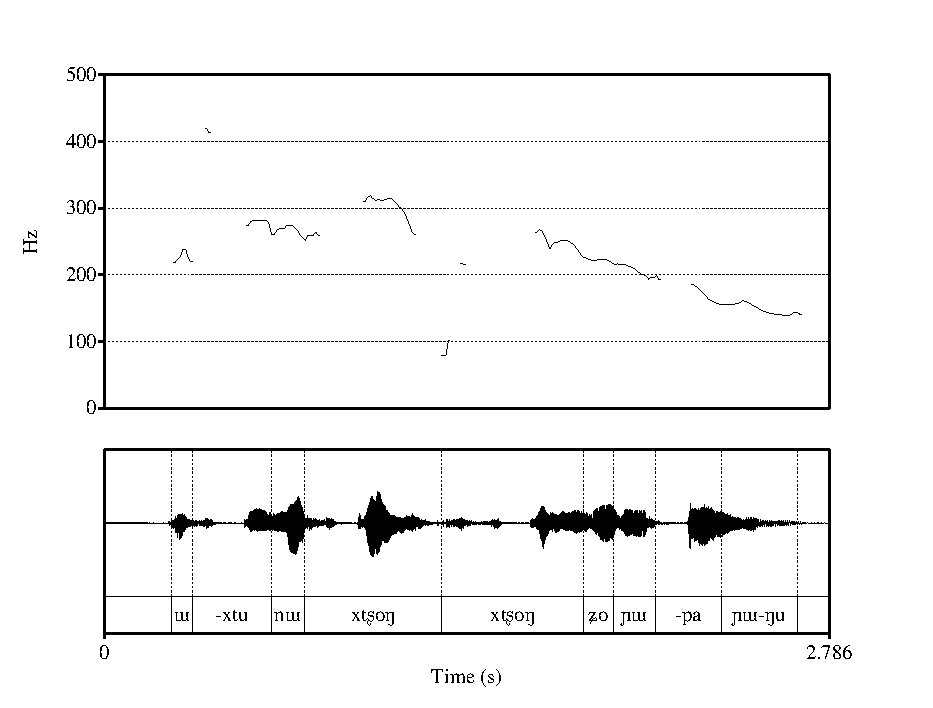
\includegraphics[width=\textwidth]{xtsxoN.eps}
\end{figure}

This emphatic pronunciation is not uncommon, but in most cases the ideophones do not have any special intonation. Example (§\ref{sec:xtsxoNxtsxoN2}) illustrates the same ideophone \forme{xtʂoŋxtʂoŋ} a few sentence later in the same text, without any emphasis.

\begin{exe}
\ex \label{sec:xtsxoNxtsxoN2}
\gll tɕe ma nɯnɯ tu-fka xtʂoŋxtʂoŋ ʑo ŋu. \\
\textsc{lnk} \textsc{lnk} \textsc{dem} \textsc{ipfv}-be.full \textsc{idph}(II):bloated \textsc{emph} be:\textsc{full} \\
\glt `(The tick) is full (from having drunk blood) and bloated.' (25-xCelwi, 59)
\end{exe}

\subsection{The genesis of ideophones} \label{sec:genesis.idph}
While it cannot be \textit{a priori} excluded that some ideophones could be ancient, their phonological markedness is a sign that they are constantly renewed, using processes different from those found in non-ideophonic words. In this section, I propose a scenario account for one of the origins of ideophonic roots, and  ideophonic hybridization (§\ref{sec:idph.gradation}).

Some ideophonic roots are obvious built from Tibetan loanwords, but with slight phonetic changes. The most obvious case is \idroot{ldʑɯŋ} `skyblue', which originates from the first syllable of \tibet{ལྗང་ཁུ་}{ldʑaŋ.kʰu}{green} (also borrowed as the unpossessible noun \japhug{ldʑaŋkɯ}{blue/green}, §\ref{sec:tibetan.colours}) with a slight modification of the vowel. The semantic relationship between the ideophone and the Tibetan borrowing is not always as obvious. For instance, \idroot{zɟaŋ} and \idroot{zɟraŋ}, both meaning `filled up, looking soft' (of a person's belly, a bag filled with objects) are reminiscent of the verb \japhug{βrɟaŋ}{stretch tight} (of skin), which is borrowed from the past tense of \tibet{རྒྱོང་བརྒྱངས་}{rgʲoŋ.brgʲaŋs}{stretch, distend}: the ideophones describe a skin or membrane that is overstretched and distended, like the result of the action expressed by the verb \forme{βrɟaŋ}. The form \idroot{zɟaŋ} could either have been independently borrowed from a Tibetan variety where \forme{r-} and \forme{s-} merge, or directly based on \forme{βrɟaŋ} with further consonant modification. The root \idroot{zɟraŋ} is derived from \idroot{zɟaŋ} by insertion of \forme{-r-} (see below for a possible account of these sporadic sound changes).
 
The Tibetan origin of some ideophones is one possible reason for the frequency of voiced stops in ideophones (§\ref{sec:idph.onsets}), as \ipa{b}, \ipa{d}, \ipa{ɟ} and \ipa{g} are common in clusters in the borrowed layer.

However, in many case the lexical origin of ideophones has been completely blurred by a variety of mechanisms which can only be hypothesized. The four synonymous ideophones \forme{dzoʁ} (\ref{ex:dzoR.Zo.pjAtshoR}), \forme{zgoʁ}, \forme{goʁ} and \forme{dzɯr} (\ref{ex:dzWr.Zo.tanWtshoR}) exclusively occur in collocation with the transitive verb \japhug{tsʰoʁ}{attach} and the noun \japhug{tɯ-χpɯm}{knee} (§\ref{sec:tshoR.lv}) to express both the speed of the kneeling motion and the highly deferential attitude of the kneeling person.  

\begin{exe}
\ex \label{ex:dzoR.Zo.pjAtshoR}
\gll ɯ-χpɯm dzoʁ ʑo pjɤ-tsʰoʁ \\
\textsc{3sg}.\textsc{poss}-knee \textsc{idph}(I):kneeling \textsc{emph} \textsc{ifr}-attach \\
\glt `(The demon) immediately knelt down.' (140513 abide he mogui-zh, 47)
\end{exe}

\begin{exe}
\ex \label{ex:dzWr.Zo.tanWtshoR}
\gll ɯ-χpɯm dzɯr ʑo ta-nɯ-tsʰoʁ ndɤre, tɤ-lu pa-nɯ-tɕɤt ɲɯ-ŋu \\
 \textsc{3sg}.\textsc{poss}-knee \textsc{idph}(I):kneeling \textsc{emph} \textsc{aor}:3$'$\fl{}3-\textsc{auto}-attach \textsc{lnk} \textsc{indef}.\textsc{poss}-milk \textsc{aor}:3$'$\fl{}3-\textsc{auto}-take.out \textsc{sens}-be \\
 \glt `She immediately knelt down and milked (the cow).' (2003 Kunbzang, 106)
\end{exe}

In addition to pattern I, they also occur in pattern III as in (\ref{ex:zgoRnAzgoR.Zo.tatshoRnW}).

\begin{exe}
\ex \label{ex:zgoRnAzgoR.Zo.tatshoRnW}
\gll  tɤ-pɤtso ra dɯxpa-nɯ matɕi tɕendɤre, zgoʁnɤzgoʁ ʑo nɯ-χpɯm ta-tsʰoʁ-nɯ tɕe \\
\textsc{indef}.\textsc{poss}-child \textsc{pl} poor-\textsc{pl} because \textsc{lnk} \textsc{idph}(II):kneeling \textsc{emph}  \textsc{3pl}.\textsc{poss}-knee \textsc{aor}:3$'$\fl{}3-attach-\textsc{pl} \textsc{lnk} \\
\glt `The poor children, they knelt (before the ogre) one after the other.' (160704 poucet4-v2, 42)
\end{exe}

I propose that one of the mechanism of ideophone creation is by playful reanalysis from lexical verb roots. The four ideophones \forme{dzoʁ}, \forme{zgoʁ}, \forme{goʁ} and \forme{dzɯr}, which have either the onset \forme{(z)g-} or \forme{dz-} and the rhymes \forme{-oʁ} and \forme{-ɯr}, originate in my opinion from the verbs \japhug{ndzoʁ}{be attached} (the anticausative of \japhug{tsʰoʁ}{attach}, §\ref{sec:anticausative.dummy}) and \japhug{azgɯr}{bow, bend down} (the latter borrowed from \tibet{སྒུར་}{sgur}{bend down}). The development of these ideophones occurred in three steps, as illustrated in \figref{fig:idph.dzoR}.


\begin{figure}[H]
\caption{Development of the family of ideophones meaning `kneeling respectfully'} \label{fig:idph.dzoR}  
\begin{tikzpicture}
\node (A) at (-4,0) { \japhug{ndzoʁ}{be attached} };
\node (B) at (4,0) { \japhug{azgɯr}{bow, bend down} };
\node (C) at (-3,-1.5) {\forme{dzoʁ} };
\node (D) at (3,-1.5) {\forme{*zgɯr} };
\node (E) at (1,-3) {\forme{dzɯr} };
\node (F) at (-1,-3) {\forme{zgoʁ} };
\node (G) at (0,-4) {\forme{goʁ} };
\tikzstyle{direct}=[->,very thick,>=latex]
\tikzstyle{blend}=[->,dotted,very thick,>=latex]
\draw[direct] (A)--(C);
\draw[direct] (B)--(D);
\draw[blend] (D)--(F);
\draw[blend] (D)--(E);
\draw[blend] (C)--(E);
\draw[blend] (C)--(F);
\draw[direct] (F)--(G);
\end{tikzpicture}
\end{figure}

First, the ideophone roots \forme{dzoʁ} `kneeling' (with alternation to the more marked plain voiced \forme{dz-} onset, §\ref{sec:consonant.phonemes}) and an unattested \forme{*zgɯr} (perhaps `kneeling and bowing') were directly created from the two verbs. The forms \forme{zgoʁ} and \forme{dzɯr} result from blending from the two primary ideophones \forme{dzoʁ} and \forme{*zgɯr} by exchanging rhyme and onset. Third, \forme{goʁ} was derived from \forme{zgoʁ} by simplification of the onset.

This process is not a derivation is in the proper sense, since it is neither regular nor predictable, and involves processes such as blending which do not normally occur in the verbal and nominal morphology of the Japhug language.

In addition to native roots and Tibetan loanwords, an obvious source of ideophones are onomatopoeic imitations of natural sounds. However, given the fact that ideophonic changes do not follow regular rules unlike the normal vocabulary on the one hand, and that northern Gyalrong languages lack historical records on the other hand, it is unlikely that the prehistory of this type of ideophones can be recovered.


\subsection{Syntax of ideophones} \label{sec:idph.syntax}
As pointed out by \citet[660]{dingemanse12ideo}, the markedness of ideophones is not limited to their phonology, but is also manifested in their syntactic behaviour.

Ideophones nearly always occur as verb adjuncts in Japhug. They are most commonly found with the intransitive light verb \forme{pa}, the quotative verb \japhug{ti}{say} and the similative verb \japhug{stu}{do like}, following a cross-linguistically well-attested pattern (\citealt[280--288]{guldemann08quot}). They can also be used as adjunct of any lexical verb in either nominalized or finite form, and in a handful of examples, as noun modifiers. Ideophones commonly occur with the emphatic \forme{ʑo} (§\ref{sec:emphatic.Zo}), which follows them.

%{sec:light.verb}
\subsubsection{The auxiliary \forme{pa}} \label{sec:idph.pa}
The intransitive verb \forme{pa} (also attested in collocation with numerals, §\ref{sec:pa.intr.lv}) is one of the most common light verb used with ideophones. It is the labile intransitive counterpart (§\ref{sec:lability.pass}) of the verb \japhug{pa}{do}, which also occurs as a light verb in noun-verb collocations (§\ref{sec:pa.lv}). 

It can either appear as an inflected form as in (\ref{ex:RYJli.Zo.YWpa}), or as the participle \forme{kɯ-pa} as in (\ref{ex:XploR.kWpa}) (see also \ref{ex:zjaNzjaN3}, §\ref{sec:ideo.II}). It is mainly used with pattern II ideophones describing colour, shape or spatial disposition.

 
\begin{exe}
\ex \label{ex:RYJli.Zo.YWpa}
\gll ɯ-phoŋbu nɯ rcanɯ ʁɲɟlíʁɲɟli ʑo ɲɯ-pa. \\
\textsc{3sg}.\textsc{poss}-body \textsc{dem} \textsc{unexp}:\textsc{foc} \textsc{idph}(II):huge \textsc{emph} \textsc{sens}-\textsc{aux} \\
\glt  `Its body, it is enormous.' (20-sWNgi, 16)
\end{exe}

\begin{exe}
\ex \label{ex:XploR.kWpa}
\gll aʑo grɯβgrɯβ ɯ-ftsa nɯ tɤ-kɯ-qawɤr ma nɯ ma χploʁχploʁ kɯ-pa mɯ-pɯ-mto-t-a \\
\textsc{1sg} matsutake \textsc{3sg}.\textsc{poss}-nephew \textsc{dem} \textsc{aor}-\textsc{sbj}:\textsc{pcp}-open.cap apart.from \textsc{dem} apart.from \textsc{idph}(II):small.and.spherical \textsc{sbj}:\textsc{pcp}-\textsc{aux} \textsc{neg}-\textsc{aor}-see-\textsc{pst}:\textsc{tr}-\textsc{1sg} \\
\glt `The (mushroom called) the `matsutake's nephew', I have seen ones with opened caps, but never seen one in ball shape (before the cap opens).' (23-grWBgrWBftsa, 5)
\end{exe}

%{sec:xtsxoNxtsxoN}

Like other stative verbs, \forme{pa} has an inchoative meaning in the Imperfective (§\ref{sec:ipfv.inchoative}), the Aorist (§\ref{sec:aor.inchoative}) and the Inferential (§\ref{sec:ifr.inchoative}). It is attested with the \textsc{upwards} (\forme{tu-pa}, example \ref{ex:tupa.YWNu}) and the \textsc{westwards} (\forme{ɲɯ-pa}, example §\ref{sec:xtsxoNxtsxoN} in §\ref{sec:emphatic.idph}) orientation preverbs.


\begin{exe}
\ex \label{ex:tupa.YWNu}
\gll ɯ-ru nɯra nɯ-rom tɕe rʁɤβrʁɤβ tu-pa ɲɯ-ŋu  \\
\textsc{3sg}.\textsc{poss}-stalk \textsc{dem}:\textsc{pl} \textsc{aor}-dry \textsc{lnk} \textsc{idph}(II):rough \textsc{ipfv}-\textsc{aux} \textsc{sens}-be \\
\glt `Once it has dried, its stalk becomes very rough.' (14-sWNgWJu, 22)
\end{exe}

While \forme{pa} is mainly found with pattern II ideophones, it is not restricted to these, and attested in a handful of examples with other patterns, such as III (\ref{ex:dWrnAdWr.pjApa}) and IV (\ref{ex:ckArnAlAr}).

\begin{exe}
\ex \label{ex:dWrnAdWr.pjApa}
\gll ʑɯrɯʑɤri qʰe li tɤ-se nɯ to-mbat qʰe, li tɤrmbɣo nɯ dɯrnɤdɯr pjɤ-pa \\
progressively \textsc{lnk} again \textsc{indef}.\textsc{poss}-blood \textsc{dem} \textsc{ifr}-diminish \textsc{lnk} again drum \textsc{dem} \textsc{idph}(III):drumming.far.away \textsc{ifr}.\textsc{ipfv}-\textsc{aux} \\
\glt `Progressively, the blood (in the lake) started to recede, and there was again a drumming sound far away.' (2003-kWBRa, 106)
\end{exe}


\begin{exe}
\ex \label{ex:ckArnAlAr}
\gll ɕkɤrnɤlɤr ʑo kɯ-pa nɯ jo-nɯ-ɣi \\
\textsc{idph}(IV):limping \textsc{emph} \textsc{sbj}:\textsc{pcp}-\textsc{aux} \textsc{dem} \textsc{ifr}-\textsc{vert}-come \\
\glt `He came back home limping.' (140429 jiedi-zh, 141)
\end{exe}

\subsubsection{Quotative \japhug{ti}{say}}\label{sec:idph.ti}
The verb \japhug{ti}{say} occurs as a light verb with ideophones expressing sound (\ref{ex:zJWG.Zo}, \ref{ex:tCRWz.nA.tCRWz}) and endopathic sensations (especially itching or pain as in \ref{ex:CYWG.Zo}), in patterns I (\ref{ex:zJWG.Zo}, \ref{ex:CYWG.Zo}), III (\ref{ex:tCRWz.nA.tCRWz}) and X (§\ref{sec:ideo.X}).

\begin{exe}
\ex \label{ex:zJWG.Zo}
\gll ɯ-tʰoʁ tɕu zɟɯɣ ʑo ti ɲɯ-ŋu\\
\textsc{3sg}.\textsc{poss}-ground \textsc{loc} \textsc{idph}(II):heavy.object.falling \textsc{emph} say:\textsc{fact} \textsc{sens}-be\\
\glt `(The stone) made a loud noise (as it fell) on the ground.' (The 2003 tWxtsa, 76)
\end{exe}


\begin{exe}
\ex \label{ex:tCRWz.nA.tCRWz}
\gll cʰɯ-tɯt ɕɯŋgɯ tɕe tɕe tú-wɣ-ndza tɕe, tɕʁɯznɤtɕʁɯz tu-ti ɲɯ-ŋu tʰɯ-tɯt ɯ-qʰu tɕe tɕe tɤ́-wɣ-ndza tɕe, zwaʁnɤzwaʁ tu-ti ɲɯ-ŋu tɕe, nɯ ɲɯ-mɯm. \\
\textsc{ipfv}-be.ripe before \textsc{lnk} \textsc{lnk} \textsc{ipfv}-\textsc{inv}-eat \textsc{lnk} \textsc{idph}(III):crunchy.sound \textsc{ipfv}-say \textsc{sens}-be:\textsc{fact} \textsc{aor}-be.ripe \textsc{3sg}.\textsc{poss}-after \textsc{lnk} \textsc{lnk} \textsc{aor}-\textsc{inv}-eat \textsc{lnk} \textsc{idph}(III):not.crunchy \textsc{ipfv}-say \textsc{sens}-be \textsc{lnk} \textsc{dem} \textsc{sens}-be.tasty \\
\glt `If one eats (an apple)$_i$ before it$_i$ is ripe, it makes a crunchy sound, when it is ripe, it makes a soft (not crunchy) sound, it is (more) tasty (in this case because it has become sweeter and less sour).' (07-paXCi, 27-28)
\end{exe}

\begin{exe}
\ex \label{ex:CYWG.Zo}
\gll tu-kɯ-ti kɯnɤ ɕɲɯɣ ʑo tu-ti tu-mŋɤm ŋu \\
\textsc{ipfv}-\textsc{genr}:S/O-say also \textsc{idph}(I):intense.pain \textsc{emph} \textsc{ipfv}-say \textsc{ipfv}-hurt be:\textsc{fact} \\
\glt `(When suffering from this disease), one feels intense pain even when one talks.' (29-RzAr, 35)
\end{exe}


\subsubsection{The similative verb \japhug{stu}{do like} } \label{sec:stu.idph} 
The transitive similative verb \japhug{stu}{do like}  (§\ref{sec:ditransitive.secundative}, §\ref{sec:svc.similative.verb}) most commonly appears with the non-stative ideophonic patterns III (\ref{ex:lhWG.nA.lhWG})  and IV (\ref{ex:rloR.nA.rloR}). It expresses volitional actions, unlike \forme{pa} and \forme{ti}.  The syntactic function of the ideophones when used with \japhug{stu}{do like} is possibly that of semi-object, as they replace the demonstratives that usually occur with this verb (§\ref{sec:ditransitive.secundative}).

\begin{exe}
\ex \label{ex:lhWG.nA.lhWG}
\gll ɯ-sŋɯro lu-lɤt tɕe ɬɯɣnɤɬɯɣ, ɬɯɣnɤɬɯɣ tu-ste ɲɯ-ŋu.\\
\textsc{3sg}.\textsc{poss}-breath \textsc{ipfv}-release \textsc{lnk} \textsc{idph}(III):breathing.movement \textsc{idph}(III):breathing.movement \textsc{ipfv}-do.like[III] \textsc{sens}-be \\
\glt `When (the frog)$_i$ breathes, it$_i$ expands and retracts (its whole body) with each breath.' (27-qaCpa, 3)
\end{exe}

The ideophone can describe the action as a whole (\ref{ex:lhWG.nA.lhWG}), or an aspect of the action on the object of \forme{stu} as in (\ref{ex:rloR.nA.rloR}), where the root \idroot{rloʁ}   depicts the shape of the fly's head (\tabref{tab:slaN.rloR}, §\ref{sec:idph.gradation}), and pattern III morphology (§\ref{sec:ideo.III}) the motion of the head.

\begin{exe}
\ex \label{ex:rloR.nA.rloR}
\gll ɯ-jaʁ tu-tsɯm tɕe, ɯ-ku ra pjɯ-nɯ-χtɕi tɕe ɯ-ku ra rloʁnɤrloʁ tu-ste ɲɯ-ŋu \\
\textsc{3sg}.\textsc{poss}-hand \textsc{ipfv}:\textsc{up}-take.away \textsc{lnk} \textsc{3sg}.\textsc{poss}-head \textsc{pl} \textsc{ipfv}-\textsc{auto}-wash \textsc{lnk} \textsc{3sg}.\textsc{poss}-head \textsc{pl}  \textsc{idph}(III):round  \textsc{ipfv}-do.like[III] \textsc{sens}-be \\ 
\glt `(The fly) stretches up its forelegs to clean its head (and the area around it), making (at the same time) a rhythmic rolling motion (with its head, round and minute).' (25-akWzgumba, 51)
\end{exe}

The reflexive form \forme{ʑɣɤ-stu} (§\ref{sec:lexicalized.refl}) is almost exclusively attested with ideophones, in particular in the manner serial verb construction (§\ref{sec:svc.manner}) with other intransitive verbs, such as \forme{ku-rɤʑi} in (\ref{ex:XtshAXtshAt.Zo.tuZGAstu}). With pattern II ideophones, it means `make/have a $X$ look', generally expressing an attitude made on purpose.

 
\begin{exe}
\ex \label{ex:XtshAXtshAt.Zo.tuZGAstu}
\gll spɣi ɲɯ-nɯ-te ndɤre, nɤki rɟɤlpu tu-ɕe rcanɯ, tu-rɤjoʁβzɯr kɯ-fse rcanɯ, nɤki, χtsʰɤχtsʰɤt ʑo tu-ʑɣɤ-stu tɕe, ku-rɤʑi pɯ-ŋu, βdaʁmu tu-ɕe rcanɯ, pʰɤtɕʰɯχtɤr ʑo pjɯ-te tɕe, qɯqlɯ ʑo tu-ʑɣɤ-stu tɕe ku-rɤʑi pɯ-ŋu ɲɯ-ŋu. 	\\
attic \textsc{3sg}-inside \textsc{ipfv}:\textsc{east}-\textsc{auto}-put[III] \textsc{lnk} king  \textsc{ipfv}:\textsc{up}-go \textsc{unexp}:\textsc{foc} \textsc{ipfv}-clean.up \textsc{inf}:\textsc{stat}-be.like  \textsc{unexp}:\textsc{foc} \textsc{filler}  \textsc{idph}(II):lively.small \textsc{emph} \textsc{ipfv}-\textsc{refl}-do.like \textsc{lnk} \textsc{ipfv}-stay \textsc{pst}.\textsc{ipfv}-be  lady  \textsc{ipfv}:\textsc{up}-go  \textsc{unexp}:\textsc{foc} mess \textsc{emph} \textsc{ipfv}-put[III] \textsc{lnk} \textsc{idph}(II):hangdog.look \textsc{emph} \textsc{ipfv}-\textsc{refl}-do.like \textsc{lnk} \textsc{ipfv}-stay \textsc{pst}.\textsc{ipfv}-be \textsc{sens}-be \\
\glt `(The king)$_i$ put (the bird)$_j$ in the attic. When the king$_i$  would go up there, it$_j$ would clean everything up and would be lively; when the queen would go up there, it$_j$ would make a mess and have a hangdog look.' (2003 Kunbzang, 302-4)
\end{exe}

It is also compatible with pattern I (\ref{ex:CNAB.Zo.tuZGAstu}) or III ideophones, expressing motion and/or sound.

\begin{exe}
\ex \label{ex:CNAB.Zo.tuZGAstu}
\gll tɕe nɯ kɯ-xtɕɯ\redp{}xtɕi ʑo ɲɯ́-wɣ-mbi tɕe ma ɕŋɤβ ʑo tu-ʑɣɤ-stu tɕe ju-nɯ-mɟe tɕe tu-ndze ɲɯ-ŋu. \\
\textsc{lnk} \textsc{dem} \textsc{sbj}:\textsc{pcp}-\textsc{emph}\redp{}be.small \textsc{emph} \textsc{ipfv}-\textsc{inv}-give \textsc{lnk} \textsc{lnk} \textsc{idph}(I):snapping \textsc{emph} \textsc{ipfv}-\textsc{refl}-do.like \textsc{lnk} \textsc{ipfv}-\textsc{auto}-take[III] \textsc{lnk} \textsc{ipfv}-eat[III] \textsc{sens}-be \\
\glt `We would give (our turtle)$_i$ a little piece$_j$ (of meat), and it$_i$ would grab it$_j$ with a snapping noise and eat it$_j$.' (140510 wugui, 23)
\end{exe}

\subsubsection{Other verbs} \label{sec:ideophone.plus.lexical.verb}
Ideophones are not restricted in use to the light verbs cited above, and can appear with other types of verbs with compatible semantics. There are strict collocation restrictions, and most ideophones can only be used with one one or a handful of verbs. 

With the three light verbs discussed above (§\ref{sec:idph.pa}, §\ref{sec:idph.ti}, §\ref{sec:stu.idph}), ideophones are strictly preverbal, but when employed with other verbs, postverbal order is common, in particular in the case of stative adjectival verbs (\ref{ex:YWGWrni.tsGaRtsGaR}).

\begin{exe}
\ex \label{ex:YWGWrni.tsGaRtsGaR}
\gll ɯ-mɲaʁ wuma nɯ ɣɯ ɯ-rkɯ nɯra ɲɯ-ɣɯrni, ɲɯ-ɣɯrni tsɣaʁtsɣaʁ ʑo \\
\textsc{3sg}.\textsc{poss}-eye really \textsc{dem} \textsc{gen} \textsc{3sg}.\textsc{poss}-side \textsc{dem}:\textsc{pl} \textsc{sens}-be.red  \textsc{sens}-be.red \textsc{idph}(II):brilliant.red \textsc{emph} \\
 \glt `The sides of its eye proper are red, brilliant red.'  (23-qapGAmtWmtW, 50-51)
 \end{exe}

Ideophones can be postverbal even in particpial and finite relative clauses (§\ref{sec:relative.postverbal}), and can be located loser to the verb than determiners such as the indefinite \forme{ci} (§\ref{sec:indef.article}), as in (\ref{ex:kWGWrni.tsGaRtsGaR}).

 \begin{exe}
\ex \label{ex:kWGWrni.tsGaRtsGaR}
\gll [kɯ-ɣɯrni ʑo tsɣaʁtsɣaʁ] ci ŋu tɕe \\
\textsc{sbj}:\textsc{pcp}-be.red \textsc{emph} \textsc{idph}(II):brilliant.red \textsc{indef} be:\textsc{fact} \textsc{lnk} \\
\glt `It (a type of millipede) is brilliant red.' (28-kWpAz, 152)
   \end{exe} 
   
 When their semantic scope is more focalized on one of the arguments, the ideophone can directly follow a noun as in (\ref{ex:bAbAB.Zo.kundzoR}) or (\ref{ex:brWGbrWG.Zo.tutCAt}).

\begin{exe}
\ex \label{ex:bAbAB.Zo.kundzoR}
\gll tɯ-ŋga ɯ-taʁ ra ɯ-mat bɤbɤβ ʑo ku-ndzoʁ. \\
\textsc{genr}.\textsc{poss}-clothes \textsc{3sg}-on \textsc{pl}  \textsc{3sg}.\textsc{poss}-fruit \textsc{idph}(II):clumping.together \textsc{emph} \textsc{ipfv}-\textsc{acaus}:attach \\
\glt `When one walks among (these plants), their fruits attach to one's clothes in clumps.' (18-qromJoR, 170)
\end{exe}

\begin{exe}
\ex \label{ex:brWGbrWG.Zo.tutCAt}
\gll rtɕʰɯʁjɯ ɣɯ ɯ-rme nɯ kɯ ɲɯ-kɯ-z-rɤʑa. nɯ tɯ-ɕa a-mɤ-nɯ-ɤtɯɣ ra ma tɤndɤr brɯɣbrɯɣ ʑo tu-tɕɤt ɲɯ-ŋu  \\
caterpillar \textsc{gen} \textsc{3sg}.\textsc{poss}-hair \textsc{dem} \textsc{erg} \textsc{ipfv}-\textsc{genr}:S/O-\textsc{caus}-itch \textsc{dem} \textsc{genr}.\textsc{poss}-flesh \textsc{irr}-\textsc{neg}-\textsc{pfv}-touch be.needed:\textsc{fact} \textsc{lnk} pimple \textsc{idph}(II):little.pimples \textsc{emph} \textsc{ipfv}-take.out \textsc{sens}-be \\
\glt `The caterpillar's hair itches people, it should not touch one's flesh, otherwise it will cause a lot of little pimples to appear.' (25-rtchWRjW, 86-88)
\end{exe}
 
  
 \subsubsection{Noun modifier} \label{sec:ideophone.noun.modifier}
 In examples such as (\ref{ex:bAbAB.Zo.kundzoR}) or (\ref{ex:brWGbrWG.Zo.tutCAt}) (§\ref{sec:ideophone.plus.lexical.verb}), the syntactic status of the ideophone is ambiguous between a sentential adverb and a postnominal modifier. 
 
 Examples (\ref{ex:zJAGzJAG.ma}) and (\ref{ex:ndzArndzAr.ma}) are incontrovertible evidence that ideophones can serve as noun modifier: in (\ref{ex:zJAGzJAG.ma}) is embedded within an exceptive (§\ref{sec:exceptive}) postpositional phrase which does not contain any verb, and must be analyzed as modifier of the counted noun \forme{tɯ-rdoʁ} `one piece'.
 
\begin{exe}
\ex \label{ex:zJAGzJAG.ma}
\gll ma nɯnɯ ɕawurambɯm tu-ti-nɯ tɕe nɯnɯ, nɤkinɯ, [[tɯ-rdoʁ ʑo \textbf{zɟɤɣzɟɤɣ}] ma] kɯ-me ɲɯ-ŋu kʰi \\
\textsc{lnk} \textsc{dem} Shwa.ba.rwa.mbum \textsc{ipfv}-say-\textsc{pl} \textsc{lnk} \textsc{dem} \textsc{filler} one-piece \textsc{emph} \textsc{idph}(II):short.and.thick apart.from \textsc{sbj}:\textsc{pcp}-not.exist \textsc{sens}-be \textsc{hearsay} \\
\glt `People call it `Shwaba rwa'bum', it is (a kind of deer antler) with only one (branch), short and thick.'  
 (27-qartshaz, 72-3)
\end{exe}

In (\ref{ex:ndzArndzAr.ma}), the ideophone \forme{ndzɤrndzɤr} is in the emphatic exceptive construction, with the linker \forme{ma} (§\ref{sec:exceptive}).

\begin{exe}
\ex \label{ex:ndzArndzAr.ma}
\gll  <donglang> ɯʑo-sti nɯnɯ, [tɤ-tɕɯ tɯ-rdoʁ ndzɤrndzɤr] ma nɯ ma kɯ-tu pjɤ-me. \\
\textsc{anthr} \textsc{3sg}-alone \textsc{dem} \textsc{indef}.\textsc{poss}-son one-piece \textsc{idph}(II):alone \textsc{lnk} \textsc{dem} apart.from \textsc{sbj}:\textsc{pcp}-exist \textsc{ifr}.\textsc{ipfv}-not.exist \\
\glt `There remained only Donglang, the boy, all alone (on earth after his family had been taken away).' (150828 donglang, 134)
\end{exe}

However, ideophones as postnominal modifiers are rare, and only occur in combination with a singular counted noun such as \forme{tɯ-rdoʁ} in the meaning `alone'. 
%For this reason, in examples such as (\ref{ex:bAbAB.Zo.kundzoR}) or (\ref{ex:brWGbrWG.Zo.tutCAt}) (§\ref{sec:ideophone.plus.lexical.verb}), ideophones are preferentially analyzed as sentential markers rather than noun modifiers.

\subsection{Discourse function}
 Ideophones are non-essential to communication in the sense that any sentence containing an ideophone can be glossed with another sentence of identical truth value without using any ideophone. The frequency of ideophones and ideophonic verbs presents considerable variation  in the corpus: some stories and procedural texts are almost devoid of them, while some episodes of traditional narratives are densely packed with them.
  
Ideophones convey rich and intricate meanings in a succinct way. In traditional stories, their use contributes to the vividness of the description. For instance, in  (\ref{ex:ndArndAr}), the choice of the pattern II \forme{ndɤrndɤr} `huge and imposing'	and 	the pattern III \forme{ɲcɣɤnɤɲcɣɤt} `loud and moving around' evokes  a much more expressive picture than the  translation provided here in plain language. Native speakers, upon hearing such a sentence, visualize the vivid picture of huge lush trees and flocks of birds flying around, tweeting and chirping.

\begin{exe}
\ex \label{ex:ndArndAr}
 \gll nɯra tɤ-stu-t-a tɕe,  sɯŋgɯnaχtɕɯn \textbf{ndɤrndɤr} ʑo nɯ-stu-t-a, ɯ-taʁ,  pɣa \textbf{ɲcɣɤnɤɲcɣɤt} ʑo ɲɯ-mbri tɕe \\
\textsc{dem}:\textsc{pl} \textsc{aor}-do.like-\textsc{pst}:\textsc{tr}-\textsc{1sg} \textsc{lnk} deep.forest \textsc{idph}(II):huge \textsc{emph} \textsc{aor}-do.like-\textsc{pst}:\textsc{tr}-\textsc{1sg} \textsc{3sg}-on birds \textsc{idph}(III):loud \textsc{emph} \textsc{sens}-call \textsc{lnk} \\
\glt `I acted this way, I created a huge and deep forest on the top of whose trees birds are tweeting and chirping and flying around.' (2011-04-smanmi, 220-221)
\end{exe}


\section{Other expressive words} \label{sec:other.expressive}
Two classes of words present common properties with, but are different from, real ideophones: interjections (§\ref{sec:interjections}) and calling sounds (§\ref{sec:call}). Although both also present phonological markedness and some degree of iconicity, they are not subject to ideophonic morphology (§\ref{sec:ideo:morpho}) and do not share the same syntactic properties. 

In addition, we find some nouns which, unlike deideophonic verbs (§\ref{sec:GA.sA.deidph}), ideophonic counted nouns (§\ref{sec:CN.ideophones}) and nominal ideophonic compounds (§\ref{sec.n.idph.compounds}), are directly built on an expressive root without derivational morphology (§\ref{sec:underived.expressive.nouns}).

 
\subsection{Interjections} \label{sec:interjections}
 Interjections are marked words expressing a feeling or an emotion like ideophones, but differ from them in that they cannot serve as verb adjuncts, cannot receive ideophonic morphology and are mainly used in isolation, either in their own clause or as the reported speech complements of verbs of speaking like \japhug{ti}{say} (\ref{ex:atsatsa}, \ref{ex:wudzWdzi}). 
 
\begin{exe}
\ex \label{ex:atsatsa}
\gll tɤ-ɣɤndʐo tɕe `ɯtɕʰɯtɕʰɯ' ma-tɯ-ti,   tɤ-sɤɕke tɕe (nɤkinɯ) `atsatsa' ma-tɯ-ti, kɯ-mŋɤm tɤ-tu tɕe `atsatsa' ma-tɯ-ti ra  \\
 	\textsc{aor}-be.cold \textsc{lnk} \textsc{interj}:cold \textsc{neg}:\textsc{imp}-2-say \textsc{aor}-\textsc{prop}-burn \textsc{lnk} \textsc{filler} \textsc{interj}:pain \textsc{neg}:\textsc{imp}-2-say \textsc{sbj}:\textsc{pcp}-hurt \textsc{aor}-exist \textsc{lnk} \textsc{interj}:pain \textsc{neg}:\textsc{imp}-2-say be.needed:\textsc{fact} 	\\
\glt `When you feel cold, don't say ``Ah'', when you feel hot, don't say ``ouch'', when you  feel pain, don't say ``ouch''.' (07-deluge, 66-68)
\end{exe}

\begin{exe}
\ex \label{ex:wudzWdzi}
\gll srɯtpʰu srɯnmɯ kɯ-fse kɯ-sɤ-ɣmɯ\redp{}ɣmu ʑo ɲɤ-k-ɤtɯɣ-ndʑi-ci ri,  `wudzɯdzi' mɯ-to-ti. \\
râkshasa râkshasî \textsc{sbj}:\textsc{pcp}-be.like \textsc{sbj}:\textsc{pcp}-\textsc{prop}-\textsc{emph}\redp{}fear \textsc{emph} \textsc{ifr}-\textsc{peg}-meet-\textsc{du}-\textsc{peg} \textsc{lnk} \textsc{interj}:fear \textsc{neg}-\textsc{ifr}-say \\
\glt `They met fearsome râkshasas and râkshasîs, but he did not say `how frightful!'.' (31-deluge, 116)
\end{exe}
 

Interjections can however be followed by full clauses, but with a pause as in (\ref{ex:aCi}) (see also for instance \forme{ja} in example \ref{ex:thWnWmblWmnW.je}, §\ref{sec:reported.speech.sfp}).

\begin{exe}
\ex \label{ex:aCi}
\gll aɕi! ɲɯ-tɯ-ɣɤŋgi.  \\
\textsc{interj}:correction \textsc{sens}-2-be.right \\
\glt `Of course (I take back what I have said)! You are right.' (2003 tWxtsa, 44)
\end{exe} 


The marker \forme{wo} can precede without pause a noun in vocative function (\ref{ex:wo.amu}) (see also \ref{ex:pGAlnApGAl}, §\ref{sec:ideo.III}).
  
\begin{exe}
\ex \label{ex:wo.amu}
\gll wo a-mu a-kɯm ɣɯ-tɤ-ci  \\
\textsc{interj} \textsc{1sg}.\textsc{poss}-mother  \textsc{1sg}.\textsc{poss}-door \textsc{cisl}-\textsc{imp}-open[III] \\
\glt `Mother, come and open the door for me!' (2012 tWJo, 23)
\end{exe} 

Some interjections cannot form a complete utterance on their own:  \japhug{χawo}{if only} introduces a clause in the Irrealis expressing a wish (see examples \ref{ex:apWsatnW.YWsWsama}, §\ref {sec:irrealis.complement.clauses} and \ref{ex:atWrme}, §\ref{sec:frozen.indef}). The form \forme{tsatsatsa} is used in a correlative construction meaning  `one can say that $X$, but one can also say that $\neg X$, with the positive $X$ and negative $\neg X$ forms of the same verb followed by the additive \forme{nɤ}, as in (\ref{ex:tsatsatsa}).

\begin{exe}
\ex \label{ex:tsatsatsa}
\gll ɲɯ-tɯ-fse nɤ tsatsatsa, mɯ́j-tɯ-fse nɤ tsatsatsa \\
\textsc{sens}-2-be.like \textsc{add} \textsc{interj} \textsc{neg}:\textsc{sens}-2-be.like \textsc{add} \textsc{interj} \\
\glt  `One can say that you look like her, but one can also say that you don't.' (2014-kWlAG, 476)
\end{exe}



Interjections can be classified into four categories (\tabref{sec:interjections}): involuntary responses to stimuli (interjections in the proper sense, \citealt{dingemanse11phd}), and uninflected words expressing comments on words uttered by oneself or others, short orders or polite expressions.
  
\begin{table}
\caption{List of interjections} \label{tab:interjections}
\begin{tabular}{lll}
\lsptoprule
Category &Form & Function \\
\midrule
Involuntary  &\forme{ɯtɕʰɯtɕʰɯ}, \forme{wutɕʰɯtɕʰɯ} &  expresses cold \\  
response&\forme{atsatsa} &  expresses pain \\
&\forme{atsatsa} &  expresses pain \\
&\forme{wudzɯdzi} &  expresses fear \\
&\forme{ama}, \forme{amaŋ}  & expresses  surprise \\
&\forme{mtsʰɤri} & expresses  surprise \\
\midrule
Comment&\forme{aɕi} & taking back what one\\
&& has just said \\
&\forme{χawo} $X$ & `If only $X$' \\
&$X$\forme{tsatsatsa} $\neg X$\forme{tsatsatsa} & `One can say that $X$, but \\
&& one can also say that $\neg X$' \\
&\forme{maχtɕɯ} & `I told you so!' \\
&\forme{ɕaʁja} & `It serves you right!' \\
&\forme{woja} & confirmation \\
\midrule
Orders&\forme{cʰe},  \forme{pɤkʰije}& `wait!' \\
&\forme{kɯz} & `go!' \\
&\forme{ja} & `come on' \\
&&speech filler (§\ref{sec:fillers}) \\
\midrule
Phatic&\forme{kʰɤβzaŋ} & `here I am' \\
&\forme{kʰatʂu} & `thanks' \\
&\forme{wortɕʰi (wojɤr)} & `please' \\
&\forme{ɣa} & `yes' \\
&\forme{wowe} & response to words meaning `goodbye' \\
&\forme{woja} & confirmation \\
\lspbottomrule
\end{tabular}
\end{table}
 
Among these forms,  \japhug{pɤkʰije}{wait!} is the only one with a clear internal etymology (from \forme{pɤjkʰu je}, §\ref{sec:tense.aspect.adverbs}). Some interjections are from Tibetan, including the polite expressions and \japhug{mtsʰɤri}{how strange} (§\ref{sec:mirative}), which is originally a uniflected predicate borrowed from  \tibet{མཚར་}{mtsʰar}{feel strange}.

Although interjections lack morphological alternation, the additive \forme{nɤ} can be inserted within \forme{wortɕʰi wojɤr} (which is borrowed from \tibet{འོར་ཆེ་}{ɦor.tɕʰe}{thanks}) to express repeated action as in (\ref{ex:wortChi.nA.wojAr}) (see also \ref{ex:wojAr.ntsW.toti}, §\ref{sec:tense.aspect.adverbs}), a use reminiscent of the Ideophonic patterns III (§\ref{sec:ideo.III}) and IV (§\ref{sec:ideo.IV})

 \begin{exe}
\ex \label{ex:wortChi.nA.wojAr}
\gll tɤ-tɕɯ nɯ kɯ ``wortɕʰi nɤ wojɤr ʑo" to-ti ɲɯ-ŋu \\
\textsc{indef}.\textsc{poss}-boy \textsc{dem} \textsc{erg} please \textsc{add} please \textsc{emph} \textsc{ifr}-say \textsc{sens}-be \\
\glt `The boy said `please' (several times).' (qachGa 2012, 81)
\end{exe}

The phatic expressions and \japhug{sɤrma}{good night} and \japhug{kɤnɤβdi}{take care}, though originally non-inflecting, can take number indexation suffixes (§\ref{sec:phatic.inflectionalization}) and have become quasi-verbs, though they are highly anomalous and defective. The interjection \forme{woːwe} can be used as a response to these expressions.

The expression \forme{kʰɤβzaŋ} `here I am' is uttered by the guest when he arrives at someone else's home; the hosts invites the guest inside by saying \forme{nɤ-tʂu} `your way'.

The interjection \forme{woja} `yes, right' occurs to confirm the validity of a previous statement, sometimes assertive as in (\ref{ex:woja.nW.kWfse}) but also with interrogative markers such as \forme{ɣe} (see \ref{ex:totsu.Ge}, §\ref{sec:fsp.interrog}). It can be used whether the addressee had a vocal reaction or not.

\begin{exe}
\ex \label{ex:woja.nW.kWfse}
\gll ɯnɯnɯ tɕendi <wazi> nɯ ɯ-mdoʁ wuma ʑo ɲɯ-ɤsɯ-ndo. woja, nɯnɯ kɯ-fse ɲɯ-ŋu. \\
\textsc{dem} west socks \textsc{dem} \textsc{3sg}.\textsc{poss}-colour really \textsc{emph} \textsc{sens}-\textsc{prog}-take \textsc{interj} \textsc{dem} \textsc{sbj}:\textsc{pcp}-be.like \textsc{sens}-be \\
\glt `It has the colour of the socks over there. Yes, it is like that.' (23-grWBgrWBftsa, 48)
\end{exe} 


\subsection{Calling  and chasing sounds} \label{sec:call}
Calling and chasing sounds, also referred to as `summons' and `dispersals' (\citealt[318--319]{aikhenvald10imperative}) are sounds used by people to interact with animals.\footnote{French has the more colorful term \textit{huchement de berger} to designate this class of utterances.} They are used either to incite the animals to come forward in the direction of the speaker (calling sounds, as in \ref{ex:tCitCi3}) or to advance or go away (chasing sounds, as in \ref{ex:tCha.lWlu}). 

\begin{exe}
\ex 
\begin{xlist}
\ex \label{ex:tCitCi3}
\gll lɯlu ɲɯ́-wɣ-nɯ-ɤkʰɤzŋga qʰe {tɕítɕi tɕítɕi tɕítɕi} nɯra tu-kɯ-ti qʰe ju-ɣi ŋu \\
cat \textsc{ipfv}-\textsc{inv}-\textsc{appl}-shout \textsc{lnk} \textsc{call}:cat \textsc{dem}:\textsc{pl} \textsc{ipfv}-\textsc{genr}-say \textsc{lnk} \textsc{ipfv}-come be:\textsc{fact} \\
\glt `When one calls a cat, one says \forme{tɕítɕi tɕítɕi tɕítɕi} and it comes.' (06-huchements1, 34-33)
\ex \label{ex:tCha.lWlu}
\gll lɯlu jú-wɣ-no tɕe ``tɕʰa" tu-kɯ-ti ŋu \\
cat \textsc{ipfv}-\textsc{inv}-chase \textsc{lnk} \textsc{chase}:cat \textsc{ipfv}-\textsc{genr}-say be:\textsc{fact} \\
\glt `When one chases a cat, one says \forme{tɕʰa}.' (06-huchements2, 14)
\end{xlist}
\end{exe}

In Japhug, nearly all domestic animals, whether mammals or birds, have special dedicated calling sounds, a list of which is provided in \tabref{tab:calling.sounds}. In addition, a click sound for which no IPA symbol exists is used to call puppies.

\begin{table}
\caption{Calling and chasing sounds in Japhug} \label{tab:calling.sounds}
\begin{tabular}{lllll}
\toprule
 & 	animal & 	order \\ 	
 \midrule
\forme{tɕʰa} & 	\japhug{lɯlu}{cat} & 	chasing \\ 	
\forme{tɕítɕi tɕítɕi tɕítɕi} & 	  & 	calling \\ 	
 \midrule
\forme{wɯle} & 		\japhug{nɯŋa}{cow} & 	chasing \\ 	
\forme{aβleβle} & 	  & 	calling \\ 	
 \midrule
\forme{buwo} & 	\japhug{mbala}{bull} & 	chasing \\ 	
\forme{abobo} & 	  &  calling \\ 	
 \midrule
\forme{tsaʔ tsaʔ}, \forme{tsotsa} &  \japhug{kʰɯna}{dog} & 	calling \\ 	
\forme{soŋ} & 	 & 	chasing \\ 	
 \midrule
\forme{tʂutʂutʂutʂutʂutʂu} & 	\japhug{kumpɣa}{fowl} & 	calling \\ 	
\forme{kɕɯt} &   & 	chasing \\ 	
 \midrule
\forme{χaj} & 	\japhug{mbro}{horse} & 	chasing \\ 	
\forme{a̤ a̤ a̤ a̤} & 	 & 	calling \\ 	
 \midrule
\forme{zʁozʁozʁozʁo} & 	\japhug{ftsoʁ}{female hybrid yak} & 	calling \\ 	
\forme{acʰocʰo} & 	\japhug{jla}{male hybrid yak} & 	calling \\ 	
 \midrule
\forme{tɕʰɤt} & 	\japhug{paʁ}{pig} & 	chasing \\ 	
\forme{anininini, ʔwan, ʔwan ʔwan} & 	pig (adult) & 	calling \\ 	
\forme{anininini ǀǀǀǀǀǀ} & 	pig (little) & 	calling \\ 	
 \midrule
\forme{alolo} & 	\japhug{qaʑo}{sheep}  & 	calling \\ 	
\forme{titititi} & 	\japhug{tsʰɤt}{goat}  & 	calling \\ 	
\forme{kʰɯɕɯ} & 	goat, sheep & 	chasing \\ 	
\bottomrule
\end{tabular}
\end{table}

Given the rudimentary nature of man-animal interactions, it is not surprising that these sounds cannot be subjected to any morphological  operation other than reduplication. They cannot be used with any light verbs or occur as adjuncts. However, if the animal has a name, it can be added after the calling/chasing sound (\ref{ex:aBleBle.rgWskW}).

\begin{exe}
\ex \label{ex:aBleBle.rgWskW}
\gll tɕe ɯʑo kɯ-ɤskɯ a-pɯ-ŋu qʰe ``aβleβle rgɯskɯ" tu-kɯ-ti qʰe tɕe ɯʑo tso ɕti qʰe ju-nɯ-ɣi ɕti \\
\textsc{lnk} \textsc{3sg} \textsc{sbj}:\textsc{pcp}-having.white.colour.on.the.back \textsc{irr}-\textsc{ipfv}-be \textsc{lnk} \textsc{calling}:cow cow.name \textsc{ipfv}-\textsc{genr}-say \textsc{lnk} \textsc{lnk} \textsc{3sg} understand:\textsc{fact} be.\textsc{aff}:\textsc{fact} \textsc{lnk} \textsc{ipfv}-\textsc{auto}-come be.\textsc{aff}:\textsc{fact} \\
\glt `If (the cow) has white colour on the back (and given the name \forme{rgɯskɯ}), one says \forme{aβleβle rgɯskɯ} and she understands, and comes by herself.' (06-huchements1, 3)
\end{exe}

Phonologically, these words contain very unusual sounds: they make use of consonants and vowel that are not found at all in the standard lexicon: the dental click  \ipa{ǀ}, the glottal stop in a cluster \ipa{ʔw} or as a coda and breathy voice.

Only one of these words appears to have an identifiable etymology: \forme{soŋ} `chasing sound for dogs' is possibly related to Tibetan \tibet{སོང་}{soŋ}{go}. However, there is a striking resemblance between some of the chasing/calling sounds in Japhug and  Khroskyabs (\citealt[227]{lai17khroskyabs}), as illustrated by \tabref{tab:calling.sounds.japhug.khroskyabs}. It is unlikely that these resemblances are due to common inheritance.


\begin{table}
\caption{Calling/chasing sounds in Japhug and Khroskyabs} \label{tab:calling.sounds.japhug.khroskyabs}
\begin{tabular}{lllll}
\toprule
Japhug & Meaning &Khroskyabs & Meaning \\
 \midrule
\forme{aβleβle} & calling a cow & \forme{vlêːvlevle} & calling a hybrid yak \\ 	
\forme{tsaʔ tsaʔ} &calling a dog & \forme{tsâ} & calling a dog \\ 		
\forme{soŋ} &  chasing a dog & \forme{sʊ̂ŋ} & chasing a dog \\ 			
\forme{tʂutʂutʂutʂutʂutʂu} &  calling a fowl & \forme{tʂûːtʂutʂu} &calling a fowl\\ 	
\bottomrule
\end{tabular}
\end{table}

\subsection{Deonomatopoeic expressive nouns} \label{sec:underived.expressive.nouns}
A certain number of bird names are based on onomatopoeia imitating their song. For instance, \japhug{qusput}{cuckoo}  (example \ref{ex:ntsW.tuti}, §\ref{sec:tense.aspect.adverbs})  and \japhug{tsɯʁot}{pheasant} (\ref{ex:tsWRot.tuti}) are described as making a sound identical to their Japhug name.

\begin{exe}
\ex \label{ex:tsWRot.tuti}
\gll  tsɯʁot pʰu nɯ tu-mbri tɕe, {``tsɯʁot tsɯʁot tsɯʁot"} ntsɯ tu-ti ŋu. \\
pheasant male \textsc{dem} \textsc{ipfv}-make.sound \textsc{lnk} \textsc{idph}(X):cry always \textsc{ipfv}-say  be:\textsc{fact} \\
\glt `When the male pheasant sings, it says \forme{tsɯʁot tsɯʁot tsɯʁot}.' (24-kWmu, 110)
\end{exe}

In the case of  \japhug{dɯdɯt}{turtle dove}, its calling sound is described as being slightly different from its name, with various interpretations (\ref{ex:dudut.tuti}).\footnote{In Tshobdun, `pheasant' and `turtle-dove' are called \forme{tsəʁot} and \forme{dudut}, respectively \citep[137]{jackson19tshobdun}. These words cannot be inherited from the common ancestor of Japhug and Tshobdun however, since Tshobdun \forme{-ot} should correspond to either \forme{-ɤt} or \forme{-ɯt}. }

\begin{exe}
\ex \label{ex:dudut.tuti}
\gll tɕe dɯdɯt kɤ-ti ci tu tɕe, tɕe {``dudut dudut"}  ntsɯ tu-ti. tsuku kɯ ``dudut cɯŋglɯɣ" tu-ti ŋu ra tu-ti-nɯ ri, nɯ mɤ-xsi ri, {``dudu wu"} kɯ-fse tu-ti ŋgrɤl. \\
\textsc{lnk} turtle.dove \textsc{obj}:\textsc{pcp}-say \textsc{indef} exist \textsc{lnk} \textsc{lnk} onomatopoeia always \textsc{ipfv}-say some \textsc{erg} onomatopoeia mortar \textsc{ipfv}-say  be:\textsc{fact} pl \textsc{ipfv}-say-\textsc{pl} \textsc{lnk} \textsc{dem} \textsc{neg}-\textsc{genr}:know \textsc{lnk} onomatopoeia \textsc{sbj}:\textsc{pcp}-be.like \textsc{ipfv}-say be.usually.the.case:\textsc{fact} \\
\glt `There is (a bird) called turtle-dove, it always makes \forme{dudut dudut}. Some people say that it makes \forme{dudut cɯŋglɯɣ}, I don't know (if it is true), (in any case) it makes \forme{dudut wu}.' (22-CAGpGa, 26-28)
\end{exe}

The bird name \forme{tacoʁcoʁ} is based on the onomatopoeia describing its song (see example \ref{ex:tWrtsAG.tAmbro}, §\ref{sec:imp.function}), but with the addition of a \forme{ta-} prefix, which may or may not be related to the action nominal \forme{tɯ-} prefix (§\ref{sec:action.nominals}).

\section{Speech fillers} \label{sec:fillers}
In Japhug speech fillers, rather than a central vowel, are used to mark pause during speech either due to hesitation, or to give the speaker more time to reflect on what he or she is about to say.

The cataphoric demonstrative \forme{nɤki}, used both as a pronoun (§\ref{sec:cataph.pron}) and as a noun modifier (§\ref{sec:demonstrative.determiners}), is the most frequent speech filler (examples in this grammar include \ref{ex:YWwGrWwGrum} in §\ref{sec:emph.redp}, \ref{ex:tWNgo.ZimkhAm} in §\ref{sec:nominal.intensifier} and \ref{ex:lurYJi.tsa.Nu} in §\ref{sec:preverb.adjectives.size}). It can be combined with the determiner \forme{nɯ} (§\ref{sec:nW.topic}) as \forme{nɤkinɯ} (\ref{ex:pjAkAtaci.passive}, §\ref{sec:preverbs.contracting.verbs}) or with the indefinite \forme{ci} (§\ref{sec:indef.article}) as \forme{nɤki ci nɯ}. 
  
The aforementioned anaphoric topic marker \forme{iɕqʰa} (§\ref{sec:iCqha}), which derives from the adverb \japhug{iɕqʰa}{just now}, also occurs as speech filler (example \ref{ex:CkunWrtCe}, §\ref{sec:echo.multiple.AM}), likewise frequently followed by the determiner \forme{nɯ} (\ref{ex:WphWNgW.nWtCu.YAtCAt}, §\ref{sec:manipulation.verbs} and \ref{ex:CtuBzdWnW}, §\ref{sec:AM.goal}).


\begin{exe}
\ex \label{ex:nAkinW.iCqhanW}
\gll nɯnɯ tɕe, pɕi ku-rɤʑi ɕti tɕe, nɤki nɯ, iɕqʰa nɯ, kʰa ɯ-ŋgɯ ju-ɣi mɤ-ŋgrɤl \\
\textsc{dem} \textsc{lnk} outside \textsc{ipfv}-stay be.\textsc{aff}:\textsc{fact} \textsc{lnk} \textsc{filler} \textsc{dem} \textsc{filler} \textsc{dem} house \textsc{3sg}.\textsc{poss}-in \textsc{ipfv}-come \textsc{neg}-be.usually.the.case:\textsc{fact} \\
\glt `That one (the wild cat), it stays outside, it does not come inside houses (unlike the domestic cat).' (21-lWLU, 6-7)
\end{exe}

The interjection \forme{ja} (§\ref{sec:interjections}) is used as speech filler by persons listening to traditional stories, as a sign that they are following the narrative of the storyteller. Traditional storytellers require their audience to respond in this way, as shown by (\ref{ex:ja.tAti.ma.tCe}).

\begin{exe}
\ex \label{ex:ja.tAti.ma.tCe}
\gll ``ja" tɤ-ti ma tɕe mɯ́j-kʰɯ. \\
\textsc{filler} \textsc{imp}-say \textsc{lnk} \textsc{lnk} \textsc{neg}:\textsc{sens}-be.possible \\
\glt `Say `ya', otherwise (I) can't (tell the story).' (160720 kandZislama, 003)
\end{exe}

\section{Sentence final particles} \label{sec:sfp}
Japhug has a rich system of sentence final particles, which combine with verbal morphology to express modality, evidentiality, interrogation and the attitude of the speaker.

Given the fact that the meaning of most sentence final particles is rather difficult to pinpoint with precision, the non-specific gloss \textsc{sfp} is used for all of them.
 
\subsection{Particles used in commands} \label{sec:fsp.imp}
The particle \forme{je} conveys a milder tone to orders expressed with Imperative (§\ref{sec:imperative}), Irrealis (§\ref{sec:irrealis}) and Prohibitive (§\ref{sec:prohibitive}), as shown by (\ref{ex:guan.makAtWBze}) (see also \ref{ex:jAlAt.je} in §\ref{sec:imp.function} and §\ref{sec:imp.autive} in §\ref{ex:tAnWndAm.je}).


\begin{exe}
\ex \label{ex:guan.makAtWBze}
\gll pɤkʰije tɕe <guan> ma-kɤ-tɯ-βze je! \\
wait \textsc{lnk} turn.off \textsc{neg}-\textsc{imp}-2-make[III] \textsc{sfp} \\
\glt `Wait, don't hang up (your phone).' (conversation, 2015-07-05)
\end{exe}

It combines with first person Imperfective verb forms to express hortative meaning (§\ref{sec:ipfv.hortative}) as in (\ref{ex:chWGia.je}). 

\begin{exe}
\ex \label{ex:chWGia.je}
\gll  aʑo cʰɯ-ɣi-a je ma mɤ-pʰan-a nɤ mɤ-ʁdɯɣ-a tʰaŋ nɤ \\
\textsc{1sg} \textsc{ipfv}:\textsc{downstream}-come-\textsc{1sg} \textsc{sfp} \textsc{lnk} \textsc{neg}:be.efficient:\textsc{fact}-\textsc{1sg} \textsc{add} \textsc{neg}-harm:\textsc{fact}-\textsc{1sg} \textsc{sfp} \textsc{sfp} \\
\glt `Let me come along, even if I am of no use, I will not do any harm.' (several occurrences)
\end{exe}

It is also used with 2\fl{}1 Imperfective forms to express  commands with a first person object as in (\ref{ex:pjWkWrkua.je}), since Imperative lacks 2\fl{}1 forms (§\ref{sec:imperative}).

\begin{exe}
\ex \label{ex:pjWkWrkua.je}
\gll a-wi tɕʰorzi ɯ-ŋgɯ pjɯ-kɯ-rku-a je\\
\textsc{1sg}.\textsc{poss}-grandmother jar \textsc{3sg}.\textsc{poss}-in \textsc{ipfv}:\textsc{down}-2\fl{}1-put.in-\textsc{1sg} \textsc{sfp}\\
\glt `Grandmother, put me in the jar, and...' (2005 Kunbzang, 346)
\end{exe}

In addition, the particle \forme{je} is often added to phatic expressions such as \forme{tɤ-ɤstu} `goodbye', \japhug{sɤrma}{good night} and \japhug{kɤnɤβdi}{take care} (§\ref{sec:phatic.inflectionalization}) as in (\ref{ex:kAnABdi.je}).


\begin{exe}
\ex \label{ex:kAnABdi.je}
\gll kɤnɤβdi je a-mu! \\
take.care \textsc{sfp} \textsc{1sg}.\textsc{poss}-mother \\
\glt `Take care, mother!' (Gesar,54)
\end{exe}

Other postverbal elements used with Modal categories include the noun \japhug{smɯlɤm}{prayer} which occurs with the Irrealis (§\ref{sec:smWlAm.TAME}) and the softened command particle \forme{wo} (originally an interjection) as in (\ref{ex:nWBde.wo}). This particle can be cliticized to the verb stem (§\ref{sec:verb.enclitics}).

\begin{exe}
\ex \label{ex:nWBde.wo}
\gll  kʰu nɯ ʁo nɯ-βde wo, a-me nɯ χtanɤ a-ftsaʁ ɯβrɤ-ɣi ma \\
tiger \textsc{dem} \textsc{advers} \textsc{imp}-throw \textsc{sfp} \textsc{1sg}.\textsc{poss}-daughter \textsc{dem} \textsc{comp} \textsc{1sg}.\textsc{poss}-roof.leak \textsc{rh}.\textsc{q}-come \textsc{sfp} \\
\glt `My daughter, don't worry about the tiger, (I am more worried) that my (house) could have a roof leak.' (khu 2005, 5)
\end{exe}

The \forme{je} and \forme{wo} particles are curiously similar to the Imperative and Hortative suffixes \forme{-(j)e} and \forme{-(w)ɵ} in the Kiranti language Khaling (\citealt[1114--1123]{jacques12khaling}), though it is extremely unlikely that this could reflect common inheritance, and is rather a pure coincidence.\footnote{In any case, Proto-Rgyalrong \forme{*-o} yields Japhug \forme{-u} (§\ref{sec:historical.phono}). }


\subsection{Particles used in polar questions} \label{sec:fsp.interrog}
In addition to the interrogative prefix \forme{ɯ-} (§\ref{sec:interrogative.W}), and interrogative pronouns (§\ref{sec:interrogative.pronouns}), questions can be marked by a series of several interrogative particles.

The particle \forme{ɕi} is the most common way of expressing a polar question, in combination with a verb in assertive form as in (\ref{ex:pjWmnata.Ci}) and (\ref{ex:nAZWB.WYWGi.Ci}). In this function, it is equivalent to the prefix \forme{ɯ-} (§\ref{sec:interrogative.W}).

\begin{exe}
\ex \label{ex:pjWmnata.Ci}
\gll kɯki li pjɯ-mnat-a ɕi? \\
\textsc{dem}.\textsc{prox} again \textsc{ipfv}-repeat-\textsc{1sg} \textsc{qu} \\
\glt `Do I tell (the story) again?' (150908 menglang-zh, 1)
\end{exe}

\begin{exe}
\ex \label{ex:nAZWB.WYWGi.Ci}
\gll nɤ-ʑɯβ ɲɯ-ɣi ɕi? \\
\textsc{2sg}.\textsc{poss}-sleep \textsc{sens}-come \textsc{qu} ? \\
\glt `Are you feeling sleepy?' (09-stoR,  65)
\end{exe}

It can be used to express an alternative between two possibilities (\ref{ex:chWtWnWBlWnW.Ci}), often with an assertive verb form followed by the corresponding negative one (\ref{ex:YWmpCAr.Ci}).

\begin{exe}
\ex \label{ex:chWtWnWBlWnW.Ci}
\gll nɯʑora smi cʰɯ-tɯ-nɯ-βlɯ-nɯ ŋu ɕi, <dian> cʰɯ-tɯ-nɯmbjɯm-nɯ ŋu? \\
\textsc{2pl} fire \textsc{ipfv}-2-\textsc{auto}-burn-\textsc{pl} be:\textsc{fact} \textsc{qu} electricity \textsc{ipfv}-2-get.warm-\textsc{pl} be:\textsc{fact} \\
\glt `Do you burn a fire, or do you get warm with (an) electric (radiator)?' (conversation, 2013-12-13)
\end{exe}

\begin{exe}
\ex \label{ex:YWmpCAr.Ci}
\gll kɯki a-χpi ki ɲɯ-mpɕɤr ɕi mɯ́j-mpɕɤr? \\
\textsc{dem}.\textsc{prox} \textsc{1sg}.\textsc{poss}-story \textsc{dem}.\textsc{prox} \textsc{sens}-be.beautiful \textsc{qu} \textsc{neg}:\textsc{sens}-be.beautiful \\
\glt `Is this story of mine beautiful or not?' (140512 fushang he yaomo-zh, 190)
\end{exe}

Furthermore, \forme{ɕi} can indicate a disjunction between more than two options. In this function, it is repeated after each clause in the disjunction, except the last one, as in (\ref{ex:tAnWmdzW.Ci}) (see also \ref{ex:tWnWCe.Ci}, §\ref{sec:disjunction.clauses}).

\begin{exe}
\ex \label{ex:tAnWmdzW.Ci}
\gll  χsɤr kʰri ɯ-taʁ tɯ-ɤ<nɯ>mdzɯ ɕi, rŋɯl kʰri ɯ-taʁ tɯ-ɤ<nɯ>mdzɯ ɕi, (...) ɕom kʰri ɯ-taʁ tɯ-ɤ<nɯ>mdzɯ ɕi, si kʰri ɯ-taʁ tɯ-ɤ<nɯ>mdzɯ? \\
gold seat \textsc{3sg}.\textsc{poss}-on 2-<\textsc{auto}>sit:\textsc{fact}  \textsc{qu} silver seat \textsc{3sg}.\textsc{poss}-on 2-<\textsc{auto}>sit:\textsc{fact}  \textsc{qu}  {  } iron seat \textsc{3sg}.\textsc{poss}-on 2-<\textsc{auto}>sit:\textsc{fact}  \textsc{qu} wood seat \textsc{3sg}.\textsc{poss}-on 2-<\textsc{auto}>sit:\textsc{fact}  \\
\glt `Will you sit on the golden seat, the silver seat, the iron seat or the wooden seat?' (2005 Kunbzang, 226-228)
\end{exe}

The apprehensive prefix \forme{ɕɯ-} is likely to have been grammaticalized from this particle (§\ref{sec:apprehensive.history}).

The particle \forme{kɯ} occurs in questions to oneself (\ref{ex:nanWri.kW}), rhetorical questions and confirmation-seeking questions  (\ref{ex:future.GAZu}, §\ref{sec:sensory.functions}). Unlike \forme{ɕi}, it occurs together with either an interrogative pronoun or in combination with an interrogative verb form.\footnote{Example  (\ref{ex:nanWri.kW}) could be translated into French using the marker \textit{donc} as `Mais où est \textbf{donc} passé mon mendiant (de mari)?' } It is particularly common with the Dubitative (§\ref{sec:dubitative}).

\begin{exe}
\ex \label{ex:nanWri.kW}
\gll a-rcɤmbe-ŋga nɯ ŋotɕu nɯ-a<nɯ>ri kɯ? \\
\textsc{1sg}.\textsc{poss}-old.jacket-wear \textsc{dem} where \textsc{aor}:\textsc{west}-<\textsc{auto}>go[II] \textsc{qu} \\
\glt `Where did my beggar (wearer of an old jacket) of a husband vanish?' (2005 Kunbzang, 231)
\end{exe}

It can be combined with the particles \forme{ma}  (§\ref{sec:fsp.epistemic})  and \forme{ɣe} (see below) as \forme{kɯma} (\ref{ex:mWpWfCAttCi.kWma}) and \forme{kɯɣe}.

\begin{exe}
\ex \label{ex:mWpWfCAttCi.kWma}
\gll  mɤʑɯ tɕʰi mɯ-pɯ-fɕɤt-tɕi kɯma? \\
 even.more what \textsc{neg}-\textsc{aor}-tell-\textsc{1du} \textsc{qu} \\
 \glt `Which (trees) are there which we have not yet told (a story) about?' (13-tApWpjoR, 65)
\end{exe} 

Several particles mark a question inviting the addressee to confirm what the speaker has said: \forme{ɣe}, which even resembles an interjection in that it can be preceded by a pause as in (\ref{ex:totsu.Ge}), \forme{nétɕi} (\ref{ex:YWNu.netCi}, \ref{ex:totia.Nu.netCi}) and \forme{loβtɕi} (\ref{ex:tWsla.tomtshAt.loBtCi}).

\begin{exe}
\ex \label{ex:totsu.Ge}
\gll kɯβdesqafsum-pa to-tsu, ɣe? woja, nɯ to-tsu \\
 43-year \textsc{ifr}-pass \textsc{sfp} \textsc{interj} \textsc{dem} \textsc{ifr}-pass \\
\glt `(How many years have passed since 1969?), 43 years have passed, right? Yes, that many years have passed.' (12-BzaNsa, 15)
\end{exe}

\begin{exe}
\ex \label{ex:YWNu.netCi}
\gll hehe kɯ-lɤɣ acɤβ, kɯ-sat-a ɲɯ-ŋu nétɕi? \\
\textsc{interj} \textsc{sbj}:\textsc{pcp}-herd  \textsc{anthr} 2\fl{}1-kill:\textsc{fact}-\textsc{1sg} \textsc{sens}-be \textsc{sfp} \\
\glt `Shepherd Askyabs, you are preparing to kill me, right?' (2003 Kunbzang, 337)
\end{exe}

\begin{exe}
\ex \label{ex:totia.Nu.netCi}
\gll  ``tʂʰa mbuz ɲɯ-ŋu" to-ti-a ŋu nétɕi? \\
tea spill.overt:\textsc{fact} \textsc{sens}-be \textsc{ifr}-say-\textsc{1sg} be:\textsc{fact} \textsc{sfp} \\
\glt `I said `The tea is abouyt to spill over', didn't I?' (26-tAGe, 15)
 \end{exe}
 
 \begin{exe}
\ex \label{ex:tWsla.tomtshAt.loBtCi}
\gll  nɤʑo nɤ-tɕɯ tɯ-sla to-mtsʰɤt loβtɕi? \\
\textsc{2sg} \textsc{2sg}.\textsc{poss}-son one-month \textsc{ifr}-full \textsc{sfp} \\
\glt `Your son is now more than one month old, right? (conversation 2013-12-02)
  \end{exe}
 
The particle \forme{raʁmaʁ} also invites the addressee to give a positive answer to the speaker's suggestion like aforementioned markers, but with an additional overtone `How about ...?' (\ref{ex:tuwGqurnW.raRmaR}).

 \begin{exe}
\ex \label{ex:tuwGqurnW.raRmaR}
\gll  tɯ-rdoʁ tsa rɤʑi-j tɕe tú-wɣ-qur-nɯ raʁmaʁ \\
one-piece a.little stay:\textsc{fact}-\textsc{1pl} \textsc{lnk} \textsc{ipfv}-\textsc{inv}-help-\textsc{pl} \textsc{sfp} \\
\glt  `How about only one of us staying (here) and helping them?'  (180503 xiyouji 12-zh, 78)
  \end{exe}
 
It can be used to express supplication, as in  (\ref{ex:raRmaR.ma}) (see also the nearly identical example \ref{ex:WtshAt.tsa}, §\ref{sec:deputative}).

 \begin{exe}
\ex \label{ex:raRmaR.ma}
\gll  a-rɟit a-nmaʁ ʑo nɯ tɤ-tɯ-stu-nɯ ɕti tɕe, aʑo ɯ-tsʰɤt tsa ɲɯ-kɯ-nɤɕtʂaʁli-a-nɯ raʁmaʁ ma \\
\textsc{1sg}.\textsc{poss}-offspring \textsc{1sg}.\textsc{poss}-husband \textsc{emph} \textsc{dem} \textsc{aor}-2-do.like-\textsc{pl} be.\textsc{aff}:\textsc{fact} \textsc{lnk}  \textsc{1sg} \textsc{3sg}.\textsc{poss}-proper.measure a.little \textsc{ipfv}-2\fl{}1-torture-\textsc{1sg}-\textsc{pl} \textsc{sfp} \textsc{sfp}  \\ 
\glt `Rkangrang, you dealt with my son in the same way as you did with my husband (have him killed), don't go over the top in your torturing of me (torture me with proper measure), please?' (Norbzang 2012, 218-219)
  \end{exe}
 
 The second syllable \forme{-maʁ} in  \forme{raʁmaʁ} probably originates from the negative copula \japhug{maʁ}{not be} (§\ref{sec:suppletive.negative}, §\ref{sec:copula.basic}) as postverbal negation (§\ref{sec:postverbal.copulas}; perhaps from an interrogative form \forme{ɯ́-maʁ} `is it not ...'). The source of the first syllable \forme{raʁ-} is less clear, but may be from the auxiliary \japhug{ra}{be needed} (§\ref{sec:ra.khW.jAG.verb}), the original meaning being `is it not the case that $X$ have/has to ...'
  
\subsection{Hearsay particle} \label{sec:fsp.hearsay}
The particle \forme{kʰi} expresses hearsay, and often occurs when the original narrator is left unidentified by the speaker  (\ref{ex:mWpjAcha.khi}).

\begin{exe}
\ex \label{ex:mWpjAcha.khi}
\gll ɯ-jaʁmu ra to-tɕɤt kʰi, wo, tɕendɤre kɯ-ɣɤrʁaʁ nɯ kɯ kɤ-nɯɕɤmɯɣdɯ mɯ-pjɤ-cha kʰi. \\
\textsc{3sg}.\textsc{poss}-thumb \textsc{pl} \textsc{ifr}-take.out \textsc{sfp} \textsc{interj} \textsc{lnk} \textsc{sbj}:\textsc{pcp}-hunt \textsc{dem} \textsc{erg} \textsc{inf}-shoot \textsc{neg}-\textsc{ifr}-can \textsc{sfp} \\
\glt `(They say that the monkey mother) stuck out her thumb (as a sign meaning `now you can shoot'),\footnote{For the context of this example, see (\ref{ex:ra.WskAt.ra.toBzu}) (§\ref{sec:nouns.speech.complement}).} but the hunter could not shoot.' (19-GzW, 75-76)
\end{exe}

Sentences marked with this particle (\ref{ex:khu.pjAtu.khi}) can be reformulated using a reported speech clause with the complement-taking noun  \japhug{ɯ-fɕɤt}{story} (§\ref{sec:nouns.speech.complement}), as in (\ref{ex:khu.pjAtu.WfCAt}).

\begin{exe}
\ex 
\begin{xlist}
\ex \label{ex:khu.pjAtu.khi}
\gll iʑo ji-sɤtɕʰa kʰu pjɤ-tu kʰi \\
\textsc{1pl} \textsc{1pl}.\textsc{poss}-place tiger \textsc{ifr}.\textsc{ipfv}-exist \textsc{sfp} \\ 
\ex \label{ex:khu.pjAtu.WfCAt}
\gll iʑo ji-sɤtɕʰa kʰu pjɤ-tu ɯ-fɕɤt tu.\\
\textsc{1pl} \textsc{1pl}.\textsc{poss}-place tiger \textsc{ifr}.\textsc{ipfv}-exist \textsc{3sg}.\textsc{poss}-story exist:\textsc{fact} \\
\end{xlist}
\glt `People say that there used to be tigers in our place.' (elicited)
\end{exe}

The particle \forme{kʰi} can be treated as an afterthought, and undergo right-dislocation (§\ref{sec:right.dislocation}) together with an auxiliary verb as in (\ref{ex:YWNu.khi}), or with a full pause and the beginning of a new sentence as in (\ref{ex:YWNu.khi.ma}), when the speaker realizes as s/he is speaking that s/he only knows this information from second-hand sources, as explicitly stated in (\ref{ex:YWNu.khi.ma}).

\begin{exe}
\ex \label{ex:YWNu.khi}
\gll kɯ-dɤn tsa tɯtɯrca ku-rɤʑi-nɯ ɲɯ-ŋu, ɲɯ-ŋu kʰi  \\
\textsc{sbj}:\textsc{pcp}-be.many a.little together \textsc{ipfv}-stay-\textsc{pl} \textsc{sens}-be \textsc{sens}-be \textsc{sfp} \\
\glt `They stay together in great number (on remote cliffs), it is said' (20-ldWGi, 12)
\end{exe}

\begin{exe}
\ex \label{ex:YWNu.khi.ma}
\gll ki kɯ-fse kɯ-ɤrɤmbɯmbri ʑo kɯ-fse tu-ɬoʁ ɲɯ-ŋu. ɲɯ-ŋu kʰi ma, aj mɯ-pɯ-mto-t-a \\
\textsc{dem}.\textsc{prox} \textsc{sbj}:\textsc{pcp}-be.like \textsc{sbj}:\textsc{pcp}-spread.in.patches \textsc{emph} \textsc{sbj}:\textsc{pcp}-be.like \textsc{ipfv}-come.out \textsc{sens}-be \textsc{sens}-be \textsc{sfp} \textsc{lnk} \textsc{1sg} \textsc{neg}-\textsc{aor}-see-\textsc{pst}:\textsc{tr}-\textsc{1sg} \\
\glt `(The mushroom \textit{Hericium erinaceus}) grows in patches (not spread evenly). So they say, I have not seen it.' (23-mbrAZim, 184)
\end{exe}

In the immense majority of examples, \forme{kʰi} occurs with verbs in the Inferential (\ref{ex:mWpjAcha.khi}) or Sensory (\ref{ex:YWNu.khi} and \ref{ex:YWNu.khi.ma}) (§\ref{sec:ifr}, §\ref{sec:sensory}). However, this not a morphosyntactic constraint, and \forme{kʰi} can in principle be combined with verbs in other TAME categories, such as the Factual (§\ref{sec:factual}) in (\ref{ex:cha.khi}) (\forme{cʰa} rather than the Sensory \forme{ɲɯ-cʰa}), confirming Tournadre and LaPolla's (\citeyear{tournadre14evidentiality}) insight of the necessity of distinguishing \textit{source} and \textit{access} to information when describing evidential systems.

\begin{exe}
\ex \label{ex:cha.khi}
\gll pɣɤkʰɯ nɯ kɯ qaɲi kɤ-sat wuma ʑo \textbf{cʰa} kʰi. \\
owl \textsc{dem} \textsc{erg} mole \textsc{inf}-kill really \textsc{emph} can:\textsc{fact} \textsc{sfp} \\
\glt `The owl is very good at killing moles, it is said.' (28-qapar, 205)
\end{exe}

The archaic inferential \forme{kʰɯ-ti} `s/he said' found in a handful of stories may result from the fusion of this particle with the prefixless stem of the verb \japhug{ti}{say} (§\ref{sec:khWti}).

In addition, the noun \japhug{kʰicʰo}{rumour, hearsay} is a delocutive noun derived from the particle \forme{kʰi} and the comitative \forme{cʰo} (§\ref{sec:comitative}). The etymological relationship between \forme{kʰicʰo} and \forme{kʰi} is made clear by examples like (\ref{ex:khicho}), where \forme{kʰicʰo} is glossed as `saying \forme{pjɤ-ŋu kʰi}', i.e. using the hearsay particle and the Inferential to insist on the fact that one has only heard this information from second-hand sources.

\begin{exe}
\ex \label{ex:khicho}
\gll  tɕeri ɯ-pɯ-kɯ-mto tɕi pjɤ-me wo ma, kʰicʰo ma nɯ ma ɯ-kɯ-sɯz maŋe. ``pjɤ-ŋu kʰi, ... pjɤ-ŋu kʰi" nɯra tu-ti-nɯ ma nɯ ma ɯ-kɯ-ti pɯ-me. \\
\textsc{lnk} \textsc{3sg}.\textsc{poss}-\textsc{aor}-\textsc{sbj}:\textsc{pcp}-see also \textsc{ifr}.\textsc{ipfv}-not.exist \textsc{sfp} \textsc{sfp} rumour \textsc{lnk} \textsc{dem} apart.from \textsc{3sg}.\textsc{poss}-\textsc{sbj}:\textsc{pcp}-know not.exist:\textsc{sens}  \textsc{ifr}.\textsc{ipfv}-be \textsc{sfp} {   } \textsc{ifr}.\textsc{ipfv}-be \textsc{sfp} \textsc{dem}:\textsc{pl} \textsc{ipfv}-say-\textsc{pl} \textsc{lnk} \textsc{dem} apart.from \textsc{3sg}.\textsc{poss}-\textsc{sbj}:\textsc{pcp}-say \textsc{pst}.\textsc{ipfv}-not.exist \\
\glt `Nobody has ever seen (one-legged demons), there are only rumour, apart from that nobody knows about them. People used to say `it was (allegedly) ...', but apart from that nobody said anything.' (140510 rkoNJAl, 87-89)
 \end{exe}
 
The hearsay particle can be followed by other sentence final particles (such as \forme{wo}, §\ref{sec:verb.enclitics}), but there are no examples of it being preceded by other particles.
 
\subsection{Particles expressing epistemic modality} \label{sec:fsp.epistemic}
In addition to verbal morphology (§\ref{sec:TAME.modal}, §\ref{sec:second.modal}), epistemic modality is expressed in Japhug by sentence final elements, including the grammaticalized noun \japhug{ɯ-mdoʁ}{colour} (§\ref{sec:WmdoR.TAME}) and the particles \forme{tʰaŋ}, \forme{rca} and \forme{ma}.

The particle \forme{tʰaŋ} is borrowed from Amdo Tibetan, where it appears in the complex ending \forme{na.tʰaŋ.gi} expressing possibility (translated as \zh{……かもしれない} `maybe ...' in \citealt[306--307]{ebihara19amdo}). 

Semantically \forme{tʰaŋ} is close to the possible modality prefix (§\ref{sec:WmA}), as illustrated by (\ref{ex:GWmtsWGa.thaN}) and (\ref{ex:WmAwGmtsWGa}) (see also  \ref{ex:WmAjazGWt.gloss} and \ref{ex:WmAjazGWt} in §\ref{sec:peg.circumfix}). It is often followed by the exclamative \forme{nɤ} (allomorph of \forme{nɯ}, §\ref{sec:fsp.attitude}).
  
\begin{exe}
\ex 
\begin{xlist}
 \ex \label{ex:GWmtsWGa.thaN}
\gll qapri kɯ ɣɯ-mtsɯɣ-a tʰaŋ nɤ! \\
 snake \textsc{erg} \textsc{inv}-bite:\textsc{fact}-\textsc{1sg} \textsc{sfp} \textsc{sfp} \\
 \ex \label{ex:WmAwGmtsWGa}
\gll  qapri kɯ ɯmɤ́-wɣ-mtsɯɣ-a \\
 snake \textsc{erg} \textsc{prob}-\textsc{inv}-bite:\textsc{fact}-\textsc{1sg} \\
 \glt `The snake will perhaps bite me.' (elicited)
 \end{xlist}
 \end{exe} 

In the overwhelming majority of cases, \forme{tʰaŋ} follows a verb in the Factual Non-Past (§\ref{sec:factual}) to indicate either a probable future event (\ref{ex:GWmtsWGa.thaN} and \ref{ex:mAwGndzaj.thaN}; see also \ref{ex:Gi.thaN}, §\ref{sec:fact.main.clauses}) or a general statement of uncertain truth value (\ref{ex:mAndze.thaN}).

\begin{exe}
\ex \label{ex:mAndze.thaN}
\gll si ɯ-mat ra tu-ndze ɲɯ-ɕti.  xɕaj nɯ mɤ-ndze tʰaŋ nɤ. nɤj ɯ-tɯ́-sɯz? \\
 tree \textsc{3sg}.\textsc{poss}-fruit \textsc{pl} \textsc{ipfv}-eat[III] \textsc{sens}-be.\textsc{aff} grass \textsc{dem} \textsc{neg}-eat[III]:\textsc{fact} \textsc{sfp} \textsc{sfp}  \textsc{2sg} \textsc{qu}-2-know:\textsc{fact} \\
 \glt `(The monkey) eats fruits. It probably does not eat grass. Do you know (whether it does or not)?' (19-GzW,6- 8)
\end{exe} 
 
It can also express uncertain result in the apodosis of conditional constructions (with a protasis in the Irrealis (§\ref{sec:irrealis.conditional}, §\ref{sec:real.conditional}), as in (\ref{ex:mAwGndzaj.thaN})\footnote{In addition, (\ref{ex:mAwGndzaj.thaN}) is an interesting example of hybrid indirect speech (§\ref{sec:hybrid indirect}), with the verb form \forme{ɲɯ-ŋu} reflecting the point of view of the ogre, while the \textsc{1pl} pronoun \forme{iʑora} and the \textsc{3sg} possessive \forme{ɯ-me}  `his daughters' represent that of the children. } (see also \ref{ex:pjWwGnWXtCi.apWNu}, §\ref{sec:irrealis.periphrastic}).

\begin{exe}
\ex \label{ex:mAwGndzaj.thaN}
\gll  nɯ a-tɤ-fse tɕe tɕetʰa,  ɬɤndʐi nɯ kɯ tʰa ``iʑora ɯ-me ɲɯ-ŋu" a-nɯ-sɯsɤm tɕe, mɤ́-wɣ-ndza-j tʰaŋ \\
\textsc{dem} \textsc{irr}-\textsc{pfv}-be.like \textsc{lnk} later demon \textsc{dem} \textsc{erg} later \textsc{1pl} 3sg.\textsc{poss}-daughter \textsc{sens}-be \textsc{irr}-\textsc{pfv}-think[III] \textsc{lnk} \textsc{neg}-\textsc{inv}-eat-\textsc{1pl} \textsc{sfp} \\
\glt `(If we do it) this way, the ogre$_i$ will think that we are his$_i$ daughters and maybe he$_i$ will not eat us. (160705 poucet5-v2, 32-33)
\end{exe} 

It can also express a possibly undesirable result as in (\ref{ex:zayin.tu.thaN}) (§\ref{sec:precautioning.clauses}).

\begin{exe}
\ex \label{ex:zayin.tu.thaN}
\gll  tɕetʰa tu-ɕe-a ma kʰapa ri ku-nɤŋkɯŋke-a tɕetʰa, nɤkinɯ, <zayin> tu tʰaŋ \\
later \textsc{ipfv}:\textsc{up}-go-\textsc{1sg} \textsc{lnk} yard \textsc{loc} \textsc{prs}-\textsc{distr}:walk-\textsc{1sg}  later \textsc{filler} noise exist:\textsc{fact} \textsc{sfp} \\
\glt `I will go up (to my house) because (now) I am walking in the yard, there could be noise (so that we won't hear each other on the phone).' (conversation 2016-02-21)
\end{exe} 

Other TAME categories are also compatible with \forme{tʰaŋ}, including the Past Imperfective (\ref{ex:pWsaXaR.thaN}) and the Aorist (examples \ref{ex:WmAjazGWt.gloss} in §\ref{sec:peg.circumfix} and \ref{ex:OSV.janWtsWm} in §\ref{sec:monotransitive.word.order}).
 
\begin{exe} 
\ex \label{ex:pWsaXaR.thaN}
\gll tɕe nɯŋa dɯxpa ma  (...) ɯ-tɯ-mu nɯ pɯ-saχaʁ ʑo tʰaŋ ɲɯ-sɯsam-a ŋu. \\
\textsc{lnk} cow poor.of \textsc{lnk} { } \textsc{3sg}.\textsc{poss}-\textsc{nmlz}:\textsc{deg}-fear \textsc{dem} \textsc{pst}.\textsc{ipfv}-be.extremely \textsc{emph} \textsc{sfp} \textsc{ipfv}-think[III] be:\textsc{fact} \\
\glt  `I am thinking that the poor cow, she probably was extremely afraid (after escaping from a flood and losing a horn in the process).' (160715 nWNa, 13-14)
\end{exe} 

 
 The particle \forme{rca}, which is probably related to the secutive relator noun \japhug{ɯ-rca}{following} (§\ref{sec:secutive}) and the unexpected focus marker \forme{rcanɯ} (§\ref{sec:unexpected}), occurs with verbs in the Sensory or Inferential (\ref{ex:pjAsi.rca}, \ref{ex:pjAtu.rca}), expressing high probability `presumably, probably'.
 
\begin{exe} 
\ex \label{ex:pjAsi.rca}
\gll jinde kɤntɕʰɯ-sŋi kɤ-mto pɯ-me tɕe, pjɤ-si rca \\
nowadays several-day \textsc{obj}:\textsc{pcp}-see \textsc{pst}.\textsc{ipfv}-not.exist \textsc{lnk} \textsc{ifr}-die \textsc{sfp} \\
\glt `(We) haven't seen him for several days, he probably died.' (150827 mengjiangnv-zh,157)
\end{exe} 

\begin{exe} 
\ex \label{ex:pjAtu.rca}
\gll  tɕe kɯɕɯŋgɯ tɕe, nɤki, tɯ-tɯpɯ raŋri ɣɯ nɯ-kha nɯtɕu kʰɤβɣa pjɤ-tu rca. \\
\textsc{lnk} former.times \textsc{lnk} \textsc{filler} one-household each \textsc{gen} \textsc{3pl}.\textsc{poss}-house \textsc{dem}:\textsc{loc} hand.mill \textsc{ifr}.\textsc{ipfv}-exist \textsc{sfp} \\
\glt `In former times, there used to be handmills in every house, presumably (now they have disappeared).' (160705 khABGa, 23)
\end{exe} 

High degree of certainty can be indicated by \forme{ko}, which can be translated as `indeed, certainly' (\ref{ex:mWjpe.ko}, \ref{ex:mWjtWntCHWG.ko}).
 
\begin{exe} 
\ex \label{ex:mWjpe.ko}
\gll  mŋɤm mɤ-mŋɤm mɤ-xsi ri, kú-wɣ-rtoʁ ndɤre mɯ́j-pe ko. \\
hurt:\textsc{fact} \textsc{neg}-hurt:\textsc{fact} \textsc{neg}-\textsc{genr}:know \textsc{lnk} \textsc{ipfv}-\textsc{inv}-look \textsc{lnk} \textsc{neg}:\textsc{sens}-be.good \textsc{sfp} \\
\glt `I don't know whether (leprosy) hurts or not, but in any case it does not look good indeed.' (25-khArWm, 60-61)
\end{exe} 

\begin{exe} 
\ex \label{ex:mWjtWntCHWG.ko}
\gll wo, nɤki, ɲɯ-tɯ-ɕqraʁ ko, mɯ́j-tɯ-naχtɕɯɣ, nɤ-wa nɯ mɯ́j-tɯ-ntɕʰɯɣ ko. \\
\textsc{interj} filler \textsc{sens}-2-be.intelligent \textsc{sfp} \textsc{neg}:\textsc{sens}-2-be.identical \textsc{2sg}.\textsc{poss}-father \textsc{dem} \textsc{neg}:\textsc{sens}-2-soil \textsc{sfp} \\ 
\glt  `You are really intelligent, you are not a common man, you are your father's son indeed.' (Norbzang 2012, 140)
\end{exe} 

Low degree of certainty on the other hand can be marked by  \forme{ma} and \forme{matɕi}. They are particularly common with the defective verb \japhug{mɤ-xsi}{it is not known} (§\ref{sec:irregular.transitive}). Their scope is on the complement clause(s) of this verb as in (\ref{ex:mAxsi.matCi}) (see also \ref{ex:kunWphAn.mWkunWphAn}, §\ref{sec:dubitative}). 

\begin{exe} 
\ex \label{ex:mAxsi.matCi}
\gll  kɤ-mto a-pɯ-kɯ-cʰa tɕe nɯnɯ wuma ʑo pe tu-ti-nɯ ɲɯ-ŋgrɤl.
tɕeri ŋu maʁ mɤ-xsi matɕi. \\
\textsc{inf}-see \textsc{irr}-\textsc{ipfv}-\textsc{genr}:S/O-can \textsc{lnk} \textsc{dem} really \textsc{emph} be.good:\textsc{fact} \textsc{ipfv}-say-\textsc{pl} \textsc{sens}-be.usually.the.case \textsc{lnk} be:\textsc{fact} not.be:\textsc{fact} \textsc{neg}-\textsc{genr}:know \textsc{sfp} \\
\glt `People say that if you succeed in finding it, it is very good (against poison), but I don't know if it is true or not.' (22-kuwu, 45-46)
\end{exe} 
 
Additionally, \forme{ma} is often found with verbs in the Probabilitative (§\ref{sec:WmA}, §\ref{sec:WmA.kW.ci})  or the Rhetorical Interrogative (§\ref{sec:WBrA}) prefixes, as in (\ref{ex:WmAkWNuci.ma}) and (\ref{ex:WBrAYWjmWta.ma}).

\begin{exe} 
\ex \label{ex:WmAkWNuci.ma}
\gll ɲɯ-mbri ɯmɤ-kɯ-ŋu-ci ma. \\
\textsc{sens}-make.noise \textsc{prob}-\textsc{peg}-be-\textsc{peg} \textsc{sfp} \\
\glt `It looks like (my phone) is ringing.' (160630 abao,-zh, 98)
 \end{exe} 

\begin{exe} 
\ex \label{ex:WBrAYWjmWta.ma}
\gll li ɯβrɤ-ɲɯ-jmɯt-a ma. \\
again \textsc{rh}.\textsc{q}-\textsc{ipfv}-forget-\textsc{1sg} \textsc{sfp} \\
\glt `I might forget again (some details of the story that I am about to tell again).' (160704 poucet4-v2, 1)
\end{exe} 

The particle \forme{kɯma} results from the fusion of this dubitative \forme{ma} with the interrogative \forme{kɯ} (§\ref{sec:fsp.interrog}).

It is possible that these particles originate from the causal linkers \forme{ma} and \japhug{matɕi}{because} (§\ref{sec:causal.clauses}), and that their use as dubitative particles arose from an elided causal clause (`I don't know whether it is true or not because...') or justification clause (§\ref{sec:justification.clauses}) (`It looks like ... since').

\subsection{Particules expressing speaker attitude} \label{sec:fsp.attitude}
The particles described in this section have meanings that are not easily classifiable into any of the previous categories, but some of which contribute to express modality.
 
The particle \forme{nɯ}, sometimes realized as \forme{nɤ}, occurs in exclamative sentences, in particular with degree nominals (§\ref{sec:degree.monoclausal}) and exclamative nouns (§\ref{sec:exclamative.IPN}).

\begin{exe} 
\ex \label{ex:nWtWscit.nW}
\gll  nɯ ɯ-tʰoʁ nɯra nɯ-kʰi nɯ ɣe, nɯ-tɯ-scit nɯ! \\
\textsc{dem} \textsc{3sg}.\textsc{poss}-ground \textsc{dem}:\textsc{pl} \textsc{3pl}.\textsc{poss}-luck \textsc{sfp} \textsc{sfp}  \textsc{3pl}.\textsc{poss}-2-be.happy \textsc{sfp} \\
\glt `The people on earth (on the ground), how lucky they are, right? How happy there are! (150828 donglang, 26)
\end{exe} 

The particle \forme{ja} is used to express regret that the action in the clause has taken place (\ref{ex:mWpWmda.ja}).

\begin{exe} 
\ex \label{ex:mWpWmda.ja}
\gll   pɤjkʰu hanɯni ci nɯ ma-tɤ-tɯ-fse pɯ-ra ja, hanɯni ci mɯ-pɯ-mda ja ri \\
still a.little \textsc{indef} \textsc{dem} \textsc{neg}-\textsc{imp}-2-be.like \textsc{pst}.\textsc{ipfv}-be.needed \textsc{sfp} 
 a.little \textsc{indef}   \textsc{neg}-\textsc{pst}.\textsc{ipfv}-be.the.time \textsc{sfp}  \textsc{lnk} \\
\glt `What a shame, if you could just have (waited) a little bit (before) doing that, the time was not yet ready.' (2014-kWlAG, 635-636)
\end{exe} 

The function of \forme{lo} / \forme{loβ} is more difficult to pinpoint. It can serve as a marker of low degree of certainty (\ref{ex:GAZu.loB}) and as a rhetorical interrogative (in particular the form \forme{loβtɕi}, §\ref{sec:fsp.interrog})


\begin{exe} 
\ex \label{ex:GAZu.loB}
\gll  ɯ-mɤlɤjaʁ nɯ kɯtʂɤ-ldʑa jamar ɣɤʑu loβ. ma koŋla mɯ-kɤ-rtoʁ-a ri, ɯ-mɤlɤjaʁ nɯra ɲɯ-dɤn \\
 \textsc{3sg}.\textsc{poss}-limb \textsc{dem} six-long.object about exist:\textsc{sens} \textsc{sfp} \textsc{lnk} really \textsc{neg}-\textsc{aor}-look-\textsc{1sg} \textsc{lnk}  \textsc{3sg}.\textsc{poss}-limb \textsc{dem}:\textsc{pl} \textsc{sens}-be.many \\
 \glt `It has about six legs, (I think...) I did not have a good look, but in any case it has a lot of legs.' (21-mdzadi, 7-9)
 \end{exe} 

It is also found in enumerations (§\ref{sec:noun.enumeration}) on each of the elements (nouns or clauses) in the list (\ref{ex:enumerate.loB}) with a continuative intonation, followed a pause.

\begin{exe} 
\ex \label{ex:enumerate.loB}
\gll ɯ-pi ni ɣɯ  fsapaʁ loβ, tɯjpu loβ, ɯ-grɤl kɯ-me ʑo ta-rku-nɯ \\
\textsc{3sg}.\textsc{poss}-elder.sibling \textsc{du} \textsc{gen} cattle \textsc{sfp} flour.based.food  \textsc{sfp} \textsc{3sg}.\textsc{poss}-order \textsc{sbj}:\textsc{pcp}-not.exist \textsc{emph} aor:3\flobv{}-put.in-\textsc{pl} \\
\glt (Their parents) gave her two elder sisters cattle and food in great quantity.' (2005 Kunbzang, 151)
 \end{exe} 

  %Ideophones
%\chapter{The structure of the Japhug verb} \label{chap:verb.template}

\section{Introduction} \label{sec:verb.intro}
Japhug is a verbocentric language: nearly half of this grammar (eleven chapters) is devoted to verbal morphology.  

This chapter first presents an overview of the structure of the verb in Japhug, including the prefixal (§\ref{sec:prefixal.chain}) and suffixal (§\ref{sec:suffixes}, §\ref{sec:peg.circumfix}) chains. The final sections discuss the templatic structure of Japhug verbal morphology (§\ref{sec:templatic.verb}) and word boundaries (§\ref{sec:wordhood.verb}).
 
 
\section{The prefixal chain} \label{sec:prefixal.chain}
Like other Gyalrongic languages, Japhug has a strongly prefixing verbal morphology. Inflectional and derivational prefixes constitute two different groups with almost no overlap, the latter closer to the verb root, and the former further away from it. For this reason, these two groups are referred to as `outer' and `inner' prefixes.\footnote{Previous accounts of the Japhug verbal template such as \citet{jacques13harmonization} do not clearly distinguish between these two prefixal domains.}

Not all prefixes are tautosyllabic; some only comprise a consonant (for instance some allomorphs of the translocative such as \forme{ɕ-}), and due to vowel contraction rules (§\ref{sec:contraction}, §\ref{sec:allomorphy.inv}), some combinations of prefixes merge into a single syllable. The transcription used in this grammar however undoes the effect of vowel merger to bring clarity to the morphological analysis, and avoid a proliferation of portmanteau affixes.

\subsection{Outer prefixes} \label{sec:outer.prefixal.chain}
The template of outer prefixes in finite verb forms is summarized in \tabref{tab:template.inflectional.pref}. It contains six slots, as compared to the four slots in the suffixal chain (§\ref{sec:suffixes}). This table does not represent inner prefixes, which are contained within the `extended verb stem', and discussed below in §\ref{sec:inner.prefixal.chain}.

\begin{table}
\caption{The template of outer prefixes }\label{tab:template.inflectional.pref}
\begin{tabular}{llllllll}
\lsptoprule
-6 & -5 & -4 & -3 & -2 & -1 &   0  &  \\
Modal & Negation & AM & Orientation & second   & Inverse &Extended \\
& & & & person & Progressive &verb stem\\
\lspbottomrule
\end{tabular}
\end{table}

The minimal verb form only contains the verb stem without any prefix. The only finite verb forms with empty prefixal slots are the first or third persons (§\ref{sec:intransitive.paradigm}) or \textsc{1/3}\flobv{} configurations (§\ref{sec:indexation.mixed}, §\ref{sec:indexation.non.local}) of the affirmative Factual Non-Past (§\ref{sec:factual}), as in (\ref{ex:Gi}). All other finite verb forms require the presence of at least one prefix.

\begin{exe}
\ex \label{ex:Gi}
\gll ɣi / ɣi-a \\
come:\textsc{fact} { } come:\textsc{fact}-\textsc{1sg} \\
\glt `He comes/will come; I (will) come.' 
\end{exe}

Slot -6 can be filled by the Irrealis  \forme{a-} (§\ref{sec:irrealis.morphology}), the Rhetorical Interrogative \forme{ɯβrɤ\trt}, the Polar Interrogative  \forme{ɯ\trt}, the Probabilitative \forme{ɯmɤ-} and the Proximative Aspect \forme{jɯ-}  prefixes (§\ref{sec:proximative}). These prefixes are mutually exclusive. 

Slot -5 contains the negative prefixes (§\ref{sec:negation}), which also partially encode TAME. Only one negative prefix can appear in this position; double negation must be expressed with a negative auxiliary (§\ref{sec:double.negation}).

Slot -4 is restricted to the translocative \forme{ɕɯ-} and cislocative \forme{ɣɯ-} Associated Motion prefixes (§\ref{sec:am.prefixes}). These two prefixes are mutually exclusive, and also incompatible with motion or manipulation verbs with opposite deixis (§\ref{sec:motion.verbs.AM}).

Slot -3 corresponds to orientation preverbs (§\ref{sec:orientation.preverbs}). It must be filled in all finite forms other than the Factual Non-Past (§\ref{sec:fact.morphology}) and the negative Sensory (§\ref{sec:negation}, §\ref{sec:sensory.morphology}), and only one preverb is allowed in this position. Xtokavian dialects of Japhug have an additional slot -3$'$ containing the Inferential \forme{a-} prefix (§\ref{sec:xtokavian.preverbs}) and the Aorist \forme{a-} (§\ref{sec:indexation.non.local}), but since these two prefixes have merged with the orientation preverbs in Kamnyu Japhug, this slot is not treated as different from -3 in this grammar. Although not an orientation preverb, the Apprehensive \forme{ɕɯ-} (§\ref{sec:apprehensive}) also appears in slot -3.

Slot -2 includes indexation prefixes, including second person \forme{tɯ-} (§\ref{sec:intr.23}), the \forme{ta-} 1\fl{}2  and \forme{kɯ-} 2\fl{}1 portmanteau prefixes (§\ref{sec:indexation.local}) and the generic S/O prefix \forme{kɯ-} (§\ref{sec:indexation.generic.tr}). The prefixal element \forme{k(ɯ)-} of the peg circumfix (§\ref{sec:peg.circumfix}) is also located in this slot.

Slot -1 comprises the inverse \forme{-wɣ} (§\ref{sec:allomorphy.inv}) and the Progressive \forme{asɯ-} (§\ref{sec:progressive.morphology}) prefixes.Tthese two prefixes only appear on transitive verbs, since they are incompatible with morphologically intransitive verbs. This slot is the only one that can be filled by more than one prefix simultaneously, as shown by forms such as \forme{pjɤ-k-ɤ́<wɣ>z-nɤjo-ci} `he was waiting for him' in (\ref{ex:pjAkAwGznAjoci}) where the inverse \forme{-wɣ} (see §\ref{sec:indexation.non.local} and §\ref{sec:obviation.saliency} on the function of the inverse prefix in this example) is infixed within the \forme{-ɤz-} allomorph of the Progressive (§\ref{sec:contraction}, §\ref{sec:progressive.morphology}).

\begin{exe}
\ex \label{ex:pjAkAwGznAjoci}
\gll   tɕe pjɤ-ɣi tɕe qala kɯ pjɤ$^{-3}$-k$^{-2}$-\rouge{ɤ́}<\bleu{wɣ}>\rouge{z}$^{-1}$-nɤjo-ci  tɕe\\
\textsc{lnk} \textsc{ifr}:\textsc{down}-come \textsc{lnk} rabbit \textsc{erg} \textsc{ifr}.\textsc{ipfv}$^{-3}$-\textsc{peg}$^{-2}$-<\bleu{\textsc{inv}}>\rouge{\textsc{prog}}$^{-1}$-wait-\textsc{peg}\textsc{lnk}  \\
\glt `(The snow leopard)$_i$ came down. The rabbit was waiting for him$_i$ (there).' (140427 qala cho kWrtsAG, 64)
\end{exe}

In addition, since the autive \forme{nɯ-} can also be infixed within the progressive (§\ref{sec:autoben.position}, §\ref{sec:inner.prefixal.chain}), slot -1 actually lies at the border between the inner and outer prefixal domains.

All of these slots can be filled, as in example (\ref{ex:amAGWtAtWwGndza}). Although there are co-occurrence restrictions across slots (for instance, some prefixes in -6 such as the Rhetorical Interrogative \forme{ɯβrɤ-} are incompatible with the negative prefixes in -5; additional examples are presented in §\ref{sec:templatic.verb}), it is possible to build verb forms with nearly any subset of the six prefixal slots of the outer domain.

\begin{exe}
\ex \label{ex:amAGWtAtWwGndza}
\gll qapar kɯ nɤʑo a$^{-6}$-mɤ$^{-5}$-ɣɯ$^{-4}$-tɤ$^{-3}$-tɯ́$^{-2}$-wɣ$^{-1}$-ndza \\
dhole \textsc{erg} \textsc{2sg} \textsc{irr}$^{-6}$-\textsc{neg}$^{-5}$-\textsc{cisl}$^{-4}$-\textsc{pfv}$^{-3}$-2$^{-2}$-\textsc{inv}$^{-1}$-eat \\
\glt `(Let us hope that) the dhole will not come to eat you.' (elicited)
\end{exe}


The Sensory Evidential existential verbs \japhug{ɣɤʑu}{exist} and \japhug{maŋe}{not exist} are only compatible with the affixes of slot -2 (the second person and generic \forme{kɯ-}), but in this case these appear as infixes rather than prefixes (§\ref{sec:intr.person.irregular}). The defective verb \japhug{kɤtɯpa}{tell} cannot take any prefix (§\ref{sec:irregular.transitive}).

Non-finite verb forms follow a similar but slightly different template. As shown in \tabref{tab:template.nmlz} (§\ref{sec:participles}), participles lack the -2 slot, have strong restrictions on the other slots: in -6 only the prospective \forme{jɯ-} is possible), in -5 only \forme{mɤ-} or \forme{mɯ\trt}, in -3 only type A and B preverbs, and in rare cases in -1 only the progressive. Participial prefixes occur between slot -1 and the extended verb stem, and in addition some participle forms take a possessive prefix before slot -6.

\subsection{Inner prefixes} \label{sec:inner.prefixal.chain}
Unlike outer prefixes, inner prefixes do not follow a rigid template. The sigmatic causative, in particular, can occur recursively (§\ref{sec:sig.caus.other.recursion}) and its relative position vis-a-vis the facilitative (§\ref{sec:facilitative.nWGW}) and reciprocal (§\ref{sec:redp.reciprocal}) derivations is determined by semantic scope (§\ref{sec:sig.caus.other.derivations}).

\figref{fig:map.inner.prefixes} represents the possible ways in which most inner prefixes (excluding the autive, the denominal prefixes, the human antipassive, the distributed action derivation and the subject-oriented facilitative) can be combined with each other, excluding cases of lexicalized derivations.\footnote{Lexicalized derivations do not necessarily follow these ordering rules, see §\ref{sec:sig.caus.lexicalized} and §\ref{sec:autoben.lexicalized}.} Examples of attested complex forms can be found in the following sections:

\begin{itemize}
\item Antipassive \forme{rɤ-} (\textsc{apass}): §\ref{sec:antipassive.compatibility}
\item Applicative \forme{nɯ(ɣ)-} (\textsc{appl}): §\ref{sec:appl.other.derivations}
\item Sigmatic causative \forme{sɯ(ɣ)-} (\textsc{caus}):  §\ref{sec:sig.caus.other.derivations}
\item Velar causative \forme{ɣɤ-} (\textsc{caus2}): §\ref{sec:velar.caus.other}
\item Facilitative \forme{nɯɣɯ-} (\textsc{facil}): §\ref{sec:facilitative.nWGW}
\item Passive \forme{a-} (\textsc{pass}): §\ref{sec:passive.other.derivations} 
\item Proprietive \forme{sɤ-} (\textsc{prop}): §\ref{sec:proprietive.compatibility} 
\item Reflexive \forme{ʑɣɤ-} (\textsc{refl}): §\ref{sec:refl.caus}, §\ref{sec:refl.tropative}, §\ref{sec:reciprocal.other}
\item Tropative \forme{nɤ(ɣ)-} (\textsc{trop}): 
 §\ref{sec:tropative.other.construction}
\end{itemize}


\begin{figure}
\caption{The possible linear orders of inner prefixes} \label{fig:map.inner.prefixes}  
  \begin{tikzpicture}[->,>=stealth',shorten >=1pt,auto,node distance=3cm,semithick]
  \node[state] (refl) {\noeud{ʑɣɤ-}{refl}}; 
  \node[state] (caus) [above right of=refl] {\noeud{sɯ(ɣ)-}{caus}};
  \node[state] (recip) [above of=caus]  {\noeud{a-}{recip}};     
  \node[state] (facil) [right of=refl] {\noeud{nɯɣɯ-}{facil}}; 
  \node[state] (appl) [right of=facil] {\noeud{nɯ-}{appl}}; 
  \node[state] (apass) [right of=caus] {\noeud{rɤ-}{apass}}; 
  \node[state] (trop) [right of=appl] {\noeud{nɤ-}{trop}}; 
  \node[state] (prop) [above of=trop] {\noeud{sɤ-}{prop}}; 
  \node[state] (pass) [above of=apass] {\noeud{a-}{pass}}; 
  \node[state] (caus2) [above of=recip] {\noeud{ɣɤ-}{caus2}};
\path (refl) edge              (caus)
        (caus) edge [loop above] (caus)
        (caus) edge [bend right] (facil)
        (facil) edge [bend right] (caus)
        (caus) edge [bend right] (recip)
        (recip) edge [bend right] (caus)
        (caus) edge (apass)
        (caus) edge (pass)
        (caus) edge (trop)
        (caus) edge (appl)
        (refl) edge [bend right] (trop)
        (refl) edge [bend right] (appl)
        (refl) edge [bend left] (caus2)
        (recip) edge (caus2)
        (caus) edge [bend right]  (caus2)
        (trop) edge [bend right] (prop);
\end{tikzpicture}
\end{figure}

Combinations of more than two inner prefixes are very rare, and mainly involve lexicalized derivations. Examples include \japhug{asɤmɯmtsʰɯmtsʰɤm}{inform each other}(from \japhug{mtsʰɤm}{hear}) (\ref{ex:ZnasAmWmtshWmtshAmnW2}), which combines an \forme{amɯ-}reciprocal, a sigmatic causative, and a reduplicated reciprocal derivations (see further discussion in §\ref{sec:sAmW}; in \ref{ex:ZnasAmWmtshWmtshAmnW2} and following examples, inner prefixes are colored in red and outer prefixes in blue).

\begin{exe}
\ex \label{ex:ZnasAmWmtshWmtshAmnW2}
\gll  ɣurʑa kɯrcat nɯ \bleu{ʑ-nɯ}-\rouge{a-sɯ-ɤmɯ-mtsʰɯ\redp{}}mtsʰɤm-nɯ \bleu{ɲɯ}-ŋu, \\
 hundred eight \textsc{dem} \textsc{tral}-\textsc{aor}-\textsc{recip}-\textsc{caus}-\textsc{recip}-hear-\textsc{pl} \textsc{sens}-be \\
\glt `(All) one hundred and eight (boys) went and informed each other.' (2005 Norbzang, 90)
\end{exe}

 A common case of non-lexicalized triple derivation is found when a doubly derived verb additionally takes the highly productive autive prefix, as in (\ref{ex:tonWZGACWfkanW}).


\begin{exe}
\ex \label{ex:tonWZGACWfkanW}
\gll   \bleu{to}-\rouge{nɯ-ʑɣɤ-ɕɯ}-fka-nɯ ʑo \bleu{ɲɯ}-ŋu. \\
  \textsc{ifr}-\textsc{auto}-\textsc{refl}-\textsc{caus}-be.full-\textsc{pl} \textsc{emph} \textsc{sens}-be \\
\glt `They ate to their full.' (huli yu shanying-zh, 28)
\end{exe}

The position of the autive prefix is very unusual (§\ref{sec:autoben.position}), and not easily representable in \figref{fig:map.inner.prefixes}. In non-contracting verb forms (§\ref{sec:contraction}), it occurs on the border between the outer and inner prefixal domain, following the inverse (as shown by example \ref{ex:amAGWnWtWwGnWmbi}, with all six outer prefixal positions filled) and preceding the reflexive \forme{ʑɣɤ-} (example \ref{ex:tonWZGACWfkanW} above, see also §\ref{sec:refl.autoben}). 

\begin{exe}
\ex \label{ex:amAGWnWtWwGnWmbi}
\gll \bleu{ɯ-ɲɯ}-ra nɤ, \bleu{a-mɤ-ɣɯ-nɯ-tɯ́-wɣ}-\rouge{nɯ}-mbi \\
\textsc{qu}-\textsc{sens}-be.needed add \textsc{irr}-\textsc{neg}-\textsc{cisl}-\textsc{pfv}-2-\textsc{inv}-\textsc{auto}-give \\
\glt `If he$_i$ needs it$_j$, then he$_i$ does not have to come and give it$_j$ to you (if he does not want to).' (elicited) 
\end{exe}

In the case of contracting verbs (§\ref{sec:contraction}), the autive is however inserted after the \forme{a-} element (§\ref{sec:autoben.position}), even in verbs such as \japhug{atɤr}{fall}  (\ref{ex:pjAnWtAr}) where it is not analyzable as a prefix synchronically -- the autive is thus infixed within the verb stem.

\begin{exe}
\ex \label{ex:pjAnWtAr}
\gll ɯʑo \bleu{pjɯ}-ɤ<\rouge{nɯ}>tɤr \bleu{mɤ}-cʰa. \\
\textsc{3sg} \textsc{ipfv}-<\textsc{auto}>fall \textsc{neg}-can:\textsc{fact} \\
\glt `It cannot fall (detach) on its own (as its sticks on the clothes).' (18-qromJoR, 183)
\end{exe}

In addition, the autive is infixed within the progressive \forme{asɯ-} (§\ref{sec:autoben.position}, §\ref{sec:allomorphy.inv}, §\ref{sec:progressive.morphology}), stranded between the outer and inner domain, as shown by (\ref{ex:konWsWndzaj}). The autive is also infixed when used with the Sensory existential verbs (§\ref{sec:intr.person.irregular}, §\ref{sec:autoben.position}).

\begin{exe}
\ex \label{ex:konWsWndzaj}
\gll ɕa ʁɟa ʑo \bleu{ku-o}<\rouge{nɯ}>\bleu{sɯ}-ndza-j \\
meat completely \textsc{emph} \textsc{prs}-\textsc{prog}<\textsc{auto}>-eat-\textsc{1pl} \\
\glt `We are eating only meat.' (2003 kandZislama, 132)
\end{exe}

While most of the prefixes in the inner domain follow a layered structure, the position of the autive, which is determined by phonology and morphology rather than semantics, is clearly templatic (\citealt[218]{bickel07inflectional}, §\ref{sec:templatic.verb}).

 

\subsection{Stress} \label{sec:stress.prefixal.chain}
Unlike most Gyalrong languages (\citealt{jackson05yingao}, \citealt{linyj12tone}, \citealt[69--81]{gong18these}), Japhug lacks tonal alternations, and stress retraction is very rare. Stress is located by default on the last syllable of the verb stem (all suffixes from slots +1 to +4, are unstressed, §\ref{sec:suffixes}), and stress retraction only occurs with three prefixes: the inverse  \forme{-wɣ} (slot -1, §\ref{sec:allomorphy.inv}), the  negative sensory \forme{mɯ́j-} (slot -5, §\ref{sec:neg.allomorphs}) and the interrogative \forme{ɯ-} (slot -6, §\ref{sec:interrogative.W.morpho}).

\subsection{Phonotactic constraints} \label{sec:prefix.phonotactic}
There are very strong phonotactic contraints on prefixes in Japhug. Of the fifty consonant phonemes that are contrastive in onset position (§\ref{sec:consonant.phonemes}), only ten are attested in inner prefixes (§\ref{sec:inner.prefixal.chain}): the nasal \ipa{m} and \ipa{n} (but not \ipa{ŋ} and \ipa{ɲ}), the glides \ipa{j} and \ipa{w}, the dental and alveolo-patalal fricatives (\ipa{s}, \ipa{z}, \ipa{ɕ} and \ipa{ʑ}), the rhotic \ipa{r} (but not the lateral \ipa{l}) and the velar spirant \ipa{ɣ} (but not its uvular counterpart \ipa{ʁ}). The vowels of the inner prefixes are limited to \ipa{a}, \ipa{ɯ} and \ipa{ɤ}. Outer prefixes (§\ref{sec:outer.prefixal.chain}) other than person indexation (§\ref{sec:intr.23}) and orientation preverbs (§\ref{sec:kamnyu.preverbs}) show the same restriction.
 
Person indexation prefixes (second person \forme{tɯ\trt}, generic \forme{kɯ-} and the portmanteau \forme{ta-} and \forme{kɯ\trt}, §\ref{sec:intr.23}, §\ref{sec:portmanteau.prefixes.history}), are exclusively built from two  unvoiced unaspirated stops, \ipa{k}  and \ipa{t}. This characteristic is shared with a subgroup of non-finite verb forms (§\ref{sec:velar.nmlz.history}, §\ref{sec:dental.nmlz.history}).
  
Orientation preverbs stand out among prefixes in allowing aspirated stops, palatal and labial stops, the lateral \forme{l-} and the palatal nasal (§\ref{sec:kamnyu.preverbs}, §\ref{sec:khWti}), as well as the vowels \ipa{u} and \ipa{o}, which suggest a more recent grammaticalization (§\ref{sec:preverbs.adverbs}, \citealt[92]{jacques12agreement}).  

\section{The suffixal chain}  \label{sec:suffixes}

Japhug has four inflectional suffixal slots, fewer than the six slots of the outer prefixal domain (§\ref{sec:outer.prefixal.chain}). \tabref{tab:template.suff} presents the suffixal template.

\begin{table}
\caption{The suffixal template }\label{tab:template.suff}
\begin{tabular}{llllllll}
\lsptoprule
  0  &+1&+2&+3&+4  \\
verb stem & Past & First  & Dual/ & Peg\\
&transitive &person&Plural&\\
\lspbottomrule
\end{tabular}
\end{table}

Slot +1 only contains the \forme{-t} suffix found in  \textsc{1sg}\fl{}3 and \textsc{2sg}\fl{}3 of the Aorist, Inferential, Past Imperfective and Apprehensive (§\ref{sec:other.TAME}) of the transitive paradigm (§\ref{sec:indexation.mixed}). It can only be added on open syllable verb stems. It can only be followed by the \textsc{1sg} \forme{-a} indexation suffix. The form \forme{-t} is only found in the dialects of Ercha, Kamnyu and Mangi, all dialects east of Rqakyo (including all Xtokavian dialects) have \forme{-z} instead. A sound change \forme{*-s} \fl{} \forme{-t} seems to have occurred in Kamnyu, but its conditioning is unclear. This suffix is cognate to the suffix \forme{-z} in Zbu, which also occurs in \textsc{3sg}\flobv{} forms (\citealt[160--161]{gong18these}).

Slot +2 corresponds to the first person indexation prefixes \textsc{1sg} \forme{-a}, \textsc{1du} \forme{-tɕi} and \textsc{1pl} \forme{-ji} (§\ref{sec:intr.1},  §\ref{sec:indexation.mixed}).

Slot +3 comprises the second and third person dual \forme{-ndʑi} and plural \forme{-nɯ} indexation suffixes (§\ref{sec:intr.23}). This slot cannot be filled if a non-singular first person suffix occurs in slot +2, and only contains at most one suffix. As a result of the second constraint, in 3$\leftrightarrow$3 and 2$\leftrightarrow$3 configurations, it is not possible to index the number of both arguments. As shown in §\ref{sec:double.number.indexation}, these constraints are morphological and cannot be accounted for by purely phonological rules.

Slot +4 is restricted to the suffixal element \forme{-ci} of the peg circumfix, which always occur in combination with the prefixal element \forme{k(ɯ)-} in slot -2, and can be elided (§\ref{sec:peg.circumfix}).

When no stress-bearing prefix is present (§\ref{sec:stress.prefixal.chain}), the stress invariably falls on the last syllable of the verb stem. The prefixal slots +2 to +4 are always unstressed, and their vowel can become unvoiced (§\ref{sec:stress}).

Combinations of \textsc{1du}/\textsc{1pl} \forme{-tɕi}/\forme{-j} (slot +2) with third or second dual or plural \forme{-ndʑi/-nɯ} (slot +3) suffixes are prohibited (§\ref{sec:double.number.indexation}): for instance, $\dagger$\forme{pɯ-mto-tɕi-nɯ} (\textsc{aor}-see-\textsc{1du}-\textsc{pl}, intended meaning: `The two of us saw them') is categorically rejected. The only possible form is \forme{pɯ-mto-tɕi} (\textsc{aor}-see-\textsc{1du}), with neutralization of the number of the object. 
 
The only verb forms where slots +1, +2 and +3 are filled are the Aorist or Inferential \textsc{1sg}\fl{}3\textsc{du/pl}, as in (\ref{ex:pWmtotandZi}). This is the verb form with the highest suffix-to-prefix ration (3/1).

\begin{exe}
\ex \label{ex:pWmtotandZi}
\gll pɯ-mto-t$^{+1}$-a$^{+2}$-ndʑi$^{+3}$\\
\textsc{aor}-see-\textsc{pst}:\textsc{tr}$^{+1}$-\textsc{1sg}$^{+2}$-\textsc{du}$^{+3}$ \\
\glt `I saw the two of them.' (elicited)
\end{exe}
 
The +4 slot is generally empty, except in two cases: the Inferential of contracting (intransitive) verbs, as in (\ref{ex:tokAlWlAtndZici2}), and  in combination with the \forme{ɯmɤ-} and \forme{ɯβrɤ-} modal prefixes (§\ref{sec:peg.circumfix}). In the latter case, it is potentially compatible with transitive verbs in the Aorist, and verb forms such as (\ref{ex:WmApWkWmtoandZici}) with all four suffixal slots filled are acceptable, though no example is found in the corpus.

\begin{exe}
\ex \label{ex:tokAlWlAtndZici2}
\gll to-k-ɤlɯlɤt-ndʑi$^{+3}$-ci$^{+4}$ \\
\textsc{ifr}-\textsc{peg}-fight-\textsc{du}$^{+3}$-\textsc{peg}$^{+4}$ \\
\glt `The two of them fought.' (140428 yonggan de xiaocaifeng-zh, 193)
\end{exe}
 
The maximal suffixal chain as in (\ref{ex:WmApWkWmtoandZici}) can only be built by integrating the circumfix \forme{kɯ-...-ci}  and the modal \forme{ɯmɤ-} prefix, so that the prefixal chain has at least three elements (\forme{ɯmɤ-pɯ-kɯ-}) constituting four syllables, as compared to the suffixal chain which contains  four elements (\forme{-t-a-ndʑi-ci}) and three syllables (4/3 suffix-to-prefix ratio).
 
\begin{exe}
\ex \label{ex:WmApWkWmtoandZici}
\gll  ɯmɤ-pɯ-kɯ-mto-t$^{+1}$-a$^{+2}$-ndʑi$^{+3}$-ci$^{+4}$ \\
 \textsc{prob}-\textsc{aor}-\textsc{peg}-see-\textsc{pst}:\textsc{tr}$^{+1}$-\textsc{1sg}$^{+2}$-\textsc{du}$^{+3}$-\textsc{peg}$^{+4}$ \\
 \glt `It looks like I have seen the two of them.' (elicited)
\end{exe} 
 
Stem alternation (§\ref{sec:stem.alternation}) involves in some cases suffixal elements such as \forme{-t} in stem II (§\ref{sec:stem2}; see also §\ref{sec:t.free.variation}) and \forme{-m} in stem III ( (§\ref{sec:stem3}) which are not considered as part of this suffixal template. However, even if one were to analyze those elements as separate suffixes, they would occupy slot +1: the \forme{-t} Past Tense transitive suffix and stem III are mutually incompatible, and in any case \forme{-t} can only surface if the preceding verb stem has an open syllable. Moreover, evidence from bipartite verbs (§\ref{sec:bipartite}), in particular example (\ref{ex:mAtWspe2}) suggests that stem III is not suffixal.

Derivational suffixes are very rare in Japhug, and only found in a handful of lexicalized examples such as the \forme{-t} applicative (§\ref{sec:applicative.t}, §\ref{sec:antipassive.t}). Since applicative suffix generates a closed syllable stem (for instance \japhug{ɣɯt}{bring} from \japhug{ɣi}{come}), this suffix and the transitive Past tense \forme{-t} suffix are mutually incompatible, and no verb form has more than four suffixes, even counting frozen morphology.

All of the suffixes presented in \tabref{tab:template.suff} occur in finite verb forms. Non-finite verbs in Japhug cannot take any suffix (§\ref{sec:participles}).

Japhug clearly is a strongly prefixing language: it is possible to reach seven to even potentially nine prefixes in a single verb form by combining the six slots of the outer prefixal domain (§\ref{sec:prefixal.chain}) with one to three prefixes of the inner domain (see for instance \ref{ex:amAGWnWtWwGnWmbi}), while four suffixes is the upper limit for the suffixal domain. 

\section{The peg circumfix} \label{sec:peg.circumfix}

\subsection{Morphology}
The peg circumfix \forme{kɯ-...-ci} comprises a prefixal element \forme{k(ɯ)-} inserted in slot -2 of the outer domain (§\ref{sec:outer.prefixal.chain}), and a suffixal element \forme{-ci}, which appears last in the suffixal chain, after all indexation suffixes, as shown by (\ref{ex:mWYAkAtWGnWci}).

\begin{exe}
\ex \label{ex:mWYAkAtWGnWci}
\gll  ndʑi-ɣi ra, nɯni mɯ-ɲɤ-\rouge{k}-ɤtɯɣ-nɯ-\rouge{ci} \\
\textsc{3du}.\textsc{poss}-relative \textsc{pl} \textsc{dem}:\textsc{du} \textsc{neg}-\textsc{ifr}-\textsc{peg}-meet-\textsc{pl}-\textsc{peg} \\
\glt `Their relatives did not meet them (again).' (2003 zrantCWtWrme, 78)
\end{exe}


\subsection{Optionality of the suffixal element} \label{sec:peg.circumfix.optionality}
The \forme{-ci} element of the circumfix is not always present, and thus in some cases only the peg prefix \forme{k-} occurs.\footnote{
Elision of prefixal \forme{kɯ-} is also found in some rare forms, see (\ref{ex:WmAnWtWnWjmWtci}) below. 
} Example (\ref{ex:YAkAtWGci.YAkAtWG}) with tail-head linkage (§\ref{sec:tail.head.linkeage}) for instance shows that the Inferential of \japhug{atɯɣ}{meet} can be either \forme{ɲɤ-k-ɤtɯɣ-ci} (the most common form) or \forme{ɲɤ-k-ɤtɯɣ} without the \forme{-ci}, without change of meaning.  In the whole corpus, out of 40 examples of \japhug{atɯɣ}{meet} in the Inferential, nine lack the \forme{-ci} suffix.

\begin{exe}
	\ex \label{ex:YAkAtWGci.YAkAtWG}
	\gll  tɕendi tɕendi tɕe mtsʰu ci ɲɤ-k-ɤtɯɣ-ci. mtsʰu kɯ-ɲɯ\redp{}ɲaʁ ci ɲɤ-k-ɤtɯɣ-ci. tɕendɤre mtsʰu kɯ-ɲɯ\redp{}ɲaʁ ci ɲɤ-k-ɤtɯɣ tɕe tɕe, \\
	west west \textsc{loc}  lake \textsc{indef} \textsc{ifr}-\textsc{peg}-meet-\textsc{peg}  lake \textsc{sbj}:\textsc{pcp}-\textsc{emph}\redp{}be.black \textsc{indef} \textsc{ifr}-\textsc{peg}-meet-\textsc{peg} \textsc{lnk} lake \textsc{sbj}:\textsc{pcp}-\textsc{emph}\redp{}be.black \textsc{indef} \textsc{ifr}-\textsc{peg}-meet \textsc{lnk} \textsc{lnk} \\
	\glt `In the west, he found a lake, he found a lake that was very black. He found a lake that was very black, and...' (28-smAnmi 92-94)
\end{exe}

Forms with the simple prefixal peg \forme{k-} without \forme{-ci} are however never found in utterance-final contexts: they are always followed by a linker such as \forme{tɕe} (§\ref{sec:coordination}), as in (\ref{ex:YAkAtWGci.YAkAtWG}) above, where the two instances of \forme{ɲɤ-k-ɤtɯɣ-ci} have utterance final intonation and are followed by a pause, while \forme{ɲɤ-k-ɤtɯɣ} starts a new utterance group. 


\subsection{Functions of the peg circumfix}
The circumfix has two different functions in the Kamnyu dialect of Japhug.

First, it occurs in contracting verbs (§\ref{sec:contraction}) to prevent vowel fusion when a D-type preverb is found before a contracting verb stem or prefix (§\ref{sec:preverbs.contracting.verbs}). In (\ref{ex:mWYAkAtWGnWci}) for instance, without the \forme{k-} prefixal element, the inferential \forme{ɲɤ-} would merge with the verb stem \forme{atɯɣ} as \ipa{ɲɤtɯɣ}, becoming undistinguishable from the corresponding Imperfective \forme{ɲɯ-ɤtɯɣ} (§\ref{sec:ipfv.morphology}). This function is not found in Xtokavian dialects of Japhug.

Second, the peg circumfix is found together with Rhetorical Interrogative \forme{ɯβrɤ-} and Probabilitative \forme{ɯmɤ-} prefixes.  In these configurations, the negative prefixes cannot occur, and only type A orientation preverbs (Aorist, §\ref{sec:kamnyu.preverbs}) are possible.

The minimal pair in (\ref{ex:kAtWnWtsxWB.WBrA}) between \forme{ɯβrɤ-ŋu} and \forme{ɯβrɤ-kɯ-ŋu-ci} provides an illustration of the semantic function of the circumfix: without it, the Rhetorical Interrogative generally denotes worry/apprehension that the action could take/have taken place (\ref{ex:kAtWnWtsxWB.WBrANu}), while the combination of the Rhetorical Interrogative and the circumfix has the negative epistemic modality value `it seems like $X$ did/does not $Y$' (\ref{ex:kAtWnWtsxWB.WBrAkWNuci}).
 
\begin{exe}
\ex \label{ex:kAtWnWtsxWB.WBrA}
\begin{xlist}
 \ex \label{ex:kAtWnWtsxWB.WBrANu}
\gll nɤ-ŋga kɤ-tɯ-nɯ-tʂɯβ ɯβrɤ-ŋu ma   \\
\textsc{2sg}.\textsc{poss}-clothes \textsc{aor}-2-\textsc{auto}-sew \textsc{rh}.\textsc{q}-\textsc{peg}-be-\textsc{peg} \textsc{lnk} \\
\glt `You didn't sew your garment, did you? (worried that the subject might have sewed his/her garment)' (elicited)
\ex \label{ex:kAtWnWtsxWB.WBrAkWNuci}
\gll nɤ-ŋga kɤ-tɯ-nɯ-tʂɯβ ɯβrɤ-\rouge{kɯ}-ŋu-\rouge{ci} ma ɲɯ-nɯ-spoʁ ɕti \\
\textsc{2sg}.\textsc{poss}-clothes \textsc{aor}-2-\textsc{auto}-sew \textsc{rh}.\textsc{q}-\textsc{peg}-be:\textsc{fact}-\textsc{peg} \textsc{lnk} \textsc{sens}-\textsc{auto}-have.a.hole be.\textsc{aff}:\textsc{fact} \\
\glt `It looks like you haven't sewed your garment, it still has a hole.' (elicited)
\end{xlist}
\end{exe}

With the Probabilitative \forme{ɯmɤ\trt}, the use of the circumfix (\ref{ex:WmAjAkWzGWtci}) is associated with a lesser degree of confidence than the corresponding form without it (\ref{ex:WmAjazGWt}). Tshendzin explains the meaning of (\ref{ex:WmAjAkWzGWtci}) with the Inferential (\ref{ex:WmAjakWzGWtci.gloss}).\footnote{
Note that the Inferential preverbs are not compatible with the Probabilitative prefix (§\ref{sec:WmA}). }
 
\begin{exe}
 \ex 
\begin{xlist}
 \ex \label{ex:WmAjazGWt}
\gll ɯmɤ-jɤ-azɣɯt  \\
\textsc{prob}-\textsc{aor}-arrive \\
\ex \label{ex:WmAjazGWt.gloss}
\gll tʂʰɯɣ jɤ-azɣɯt tʰaŋ\\
probably \textsc{aor}-arrive  \textsc{sfp} \\
\glt `He probably has already arrived.' (elicited)
 \ex \label{ex:WmAjAkWzGWtci}
\gll ɯmɤ-jɤ-\rouge{kɯ}-zɣɯt-\rouge{ci}  \\
\textsc{prob}-\textsc{aor}-\textsc{peg}-arrive-\textsc{peg} \\
\ex \label{ex:WmAjakWzGWtci.gloss}
\gll jo-zɣɯt ɯ-mdoʁ \\
\textsc{ifr}-arrive \textsc{3sg}.\textsc{poss}-colour \\
\glt `It seems that he has probably arrived.'  (elicited)
\end{xlist}
\end{exe}

The  minimal pair above shows that the circumfix is not a simple secondary morphological exponent of the Inferential, but has a specific modal and evidential value. However, it is not obvious at this stage that the combination of the circumfix with Rhetorical Interrogative and Possible modality prefixes can be analyzed compositionally at the synchronic level in the Kamnyu dialect of Japhug, and I therefore use the arbitrary gloss `peg' for this formative.

The \forme{kɯ-} prefixal element competes with indexation prefixes in slot -2 (§\ref{sec:outer.prefixal.chain}). Since the 2\fl{}1 portmanteau \forme{kɯ-} prefix has the same shape as the peg prefix, transitive verbs can present ambiguity between 2\fl{}1 (§\ref{sec:indexation.local}) and 1\fl{}3 (§\ref{sec:indexation.mixed}) configurations, as in (\ref{ex:WmAnWkWnWjmWta}), a verb forms with two possible interpretations.

\begin{exe}
\ex \label{ex:WmAnWkWnWjmWta}
\gll ɯmɤ-nɯ-\rouge{kɯ}-nɯ-jmɯt-a-\rouge{ci} \\
\textsc{prob}-\textsc{aor}-\textsc{peg}/2\fl{}1-\textsc{auto}-forget-\textsc{1sg}-\textsc{peg} \\
\glt `It looks I forgot about it.' (\forme{kɯ-} = \textsc{peg})
\glt `It looks like you have forgotten me.' (\forme{kɯ-} = 2\fl{}1)
\end{exe}

The second person \forme{tɯ-} and 1\fl{}2 portmanteau \forme{ta-} are dominant in slot -2, and the peg prefixal element  \forme{kɯ-} disappears in 2\fl{}3 (\ref{ex:WmAnWtWnWjmWtci}) and 1\fl{}2 configurations (\ref{ex:WmApWtamto}).  

\begin{exe}
\ex \label{ex:WmAnWtWnWjmWtci}
\gll ɯmɤ-nɯ-tɯ-nɯ-jmɯt-\rouge{ci} \\
\textsc{prob}-\textsc{aor}-2-\textsc{auto}-forget-\textsc{peg} \\
\glt `It looks like you have forgotten about it.' (elicited)
\end{exe}

\begin{exe}
\ex \label{ex:WmApWtamto}
\gll ɯmɤ-pɯ-ta-mto-\rouge{ci}  \\
\textsc{prob}-\textsc{aor}-1\fl{}2-see-\textsc{peg} \\
\glt `It looks like I have seen you.' (elicited)
\end{exe}
%pjɤ-ta-mto ɯ-mdoʁ

The inverse prefix, although located in slot -1, is incompatible with the peg circumfix: both $\dagger$\forme{ɯmɤ-nɯ́-wɣ-nɯ-jmɯt-a-ci} (\textsc{prob}-\textsc{aor}-\textsc{inv}-\textsc{auto}-forget-\textsc{1sg}-\textsc{peg}) and $\dagger$\forme{ɯmɤ-nɯ-kɯ́-wɣ-nɯ-jmɯt-a-ci} (\textsc{prob}-\textsc{aor}-\textsc{peg}-\textsc{inv}-\textsc{auto}-forget-\textsc{1sg}-\textsc{peg}) are incorrect, and the only way to express this meaning is with the Inferential in combination with the complement-taking noun \forme{ɯ-mdoʁ} (\ref{ex:YAwGnWjmWta.WmdoR}) (§\ref{sec:WmdoR.TAME}).

\begin{exe}
\ex \label{ex:YAwGnWjmWta.WmdoR}
\gll ɯʑo kɯ ɲɤ́-wɣ-nɯ-jmɯt-a ɯ-mdoʁ \\
 \textsc{3sg} \textsc{erg} \textsc{ifr}-\textsc{inv}-\textsc{auto}-forget-\textsc{1sg} \textsc{3sg}.\textsc{poss}-colour  \\
\glt `It looks like he has forgotten about me.' (elicited)
\end{exe}

Although complex forms such as (\ref{ex:WmAjAkWzGWtci}), (\ref{ex:WmAnWkWnWjmWta}), (\ref{ex:WmAnWtWnWjmWtci}) or (\ref{ex:WmApWtamto}) can be elicited, in the corpus the combination of circumfix with Rhetorical Interrogative or Probabilitative prefixes only occur on stative verbs in \textsc{3sg} form, and mainly with copulas, existential or modal auxiliaries.

The Japhug \forme{-ci} suffixal element is probably cognate with the Mediative \forme{-cə} in Tshobdun \citep{jackson17tshobdun} and the non-egophoric \forme{ki} in Zbu \citep{gong18these}, which however have a much larger distribution. The \forme{k(ɯ)-} prefixal element is relatable to the non-finite \forme{kɯ-} prefixes (§\ref{sec:velar.nmlz.history}) and some related finite forms (§\ref{sec:portmanteau.prefixes.history}).

 

 \section{Templatic vs. layered morphology} \label{sec:templatic.verb}
While the inner prefixal domain follows a layered structure (except for the autive prefix, §\ref{sec:inner.prefixal.chain}), the outer prefixal chain (§\ref{sec:outer.prefixal.chain}) and the suffixal chain (§\ref{sec:suffixes}) are rather to be described in terms of templatic morphology. Each of the slots in these chains is rigid in the Kamnyu dialect: there is no free affix ordering as in Kiranti languages like Chitang \citep{bickel07chintang}. We observe four specifically templatic features (\citealt[216--218]{bickel07inflectional}). 

First, several non-adjacent dependencies (or mutual incompatibilities) are found between prefixes, suffixes and stems, reflecting the fact that some TAME categories and person configurations are encoded by formatives in different slots. Some conspicuous examples are listed below.

\begin{itemize}
\item Morphological transitivity is encoded by seven independent morphological and redundant features in various slots (§\ref{sec:transitivity.morphology}).
\item The Aorist is marked by combining A-type orientation preverbs  (slot -3, §\ref{sec:kamnyu.preverbs}), Stem II (§\ref{sec:stem2}) and the past transitive \forme{-t} (slot +1, §\ref{sec:suffixes}).
\item  The Irrealis (§\ref{sec:irrealis.morphology}) requires \forme{a-} in slot -6, a type A preverb in slot -3 and stem III (§\ref{sec:stem3.distribution}) when the person configuration allows it, as in (\ref{ex:aGWtAtWthe}) below.
\item The peg circumfix  (slots -2 and +4, §\ref{sec:peg.circumfix} ) occurs in conjunction with either some modal prefixes (slot -6) or type D preverbs (slot -3).
\item   Person configuration (direct vs. inverse, §\ref{sec:direct-inverse}) is marked by the inverse prefix (slot -1, §\ref{sec:allomorphy.inv}), the contrast between stem I and stem III (§\ref{sec:stem3.distribution}) and the past transitive \forme{-t} (slot +1, §\ref{sec:suffixes}). The former is incompatible with the latter two (which occur in complementary distribution). 
\end{itemize}

 Example (\ref{ex:aGWtAtWthe}) illustrates (coloured in red) the non-adjacent dependency between \forme{a-} (-6), the type A preverb (-3) and stem III.
 
 \begin{exe}
\ex \label{ex:aGWtAtWthe}
\gll \rouge{a}-ɣɯ-\rouge{tɤ}-tɯ-\rouge{tʰe} \\
 \rouge{\textsc{irr}}-\textsc{cisl}-\rouge{\textsc{aor}}-2-ask\rouge{[III]} \\
\glt `Come and ask (for her in marriage).' (150826 liangshanbo zhuyingtai-zh, 131)
\end{exe}
 
  
Second, the position of some prefixes in the chain is independent of the semantic scope of the outer prefixes between themselves, and of their scope with regards to the inner prefixes.  In particular, the causative prefix, located in the inner domain (§\ref{sec:inner.prefixal.chain}), has ambiguous scope with the negative (§\ref{sec:sig.caus.negation}) and associated motion prefixes (§\ref{sec:sig.caus.AM}).  

Third, the allomorphy of more inwards prefixes is in some cases sensitive to more outward prefixes: for instance, the allomorphy of the inverse (§\ref{sec:allomorphy.inv}) in slot -1 depends on the preceding prefixes: in particular, modal prefixes in slot -6 do not select the same allomorph as the other prefixes. 

Fourth, bipartite verbs (§\ref{sec:bipartite}) offer cases of verb forms with more than one head.


 \section{Wordhood} \label{sec:wordhood.verb}

\subsection{Criteria for wordhood} \label{sec:wordhood.criteria.verb}
Some languages of the Trans-Himalayan family  like Bantawa or Galo present conflicting morphosyntactic and phonological domains (\citealt{post09disunity, schiering10prosodic, doornenbal09}) making an unambiguous definition of `words' problematic.
 
In Japhug, the verb presents several phonological and morphological domains, represented in \tabref{tab:verbal.complex.domain}. Each of the domains is coloured in grey; slots partially included in the domain in certain contexts are represented in light grey.
 
\begin{table}
\caption{Morphological and phonological domains in the Japhug verb  }\label{tab:verbal.complex.domain}
\begin{tabular}{|l|llllll|l|llll|l|}
\lsptoprule
&-6 & -5 & -4 & -3 & -2 & -1 &   extended   & +1 & +2 & +3 & +4 & enclitics \\
&&&&&&&stem &&&&&\\
A&\multicolumn{11}{l}{\cellcolor{gray} }  & \\
B&\multicolumn{9}{l}{\cellcolor{gray} }  & \cellcolor{lightgray} && \\
C   &\multicolumn{7}{l}{\cellcolor{gray} } &\cellcolor{lightgray}&&&& \\ 
D  &\multicolumn{6}{l}{\cellcolor{gray} } &&&&&& \\
\lspbottomrule
\end{tabular}
\end{table}

Domain A represents non-adjacent dependencies: as argued in  §\ref{sec:templatic.verb}, the suffixal element \forme{-ci} of the peg circumfix in slot +4 (§\ref{sec:peg.circumfix}) is selected by some modal prefixes in slot -6, showing that dependencies across formatives cover the whole verb complex from the beginning of the outer prefixal chain (§\ref{sec:outer.prefixal.chain}) to the end of the suffixal chain (§\ref{sec:suffixes}).  

Domain B corresponds to the minimal obligatory free form: the suffixal element \forme{-ci} is not included because it is optional (§\ref{sec:peg.circumfix}) and the dual and plural suffixes in slot +3 are also optional in specific conditions (§\ref{sec:optional.indexation}).
 
 Domain C indicates the slots that can receive stress. It general is found on the last syllable of the verb stem by default, but some prefixes attract stress (§\ref{sec:stress.prefixal.chain}). Slot -6 receives stress when it is filled by interrogative prefix \forme{ɯ́-} followed by a monosyllabic verb form (§\ref{sec:factual}), or when the other prefixes merge with the inverse \forme{-wɣ}. Tautosyllabic suffixes are never stressed (§\ref{sec:suffixes}), but \textsc{1sg} suffix \forme{-a} merges with the last syllabe in some cases (§\ref{sec:synizesis}).

 Domain D correspond to the prefixal slots selecting the allomorph \forme{-wɣ} of the inverse prefix when directly followed by it, and able to interact with the contracting vowel of the verb stem (§\ref{sec:contraction}), either by undergoing vowel fusion or by insertion of an epenthetic \forme{-j-}. 

These four domains, to which the extended verb stem (including the inner prefixes, §\ref{sec:inner.prefixal.chain}) can be added, are concentric: the domain boundaries do not overlap. In this grammar, \textbf{domain A} is chosen as the verbal word, because in addition to non-adjacent dependencies, all formatives contained within it have a fixed position, and no external element can be inserted. 

There are no proclitic markers which could be candidates to be analyzed as prefixes in Japhug. Some enclitic linkers and particles are phonologically attached on the verb, but there is clear evidence that they cannot be analyzed as suffixes (§\ref{sec:verb.enclitics}). Bipartite verbs (§\ref{sec:bipartite}) offer a more serious challenge to the definition of wordhood, but problematic forms are extremely rare and limited.

\subsection{Enclitics} \label{sec:verb.enclitics}
Some particles and linkers are cliticized on the verb stem, and could seem to behave as suffixes.

The sentence final particle \forme{wo} (§\ref{sec:fsp.imp}) is generally a free-standing word, but it can optionally be phonologically attached to the verb as in (\ref{ex:pWfCAto}). In these cases, it bears a stress, possibly analyzable as a effect of intonation.


\begin{exe}
\ex \label{ex:pWfCAto}
\gll a-χpi ci pɯ-fɕɤt=ó \\
\textsc{1sg}.\textsc{poss}-story \textsc{indef} \textsc{imp}-tell=\textsc{sfp} \\
\glt `Tell me a story.' (140511 yiqianlingyiye yinzi-zh, 30)
\end{exe}

There are two pieces of evidence showing that \forme{=o} is not a verbal suffix. First, even in cliticized form, its locus is not specifically the verb, but rather the last word of the sentence: in (\ref{ex:WmdoRo}), \forme{=o} cliticized on the predicative noun   \japhug{ɯ-mdoʁ}{colour}, `it looks like...' (§\ref{sec:WmdoR.TAME}).

\begin{exe}
\ex \label{ex:WmdoRo}
\gll ma qachɣa ɣɯ ɯ-me pjɤ-ɕti ɯ-mdoʁ=o. \\
\textsc{lnk} fox \textsc{gen} \textsc{3sg}.\textsc{poss}-daughter \textsc{ifr}.\textsc{ipfv}-be.\textsc{aff} \textsc{3sg}.\textsc{poss}-colour=\textsc{sfp} \\
\glt `It looks like she (the main character of the story) was the daughter of a fox.' (150909 xiaocui-zh, 177)
\end{exe}

Second, \forme{wo} actually occurs last in the chain of sentence final particles. It follows for instance the hearsay particle \forme{kʰi} in (\ref{ex:YWphAn.khi.wo}), 

\begin{exe}
\ex \label{ex:YWphAn.khi.wo}
\gll <aizheng> ɲɯ-pʰɤn kʰi wo\\
cancer \textsc{sens}-be.efficient \textsc{hearsay} \textsc{sfp} \\
\glt `It can cure cancer, it is said.' (20-grWBgrWB, 73)
\end{exe}

This hearsay particle is never phonologically cliticized on the verb, and moreover can be separated from the verb by the emphatic particle \forme{ʑo} (§\ref{sec:degree.adverbs}), as in (\ref{ex:saXaR.Zo.khi}).

\begin{exe}
\ex \label{ex:saXaR.Zo.khi}
\gll ɯ-tɯ-ɣɤndʐo saχaʁ ʑo kʰi. \\
\textsc{3sg}.\textsc{poss}-\textsc{nmlz}:\textsc{deg}-be.cold be.extremely:\textsc{fact} \textsc{emph} \textsc{hearsay} \\
\glt `It is said that (during an eclipse), it is extremely cold.' (29-mWBZi, 115)
\end{exe}

The additive linker \forme{nɤ} occurs in additive repetition (§\ref{sec:distributed.action} ) and in conditionals (§\ref{sec:real.conditional}). It is always an enclitic, as indicated by the vowel \forme{ɤ}, which can never stressed in word-final position in Japhug (§\ref{sec:vowels}).  Were \forme{nɤ} analyzed as a suffix, an additional +5 slot would be necessary, since it can follow the \forme{-ci} suffixal element, as in (\ref{ex:tokAtChWzci}).

\begin{exe}
\ex \label{ex:tokAtChWzci}
\gll to-kɯ-ɤtɕʰɯz-ci=nɤ to-kɯ-ɤtɕʰɯz-ci \\
\textsc{ifr}-\textsc{peg}-sneeze-\textsc{peg}=\textsc{add} \textsc{ifr}-\textsc{peg}-sneeze-\textsc{peg}  \\
\glt `He sneezed again and again.' (140515 jiesu de laoren-zh, 143)
\end{exe}

In conditionals, this linker co-occurs with initial reduplication (§\ref{sec:redp.protasis}, §\ref{sec:real.conditional}). However, although \forme{nɤ} is the most common linker on the protasis on conditionals, it is not required, and other linkers such as \forme{tɕe} are also attested, as in (\ref{ex:tWtAtWtWt.tCe}), and there is no strict non-adjacent dependency between \forme{nɤ} and reduplication (§\ref{sec:wordhood.criteria.verb}).

\begin{exe}
\ex \label{ex:tWtAtWtWt.tCe}
\gll nɯ tɯ\redp{}tɤ-tɯ-tɯt tɕe qʰe tɕe rcanɯ nɤʑo rdɤstaʁ ɲɯ-tɯ-ɤβzu \\
\textsc{dem} \textsc{cond}\redp{}\textsc{aor}-2-say[II] \textsc{lnk} \textsc{lnk} \textsc{lnk} \textsc{unexp}:\textsc{deg} \textsc{2sg} stone \textsc{ipfv}-2-become \\
\glt `If you tell (them) about it, you will be turned into stone and...' (150902 hailibu-zh, 84)
\end{exe}

In additive function, \forme{nɤ} is not specific to verbs (§\ref{sec:additive.nA}), and the emphatic \forme{ʑo} can be inserted between the verb and this linker (\ref{ex:jari.Zo.nA}).

\begin{exe}
\ex \label{ex:jari.Zo.nA}
\gll tɕendɤre jɤ-ari nɤ jɤ-ari ʑo nɤ \\
\textsc{lnk} \textsc{aor}-go[II] \textsc{add} \textsc{aor}-go[II] \textsc{emph} \textsc{add} \\
\glt `He went again and again.' (Norbzang 2005, 277)
\end{exe}

For these reasons, \forme{nɤ} is not analyzed as a part of the verbal word in Japhug.

\subsection{Bipartite verbs} \label{sec:bipartite}
Bipartite verbs comprise two morphologically active stems, which despite having affixes of their own are combined together in one phonological word, sharing in some cases whole prefixal or suffixal chains \citep{jacques18bipartite}. Following the Kirantological tradition (for instance \citealt{doornenbal09} or \citealt{schackow15yakkha}), the first verb stem is referred to as $V_1$, and the second one as $V_2$.

The main features of bipartite conjugation can be explained using  \japhug{stu=mbat}{try hard}, `do one's best', the most common bipartite verb. This verb has four possible conjugation patterns, illustrated in \tabref{tab:bipartite.ABCD} imperative second dual form `try hard (the two of you)', which contains one prefix (orientation preverb, slot -3, §\ref{sec:outer.prefixal.chain}) and one suffix (indexation suffix, slot +3, §\ref{sec:suffixes}).
 
\begin{table}
\caption{Four degrees of morphological integration}   \label{tab:bipartite.ABCD}
\begin{tabular}{lllllll}
\lsptoprule
Type & Example & $V_1$ suffix & $V_2$ prefix \\
\midrule
A (quasi-SVC) & \forme{tɤ-stu-ndʑi} \forme{tɤ-mbat-ndʑi} &\Y &\Y \\
 &\textsc{imp}-$V_1$-\textsc{du}  \textsc{imp}-$V_2$-\textsc{du} \\
B (right-dominant) & \forme{tɤ-stu=tɤ-mbat-ndʑi} &\N  &\Y \\
 &\textsc{imp}-$V_1$-\textsc{imp}-$V_2$-\textsc{du} \\
C (left-dominant) & \forme{tɤ-stu-ndʑi=mbat-ndʑi} &\Y  &\N \\
 &\textsc{imp}-$V_1$-\textsc{du}-$V_2$-\textsc{du} \\
D (quasi-compound)& \forme{tɤ-stu-mbat-ndʑi} &\N  &\N \\
 &\textsc{imp}-$V_1$-$V_2$-\textsc{du} \\
\lspbottomrule
\end{tabular}
\end{table} 
 
Type A bipartite verbs are lexicalized serial verb constructions (§\ref{sec:svc}): the two verb stems are not phonologically integrated, and each of them takes both prefixes and suffixes. No word can be inserted between \forme{stu} and \forme{mbat} in the corpus, unlike other examples of SVC in Japhug. This is however not the case with all bipartite verbs. For instance, in the case of \japhug{fse=raŋ}{happen so many things}, it is possible to repeat the subject, as in (\ref{ex:fse.rang}).
 
 \begin{exe}
\ex \label{ex:fse.rang}
\gll  nɯra pɯ-fse nɯra pɯ-raŋ\\
\textsc{dem}:\textsc{pl} \textsc{pst}.\textsc{ipfv}-be.like \textsc{dem}:\textsc{pl} \textsc{pst}.\textsc{ipfv}-last.a.long.time \\ 
\glt `All these things happened.' (many attestations of this sentence, occurs in traditional stories typically to avoid repeating sentences when a character tells another character what has happened previously)
\end{exe}
 
 In types B and C, the two conjugated verb forms merge phonologically, and either the suffixal chain of the first verb (in the case of the right-dominant B type, where the $V_1$ has a reduced form and the $V_2$ preserves the full form) or the prefixal chain of the second one (left-dominant) are removed.   For instance, in (\ref{ex:atAtWstunatAtWmbatndZi}) the right-dominant bipartite verb has only one dual suffix \forme{-ndʑi}$^{+3}$ on the $V_2$, while the prefixal chain \forme{a$^{-6}$-tɤ$^{-3}$-tɯ$^{-2}$} (\textsc{irr}-\textsc{pfv}-2) is repeated on both the $V_1$ and the $V_2$. The boundary between the $V_1$ and the $V_2$, transcribed with a clitic sign =, does not conform to the phonological rules of word-internal morpheme boundaries: for instance, no vowel contraction occurs between the Irrealis \forme{a-} and the preceding \forme{-u} in (\ref{ex:atAtWstunatAtWmbatndZi}), either as \forme{u-a} $\Rightarrow$ \ipa{o} (§\ref{sec:contraction}) or \forme{u-a} $\Rightarrow$ \ipa{wa}  (§\ref{sec:intr.1}). In addition, this bipartite verb form has two stresses, one on each verb stem. 
  
\begin{exe}
\ex \label{ex:atAtWstunatAtWmbatndZi}
\gll \rouge{a-tɤ-tɯ}-stu=\rouge{a-tɤ-tɯ}-mbat-\bleu{ndʑi}  \\
\textsc{irr}-\textsc{pfv}-\textsc{2}-try.hard(1)=\textsc{irr}-\textsc{pfv}-\textsc{2}-try.hard(2)-\textsc{du} \\
\glt `(While I am gone),  may the two of you do your best.' (smanmi 2003.2, 56)
\end{exe} 

The prefixal chain must be complete: a partial copy such as $\dagger$\forme{a-tɤ-tɯ-stu=tɯ-mbat-ndʑi} with only the second person \forme{tɯ-} prefix on the $V_2$ is categorically rejected. Likewise, in left-dominant bipartite verbs, the suffixal chain has to be complete on both the $V_1$ and the $V_2$. This specificity is by no means universal even in Trans-Himalayan: in Kiranti languages  for instance, the $V_1$ generally only preserves a sub-set of the suffixal chain, as illustrated by the Bantawa example (\ref{ex:kharin}) below, where the chain \forme{-in-ka} occurs in reduced form \forme{-in} on the $V_1$ \forme{kʰat-} `go'.
 
 
 \begin{exe}
\ex  \label{ex:kharin}
\gll kʰar-\rouge{in} lont-\rouge{in-ka}  \\
go-\textsc{1/2pl} come.out-\textsc{1/2pl-excl} \\
\glt `We shall rise again.' (\citealt[254]{doornenbal09})
\end{exe} 
 
 In type D, the two verbs come to share the same prefixal and suffixal chain, with no intervening affix between the two verb stems.
 
 \tabref{tab:bipartite} summarizes all bipartite verbs discovered up to now in Japhug. Type C conjugation is only attested with \forme{stu=mbat}.\footnote{In Kiranti languages, by contrast, right-dominant bipartite verbs (with partial suffixal chain on the $V_1$, as in \ref{ex:kharin}) are by far the most common option \citep{jacques18bipartite}.  } Question marks indicate that the forms in question are only attested in a few non-finite forms.

 Note the important proportion of Tibetan loanwords (\forme{=raŋ}, \forme{zdɯɣ=sŋɤl}, \forme{ntsʰɤβ=}, \forme{rga=}, from \tibet{རིང་}{riŋ}{long}, \tibet{སྡུག་བསྔལ་}{sdug.bsŋal}{torment}, \tibet{འཚབ་}{ⁿtsʰab}{anxious}, \tibet{དགའ་}{dga}{glad}), respectively.
 

Bipartite verbs cannot be easily subjected to verbal derivations. The only example that could be elicited is the tropative verb (§\ref{sec:tropative}) \forme{nɤ-stu-mbat} `consider that X tries hard'. Only the quasi-compound form of the bipartite verb can be derived. The derivational prefix \forme{nɤ-} cannot be repeated on the $V_1$ and the $V_2$ (a form such as $\dagger$\forme{nɤ-stu=nɤ-stu} is incorrect).
 
 \begin{table}[h]
\caption{Bipartite verbs in Japhug} \label{tab:bipartite}  
\begin{tabular}{lllllllllll}
\lsptoprule
Bipartite verb & A& B& C& D& \\
\midrule
\japhug{stu=mbat}{try hard}& \Y& \Y& \Y& \Y& \\ 
\japhug{mu=cɯɣ}{be terrified}& \Y&&&& \\ 
\japhug{χɕu=rnaʁ}{thank a lot}& \Y& \Y&&& \\ 
\japhug{ntsʰɤβ=rlu}{be in a hurry}&& \Y&& \Y& \\ 
\japhug{fse=raŋ}{happen so many things}& \Y&&&& \\ 
\japhug{kʰrɯ=jɤβ}{be extremely dry}& \Y&&& \Y& \\ 
\japhug{zdɯɣ=sŋɤl}{suffer extremely}& \Y?&&& \Y& \\ 
\japhug{rga=le}{be extremely happy}& \Y?& \Y&&& \\ 
\japhug{rga=χi}{be extremely happy}& \Y?& \Y&&& \\ 
\midrule
\japhug{\textsc{neg}+spa=\textsc{neg}+rka=tu/me}{be guilty/innocent}& \Y&&& \Y& \\ 
\lspbottomrule
\end{tabular}
\end{table}

There is only one bipartite transitive verb, \japhug{\textsc{neg}+spa=\textsc{neg}+rka=tu/me}{be guilty/innocent}, which is actually even tripartite, since its always occur with an existential verb. It means `be guilty' when used with the affirmative existential verb \japhug{tu}{exist} and  `be innocent' with the negative one \japhug{me}{not exist} (§\ref{sec:suppletive.negative}). The $V_1$ and $V_2$ require a negative prefix (§\ref{sec:obligatory.negative}). Both type A (\ref{ex:mAtWspe1}, \ref{ex:mAspanW.mArkAnW.kWme}) and type D (\ref{ex:mAtWsparkandZi}) conjugations are attested. The existential verb is always an independent word, and never takes person/number indexation in this collocation. 

\begin{exe}
\ex \label{ex:mAtWspe1}
\gll  mɤ-tɯ-spe mɤ-tɯ-rke me \\
\textsc{neg}-2-be.innocent(1)[III]:\textsc{fact} \textsc{neg}-2-be.innocent(2)[III]:\textsc{fact} not.exist:\textsc{fact} \\
\glt `You$_{sg}$ are innocent.' (elicited)
\end{exe} 
 
\begin{exe}
\ex \label{ex:mAtWsparkandZi}
\gll  mɤ-tɯ-spa=rka-ndʑi me  \\
\textsc{neg}-2-be.innocent(1)-be.innocent(2):\textsc{fact}-\textsc{du} not.exist:\textsc{fact} \\
\glt `You$_{du}$ are innocent.' (elicited)
\end{exe} 

The verb stems \forme{spa} and \forme{rka} are always in finite form: only the existential verb takes non-finite prefixes. In (\ref{ex:mAspanW.mArkAnW.kWme}) the subject participle prefix \forme{kɯ-} occurs on the negative existential \forme{me}, while  \forme{spa} and \forme{rka} are found in Factual Non-Past. This example suggests that  \forme{spa} and \forme{rka} are located in a subject complement clause selected by the existential verb (§\ref{sec:existential.basic}).

  \begin{exe}
\ex \label{ex:mAspanW.mArkAnW.kWme}
\gll [mkʰɤrmaŋ [mɤ-spa-nɯ mɤ-rka-nɯ] kɯ-me] nɯ ʑimkʰɤm pjɤ-sɯ-sat pjɤ-ra rcanɯ, tɯrme ra kɯ wuma ʑo pjɤ-qʰa-nɯ  \\
people \textsc{neg}-be.innocent(1):\textsc{fact}-\textsc{pl} \textsc{neg}-be.innocent(2):\textsc{fact}-\textsc{pl} \textsc{sbj}:\textsc{pcp}-not.exist \textsc{dem} a.lot \textsc{ifr}-\textsc{caus}-kill \textsc{ifr}.\textsc{ipfv}-be.needed \textsc{unexpected} man \textsc{pl} \textsc{erg} really \textsc{emph} \textsc{ifr}-hate-\textsc{pl} \\
 \glt `As he had to have many innocent people killed, people hated him.' (hist140514 xiee de shewang-zh, 82)
\end{exe} 
  
 Although morphologically transitive (§\ref{sec:transitivity.morphology}), as shown by  the presence of stem III alternation in \textsc{sg}$\rightarrow$3 non-past forms (§\ref{sec:stem3.form}), in examples (\ref{ex:mAtWspe1}) and (\ref{ex:mAspea}), the direct object is dummy and cannot be overt.  
  
\begin{exe}
\ex \label{ex:mAspea}
\gll mɤ-spe-a mɤ-rke-a me  \\
\textsc{neg}-be.innocent(1)[III]:\textsc{fact}-\textsc{1sg} \textsc{neg}-be.innocent(2)[III]:\textsc{fact}-\textsc{1sg} not.exist:\textsc{fact} \\
\glt `I am innocent.' (elicited)
\end{exe} 
 
Example (\ref{ex:mAtWspe2}), where both \forme{spa} and \forme{rka} are in stem III form (\forme{spe=} and \forme{=rke}, respectively) reveals two facts about type D conjugation. First, stem III alternation, although historically partially suffixal in origin (§\ref{sec:stem3.form}), is synchronically disjunct from the suffixal chain. Second, although type D forms could appear at first glance to be simple compound verbs (§\ref{sec:denom.compound.verbs}), the presence of stem alternation on both $V_1$ and $V_2$, instead of having $\dagger$\forme{mɤ-tɯ-spa-rke} with alternation on the $V_2$ only, shows that the two verb roots are still morphologically active.

\begin{exe}
\ex \label{ex:mAtWspe2}
\gll  mɤ-tɯ-spe=rke me  \\
\textsc{neg}-2-be.innocent(1)[III]-be.innocent(2)[III]:\textsc{fact} not.exist:\textsc{fact} \\
\glt `You$_{sg}$ are innocent.' (elicited)
\end{exe} 
 %The verbal template
%\chapter{Non-concatenative verbal morphology} \label{chap:nonconcatenative}
While Japhug lacks tonal alternations like most Gyalrongic languages \citep{jackson05yingao, lai17khroskyabs, gong18these, zhangsy18stem}, non-concatenative segmental alternations are common.

This chapter briefly presents derivation onset alternations (§\ref{sec:onset.alternations}), and then provides a detailed account of inflectional stem alternations (§\ref{sec:stem.alternation}), vowel contraction (§\ref{sec:contraction}) and partial reduplication (§\ref{sec:redp.verb}) in verbal morphology.



\section{Onset alternations} \label{sec:onset.alternations}
While most of the prefixal derivation morphology in Japhug is fairly concatenative, a handful of prefixal morphological processes involve consonantal alternations. 

Prenasalization is found in the anticausative (§\ref{sec:anticausative}) and a handful of frozen verb forms (§\ref{sec:fossil.prenasalization}, §\ref{sec:caus.Z}).  In all cases, it is probably the result of the fusion of a nasal prefix with an unvoiced stop/affricative, turning it into the corresponding voiced prenasalized obstruent (§\ref{sec:anticausative.direction}).

Another type of consonant alternation is the \forme{β-} \fl{} \forme{b-} fortition in the causative verb  \japhug{zbraʁ}{attach together} (§\ref{sec:sig.caus.irregular.other}).


\section{Stem alternations} \label{sec:stem.alternation}
Northern Gyalrong languages have three verbal stems, labeled I, II and III following \citet{jackson00sidaba} (Situ dialects lack stem III, but some varieties have additional stems I' and II', see \citealt{zhangsy18stem}). Stem I is the default form, stem II mainly occurs in Aorist and Past Imperfective, and stem III occurs in the Non-Past \textsc{sg}\fl{}3 direct forms of some transitive verbs (§\ref{sec:indexation.mixed}).

In Japhug, no verb has more than two different stems. Stem II is different from stem I in only a handful of irregular verbs (§\ref{sec:stem2}), while stem III has been regularized (§\ref{sec:stem3}).

\subsection{Stem II} \label{sec:stem2}

\subsubsection{Morphology} \label{sec:stem2.form}
Unlike in Tshobdun \citep{jackson00sidaba}, Zbu (\citealt{jackson04showu, gong18these}) and Situ (\citealt{linyj03tense, zhangsy18stem}), stem II in Japhug is very limited, and only found in three irregular verbs and in a few derivations from them  (\tabref{tab:stem2}).  

 \begin{table} 
\caption{Stem II alternations in Japhug Rgyalrong} \label{tab:stem2} \centering
\begin{tabular}{llllll}
\lsptoprule
Stem I   &Stem II &Derivation\\
\midrule
\japhug{ɕe}{go} &  \forme{-ari} \\
\japhug{ɣi}{come} &\forme{-ɣe} \\
\japhug{ti}{say} &\forme{-tɯt} \\
\midrule
\japhug{sɯxɕe}{send, let go}  &\forme{-sɤɣri} &Causative\\
\japhug{sɯti}{cause to say}  &\forme{-sɯtɯt} & \\
\midrule
\japhug{nɯɕe}{go back}  &\forme{-anɯri} &Vertitive, Autive \\
\japhug{nɯɣi}{come back}  &\forme{-nɯɣe} & \\
\midrule
 \japhug{nɤɕɯɕe}{go around} & \forme{-anɤrɯri} &Distributed action \\
  \japhug{nɤtɯti}{tell around} & \forme{-nɤtɯtɯt} &  \\
\lspbottomrule
\end{tabular}
\end{table}

The \forme{ɣi/ɣe} alternation has an exact correlate in Tshobdun (\forme{wi/wɛʔ}, \citealt[175]{jackson00sidaba}). The verb \japhug{ti}{say} has an irregular correspondence with other Gyalrong languages, where an affricate onset is found (Tshobdun \forme{´tsə} `say', \citealt[174]{jackson00sidaba}, Situ  \forme{tsə̂, tsīs}, \citealt[318]{zhangsy18stem}). In Zbu however, a unique alternation between affricate and stop is found in this verb (stem I \forme{´tsʰə}, stem II \forme{´tʰit},  \citealt[225]{gong18these}). The correspondence between the Japhug stem II \forme{-tɯt} and its Zbu equivalent \forme{´tʰit} is regular (apart from the aspiration). The irregular paradigm of this verb in Zbu certainly has to be reconstructed to proto-Gyalrong. Situ and Tshobdun have generalized the affricate to stem II, while Japhug has remade the stem I by generalizing the dental stop.

Suppletion is observed in the paradigm of \japhug{ɕe}{go}, whose stem II \forme{-ari} is perhaps related to the stem I of the verb `go' found in some dialects of Zbu (\forme{rî}, \citealt[274]{jackson04showu}). Xtokavian dialects of Japhug have \forme{tʰɐl} as the stem II of this verb \citep{linluo03}, a form borrowed from Tibetan \tibet{ཐལ་}{tʰal}{go beyond, pass}.

The transitive verb \japhug{sɯxɕe}{send, let go} is the causative of  \japhug{ɕe}{go}, and its stem II presents an irregular vowel merger \forme{sɯɣ+ari} $\rightarrow$ \forme{sɤɣri}, instead of expected $\dagger$\forme{sɤri} or $\dagger$\forme{asɯɣri} (§\ref{sec:caus.sAG}). Other derivations from \japhug{ɕe}{go} also have suppletion, but the alternations are regular. The autive and the vertitive \forme{nɯ-} prefixes (§\ref{sec:autobenefactive} , §\ref{sec:vertitive}) in \forme{nɯ-ɕe} `go by oneself'/`go back' are predictably infixed (§\ref{sec:inner.prefixal.chain}) within the stem II \forme{ari} as \forme{a<nɯ>ri}  (see examples \ref{ex:Wrte.YAnWBde2} in §\ref{sec:autoben.lexicalized} and \ref{ex:tWZo.kW} in §\ref{sec:genr.pro}). the distributed action derivation \japhug{nɤɕɯɕe}{go around} likewise has the expected reduplicated stem \forme{-anɤrɯri}.
 
The verb \japhug{nɯɣi}{come back}, vertitive of \japhug{ɣi}{come}, shows the expected stem II \forme{nɯɣe} with vowel alternation. Its lexicalized causative \japhug{sɯɣe}{invite} on the other hand, has lost stem alternation, but appears to have generalized stem II (§\ref{sec:sig.caus.irregular.other}).

 \subsubsection{Distribution} \label{sec:stem2.distribution}
 In Japhug, stem II is mainly found in the Aorist (§\ref{sec:aor.morphology})  and in the Apprehensive (§\ref{sec:apprehensive.morphology}). The verb   \japhug{ti}{say} also has stem II \forme{tɯt} in the irregular Progressive Sensory form  \forme{ɲɯ-ɤsɯ-tɯt}, \forme{ɲɯ-ɤs-tɯt} `he is/was saying' (§\ref{sec:sensory.morphology}). In Zbu, stem II is also found in the Progressive (\citealt{jackson00sidaba}, \citealt[196]{gong18these}).
 
 Unlike Stem III (§\ref{sec:stem3.distribution}), Stem II is insensitive to person and number in all known Gyalrong languages.
 
\subsection{Stem III}  \label{sec:stem3}
\subsubsection{Morphology} \label{sec:stem3.form}
In the Kamnyu dialect of Japhug, stem III is fully regular, and applies to all transitive verbs with an open syllable stem ending in a non-front vowel in the expected contexts (§\ref{sec:stem3.distribution}). 

As presented in \tabref{tab:stem3}, two types of alternations are attested: (i) vowel fronting in the case of stems in \forme{-a}, \forme{-u}, \forme{-ɯ} and (ii) \forme{-m} suffixation with vowel unrounding for stems in \forme{-o}. In Xtokavian dialects, the alternations are less predictable, as some verbs in \forme{-u} and \forme{-ɯ} can take the \forme{-m} suffix (\citealt{linluo03}, \citealt[231--234]{jacques08}). A cognate suffix \forme{-m} in stem III  is also attested in Zbu (\citealt[228--229]{gong18these}).

 \begin{table} 
\caption{Stem III alternations in the Kamnyu dialect of Japhug} \label{tab:stem3}
\begin{tabular}{lll}
\lsptoprule
Stem I & Stem IIII& type \\
\midrule
\forme{-a} & \forme{-e} & vowel fronting\\
\forme{-u} & \forme{-e} &  \\
\forme{-ɯ} & \forme{-i} &  \\
\midrule
\forme{-o} & \forme{-ɤm} & \forme{-m} suffixation \\
\lspbottomrule
\end{tabular}
\end{table}

Stem III in \forme{-ɤm} undergoes regular vowel assimilation to \forme{-am-} when followed by a \textsc{1sg} \forme{-a} suffix (§\ref{sec:intr.1}). For instance, the \textsc{1sg}\fl{}\textsc{3sg} Factual Non-Past of \japhug{mto}{see} is \forme{mtam-a} `I (will) see it/him/her' rather than $\dagger$\forme{mtɤm-a}. Stem III with the fronted vowel \forme{-e} change to \forme{-i} when followed by \forme{-a}: \forme{ndze-a} `I (will) eat it' is realized as \phonet{ndzia}.

Vowel fronting in stem III originates from the fusion of the verb stem with a \forme{*-j} suffix (§\ref{sec:historical.phono}, \citealt[357]{jacques04these}, \citealt[234]{jacques08}), cognate to the ``transitivity marker'' \forme{-jə} in Tshobdun (\citealt[496]{jackson03caodeng}). 

Rather than analyzing the \forme{-m} suffix as a part of the stem III, it could alternatively be possible to view it as part of the suffixal chain. Under such an analysis, it would be located in slot +1 (§\ref{sec:suffixes}). Bipartite verbs provide evidence against such an analysis however (§\ref{sec:bipartite}).

\subsubsection{Distribution}\label{sec:stem3.distribution}
Stem III only occurs in finite verb forms. It is found in Factual Non-Past (§\ref{sec:fact.morphology}), Egophoric Present (§\ref{sec:egophoric.morphology}), Sensory (§\ref{sec:sensory.morphology}), Imperative (§\ref{sec:imp.morphology}), Irrealis (§\ref{sec:irrealis.morphology}) and Imperfective (§\ref{sec:ipfv.morphology}) of transitive verbs in the \textsc{1sg}\fl{}3, \textsc{2sg}\fl{}3 and \textsc{3sg}\flobv{} configurations (§\ref{sec:indexation.mixed}).  

\tabref{tab:stem3.mto.mtAm} illustrates all five person configurations of the Factual Non-Past where stem III appears and a selection of other configurations where stem I is used instead. It has exactly the same distribution in the other TAME categories listed above.

\begin{table}
\caption{Stem I vs. Stem III in the paradigm of \japhug{mto}{see}} \label{tab:stem3.mto.mtAm}
\begin{tabular}{lllll}
\lsptoprule
Person configuration & Stem & Example \\ 
\midrule
\textsc{1sg}\fl{}\textsc{3sg} & III & \forme{mtam-a} \\
\textsc{1sg}\fl{}\textsc{3du} & III & \forme{mtam-a-ndʑi} \\
\textsc{1sg}\fl{}\textsc{3pl} & III & \forme{mtam-a-nɯ} \\
\textsc{2sg}\fl{}3 & III & \forme{tɯ-mtɤm} \\
\textsc{3sg}\flobv{} & III & \forme{mtɤm} \\
\midrule
\textsc{1du}\fl{}3 & I & \forme{mto-tɕi} \\
\textsc{2du}\fl{}3 & I & \forme{tɯ-mto-ndʑi} \\
\textsc{3du}\flobv{} & I & \forme{mto-ndʑi} \\
3$'$\fl{}\textsc{3sg} & I & \forme{ɣɯ-mto} \\
\lspbottomrule
\end{tabular}
\end{table}

Stem III encodes four morpholosyntactic features, comprising both TAME and person indexation: direct configuration (§\ref{sec:direct-inverse}), singular transitive subject, third person object and Non-Past tense.

\subsubsection{Backformation} \label{sec:stem3.backformation}
An indirect consequence of the perfect regularity of stem III formation (§\ref{sec:stem3.form}) is that in some rare cases, the stem I has been generated from the stem III by applying the alternations backwards.

The stem I of \japhug{kʰo}{give}, `pass over' (§\ref{sec:ditransitive.indirective}) regularly corresponds to Tshobdun \forme{´kʰi} (as if from proto-Gyalrong \forme{*kʰaŋ}). On the other hand, Zbu \forme{kʰɐ̂m, kʰə̂m, ´kʰəm} `give' (\citealt[229]{gong18these}) and Tangut  \tangut{𘓯}{1105}{kʰjow}{1.56} (\citealt[200--201]{jacques14esquisse}, proto-Tangut \forme{*khjVm}) match the Japhug stem III \forme{kʰɤm}. A possible hypothesis to account for these diverging correspondences would be that Japhug and Tshobdun have preserved the original verb root, and that Zbu and Tangut have generalized stem III to the whole paradigm. However, there are three reasons why such an explanation is problematic. 

First, the verb \tangut{𘓯}{1105}{kʰjow}{1.56} is highly irregular, and therefore unlikely to have been analogized. Second, Zbu is phylogenetically closer to Tshobdun and Japhug than it is to Tangut, and therefore shared features between Zbu and Tangut are more likely to be due to common retention than to common innovation. Third, there is Japhug-internal evidence that the stem I \forme{-o} is secondary.

The transitive verb \japhug{fkro}{put in order}, arrange', whose stem III is \forme{fkrɤm} is borrowed from the past tense of the Tibetan verb \tibet{འགྲེམ་བཀྲམ་}{ⁿgrem-bkram}{spread out}. The stem I \forme{fkro} is clearly backformed from the stem III, by overapplication of the \forme{-o/-ɤm} alternation. Some speakers treat this verb as having a non-alternating stem \forme{fkrɤm}, showing that backformation is still an ongoing process.

The case of \forme{fkro} offers a model to analyze Japhug \japhug{kʰo}{give}, `pass over' and Tshobdun \forme{´kʰi} (\citealt[201]{jacques14esquisse}): this verb originally had a stem I \forme{*kʰɐm} in proto-Gyalrong, preserved in Zbu, but underwent backformation to \forme{*kʰaŋ} in the common ancestor of Japhug and Tshobdun, subsequently evolving to \forme{kʰo} and \forme{´kʰi} by the application of regular sound laws. This is one piece of evidence that Tshobdun is closer to Japhug than it is to Zbu.

The regular stem III \forme{βze} of the verb \japhug{βzu}{make} does appear in some non-finite forms such as \forme{cʰɯ-kɯ-βze} in (\ref{ex:Wmat.chWkWBze}) (see also \ref{ex:YWkWnWBze} in §\ref{sec:autoben.spontaneous}), in the dummy transitive subject construction (§\ref{sec:transitive.dummy}), meaning `grow' or in collocation with the noun \forme{ɯ-tsa} (in the meaning `be suitable', §\ref{sec:Bzu.lv}) for instance.

\begin{exe}
\ex \label{ex:Wmat.chWkWBze}
\gll <hulu> nɯ si ci ɲɯ-ŋu, ɯ-mat cʰɯ-kɯ-βze ci. tɕe ɯ-mat nɯnɯ, ɯ-taʁ ku-kɯ-xtsʰɯm, ɯ-pa ɲɯ-kɯ-jpum ci cʰɯ-βze ɲɯ-ŋu tɕe, nɯ <hulu> tu-sɤrmi-nɯ. \\
gourd \textsc{dem} tree \textsc{indef} \textsc{sens}-be \textsc{3sg}.\textsc{poss}-fruit \textsc{ipfv}-\textsc{sbj}:\textsc{pcp}-make[III] \textsc{indef} \textsc{lnk} \textsc{3sg}.\textsc{poss}-fruit \textsc{dem} \textsc{3sg}.\textsc{poss}-top \textsc{ipfv}:\textsc{east}-\textsc{sbj}:\textsc{pcp}-be.thin \textsc{3sg}.\textsc{poss}-bottom \textsc{ipfv}:\textsc{west}-\textsc{sbj}:\textsc{pcp}-be.thick \textsc{indef} \textsc{ipfv}-make[III] \textsc{sens}-be \textsc{lnk} \textsc{dem} gourd \textsc{ipfv}-call-\textsc{pl} \\
\glt `The gourd is a tree, one which grows fruits. It grows fruits that are thinner on the top part and thicker in the bottom, they are called `gourd'.' (150825 huluwa-zh)
\japhdoi{0006346\#S2}
\end{exe}

Rather than an exception to the rules described in §\ref{sec:stem3.distribution}, it is simpler to consider that a synchronic verb root \japhug{βze}{grow} different from \japhug{βzu}{make} has been created by backformation (§\ref{sec:stem3.backformation}) from finite imperfective forms such as \forme{cʰɯ-βze} `it grows' in (\ref{ex:Wmat.chWkWBze}). The stem \forme{βze} however never occurs in past tenses (Inferential and Aorist), so that this verb is an example of partial and ongoing backformation. 

Another possible example of the same type of backformation is discussed in §\ref{sec:pWrndeta}.

\subsection{Frozen \forme{-t} suffix} \label{sec:t.free.variation}
Three verbs presented in \tabref{tab:frozen.t} have two alternative stem forms in free variation, with an optional \forme{-t} suffix. This suffix appears in all person and TAME forms without any semantic change; compare for instance the Imperfective \textsc{1pl} forms \forme{ku-rɤʑit-i} (\textsc{ipfv}-stay-\textsc{1pl}, example \ref{ex:jisAxCe.maNe}, §\ref{sec:other.oblique.participle.relatives}) and \forme{ku-rɤʑi-j} (\textsc{ipfv}-stay-\textsc{1pl}, example \ref{ex:iZo.kWBde}, §\ref{sec:uses.numerals}), uttered by the same speaker. The two variants are freely interchangeable, but some speakers use the \forme{-t} suffixed forms more frequently that others.

The optional \forme{-t} is not synchronically relatable to the past tense \forme{-t}, which is restricted to \textsc{1sg}\fl{}3 and \textsc{2sg}\fl{}3 Aorist and Inferential  (§\ref{sec:indexation.mixed}), and never appears on intransitive forms, or to any of the frozen derivation \forme{-t} suffixes (§\ref{sec:applicative.t}, §\ref{sec:antipassive.t}).  

\begin{table}
\caption{Frozen \forme{-t} suffix in free variation} \label{tab:frozen.t}
\begin{tabular}{lll}
\lsptoprule
Base form & Alternative stem & Transitivity \\
\midrule
\japhug{amdzɯ}{sit}& \forme{amdzɯt} & vi \\
\japhug{rɤʑi}{stay}& \forme{rɤʑit}& vi \\
\japhug{rɤɕi}{pull} & \forme{rɤɕit} & vt \\
\lspbottomrule
\end{tabular}
\end{table}
 
It could be a trace of  the stem II \forme{-t} suffix, attested in the verb \forme{ti, tɯt} `say' in Japhug (§\ref{sec:stem2}), and in a handful of other verbs in Zbu  (\citealt[224--225]{gong18these}). In this hypothesis, these three verbs used to have a  stem II with the \forme{-t} suffix, but at the present stage the two stems have ceased to be morphologically contrastive.
 
 
\section{Vowel contraction} \label{sec:contraction}
Contracting verbs have polysyllabic stems whose first syllable is \forme{a-}. All of these verbs are  morphologically intransitive (§\ref{sec:transitivity.morphology}), but some of them can have semi-objects or oblique arguments (§\ref{sec:semi.transitive}). The \forme{a-} element can be a valency-decrea\-sing prefix (including the passive  §\ref{sec:passive}, reciprocal (§\ref{sec:reciprocal} or distributed property §\ref{sec:distributed.amW} prefixes), a denominal prefix (the stative denominal \forme{a-} §\ref{sec:denom.a} or a disyllabic denominal prefix with \forme{a-} as its first syllable, §\ref{sec:denom.contracting}), a deideophonic prefix (§\ref{sec:a.nA.deidph}) or a synchronically non-analyzable element (as in \japhug{aro}{own} or \japhug{amdzɯ}{sit}).
 
To represent vowel contraction in a straightforward way, the notation employed in this grammar separates the vowel of the preceding prefix and the contracting by a hyphen, the prefix is transcribed in its base form, and the result of the vowel contraction is indicated after the hyphen. For instance \forme{pɯ-a-} is to be read as `prefix \forme{pɯ-} merging with the contracting vowel as \ipa{pa}', while \forme{pɯ-ɤ-} indicates merger of the preverb with the contracting vowel as \ipa{pɤ}. This orthographic rule transcribes contracting vowels in several ways (\forme{-ɤ\trt}, \forme{-a-} or \forme{-o-}) depending on the prefix with which they merge (see \tabref{tab:preverb.contraction} below). It is important to note however that there is no contrast between \forme{-a\trt}, \forme{-ɤ-} and \forme{-o-} as contracting vowels: there are simply morphologically-conditioned allomorphs.\footnote{The \forme{a-} allomorph is used as citation form of contracting verbs. }
 
 This convention has the advantage of disambiguating verb forms that have become identical due to vowel contraction (for instance, \forme{tɤ-ɤ-} vs. \forme{tɯ-ɤ\trt}, both of which surface as \ipa{tɤ}), and making the verb forms more easily parseable in the corpus.
 
 In Factual Non-Past unprefixed verb forms, the \forme{a-} element surfaces without alternation, as in (§\ref{ex:aroa.me}). 
 
 \begin{exe}
 	\ex \label{ex:aroa.me}
 	\gll nɯ ma aro-a me qʰe, \\
 	\textsc{dem} apart.from possess:\textsc{fact}-\textsc{1sg} not.exist:\textsc{fact} \textsc{lnk} \\
 	\glt `I don't have anything else.' (2003tamukatsa)
\japhdoi{0003364\#S114}
 \end{exe}
 
 The prefixes in slots -6, -5 and -4 can occur in direct contact with the contracting vowel \forme{a-} only in Factual Non-Past non-second person forms (§\ref{sec:fact.morphology}). The vowel of Rhetorical Interrogative \forme{ɯβrɤ\trt}, Proximative aspect \forme{jɯ-} (-6) negative \forme{mɤ-} (-5) and associated motion prefixes \forme{ɕɯ-} and \forme{ɣɯ-} (-4) merge as \forme{a-}: \forme{ɯβrɤ-a-} $\rightarrow$ \ipa{ɯβra\trt}, \forme{jɯ-a-} $\rightarrow$ \ipa{ja\trt}, \forme{mɤ-a-} $\rightarrow$ \ipa{ma\trt}, \forme{ɕɯ-a-} $\rightarrow$ \ipa{ɕa-} and \forme{ɣɯ-a-} $\rightarrow$ \ipa{ɣa\trt}, as shown in \forme{ɕɯ-anbaʁ-i} `we go and hide' \ipa{ɕanbaʁi} in (\ref{ex:CanbaRi}), \forme{mɤ-a-rɤt} `it has not yet been written' \ipa{marɤt} (example \ref{ex:marAt}, §\ref{sec:passive.stative}).
 
 \begin{exe}
 	\ex \label{ex:CanbaRi}
 	\gll  rŋgɯ ɯ-ŋgɯ nɯtɕu ɕɯ-anbaʁ-i ɯmɤ-kɯ-ntsʰi-ci ma, \\
 	boulder \textsc{3sg}.\textsc{poss}-in \textsc{dem}:\textsc{loc} \textsc{tral}-hide:\textsc{fact}-\textsc{1pl} \textsc{prob}-\textsc{peg}-be.better-\textsc{peg} \textsc{lnk} \\
 	\glt `It looks like we should go and hide in the [hollow] boulder.' (160706 poucet6) 	\japhdoi{0006109\#S61}
 \end{exe}
 
 The interrogative \forme{ɯ-} in slot -6 does not merge with \forme{a-}. Rather, an epenthetic \forme{-j-} consonant is inserted between the two, as in (\ref{ex:WjatsWtsu}) with the verb \japhug{atsɯtsu}{have time}.
 
 \begin{exe}
 	\ex \label{ex:WjatsWtsu}
 	\gll   a-wa tɯrju χsɯ-ŋka tu-ti-a ɯ-j-átsɯtsu \\
 	\textsc{1sg}.\textsc{poss}-father word three-word \textsc{ipfv}-say-\textsc{1sg} \textsc{qu}-X-have.time:\textsc{fact} \\
 	\glt `Father, do I have time to say three sentences?' (2003qachga)
 \end{exe}
 
 In all finite verb forms other than the Factual non-Past, the slot -3 (§\ref{sec:outer.prefixal.chain}) is filled, and vowel contraction occurs between the vowel of the preverb and the \forme{a-} element. The rules of contraction with preverbs are detailed in §\ref{sec:preverbs.contracting.verbs}, but \tabref{tab:preverb.contraction} presents a summary.
 
 Type C preverbs, which are restricted to transitive verbs, never occur with contracting verbs. In the case of type D preverbs, vowel contraction is avoided by the insertion of the peg circumfix (see §\ref{sec:peg.circumfix}, §\ref{sec:preverbs.contracting.verbs}).
 
 \begin{table}
 	\caption{Vowel contraction rules with orientation preverbs} \label{tab:preverb.contraction}
 	\begin{tabular}{lllll}
 		\lsptoprule
 		TAME & Preverb  &Vowel of the   & Vowel  \\ 
 		&type&preverb&contraction \\
 		\midrule
 		Aorist &A & \forme{-ɤ} & \forme{ɤ-a} $\rightarrow$ \ipa{a} \\
 		&  & \forme{-ɯ} & \forme{ɯ-a} $\rightarrow$ \ipa{a} \\
 		\midrule
 		Irrealis, Imperative &A & \forme{-ɤ} & \forme{ɤ-ɤ} $\rightarrow$ \ipa{ɤ} \\
 		&  & \forme{-ɯ} & \forme{ɯ-ɤ} $\rightarrow$ \ipa{ɤ} \\
 		\midrule
 		Imperfective, Sensory, &B& \forme{-u} & \forme{u-o} $\rightarrow$ \ipa{o} \\
 		Egophoric Present&&\forme{-ɯ} & \forme{ɯ-ɤ} $\rightarrow$ \ipa{ɤ} \\
 		\lspbottomrule
 	\end{tabular}
 \end{table}
 
 These rules are not purely phonological, since the outcome of the vowel fusion with type A preverbs depends on the TAME category. For instance, in the case of the contracting verb \japhug{atɤr}{fall}, the type A \textsc{downwards} \forme{pɯ-} preverbs merges as \ipa{pɤ-} in the Irrealis and Imperative (for example \forme{a-mɤ-pɯ-ɤtɤr} \ipa{amɤpɤtɤr} in \ref{ex:amApAtAr}) and as \ipa{pa-} in the Past Imperfective and Perfective (\forme{pɯ-atɤr} \ipa{patɤr} in \ref{ex:li.patAr}).
 
 \begin{exe}
 	\ex \label{ex:amApAtAr}
 	\gll   a-mɤ-pɯ-ɤtɤr kɤ-sɯso kɯ, \\
 	\textsc{irr}-\textsc{neg}-\textsc{pfv}-fall \textsc{inf}-think \textsc{erg} \\
 	\glt `In order to prevent [the child] from falling down...' (140426 tApAtso kAnWBdaR)
 \end{exe}
 
 \begin{exe}
 	\ex \label{ex:li.patAr}
 	\gll li pɯ-atɤr ɲɯ-ŋu \\
 	again \textsc{aor}-fall \textsc{sens}-be \\
 	\glt `He fell down again.' (2003 tWxtsa)
 \end{exe}
 
 In slot -2, since contracting verbs are all intransitive, only the second person \forme{tɯ-} and the generic \forme{kɯ-} prefixes and the prefixal element \forme{k(ɯ)-} of the peg circumfix can occur before the contracting vowel \forme{a-}. The outcome of vowel contraction depends on the TAME category (§\ref{sec:intr.23}: \forme{tɯ-a-} \ipa{ta-} in Factual Non-Past (\forme{tɯ-atɤr} `you will fall') and Aorist (\forme{pɯ-tɯ-atɤr} `you fell down') and \forme{tɯ-ɤ-}  \ipa{tɤ-} Imperfective (\forme{pjɯ-tɯ-ɤtɤr} `you fall down'), Sensory, Egophoric Present, Irrealis, Imperative and Prohibitive (\forme{ma-pɯ-tɯ-ɤtɤr} `don't fall down'). With the peg circumfix, which appears in the Inferential, the vowel fusion is always \forme{-k-ɤ-} (see example \ref{ex:mWYAkAtWGnWci}, §\ref{sec:peg.circumfix}).
 
 Slot -1 only contains prefixes associated with transitive verbs, which are therefore incompatible with contracting verbs.
 
 With non-finite verb form prefixes  (§\ref{chap:non-finite}),  vowel fusion is always \forme{ɯ-ɤ} / \forme{ɤ-ɤ}, as summarized in \tabref{tab:nmlz.contracting}.
 
 \begin{table}
 	\caption{Vowel contraction with non-finite prefixes} \label{tab:nmlz.contracting}
 	\begin{tabular}{lllll}
 		\lsptoprule
 		Prefix & Vowel contraction \\
 		\midrule
 		S/A participle  \forme{kɯ-} & \forme{kɯ-ɤ-} \ipa{kɤ-} \\
 		P participle  \forme{kɤ-} & \forme{kɤ-ɤ-} \ipa{kɤ-} \\
 		Oblique participle  \forme{sɤ-} & \forme{sɤ-ɤ-} \ipa{sɤ-} \\
 		Infinitive \forme{kɤ-}/\forme{kɯ-} & \forme{kɤ-ɤ\trt}, \forme{kɯ-ɤ-}  \ipa{kɤ-} \\
 		Degree nominal  \forme{-tɯ-} & \forme{-tɯ-ɤ-} \ipa{-tɤ-} \\
 		Action nominal / Dental infinitive \forme{tɯ-} & \forme{tɯ-ɤ-} \ipa{-tɤ-} \\
 		\lspbottomrule
 	\end{tabular}
 \end{table}
 
 With inner prefixes, vowel contraction is also straightforward and yields \forme{ɤ-} in all cases: for instance, the sigmatic causative, applicative and tropative of contracting verbs are \forme{sɯ-ɤ-} \ipa{sɤ-} (§\ref{sec:caus.sA}), \forme{nɯ-ɤ-} \ipa{nɤ-} (§\ref{sec:allomorphy.applicative}) and \forme{nɤ-ɤ-} \ipa{nɤ-} (§\ref{sec:tropative.allomorphy}), respectively. The autive \forme{nɯ-} cannot undergo vowel fusion and is rather infixed after the contracting vowel \forme{a-} (§\ref{sec:inner.prefixal.chain}, §\ref{sec:autoben.position}).
 
 The Progressive prefix \forme{asɯ-} (§\ref{sec:progressive.morphology}), located in slot -1 (§\ref{sec:outer.prefixal.chain}), can undergo vowel contraction in ways similar to those of contracting verbs, summarized in \tabref{tab:progressive.contraction}. The non-contracting autive \forme{nɯ-} and inverse \forme{-wɣ} prefixes are rather infixed between the \forme{a-} and the \forme{-sɯ/z-} elements.
 
 \begin{table}
 	\caption{Vowel contraction of the Progressive prefix} \label{tab:progressive.contraction}
 	\begin{tabular}{lllllll}
 		\lsptoprule
 		&Slot &Prefix & Transcription &Contracted forms& \\
 		\midrule
 		Past Imperfective & -3 &\forme{pɯ-} & \forme{pɯ-asɯ\trt}, \forme{pɯ-az-} &\ipa{pasɯ\trt}, \ipa{paz-}\\
 		Egophoric Present & -3 &\forme{ku-} & \forme{ku-osɯ\trt}, \forme{ku-oz-}&\ipa{kosɯ\trt}, \ipa{koz-} \\
 		Sensory & -3 &\forme{ɲɯ-} & \forme{ɲɯ-ɤsɯ\trt},  \forme{ɲɯ-ɤz-}& \ipa{ɲɤsɯ\trt}, \ipa{ɲɤz-} \\
 		\midrule
 		Second person & -2 &\forme{tɯ-}  & \forme{tɯ-ɤsɯ\trt}, \forme{tɯ-ɤz-} & \ipa{tɤsɯ\trt}, \ipa{tɤz-} \\
 		2\fl{}1 & -2 &\forme{kɯ-}  & \forme{kɯ-ɤsɯ\trt}, \forme{kɯ-ɤz-}& \ipa{kɤsɯ\trt}, \ipa{kɤz-} \\
 		peg & -2  & -\forme{(kɯ)-}  & \forme{k-ɤsɯ\trt}, \forme{k-ɤz-}&\ipa{kɤsɯ\trt}, \ipa{kɤz-} \\
 		\midrule
 		Inverse & -1 &\forme{wɣ-}  & \forme{-ɤ́<wɣ>sɯ\trt}, &\ipa{ó(ɣ)sɯ\trt},   \\
 		&&&\forme{ɤ́<wɣ>z-} &\ipa{ó(ɣ)z-} \\
 		\lspbottomrule
 	\end{tabular}
 \end{table}
 
 Vowel contraction is not restricted to the prefixal verbal template. Nominal stems in \forme{a-} are extremely few, but do present some instances of vowel contraction (§\ref{sec:a.nouns}). Vowel fusion involving the first person suffixes is discussed in §\ref{sec:intr.1}.
 
 
\section{Partial reduplication in verbal morphology } \label{sec:redp.verb}

\subsection{Initial reduplication} \label{sec:verb.initial.redp}
Verb-initial reduplication has a number of morphosyntactic functions, involving clause linking (conditionals §\ref{sec:redp.protasis}, temporal clauses (§\ref{sec:iterative.coincidence}), expressing increase of degree (§\ref{sec:redp.gradual.increase}), totality (§\ref{sec:totalitative.redp}) or temporal resilience (§\ref{sec:emphatic.autive}). With the possible exception of its use in the protasis of conditionals, all of the functions of the initial reduplication present an iconic component typical of reduplication crosslinguistically. 

Initial reduplication belongs to inflectional morphology. The only cases of lexicalization involve grammaticalization of reduplicated finite verb form into a discourse marker  (see §\ref{sec:delimitative} and §\ref{sec:redp.protasis} below).
 
 %{sec:vowel.harmony}
 \subsubsection{Morphophonology} \label{sec:initial.redp.morpho}
While initial reduplication follows the general rules of partial reduplication (§\ref{sec:partial.redp}), two additional rules have to be taken into account. 

First, the outcome of the reduplication of the negative prefix \forme{mɯ-} is \forme{mɯ\redp{}mɤ-} with vowel alternation (§\ref{sec:neg.allomorphs}), not distinguishable from that of the prefix \forme{mɤ-}.

Second, when the initial syllable of the word contains more than one morpheme, as in the case of the \forme{ɕ-} or \forme{ʑ-} allomorphs of the translocative prefix combined with an orientation preverb (§\ref{sec:translocative.morpho}), reduplication can disregard morpheme boundaries, resulting in a replication of the  two morphemes: \forme{ɕ-kɤ-tsʰi-t-a} (\textsc{tral}-\textsc{aor}-drink-\textsc{pst}:\textsc{tr}-\textsc{1sg}) thus yields \forme{\rouge{ɕ-kɯ}\redp{}ɕ-kɤ-tsʰi-t-a} as in  (\ref{ex:CkWCkAtshita}). Tshendzin however also accepts reduplication of the first morpheme only, reduplicated with addition of \forme{-ɯ}  (\forme{\rouge{ɕɯ}\redp{}ɕ-kɤ-tsʰi-t-a}).
 
\begin{exe}
\ex \label{ex:CkWCkAtshita}
\gll cʰa ɕkɯ\redp{}ɕ-kɤ-tsʰi-t-a ʑo lu-βzi-a ŋu \\
alcohol \textsc{iter}\redp{}\textsc{tral}-\textsc{aor}-drink-\textsc{pst}:\textsc{tr}-\textsc{1sg} \textsc{emph} \textsc{ipfv}-be.drunk-\textsc{1sg} be:\textsc{fact} \\
\glt `Each time I go and drink alcohol I get drunk.' (elicited)
\end{exe}

Example (\ref{ex:CtWtAkWtshAt}) illustrates a third possible pattern, with reduplication of the orientation preverb \forme{ɕ-tɤ-kɯ-tsʰɤt} $\Rightarrow$ \forme{ɕ-\rouge{tɯ}\redp{}tɤ-kɯ-tsʰɤt} without affecting the associated motion marker.

\begin{exe}
\ex \label{ex:CtWtAkWtshAt}
\gll kɯki tɯrme kɯra ɕ-tɯ\redp{}tɤ-kɯ-tsʰɤt ʑo nɯ pjɤ́-wɣ-sat-nɯ. \\
\textsc{dem}.\textsc{prox} person \textsc{dem}:\textsc{pl} \textsc{tral}-\textsc{total}\redp{}\textsc{aor}-\textsc{sbj}:\textsc{pcp}-try \textsc{emph} \textsc{dem} \textsc{ifr}-\textsc{inv}-kill-\textsc{pl} \\
\glt `All of these men who had went and tried [to discover the princesses' secret] were killed.' (140508 shier ge tiaowu de gongzhu-zh) \japhdoi{0003937\#S31}
\end{exe}

\subsubsection{Protasis of conditional} \label{sec:redp.protasis}
There are three possibilities in Japhug to mark the verbs in the protasis of conditionals (§\ref{sec:real.conditional}): Irrealis (§\ref{sec:irrealis.conditional}), Interrogative \forme{ɯ-} (§\ref{sec:interrogative.W.function}) and initial reduplication. In the latter two cases, the verb is generally followed by the additive linker \forme{nɤ}, as in (\ref{ex:atCW.tWtWNu.nA}).
 
\begin{exe}
\ex \label{ex:atCW.tWtWNu.nA}
\gll   a-tɕɯ tɯ\redp{}tɯ-ŋu nɤ, pɯ-ta-sɯxɕɤt nɯ ci nɯ-ndɯn ra \\
\textsc{1sg}.\textsc{poss}-son \textsc{cond}\redp{}2-be:\textsc{fact} \textsc{add} \textsc{aor}-1\fl{}2-teach \textsc{dem} once \textsc{imp}-read be.needed:\textsc{fact} \\
\glt `If you are my son, recite [the mantra] that I have taught you.' (2012 Norbzang)
\japhdoi{0003768\#S188}
\end{exe}

Conditional reduplication interacts with TAME categories. For instance, reduplicated Aorist can be used to refer to hypothetical future events as in (\ref{ex:tWtAtWtWt.nA}). Without the \forme{nɤ} linker, reduplicated Aorist can be interpreted as Iterative coincidence (§\ref{sec:iterative.coincidence}).

\begin{exe}
\ex \label{ex:tWtAtWtWt.nA}
\gll tɯ\redp{}tɤ-tɯ-tɯt nɤ tɕe pjɯ-ta-sat ŋu \\
\textsc{cond}\redp{}\textsc{aor}-2-say[II] \textsc{add} \textsc{lnk} \textsc{ipfv}-1\fl{}2-kill be:\textsc{fact} \\
\glt `If you tell [people] about [it], I will kill you.' (150901 changfamei-zh) \japhdoi{0006352\#S48}
\end{exe}

The scope of the protasis can go beyond the clause containing the reduplicated verb. In (\ref{ex:tWxtsa.mWmApWpe}), the protasis contains two clauses, the first one headed by the verb \forme{mɯ\redp{}mɤ-pɯ-pe} with reduplicated conditional, and the second one with the verb \forme{tu-kɯ-ŋke} without conditional marking.

\begin{exe}
\ex \label{ex:tWxtsa.mWmApWpe}
\gll tɕeri tɯ-mɤpa kɯnɤ, tɯ-xtsa mɯ\redp{}mɤ-pɯ-pe cʰondɤre,  tɤ-rʑaʁ kɯ-rɲɟi tu-kɯ-ŋke qʰe, tɯ-mɤpa ri cimbɤrom tu-rke ŋgrɤl. \\
\textsc{lnk} \textsc{genr}.\textsc{poss}-sole also \textsc{genr}.\textsc{poss}-shoe \textsc{cond}\redp{}\textsc{neg}-\textsc{pst}.\textsc{ipfv}-be.good  \textsc{comit} \textsc{indef}.\textsc{poss}-time \textsc{sbj}:\textsc{pcp}-be.long \textsc{ipfv}-\textsc{genr}:S/O-walk \textsc{lnk} \textsc{genr}.\textsc{poss}-sole \textsc{loc} blister \textsc{ipfv}-put.in[III] be.usually.the.case:\textsc{fact} \\
\glt `On the soles too, if one (wears) bad shoes and walks for a long time, one gets blisters on one's sole.' (27-tWfCAl)
\japhdoi{0003710\#S131}
\end{exe}

The reduplicated conditional \forme{pɯ\redp{}pɯ-ŋu} of the Past Imperfective of the copula \japhug{ŋu}{be} has been grammaticalized as a topic marker \forme{pɯpɯŋunɤ} `as far as... is concerned' (§\ref{sec:delimitative}).


\subsubsection{Iterative coincidence} \label{sec:iterative.coincidence}
One of the meaning of initial reduplication with verbs in Aorist form is iterative coincidence (\citealt[295--296]{jacques14linking}). In this biclausal construction, the first clause with the reduplicated verb expresses the repetition of an event `every time $X$' (§\ref{sec:iterative.coincidence.clause}), and the second clause (with a main verb in the Imperfective) the resulting situation, as in (\ref{ex:tWtAGe.Zo}).

\begin{exe}
\ex \label{ex:tWtAGe.Zo}
\gll [kɯki tɕʰemɤpɯ ki si ɯ-kɯ-pʰɯt tɯ-tɤ-ɣe ʑo], nɯnɯ rgɤnmɯ nɯ ɣɯ ɯ-si ɲɯ-pʰɯt, ɯ-tɯ-ci z-ɲɯ-re, \\
\textsc{dem}.\textsc{prox} girl \textsc{dem}.\textsc{prox} wood \textsc{3sg}.\textsc{poss}-\textsc{sbj}:\textsc{pcp}-cut \textsc{iter}\redp{}\textsc{aor}:\textsc{up}-come[II] \textsc{emph} \textsc{dem} old.woman \textsc{dem} \textsc{gen} \textsc{3sg}.\textsc{poss}-wood \textsc{ipfv}-cut \textsc{3sg}.\textsc{poss}-\textsc{indef}.\textsc{poss}-water \textsc{tral}-\textsc{ipfv}:\textsc{west}-fetch[III] \\
\glt `Every time the girl came to cut firewood, she would cut firewood for the old woman and fetch water for her.' (150829 taishan zhi zhu-zh)
\japhdoi{0006350\#S26}
\end{exe}

Although the semantic relationship between the two clauses is more a matter of temporal relationship rather than strict causality (for instance in example \ref{ex:tWtAGe.Zo}), this construction is clearly a subcase of the reduplicated conditional (§\ref{sec:redp.protasis}).
 
\subsubsection{Incremental} \label{sec:redp.gradual.increase}
Verb-initial reduplication with adjectival stative verbs can express a gradual increase of degree `become more and more $X$'. This function occurs with TAME categories which have an inchoative meaning when used with stative verbs: the Imperfective (§\ref{sec:ipfv.inchoative}) as in (\ref{ex:chWchWtsxot}) and (\ref{ex:chWchWmACindZi}), the Aorist (§\ref{sec:aor.inchoative}) and the Inferential (§\ref{sec:ifr.inchoative}). 
 
\begin{exe}
\ex \label{ex:chWchWtsxot}
\gll ʑŋgri mɤ-kɯ-tʂot ci, nɯ sɤz hanɯni kɯ-tʂot ci, nɯ sɤz hanɯni kɯ-tʂot ci, nɯ sɤz hanɯni kɯ-tʂot,
tɕe kɯβde ki tu-fse tɕe, [...] tʰi tʰɯ-ari ɯ-jɯja cʰɯ\redp{}cʰɯ-tʂot ʑo ɲɯ-ŋu tɕe, \\
star \textsc{neg}-\textsc{sbj}:\textsc{pcp}-be.bright \textsc{indef} \textsc{dem} \textsc{comp} a.little \textsc{sbj}:\textsc{pcp}-be.bright \textsc{indef} \textsc{dem} \textsc{comp} a.little \textsc{sbj}:\textsc{pcp}-be.bright \textsc{indef} \textsc{dem} \textsc{comp} a.little \textsc{sbj}:\textsc{pcp}-be.bright  \textsc{lnk} four \textsc{dem}.\textsc{prox} \textsc{ipfv}-be.like \textsc{lnk} { } downstream \textsc{aor}:\textsc{downstream}-go[II] \textsc{3sg}.\textsc{poss}-following \textsc{incr}\redp{}\textsc{ipfv}-be.bright \textsc{emph} \textsc{sens}-be \textsc{lnk} \\
\glt `[The constellation of the earthworm comprises] one non-bright star, another one slightly brighter, another one slightly brighter, another one slightly brighter, four [stars] like this (...), becoming brighter as they go downstream.' (29-mWBZi)
\japhdoi{0003728\#S30}
\end{exe}

Verb-initial reduplication can be combined with verb repetition and the additive linker \forme{nɤ}  to put emphasis on the steadiness of the increase, as in (\ref{ex:chWchWmACindZi}).

\begin{exe}
\ex \label{ex:chWchWmACindZi}
\gll   ʑɯrɯʑɤri tɕe cʰɯ\redp{}cʰɯ-mɤɕi-ndʑi nɤ cʰɯ\redp{}cʰɯ-mɤɕi-ndʑi tɕe \\
progressively \textsc{lnk} \textsc{incr}\redp{}\textsc{ipfv}-be.rich-\textsc{du} \textsc{add} \textsc{incr}\redp{}\textsc{ipfv}-be.rich-\textsc{du} \textsc{lnk} \\
\glt `They progressively became richer and richer.' (02-deluge2012) \japhdoi{0003376\#S122}
\end{exe}

The negation \forme{mɯ-} of the Imperfective, reduplicated as \forme{mɯ\redp{}mɤ\trt}, can express gradual decrease, as in (\ref{ex:tWtucha.mWmAYWcha}).

\begin{exe}
\ex \label{ex:tWtucha.mWmAYWcha}
\gll ɬɤndʐi nɯ rca, tɯ\redp{}tu-cʰa ʑo pjɤ-ɕti. tɕendɤre, ɯʑo nɯnɯ tɕe ʑɯrɯʑɤri tɕe, mɯ\redp{}mɤ-ɲɯ-cʰa ʑo pjɤ-ɕti tɕe \\
demon \textsc{dem} \textsc{unexp}:\textsc{deg} \textsc{incr}\redp{}\textsc{ipfv}-can \textsc{emph} \textsc{ifr}.\textsc{ipfv}-be.\textsc{aff} \textsc{lnk} \textsc{3sg} \textsc{dem} \textsc{lnk} progressively \textsc{lnk} \textsc{incr}\redp{}\textsc{neg}-\textsc{ipfv}-can \textsc{emph} \textsc{ifr}.\textsc{ipfv}-be.\textsc{aff} \textsc{lnk} \\
\glt `The demon was becoming stronger and stronger, and he was weaker and weaker.' (140513 abide he mogui-zh)
\japhdoi{0003975\#S79}
\end{exe}

\subsubsection{Totalitative} \label{sec:totalitative.redp}
Totalitative reduplication occurs on the main verb of relative clauses (§\ref{sec:totalitative.relatives}), expressing universal quantification (§\ref{sec:universal.quant}) of the relativized referent. It is attested in participial relatives (§\ref{sec:subject.participle.other.prefixes}), finite relatives (§\ref{sec:finite.relatives}) and also some partially lexicalized participles (§\ref{sec:lexicalized.subject.participle}).

In the case of participial relatives, the reduplicated syllable is the first syllable of the verb other than the possessive prefix, either the subject participle prefix \forme{kɯ-} (\ref{ex:kWkWspoR.Zo}), the object participle \forme{kɤ-} (\ref{ex:kWkAsWso}) or an orientation preverb (\ref{ex:tWtAkWrWkhArlAn}).

\begin{exe}
\ex \label{ex:kWkWspoR.Zo}
\gll laχtɕʰa ŋotɕu nɤ-kɤ-sɯso ʑo nɯnɯ, nɤ-mɲaʁ, nɤ-rna, nɤ-ɕna cʰo ra [kɯ\redp{}kɯ-spoʁ] nɯ ɯ-ŋgɯ tɕe a-kɤ-tɯ-rke qʰe \\
thing where \textsc{2sg}.\textsc{poss}-\textsc{obj}:\textsc{pcp}-think \textsc{emph} \textsc{dem} \textsc{2sg}.\textsc{poss}-eye \textsc{2sg}.\textsc{poss}-ear \textsc{2sg}.\textsc{poss}-nose \textsc{comit} \textsc{pl} \textsc{total}\redp{}\textsc{sbj}:\textsc{pcp}-have.a.hole \textsc{dem} \textsc{3sg}.\textsc{poss}-in \textsc{loc} \textsc{irr}-\textsc{pfv}:\textsc{east}-2-put.in[III] \textsc{lnk} \\
\glt `Whatever things you want (from the granary), put it in your eyes, your ears, your nose etc, all the holes in your body.' (31-deluge)
\japhdoi{0004077\#S136}
\end{exe}

\begin{exe}
\ex \label{ex:kWkAsWso}
\gll wuma ʑo ɲɯ-pe ndɤre, [kɯ\redp{}kɤ-sɯso] nɯ ɲɯ-fse   \\
really \textsc{emph} \textsc{sens}-be.good \textsc{lnk} \textsc{total}\redp{}\textsc{obj}:\textsc{pcp}-think \textsc{dem} \textsc{sens}-be.like  \\
\glt `It is very nice, it is like everything that [I] want.' (2011-04-smanmi)
\end{exe} 

\begin{exe}
\ex \label{ex:tWtAkWrWkhArlAn}
\gll  tɕe ɯ-tʰɤcu prɤscʰɯ ra [tɯ\redp{}tɤ-kɯ-rɯkʰɤrlɤn] kɯ nɯ-rdɤstaʁ nɯ ntsɯ s-cʰɤ-nɯ-ru-nɯ tɕe to-nɯ-ntɕʰoz-nɯ. \\
\textsc{lnk} \textsc{3sg}.\textsc{poss}-downstream  \textsc{topo} \textsc{pl} \textsc{total}\redp{}\textsc{aor}-\textsc{sbj}:\textsc{pcp}-build.house \textsc{erg} \textsc{3pl}.\textsc{poss}-stone \textsc{dem} always \textsc{tral}-\textsc{ifr}:\textsc{downstream}-\textsc{auto}-fetch-\textsc{pl} \textsc{lnk} \textsc{ifr}-\textsc{auto}-use-\textsc{pl} \\
\glt `All people from Praskyu down there who built/repaired their houses went there and took stones to use for themselves.' (140522 Kamnyu zgo) \japhdoi{0004059\#S188}
\end{exe}

In finite relatives, the verb lacks any overt nominalization marker other than the reduplication itself. In this construction, the relativized elements are either direct objects (as in \ref{ex:pWpWfCata.nWra.kW} and \ref{ex:spWspe} below), semi-objects or goals, but never subjects (§\ref{sec:finite.relatives}).

\begin{exe}
\ex \label{ex:pWpWfCata.nWra.kW}
\gll ɯ-ro nɯra [iɕqʰa pɯ\redp{}pɯ-fɕat-a] nɯra kɯ tɕe tɕe sɯjno tu-ndza-nɯ  \\
\textsc{3sg}.\textsc{poss}-rest \textsc{dem}:\textsc{pl} just.before \textsc{total}\redp{}\textsc{aor}-tell-\textsc{1sg} \textsc{dem}:\textsc{pl} \textsc{erg} \textsc{lnk}  \textsc{lnk} grass \textsc{ipfv}-eat-\textsc{pl} \\
\glt `The rest, all the [other animals] that I have told about just before eat grass.' (05-khWna, 46
\japhdoi{0003398\#S38}
\end{exe}


\begin{exe}
\ex \label{ex:spWspe}
\gll nɯ [spɯ\redp{}spe] nɯ to-nɤrmi ri tɤte <zhima> kɤ-ti nɯ ɲɤ-nɯ-jmɯt \\
\textsc{dem} \textsc{total}\redp{}be.able.to:\textsc{fact} \textsc{dem} \textsc{ifr}-call.name \textsc{lnk} that.is sesame \textsc{inf}-say \textsc{dem} \textsc{ifr}-\textsc{auto}-forget \\
\glt `He called the names of all [the crops] he knew, but forgot to say `sesame'.' (140512 alibaba-zh) 	\japhdoi{0003965\#S103}
\end{exe}

Finite transitive verbs with totalitative reduplication and a \textsc{1sg} subject can optionally take plural indexation (§\ref{sec:indexation.mixed}) corresponding to the relativized direct object with universal quantification. Object plural indexation in this case is rare (it is absent for instance in \ref{ex:pWpWfCata.nWra.kW} above), and only one example is attested in the corpus: \forme{pɯ\redp{}pɯ-mto-t-a-nɯ} (\textsc{total}\redp{}\textsc{aor}-see-\textsc{pst}:\textsc{tr}-\textsc{1sg}-\textsc{pl}) `all those that I have seen' (\ref{ex:pWpWmtotanW}, §\ref{sec:double.number.indexation}).


The totalitative subject participle of the existential verb \japhug{tu}{exist} can take a possessive prefix, which is interpreted as a possessor, as in \forme{a-kɯ\redp{}kɯ-tu} \textsc{1sg}.\textsc{poss}-\textsc{total}\redp{}\textsc{sbj}:\textsc{pcp}-exist `everything that I have'. No other totalitative verb form allows possessor prefixation. In particular, since the subject participles of transitive verbs require a possessive prefix coreferent with the object (§\ref{sec:subject.participle.possessive}), totalitative reduplication is incompatible with these forms. For instance, to express the meaning `all those who help me', forms such as $\dagger$\forme{a-tɯ\redp{}tu-kɯ-qur} (\textsc{1sg}.\textsc{poss}-\textsc{total}\redp{}\textsc{ipfv}-\textsc{sbj}:\textsc{pcp}-help) with reduplicated orientation preverb or $\dagger$\forme{a-kɯ\redp{}kɯ-qur} (\textsc{1sg}.\textsc{poss}-\textsc{total}\redp{}\textsc{sbj}:\textsc{pcp}-help) with reduplicated participial prefix are unacceptable, and universal quantification has to be expressed with other means, for instance \forme{a-tu-kɯ-qur tʰamtɕɤt} (\textsc{1sg}.\textsc{poss}-\textsc{ipfv}-\textsc{sbj}:\textsc{pcp}-help all).

Totalitative reduplication of transitive subject participle is only possible if no possessive prefix is present (see \ref{ex:tWrme.pWpWkWmto}, §\ref{sec:totalitative.relatives}).

 %kɯki tɯrme kɯra ɕ-tɯ-tɤ-kɯ-tshɤt ʑo nɯ /pjɤz pjɤ/ pjɤ́-wɣ-sat-nɯ. 
 
% ndɤre, kɯ-mɤku nɯra kɯ-kɯ-sɤscit ʑo jɤ-ari-nɯ ɲɯ-ŋu.
%kɯ-maqhu ndɤ kɯ-kɯ-sɤɣmu ʑo ja-tsɯm-nɯ ɲɯ-ŋu.

\subsubsection{Emphatic autive}  \label{sec:emphatic.autive}
When occurring in word-initial position, the  autive prefix \forme{nɯ-} can be reduplicated to express emphatic permansive `still $X$ (regardless of whatever may happen)', and such verb form can be repeated with the additive linker \forme{nɤ}, as in (\ref{ex:nWnWtu}).

\begin{exe}
\ex \label{ex:nWnWtu}
\gll tɤtʰo nɯ pɯpɯŋunɤ, tɕe nɯ mɤ-fse tɕe tɕendɤre ɯ-jwaʁ nɯ nɯ\redp{}nɯ-tu nɤ nɯ\redp{}nɯ-tu qʰe \\
pine \textsc{dem} as.for \textsc{lnk} \textsc{dem} \textsc{neg}-be.like:\textsc{fact} \textsc{lnk}  \textsc{lnk} \textsc{3sg}.\textsc{poss}-leaf \textsc{dem} \textsc{emph}\redp{}\textsc{auto}-exist:\textsc{fact} \textsc{add} \textsc{emph}\redp{}\textsc{auto}-exist:\textsc{fact} \textsc{lnk} \\
\glt `As for the pine, it is not like [the other trees], [whatever happens], its leaves (needles) are still there.'  (07-tAtho) \japhdoi{0003432\#S14}
\end{exe}

The reduplicated autive should not be mistaken with the combination of a type A `westward' orientation preverb \forme{nɯ-} with the autive in spontaneous function (§\ref{sec:autoben.spontaneous})  as in (\ref{ex:nWnWme}).

\begin{exe}
\ex \label{ex:nWnWme}
\gll ɯʑo nɯ-nɯ-me ɕti. \\
\textsc{3sg} \textsc{aor}-\textsc{auto}-not.exist be.\textsc{aff}:\textsc{fact} \\
\glt `[The wart] disappeared by itself.' (24-pGArtsAG) \japhdoi{0003624\#S52}
\end{exe}
 %tʰa tɯmbri nɯ-nɯ-mbrɤt nɤ
\subsection{Verb stem reduplication as secondary exponence} \label{sec:verb.stem.redp}
Prefixal partial reduplication of the verb stem is a secondary exponence, used in combination with a prefix, in several productive verbal forms listed in \tabref{tab:verb.redp.prefix}. 

Stem reduplication occurs in two converbs, the gerund (§\ref{sec:gerund} and the purposive converb (§\ref{sec:purposive.converb}), together with a \forme{sɤ(z)-} prefix cognate to that of the oblique participle (§\ref{sec:oblique.participle}).

It is also found in four regular derivations: reciprocal (§\ref{sec:redp.reciprocal}, on the \forme{a-} prefix see §\ref{sec:applicative.history}), distributed action (§\ref{sec:distributed.action}), auto-evaluative (§\ref{sec:autoevaluative}) and attenuative (§\ref{sec:attenuative}). The attenuative differs from all other cases in that the vowel of the reduplicated syllable is in some cases \forme{-ɤ-} rather than \forme{-ɯ-}.

\begin{table}
\caption{Productive verbal forms with stem reduplication and prefixation} \label{tab:verb.redp.prefix}
\begin{tabular}{lllll}
\lsptoprule
Function  &\multicolumn{2}{l}{Example}  &  Reference \\
  \midrule
Gerund &\forme{mu} & \forme{\rouge{sɤ}-mɯ\redp{}mu} &§\ref{sec:gerund}\\
&`fear'&`fearing' \\
 \tablevspace 
Purposive  &  \forme{jmɯt} &  \forme{ɯ-mɤ-\rouge{ɲɯ-sɤ}-jmɯ\redp{}jmɯt}&§\ref{sec:purposive.converb} \\
converb&`forget'&`in order not to forget' \\
 \tablevspace 
Reciprocal & \forme{rqoʁ} & \forme{\rouge{a}-rqɯ\redp{}rqoʁ} & §\ref{sec:redp.reciprocal} \\
&`hug'&`hug each other' \\
 \tablevspace 
Distributed  & \forme{mtsaʁ} & \forme{\rouge{nɤ}-mtsɯ\redp{}mtsaʁ} &§\ref{sec:distributed.action}  \\
action&`jump'&`jump around' \\
 \tablevspace 
Auto-evaluative &\forme{mpɕɤr} & \forme{\rouge{znɤ}-mpɕɯ\redp{}mpɕɤr} &§\ref{sec:autoevaluative} \\
&`be beautiful'&`think of oneself as beautiful' \\
 \tablevspace 
Attenuative &\forme{wɣrum} &  \forme{\rouge{a}-ɣrɤ\redp{}ɣrum}& §\ref{sec:attenuative} \\
&`be white'&`be whitish' \\
\lspbottomrule
\end{tabular}
\end{table}

The locus of reduplication is the last syllable of the verb stem, disregarding indexation suffixes. When the verb stem contains more than one syllable, the reduplicated syllable is infixed. For instance, the gerund of \japhug{nɤre}{laugh} is \forme{sɤz-nɤ\rouge{rɯ}\redp{}re} `laughing': the partially replicated material  \forme{-rɯ-} occurs between the two syllables \forme{nɤ-} and \forme{-re} of the verb stem.  Additional reduplication is blocked on  lexically reduplicated verb stems such as \japhug{rɯru}{guard} (§\ref{sec:redp.voice}) or \japhug{nɯqambɯmbjom}{fly}: triplication is not attested in Japhug, unlike in Stau \citep{gates17triplication}.

Non-productive suffixal partial reduplication is found in a handful of antipassive (§\ref{sec:antipassive.redp}) and distributed action derivations (§\ref{sec.distributed.action.l}).
\newpage 
Irregular partial reduplication with \forme{-oʁ} or \forme{-ɯm} in the replicated syllable instead of regular \forme{-ɯ}  are also attested (for instance \japhug{nɤʁɯmʁaʁ}{play around} from  \japhug{nɤʁaʁ}{have a good time}, §\ref{sec.distributed.action.oR}).
 
\subsection{Emphatic reduplication} \label{sec:emph.redp}
Emphatic reduplication is a partial reduplication in \forme{-ɯ} targeting the final syllable of the stem like other cases of verb stem reduplication (§\ref{sec:verb.stem.redp}). This inflectional reduplication has several related functions.

With adjectival stative verbs,  emphatic reduplication indicates a high degree, opposite of the attenuative reduplication (§\ref{sec:attenuative}): compare for instance \forme{qarŋɯ\redp{}rŋe} `be deep yellow' vs. \forme{aqarŋɯ\redp{}rŋe} `be yellowish'. Reduplicated adjectival verbs are almost always attested in participial form, as in (\ref{ex:kWmpCWmpCAr.kWpWpe}). 


\begin{exe}
\ex \label{ex:kWmpCWmpCAr.kWpWpe}
\gll tɕʰeme kɯ-mpɕɯ\redp{}mpɕɤr kɯ-pɯ\redp{}pe ci nɤ-ɕɣa  kɯ-xtɕɯ\redp{}xtɕi ci a-nɯ-tɯ-ɤβzu smɯlɤm \\
girl \textsc{sbj}:\textsc{pcp}-\textsc{emph}\redp{}be.beautiful \textsc{sbj}:\textsc{pcp}-\textsc{emph}\redp{}be.good \textsc{indef} \textsc{2sg}.\textsc{poss}-tooth/age  \textsc{sbj}:\textsc{pcp}-\textsc{emph}\redp{}be.small \textsc{indef} \textsc{irr}-\textsc{pfv}-2-become prayer \\
\glt `May you become a very beautiful, nice young girl.' (2012 Norbzang) \japhdoi{0003768\#S237}
\end{exe}

Rare examples of emphatic adjectival verbs in finite form are however also found in the corpus, in (\ref{ex:YWwGrWwGrum}).

\begin{exe}
\ex \label{ex:YWwGrWwGrum}
\gll ɯ-ku nɯra tɕe nɤki, ɯ-kɤχcɤl nɯra li ɲɯ-qarŋe qʰe ɲɯ-wɣrɯ\redp{}wɣrum kɯ-fse. \\
\textsc{3sg}.\textsc{poss}-head \textsc{dem}:\textsc{pl} \textsc{lnk} \textsc{filler} \textsc{3sg}.\textsc{poss}-top.head  \textsc{dem}:\textsc{pl} again \textsc{sens}-be.yellow \textsc{lnk} \textsc{sens}-\textsc{emph}\redp{}be.white \textsc{sbj}:\textsc{pcp}-be.like \\
\glt `It is yellow and very white on the top of its head.' (24-ZmbrWpGa)
\japhdoi{0003628\#S24}
\end{exe}

With the negative existential verb \japhug{me}{not exist}, emphatic reduplication indicates radical non-existence `not (have/exist) ... at all', as in (\ref{ex:nAwa.pWnnWmWme}).\footnote{In (\ref{ex:nAwa.pWnnWmWme}), the mother of the character Padma 'Od'bar, who asked her about the identity of  father, gives this answer in the hope that her son will not try to find the truth about the disappearance of his father and thereby run into a mortal danger. }

\begin{exe}
\ex \label{ex:nAwa.pWnnWmWme}
\gll nɤ-wa pɯ-nnɯ-mɯ\redp{}me ɕti \\
 \textsc{2sg}.\textsc{poss}-father \textsc{pst}.\textsc{ipfv}-\textsc{auto}-\textsc{emph}\redp{}not.exist \\
\glt `You never had a father at all.' (2012 Norbzang) 	\japhdoi{0003768\#S123}
\end{exe}

Emphatic reduplication also occurs with modal verbs such as the semi-transitive \japhug{rga}{like}  (\ref{ex:kWrgWrga.tWrme}) and the transitive \japhug{spa}{be able} (\ref{ex:kArWCmi.kWspWspa}) to express high degree.

\begin{exe}
\ex \label{ex:kWrgWrga.tWrme}
\gll  kɯ-rgɯ\redp{}rga ʑo tɯrme ra maŋe-nɯ ma  \\
\textsc{sbj}:\textsc{pcp}-\textsc{emph}\redp{}like \textsc{emph} people \textsc{pl} not.exist:\textsc{sens}-\textsc{pl} \textsc{lnk} \\
\glt `There are no people who like it a lot.' (160706 thotsi) \japhdoi{0006133\#S24}
\end{exe}

\begin{exe}
\ex \label{ex:kArWCmi.kWspWspa}
\gll pɣa kɤ-rɯɕmi kɯ-spɯ\redp{}spa nɯ kɯ ... \\
bird \textsc{inf}-speak \textsc{sbj}:\textsc{pcp}-\textsc{emph}\redp{}be.able \textsc{dem} \textsc{erg} \\
\glt `The bird who was able to speak very well (said ....).' (2012 Norbzang) \japhdoi{0003768\#S25}
\end{exe}

Often in combination with the autive \forme{nɯ-} (§\ref{sec:autoben.spontaneous}), emphatic reduplication occurs in free-choice correlatives and in universal concessive conditional constructions (§\ref{sec:universal.concessive.conditional}) as in (\ref{ex:tChi.lAwGnWjWji.Zo}), without any constraint of the verb category.\footnote{In (\ref{ex:tChi.lAwGnWjWji.Zo}), the subject of the verb \forme{pe} `(it) is good' is not the crop referred to by the interrogative pronoun \forme{tɕʰi}, but the planting activity. To analyze this example as a correlative, one would have to suppose that a complement clause such as \forme{nɯnɯ kɤ-ji} `planting that' has been elided before \forme{pe} (on \japhug{pe}{be good} as a com\-ple\-ment-taking verb, see example \ref{ex:kAji.mApe} (§\ref{sec:adjective.complement}).  }

 \begin{exe}
\ex \label{ex:tChi.lAwGnWjWji.Zo}
\gll tɯ-ji sna tɕe, [tɕʰi lɤ́-wɣ-nɯ-jɯ\redp{}ji] ʑo pe \\
\textsc{indef}.\textsc{poss}-field be.good \textsc{lnk} what \textsc{aor}-\textsc{inv}-\textsc{auto}-\textsc{emph}\redp{}plant \textsc{emph} be.good:\textsc{fact} \\
\glt `(The type of earth called \forme{tɤtʂo}) is fit (to be used) as fields, whatever one plants in it, [the planting] will be good (successful).' (25-cWXCWz) \japhdoi{0003636\#S61}
\end{exe}


%nɤʑo tɕhi ta-tɯ-nɯ-tɯ-tɯt ʑo kɯ-nɤjtsʰɯ me ma, nɤkinɯ,
Although emphatic reduplication is highly productive and regular, a handful of verbs have irregular reduplication patterns. The transitive verb  \japhug{rɤtɕaʁ}{tread on} has the emphatic form \japhug{rɤtɕɯmtɕaʁ}{trample} (compare example \ref{ex:kWNGio.YWsaRdAt}, §\ref{sec:proprietive.generic} with \ref{ex:amAtAndonW.ma.GWznAndAGnW}, §\ref{sec:genr.3pl}) with \forme{-ɯm} reduplicated syllable (§\ref{sec.distributed.action.oR}).  The stative verb \japhug{mdi}{be complete} has the emphatic form \forme{mdoʁmdi} with \forme{-oʁ} reduplication (§\ref{sec.distributed.action.oR}), and \japhug{tsʰu}{be fat} has the suffixed \forme{-e} reduplicated form \japhug{tsʰutsʰe}{be very fat}.

The verb \japhug{fse}{be like} has the irregular reduplicated form \forme{-fsɤ\redp{}fse} alonside \forme{-fsɯ\redp{}fse} in universal concessive conditionals (\forme{tɕʰi pɯ-nɯ-fsɤ\redp{}fse}`in any case', example \ref{ex:tChi.pWnWfsAfse.Zo}, §\ref{sec:universal.concessive.conditional}).
 %Non-concatenative verbal morphology
%\chapter{Negation} \label{chap:negation}
Negation in Japhug is mainly expressed by negative prefixes (§\ref{sec:negation}). It is symmetrical \citep{miestamo05negation}: the presence of these prefixes is not systematically correlated with finiteness or TAME alternations.

In addition to negative prefixes, a periphrastic negative construction with sen\-tence-final negative auxiliary is also attested (§\ref{sec:periphrastic.negation}), and it is required in particular to mark double negation (§\ref{sec:double.negation}).




\section{Negative prefixes} \label{sec:negation}

\subsection{Allomorphy} \label{sec:neg.allomorphs}
Four negative prefixes are found in Japhug: \forme{mɤ\trt}, \forme{mɯ\trt}, \forme{ma-} and \forme{mɯ́j-}. Their distribution is determined by TAME and finiteness.

The \forme{ma-} prefix is restricted to prohibitive verb forms (§\ref{sec:prohibitive.morpho}), and always combined with type A orientation preverbs (§\ref{sec:kamnyu.preverbs}). 

The stress-bearing (§\ref{sec:stress.prefixal.chain}) \forme{mɯ́j-} prefix (see \ref{ex:WmAtaZa} below) is a portmanteau of negation and Sensory evidental (§\ref{sec:sensory}). The Sensory prefix \forme{ɲɯ-} has the expected negative form \forme{mɯ-ɲɯ-} only in the case of contracting verbs (§\ref{sec:sensory.morphology}). Otherwise, when the  prefixal sequence \forme{mɯ-ɲɯ-} occurs, the \forme{ɲɯ-} preverb marks the Imperfective (§\ref{sec:ipfv.morphology}).

The form \forme{mɤ-} is found on non-finite verbal forms without any orientation preverb (§\ref{sec:subject.participle.other.prefixes}, §\ref{sec:object.participle.other.prefixes}, §\ref{sec:infinitives.other.prefixes}, §\ref{sec:degree.nominal.prefixes}), in Factual Non-Past and Irrealis form (see \ref{ex:amAGWtAtWwGndza} above in §\ref{sec:outer.prefixal.chain}), and also when preceded by the interrogative \forme{ɯ-} (§\ref{sec:interrogative.W.morpho}) as in (\ref{ex:WmAtaZa}) and the Proximative \forme{jɯ-} (§\ref{sec:proximative}) as in  (\ref{ex:jWmACtAthuta}).


\begin{exe}
	\ex \label{ex:WmAtaZa}
	\gll tɕe tɯ-ŋke ɯ-mɤ-ta-ʑa, ɯ-mɤ-nɯ-mɯnmu qʰe mɯ́j-sɤ-mto \\
	\textsc{lnk} \textsc{inf}:II-walk \textsc{qu}-\textsc{neg}-\textsc{aor}:3\flobv{}-start \textsc{qu}-\textsc{neg}-\textsc{aor}-move \textsc{lnk} \textsc{neg}:\textsc{sens}-\textsc{prop}-see \\
	\glt `If it has not started walking, if it has not moved, it is not visible.' (26-NalitCaRmbWm) (\japhdoi{0003676\#S102})
\end{exe}

\begin{exe}
	\ex \label{ex:jWmACtAthuta}
	\gll  jɯfɕɯr jɯ-mɤ-ɕ-tɤ-tʰu-t-a ʑo \\
	yesterday \textsc{proxm}-\textsc{neg}-\textsc{tral}-\textsc{aor}-ask-\textsc{pst}:\textsc{tr}-\textsc{1sg} \textsc{emph} \\
	\glt `Yesterday I almost did not go and ask about it.' (elicited)
\end{exe}

The allomorph \forme{mɯ-} is found elsewhere, including non-finite verb forms with orientation preverbs (§\ref{sec:subject.participle.other.prefixes}, §\ref{sec:object.participle.other.prefixes}, §\ref{sec:inf.exist}) and all finite verb forms with orientation preverbs other than the Prohibitive and the verbal forms where slot -6 is filled (Irrealis, Interrogative, Proximative etc).

The partial reduplication (§\ref{sec:verb.initial.redp}) of \forme{mɯ-} (which occurs in particular in the protasis of conditionals, §\ref{sec:redp.protasis}) does not yield expected $\dagger$\forme{mɯ\redp{}mɯ\trt}, but rather \forme{mɯ\redp{}mɤ-} with vowel alternation: compare for instance \forme{mɯ-nɯ-si} `she did not die' with the \forme{mɯ-} prefix (as expected in the Aorist) with \forme{mɯ\redp{}mɤ-nɯ-si-a} `if I do not die' in (\ref{ex:mWmAnWsia}). 


\begin{exe}
	\ex \label{ex:mWnWsi}
	\gll  tɤ-mu nɯ ɣɯjpa kɯre mɤɕtʂa mɯ-nɯ-si \\
	\textsc{indef}.\textsc{poss}-mother \textsc{dem} this.year \textsc{dem}.\textsc{loc} until \textsc{neg}-\textsc{aor}-die \\
	\glt `The old woman only died this year.' (`she did not die until this year') (14-siblings)
(\japhdoi{0003508\#S318})
\end{exe}

\begin{exe}
	\ex \label{ex:mWmAnWsia}
	\gll mɯ\redp{}mɤ-nɯ-si-a nɤ, a-tɤ-kɯ-nɯlaʁrdaβ-a ra \\
	\textsc{cond}\redp{}\textsc{neg}-\textsc{aor}-die-\textsc{1sg} \textsc{add} \textsc{irr}-\textsc{pfv}-2\fl{}1-hit.with.forelegs-\textsc{1sg} be.needed:\textsc{fact} \\
	\glt `If [after that] I have not died [yet], hit me with your forelegs.' (2003kAndzwsqhaj2)
\end{exe}

The Interrogative \forme{ɯ-} prefix, like conditional reduplication, requires the \forme{mɤ-} negative prefix (see \ref{ex:WmAtaZa} above), and this commonality in morphophonology is correlated with a similarity in function, since both the prefix \forme{ɯ-} and reduplication are used to mark the verb of the protasis of conditional clauses (§\ref{sec:real.conditional}).


The -6 slot \forme{ɯmɤ-} prefix of possible modality (§\ref{sec:WmA}) has a surface form identical to the combination of the interrogative \forme{ɯ-} with the negative prefix \forme{mɤ\trt}, as in (\ref{ex:tundze.WmANu}). The \forme{ɯmɤ-} synchronically differs from \forme{ɯ-mɤ-} (from which it historically derives) in that it can occur with the peg circumfix (§\ref{sec:peg.circumfix}, §\ref{sec:WmA.kW.ci}). It is not compatible with a negative prefix.

\begin{exe}
	\ex \label{ex:tundze.WmANu}
	\gll  qajɯ kɯ-fse ra tu-ndze ɯmɤ-ŋu ma \\
	bug \textsc{sbj}:\textsc{pcp}-be.like \textsc{pl} \textsc{ipfv}-eat[III] \textsc{prob}-be:\textsc{fact} \textsc{lnk} \\
	\glt `It presumably/maybe eats bugs.' (23-pGAYaR) (\japhdoi{0003606\#S28})
\end{exe}

Negative prefixes are restricted to verb forms, and cannot be prefixed on nouns (§\ref{sec:negation.noun}).  However, they occur on most non-finite verb forms, including participles (§\ref{sec:subject.participle.other.prefixes}, §\ref{sec:object.participle.other.prefixes}, §\ref{sec:oblique.participle.orientation}), infinitives (§\ref{sec:infinitives.other.prefixes}, §\ref{sec:inf.exist}, §\ref{sec:dental.inf.polarity}), degree nominals (§\ref{sec:degree.nominal.prefixes}), converbs (§\ref{sec:gerund.neg}, §\ref{sec:purposive.converb}), but not action nominals (§\ref{sec:action.nominals}) and fossilized deverbal nouns (§\ref{sec:fossil.nmlz}).

\subsection{Suppletive negative verbs} \label{sec:suppletive.negative}
Negative prefixes can occur on most verbs, with the exception of copulas and existential verbs, which have suppletive negative forms (§\ref{sec:intr.person.irregular}), as illustrated in \tabref{tab:neg.suppletion}.\footnote{Another verb lacking negative forms is  \japhug{kɤtɯpa}{tell}, though for a different reason (§\ref{sec:irregular.transitive}). } The contrast between the neutral copula \japhug{ŋu}{be} and the Emphatic Affirmative \japhug{ɕti}{be} is neutralized in the negative, where only one negative copula \japhug{maʁ}{not be} is present (§\ref{sec:copula.basic}).

\begin{table}
	\caption{Suppletive negative verbs} \label{tab:neg.suppletion}
	\begin{tabular}{lllll}
		\lsptoprule
		& Affirmative & Negative \\
		\midrule
		Copula & \japhug{ŋu}{be},   &\japhug{maʁ}{not be} \\
		&\japhug{ɕti}{be} (emphatic affirmative) & \\
		\tablevspace
		Existential & \japhug{tu}{exist} &\japhug{me}{not exist} \\
		\tablevspace
		Sensory existential & \japhug{ɣɤʑu}{exist} &\japhug{maŋe}{not exist} \\
		\lspbottomrule
	\end{tabular}
\end{table}

For instance, the negation of \japhug{ŋu}{be} and \japhug{tu}{exist} can only be \japhug{maʁ}{not be} (\ref{ex:aZo.maRa}) and \japhug{me}{not exist} (\ref{ex:tWtshot.pWme}).

\begin{exe}
	\ex \label{ex:aZo.maRa}
	\gll aʑo maʁ-a \\
	\textsc{1sg} not.be:\textsc{fact}-\textsc{1sg} \\
	\glt `I am not [that girl].' (2003sras)
\end{exe}

\begin{exe}
	\ex \label{ex:tWtshot.pWme}
	\gll kɯɕɯŋgɯ tɕe tɯtsʰot pɯ-me tɕe, \\
	former.times \textsc{loc} clocks \textsc{pst}.\textsc{ipfv}-not.exist \textsc{lnk} \\
	\glt `In former times, there were no clocks.' (29-LAntshAm) (\japhdoi{0003726\#S60})
\end{exe}

Combining \forme{ŋu} and \forme{tu} with negative prefixes (for instance $\dagger$\forme{mɤ-ŋu-a} instead of \forme{maʁ-a} `I am not/It is not me' and $\dagger$\forme{mɯ-pɯ-tu} instead of \forme{pɯ-me}) is utterly incorrect and categorically rejected by all speakers. Likewise, negative copulas cannot take negative prefixes ($\dagger$\forme{mɤ-maʁ-a} is agrammatical). 

It is however possible to combine affirmative copulas or existential verbs with their negative counterparts as postverbal periphrastic negations (§\ref{sec:periphrastic.negation}). The copulas \forme{ŋu} and \forme{maʁ} occur together in the phrase \forme{ŋu cinɤ maʁ kɯ} `in any case it is not true' (example \ref{ex:Nu.cinA.maR.kW}, §\ref{sec:cinA}). The negative existential \japhug{me}{not.exist} is very commonly found with the participle of its antonym \forme{kɯ-tu} to express emphasis on the non-existence, as in (\ref{ex:pWkWtu.me}) in comparison with (\ref{ex:tWtshot.pWme}) (§\ref{sec:existential.basic}).

\begin{exe}
	\ex \label{ex:pWkWtu.me}
	\gll  kɯɕɯŋgɯ mkʰɯrlu kɯ-fse ra pɯ-kɯ-tu me. \\
	former.times machine \textsc{sbj}:\textsc{pcp}-be.like \textsc{pl} \textsc{pst}.\textsc{ipfv}-\textsc{sbj}:\textsc{pcp}-exist not.exist:\textsc{fact} \\
	\glt `In former times, there were no machines or things like that at all.' (140430 tWfkur)
(\japhdoi{0003898\#S4})
\end{exe}

\subsection{Verbs requiring the negative prefixes} \label{sec:obligatory.negative}
Some verbs are defective and lack affirmative forms: they only appear in conjunction with negative prefixes. Two categories can be distinguished.

First, a handful of defective verb roots are only attested with negative prefixes, listed in \tabref{tab:defect.verbs.neg}. The verb roots in this table are not found in any derived form without negation, except for \japhug{mɤ-xsi}{it is not known}, a highly defective verb (§\ref{sec:irregular.transitive}) historically related to the transitive verb \japhug{sɯz}{know} (whose paradigm is not defective). 

The complex collocation \japhug{\textsc{neg}+spa=\textsc{neg}+rka=tu/me}{be guilty/innocent} contains a bipartite verb (§\ref{sec:bipartite}) whose first component \forme{-spa} may be related to the modal auxiliary \japhug{spa}{be able to} (§\ref{sec:abilitative.lexicalized}, §\ref{sec:spa.verb}) and whose second component \forme{-rka} is an orphan verb.

\begin{table}
	\caption{Verb roots requiring a negative prefix} \label{tab:defect.verbs.neg}
	\begin{tabular}{lllll}
		\lsptoprule
		Root & Verb & Factual Non-Past \textsc{3sg} \\
		\midrule
		\forme{-ʑɯ} &\japhug{\textsc{neg}+ʑɯ}{not just be} & \forme{mɤ-ʑɯ}  \\
		\forme{-tɕʰɤz} &\japhug{\textsc{neg}+tɕʰɤz}{be contrary to religion} & \forme{mɤ-tɕʰɤz} \\
		\forme{-rka} &\japhug{\textsc{neg}+spa=\textsc{neg}+rka=tu/me}{be guilty/innocent} & \forme{mɤ-spe mɤ-rke me} \\
		\forme{-(x)si} & \japhug{\textsc{neg}-xsi}{it is not known} & \forme{mɤ-xsi}\\
		\lspbottomrule
	\end{tabular}
\end{table}

The verb \japhug{\textsc{neg}+ʑɯ}{not just be}, `not be/have only' (\ref{ex:mAZW.ma}) is most commonly used in one of the comparative constructions  (§\ref{sec:mAZW}) and has even been further grammaticalized as an adverb \japhug{mɤʑɯ}{even more} (\ref{ex:mAZW.Zo.chWtshu}).

\begin{exe}
	\ex \label{ex:mAZW.ma}
	\gll kʰɤjmu nɯtɕu mɤ-ʑɯ ma, tɤrɲɟo tu tɕe, \\
	kitchen \textsc{dem}:\textsc{loc} \textsc{neg}-be.just \textsc{lnk} shelf exist:\textsc{fact} \textsc{lnk} \\
	\glt `In the kitchen, there are not just [the aforementioned objects], there is also a shelf (to store the cooking implements).' (2011-11-kha2)
\end{exe}

\begin{exe}
	\ex \label{ex:mAZW.Zo.chWtshu}
	\gll nɯnɯ paʁ kɯ tu-ndze tɕe, mɤʑɯ ʑo cʰɯ-tsʰu cʰa \\
	\textsc{dem} pig \textsc{erg} \textsc{ipfv}-eat[III] \textsc{lnk} even.more \textsc{emph} \textsc{ipfv}-be.fat can:\textsc{fact} \\
	\glt `When the pig eats it [acorns], it can grow even fatter.' (08-CkrAz)
(\japhdoi{0003444\#S43})
\end{exe}

Second, most \forme{sɯ-/z-} abilitative verbs (§\ref{sec:abilitative}) are only found in negative forms. For instance the abilitative \forme{z-nɤjo} from \japhug{nɤjo}{wait} only occurs with a negation in the meaning `cannot wait to' (due to hurry/impatience) as in (\ref{ex:juzGWt.mWpjAznAjo}).

\begin{exe}
	\ex \label{ex:juzGWt.mWpjAznAjo}
	\gll  spjaŋkɯ nɯ kɯ ju-zɣɯt mɯ-pjɤ-z-nɤjo ʑo tɕe, \\
	wolf \textsc{dem} \textsc{erg} \textsc{ipfv}-arrive \textsc{neg}-\textsc{ifr}.\textsc{ipfv}-\textsc{abil}-wait \textsc{emph} \textsc{lnk} \\
	\glt `The wolf could not wait [for the fox] to arrive.' (140516 huli de baofu-zh) (\japhdoi{0004010\#S39})
\end{exe}

This constraint is also observed with the lexicalized abilitative \japhug{spʰɯt}{can cut} (from \japhug{pʰɯt}{cut, pluck}, §\ref {sec:abilitative.lexicalized}) as in (\ref{ex:WndzrW.mWjsphWt}).

\begin{exe}
	\ex \label{ex:WndzrW.mWjsphWt}
	\gll tsɯntu kɯ ɯ-ndzrɯ mɯ́j-spʰɯt ma ɯ-tɯ-rko ɯ-tɯ-jaʁ ɲɯ-sɤre ʑo \\
	scissors \textsc{erg} \textsc{3sg}.\textsc{poss}-nail \textsc{neg}:\textsc{sens}-can.cut \textsc{lnk} \textsc{3sg}.\textsc{poss}-\textsc{nmlz}:\textsc{deg}-be.hard \textsc{3sg}.\textsc{poss}-\textsc{nmlz}:\textsc{deg}-be.thick \textsc{sens}-be.ridiculous \textsc{emph} \\
	\glt `The scissors cannot cut through her nails, as they are extremely hard and thick.' (2012, heard in context) 
\end{exe}


\subsection{Lexicalized negation} \label{sec:lexicalized.negative}
Some verb roots have negative forms with unpredictable lexicalized meanings. Three subtypes can be distinguished.

First, the negative form of the underived form of the root can have an extended meaning. For instance, the verb \japhug{rkaŋ}{be strong}, `be in good physical condition' can mean `be pregnant' in the negative as in (\ref{ex:mWYArkaN}).

\begin{exe}
	\ex \label{ex:mWYArkaN}
	\gll ki tɕʰeme ki mɯ-ɲɤ-rkaŋ \\
	\textsc{dem}.\textsc{prox} girl \textsc{dem}.\textsc{prox} \textsc{neg}-\textsc{ifr}-be.in.good.shape \\
	\glt `This woman became pregnant.' (elicited)
\end{exe}

Second, the special meaning of the negation appears in derivations: for instance, the stative verb \japhug{ftsʰi}{feel better} has a negative causative \japhug{\textsc{neg}+sɯftsʰi}{force}, `coerce'  (§\ref{sec:sig.caus.lexicalized}) and a lexicalized negative participle \japhug{mɤkɯftsʰi}{forcibly} used as an adverb (§\ref{sec:velar.inf.adverb}). 


Third, some lexicalized noun-verb collocations require a negative form (§\ref{sec:other.collocation.intr}), for instance \forme{tɯ-skʰrɯ=\textsc{neg}-βdi} `be pregnant' from \japhug{tɯ-skʰrɯ}{body} and \japhug{βdi}{be well} as in (\ref{ex:ndZiskhrW.mWYABdi}).

\begin{exe}
	\ex \label{ex:ndZiskhrW.mWYABdi}
	\gll ndʑi-rʑaβ ʁnaʁna ʑo ndʑi-skʰrɯ mɯ-ɲɤ-βdi  \\
	\textsc{3du}.\textsc{poss}-wife both \textsc{emph} \textsc{3du}.\textsc{poss}-body \textsc{neg}-\textsc{ifr}-be.well \\
	\glt `Both of their wives got pregnant.' (2005 Lobzang) 
(\japhdoi{0003370\#S2})
\end{exe}  

\section{Periphrastic negation} \label{sec:periphrastic.negation}
Aside from negative prefixes (\ref{ex:mWpWmtota}), negation can be expressed by the negative copula \japhug{maʁ}{not be} (\ref{ex:pWmtota.maR}) and the negative existential verb \japhug{me}{not exist} (\ref{ex:pWmtota.me}) in postverbal position. 

\begin{exe}
	\ex  \label{ex:negation.3}
	\begin{xlist}
		\ex \label{ex:mWpWmtota}
		\gll mɯ-pɯ-mto-t-a \\
		\textsc{neg}-\textsc{aor}-see-\textsc{pst}:\textsc{tr}-\textsc{1sg} \\
		\glt `I have not seen it.' (several examples)
		\ex \label{ex:pWmtota.maR}
		\gll pɯ-mto-t-a maʁ\\
		\textsc{aor}-see-\textsc{pst}:\textsc{tr}-\textsc{1sg} not.be:\textsc{fact} \\
		\glt `I have not seen it, (but rather...).' 
		\ex \label{ex:pWmtota.me}
		\gll pɯ-mto-t-a me \\
		\textsc{aor}-see-\textsc{pst}:\textsc{tr}-\textsc{1sg} not.exist:\textsc{fact} \\
		\glt `I have seen none/I haven't seen anything.' (several examples)
	\end{xlist}
\end{exe}

The negative copula \japhug{maʁ}{not be} occurs postverbally in Periphrastic TAME categories requiring a copula (§\ref{sec:ipfv.periphrastic.TAME}), or to express emphatic negation, contrasting with an assertative postverbal copula (§\ref{sec:affirmative.copula.function}) as in (\ref{ex:YWGAwua.maR}).

\begin{exe}
	\ex 
	\begin{xlist}
		\ex \label{ex:tChindzxa.YWtWGAwu}
		\gll tɕʰindʐa ɲɯ-tɯ-ɣɤwu ŋu? \\
		why \textsc{sens}-2-cry be:\textsc{fact} \\
		\glt `Why are you crying?' 
		\ex \label{ex:YWGAwua.maR}
		\gll ɲɯ-ɣɤwu-a maʁ nɤ, tɯ-mɯ pjɯ-lɤt ɲɯ-ɕti ma \\
		\textsc{sens}-cry-\textsc{1sg} not.be:\textsc{fact} \textsc{sfp} \textsc{indef}.\textsc{poss}-sky \textsc{ipfv}-release \textsc{sens}-be.\textsc{aff} \textsc{lnk} \\
		\glt `It is not that I am crying, [I look like I am crying because] it has been raining.' (2005-stod-kunbzang)
	\end{xlist}
\end{exe}

The postverbal negative existential \forme{me}  (§\ref{sec:existential.basic}) has a universal negative meaning `nothing' or negative indefinite `none, not any' as in (\ref{ex:pWmtota.me}) (§\ref{sec:negation.existential}). 

\begin{exe}
	\ex \label{ex:pWmtota.me2}
	\gll  tɕe ɯ-mdoʁ tɕʰi ʑo fse mɤ-xsi, a-kɤ-ti me ma mɯ-pɯ-mto-t-a. ɯ-ndʐi kɯnɤ pɯ-mto-t-a me \\
	\textsc{lnk} \textsc{3sg}.\textsc{poss}-colour what \textsc{emph} be.like:\textsc{fact} \textsc{neg}-\textsc{genr}:know \textsc{1sg}.\textsc{poss}-\textsc{obj}:\textsc{pcp}-say not.exist:\textsc{fact} \textsc{lnk} \textsc{neg}-\textsc{aor}-see-\textsc{pst}:\textsc{tr}-\textsc{1sg} \textsc{3sg}.\textsc{poss}-skin also \textsc{aor}-see-\textsc{pst}:\textsc{tr}-\textsc{1sg} not.exist:\textsc{fact} \\
	\glt `I don't know which colour it$_i$ has, I can't say because I have not seen it$_i$, I have not even seen any of its$_i$ hides.' (27-kikakCi)
(\japhdoi{0003700\#S21})
\end{exe}

It is also found in one of the superlative constructions, illustrated by example (\ref{ex:tuqhea.me}) (§\ref{sec:negative.existential.superlative}).

\begin{exe}
	\ex \label{ex:tuqhea.me}
	\gll βʑɯ kɯ-fse tu-qʰe-a me \\
	mouse \textsc{sbj}:\textsc{pcp}-be.like \textsc{ipfv}-hate[III]-\textsc{1sg} not.exist:\textsc{fact} \\
	\glt `Mice is what I hate most.' (`there is nothing that I hate like a mouse') (140427 bianfu yu huangshulang-zh) (\japhdoi{0003838\#S13})
\end{exe}

%\begin{exe}
%\ex \label{ex:pWwGsWz.me}
%\gll nɯ ma kɯ-pe tɕi pɯ́-wɣ-sɯz me, mɤ-kɯ-pe tɕi pɯ́-wɣ-sɯz me. \\
%\textsc{dem} apart.from \textsc{sbj}:\textsc{pcp}-be.good also \textsc{aor}-\textsc{inv}-know not.exist:\textsc{fact} \textsc{neg}-\textsc{sbj}:\textsc{pcp}-be.good also \textsc{aor}-\textsc{inv}-know not.exist:\textsc{fact} \\
%\glt (26-qambalWla)(\japhdoi{0003680\#S51})
%\end{exe} 

\section{Double negation} \label{sec:double.negation}
Since negative prefixes are not recursive, there are only two ways to express double negation in Japhug: either is by combining a negative verb form with a negative auxiliary (\japhug{me}{not exist} or \japhug{maŋe}{not exist}), or a negative verb form in a complement clause with a negative complement-taking verb. 

Double negation with existential verbs can indicate universal quantification, in particular when the verb taking the negative prefix is transitive (or semi-transitive) and no overt object (or semi-object) is present as in (\ref{ex:mAndze.Zo.me}) (see also §\ref{sec:negation.existential}).

\begin{exe}
	\ex \label{ex:mAndze.Zo.me}
	\gll paʁ aɣɯɣli ma rcanɯ mɤ-ndze ʑo me  \\
	pig produce.a.lot.of.manure:\textsc{fact} \textsc{lnk} \textsc{unexp}:\textsc{foc} \textsc{neg}-eat[III] \textsc{emph} not.exist:\textsc{fact} \\
	\glt `Pigs produce a lot of manure, as they eat everything (there is nothing they don't eat).' (05-paR)
(\japhdoi{0003400\#S27})
\end{exe}
%nɤʑo mɤ-tɯ-nɯskɤt me
Negative participial forms with a negative auxiliary express mild assertion, as in (\ref{ex:mAkWpe.me}) and (\ref{ex:mAkWkhW.me}).

\begin{exe}
	\ex \label{ex:mAkWpe.me}
	\gll aʑɯɣ mɤ-kɯ-pe me \\
	\textsc{1sg}:\textsc{gen} \textsc{neg}-\textsc{sbj}:\textsc{pcp}-be.good not.exist:\textsc{fact} \\
	\glt `I am fine (I don't have any particular problem).' (140506 shizi he huichang de bailingniao-zh) (\japhdoi{0003927\#S70})
\end{exe}

\begin{exe}
	\ex \label{ex:mAkWkhW.me}
	\gll mɤ-kɯ-kʰɯ me \\
	\textsc{neg}-\textsc{sbj}:\textsc{pcp}-be.possible not.exist:\textsc{fact} \\
	\glt `There is nothing wrong with it.' (common in metalinguistic judgments about the grammaticality of sentences)
\end{exe}

Another type of double negation construction is observed when both the com\-plement-taking verb and the verb in the complement clause take a negative prefix. The most common verb in this type of configuration is the modal verb \japhug{kʰɯ}{be possible} (§\ref{sec:ra.khW.jAG.verb}), either with finite complements (§\ref{sec:finite.complement}) as in (\ref{ex:mAGia.mAkhW}), or with negative infinitival complements (example \ref{ex:mAkACe.mAkhW}, §\ref{sec:infinitives.other.prefixes}), expressing the meaning `have no choice but to $X$'.


\begin{exe}
	\ex \label{ex:mAGia.mAkhW}
	\gll  nɤ-rca mɤ-ɣi-a mɤ-kʰɯ qʰe \\
	\textsc{2sg}.\textsc{poss}-together.with \textsc{neg}-come:\textsc{fact}-\textsc{1sg} \textsc{neg}-be.possible:\textsc{fact} \textsc{lnk} \\
	\glt `It have no other choice but to go with you/follow you.' (Nyima Wodzer 2003.2)
\end{exe}

Other verbs attested in this type of construction include \japhug{nɤz}{dare} (§\ref{sec:nAz.verb}) as in (\ref{ex:mAkAGi.mAnAzi}) and \japhug{cʰa}{can} (with the meaning `cannot help but' as in \ref{ex:mACWkAtshi}, §\ref{sec:am.complement}).

\begin{exe}
	\ex \label{ex:mAkAGi.mAnAzi}
	\gll rɟɤlpu fka ɕti tɕe, mɤ-kɤ-ɣi mɤ-nɤz-i ri \\
	king order be.\textsc{aff}:\textsc{fact} \textsc{lnk} \textsc{neg}-\textsc{inf}-come \textsc{neg}-dare:\textsc{fact}-\textsc{1pl} \textsc{lnk} \\
	\glt `It is the king's order, we do not dare not to come.' (2005 Norbzang)
\end{exe}


\section{Negation and parts of speech other than verbs} 
Verbs are the only part of speech than can take negative prefixes. This section describes the constructions used in Japhug to express meaning corresponding to that of negative nouns or pronouns, and also discusses negative intensifiers adverbs.

\subsection{Nouns} \label{sec:negation.noun}
Although there is a privative nominal derivation in Japhug (§\ref{sec:privative}), there is no way of building a negative noun like English `non-$X$' or  `un-$X$' meaning `which is not $X$' (rather than $X$-less). The only way to express such a meaning is build using a participial relative (§\ref{sec:subject.participles}) with the negative copula \forme{$X$ kɯ-maʁ} `something/someone who/that is not $X$' (§\ref{sec:copula.basic}), for instance \forme{tɤ-rɟit kɯ-maʁ} `someone who is not a child' in (\ref{ex:tArJit.kWmaR}).

\begin{exe}
	\ex \label{ex:tArJit.kWmaR}
	\gll ɯʑora nɯ-rɟit ʑo cʰɯ-βri-nɯ qʰe kɯmaʁ ra nɯ-rɟit nɯ pɯpɯŋunɤ [tɤ-rɟit kɯ-maʁ] tú-wɣ-sɯpa qʰe \\
	\textsc{3pl} \textsc{3pl}.\textsc{poss}-offspring \textsc{emph} \textsc{ipfv}-protect-\textsc{pl} \textsc{lnk} other \textsc{pl} \textsc{3pl}.\textsc{poss}-offspring \textsc{dem} \textsc{top} \textsc{indef}.\textsc{poss}-child \textsc{sbj}:\textsc{pcp}-not.be \textsc{impf}-\textsc{inv}-consider \textsc{lnk} \\
	\glt `(At school), [some parents] protect their own children, and as for the children of other people, they consider them as if they were not children (`as non-children').' (140501 01)
\end{exe}

%{sec:affirmative.copula.function}


\subsection{Pronouns} \label{sec:negative.pronoun}
Japhug lacks negative pronouns (§\ref{sec:indef.pro}), and headless relative clauses (§\ref{sec:headless.relatives.quantification}) combined with a negative existential copula (§\ref{sec:suppletive.negative})  are used to express the meanings `nothing', `nobody' (\ref{ex:nAkWCaB.me}, \ref{ex:WkWntChoz.maNe}) or `nowhere' (\ref{ex:WsArNgW.maNe}).

\begin{exe}
	\ex \label{ex:nAkWCaB.me}
	\gll nɤ-kɯ-ɕaβ me \\
	\textsc{2sg}.\textsc{poss}-\textsc{sbj}:\textsc{pcp}-catch.up not.exist:\textsc{fact} \\
	\glt `Nobody will [be able] to catchup with you.' (2003 qachGa)
\end{exe}

\begin{exe}
	\ex \label{ex:WsArNgW.maNe}
	\gll tɯmɯrkʰa tɕe ɯ-sɤ-rŋgɯ maŋe \\
	evening \textsc{loc} \textsc{3sg}.\textsc{poss}-\textsc{obl}:\textsc{pcp}-lie.down not.exist:\textsc{sens} \\
	\glt `In the evening, it has no place to stay.' (26-NalitCaRmbWm) (\japhdoi{0003676\#S37})
\end{exe}

In negative existential constructions, the headless relative can also mean `not any of' as \forme{kɤ-mto} `any (amadou) to be seen' in (\ref{ex:WkWntChoz.maNe}).

\begin{exe}
	\ex \label{ex:WkWntChoz.maNe}
	\gll jinde tɕe nɯ [ɯ-kɯ-ntɕʰoz] maŋe qʰe, [kɤ-mto] kɯnɤ maŋe \\
	nowadays \textsc{lnk} \textsc{dem} \textsc{3sg}.\textsc{poss}-\textsc{sbj}:\textsc{pcp}-use not.exist:\textsc{sens} \textsc{lnk} \textsc{obj}:\textsc{pcp}-see also not.exist:\textsc{sens} \\
	\glt `Nowadays \textbf{nobody} uses [amadou], there isn't even \textbf{any} to be seen.' (15-babW)
(\japhdoi{0003512\#S214})
\end{exe}

\subsection{Adverbs} \label{sec:negative.adverbs}
Japhug lacks an all-purpose negative adverb, but there a few negative intensifiers.

The adverb \forme{maka} is generally used with negative verb forms to express emphatic negation `not ... at all' as in (\ref{ex:maka.mWpWjAG}), in particular with negative existential verbs (§\ref{sec:negation.existential}).

\begin{exe}
	\ex \label{ex:maka.mWpWjAG}
	\gll   tɕʰeme kʰɤɕkʰɤr ku-kɯ-ɕe maka mɯ-pɯ-jɤɣ \\
	girl man.seating.place \textsc{ipfv}:\textsc{east}-\textsc{genr}:S/O-go at.all \textsc{neg}-\textsc{pst}.\textsc{ipfv}-be.allowed \\
	\glt `Ladies were not allowed to go to the men's seating place.' (31-khAjmu)
(\japhdoi{0004079\#S39})
\end{exe} 

It is however attested in non-negative sentences as in (\ref{ex:maka.nWnACqe}), in adversative contexts.

\begin{exe}
	\ex \label{ex:maka.nWnACqe}
	\gll  jɤxtsʰi ndɤre maka nɯ-nɤɕqe ra \\
	this.time \textsc{advers} at.all \textsc{imp}-endure[III] be.needed:\textsc{fact} \\
	\glt `This time (unlike the previous times), you have absolutely to bear [the cold of the moon and the heat of the sun without making a word, otherwise we will not succeed].' (tWxtsa)
\end{exe} 

This adverb is built from the root \forme{-ka} found in the distributive determiner  \japhug{tɯka}{each} (§\ref{sec:raNri}) and the distributive pronoun  \japhug{ʑaka}{each his own}  (§\ref{sec:distributive.pronouns}). The first syllable \forme{ma-} resembles the negative prefix \forme{mɤ-} (§\ref{sec:negation}), but given the fact that negative prefixes (§\ref{sec:negation}) are strictly restricted to verb forms, it is not likely that the first syllable of \forme{maka} is from a negative prefix.

Rather, it is from the intensifier \forme{mu},\footnote{This form is related to the denominal verb \japhug{mɤmu}{be the most important}.  } also attested as intensifier `not... at all' in negative contexts (\ref{ex:muZo.me}), in bound state form \forme{mɤ-} (§\ref{sec:vowel.alternations.compounds}), followed by vowel assimilation with the following syllable \forme{-ka}.

\begin{exe}
	\ex \label{ex:muZo.me}
	\gll  nɯ ma kɯ-ra mu ʑo me \\
	\textsc{dem} apart.from \textsc{sbj}:\textsc{pcp}-be.needed at.all \textsc{emph} not.exist:\textsc{fact} \\
	\glt `I don't need anything else at all.' (2003 tWxtsa)
\end{exe} 

We find in addition the compound form \forme{mucin} `not even one at all' (\ref{ex:mucin.Zo.marCAttCi}) from \forme{mu} and  \japhug{cinɤ}{(not) even one} (§\ref{sec:cinA}).

\begin{exe}
	\ex \label{ex:mucin.Zo.marCAttCi}
	\gll  kɯmdza ra mucin ʑo mɤ-arɕɤt-tɕi  \\
	relative \textsc{pl} at.all \textsc{emph} \textsc{neg}-have.a.kinship.relationship:\textsc{fact}-\textsc{1du} \\
	\glt `We don't have any kinship relationship at all.' (12-BzaNsa)
(\japhdoi{0003484\#S52})
\end{exe} 
 %Negation
%\chapter{Person indexation and argument structure} \label{chap:indexation}

\section{Introduction}  
In Japhug, person indexation is the defining feature of finite verbs, as opposed to non-finite verbs (§\ref{chap:non-finite}) and other parts of speech. Japhug finite verb forms index one or two arguments, depending on the transitivity of the verb, using a combination of prefixes, suffixes and stem alternation. No verb indexes more than two arguments. The indexation system is very close to a canonical direct-inverse system (§\ref{sec:direct-inverse}).

This chapter first presents intransitive and transitive conjugations, investigates the issue of agreement mismatch, and then discusses the origin of person indexation affixes. In addition, it documents the analogical extension of person indexation suffixes to non-finite verb forms in some specific contexts.

\section{Intransitive verbs} \label{sec:intr.indexation}
Intransitive verbs comprise dynamic, stative and semi-transitive verbs. All of the verbs have in common the property of indexing one argument, the intransitive subject, which when overt is in absolutive form (§\ref{sec:absolutive.S}).

\subsection{The intransitive paradigm} \label{sec:intransitive.paradigm}
\tabref{tab:intransitive.indexation} illustrates the paradigm of intransitive verbs in Kamnyu Japhug, using the verb \japhug{ɕe}{go} in the Factual non-past\footnote{This TAM category is chosen to illustrate the paradigms due to the fact that it does not bear any orientation preverb, but at the same time presents stem alternation in the transitive paradigm.} as an example. Other Japhug dialects have slightly different indexation suffixes, a question discussed in §\ref{sec:indexation.suffixes.history} with comparative evidence from other Gyalrong languages.

There is no stem alternation related to person indexation in the intransitive paradigm in any Japhug dialect. The invariable stem is represented with the symbol \ro{} in \tabref{tab:intransitive.indexation}.\footnote{This notation follows the Kirantological tradition (for instance \citealt{driem93dumi}). }

\begin{table}[H]  
\caption{The intransitive conjugation in Japhug}\label{tab:intransitive.indexation}
\begin{tabular}{lllllllll} \lsptoprule
Person & Form & \japhug{ɕe}{go} (Factual non-past) \\
\midrule
\textsc{1sg} & \ro{}-\forme{a} & \forme{ɕe-a} \\
\textsc{1du} & \ro{}-\forme{tɕi} & \forme{ɕe-tɕi} \\
\textsc{1pl} & \ro{}-\forme{ji} & \forme{ɕe-j} \\
\hline 
\textsc{2sg} & \forme{tɯ}-\ro{} & \forme{tɯ-ɕe} \\
\textsc{2du} & \forme{tɯ}-\ro{}-\forme{ndʑi} & \forme{tɯ-ɕe-ndʑi} \\
\textsc{2pl} & \forme{tɯ}-\ro{}-\forme{nɯ} & \forme{tɯ-ɕe-nɯ} \\
\hline 
\textsc{3sg} & \ro{} & \forme{ɕe} \\
\textsc{3du} & \ro{}-\forme{ndʑi} & \forme{ɕe-ndʑi} \\
\textsc{3pl} & \ro{}-\forme{nɯ} & \forme{ɕe-nɯ} \\
\hline 
generic & \forme{kɯ}-\ro{} & \forme{kɯ-ɕe} \\
\lspbottomrule
\end{tabular}
\end{table}

With a few well-identified exceptions, the indexation suffixes agree in person and number with the intransitive subject in Japhug. There is no indexation with possessors or oblique arguments, unlike closely related languages like Khroskyabs \citep{lai15person} or Tangut \citep{jacques16th}.

In the intransitive paradigm, five suffixes and two prefixes are found. The stress is always on the last syllable of the verb stem (§\ref{sec:suffixes}, except in a handful of forms, §\ref{sec:stress}), and all person indexation suffixes, including \forme{-a}, are unstressed and sometimes are even devoiced (§\ref{sec:stress}). Unlike other languages of the Trans-Himalayan, such as Khaling (where the dual inclusive and the third dual are homophonous, see \citealt[1113]{jacques12khaling}), in Japhug all slots in the intransitive paradigm are distinct, without ambiguity.  

\subsubsection{First person} \label{sec:intr.1}
First person subjects are indexed by a set of three suffixes marking both person and number: \forme{-a}, \forme{-tɕi} and \forme{-ji} for first singular, dual and plural, respectively. As in the pronominal paradigms (§\ref{sec:pers.pronouns}), there is no inclusive/exclusive distinction in Japhug; inclusive first+second person is indexed as \textsc{1du} or \textsc{1pl}, as shown by examples such as (\ref{ex:CWnARaRtCi}) where the \textsc{1du} indexation corresponds to the sum of the \textsc{2sg} and \textsc{1sg} pronouns in the phrase \forme{nɤʑo cʰo aʑo ni}. Equivalent examples with exclusive meaning (\textsc{1sg}+\textsc{3sg}) can be found in the corpus, for instance (\ref{ex:cho.aCGAtCi}) below in §\ref{sec:intrinsically.n.sg.subject}.\footnote{In the transitive paradigm, the inclusive/exclusive distinction is not present either, but note the case of inclusive semi-reflex\-ive configurations (§\ref{sec:incl.semi.reflexive}).
}

\begin{exe}
\ex \label{ex:CWnARaRtCi}
\gll  nɤʑo cʰo aʑo ni, nɤki, rɟɤmtsʰu ɯ-taʁ nɯtɕu χsɯ-sŋi ɕɯ-nɤʁaʁ-tɕi, ɕɯ-nɤmɲole-tɕi. \\
\textsc{2sg} \textsc{comit} \textsc{1sg} \textsc{du} \textsc{filler} sea \textsc{3sg}.\textsc{poss}-on \textsc{dem}:\textsc{loc} three-day \textsc{tral}-have.a.good.time:\textsc{fact}-\textsc{1du} \textsc{tral}-do.sightseeing:\textsc{fact}-\textsc{1du} \\
\glt `You and I will go on a three day tour on the sea.' (150827 mengjiangnv-zh)
\japhdoi{0006290\#S213}
\end{exe}

The \textsc{1sg} \forme{-a} suffix is the only suffix in Japhug with a vowel other than \forme{ɯ} (or \forme{i} after palatal and alveolo-palatal consonants, §\ref{sec:W.i.contrast}), and is the only indexation suffix that can be followed by another indexation suffix in the transitive paradigm (§\ref{sec:double.number.indexation}). The \forme{-a} \textsc{1sg} person index is among the suffixes revealing the underlying form of the codas: \forme{-β}, \forme{-ɣ}, \forme{-ʁ}, \forme{-z}, which become unvoiced in some contexts (§\ref{sec:codas.inventory}) are realized as voiced (see for instance in \tabref{tab:verb.stem.1sg} below; \forme{-β} is realized \phonet{-w-} in this context, since it becomes an onset, §\ref{sec:consonant.phonemes}), but the coda \forme{-t} remains unvoiced (for instance \forme{scit-a} be.happy-\textsc{1sg} `I am happy'). The codas are resyllabified; for instance \forme{scit-a} is syllabified as \forme{sci/ta}).

 Some verb stems (independently of transitivity) undergo predictable phonological alterations when followed by \forme{-a}. With verb stems whose last syllable is an open syllable,  the \forme{-a} suffix merges its vowel. With closed syllable verb stem in \forme{-ɤC} (C representing a coda), the \textsc{1sg} suffix causes vowel assimilation. These phonological rules are presented in \tabref{tab:verb.stem.1sg}.

When the verb stem ends in \forme{-a}, the \textsc{1sg} suffix merges with the stem as \phonet{a} in Kamnyu Japhug, resulting in homophony between the \textsc{1sg} and the \textsc{3sg} forms. The surface form \phonet{rga} corresponds to both \textsc{1sg} \forme{rga-a} `I like it' and \textsc{3sg} \forme{rga} `he likes it'. The fused and invisible suffix is systematically indicated in the orthography used in this grammar. In the Sarndzu of Japhug, a long vowel occurs in the \textsc{1sg}, which thus remains different from the \textsc{3sg}.

When the verb stem ends in vowels other than \forme{-a}, these vowels undergo synizesis with the \forme{-a} suffix (§\ref{sec:synizesis}), merging into one syllable. In addition, the mid-high vowels \forme{-e} and \forme{-o} become the corresponding high vowels \forme{-i} and \forme{-u} in this context. 

These vowel mergers are obligatory in the Kamnyu dialect. However, there are not attested in all Japhug dialects, which may favor hiatus.

With verb stem ending in \forme{-ɤt}, \forme{-ɤn}, \forme{-ɤβ}, \forme{-ɤm}, \forme{-ɤr}, \forme{-ɤl} and \forme{-ɤz},  the \textsc{1sg} suffix causes non-optional vowel assimilation \forme{-ɤC-a} $\Rightarrow$ \ipa{-aCa} (§\ref{sec:vowel.harmony}). \tabref{tab:verb.stem.1sg} provides examples for all rhymes of this type. In the orthography employed in this grammar, these forms are transcribed as \forme{aC-a} rather than the underlying \forme{ɤC-a} (\forme{jɣat-a} rather than \forme{jɣɤt-a}), to indicate the fact that \forme{ɤ} $\Rightarrow$ \forme{a} assimilation is obligatory in this context.

\begin{table}
\caption{Predictable phonological alternations on the verb stem caused by the \forme{-a} \textsc{1sg} suffix in Kamnyu Japhug} \label{tab:verb.stem.1sg}
\begin{tabular}{llllll}
\lsptoprule
Rhyme of the  & Result of  &Examples \\
last syllable & fusion with  \\
of the verb stem & the \textsc{1sg} suffix \\
\midrule
\forme{-e} & \phonet{-ia} & \forme{ɕe-a} $\Rightarrow$ \phonet{ɕia} `I will go there' \\
\forme{-o} & \phonet{-ua} & \forme{tso-a} $\Rightarrow$ \phonet{tsua} `I understand it' \\
\forme{-a} & \phonet{-a} & \forme{rga-a} $\Rightarrow$ \phonet{rga} `I like it' \\
\hline 
\forme{-ɤβ} & \phonet{-awa} & \forme{tʰɯ-rdɤβ-a} $\Rightarrow$ \phonet{tʰɯrdáwa} `I lost money' \\
\forme{-ɤm} & \phonet{-ama} & \forme{mtsʰɤm-a} $\Rightarrow$ \phonet{mtsʰáma} `I hear it' \\
\forme{-ɤt} & \phonet{-ata} & \forme{jɣɤt-a} $\Rightarrow$ \phonet{jɣáta} `I will come back' \\
\forme{-ɤn} & \phonet{-ana} & \forme{tu-nɯsmɤn-a} $\Rightarrow$ \phonet{tunɯsmána} \\
&&  `I will treat it' \\
\forme{-ɤr} & \phonet{-ara} & \forme{pɯ-atɤr-a} $\Rightarrow$ \phonet{patára} `I fell down' \\
\forme{-ɤl} & \phonet{-ala} & \forme{nɯ-nɯtɯfɕɤl-a} $\Rightarrow$ \phonet{nɯnɯtɯfɕála}\\
&& `I had diarrhea' \\
\forme{-ɤz} & \phonet{-aza} & \forme{mkʰɤz-a} $\Rightarrow$ \phonet{mkʰáza} `I am expert at it' \\
\lspbottomrule
\end{tabular}
\end{table}

The first dual \forme{-tɕi} suffix (\forme{-tsə} in some dialects of Japhug, §\ref{sec:indexation.suffixes.history}) only causes regular devoicing assimilation on the coda of the verb stem: \forme{-z}, \forme{-r}, \forme{-ɣ}, \forme{-ʁ} are realized as \forme{-s}, \forme{-ʂ}, \forme{-x}, \forme{-χ} when followed by \forme{-tɕi} (for instance \forme{mkʰɤz-tɕi} is pronounced \phonet{mkʰɛ́stɕi}). The labial coda \forme{-β} is not affected. 

The first plural \forme{-ji} has two allomorphs, \forme{-j} and \forme{-i}. The first one occurs on verb stems ending in open syllables, for instance \forme{ɕe-j} `we (will) go', and the second follows verb stems in closed syllables, such as \forme{scit-i} `we are happy', with resyllabification of the coda (\forme{sci/ti}). Like the \forme{-a} suffix discussed above, the suffix \forme{-i} reveals the underlying form of the codas. The contrast between \forme{-ɯ} and \forme{-i} is neutralized as \phonet{i} when followed by the \textsc{1pl} suffix: for instance, the last syllable of \forme{smi tʰɯ-βlɯ-j} `we made a fire'  and \forme{lɤpɯɣ pɯ-βli-j} `we planted radish' is considered to be homophonous (the last syllable is realized as \phonet{βlij}) by Tshendzin (§\ref{sec:rhyme.inventory}).

\subsubsection{Non-first person} \label{sec:intr.23}
Second and third person forms have the same set of suffixes (zero, \forme{-ndʑi} and \forme{-nɯ} for singular, dual and plural, respectively) and only differ by the presence of a \forme{tɯ-} prefix in second person forms. Unlike in Situ (\citealt[197--208]{linxr93jiarong}), there is no second person suffix in the \textsc{2sg}.

The non-first person dual and plural suffixes \forme{-ndʑi} and \forme{-nɯ} (some Japhug dialects have \forme{-ndzə} in the dual instead, see §\ref{sec:indexation.suffixes.history}) nasalize the coda \forme{-t} to \phonet{n}, which is not audible before \forme{-ndʑi} and results in a geminate in the plural. For instance, \forme{scit-ndʑi} and \forme{scit-nɯ} are realized as \phonet{scíndʑi} and \phonet{scínnɯ}, respectively. The vowel \forme{-i} and \forme{-ɯ} is often elided, resulting in apparent \forme{-n} codas. The contrast between the codas \forme{-n} and \forme{-t} is neutralized in these forms: the last two syllables of both \forme{tu-nɤndɯt-nɯ} \textsc{ipfv}-fight-\textsc{pl} `they fight (over it)' and \forme{pjɯ-ndɯn-nɯ}  \textsc{ipfv}-read-\textsc{pl} `they read/recite it' are thus realized as \phonet{-ndɯ́nnɯ}. 

By contrast, the codas \forme{-β}, \forme{-ɣ} and \forme{-ʁ} are \textit{not} nasalized to \phonet{m}, \phonet{ŋ} and \phonet{ɴ} when followed by the suffixes \forme{-ndʑi} and \forme{-nɯ}, respectively.

The second person \forme{tɯ-} prefix fuses with the initial \forme{a-} of contracting verbs (§\ref{sec:contraction}). The result of vowel fusion is \forme{tɯ-a-} $\Rightarrow$ \phonet{ta} in the Factual Non-past (\forme{tɯ-atɤr} `you will fall down') or the Aorist (\forme{jɤ-tɯ-ari} `you went there'), but \forme{tɯ-ɤ-} $\Rightarrow$ \phonet{tɤ} in Irrealis, Imperative, Imperfective or Prohibitive (\forme{ma-tɤ-tɯ-ɤɕqʰe} `don't cough') forms. Some irregular verbs have unpredictable second person forms (§\ref{sec:intr.person.irregular}). The generic intransitive subject prefix \forme{kɯ-} (also used for the object of transitive verbs, see §\ref{sec:indexation.generic.tr}) follows the same rules of vowel fusion as the second person prefix.


\subsection{Irregular intransitive verbs} \label{sec:intr.person.irregular}
In comparison with Zbu \citep{gong18these}, Japhug only has very few irregular verbs. Irregularities related to person marking in Japhug all involve the prefixes.

The second person forms of Sensory Evidential existential verbs \japhug{ɣɤʑu}{exist} and \japhug{maŋe}{not exist} (§\ref{sec:sensory.morphology}) are infixed rather than prefixed. The infixed forms are \forme{ɣɤtɤʑu} and \forme{mataŋe}, as in (\ref{ex:GAtAZu}) (from \citealt[91]{jacques12agreement}) and  (\ref{ex:kAmtshAm.mataNe}). These two verbs lack non-finite morphology (§\ref{sec:nmlz.defective}) and do not occur in other tenses (§\ref{sec:verbs.no.preverbs}) and can be considered to be suppletive forms of the existential verbs \japhug{tu}{exist} and \japhug{me}{not exist} (§\ref{sec:suppletive.negative}).

\begin{exe}
\ex \label{ex:GAtAZu}
\gll iɕqʰa tɯrme ra nɯ-rca ɣɤ<tɤ>ʑu \\
the.aforementioned person \textsc{pl} \textsc{3pl}.\textsc{poss}-following <2sg>exist:\textsc{sens} \\
\glt `[I saw] you among these people.' (elicited)
\end{exe}

\begin{exe}
\ex \label{ex:kAmtshAm.mataNe}
\gll kɤ-mtsʰɤm maka ma<ta>ŋe tɕe, nɤ-kɯ-mŋɤm tu ɯβrɤ-ŋu ma, mɤ-kɯ-pe tu ɯβrɤ-ŋu ma nɯra nɯ-sɯso-t-a. \\
\textsc{inf}-hear at.all <\textsc{2sg}>not.exist:\textsc{sens} \textsc{lnk} \textsc{2sg}.\textsc{poss}-\textsc{sbj}:\textsc{pcp}-hurt exist:\textsc{fact} \textsc{rh}.\textsc{q}-be:\textsc{fact} \textsc{sfp}  \textsc{neg}-\textsc{sbj}:\textsc{pcp}-be.good:\textsc{fact} exist:\textsc{fact} \textsc{rh}.\textsc{q}-be:\textsc{fact} \textsc{sfp} \textsc{dem}:\textsc{pl} \textsc{aor}-think-\textsc{pst}:\textsc{tr}-\textsc{1sg} \\
\glt `[I] have not heard at all about you [for some time], I was wondering whether you have some disease, whether something bad happened to you.' (phone conversation, 16-12-28)
\end{exe}

These are not the only infixed forms in the paradigm of these verbs: the generic person \forme{kɯ-} is also infixed (\forme{ɣɤkɤʑu}, \forme{makaŋe}) as is the autive \forme{nɯ-} (§\ref{sec:outer.prefixal.chain}).
%nə-mɐŋɛʔ-nə Tshobdun \citep[100]{jackson19tshobdun} 

The verb \japhug{zɣɯt}{arrive} has in part of its paradigm forms that are identical to those of contracting verbs (§\ref{sec:contraction}). In the Aorist, it has two alternative second person forms in free variation, the regular \forme{jɤ-tɯ-zɣɯt} and the form \forme{jɤ-tɯ-azɣɯt} with an additional \forme{a\trt}, illustrated by (\ref{ex:jAtWzGWt.tCe}) and  (\ref{ex:jAtazGWt.mACtsxa}), coming from two versions of the same story by the same speaker. 

\begin{exe}
\ex \label{ex:jAtazGWt.mACtsxa}
\gll  a-rkɯ mɯ-jɤ-tɯ-azɣɯt mɤɕtʂa mɯ-pɯ-ta-mtsʰɤm tɕe \\
\textsc{1sg}.\textsc{poss}-side \textsc{neg}-\textsc{aor}-2-arrive until \textsc{neg}-\textsc{aor}-1\fl{}2-hear \textsc{lnk} \\
\glt `I did not feel your [presence] until you arrived near me.' (2012 Norbzang) \japhdoi{0003768\#S224}
\end{exe}

\begin{exe}
\ex \label{ex:jAtWzGWt.tCe}
\gll jɤ-tɯ-zɣɯt tɕe, nɤki, aʑo a-kʰa a-jɤ-tɯ-z-mɤke ma nɤj nɤ-kʰa a-mɤ-jɤ-tɯ-z-mɤke ra mɯ-tɤ-tɯ-tɯt \\
\textsc{aor}-2-arrive \textsc{lnk} \textsc{filler} \textsc{1sg} \textsc{1sg}.\textsc{poss}-house \textsc{irr}-\textsc{pfv}-2-\textsc{caus}-be.first[III] \textsc{lnk} 
\textsc{2sg} \textsc{2sg}.\textsc{poss}-house \textsc{irr}-\textsc{neg}-\textsc{pfv}-2-\textsc{caus}-be.first[III] be.needed:\textsc{fact} \textsc{neg}-\textsc{aor}-2-say[III] \\
\glt `You did not say ``When you arrive, don't go first to your house, come to my house first.'' (2005 Norbzang)
\end{exe}

The paradigm of this verb otherwise includes non-optional contracting (\forme{jɤ-azɣɯt} `he arrived') and non-contracting forms (the immediate converb \forme{ju-tɯ-zɣɯt} `as soon as X arrived', §\ref{sec:immediate.converb}).

\subsection{Semi-transitive verbs} \label{sec:semi.transitive}
Semi-transitive verbs have the same paradigm as plain intransitive verbs, and lack the morphological properties of transitive verbs (§\ref{sec:transitivity.morphology}). Their intransitive subject is in absolutive form. However, they take a semi-object (§\ref{sec:semi.object}), also in absolutive form, as \japhug{paχɕi}{apple} in (\ref{ex:paXCi.ci.taroa}). These semi-objects do present some objectal properties (§\ref{sec:semi.object}, §\ref{sec:semi.tr.relativization}).
 
\begin{exe}
\ex \label{ex:paXCi.ci.taroa}
\gll  tɕe aʑo tʰam kɯki, paχɕi ci tɤ-aro-a tɕe tɕendɤre, 
[...] nɯʑora kɯnɤ ta-sɯ-ɤʁe-nɯ ra \\
\textsc{lnk} \textsc{1sg} now \textsc{dem}.\textsc{prox} apple \textsc{indef} \textsc{aor}-have-\textsc{1sg} \textsc{lnk} \textsc{lnk} { } \textsc{2pl} also 1\fl{}2-\textsc{caus}-be.needed.eat:\textsc{fact}-\textsc{pl} be.needed:\textsc{fact} \\
\glt `Now that I have (i.e. was given) this apple, I will give it to you also to eat.' (150904 zhongli-zh)
\japhdoi{0006348\#S32}
\end{exe}

Unlike transitive verbs, which can index the number of the object if the subject is \textsc{1sg} (§\ref{sec:double.number.indexation}), semi-transitive verbs cannot add a person index after the \textsc{1sg} \forme{-a}. For instance, in (\ref{ex:XsWm.aroa}), although the object is plural, a form such as $\dagger$\forme{aroa-a-nɯ} with the \forme{-nɯ} plural prefix is strictly prohibited. 

\begin{exe}
\ex   \label{ex:XsWm.aroa}
 \gll aʑo tɤ-rɟit χsɯm aro-a   \\
I \textsc{indef}.\textsc{poss}-child three have:\textsc{fact}-\textsc{1sg} \\
 \glt `I have three children.' (elicited)
\end{exe} 

The subject of some semi-transitive verbs, in particular \japhug{tso}{know, understand} and \japhug{ʑɣɤpa}{pretend}, can optionally be marked with the ergative like a transitive subject (§\ref{sec:S.kW}), as \forme{tɤ-mu nɯ kɯ} in (\ref{ex:kW.mWpjAtso}) and \forme{βdaʁmu nɯ kɯ} in (\ref{ex:kW.toZGApa}). 

\begin{exe}
\ex   \label{ex:kW.mWpjAtso}
 \gll  tɕendɤre [tɤ-mu nɯ kɯ] ɕɯ ŋu nɯ maka mɯ-pjɤ-tso tɕeri \\
\textsc{lnk} \textsc{indef}.\textsc{poss}-mother \textsc{dem} \textsc{erg} who be:\textsc{fact} \textsc{dem} at.all \textsc{neg}-\textsc{ifr}.\textsc{ipfv}-know \textsc{lnk} \\
\glt `The old woman did not realize who it was.' (2002 qaCpa)
\end{exe}

\begin{exe}
\ex   \label{ex:kW.toZGApa}
 \gll iɕqʰa βdaʁmu nɯ kɯ [wuma ʑo ɯ-sɯm kɯ-sna] to-ʑɣɤpa \\
 the.aforementioned lady \textsc{dem} \textsc{erg} really \textsc{emph} \textsc{3sg}.\textsc{poss}-mind \textsc{sbj}:\textsc{pcp}-be.good \textsc{ifr}-pretend \\
 \glt `The lady pretended to be a good person.' (140520 ye tiane-zh) \japhdoi{0004044\#S41}
\end{exe}


Some semi-transitive verbs can take both nominal semi-object and complement clauses. For instance, \forme{tso} (which can be translated as `know', `understand' or `realize' depending on the context) occurs with nouns referring to speech or meaning as semi-object (as in \ref{ex:apWtWtso.smWlAm}), finite relative clauses (\ref{ex:rCanW.mWkAtsoa}) and also participial clauses (\ref{ex:kWNu.kutsoa}, §\ref{sec:tso.sWXsAl}).

\begin{exe}
\ex \label{ex:apWtWtso.smWlAm}
\gll pja mɯndʐamɯχtɕɯɣ nɯ-skɤt a-pɯ-tɯ-tso smɯlɤm\\
bird all.kinds \textsc{3pl}.\textsc{poss}-speech \textsc{irr}-\textsc{ipfv}-2-understand prayer\\
\glt `May you understand the speech of all species of birds!' (2003kandZislama)
\end{exe}

\begin{exe}
\ex   \label{ex:rCanW.mWkAtsoa}
 \gll ci kɤ-pa-tɕi, nɯstʰɯci tɤ-nɤrʑaʁ ri, [nɯstʰɯci nɤ-ku ʑru rcanɯ] mɯ-kɤ-tso-a \\
 one \textsc{aor}-do-\textsc{1du} so.much \textsc{aor}-pass(time) \textsc{lnk} so.much \textsc{2sg}.\textsc{poss}-head be.strong:\textsc{fact} \textsc{unexp}:\textsc{deg} \textsc{neg}-\textsc{aor}-know-\textsc{1sg} \\
\glt `So much time has passed since we have married, I did not realize that your hair was so long.' (2003 Kunbzang)
\end{exe}

\begin{exe}
\ex   \label{ex:kWNu.kutsoa}
 \gll  tɕe [tɕʰi ɯ-skɤt kɯ-ŋu ra] ku-tso-a ɲɯ-ra ma tu-tɯ-ti stɯsti, mɯ́j-ɕɯftaʁ-a ɲɯ-ti \\
\textsc{lnk} what \textsc{3sg}.\textsc{poss}-speech \textsc{sbj}:\textsc{pcp}-be \textsc{pl} \textsc{ipfv}-understand-\textsc{1sg} \textsc{sens}-be.needed \textsc{lnk} \textsc{ipfv}-2-say alone \textsc{neg}:\textsc{sens}-remember-\textsc{1sg} \textsc{sens}-say \\
 \glt `He says: `I need to understand what it is about (what objects these words refer to), otherwise if you only speak (if you only explain orally) I won't remember.'' (conversation 14-05-10)
\end{exe}
%\begin{exe}
%\ex   \label{ex:ŋundZi.mWkAtsoa}
% \gll pʰu ŋu ɕi, pʰu ci mu ŋu-ndʑi nɯ mɯ-kɤ-tso-a ma \\
% male be:\textsc{fact} \textsc{qu} male \textsc{indef} female be:\textsc{fact}-\textsc{du} \textsc{dem} \textsc{neg}-\textsc{aor}-know-\textsc{1sg} \\
% \glt `I did not get to know whether it is the male that is like that, or both whether both the male and the female are.' (24-ZmbrWpGa)\japhdoi{0003628\#S75}
%\end{exe} 
Among semi-transitive verbs, we find the following subclasses:

\begin{itemize}
\item Verbs of cognition and perception: \japhug{tso}{know, understand}, `know' \japhug{sɤŋo}{listen}
\item Verbs of evaluation: \japhug{rga}{like}, \japhug{stu}{believe}, \japhug{dɯɣ}{have enough of}
\item Modal verbs: \japhug{cʰa}{can}
\item Verbs of possession:  \japhug{aro}{own}
\item Copulas: \japhug{ŋu}{be}, \japhug{maʁ}{not be}, \japhug{apa}{become} (§\ref{sec:copula.basic})
\item Verbs of assignation: \japhug{rmi}{be called}, \japhug{artsi}{count as}, \japhug{fse}{be like}
\item Verbs requiring an argument expressing time: \japhug{acʰɤt}{have X years of difference}, \japhug{tsu}{pass (of time)}
\item Verbs of pretence:  \japhug{ʑɣɤpa}{pretend}
\item Verbs of obtaining (§\ref{sec:preverb.gain}): \japhug{aʁe}{have to eat/drink}, \japhug{βɟɤt}{obtain}
\item Some adjectival stative verbs: \japhug{mkʰɤz}{be expert}, \japhug{pʰɤn}{be efficient}
\end{itemize}

The Tshobdun verbs \forme{cʰɐ} `can, be able' and \forme{rge} `like', cognates of the Japhug semi-transitive verbs \japhug{cʰa}{can} and \japhug{rga}{like}, are fully transitive, as shown by the forms \forme{mɐ-koɣ-cʰɐ-aŋ} (\textsc{neg}-2\fl{}1-can-\textsc{1sg}) `you cannot (kill) me' \citep[634]{jackson19tshobdun} and \forme{ne-tɐ-rge}  (\textsc{ipfv}-1\fl{}2-like) `I love you' \citep[674]{jackson19tshobdun}, which occur with local portmanteau prefixes (§\ref{sec:indexation.local}).

Most semi-transitive verbs are underived bare roots. The only obviously derived verbs are \japhug{ʑɣɤpa}{pretend}, which comes from the reflexive of the verb \japhug{pa}{do} (§\ref{sec:lexicalized.refl}) and \japhug{artsi}{count as}, passive of \japhug{rtsi}{count}. The verb \japhug{aro}{own} is possibly analyzable as a denominal verb historically derived from \japhug{tɤ-ro}{surplus, leftover} (§\ref{sec:bare.action.nominals}, §\ref{sec:denom.a}).

Most semi-transitive verbs do not usually take a human semi-object, so that sentences with a first or second person semi-object are generally clumsy to build. For some of the verbs above, applicative forms are used when a first or second person object is needed, for instance \japhug{nɯrga}{like} and \japhug{nɤstu}{believe}(§\ref{sec:applicative.promoted}). The verbs \japhug{stu}{believe} and \japhug{nɤstu}{believe} differ in that the semi-object of the former refers to words (in general, a complement clause; `believe that X') while the object of the latter is a person (`believe him'). 

However, examples with subjects and semi-objects both either first or second person are attested. For instance, (\ref{ex:WYWfsea}) shows a very spontaneous use of a \textsc{2sg} semi-object with a \textsc{1sg} subject with the verb \japhug{fse}{be like}. Only the subject is indexed (with the suffix \forme{-a}) and the use of the transitive \forme{ta-} 1\fl{}2 portmanteau prefix (§\ref{sec:indexation.local}) here would be nonsensical. 

\begin{exe}
\ex \label{ex:WYWfsea}
\gll a-ʁi, nɤʑo ɯ-ɲɯ-fse-a? \\
\textsc{1sg}.\textsc{poss}-younger.sibling \textsc{2sg} \textsc{qu}-\textsc{sens}-be.like-\textsc{1sg} \\
\glt `Sister, do I look like you?' (2014-kWlAG)
\end{exe}

The same is observed with the copulas \japhug{ŋu}{be}, \japhug{maʁ}{not be}  and also \japhug{apa}{become} as in (\ref{ex:nAZo.napaa}) and (\ref{ex:aZo.nWtapa}). (see also §\ref{sec:copula.basic}) The copulas always index the subject, never the semi-object, independently of any person hierarchy (see \ref{ex:empathy.hierarchy.japhug} in §\ref{sec:direct-inverse} below), and cannot take the \forme{ta-} 1\fl{}2  and \forme{kɯ-} 2\fl{}1 portmanteau prefixes.
 
\begin{exe}
\ex \label{ex:nAZo.napaa}
\gll nɤʑo nɯ-apa-a \\
\textsc{2sg} \textsc{aor}-become-\textsc{1sg} \\
\glt `I became you.' (elicited)
\end{exe}

\begin{exe}
\ex \label{ex:aZo.nWtapa}
\gll aʑo nɯ-tɯ-apa \\
\textsc{1sg} \textsc{aor}-2-become \\
\glt `You became me.' (elicited)
\end{exe}

Some semi-transitive verbs are labile; some have a transitive counterpart, while others have a plain intransitive one (§\ref{sec:semi.tr.labile}). The meaning of the verb also slightly changes depending on transitivity (for instance, \forme{rga} means `like' when semi-transitive, and `be happy' when stative intransitive).
  
The antipassive form of secundative verbs (§\ref{sec:secundative.theme}), such as \japhug{rɤmbi}{give to someone} have a status intermediate between semi-transitive and monotransitive verbs: they lack most transitive features (§\ref{sec:transitivity.morphology}), but can index first and second person objects (§\ref{sec:ditransitive.secundative}, §\ref{sec:antipassive.ditransitive}).

\subsection{Intransitive verbs with oblique arguments} \label{sec:intr.goal}
Semi-transitive verbs have to be distinguished from motion verbs (or perception verbs) with a goal (§\ref{absolutive.goal}), such as \japhug{ɕe}{go}, \japhug{ɣi}{come} or \japhug{ru}{look at}. These verbs are morphologically intransitive, lacking the morphological characteristics of transitive verbs (§\ref{sec:transitivity.morphology}). 
 
With these verbs, the goal can occur in absolutive form, and superficially resembles a semi-object, as \japhug{sɯŋgɯ}{forest} in (\ref{ex:sWNgW.joCendZi}). Indexation obligatorily occurs with the subject (for example, the \textsc{3du} form in \ref{ex:sWNgW.joCendZi}), never with the goal. As in the case of semi-transitive verbs, number stacking on the \textsc{1sg} \forme{-a} is not possible (§\ref{sec:semi.transitive}, example \ref{ex:XsWm.aroa}).

\begin{exe}
\ex   \label{ex:sWNgW.joCendZi}
 \gll ʁnɯz ni, [sɯŋgɯ] jo-ɕe-ndʑi. \\
two \textsc{du} forest \textsc{ifr}-go-\textsc{du} \\
\glt `Two [men] went into the forest.' (26-tAGe) \japhdoi{0003686\#S1}
\end{exe}

However, unlike semi-objects, these goals can optionally take locative postpositions, such as \forme{zɯ} in (\ref{ex:sWNgW.zW.joCe}).

\begin{exe}
\ex   \label{ex:sWNgW.zW.joCe}
 \gll tɤ-pɤtso nɯnɯ li [sɯŋgɯ zɯ] jo-ɕe. \\
 \textsc{indef}.\textsc{poss}-child \textsc{dem} again forest \textsc{loc} \textsc{ifr}-go \\
 \glt `The child went again into the forest.' (140428 yonggan de xiaocaifen-zh) \japhdoi{0003886\#S217}
\end{exe}

Dative marking on the goals is also well-attested, as in (\ref{ex:sWNgW.WCki.joCe}) -- with motion verbs, it translates as `towards X'.

\begin{exe}
\ex   \label{ex:sWNgW.WCki.joCe}
 \gll tɕʰemɤpɯ nɯ kɯ ɯ-wa cʰo ɯ-pi nɯra ɲɤ-βde tɕe, sɯŋgɯ ɯ-ɕki tɕe jo-ɕe. \\
girl \textsc{dem} \textsc{erg} \textsc{3sg}.\textsc{poss}-father \textsc{comit} \textsc{3sg}.\textsc{poss}-elder.sibling \textsc{dem}:\textsc{pl} \textsc{ifr}-leave \textsc{lnk} forest \textsc{3sg}.\textsc{poss}-\textsc{dat} \textsc{loc} \textsc{ifr}-go \\
\glt `The girl left her father and her brothers, and went toward the forest.' (140506 shizi he huichang de bailingniao)
\japhdoi{0003927\#S72}
\end{exe}

The subject of intransitive verbs with goals is in absolutive form, except when shared with a transitive verb in another clause, as \forme{tɕʰemɤpɯ nɯ kɯ} in (\ref{ex:sWNgW.WCki.joCe}), which owes its ergative marking to the transitive verb \forme{ɲɤ-βde} `She left them'. The verb \japhug{rpu}{bump into} (which takes as goal the surface of physical contact) however can take ergative subjects, as it is labile and can be conjugated transitively (§\ref{sec:goal.labile}). Transitive verbs of manipulation can optionally take goals that are formally similar to those of \japhug{ɕe}{go} and \japhug{ɣi}{come} (§\ref{sec:secundative.monotransitive}).

Some intransitive verbs of speech, \japhug{rɯɕmi}{speak} and \japhug{akʰu}{call}, can optionally take a dative argument, as in (\ref{ex:WCki.turWCmia}).

\begin{exe}
\ex   \label{ex:WCki.turWCmia}
 \gll tɯrme ɯ-ɕki tu-rɯɕmi-a ɕti wo \\
 person \textsc{3sg}.\textsc{poss}-\textsc{dat} \textsc{ipfv}-speak-\textsc{1sg} be.\textsc{aff}:\textsc{fact} \textsc{sfp} \\
\glt `I am talking to someone [else].' (phone conversation, 2013-12-02)
\end{exe}

Other than locative and dative, some intransitive verbs select oblique arguments with the genitive (§\ref{sec:genitive}) the relator noun \japhug{ɯ-taʁ}{on, above} (§\ref{sec:WtaR}) and verbs with intrinsically non-singular subjects often occur with comitative postpositional phrases in \forme{cʰo} (§\ref{sec:intrinsically.n.sg.subject}).

Some intransitive verbs which cannot take semi-objects do occur with counted nouns (in particular, \japhug{rɯɕmi}{speak}); these counted nouns however have scope over the whole sentence, and are not arguments of these verbs, as argued in §\ref{sec:CN.iterative}. 

\subsection{Semi-transitive verbs with additional oblique arguments} \label{sec:semi.transitive.dative}
Some semi-transitive verbs can have up to three arguments, and are therefore trivalent.\footnote{
This shows that trivalent verbs in Japhug are not necessarily ditransitive (§\ref{sec:ditransitive}).
} This is the case of rogative verbs (§\ref{sec:rogative.derivation}) such as \japhug{sɤmbi}{ask for} (derived from the secundative verb \japhug{mbi}{give}), which have both a dative argument and a semi-object, as shown by (\ref{ex:Wphe.piaozi}), but are yet conjugated intransitively (the generic subject is marked by \forme{kɯ\trt}, §\ref{sec:indexation.generic.tr}).

\begin{exe}
\ex   \label{ex:Wphe.piaozi}
 \gll <guojia> ɯ-pʰe <piaozi> ɲɯ-kɯ-sɤ-mbi \\
country \textsc{3sg}.\textsc{poss}-\textsc{dat} money \textsc{ipfv}-\textsc{genr}:S/O-\textsc{rog}-give \\
\glt `Ask the government for money.' (2010)
\end{exe}

\subsection{Intrinsically non-singular subjects} \label{sec:intrinsically.n.sg.subject}
Some intransitive verbs have an intrinsic reciprocal meaning, and do not occur in singular form. This category includes most derived reciprocal verbs (§\ref{sec:reciprocal}), but also some historical reciprocal verbs that are synchronically non-analyzable such as \japhug{amɯmi}{be on good terms}, and denominal verbs in \forme{a-} like \japhug{anɯmqaj}{fight} or \japhug{aɕɣa}{be the same age} (§\ref{sec:denom.a}). Example (\ref{ex:atAtAnWmqajnW}) provides some examples of verbs of this type. In the corpus, these verbs only occur in dual or plural form.

\begin{exe}
\ex   \label{ex:atAtAnWmqajnW}
 \gll tɕe a-pi a-ʁi ra kutɕu a-nɯ-tɯ-ɤnɯɣro-nɯ, ci ci a-tɤ-tɯ-ɤnɯmqaj-nɯ, ci ci a-tɤ-tɯ-ɤmɯmi-nɯ qʰe a-kɤ-tɯ-nɯ-rɤʑi-nɯ, \\
\textsc{lnk} \textsc{1sg}.\textsc{poss}-elder.sibling  \textsc{1sg}.\textsc{poss}-younger.sibling \textsc{pl}  here \textsc{irr}-\textsc{pfv}-2-<\textsc{auto}>play-\textsc{pl} once once \textsc{irr}-\textsc{pfv}-2-fight-\textsc{pl} once once \textsc{irr}-\textsc{pfv}-2-be.on.good.terms-\textsc{pl} \textsc{lnk} \textsc{irr}-\textsc{pfv}-2-\textsc{auto}-stay-\textsc{pl}\\
\glt `Brothers, stay here and play, fight from time to time, reconcile with each other from time to time.' (2003kandzwsqhaj)
\end{exe}

The subject of these verbs can be a noun phrase comprising a comitative postpositional phrase in \forme{cʰo} (see §\ref{sec:comitative} and §\ref{sec:coordinator.cho}), in particular with reciprocal verbs (§\ref{sec:redp.reciprocal}); number indexation on the verb reflects the addition of the added number of all nominals in the noun phrase. For example, in (\ref{ex:cho.pjAkAmWmindZi}) and (\ref{ex:cho.aCGAtCi}), the verbs have dual indexation, referring to the total number of individuals in the subject noun phrase connected by the comitative \forme{cʰo}.

\begin{exe}
\ex   \label{ex:cho.pjAkAmWmindZi}
 \gll  <maerjina> nɯ cʰo <alibaba> ni wuma ʑo pjɤ-k-ɤmɯmi-ndʑi tɕe \\
\textsc{anthr} \textsc{dem} \textsc{comit}  \textsc{anthr} \textsc{du} really \textsc{emph} \textsc{pst}.\textsc{ifr}-\textsc{peg}-be.on.good.terms-\textsc{du} \textsc{lnk} \\
\glt `Maerjina and Alibaba were in very good terms.' (140512 alibaba-zh)
\japhdoi{0003965\#S291}
\end{exe}

\begin{exe}
\ex   \label{ex:cho.aCGAtCi}
 \gll  nɤj nɤ-mu cʰo aʑo ni aɕɣa-tɕi \\
 \textsc{2sg} \textsc{2sg}.\textsc{poss}-mother \textsc{comit} \textsc{1sg} \textsc{du} be.of.the.same.age:\textsc{fact}-\textsc{1du} \\
 \glt `I have the same age as your mother.' (`You mother and I have the same age') (elicited)
\end{exe} 

The verb \japhug{acʰɤt}{have X years of difference} has an intrinsically non-singular subject, and is at the same time semi-transitive (§\ref{sec:semi.transitive}), taking as semi-object a temporal noun phrase expressing the age difference between the members of the group referred to by the subject (§\ref{sec:a.non.passive.denominal}).
 
The verb \japhug{alɯlɤt}{fight}, historically the reciprocal of \japhug{lɤt}{release} (§\ref{sec:redp.lexicalized}), almost always has non-singular indexation, either with a non-singular intransitive subject as in (\ref{ex:qro.ni.YAlWlAtndZi}), or with a comitative phrase (\ref{ex:cho.tokAlWlAtndZi}) as in examples (\ref{ex:cho.pjAkAmWmindZi}) and (\ref{ex:cho.aCGAtCi}) above.

\begin{exe}
\ex   \label{ex:qro.ni.YAlWlAtndZi}
 \gll  tɕeki qro ni ɲɯ-ɤlɯlɤt-ndʑi \\
 down ant \textsc{du} \textsc{sens}-fight-\textsc{du} \\
\glt `Down there two ants are fighting.' (conversation140501-01)
\end{exe}

\begin{exe}
	\ex   \label{ex:cho.tokAlWlAtndZi}
	\gll ʁdɯxpakɤrpu ɯ-tɕɯ cʰondɤre a-tɕɯ ni to-k-ɤlɯlɤt-ndʑi \\
	\textsc{anthr} \textsc{3sg}.\textsc{poss}-son \textsc{comit}  \textsc{3sg}.\textsc{poss}-son \textsc{du} \textsc{ifr}-\textsc{peg}-fight-\textsc{du} \\
	\glt `The son of Gdugpa Dkarpo fought with my son.' (2011-04-smanmi)
\end{exe}


However, examples with singular indexation are also attested, for instance (\ref{ex:tAtalWlAt}) and (\ref{ex:tutalWlAt}) with \textsc{2sg} form. Both are from texts translated from Chinese, but were not considered infelicitous by Tshendzin. While direct Chinese influence on indexation is unlikely, the use of \japhug{alɯlɤt}{fight} with the person one fights against left unexpressed (as in \ref{ex:tAtalWlAt}) or marked in the dative (as in \ref{ex:tutalWlAt}), is not attested elsewhere.\footnote{The Chinese original sentences of examples (\ref{ex:tAtalWlAt}) and (\ref{ex:tutalWlAt}) are \ch{你是为众人的利益而战}{nǐ shì wèi zhòngrén de lìyì érzhàn}{You were fighting for the interest of the people} and \ch{你不该和舅舅动手}{nǐ bùgāi hé jiùjiù dòngshǒu}{You should not get into a fight with your uncle}.  } 

\begin{exe}
\ex   \label{ex:tAtalWlAt}
 \gll  ki ɕɯŋgɯ ki pɯpɯŋunɤ, nɤʑo kɯ iɕqʰa mkʰɤrmaŋ ɣɯ nɯ-ndʐa kɯ tɤ-tɯ-alɯlɤt pɯ-ŋu tɕe, \\
 \textsc{dem}.\textsc{prox} before \textsc{dem}.\textsc{prox} \textsc{top} \textsc{2sg} \textsc{erg} \textsc{filler} people \textsc{gen} \textsc{3pl}.\textsc{poss}-reason \textsc{erg} \textsc{aor}-2-fight \textsc{pst}.\textsc{ipfv}-be \textsc{lnk} \\
\glt `The previous time, you fought for the sake of the people.' (140512 abide he mogui-zh)
\japhdoi{0003975\#S86}
 \end{exe}

\begin{exe}
\ex   \label{ex:tutalWlAt}
 \gll  tɕe nɤʑo nɤ-rpɯ ɯ-ɕki, nɤkinɯ, tu-tɯ-ɤlɯlɤt ndɤre mɤ-pe \\
 \textsc{lnk} \textsc{2sg} \textsc{2sg}.\textsc{poss}-MB \textsc{3sg}.\textsc{poss}-\textsc{dat} \textsc{filler} \textsc{ipfv}-2-fight \textsc{lnk} \textsc{neg}-be.good:\textsc{fact} \\
 \glt `It is not good for you to fight with your uncle.' (150826 baoliandeng-zh)
\japhdoi{0006370\#S178}
  \end{exe}
  
The verb \japhug{naχtɕɯɣ}{be the same}, although requiring the comparison of at least two entities, most often occurs with singular indexation, as shown by examples like (\ref{ex:WGli.cho.naXtCWG}) and (\ref{ex:ndZitWwxti.YWnaXtCWG}). This may be due to the fact \japhug{naχtɕɯɣ}{be the same} is commonly used with inanimate referents (§\ref{sec:optional.indexation}), and also because it commonly takes degree nominals  (§\ref{sec:degree.nominals}) as subjects in the equative construction (§\ref{sec:nmlz.equative}). These degree nominals can take non-singular possessors (dual in \ref{ex:ndZitWwxti.YWnaXtCWG}), but remain themselves singular arguments.

\begin{exe}
\ex   \label{ex:WGli.cho.naXtCWG}
 \gll   tɕe nɯnɯ qaʑo ɯ-ɣli nɯ li tsʰɤt ɣɯ ɯ-ɣli cʰo naχtɕɯɣ ʑo tɕe, \\
\textsc{lnk} \textsc{dem} sheep \textsc{3sg}.\textsc{poss}-dung \textsc{dem} again goat \textsc{3sg}.\textsc{poss}-dung \textsc{comit} be.the.same:\textsc{fact} \textsc{emph} \textsc{lnk} \\
\glt `Sheep dung is similar to goat dung.'(05-qaZo)
\japhdoi{0003404\#S90}
  \end{exe}

\begin{exe}
\ex   \label{ex:ndZitWwxti.YWnaXtCWG}
\gll  ndʑi-tɯ-wxti ɲɯ-naχtɕɯɣ \\
\textsc{3du}.\textsc{poss}-\textsc{nmlz}:\textsc{deg}-be.big \textsc{sens}-be.the.same \\
\glt `They have the same size.' (`Their size is the same.') (24-ZmbrWpGa) \japhdoi{0003628\#S3}
\end{exe}

\subsection{Invariable intransitive verbs} \label{sec:intransitive.invariable}
A non-negligible amount of intransitive verbs are only attested in \textsc{3sg} form. Four categories must be distinguished. 

First, we find intransitive auxiliary verbs taking complement clauses as intransitive subjects (§\ref{sec:ra.khW.jAG.verb}), for instance \japhug{jɤɣ}{be allowed}, which has \textsc{3sg} indexation regardless of the person of the subject or the object in the complement clause, as shown by example (\ref{ex:YWkhama.jAG}). For verbs of this type, the indexation restriction is structurally determined and independent of semantics.

\begin{exe}
\ex   \label{ex:YWkhama.jAG}
\gll aʑo a-me nɯ [nɤʑɯɣ nɤ-rʑaβ ɲɯ-kʰam-a] jɤɣ, [nɤ-rʑaβ a-kɤ-βze] jɤɣ \\
\textsc{1sg} \textsc{1sg}.\textsc{poss}-daughter \textsc{dem} \textsc{2sg}:\textsc{gen} \textsc{2sg}.\textsc{poss}-wife \textsc{sens}-give-\textsc{1sg} be.allowed:\textsc{fact} \textsc{2sg}.\textsc{poss}-wife \textsc{irr}-\textsc{pfv}-make[III] be.allowed:\textsc{fact} \\
\glt `(If you succeed), I will agree to give my daughter to you in marriage, she can become your wife (140518 huifei de muma-zh)
\japhdoi{0004026\#S66}
\end{exe}

A second type of invariable verbs are those exclusively attested in noun-verb collocations where the noun is the intransitive subject. For instance, the intransitive verbs \forme{mbi} and \forme{ŋgɯ} are only found\footnote{There are homophonous verbs such as the transitive \japhug{mbi}{give} and the adjectival stative verb \japhug{ŋgɯ}{be poor} but these are synchronically and even historically unrealted (\forme{mbi} is an anticausative verb, see §\ref{sec:anticausative.collocation}).  } in collocation with \japhug{tɤ-mbrɯ}{anger} and the orphan noun \forme{tɯ-ʁo}, meaning `be angry' and `be discouraged be frustrated, lose heart', respectively. The person and number of the experiencer are marked by the possessive prefix on the nouns, as in (\ref{ex:nWRo.amAnWmbi}), and since these nouns are always singular, the verb indexation is also always in \textsc{3sg} form.

\begin{exe}
\ex   \label{ex:nWRo.amAnWmbi}
\gll  nɯ-mbrɯ a-mɤ-tɤ-ŋgɯ, a nɯ-ʁo a-mɤ-nɯ-mbi \\
\textsc{2sg}.\textsc{poss}-be.angry(1) \textsc{irr}-\textsc{neg}-\textsc{pfv}-be.angry(2) \textsc{interj} \textsc{2sg}.\textsc{poss}-be.discouraged(1) \textsc{irr}-\textsc{neg}-\textsc{pfv}-be.discouraged(2)  \\
\glt `Don't be angry, don't feel frustrated.' (2003kAndzwsqhaj2)
\end{exe}

This constraint on indexation is also found in collocations (§\ref{sec:intr.light.verbs}) in cases when the verb is elsewhere attested, for instance \japhug{tɯ-ʁjiz+ɣi}{wish}, with the motion verb \japhug{ɣi}{come} (§\ref{sec:z.nmlz}, §\ref{sec:nouns.cognition.complement}). The verb \forme{ɣi} is compatible with all person indexation affixes, but in this collocation it is only found in \textsc{3sg}, regardless of the person of the possessive prefix on \forme{tɯ-ʁjiz}, as shown by (\ref{ex:aRjiz.Gi.Cti}).

\begin{exe}
\ex   \label{ex:aRjiz.Gi.Cti}
\gll   nɯ a-ʁjiz ɣi ɕti \\
\textsc{dem} \textsc{1sg}.\textsc{poss}-wish come:\textsc{fact} be.\textsc{aff}:\textsc{fact} \\
\glt `I want that.' (140520 xiaoyida de huar-zh) \japhdoi{0004042\#S60}
\end{exe}

A third type of verbs with restricted \textsc{3sg} indexation are verbs which pragmatically require an inanimate subject, such as \japhug{rpjɯ}{turn sour}, which can only apply with \japhug{tɤ-lu}{milk}, as in (\ref{ex:tAlu.torpjW}) and would be nonsensical in first or second person.

\begin{exe}
\ex   \label{ex:tAlu.torpjW}
\gll    tɤ-lu to-rpjɯ \\
\textsc{indef}.\textsc{poss}-milk \textsc{ifr}-turn.sour \\
\glt `The milk turned sour.' (elicited)
\end{exe}

Fourth, meteorological verbs such as \japhug{ɣɯtsʰɤdɯɣ}{hot} or \japhug{qanɯ}{be dark} occur with a dummy intransitive subject, as in (\ref{ex:qhaqhu.mAZW.YWGWtshAdWG}) and (\ref{ex:CAr.kAqanW}). In these examples, \japhug{qʰaqʰu}{behind the house} and \japhug{ɕɤr}{night} are locative and temporal absolutive adjuncts , respectively (§\ref{absolutive.locative}), not the subjects of these sentences.

\begin{exe}
\ex   \label{ex:qhaqhu.mAZW.YWGWtshAdWG}
\gll qʰaqʰu mɤʑɯ ɲɯ-ɣɯtsʰɤdɯɣ \\
behind.the.house even.more \textsc{sens}-be.hot \\
\glt `It feels even hotter behind the house.' (conversation 14-05-10)
\end{exe}

\begin{exe}
\ex   \label{ex:CAr.kAqanW}
\gll  tɕe ɕɤr wuma ʑo kɤ-qanɯ tɕe \\
\textsc{lnk} night really \textsc{emph} \textsc{aor}-be.dark about\textsc{lnk} \\
\glt `In the night, when it has become very dark.' (23-qapGAmtWmtW)
\japhdoi{0003608\#S129}
\end{exe}

The noun \japhug{tɯ-mɯ}{sky, weather} occurs in a few cases as subject of intransitive meteorological verbs in the corpus, in examples such as (\ref{ex:tWmW.WtWGWtshAdWG}), but only in texts translated from Chinese. These sentences are rejected by Tshendzin, and the presence of \japhug{tɯ-mɯ}{sky, weather} is a calque from Chinese \ch{天气}{tiānqì}{weather}.\footnote{Example (\ref{ex:tWmW.WtWGWtshAdWG}) corresponds to \ch{由于天气太热}{yóuyú tiānqì tài rè}{Because it was too hot} in the Chinese original.}

\begin{exe}
\ex   \label{ex:tWmW.WtWGWtshAdWG}
\gll tɕendɤre tɯ-mɯ ɯ-tɯ-ɣɯtsʰɤdɯɣ pjɤ-sɤre ʑo tɕe, \\
\textsc{lnk} \textsc{indef}.\textsc{poss}-sky \textsc{3sg}.\textsc{poss}-\textsc{nmlz}:degree-be.hot \textsc{ifr}.\textsc{ipfv}-be.ridiculous \textsc{emph} \textsc{lnk} \\
\glt (140512 fushang he yaomo-zh)	\japhdoi{0003967\#S6}
\end{exe}

Some verbs may appear to be invariable only because the non-\textsc{3sg} forms are rare. For instance, the auxiliary verb \japhug{ra}{be needed} resembles \japhug{jɤɣ}{be allowed} in taking complement clauses as intransitive subject (§\ref{sec:ra.khW.jAG.verb}), and it is almost always used in \textsc{3sg} form. However, in the meaning `need, want', it can take a human as subject, and (\ref{ex:mAtWra}) provides an example of \textsc{2sg} indexation with this verb.

\begin{exe}
\ex   \label{ex:mAtWra}
\gll  tʰɯ-nɯ-ɕe ma, mɤ-tɯ-ra \\
\textsc{imp}:\textsc{downstream}-\textsc{vert}-go \textsc{lnk} \textsc{neg}-2-need:\textsc{fact} \\
\glt `Go back, [I] don't need you.' (2002 qaCpa)
\end{exe}

\section{Transitive verbs} \label{sec:tr.indexation}

\subsection{The morphological marking of transitivity in Japhug} \label{sec:transitivity.morphology}
Transitivity in Japhug can be defined exclusively on the basis of verbal morphology. Transitive verbs have the following six common properties.

First, the Aorist 3\textsc{sg}\fl{}3$'$ (§\ref{sec:aor.morphology}, §\ref{sec:preverb.TAME.morphology}),\footnote{The notation 3\textsc{sg}\fl{}3$'$ means `third singular subject with another third person object', see §\ref{sec:polypersonal}. } a form that is attested on all transitive verbs except for one (§\ref{sec:irregular.transitive}) requires a C-type orientation preverb (§\ref{sec:kamnyu.preverbs}) in Kamnyu Japhug. This test can always be applied to distinguish a transitive verb from an intransitive one. For instance, the Aorist 3\textsc{sg}\fl{}3$'$ of \japhug{ndza}{eat} is \forme{ta-ndza} `he ate it' with the C-type prefix \forme{ta\trt}, while an A-type prefix \forme{tɤ-} would be expected if the verb were intransitive (the incorrect form $\dagger$\forme{tɤ-ndza}). A potential problem with this test is the fact that the result of the merger of A-type orientation preverbs with the initial \forme{a-} of contracting verbs (which are always intransitive, see §\ref{sec:contraction}) is formally identical to a C-type prefix, for instance the Aorist \textsc{3sg} \forme{tɤ-ala} `it boiled up' is realized \ipa{tala}, the first syllable \ipa{ta-} being homophonous with that of \forme{ta-ndza} `he ate it'. It is therefore necessary to take into consideration the Factual Non-Past form (§\ref{sec:fact.morphology}) to determine whether the stem has initial \forme{a-}. A contrast similar to the one between A-type and C-type orientation preverbs is also found on the apprehensive prefix \forme{ɕɯ\trt}, which has a form \forme{ɕa-} in the 3\textsc{sg}\fl{}3$'$ Past form of transitive verbs (§\ref{sec:apprehensive}).

Second, verbs with open-syllable stems allowing stem III alternation (\forme{-a}, \forme{-o}, \forme{-u} and \forme{-ɯ}, §\ref{sec:stem3.form}) have stem III in all \textsc{sg}\fl{}3 non-past finite forms  (§\ref{sec:stem3.distribution}). For instance, the Factual Non-Past 3\textsc{sg}\fl{}3$'$ of \japhug{ndza}{eat} has the stem III form \forme{ndze} `he will eat it'. If this were intransitive, the stem I \forme{ndza} would be found instead. This alternation is an effective test to determine if a verb is transitive or not, but its applicability depends on the form of the stem.

Third, transitive verbs require a bare infinitive (§\ref{sec:bare.inf}) when occurring in specific complement clauses, while intransitive verbs select dental infinitives (§\ref{sec:dental.inf}). In (\ref{ex:Wndza.tuZanW}) for example, \japhug{ndza}{eat} occurs in a complement clause governed by the phasal verb \forme{tu-ʑa-nɯ} `they start' in bare infinitive form. If it were an intransitive verb, a dental infinitive ($\dagger$\forme{tɯ-ndza tu-ʑa-nɯ}) would be found instead. This criterion is not applicable to all verbs, since some of them cannot occur in the subtype of complement clauses where bare infinitives are found for semantic reasons.

\begin{exe}
\ex   \label{ex:Wndza.tuZanW}
\gll  ɕlaʁ pjɯ-si ɕɯŋgɯ qʰe ɯ-ɕa ɯ-ndza tu-ʑa-nɯ. \\
\textsc{idph}(I):immediately \textsc{ipfv}-die before \textsc{lnk} \textsc{3sg}.\textsc{poss}-meat \textsc{3sg}.\textsc{poss}-\textsc{bare}.\textsc{inf}:eat \textsc{ipfv}-start-\textsc{pl} \\
\glt `They start eating its flesh just before it dies.' (20-sWNgi)
\japhdoi{0003562\#S54}
\end{exe}

Fourth, the subject participles of transitive verbs require a possessive prefix coreferent with the object, unless another inflectional prefix (marking orientation, polarity or associated motion) precedes the participle prefix \forme{kɯ-}  (§\ref{sec:subject.participle.possessive}). The subject participle of \japhug{ndza}{eat} is thus \forme{ɯ-kɯ-ndza} `the one who eats it', and the prefix \forme{ɯ-} cannot be removed.\footnote{In the negative form \ipa{mɤ-kɯ-ndza} (\textsc{neg}-\textsc{pcp}:\textsc{sbj}-eat) `the one who does not eat it', by contrast, the possessive prefix \forme{ɯ-} is optional.}

Fifth, transitive verbs with open-syllable stems require the past tense \forme{-t} suffix (§\ref{sec:suffixes}, §\ref{sec:indexation.mixed}, §\ref{sec:other.TAME}) in Aorist and Past Imperfective \textsc{1sg}\fl{}3 and \textsc{2sg}\fl{}3 forms. For example, \forme{tɤ-ndza-t-a} `I ate it' has this past suffix; if this verb were intransitive, a form such as $\dagger$\forme{tɤ-ndza-a} would be found instead. This criterion only applies to open-syllable transitive verbs allowing first and second person subjects.

Sixth, the Progressive \forme{asɯ-} (§\ref{sec:progressive.morphology}) is only found on transitive verbs. For instance, the transitive verb \japhug{ndza}{eat} has a Progressive Sensory 3\textsc{sg}\fl{}3$'$ form \forme{ɲɯ-ɤsɯ-ndza} `He is eating it', which would not exist if this verb were intransitive.

Seventh, only transitive verbs\footnote{Antipassive secundative verbs such as \japhug{rɤmbi}{give to someone} are the only exception, see §\ref{sec:secundative.theme}, examples (\ref{ex:nWwGrAmbia}) and (\ref{ex:YAkWrAmbia}).} can take the inverse \forme{wɣ-} (§\ref{sec:allomorphy.inv}) and the portmanteau \forme{kɯ-} 2\fl{}1 and \forme{ta-} 1\fl{}2  prefixes (§\ref{sec:indexation.local}). The portmanteau prefixes are only found on verbs allowing human subjects and objects. 

These seven criteria are almost completely congruent. With the exception of a handful of defective verbs (§\ref{sec:irregular.transitive}), the dummy transitive subject construction (§\ref{sec:transitive.dummy}), and the antipassive forms of some secundative verbs (§\ref{sec:ditransitive.secundative}, §\ref{sec:antipassive.ditransitive}), if a verb satisfies one of these criteria, it will satisfies them all. This excludes cases when particular tests are not applicable, in particular criteria 2 and 5 if the verb has a closed-syllable stem or 3, 5, 6 and 7 due to semantic incompatibility. Only criteria 1 and 4 apply to all verbs. 

Intransitive verbs, including semi-transitive verbs (§\ref{sec:semi.transitive}) do not satisfy any of these seven criteria, as can be exemplified with the verb \japhug{tso}{know, understand} (\tabref{tab:tso.tests} and example \ref{ex:tWtso.kAZata} illustrating test 3).

\begin{table}[H]
	\caption{Transitivity tests with the  semi-transitive verb \japhug{tso}{know, understand}} \label{tab:tso.tests}
	\begin{tabular}{llll}
		\lsptoprule 
		&Test &Attested&Expected form  \\
		&&Form&if transitive \\
		\midrule 
		1&\textsc{3sg} Aorist (C-type preverb) & \forme{kɤ-tso} & $\dagger$\forme{ka-tso} \\
		2&Factual \textsc{3sg} (Stem III) &\forme{tso}&$\dagger$\forme{tsɤm} \\
		3&Dental infinitive&\forme{tɯ-tso (kɤ-ʑa-t-a)} (\ref{ex:tWtso.kAZata})&$\dagger$\forme{ɯ-tso (kɤ-ʑa-t-a)} \\
		4&Subject participle&\forme{kɯ-tso}& $\dagger$\forme{ɯ-kɯ-tso}\\
		5&Past tense 1/2\textsc{sg}& \forme{kɤ-tso-a} & $\dagger$\forme{kɤ-tso-t-a} \\
		6&Progressive & --&$\dagger$\forme{asɯ-tso} \\
		7&Inverse or portmanteau &--&$\dagger$\forme{ɣɯ-tso} \\
		& prefix \\
		\lspbottomrule 
	\end{tabular}
\end{table}




\begin{exe}
\ex   \label{ex:tWtso.kAZata}
\gll aʑo tɯ-tso kɤ-ʑa-t-a \\
\textsc{1sg} \textsc{inf}:II-understand \textsc{aor}-start-\textsc{pst}:\textsc{tr}-\textsc{1sg} \\
\glt `I began to understand.' (elicited)
\end{exe}

The morphosyntactic specificities of transitive verbs are not limited to inflectional verbal morphology. Some derivational processes, such as antipassivization (§\ref{sec:antipassive}) and anticausativization (§\ref{sec:anticausative.direction}) can only be applied to transitive verbs, and conversely other derivations (such as the applicative, §\ref{sec:applicative}) are only attested on intransitive verbs. Since derivational morphology however, is not as productive as inflectional morphology and can be sometimes ambiguous, these characteristics cannot be used to define transitivity in Japhug.

Another distinction between transitive and intransitive verbs is the fact that transitive subjects require ergative marking (§\ref{sec:A.kW}), whereas intransitive subjects are generally in absolutive form (§\ref{sec:absolutive.S}). This is not an absolute criterion to distinguish between transitive and intransitive verbs, however, since some transitive verbs have a dummy subject (§\ref{sec:transitive.dummy}), and since intransitive verbs with ergative marking are attested in specific contexts (§\ref{sec:S.kW}, §\ref{sec:long.distance.kW}).

\subsection{Polypersonal indexation and direction marking} \label{sec:polypersonal}
In Japhug, as in other Gyalrongic languages, transitive verbs index two arguments, the transitive subject and the object.  This section provides a detailed analysis of the transitive indexation paradigm in comparison with the intransitive conjugation.

The transitive conjugation comprises 31 different forms for each TAME category, as listed in \tabref{tab:japhug.tr} on p.\pageref{tab:japhug.tr}. \tabref{tab:mto.paradigm} exemplifies this paradigm using the Factual Non-Past of the verb \japhug{mto}{see}. These two-dimensional tables (and all other such tables in this chapter) list the subjects as rows and the objects as columns. The polypersonal configurations are represented using the notation $A$\fl{}$P$, where $A$ stands for the person and number of the transitive subject, and $P$ for that of the object; for instance \textsc{1sg}\fl{}\textsc{3du} means `first singular subject with third \textsc{du} object'. 3$'$ represents obviative third person, a concept described in more detail in §\ref{sec:indexation.non.local}. The shaded cells 1\fl{}1, 2\fl{}2, 3\fl{}3 and 3$'$\fl{}3$'$ correspond to reflexive forms, which are not transitive in Japhug, and are expressed by deriving an intransitive verb using the prefix \forme{ʑɣɤ-} (§\ref{sec:reflexive}). Generic person (§\ref{sec:indexation.generic.tr}) is not included in \tabref{tab:japhug.tr}.

One of the most fundamental features of the Japhug indexation system is the fact that the affixes found in the intransitive paradigm also occur in the transitive conjugation, and can index either the subject (intransitive S or transitive A) or the object (O) (depending on the presence or absence of direction marking, §\ref{sec:direct-inverse}) as illustrated in \tabref{tab:neutral.alignment} with the suffix \forme{-a} and the prefix \forme{tɯ-}. In other words, the indexation affixes reflect neutral alignment.

\begin{table}[H]
\caption{Neutral alignment} 
 \centering \label{tab:neutral.alignment}
\begin{tabular}{Xlllll} 
\lsptoprule
& S & A & O \\
\hline
\textsc{1sg} \forme{-a} & \forme{ɣi-\rouge{a}} & \forme{mtam-\rouge{a}}  & \forme{ɣɯ-mto-\rouge{a}} \\ 
&`I will come' &`I will see it'&  `he will see me' \\
\textsc{2sg} \forme{tɯ-} & \forme{\rouge{tɯ}-ɣi} & \forme{\rouge{tɯ}-mtɤm}  & \forme{\rouge{tɯ́}-wɣ-mto} \\ 
&`You will come' &`You will see it'&  `he will see you' \\
\lspbottomrule
\end{tabular}
\end{table}

When studying indexation systems of this type, it is useful to divide the space of bipersonal indexation into three domains \citep{zuniga06,jacques14inverse}: the \textsc{local} domain (when both subject and object are first or second person), the \textsc{non}-\textsc{local} domain (when both subject and object are third person) and the \textsc{mixed} domain (one argument is first or second person and the other one is third person). \tabref{tab:domain} represents these three domains in blue, red and green, respectively.

\begin{table}[H] 
\caption{The three domains of the transitive paradigm} 
 \centering \label{tab:domain}
\begin{tabular}{l|lll} 
\lsptoprule
&1 & 2 &3\\
\hline
1 &\grise{} &1\fl{}2\acell{} & 1\fl{}3 \bcell{} \\
2&2\fl{}1\acell{}&\grise{}&2\fl{}3 \bcell{} \\
3&3\fl{}1 \bcell{}&3\fl{}2 \bcell{}&3\fl{}3\ccell{}\\
\hline
\textsc{intr}&1&2&3\\
\lspbottomrule
\end{tabular}
\end{table}

In the following sections, we first present the forms of the transitive paradigm in each of the three domains, then discuss some specific issues (generic and double number indexation) and then analyze the structure of the Japhug indexation system in a typological perspective.


\begin{landscape}
\begin{table}[H]
\caption{Japhug transitive and intransitive paradigms}\label{tab:japhug.tr}
\resizebox{\columnwidth}{!}{
\begin{tabular}{l|l|l|l|l|l|l|l|l|l|l}
\textsc{} & 	\textsc{1sg} & 	  \textsc{1du} & 	\textsc{1pl} & 	\textsc{2sg} & 	\textsc{2du} & 	\textsc{2pl} & 	\textsc{3sg} & 	\textsc{3du} & 	\textsc{3pl} & 	\textsc{3$'$} \\ 	
\hline
\textsc{1sg} & \multicolumn{3}{c|}{\grise{}} &	\forme{} & 	\forme{} & 	\forme{} & 	\forme{\sigc{}-a}   & 	 \forme{\sigc{}-a-ndʑi} & 	 \forme{\sigc{}-a-nɯ} & 	\grise{} \\	
\cline{8-10}
\textsc{1du} & 	\multicolumn{3}{c|}{\grise{}} &	\forme{ta-\siga{}} & 	\forme{ta-\siga{}-ndʑi} & 	\forme{ta-\siga{}-nɯ} & 	\multicolumn{3}{c|}{ \forme{\siga{}-tɕi}}  & 	\grise{} \\	
\cline{8-10}
\textsc{1pl} & 	\multicolumn{3}{c|}{\grise{}} & 	  & 	&  & 	\multicolumn{3}{c|}{ \forme{\siga{}-ji}}  & 	\grise{} \\	
\hline
\textsc{2sg} & 	\forme{kɯ-\siga{}-a} & 	\forme{} & 	\forme{} & 	\multicolumn{3}{c|}{\grise{}}&	\multicolumn{3}{c|}{\forme{tɯ-\sigc{}}} & 	\grise{} \\	
\cline{2-2}
\cline{8-10}
\textsc{2du} & 	\forme{kɯ-\siga{}-a-ndʑi} & 	\forme{kɯ-\siga{}-tɕi} & 	\forme{kɯ-\siga{}-ji} & 	\multicolumn{3}{c|}{\grise{}} &	\multicolumn{3}{c|}{\forme{tɯ-\siga{}-ndʑi}} & 	\grise{} \\	
\cline{2-2}
\cline{8-10}
\textsc{2pl} & 	\forme{kɯ-\siga{}-a-nɯ} & 	\forme{} & 	\forme{} & 	\multicolumn{3}{c|}{\grise{}}&	\multicolumn{3}{c|}{\forme{tɯ-\siga{}-nɯ}} & 	\grise{} \\	
\hline
\textsc{3sg} &  	\forme{wɣɯ́-\siga{}-a} & 	\forme{} & 	\forme{} & 	\forme{} & 	\forme{} & 	\forme{} & \multicolumn{3}{c|}{\grise{}} &	\forme{\sigc{}} \\ 	
\cline{2-2}
\cline{11-11}
\textsc{3du} &  	\forme{wɣɯ́-\siga{}-a-ndʑi} & 	 \forme{wɣɯ́-\siga{}-tɕi} & 		\forme{wɣɯ́-\siga{}-ji} & 	\forme{tɯ́-wɣ-\siga{}} & 	\forme{tɯ́-wɣ-\siga{}-ndʑi} & 	\forme{tɯ́-wɣ-\siga{}-nɯ} & 	\multicolumn{3}{c|}{\grise{}} &	\forme{\siga{}-ndʑi} \\ 
\cline{2-2}	
\cline{11-11}
\textsc{3pl} &  	\forme{wɣɯ́-\siga{}-a-nɯ} & 	\forme{} & 	\forme{} & 	\forme{} & 	\forme{} & 	\forme{} & \multicolumn{3}{c|}{\grise{}} &	\forme{\siga{}-nɯ} \\ 	
\hline
\textsc{3$'$} & 	\multicolumn{6}{c|}{\grise{}} &	\forme{wɣɯ́-\siga{}} & 	\forme{wɣɯ́-\siga{}-ndʑi} & 	\forme{wɣɯ́-\siga{}-nɯ} & 	\grise{} \\	
	\hline	\hline
\textsc{intr}&\forme{\siga{}-a}&\forme{\siga{}-tɕi}&\forme{\siga{}-ji}&\forme{tɯ-\siga{}}&\forme{tɯ-\siga{}-ndʑi}&\forme{tɯ-\siga{}-nɯ}&\forme{\siga{}}&\forme{\siga{}-ndʑi} &\forme{\siga{}-nɯ}& 	\grise{} \\	
\hline
\end{tabular}}
\end{table}


\begin{table}[H]
\caption{The paradigm of the verb \japhug{mto}{see} in the Factual non-past}\label{tab:mto.paradigm}
\resizebox{\columnwidth}{!}{
\begin{tabular}{l|l|l|l|l|l|l|l|l|l|l}
\textsc{} & 	\textsc{1sg} & 	  \textsc{1du} & 	\textsc{1pl} & 	\textsc{2sg} & 	\textsc{2du} & 	\textsc{2pl} & 	\textsc{3sg} & 	\textsc{3du} & 	\textsc{3pl} & 	\textsc{3$'$} \\ 	
\hline
\textsc{1sg} & \multicolumn{3}{c|}{\grise{}} &	\forme{} & 	\forme{} & 	\forme{} & 	\forme{mtam-a}   & 	 \forme{mtam-a-ndʑi} & 	 \forme{mtam-a-nɯ} & 	\grise{} \\	
\cline{8-10}
\textsc{1du} & 	\multicolumn{3}{c|}{\grise{}} &	\forme{ta-mto} & 	\forme{ta-mto-ndʑi} & 	\forme{ta-mto-nɯ} & 	\multicolumn{3}{c|}{ \forme{mto-tɕi}}  & 	\grise{} \\	
\cline{8-10}
\textsc{1pl} & 	\multicolumn{3}{c|}{\grise{}} & 	  & 	&  & 	\multicolumn{3}{c|}{ \forme{mto-j}}  & 	\grise{} \\	
\hline
\textsc{2sg} & 	\forme{kɯ-mto-a} & 	\forme{} & 	\forme{} & 	\multicolumn{3}{c|}{\grise{}}&	\multicolumn{3}{c|}{\forme{tɯ-mtɤm}} & 	\grise{} \\	
\cline{2-2}
\cline{8-10}
\textsc{2du} & 	\forme{kɯ-mto-a-ndʑi} & 	\forme{kɯ-mto-tɕi} & 	\forme{kɯ-mto-j} & 	\multicolumn{3}{c|}{\grise{}} &	\multicolumn{3}{c|}{\forme{tɯ-mto-ndʑi}} & 	\grise{} \\	
\cline{2-2}
\cline{8-10}
\textsc{2pl} & 	\forme{kɯ-mto-a-nɯ} & 	\forme{} & 	\forme{} & 	\multicolumn{3}{c|}{\grise{}}&	\multicolumn{3}{c|}{\forme{tɯ-mto-nɯ}} & 	\grise{} \\	
\hline
\textsc{3sg} &  	\forme{wɣɯ́-mto-a} & 	\forme{} & 	\forme{} & 	\forme{} & 	\forme{} & 	\forme{} & \multicolumn{3}{c|}{\grise{}} &	\forme{mtɤm} \\ 	
\cline{2-2}
\cline{11-11}
\textsc{3du} &  	\forme{wɣɯ́-mto-a-ndʑi} & 	 \forme{wɣɯ́-mto-tɕi} & 		\forme{wɣɯ́-mto-j} & 	\forme{tɯ́-wɣ-mto} & 	\forme{tɯ́-wɣ-mto-ndʑi} & 	\forme{tɯ́-wɣ-mto-nɯ} & 	\multicolumn{3}{c|}{\grise{}} &	\forme{mto-ndʑi} \\ 
\cline{2-2}	
\cline{11-11}
\textsc{3pl} &  	\forme{wɣɯ́-mto-a-nɯ} & 	\forme{} & 	\forme{} & 	\forme{} & 	\forme{} & 	\forme{} & \multicolumn{3}{c|}{\grise{}} &	\forme{mto-nɯ} \\ 	
\hline
\textsc{3$'$} & 	\multicolumn{6}{c|}{\grise{}} &	\forme{wɣɯ́-mto} & 	\forme{wɣɯ́-mto-ndʑi} & 	\forme{wɣɯ́-mto-nɯ} & 	\grise{} \\	
\hline
\end{tabular}}
\end{table}
\end{landscape}

\subsubsection{Mixed configurations} \label{sec:indexation.mixed}
In the mixed domain, we have to distinguish between \textit{direct} configurations, where the subject is first or second person and the object is third person (1\fl{}3, 2\fl{}3) and \textit{inverse} configurations, where the opposite holds true (3\fl{}1, 3\fl{}2).\footnote{This terminology will be justified in §\ref{sec:direct-inverse}. }

\tabref{tab:mixed.direct} presents all 1\fl{}3 and 2\fl{}3 forms (except \textsc{1sg}\fl{}3\textsc{du/pl}, which are discussed in §\ref{sec:double.number.indexation}) of \japhug{mto}{see} in the Factual Non-Past and the Aorist, compared with the corresponding forms of the intransitive verb \japhug{ngo}{be ill}. The \textsc{downwards} \forme{pɯ-} and \textsc{upwards} \forme{tɤ-} preverbs are lexically selected by these verbs (§\ref{sec:preverb.perception}).

\begin{table}
\caption{Mixed domain (direct forms) compared with the intransitive paradigm} \label{tab:mixed.direct}
\begin{tabular}{l|ll|lll}
\lsptoprule
&\multicolumn{2}{c}{Transitive}&\multicolumn{2}{c}{Intransitive}& \\
Person&Non-Past & Past  & Non-Past & Past & \\
\hline
\textsc{1sg}(\fl{}3\textsc{sg}) & \forme{\rouge{mtam}-a} & \forme{pɯ-mto-\rouge{t}-a} &\forme{ngo-a} & \forme{tɤ-ngo-a}  &\\
\textsc{1du}(\fl{}3) & \forme{mto-tɕi} & \forme{pɯ-mto-tɕi} & \forme{ngo-tɕi} & \forme{tɤ-ngo-tɕi} & \\
\textsc{1pl}(\fl{}3) & \forme{mto-j} & \forme{pɯ-mto-j} & \forme{ngo-j} & \forme{tɤ-ngo-j}&  \\
\hline 
\textsc{2sg}(\fl{}3) &\forme{tɯ-\rouge{mtɤm}} & \forme{pɯ-tɯ-mto-\rouge{t}} & \forme{tɯ-ngo} & \forme{tɤ-tɯ-ngo}&  \\
\textsc{2du}(\fl{}3) & \forme{tɯ-mto-ndʑi} & \forme{pɯ-tɯ-mto-ndʑi} & \forme{tɯ-ngo-ndʑi} & \forme{tɤ-tɯ-ngo-ndʑi} & \\
\textsc{2pl}(\fl{}3) & \forme{tɯ-mto-nɯ} & \forme{pɯ-tɯ-mto-nɯ} & \forme{tɯ-ngo-nɯ} & \forme{tɤ-tɯ-ngo-nɯ} & \\
\lspbottomrule
\end{tabular}
\end{table}

With the exception of  \textsc{1sg}\fl{}3 forms (on which see §\ref{sec:double.number.indexation}), the number of the third person argument is never expressed in the mixed domain. Examples (\ref{ex:kAfstWni}) and (\ref{ex:ni.pjWsati}) illustrate \textsc{1pl}\fl{}\textsc{3sg} and \textsc{1pl}\fl{}\textsc{3du} forms, respectively. Whether the third person object is singular or dual, person indexation is restricted to the \textsc{1pl} \forme{-ji} suffix in both cases. The same is true of the \forme{-tɕi} suffix, and also in inverse configurations.
\largerpage
\begin{exe}
\ex   \label{ex:kAfstWni}
\gll tɕe iʑo ji-kʰa kɯnɤ kɤ-fstɯn-i pɯ-ra \\
\textsc{lnk} \textsc{1pl} \textsc{1pl}.\textsc{poss}-house also \textsc{aor}-serve-\textsc{1pl} \textsc{pst}.\textsc{ipfv}-be.needed \\
\glt `We also had to take care of him in our house.' (14-siblings)
\japhdoi{0003508\#S324}
\end{exe}
 
\begin{exe}
\ex   \label{ex:ni.pjWsati}
\gll   nɤ-wɯ cʰo nɤ-ʁi ni pjɯ-sat-i ŋu \\
\textsc{2sg}.\textsc{poss}-grandfather \textsc{comit} \textsc{2sg}.\textsc{poss}-younger.sibling \textsc{du} \textsc{ipfv}-kill-\textsc{1pl} be:\textsc{fact} \\
\glt `We will kill your grandfather and your brother.' (2011-05-nyima)
\end{exe}

Although the indexation suffixes \forme{-ndʑi} and \forme{-nɯ} are the same for second and third person (§\ref{sec:intr.23}), in 2\fl{}3 and 3\fl{}2 configurations, they can only index the number of the second person argument, never that of the third person. For instance, in (\ref{ex:ra.totWGWt}), \forme{to-tɯ-ɣɯt} is \textsc{2sg}\fl{}\textsc{3pl}, and adding a plural \forme{-nɯ} here would change the meaning to `you$_{pl}$ brought people' and be incompatible with the singular pronoun \forme{nɤʑo}.

\begin{exe}
\ex   \label{ex:ra.totWGWt}
\gll    nɤʑo tɯrme ra to-tɯ-ɣɯt tɕe, \\
\textsc{2sg} people \textsc{pl} \textsc{ifr}:\textsc{up}-2-bring \textsc{lnk} \\
\glt `You(\textsc{sg}) brought people [here].' (150901 changfamei)
\japhdoi{0006352\#S146}
\end{exe}

The direct forms of the transitive paradigm are nearly all identical to the corresponding intransitive paradigm. The \textsc{1sg}\fl{}3 and \textsc{2sg}{}\fl{}3 forms are the only ones that show morphological features absent from the corresponding intransitive paradigm: the Stem III alternation in the Factual Non-Past (and other tenses, §\ref{sec:stem3.distribution}, §\ref{sec:stem.TAME})\footnote{Note in addition the allomorph \forme{mtam-} of stem III when followed by the \textit{1sg} suffix \ipa{-a}, following regular vowel assimilation (§\ref{sec:intr.1}). 
} and the \forme{-t} suffix in the Past. These features are highlighted in red in \tabref{tab:mixed.direct}. Most dialects of Japhug, including those of Gdongbrgyad township, have \forme{-z} instead of \forme{-t} as Past suffix (§\ref{sec:suffixes}).

Stem III alternation and the \forme{-t} suffix mark at the same time TAME (§\ref{sec:other.TAME}, §\ref{sec:suffixes}) and person of both subject and object, and must be considered to be an integral part of the person indexation system.

Not all transitive verbs present these two features, however; in particular, verb with close syllable stems lack both of them. Stem alternation is restricted to a few open-syllable stem types (\forme{-o}, \forme{-a}, \forme{-u} and \forme{-ɯ}, §\ref{sec:stem3.form}), and the \forme{-t} suffix cannot surface in close syllable stems. For instance, the Aorist \textsc{1sg}\fl{}\textsc{3sg} of the verbs \japhug{joʁ}{raise} and \japhug{ɕlɯɣ}{drop} are \forme{tɤ-joʁ-a} `I raised it' and \forme{pɯ-ɕlɯɣ-a} `I dropped it', not the completely incorrect $\dagger$\forme{tɤ-joʁ-t-a} or $\dagger$\forme{pɯ-ɕlɯɣ-t-a} (with automatic regressive devoicing of \ipa{ʁ} and \ipa{ɣ} before \ipa{t}, §\ref{sec:codas.inventory}). These incorrect forms  would not violate Japhug phonotactics, since clusters such as \forme{-χt-} and \forme{-xt-} are well attested (§\ref{sec:xC.clusters}, §\ref{sec:XC.clusters}), showing that the rules governing the use of the \forme{-t} suffix are not purely phonological.

The direct forms of transitive verbs with closed syllable stems (such as \japhug{joʁ}{raise} and \japhug{ɕlɯɣ}{drop}) in the mixed domain are thus identical to that of intransitive verbs.

The inverse forms of the mixed domain of the verb \japhug{mto}{see} are presented in \tabref{tab:mixed.inverse}. All forms in this section of the paradigm, regardless of the TAME category, take the prefix \forme{ɣɯ́-/wɣ\trt}, whose distribution and allomorphy (\forme{ɣɯ́-} vs. \forme{wɣ-}) is discussed in more detail in §\ref{sec:allomorphy.inv}.

\begin{table}
\caption{Mixed domain (inverse forms)} \label{tab:mixed.inverse}
\begin{tabular}{l|ll}
\lsptoprule
Person&Non-Past & Past   \\
\hline
3\textsc{sg}\fl{}\textsc{1sg} & \forme{ɣɯ́-mto-a} & \forme{pɯ́-wɣ-mto-a}  \\
3\fl{}\textsc{1du} & \forme{ɣɯ́-mto-tɕi} & \forme{pɯ́-wɣ-mto-tɕi}  \\
3\fl{}\textsc{1pl} & \forme{ɣɯ́-mto-j} & \forme{pɯ́-wɣ-mto-j}  \\
\hline 
3\fl{}\textsc{2sg} & \forme{tɯ́-wɣ-mto} & \forme{pɯ-tɯ́-wɣ-mto}  \\
3\fl{}\textsc{2du} & \forme{tɯ́-wɣ-mto-ndʑi} & \forme{pɯ-tɯ́-wɣ-mto-ndʑi}  \\
3\fl{}\textsc{2pl} & \forme{tɯ́-wɣ-mto-nɯ} & \forme{pɯ-tɯ́-wɣ-mto-nɯ}  \\
\lspbottomrule
\end{tabular}
\end{table}

Aside from the prefix \forme{ɣɯ́-/wɣ\trt}, the inverse forms in the mixed domain present the same affixes as those of the corresponding intransitive forms (except in the case of double number indexation, treated in §\ref{sec:double.number.indexation}), and lack stem alternation (only stem I occurs).

The imperative (§\ref{sec:imp.morphology}) is only attested in the direct mixed 2\fl{}3 configurations, and is the only finite form involving a second person that neither takes the second person prefix nor a portmanteau prefix. To express 2\fl{}1 imperative, the imperfective is used instead (§\ref{sec:ipfv.hortative}).

\subsubsection{Non-local configurations} \label{sec:indexation.non.local}
\tabref{tab:non.local} presents the Non-local domain of the paradigm of \japhug{mto}{see} in the Factual Non-Past and the Aorist, compared with the intransitive paradigm as exemplified by \japhug{ngo}{be ill}.

\begin{table}
\caption{Non-local domain compared with the intransitive paradigm} \label{tab:non.local}
\begin{tabular}{l|ll|lll}
\lsptoprule
&\multicolumn{2}{c}{Transitive}&\multicolumn{2}{c}{Intransitive} &\\
Person&Non-Past & Past  & Non-Past & Past &\\
\hline
\textsc{3sg}(\fl{}3$'$) & \forme{\rouge{mtɤm}} & \forme{\rouge{pa}-mto} &\forme{ngo} & \forme{tɤ-ngo}&  \\
\textsc{3du}(\fl{}3$'$) & \forme{mto-ndʑi} & \forme{\rouge{pa}-mto-ndʑi} & \forme{ngo-ndʑi} & \forme{tɤ-ngo-ndʑi} & \\
\textsc{3pl}(\fl{}3$'$) & \forme{mto-nɯ} & \forme{\rouge{pa}-mto-nɯ} & \forme{ngo-nɯ} & \forme{tɤ-ngo-nɯ}  &\\
\hline 
3$'$\fl{}\textsc{3sg} &\forme{ɣɯ́-mto} & \forme{pɯ́-wɣ-mto} &  \\
3$'$\fl{}\textsc{3du} & \forme{ɣɯ́-mto-ndʑi} & \forme{pɯ́-wɣ-mto-ndʑi} &   \\
3$'$\fl{}\textsc{3pl} & \forme{ɣɯ́-mto-nɯ} & \forme{pɯ́-wɣ-mto-nɯ} & \\
\lspbottomrule
\end{tabular}
\end{table}

There are two types of non-local forms: those taking the \forme{ɣɯ́-/wɣ-} prefix, the \textit{inverse} configurations (§\ref{sec:direct-inverse}), and those without it, the \textit{direct} configurations. 

Direct forms present two features distinguishing them from the corresponding third person intransitive forms. First, in non-past tenses such as the Factual Non-Past, the \textsc{3sg} subject form has Stem III (like the \textsc{1sg}\fl{}3 and \textsc{2sg}\fl{}3 forms of the mixed domain, §\ref{sec:indexation.mixed}). Second, in the Aorist, a C-type orientation preverb, with \forme{-a-} vocalism is used instead of the A-type orientation preverbs in \forme{-ɯ-} and \forme{-ɤ-} found in the mixed and local domains (\forme{pɯ-} in the case of the verb \japhug{mto}{see}). C-type orientation preverbs, only found in this section of the transitive paradigm (§\ref{sec:transitivity.morphology}, §\ref{sec:kamnyu.preverbs}), result from the fusion of A-type prefixes with another prefix which is only otherwise attested in the Apprehensive (§\ref{sec:apprehensive}). 

The \forme{-t} suffix found in some direct forms in the mixed domain (§\ref{sec:indexation.mixed}) is not attested in the non-local domain.

Inverse forms of the non-local domain only differ from the third person intransitive forms by the presence of the \forme{ɣɯ́-/wɣ-} prefix, lacking stem alternation or additional affixes, like the inverse forms of the mixed domain (§\ref{sec:indexation.mixed}).

Number indexation in the non-local domain encodes only one of the two arguments: the \textit{subject} in the direct configurations and the \textit{object} in the inverse configurations. For instance, in (\ref{ex:pjAwGnAsmandZi}), the subject of the verb \forme{pjɤ́-wɣ-nɤsma-ndʑi} is plural (\textsc{3pl}\fl{}\textsc{3du}), but plural indexation \forme{-nɯ} here instead of the dual would be incorrect, as this verb form has the \forme{ɣɯ́-/wɣ-} prefix and thus agrees in number with the object.

\begin{exe}
\ex   \label{ex:pjAwGnAsmandZi}
\gll ndʑi-jɯlco ra kɯ wuma pjɤ́-wɣ-nɤsma-ndʑi. \\
\textsc{3du}.\textsc{poss}-neighbour \textsc{pl} \textsc{erg} really \textsc{ifr}-\textsc{inv}-envy-\textsc{du} \\
\glt `Their neighbours envied the two of them.' (qajdoskAt)
\end{exe}

The third person argument whose number is indexed (the \textsc{3du} argument in \ref{ex:pjAwGnAsmandZi}) is called \textit{proximate}, and the one that is not indexed on the verb (corresponding to the noun phrase \forme{ndʑi-jɯlco ra} in \ref{ex:pjAwGnAsmandZi}) is called \textit{obviative} (glossed as 3$'$), using terminology from Algonquian linguistics. While in Algonquian the term \textit{obviative} (coined by \citealt{cuoq1866}) originally refers to a category marked on both nouns and verb indexation (including intransitive verbs), in Gyalrong languages the proximate/obviative contrast is only reflected in transitive verbal morphology (see §\ref{sec:direct-inverse} and §\ref{sec:inverse.3.3.saliency})

Direct configurations are by far more common in the corpus than inverse ones. Inverse non-local forms have two functions: marking the relative saliency of the subject and the object (a question detailed in §\ref{sec:inverse.3.3.saliency}) and indexing a generic subject (§\ref{sec:indexation.generic.tr}).

\subsubsection{Local configurations} \label{sec:indexation.local}
Local configurations stand out in Japhug verbal paradigms in being the only forms involving the second person without a \forme{tɯ-} prefix. Instead, synchronically unanalyzable portmanteau prefixes are found: \forme{ta-} for 1\fl{}2, and \forme{kɯ-} for 2\fl{}1. The \forme{ta-} co-occurs with the non-first person dual and plural suffixes (\forme{-ndʑi} and \forme{-nɯ}, §\ref{sec:intr.23}), and \forme{kɯ-} with first person suffixes (\forme{-a}, \forme{-tɕi} and \forme{-ji}, §\ref{sec:intr.1}), indexing in all cases the person and number of the object. In 2\fl{}1 forms, the first person is redundantly indexed both by the suffixes and the portmanteau prefix \forme{kɯ-}. 

The presence of portmanteau prefixes in the local domain is not typologically unusual. Typologists have long noticed that languages with polypersonal indexation tend to have unanalysable affixes in 1\fl{}2 and 2\fl{}1 forms \citep{heath98skewing} in part due to pragmatic factors \citep{delancey18sociopragmatic}. The historical origin of these prefixes is discussed in \citet{jacques18generic} and §\ref{sec:portmanteau.prefixes.history}.

In 1\fl{}2 configurations, since \textsc{2sg} is exclusively indexed by the \forme{tɯ-} prefix in the intransitive paradigm, without any suffix (unlike Situ, §\ref{sec:indexation.suffixes.history}), the 1\fl{}\textsc{2sg} also lacks any indexation suffix. \tabref{tab:local.paradigm} presents all local configurations of the verb \japhug{mto}{see} in the Factual Non-Past and the Aorist, except for those with double suffixation (\textsc{2du}\fl{}\textsc{1sg} and \textsc{2pl}\fl{}\textsc{1sg}) which are treated in §\ref{sec:double.number.indexation}. 

There is no stem alternation, \forme{-t} past tense suffix or \forme{ɣɯ-/wɣ-} prefix in the local domain in Japhug. Aorist and Factual Non-Past only differ from each other by the presence of the A-type orientation preverb in the former, as can be seen in \tabref{tab:local.paradigm}.

\begin{table}
\caption{Local domain} \label{tab:local.paradigm}
\begin{tabular}{l|lll}
\lsptoprule
Person&Non-Past & Past&  \\
\hline
1\fl{}\textsc{2sg} &\forme{ta-mto} & \forme{pɯ-ta-mto} &  \\
1\fl{}\textsc{2du} & \forme{ta-mto-ndʑi} & \forme{pɯ-ta-mto-ndʑi} &   \\
1\fl{}\textsc{2pl} & \forme{ta-mto-nɯ} & \forme{pɯ-ta-mto-nɯ} & \\
\hline
\textsc{2sg}\fl{}\textsc{1sg} & \forme{kɯ-mto-a} & \forme{pɯ-kɯ-mto-a} & \\
2\fl{}\textsc{1du} & \forme{kɯ-mto-tɕi} & \forme{pɯ-kɯ-mto-tɕi} & \\
2\fl{}\textsc{1pl} & \forme{kɯ-mto-j} & \forme{pɯ-kɯ-mto-j} & \\
\lspbottomrule
\end{tabular}
\end{table}

In Japhug, the forms of the local domain are always different from those of the mixed domain, and the person of the subject and the object is never ambiguous. In this regard, Japhug differs from many languages of the Trans-Himalayan family, in particular those of the Kiranti branch. In Khaling, for instance, the same forms are used for 2\fl{}1 and 3\fl{}1 configurations on the one hand, and for 3\fl{}2 and \textsc{1nsg}\fl{}2 on the other hand \citep{jacques12khaling}. In that language, the only local configuration to have specific unambiguous forms is \textsc{1sg}\fl{}2. 

In Japhug, while person is unambiguously expressed in the local domain, only the number of the \textit{object} is specified, with the exception of 2\fl{}\textsc{1sg} configurations (§\ref{sec:double.number.indexation}). Examples (\ref{ex:aZo.tutafsraN}) and (\ref{ex:iZora.tutafsraN}) illustrate the same form \forme{tu-ta-fsraŋ} meaning in the first case \textsc{1sg}\fl{}\textsc{2sg} `I will save you$_{sg}$' and in the second one \textsc{1pl}\fl{}\textsc{2sg} `We will save you$_{sg}$', showing that the form remains identical regardless of the number of the subject.

\begin{exe}
\ex   \label{ex:aZo.tutafsraN}
\gll  tɕe aʑo tu-ta-fsraŋ ra tɕe, \\
\textsc{lnk} \textsc{1sg}  \textsc{ipfv}-1\fl{}2-protect be.needed:\textsc{fact} \textsc{lnk} \\
\glt `I have to save you.' (150901 changfamei-zh) \japhdoi{0006352\#S205}
\end{exe}

\begin{exe}
\ex   \label{ex:iZora.tutafsraN}
\gll  iʑora nɯnɯ koŋla ʑo tu-ta-fsraŋ, tu-ta-βri ɲɯ-sɯso-j ɕti ri, \\
\textsc{1pl} \textsc{dem} really \textsc{emph} \textsc{ipfv}-1\fl{}2-protect \textsc{ipfv}-1\fl{}2-save \textsc{ipfv}-think-\textsc{1pl} be.\textsc{aff}:\textsc{fact} \textsc{lnk} \\ 
\glt `We really want to save you.' (niulan li de lu-zh)
\end{exe}

Similarly, (\ref{ex:tukWquri.ra}) and (\ref{ex:GWtukWquri}) show the form \forme{tu-kɯ-qur-i} meaning \textsc{2sg}\fl{}\textsc{1pl} `You$_{sg}$ help us' in the first example and \textsc{2pl}\fl{}\textsc{1pl} `You$_{pl}$ help us' in the second one.

\begin{exe}
\ex   \label{ex:tukWquri.ra}
\gll   wortɕʰi wojɤr ʑo tu-kɯ-qur-i ra \\
please please \textsc{emph} \textsc{ipfv}-2\fl{}1-help-\textsc{1pl} be.needed:\textsc{fact} \\
\glt `Please, help us.' (150827 taisui-zh)
\japhdoi{0006390\#S21}
\end{exe}

\begin{exe}
\ex   \label{ex:GWtukWquri}
\gll  <chuhuaiwang> cʰo nɯra, kɯmaʁ nɯra nɯ-ɕki, ``ɣɯ-tu-kɯ-qur-i ɲɯ-ntsʰi" z-jo-sɯ-ti. \\
\textsc{anthr} \textsc{comit} \textsc{dem}:\textsc{pl} other \textsc{dem}:\textsc{pl} \textsc{3pl}.\textsc{poss}-\textsc{dat} \textsc{cisl}-\textsc{ipfv}-2\fl{}\textsc{1pl} \textsc{sens}-be.better \textsc{tral}-\textsc{ifr}-\textsc{caus}-say \\
\glt `He sent [someone] to the king Huai of Chu and the other ones to tell them `Come and help us'. (160721 pofuchenzhou-zh)
\end{exe}

The 2\fl{}1 configuration can occur in the prohibitive with the prefix \forme{ma-} (§\ref{sec:neg.allomorphs}) as in the form \forme{ma-tʰɯ-kɯ-βlɯ-a} `don't burn me' in (\ref{ex:mathWkWBlWa}), but not in the imperative (§\ref{sec:imp.morphology}). Instead, the Imperfective is used (§\ref{sec:ipfv.hortative}), most often with a modal verb, as in (\ref{ex:tukWquri.ra}) and (\ref{ex:GWtukWquri}) and in the form \forme{cʰɯ-kɯ-rku-a} in (\ref{ex:mathWkWBlWa}). Attempts to produce 2\fl{}1 Imperative forms such as $\dagger$\forme{tɤ-kɯ-qur-i} (instead of the correct \forme{tu-kɯ-qur-i ra} `help us') are rejected by native speakers.

\begin{exe}
\ex   \label{ex:mathWkWBlWa}
\gll ma-tʰɯ-kɯ-βlɯ-a, tɕʰorzi ɯ-ŋgɯ cʰɯ-kɯ-rku-a \\
\textsc{prohib}-\textsc{imp}-2\fl{}1-burn-\textsc{1sg} wine.jar \textsc{3sg}.\textsc{poss}-inside  \textsc{ipfv}:\textsc{downstream}-2\fl{}1-put.in-\textsc{1sg} \\
\glt `Don't burn me, put me in a wine jar.' (2003 Kunbzang)
\end{exe}

\subsubsection{Inclusive semi-reflexive configurations} \label{sec:incl.semi.reflexive}
Japhug lacks inclusive / exclusive contrast in both pronouns and indexation system (§\ref{sec:intr.1}), and inclusive persons are treated the same way as \textsc{1du} and \textsc{1pl} exclusive. While inclusive persons could in principle exist in the local domain, configuration of this type are problematic: if the subject or object of a transitive verb is inclusive, and the other argument strictly first or second person, the resulting configuration is partially reflexive, since the inclusive contains both first and person referents. 

In a language like Japhug where reflexivity is marked by an intransitivizing derivation (§\ref{sec:reflexive}), there is therefore a conflict between the absence of reflexive forms in the transitive paradigm and the need to express inclusive$\leftrightarrow$first/second person configurations in a way that is different from plain reflexives.

The following list provides the four theoretically possible inclusive semi-reflex\-ive configurations, displaying the referent shared by subject and object in red. This list neglects possible additional third person referents in \textsc{1du} exclusive, \textsc{1pl}, \textsc{2du} and \textsc{3pl} arguments, which would artificially increase the number of configurations.

\begin{itemize}
\item \rouge{1}+2\fl{}\rouge{1} `You and I \textbf{verb} me'
\item 1+\rouge{2}\fl{}\rouge{2} `You and I \textbf{verb} you'
\item \rouge{1}\fl{}\rouge{1}+2 `I \textbf{verb} you and me'
\item \rouge{2}\fl{}1+\rouge{2} `You \textbf{verb} you and me'
\end{itemize}

\citet{driem90hayu}, in his review of \citet{michailovsky88}, argues that Kiranti languages and Limbu in particular cannot express inclusive semi-reflexive configurations using transitive verbal morphology, and must resort to periphrases; for instance, in order to express the meaning of the \rouge{2}\fl{}1+\rouge{2} configuration `you saw both of us in the mirror', Limbu uses a complement clause containing an intransitive verb meaning `you and I appear in the mirror', object of the transitive verb `see', as in (\ref{ex:adhaapsiba}).

\begin{exe}
\ex   \label{ex:adhaapsiba}
\gll  khɛnɛʔ  anchi aina-o a-dha:p-si-ba kɛ-ni \\
\textsc{2sg} \textsc{1di} mirror-\textsc{loc} \textsc{incl}-be.visible-\textsc{du}-\textsc{nmlz} 2-see \\
\glt `You(sg) saw both of us in the mirror.’ (\citealt[277]{driem90hayu})
\end{exe}

In Japhug, a similar strategy (though with a finite clause instead of a nominalized verb form) is employed to express the \rouge{1}\fl{}\rouge{1}+2 configuration in (\ref{ex:kAntChArtCi}), with the finite complement clause \forme{χɕɤlzgoŋ ɯ-ŋgɯ kɤ-ntɕʰɤr-tɕi} `we appear in the mirror' as object of the transitive perception verb \japhug{mto}{see}.

\begin{exe}
\ex   \label{ex:kAntChArtCi}
\gll  [χɕɤlzgoŋ ɯ-ŋgɯ kɤ-ntɕʰɤr-tɕi] nɯra pɯ-mto-t-a \\
mirror \textsc{3sg}.\textsc{poss}-in \textsc{aor}-appear-\textsc{1du} \textsc{dem}:\textsc{pl} \textsc{aor}-see-\textsc{pst}:\textsc{tr}-\textsc{1sg} \\
\glt `I saw both of us in the mirror.' (elicitation, \citealt[85]{jacques12agreement})
\end{exe}

Nevertheless, there are cases in Japhug where inclusive semi-reflexive meanings can be expressed by simple verb forms of the local domain. In example (\ref{ex:tha.kWzmaqhutCi}), the verb \forme{kɯ-z-maqʰu-tɕi} presents a 2\fl{}\textsc{1du} configuration (§\ref{sec:indexation.local}); it is clear in this particular case that the object is first dual inclusive `you and I' rather than first exclusive, and that we therefore have a semi-reflexive configuration \rouge{2}\fl{}1+\rouge{2}.

\begin{exe}
\ex   \label{ex:tha.kWzmaqhutCi}
\gll   mɯ́j-tɯ-mbɣom ri tʰa kɯ-z-maqʰu-tɕi \\
\textsc{neg}:\textsc{sens}-2-be.in.a.hurry \textsc{lnk} later 2\fl{}1-\textsc{caus}-be.after:\textsc{fact}-\textsc{1du} \\
\glt `[If] you don't hurry [up], you will get us late.' (elicited)
\end{exe}

No example of this type is found in the corpus, and  such pragmatically clumsy configurations are on the borderline of the  Japhug person indexation system.

Semi-reflexive indexation also occurs with third person referents, in particular in causative constructions (see \ref{ex:toWGsWndzandZi.pjAra}, §\ref{sec:sig.caus.morphosyntax}).
 
\subsubsection{Generic indexation} \label{sec:indexation.generic.tr}
The prefix \forme{kɯ\trt}, which appears in the intransitive paradigm to express generic intransitive subject (§\ref{sec:intr.23}), is also attested in the transitive paradigm to refer to generic object. For instance, in example (\ref{ex:amAjAkWphGo.kWmto.kWndo}),\footnote{The generic person in (\ref{ex:amAjAkWphGo.kWmto.kWndo}) is translated into English by the second person `you'. } the transitive verbs \forme{kɯ-mto} `(the yeti) will see one' and \forme{kɯ-ndo} `(the yeti) will catch one' have the same \forme{kɯ-} prefix as the intransitive verb \forme{a-mɤ-jɤ-kɯ-phɣo} `one should not flee'. This example also shows that stem I is selected in the 3\fl{}\textsc{genr} form, as the stem III of \japhug{mto}{see} and \japhug{ndo}{take}, `catch' are \forme{mtɤm} and \forme{ndɤm}, respectively. Combining the generic \forme{kɯ-} prefix with stem III is impossible, and \forme{kɯ-mto} cannot be replaced by a form such as $\dagger$\forme{kɯ-mtɤm}, which would be unintelligible.

\begin{exe}
\ex   \label{ex:amAjAkWphGo.kWmto.kWndo}
\gll ɯ-qʰu-cʰu ɯ-stu ʑo a-mɤ-jɤ-kɯ-pʰɣo ra ma tɕe kɯ-mto tɕe kɯ-ndo ɕti tu-ti-nɯ \\
\textsc{3sg}.\textsc{poss}-behind-\textsc{approx}.\textsc{loc}  \textsc{3sg}.\textsc{poss}-direction \textsc{emph} \textsc{irr}-\textsc{neg}-\textsc{pfv}-\textsc{genr}:S/O-flee be.needed:\textsc{fact} \textsc{lnk} \textsc{lnk}
\textsc{genr}:S/O-see:\textsc{fact} \textsc{lnk} \textsc{genr}:S/O-take:\textsc{fact} be.\textsc{aff}:\textsc{fact} \textsc{ipfv}-say-\textsc{pl} \\
\glt `People say that you should not flee in the direction behind[the yeti], as it would see you and catch you.' (140510 mYWrgAt)
\japhdoi{0003941\#S20}
\end{exe}

Unlike in Tshobdun \citep{sun14generic}, generic transitive subjects in Japhug are not indexed by the same prefix as generic intransitive subjects. Apart from a handful of irregular verbs (§\ref{sec:irregular.transitive}), the inverse prefix \forme{wɣ-} occurs instead of \forme{kɯ-} to express generic transitive subject, as in the verb \forme{tú-wɣ-ndza} `one eats it' in (\ref{ex:YWkWznWtWfCAl}), whose object is definite (anaphorically referring to the noun \japhug{kʰɯrwum}{mold} in a previous clause). Note that the generic subject of \forme{tú-wɣ-ndza} is co-referent with the object of the verb  \forme{ɲɯ-kɯ-z-nɯtɯfɕɤl} `it causes one to have diarrhea' (causative of the intransitive verb \japhug{nɯtɯfɕɤl}{have diarrhea}, on which see §\ref{sec:denominalization.action.nominal}) in the following clause, indexed with the \forme{kɯ-} as in (\ref{ex:amAjAkWphGo.kWmto.kWndo}) above, and that conversely the (inanimate) object of \forme{tú-wɣ-ndza} corresponds to the subject of \forme{ɲɯ-kɯ-z-nɯtɯfɕɤl}.

\begin{exe}
\ex   \label{ex:YWkWznWtWfCAl}
\gll  ma tú-wɣ-ndza tɕe, ɲɯ-kɯ-z-nɯtɯfɕɤl ɕti\\
\textsc{lnk} \textsc{ipfv}-\textsc{inv}-eat \textsc{lnk} \textsc{ipfv}-\textsc{genr}:S/O-\textsc{caus}-have.diarrhea be.\textsc{aff}:\textsc{fact}\\
\glt `If you eat [mold], it causes you diarrhea.' (20-sWrna) \japhdoi{0003564\#S51}
\end{exe}

Generic person indexation is remarkable in Japhug morphosyntax in being one of the very few examples of ergative-absolutive alignment outside of the case marking system, since the intransitive subject and the object are marked by the same prefix \forme{kɯ\trt}, while the transitive subject is not ($S=P \ne A$).

A generic person subject or object is only compatible with a third person argument (\textsc{genr}\fl{}3 or 3\fl{}\textsc{genr}). Combinations with first or second persons are not possible. However, number indexation of the non-generic third person argument is possible when the generic argument is subject. Dual or plural suffixes in \textsc{genr}\fl{}\textsc{du} or \textsc{genr}\fl{}\textsc{pl} configurations are attested in procedural texts. For instance, (\ref{ex:YWwGznWNGAtndZi}) has dual indexation (referring to the turnip leaves and the turnip root) with generic human subject.
\largerpage
\begin{exe}
\ex \label{ex:YWwGznWNGAtndZi}
\gll rasti cʰo rɤjndoʁ ni, pjɯ́-wɣ-ʁndzɤr-ndʑi tɕe ɲɯ́-wɣ-z-nɯɴɢɤt-ndʑi ŋu. \\
turnip \textsc{comit} turnip.root \textsc{du} \textsc{ipfv}-\textsc{inv}-cut-\textsc{du} \textsc{lnk} \textsc{ipfv}-\textsc{inv}-\textsc{caus}-\textsc{acaus}:separate-\textsc{du} be:\textsc{fact}\\
\glt `One separates the turnip from its root by cutting them.' (150903 kAJar)
\japhdoi{0006412\#S7}
\end{exe}

Number indexation occurs in particular in the case of generic subject indexation referring to a first person (§\ref{sec:1.genr}). In (\ref{ex:tuwGqurnW}), the generic subject of the verb \forme{tú-wɣ-qur-nɯ} corresponds to the first person plural, as indexed on the preceding verb \forme{rɤʑi-j}, and the plural object is overtly indexed.

\begin{exe}
\ex \label{ex:tuwGqurnW}
\gll tɯ-rdoʁ tsa rɤʑi-j tɕe tú-wɣ-qur-nɯ raʁmaʁ \\
one-piece a.little stay:\textsc{fact}-\textsc{1pl} \textsc{lnk} \textsc{ipfv}-\textsc{inv}-help-\textsc{pl} \textsc{sfp} \\
\glt `How about only one of us staying [here] and helping them?' (hist180503 xiyouji 12-zh)
\japhdoi{0006189\#S74}
\end{exe}

On the other hand, when the generic argument is in object or intransitive subject function, no person indexation suffix can appear on the verb, even if this argument is realized as an overt noun phrase with plural marking in addition to generic indexation.

For instance, in (\ref{ex:Wku.kukWsWndo}), the verb form with generic object indexation \forme{ku-kɯ-sɯ-ndo} lacks any indexation suffix, although both the causer (`the elders') and the causee (the generic argument, \forme{tɤ-pɤtso ra} `us, the children') are plural.

\begin{exe}
\ex \label{ex:Wku.kukWsWndo}
\gll qaʑo cʰɯ-krɤɣ-nɯ tɕe tɤ-pɤtso ra kɯ nɯ qaʑo ɣɯ ɯ-ku nɯ ku-kɯ-sɯ-ndo. \\
sheep \textsc{ipfv}-shear-\textsc{pl} \textsc{lnk} \textsc{indef}.\textsc{poss}-child \textsc{pl} \textsc{erg} \textsc{dem} sheep \textsc{gen} \textsc{3sg}.\textsc{poss}-head \textsc{dem} \textsc{ipfv}-\textsc{genr}:S/O-\textsc{caus}-take \\
\glt `[Every time the adults] sheared the sheep's wool, they would ask the children (us) to grab the sheep's head.' (160712 smAG)
\japhdoi{0006073\#S2}
\end{exe}

\subsubsection{Double number indexation}  \label{sec:double.number.indexation}
The transitive paradigm contains six doubly suffixed forms, two in the local domain, and four in the mixed domain, as summarized in \tabref{tab:double.indexation}. Japhug is not the only Gyalrong language with double number indexation. The same set of doubly suffixed forms is found in Tshobdun \citep{jackson02rentongdengdi} and Zbu \citep{gongxun14agreement}.

\begin{table} \small
\caption{Double number indexation in the transitive paradigm} \label{tab:double.indexation}
\begin{tabular}{l|ll}
\lsptoprule
Person&Non-Past & Past  \\
\hline
\textsc{1sg}\fl{}\textsc{3du} &\forme{mtam-a-ndʑi} & \forme{pɯ-mto-t-a-ndʑi}  \\
\textsc{1sg}\fl{}\textsc{3pl} & \forme{mtam-a-nɯ} & \forme{pɯ-mto-t-a-nɯ} \\
\hline
\textsc{3du}\fl{}\textsc{1sg} & \forme{ɣɯ-mto-a-ndʑi} & \forme{pɯ́-wɣ-mto-a-ndʑi}  \\
\textsc{3pl}\fl{}\textsc{1sg} & \forme{ɣɯ-mto-a-nɯ} & \forme{pɯ-wɣ-mto-a-nɯ}  \\
\hline
\textsc{2du}\fl{}\textsc{1sg} & \forme{kɯ-mto-a-ndʑi} & \forme{pɯ-kɯ-mto-a-ndʑi}  \\
\textsc{2pl}\fl{}\textsc{1sg} & \forme{kɯ-mto-a-nɯ} & \forme{pɯ-kɯ-mto-a-nɯ}  \\
\lspbottomrule
\end{tabular}
\end{table}

The forms corresponding to those in \tabref{tab:double.indexation} without additional \forme{-ndʑi} or \forme{-nɯ} suffix generally have a singular third or second person argument, for instance \forme{pɯ-mto-t-a} `I saw him' (§\ref{sec:indexation.mixed}) or \forme{pɯ-kɯ-mto-a} `You$_{sg}$ saw me.' (§\ref{sec:indexation.local}). There are however also cases of optional number indexation, a topic discussed in §\ref{sec:optional.indexation}. 

The \textsc{1sg}\fl{}\textsc{3du} and \textsc{1sg}\fl{}\textsc{3pl} forms have stem III alternation in non-past tenses (\forme{mto} \fl{} \forme{-mtam-} in \tabref{tab:double.indexation}) and the suffix \forme{-t} in the Aorist, like the corresponding \textsc{1sg}\fl{}\textsc{3sg} form (§\ref{sec:indexation.mixed}).

Examples (\ref{ex:tundzeandZi}), (\ref{ex:tAwGnWmGlaandZi}), (\ref{ex:tukWquranW.YWntshi})  illustrate  \textsc{1sg}\fl{}\textsc{3du} (with stem III, \forme{ndza} \fl{} \forme{ndze}), \textsc{3du}\fl{} \textsc{1sg} and \textsc{2pl}\fl{}\textsc{1sg} configurations, respectively. All these forms have double suffixation, comparable to \forme{mtam-a-nɯ}, \forme{pɯ́-wɣ-mto-a-ndʑi} and \forme{kɯ-mto-a-nɯ} in \tabref{tab:double.indexation} (with the Imperfective instead of the Factual Non-Past). 

\begin{exe}
\ex   \label{ex:tundzeandZi}
\gll tu-ndze-a-ndʑi ra \\
\textsc{ipfv}-eat[III]-\textsc{1sg}-\textsc{du} be.needed:\textsc{fact} \\
\glt `I'd like to eat them.' (lWlu2002)
\end{exe}

\begin{exe}
\ex   \label{ex:tAwGnWmGlaandZi}
\gll tu-kɯ-nɯmɢla-a jɤɣ ma nɤ-pi ni kɯ tɤ́-wɣ-nɯmɢla-a-ndʑi ɕti \\
\textsc{ipfv}-2\fl{}1-step.over-\textsc{1sg} be.allowed:\textsc{fact} \textsc{lnk} \textsc{2sg}.\textsc{poss}-elder.sibling \textsc{du} \textsc{erg} \textsc{aor}-\textsc{inv}-step.over-\textsc{1sg}-\textsc{du} be.\textsc{aff}:\textsc{fact} \\
\glt `You can step over me, your two elder sister stepped over me.' (Kunbzang)
\end{exe}

\largerpage
\begin{exe}
\ex   \label{ex:tukWquranW.YWntshi}
\gll  a-pi ra, aʑɯɣ kukutɕu a-mɤ-kɤ-cʰa ci ɣɤʑu tɕe [...] tu-kɯ-qur-a-nɯ ɲɯ-ntsʰi \\
\textsc{1sg}.\textsc{poss}-elder.sibling \textsc{pl} \textsc{1sg}:\textsc{gen} here \textsc{1sg}.\textsc{poss}-\textsc{neg}-\textsc{obj}:\textsc{pcp}-can \textsc{indef} exist:\textsc{sens} \textsc{lnk} { } \textsc{ipfv}-2\fl{}1-help-\textsc{1sg}-\textsc{pl} \textsc{sens}-be.better \\
\glt `Sisters, I have a problem (something that I cannot do) here, help me!' (150828 donglang)
\japhdoi{0006312\#S106}
\end{exe}

Double number indexation also occurs on relativized verbs with totalitative reduplication (§\ref{sec:totalitative.redp}),  such as \forme{pɯ\redp{}pɯ-mto-t-a-nɯ} in (\ref{ex:pWpWmtotanW}). In this example, the suffix \forme{-nɯ} indexes the number of the object \japhug{tɕʰeme}{girl}, which is also the head of this head-internal relative (§\ref{sec:head-internal.relative}). It is redundant with the verb-initial reduplication, which expresses universal quantification of the object.

\begin{exe}
\ex   \label{ex:pWpWmtotanW}
\gll nɯnɯ [tɕʰeme pɯ\redp{}pɯ-mto-t-a-nɯ] ɯ-ŋgɯ nɯ kɯ-fse kɯ-mpɕɤr maŋe \\
\textsc{dem} girl \textsc{total}\redp{}\textsc{aor}-see-\textsc{pst}:\textsc{tr}-\textsc{1sg}-\textsc{pl} \textsc{3sg}.\textsc{poss}-inside \textsc{dem} \textsc{sbj}:\textsc{pcp}-be.like \textsc{sbj}:\textsc{pcp}-be.beautiful not.exist:\textsc{sens} \\
\glt `This is the most beautiful among all the girls I have ever seen.' (150818 muzhi guniang-zh)
\japhdoi{0006334\#S469}
\end{exe}

%\begin{exe}
%\ex   \label{ex:pjWkWsWfCatandZi}
%\gll χpi pjɯ-fɕat-a, pjɯ-kɯ-sɯ-fɕat-a-ndʑi nɯ ʁo jɤɣ, \\
%story \textsc{ipfv}-tell-\textsc{1sg} \textsc{ipfv}-2\fl{}1-\textsc{caus}-tell-\textsc{1sg}-\textsc{du} \textsc{dem} \textsc{advers} be.\textsc{allowed}:\textsc{fact} \\
%\glt `I can tell a story, you can have me tell you a story, but' (140511 1001 yinzi)\japhdoi{0003963\#S48}
%\end{exe}


All forms with double number indexation in Japhug (\tabref{tab:double.indexation} and examples \ref{ex:tundzeandZi} to \ref{ex:tukWquranW.YWntshi} above) contain the first person \forme{-a} suffix. This includes \textsc{1sg}$\rightarrow$3, 3$\rightarrow$\textsc{1sg} and 2$\rightarrow$\textsc{1sg} configurations, but not \textsc{1sg}$\rightarrow$2: the 1$\rightarrow$2 forms, unlike other configuration involving a first person, do not take person indexation suffixes coreferent with their first person subject (§\ref{sec:indexation.local}). Two hypotheses could be proposed to account for this relationship between \forme{-a} suffix and double number indexation.

First, this constraint could be seen as a (haplological) prohibition against the presence of two identical suffixes in the same verb form. Since second and third person number markers are identical, the only way to express a form such as \textsc{2du$\rightarrow$3du} in a fully explicit way would be $\dagger$\siga{}-\forme{ndʑi-ndʑi} with two times the same suffix, a form which would be excluded by the hapological rule. Such a rule however would not account for the absence of second number marker in verb forms suffixed with the \textsc{1du} \forme{-tɕi} or the \textsc{1pl} \forme{-ji}.

Second, it could be argued to be a question of phonology: all person indexation suffixes apart from \forme{-a} have the high vowels \ipa{i} or \ipa{ɯ} (which are not contrastive in this context, §\ref{sec:W.i.contrast}), and one could suppose that the ban on double suffixation in this paradigm is due to a constraint against two unstressed suffixes with high vowels (since the stress is on the last syllable of the stem, except in a limited number of cases, §\ref{sec:stress}).

However, this hypothesis is contradicted by the fact that other verbal paradigms in Japhug do contain verb forms with two suffixes in high vowels, as in example (\ref{ex:tokAlWlAtndZici}).\footnote{See §\ref{sec:preverbs.contracting.verbs} and §\ref{sec:peg.circumfix} on the peg  circumfix \forme{kɯ-...-ci}. }

\begin{exe}
\ex \label{ex:tokAlWlAtndZici}
\gll to-k-ɤlɯlɤt-ndʑi-ci \\
\textsc{ifr}-\textsc{peg}-fight-\textsc{du}-\textsc{peg} \\
\glt `They fought each other.'
\end{exe}

Given the fact that the combination of two unstressed suffixes in high vowel are possible in Japhug, phonology cannot explain the absence of a form such as $\dagger$\forme{kɯ-}\siga{}-\forme{tɕi-ndʑi} (intended for \textsc{2du$\rightarrow$1sg}).

A third approach to explain the unique properties of the \forme{-a} suffix, involving the notion of person hierarchy, is explored in §\ref{sec:direct-inverse}.

\subsubsection{The allomorphy of the inverse prefix} \label{sec:allomorphy.inv}
The inverse prefix\footnote{The possible origins of the inverse prefix are discussed in §\ref{sec:3sg.possessive.form} and §\ref{sec:inverse.history}.} has the allomorph \forme{ɣɯ́-} when occurring in word-initial position, something which is only possible in the Factual Non-Past (as it is the only TAME category without any orientation preverb, §\ref{sec:fact.morphology}) when no other inflectional prefix is present. It surfaces as \forme{wɣ-} in all other cases, merging with the vowel of the preceding prefix, which then bears the accent; the inverse is one of the very few stress-attracting prefixes in Japhug (§\ref{sec:stress.prefixal.chain}).

The allomorph \forme{wɣ-} also occurs in Factual Non-Past forms with the following prefixes:

\begin{itemize}
	\item Second person \forme{tɯ-} (§\ref{sec:indexation.mixed}): \forme{tɯ́-wɣ-mto} (2-\textsc{inv}-see:\textsc{fact}) `he will see you'
	\item Negative \forme{mɤ-} (§\ref{sec:neg.allomorphs}): \forme{mɤ́-wɣ-mto-a} (\textsc{neg}-\textsc{inv}-see:\textsc{fact}-\textsc{1sg}) `he will not see me'
	\item Apprehensive \forme{ɕɯ-} (§\ref{sec:apprehensive}): \forme{ɕɯ́-wɣ-mtsɯɣ-a} (\textsc{appr}-\textsc{inv}-bite:\textsc{fact}-\textsc{1sg}) `(I fear) that it could bite me'
	\item Associated motion \forme{ɕɯ-/ɣɯ-} (§\ref{sec:associated.motion}): \forme{ɣɯ́-wɣ-ndza-j} (\textsc{cisl}-\textsc{inv}-eat:\textsc{fact}-\textsc{1pl}) `it will come to eat us'
	\item Proximative aspect: \forme{jɯ-} (§\ref{sec:proximative}) \forme{jɯ́-wɣ-mtsɯɣ-a} \textsc{proxm}-\textsc{inv}-bite:\textsc{fact}-\textsc{1sg} `it is about to bite me'
	\item Possible modality: \forme{ɯmɤ-} (§\ref{sec:WmA}) \forme{ɯmɤ́-wɣ-mtsɯɣ-a} (\textsc{prob}-\textsc{inv}-bite:\textsc{fact}-\textsc{1sg}) `it will perhaps bite me' (\ref{ex:WmAwGmtsWGa}, §\ref{sec:fsp.epistemic})
	\item Rhetorical Interrogative: \forme{ɯβrɤ-} (§\ref{sec:WBrA.morphology}) \forme{ɯβrɤ́-wɣ-mtsɯɣ-a} (\textsc{rh}.\textsc{q}-\textsc{inv}-bite: \textsc{fact}-\textsc{1sg}) `it will not bite me, will it?'
	\item Interrogative: \forme{ɯ-} (§\ref{sec:interrogative.W.morpho}) \forme{ɯ́-wɣ-ndza-a} (\textsc{qu}-\textsc{inv}-eat:\textsc{fact}-\textsc{1sg}) `Will it eat me?'
\end{itemize}


With the progressive prefix \forme{asɯ-} (§\ref{sec:progressive.morphology}), the inverse is \textit{infixed} rather than being prefixed, for instance in a form such as \forme{ɲɯ-tɯ-ɤ́<wɣ>sɯ-zgroʁ} (\textsc{sens}-2-\textsc{prog}<\textsc{inv}>-attach) `he is attaching you'. This question is discussed in more detail in §\ref{sec:outer.prefixal.chain}.

The merger of the \ipa{w} of the inverse prefix with the vowels \ipa{ɯ} and \ipa{ɤ} of the preceding prefixes yields \ipa{u} and \ipa{o}, respectively.  Although the transcription \forme{\trt{}wɣ\trt{}} is chosen in the present orthography, the fricative \ipa{ɣ} is most often elided, and the stress and vowel rounding are the main clues of the presence of the inverse prefix. 

Due to the vowel merger, the contrasts between several series of prefixes are neutralized when preceding the inverse prefix, causing homophony between morphologically different forms (our orthography however keeps the distinction between the rounded and unrounded vowels in this context). There are potential ambiguities in three situations.

First, since the B-type (imperfective) \textsc{upwards} preverb \forme{tu-} (§\ref{sec:kamnyu.preverbs}) and the second person \forme{tɯ-} (§\ref{sec:intr.23}) both become neutralized as \forme{tú-} before the inverse prefix, transitive verbs whose intrinsic orientation is \textsc{upwards} (§\ref{sec:lexicalized.orientation}) have the same surface form in the Imperfective 3$'$\fl{}3 (and also \textsc{3sg}\fl{}\textsc{1sg} with verbs whose stem ends in \forme{-a}, due to vowel merger, see §\ref{sec:synizesis} and §\ref{sec:intr.1}) on the one hand and the Factual Non-Past 3\fl{}\textsc{2sg} on the other hand. The two examples in (\ref{ex:tuwGndza.ambiguity}) illustrate this ambiguity with the verb \japhug{ndza}{eat} (which selects the orientation \textsc{upwards}, §\ref{sec:preverb.ingestion}) with the  Factual Non-Past 3\fl{}\textsc{2sg} \forme{tɯ́-wɣ-ndza} `it will eat you' in (\ref{ex:ma.tWwGndza}) and the Imperfective \forme{tú-wɣ-ndza-a} \textsc{3sg}\fl{}\textsc{1sg} `it eats me',\footnote{For the use of the Imperfective in subject complement clause of the verb \japhug{jɤɣ}{be allowed}, see §\ref{sec:ipfv.complement}.} both pronounced \ipa{túɣndza} in two immediately adjacent sentences in the same text.

\begin{exe}
	\ex   \label{ex:tuwGndza.ambiguity}
	\begin{xlist}
		\ex   \label{ex:ma.tWwGndza}
		\gll βdɯt a-mɤ-jɤ-zɣɯt ra ma tɯ́-wɣ-ndza  \\
		demon \textsc{irr}-\textsc{neg}-\textsc{pfv}-arrive be.needed:\textsc{fact} \textsc{lnk} 2-\textsc{inv}-eat:\textsc{fact}  \\
		\glt (She said) `[Let us hope that] the demon will not arrive, otherwise it will eat you.' (tWxtsa2003)
		\ex   \label{ex:tuwGndzaa.mAjAG}
		\gll tú-wɣ-ndza-a nɯ mɤ-jɤɣ nɤ́ma nɤʑo nɤ-ndʐa pɯ-ɣe-a ɕti tɕe \\ 
		\textsc{ipfv}-\textsc{inv}-eat-\textsc{1sg} \textsc{dem} \textsc{neg}-be.allowed:\textsc{fact} \textsc{sfp} \textsc{2sg} \textsc{2sg}.\textsc{poss}-reason \textsc{aor}:\textsc{down}-come[II]-\textsc{1sg} be.\textsc{aff}:\textsc{fact} \textsc{lnk} \\
		\glt `[The demon cannot] eat me, I came for you [to save you].' (tWxtsa2003)
	\end{xlist}
\end{exe}

In addition to the meaning difference, the ambiguity between the two prefixes can sometimes be resolved by the syntactic context alone. For instance, the verb \japhug{stu}{do like} often occurs with another transitive verb in a serial verb construction (§\ref{sec:svc.similative.verb}) sharing the same person and tense. If the other verb in the construction does not select the orientation \textsc{upwards}, its Imperfective 3$'$\fl{}3 (or generic subject) and Factual 3\fl{}2\textsc{sg} will not be homophonous. 

For instance, in (\ref{ex:ki.tWwGstu}), since \japhug{nɯcʰɤmda}{drink with a straw} selects the orientation \textsc{downstream} (§\ref{sec:preverb.ingestion}, example \ref{ex:chWwGnWchAmdaj}), its Imperfective 3$'$\fl{}3 would be \forme{cʰɯ́-wɣ-nɯcʰɤmda}; the form \forme{tɯ́-wɣ-nɯcʰɤmda} is thus unambiguous, and suffices to demonstrate that the surface form \ipa{tú(ɣ)stu} in this context is really a 3\fl{}2\textsc{sg} form \forme{tɯ́-wɣ-stu} and not a 3$'$\fl{}3 Imperfective \forme{tú-wɣ-stu}, even without considering the meaning of the sentence.

Conversely, in (\ref{ex:ki.tuwGstu}), the second verb \forme{ɲɯ́-wɣ-cɯ} is unambiguously a generic Imperfective form, since there is no prefix with which the rounded allomorph of the B-type \textsc{westwards} preverb \forme{ɲɯ-} could be confused; the form \ipa{tú(ɣ)stu} in this sentence must therefore necessarily be analyzed as a generic Imperfective \forme{tú-wɣ-stu}.

\begin{exe}
	\ex   \label{ex:tuwGstu.ambiguity}
	\begin{xlist}
		\ex   \label{ex:ki.tWwGstu}
		\gll tʰɯ-tɯ-rgɤz tɕe ki tɯ́-wɣ-stu tɯ́-wɣ-nɯcʰɤmda ɕti tɕe, \\
		\textsc{aor}-2-be.old \textsc{lnk} \textsc{dem}.\textsc{prox} 2-\textsc{inv}-do.like:\textsc{fact} 2-\textsc{inv}-drink.with.a.straw:\textsc{fact} be.\textsc{aff}:\textsc{fact} \textsc{lnk} \\
		\glt `When you become old, they will drink you (your blood) like this with a straw (planted on your back)' (2012 Norbzang) 
\japhdoi{0003768\#S58}
		\ex   \label{ex:ki.tuwGstu}
		\gll ki tú-wɣ-stu tɕe ɲɯ́-wɣ-cɯ  \\
		\textsc{dem}.\textsc{prox} \textsc{ipfv}-\textsc{inv}-do.like \textsc{lnk} \textsc{ipfv}-\textsc{inv}-open \\
		\glt `One opens it like this.' (26-tCAkWG)
		\japhdoi{0003688\#S18}
	\end{xlist}
\end{exe}

Second, the A-type preverbs \forme{tɤ-} \textsc{upwards}, \forme{lɤ-} \textsc{upstream}, \forme{kɤ-} \textsc{eastwards} and \forme{jɤ-} and the corresponding D-type preverbs \forme{to\trt}, \forme{lo\trt}, \forme{ko-} and \forme{jo-} (§\ref{sec:kamnyu.preverbs}) are neutralized before the inverse prefix. This implies that the Aorist (§\ref{sec:aor.morphology}) and Inferential (§\ref{sec:ifr.morphology}) of verbs selecting the orientations listed above will be homophonous in all forms bearing the inverse prefix.

In (\ref{ex:towGsWlAt}), the 3$'$\fl{}3 form \ipa{tó(ɣ)sɯlɤt} could either be Inferential \forme{tó-wɣ-sɯ-lɤt} with the D-type preverb \forme{to-} or Aorist \forme{tɤ́-wɣ-sɯ-lɤt} with the A-type preverb \forme{tɤ-}. Here, the context can help to disambiguate between the two: the former is preferred because the whole story is told in the Inferential, and using the Aorist in this particular context would imply taking the event described by the verb as a reference point (§\ref{sec:aor.temporal}), with a different translation `when the horse...'. In (\ref{ex:tAwGXtW.CimWma}) on the other hand, the presence of the postposition \japhug{ɕimɯma}{immediately after} (§\ref{sec:immediate.subsequence}) and the meaning of the sentence imply that the form \ipa{tó(ɣ)χtɯ} must be analyzed as Aorist rather than Inferential.

\begin{exe}
	\ex   \label{ex:to.tA.ambiguity}
	\begin{xlist}
		\ex   \label{ex:towGsWlAt}
		\gll χsɯ-tɤxɯr ʑo tó-wɣ-sɯ-lɤt tɕe tɤ-βɟu ɯ-taʁ tɕe pjɤ́-wɣ-βde. \\
		three-turn \textsc{emph} \textsc{ipfv}-\textsc{inv}-\textsc{caus}-release \textsc{lnk} \textsc{indef}.\textsc{poss}-mat \textsc{3sg}.\textsc{poss}-on \textsc{loc} \textsc{ifr}-\textsc{inv}-throw \\
		\glt `She made the [horse] run three laps and throw her on the mat.' (2003kAndzwsqhaj2)
		\ex   \label{ex:tAwGXtW.CimWma}
		\gll  koxtɕɯn-ri nɯnɯ tɤ́-wɣ-χtɯ ɕimɯma ɕɤɣ nɯra wuma ɲɯ-mpɕɤr ri, \\
		silk-thread \textsc{dem} \textsc{aor}-\textsc{inv}-buy immediately be.new:\textsc{fact} \textsc{dem}:\textsc{pl} really \textsc{sens}-be.beautiful \textsc{lnk} \\
		\glt `Silk threads are very beautiful when one has just bought them, when they are new.' (2002thaXtsa)
	\end{xlist}
\end{exe}

Third, the contrast between the Proximative \forme{jɯ-} (§\ref{sec:proximative}) and the B-type \forme{ju-} preverb is also neutralized when preceding the inverse prefix. For instance, the Proximative Factual 3\fl{}\textsc{1sg} \forme{jɯ́-wɣ-ɕaβ-a} \textsc{proxm}-\textsc{inv}-catch.up-\textsc{1sg} `it is about to catch up with me' and the Imperfective \forme{jú-wɣ-ɕaβ-a} \textsc{ipfv}-\textsc{inv}-catch.up-\textsc{1sg} are homophonous, since the verb \japhug{ɕaβ}{catch up} is compatible the indefinite orientation \forme{ju-} (§\ref{sec:proximative}).

\subsubsection{Direction marking and person hierarchies} \label{sec:direct-inverse}
The mixed and non-local domains of the Japhug indexation system present a remarkable symmetry, illustrated in \tabref{tab:symmetrical}: direct X\fl{}3 and inverse 3\fl{}X forms have the same person indexation affixes, and only differ by the presence of the prefix \forme{wɣ-} in inverse configurations, and of stem III in (Non-Past) X\textsc{sg}\fl{}3 configurations. 

\begin{table}  \caption{Symmetrical indexation} \label{tab:symmetrical}
\begin{tabular}{l|ll}
\lsptoprule
Person & Direct (X\fl{}3)& Inverse (3\fl{}X)\\
\hline
\textsc{1sg} & \forme{mtam-a} & \forme{ɣɯ́-mto-a} \\
\textsc{1du} & \forme{mto-tɕi} & \forme{ɣɯ́-mto-tɕi} \\
\textsc{1pl} & \forme{mto-j} & \forme{ɣɯ́-mto-j} \\
\hline
\textsc{2sg} & \forme{tɯ-mtɤm} & \forme{tɯ́-wɣ-mto} \\
\textsc{2du} & \forme{tɯ-mto-ndʑi} & \forme{tɯ́-wɣ-mto-ndʑi} \\
\textsc{2pl} & \forme{tɯ-mto-nɯ} & \forme{tɯ́-wɣ-mto-nɯ} \\
\hline
\textsc{3sg} & \forme{mtɤm} & \forme{ɣɯ́-mto} \\
\textsc{3du} & \forme{mto-ndʑi} & \forme{ɣɯ́-mto-ndʑi} \\
\textsc{3pl} & \forme{mto-nɯ} & \forme{ɣɯ́-mto-nɯ} \\
\lspbottomrule
\end{tabular}
\end{table}

Although this symmetry is broken in the local domain, where neither the \forme{wɣ-} prefix nor stem III alternation occur (§\ref{sec:indexation.local}), Japhug has an indexation system very close to the canonical direct-inverse, as presented in \tabref{tab:inverse-canon} \citep{jacques14inverse}: all configurations of the lower half of the bipersonal indexation space except 2\fl{}1 take the \forme{wɣ-} prefix, while this prefix is not found in the upper half. 

\begin{table}
 \caption{The canonical direct/inverse system} \label{tab:inverse-canon}
\begin{tabular}{l|llll}
\lsptoprule
&1 & 2 &3&3$'$\\
\hline
1 &\grise{} &1\fl{}2 & 1\fl{}3& \\
2&2\fl{}1&\grise{}&2\fl{}3 &\\
3&3\fl{}1&3\fl{}2&\grise{}&3\fl{}3$'$\\
3$'$&&&3$'$\fl{}3&\grise{}\\
\lspbottomrule
\end{tabular}
\end{table}

As mentioned above, person indexation affixes in Japhug have neutral alignment, and can be used to index either subjects (of transitive or intransitive verbs) or objects. With transitive verbs, the \forme{wɣ-} prefix (whose allomorphy is described in §\ref{sec:allomorphy.inv}) and Stem III (§\ref{sec:stem3}) serve to disambiguate the function of the indexation affixes closest to the verb stem:\footnote{If two indexation suffixes are present, the second suffix indexes the number of the other argument (§\ref{sec:double.number.indexation}).} if the \forme{wɣ-} prefix is present, the affix(es) index the object, while if Stem III is present, they index the subject. The \forme{wɣ-} prefix and stem III mark \textit{inverse} and \textit{direct} configurations, respectively.

A way to describe the distribution of the inverse and direct markers is the notion of person or empathy hierarchy (\citealt{silverstein76, delancey81direction, jackson02rentongdengdi, lockwood12hierarchies}). A typical example of person hierarchy is (\ref{ex:empathy.hierarchy}),  on which first person ranks higher than second person, discourse participants (first of second persons) higher than third persons,\footnote{On the difference between third person on the one hand, and first and second persons on the other hand, see also \citet[253--256]{benveniste66problemes1}.} and among  animate third persons (in particular humans) higher than inanimate third persons.

\begin{exe}
\ex \label{ex:empathy.hierarchy}
\glt 1 > 2 > 3 animate > 3 inanimate
\end{exe}

This type of hierarchies,\footnote{Other hierarchies have been suggested; for instance, slot accessibility in most Algonquian languages requires to posit a hierarchy 2 > 1 > 3. } originally proposed to account for splits in pronominal systems \citep{silverstein76}, have been invoked to explain various morphosyntactic phenomena, including slot accessibility (for instance, the prefixal slot in the Independent Order paradigms of Algonquian languages, \citealt{zuniga06, lockwood12hierarchies}) and direct/inverse marking.

In this framework, when the subject and the object compete for the same morphological slot, the one that is higher on the hierarchy is indexed. In addition, \textsc{inverse} markers occur when the \textit{object} is higher on the hierarchy than the subject (2\fl{}1, 3\fl{}1, 3\fl{}2), and \textsc{direct} markers when the \textit{subject} is higher (1\fl{}2, 1\fl{}3, 2\fl{}3). 

The explanatory power of hierarchies to analyze indexation systems has been challenged \citep{zuniga18hierarchies}, in particular due to the fact that in some languages one would need to posit contradictory hierarchies (see Zúñiga's \citeyear{zuniga06} discussion of Plains Cree).

Independently of the cross-linguistic validity of the notion of person hierarchies, the Japhug indexation system is amenable to an analysis in terms of the two non-contradictory hierarchies in (\ref{ex:empathy.hierarchy.japhug}). The nature of the contrast between 3 proximate and 3$'$ obviative is discussed in §\ref{sec:inverse.3.3.saliency}.

\begin{exe}
\ex \label{ex:empathy.hierarchy.japhug}
\begin{xlist}
\ex \label{ex:hierarchy.3}
\glt 1, 2 > 3\textsc{prox} > 3$'$, \textsc{genr}
\ex \label{ex:hierarchy.1sg}
\glt \textsc{1sg} > 1\textsc{n}.\textsc{sg}, 2, 3
\end{xlist}
\end{exe}

Hierarchy (\ref{ex:hierarchy.3}) describes the distribution of the inverse \forme{wɣ-} prefix and Stem III in the mixed and non-local domains: 

\begin{itemize}
\item The inverse prefix occurs whenever the subject is lower than the object (3\fl{}1, 3\fl{}2, 3$'$\fl{}3), a rule that also accounts for its function to mark the generic transitive subject \textsc{genr}\fl{}3 (§\ref{sec:indexation.generic.tr}). 
\item Stem III is found when the subject is singular and higher than the object (\textsc{1sg}\fl{}3, \textsc{2sg}\fl{}3, \textsc{3sg}\fl{}3$'$). 
\item Neither the inverse prefix nor Stem III are found when the subject and the object are equal on the hierarchy (\ref{ex:hierarchy.3}), in particular in the local domain (2\fl{}1, 1\fl{}2), where portmanteau prefixes occur to indicate person configuration (§\ref{sec:indexation.local}), and the suffix closest to the verb stem indexes the object. Generic object configurations, which are marked with the \forme{kɯ-} generic prefix and lack Stem III (§\ref{sec:indexation.generic.tr}), 
are analyzed as 3$'$\fl{}\textsc{genr}, as third person obviative and generic are equal on (\ref{ex:hierarchy.3}).
\end{itemize}

Additional evidence for the existence of (\ref{ex:hierarchy.3}) is presented in §\ref{sec:ditransitive.causative}.

Hierarchy (\ref{ex:hierarchy.1sg}) accounts for the special status of the \textsc{1sg}: whenever one of the core arguments is \textsc{1sg}, the number of the other argument is indexed on the verb. In 2\fl{}\textsc{1sg}, 3\fl{}\textsc{1sg} and \textsc{1sg}\fl{}3 configurations, an additional suffix can follow the \forme{-a} \textsc{1sg} to index the number of the third or second person argument (§\ref{sec:double.number.indexation}). In the \textsc{1sg}\fl{}2 configurations, the suffix is coreferent with the number of the object like all forms in the local domain (§\ref{sec:indexation.local}). 

The hierarchies in (\ref{ex:empathy.hierarchy.japhug}) are only valid for Japhug. In other Gyalrong languages, including Situ (\citealt{delancey81direction, jackson15sastod, zhangsy19obviative}), Tshobdun \citep{jackson02rentongdengdi} and Zbu \citep{gongxun14agreement}, the inverse prefix is also found in the 2\fl{}1 configuration and does not appear in the generic subject form, suggesting a hierarchy closer to (\ref{ex:empathy.hierarchy}).

A different approach to explain the structure of the Japhug direct-inverse indexation system is to analyze it in terms of historical linguistics. Some preliminary ideas on the topic are presented in §\ref{sec:indexation.suffixes.history} and §\ref{sec:portmanteau.prefixes.history}.




\subsection{The function of the direct/inverse contrast in non-local configurations} \label{sec:inverse.3.3.saliency}
Like most Gyalrong languages, including Tshobdun \citep{jackson02rentongdengdi}, Zbu \citep{gongxun14agreement}, but excluding West Gyalrongic \citep{lai15person} and some dialects of Situ (\citealt{jackson15sastod, zhangsy19obviative}), Japhug has a contrast between inverse and direct forms in the non-local configurations.

The clearest function of the inverse prefix in this context in Japhug is marking generic subject (§\ref{sec:indexation.generic.tr}).  In non-generic forms, the choice of inverse or direct configurations is determined by several factors, including animacy, possession and saliency of the core arguments.

Japhug lacks obviative marking on nouns (§\ref{sec:possessive.prefix.obv.def}), but in the present work I use the terms `obviative' (abbreviated as 3$'$) to refer to the third person \textit{object} of a verb in direct non-local configuration or to the third person \textit{subject} of a transitive verb with inverse configuration, and `proximate' (3) for the subject of a verb in direct form or object of a verb in inverse form (the choice of these terms is discussed in §\ref{sec:indexation.non.local}).
   
\subsubsection{Animacy}  \label{sec:obviation.animacy}
The clearest factor determining the proximate or obviative status of a noun phrase in Japhug is animacy. Whenever one of the core arguments (whether a noun phrase or a clause) is inanimate and the other animate, the former will almost always be obviative, and the latter proximate. 

When the subject is animate and the object inanimate (with the exception of generic subjects §\ref{sec:indexation.generic.tr} and pseudo-passive constructions §\ref{sec:pseudo.passive}), the verb must be in direct form. Thus, indirective verbs of speech (§\ref{sec:ditransitive.indirective}) such as \japhug{ti}{say}, or transitive modal verbs such as \japhug{spa}{be able} (§\ref{sec:spa.verb}), whose object is always a complement clause (or an abstract noun for some of these verbs),\footnote{Complement clauses, being inanimate arguments, are always obviative when used as objects of com\-ple\-ment-taking verbs. } and whose subject is necessarily human or higher animal, will always have a proximate subject and an obviative object (3\fl{}3$'$), and thus never appear in (non-generic) inverse configurations. 

Conversely, in nearly all the cases when the subject is an inanimate entity (including plants) and the object an animate one (including humans and non-human animals), the verb appears in inverse form, as illustrated by examples (\ref{ex:nWNa.chowGWt}), (\ref{ex:YAwGsWGYARnW}) and (\ref{ex:pANAxCaj}). 

Inanimate agents are usually natural forces, such as \japhug{tɯ-ci}{water} (subject of \forme{cʰɤ́-wɣ-ɣɯt} `it brings her downstream' in \ref{ex:nWNa.chowGWt}) or \forme{tɯ-mɯ} `the rain'  (subject of the verb \forme{pjɯ́-wɣ-χtɕi-nɯ} `(they) wash them away' in \ref{ex:YAwGsWGYARnW}).   
 
\begin{exe}
\ex \label{ex:nWNa.chowGWt} 
\gll tɯɲɤt tʰɯ-ɣe nɯ ɯ-rca nɯtɕu tɕe, nɯŋa pɯ-kɯ-nɯrɯ nɯ tɤrca cʰɤ́-wɣ-ɣɯt, tɯ-rdoʁ. tɕe nɯnɯ cʰɤ́-wɣ-ɣɯt tɕendɤre iɕqʰa nɯ, nɤki tɯ-ci kɯ cʰɤ́-wɣ-ɣɯt qʰe \\
landslide \textsc{aor}:\textsc{downstream}-come[II] \textsc{dem} \textsc{3sg}.\textsc{poss}-following \textsc{dem}:\textsc{loc} \textsc{loc} cow  \textsc{pst}.\textsc{ipfv}-\textsc{sbj}:\textsc{pcp}-eat.grass \textsc{dem} together \textsc{ifr}:\textsc{downstream}-\textsc{inv}-bring one-piece, \textsc{lnk} \textsc{dem} \textsc{ifr}:\textsc{downstream}-\textsc{inv}-bring \textsc{lnk} \textsc{filler} \textsc{dem} \textsc{filler} \textsc{indef}.\textsc{poss}-water \textsc{erg} \textsc{ifr}:\textsc{downstream}-\textsc{inv}-bring  \textsc{lnk} \\
\glt `When the landslide occurred, it took away a cow that was grazing [there], the water took it away.' (160715 nWNa) 	
\japhdoi{0006067\#S3}
\end{exe}

Plants can also be agents of verbs with animate patients, as in (§\ref{ex:pANAxCaj}). In this example, note the inversion between the subject and object of the first verb (\forme{tu-ndze}, whose subject is the dog and object the plant) and those of the second verb (\forme{lú-wɣ-sɯ-qioʁ}, whose subject (causer) is the plant and object the dog).

\begin{exe}
\ex \label{ex:pANAxCaj} 
\gll pɤŋɤxɕaj nɤki, kʰɯna kɯ tu-ndze tɕe lú-wɣ-sɯ-qioʁ ɲɯ-ŋu. \\
plant.sp. \textsc{filler} dog \textsc{erg} \textsc{ipfv}-eat[III] \textsc{lnk} \textsc{ipfv}-\textsc{inv}-\textsc{caus}-vomit \textsc{sens}-be \\
\glt `[The plant called] \forme{pɤŋɤxɕaj}$_i$, when a dog$_j$ eats it$_i$, it makes it$_j$ vomit.' (140505 panaxCAj)
\japhdoi{0003915\#S3}
\end{exe}

There are also cases when inert substances (such as as soot in \ref{ex:YAwGsWGYARnW}) can be agents. Indeed, in (\ref{ex:YAwGsWGYARnW}), soot is the non-overt subject of the verb  \forme{ɲɤ́-wɣ-sɯɣ-ɲaʁ-nɯ} `it caused them to become black'. In such cases the inanimate argument is always obviative, and inverse marking on the verb is required.

\begin{exe}
\ex \label{ex:YAwGsWGYARnW} 
\gll <yancong> ɯ-ŋgɯ ɲɯ-ɲaʁ rcanɯ, tɕe kumpɣɤtɕɯ ra ɲɤ́-wɣ-sɯɣ-ɲaʁ-nɯ ʑo, nɯ-kɯ-ɤkʰra ra mɯ-ɲɤ-χsɤl ʑo tɕendɤre ʑɯrɯʑɤri qale tu-βze, tɯmɯ kɯ pjɯ́-wɣ-χtɕi-nɯ tɕe ɲɯ-me ɲɯ-ŋu \\
chimney \textsc{3sg}-inside \textsc{ipfv}-be.black \textsc{unexp}:\textsc{deg} \textsc{lnk} sparrow \textsc{pl} \textsc{ifr}-\textsc{inv}-\textsc{caus}-be.black-\textsc{pl} \textsc{emph} \textsc{3pl}.\textsc{poss}-\textsc{nmlz}:S/A-be.colourful \textsc{pl} \textsc{neg}-\textsc{ifr}-be.clear \textsc{emph} \textsc{lnk} progressively wind \textsc{ipfv}-make[III] \textsc{indef}.\textsc{poss}-weather \textsc{erg} \textsc{ipfv}-\textsc{inv}-wash-\textsc{pl} \textsc{lnk} \textsc{ipfv}-not.exist \textsc{sens}-be \\
\glt `As it is black inside the chimney, the sparrows were completely blackened by it, the patterns and colours [on their feathers] were not visible any more, but progressively, the wind and the rain wash them away and [the soot on their feathers] disappears.' (22-kumpGatCW) \japhdoi{0003925\#S52}
 
\end{exe}

Natural forces appear to be intermediate between inanimates and animates, as counterexamples without inverse marking do exist. In (\ref{ex:BZW.thanWtsWM}) for instance, the verb \forme{tʰa-nɯ-tsɯm} `it took them downstream' has \japhug{tɯ-ci}{water} as subject and the animate noun \forme{βʑɯ ra} `the mice' as object, but a direct configuration 3\fl{}3$'$ is selected. However, only a handful of examples of this type are found in the corpus, and inverse marking would normally be expected.

\begin{exe}
\ex \label{ex:BZW.thanWtsWM}
\gll cɯrmbɯ ɯ-taʁ nɯ nɯ-z-rɤʑi ɲɤ-me ma tɯ-ci to-ɣi qʰe, tɕendɤre nɤki βʑɯ ra kɤsɯfse tʰa-nɯ-tsɯm. qʰe pɯ-si-nɯ. \\
stone.heap \textsc{3sg}.\textsc{poss}-on \textsc{dem} \textsc{3pl}.\textsc{poss}-\textsc{nmlz}:\textsc{obl}-stay \textsc{ifr}-not.exist \textsc{lnk} \textsc{indef}.\textsc{poss}-water \textsc{ifr}:\textsc{up}-come \textsc{lnk} \textsc{lnk} \textsc{filler} mouse \textsc{pl} all \textsc{aor}:\textsc{downstream}:3\fl{}3$'$-\textsc{auto}-take.away \textsc{lnk} \textsc{aor}-die-\textsc{pl} \\
\glt `The place where they$_j$ stayed on the stone heap disappeared as the water$_i$ came up, and it$_i$ took the mice$_j$ downstream. And they$_j$ died.  (150831 BZW kAnArRaR)
\japhdoi{0006378\#S82}
\end{exe}

When both core arguments have third person animate referents, both direct (\ref{ex:khu.kW.thaCkWt}) and inverse (\ref{ex:pjAwGnAliAliAt}) configurations are possible, even when the subject is non-human and the object human.

\begin{exe}
\ex \label{ex:khu.kW.thaCkWt}
\gll ndʑi-sɤtɕʰa nɯnɯ ɣɯ jɯl nɯnɯ rcanɯ kʰu kɯ lonba ʑo tʰa-ɕkɯt ɲɯ-ŋu  \\
\textsc{3du}.\textsc{poss}-place \textsc{top} \textsc{gen} villager \textsc{dem} \textsc{unexp}:\textsc{deg} tiger \textsc{erg} all \textsc{emph} \textsc{aor}:\textsc{3}\fl{}3$'$-eat \textsc{sen}-be \\
 \glt `All the villagers in their land had been eaten by a tiger.'  (khu2005)
\end{exe}

\begin{exe}
\ex \label{ex:pjAwGnAliAliAt}
\gll ``mtsʰoʁlaŋ ni a-kʰɤkɯm, nɤki, a-kʰɯna ʑo a-pɯ-fse-ndʑi ra" to-ti ɲɯ-ŋu tɕe mtsʰoʁlaŋ ni kɯ pjɤ́-wɣ-nɤliɤliɤt ʑo ɕti   \\
water.monster \textsc{du} \textsc{1sg}.\textsc{poss}-doorstep \textsc{filler} \textsc{1sg}.\textsc{poss}-dog \textsc{emph} \textsc{irr}-\textsc{ipfv}-be.like-\textsc{du} be.needed:\textsc{fact} \textsc{ifr}-say \textsc{sens}-be \textsc{lnk} water.monster \textsc{du} \textsc{erg} \textsc{ifr}-\textsc{inv}-greet.like.a.dog \textsc{emph} be.\textsc{aff}:\textsc{fact} \\
\glt `He said `May the water monsters be like dogs on my doorstep' and the water monsters greeted him like dogs.' (2012 Norbzang) 	\japhdoi{0003768\#S175}
\end{exe}

When both core arguments are inanimate, the verb is generally in direct form, including in the case of inanimate objects acting on body parts of animate beings, as in (\ref{ex:tAjpGom.kW.pjAndo}) or (\ref{ex:WmYaR.YAznAmbju}).\footnote{Example (\ref{ex:WmYaR.YAznAmbju}) is a particularly convoluted type of unmarked embedded clause (§\ref{sec:embedded.clause}), as the ergative phrase \forme{rɟɤlpu nɯ kɯ} `the king' is not subject of the immediately following transitive verb \forme{ɲɤ-z-nɤmbju}. }

\begin{exe}
\ex \label{ex:tAjpGom.kW.pjAndo}
\gll ɯ-mpʰɯz nɯnɯ tɤjpɣom kɯ pjɤ-ndo qʰendɤre, \\
\textsc{3sg}.\textsc{poss}-buttocks \textsc{dem} ice \textsc{erg} \textsc{ifr}-take \textsc{lnk} \\
\glt `(The leopard's) buttocks had been caught in the ice.' (140427 qala cho kWrtsAG)
\japhdoi{0003852\#S34}
\end{exe}

\begin{exe}
\ex \label{ex:WmYaR.YAznAmbju}
\gll  rɟɤlpu nɯ kɯ [ɯ-mɲaʁ ɲɤ-z-nɤmbju] ʑo pjɤ-mto tɕe,  \\
  king \textsc{dem} \textsc{erg} \textsc{3sg}.\textsc{poss}-eye \textsc{ifr}-\textsc{caus}-be.bright \textsc{emph} \textsc{ifr}-see \textsc{lnk} \\
\glt `The king$_j$ saw it [the thread]$_i$ as it$_i$ dazzled his$_j$ eyes.'  (2012 Norbzang)
\japhdoi{0003768\#S130}
\end{exe}

Inverse forms can occur when the object is the most salient of the two inanimate arguments (§\ref{sec:obviation.saliency}), as in (\ref{ex:YWwGzmaqhu}), where both the subject and the object of the verb \forme{ɲɯ́-wɣ-z-maqʰu} `it makes it late' are plants.

\begin{exe}
\ex \label{ex:YWwGzmaqhu}
\gll ɯ-rkɯ nɯtɕu, si kɯ-wxti a-pɯ-tu tɕe ɲɯ́-wɣ-z-maqʰu qʰe ɯʑo tu-mbro mɯ́j-cʰa.	\\
\textsc{3du}.\textsc{poss}-side \textsc{dem}:\textsc{loc} tree \textsc{sbj}:\textsc{pcp}-be.big \textsc{irr}-\textsc{ipfv}-exist \textsc{lnk} \textsc{ipfv}-\textsc{inv}-\textsc{caus}-be.after \textsc{lnk} \textsc{3sg} \textsc{ipfv}-be.big \textsc{neg}:\textsc{sens}-can \\
\glt `If there is a big tree$_j$ next to it$_i$, it$_j$ delays its$_i$ growth and it$_i$ cannot grow very big.' (14-sWNgWJu)
\japhdoi{0003506\#S235}
\end{exe}
  
  
\subsubsection{Possession and obviation} \label{sec:obviation.possessor}
In Algonquian languages, there are two main constraints governing the use of obviation on nouns: on the other hand, third persons possessed by another third person are automatically obviative (\citealt[25]{wolfart73}, \citealt[625]{valentine01grammar}), and on the other hand, at most one argument can be proximate in any given clause  \citep[627]{valentine01grammar}. A consequence of these constraints is that whenever a transitive verb takes as subject a possessed noun, and as object a (proximate) noun coreferent with the possessor of the subject,\footnote{If the object noun is not co-referent with the possessor of the subject, it will be obviative too due to the second constrain. } the verb will necessarily have an inverse form, as in the Cree example in (\ref{ex:cree.kiimaakwamik}). Conversely, if the subject is a proximate noun and the object a possessed noun whose possessor is coreferent with the subject, the verb will necessarily be direct.

\begin{exe}
\ex \label{ex:cree.kiimaakwamik}
 \gll cān o-tēm-a kī-mākwam-ik  \\
  \textsc{anthr} \textsc{3sg}.\textsc{poss}-dog-\textsc{obv} \textsc{pst}-bit-\textsc{inv} \\
 \glt `John$_{prox}$'s dog$_{obv}$ bit him$_{prox}$.' (\citealt[25]{wolfart73})
\end{exe}

Though similar phenomena have been reported outside of Algonquian \citep{aissen97obviation}, not all languages with direct-inverse indexation display such relationship between possession and obviation \citep{haude16symmetrical}.
 
Japhug lacks obviation marking on nouns (§\ref{sec:possessive.prefix.obv.def}), but the presence of direct or inverse morphology can nevertheless be used to test whether possession has an effect on the obviation status of nominal arguments.

There is a very clear tendency for inverse marking to occur when the subject is a possessed noun and the object its possessor (henceforth  SPO `subject possessed by third person object'), as shown by examples such as (\ref{ex:towGnAmqe}), (\ref{ex:mWpjAwGsWXsAl}) and (\ref{ex:pjAwGnAZAmNAn}).

\begin{exe}
\ex \label{ex:towGnAmqe}
 \gll   a-wa ɯ-ɣi ra nɯ-ɕki kó-wɣ-ndʑɯ, [...] tɕendɤre  a-wa ɯ-ɣi ra kɯ tó-wɣ-nɤmqe \\
  \textsc{1sg}.\textsc{poss}-father \textsc{3sg}.\textsc{poss}-relative  \textsc{pl} \textsc{3pl}.\textsc{poss}-\textsc{dat} \textsc{ifr}-\textsc{inv}-accuse  {  } \textsc{lnk}  \textsc{1sg}.\textsc{poss}-father \textsc{3sg}.\textsc{poss}-relative \textsc{pl} \textsc{erg} \textsc{ifr}-\textsc{inv}-scold \\
 \glt `[The old monk] complained about my father$_i$ to his$_i$ parents, and my father$_i$'s parents scolded him$_i$.' (08-kWqhi)
\japhdoi{0003454\#S20}
\end{exe}  
  
\begin{exe}
\ex \label{ex:mWpjAwGsWXsAl}
 \gll  tɕe ɯ-pi ʁnɯz nɯni kɯnɤ mɯ-pjɤ́-wɣ-sɯχsɤl \\
 \textsc{lnk} \textsc{3sg}.\textsc{poss}-elder.sibling two \textsc{dem}:\textsc{du} also \textsc{neg}-\textsc{ifr}-recognize \\
 \glt `Even her$_i$ two elder sisters did not recognize her$_i$.' (140504 huiguniang-zh)
\japhdoi{0003909\#S115}
\end{exe}
 
 \begin{exe}
\ex \label{ex:pjAwGnAZAmNAn}
 \gll tɕendɤre rɟɤlpu ɣɯ ɯ-rʑaβ ɲɤ-k-ɤβzu-ci tɕe, tɕe ɯ-pi ni kɯ wuma ʑo, nɤkinɯ, pjɤ́-wɣ-nɤʑɤmŋɤn \\
\textsc{lnk} king \textsc{gen} \textsc{3sg}.\textsc{poss}-wife \textsc{ifr}-\textsc{peg}-become-\textsc{peg} \textsc{lnk} \textsc{lnk} \textsc{3sg}.\textsc{poss}-elder.sibling \textsc{du} \textsc{erg} really \textsc{emph} \textsc{filler} \textsc{ifr}.\textsc{ipfv}-\textsc{inv}-envy \\
\glt `She$_i$ became the queen, and her$_i$ sisters were envious of her$_i$.' (140514 huishuohua de niao-zh)
\japhdoi{0003992\#S15}
\end{exe}

However, the fact that a correlation between inverse marking and SPO configurations exists does not necessarily imply that the inverse is actually triggered by SPO. 

First, there are also many examples of SPO with direct marking. For instance, in (\ref{ex:YWznAjandZi.mWtasWGendZi}), the verbs \forme{ɲɯ-z-nɤja-ndʑi} and \forme{mɯ-ta-sɯ-ɣe-ndʑi} with SPO lack inverse prefixes and have direct morphology (subject number indexation §\ref{sec:indexation.non.local} and the C-type orientation preverb \forme{ta\trt}, §\ref{sec:transitivity.morphology}). In addition, the examples (\ref{ex:prox.naBde}) and (\ref{ex:obv.nWwGBde}) in §\ref{sec:possessive.prefix.obv.def} provide a minimal of SPO configuration with direct vs. inverse configuration in exactly the same context.

  \begin{exe}
\ex \label{ex:YWznAjandZi.mWtasWGendZi}
 \gll  tɕʰeme wuma ʑo kɯ-pe ci pɯ-ŋu qʰe, ɯ-mu ɯ-wa ni kɯ ɲɯ-z-nɤja-ndʑi qʰe mɯ-ta-sɯ-ɣe-ndʑi, \\
 girl really \textsc{emph} \textsc{sbj}:\textsc{pcp}-be.good \textsc{indef} \textsc{pst}.\textsc{ipfv}-be \textsc{lnk} \textsc{3sg}.\textsc{poss}-mother \textsc{3sg}.\textsc{poss}-father \textsc{du} \textsc{erg} \textsc{sens}-\textsc{caus}-be.regrettable-\textsc{du} \textsc{lnk} \textsc{neg}-\textsc{aor}:3\fl{}3$'$-\textsc{caus}-come[II]-\textsc{du} \\
 \glt `[His wife]$_i$  was a very nice girl, her$_i$ parents were unwilling to part with her$_i$ and did not let her$_i$ come.' (14-siblings)
\japhdoi{0003508\#S274}
 \end{exe}
 
 %ma ki ndɤre, ji-βdaʁmu ki, ɯ-pi ra kɯ ɲɤ-znɯqatɯkɯr-nɯ ma maka 
%/ nɯ ɕɯŋgɯ mɯ-to-fse tɕe ji-scawa

Second, the presence of inverse marking in examples (\ref{ex:towGnAmqe}), (\ref{ex:mWpjAwGsWXsAl}) and (\ref{ex:pjAwGnAZAmNAn}) above (and in most cases of SPO with inverse) can be accounted for by factors other than possession, in particular the relative saliency of the subject and the object (§\ref{sec:obviation.saliency}): in all three examples, the object corresponds to the main character of the story; notice in particular in (\ref{ex:towGnAmqe}) the presence of inverse marking on the previous verb \forme{kó-wɣ-ndʑɯ} `he complained about him', which does not have SPO. 

In stories, non-salient characters tend to be described on the basis of their relationship with a salient character (rather than by a different name), and are therefore expressed by nouns with third person possessor. Many, if not most SPO configurations in the corpus involve non-salient referents acting upon salient referents related to them; the apparent correlation between SPO and inverse marking in texts may therefore be a side-effect of argument saliency rather than a specific morphosyntactic phenomenon.


\subsubsection{Saliency}  \label{sec:obviation.saliency}
When both core arguments are third person animate, both are potentially proximate or obviative, and the verb can thus be either in direct of inverse form, and the choice between one or the other is determined, as we will discuss in this section, by pragmatics. In this section, I mainly focus on human or anthropomorphized non-human referents; animals are briefly treated at the end of the section.

Transitive verb forms where such a choice between inverse and direct forms exist are however a minority. For instance, in  (\ref{ex:towGtsWm.tonWqambWmbjom}), the verbs \forme{to-ti} `she said', \forme{to-nɯ-ŋga} `she wore it' and \forme{ko-rqoʁ} `he hugged (her neck)' are in the direct form due to animacy constraints (since the subjects of all three verbs are animates and their object inanimates, see §\ref{sec:obviation.animacy}). Note that a subject shift takes place between  \forme{to-nɯ-ŋga} `she wore it' and \forme{ko-rqoʁ} `he hugged (her neck)' without inverse marking.

The only verb in this passage taking two animate referents is \forme{tó-wɣ-tsɯm} `she took him up', whose subject is \forme{stu kɯ-xtɕi nɯ} `the smallest (of the daughters of heaven)' and whose object is a human boy.\footnote{Compare example (\ref{ex:towGtsWm.tonWqambWmbjom}), where this referent is in \textsc{3sg}, with (\ref{ex:jWfCWndzximWr}) in §\ref{sec:time.ordinals} and (\ref{ex:jWGmWr.ndAre}) in §\ref{sec:adversative.topic}, where it appears in \textsc{1sg}. }

 \begin{exe}
\ex \label{ex:towGtsWm.tonWqambWmbjom} 
\gll stu kɯ-xtɕi nɯ kɯ `...' to-ti tɕendɤre qro nɯnɯ ɯ-ŋga nɯ to-nɯ-ŋga qʰe, tɕe nɯ ɯ-mke ko-rqoʁ qʰe tɕendɤre tó-wɣ-tsɯm to-nɯqambɯmbjom qʰe \\
most \textsc{sbj}:\textsc{pcp}-be.small \textsc{dem} \textsc{erg} { } \textsc{ifr}-say \textsc{lnk} pigeon \textsc{dem} \textsc{3sg}.\textsc{poss}-clothes \textsc{top} \textsc{ifr}-\textsc{auto}-wear \textsc{lnk} \textsc{lnk} \textsc{dem} \textsc{3sg}.\textsc{poss}-neck \textsc{ifr}-hug \textsc{lnk} \textsc{lnk} \textsc{ifr}-\textsc{inv}-take.away \textsc{ifr}:\textsc{up}-fly \textsc{lnk} \\
\glt `The smallest [daughter]$_i$ said `...', she$_i$ wore the pigeon skin, he$_j$ hugged her$_i$ neck, and she$_i$ took him$_j$ and flew away [with him].' (07-deluge)
\japhdoi{0003426\#S68}
\end{exe}

The presence of inverse marking on \forme{tó-wɣ-tsɯm} `she took him up' in (\ref{ex:towGtsWm.tonWqambWmbjom}) is neither due to semantic nor syntactic factors. Rather, animate (in particular, human/sentient) referents in a particular passage (the subsection of a story, or a complete) are classified along a scale of obviativity. The main character(s) is/are ascribed proximate status, while characters which the narrator considers to be more secondary receive obviative status. 

Example (\ref{ex:towGtsWm.tonWqambWmbjom}) is taken from a flood story whose main character is a human boy (the only survivor of the flood). This character remains proximate in the whole story, and thus by comparison, the daughter of heaven (the other character found in the passage in \ref{ex:towGtsWm.tonWqambWmbjom}) is obviative. The proximate/obviative constrast on these animate referents is not visible when they occur as subjects with inanimate objects: the inanimate referents are necessarily always more obviative that any animate referent, and therefore direct forms are found. This contrast is only revealed when a verb takes two animate referents, namely the verb \forme{tó-wɣ-tsɯm}. The apparent shift between direct and inverse forms found in (\ref{ex:towGtsWm.tonWqambWmbjom}) is not an effect of the animate referent changing their obviation status across sentences, but is rather a consequence of the fact that Gyalrong languages lack a special conjugation class used with inanimate objects, such as the VTI (transitive inanimate) verbs in Algonquian.

The scale of obviation (\ref{ex:scale.toWGtsWm}) accounts for the distribution of direct and inverse marking in (\ref{ex:towGtsWm.tonWqambWmbjom}) (and in the rest of the story): direct marking is found when the subject is higher than the object on the scale, and inverse marking when it is lower.

\begin{exe}
\ex \label{ex:scale.toWGtsWm}
\glt human boy > daughter of heaven$_i$ > inanimate referents (\forme{qro ɯ-ŋga} `pigeon clothes' ; \forme{ɯ-mke} `her$_i$ neck')
\end{exe}

The degree of obviativity of each referent, while generally stable within a particular passage, can be fluid in longer narratives. For instance, in the story `Norbzang and Padma 'Od'bar', the analysis of direct vs. inverse forms reveals several scales. 

In (\ref{ex:Padma.nWGznARaR}), the subject is the king and the object the character Padma 'Od'bar, and inverse marking indicates that the latter is proximate.

\begin{exe}
\ex \label{ex:Padma.nWGznARaR}
\gll kɯɕnɯ-sŋi kɯɕnɤ-rʑaʁ nɯ́-wɣ-z-nɤʁaʁ ɲɯ-ŋu. \\
seven-day seven-night \textsc{ipfv}-\textsc{inv}-\textsc{caus}-have.a.good.time \textsc{sens}-be \\
\glt `[The king] let [Padma 'Od'bar] have a good time for seven days and seven nights.' (2005 Norbzang)
\end{exe}

Examples (\ref{ex:Padma.pasWxCAt}) and (\ref{ex:Padma.nWwGCWrNonW}) have the secundative verbs \forme{pa-sɯxɕɤt} `he taught (it) to them' (§\ref{sec:ditransitive.secundative}) and \forme{nɯ́-wɣ-ɕɯ-rŋo-nɯ} `he lent it to them' (§\ref{sec:ditransitive.causative}) in direct and inverse forms, respectively. From these examples, one could further propose the scale (\ref{ex:Padma.scale}) showing the relative obviativity of the three groups of characters (Padma 'Od'bar, the three girls, and the king).

\begin{exe}
\ex \label{ex:Padma.pasWxCAt}
\gll tɤ-tɕɯ nɯ kɯ, [...] nɯnɯ tɕʰeme χsɯm nɯ lonba pa-sɯxɕɤt ɲɯ-ŋu. \\
\textsc{indef}.\textsc{poss}-boy \textsc{dem} \textsc{erg} { } \textsc{dem} girl three dem all \textsc{aor}:3\fl{}3$'$-teach \textsc{sens}-be \\
\glt `The boy (Padma 'Od'bar) taught the whole [mantra] to the three girls.' (2005 Norbzang, 380; Padma 'Od'bar > girls)
\end{exe}

\begin{exe}
\ex \label{ex:Padma.nWwGCWrNonW}
\gll  tɕendɤre ``jɤɣ" ti nɤ χsɤrzaŋ nɯ́-wɣ-ɕɯ-rŋo-nɯ ɲɯ-ŋu. \\
\textsc{lnk} be.possible:\textsc{fact} say:\textsc{fact} \textsc{lnk} artefact \textsc{aor}-\textsc{inv}-\textsc{caus}-borrow \textsc{sens}-be \\
\glt `[The king] said `yes' and lent the Gserbzang to [the three girls].'(2005 Norbzang, 406; girls > king)
\end{exe}

\begin{exe}
\ex \label{ex:Padma.scale}
\glt Padma 'Od'bar > girls > King
\end{exe}

However, while (\ref{ex:Padma.scale}) is indeed valid in some sections of the story, we also find examples such as (\ref{ex:Padma.nanWsNom}) and (\ref{ex:Padma.katCABnW}) with a verb in direct form, despite the fact that the subject (the king) is lower on the scale (\ref{ex:Padma.scale}) than the object (Padma 'Od'bar): an inverse configuration would be expected.

\begin{exe}
\ex \label{ex:Padma.nanWsNom}
\gll tɕendɤre rɟɤlpu kɯ na-nɯsŋom ɲɯ-ŋu. \\
\textsc{lnk} king \textsc{erg} \textsc{aor}:3\fl{}3$'$-envy \textsc{sens}-be \\
\glt `The king envied [Padma 'Od'bar].' (2005 Norbzang)
\end{exe}

\begin{exe}
\ex \label{ex:Padma.katCABnW}
\gll tɕendɤre tɕetu ndɤre, pɤnmawombɤr ka-tɕɤβ-nɯ ɲɯ-ŋu.  \\
\textsc{lnk} up.there \textsc{lnk}  \textsc{anthr} \textsc{aor}:3\fl{}3$'$-burn-\textsc{pl} \textsc{sens}-be \\
\glt `[The king and his servants] burned Padma 'Od'bar up there.' (2005 Norbzang)
\end{exe}

In (\ref{ex:Padma.nanWsNom}) and (\ref{ex:Padma.katCABnW}), a different scale (\ref{ex:Padma.scale2}) has to be posited.

\begin{exe}
\ex \label{ex:Padma.scale2}
\glt King > Padma 'Od'bar 
\end{exe}

Thus, a particular character of this story (the king), which has obviative status in (\ref{ex:Padma.nWGznARaR}) and (\ref{ex:Padma.nWwGCWrNonW}), becomes proximate in (\ref{ex:Padma.nanWsNom}) and (\ref{ex:Padma.katCABnW}), in a passage where he temporarily becomes the `main character'.

Within each of the scenes of a narrative, the obviativity status of each referent generally remains stable. Thus, in chains of verbs sharing coreferent pairs of subject and object, all of the verbs are either in direct or in inverse form. In (\ref{ex:YowGmbi.Yowjtshi.towGCWfka}) for instance, we find four verbs in inverse form in a row; each of them takes \forme{tɤ-wɯ} `grandfather, old man' as obviative subject and the main character of the story Nyima 'Odzer as proximate object.

\begin{exe}
\ex \label{ex:YowGmbi.Yowjtshi.towGCWfka}
\gll tɕendɤre tɤ-wɯ nɯ kɯ ɲɤ́-wɣ-ngɤjtsʰi tɕe, nɤki, tɯmgo ɲɤ́-wɣ-mbi, tɯ-ci ra ɲɤ́-wɣ-j-tsʰi tó-wɣ-ɕɯ-fka tɕe tɕe \\
\textsc{lnk} \textsc{indef}.\textsc{poss}-grandfather \textsc{dem} \textsc{erg} \textsc{ifr}-\textsc{inv}-give.to.eat.and.drink \textsc{lnk} \textsc{filler} food \textsc{ifr}-\textsc{inv}-give \textsc{indef}.\textsc{poss}-water \textsc{pl} \textsc{ifr}-\textsc{inv}-\textsc{caus}-drink \textsc{ifr}-\textsc{inv}-\textsc{caus}-be.full \textsc{lnk} \textsc{lnk} \\
\glt `The old man gave him food and drinks, gave him food to eat, water to drink, gave him enough for him to eat his fill.' (2011-05-nyima)
\end{exe}

%tɕeri lɯlu nɯ kɯ ku-rtoʁ tɕe tɕe, 
%βʑɯ nɯ kɯ maka mɯ-pjɤ́-wɣ-nɤstu tɕe tɕendɤre,

However, alternations between direct and inverse can also be found across adjacent clauses with constant subjects and objects within a single passage. In (\ref{ex:RnaRna.Zo.chAwGndzandZi}), the noun \japhug{lɯlu}{cat}\footnote{This story is about humanized animals depicted as able to think and speak, and can be considered to be similar to human referents. } is the  proximate referent of the verbs \forme{ko-mɟa} and \forme{ɲo-mɟa}, since they are in direct form, but then a shift to inverse occurs and its preys (in the dual, the mouse and the sparrow) become proximate instead. The switch between direct and inverse marking gives native speakers flexibility to change the perspective of the narration.

\begin{exe}
\ex \label{ex:RnaRna.Zo.chAwGndzandZi}
\gll tɕe nɯ jamar tɕe ci nɯni kɯ ``lɯlu kɯ ɣɯ́-ndza-tɕi" ra mɯ-ɲɤ-sɯso-ndʑi kɯ, ``aʑo ɣɤŋgi-a nɤ aʑo ɣɤŋgi-a" ɲɤ-sɯso-ndʑi, tɕendɤre lɯlu nɯ kɯ ci ko-mɟa, ci ɲo-mɟa tɕe, ndɤre ʁnaʁna ʑo cʰɤ́-wɣ-ndza-ndʑi tɕe, \\
\textsc{lnk} \textsc{dem} about \textsc{lnk} \textsc{indef} \textsc{dem}:\textsc{du} \textsc{erg} cat \textsc{erg} \textsc{inv}-eat:\textsc{fact}-\textsc{1du} \textsc{pl} \textsc{neg}-\textsc{ifr}-think-\textsc{du} \textsc{erg} \textsc{1sg} be.right:\textsc{fact}-\textsc{1sg} \textsc{add} \textsc{1sg} be.right:\textsc{fact}-\textsc{1sg} \textsc{ifr}-think-\textsc{du} \textsc{lnk} cat \textsc{dem} \textsc{erg} one \textsc{ifr}:\textsc{east}-grab one \textsc{ifr}:\textsc{west}-grab \textsc{lnk} \textsc{lnk} both \textsc{emph} \textsc{ifr}-\textsc{inv}-eat-\textsc{du} \textsc{lnk} \\
\glt `The other two were not thinking `The cat will eat us', but rather `I am right, I am right', and the cat grabbed one on his left and one on his right, and both ended up eaten by him.' (lWlu 2002)
\japhdoi{0003361\#S76}
\end{exe} 

In other cases, alternations between direct and inverse forms without change in subjects and objects appear to be due to hesitations on the part of the speaker. For instance, in (\ref{ex:GArAtnW.pjANu}) the speaker first chooses a direct \textsc{3pl}\fl{}3$'$ verb form \forme{ɣɤrɤt-nɯ}, with \forme{rɟɤlpu ɣɯ ɯ-ʁjoʁ nɯra} `the king's servants' being the proximate referent, but then switches to the inverse 3$'$\fl{}\textsc{3sg} form \forme{ɣɯ-tsɯm}, with the character Nyima 'Odzer as proximate referent instead.

\begin{exe}
\ex \label{ex:GArAtnW.pjANu}
\gll  rɟɤlpu ɣɯ ɯ-ʁjoʁ nɯra kɯ ɲimawozɤr, nɯnɯ ɣɤrɤt-nɯ pjɤ-ŋu, ɣɯ-tsɯm pjɤ-ŋu tɕeri, \\
king \textsc{gen} \textsc{3sg}.\textsc{poss}-servants \textsc{dem}:\textsc{pl} \textsc{erg}  \textsc{anthr} \textsc{dem} throw:\textsc{fact}-\textsc{pl} \textsc{ifr}.\textsc{ipfv}-be \textsc{inv}-take.away:\textsc{fact} \textsc{ifr}.\textsc{ipfv}-be \textsc{lnk} \\
\glt `As the king's servants were about to throw him [into the lake], as they were about to take him away.' (Nyima wodzer2002)
\end{exe}

%ɯ-pɯ nɯra hanɯni pɯ-ɬoʁ-nɯ tɕe tɕe ɕlaʁnɤɕlaʁ kɤ-nɯqambɯmbjom mɯ́j-cha-nɯ tɕe
%lɯlu kɯ kú-wɣ-ndo-nɯ ɲɯ-ŋu
%22-kumpGatCW, 58-59

\subsubsection{Pseudo-passive} \label{sec:pseudo.passive}
In some texts translated from Chinese, inverse verb forms are used in configurations with an inanimate object and an animate subject, an exception to the animacy constraints described in §\ref{sec:obviation.animacy}, according to which a direct form would be expected. This usage is similar to the generic subject construction (§\ref{sec:indexation.generic.tr}) where the inverse also occurs with animate subjects and inanimate objects, but semantically differs in that the subject is not generic, but rather an unknown referent. 

Example (\ref{ex:jowGkio.towGcW}) illustrates this construction with the verbs \forme{jó-wɣ-kio} and \forme{tó-wɣ-cɯ}, whose object is the jar's cover and subject the girl inside the jar (whose presence was unknown to the observer from whose point of view this passage is narrated). 
\largerpage
\begin{exe}
\ex \label{ex:jowGkio.towGcW}
\gll ɯ-tɕʰira [...] ɣɯ ɯ-fkaβ nɯnɯ jó-wɣ-kio. tɕe nɯ tó-wɣ-cɯ tɕe nɯtɕu tɕe tɕe li, nɯɕimɯma tɕe li,  ɯ-ŋga ra kɯ-mpɕɯ\redp{}mpɕɤr ci, ɯ-ʁzɯɣ ra kɯ-βdɯ\redp{}βdi ci, tɕʰemɤpɯ ci, iɕqʰa tɕʰira ɣɯ ɯ-ŋgɯ nɯtɕu to-nɯ-ɬoʁ.\\
\textsc{3sg}.\textsc{poss}-jar { } \textsc{gen} \textsc{3sg}.\textsc{poss}-cover \textsc{dem} \textsc{ifr}-\textsc{inv}-slide \textsc{lnk} \textsc{dem} \textsc{ifr}-\textsc{inv}-open \textsc{lnk} \textsc{dem}:\textsc{loc} \textsc{lnk} \textsc{lnk} again immediately \textsc{lnk} again \textsc{3sg}.\textsc{poss}-clothes \textsc{pl} \textsc{sbj}:\textsc{pcp}-\textsc{emph}\redp{}be.beautiful \textsc{indef} \textsc{3sg}.\textsc{poss}-appearance \textsc{pl} \textsc{sbj}:\textsc{pcp}-\textsc{emph}\redp{}be.nice  \textsc{indef} girl \textsc{indef} the.aforementioned jar \textsc{gen} \textsc{3sg}.\textsc{poss}-in \textsc{dem}:\textsc{loc} \textsc{ifr}:\textsc{up}-\textsc{auto}-come.out \\
\glt `The jar's cover slid over and opened, and a girl with beautiful clothes and a very nice appearance came immediately out of it.' (150827 tianluo-zh)
\japhdoi{0006250\#S98}
\end{exe}

%,接着,一个衣着光鲜、五官端正的年轻姑娘从水缸里跳出来
The first two clauses translate Chinese \ch{发现水缸盖被推开了}{fāxiàn shuǐgānggài bèi tuīkāi le}{He realized that the jar's cover had been pushed open}. The inverse forms correspond here to a \zh{被} \forme{bèi} `passive' construction, and nearly all of the examples of inverse expressing unknown (rather than generic) animate subjects have been found in the translation of sentences containing this construction in Chinese. This pseudo-passive construction appears to be an effect of calque from the original, although Tshendzin, when asked about these examples, did not consider them to be ungrammatical. 

In addition, there are a few cases in translated texts like (\ref{ex:pjAwGlwoR.kWme.pjAme}) with inverse marking and unknown human subject (on the verb \forme{pjɤ́-wɣ-lwoʁ} `someone spilled it') where no \zh{被} \forme{bèi} construction is found in the original: this example translates \ch{他发现水罐空了}{tā fāxiàn shuǐguàn kōng le}{He realized that his water jar was empty}. The fact that the translation in this example is somewhat removed from the original would support the idea that the pseudo-passive inverse is a native grammatical construction.

\begin{exe}
\ex \label{ex:pjAwGlwoR.kWme.pjAme}
\gll  tɕendɤre ri, ku-rtoʁ tɕe ɯ-tɯ-ci nɯra pjɤ́-wɣ-lwoʁ tɕe kɯ-tu pjɤ-me qʰe,  \\
\textsc{lnk} \textsc{lnk} \textsc{ipfv}-look \textsc{lnk} \textsc{3sg}.\textsc{poss}-\textsc{indef}.\textsc{poss}-water \textsc{dem}:\textsc{pl} \textsc{ifr}-\textsc{inv}-spill \textsc{lnk} \textsc{sbj}:\textsc{pcp}-exist \textsc{ifr}.\textsc{ipfv}-not.exist \textsc{lnk} \\
\glt `He$_i$ realized that someone had spilled the water [in his$_i$ gourd], and none was left.' (140505 liuhaohan zoubian tianxia-zh)
\japhdoi{0003913\#S188}
\end{exe}

Thus, it is unclear at present whether the extension of the generic subject construction to express unknown subjects (the `pseudo-passive'), is the result of translatese, or whether it reflects a genuine but rare native construction.

\subsection{Transitive irregular verbs} \label{sec:irregular.transitive}
Unlike in Zbu \citep{gongxun14agreement}, there are no transitive verbs in Japhug with irregular \textsc{1sg} forms. The only irregularities related to person indexation are either found in generic forms or defective conjugations.

The verb \japhug{ti}{say} takes the prefix \forme{kɯ-} to express generic human subject as in (\ref{ex:tukWti.Nu}) as if it were an intransitive verb (§\ref{sec:intr.23}) instead of the inverse \forme{ɣɯ-} found on regular transitive verbs (§\ref{sec:indexation.generic.tr}); a form such as $\dagger$\forme{tú-wɣ-ti} would be incorrect. It is not the only irregularity of  \japhug{ti}{say}: this is also the only underived transitive verb with a separate stem II in Japhug (§\ref{sec:stem2.form}).


\begin{exe}
\ex   \label{ex:tukWti.Nu}
 \gll   tɕe ɕkrɤz ɣɯ ɯ-mat nɯ tʰɣe tu-kɯ-ti ŋu \\
 \textsc{lnk} oak \textsc{gen} \textsc{3sg}.\textsc{poss}-fruit \textsc{dem} acorn \textsc{ipfv}-\textsc{genr}-say be:\textsc{fact} \\
 \glt `The fruit of the oak is called an acorn.' (08-CkrAz)
\japhdoi{0003444\#S39}
\end{exe}

Although the prefix \forme{kɯ-} expresses generic object on other transitive verbs (§\ref{sec:indexation.generic.tr}), in the case of \japhug{ti}{say} there is no ambiguity: the object of this verb is necessarily a complement clause or a noun, and can never have a first, second or generic person referent.  The use of \forme{kɯ-} to mark the transitive subject is reminiscent of Tshobdun, where both transitive and intransitive verbs mark generic subject by the same prefix \citep{sun14generic}. 

The defective verb \japhug{mɤ-xsi}{one does not know} only occurs in Factual Non-Past negative with a generic subject. This transitive verb takes nouns or complement clauses as object, usually with either an interrogative pronoun or a polar opposition as in (\ref{ex:tukWti.Nu}), sometimes with the dubitative (§\ref{sec:dubitative}). It cannot take any additional affix (including nominalization prefixes, §\ref{sec:nmlz.defective} and orientation preverbs, §\ref{sec:verbs.no.preverbs}), except for the autive \forme{nɯ-} in the form \forme{mɤ-nɯ-xsi}, as in (\ref{ex:mAnWxsi.ri}). 

\begin{exe}
\ex   \label{ex:Nu.maR.mAxsi}
 \gll  tu-ndze ŋu maʁ mɤ-xsi. \\
 \textsc{ipfv}-eat[III] be:\textsc{fact} not.be:\textsc{fact} \textsc{neg}-\textsc{genr}:know \\
 \glt `I don't know whether [bears] eat [humans] or not.' (21-pri) \japhdoi{0003580\#S112}
\end{exe}

\begin{exe}
\ex   \label{ex:mAnWxsi.ri}
 \gll a-pa, aki nɯ staʁlupa kɤ-βde ɯ-spa nɯ mɤ-nɯ-xsi ri, \\
 \textsc{1sg}.\textsc{poss}-father down \textsc{dem} born.the.year.of.the.tiger \textsc{obj}:\textsc{pcp}-throw \textsc{3sg}.\textsc{poss}-material \textsc{dem} \textsc{neg}-\textsc{auto}-\textsc{genr}:know \textsc{lnk} \\
 \glt `Father, I don't know whether the [boy] down there is someone born in the year of the tiger, [who must] to be thrown [into the lake as a sacrifice to the lake monster], but...' (2011-05-nyima)
\end{exe}

The stem \forme{-xsi} contains the same root as \japhug{sɯz}{know} but without \forme{-z} suffix and with a \forme{x-} prefix which represents a fossilized allomorph of the regular generic \forme{kɯ-}. The verb \japhug{sɯz}{know} is attested in generic form, as in (\ref{ex:pWwGsWz.me.ri}). Although such examples are very rare, they show that \forme{mɤ-xsi} cannot be considered to be a suppletive form in the paradigm of \japhug{sɯz}{know}.
\largerpage
\begin{exe}
\ex   \label{ex:pWwGsWz.me.ri}
 \gll nɯ ma kɯ-pe tɕi pɯ́-wɣ-sɯz me, mɤ-kɯ-pe tɕi pɯ́-wɣ-sɯz me.  \\
 \textsc{dem} apart.from \textsc{sbj}:\textsc{pcp}-be.good also \textsc{aor}-\textsc{inv}-know not.exist:\textsc{fact} \textsc{neg}-\textsc{sbj}:\textsc{pcp}-be.good also \textsc{aor}-\textsc{inv}-know not.exist:\textsc{fact}  \\
`\glt `Apart from that, I don't know about the good or the bad things [that the butterfly does].' (26-qambalWla)
\japhdoi{0003680\#S51}
\end{exe}

The verb \japhug{kɤtɯpa}{tell}, which presents a unique case of incorporation (§\ref{sec:lexicalized.object.participle}, §\ref{sec:incorp.denom}), only occurs in non-prefixed forms. Its paradigm is thus restricted to the Factual Non-Past (the only tense without orientation preverb, §\ref{sec:fact.morphology}), excluding second person forms (which always take a prefix, whether in the mixed or local domain), all inverse forms (which take the \forme{wɣ-} inverse prefix) and non-finite forms (§\ref{sec:nmlz.defective}). \tabref{tab:kAtWpa} (from \citealt{jacques12incorp}) presents the defective paradigm of \japhug{kɤtɯpa}{tell}, with the regular stem III \forme{kɤtɯpe} in \textsc{1sg}\fl{}3 and \textsc{3sg}\fl{}3$'$ forms, alongside that of \japhug{ndza}{eat}.


\begin{table}[H]
\caption{Paradigm of the verb \japhug{kɤtɯpa}{tell}}\label{tab:kAtWpa}
\begin{tabular}{lllll} 
\lsptoprule
Person & `to eat' & `to tell' & \\
\midrule
1\sg{}\fl{}3 &  \forme{ndze-a}& \forme{kɤtɯpe-a} \\
1\du{}\fl{}3 &  \forme{ndza-tɕi}& \forme{kɤtɯpa-tɕi} \\
1\pl{}\fl{}3 &  \forme{ndza-j}& \forme{kɤtɯpa-j} \\
\hline
2\sg{}\fl{}3 &  \forme{tɯ-ndze}& XX \\
2\du{}\fl{}3 &  \forme{tɯ-ndza-ndʑi}& XX  \\
2\pl{}\fl{}3&  \forme{tɯ-ndza-nɯ}& XX  \\
\hline
3\sg{}\fl{}3$'$ &  \forme{ndze}& \forme{kɤtɯpe} \\
3\du{}\fl{}3$'$ &  \forme{ndza-ndʑi}& \forme{kɤtɯpa-ndʑi} \\
3\pl{}\fl{}3$'$ &  \forme{ndza-nɯ}& \forme{kɤtɯpa-nɯ} \\
\lspbottomrule
\end{tabular}
\end{table}


\subsection{Transitive verbs with dummy subjects} \label{sec:transitive.dummy}
A handful of transitive light verbs (\japhug{βzu}{make} §\ref{sec:Bzu.lv}, \japhug{lɤt}{release} §\ref{sec:lAt.lv}, \japhug{tɕɤt}{take out} §\ref{sec:tCAt.lv}, \japhug{ndo}{take} §\ref{sec:ndo.lv}, \japhug{ta}{put} §\ref{sec:ta.lv} and \japhug{tsʰoʁ}{attach}) occur in the dummy subject construction, expressing natural phenomena, in particular meteorological ones.\footnote{These dummy subjects, which cannot be realized, correspond to expletive pronouns in languages which require overt subjects. }
  
In this construction, the verb only has one overt (always singular) absolutive nominal argument. The only form of the paradigm is the direct \textsc{3sg}\fl{}3$'$ (§\ref{sec:indexation.non.local}), with Stem III alternation in non-past tenses as in (\ref{ex:kWwGrum.kute}), and C-type preverbs in Aorist as in (\ref{ex:tANe.naBzu}), showing that the verb, despite its lack of ergatively-marked subject, is unambiguously transitive (§\ref{sec:transitivity.morphology}). 
 
 
\begin{exe}
\ex \label{ex:tANe.naBzu}
\gll tɤŋe na-βzu qʰe ɲɯ-me ɕti. \\
sun \textsc{aor}:3\fl{}3$'$-make \textsc{lnk} \textsc{ipfv}-not.exist be.\textsc{aff}:\textsc{fact} \\
\glt `It disappears when the sun appears.' (25-RmArYWG)
\japhdoi{0003652\#S35}
\end{exe}

\begin{exe}
\ex \label{ex:kWwGrum.kute}
\gll  ɯ-taʁ ri kɯ-wɣrum ku-te, ku-kɯ-ta ci tu qʰe, nɯnɯ li kʰɯrwum ŋu \\ 
\textsc{3sg}.\textsc{poss}-on \textsc{loc} \textsc{sbj}:\textsc{pcp}-be.white \textsc{ipfv}-put[III] \textsc{ipfv}-\textsc{sbj}:\textsc{pcp}-put \textsc{indef} exist:\textsc{fact} \textsc{lnk} \textsc{dem} again mold be:\textsc{fact} \\
\glt `A white thing grows on [meat that has been left to rot], there is something that grows on it, this is also mold.' (20-sWrna)
\japhdoi{0003564\#S54}
\end{exe}

The unique absolutive argument of this construction superficially resembles an object. However, in (\ref{ex:kWwGrum.kute}), note that the subject participle \forme{ku-kɯ-ta} `(the thing) that grows (on it)' (§\ref{sec:subject.participle.subject.relative}) is used to relativize this argument instead of an object participle (§\ref{sec:dummy.subj.object.relativization}) as would have been expected (see also §\ref{sec:subject.participle.other.relative}).

Moreover, despite the unambiguous morphological transitivity of the verb, the ergative is strictly impossible on the noun,  even in the case of personified natural forces. For instance, in the retellings of Aesop's story `The North Wind and the Sun', although  \japhug{akɯcʰoʁle}{east wind}\footnote{This term was chosen to translate `Northern Wind'.} occurs with the ergative with other verbs, and although here the North Wind is anthropomorphized and is described as blowing on purpose (to compete with the sun), the ergative is not accepted when the main verb is \japhug{βzu}{make} as in (\ref{ex:akWchoRle.toBzu}).

\begin{exe}
\ex \label{ex:akWchoRle.toBzu}
\gll akɯcʰoʁle nɯ to-βzu tɕe rcanɯ, \\
east.wind \textsc{dem} \textsc{ifr}-make \textsc{lnk} \textsc{unexp}:\textsc{deg} \\
\glt `The East (North) Wind blew.' (aesop feng he taiyang-zh)
\end{exe}

In addition, the light verbs in this construction lack one of the seven morphological properties of transitive verbs (§\ref{sec:transitivity.morphology}): they select dental infinitives instead of bare infinitives (§\ref{sec:dental.inf}). Compare for instance (\ref{ex:tArtsa.tWBzu.toZa}) where \japhug{βzu}{make} occurs in the bare infinitive \forme{tɯ-βzu} with (\ref{ex:WBzu.loZa}), where the bare infinitive \forme{ɯ-βzu} is found instead, as \japhug{βzu}{make} is in a plain transitive construction.

\begin{exe}
\ex \label{ex:tArtsa.tWBzu.toZa}
\gll tɤrtsa kɯ-wxti tsa tɯ-βzu to-ʑa. \\
wave \textsc{sbj}:\textsc{pcp}-be.big a.little \textsc{inf}:II-make \textsc{ifr}-start \\
\glt `There started to be big waves [on the sea].' (140430 yufu he tade qizi-zh)
\japhdoi{0003900\#S96}
\end{exe}

\begin{exe}
\ex \label{ex:WBzu.loZa}
\gll tɕendɤre cʰa ɯ-skɤt ɯ-βzu lo-ʑa.  \\
\textsc{lnk} alcohol \textsc{3sg}.\textsc{poss}-speech \textsc{3sg}.\textsc{poss}-\textsc{bare}.\textsc{inf}:make \textsc{ifr}-start \\
\glt `He started drunk-talking.' (150906 qingfeng-zh)
\japhdoi{0006366\#S60}
\end{exe}

The list of the verbs which allow the dummy transitive subject construction is not closed. For instance the causative of \japhug{amɲɤm}{be homogeneous}, `be even' occurs with the noun \japhug{tɯ-mɯ}{sky, weather} in (\ref{ex:tWmW.thasAmYAm}).

\begin{exe}
\ex \label{ex:tWmW.thasAmYAm}
\gll  jisŋi tɯ-mɯ nɯ kɯ-fse tʰa-sɯ-ɤmɲɤm ʑo, tɤŋe tɕi mɯ-na-βzu, tɯ-mɯ tɕi mɯ-ka-lɤt \\
today \textsc{indef}.\textsc{poss}-sky \textsc{dem} \textsc{sbj}:\textsc{pcp}-be.like \textsc{aor}:3\fl{}3$'$-be.homogeneous \textsc{emph} sun also \textsc{neg}-\textsc{aor}:3\fl{}3$'$-make  \textsc{indef}.\textsc{poss}-weather also \textsc{neg}-\textsc{aor}:3\fl{}3$'$-release \\ 
\glt  `Today the weather was uniform, there was neither sun nor rain.' (elicited)
\end{exe}

\section{Ditransitive verbs} \label{sec:ditransitive}
Ditransitive verbs are trivalent verbs which follow the transitive conjugation (unlike trivalent semi-transitive verbs, §\ref{sec:semi.transitive.dative}). Both indirective and secundative transitive verbs are attested \citep{malchukov10ditransitive}, and causative verbs deriving from monotransitive verbs also belong to this category.


\subsection{Indirective} \label{sec:ditransitive.indirective}
Most non-derived ditransitive verbs in Japhug are indirective. The theme is in the absolutive and is indexed as an object. The recipient either takes dative (§\ref{sec:dative}) or genitive (§\ref{sec:gen.beneficiary}) flagging, as in (\ref{ex:zYArNo}), or is encoded as a possessive prefix on the object.

\begin{exe}
	\ex \label{ex:zYArNo}
	\gll kɯ-rɤrma ra nɯ-ɕki nɯtɕu, nɤki, kuxtɕo ci z-ɲɤ-rŋo, \\
	\textsc{sbj}:\textsc{pcp}-work \textsc{pl} \textsc{3pl}.\textsc{poss}-\textsc{dat} \textsc{dem}:\textsc{loc} \textsc{filler} basket \textsc{indef} \textsc{tral}-\textsc{ifr}-borrow \\
	\glt  `[The leopard] borrowed a basket from the workers.' (2002 qalakWcqraq)
\end{exe}

The indirective category can be divided into four semantic subgroups. 

First, it comprises verbs of speech, such as \japhug{ti}{say}, \japhug{tʰu}{ask}, \japhug{ndʑɯ}{accuse}  and \japhug{fɕɤt}{tell}, which mark the adressee with the dative.

Second, it includes verbs expressing gift or temporary transfer of objects such as \japhug{kʰo}{give}, `pass over' (§\ref{sec:stem3.backformation}) and \japhug{pʰɯl}{offer} and  \japhug{rŋo}{borrow} and \japhug{nɤŋgɯ}{borrow}. Th first two encode the source as their subject while their recipients takes the dative case, whereas the latter encode the recipient as their subject, and their source appear in the dative. 

The two verbs translated as `borrow' differ in that the former (\forme{rŋo}) expresses the lending of an object which can be returned in its original shape to the original owner, while the latter (\forme{nɤŋgɯ}) is used with grain or money, for which an equivalent amount is given back instead of the original object (which has presumably already been consumed).\footnote{The meaning `lend' is expressed with the corresponding causatives, see §\ref{sec:ditransitive.causative}.} In addition, verbs of manipulation such as \japhug{ɣɯt}{bring} and \japhug{tsɯm}{take away} can optionally take a dative beneficiary and convey a meaning similar to verbs of giving, as in example (\ref{ex:Wphe.latsWm}).

\begin{exe}
	\ex \label{ex:Wphe.latsWm}
	\gll  tɕendɤre rɟɤlpu ɯ-pʰe la-tsɯm ɲɯ-ŋu,  \\
	\textsc{lnk}  king \textsc{3sg}.\textsc{poss}-\textsc{dat} \textsc{aor}:3\fl{}3:\textsc{upstream}-take.away \textsc{sens}-be \\
	\glt `He brought[the shoe] to the king.'  (tWxtsa 2003)
\end{exe}

Third, verbs expressing hitting or throwing can also be indirective, for instance \japhug{βde}{throw}, and also \japhug{lɤt}{release}, which occurs in many light verb constructions (§\ref{sec:light.verb}).

Fourth, some verbs of manipulation have an obligatory indirect argument expressing the goal, in particular the verb \japhug{rku}{put in} which selects the relator noun \japhug{ɯ-ŋgɯ}{inside} (§\ref{sec:WNgW}). For most verbs of manipulation the goal is optional  (§\ref{sec:secundative.monotransitive}).

The object of indirective verbs is nearly always third person, and local and inverse configurations are almost never attested (except for inverse generic forms, §\ref{sec:indexation.generic.tr}). For instance in (§\ref{sec:tAthe.jAG}), the recipient is \textsc{1sg} (`ask me'), but the verb \japhug{tʰu}{ask} has the imperative \textsc{2sg}\fl{}3 form (§\ref{sec:imp.morphology}) because the non-overt theme corresponds to the questions that the adressee is about to ask, and using a 2\fl{}1 configuration here would be non-sensical.

\begin{exe}
	\ex \label{sec:tAthe.jAG}
	\gll  tɤ-tʰe jɤɣ \\
	\textsc{imp}-ask[III] be.allowed:\textsc{fact} \\
	\glt `Ask [me your questions]!' (conversation, several attestations)
\end{exe}

Local or inverse configurations are attested with indirective verbs of giving in the corpus to refer to asking or giving a girl in marriage, as in (\ref{ex:nWwGkhoa}), as this is the most common situation when a human can occur as theme of a verb of this type.

\begin{exe}
	\ex \label{ex:nWwGkhoa}
	\gll  a-wa kɯ, tɯrme ɣɯ ɯ-rʑaβ nɯ́-wɣ-kʰo-a ɕti nɤ \\
	\textsc{1sg}.\textsc{poss}-father \textsc{erg} person \textsc{gen} \textsc{3sg}.\textsc{poss}-wife \textsc{aor}-\textsc{inv}-give-\textsc{1sg} be.\textsc{aff}:\textsc{fact} \textsc{sfp} \\
	\glt `My father has offered me in marriage to someone.' (150828 liangshanbo zhuyingtai-zh)
\japhdoi{0006244\#S157}
\end{exe}

The only indirective verb of speech which is commonly used with a human theme is \japhug{ndʑɯ}{accuse}: the object and the dative argument correspond to the persons about whom and to whom one complains, respectively. For instance in (§\ref{sec:Wɕki.tandZW}), the object is \textsc{2sg}, and the dative argument a third person referrent.

\begin{exe}
	\ex \label{sec:Wɕki.tandZW}
	\gll  aʑo <laoshi> ɯ-ɕki ta-ndʑɯ \\
	\textsc{1sg} professor \textsc{3sg}.\textsc{poss}-\textsc{dat} 1\fl{}2-accuse:\textsc{fact} \\
	\glt `I will issue a complain against you to the professor.' (150826 liangshanbo zhuyingtai-zh) \japhdoi{0006244\#S81}
\end{exe}

Indirective verbs of manipulation can be used with animate or even human objects, and do occur in local configurations, as in (§\ref{sec:axtu.WNgW.chWtarku}).

\begin{exe}
	\ex \label{sec:axtu.WNgW.chWtarku}
	\gll  aʑo a-xtu ɯ-ŋgɯ cʰɯ-ta-rku \\
	\textsc{1sg} \textsc{1sg}.\textsc{poss}-belly \textsc{3sg}.\textsc{poss}-in \textsc{ipfv}:\textsc{downstream}-1\fl{}2-put.in \\
	\glt `I will put you in my belly.' (140505 xiaohaitu-zh) \japhdoi{0003921\#S80}
\end{exe}

\subsection{Secundative} \label{sec:ditransitive.secundative}
Secundative verbs have two absolutive arguments, one of which (the recipient) is indexed on the verb, and the other one (the theme) is not. The theme is a semi-object, and presents some objectal properties (§\ref{sec:object.participle.relatives}, §\ref{sec:secundative.theme.relativization}).

\subsubsection{Inventory of secundative verbs}
Most secundative verbs express temporary or permanent giving: \japhug{mbi}{give} and \japhug{ɕtʂɯ}{entrust with}. Since these verbs index the recipient, they commonly occur in local configurations (§\ref{sec:indexation.local}), as in (§\ref{sec:kAkWCtsxWa}).

\begin{exe}
	\ex \label{sec:kAkWCtsxWa}
	\gll  sɯmat kɤ-kɯ-ɕtʂɯ-a \\
	fruit \textsc{aor}-2\fl{}1-entrust.with-\textsc{1sg} \\
	\glt `You had left me [a jar of] fruit.' (140516 yiguan ganlan-zh) \japhdoi{0004014\#S73}
\end{exe}

The verb \japhug{mbi}{give} can in addition take an essive adjunct (give as $X$, §\ref{sec:essive.abs}), as \forme{nɤ-rʑaβ} `your wife' in (\ref{ex:nArZaB.YWtambi}); in this sentence the object (theme) is \forme{a-me nɯ} `my daughter'.

\begin{exe}
	\ex \label{ex:nArZaB.YWtambi}
	\gll   a-me nɯ nɤ-rʑaβ ɲɯ-ta-mbi ŋu \\
	\textsc{1sg}.\textsc{poss}-daughter \textsc{dem} \textsc{2sg}.\textsc{poss}-wife \textsc{ipfv}-1$\rightarrow$2-give be:\textsc{fact} \\
	\glt `I will give you my daughter in marriage.' (`I will give her to you as your wife') (140428 yonggan de xiaocaifeng-zh)
\japhdoi{0003886\#S164}
\end{exe}

Most verbs of speech are indirective, but \japhug{sɯxɕɤt}{teach} has secundative alignment (see example \ref{ex:pjWtasWxCAt}, §\ref{sec:antipassive.ditransitive}). This verb is perhaps historically a causative (§\ref{sec:caus.sWG}), but it is not analyzable as such synchronically. 

The similative verb \japhug{stu}{do like} can also be considered to be secundative. It takes a semi-object designating the manner (generally a demonstrative), and its object refers to the entity (human, animal or inanimate) subjected to the action (with infinitival complement clauses however, there is no raising of the object from the complement, see §\ref{sec:similative.verb.complementation}) . In (\ref{ex:tAwGstuandZi}), this verb occurs in a \textsc{3du}\fl{}\textsc{1sg} configuration (§\ref{sec:double.number.indexation}), and takes as semi-object the demonstrative \forme{nɯra} `these (things)'. In serial verb constructions, it occurs with transitive verbs, sharing the subject and the object of its counterpart, but taking an additional (generally demonstrative) manner semi-object (§\ref{sec:svc.similative.verb}). 

\begin{exe}
	\ex \label{ex:tAwGstuandZi}
	\gll   a-pi ni kɯ nɯra tɤ́-wɣ-stu-a-ndʑi ndʐa ɕti ma, \\
	\textsc{1sg}.\textsc{poss}-elder.sibling \textsc{du} \textsc{erg} \textsc{dem}:\textsc{pl} \textsc{aor}-\textsc{inv}-do.like-\textsc{1sg}-\textsc{du} reason be.\textsc{aff}:\textsc{fact} \textsc{lnk} \\
	\glt `[This is because] my two brothers treated me like that.' (qachGa2003)
\japhdoi{0003372\#S177}
\end{exe}


\subsubsection{The theme of secundative verbs} \label{sec:secundative.theme}
The theme of secundative verbs cannot be indexed, unlike that of indirective verbs, and first or second person themes are not appropriate with the verb \japhug{mbi}{give}. To express meanings such as `$X$ gave me/you to $Y$', either an indirective verb has to be used (see \ref{ex:nWwGkhoa} above), or alternatively the antipassive form \japhug{rɤmbi}{give to someone}. This antipassive form is the only verb form in Japhug lacking morphological transitivity (§\ref{sec:transitivity.morphology}, §\ref{sec:antipassive.ditransitive}) that can be used with inverse  and local person indexation, as shown by (\ref{ex:nWwGrAmbia}) and (\ref{ex:YAkWrAmbia}).

\begin{exe}
	\ex 
	\begin{xlist}
		\ex \label{ex:nWwGrAmbia}
		\gll  a-wa kɯ aʑo nɯ́-wɣ-rɤ-mbi-a \\
		\textsc{1sg}.\textsc{poss}-father \textsc{erg} \textsc{1sg} \textsc{aor}-\textsc{inv}-\textsc{apass}-give-\textsc{1sg} \\
		\glt `My father gave me away.' (elicited)
		\ex \label{ex:YAkWrAmbia}
		\gll nɤʑo kɯ aʑo ɲɤ-kɯ-rɤ-mbi-a \\
		\textsc{2sg} \textsc{erg} \textsc{1sg} \textsc{ifr}-2\fl{}1-\textsc{apass}-give-\textsc{1sg} \\
		\glt `You gave me away (without me knowing).' (elicited)
	\end{xlist}
\end{exe}

\subsection{Causative of transitive verbs} \label{sec:ditransitive.causative}
The sigmatic causative is the only valency-increasing derivation in Japhug which can be applied to transitive (unlike applicative §\ref{sec:applicative} and tropative §\ref{sec:tropative}) verbs. When the base verb is transitive, its causative form is ditransitive. I use the notation $C$\fl{}$C'$\fl{}$P$ to describe causative configurations with three participants: $C$ represents the causer (corresponding to the initiator of the causation, the argument that is added by the causative derivation), $C'$ the causee (corresponding to the subject of the base verb) and $P$ the patientive (corresponding to the object of the base verb); for instance, if the base verb is `help', a \textsc{1sg}\fl{}\textsc{3pl}\fl{}\textsc{2sg} configuration can be interpreted as `I made them help you.'

Lexicalized causatives are like underived secundative verbs, and index the recipient as the object. This category includes \japhug{jtsʰi}{give to drink}, which derives from the monotransitive verb \japhug{tsʰi}{drink}, and \japhug{ɕɯrŋo}{lend}, which comes from the indirective verb \japhug{rŋo}{borrow} (see \ref{ex:YWkWCWrNoj} below for a more detailed discussion on this derivation). 

Examples (\ref{ex:YWkWjtshitCi}) and (\ref{ex:YWkWCWrNoj}) illustrate the 2\fl{}1\fl{}3 configuration with the verbs \japhug{jtsʰi}{give to drink} and \japhug{ɕɯrŋo}{lend}, expressed in the same way as the local 2\fl{}1 configurations of a monotransitive verb (§\ref{sec:indexation.local}).

\begin{exe}
	\ex \label{ex:YWkWjtshitCi}
	\gll a-wɯ tɯ-ci ɲɯ-kɯ-j-tsʰi-tɕi ɯ́-jɤɣ? \\
	\textsc{1sg}.\textsc{poss}-grandfather \textsc{indef}.\textsc{poss}-water \textsc{ipfv}-2\fl{}1-\textsc{caus}-drink-\textsc{1du} \textsc{qu}-be.allowed:\textsc{fact} \\
	\glt `Grandfather, could you give us water to drink?' (nyima wodzer 2002)
\end{exe}

In the case of non-lexicalized sigmatic causatives, the status of the causee is more complex, since it can optionally receive ergative flagging (§\ref{sec:causee.kW}), and cannot be relativized like an object (see §\ref{sec:instrument.relativization}). The direct object of such verbs can also be relativized using constructions unavailable for the direct object of monotransitive verbs (§\ref{sec:object.causative.relativization}).

In addition, unlike secundative verbs, triactantial causatives can either index the causee or the argument corresponding to the object of the base verb, depending on their person: if the causee or object is first or second person, and the other argument is third person, the first or second person will be indexed regardless of its syntactic function. 

For instance, all three examples (\ref{ex:pWkWsWxtCia}), (\ref{ex:kWsWRndWa}) and (\ref{ex:YWkWznWntshoa}) show 2\fl{}1 indexation, but the first two has a 2\fl{}3\fl{}1 configuration, and index the patientive argument as the object, while the last one is an instance of a 2\fl{}1\fl{}3 configuration, and it indexes the causee as object (see also §\ref{sec:sig.caus.morphosyntax} and \ref{ex:pGAtCW.tAmdzu}, §\ref{sec:essive.abs} for additional examples of the same type). The prevalence of first and second persons over third persons in this context might support the person hierarchy (\ref{ex:hierarchy.3}) postulated in (§\ref{sec:direct-inverse}).

\begin{exe}
	\ex \label{ex:pWkWsWxtCia}
	\gll  aʑo tɯ-mɯ kɯ pɯ-kɯ-sɯ-χtɕi-a, tɤndʐo nɯ! \\
	\textsc{1sg} \textsc{indef}.\textsc{poss}-weather \textsc{erg} \textsc{aor}-2\fl{}1-\textsc{caus}-wash-\textsc{1sg} cold \textsc{sfp} \\
	\glt `You caused me to be drenched by the rain, it is so cold!' (2014-kWlAG)
\end{exe}

\begin{exe}
	\ex \label{ex:kWsWRndWa}
	\gll  nɤʑo tɤ-ndze ma alo ma-lɤ-tɯ-tsɯm ma tʰa li kɯ-sɯ-ʁndɯ-a \\
	\textsc{2sg} \textsc{imp}-eat[III] \textsc{lnk} upstream \textsc{neg}-\textsc{imp}:\textsc{upstream}-2-take.away \textsc{lnk} later again 2\fl{}1-\textsc{caus}-hit-\textsc{1sg} \\
	\glt  `Eat it, don't take it up there, you would cause me to be beaten again.' (2003-kWBRa)
\end{exe}

\begin{exe}
	\ex \label{ex:YWkWznWntshoa}
	\gll aʑo ɕɤrɯ ɲɯ-kɯ-z-nɯntsʰo-a \\
	\textsc{1sg} meat \textsc{ipfv}-2\fl{}1-\textsc{caus}-eat-\textsc{1sg} \\
	\glt `You make me eat the bones.' (2014-kWlAG)
\end{exe}

While indexation is ambiguous in such cases, ergative flagging helps distinguish between 2\fl{}3\fl{}1  and 2\fl{}1\fl{}3 configurations: the ergative is present on the causee in (\ref{ex:pWkWsWxtCia}), and absent on the patientive argument in (\ref{ex:YWkWznWntshoa}) (see also §\ref{sec:causee.kW}).

Configurations with both causee and patientive argument being first or second person (3\fl{}2\fl{}1 and 3\fl{}1\fl{}2) are not attested in the corpus,\footnote{See however (\ref{ex:nACki.jAwGsWGWta}) below, quadrivalent configuration with a second person beneficiary in the dative and 3\textsc{sg}\fl{}1\textsc{sg} verb indexation.} and are not easy to elicit. The elicited examples (\ref{ex:WZo.kW.pWwGsWmtoa}) and (\ref{ex:WZo.kW.pWtWwGsWmto}) show that 3\fl{}1\fl{}2 and 3\fl{}2\fl{}1 configurations are expressed using mixed 3\fl{}1 and 3\fl{}2 forms, respectively. In other words, the causee is indexed as object, and the patientive argument is not indexed.

\begin{exe}
	\ex 
	\begin{xlist}
		\ex \label{ex:WZo.kW.pWwGsWmtoa}
		\gll ɯʑo kɯ nɤʑo pɯ́-wɣ-sɯ-mto-a \\
		\textsc{3sg} \textsc{erg} \textsc{2sg} \textsc{ipfv}-\textsc{inv}-\textsc{caus}-see-\textsc{1sg} \\
		\glt `He made me see you.' (3\textsc{sg}\fl{}1\textsc{sg}\fl{}2\textsc{sg}, elicited)
		\ex \label{ex:WZo.kW.pWtWwGsWmto}
		\gll ɯʑo kɯ aʑo pɯ-tɯ́-wɣ-sɯ-mto \\
		\textsc{3sg} \textsc{erg} \textsc{1sg} \textsc{aor}-2-\textsc{inv}-\textsc{caus}-see \\
		\glt `He made you see me.'  (3\textsc{sg}\fl{}2\textsc{sg}\fl{}1\textsc{sg} elicited)
	\end{xlist}
\end{exe}

The causative derivation of indirective verbs has several different effects on argument structure. In the case of the lexicalized causative \japhug{ɕɯrŋo}{lend}, the relationship between its three arguments and those of the base verb \japhug{rŋo}{borrow} can be summarized as follows (compare \ref{ex:YWkWCWrNoj} with \ref{ex:zYArNo} in §\ref{sec:ditransitive.indirective}).

\begin{itemize}
	\item The subject of \japhug{rŋo}{borrow}, the receiving person, corresponds to the object of \japhug{ɕɯrŋo}{lend}.
	\item The object of \forme{rŋo}, the thing that is borrowed, corresponds to the semi-object of \japhug{ɕɯrŋo}{lend}.
	\item The dative oblique argument of \forme{rŋo}, the giving person, corresponds to the subject of \japhug{ɕɯrŋo}{lend}, which is semantically both causer and source.
\end{itemize}

\begin{exe}
	\ex \label{ex:YWkWCWrNoj}
	\gll  wortɕʰi ʑo, nɤ-χsɤrzaŋ ɲɯ-kɯ-ɕɯ-rŋo-j \\
	please \textsc{emph} \textsc{2sg}.\textsc{poss}-magical.object \textsc{ipfv}-2\fl{}1-\textsc{caus}-borrow-\textsc{1pl} \\
	\glt `Please, lend us you magical object.' (2005 Kunbzang)
\end{exe}

This `inversive' causative derivation reverses the direction of the borrowing action and modifies the argument structure and the alignment (indirective to secundative) without adding any new referent, by merging the source and causer roles, interpreting \forme{ɕɯrŋo} as `$X_i$ causes $Y$ to borrow $Z$ from himself$_i$'. Other cases of this type of `inversive' causative are presented in §\ref{sec:sig.caus.inversive}.

For most indirective verbs however, recipients and beneficiaries are marked with the dative and/or with a coreferent possessive prefix. Thus, the causative derivation does turn them into absolutive patientive arguments. For instance, the beneficiary of the verb \japhug{sɯɣɯt}{send, cause to bring} is in the dative as that of its base verb \japhug{ɣɯt}{bring}, as shown by (\ref{ex:nACki.jAwGsWGWta}), where dative marking on the \textsc{2sg} is obligatory.

\begin{exe}
	\ex \label{ex:nACki.jAwGsWGWta}
	\gll   aʑo a-βdaχpu nɯ kɯ pjɤ-nɯmto tɕe tɕendɤre nɤ-ɕki jɤ́-wɣ-sɯ-ɣɯt-a ŋu tɕe, \\
	\textsc{1sg} \textsc{1sg}.\textsc{poss}-master \textsc{dem} \textsc{erg} \textsc{ifr}-find \textsc{lnk} \textsc{lnk} \textsc{2sg}.\textsc{poss}-\textsc{dat} \textsc{aor}-\textsc{inv}-\textsc{caus}-bring-\textsc{1sg} be:\textsc{fact} \textsc{lnk} \\
	\glt `My master found it and sent me to bring it to you.' (140513 qianshang he xiaotou-zh)
\japhdoi{0003979\#S65}
\end{exe}


\subsection{Causative of semi-transitive verbs} \label{sec:semi.transitive.causative}
Causative verbs derived from semi-transitive ones (§\ref{sec:semi.transitive}) show secundative alignment: the causee is treated as object, and the semi-object of the base verb as an absolutive oblique, not indexed on the verb. For instance, the causative \japhug{sɤrmi}{give a name} (§\ref{sec:sig.caus.irregular.other}) of the verb \japhug{rmi}{be called} selects the entity to which a name is given as direct object, the \textsc{1pl} in example (\ref{ex:tuwGsArmij}).

\begin{exe}
	\ex \label{ex:tuwGsArmij}
	\gll   sɤrndzu cʰo tatsʰi ra kɯ sɤŋu-pɯ tu-nɯ-ti-nɯ tɕe, ʁdɯrɟɤt ra sɤŋu-pɯ tú-wɣ-sɤrmi-j ŋu. \\
	\textsc{topo} \textsc{comit}  \textsc{topo} \textsc{pl} \textsc{erg} pl.p-person.from \textsc{ipfv}-\textsc{auto}-say-\textsc{pl} \textsc{lnk} \textsc{topo} \textsc{pl} \textsc{topo}-person.from \textsc{ipfv}-\textsc{inv}-give.name-\textsc{1pl} be:\textsc{fact} \\
	\glt `Those from Gsar-rdzong and Da-tshang say `Sangu people', they name us, [those] of Gdong-brgyad, `Sangu people'.' (23-tCAphW)
\japhdoi{0003614\#S1}
\end{exe}


\section{Labile verbs} \label{sec:lability}
Most Japhug verbs strictly follow either the intransitive, or the transitive conjugations, and voice alternations such as causative (§\ref{sec:sig.causative}, §\ref{sec:velar.causative}), applicative (§\ref{sec:applicative}) and antipassive (§\ref{sec:antipassive}) are needed to change their valency. A limited number of labile verbs are compatible with both conjugations; three groups can be distinguished: plain labile, labile with oblique arguments and labile with semi-object.

\subsection{Transitive-intransitive labile verbs} \label{sec:labile.tr-intr}

\subsubsection{Morphosyntactic properties} \label{sec:lability.morphosyntax}
Plain labile verbs are compatible with both the intransitive and the transitive conjugations. When conjugated intransitively, they only have one argument (no semi-object or oblique argument). When conjugated transitively (following the features in §\ref{sec:transitivity.morphology}), their subject corresponds to the intransitive subject, and the added argument is the object, except for a handful of examples (§\ref{sec:lability.pass}).

 Compare for instance the intransitive and transitive use of the verb \japhug{βlɯ}{burn} in (\ref{ex:BlW.tr.intr}). In the (\ref{ex:tABlWa}), the verb has \textsc{1sg} indexation, and since it lacks the 12\textsc{sg}\fl{}3 past \forme{-t} suffix (§\ref{sec:indexation.mixed}), cannot be a transitive verb form (§\ref{sec:transitivity.morphology}). This intransitive verb form cannot take an object, and means `make a fire'. In (\ref{ex:smi.tABlWta}), the verb has the \forme{-t} suffix and is therefore a \textsc{1sg}\fl{}3 transitive configuration (§\ref{sec:indexation.mixed}), and can take an overt object (here \japhug{smi}{fire}, but it can also occur with a noun referring to the object being burned).

\begin{exe}
\ex \label{ex:BlW.tr.intr}
\begin{xlist}
\ex  \label{ex:tABlWa}
\gll tɤ-βlɯ-a  \\
\textsc{aor}-burn-\textsc{1sg} \\
\glt  `I made a fire'. (elicited; \textsc{1sg}:\textsc{intr})
\ex \label{ex:smi.tABlWta}
\gll  smi tɤ-βlɯ-t-a \\
fire \textsc{aor}-burn-\textsc{pst}:\textsc{tr}-\textsc{1sg} \\
\glt  `I made a fire'. (elicited; \textsc{1sg}\fl{}3)
\end{xlist}
\end{exe}

\tabref{tab:labile1} gives additional examples of labile verbs with open syllable stems in transitive and intransitive conjugations.

\begin{table}[H]
\caption{Aorist \textsc{1sg}(\fl{}3) of labile verbs}\label{tab:labile1}
\begin{tabular}{lllll} 
\lsptoprule
Verb & Intransitive form &Transitive  form \\
\midrule
\japhug{βlɯ}{burn} & \forme{tɤ-βlɯ-a} & \forme{tɤ-βlɯ-t-a} \\
\japhug{ɕlu}{plough} & \forme{tɤ-ɕlu-a} & \forme{tɤ-ɕlu-t-a} \\
\japhug{fɕi}{forge} &\forme{tʰɯ-fɕi-a} & \forme{tʰɯ-fɕi-t-a} \\  
\japhug{mɯrkɯ}{steal} & \forme{tɤ-mɯrkɯ-a} & \forme{tɤ-mɯrkɯ-t-a} \\
\japhug{nɯmbrɤpɯ}{ride} & \forme{tɤ-nɯmbrɤpɯ-a} & \forme{tɤ-nɯmbrɤpɯ-t-a} \\
\japhug{nɤmɲo}{watch} & \forme{kɤ-nɤmɲo-a} & \forme{kɤ-nɤmɲo-t-a} \\
 \lspbottomrule
\end{tabular}
\end{table}

All criteria listed in §\ref{sec:transitivity.morphology} (when applicable) are congruent to distinguish between the transitive and intransitive forms of labile verbs;  \tabref{tab:labile.test} presents the application of the seven tests to the verb  \japhug{βlɯ}{burn}.

\begin{table}[H]
\caption{Transitivity tests}\label{tab:labile.test}
\begin{tabular}{lllll} 
\lsptoprule
&  & Intransitive   &Transitive form (with \\
 & &form& \japhug{smi}{fire} as object) \\
  \midrule
1&C-type preverb, \textsc{aor}:\textsc{3sg}(\fl{}3$'$)& \forme{tɤ-βlɯ} & \forme{ta-βlɯ}  \\
2&Stem III, \textsc{ipfv}:\textsc{3sg}(\fl{}3$'$)& \forme{tu-βlɯ} & \forme{tu-βli}  \\
3&Dental/bare \textsc{inf} & \forme{tɯ-βlɯ (to-ʑa)} & \forme{ɯ-βlɯ (to-ʑa)}  \\ %revoir
4&Subject participle & \forme{kɯ-βlɯ} & \forme{ɯ-kɯ-βlɯ}  \\
5&\forme{-t} suffix, \textsc{aor}:\textsc{1sg}(\fl{}3)& \forme{tɤ-βlɯ-a} & \forme{tɤ-βlɯ-t-a} \\
6&Progressive& \forme{ɲɯ-βlɯ} & \forme{ɲɯ-ɤsɯ-βlɯ}  \\
7&Generic &  \forme{tu-kɯ-βlɯ} & \forme{tú-wɣ-βlɯ}  \\
\lspbottomrule
\end{tabular}
\end{table}

Tests 2 and 5 are not operational with verbs whose stem ends in close syllable, but at least test 1 (in the case of \japhug{taʁ}{weave} in \ref{ex:taR.tr.intr}) is always applicable. Some labile verbs can even be used with the non-periphrastic Past Imperfective (§\ref{sec:pst.ifr.ipfv}), as in (\ref{ex:tCheme.pWtaR}).  The presence or absence of the ergative on third person overt subjects is also a useful confirmation of the valency of the verb; for instance, in (\ref{ex:tCheme.pWtaR}) the subject \japhug{tɕʰeme}{girl} lacks ergative marking, confirming the fact that \japhug{taʁ}{weave} is used here intransitively.
 
\begin{exe}
\ex \label{ex:taR.tr.intr}
\begin{xlist}
\ex \label{ex:tCheme.pWtaR}
\gll  tɕʰeme ci pɯ-taʁ ɲɯ-ŋu,  \\
girl \textsc{indef} \textsc{pst}.\textsc{ipfv}-weave \textsc{sens}-be \\
\glt `A girl was weaving.' (tWxsta2003)
\ex \label{ex:mWntoR.thataR}
\gll  nɯnɯ mɯntoʁ nɯ tʰa-taʁ tɕe, \\
\textsc{dem} flower \textsc{dem} \textsc{aor}:3\fl{}3$'$-weave \textsc{lnk} \\
\glt `[When] he wove this pattern, ...' (150825 huluwa) \japhdoi{0006346\#S95}
\end{xlist}
\end{exe}

For verbs whose objects cannot be human for semantic reasons, test 7 (as in \ref{ex:Clu.tr.intr})  can also be used to distinguish between intransitive and transitive uses;\footnote{Otherwise, a generic \forme{kɯ-} could be generic object, see §\ref{sec:indexation.generic.tr}.} if the object can be human, then testing for local configurations (§\ref{sec:indexation.local}) is possible.

\begin{exe}
\ex \label{ex:Clu.tr.intr}
\begin{xlist}
\ex  \label{ex:tukWClu}
\gll cɯ ɲɯ́-wɣ-pʰɯt, tu-kɯ-ɕlu, \\
stone \textsc{ipfv}-\textsc{inv}-take.out \textsc{ipfv}-\textsc{inv}-plough \\
\glt  `One has to take out the stones, to plough,' (2010-10)
\ex  \label{ex:luwGClu}
\gll tɯ-ji nɯ lú-wɣ-ɕlu tɕe \\
\textsc{indef}.\textsc{poss}-field \textsc{dem} \textsc{ipfv}-\textsc{inv}-plough \textsc{lnk} \\
\glt  `One ploughs the fields, and ...' (2002-tWsqar)
\end{xlist}
\end{exe}

\subsubsection{Classification of labile verbs} \label{sec:lability.categories}
In addition to those in \tabref{tab:labile1}, the following verbs are labile: \japhug{ɣndʑɯr}{grind}, \japhug{lɤɣ}{graze}, \japhug{nbraʁ}{loosen the earth}, \japhug{ntʂu}{weed with a hoe}, \japhug{nɤre}{laugh}, \japhug{nɯɣɤja}{talk back, oppose}, \japhug{nɯkʰɤja}{talk back, oppose}, \japhug{nɯproʁmba}{imitate}, \japhug{rŋu}{parch},  \japhug{sɯlaʁrdɤβ}{kick (kick with forelegs)}, \japhug{sɯqartsɯ}{kick}, \japhug{sɯso}{think}, \japhug{taʁ}{weave}, \japhug{tɤβ}{thresh}. 

%\japhug{sɤro}{put on a shelf},
 
The majority of plain labile verbs denote actions modifying the substance or shape of a material (\japhug{ɣndʑɯr}{grind}, \japhug{ɕlu}{plough} etc), in particular activities related to agriculture and traditional trades. When used intransitively, these verbs do not specify any object, and generally express atelic actions. For instance in (\ref{ex:tCheme.pWtaR}), \forme{pɯ-taʁ} means `do weaving', without intrinsic endpoint and without reference to a particular piece of cloth.

Another category of labile verbs express action negatively affecting people (such as \japhug{nɯɣɤja}{talk back, oppose} etc), some with animal subjects (\japhug{sɯlaʁrdɤβ}{kick (kick with forelegs)} etc).  These verbs take humans as objects in the transitive conjugation;\footnote{The verb \japhug{mɯrkɯ}{steal}, though adversely affecting the persons whose possession are stolen, does not belong to this category since it takes the possession as object, not the victim of the theft.} when used intransitively, they express a general propensity of the subject to do these negative actions.

%\japhug{mɯrkɯ}{steal}  
%\japhug{nɯmbrɤpɯ}{ride}  
%\japhug{nɤmɲo}{watch}  

The perception verb \japhug{mto}{see} also has an intransitive stative use, meaning `have sharp eyesight', taking the noun \japhug{tɯ-mɲaʁ}{eye} as subject, and expressing the experiencer as subject possessor). Example (\ref{ex:WmYaR.YWmto}) shows that the verb \forme{mto} is conjugated intransitively (without stem III alternation, otherwise \forme{ɲɯ-mtɤm} `he sees it' would be expected). Some verbs derived from the root \forme{mto}, such as the velar causative \japhug{ɣɤmto}{cause to recover eyesight} (§\ref{sec:velar.causative.vs.sigmatic.causative}), come from this stative intransitive use rather than the more common transitive one.

\begin{exe}
\ex \label{ex:WmYaR.YWmto}
\gll ɯ-mɲaʁ nɯ wuma ɲɯ-mto ɲɯ-ʂa ɲɯ-ŋu nɤ́ma, \\
\textsc{3sg}.\textsc{poss}-eye \textsc{dem} really \textsc{sens}-be.sharp \textsc{sens}-be.strong \textsc{sens}-be \textsc{sfp} \\
\glt `The [eagle] has a sharp eyesight.' 140522 Kamnyu zgo, 226
\japhdoi{0004059\#S216}
\end{exe}


\subsubsection{Accusative lability} \label{sec:lability.apass}
Most labile verbs in intransitive use have a meaning and syntactic function reminiscent of antipassive (§\ref{sec:antipassive}) derivations, and share with them the ability to take the non-periphrastic Past Imperfective \forme{pɯ-} (§\ref{sec:antipassive.pst.ipfv}). Nevertheless, it is unclear whether  the transitive use of labile verbs is primary; one could also consider the intransitive use to be the basic function, and compare their transitive use to the Applicative derivation (§\ref{sec:applicative}) instead. Since the alignment of the subjects between the transitive and intransitive uses of these verbs follows nominative-accusative, it is referred to as `accusative lability' in this work.\footnote{The term `agent-preserving lability' is less felicitous, since the subjects of labile verbs are not always agents.}
 
Two plain labile verbs,  \japhug{nɤre}{laugh} and  \japhug{sɯso}{think}, have an antipassive form.\footnote{This feature is shared with the semi-transitive labile verb \japhug{sɤŋo}{listen} see §\ref{sec:semi.tr.labile}. On the other hand, no labile verb is compatible with applicative derivation. } These two verbs also differ from other labile verbs in having idiosyncratic semantic differences in their intransitive and transitive uses. 


The verb \japhug{nɤre}{laugh} is a denominal verb deriving from the inalienable noun \japhug{tɤ-re}{laugh (n)}. In its transitive use  `laugh at, mock', it encodes the stimulus as direct object. Both the intransitive meaning and the transitive one are well-attested functions of the \forme{nɯ-/nɤ-} denominal prefix: parallel examples include \japhug{nɤʁaʁ}{have a good time} (from \japhug{tɤ-ʁaʁ}{good time}, §\ref{sec:denom.intr.nW}) for the intransitive use of \forme{nɤ-} and \japhug{nɤmbrɯ}{get angry with} (from \japhug{tɤ-mbrɯ}{anger}, §\ref{sec:denom.tr.nW}) for it transitive use. Therefore, the most likely way to account for the lability of \forme{nɤre} is to posit that it represents the conflation of two denominal derivations from the same base noun.

The antipassive form \japhug{sɤnɤre}{laugh at people} is semantically connected with the meaning of the transitive use, and semantically quite different from the intransitive use of  \japhug{nɤre}{laugh}.

The intransitive use of \japhug{sɯso}{think} is restricted to the meaning `in $X$'s opinion', as in (\ref{ex:pjWsWsoa}),\footnote{The intransitivity of \japhug{sɯso}{think} in (\ref{ex:pjWsWsoa}) is shown by the absence of Stem III, which would be expected in the Imperfective \textsc{1sg}\fl{}3 (§\ref{sec:ipfv.morphology}). Note that the orientation \textsc{downwards} is selected, instead of \textsc{westwards} in the transitive use (§\ref{sec:orientation.lability}). } and has no semantic overlap with the antipassive \japhug{rɯsɯso}{think}, `ponder' (\ref{ex:pjWrWsWso}).\footnote{Note that this antipassive form is irregular, §\ref{sec:antipassive.rA}.}  

\begin{exe}
\ex \label{ex:pjWsWsoa}
\gll  tɕe nɯ aj pjɯ-sɯso-a tɕe nɯnɯ tɯ-tɯpʰu ɲɯ-ŋu-ndʑi tɕe \\
\textsc{lnk} \textsc{dem} \textsc{1sg} \textsc{ipfv}-think-\textsc{1sg} \textsc{lnk} \textsc{dem} one-species \textsc{sens}-be-\textsc{du} \textsc{lnk} \\
\glt  `In my opinion, these two [animals belong to] the same species.' (20-ldWGi)
\japhdoi{0003558\#S43}
\end{exe}

\begin{exe}
\ex \label{ex:pjWrWsWso}
\gll  pjɯ-rɯ-sɯso nɤ pjɯ-rɯ-sɯso tɕe, \\
\textsc{ipfv}-\textsc{apass}-think \textsc{add} \textsc{ipfv}-\textsc{apass}-think \textsc{lnk} \\
\glt `He thought about it over and over.' (02-deluge2012) \japhdoi{0003376\#S60}
\end{exe}

In the case of \japhug{sɯso}{think},  it appears that the very restricted intransitive use is derived from the transitive one. 

\subsubsection{Ergative lability} \label{sec:lability.pass}
A handful of labile verbs have ergative (or passive-like) lability: the subject of the verb when used intransitively corresponds to its object when used transitively. 

The clearest example is provided by the denominal verb \forme{nɯʁjoʁ} from \japhug{ʁjoʁ}{servant}, which  means `give orders to' in transitive use (from `treat as a servant', §\ref{sec:denom.tr.nW}), and `work as a servant' in intransitive use. In (\ref{ex:YWnWRjoR.tuzrAme}), the transitive  \forme{nɯʁjoʁ} shares its subject and object with causativized verbs, while in (\ref{ex:zYWnWRjoR.ZYWnAme}) the intransitive subject of \forme{nɯʁjoʁ} has the same referent as the subject of \forme{z-ɲɯ-nɤme}, as shown by the presence of a translocative echo (§\ref{sec:echo.multiple.AM}) on both verbs (which cannot target the direct object, §\ref{sec:AM.argument.motion}). 

\begin{exe}
\ex \label{ex:YWnWRjoR.tuzrAme}
\gll tɕʰeme nɯ tɕe tɕe ɯ-kʰa nɯtɕu ko-z-rɤʑi tɕe, ɲɯ-nɯʁjoʁ tu-z-rɤme pjɤ-ŋu. \\
girl \textsc{dem} \textsc{lnk} \textsc{lnk} \textsc{3sg}.\textsc{poss}-house \textsc{dem}:\textsc{loc} \textsc{ifr}-\textsc{caus}-stay \textsc{lnk} \textsc{ipfv}-give.orders \textsc{ipfv}-\textsc{caus}-work[III] \textsc{ifr}.\textsc{ipfv}-be \\
\glt `The witch kept the girl in the house, and gave her orders and put her to work.' (140507 tangguowu-zh) \japhdoi{0003933\#S107}
\end{exe}


\begin{exe}
\ex \label{ex:zYWnWRjoR.ZYWnAme}
\gll sŋi qʰe z-ɲɯ-nɯʁjoʁ tɕe kɯβʁa ra nɯ-ma z-ɲɯ-nɤme \\
day \textsc{lnk} \textsc{tral}-\textsc{ipfv}-work.as.servant \textsc{lnk} noble \textsc{pl} \textsc{3pl}.\textsc{poss}-work \textsc{tral}-\textsc{ipfv}-do.work[III] \\
\glt `In the day, he would work as a servant, and do work for the nobles.' (150828 donglang)
\japhdoi{0006312\#S10}
\end{exe}


Since the \forme{nɯ-/nɤ-} denominal prefixes occur with similar  meanings (`treat as $X$' and `become/serve as $X$) on other base nouns (see §\ref{sec:denom.intr.nW} and §\ref{sec:denom.tr.nW}), the lability of \forme{nɯʁjoʁ} can be accounted for by assuming a conflation of two homophonous denominal derivations from the same base noun, as in the case  \japhug{nɤre}{laugh} discussed above (§\ref{sec:lability.apass}). The fact that double denominal derivation yields accusative lability in one case and ergative lability in the other is a consequence of the high diversity of meanings associated with the hyper-productive \forme{nɯ-/nɤ-} prefix (§\ref{sec:denom.nW}).

The other examples of ergative lability are highly lexicalized, and the transitive vs. intransitive functions have to be treated as different lexical entries synchronically.

The intransitive \japhug{ri}{remain} `be left' (\ref{ex:tWrdoR.YAri}) (see also \ref{ex:zgo.tWrdoR}, §\ref{sec:multiple.CN}) is related to the transitive homophonous verb root \forme{ri}, which is exclusively found in collocation with \japhug{tɯ-sroʁ}{life} (§\ref{sec:orphan.verb}) in the meaning `save $X$'s live' (\ref{ex:asroR.kAtWrit}). The entity whose life is spared is encoded as subject of the intransitive \forme{ri}, and as possessor of the object \forme{tɯ-sroʁ} of transitive \forme{ri} (see also \ref{ex:ni.ndZisroR}, §\ref{sec:dual.determiners}).

\begin{exe}
\ex \label{ex:tWrdoR.YAri}
 \gll  ɯ-tɕɯ ʁnɯz nɯ pjɤ-si, tɯ-rdoʁ nɯ ɲɤ-ri qʰe \\
 \textsc{3sg}.\textsc{poss}-son two \textsc{dem} \textsc{ifr}-die one-piece \textsc{dem} \textsc{ifr}-remain \textsc{lnk} \\
\glt `Two of her sons died, and one remained [alive].' (Gesar 2003)
\end{exe}

\begin{exe}
\ex \label{ex:asroR.kAtWrit}
 \gll a-sroʁ kɤ-tɯ-ri-t \\
\textsc{1sg}.\textsc{poss}-life \textsc{aor}-2-save-\textsc{pst}:\textsc{tr} \\
\glt `You saved my life.' (150906 qingfeng-zh) \japhdoi{0006366\#S109}
\end{exe}

Given the more specific meaning of transitive \forme{ri}, it is more likely that it derives from intransitive \forme{ri} rather than the other way round. A further piece of evidence in favour of this hypothesis is the irregular causative \japhug{βri}{protect}, which also appears to derive from the intransitive \japhug{ri}{remain} (§\ref{sec:causative.m}). The relationship between intransitive \forme{ri}, transitive \forme{ri} and causative \forme{βri} is purely historical. These three verbs are synchronically completely distinct, and select different orientation preverbs (\textsc{westwards},  \textsc{eastwards} and  \textsc{upwards}, respectively).
 
The verb \japhug{pa}{do} is one of the most common verbs in Japhug, with a wide range of meanings including `close (door)', `become (friend, spouses)' and `discuss' (§\ref{sec:pa.lv}). It selects not only nouns, but also infinitive complements as objects (§\ref{sec:pa.complements}).
 
Two intransitive verbs with the same root form \forme{pa}, but only attested in \textsc{3sg}, also exist: the verb \japhug{pa}{pass $X$ years}, which selects as subject a numeral referring to a number of years (see example \ref{ex:40.topa}, §\ref{sec:pa.intr.lv} and the discussion in §\ref{sec:num.prefix.paradigm.history}), and the light verb \forme{pa} used as light verb with ideophones (§\ref{sec:idph.pa}). Both of these functions are derivable from the meaning `do' of the transitive verb (§\ref{sec:CN.verbs}, §\ref{sec:pa.lv}). The conversion to the intransitive conjugation may have occurred through third person ambiguous forms in a dummy subject construction (§\ref{sec:transitive.dummy}).

The discussion above shows that in the cases of ergative lability, either the intransitive verb (\japhug{ri}{remain}) or the transitive one (\japhug{pa}{do}) can potentially be the primary form, with transitivization or intransitivization by zero-derivation due to reanalysis in ambiguous contexts (on this topic, see also §\ref{sec:stem3.backformation}).

\subsection{Transitive-intransitive labile verbs with oblique arguments} \label{sec:goal.labile}
The verb \japhug{rpu}{bump into} is also labile, but unlike the previous verbs, it selects an argument with the relator noun \japhug{ɯ-taʁ}{on, above} (§\ref{sec:WtaR}), corresponding to the person or object that the subject knocks/bumps into, as in (\ref{ex:WtaR.korpu}).
 
 \begin{exe}
\ex \label{ex:WtaR.korpu}
\gll   ɯ-ʑmbrɯ nɯnɯ [...] rɟɤmtsʰu ɣɯ ɯ-ŋgɯ rŋgɯ tu-kɯ-nɯ-ɬoʁ nɯ ɯ-taʁ ko-rpu. \\ 
\textsc{3sg}.\textsc{poss}-boat \textsc{dem} { } sea \textsc{gen} \textsc{3sg}.\textsc{poss}-in boulder \textsc{ipfv}-\textsc{sbj}:\textsc{pcp}-\textsc{auto}-come.out \textsc{dem} \textsc{3sg}.\textsc{poss}-on \textsc{ifr}-bump \\
\glt  `His boat ran on a reef (a boulder coming out of the sea).' (150830 baihe jieme-zh)
\japhdoi{0006368\#S234}
\end{exe}

When used transitively, \japhug{rpu}{bump into} takes an object corresponding to the body parts suffering the impact (\ref{ex:WtaR.kAnWrputa}, with the 12\textsc{sg}\fl{}3 past \forme{-t} suffix), while in its intransitive use as in (\ref{ex:kArpua}) no body part is specified.

 \begin{exe}
\ex \label{ex:WtaR.kAnWrputa}
\gll  a-ku kɯm ɯ-taʁ kɤ-nɯ-rpu-t-a \\
\textsc{1sg};\textsc{poss}-head door \textsc{3sg}.\textsc{poss}-on \textsc{aor}-\textsc{auto}-bump.into-\textsc{pst}:\textsc{tr}-\textsc{1sg} \\
\glt  `I bumped my head against the [top frame of the] door.' (elicited)
\end{exe}

 \begin{exe}
\ex \label{ex:kArpua}
\gll maka ʑo mɯ-kɤ-rpu-a tɕe mɯ-tɤ-nɯɣmaz-a \\
\textsc{at}.\textsc{all} \textsc{emph} \textsc{neg}-\textsc{aor}-bump.into-\textsc{1sg} \textsc{lnk} \textsc{neg}-\textsc{aor}-be.wounded-\textsc{1sg} \\
\glt  `I did not hit [the bottom] and was not injured.' (150824 kelaosi-zh)
\japhdoi{0006276\#S179}
\end{exe}

When transitively conjugated, \japhug{rpu}{bump into} does not have a causative meaning `cause X to bump into Y' (the causative \forme{sɯ-rpu} is used for this meaning). Although one could be tempted to translate \japhug{rpu}{bump into} in this way in examples like (\ref{ex:WtaR.kunWrpea}) (`I caused my bracelet to knock on the tripod'), here the bracelet, which is worn on the body, is construed as an extended part of the body (note the autive, which conveys both the meaning of non-volitionality and of action affecting the subject, §\ref{sec:autoben.proper}, §\ref{sec:autoben.spontaneous}).

 \begin{exe}
\ex \label{ex:WtaR.kunWrpea}
\gll   aʑo a-zgroʁ sqʰi ɯ-taʁ ku-nɯ-rpe-a ndʐa ɕti \\
\textsc{1sg} \textsc{1sg}.\textsc{poss}-bracelet tripod \textsc{3sg}.\textsc{poss}-on \textsc{ipfv}-\textsc{auto}-bump[III]-\textsc{1sg} reason be.\textsc{aff}:\textsc{fact} \\
\glt `This is because [I accidentally made] my bracelet clang against the tripod.' (tWxtsa 2003)
\end{exe}

\subsection{Semi-transitive labile verbs}\label{sec:semi.tr.labile}
The verb \japhug{sɤŋo}{listen} can be conjugated transitively or intransitively, but selects a semi-object in the second case. In addition, its meaning and the orientation preverbs it selects are different depending on its valency.

In the intransitive conjugation, \forme{sɤŋo} means `listen' and selects the orientation `towards west', as in (\ref{ex:nWsANo}) (without Stem III alternation). In (\ref{ex:YWkWsANo}), it occurs with the semi-object \forme{ɯ-skɤt}.

 \begin{exe}
\ex \label{ex:nWsANo}
\gll    nɯ-sɤŋo je  \\
 \textsc{imp}-listen \textsc{sfp} \\
\glt `Listen!' (140516 guowang halifa-zh) \japhdoi{0004008\#S71}
\end{exe}

\begin{exe}
\ex \label{ex:YWkWsANo}
\gll pɣɤɲaʁ nɯnɯ ɯ-skɤt ɲɯ-kɯ-sɤŋo tɕe saχsɤl ma kɤ-mto rkɯn   \\ 
pheasant \textsc{dem} \textsc{3sg}.\textsc{poss}-voice \textsc{ipfv}-\textsc{genr}:\textsc{S/O}-listen \textsc{lnk} be.obvious:\textsc{fact} a.part.from \textsc{obj}:\textsc{pcp}-see be.rare:\textsc{fact} \\
 \glt `The pheasant, one can recognize its presence by listening to its voice, but it is rarely seen.'   (23-pGAYaR)
\japhdoi{0003606\#S32}
\end{exe} 

This verb can also take a complement clause as semi-object, and can refer to perceptions other than hearing, as in (\ref{ex:YWrtaR.nWsANo}) (see also §\ref{sec:preverb.perception}).


\begin{exe}
\ex \label{ex:YWrtaR.nWsANo}
\gll nɤ-ŋga ɲɯ-rtaʁ ɕi mɯ́j-rtaʁ kɯ nɯ-sɤŋo\\
\textsc{2sg}.\textsc{poss}-clothes \textsc{sens}-be.enough \textsc{qu} \textsc{neg}:\textsc{sens}-be.enough \textsc{sfp} \textsc{imp}-listen\\
\glt  `Make sure (literally `feel whether') you have enough clothes.' (elicited)
\end{exe}  

With transitive valency, \forme{sɤŋo} selects the orientation `towards east', and means `obey, listen to', as in (\ref{ex:kasANo}).\footnote{In example (\ref{ex:kasANo}), the C-type orientation preverb show that the verb is transitive (§\ref{sec:transitivity.morphology}).}

\begin{exe}
\ex \label{ex:kasANo}
\gll  tɕe a-mu a-wa ra ka-sɤŋo tɕe lɤ-ari tɕe, 	 \\
\textsc{lnk} \textsc{1sg}.\textsc{poss}-mother \textsc{1sg}.\textsc{poss}-father \textsc{pl} \textsc{aor}:3\fl{}3$'$-obey \textsc{lnk}  \textsc{aor}:\textsc{upstream}-go[II] \textsc{lnk}\\
 \glt `He listened to my parents and went there.' (14-siblings)
\japhdoi{0003508\#S196}
\end{exe}  

The transitive \forme{sɤŋo} has an antipassive form \japhug{sɤsɤŋo}{listen to advice}	 as in (\ref{ex:YWsAsANo}), which is not labile, unlike its base verb.

\begin{exe}
\ex \label{ex:YWsAsANo}
\gll <xiaoqian> nɯ wuma ʑo tɕʰeme ɲɯ-pe, ɲɯ-sɤ-sɤŋo,  \\
\textsc{anthr} \textsc{dem} really \textsc{emph} girl \textsc{sens}-be.good \textsc{sens}-\textsc{apass}:\textsc{hum}-listen \\
\glt `Xiaoqian is a very nice girl, she is obedient.' (150907 niexiaoqian-zh) \japhdoi{0006262\#S156}
\end{exe}  

Another type of labile semi-transitive verb is \forme{rga}, which can either be semi-transitive or intransitive stative (without semi-object). It means `like' when semi-transitive as in (\ref{ex:cha.pjArga}), with a meaning close to its own applicative derivation (§\ref{sec:applicative.promoted}), and `be happy' when stative intransitive, as in (\ref{ex:wuma.Zo.pjArgandZi}).

\begin{exe}
\ex \label{ex:cha.pjArga}
\gll iɕqʰa tɯmɲa nɯ cʰa pjɤ-rga qʰe \\
the.aforementioned arrow \textsc{dem} alcohol \textsc{ifr}.\textsc{ipfv}-like \textsc{lnk} \\
\glt `[Gesar's] arrows like [to drink] alcohol.' (Gesar)
\end{exe}

\begin{exe}
\ex \label{ex:wuma.Zo.pjArgandZi}
\gll ʁzɤmi ni wuma ʑo pjɤ-rga-ndʑi. \\
husband.and.wife \textsc{du} really \textsc{emph} \textsc{ifr}.\textsc{ipfv}-be.happy-\textsc{du} \\
\glt `The husband and his wife were very happy.' (140506 woju guniang-zh)
\japhdoi{0003929\#S10}
\end{exe}

 \subsection{Ditransitive-monotransitive lability} \label{sec:secundative.monotransitive}
There are two subtypes of ditransitive-monotransitive lability in Japhug: secun\-da\-tive-monotransitive and indirective-monotransitive.

Monotransitive-secundative lability is illustrated by verbs such as \japhug{ɕɣɤz}{give back}, \japhug{fsɯɣ}{repay (gratitude)} and \japhug{sɤja}{give back}: they index as object either the recipient or the theme, as shown by examples (\ref{ex:nAtsxWnlAn.YWtafsWG}) and (\ref{ex:nAtsxWnlAn.YWnWfsWGa}).\footnote{The autive is optional in (\ref{ex:nAtsxWnlAn.YWnWfsWGa}). }

\begin{exe}
\ex 
\begin{xlist}
\ex \label{ex:nAtsxWnlAn.YWtafsWG}
\gll  nɤ-tʂɯnlɤn ɲɯ-ta-fsɯɣ ra \\
\textsc{2sg}.\textsc{poss}-gratitude \textsc{ipfv}-1\fl{}2-repay be.needed:\textsc{fact} \\
\glt `I have to return the favour.' (150827 tianluo-zh) \japhdoi{0006250\#S138}
\ex \label{ex:nAtsxWnlAn.YWnWfsWGa}
\gll nɤ-tʂɯnlɤn ɲɯ-nɯ-fsɯɣ-a \\
\textsc{2sg}.\textsc{poss}-gratitude \textsc{ipfv}-\textsc{auto}-repay-\textsc{1sg} \\
\glt `I will return the favour.' (elicited, adapted from example \ref{ex:nAtsxWnlAn.YWtafsWG})
\end{xlist}
\end{exe}

Indirective-monotransitive lability is more common:  this phenomenon refers to verbs which optionally take an oblique goal argument similar to that of intransitive verbs (§\ref{sec:intr.goal}). Typical examples include allative verbs of manipulation (§\ref{sec:manipulation.verbs}) such as \japhug{ɣɯt}{bring} or \japhug{tsɯm}{take away}, which are often found with absolutive or locative postpositional phrases expressing the goal of the motion as in (\ref{ex:kha.WNgW.jowGtsWmndZi}), but also commonly occur without any locative argument (\ref{ex:jWGmWr.nArca.tukWtsWma}).
 
 \begin{exe}
\ex \label{ex:kha.WNgW.jowGtsWmndZi}
\gll rɟɤlpu nɯ kɯ tɯtɯrca kʰa ɯ-ŋgɯ jó-wɣ-tsɯm-ndʑi  \\
king \textsc{dem} \textsc{erg} together house \textsc{3sg}.\textsc{poss}-in \textsc{ifr}-\textsc{inv}-take.away-\textsc{du} \\
\glt `The king brought them together into a house.' (140505 liuhaohan zoubian tianxia-zh)
\japhdoi{0003913\#S140}
\end{exe}

\begin{exe}
\ex \label{ex:jWGmWr.nArca.tukWtsWma}
\gll jɯɣmɯr ndɤre nɤ-rca tu-kɯ-tsɯm-a ra \\
this.evening \textsc{lnk} \textsc{2sg}.\textsc{poss}-following \textsc{ipfv}:\textsc{up}-2\fl {}1-take.away-\textsc{1sg} be.needed:\textsc{fact} \\
\glt `This evening, take me with you [to heaven].' (07-deluge) 	\japhdoi{0003426\#S47}
\end{exe}

\section{Additional questions on the  generic and number indexation}
The previous sections focused on person and number indexation in relation to  verb argument structure. This section discusses some properties of number and generic indexation that are observed on both intransitive and transitive verbs.

\subsection{Agreement mismatch}  \label{sec:agreement.mismatch}
This section investigates various types of mismatch between person indexation on the verb and nominal and pronominal elements in the clause: optional number indexation, honorific plural, partitive indexation and the interaction between first person and generic person. There are two additional types of indexation mismatch not discussed here: hybrid indirect speech (§\ref{sec:hybrid indirect}), and affixal chains in bipartite verbs (§\ref{sec:bipartite}).
 
\subsubsection{Optional number indexation} \label{sec:optional.indexation}
The default situation in Japhug is for the third person core arguments to be indexed in number on the verb in intransitive or non-local configurations (the number of the subject in direct configurations, and that of the object in inverse configurations, §\ref{sec:indexation.non.local}). This is the case in particular in series of verbs sharing the same subject, as in example (\ref{ex:tonWndzondZi.konWGindZi}) with dual (\textsc{3du}\fl{}3$'$ or \textsc{3du} intransitive) indexation on five verbs in a row, referring to the same pair of persons.

\begin{exe}
\ex \label{ex:tonWndzondZi.konWGindZi}
\gll tɕendɤre <yinliao> to-nɯ-ndo-ndʑi, kɤndza ra to-nɯ-ndo-ndʑi qʰe,
qrɤŋgɤɣ ɯ-tʰɤcu tɕe,  to-nɯna-ndʑi qhe, ɲɤ-nɤmɲole-ndʑi qʰe, tɕe ko-nɯ-ɣi-ndʑi \\
\textsc{lnk} drink \textsc{ifr}-\textsc{auto}-take-\textsc{du} food \textsc{pl} \textsc{ifr}-\textsc{auto}-take-\textsc{du} \textsc{lnk}  \textsc{topo} \textsc{3sg}.\textsc{poss}-downstream \textsc{loc} \textsc{ifr}-rest-\textsc{du} \textsc{lnk} \textsc{ifr}-do.sightseeing-\textsc{du} \textsc{lnk} \textsc{lnk}  \textsc{ifr}:\textsc{east}-\textsc{vert}-come-\textsc{du} \\
\glt `The two of them took with them drinks and food, and rested and did sightseeing further down from Qrangak, and then came back.' (conversation 140510)
\end{exe}

However, non-singular third person core arguments do not necessarily trigger number indexation in all cases. Several syntactic, semantic and discourse factors interfere with number indexation.

With existential verbs, number indexation of the subject is nearly always observed in the case of human referents in the existential construction, even in the case of collective nouns without number markers, such as the counted noun \japhug{tɯ-tɯpɯ}{one household} in (\ref{ex:tWtWpW.pjAtunW}). Dual or plural indexation is generally observed when the subject has a numeral modifier, as in (\ref{ex:XsWm.pjAtunW}). 


\begin{exe}
\ex \label{ex:tWtWpW.pjAtunW}
\gll  ɯnɯnɯtɕu tɯ-tɯpɯ pjɤ-tu-nɯ \\
\textsc{dem}:\textsc{loc} \textsc{one}-household \textsc{ifr}.\textsc{ipfv}-exist-\textsc{pl} \\
\glt `there was one household there.' (140512 yufu yu mogui-zh) \japhdoi{0003973\#S3}
\end{exe}

\begin{exe}
\ex \label{ex:XsWm.pjAtunW}
\gll kɤndʑi-xtɤɣ χsɯm pjɤ-tu-nɯ \\
\textsc{coll}-brother three \textsc{ifr}.\textsc{ipfv}-exist-\textsc{pl} \\
\glt `There were three brothers.' (31-deluge) 	\japhdoi{0004077\#S7}
\end{exe}

On the other hand, with inanimate referents, number indexation is rarely observed. In (\ref{ex:ʁnWz.tu}) for instance, no dual indexation is found on the verb despite the numeral \japhug{ʁnɯz}{two}.

\begin{exe}
\ex \label{ex:ʁnWz.tu}
\gll  nɯnɯreri tsʰɤko ʁnɯz tu. \\
\textsc{dem}:\textsc{loc} stone.mount two exist:\textsc{fact} \\
\glt `There are two stone mounts there.' (140522 Kamnyu zgo) \japhdoi{0004059\#S133}
\end{exe}

In the possessive construction (§\ref{sec:gen.possession}, §\ref{sec:possessive.constructions}), however, the subject of existential verbs (the possessum) rarely triggers number indexation, even in the case of human referents: compare for instance in (\ref{ex:pjAtundZi.pjAtu}) the first verb form \forme{pjɤ-tu-ndʑi} (existential construction with dual indexation) vs. the second one \forme{pjɤ-tu} (possessive construction with plural possessum, no indexation).

\begin{exe}
\ex \label{ex:pjAtundZi.pjAtu}
\gll kɯɕɯŋgɯ tɕe, ʁzɤmi ci pjɤ-tu-ndʑi tɕe, ndʑi-tɕɯ χsɯm pjɤ-tu. \\
long.ago \textsc{loc} husband.and.wife \textsc{indef} \textsc{ifr}.\textsc{ipfv}-exist-\textsc{du} \textsc{lnk} \textsc{3du}.\textsc{poss}-son three \textsc{ipfv}.\textsc{ipfv}-exist \\
\glt `Long ago, there was a husband and his wife, and they had three sons.' (140430 jin e-zh)
\japhdoi{0003893\#S2}
\end{exe}

With dynamic verbs, as in the existential construction, core arguments generally triggers number indexation when they have animate referents. This is in particular the case with the adverb \japhug{tɯtɯrca}{together} (§\ref{sec:secutive} ), even to describe group actions where all individuals act exactly in the same way as in (\ref{ex:tWtWrca.luzonW}).

\begin{exe}
\ex \label{ex:tWtWrca.luzonW}
\gll tɕe lɤ-zo-nɯ kɯnɤ tɯtɯrca lu-zo-nɯ, tʰɯ-nɯqambɯmbjom-nɯ kɯnɤ tɯtɯrca cʰɯ-nɯqambɯmbjom-nɯ, \\
\textsc{lnk} \textsc{aor}:\textsc{upstream}-land-\textsc{pl}  also  together  \textsc{ipfv}:\textsc{upstream}-land-\textsc{pl} \textsc{aor}:\textsc{downstream}-fly-\textsc{pl}  also together  \textsc{ipfv}:\textsc{downstream}-fly-\textsc{pl} \\
\glt `When they land they all land together, when they fly they all fly together.' (24-qro)
\japhdoi{0003626\#S9}
\end{exe}

Number indexation is optional with \japhug{tɯtɯrca}{together} in the case of inanimate referents (including plants). Examples (\ref{ex:tulhoRnW.Nu}) and (\ref{ex:tulhoR.Nu}) from the same text shows verb forms with and without plural indexation in the same context (referring to a species of mushroom).

\begin{exe}
\ex 
\begin{xlist}
\ex \label{ex:tulhoRnW.Nu}
\gll tɯtɯrca kɯ-dɯ\redp{}dɤn tu-ɬoʁ-nɯ ŋu. \\
together \textsc{sbj}:\textsc{pcp}-\textsc{emph}\redp{}be.many \textsc{ipfv}-come.out-\textsc{pl} be:\textsc{fact} \\
\glt `They grow together in great numbers.' (21-jmAGni) \japhdoi{0003572\#S78}
\ex \label{ex:tulhoR.Nu}
\gll kɯ-dɯ\redp{}dɤn ʑo tɯtɯrca tu-ɬoʁ ŋu. \\
 \textsc{sbj}:\textsc{pcp}-\textsc{emph}\redp{}be.many \textsc{emph} together \textsc{ipfv}-come.out be:\textsc{fact} \\
\glt `They grow together in great numbers.'  (21-jmAGni) 	\japhdoi{0003572\#S80}
\end{xlist}
\end{exe}

Optional number indexation is however also attested, though uncommon, with dynamic verbs in reference to humans, as in (\ref{ex:kWtsxAG.nWsi}), where verb `die' occurs without plural indexation in its first occurrence (just after a possessive construction, where indexation on the existential verb \forme{tɤ-tu} is not found either), and with the plural suffix \forme{-nɯ} in the second occurrence.

\begin{exe}
\ex \label{ex:kWtsxAG.nWsi}
\gll ɯ-rɟit kɯngɯt tɤ-tu ri, kɯtʂɤɣ nɯ-si. kɯtʂɤɣ nɯ-si-nɯ qʰe \\
\textsc{3sg}.\textsc{poss}-child nine \textsc{aor}-exist \textsc{lnk} six \textsc{aor}-die six \textsc{aor}-die-\textsc{pl} \textsc{lnk} \\
\glt `She had nine children, but six [of them] died. Six died, and...' (14-siblings) 	\japhdoi{0003508\#S16}
\end{exe}

The conditions for optional number indexation of human referents with dynamic verbs are not completely clear. Absence of number indexation is rare in intransitive and direct forms, and may be due in part to speech errors (§\ref{sec:mismatch.errors}).


With generic human subjects, the indexation of the number of the object, though attested (§\ref{sec:indexation.generic.tr}), is not common. For instance in (\ref{ex:ni.schWwGqru}), despite an overt dual object, the verb lacks number indexation.

\begin{exe}
\ex \label{ex:ni.schWwGqru}
\gll kɤndʑi-ʁi ni s-cʰɯ́-wɣ-qru ŋu \\
\textsc{coll}-sibling \textsc{du} \textsc{tral}-\textsc{ipfv}:\textsc{downstream}-\textsc{inv}-welcome be:\textsc{fact} \\
\glt `Let's invite the two brothers down here.' (Nyima wodzer2003-2)
\end{exe} 
 
%"ma nɯra aʑo a-pi ŋu-nɯ wo" to-ti.
%χɕitka jɤ-ɣe tɕe, si ra tɯ-ɣɤtɕɯɣ na-ʑa tɕe
%11-qrontshom, 53-54
 
\subsubsection{Plural as honorific} \label{sec:honorific.indexation}
Plural marking on nouns (§\ref{sec:ra.honorific}) and pronouns (§\ref{sec:honorific.pronouns}) can be used to express singular honorific in Japhug. Similarly, honorific plural indexation is found with second (\ref{ex:atACime.kAnWrNgWnW}) or third (\ref{ex:rJAlpu.mArAZinW}) person referents, with or without plural \forme{ra} marking on the noun. Honorific plural is mainly attested in traditional stories, but it is still used to address lamas.

\begin{exe}
\ex \label{ex:atACime.kAnWrNgWnW}
\gll a-tɤɕime ra, ci ɲɯ-ɣɯtsʰɤdɯɣ tɕe, kɤ-nɯ-rŋgɯ-nɯ \\
\textsc{1sg}.\textsc{poss}-lady \textsc{pl} a.little \textsc{sens}-be.hot \textsc{lnk} \textsc{imp}-\textsc{auto}-lie.down-\textsc{pl} \\
\glt `My lady, it is a bit hot, lie down [to sleep].' (2014-kWlAG)
\end{exe}

\begin{exe}
\ex \label{ex:rJAlpu.mArAZinW}
\gll  tɕeri tɤ-mu nɯ kɯ rɟɤlpu ra mɤ-rɤʑi-nɯ tɕe, pɣɤtɕɯ nɯ pjɤ-sɯ-sat. \\
\textsc{lnk} \textsc{indef}.\textsc{poss}-mother \textsc{dem} \textsc{erg} king \textsc{pl} \textsc{neg}-stay:\textsc{fact}-\textsc{pl} \textsc{lnk} bird \textsc{dem} \textsc{ifr}-\textsc{caus}-kill \\
\glt `The woman had the bird killed while the king was away.' (2014-kWlAG)
\end{exe}

Honorific plural indexation on the noun does not always correlate with plural indexation on the verb, as in (\ref{ex:aZi.ra.YWtWnAre}), where the verb has a singular form.

\begin{exe}
\ex \label{ex:aZi.ra.YWtWnAre}
\gll wo a-ʑi ra tɕʰindʐa ɲɯ-tɯ-nɤre ŋu \\
\textsc{interj} \textsc{1sg}.\textsc{poss}-young.lady \textsc{pl} why \textsc{ipfv}-2-laugh be:\textsc{fact} \\
\glt `My lady, why are you laughing?' (2005 Kunbzang)
\end{exe}



\subsubsection{Partitive indexation} \label{sec:partitive.indexation}
Number indexation with a with first person core argument, unlike that of second and third person, is compulsory. 

Apparent examples of mismatch however do exist, but are confined to a very specific partitive use of dual of plural number \citep{bickel00agreement}. With the interrogative pronoun \japhug{ɕɯ}{who} (§\ref{sec:CW.pronoun}), in particular, indexation on the verb can be non-singular with the specific partitive meaning `who among $X$', in particular in comparative constructions as in (\ref{ex:CW.kW.YWmpCArtCi}), with \textsc{1du} indexation on the verb although this sentence implies that only one of the two sisters is the most beautiful (see §\ref{sec:sAz.kW} on this comparative construction, and \citet{jacques16comparative} and §\ref{sec:comparee.kW} on the use of the ergative here).

\begin{exe}
\ex   \label{ex:CW.kW.YWmpCArtCi}
 \gll  a-ʁi, nɤki tɕetʰi tɕe, tɯ-ci ɯ-ŋgɯ ɕ-pɯ-ru tɕe, ɕɯ kɯ ɲɯ-mpɕɤr-tɕi kɯ? \\
 \textsc{1sg}.\textsc{poss}-younger.sibling \textsc{filler} downstream \textsc{loc} \textsc{indef}.\textsc{poss}-water \textsc{3sg}.\textsc{poss}-inside \textsc{tral}-\textsc{imp}:\textsc{down}-look \textsc{lnk} who \textsc{erg} \textsc{sens}-be.beautiful-\textsc{1du} \textsc{sfp} \\
 \glt `Sister, go and look down there in the water, who is the most beautiful of us?' (2014-kWlAG)
\end{exe} 

%ɕɯ kɯ nɯ stu ʑo, nɤkinɯ, kɯ-sɤmtshɤr, ʑɯmkhɤm ɯ-ku kɯ-rkɯn kɯ-fse kɤ-ɣɯt kɯ-cha nɯnɯ kɯ,
%kɯki @nuoha nɯ nɯ-rʑaβ ku-tɯ-nɯ-sɯβzu-nɯ jɤɣ" to-ti

Similarly, non-singular indexation on the verb with a counted noun core argument can have a partitive meaning, for instance \japhug{tɯ-rdoʁ}{one piece} (§\ref{sec:CN.partitive}) with plural \forme{-nɯ} on the verb in (\ref{ex:tWrdoR.kW.asci.athWndonW}) can only be interpreted as meaning `one of them should take it'.

\begin{exe}
\ex   \label{ex:tWrdoR.kW.asci.athWndonW}
 \gll ``tɯ-rdoʁ kɯ a-sci a-tʰɯ-ndo-nɯ ntsʰi" ɲɯ-sɯsɤm pjɤ-ŋu \\
one-piece \textsc{erg} \textsc{1sg}.\textsc{poss}-instead \textsc{irr}-\textsc{pfv}-take-\textsc{pl} be.better:\textsc{fact} \textsc{ipfv}-think[III] \textsc{ifr}.\textsc{ipfv}-be \\
\glt `[The king] was thinking: `One of [my sons] should inherit the throne.'' (140510 sanpian yumao-zh)
\japhdoi{0003947\#S7}
\end{exe} 

Another type of partitive indexation is the use of \textsc{1pl} pronouns with third person indexation, as in (\ref{ex:iZora.tutinW}), with two verbs in \textsc{3pl}\fl{}3 form and the \textsc{1pl} pronoun in topicalized position meaning `some among us'.

\begin{exe}
\ex   \label{ex:iZora.tutinW}
 \gll  iʑora tɕe ɕkɤpʰɤr tu-ti-nɯ tsuku kɯ ɕkɤjwaʁ tu-ti-nɯ ŋu ma \\
 \textsc{1pl} \textsc{lnk} wild.chives \textsc{ipfv}-say-\textsc{pl} some \textsc{erg}  wild.chives \textsc{ipfv}-say-\textsc{pl} be:\textsc{fact} \textsc{lnk} \\
\glt `Among us, some call it \forme{ɕkɤpʰɤr}, some \forme{ɕkɤjwaʁ}.' (07-Cku)
\japhdoi{0003424\#S63}
\end{exe} 

\subsubsection{First person and generic person} \label{sec:1.genr}
Another type of agreement mismatch observed with first person concerns \textsc{1pl} and generic person. Before examining the examples of mismatch between pronouns and verb indexation in Japhug, it is important to note that generic person often occurs in gnomic statements applying to the speaker himself (§\ref{sec:genr.3pl}), and can be used as an indirect way to express a first person, as has been described in some Kiranti languages \citep{bickel15antipassive}. It is even found in contexts where it unambiguously refers to the first person \textit{singular}, as in (\ref{ex:mAxsi.YAnWjmWta}).

\begin{exe}
\ex   \label{ex:mAxsi.YAnWjmWta}
 \gll mɤ-xsi ko, nɯra ɲɤ-nɯ-jmɯt-a \\
\textsc{neg}-\textsc{genr}:know \textsc{sfp} \textsc{dem}:\textsc{pl} \textsc{ifr}-\textsc{auto}-forget-\textsc{1sg} \\
\glt `I don't know, I forgot about these things.' (phone conversation, 2013-12-24)
\end{exe}

Generic inverse Imperfective verb forms with modal verb such as \japhug{ntsʰi}{have better} or \japhug{ra}{be needed} (example \ref{ex:jinWNa.pjWwGnWntCha}) or even without auxiliary (\ref{ex:iZo.ci.YWwGphWt}) is a common way to express \textsc{1pl} hortative (§\ref{sec:ipfv.complement}, §\ref{sec:ipfv.hortative}), and in such contexts \textsc{1pl} pronouns or possessive prefixes can be found.

In (\ref{ex:jinWNa.pjWwGnWntCha}), generic inverse marking on the verb corresponds to the \textsc{1pl} possessive on the object \japhug{nɯŋa}{cow}. The presence of the autive \forme{nɯ-} (§\ref{sec:autobenefactive}) is a further clue to the equivalence of the generic subject and the \textsc{1pl} in this example.

\begin{exe}
\ex   \label{ex:jinWNa.pjWwGnWntCha}
 \gll skalpa ndʑɯɣ nɯ ɲɯ-ŋu tɕe, ji-nɯŋa pjɯ́-wɣ-nɯ-ntɕʰa ɲɯ-ntsʰi \\
world be.destroyed:\textsc{fact} \textsc{dem} \textsc{sens}-be \textsc{lnk} \textsc{1pl}.\textsc{poss}-cow \textsc{ipfv}-\textsc{inv}-\textsc{auto}-butcher \textsc{sens}-be.better \\
\glt `The world is about to be destroyed, let us kill our cow.' (07-deluge) 	\japhdoi{0003426\#S7}
\end{exe}

In (\ref{ex:iZo.ci.YWwGphWt}), the \textsc{1pl} pronoun \forme{iʑo} directly co-occurs with a verb in transitive subject generic form (§\ref{sec:indexation.generic.tr}). 

\begin{exe}
\ex   \label{ex:iZo.ci.YWwGphWt}
 \gll  iʑo kɯ-mɤku pɤjkʰu, ɯ-ɕɣa kɯ-mtɕoʁ nɯ ci ɲɯ́-wɣ-pʰɯt \\
 \textsc{1pl} \textsc{sbj}:\textsc{pcp}-be.first still \textsc{3sg}.\textsc{poss}-tooth \textsc{sbj}:\textsc{pcp}-be.sharp \textsc{dem} a.little \textsc{ipfv}-\textsc{inv}-take.out \\
\glt `Let us first take out its sharp teeth.' (150908 menglang-zh)
\japhdoi{0006320\#S71}
\end{exe}

Co-occurrence of generic indexation with a \textsc{1pl} pronoun is also found in procedural texts; in such contexts the  \textsc{1pl} pronouns occur in apposition with place names (§\ref{sec:place.names}), ethnic groups or classes of people, for instance \forme{iʑo kɯrɯ ra} `we Tibetans' in (\ref{ex:iZo.luWGnWBzu}).

\begin{exe}
\ex   \label{ex:iZo.luWGnWBzu}
 \gll iʑo kɯrɯ ra, nɤkinɯ, qajɣi lú-wɣ-nɯ-βzu tɕe \\
\textsc{1pl} Tibetan \textsc{pl} \textsc{filler} bread \textsc{ipfv}-\textsc{inv}-\textsc{auto}-make \textsc{lnk} \\
\glt `We Tibetans, when we make bread,' (160706 thotsi)
\japhdoi{0006133\#S1}
\end{exe}

The opposite situation, a generic pronoun in combination with \textsc{1pl} indexation, is much rarer, but also attested. For instance, in (\ref{ex:tWZAra.pWxtCij}), the adjectival stative verb \japhug{xtɕi}{be small} bears \textsc{1pl} \forme{-j} suffix, but the corresponding overt pronoun in the sentence is the generic person \japhug{tɯʑɤra}{one} (§\ref{sec:genr.pro}). The generic form \forme{pɯ-kɯ-xtɕi}, as in (\ref{ex:pWkWxtCi.tCe.pWwGmto}) would be possible in the exactly the same context, clearly including the first person.

\begin{exe}
\ex   \label{ex:tWZAra.pWxtCij}
 \gll tɯʑɤra pɯ-xtɕi-j tɕe, \\
 \textsc{genr} \textsc{pst}.\textsc{ipfv}-be.small-\textsc{1pl} \textsc{lnk} \\
 \glt `When we were young.' (17-ndZWnW) \japhdoi{0003524\#S50}
\end{exe}

\begin{exe}
\ex   \label{ex:pWkWxtCi.tCe.pWwGmto}
 \gll tɕe jinde aj pɯ-mto-t-a me ri, pɯ-kɯ-xtɕi tɕe pɯ́-wɣ-mto \\
 \textsc{lnk} now \textsc{1sg} \textsc{aor}-see-\textsc{pst}:\textsc{tr}-\textsc{1sg} not.exist:\textsc{fact} \textsc{lnk} \textsc{pst}.\textsc{ipfv}-\textsc{genr}:S/O-be.small \textsc{lnk} \textsc{aor}-\textsc{inv}-see \\
\glt `I have not seen any [wild crane] recently, but when we were young, we did see (some).' (22-qomndroN) 
\japhdoi{0003598\#S31}
\end{exe}

Dual or plural indexation can occur with generic transitive subject indexation marking a first person, as in example (\ref{ex:tuwGqurnW}) in §\ref{sec:indexation.generic.tr}.

In addition to the generic person, the proprietive derivation is another possible strategy to indirectly refer to the first person (§\ref{sec:proprietive.generic}).
 
\subsubsection{Indexation mismatch and speech errors} \label{sec:mismatch.errors}
Speech errors are inevitable in any corpus, and are a factor to take into consideration to explain inconsistencies in person indexation. 

The clearest examples of erroneous indexation are self-corrections. In (\ref{ex:YotanW.Yota}) for instance, the speaker first chooses a plural \textsc{3pl}\fl{}3$'$ with \forme{-nɯ} suffix and then corrects herself to the appropriate form \textsc{3sg}\fl{}3$'$ \forme{ɲo-ta}. The error here is due without doubt to the presence of the overt object \forme{ʁʑɯnɯ tɕʰemɤli ra} bearing a plural marker: plural objects in non-local configuration are only indexed in the case of inverse forms (§\ref{sec:indexation.non.local}), but examples of this type show that speakers may nevertheless be tempted to index them in direct configurations too (as if the verb were intransitive).

\begin{exe}
\ex \label{ex:YotanW.Yota}
\gll  ʁʑɯnɯ tɕʰemɤli ra, ɲo-ta-nɯ tɕe, ɲo-ta tɕe, \\
young.man young.woman \textsc{pl} \textsc{ifr}-put-\textsc{pl} \textsc{lnk} \textsc{ifr}-put \textsc{lnk} \\
\glt `She left [there] the young men and women.' (2003kandzWsqhaj)
\end{exe} 

In (\ref{ex:YAnArWrandZi.pl}) from a text translated from Chinese, Tshendzin realised that the number of daughters was different from what she had  remembered, and hesitated between the dual and the plural on the indexation of the intransitive verb \japhug{nɤrɯra}{look around}.

\begin{exe}
\ex \label{ex:YAnArWrandZi.pl}
\gll oma, kɯβde pjɤ-sɯ-ɣe nɤ! kɯβde pjɤ-sɯ-ɣe qʰe, nɯnɯra ɲɤ-nɤrɯra-ndʑi ri, ɲɤ-nɤrɯra-nɯ ri, \\
\textsc{interj} four \textsc{ifr}:\textsc{down}-\textsc{caus}-come \textsc{sfp} four \textsc{ifr}:\textsc{down}-\textsc{caus}-come \textsc{lnk} \textsc{dem}:\textsc{pl} \textsc{ifr}-look.around-\textsc{du} \textsc{lnk} \textsc{ifr}-look.around-\textsc{pl} \textsc{lnk} \\
\glt `He sent four (of his daughters, not three), he sent four of them, and they looked around.' (150826 baoliandeng-zh) \japhdoi{0006370\#S214}
\end{exe} 

Without self correction, indexation errors are less obvious and have to be rechecked with a native speaker. In (\ref{ex:lAwGCaBndZi}), the first verb \forme{lɤ́-wɣ-ɕaβ-ndʑi} has inverse marking (§\ref{sec:obviation.possessor}) and indexes the non-overt object (the youngest daughter and her husband). The second (intransitive) verb has dual indexation, but its subject is coreferent with that of the previous verb (\forme{ɯ-pi ra} `her elder sisters etc') and plural indexation would therefore be expected here, and Tshendzin indeed proposes to correct the verb form to \forme{kɤ-akʰu-nɯ} \textsc{aor}-call-\textsc{pl}. The confusion between dual and plural here is a combination of two factors: the presence of a verb with dual indexation just before (indexation attraction), and the ambiguity of the subject: the youngest sister has two eldest daughters (the plural here refer to her husbands and servants), and one could construe the subject of \forme{kɤ-akʰu-ndʑi} as referring only to the two elder sisters, without the additional people, hence the dual indexation.

\begin{exe}
\ex \label{ex:lAwGCaBndZi}
\gll  ndɤre ɯ-pi ra kɯ lɤ́-wɣ-ɕaβ-ndʑi nɤ kɤ-akʰu-ndʑi ɲɯ-ŋu. \\
\textsc{lnk} \textsc{3sg}.\textsc{poss}-elder.sibling \textsc{pl} \textsc{erg} \textsc{aor}:\textsc{upstream}-\textsc{inv}-catch.up-\textsc{du} \textsc{lnk} \textsc{aor}-call-\textsc{du} \textsc{sens}-be \\
\glt `Her elder sisters and the others caught up with them and called.' (2005 Kunbzang)
\end{exe} 

Some apparent cases of optional number indexation (§\ref{sec:optional.indexation}) should also be analyzed as speech errors, as in (§\ref{sec:optional.indexation}), where the first verb \forme{jɤ-ɣe-ndʑi} bears correct dual indexation, but the second one lacks it, presumably due to hesitation on the part of the speaker.

\begin{exe}
\ex \label{ex:jAGendZi.du}
\gll   nɯnɯ kɯ-fse ʁnɯz jɤ-ɣe-ndʑi tɕe,  ji-kʰa zɯ jɤ-ɣe tɕe \\
\textsc{dem} \textsc{sbj}:\textsc{pcp}-be.like two \textsc{aor}-come[II]-\textsc{du} \textsc{lnk}  \textsc{1pl}.\textsc{poss}-house \textsc{loc} \textsc{aor}-come[II] \textsc{lnk} \\
\glt `Two [ghosts] like that came, came to our house.' (150902 qixian-zh) \japhdoi{0006258\#S136}
\end{exe} 

\subsection{Generic person vs. \textsc{3pl} indexation} \label{sec:genr.3pl}
In Japhug, both generic marking (§\ref{sec:indexation.generic.tr}) and third person plural indexation can be used to express generic referents. In particular, both can agree with the generic/indefinite noun \japhug{tɯrme}{person} (§\ref{sec:tWrme.generic}), as illustrated by examples (\ref{ex:tWrme.kW.tuwGndza})\footnote{The generic transitive subject marker is the inverse prefix (§\ref{sec:indexation.generic.tr}). In this section, it is however glossed as \textsc{genr}:A for clarity. } and (\ref{ex:tWrme.ra.kW.nWrganW}).


\begin{exe}
\ex   \label{ex:tWrme.kW.tuwGndza}
 \gll nɯŋa ra tɕi kɤ-ndza rga-nɯ, tɯrme kɯ tú-wɣ-ndza mɤ-sna. \\
cow \textsc{pl} \textsc{erg} \textsc{inf}-eat like:\textsc{fact}-\textsc{pl} people \textsc{erg} \textsc{ipfv}-\textsc{genr}:\textsc{A}-eat \textsc{neg}-be.good:\textsc{fact} \\
\glt `Cows like to eat it, but it is not good for people.' (11-paRzwamWntoR)
\japhdoi{0003476\#S37}
\end{exe}

\begin{exe}
\ex   \label{ex:tWrme.ra.kW.nWrganW}
 \gll  tɕe lɯlu nɯ wuma ʑo pe tɕe, nɯnɯ, tɯrme ra kɯ nɯ nɯ-rga-nɯ tɕe \\
\textsc{lnk} cat \textsc{dem} really \textsc{emph} be.good:\textsc{fact} \textsc{lnk} \textsc{dem} people \textsc{pl} \textsc{erg} \textsc{dem} \textsc{appl}-like:\textsc{fact}-\textsc{pl} \textsc{lnk} \\
\glt `The cat is a very nice [animal], people like it.' (21-lWLU)
\japhdoi{0003576\#S39}
\end{exe}

The aim of this section is to examine the semantic difference between generic person vs. \textsc{3pl} in contexts like those illustrated by the examples above.

Generic indexation (§\ref{sec:indexation.generic.tr}) is most commonly used to express general or gnomic statements applying to most humans, including the speaker. No more than one argument in a particular sentence can be generic: In particular, it is not possible to have both generic subject and object on the same verb form (§\ref{sec:indef.genr.poss} and §\ref{sec:genr.pro}), except in reflexive constructions (example \ref{ex:tWZo.kW.tWZo}, §\ref{sec:genr.pro}). 

There is obligatory agreement between all generic person markers, whether indexation on the verb, pronouns or possessive prefixes inside a clause, and across contiguous clauses. In (\ref{ex:nA.mAwGmto}) for instance, the generic intransitive subject of the verb \forme{mɯ\redp{}mɤ-pɯ-kɯ-tso} is coreferent with the transitive subject of \forme{mɤ́-wɣ-mto}.

\begin{exe}
\ex   \label{ex:nA.mAwGmto}
 \gll   tɕe wuma ʑo mɯ\redp{}mɤ-pɯ-kɯ-tso nɤ mɤ́-wɣ-mto \\
 \textsc{lnk} really \textsc{emph} \textsc{cond}\redp{}\textsc{neg}-\textsc{pst}.\textsc{ipfv}-\textsc{genr}:S/O-know \textsc{lnk} \textsc{neg}-\textsc{genr}:\textsc{A}-see:\textsc{fact} \\
\glt `If you do not know it well, you won't see it.'   (07-Cku) \japhdoi{0003424\#S57}
\end{exe}

In (\ref{ex:tCheme.tukWnAkhe}), the generic possessor prefix on \forme{tɯ-laχtɕʰa} is also coreferent with the object of \forme{ɲɯ-kɯ-nɯsɯkʰo} `they rob people of X'. Note however in this example that the generic person on \forme{tu-kɯ-nɤkʰe} is not exactly identical to the referent of the previous verb, referring to a subset of it (only women).

\begin{exe}
\ex   \label{ex:tCheme.tukWnAkhe}
 \gll  tɯrme pjɯ-sat-nɯ, tɯ-laχtɕʰa ɲɯ-kɯ-nɯsɯkʰo, tɕʰeme tɕe tu-kɯ-nɤkʰe kɯ-fse ɲɯ-ŋu \\
 people \textsc{ipfv}-kill-\textsc{pl} \textsc{genr}.\textsc{poss}-thing \textsc{ipfv}-\textsc{genr}:S/O-rob woman \textsc{lnk} \textsc{ipfv}-\textsc{genr}:S/O-bully \textsc{sbj}:\textsc{pcp}-be.like \textsc{sens}-be \\
 \glt `They did things like killing people, robbing people's things, raping women.' (17-lhazgron)
\end{exe}

Example (\ref{ex:tWZo.tukWrWCmi}) show the agreement between the generic pronoun \japhug{tɯʑo}{one} and generic marking on the verb.

\begin{exe}
\ex   \label{ex:tWZo.tukWrWCmi}
 \gll  tɯʑo tu-kɯ-rɯɕmi nɯra ɯ-ɲɯ́-tso? \\
 \textsc{genr} \textsc{ipfv}-\textsc{genr}:S/O-speak \textsc{dem}:\textsc{pl} \textsc{qu}-\textsc{sens}-understand \\
 \glt `Does [you son] understand when people speak?' (phone conversation 15-01-13)
\end{exe}

Generic human marking can sometimes be used as a substitute for first person, both as indexation prefix (§\ref{sec:1.genr}) or as possessive prefix (§\ref{sec:generic.tW.1sg}). Example (\ref{ex:tApAtso.pWkWNu}) illustrates this function.
%{sec:genr.pro}

\begin{exe}
\ex   \label{ex:tApAtso.pWkWNu}
 \gll   tɕeri tɤ-pɤtso pɯ-kɯ-ŋu tɕe, nɯ kɤ-ndza wuma ʑo pɯ-kɯ-rga. \\
\textsc{lnk} \textsc{indef}.\textsc{poss}-child \textsc{pst}.\textsc{ipfv}-\textsc{genr}:S/O-be \textsc{lnk} \textsc{dem} \textsc{inf}-eat really \textsc{emph} \textsc{pst}.\textsc{ipfv}-\textsc{genr}:S/O-like \\
\glt `When we were children, we used to like eating it a lot.' (12-ndZiNgri) \japhdoi{0003488\#S126}
\end{exe}

The commonality between all the uses of generic person marking is that it always refers to a group including the speaker.\footnote{Example (\ref{ex:tWZo.tukWrWCmi}) above could seem to be a counterexample, but the question here is about the ability to understand speech in general, not restricted to the people in contact with my son at the moment this question was uttered. } It is particularly clear in (\ref{ex:tCheme.tukWnAkhe}), where the generic prefix \forme{kɯ-} on  \forme{tu-kɯ-nɤkʰe} is coreferent with the overt object \japhug{tɕʰeme}{woman}; this verb form is appropriate in this particular instance because the speaker is a woman, and \japhug{tɕʰeme}{woman} is used here as a generic noun.

Example (\ref{ex:Juli.chWlAtnW}) further illustrates the same phenomenon. The speaker, also a woman, includes herself among the potential Jews' harp players (though she has never played the instrument) and thus employs generic subject marking on the first verb (note also the presence of the \textsc{1pl} pronoun, §\ref{sec:1.genr}). Conversely, she excludes herself from potential flute players (traditionally, only men) and selects \textsc{3pl} marking on the second verb. 

\begin{exe}
\ex \label{ex:Juli.chWlAtnW}
\gll kɯɕɯŋgɯ tɕe, iʑora tɕʰeme kɯ ʑɴɢro ɲɯ́-wɣ-lɤt, tɤ-tɕɯ ra kɯ ɟuli cʰɯ-lɤt-nɯ. \\
 long.ago \textsc{lnk} \textsc{1pl} girl  \textsc{erg} Jews'.harp \textsc{ipfv}-\textsc{genr}:\textsc{A}-release \textsc{indef}.\textsc{poss}-boy \textsc{pl} \textsc{erg} flute \textsc{ipfv}-release-\textsc{pl}  \\
 \glt `Long ago, among us women used to play the Jews' harp, while men used to play the flute.' (150907 ZNGro)
\japhdoi{0006252\#S13}
\end{exe}
 
This example is typical of procedural texts: the generic is consistently used by women speakers to refer to activities typically performed by women, and the \textsc{3pl} for men's duties (and vice-versa with men speakers). 

This contrast is also found when discussing differences between Tibetan and Chinese people, in particular the names given to animals and plants. In (\ref{ex:khWnajme}), Chinese are referred to collectively in the \textsc{3sg} (the plural would also be possible in the same context), while Tibetans (the ethnic group to which the speaker associates herself) are indexed on the verb by the generic \forme{kɯ-} prefix (§\ref{sec:irregular.transitive}).

\begin{exe}
\ex \label{ex:khWnajme}
\gll nɯnɯ kupa kɯ <gouweicao> tu-ti ŋu tɕe, kɯrɯ ra kɯ nɯ li kʰɯnajme tu-kɯ-ti ŋu tɕe, \\
\textsc{dem} Chinese \textsc{erg} setaria.viridis \textsc{ipfv}-say be:\textsc{fact} \textsc{lnk}  Tibetan \textsc{pl} \textsc{erg} \textsc{dem} again setaria.viridis \textsc{ipfv}-\textsc{genr}-say be:\textsc{fact}be:\textsc{fact} \textsc{lnk}  \\
\glt `The Chinese call it `gouweicao', Tibetans call it \forme{khɯnajme}.' (16-RlWmsWsi)
\japhdoi{0003520\#S51}
\end{exe}

The contrast between \forme{kɯ-/wɣ-} generic person and \textsc{3pl} indexation can thus be described as \textit{speaker-inclusive} vs. \textit{speaker-exclusive} generic marking.

Another crucial difference between speaker-inclusive generic and \textsc{3pl}, is that unlike the former, the latter can refer to several different referents in the same sentence. In example (\ref{ex:amAtAndonW.ma.GWznAndAGnW}) for instance, the \textsc{3pl} on the verbs \forme{a-mɤ-tɤ-ndo-nɯ} `let them not take it' and \forme{ɣɯ-z-nɤndɤɣ-nɯ} `it will poison them'\footnote{The inverse on this verb does mark generic subject (§\ref{sec:indexation.generic.tr}), since the subject of this verb is the poisonous mushroom. Rather, it occurs here to indicate a transitive configuration with inanimate subject and animate object (§\ref{sec:inverse.3.3.saliency}).} agrees with the noun phrase \forme{tɯrme ra}, which is to be interpreted as meaning `other people' (§\ref{sec:other.pro}) rather than generic person (§\ref{sec:tWrme.generic}). Its referent is different from that of the generic \textsc{3pl} in the rest of the passage, such as the matrix verb \forme{ɲɯ-sɯso-nɯ} `they think that ...' or the preceding verb \forme{pjɯ-rɤtɕɯmtɕaʁ-nɯ} `they stamp on it'.

\begin{exe}
\ex \label{ex:amAtAndonW.ma.GWznAndAGnW}
\gll tɕe sɤndɤɣ tu-ti-nɯ ŋgrɤl. tɕe a-pɯ-sɯχsɤl-nɯ ʁo tɕe maka mɤ-pʰɯt-nɯ, na-pʰɯt-nɯ kɯnɤ cʰɯ-βde-nɯ ɕti. tɕe pjɯ-rɤtɕɯmtɕaʁ-nɯ ma `tɯrme ra kɯ a-mɤ-tɤ-ndo-nɯ ma ɣɯ-z-nɤndɤɣ-nɯ' ɲɯ-sɯso-nɯ. \\
\textsc{lnk} be.poisonous:\textsc{fact} \textsc{ipfv}-say-\textsc{pl} be.usually.the.case:\textsc{fact} \textsc{lnk} \textsc{irr}-\textsc{pfv}-recognize-\textsc{pl} \textsc{advers} \textsc{lnk} at.all \textsc{neg}-take.out:\textsc{fact}-\textsc{pl} \textsc{aor}:3\fl{}3$'$-take.out-\textsc{pl} even \textsc{ipfv}-throw.away-\textsc{pl} be.\textsc{aff}:\textsc{fact} \textsc{lnk} \textsc{aor}-tread-\textsc{pl} \textsc{lnk} people \textsc{pl} \textsc{erg} \textsc{irr}-\textsc{neg}-\textsc{pfv}-take-\textsc{pl} \textsc{lnk} \textsc{inv}-\textsc{caus}-be.poisoned:\textsc{fact}-\textsc{pl} \textsc{sens}-think-\textsc{pl} \\
\glt `People say that [this species of mushroom] is poisonous. If they recognize it, they don't pick it up, even if they pick it up they throw it away and stamp on it, thinking `[This way] other people won't take it and it will not poison them.'' (23-grWBgrWBftsa)
\japhdoi{0004040\#S162}
\end{exe}

\section{Person indexation on non-finite predicative words} \label{sec:non.finite.indexation}
Despite being a highly verb-prominent language, Japhug has some non-verbal predicates (§\ref{sec:non.verbal.predicates}). There is evidence that a few nominals occurring as predicates, including nominalized verb forms and nouns, have acquired person indexation markers.

Phenomena of this type are uncommon, but clear examples do exist in Indo-European (\citealt[414]{pott1859}). For instance, in Greek, the adverbs \grec{δεῦρο} `hither' and \grec{τῆ} `here, take it' have developed the plural forms \grec{δεῦτε} and \grec{τῆτε}, with the plural present imperative suffix \grec{-τε} (and unexplainable loss of the syllable \grec{-ρο} in \grec{δεῦτε}), by contamination with imperative verb forms (\grec{φέρε}, \grec{φέρετε}), which occur in the same contexts (\citealt[113--114]{viti15wandel}).  A similar case is found in Gothic, where the adverb \forme{hiri} `hither' (which incidentally translates Greek \grec{δεῦρο}) has dual \forme{hirjats} and plural \forme{hirjiþ}, modelled on imperatives (\citealt[104]{braune53gotische}).

Inflectionalization of nominals is attested in the case of a few phatic  (§\ref{sec:phatic.inflectionalization}) and exclamative (§\ref{sec:exclamative.inflectionalization}) expressions in Japhug.

\subsection{Phatic expressions} \label{sec:phatic.inflectionalization}
The  expression \japhug{sɤrma}{good night}, used to address someone leaving one's house in the evening, transparently derives from the oblique participle \forme{sɤ-rma} `place where/time when one stays overnight' (§\ref{sec:oblique.participle}) from the verb \japhug{rma}{stay the night, live}, as illustrated by example (\ref{ex:Ckurma}).  

\begin{exe}
\ex \label{ex:Ckurma}
\gll tɕe ɯ-sɤ-rma nɯnɯ, praʁ, praʁpa tɕe ɕ-ku-rma ɲɯ-ŋu \\
\textsc{lnk} \textsc{3sg}.\textsc{poss}-\textsc{obl}:\textsc{pcp}-stay.the.night \textsc{dem} cliff cavern \textsc{lnk} \textsc{tral}-\textsc{ipfv}-stay.the.night \textsc{sens}-be \\
\glt `The place where its spends the night is the cliffs, it goes to spend the night in caverns under the cliffs.' (20-xsar)
\japhdoi{0003568\#S36}
\end{exe}

This expression is probably the abbreviation of a phrase such as `go back to your resting place' (which would be \forme{nɤ-sɤrma jɤ-nɯɕe}).

Yet, when addressing more than one person, the dual form  \forme{sɤrma-ndʑi} and the plural  \forme{sɤrma-nɯ} are used, with the 2/3 dual \forme{-ndʑi} and plural \forme{-nɯ} suffixes found in verb paradigms (§\ref{sec:intr.23}). These suffixes normally only appear on finite verbs. The forms \forme{sɤrma}, \forme{sɤrma-ndʑi} and \forme{sɤrma-nɯ} could in principle be analyzed as a Factual Non-Past form (§\ref{sec:fact.morphology}), but there are three problems with this hypothesis. 

First, the meaning of the expression (`have a good night') is hardly compatible with the Factual Non-Past; an Imperative or Irrealis form would be expected instead, and a second person prefix \forme{tɯ-} would in any case be required. Second, while there are several \forme{sɤ-} verbal derivational prefix, none of them (proprietive §\ref{sec:proprietive.allomorphy}, antipassive §\ref{sec:antipassive.sA} and causative §\ref{sec:caus.sA}) has a function which could account for a derivation such as `spend the night' $\Rightarrow$ `(have a) good night'. Third, no other verb forms (including first or third person), finite or non-finite, are attested for \forme{sɤrma}. 

A more promising approach to account for these verb forms is analogy with other phatic expressions involving finite verb forms. The most probable one is the verb \japhug{astu}{be straight}, whose Imperative is used to mean `goodbye' (literally `(walk) straight') as in (\ref{ex:tAstundZi}). These verb forms optionally occur with the sentence final particle \forme{je} (§\ref{sec:fsp.imp}), another commonality with  \japhug{sɤrma}{good night}.

\begin{exe}
\ex \label{ex:tAstundZi}
\begin{xlist}
\ex 
\gll tɤ-ɤstu (je) \\
\textsc{imp}-be.straight  \textsc{sfp} \\
\glt `Goodbye' = `(walk) straight' (singular)
\ex 
\gll tɤ-ɤstu-ndʑi (je) \\
\textsc{imp}-be.straight-\textsc{du}  \textsc{sfp} \\
\glt `Goodbye' (dual)
\end{xlist}
\end{exe}

The dual and plural forms of \japhug{sɤrma}{good night} can thus be explained as trivial four-part analogy as in \tabref{tab:analogy.sArma}.

\begin{table}
\caption{The dual/plural forms of \japhug{sɤrma}{good night} as result of four-part analogy} \label{tab:analogy.sArma}
\begin{tabular}{llll}
\lsptoprule
\forme{tɤstu} `goodbye.\textsc{sg}' & {\forme{sɤrma} `good night.\textsc{sg}'} &\\
\forme{tɤstu-ndʑi} `goodbye.\textsc{du}' &X $\Rightarrow$  \forme{sɤrma-ndʑi} `good night' \\
\lspbottomrule
\end{tabular}
\end{table}

The expression \japhug{kɤnɤβdi}{take care}, used when leaving from someone's place, and which also has a dual \forme{kɤnɤβdi-ndʑi} and a plural \forme{kɤnɤβdi-nɯ}, might also be a inflectionalized form of the \forme{kɤ-} infinitive (§\ref{sec:velar.inf}) of the  tropative  \forme{nɤ-} (§\ref{sec:tropative}) of the stative verb \japhug{βdi}{be well}.

However, this case is less compelling than \japhug{sɤrma}{good night}, because \forme{kɤ-nɤβdi-ndʑi} and \forme{kɤ-nɤβdi-nɯ} can alternatively be formally analyzed as imperatives with the \textsc{eastwards} \forme{kɤ-} preverb (§\ref{sec:kamnyu.preverbs}), and because \forme{nɤβdi} is also found in regular finite forms (as in \ref{ex:WkutWnABdi}).

\begin{exe}
\ex \label{ex:WkutWnABdi}
\gll  ɯ-ku-tɯ-nɤβdi? ɯ-ku-tɯ-pe? \\
 \textsc{qu}-\textsc{prs}-2-feel.well  \textsc{qu}-\textsc{prs}-2-good \\
\glt `Do you feel well, are you fine?' (conversation, 16-12-28)
\end{exe}

\subsection{Exclamative expressions} \label{sec:exclamative.inflectionalization}
The expression \japhug{dɯxpa}{poor ...} seems at first glance to be a verb, as it not only takes dual and plural suffixes (\forme{dɯxpa-nɯ} `poor them', example \ref{ex:dWxpanW}), but it can also receive first person indexation (such as \textsc{1du} in \ref{ex:dWxpatCi}). The variant form \forme{zdɯxpa} is also attested (see \ref{ex:kuZGACthWza}, §\ref{sec:ipfv.hortative}).

\begin{exe}
\ex \label{ex:dWxpanW}
\gll wo a-rɟit ra dɯxpa-nɯ ma nɯ ɯ-xtu ɯ-ŋgɯ nɯtɕu ɣɤʑu-nɯ rca  \\
\textsc{interj} \textsc{1sg}.\textsc{poss}-offspring \textsc{pl} poor-\textsc{pl} because \textsc{dem} \textsc{3sg}.\textsc{poss}-belly  \textsc{dem}:\textsc{loc}  exist:\textsc{sens}-\textsc{pl} \textsc{sfp} \\
\glt `My poor children, there are in his [the wolf's] belly' (140430 lang he qizhi xiaoshanyang-zh)
\japhdoi{0003895\#S126}
\end{exe}

\begin{exe}
\ex \label{ex:dWxpatCi}
\gll tɕiʑo ndɤ dɯxpa-tɕi ɣe, nɤ tɕendɤre, kɤ-ntɕʰa ɯ-spa ʑo ɕti-tɕi \\
\textsc{1du} on.the.other.hand poor-\textsc{1du} \textsc{sfp} \textsc{lnk} \textsc{lnk} \textsc{obj}:\textsc{pcp}-kill \textsc{3sg}.\textsc{poss}-material \textsc{emph} be.\textsc{assert}:\textsc{fact}-\textsc{1du} \\
\glt `We, on the other hand, poor us! We are to be butchered.' (kandZislama2003.210)
\end{exe}

Yet, \forme{dɯxpa} has a defective paradigm: it cannot take any prefix, including the second person \forme{tɯ\trt}, any TAM marker or any nominalization prefix. In addition, if \forme{dɯxpa} were to be analyzed as a verb, it would be anomalous, as it is borrowed from Tibetan \tibet{སྡུག་པ་}{sdug.pa}{suffering} (also spelled  \forme{sdug.ga}),\footnote{For an account of the alternation between \forme{p/b} and \forme{g} in the spelling, see \citet{hill11hb} and the references therein.} a nominalized form taking the \forme{-pa/-ba} suffix. 

While examples of verbs directly borrowed from Tibetan into Japhug are numerous, at least in the earliest layer (for instance \japhug{rɟɯɣ}{run}, \japhug{βzɟɯr}{change, correct} etc, see \citealt{jacques19contact}), nouns or nominalized verbs borrowed from Tibetan are never converted to verbs without denominal prefixes. Incidentally, we find in Japhug two verbs derived from the same Tibetan etymon (in the variant \forme{°zdɯxpa}, from an earlier layer of borrowing) by means of denominal prefixes, the intransitive stative verb \japhug{sɤzdɯxpa}{be pitiful} and the transitive verb \japhug{nɯzdɯxpa}{have pity for}. The word \forme{dɯxpa} cannot be analyzed either as a verb derived from a noun by zero-derivation, as zero denominal derivation does not exist in Japhug (§\ref{sec:verb.backformation}).

A better account of the defectiveness of \forme{dɯxpa} and its etymology is that it originally was an exclamative noun (§\ref{sec:exclamative.IPN}, §\ref{sec:non.verbal.predicates}), and that the third person and first person indexation suffixes were added by contamination with finite stative verbs used in exclamative sentences, as \japhug{sɤzdɯxpa}{be pitiful} in  (\ref{ex:pjAsAzdWxpanW}).

\begin{exe}
\ex \label{ex:pjAsAzdWxpanW}
\gll ndʑi-ɣi ra, nɯni mɯ-ɲɤ-k-ɤtɯɣ-nɯ-ci, pjɤ-sɤzdɯɣpa-nɯ ma \\
\textsc{3du}.\textsc{poss}-relatives \textsc{pl} \textsc{dem}:\textsc{du} \textsc{neg}-\textsc{ifr}-\textsc{peg}-meet-\textsc{pl}-\textsc{peg} \textsc{ifr}.\textsc{ipfv}-be.pityful-\textsc{pl} \textsc{lnk} \\
\glt `Their relatives did not meet them [again], poor them.' (2003 zrAntCW tWrme)
\end{exe}

 
 %སྡུག་པ་ སྡུག་ག་
\section{Historical perspectives}
This section explores a range of hypotheses to account for the synchronic resemblance between indexation markers (indexation suffixes, the inverse prefix and the local scenario portmanteau prefixes) and other morphemes that are possibly historically related in Japhug, drawing on comparative data from other Gyalrong languages and beyond.

\subsection{Indexation suffixes, pronouns and possessive prefixes} \label{sec:indexation.suffixes.history}
The indexation suffixes (§\ref{sec:intransitive.paradigm}) are similar to the corresponding possessive prefixes (§\ref{sec:possessive.paradigm}) and pronouns (§\ref{sec:pers.pronouns}) in Japhug, as shown by the data in \tabref{tab:personal.suffixes.japhug}. In addition to the Kamnyu dialect, this table includes data on the Tatshi dialect  (from \citealt{linluo03}, \citealt{lin11direction} and personal communication) between brackets. The two dialects differ mainly in the presence of alveolo-palatal affricates in Kamnyu Japhug in the dual, while dental affricates are found in Tatshi.

\begin{table}
\caption{Indexation suffixes, pronouns and possessive prefixes in Japhug}\label{tab:personal.suffixes.japhug}
\begin{tabular}{lllllllll} \lsptoprule
 & Indexation suffix & Pronoun & Possessive Prefix & \\
\midrule
1\sg{}& \forme{-a} & \forme{aʑo} (\forme{ŋa}) &	\forme{a-}  &		 \\
2\sg{}& &\forme{nɤʑo}  &	\forme{nɤ-}  &			 \\
3\sg{}&  &\forme{ɯʑo}   (\forme{mi}) &	\forme{ɯ-}  &			 \\
\hline
1\du{}& \forme{-tɕi} (\forme{-tsə}) & \forme{tɕiʑo}  &	\forme{tɕi-}  (\forme{tsə-})  &			 \\
2\du{} & \forme{-ndʑi} (\forme{-ndzə}) & \forme{ndʑiʑo}  &	\forme{ndʑi-}  (\forme{ndzə-}) &		\\	
3\du{}& \forme{-ndʑi} (\forme{-ndzə}) & \forme{ʑɤni}  &	\forme{ndʑi-} (\forme{ndzə-}) &		 \\	
\hline
1\pl{}& \forme{-ji} & \forme{iʑo}    &	\forme{i-}  &			 \\
2\pl{}& \forme{-nɯ} (\forme{-nə}) & \forme{nɯʑo}  &	\forme{nɯ-}  (\forme{nə-}) &			 \\
3\pl{} & \forme{-nɯ} (\forme{-nə}) & \forme{ʑara}  &	\forme{nɯ-} (\forme{nə-}) &			\\
\lspbottomrule
\end{tabular}
\end{table}

In the other Gyalrong languages, very similar affixes are found, as shown by \tabref{tab:person.suff.pref.rgyalrong} (data from \citealt[139]{jackson98morphology}, \citealt[562]{jackson17tshobdun}, \citealt{gongxun14agreement, gong18these}, \citealt[168;198]{linxr93jiarong}). 


\begin{table}
\caption{Indexation suffixes and possessive prefixes in Tshobdun, Zbu and Situ} \label{tab:person.suff.pref.rgyalrong}
\begin{tabular}{Xlllllll} 
\lsptoprule
 &\multicolumn{2}{c}{Tshobdun} & \multicolumn{2}{c}{Zbu} & \multicolumn{2}{c}{Situ} \\
\midrule
1\sg{}& \forme{ɐ-}  & \forme{-aŋ} &  \forme{ɐ-}  & \forme{-ŋ} & \forme{ŋa-/ŋə-}  & \forme{-ŋ} \\
2\sg{}& \forme{nɐ-}  &  & \forme{nɐ-}  & & \forme{na-/nə-}   & \forme{-n} \\
3\sg{}&  \forme{o-}  &   & \forme{və-}  & & \forme{wa-/wə-}   & (\forme{-w}) \\
\hline
1\du{}& \forme{tsə-}  & \forme{-tsə} &\forme{tɕə-}  & \forme{-tɕə} & \forme{ndʒa-/ndʒə-}   & \forme{-tʃʰ} \\
2/3\du{} &\forme{ⁿdzə-}  & \forme{-ⁿdzə} & \forme{ⁿdʑə-}  & \forme{-ⁿdʑə} & \forme{ndʒa-/ndʒə-}  & \forme{-ntʃʰ} \\
\hline
1\pl{}& \forme{jə-}  & \forme{-jə} & \forme{ⁿgə-}  & \forme{-jə} & \forme{ja-/jə-}  & \forme{-i} \\
2/3\pl{}&\forme{nə-}  & \forme{-nə} & \forme{ɲə-}  & \forme{-ɲə} & \forme{ɲa-/ɲə-}   & \forme{-ɲ} \\
\lspbottomrule
\end{tabular}
\end{table}

The main differences between the indexation systems of the four Gyalrong languages include the following observations: (i) only Situ has a \textsc{2sg} suffix (intransitive and \textsc{2sg} object)\footnote{In Situ, the second person singular is indexed by both a prefix and a suffix, while in the other languages including Japhug, it is only indexed by the prefix (§\ref{sec:intr.23}). } and a third person object suffix, (ii) the \textsc{1sg} suffix presents unique correspondences, and has many allomorphs in Zbu and Situ,  (iii) Zbu has a \textsc{1pl} possessive prefix that is unrelated to the \textsc{1pl} suffix, (iv) Situ has no distinction between \textsc{1du} and \textsc{2/3du} possessive prefixes, and (v) the \textsc{1du}, \textsc{2/3du} and \textsc{2/3pl} affixes are either (alveolo)-palatal or dental across the languages.

As shown by \tabref{tab:palatalized.dual.plural.rgyalrong}, Tshobdun and Tatshi Japhug only have dental person indices, Zbu and Situ only (alveolo-)palatal ones, and Kamnyu Japhug is intermediate between the two groups, with alveolo-palatal dual affixes \forme{-tɕi/-ndʑi} and dental plural affixes \forme{-nɯ}. It is noteworthy that Kamnyu Japhug, the dialect geographically closest to Tshobdun, is less similar to that language in this regard than the Tatshi dialect, which is not in direct contact with Tshobdun.

\begin{table}
\caption{(Alveolo-)palatal vs. dental person indices in Gyalrong languages} \label{tab:palatalized.dual.plural.rgyalrong}
\begin{tabular}{llllllll} 
\lsptoprule
&Tshobdun & Tatshi Japhug & Kamnyu Japhug & Zbu & Situ \\
\midrule
\textsc{1du} &  \forme{-tsə}  \grise{} &  \forme{-tsə}  \grise{}  &  \forme{-tɕi} & \forme{-tɕə} & \forme{-tʃʰ} \\
\textsc{2/3du} & \forme{-ⁿdzə}   \grise{} & \forme{-ndzə}   \grise{} & \forme{-ndʑi} &  \forme{-ⁿdʑə} & \forme{-ntʃʰ} \\
\textsc{3pl} &\forme{-nə}  \grise{} & \forme{-nə}  \grise{}  & \forme{-nɯ}  \grise{}  & \forme{-ɲə} & \forme{-ɲ} \\
\lspbottomrule
\end{tabular}
\end{table}

A possible explanation to account for the resemblances between the suffixes, the possessive prefixes and the pronouns is to argue that the former were grammaticalized from the latter, as has been proposed by \citet{lapolla92}. In the same line of reasoning, the second and third person dual and plural suffixes, which are similar to the dual and plural nominal markers in Situ and Tatshi Japhug, could be argued to have originated from them. In Tatshi Japhug for instance, the dual \forme{-ndzə} and plural \forme{-nə} suffixes could be analyzed as deriving from the dual \forme{ndzə} and plural \forme{nəjo} nominal clitics  (which differ from those of Kamnyu Japhug, §\ref{sec:number.determiners}).

% -nəjo -ndʒe, -ɲe
The idea of transparent grammaticalization from pronouns or number markers in indexation suffixes is however not as straightforward as it might appear at first glance. Leaving aside extra-Gyalrong comparative evidence (\citealt{jacques12agreement, jacques21rung, delancey14second}), and the fact that most of the pronouns in Gyalrong languages are derived from possessive prefixes rather than the opposite (\citealt{jacques16th}, §\ref{sec:pers.pronouns}),  if the similarity between the three series of person markers were to be explained as resulting exclusively from a recent grammaticalization, the pattern in \tabref{tab:person.suff.pref.rgyalrong}, where the place of articulation (alveolo-palatal vs. dental) of dual and plural indexation suffixes is aligned on that of the pronouns and possessive prefixes and draws an isogloss across the dialects of Japhug (\tabref{tab:palatalized.dual.plural.rgyalrong}), would imply that the grammaticalization postdated not only the breakup of proto-Gyalrong, but even that of the common ancestor of modern Japhug dialects. 

The indexation system of Gyalrong languages cannot however be that recent, in particular because the stem alternation system, which contributes to person indexation (§\ref{sec:stem3.distribution}, §\ref{sec:indexation.mixed}) is clearly reconstructible to the common ancestor of Gyalrong languages and Tangut \citep{gong16stems} and is too complex and irregular (in particular in Zbu, see \citealt{jackson04showu} and \citealt{gong18these}) to be a recent development.

Three alternative types of explanation can be explored to account for the correspondences between affixes and pronouns: analogical simplification of allomorphy, contamination and degrammaticalization.

First, there is evidence that in proto-Gyalrong, the suffixes had phonetically conditioned allomorphs: the \textsc{1sg} suffix has maintained some allomorphy in Zbu \citep[46]{gongxun14agreement} and Situ \citep[198]{linxr93jiarong}. Analogical levelling is thus a likely explanation for the diverging forms of the \textsc{1sg} suffix. Note that the form \forme{-aŋ} in Tshobdun  cannot derive from proto-Gyalrong \forme{*-aŋ} (which yields Tshobdun \forme{-i}), and the Zbu and Situ \forme{-ŋ} cannot be a phonetic reflex of \forme{*-ŋ} in most cases, otherwise for instance stems in \forme{-a} should alternate with \forme{-o} $\leftarrow$ \forme{*-aŋ} in Situ in the \textsc{1sg}.  In Situ and Zbu, the final \forme{-ŋ} in open syllables must have been restored, due to analogical spread from a particular context where the \forme{*-ŋ} was maintained.

Second, the similarity between possessive prefixes, indexation suffixes and pronouns could be the result of mutual contamination and convergence. Cases of contamination between indexation systems and possessive affixes are attested. In Hebrew and Phoenician, for instance, the first person singular perfect suffix \forme{-tî} has an unexpected vocalism, as it is commonly agreed that proto-North-West Semitic suffix was \forme{*-tu}, whose outcome should have been $\dagger$\forme{-t}. The irregular Hebrew form is explained as due to contamination from either the \textsc{1sg} pronoun \forme{ʔănî} or the \textsc{1sg} possessive suffix \forme{-î} (\citealt[122-123;132-133]{jouon06}, \citealt[227--229]{suchard16vowels}).  

Contamination could account  for the \textsc{1sg} affixes in Japhug.  The possessive prefix \forme{a-} is the regular outcome of earlier \forme{*ŋa\trt}, a proto-form which also account for the \textsc{1sg} prefixes in the other languages. The \textsc{1sg} suffix \forme{-a} however does not regularly correspond to the suffixes \forme{-aŋ} and \forme{-ŋ} found in Tshobdun, Zbu and Situ. One possibility is that \forme{*-ŋɐ} was one of the proto-Gyalrong allomorphs of the \textsc{1sg} suffix,\footnote{In Bantawa for instance, the \textsc{1sg} suffix has three allomorphs \forme{-ŋ}, \forme{-ŋ}, and \forme{-ŋa} (\citealt[155]{doornenbal09}). } and was generalized. Another explanation is that only \forme{*-ŋ} was present in proto-Gyalrong, and that the  \forme{*-ŋɐ} precursor of Japhug \forme{-a} arose by contamination of \forme{*-ŋ} with the (historically related) possessive prefix \forme{*ŋɐ-}. 


Third, the possibility of degrammaticalization from person indexation suffixes to nominal number markers in Tatshi Japhug and Situ should be taken into consideration. Kamnyu Japhug, Tshobdun and Zbu have dual and plural markers that are completely different from indexation suffixes (Kamnyu \forme{ni} / \forme{ra}, Tshobdun \forme{niʔ} /\forme{rɐʔ} and Zbu \forme{ɲi} / \forme{réʔ}, see §\ref{sec:number.determiners}, \citealt{jackson98morphology} and \citealt{gong18these}). The plural marker is cognate to Pumi \forme{=ɹə} (\citealt[135]{daudey14grammar}): Japhug \forme{-a} regularly corresponds to Pumi \forme{-ə} in the native vocabulary \citep{jacques17num}, and it is therefore unlikely to be a Northern Gyalrong innovation. 

If the Zbu, Tshobdun and Kamnyu Japhug number markers above are conservative,  the corresponding Tatshi Japhug \forme{ndzə} / \forme{nəjo} and Cogtse Situ \forme{ndʒe} / \forme{ɲe} forms must therefore be innovations, and by consequence, it cannot be argued that the 2/3 indexation suffixes derive from these number markers. The opposite scenario is possible: \citet[204--206]{norde09degrammaticalization} discusses the case of the Irish \textsc{1pl} pronoun \forme{muid} which comes from one of the allomorphs of the  \textsc{1pl} future indexation suffix. A similar type of debonding can account at least for the Tatshi Japhug dual \forme{ndzə} nominal marker, from the 2/3 dual \forme{-ndzə} indexation suffix.\footnote{The case of plural \forme{nəjo} is more complicated: the  \forme{nə-} element here probably rather derives from the distal demonstrative. } The acquisition of indexation suffixes by several non-verbal words discussed in §\ref{sec:non.finite.indexation} may have contributed to the reanalysis of indexation suffixes as number-marking enclitics.

Much remains unclear about the history of person indexation suffixes and the nature of their relationship with pronouns, possessive prefixes and number markers in Gyalrong languages. A more satisfying account of these data will only become possible when a fully explicit system of proto-Gyalrong reconstruction, and complete data on as many varieties as possible becomes available.

\subsection{The inverse prefix} \label{sec:inverse.history}
Two Gyalrong-internal scenarios could be proposed to account for the origin of the inverse prefix. 

First, it could be proposed that the inverse comes from the \textsc{3sg} possessive prefix. In Tshobdun, Zbu and Situ, the inverse prefix (\forme{o\trt}, \forme{və-} and \forme{wə\trt}, respectively) is homophonous with the \textsc{3sg} possessive prefix (see \tabref{tab:3sg.inv} in §\ref{sec:3sg.possessive.form}). This is not the case in Japhug, where the inverse \forme{ɣɯ-} / \forme{-wɣ} is clearly different from the \textsc{3sg} \forme{ɯ\trt}, but it is possible that the \textsc{3sg} possessive underwent an irregular development, as argued in §\ref{sec:3sg.possessive.form}. The 3$'$\fl{}3\textsc{sg} form would originally be a non-finite form taking a possessive prefix (for instance a predecessor of the bare infinitive, §\ref{sec:bare.inf}), and the inverse prefix would have spread from the 3$'$\fl{}3 to the mixed scenarios 3\fl{}2 and 3\fl{}1, following the pathways described in \citealt{jacques18directionality}.

Second, the partial resemblance between the Japhug allomorph \forme{ɣɯ-} and the associated motion cislocative \forme{ɣɯ-} prefix (§\ref{sec:cislocative.morpho}) could support the idea that the inverse derives from the cislocative, following a well-known grammaticalization pathway \citep{jacques14inverse}. This hypothesis is however less likely, as the cislocative itself may be an innovation in Gyalrong languages (§\ref{sec:am.prefixes}).
 
In any case, cognates of the inverse prefix are found in other Gyalrongic languages \citep{lai15person} and in Kiranti \citep{jacques12agreement}, so that whatever the ultimate origin of this prefix, it was already grammaticalized at the proto-Gyalrongic level.

\subsection{The origin of portmanteau prefixes} \label{sec:portmanteau.prefixes.history}
The presence of portmanteau prefixes in the local 1\fl{}2 and 2\fl{}1 configurations in Japhug is not unusual crosslinguistically \citep{heath98skewing}. However, the resemblance of the 1\fl{}2 prefix \forme{ta-} to the second person \forme{tɯ-} prefix on the one hand, and of the 2\fl{}1 prefix \forme{kɯ-} to various non-finite velar prefixes (§\ref{sec:velar.nmlz.history}) on the other hand, raises the question of their potential historical relatedness. 

The form of the local configuration prefixes is very similar in other Gyalrong languages, as shown by \tabref{tab:local.rgy} (data from \citealt[218]{linxr93jiarong}, \citealt{jackson02rentongdengdi} and \citealt{gongxun14agreement}). 

\begin{table}
\caption{Local scenario prefixes in Gyalrong languages} \centering \label{tab:local.rgy} 
\begin{tabular}{lllll}
\lsptoprule
& 1\fl{}2 & 2\fl{}1 \\
\midrule
Japhug &  \forme{ta-} & \forme{kɯ-} \\
Tshobdun &  \forme{tɐ-} & \forme{kə-o\trt}, \forme{tə-o-} \\
Zbu &  \forme{tɐ-} &\forme{kə-w\trt}, \forme{tə-w-} \\
Situ &  \forme{ta-} & \forme{kə-w-} \\
\lspbottomrule
\end{tabular}
\end{table}

Only two differences are found in the local domain across the Gyalrong languages: Japhug does not have the inverse \forme{wɣ-} prefix in the  2\fl{}1 form, and Zbu and Tshobdun allow an alternative form with the second person prefix \forme{tə-} and the inverse prefix. In all four languages, the verb takes suffixes that are coreferent with the object (second person in 1\fl{}2 and first person in  2\fl{}1). Situ is the only language with a suffix \forme{-n} in the 1\fl{}\textsc{2sg} form, the same as that found in intransitive \textsc{2sg} and 3\fl{}\textsc{2sg}.

\citet[420--421]{jacques18generic} proposes that the 1\fl{}2 prefix originates from the fusion of  the second person prefix \forme{tɯ-} with the agentless passive \forme{a-} (from \forme{*ŋa\trt}, \citealt{jacques07passif}), which yields the expected form in all four languages. In this view, a form like Japhug \forme{ta-mbi} 1\fl{}2-chase-\textsc{sg} `I will give it to you$_{SG}$' would have developed through the following stages: 

\begin{itemize}
\item *\forme{tə-ŋa-mbi-nə}  2-\textsc{pass}-give-\textsc{2sg} `it will be given to you' (Passive form)
\item *\forme{ta-mbi-nə}  2:\textsc{pass}-give-\textsc{2sg} (Regular phonological fusion between the person marker and the passive prefix, attested in all four Gyalrong languages, §\ref{sec:contraction})  
\item  *\forme{ta-mbi-nə}  1\fl{}2-give-\textsc{2sg} `I will give it to you' (reanalysis of the fused form as a portmanteau prefix; the unspecified agent of the passive construction is construed as being first person)
\item  \forme{ta-mbi} 1\fl{}2-give `I will give it to you' (loss of \textsc{2sg} suffix in Japhug)
\end{itemize}

This scenario is not completely straightforward; in particular, the passive \japhug{ambi}{be given} of the verb \japhug{mbi}{give} takes the theme, not the recipient, as intransitive subject (§\ref{passive.ditransitive}), and passives in Japhug are only rarely attested with first or second person subjects (§\ref{sec:passive}). However, there are no major phonological or morphological obstacles against this hypothesized scenario, and  good typological parallels have been described \citep{delancey18sociopragmatic}.

In the case of 2\fl{}1 \forme{kɯ\trt}, \citet{jacques12agreement} originally proposed that this prefix might be an archaism of Gyalrong languages, based on the principle of archaic heterogeneity \citep{hetzron76two}, using the data in \tabref{tab:second.japhug.kiranti}. In  second person forms other than 1\fl{}2, some Kiranti languages have a dental stop prefix (Bantawa \forme{tɨ\trt}, \citealt{doornenbal09}), and Limbu has the velar prefix \forme{kɛ-} \citep{michailovsky02dico}, correspondance to Japhug \forme{tɯ-} in intransitive second person and 2\fl{}3, and  \forme{kɯ-} in 2\fl{}1 configurations. A possible way of interpreting this corresponding would be to suppose that a pattern similar to that found in Gyalrongic (with a velar prefix in  2\fl{}1 and a dental stop prefix in other second person forms) has to be reconstructed in proto-Kiranti: Bantawa would have generalized the \forme{tɨ-} prefix to the  2\fl{}1 slot (a type of analogical levelling attested in Zbu and Tshobdun, see \tabref{tab:local.rgy}), and Limbu the velar prefix to the 2\fl{}3 and intransitive forms.
 
\begin{table}
\caption{Comparison of second person forms in Japhug and selected Kiranti languages}  \label{tab:second.japhug.kiranti}
\begin{tabular}{llllll}
 \lsptoprule
 & Japhug & Bantawa & Limbu \\
 \midrule
2.\textsc{intr} & \bleu{\forme{tɯ}}-\ro{}&  \bleu{\forme{tɨ}}-\ro{}  &  \rouge{\forme{kɛ}}-\ro{} \\
2\fl{}3 &  \bleu{\forme{tɯ}}-\ro{} &  \bleu{\forme{tɨ}}-\ro{}-\forme{u} & \rouge{\forme{kɛ}}-\ro{}-\forme{u} \\
2\fl{}1 & \rouge{\forme{kɯ}}-\ro{}-\forme{a} & \bleu{\forme{tɨ}}-\ro{}-\forme{aŋ} &\rouge{\forme{kɛ}}-\ro{}-\forme{aŋ} \\
\hline
1\fl{}2 &  \forme{ta}-\ro{}&\ro{}-\forme{na} &\ro{}-\forme{nɛ} \\
 \lspbottomrule
\end{tabular}
\end{table}

This hypothesis raises three issues: (i) the 2\fl{}1 form is less common than second intransitive and 2\fl{}3, and is unlikely to have served as the basis for analogical levelling in Limbu, (ii) the presence of an inverse prefix in the 2\fl{}1 form in other Gyalrong languages is unexplained and (iii) the homophonies between the second person possessive prefix \forme{kɛ-} and the indexation prefix in Limbu on the one hand, and the \forme{kɯ-} 2\fl{}1 portmanteau prefix and the non-finite \forme{kɯ-} prefixes on the other hand, would be due to chance.

Since the \forme{kɛ-} second person indexation prefix in Limbu can be explained as an internal innovation 
\citep[94]{jacques12agreement}, it is necessary to explore the possibility that Japhug the 2\fl{}1 \forme{kɯ-} portmanteau is also an Gyalrong innovation, especially since no other traces of such a putative prefix are found elsewhere in the Trans-Himalayan family.

As mentioned above, Japhug 2\fl{}1 \forme{kɯ-} differs from the 2\fl{}1 portmanteau prefixes found in the three other Gyalrong languages, which co-occur with the inverse prefix (\tabref{tab:local.rgy}). An identical difference appears in the generic object form, which takes of a simple \forme{kɯ-} prefix in Japhug (§\ref{sec:indexation.generic.tr}) but has an additional inverse prefix \forme{kə-o-} in Tshobdun (\tabref{tab:genr.japhug.tshobdun}, \citealt{sun14generic}).

\begin{table}
\caption{Comparison of generic person prefix in Japhug and Tshobdun } \label{tab:genr.japhug.tshobdun}
\begin{tabular}{lllll}
\lsptoprule
 & Japhug & Tshobdun \\
\midrule
\textsc{genr}.S & \forme{kɯ-} &  \forme{kə-/kɐ-} \\
\textsc{genr}.A &  \forme{wɣ-} & \forme{kə-/kɐ-} \\
\textsc{genr}.P &  \forme{kɯ-} & \forme{kə-o-} \\          
\hline
2\fl{}1 &  \forme{kɯ-} & \forme{kə-o-} \\          
\lspbottomrule
\end{tabular}
\end{table}

The resemblance between the  2\fl{}1 portmanteau prefix, the generic person prefixes, and the nominalization prefixes in Japhug and Tshobdun is striking. However, since in these two languages velar participles (§\ref{sec:subject.participles}, §\ref{sec:object.participle}) and infinitives (§\ref{sec:velar.inf}) are compatible with neither first person indexation suffixes nor the inverse prefix, it is not possible to propose a direct path of reanalysis from participial or infinitive forms to  2\fl{}1 (which co-occur with first person suffixes, §\ref{sec:indexation.local}) or generic (which appear with inverse in Tshobdun) prefixes.

However, in Situ, unlike other Gyalrong languages, semi-finite nominalized forms combining a prefix \forme{kə-} and person indexation suffixes (\ref{ex:kESiN}) and/or inverse marking (\ref{ex:nokombEng}, in 3\fl{}\textsc{1sg} configuration) are also attested, in particular to build certain types of relative clauses \citep{jacksonlin07}.
 
\begin{exe}
\ex \label{ex:kESiN}
 \gll [ŋa kə-ʃî-ŋ]=tə teɲê tsə̂s-ŋ \\
\textsc{1sg} \textsc{sbj}:\textsc{pcp}-know[I]-\textsc{1sg}=\textsc{top} \textsc{dem}:\textsc{pl} say[I]-\textsc{1sg} \\
\glt `I will say what I know about.' (Cogtse dialect, \citealt[72]{linyj16cogtse})
\end{exe}

\begin{exe}
\ex \label{ex:nokombEng}
 \gll   [sanam-scə̄t kə no-kə-o-mbə̂-ŋ] tə, <zengguangxianwen> u-tʰiɛ̂ ˈnə-ŋɐs \\
Bsod.nams-Skyid \textsc{erg} \textsc{aor}.\textsc{inv}-\textsc{nmlz}-\textsc{inv}-give-\textsc{1sg} \textsc{det} name \textsc{3sg}.\textsc{poss}-book \textsc{sens}-be[I] \\
\glt `What Bsod nams Skyid gave me is the book `Zengguan xianwen.'' (Bragbar dialect, \citealt{zhangshuya20these})
\end{exe}

%\begin{exe}
%\ex \label{ex:kEwsEsot}
% \gll [tʰe-te kə-w-səsôt]  to-ka-tsis nə-ŋos\\
%what-\textsc{particle} \textsc{nmlz}-\textsc{3pl}:\textsc{tr}-do.action[I] \textsc{aor}-\textsc{nmlz}:\textsc{pl}-say[II] \textsc{sens}-be[I]\\
%\glt `They said:  `What will they do ?'' (\citealt[240]{linyj16cogtse}) %会是什么样子呢?”(他们)说
%\end{exe}

If one accepts the hypothesis that semi-nominalized verb forms did already exist in proto-Gyalrong, and could be used to mark \textit{indefinite} core arguments in addition to the functions they have in modern Situ, it becomes possible to account for the forms in Tables \ref{tab:local.rgy} and \ref{tab:genr.japhug.tshobdun}. 

A nominalized form combining the prefix \forme{kə\trt}, the inverse and a first person suffix like \forme{no-kə-o-mbə̂-ŋ} in example (\ref{ex:nokombEng}), originally meaning `someone gave it to me', could have become a less abrupt way of saying `you gave it to me' and have been progressively reanalyzed as a  2\fl{}1 prefix (\citealt{jacques18generic, delancey18sociopragmatic}). The absence of inverse in Japhug in the 2\fl{}1 form may be explained by supposing that in the ancestor of Japhug, semi-finite forms became incompatible with inverse marking, while still taking indexation suffixes. This idea is not outlandish, as semi-finite inverse forms are very rare in Situ (only one example is found in Lin's \citeyear{linyj16cogtse} text corpus).

The velar nominalization prefixes in semi-finite indefinite forms could also have become reanalyzed as generic person prefixes. This hypothesis implies that Tshobdun is more conservative than Japhug, and that Japhug has later innovated by replacing generic transitive subjects by inverse forms,  perhaps to avoid confusion between generic subjects and object caused by the constraint against inverse in semi-finite forms already posited above to explain the 2\fl{}1 portmanteau \forme{kɯ-}. The idea that the Japhug pattern is innovative is supported by the existence of irregular verbs whose generic transitive subjects are marked by \forme{kɯ-} prefix rather than the inverse (§\ref{sec:irregular.transitive}); these verbs would be the remnants of the stage attested in Tshobdun.
 
 
 %Person indexation
%\chapter{Orientation and associated motion} \label{chap:orientation.AM}

\section{Orientation preverbs} \label{sec:orientation.preverbs}
In Japhug, orientation preverbs have main fundamental functions. First, they are a fundamental element of the TAME system; all finite verb forms, except the Factual Non-Past (§\ref{sec:factual}) and the Apprehensive (§\ref{sec:apprehensive}), require one (and only one) orientation preverb. Nearly all verbs (§\ref{sec:verbs.no.preverbs}) have at least one lexically determined orientation, used to build preverb-requiring tenses. Second, preverbs can in some cases also serve to indicate the spatial direction or orientation of a motion event or an action expressed by the verb form.

This section first presents the morphological features of orientation preverbs and their historical relationship with other words expressing orientation, and then discusses the expression of spatial direction with motion verbs, some common extended uses of the preverbs, and lexicalized orientations.

\subsection{Morphology}
The morphology of orientation preverbs presents significant differences across Japhug dialects. This section first describes the system of preverbs in Kamnyu Japhug, in particular with contracting verbs (§\ref{sec:contraction}), presents comparative data from Eastern dialects, and then discusses the historical relationship of preverbs with the corresponding locative nouns and adverbs.

%{sec:orientable.verbs}
%{sec:lexicalized.orientation}
\subsubsection{The orientation preverbs in Kamnyu} \label{sec:kamnyu.preverbs}
This section deals with the form of orientation preverbs in the Kamnyu dialect in non-contracting verbs. In the Kamnyu dialect, four series of preverbs can be distinguished, as in \tabref{tab:orientation.preverbs}. The choice of a particular series depends on TAME and person indexation; capital letters are used as labels, because functional labels (such as `perfective' or `imperfective') would be potentially misleading, since series B preverbs in particular occur in functionally unrelated verb forms. Series C and D historically result from the merger of vowel-initial prefixes with A and B preverbs, respectively (§\ref{sec:xtokavian.preverbs}).

Only A and B-type preverbs are found in non-finite verb forms.

Preverbs occur in slot -3 of the verbal template (§\ref{sec:prefixal.chain}), following Associated Motion prefixes (§\ref{sec:am.prefixes}), but preceding inverse and indexation prefixes (§\ref{sec:intr.23}, §\ref{sec:indexation.local}, §\ref{sec:allomorphy.inv}).

The four series of preverbs each comprise seven orientations, which can be divided into four subsets (including three spatial dimensions, §\ref{sec:tridimensional.preverb}): vertical (up / down), riverine (upstream / downstream), solar (east /west) and the unspecified orientation.\footnote{Only orientable verbs (including motion and manipulation verbs, §\ref{sec:orientable.verbs}) are compatible with the unspecified orientation preverbs. } 


\begin{table}
\caption{Orientation preverbs in Kamnyu Japhug} \label{tab:orientation.preverbs}
\begin{tabular}{llllll}
\lsptoprule
 Orientation  &  	A &   B  &  C  &  	D \\  	
   \midrule
Upwards   &  	\forme{tɤ-}   &  	\forme{tu-}   &  	\forme{ta-}   &  	\forme{to-}   \\  	
Downwards   &  	\forme{pɯ-}   &  	\forme{pjɯ-}   &  	\forme{pa-}   &  	\forme{pjɤ-} / \forme{pjo-}  \\  	
\midrule
Upstream   &  	\forme{lɤ-}   &  	\forme{lu-}   &  	\forme{la-}   &  	\forme{lo-}   \\  	
Downstream   &  	\forme{tʰɯ-}   &  	\forme{cʰɯ-}   &  	\forme{tʰa-}   &  	\forme{cʰɤ-} / \forme{cʰo-}   \\  	
\midrule
Eastwards   &  	\forme{kɤ-}   &  	\forme{ku-}   &  	\forme{ka-}   &  	\forme{ko-}   \\  	
Westwards   &  	\forme{nɯ-}   &  	\forme{ɲɯ-}   &  	\forme{na-}   &  	\forme{ɲɤ-} / \forme{ɲo-}  \\  	
\midrule
Unspecified  &\forme{jɤ-}   &  	\forme{ju-}   &  	\forme{ja-}   &  	\forme{jo-}   \\  	
\lspbottomrule
\end{tabular}
\end{table}

Each of the three spatial dimensions are encoded by a pair of preverbs: upper (upwards, upstream, east) vs. lower (downwards, downstream, west) orientations. In addition to formal differences between upper and lower orientation preverbs, this contrast reflects the fact that each of the three dimensions has an intrinsic directionality, encoding the direction of gravity, the flow of water and the apparent trajectory of the sun in the sky, respectively. The lower orientations correspond to the direction of natural motion along these dimensions: downwards (drawn by gravity), downstream (drawn by water flow) and westwards (towards the point where the sun sets). The upper orientations encode the opposite directions, reflecting the source from which natural motion takes place.

The A-type preverbs have either \ipa{ɤ} or \ipa{ɯ} vocalism, corresponding to upper and lower orientations, respectively. They occur in the Aorist (§\ref{sec:aor.morphology}, except for the \textsc{3sg}\flobv{} configurations (where the C series is used instead, §\ref{sec:indexation.non.local}), the Imperative (§\ref{sec:imp.morphology}) and the Irrealis (§\ref{sec:irrealis.morphology}). In addition, the Past Imperfective \forme{pɯ-} corresponds to the \textsc{downwards} A-type preverb (§\ref{sec:pst.ifr.ipfv.morphology}, \citealt{lin11direction}). With subject and object participles, A-type preverbs are used to build perfective participles (§\ref{sec:subject.participle.other.prefixes}, §\ref{sec:object.participle.other.prefixes}); they do not occur on oblique participles (§\ref{sec:oblique.participle.orientation}) or infinitives (§\ref{sec:infinitives.other.prefixes}).

The B-type preverbs have \ipa{u} vocalism in upper orientations, and \ipa{ɯ} in lower orientations. In addition, lower orientations preverbs have a palatalized form. This palatalization is either reflected by the addition of a \forme{-j-} medial in the case of \forme{pjɯ-} \textsc{downwards} or by a shift of from dental (in the A-type preverb) to the corresponding palatal for \forme{cʰɯ-} \textsc{downstream} and \forme{ɲɯ-} \textsc{eastwards}.\footnote{In the synchrony of Japhug, clusters involving a dental stop followed by \ipa{j} are attested, though only in ideophones (§\ref{sec:Cj.clusters}).  The alternation between \ipa{tʰ} and \ipa{cʰ} is unique in the grammar of Japhug. } The vowel transcribed \forme{ɯ} is mostly realized as \phonet{i} in this context (§\ref{sec:W.i.contrast}). The B series occurs in the Imperfective (§\ref{sec:ipfv.morphology}) and in the Immediate Perfective Converb (§\ref{sec:immediate.converb}). In addition, the \forme{ɲɯ-} prefix marking the Sensory  evidential (§\ref{sec:sensory.morphology}) and the \forme{ku-} prefix of the Egophoric Present (§\ref{sec:egophoric.morphology}) and the Dubitative (§\ref{sec:dubitative}) are specialized uses of the \textsc{westwards} and \textsc{eastwards} B-type preverbs. B-type preverbs are found with subject, object and oblique participles (§\ref{sec:subject.participle.other.prefixes}, §\ref{sec:object.participle.other.prefixes}, §\ref{sec:oblique.participle.orientation}) as well as velar infinitives (§\ref{sec:infinitives.other.prefixes}, §\ref{sec:inf.exist}).

The C-type preverbs have the same onset as the corresponding A-type preverbs, but their vocalism is neutralized to \ipa{a}. This series only occurs in the Aorist \textsc{3sg}\flobv{} configuration of the transitive paradigm (§\ref{sec:indexation.non.local}).

The D-type preverbs are exclusively used to build the Inferential (Perfective §\ref{sec:ifr.morphology} and Imperfective §\ref{sec:pst.ifr.ipfv.morphology}). These preverbs have the same onsets as those of the B series, with a division between non-palatalized \textsc{upwards} preverbs and palatalized \textsc{downwards} preverbs. The preverbs of the \textsc{upwards} series have \ipa{o} vocalism, but those of the `downward' series have two variants, with either \ipa{o} or \ipa{ɤ} vocalism in free variation, as illustrated by the \textsc{3sg} Inferential \forme{ɲɤ-me}  and \forme{ɲo-me} of the verb \japhug{me}{not exist} in (\ref{ex:preverb.YAme}) and (\ref{ex:preverb.Yome}), respectively.

\begin{exe}
\ex \label{ex:preverb.YAme}
 \gll  tɕe mtsʰu nɯ ɲɤ-me tɕe, \\
 \textsc{lnk} lake \textsc{dem} \textsc{ifr}-not.exist \textsc{lnk} \\
\glt `Then the lake disappeared.' (2003nyima-2, 106)
\end{exe}

\begin{exe}
\ex \label{ex:preverb.Yome}
 \gll ɯ-ftsoʁ nɯ ɲo-me, ɲo-nɯ-ɣɤ-me qʰe \\
 \textsc{3sg}.\textsc{poss}-female.hybrid.yak \textsc{dem} \textsc{ifr}-not.exist  \textsc{ifr}-\textsc{auto}-\textsc{caus}-not.exist \textsc{lnk} \\
\glt `Her female hybrid yak was gone, she lost it.' (gesar 2003, 35)
\end{exe}

Since the contrast between \ipa{ɤ} and \ipa{o} is neutralized before the inverse \forme{-wɣ-} prefix (§\ref{sec:allomorphy.inv}), A- and D-type \textsc{upwards} preverbs have the same surface form when they directly precede it, as shown in \tabref{tab:A.D.inv}. The contrast is however maintained in the transcription system used in this grammar. 

With \textsc{downwards} preverbs the contrast is not lost in this context, since both vowels and consonants remain different (for instance \forme{pɯ́-wɣ-} vs. \forme{pjɤ́-wɣ-}).
 
\begin{table}
\caption{Neutralization of the contrast between A and D-type preverbs when followed by the inverse prefix} \label{tab:A.D.inv}
\begin{tabular}{llll}
\lsptoprule
Orientation & Perfective 3$'$\fl{}3\textsc{sg} & Inferential 3$'$\fl{}3\textsc{sg} & Surface form \\
\midrule
Up & \forme{tɤ́-wɣ-} & \forme{tó-wɣ-} & \phonet{tó(ɣ)} \\
Upstream & \forme{lɤ́-wɣ-} & \forme{ló-wɣ-} & \phonet{ló(ɣ)} \\
Eastwards & \forme{kɤ́-wɣ-} & \forme{kó-wɣ-} & \phonet{kó(ɣ)} \\
Unspecified & \forme{jɤ́-wɣ-} & \forme{jó-wɣ-} & \phonet{jó(ɣ)} \\
\lspbottomrule
\end{tabular}
\end{table}

In all four series, the unspecified orientation preverbs behave like the upper orientation preverbs (\ipa{ɤ}, \ipa{u} and \ipa{o} vocalism in series A, B and D, respectively).  

The isolated preverb \forme{kʰɯ\trt}, which cannot be included in the system described above  is found in the archaic form \forme{kʰɯ-ti} `s/he said' of the verb \japhug{ti}{say} (§\ref{sec:khWti}).  

\subsubsection{Preverbs and vowel contraction} \label{sec:preverbs.contracting.verbs}
Vowel contraction occurs when a type A or B preverb (in tenses forms such as the \forme{pɯ-} Past Imperfective §\ref{sec:pst.ifr.ipfv.morphology}, the \forme{ɲɯ-} Sensory §\ref{sec:sensory.morphology} and the \forme{ku-} Egophoric Present §\ref{sec:egophoric.morphology} which require the same preverb for all verbs) directly precedes either the stem of a contracting verb (§\ref{sec:contraction}) or the progressive prefix \forme{asɯ-}. Vowel contraction occurs in an idiosyncratic way depending on the type of preverb. The \forme{a-} of contracting verb or of the progressive prefix merges with A-type preverbs as \phonet{-a-}  in the Aorist, and as \phonet{-ɤ-} in the Irrealis and Imperative. With B-type preverbs the result of the contraction depends on the preceding vowel: \phonet{-o-} with upper \forme{Cu-} preverbs, and \phonet{-ɤ-} with lower \forme{C(j)ɯ-} preverbs. \tabref{tab:contraction.preverb.AB} summarizes the resulting forms (not including Irrealis or Imperative); the spelling adopted in this grammar uses the intermediate `contracting form'.

The surface forms resulting from vowel contraction of A- and B-type preverbs are identical to C-type and D-type preverbs, respectively. The only immediate difference between D-type preverbs and contracting B-type preverbs is that the former show free variation between \forme{Cɤ-} and \forme{Co-} in the \textsc{downwards} series, while the latter only have the \forme{Cɤ-} form. For instance, while the Inferiential of \japhug{me}{not exist} is either \forme{ɲɤ-me}  or \forme{ɲo-me} (see \ref{ex:preverb.YAme} and \ref{ex:preverb.Yome} above) with the two variants of the D-type preverbs, the result of the fusion of the B-type preverb \forme{ɲɯ-} (either Sensory or Imperfective) with either a contracting \forme{a-} initial verb or a progressive \forme{asɯ-} prefix is \forme{ɲɯ-ɤ-} \phonet{ɲɤ-} and cannot be realized as \phonet{ɲo-} except in the case of inverse \forme{-wɣ-} infixation within the progressive \forme{ɤ́<wɣ>sɯ/z-} (§\ref{sec:allomorphy.inv}, §\ref{sec:progressive.morphology}).

\begin{table}
\caption{Vowel contraction with A- and B-type orientation preverbs} \label{tab:contraction.preverb.AB}
\begin{tabular}{lllll}
\lsptoprule
Orientation & Preverb & Contracting form  & Surface form\\
\midrule
Up (A)  &  	\forme{tɤ-}   & \forme{tɤ-a-}  &	\phonet{ta-}  \\
Down (A)  &  	\forme{pɯ-}   &  	\forme{pɯ-a-}   &  	\phonet{pa-}      \\  	
Upstream (A)   &  	\forme{lɤ-}   &  	\forme{lɤ-a-}   &  	\phonet{la-}      \\  	
Downstream (A)    &  	\forme{tʰɯ-}   &  	\forme{tʰɯ-a-}   &  	\phonet{tʰa-}    \\  	
Eastwards (A)   &  	\forme{kɤ-}   &  	\forme{kɤ-a-}   &  	\phonet{ka-}      \\  	
Westwards (A)   &  	\forme{nɯ-}   &  	\forme{nɯ-a-}   &  	\phonet{na-}  \\  
Unspecified (A)  &\forme{jɤ-}   &  	\forme{jɤ-a-}   &  	\phonet{ja-}   \\  	
\midrule
Up (B) & \forme{tu-}   & \forme{tu-o-}  & 	\phonet{to-}   \\  	
Down (B)   &  	\forme{pjɯ-}   &  	\forme{pjɯ-ɤ-}   &  	\phonet{pjɤ-}    \\  	
Upstream (B)   &  	\forme{lu-}   &  	\forme{lu-o-}   &  	\phonet{lo-}   \\  	
Downstream (B)   &  \forme{cʰɯ-}   &  	\forme{cʰɯ-ɤ-}   &  	\phonet{cʰɤ-}    \\  	
Eastwards (B)   &    	\forme{ku-}   &  	\forme{ku-o-}   &  	\phonet{ko-}   \\  	
Westwards (B)    &  \forme{ɲɯ-}   &  	\forme{ɲɯ-ɤ-}   &  	\phonet{ɲɤ-}    \\  
Unspecified (B)  &	\forme{ju-}   &  	\forme{ju-o-}   &  	\phonet{jo-}   \\  	
\lspbottomrule
\end{tabular}
\end{table}

C-type preverbs never appear in contracting contexts, because on the one hand contracting verbs are all intransitive and thus do not take C-type preverbs in the Aorist (§\ref{sec:transitivity.morphology}), and on the other hand the progressive \forme{asɯ-} removes all marks of morphological transitivity, including the alternation between A- and C-type preverbs (§\ref{sec:transitivity.morphology}, §\ref{sec:aor.morphology}).   

Confusion between C-type preverbs and A-type preverbs with vowel fusion can arise in two cases with transitive verbs selecting  the \textsc{downwards} orientation. First, the 3\flobv{} Aorist form (for instance \forme{pa-rku} `he put it into it') can have the same surface form (in this case \phonet{parku}) as the Past Imperfective of the Passive (§\ref{sec:pst.ifr.ipfv.morphology}, §\ref{sec:passive.stative}) of the same verb (\forme{pɯ-a-rku} `it was put in it'). Second, the 3\flobv{} Aorist Causative (\forme{pa-sɯ-rɤt} `he wrote it with it, he used it to write it') can be homophonous (here \phonet{pasɯrɤt}) with the Past Imperfective  Progressive (\forme{pɯ-asɯ-rɤt} `he was writing it').

Unlike C-type preverbs, D-type preverbs often occur with contracting verbs or with the progressive prefix. In such cases, the result of vowel contraction is not distinguishable from that with a B-type preverb. For instance, in (\ref{ex:pjAAwGronW}) the Inferential Imperfective \forme{pjɤ-ɤ<nɯ>ɣro-nɯ} of the verb \japhug{anɯɣro}{play} has the same surface form \phonet{pjɤnɯɣrónɯ} as the corresponding Imperfective  \forme{pjɯ-ɤ<nɯ>ɣro-nɯ}. It is clear from context however that the form here must be interpreted as Inferential Imperfective, because the other verbs in the same passage \forme{pjɤ-nɯ-rɤ-rɤt-nɯ} and \forme{pjɤ-scit-nɯ} are in this form, not in the simple Imperfective.

\begin{exe}
\ex \label{ex:pjAAwGronW}
 \gll ɯ-pi ra ɯ-jmŋo ɯ-ŋgɯ nɯtɕu, pjɤ-nɯ-rɤ-rɤt-nɯ, pjɤ-ɤ<nɯ>ɣro-nɯ qʰe, wuma ʑo pjɤ-scit-nɯ ɲɯ-ŋu \\
 \textsc{3sg}.\textsc{poss}-elder.sibling \textsc{pl} \textsc{3sg}.\textsc{poss}-dream \textsc{3sg}.\textsc{poss}-inside \textsc{dem}:\textsc{loc} \textsc{ifr}.\textsc{ipfv}-\textsc{auto}-\textsc{apass}-write-\textsc{pl}  \textsc{ifr}.\textsc{ipfv}-<\textsc{auto}>play-\textsc{pl} \textsc{lnk} really \textsc{emph} \textsc{ifr}.\textsc{ipfv}-be.happy-\textsc{pl} \textsc{sens}-be \\
 \glt `In her dream, her elder brothers were drawing, were playing, were very happy.' (140520 ye tiane-zh, 84)
\end{exe}

In the Kamnyu dialect of Japhug, however, although vowel contractions involving D-type preverbs are attested, such ambiguous forms are rare and avoided. More commonly, a peg circumfix \forme{kɯ-...-ci} occurs in these forms: the \forme{kɯ-} element prevents fusion between the D-type prefix and the following vowel, which is realized \forme{-ɤ-} in this context. 

For instance, instead of \forme{pjɤ-ɤ<nɯ>ɣro-nɯ}, the more common Imperfective Inferential form of  \japhug{anɯɣro}{play} is \forme{pjɤ-k-ɤ<nɯ>ɣro-nɯ-ci} as in (\ref{ex:pjAkAwGronWci}). The \forme{-ci} suffix is originally an evidential marker (cognate to the Tshobdun  \forme{=cə} Mediative suffix, on which see \citealt[564]{jackson17tshobdun}), but in Kamnyu Japhug it only occurs in combination with the \forme{kɯ-} prefix as a peg element (§\ref{sec:peg.circumfix}).

\begin{exe}
\ex \label{ex:pjAkAwGronWci}
 \gll  tɕe nɯra pjɤ-k-ɤ<nɯ>ɣro-nɯ-ci tɕe \\
 \textsc{lnk} \textsc{dem}:\textsc{pl} \textsc{ifr}.\textsc{ipfv}-\textsc{peg}-<\textsc{auto}>play-\textsc{pl}-\textsc{peg} \textsc{lnk} \\
 \glt `They were playing.' (140510 fengwang-zh, 33)
\end{exe}

Inferential forms with the peg circumfix \forme{kɯ-...-ci}  regularly occur with contracting verbs or verbs bearing the progressive prefix in the same contexts as the corresponding non-contracting forms without the peg. For instance, in (\ref{ex:pjAkArNici.Zo}), the verb \forme{pjɤ-k-ɤrŋi-ci} `it was green' with the peg circumfix clearly belongs to the same TAME category as the two preceding verbs \forme{pjɤ-tu}  `there was' and \forme{pjɤ-rom} `it was dry'. 
 
\begin{exe}
\ex \label{ex:pjAkArNici.Zo}
 \gll  tʂu ɯ-rkɯ zɯ si tɯ-pʰɯ pjɤ-tu,  si tɯ-pʰɯ nɯ ɯ-pʰaʁ ɯ-ntsi nɯ pjɤ-rom ʑo, ɯ-pʰaʁ ɯ-ntsi nɯ pjɤ-k-ɤrŋi-ci ʑo,\\
path \textsc{3sg}.\textsc{poss}-side \textsc{loc} tree one-tree \textsc{ifr}.\textsc{ipfv}-exist tree one-tree \textsc{dem} \textsc{3sg}.\textsc{poss}-half \textsc{3sg}.\textsc{poss}-one.of.a.pair \textsc{dem} \textsc{ifr}.\textsc{ipfv}-be.dry \textsc{emph} \textsc{3sg}.\textsc{poss}-half \textsc{3sg}.\textsc{poss}-one.of.a.pair \textsc{dem} \textsc{ifr}.\textsc{ipfv}-\textsc{peg}-be.green-\textsc{peg} \textsc{emph}\\
\glt `On the side of the road, there was a tree, one half of that tree was dry and the other half was green. (The divination2002, 11-12)
\end{exe}

In the Inferential, the peg circumfix becomes a morphological exponent of the Passive in addition to the Passive prefix \forme{ɤ-} itself: without the peg, the passive would not be easily differentiable from the base transitive verb. For instance, without the peg element, the Inferential Imperfective Passive \forme{pjɤ-k-ɤ-ta-ci} `It had been put there' in (\ref{ex:pjAkAtaci.passive}) would be identical to the Inferential \forme{pjɤ-ta} `he put it there' with the \textsc{downwards} orientation.

\begin{exe}
\ex \label{ex:pjAkAtaci.passive}
 \gll   tɕoχtsi ɯ-taʁ nɯtɕu, nɤkinɯ, qajɣi kɯβde, cʰa kɯβde-phoŋ pjɤ-k-ɤ-ta-ci. \\
table \textsc{3sg}.\textsc{poss}-on \textsc{dem}:\textsc{loc} \textsc{filler} bread four alcohol four-bottle \textsc{ifr}.\textsc{ipfv}-\textsc{peg}-\textsc{pass}-put-\textsc{peg} \\
\glt `On the table, there were four pieces of bread and four bottles of alcohol.' (140510 sanpian sheye-zh, 51)
\end{exe}

The peg circumfix appears in first person forms, following the indexation suffix (as in \ref{ex:YAkABzuaci}), but never in second person forms, as the \forme{tɯ-} prefix (§\ref{sec:intr.23}) occurs between the preverb and the following contracting vowel (\ref{ex:YAtABzu}).

\begin{exe}
\ex \label{ex:YAkABzuaci}
 \gll aʑo, [...] tɯrme ɣɯ ɯ-ʁjoʁ ɲɤ-k-ɤβzu-a-ci \\
 \textsc{1sg} { } person \textsc{gen} \textsc{3sg}.\textsc{poss}-servant \textsc{ifr}-\textsc{peg}-become-\textsc{1sg}-\textsc{peg} \\
 \glt `I have become man's slave!' 2014 ma he lu-zh, 29)
\end{exe}

\begin{exe}
\ex \label{ex:YAtABzu}
 \gll nɤʑo pɣa ɲɤ-tɯ-ɤβzu ɕti tɕe \\
 \textsc{2sg} bird \textsc{ifr}-2-become be.\textsc{aff}:\textsc{fact} \textsc{lnk} \\
 \glt `You have become a bird!' (160630 abao-zh, 151)
 \end{exe}
 
 
The \forme{-ci} suffixal element can be elided, though not in utterance-final position (§\ref{sec:peg.circumfix.optionality}).

 
\subsubsection{Preverbs in eastern Japhug dialects} \label{sec:xtokavian.preverbs}
The Kamnyu dialect of Japhug stands apart from most varieties in terms of its system of preverbs in two regards: the status of C- and D-type preverbs and the form of the \textsc{downwards} orientation preverbs.

The Xtokavian (§\ref{sec:tChi}) dialects of Japhug spoken in Sarndzu and Tatshi are better analyzed with only two series of preverbs: the A- and B-types (\citealt[70]{lin11direction}, with a different terminology). Instead of the C- and D-type preverbs, \citet{linluo03} and \citet{lin11direction} posit two additional vowel-contracting  \forme{a-} prefixes in these dialects, one occurring in the 3\flobv{} Aorist configuration, and the other one in the Inferential.

These prefixes occur with the A- and B-type preverbs, respectively. In third and first person forms, the surface forms (resulting from the fusion of these preverbs with the \forme{a-} 3\flobv{} Aorist or Inferential) are identical (minor pronunciation differences excepted) to the corresponding C-type and D-type preverbs in Kamnyu Japhug,  following fusion rules similar to those presented in \tabref{tab:contraction.preverb.AB}

For instance, in (\ref{ex:YEACe.Tatshi}) and (\ref{ex:YACe.Kamnyu}), the verb forms transcribed as \forme{ɲə-a-ʃe} (in Tatshi) and \forme{ɲɤ-ɕe} (in Kamnyu) are near-identical in surface pronunciation and function.

 \begin{exe}
 \ex 
 \begin{xlist}
 \ex \label{ex:YEACe.Tatshi}
 \gll l̥amu ɲə-a-ʃe \\
  \textsc{anthr} \textsc{ifr}:\textsc{west}-\textsc{ifr}-go \\
 \glt `Lhamu went westwards.' (Tatshi dialect, \citealt[70]{lin11direction})
  \ex \label{ex:YACe.Kamnyu}
 \gll ɬamu ɲɤ-ɕe \\
  \textsc{anthr} \textsc{ifr}:\textsc{west}-go \\
 \glt `Lhamu went westwards.' (Kamnyu dialect)
 \end{xlist}
 \end{exe}

In second person forms, on the other hand, the second person prefix in Tatshi is inserted between the B-type preverb and the \forme{a-} Inferential prefix (A-type preverb and \forme{a-} 3\flobv{} prefix, respectively), as can be seen by comparing the Inferential second person intransitive in Tatshi (\ref{ex:YEtanWYAmkhe}) and Kamnyu (\ref{ex:YAtWnWYAmkhe}). The change in the relative ordering between the vowel-contracting prefixes and the second person prefix has modified the structure of the preverbal system: the Kamnyu dialect has gained two additional series of preverbs, but lost one slot in the verbal template (§\ref{sec:prefixal.chain}).  

 \begin{exe}
 \ex 
 \begin{xlist}
 \ex \label{ex:YEtanWYAmkhe}
 \gll   ɲə-tə-a-nɯɲɐmkʰe \\
B.\textsc{preverb}-2-\textsc{ifr}-be.lean \\
 \glt `You became lean.' (Tatshi dialect, heard in context)
  \ex \label{ex:YAtWnWYAmkhe}
 \gll   ɲɤ-tɯ-nɯɲɤmkʰe \\
\textsc{ifr}-2-be.lean \\
 \glt `You became lean.' (Kamnyu dialect)
 \end{xlist}
 \end{exe}

Alternatively, it is possible to analyze C- and D-type preverbs in Kamnyu Japhug as A- and B-type preverbs with vowel fusion following \citet{linluo03}, but there is little Kamnyu-internal data to support such an analysis, since D-type preverbs are not segmentable synchronically in this variety.

While in the case of D-type preverbs the vowel fusion approach proposed by \citet{linluo03} is less attractive in Kamnyu Japhug than in the Tatshi dialect, for the C-type preverbs it is equally applicable to both dialects. First, there is no prefix ordering difference  between Kamnyu and Tatshi: the 3\flobv{} Aorist \forme{a-} prefix posited by Lin Youjing never occurs in verb forms with prefixed person indexation markers (second person and/or inverse configurations). Second, there is arguably one additional trace of the 3\flobv{} Aorist \forme{a-} prefix in the Kamnyu dialect: the \forme{ɕa-} variant of the Apprehensive \forme{ɕɯ-} prefix (§\ref{sec:apprehensive}) when used with transitive verbs in 3\flobv{} form. 

There can be little doubt that the fusion hypothesis is correct historically -- there was a stage where a 3\flobv{} Aorist prefix did exist. However, from a synchronic point of view, it is not necessary to analyze this prefix as a separate morpheme. Furthermore, I decided to favour the non-contracting analysis of the preverbs to avoid potential confusion with the \forme{a-} Denominal (§\ref{sec:denom.contracting}), Passive (§\ref{sec:passive}) and Reciprocal (§\ref{sec:redp.reciprocal}) prefixes.

Another substantial difference between Kamnyu Japhug and the Xtokavian dialects concerns the B-type \textsc{downwards} preverb. As shown by \tabref{tab:orientation.preverbs.tatshi} (based on \citealt[70]{lin11direction}), the A- and B-type preverbs in Tatshi are nearly completely identical to the corresponding Kamnyu preverbs (except for notational differences such as \forme{ɐ} and \forme{ə} instead of \forme{ɤ} and \forme{ə}). The only real difference is the \textsc{downwards} B-type preverb, which is \forme{pjɯ-} in Kamnyu but has the form \forme{cə-} with a palatal stop instead of a cluster in Tatshi. It is possible that the Tatshi palatal results from the palatalization of \forme{p\trt}, but no other examples of \forme{*pj-} \fl{} \forme{c-} are known to me. Alternatively, Kamnyu \forme{pjɯ-} (and D-type \forme{pjɤ-}) could be analogically based on the A-type preverb \forme{pɯ-}. Another possible origin for the \forme{cə-} of xtokavian dialects is the base \forme{-ki} \textsc{downwards} found in the adverbs \forme{aki} and \forme{tɕeki} (§\ref{sec:preverbs.adverbs}).
 
 \begin{table}
\caption{Orientation preverbs in Tatshi Japhug} \label{tab:orientation.preverbs.tatshi}
\begin{tabular}{llllll}
\toprule
 Orientation  &  	A &   B    \\  	
   \midrule
Up   &  	\forme{tɐ-}   &  	\forme{tu-}      \\  	
Down   &  	\forme{pə-}   &  	\forme{cə-} \grise{}  \\  	
\midrule
Upstream   &  	\forme{lɐ-}   &  	\forme{lu-}       \\  	
Downstream   &  	\forme{tʰə-}   &  	\forme{cʰə-}     \\  	
\midrule
Eastwards   &  	\forme{kɐ-}   &  	\forme{ku-}      \\  	
Westwards   &  	\forme{nə-}   &  	\forme{ɲə-}        \\  	
\bottomrule
\end{tabular}
\end{table}
 
\subsubsection{Orientation preverbs and orientation nouns and adverbs} \label{sec:preverbs.adverbs}
Excluding the unspecified orientation, there is a one-to-one relation between the orientation preverbs, the egressive postpositions (§\ref{sec:egressive}, \tabref{tab:egressive}), locative relator nouns (§\ref{sec:relator.nouns.3d}) and orientation adverbs (§\ref{sec:locative.adv}), as the data in \tabref{tab:orientation.preverbs.locatives} show.

The initial consonant of the orientation preverbs is identical to that of the locative adverbs (\tabref{tab:orientation.preverbs.locatives}), except for (i) the \textsc{westwards} orientation with a nasal \forme{n-} instead of a prenasalized \forme{nd-} (ii) the \textsc{downwards} orientation, which corresponds to \forme{-ki} in some adverbial forms (\forme{aki} and \forme{tɕeki}). 

The vocalism of the preverbs is only partially predictable from that of the corresponding adverbs: the prefixes \forme{tʰɯ-} and \forme{nɯ-} could be seen as the \textit{status constructus} of the adverbs \japhug{tʰi}{downstream} and \japhug{ndi}{westwards} with \forme{-i} \fl{} \forme{-ɯ} alternation, but the pattern is less clear in the remaining preverbs. In the case of the \textsc{upwards} preverbs, the \forme{t-} prefixes are more likely to be related to the \forme{-tu} root found in the adverbs \forme{atu} and \forme{tɕetu} rather than the \forme{-taʁ} root found in the locative noun \forme{ɯ-taʁ} (on which see §\ref{sec:WtaR}).

 The irregular consonantal correspondence between the preverb \forme{nɯ-} and the adverb \forme{ndi}  of the \textsc{downwards} orientation could be interpreted in three ways. 
 
 First, the preverb could have been grammaticalized from the adverb, and a sound change \forme{*ndi-} \fl{} \forme{nɯ-} could have taken place one it had become a prefix, due to a phonotactic constraint against prenasalized stops (and complex segments in general) in prefixal position (§\ref{sec:prefix.phonotactic}). This hypothesis is unlikely however, because orientation preverbs are precisely the only prefixes that appear to violate the phonotactic constraints observed by all other elements of the prefixal chain, as shown in particular by the presence of aspirated segments (\forme{tʰɯ-}), laterals (\forme{lɤ-}) and clusters (\forme{pjɯ-}).
 
Second, the adverb \forme{ndi} could originate from a compound, whose first element \forme{n-} would come from the same etymon as the \textsc{westwards} preverb \forme{nɯ-}.

Finally, the possibility that the preverb \forme{nɯ-} and the adverb \forme{ndi} are historically unrelated should also be considered.

The strong resemblance between the preverbs and the locative adverbs could be interpreted as due to a relatively recent grammaticalization. However, just as in the case of the relation between pronouns and indexation suffixes (§\ref{sec:indexation.suffixes.history}), the possibility of mutual contamination between partially cognate paradigms has to be taken into consideration.
 
\begin{table}
\caption{Orientation preverbs, egressive postpositions and locative nouns and adverbs} \label{tab:orientation.preverbs.locatives}
\begin{tabular}{lllllllll}
\toprule
 Orientation  &  	A-preverbs &  Locative  & Egressive  &  Locative   & Locative   \\  	
 &&Adverbs&&relators&distal adverbs \\
   \midrule
Upwards   &  	\forme{tɤ-}   & \forme{taʁ}  &\forme{ɕaŋtaʁ} 	&\forme{ɯ-taʁ}  & \forme{tɕetu} \\  	
Downwards   &  	\forme{pɯ-}   &  \forme{pa} 	&\forme{ɕaŋpa} &\forme{ɯ-pa}  & \forme{tɕeki} \\  	
\midrule
Upstream   &  	\forme{lɤ-}   &   \forme{lo} 	&\forme{ɕaŋlo}  &\forme{ɯ-lɤcu}  &\forme{tɕelo}  \\  		
Downstream   &  	\forme{tʰɯ-}   &  \forme{tʰi} 	&\forme{ɕaŋtʰi} &\forme{ɯ-tʰɤcu}  &\forme{tɕetʰi}  \\  	
\midrule
Eastwards   &  	\forme{kɤ-}   &   \forme{kɯ} 	&\forme{ɕaŋkɯ}  &\forme{ɯ-kɤcu}  &\forme{tɕekɯ}  \\  		
Westwards   &  	\forme{nɯ-}   &   \forme{ndi} 	&\forme{ɕaŋndi} &\forme{ɯ-ndɤcu}  &\forme{tɕendi}  \\
\bottomrule
\end{tabular}
\end{table}

\subsubsection{Verbs incompatible with orientation preverbs} \label{sec:verbs.no.preverbs}
In the West Gyalrongic languages, including Stau (\citealt[601]{jacques17stau}) or Khroskyabs (\citealt[311]{lai17khroskyabs}), some verbs never take orientation preverbs even in the Imperative and Aorist. This appears to be an archaic feature, as it is restricted to a very small set of cognate verbs, for instance Stau \forme{vdɞ} `see' and Khroskyabs \forme{vdê} `see'. No such phenomenon exists in Japhug.\footnote{
Still, there are some indirect clues that \japhug{ti}{say} could have had irregular preverbless forms at an earlier stage (§\ref{sec:fact.periphrastic}). } The Japhug cognates of West Gyalrongic preverb-less verbs regularly take orientation preverbs (for instance, \japhug{mto}{see} selects the \textsc{downwards} orientation, see §\ref{sec:preverb.perception}).

A handful of verbs never occur with orientation preverbs in Japhug, but this phenomenon is completely different from the West Gyalrongic case. In Japhug, preverb-less verbs have a defective paradigm, and only occur in one TAME category. Two of them (\japhug{mɤ-xsi}{it is not known} and \japhug{kɤtɯpa}{tell}, §\ref{sec:irregular.transitive}) are only attested in the Factual Non-Past, and the absence of preverbs is thus regular. The existential verbs \japhug{ɣɤʑu}{exist} and \japhug{maŋe}{not exist} are only found in the Sensory Evidential (§\ref{sec:intr.person.irregular}, §\ref{sec:sensory}), which is normally marked by the preverb \forme{ɲɯ\trt}, and can be considered to be the suppletive forms of  \japhug{tu}{exist} and \japhug{me}{not exist}, respectively. 

\subsection{Orientable verbs} \label{sec:orientable.verbs}
Most verbs in Japhug have one or several lexicalized orientation(s) (§\ref{sec:lexicalized.orientation}), and when used with preverbs, these no longer express spatial orientation or direction. Yet, there is a subclass of verbs, in which the preverbs retain their original spatial meaning: these are called in this grammar ``orientable verbs''.

The defining feature of these verbs is not simply the ability to take any of the six orientation preverbs, but more importantly their compatibility with the \textit{unspecified orientation} (§\ref{sec:kamnyu.preverbs}), which is never used as a lexicalized orientation.

Orientable verbs can be subdivided into three main categories: motion verbs (`go, `come' etc), manipulation verbs (`bring', `take' etc) and orienting verb (`look towards', `turn towards' etc). In addition, some stative verbs can be converted into orientable verbs. This section presents the specificities of a sample of these categories, and then describes the uses of preverbs to express spatial direction.

\subsubsection{Motion verbs} \label{sec:motion.verbs}
Motion verbs in Japhug can be subdivided into four categories, depending on on their transitivity and on whether they select a local phrase.

First, allative motion verbs select a locative phrase (in the absolutive §\ref{absolutive.goal}, with a locative postposition §\ref{sec:locative} and/or a relator noun §\ref{sec:relator.location}) expressing the goal / direction of the motion. The most common allative verbs are \japhug{ɕe}{go} and \japhug{ɣi}{come} (§\ref{sec:motion.deixis}), which can also take a purposive complement (§\ref{sec:subject.participle.complementation}).

Other allative verbs include \japhug{zɣɯt}{reach, arrive} (\ref{ex:WkAcu.kozGWtndZi}), \japhug{cit}{move}, \japhug{pʰɣo}{flee}, \japhug{mtsaʁ}{jump}, \japhug{ɕqʰlɤt}{disappear} and \japhug{jɣɤt}{turn around and go back}, and derived vertitive verbs (§\ref{sec:vertitive}) such as \japhug{nɯɕe}{go back}.

The orientation preverbs of allative verbs express the trajectory towards the goal, as in (\ref{ex:WkAcu.kozGWtndZi}). Note here the orientation concord between the \textsc{eastwards} preverb \forme{ko-} and the locative relative noun \japhug{ɯ-kɤcu}{east of} (§\ref{sec:orientation.concord}).

\begin{exe}
	\ex \label{ex:WkAcu.kozGWtndZi}
	\gll ɯ-kɤcu tɕe iɕqʰa mtsʰu kɯ-wɣrum nɯ ɣɯ ɯ-taʁ nɯtɕu ko-zɣɯt-ndʑi. \\ 
	\textsc{3sg}.\textsc{poss}-east \textsc{loc} the.aforementioned lake \textsc{sbj}:\textsc{pcp}-be.white \textsc{dem} \textsc{gen} \textsc{3sg}.\textsc{poss}-on \textsc{dem}:\textsc{loc} \textsc{ifr}:\textsc{east}-reach-\textsc{du} \\
	\glt `In the east from there, they arrived at the white lake.' (28-smAnmi, 273)
\end{exe}


In addition, reflexive-causative derivations from allative verbs, or from verbs of relative location, such as \japhug{ʑɣɤsɤzɣɯt}{manage to reach} and \japhug{ʑɣɤsɤrmbat}{move closer} from \japhug{zɣɯt}{arrive} and \japhug{armbat}{be near} (§\ref{sec:convertion.orientable.verbs}, §\ref{sec:refl.caus.motion}), can also be allative verbs.

There is always an implicit goal with \japhug{ɕe}{go}, \japhug{ɣi}{come} and \japhug{zɣɯt}{arrive}, even when it is not overt, as in (\ref{ex:alo.nA.alo.kAGea}). In this example, the locative adverb \japhug{alo}{upstream} (here `closer to the mountain', see §\ref{sec:riverine.dimension}) refers to the path of the motion, not its goal. The goal, being encoded by the \textsc{eastwards} preverb, would have to be expressed with a eastwards locative noun or adverb (§\ref{sec:orientation.concord}).

\begin{exe}
\ex \label{ex:alo.nA.alo.kAGea}
\gll alo nɤ alo kɤ-ɣe-a ma ɯ-ʁɤri ku-kɯ-ɣi tɕe, ɲɯ-ɣɯtsʰɤdɯɣ. \\
upstream \textsc{add} upstream \textsc{aor}:\textsc{east}-come[II]-\textsc{1sg} \textsc{lnk} \textsc{3sg}.\textsc{poss}-front \textsc{ipfv}:\textsc{east}-\textsc{genr}:S/O-come \textsc{lnk} \textsc{sens}-be.hot \\
\glt `I came (here, eastwards from the point of origin) by (the road that lies) closer to the mountain, when one comes by the (road that is located) in the front, it is too hot.' (conversation, 140510)
\end{exe}

Second, the verb \japhug{ɬoʁ}{come out} is an ablative motion verb, selecting a locative phrase expressing the point of departure of the motion event, as \forme{ndzom ɯ-pa nɯtɕu} `from under the bridge' and \forme{tɯ-ci ɯ-rkɯ nɯtɕu} `from the side of the river' in (\ref{ex:Wpa.nWtCu.tonWlhoR}) and \forme{tɯmɯnɤmkʰa zɯ} `from heaven' in (\ref{ex:tWmWnAmkha.zW.pjAnWlhoRnW}). The preverb refers to the direction from this point of origin to the goal (which may be left unspecified), a motion upwards in (\ref{ex:Wpa.nWtCu.tonWlhoR}), and downwards in (\ref{ex:tWmWnAmkha.zW.pjAnWlhoRnW}).

\begin{exe}
\ex \label{ex:Wpa.nWtCu.tonWlhoR}
\gll  tɕe ndzom ɯ-pa nɯtɕu tɯ-ci ɯ-rkɯ nɯtɕu pɣɤtɕɯ nɯ to-nɯ-ɬoʁ tɕe \\
\textsc{lnk} bridge \textsc{3sg}.\textsc{poss}-under \textsc{dem}:\textsc{loc} \textsc{indef}.\textsc{poss}-water \textsc{3sg}.\textsc{poss}-side \textsc{dem}:\textsc{loc} bird \textsc{dem} \textsc{ifr}:\textsc{up}-\textsc{auto}-come.out \textsc{lnk} \\
\glt  `The bird came out from under the bridge, near the river.' (2002 qaCpa, 191)
\end{exe}

\begin{exe}
\ex \label{ex:tWmWnAmkha.zW.pjAnWlhoRnW}
\gll  tɯmɯnɤmkʰa zɯ pjɤ-nɯ-ɬoʁ-nɯ. \\
heaven \textsc{loc} \textsc{ifr}:\textsc{down}-\textsc{auto}-come.out-\textsc{pl} \\
\glt `(They) came down from heaven.' (150828 niulang-zh, 48)
\end{exe}

The verb \japhug{ɣi}{come} sometimes selects a locative phrase referring to the source of the motion, rather than to the goal, as shown by (\ref{ex:tWmWnAmkha.nWtCu.pjWGinW}), describing an action similar to (\ref{ex:tWmWnAmkha.zW.pjAnWlhoRnW}).

\begin{exe}
\ex \label{ex:tWmWnAmkha.nWtCu.pjWGinW}
\gll sɲikuku ʑo tɕe tɯmɯnɤmkʰa nɯtɕu, qro χsɯm pjɯ-ɣi-nɯ \\
every.day \textsc{emph} \textsc{lnk} heaven \textsc{dem}:\textsc{loc} pigeon three \textsc{ipfv}:\textsc{down}-come-\textsc{pl} \\
\glt `Everyday, three pigeons came down from heaven.' (31-deluge, 47)
\end{exe}

Another ablative verb is the reflexive-causative \japhug{ʑɣɤsɤrqʰi}{move further away} derivation from the stative verb  \japhug{arqʰi}{be far} (see §\ref{sec:convertion.orientable.verbs}).

Third, atelic motion verbs do not select a locative phrase. This category includes verbs expressing the speed of motion (\japhug{rɟɯɣ}{run}, \japhug{ŋke}{walk}), or non-terrestrial motion (\japhug{nɯqambɯmbjom}{fly}, \japhug{ndʑaʁ}{swim}). With these verbs, when a locative phrase is present, it generally indicates the path of the motion, not the goal, as in (\ref{ex:WNgW.ri.tANkea}).

\begin{exe}
\ex \label{ex:WNgW.ri.tANkea}
\gll <bazi> ɯ-ŋgɯ ri tɤ-ŋke-a ma, kɯ-ɤrqʰi kɤ-ɕe mɯ-ku-cʰa-a. \\
yard \textsc{3sg}.\textsc{poss}-in \textsc{loc} \textsc{aor}-walk-\textsc{1sg} \textsc{lnk} \textsc{sbj}:\textsc{pcp}-be.far \textsc{inf}-go \textsc{neg}-\textsc{prs}-can-\textsc{1sg} \\
\glt `I had a walk in the yard, I cannot go very far.' (conversation, 2017-09-21)
\end{exe}

To specify a goal, the atelic motion verb is usually conjoined with an allative verb, in particular \japhug{ɕe}{go} or \japhug{ɣi}{come}, as in (\ref{ex:jondZaR.tCe.joCe}).

\begin{exe}
\ex \label{ex:jondZaR.tCe.joCe}
\gll rɟɤmtsʰu ɯ-pɕoʁ tɕe jo-ndʑaʁ tɕe jo-ɕe. \\
sea \textsc{3sg}.\textsc{poss}-side \textsc{loc} \textsc{ifr}-swim \textsc{lnk} \textsc{ifr}-go \\
\glt `He swam towards the sea.' (150830 baihe jiemei-zh, 212)
\end{exe}

With the verb \japhug{rɟɯɣ}{run} there are apparent examples of locative phrases indicating the goal as in (\ref{ex:WNgW.chArJWG}), but only in texts translated from Chinese, and this may be a calque, though such examples are not considered clumsy by Tshendzin.

\begin{exe}
\ex \label{ex:WNgW.chArJWG}
\gll  rɟara ɯ-ŋgɯ cʰɤ-rɟɯɣ ri, \\
yard \textsc{3sg}.\textsc{poss}-in \textsc{ifr}:\textsc{downstream}-run \textsc{lnk} \\
\glt `He ran out into the yard.' (140505 bulaimei-zh,106)
\end{exe}

The verb \japhug{ŋke}{walk} is barely attested with the unspecified orientation preverbs; it only occurs with these prefixes when in a serial verb construction (§\ref{sec:svc.manner}) with an allative motion verb, as in (\ref{ex:joNke.joCe}). When used on their own, the \textsc{upwards} preverbs occur to express unspecified orientation, as in (\ref{ex:WNgW.ri.tANkea}) above.

\begin{exe}
\ex \label{ex:joNke.joCe}
\gll tɕe jo-ŋke jo-ɕe tɕe tɕe, <changcheng> [...] ɯ-kɯ-βzu ra nɯ-ɕki tɕe jo-zɣɯt. \\
\textsc{lnk} \textsc{ifr}-walk \textsc{ifr}-go \textsc{lnk} \textsc{lnk} great.wall {  } \textsc{3sg}.\textsc{poss}-\textsc{sbj}:\textsc{pcp}-make \textsc{pl} \textsc{3pl}.\textsc{poss}-\textsc{dat} \textsc{loc} \textsc{ifr}-arrive \\
\glt `She went (there) on foot and arrived where people were building the Great Wall.' (150827 mengjiangnv-zh, 147-149)
\end{exe}

The distributed action verb \japhug{nɤɕɯɕe}{go around} (from \japhug{ɕe}{go}) does not take definite goals (§\ref{sec:distributed.action}), and in addition is only compatible with unspecified orientation preverbs.

Fourth, transitive motion verbs include \japhug{βɟi}{chase, catch up with}, \japhug{pjɤl}{bypass, cross, avoid}, \japhug{pɣaʁ}{turn over} and \japhug{nɯmɢla}{step over}, which can also occur with the non-specific orientation preverbs, as in (\ref{ex:jannWpGaRndZi.jannWmGlandZi}). The object of these verbs is the location or entity around which (or through/towards which) the motion event takes place.
 
\begin{exe}
\ex \label{ex:jannWpGaRndZi.jannWmGlandZi}
\gll  zgo tʰɤstɯɣ ja-nnɯ-pɣaʁ-ndʑi, tɯ-ci tɕʰi jarma ja-n-nɯmɢla-ndʑi mɤ-xsi ma, \\
 mountain how.many \textsc{aor}:3\flobv{}-\textsc{auto}-turn.over-\textsc{du} \textsc{indef}.\textsc{poss}-water what about \textsc{aor}:3\flobv{}-\textsc{auto}-cross-\textsc{du} \textsc{neg}-\textsc{genr}:know \textsc{lnk} \\
\glt `It is not known how many mountains and rivers they crossed.'  (qajdoskAt 2002, 50)
\end{exe}  

The transitive verb \japhug{nɯɴqʰu}{go along, follow} (§\ref{sec:denom.tr.nW}) is also compatible with the unspecified orientation preverbs, but can also selects the \textsc{upwards} preverbs as default, like \japhug{ŋke}{walk}.

\subsubsection{Manipulation verbs} \label{sec:manipulation.verbs}
Manipulation verbs are transitive verbs expressing a motion involving two entities.\footnote{The term `caused accompanied motion' has been suggested to replace `manipulation' \citep{margetts19bring}. } The subject, generally (but not exclusively) animate causes the object (prototypically, an inanimate) to move (in some case together with him/her/it). As in the case of motion verbs, there are several categories depending on whether a locative phrase is selected and the nature of the motion causation.

Allative manipulation verbs select a locative phrase indicating the goal of the motion, such as \forme{<xuexiao> ɣɯ ɯ-<caochang> ɯ-χcɤl} `the center of the school's playground' in (\ref{ex:WXcAl.Zo.natsWmnW}) or \forme{sɤtɕʰa kɯ-ɤrqʰi zɯ} `to a place far away' in (\ref{ex:WpCi.zW.juwGsco}). The presence of a locative phrase is however always optional (§\ref{sec:secundative.monotransitive}).

\begin{exe}
\ex \label{ex:WXcAl.Zo.natsWmnW}
\gll ji-kʰɯtsa sɤ-rku tsʰaŋ nɯnɯ, ta-nɤjoʁjoʁ-nɯ ta-nɯtʰaj-nɯ qʰe rcanɯ, <xuexiao> ɣɯ ɯ-<caochang> ɯ-χcɤl ʑo na-tsɯm-nɯ. \\
\textsc{1pl}.\textsc{poss}-bowl \textsc{obl}:\textsc{pcp}-put.in cupboard \textsc{dem} \textsc{aor}:3\flobv{}-lift.up.and.go.around-\textsc{pl} \textsc{aor}:3\flobv{}-lift.up.and.carry-\textsc{pl} \textsc{lnk} \textsc{unexp}:\textsc{deg} school \textsc{gen} \textsc{3sg}.\textsc{poss}-playground \textsc{3sg}.\textsc{poss}-center \textsc{emph} \textsc{aor}:3\flobv{}:\textsc{east}-take.away-\textsc{pl} \\
\glt `They lifted up the cupboard where we put our bowls, and carried it to the center of the school's playground.' (150831 BZW kAnArRaR, 22)
\end{exe} 

\begin{exe}
\ex \label{ex:WpCi.zW.juwGsco}
\gll  ɯ-pɕi zɯ jú-wɣ-sco, sɤtɕʰa kɯ-ɤrqʰi zɯ pjɯ́-wɣ-lɤt ma-pɯ́-wɣ-sat ra tu-kɯ-ti ɲɯ-ŋu \\
\textsc{3sg}.\textsc{poss}-outside \textsc{loc} \textsc{ipfv}-\textsc{inv}-send place \textsc{sbj}:\textsc{pcp}-be.far \textsc{loc} \textsc{ipfv}:\textsc{down}-\textsc{inv}-release \textsc{neg}-\textsc{imp}-\textsc{inv}-kill be.needed:\textsc{fact} \textsc{ipfv}:\textsc{down}-\textsc{genr}:S/O-say \textsc{sens}-be \\
\glt `One has to send (the snake) outside, to a place far away without killing it, people say.'  (2010-11, 11)
\end{exe} 

Allative manipulation verbs can be divided into several subcategories. Verbs of transportation, in which the subject carries the object and moves together with it/him include \japhug{tsɯm}{take away} and \japhug{ɣɯt}{bring}, the transitive counterparts of the motion verbs \japhug{ɕe}{go} and \japhug{ɣi}{go} (§\ref{sec:motion.deixis}), \japhug{ru}{fetch, bring} (discussed in more detail in §\ref{sec:ru.fetch}). Verbs of accompanied motion, whose subject and objects move together along the same trajectory, include \japhug{mtsʰi}{guide}, \japhug{no}{drive away}, \japhug{sco}{send, see off} and \japhug{lɤt}{release}.\footnote{This verb has many functions as a light verb (§\ref{sec:lAt.lv}), but one of its basic meanings when used on its own is `see off' like \forme{sco}.} The latter two verbs can also refer to transportation in a vehicle, as in (\ref{ex:GWlAwGlAti}). Verbs of accompanied motion can occur with a locative phrase, but such uses are very rare.  

\begin{exe}
\ex \label{ex:GWlAwGlAti}
\gll  ɯ-wa kɯ ɣɯ-lɤ́-wɣ-lɤt-i \\
\textsc{3sg}.\textsc{poss}-father \textsc{erg} \textsc{cisl}-\textsc{ifr}:\textsc{upstream}-\textsc{inv}-release-\textsc{1pl} \\
\glt `His father give us a ride here (from Chengdu to Mbarkham).' (elicited)
\end{exe}

Allative verbs of induced motion comprise the causative derivations of motion verbs, in particular \japhug{sɯɣe}{invite, cause to come} and \japhug{sɯxɕe}{send, cause to go}. Only the object undergoes the motion, as in (\ref{ex:WtaR.tAwGsWxCe}).\footnote{However, the motion verb \japhug{rɟɯɣ}{run} has a causative form \japhug{sɯrɟɯɣ}{run away with} which expresses motion of both subject and object (§\ref{sec:sig.caus.appl.comitative}). }

\begin{exe}
\ex \label{ex:WtaR.tAwGsWxCe}
\gll rŋɯl rɟɤskɤt ɯ-taʁ tɤ́-wɣ-sɯx-ɕe ɲɯ-ŋu \\
silver stairs \textsc{3sg}.\textsc{poss}-on \textsc{ifr}:\textsc{up}-\textsc{inv}-\textsc{caus}-go \textsc{sens}-be \\
\glt `They made her go up the silver stairs.' (2003 Kunbzang, 251)
\end{exe}


The verbs \japhug{mɟa}{take} (§\ref{sec:antipassive.t}) and \japhug{tɕɤt}{take out} when used as manipulation verbs select a locative phrase which can refer to the goal, as in (\ref{ex:WmNu.zW.jutCAtnW}), but also in some cases to the point of origin of the motion, as in (\ref{ex:WphWNgW.nWtCu.YAtCAt}). These verbs do not necessary imply translational motion of the subject (only motion of the hands).

\begin{exe}
\ex \label{ex:WphWNgW.nWtCu.YAtCAt}
\gll ɲɤ-mtsɯr qʰe tɕendɤre ɯ-pʰɯŋgɯ nɯtɕu iɕqʰa nɯ, qajɣi ci ɲɤ-tɕɤt tɕe to-nɯ-ndza. \\
\textsc{ifr}-be.hungry \textsc{lnk} \textsc{lnk} \textsc{3sg}.\textsc{poss}-fold.of.clothes \textsc{dem}.\textsc{loc} \textsc{filler} \textsc{dem} bread \textsc{indef} \textsc{ifr}-take.out \textsc{lnk} \textsc{ifr}-\textsc{auto}-eat \\
\glt `He became hungry, took a piece of bread from the folds of his clothes and ate it.' (150830 san ge heshang-zh, 139)
\end{exe}

\begin{exe}
\ex \label{ex:WmNu.zW.jutCAtnW}
\gll   rɟɤmtsʰu ɯ-mŋu zɯ ju-tɕɤt-nɯ tɕe \\
ocean \textsc{3sg}.\textsc{poss}-border \textsc{loc} \textsc{ipfv}-take.out-\textsc{pl} \textsc{lnk} \\
\glt `(The whalers) take (the whale) to the shore of the ocean.' (160703 jingyu, 35)
\end{exe}

Atelic manipulation verbs cannot select a locative phrase. Some atelic verbs are not orientable, and cannot take the unspecified orientation preverbs. For instance, \japhug{nɯtʰaj}{carry} (a verb borrowed from Chinese, see §\ref{sec:zh.loanverbs}) is only compatible with the \textsc{upwards} orientation, and requires to be used with an allative verb such as \japhug{tsɯm}{take away} to specify the goal and the orientation, as in (\ref{ex:WXcAl.Zo.natsWmnW}) above.


\subsubsection{Motion deixis} \label{sec:motion.deixis}
Motion and manipulation verbs both have a contrast between translocative (\forme{ɕe} §\ref{sec:motion.verbs}, \forme{tsɯm} §\ref{sec:manipulation.verbs}) and cislocative (\forme{ɣi} §\ref{sec:motion.verbs}, \forme{ɣɯt} §\ref{sec:manipulation.verbs}), like the corresponding associated motion prefixes (\forme{ɕɯ-} §\ref{sec:translocative.morpho}, \forme{ɣɯ-} §\ref{sec:cislocative.morpho}).

The translocative and cislocative verbs can often be translated as `go/take away' and `come/bring', respectively. However, these translations may be misleading, as the criteria for determining the deictic center in Japhug are not identical to those of Chinese or English.

The cislocative verbs are required not only in case of motion towards the location of the speaker, they have to be used whenever a motion is directed towards a spatial location related either to the speaker \textit{or} the addressee, even in the case of motion from the location of the speaker to that of the addressee. For instance, while in Chinese (and most languages of Europe) both \ch{来你家}{lái nǐ jiā}{come to your house} and \ch{去你家}{qù nǐ jiā}{go to your house} are  grammatical, in Japhug only the cislocative verbs are employed in this case. In (\ref{ex:nAkha.juGia}) for instance, replacing \forme{ju-ɣi-a} by \forme{ju-ɕe-a} would result in a very clumsy clause.

\begin{exe}
\ex \label{ex:nAkha.juGia}
\gll  aʑo tʰɤjtɕu jamar nɤ-kʰa ju-ɣi-a pe? \\
\textsc{1sg} when about \textsc{2sg}.\textsc{poss}-house \textsc{ipfv}-come-\textsc{1sg} be.good:\textsc{fact} \\
\glt  `At what time should I go to your house?' (elicited)
\end{exe}

Similarly, the cislocative is necessary when both addressee and speaker go together, in sentences with the secutive \forme{ɯ-rca} (§\ref{sec:secutive}) such as (\ref{ex:arca.jAGi}), (\ref{ex:nArca.tuGia}) (see also \ref{ex:nArca.YWGia} in §\ref{sec:solar.dimension}). The translocative \japhug{ɕe}{go} is never attested is such contexts.

\begin{exe}
\ex \label{ex:arca.jAGi}
\gll  a-rca jɤ-ɣi  \\
\textsc{1sg}.\textsc{poss}-following \textsc{imp}-come  \\
\glt `Come with me.' (several attestations)
\end{exe}
 
\begin{exe}
\ex \label{ex:nArca.tuGia}
\gll  nɤ-rca tu-ɣi-a ra ma kutɕu aʑo-sti ku-rɤʑi-a mɯ́j-cʰa-a \\
\textsc{2sg}.\textsc{poss}-following \textsc{ipfv}:\textsc{up}-come-\textsc{1sg} be.needed:\textsc{fact}  \textsc{lnk} here \textsc{1sg}-alone \textsc{ipfv}-stay-\textsc{1sg} \textsc{neg}:\textsc{sens}-can-\textsc{1sg} \\
\glt `I am going (to heaven) with you, I cannot stay here alone.' (02-deluge, 79)
\end{exe}
 
 The translocative manipulation verb \japhug{tsɯm}{take away} however can be used with a second person secutive, as in (\ref{ex:nArca.tukWtsWma}).
 
 \begin{exe}
\ex \label{ex:nArca.tukWtsWma}
\gll    nɤ-rca tu-kɯ-tsɯm-a ra \\
\textsc{2sg}.\textsc{poss}-following \textsc{ipfv}:\textsc{up}-2\fl{}1-take.away-\textsc{1sg} be.needed:\textsc{fact}\\
\glt `Take me with you (to heaven).' (02-deluge, 70)
 \end{exe}
 
\subsubsection{Orienting verbs} \label{sec:orienting.verbs} 
Orienting verbs express change of orientation without translational motion, involving a pointing/aiming gesture towards a goal. This category includes the intransitive \japhug{ru}{look at} (§\ref{sec:intr.goal}), the transitive verbs \japhug{ɕtʰɯz}{turn towards} and \japhug{tʰɯ}{built} (of roads or bridges; this verb also has additional meanings such as `leave (a trace)' as in \ref{ex:WjroR.juthi} in specific contexts) , as well as the anticausative \japhug{ndɯ}{be spread} (§\ref{sec:anticausative}). 

With the verb \forme{ɕtʰɯz} for instance, the preverb indicates the orientation towards which the object is directed, and it can correlate with locative adverbs (\ref{ex:YACthWz.koCthWz}) or locative phrases (\ref{ex:khWtsa.tuCthWznW}).  

 \begin{exe}
\ex \label{ex:YACthWz.koCthWz}
\gll  tɕe tɕekɯ zɯ rŋɯl-kʰri ndi ɲɤ-ɕtʰɯz, tɕendi zɯ kɯ ko-ɕtʰɯz tɕe, \\
\textsc{lnk} east.\textsc{distal} \textsc{loc} silver-seat west \textsc{ifr}:\textsc{west}-turn.towards west.\textsc{distal} \textsc{loc} east \textsc{ifr}:\textsc{east}-turn.towards  \textsc{lnk} \\
\glt `In the east side, he turned the silver seat towards the west, and in the west side he turned (the other seat) towards the east.' (smAnmi2003, 157)
 \end{exe}
 
\begin{exe}
\ex \label{ex:khWtsa.tuCthWznW}
\gll  tɕe nɯ kʰɯtsa nɯ tu-ɕtʰɯz-nɯ, tɯ-mɲaʁ ɯ-pa ri tu-ɕtʰɯz-nɯ kɯ-fse tɕe, \\
\textsc{lnk} \textsc{dem} bowl \textsc{dem} \textsc{ipfv}:\textsc{up}-turn.towards-\textsc{pl} \textsc{indef}.\textsc{poss}-eye \textsc{3sg}.\textsc{poss}-below \textsc{loc}  \textsc{ipfv}:\textsc{up}-turn.towards-\textsc{pl} \textsc{inf}:\textsc{stat}-be.like \textsc{lnk} \\
 \glt `(The lamas) turn the bowl upwards below the eye (of the patient).' (27-tApGi, 20)
\end{exe}

Orienting verbs are also compatible with unspecified orientation preverbs, as example (\ref{ex:WjroR.juthi}) shows.

\begin{exe}
\ex \label{ex:WjroR.juthi}
\gll   kɯ-fsoʁ ɯ-jroʁ kɯ-fse ci ju-tʰi tɕe, \\
\textsc{sbj}:\textsc{pcp}-be.bright \textsc{3sg}.\textsc{poss}-trace \textsc{sbj}:\textsc{pcp}-be.like \textsc{indef} \textsc{ipfv}:\textsc{unspecified}-leave.trace[III] \textsc{lnk} \\
\glt `The shooting star leaves something like a bright trail.' (29-mWBZi, 92)
  \end{exe}
  
\subsubsection{Conversion to orientable verbs} \label{sec:convertion.orientable.verbs}
A handful of stative verbs can take the unspecified orientation preverbs and be converted to dynamic orientable verbs. The stative verbs of relative location \japhug{armbat}{be near} and  \japhug{arqʰi}{be far} can be used in the meanings `move closer' and `move further away' identical to the reflexive-causative derived verbs \japhug{ʑɣɤsɤrmbat}{move closer} and \japhug{ʑɣɤsɤrqʰi}{move further away}(§\ref{sec:motion.verbs}, §\ref{sec:refl.caus}), as in (\ref{ex:jarmbat.kurtoR}).

\begin{exe}
\ex \label{ex:jarmbat.kurtoR}
\gll  jɤ-armbat tɕe ku-rtoʁ tɕe, tɕeri ɯʑo ɯ-pi ʁnɯz nɯni pjɤ-ŋu-ndʑi. \\
\textsc{aor}-be.close \textsc{lnk} \textsc{ipfv}-look \textsc{lnk} \textsc{lnk} \textsc{3sg} \textsc{3sg}.\textsc{poss}-elder.sibling two \textsc{dem}:\textsc{du} \textsc{ifr}.\textsc{ipfv}-be-\textsc{du} \\
\glt `As he moved closer, he saw that (the people about to be executed) were his brothers.' (140507 jinniao-zh, 334)
\end{exe}

Finally, the stative verb \japhug{ɲat}{be tired} occurs with the indefinite orientation preverbs in the meaning `become tired (from walking/running)', as in (\ref{ex:mWjAYat.joCe}).

\begin{exe}
\ex \label{ex:mWjAYat.joCe}
\gll mɯ-jɤ-ɲat ʑo mɤɕtʂa jo-ɕe \\
\textsc{neg}-\textsc{aor}-be.tired \textsc{emph} until \textsc{ifr}-go \\
\glt `He went (after them) until he became tired.' (160706 poucet6, 45)
\end{exe}

\subsubsection{Complement clauses} \label{sec:orientation.complement.clause}
Some complement-taking verbs, in particular phasal verbs (§\ref{sec:phasal.complements}) such as \japhug{ʑa}{begin}, select the orientation of the verb in the complement clause, and can be used with indefinite orientation preverbs (§\ref{sec:orientation.raising}). 

\subsubsection{Orientation concord} \label{sec:orientation.concord}
Clauses containing a orientable verb generally show agreement between the orientation of the preverb and that of orientation nouns and adverbs
(§\ref{sec:relator.nouns.3d}, §\ref{sec:preverbs.adverbs}). 

In (\ref{ex:alo.lorJWG.athi.chArJWG}) for instance, the \textsc{upstream} \forme{lo-} and \forme{cʰɤ-} \textsc{downstream} preverbs   correlate with the adverbs \japhug{alo}{upstream} and \japhug{atʰi}{downstream}, respectively, expressing here a back and forth motion.

\begin{exe}
	\ex \label{ex:alo.lorJWG.athi.chArJWG}
	\gll alo nɤ lo-rɟɯɣ atʰi nɤ cʰɤ-rɟɯɣ \\
	upstream \textsc{add} \textsc{ifr}:\textsc{upstream}-run 	downstream \textsc{add} \textsc{ifr}:\textsc{downstream}-run  \\
	\glt `He ran upstream and downstream.' (160720 kandZislama, 67)
\end{exe}

In (\ref{ex:WndAcu.YAkAtWGci}), the \textsc{westwards} \forme{ɲɤ-} preverb corresponds to the orientation relator noun \japhug{ɯ-ndɤcu}{west of}. In the same story, the main character comes back to the same place on the return trip, from the opposite direction, and the \textsc{eastwards} orientation preverb and relator noun are found instead (example \ref{ex:WkAcu.kozGWtndZi}, §\ref{sec:motion.verbs}).


\begin{exe}
	\ex \label{ex:WndAcu.YAkAtWGci}
	\gll ɯ-ndɤcu tɕe, mtsʰu kɯ-wɣrum ci ɲɤ-k-ɤtɯɣ-ci. \\
	\textsc{3sg}.\textsc{poss}-west \textsc{loc} lake \textsc{sbj}:\textsc{pcp}-be.white \textsc{indef} \textsc{ifr}:\textsc{west}-\textsc{peg}-meet-\textsc{peg} \\
	\glt `In the west from there, he came upon a white lake.' (28-smAnmi, 102)
\end{exe}

 
\subsection{The tridimensional system} \label{sec:tridimensional.preverb}
Orientation preverbs in Japhug are organized in a three-dimensional system (§\ref{sec:kamnyu.preverbs}) like spatial postpositions, relator nouns and adverbs (§\ref{sec:egressive}, §\ref{sec:relator.nouns.3d}, §\ref{sec:locative.adv}). Very similar orientation systems are found in other Gyalrong languages, in particular Tshobdun \citep{jackson00sidaba} and the Cogtse dialect of Situ \citep{linxr93jiarong, lin02dimension, linyj17space}.\footnote{Not all Core Gyalrong languages, however, have a tridimensional orientation system: Zbu \citep{gong18these} and the Bragbar dialect of Situ \citep{zhangshuya20these} are exceptions.} 

The present section describes the concrete spatial uses of each of the three dimensions (vertical, riverine and solar)\footnote{The labels `riverine' and `solar' follow  Sun's (\citeyear{jackson00sidaba}) and Lin's (\citeyear{lin02dimension}) work on Tshobdun and Situ. Previous authors \citep{linxr93jiarong} have analyzed the `riverine' and `solar' dimensions as `river-mountain' and `upstream-downstream', respectively (see the discussion in §\ref{sec:riverine.dimension}).  } with orientable verbs. The discussion here not only applies to orientation preverbs, but also to all nouns, postpositions and adverbs encoding orientation.

 
\subsubsection{The vertical dimension}  \label{sec:vertical.dimension}
The basic meaning of the \textsc{upwards}  and \textsc{downwards} preverbs, adverbs and locator nouns is to encode relative position or motion on the axis that is perpendicular to the ground. A typical use of these preverbs with orientable verbs for instance is to describe motion up and down trees or stairs, as shown by (\ref{ex:WtaR.tari}) and (\ref{ex:rJAskAt.pjACe}).

\begin{exe}
\ex \label{ex:WtaR.tari}
 \gll tɕʰi nɯ ɣɯ ɯ-taʁ tɤ-ari ɲɯ-ŋu \\
 tree.trunk.stairway \textsc{dem} \textsc{gen} \textsc{3sg}.\textsc{poss}-on \textsc{aor}:\textsc{up}-go[II] \textsc{sens}-be \\
\glt `He went up the tree trunk stairway.' (2005 Kunbzang, 65)
\end{exe}

\begin{exe}
\ex \label{ex:rJAskAt.pjACe}
 \gll  rɟɤskɤt to-sɤglɤglɤɣ ʑo pjɤ-ɕe tɕe,   \\
stairs \textsc{ifr}-make.trampling.noise \textsc{emph} \textsc{ifr}:\textsc{down}-go \\
\glt `She hurtled down the stairs.' (Nyima wodzer2002, 106)
\end{exe}

The \textsc{downwards} preverb also expresses downwards motion into another medium such as water, as in (\ref{ex:pjAmtsaR.pjAsi}).

\begin{exe}
\ex \label{ex:pjAmtsaR.pjAsi}
 \gll tɕendɤre tɯ-ɲɟɤt kɯ tɯ-ci ɯ-ŋgɯ pjɤ-mtsaʁ qʰe pjɤ-si. \\
 \textsc{lnk} \textsc{nmlz}:\textsc{action}-regret \textsc{erg} \textsc{indef}.\textsc{poss}-water \textsc{3sg}.\textsc{poss}-in \textsc{ifr}:\textsc{down}-jump \textsc{lnk} \textsc{ifr}-die \\
 \glt `Out of regret, he jumped into the water and died.' (28-qAjdoskAt, 187)
\end{exe}

The rising and setting of the sun is also expressed with the vertical preverbs (\forme{to-ɬoʁ} \textsc{ifr}:\textsc{up}-come.out `(the sun) rose' vs. \forme{pjɤ-ɕqʰlɤt} \textsc{ifr}:\textsc{down}-disappear `(the sun) set'); alternatively, the solar dimension is also used (§\ref{sec:solar.dimension}).

The vertical dimension preverbs also express relative altitude, in particular when the slope between two places is particularly steep. Alternatively, the riverine preverbs \textsc{upstream} / \textsc{downstream} (§\ref{sec:riverine.dimension}) occur either when the slope is less steep, or when following a water stream. This dimension can also be used between far away places when the difference in altitude is perceived to be particularly conspicuous. For instance, the orientation \textsc{upwards} is selected to describe a journey from Gyalrong areas to central Tibet, and \textsc{downwards} for a trip to Chinese areas, as in (\ref{ex:pot.tari}) and (\ref{ex:rJa.pjACe}) (see also \ref{ex:CpjWntGea} in §\ref{sec:orientation.AM}). The riverine dimension is alternatively possible however to refer to motion between Gyalrong and Chinese areas (§\ref{sec:riverine.dimension}).

\begin{exe}
\ex \label{ex:pot.tari}
\gll  pot stʰɯci kɯ-ɤrqʰi me ri, nɯtɕu tɤ-ari ɕti tɕe \\
Tibet such.as \textsc{sbj}:\textsc{pcp}-be.far not.exist:\textsc{fact} \textsc{lnk} \textsc{dem}.\textsc{loc} \textsc{aor}:\textsc{up}-go[II] be.\textsc{aff}:\textsc{fact} \textsc{lnk} \\
\glt `There is no (place) further away (from here) than Tibet, but he went there.' (meimeidegushi, 32)
\end{exe}

\begin{exe}
\ex \label{ex:rJa.pjACe}
\gll rɟa pjɤ-ɕe tɕe \\
Chine \textsc{ifr}:\textsc{down}-go \textsc{lnk} \\
\glt `He went to China.' (Gesar, 219) 
\end{exe}

In some cases, the orientation \textsc{downwards} is selected when the path includes a section down a mountain, even if the axis is oriented in the upstream/downstream or east/west directions. For instance, the \textsc{downwards} orientation preverb appears to express a motion from \forme{kɤmɲɯ} Kamnyu to  \forme{smɯlju} Smeliu village, as explained in example (\ref{ex:rqaco.pjWCea}), although the path between them follows the east-west axis. It is however alternatively possible to use the \textsc{eastwards} preverbs to describe the trip from Kamnyu to Smeliu (and the \textsc{westwards} preverbs for the opposite journey).

 \begin{exe}
\ex \label{ex:rqaco.pjWCea}
\gll ``rqaco pjɯ-ɕe-a" tu-kɯ-ti, ``smɯlju pɯ-ari-a" tu-ti-nɯ. tɕe ma nɯnɯ zgo nɯ tu-kɯ-ɕe tɕe, akɯ tɕe pa pjɯ-kɯ-ɕe ɲɯ-ra loβ, tɕe núndʐa ɲɯ-ŋu. \\
\textsc{topo} \textsc{ipfv}:\textsc{down}-go-\textsc{1sg} \textsc{ipfv}-\textsc{genr}-say  \textsc{topo} \textsc{aor}:\textsc{down}-go[II]-\textsc{1sg} \textsc{ipfv}-say-\textsc{pl} \textsc{lnk} \textsc{lnk} \textsc{dem} mountain \textsc{dem} \textsc{ipfv}:\textsc{up}-\textsc{genr}:S/O-go \textsc{lnk} east \textsc{loc} down \textsc{ipfv}:\textsc{down}-\textsc{genr}:S/O-go \textsc{sens}-be.needed \textsc{sfp} \textsc{lnk} for.this.reason \textsc{sens}-be \\
\glt `People say `I will go (down) to Rqakyo', or `I went (down) to Smeliu', this is because one has to go up a mountain and go down on the east side.' (150904 akW andi-zh, 16)
\end{exe}

\subsubsection{The riverine dimension} \label{sec:riverine.dimension}
The basic meaning of the \textsc{upstream} and \textsc{downstream} preverbs, adverbs and locator nouns is to express motion or relative position along the axis of a flowing river or streamlet.

The downstream preverbs are systematically used to refer to the direction of water flow. In particular, the imperfective participles \forme{cʰɯ-kɯ-ɣi} or \forme{cʰɯ-kɯ-ɕe} with the \textsc{downstream} preverb are sometimes added to the noun \japhug{tɯ-ci}{water} to specify the meaning `river, stream' (\forme{tɯ-ci cʰɯ-kɯ-ɣi}, literally `the water that is coming downstream') as in (\ref{ex:tWci.chWkWGi}) and (\ref{ex:tunWNqhu.lukWCe}).

 \begin{exe}
\ex \label{ex:tWci.chWkWGi}
\gll  alo ji-tɯ-ci cʰɯ-kɯ-ɣi, <jiaomujiao> tɯ-ci nɯ    \\
 upstream \textsc{1pl}.\textsc{poss}-\textsc{indef}.\textsc{poss}-water \textsc{ipfv}:\textsc{downstream}-\textsc{sbj}:\textsc{pcp}-come pl.n \textsc{indef}.\textsc{poss}-water \textsc{dem} \\
\glt `Our river upstream (in Kamnyu), the Kyomkyo river...' (150820 ZNGWloR, 11)
\end{exe}

In (\ref{ex:tWYAt.nWNA.chAwGGWt}), the \textsc{downstream} preverb is not only used with motion verbs in the collocation with the nouns \japhug{tɕʰitʰɤn}{mudslide} or \japhug{tɯɲɤt}{landslide}, it is also found on the verb \forme{cʰɤ́-wɣ-ɣɯt} to describe a mudslide taking away an animal with it.

 \begin{exe}
\ex \label{ex:tWYAt.nWNA.chAwGGWt}
\gll  tɕe tɕʰitʰɤn cʰɤ-ɣi tɕendɤre <dianchang> cʰɤ-pʰɯt. <dianchang> cʰɤ-phɯt, nɯnɯ tɯɲɤt tʰɯ-ɣe nɯ ɯ-rca nɯtɕu tɕe, 
nɯŋa pɯ-kɯ-nɯrɯ nɯ tɤrca cʰɤ́-wɣ-ɣɯt, tɯ-rdoʁ. \\
\textsc{lnk} mudslide \textsc{ifr}:\textsc{downstream}-come \textsc{lnk} power.station \textsc{ifr}:\textsc{downstream}-take.out power.station \textsc{ifr}:\textsc{downstream}-take.out \textsc{dem} landslide \textsc{aor}:\textsc{downstream}-come[II] \textsc{dem} \textsc{3sg}.\textsc{poss}-together \textsc{dem}.\textsc{loc} \textsc{loc} cow \textsc{pst}.\textsc{ipfv}-\textsc{sbj}:\textsc{pcp}-grazing \textsc{dem} together \textsc{ifr}:\textsc{downstream}-\textsc{inv}-bring one.piece \\
\glt `The mudslide swept the power station. It swept the power station, and when the landslide happened, it took away a cow that was grazing (there).' (160715 nWNa, 2-4)
\end{exe}

The direction opposite to that of the flow of water is normally referred to with the \textsc{upstream} preverbs, as in (\ref{ex:tunWNqhu.lukWCe}).\footnote{In (\ref{ex:tunWNqhu.lukWCe}), the \textsc{upwards} preverb on \japhug{nɯɴqʰu}{go along, follow} is the default orientation, see §\ref{sec:motion.verbs}. } As shown by (\ref{ex:tChiphWG}), the \textsc{upstream} preverbs and adverbs are understood by speakers as specifically referring to the direction towards the source of the river (\forme{tɕʰipʰɯɣ}, a noun borrowed from \tibet{ཆུ་ཕུགས་}{tɕʰu.pʰugs}{water source}).

 \begin{exe}
\ex \label{ex:tunWNqhu.lukWCe}
\gll  kɯki tɯ-ci cʰɯ-kɯ-ɣi kɯki tú-wɣ-nɯɴqʰu lu-kɯ-ɕe tɕe,  \\
\textsc{dem}.\textsc{prox} \textsc{indef}.\textsc{poss}-water \textsc{ipfv}:\textsc{downstream}-\textsc{sbj}:\textsc{pcp}-come \textsc{dem}.\textsc{prox} \textsc{ipfv}-\textsc{inv}-follow \textsc{ipfv}:\textsc{upstream}-\textsc{genr}:S/O-go \textsc{lnk} \\
\glt `(If) you follow this creek upstream...' (04-cuiniao-zh, 65)
\end{exe}

\begin{exe}
\ex \label{ex:tChiphWG}
\gll   tɕʰipʰɯɣ ɯ-pɕoʁ lu-kɯ-ɕe nɯ tɕe ``lo", tɕʰimtʰa ɯ-pɕoʁ cʰɯ-kɯ-ɕe nɯ tɕe ``tʰɯ-ari-a",  ``tʰi'' tú-wɣ-nɯ-sɤrmi ɲɯ-ŋu.  \\
source.of.the.river \textsc{3sg}.\textsc{poss}-side \textsc{ipfv}:\textsc{upstream}-gen:S/O-go \textsc{dem} \textsc{lnk} upstream lower.reaches \textsc{3sg}.\textsc{poss}-side \textsc{ipfv}:\textsc{downstream}-\textsc{genr}:S/O-go \textsc{dem} \textsc{lnk} \textsc{aor}:\textsc{downstream}-go[II]-\textsc{1sg} downstream \textsc{ipfv}-\textsc{inv}-\textsc{auto}-call \textsc{sens}-be \\
\glt `One calls going towards the source of the river \textsc{upstream}, and going towards the lower reaches of the river `downstream.' (150904 akW andi, 24-25)
\end{exe}

For motion between localities in the Gyalrong areas located along a river, the \textsc{upstream} and \textsc{downstream} orientation are selected in some cases. For instance, the \textsc{upstream} preverbs occur to describe trips from Kamnyu to Tshobdun (or Zbu) as in (\ref{ex:tshuBdWn.laria}), and the \textsc{downstream} preverbs for the opposite trip.

 \begin{exe}
\ex \label{ex:tshuBdWn.laria}
\gll  tsʰuβdɯn kɯ-sɤ-sɯxɕɤt lɤ-ari-a. \\
\textsc{topo} \textsc{sbj}:\textsc{pcp}-\textsc{apass}-teach \textsc{aor}:\textsc{upstream}-go[II]-\textsc{1sg} \\
\glt `I went to Tshobdun to teach.' (150819 kumpGa, 78)
\end{exe}

The  riverine dimension preverbs can also be used in the case of trips to far away places up or down the course of a river. For instance, a journey to Chinese areas can be described using the \textsc{downstream} orientation as in (\ref{ex:rJa.thari}), though due to the considerable altitude difference the orientation \textsc{downwards} is often preferred (compare with example \ref{ex:rJa.pjACe}, §\ref{sec:vertical.dimension}).

 \begin{exe}
\ex \label{ex:rJa.thari}
\gll rɟa sɤz kɯ-ɤrqʰi me ri, nɯtɕu tʰɯ-ari ɕti  \\
China \textsc{comit} \textsc{sbj}:\textsc{pcp}-be.far.away not.exist:\textsc{fact} \textsc{lnk} \textsc{dem}:\textsc{loc} \textsc{aor}:\textsc{downstream}-go[II] be.\textsc{aff}:\textsc{fact} \\
\glt `There is no (place) further away (from here) than China, but he went there.' (meimeidegushi, 40)
\end{exe}
 
However, in valleys where the main river flows along the east-west axis, the solar dimension (§\ref{sec:solar.dimension}) takes over the riverine dimension. In Mbarkham and the towns around it, where the Somang river flows from east to west, the \textsc{upstream} and \textsc{downstream} preverbs cannot be used to refer to the places along the river. Rather, the \textsc{eastwards} preverbs occur for the \textsc{upstream} direction and the \textsc{westwards} preverb for the downstream orientation. For instance, from Mbarkham to Cogtse, located upstream, the \textsc{eastwards} preverb is selected as in (\ref{ex:tCWXtsi.karij}). For Rdzonggag and Bragbar, further downstream (and southwest from Mbarkham), the \textsc{westwards} preverb is used. For shorter trips (on foot or on vehicles) inside Mbarkham city, the solar dimension preverbs are also systematically used.

 \begin{exe}
\ex \label{ex:tCWXtsi.karij}
\gll tɕɯχtsi kɤ-ari-j, kɯ-nɤmɲo  \\
\textsc{topo} \textsc{aor}:\textsc{east}-go[II]-\textsc{1pl} \textsc{sbj}:\textsc{pcp}-watch \\
\glt `We went to Cogtse, to visit.' (conversation, 2013-10-15)
\end{exe}

In this environment, the riverine preverbs are used to encode the mountain-river slope axis, which is perpendicular to the river axis. This phenomenon has been observed in other Gyalrong languages. \citet[34]{lin02dimension}, in an article about Situ where the same reorganisation of preverb dimensions occurs, argues that `the riverine pair has become generalized for cases where there are no mountain creeks in sight, and the orientation markings then encode an opposition between higher and lower parts of a slope via metaphorical extension.'

A further extension of the riverine dimension in such geographical environments is to encode the orientation perpendicular to that river even in places with relatively flat ground without any slope. In localities where the river is exactly aligned on the East-West axis, the riverine preverbs thus started to encode the North-South axis, with the \textsc{downstream} preverb for the orientation \textit{towards the river} on this axis, and the \textsc{upstream} preverb from that \textit{away from the river}. %The orientation of this axis is therefore reversed on the opposite bank of the river. à revérifier

This perpendicular orientation grid is applied not only on streets (where a mild slope is generally perceptible in Gyalrong-speaking valleys), but even extended within houses, where the ground is even. For instance, if the toilets are located on the side of the building that is closer to the river, and if one happens to be on the opposite side of the apartment, one can say (\ref{ex:jAGAt.ci.chWCea}), even though one remains at the same vertical level (all solar and riverine prefixes would also be appropriate, depending on the absolute orientations).

 \begin{exe}
\ex \label{ex:jAGAt.ci.chWCea}
\gll  jɤɣɤt ci cʰɯ-ɕe-a \\
toilet a.little \textsc{ipfv}:\textsc{downstream}-go-\textsc{1sg} \\
\glt `I am going to the toilets.' (heard several times in context)
\end{exe}
 
Some journeys involve a change of orientation. In such cases, the choice of the preverb depends on the longest section during the trip. For instance, the road from Mbarkham to Kamnyu first goes downstream the Somang river (westwards) and then, for a longer distance, upstream the Kyomkyo river (northwards), and therefore the \textsc{upstream} preverbs are required (\ref{ex:kAmYW.mWlAtsWma}). 

 \begin{exe}
\ex \label{ex:kAmYW.mWlAtsWma}
\gll kɤmɲɯ mɯ-lɤ-tsɯm-a \\
\textsc{topo} \textsc{neg}-\textsc{aor}:\textsc{upstream}-take.away-\textsc{1sg} \\
\glt `I did not take  (my mobile phone) to Kamnyu.' (said after having come back to Mbarkham, conversation, 16-02-21)
\end{exe}

For the opposite journey (from Kamnyu to Mbarkham), the orientation \textsc{downstream} is always selected, as in (\ref{ex:kWrABzjoz.thWGea}).

 \begin{exe}
\ex \label{ex:kWrABzjoz.thWGea}
\gll tɕe mbarkʰom kɯ-rɤ-βzjoz tʰɯ-ɣe-a, \\
\textsc{lnk}  \textsc{topo} \textsc{sbj}:\textsc{pcp}-\textsc{apass}-study \textsc{aor}:\textsc{downstream}-come[II]-\textsc{1sg} \\
\glt `I came to Mbarkham to study.' (140501 tshering skyid, 48)
\end{exe}
 
Given the fact that several contradictory constraints are involved in the choice of the riverine vs. solar orientation preverbs, it is not surprising that the orientations chosen to describe motion from one locality to another in the Japhug speaking area is not completely predictable, and that some orientations must be analyzed as having been completely lexicalized (§\ref{sec:lexicalized.orientation}).

The \textsc{downstream} preverbs can be used also for motion into water as in (\ref{ex:chAmtsaR.pjAZGAsat}) and (\ref{ex:tWci.WNgW.schWlAtnW}). They compete in this function with the vertical dimension \textsc{downwards} preverbs (see \ref{ex:pjAmtsaR.pjAsi} in §\ref{sec:vertical.dimension}, an example describing the event referred to in \ref{ex:chAmtsaR.pjAZGAsat} in another version of the same story).
 
 \begin{exe}
\ex \label{ex:chAmtsaR.pjAZGAsat}
\gll ɕlaʁ ʑo tɯ-ci ɯ-ŋgɯ cʰɤ-mtsʰaʁ tɕe pjɤ-ʑɣɤ-sat. \\
\textsc{idph}(I):immediately \textsc{emph} \textsc{indef}.\textsc{poss}-water \textsc{3sg}.\textsc{poss}-in \textsc{ifr}:\textsc{downstream}-jump \textsc{lnk} \textsc{ifr}-\textsc{refl}-kill \\
\glt `He immediately jumped into the water and committed suicide.' (qajdoskAt 2002, 117)
\end{exe}

\begin{exe}
\ex \label{ex:tWci.WNgW.schWlAtnW}
\gll  βlama nɯra kɯ [...] tsʰɤtʰɤr lu-lɤt-nɯ ɲɯ-ŋu.  tɕe tɯ-ci ɯ-ŋgɯ s-cʰɯ-lɤt-nɯ tɕe,  \\
 lama \textsc{dem}:\textsc{pl} \textsc{erg} { } life.release \textsc{ipfv}-release-\textsc{pl} \textsc{sens}-be \textsc{lnk} \textsc{indef}.\textsc{poss}-water \textsc{3sg}.\textsc{poss}-in \textsc{tral}-\textsc{ipfv}:\textsc{downstream}-release-\textsc{pl} \textsc{lnk}  \\
\glt `The lamas perform life release and release (aquatic animals) into the water.' (140510 wugui, 14-16)
\end{exe}

The \textsc{upstream} preverbs occur to express motion out of the water, as in (\ref{ex:tWci.WNgW.lonWlhoR}).

\begin{exe}
\ex \label{ex:tWci.WNgW.lonWlhoR}
\gll <wugui> nɯ tɯ-ci ɯ-ŋgɯ lo-nɯ-ɬoʁ  \\
turtle \textsc{dem} \textsc{indef}.\textsc{poss}-water \textsc{3sg}.\textsc{poss}-in \textsc{ifr}:\textsc{upstream}-\textsc{auto}-come.out \\
\glt `The turtle came out of the water.' (elicited, based on a text example)
\end{exe}

Metaphorical extensions of the riverine preverbs include the illative/elative functions (§\ref{sec:illative.elative}, §\ref{sec:orientation.position}), the orientation in the living room (§\ref{sec:orientation.kitchen}), the loom (§\ref{sec:orientation.loom}) and various lexicalized uses (§\ref{sec:preverb.ingestion}).

\subsubsection{The solar dimension} \label{sec:solar.dimension} 
The basic meaning of the \textsc{eastwards} and \textsc{westwards} preverbs, adverbs and locator nouns is to encode the east-west axis. Example (\ref{ex:tCendi.ri.tANe}) for instance shows that the orientation encoded by the distal locative adverb \forme{tɕendi} is the same as that of the place where the sun sets.

\begin{exe}
\ex \label{ex:tCendi.ri.tANe}
\gll  tɯrmɯkʰa ri tɕe tɕendi ri tɤŋe ɯ-sɤ-ɕqʰlɤt pɕoʁ ri tu. \\
dusk \textsc{loc} \textsc{lnk} west \textsc{loc} sun \textsc{3sg}.\textsc{poss}-\textsc{obl}:\textsc{pcp}-disappear side \textsc{loc} exist:\textsc{fact} \\
\glt `(This star) is found at dusk in the west, at the place where the sun sets.' (29-mWBZi,76)
\end{exe}

 The selection of the \textsc{eastwards} and \textsc{westwards} preverbs is observed not only with the orientational adverbs \forme{tɕendi}, \forme{tɕekɯ} (§\ref{sec:locative.adv}) and related forms, but also with the borrowed cardinal point \japhug{ɕɤrpɕoʁ}{east} (from \tibet{ཤར་ཕྱོགས་}{ɕar.pʰʲogs}{east}) or  descriptive relative clauses meaning `place where the sun sets' or `place where the sun rises' as shown by example (\ref{ex:koCe.YACqhlAt}). 

\begin{exe}
\ex \label{ex:koCe.YACqhlAt}
\gll tɯ-rdoʁ nɯnɯ, ɕɤrpɕoʁ ko-ɕe, tɯ-rdoʁ nɯnɯ ʁmbɣi ɯ-sɤ-ɕqʰlɤt nɯtɕu ɲɤ-ɕqʰlɤt. \\
one-piece \textsc{dem} east \textsc{ifr}:\textsc{east}-go one-piece \textsc{dem} sun \textsc{3sg}.\textsc{poss}-\textsc{obl}:\textsc{pcp}-disappear \textsc{dem}:\textsc{loc} \textsc{ifr}:\textsc{west}-disappear \\
\glt `One (of the feathers) went to the east, another one disappeared in the direction where the sun sets.' (140510 sanpian yumao-zh, 17-18)
\end{exe}

The \textsc{westwards} orientation is found to express the motion of the sun with both the verbs \japhug{ɬoʁ}{come out} and \japhug{ɕqʰlɤt}{disappear}, as in (\ref{ex:tANe.YAnWlhoR}). Alternatively, the vertical dimension is also used (§\ref{sec:vertical.dimension}).

\begin{exe}
\ex \label{ex:tANe.YAnWlhoR}
\gll tɤŋe ɲɤ-nɯ-ɬoʁ \\
sun \textsc{ifr}:\textsc{west}-\textsc{auto}-come.out \\
\glt `The sun rose (from the east, towards the west)'. (elicited)
\end{exe}

The \textsc{eastwards} orientation is selected to describe trips between localities from west to east, for instance from Kamnyu (32°12'N,101°57'E) to Sarndzu (32°09'N,102°07'E) (\ref{ex:sArndzu.karia}), and the \textsc{westwards} orientation for the return journey.
%32.1511811,102.1709477

\begin{exe}
\ex \label{ex:sArndzu.karia}
\gll  iʑora tɕe ``sɤrndzu kɤ-ari-a" tu-kɯ-ti ŋu. \\
\textsc{1pl} \textsc{lnk}  \textsc{topo} \textsc{aor}:\textsc{east}-go[II]-\textsc{1sg} \textsc{ipfv}-\textsc{genr}-say be:\textsc{fact} \\
\glt `We (in Kamnyu) say ``I went (eastwards) to Sarndzu.' (150904 akW andi, 21)
\end{exe}

In locations where the river is oriented on this axis, the solar dimension is dominant and the riverine dimension recessive (§\ref{sec:riverine.dimension}). In Mbarkham city, where the river flows from east to west, the \textsc{eastwards} and \textsc{westwards} preverbs are used for the upstream and downstream directions, respectively. This overlap has caused previous linguists working on Gyalrong languages (in particular Situ) to analyze the solar dimension preverbs and adverbs as encoding the `upstream/downstream' axis (see the discussion in \citealt{lin02dimension}).

The solar dimension remains dominent even when the path is not parallel to the east-west axis, but oriented southwest-northeast or southeast-northwest. For instance, a journey from Mbarkham to Jinchuan or Danba along the Somang river, which has a clear southwest orientation, the \textsc{westwards} orientation is still preferred over the \textsc{downstream} orientation.

\begin{exe}
\ex \label{ex:jinchuan.nazGWti}
\gll  <jinchuan> nɯ-azɣɯt-i ri \\
\textsc{topo} \textsc{aor}:\textsc{west}-arrive-\textsc{1pl} \textsc{lnk} \\
\glt `When we arrived in Jinchuan...' (2010-1, 3)
\end{exe}

The east/west dimension can even be used in the case of far away countries, as between France and China, as shown by the choice of the \textsc{westwards} preverb in (\ref{ex:nArca.YWGia}). 

\begin{exe}
\ex \label{ex:nArca.YWGia}
\gll nɤ-rca aʑo kɯnɤ <faguo> ɲɯ-ɣi-a. \\
\textsc{2sg}.\textsc{poss}-following \textsc{1sg} also France \textsc{ipfv}:\textsc{west}-come-\textsc{1sg} \\ 
\glt `I am going with you to France.' (conversation, 2013)
\end{exe}

This usage is also found with \japhug{lɤt}{release} in its meaning `phone' (when occurring in collocation with the Chinese noun \ch{电话}{diànhuà}{phone}), which takes the orientation \textsc{eastwards} to describe a phone call from France to China, and \textsc{westwards} for the opposite direction.

\begin{exe}
\ex \label{ex:kulAt.YWlata}
\gll ɯʑo kɯ (<dianhua>) ku-lɤt ɕti ma, aʑo ɲɯ-lat-a mɤ-kʰɯ tɕe, andi ku-rɤʑi tɕe ɯ-<dianhuahaoma> a-kɤ-ti mɤ-kʰɯ \\
\textsc{3sg} \textsc{erg} phone \textsc{ipfv}:\textsc{west}-release be.\textsc{aff}:\textsc{fact} \textsc{lnk} \textsc{1sg} \textsc{ipfv}:\textsc{west}-release-\textsc{1sg} \textsc{neg}-be.possible:\textsc{fact} \textsc{lnk} west \textsc{ipfv}-stay \textsc{lnk} \textsc{3sg}.\textsc{poss}-phone.number \textsc{1sg}.\textsc{poss}-\textsc{inf}-say \textsc{neg}-be.possible:\textsc{fact} \\
\glt `It is he who calls (me on the phone), I cannot call him, he lives in the west (in France), I cannot say his phone number.' (conversation, 16-12-28)
\end{exe}

The west is the orientation of the mythical countries in traditional stories, as in (\ref{ex:andi.smanmi}). This use probably reflects the geographical location of India as in (\ref{ex:rJAkAr.YWCe}).

\begin{exe}
\ex \label{ex:andi.smanmi}
\gll andi smɤnmimitoʁkuɕana ɕɯ-nɤʁdan-a ra tɕe, ɲɯ-ɕe-a tɕe, kɤ-ɣe-a tɕe a-pɯ-ŋu \\
west  \textsc{anthr} \textsc{tral}-invite:\textsc{fact}-\textsc{1sg} be.needed:\textsc{fact} \textsc{lnk} \textsc{ipfv}:\textsc{west}-go-\textsc{1sg} \textsc{lnk} \textsc{aor}:\textsc{east}-come[II]-\textsc{1sg} \textsc{lnk} \textsc{irr}-\textsc{ipfv}-be \\
\glt `I am going to the west to invite Smanmi Metog Koshana (to our realm), let us do (the wedding) when I come (back).' (smAnmi 2003, 36)
\end{exe}

\begin{exe}
\ex \label{ex:rJAkAr.YWCe}
\gll nɯ rɟɤkɤr ɲɯ-ɕe kɯ-ra, \\
\textsc{dem} India \textsc{ipfv}:\textsc{west}-go \textsc{sbj}:\textsc{pcp}-be.needed \\
\glt `That (daughter) has to go to India.' (Gesar, 13)
\end{exe}

The \textsc{eastwards} orientation is selected to refer to Hor (Mongolia) in the Japhug version of Gesar, as in (\ref{ex:XwAr.kuCe}).

\begin{exe}
\ex \label{ex:XwAr.kuCe}
\gll  nɯ χwɤr ku-ɕe kɯ-ra ɕti, \\
\textsc{dem}  \textsc{topo} \textsc{ipfv}:\textsc{east}-go \textsc{sbj}:\textsc{pcp}-be.needed be.\textsc{aff}:\textsc{fact} \\
\glt `That (daughter) has to go to Hor.' (Gesar, 12)
\end{exe} 


There is one case in which the solar dimension preverbs are selected to encode the axis that is perpendicular to the river: to refer to motion toward the opposite bank of the river at the same altitude level (by walking on a bridge, by boat or wading), the \textsc{eastwards} and \textsc{westwards} preverbs are selected, as in (\ref{ex:kWchu.phAri.kAwGtCAt}) and (\ref{ex:nWtCu.kotsWm}). In this context, both orientations are appropriate, and there is no strict rule to choose \textsc{eastwards} or \textsc{westwards} to cross a river, unless the river is oriented north-south and the axis perpendicular to it corresponds to the east-west axis.

\begin{exe}
\ex \label{ex:kWchu.phAri.kAwGtCAt}
\gll  qapri nɯ kɯ kɯ-cʰu pʰɤri li kɤ́-wɣ-tɕɤt ɲɯ-ŋu \\
snake \textsc{dem} \textsc{erg} east-\textsc{approx}.\textsc{loc} opposite.bank again \textsc{aor}:\textsc{east}-\textsc{inv}-take.out \textsc{sens}-be \\
\glt `The snake took him to the opposite bank.' (divination 2005, 50)
\end{exe} 

\begin{exe}
\ex \label{ex:nWtCu.kotsWm}
\gll  kɯ-cʰu pʰɤri nɯtɕu ɯ-wa ko-tsɯm tɕe, \\
east-\textsc{approx}.\textsc{loc} opposite.bank \textsc{dem}.\textsc{loc} \textsc{3sg}.\textsc{poss}-father \textsc{ifr}:\textsc{east}-take.away \textsc{lnk} \\
\glt `He took his father to the opposite bank of the river.' (2011-05-nyima, 43)
\end{exe}

The \textsc{eastwards} and \textsc{westwards} preverbs have many other extended uses, in particular to express centripetal/centrifugal directions (§\ref{sec:centripetal.centrifugal}) and meanings further derived from them (§\ref{sec:preverb.loss}, §\ref{sec:preverb.giving}, §\ref{sec:vertical.preverbs.time}). In addition, the Sensory \forme{ɲɯ-} (§\ref{sec:sensory.morphology}) and Egophoric Present \forme{ku-} (§\ref{sec:egophoric.morphology}) prefixes originate from the B-type \textsc{westwards} and \textsc{eastwards} preverbs, respectively.
 
\subsubsection{Deadverbial verbs of relative location} \label{sec:verbs.relative.location}
Deadverbial verbs of relative location express the position of the subject (in comparison to that of other referents) on one of the three dimensions. These verbs are built by adding the prefix \forme{maŋ-} to the adverbial stems, as indicated in \tabref{tab:verbs.location}, and their stems are homophonous with the corresponding nouns of relative location (§\ref{sec:relative.location}).

 The \forme{maŋ-} prefix has a function that is similar to that of the denominal \forme{mɤ-} prefix, which derives verbs of relative location from relator nouns (§\ref{sec:denom.mA}).

\begin{table}
\caption{Verbs of relative location and corresponding locative adverbs} \label{tab:verbs.location}
\begin{tabular}{lllllll}
\lsptoprule
Locative adverb & Verb of location \\
\midrule
\forme{taʁ} & \japhug{maŋtaʁ}{be on the upper side} \\
\forme{pa} & \japhug{maŋpa}{be on the lower side} \\
\midrule
\forme{lo} & \japhug{maŋlo}{be upstream} \\
\forme{tʰi} & \japhug{maŋtʰi}{be downstream} \\
\midrule
\forme{kɯ} & \japhug{maŋkɯ}{be in the east side} \\
\forme{ndi} & \japhug{maŋndi}{be in the west side} \\
\lspbottomrule
\end{tabular}
\end{table}

Each of the six verbs in \tabref{tab:verbs.location} selects the orientation preverbs corresponding to their own orientation, for instance \japhug{maŋlo}{be upstream} can only select the \textsc{upstream} orientation, as in shown by (\ref{ex:lumaNlonW}) and (\ref{ex:sAz.lukWmaNlo}). They are not compatible with the indefinite orientation preverbs, and should not be confused with orientable (§\ref{sec:orientable.verbs}) and orienting (§\ref{sec:orienting.verbs}) verbs.

\begin{exe}
\ex \label{ex:lumaNlonW}
\gll  nɯ-<beifen> kɯ-mbro nɯra lu-maŋlo-nɯ, \\
\textsc{3pl}.\textsc{poss}-seniority \textsc{sbj}:\textsc{pcp}-be.high \textsc{dem}.\textsc{pl} \textsc{ipfv}:\textsc{upstream}-be.upstream-\textsc{pl} \\
\glt `The elders (sit) higher (upstream).' (31-khAjmu, 61)
\end{exe}

\begin{exe}
\ex \label{ex:sAz.lukWmaNlo}
\gll  tɕe nɯnɯ tɤ-ftsa nɯ tɤ-rpɯ sɤz lu-kɯ-maŋlo mɯ-pjɤ-ŋgrɤl \\
\textsc{lnk} \textsc{dem} \textsc{indef}.\textsc{poss}-ZS \textsc{dem} \textsc{indef}.\textsc{poss}-MB \textsc{comp} \textsc{ipfv}-\textsc{genr}:S/O-be.upstream \textsc{neg}-\textsc{ifr}.\textsc{ipfv}-be.usually.the.case \\
\glt `Nephews could not be seated higher (upstream) than their maternal uncles.' (08-saCW, 12)
\end{exe}

These verbs are however compatible with tenses where the orientation preverbs are neutralized, such as the Sensory \forme{ɲɯ-} as in (\ref{ex:YWtWmaNlo.YWmaNthia}).

\begin{exe}
\ex \label{ex:YWtWmaNlo.YWmaNthia}
\gll  nɤʑo ɲɯ-tɯ-maŋlo ɕti ma aʑo ɲɯ-maŋtʰi-a ɕti tɕe, \\
\textsc{2sg} \textsc{sens}-2-be.upstream be.\textsc{aff}:\textsc{fact} \textsc{lnk} \textsc{1sg} \textsc{sens}-be.downstream-\textsc{1sg} be.\textsc{aff}:\textsc{fact} \textsc{lnk} \\
\glt `You are upstream and I am downstream.' (2014, lang he yang-zh, 20-211)
\end{exe}

Deadverbial verbs of relative location are either used in comparative sentences (\ref{ex:sAz.lukWmaNlo}), in superlative constructions with \japhug{stu}{most} (§\ref{sec:stu.superlative}), with contrasting orientations such as (\ref{ex:YWtWmaNlo.YWmaNthia})  or in sentences with an implicit comparison such as (\ref{ex:lumaNlonW}). 


\subsection{Extended uses of orientations} \label{sec:orientation.extended}

\subsubsection{Time} \label{sec:vertical.preverbs.time}
The flow of time can be expressed in Japhug using the vertical dimension, in particular to refer to a following period, as shown by the verb \forme{pɯ-ari}  in (\ref{ex:xiayidai.Wpa.pari}), which is translated as \ch{到了他们的下一代}{dào le tāmen de xiàyīdài}{in the following generation} by Tshendzin in this context (see §\ref{sec:G-1} concerning this aspect of the kinship system).

\begin{exe}
\ex \label{ex:xiayidai.Wpa.pari}
\gll nɯ ɯ-pa pɯ-ari tɕe tɕe, a-wɤmɯ ɯ-ɣe pɯ-nɯ-ŋu, a-sqʰaj ɣɯ ɯ-ɣe pɯ-nɯ-ŋu tɕe aʑo tɤrcɯrca ``a-ɣe" tu-ti-a ɕti. \\
\textsc{dem} \textsc{3sg}.\textsc{poss}-down \textsc{aor}:\textsc{down}-go[II] \textsc{lnk} \textsc{lnk} \textsc{1sg}.\textsc{poss}-brother \textsc{3sg}.\textsc{poss}-grandchild \textsc{pst}.\textsc{ipfv}-\textsc{auto}-be \textsc{1sg}.\textsc{poss}-sister \textsc{gen} \textsc{3sg}.\textsc{poss}-grandchild \textsc{pst}.\textsc{ipfv}-\textsc{auto}-be \textsc{lnk} \textsc{1sg} together \textsc{1sg}.\textsc{poss}-grandchild \textsc{ipfv}-say-\textsc{1sg} be.\textsc{aff}:\textsc{fact} \\
\glt `In the (generation) below (that of one's nephews), I say \forme{a-ɣe} `my grandchild' (to all grandnephews), whether they are my brother's grandchildren or my sister's granchildren.' (140425 kWmdza02, 16)
\end{exe}

However, motion verbs in collocations with temporal nouns in the sense of `pass (of time)' select the orientation \textsc{westwards}, as in (\ref{ex:tArZaR.nari}) and (\ref{ex:kAntChWsla.YACqhlAt}). This use could also be a metaphorical extension of the apparent westward motion of the sun in the sky during day time  (§\ref{sec:solar.dimension}), or derived from the centrifugal function of the `westward' orientation 
(§\ref{sec:centripetal.centrifugal}).

\begin{exe}
\ex \label{ex:tArZaR.nari}
\gll   tɕe ɯ-tɯ-sɤ-scit kɯ nɯ tɤ-rʑaʁ nɯ-ari mɯ-pjɤ-tso. \\
\textsc{lnk} \textsc{3sg}.\textsc{poss}-\textsc{nmlz}:\textsc{deg}-\textsc{prop}-be.happy \textsc{erg} \textsc{dem} \textsc{indef}.\textsc{poss}-time \textsc{aor}:\textsc{west}-go[II] \textsc{neg}-\textsc{ifr}-understand \\
\glt  `It was so nice there that he did not realize that (a lot of) time had passed.' (28-smAnmi, 290)
\end{exe}

\begin{exe}
\ex \label{ex:kAntChWsla.YACqhlAt}
\gll kɤntɕʰɯ-sla ɲɤ-ɕqʰlɤt ri \\
several-months \textsc{ifr}:\textsc{west}-disappear \textsc{lnk} \\
\glt `Several months passed.' (140513 mutong de disheng-zh, 13)
\end{exe}

The semi-transitive verbs \japhug{mda}{arrive (of time)} and \japhug{tsu}{pass (of time)} however generally select the orientation \textsc{upwards} (see \ref{ex:tWsNi.tAtsu} and \ref{ex:tAtsua} in §\ref{sec:CN.time}),  though the unspecified orientation is also attested for the latter, as in (\ref{ex:XsWxpa.jAtsuj}).   The verb \japhug{mdɯ}{live up to} is used with the \textsc{downstream} orientation preverbs (see \ref{ex:chWmdW} and \ref{ex:chWmdWa}, §\ref{sec:applicative.t}).

\begin{exe}
\ex \label{ex:XsWxpa.jAtsuj}
\gll χsɯ-xpa jɤ-tsu-j, \\
three-year \textsc{aor}:\textsc{unspecified}-pass-\textsc{1sg} \\
\glt `We have been (together) for three years (now), and ...' (Norbzang 2005, 59)
\end{exe}
 
For these semi-transitive verbs, the noun phrase referring to a time period is the semi-object, not the subject.

\subsubsection{Illative / elative} \label{sec:illative.elative}
A common extended function of the riverine dimension preverbs is to express motion through an opening. The \textsc{upstream} preverbs can have an illative meaning, describing motion into a building or a natural cave (through a door, a window or any other opening) as in (\ref{ex:praRkhaN.WNgW.loCe}), (\ref{ex:WNgW.lAGindZi}) and (\ref{ex:kWm.losthoR}).

\begin{exe}
\ex \label{ex:praRkhaN.WNgW.loCe}
\gll  praʁkʰaŋ ɯ-ŋgɯ nɯtɕu lo-ɕe ɲɯ-ŋu tɕeri \\
cave \textsc{3sg}.\textsc{poss}-in \textsc{dem}:\textsc{loc} \textsc{ifr}:\textsc{upstream}-go \textsc{sens}-be \textsc{lnk} \\
\glt `He went into the cave.' (140425 shizi huli he lu-zh, 47)
\end{exe}

\begin{exe}
\ex \label{ex:WNgW.lAGindZi}
\gll   kʰa ɯ-ŋgɯ lɤ-ɣi-ndʑi tɕe,   \\
  house  \textsc{3sg}.\textsc{poss}-in \textsc{imp}:\textsc{upstream}-come-\textsc{du} \textsc{lnk}   \\
\glt `Come inside the house.' (140507 tangguowu-zh, 90)
\end{exe}

The combination of the \textsc{upstream} orientation with \japhug{stʰoʁ}{push} in (\ref{ex:kWm.losthoR}) means `push (the door) towards the inside of the house'.

\begin{exe}
\ex \label{ex:kWm.losthoR}
\gll spjaŋkɯ nɯ kɯ kɯm lo-stʰoʁ tɕe, ɯ-ŋgɯ lo-ɕe. \\
wolf \textsc{dem} \textsc{erg} door \textsc{ifr}:\textsc{upstream}-push \textsc{lnk} \textsc{3sg}.\textsc{poss}-in \textsc{ifr}:\textsc{upstream}-go \\
\glt `The wolf pushed the door and went in.' (140428 xiaohongmao-zh, 80)
\end{exe}

The  opposite \textsc{downstream} orientation preverbs have an elative meaning, expressing motion out of a building, as in (\ref{ex:WpCi.chAlhoR}).

\begin{exe}
\ex \label{ex:WpCi.chAlhoR}
\gll  kʰa ɯ-pɕi cʰɤ-ɬoʁ. \\
house \textsc{3sg}.\textsc{poss}-outside \textsc{ifr}:\textsc{downstream}-come.out \\
\glt `She came out of the house.' (140428 xiaohongmao-zh, 28)
\end{exe}

However, in the case of tubular or pipe-like objects like the trunk of a musket, the orientation is the opposite: the \textsc{downstream} preverbs are used for motion toward the inside (\ref{ex:qandZi.chWrkunW}), and the \textsc{upstream} preverbs occur for motion towards the outside (\ref{ex:qandZi.luBde}).

\begin{exe}
\ex \label{ex:qandZi.chWrkunW}
\gll  ɕɤmɯɣdɯ ɯ-lɤcu ɯ-mŋu ri qandʑi cʰɯ-rku-nɯ \\
musket \textsc{3sg}.\textsc{poss}-upstream \textsc{3sg}.\textsc{poss}-opening \textsc{loc} bullet \textsc{ipfv}:\textsc{downstream}-put.in-\textsc{pl} \\
\glt `The load the bullet into the (trunk) of the musket from the opening (the muzzle)' (28-CAmWGdW, 38)
\end{exe}

\begin{exe}
\ex \label{ex:qandZi.luBde}
\gll nɯnɯ mɯzi nɯ tu-nɯt tɕe tɕe qandʑi nɯ lu-βde tɕe ju-ɕe ɲɯ-ŋu \\
\textsc{dem} gunpowder \textsc{dem} \textsc{ipfv}-burn \textsc{lnk} \textsc{lnk} bullet \textsc{dem} \textsc{ipfv}:\textsc{upstream}-throw \textsc{lnk} \textsc{ipfv}:\textsc{unspecified}-go \textsc{sens}-be \\
\glt `The gunpowder flares and drives the bullet out (of the trunk of the muzzle).' (28-CAmWGdW, 85-86)
\end{exe}

Likewise, the \textsc{upstream} preverbs occur to express motion out of a sheath, as in (\ref{ex:scapa.loXCoR}).

\begin{exe}
\ex \label{ex:scapa.loXCoR}
\gll  scapa lo-χɕoʁ \\
sword \textsc{ifr}:\textsc{upstream}-take.out  \\
\glt `He unsheathed his sword.' (140514 huishuohua de niao-zh, 178)
\end{exe}

The same applies with containers having a small (and tubular) opening, like bags or bottles for instance. The \textsc{downstream} orientation preverbs have the illative meaning `go/put into' and the \textsc{upstream} preverbs the elative meaning `come out of/take out of' as illustrated by (\ref{ex:tAfkWm.WNgW.chArku}) and  (\ref{ex:phoN.WNgW.thWwGrkua}). By extension, the verb \japhug{ɣɤmɯt}{blow} (for instance, into a pipe) also selects the \textsc{downstream} preverbs (§\ref{sec:preverb.speech}).

\begin{exe}
\ex \label{ex:tAfkWm.WNgW.chArku}
\gll  tɕendɤre ``tɤ-fkɯm ɯ-ŋgɯ tɕe tʰɯ-ɕe ɲɯ-ntsʰi wo" to-ti. tɕendɤre <dongguoxiansheng> nɯ kɯ iɕqʰa tɤ-fkɯm ɯ-ŋgɯ jɯɣi nɯra tsuku lo-tɕɤt, [...] spjaŋkɯ nɯ nɯ ɯ-ŋgɯ cʰɤ-rku. \\
\textsc{lnk}  \textsc{indef}.\textsc{poss}-bag \textsc{3sg}.\textsc{poss}-in \textsc{loc} \textsc{imp}:\textsc{downstream}-go \textsc{sens}-be.better \textsc{sfp} \textsc{ifr}-say \textsc{lnk}  \textsc{anthr} \textsc{dem} \textsc{erg} the.aforementioned  \textsc{indef}.\textsc{poss}-bag \textsc{3sg}.\textsc{poss}-in book \textsc{dem}:\textsc{pl} some \textsc{ifr}:\textsc{upstream}-take.out { } wolf \textsc{dem} \textsc{dem}  \textsc{3sg}.\textsc{poss}-in \textsc{ifr}:\textsc{downstream}-put.in \\
\glt `Mr. Dongguo said: `Why don't you go into the bag (to hide)', took out some of the books from the bag, and put the wolf into it.' (150901 dongguo xiansheng he lang-zh, 48)
\end{exe}

\begin{exe}
\ex \label{ex:phoN.WNgW.thWwGrkua}
\gll  <suoluomen> nɯ kɯ aʑo kɯki pʰoŋ ɯ-ŋgɯ tɕe tʰɯ́-wɣ-rku-a ŋu,\\
\textsc{anthr} \textsc{dem} \textsc{erg} \textsc{1sg} \textsc{dem}.\textsc{prox} bottle \textsc{3sg}.\textsc{poss}-in \textsc{loc} \textsc{aor}:\textsc{downstream}-\textsc{inv}-put.in-\textsc{1sg} be:\textsc{fact} \\
\glt `Solomon put me in this bottle.' (140512 yufu yu mogui-zh, 78)
\end{exe}

In the case of boxes with large openings on the top, the riverine orientation preverbs are not used, and the vertical dimensions preverbs occur instead: the \textsc{downwards} preverbs express motion into the box, as in (\ref{ex:rgAm.WNgW.pjArku}), and the \textsc{upwards} preverbs motion out of it, as shown by example (\ref{ex:rgAm.WNgW.totCAt}).

\begin{exe}
\ex \label{ex:rgAm.WNgW.pjArku}
\gll mar-rgɤm ɯ-ŋgɯ zɯ χwɤr ra ɣɯ nɯ-rɟɤβlun thamtɕɤt ɣɯ nɯ-ku nɯ pjɤ-rku \\
butter-box \textsc{3sg}.\textsc{poss}-in \textsc{loc}  \textsc{topo} \textsc{pl} \textsc{gen} \textsc{3pl}.\textsc{poss}-ministers \textsc{all} \textsc{gen} \textsc{3pl}.\textsc{poss}-head \textsc{dem} \textsc{tral}-\textsc{ifr}:\textsc{down}-put.in \\
\glt `He had put the heads of all the ministers of Hor in a butter box.' (gesar, 373)
\end{exe}

\begin{exe}
\ex \label{ex:rgAm.WNgW.totCAt}
\gll ɯ-sloχpɯn nɯ kɯ rgɤm ɯ-ŋgɯ zɯ, nɤkinɯ, χɕɤlmdoŋ ci to-tɕɤt tɕe ɲɤ-mbi \\
\textsc{3sg}.\textsc{poss}-teacher \textsc{dem} \textsc{erg} box \textsc{3sg}.\textsc{poss}-in \textsc{loc} \textsc{filler} spyglass \textsc{indef} \textsc{ifr}:\textsc{up}-take.out \textsc{lnk} \textsc{ifr}-give \\
\glt `His teacher took a spyglass from a box and gave it to him.' (140508 benling gaoqiang de si xiongdi-zh, 73)
\end{exe}

The \textsc{westwards} preverbs are selected in the case of an object passing through a hole with openings on both sides, for instance a needle's eye, as in (\ref{ex:taqaB.Wrna.YWwGrRe}).

\begin{exe}
\ex \label{ex:taqaB.Wrna.YWwGrRe}
\gll taqaβ nɯ ɯ-rna ri spoʁ tɕe, tɕe nɯtɕu tɤ-ri ɲɯ́-wɣ-rʁe, \\
needle \textsc{dem} \textsc{3sg}.\textsc{poss}-ear \textsc{loc} have.a.hole:\textsc{fact} \textsc{lnk} \textsc{lnk} \textsc{dem}:\textsc{loc} \textsc{indef}.\textsc{poss}-thread \textsc{ipfv}:\textsc{west}-\textsc{inv}-pass.through \\
\glt `The needle has a hole at the (needle's) eye$_i$, and one passes the thread though it$_i$.' (12-kAtsxWb, 33-34)
\end{exe}

The orientation \textsc{eastwards} can be used for motion into a small cavity whose opening is as large as the inside and is located on the side, as shown by examples (\ref{ex:Wndzri.WNgW.koCe}) and (\ref{ex:Wrna.WNgW.koCe}).

\begin{exe}
\ex \label{ex:Wndzri.WNgW.koCe}
\gll nɯŋa ɯ-ndʐi tʰɯ-kɤ-rɤɣdɯt ɯ-ŋgɯ nɯtɕu ko-ɕe. \\
cow \textsc{3sg}.\textsc{poss}-skin \textsc{ipfv}-\textsc{obj}:\textsc{pcp}-distend \textsc{3sg}.\textsc{poss}-in \textsc{dem}:\textsc{loc} \textsc{ifr}:\textsc{east}-go \\
\glt `He went into the distended hide of the cow.' (31-deluge, 25)
\end{exe}

\begin{exe}
\ex \label{ex:Wrna.WNgW.koCe}
\gll nɯ ɣɯ ɯ-rna ɯ-ŋgɯ xɕelwi ko-ɕe ɲɯ-ŋu \\
\textsc{dem} \textsc{gen} \textsc{3sg}.\textsc{poss}-ear \textsc{3sg}.\textsc{poss}-in tick \textsc{ifr}:\textsc{east}-go \textsc{sens}-be \\
\glt `A tick went into his ear.' (kAndZislama 2003, 115)
\end{exe}

The \textsc{eastwards} orientation also occurs for piercing motion into a surface (like skin), as in (\ref{ex:WNgW.kari}) (see also \ref{ex:fsapaR.ra.kW.nAsAGdWGnW}, §\ref{sec:tropative.other.derivations}).

\begin{exe}
\ex \label{ex:WNgW.kari}
\gll  tɯ-ɕa ɯ-ŋgɯ kɤ-ari qʰe, koŋla ɯ-ŋgɯ ʑo ku-ɕe ɕti. \\
\textsc{indef}.\textsc{poss}-flesh \textsc{3sg}.\textsc{poss}-in \textsc{aor}:\textsc{east}-go[II] \textsc{lnk} completely \textsc{3sg}.\textsc{poss}-in \textsc{emph} \textsc{ipfv}:\textsc{east}-go be.\textsc{aff}:\textsc{fact} \\
\glt `When (its thorn) goes into the flesh, it penetrates completely.' (17-xCAj, 69)
 \end{exe} 

The data above show that no orientation preverb intrinsically encodes illative or elative meaning in Japhug. The interpretations `towards the inside' or `towards the outside' depend on the shape of the object and the location and the relative size of the opening.
 
\subsubsection{Centripetal / centrifugal} \label{sec:centripetal.centrifugal}
In Gyalrong languages, the \textsc{westwards} and \textsc{eastwards} preverbs in some cases express centrifugal vs. centripetal directions, respectively. This phenomenon was first noticed in Situ by \citet[228--229]{linxr93jiarong}.
 
Example (\ref{ex:WpCi.YACthWz.WNgW.koCthWz})\footnote{This example is very freely translated from \ch{……把羊毛朝外面翻出来}{bǎ yángmáo cháo wàimiàn fānchūlái}{he turned over the jacket so that the sheep fur was on the outside}. Given the distance from the original, there is no suspicion of calque from Chinese here. } illustrates this extension of the solar dimension with the verb \japhug{ɕtʰɯz}{turn towards} (§\ref{sec:orienting.verbs}): the orientation towards the subject of the verb (centripetal) is expressed by the \textsc{eastwards} preverb (\forme{ko-ɕtʰɯz}), and the opposite orientation away from the subject (centrifugal) is encoded by the \textsc{westwards} preverb (\forme{ɲɤ-ɕtʰɯz}).

\begin{exe}
\ex \label{ex:WpCi.YACthWz.WNgW.koCthWz}
\gll  tɕe ɯ-rme nɯ ɯ-pɕi ɲɤ-ɕtʰɯz, ɯ-ndʐi nɯ ɯ-ŋgɯ ko-ɕtʰɯz tɕe tɕe to-ŋga.  \\
\textsc{lnk} \textsc{3sg}.\textsc{poss}-hair \textsc{dem} \textsc{3sg}.\textsc{poss}-outside \textsc{ifr}:\textsc{west}-turn.towards \textsc{3sg}.\textsc{poss}-skin \textsc{dem} \textsc{3sg}.\textsc{poss}-in \textsc{ifr}:\textsc{east}-turn.towards \textsc{lnk} \textsc{lnk} \textsc{ifr}-wear \\
\glt `He turned the fur (of the jacket)$_i$ towards the outside, and the leather towards the inside and wore it$_i$.' (140513 mutong de disheng-zh, 55)
\end{exe}  

The centrifugal use of the \textsc{westwards} preverbs has been further lexicalized and extended to verbs expressing loss or transfer of property (§\ref{sec:preverb.loss}, §\ref{sec:preverb.giving}) and passing of time (§\ref{sec:vertical.preverbs.time}).

The centripetal use of the \textsc{eastwards} preverbs also accounts for the presence of the \textsc{eastwards} preverbs with verbs meaning `close', `wrap up' or `fold'. Compare for instance the \textsc{eastwards} preverb on \japhug{wum}{gather} (in the meaning `fold wings') with the \textsc{westwards} one on \japhug{qɤt}{separate} in (\ref{ex:YWqAt.nA.kuwum}).

\begin{exe}
\ex \label{ex:YWqAt.nA.kuwum}
\gll  tɤ-mbri ɯ-kʰɯkʰa ɯ-ʁar nɯ kɯra ntsɯ tu-ste ŋu ma jɯ-kɯ-nɯqambɯmbjom tɤ-kɯ-rɤŋgat nɯ kɯ-fse, ɯ-ʁar nɯ ɲɯ-qɤt nɤ ku-wum [...] ŋu  \\
\textsc{aor}-make.noise \textsc{3sg}.\textsc{poss}-while \textsc{3sg}.\textsc{poss}-wing \textsc{dem} \textsc{dem}.\textsc{prox}:\textsc{pl} always \textsc{ipfv}-do.like[III] be:\textsc{fact} \textsc{lnk} \textsc{proxm}-\textsc{sbj}:\textsc{pcp}-fly \textsc{ipfv}-\textsc{sbj}:\textsc{pcp}-prepare \textsc{dem} \textsc{sbj}:\textsc{pcp}-be.like \textsc{3sg}.\textsc{poss}-wing \textsc{dem} \textsc{ipfv}:\textsc{west}-separate \textsc{add} \textsc{ipfv}:\textsc{east}-gather  {  } be:\textsc{fact} \\
\glt `When it sings, it does like that with its wings, like it is about to fly, it (repeatedly) spreads its wings and then folds them.' (24-ZmbrWpGa, 120-123)
\end{exe}

A separate use of the solar dimension preverbs is to express alternation between left and right motion, with two verbs either linked by \forme{nɤ} as in (\ref{ex:kuCe.nA.YWGi}) or in paratactic relation as in (\ref{ex:korACinW.YArACinW}) and (\ref{ex:komJA.YomJa}). In this function, the \textsc{eastwards} preverbs occur on the first verb and the \textsc{westwards} preverbs on the second one. 

\begin{exe}
\ex \label{ex:korACinW.YArACinW}
\gll pjɤ-ɣɤrɤt tɕe ɯ-rɟit ra kɯ ko-rɤɕi-nɯ ɲɤ-rɤɕi-nɯ ʑo ɲɯ-ŋu \\
\textsc{ifr}:\textsc{down}-throw \textsc{lnk} \textsc{3sg}.\textsc{poss}-offspring \textsc{pl} \textsc{erg} \textsc{ifr}:\textsc{east}-pull \textsc{ifr}:\textsc{west}-pull-\textsc{pl} \textsc{emph} \textsc{sens}-be \\
\glt `She threw them$_i$ down (there), and her children tore them$_i$  apart (pulled them$_i$  right and left in a disorderly way).' (2012 Norbzang, 401)
\end{exe} 

\begin{exe}
\ex \label{ex:komJA.YomJa}
\gll   lɯlu nɯ kɯ ci ko-mɟa, ci ɲo-mɟa tɕe  \\
 cat \textsc{dem} \textsc{erg} one \textsc{ifr}:\textsc{east}-grab one \textsc{ifr}:\textsc{west}-grab \textsc{lnk}  \\
\glt `The cat grabbed one on his left and one on his right.' (lWlu 2002, 78)
\end{exe} 
 
With the deictic motion verbs, the \textsc{eastwards}-\textsc{westwards} alternation also occurs between \japhug{ɕe}{go} and \japhug{ɣi}{come}  as shown by (\ref{ex:kuCe.nA.YWGi}). Since in this construction the motion verb with translocative deixis always takes the \textsc{eastwards} preverbs, while the one with cislocative deixis is found with the \textsc{westwards} preverbs, it is not possible to argue that these preverbs here have centripetal vs. centrifugal functions as in this case the deixis of the preverbs would contradict that of the motion verb.
 
 \begin{exe}
\ex \label{ex:kuCe.nA.YWGi}
\gll ɟiga ki kɯ-fse ku-ɕe nɤ ɲɯ-ɣi, ku-ɕe nɤ ɲɯ-ɣi,  \\
zigzag \textsc{dem} \textsc{sbj}:\textsc{pcp}-be.like \textsc{ipfv}:\textsc{east}-go \textsc{add} \textsc{ipfv}:\textsc{west}-come \textsc{ipfv}:\textsc{east}-go \textsc{add} \textsc{ipfv}:\textsc{west}-come \\ 
\glt `The zigzags go left and right.' (140522 Kamnyu zgo, 39)
\end{exe} 

\subsubsection{Orientations in traditional houses}  \label{sec:orientation.kitchen}
In the traditional living room (\forme{kʰɤjmu}), the seating places around the hearth and the tripod (\forme{sqʰi}) have specific names and functions: \forme{kʰɤɕkʰɤr} for the men, \forme{kʰɤdi} for the lady (in charge of preparing the meal), \forme{ɕaŋlo} for elderly ladies\footnote{This noun is related to the egressive postposition \japhug{ɕaŋlo}{upstream from} (§\ref{sec:egressive}). } and \forme{saŋdi} for servants and for putting firewood. The use of the riverine and solar dimension preverbs, adverbs and locative nouns in the living room is unrelated to the cardinal east-west axis or the direction of the mountain slope, and is rather completely determined by these conventional seating places, as explained in (\ref{ex:khAjmu.orientation}), and summarized in \figref{fig:kitchen}.

\begin{exe}
\ex \label{ex:khAjmu.orientation}
\gll kʰɤdi nɯnɯ tɕe atʰi tu-ti-nɯ. ɕaŋlo nɯ tɕe alo tu-ti-nɯ,
kʰɤɕkʰɤr nɯ tɕe kutɕu pɕoʁ pɯ-nɯ-ŋu, kutɕu pɕoʁ pɯ-nɯ-ŋu, 
tɕekɯ tu-ti-nɯ. tɕe ``nɤʑo tɕekɯ kɤ-nɯ-ɕe" nɯra tu-ti-nɯ. \\
lady.seating.place \textsc{dem} \textsc{lnk} {downstream} \textsc{ipfv}-say-\textsc{pl} elder.lady.seating.place \textsc{dem} \textsc{lnk} upstream \textsc{ipfv}-say-\textsc{pl} man.seating.place \textsc{dem} \textsc{lnk} here side \textsc{pst}.\textsc{ipfv}-\textsc{auto}-be here side \textsc{pst}.\textsc{ipfv}-\textsc{auto}-be eastwards \textsc{ipfv}-say-\textsc{pl} \textsc{lnk} \textsc{1sg} eastwards \textsc{imp}:\textsc{east}-\textsc{auto}-go \textsc{dem}:\textsc{pl} \textsc{ipfv}-say-\textsc{pl} \\
\glt `For the seating of the ladies, they say \textsc{downstream}, for that of the elder ladies they say \textsc{upstream}, for that of the men, whether it is here or here, they say \textsc{eastwards}, they say `go over there \textsc{eastwards}'. (31-khAjmu, 55-59)
\end{exe}



\begin{figure} 
\caption{Orientations in the living room}
\label{fig:kitchen}
\fbox{
\begin{tikzpicture}
	\draw (0,0) circle (0.5);
    \node (A) at (-4,0) {
    	\begin{tabular}{c}
    		\bleu{eastwards} \\
	 	   	\forme{kʰɤɕkʰɤr}
		\end{tabular}     };
    \node (B) at (4,0) {
    	\begin{tabular}{c}
    		\bleu{westwards} \\
	 	   	\forme{saŋdi}
		\end{tabular}     };
    \node (C) at (0,2) {
    	\begin{tabular}{c}
    		\bleu{upstream} \\
	 	   	\forme{ɕaŋlo}
		\end{tabular}     };    
    \node (D) at (0,-2) {
    	\begin{tabular}{c}
    		\bleu{downstream} \\
	 	   	\forme{kʰɤdi}
		\end{tabular}     };        
	\tikzstyle{fleche}=[->,very thick,>=latex]
	\draw[fleche] (A)--(B);
	\draw[fleche] (C)--(D);
\end{tikzpicture} }
\end{figure}

The preverbs corresponding to the orientation indicated in \figref{fig:kitchen} are always selected when the goal of the motion is one of the seating places in the living room, for instance \textsc{eastwards} in (\ref{ex:khACkhAr.tCu.kuCenW}) or \textsc{westwards} in (\ref{ex:saNdi.nWtCu.YWtanW}).

\begin{exe}
\ex \label{ex:khACkhAr.tCu.kuCenW}
\gll tɤ-tɕɯ nɯ pɯ-nɯ-xtɕi-nɯ pɯ-nɯ-wxti-nɯ tɕe kʰɤɕkʰɤr tɕu ku-ɕe-nɯ. \\
\textsc{indef}.\textsc{poss}-son \textsc{dem} \textsc{pst}.\textsc{ipfv}-\textsc{auto}-be.small-\textsc{pl} \textsc{pst}.\textsc{ipfv}-\textsc{auto}-be.big-\textsc{pl} \textsc{lnk} men.seating.place \textsc{loc} \textsc{ipfv}:\textsc{east}-go-\textsc{pl} \\
\glt `Men, whether they are young or older, go to the men's \textsc{eastwards} seating place.' (31-khAjmu, 30)
\end{exe}

\begin{exe}
\ex \label{ex:saNdi.nWtCu.YWtanW}
\gll  saŋdi nɯtɕu si ɲɯ-ta-nɯ \\
seating.place \textsc{dem}:\textsc{loc} wood \textsc{ipfv}:\textsc{west}-put-\textsc{pl} \\
\glt `They put the firewood on the \textsc{westwards} seating place (that is opposite the men's \textsc{eastwards} seating place).' (31-khAjmu, 36)
\end{exe}


%tɤ-wa wuma nɯnɯ khɤɕkhɤr ɯ-χcɤl ku-omdzɯ, nɤkinɯ,
%nɯsthɯci mɤ-kɯ-wxti nɯnɯra tɕe ɯ-locu ɯ-thɤcu ra ku-omdzɯ-nɯ.
%31-khAjmu, 32


\subsubsection{Orientations with the weaving loom} \label{sec:orientation.loom}
The riverine dimension is metaphorically extended to refer to the axis of the warp threads in the loom. The \textsc{downstream} orientation corresponds to the end of the warp closer to the weaver (where Tshendzin's hands are located in \figref{fig:loom1}), and the \textsc{upstream} orientation to the opposite end, where the threads are attached.

\begin{figure} 
\caption{The riverine axis in a body tensioned loom}
\label{fig:loom1}
\begin{tikzpicture}
    \draw (0, 0) node[inner sep=0] {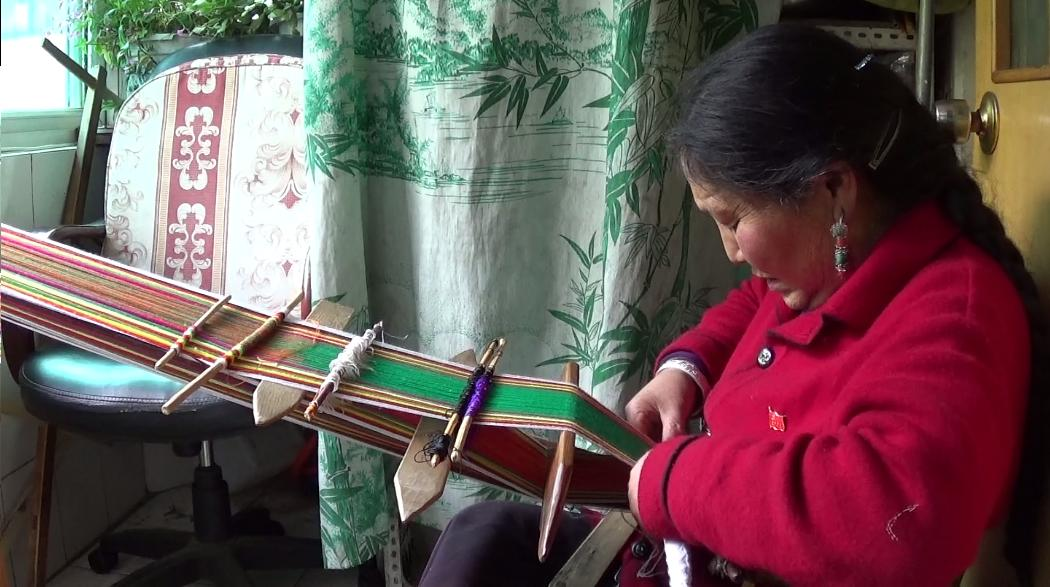
\includegraphics[width=0.8\textwidth]{loom2.jpg}\centering}; %4:20
\tikzstyle{fleche}=[->,very thick,color=green,>=latex]
\tikzstyle{pointille}=[->,dotted,very thick,>=latex]
\begin{scope}[xshift=-0.5cm,rotate=-15]
%    \node[yellow] (A) at (0,1) {up};
%    \node[yellow] (B) at (0,-2.5) {down};
    \node[yellow] (C) at (-3,0) {upstream};
    \node[yellow] (D) at (3,0) {downstream};
%\draw [fleche] (A)--(B);
\draw [fleche] (C)--(D);
\end{scope}
%\begin{scope}[xshift=-1cm,rotate=15]
%    \node (E) at (-2,-2) {\bleu{eastwards}};
%    \node (F) at (2,2) {\bleu{westwards}};
%    \draw [pointille] (E)--(F);
%\end{scope}
\end{tikzpicture}
\end{figure}

The downstream preverbs are required on all verbs expressing motion towards the lower side, for instance to express the tamping of the intersections between the threads (using the tool called \forme{tʰaʁmu}, which is located between upper and lower warp threads to maintain them apart from each other in \figref{fig:loom1}) towards the waist of the weaver, as in (\ref{ex:thari.chWGnda}).

 \begin{exe}
\ex \label{ex:thari.chWGnda}
\gll ɯ-sqar nɯ tʰɯ-ari tɕe tɕe, nɤki, kɯki tú-wɣ-stu tɕe cʰɯ́-wɣ-ɣnda. \\
\textsc{3sg}.\textsc{poss}-intersection.of.warp.threads \textsc{dem} \textsc{aor}:\textsc{downstream}-go[II] \textsc{lnk} \textsc{lnk} \textsc{filler} \textsc{dem}.\textsc{prox} \textsc{ipfv}-\textsc{inv}-do.like \textsc{lnk} \textsc{ipfv}:\textsc{downstream}-\textsc{inv}-tamp \\
\glt `As the intersection of the (upper and lower) warp threads goes down, one does like that to tamp it down.' (vid-20140429090403, 62)
\end{exe} 

The axis that is perpendicular to that of the warp threads and parallel to the ground, through which the weft is inserted (the action depicted in \figref{fig:loom1}), is described using the solar dimension, as shown by the selection of the \textsc{westwards} preverb in (\ref{ex:tWjlAB.YWwGrRe}).

\begin{exe}
\ex \label{ex:tWjlAB.YWwGrRe}
\gll ɯ-taʁ cʰo ɯ-pa ɣɯ ɯ-ʁjar ni pjɯ-ɤqɤtʂʰa-ndʑi, nɯtɕu tɯ-jlɤβ ɲɯ́-wɣ-rʁe tɕe   \\
\textsc{3sg}.\textsc{poss}-top \textsc{comit} \textsc{3sg}.\textsc{poss}-bottom \textsc{gen} \textsc{3sg}.\textsc{poss}-warp \textsc{du} \textsc{ipfv}-be.crossed-\textsc{du} \textsc{dem}.\textsc{loc} \textsc{indef}.\textsc{poss}-weft \textsc{ipfv}:\textsc{west}-\textsc{inv}-insert \textsc{lnk} \\
\glt `The upper and lower warp threads are crossed, and at (the crossing place) one inserts the weft.' (additional explanation provided while transcribing the video from which \figref{fig:loom1} is taken).%vid-20140429090403
\end{exe} 

The vertical dimension preverbs refer to the third axis that is perpendicular with the two previous ones, with the \textsc{downwards} orientation towards the ground. The \textsc{upwards} preverbs occur to describe the lifting of the warp threads using the heddles, as in (\ref{ex:Cnat.kW.tuwGsWjoR}).

\begin{exe}
\ex \label{ex:Cnat.kW.tuwGsWjoR}
\gll ɕnat kɯ tɤ-ri ra tɕe nɯ kɯ tú-wɣ-sɯ-joʁ tɕe,\\
heddle \textsc{erg} \textsc{indef}.\textsc{poss}-thread \textsc{pl} \textsc{lnk} \textsc{dem} \textsc{erg} \textsc{ipfv}:\textsc{up}-\textsc{inv}-\textsc{caus}-raise \textsc{lnk} \\
\glt `One lifts the (warp) threads with the heddles.' (2011-06-thaXtsa)
\end{exe}  
%{ex:Cnat.maNthi}

\subsection{Lexicalized orientations} \label{sec:lexicalized.orientation}
A complete description of the lexicalized orientation preverbs in Japhug would require a monograph-length treatment taking into account all verbs, basic and derived, and including complex predicates. In order to keep this chapter within a reasonable size, I therefore only focus on a few selected semantic categories comprising the most common non-orientable verbs of the language.

\subsubsection{Spatial use of preverbs with non-orientable verbs} \label{sec:orientation.position}
While non-orientable verbs generally select only one or two orientations (§\ref{sec:lexicalized.orientation}), orientation preverbs that are different from the lexical ones can occur in specific contexts to indicate either a motion event linked with the action of the verb (normally with an additional associated motion prefix, §\ref{sec:orientation.AM}), the motion of a body part or the position of the body. 

The intransitive verb \japhug{cɯ}{hibernate} provides an interesting example of this use of the preverbs. The lexically selected orientation of this verb is \textsc{eastwards} (like other verbs from the same semantic category), as shown by the preverb \forme{ku-} in (\ref{ex:qartsW.tCe.kucW}).

\begin{exe}
\ex \label{ex:qartsW.tCe.kucW}
\gll  qartsɯ tɕe ku-cɯ ɲɯ-ŋu. \\
winter \textsc{loc} \textsc{ipfv}-hibernate \textsc{sens}-be \\
\glt `In winter, (the bear) hibernates.' (21-pri, 51)
\end{exe}

However, the orientations \textsc{upstream} and \textsc{upwards} are also attested with this verb, with more specific readings. The \textsc{upstream} orientation is found in (\ref{ex:praRpa.WNgW.lucW}) and also in (\ref{ex:luCe.tCe.lucW}) above, §\ref{sec:am.prefixes}, and expresses hibernation in a cave. These examples reflect the illative use of the \textsc{upstream} preverbs (§\ref{sec:illative.elative}). The \textsc{upwards} orientation, also shown by (\ref{ex:praRpa.WNgW.lucW}), is used when hibernation takes place in a hollow tree, with vertical motion up the tree (§\ref{sec:vertical.dimension}).

\begin{exe}
\ex \label{ex:praRpa.WNgW.lucW}
\gll tɕe qartsɯ tɕe nɯnɯ si kʰoŋrɤl tɤ-kɯ-ɤri nɯ ɯ-ŋgɯ nɯmaʁ tu-cɯ, 
nɯmaʁnɤ, praʁpa ɯ-ŋgɯ lu-ɕe tɕe lu-cɯ. \\
\textsc{lnk} winter \textsc{loc} \textsc{dem} wood hollow.tree \textsc{aor}:\textsc{up}-\textsc{sbj}:\textsc{pcp}-go[II] \textsc{dem} \textsc{3sg}.\textsc{poss}-in otherwise \textsc{ipfv}:\textsc{up}-hibernate otherwise cave \textsc{3sg}.\textsc{poss}-in \textsc{ipfv}:\textsc{upstream}-go \textsc{lnk} \textsc{ipfv}:\textsc{upstream}-hibernate \\
\glt `In winter, it either hibernates in a hollow tree, or goes into a cave and hibernates (there).' (21-pri, 107-108)
\end{exe}

%stu mɤmu nɯ iɕqʰa si kʰoŋrɤl tɤ-kɯ-ɤri 

The forms with \textsc{upstream} and \textsc{upwards} preverbs often occur with either motion verbs or associated motion prefixes, as in (\ref{ex:si.WNgW.tAkWso.WNgW.CtucW}).

\begin{exe}
\ex \label{ex:si.WNgW.tAkWso.WNgW.CtucW}
\gll  si ɯ-ngɯ tɤ-kɯ-so, ɯ-ŋgɯ tɤ-kɯ-rom, nɯnɯ pjɯ-saχsi tɕe, nɯ ɯ-ŋgɯ ɕ-tu-cɯ ɲɯ-ŋu.\\
wood \textsc{3sg}.\textsc{poss}-in \textsc{ipfv}:\textsc{up}-\textsc{sbj}:\textsc{pcp}-be.hollow \textsc{3sg}.\textsc{poss}-in \textsc{ipfv}:\textsc{up}-\textsc{sbj}:\textsc{pcp}-be.dried \textsc{dem} \textsc{ipfv}-do.completely \textsc{lnk} \textsc{dem} \textsc{3sg}.\textsc{poss}-in \textsc{tral}-\textsc{ipfv}:\textsc{up}-hibernate \textsc{sens}-be \\
\glt `Trees whose inside is hollow, whose inside is dried, (the bear) (hollows) it completely, goes up (the hole) and hibernates (there).' (21-pri, 55)
\end{exe}

The use of preverbs to express spatial position or motion as in the case of the \textsc{upstream} and \textsc{upwards} orientations with \japhug{cɯ}{hibernate} above are not unusual with non-orientable verbs, but are lexicalized, and restricted to highly specific and well-identified situations. Only orientations that are pragmatically and culturally plausible and compatible with the speaker's knowledge of the world can be used: with \japhug{cɯ}{hibernate} for instance, the other series of  orientation preverbs (\textsc{downwards}, \textsc{downstream}, \textsc{westwards}) are not attested. It is not possible to predict which non-orientable verb will be compatible with the spatial use of preverbs, and this information has to be specified in dictionaries in a systematic way. The following sections (§\ref{sec:preverb.ingestion} to §\ref{sec:preverb.cover}) present a series of examples of similar phenomena.
%ɕɤxɕo tɯ-mpja tha-ʑa, tɤjpa pa-lɤt kɯnɤ, pjɯ-lɤt ɯkʰɯkʰa ʑo pjɯ-ndʐi ɲɯ-ɕti wo.

\subsubsection{Preverbs and lability} \label{sec:orientation.lability}
A handful of labile verbs select different preverbs and have slightly different meanings in their transitive and intransitive/semi-transitive uses.

The verb \japhug{sɤŋo}{listen} takes the \textsc{westwards} preverbs when semi-transitive, and the \textsc{eastwards} preverbs when transitive with the meaning `listen to, obey' (§\ref{sec:semi.tr.labile}).  

The verb \japhug{sɯso}{think} is normally transitive and selects the \textsc{westwards} preverbs. It can also occurs with the \textsc{downwards} preverbs, but in this case it is intransitive, and means `in $X$'s opinion' (§\ref{sec:labile.tr-intr}). 

\subsubsection{Irregular orientations with local toponyms} \label{sec:local.toponyms.orientation}
Motion from one locality to another is nearly always expressed using the vertical, riverine and solar dimensions in their basic spatial functions (§\ref{sec:vertical.dimension}, §\ref{sec:riverine.dimension} and §\ref{sec:solar.dimension}, respectively). While in some cases there are conflicts between several possible orientations, especially between the riverine and the solar preverbs, the choice of the preverbs is nearly always motivated.

However, there are also cases where the choice of the preverbs is unrelated to the actual spatial orientation of the trip from one particular place to another. For instance, Kamnyu \forme{kɤmɲɯ} (32°12'N,101°57'E) is located to the west of Mengi \forme{mɯŋi} (32°11'N,101°57'E, \zh{蒙岩}). %32.2049575 101.95343555 %32.1962256'N,101.9575799'E
However, the preverbs corresponding to orientations that are exactly opposite to the geographical orientations are used between these two villages: the orientation \textsc{westwards} is used for motion from Kamnyu to Mengi (to describe a trip from west to east), and \textsc{eastwards} from Mengi to Kamnyu (whereas the actual trip is from east to west), as shown by (\ref{ex:kAmYW.mWNi}) and (\ref{ex:mWNi.YWsAxCe}).

\begin{exe}
\ex \label{ex:kAmYW.mWNi}
\gll kɤmɲɯ tɕe tɕe mɯŋi kɤ-ɕe tɤ-ra tɕe, ``mɯŋi ɲɯ-ɕe-a" tu-kɯ-ti ŋu.
tɕe mɯŋi tɕe kɤmɲɯ nɯ tɕe tɕe, nɤki, ``kɤmɲɯ kɤ-ɣe-a, kɤmɲɯ ku-ɕe-a ŋu" nɯra tu-ti-nɯ. \\
\textsc{topo} \textsc{loc} \textsc{lnk}  \textsc{topo} \textsc{inf}-go \textsc{aor}-be.needed \textsc{lnk}  \textsc{topo} \textsc{ipfv}:\textsc{west}-go-\textsc{1sg} \textsc{ipfv}-\textsc{genr}:S/O-say be:\textsc{fact} \textsc{lnk}  \textsc{topo} \textsc{loc}  \textsc{topo} \textsc{dem} \textsc{lnk} \textsc{lnk} \textsc{filler}  \textsc{topo} \textsc{aor}:\textsc{east}-come[II]-\textsc{1sg} pl.n \textsc{ipfv}:\textsc{east}-go-\textsc{1sg} be:\textsc{fact} \textsc{dem}:\textsc{pl} \textsc{ipfv}-say-\textsc{pl} \\
\glt `When one has to go from Kamnyu to Mengi, one says `I am going (westwards) to Mengi, and from Mengi to Kamnyu, people say `I came (eastwards)  to Kamnyu, I am going (eastwards) to Kamnyu.' (150904 akW andi, 6)
\end{exe}

\begin{exe}
\ex \label{ex:mWNi.YWsAxCe}
\gll mɯŋi ɲɯ-sɤx-ɕe tʂu nɯnɯre ri, \\
\textsc{topo} \textsc{ipfv}:\textsc{west}-\textsc{obl}:\textsc{pcp}-go path \textsc{dem}:\textsc{loc} \textsc{loc} \\
\glt `On the road (from Kamnyu) towards Mengi...' (140522 Kamnyu zgo, 2)
\end{exe}

This contradiction is clear in example (\ref{ex:akW.mWNi}), where Mengi is explicitly described as being located on the \forme{akɯ} (east) side of Kamnyu.

\begin{exe}
\ex \label{ex:akW.mWNi}
\gll akɯ pɕoʁ nɯ mɯŋi ŋu, andi pɕoʁ praʁwɯ ŋu. \\
 east side \textsc{dem}  \textsc{topo} be:\textsc{fact} west side  \textsc{topo} be:\textsc{fact} \\
\glt `Mengi is on the east, and Praqwu (a small locality in Kamnyu) is on the west.' (140522 Kamnyu zgo, 21)
\end{exe}

Ercha village (in Japhug \forme{ɣɟɯ tsʰapa}, most often called using its Chinese name \zh{二茶村} \forme{èrchácūn}, 32°13$'$N,101°55$'$E), %32.2180244,101.9229332,2451m
located to the west of Kamnyu, also presents orientation inversion: as shown by (\ref{ex:erchacun.kukWCe}), the \textsc{eastwards} preverbs are used for trips from Kamnyu to Ercha, and the \textsc{westwards} preverbs for the opposite trip. This fact has been reverified with several speakers (note in particular the anecdote reported in §\ref{sec:MBChCh.Dpalcan}).

Note that the presence of a hesitation: Tshendzin was about to say \forme{ɲɯ-kɯ-ɕe} with a \textsc{westwards} preverb (the expected form, based on the geographical location of these localities), followed by the the correct \forme{ku-kɯ-ɕe} with the irregular orientation.

\begin{exe}
\ex \label{ex:erchacun.kukWCe}
\gll tɕe kɤmɲɯ tɕe tɕe <erchacun> ɲɯ-kɯ... ku-kɯ-ɕe tɕe tɕe, nɯnɯ ``ku-ɕe-a" tu-kɯ-ti ŋu. <erchacun> tɕe kɤmɲɯ a-nɯ-ɣi-nɯ tɕe nɯ `kɤmɲɯ nɯ-ari-a, kɤmɲɯ nɯ-ɣe-a" nɯra tu-ti-nɯ ŋu. \\
\textsc{lnk}  \textsc{topo} \textsc{loc} \textsc{lnk}  \textsc{topo} { } \textsc{ipfv}:\textsc{east}-\textsc{genr}:S/O-go \textsc{lnk} \textsc{lnk} \textsc{dem} \textsc{ipfv}:\textsc{east}-go-\textsc{1sg} \textsc{ipfv}-\textsc{genr}:S/O-say be:\textsc{fact}  \textsc{topo} \textsc{loc}  \textsc{topo} \textsc{irr}-\textsc{pfv}:\textsc{west}-come-\textsc{pl} \textsc{lnk} \textsc{dem}  \textsc{topo} \textsc{aor}:\textsc{west}-go[II]-\textsc{1sg}  \textsc{topo} \textsc{aor}:\textsc{west}-come[II]-\textsc{1sg}  \textsc{dem}:\textsc{pl} \textsc{ipfv}-say-\textsc{pl} be:\textsc{fact} \\
\glt (150904 akW andi, 10-11)
\end{exe}

This puzzling irregularity has not been observed for other toponyms, especially those located further away from Kamnyu. For instance, the \textsc{upstream} orientation is used for trips to Tshobdun and Zbu, the \textsc{downstream} orientation to Mbarkham (§\ref{sec:riverine.dimension}) and the \textsc{eastwards} orientation to Sarndzu and Tatshi (§\ref{sec:solar.dimension}).


\subsubsection{Verbs of ingestion} \label{sec:preverb.ingestion}
The most common verb of ingestion, \japhug{ndza}{eat}, generally selects the \textsc{upwards} preverbs, as shown for instance by (\ref{ex:chWnWtsWm.Ctundze}) (in §\ref{sec:AM.goal}) and (\ref{ex:nWtCu.Ctundze}) (in §\ref{sec:nature.of.motion.AM}). The same is true of verbs derived from it, such as the compound verb \japhug{rɯndzɤtsʰi}{have a meal} (§\ref{sec:denom.compound.verbs}), as shown by (\ref{ex:ri.CtArWndzAtshij}) in §\ref{sec:AM.goal}, and of other more specialized verbs of food ingestion such as \japhug{moʁ}{eat (powdery food)}, \japhug{nɯtɕʰaʁ}{eat fodder (of horses)}, \japhug{nɯtʂʰɤɣndʑɤr}{eat a tsampa meal}, \japhug{zmɤrɤβ}{eat (mixing with)} or \japhug{χsɤl}{eat (honorific)}.

The \textsc{downstream} preverbs can occur with \japhug{ndza}{eat} to refer to eating by wild beasts and birds of prey, as in (\ref{ex:kWrtsAG.nW.kW.chWndze}), probably due to the fact that this orientation is also selected by \japhug{ɕkɯt}{eat/drink completely}, a verb which can also describe the actions of ferocious animals as in example (\ref{ex:khu.kW.thaCkWt}) in §\ref{sec:obviation.animacy}.\footnote{See also the discussion on the use of the \textsc{downstream} orientation with \japhug{tsʰi}{drink} below, above example \ref{ex:cha.ntsW.chWtshi}).}

\begin{exe}
\ex \label{ex:kWrtsAG.nW.kW.chWndze}
\gll kɯrtsɤɣ nɯ kɯ, nɤki, tɯrme ra ɣɯ nɯ-fsapaʁ nɯ cʰɯ-ndze, [...] qaʑo tsʰɤt nɯ cʰɯ-ndze pjɤ-ŋu, \\
leopard \textsc{dem} \textsc{erg} \textsc{filler} people \textsc{pl} \textsc{gen} \textsc{3pl}.\textsc{poss}-animal \textsc{dem} \textsc{ipfv}:\textsc{downstream}-eat[III] { } sheep goat \textsc{dem} \textsc{ipfv}:\textsc{downstream}-eat[III] \textsc{ifr}.\textsc{ipfv}-be \\
\glt `The snow leopard was eating domestic animals, eating ...., sheep and goats.' (qala kWCqraR 2002, 3)
\end{exe}

This orientation is also attested to describe the eating of earth by earthworm as in (\ref{ex:qandzxe.nW.kW.chWndze}), though in this case the preverb is used spatially (§\ref{sec:orientation.position}), reflecting the burrowing motion of the earthworm (§\ref{sec:illative.elative}). 

\begin{exe}
\ex \label{ex:qandzxe.nW.kW.chWndze}
\gll tɕeri qandʐe kɯ tʰɤlwa ʁɟa cʰɯ-ndze ɲɯ-ɕti. \\
\textsc{lnk} earthworm \textsc{erg} earth completely \textsc{ipfv}:\textsc{downstream}-eat[III] \textsc{sens}-be.\textsc{aff} \\
\glt  `The earthworm only eats earth.' (25-akWzgumba, 126)
\end{exe}

The \textsc{eastwards} orientation is exclusively attested with \forme{ndza} to describe eclipses, as in (\ref{ex:mWkarCo.mACtsxa.kundze}), also a spatial use of the preverbs (expressing motion from the left side to the right side or vice-versa, §\ref{sec:centripetal.centrifugal}).

\begin{exe}
\ex \label{ex:mWkarCo.mACtsxa.kundze}
\gll ɯ-rkɯ kɯ-fse ku-ʑe tɕe, mɯ-kɤ-arɕo mɤɕtʂa ku-ndze ɣɤʑu, \\
\textsc{3sg}.\textsc{poss}-side \textsc{sbj}:\textsc{pcp}-be.like \textsc{ipfv}:\textsc{east}-being[III] \textsc{lnk} \textsc{neg}-\textsc{aor}:\textsc{east}-be.finished until \textsc{ipfv}:\textsc{east}-eat[III] exist:\textsc{sens} \\
\glt  `Sometimes (the eclipse) starts on one side, and `eats' (the moon) until it (disappears) completely.' (29-mWBZi, 155)
\end{exe}

The orientation \textsc{westwards} occurs with verbs referring to animals eating grass, such as the intransitive verb \japhug{nɯrɯ}{eat grass} as in (\ref{ex:YWnWrWnW}) and its synonym \forme{nɯsɤlɤɣ}.

\begin{exe}
\ex \label{ex:YWnWrWnW}
\gll  nɯŋa qʰe qaʑo tsʰɤt nɯra pjɤ-dɤn-nɯ tɕe, nɯtɕu ɲɯ-nɯrɯ-nɯ tɕe sɯjno tu-ndza-nɯ pjɤ-ŋu, \\
cow \textsc{lnk} sheep goat \textsc{dem}:\textsc{pl} \textsc{ifr}.\textsc{ipfv}-be.many-\textsc{pl} \textsc{lnk} \textsc{dem}:\textsc{loc} \textsc{ipfv}:\textsc{west}-eat.grass-\textsc{pl} \textsc{lnk} grass \textsc{ipfv}:\textsc{up}-eat-\textsc{pl} \textsc{ifr}.\textsc{ipfv}-be \\
\glt  `There were many cows, sheep and goats, and they were eating grass there.' (150819 woniu-zh, 9)
\end{exe}

Verbs related to the ingestion of liquids select the \textsc{eastwards} preverbs as default, as in (\ref{ex:konWkhWG.Zo.kotshi}), including the deideophonic \japhug{nɯkʰɯɣ}{gulp} (§\ref{sec:nW.deidph}).

\begin{exe}
\ex \label{ex:konWkhWG.Zo.kotshi}
\gll tɯ-ci ko-nɯkʰɯɣ ʑo ko-tsʰi. \\
\textsc{indef}.\textsc{poss}-water \textsc{ifr}:\textsc{east}-gulp \textsc{emph} \textsc{ifr}:\textsc{east}-drink \\
\glt `He gulped the water.' (140429 jiedi-zh, 70)
\end{exe}

The verb \japhug{tsʰi}{drink} is also found with the \textsc{downwards} orientation to refer to drinking with the head down on the grounds (like animals, or from a jar with a straw), for instance in (\ref{ex:GWpjWnWtshinW}) and (\ref{ex:CpjAnWtshi}) in §\ref{sec:am.prefixes} and (\ref{ex:WtAlu}) in §\ref{sec:alienabilization}. The denominal verb \japhug{nɯci}{drink from the ground} also selects this orientation.

The \textsc{downstream} preverbs occur with this verb in two contexts. First,  following the basic spatial meaning of these preverbs (`direction of the flow of water', §\ref{sec:riverine.dimension}), they can be used to insist on the flow of liquid through the oesophagus during ingestion, as in (\ref{ex:tWci.chWtshi}). 

\begin{exe}
\ex \label{ex:tWci.chWtshi}
\gll tɯ-ci kɯnɤ cʰɯ-ɕe mɯ-ɲɤ-kʰɯ. tɯ-ci cʰɯ-tsʰi mɯ-ɲɤ-kʰɯ \\
\textsc{indef}.\textsc{poss}-water also \textsc{ipfv}:\textsc{downstream}-go \textsc{neg}-\textsc{ifr}-be.possible \textsc{indef}.\textsc{poss}-water \textsc{ipfv}:\textsc{downstream}-drink \textsc{neg}-\textsc{ifr}-be.possible \\
\glt `Even water could not go (down his throat), he could not drink anymore.' (of a person suffering from throat cancer, 27-tWfCAl, 81)
\end{exe}

Second, the \textsc{downstream} orientation is found to express excessive alcohol drinking, as in (\ref{ex:cha.ntsW.chWtshi}), possibly by analogy with \japhug{ɕkɯt}{eat/drink completely} which also takes this orientation (see also the discussion concerning example \ref{ex:kWrtsAG.nW.kW.chWndze} above).

\begin{exe}
\ex \label{ex:cha.ntsW.chWtshi}
\gll  ɯ-wa nɯ kɯ cʰa ntsɯ cʰɯ-tsʰi qʰe, ɯ-me mɯ́j-nɯβdaʁ \\
\textsc{3sg}.\textsc{poss}-father \textsc{dem} \textsc{erg} alcohol always \textsc{ipfv}:\textsc{downstream}-drink \textsc{lnk} \textsc{3sg}.\textsc{poss}-daughter \textsc{neg}:\textsc{sens}-take.care \\
\glt `Her father was drinking alcohol all the time, and did not take care of his daughter.' (17-lhazgron, 68)
\end{exe}

The \textsc{downstream} preverbs are also selected by the denominal verb \japhug{nɯcʰɤmda}{drink with a straw} (example \ref{ex:chWwGnWchAmdaj}, §\ref{sec:svc}), probably reflecting the illative (through tubular opening) function of the \textsc{downstream} preverb (§\ref{sec:illative.elative}). It is noteworthy that \japhug{tsʰi}{drink} takes the \textsc{downwards} orientation instead when referring to drinking from a straw.

%\japhug{aʁe}{get to eat} {sec:preverb.gain}

The \textsc{upstream} preverbs occur with the verb \forme{χɤβ}, which can mean `drink until the last drop in one gulp', or `breathe in, suck up, draw up' as in (\ref{ex:WsnWro.luXAB}), a special case of the illative  (through large opening) function of this orientation (§\ref{sec:illative.elative}; note that the illative is expressed with the opposite orientation as that of \japhug{nɯcʰɤmda}{drink with a straw}, due to the difference of the shape of the opening).

\begin{exe}
\ex \label{ex:WsnWro.luXAB}
\gll ɯ-sŋɯro lu-χɤβ ʑo tɕe nɯ βɣɤza nɯ ɯ-kɯr ɯ-ŋgɯ lu-nɯ-ɕe ɕti \\
\textsc{3sg}.\textsc{poss}-breath \textsc{ipfv}:\textsc{upstream}-suck \textsc{emph} \textsc{dem} \textsc{lnk} fly \textsc{dem} \textsc{3sg}.\textsc{poss}-mouth \textsc{3sg}.\textsc{poss}-in \textsc{ipfv}:\textsc{upstream}-\textsc{auto}-go be.\textsc{aff}:\textsc{fact} \\
\glt `(The frog)$_i$ draws its$_i$ breath and the fly goes by itself into its$_i$ mouth.' (27-qaCpa, 7)
\end{exe}

\subsubsection{Stative verbs expressing size} \label{sec:preverb.adjectives.size}
Adjectival verbs describing size, like other stative verbs, become dynamic verbs (`become X') in the Imperfective (§\ref{sec:imperfective}), the Irrealis (§\ref{sec:irrealis}), the Aorist (§\ref{sec:aor.inchoative}) and the Inferential (§\ref{sec:ifr}). The most neutral orientation preverbs for these verbs are indicated in \tabref{tab:size.adj.preverbs}. Most positive adjectival verbs select the \textsc{upwards} orientation, except for those describing radial size (\japhug{jpum}{be thick}, \japhug{rɟum}{be broad}) which are  found with the \textsc{westwards} orientation, and those expressing length (see below).

It is much more difficult to ascertain the lexically selected orientation of negative adjectival verbs, since the situations in which their use as dynamic verbs is appropriate (`become small(er)', `become short(er)') are less common. The \textsc{downwards} orientation does occur as lexically selected orientation (with \japhug{xtɕi}{be small}  and \japhug{mbɤr}{be low}), resulting in forms that are homophonous with the Past Imperfective (§\ref{sec:pst.ifr.ipfv}). Perhaps due to this homophony, the \textsc{westwards} orientation is also used instead with \japhug{xtɕi}{be small}, as in (\ref{ex:WCGa.anWxtCi}).

\begin{exe}
\ex \label{ex:WCGa.anWxtCi}
\gll ki ɯ-ʁɤri sɯstaʁ ʑo ɯ-ɕɣa a-nɯ-xtɕi ra \\
\textsc{dem}.\textsc{prox} \textsc{3sg}.\textsc{poss}-before \textsc{comp} \textsc{emph} \textsc{3sg}.\textsc{poss}-age \textsc{irr}-\textsc{pfv}:\textsc{west}-small be.needed:\textsc{fact} \\
\glt `May she become younger than before!' (Norbzang 2005, 251)
\end{exe}

\begin{table}
\caption{Adjectival stative verbs of size and orientation preverbs} \label{tab:size.adj.preverbs}
\begin{tabular}{lllll}
\lsptoprule
Positive size & Orientation & Negative size & Orientation \\
\midrule
\japhug{wxti}{be big} & up & \japhug{xtɕi}{be small} & west, down \\
\japhug{mbro}{be big, be high} & up & \japhug{mbɤr}{be low} & down \\
&&(of size) \\
\japhug{zri}{be long},  & up,  & \japhug{xtɯt}{be short} & west \\
&downstream &&upstream\\
\japhug{rɲɟi}{be long} &&& \\
\japhug{jpum}{be thick}  & west & \japhug{xtsʰɯm}{be thin}& west, east \\
 (of radius)&& (of radius) \\
\japhug{jaʁ}{be thick} & up & \japhug{mba}{be thin} & west  \\
(of a surface)  &&(of a surface) \\
\japhug{rɟum}{be broad}  & west & \japhug{tɕɤr}{be narrow} &  east  \\
&&  \japhug{ŋgɤr}{be narrow} &  east  \\
\lspbottomrule
\end{tabular}
\end{table}

In addition to the orientations in Table (\ref{tab:size.adj.preverbs}), the \textsc{downstream} preverbs can occur to express a progressive increase (§\ref{sec:orientation.preverb.aspect}). Compare for instance the use of \japhug{wxti}{be big} with the \textsc{upwards} orientation in (\ref{ex:Wkha.towxti})  with that in (\ref{ex:ZWrWZAri.chAwxti}) with the \textsc{downstream} orientation, describing a process taking place progressively over many years.

\begin{exe}
\ex \label{ex:Wkha.towxti}
\gll mɤʑɯ ʑo ɯ-kʰa ra to-wxti tɕe, \\
even.more \textsc{emph} \textsc{3sg}.\textsc{poss}-house \textsc{pl} \textsc{ifr}:\textsc{up}-be.big \textsc{lnk} \\
\glt  `His house had become even bigger.' (140430 yufu he tade qizi-zh, 222)
\end{exe}

\begin{exe}
\ex \label{ex:ZWrWZAri.chAwxti}
\gll tɕeri ɯ-tɕɯ nɯ ʑɯrɯʑɤri cʰɤ-wxti  \\
\textsc{lnk} \textsc{3sg}.\textsc{poss}-son \textsc{dem} progressively \textsc{ifr}:\textsc{downstream}-be.big \\
\glt `His son progressively grew up.' (28-smAnmi, 10)
\end{exe}

Some of these verbs are compatible with more than one orientation. For instance, \japhug{rɲɟi}{be long} is attested with the \textsc{upwards} orientation to refer to the length of a vertical object, as in (\ref{ex:turYJi.mAcha}) (where it is synonymous with \japhug{mbro}{be high}). With the \textsc{upstream} preverbs, it describes for instance (elongated) fruits or leaves growing out of the branch of a plant, as in (\ref{ex:lurYJi.tsa.Nu}).
 
\begin{exe}
\ex \label{ex:turYJi.mAcha}
\gll tɕe <yimi> jamar ma tu-rɲɟi mɤ-cʰa ma  \\
\textsc{lnk} one.meter about apart.from \textsc{ipfv}:\textsc{up}-be.long \textsc{neg}-can:\textsc{fact} \textsc{lnk} \\
\glt `It cannot grow longer than about one meter.' (11-qarGW, 114)
\end{exe}

\begin{exe}
\ex \label{ex:lurYJi.tsa.Nu}
\gll tɯrgi ɣɯ ɯ-mat lu-rɲɟi tsa ŋu tɕe, nɤki jima popo tsa fse. \\
fir \textsc{gen}  \textsc{3sg}.\textsc{poss}-fruit \textsc{ipfv}:\textsc{upstream}-be.long a.little be:\textsc{fact} \textsc{lnk} \textsc{filler} maize cob a.little be.like:\textsc{fact} \\
\glt  `The fir cone is elongated, a bit like the corncob (07-tAtho, 32)
\end{exe}

The \textsc{downstream} preverbs are found to express progressive increase (example \ref{ex:ZWrWZAri.chAwxti}, §\ref{sec:redp.gradual.increase}, §\ref{sec:tense.aspect.adverbs}), as in (\ref{ex:chWxtWt.Nu}), but can also refer to the growth of thread-like objects like hair, as in (\ref{ex:tWkArme.chWrYi}). Note in this example that \japhug{rɤɕi}{pull} shares the same preverb to refer to the pulling of hairs.
 
\begin{exe}
\ex \label{ex:chWxtWt.Nu}
\gll ɕɤr nɯ cʰɯ-rɲɟi, sŋi nɯ cʰɯ-xtɯt ɲɯ-ŋu \\
night \textsc{dem} \textsc{ipfv}:\textsc{downstream}-be.long day \textsc{dem}  \textsc{ipfv}:\textsc{downstream}-be.short \textsc{sens}-be \\
\glt `The nights are becoming longer, and the days shorter.' (elicited)
\end{exe}

\begin{exe}
\ex \label{ex:tWkArme.chWrYi}
\gll pɯ-kɯ-xtɕi tɕe, nɯnɯ ʑŋgri nɯ nɯ-mɤrʑaβ ɯ-raŋ tɕe, tɯ-kɤrme cʰɯ́-wɣ-rɤɕi tɕe, cʰɯ-rɲɟi ŋu to-ti-nɯ tɕe,\\
\textsc{pst}.\textsc{ipfv}-\textsc{genr}:S/O-be.small \textsc{lnk} \textsc{dem} star \textsc{dem}  \textsc{aor}-marry \textsc{3sg}.\textsc{poss}-time \textsc{lnk} \textsc{genr}.\textsc{poss}-hair \textsc{ipfv}:\textsc{downstream}-\textsc{inv}-pull \textsc{lnk} \textsc{ipfv}:\textsc{downstream}-be.long be:\textsc{fact} \textsc{ifr}-say-\textsc{pl} \textsc{lnk} \\
\glt `When we were young, people said that when there is a shooting star, if you pull your hair, it will grow longer.' (29-mWBZi, 102)
 \end{exe}
%{ex:Wmat.chWkWBze} ku-kɯ-xtsʰɯm ɲɯ-kɯ-jpum 

\subsubsection{Verbs related to growth, gain or birth} \label{sec:preverb.gain}
Adjectival verbs of size can be used to express growth (§\ref{sec:preverb.adjectives.size}), but another constructions expressing the same meaning involves the transitive verb \japhug{βzu}{make} with a dummy subject (§\ref{sec:transitive.dummy}), and an adjectival verb in participial form (§\ref{sec:subject.participles}), as in (\ref{ex:kWmbWmbro.tuBze}), with the \textsc{upwards} orientation (compare with \ref{ex:turYJi.mAcha} above and \ref{ex:YWwGzmaqhu} in §\ref{sec:obviation.animacy}).
 

\begin{exe}
\ex \label{ex:kWmbWmbro.tuBze}
\gll ɕɤɣ nɯ li kɯ-mbɯ\redp{}mbro tu-βze cʰa \\
juniper \textsc{dem} again \textsc{sbj}:\textsc{pcp}-\textsc{emph}\redp{}be.high \textsc{ipfv}:\textsc{up}-make[III] can:\textsc{fact} \\
\glt `The juniper grows very high.' (08-CAG, 1)
 \end{exe}
 
The \textsc{upstream} orientation appears to describe fruits or leaves growing out of a plant, as in (\ref{ex:tWrgi.laNlaN.laBzu})  (compare with \ref{ex:lurYJi.tsa.Nu} above).
 
 \begin{exe}
\ex \label{ex:tWrgi.laNlaN.laBzu}
\gll  tɯrgi laŋlaŋ nɯnɯ, la-βzu ɕimɯma nɯ ɲɯ-ɤrŋi, \\
fir cone \textsc{dem} \textsc{aor}:\textsc{upstream}:3\flobv{}-make immediately \textsc{dem} \textsc{sens}-be.green \\
\glt `The fir cone is green when it has just grown out.' (08-tWrgi, 72)
  \end{exe}

The \textsc{downstream} orientation is found with long and thin thread-like objects, like the stalks of some plants as in (\ref{ex:Wru.chWBze}) (compare with \ref{ex:tWkArme.chWrYi}), but also occur to refer to fruits or grains (\ref{ex:Wmat.kWfse.chWBze}), probably as an extension of the progressive incrementation function of this orientation (\ref{ex:ZWrWZAri.chAwxti} above, §\ref{sec:preverb.adjectives.size}).

  \begin{exe}
\ex \label{ex:Wru.chWBze}
\gll   ɯ-ru ra kɯ-xtsʰɯ\redp{}xtsʰɯm ŋu ri, kɯ-zɯ\redp{}zri ʑo cʰɯ-βze qʰe,  \\
  \textsc{3sg}.\textsc{poss}-stalk \textsc{pl} \textsc{sbj}:\textsc{pcp}-\textsc{emph}\redp{}be.thin be:\textsc{fact} \textsc{lnk}  \textsc{sbj}:\textsc{pcp}-\textsc{emph}\redp{}be.long \textsc{emph} \textsc{ipfv}:\textsc{downstream}-make[III] \textsc{lnk} \\
\glt `Although its stalk is very thin, it grows very long.' (19-qachGa mWntoR, 71)
  \end{exe}
  
\begin{exe}
\ex \label{ex:Wmat.kWfse.chWBze}
\gll    sɯŋgɯpɤjka nɯ ɯ-mat nɯnɯ pɤjka kɯ-fse cʰɯ-βze,    \\
wild.squash \textsc{dem} \textsc{3sg}.\textsc{poss}-fruit \textsc{dem} squash \textsc{sbj}:\textsc{pcp}-be.like \textsc{ipfv}:\textsc{downstream}-make[III] \\
\glt `Wild squash grows fruits like those of the (cultivated) squash.' (16-CWrNgo, 39)
\end{exe}

The intransitive verb \japhug{ndzɤt}{grow} also selects the \textsc{upwards} orientation to describe the growth of a plant, and the \textsc{downstream} preverbs for children, as in (\ref{ex:tApAtso.chondzAt}).

\begin{exe}
\ex \label{ex:tApAtso.chondzAt}
\gll   tɤ-pɤtso cʰo-ndzɤt \\
\textsc{indef}.\textsc{poss}-child \textsc{ifr}:\textsc{downstream}-grow \\
\glt  `The child grew up.' (elicited)
\end{exe}

For growth in quantity rather than size, the \textsc{upwards} orientation is selected, for instance with the verb \japhug{dɤn}{be many} in (\ref{ex:tAdAnnW2}).

\begin{exe}
\ex \label{ex:tAdAnnW2}
\gll  tʰam tɕe mɤʑɯ tɤ-dɤn-nɯ  \\
now \textsc{lnk} even.more \textsc{aor}:\textsc{up}-be.many-\textsc{pl}  \\
\glt `Now they are even more numerous than before.' (140522 tshupa, 86)
\end{exe}

The \textsc{upwards} orientation is also selected by verbs expressing birth and coming into existence such as \japhug{tu}{exist} in (\ref{ex:ci.totu}) and (\ref{ex:tWci.paRea}) (note that its antonym \japhug{me}{not exist} rather selects the \textsc{westwards} orientation, §\ref{sec:preverb.loss}), and verbs of Tibetan origin such as \japhug{sci}{be born} (\ref{ex:WtCW.tosci}) and the honorific \japhug{mkʰroŋ}{be born, be reincarnated} (\ref{ex:GWtomkhroN}).

\begin{exe}
\ex \label{ex:ci.totu}
\gll  ndʑi-tɕɯ ci to-tu \\
3du.\textsc{poss}-son \textsc{indef} \textsc{ifr}:\textsc{up}-exist \\
\glt `They had one son.' (2011-05-nyima, 2)
\end{exe}

\begin{exe}
\ex \label{ex:WtCW.tosci}
\gll ɯ-tɕɯ to-sci ɕi, ɯ-me to-sci? \\
\textsc{3sg}.\textsc{poss}-son \textsc{ifr}-be.born \textsc{qu} \textsc{3sg}.\textsc{poss}-girl \textsc{ifr}-be.born \\
\glt `Did she have a boy or a girl.' (elicited)
\end{exe}

\begin{exe}
\ex \label{ex:GWtomkhroN}
\gll nɯʑora nɯ-ɕki ɣɯ-to-mkʰroŋ ɲɯ-ŋu.  \\
\textsc{2pl} \textsc{2pl}.\textsc{poss}-\textsc{dat} \textsc{cisl}-\textsc{ifr}:\textsc{up}-be.born \textsc{sens}-be \\
\glt `He had come to be born in their (family).' (150825 nezha naohai-zh, 38)
\end{exe}

The \textsc{downstream} orientation however occurs with verbs expressing humans or animals giving birth, such as the intransitive denominal verbs \japhug{rɤpɯ}{have young}, \japhug{rɤŋgɯm}{lay eggs} and \japhug{rɤrɟit}{have a child} (§\ref{sec:denom.intr.rA}) and the light verb \japhug{lɤt}{release} in the meaning `give birth to' in (\ref{ex:thWrApW.chWlAt}). This may be an extension of the elative function of the \textsc{downstream} preverbs (§\ref{sec:illative.elative}).

\begin{exe}
\ex \label{ex:thWrApW.chWlAt}
\gll tsʰɤt nɯ tʰɯ-rɤpɯ tɕe, ʁnɯz ntsɯ cʰɯ-lɤt ŋgrɤl \\
goat \textsc{dem} \textsc{aor}:\textsc{downstream}-have.young \textsc{lnk} two always \textsc{ipfv}:\textsc{downstream}-release be.usually.the.case:\textsc{fact} \\
\glt `When goats have young, they give birth to two (kids) each time.' (05-qaZo, 7)
\end{exe}

\begin{exe}
\ex \label{ex:chWrANgWm}
\gll tɯ-ji ɯ-ŋgɯ nɯra cʰɯ-rɤŋgɯm ŋgrɤl \\
\textsc{indef}.\textsc{poss}-field \textsc{3sg}.\textsc{poss}-in \textsc{dem}:\textsc{pl} \textsc{ipfv}:\textsc{downstream}-lay.eggs be.usually.the.case:\textsc{fact} \\
\glt `It lays eggs in the fields.' (24-kWmu, 85)
\end{exe}

Verbs expressing gain select the \textsc{downwards} orientation, including the orientable verb \japhug{mɟa}{take} (§\ref{sec:manipulation.verbs}) when used in the meaning `obtain, get' (example \ref{ex:pjWGmJa.ma.mWpWkWcha} in §\ref{sec:antipassive.t}), \japhug{βɟɤt}{obtain} (§\ref{sec:antipassive.t}), \japhug{mto}{see} (which can mean `find' especially when used with the autive prefix, see §\ref{sec:preverb.perception} and §\ref{sec:autoben.spontaneous}) as well as the semi-transitive \japhug{aʁe}{have to eat/drink}\footnote{This verb can be translated into Chinese as \ch{吃到}{chīdào}{have to eat} or \ch{喝到}{hēdào}{have to drink}.} as in (\ref{ex:tWci.paRea}).
  
\begin{exe}
\ex \label{ex:tWci.paRea}
\gll a-kɯr ɯ-ŋgɯ tɯ-ci pɯ-aʁe-a tɕe, a-sroʁ to-tu  \\
\textsc{1sg}.\textsc{poss}-mouth \textsc{3sg}.\textsc{poss}-in \textsc{indef}.\textsc{poss}-water \textsc{aor}:\textsc{down}-be.needed.eat-\textsc{1sg} \textsc{lnk} \textsc{1sg}.\textsc{poss}-life \textsc{ifr}:\textsc{up}-exist \\
\glt `I have water in my mouth to drink, my life is back.' (2011-05-nyima, 69)
\end{exe} 

\subsubsection{Verbs related to loss or death} \label{sec:preverb.loss}
Verbs expressing loss, with meanings such as `disappear' or `lose' generally select the orientation \textsc{westwards}, probably as an extension of its centrifugal use (§\ref{sec:centripetal.centrifugal}). For instance, the verb \japhug{βde}{throw}, which can also be interpreted as meaning `lose' when used non-volitionally (especially with the autive §\ref{sec:autoben.lexicalized}), selects this orientation, as shown by (\ref{ex:Wrte.YAnWBde}), even though the loss of the hat (in the pear story movie) involved a motion downwards.
 
\begin{exe}
\ex \label{ex:Wrte.YAnWBde}
\gll tɕe ɯ-rte ra ɲɤ-nɯ-βde tɕe, \\
\textsc{lnk} \textsc{3sg}.\textsc{poss}-hat \textsc{pl} \textsc{ifr}:\textsc{west}-\textsc{auto}-lose \textsc{lnk} \\
\glt  `(The boy) lost his hat' (Pear story 2010, Tshendzin,  12)
\end{exe} 

The same is observed with the verb \japhug{me}{not exist} in (\ref{ex:mtshu.YAme}), here also despite a clear downward motion of the water level until the lake disappears.

\begin{exe}
\ex \label{ex:mtshu.YAme}
\gll mtsʰu nɯ cʰɯmcʰɯm ʑo, tɕe, tɯ-skɤm pjɤ-sɤʑa tɕe mtsʰu nɯ ɲɤ-me tɕe \\
lake \textsc{dem} \textsc{idph}(II):slowly \textsc{emph} \textsc{lnk} \textsc{inf}:II-dry.up \textsc{ifr}:\textsc{down}-start \textsc{lnk} lake \textsc{dem} \textsc{ifr}:\textsc{west}-not.exist \textsc{lnk} \\
\glt `The level of the lake started to go down slowly and the lake disappeared.' (nyima2003, 106)
\end{exe} 

Verb expressing partial disappearance, such as \japhug{rkɯn}{be few} in (\ref{ex:si.YWYArkWn}), also occur with the \textsc{westwards} orientation.

\begin{exe}
\ex \label{ex:si.YWYArkWn}
\gll zgoku nɯtɕu si nɯ ʑɯrɯʑɤri ɲɯ\redp{}ɲɤ-rkɯn ʑo \\
mountain \textsc{dem}:\textsc{loc} tree \textsc{dem} progressively \textsc{incr}\redp{}\textsc{ifr}:\textsc{west}-be.few \textsc{emph} \\
\glt `The trees on the mountain became fewer and fewer.' (04-xiaocunzhuang-zh, 24)
\end{exe} 

The verb \japhug{ɕqʰlɤt}{disappear}, also semantically related to these verbs, is an orientable motion verb (§\ref{sec:motion.verbs}). It does not usually select the \textsc{westwards} orientation in a non-spatial way, except for the express the passing of time (§\ref{sec:vertical.preverbs.time}). In example (\ref{ex:tANe.YWCqhlAt}), there is however some ambiguity as to whether the \textsc{westwards} orientation is purely spatial (the setting of the sun in the west, see §\ref{sec:solar.dimension}; note that the vertical dimension is more commonly selected, §\ref{sec:vertical.dimension}), or whether it could also be analyzed as centripetal.
 
\begin{exe}
\ex \label{ex:tANe.YWCqhlAt}
\gll  tɤŋe nɯ ɲɯ-ɕqʰlɤt ku-nɤjɤm ra kʰi ma tɤŋe nɯ wuma ʑo nɯɣ-me kʰi.  \\
sun \textsc{dem} \textsc{ipfv}:\textsc{west}-disappear \textsc{ipfv}-wait[III] be.needed:\textsc{fact} hearsay \textsc{lnk} sun \textsc{dem} really \textsc{emph} \textsc{appl}-be.afraid[III]:\textsc{fact} hearsay \\
\glt `(The yeti) waits for the sun to disappear (before eating the man he has caught), because he fears the sun, it is said.' (140510 mYWrgAt, 7)
\end{exe} 

It is possible that the centripetal function of the \textsc{westwards} orientation has originated from a metaphoric extension of the disappearance of the sun in the west at dusk, in which examples like (\ref{ex:tANe.YWCqhlAt}) would be the pivot construction allowing reanalysis from a purely spatial marker to a more abstract meaning such as `away from the deictic center' or `loss'.

Verbs expressing a more abstract type of disappearance, such as the cognition verb \japhug{jmɯt}{forget} (memory loss), likewise select the \textsc{westwards} prefixes, as in \forme{ɲɤ-nɯ-jmɯt-a} \textsc{ifr}:\textsc{west}-\textsc{auto}-forget-\textsc{1sg} `I forgot (about it)' (see \ref{ex:mAxsi.YAnWjmWta}, §\ref{sec:1.genr}).

The verb \japhug{me}{not exist} has another set of forms with the \textsc{upwards} orientation, as in (\ref{ex:si.tAme}). With the \textsc{upwards} vertical preverbs, this verb does not entail the presupposition that loss occurred; in the perfective, the \forme{tɤ-me} with \textsc{upwards} orientation means `when there this no X' (a usage found with other stative verbs, §\ref{sec:orientation.preverb.aspect}), while \forme{nɯ-me} with \textsc{westwards} orientation can only be interpreted as `(when) X disappeared/was lost'.

 \begin{exe}
\ex \label{ex:si.tAme}
\gll  nɯ ma si tɤ-me tɕe li nɯ ɲɯ-pʰɯt-nɯ\\
\textsc{dem} apart.from wood \textsc{aor}:\textsc{up}-not.exist \textsc{lnk} again \textsc{dem} \textsc{ipfv}-take.out-\textsc{pl}\\
\glt `When there is no other wood than this, people cut it.' (07-Zmbri, 65)
\end{exe} 

As in many languages (for instance Indo-European \forme{*mer}, \citealt[439--440]{liv}), \forme{me} in the meaning `disappear' is commonly used as a euphemism for passing away, as in (\ref{ex:WXti.YAme}).

 \begin{exe}
\ex \label{ex:WXti.YAme}
\gll  ɯʑo ɯ-χti ɲɤ-me tɕe,  \\
\textsc{3sg} \textsc{3sg}.\textsc{poss}-companion \textsc{ifr}:\textsc{west}-not.exist \textsc{lnk} \\
\glt `Her husband passed away.' (12-BzaNsa, 127)
\end{exe} 

Likewise, verbs expressing death and destruction, such as \japhug{si}{die} and \japhug{χɕaʁ}{pass away} (a borrowing from \tibet{གཤེགས་}{gɕegs}{go away}), \japhug{plɯt}{suppress, destroy}, \japhug{ndʑɯɣ}{be destroyed} select the \textsc{westwards} orientation, as shown by (\ref{ex:tongo.YAsi}), (\ref{ex:WrGi.nWplWti}) and (\ref{ex:Ctusci.YWNu}) further below (in §\ref{sec:nature.of.motion.AM}).

 \begin{exe}
\ex \label{ex:tongo.YAsi}
\gll βdaʁmu nɯ to-ngo tɕe ɲɤ-si. \\
lady \textsc{dem} \textsc{ifr}-be.ill \textsc{lnk} \textsc{ifr}:\textsc{west}-die \\
\glt `The lady became ill and died.' (2011-05-nyima, 5)
 \end{exe} 
 
  \begin{exe}
\ex \label{ex:WrGi.nWplWti}
\gll  jima ɯ-rɣi nɯ-plɯt-i \\
maize \textsc{3sg}.\textsc{poss}-grain \textsc{aor}:\textsc{west}-destroy-\textsc{1pl} \\
\glt `We have used up all the maize grains.' (elicited)
  \end{exe} 
  
 The verb \japhug{si}{die} alternatively also occur with the \textsc{downwards} preverbs, in particular in the case of animals as in (\ref{ex:nWNGarmW.pjAsi}). With humans, using the \textsc{downwards} preverbs is not rude, but considered to be blunter than with the  westwards' preverbs.
 
\begin{exe}
\ex \label{ex:nWNGarmW.pjAsi}
\gll  tɕetu ʑara nɯ-ɴɢarmɯ nɯ pjɤ-si kʰi tɕe,  \\
up.there \textsc{3pl} \textsc{3pl}.\textsc{poss}-hybrid.cow \textsc{dem} \textsc{ifr}:\textsc{down}-die hearsay \textsc{lnk} \\
\glt `Those up there, their cow died, it is said.' (Tagrdo conversation, 2003)
   \end{exe} 
   
The transitive verb \japhug{sat}{kill} also selects the \textsc{downwards} orientation preverbs, even when taking an associated motion prefix and an overt goal pointing to an orientation other than \textsc{downwards}, as in (\ref{ex:pGAtCW.CpWsatnW}).

\begin{exe}
\ex \label{ex:pGAtCW.CpWsatnW}
\gll  atu pɣɤtɕɯ nɯ ɕ-pɯ-sat-nɯ ra \\
up.there bird \textsc{dem} \textsc{tral}-\textsc{imp}:\textsc{down}-kill-\textsc{pl} be.needed:\textsc{fact} \\
\glt `Go and kill the bird up there.' (2005 Kunbzang, 330)
   \end{exe} 
   
Likewise, \japhug{ntɕʰa}{kill, butcher} (on whose etymology see \citealt[303--309]{gong18these}) occurs with the \textsc{downwards} preverbs in the meaning `kill (an animal)', as shown by (\ref{ex:nWNa.pjAnWnWntChanW}). 

\begin{exe}
\ex \label{ex:nWNa.pjAnWnWntChanW}
\gll  tɕe nɯ-nɯŋa pjɤ-nɯ-ntɕʰa-nɯ \\
\textsc{lnk} \textsc{3pl}.\textsc{poss}-cow \textsc{ifr}:\textsc{down}-\textsc{auto}-butcher-\textsc{pl} \\
\glt `They killed their cow (for themselves to eat).' (02-deluge2012, 17)
\end{exe} 

The orientation \textsc{westwards} also occurs with this verb in the meaning `butcher', as illustrated by (\ref{ex:natChanW.tutCAtnW}) and (\ref{ex:YWtChanW}). On the other hand, \japhug{sat}{kill} is not found with the \textsc{westwards} preverbs.

\begin{exe}
\ex \label{ex:natChanW.tutCAtnW}
\gll fsapaʁ ɯ-ŋgru pɯ-nɯ-ŋu, rɯdaʁ ɯ-ŋgru pɯ-nɯ-ŋu,  nɯnɯ na-ntɕʰa-nɯ tɕe tu-tɕɤt-nɯ tɕe tɕe tu-sɯɣ-rom-nɯ. \\
domestic.animals \textsc{3sg}.\textsc{poss}-sinew  \textsc{pst}.\textsc{ipfv}-\textsc{auto}-be  \textsc{3sg}.\textsc{poss}-sinew  wild.animals \textsc{pst}.\textsc{ipfv}-\textsc{auto}-be \textsc{dem} \textsc{aor}:\textsc{west}:3\flobv{}-butcher-\textsc{pl} \textsc{lnk} \textsc{ipfv}:\textsc{up}-take.out-\textsc{pl} \textsc{lnk} \textsc{lnk} \textsc{ipfv}-\textsc{caus}-be.dry-\textsc{pl} \\
\glt `Whether it is sinew$_i$ from a domestic or a wild animal,$_j$  after they butcher them,$_j$ they take it$_i$ out and dry it$_i$.' (150906 tWNgru, 6)
\end{exe} 

\begin{exe}
\ex \label{ex:YWtChanW}
\gll nɯnɯ pa-sat-nɯ tɕe tɕe ju-nɯ-ɣɯt-nɯ tɕe ɲɯ-ntɕʰa-nɯ  \\
\textsc{dem} \textsc{aor}:\textsc{down}:3\flobv{}-kill-\textsc{pl} \textsc{lnk} \textsc{lnk} \textsc{ipfv}-\textsc{vert}-bring-\textsc{pl} \textsc{lnk} \textsc{ipfv}:\textsc{west}-butcher-\textsc{pl} \\
\glt `After (the hunters) have killed (the animals)$_i$, they bring them$_i$ home and butcher them$_i$.' (150829 KAGWcAno, 18)
\end{exe} 

\subsubsection{Verbs of speech and sound}  \label{sec:preverb.speech}
Verbs of speech mainly select either the orientation \textsc{upwards} (\japhug{ti}{say}, \japhug{rɯɕmi}{speak}, \japhug{arju}{speak}, see for instance \ref{ex:tWkArme.chWrYi} in §\ref{sec:preverb.adjectives.size} and \ref{ex:WCki.turWCmia} in §\ref{sec:intr.goal}; their etymology is discussed in §\ref{sec:denom.a} and §\ref{tab:denom.rA.intr}), with the exception of \japhug{fɕɤt}{tell} (borrowed from \tibet{བཤད་}{bɕad}{tell}), which occurs with the \textsc{downwards} preverbs (see the Inferential \forme{pjɤ-fɕɤt} \textsc{ifr}:\textsc{down}-tell `she told it' in \ref{ex:WsAfCAt}, §\ref{sec:other.oblique.participle.relatives}). The intransitive verb \japhug{mbri}{make a sound}, used for animals or objects, is also found with the \textsc{upwards} preverbs (see \forme{to-mbri} \textsc{ifr}:\textsc{up}-make.noise in \ref{ex:tAkWmbri.kWme}, §\ref{sec:subject.participle.other.relative})

The intransitive denominal verb \japhug{nɯrɤɣo}{sing} (§\ref{sec:denom.intr.nW}) on the other hand appears with the orientation \textsc{downstream}, as in (\ref{ex:chWnWrAGo}), and this applies to transitive verbs taking the base noun \japhug{rɤɣo}{song} as objects (such as \forme{cʰɯ-tɯ-ʑa} and \forme{cʰɯ-ti}  in \ref{ex:chWtinW.tochanW}).

\begin{exe}
\ex \label{ex:chWnWrAGo}
\gll qartsʰi nɯ sŋi tɕe cʰɯ-nɯrɤɣo nɤ cʰɯ-nɯrɤɣo ŋu tɕe   \\
cicada \textsc{dem} day \textsc{loc} \textsc{ipfv}:\textsc{downstream}-sing \textsc{add} \textsc{ipfv}:\textsc{downstream}-sing be:\textsc{fact} \textsc{lnk} \\
\glt `The cicada (was) singing all the time during the day. (26-NalitCaRmbWm, 30)
\end{exe} 

\begin{exe}
\ex \label{ex:chWtinW.tochanW}
\gll  nɯnɯ rɤɣo cʰɯ-tɯ-ʑa qʰe, tɤrcɯrca ʑo cʰɯ-ti-nɯ to-cʰa-nɯ. \\
\textsc{dem} song \textsc{ipfv}:\textsc{downstream}-\textsc{conv}:\textsc{imm}-start \textsc{lnk} together \textsc{emph} \textsc{ipfv}:\textsc{downstream}-say \textsc{ifr}-can-\textsc{pl} \\
\glt `They became able to sing along as soon as it started its song.'  (140519 yeying-zh, 162)
\end{exe} 

The  choice of the \textsc{downstream} preverbs on verbs related to songs and music is probably an analogical extension of its use with verbs related to wind instruments, as in (\ref{ex:Juli.chAlAt}) and (\ref{ex:rdAdWt.chWZmbrinW}) (see also \ref{ex:Juli.chWlAtnW}, §\ref{sec:genr.3pl}).

\begin{exe}
\ex \label{ex:Juli.chAlAt}
\gll  ɟuli nɯ cʰɤ-lɤt. \\
flute \textsc{dem} \textsc{ifr}:\textsc{downstream}-release \\
\glt `He played the flute' (140513 mutong de disheng-zh, 85)
\end{exe}

\begin{exe}
\ex \label{ex:rdAdWt.chWZmbrinW}
\gll  nɯnɯra kɯ rkɤdɯt cʰɯ-ʑ-mbri-nɯ pjɤ-mtsʰɤm. \\
\textsc{dem}:\textsc{pl} \textsc{erg} horn \textsc{ipfv}:\textsc{downstream}-\textsc{caus}-make.noise-\textsc{pl} \textsc{ifr}-hear \\
\glt `She heard (the hunters) blowing the horn.' (140520 ye tiane-zh, 249)
\end{exe}

The \textsc{downstream} preverbs on verbs of this type itself derives from their use with \japhug{ɣɤmɯt}{blow} as in (\ref{ex:WlAcu.chWwGGAmWt}), itself an extension of their illative meaning (`into a tubular object', see §\ref{sec:illative.elative}).

\begin{exe}
\ex \label{ex:WlAcu.chWwGGAmWt}
\gll  ɯ-lɤcu cʰɯ́-wɣ-ɣɤmɯt tɕe tɯ-rtsʰɤz nɯ ɲɯ-fka ŋu \\
\textsc{3sg}.\textsc{poss}-upstream \textsc{ipfv}:\textsc{downstream}-\textsc{inv}-blow \textsc{lnk} \textsc{indef}.\textsc{poss}-lung \textsc{dem} \textsc{sens}-be.full be:\textsc{fact} \\
\glt  `One blows (into the pig's trachea) and its lungs fill up.' (20-kAPjAt, 13)
\end{exe}

\subsubsection{Verbs of perception}  \label{sec:preverb.perception} 
With the exception of the orientable verb \japhug{ru}{look at} (§\ref{sec:orienting.verbs}), most verbs of perception generally select only one orientation. The  \textsc{downwards} preverbs are selected by the non-volitional  verbs \japhug{mto}{see} and \forme{mtsʰɤm}, which generally means `hear', but is also used for all non-visual  non-volitional perception, including olfaction (example \ref{ex:nWdi.tunAmnAm}, §\ref{sec:tropative.lexicalized}), touch and the perception of vibrations as in  (\ref{ex:NGoCna.nWkW.pjWmtshAm}).
 
\begin{exe}
\ex \label{ex:NGoCna.nWkW.pjWmtshAm}
\gll ɲɯ-mɯnmu nɤ ɲɯ-mɯnmu tɕe tɕe, nɯ ɯ-ŋgɯ ɴɢoɕna kɯ-rɤʑi nɯ kɯ pjɯ-mtsʰɤm tɕe  \\
\textsc{ipfv}-move \textsc{add} \textsc{ipfv}-move  \textsc{lnk} \textsc{lnk} \textsc{dem} \textsc{3sg}.\textsc{poss}-in spider \textsc{sbj}:\textsc{pcp}-stay \textsc{dem} \textsc{erg} \textsc{ipfv}:\textsc{down}-feel \textsc{lnk} \\
\glt `(The fly that has been caught in the spider's web) moves and moves, and the spider staying inside feels it.' (26-mYaRmtsaR, 63-64)
\end{exe}

The other verbs each have a different orientation: the semi-transitive \japhug{sɤŋo}{listen} selects the \textsc{westwards} preverbs (§\ref{sec:orientation.lability}, §\ref{sec:semi.tr.labile}), and the tropative verb \japhug{nɤmnɤm}{smell} (§\ref{sec:tropative.lexicalized}) the \textsc{upwards} preverbs (examples \ref{ex:nWdi.tunAmnAm} and \ref{ex:tutanAmnAm}, §\ref{sec:tropative.lexicalized}). This orientation simply reflects that of the base intransitive verb \japhug{mnɤm}{have a smell}.

\subsubsection{Verbs of giving} \label{sec:preverb.giving}
Ditransitive verbs expressing permanent or temporary transfer of property, including \japhug{mbi}{give},  \japhug{kʰo}{give, pass}, \japhug{rŋo}{borrow (from)} and \japhug{nɤŋgɯ}{borrow (from)} (and verbs derived from these), have different argument structures (§\ref{sec:ditransitive.indirective} and §\ref{sec:ditransitive.secundative}), but most of them select the \textsc{westwards} preverbs as default orientation, perhaps reflecting the centripetal function of this orientation (§\ref{sec:centripetal.centrifugal}), as in English `give away' or `give out'.

For instance, the most common Inferential 3\flobv{} forms of these verbs are \forme{ɲɤ-mbi}, \forme{ɲɤ-mbi}, \forme{ɲɤ-rŋo} and \forme{ɲɤ-nɤŋgɯ} (examples are plentiful elsewhere in this grammar, for instance \ref{ex:nArZaB.YWkhotCi} in §\ref{sec:essive.abs}, \ref{ex:zYArNo} and \ref{ex:nWwGkhoa} in §\ref{sec:ditransitive.indirective} and \ref{ex:WCki.YAkho} and \ref{ex:nWCki.zYArNo} in §\ref{sec:dative}). 
 
However, it is alternatively possible to choose a prefix reflecting the spatial direction of the transfer of property. In (\ref{ex:pWwGmbia}), we find thus a \textsc{downwards} orientation preverb to describe a present (downwards) from heaven, and in (\ref{ex:Wphe.tokho}) an \textsc{upwards} preverb expresses the relative vertical position of the recipient and the subject: the latter being on the ground, while the former rides a tiger, the transfer of property involves a motion upwards.
 
\begin{exe}
\ex \label{ex:pWwGmbia}
\gll tɯmɯkɯmpɕi kɯ pɯ́-wɣ-mbi-a ŋu \\
heaven \textsc{erg} \textsc{aor}:\textsc{down}-\textsc{inv}-give be:\textsc{fact} \\
\glt `Heavens gave it to me.' (Norbzang 2005, 312)
\end{exe}

\begin{exe}
\ex \label{ex:Wphe.tokho}
\gll laʁjɯɣ nɯ ɯ-taʁ nɯ ɯ-pʰe to-kʰo tɕe,  \\
staff \textsc{dem} \textsc{3sg}.\textsc{poss}-on \textsc{dem} \textsc{3sg}.\textsc{poss}-\textsc{dat} \textsc{ifr}:\textsc{up}-give \textsc{lnk} \\
\glt `He gave the staff to the (thief) who was on (the tiger).' (khu2012, 15)
\end{exe}

The \textsc{downwards} orientation can also be used more metaphorically to express gift from someone higher up in the social hierarchy, as in (\ref{ex:piaozi.pWwGmbij}).

\begin{exe}
\ex \label{ex:piaozi.pWwGmbij}
\gll  taʁ kɯ, <piaozi> pɯ́-wɣ-mbi-j. \\
up \textsc{erg} money \textsc{aor}:\textsc{down}-\textsc{inv}-give-\textsc{1pl}  \\
\glt  `The ones above (the government) gave us money.' (2010-09, 172)
\end{exe}

The riverine axis is also metaphorically use to express relative social status with the verb \japhug{kʰo}{give, pass}. The \textsc{downstream} preverbs express transfer of property from someone higher in the hierarchy (in particular, nobles or lamas) to someone lower than himself. For instance in (\ref{ex:laftaR.chAtWkhonW}), the subject of \forme{cʰɤ-tɯ-kʰo-nɯ} `you gave it to her' is a prince, and the recipient an unknown girl; note that the \textsc{downstream} preverb co-occurs here with the honorific plural (§\ref{sec:honorific.indexation}), another linguistic clue to the social status of the subject.

\begin{exe}
\ex \label{ex:laftaR.chAtWkhonW}
\gll nɯtɕu zɯ laftaʁ cʰɤ-tɯ-kʰo-nɯ tɕe, nɯnɯ nɯ-jɯm nɯ ɕɯ-ɕar-i ra \\
\textsc{dem}:\textsc{loc} \textsc{loc} token \textsc{ipfv}:\textsc{downstream}-2-give-\textsc{pl} \textsc{lnk} \textsc{dem} \textsc{3pl}.\textsc{poss}-wife.of.lama \textsc{dem} \textsc{tral}-look.for:\textsc{fact}-\textsc{1pl} be.needed:\textsc{fact} \\
\glt `(Since) you have given her a token, we will go and look for this (woman, your wife.' (sras 2003, 42)
\end{exe}

The opposite \textsc{upstream} orientation is found to express gift from someone lower in the hierarchy to an important person. In particular, it is the orientation selected by the honorific verb \japhug{pʰɯl}{offer}, which is borrowed from \tibet{ཕུལ་}{pʰul}{offer}.
 
\subsubsection{Verbs of covering} \label{sec:preverb.cover}
The verb \japhug{fkaβ}{cover} occurs with both the \textsc{downwards} and \textsc{downstream} preverbs. The former are selected when the covering action involves a downwards motion (as in \ref{ex:pjWGi.tCe.pjWfkaB}), or when describing the feeling of being completely covered by a roof (\ref{ex:pjWkWfkaB}) or by the sky.

\begin{exe}
\ex \label{ex:pjWGi.tCe.pjWfkaB}
\gll  tɕe ma nɯnɯ kumpɣa nɯnɯ, nɤkinɯ, pɯ-nɯʑɯβ tɕe ɯ-mɲaʁ ku-sɤwi ɲɯ-ŋu. tɕeri ɯ-mɲaʁ ɯ-rqʰu nɯnɯ, nɤkinɯ, pjɯ-ɣi tɕe ɯ-mɲaʁrdu nɯ pjɯ-fkaβ kɯ-fse ɲɯ-ŋu ma \\
\textsc{lnk} \textsc{lnk} \textsc{dem} hen \textsc{dem} \textsc{filler} \textsc{aor}-sleep \textsc{lnk} \textsc{3sg}.\textsc{poss}-eye \textsc{ipfv}-close \textsc{sens}-be \textsc{lnk} \textsc{3sg}.\textsc{poss}-eye \textsc{3sg}.\textsc{poss}-husk \textsc{dem} \textsc{filler} \textsc{ipfv}:\textsc{down}-come \textsc{lnk} \textsc{3sg}.\textsc{poss}-eyeball \textsc{dem} \textsc{ipfv}:\textsc{down}-cover \textsc{sbj}:\textsc{pcp}-be.like \textsc{sens}-be \textsc{lnk} \\
\glt `When the hen falls asleep, it closes its eyes. Its nictitating membrane (literally: `eye husk') comes down and covers its eyeball.' (150819 kumpGa, 52)
\end{exe}

\begin{exe}
\ex 
\begin{xlist}
\ex 
\gll maka kʰa ntsɯ ku-kɯ-rɤʑi ku-kɯ-lkɯɣ mɯ́j-sɤ-scit. \\
at.all house always \textsc{ipfv}-\textsc{genr}:S/O-stay \textsc{ipfv}-\textsc{genr}:S/O-be.stiff \textsc{neg}:\textsc{sens}-\textsc{prop}-be.happy \\
\glt `Staying at home all the time, one feels stiff, is is not nice.'
\ex \label{ex:pjWkWfkaB}
\gll pjɯ-kɯ-fkaβ ʑo kɯ-fse \\
\textsc{ipfv}:\textsc{down}-\textsc{genr}:S/O-cover \textsc{emph} \textsc{sbj}:\textsc{pcp}-be.like \\
\glt `One feels like one is covered (oppressed).' (conversation, 14-05-01)
\end{xlist}
\end{exe}

The \textsc{downstream} orientation rather express covering by growing (as in \ref{ex:stoR.chWfkaB}) or building (\ref{ex:kha.chAfkaBndZi}, like Chinese \ch{盖房子}{gài fángzi}{build a house}).

\begin{exe}
\ex \label{ex:stoR.chWfkaB}
\gll staχpɯ tɤ-rɲɟi tɕe stoʁ nɯ cʰɯ-fkaβ\\
pea \textsc{aor}:\textsc{up}-be.long \textsc{lnk} broad.bean \textsc{dem} \textsc{ipfv}:\textsc{downstream}-cover\\
\glt `When the pea has grown, it covers the broad bean.' (25-sthoRthAB, 4)
\end{exe}

\begin{exe}
\ex \label{ex:kha.chAfkaBndZi}
\gll kʰa ra cʰɤ-fkaβ-ndʑi  \\
house \textsc{pl} \textsc{ifr}-cover-\textsc{du}   \\
\glt `They built a house.' (02-deluge2012, 131)
\end{exe}

However, example (\ref{ex:WtaR.kutanW}) shows that the verb \japhug{ta}{put} occurs with the \textsc{eastwards} orientation to express a covering action, although a downwards manipulation (putting clothes or hay on top of the pot) clearly takes place, as confirmed by the \textsc{downwards} preverb on \japhug{fkaβ}{cover}. The \textsc{eastwards} orientation expresses complete covering, including on the top and the sides, a use that may be related to the centripetal function of these preverbs (§\ref{sec:centripetal.centrifugal}). 

\begin{exe}
\ex \label{ex:WtaR.kutanW}
\gll  cizcʰiz ri ɲɯ-ta-nɯ tɕe tɕe, nɤki, pjɯ-fkaβ-nɯ. pjɯ-fkaβ-nɯ tɕe tɕe, ɯ-taʁ tɕe tɯ-ŋga ku-ta-nɯ, soʁma ra ku-ta-nɯ tɕe \\
somewhere \textsc{loc} \textsc{ipfv}:\textsc{west}-put-\textsc{pl} \textsc{lnk} \textsc{lnk} \textsc{filler} \textsc{ipfv}:\textsc{down}-cover-\textsc{pl} \textsc{ipfv}:\textsc{down}-cover-\textsc{pl} \textsc{lnk} \textsc{lnk} \textsc{3sg}.\textsc{poss}-on \textsc{loc} \textsc{indef}.\textsc{poss}-clothes \textsc{ipfv}:\textsc{east}-put-\textsc{pl} hay \textsc{pl} \textsc{ipfv}:\textsc{east}-put-\textsc{pl} \textsc{lnk} \\
\glt `They put (the pot) somewhere and cover it. They cover it, put clothes or hay on it.' (160703 araR, 34-36)
\end{exe}

Likewise, the \textsc{eastwards} preverbs are selected by \japhug{mpʰɯr}{wrap} to mean `wrap inside' as in (\ref{ex:WNgW.kuWGmphWr}). The  \textsc{upwards} orientation occurs with this verb to mean `binding up' a wound as in \ref{ex:WtWGmaz.tomphWr}), and the \textsc{downstream} one for wrapping into a roll as in (\ref{ex:chWwGmphWr.chWwGZa}).
 
\begin{exe}
\ex \label{ex:WNgW.kuWGmphWr}
\gll  ɕkɤbɯ ɯ-ŋgɯ nɯtɕu kú-wɣ-mpʰɯr ŋu. \\
onion.bun \textsc{3sg}.\textsc{poss}-in \textsc{dem}:\textsc{loc} \textsc{ipfv}:\textsc{east}-\textsc{inv}-wrap be:\textsc{fact} \\
\glt `People wrap it inside onion buns.' (160706 thotsi, 43)
 \end{exe}

\begin{exe}
\ex \label{ex:WtWGmaz.tomphWr}
\gll mɯrmɯmbju ɣɯ ɯ-tɯɣmaz ra to-mpʰɯr. \\
swallow \textsc{gen} \textsc{3sg}.\textsc{poss}-wound \textsc{pl} \textsc{ipfv}:\textsc{up}-wrap \\
\glt `She bound up the wound of the swallow.' (150825 huluwa-zh, 40)
  \end{exe}
  
\begin{exe}
\ex \label{ex:chWwGmphWr.chWwGZa}
\gll  tɕe βzɯr ri tɕe cʰɯ́-wɣ-mpʰɯr cʰɯ́-wɣ-ʑa tɕe  mɤpɕoʁ cʰu βzɯr nɯ ɯ-ɕki mɤɕtʂa cʰɯ́-wɣ-mpʰɯr. \\
\textsc{lnk} angle \textsc{loc} \textsc{lnk} \textsc{ipfv}:\textsc{downstream}-wrap \textsc{ipfv}:\textsc{downstream}-\textsc{inv}-start \textsc{lnk} opposite.side \textsc{approx}.\textsc{loc} angle \textsc{dem} \textsc{3sg}.\textsc{poss}-\textsc{dat} until \textsc{ipfv}:\textsc{downstream}-wrap \\
\glt `One start wrapping (the square piece of cloth) on one of the angle up until the opposite angle (on the diagonal).' (30-mboR, 20)
 \end{exe}
  
\section{Associated motion} \label{sec:associated.motion}
An associated motion marker, following Guillaume's (\citeyear[13]{guillaume16am}) definition, is `a grammatical morpheme that is associated with the verb and that has among its possible functions the coding of translational motion.' This definition excludes both motion verbs, which are not morphologically tied to the verb stem in the purposive construction (§\ref{sec:subject.participle.complementation}, §\ref{sec:purposive.clause.motion.verbs}) and orientation preverbs (§\ref{sec:orientation.preverbs}), which do not express translational motion (of the whole body) by themselves in Japhug, though they can indicate in specific cases the direction of gestures involving the motion of a body part (§\ref{sec:orienting.verbs}).


\subsection{AM prefixes: morphology} \label{sec:am.prefixes}

Unlike Arandic (\citealt{koch84associated.motion} and \citealt{wilkins91associated.motion}) and Tacanan (\citealt{guillaume09mouv.assoc}) languages, Japhug and other Gyalrong languages have simpler AM systems with only two prefixes, andative/translocative and venitive/cislocative  as illustrated by examples (\ref{ex:GWpjWnWtshinW}) and (\ref{ex:CpjAnWtshi}), respectively.

\begin{exe}
\ex \label{ex:GWpjWnWtshinW}
\gll tɕe tɯ-ci ɣɯ-pjɯ-nɯ-tsʰi-nɯ  \\
\textsc{lnk} \textsc{indef}.\textsc{poss}-water \textsc{cisl}-\textsc{ipfv}-\textsc{auto}-drink-\textsc{pl} \\
\glt `(The wild yaks) come and drink water.' (20-RmbroN, 46)  
\end{exe}

\begin{exe}
\ex \label{ex:CpjAnWtshi}
\gll tɕe tɯ-ci ɕ-pjɤ-nɯ-tsʰi. \\
\textsc{lnk} \textsc{indef}.\textsc{poss}-water \textsc{tral}-\textsc{ifr}-\textsc{auto}-drink  \\
\glt `She went (there) and drank water.' (140428 mu e guniang-zh, 72) 
\end{exe}

 AM prefixes in Japhug and other Gyalrong languages refer to a motion event occurring \textit{before} the action of the main verb, resulting in a prior temporal relation with respect to the main verb, as in  (\ref{ex:GWpjWnWtshinW}) and (\ref{ex:CpjAnWtshi}). There are no AM markers for subsequent or concurrent motion.

\begin{table}[H]
\caption{Associated motion prefixes in Gyalrong languages} \centering \label{tab:am-gyalrong}
\begin{tabular}{lllll}
\toprule
&come & \textsc{cisl} & go & \textsc{tral} \\
\midrule
Japhug &  \forme{ɣi} &\forme{ɣɯ-} &\forme{ɕe} &\forme{ɕɯ-, ɕ-, ʑ-,z- } \\
Kyom-kyo (Situ) &\forme{vi} &\forme{və-} &\forme{tʃʰi} &\forme{ʃi-} \\
Cogtse (Situ) &\forme{pô} &\forme{po-} &\forme{tʃʰê} &\forme{j-} \\
Brag-bar (Situ) &\forme{βʑê, və} &\forme{ɟɐ-} &\forme{tɕʰê} &\forme{ɕɐ-} \\
Tshobdun & \forme{wî}& \forme{o-} &\forme{ʃɐ̂} &\forme{ʃə-} \\
Zbu & \forme{və̂}& \forme{və-} &\forme{xwéʔ} &\forme{ɕə-} \\
\bottomrule
\end{tabular}
\end{table}

\tabref{tab:am-gyalrong} presents the forms of AM prefixes in all four Gyalrong languages (\citealt{jacques20am-st}; data from \citealt{jacques13harmonization}, \citealt{gong18these}, \citealt{jackson14morpho}, \citealt{linyj16cogtse}, \citealt[200--204]{zhang16bragdbar}, \citealt[497--500]{prins16kyomkyo}). 

As shown by the close phonetic resemblance between the motion verbs and the corresponding AM prefixes, there is little doubt that the latter have been grammaticalized from the former,\footnote{Exceptions however include the cislocative \forme{ɟɐ-} in Bragbar Situ, whose origin is not straightforward \citep{zhangshuya20these}, and the case of Zbu, where the motion verb \forme{xwéʔ} is unrelated to the AM prefix. } probably through a paratactic or serial verb construction in which motion verbs occurred in direct contact with the lexical verb without intervening linker. 

Although attested, as in (§\ref{sec:toCe.tonWrRWrRa}), parataxis is rare in Japhug. It can also found when the second verbs takes an AM marker (see \ref{ex:GWYWsloR}, §\ref{sec:AM.echo}).\footnote{The preferred order is \forme{to-nɯrʁɯrʁa to-ɕe}, and despite the absence of pause, \forme{to-nɯrʁɯrʁa} here is an afterthought. }

\begin{exe}
 \ex  \label{sec:toCe.tonWrRWrRa}
\gll tɕendɤre tɕetu zgo kɯ-mbɯ\redp{}mbro mɤɕtʂa to-ɕe, to-nɯrʁɯrʁa. \\
\textsc{lnk} up.there mountain \textsc{sbj}:\textsc{pcp}-\textsc{emph}\redp{}be.high until \textsc{ifr}:\textsc{up}-go \textsc{ifr}:\textsc{up}-climb \\
\glt `He went up there, climbing,on the very high mountain.' (150825 huluwa-zh, 156)
\end{exe}

Usually, when a motion verb is followed by or follows another verb, a linker such as \forme{tɕe} almost always occurs between them, as in (\ref{ex:luCe.tCe.lucW}).

\begin{exe}
	\ex  \label{ex:luCe.tCe.lucW}
	\gll praʁpa ɯ-ŋgɯ lu-ɕe tɕe lu-cɯ. \\
	cave \textsc{3sg}.\textsc{poss}-inside \textsc{ipfv}:\textsc{upstream}-go \textsc{lnk} \textsc{ipfv}:\textsc{upstream}-hibernate \\
	\glt `(Otherwise, the bear) goes into a cave and hibernates (there).' (21-pri, 108)
\end{exe}

The grammaticalization of motion verbs to AM prefixes, from a construction similar to that in (§\ref{sec:toCe.tonWrRWrRa}), occurred in the common ancestor of all Gyalrong languages, rather than independently in each language, as is shown by the fact that the transitive verb `to bring, to fetch' (Japhug \forme{ru}, Bragbar Situ \forme{ró} / \forme{rô}) shares a common irregularity in all languages \citep{jacques13harmonization}: it must appear with an associated motion prefix. In examples (§\ref{sec:CtAruta}) and (§\ref{sec:rECAroN}) from Japhug and Situ removing the AM prefix would result in incorrect forms (§\ref{sec:ru.fetch}).

\begin{exe}
 \ex  \label{sec:CtAruta}
 \gll  \textbf{ɕ}-tɤ-ru-t-a  \\
 \textbf{\textsc{transl}}-\textsc{aor}:\textsc{up}-bring-\textsc{pst}:\textsc{tr}-1\textsc{sg} \\
 \glt `I fetched it.' (Japhug)
 \ex  \label{sec:rECAroN}
 \gll   rə-\textbf{ɕɐ}-rô-ŋ  \\
\textsc{aor}:\textsc{up}-\textbf{\textsc{transl}}-bring[II]-1\textsc{sg} \\
\glt `I fetched it.' (Situ)
\end{exe}

In the Japhug verbal template, AM prefixes occupy slot -4, just after modal and negative prefixes (§\ref{sec:prefixal.chain}), but before orientation preverbs (§\ref{sec:kamnyu.preverbs}, see also (\ref{ex:GWpjWnWtshinW}) and (\ref{ex:CpjAnWtshi}) above) unlike in Situ, where AM occur closer to the verb stem than the orientation preverbs (as shown by §\ref{sec:rECAroN}).

The translocative and cislocative prefixes however may not be equally ancient. There is no doubt that the translocative prefix can be reconstructed to proto-Gyalrong, because in addition to the irregular verb `fetch', it does not superficially resemble the verb `to go' in Situ and Zbu (see \tabref{tab:am-gyalrong}) and therefore cannot have been recently grammaticalized. This idea is supported by the high allomorphy of this prefix (§\ref{sec:translocative.morpho}). The only language with a translocative prefix that is not cognate with the rest of Gyalrong is the Cogtse dialect of Situ, where the prefix \forme{j-} originates from the indefinite orientation preverb (Japhug \forme{jɤ-}), replacing the inherited prefix.

The cislocative prefix on the other hand lacks any allomorphy, and its initial consonant is identical to that of the verb `come' (with its main vowel either converted to a schwa or identical to that of the verb stem in the case of Cogtse) in almost all languages including Tshobdun (where \forme{o-} comes from \forme{*wə\trt}, the reduced form of \forme{wî} `come'), the only possible exception being the Bragbar dialect of Situ. It is therefore possible that each Gyalrong language has independently innovated a cislocative prefix from its verb `come' after the breaking up of proto-Gyalrong, and that the proto-Gyalrong only had one AM prefix with neutral deixis. The introduction of a cislocative AM affix grammaticalized from the verb `come' in a system which originally only comprised a single AM marker is attested in Manchu \citep{fuente18am}, and a similar process may have taken place in Gyalrong languages.

\subsubsection{Cislocative} \label{sec:cislocative.morpho}
The cislocative (or venitive) \forme{ɣɯ-} is superficially homophonous with one of the allomorphs of the inverse prefix \forme{ɣɯ-} (§\ref{sec:allomorphy.inv}) and with one denominal prefix (§\ref{sec:denom.GW}), but cannot be confused with either one; nevertheless some discussion concerning the distinction between the inverse and the cislocative can be useful to readers of Japhug texts.

Since the cislocative and the inverse do not occur in the same slot, and in particular before and following the orientation preverbs, they two are easily distinguishable in forms having orientation preverbs such as (\ref{ex:GWtundze}) (where \forme{ɣɯ-} can only be the cislocative, not the inverse, since it occurs on the left of the orientation preverb \forme{tu-}).

\begin{exe}
\ex \label{ex:GWtundze}
 \gll qajɯ ra tu-ndze ma tɤ-rɤku ɣɯ-tu-ndze mɤ-ŋgrɤl \\
bugs \textsc{pl} \textsc{ipfv}-eat[III] \textsc{lnk} \textsc{indef}.\textsc{poss}-crops   \textsc{cisl}-\textsc{ipfv}-eat[III] \textsc{neg}-be.usually.the.case:\textsc{fact} \\
\glt `It eats bugs, and does not come and eat the crops.' (24-ZmbrWpGa, 129) (Japhug)
\end{exe}

The only type of forms where a confusion could potentially arise is in the non-past factual, without second person arguments (which are indexed by prefixes, see §\ref{sec:intr.23}). Even in such forms, since the inverse receives stress, and since it is incompatible with stem III (§\ref{sec:stem3.distribution}, §\ref{sec:direct-inverse}), verbs with stem alternation will not have ambiguous forms at least in the singular, as illustrated by the contrast between \forme{ɣɯ́-ndza} (inverse, stem I) in (\ref{ex:GWndza}) and \forme{ɣɯ-ndze} (cislocative, stem III) in (\ref{ex:GWndze}). 

\begin{exe}
\ex \label{ex:GWndza}
 \gll  tɕe ɯʑo nɯ ɲɤ-nɯ-pʰɣo matɕi tɕe, nɯmaʁnɤ ɣɯ́-ndza pjɤ-ŋu. \\
 \textsc{lnk} \textsc{3sg} \textsc{dem} \textsc{ifr}-\textsc{auto}-flee \textsc{lnk} \textsc{lnk} otherwise \textsc{inv}-eat:\textsc{fact} \textsc{ifr}-be \\
\glt `(The rabbit), he fled away, otherwise he would have been eaten.' (140427 qala cho kWrtsag, 76)
\end{exe}

\begin{exe}
\ex \label{ex:GWndze}
 \gll  tɤ-rɤku kɯ-fse ɣɯ-ndze mɤ-ŋgrɤl \\
 \textsc{indef}.\textsc{poss}-crop \textsc{sbj}:\textsc{pcp}-be.like \textsc{cisl}-eat[III]:\textsc{fact} \textsc{neg}-be.usually.the.case:\textsc{fact} \\
 \glt `It does not come and eat crops.' (23-pGAYaR, 26)
\end{exe}

It is perfectly possible for the inverse (in its non-initial allomorph \forme{-wɣ-}) to directly follow the cislocative, which in this case receives the stress, as \forme{ɣɯ́-wɣ-ndza} in (\ref{ex:GwWGndza}).

\begin{exe}
\ex \label{ex:GwWGndza}
 \gll kʰu a-jɤ-ɤzɣɯt ndɤ ɣɯ́-wɣ-ndza ɲɯ-ŋu \\
 tiger \textsc{irr}-\textsc{pfv}-arrive \textsc{lnk} \textsc{cisl}-\textsc{inv}-eat:\textsc{fact} \textsc{sens}-be \\
\glt `If the tiger arrives, it (the tiger) will eat him (the man).' (kandZislama 2003, 100)
\end{exe}
 
\subsubsection{Translocative} \label{sec:translocative.morpho}
Unlike the cislocative, the translocative (or andative) prefix presents an important degree of allomorphy. Besides the main allomorph \forme{ɕɯ\trt}, the consonantal allomorphs \forme{ɕ\trt}, \forme{ʑ\trt}, \forme{s-} and \forme{z-} are also found. These allomorphs are only attested in direct contact with orientation preverbs, following the rules in \tabref{tab:translocative.allomorphs}.

\begin{table}
\caption{Allomorphs of the translocative prefix} \centering \label{tab:translocative.allomorphs}
\begin{tabular}{lllll}
\lsptoprule
Allomorph & Orientation preverb  \\
\midrule
\forme{ɕ-} & \forme{tu/ɤ/o/a\trt}, \forme{pɯ/a\trt}, \forme{tʰɯ/a\trt}, \forme{ku/ɤ/o/a\trt},  \forme{pjɯ/ɤ\trt}, (\forme{cʰɯ/ɤ-}) \\
\forme{ʑ-} & \forme{lu/ɤ/o/a\trt}, \forme{nɯ/a\trt}, (\forme{ɲɯ/ɤ-}) \\
\forme{s-} & \forme{cʰɯ/ɤ\trt}, (\forme{pjɯ/ɤ-})  \\
\forme{z-} & \forme{ju/ɤ/o/a\trt},  \forme{ɲɯ/ɤ-} \\
\lspbottomrule
\end{tabular}
\end{table}

The dental allomorphs \forme{s-} and \forme{z-}  are only found with orientation preverbs with a palatal consonant, and result from dissimilation in place of articulation from their alveolo-palatal counterparts. They harmonize in voicing with the following orientation preverb, \forme{s-} being found before the orientation preverbs in \forme{cʰ-} and \forme{pj\trt}, and \forme{z-} before those in \forme{j-} and \forme{ɲ-}.

The alveolo-palatal allomorphs are found with non-palatal orientation preverbs, and also harmonize in voicing with the following consonant, \forme{ɕ-} occurring before unvoiced prefixes (\forme{ɕ-tu-kʰat-a} in \ref{ex:ZYWlata} below) and \forme{ʑ-} before voicing ones as in (\ref{ex:ZnaCar}).

\begin{exe}
\ex \label{ex:ZnaCar}
 \gll tɕendɤre ɯ-pɯ ra nɯ-ndza ʑ-na-ɕar  \\
 \textsc{lnk} \textsc{3sg}.\textsc{poss}-young \textsc{pl} \textsc{3pl}.\textsc{poss}-food \textsc{tral}-\textsc{aor}:3\flobv{}-search \\
\glt `The (cat mother) went to look for food for her (kitten).' (21-lWLU, 80)
\end{exe}

The alveo-palatal allomorphs are also used with the palatal orientation preverbs, as shown by the form \forme{ʑ-ɲɯ-lat-a} (instead of \forme{z-ɲɯ-lat-a}) in (\ref{ex:ZYWlata}) (for an example of \forme{ɕ-cʰɯ\trt}, see \ref{ex:CchWZGABdea}, §\ref{sec:shC.clusters}). With \forme{cʰ\trt}, \forme{j-} and \forme{ɲ-} prefixes, the alveolo-palatal allomorphs are very rare, but with \forme{pj-} prefixes interestingly, the dissimilatory effect is much more limited and \forme{ɕ-} is more common than \forme{s-} (§\ref{sec:Cj.clusters}), as shown by the counts in \tabref{tab:transloc.allomorphs.counts}.

\begin{exe}
\ex \label{ex:ZYWlata}
 \gll nɯnɯ ʑakastaka kɯ-tu nɯnɯ ɣɯ nɯ-<gongfen> ra ʑ-ɲɯ-lat-a ɕ-tu-kʰat-a pɯ-ra. \\
\textsc{dem} each \textsc{sbj}:\textsc{pcp}-exist \textsc{dem} \textsc{gen} \textsc{3sg}.\textsc{poss}-work.point \textsc{pl} \textsc{tral}-\textsc{ipfv}-throw-\textsc{1sg} \textsc{tral}-\textsc{ipfv}-do.everywhere-\textsc{1sg} \textsc{pst}.\textsc{ipfv}-be.needed  \\
\glt `I had to go everywhere to count work points for every single person.' (2010-09, 79)
\end{exe}

\begin{table}[H]
\caption{Number of attestations of the allomorphs of the translocative prefix with palatal orientation preverb} \centering \label{tab:transloc.allomorphs.counts}
\begin{tabular}{lllll}
\toprule
Prefixes & \forme{ɕ-} & \forme{ʑ-} & \forme{s-} & \forme{z-}  \\
\midrule
\forme{pjV-} & 95 & &3& \\
\forme{cʰV-} & 1 & &53& \\
\forme{ɲV-} &  & 4& &96 \\
\forme{jV-} & & 0& & 62\\
\lspbottomrule
\end{tabular}
\end{table}

Some clusters, such as \forme{ɕpj\trt}, \forme{ʑn\trt}, \forme{ɕcʰ-}and \forme{zɲ\trt}, are only attested in translocative + orientation preverb combinations (§\ref{sec:shC.clusters}).

With prefixes other than orientation preverbs, such as infinitive \forme{kɤ-} (\ref{ex:CWkArANgWm}) or second person \forme{tɯ-} (\ref{ex:maCWtWnAtWi}), only the allomorph \forme{ɕɯ-} is found. The infinitive \forme{kɤ-} and the east/centripetal orientation preverb \forme{kɤ-} can thus be distinguished by their compatibilities with the allomorphs of the translocative prefix, the former occurring with \forme{ɕɯ\trt}, and the latter with \forme{ɕ-}.

\begin{exe}
\ex \label{ex:CWkArANgWm}
 \gll tɕendɤre nɯtɕu ɕɯ-kɤ-rɤŋgɯm ndɤre kumpɣɤtɕɯ mɯ́j-nɤz \\
 \textsc{lnk} \textsc{dem}:\textsc{loc} \textsc{tral}-\textsc{inf}-lay.eggs \textsc{lnk} sparrow \textsc{neg}:\textsc{sens}-dare \\
 \glt `The sparrow does not dare to lay eggs there (on the ground).' (22-kumpGatCW, 90-91)
\end{exe}

\begin{exe}
\ex  \label{ex:maCWtWnAtWi}
 \gll ma-ɕɯ-tɯ-nɤtɯti \\
 \textsc{neg}-\textsc{tral}-2-tell.everywhere \\
 \glt `Do go around talking about it.' (2002 qaCpa, 252)
\end{exe}

In Factual Non-Past prefixless forms, the allomorph \forme{ɕɯ-} is also the only possible one, as in (\ref{ex:CWte.pjAra}) ($\dagger$\forme{ɕ-te} would be an incorrect form).

\begin{exe}
\ex  \label{ex:CWte.pjAra}
 \gll  tɕe ndʑi-ŋga ɕɯ-te pjɤ-ra \\
 \textsc{lnk} \textsc{3du}.\textsc{poss}-clothes \textsc{tral}-put[III]:\textsc{fact} \textsc{pst}.\textsc{ifr}-be.needed \\
 \glt `She had to make their beds (cover them with a quilt)'. (2003 kWBRa, 76)
\end{exe}

\subsection{Argument of motion} \label{sec:AM.argument.motion}

The argument undergoing the motion event is always the subject in the case of intransitive, semi-transitive (\ref{ex:aki.CpWsANo}), and transitive verbs (\ref{ex:phaʁrgot.CpWsat}). It is thus impossible to interpret \forme{ɕ-pɯ-sɤŋo} in (\ref{ex:aki.CpWsANo}) as meaning something like `listen to $X$, after $X$ has gone there' (motion of semi-object) or \forme{ɕ-pɯ-sat} in (\ref{ex:phaʁrgot.CpWsat}) as meaning `kill the boar, after it has gone there' (motion of object).
 
\begin{exe}
\ex  \label{ex:aki.CpWsANo}
 \gll aki ɕ-pɯ-sɤŋo \\
 down \textsc{tral}-\textsc{imp}-listen \\
\glt `Go down there and listen' (many attestations).
\end{exe}

\begin{exe}
\ex  \label{ex:phaʁrgot.CpWsat}
 \gll pʰaʁrgot ci tu tɕe, nɯ ɕ-pɯ-sat ra \\
boar \textsc{indef} exist:\textsc{fact} \textsc{lnk} \textsc{dem} \textsc{tral}-\textsc{imp}-kill be.needed:\textsc{fact} \\
\glt `There is a boar, go and kill it.' (140428 yonggan de xiaocaifeng-zh, 227-228)
\end{exe}

This is also true in inverse (mixed and non-local) verb forms. In (\ref{ex:GWtWwnWGnWsnWYaR}) for instance, the argument whose motion is indicated by the cislocative prefix is necessarily \forme{ɬɤndʐi tɤ-mu} `the ghost woman', the subject of the transitive verb \forme{ɣɯ-tɯ́-wɣ-nɯsnɯɲaʁ}, and also the subject the preceding motion verb \forme{ɣi} (a case of AM echo, §\ref{sec:AM.echo}). The cislocative \forme{ɣɯ-} cannot be interpreted as expressing the motion of the object (\textsc{2sg}) (`you will come and she will do you harm'). 

\begin{exe}
\ex  \label{ex:GWtWwnWGnWsnWYaR}
 \gll  tɕetʰa nɯ ɬɤndʐi tɤ-mu nɯnɯ ɣi tɕe nɤʑo ɣɯ-tɯ́-wɣ-nɯsnɯɲaʁ ɕti \\
 later \textsc{dem} ghost \textsc{indef}.\textsc{poss}-mother \textsc{dem} come:\textsc{fact} \textsc{lnk} \textsc{2sg} \textsc{cisl}-2-\textsc{inv}-do.harm be.\textsc{aff}:\textsc{fact} \\
\glt `The ghost woman will come and cause you harm.' (150907 niexiaoqian-zh, 96)
\end{exe}

The same rule is observed in local configurations. In (\ref{ex:GWpjWkWmJaa}), the verb form \forme{ɣɯ-pjɯ-kɯ-mɟa-a} cannot be interpreted as meaning `Now that I have come here, take me': the cislocative motion event concerns the subject, not the object.

\begin{exe}
\ex  \label{ex:GWpjWkWmJaa}
 \gll aʑo kɯre rɤʑi-a, tɕe ɣɯ-pjɯ-kɯ-mɟa-a wo \\
 \textsc{1sg} here stay:\textsc{fact}-\textsc{1sg} \textsc{lnk} \textsc{cisl}-\textsc{ipfv}-2\fl{}1-take-\textsc{1sg} \textsc{sfp} \\
 \glt `I am here, come and take me!' (150825 huluwa-zh, 193)
\end{exe}

In causative constructions however, the argument of motion can be either the causer  or the causee (§\ref{sec:sig.caus.AM}; on the syntactic status of the causee, see §\ref{sec:ditransitive.causative} and §\ref{sec:sig.caus.tr}). For instance, the form \forme{ɣɯ-cʰɯ-sɯ-χtɯ-nɯ} could either mean `they send (cause to come) $X$ here to buy $Y$' or `they come and make $X$ buy $Y$'; (\ref{ex:GWchWsWXtWnW}) illustrates the first interpretation.

\begin{exe}
\ex \label{ex:GWchWsWXtWnW}
\gll tɕe kupa-cʰu nɯra atʰi pɕoʁ nɯra, ɯ-pɕi nɯra kɯ kɯre ri ɣɯ-cʰɯ-sɯ-χtɯ-nɯ ŋu.  \\
\textsc{lnk} Chinese-\textsc{loc} \textsc{dem}:\textsc{pl} downstream direction \textsc{dem}:\textsc{pl} \textsc{3sg}-outside  \textsc{dem}:\textsc{pl}  \textsc{erg} here \textsc{loc} \textsc{cisl}-\textsc{ipfv}:\textsc{downstream}-\textsc{caus}-buy-\textsc{pl} be:\textsc{fact} \\ 
\glt `People from the Chinese areas, people from outside send people here to buy (matsutake).' (20 grWBgrWB 58)  
\end{exe} 

In the case of manipulation verbs, the motion can involve both the subject \textit{and} the object. In (\ref{ex:Wscun.GWpjAWGlAt}) for instance, the cislocative does refer to the motion of the \textit{object} (the character who has been sent down), but it is implied that he did not come alone, and was brought to his current place by the unspecified \textit{subject} of the verb \forme{ɣɯ-pjɤ́-wɣ-lɤt} `s/he/they sent/brought him down'.

\begin{exe}
	\ex \label{ex:Wscun.GWpjAWGlAt}
	\gll ɯ-scun pjɤ-tu tɕe,  ... kutɕu ɣɯ-pjɤ́-wɣ-lɤt pjɤ-ŋu.  \\
	\textsc{3sg}.\textsc{poss}-fault \textsc{pst}:\textsc{ipfv}-exist \textsc{lnk} { } here  \textsc{cisl}-\textsc{ifr}:\textsc{down}-\textsc{inv}-release \textsc{pst}:\textsc{ipfv}-exist \\ 
	\glt `He had broken the law, ... and had been sent (down) here (to earth, as punishment).' (180501 xiyouji 08-zh, 123-124) 
\end{exe} 

A similar use of the cislocative with the verb \japhug{lɤt}{release} in the sense of `bring, send' (someone) in found in example (\ref{ex:GWlAwGlAti}) above.

\subsection{Motion verbs and AM prefixes} \label{sec:motion.verbs.AM}
In Japhug, there is no constraint on AM prefixes occurring on motion verbs with the same deixis. Examples (\ref{ex:GWjuGinW}) and (\ref{ex:CpjACe}) illustrate the cislocative on the verb \japhug{ɣi}{come} and the translocative on the verb \japhug{ɕe}{go}, respectively. Such examples are not common enough to allow a clear analysis of the semantic value of the redundant AM in these examples.

\begin{exe}
\ex \label{ex:GWjuGinW}
 \gll <jiazhang> ra ju-ɣi-nɯ tɕe <laoshi> ɯ-ɕki, tɯ-ɕki ʑo ɣɯ-ju-ɣi-nɯ ɕti netɕi? \\
 parents \textsc{pl} \textsc{ipfv}-come-\textsc{pl} \textsc{lnk} teacher \textsc{3sg}.\textsc{poss}-\textsc{dat} \textsc{genr}.\textsc{poss}-\textsc{dat} \textsc{emph} \textsc{cisl}-\textsc{ipfv}-come-\textsc{pl} be.\textsc{aff}:\textsc{fact} \textsc{sfp} \\
 \glt `The parents come, come to the teachers (us), right?.' (conversation140501 01, 60)
\end{exe}

\begin{exe}
\ex \label{ex:CpjACe}
 \gll li nɤki iɕqʰa nɯ tɤjlu kɤ-rku ɯ-ŋgɯ zɯ ɕ-pjɤ-ɕe \\
 again \textsc{dem} the.aforementioned \textsc{dem} flour \textsc{obj}:\textsc{pcp}-put.in \textsc{3sg}.\textsc{poss}-inside \textsc{loc} \textsc{tral}-\textsc{ifr}:\textsc{down}-go \\
 \glt `He went into (a bag of) flour.' (140519 chou xiaoya-zh, 145)
\end{exe}

The opposite combinations, namely cislocative with \japhug{ɕe}{go} and translocative with \japhug{ɣi}{come}, are not grammatical. 

In the case of motion verbs without an intrinsic locative goal such as \japhug{ŋke}{walk}, the presence of the translocative does not add a locative goal (unlike when used with non-motion verbs, see §\ref{sec:AM.goal}). In (\ref{ex:CpjANkenW}) for instance, no specific location is specified even in the previous clauses, and the translocative on \forme{ŋke}  indicates that the motion took place far away from the deictic center (the king's palace).

\begin{exe}
\ex \label{ex:CpjANkenW}
 \gll tɕendɤre nɯnɯ ɕ-to-nɯ-ŋke-nɯ tɕe, lu χsɯ-xpa ɕ-pjɤ-ŋke-nɯ, \\
 \textsc{lnk} \textsc{dem} \textsc{tral}-\textsc{ifr}-\textsc{appl}-walk-\textsc{pl} \textsc{lnk} year three-year \textsc{tral}-\textsc{ifr}-walk-\textsc{pl} \\
\glt `The ministers went to look for (the girl), they walked for three years.' (sras 2003, 50)
\end{exe}

Participles used in the purposive complements of motions verbs (§\ref{sec:subject.participle.complementation}) do not take AM prefixes.

\subsection{Orientation and AM} \label{sec:orientation.AM}
In Japhug, AM markers only specify deixis and the temporal relation between motion event and verbal action, but are neutral as far as the orientation of the motion event is concerned.

Orientation and AM markers occupy different prefixal slots. Apart from orientable verbs (§\ref{sec:orientable.verbs}), most verbs select one or two lexicalized orientations (see §\ref{sec:lexicalized.orientation}). For instance, the transitive \japhug{mɯrkɯ}{steal} occurs with the orientation \textsc{upwards} (with the orientation preverbs \forme{tɤ\trt}, \forme{ta\trt}, \forme{tu\trt}, \forme{to\trt}, see §\ref{sec:kamnyu.preverbs}). 

When non-orientable verbs occur with AM, the verb normally keeps its lexicalized orientation preverb, as in (\ref{ex:CtumWrki}), where \japhug{mɯrkɯ}{steal} is used with the expected \forme{tu-} \textsc{upwards} prefix. In this context, the motion related to the act of stealing occurs at the same horizontal level and there is no upward motion; the orientation preverb here encodes the default lexicalized orientation for the verb \japhug{mɯrkɯ}{steal}, and is thus irrelevant to the motion event itself.

\begin{exe}
\ex \label{ex:CtumWrki}
 \gll kɯ-nŋo nɯ qʰe ci ci ɕ-tu-mɯrki kɯ-fse ma nɯ ma mɯ-ɲɯ-ɤʁe. \\
\textsc{sbj}:\textsc{pcp}-be.defeated \textsc{dem} \textsc{lnk} one one \textsc{tral}-\textsc{ipfv}-steal[III] \textsc{sbj}:\textsc{pcp}-be.like apart.from \textsc{dem} apart.from \textsc{neg}-\textsc{sens}-be.needed.eat \\
\glt `The (lion) which is defeated steals a little out of it, but apart from that has nothing to eat.' (20-sWNgi, 65)
\end{exe}

Similarly, in (\ref{ex:CpjWskia}), the verb \japhug{skɯ}{bury} appears with the lexical orientation \textsc{downwards}, although the associated motion event is oriented towards the opposite direction, as indicated by the adverb \japhug{tɕetu}{up there}.

\begin{exe}
\ex \label{ex:CpjWskia}
 \gll ki a-tɕɯ ki tɕetu zgoku tɕe ɕ-pjɯ-ski-a ɲɯ-ntsʰi \\
 \textsc{dem}.\textsc{prox} \textsc{1sg}.\textsc{poss}-son \textsc{dem}.\textsc{prox} up.there mountain \textsc{loc} \textsc{tral}-\textsc{ipfv}:\textsc{down}-bury[III]-\textsc{1sg} \textsc{sens}-be.better \\
 \glt `Let's bury my son up there on the mountain.' (150904 cuzhi-zh, 119)
\end{exe}

However, alternatively, the orientation preverbs of verbs with an AM marker can also reflect the orientation of the motion event. In (\ref{ex:CpjWntGea}), the verb \japhug{ntsɣe}{sell} occurs with the orientation preverbs \textsc{upwards} (\forme{ɕ-tu-ntsɣe-a}) and \textsc{downwards}  (\forme{ɕ-pjɯ-ntsɣe-a}). The lexicalized orientation normally selected by  \japhug{ntsɣe}{sell} is the `westward; centrifugal' one (§\ref{sec:centripetal.centrifugal}). In (\ref{ex:CpjWntGea}) the \textsc{upwards} and \textsc{downwards} prefixes clearly correlate with those found on the manipulation verb \japhug{ɣɯt}{bring} and express the direction of the motion event.

\begin{exe}
\ex \label{ex:CpjWntGea}
\gll rɟa ɣɯ ɯ-laχtɕʰa tu-ɣɯt-a tɕe pot zɯ ɕ-tu-ntsɣe-a, pot ɣɯ ɯ-laχtɕʰa pjɯ-ɣɯt-a tɕe, rɟa zɯ ɕ-pjɯ-ntsɣe-a. \\
China \textsc{gen} \textsc{3sg}.\textsc{poss}-thing  \textsc{ipfv}:\textsc{up}-bring-\textsc{1sg} \textsc{lnk} Tibet \textsc{loc} \textsc{tral}-\textsc{ipfv}:\textsc{up}-sell-\textsc{1sg}  Tibet \textsc{gen} \textsc{3sg}.\textsc{poss}-thing  \textsc{ipfv}:\textsc{down}-bring-\textsc{1sg} \textsc{lnk} China \textsc{loc} \textsc{tral}-\textsc{ipfv}:\textsc{down}-sell-\textsc{1sg} \\
\glt `I bring things (down) from central Tibet, and sell them in China.' (28-qAjdoskAt, 15-16)
\end{exe}

Overriding of the lexical orientation by the motion event is found in particular in the case of AM prefixes expressing round trips (§\ref{sec:round.trip.AM}). In (\ref{ex:ZlumWrkia}) for instance, the translocative \forme{ʑ-lu-mɯrki-a} with the \textsc{upstream} preverb expresses the fact that the main character of the story steals from a place located downstream (first motion event, indicated by the AM prefix) and then brings it upstream (second motion event, whose orientation is encoded by the preverb). Interestingly, after a few occurrences of the verb \japhug{mɯrkɯ}{steal} with AM and \textsc{upstream} orientation, one finds examples of that verb with the same non-lexicalized orientation \textsc{upstream} but without the AM prefix in the same text, as in (\ref{ex:lomWrkW}).

\begin{exe}
\ex \label{ex:ZlumWrkia}
 \gll tɕetʰi tɤmuj jlɤrɯcɤrna ɣɯ ɯ-pʰe nɯtɕu kɯ-mɯrkɯ cʰɯ-ɕe-a ŋu tɕe. tsʰɤt ɯ-ʁrɯ ɣɯ ɯ-ci nɯnɯ ʑ-lu-mɯrki-a ri a-qʰu zɯ lɤ-ɣe-nɯ tɕe \\
 downstream  \textsc{topo} \textsc{topo} \textsc{gen} \textsc{3sg}.\textsc{poss}-\textsc{dat} \textsc{dem}:\textsc{loc}  \textsc{sbj}:\textsc{pcp}-steal  \textsc{ipfv}:\textsc{downstream}-go-\textsc{1sg} be:\textsc{fact} \textsc{lnk}  goat \textsc{3sg}.\textsc{poss}-horn \textsc{gen} \textsc{3sg}.\textsc{poss}-water \textsc{dem} \textsc{tral}-\textsc{ipfv}:\textsc{upstream}-streal[III]-\textsc{1sg} \textsc{lnk} \textsc{1sg}.\textsc{poss}-after \textsc{loc} \textsc{aor}:\textsc{upstream}-come[II]-\textsc{pl} \textsc{lnk}  \\
 \glt `(Tomorrow  morning) I will go downstream to steal from Tamuj Jlarukyarna, I will steal the water from the goat's horn, but when (the mountain god) comes after me...' (25-kAmYW-XpAltCin, 31-32)
\end{exe}

\begin{exe}
\ex \label{ex:lomWrkW}
 \gll lo-mɯrkɯ pjɤ-cʰa tɕe lo-ɣɯt ri \\
 \textsc{ifr}:\textsc{upstream}-steal \textsc{ifr}-can \textsc{lnk} \textsc{ifr}:\textsc{upstream}-bring \textsc{lnk} \\
\glt `He was able to steal it and brought it upstream.' (02-montagnes-kamnyu-cz, 31)
\end{exe}

In some limited contexts, it is thus possible for verbs without associated motion markers to use their orientation preverb to indicate the direction of the action, with or without motion, as in (\ref{ex:lomWrkW}). 

In (\ref{ex:lupea.je}), similarly, we find the verb \forme{lu-pe-a} with the \textsc{upstream} orientation without an associated motion marker; when this sentence was uttered, we were sitting far from the door, and to close the door it was necessary to get up and walk a few meters (we were seated at a place closer to the river, so the door was \textsc{upstream}, §\ref{sec:riverine.dimension}). The same sentence could have been uttered if the door had been at a hand's reach, and could thus have been closed without walking. Replacing \forme{lu-pe-a} in (\ref{ex:lupea.je}) by \forme{ʑ-lu-pe-a} \textsc{tral}-\textsc{ipfv}:\textsc{upstream}-close[III]-\textsc{1sg}, with an associated motion marker, would make the second interpretation impossible.

\begin{exe}
\ex \label{ex:lupea.je}
\gll tɕi-kɯm lu-pe-a je! \\
\textsc{1du}.\textsc{poss}-door \textsc{ipfv}:\textsc{upstream}-close[III]-\textsc{1sg} \textsc{sfp} \\
\glt `Let me close the door (for us).' (conversation, 03-05-2018, Tshendzin)
\end{exe}

It is debatable whether the orientation preverbs in examples like (\ref{ex:lomWrkW}) and (\ref{ex:lupea.je}) could be analyzed as marking associated motion (in Guillaume's \citeyear{guillaume16am} definition), as these prefixes do not actually specify that a motion event takes or does not place. What they specify is that if the main action is linked with a translational motion event, that motion event follows the direction indicated by the prefix. In this grammar, the use of orientation preverbs in examples such as (\ref{ex:lomWrkW}) and (\ref{ex:lupea.je}) are therefore not considered to be cases of associated motion.

\subsection{Round trips} \label{sec:round.trip.AM}
The combination of some verbs with AM prefixes implies a round trip when the lexical orientation (§\ref{sec:lexicalized.orientation}) is overridden by the orientation of the motion event (§\ref{sec:orientation.AM}). 

With the verb \japhug{χtɯ}{buy} for instance, the translocative expresses a first trip to the goal indicated by the locative \forme{ri} (§\ref{sec:AM.goal}), but a second trip back to the deictic center (here, Kamnyu) is implied by the selection of the \textsc{downstream} orientation (§\ref{sec:orientation.AM}).  

 \begin{exe}
\ex \label{ex:mbroXpa.ri.schWXtWnW}
\gll tɕe mbroχpa ri jla nɯ s-cʰɯ-χtɯ-nɯ ʁɟa pɯ-ra. \\
\textsc{lnk} nomad \textsc{loc} hybrid.yak \textsc{dem}  \textsc{tral}-\textsc{ipfv}:\textsc{downstream}-buy-\textsc{pl} completely \textsc{pst}.\textsc{ipfv}-be.needed \\
\glt `People had to buy hybrid yaks from the nomads.' (150820 kAnWCkat, 26)
\end{exe}

In (\ref{ex:kWre.ri.GWchWsWXtWnW}), the cislocative indicates a first trip from Chinese areas up to Mbarkham (the deictic center, \forme{kɯre ri} `here'), and then back to Chinese areas, as indicated by the choice of the \textsc{downstream} preverb (§\ref{sec:riverine.dimension}).

\begin{exe}
\ex \label{ex:kWre.ri.GWchWsWXtWnW}
\gll   ɯ-pɕi nɯra kɯ kɯre ri ɣɯ-cʰɯ-sɯ-χtɯ-nɯ ŋu.  \\
  \textsc{3sg}-outside  \textsc{dem}:\textsc{pl}  \textsc{erg} here \textsc{loc} \textsc{cisl}-\textsc{ipfv}:\textsc{downstream}-\textsc{caus}-buy-\textsc{pl} be:\textsc{fact} \\ 
\glt `People from outside send people to come here and buy (matsutake).' (20 grWBgrWB, 58)  
  \end{exe} 

AM markers expressing round trips are found with a handful of verbs, for instance \japhug{mɯrkɯ}{steal} (\ref{ex:ZlumWrkia}), expressing actions which can be considered to have been fully completed only when the subject comes back to his starting point with the object.  The verb \japhug{ru}{fetch, bring}, which requires to be used with an AM prefix, always implies a two way trip (§\ref{sec:ru.fetch}). As in examples (\ref{ex:mbroXpa.ri.schWXtWnW}) and (\ref{ex:kWre.ri.GWchWsWXtWnW}), the AM prefix encodes the deixis of the first trip, and the orientation preverb the direction of the second trip back -- hence the motion of the first trip is always in a direction opposite to that indicated by the preverb.
 

\subsection{The nature of the motion} \label{sec:nature.of.motion.AM}
In Japhug, AM prefixes express physical translation from one place to another, and unlike other Gyalrong languages do no have grammaticalized uses like prospective. 

The cis- and translocative prefixes only refer to motion events occurring \textit{before} the action of main verb (§\ref{sec:am.prefixes}). The verbal action does not necessarily take place immediately after the motion. In (\ref{ex:ri.CpaBjoz}) for instance, `learning computers' is one of the many activities that the referent did in Chengdu, and took place a considerable amount of time after the travel from Mbarkham to Chengdu itself. Here the translocative specifies that the action took place at such a distance from the deictic center that motion was necessary.

\begin{exe}
\ex \label{ex:ri.CpaBjoz} 
\gll atʰi ɯ-pɕi ri <chengdu> ri <diannao> ci ɕ-pa-βzjoz \\
downstream \textsc{3sg}.\textsc{poss}-outside \textsc{loc} Chengdu \textsc{loc} computer \textsc{indef} \textsc{tral}-\textsc{aor}:3\flobv{}-learn \\
\glt `He went outside of (Tibetan areas, downstream), to Chengdu, and learnt computers there a little bit.' (12-BzaNsa, 82)
\end{exe}

AM markers are not exclusively used to describe walking or motion on land (\ref{ex:ri.CpaBjoz}). They can also be applied to flying, as in (\ref{ex:nWtCu.Ctundze}), where \forme{nɯtɕu ɕ-tu-ndze} literally means `it flies there and eats it'. In this example, the translocative is in echo with the manipulation verb \japhug{tsɯm}{take away} (§\ref{sec:redundant.AM}).

\begin{exe}
\ex \label{ex:nWtCu.Ctundze}
\gll pʰɤri praʁ ɯ-ŋgɯ mɤɕtʂa ku-tsɯm qʰe, tɕe nɯtɕu ɕ-tu-ndze ɲɯ-ŋu. \\
the.opposite.side cliff \textsc{3sg}.\textsc{poss}-in until  \textsc{ipfv}:\textsc{east}-take.away \textsc{lnk} \textsc{lnk} \textsc{dem}:\textsc{loc} \textsc{tral}-\textsc{ipfv}-eat[III] \textsc{sens}-be \\
\glt `(The eagle) takes (the young animal) to the cliff on the other side (of the river) and eats it there.' (19-qandZGi, 51)
\end{exe}

Additionally, they are attested in the case of motion in a liquid (involving for instance swimming), as in example (\ref{ex:CpjAmto}) in §\ref{sec:AM.volitionality}, and also plants growing from one place to another (\ref{ex:WzrAm.CtulhoR}).

\begin{exe}
\ex \label{ex:WzrAm.CtulhoR}
\gll tɕe ɯ-zrɤm ju-ɕe qʰe nɯre ri, kɯmaʁ ɯ-pɕoʁ ɕ-tu-ɬoʁ ɲɯ-ɕti ma   \\
\textsc{lnk} \textsc{3sg}.\textsc{poss}-root \textsc{ipfv}-go \textsc{lnk} \textsc{dem}:\textsc{loc} \textsc{loc} other \textsc{3sg}.\textsc{poss}-place \textsc{tral}-\textsc{ipfv}-come.out \textsc{sens}-be.\textsc{aff} \textsc{lnk} \\
\glt  `Its root moves and it grows there, at a different place.' (15-babW, 46)
\end{exe}

In (\ref{ex:Ctusci.YWNu}), the motion implied by the translocative is more metaphorical, as it refers to the reincarnation of a lama in a house different from the one he was born in in his previous life. In (\ref{ex:GWtomkhroN}) above (§\ref{sec:preverb.gain}), the cislocative occurs in this meaning.


\begin{exe}
\ex \label{ex:Ctusci.YWNu}
\gll a-nɯ-χɕaʁ, a-nɯ-si tɕe tɕe, kɯmaʁ pɕoʁ ri li ɕ-tu-sci ɲɯ-ŋu. \\
\textsc{irr}-\textsc{pfv}-pass.away \textsc{irr}-\textsc{pfv}-die \textsc{lnk} \textsc{lnk} other place \textsc{loc} again \textsc{tral}-\textsc{ipfv}-be.born \textsc{sens}-be \\
\glt `When (the reincarnated lama) passes away, he is born in another place.' (160722 skWBli, 2)
\end{exe}

In the case of (\ref{ex:saCW.CtolhoR}), the translocative may be interpreted as referring to the motion of the seed, but since this example comes from a traditional story where the larch is humanized (since its relation to the fir is compared to that of a nephew to its uncle), it may also be viewed here as a metaphorical human-like motion.\footnote{
In the context of nephews and uncles, the upstream-downstream dimension here refers to the relative position of the adult males on the seating position called \forme{kʰɤɕkʰɤr}  (§\ref{sec:orientation.kitchen}) in the traditional society. } 

\begin{exe}
\ex \label{ex:saCW.CtolhoR}
\gll  tɕe saɕɯ nɯ tɯrgi ɯ-locu zɯ ɕ-to-ɬoʁ tɕe, tɕe nɯnɯ tɤ-ftsa nɯ tɤ-rpɯ sɤz lu-kɯ-maŋlo mɯ-pjɤ-ŋgrɤl\\
\textsc{lnk} larch \textsc{dem} fir \textsc{3sg}.\textsc{poss}-upstream \textsc{loc} \textsc{tral}-\textsc{ifr}-come.out \textsc{lnk} \textsc{lnk}  \textsc{dem} \textsc{indef}.\textsc{poss}-nephew \textsc{dem} \textsc{indef}.\textsc{poss}-MB \textsc{comp} \textsc{ipfv}:\textsc{upstream}-\textsc{genr}:S/O-be.upstream \textsc{neg}-\textsc{ifr}.\textsc{ipfv}-be.usually.the.case  \\
\glt `The larch grew on a place higher than the fir, but nephews could not be seated higher (upstream) than their maternal uncles (and this is why the larch became deciduous).' (08-saCW)
\end{exe}
 
 
\subsection{Goal} \label{sec:AM.goal}
Verbs taking the translocative prefix very often appear with a locative phrase (adverb, noun in the absolutive or locative case and/or a locative relator noun) expressing the goal of the motion, which at the same time corresponds to the location where the action takes place, as for instance in (\ref{ex:ri.CtArWndzAtshij}). The locative \forme{ri} is particularly common to express the goal of an AM-prefixed verb (see also for instance  \ref{ex:mbroXpa.ri.schWXtWnW}  and \ref{ex:kWre.ri.GWchWsWXtWnW} in §\ref{sec:round.trip.AM} and \ref{ex:ri.CpaBjoz} in §\ref{sec:nature.of.motion.AM} above).

\begin{exe}
\ex \label{ex:ri.CtArWndzAtshij} 
\gll <guanzi> ɯ-ŋgɯ ri ɕ-tɤ-rɯndzɤtsʰi-j. \\
restaurant \textsc{3sg}.\textsc{poss}-in \textsc{loc} \textsc{tral}-\textsc{aor}-east-\textsc{1pl} \\
\glt `We went to a restaurant and ate there.' (2010-1, 13)
\end{exe}

Even if it is not present in the same clause as the verb with the translocative, the goal generally appears in previous clauses. For instance in (\ref{ex:CtuBzdWnW}), the verb \forme{ɕ-tu-βzdɯ-nɯ} `they (went and) collected it there' is not directly preceded by the goal, but it shares the goal \forme{sɯŋgɯ} `in the forest' of the motion verb \japhug{ɕe}{go}.

\begin{exe}
\ex \label{ex:CtuBzdWnW} 
\gll tɯrme kɯ-xtɕi nɯnɯra sɲikuku ʑo sɯŋgɯ ju-ɕe-nɯ tɕe, iɕqʰa nɯ, tsʰitsuku z-ɲɯ-ɕar-nɯ pjɤ-ŋu tɕe, χsɤr ra ɕ-tu-βzdɯ-nɯ pjɤ-ŋu. \\
people \textsc{sbj}:\textsc{pcp}-be.small \textsc{dem}:\textsc{pl} every.day \textsc{emph} forest \textsc{ipfv}-go-\textsc{pl} \textsc{lnk} \textsc{filler} \textsc{dem} whatever \textsc{tral}-\textsc{ipfv}-search-\textsc{pl} \textsc{ifr}.\textsc{ipfv}-be \textsc{lnk} gold \textsc{pl} \textsc{tral}-\textsc{ipfv}-collect-\textsc{pl} \textsc{ifr}.\textsc{ipfv}-be \\
\glt `The dwarfs went everyday into the forest, searched around and collected gold there. ' (140504 baixuegongzhu-zh, 98-99)
\end{exe} 

Verbs with the cislocative, on the other hand, are more rarely used with an overt goal. As an example, the verb \japhug{ndza}{eat} appears 7 times in the corpus with the translocative, and 16 times with the cislocative. The goal is explicit with the translocative (either in the same clause or in the previous clause) in 6 times out of 7 (the only exception being \ref{ex:chWnWtsWm.Ctundze}; note that here the goal can be understood as the nest of the eagle), whereas it is overt in only 4 of the 16 examples with the translocative.

\begin{exe}
\ex \label{ex:chWnWtsWm.Ctundze}
\gll qaliaʁ kɯ, [...] kɯ-mɤku tɕe tɕe ɯ-tʰoʁ nɯ tɕe pjɯ-nɤʁarphɤβ tɕe pjɯ-sat,  tɕe nɯ koʁmɯz nɤ cʰɯ-nɯ-tsɯm tɕe ɕ-tu-ndze ɲɯ-ra ma, \\
eagle \textsc{erg} { } \textsc{sbj}:\textsc{pcp}-be.first \textsc{lnk} \textsc{lnk} \textsc{3sg}.\textsc{poss}-ground \textsc{dem} \textsc{loc} \textsc{ipfv}-hit.with.wings \textsc{lnk} \textsc{ipfv}-kill \textsc{lnk} \textsc{dem}  only.after \textsc{lnk} \textsc{ipfv}:\textsc{downstream}-\textsc{vert}-take.away \textsc{lnk} \textsc{tral}-\textsc{ipfv}-eat[III] \textsc{sens}-be.needed \textsc{lnk} \\
\glt `The eagle, (in the case of animals that are too big), it has to kill them by hitting them with its wings, and then take them away and  eat them.' (50819 RarphAB, 4-5)
\end{exe}

The reason for the more common absence of locative phrases with the cislocative, as in (\ref{ex:GWtundze.mANgrAl}), is because in the case of motion towards the deitic center, the goal can generally be inferred on the basis of the context: it is most often either the current location, or the house of either the speaker or the addressee.

\begin{exe}
\ex \label{ex:GWtundze.mANgrAl}
\gll  jaʁmɤzdoʁzdoʁ nɯ kɯ qajɯ ra tu-ndze ma tɤ-rɤku ɣɯ-tu-ndze mɤ-ŋgrɤl \\
bird.sp \textsc{dem} \textsc{erg} bug \textsc{pl} \textsc{ipfv}-eat[III] \textsc{lnk} \textsc{indef}.\textsc{poss}-crops \textsc{cisl}-\textsc{ipfv}-eat \textsc{neg}-be.usually.the.case \\
\glt `The bird \forme{jaʁmɤzdoʁzdoʁ} eats bugs, it does not come and eat crops.' (24-ZmbrWpGa, 131)
\end{exe}

The examples above illustrate the most typical uses of the AM prefixes. However, the translocative can also be used in cases where the goal is unspecified and not recoverable from the context, simply as a way to indicate that the action takes place at a distance from the deictic center. In (\ref{ex:BGWz.CpjAsat}) for instance, the presence of the translocative implies that the action did not take place immediately near the house, but that the subject had to look for the badgers (see also \ref{ex:CpjANkenW} in §\ref{sec:motion.verbs.AM}).

\begin{exe}
\ex  \label{ex:BGWz.CpjAsat}
 \gll  ji-me nɯ kɯ βɣɯz ʁnɯz ʑo ɕ-pjɤ-sat. \\
\textsc{1pl}.\textsc{poss}-daughter \textsc{dem} \textsc{erg} badger two \textsc{emph} \textsc{tral}-\textsc{ifr}-kill \\
\glt `Our daughter-in-law went (to look for badgers) and killed two badgers.' (27-spjaNkW, 111)
\end{exe}

The exact location of the event is left vague, as shown by  (\ref{ex:joCe.tCe.pjAsat}), a comment on (\ref{ex:BGWz.CpjAsat}).

\begin{exe}
\ex  \label{ex:joCe.tCe.pjAsat}
 \gll  nɯnɯ ŋotɕu ŋu, kɯ-χsɤl kɯ-me kɯ-fse ɲɯ-ɕti, ``jo-ɕe tɕe pjɤ-sat" tu-kɯ-ti ɲɯ-ŋu. \\
 \textsc{dem} where be:\textsc{fact} \textsc{sbj}:\textsc{pcp}-be.clear \textsc{sbj}:\textsc{pcp}-exist   \textsc{sbj}:\textsc{pcp}-be.like \textsc{sens}-be.\textsc{aff} \textsc{ifr}-go \textsc{lnk} \textsc{ifr}-kill \textsc{ipfv}-\textsc{genr}-say \textsc{sens}-be \\
 \glt `It is like it is unclear where it is, it means `she went (somewhere) and killed them.' (explanation of \ref{ex:BGWz.CpjAsat}).
\end{exe}

\subsection{Echo phenomena} \label{sec:AM.echo}
Previous literature on AM has reported the existence of `echo phenomena' in the use of AM markers (\citealt[251]{wilkins91associated.motion}, \citealt[681--683]{vuillermet12eseejja}, \citealt[128--130]{rose15am}, \citealt[11]{guillaume16am}), namely that the same motion event can be expressed by more than one AM marker. This phenomenon is common in Japhug narratives. Two subtypes of AM echo can be distinguished: motion verb with redundant  AM, and multiple AM marking.

\subsubsection{Motion verb with redundant AM} \label{sec:redundant.AM}
In examples such as (\ref{ex:tari.CtatWt}), (\ref{ex:toCE.tCe.CtAru}) and (\ref{ex:GWYWsloR}), a motion verb is followed by clause containing a verb with an AM prefix with the same deixis: translocative after \japhug{ɕe}{go} (in the Aorist form \forme{tɤ-ari} in \ref{ex:tari.CtatWt}) and cislocative after \japhug{ɣi}{come}, respectively. It is however clear from the context, in all of these examples, that only one motion event took place, and that the AM marker could be dispensed with.
 
 \begin{exe}
\ex \label{ex:tari.CtatWt}
\gll zgoku tɤ-ari nɤ, `hehe a-ʑi ra cʰɤ-tɯ-nɯ-rɤrɟit-nɯ mɯ́j-tɯ-nɯ-sɯχsɤl-nɯ' ɕ-ta-tɯt ɲɯ-ŋu \\
mountaintop \textsc{aor}:\textsc{up}-go[II] \textsc{lnk} \textsc{interj} \textsc{1sg}.\textsc{poss}-lady \textsc{pl} \textsc{ifr}-2-\textsc{auto}-have.a.child-\textsc{pl} \textsc{neg}:\textsc{sens}-2-\textsc{auto}-realize-\textsc{pl} \textsc{tral}-\textsc{aor}:3\flobv{}-say[II] \textsc{sens}-be \\
\glt `He went up the mountain top and said: `My lady, you had a child and did not notice it.' (2003 Kunbzang, 118)
\end{exe}

The motion verb and the verb with AM are not necessarily adjacent, as in (\ref{ex:tari.CtatWt}) where they are separated by a complement clause, but AM echo is common when the AM-marked verb directly follows the motion verb, with an intervening linker such as \forme{tɕe} (as in \ref{ex:toCE.tCe.CtAru}) or more rarely with parataxis (as in \ref{ex:GWYWsloR}).

\begin{exe}
\ex \label{ex:toCE.tCe.CtAru}
\gll tɕʰi ɯ-taʁ to-ɕe tɕe ɕ-tɤ-ru   \\
stairs \textsc{3sg}.\textsc{poss}-on \textsc{ifr}:\textsc{up}-go \textsc{lnk}  \textsc{tral}-\textsc{aor}:\textsc{up}-look \\
\glt `He went up the stairs and looked up.'  (08-kWqhi, 18)
\end{exe}

\begin{exe}
\ex \label{ex:GWYWsloR}
\gll kʰa mɯ-pɯ-rɤʑi tɕe tɕe, ftɕar nɯ wuma ʑo βɣɯz pjɤ-rɯŋɯŋɤn tɕe maka, kɯmtʰoʁ ra kɯnɤ ju-ɣi ɣɯ-ɲɯ-sloʁ pjɤ-ŋu. \\
house \textsc{neg}-\textsc{pst}.\textsc{ipfv}-stay \textsc{lnk} \textsc{lnk} summer \textsc{dem} really \textsc{emph} badger \textsc{ifr}.\textsc{ipfv}-cause.damage \textsc{lnk} completely threshold \textsc{pl} also \textsc{ipfv}-come \textsc{cisl}-\textsc{ipfv}-dig.up \textsc{ifr}.\textsc{ipfv}-be \\
\glt `He was not at home, and badgers were causing a lot of damage that summer, they came and even dug up the threshold of the house.'  (27-spjaNkW, 107)
\end{exe}

Since, with some exceptions, verbs taking AM prefix do not indicate the direction of the motion using their orientation preverbs (§\ref{sec:motion.verbs.AM}), this echo construction makes it possible to indicate the orientation on the motion verb (for instance, \textsc{upwards} in \ref{ex:tari.CtatWt}, \ref{ex:toCE.tCe.CtAru} and \ref{ex:toCE.tCe.CpjAru}) while keeping that on the AM-taking verb, something which would neither be possible with only AM or with a purposive motion verb construction (§\ref{sec:am.vs.mvc}, §\ref{sec:subject.participle.complementation}). Specifying both orientations can be informative when the other verb is compatible with more than one orientation, as illustrated by the contrast between (\ref{ex:toCE.tCe.CtAru}) and (\ref{ex:toCE.tCe.CpjAru}) with the orientations \textsc{upwards} and \textsc{downwards} on the AM-taking verb \japhug{ru}{look}, respectively. In principle, all $7\times7$ theoretical combinations would be possible with this pair of verbs.

\begin{exe}
\ex \label{ex:toCE.tCe.CpjAru}
\gll tɤ-tɕɯ nɯ to-ɕe tɕe ɕ-pjɤ-ru ri, \\
\textsc{indef}.\textsc{poss}-son \textsc{dem} \textsc{ifr}:\textsc{up}-go \textsc{lnk}  \textsc{tral}-\textsc{aor}:\textsc{down}-look \textsc{lnk} \\
\glt `The boy went up and looked down.' (2012 Norbzang, 57)
\end{exe}

Echo AM is however completely optional; in (\ref{ex:toCe.tCe.kurAZi}) for instance, even though the verbs \forme{ku-rɤʑi} and \forme{pjɯ-ru}, share the same subject as \forme{to-ɕe}, they lack the translocative.\footnote{Note that in this example the anaphora could be potentially ambiguous, and that adding the translocative on these verbs could have contributed to disambiguating the sentence. }

\begin{exe}
\ex \label{ex:toCe.tCe.kurAZi}
\gll ci nɯ kɯ tʂʰa ko-ta, ci nɯnɯ, sɯku nɯtɕu kɯ-nɯsuwa jo-ɕe. [...] tɕe nɯnɯ sɯku tɕe to-ɕe tɕe ku-rɤʑi pjɤ-ŋu ri,
tɕendɤre pjɯ-ru tɕe, ɯ-tʂʰa nɯ to-k-ɤla-ci tɕe mbuz pjɤ-ŋu tɕe  \\
one \textsc{dem} \textsc{erg} tea \textsc{ifr}-put one \textsc{dem} treetop \textsc{dem}:\textsc{loc} \textsc{sbj}:\textsc{pcp}-stand.guard \textsc{ifr}:\textsc{up}-go { } \textsc{lnk} \textsc{dem} treetop \textsc{loc} \textsc{ifr}:\textsc{up}-go \textsc{lnk} \textsc{ipfv}-stay \textsc{ifr}.\textsc{ipfv}-be \textsc{lnk} \textsc{lnk} \textsc{ipfv}-look \textsc{lnk} \textsc{3sg}.\textsc{poss}-tea \textsc{dem} \textsc{ifr}-\textsc{peg}-boil-\textsc{peg} \textsc{lnk} overflow:\textsc{fact} \textsc{ifr}.\textsc{ipfv}-be \textsc{lnk} \\
\glt `One (of the two men) prepared tea, the other one went up the tree to stand guard. He went up, and as he was staying there, he saw (down there) that the tea had boiled and was about to boil over.' (26-tAGe, 7)
\end{exe}

Echo can also occur between a manipulation verb and an AM prefix, as in (\ref{ex:jAtsWm.CpWsat}) (see also  \ref{ex:nWtCu.Ctundze},  §\ref{sec:nature.of.motion.AM}).

\begin{exe}
	\ex \label{ex:jAtsWm.CpWsat}
	\gll nɯnɯ tɕʰemɤpɯ nɯnɯ jɤ-tsɯm tɕe ɕ-pɯ-sat ra \\
	\textsc{dem} girl \textsc{dem} \textsc{imp}-take.away \textsc{lnk} \textsc{tral}-\textsc{imp}-kill be.needed:\textsc{fact} \\
	\glt `Take this girl (to the forest) and kill her.' (140504 baixuegongzhu-zh, 39)
\end{exe}


\subsubsection{Multiple AM marking} \label{sec:echo.multiple.AM}
The second type of AM echo construction is found when two (or more) verbs are redundantly prefixed with the same AM marker, for instance the cislocative \forme{ɣɯ-} in (\ref{ex:GWtaBzu}), though only a single motion event is supposed to have taken place.

\begin{exe}
\ex \label{ex:GWtaBzu}
\gll  tɕe a-kʰa ra ɣɯ-ta-rɤroʁrɯz, 	a-mgo  ra ɣɯ-ta-βzu ŋu ɕi \\
\textsc{lnk} \textsc{1sg}.\textsc{poss}-house \textsc{pl} \textsc{cisl}-\textsc{aor}:3\flobv{}-tidy 
 \textsc{1sg}.\textsc{poss}-food \textsc{pl} \textsc{cisl}-\textsc{aor}:3\flobv{}-make be:\textsc{fact} \textsc{qu} \\ 
\glt `Is it (the neighbour's wife who took pity on me) and came and tidied my house and made food for me?'  (150827 tianluo-zh, 76)
\end{exe}

AM echo is required in serial verb constructions (\citealt[253--255]{jacques16complementation}, §\ref{sec:svc.manner}), as shown by (\ref{ex:CkunWrtCe}) and (\ref{ex:zjusWmtshAt.Zo.zjuski}), where the pairs of verbs \forme{ɕ-tu-ste} / \forme{ɕ-ku-nɯrtɕe} and  \forme{z-ju-sɯ-mtsʰɤt} / \forme{z-ju-ski} share the same person (3\flobv{}), TAM (imperfective) and AM (translocative) markers.

\begin{exe}
\ex \label{ex:CkunWrtCe}
\gll  ci ci ɯ-mi kɯ iɕqʰa, lɯlu ɣɯ ɯ-mi nɯra z-ɲɯ-z-nɤtsʰɣɤz. kɯra ɕ-tu-ste tɕe ɕ-ku-nɯrtɕe ra pjɤ-ŋu. \\
one one \textsc{3sg}.\textsc{poss}-foot \textsc{erg} \textsc{filler} cat \textsc{gen} \textsc{3sg}.\textsc{poss}-foot \textsc{dem}:\textsc{pl} \textsc{tral}-\textsc{ipfv}-\textsc{caus}-bump  \textsc{dem}:\textsc{prox}:\textsc{pl} \textsc{tral}-\textsc{ipfv}-do.like[III] \textsc{lnk}  \textsc{tral}-\textsc{ipfv}-tease[III] \textsc{pl} \textsc{ifr}.\textsc{ipfv}-be \\
\glt `(The mouse) sometimes went and touched the cat's legs with its leg, it (went and) teased (the cat) like that.' (150902 dashu-zh, 31)
\end{exe} 

\begin{exe}
\ex \label{ex:zjusWmtshAt.Zo.zjuski}
\gll    ɯ-loʁ ɯ-ŋgɯ ri z-ju-sɯ-mtsʰɤt ʑo z-ju-ski \\
\textsc{3sg}.\textsc{poss}-nest \textsc{3sg}.\textsc{poss}-inside \textsc{loc} \textsc{tral}-\textsc{ipfv}-\textsc{caus}-be.full \textsc{emph} \textsc{tral}-\textsc{ipfv}-bury[III] \\
\glt `(The mole)$_i$ goes to its nest$_j$ and buries (so much of the food$_k$ it$_i$ has collected that it$_i$) fills it$_j$ up.' (28-qapar, 172)
\end{exe} 

However, not all adjacent verb pairs sharing the same AM markers are necessarily cases of AM echo. Repetition of an AM prefix can also refer to different motion events. In (\ref{ex:CtunWrdoR.Zo.zjuski}) for instance, the first translocative prefix on \forme{ɕ-tu-nɯrdoʁ} refers to the motion of the animal to the place where the walnut tree is found, and the second one on \forme{z-ju-ski} to the motion back to its nest. The translocative appears in both cases because both places are away from the deictic center (people's houses), and there is no ambiguity that the two places are distinct.

\begin{exe}
\ex \label{ex:CtunWrdoR.Zo.zjuski}
\gll   ʑɴɢɯloʁ pɯ-kɯ-ŋgra nɯra ɕ-tu-nɯrdoʁ qʰe, nɯra z-ju-ski. \\
walnut \textsc{aor}-\textsc{sbj}:\textsc{pcp}-\textsc{acaus}:cause.to.fall \textsc{dem}:\textsc{pl}
\textsc{tral}-\textsc{ipfv}-collect.one.by.one \textsc{lnk} \textsc{dem}:\textsc{pl} \textsc{tral}-\textsc{ipfv}-bury[III] \\
\glt `It goes and collects the walnuts that have fallen (on the ground) one by one, and goes (to its nest) and buries them (there).' (28-qapar, 181)
\end{exe}

\subsection{The verb \japhug{ru}{fetch, bring}} \label{sec:ru.fetch}
The manipulation verb \japhug{ru}{fetch, bring} (homophonous with the semi-transitive \japhug{ru}{look}) is peculiar, as it generally requires the use of AM prefixes (with very few counterexamples, see below), a feature shared with Situ (§\ref{sec:am.prefixes}). 

With the translocative, the verb \forme{ru} means `go to $X$ and bring $Y$ here',  expressing two motion events (§\ref{sec:round.trip.AM}): first, a trip away from the present location (to look for an object), and second, the way back to the point of departure (bringing the object). The translocative refers to the \textit{first} motion event.  On the other hand, the orientation preverb encodes the direction of the way back to the deictic center, as shown by (\ref{ex:pari.Ctaru}): the first trip (to the bottom of the ocean) has the \textsc{downwards} orientation, indicated by the prefix on the first verb \forme{pɯ-ari}, while the second one on \forme{ru} has the opposite orientation \textsc{upwards}.

\begin{exe}
\ex \label{ex:pari.Ctaru}
\gll  pɯ-ari ndɤre jɯɣi nɯ ɕ-ta-ru ɲɯ-ŋu. \\
\textsc{aor}:\textsc{down}-go[II] \textsc{lnk} book \textsc{dem} \textsc{tral}-\textsc{aor}:\textsc{up}:3\flobv{}-bring \textsc{sens}-be \\
\glt `He went down (to the bottom of the ocean) and brought up the sutra.' (2005 Norbzang, 236)
\end{exe}

Locative phrases/adverbs or the locative interrogative pronoun \japhug{ŋotɕu}{where} (§\ref{sec:NotCu}), when occurring with \forme{ru}, refer to the destination of the first motion event (the place where the object was originally/is still found), not the destination of the trip back, as illustrated by (\ref{ex:NotCu.zjAtWrut}) and (\ref{ex:tAmthWm.CpWre}). In (\ref{ex:tAmthWm.CpWre}), the destination of the first trip (\textsc{upwards}) is the opposite orientation as that found on the verb (\textsc{downwards}), confirming what has been observed in (\ref{ex:pari.Ctaru}) above.

\begin{exe}
\ex \label{ex:NotCu.zjAtWrut}
\gll kɯki sɤlaŋpʰɤn ki nɤʑo ŋotɕu z-jɤ-tɯ-ru-t ŋu? \\
\textsc{dem}.\textsc{prox} basin \textsc{dem}.\textsc{prox} \textsc{2sg} where \textsc{tral}-\textsc{aor}-2-bring-\textsc{pst}:\textsc{tr} be:\textsc{fact} \\
\glt `Where did you get this washbasin from?' (150831 jubaopen-zh, 138)
\end{exe}

\begin{exe}
\ex \label{ex:tAmthWm.CpWre}
\gll atu tɤ-mtʰɯm ɕ-pɯ-re \\
up.there \textsc{indef}.\textsc{poss}-meat \textsc{tral}-\textsc{imp}:\textsc{down}-bring[III] \\
\glt `Bring (down) the meat from up there.' (meimeidegushi, 204)
\end{exe}

Similarly, the person pronouncing (\ref{ex:zYWrea}) was going towards the east to fetch the key; the orientation \textsc{westwards} on the verb indicates the orientation of the way back to the current location.

\begin{exe}
\ex \label{ex:zYWrea}
\gll sɤcɯ z-ɲɯ-re-a \\
key \textsc{tral}-\textsc{ipfv}:\textsc{west}-bring[III]-\textsc{1sg} \\
\glt `I will fetch the key (over there, towards east).' (heard in context, 2014)
\end{exe}

With the cislocative, the meaning of \forme{ru} can be rather translated as `come (to the current deictic center) and take X away', as in (\ref{ex:arJit.GWnWre}) and (\ref{ex:rdAstaR.GWYWrundZi}); as with the translocative, two motion events take place (§\ref{sec:round.trip.AM}), but their relationship to the deictic center is reversed: the first trip is from some place to the present location, and the second trip is back to that original place.

\begin{exe}
\ex \label{ex:arJit.GWnWre}
\gll  tha qaliaʁ nɯ kɯ a-rɟit ɣɯ-nɯ-re \\
later eagle \textsc{dem} \textsc{erg} \textsc{1sg}.\textsc{poss}-child \textsc{cisl}-\textsc{auto}-bring[III] \\
\glt `The eagle will come and take my child away.' (140427 laoying mao he yezhu-zh, 47)
\end{exe}

The orientation preverb, when present, refers to the motion of the second trip away from the deictic center. For instance, in (\ref{ex:rdAstaR.GWYWrundZi}), the two people who are subjects of the verb \forme{ɣɯ-ɲɯ-ru-ndʑi} (with westwards orientation \forme{ɲɯ-}) came from their houses in a place called \forme{tɯlu} to another location called \forme{taʁrdo} to take stones (both in Kamnyu village).

\begin{exe}
\ex \label{ex:rdAstaR.GWYWrundZi}
\gll  kutɕu ʑo rdɤstaʁ ɣɯ-ɲɯ-ru-ndʑi iʑora ɣɯ ra mɤ-ŋgrɤl ɯ-maʁ ma  \\
here \textsc{emph} stone \textsc{cisl}-\textsc{ipfv}:\textsc{west}-bring-\textsc{du} \textsc{1pl} \textsc{gen} be.needed:\textsc{fact} \textsc{neg}-be.usually.the.case \textsc{qu}-not.be:\textsc{fact} \textsc{lnk} \\
\glt `They come here to take stones away, as if we did not need them.' (conversation, 14-05-10)
\end{exe}

As shown by (\ref{ex:taRrdo.kAGendZi}) (a few sentences before \ref{ex:rdAstaR.GWYWrundZi}), this trip is oriented from west to east; having taken the stones in \forme{taʁrdo} (in the east), the two referents go back home to \forme{tɯlu} (westwards).

\begin{exe}
\ex \label{ex:taRrdo.kAGendZi}
\gll  tɕekɯ taʁrdo ra kɤ-ɣe-ndʑi \\
east  \textsc{topo} \textsc{pl} \textsc{aor}:\textsc{east}-come[II]-\textsc{du} \\
\glt `They came to Tagrdo (and looked for stones).' (conversation, 14-05-10)
\end{exe}

The examples from (\ref{ex:pari.Ctaru}) to (\ref{ex:rdAstaR.GWYWrundZi}) discussed above show that regardless of the AM prefix, the transitive verb \forme{ru} expresses a two-way motion event: first from point $A$ to point $B$, where an object is retrieved, and then back to $A$ with the object.  The AM prefix always indicate the deixis of the first trip (either away or towards the deictic center), and the orientation preverb encodes the direction of the second trip, whose deixis is the opposite of that of the first trip (§\ref{sec:round.trip.AM}).

The manipulation \japhug{ru}{fetch, bring} passes all transitivity tests (§\ref{sec:transitivity.morphology}), for instance C-type orientation preverbs (\ref{ex:pari.Ctaru}), the past suffix \forme{-t} (\ref{ex:NotCu.zjAtWrut}) and Stem III alternation. These tests are generally sufficient to distinguish it from the semi-transitive \japhug{ru}{look}, but there are still a few ambiguous cases, in particular in the Inferential, where neither stem alternation nor prefix alternation reveals the transitivity difference. For instance, the surface form \forme{ʑ-lo-ru} can either correspond to the transitive verb `she went down(stream) and brought it up(stream)' as in (\ref{ex:tWci.Zloru}) or to the translocative of the semi-transitive verb `he went there and looked upstream' as in (\ref{ex:look.Zloru}).

\begin{exe}
\ex \label{ex:tWci.Zloru}
\gll tɕʰeme nɯ kɯ popo to-ndo tɕe, tɯ-ci ʑ-lo-ru ri, \\
girl \textsc{dem} \textsc{erg} earthenware \textsc{ifr}-take \textsc{lnk} \textsc{indef}.\textsc{poss}-water \textsc{tral}-\textsc{ifr}:\textsc{upstream}-bring \textsc{lnk} \\
\glt `The woman took an earthenware and brought water.' (Gesar, 328)
\end{exe}

\begin{exe}
\ex \label{ex:look.Zloru}
\gll  ʑ-lo-ru ri ci ra mɯ-lo-ɕqʰlɤt-nɯ\\
\textsc{tral}-\textsc{ifr}:\textsc{upstream}-look \textsc{lnk} \textsc{indef} \textsc{pl} \textsc{neg}-\textsc{ifr}:\textsc{upstream}-disappear-\textsc{pl}\\
\glt `He went there and had a look up there, but the other ones had not (yet) disappeared.' (tWJo 2005, 74)
\end{exe}

The transitive verb \forme{ru} almost always occurs with AM prefixes, even its infinitive form \forme{ɕɯ-kɤ-ru} as in (\ref{ex:CWkAru.nWRjiz}), or its participles as in (\ref{ex:CWkWru.pWkWcha}) (for the presence of a subject participle instead of an infinitive in their complement clause, see §\ref{sec:subject.participle.complementation}).

\begin{exe}
\ex \label{ex:CWkAru.nWRjiz}
\gll  tɕendɤre [tɯ-ci ɕɯ-kɤ-ru] nɯ-ʁjiz kɯ-ɣi maka ʑo pjɤ-me \\
\textsc{lnk} \textsc{indef}.\textsc{poss}-water \textsc{tral}-\textsc{inf}-bring \textsc{3pl}.\textsc{poss}-wish \textsc{sbj}:\textsc{pcp}-come at.all \textsc{emph} \textsc{ifr}.\textsc{ipfv}-not.exist \\
\glt `None of them wanted to fetch water (anymore).' (150830 san ge heshang-zh, 137)
\end{exe}

\begin{exe}
\ex \label{ex:CWkWru.pWkWcha}
\gll   [kɯki χsɤr pɣɤtɕɯ ki ɕɯ-kɯ-ru] ɕɯ pɯ-kɯ-cha nɯ a-sci rɟɤlpu cʰɯ-ta-sɯ-ndo-nɯ ŋu  \\
\textsc{dem}.\textsc{prox} gold bird \textsc{dem}.\textsc{prox} \textsc{tral}-\textsc{sbj}:\textsc{pcp}-bring who \textsc{aor}-\textsc{sbj}:\textsc{pcp}-can \textsc{dem} \textsc{1sg}.\textsc{poss}-instead king \textsc{ipfv}-1\fl{}2-\textsc{caus}-take-\textsc{pl} be:\textsc{fact} \\
\glt `Whoever among you succeeds in finding and bringing this golden bird here, I will give him the throne.' (qachGa2012, 24)
\end{exe}

 
However, in the purposive motion verb construction with \japhug{ɕe}{go} and \japhug{ɣi}{come} (§\ref{sec:subject.participle.complementation}, §\ref{sec:am.vs.mvc}), the subject participle \forme{ɯ-kɯ-ru} is used without an AM marker, as in (\ref{ex:WkWru.loCenW}), as part of a more general constraint against AM prefixes in this construction (§\ref{sec:motion.verbs.AM}).

\begin{exe}
\ex \label{ex:WkWru.loCenW}
\gll  lo-ɕe-nɯ tɕe,  ɲimawozɤr nɯ staʁlu pjɤ-ŋu tɕe ɯ-kɯ-ru lo-ɕe-nɯ,  \\
\textsc{ifr}:\textsc{upstream}-go-\textsc{pl} \textsc{lnk}  \textsc{anthr} \textsc{dem} year.of.the.tiger \textsc{ifr}.\textsc{ipfv}-be \textsc{lnk} \textsc{3sg}.\textsc{poss}-\textsc{sbj}:\textsc{pcp}-bring \textsc{ifr}:\textsc{upstream}-go-\textsc{pl} \\
\glt `They went up there, Nyima 'Odzer was born the year of the tiger and they went to take him (downstream).' (nyima2002, 89)
\end{exe}

Example (\ref{ex:tWci.WGWkWnWru}) could appear to be a counterexample, but here the phrase \forme{tɯ-ci nɯnɯ ɯ-ɣɯ-kɯ-nɯ-ru} is better analyzed as a prenominal participial subject relative clause (§\ref{sec:prenominal.relative}) rather than a purposive complement. Note the presence of the filler \forme{nɤkinɯ} and of a pause of hesitation before the following verb \forme{jɤ-ɣe-nɯ} `they came'.

\begin{exe}
\ex \label{ex:tWci.WGWkWnWru}
\gll [tɯ-ci nɯnɯ ɯ-ɣɯ-kɯ-nɯ-ru] tɯrme ra, nɤkinɯ, jɤ-ɣe-nɯ tɕe, nɯnɯ si ɯ-pa nɯtɕu, spoz tu-sɯ-zwɤr-nɯ, \\
\textsc{indef}.\textsc{poss}-water \textsc{dem} \textsc{3sg}.\textsc{poss}-\textsc{cisl}-\textsc{sbj}:\textsc{pcp}-\textsc{auto}-bring people \textsc{pl} \textsc{filler} \textsc{aor}-come[II] \textsc{lnk} \textsc{dem} tree \textsc{3sg}.\textsc{poss}-under \textsc{dem}.\textsc{loc} incense \textsc{ipfv}-\textsc{caus}-burn-\textsc{pl} \\
\glt `Whenever people came to take water (from the well), (the demon) forced them to burn incense under the tree.' (140512 abide he mogui-zh, 12)
\end{exe}

\subsection{Associated motion vs. motion verb construction} \label{sec:am.vs.mvc}
To express the meaning of motion prior to an action, associated motion prefixes are nearly two times as common as corresponding motion verb constructions (henceforth MVC) in the Japhug corpus. There is however a clear semantic difference between the two constructions, which was briefly described in \citet{jacques13harmonization}, but is presented here in more detail.

AM and MVC differ from each other in that in the former, the completion of both motion event and verbal action is presupposed, whereas in the case of the latter, the two can be separated. This difference in degree of event integration is most conspicuous in Aorist forms, and can be observed in four types of constructions: concessives (with negation of the verbal action), interrogatives, conditionals and complement clauses. 

Another difference between MVC and AM is the fact that while MVC require a volitional verb in the purposive complement, there is no such requirement for the AM markers.

\subsubsection{Concessive} \label{sec:am.concessive}
A MVC  with the motion verb in perfective form can be followed by a clause negating the purposive action, as in (\ref{ex:nAkWrtoR}). In this example, only the motion is realized, while the action expressed by the verb \japhug{rtoʁ}{look} could not be accomplished.

\begin{exe}
\ex \label{ex:nAkWrtoR}
\gll nɤ-kɯ-rtoʁ jɤ-ɣe-a ri, mɯ-nɯ-atɯɣ-tɕi, mɯ-pɯ-ta-mto. \\
\textsc{1sg}.\textsc{poss}-\textsc{sbj}:\textsc{pcp}-see \textsc{aor}-come[II]-\textsc{1sg} \textsc{lnk} \textsc{neg}-\textsc{aor}-meet-\textsc{1du} \textsc{neg}-\textsc{aor}-1\fl2-see \\
\glt `I came to see you but I did not see you.' 
\end{exe}

With the corresponding AM verb form \japhug{ɣɯ-jɤ-ta-rtoʁ}{I came and saw you}, negating the action of the verb is self-contradictory and nonsensical, and a sentence such as (\ref{ex:GWjAtartoR}) is incorrect.

\begin{exe}
\ex \label{ex:GWjAtartoR}
\gll $\dagger$ɣɯ-jɤ-ta-rtoʁ ri mɯ-pɯ-ta-mto \\
\textsc{cisl}-\textsc{aor}-1\fl2-look \textsc{lnk} \textsc{neg}-\textsc{aor}-1\fl2-see \\
\glt Intended meaning: `I came to see you but I did not see you.' 
\end{exe}

Additional minimal pairs of the same type are presented in \citet[202--203]{jacques13harmonization}.

Example (\ref{ex:mWjsWntsGe}) from a conversation illustrates this property also with a manipulative verb \japhug{ɣɯt}{bring}: the action of the essive participial complement \japhug{kɤ-ntsɣe}{sell} (§\ref{sec:participial.clause.essive}) is negated in the following clause (with an abilitative \forme{sɯ\trt}, see §\ref{sec:abilitative}).

 \begin{exe}
\ex \label{ex:mWjsWntsGe}
 \gll   sɤnɤmmtsʰu kɯ kɤ-ntsɣe cʰɤ-ɣɯt ri mɯ́j-sɯ-ntsɣe ndɤre, \\
  \textsc{anthr} \textsc{erg} \textsc{obj}:\textsc{pcp}-sell \textsc{ifr}:\textsc{downstream}-bring \textsc{lnk} \textsc{neg}:\textsc{sens}-\textsc{abil}-sell \textsc{lnk} \\
\glt `Bsod.nams.mtsho brought them (to Mbarkham) to sell, but could not sell it.' (conversation, 14.05.10)
 \end{exe}

\subsubsection{Interrogative} \label{sec:am.interrogative}
The difference between MVC and AM in interrogatives can be illustrated by the minimal pair (\ref{ex:tChi.WkWpa}) and (\ref{ex:tChi.GWtAtWpat}). 

In interrogative, MVCs are required to express meanings such as `What/who have you come/gone to X', as in example (\ref{ex:tChi.WkWpa}), an example which occurs nine times in the corpus.

Example (\ref{ex:tChi.WkWpa}) presupposes that the addressee has not done anything yet, while (\ref{ex:tChi.GWtAtWpat}) with associated motion can only be used if the presupposition is that the action has already taken place, requiring a different translation.

\begin{exe}
	\ex \label{ex:tChi.WkWpa}
	\gll tɕʰi ɯ-kɯ-pa jɤ-tɯ-ɣe? \\
	what \textsc{3sg}.\textsc{poss}-do \textsc{aor}-2-come[II] \\
	\glt `What did you come to do?' (nine examples in the corpus)
\end{exe}

\begin{exe}
\ex \label{ex:tChi.GWtAtWpat}
\gll tɕʰi ɣɯ-tɤ-tɯ-pa-t \\
what \textsc{cisl}-\textsc{aor}-2-eat-\textsc{pst}:\textsc{tr}    \\
\glt `What did you do upon coming here?' (elicited)
\end{exe}

Similarly, in the interrogative clause in (\ref{ex:CW.ra.nWkha.CpWtWrAtsxWB}), the presence of the translocative on \forme{ɕ-pɯ-tɯ-rɤ-tʂɯβ} implies that the sewing action has taken place.

\begin{exe}
\ex \label{ex:CW.ra.nWkha.CpWtWrAtsxWB}
\gll ɕɯ ra nɯ-kʰa tɕe ɕ-pɯ-tɯ-rɤ-tʂɯβ tɤ-ti ra \\
who \textsc{pl} \textsc{3pl}.\textsc{poss}-house \textsc{loc} \textsc{tral}-\textsc{aor}-2-\textsc{apass}-sew \textsc{imp}-say be.needed:\textsc{fact} \\
\glt `To whose house have you gone and done some sewing, say it.' (140512 alibaba-zh, 164)
\end{exe}

This is not a universal property of AM markers. In languages such as Nanai, AM markers can be used even when the presupposition is that only the motion event has been completed \citep{stojnova16nda}.

\subsubsection{Conditional} \label{sec:am.conditional}
The presuppositional difference between a MVC and AM is also perceptible in the protasis of conditional clauses. 

With a MVC in the protasis as in (\ref{ex:mWmAjAtWGe}), there is no presupposition that the verbal action took place, and the motion event alone constitutes a condition to the state of affair described in the apodosis.

\begin{exe}
\ex \label{ex:mWmAjAtWGe}
\gll nɤ-wa ɯ-kɯ-rtoʁ mɯ\redp{}mɤ-jɤ-tɯ-ɣe nɤ aʑo mɯ-pɯ-kɯ-mto-a. \\
\textsc{2sg}.\textsc{poss}-father \textsc{3sg}.\textsc{poss}-\textsc{sbj}:\textsc{pcp}-look \textsc{cond}\redp{}\textsc{neg}-\textsc{aor}-2-come[II] \textsc{lnk} \textsc{1sg} \textsc{neg}-\textsc{aor}-2\fl{}1-\textsc{1sg} \\
\glt `If you had not come to see your father, you would not have seen me.' (you saw me, but your father was not here)
\end{exe}

By contrast, with AM, the verbal action necessarily took place, as in example (\ref{ex:mWmAGWjAtWrtoR}).

\begin{exe}
\ex \label{ex:mWmAGWjAtWrtoR}
\gll nɤ-wa  mɯ\redp{}mɤ-ɣɯ-jɤ-tɯ-rtoʁ nɤ pɯ-sɤzdɯxpa \\
\textsc{2sg}.\textsc{poss}-father \textsc{cond}\redp{}\textsc{neg}-\textsc{cisl}-\textsc{aor}-2-look \textsc{lnk} \textsc{pst}.\textsc{ipfv}-be.pitiful \\ 
\glt `If you had not come and seen your father, he would have felt sorry.' (but you did see him, so he does not feel sorry)
\end{exe}

\subsubsection{Complement clauses} \label{sec:am.complement}
In complement clauses, verbs with AM prefixes are attested, and complement-taking verbs always have scope over both the action of the verb and motion event.

The combination ofodal verbs such as \japhug{cʰa}{can} with double negation, with the specific meaning `cannot help', §\ref{sec:double.negation}, have scope over both the motion event and the verbal action. 

This is illustrated in example (\ref{ex:mACWkAtshi}), which is taken from a passage in a story where the king scolded a small child, who had just returned from a mission he himself send him on, because the child did not come to greet him first upon his return. Example (\ref{ex:mACWkAtshi}) shows the answer the child uses to justify why he went to see his mother first before greeting the king. From  context it is clear that both the motion event (to his mother's house, explaining the child's failure to go to see the king) and the action `drink milk' (the reason for that motion event) are equally important to the plot and inseparable. 

\begin{exe}
\ex \label{ex:mACWkAtshi}
\gll  tɯ-nɯ ɯ-kɯ-tsʰi ɲɯ-ɕti-a tɕe, jɤ-azɣɯt-a tɕe, tɯ-nɯ ci mɤ-ɕɯ-kɤ-tsʰi nɯ mɯ́j-cʰa-a \\
\textsc{indef}.\textsc{poss}-breast \textsc{3sg}.\textsc{poss}-\textsc{sbj}:\textsc{pcp}-drink \textsc{sens}-be.\textsc{aff}-\textsc{1sg} \textsc{lnk} \textsc{aor}-arrive-\textsc{1sg} \textsc{lnk} \textsc{indef}.\textsc{poss}-breast  \textsc{indef} \textsc{neg}-\textsc{tral}-\textsc{inf}-drink \textsc{dem} \textsc{neg}:\textsc{sens}-can-\textsc{1sg} \\
\glt `I am (a toddler) who (still) drinks (his mother's) milk, when I arrived, I could not help but go and drink milk.'  (Norbzang, 262)
 \end{exe}
 
 In (\ref{ex:CWkAmWrkW.mAtWcha}), the negated modal verb has also on the action of both the main verb and the motion event -- the guards would prevent the main character not only from stealing, but also from going to place where the object to be stolen is found. 
 
\begin{exe}
\ex \label{ex:CWkAmWrkW.mAtWcha}
\gll ʁmaʁ χsɯ-tɤkʰar kɯ ɲɯ-ɤz-nɤkʰar-nɯ ɕti tɕe, ɕɯ-kɤ-mɯrkɯ mɤ-tɯ-cʰa  \\
soldier three-rounds \textsc{erg} \textsc{sens}-\textsc{prog}-surround-\textsc{pl} be.\textsc{aff}:\textsc{fact} \textsc{lnk}  \textsc{tral}-\textsc{inf}-steal \textsc{neg}-2-can:\textsc{fact} \\
\glt `Three rounds of soldiers will be surrounding it, you will not be able to (go there and) steal it.' (2003qachga, 55)
   \end{exe}
   
 Examples (\ref{ex:GWkAcW}) and (\ref{ex:CWkAmtChot}) illustrate the scope of aspectual  auxiliary verbs (here  \japhug{atsu}{have the time to} and \japhug{mda}{be time to}) on both motion event and verbal action.  In (\ref{ex:CWkAmtChot}), note that the infinitive form with AM \japhug{ɕɯ-kɤ-mtɕʰot}{go and make offerings}  translates the Chinese festival \ch{清明节}{qīngmíngjié}{Tomb-Sweeping Day} (using a verb borrowed from Tibetan  \tibet{མཆོད་}{mtɕʰod}{make offerings}). There was no motion verb in the original text.
 
\begin{exe}
\ex \label{ex:GWkAcW}
\gll qʰe potɯrʑi kɯ nɤ-kɯm ɣɯ-kɤ-cɯ mɤ-atsu ma \\
\textsc{lnk}  \textsc{anthr} \textsc{erg} \textsc{2sg}.\textsc{poss}-door \textsc{cisl}-\textsc{inf}-open \textsc{neg}-have.the.time.to \textsc{lnk} \\
\glt `Bod.rje does not have time to come and open the door for you.' (2010 meimei de gushi, 21)
\end{exe} 
  
\begin{exe}
\ex \label{ex:CWkAmtChot}
\gll tɯrsa ɕɯ-kɤ-mtɕʰot to-mda ɲɯ-ŋu \\
grave \textsc{tral}-\textsc{inf}-make.offerings \textsc{ifr}-be.the.time \textsc{sens}-be \\
\glt `It was the time to (go and) make offerings for the graves.' (160630 abao-zh, 70)
 \end{exe} 
 
The same scopal effect also applies to  verbs with AM in complement clauses selected by a verb in the protasis, as in (\ref{ex:CWkAru}) and (\ref{ex:CWkAmWrkW}): the realization of the verbal action (in addition to that of the motion event) belongs to the condition.

\begin{exe}
\ex \label{ex:CWkAru}
\gll ɕɯ-kɤ-ru mɯ\redp{}mɤ-pɯ-tɯ-cʰa ŋu nɤ nɤ-srɤm nɤ-sroʁ lɤt-i \\
\textsc{tral}-\textsc{inf}-bring \textsc{cond}\redp{}\textsc{neg}-\textsc{aor}-2-can be:\textsc{fact} \textsc{lnk} \textsc{1sg}.\textsc{poss}-root \textsc{1sg}.\textsc{poss}-life throw:\textsc{fact}-\textsc{1pl} \\ 
\glt `Ifyou do not succeed in going and bringing it here, we will destroy your root and your life.' (Norbzang, 10)
\end{exe}

\begin{exe}
\ex \label{ex:CWkAmWrkW}
\gll nɤʑo ɕɯ-kɤ-mɯrkɯ a-pɯ-tɯ-cʰa nɤ aʑo cʰɯ-sɯ-jɣat-a jɤɣ \\
\textsc{2sg} \textsc{tral}-\textsc{inf}-steal \textsc{irr}-\textsc{ipfv}-2-can \textsc{lnk} \textsc{1sg} \textsc{ipfv}-\textsc{caus}-go.back-\textsc{1sg} be.agreed:\textsc{fact} \\
\glt `If you succeed in going and stealing it, I can make him to go back there.' (02-montagnes-kamnyu, 46)
\end{exe}

 
By contrast, in  (\ref{ex:kWrAma.kACe}), in the case of the infinitival complement \forme{kɯ-rɤma kɤ-ɕe} `go to work' with a purposive clause \forme{kɯ-rɤma} (§\ref{sec:purposive.clause.motion.verbs}), the main verb \japhug{mda}{be time to} only has scope over the motion event expressed by the verb \japhug{ɕe}{go} -- the time that is indicated by the stars refers to the beginning of the journey to work, not the start of the work itself. Compare this example in particular with (\ref{ex:CWkAmtChot}) above, with the same auxiliary verb.
 
 \begin{exe}
\ex \label{ex:kWrAma.kACe}
\gll  tɕe kɯɕɯŋgɯ tɕe tɯtsʰot pɯ-me tɕe  nɯnɯ cʰɯ-ɬoʁ lu-ɕqʰlɤt nɯra ɕ-tu-kɯ-ru tɕe, nɯnɯ kɤ-rɤru mda mɤ-mda cʰondɤre kɯ-rɤma kɤ-ɕe mda mɤ-mda nɯtɕu ɕ-tu-kɯ-ru pɯ-ŋgrɤl. \\
 \textsc{lnk} long.ago \textsc{lnk} clock \textsc{pst}.\textsc{ipfv}-not.exist \textsc{lnk} \textsc{dem} \textsc{ipfv}:\textsc{downstream}-come.out \textsc{ipfv}:\textsc{upstream}-disappear \textsc{dem}:\textsc{pl} \textsc{tral}-\textsc{ipfv}:up-\textsc{genr}:S/O-look \textsc{lnk} \textsc{dem} \textsc{inf}-get.up be.the.time:\textsc{fact} \textsc{neg}-be.time:\textsc{fact} \textsc{comit} \textsc{sbj}:\textsc{pcp}-work \textsc{inf}-go be.time:\textsc{fact} \textsc{neg}-be.time:\textsc{fact} \textsc{dem}:\textsc{loc} \textsc{tral}-\textsc{ipfv}:up-\textsc{genr}:S/O-look \textsc{pst}.\textsc{ipfv}-be.usually.the.case  \\
 \glt  `In former times, there were no clocks, and people used to go and watch when (these stars) came out or disappeared (to find out) whether it was time to get up or go to work.' (29-LAntshAm, 66)
  \end{exe}
  
\subsubsection{Volitionality and controllability} \label{sec:AM.volitionality}
An additional difference between AM and MVC has to do with volitionality and/or controllability. In the case of an MVC, the verb in the purposive clause, whose action follows the motion event, is always necessarily volitional and controllable. By contrast, in the case of AM, it is possible to find examples where the verbal action expresses a non-controllable event.

For example in (\ref{ex:CpjAmto}) and (\ref{ex:CpWrndutCi}), the verbs \forme{ɕ-pjɤ-mto} `he (went and) saw/found it there'  (with verb echo, § §\ref{sec:AM.echo})  and \forme{ɕ-pɯ-rndu-tɕi} `we (went and) obtained it' express the action of finding something or someone, whose outcome is not controllable. Note that there are no examples of the non-volitional verb \japhug{mto}{see} with the MVC in the corpus (the volitional \japhug{rtoʁ}{see, look} or \japhug{ru}{look} occur instead). 


\begin{exe}
\ex  \label{ex:CpjAmto}
\gll  nɯɕimɯma ʑo tɯ-ci ɯ-ŋgɯ pjɤ-ɕe qʰe iɕqʰa tɤɕime kɯ ɯ-sɤcɯ pɯ-kɤ-nɯ-ɕlɯɣ nɯ ɕ-pjɤ-mto. \\
immediately \textsc{emph} \textsc{indef}.\textsc{poss}-water \textsc{3sg}.\textsc{poss}-inside \textsc{ifr}:\textsc{down}-go \textsc{lnk} the.aforementioned lady \textsc{erg} \textsc{3sg}.\textsc{poss}-key \textsc{aor}:\textsc{down}-\textsc{obj}:\textsc{pcp}-\textsc{auto}-drop \textsc{dem} \textsc{tral}-\textsc{ifr}-see \\
\glt `He immediately went into the water and saw there the key that the lady had dropped by mistake.' (140510 fengwang-zh, 118)
\end{exe}

\begin{exe}
\ex  \label{ex:CpWrndutCi}
\gll χsɤr pɣa, χsɤr mbro nɯnɯra cʰo ki tɤɕime kɯra tɕiʑo rcanɯ, wuma ʑo pɯ-zdɯɣ-tɕi tɕe, nɯ kóʁmɯz ɕ-pɯ-rndu-tɕi ŋu \\
gold bird gold horse \textsc{dem}:\textsc{pl} \textsc{comit} \textsc{dem}.\textsc{prox} girl \textsc{dem}.\textsc{prox}:\textsc{pl} \textsc{1du} \textsc{unexp}:\textsc{deg} really \textsc{emph} \textsc{pst}.\textsc{ipfv}-suffer-\textsc{1du} \textsc{lnk} \textsc{dem} only.then \textsc{tral}-\textsc{aor}-obtain-\textsc{1du} be:\textsc{fact} \\
\glt `We had to endure a lot of hardships before obtaining this golden bird, this golden horse and this girl.' (140507 jinniao-zh, 366)
\end{exe}


The verb \japhug{si}{die} is also attested with AM as in (\ref{ex:aCpWsia}), while a MVC would be clumsy in this context.\footnote{The verb form \forme{a-ɕ-pɯ-si-a} `let me go and die' translates Chinese \ch{寻死}{xúnsǐ }{look for death}. }

\begin{exe}
\ex  \label{ex:aCpWsia}
\gll aʑo mɯ́j-cʰa-a, [...] nɯ sɤznɤ a-ɕ-pɯ-si-a ɲɯ-mna \\
\textsc{1sg} \textsc{neg}:\textsc{sens}-can-\textsc{1sg} { } \textsc{dem} \textsc{comp} \textsc{irr}-\textsc{tral}-\textsc{pfv}-die-\textsc{1sg} \textsc{sens}-be.better \\
\glt `I am good for nothing, I had better just (go and) die.' (140425 shizi puluomixiusi he daxiang-zh, 22)
\end{exe}

\subsubsection{Relativizability} \label{sec:AM.mvc.relativizability}
Another difference between MVC and AM is related to the relativizability of core arguments. In the MVC, the common subject of the motion verb and the verb of the purposive clause (including transitive subject) can be relativized, and if overt, the head can be internal, between the purposive clause and the nominalized motion verb, as \japhug{tɤ-tɕɯ}{son, boy} in (\ref{ex:tAtCW.jAkAri}), or occur after the whole clause.

\begin{exe}
\ex  \label{ex:tAtCW.jAkAri}
\gll  [[tɤ-mu ɯ-kɯ-rtoʁ] tɤ-tɕɯ jɤ-kɯ-ɤri] nɯ a-ʁi ŋu \\
\textsc{indef}.\textsc{poss}-mother \textsc{3sg}.\textsc{poss}-\textsc{sbj}:\textsc{pcp}-see \textsc{indef}.\textsc{poss}-son \textsc{aor}-\textsc{sbj}:\textsc{pcp}-go[II] \textsc{dem} \textsc{1sg}.\textsc{poss}-younger.sibling be:\textsc{fact} \\
\glt `The boy who went to see the old lady is my brother.' (elicited)
\end{exe}

On the other hand, when the verb of the purposive clause is transitive, it is not possible to relativize the object. Example (\ref{ex:WkWrtoR.incorrect}), with an overt transitive subject \forme{a-ʁi kɯ} is thus non-grammatical, and the phrase \forme{ɯ-kɯ-rtoʁ jɤ-kɯ-ɤri tɤ-mu} can only be interpreted as a subject relative `the old lady who went to see him'.

\begin{exe}
\ex  \label{ex:WkWrtoR.incorrect}
\gll †a-ʁi kɯ ɯ-kɯ-rtoʁ jɤ-kɯ-ɤri tɤ-mu nɯ a-ɬaʁ ŋu \\
\textsc{1sg}.\textsc{poss}-younger.sibling \textsc{erg} \textsc{3sg}.\textsc{poss}-\textsc{sbj}:\textsc{pcp}-see \textsc{aor}-\textsc{sbj}:\textsc{pcp}-go[II] \textsc{indef}.\textsc{poss}-mother \textsc{dem}  \textsc{1sg}.\textsc{poss}-MZ be:\textsc{fact}  \\
\glt Intended meaning: `The old lady that my younger brother went to see is my aunt.' 
\end{exe}

The only way to build a relative clause with this meaning is to use AM prefixes. In (\ref{ex:zjartoR}) for instance, the prenominal finite relative (a subtype that is restricted to object or goal relativization, §\ref{sec:finite.relatives}) \forme{a-ʁi kɯ z-ja-rtoʁ} does not contain any additional embedded clause, and is a simple case of object relativization. 
 

\begin{exe}
\ex  \label{ex:zjartoR}
\gll [a-ʁi kɯ z-ja-rtoʁ] tɤ-mu nɯ a-ɬaʁ ŋu \\
\textsc{1sg}.\textsc{poss}-younger.sibling \textsc{erg} \textsc{tral}-\textsc{aor}:3\flobv{}-see \textsc{indef}.\textsc{poss}-mother \textsc{dem}  \textsc{1sg}.\textsc{poss}-MZ be:\textsc{fact}  \\
\glt  `The old lady that my younger brother went to see is my aunt.' (elicited)
\end{exe}

The fact that by contrast (\ref{ex:WkWrtoR.incorrect}) is not grammatical shows that relativization out of purposive clauses is prohibited in Japhug grammar, unlike some complement clauses (§\ref{sec:out.complement.relativization}).
 %Orientation and associated motion
%\chapter{Non-finite verbal morphology} \label{chap:non-finite}
The distinction between finite and non-finite verb forms is easy to draw in Japhug: the former have person indexation (see chapter §\ref{chap:indexation}), while the latter do not. The only personal markers found on non-finite verb forms are possessive prefixes, the same set as in underived nouns (§\ref{sec:possessive.prefixes}).

In this chapter, I distinguish between several sub-categories of non-finite verb forms, including participles, infinitives, degree and action nominals as well as several converbs. In addition to describing the morphology of these verb forms, I also present their functions to build various types of subordinate clauses, including relative, complement and purposive clauses.

\section{Participles} \label{sec:participles}
Japhug speakers, like Ancient Greeks, can be aptly described as \grec{φιλομέτοχοι} `participle lovers': Japhug and other Gyalrong languages have a rich system of participles, and these non-finite forms play a central role in the syntax of the language.

Participles are nominalized verb forms that keep some verbal characteristics: they can serve as predicates of subordinate clauses (in particular relative and complement clauses), take TAM, polarity and associated motion marking, and preserve the verb's argument structure.

Participles differ from finite verbs in three ways. First, they cannot serve as the predicate of a main clause. Second, they are not compatible with the personal indexation of the intransitive and transitive conjugations (including direct/inverse marking, §\ref{sec:allomorphy.inv}), and with all inflectional suffixes without exception (§\ref{sec:suffixes}).\footnote{Japhug is identical in this regard to Tshobdun and Zbu, but crucially differs from Situ, where nominalized forms in \forme{kə-} can bear indexation suffixes \citep{jackson06guanxiju,jacksonlin07}. } Rather, like nouns, they can take a possessive prefix which can be coreferent with one of the arguments. Due to the general impossibility of stacking possessive prefixes (§\ref{sec:possessive.paradigm}), at most only one argument can be indexed this way. Third, there are restrictions on TAM marking on participles: they have at most three forms (neutral, perfective and imperfective), and completely lack Inferential (§\ref{sec:ifr}), Egophoric Present (§\ref{sec:egophoric}) or Sensory (§\ref{sec:sensory}) forms .

There are three participles in Japhug; the subject S/A participle in \forme{kɯ\trt}, the object participle in \forme{kɤ-} and the oblique participle in \forme{sɤ-}. 

Complex participial forms, including negative, associated motion or TAM prefixes are possible, as shown by example (\ref{ex:WGWjAkWqru}). However, never more than four inflectional prefixes are found; forms with all five prefixal slots filled (such as $\dagger$\forme{ɯ-ɣɯ-jɤ-kɯ-qru}) are not accepted by Tshendzin.

 \begin{exe}
\ex \label{ex:WGWjAkWqru}
\gll ɯ-ɣɯ-jɤ-kɯ-qru tɤ-tɕɯ  \\
  \textsc{3sg}-\textsc{cisl}-\textsc{aor}-\textsc{sbj}:\textsc{pcp}-meet \textsc{indef}.\textsc{poss}-boy   \\
\glt `The boy who had come to look for her' (The three sisters)
 \end{exe}

\tabref{tab:template.nmlz} summarizes the template of participial verb forms; more details are provided on possible and attested forms for each participle type in the following sections.

\begin{table}[h]
\caption{The template of participial verb forms in Japhug} \centering \label{tab:template.nmlz}
\resizebox{\columnwidth}{!}{
\begin{tabular}{lllllll}
\toprule
-6 &-5& -4&-3 &-2&-1& \ro{} \\
possessive &proximative & negative&associated   & TAM & participle prefix &enlarged  \\
prefix & &prefix &motion prefix  &orientation&&stem\\
\bottomrule
\end{tabular}}
\end{table}

Stem alternation is reduced in participle forms: stem III (§\ref{sec:stem3.distribution}) never occurs. The few verbs that have an alternation between stem I and stem II (\japhug{ɕe}{go}, \japhug{ɣi}{come}, \japhug{ti}{say} and derived forms, §\ref{sec:stem2}), however, use stem II in subject and object participles with perfective orientational prefixes (§\ref{sec:kamnyu.preverbs}), in forms like \forme{jɤ-kɯ-ɣe} \textsc{aor}-\textsc{sbj}:\textsc{pcp}-come[II] `the one who came'
or \forme{tɤ-kɤ-tɯt} \textsc{aor}-\textsc{obj}:\textsc{pcp}-say[II] `what was said'.
 
\subsection{Subject participles} \label{sec:subject.participles}
The subject participle, built by adding the prefix \forme{kɯ-} to the verb stem, designates an entity corresponding to the intransitive subject (\ref{ex:kWsi}, §\ref{sec:absolutive.S} and §\ref{sec:intr.subject.relativization} ), a possessor of the subject (§\ref{sec:S.possessor.relativization}), or the transitive subject (\ref{ex:WkWndza}, §\ref{sec:A.kW}, §\ref{sec:tr.subject.relativization}) of the base verb. 

 \begin{exe}
\ex \label{ex:kWsi}
\gll kɯ-si  \\
  \textsc{sbj}:\textsc{pcp}-die \\
 \glt  `The dead one' (many attestations)
\end{exe}

 \begin{exe} 
\ex \label{ex:WkWndza}
\gll ɯ-kɯ-ndza \\
  \textsc{3sg}-\textsc{sbj}:\textsc{pcp}-eat \\
 \glt  `The one who eats it' (many attestations)
\end{exe}

With \forme{a-} initial verbs the \forme{kɯ-} prefix regularly merge with \forme{a-} as \forme{kɤ\trt}, a form which resembles an object participle. There is almost no ambiguity since all \forme{a-} initial verbs are intransitive, §\ref{sec:contraction}). The only exception are the semi-transitive verbs in \forme{a\trt}, such as \japhug{aro}{own}, whose subject participle \forme{kɯ-ɤro} `having, the one who has' and object participle \forme{kɤ-ɤro} both surface as \ipa{kɤro}.

The subject participle \forme{kɯ-} prefix is historically related to that of object participles (§\ref{sec:object.participle}), velar infinitives (§\ref{sec:velar.inf}) and deverbal nouns in \forme{x-/ɣ-} (§\ref{sec:G.nmlz}), and has cognates elsewhere in the family (§\ref{sec:velar.nmlz.history}).

In this section, I discuss first morphological issues (possessive prefixes §\ref{sec:subject.participle.ambiguities}, other prefixes §\ref{sec:subject.participle.other.prefixes} and ambiguous forms §\ref{sec:subject.participle.ambiguities}), and then present the various functions of subject participles, including participial relatives (§\ref{sec:subject.participle.subject.relative} and §\ref{sec:subject.participle.other.relative}), complementation strategies (§\ref{sec:subject.participle.complementation}), as well as the case of lexicalized participles (§\ref{sec:lexicalized.subject.participle}).
 
Examples which could potentially be viewed as subject participles in converbial use are analyzed as \forme{kɯ-} infinitives (§\ref{sec:inf.converb}).

\subsubsection{Possessive prefixes on subject participles}  \label{sec:subject.participle.possessive}

In the case of transitive verbs, a possessive prefix coreferent with the object is obligatory when no overt object is present (\textsc{3sg} \forme{ɯ-} in \ref{ex:WkWndza}), and when no other prefix is added to the participle.

When another prefix (polarity, associated motion or orientation preverb) is present, the possessive prefix is optional, as shown by forms like \forme{mɤ-kɯ-ndza} `the one which does not eat (it)' in (\ref{ex:mAkWndza}), as opposed to \forme{ɯ-mɤ-kɯ-mto} `the one who does not see it' in (\ref{ex:WmAkWmto}) with both possessive \forme{ɯ-} and the negative prefix \forme{mɤ-}.

 \begin{exe} 
\ex \label{ex:mAkWndza}
\gll  tɤ-mtʰɯm ʁɟa ʑo ma nɯ ma, nɤki, tɯjpu mɤ-kɯ-ndza ci tu tɕe, \\
\textsc{indef}.\textsc{poss}-meat completely \textsc{emph} \textsc{lnk} \textsc{dem} apart.from \textsc{filler} flour.based.food \textsc{neg}-\textsc{sbj}:\textsc{pcp}-eat \textsc{indef} exist:\textsc{fact} \textsc{lnk} \\
\glt  `There is  [an animal like the mouse] which only eats meat, not food made from flour.' (27-spjaNkW)
(\japhdoi{0003704\#S190})
\end{exe}

 \begin{exe} 
\ex \label{ex:WmAkWmto} 
\gll  li nɯnɯ kɯnɤ ɯ-kɯ-mto ɣɤʑu, ɯ-mɤ-kɯ-mto ɣɤʑu. \\
again \textsc{dem} also \textsc{3sg}.\textsc{poss}-\textsc{sbj}:\textsc{pcp}-see exist:\textsc{sens} \textsc{3sg}.\textsc{poss}-\textsc{neg}-\textsc{sbj}:\textsc{pcp}-see exist:\textsc{sens} \\
\glt `There are [people] who see (find) it, and people who don't.' (20-sWrna)
(\japhdoi{0003564\#S21})
\end{exe}

In the case of ditransitive verbs, the possessive prefix strictly refers to the object. With indirective verbs like \japhug{tʰu}{ask}, the possessive prefix is necessarily the theme, never the recipient. The form in (\ref{ex:AkWthu}) thus cannot be interpreted as meaning `the one who asks me (about it)'; the correct construction would be (\ref{ex:ACki.kWthu}), with the recipient in the dative case.

\begin{exe}
\ex \label{ex:AkWthu}
\gll a-kɯ-tʰu  \\
\textsc{1sg}.\textsc{poss}-\textsc{sbj}:\textsc{pcp}-ask \\
\glt `The one asking for my [hand] (in marriage)' (elicited)
\ex \label{ex:ACki.kWthu}
\gll a-ɕki ɯ-kɯ-tʰu  \\
\textsc{1sg}.\textsc{poss}-\textsc{dat} \textsc{3sg}.\textsc{poss}-\textsc{sbj}:\textsc{pcp}-ask \\ 
\glt `The one who asks me about it.' 
\end{exe}

With secundative verbs (§\ref{sec:ditransitive.secundative}), the possessive prefix of the subject participle is obligatorily coreferent with the recipient, not the theme, as in (\ref{ex:nAkWmbi}).

\begin{exe}
\ex \label{ex:nAkWmbi}
\gll nɯ ma nɤ-kɯ-mbi me \\
\textsc{dem} apart.from \textsc{2sg}.\textsc{poss}-\textsc{sbj}:\textsc{pcp}-give not.exist:\textsc{fact} \\
\glt `Nobody will give you another [daughter in marriage].' (2002 qaCpa)
\end{exe}
With intransitive verbs, including adjectival stative verbs, a possessive prefix can also be added. In the case of semi-transitive verbs (§\ref{sec:semi.transitive}), the possessive can refer to the semi-object (§\ref{sec:semi.object}), as in example (\ref{ex:WkWrga.pWdAn}).

 \begin{exe} 
\ex \label{ex:WkWrga.pWdAn}
\gll  nɯ ɕɯŋgɯ tɕe, ɯ-kɯ-rga pɯ-dɤn. \\
\textsc{dem} before \textsc{lnk} \textsc{3sg}.\textsc{poss}-\textsc{sbj}:\textsc{pcp}-like \textsc{pst}.\textsc{ipfv}-be.many \\
\glt  `Before, there used to be many people who liked it.' (12-Zmbroko)
(\japhdoi{0003490\#S109})
\end{exe}

It can also refer to the beneficiary (which is normally marked with genitive or possessive prefixes, see §\ref{sec:other.uses.poss.prefixes} and §\ref{sec:gen.beneficiary}), as in (\ref{ex:tWZo.tWkWpe}) and (\ref{ex:aZo.akWra}).

 \begin{exe} 
\ex \label{ex:tWZo.tWkWpe}
\gll  kɯ-pe tú-wɣ-nɤma tɕe li tɯʑo tɯ-kɯ-pe tu \\
\textsc{sbj}:\textsc{pcp}-be.good \textsc{ipfv}-\textsc{inv}-make \textsc{lnk} again \textsc{genr} \textsc{genr}.\textsc{poss}-\textsc{sbj}:\textsc{pcp}-be.good exist:\textsc{fact} \\
\glt  `If one does good things, one will also have good things.' (140518 mao he laoshu-zh)
(\japhdoi{0004030\#S111})
\end{exe}

 \begin{exe} 
\ex \label{ex:aZo.akWra}
\gll  aʑo a-kɯ-ra nɯra a-tɤ-tɯ-ste qʰendɤre aʑo nɯnɯ, nɤki, ku-nɤtsi-a jɤɣ \\
\textsc{1sg} \textsc{1sg}.\textsc{poss}-\textsc{sbj}:\textsc{pcp}-be.needed \textsc{dem}:\textsc{pl} \textsc{irr}-\textsc{pfv}-2-do.like[III] \textsc{lnk} \textsc{1sg} \textsc{dem} \textsc{filler} \textsc{ipfv}-hide[III]-\textsc{1sg} be.possible:\textsc{fact}  \\
\glt  `If you do the things I need, I will keep it secret.'  (2014-kWlAG)
\end{exe}

Since participles are also noun-like, the possessive prefixes can be real possessive, and be preceded with a genitive phrase as in (\ref{ex:tCaXpa.ra.GW.nWkWmna}) with \forme{nɯ-kɯ-mna} `the best among them' = `their chief' (on the verb \japhug{mna}{be better}, see §\ref{sec:mna.sna}).

 \begin{exe} 
\ex \label{ex:tCaXpa.ra.GW.nWkWmna}
\gll tɕaχpa ra ɣɯ nɯ-kɯ-mna nɯ wuma ʑo pjɤ-nɯrɤŋom.\\
bandit \textsc{pl} \textsc{gen} \textsc{3pl}.\textsc{poss}-\textsc{sbj}:\textsc{pcp}-be.better \textsc{dem} really \textsc{emph} \textsc{ifr}-be.upset\\
\glt `The chief of the bandits was very upset.' (140512 alibaba-zh)
(\japhdoi{0003965\#S186})
\end{exe}

This construction is used as a type of superlative (§\ref{sec:possessed.superlative}).

\subsubsection{Associated motion, polarity and orientation preverbs on subject participles}  \label{sec:subject.participle.other.prefixes}
Of all non-finite verb forms, subject participles allow the richest possible combinations of inflectional prefixes: associated motion (§\ref{sec:associated.motion}, example \ref{ex:WCWkWphWt}) below with the translocative \forme{ɕɯ-}), polarity (§\ref{sec:negation}, see \ref{ex:WmAkWmto} above) and orientation preverbs marking TAME (§\ref{sec:kamnyu.preverbs}) all can be prefixed. 
 
\begin{exe}
\ex \label{ex:WCWkWphWt}
 \gll tɕeri nɯra ɯ-ɕɯ-kɯ-pʰɯt ra kɯ-tu me ma,   \\
 \textsc{lnk} \textsc{dem}:\textsc{pl} \textsc{3sg}.\textsc{poss}-\textsc{tral}-\textsc{sbj}:\textsc{pcp}-cut \textsc{pl} \textsc{sbj}:\textsc{pcp}-exist not.exist:\textsc{fact} \textsc{lnk} \\
 \glt `But nobody goes and picks it.'(11-paRzwamWntoR)
(\japhdoi{0003476\#S81})
\end{exe}

Two of the four series of orientation preverbs (§\ref{sec:kamnyu.preverbs}) are possible with subject participles. With A-type prefixes (\forme{tɤ-} \textsc{upwards}, \forme{pɯ-} \textsc{downwards} etc), the participle of dynamic verbs is perfective as \forme{tʰɯ-kɯ-ɣe} `the one who came' in (\ref{ex:WkWntsGe.thWkWGe}), and takes stem II (§\ref{sec:stem2}). With B-type prefixes (\forme{tu-} \textsc{upwards}, \forme{pjɯ-} \textsc{downwards}), it has a habitual imperfective meaning with dynamic verbs as \forme{ju-kɯ-ɣi} `the one who (usually) comes' in (\ref{ex:WkWndza.jukWGi}).\footnote{These two examples also illustrate the use of subject participles as purposive complements with the forms \forme{ɯ-kɯ-ntsɣe} and \forme{ɯ-kɯ-ndza} (see §\ref{sec:subject.participle.complementation}, §\ref{sec:purposive.clause.motion.verbs}).} The prefixes \forme{ɲɯ-} and \forme{ku-} do appear on subject participles, but only to express imperfective: there are no Egophoric (§\ref{sec:egophoric}) or Sensory (§\ref{sec:sensory}) subject partiples.

\begin{exe}
\ex \label{ex:WkWntsGe.thWkWGe}
\gll iɕqʰa qaʑo ɯ-kɯ-ntsɣe tʰɯ-kɯ-ɣe nɯ ɯ-pʰe \\
the.aforementioned sheep \textsc{3sg}.\textsc{poss}-\textsc{sbj}:\textsc{pcp}-sell \textsc{aor}:\textsc{downstream}-\textsc{sbj}:\textsc{pcp}-come[II] \textsc{dem} \textsc{3sg}.\textsc{poss}-\textsc{dat} \\
\glt  `[He told] the person who had come to sell the sheep.' (2003kandZislama)
\end{exe}

\begin{exe}
\ex \label{ex:WkWndza.jukWGi}
\gll ɯ-kɯ-ndza ju-kɯ-ɣi nɯ pɣa ci ɲɯ-ŋu \\
\textsc{3sg}.\textsc{poss}-\textsc{sbj}:\textsc{pcp}-eat \textsc{ipfv}-\textsc{sbj}:\textsc{pcp}-come \textsc{dem} bird \textsc{indef} \textsc{sens}-be \\
\glt   `The one who comes to eat [the fruits] is a bird.' (2012 qachGa)
(\japhdoi{0004087\#S22})
\end{exe}

The participles of stative verbs with series A and B orientation preverbs have an inchoative meaning, exactly like their finite counterpart (§\ref{sec:aor.inchoative} and §\ref{sec:ipfv.inchoative}).  In (\ref{ex:YWkWjpum}) for instance, the imperfective participle \forme{ɲɯ-kɯ-jpum} from \japhug{jpum}{be thick} means `the one which becomes thicker', as opposed to the basic participle \forme{kɯ-jpum} `the thick one'.

\begin{exe}
\ex \label{ex:YWkWjpum}
 \gll ndʑu ɯ-ku jamar ɲɯ-kɯ-jpum ɣɤʑu nɤ, kɯ-wxti.  \\
 chopsticks \textsc{3sg}.\textsc{poss}-head about \textsc{ipfv}-\textsc{sbj}:\textsc{pcp}-be.thick exist:\textsc{sens} \textsc{sfp} \textsc{sbj}:\textsc{pcp}-be.big \\
 \glt  `There are [maggots] that grow as thick as the tip of a chopstick, the big ones.' (25-akWzgumba)
(\japhdoi{0003632\#S73})
\end{exe}

Imperfective participles of stative adjectival verbs are also can also describe the gradient variation of a property across space rather than time. For instance, in (\ref{ex:YWkWjpum2}), the imperfective subject participles \forme{ku-kɯ-xtsʰɯm} and \forme{ɲɯ-kɯ-jpum} are used not to indicate a change across time, but to describe the shape of the gourd, which is progressively thinner towards the top and thicker towards the bottom (on the contrast between the \textsc{eastwards} \forme{ku-} vs. \textsc{westwards} \forme{ɲɯ-} preverbs in this context, see §\ref{sec:centripetal.centrifugal}).

\begin{exe}
\ex \label{ex:YWkWjpum2}
 \gll  tɕe ɯ-mat nɯnɯ, ɯ-taʁ ku-kɯ-xtsʰɯm, ɯ-pa ɲɯ-kɯ-jpum ci cʰɯ-βze ɲɯ-ŋu tɕe, nɯ <hulu> tu-sɤrmi-nɯ. \\
 \textsc{lnk} \textsc{3sg}.\textsc{poss}-fruit \textsc{dem} \textsc{3sg}.\textsc{poss}-up \textsc{ipfv}-\textsc{sbj}:\textsc{pcp}-be.thin \textsc{3sg}.\textsc{poss}-down \textsc{ipfv}-\textsc{sbj}:\textsc{pcp}-be.thick \textsc{indef} \textsc{ipfv}-make[III]  \textsc{sens}-be \textsc{lnk} \textsc{dem} gourd \textsc{ipfv}-call-\textsc{pl} \\
 \glt `It has a fruit that is thinner [in diameter] on the upper part, and thicker on the lower part, people call it `gourd'.' (150825 huluwa-zh)
(\japhdoi{0006346\#S3})
\end{exe}

The past imperfective of stative verbs is built using the series A prefix \forme{pɯ-} as in the corresponding finite forms (§\ref{sec:pst.ifr.ipfv.morphology}). For instance, the past imperfective participle of \japhug{ŋu}{be} is \forme{pɯ-kɯ-ŋu} `the one who used to be ....' (§\ref{sec:non.existing.derivation}), as in (\ref{ex:pWkWNu}).

\begin{exe}
\ex \label{ex:pWkWNu}
 \gll  ɯʑɤɣ nɯ ɕɯŋgɯ ɯ-nmaʁ pɯ-kɯ-ŋu tsʰɯraŋ nɯ pjɤ-mto \\
 \textsc{3sg}:\textsc{gen} \textsc{dem} before \textsc{3sg}.\textsc{poss}-husband \textsc{pst}.\textsc{ipfv}-\textsc{sbj}:\textsc{pcp}-be  \textsc{anthr} \textsc{dem} \textsc{ifr}-see \\
\glt `She saw Tshering, who used to be her husband.' (qajdoskAt2002)
\end{exe}

Most examples in the corpus have one or two prefixes, either combining a possessive prefix with another prefix (as in \ref{ex:WmAkWmto} and \ref{ex:WCWkWphWt}), or combining a negative prefix with an orientation preverb, as in (\ref{ex:mWnWkWsna}).

 \begin{exe}
\ex \label{ex:mWnWkWsna}
 \gll tɕe kʰa ɣɯ ɯ-ndzɤtsʰi ɯ-ro nɯ-kɯ-ri nɯra, mɯ-nɯ-kɯ-sna nɯra, nɯra paʁ kɯ ʁɟa tu-ndze ɲɯ-ŋu \\
 \textsc{lnk} house \textsc{gen} \textsc{3sg}.\textsc{poss}-food \textsc{3sg}.\textsc{poss}-excess \textsc{aor}-\textsc{sbj}:\textsc{pcp}-left \textsc{dem}:\textsc{pl}  \textsc{neg}-\textsc{aor}-\textsc{sbj}:\textsc{pcp}-be.good \textsc{dem}:\textsc{pl} \textsc{dem}:\textsc{pl} pig \textsc{erg} completely  \textsc{ipfv}-eat[III] \textsc{sens}-be \\
 \glt  `Leftover food from the house, or food which is not good any more, pigs eat all of it.' (05-paR)
(\japhdoi{0003400\#S32})
\end{exe}

Subject participles with three prefixes before the participle prefix \forme{kɯ-} are possible, but attestations are rare. Example (\ref{ex:WGWjAkWqru}) above shows the combination of a possessive, an associated motion and an orientation preverbs (\forme{ɯ-ɣɯ-jɤ-kɯ-qru} `the one who had come to meet/look for her'), and (\ref{ex:WmApjWkWnWfkAB}) below that of a possessive, a polarity and an orientation preverbs.

\begin{exe}
\ex \label{ex:WmApjWkWnWfkAB}
 \gll ɯ-pjɯ-kɯ-nɯ-fkaβ tu, ɯ-mɤ-pjɯ-kɯ-nɯ-fkaβ tu ri nɯ kɯ-fse tu-nɯ-ndza-nɯ ɕti. \\
 \textsc{3sg}.\textsc{poss}-\textsc{ipfv}-\textsc{sbj}:\textsc{pcp}-\textsc{auto}-cover exist:\textsc{fact}  \textsc{3sg}.\textsc{poss}-\textsc{neg}-\textsc{ipfv}-\textsc{sbj}:\textsc{pcp}-\textsc{auto}-cover exist:\textsc{fact} \textsc{lnk} \textsc{dem} \textsc{sbj}:\textsc{pcp}-be.like \textsc{ipfv}-\textsc{auto}-eat-\textsc{pl} be.\textsc{aff}:\textsc{fact} \\
 \glt `There are people who cover it (with a lid while cooking), and people who don't, they eat it as is.' (23-mbrAZim)
(\japhdoi{0003604\#S20})
\end{exe}

In addition to imperfective orientation preverbs as in (\ref{ex:WmApjWkWnWfkAB}), it is possible for subject participles to combine possessive prefixes with \textit{perfective} orientation preverbs, as in (\ref{ex:WnWkWCar}). Subject participles are the only non-finite forms attested with such a combination: the object participles do not allow combination of possessive and orientation preverbs (§\ref{sec:object.participle.possessive}) and the oblique participles cannot take perfective orientation preverbs (§\ref{sec:oblique.participle.orientation}).

 \begin{exe} 
\ex \label{ex:WnWkWCar}
\gll nɯnɯ ɯ-nɯ-kɯ-ɕar ɯ-pɯ-kɯ-mto nɯ ɣɯ ɲɯ-tʂaŋ ma nɯnɯ, nɤkinɯ, ɯ-ɕɯ-kɯ-βɟi nɯ ɣɯ mɯ́j-tʂaŋ \\
\textsc{dem} \textsc{3sg}.\textsc{poss}-\textsc{aor}-\textsc{sbj}:\textsc{pcp}-search \textsc{3sg}.\textsc{poss}-\textsc{aor}-\textsc{sbj}:\textsc{pcp}-see \textsc{dem} \textsc{gen} \textsc{sens}-be.fair \textsc{lnk} \textsc{dem} \textsc{filler} \textsc{3sg}.\textsc{poss}-\textsc{tral}-\textsc{sbj}:\textsc{pcp}-chase \textsc{dem} \textsc{gen} \textsc{neg}:\textsc{sens}-be.fair \\
\glt `It is fair that she would [be given] to the one who looked for her and found her, not to the ones chasing her.' (140517 buaishuohua-zh)
(\japhdoi{0004018\#S117})
\end{exe}

The negative prefix has the form \forme{mɯ-} when occurring with a perfective orientation preverb as \forme{mɯ-nɯ-kɯ-sna} `the one that is not good anymore' in (\ref{ex:mWnWkWsna}) and \forme{mɤ-} when no orientation preverb is present (examples \ref{ex:WmAkWmto} and \ref{ex:mAkWndza} above). With the imperfective orientation preverbs, the allomorph \forme{mɤ-} occurs when preceded by a possessive prefix (\ref{ex:WmApjWkWnWfkAB}) and \forme{mɯ-} is found when no possessive prefix is present: compare the elicited forms (\ref{ex:WmAkukWtshi}) and (\ref{ex:mWkukWtshi}). The allomorphs of the negative prefix are not in free variation: forms such as $\dagger$\forme{ɯ-mɯ-ku-kɯ-tsʰi} or $\dagger$\forme{mɤ-ku-kɯ-tsʰi} would be incorrect in Kamnyu Japhug.

 \begin{exe} 
\ex \label{ex:WmAkukWtshi}
\gll ɯ-mɤ-ku-kɯ-tsʰi \\
\textsc{3sg}.\textsc{poss}-\textsc{neg}-\textsc{ipfv}-\textsc{sbj}:\textsc{pcp}-drink \\
\ex \label{ex:mWkukWtshi}
\gll mɯ-ku-kɯ-tsʰi \\
\textsc{neg}-\textsc{ipfv}-\textsc{sbj}:\textsc{pcp}-drink \\
\glt  `The one who drinks it.' (elicited)
\end{exe}

There are no constraints on the number of derivational prefixes in participial forms. The derivational prefixes are all closer to the verb root than the participle prefix \forme{kɯ\trt}, and thus follow it as shown by (\ref{ex:WmApjWkWnWfkAB}), where the autive \forme{-nɯ\trt}, the leftmost of all derivational prefixes (§\ref{sec:inner.prefixal.chain}), is placed after \forme{kɯ-}. 

Aside from possessive, orientation, associated motion and polarity prefixes, subject participles can also receive the Proximative aspect prefix \forme{jɯ-}  (see \ref{ex:jWtukWwGrum}, §\ref{sec:proximative}).
 
Subject participles can undergo totalitative reduplication (§\ref{sec:totalitative.redp}, §\ref{sec:totalitative.relatives}), which applies to the first syllable of the word, whether it is the participle \forme{kɯ-} or an orientation preverb as in (\ref{ex:jWjAkWGe}), meaning `all of those who/that X'.

\begin{exe}
\ex \label{ex:jWjAkWGe}
\gll tɕe nɯnɯ ɯ-taʁ jɯ\redp{}jɤ-kɯ-ɣe nɯ ku-ndɤm ɲɯ-ŋu. \\
\textsc{lnk} \textsc{dem} \textsc{3sg}.\textsc{poss}-on \textsc{total}\redp{}\textsc{aor}-\textsc{sbj}:\textsc{pcp}-come[II] \textsc{dem} \textsc{ipfv}-take[III] \textsc{sens}-be \\
\glt `[The spider] catches all of the [insects] that have come onto [its web].' (26-mYaRmtsaR) (\japhdoi{0003674\#S99})
\end{exe}

\subsubsection{Ambiguities}  \label{sec:subject.participle.ambiguities}
The subject participle \forme{kɯ-} prefix is homophonous with the generic person marker for intransitive subject and object (§\ref{sec:indexation.generic.tr}; note that these two prefixes are probably historically related, §\ref{sec:portmanteau.prefixes.history}). In the case of intransitive verbs, some subject participles are therefore homophonous with generic person forms. 

For instance, the past imperfective generic \forme{pɯ-kɯ-ŋu} `one used to be' in (\ref{ex:pWkWNu.genr}) is identical to the past imperfective participle \forme{pɯ-kɯ-ŋu} `the one who used to be ....', discussed above (example \ref{ex:pWkWNu} in §\ref{sec:subject.participle.other.prefixes}). In this example, it is obvious that \forme{kɯ-} is the generic person marker because the verb \forme{pɯ-kɯ-rga} `one used to be' occurs as the main verb; outside of any context,  \forme{tɤ-pɤtso pɯ-kɯ-ŋu} could be understood as a relative clause `the one who used to be a child', but this is not the meaning of this sentence. 

\begin{exe}
\ex \label{ex:pWkWNu.genr}
 \gll tɕeri tɤ-pɤtso pɯ-kɯ-ŋu tɕe, nɯ kɤ-ndza wuma ʑo pɯ-kɯ-rga. \\
 \textsc{lnk} \textsc{indef}.\textsc{poss}-child \textsc{pst}.\textsc{ipfv}-\textsc{genr}:S/O-be \textsc{lnk} \textsc{dem} \textsc{inf}-eat really \textsc{emph} \textsc{pst}.\textsc{ipfv}-\textsc{genr}:S/O-like \\
 \glt `When [we] were children, [we] used to like eating it.' (12-ndZiNgri) (\japhdoi{0003488\#S126})
\end{exe}

More generally, the Factual, Imperfective, Past Imperfective and Aorist forms of intransitive verbs in generic person forms are homophonous with unmarked, Imperfective, Past Imperfective and Aorist participles, respectively. In the case of transitive verbs, the subject participle can be identical to the object generic form. For instance, the participle \forme{nɯ-tu-kɯ-ndza} `the one who eats them' in (\ref{ex:tukWndza.nmlz}) only differs from the generic \forme{tu-kɯ-ndza} `it eats us/people' in  (\ref{ex:tukWndza.genr}) by the possessive prefix \forme{nɯ\trt}, and that prefix being optional, there are forms that are really ambiguous between participle and generic. 

\begin{exe}
\ex \label{ex:tukWndza.nmlz}
 \gll nɯ ɯ-rkɯ jɤ-azɣɯt-nɯ tɕe, ʑara nɯ-tu-kɯ-ndza srɯnmɯ ci pjɤ-tu, \\
 \textsc{dem} \textsc{3sg}.\textsc{poss}-side \textsc{aor}-reach-\textsc{pl} \textsc{lnk} \textsc{3pl} \textsc{3pl}.\textsc{poss}-\textsc{ipfv}-\textsc{sbj}:\textsc{pcp}-eat râkshasî \textsc{indef} \textsc{ifr}.\textsc{ipfv}-be \\
\glt `There was a râkshasî who ate those who came near her.' (2012 Kunbzang) (\japhdoi{0003768\#S219})
\end{exe}

\begin{exe}
\ex \label{ex:tukWndza.genr}
 \gll tɕe ndzɤpri kɤ-ti nɯ tɕe tɯrme tu-kɯ-ndza ɲɯ-ŋgrɤl  \\
 \textsc{lnk} brown.bear \textsc{obj}:\textsc{pcp}-say \textsc{dem} \textsc{lnk} people \textsc{ipfv}-\textsc{genr}:S/O \textsc{sens}-be.usually.the.case \\
\glt `The one called `brown bear', it eats people.' (21-pri)
(\japhdoi{0003580\#S91})
\end{exe}
 
The irregular generic \forme{tu-kɯ-ti} `one says' of the verb \japhug{ti}{say} is also identical with the participle `the one who says'.

The \textsc{2sg}\fl{}\textsc{1sg} form of transitive verbs in \forme{-a}, due to the vowel fusion rule \ipa{-a-a} \fl{} \forme{-a}, are also superficially identical to subject participles. For instance \forme{tu-kɯ-ndza-a} `you eat me' is pronounced \phonet{tukɯndza} exactly like the generic and the participle \forme{tu-kɯ-ndza} in the Kamnyu dialect (in the dialects of Japhug where this vowel fusion does not occur, the forms remain distinct).

\begin{exe}
\ex \label{ex:tukWndzaa}
 \gll nɯ kóʁmɯz nɤ tu-kɯ-ndza-a \\
 \textsc{dem} only.after \textsc{lnk} \textsc{ipfv}-2\fl{}1-eat-\textsc{1sg} \\
 \glt `Eat me only after [having taken the thorn from my foot].' (140426 lang yisheng-zh)
\end{exe} 

In the case of stative verbs and some auxiliary verbs, the infinitive has in some cases the form \forme{kɯ\trt}, and there is thus ambiguity between infinitive and subject participial forms for these verbs (§\ref{sec:velar.inf}).

\subsubsection{Subject relative clauses}  \label{sec:subject.participle.subject.relative}
The most common use of subject participles is to build participial relative clauses whose head noun is the subject; it is the only way to relativize the subject in Japhug (§\ref{sec:intr.subject.relativization}). Headless relatives are most common (§\ref{sec:headless.relative}), but when the head noun is overt, the relative can be either prenominal, postnominal or head-internal. With intransitive verbs the difference between postnominal or head-internal relatives is often difficult to ascertain, and many examples are ambiguous; for instance in (\ref{ex:tCheme.RnWz.kWrWCmi}), the relative clause could be argued to be postnominal (limited to the participle \forme{kɯ-rɯɕmi} `speaking') or head-internal (including \forme{tɕʰeme ʁnɯz} `two girls', and possibly even the previous adjunct).

\begin{exe}
\ex \label{ex:tCheme.RnWz.kWrWCmi}
 \gll  kʰa ɯ-ŋgɯ nɯtɕu tɕʰeme ʁnɯz kɯ-rɯɕmi pjɤ-tu. \\
 house \textsc{3sg}.\textsc{poss}-inside \textsc{dem}:\textsc{loc} girl two \textsc{sbj}:\textsc{pcp}-speak \textsc{ifr}.\textsc{ipfv}-exist \\
\glt  `There were two girls speaking in the house.' (150909 xiaocui-zh)
(\japhdoi{0006386\#S144})
\end{exe}

Other examples such as (\ref{ex:kWm.WrkW.zW.pGa}) are unambiguously head-internal, since the locative adjunct \forme{kɯm ɯ-rkɯ zɯ} cannot belong to the matrix clause. This example additionally illustrates the necessity of using a subject relative clause with an existential verb to connect a noun with an postpositional phrase ($\dagger$\forme{kɯm ɯ-rkɯ zɯ pɣa} would not be a complete sentence).

\begin{exe}
\ex \label{ex:kWm.WrkW.zW.pGa}
 \gll  kumpɣa nɯnɯ tɕe [kɯm ɯ-rkɯ zɯ pɣa kɯ-tu] kɤ-ti ɲɯ-ŋu  \\
 fowl \textsc{dem} \textsc{lnk} door \textsc{3sg}.\textsc{poss}-side \textsc{loc} bird \textsc{sbj}:\textsc{pcp}-exist \textsc{inf}-say \textsc{sens}-be \\
 \glt `The word \japhug{kumpɣa}{fowl} means `the bird that is next to the door'.' (22-kumpGa). 
(\japhdoi{0003588\#S3})
\end{exe}

With transitive verbs, subject head-internal relatives can be distinguished from postnominal ones by the presence of the ergative \forme{kɯ} on the head noun (§\ref{sec:head-internal.relative}), as in (\ref{ex:WrdWrdoR.kW.thotsi.WkWta}).

\begin{exe}
\ex \label{ex:WrdWrdoR.kW.thotsi.WkWta}
 \gll [tsuku ɯ-rdɯ\redp{}rdoʁ kɯ ʑo tʰotsi ɯ-kɯ-ta] ɣɤʑu. \\
 some \textsc{3sg}.\textsc{poss}-piece \textsc{erg} \textsc{emph} decorative.stamp \textsc{3sg}.\textsc{poss}-\textsc{sbj}:\textsc{pcp}-put exist:\textsc{sens} \\
 \glt `There are people who put a decorative mark [on their bread].' (160706 thotsi) (\japhdoi{0006133\#S20})
\end{exe}

Prenominal relatives are relatively rare with intransitive verbs, but commonly occur with transitive verbs, as in (\ref{ex:tWnW.WkWtshi}). Note the presence of indefinite person possessive marking on the head noun \japhug{tɤ-pɤtso}{child} in this example; unlike in Situ \citep{jacksonlin07}, the head noun of prenominal relatives in Japhug does not take a third person singular prefix as in a possessive construction (in which case the form $\dagger$\forme{ɯ-pɤtso} would have been found).

\begin{exe}
\ex \label{ex:tWnW.WkWtshi}
 \gll  [tɯ-nɯ ɯ-kɯ-tsʰi] tɤ-pɤtso ɣɯ ɯ-kɯ-mŋɤm ɲɯ-ŋu tɕe, \\
 \textsc{indef}.\textsc{poss}-breast \textsc{3sg}.\textsc{poss}-\textsc{sbj}:\textsc{pcp}-drink \textsc{indef}.\textsc{poss}-child \textsc{gen} \textsc{3sg}.\textsc{poss}-\textsc{sbj}:\textsc{pcp}-hurt \textsc{sens}-be \textsc{lnk} \\
 \glt `It is a disease [that affects] infants who still drink their mother's milk.' (25-kACAl)
(\japhdoi{0003640\#S54})
\end{exe}

There are nevertheless prenominal genitival subject relative clauses, containing a subject participle, with the genitive \forme{ɣɯ} occurring between the relative clause and the head noun. This construction is especially common in texts translated from Chinese (due to calquing with \zh{的} <de>-relatives, §\ref{sec:genitival.relatives}), but also attested in natural speech, as in (\ref{ex:kWsAndza.GW}).

\begin{exe}
\ex \label{ex:kWsAndza.GW}
 \gll nɯnɯ kɯ-sɤ-ndza ɣɯ rɯdaʁ nɯnɯ tɕe kɯrŋi tu-kɯ-ti ŋu.  \\
 \textsc{dem} \textsc{sbj}:\textsc{pcp}-\textsc{apass}-eat \textsc{gen} animal \textsc{dem} \textsc{lnk} beast \textsc{ipfv}-\textsc{genr}-say be:\textsc{fact} \\
 \glt `Animals eating [other animals] are called `beasts'.' (150822 kWrNi)
(\japhdoi{0006260\#S6})
\end{exe}

%qambrɯ kɯ-rɤpɯ ci a-jɤ-tɯ-ɣɯt-nɯ ra, tɕe tɯmɯ nɤmkha ɯ-kɯ-luj ɣɯ raz ci a-jɤ-tɯ-ɣɯt-nɯ ra.

When subject relative clauses contain a complement clause, the main verb of the complement clause can be in subject participle form (see example \ref{ex:ndZikWsAndu}  in §\ref{sec:participial.complements.negative}).
 
\subsubsection{Other relative clauses}  \label{sec:subject.participle.other.relative}
In addition to subject relativization, the subject participle is also used in possessor relatives, when the relativized element is the possessor of the subject (§\ref{sec:S.possessor.relativization}).  The head-internal clause in (\ref{ex:kWkWtu.head.internal}) is such a possessor relative; its head noun \japhug{si}{tree}, possessor of the subject \forme{ɯ-mat} `its fruits',  is marked with the genitive, showing that it belongs to the relative.  

\begin{exe}
\ex \label{ex:kWkWtu.head.internal}
 \gll [si ɣɯ ɯ-mat kɯ\redp{}kɯ-tu] nɯ ɯ-ku ri ɕ-ku-zo ɲɯ-ŋu tɕe. \\
 tree \textsc{gen} \textsc{3sg}.\textsc{poss}-fruit \textsc{total}\redp{}\textsc{sbj}:\textsc{pcp}-exist \textsc{dem} \textsc{3sg}.\textsc{poss}-top \textsc{loc} \textsc{tral}-\textsc{ipfv}-land \textsc{sens}-be \textsc{lnk} \\
 \glt `It lands on the top of all trees that have fruits.' (24-ZmbrWpGa)
(\japhdoi{0003628\#S41})
\end{exe}

 Headless possessor relative clauses, such as  \forme{nɯ-mtɕʰi mɤ-kɯ-pe} `those with a big mouth' in (\ref{ex:nWmtChi.mAkWpe}), are even more common.

\begin{exe}
\ex \label{ex:nWmtChi.mAkWpe}
\gll nɯ-mtɕʰi mɤ-kɯ-pe, kɤ-nɤtsɯ kɯ-ra ra kɯnɤ tu-kɯ-nɯ-ti nɯnɯra tɕaɣi tu-sɤrmi-nɯ ŋgrɤl. \\
 \textsc{3pl}.\textsc{poss}-mouth \textsc{neg}-\textsc{sbj}:\textsc{pcp}-be.good \textsc{inf}-hide \textsc{sbj}:\textsc{pcp}-be.needed \textsc{pl} also \textsc{ipfv}-\textsc{sbj}:\textsc{pcp}-\textsc{auto}-say \textsc{dem}:\textsc{pl} parrot \textsc{ipfv}-call-\textsc{pl} be.usually.the.case:\textsc{fact} \\
 \glt `People call `parrots', those with a big mouth, who tell [everything], including things that should [remain] hidden.'
 (24-qro) (\japhdoi{0003626\#S121})
\end{exe}
 
In addition, there are also participial relative clauses in \forme{kɯ-} whose relativized element is neither the subject or the possessor of the subject, in particular locative adjuncts with the relator noun \japhug{ɯ-stu}{place} (§\ref{sec:Wstu.relativization.subject}), the only argument of dummy subject verbs (§\ref{sec:dummy.subj.object.relativization}) or arguments from complement clauses embedded within the relative (§\ref{sec:relativization.complement.type}).

  \subsubsection{Purposive clauses and other complementation strategies}  \label{sec:subject.participle.complementation}
Subject participles occur in three types of complement clauses and complementation strategies (§\ref{sec:participial.clause.complementation strategies}). 

First, the three motion verbs \japhug{ɕe}{go}, \japhug{ɣi}{come} and  \japhug{ɬoʁ}{come out} (§\ref{sec:motion.verbs}) use subject participle clauses as purposive clauses (§\ref{sec:am.vs.mvc}), such as \forme{ndʑi-kɯ-qur} in (\ref{ex:ndZikWqur.chWGia}), whose (transitive or intransitive) subject is coreferent with that of the matrix verb.

\begin{exe}
\ex \label{ex:ndZikWqur.chWGia}
\gll aʑo [ndʑi-kɯ-qur] cʰɯ-ɣi-a je \\
\textsc{1sg} \textsc{2du}-\textsc{sbj}:\textsc{pcp}-help \textsc{ipfv}:\textsc{downstream}-come-\textsc{1sg} \textsc{sfp} \\
\glt `Let me come to help you.' (tWJo 2005) (\japhdoi{0003368\#S26})
\end{exe} 

\citet{sun12complementation} posits the category of \textit{supine} to refer to the cognate construction in Tshobdun. However, given the existence of object participle purposive clauses (§\ref{sec:object.participles.complement}, §\ref{sec:purposive.clause.motion.verbs}) above, I consider the supine to be only a specific use of the subject participle, rather than an independent morphology category.

Second,  subject participle relative clauses (§\ref{sec:relative.pretence}, §\ref{sec:constr.participial.clause}) are selected as objects or semi-objects by some verbs such as \japhug{nɯɕpɯz}{pretend}, `imitate', as in  (\ref{ex:kukWtshi.tonWCpWznW}).

\begin{exe}
\ex \label{ex:kukWtshi.tonWCpWznW}
 \gll  ʑara kɯ [cʰa nɯ ku-kɯ-tsʰi] to-nɯɕpɯz-nɯ, \\
\textsc{3pl} \textsc{erg} alcohol \textsc{dem} \textsc{ipfv}-\textsc{sbj}:\textsc{pcp}-drink \textsc{ifr}-pretend-\textsc{pl} \\
\glt  `They pretended to drink the alcohol (`imitated an alcohol drinker').'  (2012 Norbzang) (\japhdoi{0003768\#S77})
\end{exe}

Third, participial clauses occur as genuine complements in some constructions (§\ref{sec:participial.complements.negative}), in particular in negative existential constructions and when the matrix verb is itself in subject participle form, as in (\ref{ex:akWCWnNo}).

\begin{exe}
\ex \label{ex:akWCWnNo}
\gll  [[aʑo a-kɯ-ɕɯ-nŋo] kɯ-cʰa] me  \\
\textsc{1sg} \textsc{1sg}.\textsc{poss}-\textsc{sbj}:\textsc{pcp}-\textsc{caus}-be.defeated \textsc{sbj}:\textsc{pcp}-can not.exist:\textsc{fact} \\
 \glt `Nobody can defeat me.' (150821 edu de wangzi-zh) (\japhdoi{0006402\#S5})
 \end{exe}
 
\subsubsection{Lexicalized subject participles} \label{sec:lexicalized.subject.participle}
A certain number of subject participles have developed specialized meanings and can be considered to have been lexicalized. Some of these lexicalized participles are formally identical to the regular participle (Table  \ref{tab:lexicalized.S.nmlz}, for instance the noun \japhug{kɯcʰi}{candy} in (\ref{ex:akWchi})  as compared to the non-lexicalized participle \forme{kɯ-cʰi} `the one that is sweet' in (\ref{ex:kWchi.tu}). For such nouns, lexicalization is shown by the meaning specialization and the inability to take orientation, associated motion and polarity prefixes (but not possessive prefixes, as shown by he prefix \forme{a-} on \japhug{kɯcʰi}{candy} in \ref{ex:akWchi}).

\begin{exe}
\ex \label{ex:akWchi}
 \gll aʑo a-ŋgra a-kɯcʰi ci tɤ-χti ra \\
 \textsc{1sg} \textsc{1sg}.\textsc{poss}-salary \textsc{1sg}.\textsc{poss}-candy \textsc{indef} \textsc{imp}-buy[III] be.needed:\textsc{fact} \\
\glt `Give me a candy as a reward.' (140515 congming de wusui xiaohai-zh) (\japhdoi{0003998\#S78})
\end{exe}

\begin{exe}
\ex \label{ex:kWchi.tu}
 \gll tɕe nɯnɯ li tú-wɣ-ndza tɕe, kɯ-cʰi tu, mɤ-kɯ-cʰi tu. \\
\textsc{lnk} \textsc{dem} again \textsc{ipfv}-\textsc{inv}-eat \textsc{lnk} \textsc{sbj}:\textsc{pcp}-be.sweet exist:\textsc{fact} \textsc{neg}-\textsc{sbj}:\textsc{pcp}-be.sweet exist:\textsc{fact} \\
\glt `When one eats them, some are sweet, some are not.' (08-rasti)
(\japhdoi{0003460\#S49})
\end{exe}

\tabref{tab:lexicalized.S.nmlz} does not include the many names of profession / occupation built from the subject participles which are semantically transparent. We can distinguish two cases. 

First, labile verbs derive participial forms such as \japhug{kɯ-lɤɣ}{shepherd} or \japhug{kɯ-mɯrkɯ}{thief} (from \japhug{lɤɣ}{graze} and \japhug{mɯrkɯ}{steal}) without an obligatory possessive prefix; the absence of these prefixes cannot be attributed to lexicalization, since these verbs can also be used intransitively (§\ref{sec:lability.categories}). 

Second, plain transitive verbs have to undergo antipassive derivation (§\ref{sec:antipassive}) for their subject participles to be usable as names of professions. For instance, \japhug{kɯrɤrɤt}{writer} and \japhug{kɯrɤtʂɯβ}{tailor} are from the \forme{rɤ-} non-human antipassive forms of \japhug{rɤt}{write, draw} and \japhug{tʂɯβ}{sew}, while  \japhug{kɯ-sɤ-sɯxɕɤt}{teacher} comes from the \forme{sɤ-} human antipassive of \japhug{sɯxɕɤt}{teach}(see \tabref{tab:kWrAverb}, §\ref{sec:antipassive.participle}). Without antipassive prefixes, the subject participles of (non-labile) transitive verbs require either an overt object or a definite and anaphorically recoverable object, and are used as names of professions. For instance, in (\ref{ex:tArmi.WkWrAt}), the participle \forme{ɯ-kɯ-rɤt} `the one writing it' is used with \japhug{tɤ-rmi}{name} as its object.

\begin{exe}
\ex \label{ex:tArmi.WkWrAt}
 \gll  [tɤ-rmi ɯ-kɯ-rɤt] tɤ-pɤtso nɯ ɯ-rkɯ ʑo, [...] pjɤ-zɣɯt tɕe, \\
 \textsc{indef}.\textsc{poss}-name \textsc{3sg}.\textsc{poss}-\textsc{sbj}:\textsc{pcp}-write  \textsc{indef}.\textsc{poss}-child \textsc{dem} \textsc{3sg}.\textsc{poss}-side \textsc{emph} { } \textsc{ifr}-reach \textsc{lnk} \\
\glt `It arrived near the boy who wrote the names (of the contestants).' (150826 shier shengxiao)
(\japhdoi{0006284\#S109})
\end{exe}

Moreover, I do not include among lexicalized participles cases like `shooting star' (\ref{ex:ZNgri.YWkWmArZaB}): although this expression is not compositional, the participle here is not frozen; the verb \japhug{mɤrʑaβ}{marry} can also occur in finite forms with the noun \japhug{ʑŋgri}{star} in the meaning `appear, fall (of a shooting star)' as in (\ref{ex:ZNgri.nWmArZaB}).

\begin{exe}
\ex \label{ex:ZNgri.YWkWmArZaB}
 \gll ʑŋgri ɲɯ-kɯ-mɤrʑaβ \\
 star \textsc{ipfv}-\textsc{sbj}:\textsc{pcp}-marry \\
 \glt `Shooting star' (`the wedding star')
 \ex \label{ex:ZNgri.nWmArZaB}
 \gll ʑŋgri nɯ-mɤrʑaβ ɯ-raŋ tɕe, tɯ-kɤrme cʰɯ́-wɣ-rɤɕi tɕe, cʰɯ-rɲɟi ŋu\\
 star \textsc{aor}-marry \textsc{3sg}.\textsc{poss}-time \textsc{lnk} \textsc{genr}.\textsc{poss}-hair \textsc{ipfv}:\textsc{downstream}-\textsc{inv}-pull \textsc{lnk} \textsc{ipfv}-be.long be:\textsc{fact} \\
 \glt `When a shooting star crosses the sky, if one pulls one's hair, it becomes longer.' (29-mWBZi) 	
 (\japhdoi{0003728\#S93})
\end{exe}
 
\begin{table}[H]
\caption{Lexicalized subject participles} \label{tab:lexicalized.S.nmlz} \centering
\begin{tabular}{llll}
\lsptoprule
Noun & Base verb \\
\midrule
\japhug{kɯβʁa}{noble} & \japhug{βʁa}{prevail, win}  \\
\japhug{kɯspoʁ}{hole} & \japhug{spoʁ}{have a hole}  \\
 \japhug{kɯcʰi}{candy} & \japhug{cʰi}{be sweet} \\
 \japhug{kɯmŋɤm}{ailment} & \japhug{mŋɤm}{feel pain} \\
 \japhug{kɯŋu}{right thing} & \japhug{ŋu}{be} \\
 \japhug{kɯmaʁ}{bad thing} & \japhug{maʁ}{not be} \\
\lspbottomrule
\end{tabular}
\end{table}

In the case of  \japhug{kɯŋu}{right thing}  and  \japhug{kɯmaʁ}{bad thing}, lexicalization is very advanced, and the meanings of the nouns are very different from those of the corresponding participles \japhug{kɯ-ŋu}{the one that is}  and  \japhug{kɯ-maʁ}{the one that is not}. Examples such as (\ref{ex:kWNu.mAtWnAme}) and (\ref{ex:kWNu.mAtWnAme}) illustrate their use in collocation with verbs like \japhug{nɤma}{do} and \japhug{fse}{be like}.

\begin{exe}
\ex \label{ex:kWNu.mAtWnAme}
 \gll  mɤ-ti-a ma kɯŋu mɤ-tɯ-nɤme \\
\textsc{neg}-say:\textsc{fact}-\textsc{1sg} \textsc{lnk} right.thing \textsc{neg}-2-make[III]:\textsc{fact} \\
\glt `I won't say it, because you will not do the right thing.' (2005 Kunbzang)
\end{exe}

\begin{exe}
\ex \label{ex:kWNu.mAfse}
 \gll  a-lɤ́-wɣ-ɕaβ-a tɕe tɕendɤre kɯŋu mɤ-fse \\
 \textsc{irr}-\textsc{pfv}-\textsc{inv}-catch.up-\textsc{1sg} \textsc{lnk} \textsc{lnk} right.thing \textsc{neg}-be.like:\textsc{fact} \\ 
\glt `If he catches up with me, [our enterprise] won't succeed.' (25-kAmYW-XpAltCin) 	(\japhdoi{0003642\#S36})
\end{exe}

The participle \japhug{kɯ-maʁ}{the one that is not} has been independently grammaticalized as an identity pronoun/determined \japhug{kɯmaʁ}{other} (see §\ref{sec:other.pro} and §\ref{sec:identity.modifier}).

From the nouns \japhug{kɯŋu}{right thing}  and  \japhug{kɯmaʁ}{bad thing}, the intransitive verbs \japhug{rɯkɯŋu}{do the right thing}, `take good care of one's family' and \japhug{rɯkɯmaʁ}{do bad things}, `happen bad things', `be clumsy' and the transitive verb \japhug{nɯkɯmaʁ}{make a mistake} have been derived by denominal derivation with \forme{rɯ-} and \forme{nɯ-} (§\ref{sec:denom.intr.rA}, §\ref{sec:denom.nW.pairing}).

The subject participle \forme{kɯ-mpɕɤr} `the beautiful one' of the verb \japhug{mpɕɤr}{be beautiful} has a derived denominal transitive verb \japhug{nɯkɯmpɕɤr}{wear (on important occasions)} with highly derived semantics, reflecting the lexicalized use of the participle in the meaning `decoration' as in (\ref{ex:WkWmpCAr.tAkABzu}).

 \begin{exe}
\ex \label{ex:WkWmpCAr.tAkABzu}
 \gll tɕe li ɯ-kɯ-mpɕɤr kɯ-fse tɤ-kɤ-βzu ɲɯ-ŋu tɕe    \\
\textsc{lnk} again \textsc{3sg}.\textsc{poss}-\textsc{sbj}:\textsc{pcp}-be.beautiful \textsc{sbj}:\textsc{pcp}-be.like \textsc{aor}-\textsc{obj}:\textsc{pcp}-make \textsc{sens}-be \textsc{lnk} \\
 \glt `[The mark on breads] is used for decoration.' (160706 WzbroN)
(\japhdoi{0006131\#S5})
\end{exe}

Several names of diseases only exist as intransitive verbs, and the disease itself or the person suffering from the disease can only be referred to by using a participial or infinitive form. In particular, the word \japhug{kɤ-kɯ-nɤndza}{leper} is the perfective subject participle of \japhug{nɤndza}{have leprosy}; this word has some degree of lexicalization (in particular, it is a common insult), but it behaves like a participle grammatically; in particular, it can undergo totalitative reduplication (§\ref{sec:totalitative.redp}, §\ref{sec:totalitative.relatives}), as in (\ref{ex:kWkAkWnAndza}).

\begin{exe}
\ex \label{ex:kWkAkWnAndza}
 \gll nɯnɯ kɯ, nɯnɯtɕu kɯ\redp{}kɯ-rɤʑi nɯ to-ɣɤ-mna. to-ɣɤ-mna ɯ-qʰu tɕe tɕendɤre <quanxian> tɕe kɯ\redp{}kɤ-kɯ-nɤndza nɯ ɲɤ-ɣɤ-me \\
 \textsc{dem} \textsc{erg} \textsc{dem}:\textsc{loc} \textsc{total}\redp{}\textsc{sbj}:\textsc{pcp}-stay \textsc{dem} \textsc{ifr}-\textsc{caus}-recover  \textsc{ifr}-\textsc{caus}-recover  \textsc{3sg}.\textsc{poss}-after \textsc{lnk} \textsc{lnk} all.the.district \textsc{loc} \textsc{total}\redp{}\textsc{aor}-\textsc{sbj}:\textsc{pcp}-have.leprosy \textsc{dem} \textsc{ifr}-\textsc{caus}-not.exist \\
\glt `He healed all those who were staying there (in the leper house). After he healed them, he had eradicated leprosy (removed all lepers) from our district.' (25-khArWm) (\japhdoi{0003644\#S71})
\end{exe}

Other disease names such as \japhug{tɤkɤzbɣaʁ}{headache} (as in \ref{ex:tAkAzbGaR}), although clearly the perfective participle or infinitive of a verb root \forme{*azbɣaʁ}, is hardly ever attested in finite form.

\begin{exe}
\ex \label{ex:tAkAzbGaR}
 \gll tɤkɤzbɣaʁ nɯ tɤ-mŋɤm qʰe, tɕe nɯ ɯ-qʰu nɤ, ŋgɯsqɤ-rʑaʁ ʑo mɯ-tu-mna \\
 migraine \textsc{dem} \textsc{aor}-hurt \textsc{lnk} \textsc{lnk} \textsc{dem} \textsc{3sg}.\textsc{poss}-after \textsc{lnk} nine.or.ten-night \textsc{emph} \textsc{neg}-\textsc{ipfv}-recover \\
\glt `After the migraine starts, it does not recede for nine or ten days. (conversation taRrdo 2003)
\end{exe}

In addition, we find nouns in \forme{kɯ-} that can be suspected to be former lexicalized participles, such as \japhug{kɯjŋu}{oath}, which appears to contain the root of the verb   \japhug{ŋu}{be}, though the segment \forme{-j-} cannot be accounted for at the present moment,\footnote{In any case, the Tangut cognate \tangut{𗡔}{4600}{ŋwụ}{1.58}  `oath' shows that this derivation is very ancient and reflects a non-productive morphological process. } and \japhug{kɯmtɕʰɯ}{toy}, whose verbal root cannot be identified. The name \japhug{kɯsɤɣru}{mirror} (an archaic word in the process of being replaced by the Tibetan \japhug{χɕɤlzgoŋ}{mirror}) could also be a frozen subject participle  of the verb \japhug{ru}{look at}, but the nature of the prefix \forme{sɤɣ-} is unclear: it could be proprietive prefix (§\ref{sec:proprietive}), or alternatively, be analyzed as a frozen oblique participle prefix (§\ref{sec:lexicalized.oblique.participle}). In the second view, the prefix \forme{kɯ-} would not be identifiable.

Lexicalized subject participles appearing in compounds are also found. Several cases must be distinguished. First, we find subject participles of transitive verbs as the second member of a compound, with their object as the first member. This type of compounds are lexicalized headless relative clauses, like \japhug{qalekɯtsʰi}{species of kite}, which combines  \japhug{qale}{wind} and the participle \forme{ɯ-kɯ-tsʰi}  of the transitive verb \japhug{tsʰi}{block}, literally `blocking the wind'   (§\ref{sec:determinative.n.n}), a designation referring to this bird's ability to apparently remain unmoving in the sky, as described in (\ref{ex:kAnWqambWmbjom.mWjCe}).

\begin{exe}
\ex \label{ex:kAnWqambWmbjom.mWjCe}
 \gll  kɤ-nɯqambɯmbjom mɯ́j-ɕe kɯ nɯnɯre ɯ-stu ri ku-rɤʑi tɕe, [...] ɯ-ʁar nɯ tu-sɤlqɤlqɤt nɤ tu-sɤlqɤlqɤt ŋgrɤl  \\
 \textsc{inf}-fly \textsc{neg}:\textsc{sens}-go \textsc{erg} there \textsc{3sg}.\textsc{poss}-place \textsc{loc} \textsc{ipfv}-stay \textsc{lnk} { } \textsc{3sg}.\textsc{poss}-wing \textsc{dem} \textsc{ipfv}-flap.slightly \textsc{lnk}  \textsc{ipfv}-flap.slightly be.usually.the.case:\textsc{fact} \\
 \glt `It does not move [flying] but remains [in the sky] in place, slightly flapping its wings.' (23-RmWrcWftsa)
(\japhdoi{0003610\#S39})
\end{exe}

A second type involves two participles in apposition, as \japhug{kɯrŋukɯɣndʑɯr}{harvestman}, built from the subject participles of the verbs \japhug{rŋu}{parch} and  \japhug{ɣndʑɯr}{grind} (§\ref{sec:coordinative.n.n}). Both verbs being transitive, the absence of a possessive prefix \forme{ɯ-} is an additional clue that the form is fully lexicalized.

Third, there are compounds with the subject participle of transitive or intransitive verbs as first element (see also §\ref{sec.v.n.compounds}), for instance \japhug{kɯqurʑŋgri}{evening star} from \forme{ɯ-kɯ-qur} `the one helping him' (\japhug{qur}{help}) and \japhug{ʑŋgri}{star} literally `the star of the helper', for reasons explained in the following excerpt (\ref{ex:kWqur.ZNgri}).

\begin{exe}
\ex \label{ex:kWqur.ZNgri}
\gll ɯnɯnɯ kɯɕɯŋgɯ tɕe kɯ-qur ju-kɯ-ɕe tɕe nɯnɯ, mɯ-nɯ-ɬoʁ mɤɕtʂa nɯ tu-kɯ-nɯna mɯ-pjɤ-jɤɣ ɲɯ-ŋu tɕe,  tɕe núndʐa kɯqurʑŋgri tu-sɤrmi-nɯ \\
\textsc{dem} before \textsc{lnk} \textsc{sbj}:\textsc{pcp}-help \textsc{ipfv}-\textsc{genr}:S/O-go \textsc{lnk} \textsc{dem} \textsc{neg}-\textsc{aor}:\textsc{west}-come.out until \textsc{dem} \textsc{ipfv}-\textsc{genr}:S/O-rest \textsc{neg}-\textsc{ifr}.\textsc{ipfv}-be.possible \textsc{sens}-be \textsc{lnk} \textsc{lnk} for.this.reason evening.star \textsc{ipfv}-call-\textsc{pl} \\
\glt `Long ago, when one would go helping people, one was not supposed to rest until it came out, and for this reason it was called `star of the helper'.' (29-mWBZi)
(\japhdoi{0003728\#S58})
\end{exe}

An example with an intransitive verb is provided by the noun \japhug{kɯndzarmɯ}{type of rain}, compound of the participle of \japhug{ndzar}{drip dry} (§\ref{sec:causative.m}) with the noun \japhug{tɯ-mɯ}{sky, weather} (§\ref{sec:earth.IPN}). As shown by the definition provided for \forme{kɯndzarmɯ} in (\ref{ex:kWndzarmW}), the original meaning of this compound may have been `last drops of rain' -- the last rain before a relatively long period without rain.

\begin{exe}
\ex \label{ex:kWndzarmW}
\gll  iɕqʰa tɯ-mɯ nɯ sɲikuku ʑo, sɲikuku ʑo a-kɤ-lɤt tɕe tɕe, kɯ-maqʰu tɕe ci ci ku-lɤt, ci ci ɲɯ-jɯm kɯ-fse ŋu tɕe, ɯnɯnɯ ku-kɯ-lɤt, <zhenyu> kɯ-fse ku-kɯ-lɤt nɯ, nɯnɯ kɯ-fse a-kɤ-lɤt tɕe ɯ-qʰu tɕe tɯ-mɯ mɤ-lɤt tu-kɯ-ti ŋu tɕe, nɯnɯ tɯ-mɯ ku-kɯ-lɤt nɯ kɯndzarmɯ tu-kɯ-ti ŋu \\
the.aforementioned \textsc{indef}.\textsc{poss}-sky \textsc{dem} every.day \textsc{emph} every.day \textsc{emph} \textsc{irr}-\textsc{pfv}-release \textsc{lnk} \textsc{lnk} \textsc{sbj}:\textsc{pcp}-be.after \textsc{lnk} one one \textsc{ipfv}-release one one \textsc{ipfv}-be.sunny \textsc{sbj}:\textsc{pcp}-be.like be:\textsc{fact} \textsc{lnk} \textsc{dem} \textsc{ipfv}-\textsc{sbj}:\textsc{pcp}-release showery.rain \textsc{sbj}:\textsc{pcp}-be.like \textsc{ipfv}-\textsc{sbj}:\textsc{pcp}-release  \textsc{dem} \textsc{dem} \textsc{sbj}:\textsc{pcp}-be.like \textsc{irr}-\textsc{pfv}-release \textsc{lnk} \textsc{3sg}.\textsc{poss}-after \textsc{lnk} \textsc{indef}.\textsc{poss}-sky \textsc{neg}-release:\textsc{fact} \textsc{ipfv}-\textsc{genr}-say be:\textsc{fact} \textsc{lnk} \textsc{dem} \textsc{indef}.\textsc{poss}-sky \textsc{ipfv}-\textsc{sbj}:\textsc{pcp}-release \textsc{dem} type.of.rain \textsc{ipfv}-\textsc{genr}-say be:\textsc{fact} \\
\glt `When it rains everyday (continuously), followed by sporadic rain (sometimes it rains, sometimes it is sunny), when there is a showery rain and after that no more rain, this type of [showery] rain is called \forme{kɯndzarmɯ}.' (definition, 2015-04-18)
\end{exe}

Nominalizations with the \forme{x-/ɣ-} prefix (§\ref{sec:G.nmlz}) are ancient lexicalized subject participles that have undergone a syllable reduction rule (§\ref{sec:velar.class.prefix}, \citealt[6]{jacques14antipassive}) and have become completely separated from their base verbs synchronically.

There are also a few adverbs derived from verbs with a \forme{kɯ-} prefix, but these are best analyzed as lexicalized stative infinitives (§\ref{sec:velar.inf.adverb}).

\subsection{Object participles} \label{sec:object.participle}
The object participle is a nominalized form which refers to an entity corresponding to the object (§\ref{sec:absolutive.P}) or semi-object (§\ref{sec:semi.object}) of the base verb. Nearly all transitive and semi-transitive verbs (except for a handful of exceptions, §\ref{sec:nmlz.defective}) can build an object participle by adding the prefix \forme{kɤ-} (for instance \forme{kɤ-ndza} from the verb \japhug{ndza}{eat} in \ref{ex:kAndza}). This form is homophonous with, and historically related to the velar infinitive (§\ref{sec:velar.inf}, §\ref{sec:velar.nmlz.history}).

 \begin{exe} 
\ex \label{ex:kAndza}
\gll kɤ-ndza \\
   \textsc{obj}:\textsc{pcp}-eat \\
 \glt  `The one that is eaten.' (many attestations)
 \end{exe}

In the case of secundative verbs (§\ref{sec:ditransitive.secundative}), the object participle can either refer to the recipient or the theme, as in (\ref{ex:nWkAmbi}); this question is discussed in more detail in §\ref{sec:object.participle.relatives}.

  \begin{exe} 
\ex \label{ex:nWkAmbi}
\gll nɯ-kɤ-mbi \\
   \textsc{aor}-\textsc{obj}:\textsc{pcp}-give \\
 \glt  `The one that he has given it to.'
 \glt `The one that has been given to him.'  (many attestations)
 \end{exe}

   
 In this section, I first describe the morphological properties of object participles (compatibility with possessive prefixes §\ref{sec:object.participle.possessive} and other prefixes §\ref{sec:object.participle.other.prefixes}). Then, I discuss several cases of ambiguity between object participles and other \forme{kɤ-} prefixed forms in §\ref{sec:object.participle.ambiguity} (see also §\ref{sec:infinitives.participles}). The uses of object participles to build relative clauses and complement clauses are described in  §\ref{sec:object.participle.relatives} and §\ref{sec:object.participles.complement}. Finally, I present a few cases of lexicalized object participles in §\ref{sec:lexicalized.object.participle}.
 
\subsubsection{Possessive prefixes on object participles}  \label{sec:object.participle.possessive} 
Unlike subject participles, object participles never require a possessive prefix. An optional possessive prefix coreferent with the transitive subject, as in (\ref{ex:akAsWz}), can however be added.
  
  \begin{exe}
\ex \label{ex:akAsWz}
\gll a-kɤ-sɯz    \\
   \textsc{1sg}-\textsc{nmlz}:P-know \\
 \glt  `The one that I know.' (many attestations)
 \end{exe}

In the case of semi-transitive verbs, the possessive prefix is also coreferent with the subject, as in the form \forme{ɯ-kɤ-rga} `the one that he likes' in (\ref{ex:stu.WkArga}), built in the same way as the object participle of the transitive (tropative, §\ref{sec:tropative}) verb \japhug{nɤmɯm}{find tasty}.

\begin{exe}
\ex \label{ex:stu.WkArga}
\gll ri nɯnɯ stu ɯ-kɤ-rga, ɯ-kɤ-nɤ-mɯm pjɤ-ɕti. \\
\textsc{lnk} \textsc{dem}  most \textsc{3sg}.\textsc{poss}-\textsc{obj}:\textsc{pcp}-like \textsc{3sg}.\textsc{poss}-\textsc{obj}:\textsc{pcp}-\textsc{trop}-be.tasty \textsc{ifr}.\textsc{ipfv}-be.\textsc{aff} \\
\glt `But it was what he liked most, what he found most tasty.' (160703 poucet3) (\japhdoi{0006107\#S72})
\end{exe}

In addition to semi-transitive verbs, the com\-ple\-ment-taking verb \japhug{cʰa}{can} has object participles taking possessive prefixes meaning `the one that $X$ can $Y$', $X$ being the subject (marked by the possessive prefix), and $Y$ the verb in the complement clause, which can be overt or not as in (\ref{ex:nWmAkAcha}), where \forme{nɯ-mɤ-kɤ-cʰa} stands for \forme{kɤ-ndo nɯ-mɤ-kɤ-cha} `the one(s) that they are able to catch' (see additional examples in §\ref{sec:out.complement.relativization.cha}).
 
\begin{exe}
\ex  \label{ex:nWmAkAcha}
\gll tɕe nɯ-mɤ-kɤ-cʰa nɯ kʰɯna χsɯm pɯ-tu qʰe, nɯra kɯ rcanɯ ɕlaʁ ʑo ku-ndo-nɯ ɲɯ-ɕti. \\
\textsc{lnk} \textsc{3pl}.\textsc{poss}-\textsc{neg}-\textsc{inf}-can \textsc{dem} dog three \textsc{pst}.\textsc{ipfv}-exist \textsc{lnk} \textsc{dem}:\textsc{pl} \textsc{erg} \textsc{unexp}:\textsc{deg} \textsc{ideo}.I:immediately \textsc{emph} \textsc{ipfv}-catch-\textsc{pl} \textsc{sens}-be.\textsc{aff} \\
\glt `The [rats] that [the people] had been unable to [catch], there were three dogs, and these [dogs] caught them at once.' (150831 BZW kAnArRaR)
(\japhdoi{0006378\#S41})
\end{exe}

\subsubsection{Associated motion, polarity and orientation preverbs on object participles}  \label{sec:object.participle.other.prefixes}
Object participles, like subject participles, are compatible with polarity (\ref{ex:amAkAsWz}), associated motion (\ref{ex:WCWkAnAma}) and orientation preverbs (\ref{ex:WCWkAnAma}).

\begin{exe}
\ex  \label{ex:amAkAsWz}
\gll tɕe aʑo a-mɤ-kɤ-sɯz tɤjmɤɣ nɯ kɤ-ndza mɤ-naz-a \\
\textsc{lnk} \textsc{1sg} \textsc{1sg}.\textsc{poss}-\textsc{neg}-\textsc{obj}:\textsc{pcp}-know mushroom \textsc{dem} \textsc{inf}-eat \textsc{neg}-dare:\textsc{fact}-\textsc{1sg}  \\
\glt `I do not dare to eat mushrooms that I do not recognize.' (23-mbrAZim)
(\japhdoi{0003604\#S105})
\end{exe}

\begin{exe}
\ex  \label{ex:WCWkAnAma}
\gll ɯ-pɕi tɕe ɯ-ɕɯ-kɤ-nɤma ci pjɤ-tu tɕe, \\
\textsc{3sg}.\textsc{poss}-outside \textsc{lnk} \textsc{3sg}.\textsc{poss}-\textsc{tral}-\textsc{obj}:\textsc{pcp}-work \textsc{indef} \textsc{ifr}.\textsc{ipfv}-exist \textsc{lnk} \\
\glt  `[The mouse] had something to do outside.' (140518 mao he laoshu-zh)
(\japhdoi{0004030\#S77})
\end{exe}

Associated motion and polarity prefixes on object participles co-occur with possessive prefixes, as shown by  (\ref{ex:amAkAsWz}) and  (\ref{ex:WCWkAnAma})  above, but orientation preverbs (whether perfective or imperfective) do not. This is an important difference between subject and object participles (§\ref{sec:subject.participle.other.prefixes}). Object participles only have at most two prefixes.

\begin{exe}
\ex  \label{ex:pjWKAnWji}
\gll tɕe pɤjka wuma nɯnɯ tɕe, pjɯ-kɤ-nɯ-ji ŋu tɕe, \\
\textsc{lnk} gourd really \textsc{dem} \textsc{lnk} \textsc{ipfv}-\textsc{obj}:\textsc{pcp}-\textsc{auto}-plant be:\textsc{fact} \textsc{lnk} \\
\glt `The gourd proper is cultivated (it does not grow on its own).' (16-CWrNgo) (\japhdoi{0003518\#S61})
\end{exe}

Finite relative clauses, instead of object participles, can be used to specify both TAME and the subject (§\ref{sec:finite.relatives}).

Unlike subject participles, object participles are attested with the progressive \forme{asɯ-} prefix, as in (\ref{ex:pWkASWndo}). It is the only non-finite form compatible with this prefix.  

\begin{exe}
\ex  \label{ex:pWkASWndo}
\gll  tɕʰeme nɯ kɯ iɕqʰa, ɯ-jaʁ <meihua>, mɯntoʁ pɯ-kɤ-ɤsɯ-ndo nɯ pjɤ-ɣɤrɤt.  \\
girl \textsc{dem} \textsc{erg} the.aforementioned \textsc{3sg}.\textsc{poss}-hand plum.blossom flower \textsc{pst}.\textsc{ipfv}-\textsc{obj}:\textsc{pcp}-\textsc{prog}-take \textsc{dem} \textsc{ifr}-throw \\
\glt `The girl threw down the plum blossom, the flower that she was holding in her hand.' (150907 yingning-zh)
(\japhdoi{0006264\#S28})
\end{exe}

These forms are rare and difficult to identify, as they are always ambiguous with object participles or infinitive of causativized verbs. In the case of (\ref{ex:pWkASWndo}), the context makes it clear that interpretation as the participle of a progressive form is the only possibility, as the same verb with the progressive appears a few sentences before in (\ref{ex:meihua.ci.pjAkAsWndoci}).

\begin{exe}
\ex  \label{ex:meihua.ci.pjAkAsWndoci}
\gll   ɯ-jaʁ nɯtɕu, iɕqʰa, <meihua> ci pjɤ-k-ɤsɯ-ndo-ci, \\
\textsc{3sg}.\textsc{poss}-hand \textsc{dem}:\textsc{loc} \textsc{filler} plum.blossom \textsc{indef} \textsc{ifr}.\textsc{ipfv}-\textsc{peg}-\textsc{prog}-take-\textsc{peg} \\
 \glt `She was holding a plum blossom in her hand.' (150907 yingning-zh) (\japhdoi{0006264\#S19})
\end{exe}

\subsubsection{Ambiguity} \label{sec:object.participle.ambiguity}
There is rampant ambiguity between object participles, \forme{kɤ-} infinitives and subject participles of passive verbs.  The question of the ambiguity between object participles and \forme{kɤ-} infinitives is discussed in §\ref{sec:velar.inf.ambiguity}.

The passive \forme{a-} merges with the subject participle as \ipa{kɤ}, homophonous with the infinitive and the object participle. Potentially ambiguous examples are very common. For instance, in (\ref{ex:kArku.passive}), the form \ipa{kɤrku} could be argued to be an object participle \forme{kɤ-rku} or a passive subject participle \forme{kɯ-ɤ-rku}; the second option is chosen here due to the semantics, which fits the passive \japhug{arku}{be in} better (as this passive verb is in the process of becoming a locative existential verb, §\ref{sec:existential.basic}). In the absence of any argument in favour of the passive analysis, the ambiguous \ipa{kɤ-} forms are analyzed as object participles by default.

\begin{exe}
\ex \label{ex:kArku.passive}
 \gll  sɤtɕʰa ɯ-ŋgɯ kɯ-ɤ-rku <yangyu> cʰo lɤpɯɣ nɯra tu-ndze ŋgrɤl. \\
 earth \textsc{3sg}.\textsc{poss}-inside \textsc{sbj}:\textsc{pcp}-\textsc{pass}-put.in potato \textsc{comit} radish \textsc{dem}:\textsc{pl} \textsc{ipfv}-eat[III] be.usually.the.case:\textsc{fact} \\
 \glt `It eats the radish and the potatoes that are in the ground.' (25-akWzgumba)
(\japhdoi{0003632\#S21})
\end{exe}

Due to the fact that passive verbs in Japhug are barely attested in perfective forms (§\ref{sec:passive.stative}), participles with perfective prefixes can be considered to be object participles, especially in cases like (\ref{ex:YAXtAr.nWkAXtAr}), where the participle \forme{nɯ-kɤ-χtɤr}  `(those) that have been scattered' occurs in a sentence following the transitive form \forme{ɲɤ-χtɤr} `it scattered, it smashed'.

\begin{exe}
\ex \label{ex:YAXtAr.nWkAXtAr}
 \gll    to-ɣi tɕe nɯ-ʑmbrɯ ɲɤ-χtɤr ʑo ɲɯ-ŋu tɕe, ɯ-zda ra nɯ-pʰe, nɤki,  ``nɯnɯ ʑmbrɯ nɯ-kɤ-χtɤr nɯ ɯ-taʁ kɤ-ɴqoʁ-nɯ ra'' to-ti\\
 \textsc{ifr}:\textsc{up}-come \textsc{lnk} \textsc{3pl}.\textsc{poss}-ship \textsc{ifr}-scatter \textsc{emph} \textsc{sens}-be \textsc{lnk} \textsc{3sg}.\textsc{poss}-companion pl \textsc{3pl}.\textsc{poss}-\textsc{dat} \textsc{filler} \textsc{dem} ship \textsc{aor}-\textsc{obj}:\textsc{pcp}-scatter \textsc{dem} \textsc{3sg}.\textsc{poss}-on \textsc{imp}-hang-\textsc{pl} be.needed:\textsc{fact} \textsc{ifr}-say\\
 \glt `The [monster] came up and smashed their ship, and [Norbzang] said to his companions: ``Grab the [pieces of the] ship that have been scattered''.' (2012 Norbzang)
(\japhdoi{0003768\#S29})
\end{exe}

The same analysis as object participles, rather than passive subject participles is applied to examples of perfective \forme{kɤ-} forms also when the transitive verb is not found in finite form in a neighbouring sentence, such as (\ref{ex:pWkAprAt}).

\begin{exe}
\ex \label{ex:pWkAprAt}
 \gll fsapaʁ ɯ-ŋgo rcanɯ, pɯ-kɤ-prɤt ʑo tɤ-fse ɲɯ-ŋu. \\
 animals \textsc{3sg}.\textsc{poss}-disease \textsc{unexp}:\textsc{deg} \textsc{aor}-\textsc{obj}:\textsc{pcp}-break \textsc{emph} \textsc{aor}-be.like \textsc{sens}-be \\
 \glt  `It was like the disease of the cattle had been [suddenly] stopped.' (2003 kAndZislama)
\end{exe}

A more marginal case of homophony occurs between object participles  and velar infinitives on the one hand, and several finite forms taking the series A orientation preverb \forme{kɤ-} on the other hand (§\ref{sec:infinitives.participles}).
 
\subsubsection{Object relative clauses} \label{sec:object.participle.relatives} 
Object participles can be used to build object relative clauses, but compete in this function with finite relatives (§\ref{sec:object.relativization}). They differ in this regard from subject relatives, which are the only available construction to relativize transitive and intransitive subjects.


As was described in §\ref{sec:object.participle.other.prefixes}, object participles, unlike subject and oblique participles, cannot combine possessive and orientation preverbs.

Object participles with orientation preverbs are used in relative clauses with indefinite subjects, or with definite third person subjects as in (\ref{ex:qajGi.nWkAmbi}).  
 
\begin{exe}
\ex \label{ex:qajGi.nWkAmbi}
\gll     [ɬamu kɯ qajɣi nɯ-kɤ-mbi] nɯ tu-ndze pjɤ-ŋu \\
\textsc{anthr} \textsc{erg} bread \textsc{aor}-\textsc{sbj}:\textsc{pcp}-give \textsc{dem} \textsc{ipfv}-eat[III] \textsc{ifr}.\textsc{ipfv}-be \\
\glt `[As] he was eating the [pieces of] bread that Lhamo had given him.' (2002 qajdoskAt)
\end{exe}  

The only example of first or second person that could be interpreted as subject in a perfective object participle relative in the corpus is (\ref{ex:aZo.kW.pWkAsWrAt}), but in this example (translated from Chinese), the referent of the first person is a pen that has been used to write a poem; the ergative postpositional phrase \forme{aʑo kɯ} here can be either analyzed as an instrument (`the poem that has been written using me') or as a causee  (§\ref{sec:causee.kW}, `the poem that he has made me write'), as shown by the presence of the causative \forme{sɯ-} prefix, not a subject.

\begin{exe}
\ex \label{ex:aZo.kW.pWkAsWrAt}
\gll   [aʑo kɯ pɯ-kɤ-sɯ-rɤt] nɯnɯ pjɯ-ndɯn ɲɯ-ŋu nétɕi \\
\textsc{1sg} \textsc{erg} \textsc{aor}-\textsc{obj}:\textsc{pcp}-\textsc{caus}-write \textsc{dem} \textsc{ipfv}-read \textsc{sens}-be \textsc{sfp} \\
\glt (The pen said): [the poet is reading the poem] that has been written using me.' (150818 bi he moshuihu-zh)
(\japhdoi{0006382\#S131})
\end{exe}  

When the subject is first or second person, an object participle with a possessive prefix  is used instead. In (\ref{ex:iZo.jikArku}) for instance, we find \forme{ji-kɤ-rku} `the thing that we give' (see §\ref{sec:z.nmlz} concerning the meaning of this verb) and \forme{nɤ-kɤ-sɯso} `the thing that you think / that you want' with a first plural and a second singular possessive prefix, respectively.

\begin{exe}
\ex \label{ex:iZo.jikArku}
\gll   nɯ ma iʑo ji-kɤ-rku me,  atu spɣi tɤ-ɕe qʰe, laχtɕʰa ŋotɕu nɤ-kɤ-sɯso ʑo nɯnɯ, 
nɤ-mɲaʁ, nɤ-rna, nɤ-ɕna cʰo ra kɯ\redp{}kɯ-spoʁ nɯ ɯ-ŋgɯ tɕe a-kɤ-tɯ-rke qʰe, \\
\textsc{dem} apart.from \textsc{1pl} \textsc{1pl}.\textsc{poss}-\textsc{obj}:\textsc{pcp}-put.in not.exist:\textsc{fact} up.there granary \textsc{imp}:\textsc{up}-go \textsc{lnk} thing where \textsc{2sg}.\textsc{poss}-\textsc{obj}:\textsc{pcp}-think \textsc{emph} \textsc{dem} \textsc{2sg}.\textsc{poss}-eye  \textsc{2sg}.\textsc{poss}-ear  \textsc{2sg}.\textsc{poss}-nose \textsc{comit} \textsc{pl}  \textsc{total}\redp{}\textsc{sbj}:\textsc{pcp}-have.a.hole \textsc{dem} \textsc{3sg}.\textsc{poss}-inside \textsc{loc} \textsc{irr}-\textsc{pfv}-2-put.in[III] \textsc{lnk} \\
\glt `We don't have anything else to give you as a departing present, so go up there in the granary, and whatever you want, put it in all the holes [in your body], your eyes, your ears, your nose etc.' (31-deluge) 	(\japhdoi{0004077\#S134})
\end{exe}  

When the subject is a definite third person, it is also possible to have a third person possessive prefix on the object participle, as in (\ref{ex:WkWnWmbrApW2}) (or \ref{ex:WCWkAnAma} above).

\begin{exe}
\ex \label{ex:WkWnWmbrApW2}
\gll  lɤ-fsoʁ ɯ-jɯja nɯ pjɯ-ru tɕe [ɯ-kɤ-nɯmbrɤpɯ] nɯ kʰu pɯ-ɕti ɲɯ-ŋu,  \\
\textsc{aor}-be.clear    \textsc{3sg}-along  \textsc{dem} \textsc{ipfv}:\textsc{down}-look \textsc{lnk} \textsc{3sg}.\textsc{poss}-\textsc{obj}:\textsc{pcp}--ride \textsc{dem} tiger \textsc{pst}.\textsc{ipfv}-be.\textsc{aff}  \textsc{sens}-be \\
\glt `As the day broke, looking down, [it dawned on him that] what he was riding was a tiger.' (2005 khu)
\end{exe}

Unlike in Tshobdun (\citealt[10]{jacksonlin07}), in Japhug object participial relatives with possessive prefixes are not restricted to generic state of affairs, but can refer to particular situations as in examples such as (\ref{ex:WkWnWmbrApW2}) and (\ref{ex:nAkAti.nWra}).

\begin{exe}
\ex \label{ex:nAkAti.nWra}
\gll a-ɬaʁ, tɕe nɤ-kɯ-mŋɤm tɕʰi ɲɯ-fse ma [alo qʰaqʰu nɤ-kɤ-ti] nɯra tɤ-stu-t-a \\
\textsc{1sg}.\textsc{poss}-aunt \textsc{lnk} \textsc{2sg}.\textsc{poss}-\textsc{sbj}:\textsc{pcp}-hurt what \textsc{sens}-be.like \textsc{lnk} upstream behind.the.house \textsc{2sg}.\textsc{poss}-\textsc{obj}:\textsc{pcp}-say \textsc{dem}:\textsc{pl} \textsc{aor}-do.like-\textsc{pst}:\textsc{tr}-\textsc{1sg} \\
\glt `Stepmother, how do you feel, I did the things you said [about creating a lake] up there behind the house.' (28-smAnmi)
(\japhdoi{0004063\#S341})
\end{exe}


In object participial relatives, when the relativized element is overt, it is generally located before the participle, as in (\ref{ex:thWkAraGdWt}). 

\begin{exe}
\ex \label{ex:thWkAraGdWt}
\gll  [nɯŋa ɯ-ndʐi tʰɯ-kɤ-rɤɣdɯt], tʰɯ-kɤ-tʂɯβ nɯ ɯ-ŋgɯ nɯtɕu ko-ɕe  \\
cow \textsc{3sg}.\textsc{poss}-skin \textsc{aor}-\textsc{obj}:\textsc{pcp}-skin \textsc{aor}-\textsc{obj}:\textsc{pcp}-sew \textsc{dem} \textsc{3sg}.\textsc{poss}-inside \textsc{dem}:\textsc{loc} \textsc{evd}:\textsc{east}-go \\
\glt  `He [crawled] into the cow hide that had been skinned and sewed.'  (2-deluge2012) 	(\japhdoi{0003376\#S30})
\end{exe}  

While the relative clause in (\ref{ex:thWkAraGdWt}) can either be interpreted as head-internal or post-nominal, clear examples of head-internal object relative clauses are attested (§\ref{sec:head-internal.relative.postnominal}), as in (\ref{ex:kha.tAkAsWBzu}), where the head noun \forme{kʰa} is located between the instrumental adjunct \forme{kɯ-cʰi kɯ} and the participle.
 
\begin{exe}
\ex \label{ex:kha.tAkAsWBzu}
\gll [kɯ-cʰi kɯ kʰa tɤ-kɤ-sɯ-βzu] ci pjɤ-mto-ndʑi\\
\textsc{sbj}:\textsc{pcp}-be.sweet \textsc{erg} house \textsc{aor}-\textsc{obj}:\textsc{pcp}-\textsc{caus}-make \textsc{indef} \textsc{ifr}-see-\textsc{du}\\
\glt `They saw a house that was made of sweets.' (140507 tangguowu-zh)
(\japhdoi{0003933\#S75})
\end{exe}

Prenominal object participial relatives are mainly attested with participles with a possessive prefix, such as \forme{a-kɤ-sɯz} in (\ref{ex:paXCi.akAsWz}). 

\begin{exe}
\ex \label{ex:paXCi.akAsWz}
\gll   nɯnɯ paχɕi [aʑo a-kɤ-sɯz] nɯ nɯra ɣɤʑu \\
dem apples \textsc{1sg} \textsc{1sg}.\textsc{poss}-\textsc{obj}:\textsc{pcp}-know allium \textsc{dem} \textsc{dem}:\textsc{pl} exist:\textsc{sens} \\
\glt `Of the apples, [the aforementioned] are the ones I know about.' (07-paXCi)
(\japhdoi{0003430\#S67})
\end{exe}  

Examples of prenominal object participial relatives with orientation preverbs are also attested, as in (\ref{ex:nWkAsWBzu.kha}) (a near minimal pair with \ref{ex:kha.tAkAsWBzu}) and (\ref{ex:khru.kW.thWkAsWlAt}). This type of relative clauses are considerably less common that the corresponding head-internal ones, especially in texts that have not been translated from Chinese as in (\ref{ex:khru.kW.thWkAsWlAt}).

\begin{exe}
\ex \label{ex:nWkAsWBzu.kha}
\gll [lonba ɕom kɯ nɯ-kɤ-sɯ-βzu] kʰa pjɤ-ŋu \\
all iron \textsc{erg} \textsc{aor}-\textsc{obj}:\textsc{pcp}-\textsc{caus}-make house \textsc{ifr}.\textsc{ipfv}-be \\
\glt `It was a house made completely of iron.' (140505 liuhaohan zoubian tianxia-zh)
(\japhdoi{0003913\#S149})
\end{exe}


\begin{exe}
\ex \label{ex:khru.kW.thWkAsWlAt}
\gll tɕe [kʰru kɯ tʰɯ-kɤ-sɯ-lɤt] laʁdɯn kɯnɤ tu ma\\
\textsc{lnk} cast.iron \textsc{erg} \textsc{aor}-\textsc{obj}:\textsc{pcp}-\textsc{caus}-release tool also exist:\textsc{fact} \textsc{lnk}\\
\glt `There are also tools that are made of cast iron.' (30-Com)
(\japhdoi{0003736\#S28})
\end{exe}

As mentioned above (example \ref{ex:nWkAmbi}), the object participles of secundative verbs can either refer to their object proper (the recipient, §\ref{sec:ditransitive.secundative}) or to the theme, which is not indexed on the verb but occurs in absolutive form (§\ref{sec:theme.ditransitive}). In fact, in the corpus examples of theme relativization with the object participle are quite common (as \ref{ex:qajGi.nWkAmbi} above and \ref{ex:WkAmbi.maNe} and \ref{ex:pWkAsWxCAt.nWra} below), but recipient relativization is rare (\ref{ex:xCiri.nWkAsWxCAt}). Examples can however be elicited without difficulty.

\begin{exe}
\ex \label{ex:WkAmbi.maNe}
\gll nɯ ma ɯ-kɤ-mbi maŋe tɕe, ``a-me ta-mbi ra" to-ti tɕe, \\
\textsc{dem} apart.from \textsc{3sg}.\textsc{poss}-\textsc{obj}:\textsc{pcp}-give not.exist:\textsc{sens} \textsc{lnk} \textsc{1sg}.\textsc{poss}-daughter 1\fl{}2-give:\textsc{fact}  be.needed:\textsc{fact} \textsc{ifr}-say \textsc{lnk} \\
\glt `He had nothing else to give him, and said `I give you my daughter'.' (2011-04-smanmi)
\end{exe}

\begin{exe}
\ex \label{ex:pWkAsWxCAt.nWra}
\gll   tɕendɤre [tɯmɯkɤrŋi kɯ pɯ-kɤ-sɯxɕɤt] ra ɲɤ-nɤxtʂɯn tɕe tɕe nɯɕimɯma ʑo pjɤ-nɯ-ɕe. \\
\textsc{lnk} heaven \textsc{erg} \textsc{aor}-\textsc{obj}:\textsc{pcp}-teach \textsc{pl} \textsc{ifr}-be.grateful \textsc{lnk} \textsc{lnk} immediately \textsc{emph} \textsc{ifr}:\textsc{down}-\textsc{vert}-go \\
\glt `[Pu'an] was thankful for the things that the god of heaven had taught him and went back [to earth] immediately.' (150827 taisui-zh)
(\japhdoi{0006390\#S134})
\end{exe}

\begin{exe}
\ex \label{ex:xCiri.nWkAsWxCAt}
\gll    iɕqʰa, [kɤntɕʰɯ-xpa ʑo, nɤki, xɕiri nɯ-kɤ-sɯxɕɤt] nɯ pjɤ-sat, \\
 the.aforementioned several-year \textsc{emph} \textsc{filler} weasel \textsc{aor}-\textsc{obj}:\textsc{pcp}-teach \textsc{dem} \textsc{ifr}-kill \\
\glt `He killed the weasel that he had trained for several years.'  (140518 xuezhe he huangshulang-zh)
(\japhdoi{0004032\#S28})
\end{exe}

With indirective verbs, the object participle can only refer to the theme, as in (\ref{ex:nAkAthu.WGAZu}), for these verbs the recipient must be relativized with the oblique participle  (§\ref{sec:other.oblique.participle.relatives}).

\begin{exe}
\ex \label{ex:nAkAthu.WGAZu}
\gll nɤ-kɤ-tʰu ɯ-ɣɤʑu nɤ, tɤ-tʰe jɤɣ \\
\textsc{2sg}.\textsc{poss}-\textsc{obj}:\textsc{pcp}-ask \textsc{qu}-exist:\textsc{sens} \textsc{lnk} \textsc{imp}-ask[III] be.allowed:\textsc{fact} \\
\glt `If you have and questions, you can ask them.' (conversation 14-11-08)
\end{exe}

The semi-object of semi-transitive verbs (§\ref{sec:semi.object}) can also be relativized with a object participial relative, as \forme{ji-kɤ-rga} `the one that we like' in (\ref{ex:stu.jikArga}).

\begin{exe}
\ex \label{ex:stu.jikArga}
\gll  iɕqʰa <macha> kɤ-ti nɯ [iʑora stu ji-kɤ-rga] ŋu \\
the.aforementioned macha.tea \textsc{obj}:\textsc{pcp}-say \textsc{dem} \textsc{1pl} most \textsc{1pl}.\textsc{poss}-\textsc{obj}:\textsc{pcp}-like be:\textsc{fact} \\
\glt `The [type of tea] called `macha' is what we like best.' (30-macha)
(\japhdoi{0003746\#S1})
\end{exe}

Secundative verbs undergoing antipassivization become semi-transitive verbs (§\ref{sec:ditransitive.secundative}, §\ref{sec:antipassive.ditransitive}) with the theme remaining the semi-object. Like other semi-tran\-si\-tive verbs, these antipassive verbs can build an object participle, which can then be used to relativize the theme, as in (\ref{ex:nAkArAmbi}).

\begin{exe}
\ex \label{ex:nAkArAmbi}
\gll  nɤ-kɤ-rɤ-mbi nɯ tɕʰi pɯ-ŋu? \\
\textsc{2sg}.\textsc{poss}-\textsc{obj}:\textsc{pcp}-\textsc{apass}-give \textsc{dem} what \textsc{pst}.\textsc{ipfv}-be \\
\glt `What was it that you gave (to people)?' (elicited)
\end{exe}

Object participles also occur in genitival relatives (§\ref{sec:genitival.relatives}, postnominal relative with the genitive postposition \forme{ɣɯ} occurring between the relative clause and the head noun), as in example (\ref{ex:tAkAsWBzu.GW.tWxtsa}). This type of examples is frequently found in texts translated from Chinese, but unattested in the rest of the corpus for object relativization, and is a clear case of calque (§\ref{sec:genitival.relatives}). Although speakers do accept these examples, they cannot be considered to be representative of the normal grammar of the language.

\begin{exe}
\ex \label{ex:tAkAsWBzu.GW.tWxtsa}
\gll  tɕe [<shuijing> kɯ tɤ-kɤ-sɯ-βzu] ɣɯ tɯ-xtsa nɯra jo-ɣɯt. \\
\textsc{lnk} crystal \textsc{erg} \textsc{aor}-\textsc{obj}:\textsc{pcp}-\textsc{caus}-make \textsc{gen} \textsc{indef}.\textsc{poss}-shoe \textsc{dem}:\textsc{pl} \textsc{ifr}-bring \\
\glt `[The bird] brought shoes made of crystal.' (140504 huiguniang-zh)
(\japhdoi{0003909\#S155})
\end{exe}

\subsubsection{Other relative clauses}  \label{sec:object.participle.other.relative}
Just like subject participles can relativize the possessor of subjects §\ref{sec:subject.participle.other.relative}), object participles can be used to relativize possessors of objects, as in (\ref{ex:ndZimYaR.mWtAkArAt}), where the head of the relative \forme{ndʑi-mɲaʁ mɯ-tɤ-kɤ-rɤt} is not the object `their eyes' (which would result in a non-sensical sentence `their eye which had not been drawn were still on the wall') but rather the possessors (the dragons).

\begin{exe}
\ex \label{ex:ndZimYaR.mWtAkArAt}
\gll  [ndʑi-mɲaʁ mɯ-tɤ-kɤ-rɤt] nɯni tɕetu, znde ɯ-taʁ nɯtɕu nɯnɯ pjɤ-nɯ-tu-ndʑi. \\
\textsc{3du}.\textsc{poss}-eye \textsc{neg}-\textsc{aor}-\textsc{obj}:\textsc{pcp}-draw \textsc{dem}:\textsc{du} \textsc{up} wall \textsc{3sg}.\textsc{poss}-on \textsc{dem}:\textsc{loc} \textsc{dem} \textsc{ifr}.\textsc{ipfv}-\textsc{auto}-exist-\textsc{du} \\
\glt `The two [dragons] whose eyes had not been drawn were still on the wall.' (160718 hualongdianjing-zh)
(\japhdoi{0006153\#S59})
\end{exe}

In light verb constructions with \japhug{lɤt}{release} (§\ref{sec:light.verb}), the oblique argument encoded with the relator noun \japhug{ɯ-taʁ}{on, above} (§\ref{sec:WtaR}) can be relativized with the object participle. For instance, in (\ref{ex:tWsNaR.tAkAlAt}) and (\ref{ex:WtaR.tWsNaR.tolAt}), although the noun \japhug{tɯsŋaʁ}{enchantment} is the object of the verb \japhug{lɤt}{release} in the collocation meaning `cast a spell', the participial relative \forme{tɯsŋaʁ tɤ-kɤ-lɤt} means here  `(prince) who has been enchanted', not `the spell that has been cast'.\footnote{The second interpretation is however possible, and these relatives are ambiguous. } The head of this relative is therefore not the object, but the recipient, although this oblique argument is marked with \japhug{ɯ-taʁ}{on, above}, as shown by example (\ref{ex:WtaR.tWsNaR.tolAt}).

\begin{exe}
\ex \label{ex:tWsNaR.tAkAlAt}
\gll qaɕpa nɯnɯ, iɕqʰa nɯ, rɟɤlpu ci ɣɯ ɯ-tɕɯ nɯnɯ, nɤkinɯ, tɯ-sŋaʁ tɤ-kɤ-lɤt tɕe qaɕpa nɯ-kɤ-sɤβzu pjɤ-ŋu. \\
frog \textsc{dem} \textsc{filler} \textsc{dem} king \textsc{indef} \textsc{gen} \textsc{3sg}.\textsc{poss}-son \textsc{dem} \textsc{filler} \textsc{nmlz}:\textsc{action}-enchant \textsc{aor}-\textsc{obj}:\textsc{pcp}-release \textsc{lnk} frog \textsc{aor}-\textsc{obj}:\textsc{pcp}-transform \textsc{ifr}.\textsc{ipfv}-be \\
\glt `This frog was the son of a king who had been enchanted and transformed into a frog.' (140429 qingwa wangzi-zh,  180-181) 	(\japhdoi{0003890\#S176})
\end{exe}

\begin{exe}
\ex \label{ex:WtaR.tWsNaR.tolAt}
\gll  a-tɕɯ nɯ ɯ-taʁ tɯ-sŋaʁ to-lɤt tɕe nɯ mbalɤ-pɯ ci ɲɤ-sɤβzu. \\
\textsc{1sg}.\textsc{poss}-son \textsc{dem} \textsc{3sg}.\textsc{poss}-on \textsc{nmlz}:\textsc{action}-enchant \textsc{ifr}-release \textsc{lnk} \textsc{dem} bull-\textsc{dim} \textsc{indef} \textsc{ifr}-transform \\
\glt `She cast a spell on my son and turned him into a calf.' (140512 fushang he yaomo-zh)
(\japhdoi{0003967\#S98})
\end{exe}
 
In addition, there are cases where an object participle can relativize a locative adjunct (§\ref{sec:locative.relativization.object}). The object participle of the perception verbs \japhug{mto}{see} and \japhug{mtsʰɤm}{hear} can be used to make headless locative relative clauses meaning `(a place) where $X$ can see/hear $Y$, in particular when occurring as the goal of a motion verb as in (\ref{ex:tCirna.mAkAmtshAm}). Note the optionality of the ergative on the nouns \forme{tɕi-rna} `our ears' and \forme{tɕi-mɲaʁ} `our eyes' in (\ref{ex:tCirna.mAkAmtshAm}). 

\begin{exe}
\ex \label{ex:tCirna.mAkAmtshAm}
\gll [tɕi-rna mɤ-kɤ-mtsʰɤm], [tɕi-mɲaʁ mɤ-kɤ-mto] a-jɤ-ɕe-ndʑi ra \\
\textsc{1du}.\textsc{poss}-ear \textsc{neg}-\textsc{obj}:\textsc{pcp}-hear \textsc{1du}.\textsc{poss}-eye \textsc{neg}-\textsc{obj}:\textsc{pcp}-see \textsc{irr}-\textsc{pfv}-go-\textsc{du} be.needed:\textsc{fact} \\
\glt  `May they go away [to a place] where our ears cannot hear them, where our eyes cannot see them.' (2003-kWBRa)
\end{exe}

It is not possible in (\ref{ex:tCirna.mAkAmtshAm}) to replace the object participle by an oblique participle \forme{sɤ-}.

\subsubsection{Purposive clauses} \label{sec:object.participles.complement}
While \forme{kɤ-} prefixed non-finite verb forms are very common in complement clauses, most of these forms are infinitives rather than object participles (§\ref{sec:inf.complementation}), since there are no restrictions on intransitive verbs (§\ref{sec:velar.inf}).

The only complementation strategy where an object participle, rather than an infinitive, has to be posited occurs in the purposive clause of  motion verbs when the verb of the purposive clause is transitive and coreference occurs between its object (rather than subject) and the subject of the matrix motion verb, as \forme{kɤ-nɤkʰu} in (\ref{ex:kAnAkhu.juGi}).

\begin{exe}
\ex \label{ex:kAnAkhu.juGi}
\gll <xingqi> raŋri ʑo tɕe nɯnɯ sɤβʑɯ ɣɯ ɯ-kʰa nɯtɕu kɤ-nɤkʰu ju-ɣi pjɤ-ŋu  \\
week each \textsc{emph} \textsc{lnk} \textsc{dem} mouse \textsc{gen} \textsc{3sg}.\textsc{poss}-house \textsc{dem}:\textsc{loc} \textsc{obj}:\textsc{pcp}-invite \textsc{ipfv}-come \textsc{ipfv}.\textsc{ifr}-be \\
\glt `He would come to the mouse's house as a guest.' (150818 muzhi guniang-zh).
(\japhdoi{0006334\#S291})
\end{exe}

 A possessive prefix coreferent with the transitive subject of \forme{nɤkʰu} can be optionally added on this object participle, as in (\ref{ex:akAnAkhu}).

\begin{exe}
\ex \label{ex:akAnAkhu}
\gll a-kɤ-nɤkʰu jɤ-ɣe  \\
 \textsc{1sg}.\textsc{poss}-\textsc{obj}:\textsc{pcp}-invite \textsc{aor}-come[II] \\
\glt `He came to my house as a guest (following my invitation).' (elicited)
\end{exe}

In purposive clauses, the rule is thus that the subject participle is used when there is subject-subject coreference (§\ref{sec:subject.participle.complementation}), and the object participle in cases of object-subject coreference  (\citealt[248]{jacques16complementation}). 
\subsubsection{Lexicalized object participles} \label{sec:lexicalized.object.participle}
While some object participles are commonly used as headless relative clauses, few can be considered to be fully lexicalized. 

The verbs related to food ingestion such as \japhug{ndza}{eat}, \japhug{tsʰi}{drink}, \japhug{ndzɤtsʰi}{eat and drink}, \japhug{moʁ}{eat (powdery food)} have object participles such as \forme{kɤ-ndza} `food', \forme{kɤ-tsʰi} `drink (n), beverage', \forme{kɤ-ndzɤtsʰi} `food and drink' and \japhug{kɤmoʁ}{dry tsampa}, which commonly occur in enumerations (§\ref{sec:noun.enumeration}) with nouns not derived from verbs, as in (\ref{ex:WkAndza.WkAtshi}).  

\begin{exe}
\ex \label{ex:WkAndza.WkAtshi}
\gll  ɯ-kɤ-ndza ɯ-kɤ-tsʰi ɯ-tɯkrimgo ra to-ɣɯt qʰe, tɕendɤre, nɯra ɲɤ́-wɣ-mbi qʰe, \\
\textsc{3sg}.\textsc{poss}-\textsc{obj}:\textsc{pcp}-eat \textsc{3sg}.\textsc{poss}-\textsc{obj}:\textsc{pcp}-drink \textsc{3sg}.\textsc{poss}-butter.bread \textsc{pl} \textsc{ifr}:\textsc{up}-bring \textsc{lnk} \textsc{lnk} \textsc{dem}:\textsc{pl} \textsc{ifr}-\textsc{inv}-give \textsc{lnk} \\
 \glt  `She brought food, drinks and butter bread for her and gave them to her.' (2003-kWBRa)
\end{exe}

In these enumerations, sometimes only the first element takes a possessive prefix, as in (\ref{ex:ndZikAndza.kAtshi}), where we find \forme{ndʑi-kɤ-ndza kɤ-tsʰi} instead of the equally possible \forme{ndʑi-kɤ-ndza ndʑi-kɤ-tsʰi} (however, if the first \forme{kɤ-} participle in the enumeration has no possessive prefix, the following participle cannot take one).

\begin{exe}
\ex \label{ex:ndZikAndza.kAtshi}
\gll  ndʑi-kɤ-ndza kɤ-tsʰi mɤ-mbrɤt, ndʑi-kɯ-ndzɤtsʰi a-pɯ-me smɯlɤm \\
\textsc{2du}.\textsc{poss}-\textsc{obj}:\textsc{pcp}-eat \textsc{obj}:\textsc{pcp}-drink \textsc{neg}-\textsc{acaus}:cut  \textsc{2du}.\textsc{poss}-\textsc{sbj}:\textsc{pcp}-eat.and.drink \textsc{irr}-\textsc{ipfv}-not.exist prayer \\
\glt `May you never lack food or drink, may there nobody [coming to] eat you.' (2003kAndZWslama)
\end{exe}

In these examples, the possessive prefix always refer to the person or animal ingesting the food (not the person giving the food), and although these forms are very common, since their semantics is completely predictable from the base verb, and since the possessive prefix behaves like that of a normal oblique participle, there is no specific reason to consider that they have become nouns and constitute lexical entries that must be distinguished from the verb (except in the case of \japhug{kɤmoʁ}{dry tsampa}, whose meaning has become more specific).

The forms \forme{kɤ-pa} and \forme{kɤ-stu}, derived from the verbs from the verbs \japhug{pa}{do} and \japhug{stu}{do like}, both meaning `manner, method (to solve a problem)' (like Chinese \ch{办法}{bànfǎ}{method}), are other potential candidates to be analyzed as lexicalized object participles (or infinitives).  They are particularly commonly used with existential verbs to mean `$X$ has (no/a) way to do it' ($X$ being referred to by the possessive prefix on \forme{kɤ-pa} or \forme{kɤ-stu}), as in (\ref{ex:akApa.maNe}).

\begin{exe}
\ex \label{ex:akApa.maNe}
\gll a-kɤpa maŋe \\
\textsc{1sg}.\textsc{poss}-method not.exist:\textsc{sens} \\
\glt `I have no way of doing it.' (many attestations)
\end{exe}
 
However, collocation in texts of \forme{kɤ-pa} and \forme{kɤ-stu} with the finite forms of the verbs \japhug{pa}{do} and \japhug{stu}{do like}, as in (\ref{ex:nAkApa.tWtu}) and, suggest that these forms are still synchronically linked with these verbs, and that it may be more economical to analyze them as participles rather than derived nouns.
 
 \begin{exe}
\ex \label{ex:nAkApa.tWtu}
\gll  nɤ-kɤ-pa tɯ\redp{}tu nɤ,  tɤ-pe ma mtsʰoʁlaŋ tɤ-ɣe  \\
\textsc{2sg}.\textsc{poss}-\textsc{obj}:\textsc{pcp}-do \textsc{cond}\redp{}exist:\textsc{fact} \textsc{lnk} \textsc{imp}-do[III] \textsc{lnk} water.monster \textsc{aor}:\textsc{up}-come[II] \\
\glt `If you have some way [to protect us], use it, because the water monster has come.' (2012 Norbzang) 	(\japhdoi{0003768\#S26})
 \end{exe}
 
  \begin{exe}
\ex \label{ex:nAkAstu.WGAZu}
\gll   nɯnɯ ɯ-taʁ nɯtɕu nɤ-kɤ-stu ɯ-ɣɤʑu tɕe a-tɤ-tɯ-ste ma tɕe \\
\textsc{dem} \textsc{3sg}.\textsc{poss}-on \textsc{dem}:\textsc{loc} \textsc{2sg}.\textsc{poss}-\textsc{obj}:\textsc{pcp}-do.like \textsc{qu}-exist:\textsc{sens} \textsc{lnk} \textsc{irr}-\textsc{pfv}-2-do.like[III] \textsc{lnk} \textsc{lnk} \\
\glt `If you have a way to deal with him, use it.'   (25-kAmYW-XpAltCin)
(\japhdoi{0003642\#S35})
 \end{exe}
 
The object participle \forme{kɤ-ti} from the verb \japhug{ti}{say}, although transparently derived, has an unpredictable meaning in the existential construction. With a negative existential verb, in addition to the expected meaning `have nothing to say', it can be interpreted as `be unable to say for sure', as in (\ref{ex:akAti.maNe}).

  \begin{exe}
\ex \label{ex:akAti.maNe}
\gll    a-kɤ-ti ci maŋe \\
 \textsc{1sg}.\textsc{poss}-\textsc{obj}:\textsc{pcp}-say \textsc{indef} not.exist:\textsc{sens} \\
 \glt `I cannot say for sure.' (many examples)
  \end{exe}
  
 %kɤpupu
 
In addition, there are highly lexicalized object participles occurring as members of compounds; these cases are generally ambiguous, and alternatively analyzable as  lexicalized velar infinitives (§\ref{sec:lexicalized.velar.inf}). The incorporating verb \japhug{kɤtɯpa}{tell} is an interesting case: it combines the form \forme{kɤ-ti} (either the participle `what one says' or the infinitive `to say') in bound state \forme{kɤtɯ-} (the alternative form \forme{kɤtipa} is also attested) with the auxiliary \japhug{pa}{do} (§\ref{sec:pa.lv}).
 
\subsection{Oblique participles} \label{sec:oblique.participle}
The \forme{sɤ}-prefix (and its allomorphs \forme{sɤɣ\trt}, \forme{sɤz-} and \forme{z}-) is used for non-core argument nominalization, in particular recipients of indirective verbs (§\ref{sec:gen.beneficiary}, §\ref{sec:dative}), instruments (§\ref{sec:instr.kW}), place and time adjuncts, as in (\ref{ex:come}). It takes a possessive prefix which can be coreferent with any core argument (subject or object).

\begin{exe}
\ex \label{ex:come}
\gll ɯ-sɤ-ɣi \\
 \textsc{3sg}.\textsc{poss}-\textsc{obl}:\textsc{pcp}-come \\
\glt  `The place/moment from where/when he/it comes.' (elicited)
\end{exe}

Related forms include the gerund (§\ref{sec:gerund}) and the purposive converb (§\ref{sec:purposive.converb}); the historical relationship between these categories is discussed in §\ref{sec:sigmatic.nmlz.history}.
 
 
 \subsubsection{Allomorphy} \label{sec:oblique.participle.allomorphy}
The base form of the oblique participle is \forme{sɤ\trt}, but three additional allomorphs are also found: \forme{sɤz\trt}, \forme{z-} and \forme{sɤɣ-}.

The allomorph \forme{sɤɣ-} or \forme{sɤx-} (depending on the voicing of the next consonant) is attested with intransitive (or labile) monosyllabic verbs with an onset without velar/uvular consonant, and without consonant cluster involving a preinitial (§\ref{sec:caus.sWG}). This allomorph is to some extent lexicalized, and is not found with all verbs fulfilling these criteria. \tabref{tab:sAG.participle} presents some of the most common examples of \forme{sɤɣ-} participles in Kamnyu Japhug.

\begin{table}
\caption{Examples of oblique participles in \forme{sɤɣ-}} \label{tab:sAG.participle}
\begin{tabular}{llllll}
\lsptoprule
Base verb & Oblique participle \\
\midrule
\japhug{pʰɤn}{be efficient} & \forme{ɯ-sɤx-pʰɤn}  `advantage' \\
\japhug{me}{not exist} & \forme{ɯ-sɤɣ-me}  `place where there is no X' \\
\japhug{ɬoʁ}{come out} & \forme{ɯ-sɤɣ-ɬoʁ} `place where $X$ grows, \\
\japhug{lɤɣ}{graze} & \forme{ɯ-sɤɣ-lɤɣ} `pasture' \\
& place from which $X$ comes out' \\
\japhug{ndzoʁ}{be attached} & \forme{ɯ-sɤɣ-ndzoʁ} `place where $X$ is attached' \\
\japhug{zo}{land} (of bird) & \forme{ɯ-sɤɣ-zo} `place where $X$ lands' \\
\japhug{ɕe}{go} & \forme{ɯ-sɤx-ɕe} `direction, place where $X$ goes' \\
\lspbottomrule
\end{tabular}
\end{table} 

Some of the verbs taking the \forme{sɤɣ-} allomorph do also occur with \forme{sɤ-}. For instance, \japhug{me}{not exist} is attested with both \forme{ɯ-sɤɣ-me} as in (\ref{ex:WsAGme}) and \forme{ɯ-sɤ-me} in (\ref{ex:WsAme}). However, most verbs in \tabref{tab:sAG.participle} are only compatible with the \forme{sɤɣ-} allomorph.

\begin{exe}
\ex \label{ex:WsAGme}
\gll ʑmbɯlɯm ɯ-sɤɣ-ɬoʁ nɯra tu-ɬoʁ ŋu. ʑmbɯlɯm ɯ-sɤɣ-me ra kɯnɤ tu-ɬoʁ ɕti. \\
species.of.mushroom \textsc{3sg}.\textsc{poss}-\textsc{obl}:\textsc{pcp}-come.out \textsc{dem}:\textsc{pl} \textsc{ipfv}-come.out be:\textsc{fact} species.of.mushroom \textsc{3sg}.\textsc{poss}-\textsc{obl}:\textsc{pcp}-not.exist \ \textsc{pl} also \textsc{ipfv}-come.out be.\textsc{aff}:\textsc{fact} \\
\glt `It grows in the places where the \textit{youlaku} mushroom grows, and also in the places where there are no \textit{youlaku}.'  (22-BlamajmAG)
(\japhdoi{0003584\#S55})
\end{exe}

 \begin{exe}
\ex \label{ex:WsAme}
\gll tɤjmɤɣ ɯ-sɤ-tu ɯ-sɤ-me ɣɤʑu. \\
mushroom \textsc{3sg}.\textsc{poss}-\textsc{obl}:\textsc{pcp}-exist  \textsc{3sg}.\textsc{poss}-\textsc{obl}:\textsc{pcp}-not.exist  exist:\textsc{sens} \\
\glt `There are places where there are mushrooms, and other places where there aren't.' (20-grWBgrWB) (\japhdoi{0003554\#S45})
\end{exe}

The allomorphs \forme{sɤz-} and \forme{z-} occur in the same context, with non-monosyllabic verb stems, where the first syllable (either a productive or a frozen prefix) is sonorant-initial. These two allomorphs are completely interchangeable, without restriction on particular verbs or the function of the the relativized element (instrument, locative or temporal adjunct). For instance, the locative participle of \japhug{rɤʑi}{stay} is attested as both \forme{ɯ-sɤz-rɤʑi} and \forme{ɯ-z-rɤʑi} `the place when he/it stays' in the corpus, as shown by examples (\ref{ex:WsAzrAZi}) and (\ref{ex:WzrAZi}), a few sentences away from each other in the same story.

\begin{exe}
\ex \label{ex:WsAzrAZi}
\gll  tɕeri nɯnɯ sɤtɕʰa nɯ li iɕqʰa qapribɯxsi ɯ-sɤz-rɤʑi pjɤ-ɕti. \\
but \textsc{dem} place \textsc{dem} again the.aforementioned python \textsc{3sg}.\textsc{poss}-\textsc{obl}:\textsc{pcp}-stay \textsc{ifr}.\textsc{ipfv}-be.\textsc{aff} \\
\glt `But that place was the abode of a python.' (140511 xinbada-zh)
(\japhdoi{0003961\#S89})
\end{exe}

\begin{exe}
\ex \label{ex:WzrAZi}
\gll tɕe <xinbaba> rcanɯ, maka nɯtɕu ɯ-z-rɤʑi ɯ-tɯ-sɤɣ-mu pjɤ-sɤre ʑo tɕe,\\
\textsc{lnk} Sinbad \textsc{unexp}:\textsc{deg} at.all \textsc{dem}:\textsc{loc} \textsc{3sg}.\textsc{poss}-\textsc{obl}:\textsc{pcp}-stay \textsc{3sg}.\textsc{poss}-\textsc{nmlz}:\textsc{deg}-\textsc{prop}-be.afraid \textsc{ifr}.\textsc{ipfv}-be.ridiculous \textsc{emph} \textsc{lnk}\\
\glt `Sinbad, the place where he stayed was extremely terrifying.' (140511 xinbada-zh)
(\japhdoi{0003961\#S95})
\end{exe}

The \forme{sɤ-} allomorph, rather than \forme{sɤz-} or \forme{z\trt}, is however found when preceding the vertitive (§\ref{sec:vertitive}) and autive (§\ref{sec:autobenefactive} ) prefixes, as in (\ref{ex:sAnWlhoR.kWme}).

\begin{exe}
\ex \label{ex:sAnWlhoR.kWme}
\gll  qʰe tú-wɣ-cɯ mɤ-kɯ-kʰɯ, sɤ-nɯ-ɬoʁ ri kɯ-me ta-βzu. \\
\textsc{lnk} \textsc{ipfv}-\textsc{inv}-open \textsc{neg}-\textsc{sbj}:\textsc{pcp}-be.possible \textsc{obl}:\textsc{pcp}-\textsc{auto}-come.out also \textsc{sbj}:\textsc{pcp}-not.exist \textsc{aor}:3\flobv{}-make \\
\glt `(He put tape on the drawers so that) they could not be opened, and there was no way to come out of them (to prevent the rats inside from escaping).' (150831 BZW kAnArRaR)
(\japhdoi{0006378\#S18})
\end{exe}

The allomorph \forme{sɤɣ-} is also (though more rarely) attested with the autive \forme{nɯ-} of verbs that take \forme{sɤɣ-} in their simplex form. For instance, next to \forme{sɤ-nɯ-ɬoʁ}, the oblique participle \forme{sɤɣ-nɯ-ɬoʁ} is found in (\ref{ex:WsAGnWlhoR}) (without autive prefix the oblique participle is \forme{ɯ-sɤɣ-ɬoʁ}, see \tabref{tab:sAG.participle}).

\begin{exe}
\ex \label{ex:WsAGnWlhoR}
\gll ɯ-sɤɣ-nɯ-ɬoʁ ɣɯ ɯ-kɯ-spoʁ pjɤ-ŋu.  \\
\textsc{3sg}.\textsc{poss}-\textsc{obl}:\textsc{pcp}-\textsc{auto}-come.out \textsc{gen} \textsc{3sg}.\textsc{poss}-\textsc{sbj}:\textsc{pcp}-have.a.hole \textsc{ifr}.\textsc{ipfv}-be \\
\glt `It was the hole from which [the animal] came out [of the cave].  (140511 xinbada-zh) (\japhdoi{0003961\#S80})
\end{exe} 

The \forme{sɤz-} allomorph is not completely impossible with the autive \forme{nɯ-} prefix, but only one example, \forme{nɯ-sɤz-nɯ-ɴɢɤt} `the place where they (had) parted ways' (\ref{ex:nWsAznWNGAt}), is found in the whole corpus (and the form \forme{sɤ-nɯ-ɴɢɤt} is also attested, see example \ref{ex:YWsAnWNGAt} in §\ref{sec:locative.participle.relatives}).

\begin{exe}
\ex \label{ex:nWsAznWNGAt}
\gll  nɯ-sɤz-nɯ-ɴɢɤt ɣɯ iɕqʰa, tʂɤsɤɴɢɤt nɯtɕu jɤ-azɣɯt-nɯ tɕe, \\
\textsc{3pl}.\textsc{poss}-\textsc{obl}:\textsc{pcp}-\textsc{auto}-\textsc{acaus}:separate \textsc{gen} \textsc{filler}  crossroads \textsc{dem}:\textsc{loc} \textsc{aor}-reach-\textsc{pl} \textsc{lnk} \\
\glt `They arrived at the crossroads where they had parted ways.' (140508 benling gaoqiang de si xiongdi)
(\japhdoi{0003935\#S106})
\end{exe} 

\subsubsection{Transitivity} \label{sec:oblique.participle.transitivity}
Like subject and object participles, oblique participle keep the verb transitivity, and transitive verbs can take an overt object as \forme{qaj ɯ-sɤ-ji} `place for planting wheat'\footnote{Note that participle \forme{ɯ-sɤ-ji} can have other interpretations, including `the period when it is planted', as in (\ref{ex:WsAji}) below. } in (\ref{ex:qaj.WsAji}).

\begin{exe}
\ex \label{ex:qaj.WsAji}
\gll  qajsta nɯnɯ kɯɕɯŋgɯ qaj ɯ-sɤ-ji pjɤ-pe tɕe tɕe núndʐa qajsta tu-ti-nɯ ɲɯ-ŋu \\
\textsc{topo} \textsc{dem} in.former.times wheat \textsc{3sg}.\textsc{poss}-\textsc{obl}:\textsc{pcp}-plant \textsc{ifr}.\textsc{ipfv}-be.good \textsc{lnk} \textsc{lnk} for.this.reason  \textsc{topo} \textsc{ipfv}-say-\textsc{pl} \textsc{sens}-be \\
\glt `Qaysta, in former times it was a wheat field which was good, and for this reason, it is called `Qaysta' `the place of the wheat'.' (140522 kAmYW tWji2) (\japhdoi{0004057\#S101})
\end{exe}

An antipassive form (§\ref{sec:antipassive}) is necessary if there is no definite object. For instance in (\ref{ex:sAZrAji}), \forme{sɤz-rɤ-ji} `place for planting, field' is based on the \forme{rɤ-} antipassive of \japhug{ji}{plant}; this form, unlike \forme{ɯ-sɤ-ji} in (\ref{ex:qaj.WsAji}), is used without (and cannot occur with) any noun specifying the crop planted in the field.

\begin{exe}
\ex \label{ex:sAZrAji}
\gll  tɕe tɯmgri sɤz-rɤ-ji nɯ koŋla ɲɤ-ɣɤ-me-nɯ ma kʰa ʁɟa ʑo to-βzu-nɯ. \\
\textsc{lnk}  \textsc{topo} \textsc{obl}:\textsc{pcp}-\textsc{apass}-plant \textsc{dem} completely \textsc{ifr}-\textsc{caus}-not.exist-\textsc{pl} \textsc{lnk} house completely \textsc{emph} \textsc{ifr}-make-\textsc{pl} \\
\glt `They removed all the fields in Temgri, and built houses there [instead].' (140522 kAmYW tWji2) 	(\japhdoi{0004057\#S17})
\end{exe}

 \subsubsection{Possessive prefixes} \label{sec:oblique.participle.possessive}
Possessive prefixes on oblique participles are optional, though their presence is preferred in careful speech.

With intransitive verbs, the possessive prefix refers to the subject, as \forme{a-sɤz-nɤri} `the place where I stay' in (\ref{ex:asAzrAZi.ri.GAZu}).

\begin{exe}
\ex \label{ex:asAzrAZi.ri.GAZu}
\gll a-kɤ-ndza ri ɣɤʑu, a-sɤz-rɤʑi ri ɣɤʑu qʰe \\
\textsc{1sg}.\textsc{poss}-\textsc{obj}:\textsc{pcp}-eat also exist:\textsc{sens} \textsc{1sg}.\textsc{poss}-\textsc{nmlz}:oblique-stay also exist:\textsc{sens} \textsc{lnk} \\
\glt `(There), I have food to eat and a place to stay.' (150831 renshen wawa) (\japhdoi{0006418\#S22})
\end{exe}

With transitive verbs, the possessive prefix can be coreferent with the object. For instance, in (\ref{ex:nWsthamtCAt.GW.nWsAtsxWB}), the plural \forme{nɯ-} on \forme{nɯ-sɤ-tʂɯβ} refers to the many types of clothes and shoes mentioned just before in the same text.

 \begin{exe}
\ex \label{ex:nWsthamtCAt.GW.nWsAtsxWB}
\gll nɯstʰamtɕɤt ɣɯ nɯ-sɤ-tʂɯβ nɯ tɯ-ŋgru tu-sɯ-βzu-nɯ.   \\
so.many \textsc{gen} \textsc{3pl}.\textsc{poss}-\textsc{nmlz}:oblique-sew \textsc{dem} \textsc{indef}.\textsc{poss}-sinew \textsc{ipfv}-\textsc{caus}-make-\textsc{pl} \\
\glt `People use sinew to sew that many [types of clothes and shoes].' (150906 tWNgru) (\japhdoi{0006304\#S17})
\end{exe} 

However, it is also possible for the possessive prefix to be coreferent with the subject. This is particularly common when the subject is first or second person, and no overt object is present, as \forme{nɤ-sɤ-ta} `the place where you put it' in (\ref{ex:nAsAta.me}).
 
 \begin{exe}
\ex \label{ex:nAsAta.me}
\gll   kɯɕte nɯtɕu nɤ-sɤ-ta me ɯ́-ŋu \\
other \textsc{dem}:\textsc{loc} \textsc{2sg}.\textsc{poss}-\textsc{obl}:\textsc{pcp}-put not.exist:\textsc{fact} \textsc{qu}-be:\textsc{fact} \\
\glt `Isn't there any other place where you put [the food]?' (meimei de gushi)
 \end{exe} 

There is no person hierarchy in slot accessibility to the possessive prefix however; in (\ref{ex:nWsAntChoz}), the possessive prefix on \forme{nɯ-sɤ-ntɕʰoz} marks the subject, although the object is first person plural. 

 \begin{exe}
\ex \label{ex:nWsAntChoz}
\gll  tɕe iʑora ɣɯ nɯ-sɤ-ntɕʰoz a-pɯ-tu tɕe ɲɯ-tʂɯn \\
\textsc{lnk} \textsc{1pl} \textsc{gen} \textsc{3pl}.\textsc{poss}-\textsc{obl}:\textsc{pcp}-use \textsc{irr}-\textsc{ipfv}-exist \textsc{lnk} \textsc{sens}-be.grateful \\
\glt `We are glad that [some] of us have an opportunity to be useful to them.' (conversation)
 \end{exe}
   
When the object is overt (§\ref{sec:oblique.participle.transitivity}), it is rare to put a first or second person possessive prefix coreferent with the subject on the participle. Rather, a possessive prefix occurs on the object, as in (\ref{ex:jikhWtsa.sArku}) and (\ref{ex:ambrAz.sArku}), as if \forme{kʰɯtsa sɤ-rku} `place where one puts the bowls' and \forme{mbrɤz sɤ-rku} `rice container' were compounds.

\begin{exe}
\ex \label{ex:jikhWtsa.sArku}
\gll    tɕe tɕe ji-kʰɯtsa sɤ-rku ɣɯ ɯ-ŋgɯ nɯ, <chouchou> ɯ-ŋgɯ pɯ-nnɯ-ŋu, nɯ kɯmaʁ nɯra pɯ-nnɯ-ŋu kɯnɤ maka, laχtɕʰa kɤ-rku me, kɤ-ndza kɤ-rku me, nɯra tu-ndze nɤ tu-ndze, \\
\textsc{lnk} \textsc{lnk} \textsc{1pl}.\textsc{poss}-bowl \textsc{obl}:\textsc{pcp}-put.in \textsc{gen} \textsc{3sg}.\textsc{poss}-inside \textsc{dem} drawer \textsc{3sg}.\textsc{poss}-inside \textsc{pst}.\textsc{ipfv}-\textsc{auto}-be \textsc{dem} other \textsc{dem}:\textsc{pl} \textsc{pst}.\textsc{ipfv}-\textsc{auto}-be  also at.all thing \textsc{obj}:\textsc{pcp}-put.in whether \textsc{obj}:\textsc{pcp}-eat \textsc{obj}:\textsc{pcp}-put.in whether \textsc{dem} \textsc{ipfv}-eat[III] \textsc{lnk}  \textsc{ipfv}-eat[III] \\
\glt `Whether it was in the cupboard in which we put [our] bowls, or in the drawers or elsewhere, whether it was food or objects in there, [the mice] ate/gnawed them again and again.' (150831 BZW kAnArRaR)
(\japhdoi{0006378\#S7})
\end{exe} 

\begin{exe}
\ex \label{ex:ambrAz.sArku}
\gll  nɯ sɤznɤ a-mbrɤz sɤ-rku a-pɯ-ŋu ɲɯ-ra \\
\textsc{dem} \textsc{comp} \textsc{1sg}.\textsc{poss}-rice \textsc{obl}:\textsc{pcp}-put.in \textsc{irr}-\textsc{ipfv}-be \textsc{sens}-be.needed \\
\glt  `Why don't I use [this basin] as a rice container?' (150831 jubaopen-zh)
(\japhdoi{0006294\#S23})
\end{exe} 

Using the possessive on the verb is never preferred, but appears to be grammatical in elicitation in negative existential constructions, thus next to (\ref{ex:jikhWtsa.sAta}),  (\ref{ex:khWtsa.jisAta}) is also possible.
\begin{exe}
\ex
\begin{xlist}
\ex \label{ex:jikhWtsa.sAta}
\gll iʑo ji-kʰɯtsa sɤ-ta me. \\
\textsc{1pl} \textsc{1pl}.\textsc{poss}-bowl  \textsc{obl}:\textsc{pcp}-put not.exist:\textsc{fact} \\ 
\ex \label{ex:khWtsa.jisAta}
\gll iʑo kʰɯtsa ji-sɤ-ta me  \\
\textsc{1pl} bowl \textsc{1pl}.\textsc{poss}-\textsc{obl}:\textsc{pcp}-put not.exist:\textsc{fact} \\ 
\glt `We  don't have any place to put the bowls.' (elicited)
\end{xlist}
\end{exe} 


If the object is an inalienably possessed noun, it can be alienabilized (§\ref{sec:alienabilization}). For instance, the \textsc{1pl} possessive form of \forme{tɯ-ŋga sɤ-χtɕi} `washing machine' can be either (\ref{ex:jitWNga.sAXtCi}) with alienabilization or (\ref{ex:jiNga.sAXtCi}) without it.

\begin{exe}
\ex
\begin{xlist}
\ex \label{ex:jitWNga.sAXtCi}
\gll ji-tɯ-ŋga sɤ-χtɕi \\
\textsc{1pl}.\textsc{poss}-\textsc{indef}.\textsc{poss}-clothes \textsc{obl}:\textsc{pcp}-wash \\
\ex \label{ex:jiNga.sAXtCi}
\gll ji-ŋga sɤ-χtɕi \\
\textsc{1pl}.\textsc{poss}-clothes \textsc{obl}:\textsc{pcp}-wash \\
\end{xlist}
\glt `Our washing machine' (\ref{ex:jitWNga.sAXtCi} heard in context, \ref{ex:jiNga.sAXtCi} elicited)
\end{exe}

\subsubsection{Polarity and orientation preverbs} \label{sec:oblique.participle.orientation}
Unlike subject and object participles, the only prefixes (other than possessive prefixes) that oblique participles can take are the polarity prefixes and series B orientation preverbs.

It is thus not possible to have perfective or past imperfective oblique participles, and alternative strategies are used to express the corresponding meanings. For instance, from the verb \japhug{sqa}{cook}, the form $\dagger$\forme{ɯ-pɯ-sɤ-sqa} (intended meaning: `the thing that has been used to cook') is incorrect, and the solution to circumvent this morphological constraint is to combine the plain oblique participle \forme{ɯ-sɤ-sqa} with \forme{pɯ-kɯ-ŋu} (the past imperfective subject participle of \japhug{ŋu}{be}) and with the phrase \forme{nɯ ɕɯŋgɯ} `before that', as in (\ref{ex:WsAsqa.pWkWNu}).

\begin{exe}
\ex \label{ex:WsAsqa.pWkWNu}
\gll  nɯ ɕɯŋgɯ ɯ-sɤ-sqa pɯ-kɯ-ŋu ɯ-ŋgɯ (tu-rku-nɯ) \\
\textsc{dem} before \textsc{3sg}.\textsc{poss}-\textsc{obl}:\textsc{pcp}-cook \textsc{pst}.\textsc{ipfv}-\textsc{sbj}:\textsc{pcp}-be \textsc{3sg}.\textsc{poss}-inside \textsc{ipfv}-put.in-\textsc{pl} \\
\glt `[They put it] in the [pan] that had been used to cook [the barley grains] previously.' (31-cha) (\japhdoi{0003764\#S58})
\end{exe}

Negative forms of the oblique participle are not very common, but examples are found in the corpus (as in \ref{ex:WmAsApe}) and there is no difficulty to elicit them.

\begin{exe}
\ex \label{ex:WmAsApe}
\gll  qaʑmbri nɯ, nɤkinɯ, ɯ-sɤ-pe ra me, ɯ-mɤ-sɤ-pe ra me, \\
vine \textsc{dem} \textsc{filler} \textsc{3sg}.\textsc{poss}-\textsc{obl}:\textsc{pcp}-be.good \textsc{pl} not.exist:\textsc{fact}  \textsc{3sg}.\textsc{poss}-\textsc{neg}-\textsc{obl}:\textsc{pcp}-be.good \textsc{pl} not.exist:\textsc{fact} \\
\glt `The vine is neither a boon nor a harm (to the plants on which it grows).' (06-qaZmbri) 	(\japhdoi{0003416\#S17})
\end{exe}


\subsubsection{Locative relative clauses} \label{sec:locative.participle.relatives}
The oblique participle can be used to build many different types of relative clauses, with various non-core arguments and adjuncts as relativized elements, including locative, temporal, instrumental adjuncts and dative arguments. The most common ones are the locative relative clauses.

With  motion verbs like \japhug{ɕe}{go} or verbs of manipulation, the relativized element can be either the goal (the endpoint of the motion, as in \ref{ex:ndZisAxCe}), or the path through which the motion event takes place: in (\ref{ex:tsxu.kusAxCe}) for instance, the head \forme{tʂu} is a locative adjunct (`the road through which one goes to $X$') different from the goal (the placename \forme{prɤɕta}).

\begin{exe}
\ex \label{ex:ndZisAxCe}
\gll ndʑi-sɤx-ɕe nɯtɕu jo-zɣɯt tɕe \\
\textsc{3du}.\textsc{poss}-\textsc{obl}:\textsc{pcp}-go \textsc{dem}:\textsc{loc} \textsc{ifr}-reach \textsc{lnk} \\
\glt  `[The ox] arrived at the place where the two of them were going.' (150826 shier shengxiao-zh) (\japhdoi{0006284\#S85})
\end{exe}

\begin{exe}
\ex \label{ex:tsxu.kusAxCe}
\gll   [prɤɕta tʂu ku-sɤx-ɕe] nɯre ri tɯ-ji ci tu tɕe, nɯ cɤŋgɤɣ rmi. \\
\textsc{topo} path \textsc{ipfv}:east-\textsc{obl}:\textsc{pcp}-go \textsc{dem}:\textsc{loc} \textsc{loc} \textsc{indef}.\textsc{poss}-field \textsc{indef} exist:\textsc{fact} \textsc{lnk} \textsc{dem}  \textsc{topo} be.called:\textsc{fact} \\
\glt  `On the road towards Prashta there is a field, it is called Kyangag.' (140522 kAmYW tWji) 	(\japhdoi{0004055\#S110})
\end{exe}

In (\ref{ex:WsAznACWCe}), the oblique participle designates the areas in which the subject (a plant) grows, without a specific goal.

\begin{exe}
\ex \label{ex:WsAznACWCe}
\gll  pɤjka wuma ʑo a-pɯ-pe, tɕe ɯ-sɤx-ɕe nɯra a-pɯ-dɤn ɯ-sɤz-nɤɕɯɕe a-pɯ-dɤn tɕe, pɤjka tɯ-pʰɯ ɯ-taʁ nɯtɕu kɯβdɤsqi jamar, ɯ-mat ku-tsʰoʁ ɲɯ-cʰa \\
pumpkin really \textsc{emph} \textsc{irr}-\textsc{ipfv}-be.good \textsc{lnk} \textsc{3sg}.\textsc{poss}-\textsc{obl}:\textsc{pcp}-go \textsc{dem}:\textsc{pl} \textsc{irr}-\textsc{ipfv}-be.many \textsc{3sg}.\textsc{poss}-\textsc{obl}:\textsc{pcp}-go.around \textsc{irr}-\textsc{ipfv}-be.many  \textsc{lnk} pumpkin \textsc{one}-tree \textsc{3sg}.\textsc{poss}-on \textsc{dem}:\textsc{loc} fourty about \textsc{3sg}.\textsc{poss}-fruit \textsc{ipfv}-attach \textsc{sens}-can \\
\glt `When the pumpkin [grows] well, and when there are a lot of [places] for it to spread, one plant can yield about fourty pumpkin.' (16-CWrNgo)
(\japhdoi{0003518\#S95})
\end{exe}

The relativized locative adjunct can also be the place of origin rather than the goal in the case of the verb \japhug{ɣi}{come} as in (\ref{ex:jisAGi}).

\begin{exe}
\ex \label{ex:jisAGi}
\gll  iʑora nɯ ji-sɤ-ɣi nɯtɕu pjɤ-ŋu tɕe. \\
\textsc{1pl} \textsc{dem} \textsc{1pl}.\textsc{poss}-\textsc{obl}:\textsc{pcp}-come \textsc{dem}:\textsc{loc} \textsc{ifr}.\textsc{ipfv}-be \textsc{lnk} \\
\glt  `The place from where we come was there.' (2010-06)
\end{exe}

With stative verbs or dynamic verbs implying no motion, the oblique participle has a static locative meaning, as in  (\ref{ex:tWsAmdzW}).
 

\begin{exe}
\ex \label{ex:tWsAmdzW}
\gll tɤ-tɕɯ tɕʰeme tɯ-sɤ-ɤmdzɯ ʑaka tu. \\
\textsc{indef}.\textsc{poss}-son girl \textsc{indef}.\textsc{poss}-\textsc{obl}:\textsc{pcp}-sit each exist:\textsc{fact} \\ 
\glt `Gentlemen and ladies each have [different] seating places.' (31-khAjmu)
(\japhdoi{0004079\#S10})
\end{exe}


Participial locative relative clauses are used to describe non-transient properties of places: directions, locations or places of origin that are unchanging characteristics of things or persons (\ref{ex:tsxu.kusAxCe} and \ref{ex:jisAGi}), places where some state of affair generally occurs due to a natural law (\ref{ex:WsAznACWCe} and \ref{ex:WsAdAn}) or places used for a specific purpose, as in (\ref{ex:tWsAmdzW}), and even more clearly in (\ref{ex:WsAta.Wrkoz}) with the property noun  \japhug{ɯ-rkoz}{something special} (§\ref{sec:z.nmlz}).

\begin{exe}
\ex \label{ex:WsAta.Wrkoz}
\gll tɕe saŋdi nɯ tɕe, nɯnɯ si ɯ-sɤ-ta ɯ-rkoz ʑo pjɤ-ŋu. \\
  \textsc{lnk} lower.side.of.the.hearth \textsc{dem} \textsc{lnk} \textsc{dem} firewood \textsc{3sg}.\textsc{poss}-\textsc{obl}:\textsc{pcp}-put \textsc{3sg}.\textsc{poss}-special \textsc{emph} \textsc{ifr}.\textsc{ipfv}-be \\
\glt `The lower side of the hearth was specifically where [people] put firewood.' (2011-11)
\end{exe}


For transient properties of places, finite relatives are used instead (§\ref{sec:locative.relativization.finite}). In example (\ref{ex:nWNga.sAta}) translated from Chinese,\footnote{The original text has \ch{……走到仙女们放衣服的地方}{zǒu dào xiānnǚmen fàng yīfú de dìfāng}{...went to the place where the sky goddesses put/had put their clothes}; both interpretations are possible. }  Tshendzin hesitates between a participial relative (implying that there was a specific place where the sky goddesses put their clothes each time they came to earth) and a finite relative (suggesting that they put their clothes in some unspecific place, perhaps in a casual way as the autive \forme{-nɯ-} could indicate, §\ref{sec:autobenefactive}).

\begin{exe}
\ex \label{ex:nWNga.sAta}
\gll tɕʰemɤpɯ nɯra, [nɯ-ŋga sɤ-ta] nɯtɕu ko-ɕe, [nɯ-ŋga na-nɯ-ta-nɯ] nɯtɕu ko-ɕe matɕi, \\
girl \textsc{dem}:\textsc{pl} \textsc{3pl}.\textsc{poss}-clothes \textsc{obl}:\textsc{pcp}-put \textsc{dem}:\textsc{loc} \textsc{ifr}:\textsc{east}-go \textsc{3pl}.\textsc{poss}-clothes \textsc{aor}:3\flobv{}-\textsc{auto}-put-\textsc{pl} \textsc{dem}:\textsc{loc} \textsc{ifr}:\textsc{east}-go \textsc{lnk} \\
\glt `He went to the place where the girls put their clothes, where they had put their clothes.' (150828 niulang-zh) (\japhdoi{0006318\#S58})
\end{exe}

Locative participial relative clauses with overt head can be prenominal, in particular with genitival relatives as in (\ref{ex:sAnWCe.GW.Wtsxu}). 

\begin{exe}
\ex \label{ex:sAnWCe.GW.Wtsxu}
\gll  pjɤ-nɯkɯlu-nɯ ma sɤ-nɯ-ɕe ɣɯ ɯ-tʂu nɯ mɯ-ɲɤ-nɯ-mto-nɯ. \\
\textsc{ifr}-be.lost-\textsc{pl}  \textsc{lnk} \textsc{obl}:\textsc{pcp}-\textsc{vert}-go \textsc{gen} \textsc{3sg}.\textsc{poss}-path \textsc{dem} \textsc{neg}-\textsc{ifr}-\textsc{auto}-see-\textsc{pl} \\
\glt `They were lost, and could not find their way back home.' (160630 poucet1) (\japhdoi{0006065\#S52})
\end{exe}

However, head-internal relatives are also attested: in (\ref{ex:tsxu.kusAxCe}) above and (\ref{ex:YWsAnWNGAt}), the head of the participial relatives, the noun \japhug{tʂu}{road}, occurs between the verb in oblique participle form and a place name marking the goal. Note in addition that (\ref{ex:YWsAnWNGAt}) illustrates two locative oblique participial relative clauses embedded within another participial relative.\footnote{In (\ref{ex:YWsAnWNGAt}), the orientation preverbs reflect the basic meanings of the tridimensional system (§\ref{sec:tridimensional.preverb}). 
}

\begin{exe}
\ex \label{ex:YWsAnWNGAt}
\gll   [[rpɤŋgɯ tʂu lu-sɤx-ɕe] cʰo [prɤscʰɯ tʂu lu-sɤ-ɣi] ɲɯ-sɤ-nɯ-ɴɢɤt] nɯtɕu, \\
\textsc{topo}  path \textsc{ipfv}:\textsc{upstream}-\textsc{obl}:\textsc{pcp}-go \textsc{comit}  \textsc{topo}  path \textsc{ipfv}:\textsc{upstream}-\textsc{obl}:\textsc{pcp}-come \textsc{ipfv}:\textsc{west}-\textsc{obl}:\textsc{pcp}-\textsc{auto}-\textsc{acaus}:separate \textsc{dem}:\textsc{loc} \\
\glt `At the place where the road towards Rpangu and the road towards Praskhyu separate.' (140522 kAmYW tWji2)
(\japhdoi{0004057\#S122})
\end{exe}

\subsubsection{Instrumental relative clauses} \label{sec:instrumental.participle.relatives}
Another very productive type of oblique participial relatives are the instrumental relative clauses (§\ref{sec:instrument.relativization}). Although instruments, like transitive subjects, receive ergative case (§\ref{sec:instr.kW}), they are usually relativized with oblique participles.

There is often ambiguity between instrument relativization and locative adjunct relativization; for instance, while the participle \forme{ɯ-z-rɤ-rɤt} can mean `pen (the tool used to write)' as in (\ref{ex:WzArAt}), this form can also designate the paper on which one writes or even one's office.

\begin{exe}
\ex \label{ex:WzArAt}
\gll ɯ-slamaχti nɯ ɣɯ, [ɯ-z-rɤ-rɤt] ci to-nɯ-ndo tɕe jo-nɯ-tsɯm ɲɯ-ŋu tɕe, \\
\textsc{3sg}.\textsc{poss}-classmate \textsc{dem} \textsc{gen} \textsc{3sg}.\textsc{poss}-\textsc{obl}:\textsc{pcp}-\textsc{apass}-write \textsc{indef} \textsc{ifr}-\textsc{auto}-take \textsc{lnk} \textsc{ifr}-\textsc{vert}-take.away \textsc{sens}-be \textsc{lnk} \\
\glt `He took away the pen of a classmate.' (2014-tou dongxi de xiaohai-zh)
\end{exe}

Instrumental relative clauses built with oblique participles can occur as objects of the causativized verb \japhug{sɯ-βzu}{cause to make; use X to make}, as in (\ref{ex:tWthW.sAXtCi.tWNga.sApCiz}).

\begin{exe}
\ex \label{ex:tWthW.sAXtCi.tWNga.sApCiz}
\gll nɯnɯ [tɯtʰɯ sɤ-χtɕi], [tɯ-ŋga sɤ-pɕiz] nɯra tu-sɯ-βzu-nɯ pɯ-ŋgrɤl. \\
\textsc{dem} pan \textsc{obl}:\textsc{pcp}-wash \textsc{indef}.\textsc{poss}-clothes \textsc{obl}:\textsc{pcp}-wipe \textsc{dem}:\textsc{pl} \textsc{ipfv}-\textsc{caus}-make-\textsc{pl} \textsc{pst}.\textsc{ipfv}-be.usually.the.case \\
\glt `People used to employ [\textit{Usnea}] as tools to wash pans or wipe clothes.' (20-sWrna) (\japhdoi{0003564\#S141})
\end{exe} 

In this construction, the material used to make the tool is marked with the ergative (§\ref{sec:instr.kW}), as in (\ref{ex:WsACmi}).

\begin{exe}
\ex \label{ex:WsACmi}
\gll ɯnɯnɯ kɯ [ɯ-sɤ-ɕmi] tu-sɯ-βzu-nɯ pɯ-ŋgrɤl \\
\textsc{dem} \textsc{erg} \textsc{3sg}.\textsc{poss}-\textsc{obl}:\textsc{pcp}-mix \textsc{ipfv}-\textsc{caus}-make-\textsc{pl} \textsc{pst}.\textsc{ipfv}-be.usually.the.case \\
\glt `People used to employ it (a boat oar) to mix [the alcohol].' (31-cha) 	(\japhdoi{0003764\#S42})
\end{exe}  

Oblique participles are used to make instrumental relative clauses, used like nouns of instruments, from both transitive and intransitive verbs. If the base verb is transitive, the participle retains its transitivity: thus in (\ref{ex:WsACmi}), the absence of object in the one-word relative clause \forme{ɯ-sɤ-ɕmi} `the tool used to mix it' is the result of zero-anaphora, and implies a definite object. Instrumental relative clauses with a transitive verb more often have an overt object, as in (\ref{ex:tWthW.sAXtCi.tWNga.sApCiz}). For indefinite objects, antipassivization is necessary, as in \forme{ɯ-z-rɤ-rɤt} `the tool used to write' in (\ref{ex:WzArAt}) above (see also  §\ref{sec:oblique.participle.transitivity}). 

The relativized instrument need not be an entity, but can also be an action. For instance, in the pseudo-cleft (\ref{ex:WsAznWrmAZu}), what is referred to by the participial relative is the infinitival clause \forme{mɲɤm kɤ-pʰaʁ}.

\begin{exe}
\ex \label{ex:WsAznWrmAZu}
\gll qajdo [ɯ-rʑaβ ɯ-ɕki ɯ-sɤz-nɯrmɤʑu] nɯ mɲɤm kɤ-pʰaʁ pjɤ-ŋu  \\
crow \textsc{3sg}.\textsc{poss}-wife \textsc{3sg}.\textsc{poss}-\textsc{dat} \textsc{3sg}.\textsc{poss}-\textsc{obl}:\textsc{pcp}-show.off \textsc{dem} type.of.tree \textsc{inf}-chop \textsc{ifr}.\textsc{ipfv}-be \\
\glt  `What he was showing off with to his wife was chopping the wood of the \forme{mɲɤm} tree (which is easy to cut).' (11-mYAm)
(\japhdoi{0003474\#S22})
\end{exe}

\subsubsection{Other oblique relative clauses} \label{sec:other.oblique.participle.relatives}
In addition to goals, locative adjuncts and instruments, oblique participles are used to relativize various other types of arguments and adjuncts, though those cases are considerably less common in the corpus.

Dative arguments (in \forme{ɯ-ɕki} or \forme{ɯ-pʰe}, §\ref{sec:dative}) are relativized with an oblique participle (§\ref{sec:dative.relativization}), as is shown by (\ref{ex:WsAfCAt}),  where the verb \japhug{fɕɤt}{tell} also occurs as the main verb of the second clause with an overt recipient marked with the dative.

\begin{exe}
\ex \label{ex:WsAfCAt}
\gll [ɯ-sɤ-fɕɤt] pjɤ-me qʰe tɕe tɤ-pɤtso ɯ-ɕki nɯ tɕu nɯra tɕʰi pɯ-kɯ-fse nɯra pjɤ-fɕɤt. \\
\textsc{3sg}.\textsc{poss}-\textsc{obl}:\textsc{pcp}-tell \textsc{ipfv}.\textsc{ifr}-not.exist \textsc{lnk} \textsc{lnk} \textsc{indef}.\textsc{poss}-child \textsc{3sg}-\textsc{dat} \textsc{dem} \textsc{loc} \textsc{dem}:\textsc{pl} what \textsc{pst}-\textsc{sbj}:\textsc{pcp}-be.like  \textsc{dem}:\textsc{pl} \textsc{ifr}-tell \\
\glt `She had no one [else] to tell, so she told the boy everything that had happened.' (140515 congming de wusui xiaohai-zh) 	(\japhdoi{0003998\#S74})
\end{exe} 

Likewise, comitative phrases in \forme{cʰo} (§\ref{sec:comitative}) and occurring with verbs with intrinsically non-singular subjects (§\ref{sec:intrinsically.n.sg.subject}), are relativized with an oblique participle. For instance, the participle \forme{ɯ-sɤ-ɤmɯmi} in (\ref{ex:WsAmWmi}) is a headless relative meaning `those with whom it is on good terms with'.

\begin{exe}
   \ex \label{ex:WsAmWmi}
 \gll  tɕe ɯʑo [ɯ-sɤ-ɤmɯmi] nɯ dɤn ma ca kɯ-fse qaʑo kɯ-fse, tsʰɤt kɯ-fse,  ɯʑo cʰo kɯ-naχtɕɯɣ sɯjno, xɕaj ma mɤ-kɯ-ndza nɯ ra cʰo nɯ amɯmi-nɯ tɕe, \\
\textsc{lnk} it \textsc{3sg}.\textsc{poss}-\textsc{obl}:\textsc{pcp}-be.on.good.terms \textsc{dem} be.many:\textsc{fact} because musk.deer \textsc{obl}:\textsc{pcp}-be.like sheep \textsc{obl}:\textsc{pcp}-be.like goat  \textsc{obl}:\textsc{pcp}-be.like it with  \textsc{obl}:\textsc{pcp}-be.identical herbs grass apart.from \textsc{neg}-\textsc{obl}:\textsc{pcp}-eat \textsc{dem} \textsc{pl} with \textsc{dem} be.in.good.term:\textsc{fact}-\textsc{pl} \textsc{lnk} \\
\glt `The [animals] that are on good terms with the rabbit are many, it is on good terms with those that only eat grass, like musk deer, sheep or goats.' (04 qala1)
(\japhdoi{0003392\#S30})
\end{exe}

Time adjuncts are also possibly relativized using oblique participles, as \forme{ɯ-sɤ-ji}, which means `the period when it is planted' in (\ref{ex:WsAji}). However, finite relative clauses are the preferred way of relativizing time adjuncts (§\ref{sec:time.relativization}). As in the case of locative relative clauses (§\ref{sec:locative.participle.relatives}), participial relative clauses are only used to refer to specific dates and time periods that are intrinsic properties of the event.

\begin{exe}
   \ex \label{ex:WsAji}
   \gll    tɕe nɯnɯ ʑaka [ɯ-sɤ-ji] ɲɯ-ŋu tɕe \\
   \textsc{lnk} \textsc{dem} each \textsc{3sg}.\textsc{poss}-\textsc{obl}:\textsc{pcp}-plant \textsc{sens}-be \textsc{lnk}\\
\glt `These are the [periods] when people plant each of these [crops].' (15 tChWma)
(\japhdoi{0003514\#S18})
\end{exe}

Temporal relative clauses are generally headless, but (\ref{ex:WsAsna}) shows an example of head-internal (or postnominal) relative clause, with \japhug{skɤrma}{minute, date} as its head noun. In addition, this participial relative has here a superlative interpretation (§\ref{sec:possessed.superlative}).

\begin{exe}
   \ex \label{ex:WsAsna}
   \gll    lɤsɤr χsɯm ɯ-raŋ tɕe, tɯxpalɤskɤr ɣɯ, nɤkinɯ, [skɤrma ɯ-sɤ-sna] ŋu tu-kɯ-ti ŋu. \\
   new.year three \textsc{3sg}.\textsc{poss}-time \textsc{loc} whole.year \textsc{gen} \textsc{filler} date \textsc{3sg}.\textsc{poss}-\textsc{obl}:\textsc{pcp}-be.good be:\textsc{fact} \textsc{ipfv}-\textsc{genr}-say be:\textsc{fact} \\
\glt `We say that the third day of the year is the [most] auspicious day in the whole year.' (2010-10)
\end{exe}

A further derived meaning of the oblique participle is that of `opportunity to do X', as in (\ref{ex:sAznWNgra.GAZu}) and (\ref{ex:nWsAntChoz}) above.

\begin{exe}
\ex \label{ex:sAznWNgra.GAZu}
\gll tɕe [sɤz-nɯŋgra] ɣɤʑu ri, li sɤɣʑɯr \\
\textsc{lnk} \textsc{obl}:\textsc{pcp}-earn.wages exist:\textsc{sens} \textsc{lnk} again be.dangerous:\textsc{fact} \\
\glt `Although it [provides] an opportunity to earn wages, it is also dangerous.' (conversation 140510)
\end{exe}


Even in context, the exact meaning of a particular oblique relative clause may allow some leeway in interpretation. For instance, the participle \forme{ji-sɤx-ɕe} in the negative existential construction in (\ref{ex:jisAxCe.maNe}) could be understood as a locative relative clause `(we had no) place to go' but also alternatively as `(we had no) opportunity to go (anywhere)' in this particular context.

\begin{exe}
\ex \label{ex:jisAxCe.maNe}
\gll  iʑora tɕe kʰa ɯ-ŋgɯ kɤ-kɤ-ja ʑo ɲɯ-fse-j ku-rɤʑit-i ma [ji-sɤx-ɕe] maŋe \\
\textsc{1pl} \textsc{lnk} house \textsc{3sg}.\textsc{poss}-inside \textsc{aor}-\textsc{obj}:\textsc{pcp}-close \textsc{emph} \textsc{sens}-be.like-\textsc{1pl} \textsc{ipfv}-stay-\textsc{1pl} \textsc{lnk} \textsc{1pl}.\textsc{poss}-\textsc{obl}:\textsc{pcp}-go not.exist:\textsc{sens} \\
\glt  `It was like we were locked in the house, with nowhere to go.' (140501 tshering skyid)
(\japhdoi{0003902\#S115})
\end{exe}

\subsubsection{Causative} \label{sec:oblique.participle.causative}
The oblique participles can occur as object of the verb \japhug{βzu}{make}, with a purposive (\ref{ex:WmAsAxCe.tuBzunW}) or causative (\ref{ex:WsARjWRjit}) interpretation. These meanings derive from the instrumental nominalizing uses of the oblique participle. 

\begin{exe}
\ex \label{ex:WmAsAxCe.tuBzunW}
\gll tɯ-ji ɯ-rkɯ ra tɤ-ɣur pjɯ-ta-nɯ tɕe, fsapaʁ ɯ-mɤ-sɤx-ɕe tu-βzu-nɯ ŋgrɤl \\
\textsc{indef}.\textsc{poss}-field \textsc{3sg}.\textsc{poss}-side \textsc{pl} \textsc{indef}.\textsc{poss}-fence \textsc{ipfv}-put-\textsc{pl} \textsc{lnk} animals \textsc{3sg}.\textsc{poss}-\textsc{neg}-\textsc{obl}:\textsc{pcp}-go \textsc{ipfv}-make-\textsc{pl} be.usually.the.case:\textsc{fact} \\
\glt `They put a fence around the fields, so as to prevent farm animals from going there.' (140427 qamtsWrmdzu) 	(\japhdoi{0003854\#S13})
\end{exe}

In (\ref{ex:WmAsAxCe.tuBzunW}), the phrase \forme{fsapaʁ ɯ-mɤ-sɤx-ɕe} can be interpreted as `(something made so) that animals do not go (there)', while in (\ref{ex:WsARjWRjit}) \forme{rgargɯn nɯnɯ ɯ-sɤ-ʁjɯ\redp{}ʁjit} means `(something used to) remind the old man'. 

\begin{exe}
\ex \label{ex:WsARjWRjit}
\gll tɕʰeme kɯ-ŋɤn nɯ kɯ iɕqʰa nɯ, rgargɯn nɯnɯ ɯ-sɤ-ʁjɯ\redp{}ʁjit to-βzu tɕe, \\
woman \textsc{sbj}:\textsc{pcp}-be.evil \textsc{dem} \textsc{erg} \textsc{filler} \textsc{dem} old.man \textsc{dem} \textsc{3sg}.\textsc{poss}-\textsc{obl}:\textsc{pcp}-\textsc{emph}\redp{}remember \textsc{ifr}-make \textsc{lnk} \\
\glt `The evil woman reminded the old man.' (140515 jiesu de laoren-zh)
(\japhdoi{0004004\#S118})
\end{exe}

%tu-kɤ-sɯ-ʁjit ftɕaka to-βzu

\subsubsection{Ambiguity} \label{sec:oblique.participle.ambiguity}
The various allomorphs of the oblique participle do resemble other prefixes found in Japhug. The \forme{sɤ-} and \forme{sɤɣ-} allomorphs are also found with the proprietive derivation (§\ref{sec:proprietive}), and \forme{sɤ-} is also similar to the human antipassive, or the sigmatic causative of \forme{a-} initial verbs (§\ref{sec:contraction}). Finally, the \forme{z-} allomorph of the oblique participle can resemble the causative (§\ref{sec:caus.z}) or one allomorph of the translocative prefix (§\ref{sec:translocative.morpho}).

However, unlike subject (§\ref{sec:subject.participle.ambiguities}) and object (§\ref{sec:object.participle.ambiguity}) participles, these surface ambiguities are only very superficial, as the forms with which the oblique participle could potentially be confused are all finite, and hardly ever occur in the same syntactic context as the oblique participle (and except for their bare infinitive form, in the case of transitive verb, never occur with a possessive prefix). 

In the case of the \forme{z-} allomorph of translocative prefix, note that it only occurs before a few orientation preverbs (\forme{ɲɯ\trt}, \forme{ɲɤ\trt}, \forme{ju\trt}, \forme{jɤ\trt}, \forme{jo\trt}, \forme{ja-}), whereas the oblique participle \forme{z-} can only follow an orientation preverb, as in \forme{ɯ-cʰɯ-z-raʁrɯz} in (\ref{ex:WchWzraRWz}), so that the two forms can never be confused.

\begin{exe}
\ex \label{ex:WchWzraRWz}
\gll  nɯnɯ ɣɯ ɯ-cʰɯ-z-raʁrɯz nɯ ɯ-sɤ-pɕiz rmi \\ 
\textsc{dem} \textsc{gen} \textsc{3sg}.\textsc{poss}-\textsc{ipfv}:\textsc{downstream}-\textsc{obl}:\textsc{pcp}-sweep \textsc{dem}  \textsc{3sg}.\textsc{poss}-\textsc{obl}:\textsc{pcp}-wipe be.called:\textsc{fact} \\
\glt `[The tool used to] sweep [the flour] is called a ``wiper''.' (06-BGa) 	(\japhdoi{0003408\#S149})
\end{exe}

\subsubsection{Lexicalized oblique participles} \label{sec:lexicalized.oblique.participle}
Nouns of instruments and of location, including placenames, are often made from oblique participles. 

The noun \japhug{sɤcɯ}{key}, although transparently originating from the instrumental use of the oblique participle of \japhug{cɯ}{open}, is lexicalized as shown by the fact that it cannot take orientation preverbs, and that it occurs in collocation with the auxiliary \forme{lɤt} to mean `lock (the door)' as in (\ref{ex:sAcW.malAt2}).

\begin{exe}
\ex \label{ex:sAcW.malAt2}
\gll   ɯ-ŋgɯ lɤ-ɣi jɤɣ ma sɤcɯ mɤ-a-lɤt \\
\textsc{3sg}.poss-inside \textsc{imp}:\textsc{upstream}-come be.allowed:\textsc{fact} \textsc{lnk} key \textsc{neg}-\textsc{pass}-throw \\
\glt `Come in, the door is not locked.' (140428  xiaohongmao-zh) (\japhdoi{0003884\#S73})
\end{exe}

Place names built from oblique participle include \forme{Znɤrɣɤma}, from the locative participle \forme{z-nɤrɣɤma} of the verb \japhug{nɤrɣɤma}{pray for rain} (probably a denominal verb from a compound *\forme{rɣɤma} based on \japhug{tɯ-rɣi}{seed} and \japhug{ta-ma}{work}, §\ref{sec:denom.intr.nW}), as it was the place where people used to perform this activity in Kamnyu in the traditional society, as explained in §\ref{sec:antipassive.avoidance}.
 
Another example is the uninhabited place called \forme{kɯlɤɣsɤmdzɯ}, a transparent combination  \japhug{kɯ-lɤɣ}{shepherd} (§\ref{sec:lexicalized.subject.participle}) and \japhug{ɯ-sɤ-ɤmdzɯ}{sitting place} reflecting the use of this place (as described in \ref{ex:kWlAG.sAmdzW}).

\begin{exe}
\ex \label{ex:kWlAG.sAmdzW}
\gll    kɯ-xtɕɯ\redp{}xtɕi ci ʑo antɤm, tɕe nɯ kɯ-lɤɣ ra nɯtɕu ku-rɤʑi-nɯ pjɤ-ŋgrɤl \\
\textsc{inf}:\textsc{stat}-\textsc{emph}\redp{}be.small a.little \textsc{emph} be.flat:\textsc{fact}  \textsc{lnk} \textsc{dem} \textsc{sbj}:\textsc{pcp}-graze \textsc{pl} \textsc{dem}:\textsc{loc} \textsc{ipfv}-stay-\textsc{pl} \textsc{ifr}.\textsc{ipfv}-be.usually.the.case \\
\glt `[The place called \forme{kɯlɤɣsɤmdzɯ}] is a bit flat, and shepherds used to stay there.' (140522 Kamnyu zgo) (\japhdoi{0004059\#S269})
 \end{exe}
 
There are also case of nouns of instruments in \forme{sɤ-} whose base verb is not identifiable. For instance, the noun \japhug{sɤɕtɕɯɣ}{strap} (to carry children on the back), which is glossed using an oblique participle as in (\ref{ex:tApAtso.WsAzbWwa}), is most certainly a frozen oblique participle, but there is no verb \forme{*ɕtɕɯɣ} in Japhug.

\begin{exe}
\ex \label{ex:tApAtso.WsAzbWwa}
\gll   tɤ-pɤtso ɯ-sɤz-bɯwa \\
\textsc{indef}.\textsc{poss}-child \textsc{3sg}.\textsc{poss}-\textsc{obl}:\textsc{pcp}-carry.on.the.back \\
\glt `Something used to carry children on the back' (definition given for the noun \forme{sɤɕtɕɯɣ})
\end{exe}

Some nouns originating from lexicalized participles have an irregular \forme{s-} allomorph (\tabref{tab:spa.sta.stu}). Their antiquity is shown by the existence of exact cognates in Tangut (\citealt[49;299]{jacques14esquisse}) and Khroskyabs (\citealt[514; 580]{lai17khroskyabs}).  All three nouns are used as relators in relative clauses (§\ref{sec:Wspa.relative}, §\ref{sec:Wstu.relativization.subject}), and \japhug{ɯ-spa}{material} additionally occurs to build a type of purposive clauses (§\ref{sec:purposive.clauses}).


\begin{table}
\caption{Examples of fossilized oblique participles in \forme{s-} } \label{tab:spa.sta.stu}
\begin{tabular}{lllll}
\lsptoprule
Noun & Base verb & Tangut & Khroskyabs \\
\midrule
\japhug{ɯ-spa}{material} & \japhug{pa}{do} & &\forme{=spi} \\
\japhug{ɯ-stu}{place} & \japhug{tu}{exist} &\tangut{𗯩}{5165}{twụ}{1.58} &\\
\japhug{ɯ-sta}{place} & \japhug{ta}{put} & \tangut{𘎪}{5645}{tjị}{2.60}&  \\
\lspbottomrule
\end{tabular}
\end{table}

In addition from the general meaning of `place', the nominal stem \forme{-sta} has three highly specific meanings: \forme{tɯ-sta} `bed', \forme{tɤ-sta} `designated place (for burying a dead person)' and \forme{ɯ-sta} `habit, state', a com\-ple\-ment-taking noun (§\ref{sec:nouns.manner.complement}) always selecting a third singular possessor, used in particular in a collocation meaning `return to one's previous state, recover (from a disease)' with \japhug{fse}{be like}, as in (\ref{ex:Wsta.pWnWfse}).

\begin{exe}
\ex \label{ex:Wsta.pWnWfse}
\gll  ki ɯ-ʁɤri kɯ-fse nɯ ɯ-sta ʑo pɯ-nɯ-fse nɤ \\
\textsc{dem}.\textsc{prox} \textsc{3sg}.\textsc{poss}-before \textsc{sbj}:\textsc{pcp}-be.like \textsc{dem} \textsc{3sg}.\textsc{poss}-state \textsc{emph} \textsc{pst}.\textsc{ipfv}-\textsc{auto}-be.like \textsc{add} \\
\glt  `She had become again like she was before.' (2003 Kunbzang)
 \end{exe}

More speculatively, it is possible that other allomorphs of the oblique nominalization are preserved in some nouns, even when the base is lost. For example, \japhug{ʑmbrɯ}{boat} might be the lexicalized participle of a verb \forme{*mbrɯ} `float' (cognate of \zh{浮} \textit{bjuw} $\leftarrow$ \forme{*m.b(r)u} `float', \citealt{zhangsy19cognates}) with a fronted \forme{ʑ-} allomorph (like that of the sigmatic causative, §\ref{sec:caus.Z}).

An even more pronounced type of lexicalization occurs when an oblique participle becomes member of a compound with \textit{status contructus} vowel alternation. In these cases, it is probable that the compound is genitival, rather than a reduced relative clause.

As first element of compound, we find the oblique participle \forme{ɯ-sɤ-qru} (from the verb \japhug{qru}{greet, welcome, receive}) in bound state combined with the noun \japhug{cʰa}{alcohol} into 
\japhug{sɤqrɤcʰa}{alcohol offered to one's guests} (§\ref{sec:determinative.n.n}). There are also cases of undetectable bound state, as in \japhug{sɤrŋgɯŋga}{bed cover} from the oblique participle of \japhug{rŋgɯ}{lie down} and the inalienably possessed noun \japhug{tɯ-ŋga}{clothes}: since the first element of this compound \forme{sɤ-rŋgɯ} ends in \forme{-ɯ}, it would not have a different bound form.

Oblique participles are also attested as second element of compounds from both transitive and intransitive verbs. 

As an example of lexicalized participle from an intransitive verb, the compound \japhug{tʂɤsɤɴɢɤt}{crossroad} combines the participle \japhug{ɯ-sɤ-ɴɢɤt}{place where X part ways} from the anticausative verb \japhug{ɴɢɤt}{part ways, part company}) with the bound state of the noun \japhug{tʂu}{road}, from an earlier locative participial relative \forme{*tʂu ɯ-sɤ-ɴɢɤt} `the place where roads separate'. 

With a transitive verb, we find the noun \japhug{βɣɤsɤprɤt}{watermill valve}, from an earlier instrumental relative \forme{*βɣa ɯ-sɤ-prɤt} `the tool used to stop (water) in the mill' from the bound state \forme{βɣɤ-} of \japhug{βɣa}{mill} combined with the oblique participle \forme{ɯ-sɤ-prɤt} of the verb \japhug{prɤt}{break}. With undetectable bound state, we have for instance \japhug{pʰɯsɤti}{belows} from the  onomatopoeia \forme{pʰɯ} and the oblique participle of \japhug{ti}{say}, literally `the tool used to make `pff' sound'. 

The noun \japhug{tɤresɤtɕɯtɕɤt}{joke} is an example of compound without bound state on the first element. It comes from the reduplicated oblique participle of the verb \japhug{tɕɤt}{take out}, which occurs in collocation with the inalienably possessed noun \japhug{tɤ-re}{laugh (n)} to mean `mock', as in (\ref{ex:are.matWtCAt}). The original meaning of this compound presumably was `something/someone to make fun of'.

\begin{exe}
\ex \label{ex:are.matWtCAt}
\gll a-re ma-tɯ-tɕɤt \\
\textsc{1sg}.\textsc{poss}-laugh \textsc{neg}:\textsc{imp}-2-take.out \\
\glt `Don't laugh at me!' (elicited)
\end{exe}

In the lexicalized compound \forme{tɤresɤtɕɯtɕɤt}, \forme{tɤ-re} is alienabilized (§\ref{sec:alienabilization}); this noun occurs in collocation with the verb \japhug{βzu}{make} or the causative \japhug{sɯβzu}{cause to make} in the sense of `joke'. It can specifically mean `mock', in which case the compound \forme{tɤresɤtɕɯtɕɤt} takes a possessive prefix coreferent with the \textit{subject} of \forme{βzu} (the person making the joke, not the object of mockery), as shown by the presence of the third dual possessive prefix \forme{ndʑi-} in (\ref{ex:ndZitAresAtCWtCAt}) and the second singular \forme{nɤ-} in (\ref{ex:nAtAresAtCWtCAt}).

\begin{exe}
\ex \label{ex:ndZitAresAtCWtCAt}
\gll ɯ-pi ʁnɯz ni kɯnɤ tsʰɯrɟɯn ʑo, nɤkinɯ, pjɯ́-wɣ-ɣɤ-kʰe tɕe ndʑi-tɤresɤtɕɯtɕɤt ra tu-βzu-ndʑi pjɤ-ŋu. \\
\textsc{3sg}.\textsc{poss}-elder.sibling two \textsc{du} also often \textsc{emph} \textsc{filler} \textsc{ipfv}-\textsc{inv}-\textsc{caus}-be.stupid \textsc{lnk} \textsc{3du}.\textsc{poss}-joke \textsc{pl} \textsc{ipfv}-make-\textsc{du} \textsc{ifr}.\textsc{ipfv}-be \\
\glt `His two elder brothers often called him stupid and mocked him.' (140430 jin e-zh)
(\japhdoi{0003893\#S9})
\end{exe}

\begin{exe}
\ex \label{ex:nAtAresAtCWtCAt}
\gll nɤ-tɤresɤtɕɯtɕɤt ma-tɤ-kɯ-sɯ-βzu-a  \\
\textsc{2sg}.\textsc{poss}-joke \textsc{neg}:\textsc{imp}-\textsc{imp}-2\fl{}1-\textsc{caus}-make-\textsc{1sg} \\
\glt `Don't mock me!' (elicited)
\end{exe}

In these cases, the noun occurring as first element of the compound corresponds to the object of the verb.

The expression \japhug{sɤrma}{good night} derives from the oblique participle of the verb \japhug{rma}{stay the night, live}, and presents unusual morphological properties (§\ref{sec:phatic.inflectionalization}).

 

\section{Infinitives} \label{sec:inf}

 
\subsection{Velar infinitives} \label{sec:velar.inf}
The most common infinitives in Japhug are the velar infinitives, built from the stem I of the verb and prefixed either with \forme{kɤ-} or or \forme{kɯ-}; they are homophonous with participles (and historically related to them, §\ref{sec:velar.nmlz.history}) and not always easily distinguishable from them (§\ref{sec:infinitives.participles}). They are in particular the preferred citation form of the verbs (§\ref{sec:inf.citation}), though not with all speakers.
 
The \forme{kɯ-} infinitives are found with stative verbs (including adjectives and existential verbs), impersonal modal verbs and some anticausative verbs; other verbs take the \forme{kɤ-} infinitives. In Tshobdun, \citet[235]{sun14generic} reports that the \forme{kə-} and \forme{kɐ-} infinitives (corresponding to \forme{kɯ-} and \forme{kɤ-} in Japhug) occur with non-human and human arguments, respectively (in the case of dynamic verbs). It seems that this criterion is not applicable to Japhug.

Stative verbs in \forme{a-} have regular fusion of \forme{kɯ-} and \forme{a-} as \ipa{kɤ\trt}, and thus superficially appear to have \forme{kɤ-} infinitives (for instance, the infinitive of \japhug{arŋi}{be green} is \forme{kɯ-ɤrŋi} \ipa{kɤrŋi}).

\subsubsection{Infinitives vs. participles} \label{sec:infinitives.participles}
It is not immediately obvious that a category of `velar infinitives' needs to be distinguished from participles in Japhug, as both are non-finite verbal categories prefixed in \forme{kɤ-} or \forme{kɯ-} (§\ref{sec:object.participle.ambiguity} and §\ref{sec:subject.participle.ambiguities}). 

The necessity to set \forme{kɤ-} infinitives apart from object participles stems from the fact that the latter can only be built from transitive or semi-transitive verbs, while the former also occurs with strictly intransitive verbs. Thus, if one were to argue that all \forme{kɤ-}prefixed non-finite forms of transitive verbs are object participles, including in the case of complement clauses (for instance \forme{kɤ-ndza} in \ref{ex:kAndza.mWpWrYota}), one would not be able to account for the \forme{kɤ-}prefixed forms of intransitive verbs occurring in the same context such as \forme{kɤ-ɕe} in (\ref{ex:kACe.mWpWrYota}) -- even though \japhug{ɕe}{go} could be considered to be a kind of semi-transitive verb (since it can take a goal, which can be relativized with a finite relative clause, §\ref{sec:locative.relativization.finite}), it is not possible to build a participial relative clause by prefixing \forme{kɤ-} on this verb (the oblique participle \forme{sɤ-} must be used instead, §\ref{sec:oblique.participle}).

\begin{exe}
\ex \label{ex:kAndza.mWpWrYota}
\gll aʑo kɤ-ndza mɯ-pɯ-rɲo-t-a \\
\textsc{1sg} ???-eat \textsc{neg}-\textsc{aor}-experience-\textsc{pst}:\textsc{tr}-\textsc{1sg} \\
\glt `I never ate that.' (many attestations)
\end{exe}

\begin{exe}
\ex \label{ex:kACe.mWpWrYota}
\gll  aj kɤ-ɕe mɯ-pɯ-rɲo-t-a \\
\textsc{1sg} \textsc{inf}-go \textsc{neg}-\textsc{aor}-experience-\textsc{pst}:\textsc{tr}-\textsc{1sg}  \\
\glt `I never went there.' (150820 ZNGWloR) (\japhdoi{0006292\#S3})
\end{exe}

I therefore adopt the following criteria to distinguish between a \forme{kɤ-} infinitive and an object participle:  \forme{kɤ-} non-finite forms of (non-semi-transitive) intransitive verbs are infinitives; \forme{kɤ-} non-finite forms of transitive and semi-transitive verbs occurring in the same contexts as the infinitives of intransitive verbs are infinitives.

By systematically applying these criteria, we can identify three contexts where infinitives are attested: citation form (§\ref{sec:inf.citation}), complementation (§\ref{sec:inf.complementation}; object participles used in complement clauses are discussed in §\ref{sec:object.participles.complement}), and manner converbs (§\ref{sec:inf.converb}). 

Distinguishing between subject participles and \forme{kɯ-} infinitives in Japhug is less straightforward, unlike in other Gyalrong languages such as Tshobdun for instance, \citealt{jackson14morpho}, since even stative verbs take the \forme{kɤ-} infinitive in complement clauses (§\ref{sec:inf.complementation}). The only clear contexts where \forme{kɯ-} infinitives do occur is that of citation forms (§\ref{sec:inf.citation}) and complement clauses containing impersonal modal verbs (§\ref{sec:inf.complementation}). Converbs in \forme{kɯ-} are analyzed as infinitives rather than subject participle because they are only attested with stative verbs or other verbs taking the \forme{kɯ-} infinitives (§\ref{sec:inf.converb}).

\subsubsection{Associated motion, polarity and orientation preverbs on infinitives}  \label{sec:infinitives.other.prefixes}
With the exception of the construction in §\ref{sec:inf.exist} and some converbial uses (§\ref{sec:inf.converb}), \forme{kɤ-} infinitives do not take possessive prefixes. However, like participles, they are compatible with associated motion (\ref{ex:CWkAXtW}), negative prefixes (\ref{ex:mAkACe.mAkhW}) (with double negation, §\ref{sec:double.negation}) and B-type orientation preverbs (\ref{mWpjWkAlhoR.ftCaka}), with combinations of two prefixes.

\begin{exe}
\ex \label{ex:CWkAXtW}
\gll a-mgɯr ɲɯ-mŋɤm tɕe ɕɯ-kɤ-χtɯ mɯ́j-cʰa-a \\
\textsc{1sg}.\textsc{poss}-back \textsc{sens}-hurt \textsc{lnk} \textsc{tral}-\textsc{inf}-buy \textsc{neg}:\textsc{sens}-can-\textsc{1sg} \\
\glt `My back hurts and I cannot go to  buy [apples].' (conversation, 30-04-2018)
\end{exe}
 
\begin{exe}
\ex \label{ex:mAkACe.mAkhW}
\gll   rɟɤlpu fka ɕti tɕe, mɤ-kɤ-ɕe mɤ-kʰɯ \\
king order be.\textsc{aff}:\textsc{fact} \textsc{lnk} \textsc{neg}-\textsc{inf}-go \textsc{neg}-be.possible:\textsc{fact} \\
\glt `This is the king's order, [I] have no choice but to go.' (2005 Norbzang)
(\japhdoi{0003768\#S146})
\end{exe}
 
\begin{exe}
\ex \label{mWpjWkAlhoR.ftCaka}
 \gll  tɤ-se mɯ-pjɯ-kɤ-ɬoʁ ftɕaka tu-βze-a tu-mdzoz-a pɯ-ŋu ma, \\
 \textsc{indef}.\textsc{poss}-blood \textsc{neg}-\textsc{ipfv}-\textsc{inf}-come.out manner \textsc{ipfv}-make[III]-\textsc{1sg} \textsc{ipfv}-avoid-\textsc{1sg} \textsc{pst}.\textsc{ipfv}-be \textsc{lnk} \\
\glt `I avoided by all means to let the blood come out.' (of a skin disease, of which it is said that if the blood comes out and gets into contact with other parts of the skin, it will spread) (24-pGArtsAG) (\japhdoi{0003624\#S56})
 \end{exe}
 
Negative infinitives take the allomorph \forme{mɤ-} (as in \ref{ex:mAkACe.mAkhW}), unless an imperfective orientation preverb is present, in which case the negative is \forme{mɯ-} as in (\ref{mWpjWkAlhoR.ftCaka}).

Impersonal and stative infinitives in \forme{kɯ-} are only attested with the negative prefix \forme{mɤ-}.

\subsubsection{Ambiguity}  \label{sec:velar.inf.ambiguity}
Aside from the homophony between infinitives and participles (§\ref{sec:infinitives.participles}), another type of ambiguity occurs with verbs selecting the orientation preverb \textsc{eastwards}, whose A form is \forme{kɤ-} (§\ref{sec:kamnyu.preverbs}). Intransitive verbs in imperative singular and perfective third singular forms (for instance \forme{kɤ-rŋgɯ} `he laid down') and transitive verbs without stem alternation in imperative singular (\forme{kɤ-tsʰi} `drink!', §\ref{sec:imp.morphology}) have forms that are homophonous with the corresponding infinitives (\forme{kɤ-rŋgɯ} `to lie down', \forme{kɤ-tsʰi} `to drink'), but these cases are never really ambiguous, as it is trivial to distinguish between a finite verb form and a non-finite one, for instance by changing from singular to dual or plural. 

For instance, in a particular context, if a form such as \forme{kɤ-rŋgɯ} can be changed to the corresponding plural \forme{kɤ-rŋgɯ-nɯ} (which can be either perfective \textsc{aor}-lie.down-\textsc{pl} `they laid down' or imperative `lie down!'), it is possible to conclude that this \forme{kɤ-rŋgɯ} is necessarily finite (since non-finite verb forms in Japhug never take indexation affixes, §\ref{sec:indexation.finiteness.intro}) and cannot be an object participle or an infinitive.

\subsubsection{Citation form} \label{sec:inf.citation}
The infinitive is the preferred form to refer to a verb in metalinguistic discourse as a citation form. In this context stative and impersonal verbs consistently take the \forme{kɯ-} prefix as in (\ref{ex:mAkWBdi}), and the rest of verbs the \forme{kɤ-} prefix, as in (\ref{ex:kAnARarphAB}) and (\ref{ex:WkAlAjme.pjWkACthWz}). Even in citation form, the infinitive verb can take orientation (\ref{ex:WkAlAjme.pjWkACthWz}) and polarity prefixes (\ref{ex:mAkWBdi}).  

\begin{exe}
\ex  \label{ex:mAkWBdi}
 \gll ɯnɯnɯ tɕe tɕe [ɯ-tɯ-tʂɯβ mɤ-kɯ-βdi] tu-kɯ-ti ŋu \\ 
 \textsc{dem} \textsc{lnk} \textsc{lnk} \textsc{3sg}.\textsc{poss}-\textsc{nmlz}:\textsc{action}-sew \textsc{neg}-\textsc{inf}:\textsc{stat}-be.good  \textsc{ipfv}-\textsc{genr}:A-say be:\textsc{fact}  \\
\glt `People call this `badly sewn'.'  (12-kAtsxWb-zh)
(\japhdoi{0003486\#S28})
\end{exe}

\begin{exe}
\ex \label{ex:kAnARarphAB}
 \gll  pjɯ-sɯ-ʁndi tɕe pjɯ-sɯ-sat tɕe nɯ kóʁmɯz nɤ cʰɯ-nɯtsɯm ɲɯ-ra tɕe nɯnɯ [kɤ-nɤʁarpʰɤβ] tu-kɯ-ti ŋu  \\
 \textsc{ipfv}-\textsc{caus}-hit[III]  \textsc{lnk} \textsc{ipfv}-\textsc{caus}-kill \textsc{lnk} \textsc{dem} only.after \textsc{lnk} \textsc{ipfv}:\textsc{downstream}-take.away \textsc{sens}-be.needed \textsc{lnk} \textsc{dem} \textsc{inf}-strike.with.wings \textsc{ipfv}-\textsc{genr}:A-say be:\textsc{fact}  \\
 \glt `It strikes it and kills it [with its wings] and only then takes it away. This is called \japhug{kɤ-nɤʁarphɤβ}{strike with one's wings}.' (150819 RarphAB-zh)
(\japhdoi{0006356\#S9})
\end{exe}


The infinitive is commonly used in metalinguistic discussions about collocations, and in those cases can appear together with intransitive subjects (\ref{ex:mAkWBdi}) or objects (\ref{ex:WkAlAjme.pjWkACthWz}). In the latter, the focus is on the noun \japhug{ɯ-kɤlɤjme}{head upside down} (§\ref{sec:dvandva.coll}), the verb \japhug{ɕtʰɯz}{turn towards} being present only because it is selected by \forme{ɯ-kɤlɤjme}.

\begin{exe}
\ex \label{ex:WkAlAjme.pjWkACthWz}
 \gll  ɯ-mŋu nɯ pa pjɯ́-wɣ-ɕtʰɯz tɕe nɯ [ɯ-kɤlɤjme pjɯ-kɤ-ɕtʰɯz] tu-kɯ-ti ŋu. \\
\textsc{3sg}.\textsc{poss}-mouth \textsc{dem} down \textsc{ipfv}:\textsc{down}-\textsc{inv}-turn.towards \textsc{lnk} \textsc{dem}  \textsc{3sg}.\textsc{poss}-head.upside.down   \textsc{ipfv}:\textsc{down}-\textsc{inf}-turn.toward \textsc{ipfv}-\textsc{genr}:A-say be:\textsc{fact}  \\
\glt `One turns the mouth [of the container] downwards, it is called `to turn upside down'.' (30-macha)
(\japhdoi{0003746\#S64})
\end{exe}

The infinitive is not the only possible choice as a citation form; some speakers sometimes cite a generic form (especially with the imperfective, as \forme{pjɯ́-wɣ-ɕtʰɯz} in \ref{ex:WkAlAjme.pjWkACthWz}) or other finite forms (even imperatives).

Outside of metalinguistic discourse, the stative/impersonal infinitive is also used as subject of adjectival stative verbs such as \japhug{pe}{be good} as in (\ref{ex:kArAt.kWkhW}), expressing the meaning `the fact of ... is good'.

\begin{exe}
\ex \label{ex:kArAt.kWkhW}
 \gll tɕe [[kɤ-rɤt] kɯ-kʰɯ] nɯ tɕe tɕe ɲɯ-pe ma, tɕe nɯ tɤ-scoz nɯ pjɯ-kɯ-ru ɲɯ-kʰɯ. \\
 \textsc{lnk} \textsc{inf}-write \textsc{inf}:\textsc{stat}-be.possible \textsc{dem} \textsc{lnk} \textsc{lnk} \textsc{sens}-be.good \textsc{lnk} \textsc{lnk} \textsc{dem} \textsc{indef}.\textsc{poss}-writing \textsc{dem} \textsc{ipfv}-\textsc{genr}:S/O-look \textsc{sens}-be.possible \\
 \glt `It is good to have the possibility to write [a language], because then one can look at the writing (to learn that language; otherwise, one has to learn just by listening). (150901 tshuBdWnskAt)
(\japhdoi{0006242\#S44})
\end{exe}

In the verb doubling construction, the infinitive of stative verbs can be neutralized to the \forme{kɤ-} form, as in (\ref{ex:kArZi}) with an adjectival stative verb and (\ref{ex:kAtu.nW.tu}) with the existential verb \japhug{tu}{exist}.

\begin{exe}
\ex \label{ex:kArZi}
 \gll kɤ-rʑi ri pjɤ-rʑi, 	  \\
 \textsc{inf}-be.heavy also \textsc{ifr}.\textsc{ipfv}-be.heavy \\
 \glt `As for being heavy, [the old man] was heavy.'  (140511 xinbada-zh) (\japhdoi{0003961\#S179})
\end{exe}

\begin{exe}
\ex \label{ex:kAtu.nW.tu}
 \gll ɯʑo rkɯn, ri kɤ-tu nɯ tu  \\
 \textsc{3sg} be.rare:\textsc{fact} \textsc{lnk} \textsc{inf}-exist \textsc{dem} exist:\textsc{fact} \\
 \glt `It is rare, but as for existing, it does exist.' (140511 qamtsWrmdzu)
(\japhdoi{0003957\#S17})
\end{exe}

\subsubsection{Complementation}    \label{sec:inf.complementation}
The most common function of the velar infinitive is to build complement clauses (§\ref{sec:velar.infinitives.complement.clauses}). Apart from a handful of well-identified cases (§\ref{sec:subject.participle.complementation}), all \forme{kɤ-} prefixed verb forms in complement clauses are infinitive rather than object participles (using the criteria in §\ref{sec:infinitives.participles}). 

Velar infinitives occur with a great variety of auxiliaries and other com\-ple\-ment-taking verbs (§\ref{sec:velar.infinitives.complement.clauses}) as well as a few com\-ple\-ment-taking nouns (§\ref{sec:complement.taking.nouns}). Few verbs however require the infinite in complement clauses. Some com\-ple\-ment-taking verbs like \japhug{cʰa}{can} occur with either infinitival complement clauses as in (\ref{ex:kAnWCe.YWCti}) or finite complement clauses (§\ref{sec:finite.complement}), and other verbs like \japhug{rɲo}{experience} are compatible with both velar infinitives and bare infinitives (§\ref{sec:dental.inf}). The constraints on co-reference between the subject of the matrix verb and the participants of the complement clause is treated in §\ref{sec:velar.inf.coreference}.

\begin{exe}
\ex \label{ex:kAnWCe.YWCti}
 \gll  ɯ-kɤχcɤl ɯ-ʁrɯ nɯ a-nɯ-pʰɯt tɕe kɤ-nɯ-ɕe cʰa ɲɯ-ɕti \\
 \textsc{3sg}.\textsc{poss}-top.of.the.head \textsc{3sg}.\textsc{poss}-horn \textsc{dem} \textsc{irr}-\textsc{pfv}-take.out \textsc{lnk} \textsc{inf}-\textsc{vert}-go can:\textsc{fact} \textsc{sens}-be.\textsc{aff} \\
\glt `If one takes out the horn on his head, he will be able to go back [to the heavens].' (divination 2005)
\end{exe}
 
 Complex velar infinitive forms with polarity, orientation and associated motion prefixes are attested in complement clauses, as in (\ref{ex:CWkACar.pWrYota}) (see also for instance \ref{ex:CWkAXtW} and \ref{ex:mAkACe.mAkhW} in §\ref{sec:infinitives.other.prefixes}).
 
\begin{exe}
\ex \label{ex:CWkACar.pWrYota}
 \gll aʑo [ɕɯ-kɤ-ɕar] pɯ-rɲo-t-a. \\
 \textsc{1sg} \textsc{tral}-\textsc{inf}-search \textsc{aor}-experience-\textsc{tr}:\textsc{pst}-\textsc{1sg} \\
 \glt `I did go to search [for \textit{Amanita caesarea}].'  (22-BlamajmAG) (\japhdoi{0003584\#S30})
\end{exe}

Stative verbs, when occurring in a complement clause, generally take the \forme{kɤ-} infinitive, as in example  (\ref{ex:rYo}) and (\ref{ex:kAscit}). The main verb of the complement clauses in these examples have the \forme{kɤ-} infinitive, even though both \japhug{tu}{exist} and \japhug{scit}{be happy} are stative verbs and have a citation form with the \forme{kɯ-} prefix.

\begin{exe}
\ex \label{ex:rYo}
\gll   [a-rŋɯl kɤ-tu] pɯ-rɲo-t-a \\
\textsc{1sg}.\textsc{poss}-money \textsc{inf}-exist \textsc{pst}:\textsc{ipfv}-experience-\textsc{pst}:\textsc{tr}-\textsc{1sg} \\
\glt `I used to have money'. (elicited)
\end{exe}

\begin{exe}
\ex \label{ex:kAscit}
 \gll  [kɤ-scit] pjɤ-ŋgrɯ ɲɯ-ŋu  \\
 \textsc{inf}-be.happy \textsc{ifr}-succeed \textsc{sens}-be \\
 \glt `She succeeded in being happy.' (150818 muzhi guniang-zh) (\japhdoi{0006334\#S6})
 \end{exe} 
 
The conversion to \forme{kɤ-} infinitive only applies to stative verbs, not to impersonal modal verbs such as \japhug{ra}{be needed}. When the latter occur in a complement clause, as in example (\ref{ex:kAndza.kWra}), they always have the \forme{kɯ-} prefix.

\begin{exe}
\ex \label{ex:kAndza.kWra}
\gll  [[smɤn kɤ-ndza] kɯ-ra] pɯ-rɲo-t-a  \\ 
medicine \textsc{inf}-eat \textsc{inf}:\textsc{impers}-be.needed  \textsc{pst}:\textsc{ipfv}-experience-\textsc{pst}:\textsc{tr}-\textsc{1sg} \\
\glt `I used to have to take medicine.' (elicited)
\end{exe} 
 
The velar infinitive is also found in some adnominal complement clauses, for instance in the collocation comprising the nouns \japhug{ftɕaka}{method} or \japhug{kowa}{manner} with the transitive verb \japhug{βzu}{make} (§\ref{sec:nouns.manner.complement}), as (\ref{ex:kAndza.kowa.tWwGBzu}) below (see also  \ref{mWpjWkAlhoR.ftCaka} above). 

In infinitive complement clauses, the complement verb lacks person/number indexation. However, in the case of the verbs that require coreference between the core arguments of the matrix clause and those in the complement clause, the person and number of the subject (and sometimes also the object) of the complement clauses are reflected on the indexation of the verb in the matrix clause (§\ref{sec:velar.inf.coreference}). For instance, in (\ref{ex:kAti.mWjspea}), both the infinitive \forme{kɤ-ti} `to say' and the matrix verb \forme{mɯ́j-spe-a} `I am not able' share the same \textsc{1sg} subject and \textsc{3sg} object (\forme{ɯ-mdoʁ} `its colour').  

\begin{exe}
\ex \label{ex:kAti.mWjspea}
\gll nɯ ɯ-mdoʁ nɯ aj [kɤ-ti] mɯ́j-spe-a \\
\textsc{dem} \textsc{3sq}.\textsc{poss}-colour \textsc{dem} \textsc{1sg} \textsc{inf}-say \textsc{neg}:\textsc{sens}-be.able[III]-\textsc{1sg} \\
\glt `I don't know how to say (describe) its colour.' (06-qaZmbri)
(\japhdoi{0003416\#S50})
  \end{exe} 
  
 This is also the case with noun+verb collocations taking complement clauses: in (\ref{ex:kAndza.kowa.tWwGBzu}), the verb form \forme{tɯ́-wɣ-βzu} reflects the \textsc{3pl}\fl{}\textsc{2sg} configuration of the infinitive \forme{kɤ-ndza} `to eat' in the complement clause. 
  
  \begin{exe}
\ex \label{ex:kAndza.kowa.tWwGBzu}
\gll   a-rɟit ra nɯ-ɣi-nɯ ɕti tɕetʰa, kɤ-ndza kowa tɯ́-wɣ-βzu ɕti \\
 \textsc{1sg}.\textsc{poss}-children \textsc{pl} \textsc{vert}-come:\textsc{fact}-\textsc{pl} be.\textsc{aff}:\textsc{fact} in.a.moment \textsc{inf}-eat manner 2-\textsc{inv}-make:\textsc{fact}  be.\textsc{aff}:\textsc{fact} \\
 \glt `My children are coming back home soon, and they will try to eat you.' (2012 Norbzang) 
 (\japhdoi{0003768\#S258})
 \end{exe} 
 
With velar infinitive complements, some auxiliary verbs take the orientation preverb selected by the verb in the complement clause (§\ref{sec:orientation.raising}).
 

\subsubsection{Doubly prefixed velar infinitives with negative existential verbs} \label{sec:inf.exist}
The infinitive in \forme{kɤ-} can take two prefixes in a construction combining the negative existential verb \japhug{me}{not exist} (§\ref{sec:existential.basic}) with a verb in the infinitive prefixed with a B-type orientation preverb and a possessive prefix coreferent with the subject,\footnote{The assertion in \citet[228]{jacques16complementation} that infinitives cannot take possessive prefixes is thus wrong.} meaning `have no way to $X$, be completely unable to $X$', as in (\ref{ex:ndZijukACe}) and (\ref{ex:WpjWkAnWZWB}). Note that since in both of these examples, the verbs are intransitive and lack an object participle, the \forme{kɤ-} form can only be analyzed as an infinitive here. This construction is also possible with transitive verbs, in which case the possessive prefix corresponds to the transitive subject.

\begin{exe}
\ex \label{ex:ndZijukACe}
\gll tɕe ndʑi-ju-kɤ-ɕe pjɤ-me \\
\textsc{lnk} \textsc{3du}.\textsc{poss}-\textsc{ipfv}-\textsc{inf}-go \textsc{ifr}.\textsc{ipfv}-not.exist \\
\glt `They could not go.' (150908 menglang-zh) (\japhdoi{0006320\#S41})
\end{exe} 

\begin{exe}
\ex \label{ex:WpjWkAnWZWB}
\gll tɯ-rʑaʁ nɯ ɯ-pjɯ-kɤ-nɯʑɯβ pjɤ-me matɕi, \\
one-night \textsc{dem} \textsc{3sg}.\textsc{poss}-\textsc{ipfv}-\textsc{inf}-sleep \textsc{ifr}.\textsc{ipfv}-not.exist \textsc{lnk} \\
\glt `He could not sleep the whole night, because...' (150831 BZW kAnArRaR)
(\japhdoi{0006378\#S12})
\end{exe}

A derived construction involves the causative \japhug{ɣɤme}{destroy}, `cause not exist/have', `suppress' with doubly prefixed infinitives to `make it impossible for $X$ to $Y$' as in (\ref{ex:apjWkAnWZWB.naGAme}).

\begin{exe}
\ex \label{ex:apjWkAnWZWB.naGAme}
\gll a-pjɯ-kɤ-nɯʑɯβ na-ɣɤ-me \\
\textsc{1sg}.\textsc{poss}-\textsc{ipfv}-\textsc{inf}-sleep \textsc{aor}:3\flobv{}-\textsc{caus}-not.exist \\
\glt `It kept me from sleeping.' (elicited)
\end{exe}

%cʰa a-ku-kɤ-tsʰi na-ɣɤme
There is a variant of this construction with imperfective subject participles in \forme{kɯ-} instead of infinitives (§\ref{sec:subject.participle.complementation}). 

\subsubsection{Converbial function}    \label{sec:inf.converb}
Velar infinitives in \forme{kɤ-} can also be used as converbs, in subordinate clauses that are neither relatives nor complement clauses, with a variety of meanings.

The most common function of converbial infinitives is similar to the gerund (§\ref{sec:gerund.clauses}), expressing either the manner in which an action takes place (as in \ref{ex:kANke.lAGea}, \ref{ex:tChi.kAcha.Zo.tokAndzWtci} and \ref{ex:kANke.RJa.Zo}) or describing an additional action occurring at the same time as that referred to by the main verb (as \forme{laχtɕʰa kɤ-fkur}, with an overt object, in \ref{ex:kAfkur.tutWNke}) (additional examples are presented in §\ref{sec:manner.clauses}).

\begin{exe}
\ex \label{ex:kANke.lAGea}
\gll  kɤ-ŋke lɤ-ɣe-a \\
\textsc{inf}-walk  \textsc{aor}:\textsc{upstream}-come[II]-\textsc{1sg} \\
\glt `I came on foot.' (17-lhazgron)
\end{exe}

\begin{exe}
\ex \label{ex:kAfkur.tutWNke}
\gll nɤʑo [laχtɕʰa kɤ-fkur] tu-tɯ-ŋke ɲɯ-ŋu tɕe \\
\textsc{2sg} thing \textsc{inf}-carry.on.the.back \textsc{ipfv}-2-walk \textsc{sens}-be \textsc{lnk} \\
\glt `You are walking carrying things on your back.' (150909 hua pi-zh)
(\japhdoi{0006278\#S12})
\end{exe}

Converbial infinitives also indicate the degree to which an action is undertaken, as in the common expression \forme{tɕʰi kɤ-cʰa ʑo} `do whatever $X$ can to $Y$' in (\ref{ex:tChi.kAcha.Zo.tokAndzWtci}).

\begin{exe}
\ex \label{ex:tChi.kAcha.Zo.tokAndzWtci}
\gll   [tɕʰi kɤ-cʰa] to-k-ɤndzɯt-ci ri, maka ʑo kɯ-pʰɤn pjɤ-me \\
what \textsc{inf}-can  \textsc{ifr}-\textsc{peg}-bark-\textsc{peg}  \textsc{lnk} completely \textsc{emph} \textsc{sbj}:\textsc{pcp}-be.efficient \textsc{ipfv}.\textsc{ifr}-not.exist \\
\glt `[The dog] barked as much as it could, but it was all for nothing.'  (140426 gou he qingwa-zh)
(\japhdoi{0003802\#S20})
\end{exe}

The converbs can also be followed by adverbs of quantification like \japhug{ʁɟa}{completely} (§\ref{sec:universal.quantification.adverbs}), as illustrated by (\ref{ex:kANke.RJa.Zo}).

\begin{exe}
\ex \label{ex:kANke.RJa.Zo}
\gll <kaihui> kɯ-fse tɤ-ra tɕe, kɤ-ŋke ʁɟa ʑo ju-kɯ-ɕe pɯ-ra. \\
meeting \textsc{sbj}:\textsc{pcp}-be.like \textsc{aor}-be.needed \textsc{lnk} \textsc{inf}-walk completely \textsc{emph} \textsc{ipfv}-\textsc{genr}:S/O-go \textsc{pst}.\textsc{ipfv}-be.needed \\
\glt `When one had to [take part in] a meeting for instance, one had to go on foot.' (12-BzaNsa)
(\japhdoi{0003484\#S20})
\end{exe}

Infinitives in these functions can optionally be followed by the ergative \forme{kɯ}, like the gerunds (§\ref{sec:gerund.clauses}), as shown by (\ref{ex:kArJWG.kW.Zo}). 

\begin{exe}
\ex \label{ex:kArJWG.kW.Zo}
\gll maka to-nɯmbrɤpɯ-nɯ tɕe li kɤ-rɟɯɣ kɯ ʑo jo-ɕe-nɯ. \\
completely \textsc{ifr}-ride-\textsc{pl} \textsc{lnk} again \textsc{inf}-run \textsc{erg} \textsc{emph} \textsc{ifr}-go-\textsc{pl} \\
\glt `They mounted their horses and galloped away.' (140512 alibaba-zh)
(\japhdoi{0003965\#S39})
\end{exe}

Unlike gerunds (§\ref{sec:gerund.clauses}), infinitive converbs do not necessarily imply that two different actions take place at the same time. In (\ref{ex:kANke.RJa.Zo}) and (\ref{ex:kArJWG.kW.Zo}) for instance, the converbs \forme{kɤ-ŋke} and \forme{kɤ-rɟɯɣ} do not express a motion event distinct from that described by the main verb; rather, the verb \japhug{ɕe}{go} indicates the direction and deixis of the motion, while the converbs specify the speed and manner of realization of the action. Note that in this particular example, using the gerund is not possible.

The converbial infinitives are attested with the negative prefix \forme{mɤ\trt}, meaning `without $X$ing', and generally refer to the way in which the action is performed as in (\ref{ex:mAkArWsWso.kW.Zo}). 

\begin{exe}
\ex \label{ex:mAkArWsWso.kW.Zo}
\gll   maka mɤ-kɤ-rɯsɯso kɯ ʑo `jɤɣ' to-ti, to-nɤla. \\
at.all \textsc{neg}-\textsc{inf}-think \textsc{erg} \textsc{emph} be.allowed:\textsc{fact} \textsc{ifr}-say \textsc{ifr}-agree \\
\glt `She said `yes', she agreed without thinking at all.' (140429 qingwa wangzi-zh)
(\japhdoi{0003890\#S65})
\end{exe}

Negative infinitive converbs can have an adversative interpretation (§\ref{sec:concessive.clauses}). In (\ref{ex:mAkAtWG.kuwWGsWjGatandZi}),  \forme{mɤ-kɤ-ɤtɯɣ} `not meeting' expresses the non-realization of a telic event that was the original purpose of the previous actions of the main referent. 

\begin{exe}
\ex \label{ex:mAkAtWG.kuwWGsWjGatandZi}
\gll [a-mu a-wi ni mɤ-kɤ-ɤtɯɣ] kú-wɣ-sɯ-jɣat-a-ndʑi. \\
\textsc{3sg}.\textsc{poss}-mother \textsc{3sg}.\textsc{poss}-grand.mother \textsc{du} \textsc{neg}-\textsc{inf}-meet \textsc{ipfv}:\textsc{east}-\textsc{inv}-\textsc{caus}-go.back-\textsc{1sg}-\textsc{du} \\
\glt `[My uncles] forced me to go back [to school] without having seen my mother and my grandmother (even though I had not met them).' (2010-Dpalcan-09)
\end{exe}

Converbial infinitival clauses can contain an object or a semi-object which does not belong to the main clause, as \forme{a-mu a-wi ni} `my mother and my grandmother' in (\ref{ex:mAkAtWG.kuwWGsWjGatandZi}). The dual on \forme{kú-wɣ-sɯ-jɣat-a-ndʑi} refers to the subject (`the uncles', mentioned in the previous clause), not the mother and the grandmother.

In nearly all examples, there is subject (S/A) coreference between the matrix clause and the converbial clause, but examples like (\ref{ex:mAkAtWG.kuwWGsWjGatandZi}), where we rather observe coreference between the \textit{object} of the main clause and the subject of the subordinate clause, shows that there is no syntactic constraint on subject coreference in this construction.

Infinitives in \forme{kɯ-} (impersonal or stative) also occur as converbs, though these forms could in principle also be analyzed as subject participles (§\ref{sec:subject.participles}). For instance, in (\ref{ex:mAkWmbrAt.YWrAma}) \forme{mɤ-kɯ-mbrɤt} `without stop' is considered to be an impersonal infinitive serving as a manner converb, but it could be possible to propose an alternative analysis as a \forme{kɯ-} subject participle `the one which does not stop' used adverbially.  The analysis as infinitives however better accounts for the fact that only the verbs whose infinitive is in \forme{kɯ-} have converbial forms in \forme{kɯ-}.

\begin{exe}
\ex \label{ex:mAkWmbrAt.YWrAma}
 \gll nɯ maka mɤ-kɯ-mbrɤt ʑo ɲɯ-rɤma ɲɯ-ɕti tɕe,  \\
 \textsc{dem} at.all  \textsc{neg}-\textsc{inf}:\textsc{impers}:S/A-\textsc{acaus}:break \textsc{emph} \textsc{ipfv}-work \textsc{sens}-be.\textsc{aff} \textsc{lnk} \\
 \glt `It works without stopping at all.' (26-GZo)
(\japhdoi{0003668\#S62})
\end{exe}

The existential verbs also occur in converbial use. For instance, \japhug{tu}{exist} in infinitive form \forme{kɯ-tu} following a noun or a pronoun can mean `in the presence of...' as in (\ref{ex:Zara.kWtu.Zo}).

\begin{exe}
\ex \label{ex:Zara.kWtu.Zo}
\gll [ʑara kɯ-tu] ʑo to-sɤrɯru tɕe, \\
\textsc{3pl} \textsc{inf}:\textsc{stat}-exist \textsc{emph} \textsc{ifr}-compare \textsc{lnk} \\
\glt `He compared [his testimony with theirs] in their presence.' (150909 xifangping-zh) (\japhdoi{0006408\#S147})
\end{exe}

Similarly, the negative existential verb \japhug{me}{not exist} in infinitive converbial form means `without...', as in example  (\ref{ex:nAzo.kWme}).

\begin{exe}
\ex \label{ex:nAzo.kWme}
\gll tɕe nɤj a-pi [nɤʑo kɯ-me] aʑo kɤ-rɤʑi mɤ-cʰa-a \\
\textsc{lnk} \textsc{2sg} \textsc{1sg}.\textsc{poss}-elder.sibling \textsc{2sg} \textsc{inf}:\textsc{stat}-not.exist \textsc{1sg} \textsc{inf}-stay \textsc{neg}-can:\textsc{fact}-\textsc{1sg} \\
\glt `Brother, without you I cannot stay [here].' (2011-05-nyima)
\end{exe}

\subsubsection{Velar infinitives as adverbs}    \label{sec:velar.inf.adverb}
The \forme{kɯ-} infinitive of stative verbs can be used to create adverbs. The most common example is the degree adverb  \japhug{kɯxtɕɯxtɕi}{a little} from \japhug{xtɕi}{be small} in sentences such as (\ref{ex:kWxtCWxtCi.wxti}). In this example, the co-occurrence of an adverb derived from \japhug{xtɕi}{be small} with the verb \japhug{wxti}{be big} shows that this adverb is already fully grammaticalized, otherwise such a sentence would be self-contradictory.

\begin{exe}
\ex \label{ex:kWxtCWxtCi.wxti}
 \gll βʑɯ sɤz kɯ-xtɕɯ\redp{}xtɕi wxti. \\
 mouse \textsc{comp} \textsc{inf}:\textsc{stat}-\textsc{emph}\redp{}be.small be.big:\textsc{fact} \\
 \glt `It is a little bigger than a mouse.' (21-GzWLa) (\japhdoi{0003570\#S4})
\end{exe}

An even more lexicalized example is \japhug{mɤkɯftsʰi}{forcibly}, which occurs in particular with causative verbs to express coercive causation (§\ref{sec:sig.caus.coercitive}), as in (\ref{ex:mAkWfsthi.chAsWrku}).

\begin{exe}
\ex \label{ex:mAkWfsthi.chAsWrku}
 \gll  tɕendɤre mɤkɯftsʰi ʑo, nɤki ɯ-me ɣɯ ɯ-mi nɯ iɕqʰa tɯ-xtsa ɯ-ŋgɯ nɯtɕu cʰɤ-sɯ-rku  \\
 \textsc{lnk} forcibly \textsc{emph} \textsc{filler} \textsc{3sg}.\textsc{poss}-daughter \textsc{gen}  \textsc{3sg}.\textsc{poss}-foot \textsc{dem} the.aforementioned \textsc{indef}.\textsc{poss}-shoe \textsc{3sg}.\textsc{poss}-in \textsc{dem}:\textsc{loc} \textsc{ifr}:\textsc{downstream}-\textsc{caus}-put.in \\
\glt `She forced her daughter to put her foot into that shoe.' (140504 huiguniang-zh)
(\japhdoi{0003909\#S219})
\end{exe}

This adverb is formally the negative stative infinitive of the verb \japhug{ftsʰi}{feel better} (of a disease) (§\ref{sec:sig.caus.lexicalized}).

These adverbs are probably lexicalized from infinitival converbs (§\ref{sec:inf.converb}), but differ from them in lacking any argument structure.
 
\subsubsection{Lexicalized velar infinitives}    \label{sec:lexicalized.velar.inf}
Lexicalized velar infinitives in \forme{kɤ-} found in some compounds, though some cases could alternatively be analyzed as lexicalized object participles, and are treated in §\ref{sec:lexicalized.object.participle}.

The delocutive expression \japhug{ŋɤtɕɯkɤti+kʰɯ}{be obedient} provides an unambiguous example of lexicalized velar infinitive. The compound \forme{ŋɤtɕɯkɤti} combines the pronoun \japhug{ŋotɕu}{where} in bound state form \forme{ŋɤtɕɯ-} with the  infinitive \forme{kɤ-ti} of the verb \japhug{ti}{say}, and is exclusively used in collocation with \japhug{kʰɯ}{be possible}, `agree', as in (\ref{ex:NAtCWkAti}).\footnote{The causative \japhug{ŋɤtɕɯkɤti+sɯkʰɯ}{cause to be obedient} also exists.} 
This expression originates presumably from a phrase such as `agree (\forme{kʰɯ}) to whatever (\forme{ŋotɕu}) $X$ says (\forme{kɤ-ti})'. However, it should be noted that the pronoun \japhug{tɕʰi}{what}, not \japhug{ŋotɕu}{where} is used in Japhug in the free-choice indefinite construction meaning `whatever' as in examples (\ref{ex:tChi.pWnWNWNu}) to (\ref{ex:tChi.kWstWstua}) in §\ref{sec:interrogative.indef}). The form \forme{kɤ-ti} in any case was originally the complement of the verb \japhug{kʰɯ}{be possible}, which takes infinitival complements (§\ref{sec:ra.khW.jAG.verb}), and thus is not analyzable as a former object participle.

 \begin{exe}
\ex \label{ex:NAtCWkAti}
\gll  ɯ-tɕɯ kɯβde nɯra wuma ʑo ŋɤtɕɯkɤti pjɤ-kʰɯ-nɯ  \\
\textsc{3sg}.\textsc{poss}-son four \textsc{dem}:\textsc{pl} really \textsc{emph} obey.to.everything(1) \textsc{ifr}.\textsc{ipfv}-obey.to.everything(2)-\textsc{pl} \\
\glt `His four sons were very obedient.' (140508 benling gaoqiang de si xiongdi-zh)
(\japhdoi{0003935\#S15})
\end{exe} 

\subsection{Bare infinitives} \label{sec:bare.inf}
Bare infinitives are formed by combining the stem I of the verb with a possessive prefix coreferential with the object of the complement clause, as in example (\ref{ex:Wmto.mWpWrYota}). Bare infinitives are not attested with orientation, polarity or associated motion prefixes. They historically derive from bare action nominal (§\ref{sec:bare.action.nominals}), which have become a very restricted subclass.

\begin{exe} 
\ex \label{ex:Wmto.mWpWrYota}
\gll nɤʑo kɯ-fse a-ŋkʰor nɯ ɯ-mto mɯ-pɯ-rɲo-t-a \\
you \textsc{nmlz}:\textsc{stat}-be.like \textsc{1sg}.\textsc{poss}-subject \textsc{top} \textsc{3sg}.\textsc{poss}-\textsc{bare}.\textsc{inf}:see \textsc{neg}-\textsc{aor}-experience-\textsc{pst}:\textsc{tr}-\textsc{1sg} \\
\glt `I never saw anyone like you among my subjects.' (28-smAnmi,  393) (\japhdoi{0004063\#S373})
\end{exe} 

With \japhug{ʁzɤβ}{be careful} as matrix verb however, the possessive prefix can also index the transitive subject as in (\ref{ex:ndZipa.YWRzAB}) (expressing an indefinite object).

\begin{exe}
\ex \label{ex:ndZipa.YWRzAB}
\gll kɤtsa ni ndʑi-pa ɲɯ-ʁzɤβ rca \\
parents.and.children \textsc{du} \textsc{3du}.\textsc{poss}-\textsc{bare}.\textsc{inf}:do \textsc{sens}-be.careful \textsc{sfp} \\
\glt `The two of them do things very carefully.' (14-05-10)
\end{exe}

Intransitive verbs do not have bare infinitives. Complement-taking verbs selecting bare infinitives for transitive verbs either take \forme{tɯ-} infinitives (§\ref{sec:dental.inf}) or velar infinitives (§\ref{sec:velar.inf}) when occurring with intransitive verbs.

\subsubsection{Complement clauses} \label{sec:bare.inf.complement} 
Bare infinitives only occur in complement clauses (§\ref{sec:bare.dental.inf}). Apart from the aspectual verb \japhug{rɲo}{experience}, `have already $X$' mentioned above in (\ref{ex:Wmto.mWpWrYota}), bare infinitives are found with two categories of com\-ple\-ment-taking verbs.

First, they are compatible with some phasal verbs (§\ref{sec:phasal.complements}) such as \japhug{ʑa}{begin}, \japhug{sɤʑa}{begin}, \japhug{stʰɯt}{finish} and \japhug{jɤɣ}{finish} as in (\ref{ex:WtsxWB.thWjAG}).

\begin{exe} 
\ex \label{ex:WtsxWB.thWjAG}
\gll  tɕe nɯnɯ tɯ-ŋga nɯ ɯ-tʂɯβ tʰɯ-jɤɣ \\
\textsc{lnk} \textsc{dem} \textsc{indef}.\textsc{poss}-clothes \textsc{dem} \textsc{3sg}.\textsc{poss}-\textsc{bare}.\textsc{inf}:sew \textsc{aor}-finish   \\
\glt `When one has finished sewing the clothes, ...' (30-tWNga)
(\japhdoi{0004069\#S29})
\end{exe} 

Second, they are found with some adjectives such as \japhug{βdi}{be well} and derived sigmatic or velar causative verbs such as \forme{ɣɤ-βdi} `repair, cause to be good, do $X$ well' as in (\ref{ex:WnApWpa.tuGABdinW}) (see §\ref{sec:velar.caus.complement}, §\ref{sec:causative.manner.complement}).

\begin{exe} 
\ex \label{ex:WnApWpa.tuGABdinW}
\gll lu-ji-nɯ qʰe ɯ-nɤpɯpa tu-ɣɤ-βdi-nɯ, ɯ-ɣli ra ku-sɤpe-nɯ qʰe, cʰɯ-do ɲɯ-cʰa. \\
\textsc{ipfv}-plant-\textsc{pl} \textsc{lnk} \textsc{3sg}.\textsc{poss}-\textsc{bare}.\textsc{inf}:take.care \textsc{ipfv}-\textsc{caus}-be.good-\textsc{pl} \textsc{3sg}.\textsc{poss}-dung \textsc{pl} \textsc{ipfv}-do.well-\textsc{pl} \textsc{lnk} \textsc{ipfv}-be.fibrous \textsc{sens}-can \\
\glt `[Now people] plant [pumpkin also in higher areas], [if] they take good care of it and add enough fertilizer, it becomes fibrous (so that it can be sowed for the next year).' (140522 kAmYW tWji)
(\japhdoi{0004055\#S46})
\end{exe} 

The same set of verbs take complement clauses with dental infinitives when the verb of the complement is intransitive (§\ref{sec:dental.inf.complement}).

The bare infinitives also occur in adnominal complement clauses with the noun \japhug{ɯ-tsʰɯɣa}{shape, manner}, as in (\ref{ex:bare.inf.noun}).

\begin{exe}
\ex \label{ex:bare.inf.noun}
\gll ndʑi-mi ɯ-tsʰoʁ ɯ-tsʰɯɣa nɯra wuma ʑo naχtɕɯɣ-ndʑi.   \\
\textsc{3du}.\textsc{poss}-foot \textsc{3sg}-\textsc{bare}.\textsc{inf:}attach.to \textsc{3sg}.\textsc{poss}-form \textsc{dem}:\textsc{pl} very \textsc{emph} be.the.same:\textsc{fact}-\textsc{du}  \\
\glt `The way their legs [of fleas and crickets] touch the ground is very similar.' (26-mYaRmtsaR)
(\japhdoi{0003674\#S17})
\end{exe}

No verb requires a bare infinitive: all com\-ple\-ment-taking verbs selecting it are either alternatively compatible with velar infinitives (§\ref{sec:inf.complementation}) or a finite complement (§\ref{sec:finite.complement}).

\subsubsection{Bare verb stem in negative existential construction} \label{sec:bare.inf.negative} 
A non-finite form resembling bare infinitives without possessive prefix is found in an unusual construction with the negative existential verbs  \japhug{me}{not exist} and \japhug{maŋe}{not exist}(§\ref{sec:suppletive.negative}) with alternative concessive meaning `whether or not $X$, it amounts to the same' (§\ref{sec:alt.concessive.conditional}), in which the bare verb stem occurs in affirmative and in negative form with the negative prefix \forme{mɤ-}. Unlike bare infinitives proper, this form exists with both transitive (\ref{ndza.mea}) and intransitive verbs (\ref{mACe.me}).

\begin{exe}
\ex \label{ndza.mea}
\gll ndza mɤ-ndza me-a \\
\textsc{bare}.\textsc{inf}:eat \textsc{neg}-\textsc{bare}.\textsc{inf}:eat not.exist:\textsc{fact}-\textsc{1sg} \\
\glt `Whether [you] eat me or not, it amounts to the same.' (sentence obtained as the correction of a sentence I produced to translate a story in Japhug)
\end{exe}

\begin{exe}
\ex \label{mACe.me}
\gll tɕe ɯ-qiɯ ɲɯ-mtsʰam-a, ɯ-qiɯ mɯ́j-mtsʰam-a qʰe, ɕe mɤ-ɕe maŋe   \\
\textsc{lnk} \textsc{3sg}.\textsc{poss}-half \textsc{sens}-hear-\textsc{1sg} \textsc{3sg}.\textsc{poss}-half \textsc{neg}:\textsc{sens}-hear-\textsc{1sg} \textsc{lnk} \textsc{bare}.\textsc{inf}:go \textsc{neg}-\textsc{bare}.\textsc{inf}:go not.exist:\textsc{sens} \\
\glt `I can hear half of it, can't hear the other half, whether or not [I] go, it amounts to the same.' (conversation 140510)
\end{exe}

In this construction, the negative auxiliaries can take person marking, and are obligatorily coreferential with the object if the verb in the complement clause is transitive, as in (\ref{ndza.mea}). With intransitive verbs, no person marking appears on the negative verb as in (\ref{mACe.me}).\footnote{The fact that only the object is indexed on the auxiliary verb suggests here that this construction displays nominative-accusative alignment.  }
In this construction, the transitive subject (whether of transitive or intransitive verbs) cannot be overt.

Although the non-finite form \forme{ɕe} in  (\ref{mACe.me}) superficially resembles a \textsc{3sg} Factual Non-Past (§\ref{sec:factual}), the absence of stem III alternation (§\ref{sec:stem3}) on \forme{ndza} in (\ref{ndza.mea}) shows that this cannot be a finite form (otherwise \forme{ndze} `s/he/it will eat/eats it' would be expected).

\subsection{Dental infinitives} \label{sec:dental.inf}
Dental infinitives (glossed as `second infinitives' \textsc{inf}:II) are built by prefixing \forme{tɯ-} with the verb stem. Dental infinitives occur with intransitive verbs, including dynamic (\ref{ex:tWNke.taZa.tCe}) and stative verbs (\ref{ex:tArNi.YoZa}), including semi-transitive verbs, but are not attested with transitive verbs, which take bare infinitives or velar infinitives instead.

\begin{exe} 
\ex \label{ex:tWNke.taZa.tCe}
\gll tɯ-ŋke ta-ʑa tɕe \\
\textsc{inf}:\textsc{II}-walk \textsc{aor}:3\flobv{}-start  \textsc{lnk} \\
\glt `When it starts moving...' (26-NalitCaRmbWm) (\japhdoi{0003676\#S76})
\end{exe} 

 
With contracting verbs (§\ref{sec:contraction}), regular vowel fusion between the \forme{tɯ-} prefix and stem-initial  \forme{a-} occurs, resulting in the surface form \ipa{tɤ-} as in (\ref{ex:tArNi.YoZa}).

\begin{exe} 
\ex \label{ex:tArNi.YoZa}
\gll si nɯ daltsɯtsa nɯ tɯ-ɤrŋi ɲo-ʑa tɕe \\
tree \textsc{dem} slowly \textsc{dem} \textsc{inf}:II-be.green \textsc{ifr}-start \textsc{lnk} \\
\glt `The tree slowly started to become green.' (divination 2003)
\end{exe} 

However, a few morphologically transitive verbs selecting dummy subjects (§\ref{sec:transitive.dummy}), in particular \japhug{lɤt}{release} and \japhug{βzu}{make} do take \forme{tɯ-} infinitives as in (\ref{ex:tWlAt.pjAZa}).  Note that in these complex predicates, the light verbs \japhug{lɤt}{release} and \japhug{βzu}{make}, although transitively conjugated, cannot take an overt subject marked with the ergative, and only have one argument.
 
\begin{exe}
\ex  \label{ex:tWlAt.pjAZa}
\gll tɯ-mɯ kɯ-wxtɯ\redp{}wxti ʑo tɯ-lɤt pjɤ-ʑa \\
\textsc{indef}.\textsc{poss}-sky \textsc{sbj}:\textsc{pcp}-\textsc{emph}\redp{}be.big \textsc{emph} \textsc{inf}-throw \textsc{ifr}-start \\
\glt `A heavy rain started.' (150819 haidenver-zh) (\japhdoi{0006314\#S101})
\end{exe}

It is possible that dental infinitives are historically related to degree nominals (§\ref{sec:degree.nominals}) and action nominals (§\ref{sec:action.nominals}), which however do not display the same transitivity restrictions. Several hypotheses accounting for the origin of dental infinitives are presented in §\ref{sec:dental.nmlz.history}.

\subsubsection{Polarity prefixes} \label{sec:dental.inf.polarity}
Dental infinitives are only compatible with polarity prefixes (as in example \ref{ex:mAtWrga}), and cannot take orientation or associated motion. Possessive prefixes on dental infinitives only occur in the simultaneous construction with the verb \japhug{sɯpa}{cause to do} (§\ref{sec:bare.dental.inf.sWpa}).

\begin{exe}
\ex  \label{ex:mAtWrga}
\gll qaɟy ɯ-me nɯnɯ, tɕendɤre kʰro mɤ-tɯ-rga to-ʑa\\
fish \textsc{3sg}.\textsc{poss}-daughter \textsc{dem} \textsc{lnk} a.lot \textsc{neg}-\textsc{inf}:\textsc{II}-like \textsc{ifr}-start \\
\glt `He started not liking the mermaid that much [anymore].' (150819 haidenver-zh)
(\japhdoi{0006314\#S149})
\end{exe}

Degree nominals present the same constraints on orientation and associated motion prefixes (§\ref{sec:degree.nominal.prefixes}).

\subsubsection{Complement clauses} \label{sec:dental.inf.complement}
Dental \forme{tɯ-} infinitives are only attested in complement clauses (§\ref{sec:bare.dental.inf}), and are only found with the verbs that select a bare infinitive (§\ref{sec:bare.inf.complement}) when the verb in the complement clause is transitive. This complementary distribution suggests that bare infinitive and dental infinitives could be treated as two variants of the same grammatical category.

Dental infinitives are more often attested with phasal verbs, in particular \japhug{ʑa}{begin} and \japhug{sɤʑa}{begin} as in (\ref{ex:tWskAm.pjAsAZa}).

\begin{exe}
\ex \label{ex:tWskAm.pjAsAZa}
\gll mtsʰu nɯ cʰɯmcʰɯm ʑo, tɕe, tɯ-skɤm pjɤ-sɤʑa \\
lake \textsc{dem} \textsc{idph}(II):slowly.retreating \textsc{emph} \textsc{lnk} \textsc{inf}:II-be.dry \textsc{ifr}-start \\
\glt `The [water of the] lake started to retreat slowly.' (nyima wodzer 2003)
\end{exe}

Non-phasal verbs selecting bare infinitive such as \japhug{rɲo}{experience} never occur with the dental infinitive in the corpus, but such forms can be elicited, as in (\ref{ex:tWGi.pWrYota}). In the corpus, intransitive complements of the verb \japhug{rɲo}{experience} rather velar infinitives; it is also possible  in (\ref{ex:tWGi.pWrYota}) to replace the dental infinitive \forme{tɯ-ɣi} with a velar infinitive \forme{kɤ-ɣi}.

\begin{exe}
\ex \label{ex:tWGi.pWrYota}
\gll  mbarkʰom tɯ-ɣi pɯ-rɲo-t-a  \\
\textsc{topo} \textsc{inf}:II-come \textsc{aor}-experience-\textsc{pst}:\textsc{tr}-\textsc{1sg} \\
\glt `I came to Mbarkham before.' (elicited)
\end{exe}

Like other intransitive verbs, antipassivized transitive verbs can take a dental infinitive (as in \ref{ex:tWrArAt.paZa}), unlike the base verb from which they are derived (as in \ref{ex:WrAt.paZa}, where a bare infinitive is used instead).

\begin{exe}
\ex \label{ex:tWrArAt.paZa}
\gll tɯ-rɤ-rɤt pa-ʑa \\
\textsc{inf}:II-\textsc{apass}-write \textsc{aor}:3\flobv{}-start \\
\glt `He started writing.' (elicited)
\end{exe}

\begin{exe}
\ex \label{ex:WrAt.paZa}
\gll tɤscoz ɯ-rɤt pa-ʑa \\
letter \textsc{3sg}.\textsc{poss}-\textsc{bare}.\textsc{inf:}write \textsc{aor}:3\flobv{}-start \\
\glt `He started writing the/a letter.' (elicited)
\end{exe}

In addition, dental infinitives also occur in complements of causativized verbs (§\ref{sec:bare.dental.inf.sWpa}, §\ref{sec:causative.manner.complement}), and in the construction expressing simultaneous actions with \japhug{sɯpa}{cause to do} described in §\ref{sec:bare.inf.complement}.

\section{Degree nominals} \label{sec:degree.nominals}

Degree nominals are built by combining the verb stem with a nominalizing \forme{tɯ-} prefix and a possessive prefix coreferent with the subject, as the dual \forme{ndʑi-} in (\ref{ex:ndZitAmWmi}). The form \forme{ndʑi-tɯ-ɤmɯmi} also shows that the nominalization \forme{tɯ-} prefix undergoes regular vowel fusion with stem-initial \forme{a-} to \ipa{tɤ}. 

 \begin{exe}
\ex \label{ex:ndZitAmWmi}
\gll  tɕendɤre ndʑi-tɯ-ɤmɯmi ndʑi-tɯ-scit pɯ-saχaʁ ʑo ɲɯ-ŋu \\
 \textsc{lnk} \textsc{3du}.\textsc{poss}-\textsc{nmlz}:\textsc{deg}-be.on.good.terms \textsc{3du}.\textsc{poss}-\textsc{nmlz}:\textsc{deg}-be.happy \textsc{pst}.\textsc{ipfv}-be.extremely \textsc{emph} \textsc{sens}-be \\
 \glt `They were very happy together.' (2005 Lobzang)
(\japhdoi{0003370\#S14})
\end{exe}

All gradable stative verbs can form degree nominals. They most typically occur in constructions expressing degree as in (\ref{ex:ndZitAmWmi}) (§\ref{sec:degree.nominal.construction}, §\ref{sec:degree.nominal.subject}), but can also indicate manner as in (\ref{ex:WtAjRu}).

 \begin{exe}
	\ex \label{ex:WtAjRu}
	\gll nɯ-mi ɯ-tɯ-ɤjʁu kɯnɤ mɯ́j-naχtɕɯɣ. \\
	\textsc{3pl}.\textsc{poss}-leg \textsc{3sg}.\textsc{poss}-\textsc{nmlz}:\textsc{deg}-be.curved also \textsc{neg}:\textsc{sens}-be.the.same \\
	\glt `[People with clubfoot] also differ in the way that their feet are curved (some have both legs curved, some only one, some have the legs rotated inwards, others rotated outwards) (160719 kAmARu) 
\end{exe}

With dynamic verbs, degree nominals express either the intensity or the frequency of an action as in (\ref{ex:WtWnAru}), or the manner of the action (\ref{ex:tWtAmdzW.kWBdi}). Such examples are however uncommon in the corpus.

\begin{exe}
\ex \label{ex:WtWnAru}
\gll  japa tɕe pʰaʁrgot ɯ-tɯ-nɤru ɲɯ-saχaʁ ʑo tɕe \\
last.year \textsc{loc} boar  \textsc{3sg}.\textsc{poss}-\textsc{nmlz}:\textsc{deg}-eat.crops \textsc{sens}-be.extremely \textsc{emph} \textsc{lnk} \\
\glt `Last year, a boar was causing a lot of damages to the crops.' (150829 phaRrgot)
(\japhdoi{0006414\#S1})
\end{exe}

\begin{exe}
\ex \label{ex:tWtAmdzW.kWBdi}
\gll tɯ-tɯ-ɤmdzɯ kɯ-βdi mɤ-kɯ-βdi kɯnɤ ʑo cʰɯ-sɤfɕɤra-nɯ pɯ-ɕti.  \\
\textsc{genr}:\textsc{poss}-\textsc{nmlz}:\textsc{deg}-sit \textsc{inf}:\textsc{stat}-be.well \textsc{neg}-\textsc{inf}:\textsc{stat}-be.well also \textsc{emph} \textsc{ipfv}-discuss-\textsc{pl} \textsc{pst}.\textsc{ipfv}-be.\textsc{aff}:\textsc{fact} \\
\glt `People would discuss whether one sat properly or not.' (31-khAjmu) 	(\japhdoi{0004079\#S28})
\end{exe}

Degree nominals from transitive verbs are extremely rare, but do occur in particular for tropative verbs (§\ref{sec:tropative}) as in (\ref{ex:WtWnAmpCAr}). It is possible to elicitate degree nominals for most transitive verbs, even if such forms are not attested in the corpus.
 
\begin{exe}
\ex \label{ex:WtWnAmpCAr}
\gll  maka ɯ-tɯ-nɤ-mpɕɤr kɯ pjɤ-nɤscɤr ʑo. \\
completely  \textsc{3sg}.\textsc{poss}-\textsc{nmlz}:\textsc{deg}-\textsc{trop}-be.beautiful \textsc{erg} \textsc{ifr}-be.startled \textsc{emph} \\
\glt `He found her so beautiful that he was startled.' (140429 jiedi-zh)
\end{exe} 
 
Although similar in form to dental infinitives (§\ref{sec:dental.inf}) and action nominals (§\ref{sec:action.nominals}), they differ from both categories in requiring the presence of a possessive prefix (see §\ref{sec:dental.nmlz.history} concerning the historical relationship between these forms). In addition, unlike dental infinitives, degree nominals are compatible with both intransitive and transitive verbs. Their semantics is also fully predictable, unlike action nominals which tend to be lexicalized (§\ref{sec:lexicalized.action.nominals}).

Degree nominal occur in exclamative nominal predicates (§\ref{sec:degree.nominal.predicates}), degree constructions (§\ref{sec:degree.nominal.construction}) and also several types of complement clauses (§\ref{sec:degree.nominal.complement}).


Another type of degree nominal is built by compounding the stems of two antonyms, for instance \japhug{jaʁmba}{thickness} (of a sheet) from \japhug{jaʁ}{be thick} and \japhug{mba}{be thin} (§\ref{sec.v.v.compounds.degree}). The corresponding regular degree nouns also exist (\forme{ɯ-tɯ-jaʁ} and \forme{ɯ-tɯ-mba}).

\subsection{Polarity prefixes} \label{sec:degree.nominal.prefixes}
Like dental infinitives (§\ref{sec:dental.inf.polarity}), degree nominals cannot be used with orientation or associated motion prefixes, but can be found with the negative prefix \forme{mɤ\trt}, as in (\ref{ex:WmAtWnWGWNke2}).

 \begin{exe}
\ex \label{ex:WmAtWnWGWNke2}
\gll  maka ɯ-mɤ-tɯ-nɯɣɯ-ŋke pjɤ-saχaʁ ʑo \\
at.all \textsc{3sg}.\textsc{poss}-\textsc{neg}-\textsc{nmlz}:\textsc{deg}-\textsc{facil}-walk \textsc{ifr}.\textsc{ipfv}-be.extremely \textsc{emph} \\
\glt `It was extremely inconvenient to walk [on the soft earth].' (2014-kWlAG)
\end{exe}


\subsection{Argument structure} \label{sec:degree.nominal.arguments}
Unlike action nominals, degree nominals still keep their argument structure intact. They can take complements exactly in the same way as finite verb forms. For instance, \japhug{βdi}{be well} takes the bare infinitive \forme{ɯ-taʁ} in (\ref{ex:WtaR.WtWBdi}).\footnote{Note that the bare infinitive \forme{ɯ-taʁ} from the verb \japhug{taʁ}{weave} is homophonous with the relator noun \japhug{ɯ-taʁ}{on, above} (§\ref{sec:WtaR}) and that this construction is potentially ambiguous. }

\begin{exe}
\ex \label{ex:WtaR.WtWBdi}
\gll maka nɯ raz rcanɯ, ɯ-tɯ-pe ɲɯ-saχaʁ ʑo, ɯ-taʁ ɯ-tɯ-βdi, ɯ-tɯ-mpɕɤr ɲɯ-saχaʁ \\
at.all \textsc{dem} cloth \textsc{unexp}:\textsc{deg}  \textsc{3sg}.\textsc{poss}-\textsc{nmlz}:\textsc{deg}-be.good \textsc{sens}-be.extremely \textsc{emph} \textsc{3sg}.\textsc{poss}-\textsc{bare}.\textsc{inf}:weave  \textsc{3sg}.\textsc{poss}-\textsc{nmlz}:\textsc{deg}-be.well \textsc{3sg}.\textsc{poss}-\textsc{nmlz}:\textsc{deg}-be.beautiful \textsc{sens}-be.extremely \\
\glt `This piece of cloth is very nice, it is extremely well woven, it is extremely beautiful.' (140521 huangdi de xinzhuang-zh)
(\japhdoi{0004047\#S77})
\end{exe}

In (\ref{ex:chWwxti.WtWmbat}), the verb \japhug{mbat}{be easy} selects a finite complement clause comprising the verb \forme{cʰɯ-wxti} `it grows bigger' in imperfective third singular form.

\begin{exe}
\ex \label{ex:chWwxti.WtWmbat}
\gll cʰɯ-wxti ɯ-tɯ-mbat ɲɯ-sɤre ʑo \\
\textsc{ipfv}-be.big  \textsc{3sg}.\textsc{poss}-\textsc{nmlz}:\textsc{deg}-be.easy \textsc{sens}-be.ridiculous \textsc{emph} \\ 
\glt `It grows very easily.' (25-akWzgumba) 
(\japhdoi{0003632\#S70})
\end{exe}

Degree nominals can also be used with oblique arguments, such as the first person marked by the relator noun \forme{a-taʁ} (unrelated to the bare infinitive \forme{ɯ-taʁ} from the previous example) in (\ref{ex:ataR.WtWGWtsxWn}).


\begin{exe}
\ex \label{ex:ataR.WtWGWtsxWn}
\gll a-wi a-taʁ ɯ-tɯ-ɤɣɯtʂɯn ɯ-grɤl me \\
\textsc{1sg}.\textsc{poss}-grandmother \textsc{1sg}-on \textsc{3sg}.\textsc{poss}-\textsc{nmlz}:\textsc{deg}-be.kind \textsc{3sg}.\textsc{poss}-order not.exist:\textsc{fact} \\
\glt `My grandmother was extremely kind to me (so that I have to repay her).' (2005 Kunbzang)
\end{exe}


\subsection{Nominal predicates} \label{sec:degree.nominal.predicates}
Degree nominals commonly occur as nominal predicates (§\ref{sec:non.verbal.predicates}), either with the sentence final particle \forme{nɯ} as in (\ref{ex:nWtWmtsWrCpaR}), or as a bare noun phrase as in (\ref{ex:WtWBdi.WtWmpCAr}). In this predicative use, degree nominals express an exclamation, possibly including surprise as in (\ref{ex:mtshAri.ataR.WtWpe}) and (\ref{ex:WtWBdi.WtWmpCAr}).

\begin{exe}
\ex \label{ex:nWtWmtsWrCpaR}
\gll lɤ-ɣi-nɯ wo tɤ-rɯndzɤtsʰi-nɯ ma, nɯ-tɯ-mtsɯr-ɕpaʁ nɯ, nɯ-tɯ-ɲat nɯ\\
\textsc{imp}:\textsc{upstream}-come-\textsc{pl} \textsc{sfp} \textsc{imp}-have.a.meal-\textsc{pl} C \textsc{2pl}.\textsc{poss}-\textsc{nmlz}:\textsc{deg}-be.hungry-be.thirsty \textsc{sfp} \textsc{2pl}.\textsc{poss}-\textsc{nmlz}:\textsc{deg}-be.tired \textsc{sfp} \\
\glt `Come in and have a meal, you [must be] so hungry, thirsty and tired!' (160701 poucet2)	(\japhdoi{0006155\#S39})
\end{exe}

Example (\ref{ex:WtaR.WtWBdi}) can be compared with (\ref{ex:WtWBdi.WtWmpCAr}) with the verb of degree \japhug{saχaʁ}{be extremely} in sensory form. It is possible that the use of degree nominal as nominal predicates historically results from the ellipsis of the degree predicate. The high frequency of the predicative use of degree nominals in the corpus however indicates that this usage has been constructionalized.

\begin{exe}
\ex \label{ex:WtWBdi.WtWmpCAr}
\gll ɯ-taʁ ɯ-tɯ-βdi, ɯ-tɯ-mpɕɤr! \\
\textsc{3sg}.\textsc{poss}-\textsc{bare}.\textsc{inf}:weave  \textsc{3sg}.\textsc{poss}-\textsc{nmlz}:\textsc{deg}-be.well \textsc{3sg}.\textsc{poss}-\textsc{nmlz}:\textsc{deg}-be.beautiful  \\
\glt `It is woven so well, it is so beautiful!' (140521 huangdi de xinzhuang-zh) 	(\japhdoi{0004047\#S162})
\end{exe}

\subsection{Degree construction} \label{sec:degree.nominal.construction}
The most common use of the degree nominals is in the degree construction, where they occur as intransitive subjects of degree verbs like \japhug{saχaʁ}{be extremely}, which are always in \textsc{3sg} form as in (\ref{ex:WtWjpum.pjAsaXaR}). The possessive prefix on the degree noun is coreferent with the referent having the property described by the nominalized verb, often \textsc{3sg} as in  (\ref{ex:WtWjpum.pjAsaXaR}), but not exclusively, for instance with a \textsc{3du} in (\ref{ex:ndZitAmWmi}) above.


\begin{exe}
\ex \label{ex:WtWjpum.pjAsaXaR}
\gll nɯnɯ si nɯ ɯ-tɯ-jpum pjɤ-saχaʁ ʑo tɕe,\\
\textsc{dem} tree \textsc{dem} \textsc{3sg}.\textsc{poss}-\textsc{nmlz}:\textsc{deg}-be.thick \textsc{ifr}.\textsc{ipfv}-be.extremely \textsc{emph} \textsc{lnk} \\
\glt `That tree was extremely thick.' (150902 luban-zh)
(\japhdoi{0006268\#S90})
\end{exe}

This construction is described in more details in (§\ref{sec:degree.nominal.subject}).



\subsection{Complementation} \label{sec:degree.nominal.complement}
Degree nominals are marginally attested in a complementation strategy, as subject clauses of the modal verb \forme{ra} `need, have to' in negative form, meaning `$X$ should not be so $Y$', where $X$ is the subject indexed by the possessive prefix preceding the \forme{-tɯ-} nominalization prefix, and $Y$ the verb in degree nominal form. For instance, the common expression in (\ref{ex:nAtWsAre.nW.mAra}) with the degree nominal \forme{nɤ-tɯ-sɤre} literally means `You should not be so ridiculous'.  

\begin{exe}
\ex \label{ex:nAtWsAre.nW.mAra}
\gll  nɤ-tɯ-sɤre nɯ mɤ-ra \\
\textsc{3sg}.\textsc{poss}-\textsc{nmlz}:\textsc{deg}-be.ridiculous \textsc{dem} \textsc{neg}-be.needed \\
\glt `What you [did/said)] is outrageous.' (several examples, \japhdoi{0004087\#S76})
\end{exe}

This construction also occurs with the antipassive verb \japhug{sɤnɤkʰe}{bully people}, as in (\ref{ex:nAtWsAnAkhe.nW.mAra}).\footnote{The meaning of this sentence is close to Chinese \ch{你太欺负人了}{nǐ tài qīfù rén le}{you are out of line}.
}

\begin{exe}
\ex \label{ex:nAtWsAnAkhe.nW.mAra}
\gll nɤ-tɯ-sɤ-nɤkʰe nɯ mɤ-ra \\
\textsc{3sg}.\textsc{poss}-\textsc{nmlz}:\textsc{deg}-\textsc{apass}:\textsc{hum}-bully \textsc{dem} \textsc{neg}-be.needed \\
\glt `You are out of line (`you should not bully people like that').'  (28-qajdo) 
(\japhdoi{0003718\#S14})
\end{exe}

The degree nominals also seem to occur as adnominal complement of \japhug{ɯ-tsʰɯɣa}{shape, manner} as in (\ref{ex:WtWrRom.WtshWGa}). Note however that since bare infinitives are attested in complement clauses of this noun (see example \ref{ex:bare.inf.noun}, §\ref{sec:bare.inf.complement}), it is also conceivable that the forms \forme{ɯ-tɯ-tsʰu} and \forme{ɯ-tɯ-rʁom} could be alternatively analyzed as dental infinitives (§\ref{sec:dental.inf}).

\begin{exe}
\ex \label{ex:WtWrRom.WtshWGa}
\gll  paʁ nɯ ɯ-βri, nɤki, ɯ-rme kɯ-me ʑo ɯ-tsʰɯɣa ɲɯ-fse ma ɯ-tɯ-tsʰu cʰondɤre ɯ-tɯ-rʁom ɯ-tsʰɯɣa nɯ ʑo ɲɯ-fse \\
pig \textsc{dem} \textsc{3sg}.\textsc{poss}-body \textsc{filler} \textsc{3sg}.\textsc{poss}-hair \textsc{inf}:\textsc{stat}-not.exist \textsc{emph} \textsc{3sg}.\textsc{poss}-shape \textsc{sens}-be.like \textsc{lnk} \textsc{3sg}.\textsc{poss}-\textsc{nmlz}:\textsc{deg}-be.fat \textsc{comit} \textsc{3sg}.\textsc{poss}-\textsc{nmlz}:\textsc{deg}-be.rough \textsc{3sg}.\textsc{poss}-shape \textsc{dem} \textsc{emph} \textsc{sens}-be.like \\
\glt `[The body of the elephant] resembles that of the pig in that it has no hair, in that it is fat and [its skin] is rough.' (19-RloNbutChi)
(\japhdoi{0003550\#S44})
\end{exe}

% tu-mbro nɯ, ɯ-tɯ-mbro nɯ tu-orɕo tsa tɕe tɕe,
\section{Action nominals and abstract noun} \label{sec:action.nominals}

\subsection{\forme{tɯ-} action nominals} \label{sec:tW.action.nominal}
There are two types of action nominals in Japhug: action nominals in \forme{tɯ\trt}, a very productive formation which is the main topic of this section, and the bare action nominals, treated in §\ref{sec:bare.action.nominals}.

Action nominals in \forme{tɯ-} can be built from both intransitive and transitive verbs. They differ from both participles and infinitives in that the argument structure of the verb is lost and the transitivity contrast neutralized, and cannot take objects or oblique arguments other than possessors like normal alienably possessed nouns.


The action nominal has three potential meanings.  First, it can refer to the action itself, for instance \japhug{tɯji}{planting and sowing}\footnote{This action noun should not be confused with the related inalienably possessed noun \japhug{tɯ-ji}{field}, which is a different nominalized form. } from the verb \japhug{ji}{plant}, \japhug{tɯɣɟaβ}{action of churning} from \japhug{ɣɟaβ}{churn}, \japhug{tɯrɟaʁ}{dance (n)} from \japhug{rɟaʁ}{dance} (intransitive verb), \japhug{tɯsi}{death} from \japhug{si}{die} or \japhug{tɯmu}{fear} from \japhug{mu}{fear}. In this function, it can be used in a collocation with \japhug{βzu}{make} (§\ref{sec:action.nominal.Bzu}).

Second, it can mean an object affected by, or resulting from the action. This is also the case with some intransitive verbs, for instance \forme{tɯqioʁ} from the intransitive \japhug{qioʁ}{vomit} which can either mean `the action of vomiting' or `vomitus' or \forme{tɯɕkʰo} from \japhug{ɕkʰo}{spread}, `dry in the sun' which can either be `action of drying in the sun' or `grain that are dried in the sun' (see \ref{ex:tWCkho.chWBze} in §\ref{sec:action.nominal.Bzu}).

Third, it can also refer to the way an action is performed, for instance \forme{tɯ-rɤt} which means `style of writing, way of writing' as in (\ref{ex:er.WtWrAt}). This function is probably the direct historical origin of the degree nominals (§\ref{sec:degree.nominals}).

\begin{exe}
\ex \label{ex:er.WtWrAt}
\gll  tɕe <er> ɯ-tɯ-rɤt tsa ɲɯ-fse ri, nɯ stʰɯci mɯ-ɲɯ-ŋgɤɣ \\
\textsc{lnk} two \textsc{3sg}.\textsc{poss}-\textsc{nmlz}:\textsc{action}-write a.little \textsc{sens}-be.like \textsc{lnk} \textsc{dem} so.much \textsc{neg}-\textsc{sens}-\textsc{acaus}:warp \\
\glt `[The constellation] looks a little bit like the way `two' is written, but not as curved.' (29-LAntshAm)
(\japhdoi{0003726\#S50})
\end{exe} 
 
Stative verbs can also have \forme{tɯ-} nominals, expressing abstract nouns, for instance \japhug{tɯtʂaŋ}{justice} from \japhug{tʂaŋ}{be fair}.
%tɯkon
%tɯkrɤz

When the base verb has a stem in \forme{a\trt}, the action nominal prefix \forme{tɯ-} undergoes regular vowel fusion  to \forme{tɤ-} as in \japhug{tɤɣro}{game} from the intransitive verb \japhug{aɣro}{play} (however, this verb is also potentially analyzable as a \forme{a-} denominal verb, see §\ref{sec:denom.a} and §\ref{sec:bare.action.nominals} below).

The direction of derivation between noun and verb is not always trivial to determine. For instance, the noun \japhug{tɯtsɣe}{commerce} could seem to be the action nominal of the transitive verb \japhug{ntsɣe}{sell}. However, in this case it is better to analyze the noun as the base form, and the verb as denominal (the \forme{n-} element being an irregular allomorph of the \forme{nɯ-} denominal prefix, §\ref{sec:antipassive.irr.form}).

Action nominals can occur as prenominal modifiers, as in \japhug{tɯtaʁ mtʰɯxtɕɤr}{weaving belt} (the belt used to attach  the back-tension loom), comprising the action nominal \japhug{tɯtaʁ}{weaving} (from \japhug{taʁ}{weave}) and the compound noun \japhug{mtʰɯxtɕɤr}{belt}.

\subsection{\forme{tɤ-} abstract nouns} \label{sec:tA.abstract.nouns}
Abstract nouns in \forme{tɤ-} can be exclusively derived from adjectival stative verbs. The derivation is generally regular but there are exceptions like \japhug{tɤɣɲat}{tiredness} from \japhug{ɲat}{be tired} with an additional \forme{-ɣ-} or  \japhug{tɤŋɤm}{pain} from \japhug{mŋɤm}{feel pain} with a missing \forme{-m-}.\footnote{In the case of \japhug{tɤŋɤm}{pain} it is possible that the verb \japhug{mŋɤm}{feel pain} derives from the noun with the irregular allomorph of a denominal prefix, which could be either \forme{ɣɤ-} (§\ref{sec:denom.GW}) or \forme{mɤ-} (§\ref{sec:denom.mA}). Note also the existence of the compound noun \japhug{tɯxtɤŋɤm}{dysentery} from the bound state of \japhug{tɯ-xtu}{belly} with the root \forme{-ŋɤm}. }

Abstract nouns mainly occur with the ergative \forme{kɯ}. These postpositional phrases express either the manner in which an action takes place (§\ref{sec:manner.nominal.kW}) as in (\ref{ex:tArga.kW.Zo}), or the cause of the action describe by the main verb due to a high degree as in (\ref{ex:tAGYat.tAmtsWr.kW.Zo}) (see also §\ref{sec:degree.monoclausal}). 

%tɤsɤɕke kɯ

\begin{exe}
\ex \label{ex:tArga.kW.Zo}
\gll  tɤ-rga kɯ ʑo tʰɯ-ari ɲɯ-ŋu. \\
\textsc{nmlz}:\textsc{abstract}-be.happy \textsc{erg} \textsc{emph} \textsc{aor}:\textsc{downstream}-go[II] \textsc{sens}-be \\
\glt  `She went there happily.' (2005 Kunbzang)
\end{exe}

Example (\ref{ex:tAGYat.tAmtsWr.kW.Zo}) also illustrates that one ergative postposition can follow several abstract nouns linked with the comitative \forme{cʰo} or in bare coordination (§\ref{sec:bare.coordination}). 

\begin{exe}
\ex \label{ex:tAGYat.tAmtsWr.kW.Zo}
\gll  a-ʁi, tɤ-ɣɲat cʰo tɤ-mtsɯr tɤ-ɕpaʁ kɯ mɯ́j-sɤ-cʰa tɕe, nɯna-j je \\
1sg.poss-younger.sibling \textsc{nmlz}:\textsc{abstract}-be.tired \textsc{comit} \textsc{nmlz}:\textsc{abstract}-be.hungry \textsc{nmlz}:\textsc{abstract}-be.thirsty \textsc{erg} \textsc{neg}:\textsc{sens}-\textsc{prop}-can \textsc{lnk} rest:\textsc{fact}-\textsc{1pl} \textsc{hort} \\
\glt `Brother, we are so tired, hungry and thirsty that we can't [go any further], let us rest!' (qachGa 2012) (\japhdoi{0004087\#S138})
\end{exe}

The meaning of the abstract nouns in (\ref{ex:tAGYat.tAmtsWr.kW.Zo}) is very similar to that of degree nominals (§\ref{sec:degree.nominal.construction}) combined with the ergative in examples such as (\ref{ex:WtWmtsWr.kW}).
 
\begin{exe}
\ex \label{ex:WtWmtsWr.kW}
\gll  maka ɯ-tɯ-mtsɯr kɯ kɤ-ŋke mɯ-ɲɤ-cʰa \\
at.all \textsc{3sg}.\textsc{poss}-\textsc{nmlz}:\textsc{deg}-hungry \textsc{erg} \textsc{inf}-go \textsc{neg}-\textsc{ifr}-can \\
\glt `It was so hungry that it could not walk anymore.'  (140515 huli he yelv-zh)
(\japhdoi{0004002\#S37})
\end{exe}

%tɤɕtɯɕte tɯxtɤŋɤm tɤɕtɯɕte tu tu-ti-nɯ ŋgrɤl.
Abstract nouns in \forme{tɤ-} are also attested without ergative to express the state or condition described by the adjective, for instance \japhug{tɤ-mtsɯr}{hunger} from \japhug{mtsɯr}{be hungry}, as in (\ref{ex:atAmtsWr.anWsWGZi}) and (\ref{ex:tWtAmtsWr.YWGAphAn}). Note in both example the possibility of adding a possessive prefix on the noun.

\begin{exe}
\ex \label{ex:atAmtsWr.anWsWGZi}
\gll  a-tɤ-mtsɯr nɯra ci a-nɯ-sɯɣ-ʑi ɲɯ-ra \\
\textsc{1sg}.\textsc{poss}-\textsc{nmlz}:\textsc{abstract}-be.hungry \textsc{dem}:\textsc{pl} a.little \textsc{irr}-\textsc{pfv}-\textsc{caus}-ease \textsc{sens}-be.needed \\
\glt `Let's [catch the mouse] to ease my hunger.' (140518 mao he laoshu-zh) 	(\japhdoi{0004030\#S17})
\end{exe}

\begin{exe}
\ex \label{ex:tWtAmtsWr.YWGAphAn}
\gll   nɯnɯ ɕoʁɕoʁ ɯ-taʁ pɯ-kɤ-rɤt qajɣi nɯ kɯ tɯ-tɤ-mtsɯr ɲɯ-ɣɤ-pʰɤn mɤ-cʰa \\
\textsc{dem} paper \textsc{3sg}.\textsc{poss}-on \textsc{aor}-\textsc{obj}:\textsc{pcp}-write bread \textsc{dem} \textsc{erg} \textsc{genr}.\textsc{poss}-\textsc{nmlz}:\textsc{abstract}-be.hungry \textsc{ipfv}-\textsc{caus}-be.efficient \textsc{neg}-can:\textsc{fact} \\
\glt `Bread drawn on a piece of paper cannot ease one's hunger.' (160718 huabingchongji-zh)
(\japhdoi{0006087\#S35})
\end{exe}

In addition, we find abstract alienably possessed nouns in \forme{tɤ-} expressing an abstract state, but which are not synchronically derived from a verb, and whose corresponding verbs are denominal. \tabref{tab:abstract.nouns.denominal} presents some examples.  

\begin{table}
\caption{Abstract nouns not derived from verbs} \label{tab:abstract.nouns.denominal}
 \begin{tabular}{lll}
\lsptoprule
Abstract noun & Denominal Verb&  \\ 
\midrule
\japhug{tɤndʐo}{cold} & \japhug{ɣɤndʐo}{be cold} & vs. \\
\japhug{tɤscɤr}{being startled} &\japhug{nɤscɤr}{be startled} & vi.\\
\japhug{tɤzraʁ}{shame} &\japhug{nɤzraʁ}{feel shame, be embarrassed} & vi. \\
\japhug{tɤmqe}{scolding} & \japhug{nɤmqe}{scold} & vt.\\
\japhug{tɤndɯt}{quarrel, dispute (n)} & \japhug{nɤndɯt}{dispute} & vt.\\
\lspbottomrule
\end{tabular}
\end{table}

The relator noun \japhug{ɯ-tɤjɯ}{addition}, which is essentially attested as an incremental addition linker (`in addition to $X$', §\ref{sec:incremental.addition}) is a trace of the abstract noun from which the denominal verb \japhug{ɣɤjɯ}{add} was built (§\ref{sec:denom.tr.GA}).

These nouns possibly derive from base verbs which disappeared and were replaced by the corresponding denominal verbs.

The noun \japhug{tɤkʰe}{idiot, fool} deriving from \japhug{kʰe}{be stupid} formally resembles an abstract noun, but semantically differs from the other nouns in this category; it is possibly an alienabilized form of the property noun \japhug{ɯ-kʰe}{something nasty} (§\ref{sec:property.nouns}, §\ref{sec:bare.action.nominals}).

  

\subsection{Simultaneous} \label{sec:simultaneous.action.nominal}
The simultaneous action nominal is built by prefixing an additional \forme{tɯ-} to the base form of the action nominal, resulting in a double \forme{tɯ-tɯ-} prefixed form. It is found in collocation with the verb \japhug{βzu}{make} (§\ref{sec:tr.light.verbs}), and optionally with the comitative \forme{cʰo} (§\ref{sec:comitative}), linking two noun phrases referring to the entities undergoing the action together as in (\ref{ex:tWtWrqoR.koBzu}).


\begin{exe}
	\ex \label{ex:tWtWrqoR.koBzu}
	\gll tɤ-wa nɯ kɯ ɯ-tɕɯ cʰo ɯ-me ni ʁnaʁna ʑo tɯ-tɯ-rqoʁ ko-βzu. \\
	\textsc{indef}.\textsc{poss}-father \textsc{dem} \textsc{erg} \textsc{3sg}.\textsc{poss}-son \textsc{comit} \textsc{3sg}.\textsc{poss}-daughter du both \textsc{emph} \textsc{simult}-\textsc{nmlz}:\textsc{action}-hug \textsc{ifr}-make \\
	\glt `The father hugged both his son and his daughter at the same time.' (140427 xiong he mei-zh)
(\japhdoi{0003862\#S21})
 \end{exe}

In this construction, the orientation preverb on \japhug{βzu}{make} is the one that is lexically selected by the verb in simultaneous action nominal form (\textsc{eastwards} in \ref{ex:tWtWrqoR.koBzu}, reflecting the centripetal function of this orientation, §\ref{sec:centripetal.centrifugal}). With orientable verbs (§\ref{sec:orientable.verbs}), the unspecified orientation \forme{ja-}  can be selected (\ref{ex:tWtWCe.jaBzundZi}). 
 
\begin{exe}
\ex \label{ex:tWtWCe.jaBzundZi}
\gll ʑɤni tɯ-tɯ-ɕe ja-βzu-ndʑi \\
\textsc{3du} \textsc{simult}-\textsc{nmlz}:\textsc{action}-go \textsc{aor}:3\flobv{}-make-\textsc{du} \\
\glt `They went at the same time.' (elicited)
 \end{exe}
 
 Example (\ref{ex:tWtWCe.jaBzundZi}) also illustrates the fact that, when the verb in simultaneous action nominal form is intransitive, the shared subject (here \forme{ʑɤni}) is in absolutive form, even though \forme{βzu} is transitive. This type of construction is described in more detail in §\ref{sec:simult.action.nominal.Bzu}.

The first \forme{tɯ-} prefix in the simultaneous construction is probably from the numeral \forme{tɯ-} `one' prefix (§\ref{sec:num.prefixes.1.10}), added to a \forme{tɯ-} action nominal. With intransitive verbs, the dental infinitives in \forme{tɯ-} (with a possessive prefix coreferent with the subject) also occur to express simultaneous actions in collocation with the light verb \japhug{sɯpa}{cause to do}, as shown by (\ref{ex:Wti.cho.WtWCe}) in §\ref{sec:bare.inf.complement}. The action nominal simultaneous construction differs however from the dental/bare infinitive simultaneous construction in that in the former the action of the same verb applies to different subject/objects, while in the latter the same subject performs actions expressed by different verbs.

\subsection{Denominalization of action nominals}  \label{sec:denominalization.action.nominal}
Some \forme{tɯ-} action nominals can serve as base for denominal derivation in \forme{nɯ-} or \forme{rɯ-} (§\ref{sec:denom.rA.pairing}), resulting in a verb with a double derivation \forme{nɯ-tɯ-} or \forme{rɯ-tɯ}. This category is highly heterogeneous, and unlike voice derivations originating from denominal prefixes, has not developed a consistent meaning and grammatical function.

In some cases, the meaning of the (doubly) derived verb is predictable from the base verb, but the two verbs differ in their argument structure. For instance, in \japhug{fɕɤl}{have diarrhea} $\rightarrow$ \japhug{tɯfɕɤl}{diarrhea} $\rightarrow$ \japhug{nɯtɯfɕɤl}{have diarrhea}. In this particular case, the base verb (from Tibetan \tibet{}{bɕal}{diarrhea}) and the doubly derived verb \japhug{nɯtɯfɕɤl}{have diarrhea} are both intransitive verbs, but differ in that the former select a body part as subject (the person being indicated by a possessive prefix), while the latter selects the person suffering the disease.

\begin{exe}
\ex \label{ex:axtu.YWfCAl}
\gll a-xtu ɲɯ-fɕɤl \\
\textsc{1sg}.\textsc{poss}-belly \textsc{sens}-have.diarrhea \\
\ex \label{ex:YWnWtWfCala}
\gll ɲɯ-nɯtɯfɕal-a \\
\textsc{sens}-have.diarrhea-\textsc{1sg} \\
\glt `I have diarrhea.' (elicited)
\end{exe}

Note that a collocation with \japhug{βzu}{make} is also attested with the action nominal \japhug{tɯfɕɤl}{diarrhea} (as in §\ref{sec:action.nominal.Bzu}), but the experiencer is encoded as a possessive prefix on that noun, as \forme{nɯ-tɯ-fɕɤl} in (\ref{ex:nWtWfCAl.YWBze}). Given the parallelism between denominal derivations and noun-light verb collocations (§\ref{sec:Bzu.lv}), is possible that the denominal verb \japhug{nɯtɯfɕɤl}{have diarrhea} came into existence as the verbalized form of this collocation.

\begin{exe}
\ex \label{ex:nWtWfCAl.YWBze}
\gll nɤrŋi nɯra, nɯ-tɯ-fɕɤl ci ɲɯ-βze ŋgrɤl tɕe \\
infant \textsc{dem}:\textsc{pl} \textsc{3pl}.\textsc{poss}-\textsc{nmlz}:\textsc{action}-have.diarrhea \textsc{indef} \textsc{sens}-make[III] be.usually.the.case:\textsc{fact} \textsc{lnk} \\
\glt `Infants, they often suffer from diarrhea.' (17-xCAj) 	(\japhdoi{0003528\#S107})
\end{exe}

In other cases, the doubly derived verb may have a much more restricted meaning than the base verb, especially when the action nominal on which it is based is more lexicalized (§\ref{sec:lexicalized.action.nominals}). 

For instance, the noun \japhug{tɯsqa}{wheat gruel} derived from the transitive verb \japhug{sqa}{cook} is denominalized as the intransitive \japhug{rɯtɯsqa}{eat wheat gruel} (§\ref{sec:denom.intr.rA}), whose semantic relationship with the base verb is more remote.

This category is difficult to distinguish from denominal verbs from bare action nominals (§\ref{sec:bare.action.nominals}) taking an indefinite possessor prefix \forme{tɯ-}. For instance, the transitive verb \japhug{tɕʰɯ}{gore, stab} can be used in a light verb construction in \japhug{lɤt}{release} in bare infinitive form, as in (\ref{ex:WtChW.tolAt}).

\begin{exe}
\ex \label{ex:WtChW.tolAt}
\gll  ɯ-tɕʰɯ to-lɤt \\
\textsc{3sg}.\textsc{poss}-\textsc{bare}.\textsc{inf}:gore \textsc{ifr}-throw \\
\glt `He stabbed him.' (elicited)
\end{exe}

The denominal verb \japhug{nɯtɯtɕʰɯ}{stab} (attested in \ref{ex:tonWtWtChW.pjAsat}) is most probably derived from the indefinite form \forme{tɯ-tɕʰɯ} of the bare infinitive in the construction in (\ref{ex:WtChW.tolAt}), though it is also conceivable that this form comes from the action nominal.

\begin{exe}
\ex \label{ex:tonWtWtChW.pjAsat}
\gll  to-nɯtɯtɕʰɯ tɕe pjɤ-sat \\
\textsc{ifr}-stab \textsc{lnk} \textsc{ifr}-kill \\
\glt `She stabbed and killed him.' (140512 alibaba) (\japhdoi{0003965\#S285})
\end{exe}

\subsection{Lexicalized action nominals}  \label{sec:lexicalized.action.nominals}
Action nominals in \forme{tɯ-} are prone to lexicalization, developing meanings that are impredictable from the base verb.

Action nominals from verbs related to preparation or ingestion of food can become names of specific types of food. For instance, \japhug{tɯsqa}{wheat gruel} and \japhug{tɯtsʰi}{rice gruel} originate from the transitive verbs \japhug{sqa}{cook} and \japhug{tsʰi}{drink}, though the synchronic link between these nouns and the base verbs has ceased to be completely obvious. Other cases of unpredictable meanings are found with \japhug{tɯpu}{moxibustion} (with the verb \japhug{ta}{put} §\ref{sec:ta.lv}, as in \ref{ex:tWpu.kutanW}), which derives from \japhug{pu}{cook} (especially of potatoes in hot ashes, but is not used in reference to moxibustion).

\begin{exe}
\ex \label{ex:tWpu.kutanW}
\gll tɯpu ku-ta-nɯ tɕe, tɤ-pɤtso ɣɯ ɯ-laz ci ku-ta-nɯ, \\
moxibustion \textsc{ipfv}-put-\textsc{pl} \textsc{lnk} \textsc{indef}.\textsc{poss}-child \textsc{gen} \textsc{3sg}.\textsc{poss}-forehead one \textsc{ipfv}-put-\textsc{pl} \\
\glt `(To treat this disease), they apply moxibustion, they apply it to the forehead of the child.' (25-kACAl)	(\japhdoi{0003640\#S64})
\end{exe}

In some cases, the action noun has a highly restricted meaning in comparison with the base verb, limited to one particular sub-meaning. For instance, the noun \japhug{tɯpɣaʁ}{land clearing} (\ref{ex:tWpGaR.lotCAtndZi}) (used in collocation with \japhug{tɕɤt}{take out}, §\ref{sec:tCAt.lv}) derives from the transitive verb \japhug{pɣaʁ}{turn over}, which has the meaning `plough' when occurring with the orientation preverb \textsc{upstream} (see example \ref{ex:nWji.lopGaRnW} in §\ref{sec:antipassive.lexicalized}). This noun lacks the basic meaning of the base verb and its additional extended meanings (such as `go across (a mountain)', like Chinese \ch{翻山}{fānshān}{cross a mountain}). The antipassive \japhug{rɤpɣaʁ}{reclaim land} has the same meaning restriction as the action noun, an observation whose significance is developed in §\ref{sec:antipassive.irr.semantic}.

\begin{exe}
\ex \label{ex:tWpGaR.lotCAtndZi}
\gll tɯpɣaʁ lo-tɕɤt-ndʑi \\
field.clearing \textsc{ifr}:\textsc{upstream}-take.out-\textsc{du} \\
\glt `They cleared fields.' (07-deluge) (\japhdoi{0003426\#S109})
\end{exe} 

The divergence in meaning between the action nominal and the base verb can also be due to semantic innovation in the verb. For instance, the verb \forme{rma} means in Japhug `to stay at someone else's place (for a few nights), as in (\ref{ex:CpWnWrmaa}), but the action nominal \japhug{tɯrma}{household} (\ref{ex:tWrma.kondondZi}), suggesting that the original meaning of the verb used to be `live' and became more restricted semantically, while the derived noun preserved its original meaning.

\begin{exe}
\ex \label{ex:CpWnWrmaa}
\gll sɤndzɯn <laoshi> ɯ-ɕki ri kɤ-ari-a tɕe, tɯ-rʑaʁ ɕ-pɯ-nɯ-rma-a \\
\textsc{anthr} teacher \textsc{3sg}.\textsc{poss}-\textsc{dat} \textsc{loc} \textsc{aor}-go[II]-\textsc{1sg} \textsc{lnk} \textsc{one}-night \textsc{tral}-\textsc{aor}-\textsc{auto}-stay.at-\textsc{1sg} \\
\glt `I went to Sandzin's [house], and stayed there for one night.' (conversation 160811)
\end{exe}

\begin{exe}
\ex \label{ex:tWrma.kondondZi}
\gll kʰa ra cʰɤ-fkaβ-ndʑi qʰe tɯrma ko-ndo-ndʑi \\
house \textsc{pl} \textsc{ifr}-cover-\textsc{du} \textsc{lnk} household \textsc{ifr}-take-\textsc{du} \\
\glt `They built a house and established a family.' (02-deluge 2012)
(\japhdoi{0003376\#S121})
\end{exe}

Note the barely translatable use of the action nominals \forme{tɯrma} and \forme{tɯβlɯ} (the latter from the transitive verb \japhug{βlɯ}{burn}) in the expression used as the conclusion of most traditional stories in (\ref{ex:tWrma.tWBlW}).

\begin{exe}
\ex \label{ex:tWrma.tWBlW}
\gll  tɯrma tɯ-βlɯ cʰɤ-nɯ-sɤɲcɣɤɲcɣɤt-nɯ kɤ-ti ɲɯ-ŋu \\
household \textsc{nmlz}:\textsc{action}-burn \textsc{ifr}-\textsc{auto}-cause.to.be.prosperous-\textsc{pl} \textsc{inf}-say \textsc{sens}-be \\
\glt `They lead a prosperous life = they live happily ever after' (many examples)
\end{exe}


There are cases where an alienably possessed noun in \forme{tɯ-} lacks a corresponding base verb; for instance, no verb \forme{*qartsɯ} `kick' is attested besides the noun \japhug{tɯqartsɯ}{kick (n)}, which is used with \japhug{lɤt}{release} as in (\ref{ex:tWqartsW.thalAt}) (note that the \forme{tɯ-} prefix here is neither the indefinite possessor nor the numeral `one' prefixes). The only related verb is the denominal labile verb \japhug{sɯqartsɯ}{kick} (used only for animals, kicking with the rear limbs), which comes from the action nominal \japhug{tɯqartsɯ}{kick} (n) (§\ref{sec:denom.sW.caus.instr}).

\begin{exe}
\ex \label{ex:tWqartsW.thalAt}
\gll  ɯ-rqo nɯtɕu tɯqartsɯ tʰa-lɤt ɲɯ-ŋu \\
\textsc{3sg}.\textsc{poss}-throat \textsc{dem}:\textsc{loc} kick \textsc{aor}:3\flobv{}-throw \textsc{sens}-be \\
\glt `He kicked her in the throat.' (2012 Norbzang) 	(\japhdoi{0003768\#S253})
\end{exe}

In this case, it is most likely that the base verb \forme{*qartsɯ} `kick' did exist at some stage but was lost, only leaving derived words.

\subsection{Inalienably possessed bare action nominals} \label{sec:bare.action.nominals}
Bare action nominals lack any nominalization affix. They are inalienably possessed (§\ref{sec:inalienably.possessed}), and take the indefinite possessor prefixes \forme{tɯ-} or \forme{tɤ\trt}, very similar in function to the \forme{tɯ-} action nominals and in form to the bare infinitives (§\ref{sec:bare.inf}).

They can refer to the action itself, as in \japhug{tɯ-sɯso}{thought} from the transitive verb \japhug{sɯso}{think} or the way an action is performed, as \japhug{ɯ-ti}{way of saying}, `wording', `expression' from \japhug{ti}{say}. They can also be concrete nouns (\tabref{tab:concrete.action.IPN.verbs}). In the case of transitive verb, these nouns refer to an instrument used to perform the action, or resulting from the action (\japhug{tɤ-tsʰoʁ}{nail} from \japhug{tsʰoʁ}{attach}, on which see §\ref{sec:anticausative.dummy}). In the case of intransitive verbs, bare action nominals can refer to an object having a property described by the verb (for instance \japhug{tɤ-ro}{surplus, leftover} from \japhug{ro}{be in surplus}). Note the presence of a borrowing from Tibetan among these verbs (\japhug{fkaβ}{cover} from \tibet{བཀབ་}{bkab}{cover (past)}), showing the productivity of this type of derivation.


\begin{table}
\caption{Bare action nominals designating concrete objects} \label{tab:concrete.action.IPN.verbs}
\begin{tabular}{Xlll}
\lsptoprule
Noun & Base verb& \\
\midrule
\japhug{tɤ-ro}{surplus, leftover} & \japhug{ro}{be in surplus} \\
\midrule
\japhug{tɤ-fkaβ}{lid} & \japhug{fkaβ}{cover}  \\
\japhug{tɤ-ɕpʰɤt}{patch (n)} (n) & \japhug{ɕpʰɤt}{patch}(vt)\\
\japhug{tɤ-tsʰoʁ}{nail} & \japhug{tsʰoʁ}{attach} (or `plant')  \\
\lspbottomrule
\end{tabular}
\end{table}

For some examples, the semantic relationship between the bare action nominal and the base verb is not transparent anymore; for instance, \japhug{tɯ-ɲɟoʁ}{helper} apparently derives from \japhug{ɲɟoʁ}{glue, paste} (possibly through the sense `(person) attached to oneself').

Some property nouns, which are derived from adjectival stative verbs (§\ref{sec:property.nouns}) without nominalization \forme{x-/ɣ-} prefix (§\ref{sec:G.nmlz}), are also bare action nominals. \tabref{tab:property.nouns.verbs} presents a list of these property nouns and their respective base verbs (among which \japhug{maŋ}{be many} is borrowed from \tibet{མང་}{maŋ}{be many}).

\begin{table}
\caption{Property nouns derived from stative verbs} \label{tab:property.nouns.verbs}
\begin{tabular}{Xlll}
\lsptoprule
Property Noun & Base verb& \\
\midrule
\japhug{tɤ-mbe}{old thing} &  \japhug{mbe}{be old} \\
\japhug{ɯ-do}{old one} & \japhug{do}{be old (of plants)} \\
\japhug{ɯ-kʰe}{something nasty} &  \japhug{kʰe}{be stupid} \\
\japhug{ɯ-maŋ}{in big groups} & \japhug{maŋ}{be many} \\
\lspbottomrule
\end{tabular}
\end{table}

Intransitive verbs in \forme{a-} are correlated with inalienably possessed action nominals with the \forme{tɤ-} indefinite possessor prefix, for instance \japhug{aɕqʰe}{cough} (vi) and \japhug{tɤ-ɕqʰe}{cough} (n). Two hypotheses can be proposed to account for such pairs. 

First, one can argue that the base forms are the verbs, and that the inalienably possessed noun are derived from them; in this view the \forme{a-} element is absorbed the possessive prefixes, and leaves no trace in the possessive paradigm: the \textsc{2sg} and \textsc{2pl} of \japhug{tɤ-ɕqʰe}{cough} are \forme{nɤ-ɕqʰe} `your$_{SG}$ cough' (\ref{ex:nACqhe.WBRAGAZu}) \forme{nɯ-ɕqʰe} `your$_{PL}$ cough', whereas one would have expected these two forms to have become homophonous due to vowel fusion (\textsc{2pl} $\dagger$\forme{nɯ-ɤɕqʰe} realized as \ipa{nɤɕqʰe} like the \textsc{2sg}, §\ref{sec:a.nouns}, §\ref{sec:contraction}).

Second, it is also possible that \japhug{aɕqʰe}{cough} (vi) (and other verbs of the same type) derives from  \japhug{tɤ-ɕqʰe}{cough} by the \forme{a-} denominal prefix (§\ref{sec:denom.a}). 

\begin{exe}
\ex \label{ex:nACqhe.WBRAGAZu}
\gll nɤ-ɕqʰe ɯβrɤ-ɣɤʑu? \\
\textsc{2sg}.\textsc{poss}-cough \textsc{rh}.\textsc{q}-exist:\textsc{sens} \\
\glt `You don't have a cough, do you?' (conversation, 2013-11-12)
\end{exe}

The functional proximity between bare action nominals and \forme{tɯ-} action nominals is illustrated by example (\ref{ex:Wti.WtWsAZirja}), where both types of nominals (from different verbs) appear in parallel contexts.\footnote{This sentence is a metalinguistic comment on the phenomenon described in §\ref{sec:dyads}, examples (\ref{ex:apa.ama}) and (\ref{ex:amu.awa.ni.GW}). }

\begin{exe}
\ex \label{ex:Wti.WtWsAZirja}
\gll  ɯ-ti tɕi mɯ-pjɤ-naχtɕɯɣ, ɯ-tɯ-sɯ-ɤʑirja kɯnɤ mɯ-pjɤ-naχtɕɯɣ ma, \\
\textsc{3sg}.\textsc{poss}-expression also \textsc{neg}-\textsc{pst}.\textsc{ipfv}-be.the.same \textsc{3sg}.\textsc{poss}-\textsc{nmlz}:\textsc{action}-\textsc{caus}-be.aligned also \textsc{neg}-\textsc{pst}.\textsc{ipfv}-be.the.same \textsc{lnk} \\
\glt `The words for [father and mother] were different [between common and honorific register], and the respective orders [in which `mother' and `father' appear] were also different.'  (160706 apa ama)	(\japhdoi{0006211\#S8})
\end{exe}

Given the fact that the only formal difference between the verb and the noun in this formation is the presence of a possessive prefix on the noun, there are cases where the historical relationship between the noun and the verb is ambiguous. The inalienably possessed nouns \japhug{tɤ-rmi}{name} and \japhug{tɤ-rʑaʁ}{time} synchronically look like bare action nominals derived from the semi-transitive verbs \japhug{rmi}{be called} and \japhug{rʑaʁ}{spend a night}. However, there may be comparative evidence that these verbs are back-formations from the nouns (§\ref{sec:verb.backformation}).

Formally irregular bare action nominals are rare. The inalienably possessed noun \japhug{tɯ-nŋa}{debt} derives from the transitive verb \japhug{ŋa}{buy on credit, owe}, which takes as object the amount of money owed (§\ref{sec:antipassive.history}). The stem of the noun has an additional \forme{n-} prefix, which may reflect a reduced allomorph \forme{*t-} of the \forme{tɯ-} action nominal prefix, with further automatic nasalization to \forme{n-} before nasal consonant \citep{jacques14antipassive}.

Bare action nominals are restricted to a few verbs. However, it is likely that they were more common at an earlier stage, as suggested by the existence of bare infinitives (§\ref{sec:bare.inf}) and by the development of voice derivations from the reanalysis of denominal prefixes (§\ref{sec:voice.denominal}).

In some cases, the direction of derivation between inalienably possessed noun and verb deserves a more detailed discussion. The noun \japhug{tɯ-ŋgo}{disease} could be analyzed as deriving from the verb \japhug{ngo}{be ill}, but it is preferable to suppose that the noun is primary, and that the verb takes an irregular allomorph of the denominal \forme{nɯ-} prefix (§\ref{sec:denom.intr.nW}).


We also find inalienably possessed nouns without a corresponding base verb, but which may originate from bare action nouns of lost base verbs. For instance \japhug{tɤ-re}{laugh (n)} is a noun expressing an action, but whose \forme{tɤ-} is an indefinite possessor prefix and not the action or abstract noun prefix, as shown by (\ref{ex:Wre.CmWG.YAClWG}) where it is replaced by the \textsc{3sg} possessive \forme{ɯ-} prefix. 

\begin{exe}
\ex \label{ex:Wre.CmWG.YAClWG}
\gll  ɯ-re ci ɕmɯɣ ɲɤ-ɕlɯɣ \\
 \textsc{3sg}.\textsc{poss}-laugh \textsc{indef} \textsc{idph}(I):laugh.suddenly \textsc{ifr}-drop \\
\glt  `She giggled despite herself.' (2002 qaCpa)
\end{exe}

The verbs related to  \japhug{tɤ-re}{laugh (n)}, the adjectival stative verb \japhug{sɤre}{be ridiculous} and the labile verb \japhug{nɤre}{laugh} (§\ref{sec:labile.tr-intr}), are both denominal and derive from it. However, comparative evidence suggests that this noun itself derives at an earlier stage from a verb, which was replaced by denominal verbs in Japhug.


\subsection{Action nominal compounds} \label{sec:action.nominal.compounds}
Action nominal compounds, like bare action nominals (§\ref{sec:bare.action.nominals}), lack any nominalization affixes. Unlike other noun-verb compounds such as actor nominal compounds, which are rare and sporadic (§\ref{sec:object.verb.compounds}), action nominal compounds are a well-identified grammatical category. As with other compound nouns, the first element (the nominal root) is nearly\footnote{Vowel alternation does not take place in the case of some very productive constructions, such as that with \japhug{kʰramba}{lie} treated below and in §\ref{sec:compound.action.nominal.Bzu}.} always in bound state form (§\ref{sec:status.constructus}). For instance, the action nominal \japhug{cʰɤtsʰi}{alcohol drinking} is built from the noun \japhug{cʰa}{alcohol} (with regular vowel alternation to \forme{cʰɤ-}) and the transitive verb \japhug{tsʰi}{drink}.  When the incorporated noun is originally inalienably possessed, the indefinite possessor prefix (§\ref{sec:inalienably.possessed.morpho}) is removed, as in \japhug{ɣlɯtɕɤt}{removing dung out of the stable} (to be used as fertilized) from \japhug{tɯ-ɣli}{dung} and \japhug{tɕɤt}{take out}.
 
The nominal element generally corresponds to the object of the verb as in \forme{cʰɤtsʰi} or \forme{ɣlɯtɕɤt} (§\ref{sec:object.verb.compounds}). There are however also cases of goal or adjunct being incorporated, as in \japhug{qʰaru}{look back} from \japhug{ɯ-qʰu}{after, behind} (bound state \forme{qʰa-}) with the intransitive verb \japhug{ru}{look at} (§\ref{sec:intr.goal}) and \japhug{kɤtɕʰɯ}{headbutt} from the inalienably possessed noun \japhug{tɯ-ku}{head} (bound state \forme{kɤ-}) and the verb \japhug{tɕʰɯ}{gore, stab} (§\ref{sec:adjunct.verb.compounds}).

These nouns mainly occur with light verbs such as \japhug{lɤt}{release} (§\ref{sec:lAt.lv}) or  \japhug{βzu}{make} (§\ref{sec:Bzu.lv})  as in  (\ref{ex:qharu}), but are also found in other constructions as in (\ref{ex:chAtshi.koGAtChom}), where a free object \japhug{cʰa}{alcohol} with the bare infinitive \forme{ɯ-tsʰi} can also be used (see §\ref{sec:velar.caus.complement}). It is thus likely that the action nominal compounds originate (at least in part) from the coalescence of nouns with bare infinitives.

\begin{exe}
\ex \label{ex:qharu}
\gll ɯʑo nɯ  tatpa ta-ta ma qʰaru mucin ʑo mɯ-pa-lɤt nɤ tɤ-ari ɲɯ-ŋu. \\
\textsc{3sg} \textsc{dem} faith \textsc{aor}:3\flobv{}-put \textsc{lnk} look.back at.all \textsc{emph} \textsc{neg}-\textsc{aor}:3\flobv{}:\textsc{down}-release \textsc{lnk} \textsc{aor}:\textsc{up}-go[II] \textsc{sens}-be \\
\glt `He had faith, did not look back (downwards) at all and [succeeded in] going up to [the abode of the gods]. (Norbzang)
\end{exe}

\begin{exe}
\ex \label{ex:chAtshi.koGAtChom}
 \gll cʰɤtsʰi ko-ɣɤ-tɕʰom tɕe  \\
 alcohol.drinking \textsc{ifr}-\textsc{caus}-be.too.much \textsc{lnk} \\
\glt `He had drunk too much alcohol.' (150829 jidian-zh) 
(\japhdoi{0006338\#S16})
\end{exe}

Compounds with \japhug{rpu}{bump into} or \japhug{tɕʰɯ}{gore, stab} as second element can be built productively with the meaning `hit with $X$' and `stab with $X$' in collocation with \japhug{lɤt}{release}, $X$ corresponding to the first element of the compound. For instance, in (\ref{ex:RzAnrpu}) we find the nonce formation \forme{ʁzɤn-rpu} `hitting with a monastic robe', whose first element \japhug{ʁzɤn}{monastic robe} comes from Tibetan \tibet{གཟན་}{gzan}{monastic robe}, a rather incongruous action which cannot possibly have been lexicalized.
 
\begin{exe}
\ex \label{ex:RzAnrpu}
 \gll ɯ-βɣo nɯ pɯ-ari nɤ, ʁzɤn-rpu ʁɟa ʑo ɕ-ta-lɤt ɲɯ-ŋu. \\
 \textsc{3sg}.\textsc{poss}-FB \textsc{dem} \textsc{aor}:\textsc{down}-go[II] \textsc{add} robe-bump completely \textsc{emph} \textsc{tral}-\textsc{aor}:3\flobv{} \textsc{sens}-be \\
\glt `(As he$_i$ fell down the throat of the giant snake$_j$) his lama$_k$ went down [to the place where the snake was] and hit it$_j$ repeatedly with his$_k$  monastic robe [to force it$_j$ to spit him$_i$ out].' (2003 kandZislama)
\end{exe}

The patient of the hitting action, if overt, is marked with the relator  \japhug{ɯ-taʁ}{on, above} (§\ref{sec:WtaR}) as in (\ref{ex:RrWrpu}), with the compound \japhug{ʁrɯrpu}{hitting with horns} (sideways, not goring) from \japhug{ta-ʁrɯ}{horn}.

\begin{exe}
\ex \label{ex:RrWrpu}
 \gll jla kɯ a-taʁ ʁrɯ-rpu ta-lɤt \\
 hybrid.yak \textsc{erg} \textsc{1sg}-on  horn-bump \textsc{aor}:3\flobv{}-throw \\
 \glt `The hybrid yak hit me with his horn.' (elicited)
\end{exe}
 
In addition, we find action nominal compounds whose incorporated noun expresses the manner of the action, rather than the object, the goal or the instrument as in the previous cases. 

First, the noun \japhug{kʰramba}{lie} can be compounded (without bound state alternation) with transitive or intransive verbs, in  forms as \forme{kʰramba-tsʰi} with the verb \japhug{tsʰi}{drink} in (\ref{ex:khramba.tshi}). These compound nouns, in collocation with \forme{βzu} (§\ref{sec:Bzu.lv}), have the meaning `pretend to $X$'. Note that the compounding with \forme{kʰramba} does not saturate the object position, and has no antipassivization effect: the object \japhug{cʰa}{alcohol} is overt in (\ref{ex:khramba.tshi}).

\begin{exe}
\ex \label{ex:khramba.tshi}
\gll ʑara kɯ [cʰa nɯ kʰramba-tsʰi] ka-βzu-nɯ \\
\textsc{3pl} \textsc{erg} alcohol \textsc{dem} lie-drink \textsc{aor}:3\flobv{}-make-\textsc{pl} \\
\glt `They pretended to drink alcohol.' (2005 Norbzang)
\end{exe}

Second, the lexicalized participle \japhug{kɯzɣa}{a long time} can be compounded with a verb root as \forme{kɯzɣɤ-} (here with vowel alternation). These compounds also occur with light verb \forme{βzu}, and the collocation means `do $X$ for a long time' as in (\ref{ex:kWzGACar}).

\begin{exe}
\ex \label{ex:kWzGACar}
\gll kɯzɣɤ-ɕar ʑo ɲɤ-βzu-nɯ \\
long.time-search \textsc{emph} \textsc{ifr}-make-\textsc{pl} \\
\glt `They searched for it for a long time.' (elicited)
\end{exe}

In these constructions, the verb \japhug{βzu}{make} takes the person indexation of subject and object (§\ref{sec:orientation.raising}), as well as the orientation preverbs selected by the verb in the compound, for instance \textsc{eastwards} like \japhug{tsʰi}{drink} in (\ref{ex:khramba.tshi}) and \textsc{westwards} like \japhug{ɕar}{search} in (\ref{ex:kWzGACar}).  Additional examples of these constructions are discussed in §\ref{sec:compound.action.nominal.Bzu} (see also \citealt[252]{jacques16complementation}).
 
Some action nominal compounds can serve as basis for incorporating denominal verbs. The incorporated object sometimes saturates the object function, and the resulting incorporating verbs are intransitive, as in the case of \japhug{ɣɯcʰɤtsʰi}{drink alcohol} or \japhug{ɣɯɣlɯtɕɤt}{remove dung out of stable} from  \japhug{cʰɤtsʰi}{alcohol drinking} and \japhug{ɣlɯtɕɤt}{removing dung out of the stable}, respectively. In the case of \japhug{ʁrɯrpu}{hitting with horns} however, the resulting verb \japhug{nɯʁrɯrpu}{hit with horns} is transitive, the oblique argument marked with \japhug{ɯ-taʁ}{on, above} in the construction in (\ref{ex:RrWrpu}) being promoted to direct object status.  It is not possible to derive a denominal verb from all of the Noun+\forme{rpu} or Noun+\forme{tɕʰɯ} compounds.
 
A complete list of incorporating denominal verbs and the corresponding action nominal compounds is provided in §\ref{sec:incorporation}. There are also action nominals built by compounding two verb roots (§\ref{sec.v.v.compounds.action}), which serve as the basis for compound verbs by way of denominal derivation (§\ref{sec:denom.compound.verbs}).

\section{Other deverbal nouns} \label{sec:fossil.nmlz}
This section present vestigial nominalization affixes, which despite of their rarity are however important for historical linguistics: the \forme{-z} suffix and the \forme{x/ɣ-} prefix.

\subsection{Nominalization \forme{-z} suffix} \label{sec:z.nmlz}
Japhug has five inalienably possessed nouns derived from verbs by means of a nominalizing \forme{-z}\footnote{The \forme{-z} nominalizing suffix, though rare in Japhug, is of Sino-Tibetan origin. In Situ, the corresponding nominalizing \forme{-s} suffix is much more common (\citealt{jacques03s.houzhui}), and Tibetan and Chinese have traces of a cognate suffix \citep{jacques16ssuffixes}. 
} (\tabref{tab:z.nmlz}), three of which take the indefinite possessor prefix \forme{tɤ-} (§\ref{sec:inalienably.possessed.morpho}).\footnote{Nouns in \forme{-z} such as \japhug{tɤ-rtsɯz}{number} cannot be counted as a Japhug-internal derivation from \japhug{rtsi}{count}: both the noun and the verb come from Tibetan, respectively from \tibet{རྩིས་}{rtsis}{calculation} and  \tibet{རྩི་}{rtsi}{calculate} \citep{hill14derivational}. }
 
\begin{table}
\caption{Traces of the nominalization \forme{-z} suffix in Japhug} \label{tab:z.nmlz}
\begin{tabular}{llll}
\lsptoprule
Noun & Base verb \\
\midrule
\japhug{tɤ-rkuz}{parting present}  & \japhug{rku}{put in} \\
\japhug{tɤ-scoz}{letter, writing} &  \japhug{sco}{see off} \\
\japhug{ɯ-mɲoz}{preparation} & \japhug{mɲo}{prepare} \\
 \japhug{ɯ-ʁjiz}{wish} & \japhug{ʁjit}{think of} \\
  \japhug{tɤ-rkoz}{specially}, `on purpose' & \japhug{rko}{be hard} \\
\lspbottomrule
\end{tabular}
\end{table}
 
The first two nouns \japhug{tɤ-rkuz}{parting present} and \japhug{tɤ-scoz}{letter, writing}\footnote{
This noun is possibly borrowed from Situ (\citealt{jacques03s.houzhui}). }  are object nominalizations. The former  \japhug{tɤ-rkuz}{parting present} is biactantial possessed noun, whose possessor corresponds to the recipient (§\ref{sec:biactantial.ipn}). The etymological relationship  between \forme{tɤ-rkuz} and \japhug{rku}{put in} is obvious when the use of  this verb in the sense of `give as a present to take away' (put in someone's luggage) is considered, as in (\ref{ex:kWki.nArkuz.Nu}). 

\begin{exe}
\ex \label{ex:kWki.nArkuz.Nu}
\gll tɕe tó-wɣ-z-rɤŋgat tɕe, tɕendɤre nɯnɯ kɯ, iɕqʰa nɯ,  tɯ-ci tɯ-tɤ-ste to-rku. tɕe `kɯki nɤ-rkuz ŋu' to-ti. \\
\textsc{lnk} \textsc{ifr}-\textsc{inv}-\textsc{caus}-prepare.to.leave \textsc{lnk} \textsc{lnk} \textsc{dem} \textsc{erg} \textsc{filler} \textsc{dem} \textsc{indef}.\textsc{poss}-water \textsc{one}-\textsc{indef}.\textsc{poss}-bladder \textsc{ifr}-put.in \textsc{lnk} \textsc{dem}.\textsc{prox} \textsc{2sg}.\textsc{poss}-present be:\textsc{fact} \textsc{ifr}-say \\
\glt `He prepared his departure, and gave him a bladder full of water to take with him, and said `this is your departing present'.' (28-smAnmi.txt)
(\japhdoi{0004063\#S247})
\end{exe}


The verb \japhug{rku}{put in} can even occur with its derived noun \japhug{tɤ-rkuz}{parting present} in the \textit{figura etymologica} construction in (\ref{ex:arkuz.tarku}) (the verb \japhug{βzu}{make} can alternatively be used instead of \japhug{rku}{put in}).

\begin{exe}
\ex \label{ex:arkuz.tarku}
\gll a-me kɯ a-rkuz rŋɯl ta-rku \\
\textsc{1sg}.\textsc{poss}-daughter \textsc{erg} \textsc{1sg}.\textsc{poss}-present money \textsc{aor}:3\flobv{}-put.in \\
\glt `My daughter gave me some money (as a present for my departure) (elicited)
\end{exe}

The other nominalizations in \forme{-z} are all abstract nouns. The form \forme{ɯ-ʁjiz}, which derives from the transitive verb \japhug{ʁjit}{think of}, `miss', `remember', results from the simplification of a complex coda \forme{*-ts} to \forme{-z}. This noun only occurs in collocation with motion verbs, and is preceded by a finite or infinitive complement clause (§\ref{sec:nouns.cognition.complement}). The whole construction has the meaning `want to X', where X refers to the content of the complement clause; the experiencer is encoded by the possessive prefix on \forme{ɯ-ʁjiz}, as illustrated by (\ref{ex:aRjiz.mWjGi}).

\begin{exe}
\ex \label{ex:aRjiz.mWjGi}
\gll  tɕe aʑo nɯtɕu kɤ-ɕe a-ʁjiz mɯ́j-ɣi tɕe \\
\textsc{lnk} \textsc{1sg} \textsc{dem}:\textsc{loc} \textsc{inf}-go \textsc{1sg}.\textsc{poss}-want \textsc{neg}:\textsc{sens}-come \textsc{lnk} \\
\glt `I don't want to go there.' (150909 hua pi-zh)
(\japhdoi{0006278\#S20})
\end{exe}

The noun \japhug{ɯ-mɲoz}{preparation} is also only attested in a collocation  (with the verb \japhug{βzu}{make} as in \ref{ex:WmYoz.tuwGBzu}). The transitive verb \japhug{mɲo}{prepare} from which it derives is itself the irregular causative of \japhug{ɲo}{be prepared} (§\ref{sec:causative.m}). A \forme{-z}-less bare action nominal \japhug{ɯ-mɲo}{preparation} (§\ref{sec:bare.action.nominals}) is also attested.

\begin{exe}
\ex \label{ex:WmYoz.tuwGBzu}
\gll  pjɯ-ɲɟo ɕɯŋgɯ tɕe ɯ-mɲoz tú-wɣ-βzu ra \\
\textsc{ipfv}-be.damaged before \textsc{lnk} \textsc{3sg}.\textsc{poss}-preparation \textsc{ipfv}-\textsc{inv}-make be.needed:\textsc{fact} \\
\glt `One has to make preparations before it gets damaged.' (elicited)
\end{exe}
 
The property noun \japhug{ɯ-rkoz}{something special} (\ref{ex:Wrkoz.me}), probably derived from \japhug{rko}{be hard},\footnote{This etymology is however uncertain, as it would be the only noun of this type from an intransitive verb, and besides the semantic relationship is not entirely transparent.  }  is used adverbially (with the \textsc{3sg} or the indefinite possessor prefix) as  \japhug{tɤ-rkoz}{specially}, `on purpose'. This meaning is however frequently expressed by the borrowing \ch{专门}{zhuānmén}{specially, on purpose}).

\begin{exe}
\ex \label{ex:Wrkoz.me}
\gll ɯ-rmi ɯ-rkoz me. \\
\textsc{3sg}.\textsc{poss}-name \textsc{3sg}.\textsc{poss}-special not.exist:\textsc{fact} \\
\glt `There is no specific name (for this type of kinship relationship).' (140425 kWmdza06)
\end{exe}




\subsection{Nominalization \forme{ɣ-/x-} prefix} \label{sec:G.nmlz}
A handful of nouns, most of them inalienably possessed, are derived from intransitive verbs by means of a velar prefix  \forme{ɣ-} or \forme{x\trt}, harmonizing in voicing with the initial consonant of the stem since the voicing contrast is neutralized in preinitial position (§\ref{sec:xC.clusters}). These nouns are lexicalized ancient subject participles (§\ref{sec:subject.participles}, §\ref{sec:velar.nmlz.history}) which underwent the same phonological change as that observed with the velar animal class prefix (§\ref{sec:velar.class.prefix}), that has a syllabic allomorph \forme{kɯ-} and reduced allomorphs \forme{ɣ-} or \forme{x}-. 

The reduced \forme{ɣ-} / \forme{x-} prefix only derives nouns from intransitive verbs with monosyllabic stems, without consonant clusters. Some of the nouns in \tabref{tab:irregular.nmlz} have cognates in other Rgyalrong languages with reduced prefixes. For instance, \forme{ɣndʑɤβ} has an exact cognate in Tshobdun: \forme{ɣⁿdʒov} `fire' \citep[214]{jackson19tshobdun}. The noun \forme{ɯ-ɣɲɟɯ} has two corresponding forms in Tshobdun: \forme{-ʁⁿɟúʔ} `window'  \citep[609]{jackson19tshobdun} with a reduced uvularized prefix, and \forme{kəⁿɟuʔ} `hole'  \citep[374]{jackson19tshobdun} with a non-reduced prefix.

\begin{table}[H]
\caption{Irregular subject nominalizations in \forme{ɣ-} and \forme{x-} } \label{tab:irregular.nmlz} 
\begin{tabular}{llll}
\lsptoprule
Noun & Base verb & Reference \\
\midrule
\japhug{ɣndʑɤβ}{disastrous fire} & \japhug{ndʑɤβ}{burn} \\
\japhug{ɯ-ɣɲaʁ}{disaster}& \japhug{ɲaʁ}{be black} \\
\japhug{ɯ-ɣɲɟɯ}{orifice} & \japhug{ɲɟɯ}{open} (vi) \\
\japhug{ɯ-xso}{empty, normal} &\japhug{so}{be empty} &  §\ref{sec:property.nouns} \\
\japhug{ɯ-ɣrom}{dried thing} & \japhug{rom}{be dry} \\
\lspbottomrule
\end{tabular}
\end{table}

The noun \japhug{tɯ-xpa}{one year}, although derived from the verb \japhug{pa}{pass $X$ years} and having an additional \forme{x-} element, does not belong to this category, see  §\ref{sec:num.prefix.paradigm.history} and §\ref{sec:CN.verbs}.

The noun \japhug{tɯ-ɣɲi}{friend, ally} also belongs to this category, though the base verb does not exist in Japhug. It is a near-exact cognate of Tibetan \tibet{གཉེན་}{gɲen}{friend, relative}, a noun derived from the adjective \tibet{ཉེ་}{ɲe}{near}.

\section{Converbs} \label{sec:converbs}
This section discusses several non-finite verb forms which exclusively occur in subordinate clauses other than relative and complement clauses. Other verb forms which might be labeled as converbs, in particular some uses of the velar infinitive, are treated in previous sections (§\ref{sec:inf.converb}).

\subsection{Gerund} \label{sec:gerund}
The gerund is built by prefixing \forme{sɤ-} or \forme{sɤz-} to the verb stem with partial reduplication of the final syllable. It clearly derives from the oblique participle (§\ref{sec:oblique.participle}, §\ref{sec:sigmatic.nmlz.history}), but differs from the latter by the impossibility of adding orientation or possessive prefixes, by the obligatory reduplication, and by the absence of the allomorphs \forme{z-} and \forme{sɤɣ-}. 

Given the fact that the gerund is marked by both the prefix \forme{sɤ-/sɤz-} and the reduplication, I only gloss \textsc{ger} under the prefix, and leave the reduplication unglossed; for instance in (\ref{ex:sArgWrga.jonWCe}) \forme{sɤ-rgɯ\redp{}rga} is glossed \textsc{ger}-be.happy instead of the more explicit but burdensome \textsc{ger}-\textsc{ger}\redp{}be.happy.

\begin{exe}
\ex \label{ex:sArgWrga.jonWCe}
\gll  [sɤ-rgɯ\redp{}rga] kɯ jo-nɯ-ɕe \\
\textsc{ger}-be.happy \textsc{erg} \textsc{ifr}-\textsc{vert}-go \\
\glt `He went back home happy.' (140516 yiguan ganlan-zh) (\japhdoi{0004014\#S134})
\end{exe}

This section reviews the morphology of the gerund (§\ref{sec:gerund.allomorphs}), §\ref{sec:gerund.neg}), then discusses the syntactic properties of gerundive clauses (§\ref{sec:gerund.clauses}), and finally presents some cases of lexicalized gerunds (§\ref{sec:gerund.lexicalized}).


\subsubsection{Allomorphy} \label{sec:gerund.allomorphs}
The distribution of the \forme{sɤ-} and \forme{sɤz-} allomorphs is illustrated in \tabref{tab:gerund}. The \forme{sɤz-} allomorph of the gerund prefix is found when the verb stem contains a sonorant initial syllabic prefix (like \forme{nɯ/ɤ\trt}, \forme{rɯ/rɤ\trt}, \forme{ɣɯ-/ɣɤ-} etc), while the \forme{sɤ-} allomorph appears in all other contexts, in particular with monosyllabic stems. Verbs with a stem in \forme{a-} undergo vowel merger \forme{sɤ-ɤ-} to \ipa{sɤ\trt}, as in \forme{sɤmdzɯdzɯ} `sitting' from \japhug{amdzɯ}{sit}. The \forme{sɤ-} allomorph can also optionally be used in all contexts.

\begin{table}
\caption{Examples of gerunds} \label{tab:gerund}
\begin{tabular}{llll}
\lsptoprule
Base verb & Gerund \\
\midrule
\japhug{tu}{exist} & \forme{sɤ-tɯ\redp{}tu} \\
\japhug{mu}{be afraid} & \forme{sɤ-mɯ\redp{}mu} \\
\japhug{rŋgɯ}{lie down} & \forme{sɤ-rŋgɯ\redp{}rŋgɯ} \\
\japhug{amdzɯ}{sit} & \forme{sɤ-ɤmdzɯ\redp{}mdzɯ} \\
\japhug{nɤre}{laugh} & \forme{sɤz-nɤrɯ\redp{}re} \\
\japhug{nɤrte}{wear (head cover)} & \forme{sɤz-nɤrtɯ\redp{}rte} \\
\japhug{ɣɤwu}{cry} & \forme{sɤz-ɣɤwɯ\redp{}wu} \\
\lspbottomrule
\end{tabular}
\end{table}

Verbs whose stem already contains a reduplication are not triplicated. For instance, the gerund of \forme{nɯqambɯmbjom} is \forme{sɤ(z)-nɯqambɯmbjom}, not the impossible form $\dagger$\forme{sɤ(z)-nɯqambɯmbɯmbjom}.

As in other reduplicated forms (§\ref{sec:partial.redp}), partial reduplication in the gerund disregards morpheme boundaries. In (\ref{ex:sAznWGmWGmu.kuXse}), the allomorph \forme{nɯɣ-} of the applicative has a coda \ipa{-ɣ-} (§\ref{sec:caus.sWG}, §\ref{sec:allomorphy.applicative}) which resyllabifies and becomes the preinitial of the next syllable of the verb stem; as such it undergoes partial reduplication, resulting in \forme{sɤznɯ\-ɣmɯ\-ɣmu} rather than the incorrect form $\dagger$\forme{sɤznɯɣmɯmu}.


\begin{exe}
\ex \label{ex:sAznWGmWGmu.kuXse}
\gll tɕe [sɤz-nɯɣ-mɯ\redp{}ɣmu] ʑo ku-χse ɲɯ-ra. \\
 \textsc{lnk} \textsc{ger}-\textsc{appl}-fear \textsc{emph} \textsc{ipfv}-feed[III]  \textsc{sens}-be.needed \\
\glt `It$_i$ has to feed it$_i$  while being afraid of it.$_i$ '  (24-ZmbrWpGa) (\japhdoi{0003628\#S101})
\end{exe}

Some lexicalized gerunds have slightly irregular forms (§\ref{sec:gerund.lexicalized}), but otherwise gerund formation is very regular. However, there are traces of the \forme{sɤɣ/x-} allomorph remaining as alternative gerund forms of some verbs. For instance, the intransitive motion verb \japhug{ɕe}{go}, next to the  regular gerund \forme{sɤɕɯɕe}, also has the form \forme{sɤxɕɯxɕe}. Like the oblique participle \forme{ɯ-sɤx-ɕe} (§\ref{sec:oblique.participle.allomorphy}), the gerund \forme{sɤxɕɯxɕe} was derived with the \forme{sɤx-} allomorph, with resyllabification of the final \forme{-x-} and its inclusion in the partial reduplication of the last syllable, like \forme{sɤznɯ\-ɣmɯ\-ɣmu} above. Since in the case of oblique participles the \forme{sɤɣ-} allomorph is only found with monosyllabic verbs, in the corresponding gerund form the \forme{-ɣ/x-} excrescent element necessarily resyllabifies and undergoes partial reduplication. 

\subsubsection{Polarity prefixes} \label{sec:gerund.neg}
Gerunds cannot bear possessive or orientation preverb, but are attested with the negative prefix \forme{mɤ\trt}, as in (\ref{ex:ndZisWm.mAsACWCe}) with the negative gerund \forme{mɤ-sɤ-ɕɯ\redp{}ɕe} `not going' in collocation with the noun \japhug{tɯ-sɯm}{mind}, here meaning `not willing, unwillingly, reluctantly'.

\begin{exe}
\ex \label{ex:ndZisWm.mAsACWCe}
\gll tɕendɤre tɤ-pi ni kɯ li [ndʑi-sɯm mɤ-sɤ-ɕɯ\redp{}ɕe] ʑo ɲɤ-ta-ndʑi \\
\textsc{lnk} \textsc{indef}.\textsc{poss}-elder.sibling \textsc{du} \textsc{erg} again \textsc{3du}.\textsc{poss}-mind \textsc{neg}-\textsc{ger}-go \textsc{emph} \textsc{ifr}-put-\textsc{du} \\
\glt `The two elder brothers reluctantly left [the ducks] alone.' (140510 fengwang-zh)
(\japhdoi{0003939\#S40})
\end{exe}

The form of the negative prefix is \forme{mɤ-} with all verbs, except for the lexicalized \japhug{masɤrɯrju}{quietly, in secret} (§\ref{sec:gerund.lexicalized}); the form \forme{ma-} is perhaps due to the fact that the base verb \japhug{arju}{speak} has an initial \forme{a-} vowel; however, other verbs in \forme{a-} have the \forme{mɤ-} allomorph, for instance \forme{mɤ-sɤ-ɤɕqʰɯ\redp{}ɕqʰe} `without coughing' from \japhug{aɕqʰe}{cough}.

 
\subsubsection{Gerundive clauses}  \label{sec:gerund.clauses}
Gerunds are non-finite forms but preserve the verb's argument structure, and gerundive clauses can contain overt intransitive subjects (\ref{ex:Wqom.sAlhWlhoR} and \ref{ex:ndZisWm.mAsACWCe} above) or, very rarely, objects (\ref{ex:Wrte.sAznWtWta}).

\begin{exe}
\ex \label{ex:Wqom.sAlhWlhoR}
\gll tɤɕime nɯnɯ kɯ [ɯ-qom sɤ-ɬɯ\redp{}ɬoʁ] kɯ nɯra tʰɯtʰɤci pɯ-kɯ-fse ra lonba ʑo pjɤ-fɕɤt ɲɯ-ŋu. \\
young.lady \textsc{dem} \textsc{erg} \textsc{3sg}.\textsc{poss}-tear \textsc{ger}-come.out \textsc{erg} \textsc{dem}:\textsc{pl} something \textsc{aor}-\textsc{sbj}:\textsc{pcp}-be.like \textsc{pl} all \textsc{emph} \textsc{ifr}-tell \textsc{sens}-be \\
\glt `The young lady told him everything that had happened while shedding tears.' (140428 mu e guniang-zh)
(\japhdoi{0003880\#S198})
\end{exe}

\begin{exe}
\ex \label{ex:Wrte.sAznWtWta}
\gll [ɯ-rte sɤz-nɯ-tɯ\redp{}ta] jɤ-ari \\
\textsc{3sg}.\textsc{poss}-hat \textsc{ger}-\textsc{auto}-put \textsc{aor}-go[II] \\
\glt `He went away wearing his hat.' (elicited)
\end{exe}

Gerundive clauses are always subordinate to a main finite clause, and express a background action or state occurring at the same time as that referred to by the main verb; they can nearly always be translated either by a gerund in English or by a `while' clause (§\ref{sec:simultaneity}, §\ref{sec:manner.clauses}).

Gerundive clauses, like converbial infinitival clauses (§\ref{sec:inf.converb}), can be followed by the ergative \forme{kɯ} (example \ref{ex:Wqom.sAlhWlhoR} above), the emphatic \forme{ʑo} (\ref{ex:sAznWGmWGmu.kuXse} and \ref{ex:ndZisWm.mAsACWCe}, §\ref{sec:emphatic.Zo}) or both (as in \ref{ex:sAmbWmbGom.YABdenW} below). Bare gerundive clauses are also common, as in (\ref{ex:Wrte.sAznWtWta} and \ref{ex:sAmdzWmdzW.kuzrAZinW} below). No semantic difference between bare gerundive clauses and gerundive clauses followed by \forme{kɯ} or \forme{ʑo} can be brought to light. 

The focus marker \forme{kɯnɤ} can also follow a gerundive clause with the meaning `even $X$ing' as in (\ref{ex:sArNgWrNgW.tWkArnoR}) below.

The (intransitive or transitive) subject of the gerundive clauses is often coreferent with that of the main clause, as in (\ref{ex:Wrte.sAznWtWta}) above and (\ref{ex:sAmbWmbGom.YABdenW}) below.

\begin{exe}
\ex \label{ex:sAmbWmbGom.YABdenW}
\gll tɤɕime ra rca sɤ-mbɯ\redp{}mbɣom ʑo kɯ, iɕqʰa nɤki, rɟɤlpu ɯ-tɕɯ nɯra ɲɤ-βde-nɯ tɕe jo-nɯ-ɕe-nɯ \\
young.lady \textsc{pl} \textsc{unexp}:\textsc{deg} \textsc{ger}-be.in.a.hurry \textsc{emph} \textsc{erg} the.aforementioned \textsc{filler} king \textsc{3sg}.\textsc{poss}-son \textsc{dem}:\textsc{pl} \textsc{ifr}-leave-\textsc{pl} \textsc{lnk} \textsc{ifr}-\textsc{vert}-go-\textsc{pl} \\
\glt `The princesses left the princes in a hurry and went back home.' (140508 shier ge tiaowu de gongzhu-zh) (\japhdoi{0003937\#S156})
\end{exe}

There is however no strict syntactic constraint on coreference between the subject of the gerundive clause and that of the main clauses. Other types of configurations are attested. In (\ref{ex:sAmdzWmdzW.kuzrAZinW}), the intransitive subject of the gerundive clause \forme{tɤ-pɤtso nɯ} `child(ren)' is the object, not the subject, of the main clause verb \forme{ku-z-rɤʑi-nɯ}.\footnote{In this example I assume that \forme{tɤ-pɤtso nɯ} belongs to the gerundive clause, with zero anaphora in the main clause; the opposite analysis could also be considered.}

\begin{exe}
\ex \label{ex:sAmdzWmdzW.kuzrAZinW}
\gll  [tɤ-pɤtso nɯ sɤ-ɤmdzɯ\redp{}mdzɯ] ku-z-rɤʑi-nɯ \\
\textsc{indef}.\textsc{poss}-child \textsc{dem} \textsc{ger}-sit \textsc{ipfv}-\textsc{caus}-stay-\textsc{pl} \\
\glt `They [used to] put the children in sitting position (after having covered them in cloth).' (140426 tApAtso kAnWBdaR 2)
\end{exe}

Coreference between the possessor of the subject in the gerundive clause and the object of the main clause as in (\ref{ex:Wqom.sAlhWlhoR}) and (\ref{ex:ndZisWm.mAsACWCe}) above is also attested. It is particularly common in inalienably possessed noun+intransitive verb collocations where the experiencer is marked as the possessor on the inalienably possessed noun (§\ref{sec:light.verb}), such as \japhug{tɯ-sɯm+ɕe}{want}, \japhug{tɯ-ʁjiz+ɣi}{wish} (§\ref{sec:motion.light.verbs}) or \japhug{tɤ-mbrɯ+ŋgɯ}{get angry} as in (\ref{ex:WmbrW.sANgWNgW}) (§\ref{sec:other.collocation.intr}).

\begin{exe}
\ex \label{ex:WmbrW.sANgWNgW}
\gll ɯ-mbrɯ sɤ-ŋgɯ\redp{}ŋgɯ kɯ ʑo jo-nɯ-ɕe. \\
\textsc{3sg}.\textsc{poss}-anger \textsc{ger}-get.angry \textsc{erg} \textsc{emph} \textsc{ifr}-\textsc{vert}-go \\
\glt `He went back home angry.' (150826 baoliandeng-zh) (\japhdoi{0006370\#S89})
\end{exe}

The opposite configuration, with the possessor in the main clause coreferent with the subject of the gerundive clause, is also attested, as in (\ref{ex:sArNgWrNgW.tWkArnoR}).

\begin{exe}
\ex \label{ex:sArNgWrNgW.tWkArnoR}
\gll  sɤ-rŋgɯ\redp{}rŋgɯ kɯnɤ tɯ-kɤrnoʁ ɲɯ-mtɕɯr tɕe, \\
\textsc{ger}-lie.down also \textsc{genr}.\textsc{poss}-brain \textsc{ipfv}-turn \textsc{lnk} \\
\glt `Even lying down, one feels dizzy [one's head is turning].' (29-tAmtshAzkAkWndo) 
(\japhdoi{0004065\#S55})
\end{exe}

The only example of gerund without apparent coreference between any participant of the gerundive clause and of the main clause in the corpus is (\ref{ex:sArkWrkWn.chWwGtCAt}). However, even here one can interpret the gerundive clause as having a non-overt subject whose possessor would be coreferent with the subject or the object of the main clause.

\begin{exe}
\ex \label{ex:sArkWrkWn.chWwGtCAt}
\gll nɯ sɤ-rkɯ\redp{}rkɯn ʑo tɤ-pɤtso cʰɯ́-wɣ-tɕɤt pjɤ-ra tɕe, \\
\textsc{dem} \textsc{ger}-be.few \textsc{emph} \textsc{indef}.\textsc{poss}-child \textsc{ipfv}-\textsc{inv}-take.out \textsc{ifr}.\textsc{ipfv}-be.needed \textsc{lnk} \\ 
\glt `People had to raise children with few [resources].' (140426 tApAtso kAnWBdaR)
\end{exe}

While gerunds can be built for motion verbs, in the corpus the velar infinitive converbs \forme{kɤ-} (§\ref{sec:inf.converb}) are more common than gerunds to express meanings such as `running' (\forme{kɤ-rɟɯɣ (kɯ ʑo)}), `walking' (\forme{kɤ-ŋke (kɯ ʑo)}) when occurring in a main clause with another motion verb (for instance with \forme{jo-nɯ-ɕe-nɯ} `they went away' in \ref{ex:kArJWG.kW.Zo}). Motion verbs are only attested in non-motional collocations (as in \ref{ex:ndZisWm.mAsACWCe}) above). Gerunds of motion verbs are however possible if the motion is different from the action of the main verb, as in (\ref{ex:sANkWNke.YAsWndza}).

\begin{exe}
\ex \label{ex:sANkWNke.YAsWndza}
\gll sɤ-ŋkɯ\redp{}ŋke ʑo ɲɯ-ɤsɯ-ndza \\
\textsc{ger}-walk \textsc{emph} \textsc{sens}-\textsc{prog}-eat \\
\glt `He is eating it while walking.' (elicited)
\end{exe}

\subsubsection{Lexicalized gerunds}  \label{sec:gerund.lexicalized}
There are a few examples of adverbs from lexicalized gerunds, whose form and meaning is not completely predictable from the base verb.

The gerund \forme{sɤ-xtɕɯ-xtɕi}, from the stative verb \japhug{xtɕi}{be small} means `in childhood, when $X$ was young, since childhood', as in (\ref{ex:sAxtCWtCi.YAme}). Since the verb \japhug{xtɕi}{be small} includes `be young' among its range of meanings, the use of this gerund to refer to young age is not unexpected (`while being young'), but the additional meaning `since  childhood' does not correspond to the usual function of the gerund, which expresses an action or state taking place simultaneously with the action of the main verb.

\begin{exe}
\ex \label{ex:sAxtCWtCi.YAme}
\gll sɤ-xtɕɯ\redp{}xtɕi ʑo ɯ-mu ɯ-wa ɲɤ-me. \\
\textsc{ger}-be.small \textsc{emph} \textsc{3sg}.\textsc{poss}-mother  \textsc{3sg}.\textsc{poss}-father \textsc{ifr}-not.exist \\ 
\glt `He lost his parents when he was young.' (150827 tianluo) (\japhdoi{0006250\#S4})
\end{exe}

The adverb \japhug{masɤrɯrju}{quietly, in secret}  from \japhug{arju}{speak} is formally an ancient negative gerund, with the negative prefix \forme{ma-} rather than \forme{mɤ-}). It originally meant `without speaking', but its meaning has become `in secret, without someone knowing' as in (\ref{ex:masArWrju.pjAlwoR}), and it can even be applied to acts involving speech as in (\ref{ex:masArWrju.khAndWn}), showing that it is not semantically linked to its base verb anymore.

\begin{exe}
\ex \label{ex:masArWrju.pjAlwoR}
\gll  tɕʰemɤpɯ nɯra, nɤkinɯ, mɯ-tɤ-rɯndzaŋspa-nɯ jamar tɕe tɕe,
ɯʑo kɯ masɤrɯrju iɕqʰa cʰa nɯ pjɤ-lwoʁ. \\
girl \textsc{dem}:\textsc{pl} \textsc{filler} \textsc{neg}-\textsc{aor}-pay.attention-\textsc{pl} about \textsc{loc} \textsc{lnk} \textsc{3sg} \textsc{erg} quietly the.aforementioned alcohol \textsc{dem} \textsc{ifr}-spill \\
\glt `While the girls were not paying attention, he poured the alcohol in secret.' (140508 shier ge tiaowu de gongzhu-zh)
(\japhdoi{0003937\#S75})
\end{exe}

\begin{exe}
\ex \label{ex:masArWrju.khAndWn}
\gll ɯʑo kɯ masɤrɯrju kʰɤndɯn nɯ ɲɤ-ndɯn \\
\textsc{3sg} \textsc{erg} quietly mantra \textsc{dem} \textsc{ifr}-recite \\
\glt `He recited the mantra in secret.' (2012 Norbzang)
(\japhdoi{0003768\#S170})
\end{exe}

The adverb \japhug{mɤsɤmdɤla}{in advance} (example \ref{ex:masAmdAla.toNke}), related to the verb\japhug{mda}{be the time}, might also be an ancient negative gerund, but its morphological structure is not completely clear, in particular the element \forme{-la} and the absence of reduplication. 

\begin{exe}
\ex \label{ex:masAmdAla.toNke}
\gll nɤki tɤ-rɟit nɯ mɤsɤmdɤla ʑo to-ŋke \\
\textsc{dem} \textsc{indef}.\textsc{poss}-child \textsc{dem} in.advance \textsc{emph} \textsc{ifr}-walk \\
\glt `This child started walking early.' (elicited)
\end{exe}

\subsubsection{\forme{stɤ-} Gerund} \label{sec:stArJWG}
The Tibetan loan verb \japhug{rɟɯɣ}{run} has a regular gerund \forme{sɤ-rɟɯ\redp{}rɟɯɣ} `running'; however, the adverb \japhug{stɤrɟɯɣ}{running} can also be derived from this verb, with a meaning identical to that of the gerund, as in (\ref{ex:stArJWG}).\footnote{In addition, the velar infinitive converb \forme{kɤ-rɟɯɣ} can be used in the same contexts (\ref{ex:kArJWG.kW.Zo}, §\ref{sec:inf.converb}). } It is the only verb with the prefix \forme{stɤ-}; an exact cognate \forme{stɐrɟəɣʔ} is found in Tshobdun \citep[610]{jackson19tshobdun}.
%some ideophones stɤrjɤt

\begin{exe}
\ex \label{ex:stArJWG}
\gll stɤrɟɯɣ nɤ stɤrɟɯɣ ʑo jo-nɯ-pʰɣo \\
running add running \textsc{emph} \textsc{ifr}-\textsc{vert}-flee \\
\glt `She fled back home running.' (140504 huiguniang-zh)
\end{exe}

 
\subsection{Purposive} \label{sec:purposive.converb}
The purposive converb is used in clauses meaning `in order to',  `for $X$ to $Y$', `so that $X$ does $Y$'. This converb originates from the oblique participle (§\ref{sec:sigmatic.nmlz.history}). It combines the \forme{sɤ-}/\forme{sɤz-} with a reduplicated verb stem like the gerund, but in addition takes a B type orientation preverb preceded by a possessive prefix coreferent with a core argument, as for instance \forme{a-ɲɯ-sɤ-stɯ\redp{}stu} `in order for me to believe in it' from the semi-transitive \japhug{stu}{believe} in (\ref{ex:aYWsAstWstu}). 

\begin{exe}
\ex \label{ex:aYWsAstWstu}
\gll  tɕe nɯnɯ a-ɲɯ-sɤ-stɯ\redp{}stu nɯra tu-nɤme pjɤ-ŋu \\
\textsc{lnk} \textsc{dem} \textsc{1sg}-\textsc{ipfv}-\textsc{purp}-believe \textsc{dem}:\textsc{pl} \textsc{ipfv}-make[III] \textsc{ifr}.\textsc{ipfv}-be \\
\glt `He was doing these things so that I would believe [his predictions].' (150904 yaoshu-zh) (\japhdoi{0006394\#S96})
\end{exe}

Purposive converbs without reduplication are attested, for instance \forme{ɯ-mɤ-pjɯ-sɤ-sɯ-spoʁ} from \japhug{sɯspoʁ}{pierce} (the form with reduplication \forme{ɯ-mɤ-pjɯ-sɤ-sɯ-spɯ-spoʁ} `so that it would not pierce it' is also possible) in \ref{ex:WmApjWsAsWspoR}) or without orientation preverb such as \forme{ɯ-mɤ-sɤ-jmɯ\redp{}jmɯt} `so that he would not forget it' from \japhug{jmɯt}{forget} in (\ref{ex:WmAsAjmWjmWt}) (the complete form with orientation preverb is found in another version of the same story, for instance in \ref{ex:amAYWsAjmWjmWt.nWrkuta}).


\begin{exe}
\ex \label{ex:WmApjWsAsWspoR}
\gll  tɕe nɯ ɯ-pa nɯnɯ li kʰɤxtu nɯnɯ, tɯ-ci, tɯftsaʁ kɯ pjɯ-sɯ-spoʁ ŋgrɤl tɕe, tɕe ɯ-mɤ-pjɯ-sɤ-sɯ-spoʁ, nɯnɯtɕu tɤrɤm kɯ-fse ɲɯ́-wɣ-ta nɯmaʁnɤ cupa kɯ-fse ɲɯ́-wɣ-ta tɕe, \\
\textsc{lnk} \textsc{dem} \textsc{3sg}.\textsc{poss}-under \textsc{dem} again platform \textsc{dem} \textsc{indef}.\textsc{poss}-water leaking.water \textsc{erg} \textsc{ipfv}-\textsc{caus}-have.a.hole be.usually.the.case:\textsc{fact} \textsc{lnk} \textsc{lnk} \textsc{3sg}-\textsc{neg}-\textsc{ipfv}-\textsc{conv}:\textsc{purp}-\textsc{caus}-have.a.hole \textsc{dem}:\textsc{loc}  \textsc{topo} \textsc{sbj}:\textsc{pcp}-be.like \textsc{ipfv}-\textsc{inv}-put otherwise  flat.stone \textsc{sbj}:\textsc{pcp}-be.like \textsc{ipfv}-\textsc{inv}-put \textsc{lnk} \\
\glt `Under the top platform, the water, the leaking water can leak through [the roof], and in order to prevent it from leaking through, people put planks or flat stones there.' (26-tChWra)
(\japhdoi{0003690\#S11})
\end{exe}

\begin{exe}
\ex \label{ex:WmAsAjmWjmWt}
\gll [kɯ-lɤɣ acɤβ nɯ kɯ ɯ-mɤ-sɤ-jmɯ\redp{}jmɯt], ɯ-pʰɯŋgɯ nɯ tɕu rdɤstaʁ-pɯpɯ tɕʰirdu ci ɲɤ-rku, \\
 \textsc{sbj}:\textsc{pcp}-herd Askyabs \textsc{dem} \textsc{erg}  \textsc{3sg}-\textsc{neg}-\textsc{purp}:\textsc{conv}-forget \textsc{3sg}.\textsc{poss}-inside.clothes \textsc{dem} \textsc{loc} stone-little pebble \textsc{indef}
 \textsc{ifr}-put.in\\
\glt `The shepherd Askyabs put a little pebble inside his clothes so that he would not forget [to tell it].' (2002 qaCpa)
\end{exe}

Purposive converbs are most commonly found with the negative prefix \forme{mɤ\trt}, as (\ref{ex:WmApjWsAsWspoR}) and (\ref{ex:WmAsAjmWjmWt}) above. Non-negative purposive converbs, as in (\ref{ex:aYWsAstWstu}), are comparatively much rarer.

With transitive verbs, the possessive prefix can refer either to the subject (with \textsc{1sg} possessive \forme{a-} in \ref{ex:amAYWsAjmWjmWt.nWrkuta}) or the object (\textsc{3sg} possessive \forme{ɯ-} in \ref{ex:WmAtusArpWrpu.pWphaBa}).

\begin{exe}
\ex \label{ex:amAYWsAjmWjmWt.nWrkuta}
\gll jisŋi tɕe tɕendɤre a-mɤ-ɲɯ-sɤ-jmɯ\redp{}jmɯt nɯ nɯ-rku-t-a ŋu \\
today \textsc{lnk} \textsc{lnk} \textsc{1sg}-\textsc{neg}-\textsc{purp}:\textsc{conv}-forget \textsc{dem} \textsc{aor}-put-in-\textsc{pst}:\textsc{tr}-\textsc{1sg} be:\textsc{fact} \\
\glt `Today I put [the pebble in my clothes] so that I would not forget [to tell you].' (2014-kWlAG)
\end{exe}

In example (\ref{ex:WmAtusArpWrpu.pWphaBa}), the purposive form \forme{a-mɤ-tu-sɤ-rpɯ\redp{}rpu} with subject indexation is also possible, without meaning difference.

\begin{exe}
\ex \label{ex:WmAtusArpWrpu.pWphaBa}
\gll kɯm ɲɯ-mbɤr tɕe, a-ku ɯ-mɤ-tu-sɤ-rpɯ\redp{}rpu pɯ-pʰaβ-a \\
door \textsc{sens}-low \textsc{lnk} \textsc{1sg}.\textsc{poss}-head \textsc{3sg}-\textsc{neg}-\textsc{ipfv}-\textsc{conv}:\textsc{purp}-bump \textsc{aor}-lower-\textsc{1sg}\\
\glt `As the door is low, I lowered my head so as not to bump on it.' (elicited)
\end{exe}

Although most examples of purposive converbs have the same subject as the main clause, this is not a syntactic constraint. In (\ref{ex:amAkusAmtsWmstWG}), it is the object of the main clause \japhug{kʰɯna}{dog} that corresponds to the subject of the purposive clause. Furthermore, in (\ref{ex:WmApjWsAsWspoR}) above, the subject and object of the purposive clause are not even arguments of the main clause.

\begin{exe}
\ex \label{ex:amAkusAmtsWmstWG}
\gll  a-mɤ-ku-sɤ-mtsɯ\redp{}mtsɯɣ ɯʑo kɯ kʰɯna ka-βraʁ \\
\textsc{1sg}-\textsc{neg}-\textsc{ipfv}-\textsc{conv}:\textsc{purp}-bite \textsc{3sg} \textsc{erg} \textsc{dog} \textsc{aor}:3\flobv{}-attach \\
\glt `He tied up the dog so that it would not bite me.' (elicited)
\end{exe}

Purposive converbs, although they can be generated for most verbs without difficulty, are very rare in the corpus, and several alternative constructions are preferred to build purposive clauses (§\ref{sec:purposive.clauses}).

\subsection{Immediate} \label{sec:immediate.converb}
The immediate perfective converb expresses that the action in the converbial clause is immediately followed by that in the main clause (`as soon as'). It is built by adding the B type orientation preverb and a \forme{tɯ-} prefix (which may be historically related to the homophonous prefix of action nominals, see §\ref{sec:dental.nmlz.history}) and the verb stem I. It is the only verb form with a type B orientation preverb (which in all other cases occurs with imperfective TAM categories) that has a perfective value.

Since there is a homophonous prefix \forme{tɯ-} for second person (§\ref{sec:intr.23}), the immediate converb is formally identical to the second person singular imperfective form\footnote{More precisely, the \textsc{2sg} form of intransitive verbs and the \textsc{2sg$\rightarrow$3} form of transitive ones. } for all verbs whose stem I and stem III are identical (including all intransitive verbs and some transitive ones, §\ref{sec:stem3.form}); these forms are however easily distinguished for transitive verbs with stem III alternation, as illustrated by \tabref{tab:imm.converb}.


\begin{table}
\caption{Examples of the immediate perfective converb \ipa{tɯ}-} \label{tab:imm.converb}
\begin{tabular}{lllll}
\lsptoprule
  &stem & meaning &\textsc{2sg}(\fl{}3) \textsc{ipfv} & \textsc{imm}  \\
\midrule
intransitive &\forme{sci} & to be born  & \forme{cʰɯ-tɯ-sci} &  \forme{cʰɯ-tɯ-sci}\\
&\forme{ɕe} & to go  & \forme{ju-tɯ-ɕe} & \forme{ju-tɯ-ɕe} \\
\midrule
&\forme{tsʰi} & to drink  & \forme{ku-tɯ-tsʰi} & \forme{ku-tɯ-tsʰi}  \\
transitive &\forme{ndza} & to eat  & \forme{tu-tɯ-ndze} &  \forme{tu-tɯ-ndza}\\
&\forme{mto} & to see & \forme{pjɯ-tɯ-mtɤm} &  \forme{pjɯ-tɯ-mto}\\
\lspbottomrule
\end{tabular}
\end{table}

The immediate converb cannot take any additional prefix, even possessive or negative prefixes.

The converbial clause can contain overt arguments, including  absolutive arguments as in (\ref{ex:YWtWRaR}) or transitive subjects marked with the ergative as in (\ref{ex:pjWtWmto}). 

\begin{exe}
\ex \label{ex:YWtWRaR} 
\gll  ɯ-pɯ ɲɯ-tɯ-ʁaʁ nɤ kumpɣɤtɕɯ jamar ma me	\\
\textsc{3sg}.\textsc{poss}-child \textsc{ipfv}-\textsc{conv}:\textsc{imm}-hatch.out \textsc{lnk} sparrow about apart.from not.exist:\textsc{fact} \\
\glt `Just after its chick has hatched, it is just [as big as] a sparrow.' (24-kWmu) (\japhdoi{0003618\#S85})
\end{exe}

\begin{exe}
\ex \label{ex:pjWtWmto}
\gll tɯrme ra kɯ pjɯ-tɯ-mto ʑo sat-nɯ ɕti.    \\
people \textsc{pl} \textsc{erg} \textsc{ipfv}-\textsc{conv}:\textsc{imm}-see \textsc{emph} kill:\textsc{fact}-\textsc{pl} be.\textsc{aff}:\textsc{fact} \\
\glt  `People kill it as soon as they see it.' (28-qapar)
(\japhdoi{0003720\#S15})
\end{exe}


\begin{exe}
\ex \label{ex:pjWtWBde} 
\gll nɯ pjɯ-tɯ-βde ʑo tɯrme nɯ pjɯ-kɯ-si pjɤ-ŋgrɤl. \\
\textsc{dem} \textsc{ipfv}-\textsc{conv}:\textsc{imm}-throw \textsc{emph} person \textsc{dem} \textsc{ipfv}-\textsc{genr}:S/O-die \textsc{ifr}.\textsc{ipfv}-be.usually.the.case \\
\glt `As soon as one was thrown in there, one would die.' (28-smAnmi) (\japhdoi{0004063\#S154})
\end{exe}

There is often coreference between the arguments of the converbial clause and those of the main clause. In (\ref{ex:YWtWRaR}) and (\ref{ex:pjWtWBde}), the subjects of the main clauses correspond to the intransitive subject and the object of the converbial clause, respectively. In (\ref{ex:pjWtWmto}) above and (\ref{ex:kutWndo}) below, both the subject and the object of the subordinate clauses are coreferent with those of the main clauses. Example (\ref{ex:kutWndo}) also shows that immediate converbs can have non-third person subjects, though this is rare in the corpus.

\begin{exe}
\ex \label{ex:kutWndo} 
\gll tɯtʰɯ ɲɯ-sɤ-ɕke tɕe, aʑo a-jaʁ ku-tɯ-ndo ʑo pɯ-nɯ-ɕlɯɣ-a \\
pot \textsc{sens}-\textsc{prop}-burn \textsc{lnk} \textsc{1sg} \textsc{1sg}.\textsc{poss}-hand \textsc{ipfv}-\textsc{conv}:\textsc{imm}-take \textsc{emph} \textsc{aor}-\textsc{auto}-drop-\textsc{1sg} \\
\glt `As the pot was burning hot, I dropped it as soon as I had grabbed it.' (elicited)
\end{exe}

There is however no strict syntactic constraint on subject or object coreference, as we also find examples where the subject of the converbial clause is not a participant of the main clause, such as (\ref{ex:lutWfsoR}). 

\begin{exe}
\ex \label{ex:lutWfsoR} 
\gll  lu-tɯ-fsoʁ ʑo qʰe tɯ-rɤma tu-ʑe ɲɯ-ŋu. \\
\textsc{ipfv}-\textsc{conv}:\textsc{imm}-be.clear \textsc{emph} \textsc{lnk} \textsc{inf}:\textsc{II}-work \textsc{ipfv}-begin[III] \textsc{sens}-be \\
\glt `It starts working as soon as the day breaks.' (26-GZo)
(\japhdoi{0003668\#S64})
\end{exe}

This type of converbial clause is nearly always followed either by the emphatic \forme{ʑo} (§\ref{sec:emphatic.Zo}) and/or by a linker such as \forme{tɕe}, \forme{qʰe} (\ref{ex:lutWfsoR}) or \forme{nɤ} (\ref{ex:YWtWRaR}).

The immediate converb commonly occurs in the corpus, but it is not the only way to express immediate succession. Several constructions have a very close meaning (§\ref{sec:immediate.subsequence}), involving in particular the postposition \japhug{ɕimɯma}{immediately after} (§\ref{sec:temporal.postpositions}).

\subsection{Adverb from finite verb} \label{sec:nWfse}
The adverb \japhug{nɯfse}{just like that} does not derive from a non-finite verb form, but rather has been lexicalized from the demonstrative \forme{nɯ} (§\ref{sec:anaphoric.demonstrative.pro}) with the \textsc{3sg} form of the Factual Non-Past of \japhug{fse}{be like} in manner clause from a serial verb construction (§\ref{sec:svc.similative.verb}). The range of meanings of \forme{nɯfse} is however not predictable from those of the base verb.

The main meaning of \forme{nɯfse} is `just like that, for no particular reason' as in (\ref{ex:nWfse.pjAsi}). 
%\textsc{1pl} \textsc{lnk} \textsc{aor}-feed-\textsc{1pl} \textsc{dem} 
\begin{exe}
\ex \label{ex:nWfse.pjAsi}
\gll  tɯ-rdoʁ tɕʰi mɯ-pɯ-nnɯ-pe mɤ-xsi ma nɯnɯ nɯfse pjɤ-si \\
one-piece what \textsc{neg}-\textsc{pst}.\textsc{ipfv}-\textsc{auto}-be.good \textsc{neg}-\textsc{genr}:know \textsc{lnk} \textsc{dem} like.that \textsc{ifr}-die \\
\glt `One [of them] died just like that, I don't know what went wrong.' (140510 wugui) 
(\japhdoi{0003951\#S51})
\end{exe}  

It can also mean `for nothing, in vain', in particular in combination with a verb prefixed with the autive prefix (§\ref{sec:autoben.spontaneous}),  as in (\ref{ex:nWfse.pjWnWNgra}).

\begin{exe}
\ex \label{ex:nWfse.pjWnWNgra}
\gll nɯnɯ ɯ-mat nɯfse pjɯ-nɯ-ŋgra ɲɯ-ɕti ma ɯ-rɣi mɯ́j-nɤjtsʰɯ \\
\textsc{dem} \textsc{3sg}.\textsc{poss}-fruit like.that \textsc{ipfv}-\textsc{auto}-\textsc{acaus}:cause.to.fall \textsc{sens}-be.\textsc{aff} \textsc{lnk} \textsc{3sg}.\textsc{poss}-seed \textsc{neg}:\textsc{sens}-be.useful \\
\glt `Its fruits fall [to the ground] just like that, it is not useful as seed.' (08-CkrAz)
(\japhdoi{0003444\#S47})
\end{exe}  

%nɯfse, antonym of tɤrkoz
%aʑo nɯ fse tʰɯ-βde-t-a ɕti ma tɤrkoz pɯ-maʁ
%\japhug{tɤ-rkoz}{specially}, `on purpose'{sec:z.nmlz}
%140512_fushang_he_yaomo, 19

%nɯ fse taqaβ nɯ maʁ tɕe, 
\section{Defective verbs} \label{sec:nmlz.defective}
Nearly all Japhug verbs have participles, infinitives and the other non-finite forms described in this chapter. There is however a handful of defective verbs lacking non-finite categories. 

The sensory existential verbs \japhug{ɣɤʑu}{exist} and \japhug{maŋe}{not exist}, which present other types of irregularities (§\ref{sec:intr.person.irregular}), lack all non-finite forms; the nominalized forms of the existential verbs \japhug{tu}{exist} and \japhug{me}{not exist} are used instead.

The transitive verb \japhug{kɤtɯpa}{tell} cannot be prefixed (§\ref{sec:irregular.transitive}), and therefore lacks all non-finite forms.

The verb \japhug{mɤ-xsi}{one does not know} is only found in the generic negative Factual Non-Past (§\ref{sec:irregular.transitive}), and the corresponding non-finite forms are provided by the verb \japhug{sɯz}{know}.

\section{Historical perspectives} \label{sec:nmlz.historical.perspectives}
The great majority of non-finite verb forms studied in this chapter take either a velar, a sigmatic or a dental prefix. While it is necessary to distinguish many sub-categories from a synchronic point, it is equally obvious that a diachronic relationship exists between some of these non-finite forms. While a complete account of the history of nominalized forms in Japhug will have to wait a proper reconstruction of proto-Gyalrongic, it is nevertheless possible to offer some preliminary thoughts on the relationship between these morphological categories.

\subsection{Velar non-finite prefixes} \label{sec:velar.nmlz.history}
Many Trans-Himalayan languages, including Karbi and Kiranti, have productive velar nominalization prefixes \citep{konnerth16gV}, and traces of such prefixes can also be found in other languages such as Tibetan \citep{jacques14snom}. These forms are very probably historically related to the velar nominalization prefixes found in Gyalrong languages, but the present chapter focuses on Gyalrong-internal evidence.

In Japhug, non-finite verb forms with velar prefixes include the following ones:

\begin{itemize}
\item \forme{kɯ-} subject participles (§\ref{sec:subject.participles})
\item \forme{kɤ-} object participles (§\ref{sec:object.participle})
\item \forme{kɯ-} and \forme{kɤ-} velar infinitives (§\ref{sec:velar.inf})
\item Infinitival converbs (§\ref{sec:inf.converb})
\item \forme{x-/ɣ-} deverbal nouns (§\ref{sec:G.nmlz})
\end{itemize}

In addition, three finite prefixes are likely to be related to these forms: the 2\fl{}1 \forme{kɯ-} prefix (§\ref{sec:indexation.local}, §\ref{sec:portmanteau.prefixes.history}), the generic S/O \forme{kɯ-} prefix (§\ref{sec:indexation.generic.tr}), and the circumfix \forme{kɯ-...-ci} occurring in several morphological contexts (§\ref{sec:peg.circumfix}).

Given the difficulty of distinguishing infinitives from participles even synchronically (§\ref{sec:infinitives.participles}), it is quite obvious that these forms are ultimately related, but accounting for the precise distribution of the forms is not trivial.

In addition to the categories mentioned above, shared by all core Gyalrong languages, Situ has a type of semi-finite participles in \forme{kə\trt}, used in various types of relative clauses \citep{jacksonlin07}. In (\ref{ex:nEkEmaSentS}) for instance, the form \forme{nǝ-kǝ-maʃe-ntʃ} has both a participle \forme{kə-} and a dual suffix \forme{-ntʃ}; in Japhug, such combination is impossible: indexation suffixes (and the second person prefix \forme{tɯ-}) are incompatible with all non-finite forms studied in this chapter. 

\begin{exe}
\ex \label{ex:nEkEmaSentS} 
\gll  ndzok kǝ-nǝwɐtjô=ndʒês=tǝ ptʂêrǝ dʒɐspɐ̂ nǝ-kǝ-maʃe-ntʃ nǝ-ŋos \\
slightly \textsc{nmlz}-be.hardworking[II]=\textsc{du}=\textsc{top} then quite \textsc{aor}-\textsc{nmlz}-be.rich[II]-\textsc{du} \textsc{sens}-be[I] \\
\glt `The two hardworking ones then became rather rich.' \citep[193--194]{lin09phd}
\end{exe}

In the following, I assume that in proto-Gyalrong both semi-finite participles of the type exemplified in (\ref{ex:nEkEmaSentS}) and subject participles as in Japhug (§\ref{sec:subject.participles}) did exist, and were marked by the ancestor of the \forme{kɯ-} prefix.

The object participle in \forme{kɤ\trt}, which is synchronically still homophonous with the subject participle of a passivized transitive verb (§\ref{sec:object.participle.ambiguity}), likely originates from the fusion of the \forme{*kə-} participle with the passive \forme{*ŋa-} prefix (see also \citealt{jackson06guanxiju, jacksonlin07} for a suggestion in the same lines).

Since only transitive verbs can have a passive form, the use of the object for semi-transitive verbs (for instance example \ref{ex:stu.jikArga} in §\ref{sec:object.participle.relatives}) must have been an analogical extension occurring after the merger of the participle prefix and the passive was complete. 

The \forme{kɤ-} infinitive possible derives from the object participles. The pivot construction where such a reanalysis could have taken place is the object of verbs of perception such as \japhug{mto}{see}. When an object participial clause occurs as the object of a verb of perception, while in some case there is no ambiguity (as in \ref{ex:pWkAsAt.nW.kAmto}), in examples such as (\ref{ex:kAntsGe.nW.mWpWmtota}) it is possible to analyze the \forme{kɤ-} prefixed form either as an object participle (entailing a translation `grains that are sold like that') or as an infinitive (`selling grains like that', referring to the whole action rather than the object).

\begin{exe}
\ex \label{ex:pWkAsAt.nW.kAmto} 
\gll ma [pɯ-kɤ-sat] nɯ kɤ-mto nɯ pɯ-rɲo-t-a. \\
\textsc{lnk} \textsc{aor}-\textsc{obj}:\textsc{pcp}-kill \textsc{dem} \textsc{inf}-see \textsc{dem} \textsc{aor}-experience-\textsc{tr}:\textsc{pst}-\textsc{1sg} \\
\glt `I have seen killed ones.' (22-pGAkhW)
(\japhdoi{0003594\#S20})
\end{exe}

\begin{exe}
\ex \label{ex:kAntsGe.nW.mWpWmtota} 
\gll tɕe [ɯ-rdoʁ nɯ kɯ-fse kɤ-ntsɣe] nɯ mɯ-pɯ-mto-t-a \\
\textsc{lnk} \textsc{3sg}.\textsc{poss}-grain \textsc{dem} \textsc{sbj}:\textsc{pcp}-be.like \textsc{obj}:\textsc{pcp}/\textsc{inf}-sell \textsc{dem} \textsc{neg}-\textsc{aor}-see-\textsc{tr}:\textsc{pst}-\textsc{1sg} \\
\glt `I have not seen its grains sold like that (i.e. unprocessed).' (09-mi) (\japhdoi{0003466\#S51})
\end{exe}

After such reanalysis took, the \forme{kɤ-} infinitive, originally restricted to transitive verbs, was extended to dynamic intransitive verbs. 

The nominalization \forme{x/ɣ-} prefix is probably the result of the application of a sound law of presyllable reduction on monosyllables without initial cluster (§\ref{sec:velar.class.prefix}, §\ref{sec:G.nmlz}) to the subject participle prefix. The regular \forme{kɯ-} subject participle on monosyllabic clusterless verb stems is due to the analogical generalization of the \forme{kɯ-} allomorph to all verb forms.

The generic \forme{kɯ-} and the 2\fl{}1 \forme{kɯ-} prefixes, which occur in finite verb forms in Japhug, are less likely to come from subject participles. Instead, as argued in \citet{jacques18generic} and §\ref{sec:portmanteau.prefixes.history}, they are traces of the semi-finite participles in Japhug and other Northern Gyalrong languages.

\figref{fig:velar.nmlz.history} summarizes the pathways of reanalysis proposed in this section and in §\ref{sec:portmanteau.prefixes.history}. The semi-finite participle and subject participle forms are without doubt historically related, but both have to be reconstructed at the proto-Gyalrong level and the function of the original prefix from which they derive is unclear -- it is conceivable that the original prefix was completely non-finite like the Japhug subject participle, and that the semi-finite participle is an innovation (on the addition of person indexation markers on non-verbal predicative words, see §\ref{sec:portmanteau.prefixes.history}), but the opposite is equally possible.

   \begin{figure}[H]
   \caption{Development of velar non-finite forms from proto-Gyalrong to Japhug} \label{fig:velar.nmlz.history}  
  \begin{tikzpicture}
  \node (X) at (2,2) {???};  
  \node (A) at (4,0) {Semi-finite participle \forme{*kə-}};
  \node (B) at (4,-2) {Indefinite?};  
  \node (C) at (6,-4) {2\fl{}1 \forme{kɯ-}};
  \node (D) at (2,-4) {generic S/O \forme{kɯ-}};  
  \node (A') at (0,0) {Subject participle \forme{*kə-}};
  \node (B') at (-1,-2) {Object participle \forme{kɤ-}};  
  \node (C') at (-1,-4) {Infinitive \forme{kɤ-}};  
  \node (D') at (-5,-4) {\forme{x/ɣ-} nominalization};  
\tikzstyle{peutetre}=[->,dotted,very thick,>=latex]
\tikzstyle{sur}=[->,very thick,>=latex]
\draw[peutetre] (X)--(A);
\draw[peutetre] (X)--(A');
\draw[peutetre] (A)--(B);
\draw[peutetre] (B)--(C);
\draw[peutetre] (B)--(D);
\draw[peutetre] (A') to node [left] {+ Passive \forme{a-}} (B');
\draw[peutetre] (B') -- (C');
\draw[peutetre] (A') to[bend right] (D');
\end{tikzpicture}
\end{figure}


\subsection{Sigmatic non-finite prefixes} \label{sec:sigmatic.nmlz.history}
Nominalized forms involving a coronal fricative prefix, or a trace thereof, have been described in Old Chinese (\citealt[73]{sagart99roc}, \citealt[56]{bs14oc}), Tibetan (\citealt{jacques18oc-nmlz}) and Jinghpo (\citealt[3--4]{dai92yufa}). 


In Japhug, non-finite verb forms with dental fricative prefixes are very widespread, and include the following ones:

\begin{itemize}
\item Oblique participle (§\ref{sec:oblique.participle})
\item Gerund (§\ref{sec:gerund})
\item Purposive (§\ref{sec:purposive.converb})
\end{itemize}

It is quite obvious that both gerund and purposive converbs derive from the oblique participle. The reduplication found in these forms (optional in the case of the purposive, see \ref{ex:WmApjWsAsWspoR} in §\ref{sec:purposive.converb}) presumably reflects the emphatic reduplication (§\ref{sec:emph.redp}) that can be applied to nearly all verb forms.


While derivation of gerunds from oblique participle is not a problem from a formal point of view, the exact pathway of reanalysis deserves some discussion. Given the fact that oblique participles are used to build temporal relatives `the time when...' (§\ref{sec:other.oblique.participle.relatives}), it is tempting to suppose that the gerund derives from this function, in absolutive locative form (§\ref{absolutive.locative}). In this view, a gerund like \forme{sɤ-ɤmdzɯ\redp{}mdzɯ} `sitting' would come from an original construction meaning `at the time when $X$ was sitting'. However, this hypothesis is difficult, because of the very restricted nature of participial temporal relatives, which are only found for very specific time periods that belong to common knowledge (for instance \forme{ɯ-sɤ-ji} `the period when it is planted' in example \ref{ex:WsAji} in §\ref{sec:other.oblique.participle.relatives}), and are not compatible with most types of temporal clauses.

Other possibilities to explain the origin of the gerund include the locative (§\ref{sec:locative.participle.relatives}) and instrumental (§\ref{sec:instrumental.participle.relatives}) uses of the oblique participles. Locative participles could account for the use of gerund with psychological verbs; for instance \forme{sɤ-mɯ\redp{}mu} `fearing' from \japhug{mu}{fear} could originate from a metaphorical locative similar to English `in fear'. However, the hypothesis that gerunds derive from instrumental oblique participles is more probable due to the optional presence of the ergative \forme{kɯ} with the gerunds (§\ref{sec:gerund.clauses}) while locative postpositions are never found in this context. The gerunds thus probably originated from subordinate clauses expressing reason or cause, from which they came to express manner or simultaneous action (`by sitting' $\Rightarrow$ `sitting').

The purposive converbs probably also come from the instrumental use of oblique participles, but through a different pathway. As suggested in \citet[272]{jacques14linking}, examples such as (\ref{ex:tWthW.sAXtCi}) may constitute the pivot construction between instrumental participial relatives and purposive converbs.


\begin{exe}
\ex \label{ex:tWthW.sAXtCi}
\gll ɣzɯtʰɯz nɯ kɯɕɯŋgɯ tɕe [tɯtʰɯ sɤ-χtɕi] ɲɯ́-wɣ-nɯ-pʰɯt pɯ-ŋgrɤl \\
Selaginella \textsc{dem} in.the.past \textsc{lnk} pan \textsc{obl}:\textsc{pcp}-wash \textsc{ipfv}-\textsc{inv}-\textsc{auto}-uproot \textsc{pst}.\textsc{ipfv}-be.usually.the.case \\
\glt `In the past, people would dig up \textit{Selaginella} [to use as] a pan cleaner.' (16-RlWmsWsi)
(\japhdoi{0003520\#S102})
\end{exe}

In (\ref{ex:tWthW.sAXtCi}), the participial relative clause \forme{tɯtʰɯ sɤ-χtɕi} `pan cleaner' is an essive adjunct (in absolutive form, §\ref{sec:essive.abs}) which can be translated as `(to use) as a pan cleaner'. This meaning is very close to that of a purposive clause `in order to clean pans'. An instrumental participial relative clause in essive function could thus easily be reanalyzed as a purposive clause, and hence the oblique participle as a purposive converbal.


\subsection{Dental non-finite prefixes} \label{sec:dental.nmlz.history}
Non-finite verbal forms taking a dental stop prefix \forme{tɯ-} or \forme{tɤ-} in Japhug include the following ones:

\begin{itemize}
\item Dental infinitive (§\ref{sec:dental.inf})
\item Degree nominals (§\ref{sec:degree.nominals})
\item \forme{tɯ-} action nominals (§\ref{sec:action.nominals})
\item \forme{tɤ-} abstract nouns (§\ref{sec:tA.abstract.nouns})
\item Simultaneous action nominal (§\ref{sec:simultaneous.action.nominal})
\item Immediate perfective converb (§\ref{sec:immediate.converb})
\end{itemize}


It is possible that all of these forms are historically related. However, given the fact that some of the non-finite verb forms in Japhug are inalienably possessed nouns (§\ref{sec:inalienably.possessed}) derived by adding a possessive prefix to the bare verb stem (bare infinitives §\ref{sec:bare.inf} and bare action nominals §\ref{sec:bare.action.nominals}), it is likely that at least some of the categories listed above originate from the indefinite possessive form of a bare infinitive or a bare action nominal, as suggested in \citet[236]{jacques16complementation} concerning the bare infinitives. 

Since bare infinitives and dental infinitives are in complementary distribution, the former being used with transitive verbs and the latter with intransitive ones (see §\ref{sec:bare.inf.complement} and §\ref{sec:dental.inf.complement}), it is legitimate to consider the possibility that both forms go back to a single category.  The bare infinitive takes a possessive prefix that is coreferent with the object of the verb; intransitive verbs lack an object (semi-transitive verbs have a semi-object §\ref{sec:semi.object}, but its morphosyntactic properties are different from those of canonical objects), and thus if a bare infinitive were built from an intransitive verb, one would only have three choices: (i) index the subject, (ii) use the bare stem with any possessive prefix or (iii) use a `dummy' possessive prefix indicating the absence of object. It is possible to argue that dental infinitives correspond to solution (iii), and that the \forme{tɯ-} prefix in this form is the indefinite possessor \forme{tɯ-} (§\ref{sec:indef.genr.poss}). In this hypothesis, dental infinitives taking a possessive prefix (see example \ref{ex:tWtAmdzW.kWBdi} in §\ref{sec:dental.inf.complement}) are later creations, made after the etymological origin of the \forme{tɯ-} had become obscured.

Proposing that \forme{tɯ-} action nominals and \forme{tɤ-} abstract nouns come from alienabilized bare action nominals is not to be excluded, but appears to be less compelling, since there is no complementary distribution between the former and the latter, unlike in the case of bare vs. dental infinitives.

It is also conceivable that dental infinitives come from \forme{tɯ-} action nominals, and bare infinitives from bare action nominals, respectively. In the absence of evidence from languages other than Japhug, I leave this issue unresolved.

Regardless of the origin of action nominals, it is clear that degree nominals on the one hand, and simultaneous action nominals on the other hand, derive from them by prefixing possessive prefixes (in degree nominals) and the numeral \forme{tɯ-} prefix, respectively (in simultaneous action nominal, §\ref{sec:simultaneous.action.nominal}).

The origin of the immediate perfective converbs is quite puzzling. While immediate converb take an obligatory type B orientation preverb, no other \forme{tɯ-} non-finite form is compatible with orientation preverbs, and moreover type B prefixes normally occur with imperfective TAME categories (§\ref{sec:kamnyu.preverbs}, §\ref{sec:preverb.TAME}). It is conceivable that these converbs ultimately originate from action nominals, but the pathway of morphological evolution that has lead to their creation is unclear.

\figref{fig:dental.nmlz.history} summarizes the hypotheses presented in this section; the dotted arrows represent uncertain derivations.

   \begin{figure}[H]
   \caption{Several hypotheses to account for the historical origin of dental non-finite forms in Japhug} \label{fig:dental.nmlz.history}  
  \begin{tikzpicture}
  \node (X) at (0,2) {Bare action nominal};
  \node (A) at (-4,0) {Action nominal \forme{tɯ-}};
  \node (A') at (0,0) {Abstract noun \forme{tɤ-}};
  \node (B) at (4,0) {Bare infinitive};
  \node (C) at (4,-2) {Dental infinitive \forme{tɯ-}};
  \node (D) at (0,-3) {Degree nominal};
  \node (E) at (-4,-3) {Simultaneous action nominal};
  \node (F) at (4,-4) {?Immediate perfective converb};
\tikzstyle{peutetre}=[->,dotted,very thick,>=latex]
\tikzstyle{sur}=[->,very thick,>=latex]
\draw[peutetre] (X)--(A);
\draw[peutetre] (X)--(A');
\draw[sur] (X)--(B);
\draw[peutetre] (B) --(C);
\draw[peutetre] (A) -- (C);
\draw[sur] (A) to node [right] {+ Possessive} (D);
\draw[sur] (A) to node [left] {+ Numeral \forme{tɯ-}} (E);
\end{tikzpicture}
\end{figure}

 %Non-finite verbal morphology
%\chapter{Valency-increasing derivations} \label{chap:valency.increasing.derivation}

\section{Introduction} 
Japhug has much fewer valency-increasing derivations than valency-decreasing ones: leaving aside fossil derivations (§\ref{sec:marginal.derivations}), only four clearly identified prefixes are found: sigmatic causative (§\ref{sec:sig.causative}), velar causative (§\ref{sec:velar.causative}), applicative (§\ref{sec:applicative}) and tropative (§\ref{sec:tropative}). The sigmatic causative however is probably the most productive of all derivational processes in Japhug,  and can be combined with the other three (§\ref{sec:inner.prefixal.chain}, §\ref{sec:sig.caus.other.derivations}, §\ref{sec:appl.other.derivations}, §\ref{sec:velar.caus.other}).
 

\section{Sigmatic causative} \label{sec:sig.causative}
Despite the existence of periphrastic causative constructions (§\ref{sec:sWpa.sABzu}), the main morphosyntactic device to express causation in Japhug is the causative verbal derivation by dental or alveolo-palatal fricative prefixes, referred to as `sigmatic' causative in this work.  

\subsection{Regular allomorphy} \label{sec:sig.caus.allomorphs}
Although not as complex as the causative derivations in Stodsde \citep{jackson07shangzhai} or in Khroskyabs \citep{lai16caus}, the sigmatic causative prefix is the derivation with the greatest number of allomorphs in Japhug.

It has five regular allomorphs \forme{sɯ\trt}, \forme{sɯɣ\trt}, \forme{z\trt}, \forme{s-} and \forme{sɤ-} depending on the following element, and a number of irregular ones (§\ref{sec:sig.caus.irregular}). The allomorph \forme{sɯ-} occurs in most environments, and can be considered to be the default form.

\subsubsection{\forme{z-} allomorph} \label{sec:caus.z}
The \forme{z-} allomorph appears in non-monosyllabic verb bases, when the first syllable (generally a derivational prefix, or a synchronically non-analysable prefixal element  belonging to the verb root) has a sonorant initial (in practice only \forme{mV\trt}, \forme{nV\trt}, \forme{ɣV-} or \forme{rV-}). \tabref{tab:causative.z} illustrates some examples of this allomorph.

\begin{table}
\caption{Examples of the \forme{z-} allomorph of the causative prefix}\label{tab:causative.z} 
\begin{tabular}{lllllllll} 
\lsptoprule
Nature of the  & Base verb &Derived verb \\
prefixal element && \\
\midrule
non-analyzable &  \japhug{nɯna}{rest} & \japhug{znɯna}{stop} \\
 &  \japhug{ɣɯrni}{be red} & \japhug{zɣɯrni}{redden} \\
 \midrule
 §\ref{sec:volitional.mW} &  \japhug{mɯnmu}{move} & \japhug{zmɯnmu}{cause to move} \\
 \midrule
denominal &  \japhug{nɤma}{do} & \japhug{znɤma}{make/let do} \\
 &  \japhug{mɤku}{be first} & \japhug{zmɤku}{make/do first} \\
  \midrule
antipassive  &  \japhug{rɤrɤt}{write/draw things} & \forme{zrɤrɤt} `cause to write/draw\\
&& things', `draw/write with' \\
\lspbottomrule
\end{tabular}
\end{table}

On the other hand, monosyllabic verbs with single sonorant initials, whether nasals, rhotics or semi-vowels, never select the \forme{z-} allomorph. Monosyllabic bases with these initials take the allomorph \forme{sɯ-} (§\ref{sec:caus.sWG}):  \japhug{no}{drive} and  \japhug{mar}{smear} have the causative forms \japhug{sɯno}{make/let drive}, `drive with' and \japhug{sɯmar}{make/let smear}, not $\dagger$\forme{zno} and $\dagger$\forme{zmar}. The same constraint on monosyllabicity is observed with the regular \forme{s-} allomorph (§\ref{sec:caus.s.allomorph}), but does not apply to the irregular vowel-less allomorphs of the causative (\forme{ɕ-} §\ref{sec:caus.C}, \forme{ʑ-} §\ref{sec:caus.Z}, and \forme{j-} §\ref{sec:caus.j}). 

Intransitive bases with nasal (except \forme{ŋ-}), rhotic and semi-vowel initial consonants select the \forme{sɯɣ-} allomorph, as illustrated by \japhug{jɤɣ}{finish}, \japhug{ru}{look at} and \japhug{ɲo}{be prepared}, whose sigmatic causative forms are \japhug{sɯɣjɤɣ}{finish}, \japhug{sɯɣru}{make/let look at} and \japhug{sɯɣɲo}{prepare}, respectively. 
 
In the case of intransitive verbs with the velar sonorant \forme{ɣ\trt}, the allomorph \forme{sɯ-} occurs. For instance, \japhug{ɣi}{come} has the causative form \japhug{sɯɣe}{invite} (with irregular ablaut, §\ref{sec:sig.caus.irregular.other}).

Causative verbs with the \forme{z-} allomorph in irregular contexts are discussed in §\ref{sec:sig.caus.irregular.other}.
\subsubsection{\forme{s-} allomorph} \label{sec:caus.s.allomorph}
The \forme{s-} allomorph is only found with  base verbs whose first syllable is \forme{qa-} (\tabref{tab:causative.sqa}). All of these verbs are intransitive; it is unclear whether this \forme{qa-} element is analyzable as a prefix historically.

Monosyllabic verbs with initial \forme{q-} always select the \forme{sɯ-} allomorph. For example, the causative of \japhug{qaʁ}{peel} is \japhug{sɯqaʁ}{make peel}, not $\dagger$\forme{sqaʁ}.

\begin{table}
\caption{Examples of the \forme{s-} allomorph of the causative prefix}\label{tab:causative.sqa} 
\begin{tabular}{lllllllll} \toprule
Base verb &Derived verb \\
\midrule
\japhug{qanɯ}{dark}   &  \japhug{sqanɯ}{put in darkness}  \\ 
\japhug{qapɯ}{be fallow} (of a field)   &  \japhug{sqapɯ}{leave fallow}  \\ 
\japhug{qarndɯm}{be murky}   &  \japhug{sqarndɯm}{make murky}  \\ 
\bottomrule
\end{tabular}
\end{table}

\subsubsection{Vowel fusion} \label{sec:caus.sA}
With verbs whose stem begins in \forme{a-} (contracting verbs, §\ref{sec:contraction}), the sigmatic causative prefix merges with this vowel as \forme{sɤ\trt}, as shown in \tabref{tab:causative.sA}. In the glosses, this vowel merger is represented as \forme{sɯ-ɤ\trt}, following the orthographic rules in (§\ref{sec:contraction}). Only one contracting verb has an irregular causative with intrusive \forme{-ɣ-} (§\ref{sec:caus.sAG}).
 

\begin{table}
\caption{The \forme{sɤ-} allomorph of the causative prefix}\label{tab:causative.sA} 
\begin{tabular}{lll} 
\lsptoprule
Base verb &Derived verb \\
 \midrule
\japhug{aɕqʰe}{cough}  & \japhug{sɤɕqʰe}{cause to cough} \\
\japhug{ajtɯ}{accumulate} (vi)  & \japhug{sɤjtɯ}{accumulate} (vt) \\
\japhug{amɲɤm}{be homogeneous} & \japhug{sɤmɲɤm}{do homogeneously} \\
\lspbottomrule
\end{tabular}
\end{table}

There are two irregular causative verbs in \forme{sɤ\trt}, whose base verb is not a contracting verb (§\ref{sec:sig.caus.irregular.other}).

\subsubsection{\forme{sɯɣ-} allomorph} \label{sec:caus.sWG}
For all other types of verb stem, the choice between the \forme{sɯ-} and \forme{sɯɣ-/sɯx-} allomorphs depends on both phonology and morphology. The \forme{sɯɣ-/sɯx-} allomorphs occur when the base verb is intransitive, monosyllabic, has no initial cluster and no velar or uvular initial consonant, while \forme{sɯ-} appears in all other cases, in particular in all bases with consonant clusters. 

With the intransitive verb \japhug{ʁaʁ}{hatch} (the only verb with the single \forme{ʁ-} onset), some speakers (such as Tshendzin) select the \forme{sɯɣ-} allomorph and use the causative form \japhug{sɯɣʁaʁ}{cause to hatch}  (\ref{ex:nWnWsWGRaRa}) with an internal \ipa{-ɣʁ-} cluster (§\ref{sec:heterosyllabic.clusters}), while other speakers select the \forme{sɯ-} allomorph.

\begin{exe}
\ex \label{ex:nWnWsWGRaRa}
\gll tɕendɤre nɯnɯ kɤ-ɣɯt-a tɕe tɕe nɯ-nɯ-sɯɣ-ʁaʁ-a    \\
\textsc{lnk} \textsc{dem} \textsc{aor}:\textsc{east}-bring-\textsc{1sg} \textsc{lnk} \textsc{lnk} \textsc{aor}-\textsc{auto}-\textsc{caus}-hatch-\textsc{1sg}   \\
\glt `I brought (the eggs) and made them hatch by myself (without a hen).' (150819 kumpGa, 47)
\end{exe}

\tabref{tab:causative.sW} illustrates the correlation between the \forme{sɯ-} / \forme{sɯɣ-/sɯx-} contrast and transitivity. The intrusive \forme{-ɣ-} element undergoes regressive voice assimilation to \forme{-x-} when the initial of the verb root is unvoiced.   
 

\begin{table}
\caption{The \forme{sɯ-} and \forme{sɯɣ-/sɯx-} allomorphs of the sigmatic causative prefix} \label{tab:causative.sW}
\begin{tabular}{lllllllll} 
\lsptoprule
Transitivity & Base verb & Derived verb & \\
\midrule
intr. & \japhug{mbuz}{overflow} &\japhug{sɯɣmbuz}{let overflow}  \\
tr. & \japhug{mbi}{give} & \japhug{sɯmbi}{make/let give}, `give with' \\ 
\midrule
intr. & \japhug{ɕe}{go} & \japhug{sɯxɕe}{send} \\
tr. & \japhug{ɕɯm}{brood} & \japhug{sɯɕɯm}{make/let brood} \\
\midrule
intr. & \japhug{tso}{understand} & \japhug{sɯxtso}{make understand} \\
tr. & \japhug{tsɯm}{take away} & \japhug{sɯtsɯm}{send with} \\ 
\midrule
intr. & \japhug{ndzur}{stand} & \japhug{sɯɣndzur}{make/let stand up} \\
tr. & \japhug{ndza}{eat} & \japhug{sɯndza}{make/let eat} \\ 
\midrule
intr. & \japhug{nɤz}{dare} & \japhug{sɯɣnɤz}{cause to dare} \\
tr. & \japhug{no}{drive} & \japhug{sɯno}{make/let drive}, `drive with' \\
\lspbottomrule
\end{tabular}
\end{table}

The intrusive \forme{-ɣ-} also appears in one of the irregular allomorphs of the sigmatic causative (§\ref{sec:caus.CWG}).

Other derivational prefixes, including the velar causative  \forme{ɣɤ-} (§\ref{sec:allomorphy.applicative}), the applicative \forme{nɯ-} (§\ref{sec:allomorphy.applicative}), the tropative \forme{nɤ-}  (§\ref{sec:tropative.allomorphy}), the proprietive \forme{sɤ-}  (§\ref{sec:proprietive.allomorphy}) and some denominal derivations (§\ref{sec:denom.sW.caus.instr}), present an allomorphy involving the insertion of the \forme{-ɣ-} element, originally in the same context as that of the \forme{sɯɣ-} allomorph of the sigmatic causative. However, in the case of the proprietive and tropative derivation, this \forme{-ɣ-} insertion has ceased to be productive.


\subsection{Irregular allomorphs} \label{sec:sig.caus.irregular}
In addition to the regular allomorphs described in the previous section, the sigmatic causative has five irregular allomorphs with alveolo-palatal or palatal consonants instead of alveolar fricatives: \forme{ɕɯ\trt}, \forme{ɕɯɣ\trt}, \forme{ɕ\trt}, \forme{ʑ-} and \forme{j-}. All known examples are presented in \tabref{tab:causative.irregular}.


\begin{table}
\caption{The irregular allomorphs of the causative prefix}\label{tab:causative.irregular} 
\begin{tabular}{llll} 
\lsptoprule
Base verb & Derived verb \\
 \midrule
\japhug{fka}{be full} &  \japhug{ɕɯfka}{cause to be full}  \\ 
\japhug{fkaβ}{cover} &  \japhug{ɕɯfkaβ}{cover with} \\ 
\japhug{mbɣom}{be in a hurry} &  \japhug{ɕɯmbɣom}{cause to be in a hurry} \\ 
\japhug{mnɤm}{smell} &  \japhug{ɕɯmnɤm}{cause to have a smell} \\ 
\japhug{mŋɤm}{hurt}  (of a body part) &  \japhug{ɕɯmŋɤm}{hurt} (vt) \\ 
\japhug{ntaβ}{be stable}  &  \japhug{ɕɯntaβ}{leave} (there)      \\ 
\japhug{ngo}{sick}   &  \japhug{ɕɯngo}{make sick}  \\ 
\japhug{nŋo}{lose}   &  \japhug{ɕɯnŋo}{win}   \\ 
\japhug{ɴqoʁ}{hang} (vi) &  \japhug{ɕɯɴqoʁ}{hang} (vt)  \\ 
\japhug{rŋo}{borrow}  &  \japhug{ɕɯrŋo}{lend}     \\ 
\japhug{tɤ-mbrɯ+ŋgɯ}{be angry}  &  \japhug{tɤ-mbrɯ+ɕɯŋgɯ}{anger} (vt) \\ 
\japhug{rŋgɯ}{lie down}  &  \japhug{ɕɯrŋgɯ}{make/let lie down} \\
%&&&ferment (alcohol)   \\ 
\japhug{rga}{be happy}  &  \japhug{ɕɯrga}{please} (vt)  \\ 
\midrule
\japhug{mu}{be afraid}  &  \japhug{ɕɯɣmu}{frighten}   \\ 
\midrule
\japhug{pʰɣo}{flee}  &  \japhug{ɕpʰɣo}{flee with}      \\ 
\japhug{lɯɣ}{get loose}  &  \japhug{ɕlɯɣ}{drop}   \\ 
\midrule
\japhug{ɴqoʁ}{hang} (vi) &  \japhug{ʑɴɢoʁ}{hang} (on a hook)  \\ 
\japhug{ŋga}{wear}  &  \japhug{ʑŋga}{help to wear}  \\ 
\japhug{mbri}{cry}    &  \japhug{ʑmbri}{play} (an instrument) \\ 
\midrule
\japhug{tsʰi}{drink}   &  \japhug{jtsʰi}{give to drink}  \\ 
 \bottomrule
\end{tabular}
\end{table}

\subsubsection{\forme{ɕɯ-} allomorph} \label{sec:caus.CW}
The \forme{ɕɯ-} allomorph is the most common of all alveolo-palatal allomorphs. It occurs on verb bases with initial clusters with nasal, \forme{f-} or \forme{r-} preinitials, contexts where the regular \forme{sɯ-} allomorph would be expected (§\ref{sec:caus.sWG}). The only clusterless verb root which selects the  \forme{ɕɯ-} allomorph is the orphan verb \forme{ŋgɯ} in the complex predicate \japhug{tɤ-mbrɯ+ŋgɯ}{be angry} (§\ref{sec:orphan.verb}).

The \forme{ɕɯ-} allomorph  derives causatives mainly from intransitive verbs, except for \japhug{rŋo}{borrow}  (with the inversive causative \japhug{ɕɯrŋo}{lend}, §\ref{sec:sig.caus.inversive}) and \japhug{fkaβ}{cover} (which has the instrumental causative  \japhug{ɕɯfkaβ}{cover with}, §\ref{sec:sig.caus.instrumental}).

The base verb \japhug{ɴqoʁ}{hang} has three causative forms, \forme{ɕɯ-ɴqoʁ} (for the most common meaning corresponding to transitive `hang'), \forme{ʑ-ɴɢoʁ}
 (with a more restricted meaning, §\ref{sec:caus.Z}) and the regular \forme{sɯ-ɴqoʁ} for instrumental (`hang with') or indirect causation.
 
\subsubsection{\forme{ɕɯɣ-} allomorph} \label{sec:caus.CWG}
The verb  \japhug{mu}{be afraid} has the causative \japhug{ɕɯɣmu}{frighten}, the only example of the   \forme{ɕɯɣ-} allomorph of the sigmatic causative. The intrusive  \forme{-ɣ-} is expected since the base verb is intransitive and has a labial initial consonant with no cluster (§\ref{sec:caus.sWG}), and appears in other derivations such as applicative (\japhug{nɯɣmu}{be afraid of}, §\ref{sec:allomorphy.applicative}) and proprietive (\japhug{sɤɣmu}{be frightening}, §\ref{sec:proprietive.allomorphy}).
 
\subsubsection{\forme{ɕ-} allomorph} \label{sec:caus.C}
The \forme{ɕ-} allomorph is one of the three irregular vowel-less allomorphs of the causative. It occurs on two monosyllabic verbs, \japhug{ɕpʰɣo}{flee with}\footnote{An alternative form \forme{ɕɯpʰɣo} with the \forme{ɕɯ-} allomorph is also attested. } (from \japhug{pʰɣo}{flee}) and \japhug{ɕlɯɣ}{drop} (from \japhug{lɯɣ}{get loose}), unlike the vowel-less regular allomorphs \forme{z-} and \forme{s-} which are never found on monosyllabic bases (§\ref{sec:caus.z}, §\ref{sec:caus.s.allomorph}). The contrast between \forme{ɕ-} and \forme{ʑ-} is not determined by the voicing of the initial consonant of the base verb (since \japhug{lɯɣ}{get loose} has a sonorant initial \forme{l-}). Rather, \forme{ʑ-} exclusively occurs with voiced prenasalized obstruents (§\ref{sec:caus.Z}), and \forme{j-} derives from \forme{ɕ-} by a recent sound change (§\ref{sec:caus.j}). 

Like other irregular allomorphs, \forme{ɕ-} is not restricted to one particular sub-func\-tion of the sigmatic causative. The verb \japhug{ɕpʰɣo}{flee with}, `help $X$ flee with oneself' reflects the adjutative function of causative (§\ref{sec:sig.caus.adjutative}), indexing as direct object the entity helped by the subject, as shown by the \textsc{3sg}\fl{}\textsc{2pl} configuration in (\ref{ex:ajAtWwGCphGonW}).

\begin{exe}
\ex \label{ex:ajAtWwGCphGonW}
\gll nɯnɯ ɯ-pʰe ``wortɕʰi" tɤ-ti-nɯ tɕe nɯnɯ kɯ a-jɤ-tɯ́-wɣ-ɕ-pʰɣo-nɯ ma, \\
\textsc{dem} \textsc{3sg}.\textsc{poss}-\textsc{dat} please \textsc{imp}-say-\textsc{pl} \textsc{lnk} \textsc{dem} \textsc{erg} \textsc{irr}-\textsc{pfv}-2-\textsc{inv}-\textsc{caus}-flee-\textsc{pl} \textsc{lnk} \\
\glt `Say `please' to him, and he will help you flee (from here).' (Norbzang 2012, 74-75)
\end{exe}

On the other hand, \japhug{ɕlɯɣ}{drop} generally expresses non-volitional causation, especially when used with the autive prefix as in (\ref{ex:qandzxe.pjAnWClWG}) (see also \ref{ex:kW.pjAsWGWtnW} in §\ref{sec:sig.caus.morphosyntax}) but even without it (\ref{ex:toCLWGa}).

\begin{exe}
\ex \label{ex:qandzxe.pjAnWClWG}
\gll ɯ-xɕɤt tɯ\redp{}tu ʑo to-ɣɤɕqali ri tɕe ɯ-kɯr ɯ-ŋgɯ qandʐe nɯ pjɤ-nɯ-ɕ-lɯɣ tɕe ɯ-zda ra kɯ jo-nɯ-tsɯm-nɯ \\
\textsc{3sg}.\textsc{poss}-strength \textsc{total}\redp{}exist:\textsc{fact} \textsc{emph} \textsc{ifr}-shout \textsc{lnk} \textsc{lnk} \textsc{3sg}.\textsc{poss}-mouth \textsc{3sg}.\textsc{poss}-in earthworm \textsc{dem} \textsc{ifr}:\textsc{down}-\textsc{auto}-\textsc{caus}-get.loose \textsc{lnk} \textsc{3sg}.\textsc{poss}-companion \textsc{pl} \textsc{erg} \textsc{ifr}-\textsc{auto}-take.away-\textsc{pl} \\
\glt `(The crow) shouted with all his strength, dropped the earthworm that was in its mouth, and its companion took it.' (2011-10-qajdo, 98-100)
\end{exe}

\begin{exe}
\ex \label{ex:toCLWGa}
\gll kupa-skɤt to-ɕ-lɯɣ-a \\
Chinese-language \textsc{ifr}-\textsc{caus}-get.loose-\textsc{1sg} \\
\glt `I spoke Chinese by mistake.' (`I should have spoken Japhug') (heard in context)
\end{exe}

The regular causative of \japhug{lɯɣ}{get loose} is \forme{sɯɣ-lɯɣ} (§\ref{sec:caus.sWG}), and is used to express a volitional causation `untie, detach, take off', as in (\ref{ex:WCombri.YAsWGlWG}). The \japhug{lɯɣ}{get loose} itself cannot express a volitional action; this meaning is provided by the reflexive-causative \forme{ʑɣɤ-sɯɣ-lɯɣ} `detach oneself' (§\ref{sec:refl.caus.volitional}).

\begin{exe}
\ex \label{ex:WCombri.YAsWGlWG}
\gll tɤrʁaʁkɕi nɯ kɯ nɯra ɯ-ɕombri ra ɲɤ-sɯɣ-lɯɣ \\
hunting.dog \textsc{dem} \textsc{erg} \textsc{dem}.\textsc{pl} \textsc{3sg}.\textsc{poss}-chain \textsc{pl} \textsc{ifr}-\textsc{caus}-get.loose \\
\glt `The hunting dog took off its chains.' (140426 liegou he zhonggo-zh, 10)
\end{exe}


\subsubsection{\forme{ʑ-} allomorph} \label{sec:caus.Z}
The \forme{ʑ-} allomorph of the causative is only attested with verb bases having prenasalized onsets. In each of the three verbs, the meaning of the prefix is slightly different.
 
The causative \japhug{ʑmbri}{play} (an instrument), `make noise with' from the intransitive \japhug{mbri}{cry}, `make noise', is a plain instrumental causative (§\ref{sec:sig.caus.instrumental}), which selects as object the musical instrument (see for instance \ref{ex:taZmbri}, §\ref{sec:absolutive.P}), while \japhug{ʑŋga}{help wearing}, `make/force to wear'  (from the transitive \japhug{ŋga}{wear}) reflects the  adjutative  (§\ref{sec:sig.caus.adjutative}) function rather than the instrumental one, since it selects as object the person wearing the clothes (the \textsc{3du} object indexation in \ref{ex:tuwWGZngandZi}), while the clothes are a semi-object (\forme{tɯ-ŋga nɯra ɯ-mbe tʰɯ-kɯ-ɴɢraʁ nɯra} `old and torn clothes', without ergative marking).

\begin{exe}
\ex \label{ex:tuwWGZngandZi}
\gll [tɯ-ŋga nɯra ɯ-mbe tʰɯ-kɯ-ɴɢraʁ nɯra] tú-wɣ-ʑ-ŋga-ndʑi, \\
\textsc{indef}.\textsc{poss}-clothes \textsc{dem}:\textsc{pl} \textsc{3sg}.\textsc{poss}-old.one \textsc{aor}-\textsc{sbj}:\textsc{pcp}-\textsc{acaus}:damage \textsc{dem}:\textsc{pl} \textsc{ipfv}-\textsc{inv}-\textsc{caus}-wear-\textsc{du} \\
\glt `(Their$_i$ stepmother was evil), and made the two of them$_i$ wear old and torn clothes.' (140429 jiedi-zh, 12)
\end{exe}

The causative \forme{ʑɴɢoʁ} from \japhug{ɴqoʁ}{hang} (vi) presents an irregular voicing of the onset, possibly the effect of a phonotactic constraint against clusters comprising a preinitial fricative with a unvoiced prenasalized obstruent such as \forme{*ɕɴq\trt}, since only \textit{voiced} prenasalized obstruents are monophonemic (§\ref{sec:consonant.phonemes}).

The meaning of \forme{ʑɴɢoʁ} is not completely predictable from that of the base verb \japhug{ɴqoʁ}{hang}. Although it can be translated as transitive `hang' like the other irregular causative  \japhug{ɕɯɴqoʁ}{hang} (§\ref{sec:caus.CW}), its more common meaning is `pull threads (that are coiled around one's fingers) apart (as part of the weaving process)' (in Chinese \ch{牵线}{qiānxiàn}{pull the threads}), as in (\ref{ex:atAri.kAZNGoR}).

\begin{exe} 
\ex \label{ex:atAri.kAZNGoR}
\gll a-tɤ-ri kɤ-ʑɴɢoʁ \\
\textsc{1sg}.\textsc{poss}-\textsc{indef}.\textsc{poss}-thread \textsc{imp}-hang \\
\glt `Pull the threads for me.' (elicited)
\end{exe}

With an additional causative prefix (§\ref{sec:sig.caus.other.recursion}) in instrumental function (§\ref{sec:sig.caus.instrumental}), it specifically means `hang on a hook' as in (\ref{ex:kosWZNGoR}).

\begin{exe} 
\ex \label{ex:kosWZNGoR}
\gll tɤjŋoʁ kɯ tɯ-ŋga ko-sɯ-ʑɴɢoʁ \\
hook \textsc{erg} \textsc{indef}.\textsc{poss}-clothes \textsc{ifr}-\textsc{caus}-hang \\
\glt `He hung the clothes on the hook.' (elicited)
\end{exe}
%sɯɴqoʁ

\subsubsection{\forme{j-} allomorph} \label{sec:caus.j} 
In the Kamnyu dialect of Japhug, the verb \japhug{tsʰi}{drink} has the irregular causative form \japhug{jtsʰi}{give to drink} with the \forme{j-} allomorph. In dialects of Japhug which have not undergone the \forme{tʰi} \fl{} \forme{tsʰi} sound change, the base verb is \forme{tʰi} and its causative \forme{ɕtʰi} with the \forme{ɕ-} allomorph (§\ref{sec:caus.C}). This suggests that a sound change \forme{*ɕtsʰ-} \fl{} \forme{jtsʰ-} took place in this word by dissimilation of mode of articulation (§\ref{sec:shC.clusters}).

The causative \japhug{jtsʰi}{give to drink} is highly lexicalized, and can occur as input for other derivations such as antipassive (§\ref{sec:sig.caus.other.derivations}, §\ref{sec:antipassive.ditransitive}). The regular causative \forme{sɯ-tsʰi}  can be used with a neutral factitive meaning `make drink' (\ref{ex:qajW.smAnba.kAsWtshi}) or in the instrumental function `drink with/using' (§\ref{sec:sig.caus.instrumental}).

\begin{exe} 
\ex \label{ex:qajW.smAnba.kAsWtshi}
\gll qajɯsmɤnba [...] tɕe nɯnɯ tɤ-fka qʰe, tɕe pjɯ-ɤtɤr. [...] tɕe nɯnɯ ɯ-qʰu qʰe, nɯ kɤ-sɯ-tsʰi mɯ́j-kʰɯ. \\
leech { } \textsc{lnk} \textsc{dem} \textsc{aor}-be.full \textsc{lnk} \textsc{lnk} \textsc{ipfv}-fall {  }  \textsc{lnk} \textsc{dem} \textsc{3sg}.\textsc{poss}-after \textsc{lnk} \textsc{dem} \textsc{inf}-\textsc{caus}-drink \textsc{neg}:\textsc{sens}-be.possible \\
\glt `After it$_i$ has had its fill, the leech$_i$ (detaches and) falls down. After that, it is not possible to make it$_i$ drink (blood).' (28-kWpAz, 147)
\end{exe}
 
 
\subsubsection{Irregular vowel fusion} \label{sec:caus.sAG}
Tthe causative verb \japhug{sɯxɕe}{send} (from \japhug{ɕe}{go}) has a stem II form \forme{sɤɣri} derived from the stem II \forme{ari} of its base verb (§\ref{sec:stem2}). This stem II appears to present the merger of the \forme{sɯɣ-} allomorph with the \forme{a-} prefixal element as \forme{sɤɣ\trt}, with preservation of the \forme{-ɣ-} element, instead of expected $\dagger$\forme{sɤri}.


\subsubsection{Other irregularities} \label{sec:sig.caus.irregular.other}
The denominal verb \japhug{sɤmbrɯ}{get angry} (§\ref{sec:denom.sA.proprietive}) has a causative form \japhug{sɤzmbrɯ}{make angry} (\ref{ex:tAtasAzmbrW}) with the \forme{z-} allomorph (§\ref{sec:caus.z}) infixed rather than prefixed (occurring between the denominal \forme{sɤ-} prefix and the nominal root \forme{-mbrɯ}).

\begin{exe} 
\ex \label{ex:tAtasAzmbrW}
\gll nɯ maʁ kɯ tɤ-ta-sɤ<z>mbrɯ tu ɯ́-ŋu \\
 \textsc{dem} not.be:\textsc{fact} \textsc{erg} \textsc{aor}-1\fl{}2-<\textsc{caus}> exist:\textsc{fact} \textsc{qu}-be:\textsc{fact} \\
 \glt `Otherwise, is it the case that I/we have made you angry?' (2005 tAwakWcqraR, 88)
 \end{exe}
 
The verb \japhug{zbraʁ}{attach together} (\ref{ex:kAzbraR} provides a definition of this verb) is possibly an instrumental causative form of \japhug{βraʁ}{attach}, with irregular placement of the vowel-less allomorph \forme{z-} (§\ref{sec:caus.z}) on a monosyllabic stem and fortition of the \forme{β-} to \ipa{b} to avoid the impossible cluster $\dagger$\forme{zβr-}.

\begin{exe} 
\ex \label{ex:kAzbraR}
\gll ɯ-pʰoŋbu cʰonɤ si, tɤjtsi nɯnɯra tɯ-tɯ-xtɕɤr ku-kɤ-βzu nɯnɯ tɕe, kɤ-zbraʁ tu-kɯ-ti ŋu.  \\
\textsc{3sg}.\textsc{poss}-body \textsc{comit} tree pillar \textsc{dem}:\textsc{pl}  \textsc{simult}-\textsc{nmlz}:\textsc{action}-attach \textsc{ipfv}-\textsc{inf}-make \textsc{dem} \textsc{lnk} \textsc{inf}-attach \textsc{ipfv}-\textsc{genr}-say be:\textsc{fact} \\
\glt `(Whether a person or whatever), attaching his body together with a tree or a pillar is called \forme{zbraʁ}.' (150902 kAxtCAr, 14)
\end{exe}
 
The \forme{sɤ-} allomorph (§\ref{sec:caus.sA}) is found on two bases with contracting \forme{a-}: \japhug{pe}{be good} and \japhug{rmi}{be called}, whose corresponding causative forms are  \japhug{sɤpe}{do well} and \japhug{sɤrmi}{name someone} (§\ref{sec:semi.transitive.causative}), respectively. In the case of \forme{sɤrmi}, this irregularity is a clue that it is in fact a denominal verb derived from the noun \japhug{tɤ-rmi}{name} by the causative denominal (§\ref{sec:sW.caus.history} ), rather than a causative directly derived from the intransitive verb \japhug{rmi}{be called}.

 The causative verb \japhug{sɯɣe}{invite} from \japhug{ɣi}{come} has the expected allomorph \forme{sɯ\trt}, but presents ablaut (\forme{ɣi} \fl{} \forme{ɣe}) with the same vowel alternation as that of stem II (§\ref{sec:stem2.form}). This is a trace of a vowel alternation system which used to be more widespread, and is better preserved in Zbu \citep{gong18these} and some varieties of Situ (\citealt[304, fn 10]{zhangsy18stem}).

  \subsubsection{\forme{a-}/\forme{z-} alternation} \label{sec:sigm.caus.a.z}
Verbs whose stem has three or more syllables, whose initial syllable is \forme{a-} followed by a prefixal syllable with a sonorant initial such as \forme{ɣɯ/ɣɤ-} or \forme{rɯ/rɤ\trt}, have sigmatic causative forms with deletion of the \forme{a-} element rather than regular vowel fusion (§\ref{sec:caus.sA}). For instance, the causative of \japhug{arɤtsʰi}{be cooked like rice gruel} is \japhug{zrɤtsʰi}{cook like rice gruel} instead of expected $\dagger$\forme{sɤrɤtsʰi}.

 Other pairs of the same type include  \japhug{aɣɯrɯru}{that can be done at the same time as} / \japhug{zɣɯrɯru}{do at the same time as},  \japhug{arɤtɕʰa}{be determined from} / \japhug{zrɤtɕʰa}{determine from} (see examples \ref{ex:pe.mApe.arAtCha} and \ref{ex:rtaR.mArtaR.zrAtCha}, §\ref{sec:multiclausal.complements}) and \japhug{aɣɯŋgɯŋgɯ}{having a lot of layers}	/ \japhug{zɣɯŋgɯŋgɯ}{put on a lot of layers}. 
 
 Some of the verbs with this \forme{a/z-} alternation are transparently denominal verbs with the compound prefixes \forme{arɤ-} (§\ref{sec:denom.arA}) and \forme{aɣɯ-} (§\ref{sec:denom.aGW.caus}).

 

\subsection{Lexicalized sigmatic causatives} \label{sec:sig.caus.lexicalized}
Some causative verbs are formally regular, but their semantic relationship with the base verb is not completely predictable.

The causative \forme{z-nɯna} of the intransitive verb \japhug{nɯna}{rest} has the predictable meaning `let rest' as in (\ref{ex:kAznWna.amAtAtWkhW}), but more commonly appears as a complement-taking verb meaning `stop' as in (\ref{ex:kACar.toznWna}) (see also \ref{ex:Wqhu.CaNpCi}, §\ref{sec:temporal.postpositions}).

\begin{exe} 
\ex \label{ex:kAznWna.amAtAtWkhW}
\gll nɤ-pi ni kɯ ``nɯna-j nɤ nɯna-j" ʑo kɤtɯpa-ndʑi ri, maka ʑo kɤ-z-nɯna a-mɤ-tɤ-tɯ-kʰɯ ma,\\
\textsc{2sg}.\textsc{poss}-elder.sibling \textsc{du} \textsc{erg} rest:\textsc{fact}-\textsc{1pl} \textsc{add}  rest:\textsc{fact}-\textsc{1pl} \textsc{emph} say:\textsc{fact}-\textsc{du} \textsc{lnk} at.all \textsc{emph} \textsc{inf}-\textsc{caus}-\textsc{rest} \textsc{irr}-\textsc{neg}-\textsc{pfv}-2-agree \textsc{lnk} \\
\glt `Your two brothers will repeatedly say `let us rest', but you should never agree to let them rest.' (2003 qachga, 131-1322)
\end{exe}

\begin{exe} 
\ex \label{ex:kACar.toznWna}
\gll ɯ-pi kɯ jo-ɣi tɕe, tɯ-ci kɤ-ɕar to-z-nɯna tɕe \\
\textsc{3sg}.\textsc{poss}-elder.sibling \textsc{erg} \textsc{ifr}-come \textsc{lnk} \textsc{indef}.\textsc{poss}-water inf-search \textsc{ifr}-stop \textsc{lnk} \\
\glt `His brother came and stopped looking for water.' (2002 nyimawodzer, 66)
\end{exe}

The form \forme{sɯqaʁ}, which is analyzable as the causative of the transitive verb \japhug{qaʁ}{peel}, has the unexpected meaning `delimit the boundaries of (a place)' (\ref{ex:tAnWsWqaR}). The semantic change is unexplained.

\begin{exe} 
\ex \label{ex:tAnWsWqaR}
\gll  kʰa ɯ-sta tɤ-nɯ-sɯqaʁ-a \\
house \textsc{3sg}.\textsc{poss}-place \textsc{aor}-\textsc{auto}-delimit-\textsc{1sg} \\
\glt `I delimited the site (to build) the house.' (elicited)
\end{exe}

The secundative verb \japhug{nɯsɯkʰo}{rob, extort}, is the lexicalized autive (§\ref{sec:autoben.lexicalized}) of the causative \japhug{sɯkʰo}{cause to give} of the indirective verb \japhug{kʰo}{give} (§\ref{sec:ditransitive.indirective}).\footnote{This derivation dates back to the common ancestor of Northern Gyalrong languages, as shown by the Tshobdun cognate \forme{nsəkʰi} `snatch away' \citep[220]{jackson19tshobdun}. } The original meaning of \forme{nɯsɯkʰo} was presumably `$X$ causes $Y$ to give $Z$ to himself$_i$', its grammatical subject being thus originally both agent (causer) and recipient at the same time, reflecting the inversive function of the causative (§\ref{sec:ditransitive.causative}, §\ref{sec:sig.caus.inversive}).

The transitive subject, object and dative arguments of \forme{kʰo} correspond to the object, semi-object and subject of \forme{nɯsɯkʰo}, respectively. Example (\ref{ex:YWkWnWsWkhoa}) shows this verb with 2\fl{}\textsc{1sg} indexation, with a meaning that can still be interpreted as `you cause me to give it to you'.

\begin{exe}
\ex \label{ex:YWkWnWsWkhoa}
\gll  nɯ mɤkɯftsʰi ɲɯ-kɯ-nɯsɯkʰo-a pɯ\redp{}pɯ-ɕti qʰe, kɯki aʑo sɤlaŋphɤn ki pjɯ-qri-a ŋu \\
\textsc{dem} forcing \textsc{ipfv}-2\fl{}1-extort-\textsc{1sg} \textsc{cond}\redp{}\textsc{pst}.\textsc{ipfv}-be.\textsc{aff} \textsc{lnk} \textsc{dem}.\textsc{prox} \textsc{1sg} basin \textsc{dem}.\textsc{prox} \textsc{ipfv}-break[III]-\textsc{1sg} be:\textsc{fact} \\
\glt `If you (try) to take it from me forcibly, I will break this basin.' (150831 jubaopen-zh, 105-106)
\end{exe}

The causative derivation from \forme{kʰo} to \forme{nɯsɯkʰo} differs from other inversive causatives in the obligatory presence of the autive \forme{nɯ\trt}, and the additional coercive meaning.

The verb \forme{nɯsɯkʰo} can serve as input for other derivations (§\ref{sec:antipassive.compatibility}). The autive prefix \forme{nɯ-} in this verb, although lexicalized, can be optionally reordered with regard to the antipassive prefix (§\ref{sec:antipassive.compatibility}, §\ref{sec:autoben.lexicalized}).

The verb \forme{sɯftsʰi}, formally the causative of the stative verb \japhug{ftsʰi}{feel better} (or `be good for nothing'), only occurs in negative form (§\ref{sec:obligatory.negative}) and means `force, coerce' as in (\ref{ex:mWtowGsWftshi}).

\begin{exe}
\ex \label{ex:mWtowGsWftshi}
 \gll   tɕeri tɤɕime nɯ kɯ, tɕe ɯ-wa nɯ kɯ mɯ-tó-wɣ-sɯftsʰi qʰe, nɯnɯ ɕɯŋgɯ ɯ-sŋi tʰɯtʰɤci pɯ-kɯ-fse nɯnɯra ɯ-wa ɯ-tɯ-fɕɤt pjɤ-βzu \\
 but girl \textsc{dem} \textsc{erg} \textsc{lnk} \textsc{3sg}.\textsc{poss}-father \textsc{dem} \textsc{erg} \textsc{neg}-\textsc{ifr}-\textsc{inv}-force \textsc{lnk} \textsc{dem} before \textsc{3sg}.\textsc{poss}-day something \textsc{pst}.\textsc{ipfv}-\textsc{sbj}:\textsc{pcp}-be.like \textsc{dem}:\textsc{pl} \textsc{3sg}.\textsc{poss}-father \textsc{3sg}.\textsc{poss}-\textsc{nmlz}:\textsc{action}-tell \textsc{ifr}-make \\
\glt `The girl, pressed by her father, told her father everything that had happened in the day before that.' (140429 qingwa wangzi-zh, 110)
\end{exe}

This meaning presumably derives from `cause to be unable to stand/bear', as the base verb \forme{ftsʰi} in negative form can have the meaning `cannot stand (the pain, discomfort caused by a disease' as in (\ref{ex:mWchAftshi}).

\begin{exe}
\ex \label{ex:mWchAftshi}
 \gll wuma ʑo ɲɯ-mŋɤm tɕendɤre mɯ-cʰɤ-ftsʰi tɕe pjɤ-ɣi tɕe \\
 really \textsc{emph} \textsc{sens}-hurt \textsc{lnk} \textsc{neg}-\textsc{ifr}-feel.better \textsc{lnk} \textsc{ifr}:\textsc{down}-come \textsc{lnk} \\
\glt `It hurt a lot, she could not stand it and came (down to Mbarkham for treatment).' (12-BzaNsa, 102-103)
\end{exe}

The related adverb \japhug{mɤkɯftsʰi}{forcibly}, which originates from the negative stative infinitive of \forme{ftsʰi} (§\ref{sec:velar.inf.adverb}), is also used to express coercion (§\ref{sec:sig.caus.coercitive}).

 

\subsection{Morphosyntax} \label{sec:sig.caus.morphosyntax}

\subsubsection{Intransitive bases} \label{sec:sig.caus.intr}
The causative derivation increases the valency of the base verb by one argument. In the case of intransitive bases, the resulting verb is monotransitive. The intransitive subject of the base verb  corresponds to the object of the causative verb. For instance, in (\ref{ex:kutasAnbaR}) the causative verb \japhug{sɤnbaʁ}{hide} (vt) (from the intransitive \japhug{anbaʁ}{hide} (vi), \ref{ex:kanbaRa})  takes the portmanteau prefix 1\fl{}2 \forme{ta-} (§\ref{sec:indexation.local}), indexing the person hiding as object, and the causer (the person helping him/her, §\ref{sec:sig.caus.adjutative}) as transitive subject.


\begin{exe}
\ex \label{ex:kanbaRa}
\gll kɤ-anbaʁ-a \\
\textsc{aor}-hide-\textsc{1sg} \\
\glt `I hid.' (elicited)
\end{exe}

\begin{exe}
\ex \label{ex:kutasAnbaR}
\gll a-rɟit ra nɯ-ɣi-nɯ ɕti tɕetʰa, kɤ-ndza kowa tɯ́-wɣ-βzu ɕti tɕe ku-ta-sɯ-ɤnbaʁ ŋu \\
\textsc{1sg}.\textsc{poss}-child \textsc{pl} \textsc{vert}-come:\textsc{fact}-\textsc{pl} be.\textsc{aff}:\textsc{fact} later \textsc{inf}-eat manner 2-\textsc{inv}-make:\textsc{fact} be.\textsc{aff}:\textsc{fact} \textsc{lnk} \textsc{ipfv}-1\fl{}2-\textsc{caus}-hide be:\textsc{fact} \\
\glt `My children are about to come back and will try to eat you, I have to hide you (help you hide).' (Norbzang 2012, 300-301)
\end{exe}
 
The causer of causative verbs derived from intransitive bases is morphosyntactically identical to the subject of a monotransitive verb both from the point of view of indexation and case marking, and takes ergative when overt as in (\ref{ex:kosAnbaR}).

\begin{exe}
\ex \label{ex:kosAnbaR}
\gll tɤ-mu nɯ kɯ  tɤ-pɤtso ra kʰri ɯ-pa zɯ ko-sɯ-ɤnbaʁ  \\
\textsc{indef}.\textsc{poss}-mother \textsc{dem} \textsc{erg} \textsc{indef}.\textsc{poss}-child \textsc{pl} bed \textsc{3sg}.\textsc{poss}-under \textsc{loc} \textsc{ifr}-\textsc{caus}-hide \\
\glt `The old woman hid the children under the bed.' (elicited)
\end{exe}

\subsubsection{Transitive bases} \label{sec:sig.caus.tr}
The causativization of monotransitive verbs\footnote{The causativization of semi-transitive and ditransitive verbs is discussed in §\ref{sec:semi.transitive.causative} and §\ref{sec:ditransitive.causative}, and is not repeated here. } is more complicated. While the causer is always treated like a transitive subject in terms of indexation, ergative marking and relativization (§\ref{sec:ditransitive.causative}), the status of the causee (corresponding to the transitive subject of the base verb) and of the patientive argument (object of the base verbs) are less straightforward.

From the point of view of indexation (§\ref{sec:ditransitive.causative}), both causees (\ref{ex:pjWkWsWfCatandZi}) and patientive arguments (\ref{ex:tAkWsWRndWa}) can be indexed as direct objects (in these examples with 2\fl{}\textsc{1sg} configurations, §\ref{sec:indexation.local}).  
 
\begin{exe}
\ex \label{ex:pjWkWsWfCatandZi}
\gll  χpi pjɯ-fɕat-a, pjɯ-kɯ-sɯ-fɕat-a-ndʑi nɯ ʁo jɤɣ \\
story \textsc{ipfv}-tell-\textsc{1sg} \textsc{ipfv}-2\fl{}1-\textsc{caus}-tell-\textsc{1sg}-\textsc{du} \textsc{dem} \textsc{top}.\textsc{advers} be.acceptable:\textsc{fact} \\
\glt `I can tell a story$_i$, the two of you can have me tell it$_i$, but ...' (140511 1001 yinzi-zh, 49)
\end{exe}

The form \forme{tɤ-kɯ-sɯ-ʁndɯ-a} is ambiguous, and can either be interpreted as `you caused me to be beaten (by him/someone)' as in (\ref{ex:tAkWsWRndWa}), but also as `you made me beat him' with the \textsc{2sg} as causee rather than patientive argument.
 
\begin{exe}
\ex \label{ex:tAkWsWRndWa}
\gll taʁndo mɯ́j-tɯ-tso tɕe, tɕe li tɤ-kɯ-sɯ-ʁndɯ-a \\
speech \textsc{neg}:\textsc{sens}-2-understand \textsc{lnk} \textsc{lnk} again \textsc{aor}-2\fl{}1-\textsc{caus}-hit-\textsc{1sg} \\
\glt `You are not listening (to what I say), you caused me to be beaten again.' (2003-kWBRa, 109)
\end{exe}

The indexation of these verbs is determined by a person hierarchy: when the causee (or patientive) is first/second person, and the patientive (or causee)  is third person, the causative verb takes first/second object indexation (§\ref{sec:ditransitive.causative}).

From the point of view of case marking, patientive arguments never take the ergative, while causees can take it optionally (§\ref{sec:causee.kW}). In example  (\ref{ex:kW.pjAsWGWtnW}), the first causee \forme{ɕɤɣpɣa} `bird sp.' in left-dislocated position has no ergative marking, while the second one \japhug{qajdo}{crow} takes it (note that the plural indexation on \forme{pjɤ-sɯ-ɣɯt-nɯ} shows that \forme{qajdo} is causee and not causer).
 
\begin{exe}
\ex \label{ex:kW.pjAsWGWtnW}
\gll ɕɤɣpɣa nɯnɯ, smɤn saŋrɟɤz ra kɯ ci pjɤ-sɯ-ɣɯt-nɯ tɕe, nɯ ɕɤɣ ɯ-ku qʰe pjɤ-nɯ-ɕ-lɯɣ, tɕe qajdo kɯ ci pjɤ-sɯ-ɣɯt-nɯ ri, nɯnɯ ɕkrɤz ɯ-ku pjɤ-nɯ-ɕlɯɣ, \\
bird.sp. \textsc{dem} medicine buddha \textsc{pl} \textsc{erg} once \textsc{ifr}:\textsc{down}-\textsc{caus}-bring-\textsc{pl} \textsc{lnk} \textsc{dem} juniper \textsc{3sg}.\textsc{poss}-head \textsc{lnk} \textsc{ifr}:\textsc{down}-\textsc{auto}-\textsc{caus}-get.loose \textsc{lnk} crow \textsc{erg} once \textsc{ifr}:\textsc{down}-\textsc{caus}-bring-\textsc{pl} \textsc{lnk} \textsc{dem} oak \textsc{3sg}.\textsc{poss}-head  \textsc{ifr}:\textsc{down}-\textsc{auto}-\textsc{caus}-get.loose  \\
\glt `The buddhas$_i$ sent the juniper bird$_j$ to bring the medicine$_k$ (to Gesar), but it$_j$  dropped it$_k$ on a juniper tree, they$_i$ sent a crow$_l$, but it$_l$ dropped it$_k$ on an oak.' (2003 gesar, 260)
\end{exe}

\subsubsection{Semi-reflexive} \label{sec:sig.caus.semi.reflexive}
There are cases of semi-reflexive indexation (§\ref{sec:incl.semi.reflexive}) with causative verbs, where a dual or plural number marker includes both the causer and the causee, as in (\ref{ex:toWGsWndzandZi.pjAra}) where in the 3$'$\fl{}\textsc{3du} form \forme{tó-wɣ-sɯ-ndza-ndʑi}) the dual suffix indexes the addition of the causer (\japhug{tɤ-rʑaβ}{wife}) and the causee (her husband).

\begin{exe}
\ex \label{ex:toWGsWndzandZi.pjAra}
\gll tɤ-rʑaβ nɯ kɯ iɕqʰa, tsʰaŋ ɯ-ŋgɯ la-nɯ-rku kɯ-mɯm nɯra cʰɤ-tɕɤt tɕe tó-wɣ-sɯ-ndza-ndʑi pjɤ-ra. \\
\textsc{indef}.\textsc{poss}-wife \textsc{dem} \textsc{erg} the.aforementioned cupboard \textsc{3sg}.\textsc{poss}-in \textsc{aor}:\textsc{upstream}:3\fl{}3-\textsc{auto}-put.in \textsc{sbj}:\textsc{pcp}-be.tasty \textsc{dem}:\textsc{pl} \textsc{ifr}:\textsc{downstream}-take.out \textsc{lnk} \textsc{ifr}-\textsc{inv}-\textsc{caus}-eat-\textsc{du} \textsc{ifr}.\textsc{ipfv}-be.needed \\
\glt `The wife had no choice but to take out the nice (food) that she had put in the cupboard and give it to (her husband and herself).' (150824 kelaosi-zh, 76)
\end{exe}

 

\subsubsection{Negation} \label{sec:sig.caus.negation}
The relative position of the negative and causative prefixes in the prefixal chain is fixed (§\ref{sec:prefixal.chain}) and independent of the semantic scope.\footnote{The same is true of associated motion prefixes (§\ref{sec:sig.caus.AM}). } Thus, a negative causative verb can be either  interpreted as `not cause to $X$' or as `cause not to $X$' (prohibition).   For instance, \forme{mɤ-sɯx-ɕe-nɯ} (\textsc{neg}-\textsc{caus}-go:\textsc{fact}-\textsc{pl}) can either mean `they don't send him/them' or `they prevent/forbid/don't let him/them go' as in (\ref{ex:mAkWspa.mAsWXCenW}).
 
\begin{exe}
\ex \label{ex:mAkWspa.mAsWXCenW}
\gll nɯ ɕɤmɯɣdɯɣ kɤ-lɤt kɯ-mkʰɤz nɯra ra ma mɤ-kɯ-spa nɯra mɤ-sɯx-ɕe-nɯ. \\
\textsc{dem} gun \textsc{inf}-release \textsc{sbj}:\textsc{pcp}-be.expert \textsc{dem}:\textsc{pl} be.needed:\textsc{fact} \textsc{lnk} \textsc{neg}-\textsc{sbj}:\textsc{pcp}-be.able \textsc{dem}:\textsc{pl} \textsc{neg}-\textsc{caus}-go:\textsc{fact}-\textsc{pl} \\
\glt `They need people who are good at shooting with guns, they don't let those who are not able (to shoot) go (to do the shooting).' (150829 KAGWcAno, 14)
\end{exe}
 
%tɯrme ra tɕe nɯ ma a-mɤ-ɕ-tɤ-z-nɯsnɯɲaʁ ra
%140512_fushang_he_yaomo-zh,  171
The negative verb form \forme{mɯ-pa-sɯ-pʰɯt} (\textsc{neg}-pfv:3\flobv{}-\textsc{caus}-take.off) an also either mean `he did not make him/them destroy it' or `he prevented him/them from destroying it', as in (\ref{ex:mWpasWphWt}).

\begin{exe}
\ex \label{ex:mWpasWphWt}
\gll ɣʑo ɯ-kʰo ta-fsraŋ nɯnɯ, [ɯ-pi ni mɯ-pa-sɯ-pʰɯt] ra ɣɯ, ɣʑo ra ɣɯ nɯ-rɟɤlpu nɯ jo-ɣi. \\
bee \textsc{3sg}.\textsc{poss}-house \textsc{aor}:3\flobv{}-protect \textsc{dem} \textsc{3sg}.\textsc{poss}-elder.sibling \textsc{du} \textsc{neg}-pfv:3\flobv{}-\textsc{caus}-take.off \textsc{pl} \textsc{gen} bee \textsc{pl} \textsc{gen} \textsc{3pl}.\textsc{poss}-king \textsc{dem} \textsc{ifr}-come \\
\glt `The king of the bees whose hive he had protected and had prevented his brothers from destroying came.' (140510 fengwang-zh, 137)
\end{exe}

% \begin{exe}
%\ex \label{ex:mAkWspa.mAsWXCenW}
%\gll mɯ́j-kɯ-sɯ-tshi-tɕi \\
%\glt `You are preventing us from drinking it.' (140514 guowang he lieying-zh, 63)
% \end{exe}
% a-tɤ-tɯ-ndze jɤɣ ma ma-tɯ́-wɣ-sɯ-mtsɯr it will prevent you from being hungry

Another possible interpretation of the combination of causative and negative prefixes is `make sure $X$ does not need to $Y$', `take care of $X$ and ensure $Y$ does not need to happen' (where $X$ represents the causee and $Y$ the base verb), as in (\ref{amApWtWsqlWtnW}).

\begin{exe}
\ex \label{amApWtWsqlWtnW}
\gll   a-mu rcanɯ ndʑu tɯ-ldʑa cinɤ  a-mɤ-pɯ-tɯ-sɯ-qlɯt-nɯ ra \\
 mother \textsc{unexp}:\textsc{foc} chopsticks one-stick even  \textsc{irr}-\textsc{neg}-\textsc{pfv}-2-\textsc{caus}-break-\textsc{pl} be.needed:\textsc{fact} \\
 \glt   `Make sure that my mother does not even need to break chopsticks.' (an idiomatic expression meaning ``please take care of my mother's every need'', Norbzang 2012, 241)
\end{exe}

The same type of ambiguity is also found with the velar causative (§\ref{sec:velar.causative.negation}).

\subsubsection{Associated motion} \label{sec:sig.caus.AM} 
As in the case of the negation (§\ref{sec:sig.caus.negation}), the relative ordering of the associated motion and causative prefixes in the template is fixed and independent of semantic scope, and both  `go/come and cause to $X$' and `cause to go/come and $X$' are possible interpretations.

Thus, either the causer or the causee can be the argument undergoing motion (§\ref{sec:AM.argument.motion}). For instance, the verb \forme{ɕ-ko-z-rɯru} in (\ref{ex:CkozrWru}) can either mean `he sent him to guard it' (causee motion, the correct interpretation in this context) or `he went and made him guard it' (causer motion).

\begin{exe}
\ex \label{ex:CkozrWru}
\gll rɟɤlpu kɯ ɯ-tɕɯ stu kɯ-xtɕi nɯ ɕ-ko-z-rɯru. \\
king \textsc{erg} \textsc{3sg}.\textsc{poss}-son most \textsc{sbj}:\textsc{pcp}-be.small \textsc{dem} \textsc{tral}-\textsc{ifr}-\textsc{caus}-guard \\
\glt `The king sent his youngest son to guard (the apple trees).' (140507 jinniao-zh, 39)
\end{exe}

 
 
\subsubsection{Serial verb constructions} \label{sec:sig.caus.serial}
In the serial verb construction with the similative verb \japhug{stu}{do like}, the instrumental causative can be repeated on both verbs, as in (\ref{ex:chWsWste.chWsWBde}).

\begin{exe}
\ex \label{ex:chWsWste.chWsWBde}
\gll  tɕe ɯ-jaʁ nɯ kɯ tʰɤlwa ki cʰɯ-sɯ-ste nɯ ɯ-tʰɤcu cʰɯ-sɯ-βde \\
\textsc{lnk} \textsc{3sg}.\textsc{poss}-hand \textsc{dem} \textsc{erg} earth \textsc{dem}.\textsc{prox} \textsc{ipfv}:\textsc{downstream}-\textsc{caus}-do.like[III] \textsc{dem} \textsc{3sg}.\textsc{poss}-downstream \textsc{ipfv}:\textsc{downstream}-\textsc{caus}-throw \\
\glt `(The mole) does like this with its forepaws, and throws the earth below.' (28-qapar, 155-156)
\end{exe}

In other serial verb constructions (§\ref{sec:svc.manner}), intransitive stative verbs generally have to be causativized to be used with transitive verbs to ensure transitivity harmony. These causative verbs expressing manner can appear before the lexical verbs as in (\ref{ex:pWzmAke}) (where the causative of \japhug{mɤku}{be first} expresses the meaning `do $X$ first', §\ref{sec:denom.mA}) or follow it (\ref{ex:koxtCAr.kosAsWG}, \ref{ex:toti.tosApe}).

\begin{exe}
\ex \label{ex:pWzmAke}
\gll a-tʂʰa ci pɯ-z-mɤke pɯ-rke \\
\textsc{1sg}.\textsc{poss}-tea once \textsc{imp}-\textsc{caus}-be.first[III] \textsc{imp}-put.in[III] \\
\glt `Serve me some tea first.' (elicited)
\end{exe} 

\begin{exe}
\ex \label{ex:koxtCAr.kosAsWG}
\gll  ɯ-mŋu nɯra koŋla ʑo ko-xtɕɤr ko-sɯ-ɤsɯɣ ʑo. \\
\textsc{3sg}.\textsc{poss}-opening \textsc{dem}:\textsc{pl} completely \textsc{emph} \textsc{ifr}-tie \textsc{ifr}-\textsc{caus}-be.tight \textsc{emph} \\
\glt `He tied the opening (of the bag) very tightly.' (150824 kelaosi,-zh 297)
\end{exe} 

The irregular causative of \japhug{pe}{be good}, \forme{sɤ-pe} (§\ref{sec:sig.caus.irregular.other}), is common in the manner SVC (and in the corresponding complement clause construction, see \ref{ex:alAn.kAkho.WtAtWsApet} in §\ref{sec:sig.caus.complement}) to express the meaning `do $X$ well' (\ref{ex:toti.tosApe}).

\begin{exe}
\ex \label{ex:toti.tosApe}
\gll <luban> kɯ rcanɯ kɯ-pɯ-pe ʑo, maka mɤ-kɯ-ɤntɕʰoʁjɤr ʑo to-ti to-sɤ-pe.  \\
  \textsc{anthr} \textsc{erg} \textsc{unexp}:\textsc{foc} \textsc{inf}:\textsc{stat}-\textsc{emph}\redp{}be.good \textsc{emph} at.all \textsc{neg}-\textsc{inf}:\textsc{stat}-be.incomplete \textsc{emph} \textsc{ifr}-say \textsc{ifr}-\textsc{caus}-be.good \\
\glt `Luban said (the answers) very well, without missing anything.' (150902 luban-zh, 63)
\end{exe} 

%kɯki tɯmbri ki tɤ-tɯ-ari qhe, koŋla ʑo kɤ-ndɤm kɤ-sɤsɯɣ qʰe tɕe, 

%maka ʑo kɤ-sɤfɕɤra, kɤ-sɤpe mɯ-pjɤ-cha-ndʑi,
%140514_beifeng, 7

\subsubsection{Complement clauses with sigmatic causative of manner} \label{sec:sig.caus.complement}
Causative forms from adjectival stative verbs occur as complement-taking verbs to express the manner in which the action takes place (§\ref{sec:causative.manner.complement}). This causative complement construction competes with the manner serial verb construction (§\ref{sec:sig.caus.serial}, §\ref{sec:svc.manner}) and the use of infinitive converbs (§\ref{sec:inf.converb}, §\ref{sec:manner.converbs}). The same construction is found with velar causatives (§\ref{sec:velar.caus.complement}).

For instance in (\ref{ex:alAn.kAkho.WtAtWsApet}) the meaning `give a good answer' is expressed with the causative \forme{sɤ-pe} of \japhug{pe}{be good} (§\ref{sec:sig.caus.irregular.other}) and an infinitival complement clause with the verb \forme{kɤ-kʰo} `to give'.

\begin{exe}
\ex \label{ex:alAn.kAkho.WtAtWsApet}
\gll   [a-lɤn kɤ-kʰo] ɯ-tɤ-tɯ-sɤ-pe-t nɤ tɕe ku-ta-wum ŋu \\
\textsc{1sg}.\textsc{poss}-answer \textsc{inf}-give \textsc{qu}-\textsc{aor}-2-\textsc{caus}-be.good-\textsc{pst}:\textsc{tr} \textsc{add} \textsc{lnk} \textsc{ipfv}-1\fl{}2-gather be:\textsc{fact} \\
\glt `If you give a good answer (to all my questions), I will take you (as my disciple).' (150902 luban-zh, 48)
\end{exe}

With the exception of a few verbs like \japhug{sɤpe}{do well}, most complement-taking causative verbs select the lexicalized orientation of the verb in the complement clause (§\ref{sec:orientation.raising}). For instance, in (\ref{ex:kAGndZWr.chAsAmYAm}), the causative verb \forme{cʰɤ-sɯ-ɤmɲɤm} has the \textsc{downstream} orientation preverb \forme{cʰɤ-} (§\ref{sec:kamnyu.preverbs}) selected by the verb \japhug{ɣndʑɯr}{grind}.

\begin{exe}
\ex \label{ex:kAGndZWr.chAsAmYAm}
\gll kɤ-ɣndʑɯr cʰɤ-sɯ-ɤmɲɤm \\
\textsc{inf}-grind \textsc{ifr}:\textsc{downstream}-\textsc{caus}-be.homogeneous \\
\glt `He ground (the flour) very homogeneously.' (elicited)
\end{exe}

The causative form is also required when the infinitival complement clause contains a transitive verb with dummy subject (§\ref{sec:transitive.dummy}), as in (\ref{ex:kAlAt.YWzmAke}).

\begin{exe}
\ex \label{ex:kAlAt.YWzmAke}
\gll  paχɕi nɯ ɯ-jwaʁ kɤ-lɤt ɲɯ-z-mɤke, nɯ ɯ-qʰu tɕe ɲɯ-rɯmɯntoʁ, \\
apple \textsc{dem} \textsc{3sg}.\textsc{poss}-leaf \textsc{inf}-release \textsc{ipfv}-\textsc{caus}-be.first[III] \textsc{dem} \textsc{3sg}.\textsc{poss}-after \textsc{lnk} \textsc{ipfv}-bloom \\
\glt `The apple (tree) first grows leaves, and after that blooms.' (07-paXCi, 14)
\end{exe}



\subsubsection{Auxiliary verbs} \label{sec:sig.caus.modal}
A few auxiliary verbs can take the sigmatic causative, and are used with complement clauses in a way that is different from those treated in §\ref{sec:sig.caus.complement}. 

The causative \forme{sɯxcʰa} from the modal verb \japhug{cʰa}{can} often occurs in inverse form with a dummy subject (§\ref{sec:transitive.dummy}) with the specific meaning of  `(cause to) be physically able to $X$', `(cause to) be strong enough to $X$', as in example (\ref{ex:mWjtWwGsWxcha}) (see also §\ref{sec:sWxcha}). The agent is not expressed, but implicitly refers to the heavy object in (\ref{ex:mWjtWwGsWxcha}).  

\begin{exe}
\ex \label{ex:mWjtWwGsWxcha}
\gll ɲɯ-rʑi tɕe [kɤ-fkur] mɯ́j-tɯ-wɣ-sɯx-cʰa. \\
\textsc{sens}-be.heavy \textsc{lnk}  \textsc{inf}-carry.on.the.back \textsc{neg}:\textsc{sens}-\textsc{2}-\textsc{inv}-\textsc{caus}-can \\
\glt `It is heavy, you won't be able to carry it on your back.' (elicitation)
\end{exe}	

 This complement-taking verb is exceptional in being the only one in Japhug requiring coreference between object of the matrix clause and subject of the complement clause (§\ref{sec:sWxcha}).

This verb is attested in direct forms, as in (\ref{ex:mWYWsWxche}), but only in the meaning `cause to be able to bear' without infinitival complement.\footnote{The base verb \japhug{cʰa}{can}, among other functions, is attested with the meaning `be fine, be all right' (Chinese \ch{行}{xíng}{be all right}), in which case it does not take any complement clause or overt semi-object. }

\begin{exe}
\ex \label{ex:mWYWsWxche}
\gll kumpɣa pʰu nɯ ɲɯ-βʁa tɕe, mu nɯra mɯ-ɲɯ-sɯx-cʰe\\
fowl male \textsc{dem} \textsc{sens}-win \textsc{lnk} female \textsc{dem}:\textsc{pl} \textsc{neg}-\textsc{sens}-\textsc{caus}-can[III] \\
\glt `(Otherwise) the roosters are too strong, and and the hens cannot bear it.' (150819 kumpGa, 9)
\end{exe} 

The intransitive phasal \japhug{jɤɣ}{be finished} (§\ref{sec:aspectual.complement}, unrelated to the modal verb \japhug{jɤɣ}{be allowed}, §\ref{sec:ra.khW.jAG.verb}) has the causative form \japhug{sɯɣjɤɣ}{finish}, used as a synonym of the transitive verb \japhug{stʰɯt}{finish} (§\ref{sec:aspectual.complement}).

Some modal verbs also appear in the same construction with a velar, instead of a sigmatic causative (§\ref{sec:velar.caus.modal}).

\subsubsection{Collocations} \label{sec:sig.caus.collocations}
Verbs in noun-verb collocations can undergo sigmatic causative derivation. For instance, the combination of \japhug{tɯ-χpɯm}{knee} and \japhug{tsʰoʁ}{attach} (§\ref{sec:tshoR.lv}), which means `kneel' (\ref{ex:WXpWm.pjAtshoR}), can be causativized to \forme{tɯ-χpɯm+sɯ-tsʰoʁ} `cause/make/force to kneel' (\ref{ex:pjWsWtshoR.tusWndze}).

\begin{exe}
\ex \label{ex:WXpWm.pjAtshoR}
\gll ɯ-χpɯm pjɤ-tsʰoʁ, \\
\textsc{3sg}.\textsc{poss}-knee \textsc{ifr}-attach \\
\glt `He knelt down.'
\end{exe}

\begin{exe}
\ex \label{ex:pjWsWtshoR.tusWndze}
\gll ɯ-rkɯ nɯtɕu nɯ-χpɯm pjɯ-sɯ-tsʰoʁ, tɕe ɯ-ndzɤtsʰi ɯ-ro nɯ-kɯ-ri nɯnɯra, 
nɯ-ʁɤri pjɯ-χtɤr tɕe, tu-sɯ-ndze pjɤ-ŋu. \\
\textsc{3sg}.\textsc{poss}-side \textsc{dem}:\textsc{loc} \textsc{3pl}.\textsc{poss}-knee \textsc{ipfv}-\textsc{caus}-attach \textsc{lnk} \textsc{3sg}.\textsc{poss}-food \textsc{3sg}.\textsc{poss}-excess \textsc{aor}-\textsc{sbj}:\textsc{pcp}-remain \textsc{dem}:\textsc{pl} \textsc{3pl}.\textsc{poss}-front \textsc{ipfv}:\textsc{down}-scatter \textsc{lnk} \textsc{ipfv}-\textsc{caus}-eat[III] \textsc{ifr}.\textsc{ipfv}-be \\
\glt `(The evil prince) forced them to kneel at his side, and would throw at them leftovers from his food and force them to eat it.' (150821 edu de wangzi-zh, 63)
\end{exe}

The possessive prefix on the inalienable noun \japhug{tɯ-χpɯm}{knee}, which is obligatorily coreferential with the transitive subject in the base construction (\ref{ex:WXpWm.pjAtshoR}), must be coreferential with the causee in the causativized construction (\ref{ex:pjWsWtshoR.tusWndze}).

Causativization of complex predicates is also possible with the velar causative prefix (§\ref{sec:velar.causative.collocation}).

\subsection{Semantics of the causative} \label{sec:sig.caus.function}
The basic meaning of the sigmatic causative is a factitive `make $X$' or `have someone/something $X$'. 

Depending on the volition of the causer and causee and the nature of the action, several specific cases can be distinguished: missive `sent to' (§\ref{sec:sig.caus.missive}), coercive `force to' (§\ref{sec:sig.caus.coercitive}), adjutative `help $X$ing' (§\ref{sec:sig.caus.adjutative}), rogative `ask $X$ing' (§\ref{sec:sig.caus.rogative}), permissive `let, allow' (§\ref{sec:sig.caus.permissive}) and indirect causation (§\ref{sec:sig.caus.indirect}). This classification is intended as a convenient way of exploring the uses of the causative in Japhug, and makes no claim to reveal the instanciations of universal categories.

In addition, the sigmatic causative has extended and more grammaticalized functions, such as inversive (§\ref{sec:sig.caus.inversive}), instrumental (§\ref{sec:sig.caus.instrumental}) and tropative (§\ref{sec:sig.caus.tropative}), as well as purely syntactic functions in serial verb constructions (§\ref{sec:sig.caus.serial} above) and complementation (§\ref{sec:sig.caus.complement}).

\subsubsection{Missive} \label{sec:sig.caus.missive}
With motion (§\ref{sec:motion.verbs}) and manipulation verbs (§\ref{sec:manipulation.verbs}), the causative has a missive meaning. For instance, the causative \forme{sɯ-ɣɯt} from \japhug{ɣɯt}{bring} means `send' in the sense of `have someone bring $X$' (either by directly asking a person or by mail), as in (\ref{ex:jWfCWndzxi2}) (see also \ref{ex:kW.pjAsWGWtnW} above in §\ref{sec:sig.caus.tr}).

\begin{exe}
\ex \label{ex:jWfCWndzxi2}
\gll a-ŋga lɤ-tɯ-sɯ-ɣɯt-ndʑi nɯ, a-xtsa nɯ wuma ɲɯ-pe \\ 
\textsc{1sg}.\textsc{poss}-clothes \textsc{aor}-2-\textsc{caus}-bring-\textsc{du} \textsc{dem} \textsc{1sg}.\textsc{poss}-shoe \textsc{dem} really \textsc{sens}-be.good  \\
\glt `The clothes that you have sent me, the shoes are very nice.' (conversation, 15.04.18)
\end{exe}

The missive meaning of the causative is also found with non-motional bases taking an associated motion prefix, as in (\ref{ex:CkozrWru}) above (see also §\ref{sec:sig.caus.AM}).

\subsubsection{Coercive} \label{sec:sig.caus.coercitive}
The sigmatic causative also occurs to express coercive causation `force to' against the will of the causee, as in (\ref{ex:kWjNu.pasWtandZi}) (see also \ref{ex:pjWsWtshoR.tusWndze} in §\ref{sec:sig.caus.collocations}).

\begin{exe}
\ex \label{ex:kWjNu.pasWtandZi}
\gll tɕʰeme nɯ kɯjŋu kɯ-wxtɯ\redp{}wxti ʑo na-sɯ-ta-ndʑi ɲɯ-ŋu \\
girl \textsc{dem} oath \textsc{sbj}:\textsc{pcp}-\textsc{emph}\redp{}be.big \textsc{emph} \textsc{aor}:3\flobv{}-\textsc{caus}-put-\textsc{du} \textsc{sens}-be \\
\glt `They$_{DU}$ forced the girl to swear a big oath.' (2003 qachga, 139)
\end{exe}

This meaning occurs in particular with the adverb \japhug{mɤkɯftsʰi}{forcibly} (\ref{ex:mAkWftshi.tAsWndzata}) (see also \ref{ex:mAkWfsthi.chAsWrku}, §\ref{sec:velar.inf.adverb}), and the related lexicalized causative verb \japhug{sɯftsʰi}{force} (see \ref{ex:mWtowGsWftshi}, §\ref{sec:sig.caus.lexicalized}).

\begin{exe}
\ex \label{ex:mAkWftshi.tAsWndzata}
\gll  tɤ-pɤtso smɤn mɤkɯftsʰi tɤ-sɯ-ndza-t-a \\
\textsc{indef}.\textsc{poss}-child medicine forcibly \textsc{aor}-\textsc{caus}-eat-\textsc{pst}:\textsc{tr}-\textsc{1sg} \\
\glt `I forced the child to eat the medicine.' (elicited)
\end{exe}

In this function, the causee generally does not take the ergative, as shown by the examples above.
%βlama ci pjɤ-tu tɕe, 
%nɯ kɯ tɯdi to-lɤt, 
%tɯdi to-lɤt tɕe tɕe qapri nɯ nɯtɕu ko-z-rɤʑi.
%140522_Kamnyu_zgo


\subsubsection{Adjutative} \label{sec:sig.caus.adjutative}
The adjutative meaning of the causative `help $X$ing' occurs with verbs whose action is in the interests of the causee, and can only be successfully performed by collaboration between causer and causee. A typical example is the causative \japhug{sɤnbaʁ}{hide}, `help to hide' from \japhug{anbaʁ}{hide} (vi) (see \ref{ex:kutasAnbaR} and \ref{ex:kosAnbaR} above, §\ref{sec:sig.caus.morphosyntax}).

Some verbs with irregular allomorphs have the adjutative function, in  particular \japhug{ɕpʰɣo}{flee with} (from the intransitive \japhug{pʰɣo}{flee}, §\ref{sec:caus.C}) and  \japhug{ʑŋga}{help wearing} (from \japhug{ŋga}{wear}, §\ref{sec:caus.Z}).

\subsubsection{Rogative} \label{sec:sig.caus.rogative}
Rogative causation occurs when the causer asks a causee for help in performing an action, for instance for medical treatment as in (\ref{ex:aZWG.tAznWsmana}). 

\begin{exe}
\ex \label{ex:aZWG.tAznWsmana}
\gll aʑɯɣ kɯnɤ tɤ-z-nɯsman-a qʰe tɤ-mna ɕti \\
\textsc{1sg}:\textsc{gen} also \textsc{aor}-\textsc{caus}-treat-\textsc{1sg} \textsc{lnk} \textsc{aor}-be.better be.\textsc{aff}:\textsc{fact} \\
\glt `I had my own (bellyache) treated (by someone) and it got better.' (2011-13-qala, 29)
\end{exe}

The rogative \forme{sɤ-} prefix derives from this use of the causative (§\ref{sec:rogative.derivation}). 

\subsubsection{Permissive} \label{sec:sig.caus.permissive} 
The sigmatic causative occurs with a permissive interpretation `let/allow $X$', when the causer does not prevent the causee from performing an action. This meaning of the causative is common for instance in 2\fl{}1 verb forms such as (\ref{ex:kukWzrAZianW.YWntshi}) and (\ref{ex:tukWsWrtoRi.ra}). 

\begin{exe}
\ex \label{ex:kukWzrAZianW.YWntshi}
\gll ku-kɯ-z-rɤʑi-a-nɯ ɲɯ-ntsʰi \\
\textsc{ipfv}-2\fl{}1-\textsc{caus}-stay-\textsc{1sg}-\textsc{pl} \textsc{sens}-be.better \\
\glt `Please let me stay (here).' (qajdoskAt 2002, 67)
\end{exe}
 
\begin{exe}
\ex \label{ex:tukWsWrtoRi.ra}
\gll a-mu nɤ-ndzɣi ɯ-rcʰɤβ tu-kɯ-sɯ-rtoʁ-i ra \\
\textsc{2sg}.\textsc{poss}-mother \textsc{2sg}.\textsc{poss}-fang \textsc{3sg}.\textsc{poss}-interstice \textsc{ipfv}-2\fl{}1-\textsc{caus}-look-\textsc{1sg} be.needed:\textsc{fact} \\
\glt `Mother, let us look at (show us the thing) that is in the interstice between your fangs?' (Norbzang 2012, 308)
\end{exe}

Additional examples of permissive causatives include for instance  \forme{z-nɯna} `allow to rest' (§\ref{ex:kAznWna.amAtAtWkhW}, §\ref{sec:sig.caus.lexicalized}) and \forme{sɯ-ndza} `let eat, give to eat' (\ref{ex:toWGsWndzandZi.pjAra}, §\ref{sec:sig.caus.morphosyntax}).
 
\subsubsection{Indirect causation} \label{sec:sig.caus.indirect}
The sigmatic causative can be used to express the unintended result of an (erroneous) action on the part of the causer,  as in (\ref{ex:kWsWRndWa2}) (see also \ref{ex:tAkWsWRndWa}, §\ref{sec:sig.caus.morphosyntax}).

\begin{exe}
\ex \label{ex:kWsWRndWa2}
\gll  nɤʑo tɤ-ndze ma alo ma-lɤ-tɯ-tsɯm ma tʰa li kɯ-sɯ-ʁndɯ-a \\
\textsc{2sg} \textsc{imp}-eat[III] \textsc{lnk} upstream \textsc{neg}-\textsc{imp}:\textsc{upstream}-2-take.away \textsc{lnk} later again 2\fl{}1-\textsc{caus}-hit-\textsc{1sg} \\
\glt  `Eat it, don't take it up there, you would cause me to be beaten again.' (2003-kWBRa, 71-72)
\end{exe}

It can even be used to express a detrimental result for the causer due to his negligence and failure to take proper preventive measures (\ref{ex:tuzmWrki}).

\begin{exe}
	\ex \label{ex:tuzmWrki}
	\gll kɯm mɯ-cʰɯ-pe qʰe ... kɯm kɯ-ɲɟɯ ɲɯ-βde qʰe laχtɕʰa ra tu-z-mɯrki \\
	door \textsc{neg}-\textsc{ipfv}-close \textsc{lnk} {  } door \textsc{sbj}:\textsc{pcp}-\textsc{acaus}:open \textsc{ipfv}-leave \textsc{lnk} thing \textsc{pl} \textsc{ipfv}-\textsc{caus}-steal[III] \\
	\glt  `(Due to being a heavy drinker), he would (forget) to close the door, leave it open, and (as a result) have his things stolen (by other people).' (17-lhazgron, 72-73)
\end{exe}

It also occurs when the causer only suggests that the causee undertake an action of his own volition, with unexpected consequences for the causee. In (\ref{amphWz.nWtWsWphWt}), the causative on \forme{nɯ-tɯ-sɯ-pʰɯt} `you had it taken off' refers to the fact that the causer (a trickster rabbit from a traditional story) cheated the referent in \textsc{1sg} (a fierce bear) by suggesting that he treat his belly ache in such a way that he would wound his own bottom. Note that the absence of 2\fl{}1 indexation on the verb \forme{nɯ-tɯ-sɯ-pʰɯt} means that the bear does not regard himself as causee, and expresses it as if the wound resulted from an event independent of him.

\begin{exe}
\ex \label{amphWz.nWtWsWphWt} 
\gll pjɤ-kɯ-nɯβlu-a tɕe mɤ-jɤɣ ma tɕe a-xtu kɯ-mna sɤznɤ a-mpʰɯz ɯ-ntɕʰɯr nɯ-tɯ-sɯ-pʰɯt tɕe \\
\textsc{ifr}-2\fl{}1-cheat-\textsc{1sg} \textsc{lnk} \textsc{neg}-be.allowed:\textsc{fact} \textsc{lnk} \textsc{lnk} \textsc{1sg}.\textsc{poss}-belly \textsc{inf}:\textsc{stat}-be.better \textsc{comp} \textsc{1sg}.\textsc{poss}-buttock \textsc{3sg}.\textsc{poss}-piece \textsc{aor}-2-\textsc{caus}-take.off \textsc{lnk} \\
\glt `You cheated me, it is outrageous, not only did my belly not get better, but (by misleading me) you caused a piece of my buttocks to be ripped off.' (2011-13-qala, 15)
\end{exe}

The causative can also express an event resulting not from an action, but from the absence of action on the causer's part, with unintended consequences for the patientive argument. For instance, in (\ref{ex:kWsWsata.YWNu}), the \textsc{2sg} causer (a bird) is about to (unwillingly) cause the \textsc{1sg} (patientive argument) to be killed by not appearing to the king. 

\begin{exe}
\ex \label{ex:kWsWsata.YWNu}
\gll  nɯ maʁ nɤ, mɯ́j-tɯ-ɣi tɕe kɯ-sɯ-sat-a ɲɯ-ŋu \\
\textsc{dem} not.be:\textsc{fact} \textsc{add} \textsc{neg}:\textsc{sens}-2-come \textsc{lnk} 2\fl{}1-\textsc{caus}-kill:\textsc{fact}-\textsc{1sg} \textsc{sens}-be \\
\glt `Otherwise, by not coming, you are about to get me killed.' (2005 Kunbzang, 315)
\end{exe}

In (\ref{ex:YAzGAdita}), the causative expresses a non-expected result due to the negligence of the causer.

\begin{exe}
\ex \label{ex:YAzGAdita}
\gll tɤ-mtʰɯm ɲɤ-z-ɣɤdi-t-a   \\
\textsc{indef}.\textsc{poss}-meat \textsc{ifr}-\textsc{caus}-have.a.stench-\textsc{pst}:\textsc{tr}-\textsc{1sg} \\
 \glt  `I let the meat spoil.' (elicited)
\end{exe}

\subsubsection{Inversive} \label{sec:sig.caus.inversive}
The inversive function of the causative occurs with verbs expressing a transfer of property, reversing the recipient/source relation of the base verb. Two possible cases exist, depending on how source and recipient are encoded by the base verb's argument structure.

First, most inversive causatives are recipient-source inversive: the argument with oblique case of the base verb (the source of the transfer) corresponds to the causer of the causative verb, and the subject of the base verb (the recipient of the transfer) to the causee of the causative verb  (indexed as direct object) (see §\ref{sec:ditransitive.causative} for a more detailed discussion). Examples of goal inversives include the irregular \japhug{ɕɯrŋo}{lend} (§\ref{sec:caus.CW}) from \japhug{rŋo}{borrow} and \japhug{znɤŋgɯ}{lend} from \japhug{nɤŋgɯ}{borrow} (see §\ref{sec:ditransitive.indirective} on the semantic difference between \forme{nɤŋgɯ} and \japhug{rŋo}{borrow}), 

Second, the highly lexicalized \japhug{nɯsɯkʰo}{rob, extort} from \japhug{kʰo}{give} is a source-recipient inversive: the dative argument of the base verb (recipient) corresponds to the transitive subject (causer/recipient) of the causative verb, and the subject of the base verb to the direct object (source) of the causative verb (§\ref{sec:sig.caus.lexicalized}). For other secundative verbs, the rogative \forme{sɤ-} derivation is used instead to express source-recipient inversion (§\ref{sec:rogative.derivation}).

Although inversive causative mostly occurs with ditransitive bases, the causative of the monotransitive verb \japhug{χtɯ}{buy} can also be interpreted as a recipient-source inversive. Although \japhug{χtɯ}{buy} lacks a dative argument, the source can be optionally specified as a locative adjunct, as in (\ref{ex:shangdian.kAXtW}), or with the dative in the case of people as in (\ref{ex:nWCki.kAXtW}).

\begin{exe}
\ex \label{ex:shangdian.kAXtW}
\gll <shangdian> ɯ-ŋgɯ kɤ-χtɯ ɣɤʑu \\
shop \textsc{3sg}.\textsc{poss}-inside \textsc{obj}:\textsc{pcp}-buy exist:\textsc{sens} \\
\glt `It (can) be bought in a shop.' (28-CAmWGdW, 107)
\end{exe}
 
 \begin{exe}
\ex \label{ex:nWCki.kAXtW}
\gll  <wugui> ɯ-kɯ-ntsɣe ɣɤʑu tɕe, nɯnɯra nɯ-ɕki li ɯ-ndza ra kɤ-χtɯ ɣɤʑu. \\
turtle \textsc{3sg}.\textsc{poss}-\textsc{sbj}:\textsc{pcp}-sell exist:\textsc{sens} \textsc{lnk} \textsc{dem}.\textsc{pl} \textsc{3pl}.\textsc{poss}-\textsc{dat} again \textsc{3sg}.\textsc{poss}-food \textsc{pl} \textsc{obj}:\textsc{pcp}-buy exist:\textsc{sens} \\
\glt `There are people$_i$ who sell turtles$_j$, and one (can) buy their$_j$ food from them$_i$.' (140510 wugui, 33)
\end{exe}

The causative form \forme{sɯ-χtɯ} has several meanings, including the factitive `cause to buy' and instrumental  `buy with' (see \ref{ex:WCki.CtosWXtW} below), but can also mean `sell'. This meaning is found in (\ref{ex:tAwGsWXtWa}) with 3\fl{}\textsc{1sg} indexation: the transitive subject of \forme{sɯχtɯ} in this construction is both causer and source, while its direct object is the recipient.

\begin{exe}
\ex \label{ex:tAwGsWXtWa}
\gll  pɤnmawombɤr kɯ [...] tɤ́-wɣ-sɯ-χtɯ-a ŋu \\
\textsc{anthr} \textsc{erg} { } \textsc{aor}-\textsc{inv}-\textsc{caus}-sell-\textsc{1sg} be:\textsc{fact} \\
\glt `It is Padma 'Od'bar who sold it to me.' (2012 Norbzang, 157)
\end{exe} 

Case marking is completely different when \forme{sɯ-χtɯ} has the factitive function `cause to buy', as in (\ref{ex:WCki.CtosWXtW}): the source of the transaction (\forme{tɤ-mthɯm ɯ-kɯ-ntsɣe} `the meat seller') is marked with the dative as with the base verb above in (\ref{ex:nWCki.kAXtW}).\footnote{One should note however that the verb in (\ref{ex:WCki.CtosWXtW}) has the translocative prefix, and that the dative argument could also in principle be analyzed as a goal (§\ref{sec:AM.goal}), though in this case the locative \forme{ri} would rather be expected -- compare with examples \ref{ex:mbroXpa.ri.schWXtWnW}  and \ref{ex:kWre.ri.GWchWsWXtWnW} in §\ref{sec:round.trip.AM}.} The causative  \forme{sɯχtɯ} therefore has two different argument structures depending on whether it reflects the inversive (`sell', \ref{ex:tAwGsWXtWa}) or factitive/missive (with associated motion `send to buy' as in \ref{ex:WCki.CtosWXtW}, §\ref{sec:sig.caus.missive}) functions of this derivation.

\begin{exe}
\ex \label{ex:WCki.CtosWXtW}
\gll tɤ-mtʰɯm ɯ-kɯ-ntsɣe ɯ-ɕki tɕe tɤ-mtʰɯm ɕ-to-sɯ-χtɯ qʰe, \\
\textsc{indef}.\textsc{poss}-meat \textsc{3sg}.\textsc{poss}-\textsc{sbj}:\textsc{pcp}-sell \textsc{3sg}.\textsc{poss}-\textsc{dat} \textsc{loc} \textsc{indef}.\textsc{poss}-meat \textsc{tral}-\textsc{ifr}-\textsc{caus}-buy \textsc{lnk} \\
\glt `She send him to buy meat at the butcher's.' (160701 poucet2, 15)
\end{exe}

\subsubsection{Instrumental} \label{sec:sig.caus.instrumental}
The causative prefix occurs on transitive verbs to mark an instrument, syntactically treated as a causee as in (\ref{ex:fenbi.kW.tosWrAtndZi}), where the Chinese loanword \ch{粉笔}{fěnbǐ}{chalk} occurs with ergative marking (§\ref{sec:instr.kW}). 

\begin{exe}
\ex \label{ex:fenbi.kW.tosWrAtndZi}
\gll tɕaχpa ʁnɯz nɯ kɯ, nɤki, <alibaba> ɣɯ ɯ-kɯm nɯtɕu <fenbi> kɯ, nɤkinɯ, kɯ-ɤrtɯm ci to-sɯ-rɤt-ndʑi \\
thief two \textsc{dem} \textsc{erg} \textsc{filler}  \textsc{anthr} \textsc{gen} \textsc{3sg}.\textsc{poss}-door \textsc{dem}:\textsc{loc} chalk \textsc{erg} \textsc{filler} \textsc{sbj}:\textsc{pcp}-be.round \textsc{indef} \textsc{ifr}-\textsc{caus}-write-\textsc{du} \\
\glt `The two thieves drew a circle on Alibaba's door.' (140512 alibaba-zh, 181)
\end{exe}

However, the causative prefix is not required with overt instruments, as in (\ref{ex:WjaR.kW.jumWrRWz}).

\begin{exe}
\ex \label{ex:WjaR.kW.jumWrRWz}
\gll ɯ-jaʁ kɯ ju-mɯrʁɯz ɲɯ-cʰa, \\
\textsc{3sg}.\textsc{poss}-hand \textsc{erg} \textsc{ipfv}-scratch \textsc{sens}-can \\
\glt `(The mole) can scratch it with its claws.' (28-qapar, 159)
\end{exe}

The co-existence of an overt instrument in the ergative with an overt transitive subject in the same clause (without any pause) is clumsy. Example (\ref{ex:sYWGjW.kW.pasWrAt}) for instance is considered infelicitous if borderline ungrammatical, and the alternative construction with two clauses (\ref{ex:sYWGjW.tando}) is highly preferred.

\begin{exe}
\ex 
\begin{xlist}
\ex \label{ex:sYWGjW.kW.pasWrAt}
\gll ??ɯʑo kɯ sɲɯɣjɯ kɯ tɤscoz pa-sɯ-rɤt \\
\textsc{3sg} \textsc{erg} pen \textsc{erg} letter \textsc{aor}:3\flobv{}-\textsc{caus}-write \\
\glt (intended meaning:) `S/he wrote the letter with the pen.' (elicited)
\ex \label{ex:sYWGjW.tando}
\gll ɯʑo kɯ sɲɯɣjɯ ta-ndo tɕe tɤscoz pa-sɯ-rɤt\\
\textsc{3sg} \textsc{erg} pen \textsc{aor}:3\flobv{}:\textsc{up}-take \textsc{lnk} letter \textsc{aor}:3\flobv{}-\textsc{caus}-write\\
\glt `S/he took the pen and wrote the letter with it.' (elicited)
\end{xlist}
\end{exe}

With intransitive bases (such as \japhug{βzi}{get drunk} in \ref{ex:lowGsWBzi}), the causative expresses a cause (§\ref{sec:manner.nominal.kW}) rather than an instrument.

\begin{exe}
\ex \label{ex:lowGsWBzi}
\gll cʰa kɯ ló-wɣ-sɯ-βzi \\ 
alcohol \textsc{erg} \textsc{ifr}-\textsc{inv}-\textsc{caus}-become.drunk \\
\glt `He became drunk from the alcohol.' (elicited)
\end{exe}

The irregular causative \japhug{ɕɯfkaβ}{cover with} (from the transitive \japhug{fkaβ}{cover}, §\ref{sec:caus.CW}) has an instrumental function, and the instrument is marked with the ergative as in (\ref{ex:pWCWfkaB}).

\begin{exe}
\ex \label{ex:pWCWfkaB}
\gll kʰɤlɤβ kɯ tɯtʰɯ pɯ-ɕɯ-fkaβ-a \\
cover \textsc{erg} pan \textsc{aor}-\textsc{caus}-cover-\textsc{1sg} \\
\glt `I covered the pan with a cover.' (elicited)
\end{exe}

Another irregular causative,  \japhug{ʑmbri}{play} (from \japhug{mbri}{cry}), can also be interpreted as an instrumental causative, but treats the instrument as object (§\ref{sec:caus.Z}) without ergative.

%tɕe tɕe nɯnɯ stoʁ nɯ kɯ mbrɤz tu-sɤndu-j tɕe tɕe 
\subsubsection{Tropative} \label{sec:sig.caus.tropative}
A handful of verbs with a sigmatic causative prefix have a tropative `find X, consider X' rather than a factitive meaning,  the same as what would have been expected from a  \forme{nɤ-} tropative derivation  (§\ref{sec:tropative}).

The most common tropative causative is  \japhug{znɤja}{find $X$ a shame}, `hate to part with' (\ref{ex:YWznAjandZi}) (in Chinese \ch{舍不得}{shěbùdé}{hate to part with}), which derives from the intransitive \japhug{nɤja}{be a shame} (\ref{ex:tWji.YWnAja}). 

\begin{exe}
\ex \label{ex:YWznAjandZi}
\gll ɯ-mu ɯ-wa ni kɯ ɲɯ-z-nɤja-ndʑi qʰe mɯ-ta-sɯ-ɣe-ndʑi, \\
\textsc{3sg}.\textsc{poss}-mother \textsc{3sg}.\textsc{poss}-father \textsc{du} \textsc{erg} \textsc{sens}-\textsc{caus}-be.a.shame-\textsc{du} \textsc{lnk} \textsc{neg}-\textsc{aor}:3\flobv{}:\textsc{up}-\textsc{caus}-come-\textsc{du} \\
\glt `Her parents could not stand to part with her, and did not let her come.' (14-siblings, 304)
\end{exe}
 
\begin{exe}
\ex \label{ex:tWji.YWnAja}
\gll  tɕe tɯ-ji ɲɯ-nɤja.   \\
\textsc{lnk} \textsc{indef}.\textsc{poss}-field \textsc{sens}-be.a.shame \\
\glt `These fields, what a shame (nobody is taking care of them).' 
 \end{exe}
 

Other examples of tropative causative include \japhug{zɣɤtɕa}{consider to be wrong} from \japhug{ɣɤtɕa}{be wrong} (\ref{ex:pjWkWZGAGAtCa}, §\ref{sec:refl.intr}),  \japhug{zɣɤŋgi}{consider to be right} from \japhug{ɣɤŋgi}{be right} and  \japhug{znɤkɤro}{find okay} from \japhug{nɤkɤro}{be okay} (itself a denominal verb, §\ref{sec:denom.intr.nW}). The velar causative also has tropative uses (§\ref{sec:velar.causative.tropative}).

 The expected tropative forms $\dagger$\forme{nɤnɤja}, $\dagger$\forme{nɤɣɤtɕa}, $\dagger$\forme{nɤɣɤŋgi} and $\dagger$\forme{nɤnɤkɤro} are not attested.

In addition, the verbs \japhug{sɯpa}{consider} and \japhug{sɤrtsi}{count as}, causatives of \japhug{pa}{do} (§\ref{sec:pa.lv}, §\ref{sec:idph.pa}) and \japhug{artsi}{be counted as} (§\ref{sec:sig.caus.other.derivations}) are used in the periphrastic tropative construction (§\ref{sec:tropative.sWpa}).

The causative of the denominal verb \japhug{afsuja}{be of the same size} (§\ref{sec:denom.a}) has the near-tropative meaning `compare the length/size of $X$ and $Y$' (rather than `make $X$ and $Y$ have the same length' or `consider that $X$ and $Y$ have the same length') as in  (\ref{ex:tuWGsAfsuja}).

\begin{exe}
\ex \label{ex:tuWGsAfsuja}
\gll mbro ɯ-jme cho nɤ-kɤrme tú-wɣ-sɯ-ɤfsuja ra \\
horse \textsc{3sg}.\textsc{poss}-tail \textsc{comit} \textsc{2sg}.\textsc{poss}-hair \textsc{ipfv}-\textsc{inv}-\textsc{caus}-be.of.same.size be.needed:\textsc{fact} \\
\glt `Let us compare the (length) of the horse's tail and that of your hair.' (`Let us see which is longest.') (2014-kWlAG, 675)
\end{exe}  

\subsubsection{Applicative} \label{sec:sig.caus.appl.comitative}
The \forme{sɯ-} prefix has a value that can be described as applicative comitative when used with the motion verb \japhug{rɟɯɣ}{run}. 

Its causative form \forme{sɯrɟɯɣ}, in addition to the regular missive meaning `cause to gallop', can also serve as an allative transitive verb of manipulation `run away with' (§\ref{sec:manipulation.verbs}), as in (\ref{ex:WpCi.chAsWrJWG}).

\begin{exe}
	\ex \label{ex:WpCi.chAsWrJWG}
	\gll jɯlpa ɯ-pɕi tɕe cʰɤ-sɯ-rɟɯɣ.  \\
	village \textsc{3sg}.\textsc{poss}-outside \textsc{loc} \textsc{ifr}:\textsc{downstream}-\textsc{caus}-run \\
	\glt `He ran away from the village carrying her (on his back).' (150829 jidian-zh, 83)
\end{exe}
 

\subsection{Stative verbs} \label{sec:sig.caus.stative}
 Although the velar causative \forme{ɣɤ\trt}, rather than the sigmatic prefixes, occurs with most stative verbs, some stative verbs only appear with allomorphs of the sigmatic causative.\footnote{See §\ref{sec:sig.caus.serial} and §\ref{sec:sig.caus.complement} concerning some uses of the causativized stative verbs.  } \tabref{tab:causative.sW.stative} presents a list of representative examples.
 
 \begin{table} 
\caption{Examples of the sigmatic causative prefixes with stative verbs }\label{tab:causative.sW.stative} \centering
\begin{tabular}{lllllll} \lsptoprule
Base  verb&Causative  verb & \\
\midrule
\japhug{wɣrum}{be white} & \forme{sɯ-wɣrum} & §\ref{sec:caus.sWG} \\
\midrule
\japhug{ɲaʁ}{be black} & \forme{sɯɣ-ɲaʁ} & §\ref{sec:caus.sWG}\\
\midrule
\japhug{arŋi}{be blue} & \forme{sɯ-ɤrŋi} & §\ref{sec:caus.sA} \\
\midrule
\japhug{ɣɯrni}{be red} & \forme{z-ɣɯrni} & §\ref{sec:caus.z} \\
\japhug{mɤrtsaβ}{be spicy} & \forme{z-mɤrtsaβ} \\
\midrule
\japhug{pe}{be good} & \forme{sɤ-pe} & §\ref{sec:sig.caus.irregular.other} \\
\midrule
\japhug{mŋɤm}{hurt}  (of a body part) &  \forme{ɕɯ-mŋɤm} & §\ref{sec:caus.CW} \\ 
\lspbottomrule
\end{tabular}
\end{table}
   
Stative verbs with a prefixal syllable (\forme{mɤ\trt}, \forme{rɤ\trt}, \forme{ɣɯ-} etc), always appear with \forme{z\trt}, never with \forme{ɣɤ-} (except some examples with the prefixal element \forme{a-}). This constraint explains for instance why the causative of \japhug{mɤrtsaβ}{be spicy} is  in \forme{z-} rather than \forme{ɣɤ\trt}, while almost all other stative verbs denoting feelings or taste have a causative in \forme{ɣɤ\trt}, for instance \japhug{tɕur}{be sour} \fl{} \japhug{ɣɤtɕur}{make sour} and \japhug{tsri}{be salty} \fl{} \japhug{ɣɤtsri}{make salty'}.
  
Color stative verbs and stative verbs related to disease and pain (\japhug{ngo}{get sick}, \japhug{mŋɤm}{hurt} etc) also form their causative with \forme{sɯ-} and its variants rather than with \forme{ɣɤ\trt}, as seen in the table above.
  
Only a handful of  stative verbs are compatible with both velar and sigmatic causative prefixes. The semantic contrast between them is treated in §\ref{sec:velar.causative.vs.sigmatic.causative}.
    
\subsection{Recursion} \label{sec:sig.caus.other.recursion}
The causative is the only derivation in Japhug that can occur twice in the same form. A second causative prefix can appear on lexicalized causative verbs, in particular those with irregular allomorphs (§\ref{sec:sig.caus.irregular}), such as \japhug{ɕɯɴqoʁ}{hang} in (\ref{ex:tosWCWNqoR}), where the additional \forme{sɯ-} prefix has a factitive function. 

\begin{exe}
\ex \label{ex:tosWCWNqoR}
\gll mbro nɯnɯ ɯ-ku pjɤ-sɯ-pʰɯt tɕe, ɯ-ku nɯnɯ ʑara ɣɯ nɯ-kɤntɕʰaʁ ɣɯ ɯ-kɯm nɯtɕu to-sɯ-ɕɯ-ɴqoʁ. \\
horse \textsc{dem} \textsc{3sg}.\textsc{poss}-head \textsc{ifr}-\textsc{caus}-take.off \textsc{lnk} \textsc{3sg}.\textsc{poss}-head \textsc{dem} \textsc{3pl} \textsc{gen} \textsc{3pl}.\textsc{poss}-street \textsc{dem} \textsc{3sg}.\textsc{poss}-door \textsc{dem}:\textsc{loc} \textsc{ifr}:\textsc{up}-\textsc{caus}-\textsc{caus}-hang \\
\glt `She had (people) behead the horse, and hang its head on the city gate.' (140428 mu e guniang-zh, 107-108)
  \end{exe} 
  
The rogative verb  \japhug{sɤjtsʰi}{ask for something to drink} (§\ref{sec:rogative.derivation}) also contains two instances of the sigmatic causative (at least historically), the irregular \forme{j-} (§\ref{sec:caus.j}), preceded by the passive \forme{a/ɤ-} whose vowel merges with another causative. The underlying form of this verb is thus \forme{sɯ-ɤ-j-tsʰi} (\textsc{caus}-\textsc{pass}-\textsc{caus}-drink).

However, double causativization also occurs with non-lexicalized causatives. For instance, in (\ref{ex:pjWGsWsWspoR}) and (\ref{ex:kuwGsWsWBGWt}), the \forme{sɯ-} prefix closest to the stem is factitive, and the one added to it has the instrumental function (§\ref{sec:sig.caus.instrumental}), meaning  `cause to $X$ with'. 

\begin{exe}
\ex \label{ex:pjWGsWsWspoR}
\gll nɯnɯ kɯ pjɯ́-wɣ-sɯ-sɯ-spoʁ ɲɯ-ŋu. \\
\textsc{dem} \textsc{erg} \textsc{ipfv}-\textsc{inv}-\textsc{caus}-\textsc{caus}-have.a.hole \textsc{sens}-be \\
\glt `One makes a hole (into it) with this.' (24-mbGo, 8)
 \end{exe} 
 
\begin{exe}
\ex \label{ex:kuwGsWsWBGWt}
\gll ci nɯ tɕe tɕe smi pjɯ́-wɣ-βlɯ tɕe nɯ smɯmba nɯ kɯ ɯ-rme nɯ kú-wɣ-sɯ-sɯ-βɣɯt ɲɯ-ra. \\
one \textsc{dem} \textsc{lnk} \textsc{lnk} fire \textsc{ipfv}-\textsc{inv}-burn \textsc{lnk} \textsc{dem} flame \textsc{dem} \textsc{erg} \textsc{3sg}.\textsc{poss}-hair \textsc{dem} \textsc{ipfv}-\textsc{inv}-\textsc{caus}-\textsc{caus}-burn.off \textsc{sens}-be.needed \\
\glt `The other (method to take out chicken feathers) is to make a fire and burn off the feathers with the flames.' (150907 kAnWtChWwWt, 21)
 \end{exe} 
 
 In (\ref{ex:pjWGsWsWspoR}) and (\ref{ex:kuwGsWsWBGWt}), the base verbs \japhug{spoʁ}{have a hole} and \japhug{βɣɯt}{be burned off} (of hairs/feathers) are intransitive, but double causativization is also possible with transitive bases, as in (\ref{ex:pWtAsWsWrAt}).
 
 \begin{exe}
\ex \label{ex:pWtAsWsWrAt}
\gll  pɯ-ta-sɯ-sɯ-rɤt \\
\textsc{aor}-1\fl{}2-\textsc{caus}-\textsc{caus}-write \\
\glt `I made you write it$_i$ with it$_j$ .' 
  \end{exe} 

Another type of double causative occurs when sigmatic and velar causative prefixes are combined (§\ref{sec:velar.caus.other}).

\subsection{Compatibility with other derivations} \label{sec:sig.caus.other.derivations}
As the most productive verbal derivation, the sigmatic is also the one that is compatible with the greatest number of other derivations.

\tabref{tab:sig.caus:after} lists the derivational prefixes that can follow the causative in the prefixal chain (following the regular allomorphy described in §\ref{sec:sig.caus.allomorphs}). Since all cases are exemplified and discussed in the relevant sections, the data is not reproduced here.  Despite the considerable number of prefixes that are compatible with the sigmatic causative, the reflexive \forme{ʑɣɤ-} (§\ref{sec:refl.caus}), \forme{sɤ-} antipassive (§\ref{sec:antipassive.sA}) and proprietive (§\ref{sec:proprietive}) derivations are never preceded by the sigmatic causative. The autive does not normally follow the causative, except in a handful of lexicalized examples (§\ref{sec:autoben.lexicalized}).

\begin{table}
\caption{Derivations following the sigmatic causative in the prefixal chain} \label{tab:sig.caus:after}
\begin{tabular}{llll}
\lsptoprule
Derivation & Form& Reference\\
\midrule
Applicative & \forme{z-nɯ/ɤ-} & §\ref{sec:appl.other.derivations} \\
Tropative & \forme{z-nɤ-} & §\ref{sec:tropative.other.derivations} \\
Velar causative & \forme{z-ɣɤ-} & §\ref{sec:velar.caus.other}\\
\midrule
Passive & \forme{sɯ-ɤ-} & §\ref{sec:passive.other.derivations}, §\ref{sec:rogative.derivation} \\
Reciprocal & \forme{sɯ-ɤ-} + reduplication &  §\ref{sec:reciprocal.other}  \\
Anticausative &\forme{sɯ(ɣ)}+prenasalization & §\ref{sec:anticausative.other.derivations}\\
Antipassive &\forme{z-rɤ-}  & §\ref{sec:antipassive.compatibility} \\
Antipassive &\forme{z-rɤ-}  & §\ref{sec:antipassive.compatibility} \\
Distributed property,  & \forme{sɯ-ɤmɯ-} & §\ref{sec:distributed.amW}, §\ref{sec:sAmW} \\
reciprocal \\
Facilitative & \forme{z-nɯɣɯ-} & §\ref{sec:facilitative.nWGW} \\
\midrule
Distributed action&\forme{z-nɤ-}  + reduplication& §\ref{sec:distributed.action.other} \\
\lspbottomrule
\end{tabular}
\end{table}

Fewer derivations can occur before the causative in the prefixal chain. The other valency-increasing derivations (applicative, tropative, velar causative) never take a sigmatic causative verb as input. Among valency-decreasing derivations, the anticausative prenasalization is never attested on causative verbs.

Three valency-decreasing derivations precede the causative only in a handful of lexicalized verbs. The antipassive and passive derivations are only found on \japhug{rɤjtsʰi}{give to someone to drink} (§\ref{sec:antipassive.ditransitive}) and \japhug{ajtsʰi}{be given to drink} (§\ref{passive.ditransitive}), from the irregular causative \japhug{jtsʰi}{give to drink} (§\ref{sec:caus.j}) of \japhug{tsʰi}{drink} and \japhug{sɤnɯsɯkʰo}{rob people} from the autive-causative \japhug{nɯsɯkʰo}{rob, extort} (§\ref{sec:antipassive.compatibility}). 

In addition, the progressive prefix \forme{asɯ-} probably derives from the combination of the passive with the sigmatic causative (§\ref{sec:progressive.history}), but cannot be analyzed this way synchronically.

The derivations that can productively take a sigmatic causative verb as input are presented in \tabref{tab:sig.caus:before}.

\begin{table}
\caption{Derivations preceding the sigmatic causative in the prefixal chain} \label{tab:sig.caus:before}
\begin{tabular}{llll}
\lsptoprule
Derivation & Form& Reference\\
\midrule
Reflexive& \forme{ʑɣɤ-sɯ(ɣ)-}   &  §\ref{sec:refl.caus}  \\
Reciprocal & \forme{a-sɯ(ɣ)-} + reduplication &  §\ref{sec:reciprocal.other}  \\
Facilitative & \forme{nɯɣɯ-sɯ(ɣ-)} & §\ref{sec:facilitative.nWGW} \\
\midrule
Autive & \forme{nɯ-sɯ(ɣ)-} & §\ref{sec:autoben.position} \\
\lspbottomrule
\end{tabular}
\end{table}

From Tables \ref{tab:sig.caus:after} and \ref{tab:sig.caus:before}, we see that only two derivations, the reduplicated reciprocal (§\ref{sec:reciprocal.other}) and the \forme{nɯɣɯ-} object-oriented facilitative (§\ref{sec:facilitative.nWGW}) can both freely precede and follow the sigmatic causative in the prefixal chain. Unlike negation (§\ref{sec:sig.caus.negation}) and associated motion (§\ref{sec:sig.caus.AM}) prefixes, whose semantic scope with the causative is independent of their relative position in the template, in the case of the reciprocal and facilitative, the relative position influences the semantic scope of the prefixes (§\ref{sec:inner.prefixal.chain}).
 
\section{Velar causative} \label{sec:velar.causative}
The velar causative prefix \forme{ɣɤ-} (in the Kamnyu dialect, corresponding to \forme{wɤ-} in eastern dialects) is the second causative derivation found in Japhug. Unlike the sigmatic causative (§\ref{sec:sig.causative}), it is restricted to stative verb bases. Not all stative verbs, however, build their causative form with the velar causative. In particular, polysyllabic bases, including those whose non-final syllable is a derivation prefix or an unanalyzable element (such as \forme{a\trt}, \forme{nV\trt}, \forme{rV\trt}, \forme{sV-} etc) can only be causativized with sigmatic prefixes  (§\ref{sec:sig.caus.stative}). A handful of verbs are compatible with both velar and sigmatic causative prefixes (§\ref{sec:velar.causative.vs.sigmatic.causative}).
 
\tabref{tab:velar.caus} presents a representative sample of velar causative verbs, including adjectival stative verbs, existential verbs and modal verbs. The presence of Tibetan loanwords such as \japhug{dɤn}{be many}, \japhug{βdi}{be well} and \japhug{tsʰoz}{be complete}  (from \tibet{ལྡན་}{ldan}{possessing}, \tibet{བདེ་}{bde}{well} and \tibet{ཚངས་}{tsʰaŋs}{complete}) in the list shows that this prefix is productive.

\begin{table}
\caption{Examples of velar \forme{ɣɤ-} causative derivations} \label{tab:velar.caus}
\begin{tabular}{lll}
\lsptoprule
Base verb & Derived verb \\
\midrule
\japhug{dɤn}{be many} & \japhug{ɣɤdɤn}{increase} \\
\japhug{βdi}{be well} & \japhug{ɣɤβdi}{repair}, `make better' \\
%\japhug{χtso}{be clean} & \japhug{ɣɤχtso}{make clean} \\
\japhug{tsʰoz}{be complete} & \japhug{ɣɤtsʰoz}{make complete} \\
\japhug{wxti}{be big} & \japhug{ɣɤwxti}{make bigger} \\
\japhug{jom}{be broad} & \japhug{ɣɤjom}{broaden} \\
\japhug{mna}{be better}  & \japhug{ɣɤmna}{heal}, `make better' \\
\japhug{smi}{be cooked} & \japhug{ɣɤsmi}{cook} \\
\midrule
\japhug{me}{not exist} & \japhug{ɣɤme}{destroy} \\
\japhug{maʁ}{not be} & \japhug{ɣɤmaʁ}{cause not to be} \\
\japhug{ra}{be needed} & \japhug{ɣɤra}{cause to have to} \\
\japhug{kʰɯ}{be possible} & \japhug{ɣɤkʰɯ}{make it possible to} \\
\lspbottomrule
\end{tabular}
\end{table}
  
The velar causative \forme{ɣɤ-} prefix is homophonous with a few other derivational prefixes, including denominal (§\ref{sec:denom.GW}), deideophonic (§\ref{sec:GA.sA.deidph}) and subject-oriented facilitative (§\ref{sec:facilitative.GA}). The latter derives intransitive verbs whose stems are identical (with different conjugations however) to those of velar causatives, for instance \japhug{ɣɤwxti}{become big easily} vs. \japhug{ɣɤwxti}{make bigger}  from \japhug{wxti}{be big}.
  
%ɣɤjom
%ɣɤmbɤr 

The causative verbs from complement-taking modal verbs such as \japhug{kʰɯ}{be possible} can occur with nominal objects, especially abstract nouns as in (\ref{ex:tWtsGe.mWYWkAGAkhW}), but are more commonly found with complement clauses as objects (§\ref{sec:velar.caus.modal}).

\begin{exe}
\ex \label{ex:tWtsGe.mWYWkAGAkhW}
 \gll ndʑi-tɯtsɣe ra mɯ-ɲɯ-kɤ-ɣɤ-kʰɯ ftɕaka ntsɯ tu-βze pjɤ-ŋu. \\
 \textsc{2du}.\textsc{poss}-commerce \textsc{pl} \textsc{neg}-\textsc{ipfv}-\textsc{inf}-\textsc{caus}-be.possible manner always \textsc{ipfv}-make[III] \textsc{ifr}.\textsc{ipfv}-be \\
 \glt `He was always trying (by all means) to make it impossible for them to manage their business.' (150825 baishe zhuan-zh, 102)
\end{exe} 

\subsection{Irregular allomorphs} \label{sec:causative.m}
Irregular allomorphs of the velar causative are very rare and highly lexicalized. The \forme{ɣɤ-} prefix clearly originates from earlier \forme{*wɐ\trt}, as shown by the form \forme{wɤ-} in eastern Japhug dialects and the cognate prefixes \forme{wɐ-} in Tshobdun and Zbu \citep{jackson14morpho}.  The vowel-less irregular allomorphs originate from earlier \forme{*w\trt}, nasalized to \ipa{m} before nasal and prenasalized stops. 

A \ipa{w-} allomorph, realized as \forme{β\trt}, is found in the verb \japhug{βri}{protect}, `save' (\ref{ex:tatWBrit}),\footnote{This verb can take as object the entity being protected as in (\ref{ex:tatWBrit}) (see also \ref{ex:iZora.tutafsraN}, §\ref{sec:indexation.local}), but also in some cases the entity one protects something from; for instance the participial clause \forme{qale ɯ-kɯ-βri} (wind \textsc{3sg}.\textsc{poss}-\textsc{sbj}:\textsc{pcp}-protect) means `(hedge) that protects from the wind'. } which derives from the intransitive \japhug{ri}{remain}, `be left' (see examples \ref{ex:zgo.tWrdoR}, §\ref{sec:multiple.CN} and \ref{ex:tWrdoR.YAri}, §\ref{sec:lability.pass}). The bare root \forme{ri} is also attested in the transitive verb \forme{ri} `save' (always in collocation with \japhug{tɯ-sroʁ}{life}, §\ref{sec:orphan.verb}), a zero derivation from \japhug{ri}{remain} (§\ref{sec:lability.pass}). 

\begin{exe}
\ex \label{ex:tatWBrit}
 \gll nɤ-pi ni tɤ-tɯ-βri-t ŋu \\
\textsc{2sg}.\textsc{poss}-elder.sibling \textsc{du} \textsc{aor}-2-save-\textsc{pst}:\textsc{tr} be:\textsc{fact} \\
\glt `You saved your two elder brothers.' (qachGa 2003, 130)
\end{exe}

The lexicalized causative \forme{βri} can be subjected to reflexivization (§\ref{sec:refl.caus}) in \japhug{ʑɣɤβri}{protect oneself} (example \ref{ex:tWZo.kW.tWZo}, §\ref{sec:genr.pro}). 

The regular sigmatic causative \forme{sɯɣ-ri} from the base verb \japhug{ri}{remain} also exists, and  predictably means  `leave, not use up completely' as in (\ref{ex:tWndzrW.anWtWsWGri}). It is probable that \forme{βri} originally also had a meaning close to that of \forme{sɯɣ-ri}, and then changed to `save, protect'.   
 
\begin{exe}
\ex \label{ex:tWndzrW.anWtWsWGri}
 \gll ki a-tɤ-tɯ-ndze qʰe qʰe ɯ-qa nɯtɕu tɯ-ndzrɯ jamar ci ʑo a-nɯ-tɯ-sɯɣ-ri ma \\
 \textsc{dem}.\textsc{prox} \textsc{irr}-\textsc{pfv}-2-eat[III] \textsc{lnk} \textsc{lnk} \textsc{3sg}.\textsc{poss}-bottom \textsc{dem}:\textsc{loc} \textsc{indef}.\textsc{poss}-nail about \textsc{indef} \textsc{emph}  \textsc{irr}-\textsc{pfv}-2-\textsc{caus}-remain \textsc{lnk} \\
\glt `When you eat this, leave a (quantity of) about a nail (from it in the bowl).' (2003kandZislama, 80)
\end{exe}
 
The \forme{m-} allomorph of the velar causative occurs in the verb \japhug{mɲo}{prepare} (see \ref{ex:aZo.tAmYota} in §\ref{sec:A.kW}, and the discussion in §\ref{sec:z.nmlz}), a causative of the intransitive stative verb \japhug{ɲo}{be ready} (with nasalization \forme{*w-ɲo} \fl{} \forme{mɲo}). This  intransitive verb is particularly common in the participle form \forme{kɯ-ɲo} `already prepared, ready to (eat)' (corresponding to Chinese \ch{现成}{xiànchéng}{ready-made}), as in (\ref{ex:kWYo.tundzaj}).  

\begin{exe}
\ex \label{ex:kWYo.tundzaj}
 \gll ma jinde tɕe ku-χsu-j me kɯ-ɲo ntsɯ tu-ndza-j ɕti ma \\
 \textsc{lnk} nowadays \textsc{lnk} \textsc{ipfv}-raise-\textsc{1pl} not.exist:\textsc{fact} \textsc{sbj}:\textsc{pcp}-be.ready always \textsc{ipfv}-eat-\textsc{1pl} be.\textsc{aff}:\textsc{fact} \textsc{lnk} \\
 \glt `Nowadays we do not raise (chicken) anymore, we eat `ready-made' (eggs).'  (22-kumpGa, 85)
 \end{exe}
 
Like \forme{βri} above, the causative \forme{mɲo} can be reflexivized to \japhug{ʑɣɤmɲo}{prepare oneself} (§\ref{sec:refl.caus}).  A regular causative form \forme{sɯɣ-ɲo} `prepare' is also attested, but it is much rarer than \forme{mɲo}, and the semantic difference between these two causative forms has not been elucidated.

Another example of the nasalized \forme{m-} allomorph is the rare transitive verb \japhug{mdzar}{drip dry}  (\ref{ex:pWmdzara})\footnote{This verb also appears in participial form in the compound \japhug{kɯndzarmɯ}{type of rain} (see \ref{ex:kWndzarmW}, §\ref{sec:lexicalized.subject.participle}). } which derives from the intransitive verb \japhug{ndzar}{drip dry}  (\ref{ex:apWndzar}).\footnote{The intransitive \japhug{ndzar}{drip dry} itself is the anticausative form of \japhug{sar}{filter}, `drip dry' (§\ref{sec:anticausative.pairs}). } The onset \forme{mdz-} is phonologically \ipa{mndz\trt}, with the causative \forme{*w-} prefix nasalized by the prenasalized voiced affricate \ipa{ndz}, a unitary phoneme (§\ref{sec:NC.clusters}).

\begin{exe}
\ex \label{ex:apWndzar}
\gll  tɯ-ŋga nɯ-χtɕi-t-a tɕe a-pɯ-ndzar tɕe cʰɯ́-wɣ-ɕkʰo jɤɣ \\
\textsc{indef}.\textsc{poss}-clothes \textsc{aor}-wash-\textsc{pst}:\textsc{tr}-\textsc{1sg} \textsc{lnk} \textsc{irr}-\textsc{pfv}-drip.dry \textsc{lnk} \textsc{ipfv}:\textsc{downstream}-\textsc{inv}-spread be.allowed:\textsc{fact} \\
\glt `I have washed the clothes, let them first drip dry before putting them to the sun to dry.' (elicited)
\end{exe}
 
\begin{exe}
\ex \label{ex:pWmdzara}
\gll mbrɤz kɯ-fse lo, <cai> kɯ-fse nɯnɯra tɕe, ɯ-ŋgɯ tɯ-ci kɯ-tu nɯra pjɯ́-wɣ-sɯ-ɤrɕo tɕe, nɯnɯ ``pɯ-mdzar-a" tu-kɯ-ti ŋu. \\
rice \textsc{sbj}:\textsc{pcp}-be.like \textsc{sfp} dish  \textsc{sbj}:\textsc{pcp}-be.like  \textsc{dem}:\textsc{pl} \textsc{lnk}  \textsc{3sg}.\textsc{poss}-inside \textsc{indef}.\textsc{poss}-water \textsc{sbj}:\textsc{pcp}-exist \textsc{dem}:\textsc{pl} \textsc{ipfv}-\textsc{inv}-\textsc{caus}-be.finished \textsc{lnk} \textsc{dem} \textsc{aor}-drip.dry-\textsc{1sg} \textsc{ipfv}-\textsc{genr}-say be:\textsc{fact} \\
\glt `When one has completely removed the water in the rice or in a dish, one says \forme{pɯ-mdzar-a}.' (definition)
\end{exe} 
 
 
\subsection{Morphosyntax} \label{sec:velar.causative.morphosyntax}

\subsubsection{Negation} \label{sec:velar.causative.negation}
The combination of the velar causative with negation prefixes is ambiguous. As in the case of the sigmatic causative (§\ref{sec:sig.caus.negation}), the scope of the negation can either include the causation (`not cause to $X$') or not (`cause not to $X$'). For instance, the causative  \japhug{ɣɤwxti}{make bigger} in negative form can either be `not make bigger', or  `make smaller' as in (\ref{ex:matAtWGAwxti}).

\begin{exe}
\ex \label{ex:matAtWGAwxti}
\gll  ɯ-pʰɯ ɲɯ-wxti tɕe, nɯra tʰamtɕɤt ma-tɤ-tɯ-ɣɤ-wxti \\
\textsc{1sg}.\textsc{poss}-price \textsc{sens}-be.big \textsc{lnk} \textsc{dem}:\textsc{pl} all \textsc{neg}-\textsc{imp}-2-\textsc{caus}-be.big \\
\glt  `It is expensive, make it less expensive.' (2010-12, 13)
\end{exe} 
 
With the velar causative from modal verbs, the broad scope interpretation of the negation is very common. For instance,  \japhug{ɣɤra}{cause to have to} and  \japhug{ɣɤkʰɯ}{make it possible to} in the negative form generally mean `cause not to have to' and `make it impossible to' (§\ref{sec:velar.caus.modal}).
 
\subsubsection{Complement clauses with causative of manner} \label{sec:velar.caus.complement}
As with the sigmatic causative (§\ref{sec:sig.caus.complement}), the velar causative can derive com\-ple\-ment-taking verbs expressing manner (§\ref{sec:causative.manner.complement}), selecting complement clauses with velar infinitive (§\ref{sec:inf.complementation}) or bare infinitive (§\ref{sec:bare.inf.complement}).

The examples in (\ref{ex:GAtChom}) illustrate the possible constructions with the causative \japhug{ɣɤtɕʰom}{make too much} from \japhug{tɕʰom}{be too much}and the verb \japhug{tsʰi}{drink} expressing the main action in the complement clauses. The velar infinitive (\ref{ex:kAtshi.koGAtChom}) and bare infinitive (\ref{ex:Wtshi.loGAtChom}) constructions have the same meaning `drink too much', and the causative verb takes the orientation prefix normally selected by the verb in the complement clause, in this case either \textsc{eastwards} (\ref{ex:kAtshi.koGAtChom}) or \textsc{upstream} (\ref{ex:Wtshi.loGAtChom}). 

\begin{exe}
\ex \label{ex:GAtChom}
\begin{xlist}
\ex \label{ex:kAtshi.koGAtChom}
\gll [cʰa kɤ-tsʰi] ko-ɣɤ-tɕʰom \\
alcohol \textsc{inf}-drink \textsc{ifr}-\textsc{caus}-be.too.much \\
\ex \label{ex:Wtshi.loGAtChom}
\gll [cʰa ɯ-tsʰi] lo-ɣɤ-tɕʰom \\
alcohol \textsc{3sg}.\textsc{poss}-\textsc{bare}.\textsc{inf}:drink \textsc{ifr}-\textsc{caus}-be.too.much \\
\glt `He drank too much alcohol.' (elicited)
\ex \label{ex:chAtshi.koGAtChom2}
\gll cʰɤtsʰi ko-ɣɤ-tɕʰom \\
alcohol.drinking \textsc{ifr}-\textsc{caus}-be.too.much \\
\glt `He had drunk too much alcohol.' (150829 jidian-zh, 16)
\end{xlist}
\end{exe}

In addition, example (\ref{ex:chAtshi.koGAtChom2}) shows that object-verb action nominal compounds (§\ref{sec:object.verb.compounds}, §\ref{sec:action.nominal.compounds}) can occur with causative verbs instead of complement clauses.

While action nominal compounds are rare, the causative complement construction with velar and bare infinitive is very common and compatible with all verb categories. Even noun-verb collocations such as \forme{tɯ-xɕɤt+lɤt} `exert strength, do $X$ forcibly' can occur in these complement clauses as in (\ref{ex:WxCAt.WlAt.toGAtChom}) (with an  \textsc{upwards} orientation preverb).

\begin{exe}
\ex \label{ex:WxCAt.WlAt.toGAtChom}
\gll  rgɤtpu nɯ kɯ ɯ-tɕɯ ja-stʰoʁ tɕe, ɯ-xɕɤt ɯ-lɤt to-ɣɤ-tɕʰom tɕe \\
old.man \textsc{dem} \textsc{erg} \textsc{3sg}.\textsc{poss}-son \textsc{aor}:3\flobv{}-push \textsc{lnk} \textsc{3sg}.\textsc{poss}-strength \textsc{3sg}.\textsc{poss}-release \textsc{ifr}-\textsc{caus}-be.too.much \textsc{lnk} \\
\glt `The old man pushed his son, but exerted too much strength and...'   (150831 jubaopen-zh, 161-162)
\end{exe}

All velar causative verbs, even those that are generally used with a concrete factitive meaning, can be used in these complement-taking constructions. For instance, \forme{ɣɤ-βdi} (from \japhug{βdi}{be well}), which can mean `repair' with a nominal object (see \ref{ex:WZAG.nWra}, §\ref{sec:pronouns.gen}), occurs in the sense of `do $X$ well, do $X$ nicely' with a complement clause as in (\ref{ex:akAtWGABdi}).

\begin{exe}
\ex \label{ex:akAtWGABdi}
\gll  kʰa ɯ-ʁɤri nɯtɕu ɯ-fkrɤm a-kɤ-tɯ-ɣɤ-βdi \\
house \textsc{3sg}.\textsc{poss}-front \textsc{dem}:\textsc{loc} \textsc{3sg}.\textsc{poss}-\textsc{bare}.\textsc{inf}:place \textsc{irr}-\textsc{pfv}-2-\textsc{caus}-be.well \\
\glt `Place these nicely (in order) in front of the house.' (smanmi 2003.1, 253)
\end{exe}

\subsubsection{Modal and existential verbs} \label{sec:velar.caus.modal}
Velar causative forms of modal verbs, in particular \japhug{ɣɤra}{cause to have to} and  \japhug{ɣɤkʰɯ}{make it possible to}, are found with velar infinitive or finite complement clauses (§\ref{sec:sWpa.sABzu}) like the corresponding base verbs \japhug{ra}{be needed} and \japhug{kʰɯ}{be possible} (§\ref{sec:ra.khW.jAG.verb}) as in (\ref{ex:mWtAGAkhWta}), but not with bare or dental infinitives.

\begin{exe}
\ex \label{ex:mWtAGAkhWta}
\gll  [kɤ-nɯ-ɬoʁ] mɯ-tɤ-ɣɤ-kʰɯ-t-a. \\
  \textsc{inf}-\textsc{auto}-come.out \textsc{neg}-\textsc{aor}-\textsc{caus}-be.possible-\textsc{pst}:\textsc{tr}-\textsc{1sg} \\
\glt `I preventing it/him from coming out.' (elicited)
\end{exe}

The object of the causative verb is most often the (transitive or intransitive) subject of the complement clause as in (\ref{ex:mWtAGAkhWta}), but not necessarily; in (\ref{ex:kAtu.tAGAkhWta}), the object of \forme{tɤ-ɣɤ-kʰɯ-t-a} is the possessor of the subject (in the possessive construction, §\ref{sec:possessive.mihi.est}).

\begin{exe}
\ex \label{ex:kAtu.tAGAkhWta}
\gll [ɯ-rŋɯl kɤ-tu] tɤ-ɣɤ-kʰɯ-t-a. \\
\textsc{3sg}.\textsc{poss}-money \textsc{inf}-exist \textsc{aor}-\textsc{caus}-be.possible-\textsc{pst}:\textsc{tr}-\textsc{1sg} \\
\glt `I made it possible for him.her to have money.'  (elicited)
\end{exe}

In (\ref{ex:mWYAGAra}), the causative \forme{ɣɤra} occurs with a clause containing the form \forme{kɯ-ra} that can either be interpreted as a relative (with a subject participle) or as a complement clause (in which case the \forme{kɯ-} prefix is preferably analyzed as a stative infinitive).

\begin{exe}
\ex \label{ex:mWYAGAra}
\gll <xianling> nɯ nɯ-rga qʰendɤre, [...] [nɯ-ʁjoʁ kɯ-ra] nɯ mɯ-ɲɤ-ɣɤ-ra qʰe, \\
magistrate \textsc{dem} \textsc{aor}-be.happy \textsc{lnk} { } \textsc{3pl}.\textsc{poss}-servant \textsc{sbj}:\textsc{pcp}-be.needed \textsc{dem} \textsc{neg}-\textsc{ifr}-\textsc{caus}-be.needed \textsc{lnk} \\
\glt `The magistrate was happy, and cancelled the duties that they had to do.' (150904 cuzhi-zh, 187)
\end{exe}
 
 The existential verb \forme{tu}  (§\ref{sec:existential.basic}) can also be subjected to the \forme{ɣɤ-} derivation, which yields the verb \japhug{ɣɤtu}{cause to have}. This form is used to causativize possessive constructions (§\ref {sec:possessive.constructions}) or noun-verb collocations (§\ref{sec:intr.light.verbs}) as in (\ref{ex:axCAt.Zo.tuGAte}).
 
\begin{exe}
\ex \label{ex:axCAt.Zo.tuGAte}
\gll  a-xɕɤt ʑo tu-ɣɤte tɕe \\
\textsc{1sg}.\textsc{poss}-strength \textsc{emph} \textsc{ipfv}-\textsc{caus}-exist[III] \textsc{lnk} \\
\glt `(The rain, flowing on my body), gives me (makes me have) strength.' (150819 woniu-zh, 55)
\end{exe}

\subsubsection{Collocations} \label{sec:velar.causative.collocation}
Complex predicates comprising a noun-verb collocation can undergo causativization with the \forme{ɣɤ-} prefix.\footnote{The causativization of complex predicates with the sigmatic prefixes is treated in §\ref{sec:sig.caus.collocations}. }

For instance, the combination of the lexicalized object participle \forme{kɤ-ti} (\textsc{obj}:\textsc{pcp}-say) with the existential verb \japhug{me}{not exist}, which means  `have nothing to say' or `be unable to say for sure' (see example \ref{ex:akAti.maNe}, §\ref{sec:lexicalized.object.participle}), can be causativized to \forme{kɤ-ti+ɣɤ-me} `cause $X$ to have nothing to say' as (\ref{ex:WkAti.naGame}).

\begin{exe}
\ex \label{ex:WkAti.naGame}
\gll rɟɤlpu nɯ ɯ-kɤ-ti na-ɣɤ-me \\
king \textsc{dem} \textsc{3sg}.\textsc{poss}-\textsc{obj}:\textsc{pcp}-say \textsc{aor}:3\flobv{}-\textsc{caus}-not.exist \\
\glt `He made the king unable to say anything.' (2005 tAwakWcqraR, 110)
\end{exe}
 

\subsection{Semantics} \label{sec:velar.causative.semantics}
 
\subsubsection{Tropative} \label{sec:velar.causative.tropative}
 The velar causative does have a tropative interpretation in specific contexts, like the sigmatic causative (§\ref{sec:sig.caus.tropative}). The verb \japhug{ɣɤwxti}{make bigger} from \japhug{wxti}{be big}  for instance can mean `find/consider to be bigger' as in (\ref{ex:mWpjAnWGAwxti}).

 \begin{exe}
\ex \label{ex:mWpjAnWGAwxti}
\gll kɯmaʁ ɯ-ɣi nɯra nɯ-rtsawa mɯ-pjɤ-nɯ-ɣɤ-wxti \\
other \textsc{3sg}.\textsc{poss}-relative \textsc{dem}:\textsc{pl} \textsc{3pl}.\textsc{poss}-importance \textsc{neg}-\textsc{ifr}.\textsc{ipfv}-\textsc{auto}-\textsc{caus}-be.big \\
\glt `He did not consider his other relatives to be as important (as his wife).' (kWjujmAlu 2003, 64)
\end{exe} 

A tropative velar causative with a slightly lexicalized meaning is \japhug{ɣɤkʰe}{depreciate, demean}  (\ref{ex:WkWGAkhe.YWxcat}) (see also \ref{ex:ndZitAresAtCWtCAt}, §\ref{sec:lexicalized.oblique.participle}), from \japhug{kʰe}{be stupid}.
 
 \begin{exe}
\ex \label{ex:WkWGAkhe.YWxcat}
\gll  ɯ-kɯ-n-nɤmqe, ɯ-kɯ-nɤre, ɯ-kɯ-ɣɤ-kʰe nɯra ɲɯ-xcat ʑo. \\
\textsc{3sg}.\textsc{poss}-\textsc{auto}-scold \textsc{3sg}.\textsc{poss}-laugh.at \textsc{3sg}.\textsc{poss}-\textsc{caus}-be.stupid \textsc{dem}:\textsc{pl} \textsc{sens}-be.many \textsc{emph} \\
\glt `There were many people scolding him, making fun of him, calling him stupid.' (150829 phaRrgot, 13)
 \end{exe} 
 
\subsubsection{Velar vs. sigmatic causatives} \label{sec:velar.causative.vs.sigmatic.causative}
Some stative verbs are compatible with both sigmatic (§\ref{sec:sig.caus.stative}) and velar causative prefixes, an observation which raises the question of the semantic distinction between these two derivations when contrastive.\footnote{The contrast between the two causative derivations in the case of the irregular allomorphs \forme{β-} and \forme{m-} is discussed in §\ref{sec:causative.m}. }

\citet{jackson06paisheng, jackson14morpho}, with regard to the causative prefixes \forme{sə} and \forme{wɐ-} in Tshobdun, proposes that in the case of some stative verbs, the former indicates an increase of degree (\ref{ex:nekAsEGchi}), while the latter expresses a change of state (\ref{ex:nekAwAchi}). 

\begin{exe}
\ex 
\begin{xlist}
\ex \label{ex:nekAsEGchi}
\gll cʰɐ́ɟi ne-kɐ-səɣ-cʰiʔ=nəʔ mimʔ=cə \\
beer \textsc{ipfv}-\textsc{genr}-\textsc{caus}-be.sweet=\textsc{dem} be.tasty=\textsc{med} \\
\glt ‘Beer is tasty when one allows it to sweeten (naturally and gradually).’
\ex \label{ex:nekAwAchi}
\gll cʰɐ́ɟi ne-kɐ-wɐ-cʰiʔ=nəʔ mimʔ=cə \\
beer \textsc{ipfv}-genr-\textsc{caus}-be.sweet=\textsc{dem} be.tasty=\textsc{med} \\
\glt ‘Beer is tasty when one sweetens it (e.g. by adding sugar).’
\end{xlist}
\end{exe}

In Japhug, it is not completely clear whether a semantic contrast of the same type is attested. Minimal pairs such as \forme{sɯx-cʰi} and \forme{ɣɤ-cʰi} from \japhug{cʰi}{be sweet} or \forme{sɯx-tɕur} and \forme{ɣɤ-tɕur} from \japhug{tɕur}{be sour} do exist, but no consistent semantic difference appears to exist between them.

Examples (\ref{ex:pjWsWxtCur}) and (\ref{ex:YWsWxtCur}) suggest that the causative  \forme{sɯx-tɕur} means `make sour' rather than `make more sour' as would be expected following Sun's analysis of Tshobdun.\footnote{In the case of (\ref{ex:pjWsWxtCur}), it is possible that \forme{tɤjko mɯ-tɤ-tɕur} can be contextually translated as `when the pickle is not sour \textit{enough}', and that therefore the verb \forme{pjɯ-sɯx-tɕur} does indeed mean `make more sour'. Tshendzin proposed conflicting interpretations of this example. The occurrence of \forme{sɯx-tɕur} in (\ref{ex:YWsWxtCur}) however is incompatible with an analysis in terms of heightened degree. } 

 \begin{exe}
\ex \label{ex:pjWsWxtCur}
\gll tɕe tɤjko mɯ-tɤ-tɕur tɕe, ɴɢolo ɯ-mat nɯ ɲɯ́-wɣ-pʰɯt tɕe, tɕe tɤrca pjɯ́-wɣ-ɣɤ-la tɕe, tɕe tɤjko pjɯ-sɯx-tɕur cʰa. \\
\textsc{lnk} pickle \textsc{neg}-\textsc{aor}-be.sour \textsc{lnk}  Ribes.stenocarpum \textsc{3sg}.\textsc{poss}-fruit \textsc{dem} \textsc{ipfv}-\textsc{inv}-take.off \textsc{lnk} \textsc{lnk}  together \textsc{ipfv}-\textsc{inv}-\textsc{caus}-soak \textsc{lnk} \textsc{lnk} pickle \textsc{ipfv}-\textsc{caus}-be.sour can:\textsc{fact} \\
\glt `When the pickle$_i$ is not sour, one picks fruits from the \textit{Ribes stenocarpum}$_j$, soaks it together (with it$_i$), and it$_j$ can make the pickle sour.' (18-NGolo, 27)
\end{exe}

 \begin{exe}
\ex \label{ex:YWsWxtCur}
\gll ɯ-tɯ-tɕur kɯ tɯ-kɯr ɯ-ŋgɯ lú-wɣ-rku qʰe maka ɲɯ-sɯ-ɤmɯ-zɣɯt qʰe, tɯ-pʰoŋbu ra kɯnɤ ɲɯ-sɯx-tɕur kɯ-fse ɕti\\
\textsc{3sg}.\textsc{poss}-\textsc{nmlz}:\textsc{deg}-be.sour \textsc{erg} \textsc{genr}.\textsc{poss}-mouth \textsc{3sg}.\textsc{poss}-inside \textsc{ipfv}:\textsc{upstream}-\textsc{inv}-put.in \textsc{lnk} at.all  \textsc{ipfv}-\textsc{caus}-\textsc{distr}-reach \textsc{lnk} \textsc{genr}.\textsc{poss}-body \textsc{pl} also \textsc{sens}-\textsc{caus}-be.sour \textsc{sbj}:\textsc{pcp}-be.like be.\textsc{aff}:\textsc{fact}\\
\glt `It is so sour that when one puts it into one's mouth, it makes everything (sour in an even way), as if one's whole body becomes sour.' (09-mi, 68)
\end{exe}

In addition, example (\ref{ex:pWGAtCura}) shows that the velar causative  \forme{ɣɤ-tɕur} is not incompatible with the meaning `make more sour'. It is possible that other semantic parameters (such as direct/indirect causation and volitionality) are at play in the choice of the two prefixes.

 \begin{exe}
\ex \label{ex:pWGAtCura}
\gll  <cai> ɯ-tɯ-tɕur mɯ́j-rtaʁ tɕe, <cu> pɯ-lat-a tɕe pɯ-ɣɤ-tɕur-a \\
dish \textsc{3sg}.\textsc{poss}-\textsc{nmlz}:\textsc{deg}-be.sour \textsc{neg}:\textsc{sens}-be.enough \textsc{lnk}, vinegar \textsc{aor}-release-\textsc{1sg} \textsc{lnk} \textsc{aor}-\textsc{caus}-be.sour-\textsc{1sg} \\
\glt `As the dish was not sour enough, I added vinegar to make it sourer.' (elicited)
\end{exe}

The only verb root that has sigmatic and velar causative forms with clearly different meanings is \forme{mto}, a labile verb meaning `see' when conjugated transitively, and `have sharp eyesight' when intransitive (§\ref{sec:lability.categories}). The sigmatic causative \forme{sɯ-mto}, based on the transitive use of \forme{mto}, means `let see, show' as in (\ref{ex:pjWtWwGsWmto.cha}).

%\japhug{mto}{see}

\begin{exe}
\ex \label{ex:pjWtWwGsWmto.cha}
\gll  kɯki tɤ-ndɤm tɕe, [...] ʑimkʰɤm ɯ-ku, tɕʰi kɯ-tu ʑo nɯ pjɯ-tɯ́-wɣ-sɯ-mto cha \\
\textsc{dem}.\textsc{prox} \textsc{imp}-take[III] \textsc{lnk} { } world \textsc{3sg}.\textsc{poss}-head what \textsc{sbj}:\textsc{pcp}-exist \textsc{emph} \textsc{dem} \textsc{ipfv}-2-\textsc{inv}-\textsc{caus}-see can:\textsc{fact} \\
\glt `Take this (spyglass), it will make you able to see everything that exists in the world.' (140508 benling gaoqiang de si xiongdi-zh, 74-75)
\end{exe} 

The velar causative  \japhug{ɣɤmto}{cause to recover eyesight} is based on the stative use `have sharp eyesight'. Just as the base verb requires the noun \japhug{tɯ-mɲaʁ}{eye} as intransitive subject (example \ref{ex:WmYaR.YWmto}, §\ref{sec:lability.categories}), \forme{ɣɤmto} requires it as object as in (\ref{ex:tuGAmtAm.cha}).

\begin{exe}
\ex \label{ex:tuGAmtAm.cha}
\gll  nɯnɯ kɯ maka nɯ-mɲaʁ tu-ɣɤ-mtɤm cʰa ri, \\
\textsc{dem} \textsc{erg} completely \textsc{3pl}.\textsc{poss}-eye \textsc{ipfv}-\textsc{caus}-have.sharp.eyesight[III] can:\textsc{fact} \textsc{lnk} \\
\glt `That (plant) can cure their blindness (cause their eyes to recover eyesight).' (140517 mogui de jing-zh, 85)
\end{exe} 

\subsection{Compatibilities with other derivations} \label{sec:velar.caus.other}
Due to the constraint on monosyllabic bases (§\ref{sec:sig.caus.stative}), the velar causative can only take bare verb roots (or at least verb roots containing frozen prefixes) as input, unlike the sigmatic causative which can precede a dozen derivational prefixes (§\ref{sec:sig.caus.other.derivations}).

The velar causative prefix can be preceded by the reflexive \forme{ʑɣɤ-} as in (\ref{ex:YWZGAGAxtCindZi}) (see also \ref{ex:atAtWGAZo.AtAZGAGAmbjom}, §\ref{sec:refl.caus.volitional} and §\ref{sec:refl.trop.caus}).

\begin{exe}
\ex \label{ex:YWZGAGAxtCindZi}
\gll  iɕqʰa tɯ-xtsa nɯni tɤ-kɤ-sŋaʁ pjɤ-ɕti tɕe tɕendɤre, ɲɤ-ʑɣɤ-ɣɤ-xtɕi-ndʑi \\
the.aforementioned \textsc{indef}.\textsc{poss}-shoe \textsc{dem}:\textsc{du} \textsc{aor}-\textsc{obj}:\textsc{pcp}-enchant \textsc{ifr}.\textsc{ipfv}-be.\textsc{aff} \textsc{lnk} \textsc{lnk} \textsc{ifr}-\textsc{refl}-\textsc{caus}-be.small-\textsc{du} \\
\glt `The shoes had been enchanted, and became small by themselves.' (160706 poucet6, 98)
\end{exe} 

It can also undergo reduplicated reciprocal derivation (\ref{ex:chAGArlWrlaRnW}, §\ref{sec:reciprocal.other}),  and occurs with the autive \forme{nɯ-} (\ref{ex:mWpjAnWGAwxti} in §\ref{sec:velar.causative.tropative} above) and the \forme{z-} allomorph of the sigmatic causative (§\ref{sec:caus.z}) as in (\ref{ex:YAtWzGABdit}).
 
\begin{exe}
\ex \label{ex:YAtWzGABdit}
\gll  tɕe tʂu ri ɲɤ-tɯ-z-ɣɤ-βdi-t ɕti tɕe, tɕe nɯtɕu a-kɤ-tɯ-ɕe \\
\textsc{lnk} road also \textsc{ifr}-2-\textsc{caus}-\textsc{caus}-be.well-\textsc{pst}:\textsc{tr} be.\textsc{aff}:\textsc{fact} \textsc{lnk} \textsc{lnk} \textsc{dem}:\textsc{loc} \textsc{irr}-\textsc{pfv}:\textsc{east}-2-go \\
\glt `(Since) you have already had the road repaired (by someone else), (take that road) to go (east).' (2011-04-smanmi, 149)
 \end{exe} 
 
 The tropative causative \japhug{ɣɤkʰe}{demean}  (from \japhug{kʰe}{be stupid}, §\ref{sec:velar.causative.tropative}) also has the \forme{sɤ-} antipassive form (§\ref{sec:antipassive.sA}) \forme{sɤz-ɣɤ-kʰe} (\textsc{apass}-\textsc{caus}-be.stupid) `demean people'.


\section{Applicative} \label{sec:applicative}
The applicative \forme{nɯ-} is a valency-increasing derivation by means of which an oblique argument, an adjunct or even a non-participant (including comitative or dative adjuncts and semi-objects, §\ref{sec:applicative.promoted}) is promoted to object function. In Japhug, the base verb is always morphologically intransitive, and the applicative verb transitive (§\ref{sec:transitivity.morphology}). The subject of the applicative verb corresponds to the same referent as that of the base verb, though it receives ergative case marking instead of absolutive (see examples \ref{ex:YWkWnWGmu} and \ref{ex:YWmunW.chWphGonW} in §\ref{sec:applicative.promoted} below).

The \forme{nɯ-} applicative is only attested by a limited number of examples (exhaustively listed in \tabref{tab:applicative}; the allomorphy is discussed in §\ref{sec:allomorphy.applicative}), but the fact that it includes the Tibetan loanword \japhug{rga}{like, be glad} (from \tibet{དགའ་}{dga}{be happy}) shows that it has some degree of productivity. 

Cognates of the applicative prefix are found in other Gyalrong languages (in Tshobdun, see \citealt{jackson06paisheng}), and one potential example is found in Khroskyabs (\citealt[361]{lai17khroskyabs}). This prefix probably originates from the denominal \forme{nɯ-} (§\ref{sec:denom.tr.nW}), and replaced the older suffixal applicative, which only remains in a handful of examples (§\ref
{sec:applicative})

\begin{table}
\caption{Examples of the \forme{nɯ-} applicative prefix}\label{tab:applicative} 
\begin{tabular}{lllllllll} 
\lsptoprule
Base verb  & Derived  verb &\\
\midrule
\japhug{aʑɯʑu}{wrestle}	& \japhug{nɤʑɯʑu}{wrestle with} \\
\japhug{akʰu}{call} &\japhug{nɤkʰu}{invite}  \\
\japhug{akʰɤzŋga}{shout, call} & \japhug{nɤkʰɤzŋga}{shout at}  \\
\japhug{andzɯt}{bark} & \japhug{nɤndzɯt}{bark at}  \\
\japhug{amdzɯ}{sit} & \japhug{nɤmdzɯ}{look after}  \\
\japhug{aɣro}{play} & \japhug{nɤɣro}{play with}  \\
\japhug{stu}{believe} (vi) &\japhug{nɤstu}{believe} (vt)  \\
\midrule
\japhug{mbɣom}{be in a hurry} & \japhug{nɯmbɣom}{look forward to}  \\
\japhug{ŋke}{walk} & \japhug{nɯŋke}{look for}  \\
\japhug{rga}{like} (vi) & \japhug{nɯrga}{like} (vt)  \\
\japhug{sŋom}{envy} (vi) & \japhug{nɯsŋom}{envy} (vt)  \\
 \japhug{zdɯɣ}{suffer} & \japhug{nɯzdɯɣ}{worry about} \\
\midrule
\japhug{bɯɣ}{miss} (vi) & \japhug{nɯɣbɯɣ}{miss} (vt)  \\
\japhug{mu}{be afraid} & \japhug{nɯɣmu}{be afraid of}  \\
\lspbottomrule
\end{tabular}
\end{table}

In addition to these examples, the \forme{nɤ-} deideophonic verbs can be analyzed as applicative derivations from their \forme{a-} deideophonic counterpart (§\ref{sec:a.nA.deidph}).

\subsection{The syntactic and semantic functions of the promoted argument} \label{sec:applicative.promoted}

Despite the limited number of applicative verbs, there is a considerable diversity in the syntactic functions of the non-core arguments (of the base verbs) that are promoted to object status by the applicative derivation.

\subsubsection{Promotion of comitative argument} \label{sec:applicative.comitative}
The verb \japhug{aʑɯʑu}{wrestle}, historically a reciprocal verb (§\ref{sec:redp.lexicalized}), requires a non-singular subject and can select a comitative argument in \forme{cʰo} (§\ref{sec:comitative}). The object of the applicative form \japhug{nɤʑɯʑu}{wrestle with} corresponds to this comitative argument, as shown by the minimal pair (\ref{ex:YAZWZundZi}) vs. (\ref{ex:YAznAZWZu}).

\begin{exe}
\ex \label{ex:YAZWZundZi}
\gll ɯ-zda cʰo ɲɯ-ɤʑɯʑu-ndʑi \\
\textsc{3sg}.\textsc{poss}-companion \textsc{comit} \textsc{sens}-wrestle-\textsc{du}  \\
\glt `He is wrestling with his friend.' (elicited)
\end{exe}

\begin{exe}
\ex \label{ex:YAznAZWZu}
\gll ɯ-zda ɲɯ-ɤz-nɯ-ɤʑɯʑu \\
\textsc{3sg}.\textsc{poss}-companion \textsc{sens}-\textsc{prog}-\textsc{appl}-wrestle \\
\glt `He is wrestling his friend.' (elicited)
\end{exe}

\subsubsection{Promotion of semi-object (stimulus)} \label{sec:applicative.semi.object}
In the case of the semi-transitive \japhug{rga}{like}, the argument added by the applicative is the semi-object (§\ref{sec:semi.transitive}). The base verb \forme{rga} and its applicative form \japhug{nɯrga}{like} are in some contexts semantically identical, for instance in the pseudo-clefts  (§\ref{sec:pseudo.cleft}) \forme{stu ji-kɤ-rga} and \forme{stu ji-kɤ-nɯ-rga} in (\ref{ex:stu.jikArga.Cti}) and (\ref{ex:stu.jikAnWrga.Cti}) which both mean `the one that we like most' (both objects and semi-objects can be relativized with the object participle §\ref{sec:object.participle.relatives}, and the possessive prefix in both cases refers to the subject §\ref{sec:object.participle.possessive}).


\begin{exe}
\ex \label{ex:stu.jikArga.Cti}
\gll tɕe iʑo kɯrɯ ra tɕe tʂʰɤlu nɯ stu ji-kɤ-rga ɕti \\
\textsc{lnk} \textsc{1pl} Tibetan \textsc{pl} \textsc{lnk} milk.tea \textsc{dem} \textsc{most} \textsc{1sg}.\textsc{poss}-\textsc{obj}:\textsc{pcp}-like be.\textsc{aff}:\textsc{fact} \\
\glt `Milk tea is the one (the type of tea) that we Tibetans like most.' (05-qaZo, 169)
\end{exe}

\begin{exe}
\ex \label{ex:stu.jikAnWrga.Cti}
\gll tʰaχtsa nɯ iʑo kɯrɯ tɕʰeme ra ɣɯ, nɯnɯ mɤlɤn ʑo pjɯ-tu kɯ-ra tɕe, stu ji-kɤ-nɯ-rga ɕti, \\
coloured.belt \textsc{dem} \textsc{1pl} Tibetan woman \textsc{pl} \textsc{gen} \textsc{dem} absolutely \textsc{emph} \textsc{ipfv}-exist \textsc{sbj}:\textsc{pcp}-be.needed \textsc{lnk} most \textsc{1pl}.\textsc{poss}-\textsc{obj}:\textsc{pcp}-\textsc{appl}-like be.\textsc{aff}:\textsc{fact} \\
\glt `Coloured belts are something that we Tibetan woman must absolutely have, and it is what we like most.' (thaXtsa 2002, 92)
\end{exe}
%%{ex:tWrme.ra.kW.nWrganW} {sec:genr.3pl}
In addition to morphological (§\ref{sec:transitivity.morphology}) differences, as well as absolutive vs. ergative marking of the subject (§\ref{sec:A.kW}), the base verb \forme{rga} and its applicative \forme{nɯrga} differ from each other in three regards. 

First of all, \forme{rga} displays lability between a semi-transitive use `like' and a stative intransitive use meaning `be happy' (compare \ref{ex:cha.pjArga} and \ref{ex:wuma.Zo.pjArgandZi} in §\ref{sec:semi.tr.labile}), while the applicative \forme{nɯrga} does not mean `be happy because/for'.

Second, only the base verb \forme{rga} can take infinitival complement clauses (§\ref{sec:inf.complementation}, §\ref{sec:velar.inf.coreference}), as in (\ref{ex:kAnArtoXpjAt.pWrgaa2}) (see also \ref{ex:tApAtso.pWkWNu}, §\ref{sec:genr.3pl}), while the derived verb \forme{nɯ-rga} cannot: the applicative derivation thus \textit{removes} complement-taking ability (at least in this case).

\begin{exe}
\ex \label{ex:kAnArtoXpjAt.pWrgaa2}
\gll ma aʑo [qajɯ nɯra kɤ-nɤrtoχpjɤt] pɯ-rga-a tɕe  \\
\textsc{lnk} \textsc{1sg} bug \textsc{dem}:\textsc{pl} \textsc{inf}-observe \textsc{pst}.\textsc{ipfv}-like-\textsc{1sg} \textsc{lnk} \\
\glt `I used to like to observe bugs.' (26-quspunmbro, 15)
\end{exe}

Third, with first or second person objects, only the applicative \forme{nɯrga} is possible. The local scenario 1\fl{}2 (\ref{ex:YWtanWrga}) and 2\fl{}1 configurations (example \ref{ex:nAstu.Zo.WYWkWnWrgaa}, §\ref{sec.IPN.adverbs}), as well as the mixed scenario inverse configurations (\ref{ex:apWwGnWrgaa}) cannot be expressed with the base verb \forme{rga}. 

\begin{exe}
\ex \label{ex:YWtanWrga}
\gll ɲɯ-ta-nɤ-pe ɕti qʰe, aʑo ɲɯ-ta-nɯ-rga \\
\textsc{sens}-1\fl{}2-\textsc{trop}-be.good be.\textsc{aff}:\textsc{fact} \textsc{lnk} \textsc{1sg} \textsc{sens}-1\fl{}2-\textsc{appl}-like \\
\glt `I like you, I love you.' (160630 abao-zh, 113)
\end{exe}

\begin{exe}
\ex \label{ex:apWwGnWrgaa}
\gll nɯnɯ rɟɤlpu ɯ-tɕɯ nɯ kɯ a-pɯ́-wɣ-nɯ-rga-a ra \\
\textsc{dem} king \textsc{3sg}.\textsc{poss}-son \textsc{dem} \textsc{erg} \textsc{irr}-\textsc{ipfv}-\textsc{inv}-\textsc{appl}-like-\textsc{1sg} be.needed:\textsc{fact} \\
\glt `May the prince love me!' (150819 haidenver-zh, 531)
\end{exe}

\subsubsection{Promotion of dative argument} \label{sec:applicative.dative}
The verbs \japhug{andzɯt}{bark} and \japhug{akʰɤzŋga}{call} optionally select a dative argument (\forme{tɯrme mɤ-kɤ-nɯfse nɯ} `the person that it does not know' in \ref{ex:WCki.YAndzWt}), which is promoted to object status by the applicative (\ref{ex:YAznAndzWt}).

\begin{exe}
\ex \label{ex:WCki.YAndzWt}
\gll tɯrme mɤ-kɤ-nɯfse nɯ ɯ-ɕki ɲɯ-ɤndzɯt \\
person \textsc{neg}-\textsc{obj}:\textsc{pcp}-know \textsc{dem} \textsc{3sg}.\textsc{poss}-\textsc{dat} \textsc{sens}-bark \\
\glt `(The dog) is barking at the unknown person.' (elicited)
\end{exe}

\begin{exe}
\ex \label{ex:YAznAndzWt}
\gll tɯrme mɤ-kɤ-nɯfse nɯ ɲɯ-ɤz-nɯ-ɤndzɯt \\
person \textsc{neg}-\textsc{obj}:\textsc{pcp}-know \textsc{dem} \textsc{sens}-\textsc{prog}-\textsc{appl}-bark \\
\glt `(The dog) is barking at the unknown person.' (elicited)
\end{exe}

\subsubsection{Introduction of new referent}
For most applicative verbs, the object corresponds to an entirely new referent, without equivalent in the argument structure of the base verb. Based on the semantic role of the added argument, four sub-cases can be distinguished.

The semi-transitive verb \japhug{stu}{believe}, like \japhug{rga}{like}, is semi-transitive (§\ref{sec:semi.transitive}). Its semi-object is either a complement clause or a noun such as \forme{ɯ-rju} `his words', expressing the content of the utterance that is believed by the subject. Its (morphologically irregular, §\ref{sec:allomorphy.applicative}) applicative \forme{nɤstu} takes as object the person uttering the words that are believed by the subject, as in (\ref{ex:WYWkWnAstua}), which is not expressed as an argument of the base verb (with \japhug{stu}{believe} the only way to express the person saying the words that are believed is as possessor of the semi-object).

\begin{exe}
\ex \label{ex:WYWkWnAstua}
\gll nɯnɯ aʑo ɯ-ɲɯ-kɯ-nɤ-stu-a nɤ, tɕendɤre, nɯɕimɯma ʑo ɕe-tɕi tɕe, \\
\textsc{dem} \textsc{1sg} \textsc{qu}-\textsc{sens}-2\fl{}1-\textsc{appl}-believe-\textsc{1sg} \textsc{add} \textsc{lnk} immediately \textsc{emph} go:\textsc{fact}-\textsc{1du} \textsc{lnk} \\
\glt `If you believe me, let us go (there) immediately.' (140425 shizi huli he lu-zh, 23)
\end{exe}

Examples like (\ref{ex:manWtWnAste}) with the relative clause \forme{ɯʑo kɯ ta-tɯt} `(the words) that he said' appearing before the verb could seem to imply that \forme{nɤstu} can also select as object the words uttered. If this analysis were correct, the applicative \forme{nɤstu} would be similar to \japhug{nɯrga}{like} above in promoting the semi-object of its base verb as object. However, if the relative clause takes a second person subject as in (\ref{ex:tAtWtWt.nW.mAstua}), it is possible either to use the base verb \japhug{stu}{believe} or the applicative \forme{nɤstu} with a second person object (\forme{mɤ-ta-nɤstu} `I don't believe you'), but not with a third person object, showing that in (\ref{ex:manWtWnAste}) the relative clause is not the object, but an adjunct (the object of \forme{nɤstu} in this example is the referent corresponding to the subject of the relative clause).

\begin{exe}
\ex \label{ex:manWtWnAste}
\gll [ɯʑo kɯ ta-tɯt] nɯ ma-nɯ-tɯ-nɤ-ste \\
\textsc{1sg} \textsc{erg} \textsc{aor}:3\flobv{}-say[II] \textsc{dem} \textsc{neg}-\textsc{imp}-2-\textsc{appl}-believe[III] \\
\glt `Don't believe what he said.' (elicited)
\end{exe}


\begin{exe}
\ex \label{ex:tAtWtWt.nW.mAstua}
\gll [nɤʑo tɤ-tɯ-tɯt] nɯ mɤ-stu-a \\
\textsc{2sg} \textsc{aor}-2-say[II] \textsc{dem} \textsc{neg}-believe:\textsc{fact}-\textsc{1sg} \\
\glt `I don't believe what you said.' (elicited)
\end{exe}

Other intransitive verbs with experiencer subject, such as \japhug{bɯɣ}{miss}, \japhug{mu}{be afraid} and \japhug{sŋom}{envy}, have applicative forms that promote the stimulus as object. The base verb forms cannot select a noun or a complement clause to specify this stimulus, even as adjunct; the stimulus can only be indirectly expressed in a separate clause. In (\ref{ex:YWmunW.chWphGonW}) for instance, the clause \forme{tɤ-tɕɯ ... tu-ɣɤɕqali-nɯ} `the men ... shout' describes the reason for the fear of the animals; though it could be analyzed as the stimulus of the verb \forme{ɲɯ-mu-nɯ}, the relationship between the two clauses is simply one of temporality/causation, and the verb \japhug{mu}{be afraid} is unable to take any overt stimulus.

\begin{exe}
\ex \label{ex:YWmunW.chWphGonW}
\gll  tɤ-tɕɯ tʰamtɕɤt kɯ-dɯ\redp{}dɤn nɯ ɣɯrnɤɣɯr ʑo tu-ɣɤɕqali-nɯ tɕe, tɕendɤre rɯdaʁ nɯra ɲɯ-mu-nɯ tɕe cʰɯ-pʰɣo-nɯ ɲɯ-ŋu. \\
\textsc{indef}.\textsc{poss}-boy all \textsc{sbj}:\textsc{pcp}-be.many \textsc{dem} \textsc{idph}(III):noisy.and.crowded \textsc{emph} \textsc{ipfv}-shout-\textsc{pl} \textsc{lnk} \textsc{lnk} wild.animal \textsc{dem}:\textsc{pl} \textsc{ipfv}-be.afraid-\textsc{pl} \textsc{lnk} \textsc{ipfv}:\textsc{downstream}-flee-\textsc{pl} \textsc{sens}-be \\
\glt `The men (hunters) all shout together in great number, and the wild animals being afraid flee downstream.' (150829 KAGWcAno, 10-11)
\end{exe}

The corresponding applicative verb \japhug{nɯɣmu}{be afraid of} marks the experiencer in the ergative, and takes the stimulus (in \ref{ex:YWkWnWGmu}, \japhug{tɯrme}{people}) as object (note the generic object indexation, §\ref{sec:indexation.generic.tr}). The referent promoted as object by the applicative derivation in this verb is the same as that promoted to subject status by the proprietive \forme{sɤ(ɣ)-} (see \ref{ex:pjAsAGmu.pjAnWGmu}, §\ref{sec:proprietive}).

\begin{exe}
\ex \label{ex:YWkWnWGmu}
\gll nɯnɯ kɯ tɯrme wuma ʑo ɲɯ-kɯ-nɯɣ-mu. \\
\textsc{dem} \textsc{erg} people really \textsc{emph} \textsc{ipfv}-\textsc{genr}:S/O-\textsc{appl}-be.afraid \\
\glt `It is very afraid of people.' (24-ZmbrWpGa, 26)
\end{exe}

The verb \japhug{aɣro}{play} (almost always attested as \forme{a<nɯ>ɣro} with infixation of the autive, §\ref{sec:autoben.position}), rarely occurs in the singular, and can select comitative arguments (§\ref{sec:comitative}), as in (\ref{ex:cho.YAnWGrondZi}).

\begin{exe}
\ex \label{ex:cho.YAnWGrondZi}
\gll <xiaocui> nɯ tɤ-rɯstɯnmɯ ɯ-qʰu qʰe tɕe iɕqʰa [<yuanfeng> nɯ, taʁndo mɤ-kɯ-tso nɯ cʰo] sɲikuku ʑo tɯtɯrca ɲɯ-ɤ<nɯ>ɣro-ndʑi qʰe \\
\textsc{anthr} \textsc{dem} \textsc{aor}-marry \textsc{3sg}.\textsc{poss}-after \textsc{lnk} \textsc{lnk} the.aforementioned  \textsc{anthr} \textsc{dem} speech \textsc{neg}-\textsc{sbj}:\textsc{pcp}-understand \textsc{dem} \textsc{comit} every.day \textsc{emph} together \textsc{ipfv}-<\textsc{auto}>play-\textsc{du} \textsc{lnk} \\
\glt `After she married, Xiaocui played every day with Yuanfeng, who did not understand speech.' (150909 xiaocui-zh, 66)
\end{exe}

 However, unlike \japhug{aʑɯʑu}{wrestle} above, its applicative \japhug{nɤɣro}{play with} does not promote the comitative argument (the person one plays with) to object status. Rather, it selects the instrument (the toy one plays with) as object. In (\ref{ex:YWnAGrondZi}), the object of \forme{nɤɣro} is not overt in the same clause, but anaphorically refers to \japhug{kɯmtɕʰɯ}{toy} in the previous clause.

\begin{exe}
\ex \label{ex:YWnAGrondZi}
\gll  mɤʑɯ kɯmtɕʰɯ kɯ-fse tɤ-tu nɤ, tɯɣrɤz ɲɯ-nɯ-ɤɣro-ndʑi nɯra pjɤ-ŋgrɤl,\\
again toy \textsc{sbj}:\textsc{pcp}-be.like \textsc{aor}-exist \textsc{add} together \textsc{ipfv}-\textsc{appl}-play-\textsc{du} \textsc{dem}:\textsc{pl} \textsc{ipfv}.\textsc{ifr}-be.usually.the.case \\
\glt `Whenever there was a toy$_i$, they(\textsc{du}) played with it$_i$ together.' (lWlu, 17)
\end{exe}

\subsubsection{A problematic case} \label{sec:nWzdWG}
The relationship between the transitive verb  \japhug{nɯzdɯɣ}{worry about} and the base verb \japhug{zdɯɣ}{suffer} (from \tibet{སྡུག་}{sdug}{suffering}) is slightly different from the preceding cases, and it is disputable whether this verb is to be classified as applicative. The intransitive verb \forme{zdɯɣ} has two different meanings: `be sad' when used with the nouns \japhug{tɯ-sɯm}{mind} or \japhug{tɯ-sni}{heart} as subjects, and the experiencer as possessor as in (\ref{ex:Wsni.YAzdWG}), and `endure hardship' when taking a human (or non-human animal) subject (\ref{ex:pjAzdWGndZi}). The meaning `worry' of the verb \forme{nɯzdɯɣ} is not directly derivable from either. It is close to `to be sad about', but the transitive subject of \forme{nɯzdɯɣ} corresponds to the possessor of the subject of \forme{zdɯɣ}, making it a unique type of derivation.

\begin{exe}
\ex \label{ex:Wsni.YAzdWG}
\gll  tɕhemɤpɯ nɯ ɯ-sni ɲɤ-zdɯɣ \\
little.girl \textsc{dem} \textsc{3sg}.\textsc{poss}-heart \textsc{ifr}-suffer \\
\glt `The little girl was very sad.' (140504 huiguniang-zh, 101)
\end{exe}

\begin{exe}
\ex \label{ex:pjAzdWGndZi}
\gll  laʁnɯ-sŋi pjɤ-zdɯɣ-ndʑi tɕe, \\
one.or.two-day \textsc{ifr}.\textsc{ipfv}-suffer \textsc{lnk} \\
\glt `They had (worked) hard for several days.' (qajdoskAt 2002, 35)
\end{exe}


\subsection{Allomorphy} \label{sec:allomorphy.applicative}
The applicative prefix has three regular allomorphs: \forme{nɯ\trt}, \forme{nɯɣ-} and \forme{nɤ-}.\footnote{A similar allomorphy is found in other Gyalrong languages, see \citet{jackson06paisheng} on Tshobdun.} The allomorph \forme{nɯɣ-} has the same distribution as the \forme{sɯɣ-} allomorph of the causative (§\ref{sec:caus.sWG}), occurring with monosyllabic intransitive verb roots whose onset does not contain a cluster and/or a velar consonant. The allomorph \forme{nɤ-} (homophonous with the tropative, §\ref{sec:tropative.allomorphy}) is due to vowel fusion with the contracting \forme{a-} in some verb stems (§\ref{sec:contraction}; the de-contracted form \forme{nɯ-ɤ-} is used in some of the discussion in this section), with the exception of the verb \japhug{stu}{believe} whose applicative is irregular. 

The allomorph \forme{nɯ-} occurs in all other contexts. It is homophonous with the autive (§\ref{sec:autobenefactive}), the vertitive (§\ref{sec:vertitive}) and various other prefixes, including the \textsc{westwards} orientation preverbs (§\ref{sec:kamnyu.preverbs}) and the denominal \forme{nɯ-} (§\ref{sec:denom.nW}), but ambiguity is rare as these prefixes belong to different slots (§\ref{sec:prefixal.chain}).\footnote{For an example of partial ambiguity between autive and applicative, see examples (\ref{ex:CtAnWNke}) and (\ref{ex:tukWnWNke}) in §\ref{sec:applicative.lexicalized}. } 


\subsection{Lexicalized applicatives} \label{sec:applicative.lexicalized} 
Three of the applicative verbs in \tabref{tab:applicative} are highly lexicalized and cannot be considered to be synchronically analyzable as related to their base verbs.
 
First, the transitive verb \japhug{nɤkʰu}{invite} (to one's home as a guest, see examples in §\ref{sec:bare.inf.coreference} and §\ref{sec:object.participles.complement}) originates from the applicative \forme{nɯ-ɤkʰu} of \japhug{akʰu}{call}, meaning `call (someone), shout at'. The verb \forme{akʰu} can select a locative goal (referring to the direction towards which one calls), as in (\ref{ex:CtokAkhuci}), and its applicative \forme{nɯ-ɤkʰu} presumably originally promoted this oblique argument to object status.

\begin{exe}
\ex \label{ex:CtokAkhuci}
\gll kʰa nɯtɕu ɕ-to-k-ɤkʰu-ci \\
house \textsc{dem}:\textsc{loc} \textsc{tral}-\textsc{ifr}-\textsc{peg}-call-\textsc{peg} \\
\glt `He went and called towards the house.' (2011-05-nyima, 78)
\end{exe}

At that earlier stage, \forme{nɯ-ɤkʰu} probably used to have a meaning similar to that of \forme{nɯ-ɤkʰɤzŋga} `shout at', the applicative of \japhug{akʰɤzŋga}{shout, call} (a verb related to and synonymous with \japhug{akʰu}{call}). As shown by (\ref{ex:tuwGnAkhAzNganW}), the applicative \japhug{nɤkʰɤzŋga} {shout at} selects the goal/addressee as object (the plural marking on the verb form which here indexes the object being due to the presence of the inverse prefix, see 3$'$\fl{}\textsc{3pl} in §\ref{sec:indexation.non.local}). 

\begin{exe}
\ex \label{ex:tuwGnAkhAzNganW}
\gll  tɕʰeme ɯ-skɤt kɯ-snɯ\redp{}sna ci kɯ ʑo tú-wɣ-nɯ-ɤkʰɤzŋga-nɯ ntsɯ. \\
girl \textsc{3sg}.\textsc{poss}-voice \textsc{sbj}:\textsc{pcp}-\textsc{emph}\redp{}nice \textsc{indef} \textsc{erg} \textsc{emph} \textsc{ipfv}-\textsc{inv}-\textsc{appl}-call-\textsc{pl} always \\
\glt `A girl who had a beautiful voice was calling them.' (2003kandZislama, 9)
\end{exe}

The applicative \forme{nɯ-ɤkʰu} however underwent the semantic change `call $X$' $\Rightarrow$ `call $X_i$ to invite him/her$_i$ to come as guest' $\Rightarrow$ `invite $X$ to come as guest', so that its etymological relationship with its base verb \japhug{akʰu}{call} is not synchronically obvious anymore.


Second,  \japhug{nɯŋke}{look for} is formally an applicative of the atelic motion verb \japhug{ŋke}{walk} (§\ref{sec:motion.verbs}). The promoted object corresponds to the aim of the motion (the entity that the subject is searching), as in (\ref{ex:CtAnWNke}).

\begin{exe}
\ex \label{ex:CtAnWNke}
\gll   ji-<baogao> tɤ-lɤt, <piaozi> ɕ-tɤ-nɯŋke, <dianzhan> βzu-j ŋu \\
\textsc{1pl}.\textsc{poss}-report \textsc{imp}-release money \textsc{tral}-\textsc{imp}-look.for electric.station make:\textsc{fact}-\textsc{1pl} be:\textsc{fact} \\
\glt `Make a report for us, go and look for money, and we will build an electric station.' (2010-09, 169)
\end{exe}

This verb should not be confused with the regular autive \forme{nɯ-ŋke} of the verb \japhug{ŋke}{walk}, which is intransitive, as shown by the generic \forme{kɯ-} in (\ref{ex:tukWnWNke}) (§\ref{sec:intr.23}).

\begin{exe}
\ex \label{ex:tukWnWNke}
\gll tɯ-ji ɯ-ŋgɯ aʁɤndɯndɤt tu-kɯ-nɯ-ŋke kʰɯ tɕe \\
\textsc{indef}.\textsc{poss}-field \textsc{3sg}.\textsc{poss}-in everywhere \textsc{ipfv}-\textsc{genr}:S/O-\textsc{auto}-walk be.possible:\textsc{fact} \textsc{lnk} \\
\glt `One can walk (on this path) everywhere in the fields (as one wishes).' (15-06-05)
\end{exe}

Third, the transitive verb \japhug{nɤmdzɯ}{look after} historically derives from the intransitive \japhug{amdzɯ}{sit} by the applicative derivation. Its original meaning probably was `sit by', with a locative adjunct promoted to object status, but in Japhug it rather means `stay near $X$ and look after $X$' without necessary implication of remaining seated, as in (\ref{ex:kuWGnAmdzW.YWra}).

\begin{exe}
\ex \label{ex:kuWGnAmdzW.YWra}
\gll tɤ-lu koŋla ʑo kú-wɣ-nɤmdzɯ ɲɯ-ra ma ʁlɤwur ʑo tu-mbuz ɲɯ-ŋu \\
\textsc{indef}.\textsc{poss}-milk completely \textsc{emph} \textsc{ipfv}-\textsc{inv}-look.after \textsc{sens}-be.needed \textsc{lnk} immediately \textsc{emph} \textsc{ipfv}-spill.out \textsc{sens}-be \\
\glt `One has to look after the milk (in the pan), otherwise it will spill out as soon as (it boils).' (elicited)
\end{exe}
 
 
\subsection{Applicatives and other derivations} \label{sec:appl.other.derivations}
The applicative derivation cannot take any other derived verb form as input. The only partial exception is the applicative \japhug{nɤʑɯʑu}{wrestle with}, whose base form \japhug{aʑɯʑu}{wrestle} historically was a reciprocal verb (§\ref{sec:redp.lexicalized}), but since it is an already fossilized reciprocal, it does not demonstrative the ability of the applicative to apply to reciprocal forms in general.

On the other hand, applicative verb forms can be subjected to further derivations, including the reflexive \forme{ʑɣɤ-} (\forme{ʑɣɤ-nɤ-stu} \textsc{refl}-\textsc{appl}-believe `believe in oneself', see example \ref{ex:mWYAZGAnAstu}, §\ref{sec:refl.tropative}) and the sigmatic causative (\ref{ex:YWznWsNomanW}).\footnote{In this example, the \textsc{1sg} is both causer (indexed as transitive subject) and patient, while the causee (`the people') is indexed as object. }. 

\begin{exe}
\ex \label{ex:YWznWsNomanW}
\gll tɯrme ra, ʑimkʰɤm ʑo, ɲɯ-z-nɯ-sŋom-a-nɯ cʰa-a \\
people \textsc{pl} many \textsc{emph} \textsc{ipfv}-\textsc{caus}-\textsc{appl}-envy-\textsc{1sg}-\textsc{pl} can:\textsc{fact}-\textsc{1sg} \\
\glt `I will be able to make a lot of people envy (me for my dress).' (jinai de guniang-zh, 22)
\end{exe}

The problematic verb  \japhug{nɯzdɯɣ}{worry about}  (§\ref{sec:nWzdWG}) can in addition serve as input to the proprietive derivation (§\ref{sec:proprietive.compatibility}).

\section{Tropative} \label{sec:tropative}
The tropative\footnote{This term is taken from Arabic linguistics, see for instance \citet{larcher96}. Another possible term for this derivation would be `estimative'. } \forme{nɤ-} prefix is a valency-increasing derivation creating a transitive verb meaning `find/consider to be $X$' out of an intransitive stative verb.\footnote{Cognate prefixes are found in other Gyalrong languages, (\citealt[5--6]{jackson06paisheng}, \citealt{jacques13tropative}).} 
 
The tropative resembles the causative derivations in that the subject of the base verb becomes the object of the derived verb, and the added argument is the transitive subject (unlike the applicative). However, the semantic role of the transitive subject is not an agent (causer), but an experiencer.

For instance, the tropative of the stative verb \japhug{mpɕɤr}{be beautiful} is the transitive \japhug{nɤmpɕɤr}{find beautiful}, whose object is the entity considered to be beautiful (\forme{iɕqʰa tɕʰeme} `the girl' in \ref{ex:YAnAmpCAr.YAnApe}), and whose transitive subject in the ergative is the person feeling the beauty of the object (\forme{tɤru ɯ-tɕɯ} `the prince' in \ref{ex:YAnAmpCAr.YAnApe}).

\begin{exe}
\ex \label{ex:YAnAmpCAr.YAnApe}
\gll tɕe nɯ tɤru ɯ-tɕɯ nɯ kɯ nɯɕimɯma ʑo iɕqʰa tɕʰeme nɯ ɲɤ-nɤ-mpɕɤr,
tɕe ɲɤ-nɤ-pe. \\
\textsc{lnk} \textsc{dem} chieftain \textsc{3sg}.\textsc{poss}-son \textsc{dem} \textsc{erg} immediately \textsc{emph} the.aforementioned girl \textsc{dem} \textsc{ifr}-\textsc{trop}-be.beautiful \textsc{lnk} \textsc{ifr}-\textsc{trop}-be.good \\
\glt `The prince immediately found the girl very beautiful and fell in love with her.' (140518 huifei de muma-zh, 53-54)
\end{exe}

The tropative derivation is extremely productive, and \tabref{tab:tropative} illustrates a few representative examples.

\begin{table}
\caption{Examples of the \forme{nɤ-} tropative derivation}\label{tab:tropative}
\begin{tabular}{lllllllll}
\lsptoprule 
basic verb  & derived  verb &\\
\midrule
\japhug{rtaʁ}{be enough} & \japhug{nɤrtaʁ}{find sufficient} \\
\japhug{wxti}{be big} & \japhug{nɤwxti}{find big} \\
\japhug{zri}{be long} & \japhug{nɤzri}{find long} \\
\japhug{pe}{be good} & \japhug{nɤpe}{consider to be good, love} \\
\japhug{mnɤm}{smell} (vi) & \japhug{nɤmnɤm}{smell} (vt) \\
       \midrule
\japhug{cʰi}{be sweet} & \japhug{nɤxcʰi}{find sweet} \\
\japhug{maʁ}{not be} & \japhug{nɤɣmaʁ}{consider wrong} \\
\japhug{mbat}{be easy} & \japhug{nɤɣmbat}{finish easily} \\
\lspbottomrule
\end{tabular}
\end{table}

The semantics of the derived verb is not always simply `consider/find $X$'. In the case of stative verbs whose meaning is neutral (not explicitly positive like `beautiful'), the tropative often has the additional meaning `find too $X$', as in (\ref{ex:WYWtWnAxtCi}) for instance.

\begin{exe}
\ex \label{ex:WYWtWnAxtCi}
\gll nɤ-sɤtɕʰa ɯ-ɲɯ-tɯ-nɤ-xtɕi nɤ, aʑo a-βlu ci tu tɕe, \\
\textsc{2sg}.\textsc{poss}-place \textsc{qu}-\textsc{sens}-2-\textsc{trop}-be.small \textsc{add} \textsc{1sg} \textsc{1sg}.\textsc{poss}-trick \textsc{indef} exist:\textsc{fact} \textsc{lnk} \\
\glt `If you find your place too small for you, I have an idea.' (150829 taishan zhi zhu-zh,203)
\end{exe}

The tropative \forme{nɤ-} cannot be prefixed to non-adjectival stative verbs like copulas (\japhug{ŋu}{be}, \japhug{ɕti}{be}) or existential verbs (\japhug{tu}{exist}, \japhug{me}{not exist}). A meaning such as `consider $X$ to be $Y$', where both $X$ and $Y$ are nouns, cannot be expressed in Japhug using a tropative derivation (forms such as  $\dagger$\forme{nɤ-ŋu} or $\dagger$\forme{nɤ-tu} are utterly incorrect), and a synthetic construction must be used instead (§\ref{sec:tropative.sWpa}).

An apparent exception could seem to be \japhug{nɤɣmaʁ}{consider wrong} from the negative copula \japhug{maʁ}{not be}. However, this verb never means `consider $X$ not to be $Y$', and it seems that one of the original meanings of \ipa{maʁ}  was `not to be right', as shown by a lexicalized form such as the fossilized participle \japhug{kɯmaʁ}{bad thing} (from `(something) which is not right', §\ref{sec:lexicalized.subject.participle}). In this example the tropative preserved the original meaning of the verb, while the base verb underwent an independent semantic change (already at the common Gyalrong stage).

The ability to undergo tropativization is thus a criterion for identifying a sub-class of adjectives among stative verbs (with the exception of some derived adjectives, which are not compatible with the tropative possibly for morphological reasons, §\ref{sec:tropative.other.derivations}).

\subsection{Allomorphy} \label{sec:tropative.allomorphy}
As shown by \tabref{tab:tropative}, aside from the regular \forme{nɤ-} allomorph, a few verbs select a \forme{nɤɣ-} / \forme{nɤx-} allomorph. A similar allomorphy is observed on the sigmatic causative (§\ref{sec:caus.sWG}) and the applicative (§\ref{sec:allomorphy.applicative}) prefixes. The \forme{sɯ-} / \forme{sɯɣ-} alternation of the sigmatic causative is still productive: the latter allomorph occurs when the original verb is intransitive, without an initial consonant cluster and without initial velar or uvular. It is possible that a similar distribution used to exist at a former stage for the \forme{nɤ-} / \forme{nɤɣ-} allomorphs, but the data at hand do not permit a firm conclusion.

The \forme{nɤ-} allomorph of the tropative is homophonous with that of the applicative before \forme{a-} contracting verbs (§\ref{sec:contraction}, §\ref{sec:allomorphy.applicative}), but there are no cases of forms that are ambiguous between these two derivations.

When two base verbs have stems that only differ in the presence vs. absence of an \forme{a-} prefixal element, their tropative form is identical. For instance, the stative verbs \japhug{amtɕoʁ}{be pointy} and \japhug{mtɕoʁ}{be sharp} (§\ref{sec:a.non.passive.denominal}) have the same tropative \forme{nɤmtɕoʁ}, which can be interpreted as either `find pointy' or `find sharp'.

\subsection{Past imperfective} \label{sec:tropative.pst.ipfv}
Tropative verbs stand out among transitive verbs in that they are compatible with Past Imperfective \forme{pɯ-} and Inferential imperfective \forme{pjɤ-} forms as in (§\ref{sec:pWwGnAmWm}) (see also \ref{ex:mWpWnAsAscita} in §\ref{sec:tropative.other.derivations} below), unlike most transitive verbs which require the progressive \forme{asɯ-} to occur with these TAME prefixes (§\ref{sec:pst.ifr.ipfv}).


 \begin{exe}
\ex \label{sec:pWwGnAmWm}
\gll ɯ-tɯ-tɕur mɤ-tɕʰom tɕe, pɯ́-wɣ-nɤ-mɯm ɕti.  \\
\textsc{3sg}.\textsc{poss}-\textsc{nmlz}:\textsc{deg}-sour \textsc{neg}-be.exceedingly:\textsc{fact} \textsc{lnk} \textsc{pst}.\textsc{ipfv}-\textsc{inv}-\textsc{trop}-be.tasty be.\textsc{aff}:\textsc{fact} \\
 \glt `It is not too sour, and we used to find it tasty.' (17-ndZWnW, 57)
\end{exe}  

The use of the Inferential or the Perfective with tropative verbs indicates a change of state. For instance, \forme{to-nɤ-mɯm} \textsc{ifr}-\textsc{trop}-be.tasty) means `(he used not to find it tasty, but now) he finds it tasty'.
 
\subsection{Lexicalized tropatives} \label{sec:tropative.lexicalized}
Some tropative verbs have specialized meanings that are not completely predictable from the base verb. Thus, \forme{nɤ-pe} (tropative of \japhug{pe}{be good}), in addition to its regular meaning `consider to be good', can also used in the sense of `love', as in (\ref{ex:YAnAmpCAr.YAnApe}) above. The tropative of the modal auxiliary \japhug{ntsʰi}{be better} (§\ref{sec:ra.khW.jAG.verb}), \forme{nɤntsʰi}, also has this meaning (\ref{ex:anWwGnAntshia}).\footnote{Since the etymological relationship between the base verb \japhug{ntsʰi}{be better}  and \japhug{nɤntsʰi}{love} is not synchronically transparent, the \forme{nɤ-} is not analyzed as a prefix in the glosses. }

\begin{exe}
\ex \label{ex:anWwGnAntshia}
\gll aʑo a-nɯ́-wɣ-nɤntsʰi-a ra \\
\textsc{1sg} \textsc{irr}-\textsc{pfv}-\textsc{inv}-love-\textsc{1sg} be.needed:\textsc{fact} \\
\glt `(Aladin thought) `May the princess love me.'' (140511 alading-zh, 196)
\end{exe}

 The transitive verb \japhug{nɤkʰe}{bully} from \japhug{kʰe}{be stupid}, probably also used to be a tropative verb `consider to be stupid', with a quite unpredictable semantic evolution.

The perception verb \japhug{nɤmnɤm}{smell} (vt) is formally a tropative derived from the intransitive \japhug{mnɤm}{smell} (vi), a verb that can only take nouns meaning `smell' (such as the inalienably possessed noun \japhug{tɤ-di}{smell}) as subject, as shown by (\ref{ex:Wdi.mnAm}).

\begin{exe}
\ex \label{ex:Wdi.mnAm}
\gll nɯnɯ ɕɤɣ nɯ wuma ʑo pe, tɕe pjɯ́-wɣ-βlɯ tɕe ɯ-di wuma mnɤm \\
\textsc{dem} juniper \textsc{dem} really \textsc{emph} be.good:\textsc{fact} \textsc{lnk} \textsc{ipfv}-\textsc{inv}-burn \textsc{lnk} \textsc{3sg}.\textsc{poss}-smell really have.a.smell:\textsc{fact} \\
\glt `The juniper is very nice, when one burns it it has a strong smell.' (08-CAG, 24-25)
\end{exe}

The tropative \forme{nɤmnɤm} can take as object a noun meaning `smell', with the referent whose smell is perceived encoded as a possessive prefix on the object (for instance the \textsc{3pl} prefix on the noun \forme{nɯ-di} `their smell' in \ref{ex:nWdi.tunAmnAm}). However, unlike its base verb, \forme{nɤmnɤm} can also directly select as object the referent whose smell is perceived, including even a first or second person as in (\ref{ex:tutanAmnAm}).

\begin{exe}
\ex \label{ex:nWdi.tunAmnAm}
\gll srɯtpʰu nɯ kɯ, ŋotɕu rɤʑi-nɯ pjɤ-sɯχsɤl matɕi, nɯ-di tu-nɤ-mnɤm pjɤ-ɕti tɕe pjɤ-mtsʰɤm. \\
râkshasa \textsc{dem} \textsc{erg} where stay:\textsc{fact}-\textsc{pl} \textsc{ifr}-realize \textsc{lnk} \textsc{3pl}.\textsc{poss}-smell \textsc{ipfv}-\textsc{trop}-have.a.smell \textsc{ifr}.\textsc{ipfv}-be.\textsc{aff} \textsc{lnk} \textsc{ifr}-feel \\
\glt `The ogre realized where they where, as it was sniffing them out and perceived (their smell).' (160706 poucet6, 53-54)
\end{exe}


\begin{exe}
\ex \label{ex:tutanAmnAm}
\gll  jɤ-ɣi tɕe, pɤjkʰu tu-ta-nɤ-mnɤm \\
\textsc{imp}-come \textsc{lnk} still \textsc{ipfv}:\textsc{up}-1\fl{}2-\textsc{trop}-have.a.smell \\
\glt `Come (here), I will smell you (to see if you have had alcohol).' (140506 loBzi, 11)
\end{exe}

Example (\ref{ex:nWdi.tunAmnAm}) also shows that  \forme{nɤmnɤm} expresses volitional olfactory perception (looking for something by paying attention to smell). Its non-volitional counterpart is \forme{mtsʰɤm} in the sense of `perceive (a smell) inadvertently; find (by smell)'.\footnote{The verb \forme{mtsʰɤm} expresses non-visual non-volitional perception (§\ref{sec:preverb.perception}), not only auditory (in the meaning `hear'), but also olfactory as in (\ref{ex:nWdi.tunAmnAm}). }


\subsection{Compatibility with other derivations} \label{sec:tropative.other.derivations}
In addition to underived stative verbs as in \tabref{tab:tropative} above, the tropative derivation can also take verbs with the proprietive \forme{sɤ-} derivation (§\ref{sec:proprietive})


One of the most common of such verbs is \japhug{nɤsɤscit}{find pleasant} (of a place, a situation, an event) from the proprietive \japhug{sɤscit}{be pleasant} (`be such that people feel happy with/in it') of the stative verb \japhug{scit}{be happy}. In the excerpt from a conversation in (\ref{ex:sAscit.nAsAscit}), we see that the tropative \forme{mɯ-pɯ-nɤ-sɤ-scit-a} (\ref{ex:mWpWnAsAscita}) occurs in answer to a question with the proprietive verb \forme{ɯ-pɯ́-sɤ-scit} (\ref{ex:WpWsAscit}). 


\begin{exe}
\ex \label{ex:sAscit.nAsAscit}
\begin{xlist}
\ex \label{ex:WpWsAscit}
\gll (T) atu tɤʁaʁ ɯ-pɯ́-sɤ-scit? [...] \\
{ } up.there party \textsc{qu}-\textsc{pst}.\textsc{ipfv}-\textsc{prop}-be.happy \\
\glt `Was the party up there nice?'
\ex \label{ex:pWsAscit.alhaR}
\gll (L)  pɯ-sɤ-scit a-ɬaʁ, mɤ-kɯ-sɤ-scit pɯ-me \\
{ } \textsc{pst}.\textsc{ipfv}-\textsc{prop}-be.happy \textsc{1sg}.\textsc{poss}-MZ \textsc{neg}-\textsc{sbj}:\textsc{pcp}-\textsc{prop}-be.happy \textsc{pst}.\textsc{ipfv}-not.exist \\
\glt `It was nice, mother-in-law, there was nothing that was not nice.'
\ex \label{ex:mWpWnAsAscita}
\gll (A) aʑo ndɤre mɯ-pɯ-nɤ-sɤ-scit-a, lo-nɯtɕʰomba-a \\
{ } \textsc{1sg} \textsc{lnk} \textsc{neg}-\textsc{pst}.\textsc{ipfv}-\textsc{trop}-\textsc{prop}-be.happy-\textsc{1sg} \textsc{ifr}-have.a.cold-\textsc{1sg} \\
\glt `As far as I am concerned, I did not find (that party) nice, I caught a cold.' (TaRrdo2003)
\end{xlist}
\end{exe}

The antonym of  \forme{nɤsɤscit}, \japhug{nɤsɤɣdɯɣ}{find unpleasant}, is also the tropative of a proprietive verb \japhug{sɤɣdɯɣ}{be unpleasant} from the base verb \japhug{dɯɣ}{be upset}. Both \forme{scit} and \forme{dɯɣ} are Tibetan loanwords (from \tibet{སྐྱིད་}{skʲid}{be happy} and \tibet{སྡུག་}{sdug}{suffer}, respectively), showing the productivity of this double derivation. While no other examples of this double derivation are found in the corpus, it is possible to elicit additional examples (§\ref{sec:proprietive.compatibility}).

\begin{exe}
\ex \label{ex:fsapaR.ra.kW.nAsAGdWGnW}
\gll nɯnɯ ɯ-rme ɯ-ŋgɯ ri ku-ɕe tɕe tɕendɤre ku-ɕe nɤ ku-ɕe tɕe tɕe ɯ-ndʐi ɯ-ŋgɯ ri ku-otsa ɲɯ-ŋu. tɕe fsapaʁ ra kɯ nɯ nɤ-sɤɣ-dɯɣ-nɯ ŋgrɤl ma \\
\textsc{dem} \textsc{3sg}.\textsc{poss}-hair \textsc{2sg}.\textsc{poss}-in \textsc{loc} \textsc{ipfv}:\textsc{east}-go \textsc{lnk} \textsc{lnk} \textsc{ipfv}:\textsc{east}-go \textsc{add} \textsc{ipfv}:\textsc{east}-go \textsc{lnk} \textsc{lnk} \textsc{3sg}.\textsc{poss}-skin \textsc{3sg}.\textsc{poss}-in \textsc{loc} \textsc{ipfv}-prick \textsc{sens}-be \textsc{lnk} animal \textsc{pl} \textsc{erg} \textsc{dem} \textsc{trop}-\textsc{prop}-be.upset:\textsc{fact}-\textsc{pl} be.usually.the.case:\textsc{fact} \textsc{lnk} \\
\glt `(Its seeds) go into the hair (of the sheep), deeper and deeper and stick into their skin, and the animals find this unpleasant.' (19-khWlu, 107-109)
\end{exe}

The tropative-proprietive verbs \forme{nɤsɤscit} and \forme{nɤsɤɣdɯɣ} take as transitive subject (with the ergative in \ref{ex:fsapaR.ra.kW.nAsAGdWGnW}) the experiencer (like the base verbs \japhug{scit}{be happy} and \japhug{dɯɣ}{be upset}) and as object the stimulus (the situation or place causing the feeling, like the proprietive verbs \japhug{sɤscit}{be pleasant} and \japhug{sɤɣdɯɣ}{be unpleasant}).

The tropative is also attested with the subject-oriented facilitative \forme{ɣɤ-} (§\ref{sec:facilitative.GA}). For instance, from \japhug{ɣɤβzi}{become drunk easily} (facilitative of \japhug{βzi}{be drunk}) one can derive the tropative \forme{nɤɣɤβzi} `consider that $X$ becomes drunk easily' (\ref{ex:YWtAnAGABzi}).

\begin{exe}
\ex \label{ex:YWtAnAGABzi}
\gll nɤʑo ndɤre ɲɯ-ta-nɤ-ɣɤ-βzi  \\
\textsc{2sg} \textsc{lnk} \textsc{sens}-1\fl{}2-\textsc{trop}-\textsc{facil}-be.drunk \\
\glt `You, I think that you are easily drunk.' (elicited)
\end{exe}

Distributed property verbs such \japhug{amɯzɣɯt}{be evenly distributed} (§\ref{sec:distributed.amW}) can undergo the tropative derivation (\forme{nɤmɯzɣɯt} `consider that $X$ is evenly distributed', for instance about colours), though such uses are uncommon.

The tropative cannot take as input any other type of derived stative verbs, such as the passive (§\ref{sec:passive}), and more surprisingly the \forme{nɯɣɯ-} facilitative (§\ref{sec:facilitative.nWGW}).

Tropative verbs can in their turn serve as input for other derivations, including causative (§\ref{sec:sig.caus.other.derivations}), reflexive (§\ref{sec:refl.tropative}) and reciprocal (§\ref{sec:reciprocal.other}). A related derivation whose meaning is close to that of a reflexivized tropative is the auto-eva\-lua\-tive \forme{znɤ-} (§\ref{sec:autoevaluative}).

\subsection{Other tropative constructions}  \label{sec:tropative.other.construction}
Apart from the tropative \forme{nɤ\trt}, tropative meaning can be expressed in Japhug by the sigmatic causative in a few cases (§\ref{sec:sig.caus.tropative}), the velar causative (§\ref{sec:velar.causative.tropative}) and by periphrastic constructions (§\ref{sec:tropative.sWpa}). 

Other derivations with a tropative meaning include the \forme{rɤ(ɣ)-} prefix in \japhug{rɤɣrɯɣ}{cherish} (from \japhug{rɯɣ}{be precious}, §\ref{sec:rA.non.apass}), and the reflexive  \forme{ʑɣɤ-} of some intransitive verbs (§\ref{sec:refl.intr}).
 %Voice derivations (valency-increasing)%
%\chapter{Valency-decreasing derivations}  \label{chap:valency.decreasing.derivation}

 
\section{Passive} \label{sec:passive}
The passive derivation is marked by the prefix  \forme{a\trt}, a formative also found in the reciprocal derivation (§\ref{sec:redp.reciprocal}) and probably of denominal origin (§\ref{sec:applicative.history}). It derives an intransitive verb from a transitive one, whose intransitive subject corresponds to the object of the base verb (\japhug{tɤscoz}{letter} in \ref{ex:rAt} and \ref{ex:arAt}).\footnote{The derivation also affects the dynamicity of the verb and the TAME (§\ref{sec:passive.stative}). } The transitive subject cannot be expressed: passive verbs do not take overt agents.

\begin{exe}
	\ex 
	\begin{xlist}	
		\ex \label{ex:rAt}
		\gll ɯʑo kɯ tɤscoz rɤt \\
		\textsc{3sg} \textsc{erg} letter write:\textsc{fact} \\
		\glt `S/he will write a/the letter.' (elicited)
		\ex \label{ex:arAt}
		\gll tɤscoz a-rɤt \\
		letter \textsc{pass}-write:\textsc{fact} \\
		\glt `The letter is written/has been written.' (elicited)
	\end{xlist}	
\end{exe}


Like other verbs in \forme{a\trt}, passive verbs present vowel contraction and insertion of the peg circumfix \forme{k-...-ci} in Inferential forms (§\ref{sec:ifr.morphology}, §\ref{sec:preverbs.contracting.verbs}), as in (\ref{ex:pjAkAGAtWGci}) (where it is realized as \forme{-ɤ\trt}, following the rule in §\ref{sec:contraction}). In the Kamnyu dialect, the peg circumfix, although originally a secondary marker, has almost become the main exponent of the passive in the Inferential tenses.

\begin{exe}
\ex \label{ex:pjAkAGAtWGci}
 \gll kɯm ɲɤ-stʰoʁ ri, kɯm pjɤ-k-ɤ-ɣɤtɯɣ-ci ɕti tɕe,  \\
 door \textsc{ifr}-push \textsc{lnk} \textsc{dem} \textsc{ifr}.\textsc{ipfv}-\textsc{peg}-\textsc{pass}-lock-\textsc{peg} be:\textsc{aff}:\textsc{fact} \textsc{lnk} \\
\glt  `He pushed the door, but the door was locked.' (tWJo 2012, 22)
\end{exe} 

\tabref{tab:passive} presents a few representative examples of passive verbs, including  lexicalized ones whose meaning has become slightly shifted from that of the base verb (§\ref{sec:passive.lexicalized}). The presence of Tibetan loanwords such as \japhug{rtsi}{count} (from \tibet{རྩི་}{rtsi}{count}) among the base verbs shows that the passive derivation is still productive.
 
\begin{table}
\caption{Examples of the passive \forme{a-} prefix} \label{tab:passive}
\begin{tabular}{llllll}
\lsptoprule
Base verb & Derived verb \\
\midrule
\japhug{mpʰɯr}{wrap} & \japhug{ampʰɯr}{be wrapped}  \\
\japhug{βraʁ}{attach to} & \japhug{aβraʁ}{be attached to}  \\
\japhug{rtsi}{count} & \japhug{artsi}{be counted as}  \\
\japhug{ɲɟoʁ}{paste} & \japhug{aɲɟoʁ}{be glued} \\
\japhug{tsʰoʁ}{attach} & \japhug{atsʰoʁ}{be attached}  \\
\japhug{sti}{block} & \japhug{asti}{be blocked} \\
\midrule
\japhug{pa}{do} & \japhug{apa}{become}  \\
\japhug{βzu}{make} & \japhug{aβzu}{become, grow}  \\
\japhug{ta}{put} & \japhug{ata}{be on}  \\
\japhug{rku}{put in} & \japhug{arku}{be in}  \\
\lspbottomrule
\end{tabular}
\end{table}

The passive derivation only removes transitive subjects, and passivized verbs preserve oblique arguments or adjuncts. For instance, like the verb \japhug{βraʁ}{attach}, which includes a locative argument in its argument structure, the passive form \japhug{aβraʁ}{be attached} also selects a locative phrase, with a locative case as in (\ref{ex:xtWrkW.aBraR}) or in absolutive form as in (\ref{ex:kWmqhu.pjAkABraRci}).

 \begin{exe}
\ex \label{ex:xtWrkW.aBraR}
 \gll stuxsi ɣɯ ɯ-χcɤl ri xtɯrkɯ a-βraʁ, \\
 double.yoke \textsc{gen} \textsc{3sg}.\textsc{poss}-middle \textsc{loc} hide.ripe \textsc{pass}-attach:\textsc{fact} \\
\glt `The hide rope (connecting the yoke to the plough) is attached in the middle of the double yoke.'  (24-mbGo, 107)
\end{exe}

 \begin{exe}
\ex \label{ex:kWmqhu.pjAkABraRci}
 \gll tɤ-mu nɯ ɣɯ ɯ-tɕɯ nɯ kɯm-qʰu pjɤ-k-ɤ-βraʁ-ci tɕe,\\
 \textsc{indef}.\textsc{poss}-mother \textsc{dem} \textsc{gen} \textsc{3sg}.\textsc{poss}-son \textsc{dem} door-back \textsc{ipfv}-\textsc{peg}-\textsc{pass}-attach-\textsc{peg} \textsc{lnk} \\
\glt `The old woman's son was attached on the back of the door.' (tWJo 2012, 63)
  \end{exe}

The passive derivation also applies to some noun-verb collocations. For instance, in (\ref{ex:sAcW.malAt}),  passivized verb \forme{a-lɤt}, meaning `be locked' in collocation with the noun \japhug{sɤcɯ}{key}, has a meaning directly derived from that of the collocation of \forme{sɤcɯ} with the base verb \japhug{lɤt}{release}, which means `lock (the door)' (§\ref{sec:lexicalized.oblique.participle}). The noun \japhug{sɤcɯ}{key} is a semi-object (§\ref{sec:semi.object}) in this collocation. The intransitive subject of \forme{(sɤcɯ) a-lɤt} `be locked' in (\ref{ex:sAcW.malAt}) is \japhug{kɯm}{door}.
 

\begin{exe}
\ex \label{ex:sAcW.malAt}
 \gll  kɯm sɤcɯ mɤ-a-lɤt \\
door key \textsc{neg}-\textsc{pass}-release:\textsc{fact} \\
\glt `The door is not locked/has not been locked.' (140428 xiaohongmao-zh, 77)
 \end{exe}
 
 
Passive verb forms are almost never attested in first or second person forms, except for the highly lexicalized passives \japhug{apa}{become} and \japhug{aβzu}{become, grow} (§\ref{sec:passive.lexicalized}). Example (\ref{ex:parkua}) with \japhug{arku}{be in}\footnote{Although this passive verb is used as a semi-lexicalized existential verb (§\ref{sec:passive.lexicalized}), in this particular context it can be interpreted as expressing a resultative state with a definite agent. } shows that there is not absolute constraints against first or second person indexation on passive verbs. 
 
\begin{exe}
\ex \label{ex:parkua}
 \gll  nɯnɯ pʰoŋ ɯ-ŋgɯ nɯtɕu pɯ-a-rku-a \\
 %nɯ mɯ́j-tɯ-stu ɲɯ-ŋu tɕe \\
 \textsc{dem} bottle \textsc{3sg}.\textsc{poss}-in \textsc{dem}:\textsc{loc} \textsc{pst}.\textsc{ipfv}-\textsc{pass}-put.in-\textsc{1sg} \\
 %\textsc{dem} \textsc{neg}:\textsc{sens}-2-believe \textsc{sens}-be \textsc{lnk} \\
 \glt `(You don't believe that) I had been put inside this bottle.' (140512 yufu yu mogui-zh, 119)
\end{exe}

The historical hypothesis in (§\ref{sec:portmanteau.prefixes.history}) proposes that the 1\fl{}2 portmanteau prefix \forme{ta-} originates from the fusion of  the passive \forme{a-} with the second person \forme{tɯ-} prefix indexing the object. If correct, this scenario implies that first or second person indexation on passive verbs may have been more common in proto-Gyalrong than in Japhug.

\subsection{The interaction of the Passive derivation with Dynamicity and TAME} \label{sec:passive.stative} 

With the exception of \japhug{apa}{become}  and \japhug{aβzu}{become, grow}  (§\ref{sec:passive.lexicalized}), passive verbs express resultative states. They are mainly attested in the Past Imperfective (\ref{ex:parkua}) and in the Inferential Imperfective (\ref{ex:kWmqhu.pjAkABraRci}, see also \ref{ex:pjAkAmphWrci} in §\ref{sec:passive.agent}). In combination with the Factual Non-Past the passive means `$X$ has already been $Y$ed' or `$X$ is $Y$ed' (where $X$ represents the object of the base verb $Y$) as in (\ref{ex:marAt}) (see also \ref{ex:arAt} and \ref{ex:sAcW.malAt} above).

\begin{exe}
\ex \label{ex:marAt}
 \gll  jaʁmɤzdoʁzdoʁ nɯ kɯnɤ pɣa ŋu, mɤ-a-rɤt \\
 bird.sp. \textsc{dem} also bird be:\textsc{fact} \textsc{neg}-\textsc{pass}-write:\textsc{fact} \\
 \glt `The \forme{jaʁmɤzdoʁzdoʁ} is also a bird, it is not written (in the list of bird's names that had been prepared beforehand to ask about all known bird species).' (23-RmWrcWftsa, 86)
\end{exe}

 Examples of passive verbs in Perfective or Inferential forms are very rare. In (\ref{ex:koKAYJoRci}), the form \forme{ko-k-ɤ-ɲɟoʁ-ci} can only be interpreted as the Inferential of the passive of \japhug{ɲɟoʁ}{paste}, with a meaning `(the spit) got glued (on her)' that does not seem interpretable as resultative.
 
 \begin{exe}
\ex \label{ex:koKAYJoRci}
 \gll   tɕelo kutɕu a-mci ci s-cʰɯ-βde-a, nɯ ɕɯ ɣɯ ndʑi-taʁ kɤ-kɯ-ɤ-ɲɟoʁ nɯ a-rʑaβ a-pɯ-tɯ-ŋu-ndʑi to-ti ri [...] tɕe ci s-cʰo-βde ri, rŋɯlɤsmɤn ɯ-taʁ ko-k-ɤ-ɲɟoʁ-ci ɕti ri, jaʁmɤcʰɯqa kɯ ɲɤ-nɯ-pɕiz qʰe ɯʑo ɯ-taʁ ko-nɯ-ɲɟoʁ. \\
 upstream \textsc{dem}.\textsc{prox}:\textsc{loc} \textsc{1sg}.\textsc{poss}-saliva once \textsc{tral}-\textsc{ipfv}:\textsc{downstream}-throw-\textsc{1sg}, \textsc{dem} who \textsc{gen} \textsc{2du}.\textsc{poss}-on \textsc{aor}-\textsc{sbj}:\textsc{pcp}-\textsc{pass}-glue \textsc{dem} \textsc{1sg}.\textsc{poss}-wife \textsc{irr}-\textsc{ipfv}-2-be-\textsc{du} \textsc{ifr}-say \textsc{lnk} {  } \textsc{lnk} once \textsc{tral}-\textsc{ifr}:\textsc{downstream}-throw \textsc{lnk}  \textsc{anthr} \textsc{3sg}.\textsc{poss}-on \textsc{ifr}-\textsc{peg}-\textsc{pass}-glue-\textsc{peg} be.\textsc{aff}:\textsc{fact} \textsc{lnk}   \textsc{anthr} \textsc{erg} \textsc{ifr}-\textsc{auto}-wipe \textsc{lnk} \textsc{3sg} \textsc{3sg}.\textsc{poss}-on  \textsc{ifr}-\textsc{auto}-glue \\
\glt `He said `I will spit from here, and whoever of you two gets glued by my spit will be my wife.' He spat, and although (his spit) got glued on Rngulasman, Yagmakhyiqa wiped it off and pasted it onto herself.' (2003-kWBRa, 48-50)
\end{exe}

The participle \ipa{kɤkɤɲɟoʁ} in this example could in principle either be parsed as a an perfective object participle \forme{kɤ-kɤ-ɲɟoʁ} (\textsc{aor}-\textsc{obj}:\textsc{pcp}-glue) or perfective subject passive participle \forme{kɤ-kɯ-ɤ-ɲɟoʁ} (\textsc{aor}-\textsc{sbj}:\textsc{pcp}-\textsc{pass}-glue), but only the second option is likely, due to the fact that the gluing action is spontaneous and lacks an agent.\footnote{Note in addition that the relativized element is the referent marked with the oblique relator noun  \japhug{ɯ-taʁ}{on, above} (§\ref{sec:WtaR}). } The fact that \japhug{ɲɟoʁ}{paste} lacks an anticausative (§\ref{sec:anticausative}) and that the passive form \forme{aɲɟoʁ} is used with an anticausative-like meaning (§\ref{sec:passive.agent}) may explain why the perfective forms are possible with this verb.

 
\subsection{Lexicalized passives} \label{sec:passive.lexicalized}
The verbs \japhug{pa}{do} (§\ref{sec:pa.lv}) and \japhug{βzu}{make} (§\ref{sec:Bzu.lv}) have lexicalized passive forms that are used as quasi-copulas  \japhug{apa}{become} and \japhug{aβzu}{become, grow} taking a semi-object serving as nominal predicate (§\ref{sec:copula.basic}), for instance \japhug{tɕʰi}{what} in (\ref{ex:anWtABzu}) or \forme{tɯrme (ci)} `a human' in (\ref{ex:anApa}) (for additional examples, see \ref{ex:nWnWra.pGa.nWra} in §\ref{sec:demonstrative.determiners}, \ref{ex:YAkABzuaci} and  \ref{ex:YAtABzu} in §\ref{sec:preverbs.contracting.verbs}). In addition, \forme{aβzu} is also used as a plain intransitive verb meaning `grow'.
 
 \begin{exe}
\ex \label{ex:anWtABzu}
 \gll nɤʑo tɕʰi a-nɯ-tɯ-ɤβzu ra? \\
 \textsc{2sg} what \textsc{irr}-\textsc{pfv}-2-become be.needed:\textsc{fact} \\
 \glt `What do you (want to) become?' (2003kandZislama, 36)
\end{exe}

 \begin{exe}
\ex \label{ex:anApa}
 \gll tɯrme ci a-nɯ-ɤpa-a kɯ, tɯrme ɲɯ-ɤβzu-a ci a-pɯ-kʰɯ kɯ \\
 human \textsc{indef} \textsc{irr}-\textsc{pfv}-become-\textsc{1sg} \textsc{sfp} human \textsc{ipfv}-become-\textsc{1sg} a.little \textsc{irr}-\textsc{ipfv}-be.possible \textsc{sfp} \\
 \glt `If only I could become a human!' (150819 haidenver-zh, 242)
 \end{exe}
 
In the perfective, the third person forms of  \japhug{aβzu}{become, grow} have an identical surface form with those of the transitive \japhug{βzu}{make}: for instance \ipa{naβzu} can be either parsed as \forme{nɯ-aβzu} (\textsc{aor}-become) or as \forme{na-βzu} (\textsc{aor}:3\flobv{}-make). Since the transitive \forme{βzu} has dummy subject functions (§\ref{sec:transitive.dummy}), in examples such as (\ref{ex:Wmat.thaBzu}), it is possible to analyze  the form \ipa{tʰaβzu} as  \forme{tʰa-βzu}  (\textsc{aor}:3\flobv{}-make) instead.
 
\begin{exe}
\ex \label{ex:Wmat.thaBzu}
 \gll ɯ-mat tʰɯ-aβzu tɕe tɕe \\
 \textsc{3sg}.\textsc{poss}-fruit \textsc{aor}-grow \textsc{lnk} \textsc{lnk} \\
 \glt `When its fruits grow...' (06-zrantcu; 25)
\end{exe}
  
The verbs \japhug{ta}{put} and \japhug{rku}{put in} have passive forms whose meaning is still predictable from the base verb,  \japhug{ata}{be on}  and \japhug{arku}{be in}.  However, these passive forms generally serve as existential verbs (§\ref{sec:existential.basic}) as in (\ref{ex:Wsno.ata}) and (\ref{ex:WNgW.arku}), without the implication that the state results from a manipulative action. While in (\ref{ex:Wsno.ata}) one could argue that an alternative translation such as `a saddle has been put there' would be possible,\footnote{In this example, the Factual actually can be construed as having a future interpretation (§\ref{sec:fact.main.clauses}): a character describes to another character what he will see when he arrives at a place. I translate here \forme{a-ta} as `there is' in the present tense rather than `there will be' because at the time of utterance, the wooden saddle is already placed next to the horse, and there is no implication that a change of state will occur. }  in the case of (\ref{ex:WNgW.arku}) it is obvious the presence of a sweet substance inside of a plant leaf is not attributable to an external agent. 
 
\begin{exe}
\ex \label{ex:Wsno.ata}
 \gll ɯ-rkɯ nɯtɕu si ɯ-sno ci a-ta tɕe, \\
\textsc{3sg}.\textsc{poss}-side \textsc{dem}:\textsc{loc} wood \textsc{3sg}.\textsc{poss}-saddle \textsc{indef} \textsc{pass}-put:\textsc{fact} \textsc{lnk} \\
\glt `Next to (the horse), there is a wooden saddle.' (2012 qachGa, 51)
\end{exe}

\begin{exe}
\ex \label{ex:WNgW.arku}
 \gll %tɕe kú-wɣ-sɯ-ɤsɯɣ tɕe, 
 nɯ ɯ-ŋgɯ nɯ kɯ-cʰi ɣʑɤzga kɯ-fse a-rku tɕe \\
 % nɯ kú-wɣ-nɯnɯ ŋgrɤl. \\
 %\textsc{lnk} \textsc{ipfv}-\textsc{caus}-be.pressed \textsc{lnk} 
 \textsc{dem} \textsc{3sg}.\textsc{poss}-in \textsc{dem} \textsc{sbj}:\textsc{pcp}-be.sweet honey \textsc{sbj}:\textsc{pcp}-be.like \textsc{pass}-put.in:\textsc{fact} \textsc{lnk} \\
 % \textsc{dem} \textsc{ipfv}-\textsc{inv}-suck be.usually.the.case:\textsc{fact} \\
 \glt `(When one presses on the flower of the \textit{Habenaria glaucifolia}), inside of it there is something sweet like honey.' (16-CWrNgo, 204)
  \end{exe}

A piece of evidence suggesting that the verbs \japhug{ata}{be on}  and \japhug{arku}{be in} are in the process of becoming specialized existential verbs (§\ref{sec:existential.basic}) is the fact that they alternate with the suppletive Sensory forms of the existential verbs (\japhug{ɣɤʑu}{exist} and \japhug{maŋe}{not exist}, §\ref{sec:intr.person.irregular}), as in (\ref{ex:pata.ri.maNe}). 

\begin{exe}
\ex \label{ex:pata.ri.maNe}
 \gll nɯtɕu pɯ-a-ta ri maŋe \\
 \textsc{dem}:\textsc{loc} \textsc{pst}.\textsc{ipfv}-\textsc{pass}-put \textsc{lnk} not.exist:\textsc{sens} \\
\glt `(The meat) used to be there, but now it is not there (any more).' (meimeidegushi, 74)
  \end{exe}

However, unlike the existential verbs \japhug{tu}{exist} and \japhug{me}{not exist}, both  \japhug{ata}{be on}  and \japhug{arku}{be in} have regular sensory forms, as in (\ref{ex:tWtaNGoR.YArku}).

\begin{exe}
\ex \label{ex:tWtaNGoR.YArku}
 \gll sɤtɕʰa ɯ-ŋgɯ nɯtɕu rŋɯl tɯ-taɴɢoʁ ɲɯ-ɤ-rku tɕe, \\
 ground \textsc{3sg}.\textsc{poss}-in \textsc{dem}:\textsc{loc} silver  one-basket \textsc{sens}-\textsc{pass}-put.in \textsc{lnk} \\
\glt `Inside the ground, there is a basketful of silver.' (2003 tamukatsa, 67)
\end{exe} 

\subsection{Agent demotion} \label{sec:passive.agent}
The \forme{a-} derivation demotes the transitive subject, and the agent is not expressible in the same clause. However, the agent is not necessary semantically deleted by the passive derivation. In (\ref{ex:pjAkAmphWrci}) for instance, the agent of the wrapping action is clear from the context both to the narrator of the story and to the person discovering the silver ingots inside the pieces of bread -- it is therefore semantically recoverable.

\begin{exe}
\ex \label{ex:pjAkAmphWrci}
 \gll ɯ-ŋgɯ nɯtɕu rŋɯl qʰoʁqʰoʁ tɯ-rdoʁ pjɤ-k-ɤ-mpʰɯr-ci, \\
 \textsc{3sg}.\textsc{poss}-in \textsc{dem}:\textsc{loc} silver ingot one-piece \textsc{ifr}.\textsc{ipfv}-\textsc{peg}-\textsc{pass}-wrap-\textsc{peg} \\
 \glt `A silver ingot had been wrapped inside.' (qajdoskAt 2002, 112)
\end{exe}

 
Many of the verbs that have an anticausative form (built by prenasalizing the onset, see Tables \ref{tab:anticausative.unaspirated} and \ref{tab:anticausative.aspirated}, §\ref{sec:anticausative} below) also have a passive. The passive is required in these cases when the agent is implicit and recoverable (for instance, \japhug{aprɤt}{have been broken} from \japhug{prɤt}{break} (vt), example \ref{ex:pjAkAprAtci} in §\ref{sec:anticausative.function}), while the anticausative is selected when the action occurs spontaneously without external agent (\japhug{mbrɤt}{break} (vi), example \ref{ex:nWmbrAt.pWmbrAt} in §\ref{sec:anticausative.function}).
 
 In some contexts, both passive and anticausative forms are possible. For instance, to express the fact that a piece of iron is attached to an object, both the passive \japhug{atsʰoʁ}{be attached} (\ref{ex:Com.atshoR}) and the anticausative \japhug{ndzoʁ}{be attached}  (\ref{ex:Com.kWndzoR}) (from 
\japhug{tsʰoʁ}{attach}) are attested.


\begin{exe}
\ex \label{ex:Com.atshoR}
 \gll ɯ-pa, tɕʰɯŋkʰɤr ɣɯ ɯ-spjɯŋ tu-kɯ-ɣi nɯnɯre ri li ɕom a-tsʰoʁ tɕe \\
  \textsc{3sg}.\textsc{poss}-down water.wheel \textsc{gen} \textsc{3sg}.\textsc{poss}-axle \textsc{ipfv}:\textsc{up}-\textsc{sbj}:\textsc{pcp}-come \textsc{dem}:\textsc{loc} \textsc{loc} again iron \textsc{pass}-attach:\textsc{fact} \textsc{lnk} \\
\glt `On the (top extremity of) the axle of the mill coming up from below, a piece of iron is attached.' (06-BGa, 66-67)
\end{exe}

\begin{exe}
\ex \label{ex:Com.kWndzoR}
 \gll nɯ ɯ-tʰɤcu ri ɕom kɯ-ndzoʁ ci tu tɕe, nɯ tʰaʁmu rmi. \\
 \textsc{dem} \textsc{3sg}.\textsc{poss}-downstream \textsc{loc} iron \textsc{sbj}:\textsc{pcp}-\textsc{acaus}:attach \textsc{indef} exist:\textsc{fact} \textsc{lnk} \textsc{dem} weaving.blade call:\textsc{fact} \\
 \glt `Below, there is (a weaving implement) that has a piece of iron attached to it, it is called \forme{tʰaʁmu}.' (thaXtsa 2002, 63)
\end{exe}

The anticausative \japhug{ndzoʁ}{be attached} is required in cases when the entity that is attached on a surface has grown on it, rather than having been attached by someone, as in (\ref{ex:WmWntoR.kundzoR}). In this function, it can be considered to be a subtype of existential verb (§\ref{sec:existential.basic}).

\begin{exe}
\ex \label{ex:WmWntoR.kundzoR}
 \gll ɯ-mɯntoʁ nɯ kɯnɤ cʰɯ-ɤʑirja tɕe tɯ-kʰɤl nɯtɕu ʁnɯz, χsɯm kɯβde jamar ku-ndzoʁ. \\
 \textsc{3sg}.\textsc{poss}-flower \textsc{dem} also \textsc{ipfv}:\textsc{downstream}-be.aligned \textsc{lnk} one-place \textsc{dem}:\textsc{loc} two three four about \textsc{ipfv}-\textsc{acaus}:attach \\
 \glt `Its flowers are also aligned, in each place they are attached in (groups) of about two, three or four.' (16-RlWmsWsi, 8-9)
\end{exe}

Another difference between \japhug{ndzoʁ}{be attached} and \japhug{atsʰoʁ}{be attached} is that the former only occurs as a resultative (like most passive verbs in Japhug, see §\ref{sec:passive.stative}), while \japhug{ndzoʁ}{be attached} can also mean `cling onto, lean on, grab' as in (\ref{ex:WtaR.kondzoR}) (§\ref{sec:anticausative.volitionality}).

In the case of verbs lacking an anticausative form however, such as  \japhug{ɲɟoʁ}{paste}, the passive forms can be used with an anticausative function, with a semantically deleted agent, as shown by examples such as (\ref{ex:koKAYJoRci}) in §\ref{sec:passive.stative}.

Passive verbs are as a rule incompatible with an overt agent, even when semantically recoverable. Other morphosyntactic devices such as a direct-inverse marking are used to express the relative saliency of the agent and the patient in Japhug (see the discussion in §\ref{sec:inverse.3.3.saliency}).

In example (\ref{ex:tAse.kW.pjAkAmarci}) with a passive verb, the ergative postpositional phrase \forme{tɤ-se kɯ} could appear to be an example of overt agent.\footnote{In the Chinese original from which this story is translated, the corresponding passage is \ch{满嘴鲜血}{mǎnzuǐ xiānxuè}{the mouth covered in blood}; the presence of ergative in (\ref{ex:tAse.kW.pjAkAmarci}) cannot be explained as calquing from Chinese. } However, note that the base verb \japhug{mar}{smear} can encode the material used to smear a surface as a semi-object (\japhug{taʁɟaz}{soot} in \ref{ex:taRJAz.tomar}) rather than as an instrument. Likewise, the ergative is optional on \japhug{tɤ-se}{blood} (compare with \ref{ex:tAse.ra.pjAkAmarci}).

\begin{exe}
\ex \label{ex:tAse.kW.pjAkAmarci}
 \gll xɕiri ɣɯ ɯ-mtɕʰi ra [tɤ-se kɯ] pjɤ-k-ɤ-mar-ci ʑo \\
 weasel \textsc{gen} \textsc{3sg}.\textsc{poss}-mouth \textsc{pl} \textsc{indef}.\textsc{poss}-blood \textsc{erg} \textsc{ifr}.\textsc{ipfv}-\textsc{peg}-\textsc{pass}-smear-\textsc{peg} \textsc{emph} \\
\glt  `The weasel's mouth was smeared with blood.' (140518 xuezhe he huangshulang-zh, 24)
\end{exe}

\begin{exe}
\ex \label{ex:taRJAz.tomar}
 \gll tɕʰeme nɯ kɯ  [...] ɯ-rŋa taʁɟaz to-mar \\
 girl \textsc{dem} \textsc{erg} { } \textsc{3sg}.\textsc{poss}-face soot \textsc{ifr}-smear \\
 \glt `The lady smeared her face with soot.' (2002 qaCpa, 267)
\end{exe}

\begin{exe}
\ex \label{ex:tAse.ra.pjAkAmarci}
 \gll  ɯ-mtɕʰi ɯ-taʁ tɕe tɤ-se ra pjɤ-k-ɤ-mar-ci ʑo. \\
 \textsc{3sg}.\textsc{poss}-mouth \textsc{3sg}.\textsc{poss}-on \textsc{loc} \textsc{indef}.\textsc{poss}-blood \textsc{pl} \textsc{ifr}.\textsc{ipfv}-\textsc{peg}-\textsc{pass}-smear-\textsc{peg} \textsc{emph} \\
\glt  `Its mouth was smeared with blood.' (140518 xuezhe he huangshulang-zh, 19)
\end{exe}

The apparently puzzling optional use of the ergative in (\ref{ex:tAse.kW.pjAkAmarci}) is in fact the same as that observed with the partitive argument of the verb \japhug{mtsʰɤt}{be full} (§\ref{sec:kW.mtshAt}), and has to be distinguished from either agent or instrument.

The agent can at best be expressed as a possessive prefix on the intransitive subject of the passive verb, as in (\ref{ex:Wjandza}), though in this example the implication that the agent is \textsc{2sg} is only contextual.

\begin{exe}
\ex \label{ex:Wjandza}
 \gll nɤ-smɤn ɯ-j-á-ndza? \\
 \textsc{2sg}.\textsc{poss}-medicine \textsc{qu}-\textsc{peg}-\textsc{pass}-eat:\textsc{fact} \\
 \glt `Has your medicine been eaten?' (elicited)
\end{exe}

The only case of a passive verb taking as argument an overt noun phrase corresponding to the transitive subject of the base verb is \japhug{afskɤr}{be surrounded} from \japhug{fskɤr}{go around}. As shown in (\ref{ex:jAGAt.kofskAr}) and (\ref{ex:tWji.afskAr}), an absolutive locative noun phrase referring to the surrounding entity (in square brackets) can appear with this verb after the intransitive subject (the surrounded entity/location).

\begin{exe}
\ex \label{ex:jAGAt.kofskAr}
 \gll iʑɤra ji-kʰa nɯ [jɤɣɤt tɯ-tɤkʰrɤz nɯ] ku-o-fskɤr. \\
 \textsc{1pl} \textsc{1pl}.\textsc{poss}-house \textsc{dem} balcony one-row \textsc{dem} \textsc{ipfv}:\textsc{east}-\textsc{pass}-surround \\
\glt `Our house is surrounded by one row of balcony.' (2011-11-kha2, 4)
\end{exe}

\begin{exe}
\ex \label{ex:tWji.afskAr}
 \gll a-kʰa ɯ-rkɯ nɯnɯ [tɯ-ji] a-fskɤr.\\
\textsc{1sg}.\textsc{poss}-house \textsc{3sg}.\textsc{poss}-side \textsc{dem} \textsc{indef}.\textsc{poss}-field \textsc{pass}-surround:\textsc{fact}\\
\glt `(The sides of) my house are surrounded by fields.' (elicited)
\end{exe}

However, the base verb  \japhug{fskɤr}{go around} in the meaning `surround' can be constructed with the surrounding entity as its transitive subject (in \ref{ex:praR.kW.kufskAr}, \japhug{praʁ}{cliff}). This ergatively-marked subject however is not a volitional agent and rather semantically corresponds to a locative argument, which may explain why it is not removed by passivization (though ergative marking is lost).

\begin{exe}
\ex \label{ex:praR.kW.kufskAr}
 \gll kɯki sɤtɕʰa ki, ɯ-rkɯ tʰamtɕɤt [praʁ] kɯ ku-fskɤr ɲɯ-ɕti \\
 \textsc{dem}.\textsc{prox} place \textsc{dem}.\textsc{prox} \textsc{3sg}.\textsc{poss}-side all cliff \textsc{erg} \textsc{ipfv}:\textsc{east}-surround \textsc{sens}-be.\textsc{aff} \\
 \glt `(The sides of) this place are all surrounded by cliffs.' (elicited)
 \end{exe}
 
\subsection{Passive from ditransitive verbs} \label{passive.ditransitive}
Secundative verbs such as \japhug{mbi}{give} and \japhug{jtsʰi}{give to drink} (a lexicalized causative of \japhug{tsʰi}{drink}), which select as object the recipient rather than the theme (§\ref{sec:ditransitive.secundative}), can be subjected to the passive derivation. The resulting verbs  \japhug{ambi}{be given} and  \japhug{ajtsʰi}{be given to drink}  however encode as subjects not the recipient, but the theme; in particular, they never take indexation affixes even when the recipient is a first or second person. The recipient can only be encoded as possessor of the subject (\ref{ex:WsmAn.ambi}) or as left-dislocated focus constituent (\ref{ex:tAlu.ajtshi}).

\begin{exe}
\ex \label{ex:WsmAn.ambi}
 \gll tɤ-pɤtso ɯ-smɤn a-mbi  \\
  \textsc{indef}.\textsc{poss}-child \textsc{3sg}.\textsc{poss}-medicine \textsc{pass}-give:\textsc{fact} \\
  \glt `The child has been given his medicine.'  (elicited)
\end{exe} 

\begin{exe}
\ex \label{ex:tAlu.ajtshi}
 \gll tɤ-pɤtso ra tɤ-lu a-jtsʰi \\
\textsc{indef}.\textsc{poss}-child \textsc{pl} \textsc{indef}.\textsc{poss}-milk \textsc{pass}-give.to.drink:\textsc{fact} \\
\glt `The children have been given milk to drink.' (elicited)
\end{exe} 
 
 The causativization of these passive verbs yields the rogative derivation (§\ref{sec:rogative.derivation}).
 
\subsection{Reduplicated passive} \label{passive.redp}
The intransitive verb \japhug{aβzdoʁβzdɯ}{be in good order} derives from the transitive verb \japhug{βzdɯ}{collect} (itself borrowed from \tibet{བསྡུ་}{bsdu}{collect}), and can be interpreted as a lexicalized passive derivation (`have been collected and put in order' \fl{} `be in good order'). However, unlike other passive verbs, it presents reduplication with the rare \forme{-oʁ} replicant (on this type of reduplication, see also §\ref{sec.distributed.action.oR}).

The verb \japhug{aβdoʁβdi}{be in good health} (\ref{ex:koBdoRBdij}) apparently has the same morphological structure as \japhug{aβzdoʁβzdɯ}{be in good order}, but since its base verb \japhug{βdi}{be well} (from \tibet{བདེ་}{bde}{be well}) is stative intransitive, this example cannot be analyzed as a passive.

\begin{exe}
\ex \label{ex:koBdoRBdij}
\gll iʑora ɕɤxɕo ku-oβdoʁβdi-j \\
\textsc{1pl} these.days \textsc{prs}-be.in.good.health-\textsc{1pl} \\
\glt `These days we are in good health.' (elicited)
\end{exe} 

Another interesting difference between \japhug{aβzdoʁβzdɯ}{be in good order}  and \japhug{aβdoʁβdi}{be in good health} is that the former has a sigmatic causative \japhug{sɤβzdoʁβzdɯ}{put in order}, while the latter has a velar causative  \japhug{ɣɤβdoʁβdi}{tidy up, put in order} whose meaning is not derivable from that of \japhug{aβdoʁβdi}{be in good health}.

\subsection{Compatibility with other derivations} \label{sec:passive.other.derivations}
There are no examples in the corpus of passive derivations taking as input causative or applicative verbs, except for some lexicalized causatives such as \japhug{jtsʰi}{give to drink} (§\ref{passive.ditransitive}). However, it is likely that the progressive prefix \forme{asɯ-} originates from the combination of the passive and the sigmatic causative (§\ref{sec:sig.caus.other.derivations}, §\ref{sec:progressive.history}).

Passive verbs however can be subjected to sigmatic causative derivation. The fusion of the sigmatic causative \forme{sɯ-} with the passive \forme{a-} yield \ipa{sɤ}, a surface form identical to the antipassive (§\ref{sec:antipassive.sA}) and the proprietive (§\ref{sec:proprietive}) prefixes.
 
First, the causative-passive double derivations from secundative verbs (§\ref{passive.ditransitive}) has become the rogative derivation (§\ref{sec:rogative.derivation}).  Second, the lexicalized passives \japhug{apa}{become} and \japhug{aβzu}{become, grow} (§\ref{sec:passive.lexicalized}) have the causative forms \forme{sɤpa} and \forme{sɤβzu}, both of which predictably mean `cause to become, turn into, transform into'. These causative verbs are ditransitive, as in (\ref{ex:sApaj}), taking as semi-object the entity in which the object is transformed.

\begin{exe}
\ex \label{ex:sApaj}
\gll tɯ-ci tʰamtɕɤt tɤ-se sɯ-ɤpa-j \\
\textsc{indef}.\textsc{poss}-water all \textsc{indef}.\textsc{poss}-blood \textsc{caus}-become:\textsc{fact}-\textsc{1sg} \\
\glt `Let us turn all the water into blood.' (2003smanmi, 91)
\end{exe} 

The object indexed on the verb is the entity that undergoes transformation, such as the \textsc{1pl} in (\ref{ex:nWwGsABzuj}), not the one that it is transformed into. Only the object is targeted by reflexivization (§\ref{sec:refl.caus}). 

\begin{exe}
\ex \label{ex:nWwGsABzuj}
\gll kɯki ji-βdaʁmu kɯ ki kɯ-fse, nɤki, sɯŋgɯ pɣa nɯ́-wɣ-sɯ-ɤβzu-j \\
\textsc{dem}.\textsc{prox} \textsc{1pl}.\textsc{poss}-queen \textsc{erg} \textsc{dem}.\textsc{prox} \textsc{sbj}:\textsc{pcp}-be.like \textsc{filler} forest bird \textsc{aor}-\textsc{inv}-\textsc{caus}-become-\textsc{1pl} \\
\glt `Our queen has transformed us into bird from the forest.' (140520 ye
tiane-zh, 127)
\end{exe} 

The verbs \forme{sɤpa} and \forme{sɤβzu} `cause to become, turn into, transform' occur with a variety of semi-objects. In (\ref{ex:tWmpCar.YWwGGsABzu}), the semi-object \forme{tɯ-mpɕar tɯ-mpɕar} is a repeated counted noun (§\ref{sec:CN.repetition}) expressing literally the meaning `turn (the rock) into sheets one by one'. 

\begin{exe}
\ex \label{ex:tWmpCar.YWwGGsABzu}
\gll %cupa kɤ-tɕɤt tɕe ɲɯ-ɴqa ma praʁ ɕ-pjɯ́-wɣ-pʰɯt ɲɯ-ra […] 
tɕe nɯ tɯ-mpɕar tɯ-mpɕar ɲɯ́-wɣ-sɯ-ɤβzu ɲɯ-ra \\
%stone.slab \textsc{inf}-take.out \textsc{lnk} \textsc{sens}-be.hard \textsc{lnk} cliff \textsc{tral}-\textsc{ipfv}-\textsc{inv}-take.off \textsc{sens}-be.needed { } 
\textsc{lnk} \textsc{dem} one-sheet one-sheet \textsc{ipfv}-\textsc{inv}-\textsc{caus}-become \textsc{sens}-be.needed \\
\glt `(To extract stone slabs), one has to chop (the rocks) sheet by sheet (layer by layer).’ (14-siblings, 173-175)
\end{exe} 

The semi-object of  \forme{sɤpa} and \forme{sɤβzu} `cause to become' can also be an infinitival or participial clause. This combination is a common type of periphrastic causative construction (§\ref{sec:sWpa.sABzu}), illustrated in example (\ref{ex:kWmpCWmpCAr.nasABzu}) with the two relative clauses \forme{ɯ-ɕɣa kɯ-xtɕɯ\redp{}xtɕi} `who is young, whose age is small' and \forme{kɯ-mpɕɯ\redp{}mpɕɤr} `who is beautiful' as semi objects. A more literal translation could be `he turned his mother into (someone) whose age was small and who was beautiful'.
 
\begin{exe}
\ex \label{ex:kWmpCWmpCAr.nasABzu}
\gll ɯ-mu [ɯ-ɕɣa kɯ-xtɕɯ\redp{}xtɕi] [kɯ-mpɕɯ\redp{}mpɕɤr] ʑo na-sɯ-ɤβzu ɲɯ-ŋu. \\
\textsc{3sg}.\textsc{poss}-mother \textsc{3sg}.\textsc{poss}-age \textsc{sbj}:\textsc{pcp}-\textsc{emph}\redp{}be.small \textsc{sbj}:\textsc{pcp}-\textsc{emph}\redp{}be.beautiful \textsc{emph} \textsc{aor}:3\flobv{}-\textsc{caus}-become \textsc{sens}-be \\
\glt `He made his mother become young and beautiful.' (Norbzang 2005, 253)
\end{exe} 
 
This periphrastic construction is also possible with the reflexivized forms of \japhug{sɤpa}{transform} and \japhug{sɤβzu}{transform}   (example \ref{ex:kWZo.YAZGAsApa}, §\ref{sec:refl.caus})

The verb \japhug{sɤrtsi}{consider as}  (see \ref{ex:tutanWsArtsi}, §\ref{sec:essive.abs}) is the sigmatic causative of \japhug{artsi}{count as} (\ref{ex:mWYArtsi2}), itself passive of the transitive \japhug{rtsi}{count}  (from \tibet{རྩི་}{rtsi}{count}).

 \begin{exe}
\ex \label{ex:mWYArtsi2}
\gll xɕiri kɯ-fse nɯra kɯrŋi mɯ-ɲɯ-ɤ-rtsi lo. \\
 weasel \textsc{sbj}:\textsc{pcp}-be.like \textsc{dem}:\textsc{pl}  beast.of.prey \textsc{neg}-\textsc{sens}-\textsc{pass}-count \textsc{sfp} \\
\glt `Weasel and the like do not count as beasts of prey (I think).' 
\end{exe} 

Passive verbs can occur as second element of Noun-Verb nominal compounds, but in this case the \forme{a-} prefix is absorbed by the previous nominal root, resulting in a surface form undistinguishable from that of the base verb. For instance, the compound \japhug{ɕnɤsti}{person with a stuffy nose} can be parsed as \forme{ɕnɤ-} (\textit{status constructus} of  \japhug{tɯ-ɕna}{nose}) and \forme{-sti}, a syllable ambiguous between the passive \japhug{asti}{be blocked} and the base verb  \japhug{sti}{block} (\ref{ex:pjAkAstici}, §\ref{sec:object.verb.compounds}). . The former is more probable, as this noun should be analyzed as meaning `(person) whose nose is blocked rather than as `blocking noses'.
 
\section{Rogative} \label{sec:rogative.derivation}
The rogative\footnote{This term is from Latin \textit{rogo} `I ask, I require'. } \forme{sɤ-} prefix is attested on the secundative verbs \japhug{mbi}{give} and \japhug{jtsʰi}{give to drink}, and produces intransitive verbs meaning `ask (someone) to $X$ (something) to oneself’ (where $X$ stands for the meaning of the base verb), \japhug{sɤmbi}{ask for} and  \japhug{sɤjtsʰi}{ask for something to drink}, respectively.

The \forme{sɤ-} prefix is homophonous to that of the antipassive (§\ref{sec:antipassive.sA})\footnote{The rogative prefix on \japhug{sɤmbi}{ask for} was mistakenly glossed as `antipassive’ in \citet[215]{jacques12demotion}, example (32). The  antipassive forms of \japhug{mbi}{give} and  \japhug{jtsʰi}{give to drink} are \japhug{rɤmbi}{give to someone} and \japhug{rɤjtsʰi}{give to someone to drink}, respectively. These forms have the \forme{rɤ-} antipassive prefix instead of \forme{sɤ-} (§\ref{sec:antipassive.ditransitive}). } and of the proprietive (§\ref{sec:proprietive}) derivations.

Rogative verbs are morphologically intransitive, as shown by (\ref{ex:nWsAmbia}) (the past transitive suffix \forme{-t} would be expected here if this verb were transitive, see §\ref{sec:transitivity.morphology}) and (\ref{ex:nWsAmbinW}) (here a type-C orientation prefix would have be expected §\ref{sec:indexation.non.local}, §\ref{sec:kamnyu.preverbs}). 

However, while the rogative derivation affects transitivity, it does not decrease valency: \forme{sɤmbi} and  \forme{sɤjtsʰi} are trivalent like their base verb: they have two arguments in addition to the intransitive subject, a semi-object (the entity that is asked for) and a dative argument (§\ref{sec:semi.transitive.dative}).

\begin{exe}
\ex \label{ex:nWsAmbia}
\gll aʑo a-pi ɯ-ɕki kɯmtɕʰɯ ci nɯ-sɤ-mbi-a \\
\textsc{1sg} \textsc{1sg}.\textsc{poss}-elder.sibling \textsc{3sg}.\textsc{poss}-\textsc{dat} toy \textsc{indef} \textsc{aor}-\textsc{rog}-give-\textsc{1sg} \\
\glt `I asked my elder brother/sister to give me a toy.' (elicited)
\end{exe}

The semi-object of \japhug{sɤmbi}{ask for} can be a human (including a first or second person), in contexts like asking for someone in the context of arranged marriage (\ref{ex:nWsAmbinW}) or asking for a child to become recognized as a reincarnated lama.

\begin{exe}
\ex \label{ex:nWsAmbinW}
\gll tɕe a-ʁi nɯre ri, nɯ-sɤ-mbi-nɯ \\
\textsc{lnk} \textsc{1sg}.\textsc{poss}-younger.sibling \textsc{dem}:\textsc{loc} \textsc{loc} \textsc{aor}-\textsc{rog}-give-\textsc{pl} \\
\glt `They asked for my younger brother (to come to marry their daughter) there.' (14-siblings, 210)
\end{exe}

The dative argument is optional, and rarely expressed. Rogative verbs with non-overt dative can be used as a polite way to ask for something, as in  (\ref{ex:kAsAjtshi.WBrAtu}), where neither the person asking (the child) nor the addressee (the grandfather, that would take the dative) are expressed within the same clause.

\begin{exe}
\ex \label{ex:kAsAjtshi.WBrAtu}
\gll  a-wɯ, tɯ-mgo kɤ-sɤ-mbi, tɯ-ci kɤ-sɤ-jtshi ɯβrɤ-tu \\
\textsc{1sg}.\textsc{poss}-grandfather \textsc{indef}.\textsc{poss}-food \textsc{obj}:\textsc{pcp}-\textsc{rog}-give \textsc{indef}.\textsc{poss}-water \textsc{obj}:\textsc{pcp}-\textsc{rog}-give.to.drink opt-exist:\textsc{fact} \\
\glt `Grandfather, would there be food or water that (we could) ask for (you to give us)?' (2011-05-nyima, 81)
\end{exe}

The rogative \forme{sɤ-} is likely to have originated from the combination of the sigmatic causative  \forme{sɯ-} and passive  \forme{a-}  prefixes (§\ref{sec:passive.other.derivations}). The verbs \japhug{mbi}{give} and \japhug{jtsʰi}{give to drink}  have the passive forms \japhug{ambi}{be given} and  \japhug{ajtsʰi}{be given to drink} (§\ref{passive.ditransitive}), which select as intransitive subject the theme. A causative derivation from these passive verbs `cause $X$ to be given' could yield the meaning of the rogative derivation (note the semantic similarity with the inversive and rogative functions of the causative discussed in §\ref{sec:sig.caus.inversive} and §\ref{sec:sig.caus.rogative}) . However, this analysis is not completely straightforward, as one would expect causative verbs to be transitive (not semi-transitive like the rogative verbs) and the dative marking of the addressee is also unexplained.


\section{Reflexive} \label{sec:reflexive}
While Japhug has a generic pronoun \japhug{tɯʑo}{one} (§\ref{sec:genr.pro}) and an emphatic pronoun \japhug{raŋ}{oneself} (§\ref{sec:pronouns.emph}), it lacks any reflexive pronoun, and the only way to express reflexive meaning is by means of a dedicated prefix \forme{ʑɣɤ\trt}, different from the autive (§\ref{sec:autobenefactive}), the reciprocal (§\ref{sec:reciprocal}) and other valency-decreasing derivations.

\subsection{The reflexive prefix: form and basic function}
\tabref{tab:ZGA.refl} presents several examples of the reflexive prefix \forme{ʑɣɤ\trt},  deriving reflexive verbs from transitive ones.

The reflexive derivation turns the base verb into an intransitive verb whose subject acts upon itself, and corresponds to both the transitive subject and the object of the base verb. For instance, in (\ref{ex:CpjWZGAGAlanW.kWZGAnWsmAn}), the subjects of the reflexive verbs \forme{ɕ-pjɯ-ʑɣɤ-ɣɤ-la-nɯ} `they bathe in it=they cause themselves to soak in it' and \forme{kɯ-ʑɣɤ-nɯsmɤn} to heal themselves' are semantically both agents and patients.  When the subject is non-singular, each member of the group corresponding to the subject is acting on himself, as opposed to the reciprocal derivation, where every member performs the same action to other members of the groups, and is agent and patient either simultaneously or in turn (§\ref{sec:reciprocal}).

\begin{exe}
\ex \label{ex:CpjWZGAGAlanW.kWZGAnWsmAn}
 \gll   %tɕʰismɤn nɯnɯ iɕqʰa tɯ-ci kɯ-sɤ-ɕke. ... 
  tɕe nɯ ɯ-ŋgɯ ri ɕ-pjɯ-ʑɣɤ-ɣɤ-la-nɯ tɕe li kɯ-ʑɣɤ-nɯsmɤn ju-ɕe-nɯ tɕe, \\
%warm.springs \textsc{dem} filler \textsc{indef}.\textsc{poss}-water \textsc{sbj}:\textsc{pcp}-\textsc{prop}-burn { } 
\textsc{lnk} \textsc{dem} \textsc{3sg}.\textsc{poss}-in \textsc{loc} \textsc{tral}-\textsc{ipfv}-\textsc{refl}-\textsc{caus}-soak-\textsc{pl} \textsc{lnk} again \textsc{sbj}:\textsc{pcp}-\textsc{refl}-heal \textsc{ipfv}-go-\textsc{pl} \textsc{lnk} \\
\glt `People go and bathe in (warm springs), they go (there) to heal themselves.' (20-ldWGi, 52;56)
 \end{exe}
  
\begin{table}
\caption{Examples of reflexive verbs in Japhug} \label{tab:ZGA.refl}
\begin{tabular}{lllllll}
\lsptoprule
Base verb & Reflexive verb \\
\midrule
\japhug{χtɕi}{wash} & \japhug{ʑɣɤχtɕi}{wash oneself} \\
\japhug{tsʰi}{strangle} & \japhug{ʑɣɤtsʰi}{hang oneself} \\
\japhug{sat}{kill} & \japhug{ʑɣɤsat}{commit suicide} \\ 
\japhug{rku}{put in} & \japhug{ʑɣɤrku}{put oneself in} \\
\japhug{nɤstu}{believe in} & \japhug{ʑɣɤnɤstu}{believe in oneself} \\
\japhug{fstɯn}{take care of} & \japhug{ʑɣɤfstɯn}{take care of oneself} \\
\lspbottomrule
\end{tabular}
\end{table}
 
%ʑɣɤfstɤt
The prefix \forme{ʑɣɤ-} is highly productive, but only targets objects.\footnote{The only exceptions to this rule are a handful of intransitive verbs which take the \forme{ʑɣɤ-} prefix (§\ref{sec:refl.intr}). } Other syntactic functions such as possessors of objects for instance cannot be reflexivized using \forme{ʑɣɤ-}. The form  $\dagger$\forme{ʑɣɤ-sɤɕɤt} (intended meaning `comb oneself')  found in one example in the corpus (\ref{ex:pjAZGAsACAtndZi}) is a mistake, as pointed out by the consultant who told the story (Tshendzin) herself, since \japhug{sɤɕɤt}{comb} can only take the noun \japhug{tɯ-ku}{head} as object, not the person whose hair is combed. The only way to express the meaning `comb oneself' is by the autive prefix (§\ref{sec:autoben.proper}) as in (\ref{ex:pjAnWsACAtndZi}).

\begin{exe}
\ex 
\begin{xlist}
\ex \label{ex:pjAZGAsACAtndZi}
\gll $\dagger$pjɤ-ʑɣɤ-sɤɕɤt-ndʑi to-rɤmpɕoʁ\redp{}mpɕɤr-ndʑi, \\
  \textsc{ifr}-\textsc{refl}-comb-\textsc{du} \textsc{ifr}-\textsc{emph}\redp{}make.up-\textsc{du} \\
  \glt Intended meaning: `They combed themselves and made themselves beautiful.' (150830 baihe jiemei-zh, 85)
  \ex \label{ex:pjAnWsACAtndZi}
\gll ndʑi-ku pjɤ-nɯ-sɤɕɤt-ndʑi  to-rɤmpɕoʁ\redp{}mpɕɤr-ndʑi,  \\
 \textsc{3du}.\textsc{poss}-head \textsc{ifr}-\textsc{auto}-comb-\textsc{du} \textsc{ifr}-\textsc{emph}\redp{}make.up-\textsc{du} \\
\glt `They combed their hair and made themselves beautiful.' (correction of the previous example) 
\end{xlist}
\end{exe}
 
 Similarly, in the reflexive causative derivation \japhug{ʑɣɤsɯntɕʰɤr}{cause oneself to appear} from \japhug{ntɕʰɤr}{appear} (§\ref{sec:refl.caus}), reflexivization by \textit{ʑɣɤ-} only targets the intransitive subject of the base verb (the entity which appears in the dream, \japhug{sɯŋgi}{lion} in \ref{ex:sWNgi.kontChAr}), not the experiencer, which is encoded as possessor of the noun \japhug{tɯ-jmŋo}{dream}. Thus, example (\ref{ex:koZGAsWntChAr}) cannot be interpreted as `he caused her to appear to himself'.
 
\begin{exe}
\ex 
\begin{xlist}
\ex \label{ex:sWNgi.kontChAr}
\gll ɯ-jmŋo ɯ-ŋgɯ sɯŋgi ko-ntɕʰɤr \\
\textsc{3sg}.\textsc{poss}-dream \textsc{3sg}.\textsc{poss}-in lion \textsc{ifr}-appear \\
\glt `He dreamt of a tiger / A tiger appeared to him in a dream.' (elicited)
\ex \label{ex:koZGAsWntChAr}
\gll  ɯ-jmŋo ɯ-ŋgɯ ko-ʑɣɤ-sɯ-ntɕʰɤr    \\
\textsc{3sg}.\textsc{poss}-dream \textsc{3sg}.\textsc{poss}-in \textsc{ifr}-\textsc{refl}-\textsc{caus}-appear  \\
\glt `He made himself appear to her in a dream.' (2012 Norbzang, 116)
\end{xlist}
 \end{exe}
 
  \subsubsection{Transitivity} \label{sec:refl.erg}
All reflexive verbs are morphologically intransitive (§\ref{sec:transitivity.morphology}). In terms of case marking however, they are not prototypical intransitive verbs. When their subject is overt, it is in absolutive form in most cases as in (\ref{ex:kunWZGAfstWn}), but subjects of reflexive verbs in the ergative (§\ref{sec:S.kW}) are also attested (\ref{ex:tWZo.kW.tWZo}, §\ref{sec:genr.pro}).

\begin{exe}
\ex \label{ex:kunWZGAfstWn}
 \gll ɯʑo ku-nɯ-ʑɣɤ-fstɯn cʰa \\
 \textsc{3sg} \textsc{ipfv}-\textsc{auto}-\textsc{refl}-serve can:\textsc{fact} \\
 \glt `It (will) be able to take care of itself on its own.' (150822 laoye zuoshi zongshi duide-zh, 149)
 \end{exe}

In particular, the semi-transitive lexicalized reflexive \japhug{ʑɣɤpa}{pretend} (derived from \japhug{pa}{do}, §\ref{sec:lexicalized.refl}) often occurs with subjects marked with the ergative, such as the right-dislocated constituent \forme{<tangseng> nɯ kɯ} in (\ref{ex:mAkWtso.toZGApa})  (see also example \ref{ex:kW.toZGApa}, §\ref{sec:semi.transitive}).
 
 \begin{exe}
\ex \label{ex:mAkWtso.toZGApa}
 \gll  mɤ-kɯ-tso to-ʑɣɤpa, <tangseng> nɯ kɯ. \\
 \textsc{neg}-\textsc{sbj}:\textsc{pcp}-understand \textsc{ifr}-pretend  \textsc{anthr} \textsc{dem} \textsc{erg} \\
 \glt  `He pretended not to have understood, Tangseng.' (180503 xiyouji 12-zh, 46)
 \end{exe}
% 
%  \end{exe}
% \begin{exe}
%\ex \label{ex:mWpWkWsWXsAl.toZGApa}
% \gll kɯ-lɤɣ tɤ-pɤtso nɯ kɯ nɯ kóʁmɯz nɯ mɤɕtʂa mɯ-pɯ-kɯ-sɯχsɤl to-ʑɣɤpa tɕe kɯ-nɤmtsʰɤr to-ʑɣɤpa \\
% \textsc{sbj}:\textsc{pcp}-graze \textsc{indef}.\textsc{poss}-child \textsc{dem} \textsc{erg} \textsc{dem} only.after \textsc{dem} until \textsc{neg}-\textsc{aor}-\textsc{sbj}:\textsc{pcp}-realize \textsc{ifr}-pretend \textsc{lnk} \textsc{sbj}:\textsc{pcp}-be.surprised.by  \textsc{ifr}-pretend \\
% \glt `The young shepherd pretended not to have noticed (the presence of the noble) until just (that time) and pretended to be surprized by it.' (140513 mutong de disheng-zh, 123)
% \end{exe}
 
  \subsubsection{Reflexivization from ditransitive verbs} \label{sec:refl.ditransitive}
The reflexive is possible with indirective verbs of giving or speech, whose objects corresponds to the theme (§\ref{sec:ditransitive.indirective}): \japhug{kʰo}{give} and \japhug{fɕɤt}{tell} yield the reflexive verbs \japhug{ʑɣɤkʰo}{give oneself up} and \japhug{ʑɣɤfɕɤt}{tell about oneself}, as in (\ref{ex:YWtWnWZGAkho}). 

\begin{exe}
\ex \label{ex:YWtWnWZGAkho}
 \gll nɤʑo ʁgra ɯ-jaʁ nɯtɕu ɲɯ-tɯ-nɯ-ʑɣɤ-kʰo ʑo ɯmɤ-kɯ-ɕti-ci? \\
 \textsc{2sg} enemy \textsc{3sg}.\textsc{poss}-hand \textsc{dem}:\textsc{loc} \textsc{ipfv}-2-\textsc{auto}-\textsc{refl}-give \textsc{emph} \textsc{prob}-\textsc{peg}-be.\textsc{aff}-\textsc{peg} \\
 \glt `(By doing that), aren't you handing yourself over to your own enemy?' (2014niulan li de lu-zh, 11)
 \end{exe}
 
The \forme{ʑɣɤ-} prefix can only express reflexivization of the theme of indirective verbs, never the dative-marked recipient; for instance, it cannot be prefixed to an indirective verb such as \japhug{tʰu}{ask} (§\ref{sec:ditransitive.indirective}) to convey the meaning `ask oneself'. With the secundative verb \japhug{mbi}{give}, the reflexive prefix is not possible either, though for pragmatic rather than syntactic reasons. 
%ʑɣɤrpu
 %ʑɣɤntsɣe
   \subsubsection{Permissive function} \label{sec:refl.permissive}
The reflexive prefix can in some cases have the permissive function  `let oneself be $X$', the most common case with the verb \japhug{ʑɣɤnɯβlu}{be fooled} from the transitive denominal verb \japhug{nɯβlu}{cheat} (`let oneself be cheated'). With most transitive verbs, this meaning is expressed by means of the reflexive+causative double derivation (§\ref{sec:refl.caus}).

In (\ref{ex:toZGAnWmbrApW}), an overt agent (corresponding to the causee of the causative construction) marked with the ergative \forme{kɯ} appears with the verb \japhug{ʑɣɤnɯmbrɤpɯ}{let oneself be mounted}. Although taken from a text translated from Chinese, it is not considered incorrect after rechecking with Tshendzin. 

 \begin{exe}
\ex \label{ex:toZGAnWmbrApW}
 \gll  tɕendɤre mbro kɯ ``ɲɯ-pe" to-ti ɲɯ-ŋu. tɕendɤre tɯrme nɯ kɯ to-ʑɣɤ-nɯmbrɤpɯ ɲɯ-ŋu tɕe tɕe tɯrme nɯ mbro ɯ-taʁ nɯtɕu to-ɕe ɲɯ-ŋu tɕe, \\
 \textsc{lnk} horse \textsc{erg} \textsc{sens}-be.good \textsc{ifr}-say \textsc{sens}-be \textsc{lnk}  man \textsc{dem} \textsc{erg} \textsc{ifr}-\textsc{refl}-ride \textsc{sens}-be \textsc{lnk} \textsc{lnk} man \textsc{dem} horse \textsc{3sg}.\textsc{poss}-on \textsc{dem}:\textsc{loc} \textsc{ifr}:\textsc{up}-go \textsc{sens}-be \textsc{lnk} \\
 \glt  `The horse said `good' and let himself be mounted by the man, and the man rode on him.'  (ma he lu-zh, 221-23)
 \end{exe}
 %ʑɣɤfsraŋ


\subsubsection{Reflexivization of intransitive verbs} \label{sec:refl.intr}
A handful of intransitive verbs can undergo reflexivization with the \forme{ʑɣɤ-} prefix.

With intransitive deadverbial (§\ref{sec:verbs.relative.location}) and denominal verbs of relative locations in \forme{mɤ\trt}, such as \japhug{maŋlo}{be upstream} and \japhug{mɤpɤrtʰɤβ}{be in the middle}, the reflexive prefix derives  volitional motion verbs such as \japhug{ʑɣɤmaŋlo}{put oneself upstream} (\ref{ex:loZGAmaNlo}) and \japhug{ʑɣɤmɤpɤrtʰɤβ}{put oneself in between}. It is possible that these forms come from the simplification of former reflexive+causative (§\ref{sec:refl.caus}) by loss of the causative prefix.

\begin{exe}
\ex \label{ex:loZGAmaNlo}
\gll  ɯ-lɤcu nɯtɕu jo-ɕe tɕe lo-ʑɣɤ-maŋlo. \\
\textsc{3sg}.\textsc{poss}-upstream \textsc{dem}:\textsc{loc} \textsc{ifr}-go \textsc{lnk} \textsc{ifr}:\textsc{upstream}-\textsc{refl}-be.upstream \\
\glt `(The wolf) went to a place upstream (from the lamb), he placed himself upstream.' (2014 lang he yang, 8-9)
\end{exe}

The pair of intransitive verbs \japhug{ɣɤtɕa}{be wrong} and \japhug{ɣɤŋgi}{be right} have the reflexive forms \japhug{ʑɣɤɣɤtɕa}{recognize one's mistake} and \japhug{ʑɣɤɣɤŋgi}{consider oneself to be right}, as shown by (\ref{ex:pjWkWZGAGAtCa}). Note that the causative of these verbs has a tropative meaning, for  instance the causative \japhug{zɣɤtɕa}{consider to be wrong} in the second clause of (\ref{ex:pjWkWZGAGAtCa}); the reflexive forms thus have the expected meaning of reflexive+causative double derivations (`consider oneself to be right/wrong').

\begin{exe}
\ex \label{ex:pjWkWZGAGAtCa}
\gll tɯʑo pjɯ-kɯ-ʑɣɤ-ɣɤtɕa ra ma, tɯ-zda pjɯ́-wɣ-z-ɣɤtɕa, tɯʑo %ntsɯ pjɯ-kɯ-ʑɣɤ-ɣɤŋgi tɕe, 
(...) pɯ-kɯ-nɯ-ɣɤtɕa kɯnɤ pjɯ-kɯ-ʑɣɤ-ɣɤŋgi tɕe,  ɯ-mbrɤzɯ kɯ-tu me tu-kɯ-ti ɲɯ-ŋu. \\
\textsc{genr} \textsc{ipfv}-\textsc{genr}:S/O-\textsc{refl}-be.wrong be.needed:\textsc{fact} \textsc{lnk} \textsc{genr}.\textsc{poss}-companion \textsc{ipfv}-\textsc{inv}-\textsc{caus}-be.wrong \textsc{genr} {  } \textsc{ipfv}-\textsc{genr}:S/O-\textsc{refl}-be.wrong also  \textsc{ipfv}-\textsc{genr}:S/O-\textsc{auto}-be.right  \textsc{lnk} \textsc{3sg}.\textsc{poss}-result \textsc{sbj}:\textsc{pcp}-exist not.exist:\textsc{fact} \textsc{ipfv}-\textsc{genr}:S/O-say \textsc{sens}-be \\ 
\glt `One has to recognize one's mistakes; if one considers one's companions to be wrong, and if one consider oneself to be always right even if one is wrong, there will be no (good) result.' (lWlu, 80-82)
\end{exe}

The reflexive verb \japhug{ʑɣɤsɤɕke}{burn oneself} appears to derive from the proprietive verb \japhug{sɤɕke}{be burning} (from \japhug{ɕke}{burn}, §\ref{sec:proprietive}), though from its meaning it is tempting to wonder whether this prefix \forme{sɤ-} here is not rather analyzable as an irregular causative (§\ref{sec:sig.caus.irregular}).

\begin{exe}
\ex \label{ex:mapWtWZGAsACke}
\gll ma-pɯ-tɯ-ʑɣɤ-sɤ-ɕke \\
\textsc{neg}-\textsc{imp}-2-\textsc{refl}-\textsc{prop}?-burn \\
\glt `Don't burn yourself!' (elicited)
\end{exe}
  
One reflexive verb seems to derived from an ideophone rather than from a verb root: \japhug{ʑɣɤɕpʰɤβ}{lay flat} (\ref{ex:pWZGACphaBa})\footnote{The vowel alternation in (\ref{ex:pWZGACphaBa}) is regular, see §\ref{sec:intr.1}. } shares the same root \idroot{ɕpʰɤβ} as \japhug{ɕpʰɤβɕpʰɤβ}{laying flat} (\ref{ex:CphABCphAB.Zo.YWrAZi}). It is possible that this verb originates from a deideophonic derivation (§\ref{sec:voice.deideophonic}), with subsequent deletion of the denominal prefix.

\begin{exe}
\ex \label{ex:pWZGACphaBa}
\gll  ɯ-tʰoʁ zɯ pɯ-ʑɣɤɕpʰaβ-a \\
\textsc{3sg}.\textsc{poss}-ground \textsc{loc} \textsc{aor}-lay.flat-\textsc{1sg} \\
\glt `I laid flat on the ground.' (elicited)
\end{exe}

\begin{exe}
\ex \label{ex:CphABCphAB.Zo.YWrAZi}
\gll   ɯ-tʰoʁ ɕpʰɤβɕpʰɤβ ʑo ɲɯ-rɤʑi, kɤ-nɯqambɯmbjom mɯ́j-cʰa \\
\textsc{3sg}.\textsc{poss}-ground \textsc{idph}(II):laying.flat \textsc{emph} \textsc{sens}-stay \textsc{inf}-fly \textsc{neg}:\textsc{sens}-can \\
\glt `The bird is staying on the ground without moving, it cannot fly.' (elicited)
\end{exe}
 
  \subsubsection{Other reflexive constructions} \label{sec:refl.other}
The reflexive \forme{ʑɣɤ-} is almost the only way to express reflexivity in Japhug. However, the antipassive verb \forme{ra-χtɕi} (from the transitive verb \japhug{χtɕi}{wash}), has the meaning `wash one's face' or `have a shower' (§\ref{sec:antipassive.reflexive}), almost like that of the regular reflexive \japhug{ʑɣɤχtɕi}{wash oneself}. Similarly, the prefix \forme{rɤ-} in  \japhug{rɤmpɕɤr}{make up} from \japhug{mpɕɤr}{be beautiful} is reflexive-like (`make oneself beautiful', see §\ref{sec:rA.non.apass}).
 
 \subsection{Reflexive vs. anticausative}  \label{sec:refl.acaus}
 
Transitive verbs such as \japhug{tʂaβ}{cause to fall/roll}, \japhug{kɤɣ}{bend} or \japhug{xtʰom}{put horizontally} which have a corresponding  prenasalized anticausatives (§\ref{sec:anticausative}) use the reflexive derivation to express the corresponding intransitive volitional action. 
 
The action of the transitive verb itself can be either volitional (\ref{ex:luxthomnW.kuCWrNgWnW})  or non-volitional (including involuntary actions of animate beings and actions of inanimate referents, as in \ref{ex:WthoR.pjAwGtsxaB}) depending on the context.
 
 \begin{exe}
\ex \label{ex:luxthomnW.kuCWrNgWnW}
 \gll  tɤ-pɤtso nɯ ki kɯ-fse lu-xtʰom-nɯ ku-ɕɯ-rŋgɯ-nɯ pɯ-maʁ, \\
 \textsc{indef}.\textsc{poss}-child \textsc{dem} \textsc{dem}.\textsc{prox} \textsc{sbj}:\textsc{pcp}-be.like \textsc{ipfv}:\textsc{upstream}-put.horizontally-\textsc{pl} \textsc{ipfv}-\textsc{caus}-lie.down-\textsc{pl} \textsc{pst}.\textsc{ipfv}-not.be \\
\glt `People would not lie the babies down horizontally like this.' (140426 tApAtso kAnWBdaR1, 57)
\end{exe}

 \begin{exe}
\ex \label{ex:WthoR.pjAwGtsxaB}
 \gll  rdɤstaʁ nɯ ɯ-tɯ-rʑi kɯ ɯ-tʰoʁ pjɤ́-wɣ-tʂaβ tɕe pjɤ́-wɣ-sat. \\
 stone \textsc{dem} \textsc{3sg}.\textsc{poss}-\textsc{nmlz}:\textsc{deg}-be.heavy \textsc{erg} \textsc{3sg}.\textsc{poss}-ground \textsc{ifr}:\textsc{down}-\textsc{inv}-cause.to.fall \textsc{lnk} \textsc{ifr}:\textsc{down}-\textsc{inv}-kill \\
\glt `The stones (in the wolf's belly) were so heavy that they caused him to fall down and die.' (140428 xiaohongmao-zh, 171)
 \end{exe}
 
 The anticausative verbs are nearly always non-volitionally (see §\ref{sec:anticausative.volitionality}), as illustrated by (\ref{ex:rNgW.nWni.pjAndzxaBndZi}) and (\ref{ex:londom}). 
 
 \begin{exe}
\ex \label{ex:rNgW.nWni.pjAndzxaBndZi}
\gll tɕe rŋgɯ nɯni (...) to-k-ɤmɯ-rpu-ndʑi tɕe pjɤ-ɴɢrɯ-ndʑi tɕe tʂɤndo pjɤ-ndʐaβ-ndʑi. \\
\textsc{lnk} boulder \textsc{dem}:\textsc{du} {  } \textsc{ifr}-\textsc{peg}-\textsc{recip}-bump-\textsc{du} \textsc{lnk} \textsc{ifr}:\textsc{down}-\textsc{acaus}:shatter-\textsc{du} \textsc{lnk} side.of.the.road \textsc{ifr}:\textsc{down}-\textsc{acaus}:cause.to.roll-\textsc{du} \\
\glt `The two boulders bumped into each other, shattered, and rolled down the side of the road.' (28-smAnmi, 143)
 \end{exe}

In (\ref{ex:londom}), the verb  \forme{lo-ndom} means `lie down horizontally after falling down (out of exhaustion)', as shown by (\ref{ex:londom.explanation}), the gloss provided in Japhug for this verb form, which also involves the anticausative verb \japhug{ndʐaβ}{fall/roll}.
 
 \begin{exe}
\ex \label{ex:londom}
\gll tɕendɤre ɯ-ʁi nɯ kɤ-ŋke mɯ-ɲɤ-cʰa tɕe tɕendɤre lo-ndom ɕti tɕe \\
\textsc{lnk} \textsc{3sg}.\textsc{poss}-younger.sibling \textsc{dem} \textsc{inf}-walk \textsc{neg}-\textsc{ifr}-can \textsc{lnk} \textsc{lnk} \textsc{ifr}:\textsc{upstream}-\textsc{acaus}:put.horizontally be.\textsc{aff}:\textsc{fact} \textsc{lnk} \\
\glt `His younger brother was not able to walk anymore, and lay down.' (2011-05-nyima, 58-59)
 \end{exe}
 
\begin{exe}
\ex \label{ex:londom.explanation}
\gll ɯ-ku lo lo-ru tɕe pjɤ-ndʐaβ, tɕe kɤ-nɯ-rɤru mɤ-kɯ-cʰa nɯ, tɕe lo-ndom tu-kɯ-ti ɲɯ-ŋu \\
\textsc{3sg}.\textsc{poss}-head upstream \textsc{ifr}:\textsc{upstream}-look \textsc{lnk} \textsc{ifr}:\textsc{down}-\textsc{acaus}:cause.to.fall \textsc{lnk} \textsc{inf}-\textsc{auto}-get.up \textsc{neg}-\textsc{sbj}:\textsc{pcp}-can \textsc{dem} \textsc{lnk}  \textsc{ifr}:\textsc{upstream}-\textsc{acaus}:put.horizontally \textsc{ipfv}-\textsc{genr}:S/O-say \textsc{sens}-be \\
\glt `He fell down, head looking upstream, not able to get up by himself, so one says \forme{lo-ndom}.' (elicited, explanation of example \ref{ex:londom})
 \end{exe}
 
On other hand, the combination of the transitive verb with the reflexive expresses a volitional meaning implying that the action was done on purposive by an animate agent. In (\ref{ex:YAZGAxthom}), the subject of \forme{ɲɤ-ʑɣɤ-xtʰom} `he put himself horizontally=he laid down horizontally' did not fall down (unlike that of example \ref{ex:londom}), but on the contrary lays down on the ground by himself voluntarily to pretend to have fallen down and have died.
 
\begin{exe}
\ex \label{ex:YAZGAxthom}
\gll tʂu nɯtɕu ɲɤ-ʑɣɤ-xtʰom tɕe pɯ-kɯ-si to-ʑɣɤpa. \\
road \textsc{dem}:\textsc{loc} \textsc{ifr}:\textsc{west}-\textsc{refl}-put.horizontally \textsc{lnk} \textsc{aor}-\textsc{sbj}:\textsc{pcp}-die \textsc{ifr}-pretend \\
\glt `He laid down on the road horizontally and pretended to be dead.' (140517 huli he lang-zh, 12)
 \end{exe}
 
In (\ref{ex:koZGAtsxaB}) , the verb \japhug{ʑɣɤtʂaβ}{cause oneself to fall/roll} expresses the same action as \japhug{mtsaʁ}{jump}, a clearly volitional motion verb.
 
\begin{exe}
\ex \label{ex:koZGAtsxaB}
\gll tɯ-ci kɯ-wxtɯ\redp{}wxti nɯ ɯ-ŋgɯ nɯtɕu ko-mtsaʁ. tɕe nɯtɕu ko-ʑɣɤ-tʂaβ qʰe     \\
\textsc{indef}.\textsc{poss}-water \textsc{sbj}:\textsc{pcp}-\textsc{emph}\redp{}be.big \textsc{dem} \textsc{3sg}.\textsc{poss}-in \textsc{dem}:\textsc{loc} \textsc{ifr}:\textsc{east}-jump \textsc{lnk} \textsc{dem}:\textsc{loc} \textsc{ifr}:\textsc{east}-\textsc{refl}-cause.to.roll \textsc{lnk}  \\
\glt `He jumped into the river, he let himself roll into it.' (150830 baihe jiemei-zh, 209-2012)
 \end{exe}

When no prenasalized anticausative verb exists, the reflexive can still be used to insist on the volitional character of a usually non-volitional action in combination with a causative prefix (§\ref{sec:refl.caus.volitional}).

\subsection{Lexicalized reflexives} \label{sec:lexicalized.refl}
A few reflexive verbs have meanings that are unpredictable from their base verbs and have become highly lexicalized.

The semi-transitive verb \japhug{ʑɣɤpa}{pretend} (§\ref{sec:refl.erg}, §\ref{sec:semi.transitive}, §\ref{sec:subject.participle.complementation}) transparently comes from the reflexive of the light verb \japhug{pa}{do} (§\ref{sec:pa.lv}), probably through a meaning such as `make oneself into $X$'. This verb is also attested as a stative verb meaning `be arrogant'.

The intransitive auxiliary \forme{ʑɣɤstu}, which occurs as a light verb with ideophones (§\ref{sec:stu.idph}) to express voluntary actions, is the reflexive of the similative verb \japhug{stu}{do like} (§\ref{sec:ditransitive.secundative}, §\ref{sec:svc.similative.verb}).

The verb \japhug{ʑɣɤɕtʰɯz}{reveal one's true nature} (\ref{ex:koZGACthWz}) derives from the orienting verb \japhug{ɕtʰɯz}{turn towards} (§\ref{sec:orienting.verbs}).

\begin{exe}
\ex \label{ex:koZGACthWz}
\gll  ɯʑo nɯstʰɯci pjɯ-sɯzdɯɣ-a mɯ́j-pe ɲɤ-sɯso tɕe ko-ʑɣɤɕtʰɯz. \\
\textsc{3sg} so.much \textsc{ipfv}-cause.to.worry-\textsc{1sg} \textsc{neg}:\textsc{sens}-be.good \textsc{ifr}-think \textsc{lnk} \textsc{ifr}-reveal.oneself \\
\glt `She thought: ``It is not good of me to cause him so much worries'', and she revealed her true identity to him.' (2003kAndzwsqhaj2, 125)
 \end{exe}
 
\subsection{Reflexive causative} \label{sec:refl.caus}
Reflexive derivations from causativized verbs are extremely common in Japhug, and have a considerable diversity of uses.

\subsubsection{Reflexive causative and volitionality}  \label{sec:refl.caus.volitional}
When applied to non-volitional intransitive verbs, the double (causative+reflexive) derivation is a strategy to express volitional action. For instance, a non-volitional verb like \japhug{fka}{be full} is not attested in the Imperative (§\ref{sec:imp.function}). The doubly derived \forme{ʑɣɤ-ɕɯ-fka}, which conveys the meaning `cause oneself to become full=eat to one's full', can on the other hand occur in the Imperative, as in (\ref{ex:tAZGACWfka}).

\begin{exe}
\ex \label{ex:tAZGACWfka}
\gll tɤ-ʑɣɤ-ɕɯ-fka \\
\textsc{imp}-\textsc{refl}-\textsc{caus}-be.full \\
\glt `Eat to your full!' (a common polite expression)
 \end{exe}
 
Examples (\ref{ex:tAZGACWfka}) and (\ref{ex:atAtWGAZo.AtAZGAGAmbjom}), illustrate that the reflexive prefix is compatible with both the velar  (§\ref{sec:velar.caus.other}) and the sigmatic (§\ref{sec:sig.causative}) causative prefixes.  

 Note that the meaning of \japhug{ʑɣɤɣɤʑo}{make oneself light} can also be expressed with a periphrastic construction as in (\ref{ex:kWZo.YAZGAsApa}) below.
 
\begin{exe}
\ex \label{ex:atAtWGAZo.AtAZGAGAmbjom}
\gll nɤʑo nɯ, tɤ-muj stʰɯci a-tɤ-tɯ-ʑɣɤ-ɣɤ-ʑo,  nɤ-mbro nɯnɯ qale stʰɯci a-tɤ-ʑɣɤ-ɣɤ-mbjom tɕe, \\
\textsc{2sg} \textsc{dem} \textsc{indef}.\textsc{poss}-feather so.much \textsc{irr}-\textsc{pfv}-2-\textsc{refl}-\textsc{caus}-be.light \textsc{2sg}.\textsc{poss}-horse \textsc{dem} wind so.much \textsc{irr}-\textsc{pfv}-\textsc{refl}-\textsc{caus}-be.quick \textsc{lnk} \\
\glt  `(If) you make yourself as light as a feather, and your horse makes itself as quick as the wind, (you will succeed).'  (2011-04-smanmi, 65-66)
 \end{exe}

This use of the double causative+reflexive derivation is similar to the reflexivization of transitive verbs that have prenasalized anticausative counterparts to express the volitional intransitive (§\ref {sec:refl.acaus}).

When the meaning of the causative verb is not completely predictable from that of the base verb, the reflexivized verb always follows the meaning of the causative, rather than that of the base verb. For instance, \forme{ʑɣɤ-ɣɤ-la} `bathe into, immerse oneself into' (example \ref{ex:CpjWZGAGAlanW.kWZGAnWsmAn} above), derives from the intransitive verb \japhug{la}{soak} through the causative \japhug{ɣɤ-la}{immerse, dip in}. However, even in this case the doubly derived verb \forme{ʑɣɤ-ɣɤ-la} is volitional and the base verb  \japhug{la}{soak} non-volitional (and essentially only takes inanimate subjects).

When the base verb is an intransitive verb that can be used volitionally, the doubly derived verb is used to put emphasis on the fact that the subject took active measures to perform the action. For instance  the verb \japhug{mbɣom}{be in a hurry} (a verb whose Imperative form \forme{tɤ-mbɣom} `hurry up!' exists) has the double derivation \forme{ʑɣɤ-ɕɯ-mbɣom} `hasten, hurry, strive to do $X$ as fast as possible', as in (\ref{ex:toZGACWmbGom}).

\begin{exe}
\ex \label{ex:toZGACWmbGom}
\gll to-ʑɣɤ-ɕɯ-mbɣom ʑo jo-nɯ-ɕe tɕe ɯ-jilco ra nɯ-ɕki to-ti. \\
\textsc{ifr}-\textsc{refl}-\textsc{caus}-be.in.a.hurry \textsc{emph} \textsc{ifr}-\textsc{vert}-go \textsc{lnk} \textsc{3sg}.\textsc{poss}-villager \textsc{pl} \textsc{3pl}.\textsc{poss}-\textsc{dat} \textsc{ifr}-say \\
\glt `He hastened to go back (to the village), and told it to the other villagers.' (150902 hailibu-zh, 109)
\end{exe}

Some intransitive verbs have both volitional and non-volitional uses, with slightly different meanings. For instance, the intransitive \forme{ɴqoʁ} has two meanings: `hang, be hanging' or `grab and cling onto' (see \ref{ex:WtaR.kANqoRnW} in §\ref{sec:WtaR}, and \ref{ex:jWfCWndzximWr} in §\ref{sec:time.ordinals}). The doubly derived verb \forme{ʑɣɤ-ɕɯ-ɴqoʁ} `let oneself hang' (as in \ref{ex:pjWZGACWNqoR}) only reflects the first meaning of the base verb  (the non-volitional `be hanging').

\begin{exe}
\ex \label{ex:pjWZGACWNqoR}
\gll  porɤt nɯ kɯnɤ tɕetu kʰɤrka nɯtɕu tɕe pjɯ-ʑɣɤ-ɕɯ-ɴqoʁ ŋgrɤl. \\
small.spider \textsc{dem} also up.there ceiling \textsc{dem}:\textsc{loc} \textsc{loc} \textsc{ipfv}:\textsc{down}-\textsc{refl}-\textsc{caus}-hang be.usually.the.case:\textsc{fact} \\
\glt `The small spider also lets itself hang down from the ceiling.' (26-mYaRmtsaR, 103)
 \end{exe}
 
 

%\begin{exe}
%\ex \label{ex:WjmNo.kontChAr}
%\gll ɯ-jmŋo ko-ntɕʰɤr  \\
%\textsc{3sg}.\textsc{poss}-dream  \textsc{ifr}-\textsc{refl}-\textsc{caus}-appear \\
%\glt `He had a dream.' (140426 xiaohaizi he hua de shizi-zh, 7)
% \end{exe}
% 
 
 
 
\subsubsection{Reflexive of tropative causatives} \label{sec:refl.trop.caus}
Some causative verbs have tropative (`consider $X$ to be $Y$', §\ref{sec:tropative}) or causative tropative (`cause people to consider $X$ to be $Y$'), for instance \japhug{ɣɤkʰe}{depreciate, demean} from \japhug{kʰe}{be stupid} (§\ref{sec:tropative.other.construction}). Reflexive verbs deriving from this type of causative mean `(cause people to) consider oneself to be $Y$'; for example, \japhug{ʑɣɤɣɤ\-kʰe}{depreciate, demean} is not used in meaning `cause oneself to become stupid'.
 
 
 \subsubsection{Motion verbs} \label{sec:refl.caus.motion}

With the stative verbs of relative location \japhug{armbat}{be near} and  \japhug{arqʰi}{be far}, the reflexive+causative double derivations produce the motion verbs \japhug{ʑɣɤsɤrmbat}{move closer} and \japhug{ʑɣɤsɤrqʰi}{move further away}, whose goal is marked in the dative, as in (\ref{ex:WCki.koZGAsArmbat}) (see also \ref{ex:tWCki} in §\ref{sec:indef.genr.poss}). Although zero conversion of these stative verbs into motion verbs is also attested (§\ref {sec:convertion.orientable.verbs}), the double derivation is by far the most common way of expressing these meanings.

\begin{exe}
\ex \label{ex:WCki.koZGAsArmbat}
\gll ɯʑo daltsɯtsa ʑo li, masɤrɯrju ʑo, srɯtpʰu nɯ ɯ-ɕki ko-ʑɣɤ-sɯ-ɤrmbat. \\
\textsc{3sg} slowly \textsc{emph} again in.secret \textsc{emph} ogre \textsc{dem} \textsc{3sg}.\textsc{poss}-\textsc{dat} \textsc{ifr}:\textsc{east}-\textsc{refl}-\textsc{caus}-be.near \\
\glt `He moved closer to the ogre slowly in secret.'  (160706 poucet6, 91)
\end{exe}

   
When the base verb is a motion verb, the reflexive+causative double derivation also yields a motion verb, as in the case of  \forme{ʑɣɤ-sɯ-ɤzɣɯt} `manage to reach' from \japhug{zɣɯt}{reach} (on the \forme{ɤ-} prefixal element, see §\ref{sec:intr.person.irregular}). The verb \forme{ʑɣɤ-sɯ-ɤzɣɯt} differs from its base verb in that it expresses that the subject  had to strive hard to reach the goal, as example (\ref{ex:nW.kWnA.joZGAsAzGWt}) illustrates.

\begin{exe}
\ex \label{ex:nW.kWnA.joZGAsAzGWt}
\gll ɯ-tɯ-ɤrqʰi pjɤ-saχaʁ ʑo ri, nɯ kɯnɤ jo-ʑɣɤ-sɯ-ɤzɣɯt. \\
\textsc{3sg}.\textsc{poss}-\textsc{nmlz}:degree-be.far \textsc{ifr}.\textsc{ipfv}-be.extremely \textsc{emph} \textsc{lnk} \textsc{dem} also \textsc{ifr}-\textsc{refl}-\textsc{caus}-reach \\
\glt `(China)$_i$ was very far, but even so he managed to reach it$_i$.' (140511 alading-zh, 22)
\end{exe}
%ʑɣɤsɯxtso
\subsubsection{Reflexive  causatives from transitive verbs}
When the base verb is transitive, the result of the reflexive+causative double derivation is still an intransitive verb. 

The double derivation can have a plain compositional meaning, as in \forme{ʑɣɤ-sɯ-rtoʁ} `have oneself examined' in (\ref{ex:atAtWZGAsWrtoR}). The reflexivized argument corresponds to the causer and object of the base verb. The causee \japhug{smɤnba}{doctor} does not received ergative marking, and is not indexed on the verb, as an inverse 3\fl{}2 configuration (§\ref{sec:indexation.mixed}) would be nonsensical in (\ref{ex:atAtWZGAsWrtoR}).


\begin{exe}
\ex \label{ex:atAtWZGAsWrtoR}
\gll smɤnba a-tɤ-tɯ-ʑɣɤ-sɯ-rtoʁ \\
doctor \textsc{irr}-\textsc{pfv}-2-\textsc{refl}-\textsc{caus}-see \\
\glt `You should have yourself examined by a doctor.' (elicited)
\end{exe}

Doubly derived verbs can also express involuntary actions `get oneself $X$ed'. For instance, the reflexive+causative \forme{ʑɣɤ-sɯ-sat} from \japhug{sat}{kill} can have the meaning `get oneself killed', as in (\ref{ex:pjWZGAsWsat}).

\begin{exe}
\ex \label{ex:pjWZGAsWsat}
\gll ma βɣɯz ŋu tɕe, kʰɤrkɯ ra wuma ʑo ɣi. tɕe nɯnɯ pjɯ-ʑɣɤ-sɯ-sat ŋgrɤl. \\ 
\textsc{lnk} badger be:\textsc{fact} \textsc{lnk} side.of.the.house \textsc{pl} really \textsc{emph} come:\textsc{fact} \textsc{lnk} \textsc{dem} \textsc{ipfv}-\textsc{refl}-\textsc{caus}-kill be.usually.the.case:\textsc{fact} \\ 
\glt `The badger often comes near houses, and gets itself killed. (The dogs chase it and kill it, and people also kill it).' (27-spjaNkW, 127-129)
\end{exe}

With some transitive verbs, the double derivation has the same meaning `take pains to $X$, strive to $X$' as with intransitive verbs above (examples \ref{ex:toZGACWmbGom} and \ref{ex:nW.kWnA.joZGAsAzGWt}). For instance, the reflexive causative \forme{ʑɣɤ-sɯ-pjɤl} of the transitive motion verb \japhug{pjɤl}{go around, cross, avoid} (§\ref{sec:motion.verbs}) means `strive to avoid $X$, take the necessary measures to avoid $X$' rather than `get oneself avoided': with this verb, the reflexivization targets the causee rather than the object (`cause oneself to avoid $X$' rather than `cause $X$ to avoid oneself').

\begin{exe}
\ex \label{ex:tukAZGAsWpjAl.kowa}
\gll tɕendɤre nɯ tu-kɤ-ʑɣɤ-sɯ-pjɤl kowa ntsɯ tu-βzu-ndʑi pjɤ-ŋu. \\
\textsc{lnk} \textsc{dem} \textsc{ipfv}-\textsc{inf}-\textsc{refl}-\textsc{caus}-go.around manner always \textsc{ipfv}-make-\textsc{du} \textsc{ifr}.\textsc{ipfv}-be \\
\glt `(The mouse and the sparrow) took every measure to avoid (the cat).' (lWlu, 20)
\end{exe}

 %ʑɣɤsɯndza
%ʑɣɤɕɯɣmu
%ʑɣɤɕɯrga
%ʑɣɤsɯβzi
%ʑɣɤɕɯmbɣom
%ʑɣɤsɯmtɕɯr

The causative verbs \japhug{sɤpa}{transform} and \japhug{sɤβzu}{transform} (§\ref{sec:passive.other.derivations}) derived from the lexicalized passive verbs \japhug{apa}{become} and \japhug{aβzu}{become, grow} (§\ref{sec:passive.lexicalized}) are ditransitive, selecting as object the entity that undergoes transformation, and as semi-object the entity into which the change occurs. Reflexivization targets the object, and the corresponding reflexive forms \forme{ʑɣɤsɤpa}  and \forme{ʑɣɤsɤβzu} mean `transform oneself into $X$' (rather than `transform $X$ into oneself'). They select as semi-object the entity into which the subject is transformed, for instance \japhug{pjɤrgɤt}{vulture} in (\ref{ex:pjArgAt.nWnWZGAsABzu}).

\begin{exe}
\ex \label{ex:pjArgAt.nWnWZGAsABzu}
\gll sloχpɯn nɯ ci nɯ-ʑɣɤ-sɤphɤr nɤ pjɤrgɤt ci nɯ-nɯ-ʑɣɤ-sɯ-ɤβzu ɲɯ-ŋu. \\
teacher \textsc{dem} a.little \textsc{aor}-\textsc{refl}-shake \textsc{add} vulture \textsc{indef} \textsc{aor}-\textsc{auto}-\textsc{refl}-\textsc{caus}-become \textsc{sens}-be \\
 \glt `The teacher shook himself, and transformed himself into a vulture.'  (2003kandZislama, 61-62)
\end{exe}

Just like the causative verbs \forme{sɤpa}  and \forme{sɤβzu} from which they are derived (example \ref{ex:kWmpCWmpCAr.nasABzu}, §\ref{sec:passive.other.derivations}, §\ref{sec:sig.caus.other.derivations}), \forme{ʑɣɤsɤpa} and \forme{ʑɣɤsɤβzu} can select as semi-object participial clauses, and be used as periphrastic causative constructions (§\ref{sec:sWpa.sABzu}), as in (\ref{ex:kWZo.YAZGAsApa}), where instead of the reflexive causative verb \japhug{ʑɣɤɣɤʑo}{make oneself light} (example \ref{ex:atAtWGAZo.AtAZGAGAmbjom} above), the participle \forme{kɯ-ʑo} `the one who is light' occurs as semi-object of \japhug{ʑɣɤsɤpa}{transform oneself into}.

 
\begin{exe}
\ex \label{ex:kWZo.YAZGAsApa}
\gll tɯrme ɯʑo nɯnɯ rcanɯ [tɤ-muj ʑo kɯ-fse kɯ-ʑo] ɲɤ-ʑɣɤ-sɯ-ɤpa, \\
man \textsc{3sg} \textsc{dem} \textsc{unexp}:\textsc{deg} \textsc{indef}.\textsc{poss}-feather \textsc{emph} \textsc{sbj}:\textsc{pcp}-be.like \textsc{sbj}:\textsc{pcp}-be.light \textsc{ifr}-\textsc{refl}-\textsc{caus}-become \\
\glt `The man, him, made himself as light as a feather.' (04-smanmi, 84)
\end{exe}

 \subsection{Reflexive and autive} \label{sec:refl.autoben}
Reflexive and autive (§\ref{sec:autobenefactive}) derivations have completely different semantics, and distinct morphosyntactic properties, since the latter does not change the verb transitivity. With a handful of verbs such as \japhug{ʁmɯɣ}{intend to, decide}, the reflexive form has an autobenefactive meaning (\japhug{ʑɣɤʁmɯɣ}{decide for oneself}), but the transitivity is changed. 
 
The autive \forme{nɯ-} (§\ref{sec:autobenefactive}) is compatible with the reflexive \forme{ʑɣɤ-}. It is the only derivational prefix that precedes the reflexive prefix in the prefixal chain (§\ref{sec:inner.prefixal.chain}). The autive+reflexive combination has four different meanings.

First, it can express and involuntary action that the subject both causes and suffers from (as in \ref{ex:YWtWnWZGAkho} above).

Second, the \forme{nɯ-} prefix can also be used to put emphasis on the fact that the subject perform the reflexive action by him/her/itself without external help, as in (\ref{ex:kunWZGAfstWn2}).

\begin{exe}
\ex \label{ex:kunWZGAfstWn2}
\gll  tɕetʰa tɯ-ji ɯ-ŋgɯ nɯnɯra, iɕqʰa tɯ-rdoʁ kɯ-fse nɯra ɕɯ-ndze, tɕendɤre, ɯʑo ku-nɯ-ʑɣɤ-fstɯn cʰa   \\
later \textsc{indef}.\textsc{poss}-field \textsc{3sg}.\textsc{poss}-in \textsc{dem}:\textsc{pl} \textsc{filler} one-piece \textsc{sbj}:\textsc{pcp}-be.like \textsc{dem}:\textsc{pl} \textsc{tral}-eat[III]:\textsc{fact} \textsc{lnk} \textsc{3sg} \textsc{ipfv}-\textsc{auto}-\textsc{refl}-take.care can:\textsc{fact}   \\
\glt `(This hen) will go and eat the grains in the fields, it will be able to take care of itself on its own.' (150822 laoye zuoshi zongshi duide-zh, 149)
\end{exe} 

Third, the \forme{nɯ-} prefix is also found with the autobenefactive meaning `for oneself' in these forms. In (\ref{ex:tonWZGACWfkandZi}) for instance, the autive prefix occurs to insist on the fact that the parents (dual subject) ate to their full in the absence of their children.

\begin{exe}
\ex \label{ex:tonWZGACWfkandZi}
\gll ndʑi-pɤri kɯ-pɯ\redp{}pe to-βzu-ndʑi qʰe, ʑɤni to-nɯ-ʑɣɤ-ɕɯ-fka-ndʑi. \\
\textsc{3du}.\textsc{poss}-diner \textsc{sbj}:\textsc{pcp}-\textsc{emph}\redp{}be.good \textsc{ifr}-make-\textsc{du} \textsc{lnk} \textsc{3du} \textsc{ifr}-\textsc{auto}-\textsc{refl}-\textsc{caus}-be.full-\textsc{du} \\
\glt `They made a nice diner for themselves, and ate to their fill.' (160701 poucet2, 16-17)
\end{exe}

Fourth, it can occur to express an action taking place spontaneously without external agent, as in (\ref{ex:chAnWZGAsAtsa}).

\begin{exe}
\ex \label{ex:chAnWZGAsAtsa}
\gll  kɯm cʰɤ-nɯ-ʑɣɤ-sɯ-ɤtsa \\
door \textsc{ifr}-\textsc{auto}-\textsc{refl}-\textsc{caus}-be.locked \\
\glt `The dock locked itself.' (elicited; describes house doors with an automatic locking system)
\end{exe}

The autive is common on verbs with reflexive and causative prefixes (§\ref{sec:refl.caus}), resulting in a triple derivation, as in (\ref{ex:tonWZGACWfkandZi}) and (\ref{ex:chAnWZGAsAtsa}) above.

 \subsection{Reflexive, tropative and applicative} \label{sec:refl.tropative}
Apart from the causative, the reflexive derivation can be added after other valency-increasing derivations such as the tropative and the applicative. 

As an example of reflexivized tropative, \japhug{nɤmpɕɤr}{consider to be beautiful} (from \japhug{mpɕɤr}{be beautiful}) can be reflexivized as \japhug{ʑɣɤnɤmpɕɤr}{consider oneself to be beautiful} (§\ref{sec:tropative.other.derivations}).

The applicative verbs \japhug{nɯɣmu}{be afraid of} and \japhug{nɯrga}{like, love} (from \japhug{mu}{be afraid} and \japhug{rga}{like}) have reflexive form \forme{ʑɣɤ-nɯ-rga} and \forme{ʑɣɤ-nɯɣ-mu}  which can either mean `like/be afraid of oneself' or have a reflexive+causative meaning `have people like/be afraid of oneself'. The latter meaning can also be expressed with a triple derivation such as \forme{ʑɣɤ-z-nɯɣ-mu}  with the causative \forme{z-} between the reflexive and the applicative prefixes.

The applicative \japhug{nɤstu}{believe in}, which selects as object the person one believes in (example \ref{ex:WYWkWnAstua}, §\ref{sec:applicative.promoted}), can also be reflexivized as \japhug{ʑɣɤnɤstu}{believe in oneself}, as in (\ref{ex:mWYAZGAnAstu}).\footnote{This example is from a translated story, but the presence of a second object (the relative \forme{nɯ pa-mto nɯra}) is not due to calquing from the original (which has \ch{不敢相信}{bùgǎnxiāngxìn}{he did not dare to believe it}), and was not considered to be clumsy upon rechecking. }

\begin{exe}
\ex \label{ex:mWYAZGAnAstu}
\gll nɯ pa-mto nɯra mɯ-ɲɤ-ʑɣɤ-nɤ-stu.  \\
\textsc{dem} \textsc{aor}:3\flobv{}-see \textsc{dem}:\textsc{pl} \textsc{neg}-\textsc{ifr}-\textsc{refl}-\textsc{appl}-believe \\
\glt `He did not believe the things that he himself had (just) seen.' (150830 baihe jiemei-zh, 106)
\end{exe}

 
\subsection{Historical origin}  \label{sec:reflexive.origin}
The reflexive \forme{ʑɣɤ-} is cognate to forms found in other Gyalrong languages, including Tshobdun \forme{oɟɐ-} \citep{jackson14morpho}, Zbu \forme{vjɐ-} (\citealt[9]{gong18these}) and Situ \forme{wjɐ-}.\footnote{Some dialects of Zbu however have a divergent reflexive prefix \forme{ɲɐ\trt}, which cannot be cognate to the forms discussed here (\citealt[9]{gong18these}). } These prefixes go back to a proto-Gyalrong form \forme{*wjɐ-} (with a variant \forme{*wəjɐ-} for Tshobdun) with metathesis in Japhug. However, the cluster \forme{ʑɣ-} is otherwise only attested in Japhug in ideophones such as \japhug{ʑɣɤrʑɣɤr}{having some (pieces) coming out (out of a bundle)} (§\ref{sec:idph.onsets}).

This prefix itself is possibly the incorporated \textit{status constructus} form of the third singular pronoun \forme{*wəjaŋ} (corresponding to Japhug \japhug{ɯʑo}{he}, §\ref{sec:pers.pronouns}, whose irregular phonology is discussed in §\ref{sec:3sg.possessive.form}); typological parallels of the \textsc{personal pronoun} $\Rightarrow$ \textsc{reflexive} change proposed here also exist in Yukaghir (\citealt{jacques10refl}, \citealt[§5.2]{maslova07yukaghir}).\footnote{For an alternative etymology, see \citet{jackson14morpho}.}
 
The reflexive prefix is a core Gyalrong innovation, not shared even by Khroskyabs. The reflexive prefix \forme{ʁjæ̂-} in Khroskyabs is not directly related to its core Gyalrong equivalent, as it is based on the denominal \forme{ʁ-} (\citealt[300]{lai17khroskyabs}), cognate of the Japhug stative denominal \forme{a-} (§\ref{sec:denom.contracting}). Both Khroskyabs \forme{ʁjæ̂-} and proto-Gyalrong \forme{*wjɐ-} reflexive prefixes share the \textit{status constructus} of the pronominal base \forme{*jaŋ-} (Japhug \forme{-ʑo}, §\ref{sec:pers.pronouns}), but result from independent grammaticalizations.

\section{Reciprocal} \label{sec:reciprocal}

\subsection{Reduplicated reciprocal} \label{sec:redp.reciprocal}
The reduplicated reciprocal derivation is the productive way of expressing mutual action in Japhug. It combines the \forme{a-} prefixal element found in the passive (§\ref{sec:passive}) and several denominal derivations (§\ref{sec:denom.contracting}) with the partially reduplicated stem of the base verb. If the verb has a polysyllabic stem (whether or the the non-final syllable are derivational prefixes), only the last syllable is reduplicated. For instance \japhug{rqoʁ}{hug},  \japhug{nɯpoʁ}{kiss} and \japhug{nɯrɯtʂa}{envy}\footnote{The verb \japhug{nɯrɯtʂa}{envy} is denominal from \japhug{rɯtʂa}{envy} (n). } yield \forme{a-rqɯ\redp{}rqoʁ} `hug each other'  (\ref{ex:kokArqWrqoRnWci}), \forme{a-nɯpɯ\redp{}poʁ} `kiss each other' and \forme{a-nɯrɯtʂɯ\redp{}tʂa} `envy each other', respectively. 

As in other cases of partial derivation, the reduplication disregards morpheme boundaries: when the reciprocal derivation is applied to verbs with the \forme{sɯɣ-} and \forme{nɯɣ-} allomorphs of the sigmative causative (§\ref{sec:caus.sWG}) and applicative (§\ref{sec:allomorphy.applicative}), the final \forme{ɣ-} is reduplicated together with the monosyllabic verb root. 

For instance, the reciprocal of the applicative \japhug{nɯɣbɯɣ}{miss, long for} is \forme{anɯɣbɯ\redp{}ɣbɯɣ} `miss each other' (§\ref{sec:reciprocal.other}), despite the fact that the verb root is \japhug{bɯɣ}{miss home} (\tabref{tab:applicative}, §\ref{sec:applicative}) and that the preinitial \forme{ɣ-} belongs to the applicative prefix. 

Since reduplicated reciprocal has two exponents (\forme{a-} and reduplication), in the glosses only the \forme{a-} prefix is glossed as \textsc{recip}, while the reduplication left unglossed to avoid unnecessary redundancy: thus \forme{a-rqɯ\redp{}rqoʁ} is glossed as \textsc{recip}-hug rather than as \textsc{recip}-\textsc{recip}\redp{}hug. 

The \forme{ɤ/a/o} allomorphy of the \forme{a-} element, and the presence of the peg \forme{k-...-ci} (§\ref{sec:peg.circumfix}) in the Inferential (as in \ref{ex:kokArqWrqoRnWci}) follows the same rules as other contracting verbs (§\ref{sec:contraction}, §\ref{sec:preverbs.contracting.verbs}).

Reciprocal verbs are morphologically intransitive, and their subject is necessarily non-singular except in the case of verbs expressing naturally collective action \citep[123--127]{kemmer93middle} (as in \ref{ex:Wqa.YAndWndo} below), in generic forms, where number is neutralized, or when the subject is a group of inanimate and poorly distinguishable entities. 

When the plural or dual subject of the reciprocal verb is the combination of a previously mentioned entity or group with another group, the comitative \forme{cʰo} (§\ref{sec:comitative})  can be used to specify the second group. 

For instance, in (\ref{ex:kokArqWrqoRnWci}), the subject of the verb \forme{ko-k-ɤ-rqɯ\redp{}rqoʁ-nɯ-ci} `they hug each other' corresponds to the sum of referent of the subject of the first verb \forme{jo-nɯ-ɕe} `he went back' with the group of people referred to by the postpositional phrase \forme{ɯ-ɣi ra cʰo} `with his relatives' (see §\ref{sec:semi.transitive.dative} for examples of the same phenomenon with non-reciprocal verbs).

\begin{exe}
\ex \label{ex:kokArqWrqoRnWci}
\gll   kʰa jo-nɯ-ɕe tɕendɤre [ɯ-ɣi ra cʰo] ko-k-ɤ-rqɯ\redp{}rqoʁ-nɯ-ci ʑo ɲɤ-ɣɤwu-nɯ. \\
home \textsc{ifr}-\textsc{vert}-go \textsc{lnk} \textsc{3sg}.\textsc{poss}-relative \textsc{pl} \textsc{comit} \textsc{ifr}-\textsc{peg}-\textsc{recip}-hug-\textsc{pl}-\textsc{peg} \textsc{emph} \textsc{ifr}-cry-\textsc{pl} \\
\glt `He went home and he and his relatives hug each other and cried.' (140512 fushang he yaomo1, 35)
\end{exe}

Expectedly, the reciprocal of secundative verbs (§\ref{sec:ditransitive.secundative}) targets the recipient object; for instance, \japhug{mbi}{give} yields \japhug{ambɯmbi}{give to each other} (\ref{ex:YAmbWmbinW}).

\begin{exe}
\ex \label{ex:YAmbWmbinW}
\gll tɕe nɯ ɯ-ŋgɯ srɯsmɤn ra pjɯ-lɤt-nɯ, tɕe nɯra pjɯ-nɯ-lɤt-nɯ tɕe nɯra ɲɯ-ɤmbɯ\redp{}mbi-nɯ ra ŋu \\
\textsc{lnk} \textsc{dem} \textsc{3sg}.\textsc{poss}-in medicine \textsc{pl} \textsc{ipfv}:\textsc{down}-release-\textsc{pl} \textsc{lnk} \textsc{dem}:\textsc{pl} \textsc{ipfv}:\textsc{down}-\textsc{auto}-release-\textsc{pl} \textsc{lnk} \textsc{dem}:\textsc{pl} \textsc{ipfv}-\textsc{recip}-give-\textsc{pl} \textsc{pl} be:\textsc{fact} \\
\glt `They put medicine (against sinus inflammation) into the (snuff tobacco)$_i$, and they give it$_i$ to each other.' (30-CnAto, 17-18)
\end{exe}
 
The reduplicated reciprocal derivation can also express naturally collective events without clearly distinct agents and patients, such as \japhug{awɯwum}{gather together} (\ref{ex:chAwWwumnW}) from \japhug{wum}{gather}.

\begin{exe}
\ex \label{ex:chAwWwumnW}
\gll qartsɯ tɤ-mda qʰe tɕe cʰɯ-ɤ-wɯ\redp{}wum-nɯ qʰe kɯ-dɯ\redp{}dɤn ʑo tɯtɯrca ku-rɤʑi-nɯ ɲɯ-ŋu \\
winter \textsc{aor}-be.the.time \textsc{lnk} \textsc{lnk} \textsc{ipfv}:\textsc{downstream}-\textsc{recip}-gather-\textsc{pl} \textsc{lnk} \textsc{sbj}:\textsc{pcp}-\textsc{emph}\redp{}be.many \textsc{emph} together \textsc{ipfv}-stay-\textsc{pl} \textsc{sens}-be \\
\glt `When winter arrives, they gather and stay together in great numbers.' (23-qapGAmtWmtW, 107-108)
\end{exe}

The meaning of this reciprocal form is also slightly different from that of the base verb, since \japhug{wum}{gather} has a wide range of extended meanings, such as `take as a X' (as in example \ref{ex:naslama.kukWwuma}, §\ref{sec:essive.abs}) or `fold wings' (as in \ref{ex:YWqAt.nA.kuwum}, §\ref{sec:centripetal.centrifugal}) which are completely absent from the reciprocal form. In addition, the verb  \forme{wum} typically takes non-human entities as objects when meaning `gather' as in (\ref{ex:aCtAtWwum}).

\begin{exe}
\ex \label{ex:aCtAtWwum}
\gll tɯrsa ɯ-rkɯ χpɯn-ŋga tʰamtɕɤt a-ɕ-tɤ-tɯ-wum tɕe \\
cemetery \textsc{3sg}.\textsc{poss}-side monk-clothes all \textsc{irr}-\textsc{tral}-\textsc{pfv}-2-gather \textsc{lnk} \\
\glt `Go and collect all the monk robes near the cemetery.' (2003qachGa, 155)
\end{exe}
 
The intransitive verb \forme{andɯndo} derived from \japhug{ndo}{catch} can have a prototypical reciprocal meaning `grab each other' (especially relative to fighting, see example \ref{ex:YWsAtWtea} below, §\ref{sec:reciprocal.other}). It also occurs with the naturally collective event meaning `be clustered together' as in (\ref{ex:Wqa.YAndWndo}) with a singular verb form, due to the fact that mushrooms are poorly differentiable inanimate referents (§\ref{sec:optional.indexation}).

\begin{exe}
\ex \label{ex:Wqa.YAndWndo}
\gll tɕe tɕe ɯ-qa nɯ ɲɯ-ɤ-ndɯ\redp{}ndo, ɯ-taʁ nɯ ki kɯ-fse kɯ-dɯ\redp{}dɤn ɲɯ-ŋu tɕe, \\
 \textsc{lnk} \textsc{lnk} \textsc{3sg}.\textsc{poss}-foot \textsc{dem} \textsc{sens}-\textsc{recip}-take \textsc{3sg}.\textsc{poss}-top \textsc{dem} \textsc{dem}.\textsc{prox} \textsc{sbj}:\textsc{pcp}-be.like \textsc{sbj}:\textsc{pcp}-\textsc{emph}\redp{}be.many \textsc{sens}-be \textsc{lnk} \\
\glt `The base (of the mushroom \ch{刷把菌}{shuābǎjūn}{Ramaria formosa}) is all clustered together, but it has many top parts.' (23-tshAYCAnW, 12)
\end{exe}

A handful of intransitive verbs can derive reciprocal forms. The verb of speech \japhug{rɯɕmi}{talk} has the derived form \forme{a-rɯɕmɯ\redp{}ɕmi} `exchange words, talk to each other' (see example \ref{ex:YAmJAkhondZi}, §\ref{sec:co.participation}), with reciprocalization of the dative-marked recipient (compare with \ref{ex:WCki.torWCmi}, §\ref{sec:dative}).

\subsubsection{Reciprocal and noun-verb collocations} \label{sec:reciprocal.collocation}
In some noun-verb collocations (§\ref{sec:tr.light.verbs}), the verb can undergo the reduplicated reciprocal derivation, expressing mutual action between the subject and the possessor of the object of the base construction.

For instance, the collocation meaning `braid hair' (\ref{ex:Wku.nWBzuta}) including the verb \japhug{βzu}{make} and the body part \japhug{tɯ-ku}{head} (§\ref{sec:body.part}) yields in (\ref{ex:Wku.YABzWBzundZi}) a reciprocalized construction with the reduplicated verb \forme{aβzɯβzu} and the noun \forme{tɯ-ku} demoted as semi-object.

\begin{exe}
\ex \label{ex:Wku.nWBzuta}
\gll  a-pi ɯ-ku nɯ-βzu-t-a \\
\textsc{1sg}.\textsc{poss}-elder.sibling \textsc{3sg}.\textsc{poss}-head \textsc{aor}-make-\textsc{pst}:\textsc{tr}-\textsc{1sg} \\
\glt `I braided my sister's hair.' (elicited)
\end{exe}

\begin{exe}
\ex \label{ex:Wku.YABzWBzundZi}
\gll ɯ-pi cʰo ndʑi-ku ɲɯ-ɤ-βzɯ\redp{}βzu-ndʑi ndɤre, \\
\textsc{3sg}.\textsc{poss}-elder.sibling \textsc{comit} \textsc{3du}.\textsc{poss}-head \textsc{ipfv}-\textsc{recip}-make-\textsc{du} \textsc{lnk} \\
\glt `She and her sister braided each other's hair.' (2005 Kunbzang, 260)
\end{exe}

\subsubsection{Reciprocal and other derivations} \label{sec:reciprocal.other}
The reciprocal derivation is highly productive, can be applied to verbs that have undergone a valency-increasing derivation such as causative (§\ref{sec:sig.causative}, §\ref{sec:velar.causative}), applicative (§\ref{sec:applicative}) or tropative (§\ref{sec:tropative}). 

Reciprocalized causatives are found with both sigmatic and velar causative verbs. For instance, the velar causative \japhug{ɣɤrlaʁ}{destroy} (from the intransitive verb \japhug{rlaʁ}{disappear}, borrowed from \tibet{བརླག་}{brlag}{lose}) has a reciprocal form \japhug{aɣɤrlɯrlaʁ}{destroy each other} (\ref{ex:chAGArlWrlaRnW}).

 \begin{exe}
\ex \label{ex:chAGArlWrlaRnW}
\gll kɯɕɯŋgɯ tɕe, tɤru ra tu-o-nɯsnɯɲɯ\redp{}ɲaʁ-nɯ tɕe cʰɯ-ɤ-ɣɤ-rlɯ\redp{}rlaʁ-nɯ pjɤ-ŋgrɤl \\
former.times \textsc{lnk} chieftain \textsc{pl} \textsc{ipfv}-\textsc{recip}-do.harm-\textsc{pl} \textsc{lnk} \textsc{ipfv}-\textsc{recip}-\textsc{caus}-disappear-\textsc{pl} \textsc{ipfv}.\textsc{ifr}-be.usually.the.case \\
\glt `In former times, chieftains used to harm (murder) each other and destroy each other's families.' (elicited)
\end{exe}

Reciprocalization of sigmatic causatives is productive. Example (\ref{ex:YAkAsWGYWGYaRnW}) illustrates two verbs with this double derivation: \japhug{asɯɴqʰɯɴqʰi}{make each other dirty} (from the causative  \japhug{sɯɴqʰi}{make dirty} derived from \japhug{ɴqʰi}{be dirty}) and  \japhug{asɯɣɲɯɣɲaʁ}{blacken each other} (from the causative  \japhug{sɯɣɲaʁ}{blacken} from \japhug{ɲaʁ}{be black}). In the latter, note that partial reduplication targets the syllable \ipa{ɣɲaʁ}, disregarding morpheme boundaries (the \ipa{ɣ} is part of the causative prefix, §\ref{sec:caus.sWG}).

 \begin{exe}
\ex \label{ex:YAkAsWGYWGYaRnW}
\gll ɲɤ-k-ɤ-sɯ-ɴqʰɯ\redp{}ɴqʰi-ndʑi tɕe, ɲɤ-k-ɤ-sɯɣ-ɲɯ\redp{}ɣɲaʁ-ndʑi-ci ʑo \\
\textsc{ifr}-\textsc{peg}-\textsc{recip}-\textsc{caus}-be.dirty-\textsc{du} \textsc{lnk} \textsc{ifr}-\textsc{peg}-\textsc{recip}-\textsc{caus}-be.black-\textsc{du}-\textsc{peg} \textsc{emph} \\
\glt `They$_{DU}$ made each other dirty, they blackened each other.' (elicited, can be said of children playing in a dirty place)
\end{exe}

The lexicalized verb \japhug{nɯsɯkʰo}{rob, extort} which etymologically derives from \japhug{kʰo}{give} with the causative and autive prefixes (§\ref{sec:sig.caus.lexicalized}) can also undergo reciprocalization to \japhug{anɯsɯkʰɯkʰo}{extort each other} as in (\ref{ex:pjAkAnWswkhWkhonWci}).
 
 \begin{exe}
\ex \label{ex:pjAkAnWswkhWkhonWci}
\gll nɯnɯ jɤ-kɤ-ɣɤrɤt nɯ pjɤ-k-ɤ-nɯsɯkʰɯ\redp{}kʰo-nɯ-ci. \\
\textsc{dem} \textsc{aor}-\textsc{obj}:\textsc{pcp}-throw \textsc{dem} \textsc{ifr}.\textsc{ipfv}-\textsc{peg}-\textsc{recip}-rob-\textsc{pl}-\textsc{peg} \\
\glt `The beasts fought with each other to get the (piece of cloth) that he had thrown (at them).' (150825 huluwa-zh, 150)
\end{exe}

Reciprocalized tropatives are not commonly found in the corpus, but potentially any tropative verb can undergo reciprocal derivation. For instance, the slightly lexicalized tropative verb \japhug{nɤpe}{consider to be good, like} (from \japhug{pe}{be good}) yields \japhug{anɤpɯpe}{like each other}, as in (\ref{ex:YAkAnApWpendZici}).\footnote{The other verb \japhug{anɤntsʰɯntsʰi}{love each other} in (\ref{ex:YAkAnApWpendZici}) derives from \japhug{nɤntsʰi}{love}, which is a lexicalized and synchronically non-analyzable tropative (§\ref{sec:tropative.lexicalized}). }

\begin{exe}
\ex \label{ex:YAkAnApWpendZici}
\gll  ɲɤ-k-ɤ-nɤntsʰɯ\redp{}ntsʰi-ndʑi-ci, ɲɤ-k-ɤ-nɤ-pɯ\redp{}pe-ndʑi tɕe \\
\textsc{ifr}-\textsc{peg}-\textsc{recip}-love-\textsc{du}-\textsc{peg} \textsc{ifr}-\textsc{peg}-\textsc{recip}-\textsc{trop}-be.good-\textsc{du} \textsc{lnk}\\
\glt `They fell in love with each other.' (150827 mengjiangnv-zh, 104-105)
\end{exe}

The reciprocal derivation is also completely productive with applicative verbs. For instance \japhug{nɯɣbɯɣ}{miss, long for} (from \japhug{bɯɣ}{miss home}), \japhug{nɤkʰɤzŋga}{shout at} (from \japhug{akʰu}{call}) and \japhug{nɯrga}{like} (from \japhug{rga}{like, be happy}) yield  the reciprocal verbs \japhug{anɯɣbɯɣbɯɣ}{miss each other}, \forme{anɤkʰɤzŋgɯ\redp{}zŋga} `shout at each other'  and \forme{anɯrgɯ\redp{}rga} `like each other', respectively. In the case of \forme{a-nɯɣ-bɯ\-\redp{}ɣbɯɣ}, partial reduplication disregards morpheme boundaries (the \ipa{ɣ} that belongs to the applicative prefixes is reduplicated together with the verb root), as in the case of the reciprocal of causative \japhug{asɯɣɲɯɣɲaʁ}{blacken each other} discussed above (§\ref{sec:reciprocal.other}).
 
A sigmatic causative derivation can be applied to a reciprocal verb. For instance, \japhug{awɯwum}{gather together} (see \ref{ex:chAwWwumnW} in §\ref{sec:redp.reciprocal} above) yields the verb \japhug{sɤwɯ\-wum}{gather}, whose meaning is close to that of the base verb \japhug{wum}{gather} (see example \ref{ex:aCtAtWwum} above and the related discussion), but lacking the extended meanings of this verb and more commonly used to express the meaning `gather' with human objects.

\begin{exe}
\ex \label{ex:chAsAwWwum}
\gll  srɯnmɯ ra cʰɤ-sɯ-ɤ-wɯ\redp{}wum tɕe, \\
 râkshasî \textsc{pl} \textsc{ifr}-\textsc{caus}-\textsc{recip}-gather \textsc{lnk} \\
\glt `She gathered the râkhasîs together.' (2011-05-nyima, 33)
\end{exe}

Such double derivations are by no means rare. The  causative+reciprocal \japhug{sɤtɯta}{separate} (of two persons that are fighting with each other, as in \ref{ex:YWsAtWtea}) is considerably more commonly used than the simple reciprocal \japhug{atɯta}{release each other} (from \japhug{ta}{put}). 

\begin{exe}
\ex \label{ex:YWsAtWtea}
\gll ɲɯ-sɯ-ɤ-tɯ\redp{}te-a ri tɕe mɤʑɯ ku-o-ndɯ\redp{}ndo-ndʑi ɕti \\
\textsc{ipfv}-\textsc{caus}-\textsc{recip}-put-\textsc{1sg} \textsc{lnk} \textsc{lnk} again \textsc{ipfv}:\textsc{east}-\textsc{recip}-take-\textsc{du} be.\textsc{aff}:\textsc{fact} \\
\glt `I am (repeatedly) separating them (two fighting ants), but they grab each other again (each time).' (conversation 14-05-01)
\end{exe}

The verb \japhug{asɤmɯmtsʰɯmtsʰɤm}{inform each other}, which presents two instances of the reciprocal derivation, is treated in (§\ref{sec:amW.reciprocal}).
 
\subsubsection{Lexicalized reciprocal} \label{sec:redp.lexicalized}
The meaning of reciprocal verbs is not always fully predictable from that of the base verb; some reciprocal verbs express naturally collective action (§\ref{sec:redp.reciprocal}) and may have a meaning that is more restricted than that of the base verb.

In some cases, the meanings of the reciprocal form has changed to such an extent that the two verbs have become synchronically unrelated. The clearest example is the intransitive verb \japhug{alɯlɤt}{fight}, which requires a non-singular subject and can select a comitative phrase (§\ref{sec:comitative}) as in (\ref{ex:talalWlAtndZi}), like regular reciprocal verbs (§\ref{sec:redp.reciprocal}). 

\begin{exe}
\ex \label{ex:talalWlAtndZi}
\gll ʁdɯxpa kɤrpu ɣɯ ɯ-tɕɯ cʰo aʑo a-tɕɯ nɯ tɤ-alɯlɤt-ndʑi tɕe, tɕe a-tɕɯ ɣɯ-sat pjɤ-ŋu ri, \\
\textsc{anthr}  \textsc{anthr} \textsc{gen} \textsc{3sg}.\textsc{poss}-son \textsc{comit} \textsc{1sg} \textsc{1sg}.\textsc{poss}-son \textsc{dem} \textsc{aor}-fight-\textsc{du}  \textsc{lnk} \textsc{lnk} \textsc{1sg}.\textsc{poss}-son \textsc{inv}-kill:\textsc{fact} \textsc{ifr}.\textsc{ipfv}-be \textsc{lnk} \\
\glt `Gdugpa dkarpo's son and my son fought with each other, and my son was about to be killed.' (28-smAnmi, 253)
\end{exe}

This verb originates from the transitive verb \japhug{lɤt}{release}, which is used as a light verb in several collocations related to fight. In these constructions, the syntactic object of \forme{lɤt} is the instrument used to hit or shoot, such as weapons (\japhug{scapa}{sword}, \japhug{tɯdi}{arrow}, \japhug{ɕɤmɯɣdɯ}{gun} etc) or body parts (\japhug{tɤŋkʰɯt}{fist} etc) as objects (\ref{ex:CAmWGdW.tulAtnW}, \ref{ex:qachGa.WtaR.tWdi.tolAt} and also \ref{ex:scoRqhu.tulAt} in §\ref{sec:WtaR}), while the semantic patient (the entity that is hit or shot at) is marked by the relator noun \japhug{ɯ-taʁ}{on} (§\ref{sec:WtaR}).

\begin{exe}
\ex \label{ex:CAmWGdW.tulAtnW}
\gll nɯnɯ ɕɤmɯɣdɯ tu-lɤt-nɯ tɕe pjɯ-sat-nɯ ɕti. \\
\textsc{dem} gun \textsc{ipfv}-release-\textsc{pl} \textsc{lnk} \textsc{ipfv}-kill-\textsc{pl} be.\textsc{aff}:\textsc{kill} \\
\glt `They shoot at it with guns and kill it.' (28-qapar, 20)
\end{exe}

\begin{exe}
\ex \label{ex:qachGa.WtaR.tWdi.tolAt}
\gll qacʰɣa ɯ-taʁ ʑo li tɯdi nɯ ci to-lɤt. \\
fox \textsc{3sg}.\textsc{poss}-on \textsc{emph} again arrow \textsc{dem} \textsc{indef} \textsc{ifr}-release \\
\glt `He too shot an arrow at the fox.' (140507 jinniao-zh, 82)
\end{exe}

The reciprocal derivation here originally expressed mutual action between the subject and the oblique argument (marked by \japhug{ɯ-taʁ}{on}) of the base verb; the original meaning may have been `shoot at/hit each other (with $X$)', and it can be surmised that the verb \japhug{alɯlɤt}{fight} used to require a semi-object corresponding to the instrument used for hitting/shooting at an earlier stage. The verb \forme{alɯlɤt} became fully lexicalized when it ceased to co-occur with a semi-object, and when its meaning became narrowed to the meaning `fight', as opposed to all the other possible meanings of the light verb \forme{lɤt} (§\ref{sec:lAt.lv}).
 
In some cases, the base verb does not exist anymore but its possible form can be easily recovered. For instance, the reciprocal \japhug{anɯrŋɤrɯru}{look at each other's face} (example \ref{ex:kanWrNArWrundZi}) is derived from a lost base verb $\dagger$\forme{nɯrŋɤru}, an incorporating verb made from the intransitive \japhug{ru}{look at} (§\ref{sec:orienting.verbs})  and the nominal root of \japhug{tɯ-rŋa}{face}, with the denominal prefix \forme{nɯ-} (§\ref{sec:incorp.other}).

\begin{exe}
\ex \label{ex:kanWrNArWrundZi}
\gll   nɯnɯ cʰo ci kɤ-anɯrŋɤrɯru-ndʑi tɕe \\
\textsc{dem} \textsc{comit} a.little \textsc{aor}-look.at.each.other-\textsc{du} \textsc{lnk} \\
\glt  `They exchanged a look with each other'. (2010-07, pear story)
\end{exe}

Finally, we find a few intransitive verbs that resemble reciprocal verbs formally (presence of \forme{a-} prefix and verb stem reduplication) and syntactically (non-singular subject, select comitative phrases), but whose verb root is not otherwise attested in Japhug: \japhug{amɯmi}{be in good terms with} (§\ref{sec:comitative}), \japhug{aʑɯʑu}{wrestle} and \japhug{asɯsu}{copulate} (the latter perhaps related to \japhug{sɯsu}{live}).

\subsection{Reciprocal \forme{amɯ-} prefix} \label{sec:amW.reciprocal}  
In addition to the reduplicated reciprocal (§\ref{sec:redp.reciprocal}), a second reciprocal pattern is attested in Japhug: the prefix  \forme{amɯ-}. As shown by the examples in \tabref{tab:amW.reciprocal}, the \forme{amɯ-} prefix can derive reciprocal verbs from ditransitive, transitive, semi-transitive and intransitive verbs. When prefixed to \forme{a-} initial verbs such as \japhug{atɯɣ}{meet}, no vowel contraction takes place (the reciprocal is \japhug{amɯtɯɣ}{meet each other} rather than $\dagger$\forme{amɤtɯɣ} as could have been expected).


\begin{table}
\caption{Examples of the \forme{amɯ-} reciprocal prefix} \label{tab:amW.reciprocal}
\begin{tabular}{lllllllllll}
\lsptoprule
&Base verb & Reciprocal verb \\
\midrule
indirective&\japhug{ti}{say} & \japhug{amɯti}{say to each other} \\
&\japhug{stʰaβ}{put against} & \japhug{amɯstʰaβ}{be one against the other} \\
&\japhug{rpu}{bump} & \japhug{amɯrpu}{bump against each other} \\
\midrule
mono-&\japhug{mto}{see} & \japhug{amɯmto}{see each other} \\
transitive&\japhug{mtsʰɤm}{hear} & \japhug{amɯmtsʰɤm}{hear each other} \\
\midrule
semi-&\japhug{tso}{know, understand} & \japhug{amɯtso}{understand each other} \\
transitive&\japhug{atɯɣ}{meet} & \japhug{amɯtɯɣ}{meet each other} \\
\midrule
intransitive&\japhug{fse}{be like} & \japhug{amɯfse}{know each other} \\
&\japhug{armbat}{be near} & \japhug{amɯrmbat}{be close to each other} \\
&\japhug{arqʰi}{be far} & \japhug{amɯrqʰi}{be far from each other} \\
\lspbottomrule
\end{tabular}
\end{table}

The verbs that are compatible with \forme{amɯ-} derivation can be divided into four groups: indirective, perception, semi-transitive and stative.

\subsubsection{\forme{amɯ-} reciprocalization of indirective verbs} \label{sec:recip.amW.indirective}
Indirective verbs (§\ref{sec:ditransitive.indirective}) such as \japhug{ti}{say} become semi-transitive (§\ref{sec:semi.transitive}) when subjected to the \forme{amɯ-} reciprocal derivation. 

The reciprocal verb \japhug{amɯti}{say to each other} is compatible with a semi-object (noun phrase or reported speech complement clause as in \ref{ex:tokAmWtindZi} and \ref{ex:amAtsa.tukAmWti}) corresponding to the object of the base verb. The reciprocal derivation here expresses mutual action between the subject and the dative recipient of \japhug{ti}{say}. 

\begin{exe}
\ex \label{ex:tokAmWtindZi}
\gll `nɯtɕu tɯ-ci z-ɲɯ-kɯ-sɯ-ɤ-j-tsʰi ɲɯ-ntsʰi' to-k-ɤmɯ-ti-ndʑi \\
\textsc{dem}:\textsc{loc} \textsc{indef}.\textsc{poss}-water \textsc{tral}-\textsc{ipfv}-\textsc{genr}:S/O-\textsc{caus}-\textsc{pass}-\textsc{caus}-drink \textsc{sens}-be.better \textsc{ifr}-\textsc{peg}-\textsc{recip}-say-\textsc{du} \\
\glt `They said to each other `we should go there and ask for water to drink.'' (Nyima wodzer 2002, 59)
\end{exe}

Example (\ref{ex:amAtsa.tukAmWti}) illustrates the use of this reciprocal verb with a generic person form, with neutralization of number marking (the verb otherwise always has non-singular number indexation in finite forms).\footnote{Concerning the kinship rule described in (\ref{ex:amAtsa.tukAmWti}), see §\ref{sec:ego.cousins}. }

\begin{exe}
\ex \label{ex:amAtsa.tukAmWti}
\gll nɯnɯ kɤndʑi-sqʰaj ɯ-rɟit nɯ tɕe ``a-mɤtsa" tu-kɯ-ɤmɯ-ti ɲɯ-ŋu. \\
\textsc{dem} \textsc{coll}-sister \textsc{3sg}.\textsc{poss}-offspring \textsc{dem} \textsc{lnk} \textsc{1sg}.\textsc{poss}-MZCh \textsc{ipfv}-\textsc{genr}:S/O-\textsc{recip}-say \textsc{sens}-be \\
\glt `Children of sisters call each other `my maternal parallel cousin'.' (140425 kWmdza4, 5)
\end{exe}

The reciprocal \forme{amɯ-} prefix expresses reciprocity between the subject and other oblique arguments,  for instance those marked by the relator noun \japhug{ɯ-taʁ}{on, above} (§\ref{sec:WtaR}). For instance, the verb \japhug{amɯstʰaβ}{be one against the other} (\ref{ex:kAmWsthWsthaB}) is derived from \japhug{stʰaβ}{put against}, a ditransitive verb which selects a phrase in \forme{ɯ-taʁ} (\ref{ex:WtaR.kuwGsthaB}).

\begin{exe}
\ex \label{ex:kAmWsthWsthaB}
\gll tɕe nɯnɯ li bɤβbɤβ ʑo kɯ-pa tɕe, kɯ-ɤmɯ-stʰɯ\redp{}stʰaβ ʑo kɯ-dɤn tu-ɬoʁ ŋu. \\
\textsc{lnk} \textsc{dem} again \textsc{idph}(II):growing.in.clumps \textsc{emph} \textsc{sbj}:\textsc{pcp}-\textsc{aux} \textsc{lnk} \textsc{sbj}:\textsc{pcp}-\textsc{recip}-\textsc{emph}\redp{}put.against \textsc{emph} \textsc{sbj}:\textsc{pcp}-be.many \textsc{ipfv}-come.out be:\textsc{fact} \\
\glt `(These mushrooms) grow in clumps, one against the other in great numbers.' (23-mbrAZim, 9)
\end{exe}

\begin{exe}
\ex \label{ex:WtaR.kuwGsthaB}
\gll ma nɯnɯ ɯʑo ʁɟa [tɯ-mdʑu ɯ-taʁ] kú-wɣ-stʰaβ tɕe mɤrtsaβ, \\
 \textsc{lnk} \textsc{dem} \textsc{3sg} completely \textsc{genr}.\textsc{poss}-tongue \textsc{3sg}.\textsc{poss}-on \textsc{ipfv}-\textsc{inv}-put.against \textsc{lnk} be.spicy:\textsc{fact} \\
\glt `If one puts it (this plant) on one's tongue (without anything else), it is spicy.' (13-tCamu, 13)
\end{exe}

The verb \japhug{amɯrpu}{bump one against the other} is a similar case (see example \ref{ex:rNgW.tokAmWrpundZici}, §\ref{sec:pers.pronouns}), but its base verb \japhug{rpu}{bump against} is labile (§\ref{sec:goal.labile}).

\subsubsection{\forme{amɯ-} reciprocalization of perception verbs}
The perception verbs \japhug{mto}{see}, \japhug{mtsʰɤm}{hear} are also compatible with the \forme{amɯ-} prefix. Unlike the indirective verbs discussed in §\ref{sec:recip.amW.indirective} their reciprocal forms  \japhug{amɯmto}{see each other} and \japhug{amɯmtsʰɤm}{hear from each other}  (or `hear each other') express reciprocal action between the subject (experiencer) and the object (stimulus) of the base verb. As shown by (\ref{ex:pjAmWmtondZi}), these verbs also select the comitative like other reciprocal forms.

\begin{exe}
\ex \label{ex:pjAmWmtondZi}
\gll <liangshanbo> cʰondɤre pjɯ-ɤmɯ-mto-ndʑi mɯ-pjɤ-jɤɣ tɕe \\
\textsc{anthr} \textsc{comit} \textsc{ipfv}-\textsc{recip}-see-\textsc{du} \textsc{neg}-\textsc{ifr}.\textsc{ipfv}-be.allowed \textsc{lnk} \\
\glt `She and Liang Shanbo were not allowed to see each other.' (150826 liangshanbo zhuyingtai-zh, 164)
\end{exe}


\subsubsection{\forme{amɯ-} reciprocalization of semi-transitive verbs}
In the case of the semi-transitive verbs \japhug{tso}{know, understand} and \japhug{atɯɣ}{meet}, the \forme{amɯ-} derivation targets the semi-object.

The verb \forme{amɯtso} can be used with the reciprocal meaning of `understand each other' (\ref{ex:pjWkAmWtso.YWra}), but also has an additional meaning `be clear, be understandable (of speech)', reflecting the homophonous \forme{amɯ-} distributed property derivation (§\ref{sec:distributed.amW}). As discussed in §\ref{sec:distributed.amW}, the reciprocal and distributed property \forme{amɯ-} prefixes are historically related, and the verb \forme{amɯtso} is one of the pivot forms between them.

\begin{exe}
\ex \label{ex:pjWkAmWtso.YWra}
 \gll kupa-skɤt tú-wɣ-βzu tɕe nɯnɯ a-pɯ-ŋu, iʑo ɣɯ <guoyu> ɲɯ-ŋu tɕe, nɯnɯ kɤsɯfse ɣɯ ji-rju ɲɯ-ŋu tɕe, pjɯ-kɯ-ɤmɯ-tso ɲɯ-ra ri, li nɯ koŋla mɯ́j-tso-nɯ. \\
 Chinese-language \textsc{ipfv}-\textsc{inv}-make \textsc{lnk} \textsc{dem} \textsc{irr}-\textsc{ipfv}-be \textsc{1sg} \textsc{gen} national.language \textsc{sens}-be \textsc{lnk} \textsc{dem} all \textsc{gen} \textsc{1sg}.\textsc{poss}-speech \textsc{sens}-be \textsc{lnk} \textsc{ipfv}-\textsc{genr}:S/O-\textsc{recip}-understand \textsc{sens}-be.needed \textsc{lnk} again \textsc{dem} completely \textsc{neg}.\textsc{sens}-understand-\textsc{pl} \\
\glt `When we speak Chinese, since it is our national language, everybody's language, we should be able to understand each other, but (the people from Tshobdun) do not understand it completely either.' (150901 tshuBdWnskAt, 15-17)
\end{exe}

\subsubsection{\forme{amɯ-} reciprocalization of stative verbs} \label{sec:amW.stative}
The \forme{amɯ-} prefix occurs with a few stative verbs. The stative verbs of relative location \japhug{armbat}{be near} and  \japhug{arqʰi}{be far} have the reciprocal forms  \japhug{amɯrmbat}{be close to each other} and \japhug{amɯrqʰi}{be far from each other}. In (\ref{ex:YAmWrmbat}), \forme{amɯrmbat} appears in singular form due to the inanimate character of the stars and their poor differentiability from each other with a naked eye.

\begin{exe}
\ex \label{ex:YAmWrmbat}
\gll ʑŋgri wuma kɯ-tʂot ɲɯ-maʁ ri, kɯ-ɤmɯ-rmbɯ\redp{}rmbat ʑo ɲɯ-ŋu tɕe, nɯ wuma ɲɯ-saχsɤl. [...] ɯ-tɯ-ɤʑirja ɯ-tsʰɯɣa nɯ, [...] ʁnɤmchi tsa ɲɯ-fse, [...] ri ɲɯ-ɤmɯ-rmbat. \\
star really  \textsc{sbj}:\textsc{pcp}-be.bright \textsc{sens}-not.be \textsc{lnk} \textsc{sbj}:\textsc{pcp}-\textsc{recip}-\textsc{emph}\redp{}be.near \textsc{emph} be:\textsc{fact} \textsc{lnk} \textsc{dem} really \textsc{sens}-be.clear { } \textsc{3sg}.\textsc{poss}-\textsc{nmlz}:\textsc{deg}-be.aligned \textsc{3sg}.\textsc{poss}-shape \textsc{dem} {  } gnam.khyi a.little be.like:\textsc{fact} {  } \textsc{lnk} \textsc{sens}-\textsc{recip}-be.near \\
\glt `(There six stars in the Pleiades.) They are not very bright stars, but they are close to each other, and for this reason they are quite visible. The way they are aligned is a bit similar to that of the constellation Gnam.khyi, but closer to each other.' (29-mWBZi, 15-20)
\end{exe}

The verb \japhug{amɯfse}{know each other} (example \ref{ex:kamWfsetCi.pamWmitCi}) historically originates from the \forme{amɯ-} reciprocal form of a base \forme{-fse}, which is not related to the intransitive stative verb \japhug{fse}{be like}, but rather to a lost verb corresponding to the Tshobdun verb \forme{fsɛʔ} `hear' \citep[213]{jackson19tshobdun}. The isolated derivation \japhug{nɯfse}{know} (a person) (possibly a lexicalized autive §\ref{sec:autoben.lexicalized}) is derived from the same base with the same meaning; it also has a Tshobdun cognate: \forme{nə́fsɛ} `know well' \citep[121]{jackson19tshobdun}.

\begin{exe}
\ex \label{ex:kamWfsetCi.pamWmitCi}
\gll  nɯre ri tɕe kɤ-amɯfse-tɕi tɕe, tɕendɤre wuma ʑo pɯ-amɯmi-tɕi \\
\textsc{dem}:\textsc{loc} \textsc{loc} \textsc{loc} \textsc{aor}-know.each.other-\textsc{1du} \textsc{lnk} \textsc{lnk} really \textsc{emph} \textsc{pst}.\textsc{ipfv}-be.in.good.terms-\textsc{1du} \\
\glt  `We got to know each other there, and we were in very good terms.' (12-BzaNsa, 6)
\end{exe}

Some reciprocal verbs derived either from dynamic transitive verbs (\japhug{amɯstʰaβ}{be one against the other} in \ref{ex:kAmWsthWsthaB}) or from stative verbs (\japhug{amɯrmbat}{be close to each other} in \ref{ex:YAmWrmbat}) are stative, and often appear with emphatic reduplication. This reduplication is different from that of reduplicated reciprocal verbs (§\ref{sec:redp.reciprocal}), which is one of the morphological exponents of that reciprocal formation.

\subsubsection{Causativivization of \forme{amɯ-} reciprocal verbs} \label{sec:sAmW}
The sigmatic causative can be added to \forme{amɯ-} reciprocal verbs. For instance, \japhug{amɯmto}{see each other} discussed above yields the causative form \japhug{sɤmɯmto}{cause to see each other}, which also selects the comitative like its base verb,\footnote{The Chinese original passage from which (\ref{ex:cho.pjAsAmWmto}) is translated is \ch{老翁便领着那两个少男女出来与耿去病见面}{lǎowēng biàn lǐngzhe liǎngge shàonánnǚ chūlái yǔ Gěng Qùbìng jiànmiàn}{The old man then brought the girl and the boy to meet with Geng Qubing}, and the presence of comitative could in principle be an effect of calquing of the preposition \ch{与}{yǔ}{with}, but additional elicitation has confirmed that this construction is grammatically correct. }
 as shown by (\ref{ex:cho.pjAsAmWmto}).\footnote{The absence of plural indexation in (\ref{ex:cho.pjAsAmWmto}) is expected since in direct 3\flobv{} forms only the number of the subject is indexed on the verb (§\ref{sec:indexation.non.local}). }


\begin{exe}
\ex \label{ex:cho.pjAsAmWmto}
\gll jo-sɯ-ɣe tɕe iɕqʰa <gengqubing> nɯ cʰo pjɤ-sɯ-ɤmɯ-mto.  \\
\textsc{ifr}-\textsc{caus}-come \textsc{lnk} the.aforementioned  \textsc{anthr} \textsc{dem} \textsc{comit} \textsc{ifr}-\textsc{caus}-\textsc{recip}-see \\
\glt `The (old man) brought them in and had them meet Geng Qubing.' (150906 qingfeng-zh, 58)
\end{exe}

The verb \japhug{asɤmɯmtsʰɯmtsʰɤm}{inform each other} underwent three derivations from the base verb \japhug{mtsʰɤm}{hear}: \forme{amɯ-} reciprocal derivation (\japhug{amɯmtsʰɤm}{hear from each other}), sigmatic causative (\japhug{sɤmɯmtsʰɤm}{cause to hear from each other}) and then finally the reduplicated reciprocal derivation (\forme{a-sɤmɯmtsʰɯ\redp{}mtsʰɤm}, §\ref{sec:reciprocal.other}). Unlike the non-volitional reciprocal verb \japhug{amɯmtsʰɤm}{hear from each other} from which it is derived, \forme{asɤmɯmtsʰɯmtsʰɤm} is a verb of speech, and expresses a volitional action (see \ref{ex:ZnasAmWmtshWmtshAmnW} below and \ref{ex:Wzda.tWrdoR} in §\ref{sec:possessive.prefix.obv.def}). 

\begin{exe}
\ex \label{ex:ZnasAmWmtshWmtshAmnW}
\gll ɯʑo kɯ ɯ-zda tɯ-rdoʁ ɯ-pʰe ta-tɯt, tɯ-zda kɯ li ci ɯ-zda nɯ ɯ-pʰe kɯ-fse ɕ-ta-tɯt nɤ,
[...] ɣurʑa kɯrcat nɯ ʑ-nɯ-a-sɯ-ɤmɯ-mtsʰɯ\redp{}mtsʰɤm-nɯ ɲɯ-ŋu, \\
\textsc{3sg} \textsc{erg} \textsc{3sg}.\textsc{poss}-companion one-piece \textsc{3sg}.\textsc{poss}-\textsc{dat} \textsc{aor}:3\flobv{}-say \textsc{indef}.\textsc{poss}-companion \textsc{erg} again \textsc{indef} \textsc{3sg}.\textsc{poss}-companion \textsc{dem} \textsc{3sg}.\textsc{poss}-\textsc{dat}  \textsc{sbj}:\textsc{pcp}-be.like \textsc{tral}-\textsc{aor}:3\flobv{}-say \textsc{add} { } hundred eight \textsc{dem} \textsc{tral}-\textsc{aor}-\textsc{recip}-\textsc{caus}-\textsc{recip}-hear-\textsc{pl} \textsc{sens}-be \\
\glt `The boy told one of his companions, and that one went and told another one, and all one hundred and eight (boys) went and informed each other.' (2005 Norbzang, 89-90)
\end{exe}

The first two clauses in (\ref{ex:ZnasAmWmtshWmtshAmnW}) provide a native gloss on the meaning of this reciprocal verb.


 \subsection{Reciprocal \forme{andʑɯ-} prefix} \label{sec:andZW.reciprocal}
The transitive verb \japhug{βri}{protect} (an irregular causative of  \japhug{ri}{remain}, see §\ref{sec:causative.m}), has the reciprocal \japhug{andʑɯβri}{protect each other} with the unique \forme{andʑɯ-} prefix, historically related to the denominal \forme{andʑi-} (§\ref{sec:denom.andZi}; on the difficult question of the \ipa{i} vs. \ipa{ɯ} contrast in this context, see §\ref{sec:W.i.contrast}).

\begin{exe}
\ex \label{ex:andWBritCi}
\gll tɕiʑo andʑɯ-βri-tɕi ra \\
\textsc{1du} \textsc{recip}-protect:\textsc{fact}-\textsc{1du} be.needed:\textsc{fact} \\
\glt `The two of us have to look out for each other.' (elicited)
\end{exe}

\subsection{Verbs of co-participation} \label{sec:co.participation} 
The compound verb \japhug{amɟɤkʰo}{give and take}, which derives from the transitive verbs \japhug{mɟa}{take} and \japhug{kʰo}{give} (§\ref{sec:antipassive.t}, §\ref{sec:ditransitive.indirective}) is not formally reciprocal but implies an action performed by more than one person. Contrary to a reciprocal or a reflexive, this collective action is not mutual or directed towards oneself: rather, it expresses that two distinct actions performed by different referents take place (near-)simultaneously and are linked with one another. Example (\ref{ex:YAmJAkhondZi}) illustrates that one of the two people referred to by the third dual subject hands over the child (a semi-object, §\ref{sec:semi.object}) and that the other person takes the child from her hands. Note the non-iconic order in the compound, where  the root \forme{mɟa} occurs before \forme{kʰo}, also the action of giving necessarily temporally precedes that of taking.

\begin{exe}
\ex \label{ex:YAmJAkhondZi}
\gll  tɕeri tɤ-rɟit nɯ ɲɯ-ɤmɟɤkʰo-ndʑi qʰe koŋla tu-o-nɯ-rɯɕmɯ\redp{}ɕmi-ndʑi kɯnɤ mɯ́j-tsu ma tɕe li tú-wɣ-nɯ-tsɯm ɲɯ-ɕti. \\
\textsc{lnk} \textsc{indef}.\textsc{poss}-child \textsc{dem} \textsc{ipfv}-give.and.take-\textsc{du} \textsc{lnk} really \textsc{ipfv}-\textsc{recip}-talk-\textsc{du} also \textsc{neg}:\textsc{sens}-have.time.to \textsc{lnk} \textsc{lnk} again \textsc{ipfv}:\textsc{up}-\textsc{inv}-\textsc{vert}-take.away \textsc{sens}-be:\textsc{aff} \\
\glt `She$_i$ hands the child$_j$ to him$_k$ and he$_k$ takes him$_j$, but they$_{i+k}$ don't get the time to exchange any words and she$_i$ is taken back to heaven.' (150828 donglang, 174-175)
\end{exe}

Despite the presence of a reciprocal verb \forme{a-rɯɕmɯ\redp{}ɕmi} `talk to each other' (§\ref{sec:redp.reciprocal}) in this passage, since there is no exchange of roles in the compound action described by the verb \japhug{amɟɤkʰo}{give and take}, it is preferrable to refer to this type of construction as `co-participation' (more precisely, `unspecified co-participation' in Creissels and Voisin's \citeyear{creissels08coparticipation} terminology). This verb is isolated, as none of the other compound verbs recorded up to now have a meaning of this type.

\section{Anticausative} \label{sec:anticausative}

\subsection{Morphology} \label{sec:anticausative.morphology}  


\subsubsection{Prenasalized-unvoiced alternation} \label{sec:anticausative.pairs}  
Voice derivations in Japhug are mainly concatenative and prefixal. An important exception is the alternation between unvoiced stops/affricates and their voiced prenasalized counterparts (which are to be analyzed as single phonemes, §\ref{sec:consonant.phonemes}), reflected in verb pairs whose unvoiced member is transitive, and whose voiced prenasalized member is intransitive.
 

\begin{table}
\caption{Prenasalized anticausative verbs from unaspirated roots (21 examples)}\label{tab:anticausative.unaspirated}
\begin{tabular}{llll} 
\lsptoprule
transitive verb  & intransitive  verb &\\
\midrule
\japhug{plɯt}{destroy} & \japhug{mblɯt}{be destroyed} \\
\japhug{prɤt}{break} (vt, of thread) & \japhug{mbrɤt}{break} (vi) \\
\japhug{pri}{tear} & \japhug{mbri}{be torn} \\
\japhug{pɣaʁ}{turn over} (vt) & \japhug{mbɣaʁ}{turn over} (vi) \\
\midrule
\japhug{χtɤr}{scatter} & \japhug{ʁndɤr}{be scattered} \\
\midrule
\japhug{tɕɤβ}{burn} (vt) & \japhug{ndʑɤβ}{be burned} \\
\japhug{tɕɣaʁ}{squeeze out} & \japhug{ndʑɣaʁ}{be squeezed out} \\ 
\japhug{tʂaβ}{cause to fall/roll} & \japhug{ndʐaβ}{fall/roll} (vi) \\
\japhug{ftʂi}{melt} (vt) & \japhug{ndʐi}{melt} (vi) \\
\midrule
\japhug{cɯ}{open} (vt) & \japhug{ɲɟɯ}{open} (vi) \\ 
\midrule
\japhug{kɤɣ}{bend} & \japhug{ŋgɤɣ}{be bent} \\ 
\japhug{kio}{cause to glide} & \japhug{ŋgio}{slip}, `glide' \\
\japhug{kra}{cause to fall} & \japhug{ŋgra}{fall} \\
\midrule
\japhug{qaʁ}{peel off} (vt) & \japhug{ɴɢaʁ}{peel off} (vi)  \\
\japhug{qɤt}{separate} (vt) & \japhug{nɯɴɢɤt}{part ways} \\
\japhug{qia}{tear down} & \japhug{ɴɢia}{come loose} \\
\japhug{qlɯt}{break} (vt, of long objects) & \japhug{ɴɢlɯt}{break} (vi) \\
\japhug{qraʁ}{tear} & \japhug{ɴɢraʁ}{be torn} \\
\japhug{qrɤz}{shave} & \japhug{ɴɢrɤz}{break} (vi, of hair, dry leaves etc) \\ 
\japhug{qrɯ}{break} (vt, of hard objects) & \japhug{ɴɢrɯ}{break} (vi) \\
\midrule 
\japhug{sar}{filter out} (vt) & \japhug{ndzar}{drip dry} (vi) \\
 \lspbottomrule
\end{tabular}
\end{table}

\begin{table}
\caption{Prenasalized anticausative verbs from aspirated roots (8 examples)}\label{tab:anticausative.aspirated}
\begin{tabular}{llll} 
\lsptoprule
transitive verb  & intransitive  verb &\\
\midrule
\japhug{pʰaʁ}{split} (vt) & \japhug{mbaʁ}{split, break} (vi)	 	\\
\japhug{ɯ-ʁo+pʰi}{be disappointed by} & \japhug{ɯ-ʁo+mbi}{be discouraged}  	\\
\japhug{sɤpʰɤr}{wipe off}	&		\japhug{mbɤr}{be wiped off}	 	\\
\japhug{tʰɯ}{built} (road, bridge)	&	\japhug{ndɯ}{be spread} (road, bridge)		\\
\japhug{xtʰom}{put horizontally} & \japhug{ndom}{lie horizontally}  \\
\japhug{tsʰoʁ}{attach} & \japhug{ndzoʁ}{be attached}  \\
\japhug{cʰɤβ}{flatten, crush} & \japhug{ɲɟɤβ}{be crushed, flattened} 	 	\\ 
\japhug{qʰrɯt}{completely scratch}	& \japhug{ɴɢrɯt}{be completely scratched}		\\
 \lspbottomrule
\end{tabular}
\end{table}

There are 29 known examples of this alternation, involving both unvoiced unaspirated obstruents (\tabref{tab:anticausative.unaspirated}) and aspirated stops/affricates (\tabref{tab:anticausative.aspirated}).

In \tabref{tab:anticausative.unaspirated}, the verb \japhug{nɯɴɢɤt}{part ways} has a lexicalized autive \forme{nɯ-} integrated in the verb stem (§\ref{sec:autoben.lexicalized}), but the bare stem \forme{ɴɢɤt} is found in nominalized forms such as \japhug{ɯ-sɤ-ɴɢɤt}{place where X part ways} (§\ref{sec:determinative.n.n}).\footnote{The verb pairs \japhug{xtʰom}{put horizontally} / \japhug{ndom}{lie horizontally} and  \japhug{ftʂi}{melt} (vt) / \japhug{ndʐi}{melt}, which have a cluster in the transitive form but a single prenasalized stop in its intransitive counterpart, are discussed in §\ref{sec:anticausative.fx}. }
 
 
In the absence of a clearly identifiable derivational affix, the direction of the derivation is not completely obvious. It is conceivable in principle that the intransitive verbs in Tables \ref{tab:anticausative.unaspirated} and \ref{tab:anticausative.aspirated} are derived from their transitive counterparts, but the opposite direction is equally possible. 

The latter direction could even seem more likely when looking at the meaning of some of the transitive verbs in these tables from a West European-cum-Chinese perspective: for instance, the meaning of \japhug{kra}{cause to fall} has to be glossed in a way that makes it seem like it is derived from the intransitive verb \japhug{ŋgra}{fall}.

A cognate phenomenon is well-known in other branches of the Trans-Hima\-la\-yan family such as Old Chinese, Tibetan and Lolo-Burmese, and several traditions of research analyse these cases as devoicing of the voiced initial by the sigmatic causative prefix (for instance \citealt{shefts1971causative, daiqx94biguan, gerner07caus}) while other scholars argue for the opposite direction (\citealt{sagart12sprefix, jacques12internal}; see a summary of several opinions on this matter in \citealt{handel12valence}). 


\subsubsection{Evidence for the directionality of the anticausative derivation} \label{sec:anticausative.direction}
In Japhug (and other Gyalrong languages), three independent pieces of evidence clearly indicate that the direction of derivation must be from the transitive verb to the intransitive one.

First, the transitive verbs in these pairs can have either unaspirated onset (see the examples in \tabref{tab:anticausative.unaspirated}), an aspirated onset (\tabref{tab:anticausative.aspirated}) or even a fricative onset (the pair \japhug{sar}{filter out} vs. \japhug{ndzar}{drip dry}). In the hypothesis that the intransitive verbs derive from their transitive counterpart, this observation can be trivially explained: the aspiration contrast is neutralized by the prenasalization, as illustrated in \tabref{tab:prenasalization} (some of the aspirated affricates are indicated in brackets in this table, as no examples are attested).

\begin{table}
\caption{Prenasalization and aspiration neutralization}\label{tab:prenasalization}
\begin{tabular}{llll} 
\lsptoprule
\forme{p\trt}, \forme{pʰ\trt} \fl{} \forme{mb-} \\
\forme{t\trt}, \forme{tʰ\trt} \fl{} \forme{nd-} \\
\forme{ts\trt}, \forme{tsʰ\trt}, \forme{s\trt} \fl{} \forme{ndz-} \\
\forme{tɕ\trt}, (\forme{tɕʰ\trt}) \fl{} \forme{ndʑ-} \\
\forme{tʂ\trt}, (\forme{tʂʰ\trt}) \fl{} \forme{ndʐ-} \\
\forme{c\trt}, \forme{cʰ\trt} \fl{} \forme{ɲɟ-} \\
\forme{k\trt}, \forme{kʰ\trt} \fl{} \forme{ŋg-} \\
\lspbottomrule
\end{tabular}
\end{table}

On the other hand, in the hypothesis that the intransitive verbs are primary, the origin of aspiration contrast on the transitive counterparts requires an additional set of explanations.

Second, the verb \japhug{χtɤr}{scatter} (\tabref{tab:anticausative.unaspirated}) is borrowed from Tibetan \tibet{གཏོར་}{gtor}{scatter}. The prenasalized form \japhug{ʁndɤr}{be scattered} has no Tibetan equivalent, and its onset \forme{ʁnd-} is incompatible with the phonotactics of Tibetan consonant clusters. Thus, this intransitive verb must be a Gyalrong-internal creation from a Tibetan base,\footnote{Cognate pairs also exist in Zbu (\forme{χtór} / \forme{ʁⁿdór}, \citealt[271]{gong18these}) and in Tshobdun (\forme{χtor} / \forme{ʁⁿdor}, \citealt[345; 241]{jackson19tshobdun}), showing that this derivation goes back at least to the common ancestor of these three languages.  } and it follows that the direction of derivation should be from the transitive verb to the intransitive one.  

Third, all scholars favouring the hypothesis that the intransitive verb is primary suppose that the onset of transitive verbs has been devoiced by the addition of a sigmatic causative. In Japhug, this hypothesis makes no sense, because the sigmatic causative (§\ref{sec:sig.causative}) is not only attested but fully productive (§\ref{sec:sig.caus.allomorphs}), with a considerable number of allomorphs but without ever devoicing either sonorant nor obstruents onsets.\footnote{The same is incidentally true of various other languages of the Trans-Himalayan family, including Tibetan \citep{jacques12internal,hill14voicing} and Jinghpo \citep[78]{dai92yufa}, where anticausative derivation also exists. } In addition, causativization of prenasalized verbs is attested in Japhug (§\ref{sec:anticausative.other.derivations}) and other Gyalrong languages such as Tshobdun \citep{jackson14morpho}, for instance \forme{sɯɣ-ndʐi} `melt (vt)' from \japhug{ndʐi}{melt} (vi) (compare with the transitive \japhug{ftʂi}{melt} vt).

Since the intransitive verbs in Tables \ref{tab:anticausative.unaspirated} and \ref{tab:anticausative.aspirated} have a non-volitional meaning (§\ref{sec:anticausative.function}), it is likely that the prenasalization is a fossilized form of the autive \forme{nɯ-} prefix (§\ref{sec:autoben.historical}) in its `spontaneous event' function, like the isolated case of prenasalization in the verb pair \japhug{sqlɯm}{collapse} vs. \japhug{arɴɢlɯm}{be caved in} (§\ref{sec:fossil.prenasalization}).

While traces of the voicing (prenasalization) alternation can be brought to light in most languages of the Trans-Himalayan family, Japhug and the other Gyalrong languages are the only branch of the family where the origin of this alternation is still visible. The study of the prenasalization derivation in Japhug is thus of considerable interest for comparative Trans-Himalayan.\footnote{Independent evidence against the hypothesis that the voicing alternation originates from sigmatic prefixation is also found in Tibetan \citep{jacques20alternation}. Further evidence in Gyalrongic is provided by \citet{gates22voicing}. }


\subsubsection{Absence of clusters in the anticausative form} \label{sec:anticausative.fx}
Among the pairs in §\ref{sec:anticausative.pairs}, two verbs stand out in having a preinitial consonant in the transitive form without equivalent in the intransitive one: \japhug{ftʂi}{melt} (vt), with a \forme{f-} (phonologically \ipa{w}) prefixal element (the expected form of the intransitive \japhug{ndʐi}{melt} would be $\dagger$\forme{mdʐi}) and \japhug{xtʰom}{put horizontally} with a \forme{x-} element (the expected form of \japhug{ndom}{lie horizontally} would be $\dagger$\forme{ɣndom}). 

No decisive explanation can be provided to account for this idiosyncrasy, found in other Gyalrongic languages including Tangut. Two mutually incompatible hypotheses can be considered. First, it is possible that in these two pairs both the intransitive and the transitive verbs are derived from a common root with different fossil derivational prefixes. Second, the reconstructed nasal prefix responsible for the anticausative prenasalization might have caused cluster simplification (\forme{*N-ptri} $\rightarrow$ \forme{*N-tri} $\rightarrow$ \forme{ndʐi}).

In the second hypothesis, the anticausative form \japhug{ʁndɤr}{be scattered} from the Tibetan loanword \japhug{χtɤr}{scatter} would be phonetically irregular, possibly a clue of it being analogically created on the basis of other anticausative derivations.

\subsection{Function} \label{sec:anticausative.function}
The discussion in the previous section has shown that the transitivity alternation exhibited by the verb pairs in Tables \ref{tab:anticausative.unaspirated} and \ref{tab:anticausative.aspirated} was a valency-decreasing derivation, turning a transitive verb with unvoiced obstruent onset into an intransitive verb with voiced prenasalized onset (following the rules in \tabref{tab:prenasalization}).

Like the passive (§\ref{sec:passive}), the only argument of the prenasalized intransitive verb corresponds to the object of the base verb. Unlike the passive derivation however, prenasalized intransitive verbs have a dynamic meaning (rather than expressing a resultative state) and also imply that the action took place spontaneously, semantically removing the agent. For instance, while the passive \forme{a-prɤt} of the verb \japhug{prɤt}{break} (of a thread) implies the existence of an agent (\ref{ex:pjAkAprAtci}), the prenasalized intransitive \forme{mbrɤt} expresses a spontaneous action without external agent (\ref{ex:nWmbrAt.pWmbrAt}).\footnote{The anticausative meaning of the prenasalization derivation is a plot device in (\ref{ex:nWmbrAt.pWmbrAt}). The context of this sentence is that the queen arrives in a room whose floor is tiled with turquoise and coral (see example \ref{ex:WBrAsqlWm}, §\ref{sec:fossil.prenasalization}), and unsure whether it is safe to walk on it (worrying that it might yield under her weight), she willfully breaks her necklace, spreading the pearls on the floor. Her servants, unaware that she did it on purpose, enter the room first to pick up the pearls, and seeing that the floor does not collapse, she then follows them. } For this reason, this derivation is henceforth referred to as `anticausative'.
 

\begin{exe}
\ex \label{ex:pjAkAprAtci}
\gll pjɤ-k-ɤ-prɤt-ci \\
\textsc{ifr}-\textsc{peg}-\textsc{pass}-break-\textsc{peg} \\
\glt `It has been broken (by someone).' 
\end{exe}

\begin{exe}
\ex \label{ex:nWmbrAt.pWmbrAt}
\gll  wo a-ʑi ra nɯ-mkɤɣɯr pɯ-mbrɤt \\
\textsc{interj} \textsc{1sg}.\textsc{poss}-lady \textsc{pl} \textsc{3pl}.\textsc{poss}-necklace \textsc{aor}-\textsc{acaus}:break \\
\glt `My lady, your necklace broke!' (2003 Kunbzang, 255)
\end{exe}
 
 %{ex:WZo.tonWYJW} {sec:autoben.spontaneous} to-nɯ-ɲɟɯ
While anticausativized verbs are not compatible with external volitional agents, they are however attested with an explicit expression of the cause and/or of an involuntary and indirect agent. For instance in (\ref{ex:ndZimbrW.chAmbGAR}) the capsizing of the ship (expressed by the anticausative \japhug{mbɣaʁ}{turn over} (vi) from \japhug{pɣaʁ}{turn over} (vt)) is due to a storm mentioned in the previous clause, however without explicit marking of the causal relationship.  

\begin{exe}
\ex \label{ex:ndZimbrW.chAmbGAR}
\gll   ndʑi-ʑmbrɯ cʰɤ-mbɣaʁ. \\
 \textsc{3du}.\textsc{poss}-boat \textsc{ifr}:\textsc{downstream}-\textsc{acaus}:turn.over \\
\glt `(One day, there was a terrible storm  on the ocean, and) their boat capsized.' (140511 xinbada-zh, 18)
\end{exe}

In (\ref{ex:pjANWClWG.pjANGrW}), the anticausative \japhug{ɴɢrɯ}{break} (vi) occurs even though the human subject of the preceding clause is the identified agent of the verb \forme{pjɤ-nɯ-ɕlɯɣ} `she dropped it' and the involuntary indirect cause of the breaking action.

\begin{exe}
\ex \label{ex:pjANWClWG.pjANGrW}
\gll popo pjɤ-nɯ-ɕlɯɣ tɕe, pjɤ-ɴɢrɯ. \\
earthenware \textsc{ifr}-\textsc{auto}-\textsc{drop} \textsc{lnk} \textsc{ifr}-\textsc{acaus}:break \\
\glt `She dropped the earthenware and it broke.' (2003gesar, 329)
\end{exe}

Anticausatives verbs can also follow their corresponding base transitive verbs, as illustrated by the pair \japhug{qlɯt}{break} (of long objects, vt) and \japhug{ɴɢlɯt}{break} (vi) in (\ref{ex:pjWtWqlWt.pjWNGlWt}). Instead of non-volitional action, what the anticausative \forme{ɴɢlɯt}  expresses in this case is the successful realization of the action: the subject of \forme{qlɯt} controls his decision to \textit{attempt} at breaking an object, but cannot control his success in performing this action.

\begin{exe}
\ex \label{ex:pjWtWqlWt.pjWNGlWt} 
\gll pjɯ-tɯ-qlɯt qʰe pjɯ-ɴɢlɯt ɲɯ-ɕti. \\
\textsc{ipfv}-\textsc{conv}:\textsc{imm}-break \textsc{lnk} \textsc{ipfv}-\textsc{acaus}:break \textsc{sens}-be.\textsc{aff} \\
\glt `(Twigs of willow that grow in lower altitude) break as soon as one breaks it.' (07-Zmbri, 6)
\end{exe}

\subsection{Anticausative and dummy subject constructions} \label{sec:anticausative.dummy}
The verb \forme{tsʰoʁ} can be used as a prototypical transitive verb with the meaning `attach, plant', as in (\ref{ex:CtutshoRnW}) (see also \ref{ex:junWqambWmbjomndZi.junACWCendZi}, §\ref{sec:distributed.action}) or `fix' (something on something else).

\begin{exe}
\ex \label{ex:CtutshoRnW}
\gll  fsaŋ ɕ-pjɯ-ta-nɯ ŋu. tɕe loŋrta ra ɕ-tu-tsʰoʁ-nɯ \\
fumigation   \textsc{tral}-\textsc{ipfv}-put-\textsc{pl} be:\textsc{fact} \textsc{lnk} prayer.flag \textsc{pl} \textsc{tral}-\textsc{ipfv}-attach-\textsc{pl} \\
\glt `(In the morning of the first day of the year) People go (there) and make fumigation, plant prayer flags...' (140522 Kamnyu zgo, 308-309)
\end{exe}

It is also one of the few transitive verbs to occur in the dummy subject construction (§\ref{sec:transitive.dummy}) in the meaning `grow' (of fruits, leaves and flowers), as in (\ref{ex:kWBdecAB.kutshoR}).

\begin{exe}
\ex \label{ex:kWBdecAB.kutshoR}
\gll tɕe tɯ-kʰɤl nɯtɕu, χsɯ-cɤβ, kɯβde-cɤβ jamar ku-tsʰoʁ \\
\textsc{lnk} one-place \textsc{dem}:\textsc{loc} three-pod four-pod about \textsc{ipfv}-attach \\
\glt `In each place (in each section on the stalk of the plant), three or four pods grow.' (09-stoR, 42)
\end{exe} 

The anticausative \japhug{ndzoʁ}{be attached} occurs with exactly the same meaning as \japhug{tsʰoʁ}{attach} in the dummy subject construction. In (\ref{ex:XsWcAB.kundzoR}), the intransitive subject \forme{ʁnɯ-cɤβ, χsɯ-cɤβ} `two or three pods' of \forme{ndzoʁ} corresponds to the object \forme{χsɯ-cɤβ, kɯβde-cɤβ} of \forme{tsʰoʁ} in (\ref{ex:kWBdecAB.kutshoR}).

\begin{exe}
\ex \label{ex:XsWcAB.kundzoR}
\gll tɯ-kʰɤl ri, ʁnɯ-cɤβ, χsɯ-cɤβ jamar ku-ndzoʁ cʰa \\
one-place \textsc{lnk} two-pod  three-pod about \textsc{ipfv}-\textsc{acaus}:attach can:\textsc{fact} \\
\glt `In each place (section on its stalk), two or three pods can grow.' (09-stoR, 35)
\end{exe}

This is not the only use of \forme{ndzoʁ}, which is one of the few anticausatives that are compatible with a volitional meaning (compare with \ref{ex:WtaR.kondzoR}, §\ref{sec:anticausative.volitionality}).

%ɯ-χpɯm dzɯr ʑo ta-nɯ-tshoʁ
%dzoʁ ʑo pjɤ-tshoʁ


\subsection{Collocation} \label{sec:anticausative.collocation}
Among the pairs in \tabref{tab:anticausative.unaspirated}, the verbs \japhug{ɯ-ʁo+pʰi}{be disappointed by} and \japhug{ɯ-ʁo+mbi}{be discouraged} are remarkable in that both are noun-verb collocations, taking the same inalienably possessed noun \forme{ɯ-ʁo} (otherwise unattested) as object or intransitive subject,\footnote{The noun and the verb are glossed with the same expression, but using the indices (1) and (2) (§\ref{sec:orphan.verb}).   } Showing that the anticausative prenasalization, like several other derivations (§\ref{sec:light.verb}), affects collocations as a whole despite being only morphologically expressed on the verb stem.

The intransitive \forme{mbi} `be discouraged, feel frustrated, lose heart' is always in \textsc{3sg} form (§\ref{sec:intransitive.invariable}), and the possessor on \forme{ɯ-ʁo} indicates the experiencer, as in (\ref{ex:ndZi.Ro.amAnWmbi}) where the form \forme{ndʑi-ʁo} takes a \textsc{2du} possessive prefix coreferent with the subject of the previous verb (see also \ref{ex:nWRo.amAnWmbi} in §\ref{sec:intransitive.invariable}).\footnote{This collocation has an exact Tshobdun cognate \forme{o-ʁeʔ+ⁿbi} `lose morale' \citep[708]{jackson19tshobdun}. }

\begin{exe}
\ex \label{ex:ndZi.Ro.amAnWmbi}
\gll stɤβtsʰɤt mɯ-pɯ-tɯ-nɯ-cʰa-ndʑi ɕti tɕe, ndʑi-ʁo a-mɤ-nɯ-mbi  \\
contest \textsc{neg}-\textsc{aor}-2-\textsc{auto}-can-\textsc{du} be.\textsc{aff}:\textsc{fact} \textsc{lnk} \textsc{2du}.\textsc{poss}-disappoint(1) \textsc{irr}-\textsc{neg}-\textsc{pfv}-\textsc{acaus}:disappoint(2) \\
\glt `(It is not that I don't want to give her to you), it is that you failed in the contest, don't feel frustrated.' (2003sras, 118)
\end{exe}

The transitive verb \forme{pʰi} occurs with the meaning `disappoint', encoding the stimulus as transitive subject and the experiencer as possessor of the object as in (\ref{ex:aRo.YWtWphi}). The argument structure of the two verbs thus only differs by the loss of the subject (stimulus) in the intransitive form \forme{mbi} meaning `be disappointed'.

\begin{exe}
\ex \label{ex:aRo.YWtWphi}
\gll a-ʁo ɲɯ-tɯ-pʰi \\
 \textsc{1sg}.\textsc{poss}-disappoint(1) \textsc{sens}-2-disappoint(2) \\
 \glt `I am disappointed by you.' (elicited)
\end{exe}

A reflexive meaning `be disappointed in oneself'  can be expressed by combining the same person as subject of \forme{pʰi} and possessor of \forme{ɯ-ʁo}  (\textsc{1sg} in  \ref{ex:aRo.YWnWphia}) with the autive prefix \forme{nɯ-} in its `self-affectedness' function (§\ref{sec:autoben.proper}).

 \begin{exe}
\ex \label{ex:aRo.YWnWphia}
\gll kɯki si ki ɯ-qa cʰɯ-tɯ-tɕɤt, ju-tɯ-tsɯm ɯ-tɯ-cʰa nɤ,  [...] tɕe aʑo a-ʁo ɲɯ-nɯ-pʰi-a ŋu  \\
\textsc{dem}.\textsc{prox} tree \textsc{dem}.\textsc{prox} \textsc{3sg}.\textsc{poss}-root \textsc{ipfv}-2-take.out \textsc{ipfv}-2-take.away \textsc{qu}-2-can:\textsc{fact} \textsc{add} {  } \textsc{lnk} \textsc{1sg} \textsc{1sg}.\textsc{poss}-disappoint(1) \textsc{ipfv}-\textsc{auto}-disappoint(2)-\textsc{1sg} be:\textsc{fact} \\
\glt `If you succeed in uprooting this tree and carrying it away, I will admit defeat.' (140428 yonggan de xiaocaifeng-zh, 82-84)
\end{exe}

The anticausativized collocation \forme{ɯ-ʁo+mbi} can undergo additional derivations, such as the facilitative (see \ref{ex:nARo.WtWGAmbi} in §\ref{sec:facilitative.GA}), and the incorporating verbs \japhug{sɤʁombi}{be discouraging}, `be hopeless' and \japhug{nɤʁombi}{lose hope} also derived from it (§\ref{sec:incorp.denom}).

\subsection{Volitionality} \label{sec:anticausative.volitionality} 
An important proportion of anticausative verbs are only compatible with inanimate subjects, for instance \japhug{ɴɢrɯ}{break} (example \ref{ex:pjANWClWG.pjANGrW} in §\ref{sec:anticausative.function}), \japhug{ndʐi}{melt} as in (\ref{ex:tundzxi.YWcha}) or \japhug{ndʑɣaʁ}{be squeezed out} (example \ref{ex:WtWciste}, §\ref{sec:body.part}), and therefore express non-volitional actions.

\begin{exe}
\ex \label{ex:tundzxi.YWcha}
\gll tɤjpa kɯ-xtɕɯ\redp{}xtɕi ka-lɤt ri, mɯ́j-ʁdɯɣ, pɤjkʰu tu-ndʐi ɲɯ-cʰa. \\
snow \textsc{sbj}:\textsc{pcp}-\textsc{emph}\redp{}be.small \textsc{aor}:3\flobv{}-release \textsc{lnk} \textsc{neg}:\textsc{sens}-be.serious still \textsc{ipfv}-\textsc{acaus}:melt \textsc{sens}-can \\
\glt `There was a bit of snow, but it is not serious, it can still melt.' (conversation 15-12-17)
\end{exe} 

Even anticausative verbs that are compatible with human or animal subjects are poorly compatible with volitional meaning. For instance, \japhug{ndʐaβ}{fall/roll} (from \japhug{tʂaβ}{cause to fall/roll}) expresses involuntary fall as in (\ref{ex:pWndzxaB.panWlwoR}), but cannot be used for voluntary rolling motion. The reflexive form of the base transitive verb \japhug{ʑɣɤtʂaβ}{cause oneself to fall/roll} is required instead for this meaning (§\ref{sec:refl.acaus}).

\begin{exe}
\ex \label{ex:pWndzxaB.panWlwoR}
\gll pɯ-ndʐaβ qʰe, paχɕi ra pa-nɯ-lwoʁ tɕe, \\
\textsc{aor}:\textsc{down}-\textsc{acaus}:cause.to.fall \textsc{lnk} apple \textsc{pl} \textsc{aor}:3\flobv{}-\textsc{auto}-spill \textsc{lnk} \\
\glt `He fell down and spilled the apples.' (2010 Tshendzin pear story, 9)
\end{exe} 

However, a few anticausative verbs are compatible with various degrees of volitionality. The verb \japhug{mbɣaʁ}{turn over} (vi) (from \japhug{pɣaʁ}{turn over}) can be used for controllable actions such as tossing over one's bed (\ref{ex:kombGaR.YAmbGaR}), and its distributed action derivation (§\ref{sec:distributed.action}) \japhug{nɤmbɣaʁlaʁ}{turn over here and there} occurs to express voluntary actions as in (\ref{ex:nWnAmbGaRlaR}).

\begin{exe}
\ex \label{ex:kombGaR.YAmbGaR}
\gll kʰri ɯ-taʁ nɯtɕu ko-mbɣaʁ nɤ ɲɤ-mbɣaʁ tɕe \\
bed \textsc{3sg}.\textsc{poss}-on \textsc{dem}:\textsc{loc} \textsc{ifr}:\textsc{east}-\textsc{acaus}:turn.over \textsc{add} \textsc{ifr}:\textsc{west}-\textsc{acaus}:turn.over \textsc{lnk} \\
\glt `She tossed over her bed.' (140430 yufu he tade qizi-zh, 237)
\end{exe} 

 \begin{exe}
\ex \label{ex:nWnAmbGaRlaR}
\gll  nɯ χsɯ-ɣjɤn nɯ-nɤmbɣaʁlaʁ ɲɯ-ŋu. \\ \textsc{dem} three-times  \textsc{aor}-\textsc{distr}:turn.over  \textsc{sens}-be \\
\glt  `(The horse Rtamchog Rinpoche) rolled over on its back three times (on the beach).' (2012 Norbzang, 105)
\end{exe}

The anticausative \japhug{nɯɴɢɤt}{part ways} (from \japhug{qɤt}{separate}, with a lexicalized autive \forme{nɯ\trt}, §\ref{sec:anticausative.direction}, §\ref{sec:anticausative.other.derivations}) stands out in having no restriction on volitionality, as in (\ref{ex:pWnWNGAtndZi}) and (\ref{ex:nWNGAttCi}) where it occurs in the meaning `divorce'. 

\begin{exe}
\ex \label{ex:pWnWNGAtndZi}
\gll ɯ-χti ci na-nɯ-ɕar ri, tɕendɤre kɯ-maqʰu qʰe pɯ-nɯɴɢɤt-ndʑi \\
\textsc{3sg}.\textsc{poss}-companion \textsc{indef} \textsc{aor}:3\flobv{}-\textsc{auto}-search \textsc{lnk} \textsc{lnk} \textsc{sbj}:\textsc{pcp}-be.after \textsc{lnk} \textsc{aor}-\textsc{acaus}:separate-\textsc{du} \\
\glt `She found a husband, but they eventually divorced.' (14-siblings, 99-100)
\end{exe}

\begin{exe}
\ex \label{ex:nWNGAttCi}
\gll nɤʑo jɤ-ɕe, tɕiʑo nɯɴɢɤt-tɕi ma mɤ-jɤɣ \\
\textsc{2sg} \textsc{imp}-go \textsc{1du}  \textsc{acaus}:separate:\textsc{fact}-\textsc{1du} apart.from \textsc{neg}-be.allowed:\textsc{fact} \\
\glt `Go away, we absolutely have to part ways.' (2002qajdoskAt, 75)
\end{exe}

The anticausative \japhug{ndzoʁ}{be attached} (§\ref{sec:anticausative.dummy}) is also attested as a synonym of the intransitive \forme{ɴqoʁ} in its special meaning `cling onto, lean on, grab' (see example \ref{ex:WtaR.kANqoRnW}, §\ref{sec:WtaR}) and with a clear volitional meaning, as shown by (\ref{ex:WtaR.kondzoR}).\footnote{In this excerpt, the same action is described twice, the first time with \japhug{ndzoʁ}{be attached}, the second time with \japhug{ɴqoʁ}{hang}.}
 
\begin{exe}
\ex \label{ex:WtaR.kondzoR}
\gll  ɯ-fsomɯr qʰendɤre, tɯlɤt nɯ ɯ-taʁ ko-ndzoʁ qʰe [...] tɯrmɯkʰa tɕe tɯlɤt nɯ ɯ-taʁ ko-ɴqoʁ tɕe, \\
\textsc{3sg}.\textsc{poss}-tomorrow.evening \textsc{lnk} second.sibling \textsc{dem} \textsc{3sg}.\textsc{poss}-on \textsc{ifr}-\textsc{acaus}:attach \textsc{lnk} { } dusk \textsc{lnk} second.sibling \textsc{dem} \textsc{3sg}.\textsc{poss}-on \textsc{ifr}-hang \textsc{lnk} \\
\glt `The next day in the evening, he grabbed (clung onto) the second sister; (...) at dusk, he grabbed the second sister.' (07-deluge, 41;45)
\end{exe}

\subsection{Compatibility with other derivations} \label{sec:anticausative.other.derivations}

Even though the anticausative probably originates from the autive prefix (§\ref{sec:anticausative.direction}), both derivations are compatible, as shown by examples such as \forme{pɯ-nɯ-ŋgra} (\ref{ex:pWnWNgra.kWnA}) (from \japhug{kra}{cause to fall}) in a concessive clause (§\ref{sec:autoben.spontaneous}, §\ref{sec:concessive.conditional}) or with the spontaneous function (example \ref{ex:WZo.tonWYJW} in §\ref{sec:autoben.spontaneous}).

\begin{exe}
\ex \label{ex:pWnWNgra.kWnA}
\gll ɣɯjpa ɯ-mɯntoʁ nɯ-kɤ-lɤt nɯ pɯ-nnɯ-ŋgra kɯnɤ fsaqʰe qʰe nɯ ɯ-sta nɯ li nɯ jamar tɕʰi kɯ-tu nɯ ɯ-mat ɲɯ-βze ɕti  \\
this.year \textsc{3sg}.\textsc{poss}-flower \textsc{aor}-\textsc{sbj}:\textsc{pcp}-release \textsc{dem} \textsc{aor}:\textsc{down}-\textsc{auto}-\textsc{acaus}:cause.to.fall also next.year \textsc{lnk} \textsc{dem} \textsc{3sg}.\textsc{poss}-place \textsc{dem} again \textsc{dem} about what \textsc{sbj}:\textsc{pcp}-exist \textsc{dem} \textsc{3sg}.\textsc{poss}-fruit \textsc{ipfv}-make[III] be.\textsc{aff}:\textsc{fact} \\
\glt `Even if the flowers that have blossomed this year and fall down, the next year it makes at that place as many fruits (as there were flowers the previous year).' (11-qarGW, 62)
\end{exe}

Like most intransitive verbs,  anticausative verbs can undergo the subject-orien\-ted facilitative (§\ref{sec:facilitative.GA}) \forme{ɣɤ-} derivation. For instance, \japhug{ɴɢlɯt}{break} (vi), \japhug{ɴɢrɯ}{break} (vi) and \japhug{mbɣaʁ}{turn over} (vi) have the derived forms  \japhug{ɣɤɴɢlɯt}{breaking easily} (\ref{ex:mAGANGlWt}), \japhug{ɣɤɴɢrɯ}{break easily} and \japhug{ɣɤmbɣaʁ}{turning over easily} (of cars on a slippery road). 

\begin{exe}
\ex \label{ex:mAGANGlWt}
\gll nɯ-rom kɯnɤ mɤ-ɣɤ-ɴɢlɯt  \\
\textsc{aor}-be.dry also \textsc{neg}-\textsc{facil}-\textsc{acaus}:break:\textsc{fact} \\
\glt `Even after it has dried up, (the wood of high mountain willow twig) does not break easily.' (07-Zmbri, 59)
\end{exe}

The subject-oriented facilitative of the anticausative and the object oriented facilitative \forme{nɯɣɯ-}  (§\ref{sec:facilitative.nWGW}) of the base transitive verb has very close meanings: for instance from \japhug{prɤt}{break} (vt) and \japhug{mbrɤt}{break} (vi) have the facilitative forms \forme{nɯɣɯ-prɤt} and \forme{ɣɤ-mbrɤt}, both of which can be translated as `break easily'; the former implies however the presence of an external agent, while the latter expresses a spontaneous action.

The proprietive \forme{sɤ-} derivation (§\ref{sec:proprietive}) is also attested with some anticausative verbs, in particular \japhug{sɤŋgio}{be slippery} from \japhug{ŋgio}{slip}.

The distributed action derivation (§\ref{sec:distributed.action}) occurs with anticausative verbs expressing a motion event, such as \forme{nɤndʐaβlaβ} `roll again and again/in all directions' and \forme{nɤmbɣaʁlaʁ} `turn over again and again'  from \japhug{ndʐaβ}{fall/roll} \japhug{mbɣaʁ}{turn over} (vi), with a repeated motion; \forme{nɤmbɣaʁlaʁ} can describe a (possibly volitional) rolling motion in both lateral directions (remaining at the same place, as in \ref{ex:zrWG.nWnAmbGaRlaR} below and \ref{ex:nWnAmbGaRlaR} in §\ref{sec:anticausative.volitionality}), as opposed to \forme{nɤndʐaβlaβ}, used for a rolling motion either in one direction (\ref{ex:tWnAndzxaBlaB.joZa}), or  rolling motion in disorderly fashion.

\begin{exe}
\ex \label{ex:zrWG.nWnAmbGaRlaR}
\gll  zrɯɣ nɯ-nɤmbɣaʁlaʁ rdɯl mɤ-tɕɤt \\
louse \textsc{aor}-\textsc{distr}:\textsc{acaus}:turn.over dust \textsc{neg}-take.out:\textsc{fact} \\
\glt `When a louse rolls around, it does not raise dust.' (proverb)
\end{exe}

\begin{exe}
\ex \label{ex:tWnAndzxaBlaB.joZa}
\gll nɯnɯ rgoŋlu nɯ nɯɕimɯma ʑo tɯ-nɤndʐaβlaβ jo-ʑa tɕe jo-ndʐaβ nɤ jo-ndʐaβ. \\
\textsc{dem} ball \textsc{dem} immediately \textsc{emph} \textsc{inf}:II-\textsc{distr}:\textsc{acaus}:roll \textsc{ifr}-start \textsc{lnk} \textsc{ifr}-\textsc{acaus}:roll add \textsc{ifr}-\textsc{acaus}:roll \\
\glt `The ball immediately started rolling over and over.' (140514 huishuohua de niao-zh, 136)
\end{exe}


The anticausative verb \japhug{ŋgio}{slip} has two distributed action forms, the regular one \forme{nɤŋgiolo} which can be translated as `slip/glide/move around over and over' (\ref{ex:mAnANgiolo}) and \forme{nɯŋgiolɯlo}, which rather has a volitional meaning `glide, slide (in no particular direction)' (\ref{ex:YWnWNgiolWlo}).
 
\begin{exe}
\ex \label{ex:mAnANgiolo}
\gll tɕe nɯnɯ pjɯ́-wɣ-ta tɕe, tɕe snama tɤ-ŋke tɕe tɕe, mɤ-nɤŋgiolo.  \\
\textsc{lnk} \textsc{dem} \textsc{ipfv}:\textsc{down}-\textsc{inv}-put \textsc{lnk} \textsc{lnk} beast.of.burden \textsc{aor}-walk \textsc{lnk} \textsc{lnk} \textsc{neg}-\textsc{distr}:\textsc{acaus}:cause.to.glide:\textsc{fact} \\
\glt `One puts (belly and neck bands on the burdens), so that when the beast of burden walks, (the burden) does not move around (on its back).' (30-tAsno, 98)
 \end{exe}
 
\begin{exe}
\ex \label{ex:YWnWNgiolWlo}
\gll tɤ-pɤtso tɤjpɣom ɯ-taʁ ɲɯ-nɯŋgiolɯlo \\
\textsc{indef}.\textsc{poss}-child ice \textsc{3sg}.\textsc{poss}-on \textsc{sens}-\textsc{distr}:\textsc{acaus}:cause.to.glide \\
\glt `The child slides on the ice.' (elicited)
\end{exe}

A few anticausative verbs can take the sigmatic causative prefix. For instance, the causative \japhug{sɯɣndʐi}{melt} (vt) of \japhug{ndʐi}{melt} (vi) can be elicited. This form can express indirect causation, as in (\ref{ex:chAsWGndzxita}),\footnote{The same semantic contrast appears to be found in Zbu (Gong Xun, p.c.) and Tshobdun \citep{jackson14morpho}. } as opposed to the base transitive verb \japhug{ftʂi}{melt} which is used for volitional activities (\ref{ex:khru.chWftsxinW}).

\begin{exe}
\ex \label{ex:chAsWGndzxita}
\gll ta-mar cʰɤ-sɯɣ-ndʐi-t-a \\
\textsc{indef}.\textsc{poss}-butter \textsc{ifr}-\textsc{caus}-\textsc{acaus}:melt-\textsc{pst}:\textsc{tr}-\textsc{1sg} \\
\glt `I let the butter melt (by forgetting it next to a source of heat).' (elicited)
\end{exe}

\begin{exe}
\ex \label{ex:khru.chWftsxinW}
\gll kʰru nɯ cʰɯ-ftʂi-nɯ tɕe, tɕe nɯnɯ pjɯ-lɤt-nɯ ɲɯ-ɕti tɕe, \\
pig.iron \textsc{dem} \textsc{ipfv}-melt-\textsc{pl} \textsc{lnk} \textsc{lnk} \textsc{dem} \textsc{ipfv}:\textsc{down}-release-\textsc{pl} \textsc{sens}-be.\textsc{aff} \textsc{lnk} \\
\glt `They melt the pig iron and pour it into (the mold).' (25-qraR, 33)
\end{exe}

%Example (\ref{ex:tusWNGAR}) illustrates the uses of the anticausative \japhug{ɴɢaʁ}{peel off} (vi), its causative \japhug{sɯɴɢaʁ}{cause to peel off} and the base verb \japhug{qaʁ}{peel off} (vt).
% 
%\begin{exe}
%\ex \label{ex:tusWNGAR}
% \gll tɯrgi laŋlaŋ nɯ tɕe  [...]
%nɯfse, tʰɯ́-wɣ-qaʁ qʰe, tɯ-rdoʁ nɯ tú-wɣ-sɯ-ɴɢaʁ qʰe kɯ-xtɕɯ\redp{}xtɕi ma mɤ-ɴɢaʁ. \\
%fir cone \textsc{dem} \textsc{lnk} { } just.like.that \textsc{aor}:\textsc{downstream}-\textsc{inv}-peel \textsc{lnk} one-piece \textsc{dem} \textsc{ipfv}-\textsc{inv}-\textsc{caus}-\textsc{acaus}:peel \textsc{lnk} \textsc{sbj}:\textsc{pcp}-\textsc{emph}\redp{}be.small apart.from \textsc{neg}-\textsc{acaus}:peel:\textsc{fact} \\
%\glt `The fir cone, when one peels (its scales), one (can) make one (of the scales) come off, (but)  only a little will come off.' (unlike corn cobs, whose hull covers the whole cob)  (08-tWrgi, 84)
% \end{exe}
 %tɕe kɯ-xtɕɯ\redp{}xtɕi ʑo kɯ-ɤrtɯm kɯ-fse lɤ-kɯ-ɤɣɯŋgɯŋgɯ kɯ-fse ɕti ma,
%\textsc{lnk} \textsc{sbj}:\textsc{pcp}-\textsc{emph}\redp{}be.small \textsc{emph} \textsc{sbj}:\textsc{pcp}-be.round \textsc{sbj}:\textsc{pcp}-be.like \textsc{ipfv}:\textsc{upstream}-\textsc{sbj}:\textsc{pcp}-have.concentric.layers \textsc{sbj}:\textsc{pcp}-be.like be.\textsc{aff}:\textsc{fact} \textsc{lnk}
%(its scales) are a bit round and are in several layers that are one one the other,

The anticausative \japhug{nɯɴɢɤt}{part ways} has the causative form \japhug{znɯɴɢɤt}{separate}. This verb is not specifically used for indirection causation, but it is restricted to express separation of two entities from each other, as in (\ref{ex:YWwGznWNGAtndZi2}), unlike the base verb \japhug{qɤt}{separate} which has a broader range of meanings, including `spread' (of limbs, hair, feathers) as in (\ref{ex:Wjme.YWqAt}).

\begin{exe}
\ex \label{ex:YWwGznWNGAtndZi2}
\gll rasti cʰo rɤjndoʁ ni, pjɯ́-wɣ-ʁndzɤr-ndʑi tɕe ɲɯ́-wɣ-z-nɯɴɢɤt-ndʑi ŋu.\\
turnip \textsc{comit} turnip.root \textsc{du} \textsc{ipfv}-\textsc{inv}-cut-\textsc{du} \textsc{lnk} \textsc{ipfv}-\textsc{inv}-\textsc{caus}-\textsc{acaus}:separate-\textsc{du} be:\textsc{fact}\\
\glt `One separates the turnip from its root by cutting them.' (150903 kAJar, 7-8)
\end{exe}

\begin{exe}
\ex \label{ex:Wjme.YWqAt}
\gll ɯ-jme nɯ [...] ki tu-fse tu-z-nɯndzi tɕe tɕe ɲɯ-qɤt ɲɯ-ŋu. \\
\textsc{3sg}.\textsc{poss}-tail \textsc{dem}  {  }  \textsc{dem}.\textsc{prox} \textsc{ipfv}-be.like \textsc{ipfv}-\textsc{caus}-be.vertical[III] \textsc{lnk} \textsc{lnk} \textsc{ipfv}-separate \textsc{sens}-be \\
\glt `It puts its tail vertically like this and spreads (the tail feathers).' (24-ZmbrWpGa, 73-79)
\end{exe}

\subsection{Other cases of voicing alternation} \label{sec:voicing.alternation.non.anticausative}
The anticausative derivation is not the only type of voicing alternation in Japhug. 

Among verbs, two cases of non-anticausative voicing alternations are found, the isolated pair treated in §\ref{sec:fossil.prenasalization} and the irregular sigmatic causative \japhug{ʑɴɢoʁ}{hang} (vt) from \japhug{ɴqoʁ}{hang} (vi). The onset \forme{ʑɴɢ-} in \japhug{ʑɴɢoʁ}{hang} (containing the irregular \forme{ʑ-} allomorph of the sigmatic causative prefix, §\ref{sec:caus.Z}) apparently results from the voicing of an earlier cluster like \forme{*ɕ-ɴq-}  due to phonotactic constraints (§\ref{sec:shC.clusters}). 

In ideophones, voicing alternations with or without prenasalization are also attested, as shown by the pair \forme{qɯqli} and \forme{ɴɢɯɴɢli}, both meaning `eyes wide open' (§\ref{sec:idph.gradation}). In addition, at least one ideophone, \japhug{dzoʁ}{kneeling suddenly and respectfully}, which appears in collocation with the transitive verb \forme{tsʰoʁ}, originates from the anticausative verb \japhug{ndzoʁ}{be attached} (§\ref{sec:genesis.idph}).

\section{Antipassive} \label{sec:antipassive}
The antipassive derivation converts a morphologically transitive verb into an intransitive one, removing the object and preserving the subject. As in the closely related Tshobdun language (\citealt[8]{jackson06paisheng}), two antipassive prefixes are found in Japhug: \forme{rɤ-} and \forme{sɤ-}.


\subsection{\forme{rɤ-} antipassive} \label{sec:antipassive.rA}
The \forme{rɤ-} antipassive prefix is productive, and it is thus impossible to provide a complete list of all examples. \tabref{tab:antipassive1} provides a representative sample of this derivation, which includes a number of verbs of Tibetan origin (for instance \japhug{fsoʁ}{earn} and \japhug{βzjoz}{learn} from \tibet{བསོགས་}{bsogs}{accumulate} and \tibet{སྦྱངས་}{sbʲaŋs}{learn}, respectively). As in Tshobdun (\citealt[8]{jackson06paisheng}), this prefix is typically used when the suppressed argument is non-human (§\ref{sec:antipassive.rA.sA}), though a few exceptions exist (§\ref{sec:antipassive.ditransitive}). 
 
 This derivation takes as input mono- or ditransitive verbs (§\ref{sec:antipassive.ditransitive}), and one labile verb (\japhug{sɯso}{think}, see §\ref{sec:lability.apass}).

\begin{table}
\caption{Examples of the antipassive prefix  \forme{rɤ-}}\label{tab:antipassive1}
\begin{tabular}{lllll} 
\lsptoprule
Base verb  & Derived  verb \\
\midrule
\japhug{roʁ}{carve} &  	\forme{rɤroʁ} `carve things'  &	 \\  
\japhug{ɕpʰɤt}{patch} &  	\forme{rɤɕpʰɤt} `patch clothes'  &	 \\  
\japhug{ɕtʂat}{spare} &  	\forme{rɤɕtʂat} `spare things, managing without wasting'  &	 \\  
\japhug{fse}{whet} &  	\forme{rɤfse} `whet things'  &	 \\  
\japhug{ftɕɤz}{castrate} &  	\forme{rɤftɕɤz} `castrate animals'  &	 \\  
\japhug{ntɕʰa}{butcher} &  	\forme{rɤntɕʰa} `butcher animals'  &	 \\  
\japhug{mɲo}{prepare} &  	\forme{rɤmɲo} `prepare things'  &	 \\  
\japhug{ndɯn}{read aloud} &  	\forme{rɤndɯn} `read sutras/formulas'  &	 \\  
\japhug{rkɤz}{carve} &  	\forme{rɤrkɤz} `carve things'  &	 \\  
\japhug{rɤt}{write, draw} &  	\forme{rɤrɤt} `write/draw things'  &	 \\  
\japhug{βzjoz}{learn} &  	\forme{rɤβzjoz} `study, learn about things, go to school' \\  
\japhug{skɤr}{weigh} &  	\forme{rɤskɤr} `weigh things'  &	 \\  
\japhug{tʂɯβ}{sew} &  	\forme{rɤtʂɯβ} `sew clothes'   &	 \\   
\japhug{scɤt}{move} &  	\forme{rɤscɤt} `move one's house'  &	 \\  
\japhug{fsoʁ}{earn} &  	\forme{rɤfsoʁ} `earn money'  &	 \\  
\japhug{ɕar}{search} &  	\forme{rɤɕar} `search for things'  &	 \\  
\japhug{χtɯ}{buy} &  	\forme{raχtɯ} `do shopping, buy things'  &	 \\  
\japhug{χtɕi}{wash} &  	\forme{raχtɕi} `wash, have a bath'  &	 \\  
\midrule
\japhug{fɕɤt}{tell} &  	\japhug{rɤfɕɤt}{report}   &	 \\ 
\japhug{ŋa}{owe} (money) &  	\japhug{rɤnŋa}{have a debt}   &	 \\  
\japhug{tɕɤβ}{burn} &  	\japhug{rɤtɕɤβ}{burn land} \\  
\japhug{pɣaʁ}{turn over} &  	\japhug{rɤpɣaʁ}{reclaim land} \\  
\japhug{ntsɣe}{sell} &  	\japhug{rɤtsɣe}{do business}   &	 \\ 
\japhug{raʁrɯz}{sweep} &  \forme{rɤroʁrɯz}  `sweep the ground and tidy things up' \\
\midrule
\japhug{sɯso}{think} & \japhug{rɯsɯso}{think}, `ponder'   &	 \\ 
\midrule
\japhug{tʰu}{ask} &  \japhug{rɤtʰu}{ask questions}  \\ 
\japhug{ɕtʂɯ}{entrust with} &  	\japhug{rɤɕtʂɯ}{entrust someone with to}  &	 \\  
\japhug{mbi}{give} &  \japhug{rɤmbi}{give to someone}  \\  
\lspbottomrule
\end{tabular}
\end{table}

The main morphosyntactic differences between transitive verbs and their corresponding antipassive forms are illustrated the following examples. In  (\ref{ex:tWsNaR.paBzjoz}), the base verb \japhug{βzjoz}{learn} is fully transitive, selecting the type-C preverbs in the non-local direct Aorist (§\ref{sec:transitivity.morphology}, §\ref{sec:kamnyu.preverbs}). The object is the topic studied (in  \ref{ex:tWsNaR.paBzjoz}, the nominalized verb \japhug{tɯ-sŋaʁ}{sorcery}) and the transitive subject, the person learning, is taking the ergative case.
 
 
\begin{exe}
\ex \label{ex:tWsNaR.paBzjoz}
\gll  aʑɯɣ  a-me ci tu tɕe, nɯnɯ kɯ tɯ-sŋaʁ pa-βzjoz tɕe, \\
\textsc{1sg}.\textsc{gen} \textsc{1sg}.\textsc{poss}-daughter \textsc{indef} exist:\textsc{fact} \textsc{lnk} \textsc{dem} \textsc{erg} \textsc{nmlz}:\textsc{action}-cast.spells \textsc{aor}:3\flobv{}-learn \textsc{lnk} \\
\glt `I have a daughter, and she has learned sorcery.' (140512 fushang he yaomo-zh, 143)
\end{exe}

The antipassive verb \japhug{rɤβzjoz}{learn things} in (\ref{ex:Wme.pWrABzjoz}) is morphologically intransitive, selecting the type-A preverbs (§\ref{sec:transitivity.morphology}) in the Aorist (\forme{pɯ-} instead of \forme{pa\trt}, §\ref{sec:kamnyu.preverbs}). It is used to avoid mentioning a specific topic of study, and it is often better to translate this verb as `go to school/university'. Like the transitive subject of \japhug{βzjoz}{learn}, the subject of \japhug{rɤβzjoz}{learn things}  corresponds to the person(s) acquiring knowledge. However, when overt, its subject occurs in absolutive form as \forme{ɯ-me nɯ} `her daughter' in (\ref{ex:Wme.pWrABzjoz}).


\begin{exe}
\ex \label{ex:Wme.pWrABzjoz}
\gll ɯ-me nɯ pɯ-rɤ-βzjoz ri tʰam ɯ-<gongzuo> ɯ-ma me \\
\textsc{3sg}.\textsc{poss}-daughter \textsc{dem} \textsc{aor}-\textsc{apass}-learn \textsc{lnk} now \textsc{3sg}.\textsc{poss}-job \textsc{3sg}.\textsc{poss}-work not.exist:\textsc{fact} \\
\glt `Her daughter went to school (studied things) but has no job now.' (17-lhazgron, 60)
\end{exe}

Although example (\ref{ex:Wme.pWrABzjoz}) only illustrates one of the seven morphological criteria for transitivity (§\ref{sec:transitivity.morphology}), all have been successfully tested with antipassive prefixes.

The non-orientable antipassive verbs select as lexicalized orientation the same one as that of their base verb. For instance, \japhug{rɤmbi}{give to someone} selects the \textsc{eastwards} preverbs like its base verb \japhug{mbi}{give} (§\ref{sec:preverb.giving}).

The object affected by the \forme{rɤ-} derivation is not only demoted morphologically but also removed syntactically, and verbs with the antipassive prefix cannot take an overt patient corresponding to the object of the base verb, even as semi-object or with an oblique case (the antipassive \japhug{rɤfɕɤt}{report} is however an exception, see §\ref{sec:antipassive.lexicalized}).

The antipassive verbs are generally understood as having a generic/indefinite patient. In \tabref{tab:antipassive1}, their meaning is translated using the most usual patient associated with a particular activity, for instance `clothes' in the case of \forme{rɤ-tʂɯβ} `sew' and \forme{rɤ-ɕpʰɤt} `patch'.  The patient that has been demoted from object status by the \forme{rɤ-} prefix is nearly always an inanimate entity, but there are some examples of verbs (such as \japhug{rɤntɕʰa} {butcher}) with animal patient, and even demoted human recipient in the case of some secundative verbs (§\ref{sec:antipassive.ditransitive}). The semantic contrast between the \forme{rɤ-} and \forme{sɤ-} antipassive derivations is described in (§\ref{sec:antipassive.function}), and morphosyntactic constructions competing with antipassive derivations to express indefinite objects are discussed in §\ref{sec:non.antipassive.indef.patient}.


Although the meaning of the derived verbs is not fully predictable in each case (§\ref{sec:antipassive.lexicalized}), the formation of the \forme{rɤ-} antipassive is almost perfectly regular. There are only three \forme{rɤ-} antipassive verbs with irregular morphology. First, \japhug{rɤnŋa}{have a debt}  from \japhug{ŋa}{owe}  (a verb selecting as object the amount of money owed, \ref{ex:sqWmpCar.kANata}) has an additional \forme{-n} element. 

\begin{exe}
\ex \label{ex:sqWmpCar.kANata}
\gll sqɯ-mpɕar kɤ-ŋa-t-a \\
\textsc{ten}-money.unit \textsc{aor}-owe-\textsc{pst}:\textsc{tr}-\textsc{1sg} \\
\glt `I bought (it) on credit and owe (him) ten renminbi.' (elicited)
\end{exe}

Second,  \japhug{rɤtsɣe}{do business} from \japhug{ntsɣe}{sell} lacks the \forme{n-} preinitial found in the base verb. Third, \japhug{rɯsɯso}{think} from \japhug{sɯso}{think} (about)  (§\ref{sec:lability.apass}) has \forme{rɯ-} instead of \forme{rɤ-}. These cases are accounted for in §\ref{sec:antipassive.history} .
 
Apart from these irregularities, the allomorphy of the \forme{rɤ-} antipassive is limited to the variant \forme{ra-} found with verb roots with an onset with uvular preinitial (§\ref{sec:A.vs.a.prefixes}) as in \japhug{raχtɯ}{do shopping}. The antipassive \forme{rɤ-} prefix is formally similar to the denominative \forme{rɤ-} (§\ref{sec:denom.intr.rA}),\footnote{In addition, there is a residue of \forme{rɤ-} prefixed verb that can neither be analyzed as antipassive nor as denominal derivations (§\ref{sec:rA.non.apass}). } to the extent that synchronic ambiguity exists between these two prefixes. In particular, the verb \japhug{rɤznde}{make a wall} (vi) can be synchronically analysed either as a denominal form of \japhug{znde}{stone wall} or of the transitive verb \japhug{znde}{make a wall}.  Note that both options are equally likely, as the prefix \forme{rɤ-} is attested with other denominal expressing the building of the base noun, for instance \japhug{tɤ-loʁ}{nest} \fl{} \japhug{rɤloʁ}{make a nest} (vi). The historical implications of this observation are explored in §\ref{sec:antipassive.history}.  
 
Not all transitive verbs with non-human patients can be antipassivized. In particular, when an intransitive verb having the meaning of the expected antipassive verb already exists, antipassivization is less likely. For instance, \japhug{ti}{say} lacks a \forme{rɤ-} antipassive form, as the intransitive \japhug{rɯɕmi}{speak} (which can have an overt dative recipient, \ref{ex:WCki.turWCmia}, §\ref{sec:intr.goal}, but no reported speech complement clause) already serves as its `lexical antipassive'. The verbs of ingestion \japhug{ndza}{eat} and \japhug{tsʰi}{drink} share the compound verb \japhug{rɯndzɤtsʰi}{have a meal} (§\ref{sec:denom.intr.rA}, §\ref{sec:denom.compound.verbs}) as their intransitive counterpart.

\subsection{\forme{sɤ-} antipassive} \label{sec:antipassive.sA}
Like the \forme{rɤ-} antipassive, the \forme{sɤ-} antipassive is productive. \tabref{tab:antipassive2} presents a list of representative examples, including Tibetan loanwords such as \japhug{fstɤt}{praise}  from  \tibet{བསྟོད་}{bstod}{praise}. Unlike the \forme{rɤ-} antipassive, the  \forme{sɤ-} prefix is used when the demoted patient is  human or equivalent (§\ref{sec:antipassive.rA.sA}, see \citealt[8]{jackson06paisheng} on Tshobdun), except in the case of some secundative verbs (§\ref{sec:antipassive.ditransitive}). The \forme{sɤ-} antipassive derivation can also demote animal patients in specific contexts (§\ref{sec:antipassive.rA.sA}).

The only cases of allomorphy with the antipassive \forme{sɤ-} are the allomorph \forme{sa-} occurring when the prefix is followed by a complex onset whose first  element is a uvular fricative (§\ref{sec:A.vs.a.prefixes}), and the allomorph \forme{sɤz-} which appears with some polysyllabic stems whose first syllable has a sonorant initial \japhug{sɤzɣɤmɯ}{praise people}.

The \forme{sɤ-} prefix is homophonous with the rogative (§\ref{sec:rogative.derivation}), the proprietive (§\ref{sec:proprietive}) and denominal derivations (§\ref{sec:sigmatic.denominal}), as well as with the oblique participle \forme{sɤ(z)-} (§\ref{sec:oblique.participle}). Potential ambiguity exists with the proprietive derivation. For instance, the transitive \japhug{nɯzdɯɣ}{worry about} has two homophonous intransitive derived verbs \forme{sɤ-nɯzdɯɣ}, an antipassive meaning `worry about people', and a proprietive `causing worry to people'.

\begin{table}[h]
\caption{Examples of the antipassive prefix \forme{sɤ-} }\label{tab:antipassive2}
\begin{tabular}{lllllllll}
 \lsptoprule
Base verb  & Derived  verb &\\
\midrule
\japhug{tɕʰɯ}{gore} &  	\japhug{sɤtɕʰɯ}{gore people}  &	 \\  
\japhug{mtsɯɣ}{bite} &  	\japhug{sɤmtsɯɣ}{bite people}   &	 \\  
\japhug{nɤmtsioʁ}{peck} &  	\japhug{sɤnɤmtsioʁ}{peck people}   &	 \\   
\midrule
\japhug{ɣɤmɯ}{praise} &  	\forme{sɤɣɤmɯ}, \forme{sɤzɣɤmɯ} `praise people'  &	 \\   
\japhug{fstɤt}{praise} &  	\japhug{sɤfstɤt}{praise people}  &	 \\ 
\japhug{nɯrtɕa}{tease} &  	\japhug{sɤnɯrtɕa}{tease people}   &	 \\ 
\japhug{ʁndɯ}{hit} &  	\japhug{saʁndɯ}{hit people}   &	 \\  
\japhug{nɤkʰe}{bully} &  	\japhug{sɤnɤkʰe}{bully people}   &	 \\  
\japhug{nɤsɤɣ}{be jealous of}   &  	\japhug{sɤnɤsɤɣ}{be jealous of people}   &	 \\  
\japhug{nɯrɯtʂa}{envy} &  	\japhug{sɤnɯrɯtʂa}{envy people}   &	 \\  
\japhug{ɕar}{search} &  	\japhug{sɤɕar}{search someone}   \\ 
\midrule
\japhug{sɯxɕɤt}{teach} &  	\japhug{sɤsɯxɕɤt}{teach people}  &	 \\  
\japhug{tʰu}{ask} &  \japhug{sɤtʰu}{ask in marriage}  \\  
\midrule
\japhug{nɤre}{laugh} &  	\japhug{sɤnɤre}{laugh at people}   &	  \\  
\japhug{sɤŋo}{listen} &  	\japhug{sɤsɤŋo}{listen to advice}	 \\  
\lspbottomrule
\end{tabular}
\end{table}

Most \forme{sɤ-} antipassives derive from monotransitive verbs, but a handful of them are based on ditransitive verbs (§\ref{sec:antipassive.ditransitive}). In addition, the labile verbs \japhug{nɤre}{laugh} and \japhug{sɤŋo}{listen} are also compatible with the \forme{sɤ-} prefix. The antipassive forms \japhug{sɤsɤŋo}{be obedient} and \japhug{sɤnɤre}{laugh at people} derive from the meanings `listen to' and `laugh at, mock' that these two verbs have when  conjugates transitively (§\ref{sec:lability.apass}).

Some of \forme{sɤ-} antipassive verbs can either be dynamic verbs or stative verbs, in the latter case expressing a general tendency/propensity of the subject to do the action. For instance, \forme{sɤ-ndza} from \japhug{ndza}{eat} can mean `eat people, eat someone' (as in \ref{ex:kWsAndza.toGWGu}, §\ref{sec:antipassive.indefinite.patient}), but also `be a man-eater', `prick' (\ref{ex:mAsAndza}) or `be carnivorous' (animal eating other animals, \ref{ex:kWrNi1}, §\ref{sec:antipassive.rA.sA}).

\begin{exe}
\ex \label{ex:mAsAndza}
\gll tɕe nɯnɯ ɯ-rme tu ma mɤ-sɤ-ndza ma ɯ-mdzu me.  \\
\textsc{lnk} \textsc{dem} \textsc{3sg}.\textsc{poss}-hair exist:\textsc{fact} \textsc{lnk} \textsc{neg}-\textsc{apass}-eat:\textsc{fact} \textsc{lnk} \textsc{3sg}.\textsc{poss}-thorn not.exist:\textsc{fact} \\
\glt `It has hair, but does not prick, because it has no thorns.' (15-babW, 97)
\end{exe}

The propensity antipassives have a meaning very close to that of generic human objects, as demonstrated by example (\ref{ex:sAndza.kWndza}), where the same meaning is expressed by the antipassive \forme{sɤ-ndza} and the generic object \forme{kɯ-ndza}  (see additional examples in §\ref{sec:antipassive.vs.generic}).
 
\begin{exe}
\ex \label{ex:sAndza.kWndza}
\gll  mdzadi nɯ wuma ʑo sɤ-ndza. wuma ʑo kɯ-ndza tɕe rɤʑa. \\
flea \textsc{dem} really \textsc{emph} \textsc{apass}-eat:\textsc{fact} really \textsc{emph} \textsc{genr}:S/O-eat:\textsc{fact} \textsc{lnk} itch:\textsc{fact} \\
\glt `Fleas bite a lot. They bite people a lot, and it itches.' (21-mdzadi, 16-17)
\end{exe}

\subsection{Lexicalized antipassive} \label{sec:antipassive.lexicalized} 
 
Most antipassive verbs have meanings that are predictable from that of their base verbs. However, in some cases antipassivization not only demotes the patient from object status, but restricts the range of meanings of the verb root.

The meaning of the transitive verb \japhug{pɣaʁ}{turn over} differs depending on the  objects it occurs with; its possible meanings include `turning (clothes) inside out', `open (the cover of a box)', `cross (mountains, rivers)' (\ref{ex:jannWpGaRndZi.jannWmGlandZi}, §\ref{sec:motion.verbs}) or `plough (fields)' (see \ref{ex:nWji.lopGaRnW} below and \ref{ex:lukWpGaR.nW.cinA} in §\ref{sec:cinA}). 

\begin{exe}
\ex \label{ex:nWji.lopGaRnW}
\gll nɯ-ji ra kɯ-dɯ\redp{}dɤn kɯ-jɯ\redp{}jom lo-pɣaʁ-nɯ \\
\textsc{3pl}.\textsc{poss}-field \textsc{pl} \textsc{sbj}:\textsc{pcp}-\textsc{emph}\redp{}be.many \textsc{sbj}:\textsc{pcp}-\textsc{emph}\redp{}be.wide \textsc{ifr}:\textsc{upstream}-turn.over-\textsc{pl} \\
\glt `They had ploughed many wide fields for them.' (2002 qajdoskAt, 90)
\end{exe}

By contrast, its antipassive \japhug{rɤpɣaʁ}{reclaim land}\footnote{The meaning of this verb corresponds to Chinese \ch{开垦}{kāikěn}{reclaim land}, `clear a wild area for cultivation'.}  only preserves the last meaning of the base verb, with `land' or `field' as implicit patient as in (\ref{ex:lurApGaR}). Note in addition that the antipassive selects the \textsc{upstream} preverbs (\forme{lu-} in \ref{ex:lurApGaR}) like the verb \forme{pɣaʁ} in the meaning `plough' (\forme{lo-} in \ref{ex:nWji.lopGaRnW}).

\begin{exe}
\ex \label{ex:lurApGaR}
\gll zgoku tu-ɕe qʰe lu-rɤ-pɣaʁ nɤ, tɤ-rɤku cʰo ra pjɯ-ji qʰe,  tɕe nɯ kɯ-fse ku-rɤʑi pjɤ-ŋu. \\
mountain \textsc{ipfv}:\textsc{up}-go \textsc{lnk} \textsc{ipfv}:\textsc{upstream}-\textsc{apass}-turn.over \textsc{add} \textsc{indef}.\textsc{poss}-crops \textsc{comit} \textsc{pl} \textsc{ipfv}-plant \textsc{lnk} \textsc{lnk} \textsc{dem} \textsc{sbj}:\textsc{pcp}-be.like \textsc{ipfv}-stay \textsc{ifr}.\textsc{ipfv}-be \\
\glt `(The old man) lived by going to the mountain, clearing fields and  planting crops.' (150831 jubaopen-zh, 3-5)
\end{exe}

Similarly, while the transitive verb \japhug{tɕɤβ}{burn} can take various types of referents as objects (including humans, as in \ref{ex:Padma.katCABnW}, §\ref{sec:obviation.saliency}), the antipassive \japhug{rɤtɕɤβ}{burn land}\footnote{The meaning of this verb is translated as \ch{烧荒}{shāohuāng}{clear land by fire} in Chinese. } is also restricted to its use in agriculture, with `land' as demoted patient.

The expected meaning of \japhug{rɤpɣaʁ}{reclaim land} and \japhug{rɤtɕɤβ}{burn land} if they had been regular antipassives would have been `turn things over' and `burn things', respectively. Despite the absence of an incorporated noun, these two verbs include information about the demoted patient. This semantic irregularity has implications for the study of the origin of the antipassive prefixes in Japhug, as discussed in §\ref{sec:antipassive.irr.semantic} .

 The verb \japhug{rɤfɕɤt}{report} from \japhug{fɕɤt}{tell} stands out among antipassive verbs from the point of view syntax. While \forme{rɤfɕɤt} is morphologically intransitive, as is shown by the form \forme{kɯ-rɤfɕɤt} in (\ref{ex:kWrAfCAt.YWra}) with the intransitive subject generic prefix \forme{kɯ-} (§\ref{sec:intr.23}), the patient of this verb can nevertheless be overt as a semi-object (in \ref{ex:kWrAfCAt.YWra}, the demonstrative \forme{nɯnɯra}, anaphorically referring to the previous complement clauses). The object of the base verb \japhug{fɕɤt}{tell} is thus only demoted to semi-object status (§\ref{sec:semi.object}), and not syntactically removed. The dative recipient is also preserved by the antipassive derivation.

\begin{exe}
\ex \label{ex:kWrAfCAt.YWra}
\gll slama ra ɣɯ tʰɯtʰɤci kɯ-fse, nɯ kɤ-rɤ-βzjoz ra ɲɯ-stu mɯ́j-stu nɯ,
[...] nɯnɯra nɯ-pʰama ra nɯ-ɕki kɯ-rɤfɕɤt ɲɯ-ra. \\
student \textsc{pl} \textsc{gen} something \textsc{sbj}:\textsc{pcp}-be.like \textsc{dem} \textsc{inf}-\textsc{apass}-study \textsc{pl} \textsc{sens}-be.serious \textsc{neg}:\textsc{sens}-be.serious \textsc{dem} {  }  \textsc{dem}:\textsc{pl} \textsc{3pl}.\textsc{poss}-parents \textsc{pl} \textsc{3pl}.\textsc{poss}-\textsc{dat} \textsc{genr}:S/O-report:\textsc{fact} \textsc{sens}-be.needed \\
\glt `(As a teacher), one has to report to the parents all sorts of things about the student, whether they study seriously or not etc.' (150901 tshuBdWnskAt, 20)
\end{exe}

 
 \subsection{Antipassive forms of ditransitive verbs } \label{sec:antipassive.ditransitive}
 Among ditransitive verbs, indirective verbs (§\ref{sec:ditransitive.indirective}) build their antipassive derivations the same way as monotransitive verbs.\footnote{Note however the morphosynactic peculiarities of the lexicalized antipassive  \japhug{rɤfɕɤt}{report}  from the indirective verb \japhug{fɕɤt}{tell} (§\ref{sec:antipassive.lexicalized}). } For instance,  \japhug{tʰu}{ask} has the two antipassive forms \japhug{rɤtʰu}{ask questions} and \japhug{sɤtʰu}{ask in marriage} depending on whether the demoted patient is inanimate or human (see examples \ref{ex:korAthunW} and \ref{ex:kWsAthu.Cea}, §\ref{sec:antipassive.function}).


Three secundative verbs, \japhug{mbi}{give}, \japhug{ɕtʂɯ}{entrust with} and  \japhug{jtsʰi}{give to drink}, behave differently in this regard. Their object (semantically the recipient) is generally human, but the \forme{sɤ-} antipassive prefix does not occur with these verbs: the corresponding forms (for instance \japhug{sɤmbi}{ask for}) exist, but do not have antipassive meaning  (they exemplify the rogative derivation, §\ref{sec:rogative.derivation}). Instead, their antipassive forms \japhug{rɤmbi}{give to someone}, \japhug{rɤɕtʂɯ}{entrust someone with} and \japhug{rɤjtsʰi}{give to someone to drink} take the \forme{rɤ-} prefix. These verbs are henceforth referred to as `\textit{rɤ-} antipassivized secundative verbs'.

The demoted recipient of \textit{rɤ-} antipassivized secundative verbs can be indefinite and non-specific as in the case of most antipassive verbs (§\ref{sec:antipassive.function}), as  in (\ref{ex:lonba.YWrAmbi}).

\begin{exe}
\ex \label{ex:lonba.YWrAmbi}
\gll  ɯʑɤɣ ɯ-βra kɯ-rkɯ\redp{}rkɯn ntsɯ ma mɯ-pjɤ-nɯ-ta. ɯ-ro ra lonba ɲɯ-rɤ-mbi pjɤ-ŋu. \\
\textsc{3sg}:\textsc{gen} \textsc{3sg}.\textsc{poss}-share \textsc{sbj}:\textsc{pcp}-\textsc{emph}\redp{}be.few always apart.from \textsc{neg}-\textsc{ifr}-\textsc{auto}-put \textsc{3sg}.\textsc{poss}-rest \textsc{pl} all \textsc{ipfv}-\textsc{apass}-give \textsc{ifr}.\textsc{ipfv}-be \\
\glt  `He would only keep a little for himself, and give away the rest.' (150902 hailibu-zh, 8)
\end{exe}
%\begin{exe}
%\ex \label{ex:aRAndWndAt.YArAmbi}
%\gll  nɯ-<xigua> ɣɯ ɯ-rɣi nɯnɯ li aʁɤndɯndɤt ʑo ɲɤ-rɤ-mbi. \\
%3pl.\textsc{poss}-watermelon \textsc{gen} \textsc{3sg}.\textsc{poss}-seed \textsc{dem} again everywhere \textsc{emph} \textsc{ifr}-\textsc{apass}-give \\
%\glt `He gave (distributed) the watermelon's seeds everywhere.'  (150824 yuanding-zh, 131)
%\end{exe}

However, often, as in (\ref{ex:nWrAmbitCi}) and (\ref{ex:CkArACtsxWa}), the identify of the recipient is known to the speaker, but the antipassive is chosen to leave it unspecified, either because the information is irrelevant (because the addressee does not know the people in question) or to hide information.

\begin{exe}
\ex \label{ex:nWrAmbitCi}
\gll   kɯmŋu ma mɯ-nɯ-ʁaʁ ɯ-qʰu tɕe, tɕe χsɯm nɯ nɯ-rɤ-mbi-tɕi tɕe \\
five apart.from \textsc{neg}-\textsc{aor}-hatch \textsc{3sg}.\textsc{poss}-after \textsc{lnk} \textsc{lnk} three \textsc{dem} \textsc{aor}-\textsc{apass}-give-\textsc{du} \textsc{lnk} \\
\glt `Only five (of the twelve eggs) hatches, and we gave three (of the chicks) (to other people).' (22-kumpGa, 81-82)
\end{exe}

\begin{exe}
\ex \label{ex:CkArACtsxWa}
\gll  a-kumpɣa ɯ-pɯ kɯ-sɤjndɯ\redp{}jndɤt ʑo pɯ-ŋu ri, tɕeri <xingqitian> <fangjia> tɕe tu-nɯ-ɕe-a pɯ-ra tɕe ɕ-kɤ-rɤ-ɕtʂɯ-a. \\
\textsc{1sg}.\textsc{poss}-hen \textsc{3sg}.\textsc{poss}-young \textsc{sbj}:\textsc{pcp}-\textsc{emph}\redp{}be.cute \textsc{emph} \textsc{pst}.\textsc{ipfv}-be \textsc{lnk} \textsc{lnk} sunday holidays \textsc{loc} \textsc{ipfv}:\textsc{up}-\textsc{vert}-go-\textsc{1sg} \textsc{pst}.\textsc{ipfv}-be.needed \textsc{lnk} \textsc{tral}-\textsc{aor}-\textsc{apass}-entrust.with-\textsc{1sg} \\
\glt `My chicks were very cute, but on sunday, I had to go back on holiday, and I went (to someone$_i$) and entrusted him/her/them$_i$ with them. (150819 kumpGa, 48-49)
\end{exe}

In addition, antipassivization of secundative verbs does not removes the recipient: it can be demoted to oblique argument status, with dative marking, as in (\ref{ex:YWrAjtshia.NgrAl}) and (\ref{ex:aCki.kArACtsxW}). 
 
\begin{exe}
\ex \label{ex:YWrAjtshia.NgrAl}
\gll  aʑo tɤ-tɕɯ ra nɯ-ɕki cʰa ɲɯ-rɤ-jtsʰi-a ŋgrɤl \\
 \textsc{1sg} \textsc{indef}.\textsc{poss}-son \textsc{pl} \textsc{3pl}.\textsc{poss}-\textsc{dat} alcohol \textsc{ipfv}-\textsc{apass}-give.to.drink be.usually.the.case:\textsc{fact} \\
 \glt `I (usually) give a drink to the guys.' (elicited)
 \end{exe}

Although the three \textit{rɤ-} antipassivized secundative verbs \japhug{rɤmbi}{give to someone}, \japhug{rɤɕtʂɯ}{entrust someone with} and \japhug{rɤjtsʰi}{give to someone to drink} are morphologically intransitive like all other antipassives, as shown by the absence of past transitive \forme{-t-} suffix in (\ref{ex:CkArACtsxWa}), and of C-type orientation preverb in (\ref{ex:aCki.kArACtsxW}), they do preserve more transitivity features than most antipassive verbs. 

First, the three \textit{rɤ-} antipassivized secundative verbs differ from other antipassive verbs in terms of case marking: their subject can receive ergative marking in some contexts.  

With third person arguments and no overt recipient as in (\ref{ex:akhWna.YArAmbindZi}), the subject \forme{a-mu a-wa ni} is in absolutive form.

\begin{exe}
\ex \label{ex:akhWna.YArAmbindZi}
\gll a-mu a-wa ni a-kʰɯna ɲɤ-rɤ-mbi-ndʑi \\
\textsc{1sg}.\textsc{poss}-mother \textsc{1sg}.\textsc{poss}-father \textsc{du} \textsc{1sg}.\textsc{poss}-dog  \textsc{ifr}-\textsc{apass}-give-\textsc{du} \\
\glt `My parents gave my dog away.' (elicitation, 2019-11-30)
 \end{exe}
 
However, ergative marking on the subject occurs in (\ref{ex:aCki.kArACtsxW}) with a \textsc{1sg} recipient, and in (\ref{ex:nWwGrAmbia2}) below with a \textsc{1sg} semi-object (theme).
 
\begin{exe}
\ex \label{ex:aCki.kArACtsxW}
\gll a-wa kɯ a-ʁi a-ɕki kɤ-rɤ-ɕtʂɯ. \\
 \textsc{1sg}.\textsc{poss}-father \textsc{erg} \textsc{1sg}.\textsc{poss}-younger.brother \textsc{1sg}.\textsc{poss}-\textsc{dat} \textsc{aor}-\textsc{apass}-entrust.with \\
 \glt `My father entrusted me with my younger brother.' (elicited)
 \end{exe} 
 
Second, an even more unusual feature of the the three \textit{rɤ-} antipassivized secundative verbs is that the morphosyntactic status of the theme of the giving action. In all the examples above from (\ref{ex:lonba.YWrAmbi}) to (\ref{ex:YWrAjtshia.NgrAl}), the theme is a third person semi-object (§\ref{sec:semi.object}), and its number cannot be indexed even with a \textsc{1sg} subject  (§\ref{sec:double.number.indexation}).

However, in the very rare cases when the theme is first or second person, the verb  \japhug{rɤmbi}{give to someone}  exceptionally occurs with inverse \forme{wɣ-} or local scenario indexation affixes (\forme{ta-} 1\fl{}2 and \forme{kɯ-}  2\fl{}1, see §\ref{sec:indexation.local}) prefixes, as if the verb were morphologically transitive, and the theme were a direct object. No such example is found in the corpus, but forms such as (\ref{ex:nWwGrAmbia2}) can be elicited (§\ref{sec:secundative.theme}).
 
 \begin{exe}
\ex \label{ex:nWwGrAmbia2}
\gll  a-wa kɯ aʑo nɯ́-wɣ-rɤ-mbi-a \\
\textsc{1sg}.\textsc{poss}-father \textsc{erg} \textsc{1sg} \textsc{aor}-\textsc{inv}-\textsc{apass}-give-\textsc{1sg} \\
\glt `My father gave me away.' (elicited)
\end{exe}

This puzzling construction is not only possible, but it is actually the only way to express a non-third person theme with the verb \japhug{mbi}{give}.
 
Not all secundative verbs however select the \forme{rɤ-} antipassive like \japhug{mbi}{give} and  \japhug{jtsʰi}{give to drink}. For instance, \japhug{sɯxɕɤt}{teach}, which encodes the recipient/addressee as object (the \textsc{2sg} in \ref{ex:pjWtasWxCAt}, as indicated by the \forme{ta-} portmanteau prefix), is not compatible with \forme{rɤ-} prefix: the only antipassive form of this verb is \japhug{sɤsɯxɕɤt}{teach people}, `work as a teacher', as in (\ref{ex:pjWsAsWxCata}).

\begin{exe}
\ex \label{ex:pjWtasWxCAt}
\gll tɤfsɤri kɤ-βzu ci pjɯ-ta-sɯxɕɤt. \\
thread \textsc{inf}-make a.little \textsc{ipfv}-1\fl{}2-teach \\
\glt `Let me teach you how to make threads.' (vid-20140506043657, 43)
\end{exe}

\begin{exe}
\ex \label{ex:pjWsAsWxCata}
\gll li sloχpɯn ta-ndo-t-a tɕe, nɯre pjɯ-sɤ-sɯxɕat-a pɯ-ŋu. \\
again teacher \textsc{aor}:3\flobv{}-take-\textsc{pst}:\textsc{tr}-\textsc{1sg} \textsc{lnk} \textsc{dem}:\textsc{loc} \textsc{ipfv}-\textsc{apass}-teach-\textsc{1sg} \textsc{pst}.\textsc{ipfv}-be \\
\glt `I too became a teacher, and I was teaching there.' (12-BzaNsa, 19)
\end{exe} 

Similarly, the secundative verb \japhug{nɯsɯkʰo}{rob, extort} has the antipassive form \japhug{sɤnɯsɯkʰo}{rob people}, also with the \forme{sɤ-} prefix (example \ref{ex:zYAsAnWsWkhonW}, §\ref{sec:antipassive.compatibility}).

 \subsection{Reduplicated antipassive} \label{sec:antipassive.redp}
The intransitive verb \japhug{rɤtʰutʰe}{inquire}, `ask for information' derives from \japhug{tʰu}{ask} like \japhug{rɤtʰu}{ask questions} (\ref{ex:korAthunW}, §\ref{sec:antipassive.function}, §\ref{sec:antipassive.ditransitive}), with the rare reduplication in \forme{-e} in addition to the \forme{rɤ-} prefix. This reduplicated antipassive form is isolated, but this type of reduplication is attested in a few other forms (§\ref{sec.distributed.action.l}).

As shown by (\ref{ex:aCki.GWnWrAthuthe}), \japhug{rɤtʰutʰe}{inquire} is an intransitive verb: the type A orientation preverb \forme{nɯ-} is selected instead of type C if the verb were morphologically transitive (§\ref{sec:kamnyu.preverbs}). This verb also selects an oblique argument in the dative, like its base verb (§\ref{sec:ditransitive.indirective}).


\begin{exe}
\ex \label{ex:aCki.GWnWrAthuthe}
\gll  a-ɕki ɣɯ-nɯ-rɤtʰutʰe \\
\textsc{1sg}.\textsc{poss}-\textsc{dat} \textsc{cisl}-\textsc{aor}-ask.permission \\
\glt `He came and asked me (for information).' (elicited)
\end{exe}

This verb is mainly attested as a negative infinitive converb \forme{mɤ-kɤ-rɤtʰutʰe} `without asking (for permission)' (as in Chinese \zh{问都没有问就 ……}) as in (\ref{ex:mAkArAthuthe}).\footnote{The ergative on the subject \forme{mbro nɯ kɯ} `the horse' is due to the main verb \forme{pjɤ-qʰa} `he hated that...'. }

\begin{exe}
	\ex \label{ex:mAkArAthuthe}
	\gll mbro nɯ kɯ ɕkɤrɯ nɯnɯ [maka mɤ-kɤ-rɤtʰutʰe] kɯ nɯfse ju-kɤ-ɣi nɯ wuma ʑo pjɤ-qʰa ɲɯ-ŋu.  \\
	horse \textsc{dem} \textsc{erg} serow \textsc{dem} at.all \textsc{neg}-\textsc{inf}-ask.permission \textsc{erg} like.that \textsc{ipfv}-\textsc{inf}-come \textsc{dem} really \textsc{emph} \textsc{ifr}.\textsc{ipfv}-hate \textsc{sens}-be \\
	\glt `The horse hated that the serow came like that without asking (permission) at all.' (ma he lu-zh, 9)
\end{exe} 

  \subsection{Antipassive and past imperfective} \label{sec:antipassive.pst.ipfv}
Antipassive verbs, unlike most dynamic verbs (§\ref{sec:pst.ifr.ipfv.morphology}), are compatible with Past Imperfective \forme{pɯ-} and Inferential Imperfective \forme{pjɤ-}. This question is however difficult to study for three reasons. 

First, many of the transitive base verbs in Tables \ref{tab:antipassive1} and \ref{tab:antipassive2}, for instance \japhug{βzjoz}{learn} and \japhug{ɕpʰɤt}{patch}, select the \textsc{downwards} preverbs as one of their lexicalized orientation (see for instance the perfective form \forme{pa-βzjoz} `she learned it' in \ref{ex:tWsNaR.paBzjoz} above). As a consequence, there is syncretism for these verbs between Aorist and Inferential on the one hand, and Past Imperfective and Inferential Imperfective on the other hand (§\ref{sec:pst.ifr.ipfv.morphology}). For instance, the form \forme{pɯ-rɤ-βzjoz} `she went to school' in (\ref{ex:Wme.pWrABzjoz}) above is Aorist, but in a different context the same form can be analyzed as a Past Imperfective `she was studying'.

Second, while simple Past and Inferential Imperfective are attested with antipassive verbs, they are also compatible with the Periphrastic Aorist and Inferential Imperfective (§\ref{sec:pst.ifr.ipfv}), combining the Imperfective verb form (§\ref{sec:ipfv.periphrastic.TAME}) with a copula in Inferential Imperfective (\forme{pjɤ-ŋu}) or in Past Imperfective (\forme{pɯ-ŋu}) as illustrated by example (\ref{ex:pjWrABzjoz.pWNu}). It is unclear whether any function difference exists between non-periphrastic and periphrastic tenses for these verbs, apart from the fact that the latter are unambiguously imperfective.
 
\begin{exe}
\ex \label{ex:pjWrABzjoz.pWNu}
\gll tɕe ɯ-me nɯnɯ <xianzhong> nɯtɕu pjɯ-rɤ-βzjoz pɯ-ŋu ri, \\
\textsc{lnk} \textsc{3sg}.\textsc{poss}-daughter \textsc{dem} district.school \textsc{dem}:\textsc{loc} \textsc{ipfv}-\textsc{apass}-learn \textsc{ipfv}-be \textsc{lnk} \\
\glt `(At the time when) her daughter was going to school, (her father was drinking alcohol and neglected his parental duties).' (17-lhazgron, 67)
\end{exe}

Third, since some of the \forme{sɤ-} antipassives can be used as stative verbs (propensity antipassives, §\ref{sec:antipassive.sA}), they are thus compatible with Aorist and Inferential Imperfective anyway.

Despite these difficulties, unambiguous examples of  non-periphrastic Aorist and Inferential Imperfective are not common  in the corpus even with verbs selecting the \textsc{downwards} orientation. In (\ref{ex:pjArABzjoz.ipfv}), it is clear from the context that \forme{pjɤ-rɤ-βzjoz} is Inferential Imperfective rather than Inferential Perfective both due to the context, the presence of the adverb \forme{ntsɯ} and the unambiguous  Inferential Imperfective with Progressive \forme{pjɤ-k-ɤsɯ-ndɯn-ci} `he was reading it' in the following clause.

\begin{exe}
\ex \label{ex:pjArABzjoz.ipfv}
\gll <caichen> nɯnɯ pjɤ-rɤ-βzjoz ntsɯ. jɯɣi ntsɯ pjɤ-k-ɤsɯ-ndɯn-ci. \\
\textsc{anthr} \textsc{dem} \textsc{ifr}.\textsc{ipfv}-\textsc{apass}-learn always book always \textsc{ifr}.\textsc{ipfv}-\textsc{peg}-\textsc{prog}-read-\textsc{peg} \\
\glt `Caichen was always studying, always reading books.' (150907 niexiaoqian-zh, 21)
\end{exe}

In other contexts, there is genuine ambiguity: example (\ref{ex:pjArAɕphAt}) can either mean `the wife was patching clothes' (the interpretation provided by Tshendzin) or `the wife (had) patched clothes'.

\begin{exe}
\ex \label{ex:pjArAɕphAt}
\gll tɤ-rʑaβ nɯ pjɤ-rɤ-ɕpʰɤt, \\
\textsc{indef}.\textsc{poss}-wife \textsc{dem} \textsc{ifr}.\textsc{ipfv}-\textsc{apass}-patch \\
\glt `The wife was patching clothes.' (qajdoskAt 2002, 20)
\end{exe}

  \subsection{The uses of the antipassive derivations } \label{sec:antipassive.function}

  \subsubsection{Antipassive derivations and indefinite patients } \label{sec:antipassive.indefinite.patient}
In Japhug, non-overt objects of (non-labile) transitive verb are always interpreted as transitive, even when a particular verb form happens to lack unambiguous markers of transitivity (§\ref{sec:transitivity.morphology}). The minimal example (\ref{ex:pWBzjoza}) with the \textsc{1sg}\fl{}3 Aorist of \japhug{βzjoz}{learn} could in principle be an intransitive form (due to the fact that the past transitive \forme{-t} suffix cannot surface with a close syllable stem, §\ref{sec:indexation.mixed}). Yet, this example cannot mean `I studied something' or `I went to school', but necessarily implies that the object has been previously mentioned in the discourse. 

\begin{exe}
\ex \label{ex:pWBzjoza}
\gll χsɯ-sla pɯ-βzjoz-a \\
three-months \textsc{aor}-learn-\textsc{1sg} \\
\glt `I have learned it (how to make ploughshares) for three months.' (2010-09, 14)
\end{exe}

The antipassive derivations, which not only demote the object, but suppress it syntactically (except for ditransitive verbs, see §\ref{sec:antipassive.ditransitive}), are a way to express a non-referential indefinite patient, either a non-specific patient (translatable as `something'), or a whole range of possible patients.  For instance in the case of \japhug{rɤβzjoz}{learn things}, the implicit patient can be a school curriculum (`go to school, study')  as in (\ref{ex:pWrABzjoza}) below and (\ref{ex:Wme.pWrABzjoz}) above, or a non-specific topic `study something' as in (\ref{ex:pjArABzjoz.ipfv}) in §\ref{sec:antipassive.pst.ipfv}.

\begin{exe}
\ex \label{ex:pWrABzjoza}
\gll nɯra nɯ-pʰe nɯtɕu, χsɯ-xpa nɯ pɯ-rɤ-βzjoz-a. \\
\textsc{dem}:\textsc{pl} \textsc{3pl}.\textsc{poss}-\textsc{dat} \textsc{dem}:\textsc{loc} three-years \textsc{dem} \textsc{pst}-\textsc{apass}-learn-\textsc{1sg} \\
\glt `I have studied with them for three years.' (160721 XpWN, 30)
\end{exe}

Example (\ref{ex:turAthu.mWnWjAG}) also illustrates the contrast between the transitive verb \japhug{tʰu}{ask}\footnote{Although \japhug{tʰu}{ask} is ditransitive, since it has indirective alignment, it does not behave differently from monotransitive verbs regarding antipassivization (§\ref{sec:antipassive.ditransitive}). } with an overt object \forme{ɯʑɤɣ nɯ} `his own (question)' and the corresponding antipassive verb \japhug{rɤtʰu}{ask questions} with an non-specific patient (the prohibition against asking additional questions anymore is not limited to the one he forgot to ask).

\begin{exe}
\ex \label{ex:turAthu.mWnWjAG}
\gll   ɯʑɤɣ nɯ kɤ-nɯ-tʰu na-nɯ-jmɯt ɲɯ-ŋu, tɕeri nɯ ma tu-rɤ-tʰu mɯ-nɯ-jɤɣ ɲɯ-ŋu, \\
\textsc{3sg}:\textsc{gen} \textsc{dem} \textsc{inf}-\textsc{auto}-ask \textsc{aor}:3\flobv{}-\textsc{auto}-forget \textsc{sens}-be \textsc{lnk} \textsc{dem} apart.from \textsc{ipfv}-\textsc{apass}-ask \textsc{neg}-\textsc{aor}-be.allowed \textsc{sens}-be \\
\glt `He had forgotten to ask his own (question), but he was not allowed to ask questions anymore.' (divination, 2005, 48-9)
\end{exe}


In rarer cases, the demoted patient is referential and semantically recoverable from the context. In (\ref{ex:korAthunW}) for instance, by contrast with (\ref{ex:turAthu.mWnWjAG}), the demoted patient of  \japhug{rɤtʰu}{ask questions} corresponds to the previous sentence (\ref{ex:kWsi.torANgat}): taking the context into consideration the verb form \forme{ko-rɤ-tʰu-nɯ} means `They consulted the lama (about the reason why the man was about to die and what to do about it)'.

\begin{exe}
\ex 
\begin{xlist}
\ex \label{ex:kWsi.torANgat} 
\gll tɤ-tɕɯ nɯ kɯ-si to-rɤŋgat. \\
\textsc{indef}.\textsc{poss}-son \textsc{dem} \textsc{sbj}:\textsc{pcp}-die \textsc{ifr}-be.about \\
\glt `The man (had fallen ill) and was about to die.' (rkongrgyal2.2002, 24)
\ex \label{ex:korAthunW} 
\gll  βlama ɲɤ-ɕar-nɯ tɕe, ko-rɤ-tʰu-nɯ ri \\
lama \textsc{ifr}-search-\textsc{pl} \textsc{lnk} \textsc{ifr}-\textsc{apass}-ask-\textsc{pl} \textsc{lnk} \\
\glt `They looked a lama and consulted him/ask for his advice.' (rkongrgyal2.2002, 25)
\end{xlist}
\end{exe}

Similarly, in (\ref{ex:kWsAndza.toGWGu}), the implicit patient of the verb \forme{sɤ-ndza} `eat (someone)' is not `people' in general, but rather the group of characters present at the moment of the action with the demoness, and it is thus in fact partially referential. 

\begin{exe}
\ex \label{ex:kWsAndza.toGWGu}  
\gll tɕe kɯ-sɤ-ndza tu-oɣɯɣu ri,\\
\textsc{lnk} \textsc{sbj}:\textsc{pcp}-\textsc{apass}-eat \textsc{ipfv}-prepare \textsc{lnk} \\
\glt `(The râkshasî demoness revealed her true nature) and was about to eat someone (one of them), but ...' (28-smAnmi, 397)
\end{exe}

  \subsubsection{The contrast between \forme{rɤ-} and \forme{sɤ-} prefixes  } \label{sec:antipassive.rA.sA}
The semantic difference between the  \forme{rɤ-} and \forme{sɤ-} antipassive prefixes involves a contrast in humanity (following \citealt{jackson06paisheng} on Tshobdun) and animacity.

The  \forme{rɤ-} prefix is required for inanimate/abstract indefinite patients. In the case of verbs of speech, the removed object corresponds to a reported speech complement clause (as in \ref{ex:korAthunW} above, §\ref{sec:reported.speech}). Some \forme{rɤ-} antipassives however have animate non-human patients, in particular  \japhug{rɤftɕɤz}{castrate} and  \japhug{rɤntɕʰa}{butcher} (from  \japhug{ftɕɤz}{castrate}  and  \japhug{ntɕʰa}{butcher}), which can only refer to animals. 

The \forme{sɤ-} prefix by contrast is mainly used to express generic human objects (with a meaning often close to that of the generic object indexation marker \forme{kɯ-} §\ref{sec:non.antipassive.indef.patient}) or indefinite humans (sometimes even semantically recoverable from the context, as in \ref{ex:kWsAndza.toGWGu}). However,  the \forme{sɤ-} prefix when used as a propensity antipassive can demote animal patients, as in (\ref{ex:YWsAsat}) where \forme{sɤ-sat} is a stative verb meaning `have killing power, be lethal' (rather than `kill people').  
 
\begin{exe}
\ex \label{ex:YWsAsat}
\gll tɕe nɯnɯ ju-lɤt-nɯ tɕe tɕe nɯnɯ wuma ʑo ɲɯ-sɤ-sat [...] qro ri ɲɯ-xtɕi ɕti, tɕe nɯnɯ kɯ rcanɯ tɯ-kʰɤl tɕe ʁnɯz χsɯm jamar pjɯ-sat ɲɯ-ŋu \\
\textsc{lnk} \textsc{dem} \textsc{ipfv}-release-\textsc{pl} \textsc{lnk} \textsc{lnk} \textsc{dem} really \textsc{emph} \textsc{sens}-\textsc{apass}-kill {  } pigeon also \textsc{sens}-be.small be.\textsc{aff}:\textsc{fact} \textsc{lnk} \textsc{dem} \textsc{erg} \textsc{unexp}:\textsc{deg} one-place \textsc{loc} two three about \textsc{ipfv}-\textsc{kill} \textsc{sens}-be  \\
\glt `They shoot with (scattering bullets), and it is very lethal, (...) the pigeons are small, (with scattering bullets) they kill two or three (pigeons) in one place.' (28-CAmWGdW, 116)
\end{exe}

In addition, when both agents and patients are (non-human) animals, the prefix \forme{sɤ-} can also be used to demote the object, as in the case of the verb \japhug{sɤmtsʰi}{lead the way} (from \japhug{mtsʰi}{lead}) which can be applied to packs of animals. Note also that the antipassive \forme{sɤndza} from \japhug{ndza}{eat}, can both mean `eat someone' (as in \ref{ex:kWsAndza.toGWGu} above) or `eat other animals' as in (\ref{ex:kWrNi1}) (a sentence which can be glossed by \ref{ex:kWrNi2}).

\begin{exe}
\ex 
\begin{xlist}
\ex \label{ex:kWrNi1}
\gll rɯdaʁ nɯ ɯ-ŋgɯ kɯ-sɤ-ndza nɯ, kɯrŋi tu-kɯ-ti ŋu \\
wild.animals \textsc{dem} \textsc{3sg}.\textsc{poss}-in \textsc{sbj}:\textsc{pcp}-\textsc{apass}-eat \textsc{dem} beast \textsc{ipfv}-\textsc{genr}-say be:\textsc{fact} \\
\glt `Among the animals, the carnivorous ones are called `beasts'.' (elicited, explanation of example \ref{ex:kWsAndza.GW}, §\ref{sec:subject.participle.subject.relative})
\ex \label{ex:kWrNi2}
\gll nɯ-zda rɯdaʁ ɯ-kɯ-ndza tʰamtɕɤt nɯnɯra nɯ-rmi lonba kɯrŋi tu-kɯ-ti ŋu. \\
\textsc{3pl}.\textsc{poss}-companion animal \textsc{3sg}.\textsc{poss}-\textsc{sbj}:\textsc{pcp}-eat all \textsc{dem}:\textsc{pl} \textsc{3pl}.\textsc{poss}-name all beast \textsc{ipfv}-\textsc{genr}-say be:\textsc{fact} \\ 
\glt `All ones that eat the other animals, their name is `beasts'.' (150822 kWrNi, 8)
\end{xlist}
\end{exe}


The human vs. non-human contrast between the two prefixes can be observed on a handful of verbs that are compatible with both \forme{rɤ-} and \forme{sɤ-} antipassives. The indirective verb \japhug{tʰu}{ask} takes the \forme{rɤ-} prefix when the demoted patient is an action/state of affair (as in \japhug{rɤtʰu}{ask questions} in \ref{ex:korAthunW} above), but takes the \forme{sɤ-} prefix when asking for someone in marriage (§\ref{sec:antipassive.ditransitive}), as in (\ref{ex:kWsAthu.Cea}).
 
\begin{exe}
\ex \label{ex:kWsAthu.Cea}
\gll  aʑo kɯ-sɤ-tʰu ɕe-a \\
\textsc{1sg} \textsc{sbj}:\textsc{pcp}-\textsc{apass}-ask go:\textsc{fact}-\textsc{1sg} \\
\glt `I am going to ask for (the girls) in marriage.' (2003 Kunbzang, 5)
\end{exe}

A less lexicalized minimal pair is provided by \japhug{ɕar}{search}, which has the antipassive forms \japhug{rɤɕar}{search for things} and \japhug{sɤɕar}{search for someone}.

\subsubsection{Avoidance} \label{sec:antipassive.avoidance}
The \forme{sɤ-} antipassive can be used as a strategy to avoid overtly referring to a particular entity. In (\ref{ex:znArGAma}) for instance, despite the use of the antipassive \japhug{sɤnɯrtɕa}{tease people} (from \japhug{nɯrtɕa}{tease}), the implicit patient of this verb is not indefinite: it is a type of local deity called  \forme{ʑɯβdaʁ} (from \tibet{གཞི་བདག་}{gʑi.bdag}{local deity}).

\begin{exe}
\ex \label{ex:znArGAma}
\gll tɯ-mɯ wuma ʑo tɤ-me tɕe, tɕendɤre tsʰitsuku ɕ-ku-sɤ-nɯrtɕa-nɯ tɕe, fsaŋ ra ɕ-pjɯ-ta-nɯ, ɕ-pjɯ-rɟaʁ-nɯ nɯra tɕe, tɕe tɯ-mɯ ku-sɯ-lɤt-nɯ pjɤ-ŋgrɤl. tɕe nɯ ɯ-sɤz-nɤma ɣɯ sɤtɕʰa nɯ znɤrɣɤma tu-ti-nɯ ɲɯ-ŋu \\
\textsc{indef}.\textsc{poss}-weather really \textsc{emph} \textsc{aor}-not.exist \textsc{lnk} \textsc{lnk} some.things \textsc{tral}-\textsc{ipfv}-\textsc{apass}-tease-\textsc{pl} \textsc{lnk} fumigation \textsc{pl} \textsc{tral}-\textsc{ipfv}-put-\textsc{pl} \textsc{tral}-\textsc{ipfv}-dance-\textsc{pl} \textsc{dem}:\textsc{pl} \textsc{lnk} \textsc{lnk} \textsc{indef}.\textsc{poss}-weather \textsc{ipfv}-\textsc{caus}-release-\textsc{pl} \textsc{ifr}.\textsc{ipfv}-be.usually.the.case \textsc{lnk} \textsc{dem} \textsc{3sg}.\textsc{poss}-\textsc{obl}:\textsc{pcp}-make \textsc{gen} place \textsc{dem} placename \textsc{ipfv}-say-\textsc{pl} \textsc{sens}-be \\
\glt `When there was no rain at all, people would go there and do teasing, make fumigations and dance, and cause rain to come. They call the place where these activities were performed \forme{znɤrɣɤma}.' (140522 Kamnyu zgo, 246-252)
\end{exe}

Tshendzin explicitly provided the sentence (\ref{ex:ZWBdaR.CkuWwGnWrtCa}) as a gloss to the verb form \forme{ɕ-ku-sɤ-nɯrtɕa-nɯ} in this context.

\begin{exe}
\ex \label{ex:ZWBdaR.CkuWwGnWrtCa}
\gll    ʑɯβdaʁ ɕ-kú-wɣ-nɯrtɕa \\
mountain.god \textsc{tral}-\textsc{ipfv}-\textsc{inv}-tease \\
\glt `One teases the mountain  gods.' (gloss of example \ref{ex:znArGAma}).
\end{exe}
   
The `teasing' in question refers to the belief that rain resulted from the wrath of mountain deities. The aim of this ceremony, rather than appeasing the gods, was to anger them. It has not been practiced for decades, and memory of this practice only survives in this toponym \forme{znɤrɣɤma}, whose etymology is discussed in more detail in §\ref{sec:lexicalized.oblique.participle}.
 
  \subsubsection{Participial forms of antipassive verbs  } \label{sec:antipassive.participle}
The subject participle of antipassive verb is the preferred strategy to build nominals referring to persons with a particular activity of profession, as illustrated by the forms in \tabref{tab:kWrAverb} (see also §\ref{sec:lexicalized.subject.participle}), or having a particular habit (see \ref{ex:qandzxe.thAlwACtsxat}, §\ref{sec:object.verb.compounds}). These nominalized forms are frequently used but not lexicalized, and their meaning is predictable from that of the base verb.

\begin{table}
\caption{Subject participles of antipassive verbs} \label{tab:kWrAverb}
\begin{tabular}{llll}
\lsptoprule 
Base verb & Subject participle of antipassive \\
\midrule
\japhug{βzjoz}{learn} & \forme{kɯ-rɤ-βzjoz} `learner, student, scholar' \\
\japhug{tʂɯβ}{sew} & \forme{kɯ-rɤ-tʂɯβ} `tailor' \\
\japhug{rɤt}{write, draw} & \forme{kɯ-rɤ-rɤt} `writer, painter' \\
\japhug{ntɕʰa}{butcher} & \forme{kɯ-rɤ-ntɕʰa} `butcher' (person who slaughters animals) \\
\midrule
\japhug{sɯxɕɤt}{teach} & \forme{kɯ-sɤ-sɯxɕɤt} `teacher' \\
\japhug{mtsʰi}{lead} & \forme{kɯ-sɤ-mtsʰi} `leader' (in a dance, of a pack of animals) \\
\lspbottomrule
\end{tabular}
\end{table}

Oblique participles (§\ref {sec:lexicalized.oblique.participle}) also need to undergo antipassivization to be used to derive nouns of instruments or of location without overt object. For instance, the antipassive participle \forme{ɯ-z-rɤ-rɤt} (\textsc{3sg}.\textsc{poss}-\textsc{obl}:\textsc{pcp}-\textsc{antip}-write) is used to express the meaning `writing implement, pen' (§\ref {sec:instrumental.participle.relatives}).
 

   \subsubsection{Reflexive use of the antipassive  } \label{sec:antipassive.reflexive}
The indefinite patient interpretation is not the only meaning of the \forme{rɤ-} antipassive derivation. For instance, the verb \japhug{raχtɕi}{wash} (vi) from \japhug{χtɕi}{wash} (vt) does not mean `wash things' as could have been expected, but has a reflexive meaning `wash one's face' or `have a shower/bath' (see example \ref{ex:pjAraXtCinW.torAmpCArnW}, §\ref{sec:rA.non.apass}).\footnote{A typologically similar irregularity is found with the antipassive-durative verb \forme{niza‑lā} `wash oneself' in Bezhta 
\citep[554]{khalilova16bezhta.valency}. } The regular reflexive form \japhug{ʑɣɤχtɕi}{wash oneself} is also attested with this verb (§\ref{sec:refl.other}).

  \subsection{Other strategies used to express indefinite patients } \label{sec:non.antipassive.indef.patient}
As a means of expressing indefinite patients, the antipassive derivations compete with five alternative constructions: indefinite  object pronouns (§\ref{sec:antipassive.vs.indef.pronouns}), generic object nouns (§\ref{sec:antipassive.vs.generic}), light verb constructions with action nominal (§\ref{sec:antipassive.vs.light.verbs}), incorporation (§\ref{sec:antipassive.vs.incorporation}) and pairs of denominal verbs (§\ref{sec:antipassive.vs.denominal.pairs}).  

\subsubsection{Indefinite pronouns } \label{sec:antipassive.vs.indef.pronouns}
Indefinite pronouns (§\ref{sec:indef.pro}), in particular \japhug{tʰɯci}{something} (§\ref{sec:thWci}) or  \japhug{tsʰitsuku}{whatever} (§\ref{sec:tshitsuku}) as object functionally overlap to some extent with the \forme{rɤ-} antipassive derivations. However, indefinite pronouns are preferred if the indefinite patient is referential, as in (\ref{ex:tshitsuku.YAndWn}).\footnote{Examples of antipassive verbs with referential implicit patient are however attested, as in (\ref{ex:kWsAndza.toGWGu}) and (\ref{ex:korAthunW}) above. }

\begin{exe}
\ex \label{ex:tshitsuku.YAndWn}
\gll ɯʑo kɯ tsʰitsuku ɲɤ-ndɯn tɕe kʰɤndɯn ra ɲɤ-βzu \\
\textsc{3sg} \textsc{erg} whatever \textsc{ifr}-read \textsc{lnk} recitation \textsc{pl} \textsc{ifr}-read \\
\glt `He recited something, he recited a formula.' (140510 sanpian yumao-zh, 100)
\end{exe}

\subsubsection{Generic marking  } \label{sec:antipassive.vs.generic}
The generic noun \japhug{tɯrme}{person} (§\ref{sec:tWrme.generic}) and generic person indexation of the object (§\ref{sec:indexation.generic.tr}) compete with the \forme{sɤ-} antipassive. As shown by examples (\ref{ex:mAsAmtsWG}) and (\ref{ex:kW.kWmtsWG})\footnote{On the absence of dual indexation on \forme{kɯ-mtsɯɣ} `they bite people', see §\ref{sec:indexation.generic.tr} and §\ref{sec:agreement.mismatch}. } the meaning of the antipassive \japhug{sɤmtsɯɣ}{bite} (`be a biting/stinging entity') and that of the generic object \forme{kɯ-mtsɯɣ} `$X$ bites people' in the Factual are very close semantically. The antipassive of propensity, being a stative verb, is however more often used in a comparative construction such as that in (\ref{ex:mAsAmtsWG}) (§\ref{sec:sthWci.equative}).  Example \ref{ex:sAndza.kWndza} above (§\ref{sec:antipassive.sA}) presents a minimal pair of the same type.
 
\begin{exe}
\ex \label{ex:mAsAmtsWG}
\gll mtsʰalɤɣrum nɯ ɣɯ ɯ-rme tu ri, [...] mtsʰalɤɲaʁ nɯ stʰɯci mɤ-sɤ-mtsɯɣ. \\
nettle.sp \textsc{dem} \textsc{gen} \textsc{3sg}.\textsc{poss}-hair exist:\textsc{fact} \textsc{lnk} { } nettle.sp \textsc{dem} much \textsc{neg}-\textsc{apass}:\textsc{prop}-bite:\textsc{fact} \\
\glt `Although the white nettle has hairs, it does not sting as much as the black nettle.' (19-mtshalu2, 6)
\end{exe}

\begin{exe}
\ex \label{ex:kW.kWmtsWG}
\gll  mtsʰalɤɲaʁ cʰo mtsʰalɤɣrum nɯ ʁnaʁna kɯ kɯ-mtsɯɣ \\
nettle.sp \textsc{comit} nettle.sp  \textsc{dem} both \textsc{erg} \textsc{genr}:S/O-bite:\textsc{fact} \\
\glt `Both black and white nettle sting.' (11-mtshalu, 26)
\end{exe}

\subsubsection{Nominal+light verbs collocation  } \label{sec:antipassive.vs.light.verbs}
Collocations involving transitive light verbs and their objects have a functional overlap with antipassive verbs, when their objects, either action nominals or nouns describing the product of the action, are generic and not referential. For instance, the collocation \forme{tɤ-ɕpʰɤt+ta} `patch, make patches' (from the inalienable noun \japhug{tɤ-ɕpʰɤt}{patch} and the transitive verb \japhug{ta}{put}) has a meaning close to that of the antipassive \japhug{rɤɕpʰɤt}{patch clothes} (from \japhug{ɕpʰɤt}{patch}, the verb from which the noun \forme{tɤ-ɕpʰɤt} itself is derived, §\ref{sec:bare.action.nominals}) when the possessive prefix on  \forme{tɤ-ɕpʰɤt} is indefinite. As illustrated by example (\ref{ex:tACphAt.kWta}), where the participial form of this collocation \forme{tɤ-ɕpʰɤt ɯ-kɯ-ta} `(person) who makes patches' occurs in opposition to the participle of an antipassive verb \forme{kɯ-rɤ-tʂɯβ} `(person) who sews clothes, taylor'.  

\begin{exe}
\ex \label{ex:tACphAt.kWta}
\gll tɕʰeme [tɤ-ɕpʰɤt ɯ-kɯ-ta] kɯ-xtɕɯ\redp{}xtɕi pjɤ-tu ma nɯ ma kɯ-rɤ-tʂɯβ pjɤ-me. \\
woman \textsc{indef}.\textsc{poss}-patch \textsc{3sg}.\textsc{poss}-\textsc{sbj}:\textsc{pcp}-put  \textsc{sbj}:\textsc{pcp}-\textsc{emph}\redp{}be.small \textsc{ifr}.\textsc{ipfv}-exist \textsc{lnk} \textsc{dem} apart.from \textsc{sbj}:\textsc{pcp}-\textsc{apass}-sew \textsc{ifr}.\textsc{ipfv}-not.exist \\
\glt `There were a few women who made patches, but no (women) tailors.' (12-kAtsxWb, 12)
 \end{exe}
 
 The collocation \forme{tɤ-ɕpʰɤt+ta} can however occur with a \textsc{3sg} possessive prefix on the object \forme{ɯ-ɕpʰɤt+ta} and refer to a definite patient, encoded as possessor of the object. 
 
 Other light verbs occurring in this type of collocation include \japhug{βzu}{make}, \japhug{lɤt}{release} and \japhug{tɕɤt}{take out} (see \ref{ex:tWpGaR.lotCAtndZi2}, §\ref{sec:antipassive.history}).
 
 \subsubsection{Incorporating verbs } \label{sec:antipassive.vs.incorporation}
Object-saturating incorporating verbs (§\ref{sec:incorp.O}) are intransitive verbs derived from transitive bases whose intransitive subject corresponds to the subject of the base verb. The incorporated noun corresponds to the object of the base verb, and is indefinite and non-referential, and thus functionally close to an antipassive, in particular to lexicalized ones (§\ref{sec:antipassive.lexicalized}).\footnote{This closeness in function is also correlated with a closeness in origin, since both incorporating verbs and antipassive derivation come from denominal derivations (§\ref{sec:incorp.denom}). } For instance, the incorporating verb \japhug{ɣɯ<piaozi>fsoʁ}{earn money} from \ch{票子}{piàozi}{ticket, paper money}  and \japhug{fsoʁ}{earn} has a meaning and usage identical to the antipassive \japhug{rɤfsoʁ}{earn money}.

 \subsubsection{Denominal pairs } \label{sec:antipassive.vs.denominal.pairs}
Transitive denominal verbs with the \forme{nɯ-}/\forme{nɤ-} prefix can in some cases have \forme{sɤ-} antipassives (§\ref{sec:antipassive.sA}), but never \forme{rɤ-} antipassives. Instead, intransitive  \forme{rɯ-}/\forme{rɤ-} denominal verbs from the same noun occur as the functional equivalents of the antipassive. For instance, the transitive verb \japhug{nɤma}{do} (work)  derived by the prefix \forme{nɤ-} (§\ref{sec:denom.tr.nW}) from the inalienably possessed noun \japhug{ta-ma}{work} (§\ref{sec:inalienably.possessed.morpho}), does not have an antipassive form such as $\dagger$\forme{rɤ-nɤma}. Rather, the intransitive \japhug{rɤma}{do work} from the same noun (see example §\ref{sec:autoben.permansive}, §\ref{ex:nW.kWnA.pjAnWrAma} and \ref{ex:mAkWmbrAt.YWrAma}, §\ref{sec:inf.converb}) occurs to express the meaning that would have been expected from such an antipassive form (§\ref{sec:denom.rA.pairing}). In addition to the semantic similarity with antipassive verbs, \japhug{rɤma}{do work} is compatible with non-periphrastic Past Imperfective and Inferential Imperfective (§\ref{sec:pst.ifr.ipfv}) like antipassive verbs (§\ref{sec:antipassive.pst.ipfv}).

 
 \subsection{Compatibility with other derivations} \label{sec:antipassive.compatibility}
 The \forme{sɤ-} antipassive derivation can be take as input applicative and tropative verbs. The most commonly attested examples of double derivations are however from verbs whose applicative or tropative prefix is synchronically unanalyzable, such as  \japhug{sɤnɤkʰu}{invite people}  (\ref{ex:YWsAnAkhunW}) and \japhug{sɤnɤkʰe}{bully people}  (\ref{ex:nAtWsAnAkhe}) from  \japhug{nɤkʰu}{invite} (lexicalized applicative of \japhug{akʰu}{call}, §\ref{sec:applicative.lexicalized}) and \japhug{nɤkʰe}{bully} (lexicalized  tropative of \japhug{kʰe}{be stupid}, §\ref{sec:tropative.lexicalized}), respectively.
 
\begin{exe}
\ex \label{ex:YWsAnAkhunW}
\gll  nɯ-ʁjoʁ ra kɯ tɯ-ndza tu-βzu-nɯ nɯra, ɲɯ-sɤ-nɤkʰu-nɯ ra pjɤ-ɕti qʰe,  \\
\textsc{3pl}.\textsc{poss}-servant \textsc{pl} \textsc{erg} \textsc{nmlz}:\textsc{action}-eat \textsc{ipfv}-make-\textsc{pl} \textsc{dem}:\textsc{pl} \textsc{ipfv}-\textsc{apass}-invite-\textsc{pl} \textsc{pl} \textsc{ifr}.\textsc{ipfv}-be.\textsc{aff}:\textsc{fact} \textsc{lnk} \\
\glt `Their servants were making food, they were inviting people.' (28-qAjdoskAt, 136-137)
  \end{exe}
  
 \begin{exe}
\ex \label{ex:nAtWsAnAkhe}
\gll  nɤ-tɯ-sɤ-nɤkʰe nɯ mɤ-ra \\
\textsc{2sg}-\textsc{nmlz}:\textsc{deg}-\textsc{apass}-bully \textsc{dem} \textsc{neg}-be.needed:\textsc{fact} \\
\glt `You should not bully people like that (your bullying of other people should not cross the line).' (28-qAjdoskAt, 14)
 \end{exe}
 
Antipassive forms from non-lexicalized applicative and tropative verbs are not attested in the corpus, but can be elicited, for instance \forme{sɤ-nɯ-rga} \textsc{apass}-\textsc{appl}-like `like people' from \japhug{nɯrga}{like}  (vt) (§\ref{sec:applicative.semi.object}) and \forme{sɤ-nɤ-mpɕɤr} \textsc{apass}-\textsc{trop}-be.beautiful `find people beautiful' from \japhug{nɤmpɕɤr}{find beautiful}  (§\ref{sec:tropative}).

Only one causative verb takes the \forme{rɤ-} antipassive:  \japhug{jtsʰi}{give to drink} (§\ref{sec:antipassive.ditransitive}), an irregular causative from \japhug{tsʰi}{drink} (§\ref{sec:caus.j}), which competes with the regular one \forme{sɯ-tsʰi} `make/let drink, drink with'.

Other causative verbs are only attested with the \forme{sɤ-} antipassive, for instance  \forme{sɤ-sɯ-rtoʁ} \textsc{apass}-\textsc{caus}-look) `show to people'. The lexicalized causative  \japhug{nɯsɯkʰo}{rob, extort}, which historically derives from \japhug{kʰo}{give} by the combination of the sigmatic causative \forme{sɯ-} and the autive \forme{nɯ-} prefixes (see \ref{ex:YWkWnWsWkhoa}, §\ref{sec:sig.caus.lexicalized}), has two \forme{sɤ-} antipassive forms (§\ref{sec:antipassive.ditransitive}): the \forme{sɤ-} can be directly prefixed to the complex verb stem as in \japhug{sɤnɯsɯkʰo}{rob people} (\ref{ex:zYAsAnWsWkhonW}) (historically \forme{sɤ-nɯ-sɯ-kʰo} \textsc{apass}-\textsc{auto}-\textsc{caus}-give), but the alternative form \forme{nɯ-sɤ-sɯ-kʰo} (\textsc{auto}-\textsc{apass}-\textsc{caus}-give) with the autive prefix \forme{nɯ-} switching position with the antipassive is also possible  (§\ref{sec:autoben.lexicalized}).
 
\begin{exe}
\ex  \label{ex:zYAsAnWsWkhonW}
\gll   iɕqʰa tɕaχpa nɯra kɯ li, laχtɕʰa z-ɲɤ-sɤ-nɯsɯkʰo-nɯ  \\
the.aforementioned robber \textsc{dem}:\textsc{pl} \textsc{erg} again thing \textsc{tral}-\textsc{ifr}-\textsc{apass}-rob-\textsc{pl}   \\
\glt `The robbers had gone and robbed some people from their things.' (140512 alibaba-zh, 113)
\end{exe}  

Applicative verbs can serve as input for the sigmatic causative derivation. With the \forme{rɤ-} antipassive, the \forme{z-} allomorph of the causative is selected (§\ref{sec:caus.z}) as in \forme{z-rɤ-rɤt}  (\ref{ex:pjAwGzrArAt}) and \forme{z-rɤ-tʂɯβ} (\ref{ex:chWwGzrArtsxWB})  from \japhug{rɤrɤt}{write/draw things} and \japhug{rɤtʂɯβ}{sew things} (antipassives of \japhug{rɤt}{write, draw} and \japhug{tʂɯβ}{sew}, respectively, §\ref{sec:antipassive.rA}). 

In combination with the antipassive, both the permissive/precative `make $X$, let $X$, ask to $X$' (as in \ref{ex:pjAwGzrArAt}) and the instrumental `$X$ with' (\ref{ex:chWwGzrArtsxWB}) uses of the sigmatic causative are attested.

\begin{exe}
\ex  \label{ex:pjAwGzrArAt}
\gll  Dai.Song ɣɯ, nɤkinɯ, ɯ-ɕaχpu nɯ kɯ ɲɤ́-wɣ-sqɤr tɕe, nɤkinɯ, pjɤ́-wɣ-z-rɤ-rɤt ɲɯ-ŋu \\
\textsc{anthr} \textsc{gen} \textsc{filler} \textsc{3sg}.\textsc{poss}-friend \textsc{dem} \textsc{erg} \textsc{ifr}-\textsc{inv}-ask.to.do \textsc{lnk} \textsc{filler} \textsc{ifr}-\textsc{inv}-\textsc{caus}-\textsc{appl}-draw \textsc{sens}-be \\
\glt `One of Dai Song's friend's asked him to draw something.' (2010-kewen-07, 10)
\end{exe}  
 
 
 \begin{exe}
\ex  \label{ex:chWwGzrArtsxWB}
\gll  tɕe nɯ tɤ-ri ɲɯ́-wɣ-nɯ-βzu tɕe cʰɯ́-wɣ-z-rɤ-tʂɯβ ŋu \\
\textsc{lnk} \textsc{dem} \textsc{indef}.\textsc{poss}-thread \textsc{ipfv}-\textsc{inv}-\textsc{auto}-make \textsc{lnk} \textsc{ipfv}-\textsc{inv}-\textsc{caus}-\textsc{apass}-sew \textsc{be}:\textsc{fact} \\
\glt `One (can) then make the thread and use it to sew things.' (13-tAsAsqAri, 40)
\end{exe}  

\section{Distributed property} \label{sec:distributed.amW}
The \forme{amɯ-} prefix expressing a distributed property can be applied to a handful of transitive and semi-transitive verbs.
 
With the cognition verbs \japhug{sɯz}{know} and \japhug{tso}{know, understand} (semi-transi\-tive, see §\ref{sec:semi.transitive}), the meaning of this derivation is `be $X$ed by everybody, be $X$able', as shown by \japhug{amɯtso}{be clear (of speech)} (\ref{ex:mAZW.amWtso}) and \japhug{amɯsɯz}{be well-known}.

\begin{exe}
\ex \label{ex:mAZW.amWtso}
 \gll nɯ tu-kɯ-ti tɕe mɤʑɯ amɯ-tso. \\
 \textsc{dem} \textsc{ipfv}-\textsc{genr}-say \textsc{lnk} even.more \textsc{distr}-understand:\textsc{fact} \\
 \glt  `If one says this, it is clearer (easier to understand).'  (heard several times during elicitation sessions)
\end{exe}

The verb \forme{amɯtso} also has a reciprocal reading `understand each other', corresponding to the \forme{amɯ-} reciprocal derivation (example \ref{ex:pjWkAmWtso.YWra}, §\ref{sec:amW.reciprocal}). It is possible that \forme{amɯtso} was the pivot form between the two derivations. A reanalysis from reciprocal to `distributed property' may have taken place through the causative of the reciprocal \forme{sɯ-ɤmɯ-tso} `cause people to understand each other', which originally took as objects causee (see \ref{ex:kAsAmWtsotandZi}) and as optional semi-object the speech/words. 

\begin{exe}
\ex \label{ex:kAsAmWtsotandZi}
 \gll a-pi cʰo a-ʁi ni kɤ-sɯ-ɤmɯ-tso-t-a-ndʑi  \\
\textsc{1sg}.\textsc{poss}-elder.sibling \textsc{comit} \textsc{1sg}.\textsc{poss}-younger.sibling \textsc{du} \textsc{aor}-\textsc{caus}-\textsc{recip}-understand-\textsc{pst}:\textsc{tr}-\textsc{1sg}-\textsc{du} \\
\glt `I helped my elder and younger brothers/sisters understanding each other.' (elicited)
\end{exe}

The semi-object was then reinterpreted as the object, and forms such as \forme{ta-sɯ-ɤmɯ-tso} in (\ref{ex:tasAmWtso}) were then reinterpreted as meaning `cause (words) to be understandable' rather than `cause people to understand (words)'.\footnote{Note that the meanings of the causative \forme{sɯ-ɤmɯ-tso} are correlated with different orientation prefixes: \textsc{eastwards} when meaning `cause to understand each other' and `up' when meaning `speak clearly'. } The distributed property meaning of \forme{amɯ-} was then created by back-formation from this causative form.

\begin{exe}
\ex \label{ex:tasAmWtso}
 \gll tɯ-rju ta-sɯ-ɤmɯ-tso \\
 \textsc{indef}.\textsc{poss}-word \textsc{aor}:3\flobv{}-\textsc{caus}-???-understand \\
 \glt `He spoke clearly'. (Literally: `He made the words understandable'; elicited)
 \end{exe}

When occurring on other verbs, however, the \forme{amɯ-} prefix expresses that the action spreads everywhere (within a particular location), without external agent. The verb \forme{amɯ-rmbɯ} (derived from \japhug{rmbɯ}{pile up}) is specifically used to describe food piled up high in a container (bowl or pot) to the point of filling it up completely, as in (\ref{ex:tAmWrmbW}), in particular as the result of cooking.
 
 \begin{exe}
\ex \label{ex:tAmWrmbW}
 \gll fsosoz ndɤre, tɤ-amɯ-rmbɯ ʑo. \\
 next.morning \textsc{lnk} \textsc{aor}-\textsc{distr}-pile.up \textsc{emph} \\
\glt `The next morning, (the bowl) was completely filled (with food).' (2003kandZislama, 145)
 \end{exe}

The verb \forme{amɯ-zwɤr} (from \japhug{zwɤr}{burn}) occurs to refer to the (non-controlled) spread of fire, as in (\ref{ex:YAmWzwAr.mbat}).  

 \begin{exe}
\ex \label{ex:YAmWzwAr.mbat}
 \gll taŋi tɤ-ɣe tɕe ɣndʑɤβ a-mɤ-tɤ-lɯɣ ra ma ɲɯ-ɤmɯ-zwɤr mbat \\
 drought \textsc{aor}-come[II] \textsc{lnk} fire.hazard \textsc{irr}-\textsc{neg}-\textsc{pfv}-come.off be.needed:\textsc{fact} \textsc{lnk} \textsc{ipfv}-\textsc{distr}-burn be.easy:\textsc{fact} \\
 \glt  `When there is a drought, there should not be a fire as it can spread easily (it this case).' (elicited)
  \end{exe}


It is also used metaphorically to describe the spread of information as in (\ref{ex:YAkAmWzwArci.YAkAmWsWzci}). This example illustrates two verbs with distinct sub-functions of the distributed property \forme{amɯ-} prefix occurring with a common subject, suggesting a path of reanalysis from the first sub-function (`be known by everybody'  $\rightarrow$ `be known to everybody') to the second one (`be $X$ed everywhere').

 \begin{exe}
\ex \label{ex:YAkAmWzwArci.YAkAmWsWzci}
 \gll kɯki ɣɯ ɯ-tɕha nɯnɯ, nɯɕimɯma ʑo rɟɤlkʰɤβ nɯtɕu ɲɤ-k-ɤmɯ-zwɤr-ci tɕe ɲɤ-k-ɤmɯ-sɯz-ci. \\
 \textsc{dem}.\textsc{prox} \textsc{gen} \textsc{3sg}.\textsc{poss}-news \textsc{dem} immediately \textsc{emph} kingdom \textsc{dem}:\textsc{loc} \textsc{ifr}-\textsc{peg}-\textsc{distr}-burn-\textsc{peg} \textsc{lnk} \textsc{ifr}-\textsc{peg}-\textsc{distr}-know-\textsc{peg} \\
 \glt `The news about this spread in the whole kingdom (like fire) and became known to everyone.' (150820 meili de meiguihua-zh, 84)
\end{exe}

The verb \japhug{amɯzɣɯt}{be evenly distributed}, derived from the motion verb \japhug{zɣɯt}{reach, arrive}, also illustrates the spatially distributed meaning  of the prefix \forme{amɯ-} (originally `reach everywhere'). Note that despite the fact that the root \forme{zɣɯt} generally causes a \ipa{ɯ} \fl{} \ipa{ɤ} vowel change on derivational and inflectional prefixes directly attached to it (§\ref{sec:intr.person.irregular}), it is not the case with \forme{amɯ-}.

This verb \forme{amɯzɣɯt} mainly occurs in a serial verb construction (§\ref{sec:svc.manner}). In  (\ref{ex:YAmWzGWt.YWlhoR}), it shares the same subject and TAME category as the following verb \forme{ɲɯ-ɬoʁ} `(it) comes out'. It expresses the manner in which the action takes place, and has to be translated as the adverb `evenly'.

\begin{exe}
\ex \label{ex:YAmWzGWt.YWlhoR}
\gll  tɤ-ndɤr nɯnɯ, [...] nɯ-βri rcanɯ, kɯ-so ɲɯ-me ʑo, ɲɯ-ɤmɯ-zɣɯt ʑo ɲɯ-ɬoʁ ɲɯ-ŋu. \\
\textsc{indef}.\textsc{poss}-pustule \textsc{dem} { } \textsc{3pl}.\textsc{poss}-body \textsc{unexp}:\textsc{deg} \textsc{sbj}:\textsc{pcp}-be.empty \textsc{ipfv}-not.exist \textsc{emph} \textsc{ipfv}-\textsc{distr}-reach \textsc{emph} \textsc{ipfv}-come.out \textsc{sens}-be \\
\glt `The pustules (...) come out evenly everywhere on their body, without any empty spot.' (27-kharwut, 63-64)
\end{exe} 

When occurring with a transitive verb in this serial verb construction, the sigmatic causative form \japhug{sɤmɯzɣɯt}{do evenly} is used instead, as in (\ref{ex:YWsAmWzGWt.YWmar}) (§\ref{sec:svc.manner.other}).

\begin{exe}
\ex \label{ex:YWsAmWzGWt.YWmar}
\gll tɕe tamar kɯnɤ, nɤki tɕʰorzi nɯ ɯ-mŋu me,  ɯ-qa me nɯra ɲɯ-sɯ-ɤmɯ-zɣɯt ʑo ɲɯ-mar ɲɯ-ra  \\
\textsc{lnk} butter also \textsc{filler} alcohol.jar \textsc{dem} \textsc{3sg}.\textsc{poss}-opening whether \textsc{3sg}.\textsc{poss}-bottom whether \textsc{dem}:\textsc{pl} \textsc{ipfv}-\textsc{caus}-\textsc{distr}-reach \textsc{emph} \textsc{ipfv}-smear \textsc{sens}-be.needed \\
\glt `(The jar maker) also to apply butter evenly to the opening and the  bottom of the alcohol jar.' (30-kWrAfcAr, 65-66)
\end{exe} 

The distributed property \forme{amɯ-} prefix is restricted to a handful of very lexicalized verbs. Hence, if the hypothesis of reanalysis from reciprocal presented above is valid, this process must have taken place in the remote past. The opposite hypothesis of reanalysis from the distributed property function to the reciprocal function also deserves to be taken into consideration.

\section{Proprietive} \label{sec:proprietive}
The proprietive \forme{sɤ-} prefix\footnote{This category was previously referred to as `deexperiencer' in previous publications, such as \citet{jacques12demotion}. } derives stative verbs from verbs of perception, feeling or some verbs of involuntary action. \tabref{tab:proprietive} presents representative examples of this derivation, which include some loanwords from Tibetan (\japhug{scit}{be happy}, \japhug{rga}{like} and 
\japhug{βzi}{be drunk} from \tibet{སྐྱིད་}{skʲid}{be happy}, \tibet{དགའ་}{dga}{like} and \tibet{བཟི་}{bzi}{be drunk}, respectively), showing that the proprietive prefix is productive.
 
\begin{table}
\caption{Examples of proprietive verbs in Japhug} \label{tab:proprietive}
\begin{tabular}{lllllll}
\lsptoprule
Base verb & Derived verb \\
\midrule
\japhug{mtsɯr}{be hungry} & \japhug{sɤmtsɯr}{be a famine} \\
\midrule
\japhug{ŋgio}{slip} & \japhug{sɤŋgio}{be slippery} \\
\japhug{aʁdɤt}{slip} & \japhug{saʁdɤt}{be slippery} \\
\japhug{ɕke}{get burned} & \japhug{sɤɕke}{be burning} \\
\japhug{scit}{be happy} & \japhug{sɤscit}{be pleasant} \\
\japhug{βzi}{be drunk} & \japhug{sɤβzi}{be very intoxicating} \\
\japhug{ɲat}{be tired} & \japhug{sɤɣɲat}{be exhausting} \\
\japhug{mu}{be afraid} & \japhug{sɤɣmu}{be frightening} \\
\japhug{dɯɣ}{have enough of} & \japhug{sɤɣdɯɣ}{be unpleasant} \\
\midrule
\japhug{rga}{like} & \japhug{sɤrga}{be adorable} \\
\japhug{tso}{know, understand} & \japhug{sɤtso}{be understandable} \\
\japhug{nɤz}{dare} & \japhug{sɤnɤz}{be such that people dare to} \\
\japhug{cʰa}{can} & \japhug{sɤcʰa}{be such that people can} \\
\midrule
\japhug{mto}{see} & \japhug{sɤmto}{be visible} \\
\japhug{sɯz}{know} & \japhug{sɤsɯz}{be known} \\
\japhug{spa}{be able to} & \japhug{sɤspa}{be known} \\
\japhug{mtsʰɤm}{hear} & \japhug{sɤmtsʰɤm}{be audible} \\
\japhug{rndu}{obtain} & \japhug{sɤrndu}{be easy to find} \\
\japhug{nɯzdɯɣ}{worry about} & \japhug{sɤnɯzdɯɣ}{causing people to worry} \\
\lspbottomrule
\end{tabular}
\end{table}


The base verbs are mainly intransitive (proprietive verbs derived from semi-transitive and transitive verbs are treated in §\ref{sec:proprietive.semi.tr} and §\ref{sec:proprietive.tr}), and encode as subject the experiencer (\japhug{mu}{be afraid}, \japhug{scit}{be happy}) or a patientive argument suffering from the action (\japhug{ɕke}{get burned}, \japhug{ŋgio}{slip}). 

The proprietive derivation removes this experiencer or patientive argument from the argument structure and promotes instead the stimulus to subject status. Compare for instance the base verb \japhug{mu}{be afraid} whose subject is the experiencer feeling fear (\ref{ex:pjAmu}) with the proprietive \japhug{sɤɣmu}{be frightening} (\ref{ex:pjAsAGmu.pjAnWGmu}) whose subject is the entity causing fear to people. 


\begin{exe}
\ex \label{ex:pjAmu}
\gll nɯ rgɤtpu nɯ pjɤ-mu tɕe, \\
\textsc{dem} old.man \textsc{dem} \textsc{ifr}.\textsc{ipfv}-be.afraid \textsc{lnk} \\
\glt `The old man was afraid.' (140426 xiaohaizi he hua de shizi-zh, 10)
\end{exe}


Example (\ref{ex:pjAsAGmu.pjAnWGmu}) also shows that the subject of the proprietive verb \forme{sɤɣ-mu} is the same referent as the object of the applicative verb \forme{nɯɣ-mu} `be afraid of' derived from the same verb root (§\ref{sec:applicative.promoted}).

\begin{exe}
\ex \label{ex:pjAsAGmu.pjAnWGmu}
\gll sɯŋgi nɯnɯ pjɤ-sɤɣ-mu tɕe pjɤ-nɯɣ-mu ɲɯ-ŋu.\\
lion \textsc{dem} \textsc{ifr}.\textsc{ipfv}-\textsc{prop}-be.afraid \textsc{lnk} \textsc{ifr}.\textsc{ipfv}-\textsc{appl}-be.afraid \textsc{sens}-be \\
\glt `The lion$_i$ was terrifying and (the old man) was afraid of it$_i$.' (shizi yu nongfu-zh, 7)
\end{exe}


A minority of proprietive verbs allow the demoted experiencer to be encoded with the genitive, for instance \japhug{sɤscit}{be pleasant} (from \japhug{scit}{be happy}) in (\ref{ex:aZWG.mAsAscit}), which takes as oblique experiencer \forme{aʑɯɣ} \textsc{1sg}:\textsc{gen}.

\begin{exe}
\ex \label{ex:aZWG.mAsAscit}
\gll  nɯnɯ ɯ-tɕɯ nɯ fso tʰɯ-wxti tɕe tha aʑɯɣ mɤ-sɤ-scit \\
\textsc{dem} \textsc{3sg}.\textsc{poss}-son \textsc{dem} in.the.future \textsc{aor}-be.big \textsc{lnk} later \textsc{1sg}:\textsc{gen} \textsc{neg}-\textsc{prop}-be.happy:\textsc{fact} \\
\glt `When his son has grown up, it will not be a pleasant situation for me.' (28-smAnmi, 18)
\end{exe}
 

In the case of the intransitive verbs \japhug{mtsɯr}{be hungry} and \japhug{ɕpaʁ}{be thirsty}, the proprietive derivation removes the experiencer from the argument structure of the verb without adding a stimulus and the resulting proprietive verbs \japhug{sɤmtsɯr}{be a famine} and \japhug{sɤɕpaʁ}{be a lack of drink} have dummy subjects, as in (\ref{ex:pjAsAmtsWr}).

\begin{exe}
\ex \label{ex:pjAsAmtsWr}
\gll tɯ-xpa tɕe, wuma pjɤ-sɤ-mtsɯr \\
one-year \textsc{lnk} really \textsc{ipfv}.\textsc{ifr}-\textsc{prop}-be.hungry \\
\glt `One year, there was a famine.' (elicited)
\end{exe}

\subsection{Allomorphy} \label{sec:proprietive.allomorphy}
The main allomorph of the proprietive prefix is \forme{sɤ-}. The variant \forme{sa-} occurs when prefixed on a verb stem containing a cluster with a uvular preinitial (§\ref{sec:A.vs.a.prefixes}). 

The proprietive prefix, like other derivations (§\ref{sec:caus.sWG})), had at an earlier stage the allomorph \forme{sɤɣ-} with intrusive \forme{-ɣ}, but it ceased to be productive and remains on only three verbs: \japhug{sɤɣɲat}{be exhausting}, \japhug{sɤɣmu}{be frightening} and \japhug{sɤɣdɯɣ}{be unpleasant}.

\subsection{Proprietive derivation and generic marking} \label{sec:proprietive.generic}
With verbs that can undergo proprietive derivation (see above), the generic intransitive subject \forme{kɯ-} form and proprietive have overlapping uses. 

In (\ref{ex:kWNGio.YWsaRdAt}), the generic form \forme{kɯ-ŋgio} `one will slip' expresses a potential consequence of the state described by the proprietive verb \forme{ɲɯ-sɤ-aʁdɤt} `it is slippery'. A semantic commonality between generic and proprietive verb forms in this example is that both refer to an action to which all humans (including speaker and addressee) are potentially subjected.

\begin{exe}
\ex \label{ex:kWNGio.YWsaRdAt}
\gll nɯnɯtɕu pjɯ́-wɣ-rɤtɕaʁ a-pɯ-ŋu tɕe, [...] ʑgrɯɣ ʑo kɯ-ŋgio ɕti ma, nɯnɯ ɲɯ-sɤ-aʁdɤt kɯ-fse. \\
\textsc{dem}:\textsc{loc} \textsc{ipfv}-\textsc{inv}-tread \textsc{irr}-\textsc{ipfv}-be \textsc{lnk} { } certainly \textsc{emph} \textsc{genr}:S/O-\textsc{acaus}:glide be.\textsc{aff}:\textsc{fact} \textsc{lnk} \textsc{dem} \textsc{sens}-\textsc{prop}-slip \textsc{sbj}:\textsc{pcp}-be.like \\
\glt `If one walks on it (the moss), one will certainly slip, as it is slippery.' (03-zhenzhuquan-zh, 23)
\end{exe}

With experiencer and modal verbs, the semantic closeness of generic and proprietive is even more obvious, if one compares for instance the generic of \japhug{nɤz}{dare} (\ref{ex:kAndza.mWpWkWnAz}) with the proprietive  \japhug{sɤnɤz}{be such that people dare to}  in (\ref{ex:kAnAjaR.mAsAnAz}): the experiencer argument of the base verb that has been demoted by the proprietive derivation is by default interpreted as generic, unless it can be recovered from the context, or expressed by an oblique case as in (\ref{ex:aZWG.mAsAscit}) above.

\begin{exe}
\ex \label{ex:kAndza.mWpWkWnAz}
\gll [kɤ-ndza] mɯ-pɯ-kɯ-nɤz ma sɤndɤɣ tu-ti-nɯ ɲɯ-ŋu. \\
\textsc{inf}-eat \textsc{neg}-\textsc{pst}.\textsc{ipfv}-\textsc{genr}:S/A-dare \textsc{lnk} be.poisonous:\textsc{fact} \textsc{ipfv}-say-\textsc{pl} \textsc{sens}-be \\
\glt `We/people would not dare to eat it, because they say that it is poisonous.' (19-khWlu, 87)
\end{exe}

In (\ref{ex:kAnAjaR.mAsAnAz}), note that generic reference is expressed by the proprietive derivation on \forme{mɤ-sɤ-nɤz} `one does not dare to...' and by the generic possessor on \forme{tɯ-jaʁ} `one's hand' in the immediately following clause.

\begin{exe}
\ex \label{ex:kAnAjaR.mAsAnAz}
\gll tɕe [kɤ-nɤjaʁ] mɤ-sɤ-nɤz ʑo ma tɯ-jaʁ ku-otsa ɕti tɕe mŋɤm. \\
\textsc{lnk} \textsc{inf}-touch \textsc{neg}-\textsc{prop}-dare:\textsc{fact} \textsc{emph} \textsc{lnk} \textsc{genr}.\textsc{poss}-hand \textsc{ipfv}-prick.into be.\textsc{aff}:\textsc{fact} \textsc{lnk} hurt:\textsc{fact} \\
\glt `It is such that people do not dare to touch it, as it pricks in one's hand and it hurts.' (15-babW, 58)
\end{exe}

 In addition, both the generic and the proprietive can serve as a indirect way to express first person (§\ref{sec:1.genr}), as shown by examples (\ref{ex:kArAZi.YWkWdWG}) and (\ref{ex:aZosti.YWsAGdWG}), where the generic \forme{ɲɯ-kɯ-dɯɣ} and proprietive \forme{ɲɯ-sɤɣ-dɯɣ} have exactly the same meaning `be fed up with $X$, don't feel like $X$'. In both cases, the implicit experiencer is the \textsc{1sg} referent mentioned in the previous clause.

\begin{exe}
\ex \label{ex:kArAZi.YWkWdWG}
\gll nɯfse kɯ-nɤ-ŋkɯ\redp{}ŋke ɕe-a ma tɕe kʰa kɤ-rɤʑi ntsɯ ɲɯ-kɯ-dɯɣ \\
like.that \textsc{sbj}:\textsc{pcp}-\textsc{distr}:walk go:\textsc{fact}-\textsc{1sg} \textsc{lnk} \textsc{lnk} house \textsc{inf}-stay always \textsc{sens}-\textsc{genr}:S/O-have.enough.of \\
\glt `I go to walk (without a special reason), because I don't feel well staying at home all the time.' (conversation, 2013-12-24)
\end{exe}

\begin{exe}
\ex \label{ex:aZosti.YWsAGdWG}
\gll kutɕu aʑo-sti ɲɯ-ɕti-a tɕe ɲɯ-sɤɣ-dɯɣ \\
\textsc{dem}:\textsc{prox}:\textsc{loc} \textsc{1sg}-alone \textsc{sens}-be.\textsc{aff}-\textsc{1sg} \textsc{lnk} \textsc{sens}-\textsc{prop}-have.enough.of \\
\glt `I am here alone, and I am fed up of that (the fact of being alone make one feel fed up).' (07-deluge, 42)
\end{exe}

\subsection{Proprietive derivations from semi-transitive verbs} \label{sec:proprietive.semi.tr}
The proprietive derivation takes some semi-transitive verbs such as \japhug{dɯɣ}{have enough of}, \japhug{tso}{know, understand} or \japhug{rga}{like} (§\ref{sec:semi.transitive}) as input. In such cases, the intransitive subject of the proprietive verb corresponds to the semi-object of the base verb. For instance, in (\ref{ex:kArAZi.YWdWGa}), the infinitival complement clause \forme{nɯ kɯ-fse kɤ-rɤʑi} `staying like that' is semi-object of \japhug{dɯɣ}{have enough of}, while in (\ref{ex:kArAZi.pjAsAGdWG}) the complement clause is the intransitive subject of \forme{sɤɣ-dɯɣ} (the experiencer being unexpressed in this clause).

\begin{exe}
\ex \label{ex:kArAZi.YWdWGa}
\gll [nɯ kɯ-fse kɤ-rɤʑi] ɲɯ-dɯɣ-a. \\
\textsc{dem} \textsc{sbj}:\textsc{pcp}-be.like \textsc{inf}-stay \textsc{sens}-have.enough.of-\textsc{1sg} \\
\glt `I am fed up of living like that.' (140426 jiagou he lang-zh, 36)
\end{exe}

\begin{exe}
\ex \label{ex:kArAZi.pjAsAGdWG}
\gll [kɤ-rɤʑi] wuma ʑo pjɤ-sɤɣ-dɯɣ. \\
\textsc{inf}-stay really \textsc{emph} \textsc{ifr}.\textsc{ipfv}-\textsc{prop}-have.enough.of \\
\glt `Living (there) was very difficult to endure.' (150827 taisui-zh, 13)
\end{exe}

The semi-transitive modal verbs \japhug{cʰa}{can} and \japhug{nɤz}{dare} also have proprietive forms     \japhug{sɤcʰa}{be such that people can} and \japhug{sɤnɤz}{be such that people dare to} which select  the same types of complement clauses as those selected by their base verbs, as illustrated by (\ref{ex:luwGtaR.YWsAcha}) (see also \ref{ex:kAndza.mWpWkWnAz}) and (\ref{ex:kAnAjaR.mAsAnAz}) in §\ref{sec:proprietive.generic} above). These complement clauses are the intransitive subject of the proprietive verbs.
  
\begin{exe}
\ex \label{ex:luwGtaR.YWsAcha}
\gll  tɯ-sŋi [mɯntoʁ ʁnɯz χsɯm jamar lú-wɣ-taʁ] ɲɯ-sɤ-cʰa \\
one-day flower two three about \textsc{ipfv}:\textsc{upstream}-\textsc{inv}-weave  \textsc{sens}-\textsc{prop}-can \\
\glt `In one day, it is possible to weave two or three patterns (on the belt).' (2011-06-thaXtsa, 52)
\end{exe}

However, the complement clauses can be elided, and the subject participle forms of the proprietive verbs can refer to an argument (generally object) of the  (elided or overt) verb in the complement clause. For instance in (\ref{ex:kWsAcha.mAkWsAcha}), the participle \forme{kɯ-sɤ-cʰa} can be translated as `(the mice) that can be (caught)' (an elided infinitive form such as \forme{kɤ-ndo} \textsc{inf}-grab is implicit in this example).

\begin{exe}
\ex \label{ex:kWsAcha.mAkWsAcha}
\gll βʑɯ [...], kɯ-sɤ-cʰa nɯra aʑo pjɯ-sat-a ŋu, mɤ-kɯ-sɤ-cʰa jɤ-kɯ-ɤ<nɯ>ri nɯra nɯʑora kɯ pɯ-sat-nɯ ra nɤ \\
mouse {   } \textsc{sbj}:\textsc{pcp}-\textsc{prop}-can \textsc{dem}:\textsc{pl} \textsc{1sg} \textsc{ipfv}-kill-\textsc{1sg} be:\textsc{fact} \textsc{neg}-\textsc{sbj}:\textsc{pcp}-\textsc{prop}-can \textsc{aor}-<\textsc{auto}>go[II] \textsc{dem}:\textsc{pl} \textsc{2pl} \textsc{erg} \textsc{imp}-kill-\textsc{pl} be.needed:\textsc{fact} \textsc{sfp} \\
\glt `The mice, I will kill the ones that (I) can (get), but the one that (I) cannot (get) and have gone away, you will have to kill them.' (150831 BZW kAnArRaR, 32)
\end{exe}

\subsection{Proprietive derivations from transitive verbs} \label{sec:proprietive.tr}
The proprietive prefix occurs with some transitive verb stems, removing the transitive subject and converting the object  argument to intransitive subject status, like the passive, anticausative and object-oriented facilitative (§\ref{sec:facilitative.nWGW}) derivations. Proprietive verbs derived from transitive verbs are rare: the derivational \forme{sɤ-} prefix on verbs is more often interpreted as an object-suppressing antipassive (§\ref{sec:antipassive.sA}).

In the case of the labile perception verb \japhug{mto}{see}, one could propose that the proprietive form \japhug{sɤmto}{be visible} derives from the stative intransitive use of this verb (meaning `have sharp eyesight', §\ref{sec:labile.tr-intr}), but this is unlikely from a semantic point of view (the meaning of \forme{sɤmto} is not `be such that people have sharp eyesight'). The other transitive verbs deriving proprietive forms in \tabref{tab:proprietive} are not labile, and no such ambiguity exists.

The transitive verbs that can be subjected to the proprietive derivation belong to four related semantic classes: verbs of perception (\japhug{mto}{see}, \japhug{mtsʰɤm}{hear}), of cognition (\japhug{sɯz}{know}, \japhug{spa}{be able to}), of obtaining (\japhug{rndu}{obtain}) and of evaluation (\japhug{nɯzdɯɣ}{worry about}, \japhug{saχpaʁ}{respect}). All of these verbs have experiencer or experiencer-like transitive subjects.

The proprietive of verbs of perception and obtaining such as \japhug{sɤmtsʰɤm}{be audible} (\ref{ex:tumbri.YWsAmtshAm}) and \japhug{sɤrndu}{be easy to find} (\ref{ex:tAjmAG.mWjsArndu}) express a potential state, semantically close to the object-oriented facilitative (§\ref{sec:facilitative.nWGW}).

\begin{exe}
\ex \label{ex:tumbri.YWsAmtshAm}
\gll tɕe sɯŋgɯ ku-rɤʑi ɕti tɤɣa kɤ-mto me. ri [tu-mbri] nɯ sɤ-mtsʰɤm.\\
\textsc{lnk} forest \textsc{ipfv}-stay be.\textsc{aff}:\textsc{fact} in.the.open \textsc{obj}:\textsc{pcp}-see not.exist:\textsc{fact} \textsc{lnk} \textsc{ipfv}-make.noise \textsc{dem} \textsc{prop}-hear:\textsc{fact} \\
\glt `It stays in the forest and is never seen in the open, but it can be heard singing.' (23-scuz, 119-120)
\end{exe}

\begin{exe}
\ex \label{ex:tAjmAG.mWjsArndu}
\gll tɯ-mɯ mɯ́j-lɤt tɕe tɤjmɤɣ mɯ́j-sɤ-rndu \\
\textsc{indef}.\textsc{poss}-sky \textsc{neg}:\textsc{sens}-release \textsc{lnk} mushroom \textsc{neg}:\textsc{sens}-\textsc{prop}-obtain \\
\glt `It is not raining, and so it is not easy to find mushrooms.' (elicited)
\end{exe}

The proprietive of \japhug{sɯz}{know} and \japhug{spa}{be able to} both mean `be (widely) known', and mainly occur with the noun \japhug{tɤ-rmi}{name}, as in (\ref{ex:Wrmi.YWsAsWz}) and (\ref{ex:Wrmi.mAkWsAspa}).

\begin{exe}
\ex \label{ex:Wrmi.YWsAsWz}
\gll ɯ-rmi ɲɯ-sɤ-sɯz \\
\textsc{3sg}.\textsc{poss}-name \textsc{sens}-\textsc{prop}-know \\
\glt `His name is well-known.' (elicited)
\end{exe}

\begin{exe}
\ex \label{ex:Wrmi.mAkWsAspa}
\gll mɤʑɯ ɯ-rmi mɤ-kɯ-sɤ-spa xcat ɕti \\
again \textsc{3sg}.\textsc{poss}-name \textsc{neg}-\textsc{sbj}:\textsc{pcp}-\textsc{prop}-be.able be.many:\textsc{fact} be.\textsc{aff}:\textsc{fact} \\
\glt `There are many other (plants) whose name is not known.' (08-tWrgi, 54)
\end{exe}
 
The case of the verb \japhug{sɤnɯzdɯɣ}{causing people to worry}, which is derived from applicative verb \japhug{nɯzdɯɣ}{worry about} (§\ref{sec:applicative}) is treated in §\ref{sec:proprietive.compatibility}.
  
%\japhug{saχpaʁ}{respect} \japhug{sɤsaχpaʁ}{be respected}

\subsection{Lexicalized proprietive} \label{sec:proprietive.lexicalized}
The meaning of some proprietive verbs is not entirely predictable from their base verbs. 

The verb \japhug{ɕke}{get burned} encodes as subject the entity that suffers from burning, as in (\ref{ex:pWCke}). The expected meaning of its proprietive \forme{sɤɕke} would be `be burning'. While this meaning is indeed attested as in (\ref{ex:pjAsACke}), \forme{sɤɕke} can also simply mean `be hot', concerning for instance the weather as in (\ref{ex:tukWNke.YWsACKe}), without the implication that people subjected to this weather suffer from burns.

\begin{exe}
\ex \label{ex:pWCke}
\gll a-jaʁ pɯ-ɕke \\
\textsc{1sg}.\textsc{poss}-hand \textsc{aor}-burn \\
\glt `My hand was burnt.' (elicited)
\end{exe}

\begin{exe}
\ex \label{ex:pjAsACke}
\gll smi tʰa-βlɯ-nɯ ri, pjɤ-sɤ-ɕke qʰe, ʑakastaka jo-nɯ-rɤɕi-nɯ qʰe, \\
fire \textsc{aor}:3\flobv{}-burn-\textsc{pl} \textsc{lnk} \textsc{ifr}.\textsc{ipfv}-\textsc{prop}-burn \textsc{lnk} each.their.own \textsc{ifr}-\textsc{auto}-pull-\textsc{pl} \textsc{lnk} \\
\glt `They made a fire (and used their legs as tripods to make tea), but since it was burning, and each of them pulled (their legs and were not able to prepare food).' (2014-kWlAG, 333)
\end{exe}

\begin{exe}
\ex \label{ex:tukWNke.YWsACKe}
\gll <diandian> ʑo kɯ-rɤʑi ɲɯ-mɯɕtaʁ, tu-kɯ-ŋke tɕe ɲɯ-sɤ-ɕke \\
shop \textsc{emph} \textsc{genr}:S/O-stay \textsc{sens}-be.cold \textsc{ipfv}-\textsc{genr}:S/O-walk \textsc{lnk} \textsc{sens}-\textsc{prop}-burn \\
\glt `Staying in the shop it is cold, but walking (on the street) it is hot.' (conversation, 14-05-10)
\end{exe}

\subsection{Compatibility with other derivations} \label{sec:proprietive.compatibility}
The proprietive derivation can take as input anticausative verbs (§\ref{sec:anticausative.other.derivations}). For instance,  \japhug{sɤŋgio}{be slippery} comes from  \japhug{ŋgio}{slip}, itself from \japhug{kio}{cause to slip}. The proprietive verb \forme{sɤŋgio} expresses that the action of the base verb \forme{kio} is possible due to the nature of the ground, as shown by (\ref{ex:WthoR.YWsANgio}).


\begin{exe}
\ex \label{ex:WthoR.YWsANgio}
\gll ɯ-tʰoʁ ɲɯ-sɤ-ŋgio tɕe tɕoχtsi ɲɯ́-wɣ-kio ɲɯ-kʰɯ \\
\textsc{3sg}.\textsc{poss}-ground \textsc{sens}-\textsc{prop}-\textsc{acaus}:glide \textsc{lnk} table \textsc{ipfv}-\textsc{inv}-glide \textsc{sens}-be.possible \\
\glt `The ground is slippery, and one can move the table by making it glide on it.' (elicited)
\end{exe}
 
The verb \japhug{nɯzdɯɣ}{worry about} (which could be analyzed as a lexicalized applicative of \japhug{zdɯɣ}{suffer}, §\ref{sec:nWzdWG}) has the \forme{sɤ-} proprietive \japhug{sɤnɯzdɯɣ}{causing people to worry}, as shown by example (\ref{ex:YWsAnWzdWG}), homophonous with an antipassive verb meaning `worrying about people'.

\begin{exe}
\ex \label{ex:YWsAnWzdWG}
\gll nɤ-wa nɯtʰamtɕɤt ʑo tʰɯ-wxti tɕe, nɯ kɯ-fse [...] ɕɯ-kɤ-ɤlɯlɤt  [...] cʰa ɕi kɯma, ɲɯ-sɤ-nɯ-zdɯɣ\\
\textsc{2sg}.\textsc{poss}-father so.much \textsc{emph} \textsc{aor}-be.big \textsc{lnk} \textsc{dem} \textsc{sbj}:\textsc{pcp}-be.like { } \textsc{tral}-\textsc{inf}-fight { } can:\textsc{fact} \textsc{qu} \textsc{sfp} \textsc{sens}-\textsc{prop}-worry.about\\
\glt `Your father has become so old, can he go to war like that? He is cause of worry (for all of us).' (150828 huamulan-zh, 19)
\end{exe}

Proprietive verbs cannot be subjected to (sigmatic \forme{sɯ-} or velar \forme{ɣɤ-}) causative derivations. On the other hand, they can take the tropative \forme{nɤ-} prefix, as shown by the common verbs \japhug{nɤsɤscit}{find pleasant} and \japhug{nɤsɤɣdɯɣ}{find unpleasant} derived from \japhug{sɤscit}{be pleasant} and \japhug{sɤɣdɯɣ}{be unpleasant}, respectively (§\ref{sec:tropative.other.derivations}).

\subsection{Relationship with other derivations} 
The proprietive \forme{sɤ\trt}, like several other voice prefixes (§\ref{sec:voice.denominal}), is related to the denominal \forme{sɤ-} derivation (§\ref{sec:sA.history} ). It has a common origin with the antipassive \forme{sɤ-} (§\ref{sec:antipassive.sA}; see in particular the propensitive function of the antipassive). 

The proprietive and the \forme{sɤ-} antipassive are however synchronically quite distinct. While only the former can have intransitive or semi-transitive verbs as input, both can occur on transitive verbs, in which case the former is object-oriented (§\ref{sec:proprietive.tr}), while the latter is subject-oriented (§\ref{sec:antipassive.sA}).


\section{Facilitative} \label{sec:facilitative}
Japhug has two productive facilitative derivations, the \forme{ɣɤ-} and \forme{nɯɣɯ-} prefixes, deriving stative verbs whose subjects correspond to the subject and the object (or goal) of the base verbs, respectively. Cognates of both prefixes are found in Tshobdun (\forme{wɐ-} and \forme{nwə-}), with an identical functional constrast \citep{jackson14morpho}


These prefixes are only valency-decreasing when prefixed to transitive verbs, and do not change transitivity when the base verb is intransitive.

The meaning of these prefixes is very similar to that of complement clauses headed by the stative verb \japhug{mbat}{be easy} (§\ref{sec:adjective.complement}). For instance, (\ref{ex:kABzjoz.YWmbat}) was provided as a gloss for (\ref{ex:YWnWGWBzjoz}) during an elicitation session.

\begin{exe}
\ex 
\begin{xlist}
\ex \label{ex:YWnWGWBzjoz}
\gll ɲɯ-nɯɣɯ-βzjoz \\
\textsc{sens}-\textsc{facil}-learn \\
\ex \label{ex:kABzjoz.YWmbat}
\gll kɤ-βzjoz ɲɯ-mbat \\
\textsc{inf}-learn \textsc{sens}-be.easy \\
\end{xlist}
\glt `It is easy to learn.' (elicited)
\end{exe}

A third way of expressing facilitative meaning is by verb compounding; the only example of this type is \japhug{apɤmbat}{be easy to do} from the transitive verb \japhug{pa}{do} and the stative verb  \japhug{mbat}{be easy}  (§\ref{sec:denom.compound.verbs}).
 
\subsection{Subject-oriented facilitative} \label{sec:facilitative.GA}
The prefix \forme{ɣɤ\trt}, homophonous with the velar causative \forme{ɣɤ-} (§\ref{sec:velar.causative}), generally derives stative verbs meaning `become/get X easily', `tend to become/get X'. For instance, from \japhug{wxti}{be big} one can derive the stative verb \japhug{ɣɤwxti}{become big easily}, as illustrated by (\ref{ex:wuma.Zo.YWGAwxti}). 

\begin{exe}
\ex \label{ex:wuma.Zo.YWGAwxti}
\gll si kɯ-wxtɯ\redp{}wxti ɲɯ-βze cʰa ma wuma ʑo ɲɯ-ɣɤ-wxti.  \\
tree \textsc{sbj}:\textsc{pcp}-\textsc{emph}\redp{}be.big \textsc{ipfv}-grow[III] can:\textsc{fact} \textsc{lnk} really \textsc{emph} \textsc{sens}-\textsc{facil}-be.big \\
\glt `It can grow into a hug tree, as it easily becomes huge.' (07-Zmbri, 10)
\end{exe}
 
The facilitative prefix \forme{ɣɤ-} is very productive on stative verbs, including on loanwords from Tibetan. For instance, \japhug{rgɤz}{be old} (from \tibet{རྒས་}{rgas}{get old}) has a facilitative form \japhug{ɣɤrgɤz}{age quickly}, attested in (\ref{ex:mAkWGArgAz}).

\begin{exe}
\ex \label{ex:mAkWGArgAz}
\gll tɯrme mɤ-kɯ-ɲɟɯr, nɯnɯ mɤ-kɯ-ɣɤ-rgɤz tɕe tɕe nɯnɯ tɤtʰo tu-sɤrmi-nɯ ŋu. \\
people \textsc{neg}-\textsc{sbj}:\textsc{pcp}-change \textsc{dem} \textsc{neg}-\textsc{sbj}:\textsc{pcp}-\textsc{facil}-be.old \textsc{lnk} \textsc{lnk} \textsc{dem}  \textsc{anthr} \textsc{ipfv}-call-\textsc{pl} be:\textsc{fact} \\
\glt `Persons who don't change, who don't age quickly, people call them `pines'.' (07-tAtho, 26)
\end{exe}

%ɕom nɯ tɕe ɲɯ-ɣɤsa

Some dynamic intransitive verbs are also attested with the \forme{ɣɤ-} derivation, with meanings such as `X quickly/early/easily' or `X often'. For instance, \japhug{mda}{be the time} derives the form \forme{ɣɤ-mda}, which can mean `be the time (ripen) earlier', as in (\ref{ex:YWGAmda}), and \japhug{rɤru}{get up} has the facilitative \japhug{ɣɤrɤru}{getting up early}, `getting up easily' (as soon as one wakes him/her up).

\begin{exe}
\ex \label{ex:YWGAmda}
\gll nɯra iʑo ji-ji pɯ-kɤ-z-mɤku nɯ iʑo ɯ-pʰɯt ku-z-mɤku-j ma ɲɯ-ɣɤ-mda \\
\textsc{dem}:\textsc{pl} \textsc{1pl} \textsc{1pl}.\textsc{poss}-field \textsc{aor}-\textsc{obj}:\textsc{pcp}-\textsc{caus}-be.first \textsc{dem} \textsc{1pl} \textsc{3sg}.\textsc{poss}-\textsc{bare}.\textsc{inf}:cut \textsc{ipfv}-\textsc{caus}-be.first-\textsc{1pl} \textsc{lnk} \textsc{sens}-\textsc{facil}-be.the.time \\
\glt `Our fields, that have been (sowed) first, we harvest they first, because the (crops) ripen earlier (than in other places, higher up in altitude).' (2010-09)
\end{exe}

It also occurs on some anticausative verbs (§\ref{sec:anticausative}); for instance, the intransitive \japhug{ɴɢrɯ}{break} has the facilitative form \forme{ɣɤ-ɴɢrɯ} `easily break', which has the same meaning as the object-oriented facilitative \forme{nɯɣɯ-qrɯ} of the transitive base verb \japhug{qrɯ}{break} (§\ref{sec:anticausative.other.derivations}). It is also attested with denominal verbs such as \japhug{sɤmbrɯ}{get angry} (§\ref{sec:denom.sA.proprietive}), whose facilitative is \japhug{ɣɤsɤmbrɯ}{get angry easily}. 

The \forme{ɣɤ-} prefix is also found on intransitive verbs that only occur in collocation with a particular noun, for instance \japhug{nmu}{shake (of earthquakes)} (on which see §\ref{sec:volitional.mW}) or the collocation  \japhug{ɯ-ʁo+mbi}{be discouraged} (§\ref{sec:anticausative}, §\ref{sec:orphan.verb}), from which \forme{ɣɤ-nmu} or \japhug{ɯ-ʁo+ɣɤmbi}{be easily discouraged}  can be derived (examples \ref{ex:YWGAnmu} and \ref{ex:nARo.WtWGAmbi}).
 
\begin{exe}
\ex \label{ex:YWGAnmu}
\gll iɕqʰa sɤtɕʰa nɯ waɟɯ ɲɯ-ɣɤ-nmu. \\
the.aforementioned place \textsc{dem} earthquake \textsc{sens}-\textsc{facil}-shake \\
\glt `Earthquakes are frequent in this place.' (elicited)
\end{exe}

\begin{exe}
\ex \label{ex:nARo.WtWGAmbi}
\gll nɤ-ʁo ɯ-tɯ-ɣɤ-mbi nɯ! \\
\textsc{2sg}.\textsc{poss}-discourage(1) \textsc{3sg}-\textsc{nmlz}:\textsc{deg}-\textsc{facil}-\textsc{acaus}:discourage(2) \textsc{sfp} \\
\glt `You are so easily discouraged!' (elicited)
\end{exe}

With the dynamic motion verb \japhug{ɕe}{go}, the facilitative \forme{ɣɤ-ɕe} only occurs in collocation with \japhug{tɤ-rʑaʁ}{time} in the meaning `pass quickly (of time)'), as in (\ref{ex:WYWGACe}). In this example, the facilitative applied to the whole collocation \forme{tɤ-rʑaʁ+ɕe}  `spend (one's time)' (§\ref{sec:intr.light.verbs})

\begin{exe}
\ex \label{ex:WYWGACe}
\gll nɤ-tɤ-rʑaʁ ɯ-ɲɯ́-ɣɤ-ɕe \\
\textsc{2sg}.\textsc{poss}-\textsc{indef}.\textsc{poss}-time \textsc{qu}-\textsc{sens}-\textsc{facil}-go \\
\glt `Is the time passing quickly for you?' (elicited)
\end{exe}

 The facilitative \forme{ɣɤ-} is also attested on a handful of transitive experiencer verbs, where it has an antipassive-like valency-decreasing function:  \japhug{ɕɯftaʁ}{remember} and \japhug{jmɯt}{forget} derive the stative verbs \japhug{ɣɤɕɯftaʁ}{to have a good memory}  and \japhug{ɣɤjmɯt}{be forgetful}, respectively (\ref{ex:YWGACWftaR}). 

\begin{exe}
\ex \label{ex:YWGACWftaR}
\gll ɲɯ-ɕqraʁ tɕe ɲɯ-ɣɤ-ɕɯftaʁ    \\
  \textsc{sens}-be.intelligent \textsc{lnk} \textsc{sens}-\textsc{facil}-memorize \\
 \glt `He is intelligent, he has a good memory.' (elicited)
\end{exe}

This derivation demotes the object, and the intransitive subject of the facilitative verbs \forme{ɣɤɕɯftaʁ} and \forme{ɣɤjmɯt} corresponds to the transitive subject of the base verb. In order to build a stative verb expressing a property of the stimulus/object `to be easy to remember/forget', the other facilitative prefix \forme{nɯɣɯ-} is used instead (§\ref{sec:facilitative.nWGW}). Hence, the prefix \forme{ɣɤ-} can be described as a subject-oriented facilitative, following Sun's (\citeyear{jackson14morpho}) description of the cognate prefix \forme{wɐ-} in Tshobdun.
 
\subsection{Object-oriented facilitative} \label{sec:facilitative.nWGW}
The facilitative  \forme{nɯɣɯ-} prefix is one of the rare disyllabic derivational prefix in Japhug. Like \forme{ɣɤ-} (§\ref{sec:facilitative.GA}), it is used to build stative verbs meaning `be easy to X'. It is most commonly prefixed to transitive action verbs: a typical example is for instance \forme{nɯɣɯ-krɤɣ} `be easy to shear' from \japhug{krɤɣ}{mow, shear}, as in (\ref{ex:mWjnWGWkrAG}). Additional examples are found in \tabref{tab:facilitative.nWGW}. 

\begin{exe}
\ex \label{ex:mWjnWGWkrAG}
\gll tɕe qaʑo kɯ-wxti nɯra ɣɯ qʰe, nɯ-rme ɲɯ-rɲɟi qʰe ɲɯ-nɯɣɯ-krɤɣ, kɯ-xtɕi nɯra ɣɯ, nɯ-rme ɲɯ-xtɯt qʰe, mɯ́j-nɯɣɯ-krɤɣ. \\
\textsc{lnk} sheep \textsc{sbj}:\textsc{pcp}-be.big \textsc{dem}:\textsc{pl} \textsc{gen} \textsc{lnk} \textsc{3pl}.\textsc{poss}-hair \textsc{sens}-be.long \textsc{lnk} \textsc{sens}-\textsc{facil}-shear \textsc{sbj}:\textsc{pcp}-be.small \textsc{dem}:\textsc{pl} \textsc{gen}   \textsc{3pl}.\textsc{poss}-hair \textsc{sens}-be.short \textsc{lnk} \textsc{neg}:\textsc{sens}-\textsc{facil}-shear \\
\glt `The big sheep, their wool is long and thus easy to shear, the small ones, their wool is short and difficult to shear.' (160712 smAG, 28-29)
\end{exe}  

When the base verb is transitive, the \forme{nɯɣɯ-} prefix is a valency-decreasing derivation, removing the transitive subject, and turning the object into an intransitive subject. In (\ref{ex:mAnWGWmto}) for instance, \japhug{nɯɣɯmto}{be easy to see} appears in the Factual third singular without stem III alternation, showing that it is an intransitive verb (§\ref{sec:transitivity.morphology}).

\begin{exe}
\ex \label{ex:mAnWGWmto}
\gll ci nɯ xɕaj ɯ-mdoʁ tsa ɯ-kɯ-ndo nɯ mɤ-nɯɣɯ-mto. tɕe wuma ʑo mɯ\redp{}mɤ-pɯ-kɯ-tso nɤ mɤ́-wɣ-mto \\
\textsc{indef} \textsc{dem} grass \textsc{3sg}.\textsc{poss}-colour a.little \textsc{3sg}.\textsc{poss}-\textsc{sbj}:\textsc{pcp}-take \textsc{dem} \textsc{neg}-\textsc{facil}-see:\textsc{fact} \textsc{lnk} really \textsc{emph} \textsc{cond\redp}{}\textsc{neg}-\textsc{pst}.\textsc{ipfv}-\textsc{genr}:S/O-understand \textsc{lnk} \textsc{neg}-\textsc{inv}-see \\
\glt `The other one, which has the colour of grass, is not easy to see; unless you know it very well, you won't see it.' (07-Cku, 58)
\end{exe}  

Among the verbs in \tabref{tab:facilitative.nWGW}, the facilitative \japhug{nɯɣɯjpa}{be convenient} is particularly lexicalized, with both an irregular \forme{-j-} element occurring between he prefix \forme{nɯɣɯ-} and the root \forme{|pa|}, and a non-predictable meaning derivation.
 
In the case of the verb \japhug{ti}{say}, the facilitative \forme{nɯɣɯti} can either mean `be easy to pronounce' or `be easy to express', as in example (\ref{ex:mWjnWGWti}), uttered by Tshendzin during an elicitation session.

\begin{exe}
\ex \label{ex:mWjnWGWti}
\gll  nɯ mɯ́j-nɯɣɯ-ti \\
\textsc{dem} \textsc{neg}:\textsc{sens}-\textsc{facil}-say \\
\glt `This (meaning) is difficult to express (in Japhug).' (heard in context)
\end{exe}  

 \begin{table}[H]
\caption{Examples of the facilitative \forme{nɯɣɯ-} prefix in Japhug}\label{tab:facilitative.nWGW}
\begin{tabular}{lllllllll} 
\lsptoprule
basic verb  & derived  verb &\\
 \midrule
 \japhug{ŋke}{walk} & \japhug{nɯɣɯŋke}{be easy to walk (on)} \\
\midrule
\japhug{ŋga}{wear} & \japhug{nɯɣɯŋga}{be nice to wear} \\
\japhug{ndza}{eat} &  \japhug{nɯɣɯndza}{be easy/nice to eat} \\
\japhug{ntɕʰoz}{use} & \japhug{nɯɣɯntɕʰoz}{be easy to use} \\
\japhug{mto}{see} & \japhug{nɯɣɯmto}{be easy to see} \\
\japhug{ti}{say} & \japhug{nɯɣɯti}{be easy to say} \\
\japhug{ɕɯftaʁ}{remember} & \japhug{nɯɣɯɕɯftaʁ}{be easy to remember} \\
\japhug{jmɯt}{forget} & \japhug{nɯɣɯjmɯt}{be easy to forget} \\
\japhug{pa}{do} & \japhug{nɯɣɯjpa}{be convenient} \\
\lspbottomrule
\end{tabular}
\end{table}
 
Some intransitive verbs are attested with the \forme{nɯɣɯ-} prefix. The only common one is \japhug{nɯɣɯŋke}{be easy to walk (on)} (from \japhug{ŋke}{walk}); the \forme{nɯɣɯ-} derivation appears to be possible on a few other motion verbs and verbs of location (such as \japhug{rɟɯɣ}{run} or \japhug{rɤʑi}{stay}), though their acceptability has to be rechecked. The subject of the facilitative verbs derived from such intransitive verbs corresponds to the locative adjunct (\ref{ex:WmAtWnWGWNke}) or goal (\ref{ex:YWnWGWCe}) of the base verb.

\begin{exe}
\ex \label{ex:WmAtWnWGWNke}
\gll  tɕʰeme nɯnɯ tʰɤlwa ɲɯɣɲɯɣ zɯ to-ɕe qʰe, maka ɯ-mɤ-tɯ-nɯɣɯ-ŋke pjɤ-saχaʁ ʑo, \\
girl \textsc{dem} earth \textsc{idph}(II):soft \textsc{loc} \textsc{ifr}:\textsc{up}-go \textsc{lnk} at.all \textsc{3sg}.\textsc{poss}-\textsc{neg}-\textsc{nmlz}:\textsc{deg}-\textsc{facil}-walk \textsc{pst}.\textsc{ipfv}-be.extremely \textsc{emph} \\
\glt `The girl went up the (path made of) soft earth, and it was extremely difficult to walk on it.' (2014-kWlAG, 148)
\end{exe}

\begin{exe}
\ex \label{ex:YWnWGWCe}
\gll  tʂu ɯ-rkɯ ɲɯ-ɤrmbat tɕe, ɲɯ-nɯɣɯ-ɕe \\
path \textsc{3sg}.\textsc{poss}-side \textsc{sens}-be.close \textsc{lnk} \textsc{sens}-\textsc{facil}-go \\
\glt `(This place) is close to the road, it is easy to go to.' (elicited)
\end{exe}

The semi-transitive \japhug{tso}{know, understand} (§\ref{sec:semi.transitive}) can also undergo the facilitative derivation to \japhug{nɯɣɯtso}{easy to understand}. Semi-transitive verbs in \forme{a\trt}, such as \japhug{aʁe}{have to eat/drink} or \japhug{atɯɣ}{meet}, are not compatible with \forme{nɯɣɯ\trt}, which appears to lack an allomorph with vowel fusion; a form $\dagger$\forme{nɯɣɤʁe} for instance (intended meaning: `easy to get to eat') is utterly inacceptable.

Since semi-objects, goals and some locative adjuncts do have partial objectal properties (§\ref{sec:semi.object}, §\ref{absolutive.goal}, §\ref{sec:theme.ditransitive}, §\ref{sec:semi.object.relativization}, §\ref{sec:locative.relativization}), it is nevertheless appropriate to describe \forme{nɯɣɯ-} as an object-oriented derivation, following \citet{jackson14morpho}. The contrast between \forme{nɯɣɯ-} and subject-oriented \forme{ɣɤ-} is clearest with the transitive verbs \japhug{jmɯt}{forget} and \japhug{ɕɯftaʁ}{remember}, which can be subjected to both derivations: compare object-oriented \japhug{nɯɣɯjmɯt}{be easy to forget} and subject-oriented  \japhug{ɣɤjmɯt}{be forgetful} (§\ref{sec:facilitative.GA}).

It is possible to apply the facilitative derivation to an intransitive verb already derived by the sigmatic causative, for instance \forme{nɯɣɯ-sɯɣ-ɲaʁ} (\textsc{facil}-\textsc{caus}-be.black) `be easily blackened'. It is also possible to causativize a facilitative verb (with the \forme{z-} allomorph of the sigmatic causative, §\ref{sec:caus.z}). For example, the causative of \japhug{nɯɣɯntɕʰoz}{be easy to use} is \forme{z-nɯɣɯ-ntɕʰoz} (\textsc{caus}-\textsc{facil}-use) `make easy to use'. The relative order of the facilitative and of the causative prefixes thus reflects their semantic scope (§\ref{sec:sig.caus.other.derivations}).

%8_nWGWsWGYaR

 %Voice derivations (valency-decreasing)
%\chapter{Other verbal derivations} \label{chap:other.derivations}
 
\section{Autive} \label{sec:autobenefactive} 
\is{autive}
The autobenefactive-spontaneous or autive\footnote{I adopt the concise and elegant term ``autive'' from \citet{gong18these} instead of ``autobenefactive-spontaneous'' used in previous publications \citep{jacques15spontaneous}. } prefix \forme{nɯ-} is one of the most productive voice prefixes in Japhug. 

In this section, I first present the morphological properties of this prefix (allomorphy and position in the template), and then describe its three main functions: autobenefactive/self-affectedness, spontaneous and permansive (previously identified in \citealt{jacques15spontaneous}). Finally, I discuss cases of lexicalized autives and propose historical pathways between the autive and other derivations such as the vertitive and the anticausative.

The anticausative derivation in Japhug does not cause any stem alternation, unlike in other languages such as Bragbar \citep{zhangshuya20these}.
 
\subsection{The autive prefix and verb transitivity}  \label{sec:autoben.transitivity}
\is{autive!transitivity} \is{transitivity!autive}
Unlike most voice markers, the autive prefix \forme{nɯ-} neither increases nor decreases verb valency: whether the base verb is morphologically intransitive, transitive or labile, \forme{nɯ\trt{}} prefixation has no effect on any of the seven transitivity criteria (§\ref{sec:transitivity.morphology}).

For instance, transitive verbs with \forme{nɯ\trt{}} still have stem III alternation (§\ref{sec:stem3.form}, for instance \forme{-ndo} $\rightarrow$ \forme{-ndɤm} in \ref{ex:nAZo.tAnWndAm}) or the past tense \forme{-t} suffix (§\ref{sec:suffixes}, see \forme{tɤ-nɯ-ndo-t-a} in \ref{ex:aj.tAnWndota.me}).

 \begin{exe}
\ex \label{ex:nAZo.tAnWndAm}
\gll laʁjɯɣ nɤʑo tɤ-nɯ-ndɤm je  \\
staff \textsc{2sg} \textsc{imp}-\textsc{auto}-take[III] \textsc{sfp} \\
\glt `Take the staff.' (2005 khu) 
\end{exe}

 \begin{exe}
\ex \label{ex:aj.tAnWndota.me}
\gll nɤʑo nɤkinɯ, tɤ-tɯ-nɯrdoʁ, aj tɤ-nɯ-ndo-t-a me\\
\textsc{2sg} \textsc{filler} \textsc{aor}-2-pick.up  \textsc{1sg}  \textsc{aor}-\textsc{auto}-take-\textsc{tr}:\textsc{pst}-\textsc{1sg} not.exist:\textsc{fact}\\
\glt `It is you who collected [the fruits], I did not take them.' (lWlu 2002)
\end{exe}

Conversely, intransitive verbs taking the autive prefix present neither stem III alternation nor the \forme{-t} suffix. The autive derivation differs in this regard from the homophonous \forme{nɯ-} applicative prefix (§\ref{sec:applicative}).

The autive is compatible with valency-decreasing derivations, including passive (example \ref{ex:apAnWrku}, §\ref{sec:autoben.position}), reflexive (\ref{ex:tunWZGAraXtCAzi}) and antipassive (\ref{ex:lunWrAjinW} below and §\ref{sec:antipassive.compatibility}).

 \begin{exe}
\ex \label{ex:lunWrAjinW}
\gll lu-nɯ-rɤ-ji-nɯ tɕe, nɯ-kɤ-ndza nɯra ʑara pjɯ-nɯ-tɕɤt-nɯ pjɤ-ŋu \\
\textsc{ipfv}-\textsc{auto}-\textsc{apass}-plant-\textsc{pl} \textsc{lnk} \textsc{3pl}.\textsc{poss}-\textsc{obj}:\textsc{pcp}-eat \textsc{dem}:\textsc{pl} \textsc{3pl} \textsc{ipfv}-\textsc{auto}-take.out-\textsc{pl} \textsc{ifr}.\textsc{ipfv}-be \\
\glt  `(As they were receiving treatment), they were working in the fields, and earning their own food by themselves.' (25-khArWm) 
\japhdoi{0003644\#S61}
\end{exe}

\subsection{Position in the verbal template and allomorphy}  \label{sec:autoben.position}
 \is{autive!verbal template} \is{prefix!autive}

The position of the autive prefix in the template depends on the structure of the verb form. 

When occuring in combination with contracting derivational prefixes, the autive \forme{nɯ-} is inserted after the contracting vowel, as in (\ref{ex:apAnWrku}) with the passive \forme{-ɤ-} (§\ref{sec:passive}).

 \begin{exe}
\ex \label{ex:apAnWrku}
\gll ɕom kɯ scoʁ cʰɯ-kɤ-sɯ-βzu nɯ, tɯtsʰi ɯ-ŋgɯ nɯra a-pɯ-ɤ-nɯ-rku qʰe ɲɯ-ɲaʁ.  \\
iron \textsc{erg} ladle \textsc{ipfv}-\textsc{obj}:\textsc{pcp}-\textsc{caus}-make \textsc{dem} rice.gruel \textsc{3sg}.\textsc{poss}-in \textsc{dem}:\textsc{pl} \textsc{irr}-\textsc{ipfv}-\textsc{pass}-\textsc{auto}-put.in \textsc{lnk} \textsc{ipfv}-be.black \\
\glt `Ladles that are made of iron (iron ladles), whenever they are put in rice gruel, they blacken.' (30-Com) \japhdoi{0003736\#S77}
\end{exe}

Even when the contracting vowel \forme{a/ɤ-} is not a prefix but part of the verb root (§\ref{sec:contraction}), the \forme{nɯ-} prefix is inserted between the \forme{a-} and the rest of the verb stem.\footnote{There is only one counterexample where the \forme{nɯ-} prefix is not infixed, but it concerns a highly lexicalized derivation (§\ref{sec:autoben.lexicalized}). }

For example in (\ref{ex:pjAnWtAr.YWNu}) the \forme{nɯ-} is actually infixed inside the verb stem of \japhug{atɤr}{fall} (see also in example \ref{ex:pannWri} in §\ref{sec:autoben.spontaneous} the infixation within the suppletive stem II \forme{ari} of the verb \japhug{ɕe}{go}).  Although other homophonous prefixes exist in Japhug the autive is the only one that is infixable. All other \forme{nɯ-} prefixes (the applicative §\ref{sec:applicative}, the vertitive §\ref{sec:vertitive}, the denominal \forme{nɯ-} §\ref{sec:denom.nW}, and inflectional morphemes like the \textsc{3pl} possessive prefix §\ref{sec:possessive.paradigm} and the type A \textsc{westwards} orientation prefix §\ref{sec:kamnyu.preverbs}) occupy prefixal slots and undergo vowel contraction with the \forme{a-} of the verb stem (for instance, the applicative yields \forme{nɤ-} with contracting verb stems, §\ref{sec:allomorphy.applicative}).
 
 \begin{exe}
\ex \label{ex:pjAnWtAr.YWNu}
\gll nɯnɯ ɯ-ʁrɯ nɯnɯ tʰɯ-rgɤz tɕe tɕe nɯ ɯʑo pjɯ-ɤ<nɯ>tɤr ɲɯ-ŋu.  \\
\textsc{dem} \textsc{3sg}.\textsc{poss}-horn \textsc{dem} \textsc{aor}-be.old \textsc{lnk}   \textsc{lnk} \textsc{dem} \textsc{3sg} \textsc{ipfv}:\textsc{down}-<auto>fall \textsc{sens}-be \\
\glt `When its antlers age, they fall off by themselves.' (27-qartshAz)
\japhdoi{0003702\#S35}
\end{exe}


The irregular existential verbs \japhug{ɣɤʑu}{exist} and \japhug{maŋe}{not exist} (§\ref{sec:intr.person.irregular}) also take  the spontaneous marker as an infix rather than as a prefix as in (\ref{ex:GAnWZu}). 

\begin{exe}
\ex \label{ex:GAnWZu}
\gll pakuku ʑo ju-nɯɕe-nɯ tɕe nɯtɕu li ɣɤ<nɯ>ʑu ɕti. 	\\
 every.year \textsc{emph} \textsc{ipfv}-come.back-\textsc{pl} \textsc{lnk} there again <\textsc{auto}>exist:\textsc{sens} be.\textsc{aff}:\textsc{fact} \\
 \glt `They come back every year, and it is still there.' (20 grWBgrWB)
\japhdoi{0003554\#S51}
\end{exe}

In addition, like the inverse prefix (§\ref{sec:allomorphy.inv}), the autive is obligatorily infixed within the progressive \forme{asɯ-} (§\ref{sec:inner.prefixal.chain}, §\ref{sec:progressive.morphology}), as in example (\ref{ex:panWsWfkur}). 

 \begin{exe}
\ex \label{ex:panWsWfkur}
\gll <gaoyucheng> kɯ ɯ-laχtɕʰa [...] pɯ-a<nɯ>sɯ-fkur ɣɯ ɯ-ŋgɯ nɯtɕu ɯ-jaʁ cʰɤ-tsɯm ri,\\
\textsc{anthr} \textsc{erg} \textsc{3sg}.\textsc{poss}-thing { } \textsc{pst}.\textsc{ipfv}-<\textsc{auto}>\textsc{prog}-carry \textsc{dem} \textsc{3sg}.\textsc{poss}-inside \textsc{dem}:\textsc{loc} \textsc{3sg}.\textsc{poss}-hand \textsc{ifr}:\textsc{downstream}-take.away \textsc{lnk}\\
\glt `Gao Yucheng put his hand in the things (bag) that he was carrying on his back.' (150902 qixian-zh)
\japhdoi{0006258\#S130}
\end{exe}

In all other cases (and excluding lexicalized autives, §\ref{sec:autoben.lexicalized}), the autive \forme{nɯ-} occurs on the leftmost side of the verb stem, just before the reflexive (§\ref{sec:reflexive}), but after inflectional prefixes (including orientational, participial, inverse and person indexation prefixes), as shown by the forms \forme{tu-\textbf{nɯ}-ʑɣɤ-raχtɕɤz-i} `we treat ourselves' in (\ref{ex:tunWZGAraXtCAzi}) and \forme{a-tɤ-tɯ́-wɣ-\textbf{nɯ}-ndza} in (\ref{ex:atAtWwGnWndza}).

\begin{exe}
\ex \label{ex:tunWZGAraXtCAzi}
\gll  tɕe ji-kɤ-nɯ-raχtɕɤz ra jɤ-ɣe-nɯ, iʑora tu-nɯ-ʑɣɤ-raχtɕɤz-i,  \\
\textsc{lnk} \textsc{1pl}-\textsc{obj}:\textsc{pcp}-\textsc{auto}-cherish \textsc{pl} \textsc{aor}-come[II]-\textsc{pl} \textsc{1pl} \textsc{ipfv}-\textsc{auto}-\textsc{refl}-cherish-\textsc{1pl} \\
\glt `When people we cherish come, or when we [wish] to treat ourselves,' (30 macha)
\japhdoi{0003746\#S74}
\end{exe}

\begin{exe}
\ex \label{ex:atAtWwGnWndza}
\gll tu-tɯ́-wɣ-ndza ɯ-ɲɯ-sɯsɤm qʰe a-tɤ-tɯ́-wɣ-nɯ-ndza ɲɯ-ntsʰi \\
\textsc{ipfv}-2-\textsc{inv}-eat \textsc{qu}-\textsc{ipfv}-think[III] \textsc{lnk} \textsc{irr}-\textsc{pfv}-2-\textsc{inv}-\textsc{auto}-eat \textsc{sens}-be.better \\
\glt  `If it wants to eat you, let it eat you!'  (150901 dongguo xiansheng he lang-zh)
\japhdoi{0006336\#S94}
\end{exe}

When occurring in this leftmost slot, forms bearing the autive prefix can be ambiguous: for instance the surface form \forme{nɯ-ɕe} (from the verb \japhug{ɕe}{go}) can either be parsed as \textsc{3sg} Factual autive  (\textsc{auto}-go:\textsc{fact}), \textsc{3sg} Factual vertitive (§\ref{sec:vertitive}, (\textsc{vert}-go:\textsc{fact}) or \textsc{2sg} \textsc{westwards} imperative (§\ref{sec:imp.morphology}, \textsc{imp}:\textsc{west}-go).

In addition to its infixability, the autive prefix has the particularity of being (optionally) realized as geminated \forme{-n-} when it occurs before a verb stem or verb prefix in \forme{nɯ\trt}, as in (\ref{ex:nWtCu.kWnA.pjAnnWrga}).

\begin{exe}
\ex \label{ex:nWtCu.kWnA.pjAnnWrga}
\gll  tɤ-tɕɯ nɯnɯ, kɯ, nɯnɯtɕu kɯnɤ pjɤ-n-nɯ-rga ɕti. \\
\textsc{indef}.\textsc{poss}-son \textsc{dem} \textsc{erg} \textsc{dem}:\textsc{loc} also \textsc{ifr}:\textsc{ipfv}-\textsc{auto}-\textsc{appl}-like be.\textsc{aff}:\textsc{fact} \\
\glt `Even like that, the boy still loved her.' (140510 sanpian sheye-zh) \japhdoi{0003945\#S117}
\end{exe}

\subsection{Autobenefactive/self-affectedness function}  \label{sec:autoben.proper}
 \is{autive!autobenefactive} \is{autobenefactive}
The autobenefactive function of the \forme{nɯ-} prefix can be subdivided into four subcases: subject affectedness, beneficial, exclusive beneficial, and mild imperative.

First, the autive prefix frequently appears with transitive verbs when the object takes a possessive prefix coreferent with the transitive subject, especially in the case of body parts and other inalienably possessed nouns, to emphasize the fact that the agent is affected by his/her own action. For example, in (\ref{ex:pWnWXtCi}), the \textsc{2sg} possessive prefix on the body part \forme{nɤ-ku} is coreferent with the subject of the 2\textsc{sg}\fl{}3 imperative form \forme{pɯ-nɯ-χtɕi}.

\begin{exe}
\ex \label{ex:pWnWXtCi}
\gll  nɤ-ku pɯ-nɯ-χtɕi  \\
\textsc{2sg}.\textsc{poss}-head \textsc{imp}-\textsc{auto}-wash \\
\glt `Wash your head.' (elicited)
\end{exe}

The autive is not restricted to body part objects, but also appears with more abstract possessed objects such as \forme{ɯ-sroʁ} and \forme{ɯ-ʁrɯm} in (\ref{ex:konWri}) and (\ref{ex:WRrWm.pjAnWmto}).

\begin{exe}
\ex \label{ex:konWri}
\gll ɯʑo kɯ ɯ-sroʁ ko-nɯ-ri ɲɯ-ŋu \\
\textsc{3sg} \textsc{erg} \textsc{3sg}.\textsc{poss}-life \textsc{ifr}-\textsc{auto}-save \textsc{sens}-be \\
\glt `He saved his own life.' (140512 yufu yu mogui-zh)
\japhdoi{0003973\#S126}
\end{exe}

\begin{exe}
\ex \label{ex:WRrWm.pjAnWmto}
\gll tɯ-ci ɯ-ŋgɯ ɯ-ʁrɯm pjɯ-kɯ-ntɕʰɤr nɯ pjɤ-nɯ-mto tɕe,  \\
\textsc{indef}.\textsc{poss}-water \textsc{3sg}.\textsc{poss}-in \textsc{3sg}.\textsc{poss}-shade \textsc{ipfv}-\textsc{sbj}:\textsc{pcp}-shine \textsc{dem} \textsc{ifr}-\textsc{auto}-see \textsc{lnk} \\
\glt `She saw her [own] reflection in the water.' (140428 mu e guniang-zh)
\japhdoi{0003880\#S55}
\end{exe}

Example (\ref{ex:WjaR.Zo.tonWxtsWG}) presents a clear contrast between \forme{mɯ-to-xtsɯɣ} (no \forme{nɯ-} prefix) and \forme{to-nɯ-xtsɯɣ} (presence of \forme{nɯ-} prefix, coreference between possessor and transitive subject). It also illustrates that the subject affectedness expressed by the autive prefix is not necessarily beneficial, but can also be detrimental. 

\begin{exe}
\ex \label{ex:WjaR.Zo.tonWxtsWG}
\gll tɯrpa ci to-lɤt ri, si nɯ ɯ-taʁ mɯ-to-xtsɯɣ kɯ ɯʑo ɣɯ ɯ-jaʁ ʑo to-nɯ-xtsɯɣ. \\
axe once \textsc{ifr}-release \textsc{lnk} tree \textsc{dem} \textsc{3sg}.\textsc{poss}-on \textsc{neg}-\textsc{ifr}-hit \textsc{erg} \textsc{3sg} \textsc{gen} \textsc{3sg}.\textsc{poss}-hand \textsc{emph} \textsc{ifr}-\textsc{auto}-hit \\
\glt `He swung the axe but did not hit the tree, and instead hit his own arm.' (140430 jin e-zh)
\japhdoi{0003893\#S38}
\end{exe}

However, the  \forme{nɯ-} prefix prefix is optional in all four sentences: its presence is not required to express subject-object possessor coreference. In addition, non-coreference between subject and object possessor is possible on verbs  taking the autive prefix.

Second, the autive prefix can also be found on both intransitive and transitive verbs to focus on the pleasant character of an action for the subject, as in (\ref{ex:kunWrAZinW.pjANu}).
%{sec:gen.beneficiary}
 
\begin{exe}
\ex \label{ex:kunWrAZinW.pjANu}
\gll kɤtsa ra χsɯm nɯ kɯ-scɯ\redp{}scit ʑo ku-nɯ-rɤʑi-nɯ pjɤ-ŋu, \\
\textsc{coll}:family \textsc{pl} three \textsc{dem} \textsc{sbj}:\textsc{pcp}-\textsc{emph}\redp{}be.happy \textsc{emph} \textsc{ipfv}-\textsc{auto}-stay-\textsc{pl} \textsc{ifr}.\textsc{ipfv}-be \\
\glt `The three of them lived happily.' (Gesar 2003)
\end{exe}

 
Third, the autive \forme{nɯ-} can be used to express that the action only benefits the subject, to the exclusion of other referents. In (\ref{ex:tunWndzandZi}) for instance, the \forme{nɯ-} prefix on the verbs \forme{tu-nɯ-ndza-ndʑi} `they eat it' and \forme{ku-nɯ-tsʰi-ndʑi} `they drink it' express that the \textsc{3du} subject (the two elder sisters) performed these actions without sharing anything with the \textsc{1sg} referent.

\begin{exe}
\ex \label{ex:tunWndzandZi}
\gll nɤ-pi ni kɯ [...] qajɣi nɯra kɯ-mɯm ʑɤni tu-nɯ-ndza-ndʑi, ɯ-rkɯ kɤ-kɯ-ɕke ra aʑo ɲɯ́-wɣ-mbi-a-ndʑi, cʰa ra ʑɤni ku-nɯ-tsʰi-ndʑi, aʑo ɯ-ʁɟo ɲɯ́-wɣ-jtsʰi-a-ndʑi pɯ-ɕti      \\
\textsc{2sg}.\textsc{poss}-elder.sibling \textsc{du} \textsc{erg} {  } bread \textsc{dem}:\textsc{pl} \textsc{sbj}:\textsc{pcp}-tasty  \textsc{3du} \textsc{ipfv}-\textsc{auto}-eat-\textsc{du} \textsc{3sg}.\textsc{poss}-side \textsc{aor}-\textsc{sbj}:\textsc{pcp}-burn \textsc{pl}  \textsc{1sg} \textsc{aor}-\textsc{inv}-give-\textsc{1sg}-\textsc{du} alcohol \textsc{pl} \textsc{3du} \textsc{ipfv}-\textsc{auto}-drink-\textsc{du} \textsc{1sg} \textsc{3sg}.\textsc{poss}-diluted \textsc{aor}-\textsc{inv}-give.to.drink-\textsc{1sg}-\textsc{du} \textsc{pst}.\textsc{ipfv}-be.\textsc{aff}  \\
 \glt `Your two sisters (...) ate the tasty food and gave me the burned part of the bread, drank the alcohol and gave me diluted alcohol to drink.'  (The three sisters)
\end{exe} 


In these cases an emphatic pronoun referring to the beneficiary can be placed just before the verb (§\ref{sec:pronouns.emph}). It does not bear the genitive (§\ref{sec:gen.beneficiary}) or the ergative  even when it refers to the transitive subject, as \japhug{ʑɤni}{\textsc{3du}} in example (\ref{ex:tunWndzandZi}).  The distributive pronoun \japhug{ʑaka}{each his own} (§\ref{sec:distributive.pronouns}) can also be used in this function, as in (\ref{ex:kAnWBzu.mArtaRtCi}).

   \begin{exe}
\ex \label{ex:kAnWBzu.mArtaRtCi}
\gll tɕiʑo ʁnɯz ma maŋe-tɕi tɕe, ʑaka kɤ-nɯ-βzu mɤ-rtaʁ-tɕi \\
\textsc{1du} two apart.from not.exist:\textsc{sens}-\textsc{1du} \textsc{lnk} each \textsc{inf}-\textsc{auto}-do \textsc{neg}-be.enough:\textsc{fact}-\textsc{1du} \\
\glt `We are only two, we are not enough people to act separately.' (The three sisters)
\end{exe} 

The autive can also appear when the beneficiary is an oblique referent, for instance the genitively-marked \japhug{aʑɯɣ}{\textsc{1sg}:\textsc{gen}} (§\ref{sec:gen.beneficiary}) in (\ref{ex:aZWG.apWnWpe}), where the relative (between square brackets) containing the complement clause \forme{aʑɯɣ a-pɯ-nɯ-pe} `May it be beneficial to me! (at the expense of others)' is used to translate \ch{很自私}{hěn zìsī}{very selfish} in the original text.

   \begin{exe}
\ex \label{ex:aZWG.apWnWpe}
\gll [``aʑɯɣ a-pɯ-nɯ-pe" ɲɯ-kɯ-sɯso] ci pjɤ-ŋu \\
\textsc{3sg}:\textsc{gen} \textsc{irr}-\textsc{ipfv}-\textsc{auto}-be.good \textsc{ipfv}-\textsc{sbj}:\textsc{pcp}-think \textsc{indef} \textsc{ifr}.\textsc{ipfv}-be   \\
\glt `He was someone who was (always) thinking `May it be beneficial to me!'' (140430 jin e-zh)
\japhdoi{0003893\#S29}
\end{exe} 

Fourth, with Imperative and Irrealis forms (§\ref{sec:TAME.modal}), the autive prefix can convey a softened tone, expressing a friendly suggestion rather than an order, as in   (\ref{ex:GWtAnWXtWnW}) and (\ref{ex:CtAnWndze}) or even the wish that the addressee performs an action pleasant and beneficial to him/herself (\ref{ex:anWtWnWrWmaninW}).


\begin{exe}
\ex \label{ex:CtAnWndze}
\gll nɤʑo nɯnɯtɕu kɤndza kɯ-mɯm ɕ-tɤ-nɯ-ndze  \\
\textsc{2sg} \textsc{dem}:\textsc{loc} food \textsc{sbj}:\textsc{pcp}-be.tasty \textsc{tral}-\textsc{imp}-\textsc{auto}-eat[III] \\
\glt `Go and eat nice food there!' (140426 jiagou he lang-zh)
\japhdoi{0003804\#S64}
\end{exe}

\begin{exe}
\ex \label{ex:GWtAnWXtWnW}
\gll laχtɕʰa mɯtɕʰɯmɯrɯz tu, mɤʑɯ koxtɕinri tu tɕe, ɣɯ-tɤ-nɯ-χtɯ-nɯ \\ 
things all.kind exist:\textsc{fact} also silk.thread exist:\textsc{fact} \textsc{lnk} \textsc{cisl}-\textsc{imp}-\textsc{auto}-buy-\textsc{pl} \\
\glt `There are all kinds of things, there are silk threads, come and buy them!' (140504 baixue gongzhu-zh) \japhdoi{0003907\#S121}
\end{exe}

\begin{exe}
\ex \label{ex:anWtWnWrWmaninW}
\gll a-wɯ a-wi ra kutɕu nɯ-n-nɤʁaʁ-nɯ, a-nɯ-tɯ-nɯ-rɯmani-nɯ, tɕe kutɕu a-kɤ-tɯ-nɯ-rɤʑi-nɯ \\
\textsc{1sg}.\textsc{poss}-grandfather \textsc{1sg}.\textsc{poss}-grandmother \textsc{pl} \textsc{dem}.\textsc{prox}:\textsc{loc} \textsc{imp}-\textsc{auto}-have.a.good.time-\textsc{pl} \textsc{irr}-\textsc{pfv}-2-\textsc{auto}-recite.mantra-\textsc{pl} \textsc{lnk} \textsc{dem}.\textsc{prox}:\textsc{loc} \textsc{irr}-\textsc{pfv}-2-\textsc{auto}-stay-\textsc{pl} \\
\glt `Grandfathers and grandmothers, have a good time here, recite mantras and stay here (pleasantly).' (2003kandzwsqhaj)
\end{exe}
%ʑaka a-ɣɯ-tɤ-tɯ-nɯ-ru-nɯ ra

However, it should be pointed out that the autive has an almost opposite (mocking/defiance) function in imperatives in examples such as (\ref{ex:nWnWGAWu}) below in §\ref{sec:autoben.spontaneous}.
 
\subsection{Spontaneous function}  \label{sec:autoben.spontaneous} 
 \is{autive!spontaneous} \is{spontaneous}
The spontaneous function of the autive prefix includes six subcases: actions without external cause, self-volitional actions, non-volitional actions, casual action, concessive clauses,  and mocking imperatives.

First, the autive prefix expresses actions that are perceived by the speaker as occurring spontaneously by themselves, such as the growth of plants or animals (\ref{ex:YWkWnWBze}) or action taking place due to an unseen force (example \ref{ex:WZo.tonWYJW}, with an emphatic pronoun \forme{ɯʑo}, §\ref{sec:pronouns.emph}).

\begin{exe}
\ex \label{ex:YWkWnWBze}
\gll tɕe zrɯɣ nɯ tɕe, tsuku kɯ tɯ-pɤcʰaʁ ɯ-ŋgɯ tu-nɯ-ɬoʁ ŋu tu-ti-nɯ ŋu tɕe mɤ-xsi ma ɯʑo ɲɯ-kɯ-nɯ-βze ci ɲɯ-ɕti tɕe, 	\\
\textsc{lnk} louse \textsc{dem} \textsc{lnk} some \textsc{erg} \textsc{indef}.\textsc{poss}-navel \textsc{3sg}-inside \textsc{ipfv}-\textsc{auto}-come.out be:\textsc{fact} \textsc{ipfv}-say-\textsc{pl}  be:\textsc{fact} \textsc{lnk} \textsc{neg}-\textsc{genr}:A:know \textsc{lnk} \textsc{3sg} \textsc{ipfv}-\textsc{sbj}:\textsc{pcp}-\textsc{auto}-grow \textsc{indef} \textsc{sens}-be.\textsc{aff} \textsc{lnk} \\
\glt `The louse, some say that it comes from the navel, I don't know, it grows by itself.' (21 mdzadi) \japhdoi{0003578\#S52}
\end{exe}

\begin{exe}
\ex \label{ex:WZo.tonWYJW}
\gll si ɯ-rgɤm nɯ ɣɯ ɯ-fkaβ nɯ, ɯʑo to-nɯ-ɲɟɯ.  \\
wood \textsc{3sg}.\textsc{poss}-box \textsc{dem} \textsc{gen} \textsc{3sg}.\textsc{poss}-cover \textsc{dem} \textsc{3sg} \textsc{ifr}-\textsc{auto}-\textsc{acaus}:open \\
\glt `The cover of the box opened by itself.' (150906 toutao-zh)
\japhdoi{0006326\#S160}
\end{exe}

Second, with a volitional subject (in particular human), the autive can indicate an action performed of one's own will, without being forced by anything or anyone, as in (\ref{ex:pjWnWmtsaRa}), or without help from anybody else (`by oneself'), as in (\ref{ex:zYWnWrua}) and (\ref{ex:tunWGArRaR}).

\begin{exe}
\ex \label{ex:pjWnWmtsaRa}
\gll  aʑo pjɯ-kɯ-nɯ-βde-a-nɯ mɤ-ra, aʑo pjɯ-nɯ-mtsaʁ-a jɤɣ \\
\textsc{1sg} \textsc{ipfv}:\textsc{down}-2\fl{}1-throw-\textsc{1sg}-\textsc{pl} \textsc{neg}-be.needed:\textsc{fact} \textsc{1sg} \textsc{neg}-\textsc{ipfv}:\textsc{down}-\textsc{auto}-jump-\textsc{1sg} be.allowed:\textsc{fact} \\
\glt `You don't need to throw me in there, I will jump by myself (of my own free will).' (2011-05-nyima)
\end{exe}

\begin{exe}
\ex \label{ex:zYWnWrua}
\gll aʑo ʑo z-ɲɯ-nɯ-ru-a ɲɯ-ntsʰi \\
\textsc{1sg} \textsc{emph} \textsc{tral}-\textsc{ipfv}-\textsc{auto}-look-\textsc{1sg} \textsc{sens}-be.needed \\
\glt `I need to go and have a look by myself.' (140507 tangguowu-zh) \japhdoi{0003933\#S138}
\end{exe} 

\begin{exe}
	\ex \label{ex:tunWGArRaR}
	\gll tɕe nɯ ɯʑo tu-nɯ-ɣɤrʁaʁ qʰe nɯ ɯ-kɤ-ndza ɲɯ-nɯ-ɕar ŋu. \\
	\textsc{lnk} \textsc{dem} \textsc{3sg} \textsc{ipfv}-\textsc{auto}-hunt \textsc{lnk} \textsc{dem} \textsc{3sg}.\textsc{poss}-\textsc{obj}:\textsc{pcp}-eat \textsc{ipfv}-\textsc{auto}-look.for be:\textsc{fact} \\
	\glt `[The cat] hunts on its own and looks for its own food by itself.' (21-lWLU)
\japhdoi{0003576\#S46}
\end{exe} 


Third, the autive can also express an action occurring by mistake or against the volition of the subject: compare examples (\ref{ex:pWqrWta}) with autive and (\ref{ex:pWnWqrWta}) without it.

\begin{exe}
\ex 
\begin{xlist}
\ex \label{ex:pWqrWta}
\gll kʰɯtsa pɯ-qrɯ-t-a\\
bowl \textsc{aor}-break-\textsc{pst}:\textsc{tr}-\textsc{1sg} \\
\glt `I broke the bowl (possibly on purpose).' (elicited)
\ex \label{ex:pWnWqrWta}
\gll kʰɯtsa pɯ-nɯ-qrɯ-t-a\\
bowl \textsc{aor}-\textsc{auto}-break-\textsc{pst}:\textsc{tr}-\textsc{1sg} \\
\glt `I broke the bowl (by mistake).' (elicited)
\end{xlist} 
\end{exe}

The combination of inferential with autive (see also §\ref{sec:inf.1person}) can express that the action occurred against the volition of the subject and unbeknownst to him/her at the time when it happened (\ref{ex:chAtWnWrArJitnW.mWjtWnWsWXsAlnW}).

\begin{exe}
\ex \label{ex:chAtWnWrArJitnW.mWjtWnWsWXsAlnW}
\gll hehe a-ʑi ra cʰɤ-tɯ-nɯ-rɤrɟit-nɯ mɯ́j-tɯ-nɯ-sɯχsɤl-nɯ  \\
\textsc{interj} \textsc{1sg}.\textsc{poss}-lady \textsc{pl} \textsc{ifr}-2-\textsc{auto}-have.a.child-\textsc{pl} \textsc{neg}:\textsc{sens}-2-\textsc{auto}-realize-\textsc{pl}  \\
\glt `My lady, you had a child and did not notice it.' (2003 Kunbzang)
\end{exe}

Some verbs such as \japhug{jmɯt}{forget} or \japhug{ɕlɯɣ}{drop}, generally appears with the autive prefix in the corpus (in the case of \japhug{jmɯt}{forget} in 23 examples out of 28), as in  (\ref{ex:mAxsi2})  
 
\begin{exe}
 \ex \label{ex:mAxsi2}
 \gll mɤ-xsi ko, nɯra ɲɤ-nɯ-jmɯt-a  \\
\textsc{neg}-\textsc{genr}:know \textsc{sfp} \textsc{dem}:\textsc{pl} \textsc{ifr}-\textsc{auto}-forget-\textsc{1sg} \\
\glt `I don't know, I forgot those things.' (Conversation, 2013-12-24)
\end{exe}

Fourth, an extension of the spontaneous value of the prefix \forme{nɯ-} is the meaning `casually', `at one's will', `whatever' (corresponding to Chinese \ch{随便}{suíbiàn}{casually}), as in (\ref{ex:tunWtCAtnW}). 

\begin{exe}
\ex \label{ex:tunWtCAtnW}
\gll ``huaguniang" ra tu-nɯ-ti-nɯ ɲɯ-ŋu. nɯnɯra ʑara kɯ ɯ-rmi tu-nɯ-tɕɤt-nɯ ɲɯ-ŋu.  \\
name \textsc{pl}	\textsc{ipfv}-\textsc{auto}-say-\textsc{pl}	\textsc{sens}-be	\textsc{dem}:\textsc{pl}	\textsc{3pl}	\textsc{erg}	\textsc{3sg}.\textsc{poss}-name	\textsc{ipfv}-\textsc{auto}-take-\textsc{pl}	\textsc{sens}-be\\
\glt `They say `huaguniang', they call [this type of cows] like that.' (\textit{implied meaning}: they invented their name, it is not a real name; 28 qapar) \japhdoi{0003720\#S228}
\end{exe}

Fifth, as a further extension of the meaning `casually' seen above, the autive appears in the protasis of alternative (\ref{ex:pannWri}), scalar (\ref{ex:pWnnWtu.kWnA}) and universal (§\ref{sec:emph.redp}) concessive conditionals (§\ref{sec:concessive.conditional}, \citealt[298--300]{jacques14linking}). In these constructions, the result described in the apodosis takes place regardless of whether the condition in the protasis is fulfilled or not. The autive prefix expresses the fact that the resulting action is independent of the condition. In this function, it is often realized with a gemination as \forme{-nnɯ-}.

\begin{exe}
\ex  \label{ex:pannWri}
\gll tɕe tɯ-sɯm pɯ-a<nnɯ>ri nɤ ju-kɯ-ɕe, mɯ-pɯ-a<nnɯ>ri nɤ ju-kɯ-ɕe pɯ-ra \\
\textsc{lnk} \textsc{genr}.\textsc{poss}-mind  \textsc{aor}-<\textsc{auto}>go[II] \textsc{lnk} \textsc{ipfv}-\textsc{genr}:S/O-go \textsc{neg}-\textsc{aor}-<\textsc{auto}>go[II] \textsc{lnk} \textsc{ipfv}-\textsc{genr}:S/O-go \textsc{pst}.\textsc{ipfv}-be.needed \\
\glt `Whether one liked it or not, one had to go.' (14-siblings) \japhdoi{0003508\#S193}
\end{exe}

 \begin{exe}
\ex  \label{ex:pWnnWtu.kWnA}
\gll nɯ li ɯ-qa ɲɯ-βze ɲɯ-ɕti ma ɯ-mɯntoʁ pɯ-nnɯ-tu kɯnɤ, ɯ-rɣi ra kɤ-mto maŋe.  \\
\textsc{dem} again \textsc{3sg}.\textsc{poss}-foot \textsc{ipfv}-make[III] \textsc{sens}-be:\textsc{aff} \textsc{lnk} \textsc{3sg}.\textsc{poss}-flower \textsc{pst}.\textsc{ipfv}-\textsc{auto}-exist also \textsc{3sg}.\textsc{poss}-seed \textsc{pl} \textsc{inf}-see not.exist:\textsc{sens} \\
\glt `This one also grows by its root, as even if it has flowers, [I] have never seen its seeds.' (17 ndZWnW)
\japhdoi{0003524\#S149}
\end{exe}

Sixth, in the Imperative and the Irrealis, the spontaneous can be used to mock, or express defiance towards the addressee or another person, stating that all his/her actions will be in vain, as in (\ref{ex:nWnWGAWu}).\footnote{The autive prefix is however also used to express a mild imperative, as in examples (\ref{ex:CtAnWndze}) and (\ref{ex:GWtAnWXtWnW}) in §\ref{sec:autoben.proper}, depending on the context. }

\begin{exe}
\ex \label{ex:nWnWGAWu}
\gll  nɤʑo nɯ-nɯ-ɣɤwu ma, nɤ-kɯ-nɯɣ-mu me ma mɤ-ta-mbi \\
\textsc{2sg} \textsc{imp}-\textsc{auto}-cry \textsc{lnk} \textsc{2sg}.\textsc{poss}-\textsc{nmlz}:S/A-\textsc{appl}-be.afraid not.exist:\textsc{fact} \textsc{lnk} \textsc{neg}-1\fl{}2-give:\textsc{fact} \\
\glt `You can cry as much as you like, nobody is afraid of you, I won't give [my daughter] to you (in marriage).' (2002 qaCpa)
\end{exe}

The defying/mocking imperative usage clearly stems from the meaning `casually' of the autive prefix seen above -- in a Chinese translation of (\ref{ex:nWnWGAWu}), the imperative \forme{nɯ-nɯ-ɣɤwu} was translated as \ch{随便他哭}{suíbiàn tā kū}{let it cry} with the adverb \ch{随便}{suíbiàn}{casually}. In example (\ref{ex:atAnWti}), the verb \japhug{ti}{say} appears two times with the autive prefix, in the second instance with the irrealis, expressing both defiance and the `casually' meaning at the same time.

\begin{exe}
\ex \label{ex:atAnWti}
\gll  qajdo kɯ tɕʰi mɤ-nɯ-ti ɕti nɤ, a-tɤ-nɯ-ti ma ŋu cinɤ maʁ kɯ, \\
crow \textsc{erg} what \textsc{neg}-\textsc{auto}-say:\textsc{fact} be.\textsc{aff}:\textsc{fact} \textsc{sfp} \textsc{irr}-\textsc{pfv}-\textsc{auto}-say \textsc{lnk} be:\textsc{fact} not.even not.be:\textsc{fact} \textsc{sfp} \\
\glt `What wouldn't a crow say (a crow tells only lies), let it say what it wants, in any case none of it is true.'  (28-qajdoskAt)
\japhdoi{0003718\#S24}
\end{exe}
%{ex:atAtWwGnWndza}
 
\subsection{Permansive function}  \label{sec:autoben.permansive}
 \is{autive!permansive} \is{permansive}
In addition to the two previous functions, which are relatively straightforward for a middle marker, the autive prefix also presents an aspectual function. It expresses the continuity of an action or a state, like the adverb `still' in English. Two subcases must be distinguished.

First, the autive can mean that the action of the verb goes on despite the occurrence of another action which could have been expected to stop it (as in \ref{ex:pjAnWGAwu} and \ref{ex:anWmphWr}).  

\begin{exe}
\ex \label{ex:pjAnWGAwu}
\gll tɕʰeme nɯ ɲɤ-nɯkʰɤda ri, mɯ-pjɤ-pʰɤn, tɕʰeme nɯ pjɤ-nɯ-ɣɤwu ɕti, \\
girl \textsc{dem} \textsc{ifr}-convince \textsc{lnk} \textsc{neg}-\textsc{ifr}-be.efficient girl \textsc{dem} \textsc{ifr}.\textsc{ipfv}-\textsc{auto}-cry  be.\textsc{aff}:\textsc{fact} \\
\glt `She [tried to] comfort the girl, but it was for nothing, the girl kept on crying.' (zrAntCW 2003)
\end{exe} 

\begin{exe}
\ex \label{ex:anWmphWr}
\gll nɯnɯ pjɯ-ŋgra ɕɯŋgɯ tɕe tɕe ɲɯ-rom ɕti tɕe, ɯ-rɣi nɯnɯ tɕu a-nɯ-mpʰɯr ɕti \\
\textsc{dem} \textsc{ipfv}:\textsc{down}-\textsc{acaus}:make.fall before \textsc{lnk}  \textsc{lnk} \textsc{ipfv}-be.dry be:\textsc{aff}:\textsc{fact} \textsc{lnk} \textsc{3sg}.\textsc{poss}-seed \textsc{dem} \textsc{loc} \textsc{pass}-\textsc{auto}-wrap:\textsc{fact} be:\textsc{aff}:\textsc{fact} \\
\glt `Before [the flower] falls down, it dries up, and its seed is still wrapped in it.' (13-tCamu)
\japhdoi{0003498\#S56}
\end{exe} 

The autive is found in particular in sentences with the phrase \forme{nɯ kɯnɤ} `even like that, despite these circumstances', as in (\ref{ex:nW.kWnA.pjAnWrAma}) below and (\ref{ex:nWtCu.kWnA.pjAnnWrga}) in §\ref{sec:autoben.position} above.

\begin{exe}
\ex \label{ex:nW.kWnA.pjAnWrAma}
\gll  nɯ kɯnɤ pjɤ-nɯ-rɤma. \\
 \textsc{dem} also \textsc{ifr}.\textsc{ipfv}-\textsc{auto}-work \\ 
\glt `Even so, she kept on working.' (140520 ye tiane-zh) \japhdoi{0004044\#S375}
\end{exe} 
 
Second, the autive \forme{nɯ-} prefix can express that a state continues despite the fact that a long time has passed, as in (\ref{ex:anWrŋi}), or that it is maintained without change, as in (\ref{ex:YWnWNWNu}).

\begin{exe}
\ex \label{ex:anWrŋi}
\gll tɤtʰo nɯnɯ qartsɯmɤftɕar ʑo a<nɯ>rŋi ɕti \\
pine \textsc{dem} winter.and.summer \textsc{emph} <\textsc{auto}>be.blue:\textsc{fact} be.\textsc{aff}:\textsc{fact} \\
\glt `The pine [remains] green the whole year.' (07 tAtho)
\japhdoi{0003432\#S47}
\end{exe}
 

\begin{exe}
 \ex \label{ex:YWnWNWNu}
 \gll ʑmbɯlɯm cʰondɤre grɯβgrɯβ kɯ-fse tɤ-ɬoʁ tɕe χploʁχploʁ kɯ-pa tɕe ʑɯrɯʑɤri ɲɯ-kɯ-nɤwɤt nɯ ɲɯ-maʁ. tɤ-ɬoʁ jɤznɤ ɲɯ-xtɕi laʁma nɯ kɯ-fse ɲɯ-nɯ-ŋɯ\redp{}ŋu qʰe\\
type.of.mushroom \textsc{comit} Matsutake \textsc{sbj}:\textsc{pcp}-be.like \textsc{aor}-come.out \textsc{lnk} \textsc{idph(II):}spherical \textsc{sbj}:\textsc{pcp}-auxiliary \textsc{lnk} progressively \textsc{ipfv}-\textsc{sbj}:\textsc{pcp}-open.towards.the.exterior \textsc{dem} \textsc{sens}-not.be  \textsc{aor}-come.out when \textsc{sens}-be.small only \textsc{dem} \textsc{sbj}:\textsc{pcp}-be.like \textsc{sens}-\textsc{auto}-\textsc{emph}\redp{}be \textsc{lnk}\\
\glt `It is not like the (mushroom called) \forme{ʑmbɯlɯm} and the Matsutake, which are spherical when they come out and progressively open towards the exterior. It is just that it is small when it comes out, [otherwise] it is already like that.'  (24-zwArqhAjmAG)
\japhdoi{0003630\#S17}
 \end{exe}
 
The permansive reading of the autive prefix is only possible in non-perfective verb forms, in particular Factual, Imperfective, Past Imperfective and Sensory.
\is{permansive}
The permansive use of the autive \forme{nɯ-} is not without typological parallels. One of the clearest cases is the Russian pronominal element \forme{себе}, originally the dative form of \forme{себя} `oneself', and which alongside its autobenefactive value,  is used in certain contexts with a permansive value (`continue to ...').\footnote{I am indebted to Dmitry Nikolayev and Pavel Ozerov for pointing out this fact to me and suggesting the grammaticalization path proposed in this section, though I remain responsible for any error.}
 
This construction is not fully grammaticalized in Russian, but it is nevertheless a good parallel to the permansive value of the autive in Japhug. Since it is clear in Russian that the original meaning of this marker can only have been autobenefactive, not permansive or spontaneous, this fact suggests that the directionality of grammaticalization is more likely to be from autobenefactive to permansive in Japhug too. The following pathway in four stages can be proposed to account for this evolution; note that all four stages represent attested uses of Japhug autive.
\largerpage
\begin{enumerate}
\item `Do $X$ for/to oneself' (\textsc{autobenefactive}, examples \ref{ex:pWnWXtCi}, \ref{ex:konWri}, \ref{ex:tunWndzandZi} in §\ref{sec:autoben.proper}).  
\item `Do $X$ on one's own' (\ref{ex:zYWnWrua}, §\ref{sec:autoben.spontaneous}).
\item `Do $X$ on one's own, disregarding external conditions' (\ref{ex:pjWnWmtsaRa}, §\ref{sec:autoben.spontaneous}).
\item `Continue to do $X$, despite (adverse) external factors.' (\textsc{permansive})
\end{enumerate}
 
\subsection{Lexicalized autives} \label{sec:autoben.lexicalized}
The autive \forme{nɯ-} is lexicalized in a handful of verbs listed in \tabref{tab:autive.lexicalized}, whose meaning is not fully predictable from that of the base verb, and which present several morphological properties.

\begin{table} \small
\caption{Lexicalized autive verbs} \label{tab:autive.lexicalized}
\begin{tabular}{lllll}
\lsptoprule
Base verb & Derived verb \\
\midrule
\japhug{atɯɣ}{meet} & \japhug{nɤtɯɣ}{happen to be} \\
 \midrule
\japhug{βde}{throw} & \japhug{nɯβde}{lose} \\
\japhug{ta}{put}  &  \japhug{nɯta}{wear, take}  \\
 \japhug{stʰoʁ}{push} & \japhug{nɯstʰoʁ}{have sex} \\
 \japhug{kro}{share}  &  \japhug{nɯkro}{share among themselves}  \\
 \midrule
 \japhug{sɤndu}{exchange} &  \japhug{antsɤndu}{get exchanged (by mistake)} \\
 \lspbottomrule
\end{tabular}
\end{table}

The clearest example of lexicalized autive is the verb \japhug{nɤtɯɣ}{happen to be} (\ref{ex:YWnAtWG.pjANu}), which derives from \japhug{atɯɣ}{meet}. The autive \forme{nɯ-} prefix, which undergoes here vowel contraction (§\ref{sec:contraction}), occurs here in spontaneous action function (§\ref{sec:autoben.spontaneous}), but both the  meaning of the verb and the position of the prefix are anomalous: the autive is normally infixed rather than prefixed in the case if verbs in \forme{a-} (§\ref{sec:autoben.position}).
\largerpage
\begin{exe}
\ex \label{ex:YWnAtWG.pjANu}
\gll ndi na-ʑa-nɯ qʰe, tɕendi zɯ mɤ-kɯ-βɟɤt ɯ-rca ntsɯ ɲɯ-nɤtɯɣ pjɤ-ŋu. \\
west \textsc{aor}:\textsc{west}:3\fl{}3-start-\textsc{pl} \textsc{lnk} west \textsc{loc} \textsc{neg}-\textsc{sbj}:\textsc{pcp}-obtain \textsc{3sg}.\textsc{poss}-following always \textsc{ipfv}-happen.to.be.at \textsc{ifr}.\textsc{ipfv}-be \\
\glt `When they started [distributing food] from the west, he always happened to be among those who could not get anything.' (28-qajdoskAt) \japhdoi{0003718\#S148}
\end{exe}

The regular infixed autive, with predictable meaning, is also attested as in  (\ref{ex:nanWtWGndZi}), in the spontaneous function (§\ref{sec:autoben.spontaneous}).

\begin{exe}
\ex \label{ex:nanWtWGndZi}
\gll nɯni ʑɤni nɯ-a<nɯ>tɯɣ-ndʑi \\
\textsc{dem}:\textsc{du} \textsc{3du}
\textsc{aor}-<\textsc{auto}>meet-\textsc{du} \\
\glt `They met each other by themselves (it was not an arranged marriage).' (14-siblings) \japhdoi{0003508\#S313}
\end{exe}

The lexicalized autive \forme{nɤtɯɣ} can be prefixed by the sigmatic causative as \forme{znɤtɯɣ} `cause $X$ to be at' as in (\ref{ex:YWwGznAtWG}) or with the volitional meaning `make sure to happen to be at' (\ref{ex:ajAtWznAtWG}). This is an additional difference from the regular autive, which is placed further away from the stem than the causative prefix (§\ref{sec:autoben.position}).

\begin{exe}
\ex \label{ex:YWwGznAtWG}
\gll kɯki kɯ-ɤmtɕoʁ nɯnɯ ɯ-mci pjɯ-kɯ-ɣi ɯ-stu nɯ ɲɯ́-wɣ-z-nɤtɯɣ. \\
\textsc{dem}.\textsc{prox} \textsc{sbj}:\textsc{pcp}-be.pointy \textsc{dem} \textsc{3sg}.\textsc{poss}-saliva \textsc{ipfv}:\textsc{down}-\textsc{sbj}:\textsc{pcp}-come \textsc{3sg}.\textsc{poss}-direction \textsc{dem} \textsc{ipfv}-\textsc{caus}-happen.to.be.at \\
\glt `One turns the corner [of the bib] towards the direction of the drooling saliva [of the baby].' (vid-20140506043657)
\end{exe}

\begin{exe}
\ex \label{ex:ajAtWznAtWG}
\gll ɕɤr tɯtsʰot sqamnɯz ʑo tɕe a-jɤ-tɯ-z-nɤtɯɣ tɕe, \\
 night hour twelve \textsc{emph} \textsc{lnk}  \textsc{irr}-\textsc{pfv}-2-\textsc{caus}-happen.to.be.at \textsc{lnk} \\
\glt `You will have to make sure to be there at midnight.' (2003 qachGa)
\japhdoi{0003372\#S26}
\end{exe}
%nɯkro
 

The verbs \japhug{nɯβde}{lose} (\ref{ex:Wrte.YAnWBde2}), \japhug{nɯta}{wear, take} (in particular, `take as a wife in marriage' as in \ref{ex:WrZaB.akAnWte}), \japhug{nɯstʰoʁ}{have sex}\footnote{This transitive verb requires a male as subject. For a typological parallel, see the obscene sense of Latin \forme{comprimo} `press' (\citealt[182]{adams90latin}). } and \japhug{nɯkro}{share among themselves}, are additional cases of lexicalized autive derivations. The former \japhug{nɯβde}{lose} reflects the spontaneous function of the \forme{nɯ-} prefix, and the three other verbs the autobenefactive (`do for/on oneself') function.
  
\begin{exe}
\ex \label{ex:Wrte.YAnWBde2}
\gll jɤ-a<nɯ>ri ri, ɯ-rte ɲɤ-nɯβde \\
\textsc{aor}-<\textsc{vert}>go[II] \textsc{lnk} \textsc{3sg}.\textsc{poss}-hat \textsc{ifr}-lose\\
\glt `He went away, but lost his hat.' (2010-07-pear story)
\end{exe}

\begin{exe}
\ex \label{ex:WrZaB.akAnWte}
\gll nɯ kɯ ɯ-rʑaβ a-kɤ-nɯte ɲɯ-ntsʰi \\
\textsc{dem} \textsc{erg} \textsc{3sg}.\textsc{poss}-wife \textsc{irr}-\textsc{pfv}-take[III] \textsc{sens}-be.better \\
\glt `Let him take her as his wife.' (140513 shenqi de feitan-zh) \japhdoi{0003981\#S175}
\end{exe}

The causative forms of these  verbs, such as  \japhug{znɯta}{let X wear} (\ref{ex:pjWkWznWtaa}) and \japhug{znɯkro}{share X with} (\ref{ex:YWznWkrAm}) also have the sigmatic causative prefix placed before the lexicalized autive \forme{nɯ\trt}, unlike the expected order.  Note also that although the meaning of the autobenefactive \japhug{nɯkro}{share among themselves} from  \japhug{kro}{share}  appears to be compositional and predictable, the causative is both positionally and semantically irregular, as it works as a beneficiary applicative rather than as a true causative with this verb (a prototypical causative would be expected to mean `made/let X share among themselves', though it is easy to understand how such a meaning could have evolved to `share with X').

\begin{exe}
\ex \label{ex:pjWkWznWtaa}
\gll nɤ-rɟɤntɕʰa nɯra aʑo ci pjɯ-kɯ-z-nɯta-a tɕe \\
\textsc{2sg}.\textsc{poss}-ornament \textsc{dem}:\textsc{pl} \textsc{1sg} \textsc{indef} \textsc{ipfv}-2\fl{}1-\textsc{caus}-take-\textsc{1sg} \textsc{lnk} \\
\glt `Can you let me wear your ornaments?' (2014-kWlAG)
\end{exe}

\begin{exe}
\ex \label{ex:YWznWkrAm}
\gll ɯ-tɤrʁaʁɕa nɯra ɯ-zda ra ɲɯ-z-nɯ-krɤm, ɲɯ-mbi ntsɯ pjɤ-ŋu. \\
\textsc{3sg}.\textsc{poss}-wild.meat \textsc{dem}:\textsc{pl} \textsc{3sg}.\textsc{poss}-companion \textsc{pl} \textsc{ipfv}-\textsc{caus}-\textsc{auto}-share[III]:\textsc{fact} \textsc{ipfv}-give always \textsc{ifr}.\textsc{ipfv}-be \\
\glt `He would share the meat from his hunt with the others, give it to them.' (150902 hailibu-zh)
\japhdoi{0006316\#S5}
\end{exe}

The intransitive verb \japhug{antsɤndu}{get exchanged (by mistake)} is derived from the transitive verb \japhug{sɤndu}{exchange} (itself the causative of \japhug{andu}{be exchanged for}) by the combination of the passive \forme{a-} prefix (§\ref{sec:passive}) with the prefixal element \forme{-nt-}. Given the intrinsic non-volitional meaning of \forme{{antsɤndu}} (see examples \ref{ex:RnWzmWz.nantsAndu} and \ref{ex:YWtAntsAndunW}), it is likely that it originates from the autive in spontaneous action function (§\ref{sec:autoben.spontaneous}) as the reduced allomorph \forme{-n-}. The \forme{-t-} element between \forme{-n-} and the verb stem \forme{sɤndu} is an effect of internal sandhi \forme{-ns-} \fl{} \forme{-nts-} (a sound change reminiscent of Tibetan, \citealt{lifk33}), as prenasalized fricatives do not exist in Japhug (§\ref{sec:NC.clusters}).


\begin{exe}
\ex \label{ex:RnWzmWz.nantsAndu}
\gll kʰɤdi ʁnɯz-mɯz nɯ-antsɤndu mɤ-nɯ-sɯχsɤl \\
lady.seating.place two-kind \textsc{aor}-be.exchanged.by.mistake \textsc{neg}-\textsc{auto}-realize:\textsc{fact} \\
\glt `[Your king] does not realize that two [different sisters] have been exchanged at the lady seating place.' (2003 Kunbzang, 329; see §\ref{sec:orientation.kitchen} on the meaning of \forme{kʰɤdi})
\end{exe}

\begin{exe}
\ex \label{ex:YWtAntsAndunW}
\gll nɯʑora ɲɯ-tɯ-ɤntsɤndu-nɯ \\
\textsc{2pl} \textsc{sens}-2-be.exchanged.by.mistake-\textsc{pl} \\
\glt `You are the opposite way!' (conversation 16-04-12; context: I told \iai{Tshendzin} that my father and I cannot drive cars, while my mother and my wife can)
\end{exe}

The verb \forme{antsɤndu} can thus be analyzed as a double autive+passive derivation, with the expected placement of the autive after the passive (§\ref{sec:autoben.position}). This verb can be further causativized as \japhug{sɤntsɤndu}{exchange by mistake} and even receive a second autive prefix as in (\ref{ex:tonWsAntsAndutCi}).

\begin{exe}
\ex \label{ex:tonWsAntsAndutCi}
\gll tɕi-ŋga to-nɯ-sɯ-ɤntsɤndu-tɕi \\
\textsc{1du}.\textsc{poss}-clothes \textsc{ifr}-\textsc{auto}-\textsc{caus}-exchanged.by.mistake-\textsc{1du} \\
\glt `We exchanged our clothes by mistake.' (elicited)
\end{exe}

There are also examples of lexicalized autive \forme{nɯ-} prefixes that are located in their expected locus in the template, further away from the stem than the causative. This is the case for instance with the verb \japhug{nɯsɯkʰo}{rob, extort} (see example \ref{ex:YWkWnWsWkhoa}, §\ref{sec:sig.caus.lexicalized}), from the causative \japhug{sɯkʰo}{cause to give} of \japhug{kʰo}{give}. This verb has two \forme{sɤ-} antipassive forms (§\ref{sec:antipassive.sA}), the regular one \forme{sɤ-nɯ-sɯ-kʰo} (\textsc{apass}-\textsc{auto}-\textsc{caus}-give) `rob people', but also the variant \forme{nɯ-sɤ-sɯ-kʰo} (\textsc{auto}-\textsc{apass}-\textsc{caus}-give) with the autive prefix  \forme{nɯ-} moved further away from the stem than the antipassive \forme{sɤ-} (§\ref{sec:antipassive.sA}).

Additional possible examples of fossilized autive prefixes include \japhug{nɯɴɢɤt}{part ways} (§\ref{sec:anticausative.direction}) and \japhug{mɟa}{take} (§\ref{sec:antipassive.t}).

\subsection{Historical relationship with other derivations} \label{sec:autoben.historical}
Further semantic evolution of the autive prefix with some verbs has led to the development of distinct grammatical categories, the vertitive \forme{nɯ-} (§\ref{sec:vertitive}) which remained formally similar to the autive, and the anticausative (§\ref{sec:anticausative}), which underwent phonological reduction to a non-concatenative alternation: the shift from unvoiced stops and affricatives to their corresponding prenasalized voiced counterparts.
 
\section{Vertitive} \label{sec:vertitive} 
 \is{vertitive}
The vertitive \forme{nɯ-}  is exclusively attested with a restricted set of motion (§\ref{sec:motion.verbs}) and manipulation verbs (§\ref{sec:manipulation.verbs}), indicated in \tabref{tab:vertitive}, expressing that the motion is directed back to the point of origin.
 
\begin{table}[h]
\caption{The vertitive prefix \forme{nɯ-} in Japhug} \label{tab:vertitive}
\begin{tabular}{lllllllll}
\lsptoprule
Base verb   & Derived verb  & \\
\midrule
\japhug{ɕe}{go} & \japhug{nɯɕe}{go back}  (home) & \\
\japhug{ɣi}{come} & \japhug{nɯɣi}{come back}  (home) & \\
\japhug{pʰɣo}{flee} & \japhug{nɯpʰɣo}{flee back}  (home) & \\
\japhug{tsɯm}{take away} & \japhug{nɯtsɯm}{take back}  (home) & \\
\japhug{ɣɯt}{bring} & \japhug{nɯɣɯt}{bring back}  (home) & \\
\japhug{no}{drive} (cattle) & \japhug{nɯno}{drive back}  (home) & \\
\japhug{zɣɯt}{arrive} & \japhug{nɯzɣɯt}{arrive back}  (home) & \\
\lspbottomrule
\end{tabular}
\end{table}

The vertitive meaning developed out of the autobenefactive function of the autive `take for oneself' $\rightarrow$ `take to one's home' $\rightarrow$ `take back home'.  However, the two prefixes are synchronically distinct, and can be combined together, as in example (\ref{ex:kunWnWGinW}); note that in this case the autive is generally realized as \forme{-n-} (§\ref{sec:autoben.position}).


\begin{exe}
	\ex \label{ex:kunWnWGinW}
	\gll   tɕe ɲɯ-tɯ-nɤm qʰe, tɕe ʑara ku-n-nɯ-ɣi-nɯ ŋu ɕi ɕ-ku-tɯ-nɤm ra? \\
	\textsc{lnk} \textsc{ipfv}:\textsc{east}-2-chase[III] \textsc{lnk} \textsc{lnk} \textsc{3pl} \textsc{ipfv}:\textsc{east}-auto-come.back-\textsc{pl} be:\textsc{fact} \textsc{qu} \textsc{ipfv}:\textsc{east}-2-chase[III]\\
	\glt `(And your cows, are they (still) like that), you let them out of the pen [in the morning], and  they come back home on their own, or do you have to chase them home?' (taRrdo conversation)
\end{exe}

All vertitive verbs in \tabref{tab:vertitive} have corresponding homophonous autive forms. Example (\ref{ex:WrJAlkhAB.nWtCu.jonWtsWm}) shows the use of the vertitive form of \japhug{tsɯm}{take away}, while (\ref{ex:tWci.kW.thanWtsWm}) illustrates its autive form. It is clear in the case of (\ref{ex:tWci.kW.thanWtsWm}) that \forme{nɯ-tsɯm} cannot be interpreted as `take back' (since a river flows in one direction and does not take back floating objects to its source).

\begin{exe}
\ex \label{ex:WrJAlkhAB.nWtCu.jonWtsWm}
\gll iɕqʰa rɟɤlpu ɯ-tɕɯ nɯ kɯ tɤɕime nɯ, ɯʑo ɯ-rɟɤlkʰɤβ nɯtɕu jo-nɯ-tsɯm qʰe \\
the.aforementioned king \textsc{3sg}.\textsc{poss}-son \textsc{dem} \textsc{erg} girl \textsc{dem} \textsc{3sg} \textsc{3sg}.\textsc{poss}-kingdom \textsc{dem}:\textsc{loc} \textsc{ifr}-\textsc{vert}-take.away \textsc{lnk} \\
\glt `The prince took the girl back (\textit{vertitive}) to his kingdom.' (140504 baixue gongzhu-zh)
\japhdoi{0003907\#S231}
\end{exe}

\begin{exe}
\ex \label{ex:tWci.kW.thanWtsWm}
\gll aʑɯɣ nɯ-nɯβde-t-a nɯ ɯ́-ŋu tɯ-ci kɯ tʰɯ-a-nɯ-tsɯm nɯ ɯ́-ŋu\\
\textsc{1sg}:\textsc{gen} \textsc{aor}-lose-\textsc{pst}:\textsc{tr}-\textsc{1sg} \textsc{dem} \textsc{qu}-be:\textsc{fact} \textsc{indef}.\textsc{poss}-water \textsc{erg} \textsc{aor}-3\flobv{}-\textsc{auto}-take.away \textsc{dem} \textsc{qu}-be:\textsc{fact} \\
\glt `Is it the one that I lost? Is it the one that the water took away (\textit{spontaneous})?' (140427 bianfu jingji he shuiniao-zh)
\japhdoi{0003836\#S28}
\end{exe}

Unlike the regular autive, but similarly to lexicalized autive verbs (§\ref{sec:autoben.lexicalized}), the vertitive prefix is located closer to the verb stem than the causative, as shown by the form \japhug{znɯɕe}{let go back} in (\ref{ex:pjWtaznWCe.jAG}).

\begin{exe}
\ex \label{ex:pjWtaznWCe.jAG}
\gll  tɯ-ɣjɤn pjɯ-ta-z-nɯ-ɕe jɤɣ ri,  \\
one-time \textsc{ipfv}:\textsc{down}-1\fl{}2-\textsc{caus}-\textsc{vert}-go be.allowed:\textsc{fact} \textsc{lnk} \\
\glt `I can let you go back home one time.' (150901 changfamei-zh) \japhdoi{0006352\#S161}
\end{exe}

\section{Abilitative} \label{sec:abilitative} 
 \is{abilitative}
The abilitative \forme{sɯ-/z-} prefix occurs on transitive verb bases. It is formally identical to the sigmatic causative, and possibly historically derived from it (§\ref{sec:abilitative.origin}).  As in the case of the causative, the allomorph \forme{z-} is found on polysyllabic verb bases whose first syllable has a sonorant initial (§\ref{sec:caus.z}). Since the abilitative only occurs on transitive verbs, there is no equivalent of the \forme{sɯɣ-} allomorph (§\ref{sec:caus.sWG}).

This prefix derives verbs expressing the ability of the transitive subject to perform the action of the base verb, as in \japhug{sɯndza}{be able to eat} from \japhug{ndza}{eat} (homophonous with the causative \japhug{sɯndza}{make/let eat}, `eat with') in (\ref{ex:mWnWsWndzaj}) and (\ref{ex:nWmAkAsWndza}). It seems to be a productive derivation, but abilitative verbs are rare in the corpus, except for the highly frequent verb \japhug{znɤɕqa}{be able to endure/resist} from \japhug{nɤɕqa}{bear, endure, resist}.

\begin{exe}
\ex \label{ex:mWnWsWndzaj}
\gll aʑo kɯnɤ nɯ́-wɣ-mbi-a, mɯ-nɯ-sɯ-ndza-j tɕe tɕendɤre <dong> ntsɯ pɯ-βzu-t-a. \\
\textsc{1sg} also \textsc{aor}-\textsc{inv}-give-\textsc{1sg}  \textsc{neg}-\textsc{aor}-\textsc{abil}-eat-\textsc{1pl} \textsc{lnk} \textsc{lnk} freeze always \textsc{aor}-make-\textsc{pst}:\textsc{tr}-\textsc{1sg} \\
\glt `She gave [some edible ferns] to me, we could not eat [all of it], so I froze it.' (conversation140510)
\end{exe}

\begin{exe}
\ex \label{ex:nWmAkAsWndza}
\gll nɯ-mɤ-kɤ-sɯ-ndza nɯnɯ nɯ-kʰo ɯ-ŋgɯ nɯtɕu ɯ-pɯ tu-nɯ-pa-nɯ ɲɯ-ŋgrɤl, \\
\textsc{3pl}.\textsc{poss}-\textsc{neg}-\textsc{obj}:\textsc{pcp}-\textsc{abil}-eat \textsc{dem} \textsc{3pl}.\textsc{poss}-room \textsc{3sg}.\textsc{poss}-in \textsc{dem}:\textsc{loc} \textsc{3sg}.\textsc{poss}-keep(1) \textsc{ipfv}-\textsc{auto}-keep(2) \textsc{sens}-be.usually.the.case \\
\glt `[The mice gathered food] and would keep in their room [the food] that they are not able to eat.' (150818 muzhi guniang-zh)
\japhdoi{0006334\#S273}
\end{exe}

The abilitative can indicate an intrinsic (in)ability (the quantity of food that one can ingest in examples \ref{ex:mWnWsWndzaj} and \ref{ex:nWmAkAsWndza}), or a possibility or impossibility due to adverse external circumstances over which the subject has no control, such as the absence of buyers in (\ref{ex:mWjsWntsGe2}), the shortage of food in (\ref{ex:mAsWXsundZi}), or the intellectual difficulty of the problem in (\ref{ex:WBlu.mWtosWtCAt}).

 \begin{exe}
\ex \label{ex:mWjsWntsGe2}
 \gll   sɤnɤmmtsʰu kɯ kɤ-ntsɣe cʰɤ-ɣɯt ri mɯ́j-sɯ-ntsɣe ndɤre, \\
  \textsc{anthr} \textsc{erg} \textsc{obj}:\textsc{pcp}-sell \textsc{ifr}:\textsc{downstream}-bring \textsc{lnk} \textsc{neg}:\textsc{sens}-\textsc{abil}-sell \textsc{lnk} \\
\glt `Bsod.nams.mtsho brought them [to Mbarkham] to sell, but could not sell it.' (conversation, 14.05.10)
 \end{exe}
 
  \begin{exe}
\ex \label{ex:mAsWXsundZi}
 \gll   tɕe li nɯ-kɤ-ndza ɲɤ-me qʰe tɕe nɤ li, tɤ-rɟit ra mɤ-sɯ-χsu-ndʑi pjɤ-ɕti qʰe \\
 \textsc{lnk} again \textsc{3pl}.\textsc{poss}-\textsc{obj}:\textsc{pcp}-eat \textsc{ifr}-not.exist \textsc{lnk} \textsc{lnk} \textsc{add} again \textsc{indef}.\textsc{poss}-child \textsc{pl} \textsc{neg}-\textsc{abil}-feed-\textsc{du} \textsc{ifr}.\textsc{ipfv}-be.\textsc{aff}:\textsc{fact} \textsc{lnk} \\
\glt `They ran out of food, and were about to be unable to feed the children.' (160701 poucet2) \japhdoi{0006155\#S56}
  \end{exe}
  

 \begin{exe}
\ex \label{ex:WBlu.mWtosWtCAt}
 \gll   tɕendɤre ɯ-βlu ʑaʑa ʑo mɯ-to-sɯ-tɕɤt tɕe ʑɯmkʰɤm ʑo cʰɤ-rɯ-sɯso pjɤ-ra. \\
\textsc{lnk}  \textsc{3sg}.\textsc{poss}-trick early \textsc{emph} \textsc{neg}-\textsc{ifr}-\textsc{abil}-take.out \textsc{lnk} a.long.time \textsc{emph} \textsc{ifr}-\textsc{apass}-think \textsc{ifr}.\textsc{ipfv}-be.needed \\
\glt `He could not find a solution at first, and had to think for a long time.' (140425 ajimide1)
\japhdoi{0003778\#S18}
 \end{exe}
 
 This derivation can also be used to indicate the acceptance or reluctance of the subject to do the action, as in (\ref{ex:mWpjAsWBde.abil}). 
 
\begin{exe}
\ex \label{ex:mWpjAsWBde.abil}
 \gll  qaɟy ɯ-me nɯ kɯ, tɕe li ɯ-pi nɯra wuma ʑo mɯ-pjɤ-sɯ-βde ɲɯ-ŋu  \\
 fish \textsc{3sg}.\textsc{poss}-daughter \textsc{dem} \textsc{erg} \textsc{lnk} again \textsc{3sg}.\textsc{poss}-elder.sibling \textsc{dem}.\textsc{pl} really \textsc{emph} \textsc{neg}-\textsc{ifr}-\textsc{abil}-throw \textsc{sens}-be \\
 \glt `The mermaid was reluctant to abandon her elder sisters.' (150819 haidenver-zh) \japhdoi{0006314\#S287}
\end{exe}  
 
 As shown by examples (\ref{ex:mWnWsWndzaj}) to (\ref{ex:mWpjAsWBde.abil}), abilitative verbs are only attested in negative form in the corpus. For some if not most abilitative verbs, the presence of a negative prefix is a requirement (§\ref{sec:abilitative}). Non-negative forms can be elicited for some of them (\ref{ex:aBlu.tAsWtCAta}).

\begin{exe}
\ex \label{ex:aBlu.tAsWtCAta}
 \gll  a-βlu tɤ-sɯ-tɕa-t-a \\
  \textsc{1sg}.\textsc{poss}-trick \textsc{aor}-\textsc{abil}-take.out-\textsc{pst}:\textsc{tr}-\textsc{1sg} \\
\glt `I succeeded in finding a solution.' (elicited)
\end{exe} 
 
\subsection{Lexicalized abilitatives} \label{sec:abilitative.lexicalized}
There are a two lexicalized abilitative verbs with the reduced allomorph \forme{s-}: \japhug{spʰɯt}{can cut}\footnote{In Chinese, this verb in negative form is translated as \ch{切不动}{qiēbúdòng}{cannot cut} or \ch{咬不动}{yǎobúdòng}{cannot tear by chewing} . } from \japhug{pʰɯt}{take out, cut}, `take out' as in (\ref{ex:mWjsphWt}) (see also \ref{ex:WndzrW.mWjsphWt}, §\ref{sec:obligatory.negative}) and the com\-ple\-ment-taking verb \japhug{spa}{be able} (§\ref{sec:spa.verb}) from  \japhug{pa}{do}. In addition, the isolated verb \japhug{jqu}{be able to lift} might also be a lexicalized abilitative with an irregular allomorph of the prefix (§\ref{sec:j.abilitative}).

 \begin{exe}
\ex \label{ex:mWjsphWt}
 \gll mbrɯtɕɯ ki mɯ́j-mtɕoʁ tɕe mɯ́j-spʰɯt \\
 knife \textsc{dem}.\textsc{prox} \textsc{neg}:\textsc{sens}-be.sharp \textsc{lnk} \textsc{neg}:\textsc{sens}-can.cut \\
 \glt `This knife is not sharp, it cannot cut.' (elicited)
\end{exe}

Both \japhug{spa}{be able} and its base verb  \japhug{pa}{do} have cognates in all Gyalrongic languages, including Tangut (\tangut{𘘭}{0385}{.wjị}{2.60} `be able to' and  \tangut{𘃡}{5113}{.wji}{1.10} `do', see \citealt[86;255-256]{jacques14esquisse}), Khroskyabs (Wobzi \forme{fsó} `savoir faire', \citealt[475]{lai17khroskyabs}) and Stau (\forme{vzə} with metathesis). Although West Gyalrongic languages lack an abilitative derivation, the existence of this cognate set demonstrates that this derivation goes back  to at least proto-Gyalrongic, and has been lost in West Gyalrongic except in this lexicalized form.
 
\subsection{Historical origin} \label{sec:abilitative.origin}
 \is{abilitative!origin}  \is{grammaticalization!abilitative}
Although the abilitative derivation goes back at least to the common ancestor of Japhug and Tangut, it is nevertheless likely that it derives from the sigmatic causative (\citealt[190]{jacques15causative}).

Although abilitative and causative derivations share little semantic commonalities, there are nevertheless potentially ambiguous sentences, where a \forme{sɯ-} prefix can be interpreted either as causative or as abilitative with very similar meaning, differing only in perspective. These ambiguous clauses may have been the pivot constructions allowing a reanalysis from causative to abilitative.

The main ambiguous construction between causative and abilitative occurs with the presentive meaning of the sigmatic causative in negative form (§\ref{sec:sig.caus.negation}). For instance, in example (\ref{ex:mAkAsWrqoR}), the verb \forme{sɯ-rqoʁ} (from \japhug{rqoʁ}{hug}) can be analyzed as an abilitative `be able to hug'.


 \begin{exe}
\ex \label{ex:mAkAsWrqoR}
\gll tɯrme laʁnɯlaχsɯm kɯnɤ mɤ-kɤ-sɯ-rqoʁ kɯ-fse kɯ-jpum ɲɯ-βze cʰa  \\
people two.or.three also \textsc{neg}-\textsc{inf}-\textsc{abil}-hug \textsc{sbj}:\textsc{pcp}-be.like \textsc{sbj}:\textsc{pcp}-be.thick \textsc{ipfv}-grow can\textsc{:fact} \\
\glt  `[The fir] can grow so thick that two or three people cannot hug [its trunk].' (08-tWrgi)
\japhdoi{0003464\#S6}
   \end{exe}

However, it is also possible to construe the meaning in a different way: `The fir can grow so thick that it prevents even two or three people from hugging (its trunk)', with a causative interpretation. This interpretation is possible due to the ambiguity of the scope of the negation of the causative, which generates the preventive meaning `prevent, hinder' in negative forms (§\ref{sec:sig.caus.negation}), from which a modal meaning `not able to' can be derived, with the causee reanalyzed as the transitive subject of the \forme{sɯ-} prefixed verb. The reanalysis of the causee as transitive subject is made possible in non-finite clauses by the fact that the causer can optionally take the ergative (§\ref{sec:ditransitive.causative}) and that with the additive focus marker \japhug{kɯnɤ}{also, even} the ergative cannot surface anyway (§\ref{sec:kWnA}), so that the surface ambiguity between causee and causer can only be resolved by person indexation. 


This hypothesis is made more plausible by the fact that, as discussed above, abilitative verbs almost always occur in negative form.

Another potential pivot construction between causative and abilitative is found with the instrumental use of the sigmatic causative (§\ref{sec:sig.caus.instrumental}). In (\ref{ex:chWtWsWtsxWB}) for instance, the \forme{sɯ-} prefix is an instrumental causative (`sew with') but the context also invites an abilitative interpretation (`be able to sew').

\begin{exe}
\ex \label{ex:chWtWsWtsxWB}
\gll  kɯki taqaβ ki, ɯ-xso taqaβ nɯ maʁ, nɤkinɯ, nɯfse taqaβ nɯ maʁ tɕe, nɯ rcanɯ, tɕʰi nɯ-tɯ-sɯso-t cʰɯ-tɯ-nɯ-sɯ-tʂɯβ kʰɯ  \\
\textsc{dem}.\textsc{prox} needle \textsc{dem}.\textsc{prox} \textsc{3sg}.\textsc{poss}-common needle \textsc{dem} not.be:\textsc{fact} \textsc{filler} like.that needle \textsc{dem} not.be:\textsc{fact} \textsc{lnk} \textsc{dem} \textsc{unexp}:\textsc{deg} what \textsc{aor}-2-think-\textsc{pst}:\textsc{tr} \textsc{ipfv}-2-\textsc{auto}-\textsc{caus/abil}-sew be.possible:\textsc{fact} \\
\glt `This needle is no ordinary needle, it is not a simple needle like that, [with it] you will be able to sew whatever you like.' (140508 benling gaoqiang de si xiongdi-zh)
\japhdoi{0003935\#S99}
\end{exe}
   
\section{Distributed action} \label{sec:distributed.action} 
 \is{distributed action}  \is{reduplication!distributed action}
The distributed action derivation has a double morphological exponence, combining a prefix \forme{nɤ-} with the partially reduplicated stem of the base verb. Partial reduplication applies to the last syllable of the stem if polysyllabic (§\ref{sec:partial.redp}), and the replicant takes the vowel \forme{-ɯ} by default, except in a few cases studied in §\ref{sec.distributed.action.l} and §\ref{sec.distributed.action.oR}. The distributed action derivation is not compatible with verbs that already have reduplicated forms or a \forme{nɤ-} or \forme{nɯ-} prefix. For instance, \japhug{nɯqambɯmbjom}{fly} lacks a distributed action form; to express this meaning, a serial verb construction (§\ref{sec:svc.manner.other}) with the distributed action derivation  \japhug{nɤɕɯɕe}{go around} (from the motion verb \japhug{ɕe}{go}) is used instead, as in (\ref{ex:junWqambWmbjomndZi.junACWCendZi}).

\begin{exe}
\ex \label{ex:junWqambWmbjomndZi.junACWCendZi}
\gll  ɯ-ʁar ra ko-tsʰoʁ-nɯ tɕe tɕendɤre, rɟɤlpu nɯ chonɤ aʁɤndɯndɤt ju-nɯqambɯmbjom-ndʑi tɕe ju-nɤɕɯɕe-ndʑi ra to-kʰɯ ɲɯ-ŋu. \\
\textsc{3sg}.\textsc{poss}-wing \textsc{pl} \textsc{ifr}-attach-\textsc{pl} \textsc{lnk} \textsc{lnk} king \textsc{dem} \textsc{comit} everywhere \textsc{ipfv}-fly-\textsc{du} \textsc{lnk} \textsc{ipfv}-\textsc{distr}:go-\textsc{du} \textsc{pl} \textsc{ifr}-be.possible \textsc{sens}-be \\
\glt `They attached wings on her back, and she became able to fly around everywhere with the king.' (150818 muzhi guniang-zh)
\japhdoi{0006334\#S477}
\end{exe}

 
This derivation is found with both intransitive and transitive verbs, as shown by the examples in \tabref{tab:distributed.action}, and does not affect valency. It expresses a repeated action, often (with the base verb has a motional meaning) with aimless motion, distributed spatially and/or temporally. It is semantically very close to the Chinese construction \zh{X来X去}  \forme{X lái X qù}, and distributed action derivation can often be translated by this construction: for instance \japhug{nɤrɟɯrɟɯɣ}{run around} closely corresponds to Chinese \zh{跑来跑去}  \forme{pǎo lái pǎo qù}.


The distributed action derivation preserves stem alternation (§\ref{sec:stem2}). The verb \japhug{nɤtɯti}{tell around} has the stem II \forme{-nɤtɯtɯt} as expected from the base verb \japhug{ti}{say} (stem II \forme{-tɯt}), and \japhug{nɤɕɯɕe}{go around} has the stem II \forme{anɤrɯri} with a prefixed \forme{a-} like the stem II \forme{-ari} of the base verb \japhug{ɕe}{go}.

\begin{table}
\caption{Examples of distributed action derivations} \label{tab:distributed.action}
\begin{tabular}{lllll}
\lsptoprule
Base verb & Derived verb \\
\midrule
\japhug{ŋke}{walk} & \japhug{nɤŋkɯŋke}{walk around} \\
\japhug{rɟɯɣ}{run} & \japhug{nɤrɟɯrɟɯɣ}{run around} \\
\japhug{mtsaʁ}{jump} & \japhug{nɤmtsɯmtsaʁ}{jump around} \\
\japhug{ɕe}{go} & \japhug{nɤɕɯɕe}{go around} \\
\midrule
\japhug{ɕar}{search} & \japhug{nɤɕɯɕar}{search around}  \\
\japhug{ndo}{take} & \japhug{nɤndɯndo}{carry around}  \\
\japhug{ti}{say} & \japhug{nɤtɯti}{tell around} (or `say many times') \\
\japhug{ɕtʰɯz}{turn towards} & \japhug{nɤɕtʰɯɕtʰɯz}{turn in all directions} \\
\japhug{ʁndɯ}{hit} & \japhug{nɤʁndɯʁndɯ}{hit repeatedly} \\
\japhug{tʰu}{ask} & \japhug{nɤtʰɯtʰu}{ask around} \\
\japhug{βɟi}{chase} & \japhug{nɤβɟɯβɟi}{chase around} \\
\lspbottomrule
\end{tabular}
\end{table}

The distributed action derivation can be semantically very close to the repetition of the verb with the additive linker \forme{nɤ}, and both often occur in the same contexts. In the case of motion verbs, repetition with alternation between the \textsc{eastwards} and \textsc{westwards} orientations (§\ref{sec:centripetal.centrifugal}) has the same `goal-less action' function as the distribution action derivation. For instance, the meaning of example (\ref{ex:korJWG.nA.YArJWG}) could be expressed with the verb \japhug{nɤrɟɯrɟɯɣ}{run around}.

\begin{exe}
\ex \label{ex:korJWG.nA.YArJWG}
\gll ko-rɟɯɣ nɤ ɲɤ-rɟɯɣ ʑo qʰe, \\
\textsc{ifr}:\textsc{east}-run \textsc{lnk} \textsc{ifr}:\textsc{west}-run \textsc{emph} \textsc{lnk}  \\
\glt `She ran around.' (150901 changfamei-zh)
\japhdoi{0006352\#S104}
\end{exe}

However, in the case of allative motion verbs (§\ref{sec:motion.verbs}), distributed action derivation and verb repetition can have a different meaning. The former generally expresses the absence of a specific goal as in (\ref{ex:junACWCe.mWpjAjAG}), and often co-occurs with the adverb \japhug{aʁɤndɯndɤt}{everywhere} (see \ref{ex:junWqambWmbjomndZi.junACWCendZi} above). The distributed action verb \forme{nɤɕɯɕe} is only compatible with the unspecified orientation prefixes, and cannot occur with any of the other six orientations (§\ref{sec:tridimensional.preverb}).

\begin{exe}
\ex \label{ex:junACWCe.mWpjAjAG}
\gll ɯʑo-sɯso ju-nɤɕɯɕe mɯ-pjɤ-jɤɣ \\
\textsc{3sg}-as.wish \textsc{ipfv}-\textsc{distr}:go \textsc{neg}-\textsc{ifr}.\textsc{ipfv}-be.allowed \\
\glt `[The nightingale] was not allowed to [fly] around freely.' (140519 yeying-zh) \japhdoi{0004040\#S102}
\end{exe}


On the contrary, verb repetition with the same orientation prefix (\ref{ex:YACe.nA.YACe}) (unlike \ref{ex:korJWG.nA.YArJWG}) conveys an idea of continuous and lengthy motion in one specific direction, a meaning that would be incompatible with that of the corresponding distributed action verb \japhug{nɤɕɯɕe}{go around}.

\begin{exe}
\ex \label{ex:YACe.nA.YACe}
\gll tɕendɤre ɲɤ-ɕe nɤ ɲɤ-ɕe tɕe tɕendɤre, tɕendi tɕe tɕe, tɕendi tɕendi tɕe tɕendɤre mtsʰu ci ɲɤ-k-ɤtɯɣ-ci. \\
\textsc{lnk} \textsc{ifr}:\textsc{west}-go \textsc{add} \textsc{ifr}:\textsc{west}-go \textsc{lnk} \textsc{lnk} west \textsc{lnk} \textsc{lnk} west west \textsc{lnk} \textsc{lnk} lake \textsc{indef} \textsc{ifr}-\textsc{peg}-meet-\textsc{peg} \\
\glt `He went towards the west (for a long time). Very far in the west, he found a lake.' (28-smAnmi) \japhdoi{0004063\#S87}
\end{exe}

With non-motional oriented verbs such as \japhug{ɕtʰɯz}{turn towards} (§\ref{sec:orienting.verbs}), the distributed action derivation does not imply translational motion, but expresses the idea of turning one's aim/look/body part towards all directions, as with the verb \forme{nɤɕtʰɯɕtʰɯz} in (\ref{ex:WCna.YAnACthWCthWz}).

\begin{exe}
\ex \label{ex:WCna.YAnACthWCthWz}
\gll  ɯ-ɕna ra ɲɤ-nɤɕtʰɯɕtʰɯz tɕeri, nɤki, tɤ-pɤtso ra kʰri ɯ-pa kɤ-kɤ-sɯ-ɤnbaʁ nɯ pjɤ-sɯχsɤl matɕi ɯ-di pjɤ-mnɤm tɕe, \\
\textsc{3sg}.\textsc{poss}-nose \textsc{pl} \textsc{ifr}-\textsc{distr}:turn.towards \textsc{lnk} \textsc{filler} \textsc{indef}.\textsc{poss}-child \textsc{pl} bed \textsc{3sg}.\textsc{poss}-under \textsc{aor}-\textsc{obj}:\textsc{pcp}-\textsc{caus}-hide \textsc{dem} \textsc{ifr}-discover \textsc{lnk} \textsc{3sg}.\textsc{poss}-smell \textsc{ifr}.\textsc{ipfv}-have.a.smell \textsc{lnk} \\
\glt `[The ogre] pointed his nose in all directions, and discovered the children that had been hidden under the bed because of the smell.' (160704 poucet4-v2)
\japhdoi{0006097\#S5}
\end{exe}

With verbs of speech such as \japhug{ti}{say} and \japhug{tʰu}{ask}, the distributed action derivation (respectively \japhug{nɤtɯti}{tell around} and \japhug{nɤtʰɯtʰu}{ask around}) generally implies a repeated activity (generally at different places) directed towards many people as in (\ref{ex:mAnAtWtia}) and (\ref{ex:YAnAthWthu}). These verbs can select dative recipients as their base verbs (§\ref{sec:ditransitive.indirective}), but those are rarely overt and if overt only generic nouns such as \japhug{tɯrme}{person} are possible.

\begin{exe}
\ex \label{ex:mAnAtWtia}
\gll  nɤ-smɯlɤm nɯ aʑo a-rpɣo ɣɯ-tʰɯ-lɤt tɕe, tɕe mucin mɤ-nɤtɯti-a ma,
nɯ maʁ qʰe, tu-nɤtɯti-a ŋu \\
\textsc{2sg}.\textsc{poss}-prayer \textsc{dem} \textsc{1sg} \textsc{1sg}.\textsc{poss}-lap \textsc{cisl}-\textsc{aor}:\textsc{downstream}-release \textsc{lnk} \textsc{lnk} at.all \textsc{neg}-\textsc{distr}:say:\textsc{fact}-\textsc{1sg} \textsc{lnk} \textsc{dem} not.be:\textsc{fact} \textsc{lnk} \textsc{tral}-\textsc{distr}:say-\textsc{1sg} be:\textsc{fact} \\
\glt `(When the time will come to choose your husband), put your offering (prayer) on my lap, and I will not say anything to anybody, otherwise I will tell everybody [about it].' (2005 Kunbzang)
\end{exe}

\begin{exe}
\ex \label{ex:YAnAthWthu}
\gll tɕendɤre ʑɯ\redp{}ʑimkʰɤm ʑo aʁɤndɯndɤt ʑo ɲɤ-nɤtʰɯtʰu tɕe ``qala ŋoj nɯ-ari" ntsɯ to-ti pjɤ-nɤtʰɯtʰu tɕe, \\
\textsc{lnk} \textsc{emph}\redp{}long.time \textsc{emph} eveywhere \textsc{emph} \textsc{ifr}-\textsc{distr}:ask \textsc{lnk} rabbit where \textsc{aor}:\textsc{west}-go[II] always \textsc{ifr}-say \textsc{ifr}-\textsc{distr}:ask \textsc{lnk} \\
\glt `[The bear] asked around everywhere for a very long time where the rabbit had gone.' (2011-13-qala)
\end{exe}

However, \forme{nɤtɯti} can also have a temporally protracted action meaning `speak for an (overly) long time' without the implication of more than one recipient, as in (\ref{ex:kAnWsWGndzita}), a sentence describing the plight of an informant assailed with questions by a linguist.

\begin{exe}
\ex \label{ex:kAnWsWGndzita}
\gll kɤ-nɤtɯti kɯ a-rqo ʑo kɤ-nɯ-sɯɣ-ndzi-t-a \\
\textsc{ifr}-\textsc{distr}:say \textsc{erg} \textsc{1sg}.\textsc{poss}-throat \textsc{emph} \textsc{aor}-\textsc{auto}-\textsc{caus}-be.hoarse-\textsc{pst}:\textsc{tr}-\textsc{1sg} \\
\glt `My voice has become hoarse (I have made my voiced become hoarse) because of speaking again and again.' (elicited)
\end{exe}

With the verb \japhug{tsʰɤt}{try}, the distributed action derivation \forme{nɤtsʰɯtsʰɤt} `test/try again and again' expresses repetition, as in (\ref{ex:CtonAtshWtshAt}) with first syllable reduplication indicating iterative coincidence (§\ref{sec:iterative.coincidence}).

\begin{exe}
\ex \label{ex:CtonAtshWtshAt}
\gll tɕendɤre tɕʰeme nɯ ɕ-to-nɤtsʰɯtsʰɤt ri, tɯ\redp{}ta-nɤtsʰɯtsʰɤt ʑo nɯ tɕʰeme nɯ kɯ laʁnɤlaʁ ʑo tu-ste pɯ-ɕti ɲɯ-ŋu. \\
\textsc{lnk} girl \textsc{dem} \textsc{tral}-\textsc{ifr}-\textsc{distr}:try \textsc{lnk} \textsc{iter}\redp{}\textsc{aor}:3\flobv{}-\textsc{distr}:try \textsc{emph} \textsc{dem} girl \textsc{dem} \textsc{erg} \textsc{idph}(III):with.ease \textsc{emph} \textsc{ipfv}-do.like[III] \textsc{pst}.\textsc{ipfv}-be.\textsc{aff}:\textsc{fact} \textsc{sens}-be \\
\glt `He has gone and tested the girl again and again, and each time he tested her, she answered correctly with ease.' (2005 tAwa kWcqraR)
\end{exe}

%pjɯ-nɤsɲɯsɲu dynamic
%nɤɕkhɯɕkho

Stative verbs, including adjectives, are usually incompatible with the distributed action derivation. The resulting form would be formally identical to the tropative (§\ref{sec:tropative}) with emphatic reduplication (§\ref{sec:emph.redp}). The only adjective with such a derivation is \japhug{sɲu}{be mad} (from \tibet{སྨྱོ་}{smʲo}{be crazy}), which yields \forme{nɤsɲɯɲu} `be a little crazy, do crazy things (intermittently)', attested in (\ref{ex:pjWnAsYWsYu}).\footnote{
In this translated example, the form \forme{pjɯ-nɤsɲɯsɲu} corresponds to Chinese \ch{疯疯癫癫}{fēngfēngdiāndiān}{a little mad} in the original. However, it seems that the derivation turns the stative verb into a dynamic one. } 

\begin{exe}
\ex \label{ex:pjWnAsYWsYu}
\gll pjɯ-nɤsɲɯsɲu ntsɯ pjɤ-ɕti tɕe  \\
\textsc{ipfv}-\textsc{distr}:be.mad always \textsc{ifr}.\textsc{ipfv}-be.\textsc{aff}:\textsc{fact} \textsc{lnk} \\
\glt `He always did [all sorts of] crazy things.' (150829 jidian-zh) \japhdoi{0006338\#S12}
\end{exe}

The distributed action derivation also has the sense of `do $X$ in disorderly fashion': the form \forme{nɤfsɯfse} (from the similative verb \japhug{fse}{be like}) can be interpreted as `act foolishly', as in (\ref{ex:YWtWnAfsWfse}). From this use, \forme{nɤfsɯfse} has developed the extended meaning `be pretentious', like that of the auto-evaluative derivation (§\ref{sec:autoevaluative}).

\begin{exe}
\ex \label{ex:YWtWnAfsWfse}
\gll tɕʰi ɲɯ-tɯ-nɤme ŋu, tɕʰi ɲɯ-tɯ-nɤfsɯfse ɲɯ-ŋu ma, nɤki jɤ-pʰɣo ma \\
what \textsc{sens}-2-make[II] be:\textsc{fact} what \textsc{sens}-2-\textsc{distr}:be.like \textsc{sens}-be \textsc{lnk} \textsc{filler} \textsc{imp}-flee \textsc{lnk} \\
\glt `What are you doing, what kind of foolish act are you doing, flee!' (2012 Norbzang)
\japhdoi{0003768\#S57}
\end{exe}

In addition to regular distributed action verbs, there is one example with the prefix \forme{rɤ-}: \japhug{rɤβʑɯβʑar}{cut into many pieces} from \japhug{βʑar}{cut}.

\subsection{Lexicalized distributed action verbs} \label{sec:distributed.action.lexicalized} 
A certain number of verbs have a forms that is similar to a distributed action derivation, combining a \forme{nɤ-} prefix with partial reduplication of the stem, but have no corresponding base verb with exactly the same stem. The intransitive \japhug{nɤrɯra}{look around} is a particularly good candidate to be analyzed as a fossilized derivation of this type, as its meaning exactly fits that of a distributed action form of a verb meaning `look'. It might be an irregular derivation from \japhug{ru}{look at} (§\ref{sec:orienting.verbs}), with unexplained vowel alternation (note that the expected $\dagger$\forme{nɤrɯru} does not exist).\footnote{Khroskyabs and Western Gyalrongic in general have  \forme{-a} reduplication \citep{lai13fuyin}, but since proto-Gyalrong \forme{*-a} is fronted in Khroskyabs, this Japhug pattern cannot be directly cognate.}

The transitive verbs \japhug{nɤkʰɯkʰrɯt}{drag along}, \japhug{nɤɕɯɕi}{drag along} and \japhug{nɤmɯma}{stroke}\footnote{The verb \japhug{nɤmɯma}{stroke} is homophonous with the emphatic reduplicated form of the transitive verb \japhug{nɤma}{do}. } are possible candidates for being analyzed as lexicalized distributed action verbs. The verb \forme{nɤɕɯɕi} might be related to \japhug{rɤɕi}{pull}, but for the other two no known root exist in the language, and if verbs such as \forme{*kʰrɯt} and \forme{*ma} did exist at an earlier stage, they have been lost at least in the Kamnyu dialect. Note however that \forme{nɤɕɯɕi} and \forme{nɤkʰɯkʰrɯt} `drag along' are orientable manipulation verbs (§\ref{sec:manipulation.verbs}), and express an action occurring in one specific direction, as in (\ref{ex:lunAkhWkhrWta}); if these verbs are indeed ancient distributed action derivations, this derivation possibly has the sense of `protracted action' (as in \ref{ex:kAnWsWGndzita}  above) rather than distributed action in the proper sense.

\begin{exe}
\ex \label{ex:lunAkhWkhrWta}
\gll tɕe ki a-tɤɲi ki lu-nɤkʰɯkʰrɯt-a tɕe aʑo lu-mɤku-a ŋu tɕe, a-qʰu lɤ-ɣi je tɕe, a-tɤɲi ɯ-jrɯ\redp{}jroʁ ʑo lɤ-ɣi je tɕe, \\
\textsc{lnk} \textsc{dem}.\textsc{prox} \textsc{1sg}.\textsc{poss}-staff \textsc{dem}.\textsc{prox} \textsc{ipfv}:\textsc{upstream}-drag-\textsc{1sg} \textsc{lnk} \textsc{1sg} \textsc{ipfv}:\textsc{upstream}-be.first-\textsc{1sg} be:\textsc{fact} \textsc{lnk} \textsc{1sg}.\textsc{poss}-after \textsc{imp}:\textsc{upstream}-come \textsc{sfp} \textsc{lnk} \textsc{1sg}.\textsc{poss}-staff \textsc{3sg}.\textsc{poss}-trace\redp{}\textsc{perlative} \textsc{emph} \textsc{imp}:\textsc{upstream}-come \textsc{sfp} \textsc{lnk} \\
\glt `I am going up there first, dragging this staff$_i$ [of mine] along, come after me and follow its$_i$ trace.' (2005 Kunbzang)
\end{exe}

On the other hand \japhug{nɤmɯma}{stroke} is used to express touching or groping (eg, in the dark) without specific direction, as in (\ref{ex:YWwGnAmWma.rRom}).

\begin{exe}
\ex \label{ex:YWwGnAmWma.rRom}
\gll ɯ-mat nɯ ɲɯ-rko tɕe ɲɯ́-wɣ-nɤmɯma tɕe rʁom.\\
\textsc{3sg}.\textsc{poss}-fruit \textsc{dem} \textsc{sens}-be.hard \textsc{lnk} \textsc{ipfv}-\textsc{inv}-stroke \textsc{lnk} be.rough:\textsc{fact}\\
\glt `Its fruit is hard and rough to the touch.' (12-ndZiNgri)
\japhdoi{0003488\#S41}
\end{exe}

The intransitive verb \japhug{nɤpʰɯpʰɯ}{beg} could superficially seem to be a lexicalized distributed action verb, but it is better to analyze it as a denominal verb (§\ref{sec:denom.nW}) from the inalienable noun \japhug{ɯ-pʰɯpʰɯ}{alms}, which selects the person receiving the alms (rather than the one giving them) as possessor, as shown by (\ref{ex:nAphWphW.kAGWt}) (see also §\ref{sec:biactantial.ipn}).

\begin{exe}
\ex \label{ex:nAphWphW.kAGWt}
\gll nɤʑo nɤ-pʰɯpʰɯ kɤ-ɣɯt aj a-ʁa ku-me \\
\textsc{2sg} \textsc{2sg}.\textsc{poss}-alms \textsc{inf}-bring \textsc{1sg} \textsc{1sg}.\textsc{poss}-free.time \textsc{prs}-not.exist \\
\glt `I don't have time to give you alms.'(2003kandZislama)
\end{exe}

The verb \japhug{nɤstɯstu}{cause trouble to} (\ref{ex:nWkWnAstWstu}) is formally the distributed action derivation from the verb of similative \japhug{stu}{do like} (§\ref{sec:ditransitive.secundative}), with a synchronically unpredictable meaning.

\begin{exe}
\ex \label{ex:nWkWnAstWstu}
\gll ʑara-stɯsti tɕe nɯ-kɯ-nɤstɯstu maŋe, \\
\textsc{3pl}-alone \textsc{lnk} \textsc{3pl}.\textsc{poss}-\textsc{sbj}:\textsc{pcp}-cause.trouble not.exist:\textsc{sens} \\
\glt `When alone [without their young], [the wild yaks] have no [predators].' (20-RmbroN) \japhdoi{0003560\#S47}
\end{exe}

 
\subsection{Irregular partial reduplication}   \label{sec:irregular.reduplication}
\is{reduplication!irregular} \is{irregularity!reduplication}
Partial reduplication with \forme{Cɯ-} replicant (§\ref{sec:partial.redp}) is not the only way of forming distributed action verbs. Suffixal reduplication in \forme{-lV} (§\ref{sec.distributed.action.l}) and prefixal reduplication in \forme{Coʁ-} and \forme{Cɯm-} (§\ref{sec.distributed.action.oR}) are also attested.

\subsubsection{Replicant in \forme{-lV}} \label{sec.distributed.action.l}
 The verbs in \tabref{tab:distributed.action.l} take a suffixed syllable \forme{-le} or \forme{-lu} (\japhug{nɤmɲo}{watch} \fl{} \forme{nɤ-mɲo-l\textbf{e}}), or a syllable in \forme{\trt{}lV} whose rhyme replicates that of the verb stem (\japhug{mbɣaʁ}{turn over} \fl{} \forme{nɤ-mbɣ\textbf{aʁ}-l\textbf{aʁ}}). This exceptional example of rhyme reduplication in Japhug has important consequences for phonological analysis (§\ref{sec:W.i.closed.syllables}). A similar type of reduplication is observed in pattern IV ideophones (§\ref{sec:ideo.IV}).

Apart from \japhug{ɕar}{search}, which has two alternative distributed action derivations \forme{nɤɕɯɕar} and \forme{nɤɕarlar} (both `search around, search in all directions'), the other verbs only occur with \forme{-lV} replicant variant. The verb \japhug{mtɕɯr}{turn} has two variants \forme{nɤmtɕɯrlɯr} and \forme{nɤmtɕɯrlu}.


\begin{table}
\caption{Examples of distributed action derivations with \forme{-lV} replicant} \label{tab:distributed.action.l}
\begin{tabular}{lllll}
\lsptoprule
Base verb & Derived verb \\
\midrule 
\japhug{mbɣaʁ}{turn over} (vi)&\japhug{nɤmbɣaʁlaʁ}{turn over here and there} (vi)\\
\japhug{ndʐaβ}{fall/roll} & \japhug{nɤndʐaβlaβ}{roll again and again} (or in all directions) \\
\japhug{ndʑaʁ}{swim} &\japhug{nɤndʑaʁlaʁ}{swim around} \\
\japhug{mtɕɯr}{turn} (vi)&\japhug{nɤmtɕɯrlɯr}{turn in all directions} (vi)\\
&\japhug{nɤmtɕɯrlu}{turn in all directions} (vi)\\
\japhug{nɤmɲo}{watch} (vl)&\japhug{nɤmɲole}{watch the scenery} (vi)\\
\midrule
\japhug{tʂaβ}{cause to fall/roll} & \japhug{nɤntʂaβlaβ}{cause to roll in all directions} \\
\japhug{pɣaʁ}{turn over} (vt)& \japhug{nɤpɣaʁlaʁ}{turn over here and there} (vt) \\
\japhug{ɕar}{search} & \japhug{nɤɕarlar}{search around}  \\
\lspbottomrule
\end{tabular}
\end{table}

With the labile verb \japhug{nɤmɲo}{watch}, this derivation has an antipassivizing effect, since the derived verb \japhug{nɤmɲole}{watch the scenery} is strictly intransitive.

This derivation can be applied to both the base verbs \japhug{tʂaβ}{cause to fall/roll}and \japhug{pɣaʁ}{turn over} and their anticausatives \japhug{ndʐaβ}{fall/roll} and \japhug{mbɣaʁ}{turn over}, respectively.

\subsubsection{Replicant in \forme{Coʁ-} or \forme{Cɯm-}} \label{sec.distributed.action.oR}
A handful distributed action verbs take a replicant other than the regular \forme{-ɯ}. The transitive verb \japhug{mpʰɯr}{wrap} yields \forme{nɤmpʰoʁmpʰɯr} `preserve (something fragile) by wrapping under several layers' with \forme{-Coʁ-} reduplicant (this rare type of reduplication is also attested in some passive forms, §\ref{passive.redp}).

The intransitive verb \japhug{nɤʁaʁ}{have a good time} has the derived form \forme{nɤʁɯmʁaʁ} `play around' with \forme{-Cɯm-} replicant, the only example of this type of reduplication in Japhug.
%rɤmɯthu
\subsection{Compatibilities with other derivations} \label{sec:distributed.action.other}
The distributed action derivation is not attested on verbs with prefixal derivations, including the sigmatic causative. However, the \forme{-lV} variant (§\ref{sec.distributed.action.l}) is found with a handful of anticausativized verbs (§\ref{sec:anticausative.other.derivations}).

Further derivations on distributed action verbs are verb rare. The verb \japhug{nɤmɲole}{watch the scenery} for instance can be causativized with the sigmatic prefix \forme{z\trt}, as in (\ref{ex:chAznAmYole}).

\begin{exe}
\ex \label{ex:chAznAmYole}
\gll kɤntɕʰaʁ ra cʰɤ-z-nɤmɲole \\
street \textsc{pl} \textsc{ifr}-\textsc{caus}-\textsc{distr}:watch \\
\glt `He [took] him to do sightseeing in the city.' (140511 alading-zh) \japhdoi{0003953\#S53}
\end{exe}


\section{Auto-evaluative} \label{sec:autoevaluative}
\is{auto-evaluative} \is{reflexive!auto-evaluative}  \is{tropative!auto-evaluative}
Like the distributed action derivation (§\ref{sec:distributed.action}), the auto-evaluative derivation has a double exponence: the prefix \forme{znɤ-} and verb stem partial reduplication. It takes a stative intransitive verb as input, and derives an intransitive verb meaning `think of oneself as $X$, pretend to be $X$'(where $X$ stands for the meaning of the base verb, always expressing a positive characteristic), as in \tabref{tab:autoevaluative}. Although similar to reflexivized tropatives (§\ref{sec:tropative}), auto-evaluative verbs have a derogatory meaning and imply pretentiousness and vanity or bragging.

When the base verb already has an auto-evaluative meaning (\japhug{χpa}{be proud}), the auto-evaluative derivation only adds the derogatory nuance (\japhug{znɤχpɯχpa}{be arrogant}).

\begin{table}
\caption{Examples of auto-evaluative derivations}
\label{tab:autoevaluative}
\begin{tabular}{lllll}
\lsptoprule
Base verb & Derived verb \\
\midrule
\japhug{mpɕɤr}{be beautiful} & \japhug{znɤmpɕɯmpɕɤr}{think of oneself as beautiful} \\
\japhug{χɕu}{be strong} & \japhug{znɤχɕɯχɕu}{think of oneself as strong} \\
\japhug{χpa}{be proud} & \japhug{znɤχpɯχpa}{be arrogant} \\
\japhug{pe}{be good} & \japhug{znɤjpɯjpe}{be full of oneself} \\
\lspbottomrule
\end{tabular}
\end{table}

The verb \japhug{znɤjpɯjpe}{be full of oneself} (from \japhug{pe}{be good}) has an irregular form with an inserted \forme{-j-} element  (the expected form would be $\dagger$\forme{znɤpɯpe}), and its meaning is slightly lexicalized `be full of oneself' (from `think of oneself as good').

\begin{exe}
\ex \label{ex:mAZW.Zo.tonZnAjpWjpe}
\gll nɯ-rɟɤlpu nɯ kɯ nɯra, maka, ɯʑo tɤ-kɤ-fstɤt ɣɯ ɯ-rju nɯra pjɤ-mtsʰɤm tɕe, mɤʑɯ ʑo to-znɤjpɯjpe. \\
\textsc{3pl}.\textsc{poss}-king \textsc{dem} \textsc{erg} \textsc{dem}:\textsc{pl} at.all \textsc{3sg} \textsc{aor}-\textsc{obj}:\textsc{pcp}-flatter \textsc{gen} \textsc{3sg}.\textsc{poss}-word \textsc{dem}:\textsc{pl} \textsc{ifr}-hear \textsc{lnk} even.more \textsc{emph} \textsc{ifr}-be.full.of.oneself \\
\glt `Hearing these words of praise, the king became even more full of himself than before.' (150830 afanti-zh) \japhdoi{0006380\#S89}
\end{exe}

Other examples of lexicalized auto-evaluative verbs include \japhug{znɤlɯli}{play the coquette} (from \japhug{li}{be spoiled}) and \japhug{znɤŋɯŋu}{be arrogant}, a verb built from the root of the copula \japhug{ŋu}{be}, whose original meaning was `be right' (§\ref{sec:lexicalized.subject.participle}). %忘乎所以


%nɤ-kɤ-nɤfsɯfse ra mɤ-ra
%你不要装模作样

\section{Attenuative reduplication} \label{sec:attenuative}
\is{reduplication!attenuative}
In verbal derivation, reduplication occurs to express reciprocal (§\ref{sec:redp.reciprocal}), distributed action (§\ref{sec:distributed.action}) and emphasis (§\ref{sec:emph.redp}). Combination of \forme{a-} prefix with partial reduplication of the last syllable of the stem is also found with an attenuative meaning in a few stative verbs of colour (\tabref{tab:attenuative}). Note that the replicated syllables takes the vowel \ipa{ɤ} instead of \ipa{ɯ} in \forme{a-ɣɤ\redp{}ɣrum} `be whitish' and \forme{a-pɤ\redp{}pɣi} `be greyish', and the absence of \forme{w} in  \forme{a-ɣɤ\redp{}ɣrum} (on the cluster \forme{wxt\trt}, see §\ref{sec:wC.clusters}).

 \begin{table} 
 \caption{Examples of attenuative reduplication} \label{tab:attenuative}
\begin{tabular}{lllll}
\lsptoprule
Base verb & Attenuative \\
\midrule
\japhug{wɣrum}{be white} & \japhug{aɣrɤɣrum}{be whitish} \\
\japhug{pɣi}{be grey} & \forme{apɣɤpɣi}, \japhug{apɤpɣi}{be greyish} \\
\japhug{qarŋe}{be yellow} & \japhug{aqarŋɯrŋe}{be yellowish} \\
\lspbottomrule
\end{tabular}
\end{table}
 
Since the base verbs in \tabref{tab:attenuative} can also be subjected to emphatic reduplication, we find minimal pairs like and \forme{a-ɣrɤ\redp{}ɣrum} `be whitish' and \forme{a-qarŋɯ\redp{}rŋe} `be yellowish' (\ref{ex:aqarNWrNe})  vs. \forme{wɣrɯ\redp{}wɣrum} `be very white' (\ref{ex:kWwGrWwGrum}) and \forme{qarŋɯ\redp{}rŋe} `be very yellow' (\ref{ex:kWqarNWrNe}), respectively (§\ref{sec:emph.redp}).

\newpage
\begin{exe}
\ex \label{ex:aqarNWrNe}
\gll ɯ-mɯntoʁ nɯra aɣrɤɣrum ɯ-ŋgɯz kɯnɤ aqarŋɯrŋe kɯ-fse \\
\textsc{3sg}.\textsc{poss}-flower \textsc{dem}:\textsc{pl} be.whitish:\textsc{fact} \textsc{3sg}.\textsc{poss}-inside:\textsc{loc} also be.yellowish:\textsc{fact} \textsc{sbj}:\textsc{pcp}-be.like \\
\glt  `Its flower is whitish, with a taint of yellowish.' (`it is like yellowish inside the whitish colour') (16-CWrNgo) \japhdoi{0003518\#S195}
\end {exe}

\begin{exe}
\ex \label{ex:kWwGrWwGrum}
\gll  tɕeri qro nɯnɯ wuma ʑo wɣrum, kɯ-wɣrɯ\redp{}wɣrum ʑo ŋu. \\
\textsc{lnk} pigeon \textsc{dem} really \textsc{emph} be.white:\textsc{fact} \textsc{sbj}:\textsc{pcp}-\textsc{emph}\redp{}be.white \textsc{emph} be:\textsc{fact} \\
\glt `The pigeon is very white.' (24-qro) \japhdoi{0003626\#S3}
\end {exe}

\begin{exe}
\ex \label{ex:kWqarNWrNe}
\gll ɯ-mɯntoʁ rca wuma ʑo mpɕɤr tɕe kɯ-qarŋɯ\redp{}rŋe ʑo ŋu. \\
\textsc{3sg}.\textsc{poss}-flower \textsc{unexp}:\textsc{deg} really \textsc{emph} be.beautiful:\textsc{fact} \textsc{lnk} \textsc{sbj}:\textsc{pcp}-\textsc{emph}\redp{}be.yellow \textsc{emph} be:\textsc{fact} \\
\glt `Its flower is very beautiful, it is very yellow.' (15-babW) \japhdoi{0003512\#S101}
\end {exe}

\section{Fossil affixes and marginal derivations} \label{sec:marginal.derivations}


\subsection{Volitional \forme{mɯ-} prefix} \label{sec:volitional.mW}
\is{volitionality!derivation}
The intransitive dynamic verb \japhug{mɯnmu}{move} contains a prefix \forme{mɯ\trt}, as shown by the existence of the bare root \forme{nmu} in the verb \japhug{nmu}{shake (of earthquakes)} \citep{jacques17volitional}, which is only found in collocation with the noun \japhug{waɟɯ}{earthquake} (\ref{ex:waJW.YAnmu}).


\begin{exe}
\ex \label{ex:waJW.YAnmu}
\gll waɟɯ ɲɤ-nmu \\
earthquake \textsc{ifr}-shake \\
\glt `There was an earthquake.' (elicited)
\end{exe}

The Limbu labile verb \forme{|munt|} `move' \citep{michailovsky02dico} is probably cognate to the Japhug root (\citealt[212]{jacques17pkiranti}, see also §\ref{sec:historical.phono} on the absence of coda in Japhug), and since \forme{mɯnmu} means `move' in general (for both animate and inanimate beings), the restriction of the base verb \forme{nmu} to earthquakes specifically cannot be an archaism. Rather, the ancestor of the base verb \forme{nmu} must have had a more general meaning `move' when the proto-form from which \forme{mɯnmu} originates was derived from it. The exact meaning of the ancestor of \forme{nmu}, and the function of the \forme{mɯ-} prefix in this verb are uncertain, but the following scenario can be proposed: the \forme{n-} element in \forme{nmu} could be a frozen allomorph of the autive (§\ref{sec:autobenefactive}), and the original meaning of \forme{nmu} could have been `move (spontaneously, without external agency)', and the derived form \forme{mɯnmu} would thus have had the meaning `move (voluntarily)': in Japhug, this verb can refer to volitional actions, and it is used for instance with the imperative and prohibitive (for instance in \ref{ex:manWtWmWnmu}).

\begin{exe}
\ex \label{ex:manWtWmWnmu}
\gll ma-nɯ-tɯ-mɯnmu ma mɤ-pʰɤn \\
\textsc{neg}-\textsc{imp}-2-move \textsc{lnk} \textsc{neg}-be.efficient:\textsc{fact} \\
\glt `Don't move, otherwise it won't work!' (2002 qala)
\end{exe}

In this interpretation, the original function of the \forme{mɯ-} in this example would be deriving a volitional verb out of a non-volitional one (itself rendered non-volitional by the autobenefactive prefix). 

In other Gyalrong languages, only cognates of the derived verb \forme{mɯnmu} are attested. The Bragbar Situ form \forme{vərmô} `bouger' \citep{zhangshuya20these} suggests that \forme{mɯ-} originates from \forme{*wə-} with regressive nasalization from the last syllable.   This invalidates a possible comparison with the volitional \forme{*m-} prefix reconstructed by \citet[55]{bs14oc} in Old Chinese.

 
\subsection{Applicative \forme{-t} suffix} \label{sec:applicative.t}
\is{applicative!suffix}
Beside the productive prefixal \forme{nɯ-} applicative (§\ref{sec:applicative}), Japhug has vestigial traces of a \forme{-t} applicative suffix, better attested in Kiranti and West Himalayish languages (see \citealt{michailovsky85dental}, \citet{jacques15derivational.khaling} and \citealt{jacques16ssuffixes} for comparative studies of this suffix). Only two examples of this derivation exist in Japhug: \japhug{ɣɯt}{bring} and \japhug{mdɯt}{be resolved to, be determined to}.\footnote{More examples of \forme{-t} applicative are found in Situ \citep{linyj17space, zhangshuya20these}, though all involving verbs of motion. }

The verb of manipulation \japhug{ɣɯt}{bring} derives from the motion verb \japhug{ɣi}{come}; the vowel alternation is regular as pre-Japhug \forme{*i} changes to \ipa{ɯ} in closed syllables. With a motion verb such as `come', the effect of the applicative (\ref{ex:bring1}) is similar to a causative  (\ref{ex:bring2}). 

\begin{exe}
\ex \label{ex:bring1}
\glt `come with X' $\rightarrow$ `bring'
\ex \label{ex:bring2}
\glt `cause X to come' $\rightarrow$ `bring'
\end{exe}

The transitive verb \japhug{mdɯt}{be resolved to, be determined to} is historically related to the verb \japhug{mdɯ}{live up to}, and constitutes another example of the \forme{-t} applicative, though it is less immediately obvious than in the case of \japhug{ɣɯt}{bring} because each of the verbs has undergone semantic specialization after the derivation took place.

 
The verb \forme{mdɯ} is semi-transitive (§\ref{sec:semi.transitive}), and takes as its semi-object the lifespan; it can be applied to plants, animals and humans, as shown by examples (\ref{ex:chWmdW}) and (\ref{ex:chWmdWa}). It selects the \textsc{downstream} series of directional prefixes (§\ref{sec:vertical.preverbs.time}).

 \begin{exe}
\ex \label{ex:chWmdW}
\gll tɕe nɯŋa ɯʑo nɯnɯ, sqamŋu-xpa jamar cʰɯ-mdɯ ɲɯ-ŋgrɤl\\
\textsc{lnk} cow \textsc{3sg} \textsc{dem} fifteen-year about \textsc{ipfv}-live.up.to \textsc{sens}-be.usually.the.case \\
\glt `A cow can live up to fifteen years.' (05-qaZo)
\japhdoi{0003404\#S127}
\end{exe}

 \begin{exe}
\ex \label{ex:chWmdWa}
\gll ``nɤʑo nɯ kʰrɯtsu-xpa a-tʰɯ-tɯ-mdɯ ra nɤ" to-ti ɲɯ-ŋu. tɕe ``aʑo kɯnɤ kʰrɯtsu cʰondɤre tɯ-rʑaʁ nɯnɯ cʰɯ-mdɯ-a ra" to-ti \\
\textsc{2sg} \textsc{dem} ten.thousand-year \textsc{irr}-\textsc{pfv}-2-live.up.to be.needed:\textsc{fact} \textsc{sfp} \textsc{ifr}-say \textsc{sens}-be \textsc{lnk} \textsc{1sg} also  ten.thousand-year \textsc{comit} one-day \textsc{dem} \textsc{ipfv}-live.up.to-\textsc{1sg} be.needed:\textsc{fact} \textsc{ifr}-say \\
\glt `He said: `May you live ten thousand years! I want to live one thousand years and one more day.' (150830 afanti-zh)
\japhdoi{0006380\#S64}
\end{exe}

The meaning `live until/up to' is however a semantic innovation in Japhug: its Situ cognate \forme{mdə́} means `reach' as a motion verb. Japhug has restricted the meaning of this verb to a very specific context.

The verb \japhug{mdɯt}{be resolved to, be determined to} is morphologically transitive, and can take as its object an infinitive complement as in (\ref{ex:chWmdWta}). It shares with \japhug{mdɯ}{live up to} the \textsc{downstream} directional prefixes (\forme{cʰɯ-}).

 \begin{exe}
\ex \label{ex:chWmdWta}
\gll aʑo kɯrɯ-skɤt kɤ-βzjoz nɯ cʰɯ-mdɯt-a ʑo ɕti \\
\textsc{1sg} Tibetan-language \textsc{inf}-learn \textsc{dem} \textsc{ipfv}-be.determined \textsc{emph} be.\textsc{aff}:\textsc{fact} \\
\glt `I am determined to learn Tibetan/Gyalrong.' (elicited)
\end{exe}

The precise meaning of \forme{mdɯt}  is to be determined to do something that one has confidence they can realize. If one accepts the idea that the original meaning of Japhug \japhug{mdɯ}{live up to} was `reach' as in Situ, the meaning `be determined to' of the verb \forme{mdɯt} has the same relationship to that of the base verb as English `reach for' (`reach for the stars') to the verb `reach', with a conative interpretation `try/strive to reach'.  The addition of the suffix \forme{-t} turns the semi-transitive (morphologically intransitive) \forme{mdɯ} into a transitive verb whose A corresponds to the S of the base verb. This applicative derivation from a semi-transitive verb is not unique in Japhug; the transitive verb \japhug{nɯrga}{like} from the verb \japhug{rga}{like} with the \forme{nɯ-} applicative is another similar example (§\ref{sec:applicative}).

\subsection{Antipassive \forme{-t} suffix} \label{sec:antipassive.t}
\is{antipassive!suffix}
The semi-transitive verb \japhug{βɟɤt}{obtain}, 
as proposed by \citet[310]{gong18these}, is related to the orientable manipulation verb  \forme{mɟa} `take (from)', a meaning illustrated by example (\ref{ex:tonWmJa}). The two verbs differ by vowel alternation, \forme{-t} suffixation and preninital nasalization.
 
\begin{exe}
\ex \label{ex:tonWmJa}
\gll  nɯnɯra ɣɯ nɯ-rte nɯ ci ɯ-qʰu ci ʑo to-nɯ-mɟa. to-nɯ-mɟa qʰe jo-tsɯm qʰe ɯ-pi ra tɯkaka nɯ-ku ɯ-taʁ pjɤ-ta. \\
\textsc{dem}.\textsc{pl} \textsc{gen} \textsc{3pl}.\textsc{poss}-hat \textsc{dem} one \textsc{3sg}.\textsc{poss}-after one \textsc{emph} \textsc{ifr}:\textsc{up}-\textsc{auto}-take  \textsc{ifr}:\textsc{up}-\textsc{auto}-take \textsc{lnk} \textsc{ifr}-take.away \textsc{lnk} \textsc{3sg}.\textsc{poss}-elder.sibling \textsc{pl} each \textsc{3pl}.\textsc{poss}-head \textsc{3sg}.\textsc{poss}-on \textsc{ifr}:\textsc{down}-put \\
\glt `He took their crowns one after the other and put them on the heads of each of his brothers.' (160705 poucet5-v2) 
\japhdoi{0006163\#S19}
\end{exe}

The transitive verb \forme{mɟa} can also mean `get, obtain' when used with the \textsc{downwards} orientation, as in (\ref{ex:pjWGmJa.ma.mWpWkWcha}) (§\ref{sec:preverb.gain}). Apart from Tshobdun \forme{mɟê}, cognates in other Gyalrongic languages (such as Zbu \forme{vɟéʔ}) lack a nasal preinitial, suggesting that the Japhug and Tshobdun forms result from fusion with the autive prefix (§\ref{sec:autobenefactive}, \citealt[310]{gong18these}). This constitutes an interesting exclusive common innovation shared by Japhug and Tshobdun. 

\begin{exe}
\ex \label{ex:pjWGmJa.ma.mWpWkWcha}
\gll tɯ-sŋi kɤ-mdi tu-kɯ-rɤma, <gongfen> ʁnɯ-skɤrma pjɯ́-wɣ-mɟa ma mɯ-pɯ-kɯ-cʰa, pɯ-kɯ-xtɕi.  \\
one-day \textsc{inf}-complete \textsc{ipfv}-\textsc{genr}:S/O-work labour.point two-cent \textsc{ipfv}-\textsc{inv}-take apart.from \textsc{neg}-\textsc{pst}.\textsc{ipfv}-\textsc{genr}:S/O-can \textsc{pst}.\textsc{ipfv}-\textsc{genr}:S/O-be.small \\
\glt `Working a complete day, I could only get two cents of labour points, as I was young.' (2010-09)
\end{exe}

 
The verb \forme{βɟɤt}, meaning `obtain' (something that everyone is looking for) is semi-transitive (§\ref{sec:semi.transitive}), optionally taking a semi-object or a complement clause as in (\ref{ex:mWpjABJAt}) and (\ref{ex:mWpWkABJAt}), but conjugated intransitively, as shown by the Aorist \forme{pɯ-βɟɤt} (\textsc{aor}-obtain) `he got (it)' (with a A-type preverb, §\ref{sec:transitivity.morphology}).

\begin{exe}
\ex \label{ex:mWpjABJAt}
\gll kɤ-ndza maka mɯ-pjɤ-βɟɤt.   \\
\textsc{inf}-eat at.all \textsc{neg}-\textsc{ifr}:\textsc{down}-obtain \\
\glt `He did not obtain anything to eat.' (qajdoskAt 2002) \japhdoi{0003366\#S104}
\end{exe}

\begin{exe}
\ex \label{ex:mWpWkABJAt}
\gll tɤ-tɕɯ stu kɯ-wxti nɯnɯ kɯ [nɯnɯ tɕʰeme nɯ mɯ-pɯ-kɤ-βɟɤt] nɯ wuma ʑo pjɤ-nɤ-sɤɣdɯɣ  \\
\textsc{indef}.\textsc{poss}-son most \textsc{sbj}:\textsc{pcp}-be.big \textsc{dem} \textsc{erg} \textsc{dem} girl \textsc{dem} \textsc{neg}-\textsc{aor}-\textsc{inf}-obtain \textsc{dem} really \textsc{emph} \textsc{ifr}-\textsc{trop}-be.unpleasant \\
\glt `The elder boy was upset that he did not get the girl.' (140513 shenqi de feitan-zh) \japhdoi{0003981\#S209}
\end{exe}

The verb \japhug{βɟɤt}{obtain} is not synchronically derived from \japhug{mɟa}{take}: both verbs come from an etymon reflected by Zbu \forme{vɟéʔ} `prendre, obtenir, enlever' \citep[310]{gong18these} whose expected Japhug form would be *\forme{βɟa}. Based on the comparative evidence in \citet[310--311]{gong18these}, this lost verb was transitive and had the same argument structure as Japhug \forme{mɟa}. 
 
Hence, the \forme{-t} suffix in \japhug{βɟɤt}{obtain} used to remove morphological transitivity, turning the transitive subject into a intransitive subject, and the and the object into an (optional) semi-object. Given the fact that some \forme{-t} codas in Japhug originate from earlier *\forme{-s} (§\ref{sec:suffixes}), it is possible that this \forme{-t} suffix is related to the reflexive/middle suffix attested in Kiranti, Nungish and West-Himalayish (reflected for instance by Khaling \forme{-si}, \citealt{jacques16si}), which has antipassive functions in many languages, including possibly Old Chinese \citep{jacques21antipass}.
 
 \subsection{Other detransitive prefixes} \label{sec:CWmthu}
 The transitive verb \japhug{tʰu}{ask} (with indirective alignment, §\ref{sec:ditransitive.indirective}), in addition to the regular antipassives \japhug{rɤtʰu}{ask questions} and \japhug{sɤtʰu}{ask in marriage} (§\ref{sec:antipassive.function}), has two isolated intransitive derived forms: \japhug{rɤmɯtʰu}{ask around} and  \japhug{ɕɯmtʰu}{ask a lot of questions} (\ref{ex:nAtWCWmthu}), from which the compound \japhug{ɕɯmtʰuspoʁ}{child who likes to ask a lot of question} is derived (with \japhug{spoʁ}{have a hole} as second element).
 
  \begin{exe}
\ex \label{ex:nAtWCWmthu}
\gll nɤʑo ndɤre nɤ-tɯ-ɕɯmtʰu nɯ! \\
\textsc{2sg} \textsc{lnk} \textsc{2pl}.\textsc{poss}-\textsc{nmlz}:\textsc{deg}-ask.a.lot.of.questions \textsc{sfp} \\
\glt `You really [like to] ask a lot of questions!' (elicited)
\end{exe}

It is possible that the \forme{-m(ɯ)-} element in these complex prefixes is historically related to the \forme{amɯ-} reciprocal and distributed property prefixes (§\ref{sec:amW.reciprocal}, §\ref{sec:distributed.amW}).


\subsection{\forme{rɤ-} prefix} \label{sec:rA.non.apass}
Some verbs have \forme{rɤ-} prefixes that can neither be analyzed as antipassive (§\ref{sec:antipassive.rA}) nor as denominal (§\ref{sec:denom.rA}) derivations, at least synchronically, and whose function is not clearly identifiable.

The verbs \japhug{rɤwum}{tidy up} and \japhug{rɤtsʰɤt}{try} are clearly derived from \japhug{wum}{gather} and \japhug{tsʰɤt}{try}, respectively. However, they cannot be analyzed as antipassives, since they are morphologically transitive like their base verbs.

The verb \forme{rɤwum} can mean `tidy up' as in (\ref{ex:nWkha.ra.turAwum}), taking as object a place (house or room) or `collect (and put in order)' as in (\ref{ex:nWkAmbi.torAwum}).

\begin{exe}
\ex \label{ex:nWkha.ra.turAwum}
\gll  tɤɕime nɯ kɯ kʰa ku-rɤʑi tɕe, nɯ-ndzɤtsʰi ra tu-βze, nɯ-kʰa ra tu-rɤwum pjɤ-ŋu \\
girl \textsc{dem} \textsc{erg} house \textsc{ipfv}-stay \textsc{lnk} \textsc{3pl}.\textsc{poss}-food \textsc{pl} \textsc{ipfv}-make[III]  \textsc{3pl}.\textsc{poss}-house \textsc{pl} \textsc{ipfv}-tidy.up \textsc{ifr}.\textsc{ipfv}-be \\
\glt (140504 baixuegongzhu-zh)
\japhdoi{0003907\#S97}
\end{exe}

\begin{exe}
\ex \label{ex:nWkAmbi.torAwum}
\gll rgɤtpu nɯ kɯ nɯra rŋɯl nɯ-kɤ-mbi cʰo laχtɕʰa nɯ-kɤ-mbi nɯra to-rɤwum qʰe, \\
old.man \textsc{dem} \textsc{erg} \textsc{dem}:\textsc{pl} silver \textsc{aor}-\textsc{obj}:\textsc{pcp}-give \textsc{comit} thing \textsc{aor}-\textsc{obj}:\textsc{pcp}-give \textsc{dem}:\textsc{pl} \textsc{ifr}-collect \textsc{lnk} \\
\glt  The old man collected the money and the things that [the people] had given [them].' (150906 toutao-zh)
\japhdoi{0006326\#S154}
\end{exe}

These meanings can also be conveyed by the base verb \japhug{wum}{gather}, as in (\ref{ex:kAwum.taqurnW}). However, \forme{wum} has a much wider range of meaning, including `fold, close' (of umbrellas, wings, see \ref{ex:YWqAt.nA.kuwum}, §\ref{sec:centripetal.centrifugal}) and `take as (disciple)' (\ref{ex:naslama.kukWwuma}, §\ref{sec:essive.abs}). The derived verb \forme{rɤwum} thus has a more specific and restricted use than its base verb.

\begin{exe}
\ex \label{ex:kAwum.taqurnW}
\gll nɯra kɯ ɯ-paχɕi ra kɤ-wum ta-qur-nɯ tɕe, \\
\textsc{dem} \textsc{erg} \textsc{3sg}.\textsc{poss}-apple \textsc{pl} \textsc{inf}-gather \textsc{aor}:3\flobv{}-help-\textsc{pl} \textsc{lnk} \\
\glt `They helped him to pick up his apples.' (pear story-\iai{Tshendzin})
\end{exe}

The meaning difference between \japhug{rɤtsʰɤt}{try} and \japhug{tsʰɤt}{try} is more difficult to ascertain, as both verbs can occur with a nominal object as in (\ref{ex:tarAtshAt}). In the corpus, when the derived verb \forme{rɤtsʰɤt} has an overt object, it is always however a complement clause, and it can have the sense of `compare' as in (\ref{ex:CWrAtshAttCi}).

\begin{exe}
\ex \label{ex:tarAtshAt}
\gll ɯʑo kɯ tɯ-ŋga ta-rɤtsʰɤt/ta-tsʰɤt \\
\textsc{3sg} \textsc{erg} \textsc{indef}.\textsc{poss}-clothes \textsc{aor}:3\flobv{}-try \\
\glt `He tried the clothes.' (elicited)
\end{exe}

\begin{exe}
\ex \label{ex:CWrAtshAttCi}
\gll [a-mbro ɯ-jme ɲɯ-zri ɕi, nɤki, nɤʑo nɤ-kɤrme ɲɯ-zri nɯ] ɕɯ-rɤtsʰɤt-tɕi ra \\
\textsc{1pl}.\textsc{poss}-horse \textsc{3sg}.\textsc{poss}-tail \textsc{sens}-be.long \textsc{qu} \textsc{filler} \textsc{2sg} \textsc{2sg}.\textsc{poss}-hair \textsc{sens}-be.long \textsc{dem} \textsc{tral}-try:\textsc{fact}-\textsc{1du} be.needed:\textsc{fact} \\
\glt `Let us try whether my horse's tail is longer, or your hair (let us see which, of my horse's tail and your hair, is the longest).' (2003 Kunbzang)
\end{exe}

However, the base verb is also possible with exactly the same type of complement clauses, as in (\ref{ex:YWcha.Ci.mWjcha.totshAt}).

\begin{exe}
\ex \label{ex:YWcha.Ci.mWjcha.totshAt}
\gll <chengming> kɯ, nɯnɯ qartsʰi nɯnɯ to-tsʰɤt. tɕe ɲɯ-cʰa ɕi mɯ́j-cʰa nɯra to-tsʰɤt tɕe  \\
\textsc{anthr} \textsc{erg} \textsc{dem} cricket \textsc{dem} \textsc{ifr}-try \textsc{lnk} \textsc{sens}-can \textsc{qu} \textsc{neg}:\textsc{sens}-can \textsc{dem}:\textsc{pl} \textsc{ifr}-try \textsc{lnk} \\
\glt `Chengming tried the cricket, tried whether it would be victorious [in cricket fights] or not.'  (150904 cuzhi-zh)
\japhdoi{0006322\#S130}
\end{exe}
 
The intransitive verb \japhug{rɤmpɕɤr}{make up} (\ref{ex:pjAraXtCinW.torAmpCArnW}) is derived from the stative verb \japhug{mpɕɤr}{be beautiful}.

\begin{exe}
\ex \label{ex:pjAraXtCinW.torAmpCArnW}
\gll pɣa tʰamtɕɤt nɯ, [...] pjɤ-ra-χtɕi-nɯ, nɯ-ku ra pjɤ-sɤɕɤt-nɯ tɕe to-rɤmpɕɤr-nɯ ɲɯ-ŋu. \\
bird all \textsc{dem} {  } \textsc{ifr}-\textsc{apass}-wash-\textsc{pl} \textsc{3pl}.\textsc{poss}-head \textsc{pl} \textsc{ifr}-comb-\textsc{pl} \textsc{lnk} \textsc{ifr}-make.up-\textsc{pl} \textsc{sens}-be \\
\glt `All birds ... washed, combed their hair and dressed up.' (tulao de wuya-zh)
\end{exe}

It has the emphatic reduplicated form \forme{rɤmpɕoʁ\redp{}mpɕɤr} with a rare \forme{-oʁ} replicated syllable, and  often occurs in the causative form \forme{zrɤmpɕɤr} `help $X$ making up' or `make up/dress up using', as in (\ref{ex:tukWzrAmpCAr}).

\begin{exe}
\ex \label{ex:tukWzrAmpCAr}
\gll tu-kɯ-z-rɤmpɕɤr-tɕi ra \\
\textsc{ipfv}-2\fl{}1-\textsc{caus}-make.up-\textsc{1du} be.needed:\textsc{fact} \\
\glt `Help us dressing up and making up.' (140504 huiguniang-zh) \japhdoi{0003909\#S67}
\end{exe}
 
This use of the \forme{rɤ-} prefix could be analyzed as a quasi-reflexive `make oneself beautiful', reminiscent of the case of the antipassive \japhug{raχtɕi}{wash} (vi) (see \ref{ex:pjAraXtCinW.torAmpCArnW} and §\ref{sec:antipassive.reflexive}), though it cannot be analyzed as an antipassive or a reflexive since the base verb is intransitive.

The transitive verb \japhug{rɤɣrɯɣ}{cherish} comes from the intransitive \japhug{rɯɣ}{be precious} with a tropative meaning (`consider to be precious', §\ref{sec:tropative.other.construction}). The derivational prefix here \forme{rɤɣ\trt}, with an intrusive velar fricative (on which see §\ref{sec:caus.sWG} and the references therein).

%rɤɣlɤn tɯ-lɤn

\subsection{\forme{ɣɯ-/ɣɤ-} prefix  }  \label{sec:GA.non.denom}
A few verbs have \forme{ɣɯ-} or \forme{ɣɤ-} prefixes that can neither be analyzed as  facilitative \forme{ɣɤ-} (§\ref{sec:facilitative.GA}),  as causative (§\ref{sec:velar.causative}), as denominal  (§\ref{sec:denom.tr.GA}) nor as deideophonic derivations (§\ref{sec:voice.deideophonic}). 

First, the transitive verb \japhug{ɣɤtɕɤt}{select from}, more specifically `choose/select (someone) from a group of people' (in particular, as a leader),\footnote{This verb has a Tshobdun cognate \forme{wɐtʃet}$_{II}$  `select' \citep[209]{jackson19tshobdun}, and this derivation thus goes back at least to their common ancestor.
} is derived from \japhug{tɕɤt}{take out}. It selects as object the person that is chosen, and also takes an essive adjunct  (§\ref{sec:essive.abs}) describing the office/position of the chosen person. In example (\ref{ex:nWNgumdZWG.taGAtCAtnW}), the verb \forme{ɣɤtɕɤt} occurs in a finite relative clause (§\ref{sec:finite.relatives}) whose relativized element is the object. The noun \forme{nɯ-ŋgumdʑɯɣ} `their leader' inside the relative is the essive adjunct.

\begin{exe}
\ex \label{ex:nWNgumdZWG.taGAtCAtnW}
\gll tɕe nɯ <faliedong> nɯnɯ, [nɯnɯ nɯ-ŋgumdʑɯɣ ta-ɣɤtɕɤt-nɯ] kɯ <chake> nɯ ko-sɯ-βraʁ. \\
\textsc{lnk} \textsc{dem}  \textsc{anthr} \textsc{dem} \textsc{dem} \textsc{3pl}.\textsc{poss}-leader \textsc{aor}:3\fl{}3-choose-\textsc{pl} \textsc{erg}  \textsc{anthr} \textsc{dem} \textsc{ifr}-\textsc{caus}-attach \\
\glt `Feridun, the one they had chosen as their leader, had Zohak attached.' (140514 xiee de shewang-zh)
\japhdoi{0003994\#S99}
\end{exe}

Its reflexive form \japhug{ʑɣɤɣɤtɕɤt}{volunteer} (to go and go something) has a meaning that is not completely predictable from that of the base verb.

Second,  \japhug{ɣɤlɤt}{lock} is related to \japhug{lɤt}{release}, which can mean `lock' when occurring in collocation with the noun \japhug{sɤcɯ}{key} (\ref{ex:sAcW.malAt2}, §\ref{sec:lexicalized.oblique.participle}, §\ref{sec:passive}).

Third,  the verb of perception \japhug{ɣɯχsɤl}{realize} (§\ref{sec:tso.sWXsAl}) originates from \japhug{χsɤl}{be clear} (itself from \tibet{གསལ་}{gsal}{clear}), with a quasi-tropative meaning  `clearly perceive that $X$'.

It is possible that these three transitive verbs originally were denominal verbs from deverbal nouns such as the bare action nominals (§\ref{sec:bare.action.nominals}), but there is no evidence for the putative nouns from which these verbs could have been derived.

\subsection{\forme{a-} prefix  } \label{sec:a.non.passive.denominal}
In addition to the passive \forme{a-} prefix (§\ref{sec:passive}), the reduplicated reciprocal (§\ref{sec:redp.reciprocal}) and the denominal stative \forme{a-} (§\ref{sec:denom.a}) derivations, we find examples of \forme{a-} prefixes with unidentified function in the following examples.


The stative verb \japhug{amtɕoʁ}{be pointy} appears to be derived from \japhug{mtɕoʁ}{be sharp}. Both are stative verbs, and are obviously close semantically (both can take for instance \japhug{mbrɯtɕɯ}{knife} as intransitive subject, as in \ref{ex:mWjsphWt}, §\ref{sec:abilitative.lexicalized}). 

The verb \japhug{acʰɤt}{have X years of difference} is either plain intransitive, taking the number of years as subject (\ref{ex:kWmNupArme.achAt}), or semi-transitive, selecting the years as semi-object (\ref{ex:kWmNupArme.achAttCi})  (see also \ref{ex:RnWpArme.machAti}, §\ref{sec:raNri}).

 

\begin{exe}
\ex \label{ex:kWmNupArme.achAt}
\begin{xlist}
\ex 
\gll tɕiʑo tɕi-pɤrtʰɤβ kɯmŋu-pɤrme acʰɤt \\
\textsc{1du} \textsc{1du}.\textsc{poss}-between five-years differ.in.age:\textsc{fact} \\
\ex \label{ex:kWmNupArme.achAttCi}
\gll tɕiʑo kɯmŋu-pɤrme acʰɤt-tɕi \\
\textsc{1du} five-years differ.in.age:\textsc{fact}-\textsc{1du} \\
\glt `We have a five year difference.' (elicited)
\end{xlist}
\end{exe}

It could potentially be analyzed as a denominal verb in \forme{a-} (§\ref{sec:denom.a}) from a lost noun \forme{*cʰɤt} borrowed from Tibetan \tibet{ཁྱད་}{kʰʲɤt}{difference}. While the Tibetan origin of the root is beyond doubt, it is also possible that this verb is derived by the \forme{a-} prefix from the semi-transitive \japhug{cʰɤt}{differ by} (itself from Tibetan), which selects as semi-object not a characteristic other than age, for example the quantity of fern eaten in (\ref{ex:chAtnW}).
\largerpage
\begin{exe}
\ex \label{ex:chAtnW} 
\gll kɯ-dɤn kɯ-mɲi ci cʰɤt-nɯ ma nɯ kɯ-fse rcanɯ pakuku ʑo kɯ-dɤn ʑo ɲɯ-ɕar-nɯ.  \\
\textsc{sbj}:\textsc{pcp}-be.many \textsc{sbj}:\textsc{pcp}-be.few \textsc{indef} differ:\textsc{fact}-\textsc{pl} \textsc{lnk} \textsc{dem} \textsc{sbj}:\textsc{pcp}-be.like \textsc{unexp}:\textsc{deg} every.year \textsc{emph} \textsc{sbj}:\textsc{pcp}-be.many \textsc{emph} \textsc{ipfv}-search-\textsc{pl} \\
\glt `They differ in that some [eat fern] a lot or fewer, but they search a lot [of fern] every year.' (conversation 140510)
\end{exe}

The verb \japhug{cʰa}{can}, `be able', `be fine' has two derived forms in \forme{a-}: \japhug{acʰɯcʰa}{be capable} (see \ref{ex:hundred.and.eight}, §\ref{sec.hundred.plus}) with reduplication \japhug{acʰɤla}{be capable} with suffixed \forme{trt{}lV} replicated syllable (§\ref{sec.distributed.action.l}). The meaning of this derivation is both emphatic and antipassive-like: unlike the base verb \japhug{cʰa}{can}, which can take a complement clause as semi-object (§\ref{sec:inf.complementation}, §\ref{sec:TAM.finite}), \forme{acʰɯcʰa} and \forme{acʰɤla} are strictly intransitive stative verbs.
 

\subsection{Abilitative \forme{j-} prefix  } \label{sec:j.abilitative}
\is{abilitative}
The transitive verb \japhug{jqu}{be able to lift} (\ref{ex:mAjqu}) has an intrinsically abilitative meaning. This unusual property suggests that it may be the remnant of a lexicalized abilitative verb whose base \forme{*qu} `lift' was lost, and that the \forme{j-} preinitial was an abilitative prefix, possibly an irregular allomorph of the \forme{sɯ-} abilitative (§\ref{sec:abilitative}), reminiscent of the \forme{j-} allomorph of the sigmatic causative (§\ref{sec:caus.j}).

\begin{exe}
\ex \label{ex:mAjqu}
\gll  pɤjkʰu ɯ-ku mɤ-jqe \\
yet \textsc{3sg}.\textsc{poss}-head \textsc{neg}-be.able.to.lift[III]:\textsc{fact} \\
\glt  `[The baby] is not yet able to lift up his head.' (elicited)
\end{exe}

\subsection{Prenasalization} \label{sec:fossil.prenasalization}
\is{prenasalization}
In addition to the anticausative derivation (§\ref{sec:anticausative}), prenasalization alternation is found in an isolated pair of intransitive verbs: \japhug{sqlɯm}{collapse} (of the ground)\footnote{The verb \forme{sqlɯm} can for instance express the collapse of the ground under the weight of an object or person, as in (\ref{ex:WBrAsqlWm}) in §\ref
{sec:WBrA.functions}. } and \japhug{arɴɢlɯm}{be caved in}  (\ref{ex:YArNGlWm}).
  
\begin{exe}
\ex \label{ex:YArNGlWm}
\gll ɯ-tʰoʁ ɲɯ-ɤrɴɢlɯm \\
\textsc{3sg}.\textsc{poss}-ground \textsc{sens}-be.caved.in \\
\glt `The ground is caved in.' (elicited)
\end{exe} 

The form \forme{arɴɢlɯm} derives from \forme{sqlɯm} by addition of a prefix \forme{a-} and prenasalization of the uvular stop \ipa{q} to \ipa{ɴɢ}. In addition,  the \ipa{s} was rhotacized to \ipa{r} as result of voicing: the combination \forme{zɴɢ} is only attested across syllable boundaries in Japhug, as in the  plant name \forme{razɴɢu},\footnote{In this word, note also that a form such as $\dagger$\forme{rarɴɢu} would violate another phonotactic constraint (§\ref{sec:rhotic.dissimilation}). } never in an onset, and this example suggest that a sound change \forme{*sɴɢ} \fl{} \forme{rɴɢ} took place.

The combination of prenasalization with \forme{a-} in \forme{arɴɢlɯm} appears to have a resultative stative meaning, as opposed to the dynamic verb \forme{sqlɯm}. It is possible that the prenasalization reflects a trace of the autive prefix (§\ref{sec:autoben.spontaneous}).

\subsection{Comparative derivation?} \label{sec:mna.sna}
\is{comparative}
The pair of stative verbs \japhug{sna}{be good, be worthy} and \japhug{mna}{be better} are possibly historically related, sharing a common root \forme{-na} with different prefixes \forme{s-} and \forme{m-} (or \forme{*w\trt}, with nasalization, §\ref{sec:causative.m}, §\ref{sec:NC.clusters}) prefixes. If genuine, this etymological relationship is not synchronically obvious, and a detailed description of the synchronic meanings of these verbs is necessary.

The verb \forme{sna} can either mean `be kind, be generous' as in (\ref{ex:ataR.kusna}) (see also \ref{ex:kW.toZGApa}, §\ref{sec:semi.transitive}), `be pleasant' (example \ref{ex:tuwGnAkhAzNganW}, §\ref{sec:applicative.lexicalized}) or `be worthy, be fit to', as in (\ref{ex:WkWndza.mAtWsna}) and (\ref{ex:kAndza.mAsna}) (also \ref{ex:kWnA.mAsna}, §\ref{sec:kWnA}). In the third case, it selects a semi-object, which can either be a noun or participle (\ref{ex:WkWndza.mAtWsna}), or an infinitival complement clause (\ref{ex:kAndza.mAsna}).

 
\begin{exe}
\ex \label{ex:ataR.kusna}
\gll rɟɤlpu ri a-taʁ wuma ku-sna, \\
king also \textsc{1sg}.\textsc{poss}-on really \textsc{prs}-be.kind \\
\glt `The king is very kind with me.' (2002 qaCpa)
\end{exe}

\begin{exe}
\ex \label{ex:WkWndza.mAtWsna}
\gll lɤ-tɕɤt ma nɤʑo a-mtɕʰot ɯ-kɯ-ndza mɤ-tɯ-sna \\
\textsc{imp}:\textsc{upstream}-take.out \textsc{lnk} \textsc{2sg} \textsc{1sg}.\textsc{poss}-offering \textsc{3sg}.\textsc{poss}-\textsc{sbj}:\textsc{pcp}-eat \textsc{neg}-2-be.worthy:\textsc{fact} \\
\glt `Spit it out, you are not worthy of being the one eating my offering.' (2014 kWlAG)
\end{exe}

\begin{exe}
\ex \label{ex:kAndza.mAsna}
\gll tɯrme kɤ-ndza mɤ-sna\\
person \textsc{inf}-eat \textsc{neg}-be.fit:\textsc{fact} \\
\glt `It is unfit for people to eat.' (12-Zmbroko) \japhdoi{0003490\#S93}
\end{exe}

The range of meanings of \forme{mna} only partially overlaps with that of \forme{sna}. First, it can `feel better, heal', taking either the disease/wound (\ref{ex:nACqhe.WYWmna}) (see also example \ref{ex:tAkAzbGaR}, §\ref{sec:lexicalized.subject.participle}), or the person (or body part) afflicted by it (\ref{ex:WYWtWmna}) as subject. Note that in (\ref{ex:nACqhe.WYWmna}), the verb is in the \textsc{3sg} form, indexation as intransitive subject the noun \forme{nɤ-ɕqʰe} `your cough' rather than the \textsc{2sg}, showing that this noun cannot be analyzed as an essive adjunct (§\ref{sec:essive.abs}).

\begin{exe}
\ex \label{ex:nACqhe.WYWmna}
\gll nɤ-ɕqʰe ɯ-ɲɯ́-mna? \\
\textsc{2sg}.\textsc{poss}-cough \textsc{qu}-\textsc{sens}-be.better \\
\glt `Is your cough getting better?' (many attestations)
\end{exe}

\begin{exe}
\ex \label{ex:WYWtWmna}
\gll ɯ-ɲɯ́-tɯ-mna \\
\textsc{qu}-\textsc{sens}-2-be.better \\
\glt `Are you feeling better?' (smAnmi 2003.2)
\end{exe}

Second, \forme{mna} occurs in comparative constructions (§\ref{sec:comparison}) with the standard marker \forme{sɤz(nɤ)} (§\ref{sec:comparative}) or the comparee marker \forme{kɯ} (§\ref{sec:comparee.kW}), as in (\ref{ex:sAz.WYWmna}) (see also \ref{ex:tWZo.tWmtChi}, §\ref{sec:indef.genr.poss}). By contrast, \forme{sna} is not attested in comparative constructions in the whole corpus.

\begin{exe}
\ex \label{ex:sAz.WYWmna}
\gll  nɯfse pjɯ-kɤ-fɕɤt sɤz ɯ-ɲɯ́-mna? \\
like.that \textsc{ipfv}-\textsc{inf}-tell \textsc{comp} \textsc{qu}-\textsc{sens}-be.better \\
\glt `Is it better [to explain how to weave with video] than simply by telling it like that (without video)?' (vid-20140429090403) \japhdoi{0003776\#S161}
\end{exe}

The participle \forme{kɯ-mna} is lexicalized in the sense of `leader, chief' (example \ref{ex:tCaXpa.ra.GW.nWkWmna}, §\ref{sec:subject.participle.possessive}).

The data above suggest that \forme{mna} originally was a lexicalized comparative (`be better') of \forme{sna} (`be good'), and that these two verbs have undergone distinct semantic specialization (`be better' $\Rightarrow$ `feel better, heal' vs. `be good' $\Rightarrow$ `be worthy, be fit'). The morphological structure of these verbs is however elusive: the \forme{s-} element in \forme{sna} is possibly related to the proprietive \forme{sɤ-} (§\ref{sec:proprietive}), but the \forme{m-} prefix in \forme{mna} is isolated in Japhug. It could originate from \forme{*w-} with regressive nasalization from the \forme{n-} of the root.

\subsection{Reduplication} \label{sec:redp.voice}
\is{reduplication!derivation}
Reduplication occurs as a secondary exponent of several verbal derivations, including  Distributed action (§\ref{sec:distributed.action}), Reciprocal (§\ref{sec:redp.reciprocal}), and is also found sporadically with other derivations (for instance with the antipassive, §\ref{sec:antipassive.redp}).  
 
In addition, reduplication is also attested by itself as the only marking of a valency-changing derivation in the case of \japhug{rɯru}{guard}, which derives from the intransitive verb \japhug{ru}{look at}. The base verb \forme{ru} selects a goal in the dative or with locative marking (§\ref{sec:intr.goal}, §\ref{sec:orienting.verbs}), while \forme{rɯru} is transitive (as shown by stem alternation in \ref{ex:paRtshi.YWnWre}) and the entity taken care of by the subject is encoded as object. 


\begin{exe}
\ex \label{ex:paRtshi.YWnWre}
\gll tɕe paʁtsʰi ɲɯ-rɯre pjɤ-ŋu ri, \\
\textsc{lnk} hogwash \textsc{ipfv}-take.care[III]:\textsc{fact} \textsc{ifr}.\textsc{ipfv}-be \textsc{lnk} \\
\glt `While he was taking care of the hogwash....' (2014-kWlAG)
\end{exe}

The compound noun \japhug{βɣɤru}{miller} includes as second element the non-redupli\-ca\-ted variant of the same root \forme{-ru} with the same meaning as that of \japhug{rɯru}{guard} (the first element is from the noun \japhug{βɣa}{mill}, see §\ref{sec:object.verb.compounds}).

\subsection{Vowel alternation} \label{sec:pWrndeta}
\is{vowel!alternation}
%遭殃
The rare verb \japhug{rnde}{get into trouble} is only attested in the expression in (\ref{ex:pWrndeta}). The \forme{-t-} suffix shows that this verb is morphologically transitive (§\ref{sec:transitivity.morphology}), despite being unable to take an overt object. 

\begin{exe}
\ex \label{ex:pWrndeta}
\gll kɤ-rndu sɤznɤ pɯ-rnde-t-a  \\
\textsc{inf}-obtain \textsc{comit} \textsc{aor}-get.into.trouble-\textsc{pst}:\textsc{tr}-\textsc{1sg} \\
\glt `I not only did not obtain anything, but in addition I got into trouble.' (elicited)
\end{exe}

The co-occurrence of \forme{rnde} with \japhug{rndu}{obtain} in the expression exemplified by (\ref{ex:pWrndeta}) is probably not only a matter of euphony, but also of morphological relationship (a \textit{figura etymologica}). The verb \forme{rnde} is invariable, but its stem is identical to the stem III (§\ref{sec:stem3.form}) of \forme{rndu} as in (\ref{ex:kro.Zo.YWrnde}). 

\begin{exe}
\ex \label{ex:kro.Zo.YWrnde}
\gll ɯʑo stɯsti ʑo tu-ɕe qʰe, tɕe kʰro ʑo ɲɯ-rnde kʰi. \\
\textsc{3sg} alone \textsc{emph} \textsc{ipfv}:\textsc{up}-go \textsc{lnk} \textsc{lnk} a.lot \textsc{emph} \textsc{sens}-obtain[III] \textsc{hearsay} \\
\glt `She goes [up there in the mountain], and found a lot of mushrooms (they say).' (conversation 14-05-10)
\end{exe}

It is possible to suppose that the verb \forme{rnde} is a backformation from the stem III of \japhug{rndu}{obtain}. A hypothesis of this type is likely in the case of the defective intransitive verb \japhug{βze}{grow} which originates from \japhug{βzu}{make} (§\ref{sec:stem3.backformation}), due to the fact that the stem \forme{βze} never occurs in tenses such as the Aorist and that the verb \japhug{βzu}{make} is also used with the meaning `grow' with a dummy subject (§\ref{sec:transitive.dummy}).

In the case of \forme{rnde} however, the fact that this rare verb is mainly attested in Aorist forms, where a Stem III is not possible makes the backformation hypothesis less likely. In addition, although the meaning of \japhug{rnde}{get into trouble} is relatable to that of \japhug{rndu}{obtain} (`obtain/get problems/trouble'), it is not a simple narrowing of the meaning of \forme{rndu}, a verb all of whose attestations refer to positive events (see \ref{ex:kro.Zo.YWrnde} above, as well as \ref{ex:CpWrndutCi} in §\ref{sec:AM.volitionality}).\footnote{For the backformation hypothesis to work, one would need to suppose that at an earlier stage, \japhug{rndu}{obtain} with a non-overt object had a negative overtone `get/obtain it' \fl{} `get into trouble'. }

Alternatively, one could consider that \japhug{rnde}{get into trouble} originates from \japhug{rndu}{obtain} by a valency-neutral derivation. The vowel alternation could be accounted for by hypothesizing the existence of a \forme{*-j} suffix (as in the case of the Stem III, §\ref{sec:stem3.form}), whose exact function is difficult to describe in the absence of other examples.

 
 
 %Voice derivations (valency-neutral)
%\chapter{Denominal derivations} \label{chap:denominal}


\section{Introduction}
Denominal verbalizing derivations  turn nouns into verbs. Their source can either be an inalienably or an alienably possessed noun (§\ref{sec:inalienably.possessed}), an isolated nominal root or a compound.

These derivations are referred to simply as `denominal' (without specifying `verbalizing') in this chapter and everywhere else in the grammar, since the only non-verbalizing denominal derivations, the denominal adverbs  (§\ref{sec:denominal.adverb}), are relatively marginal.

Japhug boasts a considerable number of denominal prefixes, most of which are highly productive (in particular, they can be applied to Tibetan and even Chinese loanwords). A consequence of the existence of these derivations is that conjugated verbs in Japhug are not a closed class, unlike in otherwise morphologically rich languages of the Trans-Hima\-la\-yan family such as Kiranti \citep{jacques17pkiranti},\footnote{In the case of Khaling, \citet{jacques15khaling} provides an exhaustive list of all primary verbs, which only contains two borrowings from (Thulung and Nepali) and only one clearly denominal verb.} where light verb constructions are the only productive way of forming predicates from nouns.

In the rest of the grammar, the denominal prefixes are not distinguished from the nominal root in the glosses  (the prefixes and the nominal roots are treated as a single stem). By contrast, in this chapter, the denominal prefixes are segmented and glossed as \textsc{denom}.

This chapter provides a detailed account of all attested denominal prefixes (sections §\ref{sec:denom.contracting} to §\ref{sec:denom.nW}). It also describes non-prefixal denominal derivations (§\ref{sec:denom.other}) and  deideophonic verbalizing prefixes (§\ref{sec:voice.deideophonic}).

 Some denominal  prefixes are historically related to  various valency-changing derivations, in particular the antipassive (§\ref{sec:voice.denominal}).  In addition to their basic function of deriving verbs from nouns, denominal prefixes also occur in compound verbs (§\ref{sec:denom.compound.verbs}), incorporating  verbs(§\ref{sec:incorporation}), and in verbs recently loaned from Chinese (§\ref{sec:zh.loanverbs}).

 The following subsections present a general overview of the morphological alternations observed in denominal derivations (§\ref{sec:denominal.prefixes.morph}) and on the functional correspondences between denominal derivations and light verb constructions (§\ref{sec:denominal.vs.light.verb}), two topics which are treated in more detail in each of the sections in this chapter.
 
\subsection{Morphological properties of denominal prefixes} \label{sec:denominal.prefixes.morph}
When a noun takes a denominal prefix, the root almost never exhibits any stem alternation. If the base noun is  inalienably possessed, the possessive prefix is removed (including in many cases frozen indefinite possessor prefixes in \forme{tɯ-/tɤ\trt}, §\ref{sec:frozen.indef}). For instance, the \forme{ɣɤ-} denominal verb (§\ref{sec:denom.GW}) from the inalienably possessed noun \japhug{tɤ-kʰɯ}{smoke} is \japhug{ɣɤkʰɯ}{have smoke}  (rather than $\dagger$\forme{ɣɤtɤkʰɯ}), and the same applies even to the noun \japhug{tɤrʁaʁ}{game} whose \forme{tɤ-} prefixal element is not an indefinite possessor prefix, but whose denominal form is  \japhug{ɣɤrʁaʁ}{hunt}. Likewise, when the base noun is a counted noun (§\ref{sec:counted.nouns}), the numeral prefix is also removed (§\ref{sec:denom.tr.rA}, §\ref{sec:denom.tr.GA}). Only action nominalization \forme{tɯ-} prefixes can be preserved: for example, the lexicalized action nominal \japhug{tɯsqa}{wheat gruel} (from \japhug{sqa}{cook}, §\ref{sec:denominalization.action.nominal}) has the denominal form \japhug{rɯtɯsqa}{eat wheat gruel} (§\ref{sec:denom.intr.rA}) rather than $\dagger$\forme{rɯsqa}.

Some denominal prefixes, including \forme{sɯ-/sɤ-} (§\ref{sec:denom.sW.caus.instr}),  \forme{rɯ-/rɤ-} (§\ref{sec:denom.rA}), \forme{ɣɯ-/ɣɤ-} (§\ref{sec:denom.tr.GA}), \forme{mɯ-/mɤ-} (§\ref{sec:denom.mA}) and \forme{nɯ-/nɤ-} (§\ref{sec:denom.nW}) have either \forme{ɯ} or \forme{ɤ}  vocalism (with the variant \forme{a} when the following syllables has a uvular preinitial, §\ref{sec:A.vs.a.prefixes}). This vowel contrast is partially based on that of the indefinite possessor prefix (\forme{tɯ-} vs. \forme{tɤ\trt}, §\ref{sec:inalienably.possessed.morpho}) when the base noun is  inalienably possessed, but many exceptions exist. 

A handful of denominal verbs have in addition an intrusive \forme{-ɣ-/-x-} velar fricative element (like the sigmatic causative, §\ref{sec:caus.sWG}), for instance \japhug{ɣɤxpra}{send} from  \japhug{tɤpra}{messenger} (§\ref{sec:denom.tr.GA}).
 
Denominal prefixes are nearly always located closest to the root than any non-denominal derivational prefix. Only one exception is known: the causative \japhug{sɤzmbrɯ}{anger} from the denominal verb \japhug{sɤmbrɯ}{get angry}, whose causative prefix is irregularly inserted between the denominal prefix \forme{sɤ-} and the nominal root \forme{-mbrɯ}: \forme{sɤ-z-mbrɯ} is to be parsed as  \textsc{denom}-\textsc{caus}-anger  (§\ref{sec:sig.caus.irregular.other}).

\subsection{Denominal derivations and light verb constructions} \label{sec:denominal.vs.light.verb}
Most denominal derivations described in this chapter are synonymous or near-synonymous with complex predicates involving light verbs such as \japhug{βzu}{make}, \japhug{lɤt}{release} or existential verbs like \japhug{tu}{exist}. Both types of construction serve to integrate a nominal root into a predicate. 
 
For instance, the verb \japhug{rɯqajɯ}{get worms} and  \japhug{rɤspɯ}{fester}, with the \forme{rɯ-/rɤ-} denominal prefix (§\ref{sec:denom.intr.rA}) have the same meaning as the collocation of their base noun \japhug{qajɯ}{worm} and \japhug{tɤ-spɯ}{pus} with the light verb \japhug{βzu}{make}, as illustrated by (\ref{ex:tAspW.toBzu}) where both constructions appear. This example also shows that synonymous denominal and light verb constructions from the same nouns lexically select the same orientation preverbs: \textsc{upwards} in the case of \forme{rɤspɯ}/\forme{tɤ-spɯ+βzu} `fester, have pus', and \textsc{westwards} in that of \forme{rɯqajɯ}/\forme{qajɯ+βzu} `have worms, grow worms'.
 
 \begin{exe}
\ex \label{ex:tAspW.toBzu}
 \gll tɕe [tɤ-spɯ tɕe to-βzu] tɕe [qajɯ ɲo-βzu] ma kɤ-nɯqambɯmbjom ɯ-xɕɤt kɯ nɯnɯ ɯ-ʁar ɯ-ndzom ɣɯ ɯ-qa nɯra to-rɤ-spɯ qʰe ɲɤ-rɯ-qajɯ \\
 \textsc{lnk} \textsc{indef}.\textsc{poss}-pus \textsc{lnk} \textsc{ifr}:\textsc{up}-make \textsc{lnk} worm \textsc{ifr}:\textsc{west}-make \textsc{lnk} \textsc{inf}-fly \textsc{3sg}.\textsc{poss}-strength \textsc{erg} \textsc{dem} \textsc{3sg}.\textsc{poss}-wing \textsc{3sg}.\textsc{poss}-bridge \textsc{gen} \textsc{3sg}.\textsc{poss}-bottom \textsc{dem}:\textsc{pl} \textsc{ifr}:\textsc{up}-\textsc{denom}-pus \textsc{lnk} \textsc{ifr}:\textsc{west}-\textsc{denom}-worm \\
\glt `[Its wing] had pus and worms grew in it, it flew so much that the base of its wing festered and had worms.' (22-qomndroN)
(\japhdoi{0003598\#S47})
  \end{exe}
  
In each of the sections of this chapter on denominal prefixes, the corresponding light verb constructions are systematically indicated.

Although the two constructions are semantically very close, an important difference is that in the denominal construction, the noun cannot take external determiners like numeral and demonstratives (unlike denominal derivation in some Uto-Aztecan languages like Hopi for instance, see \citealt{hill.kc03hopi}). For instance, in (\ref{ex:WrZaB.chArArJit}), the verb \forme{cʰɤ-rɤ-rɟit} (from \japhug{tɤ-rɟit}{child}, §\ref{sec:denom.intr.rA}) means  `gave birth to (a) child/children', without any indication on the number of children (the unicity of the offspring in this example is deduced from the context of the story).

\begin{exe}
\ex \label{ex:WrZaB.chArArJit}
\gll [ɯ-rʑaβ nɯ ɯ-skʰrɯ mɯ-nɯ-kɯ-βdi] nɯ, cʰɤ-rɤ-rɟit \\
 \textsc{3sg}.\textsc{poss}-wide \textsc{dem} \textsc{3sg}.\textsc{poss}-body \textsc{neg}-\textsc{aor}-\textsc{sbj}:\textsc{pcp}-be.well \textsc{dem} \textsc{ifr}-\textsc{denom}-child \\
\glt `His wife, who was pregnant, gave birth to a child.' (2012 Norbzang)
(\japhdoi{0003768\#S95})
\end{exe}

In order to specify the number of children that are born, a collocation with the verb \japhug{sci}{be born}, its causative \japhug{sɯsci}{give birth to} or the corresponding possessive construction with the verb \japhug{tu}{exist} are needed instead, as in (\ref{ex:kWngWt.tABzu}). The same meaning cannot be expressed by combining the verb \forme{cʰɤ-rɤ-rɟit} with a numeral.

\begin{exe}
\ex \label{ex:kWngWt.tABzu}
\gll  ɯ-rɟit kɯngɯt tɤ-tu. \\
 \textsc{3sg}.\textsc{poss}-child nine \textsc{aor}-exist \\
\glt `She had nine children.' (14-siblings) (\japhdoi{0003508\#S15})
\end{exe}

The only cases when a denominal derivation can preserve the modifier of a noun is when the modifier is fused with the noun root and both undergo the derivation together. For instance, the nominal phrase \japhug{tɕʰitɕɯn paχɕi}{pear}, which comprises the noun \japhug{paχɕi}{apple} with the placename  \japhug{tɕʰitɕɯn}{Chuchen} as prenominal modifier (§\ref{ex:attributive.prenominal}, §\ref{sec:determinative.n.n}) can be verbalized as \japhug{nɯtɕʰitɕɯnpaχɕi}{collect pears} with the intransitive \forme{nɯ-} derivation (§\ref{sec:denom.tr.nW}).
 
  
 
\section{Contracting prefixes} \label{sec:denom.contracting}
Contracting denominal prefixes are mono- or disyllabic prefixes which first syllable is \forme{a\trt}, and undergoes vowel contraction in the contexts discussed in §\ref{sec:contraction} like the passive \forme{a-} (§\ref{sec:passive}) and the reciprocal derivations (§\ref{sec:reciprocal}).
 
\subsection{Stative \forme{a-}} \label{sec:denom.a}
The denominal prefix \forme{a-}  derives intransitive verbs. Most \forme{a-} denominal verbs are stative, and either mean `be $X$' or `have the property of $X$'. The stative denominal function of \forme{a-} is highly productive, and can be applied to Tibetan loanwords. 

Denominal verbs in \forme{a-} can express shape, as in \japhug{artaʁ}{be forked} from \japhug{tɤ-rtaʁ}{branch}. They can also refer to a more abstract property of the base noun, as in the case of \japhug{aci}{be wet}, which derives from \japhug{tɯ-ci}{water} (on which see §\ref{sec:earth.IPN}).
 
Denominal verbs expressing physical defects are most often built with the \forme{a-} prefix, for instance \japhug{aɕkala}{be lame}, \japhug{aʑɤwu}{be lame} and \japhug{aɕquwa}{be blind} from \japhug{ɕkala}{lame person}, \japhug{ʑɤwu}{lame person} (from \tibet{ཞ་བ་}{ʑa.ba}{cripple}) and \japhug{ɕquwa}{blind person}, respectively (an exception is \japhug{ɣɤmbɣo}{de deaf} with the \forme{ɣɤ-} prefix, §\ref{sec:denom.GW}).

Some denominal verbs in \forme{a-} express a property shared by several entities, for instance \japhug{aɕɣa}{be the same age} (§\ref{sec:intrinsically.n.sg.subject}) from \japhug{tɯ-ɕɣa}{tooth}). \footnote{The semantic extension `age' from `tooth' is also found in other Gyalrongic languages, see for instance \citet[524]{lai17khroskyabs}.} Such verbs can have a reduplicated stem, or suffixal syllables, like the verbs \forme{a-fsɯ\redp{}fsu}  and \forme{a-fsu-ja} both meaning `be of the same size'\footnote{On the causative form of \japhug{afsuja}{be of the same size}, see §\ref{sec:sig.caus.tropative} (in particular example \ref{ex:tuWGsAfsuja}). } from the inalienably possessed noun \japhug{ɯ-fsu}{of the same size} (§\ref{sec:fsu.fse}, §\ref{sec:Wfsu.equative}).

Not all \forme{a-} denominal verbs are stative. Dynamic intransitive verbs in \forme{a-} include for instance \japhug{arju}{speak} (§\ref{sec:preverb.speech}) from \japhug{tɯ-rju}{word}, `utterance', and the verbs \japhug{amqaj}{fight} (scold each other) and \japhug{aɣro}{play} (with non-singular subjects), from  \japhug{tɯ-mqaj}{scolding} and \japhug{tɤɣro}{game}\footnote{The noun \japhug{tɤɣro}{game} is however also possibly interpretable as a deverbal noun, see §\ref{sec:action.nominals}. }, which are almost always attested with infixation of the autive \forme{nɯ-} as \forme{a<nɯ>mqaj} and \forme{a<nɯ>ɣro}.

%tɤre sɤtɕɯtɕɤt
%tɕe kɤ-nɤre pjɤ-tɕɤt ri ɯ-mqaj pjɤ-tu

Compound nouns of dimension (§\ref{sec.v.v.compounds.degree}) can derive compound verbs (§\ref{sec:denom.compound.verbs}) meaning `of uneven/unequal $X$' or `spread along the dimension $X$' with the \forme{a-} prefix, as shown in \tabref{tab:denom.dimension}. Among them, \japhug{ajpomxtsʰɯm}{have uneven thickness} presents an unexplained alternation between \ipa{u} and \ipa{o} alternation: the denominal verb has \forme{o} in the first syllable, while the compound noun \japhug{jpumxtsʰɯm}{thickness} and the base verb \japhug{jpum}{be thick} have \forme{u}. 

\begin{table}
\caption{Denominal verbs from nouns of dimension} \label{tab:denom.dimension}
\begin{tabular}{llll}
 \lsptoprule 
Base compound noun & Denominal verb\\
 \midrule
\japhug{jpumxtsʰɯm}{thickness} (diameter) &\japhug{ajpomxtsʰɯm}{be of uneven thickness} \\
\japhug{jaʁmba}{thickness} (of a sheet)&\japhug{ajaʁmba}{be of uneven thickness} \\
\japhug{xtɕɯxte}{size} &\japhug{axtɕɯxte}{be of uneven size}  \\
\tablevspace
\japhug{taʁki}{up and down} &\forme{ataʁki} `be aligned on the  \\
&vertical axis \\
\japhug{lotʰi}{upstream and downstream} &\forme{alotʰi} `be aligned on the  \\
&riverine axis'\\
\japhug{kundi}{east and west} &\forme{akundi} `be aligned on the  \\
&east-west axis' \\
 \lspbottomrule
\end{tabular}
\end{table}

The causative form of these verbs, regularly built with vowel fusion  \forme{sɯ-ɤ-} (§\ref{sec:caus.sA}), means `align/put along the $X$ dimension' as in (\ref{ex:lusAlothi}) (where the upstream-downstream dimension refers to the head-tail dimension of the body of the butterfly).

%tɕe nɯnɯ ɯ-ʁar kɯβde ɣɤʑu ma,
%ɯ-phaʁ ntsi ri kɯ-wxti ci, kɯ-xtɕi ci tɕe
%kɯ-wxti tsa kɯ-fse nɯ ɯ-ku ɯ-pɕoʁ nɯre ku-ndzoʁ ɲɯ-ŋu, 
%kɯ-xtɕi tsa nɯnɯ ɯ-jme ɯ-pɕoʁ ri ku-ndzoʁ ɲɯ-ŋu tɕe,
\begin{exe}
\ex \label{ex:lusAlothi}
\gll tɕe nɯnɯ ɯ-ʁar kɯβde ɣɤʑu ma, ɯ-pʰaʁ ɯ-ntsi ri kɯ-wxti ci, kɯ-xtɕi ci tɕe [...] nɯ-nɯqambɯmbjom ri tɕe nɯnɯ lu-sɯ-ɤ-lo-tʰi ɲɯ-ŋu. \\
\textsc{lnk} \textsc{dem} \textsc{3sg}.\textsc{poss}-wing four exist:\textsc{sens} \textsc{lnk} \textsc{3sg}.\textsc{poss}-half \textsc{3sg}.\textsc{poss}-one.of.a.pair \textsc{loc} \textsc{sbj}:\textsc{pcp}-be.big \textsc{indef} \textsc{sbj}:\textsc{pcp}-be.small \textsc{indef} \textsc{lnk} { }  \textsc{aor}-fly \textsc{lnk} \textsc{lnk} \textsc{dem} \textsc{ipfv}:\textsc{upstream}-\textsc{caus}-\textsc{denom}-up-downstream \textsc{sens}-be \\
\glt `[The butterfly] has four wings, on each side a big one and a small one. (...) When it flies, it aligns [its wings] along the `upstream-downstream' axis.' (26-qambalWla)
(\japhdoi{0003680\#S45})
\end{exe}

The verbs \forme{ataʁki}, \forme{alotʰi} and \forme{akundi} and their causative forms  select the \textsc{upwards}, \textsc{upstream} (as in \ref{ex:lusAlothi}) and \textsc{eastwards} preverbs, respectively.

%relationship with passive {sec:passive}

Noun-verb pairs where the verb has \forme{a-} and the noun is an inalienably possessed noun selecting the \forme{tɤ-} indefinite possessor prefix (for instance the verb \japhug{aɕqʰe}{cough} and the inalienably possessed noun \japhug{tɤ-ɕqʰe}{cough} ) can be interpreted as \forme{a-} denominal derivation, but the opposite directionality (the inalienably possessed noun as a nominalized form of the \forme{a-} prefixed verb) is also possible (see §\ref{sec:bare.action.nominals} for a more detailed discussion). Another problematic example of \forme{a-} denominal derivation is \japhug{acʰɤt}{be $X$ years apart} (§\ref{sec:a.non.passive.denominal}).

In some cases, semantic changes either in the verb or the noun have obscured the etymological relationship between them. For instance, it is possible that \japhug{aro}{have} is historically related to \japhug{tɤ-ro}{excess}, `surplus' (§\ref{sec:semi.transitive}), though there is no synchronic link between these two words.
 
A certain number of intransitive verbs in \forme{a-} can be suspected of being denominal verbs whose base noun has been lost. This is particularly clear in the case of some verbs expressing shape such as \japhug{aβzɯrχsɯm}{have a triangular shape} from a noun \forme{*βzɯrχsɯm} unattested in Japhug, but attested in Tibetan as \tibet{བཟུར་གསུམ་}{bzur.gsum}{triangle}. Even when the nominal source is not recoverable, as in the case of \japhug{artɯm}{be round}, the hypothesis that the \forme{a-} verb comes from a lost noun (in this case, something like \forme{*rtɯm} `round object, circle') can never be ruled out. 

The deideophonic \forme{a-} derivation (§\ref{sec:a.nA.deidph}) is also likely to have a historical relationship with the stative \forme{a-} denominal prefix.

\subsection{Similative \forme{arɯ-} } \label{sec:denom.arW}
The prefix \forme{arɯ-} derives  stative verbs meaning `be $X$-like, be similar to $X$' from a nominal base. \tabref{tab:arW.denom} presents a few representative examples of this prefix. Although these verbs (with the exception of \japhug{arɯldʑaŋkɯ}{be green}) are relatively rare in the corpus, this derivation is extremely productive and can be applied to Tibetan loanwords, for instance \japhug{ɕoʁɕoʁ}{paper}, \japhug{ldʑaŋkɯ}{green} and \japhug{mɯntoʁ}{flower} (from \tibet{ཤོག་ཤོག་}{ɕog.ɕog}{paper}, \tibet{ལྗང་གུ་}{ldʑaŋ.gu}{green} and \tibet{མེ་ཏོག་}{me.tog}{flower}, respectively. It is even found on Chinese loanwords such as \ch{喇叭}{lǎba}{horn}.

Inalienably possessed nouns such as \japhug{tɤ-tɕɯ}{son}, `boy' are denominalized together with their indefinite possessor prefix (§\ref{sec:kinship}).

The \forme{arɯ-} derivation can take not only noun roots, but also noun phrases as input. For instance, the phrase \forme{qro-mke ɯ-mdoʁ} (pigeon-neck \textsc{3sg}.\textsc{poss}-colour) `purple, colour of the pigeon's neck' can be denominalized as \japhug{arɯqromkemdoʁ}{be purple}.
 
\begin{table}
\caption{Examples of the \forme{arɯ-} similative denominal prefix} \label{tab:arW.denom}
\begin{tabular}{lllll}
\lsptoprule
Base noun & Denominal verb \\
\midrule
\japhug{ɕoʁɕoʁ}{paper}	&	\japhug{arɯɕoʁɕoʁ}{be like paper}		\\
\japhug{fsapaʁ}{animal}	&	\japhug{arɯfsapaʁ}{be like an animal}		\\
\japhug{kʰɯtsa}{bowl}	&	\japhug{arɯkʰɯtsa}{be like a bowl}		\\
\japhug{taqaβ}{needle}	&	\japhug{arɯtaqaβ}{be like a needle}		\\
\japhug{ldʑaŋkɯ}{green}	&	\japhug{arɯldʑaŋkɯ}{be green}		\\
<laba> `horn'	&	\japhug{arɯlaba}{be shaped like a horn}		\\
\japhug{sɯjno}{grass}	&	\japhug{arɯsɯjno}{be like grass}		\\
\japhug{tɤ-tɕɯ}{son}, `boy'	&	\japhug{arɯtɤtɕɯ}{be boyish}		\\
\japhug{tɤjpa}{snow}	&	\japhug{arɯtɤjpa}{be like snow}		\\
\japhug{mɯntoʁ}{flower}	&	\japhug{arɯmɯntoʁ}{be like a flower}		\\
\lspbottomrule
\end{tabular}
\end{table}


With colour nouns, including those borrowed from Tibetan like \japhug{ldʑaŋkɯ}{green} and \japhug{ʁmɤrsmɯɣ}{dark red} (§\ref{sec:tibetan.colours}) and others like \forme{qro-mke ɯ-mdoʁ} `purple', the denominal verbs in \forme{arɯ-}  simply mean `be $X$, have the colour $X$', as in (\ref{ex:arWldZaNkW}).

\begin{exe}
\ex \label{ex:arWldZaNkW}
\gll tɕe kɯmaʁ xɕaj nɯra arɯ-ldʑaŋkɯ kɯ-fse ma  \\
\textsc{lnk} other grass \textsc{dem}:\textsc{pl} \textsc{denom}-green:\textsc{fact} \textsc{sbj}:\textsc{pcp}-be.like \textsc{lnk} \\
\glt `The other plants [around it] are [very] green.' (22-BlamajmAG) (\japhdoi{0003584\#S103})
\end{exe}
 
Denominal verbs in \forme{arɯ-} are often used in similative constructions with degree nominals, either as nominal predicates as in (\ref{ex:WtArWmWntoR}) (§\ref{sec:degree.nominal.predicates}) or in the degree construction (\ref{ex:YArWtAjpa}) (§\ref{sec:degree.nominal.construction}). Note that the connotation of these similative verbs can be culture-specific: although \japhug{arɯmɯntoʁ}{be like a flower}	can be understood as `be as beautiful as a flower', its most natural interpretation is surprisingly `worthless' (because flowers are viewed as not lasting long, and prone to withering).

\begin{exe}
\ex \label{ex:WtArWmWntoR}
\gll ɯ-tɯ-ɤrɯ-mɯntoʁ nɯ! \\
\textsc{3sg}.\textsc{poss}-\textsc{nmlz}:\textsc{deg}-\textsc{denom}-flower \textsc{sfp} \\
\glt `It is as [worthless] as a flower.' (elicited)
\end{exe}

 \begin{exe}
\ex \label{ex:YArWtAjpa}
\gll ɯ-tɯ-wɣrum kɯ ɲɯ-ɤrɯ-tɤjpa ʑo \\
\textsc{3sg}.\textsc{poss}-\textsc{nmlz}:\textsc{deg}-be.white \textsc{erg} \textsc{sens}-\textsc{denom}-snow \textsc{emph} \\
\glt `It is white as snow.' (elicited)
\end{exe}

They also occur in participial form as \forme{kɯ-ɤrɯ-taqaβ} `that is like a needle' in (\ref{ex:kArWtaqaB}), often with the similative stative verb \japhug{fse}{be like}.

\begin{exe}
\ex \label{ex:kArWtaqaB}
\gll ɯ-jwaʁ ɯ-tsʰɯɣa nɯnɯ kɯ-ɤrɯ-taqaβ kɯ-fse naχtɕɯɣ ri, \\
\textsc{3sg}.\textsc{poss}-leaf \textsc{3sg}.\textsc{poss}-shape \textsc{dem} \textsc{sbj}:\textsc{pcp}-\textsc{denom}-needle \textsc{sbj}:\textsc{pcp}-be.like be.identical:\textsc{fact} \textsc{lnk} \\
\glt `The shape of its leaves is similar [to those of the fir] in that they are like needles.' (11-mYAm) (\japhdoi{0003474\#S65})
\end{exe}

Additional examples of similative constructions involving these verbs can be found in  \citet{jacques18similative} and §\ref{sec:denominal:similative}.

\subsection{Proprietive \forme{arɤ-} }  \label{sec:denom.arA}
The \forme{arɤ-} denominal prefix has a proprietive meaning, and is generally correlated with partial reduplication of the nominal stem as in \japhug{arɤrqʰɯrqʰioʁ}{be grooved} (\ref{ex:kArArqhWrqhioR}) from \japhug{tɤ-rqʰioʁ}{groove}.


\begin{exe}
\ex \label{ex:kArArqhWrqhioR}
\gll ɯ-ru nɯra tɤ-kɯ-ɤrɤ-rqʰɯ\redp{}rqʰioʁ kɯ-fse ci ŋu qʰe, \\
\textsc{3sg}.\textsc{poss}-stalk \textsc{dem}:\textsc{pl} \textsc{aor}-\textsc{sbj}:\textsc{pcp}-\textsc{denom}-groove \textsc{sbj}:\textsc{pcp}-be.like \textsc{indef} be:\textsc{fact} \textsc{lnk} \\
\glt `Its stalk is like it has had many groovings on it.' (14-sWNgWJu) (\japhdoi{0003506\#S41})
\end{exe}

The \forme{arɤ-} prefix can also be used to derive verbs from counted nouns as for instance \japhug{arɤɕɯɕrɤz}{be striped} from \japhug{tɯ-ɕrɤz}{one stripe}. The verb \japhug{arɤkʰɯmkʰɤl}{be clustered in patches}, `not homogeneously distributed' from \japhug{tɯ-kʰɤl}{one place} has the very rare partial reduplication pattern in \forme{-ɯm} (\forme{arɤ-kʰɯm\redp{}kʰɤl}, §\ref{sec.distributed.action.oR}).

Non-reduplicated \forme{arɤ-} denominal verbs are also found, for instance   \japhug{arɤtsʰi}{be cooked like rice gruel} (from \japhug{tɯtsʰi}{rice gruel}, a lexicalized nominalization from \japhug{tsʰi}{drink}) and \japhug{arɤrɤɣ}{happen at the predicted time} from \japhug{ɯ-rɤɣ}{predicted time} (on which see §\ref{sec:relator.temporal}).

\begin{exe}
\ex \label{ex:YAkArArAGCi}
\gll aʑo a-ʑɯβ ɲɤ-k-ɤrɤ-rɤɣ-ci \\
 \textsc{1sg} \textsc{1sg}.\textsc{poss}-sleep \textsc{ifr}-\textsc{peg}-\textsc{denom}-predicted.time-\textsc{peg} \\
\glt `I feel sleepy at the expected time.' (elicited, can be said when one feels sleepy at the same hour in the afternoon when one went to sleep the previous days)
\end{exe}

Like other compound denominal prefixes (§\ref{sec:denom.aGW.caus}), the \forme{arɤ-} prefix loses its \forme{a-} element when subjected to causative derivation. For instance, \japhug{arɤtsʰi}{be cooked like rice gruel} has the causative form \japhug{zrɤtsʰi}{cook like rice gruel} (§\ref{sec:sigm.caus.a.z}).

 %arɤmgɯmgo
 %arɤmtʂɯmtʂaj, 
 %arɤphɤjqa
 %mboʁɲɟi 

The \forme{arɤ-} prefix should not be confused with the reciprocal from transitive verbs in \forme{rɤ-}. For instance \japhug{arɤzdɯzda}{call each other} (before departure) does not directly come from the noun \japhug{tɯ-zda}{companion}, but is rather the reduplicated reciprocal (§\ref{sec:redp.reciprocal}) of the denominal verb \japhug{rɤzda}{call before departure} derived from this noun.
 
\subsection{Proprietive \forme{aɣɯ-}} \label{sec:denom.aGW}  
The prefix \forme{aɣɯ-} derives proprietive stative verbs meaning `have a lot of $X$' or `produce a lot of $X$'. For instance, Tshendzin provided the definition in (\ref{ex:YAGWmdzu.def}) for the proprietive denominal \forme{aɣɯ-mdzu} from \japhug{tɤ-mdzu}{thorn}.

\begin{exe}
\ex \label{ex:YAGWmdzu.def}
\gll ɲɯ-ɤɣɯ-mdzu, ɯ-taʁ tɤ-mdzu ɲɯ-dɤn kɤ-ti ɲɯ-ŋu. \\
\textsc{sens}-\textsc{denom}:\textsc{prop}-thorn \textsc{3sg}.\textsc{poss}-on \textsc{indef}.\textsc{poss}-thorn \textsc{sens}-be.many \textsc{obj}:\textsc{pcp}-say \textsc{sens}-be  \\
\glt `[The word] \forme{ɲɯ-ɤɣɯ-mdzu} means `there are a lot of thorns on it'.' (elicited)
\end{exe}

When the base noun is inalienably possessed (§\ref{sec:inalienably.possessed}) or when it is a counted noun (§\ref{sec:counted.nouns}), the denominal prefix is directly attached to the root, and the indefinite possessor prefixes \forme{tɯ\trt}, \forme{tɤ\trt}, \forme{ta-} or the numeral prefixes are removed, as shown in the examples in \tabref{tab:aGW.denom}.  The \forme{aɣɯ-} prefix is invariable, without an allomorph such as $\dagger$\forme{aɣɤ-} as could have been expected (§\ref{sec:indef.genr.poss}) when the base noun selects the indefinite possessor prefix  \forme{tɤ-}.

This prefix is very productive, and occurs on nominal bases borrowed from Tibetan (such as \japhug{rŋɯl}{silver}, \japhug{ɯ-mdoʁ}{colour}, \japhug{tɯɣ}{poison} and \japhug{smɤn}{medicine} (respectively from \tibet{དངུལ་}{dŋul}{silver}, \tibet{མདོག་}{mdog}{colour}, \tibet{དུག་}{dug}{poison} and  \tibet{སྨན་}{sman}{medicine}) and even Chinese (\japhug{tɯ-ʂwaŋ}{a pair}	from \ch{双}{shuāng}{pair}).

\begin{table}
\caption{Examples of the \forme{aɣɯ-} proprietive denominal prefix} \label{tab:aGW.denom}
\begin{tabular}{lllll}
\lsptoprule
Base noun & Denominal verb \\
\midrule
\japhug{tɯ-ɕa}{flesh}	&	\japhug{aɣɯɕa}{have a lot of meat}		\\
\japhug{tɤ-jwaʁ}{leaf}	&	\japhug{aɣɯjwaʁ}{have a lot of leaves}		\\
\japhug{tɤ-mdzu}{thorn}	&	\japhug{aɣɯmdzu}{have a lot of thorns}		\\
\japhug{tɯ-mɲaʁ}{eye}	&	\japhug{aɣɯmɲaʁ}{have eyes}, `have a lot of holes'		\\
\japhug{tɤ-ŋgɤr}{fat}	&	\japhug{aɣɯŋgɤr}{have a lot of fat}		\\
\japhug{tɤ-rɟit}{child}	&	\japhug{aɣɯrɟit}{have many children}		\\
\japhug{tɤ-rme}{hair}	&	\japhug{aɣɯrme}{have a lot of hair}		\\
\japhug{rŋɯl}{silver}	&	\japhug{aɣɯrŋɯl}{have much money}		\\
\japhug{zrɯɣ}{louse}	&	\japhug{aɣɯzrɯɣ}{have a lot of lice}		\\
\japhug{tɤ-ntɤβ}{bubble}	&	\japhug{aɣɯntɤβ}{be sparkling}		\\
\japhug{tɤ-ndʑɯɣ}{resin}	&	\japhug{aɣɯndʑɯɣ}{be resinous}		\\
\tablevspace
\japhug{tɯ-ɣli}{dung}	&	\japhug{aɣɯɣli}{produce a lot of dung}		\\
\japhug{ta-mar}{butter}	&	\japhug{aɣɯmar}{produce a lot of butter}		\\
\japhug{ɯ-mat}{fruit}	&	\japhug{aɣɯmat}{produce a lot of fruits}		\\
\tablevspace
\japhug{ɯ-dɯχɯn}{fragrance}	&	\japhug{aɣɯdɯχɯn}{be fragrant}		\\
\japhug{tɯɣ}{poison}	&	\japhug{aɣɯtɯɣ}{be poisonous}		\\
\japhug{smɤn}{medicine}	&	\japhug{aɣɯsmɤn}{have a medical effect}		\\
\tablevspace
\japhug{ɯ-mdoʁ}{colour}	&	\japhug{aɣɯmdoʁ}{be the same colour}		\\
\tablevspace
\japhug{ɯ-ŋgɯ}{inside}	&	\japhug{aɣɯŋgɯŋgɯ}{have a lot of layers}		\\
\japhug{tɯ-jaʁ}{hand, arm}	&	\japhug{aɣɯjɯjaʁ}{have a lot of arms}		\\
\japhug{tɯ-mi}{foot, leg}	&	\japhug{aɣɯmɯmi}{have a lot of leg}		\\
\tablevspace
\japhug{tɯ-rpaʁ}{shoulder}	&	\japhug{aɣɯrpaʁ}{go along well}		\\
\japhug{tɯ-ʂwaŋ}{a pair}	 	&	\japhug{aɣɯʂwaŋ}{match}		\\
\lspbottomrule
\end{tabular}
\end{table}
 
Another possible meaning of the \forme{aɣɯ-} prefix is `be the same $X$', as in the case of \japhug{aɣɯmdoʁ}{be the same colour} from \japhug{ɯ-mdoʁ}{colour}. These types of verbs have non-singular intransitive subjects, as in (\ref{ex:aGWmdoR.arNi}) with a comitative phrase (§\ref{sec:comitative}).\footnote{Concerning the absence of dual indexation on the verbs in (\ref{ex:aGWmdoR.arNi}), see §\ref{sec:optional.indexation}. }

\begin{exe}
\ex \label{ex:aGWmdoR.arNi}
\gll ɯ-ru cʰo ɯ-fkaβ ra aɣɯmdoʁ ʑo arŋi. \\
\textsc{3sg}.\textsc{poss}-stalk \textsc{comit} \textsc{3sg}.\textsc{poss}-cover \textsc{pl} \textsc{denom}-colour:\textsc{fact} \textsc{emph} be.green:\textsc{fact} \\
\glt `Its stalk and its cap are the same green colour.' (of a species of mushroom) (22-BlamajmAG)
(\japhdoi{0003584\#S114})
 \end{exe}

A few \forme{aɣɯ-} denominal verbs, such as \japhug{aɣɯtɯɣ}{be poisonous}	from \japhug{tɯɣ}{poison}, have a more abstract proprietive function (`have the property of $X$') like that of the \forme{sɤ-} prefix (note the synonym \japhug{sɤndɤɣ}{poisonous}, §\ref{sec:denom.sA.proprietive}). Other semantic values of the \forme{aɣɯ-} prefix are  discussed in §\ref{sec:denom.aGW.lexicalized}.

The \forme{aɣɯ-} denominal prefix has cognates in other Gyalrong languages, for example \forme{ɐwə-} in Tshobdun \citep{jackson14morpho}.

\subsubsection{Reduplication} \label{sec:denom.aGW.redp}
Emphatic reduplication (§\ref{sec:emph.redp}) is  possible as an option on denominal verbs, but some verbs in \forme{aɣɯ-} occur with obligatory reduplication of the nominal root, for instance \japhug{aɣɯjɯjaʁ}{have a lot of arms} and \japhug{aɣɯmɯmi}{have a lot of legs} (\ref{ex:YAGWjWJaR}). Note that the alternative form \forme{aɣɯjaʁ} without reduplication is also attested, but with a completely different meaning (§\ref{sec:denom.aGW.lexicalized}).

\begin{exe}
\ex \label{ex:YAGWjWJaR}
\gll ɴɢoɕna ɲɯ-ɤɣɯ-jɯ\redp{}jaʁ ɲɯ-ɤɣɯ-mɯ\redp{}mi, ɯ-mɤlɤjaʁ ɲɯ-dɤn \\
spider \textsc{sens}-\textsc{denom}-\textsc{emph}\redp{}arm  \textsc{sens}-\textsc{denom}-\textsc{emph}\redp{}leg \textsc{3sg}.\textsc{poss}-limbs \textsc{sens}-be.many \\
\glt  `The spider has many arms and legs, its limbs are numerous.' (elicited)
 \end{exe}

\subsubsection{Causative}  \label{sec:denom.aGW.caus}
Only a few causative verbs derived from \forme{aɣɯ-} denominal verbs are attested. Instead of expected vowel fusion ($\dagger$\forme{sɯ-ɤɣɯ-} \fl{} \forme{sɤɣɯ\trt}, see §\ref{sec:caus.sA}), the \forme{a-} element is dropped and replaced by the \forme{z-} allomorph of the sigmatic causative (§\ref{sec:sigm.caus.a.z}). For instance, the stative verb \japhug{aɣɯŋgɯŋgɯ}{have a lot of layers} (from \japhug{ɯ-ŋgɯ}{inside}, with reduplication, §\ref{sec:denom.aGW.redp}) has the causative form  \japhug{zɣɯŋgɯŋgɯ}{put on a lot of layers} as in (\ref{ex:pjAzGWNgWNgW}).

\begin{exe}
\ex \label{ex:pjAzGWNgWNgW}
\gll ɯ-rʑaβ nɯ kɯ, [...] <huangdi> ɣɯ ɯ-rte nɯ χsɯm ʑo pjɤ-z-ɣɯ-ŋgɯ\redp{}ŋgɯ pjɤ-nɤrte  \\
\textsc{3sg}.\textsc{poss}-wife \textsc{dem} \textsc{erg} { } emperor \textsc{gen} \textsc{3sg}.\textsc{poss}-hat \textsc{dem} three \textsc{emph} \textsc{ifr}-\textsc{caus}-\textsc{denom}-\textsc{emph}\redp{}inside \textsc{ifr}-wear \\
\glt `His wife wore three imperial crowns one on the top of the other.' (140430 yufu he tade qizi-zh)
(\japhdoi{0003900\#S217})
 \end{exe}
 
 \subsubsection{Lexicalized denominal verbs}  \label{sec:denom.aGW.lexicalized}
The semantics of the \forme{aɣɯ-} derivation is not always trivially predictable.

Some of the lexicalized meanings are relatable to one of the basic functions of this prefix. For instance, \japhug{aɣɯʂwaŋ}{match} (to each other) (\ref{ex:mWpjAkAGWsxWaNci}) from \japhug{tɯ-ʂwaŋ}{a pair} presumably derives from an earlier `have the property of being a pair'.

\begin{exe}
\ex \label{ex:mWpjAkAGWsxWaNci}
\gll tɕe [ɯ-ʁɤri ta-tɯt] cʰo [ɯ-qʰu ta-tɯt] nɯra maka mɯ-pjɤ-k-ɤɣɯ-ʂwaŋ-ci \\
\textsc{lnk} \textsc{3sg}.\textsc{poss}-before \textsc{aor}:3\fl{}3-say[II] \textsc{comit} \textsc{3sg}.\textsc{poss}-after  \textsc{aor}:3\fl{}3-say[II] \textsc{dem}:\textsc{pl} at.all \textsc{neg}-\textsc{ipfv}.\textsc{ifr}-\textsc{peg}-\textsc{denom}-pair-\textsc{peg} \\
\glt `The things he said in the beginning and those that he said later did not correspond to each other.' (contradicted each other) (2011-10-qajdo)
\end{exe}

Other denominal verbs have meanings that are completely unpredictable. For example, the denominal verb \forme{aɣɯjaʁ} from \japhug{tɯ-jaʁ}{hand, arm}, rather than meaning `have arms' as expected (see however §\ref{sec:denom.aGW.redp}), either occurs in the sense of `fidget, touch other peoples' things (like a thief)' or `do things (with one's hands) quickly'. The metaphorical extensions on which the unpredictable meanings of \forme{aɣɯ-} are sometimes shared with other denominal derivations. For instance, \japhug{aɣɯrpaʁ}{go along well} (with non-singular subject) from \japhug{tɯ-rpaʁ}{shoulder} presents the same semantic derivation as the transitive denominal verb \japhug{nɤrpaʁ}{go along well with} (from `carry on the shoulder', §\ref{sec:denom.nW}).

Some lexicalized \forme{aɣɯ-} denominal verbs additionally present unusual argument structure. Unlike other \forme{aɣɯ-} verbs which are plain intransitives, \japhug{aɣɯrɯz}{inherit from} (either from \japhug{ɯ-rɯz}{species}, borrowed from \tibet{རིགས}{rigs}{race}, or from \tibet{རུས}{rus}{bone, lineage}) is a semi-transitive verb (§\ref{sec:semi.transitive}), taking as semi-object the person or group of people one inherits a trait from as in (\ref{ex:tWmu.ra.anWkAGWrWz}).

\begin{exe}
\ex \label{ex:tWmu.ra.anWkAGWrWz}
\gll tɯ-mu ra a-nɯ-kɯ-ɤɣɯrɯz qʰe, nɯ nɯ-ɕɣɤrgu a-pɯ-sna, tɯʑo tɯ-ɕɣɤrgu ɲɯ-sna \\
\textsc{genr}.\textsc{poss}-mother \textsc{pl} \textsc{irr}-\textsc{pfv}-\textsc{genr}:S/O-inherit \textsc{lnk} \textsc{dem} \textsc{3pl}.\textsc{poss}-tooth.quality \textsc{irr}-\textsc{ipfv}-be.good \textsc{genr} \textsc{genr}.\textsc{poss}-tooth.quality \textsc{sens}-be.good \\
\glt `If one inherits from one's mother's [lineage], and [people from] one's mother's [lineage] have good tooth quality, then one will (also) have good tooth quality.' (27-tWCGArgu)
(\japhdoi{0003708\#S11})
\end{exe}


%lexicalized:
%aɣɯrɯru zɣɯrɯru
%that has a lot of branches ; that can be done at the same time
 \subsubsection{Comitative adverbs}  \label{sec:denom.aGW.comitative}
The \forme{aɣɯ-} denominal derivation has served as the basis for the development of a separatee morphological category: denominal comitative adverbs (\citealt{jacques17comitative}, §\ref{sec:comitative.adverb}) .

Comitative adverbs are built by combining the prefix  \forme{kɤɣɯ-} (or \forme{kɤ́\trt}, a borrowing from Tshobdun, §\ref{sec:comitative.adverb}) to the partially reduplicated stem of the base noun, as in \forme{kɤɣɯ-rtɯ\tld{}rtaʁ} `together with its branches'  from \japhug{tɤ-rtaʁ}{branch} or \forme{kɤɣɯ-rɟɯ\tld{}rɟit} `together with his/her/its children'  from \japhug{tɤ-rɟit}{child}. These adverbs are formally homophonous with the \forme{kɯ-} subject participles (§\ref{sec:subject.participles}) or stative infinitives (§\ref{sec:infinitives.participles}) of the \forme{aɣɯ-} denominal verbs with emphatic reduplication (§\ref{sec:denom.aGW.redp}).

For example, the surface form \ipa{kɤɣɯrtɯrtaʁ} can be parsed either as a comitative adverb \forme{kɤɣɯ-rtɯ\tld{}rtaʁ} `together with its branches' or as the  participle \forme{kɯ-ɤɣɯ-rtɯ\redp{}rtaʁ} `the one which has many branches' as in (\ref{ex:kAGWrtWrtaR}).

  \begin{exe}
\ex \label{ex:kAGWrtWrtaR}
\gll   si kɯ-ɤɣɯ-rtɯ\redp{}rtaʁ ki kɯ-fse ɲɯ-ɕar-nɯ\\
  tree \textsc{sbj}:\textsc{pcp}-\textsc{denom}-\textsc{emph}\redp{}branch this \textsc{sbj}:\textsc{pcp}-be.this.way \textsc{ipfv}-search-\textsc{pl}\\
\glt `They search for a tree having a lot of branches like this.' (elicited)
\end{exe}

Examples (\ref{ex:kAGWrJWrJit}) and (\ref{ex:kAGWrJWrJit2}) present a minimal pair contrasting  the participle  `have many children' on the one hand and the comitative adverb  `with his/her children'  on the other hand (both pronounced \ipa{kɤɣɯrɟɯrɟit}).

\begin{exe}
\ex 
\begin{xlist}
\ex \label{ex:kAGWrJWrJit}
\gll    iɕqʰa tɕʰeme nɯ kɯ-ɤɣɯ-rɟɯ\redp{}rɟit ci pɯ-ŋu \\
the.aforementioned woman \textsc{dem} \textsc{sbj}:\textsc{pcp}-\textsc{denom}-\textsc{emph}\redp{}child \textsc{indef} \textsc{pst}.\textsc{ipfv}-be \\
\glt `This woman had a lot of children.' (elicited)
\ex \label{ex:kAGWrJWrJit2}
\gll   kɤɣɯ-rɟɯ\redp{}rɟit ʑo jo-nɯ-ɕe-nɯ \\
\textsc{comit}-children \textsc{emph} \textsc{ifr}-\textsc{vert}-go-\textsc{pl} \\
\glt `She/They went back with their children.' (elicited)
\end{xlist}
\end{exe}

The comitative adverbs result from the reanalysis of a non-finite form of proprietive \forme{aɣɯ-} denominal verb, possibly a subject participle or an infinitive in converbial function (§\ref{sec:inf.converb}), with a trivial semantic change from proprietive `have many $X$' to comitative `together with $X$' (on the semantic proximity of the two categories, see for instance \citealt{sutton76having, patz91djabugay, stassen00and, stolz06comitative, arkhipov09comitative}).
 

\subsection{Collective \forme{andʑi-} } \label{sec:denom.andZi}
The \forme{andʑi-} collective denominal prefix is attested in only one example: 
\japhug{andʑirɣa}{be neighbours} from \japhug{tɤ-rɣa}{neighbour}, as in (\ref{ex:YAndZirGandZi}). 

\begin{exe}
\ex \label{ex:YAndZirGandZi}
\gll ɲɯ-ɤndʑi-rɣa-ndʑi \\
\textsc{sens}-\textsc{denom}-neighbour-\textsc{du} \\
\glt `They are one next to the other.' (elicitation)
\end{exe}

This prefix is historically related to the \forme{andʑɯ-} reciprocal (§\ref{sec:andZW.reciprocal}), and the social collective \forme{kɤndʑi-} prefix (§\ref{sec:social.collective}) derives from the combination of the denominal \forme{andʑi-} with the \forme{kɯ-} subject participle prefix (§\ref{sec:subject.participles}). The surface form \ipa{kɤndʑirɣa} is ambiguous between the collective `neighbours' and the participle `who are neighbours to each others, placed one next to each other' as in (\ref{ex:kAndZirGa}).


\begin{exe}
\ex \label{ex:kAndZirGa}
\gll  tɕeri tɯ-tɯ-rdoʁ tɯ-tɯ-rdoʁ ɲɯ-ŋu ma kɯ-ɤndʑi-rɣa kɯ-fse kɯ-ɤrɤ-kʰɯm\redp{}kʰɤl kɯ-fse maŋe. \\
\textsc{lnk} one-one-piece one-one-piece  \textsc{sens}-be \textsc{lnk} \textsc{sbj}:\textsc{pcp}-\textsc{denom}-neighbour \textsc{sbj}:\textsc{pcp}-be.like \textsc{sbj}:\textsc{pcp}-\textsc{denom}-\textsc{emph}\redp{}place  \textsc{sbj}:\textsc{pcp}-be.like not.exist:\textsc{sens} \\
\glt `[This type of mushroom grows] one by one [in isolation], not one next to the other (clustered together), not in patches.' (24-zwArqhAjmAG) (\japhdoi{0003630\#S77})
\end{exe}

Although none of the other social collective nouns has a corresponding \forme{andʑi-} stative verb synchronically, this derivation must have been more widespread at an earlier stage. It is possible that the \forme{ndʑi-} element of this prefix is related to the dual \forme{ndʑi-} found in the possessive paradigm and pronouns (§\ref{sec:pers.pronouns}), though how exactly this prefix was built remains unclear.
 
\section{Sigmatic denominal prefixes} \label{sec:sigmatic.denominal}
\subsection{Proprietive \forme{sɤ-} } \label{sec:denom.sA.proprietive}
Proprietive verbs in \forme{sɤ-} are derived from nouns in \forme{tɤ\trt}, either from inalienably possessed nouns selecting the indefinite possessor prefix \forme{tɤ-} (§\ref{sec:inalienably.possessed}) or from nouns with a frozen \forme{tɤ-} prefix. These stative verbs are almost always paired with corresponding dynamic verbs in \forme{nɤ-} (more rarely  \forme{nɯ\trt}, §\ref{sec:denom.nW.pairing}). As shown by \tabref{tab:sA.denom.proprietive}, the base nouns can either be entities (\japhug{tɤ-ndɤɣ}{poison}) or actions (\japhug{tɤ-re}{laugh}). The proprietive denominal verbs, like \forme{sɤ-} proprietive verbs (§\ref{sec:proprietive}), take as intransitive subject the stimulus of the action (perceptible by or affecting other entities). They have a meaning very close to that of the \forme{aɣɯ-} proprietive denominal verbs (§\ref{sec:denom.aGW}), in particular \japhug{aɣɯtɯɣ}{be poisonous}	from \japhug{tɯɣ}{poison}, which has the same meaning as  \japhug{sɤndɤɣ}{be poisonous}.  

The corresponding \forme{nɯ-/nɤ-} verbs can be either intransitive, transitive or labile (§\ref{sec:lability.categories}). Their subject corresponds to the experiencer of the perception/feeling caused by the stimulus. When used transitively, these verbs select the stimulus as object, like tropative verbs (§\ref{sec:tropative}): the intransitive subject of  \japhug{sɤre}{be ridiculous} and \japhug{sɤmtsʰɤr}{be strange} is the same entity as the object of \forme{nɤre} `laugh at' and \japhug{nɤmtsʰɤr}{find strange}.  
 
\begin{table}
\caption{Examples of the denominal \forme{sɤ-} proprietive denominal prefix and corresponding \forme{nɤ-} denominal verbs } \label{tab:sA.denom.proprietive}
\begin{tabular}{lllll}
\lsptoprule
Base Noun& \forme{sɤ-} denominal & \forme{nɤ-} denominal \\
&(stimulus) & (experiencer) \\
\midrule
\japhug{tɤ-ndɤɣ}{poison} & \japhug{sɤndɤɣ}{be poisonous} (vi)&\japhug{nɤndɤɣ}{be poisoned} (vi)\\
\japhug{tɤ-re}{laugh} & \japhug{sɤre}{be ridiculous} (vi) &\japhug{nɤre}{laugh} (vi), \\
&&`laugh at' (vt)\\
\forme{tɤmtsʰɤr}  & \japhug{sɤmtsʰɤr}{be strange} (vi)&\japhug{nɤmtsʰɤr}{find strange} (vt)\\
`strange thing' &&\\
\tablevspace
\japhug{rɤŋom}{outrage},  & \japhug{sɤrɤŋom}{outrage}  &\japhug{nɯrɤŋom}{be outraged} (vt)\\
`vexation' \\
\japhug{tɤ-mbrɯ}{anger}  & \japhug{sɤmbrɯ}{get angry} (vi)&\japhug{nɤmbrɯ}{get angry with} (vt)\\
\lspbottomrule
\end{tabular}
\end{table}
 
The presence of the loanword \forme{-mtsʰɤr} from \tibet{མཚར་}{mtsʰar}{wondrous, strange} among the verbs in \tabref{tab:sA.denom.proprietive} shows that both denominal derivations are productive.

The historical relationship between denominal \forme{sɤ-} and \forme{nɤ-} prefixes on the one hand, and proprietive and tropative prefixes on the other hand, is explored in §\ref{sec:sA.history}.

Proprietive denominal verbs in \forme{sɤ-} do not have tropative forms, and instead form the corresponding \forme{nɤ-} denominal verb instead. For instance \japhug{sɤŋaβ}{be unpleasant}, `be embarrassing' (\ref{ex:sANAB}) lacks a tropative $\dagger$\forme{nɤ-sɤŋaβ}, and instead requires the corresponding transitive denominal tropative \japhug{nɤŋaβ}{consider to be unpleasant}, `be embarrassed by/to' (\ref{ex:kWnANAB}).

\begin{exe}
\ex \label{ex:sANAB}
 \gll aɣɯmdzu tɕe, [kɤ-nɤjaʁ] sɤ-ŋaβ. \\
 have.thorns:\textsc{fact} \textsc{lnk} \textsc{inf}-touch.with.hand \textsc{denom}:\textsc{prop}-unpleasant:\textsc{fact} \\
 \glt `It is thorny, and unpleasant to touch with the hand.' (18-NGolo)
 (\japhdoi{0003530\#S60})
\end{exe}

\begin{exe}
\ex \label{ex:kWnANAB}
 \gll  srɯnmɯ nɯ kɯ ʑa [kɤ-ti ɯ-rqo mɤ-kɯ-ɬoʁ] tɕe [kɤ-ti kɯ-nɤ-ŋaβ] to-ʑɣɤpa tɕe, \\
demoness \textsc{dem} \textsc{erg} early \textsc{inf}-say \textsc{3sg}.\textsc{poss}-throat \textsc{neg}-\textsc{sbj}:\textsc{pcp}-come.out \textsc{lnk} \textsc{inf}-say \textsc{sbj}:\textsc{pcp}-\textsc{denom}:\textsc{trop}-unpleasant \textsc{ifr}-pretend \textsc{lnk} \\
\glt `The demoness pretended to be to be embarrassed to say it for a long time.' (28-smAnmi)
(\japhdoi{0004063\#S40})
\end{exe}

Example (\ref{ex:sANAB})  also illustrates that some denominal verbs in \forme{sɤ-} can select complement clauses as intransitive subjects. In those cases, the corresponding \forme{nɤ-} denominal verbs are found with complement clauses as objects (\ref{ex:kWnANAB}).

The verb \japhug{sɤŋaβ}{be unpleasant} is also remarkable in that it appears as first element of a the nominal compound  \japhug{sɤŋaβdi}{unpleasant smell} (§\ref{sec.v.n.compounds}). 
 
Some of the denominal verbs in \forme{sɤ-} and \forme{nɤ-} have semantic extensions that are not immediately predictable from the base verb. For instance, the denominal verbs from \japhug{tɤɣa}{visible}, `in the open'  are lexicalized: \forme{sɤɣa} is used in the sense of `be accessible and safe' (of roads, places), and \forme{nɤɣa} is a stative verb meaning either `be completely visible' or `not feel vertigo (while being in a steep place)' (\ref{ex:YWnAGA}).

\begin{exe}
\ex \label{ex:mAkWsAGa}
 \gll  tsʰɤwɤre nɯnɯ, aʁɤndɯndɤt ʑo tɕe, ɯ-jaʁ-pa nɯ wuma ʑo ɲɯ-ɲɟoʁ tɕe, tsʰi kɯ-fse ʑo mɤ-kɯ-sɤɣa tɤ-a<nɯ>ri kɯnɤ pjɯ-ɤtɤr mɯ́j-cʰa. \\
 gecko \textsc{dem} everywhere \textsc{emph} \textsc{lnk} \textsc{3sg}.\textsc{poss}-hand-under \textsc{dem} really \textsc{emph} \textsc{sens}-\textsc{pass}-glue \textsc{lnk} what \textsc{sbj}:\textsc{pcp}-be.like \textsc{emph} \textsc{neg}-\textsc{sbj}:\textsc{pcp}-be.accessible \textsc{aor}:\textsc{up}-<\textsc{auto}>go[II] also \textsc{ipfv}-fall \textsc{neg}:\textsc{sens}-can \\
\glt `The gecko, the palms of its paws are very adhesive, and no matter how steep and inaccessible the places it goes up to, it cannot fall down.' (28-tshAwAre)
(\japhdoi{0003722\#S19})
 \end{exe}
 
\begin{exe}
\ex \label{ex:YWnAGA}
 \gll  praʁ ɯ-taʁ ɲɯ-nɤɣa \\
 cliff \textsc{3sg}.\textsc{poss}-on \textsc{sens}-not.feel.vertigo \\
 \glt `He does not feel vertigo on the cliff.' (elicited) 
  \end{exe}

The denominal verb \japhug{sɤmbrɯ}{get angry}, which derives from the noun \japhug{tɤ-mbrɯ}{anger} with the prefix \forme{sɤ\trt}, differs from all proprietive denominal verbs in \tabref{tab:sA.denom.proprietive} in that it selects as subject the experiencer rather than the stimulus, as shown by (\ref{ex:matAtWsAmbrW}) with \textsc{2sg} indexation. The verb used to express the corresponding proprietive meaning is \japhug{sɤmbrɯŋgɯ}{be detestable} (`cause people to get angry', a denominal incorporating verb, §\ref{sec:incorp.denom}, §\ref{sec:orphan.verb}). The corresponding transitive verb  \japhug{nɤmbrɯ}{get angry with} is the functional applicative of \japhug{sɤmbrɯ}{get angry}, as both verbs encode the same type of referent as subject.

\begin{exe}
\ex \label{ex:matAtWsAmbrW}
\gll ma-tɤ-tɯ-sɤ-mbrɯ \\
\textsc{neg}-\textsc{imp}-2-\textsc{denom}:\textsc{prop}-anger \\
\glt `Don't get angry!' (140425 shizi lang huli-zh)
\end{exe}

Another unexplained irregularity of \japhug{sɤmbrɯ}{get angry} is the causative form \japhug{sɤzmbrɯ}{anger}, with the causative \forme{z-} infixed between the denominal prefix and the nominal root (§\ref{sec:sig.caus.irregular.other}).
 

%{sec:facilitative.GA}
\subsection{Causative/instrumental \forme{sV-} } \label{sec:denom.sW.caus.instr}
The sigmatic prefix \forme{sɯ(ɣ)-}/\forme{sɤ-} has a causative `cause to be/have $X$' or instrumental `use $X$' denominal function. As illustrated in \tabref{tab:sW.denom}, most of the denominal verbs derived with this prefix are morphologically transitive, the only exceptions being \japhug{sɯʁejlu}{be left-handed} (`use the left hand') and \japhug{sɯndzɯpe}{sit without crossing legs}.

The \forme{sɯ(ɣ)-}/\forme{sɤ-} allomorphy of this denominal prefix has similarities with that of the sigmatic causative (§\ref{sec:sig.caus.allomorphs}). The allomorph \forme{sɤ-}  is selected when the base noun is an inalienably possessed noun selecting the \forme{tɤ-} indefinite possessor prefix (such as \japhug{tɤ-kʰɯ}{smoke}) or with frozen \forme{tɤ-} prefix (such as \japhug{tɤɕɤt}{comb}), \forme{sɯɣ-/sɯx-} occurs with monosyllabic nominal roots without cluster and uvular or velar onsets such as \japhug{tsʰaʁ}{sieve} (a context similar to that of the \forme{sɯɣ-} allomorph of the sigmatic causative, §\ref{sec:caus.sWG}), and \forme{sɯ-} is found in all other contexts, including inalienably possessed nouns selecting the \forme{tɯ-} indefinite prefix (\japhug{tɯ-jaʁndzu}{finger}) and/or non-inalienably possessed nouns with initial clusters.


\begin{table}
\caption{Causative/Instrumental denominal verbs} \label{tab:sW.denom}
\begin{tabular}{llll}
\lsptoprule
Base noun & Denominal verb \\
\midrule
\japhug{ʁejlu}{left hand} &	\japhug{sɯʁejlu}{be left-handed} (vi)\\
\forme{ndzɯpe} `sitting position'&	\japhug{sɯndzɯpe}{sit without crossing legs} (vi)	\\
 (without crossing legs)& \\
\tablevspace
 \forme{tɯqartsɯ} `kicking' &  \japhug{sɯqartsɯ}{kick} (vl) \\
  \forme{laʁrdɤβ} `kicking with forelegs' &  \japhug{sɯqartsɯ}{kick with forelegs} (vl) \\
\tablevspace
\japhug{tɤ-kʰɯ}{smoke} &	\japhug{sɤkʰɯ}{smoke} (vt)	\\
\japhug{tɤ-rmi}{name} &	\japhug{sɤrmi}{name someone} (vt)	\\
\japhug{tɤ-ɣur}{fence} &	\japhug{sɤɣur}{enclose} (with a fence) (vt)	\\
\japhug{tɤɕɤt}{comb} (n) &	\japhug{sɤɕɤt}{comb} (vt)	\\
\japhug{tɤmcar}{tongs} &	\japhug{sɤmcar}{take with tongs} (vt) \\
\japhug{tɤtʂu}{lamp} &	\japhug{sɤtʂu}{illuminate with a lamp} (vt)	\\
\tablevspace
\japhug{tɯ-jaʁndzu}{finger} &	\japhug{sɯjaʁndzu}{point} (with the finger) (vt)	\\
\japhug{tɯ-ɕtʂi}{sweat} &	\japhug{sɯɕtʂi}{cause to sweat} (vt)	\\
\tablevspace
\japhug{fsaŋ}{fumigation} &	\japhug{sɯfsaŋ}{fumigate} (vt)	\\
\japhug{tsʰaʁ}{sieve} (n) &	\japhug{sɯxtsʰaʁ}{sieve} (vt)	\\
\japhug{tsʰwi}{dye} (n) &	\japhug{sɯxtsʰwi}{dye} (vt)\\
\japhug{ftɕaka}{method} &	\japhug{sɤftɕaka}{prepare} (vt)	\\
\lspbottomrule
\end{tabular}
\end{table}

Denominal verbs in \forme{sɯ(ɣ)-}/\forme{sɤ-} do not correspond to a single light verb construction. In the case of \japhug{sɯndzɯpe}{sit without crossing legs}, the denominal derivation has a meaning similar to that of the base noun \forme{ndzɯpe} `sitting position of women on the ground, without crossing legs' in collocations with the light verb \japhug{βzu}{make} (§\ref{sec:Bzu.lv}) as in (\ref{ex:ndzWpe.YWwGBzu}).

\begin{exe}
\ex \label{ex:ndzWpe.YWwGBzu}
 \gll tɕʰeme nɯ kɤ-kɯ-ɤ<nɯ>mdzɯ tɕe ndzɯpe ntsɯ ɲɯ́-wɣ-βzu pɯ-ra. \\
 girl \textsc{dem} \textsc{aor}-\textsc{genr}:S/O-<\textsc{auto}>sit \textsc{lnk} sitting.position always \textsc{ipfv}-\textsc{inv}-make \textsc{pst}.\textsc{ipfv}-be.needed \\
 \glt `Women, when they sat, had to sit with both legs folded on one side, without crossing legs.' (31-khAjmu)
(\japhdoi{0004079\#S24})
\end{exe}

With nouns expressing striking actions such as \japhug{tɯqartsɯ}{kicking},\footnote{The \forme{tɯ-} prefix on \japhug{tɯqartsɯ}{kicking}  may either be a frozen possessor prefix, action nominal prefix or numeral `one' prefix. }  \forme{sɯ-} derives labile verbs like \japhug{sɯqartsɯ}{kick} (§\ref{sec:lability.categories}) corresponding to collocations with \japhug{lɤt}{release} (§\ref{sec:lAt.lv}).


Other verbs such as \japhug{sɯɕtʂi}{cause to sweat} and \japhug{sɤrmi}{name someone} (`cause to be named'), have the same meanings as collocations of the base nouns with the verb \japhug{tɕɤt}{take out}, as shown by the pair  (\ref{ex:tusArminW}) and (\ref{ex:Wrmi.toCAtnW}) from the same story, and example (\ref{ex:tWCtsxi.pjWtCAt}).

\begin{exe}
\ex 
\begin{xlist}
\ex \label{ex:tusArminW}
 \gll ɬɤndʐitɤlɤtsʰaʁ tu-sɤ-rmi-nɯ ɲɯ-ŋu ma, \\
 delphinium \textsc{ipfv}-\textsc{denom}:\textsc{caus}-name-\textsc{pl} \textsc{sens}-be \textsc{lnk} \\
\glt `People call it (a species of \textit{Delphinium})  \forme{ɬɤndʐitɤlɤtsʰaʁ}.' (13-NanWkWmtsWG)
\ex \label{ex:Wrmi.toCAtnW}
 \gll  tɕe nɯ ɯ-rmi nɯ ɬɤndʐitɤlɤtsʰaʁ to-tɕɤt-nɯ tɕe nɯ ɲɯ-ŋu. \\
 \textsc{lnk} \textsc{dem} \textsc{3sg}.\textsc{poss}-name \textsc{dem} delphinium \textsc{ifr}-take.out-\textsc{pl} \textsc{lnk} \textsc{dem} \textsc{sens}-be \\
\glt `This is why people call it \forme{ɬɤndʐitɤlɤtsʰaʁ} `demon milk-filter'.' (13-NanWkWmtsWG)
\end{xlist}
\end{exe}

\begin{exe}
\ex \label{ex:tWCtsxi.pjWtCAt}
 \gll  li tɯ-ɕtʂi ʑo pjɯ-tɕɤt tu-mŋɤm ŋu. \\
 again \textsc{genr}.\textsc{poss}-sweat \textsc{emph} \textsc{ipfv}-take.out \textsc{ipfv}-hurt be:\textsc{fact} \\
 \glt `It hurts again so much that it causes one to sweat.' (25-kACAl)
(\japhdoi{0003640\#S86})
\end{exe}
 
The verb \forme{sɤkʰɯ} can either mean `burn to make smoke' (taking a noun such as \japhug{ɕɤɣ}{juniper} as object) or `smoke out by directing smoke towards $X$'. In the second case, this verb is equivalent to the combination of the base noun \japhug{tɤ-kʰɯ}{smoke} with the causative form \forme{sɯx-ɕe} `send, cause to go' as shown by example (\ref{ex:tAkhW.tusWxCenW}), where both the denominal \forme{sɤkʰɯ} and the noun-verb collocation appear.

\begin{exe}
\ex \label{ex:tAkhW.tusWxCenW}
 \gll  iɕqʰa si kʰoŋrɤl tɤ-k-ɤri nɯ ɯ-ŋgɯ kɯnɤ li [...] tu-ɕe qʰe, tɕe ɯ-pa tu-sɤ-kʰɯ-nɯ. ɯ-pa smi pjɯ́-wɣ-βlɯ qʰe tɤ-kʰɯ tu-sɯx-ɕe-nɯ qʰe, \\
 the.aforementioned tree hollow \textsc{aor}-\textsc{sbj}:\textsc{pcp}-go[II] \textsc{dem} \textsc{3sg}.\textsc{poss}-in also again {  } \textsc{ipfv}:\textsc{up}-go \textsc{lnk} \textsc{lnk} \textsc{3sg}.\textsc{poss}-down \textsc{ipfv}:\textsc{up}-\textsc{denom}:\textsc{caus}-smoke-\textsc{pl} \textsc{3sg}.\textsc{poss}-down fire \textsc{ipfv}-\textsc{inv}-burn \textsc{lnk} \textsc{indef}.\textsc{poss}-smoke \textsc{ipfv}:\textsc{up}-\textsc{caus}-go-\textsc{pl} \textsc{lnk}  \\
\glt `[When the bear$_i$] goes up in a hollow tree, [the hunters] smoke it$_i$ from the bottom (of the tree), they make a fire and send the smoke upwards (towards the bear, to smoke it out).' (21-pri)
(\japhdoi{0003580\#S63})
\end{exe}

Other denominal verbs such as \japhug{sɯfsaŋ}{fumigate} lack a corresponding light verb construction with the same meaning: although a construction combining the noun \japhug{fsaŋ}{fumigation}  and the verb \japhug{ta}{put} exists (§\ref{sec:ta.lv}), it means `make fumigations' and cannot take a patient like the object \japhug{kʰɤdaʁ}{khatag} in (\ref{ex:khAdaR.tosWfsaN}).

\begin{exe}
\ex \label{ex:khAdaR.tosWfsaN}
 \gll kʰɤdaʁ to-sɯ-fsaŋ qʰe, cʰɤ-mqlaʁ qʰe, \\
 Khatag \textsc{ifr}-\textsc{denom}:\textsc{caus}-fumigation \textsc{lnk} \textsc{ifr}-swallow \textsc{lnk} \\
 \glt `She fumigated the khatag and swallowed it.' (Gesar 2003)
\end{exe}

The verb \japhug{sɤftɕaka}{prepare} stands out among transitive verbs with  a sigmatic denominal prefix in lacking the causative/instrumental meaning. The semantics of this denominal verb does not directly derive from that of the base noun \japhug{ftɕaka}{manner}, but rather from the collocation \forme{ftɕaka+βzu}, one of whose meanings is `prepare' (§\ref{sec:nouns.manner.complement}, \citealt[240]{jacques16complementation}). The semantic near-identity between \forme{sɤftɕaka} and \forme{ftɕaka+βzu} is illustrated by the examples (\ref{ex:tusAftCake}) and (\ref{ex:ftɕaka.tABze}). Other denominal verbs derived from \forme{ftɕaka} have the same meaning `prepare'  §\ref{sec:denom.rA.pairing}.


\begin{exe}
\ex \label{ex:tusAftCake}
 \gll ɯ-ndzɤtsʰi nɯ kɯ-mɯ\redp{}mɯm ʑo tu-sɤftɕake qʰe \\
 \textsc{3sg}.\textsc{poss}-meal \textsc{dem} \textsc{sbj}:\textsc{pcp}-\textsc{emph}\redp{}be.tasty \textsc{emph} \textsc{ipfv}-prepare[III] \textsc{lnk} \\
 \glt `She would (each time) prepare a meal (for the old woman).' (2014-kWlAG)
\end{exe}
 
 \begin{exe}
\ex \label{ex:ftɕaka.tABze}
 \gll  ji-ndzɤtsʰi ftɕaka tɤ-βze \\
 \textsc{1pl}.\textsc{poss}-meal manner \textsc{imp}-make[III] \\
 \glt  `Prepare a meal for us!' (meimeidegushi)
\end{exe}

The \forme{sɤ-}  denominal derivation is productive, as shown by the presence of several words of Tibetan origin in \tabref{tab:sW.denom}, including \japhug{tɤɕɤt}{comb}, \japhug{fsaŋ}{fumigation}, \japhug{tsʰaʁ}{sieve}, \japhug{tsʰwi}{dye} and \japhug{ftɕaka}{manner}  from \tibet{ཤད་}{ɕad}{comb}, \tibet{བསང་}{bsaŋ}{fumigation}, \tibet{ཚགས་}{tsʰags}{sieve}, \tibet{ཚོས་}{tsʰos}{dye} and \tibet{བཅའ་ཀ་}{bca.ka}{tool}, respectively.
  
Unlike other denominal prefixes such as \forme{nɯ-}/\forme{nɤ\trt}, which can be paired with other prefixes (§\ref{sec:denom.nW.pairing}), verbs derived by the \forme{sɯ(ɣ)-}/\forme{sɤ-} generally don't appear in sets. The groups of denominal verbs including a transitive \forme{sV-} prefix are all different from each other. There is one case of \forme{sɤ-}/\forme{ɣɤ-}/\forme{nɤ-} contrast between \forme{sɤkʰɯ} `smoke' (by directing smoke towards), `burn into smoke' (see \ref{ex:tAkhW.tusWxCenW} above) and the intransitive verbs \japhug{ɣɤkʰɯ}{have smoke} with the \forme{ɣɤ-} prefix (example \ref{ex:kha.YWGAkhWnW}, §\ref{sec:denom.GW}) and \japhug{nɤkʰɯ}{be smoked} (§\ref{sec:denom.intr.nW}). Another group of denominal verbs comprising \japhug{sɤftɕaka}{prepare} with a contrast between \forme{sɤ\trt}, \forme{rɯ-} and \forme{nɯ-} is discussed in §\ref{sec:denom.rA.pairing}.


The verb \japhug{sɤrmi}{name someone} (§\ref{sec:semi.transitive.causative}) could be analyzed as an irregular causative of \japhug{rmi}{be called} (§\ref{sec:sig.caus.irregular.other}), but the vocalism of the prefix is better accounted for by analyzing it instead as a denominal verb from the noun \japhug{tɤ-rmi}{name}, which may itself originates from the base verb \japhug{rmi}{be called}. 

The historical relationship between the sigmatic causative and the denominal \forme{sɯ-} prefix is explored in more detail in §\ref{sec:sW.caus.history}. Another related derivation is that of the \forme{sɤ-} transitive deideophonic verbs (§\ref{sec:GA.sA.deidph}).


\section{Rhotic denominal prefixes}\label{sec:denom.rA}
The \forme{rɯ-/rɤ-} prefix is among the most productive denominal prefixes in Japhug, and has a wide range of meanings. Although not used in deideophonic derivations, it is used to borrow verbs and adjectives from Chinese (§\ref{sec:zh.loanverbs}).

\subsection{Intransitive denominal verbs}  \label{sec:denom.intr.rA}
The \forme{rɯ-/rɤ-} denominal prefix is mainly used to derive intransitive verbs, of which \tabref{tab:denom.rA.intr} provides a representative sample. 
 
\begin{table}
\caption{Intransitive denominal verbs in \forme{rɯ-/rɤ-}} \label{tab:denom.rA.intr}
\begin{tabular}{llll}
\lsptoprule
Base noun & Denominal verb \\
\midrule
\japhug{mɯntoʁ}{flower} & \japhug{rɯmɯntoʁ}{bloom} \\
\japhug{kɯɕnom}{ears} (of corn) & \japhug{rɯkɯɕnom}{shoot out into ears} \\
\japhug{qajɯ}{worm} & \japhug{rɯqajɯ}{get worms} \\
\japhug{ɕom}{milk skin} & \japhug{rɤɕom}{form (of milk skin)} \\
\japhug{tɤ-jwaʁ}{leaf} & \japhug{rɤjwaʁ}{grow leaves} \\
\japhug{ɯ-mat}{fruit} & \japhug{rɤmat}{grow fruits} \\ 
\japhug{tɤ-spɯ}{pus} & \japhug{rɤspɯ}{fester}, `have pus' \\
\japhug{ɯ-cɤβ}{pod} (of beans) & \japhug{rɤcɤβ}{grow pods} \\
\japhug{tɤrka}{twins} & \japhug{rɤrka}{have twins} \\
\japhug{tɤ-pɯ}{young} (of animal) & \japhug{rɤpɯ}{bear young} \\
\japhug{tɤ-rɟit}{offspring}   & \japhug{rɤrɟit}{have a child} \\
\tablevspace
\japhug{kʰa}{house} & \japhug{rɤkʰa}{build a house} \\
\forme{(ɣʑɤ-)zga} `honey'& \japhug{rɤzga}{make honey}, `gather pollen' \\
\japhug{ɟuli}{flute} & \japhug{rɯɟuli}{play the flute} \\
\japhug{ɯ-stu}{truth, truly} & \japhug{rɤstu}{be truthful} \\
\japhug{kʰramba}{lie} & \japhug{rɯkʰramba}{tell lies} \\
\japhug{kʰɤcɤl}{chat} (n) & \japhug{rɯkʰɤcɤl}{chat}, `have a talk' \\
\japhug{ndzɤtsʰi}{meal} & \japhug{rɯndzɤtsʰi}{have a meal} \\
\japhug{jɤɣɤt}{terrace}, `toilet' & \japhug{rɯjɤɣɤt}{go to the toilet} \\
\japhug{ɕoŋβzu}{woodwork} & \japhug{rɯɕoŋβzu}{do woodwork} \\
\japhug{qartsɤβ}{harvest} & \japhug{rɯqartsɤβ}{do harvesting} \\
\japhug{skɤrwa}{circumambulation} & \japhug{rɯskɤrwa}{do a circumambulation} \\
\japhug{χpɯn}{monk} & \japhug{rɤχpɯn}{become a monk} \\
\japhug{ftɕaka}{manner} & \japhug{rɯftɕaka}{do preparation} \\
\tablevspace
\japhug{tɯ-ɕmi}{word} & \japhug{rɯɕmi}{speak} \\
\japhug{tɯ-jroʁ}{trace} & \japhug{rɤjroʁ}{leaving traces} \\
\japhug{tɯsqa}{wheat gruel} & \japhug{rɯtɯsqa}{eat wheat gruel} \\ 
\japhug{tɯfcɤr}{pottery} & \japhug{rɤfcɤr}{do pottery} \\ 
\japhug{tɯkrɤz}{discussion} & \japhug{rɤkrɤz}{discuss} \\ 
\japhug{tɤ-loʁ}{nest} & \japhug{rɤloʁ}{make a nest} \\
\japhug{ta-ma}{work} (n) & \japhug{rɤma}{work} \\
\lspbottomrule
\end{tabular}
\end{table}

With the exception of adjectives from Chinese (§\ref{sec:zh.loanverbs}), denominal verbs in \forme{rɯ-/rɤ-} are dynamic, and have three main meanings. 

First, they can mean `produce/grow/get $X$' when the base noun corresponds to a part of the referent designated by the subject of the denominal verb (for instance \japhug{rɤjwaʁ}{grow leaves} from \japhug{tɤ-jwaʁ}{leaf}), or an excrescence/offspring growing out of it. The intransitive subjects of such verbs are typically plants, inanimate objects (including body parts), but also humans or animals with meanings such as `give birth to $X$' (for instance \japhug{rɤrɟit}{have a child} from \japhug{tɤ-rɟit}{offspring}).
 
These denominal verbs have meanings similar to collocations involving several  light verbs. For instance, \japhug{rɤjwaʁ}{grow leaves} and \japhug{rɤmat}{grow fruits} are synonymous with complex predicates comprising their base nouns \japhug{tɤ-jwaʁ}{leaf} and \japhug{ɯ-mat}{fruit} combined with the light verbs \japhug{lɤt}{release} and \japhug{βzu}{make}, as shown in (\ref{ex:YWlAt.YWBze}). Additional examples of denominal verbs belonging to this category that are synonymous with complex predicates in \japhug{βzu}{make} are discussed in §\ref{sec:denominal.vs.light.verb}.

\begin{exe}
\ex \label{ex:YWlAt.YWBze}
 \gll nɯ [ɯ-jwaʁ ɲɯ-lɤt] tɕendɤre [ɯ-mat ɲɯ-βze]  \\
 \textsc{dem} \textsc{3sg}.\textsc{poss}-leaf \textsc{ipfv}-release \textsc{lnk} \textsc{3sg}.\textsc{poss}-fruit \textsc{ipfv}-make[III] \\
 \glt `[The Zanthoxyllum] makes leaves and grows fruits.' (07-tCGom)
(\japhdoi{0003434\#S21})
 \end{exe}
 
Second, a related meaning of  the \forme{rɯ-/rɤ-} denominal prefix is `build $X$', when the product of the action results from a volitional action and is separate from the body of the agent, encoded as  
intransitive subject. Denominal verbs of this type, such as \japhug{rɤloʁ}{make a nest} and  \japhug{rɤkʰa}{build a house},  systematically correspond to complex predicates with the verb \japhug{βzu}{make}, such as \forme{kʰa+βzu} `build a house' and   \forme{tɤ-loʁ+βzu} `make a nest'. These constructions select human or animal subjects.

Third, when the base noun refers to an activity rather than an object, the meaning of the \forme{rɯ-/rɤ-} denominal verb is `do $X$, perform a $X$'. There are two types of complex predicates corresponding to this subtype of denominal verbs. 

On the one hand, as in the previous subtypes, verbs such as  \japhug{rɯkʰramba}{tell lies} (from \japhug{kʰramba}{lie}) or \japhug{rɤkrɤz}{discuss} (from \japhug{tɯkrɤz}{discussion}), \japhug{rɯstɯnmɯ}{marry} (from \japhug{stɯnmɯ}{marriage})\footnote{Tibetan loanwords are common in this category; the three base nouns in the examples given here come from 
\tibet{ཁྲམ་པ་}{kʰram.ba}{liar}, \tibet{གྲོས་}{gros}{discussion} and \tibet{སྟོན་མོ་}{ston.mo}{banquet}, respectively.} are synonymous with constructions in \japhug{βzu}{make}, \forme{kʰramba+βzu} and \forme{tɯkrɤz+βzu}, respectively. 

On the other hand, verbs such as  \japhug{rɯskɤrwa}{do circumambulations} (from \japhug{skɤrwa}{circumambulation}) and \japhug{rɯjɤɣɤt}{go to the toilets} (from  \japhug{jɤɣɤt}{terrace}, `toilet') instead correspond to collocations with the motion verb \japhug{ɕe}{go} (§\ref{sec:motion.light.verbs}). 
 
Third, in a few cases such as  \japhug{rɯɟuli}{play the flute} (from \japhug{ɟuli}{flute}), the meaning of the denominal derivation is `use $X$', and the corresponding complex predicate selects the light verb \japhug{lɤt}{release} (\forme{ɟuli+lɤt} `play the flute', see \ref{ex:Juli.chAlAt}, §\ref{sec:preverb.speech}).
 
 Fourth, \forme{rɯ-/rɤ-} denominal verbs from nouns of profession can have the meaning `become $X$', for instance in the case of \japhug{rɤχpɯn}{become monk} from  \japhug{χpɯn}{monk}. The corresponding complex predicate involves the verb \japhug{ndo}{take} (§\ref{sec:ndo.lv}). Most nouns of this type however take the intransitive denominal \forme{nɯ-} to derive a verb with this meaning (§\ref{sec:denom.intr.nW}).
 
 
In addition to nouns, the \forme{rɯ-/rɤ-} denominal derivations also takes as input lexicalized nominalized verb forms. For example, the lexicalized participles \japhug{kɯŋu}{right thing}  and  \japhug{kɯmaʁ}{bad thing} (from the subject participles \japhug{kɯ-ŋu}{the one that is}  and  \japhug{kɯ-maʁ}{the one that is not}, §\ref{sec:lexicalized.subject.participle}) take the \forme{rɯ-} denominal prefix to form the verbs  \japhug{rɯkɯŋu}{do the right thing}, `take good care of one's family' and \japhug{rɯkɯŋu}{do bad things}, respectively.\footnote{The corresponding complex predicate selects the verb \japhug{nɤma}{do}, see \ref{ex:kWNu.mAtWnAme} in §\ref{sec:lexicalized.subject.participle}.} Another example is \japhug{rɯtɯsqa}{eat wheat gruel}, discussed in more details in §\ref{sec:denominalization.action.nominal} and §\ref{sec:denominal.prefixes.morph}.
 
The \forme{rɯ-/rɤ-} prefix also has a deadverbial function, as in the case of  \japhug{rɯʁlɤwɯr}{happen suddenly} which comes from the adverb \japhug{ʁlɤwɯr}{suddenly} (itself borrowed from \tibet{གློ་བུར་}{glo.bur}{sudden}). This verb expresses an action taking place spontaneously as in (\ref{ex:rWRlAwWr}), as opposed to that expressed by the corresponding \forme{nɯ-} verb \japhug{nɯʁlɤwɯr}{do suddenly} (§\ref{sec:denom.intr.nW}).

\begin{exe}
\ex \label{ex:rWRlAwWr}
 \gll kʰɤrɯm nɯnɯ, tɯ-mtɕʰi ɯ-taʁ ʑmbɤr ɲɯ-kɯ-ɬoʁ ŋu. tɕe wuma ʑo rɯʁlɤwɯr    \\
mouth.ulcer \textsc{dem} \textsc{indef}.\textsc{poss}-mouth \textsc{3sg}.\textsc{poss}-on ulcer \textsc{ipfv}-\textsc{sbj}:\textsc{pcp}-come.out be:\textsc{fact} \textsc{lnk} really \textsc{emph} \textsc{denom}-suddenly  \\
\glt `[The disease called] \forme{kʰɤrɯm} is an ulcer which appears on the mouth. It happens very suddenly.' (25-khArWm,1-2) (\japhdoi{0003644\#S2})
\end{exe}

\subsection{Transitive  denominal verbs}   \label{sec:denom.tr.rA}
Transitive denominal verbs in \forme{rɤ-} are also attested, but are considerably rarer. \tabref{tab:denom.rA.tr} presents most attested examples.


\begin{table}
\caption{Transitive denominal verbs in \forme{rɯ-/rɤ-}} \label{tab:denom.rA.tr}
\begin{tabular}{llll}
\lsptoprule
Base noun & Denominal verb \\
\midrule
\japhug{tɯ-tɣa}{one span} & \japhug{rɤtɣa}{measure by handspan} \\
\japhug{tɯ-ɟom}{one fathom} & \japhug{rɤɟom}{measure by fathom} \\
\japhug{tɯ-ɣdɤt}{one section} & \japhug{rɤɣdɤt}{cut into sections} \\
\japhug{tɯ-rzɯɣ}{one section}, & \japhug{rɤrzɯɣ}{cut into sections} \\
\japhug{tɯ-tɤrzɯɣ}{one section} &\\
\japhug{tɯ-spra}{one handful} & \japhug{rɤspra}{take a handful of} \\
\tablevspace
\japhug{ɯ-pʰɯ}{price} & \japhug{rɤpʰɯ}{give a price for} \\
\tablevspace
\japhug{ɯ-ɴqra}{broken one} & \japhug{rɤɴqra}{do in an incomplete way} \\
\lspbottomrule
\end{tabular}
\end{table}

Most transitive denominal verbs in \forme{rɤ-} take counted nouns (§\ref{sec:counted.nouns}) as input. Three different meanings can be distinguished. First,  \forme{rɤ-} denominal verbs from counted noun expressing units of lengths (see \tabref{tab:length.cn}, §\ref{sec:measures}) mean `measure by $X$', as in the case of \japhug{rɤtɣa}{measure by handspan} (\ref{ex:chWwGrAtGa}).

\begin{exe}
\ex \label{ex:chWwGrAtGa}
 \gll  tʰɤstɯɣ kɯ-ra nɯ cʰɯ́-wɣ-rɤ-tɣa  \\
 how.much \textsc{sbj}:\textsc{pcp}-be.needed \textsc{dem} \textsc{ipfv}:\textsc{downstream}-\textsc{denom}-handspan  \\
 \glt `One measures how long [the clothes have to be weaved] by handspan.' (vid-20140429092115)
\end{exe}

Second, when the base noun has the meaning `(one) section', the \forme{rɤ-} denominal verb derived from it means `cut/turn into $X$', like corresponding complex predicates with either \japhug{lɤt}{release}, \japhug{βzu}{make} or the causative \japhug{sɯxɕe}{send}, `cause to go'. Example (\ref{ex:pjArwGrzWrzWG}) illustrates the parallel uses of the denominal verb \japhug{rɤrzɯɣ}{cut into sections}  and the complex predicate \forme{X-rzɯɣ+lɤt}.  Emphatic reduplication on the verb \forme{pjɤ́-wɣ-rɤ-rzɯ\redp{}rzɯɣ} contributes to express the fact that the patient is cut into more than two sections.

\begin{exe}
\ex \label{ex:pjArwGrzWrzWG}
 \gll  pjɤ́-wɣ-rɤ-rzɯ\redp{}rzɯɣ tɕe kɯβde-rzɯɣ ʑo tó-wɣ-lɤt, pjɤ́-wɣ-sat. \\
 \textsc{ipfv}-\textsc{inv}-\textsc{denom}-\textsc{emph}\redp{}section \textsc{lnk} four-section \textsc{emph} \textsc{ifr}-\textsc{inv}-release \textsc{ifr}-\textsc{inv}-kill \\
 \glt `[The thief] killed him by cutting him into four pieces.'  (140512 alibaba-zh) 
 (\japhdoi{0003965\#S109})
\end{exe}

Third, in the case of the counted noun \japhug{tɯ-spra}{one handful} which refers to the volume contained in a handful, the denominal verb means `take a handful of', `hold in one hand' as in (\ref{ex:kurAspra}).

\begin{exe}
\ex \label{ex:kurAspra}
 \gll ɯ-jɯ, ɯ-sɤ-ndo [tɯ-jaʁ kɯ kú-wɣ-rɤ-spra kɯ-kʰɯ] jamar mɤɕtʂa cʰɯ́-wɣ-βʑoʁ \\
 \textsc{3sg}.\textsc{poss}-handle \textsc{3sg}.\textsc{poss}-\textsc{obl}:\textsc{pcp}-take \textsc{genr}.\textsc{poss}-hand \textsc{erg} \textsc{ipfv}-\textsc{inv}-\textsc{denom}-handful \textsc{sbj}:\textsc{pcp}-be.possible about until \textsc{ipfv}-\textsc{inv}-peel/sharpen \\
\glt `One sharpens its handle until it can be held in one's hand.' (13-tAsAsqAri)
(\japhdoi{0003496\#S21})
\end{exe}

 %relativization:
%tɯ-ɕpɤβ kɯβde-rzɯɣ tɤ-kɤ-lɤt nɯnɯ ku-sɯ-ɤlɤɣi-a cʰa-a ɕti nɤ
% (140512 alibaba-zh)

There are two transitive denominal verbs in \forme{rɤ-} that are not derived from counted nouns: \japhug{rɤpʰɯ}{give a price for} from the inalienably possessed noun \japhug{ɯ-pʰɯ}{price} and \japhug{rɤɴqra}{do in an incomplete way} from the property noun \japhug{ɯ-ɴqra}{broken one} (§\ref{sec:property.nouns}).  The former has the lexicalized reflexive \japhug{ʑɣɤrɤpʰɯ}{act according to one's ability}\footnote{The meaning of this verb is close to that of the Chinese expression \ch{量力而行}{liànglìérxíng}{act according to one's ability}.} (probably through an intermediate meaning such as `(correctly) evaluate one's price', §\ref{sec:lexicalized.refl}).


\subsection{Pairing with other denominal prefixes}  \label{sec:denom.rA.pairing}
Intransitive denominal verbs with the \forme{rɯ-/rɤ-} denominal prefix (§\ref{sec:denom.intr.rA}) are often paired with denominal verbs in \forme{nɯ-/nɤ-}.  Several categories of \forme{rV-/nV-} pairs have to be distinguished.

\begin{table}
\caption{Pairs of denominal verbs in \forme{rɯ-/rɤ-} and \forme{nɯ-/nɤ-} } \label{tab:denom.rA.nA}
\begin{tabular}{llll}
\lsptoprule
\forme{rɯ-/rɤ-} denominal verbs & \forme{nɯ-/nɤ-} denominal verbs \\
\tablevspace
\japhug{rɯkɯɕnom}{shoot out into ears}(vi) &  \japhug{nɯkɯɕnom}{collect ears} (vi) \\
\japhug{rɯqajɯ}{have worms} (vi)&  \japhug{nɯqajɯ}{look for worms} (vi)\\
\tablevspace
\japhug{rɯftɕaka}{do preparation} (vi)&  \japhug{nɯftɕaka}{prepare} (vt)\\
\japhug{rɤkrɤz}{have a discussion} (vi)&  \japhug{nɯkrɤz}{discuss} (vt) \\
\japhug{rɤma}{work} (vi)&  \japhug{nɤma}{do} (a job) (vt)\\
\japhug{rɯkʰɤjxwi}{have a meeting} (vi)&  \japhug{nɯkʰɤjxwi}{meet about} (vt)\\
\lspbottomrule
\end{tabular}
\end{table}

There are pairs of intransitive verbs, such as \japhug{rɯqajɯ}{have worms} and \japhug{nɯqajɯ}{look for worms} from \japhug{qajɯ}{worm}, where the \forme{rV-} verb means   `produce/grow/get $X$' (§\ref{sec:denom.intr.rA}), while the \forme{nV-} verb rather has the meaning `look for/search/collect $X$' (§\ref{sec:denom.intr.nW}). 

However, in most cases the \forme{rV-} verb is intransitive and the \forme{nV-} one is transitive. For instance, \japhug{rɤma}{work} (\ref{ex:turAmandZi}) has intransitive morphology (no stem II alternation), no overt object and its subject is in absolutive form, while its counterpart  \japhug{nɤma}{do} (a job) has stem III alternation and its subject is marked in the ergative (\ref{ex:YWnAme} and \ref{ex:Wma.tunAme}) (§\ref{sec:transitivity.morphology}). The intransitive subject of the \forme{rV-} denominal verb and the transitive subject of the \forme{nV-} encode the same referent.
  
\begin{exe}
\ex \label{ex:turAmandZi}
 \gll nɯtɕu a-wi cʰo a-mu ni tu-rɤ-ma-ndʑi, \\
 \textsc{dem}:\textsc{loc} \textsc{1sg}.\textsc{poss}-grandmother \textsc{comit} \textsc{1sg}.\textsc{poss}-mother \textsc{du} \textsc{ipfv}-\textsc{denom}:\textsc{tr}-work-\textsc{du} \\
 \glt `My grandmother and my mother were working there.' (2010-09)
   \end{exe}

The additional object argument of the \forme{nV-} verb which can be a noun phrase as in (\ref{ex:YWnAme}), with a \textit{figura etymologica} \forme{ɯ-ma+nɤma} `do $X$'s work' in (\ref{ex:Wma.tunAme}). 
  
\begin{exe}
\ex \label{ex:YWnAme}
 \gll kʰa nɯra ɲɯ-nɤ-me. \\
 house \textsc{dem}:\textsc{pl} \textsc{sens}-\textsc{denom}:\textsc{tr}-work[III] \\
 \glt `[Her daughter] does the housework.' (14-siblings) (\japhdoi{0003508\#S60})
  \end{exe} 
  
\begin{exe}
\ex \label{ex:Wma.tunAme}
 \gll  ɯʑo kɯ rɟɤlpu ɯ-ma tu-nɤ-me \\
 \textsc{3sg} \textsc{erg} king \textsc{3sg}.\textsc{poss}-work \textsc{ipfv}-\textsc{denom}:\textsc{tr}-work[III] \\
 \glt `He did the work of a king.' (2003 qachGA)
    \end{exe}

  In the case of other verbs pairs such as \japhug{rɤkrɤz}{have a discussion} and \japhug{nɯkrɤz}{discuss} (something), the object of the \forme{nV-} verb is an infinitive complement clause, as in (\ref{ex:tonWkrAzndZi}). In some cases the transitive verb \forme{nɯkrɤz} has the additional meaning `discuss and decide that $X$'.

\begin{exe}
\ex \label{ex:tonWkrAzndZi}
 \gll  kʰu cʰondɤre mbro ni to-rɤ-krɤz-ndʑi. [...] [tɯ-rɟit kɤ́-wɣ-nɯskʰrɯ tɕe,
ɯ-pɯ nɯ tɕʰi jamar tɕe tu-kɤ-sci nɯ], to-nɯ-krɤz-ndʑi. \\
tiger \textsc{comit} horse \textsc{du} \textsc{ifr}-\textsc{denom}:\textsc{intr}-discussion-\textsc{du} { }
\textsc{genr}.\textsc{poss}-offspring \textsc{aor}-\textsc{inv}-be.pregnant.from \textsc{lnk} \textsc{3sg}.\textsc{poss}-child \textsc{dem} what about \textsc{lnk} \textsc{ipfv}-\textsc{inf}-be.born \textsc{dem} \textsc{ifr}-\textsc{denom}:\textsc{tr}-discussion-\textsc{du} \\
\glt `The tigress and the mare had a discussion, they discussed how long it would take for the child to be born after one gets pregnant.' (20-tArka) 	(\japhdoi{0003566\#S33})
 \end{exe}
 
 The relationship between the \forme{rV-} and the \forme{nV-} verbs is functionally similar to a base verb and its applicative counterpart, or to an antipassive verb and its corresponding base verb (§\ref{sec:antipassive.vs.denominal.pairs}, §\ref{sec:denom.nW.pairing}). The high degree of productivity of this type of denominal pair is shown by the presence not only of Tibetan loanwords among the examples, but also of loanwords from Chinese such as \japhug{rɯkʰɤjxwi}{have a meeting} and  \japhug{nɯkʰɤjxwi}{meet about} (from \ch{开会}{kāihuì}{have a meeting}, §\ref{sec:zh.loanverbs}).

The semantics of the verbs \japhug{rɯftɕaka}{do preparation} and \japhug{nɯftɕaka}{prepare}, like  that of \japhug{sɤftɕaka}{prepare} (§\ref{sec:denom.sW.caus.instr}), derives from the collocation \forme{ftɕaka+βzu} `prepare $X$, prepare to $X$' (the other meanings of this collocation are discussed in \citealt[240]{jacques16complementation}, §\ref{sec:inf.complementation}
and  §\ref{sec:infinitives.other.prefixes}) rather than from the noun \japhug{ftɕaka}{manner} itself. Both  \forme{nɯftɕaka} and \forme{ftɕaka+βzu} can occur with infinitival complement clauses (\ref{ex:kuwGnWftCaka}) or nouns (\ref{ex:ftɕaka.tABze} in §\ref{sec:denom.sW.caus.instr}) as objects. The intransitive \forme{rɯftɕaka} occurs as the functional antipassive counterpart of both \forme{nɯftɕaka} and \forme{sɤftɕaka}.

\begin{exe}
\ex \label{ex:kuwGnWftCaka}
 \gll li kɤ-tɤβ kú-wɣ-nɯ-ftɕaka ra [...] tɤ-tɕɯ ra kɯ tɕendɤre kɤ-tɤβ ftɕaka tú-wɣ-βzu tɕe, \\
 again \textsc{inf}-thresh \textsc{ipfv}-\textsc{inv}-\textsc{denom}-manner be.needed:\textsc{fact} { } \textsc{indef}.\textsc{poss}-boy \textsc{pl} \textsc{erg} \textsc{lnk} \textsc{inf}-thresh manner \textsc{ipfv}-\textsc{inv}-make \textsc{lnk} \\
\glt `(After...), one has to prepare the threshing, the men prepare to thresh [the crops].' (2010-10)
\end{exe}
 
\section{Velar denominal prefixes} \label{sec:denom.GW}
The \forme{ɣɤ-} denominal prefix (and its rarer variant \forme{ɣɯ-} has a considerable variety of meanings, and can be used to derive both transitive and intransitive verbs. It is commonly paired with \forme{nɯ-/nɤ-} (§\ref{sec:denom.GA.pairing}). In addition, it is among the denominal prefixes used to borrow adjectives from Chinese (§\ref{sec:zh.loanverbs}) and to build incorporating verbs (§\ref{sec:incorporation}).

\subsection{Intransitive denominal verbs}  \label{sec:denom.intr.GA}
The \forme{ɣɤ-} prefix can derive several types of intransitive verbs, of which \tabref{tab:denom.GA.intr} lists a representative sample.

\begin{table}
\caption{Intransitive denominal verbs in \forme{ɣɯ-/ɣɤ-}} \label{tab:denom.GA.intr}
\begin{tabular}{llll}
\lsptoprule
Base noun & Denominal verb \\
\midrule
\japhug{rdɯl}{dust} & \japhug{ɣɤrdɯl}{be dusty} \\
\japhug{tɤrcoʁ}{mud} & \japhug{ɣɤrcoʁ}{be muddy} \\
\japhug{tɤmbɣo}{deaf person} & \japhug{ɣɤmbɣo}{be deaf} \\
\japhug{tɤndʐo}{cold} (weather) & \japhug{ɣɤndʐo}{be cold} (of weather)  \\
\japhug{tɤɕu}{coolness} & \japhug{ɣɤɕu}{be cool} (of a place)  \\
\japhug{ɯ-ʁre}{authority} & \japhug{ɣɤʁre}{be respected} (of a person)  \\
\japhug{ɯ-jlu}{uncooked} & \japhug{ɣɤjlu}{be uncooked}  \\
\japhug{tɤ-di}{smell} (n) & \japhug{ɣɤdi}{have a smell}, `stink' \\
\japhug{tɤ-mdzu}{thorn} & \japhug{ɣɤmdzu}{have thorns} \\
%\japhug{tɤ-jwaʁ}{leaf} & \japhug{ɣɤjwaʁ}{growing leaves} \\
\japhug{tɤ-tɕɯɣ}{tree shoot} & \japhug{ɣɤtɕɯɣ}{grow shoots} (of trees) \\
\japhug{tɯ-tɕa}{mistake} & \japhug{ɣɤtɕa}{be wrong}  \\
\japhug{tɤ-kʰɯ}{smoke}& \japhug{ɣɤkʰɯ}{be smoky}  \\
\tablevspace
\japhug{tɤ-tsɯr}{crack} & \japhug{ɣɤtsɯr}{have cracks}, `develop cracks' \\
\japhug{tɤwu}{cry} (n) & \japhug{ɣɤwu}{cry} (vi)  \\
\tablevspace
\japhug{tɤrʁaʁ}{game} (n) & \japhug{ɣɤrʁaʁ}{hunt} (vi)  \\
\japhug{ɕoŋtɕa}{timber} & \japhug{ɣɯɕoŋtɕa}{chop timber} \\
\lspbottomrule
\end{tabular}
\end{table}


Some \forme{ɣɤ-} denominal verbs are stative proprietive, like  those in \forme{aɣɯ-} (§\ref{sec:denom.aGW}), such as \japhug{ɣɤrcoʁ}{be muddy} from \japhug{tɤrcoʁ}{mud}. The base nouns can be inalienably possessed nouns, nouns with a frozen \forme{tɤ-} prefix, alienably possessed nouns (such as \japhug{rdɯl}{dust}) and also property nouns (such as \japhug{ɯ-jlu}{uncooked}, §\ref{tab:property.nouns}). The only example of a Tibetan loanword among these nouns is \japhug{rdɯl}{dust} (from \tibet{རྡུལ་}{rdul}{dust}). Unlike \forme{aɣɯ\trt}, the \forme{ɣɤ-} prefix can derive verbs from abstract nouns, such as \japhug{ɣɤndʐo}{be cold} from \forme{tɤndʐo} `cold weather'. 

Different nouns belonging to the same semantic categories do not necessarily select the same denominal prefix. For instance, the inalienably possessed noun \japhug{ɯ-dɯχɯn}{fragrance} is the base for the denominal verb \japhug{aɣɯdɯχɯn}{be fragrant} with the \forme{aɣɯ-} prefix, while the noun \japhug{tɤ-di}{smell} (from which \japhug{ɯ-dɯχɯn}{fragrance} is derived) takes the \forme{ɣɤ-} denominal prefix (\japhug{ɣɤdi}{have a smell}, `stink'). Similarly, while most denominal verbs expressing physical defects are built with the \forme{a-} prefix (§\ref{sec:denom.a}), the verb \japhug{ɣɤmbɣo}{be deaf} (from \japhug{tɤmbɣo}{deaf person}) has the \forme{ɣɤ-} prefix.

The meaning of the \forme{ɣɤ-} prefix is slightly different from that of \forme{aɣɯ-}. Some nouns can take both prefixes, such as \japhug{tɤ-mdzu}{thorn}, which is the base for two denominal verbs: \japhug{aɣɯmdzu}{have a lot of thorns} (see the Japhug definition of this verb in \ref{ex:YAGWmdzu.def}, §\ref{sec:denom.aGW}) and \japhug{ɣɤmdzu}{have thorns}. 

The \forme{aɣɯ-} denominal prefix indicates the presence of an important quantity of the substance or entity referred to by the base noun (`have a lot of $X$' or `produce a lot of $X$'), while \forme{ɣɤ-} prefix rather can be simply glossed as `have $X$', without specification of quantity, as shown by the definition in (\ref{ex:YWGAmdzu.def}).

\begin{exe}
\ex \label{ex:YWGAmdzu.def}
 \gll ɲɯ-ɣɤ-mdzu tɕe tɤ-mdzu ɣɤʑu kɤ-ti ŋu ma kɯ-dɤn mɤ-kɯ-dɤn nɯra maʁ\\
 \textsc{sens}-\textsc{denom}:\textsc{prop}-thorn \textsc{lnk} \textsc{indef}.\textsc{poss}-thorn exist:\textsc{sens} \textsc{obj}:\textsc{pcp}-say be:\textsc{fact}  \textsc{lnk} \textsc{sbj}:\textsc{pcp}-be.a.lot \textsc{neg}-\textsc{sbj}:\textsc{pcp}-be.a.lot \textsc{dem}:\textsc{pl} not.be:\textsc{fact}\\
 \glt `[The word] \forme{ɲɯ-ɣɤ-mdzu} means `it has thorns', it does not [specify whether] there are many or not.' (elicited)
\end{exe}

Another meaning of the \forme{ɣɤ-} prefix is `from which $X$ comes out, emitting $X$'. For instance \japhug{ɣɤrdɯl}{be dusty} has the specific meaning `emitting dust' (of a dusty road) rather than `be covered in dust' (see §\ref{sec:denom.GA.pairing}). The verb \forme{ɣɤkʰɯ} (from \japhug{tɤ-kʰɯ}{smoke}) has two different meanings: `be smoky' (of a place) or `have smoke coming out' (\ref{ex:kha.YWGAkhWnW}). 

\begin{exe}
\ex \label{ex:kha.YWGAkhWnW}
 \gll  kʰa ɲɯ-ɣɤ-kʰɯ-nɯ \\
 house \textsc{sens}-\textsc{denom}-smoke-\textsc{pl} \\
\glt `There is smoke coming out from their house.' (2012 Norbzang) (\japhdoi{0003768\#S194})
\end{exe} 

Among these verbs, \japhug{ɣɤtɕa}{be wrong} is one of the few intransitive verbs that can be reflexivized with the \forme{ʑɣɤ-} prefix (§\ref{sec:refl.intr}), with a reflexive tropative meaning \japhug{ʑɣɤɣɤtɕa}{recognize one's mistake}. 

Some \forme{ɣɤ-} denominal verbs are clearly dynamic verbs. For instance, the denominal \japhug{ɣɤtsɯr}{have cracks} (\ref{ex:loGAtsWr})  has the same meaning as the collocation combining the base noun \japhug{tɤ-tsɯr}{crack} with the verb \japhug{ɕe}{go}  (\ref{ex:WtsWr.loCe}).

\begin{exe}
\ex 
\begin{xlist}
\ex \label{ex:loGAtsWr}
 \gll ɯ-rnom-ɕɤrɯ lo-ɣɤ-tsɯr \\
\textsc{3sg}.\textsc{poss}-rib-bone  \textsc{ifr}:\textsc{upstream}-\textsc{denom}-crack \\
\ex \label{ex:WtsWr.loCe}
 \gll ɯ-rnom-ɕɤrɯ ɣɯ ɯ-tsɯr lo-ɕe \\
\textsc{3sg}.\textsc{poss}-rib-bone \textsc{gen} \textsc{3sg}.\textsc{poss}-crack  \textsc{ifr}:\textsc{upstream}-go \\
 \glt `His ribs got fractured.' (elicited)
 \end{xlist}
\end{exe} 

Some of the dynamic intransitive denominal verbs in \forme{ɣɤ-} such as \japhug{ɣɤtsɯr}{have cracks} and \japhug{ɣɤwu}{cry} have patientive intransitive subjects, but a few other verbs such as \japhug{ɣɤrʁaʁ}{hunt} and \japhug{ɣɯɕoŋtɕa}{chop timber} have agentive subjects like the transitive denominal \forme{ɣɯ-/ɣɤ-} verbs treated in the following section.

The intransitive deideophonic \forme{ɣɤ-} prefix (§\ref{sec:GA.sA.deidph}) is probably historically related to the \forme{ɣɤ-} intransitive denominal prefix.

\subsection{Transitive  denominal verbs}   \label{sec:denom.tr.GA}
The \forme{ɣɯ-/ɣɤ-} prefix can also derive transitive verbs,  either from inalienably possessed nouns or counted nouns (see \tabref{tab:denom.GA.intr}). The correlation between the  vocalism of the indefinite possessor prefix \forme{tɯ-/tɤ-} and that of the denominal prefix \forme{ɣɯ-/ɣɤ-}  is less consistent than for other derivations. 
 
The verb \japhug{ɣɤxpra}{send} has the unique allomorph \forme{ɣɤx-} with an intrusive velar fricative \forme{-x-} like some voice derivations (§\ref{sec:caus.sWG}), even though this is not found in the base noun \japhug{tɤpra}{messenger} and the other denominal verb \japhug{nɤpra}{be sent} (§\ref{sec:denom.GA.pairing}).

\begin{table}
\caption{Intransitive denominal verbs in \forme{ɣɯ-/ɣɤ-}} \label{tab:denom.GA.tr}
\begin{tabular}{llll}
\lsptoprule
Base noun & Denominal verb \\
\midrule
\japhug{tɤ-ri}{thread} (n) & \japhug{ɣɯri}{thread} (vt) (beads, needle)    \\
\japhug{tɤ-fkɯm}{bag} & \japhug{ɣɯfkɯm}{put in a bag}  \\
\japhug{tɤjtsi}{pillar}, `post' & \japhug{ɣɯjtsi}{support} (as a pillar  \\
&supporting the roof)  \\
\japhug{tɯ-lɤn}{answer} (n) & \japhug{ɣɯlɤn}{answer} (vt)    \\
\japhug{tɯ-tɕʰa}{news} & \japhug{ɣɯtɕʰa}{answer} (vt) (to someone) \\
\tablevspace 
\japhug{tɯ-scur}{a double handful} & \japhug{ɣɯscur}{hold with both hands} \\
\japhug{tɯ-ɕkat}{one load} & \japhug{ɣɯɕkat}{load} (a burden on an animal) \\
\tablevspace 
\japhug{tɯ-jmŋo}{dream} (n) & \japhug{ɣɤjmŋo}{dream of}  \\
\japhug{tɤpra}{messenger}, `envoy' & \japhug{ɣɤxpra}{send} (someone) \\
\japhug{ɯ-tɤjɯ}{addition} (§\ref{sec:incremental.addition}) & \japhug{ɣɤjɯ}{add}  \\
\japhug{tɤ-ro}{excess}, `surplus'& \japhug{ɣɤro}{add}, `do/give more'  \\
\lspbottomrule
\end{tabular}
\end{table}

When the base noun refers to a concrete object, the corresponding \forme{ɣɯ-/ɣɤ-}  denominal verb expresses the action prototypically associated with the use of that object, for instance \japhug{ɣɯri}{thread} (pass a thread through beads/a needle's eye) from \japhug{tɤ-ri}{thread}.

Denominal verbs in \forme{ɣɯ-/ɣɤ-} have meanings that are close to those of highly lexically-specific noun-verb collocations, and the correspondences between the argument structures of the denominal verbs and those of the corresponding collocations are not uniform. 
 
For instance, the verb  \japhug{ɣɯtɕʰa}{answer} is semantically close to the complex predicate involving the base noun \japhug{tɯ-tɕʰa}{information, news} and the ditransitive verb \japhug{kʰo}{give}, and the recipient (person who receives an answer to his message) is encoded as the possessor of the inalienably possessed noun \forme{tɯ-tɕʰa} in the collocation (\ref{ex:atCha.mWnakho}, §\ref{sec:biactantial.ipn}), and as direct object of the denominal \forme{ɣɯtɕʰa}. However, the possessor of the base noun does not necessarily always correspond to the object of the \forme{ɣɯ-/ɣɤ-} denominal verb. For example, in the case of the transitive verb \japhug{ɣɤjmŋo}{dream of} and its near-synonymous collocation \forme{tɯ-jmŋo+ntɕʰɤr} `appear in $X$'s dream' (from \japhug{tɯ-jmŋo}{dream} with the intransitive verb \japhug{ntɕʰɤr}{appear}), the possessor of the base noun \forme{tɯ-jmŋo} encodes the  experiencer (the person dreaming), corresponding to the \textit{transitive subject}  of \forme{ɣɤjmŋo} as in (\ref{ex:pWGAjmNota}). 

\begin{exe}
\ex \label{ex:pWGAjmNota}
 \gll [aʑo [...] qartsʰi ɲɤ-k-ɤpa-a-ci] pɯ-ɣɤ-jmŋo-t-a \\
\textsc{1sg} {  } cricket \textsc{ifr}-\textsc{peg}-become-\textsc{1sg}-\textsc{peg} \textsc{aor}-\textsc{denom}-dream-\textsc{pst}:\textsc{tr}-\textsc{1sg} \\
\glt `I dreamed that I had become a cricket.' (150904 cuzhi-zh)
(\japhdoi{0006322\#S178})
\end{exe}
 
Some transitive \forme{ɣɯ-} denominal verbs can be subjected to the \forme{a-} passive derivation (§\ref{sec:passive}). The resulting verbs, for instance \japhug{aɣɯɕkat}{be loaded with}  (\ref{ex:aGWCkat}), superficially resemble \forme{aɣɯ-} proprietive denominal verbs (§\ref{sec:denom.aGW}), and it is possible that the  \forme{aɣɯ-} derivation originates from a combination of the passive with the transitive denominal \forme{ɣɯ-}.
 

\begin{exe}
\ex \label{ex:aGWCkat}
 \gll ki tɤrka ki tɤ-rɤku a-ɣɯ-ɕkat \\
 \textsc{dem}.\textsc{prox} mule  \textsc{dem}.\textsc{prox} \textsc{indef}.\textsc{poss}-crop \textsc{pass}-\textsc{denom}-\textsc{load}:\textsc{fact} \\
 \glt `This mule has been loaded with (burdens containing) crops.' (elicited)
 \end{exe}
%ɣɯrɟɤn    
 
 The \forme{ɣɤ-/ɣɯ-} denominal prefix is cognate with Tshobdun \forme{wɐ\trt}, for instance \forme{wɐ-riʔ} `thread a needle' from \forme{riʔ} `thread', \citep{jackson14morpho}, which exactly corresponds to Japhug \japhug{ɣɯri}{thread}.

\subsection{Pairing with other denominal prefixes}  \label{sec:denom.GA.pairing}
A considerable number of nouns can take both \forme{ɣɯ-/ɣɤ-} and \forme{nɯ-/nɤ-} denominal prefixes. \tabref{tab:denom.GA.nA} presents a list of pairs of denominal verbs derived with these prefixes; the base nouns are not included in this table for lack of space, but are indicated in Tables \ref{tab:denom.GA.intr} and \ref{tab:denom.GA.tr} above.
 
These pairs can be classified into three groups, depending on the transitivity of the verbs and the semantic correspondences between them.

 
\begin{table}
\caption{Pairs of denominal verbs in \forme{ɣɯ-/ɣɤ-} and \forme{nɯ-/nɤ-} } \label{tab:denom.GA.nA}
\begin{tabular}{llll}
\lsptoprule
\forme{ɣɯ-/ɣɤ-} denominal verbs & \forme{nɯ-/nɤ-} denominal verbs \\
 \midrule
 \japhug{ɣɤndʐo}{be cold} (of weather) (vi) & \japhug{nɤndʐo}{feel cold} (vi) \\
  \japhug{ɣɤɕu}{be cool}, `be shady' (vi) & \japhug{nɤɕu}{cool off} (vi) (in the shades) \\ 
 \japhug{ɣɤkʰɯ}{have smoke} (vi)& \japhug{nɤkʰɯ}{be smoked} (vi) \\
  \japhug{ɣɤrdɯl}{be dusty} (vi) & \japhug{nɯrdɯl}{be dusty} (vi) \\
  `emit dust' & `becovered in dust' \\
  \tablevspace
\japhug{ɣɤwu}{cry} (vi) &  \japhug{nɤwu}{cry for} (vt) \\
\japhug{ɣɤrʁaʁ}{hunt} (vi) &\japhug{nɤrʁaʁ}{hunt for} (vt) \\
 \tablevspace
\japhug{ɣɤxpra}{send} (vt) & \japhug{nɤpra}{be sent} (vi) \\
\japhug{ɣɤjmŋo}{dream of}(vt) & \japhug{nɯjmŋo}{appear in dream} (vi) \\
\japhug{ɣɯɕkat}{load} (vt) & \japhug{nɯɕkat}{carry loads} (vi)   \\
(a burden on an animal) &(on animals) \\
\lspbottomrule
\end{tabular}
\end{table}

First, we find pairs of intransitive verbs, where the \forme{ɣɯ-/ɣɤ-} verb expresses either a property associated with a place (`have $X$',  `emitting $X$'), or with a dummy intransitive subject (\japhug{ɣɤndʐo}{be cold}), while the  \forme{nɯ-/nɤ-} denominal verbs takes as subject an experiencer (\japhug{nɤndʐo}{feel cold}). 

In the case of  the pair of intransitive verbs \forme{ɣɤrdɯl} and \forme{nɯrdɯl} (from \japhug{rdɯl}{dust}) however, the subject of \forme{nɯrdɯl} is not an experiencer, the semantic difference between the two verbs being explained in (\ref{ex:GArdWl.def}).
 
 \begin{exe}
\ex \label{ex:GArdWl.def}
\gll kɯ-ɣɤ-rdɯl nɯ, ɯʑo ɯ-taʁ rdɯl tu-kɯ-ɬoʁ nɯ ŋu, kɯ-nɯ-rdɯl nɯ, ɯʑo ɯ-taʁ rdɯl kɤ-kɯ-ndzoʁ nɯ ŋu \\
\textsc{inf}:\textsc{stat}-\textsc{denom}-dust \textsc{dem} \textsc{3sg}  \textsc{3sg}.\textsc{poss}-on dust \textsc{ipfv}:\textsc{up}-\textsc{sbj}:\textsc{pcp}-come.out \textsc{dem} be:\textsc{fact} \textsc{inf}:\textsc{stat}-\textsc{denom}-dust \textsc{dem} \textsc{3sg}  \textsc{3sg}.\textsc{poss}-on dust \textsc{aor}-\textsc{sbj}:\textsc{pcp}-\textsc{acaus}:attach \textsc{dem} be:\textsc{fact} \\
\glt `\forme{kɯ-ɣɤ-rdɯl} means that dust is coming up from it, and \forme{kɯ-nɯ-rdɯl} means that dust is attached on it.' (elicited definition)
\end{exe} 
  
 Second, there are cases in which the  \forme{ɣɯ-/ɣɤ-} denominal verb is intransitive, and the corresponding  \forme{nɯ-/nɤ-} verb is transitive, such as \japhug{ɣɤwu}{cry} and  \japhug{nɤwu}{cry for}. The transitive subject of the  \forme{nɯ-/nɤ-} verb corresponds to the same entity as the intransitive subject of its counterpart in \forme{ɣɯ-/ɣɤ\trt}, and has the same functional relationship to it as an applicative derivation (§\ref{sec:applicative}) to its base verb, as the object of the transitive verb in \forme{nɯ-/nɤ-} expresses a patientive argument.
  
Third,  the opposite situation, with transitive denominal verbs in  \forme{ɣɯ-/ɣɤ-} and intransitive verbs in \forme{nɯ-/nɤ\trt}, is also attested. These are passive-like configurations, where the subject of the intransitive verb corresponds to the object of its transitive counterpart (as in \japhug{ɣɤxpra}{send} / \japhug{nɤpra}{be sent}), and antipassive-like configurations, where the subjects of both verbs are the same (\japhug{ɣɯɕkat}{load} / \japhug{nɯɕkat}{carry loads}).
   

%ɣɤʁre ɯ-ʁre naʁre \japhug{ɣɤʁre}{be respected} 
%ɣɤzda tɯ-zda saluer (sur le chemin)
%rɤzda saluer (avant le départ)
% sɤzda aimable 
% nɤzda inviter quelqu'un à se joindre à son groupe
 
 
\section{Labial nasal denominal prefixes} \label{sec:denom.mA}
The most common function of the \forme{mɤ-} denominal prefix to derive intransitive verbs of relative location from locative relator nouns (§\ref{sec:other.locative.relator}), as illustrated in \tabref{tab:mA.denom.location}. Note the presence of Tibetan loanwords in this list, including \japhug{ɯ-pɕi}{outside} and \japhug{ɯ-χcɤl}{center} from \tibet{ཕྱི་}{pʰʲi}{outside} and
\tibet{དཀྱིལ་}{dkʲil}{center}, a fact that demonstrates the productivity of this derivation.\footnote{The first syllable of  \japhug{ɯ-pɤrtʰɤβ}{between} is also borrowed from \tibet{བར་}{bar}{space between}. }

 
\begin{table}
\caption{Denominal verbs of location in \forme{mɤ-} } \label{tab:mA.denom.location}
\begin{tabular}{llll}
\lsptoprule
Base noun & Denominal verb \\
\midrule
\japhug{tɯ-ku}{head}, \japhug{ɯ-ku}{top of} & \japhug{mɤku}{be first} \\
\japhug{ɯ-qʰu}{after}, `behind' & \japhug{maqʰu}{be after} \\
\japhug{ɯ-pɕi}{outside} & \japhug{mɤpɕi}{be outside} \\
\japhug{ɯ-ŋgɯ}{inside} & \japhug{mɤŋgɯ}{be inside} \\
\japhug{ɯ-χcɤl}{center} & \japhug{mɤχcɤl}{be in the center} \\
\japhug{ɯ-pɤrtʰɤβ}{between} & \japhug{mɤpɤrtʰɤβ}{be between} \\
\lspbottomrule
\end{tabular}
\end{table}

The  \forme{mɤ-} denominal prefix is possibly related to the \forme{maŋ-} prefix which derives verbs of relative locations from locational adverbs, for instance \japhug{maŋlo}{be upstream}  from \japhug{lo}{upstream} (§\ref{sec:verbs.relative.location}).

In addition to their semantic similarity, verbs of location in \forme{mɤ-} and \forme{maŋ-} have in common the fact that they are among the very few intransitive verbs that can be reflexivized (§\ref{sec:refl.intr}): \forme{ʑɣɤ-} prefixation yields volitional motion verbs  such as \japhug{ʑɣɤmɤpɤrtʰɤβ}{put oneself in between} or   \japhug{ʑɣɤmaŋlo}{put oneself upstream}, from \japhug{mɤpɤrtʰɤβ}{be between} and \japhug{maŋlo}{be upstream}. 

The causativization of \forme{mɤ-} denominal verbs has several outcomes. With \japhug{mɤku}{be first} and \japhug{maqʰu}{be after}, which can have temporal meanings (§\ref{sec:ordinals}), the sigmatic causative forms \forme{z-mɤku} and  \forme{z-maqʰu} generally mean `do first' or `do after/later' with complement clauses as in (\ref{ex:Wthu.tAtWzmAkut}) (see also examples \ref{ex:pWzmAke}, §\ref{sec:sig.caus.serial} and \ref{ex:YWGAmda} §\ref{sec:facilitative.GA}).

\begin{exe}
\ex \label{ex:Wthu.tAtWzmAkut}
 \gll sɯlɤmgrɯβdɤn kɯ [ɯ-tʰu] tɤ-tɯ-z-mɤku-t ŋu tɕe \\
  \textsc{anthr} \textsc{erg} \textsc{3sg}.\textsc{poss}-\textsc{bare}.\textsc{inf}:ask \textsc{aor}-2-\textsc{caus}-be.first-\textsc{pst}:\textsc{tr} be:\textsc{fact} \textsc{lnk} \\
 \glt `Bsod.nam sgrub.ldan, you were the first to ask [her hand in marriage].' (sras 2003)
\end{exe}

 The causative \forme{z-maqʰu} also has the straightforward causative meaning `cause to be late, delay' (examples \ref{ex:tha.kWzmaqhutCi}, §\ref{sec:incl.semi.reflexive} and \ref{ex:YWwGzmaqhu}, §\ref{sec:obviation.animacy}).

With other verbs, for which a temporal interpretation is not possible, the causative derivation means `put in $X$', where $X$ corresponds to the relator noun. For instance, \forme{z-mɤŋgɯ} and  \forme{z-mɤpɕi} occur in the sense of `wear (some clothes) inside' and `wear outside'. In addition, \forme{z-mɤpɕi} can be used in the metaphorical sense of `treat as a stranger'.

In addition to generating verbs of relative location, the denominal \forme{mɯ-} and \forme{mɤ-} prefixes are also attested with other functions, illustrated by the examples in \tabref{tab:mA.denom2}.
 
 \begin{table}
\caption{Other denominal verbs  in \forme{mɯ-}/\forme{mɤ-} } \label{tab:mA.denom2}
\begin{tabular}{llll}
\lsptoprule
Base noun & Denominal verb \\
\midrule
\forme{--sti} `alone' & \japhug{mɯsti}{be alone} \\ 
\japhug{tɯ-lɯm}{size},  & \japhug{mɤlɯm}{be big in size} \\ 
`dimensions'  & \\
\japhug{tɤ-mu}{mother} & \japhug{mɤmu}{be the most important} \\
\tablevspace
\japhug{tɤ-rʑaβ}{wife} & \japhug{mɤrʑaβ}{marry} (of a girl) \\
\japhug{tɤ-tɕɯ}{son} & \japhug{mɤtɕɯ}{be adopted as a son}  \\ 
\tablevspace
\japhug{tɯ-rpaʁ}{shoulder} & \japhug{mɤrpaʁ}{carry on the shoulder} \\
\lspbottomrule
\end{tabular}
\end{table}
 
 
 First, they derive stative intransitive verbs of quantity or size such a \japhug{mɤlɯm}{be big in size} from \japhug{tɯ-lɯm}{size}. Most of the examples in this category are highly lexicalized:  \japhug{mɯsti}{be alone} derives from the stem \forme{--sti} `alone' which is only used in the Kamnyu dialect in compounds with pronouns as first element (§\ref{sec:stWsti}) or as the reduplicated adverb \japhug{stɯsti}{alone}, and \japhug{mɤmu}{be the most important}, is presumably derived from \japhug{tɤ-mu}{mother}, though not by a direct semantic change. 
 
 To these examples, it is possible to add \japhug{mɤmbɯr}{protruding}, which probably comes from a lost noun \forme{*mbɯr} borrowed from Tibetan \tibet{འབུར་}{ⁿbur}{bulge, protuberance}, and \japhug{mɯxte}{be the majority}, which may originate from the obsolete property noun \forme{*ɯ-te} `big' (§\ref{sec:augmentative}), though there is also the possibility of an isolated derivation from \japhug{wxti}{be big} with ablaut (see for instance the form \forme{-xte} in the compound noun \japhug{xtɕɯxte}{size}, §\ref{sec.v.v.compounds.degree} and §\ref{sec:denom.a} above).  

 Second, the \forme{mɤ-} prefix is used to build intransitive verbs meaning  `become someone's $X$' from kinship terms, as in  \japhug{mɤrʑaβ}{marry} (of a girl)  and \japhug{mɤtɕɯ}{be adopted as a son}\footnote{This verb has the additional meaning of Chinese \ch{入赘 }{rùzhuì}{marry into one's wife's household}.  }  from  \japhug{tɤ-rʑaβ}{wife} and \japhug{tɤ-tɕɯ}{son}, respectively.
  
 Third, there is one transitive verb derived with the \forme{mɤ-} prefix: \japhug{mɤrpaʁ}{carry on the shoulder} from the inalienably possessed body part \japhug{tɯ-rpaʁ}{shoulder} , anomalous both because of the vocalism of the denominal prefix (\forme{mɯ-} is expected) and because of its isolated meaning, similar to the \forme{nɤ-} denominal verb \japhug{nɤrpaʁ}{carry on the shoulder} (§\ref{sec:denom.tr.nW}).
 
 
\section{Dental nasal denominal prefixes}  \label{sec:denom.nW}
The denominal prefixes \forme{nɯ-/nɤ-} have a high degree of productivity, and present a wide range of functions. They can derive both intransitive and transitive verbs from nouns.
 
\subsection{Intransitive}   \label{sec:denom.intr.nW}
Intransitive denominal derivations in \forme{nɯ-/nɤ-} have at least six different meanings, illustrated in \tabref{tab:denom.nA.intr}. All six categories contain examples of borrowings from Tibetan and even Chinese in some cases, such as  \japhug{ɯ-mdoʁ}{colour}, \japhug{rdɯl}{dust} and \japhug{χpɯnbu}{master} from \tibet{མདོག་}{mdog}{colour}, \tibet{རྡུལ་}{rdul}{dust} and \tibet{དཔོན་པོ་}{dpon.po}{lord}, respectively.
 
\begin{table}
\caption{Intransitive denominal verbs in \forme{nɯ-/nɤ-}} \label{tab:denom.nA.intr}
\begin{tabular}{llll}
\lsptoprule
Base noun & Denominal verb \\
\midrule
\japhug{ɯ-ʁzɯɣ}{appearance} & \japhug{nɯʁzɯɣ}{be pleasing to the eye} \\
\japhug{ta-mar}{butter} & \japhug{nɤmar}{be oily} \\
\japhug{ɯ-mdoʁ}{colour} & \japhug{nɯmdoʁ}{look like} \\
\tablevspace 
\japhug{sɣa}{rust} & \japhug{nɯsɣa}{become rusty} \\
\japhug{rdɯl}{dust} & \japhug{nɯrdɯl}{be dusty} (be covered in dust) \\
\japhug{tɯɣur}{frost} & \japhug{nɯɣur}{suffer from frost} \\
 \japhug{tɤ-kʰɯ}{smoke} & \japhug{nɤkʰɯ}{be smoked} \\
 \japhug{tɤʑri}{dew} & \japhug{nɤʑri}{get wet from the dew} \\ 
 \tablevspace
 \japhug{ɯ-χcɤl}{middle} & \japhug{nɤχcɤl}{go to the middle} \\
\tablevspace 
 \japhug{tɯmtɕi}{morning} & \japhug{nɯmtɕi}{rise early} \\
 \japhug{tɯrmɯ}{evening} & \japhug{nɯrmɯ}{sleep late} \\
 \tablevspace 
\japhug{rɤɣo}{song} & \japhug{nɯrɤɣo}{sing} \\
\japhug{tɤ-pɤri}{dinner} & \japhug{nɤpɤri}{have dinner} \\
\japhug{saχsɯ}{lunch} & \japhug{nɯsaχsɯ}{have lunch} \\
\japhug{tɤ-ʁaʁ}{good time} & \japhug{nɤʁaʁ}{have a good time} \\
\tablevspace 
\japhug{χpɯnbu}{master} & \japhug{nɯχpɯnbu}{become the master} \\
\japhug{ʁmaʁmi}{soldier} & \japhug{nɯʁmaʁmi}{become a soldier}, `serve in the army' \\
\tablevspace 
\japhug{qarma}{crossoptilon} & \japhug{nɯqarma}{search for crossoptilon} \\
\japhug{mtsʰalu}{nettle} & \japhug{nɯmtsʰalu}{search for nettle} \\
\japhug{qro}{ant} & \japhug{nɯqro}{search for ants} \\
\japhug{tɤjmɤɣ}{mushrooms} & \japhug{nɤjmɤɣ}{search for mushrooms} \\
\lspbottomrule
\end{tabular}
\end{table}
 
First, some denominal verbs in \forme{nV-} are stative, including proprietive verbs like  \japhug{nɤmar}{be oily} from \japhug{ta-mar}{butter}, with a meaning quite different from \japhug{aɣɯmar}{producing a lot of butter} with the \forme{aɣɯ-} prefix (§\ref{sec:denom.aGW}).  Borrowed Chinese adjectives taking the \forme{nɯ-} prefix (§\ref{sec:zh.loanverbs}) also belong to this category.
 
Among these stative verbs,  \japhug{nɯmdoʁ}{look like} from  \japhug{ɯ-mdoʁ}{colour} is semi-transitive, as shown by (\ref{ex:pjAnWmdoR}), where its semi-object is the headless relative \forme{ɯ-sni mɤ-kɯ-ɲaʁ} `who is not evil (whose heart is not black)'.  
  
\begin{exe}
\ex \label{ex:pjAnWmdoR}
 \gll <maji> nɯnɯ [ɯ-sni mɤ-kɯ-ɲaʁ] pjɤ-nɯ-mdoʁ  \\
  \textsc{anthr} \textsc{dem} \textsc{3sg}.\textsc{poss}-heart \textsc{neg}-\textsc{sbj}:\textsc{pcp}-be.black \textsc{pst}.\textsc{ifr}-\textsc{denom}-colour \\
 \glt `Ma Ji looked like someone who was not evil.' (160702 luocha) (\japhdoi{0006135\#S45})
\end{exe}

The ability of this verb to take a semi-object derives from the grammaticalized use of \japhug{ɯ-mdoʁ}{colour} as a complement-taking nominal predicate meaning `it looks like...' (§\ref{sec:WmdoR.TAME}). This is one of the few cases where the synthetic construction corresponding to a denominal derivation is not a noun+verb complex predicate (§\ref{sec:denominal.vs.light.verb}).

 
 
Second, the \forme{nɯ-/nɤ-} denominal derivation can mean `get (covered by) $X$, suffer from $X$', as in \japhug{nɯɣur}{be affected by frost} (from \japhug{tɯɣur}{frost}). This verb selects as subject plants (\ref{ex:pWnWGur}), and differs from the corresponding light verb construction \forme{tɯɣur+ta} (\ref{ex:tWGur.pata}) (§\ref{sec:ta.lv}) whose transitive subject is dummy (§\ref{sec:transitive.dummy}).
 
 
 \begin{exe}
\ex \label{ex:pWnWGur}
 \gll stonka tɕe li, nɤki, pɯ-nɯ-ɣur qʰe, li pjɯ-tsɣi qʰe mɯ-ɲɯ-sna ɕti. \\
autumn \textsc{lnk} again \textsc{filler} \textsc{aor}-\textsc{denom}-frost \textsc{lnk} again \textsc{ipfv}-rot \textsc{lnk} \textsc{neg}-\textsc{ipfv}-be.good be.\textsc{aff}:\textsc{fact} \\
\glt `In autumn, when [the \textit{Arisaema consanguineum}] get frosted, it rots and dies.' (14-sWNgWJu)
(\japhdoi{0003506\#S166})
\end{exe}

 \begin{exe}
\ex \label{ex:tWGur.pata}
 \gll tɯɣur pa-ta, kɯ-dɤn ʑo mɯ-pa-ta. \\
 frost \textsc{aor}:3\fl{}3-put \textsc{sbj}:\textsc{pcp}-be.many \textsc{emph} \textsc{neg}-\textsc{aor}:3\fl{}3-put \\
 \glt `There was a bit of frost, but not much.' (conversation, 15-12-17)
 \end{exe}
 
 
 Third,  the \forme{nɯ-/nɤ-} denominal prefixes can also derive verbs of motion towards a location, such as \japhug{nɤχcɤl}{go to the middle} (from  \japhug{ɯ-χcɤl}{middle}). These verbs differ from the verbs of location derived with the \forme{mɤ-} prefix such as \japhug{mɤχcɤl}{be in the middle}, which express a static position without motion (\tabref{tab:mA.denom.location}, §\ref{sec:denom.mA}).
 
  
Fourth, these prefixes can be used to build verbs describing an activity related to the base noun. The denominal verbs can have the same meaning as a light verb construction in \japhug{βzu}{make}, as in the case of  \japhug{nɯrɤɣo}{sing} (§\ref{sec:preverb.speech}) and \forme{rɤɣo+βzu} `sing'. Alternatively, the corresponding complex predicate can be an existential construction (§\ref{sec:existential.light.verbs}): compare the use of the denominal verb \japhug{nɯsaχsɯ}{have lunch}   in (\ref{ex:tAtWnWsaXsW}) with that of the base noun \japhug{saχsɯ}{lunch} combined with the existential verb \japhug{tu}{exist} in (\ref{ex:saXsW.WpWtu}).

 \begin{exe}
 \ex 
 \begin{xlist}
\ex \label{ex:tAtWnWsaXsW}
 \gll ɯ-tɤ́-tɯ-nɯ-saχsɯ? \\
 \textsc{qu}-\textsc{aor}-2-\textsc{denom}-lunch \\
 \ex \label{ex:saXsW.WpWtu}
  \gll nɤ-saχsɯ ɯ-pɯ́-tu? \\
\textsc{3sg}.\textsc{poss}-lunch \textsc{qu}-\textsc{pst}.\textsc{ipfv}-exist \\
\glt `Did you have lunch?' (both heard in context several times)
\end{xlist}
\end{exe}

The \forme{rɯ-/rɤ-} denominal prefix is more commonly used for these meanings (in examples such as \japhug{rɯndzɤtsʰi}{have a meal} from \japhug{ndzɤtsʰi}{meal}, §\ref{sec:denom.intr.rA}), and the choice between the nasal and the rhotic denominal prefixes is lexically determined.
 
 Fifth, when the base noun expresses a profession or social status, the denominal verb in \forme{nɯ-} means `become $X$' (\ref{ex:lAnWXpWnbu}), synonymous with the light verb construction with \japhug{ndo}{take} (§\ref{sec:ndo.lv}) as in (\ref{ex:XpWnbu.lando}). 
  
 \begin{exe}
\ex 
 \begin{xlist}
 \ex \label{ex:lAnWXpWnbu}
\gll jaʁmɤcʰɯqa lɤ-nɯ-χpɯnbu  \\
\textsc{anthr} \textsc{aor}:\textsc{upstream}-\textsc{denom}-master \\
\glt `Yagmakhyiqa became the master.' (2003-kWBRa)
 \ex \label{ex:XpWnbu.lando}
\gll χpɯnbu la-ndo \\
 master \textsc{aor}:3\fl{}3:\textsc{upstream}-take \\
\glt `He became the master.' (elicited)
\end{xlist}
\end{exe}

The rhotic prefixes also appear in this function, though only on two nouns: \japhug{χpɯn}{monk} and \japhug{tɕɤmɯ}{nun} (\japhug{rɤχpɯn}{become a monk} and \japhug{rɯtɕɤmɯ}{become a nun}, §\ref{sec:denom.intr.rA}). Using the \forme{nɯ-} denominal prefix instead of the rhotic prefixes with these two nouns is not ungrammatical, but less unfelicitous.

The verb \forme{nɯʁjoʁ} from  \japhug{ʁjoʁ}{servant} is labile, and means `work as a servant' in intransitive use (see §\ref{sec:lability.pass}  and §\ref{sec:denom.tr.nW} for further discussion).
  
 Sixth, when the base noun designates an animal or a plant, the \forme{nɯ-/nɤ-} prefix most often means `search/look for/collect $X$-. This highly productive function corresponds semantically to the combination with the verb \japhug{pʰɯt}{cut, pluck} in the case of plants: in (\ref{ex:kWnWmtshalu}) for instance, the same action is redundantly referred to by the verb \japhug{nɯmtsʰalu}{search for nettle} and by \japhug{mtsʰalu}{nettle} followed by \forme{pʰɯt}.
 
 \begin{exe}
\ex \label{ex:kWnWmtshalu}
\gll  kɯ-nɯ-mtsʰalu, mtsʰalu ɯ-kɯ-pʰɯt jo-ɣi   \\
\textsc{sbj}:\textsc{pcp}-\textsc{denom}-nettle nettle \textsc{3sg}.\textsc{poss}-\textsc{sbj}:\textsc{pcp}-take.out \textsc{ifr}-come \\
\glt `She came to collect nettle.' (140520 ye tiane-zh) 
(\japhdoi{0004044\#S345})
\end{exe}
 
When the base noun refers to animal, this denominal derivation has the same meaning as the verb \japhug{tɕɤt}{take out}, `extract' as shown by (\ref{ex:kWnWqaJy}) where both constructions redundantly occur.
 
\begin{exe}
\ex \label{ex:kWnWqaJy}
\gll lu-fsoʁ ɕɯŋgɯ tɕe tɕendɤre kɯ-nɯ-qaɟy ntsɯ ju-ɕe pjɤ-ŋu. tɕendɤre qaɟy ntsɯ ʑ-lu-tɕɤt pjɤ-ŋu tɕe, \\
\textsc{ipfv}-be.day before \textsc{lnk} \textsc{lnk} \textsc{sbj}:\textsc{pcp}-\textsc{denom}-fish always \textsc{ipfv}-go \textsc{ifr}.\textsc{ipfv}-be \textsc{lnk} fish always \textsc{tral}-\textsc{ipfv}:\textsc{upstream}-take.out \textsc{ifr}.\textsc{ipfv}-be  \textsc{lnk} \\
\glt `[The fisherman] always went fishing before daybreak.' (140512 yufu yu mogui)
(\japhdoi{0003973\#S8})
\end{exe}

Like the rhotic prefix, the \forme{nɯ-} denominal prefix also has a deadverbial function, and occurs in \japhug{nɯʁlɤwɯr}{do suddenly} from \japhug{ʁlɤwɯr}{suddenly} (compare with \japhug{rɯʁlɤwɯr}{happen suddenly} , §\ref{sec:denom.intr.rA}).
  
A possible irregular reduced allomorph \forme{n-} of the intransitive denominal \forme{nɯ-} prefix is possibly found in the verb \japhug{ngo}{be ill}, which is derived from the inalienably possessed noun \japhug{tɯ-ŋgo}{disease}: the group \forme{ng-} represents \ipa{nŋg-} phonologically (§\ref{sec:NC.clusters}). This irregular allomorph appears to also be attested with some transitive verbs (§\ref{sec:denom.tr.nW}).

\subsection{Transitive}   \label{sec:denom.tr.nW}
The \forme{nɯ-/nɤ-} denominal prefix is also used to derive transitive verbs, with a considerable variety of meanings, all with high productivity. In the following, in order to clarify the glosses, $X$ represents the base noun, and $Y$ the object of the corresponding transitive \forme{nɯ-/nɤ-} denominal verb.

\begin{table}
\caption{Transitive denominal verbs in \forme{nɯ-/nɤ-}} \label{tab:denom.nA.tr}
\begin{tabular}{llll}
\lsptoprule
Base noun & Denominal verb \\
\midrule  
\japhug{tɤ-pɤtso}{child} & \japhug{nɯtɤpɤtso}{treat as a child} \\ %tropative
\japhug{ʁgra}{enemy} & \japhug{nɯʁgra}{treat as an enemy}, `be hostile to' \\
\tablevspace 
 \japhug{tɯ-me}{daughter} & \japhug{nɤme}{be adopted as daughter}   \\%act as
\tablevspace  
\japhug{smɤn}{medicine} & \japhug{nɯsmɤn}{treat}, `heal' \\ %causative/instr
\japhug{tɯ-rpaʁ}{shoulder} & \japhug{nɤrpaʁ}{carry on the shoulder}  \\
\japhug{tɤtar}{stick}, `staff', `rod' & \japhug{nɤtar}{hit with a stick} \\
\japhug{tɤɲi}{walking stick} & \japhug{nɤɲi}{use as a walking stick} \\
\japhug{ɕɤmɯɣdɯ}{gun} & \japhug{nɯɕɤmɯɣdɯ}{shoot at} (with a gun) \\
\japhug{tɤ-βɟu}{cushion} & \japhug{nɤβɟu}{sit on}, `use as a cushion' \\
\tablevspace  
\japhug{tɤ-rme}{hair} & \japhug{nɤrme}{remove the hair}  \\%extract, collect pʰɯt, tɕɤt
\japhug{tɤ-qa}{paw, root} & \japhug{nɤqa}{uproot}  \\
\japhug{tɤ-rqʰu}{hull, skin} & \japhug{nɤrqʰu}{peel}  \\
\japhug{tɤ-lu}{milk} & \japhug{nɤlu}{milk} (a cow) \\
\japhug{tɯ-rdoʁ}{one piece} & \japhug{nɯrdoʁ}{collect piece by piece} \\
\tablevspace 
\japhug{tɤ-mbrɯ}{anger} & \japhug{nɤmbrɯ}{get angry against} \\ % applicative
\japhug{tɤ-re}{laugh} & \japhug{nɤre}{laugh at} \\
\japhug{tɤ-sŋɯt}{bite} & \japhug{nɤsŋɯt}{gnaw}, `bite' \\
\japhug{tɤjkɯz}{secret} & \japhug{nɤjkɯz}{conceal from} \\ 
\tablevspace
\japhug{tɯ-mɢla}{one step}  & \japhug{nɯmɢla}{step over}, `cross' \\ %motion verb
\japhug{ɯ-qʰu}{after}  &  \japhug{nɯɴqʰu}{go along, follow} \\
\tablevspace
 \japhug{tɯ-skʰrɯ}{body} & \japhug{nɯskʰrɯ}{be pregnant with} \\ %collocation
\lspbottomrule
\end{tabular}
\end{table}
 
First, transitive denominal verbs in \forme{nɯ-/nɤ-} can have a tropative function `treat/consider $Y$ as $X$', as in the case of \japhug{nɯʁgra}{treat as an enemy} from \japhug{ʁgra}{enemy}. The verb \forme{nɯʁjoʁ} `give orders to' (from `treat as a servant') from \japhug{ʁjoʁ}{servant} is labile, and means `work as a servant' when conjugated intransitively. It is one of the very few verbs with ergative lability in Japhug (see §\ref{sec:lability.pass}).


The opposite (anti-tropative) meaning `be treated as $X$ by $Y$' is found in \japhug{nɤme}{be adopted as a daughter}  (from \japhug{tɯ-me}{daughter}: `become $Y$'s daughter'), the transitive equivalent of the \forme{mɤ-} derivation found in the intransitive verb \japhug{mɤtɕɯ}{be adopted as a son} (from  \japhug{tɤ-tɕɯ}{son}, §\ref{sec:denom.mA}). 


%nɯskɤt 
%nɯsmɯlɤm

Second, the transitive \forme{nɯ-/nɤ-} denominal has an instrumental function like the sigmatic denominal (§\ref{sec:denom.sW.caus.instr}). This function can be subdivided into two cases: `use $X$ to do to $Y$' as in  \japhug{nɤtar}{hit with a stick} (selecting the entity being hit as object) from \japhug{tɤtar}{stick} and `use $Y$ as an $X$' as in  \japhug{nɤɲi}{use as a walking stick} from \japhug{tɤɲi}{walking stick} (selecting as object the implement used to replace a walking stick, as shown by \ref{ex:tonAYi}).

\begin{exe}
\ex \label{ex:tonAYi}
\gll  ɯ-rkoŋtoŋ nɯnɯ ci to-ndo tɕe to-nɤ-ɲi tɕe \\
\textsc{3sg}.\textsc{poss}-femur \textsc{dem} \textsc{indef} \textsc{ifr}-take \textsc{lnk} \textsc{ifr}-\textsc{denom}-walking.stick \textsc{lnk} \\
\glt `He picked one of its femurs up and used it as a walking stick.' (140511 xinbada-zh) 
(\japhdoi{0003961\#S70})
\end{exe}

Third, when the base noun refers to the body part (or a substance coming from) of a plant or an animal, the denominal verb can mean `take the $Y$ from the $X$', the object $X$ being the possessor of that body part. The meaning of this derivation is similar to that of the verbs \japhug{pʰɯt}{cut, pluck} and \japhug{tɕɤt}{take out} with the corresponding base nouns:\footnote{The same is true of the intransitive denominal verbs in \forme{nɯ-/nɤ-} meaning `search/look for/collect $X$' discussed above.}  for instance, \japhug{nɤrme}{remove the hair} (shear) expresses the same meaning as \japhug{tɤ-rme}{hair} with \forme{pʰɯt} in example  (\ref{ex:chWnArme}).

\begin{exe}
\ex \label{ex:chWnArme}
\gll  nɯŋa kɯ-fse, qaʑo kɯ-fse nɯra cʰɯ-nɤ-rme ŋgrɤl. nɯnɯ ɯ-rme cʰɯ-pʰɯt ŋgrɤl ma, \\
cow \textsc{sbj}:\textsc{pcp}-be.like sheep \textsc{sbj}:\textsc{pcp}-be.like \textsc{dem}:\textsc{pl} \textsc{ipfv}:\textsc{downstream}-\textsc{denom}:\textsc{tr}-hair be.usually.the.case:\textsc{fact} \textsc{dem} \textsc{3sg}.\textsc{poss}-hair \textsc{ipfv}:\textsc{downstream}-take.off  be.usually.the.case:\textsc{fact} \textsc{lnk} \\
\glt `[Bats] remove the hair of cows and sheep, they remove their hair.' (25-qarmWrwa)
(\japhdoi{0003648\#S16})
\end{exe}

With the counted noun \japhug{tɯ-rdoʁ}{one piece} (§\ref{sec:CN.distributive}) the transitive denominal derivation  yields the distributed action meaning \forme{nɯrdoʁ} `pick up one by one'.

Fourth, when the base noun is an abstract noun, the transitive denominal in \forme{nɯ-/nɤ-} expresses an action directed toward a patient or stimulus, as in \japhug{nɤmbrɯ}{get angry with} (from 
\japhug{tɤ-mbrɯ}{anger}, see also §\ref{sec:denom.sA.proprietive}). Among these verbs, \forme{nɤre} `laugh, laugh at, mock' from the inalienably possessed noun \japhug{tɤ-re}{laugh} is labile (§\ref{sec:lability.apass}).


%\japhug{ɯ-thɤβ}{between} & \japhug{nɤtʰɤβ}{surround from both sides} 
  
Fifth, denominal verbs in \forme{nɯ-} can have idiosyncratic meanings associated with a noun+verb collocation. For instance \japhug{nɯskʰrɯ}{be pregnant with} (\ref{ex:tonWkrAzndZi}, §\ref{sec:denom.rA.pairing}) from  \japhug{tɯ-skʰrɯ}{body} derives from the collocation \forme{tɯ-skʰrɯ+NEG+βdi} `be pregnant' (§\ref{sec:other.collocation.intr}), but it did not integrate the verbal root \japhug{βdi}{be well} and the negative prefix.

Irregular allomorphs of the transitive denominal \forme{nɯ-} prefix include the reduced form \forme{n-} in \japhug{ntsɣe}{sell} from \japhug{tɯtsɣe}{commerce} (§\ref{sec:antipassive.irr.form} , and \forme{nɯN-} with an intrusive homorganic nasal in the transitive motion verb \japhug{nɯɴqʰu}{go along, follow} (§\ref{sec:motion.verbs}) which derives from \japhug{ɯ-qʰu}{after}.

\subsection{Pairing with other denominal prefixes}  \label{sec:denom.nW.pairing}
The  \forme{nV-} denominal prefixes are most commonly paired with \forme{rV-} prefixes (§\ref{sec:denom.rA.pairing}). When a transitive \forme{nV-} denominal verb (§\ref{sec:denom.tr.nW}) occurs in pair with an intransitive  \forme{rV-} verb (§\ref{sec:denom.intr.rA}), for instance  \japhug{nɯkrɤz}{discuss} vs. \japhug{rɤkrɤz}{have a discussion}, the intransitive verb serves as the functional antipassive of the transitive one, and the \forme{nV-} verb cannot take the antipassive \forme{rɤ-} prefix (§\ref{sec:antipassive.vs.denominal.pairs}).

The \forme{nɤ-} denominal prefix also derives dynamic verbs (both transitive and intransitive) paired with proprietive denominal verbs in \forme{sɤ-} (§\ref{sec:denom.sA.proprietive}). 

 These verbs are not compatible with the proprietive \forme{sɤ-} derivation (§\ref{sec:proprietive}): the corresponding stative \forme{sɤ-} denominal is used instead. For instance, the transitive denominal verb \japhug{nɤŋaβ}{consider to be unpleasant}, `be embarrassed by' (from \japhug{tɤŋaβ}{unpleasant thing, wrong}) lacks a proprietive form such as $\dagger$\forme{sɤ-nɤŋaβ}, and the denominal \japhug{sɤŋaβ}{be unpleasant}, `be embarrassing' (\ref{ex:sANAB} in §\ref{sec:denom.sA.proprietive})  is used instead.

 Denominal verbs in \forme{nɤ-} can however take the \forme{sɤ-} antipassive prefix (§\ref{sec:antipassive.sA}), for example \japhug{sɤnɤre}{laugh at people} from \japhug{nɤre}{laugh} (§\ref{sec:lability.apass}).

 Some \forme{sɤ-/nɤ-} denominal pairs have lost their base noun. For instance, there is no abstract noun $\dagger$\forme{tɤɕqa} in Kamnyu Japhug corresponding to the pair \japhug{sɤɕqa}{be bearable}/\japhug{nɤɕqa}{endure}. Nevertheless, like synchronic denominal verbs such as \japhug{nɤŋaβ}{consider to be unpleasant}, the transitive form in these pairs cannot undergo the proprietive derivation:  the denominal \forme{sɤɕqa}  (\ref{ex:mAkWsACqa})  is used instead of a putative form such as  $\dagger$\forme{sɤ-nɤɕqa}.
 
\begin{exe}
\ex \label{ex:mAkWsACqa}
\gll a-χpɯm ɲɯ-mŋɤm ri, mɤ-kɯ-sɤɕqa maŋe \\
\textsc{1sg}.\textsc{poss}-knee \textsc{sens}-hurt \textsc{lnk} \textsc{neg}-\textsc{sbj}:\textsc{pcp}-be.bearable not.exist:\textsc{sens} \\
\glt `My knee hurts, but nothing unbearable.' (elicited)
\end{exe}

Pairing with other denominal prefixes such as \forme{ɣɯ-/ɣɤ-} (§\ref{sec:denom.tr.GA}) is also attested, but with less straightforward semantic correspondences between the two verbs.

\section{Other denominal verbs}  \label{sec:denom.other}

\subsection{Zero-derivation or backformation?}  \label{sec:verb.backformation}
While there are non-finite verbs and deverbal nouns lacking any specific nominalization affix (bare infinitives §\ref{sec:bare.inf} and bare action nominals §\ref{sec:bare.action.nominals}), there is little evidence in Japhug for denominal zero-derivation. 

\tabref{tab:verb.backformation} includes cases of noun-verb pairs in which the semantics of the verb is innovative: the nouns have the same meanings as those of their cognates in other Trans-Himalayan languages such as Chinese and Tibetan (for evidence that these nouns are not borrowed from Tibetan, see \citealt[162]{jacques04these} and \citealt{hill14dz}), but there is no trace of the corresponding verbs outside of core Gyalrong languages.

\begin{table}
\caption{Verbs backformed from nouns in Japhug} \label{tab:verb.backformation}
\begin{tabular}{lllll}
\lsptoprule
Noun & Verb & Cognates \\
\midrule
\japhug{ta-mar}{butter} & \japhug{mar}{smear}  & \tibet{མར་}{mar}{butter}\\
\japhug{tɤ-mkɯm}{pillow} & \forme{mkɯm} `have one's head  &  \zh{枕} \forme{*t.kəmʔ} \fl{} \forme{tɕimX} `pillow' \\
& turned towards' \\
\tablevspace
\japhug{tɤjpɣom}{ice} & \japhug{jpɣom}{freeze} &  \zh{冰} \forme{*rpəm} \fl{} \forme{piŋ} `ice' \\
\tablevspace
\japhug{ndzom}{bridge} & \japhug{ndzom}{form a layer of ice} & \tibet{ཟམ་པ་}{zam.pa}{bridge} \\
\lspbottomrule
\end{tabular}
\end{table}

The inalienably possessed nouns \japhug{ta-mar}{butter}, \japhug{tɤ-mkɯm}{pillow} and \japhug{tɤjpɣom}{ice} formally look like bare nominalizations (§\ref{sec:tA.abstract.nouns}, §\ref{sec:bare.action.nominals}) from the corresponding verbs. The etymological relationship between \japhug{ta-mar}{butter} and \japhug{mar}{smear}, while not completely obvious, is supported by the existence of the \textit{figura etymologica} in (\ref{ex:kumarnW}) and the typological parallel provided by the French denominal verb \forme{beurrer} `smear' (not necessarily butter) from \forme{beurre} `butter'.  

\begin{exe}
\ex \label{ex:kumarnW}
 \gll ta-mar ʁɟa ʑo ku-mar-nɯ \\
 \textsc{indef}.\textsc{poss}-butter completely \textsc{emph} \textsc{ipfv}-smear-\textsc{pl} \\
 \glt `They smeared it completely with butter.' (30-komar) 
 (\japhdoi{0003738\#S11})
\end{exe}
 
The inalienably possessed noun \japhug{tɤ-mkɯm}{pillow} is related to the rare orienting verb (§\ref{sec:orienting.verbs}) \forme{mkɯm} `have one's head turned towards $X$ while lying in bed', as in (\ref{ex:chWmkWm}).

\begin{exe}
\ex \label{ex:chWmkWm}
\gll  tɤ-tɕɯ nɯ, soz tɕe, rɤru tɤkʰa tɕe, tɕʰeme nɯ ɣɯ [...] ɯ-jme pɕoʁ nɯtɕu ntsɯ cʰɯ-mkɯm pjɤ-ŋu \\
\textsc{indef}.\textsc{poss}-son \textsc{dem} morning \textsc{loc} get.up:\textsc{fact} moment \textsc{loc} girl \textsc{dem} \textsc{gen} {  } \textsc{3sg}.\textsc{poss}-tail side \textsc{dem}:\textsc{loc} always \textsc{ipfv}:\textsc{downstream}-head.towards \textsc{ifr}.\textsc{ipfv}-be \\
\glt `The man, in the morning, when he was about to get up, had his head towards the tail of the woman.' (rkoNrJAl2002)
\end{exe}

In both cases, the cognates in Chinese and Tibetan suggest that the verbs in Japhug are secondary. I propose that rather than being cases of denominal zero-derivation, these verbs were back-formed from the nouns on the model of bare nominalizations.

The case of the verb \forme{ndzom} `form a bridge of ice (over a body of water)' (\ref{ex:kondzom}) is more puzzling, since the noun \japhug{ndzom}{bridge} from which this verb originates is alienably possessed and does not have a frozen \forme{tɤ-} prefix. There is no model from which this verb could have been backformed. 

\begin{exe}
\ex \label{ex:kondzom}
\gll  tɯ-ci ko-ndzom \\
\textsc{indef}.\textsc{poss}-water \textsc{ifr}-form.a.bridge.of.ice \\
\glt `A bridge of ice formed over the river.' (elicited)
\end{exe}

A possible scenario for the backformation hypothesis is that a \forme{nɯ-} denominal verb (§\ref{sec:denom.nW}) was first derived from the base noun, and its \forme{nɯ-} prefix was then reinterpreted as an autive prefix (§\ref{sec:autobenefactive}).\footnote{Both the spontaneous (§\ref{sec:autoben.spontaneous}) and the permansive (§\ref{sec:autoben.permansive}) functions of the autive would be compatible with the meaning of the verb \forme{ndzom} `form a bridge of ice'.} As a consequence of this backformation, a prefixless verb, whose stem is identical to that of the base noun, was created, following the pathway in (\ref{ex:nW.backformation}).

\begin{exe}
\ex \label{ex:nW.backformation}
\gll   ndzom $\Rightarrow$ *nɯ-ndzom $\Rightarrow$ *nɯ-ndzom $\Rightarrow$ ndzom \\
bridge $\Rightarrow$ *\textsc{denom}-bridge  $\Rightarrow$ *\textsc{auto}-form.a.bridge $\Rightarrow$  form.a.bridge \\
\end{exe}

A synchronic example of ongoing reanalysis of the \forme{nɯ-} denominal prefix as an autive prefix is provided by the transitive verb \japhug{nɯmɢla}{step over}, `cross', which derives from the counted noun \japhug{tɯ-mɢla}{one step}. An anomalous form \forme{ja-mɢla} (\ref{ex:jamGla}) without the \forme{nɯ-} prefix is found in the corpus, and can be explained as having been backformed from \forme{ja-nɯ-mɢla} (see \ref{ex:jannWpGaRndZi.jannWmGlandZi}, §\ref{sec:motion.verbs}, with a similar context) by this mechanism.
 
\begin{exe}
\ex \label{ex:jamGla}
\gll rirɤβ tʰɤstɯɣ ja-pɣaʁ, tɯ-ci tʰɤstɯɣ ja-mɢla mɤ-xsi ma, \\
mountain how.many \textsc{aor}:3\flobv{}-cross \textsc{indef}.\textsc{poss}-water how.many \textsc{aor}:3\flobv{}-step.over \textsc{neg}-\textsc{genr}:know \textsc{lnk} \\
\glt `It is not now how many mountains and rivers he crossed.' (160706 poucet6)
(\japhdoi{0006109\#S44})
\end{exe}


\subsection{Vowel alternation}  \label{sec:fsu.fse}
The inalienably possessed noun \japhug{ɯ-fsu}{of the same size}, used in one of the equative constructions (§\ref{sec:Wfsu.equative}, §\ref{sec:3sg.possessive.form}, \citealt{jacques18similative}), is etymologically related to the stative verb \japhug{fse}{be like}. This \forme{u} / \forme{e} alternation, which is similar to that of Stem III (§\ref{sec:stem3.form}) and a few other isolated examples (§\ref{sec:pWrndeta}), is possibly due to a \forme{*-j} suffix.

 
\section{Deideophonic verbs}  \label{sec:voice.deideophonic}
In addition to nouns (and some adverbs such as  \japhug{ʁlɤwɯr}{suddenly}, §\ref{sec:denom.intr.rA}), some verbalizing prefixes can take ideophones as input. 


\subsection{\forme{ɣɤ-} and \forme{sɤ-} deideophonic verbs} \label{sec:GA.sA.deidph}
The most productive deideophonic prefixes are \forme{ɣɤ-} and \forme{sɤ-}. Verbs derived with these prefixes can be built from most (though not all) ideophonic roots, either from the reduplicated root (type I) or from a root with partial reduplication in \forme{l-} (type II).

Type I deideophonic verbs can be illustrated by the intransitive verb \forme{ɣɤplaʁplaʁ} `flick, extend and retract' (of a snake's tongue) (\ref{ex:YWGAplaRplaR}) and its transitive counterpart \forme{sɤplaʁplaʁ} (\ref{ex:YWsAplaRplaR}). 

\begin{exe}
\ex
\begin{xlist}
\ex \label{ex:YWGAplaRplaR}
\gll   qapri ɣɯ ɯ-mdʑu ɲɯ-ɣɤ-plaʁplaʁ ʑo \\
snake \textsc{gen} \textsc{3sg}.\textsc{poss}-tongue \textsc{sens}-\textsc{deiph}:\textsc{intr}-flicking \textsc{emph} \\
\glt `The snake's tongue is flicking.' (elicited)
\ex \label{ex:YWsAplaRplaR}
\gll   qapri kɯ ɯ-mdʑu ɲɯ-sɤ-plaʁplaʁ ʑo \\
snake \textsc{erg} \textsc{3sg}.\textsc{poss}-tongue \textsc{sens}-\textsc{deiph}:\textsc{tr}-flicking \textsc{emph} \\
\glt `The snake is flicking its tongue.' (elicited)
\end{xlist}
\end{exe}

Despite the fact that the reduplicated root \forme{-plaʁplaʁ} in these verbs resembles the type II ideophonic pattern (which has a stative meaning, §\ref{sec:ideo.II}), its meaning corresponds to that of the type III pattern `dynamic action' ideophone, namely \japhug{plaʁnɤplaʁ}{flickering} (§\ref{sec:ideo.III}).\footnote{The type II pattern \forme{plaʁplaʁ} of the ideophonic root \forme{-plaʁ} has a entirely unrelated meaning: `completely white'.} Compare (\ref{ex:YWsAplaRplaR}) with the corresponding light verb construction (\ref{ex:plaRnAplaR.YAsWstu}), which uses the similative verb \japhug{stu}{do like} (§\ref{sec:stu.idph}). In this particular case, the deideophonic verb in (\ref{ex:YWsAplaRplaR}) expresses a faster motion than the construction in (\ref{ex:plaRnAplaR.YAsWstu}), but this semantic difference is not generalizable to all deideophonic verbs.

\begin{exe}
\ex \label{ex:plaRnAplaR.YAsWstu}
\gll  qapri kɯ ɯ-mdʑu plaʁnɤplaʁ ʑo ɲɯ-ɤsɯ-stu \\
snake \textsc{erg} \textsc{3sg}.\textsc{poss}-tongue \textsc{idph}(III):flickering \textsc{emph} \textsc{sens}-\textsc{prog}-do.like \\
\glt `The snake is flicking its tongue.' (elicited)
\end{exe}

As a general rule, type I verbs in \forme{ɣɤ-} and \forme{sɤ-} have a meaning that corresponds to that of the type III ideophone based on the same root. They differ from each other in that the prefix \forme{ɣɤ-} builds intransitive verbs, whose synthetic counterpart is a light verb construction with an intransitive verb such as \forme{ʑɣɤstu} `act like' (§\ref{sec:stu.idph}), whereas \forme{sɤ-} derives transitive verbs with a causative meaning `make $X$ do/be' like the construction with \japhug{stu}{do like} (\ref{ex:plaRnAplaR.YAsWstu}).
 
%srɯnmɯ srɯnphɯ kɯ nɯ-ɕɣa pjɤ-sɤrchɯrchɯɣ-nɯ 
%ɣɤrchɯrchɯɣ
%rchɯɣnɤrchɯɣ
%rchɯɣnɤlɯɣ\\
%ɣɤrchɯrlɯɣ
%ɟɯɣnɤɟɯɣ, ɟɯɣnɤlɯɣ, sɤɟɯɣɟɯɣ, sɤɟɯɣlɯɣ

Type II deideophonic verbs have partial reduplication of the ideophonic root in \forme{l\trt}, and semantically correspond to pattern IV (§\ref{sec:ideo.IV}), expressing spatially distributed action (note that the distributed action derivation also presents the \forme{l-} reduplication, §\ref{sec:distributed.action}). Most ideophonic roots either derive type I or type II deideophonic verbs. For instance, there is no verb $\dagger$\forme{ɣɤ-plaʁ-laʁ} from the root \forme{-plaʁ} discussed above (the verb in \ref{ex:YWGAplaRplaR} is \forme{ɣɤ-plaʁ-\textbf{p}laʁ}), 
and the type II  deideophonic verb \japhug{ɣɤɕtʂaŋlaŋ}{balance} from \forme{-ɕtʂaŋ} has no correspond type I verb $\dagger$\forme{ɣɤɕtʂaŋɕtʂaŋ} despite the fact that a type III pattern ideophone \japhug{ɕtʂaŋnɤɕtʂaŋ}{balancing} does exist.

An example of an ideophonic root allowing four deideophonic patterns is \forme{-ɟɯɣ}. The type I verbs \forme{ɣɤɟɯɣɟɯɣ} (vi) and \forme{sɤɟɯɣɟɯɣ} (vt), like the corresponding ideophone \forme{ɟɯɣnɤɟɯɣ}, mean `shake', while the type II verb \forme{ɣɤɟɯɣlɯɣ} (vi) and \forme{sɤɟɯɣlɯɣ} (vt) instead mean `wiggle, squirm, creep', expressing a great number of individuals and/or motion in all directions; these verbs are particularly appropriate to refer to insects, snakes or fishes (see for instance \ref{ex:pjAGAJWGLWG}), but can also be applied to describe a crowd of people. 
 
\begin{exe}
\ex \label{ex:pjAGAJWGLWG}
\gll   tɕe qapri qaɕpa [...] pjɤ-ɣɤ-ɟɯɣlɯɣ ʑo ɕti \\
\textsc{lnk} snake frog { } \textsc{ipfv}.\textsc{ifr}-\textsc{deidph}:\textsc{intr}-wiggling \textsc{emph} be.\textsc{aff}:\textsc{fact} \\
\glt `There were [many] snakes and frogs wiggling [everywhere].' (2003 kWBRa)
\end{exe}


This meaning can also be conveyed by the type IV ideophone \forme{ɟɯɣnɤlɯɣ} `wiggling'.
%qalekɯtshi
%tɕe kɯki ɯ-ʁar ʁnɯz tu-sɤndzɯrndzɯr nɤ tu-sɤndzɯrndzɯr kɯ-fse ɲɯ-ŋu
%23-RmWrcWftsa
%150825_huluwa
%tɕendɤre to-ɣɤɕqali tɕe, nɤki, ta-ɣɤɕqali jamar tɕe rcanɯ li ɬɤndʐi pjɤ-ɕti tɕe,
%wuma ʑo pjɤ-χɕu tɕe nɯra sɤtɕha ra cho kha ra ɲɤ-sɤndzɯrndzɯr ʑo.
%150818_muzhi_guniang
%tɕe ɯ-phoŋbu ra tɤndʐo kɯ pjɤ-ɣɤndzɯrndzɯr ʑo
%ɕɯmŋɤm ɯ-tɤjɯ ɲɯ-sɤzoŋzoŋ ʑo ŋu.
%140428_mtshalu

%ɯ-jaʁ ra ɲɤ-sɤlwɤlwɤt

The deideophonic functions of \forme{ɣɤ-} and \forme{sɤ-} are certainly related to their denominal function. The prefix \forme{ɣɤ-} is also used to derive dynamic intransitive verbs such as \japhug{ɣɤwu}{cry} (from \japhug{tɤwu}{cry} (n), §\ref{sec:denom.intr.GA}), and the meaning of \forme{sɤ-} as a deideophonic prefix is reminiscent of the causative/instrumental function of sigmatic denominal prefixes (§\ref{sec:denom.sW.caus.instr}).

Tshobdun has cognate prefixes \forme{wɐ-} and \forme{sɐ-} with similar functions (\citealt{jackson04zhuangmaoci, jackson14morpho}).

\subsection{\forme{nɯ-} deideophonic verbs} \label{sec:nW.deidph}
Deideophonic verbs in \forme{nɯ-} are built on non-reduplicated ideophonic roots, but like the \forme{ɣɤ-} and \forme{sɤ-} prefixes (§\ref{sec:GA.sA.deidph}), they have a meaning based on that of type III pattern `dynamic action' ideophones. The \forme{nɯ-} derivation yields  transitive verbs which differ from \forme{sɤ-} deideophonic verbs in lacking a causative meaning. For instance, the verb \japhug{nɯxɯr}{turn around} (\ref{ex:kAnWxWra}) from the root \forme{-xɯr} `turn' expresses rotational motion of the subject (with a complex predicate involving the motion verb \forme{skɤrwa+ɕe} `make circambulations', §\ref{sec:motion.light.verbs}
), like the type III ideophone \forme{xɯrnɤxɯr}, which occurs with the corresponding denominal verb \forme{rɯ-skɤrwa} `make circambulations' (§\ref{sec:denom.intr.rA}).

\begin{exe}
\ex \label{ex:kAnWxWra}
\gll skɤrwa kɤ-nɯ-xɯr-a ʑo kɤ-ari-a \\
circumambulation \textsc{aor}-\textsc{denom}-turn-\textsc{1sg} \textsc{emph} \textsc{aor}-go[II]-\textsc{1sg} \\
\glt `I made circumambulations [again and again].' (elicited)
\ex \label{ex:xWrnAxWr}
\gll xɯrnɤxɯr ʑo kɤ-rɯ-skɤrwa-a \\
\textsc{idph}(III):turn \textsc{emph} \textsc{aor}-\textsc{denom}-circumambulation-\textsc{1sg} \\
\glt `I made circumambulations [again and again].' (elicited)
\end{exe}

By contrast, the corresponding transitive verb \japhug{sɤxɯrxɯr}{cause to turn} (again and again, quickly) expresses induced motion of the object.
 
In some cases the \forme{nɯ-} and \forme{sɤ-} deideophonic verbs are very close semantically, as illustrated by \forme{nɯ-bɤβ} (\ref{ex:panWbAB.paBde}) and \forme{sɤ-bɤbɤβ} (\ref{ex:pasAbAbAB.paBde}). Both of these express the action of repeatedly throwing down heavy objects which make a loud noise when reaching the ground, with no care for safety. The difference between the two verbs is subtle, \forme{sɤ-bɤbɤβ} putting more focus on the speed and the quantity of objects.
 
\begin{exe}
\ex \label{ex:nWbAB.bABnAbAB}
\begin{xlist}
\ex \label{ex:panWbAB.paBde}
\gll rdɤstaʁ pa-nɯ-bɤβ ʑo pa-βde \\
stone \textsc{aor}:3\fl{}3-\textsc{deidph}-heavy.object \textsc{emph}  \textsc{aor}:3\fl{}3:\textsc{down}-throw \\
\ex \label{ex:pasAbAbAB.paBde}
\gll   pa-sɤ-bɤbɤβ ʑo pa-βde \\
  \textsc{aor}:3\fl{}3-\textsc{deidph}-heavy.object \textsc{emph}  \textsc{aor}:3\fl{}3:\textsc{down}-throw \\
\ex \label{ex:bABnAbAB.paBde}
\gll bɤβnɤbɤβ ʑo pa-βde \\
\textsc{idph}(III):heavy.object \textsc{emph}  \textsc{aor}:3\fl{}3:\textsc{down}-throw \\
\glt `He threw [stones] down, going `boom' [on the ground] again and again.' (elicited)
\end{xlist}
\end{exe}


\subsection{\forme{a-} and \forme{nɤ-} deideophonc verbs} \label{sec:a.nA.deidph}
A few verbs in \forme{a-} can be built from reduplicated ideophonic roots, with a meaning equivalent to the type II ideophonic pattern (§\ref{sec:ideo.II}). For instance, the ideophone \forme{boʁboʁ} `in a group, in a cluster'  (\ref{ex:boRboR.kundzoRnW}) is the source of the intransitive verb \japhug{aboʁboʁ}{cluster around}, `huddle'. 

\begin{exe}
\ex \label{ex:boRboR.kundzoRnW}
\gll tɕe ɴɢoɕna me, porɤt me, ɯ-pɯ tɤ-tu tɕe, kɯki iɕqʰa, [...] ɯ-taʁ nɯnɯre boʁboʁ ʑo ku-ndzoʁ-nɯ tɕe \\
\textsc{lnk} big.spider whether small.spider whether \textsc{3sg}.\textsc{poss}-young \textsc{aor}-exist \textsc{lnk} \textsc{dem}.\textsc{prox} the.aforementioned { } \textsc{3sg}.\textsc{poss}-on \textsc{dem}:\textsc{loc} \textsc{idph}(II):in.group \textsc{emph} \textsc{ipfv}-\textsc{acaus}:attach-\textsc{pl} \textsc{lnk} \\
\glt `When spiders$_i$, whether big ones or small ones, have offspring$_j$, those$_j$ attach in clusters on them$_j$.' (26-mYaRmtsaR)  
(\japhdoi{0003674\#S107})
\end{exe}

\begin{exe}
\ex \label{ex:kokAboRboRnW}
\gll kʰɯzɤpɯ ra nɯ-mu ɯ-ɕki ko-k-ɤ-boʁboʁ-nɯ-ci ma ɲɯ-nɤ-ndʐo-nɯ \\
puppy \textsc{pl} \textsc{3pl}.\textsc{poss}-mother \textsc{3sg}.\textsc{poss}-\textsc{dat} \textsc{ifr}-\textsc{peg}-\textsc{deidph}-in.group-\textsc{pl}-\textsc{peg} \textsc{lnk} \textsc{sens}-\textsc{denom}-cold-\textsc{pl} \\
\glt `The puppies huddled against their mother, as they feel cold.' (elicited)
\end{exe}

Intransitive deideophonic verbs in \forme{a-}  pair with transitive verbs in \forme{nɤ-} such as \japhug{nɤboʁboʁ}{cluster around}. The subject of transitive \forme{nɤboʁboʁ} encodes the same semantic role as that of the intransitive subject of \forme{aboʁboʁ}, while its direct object corresponds to the referent marked with the relator noun \japhug{ɯ-taʁ}{on} in the intransitive equivalent.

\begin{exe}
\ex \label{ex:pjAkAznAboRboRnWci}
\gll kɯ-mɤɕi ra ɣɯ, nɯ-tɕɯ nɯra kɯ tɕʰeme ci pjɤ-k-ɤz-nɤ-boʁboʁ-nɯ-ci \\
\textsc{sbj}:\textsc{pcp}-be.rich \textsc{pl} \textsc{gen} \textsc{3pl}.\textsc{poss}-son \textsc{dem}:\textsc{pl} \textsc{erg} girl \textsc{indef} \textsc{pst}.\textsc{ipfv}-\textsc{peg}-\textsc{prog}-\textsc{deidph}-in.group-\textsc{pl}-\textsc{peg} \\
\glt `Children from rich [families] were grouped around a girl.' (160630 abao-zh)
(\japhdoi{0006197\#S84})
\end{exe}

It is possible to analyze \forme{nɤ-} deideophonic verbs as applicative derivations (§\ref{sec:applicative}) from \forme{a-} deideophonic verbs with regular vowel fusion \forme{nɯ-ɤ-} $\rightarrow$ \forme{nɤ-} (§\ref{sec:allomorphy.applicative}), promoting oblique arguments in \japhug{ɯ-taʁ}{on} to object status.

In addition to ideophones expressing `grouping, clustering' like \forme{boʁboʁ}, the \forme{a-} derivation is also compatible with ideophones of shape like \japhug{alɯlju}{be cylindrical} from \forme{ljulju} `cylindrical'. Such verbs do not have a \forme{nɤ-} counterpart.
%asqhlu aɕqhlu 

 
\section{The denominal origin of voice prefixes}  \label{sec:voice.denominal}
There is a remarkable similarity in Japhug between some valency-changing prefixes on the one hand, and denominal prefixes on the other hand, as illustrated by \tabref{tab:voice.denom}. These correspondences suggest that a historical relationship exists between these pairs of prefixes. 

\begin{table}
\caption{Voice derivations and denominal prefixes} \label{tab:voice.denom}
\begin{tabular}{lllll}
\lsptoprule
Voice& & Denominal derivation &  \\
\midrule 
Sigmatic causative  & §\ref{sec:sig.causative} & Instrumental/ & §\ref{sec:denom.sW.caus.instr}\\
\forme{sɯ(ɣ)-/z-} &&causative denominal \forme{sɯ(ɣ)-/sɤ-} &   \\
Applicative \forme{nɯ(ɣ)-} & §\ref{sec:applicative} & Transitive denominal \forme{nɯ-} & §\ref{sec:denom.tr.nW} \\
Tropative \forme{nɤ(ɣ)-} & §\ref{sec:tropative} & Transitive denominal \forme{nɤ-} & §\ref{sec:denom.nW.pairing}  \\
\tablevspace
Passive \forme{a\trt}, & §\ref{sec:passive} & Stative denominal \forme{a-} & §\ref{sec:denom.a} \\
Reciprocal \forme{a-}& §\ref{sec:redp.reciprocal} && \\
Antipassive \forme{rɤ-} & §\ref{sec:antipassive.rA} & Intransitive denominal \forme{rɯ-/rɤ-} & §\ref{sec:denom.intr.rA} \\
Antipassive \forme{sɤ-} & §\ref{sec:antipassive.sA} & Proprietive denominal \forme{sɤ-} & §\ref{sec:denom.sA.proprietive} \\
Proprietive \forme{sɤ-} & §\ref{sec:proprietive} & Proprietive denominal \forme{sɤ-} & §\ref{sec:denom.sA.proprietive} \\
\lspbottomrule
\end{tabular}
\end{table}

The resemblance between these two series of prefixes is not specific to Japhug, and found in all Gyalrongic languages, in particular Khroskyabs (\citealt[527]{lai17khroskyabs}). The following sections (in particular §\ref{sec:antipassive.history}) provide evidence that these resemblances are due to the fact that the derivations in \tabref{tab:voice.denom} actually historically originate from the corresponding denominal derivations (see also \citealt{jacques14antipassive, jacques15causative}, \citealt[527--529]{lai17khroskyabs}, \citealt{lai20denom}).

Not all valency-changing prefixes in Japhug are related to denominal derivations: the reflexive \forme{ʑɣɤ-} in particular derives instead from the incorporation of the \textsc{3sg} pronoun (§\ref{sec:reflexive.origin} and \citealt{jacques10refl}), and some derivations such as the autive and anticausative are probably inherited from proto-Trans-Himalayan  (§\ref{sec:autoben.historical}, §\ref{sec:anticausative}, \citealt{sagart12sprefix}, \citealt{jacques15spontaneous}).

\subsection{The origin of the \forme{rɤ-} antipassive prefix} \label{sec:antipassive.history} 
The resemblance between the \forme{rɤ-} applicative (§\ref{sec:antipassive.rA}) and the intransitive denominal \forme{rɤ-} prefix (§\ref{sec:denom.intr.rA}) suggests that a historical relationship between these prefixes is possible. In addition, the fact that the antipassive only has cognates in Tshobdun and Zbu (\citealt{jackson06paisheng, jackson14morpho}, \citealt{jacques20antipass}) makes it unlikely that this derivation is very ancient.

A few antipassive verbs have formal and semantic irregularities (§\ref{sec:antipassive.rA}). In this section, I show that these irregularities are shared with corresponding action nominals (§\ref{sec:antipassive.irr.form}, §\ref{sec:antipassive.irr.semantic}), and that this observation is a crucial piece of evidence to propose that the antipassive prefix originates from the denominal derivation of action nominals from transitive verbs (§\ref{sec:antipassive.pathway}).

 
\subsubsection{Formal commonalities between antipassive verbs and action nominals} \label{sec:antipassive.irr.form} 
Two antipassive verbs have irregularities is stem formation: \japhug{rɤnŋa}{have a debt}, `owe money'  from \japhug{ŋa}{owe} (money) has an intrusive \forme{-n-} element between the antipassive \forme{rɤ-} prefix and the stem \forme{-ŋa}, and \japhug{rɤtsɣe}{do business} presents the opposite situation: the corresponding transitive verb \japhug{ntsɣe}{sell} has an extra prefixal \forme{n-} element (§\ref{sec:antipassive.rA}).

These morphological specificities are not isolated: the action nominals \japhug{tɯ-nŋa}{debt}  (§\ref{sec:bare.action.nominals}) and \japhug{tɯtsɣe}{commerce}  (§\ref{sec:action.nominals}) have the same stem as the corresponding antipassive verbs.

This commonality between action nominals and the corresponding antipassive verbs is explainable if one assumes that the latter derive from the former by a denominal \forme{rɤ\trt}, on the model of \japhug{rɤkrɤz}{discuss}  and  \japhug{rɤma}{work} from \japhug{tɯkrɤz}{discussion} or \japhug{ta-ma}{work} (n) (§\ref{sec:denom.intr.rA}), rather than directly from the corresponding transitive verbs.
 
The \forme{n-} element in \japhug{tɯ-nŋa}{debt} may be analyzable as a nasalized dental nominalization prefix (\forme{*-t-ŋa} $\rightarrow$ \forme{-nŋa},  §\ref{sec:bare.action.nominals}), and the relationship between \forme{rɤnŋa} and the base verb \forme{ŋa} is thus indirect, as shown in (\ref{ex:rAnNa}).

\begin{exe}
\ex \label{ex:rAnNa}
\glt \japhug{ŋa}{owe} $\rightarrow$ \forme{-nŋa} `debt' $\rightarrow$ \japhug{rɤnŋa}{have a debt}
\end{exe}
  
The verb \japhug{rɤtsɣe}{do business} is also directly derived from \japhug{tɯtsɣe}{commerce} rather than from the transitive \japhug{ntsɣe}{sell}. The \forme{n-} element on \forme{ntsɣe} is explainable as a reduced allomorph of the transitive denominal \forme{nɯ-} prefix (§\ref{sec:denom.tr.nW}). Thus, while \japhug{rɤtsɣe}{do business} is synchronically perceived as deriving from \forme{ntsɣe}, both verbs historically actually derive from the action nominal \forme{tɯtsɣe}, as shown in \figref{fig:ntsGe}. 

   \begin{figure}
   \caption{The derivational history of \forme{ntsɣe} and \forme{rɤtsɣe}  } \label{fig:ntsGe}  
  \begin{tikzpicture}
    \node (tWtsGe) at (0,0) {  \forme{tɯ-tsɣe}  };
  \node (rAtsGe) at (5,1) { \forme{rɤ-tsɣe} `do business' };
    \node (ntsGe) at (5,-1) {\forme{n-tsɣe} `sell'   };
\tikzstyle{sur}=[->,very thick,>=latex]
\draw[sur] (tWtsGe)--(rAtsGe);
\draw[sur] (tWtsGe)--(ntsGe);
\end{tikzpicture}
\end{figure}


\subsubsection{Semantic commonalities between antipassive verbs and action nominals} \label{sec:antipassive.irr.semantic} 
Commonalities between antipassive verbs and action nominals are not restricted to stem formation as in  §\ref{sec:antipassive.irr.form}  above.

 The formally regular antipassive verb \japhug{rɤpɣaʁ}{reclaim land}, `clear land for farming' has a restricted meaning in comparison with the corresponding transitive verb  \japhug{pɣaʁ}{turn over}: while the latter can occur with a wide range of objects, the former is exclusively used to refer to turning uncultivated land into fields (from the meaning `plough' of the base verb, §\ref{sec:antipassive.lexicalized}). The same semantic restriction is also observed with the action nominal \japhug{tɯpɣaʁ}{land clearing}, used in collocation with \japhug{tɕɤt}{take out} with a meaning close to that of the antipassive \forme{rɤpɣaʁ}.

 \begin{exe}
\ex \label{ex:tWpGaR.lotCAtndZi2}
\gll mɯ-lo-nɤ-tsoʁ-ndʑi kɯ tɯpɣaʁ lo-tɕɤt-ndʑi \\
\textsc{neg}-\textsc{ifr}-\textsc{denom}-silverweed-\textsc{du}  \textsc{erg} field.clearing \textsc{ifr}:\textsc{upstream}-take.out-\textsc{du} \\
\glt `They did not collect silverweed, and cleared fields for farming (instead).' (31-deluge)
(\japhdoi{0004077\#S144})
\end{exe}

This common semantic restriction suggests that the action nominal \forme{tɯpɣaʁ} and \forme{rɤpɣaʁ} are related, and can be accounted for by assuming that the latter is a denominal derivation from the former, rather than directly deriving from \japhug{pɣaʁ}{turn over}, as shown in (\ref{ex:rApGaR}).

\begin{exe}
\ex \label{ex:rApGaR}
\glt \japhug{pɣaʁ}{turn over}, `plough fields' $\rightarrow$ \forme{tɯpɣaʁ} `land clearing' $\rightarrow$ \forme{rɤpɣaʁ} `clear land for farming'
\end{exe}
 
\subsubsection{Irregular prefix} \label{sec:antipassive.irr.prefix} 
Another irregular antipassive involves the prefix rather than the stem: the verb \japhug{rɯsɯso}{think}, `ponder' (§\ref{sec:lability.apass}) from \japhug{sɯso}{think} has \forme{rɯ-} rather than the regular \forme{rɤ-} prefix. This irregular form is easily accounted for by the hypothesis that antipassive verbs are denominal derivations from action nominals: \forme{rɯsɯso} is the expected regular rhotic denominal from the bare action nominal  \japhug{tɯ-sɯso}{thought} (§\ref{sec:bare.action.nominals}).

\subsubsection{Pathway of reanalysis} \label{sec:antipassive.pathway} 
Evidence from irregular antipassive verbs presented above in §\ref{sec:antipassive.irr.form}, §\ref{sec:antipassive.irr.semantic} and §\ref{sec:antipassive.irr.prefix} suggest that the formal resemblance between the \forme{rɤ-} antipassive prefix and the intransitive rhotic denominal \forme{rɯ-/rɤ-} prefix is not simply a coincidence, but that the antipassive derivation came into being from the verbalization of an action nominal, following the pathway presented in \figref{fig:apass}.

   \begin{figure}
   \caption{The origin of the antipassive \forme{rɤ-}   } \label{fig:apass}  
  \begin{tikzpicture}
    \node (tr) at (0,0) { Transitive verb $X$ };
  \node (nmlz) at (6,0) { \begin{tabular}{l}
Action nominal \forme{tɯ-}$X$ \\ Bare action nominal $-X$\end{tabular}  };
    \node (apass) at (3,-3) {Antipassive \forme{rɤ-}$X$  };
\tikzstyle{sur}=[->,very thick,>=latex]
\tikzstyle{peutetre}=[->,dotted,very thick,>=latex]
\draw[sur] (tr)--(nmlz);
\draw[sur] (nmlz)--(apass);
\draw[peutetre] (tr)--(apass);
\end{tikzpicture}
\end{figure}

The transitive verb first undergoes nominalization into either an action nominal in \forme{tɯ-} (§\ref{sec:action.nominals}) or into a bare action nominal (taking either a a definite or an indefinite possessive \forme{tɯ-} or \forme{tɤ\trt}, §\ref{sec:bare.action.nominals}). This action nominal then takes the rhotic intransitive denominal prefix. The rhotic prefix removes the \forme{tɯ-/tɤ-} prefix irrespective of whether it is an indefinite possessor prefix or a dental nominalization prefix, following a general property of denominal derivations in Japhug (§\ref{sec:denominal.prefixes.morph}, §\ref{sec:denominalization.action.nominal}). 

With the exception of the few verbs studied in the section above, where a morphological or semantic irregularity in the action noun left a trace on the antipassive verb, the intermediate step leaves no traces. It is possible that once a sufficient number of verbalized denominal action nouns had been created by this process, the antipassive derivation became productive and  that antipassive verbs were directly derived from the transitive base verbs.
 
Even if the antipassive prefix has become functionally separate from the intransitive denominal \forme{rɤ-} in Japhug, many antipassive verbs remain synchronically ambiguous: for instance, the verb \japhug{rɤɕpʰɤt}{patch clothes} can either be analyzed as the antipassive equivalent of \japhug{ɕpʰɤt}{patch} or as a denominal from  \japhug{tɤ-ɕpʰɤt}{patch} (§\ref{sec:antipassive.vs.light.verbs}).

The pathway in \figref{fig:apass}  is not specific to Gyalrong languages;  antipassive affixes from ancient light verb constructions with action nominals have been documented in Mande and elsewhere (\citealt{creissels12antip}, \citealt{sanso17antipassive}), providing a parallel example of the functional overlap between denominal verbalization and light verb constructions in Japhug (§\ref{sec:denominal.vs.light.verb}).

The same two-step mechanism can be used to account for the other resemblances between denominal prefixes and valency-changing derivations  in \tabref{tab:voice.denom}. More generally,  action nominalization neutralizes the transitivity of the verb stem, and the new argument structure of the derived verb is determined by the denominal prefix.
  
\subsection{The proprietive and antipassive \forme{sɤ-} prefixes and their tropative counterpart} \label{sec:sA.history} 
The form and meaning of the proprietive \forme{sɤ-} derivation (§\ref{sec:proprietive}) are close to that of the denominal proprietive \forme{sɤ-} (§\ref{sec:denom.sA.proprietive}). The \forme{sɤ-} denominal verbs often occur in pairs with transitive or intransitive  \forme{nɤ-} denominal verbs from the same noun (§\ref{sec:denom.nW.pairing}), as in \japhug{sɤre}{be ridiculous} and \japhug{nɤre}{laugh}, `laugh at' (from \japhug{tɤ-re}{laugh}, \tabref{tab:sA.denom.proprietive}, §\ref{sec:denom.sA.proprietive}).

Both the proprietive \forme{sɤ-} (§\ref{sec:proprietive}) and the tropative \forme{nɤ-} (§\ref{sec:tropative}) can be accounted for by assuming a pathway similar to that of the antipassive (\figref{fig:apass}), by supposing \forme{sɤ-} and \forme{nɤ-} denominal derivations from abstract nouns (§\ref{sec:tA.abstract.nouns}) or degree nominals (§\ref{sec:degree.nominals}). The intermediate abstract nouns are actually attested in many cases, as in (\ref{ex:sAGmu.pathway}) and (\ref{ex:nAmpCAr.pathway}).
 
 \begin{exe}
\ex \label{ex:sAGmu.pathway}
\glt  \japhug{mu}{be afraid} $\rightarrow$ \japhug{tɯmu}{fear} $\rightarrow$ \japhug{sɤɣmu}{be frightening}
\ex \label{ex:nAmpCAr.pathway}
\glt \japhug{mpɕɤr}{be beautiful} $\rightarrow$ \japhug{tɤmpɕɤr}{beauty} $\rightarrow$ \japhug{nɤmpɕɤr}{find beautiful}
\end{exe}

In addition, the proprietive verb \japhug{sɤɣɲat}{be exhausting} (from  \japhug{ɲat}{be tired}) with the allomorph \forme{sɤɣ-} presents the same intrusive \forme{-ɣ-} element as the abstract noun  \japhug{tɤɣɲat}{tiredness}, supporting the idea that this noun was indeed the intermediate step between the base verb and its proprietive form.
  
 When the base verb undergoing action nominalization and proprietive verbalization is transitive, there is a potential ambiguity, since the proprietive derivation selects as intransitive subject a referent either possessing a particular property or having the tendency or propensity to perform a particular action. With action verbs such as \japhug{mtsɯɣ}{bite}, the most natural interpretation will be `have the propensity to bite' rather than `tend to be bitten' (\ref{ex:sAmtsWG}), yielding an antipassive derivation (§\ref{sec:antipassive.sA}).
 
 \begin{exe}
\ex \label{ex:sAmtsWG}
\glt \japhug{mtsɯɣ}{bite} $\rightarrow$ \forme{*tɯmtsɯɣ} `action of biting' $\rightarrow$ \forme{sɤmtsɯɣ} `bite people'
\end{exe}

With verbs of cognition, an ambiguity is possible; for instance the \forme{sɤ-} derivation from the transitive verb \japhug{nɯzdɯɣ}{worry about} is interpretable either as proprietive \japhug{sɤnɯzdɯɣ}{causing people to worry} (§\ref{sec:proprietive.tr}) or as the antipassive `worry about people' (§\ref{sec:proprietive.compatibility}). Both of these meanings can be explained as proprietive denominal derivations from an abstract noun \forme{*tV-nɯzdɯɣ} `worry'.

\subsection{Applicative, sigmatic causative and passive} \label{sec:applicative.history} \label{sec:sW.caus.history} 
Following the same type of pathways as for antipassive, proprietive and tropative derivations, the applicative \forme{nɯ(ɣ)-} (§\ref{sec:applicative}), the causative  \forme{sɯ(ɣ)-} (§\ref{sec:sig.causative}) and the passive \forme{a-} can be analyzed as having historically originated from the transitive \forme{nɯ-} (§\ref{sec:denom.tr.nW}), the causative/instrumental \forme{sɯ(ɣ)-}  (§\ref{sec:denom.sW.caus.instr}) and the stative \forme{a-} (§\ref{sec:denom.a}) denominalizations from an action nominal, as illustrated in (\ref{ex:pathways.denom}).

 \begin{exe}
 \ex \label{ex:pathways.denom}
  \begin{xlist}
\ex \label{ex:nWGmu.pathway}
\glt  \japhug{mu}{be afraid} $\rightarrow$ \japhug{tɯmu}{fear} $\rightarrow$ \japhug{nɯɣmu}{be afraid of}  
\ex \label{ex:sWGYat.pathway}
\glt  \japhug{ɲat}{be tired} $\rightarrow$ \japhug{tɤɣɲat}{tiredness} $\rightarrow$ \japhug{sɯɣɲat}{exhaust}, `cause to be tired'  
\ex \label{ex:atshoR.pathway}
\glt  \japhug{tsʰoʁ}{attach}$\rightarrow$ \forme{*tɯ-tsʰoʁ} `attachment'\footnote{This hypothesized action nominal is indirectly attested as the bare infinitive in (\ref{ex:bare.inf.noun}) (§\ref{sec:bare.inf.complement}). } $\rightarrow$ \japhug{atsʰoʁ}{be attached}
\end{xlist}
\end{exe}

The reduplicated reciprocal (§\ref{sec:redp.reciprocal}) originates from a stative denominal verb with reduplication expressing plural subject (as in Stau, where not only reduplication but even triplication is attested with this meaning, \citealt{gates17triplication}), from which the reciprocal function was a pragmatic inference.

While the applicative, like the antipassive, is restricted to the Core Gyalrong languages and is certainly a recent innovation, the situation is more complex in the case of the passive and the causative.

The \forme{a-} passive, which originates from \forme{*ŋa\trt}, is probably related to the valency-decreasing \forme{ŋV-} prefix found in Kuki-Chin \citep{jacques07passif}, which also expresses reciprocal, reflexive and even antipassive in some cases (\citealt[203--209]{hartmann09grammar}, \citealt[57]{mang06kcho}). The sigmatic causative, which has highly complex morphology across Gyalrongic languages (\citealt{jackson07shangzhai, lai16caus}), is also widespread in the Trans-Himalayan, and has been discussed in a considerable number of works, including \citet{conrady1896}, \citet{sagart12sprefix}, \citet{mei12caus}, \citet{handel12valence} and \citet{jacques15causative}.

The existence of the cognates of the valency-changing prefixes  \forme{a-} and \forme{sɯ(ɣ)-} in other branches of Trans-Himalayan could been seen as contradicting the hypothesis that they originate from denominalization prefixes. However, two pieces of evidence suggest that the pathway of reanalysis developed to account for the origin of the antipassive is also applicable to these two prefixes.

First, the sigmatic prefix also has a denominal function in various Trans-Himalayan languages from Jinghpo (\citealt[72]{dai92yufa}, \citealt[88]{kurabe16jinghpo}) to Old Chinese \citep{conrady1896}. There is consensus among scholars that this function is at least equally as old as the causative one.

Second, the irregular \forme{sɤ-} allomorph of the causative in \japhug{sɤrmi}{name someone} (§\ref{sec:sig.caus.irregular.other}) can be accounted for by analyzing this transitive verb as a causative denominal (§\ref{sec:denom.sW.caus.instr}) from the noun  \japhug{tɤ-rmi}{name} rather than a direct causative derivation from the verb \japhug{rmi}{be called}.  
 
It is therefore possible either that the postulated pathways in (\ref{ex:sWGYat.pathway}) and (\ref{ex:atshoR.pathway}) above have taken place independently in several branches, or that the reanalysis had already been completed in the ancestral language ancestral. These hypotheses do not imply that the reanalysis took place only once in each language. In all languages that have preserved the sigmatic denominal and that have some form of bare nominalization, pathways similar to (\ref{ex:sWGYat.pathway}) can have occurred repeatedly even after the sigmatic causative had been fully grammaticalized.

\section{Loan verbs} \label{sec:zh.loanverbs}
While Tibetan verbs are generally borrowed directly \citep{jacques19contact}, Chinese verbs and adjectives need to undergo denominal derivation to be compatible with verbal morphology.

Speakers born after 1990 profusely use verbs of Chinese origin.\footnote{Due to the high variability of the pronunciation of Chinese loanwords in Japhug, I make no attempt here at representing them in phonological shape, and use pinyin except in highly lexicalized examples. } Chinese adjectives can be borrowed almost freely with either the \forme{nɯ-} (§\ref{sec:denom.intr.nW}) or the \forme{rɯ-} (§\ref{sec:denom.intr.rA}) denominal prefixes, as illustrated by \forme{nɯ<yan>} `be strict' (from \ch{严}{yán}{severe, strict}) in (\ref{ex:WtWnWyan}) and \forme{rɯ<fuza>} `be complicated' (from \ch{复杂}{fùzá}{complicated}) in (\ref{ex:YWrWfuza}). The \forme{nɯ-} and \forme{rɯ-} prefixes are apparently freely interchangeable in this type of words.

\begin{exe}
\ex \label{ex:WtWnWyan}
\gll ɯʑo ɯ-tɯ-nɯ-<yan> ɯ-grɤl mu pɯ-me \\
\textsc{3sg} \textsc{3sg}.\textsc{poss}-\textsc{nmlz}:\textsc{deg}-\textsc{denom}-strict \textsc{3sg}.\textsc{poss}-order at.all \textsc{pst}.\textsc{ipfv}-not.exist \\
\glt `He was extremely strict.' (phurpa 2010)
\end{exe}

\begin{exe}
\ex \label{ex:YWrWfuza}
\gll  ɲɯ-rɯ-<fuza> wo \\
\textsc{sens}-\textsc{denom}-complicated \textsc{sfp} \\
\glt `It looks complicated!' (heard in context)
\end{exe}

For action verbs, the choice of the \forme{rɯ-} and \forme{nɯ-} prefixes is conditioned by transitivity (§\ref{sec:denom.rA.pairing}): \forme{rɯ-} denominal verbs are intransitive, for example \japhug{rɯkʰɤjxwi}{have a meeting} (from \ch{开会}{kāihuì}{have a meeting}), while their \forme{nɯ-} counterparts are transitive (\japhug{nɯkʰɤjxwi}{meet about}). In some cases a light verb construction with the Chinese verb borrowed as a noun also exists; for instance, in addition to \japhug{rɯkʰɤjxwi}{have a meeting}, it it possible to use \forme{kʰɤjxwi} `meeting' in collocation with \japhug{βzu}{make} as in (\ref{ex:kaihui}). 

\begin{exe}
\ex \label{ex:kaihui}
\gll kʰɤjxwi ɲɯ-ɤsɯ-βzu-nɯ \\
meeting \textsc{sens}-\textsc{prog}-make-\textsc{pl} \\
\glt `They were having a meeting.' (17-lhazgron)
\end{exe}


Borrowed verbs, although they have undergone denominal derivation, sometimes preserve morphosyntactic peculiarities of the corresponding verb in Chinese. For instance, although the manipulation verb \japhug{nɯtʰaj}{carry}, like \ch{抬}{tái}{lift, carry}, specifically means `lift up and carry (something heavy, of more than one person)' with a constraint on the number of the subject (see example \ref{ex:WXcAl.Zo.natsWmnW}, §\ref{sec:manipulation.verbs}).

\section{Compound verbs} \label{sec:denom.compound.verbs}

% aɕoʁri ɕe + ari `come and go'
%rɟumtɕɤr
%
Compounds verbs combine two verb roots (henceforth referred to as `$V_1$' and `$V_2$' following the Kirantological tradition) within the same stem. Unlike bipartite verbs (§\ref{sec:bipartite}, \citealt{jacques18bipartite}), the two verb roots are not separable and cannot take redundant person indexation affixes. 

Most compound verbs have a denominal prefix (\tabref{tab:compound.verbs.denom}). In some cases, the $V_1$ preserves the form of the independent verb, but in other cases occurs in bound state (§\ref{sec:status.constructus}), as in \japhug{apɤmbat}{be easy to do}, where the root of the base verb \japhug{pa}{do} undergoes \ipa{-a} $\rightarrow$ \ipa{-ɤ} vowel alternation. Alternations in the $V_2$, as in the case of \japhug{axtɕɯxte}{be of uneven size} (with \ipa{xti} $\rightarrow$ \ipa{xte} alternation, §\ref{sec:denom.a}), are much rarer.


\begin{table}
\caption{Denominal compound verbs in Japhug} \label{tab:compound.verbs.denom} 
\begin{tabular}{lllll}
\lsptoprule
Compound verb &$V_1$ & $V_2$ \\
\midrule
\japhug{rɤjoʁβzɯr}{tidy up} (vt) & \japhug{joʁ}{raise} (vt) & \japhug{βzɯr}{move} (vt)  \\ 
\japhug{nɤcɯpa}{open and close} (vt)&
\japhug{cɯ}{open} (vt) & \japhug{pa}{close}, `do' (vt)  \\ 
\japhug{axtɕɯxte}{be of uneven size}  & \japhug{xtɕi}{be small} (vi) & \japhug{wxti}{be big} (vi) \\
\tablevspace
\forme{argɤle} `be extremely & \japhug{rga}{be happy} (vi) & \forme{=le} \\ 
happy' (vi)  &&\\
\tablevspace
\japhug{andʑɤmstu}{well-ironed} (vi) & \japhug{ndʑɤm}{be warm} (vi) & \japhug{astu}{be straight} (vi) \\ 
\japhug{apɤmbat}{be easy to do} (vi) & \japhug{pa}{do} (vt) & \japhug{mbat}{be easy} (vi) \\ 
\japhug{nɤrtoχpjɤt}{observe} (vt) & \japhug{rtoʁ}{look, watch} (vt) & \japhug{χpjɤt}{observe} (vt) \\ 
\forme{nɤscɤlɤt} `take somewhere & \japhug{sco}{see off} (vt) & \japhug{lɤt}{release}, `get so.\\
and back home' (vt)&& back home' (vt)  \\ 
\forme{nɤtsɯmɣɯt} `take away and & \japhug{tsɯm}{take away} (vt) & \japhug{ɣɯt}{bring} (vt) \\ 
bring back' (vt)\\
\forme{nɯndzɤmbɣom} `be in a  & \japhug{ndza}{eat} (vt) & \japhug{mbɣom}{be in a hurry}  \\ 
hurry to eat' (vi)&&(vi) \\
\forme{nɯndzɤqɤr} `not let & \japhug{ndza}{eat} (vt) & \japhug{qɤr}{choose} (vt) \\ 
eat together' (vt)  && \\
\japhug{nɯrkorlɯt}{be obstinate} (vi) & \japhug{rko}{be hard} (vi) & \japhug{arlɯt}{be many} (vi)\\ 
\forme{nɯrŋgɯmbri} `make noise  & \japhug{rŋgɯ}{lie down} (vi) & \japhug{mbri}{cry, sing} (vi) \\ 
in the bed' (vi) && \\
\japhug{raχtɯtsɣe}{do business} (vi) & \japhug{χtɯ}{buy} (vt) & \japhug{ntsɣe}{sell} (vt) \\ 
\lspbottomrule
\end{tabular}
\end{table}

Some compound verbs clearly derive from a compound noun by denominal derivation. This is the case of stative verbs derived from compound nouns of dimension such as \japhug{axtɕɯxte}{be of uneven size} (\tabref{tab:denom.dimension}, §\ref{sec:denom.a}, §\ref{sec.v.v.compounds.degree}), and also  \japhug{rɤjoʁβzɯr}{tidy up}, whose corresponding compound action noun \japhug{joʁβzɯr}{tidying up} is used in collocation with the light verb \japhug{βzu}{make} (§\ref{sec.v.v.compounds.action}).

The verb \japhug{argɤle}{be extremely happy} does not derive from a compound noun \forme{*rgɤle}, but rather from the bipartite verb \forme{rga=le}, which only occurs in non-finite forms (§\ref{sec:bipartite}).

The other verbs in \tabref{tab:compound.verbs.denom} lack a corresponding compound noun. For instance, although \japhug{apɤmbat}{be easy to do} presumably derives from a noun \forme{*pɤmbat} `easiness to do' rather than directly from \japhug{pa}{do} and \japhug{mbat}{be easy}, there is no such noun in Kamnyu Japhug. It is probable that such a noun used to exist, and that only its derived denominal verb was preserved. 

A clue that denominal compounds do not directly derive from their base verbs is offered by \japhug{raχtɯtsɣe}{do business}. The $V_2$ \forme{-tsɣe} has the same form as that found in the action noun \japhug{tɯtsɣe}{commerce} and the antipassive \japhug{rɤtsɣe}{do business}, `sell things' (§\ref{sec:antipassive.rA}), while the corresponding transitive verb \japhug{ntsɣe}{sell} has an additional \forme{n-} prefix. The explanation for the absence of \forme{n-} in \forme{raχtɯtsɣe} is that this verb comes from a compound \forme{*χtɯtsɣe} `commerce' directly built from the action noun \forme{tɯtsɣe} rather than from the transitive verb \japhug{ntsɣe}{sell}. Although \forme{*χtɯtsɣe} is not in common usage, it is considered to be marginally acceptable by Tshendzin.

Some compound verbs lack denominal prefixes, as shown in \tabref{tab:compound.verbs.n.denom}. However, the fact that the $V_1$ occurs in bound state in the case of \japhug{ngɤjtsʰi}{feed} (\forme{ŋgɤ-} from \japhug{ngu}{feed}) and that all the $V_1$ of all of these verbs have a prenasalized onset may suggest a denominal origin: since the denominal \forme{nɯ-} prefix has an irregular \forme{n-} or homorganic \forme{N-} allomorph (§\ref{sec:denom.intr.nW}, §\ref{sec:denom.tr.nW}), it is possible that the denominal prefix here was absorbed by the preexisting prenasalization of the $V_1$: \forme{*n-ŋgɤ-ɕtʰi} $\rightarrow$ \forme{*ŋgɤ-ɕtʰi} $\rightarrow$ \forme{ŋgɤjtsʰi}.

\begin{table}
\caption{Compound verbs without denominal prefix} \label{tab:compound.verbs.n.denom} 
\begin{tabular}{lllll}
\lsptoprule
Compound verb &$V_1$ & $V_2$ \\
\midrule
\forme{mpɯmnu} `be soft & \japhug{mpɯ}{be soft} (vi) & \japhug{mnu}{be smooth} (vi) \\ 
and smooth' (vi) &&\\
\forme{mtsɯrɕpaʁ} `be hungry  & \japhug{mtsɯr}{be hungry} (vi) & \japhug{ɕpaʁ}{be thirsty} (vi) \\ 
and thirsty' (vi) &&\\
\tablevspace
\japhug{ngɤjtsʰi}{feed} (vt) & \japhug{ngu}{feed} (vt) & \japhug{jtsʰi}{give to drink} (vt) \\ 
\forme{mbijtsʰi} `give to eat  & \japhug{mbi}{give} (vt) & \japhug{jtsʰi}{give to drink} (vt) \\ 
and drink' (vt) && \\
\lspbottomrule
\end{tabular}
\end{table}

The semantic relationship between the $V_1$ and the $V_2$ differs across compound verbs. In most cases, the compound has an additive meaning `do $V_1$ and $V_2$', as in \japhug{nɤtsɯmɣɯt}{take away and bring back} (in particular, all verbs in \tabref{tab:compound.verbs.n.denom} are of this type). Another possibility is a head-complement relationship, as that illustrated by \japhug{apɤmbat}{be easy to do}, whose meaning is equivalent to a construction with \japhug{mbat}{be easy} taking a complement clause containing the verb  \japhug{pa}{do} (§\ref{sec:facilitative}).


\section{Incorporation}  \label{sec:incorporation}
Japhug has few dozen complex verb stems comprising a nominal and a verbal root. Nearly all of these verbs  contain a denominal prefix, and incorporation is thus analyzed in Japhug as a subtype of denominal derivation \citep{jacques12incorp}.

Although noun incorporation is not a frequent phenomenon in Japhug, its productivity is undeniable, as it applies to loanwords, as shown by the verb \forme{ɣɯ<piaozi>fsoʁ} `earn money' (\ref{ex:kWGWpiaozifsoR}), whose base noun \ch{票子}{piàozi}{ticket}, `paper money' is from Chinese and whose base verb \japhug{fsoʁ}{accumulate} comes from Tibetan \tibet{བསོགས་}{bsogs}{accumulate}.

\begin{exe}
\ex \label{ex:kWGWpiaozifsoR}
\gll nɤ-mbro cʰo nɤ-rŋɯl tu-rke-a tɕe kɯ-ɣɯ-<piaozi>-fsoʁ jɤ-ɕe tɕe \\
\textsc{2sg}.\textsc{poss}-horse \textsc{comit} \textsc{2sg}.\textsc{poss}-silver \textsc{ipfv}-put.in[III]-\textsc{1sg} \textsc{lnk} \textsc{sbj}:\textsc{pcp}-\textsc{denom}-money-earn \textsc{imp}-go \textsc{lnk} \\
\glt `I will give you a horse and some silver, go and earn some money.' (Lobzang 2005)
\end{exe}

\subsection{Incorporation and denominal derivation} \label{sec:incorp.denom}
A considerable proportion of incorporating verbs in Japhug are denominal derivations from Noun-Verb action nominal compounds (§\ref{sec:object.verb.compounds}, §\ref{sec:adjunct.verb.compounds}) which are still synchronically attested. \tabref{tabe:incorp.denom.compounds} presents a sample of incorporating verbs with the corresponding action nouns, as well as the base nouns and base verbs. These action nominals also occur in collocation with light verbs, with meanings similar to those of the incorporating verbs (§\ref{sec:denominal.vs.light.verb}, §\ref{sec:incorp.vs.other}).\footnote{Japhug (pseudo-)incorporating verbs are typologically similar to the type of \grec{οἰκοδομέω} `build' in Greek \citep{benveniste66incorp}. 
}

 
 \begin{table}
 \caption{Examples of incorporating verbs from noun-verb compounds} \label{tabe:incorp.denom.compounds}
\begin{tabular}{lllll}
\lsptoprule
Incorporating verb & Noun & Verb \\
\midrule
\japhug{ɣɯcʰɤtsʰi}{drink alcohol} (vi) &			\japhug{cʰa}{alcohol} &		\japhug{tsʰi}{drink} (vt) 		\\
& \multicolumn{2}{l}{$\Leftarrow$\japhug{cʰɤtsʰi}{alcohol drinking} }		\\
\japhug{ɣɯɣlɯtɕɤt}{take out dung} (vi) &			\japhug{tɯ-ɣli}{dung} &		\japhug{tɕɤt}{take out} (vt) 		\\
& \multicolumn{2}{l}{$\Leftarrow$\japhug{cʰɤtsʰi}{dung collecting} (out of the stables) }		\\
\japhug{ɣɯcɯpʰɯt}{take out stones} (vi) &			\japhug{cɯ}{stone} &		\japhug{pʰɯt}{take off} (vt) 		\\
& \multicolumn{2}{l}{$\Leftarrow$\japhug{cɯpʰɯt}{stone clearing} (out of the fields) }		\\
\japhug{ɣɯkʰɯtsʰoʁ}{hunt with dogs} (vi) &			\japhug{kʰɯna}{dog} &		\japhug{tsʰoʁ}{attach} (vt) 		\\
& \multicolumn{2}{l}{$\Leftarrow$\japhug{kʰɯtsʰoʁ}{hunting with dogs}  }		\\
\japhug{ɣɯrɟɯfsoʁ}{earn riches} (vi) &			\japhug{tɯ-rɟɯ}{riches} &		\japhug{fsoʁ}{accumulate} (vt) &	\\
& \multicolumn{2}{l}{$\Leftarrow$\japhug{rɟɯfsoʁ}{earning money}  }		\\
\japhug{ɣɯsɯpʰɯt}{cut firewood} (vi) &			\japhug{si}{wood} &		\japhug{pʰɯt}{take off} (vt) 		\\
& \multicolumn{2}{l}{$\Leftarrow$\japhug{sɯpʰɯt}{firewood cutting}  }		\\
\japhug{ɣɯtʂɤmtsʰi}{lead the way} (vi) &			\japhug{tʂu}{path} &		\japhug{mtsʰi}{lead} (vt) 	\\
& \multicolumn{2}{l}{$\Leftarrow$\japhug{tʂɤmtsʰi}{leading the way}  }		\\
\tablevspace
\japhug{nɯzgrɯtɕʰɯ}{give a nudge} (vt) &			\japhug{tɯ-zgrɯ}{elbow} &		\japhug{tɕʰɯ}{stab} (vt) \\
& \multicolumn{2}{l}{$\Leftarrow$\japhug{zgrɯtɕʰɯ}{nudge}  }		\\
\japhug{nɤkɤtɕʰɯ}{give a headbutt} (vt) &			\japhug{tɯ-ku}{head} &		\japhug{tɕʰɯ}{stab} (vt) \\
& \multicolumn{2}{l}{$\Leftarrow$\japhug{kɤtɕʰɯ}{headbutt} }		\\
\japhug{nɯsnɯɲaʁ}{harm} (vt) &			\japhug{tɯ-sni}{heart} &		\japhug{ɲaʁ}{be black} (vi) \\
& \multicolumn{2}{l}{$\Leftarrow$\japhug{snɯɲaʁ}{harming people}  }		\\
\japhug{nɤpʰɯxtsɯ}{break clods of earth}  (vi) & \japhug{tɤ-pʰɯ}{clod (of earth)} & \japhug{xtsɯ}{pound} (vt) \\
& \multicolumn{2}{l}{$\Leftarrow$\japhug{tɤpʰɯxtsɯ}{breaking clods of earth}  }		\\
\japhug{nɤqʰaru}{look back} (vi) &			\japhug{ɯ-qʰu}{after} &		\japhug{ru}{look} (vi) &		\\
& \multicolumn{2}{l}{$\Leftarrow$\japhug{qʰaru}{look back}  }		\\
\lspbottomrule
\end{tabular}
\end{table}

When the incorporating verb is transitive, its direct object corresponds in some cases to an oblique argument in the light verb construction. For instance,  the verb \japhug{nɯzgrɯtɕʰɯ}{give a nudge} encodes the patient (the person receiving the nudge) as object (\ref{ex:tAwGnWwgrWtChWa}), while in the light verb construction with the compound \japhug{zgrɯtɕʰɯ}{nudge}, the patient is marked by the relator noun \japhug{ɯ-taʁ}{on, above} (\ref{ex:zgrWtChW.matAtWlAt}) (§\ref{sec:WtaR}).
 
\begin{exe}
\ex \label{ex:tAwGnWwgrWtChWa}
\gll  tɤ́-wɣ-nɯ-zgrɯ-tɕʰɯ-a \\
\textsc{aor}-\textsc{inv}-\textsc{denom}-elbow-stab-\textsc{1sg} \\
\glt `He gave me a nudge.' (elicited)
 \ex \label{ex:zgrWtChW.matAtWlAt}
\gll  a-taʁ nɤ-zgrɯ-tɕʰɯ ma-tɤ-tɯ-lɤt ma ɲɯ-mŋɤm  \\
  \textsc{1sg}.\textsc{poss}-on \textsc{2sg}.\textsc{poss}-elbow-stab \textsc{neg}-\textsc{imp}-2-release \textsc{lnk} \textsc{sens}-hurt \\
\glt `Don't give me a nudge, it hurts.' (elicited)
\end{exe}

Alternatively, the patientive argument can be encoded as a possessive prefix on the base nominal compound. For instance, the object of the \japhug{nɯsnɯɲaʁ}{harm} (\textsc{2sg} in \ref{ex:mAtnWsnWYAR}) refers to the person who is harmed, and corresponds to the prefix on the compound noun 
\japhug{snɯɲaʁ}{harming people} in the light verb construction (\textsc{3pl} in \ref{ex:nWsnWYaR}).
 
\begin{exe}
\ex \label{ex:mAtnWsnWYAR}
\gll ma-nɯ-tɯ-mu tɕe aʑo  mɤ-ta-nɯ-snɯ-ɲaʁ \\
\textsc{neg}-\textsc{imp}-2-be.afraid \textsc{lnk} \textsc{1sg} \textsc{neg}-1\fl{}2-\textsc{denom}-heart-black:\textsc{fact} \\
 \glt `Don't be afraid, I will not do any harm to you.' (140429 jiedi-zh)
\end{exe}

\begin{exe}
\ex \label{ex:nWsnWYaR}
\gll   tɯrme ra nɯ-snɯ-ɲaʁ ɲɯ-ɤsɯ-βzu tɕe \\
people \textsc{pl} \textsc{3pl}.\textsc{poss}-heart-black \textsc{sens}-\textsc{prog}-make \textsc{lnk} \\
 \glt `It was harming people.' (150827 taisui)
 (\japhdoi{0006390\#S30})
 \end{exe}  
  
\tabref{tabe:incorp.denom.compounds} only includes examples with the denominal prefixes \forme{ɣɯ-} (§\ref{sec:denom.GW}) and \forme{nɯ-/nɤ-} (§\ref{sec:denom.nW}), but other denominal prefixes are attested in this construction. In particular, the alternative forms \japhug{rɯrɟɯfsoʁ}{earn riches} (with the rhotic denominal, §\ref{sec:denom.rA}) and  \japhug{sɯzgrɯtɕʰɯ}{give a nudge} (with the instrumental sigmatic denominal, §\ref{sec:denom.sW.caus.instr}) are attested alongside \japhug{ɣɯrɟɯfsoʁ}{earn riches}  and \japhug{nɯzgrɯtɕʰɯ}{give a nudge}.
 
This use of the term `incorporation' to refer to this construction is debatable, since unlike prototypical incorporation, which originates from noun-verb coalescence \citep{mithun84incorp}, in the case of Japhug a two-step process has to be posited: (i) action nominal compounding followed by (ii) denominal derivation. However, this derivation process is not isolated cross-linguistically: similar constructions are found in Ancient Greek \citep{benveniste66incorp} and may be posited for proto-Algonquian (\citealt{garrett04stem.structure,jacques12incorp}). 
 
Not all incorporating verbs derive transparently from Noun+Verb compounds. In spite of the presence of a denominal prefix on the verb, the expected action nominal is not always attested. For instance, the intransitive verb \japhug{nɯjlɤlɤɣ}{herd hybrid yaks } (from \japhug{jla}{hybrid yak}  and \japhug{lɤɣ}{herd} ) might have been derived from a noun such as \forme{*jlɤ-lɤɣ}, but no such noun exists anymore.


In some cases, denominal derivations are derived directly from a Noun+Verb collocation. \tabref{tab:incorp.denom.collocation} presents examples of denominal verbs in \forme{nɯ-/nɤ-} and \forme{sɤ-} coming from lexicalized complex collocations. In these constructions, the base verb is intransitive, and the base noun its subject (§\ref{sec:incorp.S}). Some of the nouns and/or verbs are orphan lexemes (§\ref{sec:orphan.noun}, §\ref{sec:orphan.verb}), and are not attested as free elements.

 \begin{table}
 \caption{Incorporating verbs from noun-verb collocations} \label{tab:incorp.denom.collocation}
\begin{tabular}{lllll}
\lsptoprule
Incorporating verb  & base noun & Noun+verb collocation \\
\midrule
\japhug{nɯɲɤmkʰe}{be skinny} (vi) &			\japhug{ɯ-ɲɤm}{flesh} &		\forme{ɯ-ɲɤm+kʰe} `be skinny'		\\
\japhug{nɯɲɤmsɯ}{be plump} (vi) &			\japhug{ɯ-ɲɤm}{flesh} &  \forme{ɯ-ɲɤm+sɯ} `be plump'		\\
\japhug{sɤʑiloʁ}{be disgusting} (vi) &			\japhug{tɯ-ʑi}{nausea} &		\forme{tɯ-ʑi+loʁ} `have nausea'			\\
\japhug{nɤʑiloʁ}{have nausea} (vi) &			\japhug{tɯ-ʑi}{nausea} &	 \\
\japhug{sɤmbrɯŋgɯ}{be detestable}  &			\japhug{tɤ-mbrɯ}{anger} &		\forme{tɤ-mbrɯ+ŋgɯ} `be angry' &		\\
(vi)&&\\
\japhug{nɤrɕɤmŋɤm}{cherish} (vt) &			&\forme{ɯ-rɕa+mŋɤm} `cherish'	\\
\japhug{sɤʁombi}{be discouraging},   &			&\japhug{ɯ-ʁo+mbi}{be discouraged},  	\\
`be hopeless' (vi) & &§\ref{sec:anticausative.collocation}\\
\japhug{nɤʁombi}{lose hope} (vt) &			& 	\\
\japhug{nɯsroʁmbrɤt}{be in agony} & \japhug{tɯ-sroʁ}{life} & \japhug{mbrɤt}{break}, `be cut' \\
&&§\ref{sec:anticausative} \\
\lspbottomrule
\end{tabular}
\end{table}

Three types of denominal derivations are found in \tabref{tab:incorp.denom.collocation}, all independently attested with simple nouns. First, we find stative intransitive verbs in \forme{nɯ-} (§\ref{sec:denom.intr.nW}), whose intransitive subject corresponds to the possessor of the base noun as in the case of \japhug{nɯɲɤmkʰe}{be skinny} (compare \ref{ex:YWtWnWYAmkhe} and \ref{ex:nAYAm.YWkhe}).

\begin{exe}
\ex 
\begin{xlist}
\ex \label{ex:YWtWnWYAmkhe}
\gll ɲɯ-tɯ-nɯ-ɲɤm-kʰe \\
\textsc{sens}-2-\textsc{denom}-flesh-be.skinny \\
\glt `You are skinny.' (heard in context)
\ex \label{ex:nAYAm.YWkhe}
\gll  nɤ-ɲɤm ɲɯ-kʰe \\
\textsc{2sg}.\textsc{poss}-flesh \textsc{sens}-be.skinny \\
\glt `You are skinny.' (140517 mogui de jing zh)
(\japhdoi{0004022\#S22})
\end{xlist}
\end{exe}

 

Second, some verbs make use of the  \forme{sɤ-} proprietive denominal prefix (§\ref{sec:denom.sA.proprietive}). The verb \japhug{sɤʑiloʁ}{be disgusting} is paired with the \forme{nɤ-} denominal \japhug{nɤʑiloʁ}{have nausea} (other verb pairs of the same type are found in \tabref{tab:sA.denom.proprietive}), while \japhug{sɤmbrɯŋgɯ}{be detestable} instead corresponds to the simple denominal \japhug{sɤmbrɯ}{get angry} (§\ref{sec:denom.sA.proprietive}).

Third, the transitive verbs \japhug{nɤrɕɤmŋɤm}{cherish}  and \japhug{nɤʁombi}{lose hope} have a tropative meaning (§\ref{sec:denom.tr.nW}). Their transitive subjects corresponds to the possessor of the base noun, as shown by (\ref{ex:YWnArCAmNama}) and (\ref{ex:arCa.mNAm}).

\begin{exe}
\ex 
\begin{xlist}
\ex \label{ex:YWnArCAmNama}
\gll a-tɕɯ ɲɯ-nɤ-rɕɤ-mŋam-a \\
\textsc{1sg}.\textsc{poss}-son \textsc{sens}-\textsc{denom}-cherish(1)-cherish(2)-\textsc{1sg} \\
\glt `I cherish my son.' (elicited)
\ex \label{ex:arCa.mNAm}
\gll  a-tɕɯ a-rɕa mŋɤm \\
\textsc{1sg}.\textsc{poss}-son  \textsc{1sg}.\textsc{poss}-cherish(1)  cherish(2):\textsc{fact}   \\
\glt `I cherish my son.' (elicited)
\end{xlist}
\end{exe}

Other incorporating verbs probably originate from a Noun+Cerb collocation which does not exist anymore. From instance, \japhug{amɲaχtsʰɯm}{be petty} (\ref{ex:YWtAmYaXtshWm}) derives from \japhug{tɯ-mɲaʁ}{eye} and \japhug{xtsʰɯm}{be thin} with the denominal prefix \forme{a\trt}, but no collocation \forme{*tɯ-mɲaʁ+xtsʰɯm} exists, though the etymological relationship with the base noun and verb is still synchronically transparent.

\begin{exe}
\ex \label{ex:YWtAmYaXtshWm}
\gll ɲɯ-tɯ-ɤ-mɲaʁ-tsʰɯm \\
\textsc{sens}-2-\textsc{denom}-eye-be.thin \\
\glt `You are petty-minded.' (elicited)
\end{exe}



There are also a handful of incorporating verbs without a dedicated denominal prefix, as illustrated by \tabref{tabe:incorp.n.denom}.  

 \begin{table}
 \caption{Incorporating verbs without dedicated denominal prefix} \label{tabe:incorp.n.denom}
\begin{tabular}{lllll}
\lsptoprule
Incorporating verb  & base noun & base verb \\
\midrule
\japhug{amɤʁu}{have rickets} (vi) &			\japhug{tɯ-mi}{foot} &		\japhug{ajʁu}{be bowed} (vi) &		\\	
\japhug{akɤmtɕoʁ}{be pointy-headed} (vi) &			\japhug{tɯ-ku}{head} &		\japhug{amtɕoʁ}{be pointy} (vi) &		\\
\tablevspace
 \japhug{kɤtɯpa}{tell} (vt) & \forme{kɤ-ti} `the thing   & \japhug{pa}{do} (vt) &\\
 &that is said' \\
\lspbottomrule
\end{tabular}
\end{table}
 
In the case of \japhug{amɤʁu}{have rickets} and \japhug{akɤmtɕoʁ}{be pointy-headed}, the nominal stems \forme{mɤ\trt}, \forme{kɤ-} and \forme{sɯ-} in bound state appear to be infixed within the stem of the base verbs \japhug{ajʁu}{be bowed} and \japhug{amtɕoʁ}{be pointy}. The stem \forme{a<mɤ>ʁu} in addition lacks the \forme{-j-} preinitial found in \forme{ajʁu}. 

Infixation is not the only possibility to account for these two verbs however, since the initial \forme{a-} syllables themselves are probably frozen denominal prefixes  (see also §\ref{sec:a.non.passive.denominal}). An alternative  hypothesis is that both the apparent base verbs and the incorporating verbs are derived. The intransitive verb \japhug{nɯsɯzʁe}{transport wood} provides a possible model. This compound verb, which comes from the compounding of \japhug{si}{wood} (with vowel alternation \forme{sɯ\trt}, §\ref{sec:vowel.alternations.compounds}) and the root of \japhug{nɯzʁe}{transport}, at first glance seems to be a case of noun infixation within the stem \forme{nɯzʁe}. However, the existence of the action nominal  \japhug{sɯzʁe}{firewood transportation} shows that \japhug{nɯsɯzʁe}{transport wood} is a trivial example of denominal incorporation like the verbs in \tabref{tabe:incorp.denom.compounds} above. The anomaly here is the verb \japhug{nɯzʁe}{transport}, whose \forme{nɯ-} prefix must be secondary -- a likely explanation for this prefix is that \forme{nɯzʁe} is a denominal derivation from a lost action nominal \forme{*tɯ-zʁe} `transportation'. 


   \begin{figure}
   \caption{The derivational history of \japhug{nɯsɯzʁe}{transport wood} } \label{fig:nWsWzRe}  
  \begin{tikzpicture}
  \node (si) at (0,2) {\japhug{si}{wood} };
 \node (zRe) at (0,0) {\forme{*tɯ-zʁe}  };
  \node (sWzRe) at (4,1) {\japhug{sɯzʁe}{firewood transportation}   };
    \node (nWzRe) at (2,-1) {\japhug{nɯzʁe}{transport}  };
    \node (nWsWzRe) at (7,0) {\japhug{nɯsɯzʁe}{transport wood}   };
\tikzstyle{sur}=[->,very thick,>=latex]
\draw[sur] (si)--(sWzRe);
\draw[sur] (zRe)--(sWzRe);
\draw[sur] (zRe)--(nWzRe);
\draw[sur] (sWzRe)--(nWsWzRe);
\end{tikzpicture}
\end{figure}

Hence, as illustrated in \figref{fig:nWsWzRe}, \japhug{nɯsɯzʁe}{transport wood} is only indirectly related to \japhug{nɯzʁe}{transport}, and the infixation hypothesis is certainly wrong in this case. A scenario in the same lines is possible for \japhug{amɤʁu}{have rickets} and \japhug{akɤmtɕoʁ}{be pointy-headed}.

The only example of nominal incorporation without a denominal prefix is the defective verb \japhug{kɤtɯpa}{tell}  (its conjugation is presented in \tabref{tab:kAtWpa}, §\ref{sec:irregular.transitive}), which comes from the compounding of the object participle \forme{kɤ-ti} `the thing that is said' (§\ref{sec:object.participle}) with \japhug{pa}{do}. Non-denominal incorporating verbs are much more common in Khroskyabs (\citealt[388--411]{lai17khroskyabs}) than in core Gyalrong languages.

\subsection{Incorporation and other derivations} \label{sec:incorp.other}
Like other denominal verbs, incorporating verbs undergo productive voice derivations. In some cases, only the derived verb exists: for instance, the intransitive \japhug{anɯrŋɤrɯru}{look at each other's faces} has the form of a reduplicated reciprocal (§\ref{sec:redp.reciprocal}) from a transitive verb \forme{*nɯ-rŋɤ-ru} `look at $X$'s face' (from \japhug{tɯ-rŋa}{face} and \japhug{ru}{look}, §\ref{sec:incorp.goal}), but no such base verb exists at least in the Kamnyu dialect of Japhug (§\ref{sec:redp.lexicalized}).
 
\subsection{Syntactic function of the incorporated word} \label{sec:incorp.noun.function}
The incorporated nouns have four syntactic functions: intransitive subject, object/semi-object, goal/location adjunct and instrument. There are no examples of incorporated transitive subjects in Japhug. 

\subsubsection{Incorporation of intransitive subject} \label{sec:incorp.S}
Intransitive subject incorporation is found in verbs deriving from noun+intransitive verb collocations such as those listed in \tabref{tab:incorp.denom.collocation} above such as \japhug{nɯsroʁmbrɤt}{be in agony} from \japhug{tɯ-sroʁ}{life} and \japhug{mbrɤt}{break}, `be cut'. None of these verbs has a dummy intransitive subject: the incorporated subject does not saturate the subject function. Rather, either the possessor of the base noun (see examples  \ref{ex:YWtWnWYAmkhe} and \ref{ex:nAYAm.YWkhe} above in §\ref{sec:incorp.denom}) or an external referent is promoted to intransitive subject status (or to object status in the case of transitive verbs such as \japhug{nɤrɕɤmŋɤm}{cherish}).

There are no clear examples of subject incorporation among verbs deriving from noun+verb action nominals.

\subsubsection{Incorporation of object} \label{sec:incorp.O}
Object incorporation is found in some incorporating verbs that derive from noun+ verb action nominal compounds such as those presented in \tabref{tabe:incorp.denom.compounds} (§\ref{sec:incorp.denom}) and others which probably originate from lost compounds. It is a saturating incorporation, which removes the object from the argument structure of the verb: incorporating verbs of this type are all intransitive, while their base verbs are all transitive. Typical examples include \japhug{ɣɯcʰɤtsʰi}{drink alcohol}  (from \japhug{cʰa}{alcohol} and	\japhug{tsʰi}{drink}) or \japhug{nɤpʰɯxtsɯ}{break clods of earth}  (from the stem of \japhug{tɤ-pʰɯ}{clod} (of earth) with \japhug{xtsɯ}{pound}) (§\ref{sec:incorp.vs.other}).

%\japhug{nɯʁndomnɤt}{repeat the same words} (vi) &			\japhug{taʁndo}{word} &		\japhug{mnɤt}{repeat} (vt) &		\\

Some lexicalized noun+verb collocations have an incorporating form. For instance, the transitive verb \forme{ru}, which only\footnote{This verb must (at least synchronically) be distinguished from two homophonous verbs: the intransitive \japhug{ru}{look at} (§\ref{sec:orienting.verbs}) and the transitive \japhug{ru}{fetch, bring} (which requires an associated motion prefix, §\ref{sec:ru.fetch}). } occurs with the noun \japhug{zrɯɣ}{louse} with the meaning `pick lice off', can also incorporate the same noun to yield \japhug{nɯzrɯɣru}{pick lice off}.


The semi-transitive verb \japhug{rga}{like} (§\ref{sec:semi.transitive}) can incorporate a semi-object, as in \japhug{nɯɕmɯrga}{be talkative}, `like to talk a lot' (with the bound state \forme{ɕmɯ-} of the inalienably possessed noun \japhug{tɯ-ɕmi}{word}) and \japhug{nɯcʰɤrga}{like to drink alcohol} (with \forme{cʰɤ-} from \japhug{cʰa}{alcohol}).

 
\subsubsection{Incorporation of goal/locational adjunct} \label{sec:incorp.goal}
Goals or locational adjuncts can also be incorporated. Unlike objects (§\ref{sec:incorp.O}), they do not saturate the object function of the verb and the incorporating verb has the same transitivity as that of the base verb. For instance, the verb \japhug{nɤqʰɤŋga}{put on} (of clothes worn on the shoulders on the top of other clothes) is transitive as is the base verb \japhug{ŋga}{wear} and selects as object the garment that is worn, typically a raincoat  (see \ref{ex:mboR.maR.tWwWr}, §\ref{sec:disjunction.nouns}). The incorporated noun \japhug{ɯ-qʰu}{after}, `behind' (in bound state \forme{qʰɤ-}) here indicates the location where the piece of garment is worn (`wear on the back').

However, goal argument saturation occurs when the base verb requires a goal argument. For instance, \japhug{ru}{look} selects a goal or dative arguments (§\ref{sec:intr.goal}), but the incorporated verb \japhug{nɤqʰaru}{look back}, which contains the locational noun \japhug{ɯ-qʰu}{after} (with the bound form \forme{qʰa-} rather than \forme{qʰɤ-}), is strictly intransitive.

The intransitive verb \japhug{nɯkʰɤrŋgɯ}{lie down to rest} provides an example of locational adjunct incorporation.  It derives from the noun \japhug{kʰa}{house}  (\forme{kʰɤ-}) and the intransitive verb \japhug{rŋgɯ}{lie down}, `sleep'. The original sense of this verb was probably `lie down (somewhere) in the house' or perhaps even more specifically  `lie down in the dining room' (the term \japhug{kʰɤjmu}{dining room} contains the bound state \forme{kʰɤ-} as first element), but it has now lexicalized further, meaning `lie down to rest in a casual way' in a place unfit for this purpose and not necessarily within the house (as illustrated by \ref{ex:lonWkhArNgW}).

\begin{exe}
\ex \label{ex:lonWkhArNgW}
\gll  smɤt tɯmda rɟɤlpu nɯra ɣɯ nɯ-sakaβ tʂu nɯtɕu ɕ-kɤ-rɤʑi ɲɯ-ŋu.  lo-nɯ-kʰɤ-rŋgɯ kɯ-fse ndɤre \\
pl.n pl.n king \textsc{dem}:\textsc{pl} \textsc{gen} \textsc{3pl}.\textsc{poss}-well path \textsc{dem}:\textsc{loc} \textsc{tral}-\textsc{aor}-stay \textsc{sens}-be \textsc{aor}-\textsc{denom}-house-lie.down \textsc{sbj}:\textsc{pcp}-be.like \textsc{lnk} \\
\glt `He went to the water well of the king of Smad, and stayed there. He lay down on the ground in a casual way.' (2005-stod-kunbzang)
\end{exe}

\subsubsection{Incorporation of instrument} \label{sec:incorp.instr}
Instrument incorporation, like object incorporation (§\ref{sec:incorp.O}), is found in denominal verbs deriving from action nominal compounds (\tabref{tabe:incorp.denom.compounds}). Like goal and locational adjunct incorporation (§\ref{sec:incorp.goal}), it does not saturate the object function: the verb \japhug{nɯzgrɯtɕʰɯ}{give a nudge} from \japhug{tɯ-zgrɯ}{elbow} and \japhug{tɕʰɯ}{stab} is transitive like its base verb, as shown by example (\ref{ex:tAwGnWwgrWtChWa}) (§\ref{sec:incorp.denom} above).

Some instrument incorporating verbs are lexicalized, for instance \forme{nɯ-rmbɯ-χtɕi} from \japhug{tɯ-rmbi}{urine} (regular bound state \forme{rmbɯ-}) and \japhug{χtɕi}{wash} does not mean `wash with urine'; \forme{χtɕi} is to be understood here as `drench' (as in `drenched in the rain' in \ref{ex:nAZo.rcanW}, §\ref{sec:unexpected}), and although \forme{nɯ-rmbɯ-χtɕi} probably originally meant `piss on', its present meaning is instead `spray a liquid on', in particular of a species of ants (\ref{ex:tunWrmbWXtCi}).

\begin{exe}
\ex \label{ex:tunWrmbWXtCi}
\gll tɕe nɯtɕu tɕe qro nɯ ɯ-mɲaʁ ɯ-ŋgɯ ra ku-ɕe, ɯ-mɲaʁ nɯ ku-mtsɯɣ nɤ tu-nɯ-rmbɯ-χtɕi nɯra tɕe, \\
\textsc{lnk} \textsc{dem}:\textsc{loc} \textsc{lnk} ant \textsc{dem} \textsc{3sg}.\textsc{poss}-eye \textsc{3sg}.\textsc{poss}-in \textsc{pl} \textsc{ipfv}:\textsc{east}-go \textsc{3sg}.\textsc{poss}-eye \textsc{dem} \textsc{ipfv}-bite \textsc{add} \textsc{ipfv}-\textsc{denom}-urine-wash \textsc{dem}:\textsc{pl} \textsc{lnk}  \\
\glt `(When the bear comes to eat them), the ants go into its eyes, bite its eyes and spray acid on them.' (26-qro)
(\japhdoi{0003682\#S45})
\end{exe}

Instruments other than body parts can be incorporated, for instance \japhug{tɤ-jlɤβ}{steam} in the verb \japhug{nɤjlɤβsqa}{stew} from \japhug{sqa}{cook}. However, this is also a lexicalized incorporating verb, which does not mean `cook with steam' as could have been expected, but rather `stew for a long time'. 

%\japhug{nɯmbrɤrɟɯɣ}{gallop} (vi) &			\japhug{mbro}{horse} &		\japhug{rɟɯɣ}{run} (vi) &		\\


Instrument incorporation is more common with transitive verbs, but examples also exists with intransitive verbs, for instance \japhug{nɯmbrɯmtsaʁ}{skip rope} from \japhug{tɯmbri}{rope} (\forme{mbrɯ-}) and \japhug{mtsaʁ}{jump}.


\subsection{Incorporation and other constructions} \label{sec:incorp.vs.other}
Incorporating verbs occur in the same contexts as the corresponding non-com\-poun\-ded syntactic constructions when these exist, both in the case of incorporating verbs from noun+verb collocations such as \japhug{nɯɲɤmkʰe}{be skinny} (\ref{ex:qaZo.kWnWYAmkhe}) (see also \ref{ex:YWtWnWYAmkhe} and \ref{ex:nAYAm.YWkhe} above) and of those from action nominal compounds such as \japhug{nɤpʰɯxtsɯ}{break clods of earth} (\ref{ex:lukWnAphWxtsW}).

\begin{exe}
\ex \label{ex:qaZo.kWnWYAmkhe}
\gll iɕqʰa qaʑo nɯ-ɲɤm kɯ-sɯ nɯra qʰe ɲɯ-nɯɣɯ-krɤɣ, qaʑo kɯ-nɯ-ɲɤm-kʰe nɯra [...] mɯ́j-nɯɣɯ-krɤɣ. \\
the.aforementioned sheep \textsc{3pl}.\textsc{poss}-flesh \textsc{sbj}:\textsc{pcp}-be.plump \textsc{dem}:\textsc{pl} \textsc{lnk} \textsc{sens}-\textsc{facil}-shear sheep \textsc{sbj}:\textsc{pcp}-\textsc{denom}-flesh-be.skinny \textsc{dem}:\textsc{pl} {  } \textsc{neg}:\textsc{sens}-\textsc{facil}-shear \\
\glt `Sheep that are plump are easy to shear, but sheep that are skinny are difficult to shear.' (160712 smAG)
(\japhdoi{0006073\#S27})
\end{exe}

\begin{exe}
\ex \label{ex:lukWnAphWxtsW}
\gll maka lu-kɯ-nɤpʰɯxtsɯ tɕe tɕe rcanɯ, tɤ-pʰɯ lú-wɣ-xtsɯ tɕe, \\
at.all \textsc{ipfv}-\textsc{genr}:S/O-\textsc{denom}-clod-pound \textsc{lnk} \textsc{lnk} \textsc{unexp}:\textsc{deg} \textsc{indef}.\textsc{poss}-clod \textsc{ipfv}-\textsc{inv}-pound \textsc{lnk} \\
\glt `When people break clods of earths, ...' (26-mYaRmtsaR)
(\japhdoi{0003674\#S82})
\end{exe}

Nevertheless, these constructions are not completely equivalent. The minimal triplet in (\ref{ex:cWphWt}) can be used to illustrate some of the differences between them.

\begin{exe}
\ex \label{ex:cWphWt}
\begin{xlist}[(ii)]
\exi{(i)} 
\gll  cɯ-pʰɯt nɯ-βzu-t-a  \\
  stone-take.off \textsc{aor}-do-\textsc{pst}:\textsc{tr}-\textsc{1sg} \\
\exi{(ii)} 
\gll nɯ-ɣɯ-cɯ-pʰɯt-a \\
\textsc{aor}-\textsc{denom}-stone-take.off-\textsc{1sg} \\
\exi{(iii)} 
\gll cɯ nɯ-pʰɯt-t-a  \\
  stone \textsc{aor}-take.out-\textsc{pst}:\textsc{tr}-\textsc{1sg} \\
\end{xlist}
\glt `I cleared the stones [from the field].' (elicitation)
\end{exe}   

The non-compounded construction (iii) is the only one that can occur if the argument is referential or takes a determiner (unlike languages like Hopi which allow determiners to have scope over an incorporated noun, see \citealt{hill.kc03hopi, haugen08incorp}). In the light verb construction with the action nominal compound \japhug{cɯpʰɯt}{taking stones} (out of the fields, before ploughing) (i) and the incorporating verb \japhug{ɣɯcɯpʰɯt}{take out stones} (ii), the bound nominal element \forme{cɯ-} cannot be used to refer to specific stones that have been previously mentioned. A similar constraint is observed with other denominal verbs (§\ref{sec:denominal.vs.light.verb}). The light verb construction (i) is used to highlight that an action takes a long time or effort, or occurs many times in this particular example. 

The usage differences between (i)--(iii) in (\ref{ex:cWphWt}) however are not generalizable to all incorporating verbs, in particular because the existence of an incorporating verb does not imply that the constructions in (i) and (iii) also exist, and because compounding is not always compositional. The triplet of constructions in (\ref{ex:qharu2}) with \japhug{nɤqʰaru}{look back} (§\ref{sec:incorp.goal}), the compound \japhug{qʰaru}{look back} (§\ref{sec:incorp.denom}) and the non-compounded construction with  \japhug{ɯ-qʰu}{after}, `behind' and \japhug{ru}{look}, illustrate a different situation.

\begin{exe}
\ex \label{ex:qharu2}
\begin{xlist}[(ii)]
\exi{(i)} \label{ex:qharu.mWpalAt}
\gll  ɯʑo nɯ, tatpa ta-ta ma qʰaru mucin ʑo mɯ-pa-lɤt nɤ tɤ-ari ɲɯ-ŋu. \\
\textsc{3sg} \textsc{dem} faith \textsc{aor}:3\flobv{}-put \textsc{lnk} look.back at.all \textsc{emph} \textsc{neg}-\textsc{aor}:3\flobv{}-release \textsc{add} \textsc{aor}:\textsc{up}-go[II] \textsc{sens}-be \\
\glt `He kept faith and did not look back at all and went up (did not fall down and reached the heavens).' (2005 Norbzang)
\exi{(ii)} 
\gll  tsʰoŋχpɯn nɤrɯβzaŋ ɯʑo mɯma ʑo pɯ-nɤ-qʰa-ru-nɯ ɲɯ-ŋu, kɯ\redp{}kɯ-tu ʑo pɯ-atɤr-nɯ ɲɯ-ŋu, \\
\textsc{anthr}  \textsc{anthr} \textsc{3sg} apart.from \textsc{emph} \textsc{aor}-\textsc{denom}-\textsc{back}-look-\textsc{pl} \textsc{sens}-be \textsc{total}\redp{}\textsc{sbj}:\textsc{pcp}-exist \textsc{emph} \textsc{aor}-fall-\textsc{pl} \textsc{sens}-be \\
\glt `Apart from Tshong dpon Norbzang, they looked back, and all of them fell down.' (2005 Norbzang)
\exi{(iii.a)} \label{ex:Wqhu.luru}
\gll ɯ-ʁrɯ nɯ ki tu-fse qʰe  ɯ-qʰu ri lu-ru,  \\
\textsc{3sg}.\textsc{poss}-horn \textsc{dem} \textsc{dem}.\textsc{prox} \textsc{ipfv}-be.like \textsc{lnk} \textsc{3sg}.\textsc{poss}-behind \textsc{loc} \textsc{ipfv}:\textsc{upstream}-look \\
\glt `Its horn is turned towards its back like that.' (20-RmbroN) 
(\japhdoi{0003560\#S99})
\exi{(iii.b)} \label{ex:si.Wqhu.loru}
\gll tɕʰeme nɯ lo-ɕe tɕe si ɯ-qʰu nɯtɕu lo-ru ri, \\
girl \textsc{dem} \textsc{ifr}:\textsc{upstream}-go \textsc{lnk} tree \textsc{3sg}.\textsc{poss}-behind \textsc{dem}:\textsc{loc} \textsc{ifr}:\textsc{upstream}-look \textsc{lnk} \\
\glt (150901 changfamei-zh)
\glt `The girl went there and looked behind the tree.'(150901 changfamei-zh)
(\japhdoi{0006352\#S207})
\exi{(iii.c)} \label{ex:ndZiqhu.koru}
\gll jo-ɕqʰlɤt-ndʑi tɕe, ndʑi-qʰu jo-ru ma nɯ ma ɯ-kɤpa pjɤ-me. \\
\textsc{ifr}-disappear-\textsc{du} \textsc{lnk} \textsc{3du}.\textsc{poss}-behind \textsc{ifr}-look \textsc{lnk} \textsc{dem} apart.from \textsc{3sg}.\textsc{poss}-manner \textsc{ifr}.\textsc{ipfv}-not.exist \\
\glt `The two them disappeared, and the only thing she could do was looking at them from behind (at their back as they were going away).' (140506 shizi he huichang de bailingniao-zh)
(\japhdoi{0003927\#S208})
\end{xlist}
\end{exe}

The examples above show that the collocation of \japhug{ɯ-qʰu}{after}, `behind' and \japhug{ru}{look} is semantically quite different from the compound  \japhug{qʰaru}{look back}  and its corresponding denominal incorporating verb: its range of meanings includes `be turned behind, towards the back' (iii.a), `look behind $X$' (iii.b) or `look at $X$ from behind' (iii.c). The light verb construction (i) and the incorporating verb (ii) by contrast can only be used in the sense of `look back'. Unlike in (\ref{ex:cWphWt}), the light verb construction (i) is not used to express either protracted or repeated action since  \japhug{qʰaru}{look back} is semelfactive, but rather  occurs in (\ref{ex:qharu.mWpalAt}) to put more emphasis on the negation of the action (he did not look back in the slightest).


The contrast between the three constructions in (\ref{ex:cWphWt}) and (\ref{ex:qharu2}) also has to do with the relative frequency of the verbal forms in which they appear. In particular, an important proportion of incorporating verbs in the corpus are subject participles (as in \ref{ex:qaZo.kWnWYAmkhe} above) or generic forms (as in \ref{ex:lukWnAphWxtsW}).


 %Denominal derivations
% \chapter{Tense, aspect, modality and evidentiality} \label{chap:tame}

\section{Introduction} \label{sec:tame.intro}
All finite verb forms in Japhug have one primary TAME (tense, aspect, modality, evidentiality) category, encoded by  orientation preverbs (§\ref{sec:preverb.TAME}), stem alternations (§\ref{sec:stem.TAME})  and additional affixes in some cases (§\ref{sec:other.TAME}). Primary TAME categories can be combined with secondary aspectual and modal prefixes (§\ref{sec:second.aspect}, §\ref{sec:second.modal}).

\tabref{tab:primary.TAME}  summarizes the primary TAME categories in Japhug. Labels such as `Imperfective' or `Egophoric Present' are 
conventional names for Japhug-specific morphological verbal categories, and therefore capitalized in this chapter and in the whole 
grammar following the convention proposed by \citet[674]{haspelmath10categories} and others. The use of these terms makes no implication 
that they have any crosslinguistic validity or that the Japhug categories are amenable to direct comparison with TAME categories in 
other languages.

Apart from the Factual Non-Past, all primary TAME categories take one orientation preverb. Some categories, such as the Sensory, are marked by the same preverb on all verbs. Other categories select a preverb belonging to one of the four series (A, B, C or D, see \tabref{tab:TAME.preverb} below and \tabref{sec:preverb.TAME}, §\ref{sec:kamnyu.preverbs}), whose orientation is lexically specified by the verb (§\ref{sec:lexicalized.orientation}).

\begin{table}
\caption{Primary TAME categories} \label{tab:primary.TAME} 
\begin{tabular}{lllllll}
\toprule
&	&	Stem&	Preverb & Reference\\
\midrule
Factual Non-Past&	\textsc{fact} &	1 or 3&	no preverb &§\ref{sec:factual} \\
Sensory&	\textsc{sens} &	1 or 3&	\forme{ɲɯ-} &§\ref{sec:sensory}\\
Egophoric Present&	\textsc{prs} &	1 or 3&	\forme{ku-}&§\ref{sec:egophoric} \\
\midrule
Imperfective&	\textsc{ipfv} &	1 or 3&	B & §\ref{sec:imperfective} \\
\midrule
Aorist&	\textsc{aor} &	2&	A or C & §\ref{sec:aor} \\
Past Imperfective&	\textsc{pst}.\textsc{ipfv} &	2&	\forme{pɯ-} & §\ref{sec:pst.ifr.ipfv}\\
Inferential&	\textsc{ifr} &	1&	D &§\ref{sec:ifr} \\
Inferential Imperfective&	\textsc{ifr}.\textsc{ipfv} &	1&	\forme{pjɤ-}& §\ref{sec:pst.ifr.ipfv}\\
\midrule
Irrealis&	\textsc{irr} &	1 or 3&	\forme{a-} + A&§\ref{sec:irrealis} \\
Imperative&	\textsc{imp} &	1 or 3&	A&§\ref{sec:imperative}, §\ref{sec:prohibitive} \\
Dubitative &	\textsc{dub} &	1 or 3&	\forme{ku-} + autive&§\ref{sec:dubitative} \\
\bottomrule
\end{tabular}
\end{table}

Primary TAME categories in Japhug are divided into four groups: Non-Past (Factual, Egophoric Present, Sensory, §\ref{sec:TAME.npst}), Imperfective (which is mainly used in subordinate clauses or in periphrastic constructions, §\ref{sec:imperfective}), Past (Aorist, Inferential, §\ref{sec:TAME.pst}) and Modal (Imperative, Irrealis, Dubitative, §\ref{sec:TAME.modal}). This classification is based on both semantic and formal features, and is justified in each of the sections of this chapter.

In addition to the primary categories, periphrastic TAME categories are built by combining finite verbs with the copula \japhug{ŋu}{be}. The main verb can be in the Imperfective (§\ref{sec:ipfv.periphrastic.TAME}), §\ref{sec:pst.ifr.ipfv.periphrastic}), in the Factual Non-Past to express periphrastic Proximative (§\ref{sec:proximative.periphrastic}) or in the Inferential  (§\ref{sec:ifr}). The use of the copula as postverbal TAME auxiliary should not be confused with its focalizing function (§\ref{sec:focalization.final.copula}).


\subsection{Preverbs} \label{sec:preverb.TAME}
Some of the Primary TAME categories require the same preverb with all verbs (Egophoric Present, Sensory, Dubitative). The other categories (Imperfective, Aorist, Inferential, Irrealis, Imperative) only specify preverb type (§\ref{sec:preverb.TAME.morphology}), while the orientation of the preverb is either lexically determined, or expresses spatial orientation (in the case of orientable verbs §\ref{sec:orientable.verbs}).


\subsubsection{Morphology} \label{sec:preverb.TAME.morphology}
Orientation preverbs in Kamnyu Japhug come in four series, which contribute (in combination with other formatives and morphological devices) to mark TAME, transitivity and person. Each series comprises seven orientations, divided into Upper orientations (up, upstream, eastwards), Lower orientation (down, downstream, westwards) and unspecified orientation (§\ref{sec:kamnyu.preverbs}). Table  \ref{tab:TAME.preverb} lists the rules of preverb formation. The \forme{C-} is the initial consonant of the preverb, which encodes the orientation: \forme{t-} \textsc{upwards}, \forme{p-} \textsc{downwards}, \forme{l-} \textsc{upstream}, \forme{tʰ-/cʰ-} \textsc{downstream}, \forme{k-} \textsc{eastwards}, \forme{n-/ɲ-} \textsc{westwards} and \forme{j-} `unspecified'.

Upper vs. Lower orientation preverbs have a different vocalism (except for type C preverbs, whose vowel is neutralized to \forme{Ca-}), and type B and D lower orientation preverb have a palatalized onset, realized as \forme{cʰ-} for \textsc{downstream} preverbs (rather than $\dagger$\forme{tʰj-}) and as \forme{ɲ-} for \textsc{westwards} preverbs. A complete list of all preverbs in presented in \tabref{tab:orientation.preverbs} (§\ref{sec:kamnyu.preverbs}). Only types A and B are attested on non-finite forms (§\ref{sec:subject.participle.other.prefixes}).

\begin{table}
\caption{Orientation preverbs and TAME categories} \label{tab:TAME.preverb}
\begin{tabular}{llll}
\lsptoprule
& Upper & Lower & TAME categories \\
\midrule
A & \forme{Cɤ-} &\forme{Cɯ-} & \textsc{aor}, \textsc{pst}.\textsc{ipfv}, \textsc{imp}, \textsc{irr} \\
B &\forme{Cu-} &\forme{Cjɯ-} & \textsc{ipfv}, \textsc{sens}, \textsc{prs}, \textsc{dub} \\
C &\forme{Ca-}&\forme{Ca-} &\textsc{aor} (3\flobv{}) \\
D & \forme{Co-} &\forme{Cjɤ-}  & \textsc{ifr}, \textsc{ifr}.\textsc{ipfv} \\
\lspbottomrule
\end{tabular}
\end{table}


\subsubsection{Ambiguity with type A preverbs} \label{sec:ambiguity.preverb}
Type A preverbs occur with a wide range of TAME categories. In particular, Aorist and Imperative both select the type A preverb, without any additional prefix. A few ambiguous forms do exist in the case of intransitive verbs in particular: for instance, \forme{kɤ-rɤʑi} with the type A \textsc{eastwards} preverb \forme{kɤ-} and the verb \japhug{rɤʑi}{stay} can either be analyzed as an \textsc{2sg} imperative `stay!' or as a \textsc{3sg} Aorist `he stayed'. However, four additional morphological marks can help disambiguate between the two categories in some contexts. 

First, Aorist selects stem II (§\ref{sec:stem2}), and Imperative stem III (§\ref{sec:stem3}, §\ref{sec:stem.TAME}). Second,  transitive verbs in Aorist take type C preverbs instead of type A. Third, the \forme{-t} past tense suffix is found in the Aorist, but not in the Imperative (§\ref{sec:other.TAME}). Fourth, the rules of vowel contraction (§\ref{sec:contraction}) are different across TAME categories: the contracting vowel of the stem merges with the preverb as \forme{Ca-} in the Aorist and Past Imperfective, and as \forme{Cɤ-} in the Imperative and the Irrealis. For instance, a contrast can be observed between the \textsc{3sg} Aorist \ipa{kamdzɯ} (\forme{kɤ-amdzɯ}, \textsc{aor}-sit) `s/he sat down' and the \textsc{2sg} Imperative  \ipa{kɤmdzɯ} (\forme{kɤ-ɤmdzɯ}, \textsc{imp}-sit) `sit!'.

Syncretism occurs in the cases of verbs whose lexical orientation is  \textsc{westwards} and \textsc{eastwards}, the Imperfective of such verbs is identical to the Egophoric Present or Dubitative on the one hand, and the Sensory on the other hand (except in specific contexts, see §\ref{sec:neg.allomorphs}, §\ref{sec:existential.basic}). For instance, the form \forme{ku-omdzɯ-a} of the verb \japhug{amdzɯ}{sit}, which takes the \textsc{eastwards} preverbs, can either be analyzed as Imperfective (\textsc{ipfv}-sit-\textsc{1sg}) or Egophoric Present (\textsc{prs}-sit-\textsc{1sg}) depending on the context.

Likewise, verbs selecting the \textsc{downwards} orientation have Aorist and Inferential forms that are identical to their Past Imperfective and Inferential Imperfective forms, respectively. Given the constraints on the occurrence of the non-periphrastic  Past Imperfective (§\ref{sec:pst.ifr.ipfv}), however, such cases are much rarer.

\subsubsection{Orientation preverbs and aspect} \label{sec:orientation.preverb.aspect}
The Past Imperfective and Inferential Imperfective preverbs \forme{pɯ-} and \forme{pjɤ-} correspond to the \textsc{downwards} preverbs of series A and D, respectively. The grammaticalization process from `downward' orientation to imperfective has occurred (probably independently) in all core Gyalrong languages, and is discussed in detail in \citet{lin11direction}.

There are two additional less grammaticalized cases of orientations used with a specific aspectual meaning, and overriding the intrinsic orientation of the verb.

First, the \textsc{downstream} orientation occurs with stative verb to express progressive change of state occurring naturally, in particular to describe the growth of plants and animals (§\ref{sec:preverb.adjectives.size}). This usage is common with the adverb \japhug{ʑɯrɯʑɤri}{progressively}, and is observed across various TAME categories, including for instance the Inferential (\ref{ex:chAmtshAt}), the Imperfective (\ref{ex:chWwxti.YWCti}, \ref{ex:chWGWrni}) and the Aorist (\ref{ex:chWGWrni}). The verbs \japhug{mtsʰɤt}{be full}, and \japhug{wxti}{be big} normally select the \textsc{upwards} orientation (see example \ref{ex:Wkha.towxti}, §\ref{sec:preverb.adjectives.size}), and \japhug{ɣɯrni}{be red} the \textsc{westwards} orientation.

\begin{exe}
\ex \label{ex:chAmtshAt}
\gll nɯ-muj nɯra ʑɯrɯʑɤri cʰɤ-mtsʰɤt   \\
 \textsc{3pl}.\textsc{poss}-feather \textsc{dem}:\textsc{pl} progressively \textsc{ifr}:\textsc{downstream}-be.full \\
\glt `Progressively, the [little birds] became full of feathers.' (bailingniao he xiaoniao-zh)
\end{exe}

\begin{exe}
\ex \label{ex:chWwxti.YWCti}
\gll qandʐe nɯ xtɕi qʰe kɯ-xtɕɯ\redp{}xtɕi ma maŋe, taqaβ jamar ma maŋe tɕe ʑɯrɯʑɤri cʰɯ-wxti ɲɯ-ɕti. \\
earthworm \textsc{dem} be.small:\textsc{fact} \textsc{lnk} \textsc{sbj}:\textsc{pcp}-\textsc{emph}\redp{}be.small apart.from not.exist:\textsc{sens} needle about apart.from not.exist:\textsc{sens} \textsc{lnk} progressively \textsc{ipfv}:\textsc{downstream}-be.big \textsc{sens}-be.\textsc{aff} \\
\glt `The earthworm is small, only about as small as a needle, and then it grows progressively.' (25-akWzgumba) (\japhdoi{0003632\#S110}) 
\end{exe}

\begin{exe}
\ex \label{ex:chWGWrni}
\gll ʑɯrɯʑɤri tɕe cʰɯ-ɣɯrni tɕe tʰɯ-ɣɯrni tɕe tɕe cʰɯ-tɯt ŋu tɕe,  \\
progressively \textsc{lnk} \textsc{ipfv}:\textsc{downstream}-be.red \textsc{lnk} \textsc{aor}:\textsc{downstream}-be.red \textsc{lnk} \textsc{lnk} \textsc{ipfv}-be.ripe be:\textsc{fact} \textsc{lnk}  \\
\glt `It progressively becomes red, and after it has become red it ripens.' (16-RlWmsWsi) (\japhdoi{0003520\#S17})
\end{exe}
 
Second, the \textsc{upwards} orientation in the Aorist overrides the lexical orientation of stative verbs to indicate a point of temporal reference in temporal clauses. For instance, the negative existential verb \japhug{me}{not exist} (§\ref{sec:preverb.loss}), whose intrinsic orientation is \textsc{westwards}, occurs with the \textsc{upwards} orientation as in (\ref{ex:nWma.tAme}) in the meaning `when there is no...' without inchoative aspect `when ... disappears' as is usually found in the Aorist (see also §\ref{sec:aor.temporal}, \citealt[283, fn 10]{jacques14linking}).

\begin{exe}
\ex \label{ex:nWma.tAme}
\gll  nɯ ma tɤ-me tɕe ɲɯ-pʰɯt-nɯ  \\
\textsc{dem} apart.from \textsc{aor}:\textsc{up}-not.exist \textsc{lnk}  \textsc{ipfv}-take.out-\textsc{pl}   \\
\glt `When there is nothing other than than this, people cut it.' (140427 qamtsWrmdzu)
(\japhdoi{0003854\#S12})
\end{exe} 

\subsubsection{Orientation preverbs and evidentiality} \label{sec:orientation.preverb.evd}
The Sensory \forme{ɲɯ-} and Egophoric Present \forme{ku-} markers correspond to the \textsc{westwards} and \textsc{eastwards} preverbs of series B, respectively. It is unlikely that a pair of preverbs encoding the solar dimension (§\ref{sec:solar.dimension}) was directly grammaticalized to express an evidential contrast.

However, an extended function of the \textsc{eastwards}/\textsc{westwards} contrast is the expression of centripetal vs. centrifugal orientation (§\ref{sec:centripetal.centrifugal}). The centripetal meaning of the \textsc{eastwards} orientation goes back at least to proto-Gyalrong, since it is attested in Situ, and the metaphorical use of centripetal/cislocative marker to express speaker affectedness could have been further grammaticalized as an egophoric marker. 

\subsection{Stem alternation} \label{sec:stem.TAME}
Stem alternation (§\ref{sec:stem.alternation}) has a lower functional load than preverbs to encode TAME, since stem II is only attested on a handful of irregular verbs (§\ref{sec:stem2}) and stem III, although found on an important number of transitive verbs (§\ref{sec:stem3.form}), is restricted to only a small subset of the paradigms, as it marks both TAME and person/number (§\ref{sec:stem3.distribution}).

Three cases of systematic redundancy between stem alternation and orientation preverbs are observed. First, stem III alternation is redundant as a TAME marker (but not as a transitivity marker, §\ref{sec:transitivity.morphology}) with B type preverbs in the Imperfective, the Sensory and the Egophoric. Second, in 3\flobv{} configurations, stem II and C type preverbs redundantly mark Aorist (§\ref{sec:stem2}). Third, stem III is redundant with the contrast between A and C type preverbs to distinguish between Imperfective and Aorist forms in the case of transitive verbs; taking \japhug{ndza}{eat} as an example of an alternating transitive verb, its \textsc{2sg}\fl{}3 Imperative \forme{tɤ-ndze} `eat it!' (stem III, A preverb) differs from its \textsc{3sg}\flobv{} Aorist \forme{ta-ndza} `s/he ate it' (base stem, C preverb) by both the preverbs and the stems.

Since intransitive verbs lack the contrast between A and C type preverbs (and also stem III), stem II is  the only clue to disambiguate between the third person Aorist and Imperative, which are both marked by A type preverbs: for instance, while non-alternating verbs such as \japhug{rɤʑi}{stay} have ambiguity between these two forms (§\ref{sec:ambiguity.preverb}), irregular alternating verbs such as \japhug{ɕe}{go} make a clear distinction between Aorist \textsc{3sg} (\forme{jɤ-ari} \textsc{aor}-go[II] `s/he went') and Imperative \textsc{2sg} (\forme{jɤ-ɕe} \textsc{imp}-go `go!') and the corresponding dual and plural forms. It is the only case when stem alternation is critical for distinguishing between two TAME categories.


\subsection{Other affixes} \label{sec:other.TAME}
Aside from preverbs and stem alternation, there are a few formatives used to mark primary TAME categories. 

The negative prefixes (slot -5, §\ref{sec:outer.prefixal.chain}) have different forms depending on TAME categories, and one of them, the Sensory Negative \forme{mɯ́j-} (§\ref{sec:neg.allomorphs}) is a portmanteau encoding both polarity and TAME.

The Past Transitive \forme{-t} (slot +1, \forme{-z} in some dialects of Japhug, §\ref{sec:suffixes})  is a secondary exponent of some TAME categories, only found in the 1/2sg\fl{}3 person configurations (§\ref{sec:indexation.mixed}) of Aorist, Perfective and Imperfective Inferential, Past Imperfective (§\ref{sec:TAME.pst}) and Apprehensive (§\ref{sec:apprehensive.morphology}), unless the Progressive \forme{asɯ-} is also present (§\ref{sec:progressive.morphology}). 

The prefix \forme{a-} in slot -6 (§\ref{sec:outer.prefixal.chain}) is the main marker of the Irrealis (§\ref{sec:irrealis.morphology}), together with type A preverbs and (when applicable) stem III.

Secondary TAME categories (§\ref{sec:second.aspect}, §\ref{sec:second.modal}) are encoded by several prefixes in slots -6 and one in -1 (the Progressive §\ref{sec:progressive}).

\subsection{Evidentiality and person} \label{sec:anticipation.person}
As in many languages with evidential systems \citep{sun18evidentials}, person and evidentiality present some degree of interaction in Japhug.

The Sensory (§\ref{sec:sensory}) and Inferential (§\ref{sec:ifr}) have restrictions on the use of first person in declarative clauses. First person subjects are not impossible, but have very specific meanings (see §\ref{sec:sensory.person} and §\ref{sec:inf.1person}).

The Egophoric Present, on the other hand, is not compatible with second person in declarative clauses, and with first person in interrogative ones.

Like most languages of the Tibetosphere, interrogative sentences generally adopt the perspective of the addressee rather than that of the speaker, causing a phenomenon referred to as `anticipation rule' (\citealt[244]{tournadre14evidentiality}) or `flipping' \citep{sanroque17interrogativity}:   the speaker anticipates the answer of the addressee and uses the form that he expect the addressee will choose to respond to the question. For instance, in example (\ref{ex:WtWsWz}), the speaker uses the Factual because she expects and answer with the Factual such as \forme{sɯz-a} (know:\textsc{fact}-\textsc{1sg}) `I know'.

\begin{exe}
\ex \label{ex:WtWsWz}
\gll nɤj ɯ-tɯ́-sɯz? \\
\textsc{2sg} \textsc{qu}-2-know:\textsc{fact} \\
\glt `Do you know it?' (19 GzW)  (\japhdoi{0003536\#S8})
\end{exe} 

As a result of this change of perspective, compatibilities between evidential markers and first vs. second person are always reversed between declarative and interrogative sentences  (§\ref{sec:egophoric.interrogative}).

The addressee perspective however is not a syntactic rule. The addressee is free to adopt the evidential form suggested by the speaker who asked the question, or to choose another form if he sees fit: see \citet{garrett07symbiosis} for an account of this phenomenon in Tibetan. It is also possible to have in the same question two verbs referring to the addressee with the Egophoric Present in one case and the Sensory in the other, as in (\ref{ex:WkutWpe}). 

\begin{exe}
\ex \label{ex:WkutWpe}
\gll wo, ɯ-kú-tɯ-pe, ɯ-ɲɯ́-tɯ-cʰa? \\
\textsc{interj} \textsc{qu}-\textsc{egoph}-2-be.good \textsc{qu}-\textsc{sens}-2-be.fine \\
\glt `Are you feeling well, are you fine?' (140425 shizi huli he lu-zh)
\end{exe}

  \section{Imperfective} \label{sec:imperfective}
 The Imperfective is one of the most common finite verb forms in Japhug, but rarely appears on its own without an auxiliary verb. It mainly occurs in periphrastic TAME constructions (§\ref{sec:ipfv.periphrastic.TAME}) and subordinate clauses (§\ref{sec:ipfv.temporal}, §\ref{sec:ipfv.complement}). A specific hortative function (§\ref{sec:ipfv.hortative}) has developed from its use in complement clauses with a modal auxiliary. In addition, verbs of perceptions are used in the Imperfective in specific contexts (§\ref{sec:ipfv.perception}).
  
  
  \subsection{Morphology} \label{sec:ipfv.morphology}
The Imperfective selects type B preverbs (§\ref{sec:preverb.TAME.morphology}, §\ref{sec:kamnyu.preverbs}), and stem III (§\ref{sec:stem3.form}, §\ref{sec:stem.TAME}) when appropriate. The preverb orientation is not neutralized. \tabref{tab:ipfv:example.33tr} shows the Imperfective \textsc{3sg}\flobv{} and \textsc{3pl}\flobv{} forms of some transitive verbs, illustrating all six orientation preverbs and alternation between stem III (in \textsc{3sg}\flobv{}) and stem I (in \textsc{3pl}\flobv{}).
 
\begin{table}
\caption{Examples of Imperfective verb forms (3\flobv{} transitive configurations)} \label{tab:ipfv:example.33tr}
\begin{tabular}{llll}
\lsptoprule
Verb&   Orientation & Imperfective \\
\midrule
\japhug{ndza}{eat}  & \textsc{upwards} & \forme{tu-ndze}, \forme{tu-ndza-nɯ}   \\
\japhug{ko}{prevail over} &   \textsc{downwards} & \forme{pjɯ-kɤm}, \forme{pjɯ-ko-nɯ}  \\
\midrule
\japhug{lɣa}{dig} &   \textsc{upstream} & \forme{lu-lɣe}, \forme{lu-lɣa-nɯ}  \\
\japhug{βlɯ}{burn} &  \textsc{downstream} & \forme{cʰɯ-βli}, \forme{cʰɯ-βlɯ-nɯ}  \\
\midrule
\japhug{ndo}{take} &  \textsc{eastwards} & \forme{ku-ndɤm}, \forme{ku-ndo-nɯ}  \\
\japhug{sɯso}{think} &  \textsc{westwards} & \forme{ɲɯ-sɯsɤm}, \forme{ɲɯ-sɯso-nɯ}  \\
\lspbottomrule
\end{tabular}
\end{table} 

\tabref{tab:ipfv.paradigms} presents the Imperfective paradigms of the transitive verb \japhug{ndza}{eat} (\textsc{upwards}) and of the intransitive contracting verb \japhug{amdzɯ}{sit} (\textsc{eastwards}), with vowel contracting of the preverb and the vowel of the stem in the first and third person subject forms.

\begin{table}
\caption{Examples of Imperfective paradigms} \label{tab:ipfv.paradigms}
\begin{tabular}{lllll}
\lsptoprule
\textsc{1sg}(\flobv{}) & \forme{tu-\rouge{ndze}-a} & \forme{ku-omdzɯ-a} \\
\textsc{1du}(\flobv{}) & \forme{tu-ndza-tɕi} &\forme{ku-omdzɯ-tɕi}  \\
\textsc{1pl}(\flobv{}) & \forme{tu-ndza-j} &\forme{ku-omdzɯ-j}  \\
\midrule
\textsc{2sg}(\flobv{}) & \forme{tu-tɯ-\rouge{ndze}} &\forme{ku-tɯ-ɤmdzɯ}  \\
\textsc{2du}(\flobv{}) & \forme{tu-tɯ-ndza-ndʑi} &\forme{ku-tɯ-ɤmdzɯ-ndʑi}  \\
\textsc{2pl}(\flobv{}) & \forme{tu-tɯ-ndza-nɯ} &\forme{ku-tɯ-ɤmdzɯ-nɯ}  \\
\midrule
\textsc{3sg}(\flobv{}) & \forme{tu-\rouge{ndze}} &\forme{ku-omdzɯ}  \\
\textsc{3du}(\flobv{}) & \forme{tu-ndza-ndʑi} &\forme{ku-omdzɯ-ndʑi}  \\
\textsc{3pl}(\flobv{}) & \forme{tu-ndza-nɯ} &\forme{ku-omdzɯ-nɯ}  \\
\midrule
1\fl{}\textsc{2sg}& \forme{tu-ta-ndza} \\
\textsc{2sg}\fl{}\textsc{1sg}& \forme{tu-kɯ-ndza-a} \\
\midrule
3$'$\fl{}\textsc{3sg} &\forme{tú-wɣ-ndza} \\
\lspbottomrule
\end{tabular}
\end{table}
 
 Verbs selecting the \textsc{eastwards} or \textsc{westwards} orientation (§\ref{sec:solar.dimension}, §\ref{sec:centripetal.centrifugal}, §\ref{sec:lexicalized.orientation}) present syncretism between Imperfective on the one hand, and Egophoric Present or Sensory on the other hand. For instance, the \textsc{3sg}\flobv{} form \forme{ɲɯ-sɯsɤm} of the verb \japhug{sɯso}{think} (which requires the \textsc{westwards} preverbs), can either be Imperfective or Sensory (§\ref{sec:sensory.morphology}, §\ref{sec:ipfv.inchoative}). Similarly, the \textsc{1sg} forms \forme{ku-rɤʑi-a} and \forme{ku-omdzɯ-a} of the verbs \japhug{rɤʑi}{stay} and \japhug{amdzɯ}{sit} (whose lexical orientation is \textsc{eastwards}, see \tabref{tab:ipfv.paradigms}), can be Imperfective or Egophoric Present (§\ref{sec:egophoric.morphology}).
 
 Verbs selecting other orientations do not have such ambiguity; for instance, the verb \japhug{rɤma}{work} (selecting \textsc{upwards} orientation) has different Imperfective, Egophoric Present and Sensory forms: \forme{tu-rɤma}, \forme{ku-rɤma} and \forme{ɲɯ-rɤma}, respectively.

\subsection{Use in periphrastic TAME categories} \label{sec:ipfv.periphrastic.TAME}
Periphrastic TAME categories with a main verb in the Imperfective are used to express habitual or ongoing actions. In these constructions, the main verb expresses person/number and aspect, while the copula encodes tense, modality and evidentiality.

The examples in (\ref{ex:tundze.periphrastic}) (with the verb \japhug{ndza}{eat} in the \textsc{3sg}\flobv{} configuration) illustrate attested possibilities. With a copula in the Factual Non-Past \forme{ŋu} (\ref{ex:tundze.Nu}) or in the Sensory \forme{ɲɯ-ŋu} (\ref{ex:tundze.YWNu}), the periphrastic construction has a non-past meaning with an evidential contrast between non-Sensory and Sensory (there is no Periphrastic Egophoric). When the copula is in the Past Imperfective \forme{pɯ-ŋu} or in the Inferential Imperfective \forme{pjɤ-ŋu}, the interpretation is that of a past habitual `used to $X$' or a Past progressive (§\ref{sec:pst.ifr.ipfv.periphrastic}). Additional periphrastic constructions are also attested with Secondary Modal prefixes on the copula (§\ref{sec:second.modal}).

\begin{exe}
\ex \label{ex:tundze.periphrastic}
\begin{xlist}
\ex \label{ex:tundze.Nu}
\gll tu-ndze ŋu \\
\textsc{ipfv}-eat[III] be:\textsc{fact} \\
\glt `S/he/it eats/is eating it.' (Periphrastic Imperfective)
\ex \label{ex:tundze.YWNu}
\gll tu-ndze ɲɯ-ŋu \\
\textsc{ipfv}-eat[III] \textsc{sens}-be  \\
\glt `S/he/it eats/is eating it.' (Periphrastic Sensory)
\ex \label{ex:tundze.pWNu}
\gll tu-ndze pɯ-ŋu \\
\textsc{ipfv}-eat[III] \textsc{pst}.\textsc{ipfv}-be  \\
\glt `S/he/it used to eat/was eating it.' (Periphrastic Past Imperfective)
\ex \label{ex:tundze.pjANu}
\gll tu-ndze pjɤ-ŋu \\
\textsc{ipfv}-eat[III] \textsc{ifr}.\textsc{ipfv}-be  \\
\glt `S/he/it used to eat/was eating it.' (Periphrastic Inferential Imperfective)
\ex \label{ex:tundze.apWNu}
\gll tu-ndze a-pɯ-ŋu \\
\textsc{ipfv}-eat[III] \textsc{irr}-\textsc{ipfv}-be  \\
\glt `If s/he eats it...' (Periphrastic Irrealis)
\end{xlist}
\end{exe}

In these constructions, the copula never takes any person/number indexation markers or associated motion, which can only be found on the main verb. For instance, in (\ref{ex:tundzea.pWNu}), the \textsc{1sg} indexation suffix \forme{-a} can only occur on \forme{tu-ndze-a}, and putting it on the copula \forme{ŋu} here is categorically rejected (although the copula \japhug{ŋu}{be} is compatible with indexation affixes, §\ref{sec:semi.transitive})

\begin{exe}
\ex \label{ex:tundzea.pWNu}
\gll  tɤ-mtʰɯm tu-ndze-a pɯ-ŋu ri, \\
\textsc{indef}.\textsc{poss}-meat \textsc{ipfv}-eat[III]-\textsc{1sg} \textsc{pst}.\textsc{ipfv}-be \textsc{lnk} \\
\glt `I was eating the meat.' (150909 qandZGi)
\end{exe}

Negation can be expressed in these constructions by using the suppletive negative copula \japhug{maʁ}{not be} (§\ref{sec:suppletive.negative}, §\ref{sec:periphrastic.negation}, §\ref{sec:affirmative.copula.function}), as in (\ref{ex:tumNAm.pWmaR}).

\begin{exe}
\ex \label{ex:tumNAm.pWmaR}
\gll  ma lonba tɯtɯrca tu-mŋɤm pɯ-maʁ. \\
\textsc{lnk} all together \textsc{ipfv}-hurt \textsc{pst}.\textsc{ipfv}-not.be \\
\glt `[My whole head] was not hurting all at the same time.' (24-pGArtsAG)
(\japhdoi{0003624\#S74})
\end{exe}

Chains of verbs in the Imperfective can share the same copula, which appears at the end, following the last verb. In (\ref{ex:chain.pjANu}), the Inferential Imperfective copula \forme{pjɤ-ŋu} has scope over no less than ten verbs in the Imperfective (marked in red), sharing the same subjects and expressing a list of actions repeatedly occurring in a particular order every day (the first verb \forme{ku-rtoʁ} `he saw that..' does not belong to this chain, see §\ref{sec:ipfv.perception}). One verb in the Aorist (marked in blue) appears in the middle of the Imperfective chain to set a point of temporal reference `when they reach (the ground)'.

\begin{exe}
\ex \label{ex:chain.pjANu}
\gll ku-rtoʁ tɕendɤre sɲikuku ʑo qro χsɯm \rouge{pjɯ-ɣi-nɯ} tɕe tɯmɯnɤmkʰa zɯ \rouge{pjɯ-nɯ-ɬoʁ-nɯ} tɕe  tɕe ɯ-tʰoʁ \bleu{pɯ-azɣɯt-nɯ} tɕe, ci \rouge{ɲɯ-ʑɣɤ-sɤpʰɤr-nɯ} tɕe, tɕe qro ɯ-ndʐi nɯ \rouge{pjɯ-qaʁ-nɯ} tɕe, ɯʑoz \rouge{ɲɯ-ta-nɯ} tɕe, ɯ-ŋgɯ tɕʰeme kɯ-mpɕɯ\redp{}mpɕɤr ʑo χsɯm ntsɯ \rouge{ɲɯ-nɯ-ɬoʁ} tɕe \rouge{lu-nɤtsoʁ-nɯ} tɕe, tɕe tɯrmɯkʰa tɕe li nɤkinɯ tɤtsoʁ nɯ \rouge{tu-nɯ-ndo-nɯ} ʑara qro ɯ-ndʐi ɯ-ŋgɯ nɯ \rouge{tu-nɯ-ŋga-nɯ} tɕe tɕe \rouge{ɲɯ-ʑɣɤ-sɤpʰɤr-nɯ} qʰe tɕe ci ɯ-qʰu ci ʑo tɯmɯnɤmkʰa nɯtɕu \rouge{tu-ɕqʰlɤt-nɯ} ntsɯ \textbf{pjɤ-ŋu}. \\
\textsc{ipfv}-look \textsc{lnk} everyday \textsc{emph} pigeon three \textsc{ipfv}:\textsc{down}-come-\textsc{pl} \textsc{lnk} heaven \textsc{loc} \textsc{ipfv}:\textsc{down}-\textsc{auto}-come.out-\textsc{pl} \textsc{lnk} \textsc{lnk}  \textsc{3sg}.\textsc{poss}-ground \textsc{aor}:\textsc{down}-reach-\textsc{pl} \textsc{lnk} a.little \textsc{ipfv}-\textsc{refl}-shake-\textsc{pl} \textsc{lnk} \textsc{lnk} pigeon \textsc{3sg}.\textsc{poss}-skin \textsc{dem} \textsc{ipfv}-peel-\textsc{pl} \textsc{lnk} apart \textsc{ipfv}:\textsc{west}-put \textsc{lnk} \textsc{3sg}.\textsc{poss}-inside girl \textsc{sbj}:\textsc{pcp}-\textsc{emph}\redp{}be.beautiful \textsc{emph} three always \textsc{ipfv}:\textsc{west}-\textsc{auto}-come.out \textsc{lnk} \textsc{ipfv}-collect.Potentilla.anserina \textsc{lnk} \textsc{lnk} evening \textsc{loc} again \textsc{filler} Potentilla.anserina \textsc{dem} \textsc{ipfv}:\textsc{up}-\textsc{auto}-take-\textsc{pl} \textsc{3pl} pigeon \textsc{3sg}.\textsc{poss}-skin \textsc{3sg}.\textsc{poss}-in \textsc{dem} \textsc{ipfv}-\textsc{auto}-wear-\textsc{pl} \textsc{lnk} \textsc{lnk}  \textsc{ipfv}-\textsc{refl}-shake-\textsc{pl} \textsc{lnk} \textsc{lnk} one \textsc{3sg}.\textsc{poss}-after one \textsc{emph} heaven \textsc{dem}:\textsc{loc} \textsc{ipfv}:\textsc{up}-disappear-\textsc{pl} always \textbf{\textsc{ifr}.\textsc{ipfv}-be}  \\
\glt `He saw that everyday, three pigeons would come down from the heavens, and as they reached the ground, they would shake themselves, shed the pigeon skins and put them aside, and three beautiful girls would come out from [the skins], and they would collect \textit{Potentilla anserina}, and in the evening, they would take the \textit{Potentilla}, wrap themselves in their pigeon skin, shake themselves and disappear into the heavens one after the other.' (07-deluge)
(\japhdoi{0003886\#S62})
\end{exe}

Aside from the habitual and progressive meaning in (\ref{ex:tundze.Nu}), the  combination of a main verb in Imperfective with a copula in the Factual Non-Past can also express imminent future, as in (\ref{ex:Cturua.Nu}) and (\ref{ex:pjWnWGia.Nu}). In (\ref{ex:Cturua.Nu}), it also appears in the apodosis of a conditional construction to express the result if the condition in the protasis is verified.

\begin{exe}
\ex \label{ex:Cturua.Nu}
\gll  ɕ-tu-ru-a ŋu tɕe, tɯrme ɲɯ\redp{}ɲɯ-ŋu nɤ, a-ku, nɤki, tu-sɤŋoʁŋoʁ-a ŋu tɕe tɤ-ɣi, \\
\textsc{tral}-\textsc{ipfv}:\textsc{up}-look-\textsc{1sg} be:\textsc{fact} \textsc{lnk} human \textsc{cond}\redp{}\textsc{sens}-be \textsc{add} \textsc{1sg}.\textsc{poss}-head \textsc{filler} \textsc{ipfv}-nod-\textsc{1sg} be:\textsc{fact} \textsc{lnk} \textsc{imp}:\textsc{up}-come \\
\glt `I am going to have a look, and if it is a human, I will nod and you can come (and eat him).' (2012 khu)
(\japhdoi{0004085\#S47})
\end{exe}

\begin{exe}
\ex \label{ex:pjWnWGia.Nu}
\gll wo a-mu ma-pɯ-tɯ-ʑɣɤ-sat tɕe aʑo pjɯ-nɯ-ɣi-a ŋu \\
\textsc{interj} \textsc{1sg}.\textsc{poss}-mother \textsc{neg}-\textsc{imp}-2-\textsc{refl}-kill \textsc{lnk} \textsc{1sg} \textsc{ipfv}:\textsc{down}-\textsc{vert}-come-\textsc{1sg} be:\textsc{fact} \\
\glt `Mother, don't commit suicide, I am coming back.' (2003 kAndzwsqhaj2)
\end{exe}

In (\ref{ex:GWjurea.Nu}), the Imperfective verb \forme{ɣɯ-ju-re-a} refers to an event expected to occur several years in the future. However, this is still analyzable as an imminent future, as this action is to take place immediately after the point of future temporal reference expressed by the verb \forme{jɤ-nɯɣe-a} in the Aorist (§\ref{sec:aor.temporal}).

\begin{exe}
\ex \label{ex:GWjurea.Nu}
\gll  kɯki tɯ-tɕʰɤɣdɯ ki nɤʑo ɯ-pɯ tɤ-pe tɕe,  aʑo jɤ-nɯ-ɣe-a tɕe tɕe ɣɯ-ju-re-a ŋu\\
\textsc{dem}.\textsc{prox} one-jar \textsc{dem}.\textsc{prox} \textsc{2sg} \textsc{3sg}.\textsc{poss}-safekeeping \textsc{imp}-do[II] \textsc{lnk} \textsc{1sg} \textsc{aor}-\textsc{vert}-come[II]-\textsc{1sg} \textsc{lnk} \textsc{lnk} \textsc{cisl}-\textsc{ipfv}-fetch[III]-\textsc{1sg} be:\textsc{fact}\\
\glt `Keep this jar (of olives for me while I am gone), when I come back I will come and take it back.' (140516 yiguan ganlan-zh)
(\japhdoi{0004014\#S23})
\end{exe}

The existence of Periphrastic TAME categories, in addition to the primary and secondary categories, makes the Japhug TAME system extremely complex. At the present stage of my knowledge of the language, the semantic differences between some categories still eludes me.

For instance, the (Primary) Sensory and the Periphrastic Sensory can both express habitual or generic actions, as in (\ref{ex:YWndze.tundze}) where both forms appear redundantly (with tail-head linkage, §\ref{sec:tail.head.linkeage}).

\begin{exe}
\ex \label{ex:YWndze.tundze}
\gll tɕe ma nɯnɯ dɯdɯt nɯ kɯ tɕɣom kɯnɤ ɲɯ-ndze. tɕɣom kɯnɤ ɲɯ-ndze tɕe tu-ndze ɲɯ-ŋu, pjɯ-kre ɲɯ-ŋu. \\
\textsc{lnk} \textsc{lnk} \textsc{dem} dove \textsc{dem} \textsc{erg} xanthoxylum also \textsc{sens}-eat[III]  xanthoxylum also \textsc{sens}-eat[III] \textsc{lnk} \textsc{ipfv}-eat \textsc{sens}-be \textsc{ipfv}-cause.to.fall[III] \textsc{sens}-be \\
\glt `The dove also eats xanthoxylum. It also eats xanthoxylum, and makes it fall (from the tree).' (22-CAGpGa)
(\japhdoi{0003586\#S31})
\end{exe}

There is overlap between the use of postverbal copulas in the periphrastic TAME constructions and their function as focus marker (§\ref{sec:periphrastic.negation}, §\ref{sec:focalization.final.copula}). In (\ref{ex:tutia.maR.Cti}), the negative copula \forme{maʁ} and the emphatic affirmative \forme{ɕti} are used both to build the Periphrastic Imperfective, and to express contrastive focus on the dative recipient.


\begin{exe}
\ex \label{ex:tutia.maR.Cti}
\gll nɤʑo nɤ-pʰe tu-ti-a maʁ, pɤnmawombɤr ɯ-pʰe tu-ti-a ɕti \\
\textsc{2sg} \textsc{2sg}.\textsc{poss}-\textsc{dat} \textsc{ipfv}-say-\textsc{1sg} not.be:\textsc{fact}  \textsc{anthr} \textsc{3sg}.\textsc{poss}-\textsc{dat}  \textsc{ipfv}-say-\textsc{1sg} be.\textsc{aff}:\textsc{fact} \\
\glt `I am not saying it to you, I am saying it to Padma 'Od'bar.' (2005 Norbzang)
\end{exe}

\subsection{Use in temporal clauses} \label{sec:ipfv.temporal}
Chains of verbs in the Imperfective without subordinating relation, but possibly sharing a tense-marking copula, can indicate a succession of events, as in (\ref{ex:chain.pjANu}) above. The Imperfective also occurs in subordinate temporal clauses expressing precedence or simultaneous action.

Temporal clauses of temporal precedence headed by the postposition \japhug{ɕɯŋgɯ}{before} (§\ref{sec:temporal.postpositions}, §\ref{sec:precedence.CWNgW}, \citealt[286--287]{jacques14linking}) require the Imperfective, to the exclusion of all other finite and non-finite verb forms. In (\ref{ex:lufsoR.CWNgW}) and (\ref{ex:kulAt.CWNgW}) for instance, only \forme{lu-fsoʁ} and \forme{ku-lɤt} can occur with \forme{ɕɯŋgɯ}, and neither infinitive (§\ref{sec:inf}) or Aorist forms (§\ref{sec:aor}) are possible, regardless of the TAME form of the verb of the main clause (Inferential in \ref{ex:lufsoR.CWNgW}, Past Imperfective in \ref{ex:kulAt.CWNgW}).

\begin{exe}
\ex \label{ex:lufsoR.CWNgW}
\gll tɕe nɯ ɯ-fso lu-fsoʁ ɕɯŋgɯ qʰe li nɯra ɕ-to-stu. \\
\textsc{lnk} \textsc{dem} \textsc{3sg}.\textsc{poss}-tomorrow \textsc{ipfv}-be.bright before \textsc{lnk} again \textsc{dem}:\textsc{pl} \textsc{tral}-\textsc{ifr}-do.like \\
\glt `The next day, before the day broke, he went (there) and did like [she had said].' (28-smAnmi)
(\japhdoi{0004063\#S336})
\end{exe}

\begin{exe}
\ex \label{ex:kulAt.CWNgW}
\gll tɯ-mɯ ku-lɤt ɕɯŋgɯ nɯ ɯ-tɯ-sɤ-ɕke pɯ-saχaʁ ʑo \\
\textsc{indef}.\textsc{poss}-sky \textsc{ipfv}-release before \textsc{dem} \textsc{3sg}.\textsc{poss}-\textsc{nmlz}:\textsc{deg}-\textsc{prop}-burn \textsc{pst}.\textsc{ipfv}-be.extremely \textsc{emph} \\
\glt `Before it rained, it was very hot.' (conversation, 17-09-2018)
\end{exe}

In temporal clauses with \japhug{ɯ-kʰɯkʰa}{while}, Imperfective express an action occurring simultaneously with that of the main clause, as in (\ref{ex:pjWtasWxCAt.WkhWkha}) and (\ref{ex:YWjtshi.WkhWkha}). However, unlike \forme{ɕɯŋgɯ}, \forme{ɯ-kʰɯkʰa} does not select the Imperfective and other finite TAME forms are possible (§\ref{sec:simultaneity}).

\begin{exe}
\ex \label{ex:pjWtasWxCAt.WkhWkha}
\gll aʑo pjɯ-ta-sɯxɕɤt ɯ-kʰɯkʰa lu-taʁ-a ŋu \\
\textsc{1sg} \textsc{ipfv}-1\fl{}-teach \textsc{3sg}.\textsc{poss}-while \textsc{ipfv}-weave be:\textsc{fact} \\
\glt `I will teach you (how to weave) and weave at the same time.' (elicited)
\end{exe}

\begin{exe}
\ex \label{ex:YWjtshi.WkhWkha}
\gll qʰe ɯ-pɯ tɯ-nɯ ɲɯ-jtsʰi ɯ-kʰɯkʰa,  ɯ-ku kɯra tu-ste tɕe zrɯɣ ra pjɯ-re ɲɯ-ŋu.  tɕe zrɯɣ nɯra tu-ndze ɲɯ-ŋu. \\
\textsc{lnk} \textsc{3sg}.\textsc{poss}-young \textsc{indef}.\textsc{poss}-breast \textsc{ipfv}-give.to.drink \textsc{3sg}.\textsc{poss}-while \textsc{3sg}.\textsc{poss}-head \textsc{dem}.\textsc{prox}:\textsc{pl} \textsc{ipfv}-do.like[III] \textsc{lnk} louse \textsc{pl} \textsc{ipfv}-pick.off[III] \textsc{sens}-be \textsc{lnk} louse \textsc{dem}:\textsc{pl} \textsc{ipfv}-eat[III] \textsc{sens}-be \\
\glt `While [the monkey mother] nurses her baby, she does this to its head at the same time and picks lice off. Then she eats the lice.' (19-GzW)
(\japhdoi{0003536\#S36})
\end{exe}

\subsection{Use in complement clauses} \label{sec:ipfv.complement}
The Imperfective is common in complement clauses, in particular with modal verbs. In such clauses, no auxiliary copula is required.

Imperfective occurs in S-complement clauses with modal verbs such as \japhug{ra}{be needed}, `be necessary' (\ref{ex:pjWwGsat.YWra}, \ref{ex:pjWtWGi.mAra}), \japhug{jɤɣ}{be allowed} (\ref{ex:tukWqura.WjAG}), \japhug{ntsʰi}{have better} and \japhug{kʰɯ}{be possible}. 

\begin{exe}
\ex \label{ex:pjWwGsat.YWra}
\gll  atu pɣɤtɕɯ nɯ pjɯ́-wɣ-sat ɲɯ-ra \\
up.there bird \textsc{dem} \textsc{ipfv}-\textsc{inv}-kill \textsc{sens}-be.needed \\
\glt `We have to kill the bird upstairs.' (2003 Kunbzang)
\end{exe}

\begin{exe}
\ex \label{ex:pjWtWGi.mAra}
\gll pjɯ-tɯ-ɣi mɤ-ra \\
\textsc{ipfv}:\textsc{down}-2-come \textsc{neg}-be.needed:\textsc{fact} \\
\glt `You don't have to come down (with us).' (heard in context)
\end{exe}

\begin{exe}
\ex \label{ex:tukWqura.WjAG}
\gll tu-kɯ-qur-a ɯ́-jɤɣ \\
\textsc{ipfv}-2\fl{}1-help-\textsc{1sg} \textsc{qu}-be.possible:\textsc{fact} \\
\glt `Could you help me?' (150901 dongguo xiansheng he lang-zh)
\end{exe}

The aspectual auxiliary \japhug{ŋgrɤl}{be usually the case} (§\ref{sec:NgrAl}) most often selects a complement in the Imperfective, expressing recurring actions or situations, as in (\ref{ex:tuBze.pjANgrAl}).

\begin{exe}
\ex \label{ex:tuBze.pjANgrAl}
\gll  qala kɯ nɯra kɯ-fse βlaβlu tu-βze pjɤ-ŋgrɤl. \\
hare \textsc{erg} \textsc{dem}:\textsc{pl} \textsc{sbj}:\textsc{pcp}-be.like trick \textsc{ipfv}-do[ILI] \textsc{ifr}.\textsc{ipfv}-be.usually.the.case \\
\glt `The hare used to do tricks like that.' (31-qala)
(\japhdoi{0004081\#S78})
\end{exe}

The Imperfective is also found in object or semi-object complement clauses with modal verbs such as \japhug{spa}{be able} (\ref{ex:YWkrAm.mWjspe}) or \japhug{cʰa}{can} (example \ref{ex:YWnWqambWmbjom.tocha}, §\ref{sec:ifr.inchoative}).

\begin{exe}
\ex \label{ex:YWkrAm.mWjspe}
\gll ɲɯ-krɤm mɯ́j-spe qhe, tɕendɤre nɯnɯ ɯ-pɯ tɯ-rdoʁ nɯ kɯ [...] tu-nɯ-ndɤm qʰe, ɯʑo stɯsti ʑo tu-nɯ-ndze ɲɯ-ŋu \\
\textsc{ipfv}-share[III] \textsc{neg}:\textsc{sens}-be.able[III] \textsc{lnk} \textsc{lnk} \textsc{dem} \textsc{3sg}.\textsc{poss}-young one-piece \textsc{dem} \textsc{erg} { } \textsc{ipfv}-\textsc{auto}-take[III] \textsc{lnk} \textsc{3sg} alone \textsc{emph} \textsc{ipfv}-\textsc{auto}-eat[III] \textsc{sens}-be \\
\glt `[The mother cat] does not know how to share (the food she has brought for her kitten equally), one of the kitten takes [it all] and eats it alone (without giving anything to its mother or the other kittens).' (21-lWLU)
(\japhdoi{0003576\#S76})
\end{exe}

Imperfective complement clauses are found with main verbs in all primary TAME categories, including perfective ones like the Inferential (\ref{ex:YWnWqambWmbjom.tocha}, §\ref{sec:ifr.inchoative}) or the Aorist.


\subsection{Hortative} \label{sec:ipfv.hortative}
The Imperfective used without any copula or auxiliary can have a hortative meaning similar to the one it has when combined with a modal auxiliary such as \japhug{ra}{be needed} or \japhug{ntsʰi}{have better} (§\ref{sec:ipfv.complement}). 

The hortative function occurs in first person subject forms, with either transitive or intransitive verbs (\ref{ex:kuZGACthWza}).

\begin{exe}
\ex \label{ex:kuZGACthWza}
\gll ku-ʑɣɤɕtʰɯz-a ma zdɯxpa \\
\textsc{ipfv}-reveal.one's.true.nature-\textsc{1sg} \textsc{lnk} poor \\
\glt `Let me show him who I am, poor him.' (2003kandzwsqhaj)
\end{exe}

It is also found instead of the Imperative in the 2\fl{}1 configurations (\ref{ex:kukWnAjoa}, \ref{ex:jukWtsWma}, \ref{ex:YWkWmbia.ma}, \ref{ex:YWkWsWBzJWra}), since the Imperative only allows 2\fl{}3 forms (§\ref{sec:imp.morphology}).

\begin{exe}
	\ex \label{ex:kukWnAjoa}
	\gll ku-kɯ-nɤjo-a je \\
	\textsc{ipfv}-2\fl{}1-wait-\textsc{1sg} \textsc{sfp}  \\
	\glt `Wait for me!' (heard in context)
\end{exe}

\begin{exe}
\ex \label{ex:jukWtsWma}
\gll ju-kɯ-tsɯm-a wo, a-wi \\
\textsc{ipfv}-2\fl{}1-take.away-\textsc{1sg} \textsc{sfp} \textsc{1sg}.\textsc{poss}-grandmother \\
\glt `Take me away with you, grandmother!' (140519 mai huochai de xiao nvhai-zh)
\end{exe}

\begin{exe}
\ex \label{ex:YWkWmbia.ma}
\gll  nɯ-me ɲɯ-kɯ-mbi-a-nɯ ma aʑo-sti kɤ-nɯ-ɕe mɤ-cʰa-a \\
\textsc{3pl}.\textsc{poss}-daughter \textsc{ipfv}-2\fl{}1-give-\textsc{1sg}-\textsc{pl} \textsc{lnk} \textsc{1sg}-alone \textsc{inf}-\textsc{vert}-go \textsc{neg}-can:\textsc{fact}-\textsc{1sg} \\
\glt `Give me your daughter, I cannot go back there alone.' (02-deluge2012)
\end{exe}

\begin{exe}
\ex \label{ex:YWkWsWBzJWra}
\gll ɯ-ɲɯ-nɯkɯmaʁ-a nɤ ɲɯ-kɯ-sɯ-βzɟɯr-a \\
\textsc{qu}-\textsc{ipfv}-make.a.mistake-\textsc{1sg} \textsc{add} \textsc{ipfv}-2\fl{}1-\textsc{caus}-correct-\textsc{1sg} \\
\glt `If I make a mistake (when speaking), correct me.' (elicited)
\end{exe}

The hortative meaning of the Imperfective occurs in three main contexts: (i) when the clause containing the verb in the Imperfective followed by a causal clause, with the linker \forme{ma} in between, as in (\ref{ex:kuZGACthWza}) and (\ref{ex:YWkWmbia.ma}); (ii) when the verb is followed by the sentence final particle \forme{wo} (§\ref{sec:fsp.imp}), as in (\ref{ex:jukWtsWma}); (iii) in the apodosis of conditional constructions (\ref{ex:YWkWsWBzJWra}).

\subsection{Inchoative} \label{sec:ipfv.inchoative}
With stative verbs, like the Aorist (§\ref{sec:aor}) and the Inferential (§\ref{sec:ifr}) the Imperfective always expresses ongoing change, whether it appears in main clauses in a Periphrastic tense (\ref{ex:chWwGrum.YWNu}), or in a complement clause (\ref{ex:chWmACWndZi}).

\begin{exe}
\ex \label{ex:chWwGrum.YWNu}
\gll tʰɯ-tɯt ri tɕe cʰɯ-wɣrum ɲɯ-ŋu. \\
\textsc{aor}-be.ripe \textsc{lnk} \textsc{lnk} \textsc{ipfv}-be.white \textsc{sens}-be \\
\glt `When it ripens, it becomes white.' (16-CWrNgo)
(\japhdoi{0003518\#S156})
\end{exe}

\begin{exe}
\ex \label{ex:chWmACWndZi}
\gll  nɯ kɯnɤ cʰɯ-mɤɕi-ndʑi mɯ-pjɤ-cʰa-ndʑi \\
\textsc{dem} also \textsc{ipfv}-be.rich-\textsc{du} \textsc{neg}-\textsc{ifr}.\textsc{ipfv}-can-\textsc{du} \\
\glt `Despite [their hard work], they could not become rich. (divination 2003)
\end{exe}

This inchoative meaning often appears with initial reduplication of gradual increase (§\ref{sec:redp.gradual.increase}), as in (\ref{ex:tWtumpCAr.Zo.Nu}).

\begin{exe}
\ex \label{ex:tWtumpCAr.Zo.Nu}
\gll ʑɯrɯʑɤri tɕe tɕendɤre ɯ-skɤt nɯ tɯ\redp{}tu-mpɕɤr ʑo ŋu  \\
progressively \textsc{lnk} \textsc{lnk} \textsc{3sg}.\textsc{poss}-voice \textsc{dem} \textsc{incr}\redp{}\textsc{ipfv}-be.beautiful \textsc{emph} be:\textsc{fact} \\
\glt `(As the rooster grows bigger), its voice progressively becomes more and more beautiful.' (22-kumpGa)
(\japhdoi{0003588\#S69})
\end{exe}

Verbs selecting the \textsc{westwards} or \textsc{eastwards} preverbs as intrinsic orientations have syncretism between Imperfective on the one hand, and Sensory or Egophoric Present on the other hand (§\ref{sec:ipfv.morphology}). For instance, the form \forme{ɲɯ-ɲaʁ} is (inchoative) Imperfective in (\ref{ex:YWYaR.Zo.Nu}), and (stative) Sensory in (\ref{ex:kW.YWYaR}) (illustrating the comparative use of the Sensory, §\ref{sec:sensory.other}). The only formal difference between them is the presence of the auxiliary \forme{ŋu} in (\ref{ex:YWYaR.Zo.Nu}).

\begin{exe}
\ex \label{ex:YWYaR.Zo.Nu}
\gll  pɯ-rom tɕe tɕe ɲɯ-ɲaʁ ʑo ŋu \\
\textsc{aor}-be.dry \textsc{lnk} \textsc{lnk} \textsc{ipfv}-be.black \textsc{emph} be:\textsc{fact} \\
\glt `When [the puffball mushroom] dries, it becomes black.' (22-BlamajmAG)
(\japhdoi{0003584\#S71})
\end{exe}

\begin{exe}
\ex \label{ex:kW.YWYaR}
\gll  tɕe ɯ-jme nɯnɯ kɯ ɲɯ-ɲaʁ \\
\textsc{lnk} \textsc{3sg}.\textsc{poss}-tail \textsc{dem} \textsc{erg} \textsc{sens}-be.black \\
\glt `It tail is blacker.' (23-qapGAmtWmtW)
\end{exe}


\subsection{Perception verbs} \label{sec:ipfv.perception}
The verbs \japhug{rtoʁ}{look} and \japhug{sɤŋo}{listen}, which normally express volitional perception, occur in the Imperfective in an unusual construction which has three main characteristics. 

First, the object or semi-object (§\ref{sec:semi.tr.labile}) of the verb is non-overt, and cataphorically refers to the immediately following clause(s), which describe(s) the perceived event, as in (\ref{ex:kurtoRnW.ipfv}). These clauses are in coordinating relationship with the clause of the perception verb, and are not subordinate complement clauses (§\ref{sec:coordination.comp.str}).

\begin{exe}
\ex \label{ex:kurtoRnW.ipfv}
\gll ɯ-zda ra kɯ ku-rtoʁ-nɯ tɕe, [nɯnɯ rdɤstaʁ ɲɤ-k-ɤβzu rcanɯ], wuma ʑo pjɤ-ɲɟɤt-nɯ. \\
\textsc{3sg}.\textsc{poss}-companion \textsc{pl} \textsc{erg} \textsc{ipfv}-look-\textsc{pl} \textsc{lnk} \textsc{dem} stone \textsc{ifr}-\textsc{peg}-become-\textsc{peg} \textsc{unexp}:\textsc{deg} really \textsc{emph} \textsc{ifr}-regret-\textsc{pl} \\
\glt `His companion saw that he had been turned to stone, and regretted very much [not having trusted him].' (150902 hailibu-zh)
(\japhdoi{0006316\#S145})
\end{exe}

Second, despite having an Imperfective form, the verbs can express a semelfactive perception (note in particular the presence of the adverb \japhug{ʁlɤwɯr}{suddenly} in \ref{ex:RlAwWr.kurtoR} below), rather than an ongoing or recurrent perception when the following clause is in the Aorist or in the Inferential (as in \ref{ex:kurtoRnW.ipfv}, \ref{ex:RlAwWr.kurtoR}, \ref{ex:YWsANo.ipfv} and \ref{ex:kurtoR.ipfv} below)  

\begin{exe}
\ex \label{ex:RlAwWr.kurtoR}
\gll spjaŋkɯ kɯ ʁlɤwɯr ʑo ku-rtoʁ tɕe, kʰɯna ɣɯ ɯ-mke nɯtɕu ʁmazgrɯβ ci pjɤ-mto ɲɯ-ŋu.  \\
wolf \textsc{erg} suddenly \textsc{emph} \textsc{ipfv}-look \textsc{lnk} \textsc{dog} \textsc{gen} \textsc{3sg}.\textsc{poss}-neck \textsc{dem}:\textsc{loc} scar \textsc{indef} \textsc{ifr}-see \textsc{sens}-be \\
\glt `The wolf suddenly saw [that there was] a scar on the dog's neck.' (140426 jiagou he lang-zh)
(\japhdoi{0003804\#S37})
\end{exe}

Third, the perception is non-volitional: the verbs in this construction can be translated as `notice' (of something unexpected), as shown by the fact that the verb of non-volitional perception \japhug{mto}{see} occurs in the following clause in (\ref{ex:RlAwWr.kurtoR}) to redundantly express the same perception event as \forme{ku-rtoʁ}. 

The clauses referring to the perceived event (shown in square brackets below) in the Inferential either express actions that had taken place before the perception event, and whose results only are perceptible (§\ref{ex:kurtoRnW.ipfv}, §\ref{ex:kurtoR.ipfv}), or actions that are immediately perceived as they occur (§\ref{ex:YWsANo.ipfv}).


\begin{exe}
\ex \label{ex:YWsANo.ipfv}
\gll a-wa kɯ-rɯjɤɣɤt ɲɤ-ɕe ri, ɲɯ-sɤŋo tɕe, [ɯ-taʁ nɯtɕu tɯrme ci ɲɤ-ɣi]  \\
\textsc{1sg}.\textsc{poss}-father \textsc{sbj}:\textsc{pcp}-go.to.toilets \textsc{ifr}:\textsc{west}-go \textsc{lnk} \textsc{ipfv}-listen \textsc{lnk} \textsc{3sg}.\textsc{poss}-up \textsc{dem}:\textsc{loc} man \textsc{indef} \textsc{ifr}:\textsc{west}-come \\
\glt `My father had gone to the bathroom, and heard someone coming upstairs.' (08-kWqhi)
(\japhdoi{0003454\#S10})
\end{exe}

The cataphoric object of the perception verb can comprise more than one clause, as shown by (\ref{ex:kurtoR.ipfv}).

\begin{exe}
\ex \label{ex:kurtoR.ipfv}
\gll  iɕqʰa kɯ-nɯɕɤlɤmbɯmbjom nɯ cʰɤ-sta, [...] tɕendɤre ku-rtoʁ tɕe, [ɯ-tɯ-ci ri pjɤ-lwoʁ tɕe, tɕendɤre iɕqʰa nɯ, tɤɕime nɯ ri kɯ-ɤrqʰɯ\redp{}rqʰi ʑo jo-nɯ-ɕe ɕti] tɕe, \\
the.aforementioned \textsc{sbj}:\textsc{pcp}-racing \textsc{dem} \textsc{ifr}-wake.up { } \textsc{lnk} \textsc{ipfv}-look \textsc{lnk} \textsc{3sg}.\textsc{poss}-\textsc{indef}.\textsc{poss}-water also \textsc{ifr}-spill  \textsc{lnk} \textsc{lnk} \textsc{filler} \textsc{dem} lady \textsc{dem} also \textsc{sbj}:\textsc{pcp}-\textsc{emph\redp}{}be.far \textsc{emph} \textsc{ifr}-\textsc{auto}-go be.\textsc{aff}:\textsc{fact} \textsc{lnk} \\
\glt `The racer woke up, and saw that his water had been spilled, and that the princess had already gone far away.' (140505 liuhaohan zoubian tianxia-zh)
(\japhdoi{0003913\#S121})
\end{exe}

In this construction, the Imperfective forms \forme{ku-rtoʁ} and \forme{ɲɯ-sɤŋo} can also refer to generic or recurrent events if the following clause is in the Imperfective too, as in example (\ref{ex:chain.pjANu}) above (§\ref{sec:ipfv.periphrastic.TAME}).

The Imperfective of perception should be distinguished from the regular uses of the perception verbs \japhug{rtoʁ}{look} and \japhug{sɤŋo}{listen} in the Imperfective. In (\ref{ex:kuwGrtoR.tCe}) and (\ref{ex:kurtoRa.YWnaXCtWGndZi}) for instance, the direct objects of the verb \forme{rtoʁ} do not cataphorically refer to the following clause, but rather to concrete entities (the leopard's head in \ref{ex:kuwGrtoR.tCe}, two birds in \ref{ex:kurtoRa.YWnaXCtWGndZi}), and there is no non-volitional perception interpretation.


\begin{exe}
\ex \label{ex:kuwGrtoR.tCe}
\gll  tɕe kɯrtsɤɣ nɯnɯ ɯ-ku nɯnɯ kú-wɣ-rtoʁ tɕe, lɯlu tsa ɯ-tsʰɯɣa fse, \\
\textsc{lnk} leopard \textsc{dem} \textsc{3sg}.\textsc{poss}-head \textsc{dem} \textsc{ipfv}-\textsc{inv}-look \textsc{lnk} cat a.little \textsc{3sg}.\textsc{poss}-shape be.like:\textsc{fact} \\
\glt `Looking at the leopard's head, it seems a bit like that of the cat.' (27-qartshAz)
(\japhdoi{0003702\#S159})
\end{exe}

\begin{exe}
\ex \label{ex:kurtoRa.YWnaXCtWGndZi}
\gll  aʑo ndɤre ku-rtoʁ-a ɲɯ-naχtɕɯɣ-ndʑi ɕti. \\
\textsc{1sg} \textsc{lnk} \textsc{ipfv}-look-\textsc{1sg} \textsc{sens}-be.the.same-\textsc{du} be.\textsc{aff}:\textsc{fact} \\
\glt `[When] I look at them (i.e. two species of birds), they look the same.' (24-ZmbrWpGa)
(\japhdoi{0003628\#S5})
\end{exe}

The verb \japhug{ru}{look at} occurs in construction similar to that described above for \japhug{rtoʁ}{look} and \japhug{sɤŋo}{listen} (§\ref{sec:coordination.comp.str}) as in (\ref{ex:kArqhi.jukWru}), but it keeps its volitional meaning and is not exclusively found in the Imperfective.

\begin{exe}
\ex \label{ex:kArqhi.jukWru}
\gll ŋɤqa kɤ-ti ci tu tɕe, kɯ-ɤrqʰi ju-kɯ-ru tɕe, [salaboŋboŋ tsa fse].  \\
mushroom.sp \textsc{obj}:\textsc{pcp}-say \textsc{indef} exist:\textsc{fact} \textsc{lnk} \textsc{sbj}:\textsc{pcp}-be.far \textsc{ipfv}-\textsc{genr}:S/O-look.at \textsc{lnk} puffball a.little be.like:\textsc{fact} \\
\glt `There is [a mushroom] called \forme{ŋɤqa} (cow's foot), when one looks at it from far away, it is a bit like a puffball.' (22-BlamajmAG)
(\japhdoi{0003584\#S79})
\end{exe}

\section{Non-past categories} \label{sec:TAME.npst}
This section discusses Factual Non-Past (§\ref{sec:factual}), Sensory (§\ref{sec:sensory}) and Egophoric Present (§\ref{sec:egophoric}), three TAME categories which have two commonalities. First, they almost always occur in sentences referring to Non-Past events (one exception is discussed in §\ref{sec:sensory.functions}). Second, they do not have an inchoative meaning when used with stative verbs, unlike the Imperfective (§\ref{sec:ipfv.inchoative}). Like the Imperfective and the Modal categories, they select stem III in transitive direct configurations with singular subject and third person object (§\ref{sec:stem3.distribution}).

Minimal pairs between these three categories can be found in specific contexts \citep{jacques19egophoric}, and the tripartite evidential contrast between them is discussed in §\ref{sec:egophoric.tripartite}.

\subsection{Factual Non-Past} \label{sec:factual}
\subsubsection{Morphology and glossing} \label{sec:fact.morphology}
The Factual is the only finite TAME category in Japhug without an orientation preverb and any other prefix in slot -3.\footnote{The term Factual', taken from Oisel's (\citeyear{oisel13aux}) study of modern Lhasa Tibetan, corresponds to the category referred to as `assertive' in older publications on Tibetan languages (Lhasa Tibetan \forme{yod.pa.red}).} In the case of verbs without stem III alternation (i.e. transitive verbs with a non-alternating rhyme and intransitive verbs), it is realized as the bare stem. It selects the negative prefix \forme{mɤ-} (§\ref{sec:neg.allomorphs}). 

Complete paradigms of transitive and intransitive verbs in the Factual Non-Past are presented in §\ref{sec:polypersonal}, and need not be repeated here.

In spite of the absence of overt marking for most verbs, the gloss \textsc{fact} is nevertheless always specified on verbs in the Factual in this grammar, whether or not stem alternation occurs. This gloss is marked as a suffix (verb:\textsc{fact}), rather than as a prefix, to avoid confusion with derivational prefixes, since suffixes (§\ref{sec:suffixes} are fewer than prefixes (§\ref{sec:prefixal.chain}), and also because stem III, which occurs in Factual singular subject forms, is suffixal in origin (§\ref{sec:stem3.form}).

The formation of the Factual is regular. However, the copula \japhug{ŋu}{be} lacks an Egophoric Present form ($\dagger$\forme{ku-ŋu-a} is not accepted, see §\ref{sec:egophoric}), and it thus appears that the preverbless forms of this verb are syncretic, analyzable either as Factual or Egophoric Present (however, no attempt will be made at distinguishing those two categories in the glosses).

A few verbs, such as \japhug{kɤtɯpa}{tell} and \japhug{mɤ-xsi}{one does not know}, cannot take orientation preverbs and are only attested in the Factual (§\ref{sec:irregular.transitive}).


Due to the absence of orientation preverbs, vowel contraction with prefixes located before slot -3 (§\ref{sec:outer.prefixal.chain}) only occur in first or third person forms of the Factual (§\ref{sec:contraction}). Otherwise, contracting verbs surface with initial \forme{a-} in Factual Non-Past non-negative form.
 
\subsubsection{Main clauses} \label{sec:fact.main.clauses}
The Factual has two main functions when used in an independent clause without an auxiliary verb. 

First,  in the case of stative verbs, whether adjectival stative verbs or existential verbs/copulas, the Factual is used to describe facts considered to belong to everybody's common knowledge. Example (\ref{ex:kumpGAtCW}) illustrates five examples of the use of the Factual in this way, including copulas and adjectives. The Imperfective cannot occur in this function with stative verbs, since it has an inchoative meaning (§\ref{sec:ipfv.inchoative}).


\begin{exe}
\ex \label{ex:kumpGAtCW}
\gll tɕe kumpɣɤtɕɯ nɯnɯ pɣɤtɕɯ nɯ-rca, kɯ-xtɕi ci zdoʁzdoʁ \textbf{ŋu} tɕe, ɯʑo \textbf{xtɕi} ri wuma ʑo \textbf{ɕqraʁ} tɕe ɯ-mɲaʁ ɯ-rkɯ nɯnɯ ra kɯ-ɲaʁ kɯ tú-wɣ-fskɤr, nɯ ɯ-taʁ ri, hanɯni, kɯ-xtɕɯ\redp{}xtɕi kɯ-ɣɯrni kɯ-fse \textbf{tu}, ɯ-xtɤpa nɯ ra, ɯ-rqopa pjɯ-ʑe tɕe, nɯ ra, ɯ-jme mɯ-tʰɯ-nɯ-ɬoʁ mɤɕtʂa nɯ \textbf{wɣrum}  \\
\textsc{lnk} sparrow \textsc{dem} bird \textsc{3pl}-among \textsc{sbj}:\textsc{pcp}-be.small \textsc{indef} \textsc{ideo}:\textsc{stat}:small.and.cute \textbf{be}:\textsc{fact} \textsc{lnk}  \textsc{3sg} \textbf{be.small}:\textsc{fact} but really \textsc{emph} \textbf{be.smart}:\textsc{fact}  \textsc{lnk}  \textsc{3sg}:\textsc{poss}-eye \textsc{3sg}:\textsc{poss}-border \textsc{dem}  \textsc{pl}  \textsc{sbj}:\textsc{pcp}-be.black \textsc{erg} \textsc{ipfv}-\textsc{inv}-surround \textsc{dem} \textsc{3sg}-on \textsc{loc} a.little \textsc{sbj}:\textsc{pcp}-\textsc{emph}\redp{}be.small \textsc{sbj}:\textsc{pcp}-be.red \textsc{sbj}:\textsc{pcp}-be.like \textbf{exist}:\textsc{fact} \textsc{3sg}:\textsc{poss}-belly \textsc{dem}  \textsc{pl}  \textsc{3sg}:\textsc{poss}-throat \textsc{ipfv}-begin[III] \textsc{lnk}   \textsc{dem}  \textsc{pl}  \textsc{3sg}:\textsc{poss}-tail \textsc{neg}-\textsc{aor}-\textsc{auto}-come.out until \textsc{dem} \textbf{be.white}:\textsc{fact} \\
\glt `Among the birds, the sparrow is tiny and cute. Although it is small it is very smart. Its eyes are surrounded by black [feathers], and above that there are some red [dots]. Its belly is white from the throat to the tail.' (22 kumpGatCW)
(\japhdoi{0003590\#S3})
\end{exe}

With dynamic verbs however, the Imperfective does occur to express general knowledge, especially in generic forms (as in \forme{tú-wɣ-fskɤr}  \textsc{ipfv}-\textsc{inv}-surround  `it surrounds it' above)  or with a dummy subject (S/A) (\forme{pjɯ-ʑe} \textsc{ipfv}-begin[III] `it begins' above). 
 
The Factual also is also found in this function with dynamic verbs, in particular when the subjects are overt and/or definite, as in (\ref{ex:mAndze}).\footnote{The Imperfective would also be possible here, however. }

\begin{exe}
\ex \label{ex:mAndze}
\gll ɯ-ku kɯ-mpɯ nɯ ɲɯ́-wɣ-pʰɯt tɕe, nɯŋa ra kɯ ndza-nɯ, paʁ kɯ mɤ-ndze \\
\textsc{3sg}.\textsc{poss}-head \textsc{sbj}:\textsc{pcp}-be.soft \textsc{dem} \textsc{ipfv}-\textsc{inv}-pluck \textsc{lnk} cow \textsc{pl} \textsc{erg} eat:\textsc{fact}-\textsc{pl} pig \textsc{erg} \textsc{neg}-eat:\textsc{fact} \\
\glt ` One plucks the [leaves] on the extremities, the soft ones, cows eat it, pigs don't.' (06 qaZmbri)
(\japhdoi{0003416\#S19})
\end{exe}
 
Second, with dynamic verbs, the Factual can express immediate future. In  assertive sentences with first person subject (\ref{ex:WqhWqhu.Gia}), or in interrogative sentences with second person subjects (\ref{ex:tWGi}), the Factual can be interpreted as indicating the intention to perform an action.

\begin{exe}
\ex \label{ex:WqhWqhu.Gia}
\gll ŋotɕu tɯ-ɕe nɤ-qʰɯ\redp{}qʰu ɣi-a, nɤ-ŋga nɤ-xtsa fkur-a \\
where 2-go:\textsc{fact} \textsc{2sg}.\textsc{poss}-\textsc{emph}\redp{}after come:\textsc{fact}-\textsc{1sg} \textsc{2sg}.\textsc{poss}-clothes  \textsc{2sg}.\textsc{poss}-shoes carry:\textsc{fact}-\textsc{1sg} \\
\glt `Wherever you go, I will go after you, I will carry your clothes and your shoes.' (26-kWlAGpopo)
\end{exe}

\begin{exe}
\ex \label{ex:tWGi}
\gll mbarkʰom tʰɤjtɕu tɯ-ɣi? \\
Mbarkham when 2-come::\textsc{fact} \\
\glt `When are you coming to Mbarkham?' (Conversation 2014)
\end{exe}

The Factual can also be used to express non-intentional future events when the speaker has reasonable reasons for assuming that they will take place as in (\ref{ex:GWsata}). 

\begin{exe}
\ex \label{ex:GWsata}
\gll si-a ɲɤ-sɯso, tʰa ɣɯ-sat-a ɲɤ-sɯso \\
die:\textsc{fact}-\textsc{1sg} \textsc{ifr}-think in.a.moment \textsc{inv}-kill:\textsc{fact}-\textsc{1sg} \textsc{ifr}-think \\
\glt `He thought ``I will die", he thought ``It will kill me".' (Buxiejiang gaizuo yisheng-zh)
\end{exe}

Verbs in the Factual in this function can be combined with the affirmative copula \japhug{ɕti}{be} (\ref{ex:Gi.Cti}) to emphasize the certainty that the action will take place. 

\begin{exe}
\ex \label{ex:Gi.Cti}
\gll tɕetʰa ɣi ɕti ma, sɲikuku ʑo ju-ɣi ɲɯ-ɕti tɕe nɯ ntsɯ tu-ti ɲɯ-ɕti \\
 in.a.moment come:\textsc{fact} be:\textsc{aff}:\textsc{fact} \textsc{lnk} every.day \textsc{emph} \textsc{ipfv}-come \textsc{sens}-be:\textsc{aff} \textsc{lnk} \textsc{dem} always \textsc{ipfv}-say \textsc{sens}-be:\textsc{aff} \\
\glt `It will come  soon: it comes everyday and each times says this.' (qaCpa 2003)
\end{exe}

They are also compatible with sentence final particles of epistemic modality such as \forme{tʰaŋ} `maybe, probably' (\ref{ex:Gi.thaN}), which can be used to temper the degree of assertion.

\begin{exe}
\ex \label{ex:Gi.thaN}
\gll a-mu jɯɣmɯr tɕe tɕi-scawa ɣe ma kʰu ɣi tʰaŋ nɤ \\
 \textsc{1sg}.\textsc{poss}-mother today.evening \textsc{lnk}  \textsc{1du}.\textsc{poss}-poor \textsc{sfp} \textsc{lnk} tiger  come:\textsc{fact} \textsc{sfp} \textsc{sfp} \\
\glt `Mother, poor us, this evening the tiger is probably coming (for us).' (The tiger)
\end{exe}

\subsubsection{Use in complement clauses} \label{sec:fact.complement}
The Factual is found in the complement clause of modal auxiliaries such as \japhug{ra}{be needed} and \japhug{jɤɣ}{be allowed}, but occurrences are considerably fewer than those of the Imperfective (§\ref{sec:ipfv.complement}). It is used to refer to actions just about happen at the time of utterance (as in \ref{ex:nWnaj.WjAG} and \ref{ex:Cea.ra}), rather than generic statements.


\begin{exe}
\ex \label{ex:nWnaj.WjAG}
\gll nɯna-j ɯ́-jɤɣ \\
rest:\textsc{fact}-\textsc{1sg} \textsc{qu}-be.allowed:\textsc{fact} \\
\glt `Could we rest?' (2003 qachGa)
\end{exe}

\begin{exe}
\ex \label{ex:Cea.ra}
\gll aʑo kɯ-kaβ ɕe-a ra \\
\textsc{1sg} \textsc{sbj}:\textsc{pcp}-scoop go:\textsc{fact}-\textsc{1sg} be.needed:\textsc{fact} \\
\glt `I have to go to scoop water.' (2014-kWlAG)
\end{exe} 

\subsubsection{Use in Periphrastic TAME categories} \label{sec:fact.periphrastic}
The Factual occurs in fewer Periphrastic TAME constructions than the Imperfective (§\ref{sec:ipfv.periphrastic.TAME}).

With the Past Imperfective \forme{pɯ-ŋu} and Inferential Imperfective \forme{pjɤ-ŋu} forms of the copula \japhug{ŋu}{be}, it is used to build the Periphrastic Proximative (§\ref{sec:proximative.periphrastic}).

Some speakers (in particular Kunbzang Mtsho) combine the Factual with the Sensory \forme{ɲɯ-ŋu} of the copula to express the same meaning as the Inferential in narratives, notably with the verb \japhug{ti}{say}, where the constructions in (\ref{ex:ti.YWNu2}) occurs instead of \forme{to-ti} (\textsc{ifr}-say) `s/he said' (§\ref{sec:aor.narrative}).

\begin{exe}
\ex \label{ex:ti.YWNu2}
\gll `....' ti ɲɯ-ŋu \\
{ } say:\textsc{fact} \textsc{sens}-be \\
\glt `S/he said: `...'' (many examples)
\end{exe}

This form may however not be Factual in the proper sense, but rather the trace that \japhug{ti}{say} (a highly irregular verb, §\ref{sec:stem2.form}) used to have irregular preverbless forms (§\ref{sec:verbs.no.preverbs}). The archaic form \forme{kʰɯ-ti} `s/he said' provides additional support for this idea (§\ref{sec:khWti}).


%Future state
%tɕe pɣɤmbri a-tɤ-βze tɕe, nɯ wuma pe ɲɯ-ŋu
%2011-04-smanmi 196
\subsection{Sensory} \label{sec:sensory}

\subsubsection{Morphology} \label{sec:sensory.morphology}
The assertive Sensory form of regular verbs is build by combining the B type \textsc{westwards} \forme{ɲɯ-} preverb with stem I or stem III depending on person and transitivity (§\ref{sec:stem3.distribution}; stem II also occurs in one case, see \ref{ex:YAstWt} below). It is thus potentially ambiguous with the Imperfective of verbs selecting \textsc{westwards} as their intrinsic orientation. Examples (\ref{ex:YWYaR.Zo.Nu}) and (\ref{ex:kW.YWYaR}) in §\ref{sec:ipfv.inchoative} illustrate this syncretism between Sensory and Imperfective.

The negative Sensory is marked by the portmanteau prefix \forme{mɯ́j-} (§\ref{sec:neg.allomorphs}), differing from the negative Imperfective form \forme{mɯ-ɲɯ-} of verbs selecting the \textsc{westwards} preverbs. The \forme{mɯ́j-} prefix is not compatible with contracting verbs (§\ref{sec:contraction}) however: their negative Sensory form is \forme{mɯ-ɲɯ\trt}, as in (\ref{ex:mWYArtsi}).

\begin{exe}
\ex \label{ex:mWYArtsi}
\gll ɣzɯtʰɯz ndɤre, sɯjno tɕi mɯ-ɲɯ-ɤ-rtsi, si tɕi mɯ-ɲɯ-ɤ-rtsi. \\
Selaginella \textsc{lnk} grass also \textsc{neg}-\textsc{sens}-\textsc{pass}-count tree also \textsc{neg}-\textsc{sens}-\textsc{pass}-count \\
\glt `The \textit{Selaginella} can be counted neither as a species of grass nor as a tree.' (16-RlWmsWsi)
\end{exe}

The Sensory commonly appears in combination with the Progressive \forme{ɲɯ-ɤsɯ-}/\forme{ɲɯ-ɤz-} with transitive verbs. The negative form of the Sensory progressive is \forme{mɯ-ɲɯ-} (\ref{ex:mWYAsWlAt}), like that of a contracting verbs.

\begin{exe}
\ex \label{ex:mWYAsWlAt}
\gll   tɯ-mɯ pɤjkʰu mɯ-ɲɯ-ɤsɯ-lɤt ri, qale ɲɯ-ɤsɯ-βzu.\\
\textsc{indef}.\textsc{poss}-sky yet \textsc{neg}-\textsc{sens}-\textsc{prog}-release \textsc{lnk} wind \textsc{sens}-\textsc{prog}-make\\
\glt `It is not yet raining, but there is wind.' (conversation, 15-06-05)
\end{exe}

The Sensory form of the verb \japhug{ti}{say} has stem I \forme{ɲɯ-ti} when occurring without the Progressive (\ref{ex:YWtindZi}), but unexpectedly selects stem II \forme{ɲɯ-ɤsɯ-tɯt}, \forme{ɲɯ-ɤs-tɯt} with Progressive (\ref{ex:YAstWt}), which also presents the irregular allomorph \forme{-ɤs-} (§\ref{sec:progressive.morphology}).
 

\begin{exe}
\ex \label{ex:YWtindZi}
\gll nɯ kɯ-fse a-pa a-ma ni kɯ ɲɯ-ti-ndʑi tɕe \\
\textsc{dem} \textsc{sbj}:\textsc{pcp}-be.like \textsc{1sg}.\textsc{poss}-father \textsc{1sg}.\textsc{poss}-mother \textsc{du} \textsc{erg} \textsc{sens}-say-\textsc{du} \textsc{lnk} \\
\glt `My parents are saying these things.' (2003nyima2)
\end{exe}

\begin{exe}
\ex \label{ex:YAstWt}
\gll a-ɬaʁ kɯ nɯ ɲɯ-ɤs-tɯt \\
\textsc{1sg}.\textsc{poss}-FZ \textsc{erg} \textsc{dem} \textsc{sens}-\textsc{prog}-say[II] \\
\glt `My aunt is saying [those things].' (2003 smanmi2)
\end{exe}

The irregular existential verbs \japhug{ɣɤʑu}{exist} and \japhug{maŋe}{not exist} are the suppletive Sensory forms of \japhug{tu}{exist} and \japhug{me}{not exist} (§\ref{sec:suppletive.negative}, §\ref{sec:intr.person.irregular}). They are the only verbs whose Sensory forms is not marked by a prefix. 



\subsubsection{Direct perception} \label{sec:sensory.evd}
The Sensory is used to express access to information \citep{tournadre14evidentiality} through any of the senses, most commonly vision, but also hearing (\ref{ex:tumbri}), touch (\ref{ex:YWmpW}), smell (\ref{ex:tunAmnAmnW}) and taste (\ref{ex:YWmWm}). It implies the discovery of a previously unknown fact or confirmation of an uncertain fact.

\begin{exe}
\ex \label{ex:tumbri}
\gll tu-mbri tɕe ɯ-skɤt wuma ʑo ɲɯ-mpɕɤr \\
\textsc{ipfv}-cry \textsc{lnk} \textsc{3sg}.\textsc{poss}-voice really \textsc{emph} \textsc{sens}-be.beautiful \\
\glt `When it cries, its voice is very beautiful.' (04-cuiniao-zh)
(\japhdoi{0003390\#S25})
\end{exe}

\begin{exe}
\ex \label{ex:YWmpW}
\gll ɲɯ́-wɣ-nɤmɤle tɕe ɲɯ-mpɯ. \\
\textsc{ipfv}-\textsc{inv}-touch \textsc{lnk} \textsc{sens}-be.soft \\
\glt `It is soft to the touch.' (19 khWlu)
\end{exe}

\begin{exe}
\ex \label{ex:tunAmnAmnW}
\gll tɕe nɯ tu-nɤmnɤm-nɯ tɕe, cɤmtsʰo ɯ-di, pɯ\redp{}pɯ-ŋu nɤ, ɯ-di ɲɯ-mnɤm, tɕe nɯnɯ tɕu ɯ-fsa tu-ta-nɯ ɲɯ-ŋgrɤl. \\
\textsc{lnk} \textsc{dem} \textsc{ipfv}-smell-\textsc{pl} \textsc{lnk} musk \textsc{3sg}.\textsc{poss}-smell \textsc{cond\redp{}pst.ipfv}-be \textsc{lnk} \textsc{3sg}.\textsc{poss}-smell \textsc{sens}-be.smell \textsc{lnk} \textsc{dem} \textsc{loc} \textsc{3sg}.\textsc{poss}-snare \textsc{ipfv}-put-\textsc{pl} \textsc{sens}-be.usually.the.case \\
\glt `[The hunters] sniff [the places] (where they find deer hair). The smell of musk, it is very strong. They put the snare there.' (27-kikakCi)
(\japhdoi{0003700\#S64})
\end{exe}

\begin{exe}
\ex \label{ex:YWmWm}
\gll tú-wɣ-ndza tɕe wuma ʑo ɲɯ-mɯm ɲɯ-ti \\
\textsc{ipfv}-\textsc{inv}-eat \textsc{lnk} really \textsc{emph} \textsc{sens}-be.tasty \textsc{sens}-say \\
\glt `She said: `[These ferns] (prepared this way) are very nice to eat'.' (said just after eating them; conversation 14.05.10)
\end{exe}

Although in the above examples there is no implication that the person producing the sound or the objects mentioned in the sentences are not visible to the speaker, in these contexts vision is largely irrelevant to determine the property in question, and there is no ambiguity as to which sensory channel was responsible for obtaining the information.  


\subsubsection{Endopathic and extra-sensorial perception} \label{sec:sensory.endopathic}
As in other languages of the area, but unlike Lhasa Tibetan \citep{tournadre14evidentiality}, the Sensory form is used for endopathic sensations (pain, itch, cold etc)  relating to the speaker, as in example (\ref{ex:YWmNAm}).

\begin{exe}
\ex \label{ex:YWmNAm}
\gll tʰam tɕe mɯ́j-cʰa-a, a-mi ɲɯ-mŋɤm. \\
now \textsc{lnk} \textsc{neg}:\textsc{sens}-can-\textsc{1sg} \textsc{1sg}.\textsc{poss}-foot \textsc{sens}-hurt \\
\glt `I can't now, my foot hurts.' (21-kuGrummAG)
(\japhdoi{0003574\#S61})
\end{exe}


In (\ref{ex:tWCGa.YWmNAm}), the Sensory is used in a generic sentence, when the speaker has experienced himself the feeling and recounts his experience while presenting it as a generic fact (§\ref{sec:1.genr}), and thus do not count as a real example of endopathic Sensory with an experiencer other than the speaker.

\begin{exe}
\ex \label{ex:tWCGa.YWmNAm}
\gll kɯ-maqʰu qʰe tɯ-ɕɣa ɲɯ-mŋɤm \\
\textsc{sbj}:\textsc{pcp}-be.after \textsc{lnk} \textsc{genr}.\textsc{poss}-tooth \textsc{sens}-hurt \\
\glt `Afterwards our teeth hurt.' (27 tApGi)
\end{exe}

In (\ref{ex:nWrqo.YWmNAm}), which describes the effects of foot and mouth disease on cattle, the speaker uses the Sensory to describe an inference about the endopathic feelings of the cattle suffering from the disease (they are in pain), based on information from vision and hearing (their whining and behaviour).

\begin{exe}
\ex \label{ex:nWrqo.YWmNAm}
\gll nɯ-mci kɤ-rɤwum maka mɯ́j-cʰa-nɯ tɕe nɯ-mci tu-ɣɤrɯβrɯβ ʑo ɲɯ-ŋu. tɕe nɯ-rqo ɲɯ-mŋɤm rca, \\
\textsc{3pl}.\textsc{poss}-saliva \textsc{inf}-collect at.all \textsc{neg}:\textsc{sens}-can-\textsc{pl} \textsc{lnk} \textsc{3pl}.\textsc{poss}-saliva \textsc{ipfv}-flow.continuously \textsc{emph} \textsc{sens}-be \textsc{lnk} \textsc{3pl}.\textsc{poss}-throat \textsc{sens}-hurt \textsc{sfp} \\
\glt `They cannot keep the saliva in their mouths, and it flows continuously. Their throats hurt.' (27-kharwut)
(\japhdoi{0003698\#S6})
\end{exe}

In (\ref{ex:Wmi.YWmNAm}) likewise we have the Sensory used with \japhug{mŋɤm}{feel pain} to describe an event visually witnessed by the speaker.

\begin{exe}
\ex \label{ex:Wmi.YWmNAm}
\gll kɯɕnɤsqi tʰɯ-azɣɯt ri, tɕe pɤjkʰu ɯ-mi ɲɯ-mŋɤm tɕe ri, nɯ kɯnɤ kʰa tsʰitsuku ɲɯ-nɤme ɕti. \\
seventy \textsc{aor}-reach but \textsc{lnk} already \textsc{3sg}.\textsc{poss}-foot \textsc{sens}-hurt \textsc{lnk} but \textsc{dem} also house some.things \textsc{sens}-work[III] be.\textsc{aff}:\textsc{fact} \\
\glt `He is seventy, his foot hurts already, but even so he does all sorts of work at home.' (14-siblings)
(\japhdoi{0003508\#S48})
\end{exe}
 
The Sensory is also possible in the case of extra-sensory perception obtained by divination. In (\ref{ex:XsAr.tWtaNGoR.YArku}), it occurs on the verb \forme{ɲɯ-ɤ-rku} which refers to a present situation (unknown to other people) and on \forme{ɲɯ-pʰɤn} about a future event.
 
\begin{exe}
\ex \label{ex:XsAr.tWtaNGoR.YArku}
\gll ``ɯ-qa nɯtɕu χsɤr tɯ-taɴɢoʁ ɲɯ-ɤ-rku tɕe, nɯ a-tɤ-sɯ-tɕɤt tɕe ɲɯ-pʰɤn'' ɲɯ-ti \\
\textsc{3sg}.\textsc{poss}-root \textsc{dem}:\textsc{loc} gold one-basket \textsc{sens}-\textsc{pass}-be.put.in \textsc{lnk} \textsc{dem} \textsc{irr}-\textsc{pfv}-\textsc{caus}-take.out \textsc{lnk} \textsc{sens}-be.efficient \textsc{sens}-say \\
\glt `(After performing the divination), [the lama] said `There is one basketful of gold (buried) at the root [of the tree]$_i$, if [the tree]$_i$ asks someone to take it out, that will solve its$_i$ problems). ' (2003 divination)
\end{exe}

\subsubsection{The expression of surprise} \label{sec:mirative}
Japhug has several interjections specifically used to express surprise (§\ref{sec:interjections}), \forme{amaŋ} and \japhug{mtsʰɤri}{how strange}. 

The Sensory often occurs in such contexts, as in (\ref{ex:amang.YWmbro}), as expected for a direct visual perception (§\ref{sec:sensory.evd}). This use of the Sensory evidential is what motivated its analysis as a mirative marker in some languages (\citealt{hill12mirativity}, \citealt{delancey12still}, \citealt{aikhenvald12mirativity}).

\begin{exe}
\ex \label{ex:amang.YWmbro}
 \gll amaŋ, nɯstʰɯci ɲɯ-mbro \\
 \textsc{interjection}:\textsc{surprise} so.much \textsc{sens}-be.high \\
 \glt `It is so high!' (150826 liyu tiao longmen-zh) (\japhdoi{0006266\#S73})
\end{exe}

When the predicate is a stative verb, the degree nominal construction (§\ref{sec:degree.nominal.construction}, §\ref{sec:non.verbal.predicates}), can alternatively be used to express the unexpected high degree of the observed property.

\begin{exe}
\ex \label{ex:amang.WtWsAre}
 \gll amaŋ, nɯ ɯ-tɯ-sɤre, mtsʰɤri, ɯ-tɯ-sɤmtsʰɤr nɯ \\
 \textsc{interjection}:\textsc{surprise} \textsc{dem} \textsc{3sg}-\textsc{nmlz}:\textsc{deg}-be.funny  how.strange \textsc{3sg}-\textsc{nmlz}:\textsc{deg}-be.surprising \textsc{sfp} \\
 \glt `It is so funny, so surprising!' (150830 baihe jiemei-zh)
(\japhdoi{0006368\#S111})
\end{exe}



\subsubsection{Other functions} \label{sec:sensory.other}
The Sensory is commonly used instead of the Factual for describing facts about animals that do not live in Tibetan areas. Compare for instance the forms of the stative verbs \japhug{sɤɣmu}{be frightening} and \japhug{mpɕɤr}{be beautiful}: they appear in the Factual when referring to spiders or flowers found in the area (\ref{ex:sAGmu} and \ref{ex:mpCAr}) and in the Sensory when referring to lions and gnus, which the speaker has only seen in zoos or in the television  (\ref{ex:YWsAGmu} and \ref{ex:YWmpCAr}). The choice of the Sensory instead of the Factual in such context might be a way for the speaker to highlight the fact that this information comes from his/her own personal experience, because s/he may not take for granted that everybody shares this knowledge.

 \begin{exe}
\ex \label{ex:sAGmu}
\gll  ŋgoŋpu ɴɢoɕna kɤ-ti ci tu tɕe, nɯnɯ wxti nɯ stoʁ jamar tu. kú-wɣ-rtoʁ tɕe sɤɣ-mu. \\
disaster spider \textsc{obj}:\textsc{pcp}-say \textsc{indef} exist:\textsc{fact} \textsc{lnk} \textsc{dem} be.big:\textsc{fact}  \textsc{dem} bean about exist:\textsc{fact} \textsc{ipfv}-\textsc{inv}-look.at \textsc{lnk} \textsc{prop}-be.afraid:\textsc{fact} \\
\glt `There is one that is  called `disaster spider', it is big, like the size of a bean. It is terrifying to look at it.' (26 mYaRmtsaR)
(\japhdoi{0003674\#S35})
\end{exe}


\begin{exe}
\ex \label{ex:mpCAr}
\gll nɯnɯ ɯ-mɯntoʁ nɯ mpɕɤr. \\
\textsc{dem} \textsc{3sg}.\textsc{poss}-flower \textsc{dem} be.beautiful:\textsc{fact} \\
\glt `It has a beautiful flower.' (15-babW) (\japhdoi{0003512\#S58})
\end{exe}

\begin{exe}
	\ex \label{ex:YWsAGmu}
	\gll  sɯŋgi nɯ ɲɯ-sɤɣ-mu. \\
	lion \textsc{dem} \textsc{sens}-\textsc{prop}-be.afraid \\
	\glt `Lions are terrifying.' (20 sWNgi) (\japhdoi{0003562\#S64})
\end{exe}
 
\begin{exe}
\ex \label{ex:YWmpCAr}
\gll <jiaoma> nɯ ɲɯ-mpɕɤr \\
gnu \textsc{dem} \textsc{sens}-be.beautiful \\
\glt `Gnus are beautiful.' (20-RmbroN) (\japhdoi{0003560\#S126})
\end{exe}
 
The Sensory is also common in all finite comparative constructions (§\ref{sec:comparison}), whether the comparee is marked with the ergative (\ref{ex:slAzWn.kW.YWdAn}) (§\ref{sec:comparee.kW}) or the standard takes the comparative postposition (\ref{ex:sAz.YWwxti}) (§\ref{sec:comparative}). The presence of the Sensory in such constructions might be due to the fact that comparisons require an evaluation of the respective positions of the standard and the comparee on a scale, and that the result of this comparison is thus `freshly' obtained information.

\begin{exe}
\ex \label{ex:slAzWn.kW.YWdAn}
\gll slɤzɯn kɯ ɲɯ-dɤn, tɕe tɯ-xpa tɕe ʁnɯ-ɣjɤn jamar ɣɤʑu, ʁmbɣɯzɯn ɲɯ-rkɯn ɕti. \\
lunar.eclipse \textsc{erg} \textsc{sens}-be.many \textsc{lnk} one-year \textsc{loc} two-times about exist:\textsc{sens} solar.eclipse \textsc{sens}-be.few be.\textsc{aff}:\textsc{fact} \\
\glt `Lunar eclipses are more numerous, they occur about twice a year, while solar eclipses are rarer.' (29-mWBZi)
(\japhdoi{0003728\#S150})
\end{exe}

\begin{exe}
\ex \label{ex:sAz.YWwxti}
\gll ɯ-rna nɯ mbro ɣɯ sɤz ɲɯ-wxti. \\
\textsc{3sg}.\textsc{poss}-ear \textsc{dem} horse \textsc{gen} \textsc{comp} \textsc{sens}-be.big \\
\glt `Its ears are bigger than those of the horse.'  (20-tArka)
(\japhdoi{0003566\#S5})
\end{exe}

The use of the Sensory is not obligatory in such constructions: the Factual is also possible. 

\subsubsection{Sensory evidential and person} \label{sec:sensory.person}
With second person subjects, the Sensory is very commonly used to state a fact about the addressee that the speaker noticed (not something he knew previously). For instance, in contrast to (\ref{ex:tWmkhAz}) in the Factual in which the addressee's (recent) actions are irrelevant, a sentence such as (\ref{ex:YWtWmkhAz}) can be used if the speaker witnessed something revealing the proficiency of the addressee.

\begin{exe}
\ex \label{ex:YWtWmkhAz}
\gll  ɲɯ-tɯ-mkʰɤz \\
\textsc{sens}-2-be.expert \\
\glt `You are good.' (heard in several conversations)
\end{exe}

\begin{exe}
\ex \label{ex:tWmkhAz}
\gll nɤʑo stu ʑo tɯ-mkʰɤz tɕe, tɕe nɤʑo ɕ-tɤ-nɤme \\
\textsc{2sg} most \textsc{emph} 2-be.expert:\textsc{fact}   \textsc{lnk} \textsc{lnk} \textsc{2sg} \textsc{tral}-\textsc{imp}-do[III] \\
\glt `You are the best, do it!' (150822 laoye zuoshi zongshi duide-zh)
(\japhdoi{0006298\#S37})
\end{exe}


With first person subjects, the Sensory is not rare. It is common with verbs such as \japhug{rga}{be happy} whose intransitive subject is the experiencer, as in (\ref{ex:YWrgaa}) (see §\ref{sec:egophoric.tripartite} on the contrast between Sensory, Egophoric Present and Factual in such contexts).

\begin{exe}
\ex \label{ex:YWrgaa}
\gll nɤ-tɕɯ tɤ-sci tɕe ɲɯ-pe tɕe papa, aʑo ɲɯ-rga-a\\
 \textsc{2sg}.\textsc{poss}-child \textsc{aor}-born \textsc{lnk} \textsc{sens}-good \textsc{lnk} good  \textsc{1sg} \textsc{sens}-be.happy-\textsc{1sg}\\
\glt `It is nice that you now have a son, I am happy.' (conversation 2013)
\end{exe}

With non-experiencer adjectival stative verbs, it can occur if the speaker discovers something about oneself, for instance from the behaviour of others as in (\ref{ex:YWsAjloRa}).\footnote{This example is taken from the translation of Andersen's story `The Ugly Duckling', when a hunting dog appears before the eponymous character but does not bite him. }

\begin{exe}
\ex \label{ex:YWsAjloRa}
\gll  aʑo ndɤre ɲɯ-sɤjloʁ-a tɕe, tɤrʁaʁkɕi kɯnɤ ʑo kú-wɣ-mtsɯɣ-a mɯ́j-sɯsɤm \\
\textsc{1sg} on.the.other.hand \textsc{sens}-be.ugly-\textsc{1sg} \textsc{lnk} hunting.dog also \textsc{emph} \textsc{ipfv}-\textsc{inv}-bite-\textsc{1sg} \textsc{neg}:\textsc{sens}-think[III] \\
\glt `I am [so] ugly that even a hunting dog does not want to bite me.'  (140519 chou xiaoya-zh)
(\japhdoi{0004034\#S79})
\end{exe}

 
\subsubsection{Tense and aspect} \label{sec:sensory.functions}
The Sensory never has an inchoative meaning with stative verbs, unlike the Imperfective (§\ref{sec:ipfv.inchoative}). It can be used to describe both ongoing events or habitual/generic situations (§\ref{sec:sensory.other}).
With transitive verbs, it often occurs with the progressive (§\ref{sec:sensory.morphology}). 

The Sensory is mainly found in non-past contexts. However, unlike the Factual and the Egophoric, the Sensory can refer to past events. In (\ref{ex:aphe.YWtinW}), the verb \forme{ɲɯ-ti-nɯ} `they say/said' concerns an event that had occurred decades before.

\begin{exe}
\ex \label{ex:aphe.YWtinW}
\gll  aʑo a-pʰe ``nɤʑo ju-tɯ-ɕe ra" ɲɯ-ti-nɯ. \\
\textsc{1sg} \textsc{1sg}.\textsc{poss}-\textsc{dat} \textsc{2sg} \textsc{ipfv}-2-go be.needed:\textsc{fact} \textsc{sens}-say-\textsc{pl} \\
\glt  `They said to me: `You have to go.'' (2010-09)
\end{exe}

The Sensory \forme{ɲɯ-ti} of the verb \japhug{ti}{say} is the normal way to report the words uttered by a third person, when the speaker has heard them directly (as is obviously the case in \ref{ex:aphe.YWtinW}). The Aorist \forme{ta-tɯt}, which is used to describe past events directly witnessed by the speaker (§\ref{sec:aor.main}), is never found in conversations to quote someone else's words (it occurs in temporal §\ref{sec:aor.temporal} and relative §\ref{sec:aor.relative} clauses).

The Sensory also occurs in future contexts in the apodosis of conditional clause to express the prediction of a likely outcome, as in (\ref{ex:atAwxti.YWphAn}) (see also \ref{ex:XsAr.tWtaNGoR.YArku}, §\ref{sec:sensory.endopathic}).

\begin{exe}
\ex \label{ex:atAwxti.YWphAn}
\gll nɯ tɤ-ŋu tɕe tɕe, si lú-wɣ-ɣɤjɯ, smi a-tɤ-wxti tɕe ɲɯ-pʰɤn \\
\textsc{dem} \textsc{aor}-be \textsc{lnk} \textsc{lnk} wood \textsc{ipfv}-\textsc{inv}-add fire \textsc{irr}-\textsc{pfv}-be.big \textsc{lnk} \textsc{sens}-be.efficient \\
\glt `(He thought:) `In this case, if [I] add more firewood, and the fire gets bigger, it should work.' (150827 taisui-zh)
(\japhdoi{0006390\#S62})
\end{exe}

The Sensory is also found to express events that one has not yet perceived, but which one expects to be perceptible, as illustrated by the use of the verbs \forme{ɣɤʑu} `exist' and \forme{ɯ-ɲɯ́-ŋu} `isn't it' in (\ref{ex:future.GAZu}).

\begin{exe}
\ex \label{ex:future.GAZu}
\gll  aki ɕ-pɯ-sɤŋo ma [...] ``ndzaʁlaŋ tɯrme jo-ɣi tɕe, tɯ-ci kɤ-kɯ-nɯχtɕɤn ɯ-ŋgɯ ɕ-pjɯ́-wɣ-βde ɲɯ-ra" ɯ-kɯ-ti ci ɣɤʑu tɕe, ɯ-ɲɯ́-ŋu kɯ? \\
down.there \textsc{tral}-\textsc{imp}:\textsc{down}-listen \textsc{lnk} { } Jambudvîpa man \textsc{ifr}-come \textsc{lnk} \textsc{indef}.\textsc{poss}-water \textsc{aor}-\textsc{sbj}:\textsc{pcp}-be.fierce \textsc{3sg}.\textsc{poss}-inside \textsc{tral}-\textsc{ipfv}:\textsc{down}-\textsc{inv}-throw \textsc{sens}-be.needed \textsc{3sg}.\textsc{poss}-\textsc{sbj}:\textsc{pcp}-say \textsc{indef} exist:\textsc{sens} \textsc{lnk} \textsc{qu}-\textsc{sens}-be \textsc{qu} \\
\glt `Go and listen down there to [see whether] there is someone saying `A man from Jambudvîpa has come, let us throw him into the fierce water.' (28-smAnmi)
(\japhdoi{0004063\#S149})
\end{exe}

\subsection{Egophoric Present} \label{sec:egophoric}


\subsubsection{Morphology} \label{sec:egophoric.morphology}
The Egophoric Present is built combining the B type \textsc{eastwards} \forme{ku-} preverb with stem I or stem III depending on person and transitivity (§\ref{sec:stem3.distribution}). Verbs selecting \textsc{eastwards} as their intrinsic orientation therefore have syncretism between Imperfective and Egophoric. For instance, the form \forme{ku-rɤʑi-a} is in the Egophoric Present in (\ref{ex:kurAZia.egoph}) and in the Imperfective in (\ref{ex:kurAZia.ipfv}) (see §\ref{sec:ipfv.complement} on this use of the Imperfective).

\begin{exe}
\ex \label{ex:kurAZia.egoph}
\gll kɯre ku-rɤʑi-a \\
\textsc{dem}.\textsc{prox}:\textsc{loc} \textsc{prs}-stay-\textsc{1sg} \\
\glt `I am here.' (heard in context)
\end{exe}

\begin{exe}
\ex \label{ex:kurAZia.ipfv}
\gll kutɕu ku-rɤʑi-a ɲɯ-ɬoʁ \\
\textsc{dem}.\textsc{prox}:\textsc{loc} \textsc{ipfv}-stay-\textsc{1sg} \textsc{sens}-be.needed \\
\glt `I had better (have no choice but to) stay here.' (28-qAjdoskAt) 
(\japhdoi{0003718\#S75})
\end{exe}
 
Unlike the Sensory (§\ref{sec:sensory.morphology}), the Egophoric Present does not have a special negative form, and selects the \forme{mɯ-} negative prefix, as in (\ref{ex:mWkuchaa}).

\begin{exe}
\ex \label{ex:mWkuchaa}
\gll kɯ-ɤrqʰi kɤ-ɕe mɯ-ku-cʰa-a \\
\textsc{sbj}:\textsc{pcp}-be.far \textsc{inf}-go \textsc{neg}-\textsc{prs}-can-\textsc{1sg} \\
\glt `I cannot go very far.' (for now, due to an accident; conversation 17-09-21)
\end{exe}

The Egophoric Present form of the existential verbs \japhug{tu}{exist} and \japhug{me}{not exist} is regular: \forme{ku-tu} and \forme{ku-me} (\ref{ex:kume}), respectively. The copulas \japhug{ŋu}{be} and \japhug{maʁ}{not be} lack an Egophoric Present form.

\begin{exe}
	\ex \label{ex:kume}
	\gll aʑo kɯre a-ʁa ku-me tɯ-mgo ku-osɯ-βzu-a ɕti \\
	\textsc{1sg} here \textsc{1sg}.\textsc{poss}-free.time \textsc{prs}-not.exist \textsc{indef}.\textsc{poss}-food \textsc{prs}-\textsc{prog}-make-\textsc{1sg} be.\textsc{aff}:\textsc{fact}\\
	\glt `I don't have time, I am making food.'  (Rkangrgyal) (\japhdoi{0003943\#S72})
\end{exe}

Transitive verbs often combine the Egophoric Present with the Progressive \forme{asɯ-} (§\ref{sec:progressive.morphology}). The vowel of the preverb merges with that of the Progressive prefix as \forme{ku-osɯ-} / \forme{ku-oz\trt}, as in (\ref{ex:konWsWndzaj2}).

\begin{exe}
\ex \label{ex:konWsWndzaj2}
\gll ɕa ʁɟa ʑo ku-o<nɯ>sɯ-ndza-j ma fsapaʁ ɯ-tɯ-si ɯ-grɤl maŋe. \\
meat completely \textsc{emph} \textsc{prs}-\textsc{prog}<\textsc{auto}>-eat-\textsc{1pl} \textsc{lnk} animal \textsc{3sg}.\textsc{poss}-\textsc{nmlz}:\textsc{deg}-die \textsc{3sg}.\textsc{poss}-order not.exist:\textsc{sens} \\
\glt `(These days) we are eating only meat, as (farm) animals have been dying in great numbers (due to a disease).' (2003 kandZislama)
\end{exe}

\subsubsection{Egophoric Present and first/second person indexation} \label{sec:egophoric.evd} \label{sec:egophoric.interrogative}
The Egophoric Present, while common in conversations, is nearly non-existent in narrative and procedural texts (outside of quotations) unlike the Factual and the Sensory. 

In declarative sentences, Egophoric Present can occur with first person subject, whether intransitive subject as in \forme{ku-nɯna-j} `we are resting' (\ref{ex:kunWnaj}) or transitive subjects as in \forme{ku-taʁ-a} `I am weaving it' (\ref{ex:kutaRa}).

\begin{exe}
	\ex \label{ex:kunWnaj}
	\gll kɯre ku-nɯna-j \\
	here \textsc{egop}-rest-\textsc{1pl} \\
	\glt `(Today, on the National Holiday), we are resting here.' (conversation, 16-10-01)
\end{exe}
	
\begin{exe}
\ex \label{ex:kutaRa}
\gll <kuabao> ɯ-spa ci ku-taʁ-a \\
satchel \textsc{3sg}.\textsc{poss}-material \textsc{indef} \textsc{prs}-weave-\textsc{1sg} \\
\glt `I am weaving a satchel.' (conversation, 14-11-25)
\end{exe}

No example of Egophoric Present with second person subject in declarative sentences has been found in the corpus, nor could such example be elicited. However, second person objects are possible, as in (\ref{ex:kutanAjo}).

\begin{exe}
	\ex \label{ex:kutanAjo}
	\gll kɯre ku-ta-nɤjo \\
	\textsc{dem}.\textsc{prox}:\textsc{loc} \textsc{prs}-1\fl{}2-wait \\
	\glt `I am right here waiting for you.' (heard in context)
\end{exe}

As a result of the anticipation rule 
(§\ref{sec:anticipation.person}), the person constraint on the Egophoric Present is reversed in interrogative sentences. As shown by (\ref{ex:WkutWscitnW}) and (\ref{ex:kutWrAZi}), the Egophoric Present appears with second person subjects, and is not attested with first person. These two questions expect answers such as (\ref{ex:kusciti}) and (\ref{ex:kurAZia.egoph}) (in §\ref{sec:egophoric.morphology}) with first person and Egophoric.

\begin{exe}
	\ex \label{ex:WkutWscitnW}
	\gll ɯ-kú-tɯ-scit-nɯ? \\
	\textsc{qu}-\textsc{prs}-2-be.happy-\textsc{pl} \\
	\glt `Are you (and your family) happy?' (2002 qaCpa)
\end{exe}

\begin{exe}
	\ex \label{ex:kutWrAZi}
	\gll ŋotɕu ku-tɯ-rɤʑi? \\
	where \textsc{prs}-2-stay \\
	\glt `Where are you?' (heard in context)
\end{exe}

The person constraints described above are the reason for calling the TAME category discussed in this section ``egophoric'', designating a type of evidentiality specifically marking `information as known through conscious personal involvement' \citep{hill20egophoricity}.\footnote{Hill argues in favour of replacing `egophoric' with the term `personal evidential'. } 
 
\subsubsection{Egophoric Present and third person} 
The Egophoric Present can occur with third person subjects. This use is particularly common in declarative sentences when the subject is a noun with a first person possessive prefix, whether an abstract inalienable noun as in the case of \forme{a-ʁa} `my free time' in (\ref{ex:kume}), or kinship terms as in (\ref{ex:kunWsWmWzdWGndZi}).

\begin{exe}
\ex \label{ex:kunWsWmWzdWGndZi}
\gll a-wi cʰo a-wa ni nɤʑo nɤ-ndʐa kɯ wuma ʑo ku-nɯsɯmɯzdɯɣ-ndʑi tɕe \\
\textsc{1sg}.\textsc{poss}-grandmother \textsc{comit} \textsc{1sg}.\textsc{poss}-father \textsc{du} \textsc{2sg} \textsc{2sg}.\textsc{poss}-reason \textsc{erg} really \textsc{emph} \textsc{prs}-worry-\textsc{du} \textsc{lnk} \\
\glt `Grandmother and Father are very worried because of you.' (150819 haidenver-zh)
(\japhdoi{0006314\#S462})
\end{exe}

Conversely, Egophoric is also frequent with second person possessors in interrogative sentences, such as \forme{nɤ-ma} `your work' as in (\ref{ex:nAma.WkudAn}).

\begin{exe} 
	\ex 
	\begin{xlist}
		\ex \label{ex:nAma.WkudAn}
		\gll nɤ-ma ɯ-kú-dɤn? \\
		\textsc{2sg}.\textsc{poss}-work \textsc{qu}-\textsc{prs}-be.many \\
		\glt `Do you have a lot of work?' (heard in context)
		\ex \label{ex:ama.kudAn}
		\gll a-ma ku-dɤn \\
		\textsc{1sg}.\textsc{poss}-work \textsc{prs}-be.many \\
		\glt `I have a lot of work.' 
	\end{xlist}
\end{exe} 

With non-possessed subjects nouns, it also occurs when the first person is a beneficiary, marked either as a possessor (\ref{ex:kW.koznAma}) or with oblique flagging as in the clause \forme{a-taʁ wuma ku-sna} `he is nice to me' in (\ref{ex:kusciti}) above.

\begin{exe}
	\ex \label{ex:kW.koznAma}
	\gll χpɤltɕin kɯ a-ma ra ku-oz-nɤma \\
	\textsc{anthr} \textsc{erg} \textsc{1sg}.\textsc{poss}-work \textsc{pl} \textsc{prs}-\textsc{prog}-do \\
	\glt `Dpalcan is doing my housework (in my stead).' (conversation, 16-04-12)
\end{exe}

\begin{exe}
	\ex \label{ex:kusciti}
	\gll tɕʰeme nɯ kɯ `wuma ʑo ku-scit-i, rɟɤlpu ri a-taʁ wuma ku-sna, ʁjoʁ ra ri wuma ʑo ku-pe-nɯ' to-ti\\
	girl \textsc{dem} \textsc{erg} really \textsc{emph} \textsc{prs}-be.happy-\textsc{1pl}  king also \textsc{1sg}-on really \textsc{prs}-be.kind servant \textsc{pl} also really \textsc{emph}   \textsc{prs}-be.good \textsc{ifr}-say\\
	\glt `The girl said: `We are very happy, the king is very kind to me, the servants are very nice.'' (2002 qaCpa)
\end{exe}

The use of Egophoric with third person subjects is an instance of what has been termed `broad egophoric' by \citep[89]{gawne17bodish}. Japhug appears to allow a wider range of third person referents to occur with egophoric than most languages. There are examples of Egophoric Present with third person subjects in which the personal involvement of the speaker is not immediately obvious.



In (\ref{ex:shangban.kosWBzu}), we find Egophoric Present on the main verb, even though the transitive subject and the speaker were not together at time of utterance.\footnote{There is however a relationship between them, since the subject of (\ref{ex:shangban.kosWBzu}) is the daughter of the speaker. }


\begin{exe}
	\ex \label{ex:shangban.kosWBzu}
	\gll alan nɤki, ʁdɯrɟɤt ri <shangban> ku-osɯ-βzu \\
	\textsc{anthr} \textsc{filler}  \textsc{topo} \textsc{loc} office.work \textsc{prs}-\textsc{prog}-do \\
	\glt `Alan, she is doing office work in Gdongbrgyad (these days).' (conversation, 2014-12-24)
\end{exe}

In (\ref{ex:pAjkhu.kuWnme}), the use of the Egophoric Present is not straightforward.\footnote{It is possible that the speaker selects this form because she describes a situation that directly concerns herself, since she is among the inhabitants of the district, who are not sick from the disease. }

\begin{exe}
	\ex \label{ex:pAjkhu.kuWnme}
	\gll kɯ-ngo wuma ʑo rkɯn, <abazhou> [...] pɯ-nɯ-mɯ\redp{}me ɕti qʰe, pɤjkʰu ku-nɯ-me. \\
	\textsc{sbj}:\textsc{pcp}-be.sick really \textsc{emph} be.few:\textsc{fact} Rngaba {  } \textsc{pst}.\textsc{ipfv}-\textsc{auto}-\textsc{emph}\redp{}not.exist be.\textsc{aff}:\textsc{fact} \textsc{lnk} still \textsc{prs}-\textsc{auto}-not.exist \\
	\\
	\glt `There are few people sick (from Covid), (here) in Rngaba district there never was anyone, and even now there is not (a single) one.' 	(conversation 2020-07-31)
\end{exe}

Tshendzin explains the form \forme{ku-nɯ-me} `there is not' here as (\ref{ex:tham.kWnA.me}) with the Factual Non-Past.
 
\begin{exe}
	\ex \label{ex:tham.kWnA.me}
	\gll `tʰam kɯnɤ me' kɤ-ti ɲɯ-ŋu. \\
	now also not.exist:\textsc{fact} \textsc{inf}-say \textsc{sens}-be \\
	\glt `It means `not even now'.'
\end{exe}


\subsubsection{Tense and aspect} \label{sec:egophoric.tense}
The Egophoric Present expresses ongoing events or repeated actions occurring during a short time range around the present time. Thus, the sentence (\ref{ex:tChi.kutWnAme}) can either mean `What are you doing \textit{right now?}' or `What are you doing \textit{these days}?'.

\begin{exe}
\ex \label{ex:tChi.kutWnAme}
\gll tɕʰi ku-tɯ-nɤme? \\
what \textsc{prs}-2-do[III] \\
\glt `What are you doing (now, these days)?' (heard in context)
\end{exe}

These two meanings are also possible when the Egophoric Present is combined with the Progressive, as shown by (\ref{ex:jipAri.kosWBzu}) and (\ref{ex:shangban.kosWBzu}).

\begin{exe}
\ex \label{ex:jipAri.kosWBzu}
\gll alan kɯ ji-pɤri ku-osɯ-βzu. \\
\textsc{anthr} \textsc{erg} \textsc{1pl}.\textsc{poss}-dinner \textsc{prs}-\textsc{prog}-make \\
\glt `Alan is preparing the dinner for us (right now).' (conversation, 15-01-02)
\end{exe}

The Egophoric Present marks actions or states that are temporary. For instance, \forme{mɯ-ku-cʰa-a} `I cannot do it' in (\ref{ex:pAjkhu.mWkuchaa}) (and \ref{ex:mWkuchaa} in §\ref{sec:egophoric.morphology} above) means that the speaker describes a non-permanent situation: she previously was able to do it, and will presumably be soon able to do it again when she has fully recovered.

\begin{exe}
\ex \label{ex:pAjkhu.mWkuchaa}
\gll pɤjkʰu kɯnɤ ɯʑo kɯ ku-oz-nɤma ɕti ma pɤjkʰu mɯ-ku-cʰa-a wo. \\
still also \textsc{3sg} \textsc{erg} \textsc{prs}-\textsc{prog}-do be.\textsc{aff}:\textsc{fact} \textsc{lnk} still \textsc{neg}-\textsc{prs}-can-\textsc{1sg} \textsc{sfp} \\
\glt `Even now, he is still doing [the housework], as I am still unable [to do it] (due to an accident).' (conversation, 17-09-01)
\end{exe}

The Factual (\ref{ex:tundzea.maChaa}) or the Sensory are used instead when describing situations that have become permanent.

\begin{exe}
\ex \label{ex:tundzea.maChaa}
\gll  tham a-pɯ-ŋu, tu-ndze-a maka mɤ-cʰa-a \\
now \textsc{irr}-\textsc{ipfv}-be \textsc{ipfv}-eat[III]-\textsc{1sg} at.all \textsc{neg}-can:\textsc{fact}-\textsc{1sg} \\
\glt `Now, I cannot eat [the fruit of the \textit{Ribes stenocarpum}] at all (anymore, because it is too sour, unlike when the speaker was a child and did not mind about the sourness).' (18-NGolo)
(\japhdoi{0003530\#S20})
\end{exe}

The Egophoric Present is restricted to present tense. In (\ref{ex:kutanAjo.future}), the form \forme{ku-ta-nɤjo} `I (will) be waiting for you' referring to a future event is rather analyzable as an Imperfective, given the syncretism between these two in the case of this verb.

\begin{exe}
\ex \label{ex:kutanAjo.future}
\gll a-jɤ-tɯ-ɣɯt tɕe, aʑo cʰo [...] tɤɕime nɯ kɯ nɯnɯ kɤntɕʰaʁ ɣɯ ɯ-pɕi nɯtɕu ku-ta-nɤjo. \\
\textsc{irr}-\textsc{pfv}-2-bring \textsc{lnk} \textsc{1sg} \textsc{comit} { } princess \textsc{dem} \textsc{erg} \textsc{dem} town \textsc{gen} \textsc{3sg}.\textsc{poss}-outside \textsc{dem}:\textsc{loc} \textsc{ipfv}-1\fl{}2-wait \\
\glt `When you bring [the bird], the princess and I will be waiting for you outside of the town.' (140507 jinniao-zh)
(\japhdoi{0003931\#S281})
\end{exe}

The Egophoric Present can also occur in the case of periods of time including the present and the past. For instance, when asked whether she had seen a particular person, who was present at the time in Mbarkham, Tshendzin said the sentence (\ref{ex:mWkotWGa.past.present}) with the Egophoric Present.

\begin{exe}
\ex \label{ex:mWkotWGa.past.present}
\gll mɯ-ku-otɯɣ-a \\
\textsc{neg}-\textsc{prs}-meet-\textsc{1sg} \\
\glt `I have not been meeting him (these days).' (conversation 16-03-10)
\end{exe} 

 \subsection{Tripartite contrast} \label{sec:egophoric.tripartite}
The tripartite contrast between Egophoric Present (\ref{ex:kusciti2}), Sensory (\ref{ex:YWscita}, \ref{ex:YWscita2}) and Factual (\ref{ex:sciti}) with the experiencer stative verbs such as \japhug{scit}{be happy} in  declarative sentences with a first person subject can help understanding the semantics of these TAME categories in this context.


\begin{exe}
\ex \label{ex:kusciti2}
\gll ku-scit-i \\
\textsc{prs}-be.happy-\textsc{1pl} \\
\glt `We are happy.' (conversation, in a response to a new years' greeting)
\end{exe}

\begin{exe}
\ex \label{ex:YWscita}
\gll nɯtɕu ɲɯ-scit-a ɕti li tɕe tɕe a-zda ri ɲɯ-pe-nɯ, \\
\textsc{dem}:\textsc{loc} \textsc{sens}-be.happy-\textsc{1sg} be.\textsc{aff}:\textsc{fact} again \textsc{lnk} \textsc{lnk} \textsc{1sg}-companion also \textsc{sens}-be.good-\textsc{pl} \\
\glt `I am very happy there, the people with me are very nice.' (140501 jingli) (\japhdoi{0003902\#S149})
\end{exe}
 
\begin{exe}
\ex \label{ex:YWscita2}
\gll nɯ tɤ-ŋu tɕe, aʑo ndɤre, ʁloŋbutɕʰi sɤz ndɤre ɲɯ-scit-a tɕe a-kʰi ɲɯ-ŋgɯ \\
\textsc{dem} \textsc{aor}-be \textsc{lnk} \textsc{1sg} on.the.other.hand elephant \textsc{comp} on.the.other.hand \textsc{sens}-be.happy-\textsc{1sg} \textsc{lnk} \textsc{1sg}.\textsc{poss}-luck \textsc{sens}-be.lucky \\
\glt `Things being as they are, I am happier than the elephant, I am luckier than him.' (140425 shizi puluomixiusi he daxiang-zh)
(\japhdoi{0003798\#S40})
\end{exe}


\begin{exe}
\ex \label{ex:sciti}
\gll χsɯ-xpa jɤ-tsu-j, nɯstʰɯci ʑo scit-i, amɯmi-j  \\
three-year \textsc{aor}-pass-\textsc{1sg} so.much \textsc{emph} be.happy:\textsc{fact}-\textsc{1pl} be.on.good.terms:\textsc{fact}-\textsc{1pl} \\
\glt `We have been together for three years now, we are so happy together.' (2005 Norbzang)
\end{exe}

In (\ref{ex:sciti}), the speakers (humans stranded on an island) include the addressees (rākshasīs in human shape) in the first plural, and state their happiness together as an commonly agreed fact (the first step in a plan to cheat the rākshasīs), hence the use of the Factual. 

In (\ref{ex:YWscita2}), the selection of the Sensory here may be due to the presence of a comparative construction (§\ref{sec:sensory.other}). In (\ref{ex:YWscita}) the choice of the Sensory rather than the Egophoric Present expresses that when thinking about it, the speaker feels that she is happy. The Egophoric Present in (\ref{ex:kusciti2}) entails the continuous conscience of being in a state of happiness, and that this state is temporary.

\section{Modal categories} \label{sec:TAME.modal}
\subsection{Irrealis} \label{sec:irrealis}
 
\subsubsection{Morphology} \label{sec:irrealis.morphology}
The Irrealis has three exponents: a dedicated prefix \forme{a-} in slot -6 (§\ref{sec:outer.prefixal.chain}), a type A preverb in slot -3, and stem III in appropriate forms (§\ref{sec:stem3.form}, §\ref{sec:stem.TAME}), as illustrated by (\ref{ex:atAndze}). A cognate verb form with identical triple exponence in found in Tshobdun \citep{jackson07irrealis}.

With dynamic verbs, the preverb follows the lexically selected orientation of the verb (for instance \forme{tɤ-} \textsc{upwards} in \ref{ex:atAndze}). Stative verbs take the \textsc{downwards} \forme{pɯ-} preverb like the Past Imperfective (§\ref{sec:pst.ifr.ipfv.morphology}) when used with a stative meaning, as in (\ref{ex:apWme}), and the intrinsic orientation (\textsc{westwards} in \ref{ex:anWme}) when occurring with an inchoative meaning.

\begin{exe}
\ex 
\begin{xlist}
\ex \label{ex:atAndze}
\gll a$^{-6}$-tɤ$^{-3}$-ndze \\
\textsc{irr}-\textsc{pfv}-eat[III] \\
\glt `Let it/him/her eat/ if s/he/it eats'
\ex \label{ex:apWme}
\gll a$^{-6}$-pɯ$^{-3}$-me \\
 \textsc{irr}-\textsc{ipfv}-not.exist \\
 \glt `If it does not exist'
\ex \label{ex:anWme}
\gll a$^{-6}$-nɯ$^{-3}$-me \\
 \textsc{irr}-\textsc{pfv}-not.exist \\
 \glt `If it disappears'
\end{xlist}
\end{exe}

Unlike the Imperative (§\ref{sec:imp.morphology}), the Irrealis is compatible with all person configurations.

\subsubsection{Main clauses} \label{sec:irrealis.main}
In main clauses, the Irrealis has four main functions. The first three (wish, jussive and uncertainty) are treated in this section, and the fourth one (delayed imperative) in §\ref{sec:irrealis.delayed.imp}.

First, it can express a wish, often in combination with the predicative noun \japhug{smɯlɤm}{prayer} (§\ref{sec:smWlAm.TAME}; see also in Tshobdun \citealt[804]{jackson07irrealis}), as in (\ref{ex:apWtWtso.smWlAm2}), or with the sentence final particle \forme{kɯ} (§\ref{sec:fsp.interrog}) as in (\ref{ex:anApaa.kW}).

\begin{exe}
\ex \label{ex:apWtWtso.smWlAm2}
\gll pja mɯndʐamɯχtɕɯɣ nɯ-skɤt a-pɯ-tɯ-tso smɯlɤm\\
bird all.kinds \textsc{3pl}.\textsc{poss}-speech \textsc{irr}-\textsc{ipfv}-2-understand prayer\\
\glt `May you understand the speech of all species of birds!' (2003kandZislama)
\end{exe}

\begin{exe}
\ex \label{ex:anApaa.kW}
\gll tɯrme ci a-nɯ-ɤpa-a kɯ \\
human \textsc{indef} \textsc{irr}-\textsc{pfv}-become-\textsc{1sg} \textsc{sfp} \\
\glt `If only I could become a human!' (150819 haidenver-zh) 
(\japhdoi{0006314\#S229})
\end{exe}
 
While in (\ref{ex:anApaa.kW}) the wish is virtual, example (\ref{ex:apWtWtso.smWlAm}) is a magical formula pronounced by a lama, and the Irrealis has a performative function, conveying to the addressee the ability it describes.


Second, the Irrealis can occur with third person referents with a jussive meaning (see also \citealt[811]{jackson07irrealis} on Tshobdun), expressing either that the speaker allows the subject to perform the action (\ref{ex:athWGi}), a request or an order. Jussive Irrealis clauses can be used in a purposive complementation strategy (§\ref{sec:irrealis.purposive}).

\begin{exe}
\ex \label{ex:athWGi}
\gll a-tʰɯ-ɣi, a-tʰɯ-ɣi \\
\textsc{irr}-\textsc{pfv}:\textsc{downstream}-come \textsc{irr}-\textsc{pfv}:\textsc{downstream}-come \\
\glt `Let him come, let him come (as he wishes).' (2003 Kunbzang)
\end{exe}

In combination with the Autive (§\ref{sec:autobenefactive}), the jussive Irrealis expresses that the speaker does not care about the actions of the third person subject, as in (\ref{ex:apWGnWsata}) (compare with the Autive Imperative, §\ref{sec:imp.autive}).

\begin{exe}
\ex \label{ex:apWGnWsata}
\gll ɯ-ɲɯ́-wɣ-sat-a nɤ a-pɯ́-wɣ-nɯ-sat-a ma mɤ-pʰɣo-tɕi \\
\textsc{qu}-\textsc{sens}-\textsc{inv}-kill-\textsc{1sg} add \textsc{irr}-\textsc{pfv}-\textsc{inv}-\textsc{auto}-kill-\textsc{1sg} \textsc{lnk} \textsc{neg}-flee-\textsc{1du} \\
\glt `If she is to kill me let her kill me, we will not flee.' (2002nyimavodzer)
\end{exe}

With second persons, the Irrealis is found instead of the Imperative to express non-controllable actions. In (\ref{ex:atAtWmna.kArAZi}), compare for instance the non-controllable verb \japhug{mna}{be better} in the Irrealis with the controllable one \japhug{rɤʑi}{stay} in the Imperative.

\begin{exe}
\ex \label{ex:atAtWmna.kArAZi}
\gll pɤjkʰu a-tɤ-tɯ-mna, mɤʑɯ kɤ-rɤʑi \\
still \textsc{irr}-\textsc{pfv}-2-be.better yet \textsc{imp}-stay \\
\glt `[Wait till] you get better, stay a little more.' (said to a convalescent person who wants to leave the place where she is taken care of.'  (12-BzaNsa) (\japhdoi{0003484\#S97})
\end{exe} 

The negative Irrealis is also more felicitous than the Prohibitive (§\ref{sec:prohibitive}) with non-controllable verbs, such as \japhug{nɯtɕʰomba}{have a cold} in (\ref{ex:amAtAtWnWtChomba}).

\begin{exe}
\ex \label{ex:amAtAtWnWtChomba}
\gll a-mɤ-tɤ-tɯ-nɯtɕʰomba ra ma tɕe nɤ-ɕqʰe ɲɯ-tʰɯ ɲɯ-ŋu wo \\
\textsc{irr}-\textsc{neg}-\textsc{pfv}-2-have.a.cold be.needed:\textsc{fact} \textsc{lnk} \textsc{lnk} \textsc{2sg}.\textsc{poss}-cough \textsc{sens}-be.serious \textsc{sens}-be \textsc{sfp} \\
\glt `Don't catch a cold, otherwise your cough will be become even more serious.' (conversation 17-09-01)
\end{exe}

Third, in interrogative clauses, the Irrealis can express the uncertainty of the speaker on his/her ability to realize the action,  as in (\ref{ex:tChi.atAstuj}).

\begin{exe}
\ex \label{ex:tChi.atAstuj}
\gll andi ki stʰɯci smar kɯ-wxti iʑo kɤ-sɯ-βzɯr tɕʰi a-tɤ-stu-j? \\
west \textsc{dem}.\textsc{prox} so.much river \textsc{sbj}:\textsc{pcp}-be.big \textsc{1pl} \textsc{inf}-\textsc{caus}-move what \textsc{irr}-\textsc{pfv}-do.like-\textsc{1pl} \\
\glt `How can we move such a huge river? (2005 tAwakWcqraR)
\end{exe}

 
\subsubsection{Delayed imperative} \label{sec:irrealis.delayed.imp}
The Irrealis can be used as a delayed or postponed imperative. This function indicates, according to Sun's (\citeyear[809]{jackson07irrealis}) apt description of the same phenomenon in Tshobdun, `the  speaker’s  physical  inaccessibility  as  an  eyewitness,  rather  than  simply  delayed  compliance.'

In (\ref{ex:qhihihi.atAtWti}), the verb in the Irrealis \forme{a-tɤ-tɯ-ti} refers to an action to be realized at a future moment expressed by the temporal clause in the Aorist \forme{jɤ-tɯ-azɣɯt} `when you arrive...' (§\ref{sec:aor.temporal}), when the speaker will not be present to remind the addressee to perform the action.

\begin{exe}
\ex \label{ex:qhihihi.atAtWti}
\gll [kʰa kɤ-mto jɤ-tɯ-azɣɯt] tɕe qʰihihi χsɯ-ŋka a-tɤ-tɯ-ti ra \\
house \textsc{inf}-see \textsc{aor}-2-arrive \textsc{lnk} \textsc{interj} three-word \textsc{irr}-\textsc{pfv}-2-say be.needed:\textsc{fact} \\
\glt `When you arrive within seeing distance from the house, say \forme{qʰihihi} three times.' (qachGa 2012) 	(\japhdoi{0004087\#S160})
\end{exe}

The contrast between the Irrealis and the Imperative to express delayed command can be illustrated by the following pair of examples from two versions of the same story, referring to the same action (the method to pass a dangerous place where a pair of magical boulders crush all people coming between them) but from a different perspective. 

In (\ref{ex:atAtWZGAGAZo.delayed}), a nâga explains the method to the main character (Nyima 'Odzer). The nâga is not coming with him; only Nyima 'Odzer and his horse intend to cross the boulders. Therefore, the Irrealis verb forms \forme{a-kɤ-tɯ-βraʁ} and \forme{a-tɤ-tɯ-ʑɣɤ-ɣɤ-ʑo} are selected, as the nâga will not be present when Nyima 'Odzer will have to realize these actions. 

\begin{exe}
\ex \label{ex:atAtWZGAGAZo.delayed}
\gll nɯ-tɯ-armbat-ndʑi tɕe, nɤ-mbro ɯ-jme zɯ pʰuɲi a-kɤ-tɯ-βraʁ, nɤʑo tɤ-muj stʰɯci a-tɤ-tɯ-ʑɣɤ-ɣɤ-ʑo, nɤ-mbro qale stʰɯci a-nɯ-ʑɣɤ-ɣɤ-mbjom \\
\textsc{aor}:\textsc{west}-2-be.near-\textsc{du} \textsc{lnk} \textsc{2sg}.\textsc{poss}-horse \textsc{3sg}.\textsc{poss}-tail \textsc{emph} potentilla.fruticosa \textsc{irr}-\textsc{pfv}-2-attach \textsc{2sg} \textsc{indef}.\textsc{poss}-feather so.much \textsc{irr}-\textsc{pfv}-2-\textsc{refl}-\textsc{caus}-be.light \textsc{2sg}.\textsc{poss}-horse wind so.much \textsc{irr}-\textsc{pfv}-\textsc{refl}-\textsc{caus}-be.quick \\
\glt `When you approach [the boulders], attach a branch of \textit{Potentilla fruticosa} to the tail of your horse, make yourself as light as a feather, and may your horse be as quick as the wind.' (Smanmi2003.2)
\end{exe}

By contrast, in (\ref{ex:tAZGAGAZo.delayed}), it is the horse Rtamchog Rinpoche who explains to Nyima 'Odzer how to cross the boulders. Since these two characters will do the crossing together, the horse uses the Imperative \forme{tɤ-ʑɣɤ-ɣɤ-ʑo} instead of the Irrealis (§\ref{sec:imp.function}).

\begin{exe}
\ex \label{ex:tAZGAGAZo.delayed}
\gll aʑo nɯ, qale jamar ʑo tu-ʑɣɤ-ɣɤ-mbjom-a nɤʑo nɯ tɤ-muj jamar tɤ-ʑɣɤ-ɣɤ-ʑo \\
\textsc{1sg} \textsc{dem} wind about \textsc{emph} \textsc{ipfv}-\textsc{refl}-\textsc{caus}-be.quick-\textsc{1sg} \textsc{2sg} \textsc{dem} \textsc{indef}.\textsc{poss}-feather about \textsc{imp}-\textsc{refl}-\textsc{caus}-be.light \\
\glt `I will make myself as quick as the wind, make yourself as light as a feather.' (28-smAnmi) (\japhdoi{0004063\#S111})
\end{exe}
 
In negative forms likewise, the Irrealis is better than the Prohibitive (§\ref{sec:prohib.function}) if the addressee is to refrain from doing an action in the absence of the speaker who issued the order/request/suggestion not to do it, as in (\ref{ex:WskAt.amAkAtWsANAm}), where both assertive and negative Irrealis verbs in delayed imperative function are found.


\begin{exe}
\ex \label{ex:WskAt.amAkAtWsANAm}
\gll  [...] ntsɯ kɤtɯpe ri, maka ɯ-jaʁ a-kɤ-tɯ-ndɤm, a-kɤ-tɯ-sɤtɕitʂi ʑo a-lɤ-tɯ-ɣɯt ma ɯ-skɤt a-mɤ-kɤ-tɯ-sɤŋɤm \\
{ } always tell:\textsc{fact} \textsc{lnk} completely \textsc{3sg}.\textsc{poss}-hand \textsc{irr}-\textsc{pfv}-2-take[III] \textsc{irr}-\textsc{pfv}-2-continue \textsc{emph} \textsc{irr}-\textsc{pfv}:\textsc{upstream}-2-bring \textsc{lnk} \textsc{3sg}.\textsc{poss}-word \textsc{irr}-\textsc{neg}-2-listen[III] \\
\glt `She will not stop saying `...', but don't release your grasp on her hand, and directly bring her (here), and don't listen to her words.' (qachGa 2003)
(\japhdoi{0003372\#S68})
\end{exe}

\subsubsection{Complement clauses} \label{sec:irrealis.complement.clauses}
According to Sun's (\citeyear[807]{jackson07irrealis}) description of Tshobdun, the Irrealis is required when occurring with matrix verbs expressing desire or intention. In particular, he points out that the verb \forme{səsiʔ} means `think' when the complement clause is in realis mode, and `desire, want' with a complement clause in the Irrealis.

In Japhug, the cognate verb \japhug{sɯso}{think} has the meaning `want' rather with Infinitive or Imperfective complement clauses (§\ref{sec:sWso.complement}), such as (\ref{ex:tundzea.YWsWsama}).

\begin{exe}
\ex \label{ex:tundzea.YWsWsama}
\gll [nɯ wuma ʑo tu-ndze-a] ɲɯ-sɯsam-a \\
\textsc{dem} really \textsc{emph} \textsc{ipfv}-eat[III]-\textsc{1sg} \textsc{sens}-think[III]-\textsc{1sg} \\
\glt `I want to eat it very much.' (140506 woju guniang-zh)
(\japhdoi{0003929\#S35})
\end{exe}

Complement clauses in the Irrealis with \japhug{sɯso}{think} as matrix verb are in all cases reported speech, reflecting functions such  hypothetical protasis and apodosis (§\ref{sec:irrealis.conditional}) in (\ref{ex:apWsatnW.YWsWsama}) or jussive (§\ref{sec:irrealis.main}) as in (\ref{ex:atAndze.YAsWso}) and (\ref{ex:atAmna.YWsWsama}). 

\begin{exe}
\ex \label{ex:apWsatnW.YWsWsama}
\gll  χawo ʑo kɯ-dɯ\redp{}dɤn kɯ a-kɤ-nɯtsʰɤβ-nɯ tɕe a-tɤ-tɕʰɯ-nɯ tɕe, a-pɯ-sat-nɯ kɯ ɲɯ-sɯsam-a ri \\
\textsc{interj} \textsc{emph} \textsc{sbj}:\textsc{pcp}-\textsc{emph}\redp{} \textsc{erg} \textsc{irr}-\textsc{pfv}-attack.in.pack-\textsc{pl} \textsc{lnk} \textsc{irr}-\textsc{pfv}-gore-\textsc{pl} \textsc{lnk} \textsc{irr}-\textsc{pfv}-kill-\textsc{pl} \textsc{sfp} \textsc{sens}-think[III]-\textsc{1sg} \textsc{lnk} \\
\glt `I am thinking that if only they attacked in a pack and gored [the lion], they would probably kill it.' (20-RmbroN) (\japhdoi{0003560\#S60})
\end{exe}

\begin{exe}
\ex \label{ex:atAndze.YAsWso}
\gll ``nɯnɯ tɕe kɯ-xtɕɯ\redp{}xtɕi ci tu-tɕat-a tɕe nɯ a-tɤ-ndze" ɲɤ-sɯso \\
\textsc{dem} \textsc{lnk} \textsc{sbj}:\textsc{pcp}-\textsc{emph}\redp{}be.small \textsc{indef} \textsc{ipfv}-take.out-\textsc{1sg} \textsc{lnk} \textsc{dem} \textsc{irr}-\textsc{pfv}-eat[III] \textsc{ifr}-think \\
\glt `He thought: `I will take a few (olives from the jar) so that she [can] eat some.' (140516 yiguan ganlan-zh)
(\japhdoi{0004014\#S39})
\end{exe}


The used of reported speech with \japhug{sɯso}{think} in (\ref{ex:atAmna.YWsWsama}) is a semi-grammaticalized purposive construction (§\ref{sec:irrealis.purposive}), where the Irrealis is not obligatory: similar purposive clause with other TAME categories are also attested.

\begin{exe}
\ex \label{ex:atAmna.YWsWsama}
\gll  ``a-mi nɯnɯ a-tɤ-mna'' ɲɯ-sɯsam-a tɕe, nɯra ku-z-nɯsman-a ŋu. \\
\textsc{1sg}.\textsc{poss}-leg \textsc{dem} \textsc{irr}-\textsc{pfv}-be.better \textsc{sens}-think[III]-\textsc{1sg} \textsc{lnk} \textsc{dem} \textsc{prs}-\textsc{caus}-treat-\textsc{1sg} be:\textsc{fact} \\
\glt `In order for my leg to get better, I am treating it (with footbaths).' (conversation 2013-11-12)
\end{exe}

The Irrealis in jussive function in a reported speech clause (`I am thinking `may my leg get better'') is semantically close to `want' (`I want my leg to get better'). This may explain how the Irrealis became required with the Tshobdun matrix verb \forme{səsiʔ} in the meaning `want'. 


Like the Imperative (§\ref{sec:imp.compl}), the Irrealis occurs in subject complement clauses with modal auxiliary verbs such as \japhug{ra}{be needed}, \japhug{ntsʰi}{have better} and \japhug{jɤɣ}{be allowed}, with a jussive meaning as in (\ref{ex:athWGindZi.ra}) and (\ref{ex:athWGindZi.YWntshi}), or a delayed imperative, as in (\ref{ex:qhihihi.atAtWti}) above (§\ref{sec:irrealis.delayed.imp}).

\begin{exe}
\ex \label{ex:athWGindZi.ra}
\gll a-wɯ cʰo a-ʁi ni cʰɯ-ɣi-ndʑi ra ma  ʑɤni-sti kɤ-rɤʑi mɤ-cʰa-ndʑi tɕe, [a-tʰɯ-ɣi-ndʑi] ra \\
\textsc{1sg}.\textsc{poss}-grandfather \textsc{comit} \textsc{1sg}.\textsc{poss}-younger.sibling \textsc{du} \textsc{ipfv}:\textsc{downstream}-come-\textsc{du} be.needed:\textsc{fact} \textsc{lnk} \textsc{3du}-alone \textsc{inf}-stay \textsc{neg}-can:\textsc{fact}-\textsc{du} \textsc{lnk} \textsc{irr}-\textsc{pfv}:\textsc{downstream}-come-\textsc{du} be.needed:\textsc{fact} \\
\glt `My grandfather and younger brother have to come (with me), as they cannot stay on their own, let them come.' (2011-05-nyima 208-209)
\end{exe}

\begin{exe}
\ex \label{ex:athWGindZi.YWntshi}
\gll ki ɲɯ-sɤ-ɕke tɕe, [a-nɯ-ɤfɕu] ɲɯ-ntsʰi \\
\textsc{dem}.\textsc{prox} \textsc{sens}-\textsc{prop}-burn \textsc{lnk} \textsc{irr}-\textsc{pfv}-cool.down \textsc{sens}-be.better \\
\glt `This [tea] is too hot, let it cool down.' (elicited)
\end{exe}

\subsubsection{Conditional clauses} \label{sec:irrealis.conditional}
In the protasis, the Irrealis competes with initial reduplication (§\ref{sec:redp.protasis}), Prohibitive (§\ref{sec:prohib.function}) and Interrogative (§\ref{sec:interrogative.W.function}). When the apodosis is in the Factual Non-Past, the Irrealis protasis expresses a condition whose probability of being realized may not be high, but which, if it is verified, almost certainly brings the outcome expressed in the apodosis (at least in the speaker's opinion), as in (\ref{ex:ajACe.tCetha}).

\begin{exe}
\ex \label{ex:ajACe.tCetha}
\gll nɯ a-jɤ-ɕe tɕe tɕetʰa kɤ-zɣɯt mɤ-cʰa tɕe si ɕti tɕe \\
\textsc{dem} \textsc{irr}-\textsc{pfv}-go \textsc{lnk} soon \textsc{inf}-arrive \textsc{neg}-can:\textsc{fact} \textsc{lnk} die:\textsc{fact} be.\textsc{aff}:\textsc{fact} \textsc{lnk} \\
\glt `Should he go there, he would not be able to reach [his goal], and would die.' (28-smAnmi)
(\japhdoi{0004063\#S55})
\end{exe}

The combination of a protasis in the Irrealis and an apodosis in the Past Imperfective is used to express counterfactual meaning (§\ref{sec:pst.ifr.ipfv.apodosis}, §\ref{sec:counterfactual}), as in (\ref{ex:apWtu.mWpWnANkWNetCi}).

\begin{exe}
\ex \label{ex:apWtu.mWpWnANkWNetCi}
\gll tɕiʑɤɣ nɯ kɯ-fse ci a-pɯ-tu ndɤre, kɯra kɯ-fse mɯ-pɯ-nɤŋkɯŋke-tɕi wo \\
\textsc{1du}:\textsc{gen} \textsc{dem} \textsc{sbj}:\textsc{pcp}-be.like \textsc{indef} \textsc{irr}-\textsc{ipfv}-exist \textsc{lnk} \textsc{dem}.\textsc{prox}:\textsc{pl} \textsc{sbj}:\textsc{pcp}-be.like \textsc{neg}-\textsc{pst}.\textsc{ipfv}-\textsc{distr}:walk-\textsc{1du} \textsc{sfp} \\
\glt `If we had that (much cattle and fields), we would not be wandering around like this.' (2005 Kunbzang)
\end{exe}


\subsubsection{Purposive} \label{sec:irrealis.purposive}
The Irrealis occurs in purposive complementation strategies. Two constructions are attested. First, as in (\ref{ex:nAkArme.atAzbaR}), the Irrealis clauses expresse the purpose of an action referred to in another clause.

\begin{exe}
\ex \label{ex:nAkArme.atAzbaR}
\gll kʰɤxtu ɕɯ-nɤʁaʁ-tɕi tɕe, [nɤ-kɤrme a-tɤ-zbaʁ] \\
rooftop \textsc{tral}-have.fun:\textsc{fact}-\textsc{1du} \textsc{lnk} \textsc{2sg}.\textsc{poss}-hair \textsc{irr}-\textsc{pfv}-be.dry \\
\glt `Let us go to the rooftop platform to rest, so that your hair can dry (after bathing).' (2002 qaCpa)
\end{exe}

Second, with a similative verb such as \japhug{fse}{be like} or \japhug{stu}{do like} and interrogative pronoun as in (\ref{ex:atAfse.YWphAn}), the Irrealis clause rather corresponds to the action needed to realize the purpose, which is indicated by a coordinated clause \forme{ɲɯ-pʰɤn} `(so that) it is efficient/it works/it solves it'. 

\begin{exe}
\ex \label{ex:atAfse.YWphAn}
\gll [nɯ tɕʰi a-tɤ-fse] tɕe ɲɯ-pʰɤn \\
\textsc{dem} what \textsc{irr}-\textsc{pfv}-be.like \textsc{lnk} \textsc{sens}-be.efficient \\
\glt `How [should he do] to solve [this problem]?' (Divination 2005)
\end{exe}
 
\subsubsection{Periphrastic Irrealis} \label{sec:irrealis.periphrastic}

The Periphrastic Irrealis combines the Irrealis copula \forme{a-pɯ-ŋu} with one or a chain of several verbs in the Imperfective, as in (\ref{ex:pjWwGnWXtCi.apWNu}) (see also §\ref{sec:ipfv.periphrastic.TAME}). 

\begin{exe}
\ex \label{ex:pjWwGnWXtCi.apWNu}
\gll  [ɯ-ŋgɯ pjɯ-kɯ-ɕe tɕe tɯ-ku ci pjɯ́-wɣ-nɯ-sɤɕɤt, pjɯ́-wɣ-nɯ-χtɕi] a-pɯ-ŋu ndɤre, wuma ʑo sɤ-scit tʰaŋ nɤ! \\
\textsc{3sg}.\textsc{poss}-inside \textsc{ipfv}:\textsc{down}-\textsc{genr}:S/O-go \textsc{lnk} \textsc{genr}.\textsc{poss}-head a.little \textsc{ipfv}-\textsc{inv}-\textsc{auto}-comb \textsc{ipfv}-\textsc{inv}-\textsc{auto}-wash \textsc{irr}-\textsc{ipfv}-be \textsc{lnk} really \textsc{emph} \textsc{prop}-be.happy:\textsc{fact} \textsc{sfp} \textsc{sfp} \\
\glt `If one were to dive (in the water), comb and wash one's hair, it would be very nice!' (140515 congming de wusui xiaohai-zh)
(\japhdoi{0003998\#S24})
\end{exe}

It replaces the Imperfective Irrealis (§\ref{sec:irrealis.morphology}) in the case of telic verbs (see §\ref{sec:pst.ifr.ipfv.periphrastic}).

\subsection{Imperative} \label{sec:imperative} 
\subsubsection{Morphology}  \label{sec:imp.morphology}
The Imperative is built by combining type A preverbs with stem I or stem III depending on transitivity and number (§\ref{sec:stem.TAME}). It only has second person subject forms, which are however never marked with the second person \forme{tɯ-} prefix, unlike in other TAME categories (§\ref{sec:intr.23}). In addition, transitive verbs can only take a third person object; 2\fl{}1 configurations cannot be expressed with the Imperative, and the Imperfective in hortative function is used instead (§\ref{sec:ipfv.hortative}).

The Imperative can occur with an overt second person pronoun referring to the subject (see examples 
\ref{ex:tAnWndAm.je}, §\ref{sec:imp.autive} and \ref{ex:tAnWndAm.jAG}, §\ref{sec:imp.compl}).

\tabref{tab:imp.paradigms} illustrates the Imperative paradigms of \japhug{ndza}{eat}, a transitive verb with stem III alternation (§\ref{sec:stem3}), \japhug{amdzɯ}{sit}, an intransitive contracting verb (§\ref{sec:contraction}), and \japhug{ɕe}{go}, a verb with stem II alternation (§\ref{sec:stem2})

\begin{table}
\caption{Examples of Imperative paradigms} \label{tab:imp.paradigms}
\begin{tabular}{llll}
\lsptoprule
Person & \japhug{ndza}{eat} & \japhug{amdzɯ}{sit} & \japhug{ɕe}{go}     \\
\midrule
\textsc{2sg}(\fl{}3) & \forme{tɤ-\rouge{ndze}} & \forme{kɤ-ɤmdzɯ}& \forme{jɤ-ɕe} \\
\textsc{2du}(\fl{}3) & \forme{tɤ-ndza-ndʑi}& \forme{kɤ-ɤmdzɯ-ndʑi} & \forme{jɤ-ɕe-ndʑi} \\
\textsc{2pl}(\fl{}3) & \forme{tɤ-ndza-nɯ} & \forme{kɤ-ɤmdzɯ-nɯ}& \forme{jɤ-ɕe-nɯ} \\
\lspbottomrule
\end{tabular}
\end{table}

For intransitive verbs which are neither contracting nor have stem II alternation, the Imperative forms are identical to the third person Aorist forms (§\ref{sec:ambiguity.preverb}).

The Imperative lacks negative forms: the Prohibitive (§\ref{sec:prohibitive}) or negative Irrealis (§\ref{sec:irrealis.main}) are used instead.
 
\subsubsection{Main clauses} \label{sec:imp.function}
The Imperative expresses actions that the speaker wishes the addressee to realize. It is appropriate for blunt orders (§\ref{ex:jACe}), requests (\ref{ex:jAlAt.je}), and also polite invitations (§\ref{ex:tAndzandZi}).

\begin{exe}
\ex \label{ex:jACe}
\gll jɤ-ɕe! \\
\textsc{imp}-go \\
\glt `Go away!' (many examples)
\end{exe}

\begin{exe}
\ex \label{ex:jAlAt.je}
\gll toʁde tɕe jɤ-lɤt je ma a-<dianhua> ɯ-kɯ-lɤt ɣɤʑu \\
 a.moment \textsc{lnk} \textsc{imp}-release \textsc{sfp} \textsc{lnk} \textsc{1sg}.\textsc{poss}-phone \textsc{3sg}.\textsc{poss}-\textsc{sbj}:\textsc{pcp}-release exist:\textsc{sens} \\
\glt `Call me in a moment, there is someone calling me on the phone!' (conversation, 22-08-2018)
\end{exe}

\begin{exe}
\ex \label{ex:tAndzandZi}
\gll <guazi> tɤ-ndza-ndʑi \\
melon.seed \textsc{imp}-eat-\textsc{du} \\
\glt `Eat some melon seeds!' (conversation 14-05-10)
\end{exe}

The Imperative is not restricted to immediate commands/requests. In (\ref{ex:thWsAtCAt.lArACi}), the actions referred to by the Imperative verbs \forme{lɤ-rɤɕi} `pull it' and \forme{tʰɯ-sɤtɕɤt} `add firewood' are to be realized (in the presence of the speaker) at two points of reference in the future indicated by temporal clauses in the Aorist (§\ref{sec:aor.temporal}).

\begin{exe}
\ex \label{ex:thWsAtCAt.lArACi}
\gll ``a-wi smi tʰɯ-sɤtɕɤt" tɤ-tɯt-a tɕe lɤ-rɤɕi, ``a-wi smi lɤ-rɤɕi" tɤ-tɯt-a tɕe tʰɯ-sɤtɕɤt ra \\
\textsc{1sg}.\textsc{poss}-grandmother fire \textsc{imp}-add.firewood \textsc{aor}-say[II]-\textsc{1sg} \textsc{lnk} \textsc{imp}:\textsc{upstream}-pull \textsc{1sg}.\textsc{poss}-grandmother fire \textsc{imp}:\textsc{upstream}-pull  \textsc{aor}-say[II]-\textsc{1sg} \textsc{lnk} \textsc{imp}-add.firewood be.needed:\textsc{fact} \\
\glt `When I say `grandmother, add firewood', remove the firewood, and when I say `grandmother, remove the firewood', add firewood.' (2005 Kunbzang) 
\end{exe}

As in Tshobdun (\citealt[809]{jackson07irrealis}), the Irrealis is found instead of the Imperative to express actions to be performed at a point in the future in the absence of the speaker (§\ref{sec:irrealis.delayed.imp}). 

The Imperative does not commonly occur for non-controllable verbs, especially stative verbs. However, this constraint is more pragmatic than morphosyntactic, and in some contexts, even a verb like \japhug{mbro}{be high} can be used in the Imperative, as in (\ref{ex:tWrtsAG.tAmbro}). In this type of example, the Imperative \forme{tɤ-mbro} is identical to the \textsc{3sg} Aorist.\footnote{In principle, the quotation in (\ref{ex:tWrtsAG.tAmbro}) could also mean `It grew by one node per day', but Tshendzin is positive that an Imperative was meant here. }

\begin{exe}
\ex \label{ex:tWrtsAG.tAmbro}
\gll tɕe nɯnɯ ɕɤr tɕe tu-mbri tɕe ``coʁcoʁcóʁcoʁcoʁ coʁcoʁcóʁcoʁcoʁ" tu-ti ŋu tɕe, ``tɯ-sŋi tɯ-rtsɤɣ tɤ-mbro, tɯ-sŋi tɯ-rtsɤɣ tɤ-mbro" tu-ti ŋu tu-ti-nɯ ŋgrɤl. \\
\textsc{lnk} \textsc{dem} night \textsc{loc} \textsc{ipfv}-sing \textsc{lnk} \textsc{idph}(X):cry  \textsc{idph}(X):cry \textsc{ipfv}-say be:\textsc{fact} \textsc{lnk} one-day \textsc{one}-node \textsc{imp}-be.high one-day \textsc{one}-node \textsc{imp}-be.high \textsc{ipfv}-say be:\textsc{fact} \textsc{ipfv}-say-\textsc{pl} be.usually.the.case:\textsc{fact}  \\
\glt `(In June, when crops are about to grow), [the \forme{tacoʁcoʁ} bird]$_i$ sings in the night, making the sound \forme{coʁcoʁcóʁcoʁcoʁ}, people say that it$_i$  tells (the crops) `Grow by one node everyday!'.' (23-scuz)
(\japhdoi{0003612\#S105})
\end{exe}

\subsubsection{Imperative and autive} \label{sec:imp.autive}
With the Autive prefix (§\ref{sec:autobenefactive}), the Imperative has two distinct and nearly opposite meanings. 

First, it can indicate a mild suggestion or a request for a favour (§\ref{sec:autoben.proper}), as in (\ref{ex:tAnWndAm.je}).

\begin{exe}
\ex \label{ex:tAnWndAm.je}
\gll laʁjɯɣ nɤʑo tɤ-nɯ-ndɤm je tɕe, aʑo jɤɣɤt ci lu-ɕe-a nɤ \\
staff \textsc{2sg} \textsc{imp}-\textsc{auto}-take[III] \textsc{sfp} \textsc{lnk} \textsc{1sg} toilet \textsc{indef} \textsc{ipfv}:\textsc{upstream}-go-\textsc{1sg} \textsc{sfp} \\
\glt `Take the staff, I am going to the toilet.' (2005 khu)
\end{exe}

Second, it is also used in a mocking way to express defiance (§\ref{sec:autoben.spontaneous}), as in (\ref{ex:nWnWnAre}) and (\ref{ex:aqe.tAnWndze}).

\begin{exe}
\ex  \label{ex:nWnWnAre}
\gll  nɯ-nɯ-nɤre ma nɤʑo qaɕpa nɤ-rʑaβ nɤ-kɯ-mbi kɯ-tu me   \\
\textsc{imp}-\textsc{auto}-laugh \textsc{lnk} \textsc{2sg} frog \textsc{2sg}.\textsc{poss}-wife \textsc{2sg}.\textsc{poss}-\textsc{sbj}:\textsc{pcp}-give \textsc{sbj}:\textsc{pcp}-exist not.exist:\textsc{fact} \\
\glt `Laugh as you wish, nobody will give you a wife, you frog.'   (2002 qaCpa)
\end{exe} 

\begin{exe}
\ex  \label{ex:aqe.tAnWndze}
\gll kɤnɤβdi je a-wɯ tɯɟo, a-qe kɯ-sɤ-ɕkɯ\redp{}ɕke ci tɤ-nɯ-ndze \\
farewell \textsc{sfp} \textsc{1sg}.\textsc{poss}-grandfather demon \textsc{1sg}.\textsc{poss}-shit \textsc{sbj}:\textsc{pcp}-\textsc{prop}-\textsc{emph}\redp{}burn \textsc{indef} \textsc{imp}-\textsc{auto}-eat[III] \\
\glt `Farewell, old demon, eat my hot shit!' (2005 tWJo)
\end{exe}

\subsubsection{Complement clauses} \label{sec:imp.compl}
The Imperative is commonly used in complement clauses of modal verbs. The combination of the modal auxiliary \japhug{jɤɣ}{be allowed} with an Imperative complement clause expresses that the speaker politely allows the addressee to undertake an action that the addressee himself intends to do, as in (\ref{ex:tAnWndAm.jAG}) and (\ref{ex:tAthe.jAG}).

\begin{exe}
\ex  \label{ex:tAnWndAm.jAG}
\gll [nɤʑo tɤ-nɯ-ndɤm] jɤɣ \\
\textsc{2sg} \textsc{imp}-\textsc{auto}-take[III] be.possible:\textsc{fact} \\
\glt `Please take it.' (divination)
\end{exe}

\begin{exe}
\ex  \label{ex:tAthe.jAG}
\gll nɤ-kɤ-tʰu ɯ-ɣɤʑu nɤ, [tɤ-tʰe] jɤɣ \\
\textsc{2sg}.\textsc{poss}-\textsc{obj}:\textsc{pcp}-ask \textsc{qu}-exist:\textsc{sens} \textsc{add} \textsc{imp}-ask[III] be.possible:\textsc{fact} \\
\glt `If you have a question, please ask.' (conversation, 14-11-08)
\end{exe}

The modal verb \japhug{ra}{be needed} with Imperative is used in requests (\ref{ex:CtAthe}) and also blunt orders with death treats(\ref{ex:CtAre.ra.CWkAru}).

\begin{exe}
\ex \label{ex:CtAthe} 
\gll ɕ-tɤ-tʰe ra \\
\textsc{tral}-\textsc{imp}-ask[III] be.needed:\textsc{fact} \\
\glt `Go and ask him about it.' (divination)
\end{exe}

\begin{exe}
\ex \label{ex:CtAre.ra.CWkAru}
\gll  ɕ-tɤ-re ra ma ɕɯ-kɤ-ru mɯ\redp{}mɤ-pɯ-tɯ-cʰa ŋu nɤ nɤ-srɤm nɤ-sroʁ lɤt-i \\
\textsc{tral}-\textsc{imp}-bring[III] be.needed:\textsc{fact} \textsc{lnk} \textsc{tral}-\textsc{inf}-bring \textsc{cond}\redp{}\textsc{neg}-\textsc{aor}-2-can be:\textsc{fact} \textsc{lnk} \textsc{1sg}.\textsc{poss}-root \textsc{1sg}.\textsc{poss}-life throw:\textsc{fact}-\textsc{1pl} \\ 
\glt `Go and bring it here; if you do not succeed in going and bringing it here, we will destroy your root and your life.' (2005 Norbzang)
\end{exe}

%\japhug{ntsʰi}{have better}

\subsubsection{Serial verb constructions} \label{sec:imp.SVC}
Two verbs in the Imperative can be used in a Serial Verb Construction (§\ref{sec:svc.manner}), the first verb conveying the manner in which the action is performed, as in (\ref{ex:tAmbGom.tACe}).

\begin{exe}
\ex  \label{ex:tAmbGom.tACe}
\gll tɤ-mbɣom ʑo tɤ-ɕe ra\\
\textsc{imp}-be.in.a.hurry \textsc{emph} \textsc{imp}:\textsc{up}-go be.needed:\textsc{fact} \\
\glt `Hurry up and go upstairs!' (160706 poucet6) (\japhdoi{0006109\#S5})
\end{exe}
 
The first verb can be in the prohibitive (§\ref{sec:prohibitive}), a construction meaning `do $V_2$ without doing $V_1$' (\ref{ex:manWtWBde.tACe}).

\begin{exe}
\ex  \label{ex:manWtWBde.tACe}
\gll kɯki tʂu ki ma-nɯ-tɯ-βde ʑo jɤ-ɕe \\
\textsc{dem}.\textsc{prox} path \textsc{dem}.\textsc{prox} \textsc{neg}-\textsc{imp}-2-throw \textsc{emph} \textsc{imp}-go \\
\glt `Go along this path without leaving it!' (140507 jinniao-zh)
(\japhdoi{0003931\#S207})
\end{exe}

\subsection{Prohibitive} \label{sec:prohibitive}
 
\subsubsection{Morphology} \label{sec:prohibitive.morpho}
The Prohibitive is built by combining the dedicated negative prefix \forme{ma-} (§\ref{sec:neg.allomorphs}), a type A preverb and the stem III of the verb when appropriate (§\ref{sec:stem3.form}, §\ref{sec:stem.TAME}). In second person subject forms, unlike the Imperative (§\ref{sec:imp.morphology}), the second person prefix obligatorily occurs, as in \forme{ma-nɯ-tɯ-te} `don't put him/her/it' (\ref{ex:manWtWte}).

\begin{exe}
\ex  \label{ex:manWtWte}
\gll nɯtɕu ma-nɯ-tɯ-te ma tɤ-pɤtso ra nɯ-sta ɕti \\
\textsc{dem}:\textsc{loc} \textsc{neg}-\textsc{imp}-2-put[III] \textsc{lnk} \textsc{indef}.\textsc{poss}-child \textsc{pl} \textsc{3pl}.\textsc{poss}-place be.\textsc{aff}:\textsc{fact} \\
\glt `Don't put her there, it is the place for the children.' (2003kAndzwsqhaj2)
\end{exe}


Unlike the Imperative (§\ref{sec:imp.morphology}), the prohibitive has no constraints on person. It can occurs in 2\fl{}1 configurations (\ref{ex:matAkWndzaa}), but also with a first person intransitive (\ref{ex:Za.matAnWnatCi}) or transitive subject (\ref{ex:khramba.matABzea}) and also in very rare cases in the third person (\ref{ex:manAtCaR.ra}).

\begin{exe}
\ex  \label{ex:matAkWndzaa}
\gll ma-tɤ-kɯ-ndza-a tɕetʰa nɤ-χpi pjɯ-fɕat-a \\
\textsc{neg}-\textsc{imp}-2\fl{}1-eat-\textsc{1sg} later \textsc{2sg}.\textsc{poss}-story \textsc{ipfv}-tell-\textsc{1sg} \\
\glt `Don't eat me, and I will tell you a story.' (tWJo 2012) (\japhdoi{0004089\#S60})
\end{exe}
 
\begin{exe}
\ex  \label{ex:Za.matAnWnatCi}
\gll ʑa ma-tɤ-nɯna-tɕi qʰe \\
soon \textsc{neg}-\textsc{imp}-rest-\textsc{1du} \textsc{lnk} \\
\glt `(In order to catch up with the wasted time), let us not stop (working) early (today).' (conversation 14-05-10)
\end{exe}

\begin{exe}
\ex  \label{ex:khramba.matABzea}
\gll nɯ kʰramba ma-tɤ-βze-a ra ma \\
\textsc{dem} lie  \textsc{neg}-\textsc{imp}-make[III]-\textsc{1sg} be.needed:\textsc{fact} \textsc{sfp} \\
\glt `I musn't tell lies.' (27-kikakCi)
(\japhdoi{0003700\#S208})
\end{exe}

\begin{exe}
\ex  \label{ex:manAtCaR.ra}
\gll tɕe tɯ-mdʑu ɯ-taʁ ma-nɯ-ɤtɕaʁ ra ma tɯ-mdʑu tu-sɤzoŋzoŋ ʑo qʰe cʰɯ-nɯɣmbɤβ ɕti. \\
\textsc{lnk} \textsc{genr}.\textsc{poss}-tongue \textsc{3sg}.\textsc{poss}-on \textsc{neg}-\textsc{imp}-stain be.needed:\textsc{fact} \textsc{lnk} \textsc{genr}.\textsc{poss}-tongue \textsc{ipfv}-make.numb \textsc{emph} \textsc{lnk} \textsc{ipfv}-swell be.\textsc{aff}:\textsc{fact} \\
\glt `[The \textit{Arisaema consanguineum}]$_i$ mustn't get on one's tongue$_j$, as it$_i$ makes it$_j$ numb and swell up.' (14-sWNgWJu)
(\japhdoi{0003506\#S133})
\end{exe}

The preverb is optional in second person prohibitive forms. For instance with \japhug{ti}{say}, \forme{ma-tɯ-ti} (\textsc{neg}:\textsc{imp}-2-say) and \forme{ma-tɤ-tɯ-ti} (\textsc{neg}-\textsc{imp}-2-say) both occur in free variation.

Despite the clear morphological differences between the Prohibitive and the Imperative, given the fact that these two categories are in complementary distribution and there is no risk of confusion, the type A preverb is glossed as \textsc{imp} and the negation as \textsc{neg} (to avoid a redundant gloss \textsc{prohib} on both prefixes).  When the preverb is elided, the negative \forme{ma-} is glossed as \textsc{neg}:\textsc{imp}.
 
\subsubsection{Functions} \label{sec:prohib.function}
The Prohibitive with a second person subject is essentially the negative counterpart of the Imperative, with exactly the same range of functions (§\ref{sec:imp.function}), including orders,  requests and polite suggestions, such as the polite expression \forme{ma-tɤ-tɯ-raʁle} (\ref{ex:matAtWrARle}), which corresponds to Chinese \ch{不用客气}{búyòngkèqì}{you'r welcome}.

\begin{exe}
\ex  \label{ex:matAtWrARle}
\gll ma-tɤ-tɯ-raʁle, tɤ-ʑɣɤ-ɕɯ-fka je\\
\textsc{neg}-\textsc{imp}-2-be.polite \textsc{imp}-\textsc{refl}-\textsc{caus}-be.full \textsc{sfp} \\
\glt `Please eat your fill!' (heard in context)
\end{exe}

The prohibition can refer to an action to happen in the future, as in (\ref{ex:taritCi.matWti}), where the moment when the action is to be avoided is indicated by the temporal clause in the Aorist (§\ref{sec:aor.temporal}).

\begin{exe}
\ex  \label{ex:taritCi.matWti}
\gll tɕetu tɤ-ari-tɕi tɕe, ɯ-tɯ-ɣɤndʐo saχaʁ ʑo ri, ``ɯtɕʰɯtɕʰɯ" ma-tɯ-ti \\
up.there \textsc{aor}:\textsc{up}-go[II]-\textsc{1du} \textsc{lnk} \textsc{3sg}.\textsc{poss}-\textsc{nmlz}:\textsc{deg}-be.cold be.extremely:\textsc{fact} \textsc{emph} \textsc{lnk} \textsc{interj} \textsc{neg}:\textsc{imp}-2-say \\
\glt `When we go up there (in the sky, near the moon), it will be extremely cold, but don't say `brrr'.' (07-deluge-64) (\japhdoi{0003426\#S62})
\end{exe}
 
The negative Irrealis can also be used as a delayed prohibitive (§\ref{sec:irrealis.delayed.imp}) as in (\ref{ex:tatWt.amAtAtWti}), contrasting with the Prohibitive in the same way as the Irrealis in delayed imperative function contrasts with the Imperative (§\ref{sec:imp.function}): the Prohibitive and Imperative imply that the speaker will be present when the action is to be realized or avoided (as in \ref{ex:taritCi.matWti}), while the Irrealis occurs when the speaker will not be present. 

\begin{exe}
\ex  \label{ex:tatWt.amAtAtWti}
\gll iɕqʰa rɯdaʁ ra kɯ ta-tɯt nɯra, tɯrme ɯ-ɕki a-mɤ-tɤ-tɯ-ti ma \\
the.aforementioned animal \textsc{pl} \textsc{erg} \textsc{aor}:3\flobv{}-say[II] \textsc{dem}:\textsc{pl} people \textsc{3sg}.\textsc{poss}-\textsc{dat} \textsc{irr}-\textsc{neg}-\textsc{pfv}-2-say \textsc{lnk} \\
\glt `You will have to avoid telling humans what the animals say.' (150902 hailibu-zh)
(\japhdoi{0006316\#S80})
\end{exe}

Like the Imperative (§\ref{sec:imp.compl}), the prohibitive also occurs in subject complement clauses with auxiliaries such as \japhug{ra}{be needed} (\ref{ex:khramba.matABzea}, §\ref{sec:prohibitive.morpho}).


A construction with the same verb occurring in the Imperfective followed by its Prohibitive form in the first person, with the alternative interrogative particle \forme{ɕi} (§\ref{sec:fsp.interrog}) in between, is used to express hesitation between two possibilities (\ref{ex:kuCea.makACea}).

\begin{exe}
\ex  \label{ex:kuCea.makACea}
\gll ku-ɕe-a ɕi ma-kɤ-ɕe-a kɯ \\
\textsc{ipfv}:\textsc{east}-go-\textsc{1sg} \textsc{sfp} \textsc{neg}-\textsc{imp}-go-\textsc{1sg} \textsc{sfp} \\
\glt `[I wonder] whether to go or not.' (elicited)
\end{exe}

The Prohibitive is also used in manner clauses meaning `without doing $X$', sharing their subject (and also possibly object) with another verb in the Imperative or the Imperfective, as in (\ref{ex:mapWwGsat}) (see also \ref{ex:manWtWBde.tACe}, §\ref{sec:imp.SVC}).

\begin{exe}
\ex  \label{ex:mapWwGsat}
\gll  sɤtɕʰa kɯ-ɤrqʰi zɯ pjɯ́-wɣ-lɤt ma-pɯ́-wɣ-sat ra \\
place \textsc{sbj}:\textsc{pcp}-be.far \textsc{loc} \textsc{ipfv}:\textsc{down}-\textsc{inv}-release \textsc{neg}-\textsc{imp}-\textsc{inv}-kill be.needed:\textsc{fact} \\
\glt `One has to take it far away (from the house) without killing it.' (2010-11)
\end{exe}

The Prohibitive is also found in the protasis of conditionals (§\ref{sec:conditionals}), as in (\ref{ex:matAwGnWBdaR}). This type of `warning' conditional construction expresses a possible undesirable result occurring if the subject fails to perform the action designated by the verb in the Prohibitive.

\begin{exe}
\ex  \label{ex:matAwGnWBdaR}
\gll  tɤ-mtʰɯm kɯnɤ kɤ-kɤ-sqa nɯra ʑatsa ma-tɤ́-wɣ-nɯβdaʁ qʰe, ɯ-taʁ ri kɯ-wɣrum ku-te \\
\textsc{indef}.\textsc{poss}-meat also \textsc{aor}-\textsc{obj}:\textsc{pcp}-cook \textsc{dem}:\textsc{pl} soon \textsc{neg}-\textsc{imp}-\textsc{inv}-take.care \textsc{lnk} \textsc{3sg}.\textsc{poss}-top \textsc{loc} \textsc{sbj}:\textsc{pcp}-be.white \textsc{ipfv}-put[III] \\
\glt `In the case of meat also, if one fails to take care of cooked [meat] in time, white stuff will appear on it.' (20-sWrna,60)
(\japhdoi{0003564\#S55})
\end{exe}
 
Finally, it can also be used in a counterfactual construction as in (\ref{ex:matAkWsWCqraRa}).

\begin{exe}
\ex  \label{ex:matAkWsWCqraRa}
\gll nɯ sɤznɤ, nɤʑo kɯ ma-tɤ-kɯ-sɯ-ɕqraʁ-a kɯ pjɤ-mna! \\
\textsc{dem} \textsc{comp} \textsc{2sg} \textsc{erg} \textsc{neg}-\textsc{imp}-2\fl{}1-\textsc{caus}-be.intelligent-\textsc{1sg} \textsc{erg} \textsc{pst}.\textsc{ifr}-be.better \\
\glt `It would have been better if you had not made me smart!' (160711 riquet8-v2) (\japhdoi{0006201\#S18})
\end{exe}

\subsection{Dubitative} \label{sec:dubitative}
 The Dubitative \forme{ku-} is formally identical to the B type \textsc{eastwards} preverbs, which also markes the Imperfective and the Egophoric Present (§\ref{sec:egophoric}). It always occurs with the Autive \forme{-nɯ-} prefix (§\ref{sec:autobenefactive}  and with the polar question \forme{ɕi} particule (§\ref{sec:fsp.interrog}, see example \ref{ex:kunWZru.Ci.kWma}), the interrogative \forme{kɯ} (§\ref{sec:fsp.interrog}, \ref{ex:CW.ci.kunWNu.kW}) or the alternative polar question construction (combining a positive followed by the equivalent negative verb form as in \ref{ex:kunWphAn.mWkunWphAn}).
 
 \begin{exe}
\ex \label{ex:kunWZru.Ci.kWma}
 \gll  tɕe lu-kɤ-nɯ-ji nɯ kɯ ʑru tu-ti-nɯ ɲɯ-ŋu tɕe mɤ-xsi. ku-nnɯ-ʑru ɕi kɯma. \\
 \textsc{lnk} \textsc{ipfv}-\textsc{obj}:\textsc{pcp}-\textsc{auto}-plant \textsc{dem} \textsc{erg} be.strong:\textsc{fact} \textsc{ipfv}-say-\textsc{pl} \textsc{sens}-be \textsc{lnk} \textsc{neg}-\textsc{genr}:know:\textsc{fact}  \textsc{dub}-\textsc{auto}-be.strong \textsc{qu} \textsc{sfp} \\
 \glt `The cultivated [variety of Angelica] is better (than the wild one), they say, I don't know, maybe it is better.' (17-ndZWnW)
(\japhdoi{0003524\#S33})
 \end{exe}
 

\begin{exe}
\ex \label{ex:kunWphAn.mWkunWphAn}
 \gll  ku-nɯ-pʰɤn mɯ-ku-nɯ-pʰɤn mɤ-xsi ma \\
 \textsc{dub}-\textsc{auto}-be.efficient \textsc{neg}-\textsc{dub}-\textsc{auto}-be.efficient \textsc{neg}-\textsc{genr}:know:\textsc{fact} \textsc{sfp} \\
\glt `I don't know whether it is efficient or not (as medicine).' (19-GzW) (\japhdoi{0003536\#S100})
  \end{exe}
 
In addition, dubitative verb forms are followed either by the sentence final particles \forme{kɯma} or \forme{kɯɣe} (§\ref{sec:fsp.interrog}) as in (\ref{ex:kunWZru.Ci.kWma}) or a verb form such as \japhug{mɤ-xsi}{one does not know} (§ \ref{ex:kunWphAn.mWkunWphAn}).

The dubitative is mainly used to express doubts while reporting opinions from other people (as in \ref{ex:kunWZru.Ci.kWma} and \ref{ex:kunWphAn.mWkunWphAn}), but with the interrogative \forme{kɯ} as in (\ref{ex:CW.ci.kunWNu.kW}), its meaning is rather that of emphasis on the fact that the speaker has no clue about the answer to the question (as in French \textit{donc...bien} in `\textit{Qui donc cela peut-il bien être?}').

\begin{exe}
\ex \label{ex:CW.ci.kunWNu.kW}
 \gll wo, nɯ ɕɯ ci ku-nɯ-ŋu kɯ?  \\
 \textsc{interj} \textsc{dem} who \textsc{indef} \textsc{dub}-\textsc{auto}-be \textsc{qu} \\
\glt `Who on earth is it [who does all] that?' (2014-kWLAG)
 \end{exe}
 
\section{Past categories}   \label{sec:TAME.pst}
The Aorist, Past Imperfective, Inferential Perfective and Inferential Imperfective all strictly express past tense events or states when occurring in main clauses. In addition, they all take the past transitive \forme{-t} suffix (§\ref{sec:other.TAME}) in \textsc{1sg}\fl{}3 and \textsc{2sg}\fl{}3 forms of open stem verbs (see §\ref{sec:aor.morphology}, §\ref{sec:ifr.morphology} and §\ref{sec:pst.ifr.ipfv.morphology}).\footnote{The only non-past TAME category that is compatible with the \forme{-t} suffix is the Apprehensive (§\ref{sec:apprehensive}). }

This section describes the morphology of these TAME categories, their uses in main clauses and subordinate clauses, and also the semantic contrast between them in various contexts.


\subsection{Aorist}    \label{sec:aor}

\subsubsection{Morphology} \label{sec:aor.morphology}
The Aorist is built by combining stem II (§\ref{sec:stem2}, or stem I for non-alternating verbs) with either A-type (\ref{ex:tAGej}) or C-type preverbs (\ref{ex:tatWt}) depending on person configuration and transitivity (§\ref{sec:kamnyu.preverbs}, §\ref{sec:preverb.TAME.morphology}): the latter are restricted to transitive direct 3\flobv{} configurations (§\ref{sec:indexation.non.local}).

\begin{exe}
\ex \label{ex:tAGej}
 \gll tɤ-ɣe-j \\
\textsc{aor}:\textsc{up}-come[II]-\textsc{1pl} \\
\glt `We came up.' (many attestations)
\end{exe}

\begin{exe}
\ex \label{ex:tatWt}
 \gll ta-tɯt \\
\textsc{aor}:3\flobv{}-say[II]  \\
\glt `S/he said it.' (many attestations)
\end{exe}

In addition, like the Inferential, the Aorist takes the 1/2\textsc{sg}\fl{}3 Past transitive suffix \forme{-t} (§\ref{sec:suffixes}, §\ref{sec:other.TAME}). Complete paradigms of transitive and intransitive verbs in the Aorist are presented in §\ref{sec:polypersonal}, and need not be repeated here.

Some Aorist verb forms are ambiguous and could be interpreted as belonging to other TAME categories. The ambiguity with the Imperative (§\ref{sec:imp.morphology}) is discussed in detail in §\ref{sec:ambiguity.preverb}. A more difficult case is that between Past Imperfective \forme{pɯ-} (§\ref{sec:pst.ifr.ipfv}) and the Aorist of stative verbs selecting \textsc{downwards} as their intrinsic orientation (§\ref{sec:lexicalized.orientation}). The only way of differentiating between the two is the clear inchoative meaning of stative verbs in the Aorist (§\ref{sec:aor.inchoative}), showing that \forme{pɯ-rom} in (\ref{ex:pWrom.kWnA}) can only be analyzed as an Aorist `(when) it has dried' rather than as a Past Imperfective `it was dry' (see also example §\ref{sec:ipfv.inchoative},  §\ref{ex:YWYaR.Zo.Nu}).

\begin{exe}
\ex \label{ex:pWrom.kWnA}
 \gll  ɯ-jwaʁ rcanɯ pɯ-rom kɯnɤ ɯ-mdzu nɯ mɤʑɯ ʑo mtɕoʁ \\
\textsc{3sg}.\textsc{poss}-leaf \textsc{unexp}:\textsc{deg} \textsc{aor}-be.dry also \textsc{3sg}.\textsc{poss}-thorn \textsc{dem} even.more \textsc{emph} be.sharp:\textsc{fact} \\
\glt `When its leaves have dried, the thorns (on the leaves) are even sharper.' (18-NGolo)
(\japhdoi{0003530\#S66})
\end{exe}

\subsubsection{Main clauses}   \label{sec:aor.main}
The Aorist occurs in main clauses to express past perfective events that the speaker has witnessed him/herself. It is used to report actions that the speaker has performed himself, as in (\ref{ex:tAXtWta.pWBzuta}) and (\ref{ex:nACki.tAtWta}), unlike the Inferential, which is only compatible with first person in very specific contexts (§\ref{sec:ifr}).

\begin{exe}
\ex \label{ex:tAXtWta.pWBzuta}
 \gll nɯ kɯ-fse rcanɯ, <qibajin> ʑo tɤ-χtɯ-t-a. tɕe <dong> pɯ-βzu-t-a  \\
\textsc{dem} \textsc{sbj}:\textsc{pcp}-be.like \textsc{unexp}:\textsc{deg} seven.or.eight.pounds \textsc{emph} \textsc{aor}-buy-\textsc{pst}:\textsc{tr}-\textsc{1sg} \textsc{lnk} freeze \textsc{aor}-make-\textsc{pst}:\textsc{tr}-\textsc{1sg} \\
\glt `[Nettles] like that, I bought seven or eight pounds. Then I put them in the refrigerator.' (conversation, 14-05-10)
\end{exe}

In the absence of any adverb with a function comparable to English `already' in Japhug, the Aorist is used to express this meaning, in combination with a tense adverb as in (\ref{ex:nACki.tAtWta}).\footnote{Tshendzin said (\ref{ex:nACki.tAtWta}) answering a question I had already asked a few days before. }

\begin{exe}
\ex \label{ex:nACki.tAtWta}
 \gll jɯfɕɯndʐi nɤ-ɕki tɤ-tɯt-a ma, wuma ʑo a-tsa ʑo ɲɯ-βze  \\
 a.few.days.ago \textsc{2sg}.\textsc{poss}-\textsc{dat} \textsc{aor}-say[II]-\textsc{1sg} \textsc{lnk} really \textsc{emph} \textsc{1sg}.\textsc{poss}-adapted \textsc{emph} \textsc{sens}-make[III] \\
 \glt `I already told you a few days ago, [the shoes you have sent me] fit me really well.' (conversation, 2019-05-26)
\end{exe}

Actions that the speaker has witnessed as a passive participant are also expressed with the Aorist rather than the Inferential.

\begin{exe}
\ex \label{ex:jAGE.GWnWwGmbia}
 \gll a-kɯ-rtoʁ jɤ-ɣe tɕe ɣɯ-nɯ́-wɣ-mbi-a \\
 \textsc{1sg}.\textsc{poss}-\textsc{sbj}:\textsc{pcp}-look \textsc{aor}-come[II] \textsc{lnk} \textsc{cisl}-\textsc{aor}-\textsc{inv}-give-\textsc{1sg} \\
 \glt `He came to see me and gave it to me.' (conversation, 17-09-21)
\end{exe}

In (\ref{ex:jWfCWCAr.tAjpa.kalAt}), the choice of the Aorist \forme{ka-lɤt} and the Past Imperfective \forme{pɯ-wxti} reflects the fact that the speaker has directly seen the snowfall (rather than deducing its occurrence from the presence of snow on the ground). By contrast, the Inferential \forme{to-ndʐi} `it melted' (rather than the Aorist \forme{tɤ-ndʐi}) indicates that the speaker has not witnessed the melting, and only deduced that it has occurred due to the absence of snow, despite the snowfall in the previous night (§\ref{sec:ifr.evd}).

\begin{exe}
\ex \label{ex:jWfCWCAr.tAjpa.kalAt}
 \gll kutɕu hanɯni ɲɯ-ɣɤndʐo. jɯfɕɯɕɤr tɤjpa ka-lɤt. ka-lɤt ri mɯ-pɯ-wxti. jisŋi tɕe lonba to-ndʐi. \\
 \textsc{dem}.\textsc{prox}:\textsc{loc} a.little \textsc{sens}-be.cold yesterday.night snow \textsc{aor}:3\flobv{}-release \textsc{aor}:3\flobv{}-release  \textsc{lnk} \textsc{neg}-\textsc{pst}.\textsc{ipfv}-be.big today \textsc{lnk} all \textsc{ifr}-\textsc{acaus}:melt \\
\glt `Here it is a bit cold. It snowed yesterday evening. There was snow but not much, and now it has melted completely.' (conversation, 17-11-23)
\end{exe}

The Aorist is also used to describe the events that the speaker has seen on a film, for instance the pear stories, as in (\ref{ex:aor.pear}). 

\begin{exe}
\ex \label{ex:aor.pear}
 \gll tɤ-pɤtso kɯ-ɤ<nɯ>ɣro tsuku ɣɤʑu-nɯ jɤ-ɣe-nɯ tɕe, nɯra kɯ ɯ-paχɕi ra kɤ-wum ta-qur-nɯ tɕe, ta-sɯɣ-ndzur-nɯ \\
 \textsc{indef}.\textsc{poss}-child \textsc{sbj}:\textsc{pcp}-<\textsc{auto}>play several exist:\textsc{sens}-\textsc{pl} \textsc{aor}-come[II]-\textsc{pl} \textsc{lnk} \textsc{dem}:\textsc{pl} \textsc{erg} \textsc{inf}-collect \textsc{aor}:3\flobv{}-help-\textsc{pl} \textsc{lnk} \textsc{aor}:3\flobv{}-\textsc{caus}-stand-\textsc{pl} \\
 \glt `There were some children playing (there), they came, helped him to collect the apples (that had been spilled) and helped him up.' (chen-pear)
\end{exe}

For events that have occurred in a more remote past, the requirement on direct (visual) perception may be less strict. For instance, in (\ref{ex:tAngo.thWmdW}), the verbs in the Aorist express a series of events that have happened to a member of the speaker's extended family. They did not live in the same household, and did not meet very frequently, and the speaker did not witness all of the events, but is familiar enough with the situation to feel entitled to use the Aorist rather than the Inferential.

\begin{exe}
\ex \label{ex:tAngo.thWmdW}
 \gll nɯ-mu nɯ tɤ-ngo qʰe ci ci nɯ-si kɯ-fse ci ci tɤ-mna kɯ-fse qʰe kɯɕnɯ-xpa ʑo tʰɯ-mdɯ. \\
 \textsc{3pl}.\textsc{poss}-mother \textsc{dem} \textsc{aor}-be.ill \textsc{lnk} one one \textsc{aor}-die \textsc{sbj}:\textsc{pcp}-be.like  one one \textsc{aor}-be.better  \textsc{sbj}:\textsc{pcp}-be.like \textsc{lnk} seven-year \textsc{emph} \textsc{aor}-live.up.to \\
\glt `Their mother got ill, and survived seven years, sometimes looking like she had died, sometimes looking like she was getting better.' (14-siblings)
(\japhdoi{0003508\#S31})
\end{exe}

\subsubsection{Change of state}   \label{sec:aor.inchoative}
In main clauses, stative verbs (other than copulas, §\ref{sec:copula.basic}) in the Aorist always express a change of state, whether adjectival verbs such as \japhug{dɤn}{be many} (\ref{ex:tAdAnnW3}) or existential verbs (\ref{ex:nWme}).

\begin{exe}
\ex \label{ex:tAdAnnW3}
 \gll nɯre kɯmaʁ pɕoʁ <banqian> jɤ-kɯ-ɣe nɯra tu-nɯ tɕe, tɤ-dɤn-nɯ. \\
 \textsc{dem}:\textsc{loc} other side move \textsc{aor}-\textsc{sbj}:\textsc{pcp}-come[II] \textsc{dem}:\textsc{pl} exist:\textsc{fact}-\textsc{pl} \textsc{lnk} \textsc{aor}-be.many-\textsc{pl} \\
 \glt `(Now) there are people who have come from other places (to settle in that village), [and the number of inhabitants] has increased.' (140522 tshupa)
(\japhdoi{0004053\#S85})
\end{exe}


\begin{exe}
\ex \label{ex:nWme}
 \gll nɤ-<dian> nɯ-me \\
 \textsc{2sg}.\textsc{poss}-electricity \textsc{aor}-not.exist \\
 \glt `Your [cellphone] is out of battery.' (you don't have any electricity anymore) (heard in context)
\end{exe}

The Aorist is however found on stative verbs in some temporal subordinate clauses (§\ref{sec:aor.temporal}) without change of state meaning. 

In addition to stative verbs, some modal verbs such as \japhug{cʰa}{can} select the \textsc{upwards} orientation with an inchoative meaning, as illustrated by example (\ref{ex:tAnANkWNkea.tAchaa}) (§\ref{sec:TAM.finite}) (see also §\ref{sec:ifr.inchoative}).
 

%tɯrgi wuma ʑo sɯŋgɯ kɯ-wxti tɤ-rkɯn ma kɤ-phɯt ntsɯ kɯ koŋla nɯ-me. 

\subsubsection{Temporal subordinate clauses }   \label{sec:aor.temporal}
The Aorist is used in subordinate clauses to mark a point of temporal reference. It occurs in generic statements to indicate the period when an event takes place. For instance in  (\ref{ex:ftCar.kAndzoR.tulhoR}), the temporal clause \forme{ftɕar kɤ-ndzoʁ} `when summer arrives' must select the Aorist; no other TAME category would be possible here.

\begin{exe}
\ex \label{ex:ftCar.kAndzoR.tulhoR}
 \gll ɯ-fsaqʰe, [ftɕar kɤ-ndzoʁ] qʰe li tu-ɬoʁ. \\
 \textsc{3sg}.\textsc{poss}-next.year summer \textsc{aor}-\textsc{acaus}:attach \textsc{lnk} again \textsc{ipfv}-come.out \\
 \glt `The next year, when the warm season (spring) arrives, it comes out again.' (of a perennial plant, 19-qachGa mWntoR)
(\japhdoi{0003532\#S134})
\end{exe}

Direct visual perception is irrelevant in temporal clauses. In (\ref{ex:tCaGi.tuti}), the Aorist \forme{jɤ-ɣe} occurs even though the speaker is only reporting a story about a parrot that she has not witnessed personally, and only heard from someone else. Here the meaning of the Aorist is simply to state the temporal condition when the following actions (utterance of human speech) take place.

\begin{exe}
\ex \label{ex:tCaGi.tuti}
 \gll tɯrme jɤ-ɣe tɕe <laikerenle> tu-ti, tɕe <nihao>  tu-ti. \\
 person \textsc{aor}-come[II] \textsc{lnk} a.guest.has.arrived \textsc{ipfv}-say \textsc{lnk} hello \textsc{ipfv}-say  \\
 \glt `(Of a parrot which is able to say a few words) When someone comes, [the parrot] says `A guest has arrived', and says `hello'.' (24-qro) (\japhdoi{0003626\#S102})
\end{exe}
 
With stative verbs, the Aorist can exceptionally be used without inchoative meaning (§\ref{sec:aor.inchoative}) in temporal clauses, but always with the \textsc{upwards} \forme{tɤ-} preverb. For instance in (\ref{ex:tAjpum.tAxtshWm}), \forme{tɤ-jpum} and \forme{tɤ-xtsʰɯm} mean `when it is thick' and `when it is thin', not `when it becomes thick/thin', which would be expressed with the intrinsic \textsc{westwards} preverbs (see also \ref{ex:si.tAme}, §\ref{sec:preverb.loss} and \ref{ex:nWma.tAme}, §\ref{sec:orientation.preverb.aspect}). 

\begin{exe}
\ex \label{ex:tAjpum.tAxtshWm}
 \gll tɤ-jpum tɕe tɕendɤre tɯ-sŋi kʰro lú-wɣ-taʁ ɲɯ-kɯ-cʰa ma tɤ-xtsʰɯm tɕe tɕe, koŋla lú-wɣ-taʁ mɯ́j-sɤ-cʰa   \\
 \textsc{aor}-be.thick \textsc{lnk} \textsc{lnk} one-day much \textsc{ipfv}-\textsc{inv}-weave \textsc{sens}-\textsc{genr}:S/O-can \textsc{lnk} \textsc{aor}-be.thin \textsc{lnk} \textsc{lnk} completely \textsc{ipfv}-\textsc{inv}-weave \textsc{neg}:\textsc{sens}-\textsc{prop}-can \\
\glt `When [the threads] are thick, one can weave a lot in one day, when they are thin, it is not possible to weave.' (2011-06-thaXtsa)
\end{exe}

Apart from stative verbs, a similar use of the \textsc{upwards} orientation is found with the transitive verb \japhug{sɯso}{think}, `want' in some contexts (§\ref{sec:sWso.complement}).

While the Aorist is restricted to past events in main clauses, it is found in temporal clauses to express points of time reference in the future. In (\ref{ex:pWtWnWGenW.nWtCu}) and (\ref{ex:pWtari.nWtCu}), the Aorist forms  \forme{pɯ-tɯ-nɯ-ɣe-nɯ} `when you come back' and \forme{pɯ-tɯ-ari} `when you go down' refer to events that have not yet taken place at the time of utterance. The use of the Aorist in future contexts is also observed in conditional clauses (§\ref{sec:aor.cond}).

\begin{exe}
\ex \label{ex:pWtWnWGenW.nWtCu}
 \gll nɯʑo pɯ-tɯ-nɯ-ɣe-nɯ nɯtɕu cuparkʰɤrkʰɤt a-pɯ-tɯ-ɬoʁ-nɯ tɕe aʑo tʰɤlwa ɲɯɣɲɯɣ pjɯ-ɬoʁ-a ŋu \\
 \textsc{2pl} \textsc{aor}:\textsc{down}-2-\textsc{vert}-come[II] \textsc{dem}:\textsc{loc} stone.step \textsc{irr}-\textsc{pfv}:\textsc{down}-2-come.out-\textsc{pl} \textsc{lnk} \textsc{1sg} earth \textsc{idph}(II):soft \textsc{ipfv}:\textsc{down}-come.out-\textsc{1sg} be:\textsc{fact} \\
\glt `When you come back, take the stone steps, I will come down on the soft earth.' (2014-kWlAG)
\end{exe}

\begin{exe}
\ex \label{ex:pWtari.nWtCu}
 \gll tɕetʰa pɯ-tɯ-ari tɕe, ki a-kɤ-tɯ-ɕtʰɯz tɕe, tɕetʰa ju-nɯ-ɕe-nɯ ɕti \\
 soon \textsc{aor}:\textsc{down}-2-go[II] \textsc{lnk} \textsc{dem}.\textsc{prox} \textsc{irr}-\textsc{pfv}:\textsc{east}-2-turn.towards \textsc{lnk} soon \textsc{ipfv}-\textsc{vert}-go-\textsc{1sg} be.\textsc{aff}:\textsc{fact} \\
 \glt `When you go down there, turn [this magical object] in their direction (of the râkshasas), and they will go back (from where they are from).' (2011-04-smanmi)
\end{exe}


In (\ref{ex:tCetha.nWmbrAt}), both the temporal clause and the main clause contain a verb in the Aorist, but in the latter, that verb \forme{nɯ-me} `it disappeared' is embedded in a complement clause headed by the noun \japhug{ɯ-ndʐa}{cause} (§\ref{sec:causal.clauses}, §\ref{sec:nouns.cause.complement}, with elided possessive prefix), while the main verb \japhug{ŋu}{be} is in the Factual.

\begin{exe}
\ex \label{ex:tCetha.nWmbrAt}
 \gll a-ʁa tu ri, tɕetʰa nɯ-mbrɤt tɕe tɕe [a-<dian> nɯ-me] ndʐa ŋu \\
 \textsc{1sg}.\textsc{poss}-free.time exist:\textsc{fact} \textsc{lnk} soon \textsc{aor}-\textsc{acaus}:break \textsc{lnk} \textsc{lnk} \textsc{1sg}.\textsc{poss}-electricity \textsc{aor}-not.exist reason be:\textsc{fact} \\
\glt `I have time (to talk with you), but in a moment when [the phone line] disconnects, it will be because [my cellphone] is out of battery.' (conversation)
\end{exe}

The Aorist in subordinate clauses is not always used to fix a point of temporal reference, however. It can also refer to an event preceding those of the following clauses, and which the speaker has witnessed (as in main clauses, §\ref{sec:aor.main}). In (\ref{ex:nwWGmbia.plusquampft}), the clause \forme{tɤ-mtʰɯm nɯ́-wɣ-mbi-a} is not to be translated as `when (s/he/someone) gave/gives meat' (a translation that is possible in other contexts), but rather as `(someone) had given me' with as pluperfect, as a background event that took place before the whole story begins.

\begin{exe}
\ex \label{ex:nwWGmbia.plusquampft}
 \gll tɤ-mtʰɯm nɯ́-wɣ-mbi-a tɕe, tu-ndze-a pɯ-ŋu tɕe, kʰɤxtu ri pɯ-rɤʑi-a. \\
 \textsc{indef}.\textsc{poss}-meat \textsc{aor}-\textsc{inv}-give-\textsc{1sg} \textsc{lnk} \textsc{ipfv}-eat[III]-\textsc{1sg} \textsc{pst}.\textsc{ipfv}-be \textsc{lnk} roof \textsc{loc} \textsc{pst}.\textsc{ipfv}-stay-\textsc{1sg} \\
 \glt `[Someone] had given me [a piece of] meat, and I was eating it, I was staying on the roof platform (and then a kite flew down and robbed it). (150909 qandZGi)
(\japhdoi{0006358\#S2})
\end{exe} 
 
\subsubsection{Conditional clauses }   \label{sec:aor.cond}
In the protasis of reduplicated conditional (§\ref{sec:redp.protasis}), the Aorist has a purely aspectual function, and does not express absolute past tense, but past tense relative to the apodosis.

The Aorist occurs in the protasis in generic contexts, as in (\ref{ex:mWmAthWwGndZWr}).

\begin{exe}
\ex \label{ex:mWmAthWwGndZWr}
 \gll tɤɕi, qaj, stoʁ staʁpɯ nɯra mɯ\redp{}mɤ-tʰɯ́-wɣ-ɣndʑɯr nɤ kɤ-ndza mɤ-kʰɯ \\
 barley wheat broad.bean peas \textsc{dem}:\textsc{pl} \textsc{cond}\redp{}\textsc{neg}-\textsc{aor}-\textsc{inv}-grind \textsc{add} \textsc{inf}-eat \textsc{neg}-be.possible:\textsc{fact} \\
 \glt `If we don't grind barley, wheat, broad beans and peas, they cannot be eaten.' 06-BGa)
(\japhdoi{0003408\#S5})
\end{exe}

It is also found in conditional constructions referring to future events, as in (\ref{ex:tWtAtWtWt}) and (\ref{ex:pWpWnNo.nA}). This usage reminds of the use of the Aorist in future temporal clauses (such as \ref{ex:pWtWnWGenW.nWtCu}, §\ref{sec:aor.temporal}).

\begin{exe}
\ex \label{ex:tWtAtWtWt}
 \gll  tɯ\redp{}tɤ-tɯ-tɯt nɤ tɕe pjɯ-ta-sat ŋu \\
 \textsc{cond}\redp{}\textsc{aor}-2-say[II] add \textsc{lnk} \textsc{ipfv}-1\fl{}2-kill be:\textsc{fact} \\
 \glt `If you tell [people] about it, I will kill you.' (150901 changfamei-zh) (\japhdoi{0006352\#S48})
\end{exe}
 
\begin{exe}
\ex \label{ex:pWpWnNo.nA}
\gll pɯ\redp{}pɯ-nŋo nɤ, ndʑiʑo ʁnɯz ɣɯ ndʑi-ku cʰɯ́-wɣ-pʰɯt ra \\
 \textsc{cond}\redp{}\textsc{aor}-be.defeated \textsc{add} \textsc{2du} two \textsc{gen} \textsc{2du}.\textsc{poss}-head \textsc{ipfv}-\textsc{inv}-take.off be.needed:\textsc{fact} \\
 \glt `If he fails, we will decapitate both of you.' (140505 liuhaohan zoubian tianxia-zh)
(\japhdoi{0003913\#S103})
\end{exe}

The Aorist is less felicitous in the protasis of counterfactuals (§\ref{sec:counterfactual}), where the Irrealis is used instead (§\ref{sec:irrealis.conditional}).

\subsubsection{Relative clauses }   \label{sec:aor.relative}
The Aorist commonly occurs in finite relative clauses (§\ref{sec:finite.relatives}), as in the object head-internal relative in (\ref{ex:nakho.nWnW.koCthWz}).


\begin{exe}
\ex \label{ex:nakho.nWnW.koCthWz}
\gll iɕqʰa [srɯnloʁ-pɯ kɯ-fse na-kʰo] nɯnɯ ko-ɕtʰɯz \\
the.aforementioned ring-\textsc{dim} \textsc{sbj}:\textsc{pcp}-be.like \textsc{aor}:3\fl{}3-give \textsc{dem} \textsc{ifr}:\textsc{east}-turn.towards \\
\glt `He$_i$ turned the little ring that [Smanmi Metog Koshana] had given him$_i$ in their direction (of the râkshasas). (28-smAnmi) (\japhdoi{0004063\#S161})
\end{exe}
 
The verb in the relative can also undergo totalitative reduplication of the first syllable (§\ref{sec:totalitative.redp}), as \forme{tɯ\redp{}ta-stu} `all (the ways) in which she had done it'.\footnote{The object of the verb \japhug{stu}{do like} refers to the manner in which the action is performed, not its patient (§\ref{sec:ditransitive.secundative}). }

\begin{exe}
\ex \label{ex:tWtastu.tostu}
\gll [ɯ-pi kɯ tɯ\redp{}ta-stu] nɯ to-stu qʰe \\
\textsc{3sg}.\textsc{poss}-elder.sibling \textsc{erg} \textsc{total}\redp{}\textsc{aor}:3\flobv{}-do.like \textsc{dem} \textsc{ifr}-do.like \textsc{lnk} \\
\glt `She did everything like her elder sister.' (2014-kWlAG)
\end{exe}

In relative clauses, the contrast between Aorist and Inferential is neutralized, as only the Aorist can appear. Thus, in both (\ref{ex:nakho.nWnW.koCthWz}) and (\ref{ex:tWtastu.tostu}) above, the verb of the relative clause in the Aorist, while that of the main clause is in the Inferential. The events referred to in the Aorist in these relative clauses occur in the Inferential earlier in the stories: compare for instance the Inferential \forme{ɲɤ-kʰo} in the main clause in (\ref{ex:kWfse.ci.YAkho}) with the Aorist \forme{na-kʰo} in the relative in (\ref{ex:nakho.nWnW.koCthWz}).

\begin{exe}
\ex \label{ex:kWfse.ci.YAkho}
\gll srɯnloʁ-pɯ kɯ-fse ci ɲɤ-kʰo. \\
 ring-\textsc{dim} \textsc{sbj}:\textsc{pcp}-be.like \textsc{indef} \textsc{ifr}-give \\
 \glt `[Smanmi Metog Koshana] gave him something like a little ring.' (28-smAnmi)  (\japhdoi{0004063\#S150})
\end{exe}

\subsubsection{Complement clauses }   \label{sec:aor.complement} 
Some finite complement clauses take the Aorist when the main verb is also in the Aorist, as in (\ref{ex:nWnAzreta.pWchaa}). 

 \begin{exe}
\ex \label{ex:nWnAzreta.pWchaa}
\gll aʑo [nɯ-z-nɤre-t-a] pɯ-cʰa-a \\
\textsc{1sg} \textsc{aor}-\textsc{caus}-laugh-\textsc{pst}:\textsc{tr}-\textsc{1sg} \textsc{aor}-can-\textsc{1sg} \\
\glt `I succeeded in making her laugh.' (140430 jin e-zh) (\japhdoi{0003893\#S166})
\end{exe}
 
\subsubsection{Periphrastic Narrative }   \label{sec:aor.narrative}
Some speakers (in particular Kunbzang mtshu) use the Periphrastic Narrative instead of the Inferential as the main TAME category of narration when telling traditional stories.

The Periphrastic Narrative combines a verb in the Aorist with the copula in the Sensory \forme{ɲɯ-ŋu}. In (\ref{ex:thWstanW.YWNu}), the periphrastic construction \forme{tʰɯ-sta-nɯ ɲɯ-ŋu} `they woke up' corresponds to an Inferential \forme{cʰɤ-sta-nɯ} in a similar story told by another speaker (\ref{ex:chAstanW}).

\begin{exe}
\ex \label{ex:thWstanW.YWNu}
\gll  nɯ ʁmaʁ kɯ\redp{}kɯ-tu ʑo tʰɯ-sta-nɯ ɲɯ-ŋu. \\
\textsc{dem} soldier \textsc{total}\redp{}\textsc{sbj}:\textsc{pcp}-exist \textsc{emph} \textsc{aor}-wake-\textsc{pl} \textsc{sens}-be \\
\glt `All the soldiers woke up.' (2003qachGa)
\end{exe}

\begin{exe}
\ex \label{ex:chAstanW}
\gll iɕqʰa kɯ-rɯru ʁmaʁmi nɯra cʰɤ-sta-nɯ. \\
the.aforementioned \textsc{sbj}:\textsc{pcp}-guard soldiers \textsc{dem}:\textsc{pl} \textsc{ifr}-wake-\textsc{pl} \\
\glt `The guards woke up.' (140507 jinniao-zh)
(\japhdoi{0003931\#S145})
\end{exe}

As in the case of other periphrastic TAME constructions (see in particular \ref{ex:chain.pjANu}, §\ref{sec:ipfv.periphrastic.TAME} concerning the Periphrastic Imperfective), a chain of several verbs in the Aorist can share one copula. In (\ref{ex:mWtAtWtndZi.YWNu}) for instance, the copula \forme{ɲɯ-ŋu} has scope over two clauses, each containing a verb in the Aorist (\forme{ta-tɯt} and \forme{mɯ-ta-tɯt-ndʑi}, respectively).

\begin{exe}
\ex \label{ex:mWtAtWtndZi.YWNu}
\gll tɕe [kɯ-wxti ni ndʑi-pʰe ta-tɯt] ri, [kɯ-wxti ni kɯ mɯ-ta-tɯt-ndʑi] ɲɯ-ŋu. \\
\textsc{lnk} \textsc{sbj}:\textsc{pcp}-big \textsc{du} \textsc{3du}.\textsc{poss}-\textsc{dat} \textsc{aor}:3\flobv{}-say[II] \textsc{lnk} \textsc{sbj}:\textsc{pcp}-big \textsc{du} \textsc{erg} \textsc{neg}-\textsc{aor}:3\flobv{}-say[II]-\textsc{du} \textsc{sens}-be \\
\glt `He told it$_i$ to the two elder [sisters]$_j$, but they$_j$ did not tell it$_i$ [to their$_j$ parents].' (2005-stod-kunbzang)
\end{exe}

In the case of the verb \japhug{ti}{say}, while the regular Periphrastic Narrative is attested (\ref{ex:mWtAtWtndZi.YWNu}), we also find a periphrastic form \forme{ti ɲɯ-ŋu} (\ref{ex:ti.YWNu}) with the Factual \forme{ti} instead of the Aorist \forme{ta-tɯt}.

\begin{exe}
\ex \label{ex:ti.YWNu}
\gll ``a-pi ɲɯ-ɕpaʁ-a" ti ɲɯ-ŋu \\
\textsc{1sg}.\textsc{poss}-elder.sibling \textsc{sens}-be.thirsty-\textsc{1sg} say:\textsc{fact} \textsc{sens}-be \\
\glt `She said: `Sister, I am thirsty.'' (2003 Kunbzang)
\end{exe}

The verb \japhug{ti}{say} in the Factual can share a copula with verbs in the Aorist in Periphrastic Narrative chains. In (\ref{ex:ti.nA.tatWt}), the Factual form \forme{ti} belongs to the same chain as the following Aorist form \forme{ta-tɯt}, and \forme{ɲɯ-ŋu} has scope over both of them. This periphrastic construction is similar to that of (\ref{ex:mWtAtWtndZi.YWNu}) above, but with a verb in the Factual instead of the Aorist in the first clause.

\begin{exe}
\ex \label{ex:ti.nA.tatWt}
\gll [stu kɯ-xtɕi nɯ ɯ-pʰe ti] nɤ, [nɯ kɯ li ta-tɯt] ɲɯ-ŋu \\
most \textsc{sbj}:\textsc{pcp}-be.small \textsc{dem} \textsc{3sg}.\textsc{poss}-\textsc{dat} say:\textsc{fact} \textsc{add} \textsc{dem} \textsc{erg} again \textsc{aor}:3\flobv{}-say[II] \textsc{sens}-be \\
\glt `He told it$_i$ to the youngest [sister]$_j$, and she$_j$ told it$_i$ [to her parents].' (2003 Kunbzang)
\end{exe}
 
\subsection{Inferential} \label{sec:ifr}
In this section, the term `Inferential' is used as abbreviation for `Inferential Perfective', as opposed to the Inferential Imperfective discussed in §\ref{sec:pst.ifr.ipfv}.

\subsubsection{Morphology}   \label{sec:ifr.morphology}
In the Kamnyu dialect of Japhug, the Inferential is built from the stem I of the verb with type D preverbs (§\ref{sec:kamnyu.preverbs}, §\ref{sec:preverb.TAME.morphology}). For instance, the verb \japhug{ɕe}{go} (whose stem II is \forme{-ari}, §\ref{sec:stem2}), has the Inferential \textsc{3sg} form \forme{jo-ɕe} (\textsc{ifr}-say) `he said' with the indefinite orientation type D preverb \forme{jo-} and the stem I \forme{-ɕe}.

In the Xtokavian dialects of Japhug, there are only two series of preverbs (A and B), and the Inferential is marked by combining the B type preverbs with the Inferential prefix \forme{a-}. The second person prefix \forme{tɯ-} is inserted between the preverb and the Inferential \forme{a-} (compare \ref{ex:YEtanWYAmkhe} and \ref{ex:YAtWnWYAmkhe}, §\ref{sec:xtokavian.preverbs}).

Transitive verbs with open syllable stem with first  and second person singular subjects and third person object in addition select the \forme{-t} past tense suffix (§\ref{sec:suffixes}, §\ref{sec:other.TAME}, \forme{-z} in some dialects of Japhug), as illustrated by (\ref{ex:cha.kotshita}), (\ref{ex:mWtotata}) and (\ref{ex:WsroR.kotWrit}) (see also \ref{ex:mWtosAlata}, §\ref{sec:inf.1person}).

\begin{exe}
\ex \label{ex:cha.kotshita}
\gll aʑo cʰa kʰro ko-tsʰi-t-a \\
\textsc{1sg} alcohol much \textsc{ifr}-drink-\textsc{pst}:\textsc{tr}-\textsc{1sg} \\
\glt `I drank a lot of alcohol.' (aesop zuoke de gou-zh)
\end{exe}

\begin{exe}
\ex \label{ex:WsroR.kotWrit}
\gll maka nɤ-βzaŋlɤn βze-a ra ma a-tɕɯ ɯ-sroʁ ko-tɯ-ri-t tɕe \\
completely \textsc{2sg}.\textsc{poss}-payback make[III]:\textsc{fact}-\textsc{1sg} be.needed:\textsc{fact} \textsc{lnk} \textsc{1sg}.\textsc{poss}-son \textsc{3sg}.\textsc{poss}-life \textsc{ifr}-2-save-\textsc{pst}:\textsc{tr} \textsc{lnk} \\
\glt `I have to return the favour, as you have saved my son's life.' (2011-04-smanmi)
\end{exe}

The verb \japhug{ti}{say} is irregular in lacking this suffix in the Inferential; the \textsc{1sg} and \textsc{2sg} Inferential of this verb are thus \forme{to-ti-a} and \forme{to-tɯ-ti} as in (\ref{ex:tChi.totia}), not $\dagger$\forme{to-ti-t-a} and $\dagger$\forme{to-tɯ-ti-t}.

\begin{exe}
\ex \label{ex:tChi.totia}
\gll tɕe nɯ ɯ-qʰu tɕe tɕʰi to-ti-a? \\
\textsc{lnk} \textsc{dem} \textsc{3sg}.\textsc{poss}-after \textsc{lnk} what \textsc{ifr}-say-\textsc{1sg} \\
\glt `What did I say after that?' (140522 Kamnyu zgo) (\japhdoi{0004059\#S159})
\end{exe}
 
The Inferential occurs with the negative prefix \forme{mɯ-} (§\ref{sec:neg.allomorphs}), as in (\ref{ex:mWtotata}).

\begin{exe}
\ex \label{ex:mWtotata}
\gll mɯ-to-ta-t-a \\
\textsc{neg}-\textsc{ifr}-put-\textsc{pst}:\textsc{tr}-\textsc{1sg} \\
\glt `I did not put [the tea on the oven].' (Conversation, 28-04-2018, Dpalcan)
\end{exe}

In the Kamnyu dialect, the preverbs are prevented from merging with the initial \forme{a-} of contracting verbs (§\ref{sec:contraction}) by insertion of the peg circumfix (§\ref{sec:peg.circumfix}), to avoid confusion with the Imperfective (since the result of the vowel merger of B type and D type preverbs with \forme{a-} is identical). This insertion occurs in third (\ref{ex:tWrme.YAkABzunWci}) and first person (see \ref{ex:WRjoR.YAkABzuaci}, §\ref{sec:inf.1person}) forms.


\begin{exe}
\ex \label{ex:tWrme.YAkABzunWci}
\gll koŋla tɯrme ɲɤ-k-ɤβzu-nɯ-ci \\
really person \textsc{ifr}-\textsc{peg}-become-\textsc{pl}-\textsc{peg} \\
\glt `[The puppets] became real people.' (150822 yan muouxi de ren-zh) (\japhdoi{0006384\#S42})
\end{exe}
 
In the second person, the prefix \forme{tɯ-} occurs in slot -2 (§\ref{sec:outer.prefixal.chain}, like the prefixal element \forme{k(ɯ)-} of the peg circumfix.) between the preverbs and the verb stem, 

\begin{exe}
\ex \label{ex:pGa.YAtABzu}
\gll nɤʑo pɣa ɲɤ-tɯ-ɤβzu ɕti tɕe \\
\textsc{2sg} bird \textsc{ifr}-2-become be.\textsc{aff}:\textsc{fact} \textsc{lnk} \\
\glt `You have become (been transformed into) a bird.' (160630 abao-zh)
(\japhdoi{0006197\#S143})
\end{exe}

\tabref{tab:ifr.paradigms} presents the paradigms of a regular transitive verb (\japhug{tsʰi}{drink}), the irregular \japhug{ti}{say} (both with a \textsc{3sg} object) and an intransitive contracting verb (\japhug{aβzu}{become, grow}) in the Kamnyu dialect.

\begin{table}
\caption{Inferential paradigms} \label{tab:ifr.paradigms}
\begin{tabular}{lllll}
\lsptoprule
Subject & \japhug{tsʰi}{drink} & \japhug{ti}{say} & \japhug{aβzu}{become, grow} \\
\midrule
\textsc{1sg}(\flobv{}) & \forme{ko-tsʰi-\rouge{t}-a} & \forme{to-ti-a} & \forme{ɲɤ-\rouge{k}-ɤβzu-a-\rouge{ci}} \\
\textsc{1du}(\flobv{}) & \forme{ko-tsʰi-tɕi} & \forme{to-ti-tɕi} & \forme{ɲɤ-\rouge{k}-ɤβzu-tɕi-\rouge{ci}} \\
\textsc{1pl}(\flobv{}) & \forme{ko-tsʰi-j} & \forme{to-ti-j} & \forme{ɲɤ-\rouge{k}-ɤβzu-j-\rouge{ci}} \\
\midrule
\textsc{2sg}(\flobv{}) & \forme{ko-tɯ-tsʰi-\rouge{t}} & \forme{to-tɯ-ti} & \forme{ɲɤ-tɯ-ɤβzu} \\
\textsc{2du}(\flobv{}) & \forme{ko-tɯ-tsʰi-ndʑi} & \forme{to-tɯ-ti-ndʑi} & \forme{ɲɤ-tɯ-ɤβzu-ndʑi} \\
\textsc{2pl}(\flobv{}) & \forme{ko-tɯ-tsʰi-nɯ} & \forme{to-tɯ-ti-nɯ} & \forme{ɲɤ-tɯ-ɤβzu-nɯ} \\
\midrule
\textsc{3sg}(\flobv{}) & \forme{ko-tsʰi} & \forme{to-ti} &\forme{ɲɤ-\rouge{k}-ɤβzu-\rouge{ci}} \\ 
\textsc{3du}(\flobv{}) & \forme{ko-tsʰi-ndʑi} & \forme{to-ti-ndʑi} &\forme{ɲɤ-\rouge{k}-ɤβzu-ndʑi-\rouge{ci}} \\ 
\textsc{3pl}(\flobv{}) & \forme{ko-tsʰi-nɯ} & \forme{to-ti-nɯ} &\forme{ɲɤ-\rouge{k}-ɤβzu-nɯ-\rouge{ci}} \\ 
\lspbottomrule
\end{tabular}
\end{table}

The contrast between upper A-type (\forme{tɤ\trt}, \forme{lɤ\trt}, \forme{kɤ\trt}, \forme{jɤ-}) and D-type preverbs (\forme{to\trt}, \forme{lo\trt}, \forme{ko\trt}, \forme{jo-}) is neutralized when followed by the inverse prefix (see \tabref{tab:A.D.inv}, §\ref{sec:kamnyu.preverbs}), so that transitive verbs without stem II alternation selecting the upper orientations have syncretism between Aorist and Inferential. For instance, the phonetic form \phonet{kóɣndo} is ambiguous between the Aorist 3$'$\fl{}3 \forme{kɤ́-wɣ-ndo} (\textsc{aor}-\textsc{inv}-take) and the Inferential 3$'$\fl{}3 \forme{kó-wɣ-ndo} (\textsc{aor}-\textsc{inv}-take), both translatable as `someone/it/s/he grabbed him/her'.

\subsubsection{Evidentiality}   \label{sec:ifr.evd}
In main clauses, the Inferential is used to express past perfective event, like the Aorist (§\ref{sec:aor.main}). The contrast between these two categories is of an evidential nature: the Aorist is selected if the speaker had directly witnessed the event, while the Inferential occurs when only indirect clues allow him/her to deduce that the action has taken place.

For instance, (\ref{ex:tAjpa.kalAt2}) in the Aorist can be uttered if the speaker has seen the snowfall, while (\ref{ex:tAjpa.kolAt}) in the Inferential is chosen if the speaker infers that a snowfall has taken place from the presence of snow on the ground.

\begin{exe}
\ex 
\begin{xlist}
\ex \label{ex:tAjpa.kalAt2}
\gll tɤjpa ka-lɤt \\
snow \textsc{aor}:3\fl{}3-release \\
\ex \label{ex:tAjpa.kolAt}
\gll tɤjpa ko-lɤt \\
snow \textsc{ifr}-release \\
\end{xlist}
\glt `It snowed.' (elicited, see \ref{ex:jWfCWCAr.tAjpa.kalAt} above)
\end{exe}

In the case of predicates involving a change of state, selecting the Aorist is only possible if the speaker has witnessed the whole process. For instance, to express the meaning `the water boiled', the Aorist in (\ref{ex:tWci.tala}) is possible only if the speaker has observed the change of phase of water to ebullition, while the Inferential form (\ref{ex:tWci.tokAlaci}) is used when the s/he notices that the water has already started boiling.

\begin{exe}
\ex 
\begin{xlist}
\ex \label{ex:tWci.tala}
\gll tɯ-ci tɤ-ala \\
\textsc{indef}.\textsc{poss}-water \textsc{aor}-boil  \\
\ex \label{ex:tWci.tokAlaci}
\gll tɯ-ci to-k-ɤla-ci  \\
\textsc{indef}.\textsc{poss}-water \textsc{ifr}-\textsc{peg}-boil-\textsc{peg} \\
\end{xlist}
\glt `The water boiled.' (elicited)
\end{exe}

In narratives concerning the speaker, the Aorist is used in the case of actions that s/he has directly seen, while the Inferential is chosen for events that s/he has not directly perceived. For instance, in (\ref{ex:qandZGi.pjAGi}), the speaker selects the Inferential \forme{pjɤ-ɣi} to describe the coming of the falcon, as she had not noticed the presence of that bird until the piece of meat in her hand was snatched away. Selecting the Aorist \forme{pɯ-ɣe} (\textsc{aor}:\textsc{down}-come[II]) `it came down' instead would mean that the speaker had seen the falcon approaching.  The Aorist \forme{ta-nɯ-mɟa} `it took it away' expresses that the speaker felt and saw the meat being taken away; choosing  Inferential \forme{to-nɯ-mɟa} instead would have implied that the speaker had not even noticed the snatching event, and had only realized the disappearance of the meat after it had been taken away.


\begin{exe}
\ex \label{ex:qandZGi.pjAGi}
\gll   kʰɤxtu ri pɯ-rɤʑi-a tɕe tɤ-mtʰɯm tu-ndze-a pɯ-ŋu ri, toʁde tɕendɤre qandʑɣi pjɤ-ɣi tɕe, nɯra mɯ-pɯ-tso-a tɕe, ndɤre a-jaʁ tɤ-mtʰɯm nɯnɯ ta-nɯ-mɟa tɕe \\
terrace \textsc{loc} \textsc{pst}.\textsc{ipfv}-stay-\textsc{1sg} \textsc{lnk} \textsc{indef}.\textsc{poss}-meat \textsc{ipfv}-eat[III]-\textsc{1sg} \textsc{pst}.\textsc{ipfv}-be \textsc{lnk} suddenly \textsc{lnk} falcon \textsc{ifr}:\textsc{down}-come \textsc{lnk} \textsc{dem}:\textsc{pl} \textsc{neg}-\textsc{aor}-understand-\textsc{1sg} \textsc{lnk} \textsc{lnk} \textsc{1sg}.\textsc{poss}-hand \textsc{indef}-meat \textsc{dem} \textsc{aor}:3\flobv{}:\textsc{up}-\textsc{auto}-take \textsc{lnk} \\
\glt `I was on the terrace eating meat, and suddenly a falcon came down without me noticing, and took away the [piece of] meat in my hand.' (150909 qandZGi) (\japhdoi{0006358\#S4})
 \end{exe}



In retellings of narratives observed on film, such as the \textit{Pear stories}, the Aorist is used for most events that have appeared in the video (§\ref{sec:aor.main}). The Inferential is used when only the result of action is visible. For instance in (\ref{ex:RnWkuxtCo.tosWmtshAt}), the Inferential \forme{to-sɯ-mtsʰɤt} instead of the Aorist \forme{ta-sɯ-mtsʰɤt} occurs because the filling process is already completed in the beginning of the \textit{pear story} video.

\begin{exe}
\ex \label{ex:RnWkuxtCo.tosWmtshAt}
\gll tɕendɤre ʁnɯ-kuxtɕo to-sɯ-mtsʰɤt tɕe \\
\textsc{lnk} two-basket \textsc{ifr}-\textsc{caus}-be.full \textsc{lnk} \\
\glt `[The man] had filled two baskets (with the pears).' (chen-pear)
 \end{exe}

The Inferential can also be used in a more subtle way: to express that one of the characters in the film has not witnessed an event, even though the narrator may have seen it. For instance, the stealing of the pears is described using the Aorist \forme{ja-nɯ-tsɯm} `he took them away' in (\ref{ex:tWkuxtCo.janWtsWm}) since it is visible on the video, but when describing the point of view of the old man discovering that the pears have disappeared when climbing down his ladder, the Inferential \forme{jo-nɯ-tsɯm} `he took them away' occurs instead.

\begin{exe}
\ex \label{ex:tWkuxtCo.janWtsWm}
\gll nɯnɯ kɯ ɯ-paχɕi tɯ-kuxtɕo nɯ ja-nɯ-tsɯm \\
\textsc{dem} \textsc{erg} \textsc{3sg}.\textsc{poss}-apples one-basket \textsc{dem} \textsc{aor}:3\flobv{}-\textsc{auto}-take.away \\
\glt `[The boy] took away one basketful of pears.' (chen-pear)
 \end{exe}
 
\begin{exe}
\ex \label{ex:jonWtsWm.Cti}
\gll rgɤtpu nɯ pɯ-ɬoʁ ri, tɕe pjɤ-sɯχsɤl ri jo-nɯ-tsɯm ɕti tɕe ɯ-kɤpa maŋe,  \\
old.man \textsc{dem} \textsc{aor}:\textsc{down}-come.out \textsc{lnk} \textsc{lnk} \textsc{ifr}-realize \textsc{lnk} \textsc{ifr}-\textsc{auto}-take.away be.\textsc{aff}:\textsc{fact} \textsc{lnk} \textsc{3sg}.\textsc{poss}-method not.exist:\textsc{sens} \\
\glt `When the old man came down from the tree, he realized that [the pears] had been taken away, but could not do anything about it.' (chen-pear)
 \end{exe}

The Inferential can occur to express events seen in dreams, as in (\ref{ex:pWGAjmNota2}).

\begin{exe}
\ex \label{ex:pWGAjmNota2}
 \gll [aʑo [...] qartsʰi ɲɤ-k-ɤpa-a-ci] pɯ-ɣɤjmŋo-t-a \\
\textsc{1sg} {  } cricket \textsc{ifr}-\textsc{peg}-become-\textsc{1sg}-\textsc{peg} \textsc{aor}-dream-\textsc{pst}:\textsc{tr}-\textsc{1sg} \\
\glt `I dreamed that I had become a cricket.' (150904 cuzhi-zh) 
(\japhdoi{0006322\#S178})
\end{exe}

The Inferential is the main TAME category to describe actions occurring in traditional stories, though some speakers rather prefer the Periphrastic Narrative construction (§\ref{sec:aor.narrative}). Example (\ref{ex:chArAGdWt.chAtsxWB}) illustrates this narrative function, where the succession of the verbs in the Inferential reflects the relative temporal order of the actions. The choice of the Inferential rather than the Aorist here is motivated by the fact that the fictional events described in these stories have not been witnessed by the speaker. 


\begin{exe}
\ex \label{ex:chArAGdWt.chAtsxWB}
 \gll ta-ʁi nɯ kɯ nɯŋa ɯ-ndʐi nɯnɯ \rouge{cʰɤ-rɤɣdɯt} qʰendɤre \rouge{cʰɤ-tʂɯβ}. tɕendɤre nɤki, ta-mar tɯ-tɯɣɟaβ nɯ \rouge{to-ndo} qʰe, ɯ-ŋgɯ nɯtɕu \rouge{ko-ʑɣɤ-mpʰɯr}. \\
 \textsc{indef}.\textsc{poss}-younger.sibling \textsc{dem} \textsc{erg} cow \textsc{3sg}.\textsc{poss}-skin \textsc{dem} \textsc{ifr}-peel.skin \textsc{lnk} \textsc{ifr}-sew \textsc{lnk} \textsc{filler} \textsc{indef}.\textsc{poss}-butter one-\textsc{nmlz}:\textsc{action}-churn \textsc{dem} \textsc{ifr}-take \textsc{lnk} \textsc{3sg}.\textsc{poss}-inside \textsc{dem}.\textsc{loc} \textsc{ifr}-\textsc{refl}-wrap \\
 \glt `The younger brother skinned the hide of the cow and sewed it. He took one churnfull of butter, and wrapped himself inside [the hide].' (07-deluge)
(\japhdoi{0003426\#S14})
\end{exe}

The Inferential Imperfective occurs for imperfective events and states in narratives (§\ref{sec:pst.ifr.ipfv.main}).

In narratives told in the Inferential, the Aorist is restricted to temporal (§\ref{sec:aor.temporal}) and relative (§\ref{sec:aor.relative}) subordinate clauses.

\subsubsection{Inferential with first person} \label{sec:inf.1person}
The Inferential is not rare with first person subjects in assertive clauses, but has specific meanings.  With volitional verbs, this combination can be uttered when a speaker notices that s/he forgot to do or did not properly do an action. For instance, in (\ref{ex:mWtosAlata}), the speaker (Tshendzin) selects the Inferential when realizing that she forgot to put the water to boil (see \ref{ex:mWtotata}, §\ref{sec:ifr.morphology} for a similar example).

\begin{exe}
\ex \label{ex:mWtosAlata}
\gll tɯ-ci mɯ-to-sɯ-ɤla-t-a \\
\textsc{indef}.\textsc{poss}-water \textsc{neg}-\textsc{ifr}-\textsc{caus}-be.boiling-\textsc{pst}:\textsc{tr}-\textsc{1sg} \\
\glt `I did not put the water to boil.' (Conversation, 01-05-2018, Tshendzin)
\end{exe}

The Inferential with first person is also found when the speaker realizes a fact that s/he had failed to notice or not fully understood before.

For instance, in (\ref{ex:koNla.YAkAtWGAci}), Inferential \textsc{1sg} \forme{ɲɤ-k-ɤtɯɣ-a-ci} `I have met' occurs in a sentence uttered when the speaker has ascertained that the person he has met is a Daoist master, after a long conversation.  

\begin{exe}
\ex \label{ex:koNla.YAkAtWGAci}
\gll  a-kʰi ma kɯki koŋla nɯ ɲɤ-k-ɤtɯɣ-a-ci \\
\textsc{1sg}.\textsc{poss}-luck \textsc{lnk} \textsc{dem}.\textsc{prox} real \textsc{dem} \textsc{ifr}-\textsc{peg}-meet-\textsc{1sg}-\textsc{peg} \\
\glt `I am lucky, I (finally) met a real [Daoist master].' (150907 laoshandaoshi-zh)
(\japhdoi{0006398\#S33})
\end{exe}

Similarly, in (\ref{ex:WRjoR.YAkABzuaci}), the speaker (a horse) uses the Inferential \forme{ɲɤ-k-ɤβzu-a-ci} `I have become' (as opposed to the Aorist \forme{nɯ-aβzu-a}) to express his sudden realization that it has been tricked into becoming a domesticated animal.

\begin{exe}
\ex \label{ex:WRjoR.YAkABzuaci}
\gll tɯrme ɣɯ ɯ-ʁjoʁ ɲɤ-k-ɤβzu-a-ci \\
man \textsc{gen} \textsc{3sg}.\textsc{poss}-servant \textsc{ifr}-\textsc{peg}-become-\textsc{1sg}-\textsc{peg} \\
\glt `I have become a slave of the men.' (aesop ma he lu-zh)
\end{exe}

Example (\ref{ex:mWtozwara}) illustrates the contrast between Aorist and Inferential with first person subjects: the speaker did put the water on the oven, but forgot to open the oven, hence the use of the Inferential for the second verb.

\begin{exe}
\ex \label{ex:mWtozwara}
\gll tɯ-ci kɤ-ta-t-a ri, <dian> mɯ-to-zwar-a \\
\textsc{indef}.\textsc{poss}-water \textsc{aor}-put-\textsc{pst}:\textsc{tr}-\textsc{1sg} \textsc{lnk} electricity \textsc{neg}-\textsc{ifr}-burn-\textsc{1sg} \\
\glt `I put the water [on the oven], but did not open the electricity.' (Conversation, 04-05-2018, Tshendzin)
\end{exe}

The Inferential with first person can also be used when the speaker did the action he intended but on the wrong object, as in (\ref{ex:koGAdZama.YWmaR}), a sentence said after Tshendzin realized (by looking into the pot) that she mistakenly warmed the wrong pot (not the one containing nettles). Here \japhug{mtsʰalu}{nettle} is focalized using the copula \forme{ɲɯ-maʁ} (§\ref{sec:focalization.final.copula}).

\begin{exe}
\ex \label{ex:koGAdZama.YWmaR}
\gll  mtsʰalu ko-ɣɤ-ndʑam-a ɲɯ-maʁ \\
nettle \textsc{ifr}-\textsc{caus}-be.warm-\textsc{1sg} \textsc{sens}-not.be \\
\glt `It is not the nettles that I warmed.' (Conversation, 07-05-2018, Tshendzin)
\end{exe}


The Inferential with first person is particularly common with verbs expressing uncontrollable and non-volitional actions, such as (\ref{ex:kAnWZWB.kordala}). 

\begin{exe}
\ex \label{ex:kAnWZWB.kordala}
\gll kɤ-nɯʑɯβ ko-rdal-a \\
\textsc{inf}-sleep \textsc{ifr}-overshoot-\textsc{1sg} \\
\glt `I overslept.' (elicitation)
\end{exe}

The inferential does not however express by itself non-volitionality; the autive prefix \forme{-nɯ-} (§\ref{sec:autoben.spontaneous}) is used in conjunction with the inferential to insist on the non-volitional character of a particular action, as in (\ref{ex:YAnWjmWta}).

\begin{exe}
\ex \label{ex:YAnWjmWta}
\gll ɲɤ-nɯ-jmɯt-a \\
 \textsc{ifr}-\textsc{auto}-forget-\textsc{1sg} \\
\glt `I forgot.' (many attestations)
\end{exe}


With non-volitional perception verbs such as \japhug{mto}{see} and \japhug{mtsʰɤm}{hear}, Inferential first person negative can be employed to express failure to perceive (\ref{ex:jAtWlAt.mWpjAmtshama}) (see also example \ref{ex:khamu.pasWBzua}, §\ref{sec:pst.ifr.ipfv.main}), or alternatively to state that the speaker has not witnessed a fact of doubtful truthfulness (\ref{ex:aNkhoR.mWpjAmtota}).

\begin{exe}
\ex \label{ex:jAtWlAt.mWpjAmtshama}
\gll jɯfɕɯr a-<dianhua> jɤ-tɯ-lɤt ri mɯ-pjɤ-mtsʰam-a, kʰa pɯ-a-ta tɕe  \\
yesterday \textsc{1sg}.\textsc{poss}-telephone  \textsc{ifr}-2-release \textsc{lnk} \textsc{neg}-\textsc{ifr}-hear-\textsc{1sg} house \textsc{pst}.\textsc{ipfv}-\textsc{pass}-put \textsc{lnk} \\
\glt `Yesterday when you called [me] on the phone, I did not hear it, as [I was away and] had left the phone at home.' (conversation, 2015-06-18)
\end{exe}


\begin{exe}
\ex \label{ex:aNkhoR.mWpjAmtota}
\gll nɤʑo kɯ-fse a-ŋkʰor nɯ mɯ-pjɤ-mto-t-a \\
\textsc{2sg} \textsc{sbj}:\textsc{pcp}-be.like \textsc{1sg}.\textsc{poss}-subject \textsc{dem} \textsc{neg}-\textsc{ifr}-see-\textsc{pst}:\textsc{tr}-\textsc{1sg} \\
\glt `I have never seen anyone like you among my subjects.' (Smanmi 2003-2)
\end{exe}


\subsubsection{Change of state}   \label{sec:ifr.inchoative}
When used with stative verbs, the Inferential Perfective expresses change of state, like the Aorist (§\ref{sec:aor.inchoative}) and the Imperfective (§\ref{sec:ipfv.inchoative}). In (\ref{ex:tompCAr}), \japhug{mpɕɤr}{be beautiful} thus means `become beautiful' in the Inferential.

\begin{exe}
\ex \label{ex:tompCAr}
\gll mɤʑɯ ʑo to-mpɕɤr \\
even.more \textsc{emph} \textsc{ifr}-be.beautiful \\
\glt `[The Phoenix] became even more beautiful than before.' (150901 bainiaochaofeng-zh) (\japhdoi{0006296\#S77})
\end{exe}

The verb \japhug{cʰa}{can}, which normally selects the \textsc{downwards} preverbs (§\ref{sec:pst.ifr.ipfv.morphology}) to express both Imperfective Inferential/Past Imperfective (`was able to do $X$') and Inferential/Aorist (`succeeded in doing $X$'), has an inchoative meaning `became able to do $X$' when occurring with the \textsc{upwards} orientation, as shown by (\ref{ex:YWnWqambWmbjom.tocha}) (see also \ref{ex:tAnANkWNkea.tAchaa}, §\ref{sec:TAM.finite}).

\begin{exe}
\ex \label{ex:YWnWqambWmbjom.tocha}
\gll mɯrmɯmbju ɯ-pɯ nɯnɯ [...] ɯ-tɯɣmaz ra to-mna tɕe, ɲɯ-nɯqambɯmbjom to-cʰa. \\
swallow \textsc{3sg}.\textsc{poss}-little.one \textsc{dem} { } \textsc{3sg}.\textsc{poss}-wound \textsc{pl} \textsc{ifr}-be.better \textsc{lnk} \textsc{ipfv}-fly \textsc{ifr}-can \\
\glt `The swallow's wounds healed, and it was able to fly [again].' (150825 huluwa-zh)
(\japhdoi{0006346\#S43})
\end{exe}

\subsubsection{Subordinate clauses}  \label{sec:pst.ifr.subordinate}
The Inferential rarely appears in subordinate clauses, as in most contexts the contrast between Aorist and Inferential is neutralized, and only the former is attested. In particular, in finite relative clauses, the Inferential is not found (§\ref{sec:aor.relative}). 

In complement clauses, the Inferential is only found when the verb of the main clause is also in the Inferential, as in (\ref{ex:CkonARdAn.pjAcha}). 

%qajdo nɯ kɯ tɯ-ci ko-tshi pjɤ-cha tɕe 

\begin{exe}
\ex \label{ex:CkonARdAn.pjAcha}
 \gll  ɲimawozɤr nɯ kɯ, [srɯnmɯ nɯ pjɤ-ftɯl], [...] [rŋgɯ kɤ-kɯ-nɤχtɕɤn ra pjɤ-ftɯl],
tɕe iɕqʰa srɯnmɯ nɯ ɣɯ ɯ-kɯ-ra nɯra [smɤnmimitoʁkuɕana ri ɕ-ko-nɤʁdɤn] pjɤ-cʰa \\
\textsc{anthr} \textsc{dem} \textsc{erg} râkshasî \textsc{dem} \textsc{ifr}-subdue { } boulder \textsc{aor}-\textsc{sbj}:\textsc{pcp}-be.fierce \textsc{pl} \textsc{ifr}-subdue \textsc{lnk} \textsc{filler} râkshasî \textsc{dem} \textsc{gen} \textsc{3sg}.\textsc{poss}-\textsc{sbj}:\textsc{pcp}-be.needed \textsc{dem}:\textsc{pl}  \textsc{anthr} also \textsc{tral}-\textsc{ifr}:\textsc{east}-invite \textsc{ifr}-can \\
\glt `Nyima 'Odzer had subdued the râkshasî, subdued the magical boulders, and also succeeded in inviting Smanmi Metog Koshana to the east, as the râkshasî had requested. (2011-04-smanmi)
\end{exe}

In this sentence, the scope of the verb \forme{pjɤ-cʰa} is ambiguous: it could be restricted to the last verb \forme{ɕ-ko-nɤʁdɤn}, but could also be understood as encompassing the first two clauses (whose main verb is \forme{pjɤ-ftɯl}).

Examples of Inferential in the protasis of conditional constructions are presented in §\ref{sec:real.conditional} (example \ref{ex:Wtope.nA}).

\subsection{Past Imperfective and Inferential Imperfective} \label{sec:pst.ifr.ipfv}

\subsubsection{Morphology} \label{sec:pst.ifr.ipfv.morphology}
The Past Imperfective and Inferential Imperfective are built exactly in the same way as Aorist (§\ref{sec:aor.morphology}) and Inferential Perfective (§\ref{sec:ifr.morphology}), but with the \textsc{downwards} preverbs \forme{pɯ-} and \forme{pjɤ-} instead of the preverb corresponding to the intrinsic lexicalized orientation, a peculiarity observed in most Gyalrong varieties \citep{lin11direction}. Thus, verbs selecting \textsc{downwards} as their intrinsic orientation present syncretism between Aorist and Past Imperfective, and between Inferential and Imperfective Inferential.

For instance, the form \forme{pɯ-rom} of the verb \japhug{rom}{be dry}, which selects the \textsc{downwards} orientation, can either be interpreted as an Aorist `it became dry/when it becomes dry' (§\ref{sec:aor.morphology}) or as a Past Imperfective `it was dry'.

Another case of syncretism is provided by the modal verb \japhug{cʰa}{can} which takes the \textsc{downwards} orientation to express the meaning `succeed in doing $X$' (where $X$ refer to the content of the complement clause), as the Inferential Perfective \forme{pjɤ-cʰa} in (\ref{ex:chAsWGjGAt.pjAcha}).

\begin{exe}
\ex \label{ex:chAsWGjGAt.pjAcha}
\gll [zdɯm kɯ-ɲaʁ nɯ cʰɤ-sɯ-jɣɤt] pjɤ-cʰa ɲɯ-ŋu. \\
cloud \textsc{sbj}:\textsc{pcp}-be.black \textsc{dem} \textsc{ifr}:\textsc{downstream}-\textsc{cause}-turn.back \textsc{ifr}-can \textsc{sens}-be \\
\glt `He succeeded in making the black cloud retreat.' (25-kAmYW)
(\japhdoi{0003642\#S61})
\end{exe}

When the verb of the complement clause is in the Imperfective, the same form \forme{pjɤ-cʰa} is rather an Inferential Imperfective, and means `s/he was able to do $X$' instead, as in (\ref{ex:mWpjAchandZi}).

\begin{exe}
\ex \label{ex:mWpjAchandZi}
\gll cʰɯ-mɤɕi-ndʑi mɯ-pjɤ-cʰa-ndʑi \\
\textsc{ipfv}-be.rich-\textsc{du} \textsc{neg}-\textsc{ifr}.\textsc{ipfv}-can-\textsc{du} \\
\glt `They were unable to become rich.' (Divination)
\end{exe}

In Japhug, not all verbs have Past and Inferential Imperfective forms. Only stative verbs (including adjectives, existential verbs, copulas and passive verbs, §\ref{sec:passive.stative}), some stative transitive verbs with (such as tropative verbs, §\ref{sec:tropative.pst.ipfv}) and some atelic intransitive dynamic verbs (such as \japhug{rɤʑi}{stay}) are compatible with these two TAME categories in main clauses. \tabref{tab:pfv.ipfv.ifr} provides examples of these three categories of verbs, with minimal pairs taken from the text corpus.

\begin{table}
\caption{Examples of contrast between Inferential Perfective and Imperfective}\label{tab:pfv.ipfv.ifr}
\begin{tabular}{llll}
\lsptoprule
Type&Inferential & Inferential \\
 &Perfective & Imperfective \\
\midrule
Stative &\forme{to-mpɕɤr}&\forme{pjɤ-mpɕɤr} \\
& `s/he became beautiful'& `s/he was beautiful' \\
\tablevspace
Tropative&\forme{ɲɤ-nɤ-mpɕɤr} `s/he found &\forme{pjɤ-nɤ-mpɕɤr} `s/he was finding \\
& him/her/it beautiful'&  him/her/it beautiful' \\
\tablevspace
Atelic & \forme{ko-rɤʑi} & \forme{pjɤ-rɤʑi} \\
dynamic &`s/he stayed (there)' &`s/he was staying (there)' \\
\lspbottomrule
\end{tabular}
\end{table}

Atelic dynamic intransitive verbs include the following: some verbs of location such as \japhug{rɤʑi}{stay}, some modal verbs such \japhug{rga}{like} and \japhug{cʰa}{can}, antipassive verbs (§\ref{sec:antipassive.pst.ipfv}) and also some verbs expressing activities requiring a certain amount of time such as \japhug{taʁ}{weave} or \japhug{rɤma}{work}.


Like the Aorist and the Perfective Inferential, the Past and Inferential Imperfective require the past suffix \forme{-t} in the 1/2\fl{}3 forms of open syllable stem transitive verbs (§\ref{sec:suffixes}, §\ref{sec:other.TAME}). However, since only very few transitive verbs are compatible with these two categories, relevant examples such as (\ref{ex:pWnApeta}) are very rare (see also \ref{ex:apWNu.mWpWnWrputa}, §\ref{sec:pst.ifr.ipfv.apodosis}).

\begin{exe}
\ex \label{ex:pWnApeta}
\gll pɯ-nɤ-pe-t-a \\
\textsc{pst}.\textsc{ipfv}-\textsc{trop}-be.good-\textsc{pst}:\textsc{tr}-\textsc{1sg} \\
\glt `I used to like it.' (elicited)
\end{exe}


Most transitive verbs need to take the progressive \forme{asɯ-} prefix (§\ref{sec:progressive}) build Past and Inferential Imperfective forms. The peg circumfix \forme{k-...-ci} is inserted between the \forme{pjɤ-} preverb and the progressive prefix (§\ref{sec:peg.circumfix}) in first and third person forms (§\ref{sec:ifr.morphology}), as shown by (\ref{ex:mWpjAkAsWtsxWBci}). The past transitive suffix \forme{-t} does not occur with the progressive (§\ref{sec:progressive}).

\begin{exe}
\ex \label{ex:mWpjAkAsWtsxWBci}
\gll  rgɤnmɯ nɯ kɯ li iɕqʰa <yuwang> nɯ pjɤ-k-ɤsɯ-tʂɯβ-ci \\
old.woman \textsc{dem} \textsc{erg} again the.aforementioned net \textsc{dem} \textsc{ifr}.\textsc{ipfv}-\textsc{peg}-\textsc{prog}-sew-\textsc{peg} \\
\glt `The old woman was sewing nets (like before).' (140430 yufu he tade qizi-zh)
(\japhdoi{0003900\#S283})
\end{exe}

One context however where all verbs appear to be found without restriction in the Past Imperfective is in the apodosis of counterfactual conditionals (§\ref{sec:pst.ifr.ipfv.apodosis}).

In other cases, the Periphrastic Past and Inferential Imperfective (§\ref{sec:pst.ifr.ipfv.periphrastic}) are used instead.
 
\subsubsection{Main clauses} \label{sec:pst.ifr.ipfv.main}
In main clauses, the Past and Inferential Imperfective indicate a previous state or habitual situation. For instance, in (\ref{ex:pWtu.pWdAn}), the use of the Past Imperfective to refer to the presence of warts (\forme{pɯ-tu} `there used to be' and \forme{pɯ-dɤn} `there were many') is necessary because of their subsequent disappearance, explicitly mentioned in the following clauses.

\begin{exe}
\ex \label{ex:pWtu.pWdAn}
\gll a-jaʁ ri li kɯkɯra ntsɯ pɯ-tu tɕe pɯ-dɤn. tɕeri nɯ ɯ-qʰu li iɕqʰa stu kɯ-mɤku nɯ-kɯ-ɬoʁ nɯ-nɯ-me qʰe tɕe ɲɤ-nɯ-me \\
\textsc{1sg}.\textsc{poss}-hand \textsc{loc} again \textsc{dem}.\textsc{prox}:\textsc{pl} always \textsc{pst}.\textsc{ipfv}-exist \textsc{lnk} \textsc{pst}.\textsc{ipfv}-be.many \textsc{lnk} \textsc{dem} \textsc{3sg}.\textsc{poss}-after again \textsc{filler} \textsc{most} \textsc{sbj}:\textsc{pcp}-be.first \textsc{aor}-\textsc{sbj}:\textsc{pcp}-come.out \textsc{aor}-\textsc{auto}-not.exist \textsc{lnk} \textsc{lnk} \textsc{ifr}-\textsc{auto}-not.exist \\
\glt `I had [warts] on my hand there, and there were a lot. But later, the [wart] that had first come out disappeared by itself, and [the rest] disappeared.' (24-pGArtsAG)
(\japhdoi{0003624\#S48})
\end{exe}

The Past and Inferential Imperfective also express an ongoing process in the past, during which additional events have occurred, as in (\ref{ex:khamu.pasWBzua}).

\begin{exe}
\ex \label{ex:khamu.pasWBzua}
\gll jɯfɕɯr kʰɯ\redp{}kʰro ʑo jo-tɯ-lɤt ri mɯ-pjɤ-mtsʰam-a ma kʰamu pɯ-asɯ-βzu-a   \\
yesterday \textsc{emph}\redp{}much \textsc{emph} \textsc{ifr}-2-release \textsc{lnk} \textsc{neg}-\textsc{ifr}-hear-\textsc{1sg} \textsc{lnk} cooking \textsc{pst}.\textsc{ipfv}-\textsc{prog}-make-\textsc{1sg} \\
\glt `Yesterday you called [me] many times (on the phone), but I did not hear it, as I was cooking.' (conversation, 14-12-2018)
\end{exe}


In combination with the Autive, the Past Imperfective can convey permansive meaning (§\ref{sec:autoben.permansive}), as in (\ref{ex:pWnWGAwu}).

\begin{exe}
\ex \label{ex:pWnWGAwu}
\gll tɕʰeme nɯ-nɯkʰɤda-t-a ri, mɯ́j-pʰɤn, tɕe pɯ-nɯ-ɣɤwu ɕti \\
girl \textsc{aor}-convince-\textsc{pst}:\textsc{tr}-\textsc{1sg} \textsc{lnk} \textsc{neg}:\textsc{sens}-be.efficient \textsc{lnk} \textsc{pst}.\textsc{ipfv}-\textsc{auto}-cry be.\textsc{aff}:\textsc{fact} \\
\glt `I comforted the girl, but to no avail, [as] she was still crying.' (2003 zrantCWtWrme)
\end{exe}

The Inferential Imperfective is the standard TAME category used in traditional stories to describe states and ongoing actions, as illustrated by the chain of verbs marked in red in (\ref{ex:pjAtu.pjAfsoR.pjAkArNici}). It is the counterpart of the Inferential Perfective in narrative function  (§\ref{sec:ifr.evd}).

\begin{exe}
\ex \label{ex:pjAtu.pjAfsoR.pjAkArNici}
\gll praʁkʰaŋ ci \rouge{pjɤ-tu} qʰe, praʁkʰaŋ ɯ-ŋgɯ nɯtɕu \rouge{pjɤ-fsoʁ}. nɯ ɯ-rkɯ nɯra rcanɯ, li nɤkinɯ, si ra \rouge{pjɤ-k-ɤrŋi-ci} ʑo. nɤkinɯ, mɯntoʁ kɯnɤ wuma ʑo \rouge{pjɤ-dɤn}, tɕe \rouge{pjɤ-sɤ-scit}. [...] ɯ-ŋgɯ lo-ɕe ri, tɕe nɯnɯtɕu rgɤtpu χsɯm kɯ, nɤki, kumbrɤl \rouge{pjɤ-k-ɤsɯ-lɤt-nɯ} \\
cave \textsc{indef} \textsc{ifr}.\textsc{ipfv}-exist \textsc{lnk} cave \textsc{3sg}.\textsc{poss}-inside \textsc{dem}:\textsc{loc} \textsc{ifr}.\textsc{ipfv}-be.bright \textsc{dem} \textsc{3sg}.\textsc{poss}-side \textsc{dem}:\textsc{loc} \textsc{unexp}:\textsc{deg} again \textsc{filler} tree \textsc{pl} \textsc{ifr}.\textsc{ipfv}-\textsc{peg}-be.green-\textsc{peg} \textsc{emph} \textsc{filler} flower also really \textsc{emph} \textsc{ifr}.\textsc{ipfv}-be.many \textsc{lnk} \textsc{ifr}.\textsc{ipfv}-\textsc{prop}-be.happy { } \textsc{3sg}.\textsc{poss}-inside \textsc{ifr}:\textsc{upstream}-go \textsc{lnk} \textsc{lnk} \textsc{dem}:\textsc{loc} old.man three \textsc{erg} \textsc{filler} chess \textsc{ifr}.\textsc{ipfv}-\textsc{peg}-\textsc{prog}-release-\textsc{pl} \\
\glt `There was a cave. Inside the cave, there was light. Around it, the trees were green, and there were many flowers, it was a very nice [place]. (...) He entered [the cave], and in there there were three old men playing chess.' (150902 qixian-zh)
(\japhdoi{0006258\#S114})
\end{exe}


\subsubsection{Temporal clauses} \label{sec:pst.ifr.ipfv.temporal}
The Past Imperfective, like the Aorist (§\ref{sec:aor.temporal}), is used in temporal subordinate clauses. The clause in the Past Imperfective expresses an ongoing process in the middle of which the event referred to in the main clause (in the Aorist or in the Inferential Perfective) takes place, as illustrated by (\ref{ex:pasWndzandZi.pWpe}).

\begin{exe}
\ex \label{ex:pasWndzandZi.pWpe}
\gll wuma ʑo pɯ-asɯ-ndza-ndʑi,  pɯ-pe jamar ʑo tɕe tɕendɤre, nɯnɯ, nɤki, kʰa nɯ ɣɯ ɯ-kɯm to-ɲɟɯ\\
really \textsc{emph} \textsc{pst}.\textsc{ipfv}-\textsc{prog}-eat-\textsc{du} \textsc{pst}.\textsc{ipfv}-be.good about \textsc{emph} \textsc{lnk} \textsc{lnk} \textsc{dem} \textsc{filler} house \textsc{dem} \textsc{gen} \textsc{3sg}.\textsc{poss}-door \textsc{ifr}-\textsc{acaus}:open\\
\glt `While/Right at the moment when they were eating [the sweets] in big quantity and were [enjoying it], the door of the house opened.' (140507 tangguowu-zh)
(\japhdoi{0003933\#S83})
\end{exe}

\subsubsection{Apodosis} \label{sec:pst.ifr.ipfv.apodosis}
The Past Imperfective is also used in the apodosis of counterfactual conditionals (with an Irrealis in the protasis, §\ref{sec:irrealis.conditional}), as shown by the form \forme{pɯ-pe} in (\ref{ex:apArAt.pWpe}).

\begin{exe}
\ex \label{ex:apArAt.pWpe}
\gll nɯnɯ mɯɣʑɯsapa nɯ tɕeki nɯ tɕe a-pɯ-ɤ-rɤt tɕe pɯ-pe ma \\ 
\textsc{dem}  \textsc{topo} \textsc{dem} down \textsc{dem} \textsc{loc} \textsc{irr}-\textsc{ipfv}-\textsc{pass}-write \textsc{lnk} \textsc{pst}.\textsc{ipfv}-be.good \textsc{lnk} \\
\glt `It would have been better if [the name] \forme{mɯɣʑɯsapa} had been written down there (on a sheet of paper where many names of locations in the mountains had been written).' (140522  Kamnyu zgo) (\japhdoi{0004059\#S80})
\end{exe}

In this very restricted context, all verbs can have a Past Imperfective form. For instance, \japhug{rpu}{bump into} (§\ref{sec:goal.labile}), which normally selects the \textsc{eastwards} orientation (the preverb \forme{kɤ-} in \ref{ex:kAnWrputa}), takes the \forme{pɯ-} Past Imperfective preverb in (\ref{ex:apWNu.mWpWnWrputa}).

\begin{exe}
\ex \label{ex:kAnWrputa}
\gll nɤ-kʰa jɤ-ɣe-a ri, a-ku kɤ-nɯ-rpu-t-a \\
\textsc{2sg}.\textsc{poss}-house \textsc{aor}-come[II]-\textsc{1sg} \textsc{lnk} \textsc{1sg}.\textsc{poss}-head \textsc{aor}-\textsc{auto}-bump-\textsc{pst}:\textsc{tr}-\textsc{1sg} \\
\glt `When I came to your house, I bumped my head (on the door frame).' (elicited)
\end{exe}

\begin{exe}
\ex \label{ex:apWNu.mWpWnWrputa}
\gll nɤ-kʰa jɤ-ɣe-a ri, a-ku pjɯ-pʰaβ-a a-pɯ-ŋu tɕe mɯ-pɯ-nɯ-rpu-t-a. \\
\textsc{2sg}.\textsc{poss}-house \textsc{aor}-come[II]-\textsc{1sg} \textsc{lnk} \textsc{1sg}.\textsc{poss}-head \textsc{ipfv}-lower-\textsc{1sg} \textsc{irr}-\textsc{ipfv}-be \textsc{lnk} \textsc{neg}-\textsc{pst}.\textsc{ipfv}-\textsc{auto}-bump-\textsc{pst}:\textsc{tr}-\textsc{1sg} \\
\glt `When I came to your house, if I had lowered my head, I wouldn't have bumped it [into the door frame].' (elicited)
\end{exe}

The Inferential Imperfective is not attested in this construction.

\subsubsection{Periphrastic Past and Inferential Imperfective} \label{sec:pst.ifr.ipfv.periphrastic}
Only atelic verbs, in particular stative verbs, are compatible with Past Imperfective and Inferential Imperfective (§\ref{sec:pst.ifr.ipfv.morphology}) in contexts other than the apodosis of counterfactuals (§\ref{sec:pst.ifr.ipfv.apodosis}).

To express the meanings otherwise conveyed by the Past Imperfective with telic verbs, two strategies are possible. First, the Progressive \forme{asɯ-} makes all transitive verbs compatible with these two tenses (§\ref{sec:pst.ifr.ipfv.morphology}, §\ref{sec:progressive}). Second, the Periphrastic Past Imperfective and Inferential Imperfective, which combine the Imperfective form of the verb with the copula in the Past Imperfective \forme{pɯ-ŋu} and the Inferential Imperfective \forme{pjɤ-ŋu}, respectively (§\ref{sec:ipfv.periphrastic.TAME}). For instance, instead of the incorrect form $\dagger$\forme{pjɤ-ndza} (Inferential Imperfective of the telic transitive verb \japhug{ndza}{eat}), the periphrastic construction in (\ref{ex:tundze.pjANu2}) is used.


\begin{exe}
\ex \label{ex:tundze.pjANu2}
\gll  tu-ndze pjɤ-ŋu \\
\textsc{ipfv}-eat[III] \textsc{ifr}.\textsc{ipfv}-be \\
\glt `S/he/it used to eat/was eating it.' (many examples)
\end{exe}


Just in the same way as the Aorist can be combined with the Sensory copula \forme{ɲɯ-ŋu} to build the Periphrastic Narrative (§\ref{sec:aor.narrative}), the Past Imperfective with \forme{ɲɯ-ŋu} expresses an Periphrastic Imperfective Narrative, with the same meaning as the Inferential Imperfective. For instance, the construction in (\ref{ex:pWtaR.YWNu}) is equivalent to the Inferential Imperfective \forme{pjɤ-taʁ} (\textsc{ifr}.\textsc{ipfv}-weave) `s/he was weaving'.

\begin{exe}
\ex \label{ex:pWtaR.YWNu}
\gll tɕʰeme ci pɯ-taʁ ɲɯ-ŋu \\
girl \textsc{indef} \textsc{pst}.\textsc{ipfv}-weave \textsc{sens}-be \\
\glt `A girl was weaving.' (2003 tWxtsa)
\end{exe}

\subsection{Archaic form} \label{sec:khWti}
The archaic \textsc{3sg} \forme{kʰɯ-ti} `s/he said' and \textsc{3pl} \forme{kʰɯ-ti-nɯ} `they said' forms with the isolated preverb \forme{kʰɯ\trt}, are attested in a few occurrences in stories told by Tshendzin's mother. They are glossed by Tshendzin with the Inferential forms \textsc{3sg}\fl{}3 \forme{to-ti} and \textsc{3pl}\fl{}3 \forme{to-ti-nɯ}, respectively. 

\begin{exe}
\ex \label{ex:khWtinW}
\gll ``ɕɯ kɯ nɯ-tɯ́-wɣ-mbi tɤ-ti ma mɤ-jɤɣ" kʰɯ-ti-nɯ. \\
who \textsc{erg} \textsc{aor}-2-\textsc{inv}-give \textsc{imp}-say apart.from \textsc{neg}-be.possible:\textsc{fact} ???-say-\textsc{pl} \\
\glt `Who gave this to you, you must tell us.' (2003-kWBRa)
\end{exe}

These forms are not found in texts by younger speakers. No other trace of this preverb is found in Japhug. A possible origin for it would be the hearsay sentence final particle \forme{kʰi} (§\ref{sec:fsp.hearsay}), which sometimes occur in the reported speech complements (§\ref{sec:reported.speech.sfp}) of the verb \japhug{ti}{say}, sometimes even in direct contact with the stem of this verb as in (\ref{ex:khi.ti}), in its irregular preverbless inferential form (§\ref{sec:fact.periphrastic}).

\begin{exe}
\ex \label{ex:khi.ti}
 \gll ``nɤ-kɤχcɤl nɤ-ʁrɯ nɯ pjɯ-tɯ-pʰɯt tɕe kɤ-nɯ-ɕe ɲɯ-kʰɯ kʰi" ti ɲɯ-ŋu\\
 \textsc{2sg}.\textsc{poss}-top.of.head \textsc{2sg}.\textsc{poss}-horn \textsc{dem} \textsc{ipfv}-2-take.off \textsc{lnk} \textsc{inf}-\textsc{auto}-go \textsc{sens}-be.possible \textsc{sfp} say:\textsc{fact} \textsc{sens}-be \\
 \glt `He said: ``If you remove the horn on the top of your head, it will be possible for you to go wherever you want.''.' (divination 2005,101)
\end{exe}

The preverb \forme{kʰɯ-} would thus result from the procliticization and eventual absorption of a sentence final particle from a preceding clause into the verbal word, a scenario similar to that proposed for the Apprehensive \forme{ɕɯ-} (§\ref{sec:apprehensive.history}). If this hypothesis is correct, the form \forme{kʰɯ-ti} may not be the residual form from an ancient paradigm, but rather an unsuccessful Japhug innovation that has eventually died out.

  \section{Secondary Aspectual categories} \label{sec:second.aspect}
There are two secondary aspectual prefixes in Japhug, the Progressive (§\ref{sec:progressive}) and the Proximative (§\ref{sec:proximative}). They can be combined with several primary TAME categories, but cannot occur together in the same verb form. 

\subsection{Progressive} \label{sec:progressive}

\subsubsection{Morphology} \label{sec:progressive.morphology}
The Progressive prefix \forme{asɯ-} is located in slot -1 of the outer prefixal template (§\ref{sec:outer.prefixal.chain}). It is only compatible with transitive verbs, and does not appear with perfective TAME categories such as Aorist and Inferential Perfective. Its is almost only attested with finite verb forms; the only examples of non-finite Progressive forms are object participles (see example \ref{ex:pWkASWndo}, §\ref{sec:object.participle.other.prefixes}).

The Progressive prefix has six regular allomorphs, as shown in \tabref{tab:progressive.allomorphy}. The monosyllabic variants \forme{az\trt}, \forme{-ɤz-} and \forme{-oz-} are found in the same context as the \forme{z-} allomorph of the sigmatic causative (§\ref{sec:caus.z}): in non-monosyllabic verb bases, when the first syllable has a sonorant initial (\forme{mV\trt}, \forme{nV\trt}, \forme{ɣV-} or \forme{rV-}). They are illustrated with the verb \japhug{nɤjo}{wait} in \tabref{tab:progressive.allomorphy}. The disyllabic allomorphs \forme{asɯ\trt}, \forme{-ɤsɯ-} and \forme{-osɯ-} are found in all other contexts (illustrated with the monosyllabic \japhug{ndza}{eat} in \tabref{tab:progressive.allomorphy}).


\begin{table}
\caption{Allomorphs of the Progressive prefix} \label{tab:progressive.allomorphy}
\begin{tabular}{lllll}
\lsptoprule
Allomorph & Context &Examples \\
\midrule
\forme{asɯ-} &Factual & \forme{asɯ-ndza} \\
&&\textsc{prog}-eat:\textsc{fact} \\
&Past Imperfective& \forme{pɯ-asɯ-ndza} \\
&&\textsc{pst}.\textsc{ipfv}-\textsc{prog}-eat  \\
\midrule
\forme{az-} &Factual   & \forme{az-nɤjo} \\
&&\textsc{prog}-wait:\textsc{fact} \\
&Past Imperfective & \forme{pɯ-az-nɤjo} \\
&&\textsc{pst}.\textsc{ipfv}-\textsc{prog}-wait  \\
\midrule
\forme{ɤsɯ-} &Sensory & \forme{ɲɯ-ɤsɯ-ndza} \\
&& \textsc{sens}-\textsc{prog}-eat  \\
&Inferential& \forme{pjɤ-k-ɤsɯ-ndza-ci} \\
&& \textsc{ifr}.\textsc{ipfv}-\textsc{peg}-\textsc{prog}-eat-\textsc{peg}  \\
\midrule
\forme{ɤz-} &Sensory & \forme{ɲɯ-ɤz-nɤjo} \\
&& \textsc{sens}-\textsc{prog}-wait  \\
&Inferential& \forme{pjɤ-k-ɤz-nɤjo-ci} \\
&& \textsc{ifr}.\textsc{ipfv}-\textsc{peg}-\textsc{prog}-wait-\textsc{peg}  \\
\midrule
\forme{osɯ-} &Egophoric Present & \forme{ku-osɯ-ndza-a} \\
&& \textsc{prs}-\textsc{prog}-eat-\textsc{1sg}  \\
\midrule
\forme{oz-} &Egophoric Present & \forme{ku-oz-nɤjo-a} \\
&& \textsc{prs}-\textsc{prog}-wait-\textsc{1sg}  \\
\lspbottomrule
\end{tabular}
\end{table}

The vocalism of this prefix follows the same alternations as the initial \forme{a-} of contracting verbs (§\ref{sec:contraction}). 

The \forme{asɯ-}/\forme{az-} allomorphs are found in word-initial position, in first or third person Factual Non-Past (see for instance \ref{ex:WmdoR.asWndo}), following the Past Imperfective \forme{pɯ\trt}, with the negative \forme{mɤ-} and the Rhetorical Interrogative \forme{ɯβrɤ-} (§\ref{sec:WBrA}, \forme{ɯβrɤ-asɯ-ndo} \textsc{rh}.\textsc{q}-\textsc{prog}-take:\textsc{fact} `it does not have (this colour), does it?').

The \forme{-osɯ-}/\forme{-oz-} allomorphs are restricted to Egophoric Present forms with the prefix \forme{ku-} (§\ref{sec:egophoric.morphology}).

The \forme{-ɤsɯ-}/\forme{-ɤz-} allomorphs are the most common, attested with the Sensory \hbox{\forme{ɲɯ\trt},} with the peg circumfix (§\ref{sec:peg.circumfix}, in Inferential Imperfective form) and also in the Irrealis Imperfective with the preverb \forme{pɯ-} (for instance \forme{a-pɯ-ɤsɯ-ndo} \textsc{irr}-\textsc{ipfv}-\textsc{prog}-take `may it have (this colour)').

 Like contracting verbs, the Progressive prefix selects the peg circumfix \forme{kɯ-...-ci} (§\ref{sec:peg.circumfix}) in the Inferential Imperfective (§\ref{sec:pst.ifr.ipfv.morphology}), as shown by the form \forme{pjɤ-k-ɤsɯ-ɕar-ci} `it was searching/looking for it' in (\ref{ex:pjAtu.pjAkAsWCarci}).

\begin{exe}
\ex \label{ex:pjAtu.pjAkAsWCarci}
\gll sɯŋgɯ nɯtɕu, nɤkinɯ, wuma ʑo spjaŋkɯ kɯ-mtsɯr ci pjɤ-tu. tɕendɤre nɯnɯtɕu ɯ-kɤ-ndza aʁɤndɯndɤt pjɤ-k-ɤsɯ-ɕar-ci. \\
forest \textsc{dem}:\textsc{loc} \textsc{filler} really \textsc{emph} wolf \textsc{sbj}:\textsc{pcp}-be.hungry \textsc{indef} \textsc{ifr}.\textsc{ipfv}-exist \textsc{lnk} \textsc{dem}:\textsc{loc} \textsc{3sg}.\textsc{poss}-\textsc{obj}:\textsc{pcp}-eat everywhere \textsc{ifr}.\textsc{ipfv}-\textsc{peg}-\textsc{prog}-search-\textsc{peg} \\
\glt `In the forest, there was a wolf, and he was looking for food everywhere.' (140428 xiaohongmao-zh)
(\japhdoi{0003884\#S28})
\end{exe}

The inverse (slot -1, §\ref{sec:outer.prefixal.chain}) and the autive (inner prefix, §\ref{sec:inner.prefixal.chain}) are \textit{infixed} within the progressive, as shown by (\ref{ex:YWtAwGznWkhramba}) and (\ref{ex:YAnWsWNga})  (see also \ref{ex:pjAkAwGznAjoci} in §\ref{sec:outer.prefixal.chain}, \ref{ex:konWsWndzaj} in §\ref{sec:inner.prefixal.chain} and \ref{ex:panWsWfkur} in §\ref{sec:autoben.position}). 
 
\begin{exe}
\ex \label{ex:YWtAwGznWkhramba}
\gll ɲɯ-tɯ-ɤ́<wɣ>z-nɯkʰramba \\
\textsc{sens}-2-\textsc{prog}<\textsc{inv}>-cheat \\
\glt `S/he is cheating you.' (elicited)
\end{exe} 
 
\begin{exe}
\ex \label{ex:YAnWsWNga}
\gll ɯ-ŋga cʰɤ-ɴɢraʁ ldʐɤβldʐɤβ ʑo ri, ɲɯ-ɤ<nɯ>sɯ-ŋga \\
\textsc{3sg}.\textsc{poss}-clothes \textsc{ifr}-\textsc{acaus}:tear \textsc{idph}(II):in.shreds \textsc{emph} \textsc{lnk} \textsc{sens}-\textsc{prog}<\textsc{auto}>-wear \\
\glt `His clothes are torn to shreds, but he is still wearing them.' (elicited)
\end{exe}

When both inverse and autive are combined with the Progressive, the \forme{-sɯ/z-} element is removed, and only the first vowel of the Progressive remains, as in (\ref{ex:YAwGnWnAjo}).

\begin{exe}
\ex \label{ex:YAwGnWnAjo}
\gll ɯ-zda kɯ ɲɯ-ɤ́-wɣ-nɯ-nɤjo \\
\textsc{3sg}.\textsc{poss}-companion \textsc{erg} \textsc{sens}-\textsc{prog}-\textsc{auto}-wait \\
\glt `His$_i$ companion is waiting for him$_i$.' (elicited)
\end{exe} 

An irregular allomorph \forme{-ɤs-} is found in the Sensory Progressive \forme{ɲɯ-ɤs-tɯt} (\textsc{sens}-\textsc{prog}-say[II])  `s/he is saying/said' of the verb  \japhug{ti}{say} (§\ref{sec:sensory.morphology}), a form also unusual by the presence of Stem II.

Transitive verbs with the Progressive prefix lack some of the morphological exponents of transitivity (§\ref{sec:transitivity.morphology}). 

First, in Sensory, Egophoric, Irrealis and Factual, Stem III alternation does not occur in \textsc{sg}\fl{}3 configurations of alternating verbs (§\ref{sec:stem3.distribution}); for instance, the Progressive Sensory \textsc{3sg}\flobv{} of \japhug{ndza}{eat} is \forme{ɲɯ-ɤsɯ-ndza} (\textsc{sens}-\textsc{prog}-eat) `s/he/it is eating it' with Stem I, unlike the plain Sensory \forme{ɲɯ-ndze} which selects Stem III (see example \ref{ex:YWndze.tundze}, §\ref{sec:ipfv.periphrastic.TAME}). Combining Stem III with the Progressive (something like $\dagger$\forme{ɲɯ-ɤsɯ-ndze}) is categorically rejected by native speakers. 

Second, the past \forme{-t} suffix (§\ref{sec:other.TAME}) does not occur in 1/2\textsc{sg}\fl{}3 forms of Past Imperfective and Inferential Imperfective of verbs with the Progressive prefix. For instance, the \textsc{1sg}\fl{}\textsc{3sg} form \forme{pɯ-asɯ-βzu-a} (\textsc{pst}.\textsc{ipfv}-\textsc{prog}-make-\textsc{1sg}) `I was making it' (see for instance example \ref{ex:khamu.pasWBzua}, §\ref{sec:pst.ifr.ipfv.main}) lacks the \forme{-t} suffix, and inserting it ($\dagger$\forme{pɯ-asɯ-βzu-t-a}) is not accepted by speakers. 

Other exponents of transitivity, such as C-type preverbs (§\ref{sec:indexation.non.local}), subject participles (§\ref{sec:subject.participle.possessive}) and bare infinitives (§\ref{sec:bare.inf}) cannot be tested, due to the incompatibility of the Progressive with most non-Finite forms on the one hand, and the undetectability of the \forme{pɯ-}/\forme{pa-} contrast when followed by the vowel contracting \forme{asɯ-}: the surface form \ipa{pasɯβzu} `s/he/it is making it' is equally analyzable as \forme{pɯ-asɯ-βzu} (\textsc{pst}.\textsc{ipfv}-\textsc{prog}-make) or as \forme{pa-asɯ-βzu} (\textsc{pst}.\textsc{ipfv}:3\flobv{}-\textsc{prog}-make). The former analysis is adopted in this grammar.

The 1\fl{}2 \forme{ta-} seems to be incompatible with the progressive. For instance, to express the meaning `I am waiting for you', only the simple Egophoric Present \forme{ku-ta-nɤjo} (\textsc{prs}-1\fl{}2-wait) is possible, the surface form \ipa{kutaznɤjo} can only be analyzed as a causative Imperfective \forme{ku-ta-z-nɤjo} (\textsc{ipfv}-1\fl{}2-\textsc{caus}-wait) `I will have you wait for him', not as an Egophoric Progressive $\dagger$\forme{ku-ta-ɤz-nɤjo}.

Other person configurations, including inverse mixed scenarios 3\fl{}1/2 (§\ref{sec:indexation.mixed}) and local scenario 2\fl{}1 (§\ref{sec:indexation.local}) can be elicited with the Progressive, as in (\ref{ex:YWtAwGznWkhramba}) and (\ref{ex:YWkAsWzgroRa}), though no such examples have yet been found in the corpus.

\begin{exe}
\ex \label{ex:YWkAsWzgroRa}
\gll ɲɯ-kɯ-ɤsɯ-zgroʁ-a \\
\textsc{sens}-2\fl{}1-\textsc{prog}-attach-\textsc{1sg} \\
\glt `You are tying me up.' (elicited)
 \end{exe}
 
\subsubsection{Functions} \label{sec:progressive.function}
The Progressive indicates the non-telicity of the verbal action. It occurs in the case of ongoing actions (including events being protracted for a long time period, as in \ref{ex:kosWCari}), and also habitual actions (\ref{ex:kosWBzjoz}) (see also \ref{ex:jipAri.kosWBzu} and \ref{ex:shangban.kosWBzu} in §\ref{sec:egophoric.tense}).

\begin{exe}
\ex \label{ex:kosWCari}
\gll srɤz ɣɯ jɯm ku-osɯ-ɕar-i, lu χsɯ-xpa pɯ-ŋke-j pɯ-ra ri  \\
prince \textsc{gen} wife \textsc{prs}-\textsc{prog}-search-\textsc{1pl} year three-year \textsc{pst}.\textsc{ipfv}-walk-\textsc{1pl} \textsc{pst}.\textsc{ipfv}-be.needed \textsc{lnk} \\
\glt `We are looking for the prince's wife, we had to walk for three years.'  (2003sras)
 \end{exe}
 
\begin{exe}
\ex \label{ex:kosWBzjoz}
\gll  akɯ <xianzhong> ri <chuzhong> ku-osɯ-βzjoz. \\
east district.school \textsc{loc} junior.high.school \textsc{prs}-\textsc{prog}-learn \\
\glt `She is in junior high school at the district school.' (14-siblings) (\japhdoi{0003508\#S329})
 \end{exe}

With the Factual and the Sensory, the Progressive precludes an imminent future interpretation (§\ref{sec:fact.main.clauses}).  For instance \forme{tɯ-mɯ asɯ-lɤt} in (\ref{ex:tWmW.asWlAt}) means `(when) it is raining' (as part of general knowledge), while the corresponding plain Factual \forme{tɯ-mɯ lɤt} (\ref{ex:qaprAnar.tWmW.lAt}) is to be understood as `it will rain'.


\begin{exe}
\ex \label{ex:tWmW.asWlAt}
\gll ma tɤŋe me nɯtɕu tɕe, zdɯm lu-ɣi ŋu tɕe, nɯ ɯ-ngɯ nɯra, tɯ-mɯ kɯ-xtɕɯ\redp{}xtɕi ʑo asɯ-lɤt tɕe tɕe nɯnɯ βɣɤrtsʰi wuma ʑo dɤn. \\
\textsc{lnk} sun not.exist:\textsc{fact} \textsc{dem}:\textsc{loc} \textsc{lnk} cloud \textsc{ipfv}:\textsc{upstream}-come be:\textsc{fact} \textsc{lnk} \textsc{dem} \textsc{3sg}.\textsc{poss}-in \textsc{dem}:\textsc{pl} \textsc{indef}.\textsc{poss}-sky \textsc{sbj}:\textsc{pcp}-\textsc{emph}\redp{}be.small \textsc{emph} \textsc{prog}-release:\textsc{fact} \textsc{lnk} \textsc{lnk} \textsc{dem} mosquito really \textsc{emph} be.many:\textsc{fact} \\
\glt  `When the sun has not appeared (yet, in the morning), when clouds come, and there is a little rain, the mosquitoes are particularly numerous.' (25-RmArYWG) (\japhdoi{0003652\#S36})
\end{exe}
 
\begin{exe}
\ex \label{ex:qaprAnar.tWmW.lAt}
\gll nɯnɯ qaprɤŋar kɯ zdɯm tu-tɕɤt ŋu tɕe tɯ-mɯ lɤt tu-ti-nɯ ŋgrɤl \\
\textsc{dem}  \textsc{topo} \textsc{erg} cloud \textsc{ipfv}-take.out be:\textsc{fact} \textsc{lnk} \textsc{indef}.\textsc{poss}-sky release:\textsc{fact} \textsc{ipfv}-say-\textsc{pl} be.usually.the.case:\textsc{fact} \\
\glt `[The snake from] Qaprangar is releasing clouds, and it will rain.' (140522 Kamnyu zgo-zh) (\japhdoi{0004059\#S322})
\end{exe}

The verb \japhug{ndo}{take} requires the Progressive in all its finite forms in the stative collocation \forme{ɯ-mdoʁ+ndo} `have the colour of', as in (\ref{ex:WmdoR.asWndo}) ($\dagger$\forme{ɯ-mdoʁ ndɤm} is not attested).

\begin{exe}
\ex \label{ex:WmdoR.asWndo}
\gll kɯki ɯ-mdoʁ ʑo asɯ-ndo. \\
\textsc{dem}.\textsc{prox} \textsc{3sg}.\textsc{poss}-colour \textsc{emph} \textsc{prog}-take:\textsc{fact} \\
\glt `It is this colour.' (23-mbrAZim) (\japhdoi{0003604\#S6})
\end{exe}

The Progressive makes transitive dynamic verbs compatible with the Past Imperfective and Inferential Imperfective (§\ref{sec:pst.ifr.ipfv.morphology}). These forms can express previous habitual actions (`use to $X$') that have ceased to occur, as in (\ref{ex:pasWBzu.pWnWNgra}) and (\ref{ex:pasWndzaa.kosWndzaa}), or past ongoing actions (\ref{ex:jWGi.pasWrtoRa}).

\begin{exe}
\ex \label{ex:pasWBzu.pWnWNgra}
\gll tɕe aʁɤndɯndɤt ʑo <dagong> ntsɯ pɯ-asɯ-βzu tɕe nɤki, pɯ-nɯŋgra ntsɯ ri, japa ri tɕe, [...] <kaoshi> pɯ-cʰa \\
\textsc{lnk} everywhere \textsc{emph} work.for.salary always \textsc{pst}.\textsc{ipfv}-\textsc{prog}-make \textsc{lnk} \textsc{filler} \textsc{pst}.\textsc{ipfv}-work.for.salary always \textsc{lnk} last.year \textsc{loc} \textsc{lnk} {  } examination \textsc{aor}-can \\
\glt `She used to do migrant work everywhere, but last year (...) she passed the exam (to become a civil servant).' (12-BzaNsa)
(\japhdoi{0003484\#S68})
\end{exe}

\begin{exe}
\ex \label{ex:jWGi.pasWrtoRa}
\gll aʑo kɯkɯre ri jɯɣi pɯ-asɯ-rtoʁ-a ɕti tɕe, maka pɯ-mto-t-a maka me \\
\textsc{1sg} \textsc{dem}:\textsc{loc} \textsc{loc} book \textsc{pst}.\textsc{ipfv}-\textsc{prog}-look-\textsc{1sg} be.\textsc{aff}:\textsc{fact} \textsc{lnk} at.all \textsc{aor}-see-\textsc{pst}:\textsc{tr}-\textsc{1sg} at.all not.exist:\textsc{fact} \\
\glt `I was here reading books, I did not see anything.' (150901 dongguo xiansheng he lang-zh)
(\japhdoi{0006336\#S57})
\end{exe}

Example (\ref{ex:pasWndzaa.kosWndzaa}) illustrates the tense contrast between the Progressive Past Imperfective \forme{pɯ-asɯ-ndza-a} `I was eating/used to eat it' (previous habitual) and the Progressive Egophoric Present \forme{ku-osɯ-ndza-a} `I am eating it' (present habitual).

\begin{exe}
\ex \label{ex:pasWndzaa.kosWndzaa}
\gll woja nɯ ɕɯŋgɯ kɯmaʁ smɤn, nɯnɯ kɯ-fse <gaipian> pɯ-tu nɯnɯ pɯ-asɯ-ndza-a. tɕe nɯ tʰɯ-arɕo koʁmɯz nɤ, nɤʑo kɤ-tɯ-sɯ-ɣɯt nɯ tu-ndze-a. nɤʑo kɤ-tɯ-sɯɣɯt nɯnɯ, <gaipian> ɲɯ-ŋu ɣe, tɕe nɯ ku-osɯ-ndza-a. \\
\textsc{interj} \textsc{dem} before other medicine \textsc{dem} \textsc{sbj}:\textsc{pcp}-be.like calcium.tablet \textsc{pst}.\textsc{ipfv}-exist \textsc{dem} \textsc{pst}.\textsc{ipfv}-\textsc{prog}-eat-\textsc{1sg} \textsc{lnk} \textsc{dem} \textsc{aor}-be.finished.up only.then \textsc{add} \textsc{2sg} aor:east-2-\textsc{caus}-bring \textsc{dem} \textsc{ipfv}-eat[III]-\textsc{1sg}  \textsc{2sg} aor:east-2-\textsc{caus}-bring \textsc{dem} calcium.tablet \textsc{sens}-be \textsc{sfp} \textsc{lnk} \textsc{dem} \textsc{prs}-\textsc{prog}-eat-\textsc{1sg} \\
\glt `Before that I had other medicine, [another] calcium tablet like that, and that was the one I was taking. I [started] taking the [medicine] you sent me when [the previous one] was finished up. The [medicine] you sent me, the calcium tablet, I am taking that (now).' (conversation 17-08-21)
\end{exe}

Temporal clauses with the Progressive and the relator noun \forme{ɯ-raŋ} `the time when, while' can express simultaneity (§\ref{sec:temporal.reference}) with the action of the main clause. In this construction, the verb can be in the Factual even when the main clause is in the Aorist or the Inferential, as in (\ref{ex:aznWrdoRnW.WraN}).

\begin{exe}
\ex \label{ex:aznWrdoRnW.WraN}
\gll tɕe [tɤ-pɤtso ra kɯ az-nɯrdoʁ-nɯ ɯ-raŋ] ʑo tɕe tɕendɤre, ʑɤni daltsɯtsa ɲɤ-ʑɣɤ-sɯ-ɤrqʰi-ndʑi tɕe \\
\textsc{lnk} \textsc{indef}.\textsc{poss}-child \textsc{pl} \textsc{erg} \textsc{prog}-collect:\textsc{fact}-\textsc{pl} \textsc{3sg}.\textsc{poss}-time \textsc{emph} \textsc{loc} \textsc{lnk} \textsc{3du} slowly \textsc{ifr}-\textsc{refl}-\textsc{caus}-be.far-\textsc{du} \textsc{lnk} \\
\glt `While the children were collecting [firewood](piece by piece), [their parents] slowly moved away (from them).' (160630 poucet1)
(\japhdoi{0006065\#S46})
\end{exe}

When the subordinate and the main clauses share the same subjects, the verb with the Progressive prefix in the subordinate clause can express the manner of the action of the main clauses, as in (\ref{ex:YAsWBzu.YWti}).

\begin{exe}
\ex \label{ex:YAsWBzu.YWti}
\gll a-tɤ-lu to-χtɯ-ndʑi, a-paχɕi ra to-χtɯ-ndʑi, <gongxun> kɯ iʑo ji-skɤt ɲɯ-ɤsɯ-βzu tɕe, `nɤ-tɤ-lu cʰo nɤ-paχɕi tɤ-χtɯ-tɕi' nɯra ɲɯ-ti. \\
\textsc{1sg}.\textsc{poss}-\textsc{indef}.\textsc{poss}-milk \textsc{ifr}-buy-\textsc{du} \textsc{1sg}.\textsc{poss}-apple \textsc{pl} \textsc{ifr}-buy-\textsc{du}  \textsc{anthr} \textsc{erg} \textsc{1pl} \textsc{1pl}.\textsc{poss}-language \textsc{sens}-\textsc{prog}-make \textsc{lnk} \textsc{2sg}.\textsc{poss}-\textsc{indef}.\textsc{poss}-milk \textsc{comit} \textsc{2sg}.\textsc{poss}-apple \textsc{aor}-buy-\textsc{1du} \textsc{dem}:\textsc{pl} \textsc{sens}-say  \\
\glt `They bought milk and apples for me, and Gong Xun (\zh{龚勋}) said, speaking in our language: `We bought milk and apples for you'.' (conversation, 17-08-21)
\end{exe}

\subsubsection{History} \label{sec:progressive.history}
The Japhug Progressive prefix \forme{asɯ-} is obviously related to the Tshobdun \forme{ɐsɐ-} \citep[89]{jackson02rentongdengdi} and the Zbu \forme{ɐsɐ-/ɐsə-} \citep[199--201]{gong18these} progressive prefixes, but no cognates are found in the rest of Gyalrongic, even in Situ. It is a possible northern Gyalrong common innovation.

As in Japhug, the Progressive \forme{ɐsɐ-} in Zbu and Tshobdun is incompatible with Stem III and the past transitive \forme{-z} suffix (cognate to Japhug \forme{-t}, §\ref{sec:other.TAME}), but its distribution is considerably more restricted. Zbu \forme{ɐsɐ-} is not compatible with orientation preverbs and the inverse prefix; the allomorph \forme{ɐsə-} optionally occurs with verbs taking the sigmatic causative prefix (\citealt[199--200]{gong18these}).

The infixability of the inverse and the autive prefixes within the Progressive in Japhug (§\ref{sec:progressive.morphology}) is a clue that \forme{asɯ-} and its cognates are etymologically composite, comprising two elements \forme{a-} and \forme{-sɯ-}. Possible candidates for the former include the Passive (§\ref{sec:passive}) and the Denominal \forme{a-} (§\ref{sec:denom.a}), and for the latter the oblique participle \forme{sɤ-} (§\ref{sec:oblique.participle}) or the sigmatic causative \forme{sɯ-} (§\ref{sec:sig.causative}).


\subsection{Proximative} \label{sec:proximative}
The Proximative \forme{jɯ\trt}, located in slot -6 of the outer prefixal chain (§\ref{sec:outer.prefixal.chain}), corresponds to the Tshobdun \forme{jə-} prefix (Prospective \zh{前瞻体}, \citealt[142–143]{sun08shiti}) and the Zbu \forme{jə-} or \forme{wo-} prefixes (depending on the dialect, \citealt[9;201-202]{gong18these}).

It mainly appears in the corpus in combination with the Aorist (\ref{ex:zWmi.jWnWsi}, \ref{ex:zWmi.jWpWwsata}) or the Inferential (\ref{ex:Wlu.jipjAcW}, \ref{ex:XsWtAxWr.jikoCe}) expressing that the action was almost realized, but not completed. The adverb \japhug{zɯmi}{almost} is commonly used together with the proximative, as in (\ref{ex:zWmi.jWnWsi}) and (\ref{ex:zWmi.jWpWwsata}).

\begin{exe}
\ex \label{ex:zWmi.jWnWsi}
\gll ɯ-nmaʁ nɯ japandʐi ri, wuma ʑo tɤ-ngo tɕe zɯmi ʑo jɯ-nɯ-si \\
\textsc{3sg}.\textsc{poss}-husband \textsc{dem} the.year.before \textsc{loc} really \textsc{emph} \textsc{aor}-be.ill \textsc{lnk} almost \textsc{emph}  \textsc{proxm}-\textsc{aor}-die \\
\glt `Her husband became sick a few years ago, and almost died.' (14-siblings)
(\japhdoi{0003508\#S321})
  \end{exe}
  
  \begin{exe}
\ex \label{ex:zWmi.jWpWwsata}
\gll zɯmi jɯ-pɯ́-wɣ-sat-a. \\
almost \textsc{proxm}-\textsc{aor}-\textsc{inv}-kill-\textsc{1sg} \\
\glt `He almost killed me.' (150901 dongguo xiansheng he lang-zh) (\japhdoi{0006336\#S132})
 \end{exe} 
 
\begin{exe}
\ex \label{ex:Wlu.jipjAcW}
\gll ɯ-lu ʑo jɯ-pjɤ-cɯ, tɯ-mu kɯ \\
\textsc{3sg}.\textsc{poss}-faint(1) \textsc{emph} \textsc{proxm}-\textsc{ifr}-faint(2) \textsc{nmlz}:\textsc{action}-fear \textsc{erg} \\
\glt `He almost fainted from fear.' (150909 hua pi-zh) (\japhdoi{0006278\#S66})
\end{exe}

The non-realized action can be deemed undesirable (as in \ref{ex:zWmi.jWnWsi} to \ref{ex:Wlu.jipjAcW} above), but may also be an aim that the subject tried but failed to realize as in (\ref{ex:XsWtAxWr.jikoCe}).

\begin{exe}
\ex \label{ex:XsWtAxWr.jikoCe}
\gll  χsɯ-tɤxɯr jɯ-ko-ɕe ʑo tɕe,  tɕe tɕe, nɯ ma mɯ-ɲɤ-cʰa tɕe \\
three-turn \textsc{proxm}-\textsc{ifr}:\textsc{east}-go \textsc{emph} \textsc{lnk} \textsc{lnk} \textsc{lnk} \textsc{dem} apart.from \textsc{neg}-\textsc{ifr}-can \textsc{lnk} \\
\glt `He almost completed (was about to complete) the third lap, but could not [run] any more.' (2003sras 110-111)
\end{exe}

The Proximative combined with the Factual Non-Past has the meaning `be about to do'. It is generally attested with a copula as in (\ref{ex:jWnWZWB}), like the Periphrastic Proximative (§\ref{sec:proximative.periphrastic}). 

\begin{exe}
\ex \label{ex:jWnWZWB}
\gll jɯ-nɯʑɯβ ʑo ɲɯ-ŋu \\
\textsc{proxm}-sleep:\textsc{fact} \textsc{emph} \textsc{sens}-be \\
\glt `He is about to fall asleep.' (elicited)
\end{exe}

With contracting verbs (§\ref{sec:contraction}) in the Factual Non-Past, the Proximative merges with the contracting vowel as \ipa{ja\trt}, as in (\ref{ex:jatAra.Zo}).

\begin{exe}
\ex \label{ex:jatAra.Zo}
\gll jɯ-atar-a ʑo ɲɯ-ŋu \\
\textsc{proxm}-fall:\textsc{fact}-\textsc{1sg} \textsc{emph} \textsc{sens}-be \\
\glt `I am about to fall down.' (elicited)
\end{exe}


This meaning is also found with participial forms, such as \forme{jɯ-tu-kɯ-wɣrum} `(the one) which is about to become white' in (\ref{ex:jWtukWwGrum}) (see also \ref {ex:YWqAt.nA.kuwum}, §\ref{sec:centripetal.centrifugal}).
 
 \begin{exe} 
\ex \label{ex:jWtukWwGrum}
\gll  kɯ-pɣi ci koŋla ʑo zɯmi jɯ-tu-kɯ-wɣrum kɯ-fse ci ɲɯ-ŋu.  \\
\textsc{sbj}:\textsc{pcp}-be.grey \textsc{indef} completely \textsc{emph} almost \textsc{proxm}-\textsc{ipfv}-\textsc{sbj}:\textsc{pcp}-be.white \textsc{sbj}:\textsc{pcp}-be.like \textsc{indef} \textsc{sens}-be \\
\glt `It is grey, almost like it is about to become white.'  (24-ZmbrWpGa)
(\japhdoi{0003628\#S33})
\end{exe}

A more marginal meaning of the Proximative in subordinate clauses is `as soon as' (with completion of the verbal action), as in (\ref{ex:jWCkuzonW}).

 \begin{exe} 
\ex \label{ex:jWCkuzonW}
\gll  ɯnɯnɯ ɯ-ndʑɯɣ nɯnɯ a-pɯ-tu tɕe tɕendɤre, pɣa ra jɯ-ɕ-ku-zo-nɯ tɕe tɕe kú-wɣ-ndo-nɯ tɕe pjɯ-si-nɯ pjɯ-ŋgrɤl ɲɯ-ŋu. \\
\textsc{dem} \textsc{3sg}.\textsc{poss}-resin \textsc{dem} \textsc{irr}-\textsc{ipfv}-exist \textsc{lnk} \textsc{lnk} bird \textsc{pl} \textsc{proxm}-\textsc{tral}-\textsc{ipfv}-land-\textsc{pl} \textsc{lnk} \textsc{lnk} \textsc{ipfv}-\textsc{inv}-take-\textsc{pl} \textsc{lnk} \textsc{ipfv}-die-\textsc{pl} \textsc{ipfv}-be.usually.the.case \textsc{sens}-be \\
\glt `If its resin appeared, birds would get stuck in it as soon as they landed [on the tree] and would die.' (140427 yanzi yu niaolei-zh)
(\japhdoi{0003866\#S7})
 \end{exe}
 
%ɯ-taʁ ji-to-rpu ʑo. 150909_hua_pi, 43

 
\subsubsection{Periphrastic proximative} \label{sec:proximative.periphrastic}
The Proximative is in competition with the Periphrastic Proximative constructions, which combines the Factual Non-Past with the \textsc{3sg} copula in various TAME categories.

With the Past Imperfective copula \forme{pɯ-ŋu} (\ref{ex:sat.pjANu}) or the Inferential Imperfective \forme{pjɤ-ŋu} (\ref{ex:lAt.pjANu}), the periphrastic construction means `was about to do $X$, almost/nearly did $X$'.

  \begin{exe} 
\ex \label{ex:sat.pjANu}
\gll ʁdɯxpa naχpu ɣɯ ɯ-tɕɯ kɯ a-tɕɯ sat pɯ-ŋu ri, ɲɤ-tɯ-sɤtɯta-t tɕe  \\
\textsc{anthr}  \textsc{anthr} \textsc{gen} \textsc{3sg}.\textsc{poss}-son \textsc{erg} \textsc{1sg}.\textsc{poss}-son kill:\textsc{fact} \textsc{pst}.\textsc{ipfv}-be \textsc{lnk} \textsc{ifr}-2-separate-\textsc{pst}:\textsc{tr} \textsc{lnk} \\
\glt `The son of Klu gdugpa nagpo was about to kill (almost killed) my son, but you separated them.' (28-smAnmi)
(\japhdoi{0004063\#S263})
 \end{exe}
 
  \begin{exe} 
\ex \label{ex:lAt.pjANu}
\gll  ɕɤmɯɣdɯ lɤt pjɤ-ŋu ri [...] ɲɤ-sɯso tɕe \\
gun release:\textsc{fact} \textsc{ifr}.\textsc{ipfv}-be \textsc{lnk} { } \textsc{ifr}-think \textsc{lnk} \\
\glt `[The hunter] was about to shoot, but he thought `...'' (140428 xiaohongmao-zh) (\japhdoi{0003884\#S140})
 \end{exe}
 
The Aorist form \forme{tɤ-ŋu} occurs in the Periphrastic Proximative construction in temporal clause to fix a point in time (§\ref{sec:aor.temporal}), either in the past or in the future as (\ref{ex:tWwGCaB.tANu}) `when $X$ will be about to $Y$'.

\begin{exe} 
\ex \label{ex:tWwGCaB.tANu}
\gll  nɤʑo tɯ́-wɣ-ɕaβ tɤ-ŋu tɕe, aʑo kɯ ʁe nɯ ɲɯ-ɕtʰɯz-a \\
\textsc{2sg} 2-\textsc{inv}-catch.up:\textsc{fact} \textsc{aor}-be \textsc{lnk} \textsc{1sg} \textsc{erg} left \textsc{dem} \textsc{ipfv}:\textsc{west}-turn.towards-\textsc{1sg} \\ 
\glt `When they are about to catch up with you, I will turn my left [hand] in their direction. (2011-04-smanmi)
 \end{exe}
 
In the non-past, the Periphrastic Proximative selects the Sensory copula \forme{ɲɯ-ŋu}, and expresses imminent future `is about to $X$' as in (\ref{ex:kWndza.YWNu}) and (\ref{ex:atara.YWNu}). With the copula in the Factual Non-Past, clear examples of proximative meaning are difficult to ascertain, as postverbal copulas have additional functions (§\ref{sec:postverbal.copulas}).

 \begin{exe} 
\ex \label{ex:kWndza.YWNu}
\gll  wo a-wɤmɯ ra mɤ-tɯ-ɣi-nɯ ɯ́-ŋu ma, kɯ-ndza ɲɯ-ŋu \\
\textsc{interj} \textsc{1sg}.\textsc{poss}-brother \textsc{pl} \textsc{neg}-2-come:\textsc{fact}-\textsc{pl} \textsc{qu}-be:\textsc{fact} \textsc{lnk} \textsc{genr}:S/O-eat:\textsc{fact} \textsc{sens}-be \\
\glt `My brothers, aren't you coming, [the râkshasî] is about to eat us!' (28-smAnmi)
(\japhdoi{0004063\#S379})
 \end{exe}

 \begin{exe} 
\ex \label{ex:atara.YWNu}
\gll sɤ-rŋgɯ\redp{}rŋgɯ kɯnɤ tɯ-kɤrnoʁ ɲɯ-mtɕɯr tɕe, ``atar-a ɲɯ-ŋu" kɤ-sɯso ʑo ntɕʰɤr \\
\textsc{ger}-lie.down also \textsc{genr}.\textsc{poss}-brain \textsc{ipfv}-turn \textsc{lnk} fall:\textsc{fact}-\textsc{1sg} \textsc{sens}-be \textsc{inf}-think \textsc{emph} appear:\textsc{fact} \\
\glt `Even lying down, you feel dizzy, and it feels like you are about to fall down.' (29-tAmtshAzkAkWndo) 
(\japhdoi{0004065\#S55})
 \end{exe}
 

 
\section{Secondary Modal categories}  \label{sec:second.modal}
Secondary Modal categories include the Probabilitative (§\ref{sec:WmA}), Rhetorical Interrogative (§\ref{sec:WBrA}) and Interrogative (§\ref{sec:interrogative.W}) which can be combined with primary TAME categories, and the Apprehensive (§\ref{sec:apprehensive}), which presents morphological commonalities with the Aorist (§\ref{sec:aor.morphology}).

  \subsection{Apprehensive} \label{sec:apprehensive}
  
    \subsubsection{Morphology} \label{sec:apprehensive.morphology}
The Apprehensive prefix \forme{ɕɯ-} presents a series of unique morphological properties in Japhug. It occupies the slot -3 of the outer prefixal chain (§\ref{sec:outer.prefixal.chain}), the same as orientational preverbs (§\ref{sec:kamnyu.preverbs}). It is the only finite TAME category apart from the Factual Non-Past (§\ref{sec:factual}) to lack orientation preverbs.

On transitive verbs, the 3\flobv{} direct form of the Apprehensive is \forme{ɕa\trt}, with a vowel alternation identical to that found with type C preverbs in the Aorist (§\ref{sec:indexation.non.local}, §\ref{sec:kamnyu.preverbs}, §\ref{sec:preverb.TAME.morphology}) as illustrated by the contrast between the intransitive (Anticausative, §\ref{sec:anticausative.morphology}) \forme{ɕɯ-ɴɢrɯ} `(I am afraid that) it will break' and its counterpart transitive \forme{ɕa-nɯ-qrɯ} `(I am afraid that) he will break it', with the same vocalism as that on the preverb \forme{ta-} prefix on the Aorist \forme{ta-ndo}  `s/he took it'.

\begin{exe}
\ex \label{ex:NGrW.qrW}
\begin{xlist}
\ex \label{ex:CWNGrW}
\gll kɯki χɕɤl ɲɯ-ɕti tɕe, nɯ fse laχtɕʰa ɯ-ŋgɯ cʰɯ-tɯ-rke tɕe ɕɯ-ɴɢrɯ kɯ!  \\
\textsc{dem}.\textsc{prox} glass \textsc{sens}-be \textsc{lnk} \textsc{dem} be.like:\textsc{fact}  thing \textsc{3sg}.\textsc{poss}-inside \textsc{ipfv}:\textsc{downstream}-2-put.in[III] \textsc{lnk} \textsc{appr}-\textsc{acaus}:break \textsc{sfp} \\
\glt `This is [made of] glass, if you put it like that in something else, I am afraid it will break.' (elicited)
\ex \label{ex:CanWqrW}
\gll a-tɕɯ nɯ kɯ kʰɯtsa ta-ndo tɕe, ɕa-nɯ-qrɯ kɯ! \\
\textsc{1sg}.\textsc{poss}-son \textsc{dem} \textsc{erg} bowl \textsc{aor}:3\flobv{}-take \textsc{lnk} \textsc{appr}:3\flobv{}-\textsc{auto}-break \textsc{sfp} \\
\glt `My son took the bowl, I am afraid that he will break it.' (elicited)
\end{xlist}
 \end{exe}
 
 This alternation is also found on transitive verbs with dummy transitive subject (§\ref{sec:transitive.dummy}), as in (\ref{ex:CalAt}), showing that morphological transitivity, rather than semantic factors, determine the vocalism of this prefix.
 
 \begin{exe}
\ex \label{ex:CalAt}
\gll tɯ-mɯ ɕa-lɤt kɯ  \\
\textsc{indef}.\textsc{poss}-weather \textsc{appr}:3\flobv{}-release \textsc{sfp} \\
\glt `I am afraid that it will rain.' (elicited)
\end{exe}
 
 
In addition, like the Aorist, it occurs with the 1/2\textsc{sg}\fl{}3 \forme{-t} (§\ref{sec:other.TAME}) as in (\ref{ex:CWtWnAmat}), and selects Stem II (§\ref{sec:stem2}) in the verbs that have an alternation between stemI and II, such as the verb \japhug{ti}{say} in (\ref{ex:CWtWtWt.kW}) and \japhug{ɕe}{go} in (\ref{ex:CanWri.kW}).

\begin{exe}
\ex 
\begin{xlist}
\ex \label{ex:CWtWnAmat}
\gll nɯ ɕɯ-tɯ-nɤma-t kɯ \\
\textsc{dem} \textsc{appr}-2-do-\textsc{pst}:\textsc{tr} \textsc{sfp} \\
\glt  `I am afraid that you will do that.' (elicited)
\ex \label{ex:CWtWtWt.kW}
\gll ɕɯ-tɯ-tɯt kɯ \\
\textsc{appr}-2-say[II] \textsc{sfp} \\
\glt `I am afraid that you will say it.' (elicited)
\ex \label{ex:CanWri.kW}
\gll ɕɯ-a<nɯ>ri kɯ \\
\textsc{appr}-<\textsc{auto}>go[II] \textsc{sfp} \\
\glt `I am afraid that he will go away.' (elicited)
\end{xlist}
\end{exe}

\tabref{tab:comparison.apprehensive} summarizes the morphological commonalities between Apprehensive and Aorist (as opposed to Imperfective, §\ref{sec:ipfv.morphology}).

\begin{table}
\caption{Comparison of Apprehensive, Aorist and Imperfective forms}  \label{tab:comparison.apprehensive}
\begin{tabular}{llllll}
\lsptoprule
&Apprehensive & Aorist & Imperfective &Common feature\\
\midrule
\textsc{3sg}\flobv{} &\forme{ɕa-lɤt} & \forme{pa-lɤt} & \forme{pjɯ-lɤt} & \forme{a} vocalism \\
\textsc{3sg}\flobv{}&\forme{ɕa-nɯ-qrɯ} & \forme{pa-nɯ-qrɯ} & \forme{pjɯ-nɯ-qri} & \forme{a} vocalism \\
\textsc{2sg}\fl{}3 &\forme{ɕɯ-tɯ-tɯt} & \forme{tɤ-tɯ-tɯt} & \forme{tu-tɯ-ti} & Stem II \\
\textsc{2sg}\fl{}3 &\forme{ɕɯ-tɯ-nɤma-t} &\forme{tɤ-tɯ-nɤma-t} &\forme{tu-tɯ-nɤme}& \forme{-t} \\
\lspbottomrule
\end{tabular}
\end{table}

The Apprehensive is not only incompatible with all TAME markers, but also with associated motion prefixes (§\ref{sec:am.prefixes}) and non-finite verb forms. On the other hand it appears with all person indexation markers (\textsc{1sg} in \ref{ex:CWmaqʰua}, \textsc{2sg} in \ref{ex:mWCWtWcha}, and even 2\textsc{sg}\fl{}1\textsc{sg} in \ref{ex:CWkWmpCaa}) and the negative prefix \forme{mɯ-} (\ref{ex:mWCWtWcha} and \ref{ex:mWCWkhW}). 

  \begin{exe}
\ex \label{ex:mWCWtWcha}
\gll [nɤʑo stɤβtsʰɤt ci mɯ-ɕɯ-tɯ-cʰa] ɲɯ-sɯsam-a tɕe, nɯ ɲɯ-nɯzdɯɣ-a wo \\
\textsc{2sg} contest \textsc{indef} \textsc{neg}-\textsc{apprehensive}-2-can \textsc{sens}-think[III]-\textsc{1sg} \textsc{lnk} \textsc{dem} \textsc{sens}-be.worried-\textsc{1sg} \textsc{sfp} \\
\glt  `I fear that you will not win the contest, this is what I am worried about.' (2003sras)
 \end{exe}

\subsubsection{Functions} \label{sec:apprehensive.function}
The Apprehensive is used to indicate worry or even fear that the event referred to by the verb might happen. Several verbs with the meaning `fear' exist in the language (in particular the Applicative verb \japhug{nɯɣmu}{be afraid of}, §\ref{sec:applicative}), but none is a complement taking verb meaning `be afraid that $X$'.\footnote{The clause \forme{ɕɯ-maqʰu-a} \forme{kɯ} \forme{ʑo} \forme{ɲɤ-sɯso-nɯ} in (\ref{ex:CWmaqʰua}) creatively translates the Chinese expression \ch{争先恐后}{zhēngxiānkǒnghòu}{vie with each other in order to}. }     The Rhetorical Interrogative (§\ref{sec:WBrA}) can have a meaning similar to that of the Apprehensive, but conveying a milder degree of concern.

\begin{exe}
\ex \label{ex:CWmaqʰua}
\gll  [ɕɯ-maqʰu-a kɯ ʑo] ɲɤ-sɯso-nɯ tɕe rcanɯ, pɕoʁʑi kɯβde ʑo jo-ɣi-nɯ.  \\
\textsc{appr}-be.after-\textsc{1sg} \textsc{sfp} \textsc{emph} \textsc{ifr}-think \textsc{lnk} unexpectedly corner four \textsc{emph} \textsc{ifr}-come-\textsc{pl} \\
\glt `Afraid of being late (thinking `I am afraid that I will be late'), they came from the four corners of the world.' (150906 toutao)
(\japhdoi{0006326\#S19})
 \end{exe}
 
 The Apprehensive exclusively expresses the fear of the speaker, not that of the agent, though in the case of reported speech this may be a person different from the present speaker (as in \ref{ex:CWmaqʰua}). 
  
Despite its Aorist-like morphological features (§\ref{sec:apprehensive.morphology}), the Apprehensive is exclusively refers to fear for a future event at the time of utterance; for instance, (\ref{ex:CanWri.kW}) above in cannot be interpreted as meaning  `I am afraid that he may already be gone.'  In complement clause with a matrix verb in the Aorist, it can however refer to an event which has already happened `(I) was afraid that it might $X$', as in (\ref{ex:mWCWkhW}). 
  
\begin{exe}
\ex \label{ex:mWCWkhW}
\gll   mɯ-ɕɯ-kʰɯ kɯ nɯ-sɯso-t-a \\
\textsc{neg}-\textsc{appr}-be.possible \textsc{sfp} \textsc{aor}-think-\textsc{pst}:\textsc{tr}-\textsc{1sg} \\
\glt `I thought it would not work.'  (conversation, 02-05-2018; after opening a washing machine, expecting it would not open)
\end{exe}
 
The apprehensive prefix  only occurs either in independent clauses with the exclamative sentence final particle \forme{kɯ} (\ref{ex:CWkWmpCaa}), and in reported speech with the verb \japhug{sɯso}{think} (\ref{ex:mWCWkhW}, \ref{ex:mWCWtWcha}, \ref{ex:CWmaqʰua}). It is strictly impossible in any other type of complement clause. 

 \begin{exe}
\ex \label{ex:CWkWmpCaa}
\gll  ɕɯ-kɯ-mpɕa-a kɯ!   \\
\textsc{apprehensive}-2\fl{}1-scold-\textsc{1sg} \textsc{sfp} \\
\glt  `I am afraid that you will scold me.' (elicited)
  \end{exe}

 It is possible to use the Apprehensive in clauses with precautioning or preventive meanings (as in \ref{ex:NGrW.qrW} and \ref{ex:CWmaqʰua}), but it is not the usual way of expressing these meanings in the language (§\ref{sec:precautioning.clauses}).


\subsubsection{Historical origin} \label{sec:apprehensive.history}
The Apprehensive \forme{ɕɯ-} is superficially similar to the translocative associated motion prefix \forme{ɕɯ\trt}, which is grammaticalized from the verb \japhug{ɕe}{go} (§\ref{sec:translocative.morpho}), but the two prefixes do not occupy the same prefixal slot (-3 vs. -4, §\ref{sec:outer.prefixal.chain}) and do not share the same morphological alternations, and are not semantically close. It is unlikely that they are historical related.

A possible origin for the apprehensive \forme{ɕɯ-} might be the alternative interrogative particle \forme{ɕi} `whether ... or' (§\ref{sec:fsp.interrog}), which can coordinate two clauses (the second clause being the negative counterpart of the first one) to express hesitation or worry that an action might not take place, as in (\ref{ex:chaa.Ci}) (see also  \ref{ex:kuCea.makACea}, §\ref{sec:prohib.function}).
 
 \begin{exe}
\ex \label{ex:chaa.Ci}
\gll  cʰa-a ɕi mɤ-cʰa-a mɤ-xsi, pɤjkʰu xtɕi-a ɕti \\
can:\textsc{fact}-\textsc{1sg} \textsc{qu} \textsc{neg}-can:\textsc{fact}-\textsc{1sg} \textsc{neg}-\textsc{genr}:know:\textsc{fact} still be.small:\textsc{fact}-\textsc{1sg} be.\textsc{aff}:\textsc{fact} \\
\glt `I don't know whether I will be able to do it, I am still young.' (2010-09)
\end{exe}
  
Although generally clause-final, the particle  \forme{ɕi}  can be prosodically attached to the second clause, and could have been absorbed into the verbal template (\citealt{laiyf20betrayal} describes similar processes in Khroskyabs). In this hypothesis, the Apprehensive was first grammaticalized in negative forms, with reordering of the Apprehensive and of the Negative prefix (\ref{ex:appr.grammaticalization}), and the non-negative Apprehensive forms were created by backformation.

 \begin{exe}
\ex \label{ex:appr.grammaticalization}
\glt \forme{ɕi mɤ-cʰa} $\Rightarrow$ \forme{*ɕɯ-mɤ-cʰa} $\Rightarrow$ \forme{mɯ-ɕɯ-cʰa} 
\glt `[I don't know] whether he [will be able to do it] or not be able to do it' $\Rightarrow$ `I worry that he might not be able to do it.' 
\end{exe}

This idea should still be viewed as speculative, since it does not account for the Aorist-like morphological features of the Apprehensive. 

The \forme{a} vocalism of the Apprehensive prefix with 3\flobv{} transitive forms is a clue that the C-type preverbs in Japhug originate from the fusion of A-type  preverbs with an Aorist 3\flobv{} \forme{*a} prefix (§\ref{sec:xtokavian.preverbs}). Given the ability of the Aorist to refer to future events in temporal clauses (§\ref{sec:aor.temporal}), it is possible that in pre-Japhug or proto-Gyalrong, there was a TAME category without preverb but taking stem II and the 3\flobv{} \forme{*a} prefix expressing perfective future tense, and that the grammaticalization of \forme{ɕi} as a prefix occurred on a form of this lost category.

\subsection{Probabilitative} \label{sec:WmA}
The Probabilitative prefix \forme{ɯmɤ\trt}, located in slot -6 of the outer prefixal template (§\ref{sec:outer.prefixal.chain}), is transparently grammaticalized from the combination of the Interrogative \forme{ɯ-} (§\ref{sec:interrogative.W}) with the negative \forme{mɤ-} (§\ref{sec:neg.allomorphs}). It is compatible with the Aorist  (\ref{ex:WmAjazGWt2}), the Imperfective (§\ref{sec:WmA.ipfv}) and the Factual Non-Past (\ref{ex:tCitaR.WmApe}), and has the epistemic modality meaning `probably, presumably'.

 \begin{exe}
 \ex \label{ex:WmAjazGWt2}
\gll ɯmɤ-jɤ-azɣɯt  \\
\textsc{prob}-\textsc{aor}-arrive \\
\glt `He probably has already arrived.' (elicited)
\end{exe}

 \begin{exe}
 \ex \label{ex:tCitaR.WmApe}
\gll tɕi-ɬaʁ nɯnɯ, tɕi-taʁ ɯmɤ-pe \\
\textsc{1du}.\textsc{poss}-MZ \textsc{dem} \textsc{1du}.\textsc{poss}-on \textsc{prob}-be.good:\textsc{fact} \\
\glt `(Now that we have money), maybe our stepmother will treat us better.' (140507 tangguowu-zh) (\japhdoi{0003933\#S151})
\end{exe}

Although Probabilitative with Aorist (\ref{ex:WmAjazGWt2}) can be elicited, no such example is attested in the corpus. Instead, a periphrastic construction with the Factual Probabilitative form of the copula \forme{ɯmɤ-ŋu} `maybe it is' combined with the Aorist is found, as in (\ref{ex:mWtatWtndZi.WmANu}).
 
 \begin{exe}
 \ex \label{ex:mWtatWtndZi.WmANu}
\gll nɤ-ja ndʑi-ɕki tɤ-tɯt-a ri, mɯ-ta-tɯt-ndʑi ɯmɤ-ŋu ma \\
\textsc{2sg}.\textsc{poss}-sister \textsc{3du}.\textsc{poss}-\textsc{dat} \textsc{aor}:3\flobv{}-say[II]-\textsc{1sg} \textsc{lnk} \textsc{neg}-\textsc{aor}:3\flobv{}-say[II]-\textsc{du} \textsc{prob}-be:\textsc{fact} \textsc{sfp} \\
\glt `I have told your two elder sisters, but they presumably have not told [your parents] about it (since they have not given any answer).' (2014-kWlAG)
\end{exe}

When the speaker hesitates in his degree of confidence regarding a particular statement, s/he can alternate between the Factual copula \forme{ŋu} and the Probabilitative form \forme{ɯmɤ-ŋu} `maybe it is', as in (\ref{ex:Nu.WmANu}).

 
 \begin{exe}
 \ex \label{ex:Nu.WmANu}
\gll ɕɤr tɕe tu-mbri tɕe, ``qaqaqaqa" tu-ti ŋu tɕe nɯnɯ pɣɤɲaʁ ŋu. ``pɣɤɲaʁ ŋu" tu-ti-nɯ, ŋu tɕe ɯmɤ-ŋu ma mɤ-xsi matɕi ɕɤr ndɤre mɯ́j-sɤ-mto tɕe. \\
night \textsc{loc} \textsc{ipfv}-cry \textsc{lnk} \textsc{interj} \textsc{ipfv}-say be:\textsc{fact} \textsc{lnk} \textsc{dem} pheasant be:\textsc{fact} pheasant be:\textsc{fact} \textsc{ipfv}-say-\textsc{pl} be:\textsc{fact} \textsc{lnk} \textsc{prob}-be:\textsc{fact} \textsc{lnk} \textsc{neg}-\textsc{genr}:know:\textsc{fact} \textsc{lnk} night \textsc{loc} \textsc{neg}:\textsc{sens}-\textsc{prop}-see \textsc{lnk} \\
\glt `It sings at night, it makes the sound \forme{qaqaqaqa}, that is the pheasant \textit{Pucrasia macrolopha}. They say it is the \textit{Pucrasia macrolopha}, maybe it is, we don't know, at night it is not visible.' (23-pGAYaR)
(\japhdoi{0003606\#S7})
 \end{exe}
 
The Probabilitative prefix is not compatible with negative prefixes or negative copulas: forms such as $\dagger$\forme{ɯmɤ-maʁ} (intended meaning `maybe it is not') are incorrect. To express the meaning `maybe not $X$', the Rhetorical Interrogative \forme{ɯβrɤ-} with peg circumfix occurs instead (§\ref{sec:WBrA.kW.ci}).
 
\subsubsection{Possible modality with peg circumfix} \label{sec:WmA.kW.ci}
The Probabilitative prefix can be combined with the peg circumfix (§\ref{sec:peg.circumfix}), with an epistemic modality of substantial doubt  `maybe', as in (\ref{ex:WmAkWNuci}).

\begin{exe}
\ex \label{ex:WmAkWNuci}
\gll pɣa ra kɯ tu-ndza-nɯ ɯmɤ-kɯ-ŋu-ci ma \\
bird \textsc{pl} \textsc{erg} \textsc{ipfv}-eat-\textsc{pl}  \textsc{prob}-\textsc{peg}-be-\textsc{peg} \textsc{lnk} \\
\glt `Maybe birds eat it.' (17-thowum) (\japhdoi{0003526\#S39})
\end{exe}

This form is compatible with verbs in the Sensory, as in (\ref{ex:GAZu.WmAkWNuci}); with the meaning `it seems, it looks like'.

\begin{exe}
\ex \label{ex:GAZu.WmAkWNuci}
\gll alo tɕu rgɯnba ci ɣɤʑu ɯmɤ-kɯ-ŋu-ci tɕe \\
upstream \textsc{loc} temple \textsc{indef} exist:\textsc{sens} \textsc{prob}-\textsc{peg}-be-\textsc{peg} \textsc{lnk} \\
\glt `It looks like there is a temple up there.' (2003 Kunbzang)
\end{exe}

\subsubsection{Probabilitative with Imperfective} \label{sec:WmA.ipfv}
The combination of the Probabilitative prefix with the Imperfective form (§\ref{sec:imperfective}) expresses optative modality `if only...', as in (\ref{ex:WmAchWmACia}) and (\ref{ex:WmApjWmtama}).

\begin{exe}
\ex \label{ex:WmAchWmACia}
\gll ɯmɤ-cʰɯ-mɤɕi-a \\
\textsc{prob}-\textsc{ipfv}-be.rich-\textsc{1sg} \\
\glt `If only I could become rich!' (elicited)
\end{exe}

\begin{exe}
\ex \label{ex:WmApjWmtama}
\gll ``iɕqʰa rɟɤlpu ɯ-tɕɯ nɯ ɯmɤ-pjɯ-mtam-a" ntsɯ ɲɯ-sɯsɤm pjɤ-ŋu. \\
the.aforementioned king \textsc{3sg}.\textsc{poss}-son \textsc{dem} \textsc{prob}-\textsc{ipfv}-see[III]-\textsc{1sg} always \textsc{ipfv}-think[III] \textsc{ifr}.\textsc{ipfv}-be \\
\glt `She was thinking all the time: `If only I could see the prince!'' (150819 haidenver-zh)
(\japhdoi{0006314\#S147})
\end{exe}

This type of compound form is also attested however with the expected compositional meaning `it will probably be', as in (\ref{ex:WmApjWNu}).

\begin{exe}
\ex 
\begin{xlist}
\ex  
\gll ``nɯ-kʰi ɣe" ti qʰe, \\
\textsc{3pl}.\textsc{poss}-luck \textsc{sfp} say:\textsc{fact} \textsc{lnk} \\
\glt `She said: `They are so lucky.' (to have so much cattle).' 
\ex \label{ex:WmApjWNu}
\gll ``tɕiʑɤɣ ɯmɤ-pjɯ-ŋu nɤ lɤ-ɣi wo!" ntsɯ tu-ti pɯ-ŋu ɲɯ-ŋu. \\
\textsc{1du}:\textsc{gen} \textsc{prob}-\textsc{ipfv}-be \textsc{add} \textsc{imp}:\textsc{upstream}-come always \textsc{sfp} \textsc{ipfv}-say \textsc{pst}.\textsc{ipfv}-be \textsc{sens}-be \\
\glt `He said each time: `Maybe [this cattle] will be ours, come.' (2005 Kunbzang)
\end{xlist}
 \end{exe}
 
%tɕendɤre ɯ-rʑaβ nɯ cʰɯ-nɯzdɯɣ ɯkʰɯkʰa, nɤkinɯ,
%nɯtɕu "ɯmɤ-pjɯ-si-a!" ɲɯ-sɯsɤm 
%140510 sanpian sheye-zh

\subsection{Rhetorical interrogative} \label{sec:WBrA} 

\subsubsection{Morphology} \label{sec:WBrA.morphology} 
The Rhetorical Interrogative prefix \forme{ɯβrɤ\trt}, located in slot -6 of the outer prefixal template (§\ref{sec:outer.prefixal.chain}),  mainly occurs with verbs in the Factual Non-Past (\ref{ex:WBrAsqlWm}) in the corpus, but forms with the Aorist (\ref{ex:WBrACtAtWtWt}) or the Imperfective are also attested. It is not compatible with negative prefixes.

\begin{exe}
\ex \label{ex:WBrAsqlWm}
\gll rcanɯ mti pjɯrɯ ʁɟa ʑo tɤrɤmɕkʰo pɯ-ŋu ɲɯ-ŋu. `nɯ a-mi pjɯ-te-a ri ɯβrɤ-sqlɯm ma' na-sɯso ɲɯ-ŋu \\
\textsc{unexp}:\textsc{deg} turquoise  coral completely \textsc{emph} floor \textsc{pst}.\textsc{ipfv}-be \textsc{sens}-be \textsc{dem} \textsc{1sg}.\textsc{poss}-foot \textsc{ipfv}:\textsc{down}-put[III]-\textsc{1sg} \textsc{lnk} \textsc{rh}.\textsc{q}-collapse:\textsc{fact} \textsc{sfp} \textsc{aor}:3\flobv{}-think \textsc{sens}-be \\
\glt `The floor was all tiled with and turquoise and coral. She thought `If I tread on it, it will not yield under my weight, will it?'' (2005 Kunbzang)
\end{exe}

\begin{exe}
\ex \label{ex:WBrACtAtWtWt}
\gll tɯrmɯkʰa nɤ nɯ-βɣo jɤ-azɣɯt nɤ ``joβ ɯβrɤ-ɕ-tɤ-tɯ-tɯt-nɯ?" ti ɲɯ-ŋu. \\
evening \textsc{add} \textsc{3pl}.\textsc{poss}-FB \textsc{aor}-arrive \textsc{add} \textsc{interj} \textsc{rh}.\textsc{q}-\textsc{tral}-\textsc{aor}-2-say[II]-\textsc{pl} say:\textsc{fact} \textsc{sens}-be \\
\glt `In the evening, their lama arrived and said: `You did not go and say \forme{joβ} (to the girl), did you?' (2003kandZislama)
 \end{exe}
 
\subsubsection{Functions} \label{sec:WBrA.functions} 
The Rhetorical Interrogative has two main functions, both in the form of negative rhetorical questions. 

First, it expresses concern on part of the speaker that the action described by the verb might happen (\ref{ex:WBrAGWrBNgW}) or might have already happened (\ref{ex:WBrACtAtWtWt} above), depending on the TAME category of the verb. In this function, it is frequently combined with the sentence final particle \forme{ma} (§\ref{sec:fsp.epistemic}) as in (\ref{ex:WBrAsqlWm}) and (\ref{ex:WBrAGWrBNgW}).
 
 \begin{exe}
\ex \label{ex:WBrAGWrBNgW}
\gll  ``a-taʁ nɯtɕu,  loŋbutɕʰi nɯ ɯβrɤ-ɣɯ-rŋgɯ ma" ɲɯ-sɯsɤm tɕe, nɯ ntsɯ ɯ-kɤ-nɯzdɯɣ ɲɯ-ŋu kʰi \\ 
\textsc{1sg}.\textsc{poss}-on \textsc{dem}:\textsc{loc} elephant \textsc{dem} \textsc{rh}.\textsc{q}-\textsc{cisl}-lie.down:\textsc{fact} \textsc{sfp} \textsc{ipfv}-think[III] \textsc{lnk} \textsc{dem} always \textsc{3sg}.\textsc{poss}-\textsc{obj}:\textsc{pcp}-worry/about \textsc{sens}-be \textsc{hearsay} \\
\glt `[The marmot]$_i$ thinks: `The elephant$_j$ won't come and sleep on my [hole], will it$_j$?', this is what it$_i$ worried about.' (28-qapar)
(\japhdoi{0003720\#S43})
\end{exe}

In this use, \forme{ɯβrɤ-} normally carries a negative presupposition `it will not $X$, will it?'. This negative meaning appears to be absent only  in a handful of examples such as (\ref{ex:WBrAGi.Ge}), where \forme{ɯβrɤ-} is found with the final particle \forme{ɣe}: in another version of the story from which this example is taken, the corresponding quotation has the verb \forme{ɣi} `come' in affirmative form without the Rhetorical Interrogative, and instead the sentence final particle \forme{tʰaŋ} (see \ref{ex:Gi.thaN}, §\ref{sec:fact.main.clauses}).

\begin{exe}
\ex \label{ex:WBrAGi.Ge}
\gll  a-mu, jɯɣmɯr tɕe kʰu ɯβrɤ-ɣi ɣe! \\
\textsc{1sg}.\textsc{poss}-mother this.evening \textsc{lnk} tiger \textsc{rh}.\textsc{q}-come:\textsc{fact} \textsc{sfp} \\
\glt `Mother, the tiger will come this evening (to eat us), won't it?' (X1-khu)
(\japhdoi{0004085\#S3})
\end{exe}
 
In this function, the prefix \forme{ɯβrɤ-} has some overlap with the Apprehensive prefix \forme{ɕɯ-} (§\ref{sec:apprehensive.function}), though the latter conveys a higher degree of worry.

Second, the Rhetorical Interrogative occurs in interrogative clauses expressing polite requests, as in (\ref{ex:WBrAkWznAmYoanW}).   

\begin{exe}
\ex \label{ex:WBrAkWznAmYoanW}
 \gll nɤki nɯ-tɤɲi ɯ-taʁ kɤ-rɤt nɯ ɯβrɤ-kɯ-z-nɤmɲo-a-nɯ? \\
 \textsc{dem}:\textsc{medial} \textsc{2pl}.\textsc{poss}-staff \textsc{3sg}.\textsc{poss}-on \textsc{obj}:\textsc{pcp}-write \textsc{dem} \textsc{rh}.\textsc{q}-2\fl{}1-\textsc{caus}-watch-\textsc{1sg}-\textsc{pl} \\
 \glt `You wouldn't show me what is written on that staff of yours, would you?' (2003sras)
\end{exe}

 This function is common in particular with the Rhetorical Interrogative form \forme{ɯβrɤ-jɤɣ} of the modal verb \japhug{jɤɣ}{be allowed} selecting a complement clause in the Imperfective, as in (\ref{ex:chWtWGinW.WBrAjAG}).\footnote{The noun \forme{a-rʑaβ} `my wives' in (\ref{ex:chWtWGinW.WBrAjAG}) is an essive adjunct (§\ref{sec:essive.abs}).  }
 

\begin{exe}
\ex \label{ex:chWtWGinW.WBrAjAG}
 \gll nɯʑo ra χsɯm nɯ, [a-rʑaβ cʰɯ-tɯ-ɣi-nɯ] ɯβrɤ-jɤɣ? \\
 \textsc{2pl} \textsc{pl} three \textsc{dem} \textsc{1sg}.\textsc{poss}-wife \textsc{ipfv}:\textsc{downstream}-2-come-\textsc{pl} \textsc{rh}.\textsc{q}-be.possible:\textsc{fact} \\
 \glt `The three of you, would you come [to my palace and become] my wives?' (Norzang 2005)
\end{exe}

The prefix \forme{ɯβrɤ-} also occurs in polite inquiries about a person's health, expressing sincere concern about a possible illness as in (\ref{ex:nAkWmNAm.WBrAkutu}).

\begin{exe}
\ex \label{ex:nAkWmNAm.WBrAkutu}
 \gll  nɤ-kɯ-mŋɤm ɯβrɤ-ku-tu, nɤ-ɕqʰe ɯβrɤ-ku-tʰɯ? \\
\textsc{2sg}.\textsc{poss}-\textsc{sbj}:\textsc{pcp}-hurt  \textsc{rh}.\textsc{q}-\textsc{prs}-exist 
\textsc{2sg}.\textsc{poss}-cough  \textsc{rh}.\textsc{q}-\textsc{prs}-be.serious \\
\glt `You don't have a disease (these days), do you? Your cough is not serious, is it?' (conversation, 2016-03-20)
\end{exe}

A more marginal use of \forme{ɯβrɤ-} is found in (\ref{ex:WBrApjWtua}), where it appears  on two antonymic verbs linked by the adversative \forme{ri} to express the meaning `if I don't $X$, at least I will not $Y$.' In another version of the story from which (\ref{ex:WBrApjWtua}) is taken, the same meaning (\ref{ex:mAphana.mARdWGa}) is expressed by verbs in the negative Factual Non-Past with the sentence final particle \forme{tʰaŋ} (§\ref{sec:fsp.epistemic}).

 \begin{exe}
\ex \label{ex:WBrApjWtua}
\gll   pʰɤn ɯβrɤ-pjɯ-tu-a ri ʁdɯɣ nɯ ɯβrɤ-pjɯ-tu-a tɕe tɤ-rca cʰɯ-ɣi-a je \\
be.efficient:\textsc{fact} \textsc{qu}.\textsc{r}-\textsc{ipfv}-exist-\textsc{1sg} \textsc{lnk} harm:\textsc{fact} \textsc{dem} \textsc{qu}.\textsc{r}-\textsc{ipfv}-exist-\textsc{1sg}  \textsc{lnk} \textsc{indef}.\textsc{poss}-together \textsc{ipfv}:\textsc{downstream}-come-\textsc{1sg} \textsc{sfp} \\
\glt `Even if I am of no use at least I will not do any harm, let me come along!' (X1-tWJo)
(\japhdoi{0004089\#S36})
\end{exe}

 \begin{exe}
\ex \label{ex:mAphana.mARdWGa}
\gll  aʑo cʰɯ-ɣi-a je ma mɤ-pʰan-a nɤ mɤ-ʁdɯɣ-a tʰaŋ nɤ \\
\textsc{1sg} \textsc{ipfv}:\textsc{downstream}-come-\textsc{1sg} \textsc{sfp} \textsc{lnk} \textsc{neg}:be.efficient:\textsc{fact}-\textsc{1sg} \textsc{add} \textsc{neg}-harm:\textsc{fact}-\textsc{1sg} \textsc{sfp} \textsc{sfp} \\
\glt `Let me come along, [even] if I am of no use, I will not do any harm.' (several occurrences)
(\japhdoi{0003368\#S20})
\end{exe}

\subsubsection{Rhetorical Interrogative with peg circumfix} \label{sec:WBrA.kW.ci}
The combination of the Rhetorical Interrogative with the peg circumfix (§\ref{sec:peg.circumfix}) is not compositional. Despite the absence of any negative prefix (§\ref{sec:negation}), it is the negative counterpart (in functional terms) of the Probabilitative prefix (§\ref{sec:WmA}), expressing the meaning `it looks like/seems that $X$ is/does not', as in (\ref{ex:khro.WBrAkWpeci})\footnote{In (\ref{ex:khro.WBrAkWpeci}), \forme{ɯβrɤ-kɯ-pe-ci} translates Chinese \ch{这好像不太好吧}{zhè hǎoxiàng bú tài hǎo ba}{This does not look good/nice}. } and (\ref{ex:WBrAkWtuci}).


\begin{exe}
\ex \label{ex:khro.WBrAkWpeci}
 \gll kʰro ɯβrɤ-kɯ-pe-ci \\
 much \textsc{rh}.\textsc{q}-\textsc{peg}-be.good:\textsc{fact}-\textsc{peg} \\
\glt `[What you are proposing] does not look nice (fair).' (140506 nongfu he mogui-zh) (\japhdoi{0003925\#S69})
\end{exe}

\begin{exe}
\ex \label{ex:WBrAkWtuci}
 \gll ʁloŋbutɕʰi nɯ, ɯ-rme ra ɯβrɤ-kɯ-tu-ci \\
 elephant \textsc{dem} \textsc{3sg}.\textsc{poss}-hair \textsc{pl} \textsc{rh}.\textsc{q}-\textsc{peg}-exist:\textsc{fact}-\textsc{peg} \\
\glt `The elephant, it seems that it does not have hair (on its body).' (19-RloNbutChi) (\japhdoi{0003550\#S8})
\end{exe}


\subsubsection{Historical origin} \label{sec:WBrA.history}
The prefix \forme{ɯβrɤ-} is probably related to the Tshobdun interrogative prefix \forme{vré-}  \citep[397]{jackson19tshobdun}, though the two prefixes are not entirely similar: Tshobdun \forme{vré-} is monosyllabic, and the vowel \forme{-e} (from ealier \forme{*a}) has not undergone reduction to \forme{ɐ} as could have been expected in the view of its Japhug cognate. The fact that Japhug \forme{ɯβrɤ-} contains two syllables, and that it occurs in the left-most (-6) slot of the verbal template suggests that it may been grammaticalized relatively recently in comparison with other elements of the prefixal chain. In view of the formal differences between the two languages, one cannot exclude at this stage the possibility of independent grammaticalization, though the source is unclear. 

Possible sources (from a formal point of view) could include the noun \japhug{ɯ-βra}{his share} (cognate to Tshobdun \forme{ó-vre}) or the  adverbial noun \japhug{ɯ-βra}{it is X's turn to...} (§\ref{sec.IPN.adverbs}). However, the semantic link between these meanings and that of the Rhetorical Interrogative is unclear. 
% Polar Interrogative  \forme{ɯ-} (§\ref{sec:interrogative.W}),

 \subsection{Interrogative} \label{sec:interrogative.W} 
 \subsubsection{Morphology} \label{sec:interrogative.W.morpho} 
 The Interrogative \forme{ɯ\trt}, found in slot -6 of the outer prefixal template (§\ref{sec:outer.prefixal.chain}), is a stress-attracting prefix (§\ref{sec:stress.prefixal.chain}). When attached to a monosyllabic base, like the Factual Non-Past \textsc{3sg} of monosyllabic stem verbs, the stress is on the Interrogative prefix itself, as in \forme{ɯ́-jɤɣ} `it is possible to'(\ref{ex:YWtWkhAm.WjAG}) (see also \ref{ex:nWnaj.WjAG}, §\ref{sec:fact.complement} above).
 
\begin{exe}
\ex \label{ex:YWtWkhAm.WjAG}
 \gll kɯki ɲɯ-tɯ-kʰɤm ɯ́-jɤɣ \\
 \textsc{dem}.\textsc{prox} \textsc{ipfv}-2-give[III] \textsc{qu}-be.possible:\textsc{fact} \\
\glt `Could you pass [me] this thing?' (2003, conversation taRrdo)
\end{exe}

If the base is polysyllabic, the stress is on the second syllable just following the Interrogative, whether this syllable is a prefix (\ref{ex:WtWsWz2}) or part of the verb stem (\ref{ex:WGAZu}).

\begin{exe}
\ex \label{ex:WtWsWz2}
 \gll nɤj ɯ-tɯ́-sɯz? \\
\textsc{2sg} \textsc{qu}-2-know:\textsc{fact} \\
\glt `Do you know it?' (19-GzW)  (\japhdoi{0003536\#S8})
\end{exe}

\begin{exe}
\ex \label{ex:WGAZu}
 \gll ki sakaβ ɯ-rkɯ nɯtɕu si ɯ-ɣɤ́ʑu? \\
 \textsc{dem}.\textsc{prox} well \textsc{3sg}.\textsc{poss}-side \textsc{dem}:\textsc{loc} tree \textsc{qu}-exist:\textsc{sens} \\
 \glt `Are there trees near this well?' (140517 mogui de jing-zh)
(\japhdoi{0004022\#S95})
\end{exe}

When occurring in direct contact with the stem of a contracting verb (§\ref{sec:contraction}), the Interrogative \forme{ɯ-} does not merge with the initial \forme{a-}. Instead, an epenthetic \forme{-j-} is inserted between the prefix and the verb stem (see examples \ref{ex:WjatsWtsu},  §\ref{sec:contraction} and \ref{ex:Wjandza}, §\ref{sec:passive.agent}).



 \subsubsection{Functions} \label{sec:interrogative.W.function}
The Interrogative prefix \forme{ɯ-} has two main functions.  First, it expresses a polar question (as in \ref{ex:atAtWthe.WjAG} for instance), expecting an answer with the same verb in affirmative or negative form (\ref{ex:jAG.jAG}), a question studied in more detail in §\ref{sec:anticipation.person} and §\ref{sec:egophoric.interrogative}. An alternative way of marking polar questions is the sentence final particle \forme{ɕi} (§\ref{sec:fsp.interrog}).


\begin{exe}
\ex 
\begin{xlist}
\ex \label{ex:atAtWthe.WjAG}
 \gll wortɕʰi ʑo a-tɤ-tɯ-tʰe ɯ́-jɤɣ? \\
please \textsc{emph} \textsc{irr}-\textsc{pfv}-2-ask[III] \textsc{qu}-be.possible:\textsc{fact} \\ 
\glt `Can you ask [for me]?' (divination 2002)
\ex \label{ex:jAG.jAG}
 \gll jɤɣ, jɤɣ! \\
be.possible:\textsc{fact} be.possible:\textsc{fact} \\ 
\glt `Yes, yes!' (divination 2002)
\end{xlist}
\end{exe}

Second, it occurs in the protasis of conditionals (§\ref{sec:real.conditional}) in free variation with initial reduplication (§\ref{sec:redp.protasis}). In this construction, the verb is generally followed by the additive marker \forme{nɤ}, as in (\ref{ex:WYWtWsWsAm}).\footnote{The second person prefix \forme{nɤ-} in (\ref{ex:WYWtWsWsAm}) is a case of hybrid indirect speech (§\ref{sec:hybrid indirect}). }
 
\begin{exe}
\ex \label{ex:WYWtWsWsAm}
 \gll ``nɤ-nmaʁ nɯ a-tɤ-sɯsu'' ɯ-ɲɯ́-tɯ-sɯsɤm nɤ, kɯki tɤ-ndze \\
 \textsc{2sg}.\textsc{poss}-husband \textsc{dem} \textsc{irr}-\textsc{pfv}-live \textsc{qu}-\textsc{sens}-2-think[III] \textsc{add} \textsc{dem}.\textsc{prox} \textsc{imp}-eat[III] \\
\glt `If you want your husband to live, eat this!' (150909 hua pi-zh) (\japhdoi{0006278\#S164})
\end{exe}

\subsubsection{Historical perspectives} \label{sec:interrogative.e.history}

Many languages of the Trans-Himalayan family, including Chinese, Tibetan and Gyalrongic varieties, have vocalic prefixes marking polar interrogatives similar to Japhug \forme{ɯ-} \citep{sunhk96yiwen}. However, it remains unclear whether these prefixes reflect genuine common inheritance: in particular, although some Tibetan languages do have an interrogative prefix \forme{e\trt}, it is not attested in Old Tibetan texts \citep{hoshi12e}, and may therefore be an innovative feature. If this prefix is not an archaic feature in Tibetan,  the Japhug Interrogative \forme{ɯ-} and its equivalent in other Gyalrongic languages such as Khroskyabs \forme{ə̂-} (\citealt[340]{lai17khroskyabs}) may be better analyzed as borrowings from Amdo Tibetan.


\subsection{Periphrastic modal constructions} \label{sec:cimame.cinAmaRkW}
There are two constructions involving a negative copula/existential verb and expressing specialized modal meaning.

\subsubsection{Mistaken expectation} \label{sec:cimame}
The negative existential verb  \japhug{me}{not exist} (§\ref{sec:existential.basic}) occurs in combination with the exceptive postposition \japhug{ma}{apart from} (§\ref{sec:exceptive}) and the indefinite \forme{ci} (§\ref{sec:tense.aspect.adverbs}) following a verb in the Non-Past, in collocation with the verb \japhug{sɯso}{think}, to express a wrong expectation `believe/be confident that ... is true'\footnote{Tshendzin translates it into Chinese as \ch{满以为是}{mǎnyǐwéishì}{be confident that it is...}. } (whereas in fact it is not the case), as in (\ref{ex:Nu.ci.ma.me}). 


\begin{exe}
	\ex \label{ex:Nu.ci.ma.me}
	\gll ɯʑo kɯ nɯ ŋu ci ma me ɲɯ-sɯsɤm qʰe,  \\
	\textsc{dem} \textsc{erg} \textsc{dem} be:\textsc{fact} \textsc{indef} apart.from  not.exist:\textsc{fact} \textsc{sens}-think[III] \textsc{lnk} \\
	\glt `It believed that it was like that.'  (`The sparrow believed that making a nest in the chimney was safe, but in the end it was asphyxiated by the smoke and died.') (160707 kumpGAtCW)
\end{exe}

This construction can be used with a rectification clause in \forme{tɤ-mda}  `but in fact ...' (§\ref{sec:evd.rectification.clauses}), as in (\ref{ex:ci.ma.me.tAmda}).

\begin{exe}
	\ex \label{ex:ci.ma.me.tAmda}
	\gll ʑa zɣɯt-a ci ma me nɯ-sɯso-t-a ri, tɤ-mda tɕe pjɤ-k-ɤrqʰi-ci. \\
	soon arrive:\textsc{fact}-\textsc{1sg} \textsc{indef} apart.from not.exist:\textsc{fact} \textsc{aor}-think-\textsc{pst}:\textsc{tr}-\textsc{1sg} \textsc{lnk} 
	\textsc{aor}-be.the.time \textsc{lnk}  \textsc{ifr}.\textsc{ipfv}-\textsc{peg}-be.far-\textsc{peg} \\
	\glt `I thought that I would arrive quickly, but it turns out that it was very far.' (elicited)
\end{exe}

\subsection{Pseudo-concessive} \label{sec:cinAmaRkW}
The negative copula \japhug{maʁ}{not be} is used with the restrictive focus marker \japhug{cinɤ}{(not) even one} (§\ref{sec:cinA}) in a construction meaning `(anyway) it is not the case that...', semantically close to the apodosis of a universal concessive conditional (§\ref{sec:universal.concessive.conditional}).


\begin{exe}
	\ex \label{ex:Nu.cinA.maR.kW}
	\gll qajdo kɯ tɕʰi mɤ-nɯ-ti ɕti nɤ, a-tɤ-nɯ-ti ma ŋu cinɤ maʁ kɯ, nɯ sɤznɤ kɯ-scɯ-scit rɤʑi-tɕi \\
	crow \textsc{erg} what \textsc{neg}-\textsc{auto}-say:\textsc{fact} be.\textsc{aff}:\textsc{fact} \textsc{lnk} \textsc{irr}-\textsc{pfv}-\textsc{auto}-say \textsc{lnk} be:\textsc{fact} even not.be:\textsc{fact} \textsc{sfp} \textsc{dem} \textsc{comp} \textsc{sbj}:\textsc{pcp}-\textsc{emph}\redp{}happy stay:\textsc{fact}-\textsc{1du} \\
	\glt `What wouldn't a crow say (a crow tells only lies), let it say what it wants, in any case none of it is true, let us live [together] happily rather (than worrying about that).' (28-qAjdoskAt)
(\japhdoi{0003718\#S24})
\end{exe} 

The copula \forme{maʁ} in this construction is invariable: only the verb preceding the \forme{cinɤ maʁ kɯ} sequence receives person indexation, as shown by (\ref{ex:Nua.cinA.maR.kW}).  

\begin{exe}
	\ex \label{ex:Nua.cinA.maR.kW}
	\gll  kɯ-mɯrkɯ ŋu-a cinɤ maʁ kɯ  \\
	\textsc{sbj}:\textsc{pcp}-steal be:\textsc{fact}-\textsc{1sg} even not.be \textsc{sfp} \\
	\glt `Anyway it is not I who am the thief.' (elicited)
\end{exe}

In addition to \japhug{ŋu}{be}, a few other verbs such as \japhug{fse}{be like} can occur in this construction.

\section{Non-verbal TAME markers}  \label{sec:non.verb.TAME}
Verbal morphology and periphrastic constructions are not the only ways to encode TAME in Japhug. Three other grammatical categories contribute to mark TAME. 


\subsection{TAME adverbs} 
Tense, aspect and modality can be expressed by primary aspectual adverbs such as \japhug{pɤjkʰu}{still}, \japhug{ʑɯrɯʑɤri}{progressively} or \japhug{ntsɯ}{always} (§\ref{sec:tense.aspect.adverbs}), time ordinals (§\ref{sec:time.ordinals}), temporal counted nouns (§\ref{sec:CN.time}), time adverbs derived from nouns (§\ref{sec:time.adv}) and adverb of epistemic modality (§\ref{sec:modality.adverbs}).


\subsection{Sentence-final particles} 
Many sentence final particles contribute to the expression of modality and evidentiality. Some particles are dedicated markers: the hearsay particle \forme{kʰi} (§\ref{sec:fsp.hearsay}) is specifically encodes evidentiality,  \forme{tʰaŋ} indicates epistemic modality (§\ref{sec:fsp.epistemic}) and \forme{je} has a hortative/imperative meaning (§\ref{sec:fsp.imp}). Other particles such as \forme{wo} (§\ref{sec:fsp.imp}) have meanings that are more difficult to describe exclusively in terms of modality or evidentiality. No sentence final particle expresses tense or aspect.


\subsection{Nouns and the expression of modality} \label{sec:nouns.TAME}
Two nouns of Tibetan origin, \japhug{ɯ-mdoʁ}{colour} and \japhug{smɯlɤm}{prayer} occur sentence-finally as modal markers. These sentence-final uses probably originate from com\-ple\-ment-taking nouns (§\ref{sec:complement.taking.IPN}) used predicatively (§\ref{sec:non.verbal.predicates}).

\subsubsection{The noun \japhug{ɯ-mdoʁ}{colour} } \label{sec:WmdoR.TAME}
The noun \japhug{ɯ-mdoʁ}{colour}, borrowed from Tibetan \tibet{མདོག་}{mdog}{colour}, occurs with the highly grammaticalized modal meaning `it looks like', as in (\ref{ex:GAZu.WmdoR}) and (\ref{ex:YWrtaR.WmdoR}).  


\begin{exe}
	\ex \label{ex:GAZu.WmdoR}
	\gll [ɯ-mɤlɤjaʁ nɯ, [...] kɯrcɤ-ldʑa jamar ɣɤʑu] ɯ-mdoʁ \\
	\textsc{3sg}.\textsc{poss}-limb \textsc{dem} { } eight-piece about exist:\textsc{sens} \textsc{3sg}.\textsc{poss}-colour \\
	\glt `It looks like [the spider] has eight limbs.' (26-mYaRmtsaR-48) (\japhdoi{0003672\#S6})
\end{exe}

\begin{exe}
	\ex \label{ex:YWrtaR.WmdoR}
	\gll    [iɕqʰa nɯ [kɤntɕʰɯ-sŋi ʑo tu-ndza-nɯ] ɲɯ-rtaʁ] ɯ-mdoʁ  \\
	the.aforementioned \textsc{dem} several-day \textsc{emph} \textsc{ipfv}-eat-\textsc{pl} \textsc{sens}-be.enough \textsc{3sg}.\textsc{poss}-colour \\
	\glt `It looks like [the meat from one of those] is enough [for the lions] to eat for several days.' (20-sWNgi)
(\japhdoi{0003562\#S55})
\end{exe}

This construction occurs with the Sensory in the complement clause (§\ref{sec:sensory}) as in the examples above, or with the Inferential to express a past event/situation (see \ref{ex:WmdoRo}, §\ref{sec:verb.enclitics}). The combination of Inferential with \forme{ɯ-mdoʁ} is semantically close to the Probabilitative with peg circumfix (§\ref{sec:WmA.kW.ci}, see also \ref{ex:WmAjakWzGWtci.gloss}, §\ref{sec:peg.circumfix}).

The denominal verb  \japhug{nɯmdoʁ}{look like} derived from this construction (§\ref{sec:denom.intr.nW}) has the same meaning, but rather selects a subject participle in the complement clause as in (\ref{ex:kWCe.mWpjAnWmdoR}), with subject coreference between the main clause and the complement (compare \ref{ex:kWCe.mWpjAnWmdoR} and \ref{ex:kWCe.YWtWnWmdoR}).


\begin{exe}
	\ex \label{ex:kWCe.mWpjAnWmdoR}
	\gll  χpɯn kɯ-tsʰu nɯ maka mɯ-ɲɯ-mɯnmu tɕe ku-nɯ-rɤʑi pjɤ-ɕti ma [kɯ-ɕe] mɯ-pjɤ-nɯmdoʁ. \\
	monk \textsc{sbj}:\textsc{pcp}-be.fat \textsc{dem} at.all \textsc{neg}-\textsc{ipfv}-move \textsc{lnk} \textsc{ipfv}-\textsc{auto}-stay \textsc{ifr}.\textsc{ipfv}-be.\textsc{aff} \textsc{lnk} \textsc{sbj}:\textsc{pcp}-go \textsc{neg}-\textsc{ifr}.\textsc{ipfv}-look.like \\
	\glt `The fat monk was not moving and remained there, and did not look like he was going [anywhere].'  (150830 san ge heshang-zh)
(\japhdoi{0006416\#S118})
\end{exe}

\begin{exe}
	\ex \label{ex:kWCe.YWtWnWmdoR}
	\gll [kɯ-ɕe] ɲɯ-tɯ-nɯmdoʁ \\
	\textsc{sbj}:\textsc{pcp}-go \textsc{sens}-2-look.like \\
	\glt `You look like you are going.' (elicited)
\end{exe}  

The verb \forme{nɯmdoʁ} can alternatively take a noun phrase as semi-object, as in (\ref{ex:kWpe.YWnWmdoR}).

\begin{exe}
	\ex \label{ex:kWpe.YWnWmdoR}
	\gll [tɯrme kɯ-pe ci] ɲɯ-nɯmdoʁ \\
	person \textsc{sbj}:\textsc{pcp}-be.good \textsc{indef} \textsc{sens}-look.like \\
	\glt `He looks like someone nice.' (elicited)
\end{exe}  

% tɕeri ku-rtoʁ tɕe nɤki, [ndʑi-sɯm kɯ-ŋɤn] mɯ-pjɤ-nɯmdoʁ qʰe, \\


\subsubsection{The noun \japhug{smɯlɤm}{prayer} } \label{sec:smWlAm.TAME}
The noun \japhug{smɯlɤm}{prayer} (\tibet{སྨོན་ལམ་}{smon.lam}{prayer}, `wish') is grammaticalized as a quasi-sentence final particle, used in combination with the Irrealis (§\ref{sec:irrealis.main}) to express a wish, as in (\ref{ex:anWtABzu.smWlAm}). A similar construction has been documented in Tshobdun \citep{jackson07irrealis}.

\begin{exe}
	\ex \label{ex:anWtABzu.smWlAm}
	\gll tɕʰeme kɯ-mpɕɯ\redp{}mpɕɤr nɤ-ɕɣa kɯ-xtɕɯ\redp{}xtɕi ʑo, tɯrme ntsɯ tɯ-ndze mɤ-kɯ-ra ci a-nɯ-tɯ-ɤβzu smɯlɤm \\
	girl \textsc{sbj}:\textsc{pcp}-\textsc{emph}\redp{}be.beautiful   \textsc{2sg}.\textsc{poss}-tooth/age  \textsc{sbj}:\textsc{pcp}-\textsc{emph}\redp{}be.small \textsc{emph}  people always 2-eat[III]:\textsc{fact} \textsc{neg}-\textsc{sbj}:\textsc{pcp}-be.needed \textsc{indef} \textsc{irr}-\textsc{pfv}-2-become prayer \\
	\glt `May you become a very beautiful, nice and young girl who does not have to eat humans.' (2012 Norbzang)
(\japhdoi{0003768\#S285})
\end{exe}

It also occurs with the Factual Non-Past (\ref{ex:tWmACi.smWlAm}), and can have scope over several clauses, comprising both verbs in the Factual Non-Past and the Irrealis, as in (\ref{ex:tWscitnW.nWkWmNAm.smWlAm}).

\begin{exe}
	\ex \label{ex:tWmACi.smWlAm}
	\gll  nɯ tɤ-nɯ-ndɤm tɕe tɯ-mɤɕi smɯlɤm  \\
	\textsc{dem} \textsc{imp}-\textsc{auto}-take[III] \textsc{lnk} 2-be.rich:\textsc{fact} prayer \\
	\glt `Take (this cattle and, and may you be rich!' (2003kAndzwsqhaj2)
\end{exe}

\begin{exe}
	\ex \label{ex:tWscitnW.nWkWmNAm.smWlAm}
	\gll    nɯʑora kɯnɤ tɯ-scit-nɯ tɕe nɯ, nɯ-kɯ-mŋɤm ra a-pɯ-me smɯlɤm nɤ! \\
	\textsc{2pl} also 2-be.happy:\textsc{fact} \textsc{lnk} \textsc{dem} \textsc{2pl}.\textsc{poss}-\textsc{sbj}:\textsc{pcp}-hurt \textsc{pl} \textsc{irr}-\textsc{ipfv}-not.exist prayer \textsc{sfp} \\
	\glt `May you be happy and be free from any disease.' (conversation, 15-01-02)
\end{exe}

The basic meaning of  \forme{smɯlɤm} is still attested in Japhug, as in (\ref{ex:smWlAm.smWlAm}), and its sentence-final function is performative, and particularly common in prayers and wishes.

\begin{exe}
	\ex \label{ex:smWlAm.smWlAm}
	\gll    smɯlɤm nɯ na-ndɯn-nɯ ndɤre, ``ki ɯ-ʁɤri nɯ sɯstaʁ ʑo kɯ-ɤcʰɯcʰa, ki ɯ-ʁɤri nɯ sɯstaʁ ʑo kɯ-pe [...] a-nɯ-βze smɯlɤm" ta-tɯt-nɯ \\
	prayer \textsc{dem} \textsc{aor}:3\flobv{}-read-\textsc{pl}  \textsc{lnk} \textsc{dem}.\textsc{prox} \textsc{3sg}.\textsc{poss}-before \textsc{dem} \textsc{comp} \textsc{emph} \textsc{sbj}:\textsc{pcp}-be.capable \textsc{dem}.\textsc{prox} \textsc{3sg}.\textsc{poss}-before  \textsc{dem} \textsc{comp}  \textsc{emph} \textsc{sbj}:\textsc{pcp}-be.good  {   } \textsc{irr}-\textsc{pfv}-make[III] prayer  \textsc{aor}:3\flobv{}-say[II]-\textsc{pl} \\
	\glt `They recited the prayer, and said `May you become even stronger and better than before.'' (2005 Norbzang)
\end{exe}  
%nɯ-βde wo, tɕiʑɤɣ ɯ-mɤ-pjɯ-ŋu smɯlɤm nɯ

The noun \forme{smɯlɤm} can be denominalized with the prefix \forme{nɯ-} (§\ref {sec:denom.tr.nW}) as the transitive com\-ple\-ment-taking verb \japhug{nɯsmɯlɤm}{wish}, which is compatible with either infinitival complements or complement clauses in the Irrealis as in (\ref{ex:athWtWmACi.YWnWsmWlama}).

\begin{exe}
	\ex \label{ex:athWtWmACi.YWnWsmWlama}
	\gll  nɤʑo a-tʰɯ-tɯ-mɤɕi  ɲɯ-nɯ-smɯlam-a \\
	\textsc{2sg} \textsc{irr}-\textsc{pfv}-2-be.rich \textsc{sens}-\textsc{denom}-prayer-\textsc{1sg} \\
	\glt `I wish that you will become rich.' (elicited)
\end{exe}  
 %TAME
%\chapter{Simple clauses} \label{sec:basic.syntax}


This chapter focuses on the syntax of simple clauses, that is clauses which do not involve multiclausal constructions.

Five topics are discussed: word order within the clause (§\ref{sec:word.order}), sentential adverbs (§\ref{sec:sentential.adverbs}), verbless sentences (§\ref{sec:non.verbal.predicates}), noun-verb collocations (§\ref{sec:light.verb}) and copulas (§\ref{sec:copula.existential}).

\section{Word order} \label{sec:word.order}
With a few exceptions (§\ref{sec:non.verbal.predicates}), Japhug sentences require a finite verb to be complete, while all other constituents are optional. The main verb is generally sentence-final: only a handful of words (§\ref{sec:postverbal.adv}) and dislocated constituents (§\ref{sec:right.dislocation}), can occur after it. 

\subsection{Basic word order} \label{sec:basic.word.order}
This section describes the word order patterns involving verb and core arguments attested in the corpus (with the exception of right dislocation, §\ref{sec:right.dislocation}) when all arguments are overt. The question of non-overt arguments is treated in §\ref{sec:overt.non.overt}, and the position of adverbials in §\ref{sec:sentential.adverbs}.

\subsubsection{Intransitive verbs} \label{sec:word.order.intr}
When overt, core arguments and adjuncts are located before the verb. In (\ref{ex:RnaRna.YAsindZi}) for instance, the intransitive subject \forme{ɯ-mu ɯ-wa ni} `his mother and his father' (§\ref{sec:dyads}) in the dual is placed before the adverb \japhug{ʁnaʁna}{both} and the main verb \forme{ɲɤ-si-ndʑi} `they$_{du}$ died'. The dual suffix on the verb here indexes the number of the intransitive subject (§\ref{sec:intr.23}).


\begin{exe}
	\ex \label{ex:RnaRna.YAsindZi}
	\gll [ɯ-mu ɯ-wa ni] ʁnaʁna ɲɤ-si-ndʑi \\
	\textsc{3sg}.\textsc{poss}-mother 	\textsc{3sg}.\textsc{poss}-father du both \textsc{ifr}-die-\textsc{du} \\ 
	\glt `His parents had both died.' (150828 donglang, 8)
\end{exe}

In the case of semi-transitive verbs (§\ref{sec:semi.transitive}), which have two absolutive arguments, it is very rare to have both an overt intransitive subject and an overt semi-object (except if the semi-object is a complement clause, see §\ref{sec:complement.clause.case.marking}). The semi-object can be follow (\ref{ex:kWkWra.YWrganW}) or precede (\ref{ex:pGa.ra.mArganW}) the subject, but in the second case there is a pause, indicative of left dislocation.

\begin{exe}
\ex \label{ex:kWkWra.YWrganW}
\gll kɯkɯra <xuexiao> ɲɯ-rga-nɯ. \\
\textsc{dem}.\textsc{prox}:\textsc{pl} school \textsc{sens}-like-\textsc{pl} \\
\glt `Those (the children) like school.' (conversation, 14-05-10)
\end{exe}

\begin{exe}
\ex \label{ex:pGa.ra.mArganW}
\gll  tɤɕi nɯ, pɣa ra nɯstʰi mɤ-rga-nɯ. \\
barley \textsc{dem} bird \textsc{pl} that.much \textsc{neg}-like:\textsc{fact}-\textsc{pl} \\
\glt `The barley, the birds don't like it so much.' (23-pGAYaR, 29)
\end{exe}

 With intransitive verbs selecting a locative phrase (§\ref{sec:intr.goal}), the locative phrase is generally located between the intransitive subject and the verb (\ref{ex:SOblV}). 

\begin{exe}
\ex \label{ex:SOblV}
\gll [ɯ-pi ni] tʂu kɯ-wxti nɯtɕu jo-ɕe-ndʑi \\
\textsc{3sg}.\textsc{poss}-elder.sibling \textsc{du} road \textsc{sbj}:\textsc{pcp}-be.big \textsc{dem}:\textsc{loc} \textsc{ifr}-go-\textsc{du} \\
\glt `His two elder brothers went (along) the big road.' (2003qachga, 45)
\end{exe}

However, it is possible to put the locative phrase before the subject, especially when it refers to the source of the motion (§\ref{sec:motion.verbs}), as in (\ref{ex:OblSV}) and (\ref{ex:OblSV2}).

\begin{exe}
\ex \label{ex:OblSV}
\gll tɯmɯnɤmkʰa nɯtɕu [qro χsɯm] pjɯ-ɣi-nɯ \\
heaven \textsc{dem}:\textsc{loc} pigeon three \textsc{ipfv}:\textsc{down}-come-\textsc{pl} \\
\glt `(Every day), three pigeon came down from heaven.' (02-deluge, 49)
\end{exe}

\begin{exe}
\ex \label{ex:OblSV2}
\gll mtsʰu ɣɯ ɯ-ŋgɯ nɯtɕu [mtsʰoʁlaŋ] to-nɯ-ɬoʁ  \\
lake \textsc{gen} \textsc{3sg}.\textsc{poss}-in \textsc{dem}:\textsc{loc} water.monster \textsc{ifr}-\textsc{auto}-come.out \\
\glt `A water monster came out of the lake.' (2011-04-smanmi, 257)
\end{exe}

Likewise, the standard of comparison (marked by the postposition \forme{sɤz}, §\ref{sec:comparative}) can either precede or follow the intransitive subject (§\ref{sec:sAz.kW}).

Oblique phrases with the relator noun \japhug{ɯ-taʁ}{on, above} selected by the main verb (§\ref{sec:WtaR}) are located between the intransitive subject and the verb, as in (\ref{ex:tArAku.WtaR.wuma.pe}) and (\ref{ex:ZmbrW.WtaR.karindZi}).\footnote{
With the motion verb \japhug{ɕe}{go}, in (\ref{ex:ZmbrW.WtaR.karindZi}) in stem II \forme{ari}, \forme{ɯ-taʁ} specifically indicates the means of transportation (§\ref{sec:WtaR}). }

\begin{exe}
\ex \label{ex:tArAku.WtaR.wuma.pe}
\gll  [ɯ-ɣli nɯ] li tɤ-rɤku ɯ-taʁ wuma ʑo pe \\
\textsc{3sg}.\textsc{poss}-dung \textsc{dem} again \textsc{indef}.\textsc{poss}-crop \textsc{3sg}.\textsc{poss}-on really \textsc{emph} be.good:\textsc{fact} \\
\glt `Its dung is good (as fertilizer) for the crops.' (05-qaZo, 95)
\end{exe}

\begin{exe}
\ex \label{ex:ZmbrW.WtaR.karindZi}
\gll tɕendɤre [ʑɤni pɣa ni] ʑmbrɯ ɯ-taʁ kɤ-ari-ndʑi ɲɯ-ŋu. \\
lnk \textsc{3du} bird \textsc{du} boat \textsc{3sg}.\textsc{poss}-on \textsc{aor}:\textsc{east}-go[II] \textsc{sens}-be \\
\glt `The two of them (including the bird) departed on the boat.' (Norbzang 2005, 231)
\end{exe} 

Unlike intransitive subjects, essive adjuncts (§\ref{sec:essive.abs}) are closer to the verb than oblique arguments, as shown by \japhug{tɯrme}{person} in (\ref{ex:ataR.tWrme.penW}), which is not an intransitive subject (`the people are nice to me') but an essive phrase `as people' (see also \ref{ex:tWGli.Wuma.Zo.pe}, §\ref{sec:essive.abs}).

\begin{exe}
\ex \label{ex:ataR.tWrme.penW}
\gll tɕe <zhoujikong> tɕe mɤʑɯ li a-taʁ tɯrme pe-nɯ ma \\
\textsc{lnk} center.for.disease.control \textsc{lnk} even.more again \textsc{1sg}.\textsc{poss}-on person be.good:\textsc{fact}-\textsc{pl} \textsc{lnk} \\
\glt `At the district center for disease control, they are also very nice to me (as people).' (140501 tshering skyid, 141)
\end{exe}

 
\subsubsection{Monotransitive verbs} \label{sec:monotransitive.word.order}
When the main verb is transitive, the transitive subject (with the ergative postposition, §\ref{sec:A.kW}) is found before the direct object (in absolutive form, §\ref{sec:absolutive.P}), as in (\ref{ex:SOV.pjAmtonW}). 

\begin{exe}
\ex \label{ex:SOV.pjAmtonW}
\gll kɯ-ɣɤrʁaʁ nɯra kɯ qartsʰaz ɯ-pɯ nɯ pjɤ-mto-nɯ \\
\textsc{sbj}:\textsc{pcp}-hunt \textsc{dem}:\textsc{pl} \textsc{erg} deer \textsc{3sg}.\textsc{poss}-little \textsc{dem} \textsc{ifr}-see-\textsc{pl} \\
\glt `The hunters saw the little deer.' (140429 jiedi-zh, 133)
\end{exe}

The object of a transitive verb only rarely precedes the subject, except for object complement clauses (§\ref{sec:complement.word.order}), and examples exhibiting this order are all analyzable as left-dislocated topicalized constituents, as in (\ref{ex:OSV.thanWtsWm}).

\begin{exe}
\ex \label{ex:OSV.thanWtsWm}
\gll a-tɕɯ, ji-rɣa ra nɯ-mbala kɯ tʰa-nɯtsɯm tɕe nɯnɯ ɯ-kɯ-ɕar ɕe-tɕi \\
\textsc{1sg}.\textsc{poss}-son \textsc{1pl}.\textsc{poss}-neighbour \textsc{pl} \textsc{3pl}.\textsc{poss}-ox \textsc{erg} \textsc{aor}:3\fl{}3-\textsc{auto}-take.away \textsc{lnk} \textsc{dem} \textsc{3sg}.\textsc{poss}-\textsc{sbj}:\textsc{pcp}-search go:\textsc{fact}-\textsc{1du} \\
\glt `My son$_i$, the neighbour's ox has taken him$_i$ away, and we are looking for him$_i$.' (tWJo 2012, 42)
\end{exe}

In (\ref{ex:OSV.pjAndo}), the object \forme{ɯ-mpʰɯz nɯnɯ} is topicalized, and in addition the ergative phrase \forme{tɤjpɣom kɯ} is not a real agent.

\begin{exe}
\ex \label{ex:OSV.pjAndo}
\gll  ɯ-mpʰɯz nɯnɯ tɤjpɣom kɯ pjɤ-ndo \\
\textsc{3sg}.\textsc{poss}-bottom \textsc{dem} ice \textsc{erg} \textsc{ifr}-take \\
\glt `His (the leopard's) bottom, it had been caught in the ice.' (140427 qala, 37)
\end{exe}
 
The object-subject-verb order is however found to focalize the subject, together with a postverbal copula (§\ref{sec:focalization.final.copula}) as in  (\ref{ex:OSV.janWtsWm}), where the transitive subject \forme{nɯnɯ kɯ} follows the object (Chunjie). 

 
\begin{exe}
\ex \label{ex:OSV.janWtsWm}
\gll <chunjie> \textbf{nɯnɯ} \textbf{kɯ} ja-nɯ-tsɯm ŋu tʰaŋ \\
\textsc{anthr} \textsc{dem} \textsc{erg} \textsc{aor}:3\flobv{}-\textsc{vert}-take.away be:\textsc{fact} \textsc{sfp} \\
\glt `It is probably him who took away Chunjie.' (150825 huluwa-zh, 118)
\end{exe}

Note that without intonation, (\ref{ex:OSV.janWtsWm}) is ambiguous, as [<chunjie> \forme{nɯnɯ kɯ}] could also be analyzed as a single constituent (since personal names can optionally take demonstrative determiners, §\ref{sec:personal.names.modifiers}), and in this case the translation of the sentence would be `Chunjie probably took him.' The above translation however is the correct one in the context of the story.


\subsubsection{Secundative verbs} \label{sec:secundative.word.order}
The recipient (direct object) generally precedes the theme (semi-object) of secundative verbs (§\ref{sec:ditransitive.secundative}) as in (\ref{ex:WRi.tWmgo.YAmbi}).


\begin{exe}
\ex \label{ex:WRi.tWmgo.YAmbi}
\gll ɯ-ʁi tɯmgo ɲɤ-mbi \\
\textsc{3sg}.\textsc{poss}-younger.sibling food \textsc{ifr}-give \\
\glt `He gave food to his younger brother.' (nyima 2003-2, 31)
\end{exe}

In noun-verbs collocations where the verb is secundative such as \forme{tɯ-nɯ+jtsʰi} `breastfeed' as in (\ref{ex:WpW.tWnW.Yjtshi}), placing the recipient (\forme{ɯ-pɯ}) after the them (\forme{tɯ-nɯ}) is never attested.

\begin{exe}
\ex \label{ex:WpW.tWnW.Yjtshi}
\gll ɯ-pɯ tɯ-nɯ ɲɯ-jtsʰi kɯnɤ ʑo \\
\textsc{3sg}.\textsc{poss}-young \textsc{indef}.\textsc{poss}-breast \textsc{ipfv}-give.to.drink also \textsc{emph} \\
\glt `Even when (the monkey mother) breastfeeds her young one,...' (19-GzW, 25)
\end{exe}


However, with the verb \japhug{mbi}{give} there are examples of the opposite order as in (\ref{ex:kWlAG.nW.nambi}), where the theme (\forme{qajɣi kɤ-kɯ-ɕke nɯra} `pieces of bread that had burnt') precedes the recipient (\forme{kɯ-lɤɣ nɯ} `the shepherd').


\begin{exe}
\ex \label{ex:kWlAG.nW.nambi}
\gll  tɕʰeme nɯ kɯ qajɣi kɤ-kɯ-ɕke nɯra kɯ-lɤɣ nɯ na-mbi \\
girl \textsc{dem} \textsc{erg} bread \textsc{aor}-\textsc{sbj}:\textsc{pcp}-burn \textsc{dem}:pl \textsc{sbj}:\textsc{pcp}-herd \textsc{dem} \textsc{aor}:3\flobv{}-give \\
\glt `The girl gave the shepherd pieces of bread that had burnt (to eat).' (2003 Kunbzang, 76)
\end{exe}

\subsubsection{Causative verbs} \label{sec:causative.word.order}
Causative verbs (§\ref{sec:sig.causative}) derived from plain intransitive verbs behave like monotransitive verbs (§\ref{sec:monotransitive.word.order}), but those derived from transitive (§\ref{sec:ditransitive.causative}) or semi-transitive (§\ref{sec:semi.transitive.causative}) verbs are ditransitive.

Causative derivations from transitive verbs have a causee (§\ref{sec:causee.kW}), whose syntactic status is intermediate between subject and object: it can be marked with the ergative, but is indexed as if it were an object if it is first or second person while the object is third person (§\ref{sec:ditransitive.causative}). The causee in the ergative is normally placed before the object (\ref{ex:Wmbro.kW.pjAzrAtCaR}), even when it serves as instrument (§\ref{sec:sig.caus.instrumental}) as in (\ref{ex:ZmbrWBJaj.kW.tuwGsWCmi}).


\begin{exe}
\ex \label{ex:Wmbro.kW.pjAzrAtCaR}
\gll ɯ-mbro kɯ qapri tɯ-rdoʁ nɯ pjɤ-z-rɤtɕaʁ \\
\textsc{3sg}.\textsc{poss}-horse \textsc{erg} snake one-piece \textsc{dem} \textsc{ifr}-\textsc{caus}-trample \\
\glt `He made his horse trample one of the (two) snakes.' (smanmi 2003, 30)
\end{exe}

\begin{exe}
\ex \label{ex:ZmbrWBJaj.kW.tuwGsWCmi}
\gll ``ʑmbrɯ-βɟaj nɯnɯ kɯ cʰa nɯ tú-wɣ-sɯ-ɕmi tɕe cʰa mɯm" tu-ti-nɯ pɯ-ŋu ma \\
boat-oar \textsc{dem} \textsc{erg} alcohol \textsc{dem} \textsc{ipfv}-\textsc{inv}-\textsc{caus}-mix \textsc{lnk} alcohol be.tasty:\textsc{fact} \textsc{ipfv}-say-\textsc{pl} \textsc{pst}.\textsc{ipfv}-be \textsc{lnk} \\
\glt `People used to say that if one mixes the alcohol (using) a boat oar, it is tasty.' (31-cha, 43-44)
\end{exe}

The object can be located before the causee, but it is always a left dislocated constituent, followed by a pause as \forme{ɯ-ɕnɤz nɯnɯ} `its head/extremity' in (\ref{ex:WmtChi.kW.kusWndAm}).

\begin{exe}
\ex \label{ex:WmtChi.kW.kusWndAm}
\gll  qandʐe ɣɯ, (...) ɯ-ɕnɤz nɯnɯ, ɯ-mtɕʰi kɯ ku-sɯ-ndɤm tɕe \\
earthworm \textsc{gen} {  } \textsc{3sg}.\textsc{poss}-extremity \textsc{dem} \textsc{3sg}.\textsc{poss}-mouth \textsc{erg} \textsc{ipfv}-\textsc{caus}-take[III] \textsc{lnk} \\
\glt `(The earthworm's head) extremity, (the crow) takes it with its beak.' (140511 qajdo, 3)
\end{exe}

In the case of causative verbs from semi-transitive verbs (§\ref{sec:semi.transitive.causative}), such as \japhug{sɤrmi}{give a name} (from \japhug{rmi}{be called}, §\ref{sec:sig.caus.irregular.other}),  the direct object (the person to whom a name is given) is always located before the semi-object (the name given), as in (\ref{ex:ndZitCW.tosArminW}).

\begin{exe}
\ex \label{ex:ndZitCW.tosArminW}
\gll tɕe ndʑi-tɕɯ nɯ ɲimawozɤr to-sɤrmi-nɯ \\
\textsc{lnk} \textsc{3du}.\textsc{poss}-son \textsc{dem}  \textsc{anthr} \textsc{ifr}-give.a.name-\textsc{pl} \\
\glt `They called their son Nyima 'Odzer.' (2011-05-nyima, 3)
\end{exe}

\subsubsection{Indirective verbs} \label{sec:indirective.word.order}
Dative arguments (§\ref{sec:dative}) of indirective verbs (§\ref{sec:ditransitive.indirective}) follow the transitive subject as in (\ref{ex:kW.WCki.object}):\footnote{For reason of place, the theme (the reported speech clause) is not reproduced here and simply indicated by (...), but corresponds to example (\ref{ex:pWtWnWGenW.nWtCu} in §\ref{sec:aor.temporal}). } there is not a single example of dative phrase preceding a transitive subject in the whole corpus.

\begin{exe}
\ex \label{ex:kW.WCki.object}
\gll  iɕqʰa nɯnɯ tɤ-tɕɯ nɯ kɯ [ɯ-mu nɯ ɯ-ɕki] (...) to-ti. \\
the.aforementioned \textsc{dem} \textsc{indef}.\textsc{poss}-son \textsc{dem} \textsc{erg} \textsc{3sg}.\textsc{poss}-mother \textsc{dem} \textsc{3sg}.\textsc{poss}-\textsc{dat} {  } \textsc{ifr}-say \\
\glt `The boy said to his mother (...).' (2014-kWlAG, 437)
\end{exe}

Dative phrases can be located either after the theme or before it, as shown by examples (\ref{ex:tAtsxu.WCki}) and (\ref{ex:WCki.tAtsxu}) redundantly describing the same action in the same story. 

\begin{exe}
\ex 
\begin{xlist}
\ex \label{ex:tAtsxu.WCki}
\gll  <alading> nɯ kɯ, nɤkinɯ, iɕqʰa tɤtʂu nɯ [ɯ-mu ɯ-ɕki] ɲɤ-kʰo tɕe, \\
\textsc{anthr} \textsc{dem} \textsc{erg} \textsc{filler} the.aforementioned lamp \textsc{dem} \textsc{3sg}.\textsc{poss}-mother  \textsc{3sg}.\textsc{poss}-\textsc{dat} \textsc{ifr}-give \textsc{lnk} \\
\glt `Aladin gave the lamp to his mother.' (140511 alading-zh, 165)
\ex \label{ex:WCki.tAtsxu}
\gll  [ɯ-mu ɯ-ɕki] tɤtʂu nɯ ɲɤ-kʰo. \\
\textsc{3sg}.\textsc{poss}-mother \textsc{3sg}.\textsc{poss}-\textsc{dat} lamp \textsc{dem} \textsc{ifr}-give \\
\glt `He gave his mother the lamp.' (140511 alading-zh, 167)
\end{xlist}
\end{exe}

The first pattern (object-dative) is rarer than the second one, but attested for all indirective verbs, including verbs of speech, as in (\ref{ex:O.ndZiphe}), where the reported speech clause occurs before the dative phrase (compare with \ref{ex:kW.WCki.object} above, the more common pattern).

\begin{exe}
\ex \label{ex:O.ndZiphe}
\gll [nɯ-kɯ-lɤɣ lu-ɕe-a ɯ-ɲɯ́-pe a-tɤ-tɯ-ti ra] kɯ-wxti ni ndʑi-pʰe ti ɲɯ-ŋu\\
\textsc{2du}.\textsc{poss}-\textsc{sbj}:\textsc{pcp}-herd \textsc{ipfv}:\textsc{upstream}-go-\textsc{1sg} \textsc{qu}-\textsc{sens}-be.good \textsc{irr}-\textsc{pfv}-2-say be.needed:\textsc{fact}  \textsc{sbj}:\textsc{pcp}-be.big \textsc{du} \textsc{3du}-\textsc{dat} say:\textsc{fact} \textsc{sens}-be\\
\glt `He told the two elder (sisters) `Ask (your parents) whether it would be appropriate for me to go herding (cattle) for you'.' (2003 Kunbzang, 68)
\end{exe}

Most oblique arguments also follow the subject and precede the object. It is the case of the goal argument marked by the relator \forme{ɯ-taʁ} (§\ref{sec:WtaR}) in (\ref{ex:kW.WtaR.object}).

\begin{exe}
\ex \label{ex:kW.WtaR.object}
\gll  kɯ-ɣɤrʁaʁ kɯ [pri ɯ-taʁ] tɯdi to-lɤt \\
\textsc{sbj}:\textsc{pcp}-hunt \textsc{erg} bear \textsc{3sg}.\textsc{poss}-on arrow \textsc{ifr}-release \\
\glt `The hunter shot an arrow at the bear.' (elicited)
\end{exe}

\subsection{Overt and non-overt arguments} \label{sec:overt.non.overt}
Sentences with two or three overt arguments such as those discussed in §\ref{sec:basic.word.order} are a minority in Japhug. Most clauses comprise a verb with only one, or even without any overt arguments.

\subsubsection{Core arguments} \label{sec:nonovert.core.arguments}
Non-overt core arguments, including subjects and objects, are always definite, and anaphorically refer to a previously mentioned entity. For instance, example (\ref{ex:tandza}) with a bare verb necessarily means `S/he/it ate it', and cannot be interpreted as `S/he/it ate/had a meal' with indefinite object or as `someone ate it' with indefinite subject.

\begin{exe}
\ex \label{ex:tandza}
\gll ta-ndza \\
\textsc{aor}:3\flobv{}-eat \\
\glt `S/he/it ate it.' (elicited)
\end{exe}

To express indefinite core arguments, non-overtness is an option only in the case of labile verbs (§\ref{sec:labile.tr-intr}), but requires the conversion of the verb to the intransitive conjugation. Only a handful of verbs are labile (§\ref{sec:lability.morphosyntax}, §\ref{sec:lability.categories}), and for the rest of the verbs either an indefinite pronoun (§\ref{sec:indef.pro}) or a valency-decreasing derivation such as antipassive (§\ref{sec:antipassive}), passive (§\ref{sec:passive}) or proprietive (§\ref{sec:proprietive}) must be used instead.

Semi-objects (§\ref{sec:semi.object}), like objects, are interpreted as definite where non-overt, as shown by (\ref{ex:mWjpABJAt}) with the semi-transitive verb \japhug{βɟɤt}{get, obtain} (§\ref{sec:semi.transitive}, §\ref{sec:antipassive.t}).

\begin{exe}
\ex \label{ex:mWjpABJAt}
\gll tɕʰemɤpɯ nɯ kɯ ɲɤ́-wɣ-nɯsɯkʰo tɕe mɯ-pjɤ-βɟɤt. \\
girl \textsc{dem} \textsc{erg} \textsc{ifr}-\textsc{inv}-rob \textsc{lnk} \textsc{neg}-\textsc{ifr}-obtain \\
\glt `The girl had robbed him$_i$ of it$_j$, he$_i$ had not obtained it$_j$.' (150829 taishan zhi zhu-zh, 134)
\end{exe}

\subsubsection{Oblique arguments}
Unlike core arguments, oblique arguments can be interpreted as indefinite when non-overt. For instance, when motion verbs like \japhug{ɕe}{go} and \japhug{ɣi}{come} (§\ref{sec:motion.verbs}), lack both an overt goal and a purposive clause (§\ref{sec:purposive.clause.motion.verbs}), two different meanings are possible. First, a previously mentioned goal can be understood as implicit as in (\ref{ex:qapri.tuCe}).

\begin{exe} 
\ex \label{ex:qapri.tuCe}
\gll qapri tu-ɕe ri mɯ́j-cʰa tɕe \\
snake \textsc{ipfv}:\textsc{up}-go also \textsc{neg}:\textsc{sens}-can \textsc{lnk} \\
\glt `Snakes cannot go (up there in the chimney) either.' (22-kumpGatCW, 70)
\end{exe} 

Second, there is a minority\footnote{However, when the motion verb takes a supine purposive clause, the goal is very frequently non-overt and indefinite, as can be observed in the majority of the examples in §\ref{sec:purposive.clause.motion.verbs}.  } of cases when no definite goal can be semantically recoverable, as in (\ref{ex:kuCe.nA.YWGi2}) where the two verbs \forme{ku-ɕe} and \forme{ɲɯ-ɣi} indicate back and forth distributed motion, without any clear direction.

\begin{exe}
\ex \label{ex:kuCe.nA.YWGi2}
\gll ɯ-zda ɲɯ-ɕar ɲɯ-sɯsɤm  tɕe tɕendɤre, ki kɯ-fse ku-ɕe nɤ ɲɯ-ɣi \\
\textsc{3sg}.\textsc{poss}-companion \textsc{ipfv}-search \textsc{sens}-think \textsc{lnk} \textsc{lnk} \textsc{dem} \textsc{inf}:\textsc{stat}-be.like \textsc{ipfv}:\textsc{east}-go \textsc{add} \textsc{ipfv}:west-come \\
\glt (That ant) want to search for its companion, and goes here and fro like that.' (conversation 140501-01)
\end{exe}

Likewise, when the oblique argument of indirective verbs (§\ref{sec:ditransitive.indirective}, §\ref{sec:indirective.word.order}) is non-overt, it can be interpreted as either definite or indefinite.

For instance, the indirective collocation \forme{tɯdi+lɤt} `shoot an arrow', which selects an oblique argument (goal) in \forme{ɯ-taʁ} (§\ref{sec:WtaR}, see \ref{ex:kW.WtaR.object} above in §\ref{sec:indirective.word.order}), lacks an overt oblique in (\ref{ex:non.overt.WtaR.kolAt}). In this example, it is clear that the subject must have aimed before shooting, and therefore that a covert definite oblique is implied, as confirmed by the choice of a specific orientation `towards east' rather than the indefinite orientation preverb.

\begin{exe}
\ex \label{ex:non.overt.WtaR.kolAt}
\gll  nɯnɯ χpɯn nɯ kɯ tɯdi ci ko-lɤt tɕendɤre iɕqʰa,  qapri nɯ ɣɯ ɯ-rpaʁ ʑo to-xtsɯɣ \\
\textsc{dem} monk \textsc{dem} \textsc{erg} arrow \textsc{indef} \textsc{ifr}:\textsc{east}-release \textsc{lnk} \textsc{filler} snake \textsc{dem} \textsc{gen} \textsc{3sg}.\textsc{poss}-shoulder \textsc{emph} \textsc{ifr}-hit \\
\glt `The monk shot an arrow, and it hit the snake in the shoulder.' (150820 qaprANar, 23)
\end{exe}

By contrast, in (\ref{ex:tWdi.jAlAtnW}), also without overt goal, the command is to shoot arrows without aiming, simply to see whose arrows will reach the farthest, as confirmed by the choice of the indefinite orientation preverb. The absence of relator nominal clause in \forme{ɯ-taʁ} in this example is to be interpreted here as absence of goal.

\begin{exe}
\ex \label{ex:tWdi.jAlAtnW}
\gll  tɯdi jɤ-lɤt-nɯ \\
arrow \textsc{imp}-release-\textsc{pl} \\
\glt `Shoot arrows!' (elicited, based on a story)
\end{exe}

In (\ref{ex:non.overt.dat.toti}), the verb of speech \japhug{ti}{say} lacks an overt dative argument (§\ref{sec:dative}), and it is obvious in this context not only that there is no definite addressee, but that there is no addressee at all, since \forme{ti} here means `utter (a sound)'. 

\begin{exe}
\ex \label{ex:non.overt.dat.toti}
\gll ɯ-tɯ-mɯɕtaʁ ʑo pjɤ-ŋu ri, ɲɤ-nɤɕqa qʰe, ``ɯtɕʰɯtɕʰɯ" mɯ-to-ti \\
\textsc{3sg}.\textsc{poss}-\textsc{nmlz}:\textsc{deg}-be.cold \textsc{emph} \textsc{ifr}.\textsc{ipfv}-be \textsc{lnk} \textsc{ifr}-endure \textsc{lnk} \textsc{interj} \textsc{neg}-\textsc{ifr}-say \\
\glt `Although it was very cold, he (successfully) endured it, and did not say `How cold!'.' (07-deluge, 73-74)
\end{exe}

To force a definite goal/addressee interpretation, the presence of an overt relator noun with a \textsc{3sg} prefix is necessary, as in (\ref{ex:overt.oblique}).

\begin{exe}
\ex \label{ex:overt.oblique}
\begin{xlist}
\ex \label{ex:WtaR.tWdi.tolAt}
\gll \textbf{ɯ-taʁ} tɯdi to-lɤt \\
\textsc{3sg}.\textsc{poss}-on arrow \textsc{ifr}-release \\
\glt `S/he shot \textbf{at it}.' (elicited)
\ex  \label{ex:WCki.toti2}
\gll \textbf{ɯ-ɕki} (...) to-ti \\
\textsc{3sg}.\textsc{poss}-\textsc{dat} reported.speech \textsc{ifr}-say \\
\textsc{\glt} `S/he told (...) \textbf{to him/her}.' (many examples)
\end{xlist}
\end{exe}

The difference between core vs. oblique arguments is therefore distinct from the parameter of indexibility (§\ref{sec:intr.indexation}, §\ref{sec:tr.indexation}): core arguments are those with obligatory definite interpretation when non-overt, including (transitive and intransitive) subjects, objects and semi-objects, while oblique arguments lack this property.

\subsubsection{Focalization} \label{sec:focalization.overt}
Focalized noun phrases are always overt, if limited to a demonstrative pronoun. They can be formally indistinguishable from non-focalized ones even by intonation, as the demonstrative \forme{nɯ} in the last clause of example (\ref{ex:nW.mAnWXtCWG}).

\begin{exe}
\ex \label{ex:nW.mAnWXtCWG}
\gll mtʰɯmɤr ɣɯ ɯ-zbroŋ nɯnɯ, tu-nɯ-ɬoʁ ɲɯ-ŋu.  tu-mɤmbɯr kɯ-fse ɲɯ-ŋu tɕe \textbf{nɯ} mɤ-naχtɕɯɣ. \\
seal \textsc{gen} \textsc{3sg}.\textsc{poss}-pattern \textsc{dem} \textsc{ipfv}:\textsc{up}-\textsc{auto}-come.out \textsc{sens}-be \textsc{ipfv}-be.protuberant \textsc{sbj}:\textsc{pcp}-be.like \textsc{sens}-be \textsc{lnk} \textsc{dem} \textsc{neg}-be.the.same:\textsc{fact} \\
\glt `The patterns on the seals (called \forme{mtʰɯmɤr}) are coming out, protuberant, that is how they differ (from the other types of seals).' (160706 thotsi, 67)
\end{exe}

Focalized first or second person referents require an overt pronoun to surface, as in (\ref{ex:aZo.asni.mWjYaR}).

\begin{exe}
\ex \label{ex:aZo.asni.mWjYaR}
\gll \textbf{nɤʑo} nɤ-sni ɲɯ-ɲaʁ ma \textbf{aʑo} a-sni mɯ́j-ɲaʁ tɕe, ɬɤndʐi wuma nɯ \textbf{nɤʑo} ɲɯ-tɯ-ŋu ma \textbf{aʑo} ɬɤndʐi ɲɯ-maʁ-a \\
\textsc{2sg} \textsc{2sg}.\textsc{poss}-heart \textsc{sens}-be.black \textsc{lnk} \textsc{1sg} \textsc{1sg}.\textsc{poss}-heart  \textsc{neg}:\textsc{sens}-be.black \textsc{lnk} demon real \textsc{dem} \textsc{2sg} \textsc{sens}-2-be \textsc{lnk} \textsc{1sg} demon \textsc{sens}-not.be-\textsc{1sg} \\
\glt `You are evil, not me, you are the real demon, not me.' (2002 lhandzi, 12)
\end{exe}

There is no dearth of strategies to explicitly mark focus, including focus particles (§\ref{sec:focus}), pseudo-cleft constructions (§\ref{sec:pseudo.cleft}) and sentence-final copulas (§\ref{sec:focalization.final.copula}).

\subsection{Right dislocation} \label{sec:right.dislocation}
While word order is rigid in Japhug, and the verb is normally located after all arguments and adjuncts (§\ref{sec:basic.word.order}), left and right dislocation is attested, though accompanied with a specific intonation.

\subsubsection{Dislocated constituents}
All arguments and adjuncts can be right dislocated, including transitive subjects with ergative marking (\ref{ex:A.right.disloc}), possessor with genitive (§\ref{ex:possessor.right.disloc}), locative and time adjuncts (§\ref{ex:time.adj.right.disloc}).

\begin{exe}
\ex \label{ex:A.right.disloc}
\gll sla tu-ngo ŋu tu-ti-nɯ ŋu, \textbf{kɯrɯ} \textbf{ra} \textbf{kɯ}. \\
moon \textsc{ipfv}-be.sick be:\textsc{fact} \textsc{ipfv}-say-\textsc{pl} be:\textsc{fact} Tibetan \textsc{pl} \textsc{erg} \\
\glt `They say that moon is getting sick, the Tibetans.' (29-mWBZi, 151)
\end{exe}

%ma nɯnɯ zrɯɣ nɯ li saʁnɤt. tɯ-βri ɯ-taʁ. 

\begin{exe}
\ex \label{ex:possessor.right.disloc}
\gll nɯ ma ɯ-mɯntoʁ kɤ-mto maŋe, \textbf{tɯrgi} \textbf{ɣɯ}. \\
\textsc{dem} apart.from \textsc{3sg}.\textsc{poss}-flower \textsc{inf}-see not.exist:\textsc{sens} fir \textsc{gen} \\
\glt `Apart from that it has no flowers, the fir.' (08-tWrgi, 73)
\end{exe}

Sentential adverbs (§\ref{sec:sentential.adverbs}) also undergo dislocation, as shown by (\ref{ex:time.adj.right.disloc}) and (\ref{ex:adv.right.disloc}).

\begin{exe}
\ex \label{ex:time.adj.right.disloc}
\gll paχɕi ndɤre pjɤ-tu, \textbf{kɯɕɯŋgɯ} \\
apples \textsc{advers} \textsc{ifr}.\textsc{ipfv}-exist former.times \\
\glt `(Unlike other fruits,) apples did exist (in our area), in former times.' (07-paXCi, 4)
\end{exe}

\begin{exe}
\ex \label{ex:adv.right.disloc}
\gll ɕlaʁ ʑo ɲɤ-me, \textbf{li}. \\
\textsc{idph}(I):immediately \textsc{emph} \textsc{ifr}-not.exist again \\
\glt `She suddenly disappeared, again.' (150907 niexiaoqian-zh, 116)
\end{exe}

%mɯ́jsɤmtshɤm wo, koŋla

Subordinate clauses can also be right-dislocated, for instance infinite complement clauses (example \ref{ex:tutWste.kAsAfstWn}, §\ref{sec:complement.morphosyntax}), supine participial clauses (\ref{ex:purposive.right.disloc}) (§\ref{sec:purposive.clause.motion.verbs}) or concessive conditionals (\ref{ex:concessive.cond.right.disloc}) (§\ref{sec:scalar.concessive.conditional}).


\begin{exe}
\ex \label{ex:purposive.right.disloc}
\gll tɕɯχtsi kɤ-ari-j, \textbf{kɯ-nɤmɲo} \\
Cogtse \textsc{aor}:\textsc{east}-go[II]-\textsc{1sg} \textsc{sbj}:\textsc{pcp}-watch \\
\glt `We went to Cogtse, to do some sightseeing.' (conversation, 2013)
\end{exe}

\begin{exe}
\ex \label{ex:concessive.cond.right.disloc}
\gll tu-mbri ɯ-kʰɯkʰa ɯ-ʁar nɯ ki ntsɯ tu-ste ɲɯ-ŋu, \textbf{lɤ-zo} \textbf{kɯnɤ}. \\
\textsc{ipfv}-make.noise \textsc{3sg}.\textsc{poss}-while \textsc{3sg}.\textsc{poss}-wing \textsc{dem} \textsc{dem}.\textsc{prox} always \textsc{ipfv}-do.like[III] \textsc{sens}-be \textsc{aor}-land also \\
\glt `It does like this with its wings when it sings, even when it lands.' (23-RmWrcWftsa, 114)
\end{exe}

In (\ref{ex:cause.right.disloc}), the consequence clause \forme{ʁmɯrtsɯ nɯ sɤre} `The \textit{Berchemia yunnanensis} is funny' is right-dislocated together with the linker \forme{ma} (here meaning `because'), while the causal clause (§\ref{sec:causal.clauses}) serves as the main clause. This example provides evidence that the linker \forme{ma} can form a syntactic constituent with the preceding clause, even though it is most often prosodically linked to the causal clause following it.

\begin{exe}
\ex \label{ex:cause.right.disloc}
\gll ɣɯjpa kɯ-fse nɯre ri tɕe ɯ-mɯntoʁ ɲɯ-lɤt, fsaqʰe tɕe tɕe ɯ-mat ɲɯ-βze ŋu, \textbf{ʁmɯrtsɯ} \textbf{nɯ} \textbf{sɤre} \textbf{ma}. \\
this.year \textsc{sbj}:\textsc{pcp}-be.like \textsc{dem}:\textsc{loc} \textsc{loc} \textsc{lnk} \textsc{3sg}.\textsc{poss}-flower \textsc{ipfv}-release next.year \textsc{loc} \textsc{lnk} \textsc{3sg}.\textsc{poss}-fruit \textsc{ipfv}-grow[III] be:\textsc{fact} Berchemia.yunnanensis \textsc{dem} be.funny:\textsc{fact} \textsc{lnk} \\
\glt `The \textit{Berchemia yunnanensis} is funny because it makes a flowers (there) this year, but its fruits grow the next year.' (11-qarGW, 59)
\end{exe}

The presence of a right dislocated constituent does not preclude an overt constituent with the same syntactic function in the main clause: for instance, in (\ref{ex:A.in.situ.right.disloc}) the ergative phrase \forme{tɤ-wa nɯ kɯ}`the father' and the right-dislocated constituent \forme{ɯ-nmaʁ nɯ kɯ} `her husband' refer to the same person, transitive subject of the sentence.

\begin{exe}
\ex \label{ex:A.in.situ.right.disloc}
\gll ɯʑo srɯnmɯ kɯ-ŋu nɯ \textbf{tɤ-wa} \textbf{nɯ} \textbf{kɯ} mɯ-pjɤ-sɯχsɤl, \textbf{ɯ-nmaʁ} \textbf{nɯ} \textbf{kɯ}. \\
\textsc{3sg} râkshasî \textsc{sbj}:\textsc{pcp}-be \textsc{dem} \textsc{inf}-father \textsc{dem} \textsc{erg} \textsc{neg}-\textsc{ifr}-realize \textsc{3sg}.\textsc{poss}-husband \textsc{dem} \textsc{erg} \\
\glt `The father$_i$ did not realize that she$_j$ was a râkshasî, her$_j$ husband$_i$.' (28-smAnmi, 62)
\end{exe}

\subsubsection{The functions of right dislocation} \label{sec:right.dislocation.function}
Right dislocation in Japhug has three main functions, similar to those identified by \citet[§13.7.2]{honkasalo19geshiza} in the Geshiza language.

The main function of right dislocation is that of afterthought, used to identify a referent that has no been mentioned previously (\ref{ex:A.right.disloc}), provide additional side comments (\ref{ex:adv.right.disloc}, \ref{ex:cause.right.disloc}), complementary information (\ref{ex:time.adj.right.disloc}) or even redundant information that can contribute to identify a referent (\ref{ex:A.in.situ.right.disloc}).  

Right dislocation is also used to reactivate a constituent in discourse (\citealt[§13.7.2]{honkasalo19geshiza}), to avoid ambiguity with other referents. In (\ref{ex:YWrko.Wkha}) for instance, the referent \forme{ɯ-kʰa} `its house/shell' is found more than twenty clauses after its previous occurrence.

\begin{exe}
\ex \label{ex:YWrko.Wkha}
\gll tɕe nɯnɯ ɲɯ-rko, \textbf{ɯ-kʰa} \textbf{nɯ}. \\
\textsc{lnk} \textsc{dem} \textsc{sens}-be.hard \textsc{3sg}.\textsc{poss}-house \textsc{dem} \\
\glt `It is hard, its house (the shell of the snail).' (26-tWcipaR, 76)
\end{exe}

Finally, right dislocation can serve to mark emphasis on a topical referent. In (\ref{ex:WmAlAjaR2}) for instance, the noun \forme{ɯ-mɤlɤjaʁ} is both left- and right-dislocated, showing that this instance is neither an afterthought nor a constituent reactivation.

\begin{exe}
\ex \label{ex:WmAlAjaR2}
\gll ɯ-mɤlɤjaʁ nɯ, nɯnɯ, kɯrcɤ-ldʑa jamar ɣɤʑu rca, \textbf{ɯ-mɤlɤjaʁ} \textbf{nɯ}. \\
\textsc{3sg}.\textsc{poss}-limb \textsc{dem} \textsc{dem} six-piece about exist:\textsc{sens} \textsc{unexp}:\textsc{foc} \textsc{3sg}.\textsc{poss}-limb \textsc{dem}  \\
\glt `Its limbs, it has six ones, its limbs.' (26-mYaRmtsaR, 47)
\end{exe}

In some cases, the exact function of right dislocation is ambiguous. In (\ref{ex:purposive.right.disloc}) for instance, the purposive phrase could be emphasized by dislocation, but alternatively it is also possible to interpret it as an afterthought.

\section{Sentential adverbs} \label{sec:sentential.adverbs}
This section describes non-derived sentential adverbs, excluding those derived from nouns (§\ref{sec:denominal.adverb}), lexicalized converbs (§\ref{sec:converbs})  ideophones (§\ref{sec:idph}), but including adverbs with non-synchronically transparent etymology and loanwords from Tibetan.
 
\subsection{Tense and aspect} \label{sec:tense.aspect.adverbs}
Absolute tense is mainly expressed by time ordinals (§\ref{sec:time.ordinals}) and other time adverbials derived from nouns (§\ref{sec:time.adv}). There are in addition a few aspectual adverbs that are not transparently derived from nouns.

The adverb \forme{pɤjkʰu} has a permansive meaning `still' when used with a positive verb form (\ref{ex:pAjkhu.pjWnge.cha}).

\begin{exe}
\ex \label{ex:pAjkhu.pjWnge.cha}
\gll iʑo a-mu nɯ tʰamtʰam kɯrcɤsqaptɯɣ tʰɯ-azɣɯt ŋu. pɤjkʰu ji-paʁ pjɯ-nge cʰa. \\
\textsc{1pl} \textsc{1sg}.\textsc{poss}-mother \textsc{dem} now eighty.one \textsc{aor}-arrive be:\textsc{fact} still \textsc{1pl}.\textsc{poss}-pig \textsc{ipfv}-feed[III] can:\textsc{fact} \\
 \glt `Our mother is now eighty-one years old, she can still feed our pigs.' (2010, 9.2, 16-17)
 \end{exe}
 
 Contrary to what could have been expected, \japhug{pɤjkʰu}{still} is only rarely used with a verb prefixed with the Autive in permansive function (§\ref{sec:autoben.permansive}). Examples like (\ref{ex:pAjkhu.pjAnnWZWB}) with redundant marking of permansive aspect are attested but uncommon.
 
\begin{exe}
\ex \label{ex:pAjkhu.pjAnnWZWB}
\gll mtsʰoʁlaŋ nɯnɯ pɤjkʰu maka ʑo pjɤ-n-nɯʑɯβ ɕti ma \\
water.monster \textsc{dem} still completely \textsc{emph} \textsc{ipfv}.\textsc{ifr}-\textsc{auto}-sleep be.\textsc{aff}:\textsc{fact} \textsc{lnk} \\
\glt `The aquatic monster was still  asleep.' (140508 benling gaoqiang de si xiongdi-zh, 189)
  \end{exe}
 
 With a negative predicate, \forme{pɤjkʰu} means `not...yet', as shown by (\ref{ex:pAjkhu.mWpWtsua}) and (\ref{ex:pAjkhu.mWnaCar}).
 
\begin{exe}
\ex \label{ex:pAjkhu.mWpWtsua}
\gll aʑo pɤjkʰu tɯ-sla mɯ-pɯ-tsu-a \\
 \textsc{1sg} still one-month \textsc{neg}-\textsc{pst}.\textsc{ipfv}-pass-\textsc{1sg} \\
 \glt `It has not yet been a month since I have (come here).' (2003 tWxtsa, 44)
\end{exe}

\begin{exe}
\ex \label{ex:pAjkhu.mWnaCar}
\gll ma ɯ-me kɯnɤ ɣnɤsqamnɯz-pɤrme tʰɯ-azɣɯt, tɕe nɯnɯ pɤjkʰu ɯ-χti ra mɯ-na-ɕar ma \\
\textsc{lnk} \textsc{3sg}.\textsc{poss}-daughter also twenty.eight-years.old \textsc{aor}-arrive \textsc{lnk} \textsc{dem} yet \textsc{3sg}.\textsc{poss}-companion \textsc{pl} \textsc{neg}-\textsc{aor}:3\flobv{}-search \textsc{lnk} \\
\glt `His daughter is twenty-years years old, but she does not yet have a companion (husband).' (14-siblings, 317-218)
\end{exe}

This adverb is generally located before the object (examples \ref{ex:pAjkhu.pjWnge.cha}, \ref{ex:pAjkhu.mWnaCar}) but after the intransitive subject (\ref{ex:pAjkhu.pjAnnWZWB}, \ref{ex:pAjkhu.mWpWtsua}).  It can also occur without a main verb, in combination with with the sentence final particle \forme{je} (§\ref{sec:fsp.imp}) as \forme{pɤjkʰu je} `wait', hence the interjection \japhug{pɤkʰije}{wait!} (§\ref{sec:interjections}) with irregular fusion.
  
The reduplicated forms \japhug{ʑɯrɯʑɤri}{progressively} and the rarer \forme{ʑɤrʑɯr},\footnote{It is possible that these forms are borrowed from \tibet{ཞོར་}{ʑor}{incidentally}, though the semantics is unclear. } are frequent with gradable stative verbs to express a progressive change of state as in (\ref{ex:ZWrWZAri.ChWGWrni}), sometimes with incremental initial reduplication of the verb (§\ref{sec:redp.gradual.increase}).


\begin{exe}
\ex \label{ex:ZWrWZAri.ChWGWrni}
\gll ʑɯrɯʑɤri tɕe tɕe cʰɯ-ɣɯrni ŋu. \\
progressively \textsc{lnk} \textsc{lnk} \textsc{ipfv}-be.red be:\textsc{fact} \\
\glt `It progressively becomes red.' (11-qarGW, 66)
\end{exe}

They are also found with dynamic verbs, in particular with temporal clauses in \japhug{ɯ-jɯja}{along with} (§\ref{sec:simultaneity}) as in (\ref{ex:ZWrWZAri.YWmbinW}).

\begin{exe}
\ex \label{ex:ZWrWZAri.YWmbinW}
\gll  tɕe tʰɯ-wxti ɯ-jɯja nɤ, (...) kɯ-wxti ra kɯ nɯ-kɤ-ndza, tɕʰi tu-ndza-nɯ kɯ-ŋu nɯ ʑɯrɯʑɤri tɕe ɲɯ-mbi-nɯ. \\
lnk  \textsc{aor}-be.big  \textsc{3sg}.\textsc{poss}-along \textsc{add} {  } \textsc{sbj}:\textsc{pcp}-be.big \textsc{pl} \textsc{erg} \textsc{3pl}.\textsc{poss}-\textsc{obj}:\textsc{pcp}-eat what \textsc{ipfv}-eat-\textsc{pl} \textsc{sbj}:\textsc{pcp}-be \textsc{dem} progressively \textsc{lnk} \textsc{ipfv}-give-\textsc{pl} \\
\glt  `As the child$_j$ grows older, the adults$_i$ progressively give (him/her)$_j$ their$_i$ food, whatever it is they$_i$ eat.' (140426 tApAtso kAnWBdaR, 38)
\end{exe}
 

The highly polyfunctional \forme{ci}, whose functions range from the numeral `one' (§\ref{sec:one.to.ten}) to various indefinite, partitive or non-identity markers (§\ref{sec:ci.someone}, §\ref{sec:other.pro}, §\ref{sec:partitive.pronouns}, §\ref{sec:indef.article}, §\ref{sec:identity.modifier}), is used as an aspectual adverb `once' as in (\ref{ex:qhihihi.ci}) (see also for instance \ref{ex:kWm.ci.thapa}, §\ref{sec:pa.lv}).\footnote{Semelfactive meaning is however more often expressed with a sentential counted noun (§\ref{sec:CN.iterative}) with the `one' prefix (for instance \japhug{tɯ-ɣjɤn}{one time}). } The attenuative adverb \forme{ci} presumably derives from this meaning (§\ref{sec:intensifier.adverbs}).\footnote{Chinese \ch{一下}{yīxià}{one time, a little} has a similar range of meanings. }

\begin{exe}
\ex \label{ex:qhihihi.ci}
\gll ``qʰihihi" ci ta-tɯt ɲɯ-ŋu  \\
\textsc{interj} once \textsc{aor}:3\flobv{}-say[II] \textsc{sens}-be \\
\glt `He said \forme{qʰihihi}.' (2003 qachGa, 160)
\end{exe}

Its reduplicated form \forme{ci ci} has the meaning `sometimes, in some cases', often repeated in two or more clauses in parataxis `sometimes $X$, sometimes $Y$'  as in (\ref{ex:cici.pjWnWmtsWr}).\footnote{See also \ref{ex:tAngo.thWmdW} (§\ref{sec:aor.main}) and \ref{ex:pjWsat.juGWt} (§\ref{sec:coordination}) for representative examples of this adverbial locution. }  In  (\ref{ex:cici.pjWnWmtsWr}), \forme{ci ci} combines with the Autive prefix in spontaneous function (§\ref{sec:autoben.spontaneous}) to indicate the unpredictability of the alternative events.
 
\begin{exe}
\ex \label{ex:cici.pjWnWmtsWr}
\gll  ɯ-me mɯ́j-nɯβdaʁ qʰe tɕendɤre ɯ-me nɯ, nɤkinɯ, ci ci pjɯ-nɯ-mtsɯr, ci ci pjɯ-nɯ-fka  \\
 \textsc{3sg}.\textsc{poss}-daughter \textsc{neg}:\textsc{sens}-take.care \textsc{lnk} \textsc{lnk}  \textsc{3sg}.\textsc{poss}-daughter \textsc{dem} \textsc{filler} one one \textsc{ipfv}-\textsc{auto}-be.hungry one one \textsc{ipfv}-\textsc{auto}-be.full \\
 \glt  `He did not take care of his daughter, and his daughter would sometimes be hungry, sometimes have enough to eat.' (17-lhazgron, 69-70)
 \end{exe}
 
 The adverb \forme{li} means  `again, like the previous time' as in (\ref{ex:lici.tojGAt}). It can be optionally followed by the additive \forme{nɤ}.
 
\begin{exe}
\ex \label{ex:lici.tojGAt}
\gll tɕendɤre li to-jɣɤt tɕe, smɤnmimitoʁ kuɕana cʰo li pjɤ-rɯkʰɤcɤl-ndʑi.  \\
\textsc{lnk} again \textsc{ifr}:\textsc{up}-turn.around \textsc{lnk}  \textsc{anthr} \textsc{anthr} \textsc{comit} again \textsc{ifr}-discuss-\textsc{du} \\
\glt `He returned again (up there), and had again a discussion with Smanmi Metog Koshana (as he had done previously).' (28-smAnmi, 197)
 \end{exe}

In combination with the adverbial \forme{ci}, it can mean `one more, another one' as in (\ref{ex:lici.pWfCAt}) (like Chinese \ch{再}{zài}{again}). Alternatively however, \forme{ci} in context can also be interpreted as an attenuative adverb (§\ref{sec:intensifier.adverbs}).
 
\begin{exe}
\ex \label{ex:lici.pWfCAt}
\gll ama ɯ-tɯ-mpɕɤr nɯ! li ci pɯ-fɕɤt! \\
\textsc{interj} \textsc{3sg}.\textsc{poss}-\textsc{nmlz}:\textsc{deg}-be.beautiful \textsc{sfp} again once \textsc{imp}-tell \\
\glt `Wow, what a beautiful (story)! Tell (me) another one.' (2005 tWJo, 40)
\end{exe}
 
 The adverb \japhug{ntsɯ}{always} is used as a temporal universal quantifier `all the time' (\ref{ex:ntsW.tuti}) or `every time' as in (\ref{ex:Yikuku.ntsW.tuti}), a function from which it has become a distributive quantifier (§\ref{sec:raNri}). It is one of the few adverbs that can be used postverbally (§\ref{sec:postverbal.adv}).

\begin{exe}
\ex \label{ex:ntsW.tuti}
\gll  ɯ-skɤt mpɕɤr ma {``qusput qusput"} ntsɯ tu-ti ŋu. \\
\textsc{3sg}.\textsc{poss}-voice be.beautiful:\textsc{fact} \textsc{lnk} onomatopoeia always \textsc{ipfv}-say \textsc{sens}-be \\
\glt `(The cuckoo) has a beautiful song, it says \forme{qusput qusput} all the time.' (24-qro, 68)
 \end{exe} 
 
\begin{exe}
\ex \label{ex:Yikuku.ntsW.tuti}
\gll   sɲikuku ʑo nɯ ntsɯ tu-ti ɲɯ-ŋu tɕe, \\
every.day \textsc{emph} \textsc{dem} always \textsc{ipfv}-say \textsc{sens}-be \textsc{lnk} \\
\glt `(The bird comes) everyday and says this every time.'  (2014-kWlAG, 510)
 \end{exe}
 
In addition, \forme{ntsɯ} can indicate a repeated action `again and again' as in (\ref{ex:wojAr.ntsW.toti}), where the repetition is also marked by the additive \forme{nɤ} (§\ref{sec:additive.nA}).

\begin{exe}
\ex \label{ex:wojAr.ntsW.toti}
\gll ``wortɕʰi nɤ wojɤr, ma-tɤ-kɯ-ndza-a" ntsɯ to-ti ɲɯ-ŋu. \\
please \textsc{add} please \textsc{neg}-\textsc{imp}-2\fl{}1-eat-\textsc{1sg} always \textsc{ifr}-say \textsc{sens}-be \\
\glt `He said again and again `Please, don't eat me.'' (140427 bianfu yu huangshulang-zh, 11)
\end{exe}

Other temporal adverbs include \japhug{ʁlɤwɯr}{suddenly} from Tibetan \tibet{གློ་བུར་}{glo.bur}{sudden}, used with Aorist or Inferential verb forms to express an abrupt change of state  (\ref{ex:RlAwWr.Zo.tAmNAm}), \japhug{toʁde}{a moment}, which can also mean `suddenly' (example \ref{ex:qandZGi.pjAGi}, §\ref{sec:ifr.evd}), and also  `in a moment' referring to a future event (\ref{ex:jAlAt.je}, §\ref{sec:imp.function}) or `for a moment' (\ref{ex:toRde.kunWnaa}), and \japhug{iɕqʰa}{just now}\footnote{Its meaning is close to Chinese \ch{刚才}{gāngcái}{just now, a moment ago}.} (on which see also §\ref{sec:iCqha}).


\begin{exe}
\ex \label{ex:RlAwWr.Zo.tAmNAm}
\gll maka pɯ-nɤʁaʁ-i, ʁlɤwɯr ʑo ɯ-xtu tɤ-mŋɤm tɕe pɯ-si ɕti  \\
completely \textsc{pst}.\textsc{ipfv}-have.a.good.time-\textsc{1pl} suddenly \textsc{emph} \textsc{3sg}.\textsc{poss}-belly \textsc{aor}-hurt \textsc{lnk} \textsc{aor}-die be.\textsc{aff}:\textsc{fact} \\
\glt `As we were having a party (in the mountain), his belly suddenly started to ache, and he died.' (Norbzang 2012, 368)
\end{exe}
 

\begin{exe}
\ex \label{ex:toRde.kunWnaa}
\gll kɯre ri toʁde ku-nɯna-a. \\
\textsc{dem}.\textsc{prox}:\textsc{loc} \textsc{loc} a.moment \textsc{prs}-rest-\textsc{1sg} \\
\glt `I am resting for a moment.' (conversation 2019-09-16)
\end{exe}

\subsection{Quantification} \label{sec:quantification.adverbs}
  This section presents adverbial quantifiers that are not temporal or aspectual markers, as those are treated in the previous section (§\ref{sec:tense.aspect.adverbs}).
 
\subsubsection{Universal quantifiers}  \label{sec:universal.quantification.adverbs}
The universal quantifiers \japhug{kɤsɯfse}{all} and \japhug{lonba}{all} can have scope over a single noun phrase  (§\ref{sec:universal.quant}). When following an intransitive subject or object in preverbal position as in (\ref{ex:XsWm.kAsWfse}), it is not clear whether the scope of the quantifier is on the preceding noun phrase or on the whole sentence.  

\begin{exe}
\ex \label{ex:XsWm.kAsWfse}
 \gll rgɤtpu rgɤnmɯ ni kɯ [kɯki tɤ-pɤtso χsɯm ki] kɤsɯfse ʑo cʰɤ-ɣɤ-wxti-ndʑi. \\
 old.man old.woman \textsc{du} \textsc{erg} \textsc{dem}.\textsc{prox} \textsc{indef}.\textsc{poss}-child three \textsc{dem}.\textsc{prox} all \textsc{emph} \textsc{ifr}-\textsc{caus}-be.big-\textsc{du} \\
\glt `The old man and the old woman raised all these three children.' (140514 huishuohua de niao-zh, 60)
\end{exe}
  

The postnominal \japhug{mɯtɕʰimɯrɯz}{all kinds} (§\ref{sec:quantifiers.other}) appears in (\ref{ex:rca.mWtChimWrWz}) stranded from the noun \japhug{tɯ-ŋga}{clothes} by the unexpected/high degree marker \forme{rca} (§\ref{sec:unexpected}), suggesting that it could be analyzed here as a sentential adverb.

\begin{exe}
\ex \label{ex:rca.mWtChimWrWz}
\gll tɯ-ŋga rca mɯtɕʰimɯrɯz cʰɯ́-wɣ-βzu kʰɯ \\
\textsc{indef}.\textsc{poss}-clothes \textsc{unexp}:\textsc{foc} all.kinds \textsc{ipfv}-\textsc{inv}-make be.possible:\textsc{fact} \\
\glt `One can make all kinds of clothes (using it).' (05-qaZo, 72)
\end{exe}

 
 
\subsubsection{Everywhere} \label{sec:everywhere}
The adverb \japhug{aʁɤndɯndɤt}{everywhere} can be used on its own, but also together with overt locative adjuncts (or goals); it can both precede (\ref{ex:aRAndWndAt.Zo.loc}) or follow it  (\ref{ex:loc.aRAndWndAt.Zo}, \ref{ex:aRAndWndAt.Zo.loc2}). 

 \begin{exe}
\ex \label{ex:loc.aRAndWndAt.Zo}
\gll tɯ-ji ɯ-ŋgɯ aʁɤndɯndɤt ʑo tu-ɬoʁ ɕti. \\
\textsc{indef}.\textsc{poss}-field \textsc{3sg}.\textsc{poss}-in everywhere \textsc{emph} \textsc{ipfv}-come.out be.\textsc{aff}:\textsc{fact} \\
\glt `It grows everywhere in the fields.' (12-ndZiNgri., 159)
\end{exe} 

Locative adjuncts used with \forme{aʁɤndɯndɤt} often take the plural \forme{ra} (§\ref{sec:plural.determiners}) to mark approximate location as in (\ref{ex:aRAndWndAt.Zo.loc}) and (\ref{ex:aRAndWndAt.Zo.loc2}).

 \begin{exe}
\ex \label{ex:aRAndWndAt.Zo.loc}
\gll  aʁɤndɯndɤt sɯŋgɯ ra kɯnɤ tu-ɬoʁ ɕti. \\
everywhere forest \textsc{pl} also \textsc{ipfv}-come.out be.\textsc{aff}:\textsc{fact} \\
\glt `It also grows everywhere in the forest.' (14-sWNgWJu, 147)
\end{exe} 

 \begin{exe}
\ex \label{ex:aRAndWndAt.Zo.loc2}
\gll  aʁɤndɯndɤt ʑo kʰa ra cʰɯ-rɤpɯ. tɯ-ji ɯ-ngɯ ra cʰɯ-rɤpɯ \\
everywhere \textsc{emph} house \textsc{pl} \textsc{ipfv}-litter \textsc{indef}.\textsc{poss}-field \textsc{3sg}-inside \textsc{pl} \textsc{ipfv}-litter \\
\glt `Mice have litter everywhere in the house, in the fields.' (27-spjaNkW, 166)
\end{exe} 

There are a a few examples where \forme{aʁɤndɯndɤt} is followed  by the locative postposition \forme{ri} (§\ref{sec:core.locative}) as (\ref{ex:aRAndWndAt.ri}) like a locative noun phrase. However, no sentences with \japhug{aʁɤndɯndɤt}{everywhere} as core argument (like `everywhere is quiet') are found in the corpus, indicating that it would be clumsy to analyze it as a pronoun (§\ref{sec:universal.pronouns}).

 \begin{exe}
\ex \label{ex:aRAndWndAt.ri}
\gll nɯfse ʑo aʁɤndɯndɤt ri tu-nnɯ-ɬoʁ qʰe, ɯ-zrɤm nɯra kɯ-tu maŋe. \\
like.that \textsc{emph} everywhere \textsc{loc} \textsc{ipfv}-\textsc{auto}-come.out \textsc{lnk} \textsc{3sg}.\textsc{poss}-root \textsc{dem}:\textsc{pl} \textsc{sbj}:\textsc{pcp}-exist not.exist:\textsc{sens} \\
\glt `It grows simply like that everywhere, it has no roots.' (20-sWrna, 76)
\end{exe} 

When \japhug{aʁɤndɯndɤt}{everywhere} occurs under the scope of negation, it never expresses the meaning `nowhere', as shown by (\ref{ex:aRAndWndAt.me}) and (\ref{ex:aRAndWndAt.juCenW}).

\begin{exe}
\ex \label{ex:aRAndWndAt.me}
\gll stɤmku nɯra, tɯ-ci ɯ-rkɯ nɯra tu ma aʁɤndɯndɤt stʰɯci me \\
plain \textsc{dem}:\textsc{pl} \textsc{indef}.\textsc{poss}-water \textsc{3sg}.\textsc{poss}-side  \textsc{dem}:\textsc{pl} exist:\textsc{fact} \textsc{lnk} everywhere so.much not.exist:\textsc{fact} \\
\glt `It is found in plains, or next to rivers, but it is not found everywhere.' (14-sWNgWJu, 53)
\end{exe} 

\begin{exe}
\ex \label{ex:aRAndWndAt.juCenW}
\gll tɕe ɕɤr tɕe cʰɯ-nɯ-ɬoʁ-nɯ tɕe, aʁɤndɯndɤt ju-ɕe-nɯ mɤ-kɯ-kʰɯ \\
\textsc{lnk} night \textsc{lnk} \textsc{ipfv}:\textsc{downstream}-\textsc{auto}-come.out-\textsc{pl} \textsc{lnk} everywhere \textsc{ipfv}-go-\textsc{pl} \textsc{neg}-\textsc{sbj}:\textsc{pcp}-be.\textsc{possible} \\
\glt `(They make it) to prevent (animals) from coming out at night and going everywhere.' (150902 mkhoN, 21)
\end{exe} 

The word  \japhug{ŋotɕuŋondɤt}{everywhere} is semantically very close to \japhug{aʁɤndɯndɤt}{everywhere} but rarer; it may also be translated as `in all kinds of places'. It contains a partially reduplicated form of the interrogative pronoun \japhug{ŋotɕu}{where} (§\ref{sec:NotCu}).

 \begin{exe}
\ex \label{ex:NotCuNondAt}
\gll ɕkrɤz ɯ-ŋgɯ tɕi ɲɯ-ɬoʁ, tɯrgi ɯ-ŋgɯ tɕi ɲɯ-ɬoʁ, ʑmbri ɯ-ŋgɯ tɕi ɲɯ-ɬoʁ,  mbraj ɯ-ŋgɯ tɕi ɲɯ-ɬoʁ, tɕe sɤjku sɯŋgɯ nɯra tɕi ɲɯ-ɬoʁ, tɕe ŋotɕuŋondɤt ʑo ɣɤʑu ɕti ri, stɤmku me, sɯŋgɯ ʁɟa ʑo tu-ɬoʁ ɲɯ-ŋu. \\
oak \textsc{3sg}.\textsc{poss}-inside also \textsc{sens}-come.out fir \textsc{3sg}.\textsc{poss}-inside also \textsc{sens}-come.out willow \textsc{3sg}.\textsc{poss}-inside also \textsc{sens}-come.out red.birch \textsc{3sg}.\textsc{poss}-inside also \textsc{sens}-come.out \textsc{lnk} birch  forest \textsc{dem}:\textsc{pl} also \textsc{sens}-come.out \textsc{lnk} everywhere \textsc{emph} exist:\textsc{sens} be:\textsc{aff}  \textsc{lnk} plain whether  forest completely \textsc{emph} \textsc{ipfv}-come.out \textsc{sens}-be \\
\glt `(This mushroom) grows among oaks, among firs, among willows, among red or white birch forests, you find it everywhere, whether on plains or in forest.' (23-mbrAZim, 233-238)
\end{exe} 


\subsubsection{Restrictive `only, always'} \label{sec:restrictive.adverbs}
 The adverb  \japhug{ʁɟa}{completely}, which can be used to mark restrictive focus on a noun phrase (§\ref{sec:restrictive.focus}), also occurs with scope over the whole sentence in the meaning `all, only, always' as in (\ref{ex:kW.RJa.Zo}), where it follows the ergative \forme{kɯ} (compare with \ref{ex:RJa.kW} in §\ref{sec:restrictive.focus}, where the ergative is located before \forme{ʁɟa}).

\begin{exe}
\ex \label{ex:kW.RJa.Zo}
 \gll tɯ-ŋga me, tɯ-xtsa me nɯ tɤ-tɕɯ ra kɯ ʁɟa ʑo cʰɯ-tʂɯβ-nɯ pjɤ-ŋu. \\
 \textsc{indef}.\textsc{poss}-clothes whether  \textsc{indef}.\textsc{poss}-shoe whether \textsc{dem} \textsc{indef}.\textsc{poss}-son \textsc{pl} \textsc{erg} completely \textsc{emph} \textsc{ipfv}-sew-\textsc{pl} \textsc{ifr}.\textsc{ipfv}-be \\
 \glt `Whether clothes or shoes, it was always the boys (not the ladies) who sewed them.' (12-kAtsxWb, 120)
\end{exe}

In copular sentences (§\ref{sec:copula.basic}), when \forme{ʁɟa} has scope over the nominal predicate, that nominal predicate can be preposed, as in (\ref{ex:kW.RJa.Zo}) (see also example \ref{ex:WBrAsqlWm} in §\ref{sec:WBrA.functions}).\footnote{Example \ref{ex:CkrAz.RJa.Zo} in §\ref{ex:attributive.prenominal} is superficially similar, but the constituent [noun+\forme{ʁɟa ʑo}]  in that example is a prenominal modifier of the following noun, while in (\ref{ex:tAtCW.RJa.Zo}) \forme{tɤ-tɕɯ ʁɟa ʑo} cannot be a prenominal modifier of \forme{kɯ-rɤ-tʂɯβ} `tailor', otherwise the existential verb \forme{pjɤ-tu} rather than the copula \forme{pjɤ-ɕti} would be expected. }
  
\begin{exe}
\ex \label{ex:tAtCW.RJa.Zo}
 \gll  kɯɕɯŋgɯ tɕe [tɤ-tɕɯ ʁɟa ʑo] kɯ-rɤ-tʂɯβ pjɤ-ɕti ma tɕʰeme kɯ-rɤ-tʂɯβ pjɤ-me. \\
 in.former.times \textsc{lnk} \textsc{indef}.\textsc{poss}-son completely \textsc{emph} \textsc{sbj}:\textsc{pcp}-\textsc{apass}-sew \textsc{ifr}.\textsc{ipfv}-be.\textsc{aff} \textsc{lnk} girl \textsc{sbj}:\textsc{pcp}-\textsc{apass}-sew \textsc{ifr}.\textsc{ipfv}-not.exist \\
 \glt  `In former times, only boys were tailors (all tailors were boys), there were no women tailors.' (12-kAtsxWb, 115)
\end{exe}

\subsubsection{Restrictive `alone'} \label{sec:stWsti}
To express the meaning `alone', two constructions based on the root \forme{-sti} `alone' are used.

The root \forme{-sti} can be directly combined with personal pronouns in forms such as \forme{aʑo-sti} with the \textsc{1sg} \japhug{aʑo}{I} or \forme{ɯʑo-sti} with the \textsc{3sg}  \japhug{ɯʑo}{he} (§\ref{sec:pronouns.possessive.markers}) as in (\ref{ex:aZosti}).

\begin{exe}
	\ex \label{ex:aZosti}
	\gll   nɤ-rca tu-ɣi-a ra ma kutɕu aʑo-sti ku-rɤʑi-a mɯ́j-cʰa-a \\
	\textsc{1sg}.\textsc{poss}-together \textsc{ipfv}:\textsc{up}-come-\textsc{1sg} be.needed:\textsc{fact} \textsc{lnk} here \textsc{1sg}-alone \textsc{ipfv}-stay-\textsc{1sg} \textsc{neg}:\textsc{sens}-can-\textsc{1sg} \\
	\glt `I am coming with you, I cannot stay here all alone.' (2-deluge2012, 80)
\end{exe}

Alternatively, the reduplicated form of the root \japhug{stɯsti}{alone} occurs either on its own as in (\ref{ex:stWsti}), or as a postnominal modifier as in (\ref{ex:stWsti2}).

\begin{exe}
	\ex \label{ex:stWsti}
	\gll aʑo stɯsti ŋu-a \\
	\textsc{1sg} alone be:\textsc{fact}-\textsc{1sg} \\
	\glt `I am alone.' (conversation, 2014)
\end{exe}

\begin{exe}
	\ex \label{ex:stWsti2}
	\gll  fsapaʁ kɤ-χsu mɯ́j-mbat ma maka aki prɤku rgali stɯsti kɯ ʑo, ji-tɯβɣi lonba ʑo, nɯ kɯ\redp{}kɯ-jndʐɤz ʑo tʰa-ɕkɯt qʰe \\
	cattle \textsc{inf}-raise \textsc{neg}:\textsc{sens}-easy \textsc{lnk} completely down  \textsc{anthr} milk.cow alone \textsc{erg} \textsc{emph} \textsc{1pl}.\textsc{poss}-chaff all \textsc{emph} \textsc{dem} \textsc{total}\redp{}\textsc{sbj}:\textsc{pcp}-be.coarse \textsc{emph} \textsc{aor}:3\flobv{}-eat.completely \textsc{lnk} \\
	\glt `Raising cattle is difficult, down there in Praku, the milk cow alone ate all our chaff, all the big ones.' (taRrdo2003, 35)
\end{exe}


In a text translated from Chinese, we do find a calque of the Chinese construction (\ch{我一个人}{wǒ yīgèrén}{I alone}) with the pronoun \japhug{aʑo}{\textsc{1sg}} followed by the counted noun \japhug{tɯ-rdoʁ}{one piece} (§\ref{sec:CN.restrictive}); this sentence is not idiomatic.

\begin{exe}
	\ex \label{ex:aZo.tWrdoR}
	\gll  aʑo tɯ-rdoʁ kɯ ntsɯ tɯ-ci ɕ-tu-re-a \\
	\textsc{1sg} one-piece \textsc{erg} always \textsc{indef}.\textsc{poss}-water \textsc{tral}-\textsc{ipfv}:\textsc{up}-fetch[III]-\textsc{1sg} \\
	\glt `It is always I alone who goes to fetch water.' (150830 san ge heshang, 44)
\end{exe}

\subsection{Identity} \label{sec:identity.adverbs}
The adverb \japhug{anamana}{identical} is borrowed from the Amdo Tibetan form \tibet{ཨ་ན་མ་ན་}{ʔa.na.ma.na}{identical}. It occur with the copula \forme{ŋu} (§\ref{sec:copula.basic}) as in (\ref{ex:anamana.Zo}). It is similar in meaning to the reduplicated participle \forme{kɯ-naχtɕɯ\redp{}χtɕɯɣ} `completely identical' of \japhug{naχtɕɯɣ}{be the same} (§\ref{sec:identity.modifier}) but does not occur as noun modifier. 

\begin{exe}
\ex \label{ex:anamana.Zo}
 \gll ɯ-βri rcanɯ, qaɕpa ɯ-βri nɯ anamana ʑo ɲɯ-ŋu \\
 \textsc{3sg}.\textsc{poss}-body \textsc{unexp}:\textsc{foc} frog  \textsc{3sg}.\textsc{poss}-body \textsc{dem} identical \textsc{emph} \textsc{sens}-be \\
\glt `The body of the (turtle) is identical to the body of a frog.'(140510 wugui, 8)
\end{exe}

\subsection{Adverbial Intensifiers} \label{sec:intensifier.adverbs}
Intensifiers used to express high degree (`much') and quantity (`much, for a long time') are discussed in §\ref{sec:degree.adverbs}. Negative intensifiers are discussed in §\ref{sec:negative.adverbs}.

The attenuative \forme{ci}, derived from the adverbial function `once' (§\ref{sec:tense.aspect.adverbs}) of the numeral  `one' (§\ref{sec:one.to.ten}),  conveys a milder and more polite tone to Imperative (§\ref{sec:imperative}) and Irrealis (§\ref{sec:irrealis}) verb forms, in particular with modal verbs in interrogative form (§\ref{sec:ra.khW.jAG.verb}) as in (\ref{ex:ci.apWmtama.WjAG}).

 \begin{exe}
\ex \label{ex:ci.apWmtama.WjAG}
\gll wortɕʰi ʑo, aʑo a-ʁi ci a-pɯ-mtam-a ɯ́-jɤɣ \\
please \textsc{emph} \textsc{1sg} \textsc{1sg}.\textsc{poss}-younger.sibling a.little \textsc{irr}-\textsc{pfv}-see[III]-\textsc{1sg} \textsc{qu}-be.allowed:\textsc{fact} \\
\glt  `Could I see my younger sister, please?' (140511 1001 yinzi-zh, 23)
 \end{exe} 
 
 Due to the high polyfunctionality of \forme{ci}, in examples such as  (\ref{ex:li.ci.tAti}), the attenuative function is not always clearly distinguishably from its semelfactive one. 
 
 \begin{exe}
\ex \label{ex:li.ci.tAti}
\gll li ci tɤ-ti \\
again a.little.once \textsc{imp}-say \\
\glt `Say it again!' (many attestations)
 \end{exe} 
  
The intensifier \forme{koŋla}, whose first syllable originates from the reduction of the lexicalized participle \forme{kɯ-ŋu} `the one that/who is (really)' (\tabref{tab:lexicalized.S.nmlz}, §\ref{sec:lexicalized.subject.participle}),\footnote{The non-reduced form of \forme{koŋla}, \forme{kɯŋula}, corresponds to Tshobdun \forme{kəŋólɐ} `well' \citep[55]{jackson19tshobdun}. } originally means `really', a meaning still attested in (\ref{ex:koNla.jazGWta}). In this meaning it can also serve as prenominal modifier (§\ref{ex:attributive.prenominal}).

 \begin{exe}
\ex \label{ex:koNla.jazGWta}
\gll   wo a-mu, aʑo koŋla jɤ-azɣɯt-a \\
\textsc{interj} \textsc{1sg}.\textsc{poss}-mother \textsc{1sg} really \textsc{aor}-arrive-\textsc{1sg} \\
\glt `Mother, it is really me who arrived (not someone else pretending to be me).' (Norbzang 2012, 220)
 \end{exe} 
 
The secondary meanings `(doing) well, correctly' (\ref{ex:koNla.mWkArtoR}) and `completely' (\ref {ex:koNla.mWjtsonW})  developed out the etymological sense of `really'.
 
 \begin{exe}
\ex \label{ex:koNla.mWkArtoR}
\gll ma koŋla mɯ-kɤ-rtoʁ-a ri, ɯ-mɤlɤjaʁ nɯra ɲɯ-dɤn, \\
\textsc{lnk} really \textsc{neg}-\textsc{aor}-look-\textsc{1sg} \textsc{lnk} \textsc{3sg}.\textsc{poss}-limb \textsc{dem}:\textsc{pl} \textsc{sens}-be.many \\
\glt `I did not have a good look at (how many limbs it has), but it has many limbs.' (21-mdzadi
 \end{exe} 
 
 
\begin{exe}
\ex \label{ex:koNla.mWjtsonW}
\gll kupa ɯ-skɤt ri ɯ-qiɯ jamar ma mɯ́j-tso-nɯ. (...) li nɯ koŋla mɯ́j-tso-nɯ. \\
Chinese \textsc{3sg}.\textsc{poss}-language also \textsc{3sg}.\textsc{poss}-half about apart.from \textsc{neg}:\textsc{sens}-understand-\textsc{pl} {  } again \textsc{dem} completely \textsc{neg}:\textsc{sens}-understand-\textsc{pl} \\
\glt `Chinese$_i$  also, they only understand half, (...), they don't understand it$_i$ completely/well (so one has to learn to speak their language to be able to communicate).' (150901 tshuBdWnskAt, 14-17)
\end{exe} 

Finally, in some negative contexts, \forme{koŋla} acquired a meaning close to \forme{maka} `(not) ... at all', as in (\ref{ex:jiatong.koNla.pWme}).

\begin{exe}
\ex \label{ex:jiatong.koNla.pWme}
\gll  tɕe kɤ-ɤmɯ-tɯɣ ri pɯ-me ma <jiatong> koŋla pɯ-me tɕe (...) kɤ-ŋke ʁɟa ʑo ju-kɯ-ɕe pɯ-ra.  \\
\textsc{lnk} \textsc{inf}-\textsc{recip}-meet also \textsc{pst}.\textsc{ipfv}-not.exist \textsc{lnk} completely transportation \textsc{pst}.\textsc{ipfv}-not.exist \textsc{lnk} { } \textsc{inf}-walk completely \textsc{emph} \textsc{ipfv}-\textsc{genr}:S/O-go \textsc{pst}.\textsc{ipfv}-be.needed \\
\glt `We had no opportunity to meet, as there were no transportation means at all, (...) and we had no choice but to go on foot (whenever there was a meeting).' (12-BzaNsa, 21)
\end{exe} 


 \subsection{Epistemic modality}\label{sec:modality.adverbs}
 The adverbs \japhug{cʰɤlɤnnɤ}{maybe} and \japhug{ʑgrɯɣ}{certainly}  can contribute to the expression of epistemic modality, together with verbal morphology (§\ref{sec:TAME.modal}, §\ref{sec:second.modal}) and sentence final particles (§\ref{sec:sfp}).
 
 The former \japhug{cʰɤlɤnnɤ}{maybe}, `perhaps' originates from an Inferential form of the verb \japhug{lɤt}{release}, followed by the additive \forme{nɤ}, perhaps originally the protasis of a conditional construction (§\ref{sec:real.conditional}). It is often combined with the sentence final particle \forme{tʰaŋ} (§\ref{sec:fsp.epistemic}) as in (\ref{ex:chAlAnnA.GWlAti}), or with a  verb in Probabilitative form (§\ref{sec:WmA}).
 
 \begin{exe}
\ex \label{ex:chAlAnnA.GWlAti}
\gll iʑora nɤki, cʰɤlɤnnɤ ɣɯ-znɯzdɯxpa-j tɕe ɣɯ-lɤt-i tʰaŋ wo \\
\textsc{1pl} \textsc{filler} maybe \textsc{inv}-have.mercy:\textsc{fact}-\textsc{1pl} \textsc{lnk} \textsc{inv}-release:\textsc{fact}-\textsc{1pl} \textsc{sfp} \textsc{sfp} \\
\glt `Maybe (the ogre) will have mercy upon us and will let us go.' (160703 poucet3, 39)
 \end{exe} 
 
 The latter  \japhug{ʑgrɯɣ}{certainly} generally occurs with a main verb in the Factual Non-Past (§\ref{sec:factual}). It tends to be replaced by the Chinese adverb \ch{肯定}{kěndìng}{certainly}, even by the best speakers.
  
 \begin{exe}
\ex \label{ex:ZgrWG.Zo}
\gll nɤ-wi nɯ ʑgrɯɣ ʑo rga \\
\textsc{2sg}.\textsc{poss}-grand.mother \textsc{dem} certainly \textsc{emph} like:\textsc{fact} \\
\glt `Your grandmother will certainly like it.' (140428 xiaohongmao-zh, 52)
 \end{exe} 
  
\subsection{Orientation adverbs} \label{sec:locative.adv}
The tridimensional system found in orientation preverbs (§\ref{sec:kamnyu.preverbs}),  egressive postpositions (§\ref{sec:egressive}, \tabref{tab:egressive}) and locative relator nouns (§\ref{sec:relator.nouns.3d}) is also reflect by locative adverbs (\tabref{tab:orientation.adverbs}). There is a one-to-one correspondence between these adverbs and the corresponds nouns and preverbs (§\ref{sec:preverbs.adverbs}).
 

 \begin{table}
\caption{Orientation adverbs} \label{tab:orientation.adverbs}
\begin{tabular}{lllllllll}
\toprule
 Orientation  &  	Bare & Basic & Distal & Approximate \\
   \midrule
Upwards   &    \forme{taʁ}  & \forme{atu}  & \forme{tɕetu}   \\  	
Downwards   &   \forme{pa} 	&\forme{aki} &  \forme{tɕeki} \\  	
\midrule
Upstream   &     \forme{lo} 	&\forme{alo}  & \forme{tɕelo} & \forme{locʰu} \\  		
Downstream     &  \forme{tʰi} 	&\forme{atʰi}    &\forme{tɕetʰi} &  \forme{tʰɯcʰu} \\  			
\midrule
Eastwards   &   \forme{kɯ} 	&\forme{akɯ}    &\forme{tɕekɯ} & \forme{kɯcʰu} \\  				
Westwards   &     \forme{ndi} 	&\forme{adi}    &\forme{tɕendi} & \forme{ndɯcʰu} \\  		
\bottomrule
\end{tabular}
\end{table}

There are four series of adverbs shown in \tabref{tab:orientation.adverbs}. With the exception of the adverbs of the vertical dimension (\textsc{upwards} and \textsc{downwards}), the other series are trivially derived from the bare adverbs by prefixation of \forme{a\trt}, \forme{tɕe-} (perhaps related to the postposition \forme{tɕe} §\ref{sec:tCe.postposition}) and \forme{-cʰu} (§\ref{sec:approximate.locative}).

The bare adverbs are most often directly placed before an orientable verb (§\ref{sec:orientable.verbs}) bearing a preverb encoding the same orientation, as in (\ref{ex:thi.chWGi}) and (\ref{ex:tCAlo.WndAcu}). The adverb \forme{kɯ}, though homophonous with the ergative in isolation (§\ref{sec:erg.kW}), is often pronounced \phonet{ku} as in the recording of (\ref{ex:tCAlo.WndAcu}), due to regressive assimilation from the preverb \forme{ko-}.

 \begin{exe}
\ex \label{ex:thi.chWGi}
\gll tɤ-mpja tɕe tʰi cʰɯ-ɣi, tɤ-ɣɤndʐo tɕe lo lu-ɕe \\
\textsc{aor}-be.warm \textsc{lnk} downstream \textsc{ipfv}:\textsc{downstream}-come \textsc{aor}-be.cold  \textsc{lnk} upstream \textsc{ipfv}:\textsc{upstream}-come \\
\glt `(Contrary to expectations), when (the weather) becomes warm it comes downstream, and when it becomes cold it goes upstream.' (24-kWmu, 27-28)
 \end{exe}

This is not the exclusive function of bare orientation adverbs however: they can also refer to a static location unrelated to the orientation of the verb, and non-adjacent to it (\ref{ex:kW.ri.ndi.ri}). However, the basic and distal adverb are more often used in this function.

\begin{exe}
\ex \label{ex:kW.ri.ndi.ri}
\gll kɯ ri ci (...) pjɯ-sɯ-ɤtsa-nɯ, ndi ri li ci pjɯ-sɯ-ɤtsa-nɯ   \\
east \textsc{loc} one {  } \textsc{ipfv}:\textsc{down}-\textsc{caus}-be.planted-\textsc{pl} 
west \textsc{loc} again one \textsc{ipfv}:\textsc{down}-\textsc{caus}-be.planted-\textsc{pl}  \\
\glt `(In former times, when people installed the loom, they would) plant one (sharpened peg) in the east (left), another one in the west (right) (to attach the upward extremity of the warp threads).' (vid-20140429090403, 139)
 \end{exe}
 
All four series of orientation adverbs can be followed by the core locative postpositions (§\ref{sec:core.locative}) as in (\ref{ex:kW.ri.ndi.ri}), (\ref{ex:akW.ri.kuru}) and (\ref{ex:tCAlo.WndAcu}).

 \begin{exe}
\ex \label{ex:akW.ri.kuru}
\gll qaliaʁ nɯtɕu lu-zo tɕe akɯ ri ku-ru, andi ri ɲɯ-ru   \\
eagle \textsc{dem}:\textsc{loc} \textsc{ipfv}-land \textsc{lnk} east \textsc{loc} \textsc{ipfv}:\textsc{east}-look west \textsc{loc} \textsc{ipfv}:\textsc{west}-look \\
\glt `Eagles land there and look around (to the east and the west, looking for food).' (140522 Kamnyu zgo, 224)
 \end{exe}
 
 Example (\ref{ex:tCAlo.WndAcu}) shows that distal orientation adverbs can occur in the same context as locative relator nouns in \forme{-cu} (§\ref{sec:relator.nouns.3d}).

 \begin{exe}
\ex \label{ex:tCAlo.WndAcu}
\gll ɯ-ndɤcu nɯtɕu, dɯxpakɤrpu ɣɯ ɯ-me nɯ kɯ kʰri pjɤ-ta tɕe kɯ ko-ru.
tɕe tɕelo nɯtɕu ɲimawozɤr ɣɯ ɯ-kʰri nɯ pjɤ-ta-nɯ tɕe, tʰi cʰo-ru-nɯ tɕe \\
\textsc{3sg}.\textsc{poss}-west \textsc{dem}:\textsc{loc}  \textsc{anthr} \textsc{gen} \textsc{3sg}.\textsc{poss}-daughter \textsc{dem} \textsc{erg} seat \textsc{ifr}:\textsc{down}-put \textsc{lnk} east \textsc{ifr}:\textsc{east}-look  \textsc{lnk} upstream \textsc{dem}:\textsc{loc}  \textsc{anthr} \textsc{gen} \textsc{3sg}.\textsc{poss}-seat \textsc{dem} \textsc{ifr}:\textsc{down}-put-\textsc{pl} \textsc{lnk} downstream \textsc{ifr}:\textsc{downstream}-look-\textsc{pl} \textsc{lnk} \\ 
\glt `On the west side, the daughter of Gdugpa Dkarpo placed her seat and turned it towards the east. On the downstream side, (the servants) placed Nyima 'Odzer's seat, and turned it towards the upstream direction.' (2011-04-smanmi, 239-240)
 \end{exe}

The bare adverbial stems can be compounded to build nouns of dimension (§\ref{sec.v.v.compounds.degree})

In addition to the adverbs in \tabref{tab:orientation.adverbs}, we also find \japhug{tɤton}{uphill}, \textsc{upwards} and \japhug{tɤʑɯn}{downhill}, \textsc{downwards} specifically indicating orientation upwards and downwards a slope. They can be associated with both the vertical (\textsc{upwards}, \textsc{downwards}) and the fluvial (\textsc{upstream}, \textsc{downstream}) orientations, as shown by (\ref{ex:tAton.tAZWn}), where the motion verb \japhug{ɕe}{go} and the manipulation verb \japhug{tsɯm}{take away} take the fluvial orientation \textsc{upstream} with \forme{tɤton}, but the vertical orientation \textsc{downwards} with \forme{tɤʑɯn}.

\begin{exe}
\ex \label{ex:tAton.tAZWn}
\gll tɕe tɤton lu-ɕe pɯpɯŋunɤ, snama tɤton tsa lú-wɣ-tsɯm pɯ\redp{}pɯ-ra nɤ ɯ-koŋtaʁ tu-sɯ-ɤsɯɣ-nɯ tɕe nɯ kɯ lu-rɤɕi ɲɯ-ra.  tɤʑɯn pjɯ-ɕe pɯpɯŋunɤ, ɯ-sɲɤt cʰɯ-sɯ-ɤsɯɣ-nɯ ɲɯ-ra. \\
\textsc{lnk} uphill \textsc{ipfv}:\textsc{upstream}-go \textsc{top} beast.of.burden uphill a.little \textsc{ipfv}:\textsc{upstream}-\textsc{inv}-take.away \textsc{cond}\redp{}\textsc{pst}.\textsc{ipfv}-be.needed \textsc{add} \textsc{3sg}.\textsc{poss}-front.strap \textsc{ipfv}-\textsc{caus}-be.tight-\textsc{pl} \textsc{lnk} \textsc{dem} \textsc{erg} \textsc{ipfv}:\textsc{upstream}-pull \textsc{sens}-be.needed downhill \textsc{ipfv}:\textsc{down}-go \textsc{top} \textsc{3sg}.\textsc{poss}-crupper \textsc{ipfv}:\textsc{downstream}-\textsc{caus}-be.tight-\textsc{pl} \textsc{sens}-be.needed \\
\glt `When it$_i$ goes uphill, (that is) if they need to lead the beast$_i$ of burden on an upward slope, they need to tighten the front strap of the saddle for it$_i$ to pull (the burden). When it$_i$ goes downhill, they need to tighten the crupper.'  (30-tAsno, 101)
\end{exe}

Despite their \forme{-n} coda (§\ref{sec:historical.phono}), these adverbs are native words, as shown by their Tshobdun cognates \forme{tɐ́təm} `uphill' and \forme{tɐ́ɟət} `downhill' \citep[123--4]{jackson19tshobdun}. The expected Japhug forms would be $\dagger$\forme{tɤtom} and $\dagger$\forme{tɤʑɯt}, respectively. The coda \forme{-n} probably results from the coalescence of the inherited adverb with the demonstrative \forme{nɯ}.

\subsection{Postverbal elements} \label{sec:postverbal.adv}
The only part of speech that is always located after the main verb is the sentence final particles (§\ref{sec:sfp}, §\ref{sec:non.verb.TAME}). With the exception of right dislocated constituents (§\ref{sec:right.dislocation}), only a handful of other words can occur post-verbally.

Some ideophones (mainly pattern II, §\ref{sec:ideophone.plus.lexical.verb}) can be put after the verb, optionally with  the emphatic \forme{ʑo} as in (\ref{ex:V.prWNprWN.Zo}), even in some relative clauses (§\ref{sec:relative.postverbal}).

\begin{exe}
\ex \label{ex:V.prWNprWN.Zo}
\gll nɯre tu-rŋgɤβ-nɯ \textbf{prɯŋprɯŋ} \textbf{ʑo} \\
\textsc{dem}:\textsc{loc} \textsc{ipfv}-attach-\textsc{pl} \textsc{idph}(II):solidly \textsc{emph} \\
\glt `They attach it (the plough) solidly there (on the hybrid yaks' horns).' (25-stuxsi, 12)
\end{exe}

Only three adverbs can occupy postverbal position. First, the emphatic \forme{ʑo} (§\ref{sec:emphatic.Zo}) commonly occurs after the main verb in constructions expressing high degree (§\ref{sec:absolute.degree}), as in (\ref{ex:WtWtCur.saXaR.Zo}).

\begin{exe}
\ex \label{ex:WtWtCur.saXaR.Zo}
\gll  tɕe nɯnɯ tú-wɣ-ndza rca ɯ-tɯ-tɕur saχaʁ \textbf{ʑo}. \\
\textsc{lnk} \textsc{dem} \textsc{ipfv}-\textsc{inv}-eat \textsc{unexp}:\textsc{foc} \textsc{3sg}.\textsc{poss}-\textsc{nmlz}:\textsc{deg}-be.sour be.extremely:\textsc{fact} \textsc{emph} \\
\glt `When one eats it, it is very sour.' (16-CWrNgo, 232)
\end{exe}

Second, the degree adverb \japhug{tsa}{a little} is postverbal when used in a comparative construction (§\ref{sec:comparative.tsa}), as in (\ref{ex:YWrYJi.tsa}).

\begin{exe}
\ex \label{ex:YWrYJi.tsa}
\gll tɕʰitɕɯn paχɕi nɯ tɕe tɕe, ɯ-jwaʁ nɯra iʑora ji-paχɕi stʰɯci mɯ-ɲɯ-ɤrtɯm kɯ ɲɯ-rɲɟi \textbf{tsa} \\
\textsc{topo} apple \textsc{dem} \textsc{lnk} \textsc{lnk} \textsc{3sg}.\textsc{poss}-leave \textsc{dem}:\textsc{pl} \textsc{1pl} \textsc{1pl}.\textsc{poss}-apple so.much \textsc{neg}-\textsc{sens}-be.round \textsc{erg} \textsc{sens}-be.long a.little \\
\glt `Pears (Chuchen apples), their leaves are not as round as (those of) our apples, but a bit longer.' (07-paXCi, 54)
\end{exe}

Third, the temporal adverb and quantifier \japhug{ntsɯ}{always} has the same ranges of meaning as when in preverbal position (§\ref{sec:tense.aspect.adverbs})  when following the main verb: it can either indicate a constant state (\ref{ex:anWrNi.ntsW}) or a recurrent action (\ref{ex:postV.ntsW}).

\begin{exe}
\ex \label{ex:anWrNi.ntsW}
\gll tɯxpalɤskɤr a<nɯ>rŋi \textbf{ntsɯ}. \\
whole.year <\textsc{auto}>be.green:\textsc{fact} always \\
\glt `It remains always green the whole year.' (08-saCW, 19)
\end{exe}

\begin{exe}
\ex \label{ex:postV.ntsW}
\gll  tɕʰeme ɯ-skɤt kɯ-snɯ\redp{}sna ci kɯ ʑo tú-wɣ-nɯ-ɤkʰɤzŋga-nɯ \textbf{ntsɯ}. \\
girl \textsc{3sg}.\textsc{poss}-voice \textsc{sbj}:\textsc{pcp}-\textsc{emph}\redp{}be.nice \textsc{indef} \textsc{erg} \textsc{emph} \textsc{ipfv}-\textsc{inv}-\textsc{appl}-call-\textsc{pl} always \\
\glt `A girl whose voice was very nice was calling them again and again.' (2003 kandZislama, 9)
\end{exe}

 
\section{Non-verbal predicates} \label{sec:non.verbal.predicates}
While a Japhug sentence generally requires a finite verb forms to be complete, there are nevertheless some constructions in which a noun or a nominalized verb form serves as predicate by itself.

First, zero copula predicate nominals are attested, in particular to name a referent (object or person) by showing it/him/her. For instance, in (\ref{ex:kWki.sAndAr}), the subject is the demonstrative \japhug{kɯki}{this} and the nominal predicate \japhug{sɤndɤr}{thimble}. 
 
\begin{exe}
\ex \label{ex:kWki.sAndAr}
\gll kɯki sɤndɤr. kɯki sɤndɤr. iʑora kɯrɯ ra tɕe sɤndɤr tu-kɯ-ti ŋu. \\
\textsc{dem}.\textsc{prox} thimble  \textsc{dem}.\textsc{prox} thimble \textsc{1pl} Tibetan \textsc{pl} \textsc{lnk} thimble \textsc{ipfv}-\textsc{genr}-say be:\textsc{fact} \\
\glt `(Pointing to a thimble) This is a thimble. This is a thimble. We Tibetans call it `thimble'.' (video-2014-04-29-09-5104, 3-5)
\end{exe}

Absence of copula is also attested in multiclausal constructions, for instance in alternative concessive conditionals (§\ref{sec:alt.concessive.conditional}) as in (\ref{ex:tatChoNtChoN}).

\begin{exe}
	\ex \label{ex:tatChoNtChoN}
	\gll tɕe tɯ-ci nɯnɯ, pɯ-nɯ-xtɕi nɤ tatɕʰoŋtɕʰoŋ, pɯ-nɯ-wxti nɤ tatɕʰoŋtɕʰoŋ. \\
	\textsc{lnk} \textsc{indef}.\textsc{poss}-water \textsc{dem} \textsc{pst}.\textsc{ipfv}-\textsc{auto}-be.small \textsc{add} waterfall \textsc{pst}.\textsc{ipfv}-\textsc{auto}-be.big \textsc{add} waterfall \\
	\glt Water (falling down from a cliff), whether it is big or small, (is called) a `waterfall'.' 	(hist 180428 tatChoNtChoN, 9)
\end{exe}


The zero copula construction is however considerably rarer than the copular construction (§\ref{sec:copula.basic}), even in the same context, when the speaker names a referent and points it/him with the finger as in (\ref{ex:kWki.Cnat.Nu}).

\begin{exe}
\ex \label{ex:kWki.Cnat.Nu}
\gll  kɯki ɕnat ŋu \\
\textsc{dem}.\textsc{prox} heddle be:\textsc{fact} \\
\glt  `(Pointing to a heddle) This is a heddle.' (video-2014-04-29-09-0403, 27)
\end{exe}

Second, exclamative expressions with a degree nominal (§\ref{sec:degree.nominal.predicates}), exclamative nouns (§\ref{sec:exclamative.IPN}) can also be used as main predicate, followed by a sentence final particle such as \forme{nɯ}, without any finite verb form.

Third, inflectionalized phatic expressions (§\ref{sec:phatic.inflectionalization}) and interjections  (§\ref{sec:interjections}) such as \japhug{mtsʰɤri}{how strange} as in (\ref{ex:mtshAri.ataR.WtWpe}) can form complete utterances on their own without any verb.

\begin{exe}
\ex \label{ex:mtshAri.ataR.WtWpe}
\gll ki mtsʰɤri, kɯki a-βɣo ki a-taʁ ɯ-tɯ-pe nɯ \\
\textsc{dem}.\textsc{prox}  how.strange \textsc{dem}:\textsc{prox} \textsc{1sg}.\textsc{poss}-FB \textsc{dem}:\textsc{prox} \textsc{1sg}.\textsc{poss}-on \textsc{3sg}.\textsc{poss}-\textsc{nmlz}:\textsc{deg}-be.good \textsc{sfp} \\
\glt `How strange, this uncle of mine is so nice to me.' (140511 alading-zh, 54)
\end{exe}

Fourth, the nouns \japhug{ɯ-mdoʁ}{colour} and \japhug{smɯlɤm}{prayer} have been grammaticalized as sentence-final modality markers (§\ref{sec:nouns.TAME}).
  
  
 
\section{Noun-verb collocations and light verb constructions} \label{sec:light.verb}
While Japhug has a very productive system of denominal verbalizer prefixes described in Chapter \ref{chap:denominal}, it is also possible to build predicates out of nouns using noun-verb collocations, built in particular from a few highly frequent light verbs. 

Apart from nouns, ideophones are also used with light verbs, but this question is studied in §\ref{sec:idph.syntax}.
 
\subsection{Intransitive verbs} \label{sec:intr.light.verbs}
In collocations involving intransitive verbs, the associated noun is the intransitive subject, so that the verb verb form is invariably \textsc{3sg} (§\ref{sec:intransitive.invariable}).

\subsubsection{Motion verbs} \label{sec:motion.light.verbs}
The motion verbs \japhug{ɣi}{come} and  \japhug{ɕe}{go} (§\ref{sec:motion.verbs}) are used with the  nouns of cognition \japhug{ɯ-sɯm}{mind} and \japhug{ɯ-ʁjiz}{wish} in the lexicalized collocations \forme{ɯ-sɯm+ɕe/ɣi} `want' and  \forme{ɯ-ʁjiz+ɣi} `wish', which take complement clauses (§\ref{sec:nouns.cognition.complement}). 

They also occur with temporal nouns. The verb \japhug{ɕe}{go} occurs with \japhug{tɤ-rʑaʁ}{time} and \japhug{ta-ʁa}{free time} to express the meaning `spend (one's time)', as in (\ref{ex:aRa.ChWCe}), an excerpt from a conversation where Tshendzin describes her daily activities. In this function, the whole collocation can be subjected to the facilitative \forme{ɣɤ-} derivation (§\ref{sec:facilitative.GA}).  

%<duanlian> tu-βze-a tu-nɤŋkɯŋke-a ŋu tɕe (...) ji-saχsɯ tu-βze-a, tɤ-nɯsaχsɯ-j qʰe,  tɕe tɕe aʁɤndɯndɤt ʑo cʰɯ-nɤʁaʁ-a qʰe, (...) tɕe li nɯ jamar qʰe li tɤ-pɤri tu-βze-a qʰe, 
%exercise \textsc{ipfv}-make[III]-\textsc{1sg} \textsc{ipfv}-\textsc{distr}:walk-\textsc{1sg} be:\textsc{fact} \textsc{lnk} {  } \textsc{1pl}.\textsc{poss}-lunch \textsc{ipfv}-make[III]-\textsc{1sg} \textsc{aor}-have.lunch-\textsc{1pl} \textsc{lnk} \textsc{lnk} \textsc{lnk} everywhere \textsc{emph} \textsc{ipfv}-have.a.good.time-\textsc{1sg} \textsc{lnk} {  } \textsc{lnk} again \textsc{dem} about \textsc{lnk} again \textsc{indef}.\textsc{poss}-dinner \textsc{ipfv}-make[III]-\textsc{1sg} \textsc{lnk} 
%(...) I have a walk to do some exercise, (...) then I prepare lunch, after we have eaten lunch, I take a break and rest at some place (in the courtyard, with other elderly people), (...)  then I prepare dinner,

\begin{exe}
\ex \label{ex:aRa.ChWCe}
\gll nɯ kɯ-fse ntsɯ \textbf{a-rʑaʁ} \textbf{ɲɯ-ɕe} ŋu. tɤ-nɤpɤri-a qʰe li ci <sanbu> ju-ɕe-a qʰe, tɕe nɯ kɯ-fse ntsɯ sɲikuku \textbf{a-ʁa} \textbf{cʰɯ-ɕe} ŋu. \\
\textsc{dem} \textsc{sbj}:\textsc{pcp}-be.like always \textsc{1sg}.\textsc{poss}-time \textsc{ipfv}:\textsc{west}-go be:\textsc{fact} \textsc{aor}-have.dinner-\textsc{1sg} \textsc{lnk} again once walk \textsc{ipfv}-go-\textsc{1sg} \textsc{lnk} \textsc{lnk} \textsc{dem} \textsc{sbj}:\textsc{pcp}-be.like always everyday \textsc{1sg}.\textsc{poss}-free.time \textsc{ipfv}:\textsc{downstream}-go be:\textsc{fact} \\
\glt `(...), this is how \textbf{I spend my time}. And after dinner, I go on a walk, this is how \textbf{I spend my time} every day.' (conversation 2015-12-05)
\end{exe}
 
 The verb \japhug{ɣi}{come} on the other hand is found with nouns referring to seasons (\ref{ex:ftCar.jAGe}) or parts of the day (\ref{ex:tWrmW.koGi}).
 
\begin{exe}
\ex \label{ex:ftCar.jAGe}
\gll  ɯnɯnɯ ftɕar jɤ-ɣe qʰe, nɯ ɲɯ-ʁaʁ qʰe \\
\textsc{dem} summer \textsc{aor}-come[II] \textsc{lnk} \textsc{dem} \textsc{ipfv}-hatch \textsc{lnk} \\
\glt `When the warm season (spring) comes, it hatches, and ...' (25-akWzgumba, 104)
\end{exe}

\begin{exe}
\ex \label{ex:tWrmW.koGi}
\gll tɯrmɯ ko-ɣi  \\
evening \textsc{ifr}-come \\
\glt `The evening came.' (many examples)
\end{exe}

It also expresses the occurrence of  specific events like catastrophes (\ref{ex:taNi.toGi}).

\begin{exe}
\ex \label{ex:taNi.toGi}
\gll taŋi to-ɣi \\
drought \textsc{ifr}-come \\
\glt `There was a drought.' (25-kAmYW, 1)
\end{exe}

The combination of \japhug{ɕe}{go} with the locative noun \japhug{ɯ-pa}{below} (§\ref{sec:relator.nouns.3d}), in addition to the trivially predicatible meaning `go below $X$', is also used in the sense of `take all of $X$ for oneself (of things that do not exclusively belong to oneself)' (\ref{ex:Wpa.YAnWCe}) when the verb has the Autive \forme{nɯ-} (§\ref{sec:autoben.proper}). In this construction, the agent (the person taking the things) is encoded as possessor of \forme{ɯ-pa}, and the patient (the things taken) as the intransitive subject of \forme{nɯ-ɕe}.


\begin{exe}
\ex \label{ex:Wpa.YAnWCe}
\gll ɯʑo ɯ-pa ɲɤ-nɯ-ɕe \\
\textsc{3sg} \textsc{3sg}.\textsc{poss}-down \textsc{ifr}-\textsc{auto}-go \\
\glt `S/he took all of it for him/herself.' (elicited)
\end{exe}

The verb \japhug{ɕe}{go} also occurs in collocation with a few nouns designating places or objects to express the meaning `go and do', in particular with \japhug{skɤrwa}{circambulation} and \japhug{jɤɣɤt}{terrace}, `toilet'\footnote{In traditional houses in the Japhug-speaking area, toilets are built on a remote side of the covered terrace surrounding the house. The term as now been extended to modern flush toilets.} as in (\ref{ex:skArwa.koCe}) and (\ref{ex:jAGAt.luCea}).

 \begin{exe}
	\ex \label{ex:skArwa.koCe}
	\gll skɤrwa ko-ɕe \\
	circambulation \textsc{ifr}-go \\
	\glt `He went to do circumbulations.' (elicited)
\end{exe}

 \begin{exe}
	\ex \label{ex:jAGAt.luCea}
	\gll  aʑo jɤɣɤt ci lu-ɕe-a nɤ \\
		 toilet \textsc{indef} \textsc{ipfv}:\textsc{upstream}-go-\textsc{1sg} \textsc{sfp} \\
	\glt `I am going to the toilet.' (2005 khu, 13) 
\end{exe}

These collocations correspond to denominal verbs in \forme{rɯ-} (§\ref{sec:denom.intr.rA}).


The ablative motion verb \japhug{ɬoʁ}{come out} (§\ref{sec:motion.verbs}) is commonly found in the meaning `grow' (of plants), but also occurs in a few more lexicalized collocations, with \japhug{tɤ-re}{laugh} as in (\ref{ex:Wre.pjAlhoR}) or with \japhug{tɤ-rmi}{name} (\ref{ex:Wrmi.tolhoR}). More of these collocations have corresponding transitive constructions with \japhug{tɕɤt}{take out} (§\ref{sec:tCAt.lv}), such as \forme{tɤ-re+tɕɤt} `mock' and \forme{tɤ-rmi+tɕɤt} `give a name'.

\begin{exe}
\ex \label{ex:Wre.pjAlhoR}
\gll ɯ-re pjɤ-ɬoʁ \\
\textsc{3sg}.\textsc{poss}-laugh \textsc{ifr}-come.out \\
\glt `S/he laughed.' (elicited; refers to an involuntary action)
\end{exe}

\begin{exe}
\ex \label{ex:Wrmi.tolhoR}
\gll ɯ-rmi to-ɬoʁ. \\
\textsc{3sg}.\textsc{poss}-name \textsc{ifr}:\textsc{up}-come.out \\
\glt `He became famous.' (elicited)
\end{exe}

 \subsubsection{The anticausative verb \japhug{ndzoʁ}{be attached}} \label{sec:ndzoR.light.verbs}
The anticausative \japhug{ndzoʁ}{be attached} (§\ref{sec:anticausative.dummy}), in addition to its function as a quasi-existential verb (§\ref{sec:existential.basic}) and also its dynamic meaning  `cling onto, lean on, grab' (example \ref{ex:WtaR.kondzoR}, §\ref{sec:anticausative.volitionality}) or `land' (with flying creatures),\footnote{The meaning `land' is more commonly expressed with the verb \japhug{zo}{land}, probably borrowed from the Tshobdun cognate of \japhug{ndzoʁ}{be attached}. } occurs in lexicalized collocations with a few nouns.  With nouns referring to  plant parts, it can mean `grow' (§\ref{sec:anticausative.dummy}); with \japhug{tɤ-rɟit}{offspring} or \japhug{tɤ-pɯ}{young}, its meaning is `become pregnant' (of humans or non-human animals), as in (\ref{ex:WrJit.konzdoR}).

 \begin{exe}
\ex \label{ex:WrJit.konzdoR}
\gll iɕqʰa <sanshengmu> nɯ ɣɯ ɯ-rɟit ko-ndzoʁ \\
the.aforementioned  \textsc{anthr} \textsc{dem} \textsc{gen} \textsc{3sg}.\textsc{poss}-offspring \textsc{ifr}-\textsc{acaus}:attach \\
\glt `Sanshengmu became pregnant with a child.' (150826 baoliandeng, 46)
 \end{exe} 
  
With time periods such as \japhug{qartsɯ}{winter} or \japhug{ftɕar}{summer}, it it synonymous with the motion verb \japhug{ɣi}{come} above (§\ref{sec:motion.light.verbs}) as shown by (\ref{ex:ftCar.kANdzoR}).
  
\begin{exe}
\ex \label{ex:ftCar.kANdzoR}
\gll  tɕe ɯ-fsaqʰe ftɕar kɤ-ndzoʁ qʰe li tu-ɬoʁ. \\
\textsc{lnk} \textsc{3sg}.\textsc{poss}-next.year summer \textsc{aor}-\textsc{acaus}:attach \textsc{lnk} again \textsc{ipfv}-come.out \\
\glt  `The next year, when the warm season (spring) arrives, it comes out again.' (8-qromJoR, 142)
 \end{exe}  

It can also be used like the dummy transitive \japhug{ta}{put} (§\ref{sec:ta.lv}) with the noun \japhug{sɣa}{rust} (\ref{ex:sGa.koNdzoR}) in the meaning `become rusted, get rust', with a function similar to that of the \forme{nɯ-} denominal prefix (compare \japhug{nɯsɣa}{get rust}, §\ref{sec:denom.intr.nW}).

\begin{exe}
\ex \label{ex:sGa.koNdzoR}
\gll sɣa ko-ndzoʁ \\
rust \textsc{ifr}-\textsc{acaus}:attach  \\
\glt `It became rusted.' (elicited)
\end{exe}  

 
\subsubsection{Existential verbs} \label{sec:existential.light.verbs}
Existential verbs (§\ref{sec:existential.basic}) commonly take inalienably possessed nouns as subjects. Some of these collocations can be analyzed as instances of the \textit{mihi est} possessive construction (§\ref{sec:possessive.constructions}). For instance, the combination of \japhug{ta-ʁa}{free time} with the existential verbs has the compositional meaning `have time' (\ref{ex:kume}, §\ref{sec:egophoric.evd}, \ref{ex:tCetha.nWmbrAt}, §\ref{sec:aor.temporal}), and apart from the fact that it can take complement clauses (§\ref{sec:free.time.complement}), this collocation does not stand out as particularly lexicalized. The present section focuses on cases where the meaning of the collocation is not straightforwardly derivable from that of its constituent parts.

The noun \japhug{tɯ-sɯmpa}{mind} (borrowed from \tibet{སེམས་པ་}{sems.pa}{mind}),  occurs with the existential verb \forme{tu} with the meaning `keep/have in mind, remember', with the experiencer marked as possessor, for instance \textsc{1sg} in (\ref{ex:asWmpa.tu}).

\begin{exe}
\ex \label{ex:asWmpa.tu}
\gll  tɤjmɤɣ ɯ-sɤ-tu nɯ a-sɯmpa tu \\
mushroom \textsc{3sg}.\textsc{poss}-\textsc{obl}:\textsc{pcp}-exist \textsc{dem} \textsc{1sg}.\textsc{poss}-mind exist:\textsc{fact} \\
\glt `I have in mind (I know, I did not forget) the places where there are mushrooms.' (elicited)
\end{exe}

The collocation of the noun \japhug{ɯ-grɤl}{order, rule} (from Tibetan \tibet{གྲལ་}{gral}{row}, a meaning still preserved in the intransitive denominal verb \japhug{nɯgrɤl}{be in a row}) with the negative existential verbs \forme{me} or \forme{maŋe} is very commonly used to indicate high degree,  in particular in the degree nominal construction (§\ref{sec:degree.monoclausal}), as in (\ref{ex:WtWsAGmu.WgrAl.maNe}).

\begin{exe}
\ex \label{ex:WtWsAGmu.WgrAl.maNe}
\gll  ɯ-tɯ-sɤɣ-mu ɯ-grɤl maŋe \\
\textsc{3sg}.\textsc{poss}-\textsc{nmlz}:\textsc{deg}-\textsc{prop}-fear \textsc{3sg}.\textsc{poss}-order not.exist:\textsc{sens} \\
\glt `It is extremely frightening/fearsome.' (khu 2012, 43)
\end{exe}

It is also compatible with dynamic verbs, as in (\ref{ex:tsxu.WtWmbWt.WgrAl.maNe}).

\begin{exe}
\ex \label{ex:tsxu.WtWmbWt.WgrAl.maNe}
\gll  tʂu ɯ-tɯ-mbɯt ɯ-grɤl maŋe \\
road \textsc{3sg}.\textsc{poss}-\textsc{nmlz}:\textsc{deg}-\textsc{acaus}:take.off  \textsc{3sg}.\textsc{poss}-order not.exist:\textsc{sens}  \\
\glt `The road had collapsed to a considerable extent.' (2010-1, 17)
\end{exe}


This collocation has a second unrelated meaning: `be impudent, be shameless, act in an outrageous way' as in (\ref{ex:nAGrAl.WtWme}), where the possessive prefix can be other than \textsc{3sg}.

\begin{exe}
\ex \label{ex:nAGrAl.WtWme}
\gll tɯ-si tɤ-mda kɯnɤ nɯ kɯ-fse ɲɯ-tɯ-nɤre, nɯ nɤ-grɤl ɯ-tɯ-me nɯ! \\
2-die:\textsc{fact} \textsc{aor}-be.the.time also \textsc{dem} \textsc{sbj}:\textsc{pcp}-be.like \textsc{sens}-2-laugh \textsc{dem} \textsc{2sg}.\textsc{poss}-order \textsc{3sg}.\textsc{poss}-not.exist \textsc{sfp} \\
\glt `Even as you are about to die, you are laughing like that, what impudence!' (140516 guowang halifa-zh, 70-71)
\end{exe}

This collocation can be causativized and reflexivized (§\ref{sec:refl.caus}) as \forme{ɯ-grɤl+ʑɣɤɣɤme} `cause oneself to act shamelessly' as in (\ref{ex:WGrAl.YWZGAGAme}).

\begin{exe}
\ex \label{ex:WGrAl.YWZGAGAme}
\gll ji-wa cʰo cʰa ku-tshi-ndʑi <shafa> ɯ-taʁ zɯ tu-nɯjmɤzdɤβ-ndʑi tɕe ku-rŋgɯ-ndʑi qʰe tɕe
ɯ-grɤl ʑo ɲɯ-ʑɣɤ-ɣɤ-me-ndʑi ɲɯ-ɕti \\
\textsc{1pl}.\textsc{poss}-father \textsc{comit} alcohol \textsc{ipfv}-drink-\textsc{du} sofa \textsc{3sg}.\textsc{poss}-on \textsc{loc} \textsc{ipfv}-sleep.on.opposite.directions-\textsc{du} \textsc{lnk} \textsc{ipfv}-lie.down-\textsc{du} \textsc{lnk} \textsc{lnk} \textsc{3sg}.\textsc{poss}-order \textsc{emph} \textsc{ipfv}-\textsc{refl}-\textsc{caus}-not.exist-\textsc{du} \textsc{sens}-be.\textsc{aff}:\textsc{fact}   \\
\glt `He and my father would drink alcohol, sleep on the sofa one over the other in opposite directions, presenting themselves in a poor light.' (17-lhazgron, 112-113)
\end{exe}

%\c 他们俩把自己变得不成样子了 

While the constructions above do not have any equivalent denominal derivation, the collocation of existential verbs with nouns relating to meals such as \japhug{tʂʰa}{tea, breakfast}, \japhug{saχsɯ}{lunch} or \japhug{tɤ-pɤri}{dinner} has the same meaning as the intransitive \forme{nɯ-/nɤ-} denominal prefix (§\ref{sec:denom.intr.nW}). For instance,(\ref{ex:tAnApArij}) with the denominal verb \japhug{nɤpɤri}{have dinner} is a natural answer to (\ref{ex:nApAri.WpWtu}) with the existential verb (see also \ref{ex:saXsW.WpWtu}, §\ref{sec:denom.intr.nW}).

\begin{exe}
\ex \label{ex:nApAri.WpWtu}
\gll nɤ-pɤri ɯ-pɯ́-tu? \\
\textsc{2sg}.\textsc{poss}-dinner \textsc{qu}-\textsc{pst}.\textsc{ipfv}-exist \\
\glt `Did you have dinner?'
\ex \label{ex:tAnApArij}
\gll pɯ-tu, nɯ koʁmɯz tɤ-nɤ-pɤri-j \\
\textsc{pst}.\textsc{ipfv}-exist \textsc{dem} just.before \textsc{aor}-\textsc{denom}-dinner-\textsc{1pl} \\
\glt `We did, we just had dinner.' (conversation, 2016-04-12)
\end{exe}
  
  \subsubsection{The intransitive auxiliary \forme{pa} } \label{sec:pa.intr.lv}
The transitive verb \japhug{pa}{do} (§\ref{sec:pa.lv}) has an intransitive counterpart  \forme{pa} (§\ref{sec:lability.pass}), which is used as auxiliary for ideophones (§\ref{sec:idph.pa}), and can also select a numeral as subject, meaning `pass $X$ years' (\ref{ex:40.topa}) (see also \ref{ex:12.topa}, §\ref{sec:CN.verbs}).

\begin{exe}
\ex \label{ex:40.topa}  
\gll tɕiʑo ni kɤ-amɯfse-tɕi nɯ jinde kɯβdɤsqi ɯ-ro to-pa \\
\textsc{1du} \textsc{du} \textsc{aor}-know.each.other-\textsc{1du} \textsc{dem} nowadays forty \textsc{3sg}.\textsc{poss}-excess \textsc{ifr}-pass.X.years \\
\glt  `We have known each other for more than forty years.' (`More than forty years passed', 12-BzaNsa, 3)
\end{exe}		

It is not possible in this construction to replace the bare numeral by the counted noun  \japhug{tɯ-xpa}{one year}. For a historical perspective on this construction, see §\ref{sec:num.prefix.paradigm.history} and §\ref{sec:CN.verbs}.

\subsubsection{Other intransitive collocations} \label{sec:other.collocation.intr}
The categories listed above do not exhaust all lexicalized collocations involving intransitive verbs.  \tabref{tab:other.intr.collocations} provides additional examples. In addition, there are also frozen collocations with nouns and/or verbs not otherwise attested (§\ref{sec:frozen.collocations}).

\begin{table}
\caption{Other intransitive collocations (excluding orphan nouns/verbs)} \label{tab:other.intr.collocations}
\begin{tabular}{llll}
\lsptoprule
Noun & Verb & Meaning \\
\midrule
\japhug{ɕɤrkʰa}{dawn} & \japhug{ɴɢraʁ}{be torn} & `break (of dawn)' \\
\japhug{tɯ-kɤrnoʁ}{brain} & \japhug{mtɕɯr}{turn} & `feel dizzy' \\
\japhug{tɯ-sɯm}{mind} & \japhug{βdi}{be well} & `be relieved' \\
\japhug{tɯ-skʰrɯ}{body} & \textsc{neg}+\japhug{βdi}{be well} & `be pregnant' \\
\japhug{tɯ-ro}{chest}, `breast' & \japhug{ŋgɤr}{be narrow} & `be petty-minded'\\
\lspbottomrule
\end{tabular}
\end{table}

Some of these collocations resemble Chinese constructions, and may have been calqued, for instance \forme{tɯ-ro+ŋgɤr} `be petty-minded' (compare with \ch{心胸狭窄}{xīnxiōng xiázhǎi}{be petty-minded}). In other case, the resemblance with Chinese may be a parallel development: the use \japhug{ɴɢraʁ}{be torn}, `break(vi)' (§\ref{sec:anticausative.morphology}) in \forme{ɕɤrkʰa+ɴɢraʁ} `break (of dawn)' reminds of \ch{破晓}{pòxiǎo}{daybreak}, but this metaphor is not limited to Chinese.

The collocation meaning \forme{tɯ-skʰrɯ+\textsc{neg}+βdi} `be pregnant' (\ref{ex:tWskhrW.mABdi}) requires a negative prefix (§\ref{sec:obligatory.negative}) on the verb form. The denominal verb  \japhug{nɯskʰrɯ}{be pregnant with} (§\ref{sec:denom.tr.nW}) derived from this construction however is only based on the noun, and does not integrate the verbal root as could have been expected (§\ref{sec:incorp.denom}).

 \begin{exe}
\ex \label{ex:tWskhrW.mABdi}
\gll tɯ-skʰrɯ mɤ-βdi tɕe nɯnɯ qartsʰaz ɯ-se ɣɯ-tsʰi mɤ-βdi ma \\
\textsc{genr}.\textsc{poss}-body \textsc{neg}-be.well:\textsc{fact} \textsc{lnk} \textsc{dem} deer \textsc{3sg}.\textsc{poss}-blood \textsc{inv}-drink:\textsc{fact} \textsc{neg}-be.well:\textsc{fact} \textsc{lnk} \\
\glt `(People say that) when one is pregnant, it is not good to drink deer blood.' (27-qartshAz, 108-109)
\end{exe}


 
\subsection{Transitive verbs}  \label{sec:tr.light.verbs}

\subsubsection{\japhug{βzu}{make} } \label{sec:Bzu.lv}
The verb \japhug{βzu}{make}, borrowed from \tibet{བཟོ་}{bzo}{make; manufacture}, serves as a causative auxiliary (§\ref{sec:sWpa.sABzu}), and occurs in a wide range of complex predicates, in particular with action nominals (§\ref{sec:action.nominal.Bzu}), simultaneous action nominals (§\ref{sec:simultaneous.action.nominal}, §\ref{sec:simult.action.nominal.Bzu}) and compound action nouns (§\ref{sec:compound.action.nominal.Bzu}). In this section, we focus on constructions with nouns that are not derived from verbs.
  
The verb \forme{βzu} is found with noun meaning `method' or `manner' such as \forme{ftɕaka}  and \forme{kowa} in complement-taking collocations meaning `try to $X$ by any means' or `prepare' (§\ref{sec:nouns.manner.complement}).
 
It also occurs with nouns of speech activity (of Tibetan origin), as in \forme{kʰramba+βzu} `tell lies' (\ref{ex:khramba.matABzea}, §\ref{sec:prohibitive.morpho}), \forme{tɯ-skɤt+βzu} `do/say something meaning $X$' (§\ref{sec:nouns.speech.complement}) or \forme{tɯ-lɤn+βzu} `give an answer' (with the addressee as possessor of the object, \ref{ex:alAN.naBzu}).

 \begin{exe}
\ex \label{ex:alAN.naBzu}
\gll  a-lɤn na-βzu  \\
\textsc{1sg}.\textsc{poss}-answer \textsc{aor}:3\flobv{}-make \\
\glt `He gave me an answer.' (elicited)
  \end{exe}
  
 With names of languages, \forme{βzu} means `speak $X$' as in (\ref{ex:mbroXpaskAt.kABzu}).  It is also found with abstract nouns and also relator nouns in a variety of collocations (\tabref{tab:Bzu.abstract}).
 
 \begin{exe}
\ex \label{ex:mbroXpaskAt.kABzu}
\gll  mbroχpa-skɤt kɤ-βzu ɲɯ-mkʰɤz-nɯ. \\
nomad-language \textsc{inf}-make \textsc{sens}-be.expert-\textsc{pl} \\
\glt `They speak the nomad language (Amdo Tibetan) very well.' (140522 RdWrJAt, 129)
 \end{exe}

 
  \begin{table}
  \caption{Collocations of \japhug{βzu}{make} with abstract nouns} \label{tab:Bzu.abstract}
\begin{tabular}{lllll}
\lsptoprule
Noun &   Meaning when used&Reference\\
&with \forme{βzu}&\\
\midrule
\japhug{ɯ-rtsot}{vengeance} &   `get revenge on '&\\
\forme{ɯ-tsʰɤt} `instead of, on behalf of'  &    `do instead of, replace' &§\ref{sec:deputative}  \\
 \forme{ɯ-sci} `instead of'  &  `do instead of, replace' &  \\
 &get revenge on, answer \\
\japhug{ɯ-qʰu}{after, behind}&  `support, back up' &§\ref{sec:other.locative.relator} \\
 \lspbottomrule
\end{tabular}
\end{table}
 
  
% ɯ-sɤz-nɤjo,βzu
  
The verb \japhug{βzu}{make} is attested in the dummy subject construction (§\ref{sec:transitive.dummy}) with three types of nouns.

First, it occurs with nouns of natural phenomena (\tabref{tab:Bzu.dummy}), as illustrated by (\ref{ex:qale.atABze}).
 
\begin{table}
\caption{dummy subject collocations with \japhug{βzu}{make} (natural phenomena) } \label{tab:Bzu.dummy}
\begin{tabular}{lllll}
\lsptoprule
Noun & Orientation & Meaning \\
\midrule
\japhug{qale}{wind} & upwards & `blow (of wind)' \\
\japhug{tɤŋe}{sun} & westwards,  upwards &`appear (of the sun)' \\
\japhug{tɤrmbja}{lightning}& upwards & `appear (of lightning)' \\
\japhug{mbɣɯrloʁ}{thunder}& upwards &`occur (of thunder)' \\
\japhug{tɤrtsa}{wave} & upwards &`appear (of a wave)' \\
\lspbottomrule
\end{tabular}
\end{table}
  
\begin{exe}
\ex \label{ex:qale.atABze}
\gll nɯnɯ qale a-tɤ-βze qʰe, iɕqʰa nɯ ɣɯ-nɯ-tsɯm qʰe,  \\
\textsc{dem} wind \textsc{irr}-\textsc{pfv}-make[III] \textsc{lnk}  the.aforementioned \textsc{dem} \textsc{inv}-\textsc{auto}-take.away:\textsc{fact} \textsc{lnk} \\
\glt `Whenever there is wind, it blows (this insect) away.' (28-kWpAz, 163)
\end{exe}

Second, it is found with parts of plants or animals in the meaning `grow' or `develop', as in \forme{tɤ-spɯ+βzu} `fester, have pus' (§\ref{sec:denominal.vs.light.verb}). A defective verb \forme{βze} `grow' based on the third stem of \forme{βzu} has been created by backformation from this function (§\ref{sec:stem3.backformation}).

Third, the abstract nouns \forme{ɯ-tsʰɤt} `with proper measure' (distinct from its use in \tabref{tab:Bzu.abstract}, see §\ref{sec:deputative}) and \forme{ɯ-tsa} `with proper measure, fit, adapted' are found in a transitive but subjectless construction meaning `$X$ fit/be the right size/quantity/degree for $Y$' which encodes the referent $Y$ as possessor, and  $X$ as an absolutive phrase: in (\ref{ex:atsa.YWBze}), the head-internal relative clause (§\ref{sec:object.causative.relativization}) in brackets does not receive ergative marking.
 
 \begin{exe}
\ex \label{ex:atsa.YWBze}
\gll  (a-xtsa lɤ-tɯ-sɯ-ɣɯt-ndʑi nɯ) a-tsa wuma ɲɯ-βze \\
\textsc{1sg}.\textsc{poss}-shoe \textsc{aor}:\textsc{upstream}-2-\textsc{caus}-bring-\textsc{du} \textsc{dem}    \textsc{1sg}.\textsc{poss}-fit really \textsc{sens}-make[III] \\
 \glt `The shoes that you have sent me fit me very well.' (conversation, 2015-04-18)
 \end{exe}

Many of the locutions in \forme{βzu} have a semantics close to denominal derivations in \forme{rɯ-/rɤ-} and \forme{nɯ-} (§\ref{sec:denominal.vs.light.verb}).  In addition, \forme{βzu} corresponds to the \forme{ɣɯ-} prefix in the case of \japhug{ɣɯlɤn}{answer} (§\ref{sec:denom.tr.GA}), a verb similar in meaning to \forme{tɯ-lɤn+βzu} (\ref{ex:alAN.naBzu}) and also to \forme{sɯ-} in \japhug{sɯndzɯpe}{sit without crossing legs} (§\ref{sec:denom.sW.caus.instr}).
 
 \subsubsection{\japhug{lɤt}{release} } \label{sec:lAt.lv}
The basic meaning of the verb \forme{lɤt} is `throw' when employed with an inanimate object (like \japhug{tɯdi}{arrow}, see \ref{ex:kW.WtaR.object}, §\ref{sec:indirective.word.order}), `pour' when applied to liquids or containers (§\ref{ex:khru.chWftsxinW}, §\ref{sec:anticausative.other.derivations}) and either `release, let go'  (\ref{ex:aZWG.nWkhAm}, §\ref{sec:gen.beneficiary}) or `see $X$ off'
with a human object (\ref{ex:akW.mACtsxa}, §\ref{sec:terminative}). It is very productively used with noun-verb compounds with \japhug{rpu}{bump into} or \japhug{tɕʰɯ}{gore}  as second element (see examples \ref{ex:RzAnrpu} and \ref{ex:RrWrpu}, §\ref{sec:action.nominal.compounds}).
 
Like \japhug{βzu}{make},  \forme{lɤt} is attested with \forme{tɯ-} action nominals (§\ref{sec:action.nominal.Bzu}), though this construction is less productive and limited to a few items such as \forme{tɯ-mɯrʁɯz+lɤt} `make a scratch' (from \japhug{mɯrʁɯz}{scratch}) or \forme{tɯ-rkɤz+lɤt} `make an engraving'  (from \japhug{rkɤz}{carve}). It also occurs with the inalienably possessed bare action nominal \japhug{tɯ-sɯso}{thought} (§\ref{sec:bare.action.nominals}). From \forme{tɯ-sɯso+lɤt} `think', the antipassive verb \japhug{rɯsɯso}{think}, `ponder' (§\ref{sec:antipassive.rA}) was derived by denominal derivation.

With iterative counted nouns (§\ref{sec:CN.iterative}) as object, \forme{lɤt} is highly common with the meaning `do $X$ times', where $X$ represents the numeral prefix on the counted noun  (\ref{ex:XsWtAxWr.talAt}).

\begin{exe}
\ex \label{ex:XsWtAxWr.talAt}
\gll mbro nɯ kɯ rirɤβ raŋri χsɯ-tɤxɯr ta-lɤt \\ 
horse \textsc{dem} \textsc{erg} mountain each three-lap \textsc{aor}:3\flobv{}-release \\
\glt `The horse made three laps around each mountain.' (2003 Kunbzang, 480)
\end{exe}

With the counted nouns \japhug{tɯ-rzɯɣ}{one section} and \japhug{tɯ-ɣdɤt}{one section}, \forme{lɤt} means `cut into $X$ pieces', as in (\ref{ex:kWBderzWG.tolAt}).

\begin{exe}
\ex \label{ex:kWBderzWG.tolAt}
\gll  kɯβde-rzɯɣ ʑo tó-wɣ-lɤt pjɤ́-wɣ-sat \\
four-section \textsc{emph} \textsc{ifr}-\textsc{inv}-release \textsc{ifr}-\textsc{inv}-kill \\
\glt `(The thief) killed him by cutting him into four pieces.' (140512 alibaba-zh, 115)
\end{exe}

Example (\ref{ex:kWBderzWG.tolAt}) shows that the counted noun is not the direct object: the inverse (§\ref{sec:obviation.saliency}) on both verbs \forme{tó-wɣ-lɤt} and \forme{pjɤ́-wɣ-sat} (§\ref{sec:svc.simultaneous}) shows that both share the same (obviative) object, and therefore that the object is the patient (the person that was killed), not the counted noun. This referent is also relativized like an object (§\ref{sec:object.relativization}) using an object participial relative (\ref{ex:kWBderzWG.tAkAlAt}).

\begin{exe}
\ex \label{ex:kWBderzWG.tAkAlAt}
\gll kʰa kɯ-qanɯ\redp{}nɯ ɯ-ŋgɯ zɯ, nɤkinɯ, tɯ-ɕpɤβ kɯβde-rzɯɣ tɤ-kɤ-lɤt nɯnɯ ku-sɯ-ɤlɤɣi-a cʰa-a ɕti nɤ! \\
house \textsc{sbj}:\textsc{pcp}-\textsc{emph}\redp{}be.dark \textsc{3sg}.\textsc{poss}-in \textsc{loc} \textsc{filler} \textsc{indef}.\textsc{poss}-corpse four-section \textsc{aor}-\textsc{obj}:\textsc{pcp}-release \textsc{dem} \textsc{ipfv}-\textsc{caus}-be.connected[III]-\textsc{1sg} can:\textsc{fact}-\textsc{1sg} be.\textsc{aff}:\textsc{fact} \textsc{sfp} \\
\glt `(not only this, but) I am (even) able to put together a corpse that had been cut into four pieces in a dark house.' (140512 alibaba-zh, 170)
\end{exe}

With \forme{tɯ-} action nominals, \forme{lɤt} also has an iterative meaning, but the number of occurrences of the action is indicated by a numeral after the noun as in (\ref{ex:tWmWrtWG.XsWm.tolAt}).

\begin{exe}
\ex \label{ex:tWmWrtWG.XsWm.tolAt}
\gll tɯ-mɯrtsɯɣ χsɯm to-lɤt \\
\textsc{nmlz}:\textsc{action}-pinch three \textsc{ifr}-release \\
\glt `He pinched him three times.' (elicited)
\end{exe}

Noun expressing hitting actions such as \forme{tɯqartsɯ} `kicking'\footnote{The \forme{tɯ-} prefix on this noun synchronically neither an action nominal prefix nor a numeral prefix). } in collocation with \forme{lɤt} also indicate the number of hits by a free numeral (\ref{ex:tWqartsW.RnWz.tolAt}). In this construction, the patient is not encoded as direct object, but as an oblique argument with the relator \japhug{ɯ-taʁ}{on, above} (§\ref{sec:WtaR}).

\begin{exe}
\ex \label{ex:tWqartsW.RnWz.tolAt}
\gll ɯ-taʁ nɯtɕu tɯqartsɯ ʁnɯz to-lɤt \\
\textsc{3sg}.\textsc{poss}-on \textsc{dem}:\textsc{loc} kicking two \textsc{ifr}-release \\
\glt `He kicked two times on it.'  (150824 kelaosi-zh, 64)
\end{exe}

A handful of action nominals such as \forme{tɯ-tʂɯβ} `sewing' can however take numeral prefixes to indicate the number of iterations, as in (\ref{ex:RnWtWtsxWB.ntsW}).
 
\begin{exe}
\ex \label{ex:RnWtWtsxWB.ntsW}
\gll ʁnɯ-tɯ-tʂɯβ ntsɯ cʰɯ́-wɣ-lɤt ra.   \\
two-\textsc{nmlz}:\textsc{action}-sew always \textsc{ipfv}-\textsc{inv}-release be.needed:\textsc{fact} \\
\glt `It has to be sewed two times.' (12-kAtsxWb, 83)
\end{exe}
 
Table (\ref{tab:lAt.tr}) presents examples of collocations with \japhug{lɤt}{release}. From the meaning `throw, release' (an arrow), \forme{lɤt} acquired the sense of `shoot' with shooting weapons, and then `hit' with body parts or other weapons. Additionally, it came to mean `use' with various types of instruments and implements.
 
\begin{table}
\caption{Examples of collocations with \japhug{lɤt}{release} } \label{tab:lAt.tr}
\begin{tabular}{lllll}
\lsptoprule
Noun & Orientation & Meaning \\
\midrule
\japhug{tɯ-mci}{saliva} & \textsc{upwards} & `spit' \\
\japhug{tɤŋkʰɯt}{first} & \textsc{upwards} & `punch'  \\
\japhug{ɕɤmɯɣdɯ}{gun} & \textsc{upwards} & `shoot (with a gun)'  \\
\japhug{mdaʁʑɯɣ}{bow} & \textsc{upwards} & `shoot (with a bow)'  \\
\japhug{tsʰa}{salt} & \textsc{downwards} & `put salt (on)'  \\
\japhug{taqaβ}{needle} & \textsc{upwards} & `prick with a needle'  \\
\midrule
\japhug{tɯ-mke}{neck} & \textsc{downwards} & `slit $X$'s throat' \\
\midrule
\japhug{tɤ-mtsɯ}{button} & \textsc{upwards} & `button up' \\
\japhug{tɤ-mtɯ}{knot} & `up-, down-, eastwards,  & `tie a knot'  \\
&downstream' \\
\japhug{sɤcɯ}{key} & \textsc{downwards} & `lock'  \\
\midrule
\japhug{ʑɴɢro}{jew's harp} & \textsc{westwards} & `play the jew's harp'  \\
\japhug{ɟuli}{flute} & \textsc{downstream} & `play the flute'  \\
\midrule
\japhug{paχtsa}{piglet} & \textsc{downstream} & `bear a piglet'  \\
\lspbottomrule
\end{tabular}
\end{table}


The verb \forme{lɤt} is the productive way to derive predicates from recent Chinese loanwords  designating machines. Combined with  \ch{电话}{diànhuà}{telephone} (\ref{ex:jAlAt.je}, §\ref{sec:imp.function}, \ref{ex:jAtWlAt.mWpjAmtshama}, §\ref{sec:inf.1person}) and  \ch{汽车}{qìchē}{car} it means `phone' and `drive a car', respectively. It also occurs with nouns expressing actions derived from verbs such as  \ch{放假}{fàngjià}{have a holiday}, with a \textsc{3pl} generic subject (§\ref{sec:genr.3pl}) in (\ref{ex:fangjia.lAtnW}).

\begin{exe}
\ex \label{ex:fangjia.lAtnW}
\gll a-ɣe ra ɣɯ pɤjkʰu ʑatsa <fangjia> mɯ́j-lɤt-nɯ \\
\textsc{1sg}.\textsc{poss}-grandchild \textsc{pl} \textsc{gen} yet early vacation \textsc{neg}:\textsc{sens}-release-\textsc{pl} \\
\glt `My grandchild (and the rest of his class) are not yet on vacations.' (conversation, 2014-12-24)
\end{exe}

Some nouns occurring with \forme{lɤt} are also compatible with other light verbs, with slightly different semantics. For instance, from the noun \japhug{rɤɣo}{song}, the locution \forme{rɤɣo+βzu} has the trivial meaning `sing, sing a song' (\ref{ex:tWrJaʁ.pjWBzunW}, §\ref{sec:action.nominal.Bzu}), synonymous with the denominal  \japhug{nɯrɤɣo}{sing} (§\ref{sec:denom.intr.nW}), while \forme{rɤɣo+lɤt} means `play a tune on an instrument', reminiscent of the use of  \forme{lɤt} with musical instruments.
  
%  tɤqɤt,lɤt
 
 The verb \forme{lɤt}  is also found with nouns referring to meteorological phenomena in the dummy subject construction (§\ref{sec:transitive.dummy}), for instance with  \japhug{tɯ-mɯ}{sky, weather} (\ref{ex:tWmW.kalAt})  and \japhug{tɤjpa}{snow}  (\ref{ex:tAjpa.kalAt}). In both examples, it takes the C-type  \textsc{eastwards} preverb  \forme{ka-} (\forme{tɯ-mɯ} also occurs with the orientation \textsc{downwards}).

\begin{exe}
\ex \label{ex:tWmW.kalAt}
\gll  tɯ-mɯ ka-lɤt ɯ-mpʰru nɯ tu. \\
\textsc{indef}.\textsc{poss}-sky \textsc{aor}:3\flobv{}-release \textsc{3sg}.\textsc{poss}-after \textsc{dem} exist:\textsc{fact} \\
\glt `It is found after rain (has fallen).' (23-mbrAZim, 79)
\end{exe}

\begin{exe}
\ex \label{ex:tAjpa.kalAt}
\gll qartsɯ tɕe tɕendɤre tɤjpa wuma ʑo ka-lɤt tɕe \\
winter \textsc{lnk} \textsc{lnk} snow really \textsc{emph} \textsc{aor}:3\flobv{}-release \textsc{lnk} \\
\glt `In winter, when a lot of snow has fallen,' (24-kWmu, 21)
\end{exe}

Collocation with \forme{lɤt} correspond to various denominal derivations: \forme{rɯ-} (\forme{ɟuli+lɤt} `play the flute' $\rightarrow$ \japhug{rɯɟuli}{play the flute}, §\ref{sec:denom.intr.rA}), \forme{nɯ-} (\forme{ɕɤmɯɣdɯ+lɤt} `shoot with a gun' $\rightarrow$ \japhug{nɯɕɤmɯɣdɯ}{shoot at}, §\ref{sec:denom.tr.nW}) and \forme{sɯ-} (\forme{tɯqartsɯ+lɤt} `kick'  $\rightarrow$ \japhug{sɯqartsɯ}{kick}, §\ref{sec:denom.sW.caus.instr}).

\subsubsection{\japhug{tɕɤt}{take out} } \label{sec:tCAt.lv}
The manipulation verb \japhug{tɕɤt}{take out} (§\ref{sec:manipulation.verbs}) has a wide range of derived meanings, including the relatively straightforward `remove' (\ref{ex:wuma.YWnAmNAm}, §\ref{sec:wuma}), `expel, banish' (\ref{ex:tChi.kWNu}, §\ref{sec:interrogative.pronouns}), `take off (clothes)' (\ref{ex:tWNga.nWkAmbi}, §\ref{sec:relative.possessor.neutralization}), but also `raise (a child)' (\ref{ex:tChi.tAkWsci}, §\ref{sec:tChi}) and `earn (food)' (\ref{ex:pjWnWtCAtnW}, §\ref{sec:pronouns.emph}). It occurs as auxiliary in a marginal causative construction (\ref{ex:mAkWra.YAtWtCAt}, §\ref{sec:sWpa.sABzu}).

Unlike \forme{βzu} and \forme{lɤt}, it almost never used with \forme{tɯ-} action nominals, except with the lexicalized noun \japhug{tɯpɣaʁ}{field clearing} (§\ref{sec:lexicalized.action.nominals}), from which the irregular antipassive \japhug{rɤpɣaʁ}{reclaim land} is derived by denominal derivation (§\ref{sec:antipassive.lexicalized}).

\tabref{tab:tCAt.tr} collects the most common collocations with \forme{tɕɤt}. Most of the nouns in this table are inalienably possessed. In the case of body parts, with the meaning `stick out', the possessive prefix is coreferent with the transitive subject (\textsc{3sg} in \ref{ex:Wku.totCAt}).

\begin{exe}
\ex \label{ex:Wku.totCAt}
\gll tsʰɯtʰo-pɯ tɯ-rdoʁ kɯ ɯ-ku to-tɕɤt. \\
kid-\textsc{dim} one-piece \textsc{erg} \textsc{3sg}.\textsc{poss}-head \textsc{ifr}-take.out \\
\glt `One of the little kids stuck its head out of (the wolf's belly).' (140430 lang he qizhi xiaoshanyang-zh, 135)
\end{exe}

In the collocations whose gloss contains an $X$, the possessive prefix corresponds to this $X$ referent, for instance the recipient in \forme{ɯ-ftɕɤfkɤt+tɕɤt} (\ref{ex:aftCAfkAt.tAtCAt}).

\begin{exe}
\ex \label{ex:aftCAfkAt.tAtCAt}
\gll  a-ftɕɤfkɤt ci tɤ-tɕɤt tɕe jisŋi tɕʰi ʑo ɲɯ-nɤme-a pe \\
\textsc{1sg}.\textsc{poss}-idea \textsc{indef} \textsc{imp}-take.out \textsc{lnk} today what \textsc{emph} \textsc{ipfv}-do[III]-\textsc{1sg} be.good:\textsc{fact}  \\
\glt `Make me a suggestion, what should I do today?' (140515 jiesu de laoren-zh, 130)
\end{exe}



\begin{table}
\caption{Examples of collocations with \japhug{tɕɤt}{take out} } \label{tab:tCAt.tr}
\begin{tabular}{lllll}
\lsptoprule
Noun & Orientation & Meaning \\
\midrule
\japhug{tɤ-lu}{milk} & \textsc{downwards} & `milk (a cow)' \\
\japhug{tɤ-se}{blood} & \textsc{downwards} & `cause bleeding' \\
\japhug{tɯ-qom}{tear} & \textsc{downwards} & `shed tear(s)' \\
\japhug{tɯ-sroʁ}{life} & \textsc{upwards} & `cause $X$ to lose one's life' \\
\japhug{tɯ-ɕtʂi}{sweat} & \textsc{downwards} & `cause $X$ to sweat' \\
\japhug{tɤ-re}{laugh} &  & `mock $X$' \\
\japhug{ɯ-tɕʰaʁ}{handicap} &  \textsc{downwards} & `cause $X$ a handicap, \\
&&mutilate $X$ \\
\japhug{tɤ-rmi}{name} & \textsc{upwards} & `give a name to $X$' \\
\midrule
\japhug{tɯ-ro}{chest}, `breast' & \textsc{upwards} & `stick out one's chest' \\
\japhug{tɯ-ku}{head}  & `upwards,  & `stick one's head out' \\
&downstream'&\\
\midrule
\japhug{qaɟy}{fish} & \textsc{upstream} & `catch (a fish)' \\
\midrule
\japhug{ɯ-βlu}{trick}, `idea' & \textsc{upwards} & `suggest an idea, a trick to $X$' \\
\japhug{ɯ-ftɕɤfkɤt}{idea}, `advice' & \textsc{upwards} & `make a suggestion to $X$' \\
\midrule
\japhug{tɤndɤɣri}{illegitimate child} & \textsc{downwards} & `have an illegitimate child' \\
\midrule
\japhug{rŋama}{completion} & \textsc{downstream} & `put to completion' \\
\japhug{tɤ-qa}{root}, `paw', `bottom' & `upwards,  & `uproot, \\
& downstream' & `put $X$ to completion,   \\
&& do $X$ until the end'\\
\lspbottomrule
\end{tabular}
\end{table}


The nouns in the first section of \tabref{tab:tCAt.tr} are also compatible with \japhug{ɬoʁ}{come out} as light verb (§\ref{sec:motion.light.verbs}). In most cases, the \forme{ɬoʁ} collocations are functional anticausatives of the \forme{tɕɤt} collocations, as in \forme{ɯ-tɕʰaʁ+ɬoʁ} `have a handicap, be mutilated' vs. \forme{ɯ-tɕʰaʁ+tɕɤt} `cause a handicap, mutilate' (\ref{ex:atChaR.pjWtWtCAt}) (a noun borrowed from \tibet{ཆག་}{tɕʰag}{decrease, break}) or \forme{tɯ-sroʁ+ɬoʁ} `lose one's live' vs. \forme{tɯ-sroʁ+tɕɤt} `cause to lose one's life'. The only exception is \forme{tɤ-rmi+ɬoʁ} `become famous', whose semantics is not derivable from \forme{tɤ-rmi+tɕɤt} `give a name'.

\begin{exe}
\ex 
\begin{xlist}
\ex \label{ex:WtChaR.pWlhoR}
\gll a-mi ɯ-tɕʰaʁ pɯ-ɬoʁ \\
\textsc{1sg}.\textsc{poss}-leg \textsc{3sg}.\textsc{poss}-handicap \textsc{aor}-come.out \\
\glt `My leg became handicapped (as a result of an accident).' (elicited)
\ex \label{ex:atChaR.pjWtWtCAt}
\gll aʑo kɯnɤ, a-tɕʰaʁ pjɯ-tɯ-tɕɤt ɲɯ-ŋu \\
\textsc{1sg} also \textsc{1sg}.\textsc{poss}-handicap \textsc{ipfv}-2-take.out \textsc{sens}-be \\
\glt `(Not only did you do all these crimes), you also mutilate me.' (tou dongxi de xiaohai-zh, 27)
\end{xlist}
\end{exe}

The noun \japhug{ɯ-βlu}{trick}, `idea' forms its corresponding intransitive construction with the existential verb \forme{tu} (example \ref{ex:aBlu.ci.tu}, §\ref{sec:existential.basic}).

The collocation of \forme{tɕɤt} with \forme{ɯ-qa} `(its) root' can have the compositional meaning `uproot' (\ref{ex:Wqa.tuwGtCAt}) like the denominal verb \japhug{nɤqa}{uproot}(§\ref{sec:denom.tr.nW}), but it also used in the sense of `do completely, until the end' as in (\ref{ex:Wqa.chWtCAt}). This meaning is also found with the nouns \forme{rŋama} (from \tibet{རྔ་མ་}{rŋa.ma}{tail}), \japhug{tɤ-jme}{hair} and the relator noun \japhug{ɯ-ndo}{edge, border} (§\ref{sec:other.locative.relator}).

\begin{exe}
\ex \label{ex:Wqa.tuwGtCAt}
\gll tʂɤɕpʰɤt nɯnɯ ɯ-qa tú-wɣ-tɕɤt tɕe, pjɯ́-wɣ-ɣɤ-la tɕe tɯ-ɕɣa kɯ-mŋɤm phɤn tu-ti-nɯ \\
plaintain \textsc{dem} \textsc{3sg}.\textsc{poss}-root \textsc{ipfv}:\textsc{up}-\textsc{inv}-take.out \textsc{lnk} \textsc{ipfv}-\textsc{inv}-\textsc{caus}-soak \textsc{lnk} \textsc{genr}.\textsc{poss}-tooth \textsc{sbj}:\textsc{pcp}-hurt be.efficient:\textsc{fact} \textsc{ipfv}-say-\textsc{pl} \\
\glt `People say that, if one digs out the plantain's root and soak it in water, it is efficient against toothache.' (12-ndZiNgri, 46-47)
\end{exe}


\begin{exe}
\ex \label{ex:Wqa.chWtCAt}
\gll nɯ kɤ-ndɯn lonba ɯʑo pjɯ-sɤʑe tɕe ɯ-qa cʰɯ-tɕɤt \\
\textsc{dem} \textsc{inf}-read all \textsc{3sg} \textsc{ipfv}-start[II] \textsc{lnk} \textsc{3sg}.\textsc{poss}-root \textsc{ipfv}-take.out \\
\glt `(This monk is in charge) of reading (the sûtras) from the beginning until the end.' (160721 XpWN, 44)
\end{exe} 

Some of the collocations in \forme{tɕɤt} correspond to denominal verbs in \forme{nɯ\trt}, for instance \japhug{nɯqaɟy}{fish} (§\ref{sec:denom.intr.nW}) or \japhug{nɤre}{laugh}, a labile verb meaning `mock' when transitive (§\ref{sec:lability.apass}) like \forme{tɤ-re+tɕɤt}. Alternatively, \forme{tɤ-rmi+tɕɤt} `give a name'and \forme{tɯ-ɕtʂi+tɕɤt} `cause to sweat' rather correspond to sigmatic causative denominal verbs (§\ref{sec:denom.sW.caus.instr}).


\subsubsection{\japhug{ndo}{take} } \label{sec:ndo.lv}
The basic meaning of \forme{ndo} is `take' (\ref{ex:nAZo.tAnWndAm}, §\ref{sec:autoben.transitivity}) or `have in the hand' with the \textsc{upwards} orientation, `catch' (\ref{ex:jWjAkWGe} §\ref{sec:subject.participle.other.prefixes}), `grab' (\ref{ex:Wku.kukWsWndo}, §\ref{sec:indexation.generic.tr}), or  `get attach to, stick on' (\ref{ex:tWjaR.kundAm}) with the \textsc{eastwards} preverbs.  
  
\begin{exe}
\ex \label{ex:tWjaR.kundAm}
\gll ɲɯ́-wɣ-nɤmɤle tɯ-jaʁ ku-ndɤm ʑo ɕti ma, ɯ-taʁ, ɯ-ndʑɯɣ ʑo kɯ-fse tu. \\
\textsc{ipfv}-\textsc{inv}-touch \textsc{genr}.\textsc{poss}-hand \textsc{ipfv}-take[III] \textsc{emph} be.\textsc{aff}:\textsc{fact} \textsc{lnk} \textsc{3sg}.\textsc{poss}-on \textsc{3sg}.\textsc{poss}-resin \textsc{emph} \textsc{sbj}:\textsc{pcp}-be.like exist:\textsc{fact} \\
\glt `When one touches it (a type of mushroom), it sticks on one's hand, as there is some kind of resin-like thing on it.' (21-kuGrummAG, 21)
\end{exe}

\tabref{tab:ndo.tr} presents a non-exhaustive list of lexicalized collocations with \forme{ndo}. With the noun \japhug{tɯ-jaʁ}{hand}, it can predictably mean `grab by the hand' (\ref{ex:WskAt.amAkAtWsANAm}, §\ref{sec:irrealis.delayed.imp}) or `stick on the hand' (\ref{ex:tWjaR.kundAm}), but in the imperative it can be interpreted as `don't interfere, don't meddle in it'.

 \begin{table}
\caption{Examples of collocations with \japhug{ndo}{take} } \label{tab:ndo.tr}
\begin{tabular}{lllll}
\lsptoprule
Noun & Orientation & Meaning \\
\midrule
 \japhug{ɯ-kʰrɤt}{set, determined} & \textsc{eastwards} & `control' \\
\japhug{ɯ-rtsawa}{importance}  &   &  `control'  \\
\japhug{ɯ-mdoʁ}{colour}  &   &  `have $X$'s colour'  \\
\japhug{tʂu}{road}  & \textsc{eastwards}   &  `guard the road'  \\
\japhug{tɯ-mtɕʰi}{mouth}  & \textsc{eastwards}   &  `shut up'  \\
\japhug{tɤ-pɯ}{young}  & \textsc{upwards}   &  `get pregnant' (animals)  \\
\japhug{ɯ-rtsɯz}{number},   &&  \textsc{eastwards} &  `memorize/mark down the   \\
\japhug{ɯ-χsɤr}{number} & number of' &   \\
\japhug{rɟɤlpu}{king}  & `upwards,   &  `become king'  \\
&upstream' & \\
\japhug{tɯrma}{household}  & \textsc{eastwards}   &  `establish a family'  \\
\lspbottomrule
\end{tabular}
\end{table}
 
The collocation of \forme{ndo} with  \japhug{ɯ-kʰrɤt}{set, determined}  can take finite complement clauses as in (\ref{ex:WkhrAt.kunwGnWndo}).

\begin{exe}
\ex \label{ex:WkhrAt.kunwGnWndo}
\gll tɕe kɯki χsɯ-ldʑa ra ɕi, kɯβde-ldʑa ra nɯnɯ, tɯʑo ɯ-kʰrɤt kú-wɣ-nɯ-ndo tɕe \\
\textsc{lnk} \textsc{dem}.\textsc{prox} three-long.object be.needed:\textsc{fact} \textsc{qu} four-long.object be.needed:\textsc{fact} \textsc{dem} \textsc{genr} \textsc{3sg}.\textsc{poss}-determined \textsc{ipfv}-\textsc{inv}-\textsc{auto}-take \textsc{lnk} \\
\glt `One has to control whether one needs three or four threads (for a given colour).' (vid-2014-04-29-092115, 76)
\end{exe}
 
In addition to \japhug{rɟɤlpu}{king} in \tabref{tab:ndo.tr}, \forme{ndo} can be used with all nouns referring to a status or a charge (such as \japhug{χpɯn}{monk}) to mean `become $X$, assume the charge of $X$'. In this function, collocations in \forme{ndo} correspond either to \forme{rɯ-/rɤ-} (§\ref{sec:denom.intr.rA}) or \forme{nɯ-} (§\ref{sec:denom.intr.nW}) denominal derivations.

With numerals, \forme{ndo} indicates `be moving into one's $X$', without using the counted noun \forme{-pɤrme} `$X$ years old', as shown by (\ref{ex:42.kondo}).

\begin{exe}
\ex \label{ex:42.kondo}
\gll  kɯβdesqaptɯɣ, kɯβdesqamnɯz ko-ndo ɲɯ-ŋu ma \\
forty.one forty.two \textsc{ifr}-take \textsc{sens}-be \textsc{lnk} \\ 
\glt `She is moving into her forty-one, forty two years old.' (14-siblings, 339)
 \end{exe}
  
In addition, \forme{ndo} is used in the meaning `catch (a disease)' in the dummy subject construction, with \japhug{tɤmtsʰɤz}{hyperostosis} as only argument for instance.
 
Another dummy subject construction of \forme{ndo} with  the noun \japhug{tɯ-pʰoŋbu}{body},  is only found as the infinitive complement of either \japhug{kʰɯ}{be possible} or \japhug{sɤcʰa}{be possible} in negative form, the whole construction meaning `cannot help shivering' (due to cold), as in (\ref{ex:tWphoNbu.kAndo}). 

\begin{exe}
\ex \label{ex:tWphoNbu.kAndo}
\gll  ɯ-tɯ-mɯɕtaʁ kɤ-ti kɯ [tɯ-pʰoŋbu kɤ-ndo] ʑo mɯ-pɯ-sɤ-cʰa \\
\textsc{3sg}.\textsc{poss}-\textsc{nmlz}:\textsc{deg}-be.cold \textsc{inf}-say \textsc{erg} \textsc{genr}.\textsc{poss}-body \textsc{inf}-take \textsc{emph} \textsc{neg}-\textsc{pst}.\textsc{ipfv}-\textsc{prop}-can \\
\glt `It was so cold that one could not help shivering.' (29-RmGWzWn2, 15)
\end{exe} 

 \subsubsection{\japhug{pa}{do} } \label{sec:pa.lv}
The native verb \japhug{pa}{do}\footnote{The root \forme{pa} is cognate of Tibetan \tibet{བྱེད་བྱས་}{bʲed;bʲas}{do}; the yod medial Tibetan is unexplained, but not shared by cognates in its closest relatives \citep{jacques13yod}. } has been largely superseded by the Tibetan borrowing \japhug{βzu}{make} (§\ref{sec:Bzu.lv}) in the sense of `do, make'. It still means `do what' when used with the interrogative \japhug{tɕʰi}{what} (\ref{ex:tChi.WkWpa}, §\ref{sec:am.interrogative}), but as a complement-taking verb it rather means `discuss and decide' (§\ref{sec:pa.complements}). It is one of the few verb with ergative lability (§\ref{sec:lability.pass}), and its intransitive counterpart is a light verb used with numerals (§\ref{sec:pa.intr.lv}) and ideophones (§\ref{sec:idph.pa}).

The causative \forme{sɯpa} either has a tropative function `consider to be' (§\ref{sec:sig.caus.tropative}), or serves in various periphrastic constructions (§\ref{sec:sWpa.sABzu}; §\ref{sec:bare.dental.inf.sWpa}). Its passive \japhug{apa}{become} (§\ref{sec:passive.lexicalized}) is used as inchoative copula (§\ref{sec:copula.basic}), and its reflexive is the verb of pretense \japhug{ʑɣɤpa}{pretend} (§\ref{sec:refl.erg}, §\ref{sec:constr.participial.clause}; see \ref{ex:kWm.ci.thapa} below).

As a transitive light verb, \forme{pa} occurs in relatively fewer constructions than the previous verbs. It means `close' when used with \japhug{kɯm}{door} (\ref{ex:kWm.ci.thapa}) or \japhug{kʰɯɣɲɟɯ}{window}, but also with nouns meaning `light', `lamp' or electrical implements like phones, with either \textsc{downstream} or \textsc{eastwards} orientations.

\begin{exe}
\ex \label{ex:kWm.ci.thapa}
\gll ju-kɯ-ɕe tɤ-ʑɣɤpa nɤ, kɯm nɯ ci la-cɯ, ci tʰa-pa nɤ, kɤ-anbaʁ ɲɯ-ŋu \\
\textsc{ipfv}-\textsc{sbj}:\textsc{pcp}-go \textsc{aor}-pretend \textsc{add} door \textsc{dem} once \textsc{aor}:3\flobv{}-open once \textsc{aor}:3\flobv{}-close \textsc{add} \textsc{aor}-hide \textsc{sens}-be \\
\glt `She pretended to go (out), she opened the door, and then closed it, and hid (inside the house).' (2003 Kunbzang, 405)
\end{exe}

Although \forme{pa} does occur with \forme{ci} in its adverbial meaning `once' (§\ref{sec:tense.aspect.adverbs}) as in (\ref{ex:kWm.ci.thapa}), a lexicalized collocation \forme{ci+pa} `get married' is also found (\ref{ex:ci.kApatCi}).

\begin{exe}
\ex \label{ex:ci.kApatCi}
\gll amaŋ, βdaʁmu, ci kɤ-pa-tɕi nɯstʰɯci ʑo tɤ-nɤrʑaʁ nɤ ri \\
\textsc{interj} lady one \textsc{aor}-do-\textsc{1du} so.much \textsc{emph} \textsc{aor}-pass(time) \textsc{add} \textsc{lnk} \\
\glt `Oh, my lady, so much time has passed since we got married, but ...' (2005 Kunbzang, 414)
\end{exe}

With the Autive prefix (§\ref{sec:autoben.proper}), \forme{pa} occurs with nouns such as \japhug{βzaŋsa}{friend} or \japhug{ɣɯfsu}{friend} in the meaning `become friend'. This construction is also possible with social relation collectives in \forme{kɤndʑi-} (§\ref{sec:social.collective}) as in (\ref{ex:kAndZiGWfsu.nWpatCi}).
%βʑɯ chondɤre nɤki, kumpɣɤtɕɯ ni kɯ βzaŋsa to-nɯ-pa-ndʑi
%lWlu, 4

\begin{exe}
\ex \label{ex:kAndZiGWfsu.nWpatCi}
\gll a! jinde kɤndʑi-ɣɯfsu nɯ-pa-tɕi \\
\textsc{interj} now \textsc{coll}-friend \textsc{auto}-do:\textsc{fact}-\textsc{1du} \\
\glt `Let us be friends!' (smanmi 2003.1, 53)
\end{exe}

\subsubsection{\japhug{ta}{put} }  \label{sec:ta.lv}
The manipulation verb \japhug{ta}{put} also means `leave (vt)' (\ref{ex:YotanW.Yota}, §\ref{sec:mismatch.errors}) and `let go' like \japhug{lɤt}{release} (a polysemy reminiscent of Chinese \ch{放过}{fàngguò}{let pass}).  Its  lexicalized agentless passive \japhug{ata}{be on} (§\ref{sec:passive.lexicalized}) is used as an existential verb (§\ref{sec:existential.basic}).

Unlike \forme{βzu} (§\ref{sec:Bzu.lv}) and \forme{lɤt} (§\ref{sec:lAt.lv}), it is not used with \forme{tɯ-} action nominals, except for the lexicalized nominalization \japhug{tɯpu}{moxibustion} (on which see §\ref{sec:lexicalized.action.nominals}).

\tabref{tab:ta.tr} presents a representative sample of collocation in which it occurs.

 \begin{table}
\caption{Examples of collocations with \japhug{ta}{put} } \label{tab:ta.tr}
\begin{tabular}{lllll}
\lsptoprule
Noun & Orientation & Meaning \\
\midrule
\japhug{tɯ-ku}{head} & \textsc{upstream}& `lie down' \\
\japhug{tɯ-mi}{foot, leg} & \textsc{downwards}& `tread' \\
\japhug{ɯ-taʁ}{on} & \textsc{eastwards}& `leave $X$ with, put the fault on' \\
\japhug{tɤ-ɕpʰɤt}{patch} & \textsc{eastwards}& `put a patch' \\
\japhug{tɯpu}{moxibustion} & \textsc{eastwards}& `use moxibustion' \\
\japhug{fsaŋ}{fumigation} & \textsc{downwards}& `make fumigations' \\
\midrule
\japhug{kʰon}{steamer} & \textsc{eastwards}& `cook by steam' \\
\japhug{tʂʰa}{tea} & \textsc{eastwards}& `made tea' \\
\midrule
\japhug{tɤ-rte}{hat} & \textsc{upwards}& `put on, wear' \\
\lspbottomrule
\end{tabular}
\end{table}
  
The collocations \forme{tʂʰa+ta} `make tea' and \forme{kʰon+ta} `steam' derive from `put $X$ on (the hearth tripod)', a meaning that is still obvious in examples such as  (\ref{ex:ndZitsxha.kanWtandZi}).

\begin{exe}
\ex \label{ex:ndZitsxha.kanWtandZi}
\gll tɤ-tɕɯ nɯ kɯ qapi χsɯm nɯ pa-ta ndɤre, nɯ ɯ-taʁ  ndʑi-tʂʰa ka-nɯ-ta-ndʑi   \\
\textsc{indef}.\textsc{poss}-boy \textsc{dem} \textsc{erg} white.stone three \textsc{dem} \textsc{aor}:3\flobv{}:\textsc{down}-put \textsc{lnk} \textsc{dem} \textsc{3sg}.\textsc{poss}-on \textsc{3du}.\textsc{poss}-tea \textsc{aor}:3\flobv{}-\textsc{auto}-put-\textsc{du} \\
\glt `The boy placed the three stones (on the ground), and they made their tea on it.'  (2003 Kunbzang, 186-187)
\end{exe}

With head covers or implements worn on one's body (such as \japhug{χɕɤlmɯɣ}{glasses}), the verb \forme{ta} occurs with the autive in the meaning `put on, wear'.
 
In dummy subject construction (§\ref{sec:transitive.dummy}), \japhug{ta}{put} is also attested with nouns such as \japhug{ʁja}{verdigris} or \japhug{tɤ-rqʰu}{shell, hull, cuticle} to express  spontaneous growth on a surface, as in (\ref{ex:Rja.kute}) with the orientation `toward east' \forme{ku-} and stem III.

\begin{exe}
\ex \label{ex:Rja.kute}
\gll zaŋ cʰo raʁ ni ʁnaʁna ʑo ʁja ku-te ɲɯ-ŋu \\
copper \textsc{comit} brass \textsc{du} both \textsc{emph} verdigris \textsc{ipfv}-put[III] \textsc{sens}-be \\
\glt `Both copper and brass get verdigris.' (30-Com, 101)
\end{exe}
 
\subsubsection{\japhug{rku}{put in} } \label{sec:rku.lv}
The manipulation verb \japhug{rku}{put in} occurs in considerably fewer collocations than the previous verbs. In addition to its basic meaning, it can be used in the sense of `pour (water, grain) into a container' (example \ref{ex:atWci.tArke}, §\ref{sec:gen.beneficiary}), `give a parting present' (\ref{ex:arkuz.tarku}, §\ref{sec:z.nmlz}) and also `fix a joint dislocation'.

Prefixed with the Autive \forme{nɯ-} (§\ref{sec:autoben.proper}), it occurs with the relator noun \japhug{ɯ-pa}{below, under} (§\ref{sec:relator.nouns.3d}) and \japhug{tɯ-ku}{head} in \forme{ɯ-pa+nɯrku} `subjugate, vanquish' (\ref{ex:apa.pjWnWrkea}), literally `put $X$ under oneself' and \forme{tɯ-ku+nɯrku} `meddle into (other people's business)'. In both cases, the possessive prefix on the noun is coreferent with the subject.

\begin{exe}
\ex \label{ex:apa.pjWnWrkea}
\gll nɯ rɟɤlpu kɯ\redp{}kɯ-tu nɯ pjɯ-ɕɯ-nŋam-a, nɯnɯ a-pa pjɯ-nɯ-rke-a ra \\
\textsc{dem} king \textsc{total}\redp{}\textsc{sbj}:\textsc{pcp}-exist \textsc{dem} \textsc{ipfv}-\textsc{caus}-be.defeated[III]-\textsc{1sg} \textsc{dem} \textsc{1sg}.\textsc{poss}-under \textsc{ipfv}-\textsc{auto}-put.in[III]-\textsc{1sg} be.needed:\textsc{fact} \\
\glt `I have to defeat all the kings (in the world), to subjugate them.' (150821 edu de wangzi-zh, 8)
\end{exe}

%kɯ-kɯ-ɤlɯlɤt nɯ ɯ-ku ɕ-ku-nɯ-rke pjɤ-ŋu.
%150821 edu de wangzi-zh, 17

Without Autive prefix, \forme{rku} is also found in oblique nominalized form with \forme{tɯ-ku} and the negative existential \forme{me} as in (\ref{ex:nAku.sArku.kWme})

\begin{exe}
\ex \label{ex:nAku.sArku.kWme}
\gll nɤ-ku sɤ-rku kɯ-me \\
\textsc{2sg}.\textsc{poss}-head \textsc{obl}:\textsc{pcp}-put.in \textsc{sbj}:\textsc{pcp}-not.exist  \\
\glt `(Something) that is none of your business.' (elicited)
\end{exe}

In the dummy subject construction (§\ref{sec:transitive.dummy}), \forme{rku} is attested with \japhug{tɕʰɯwɯr}{blister} and \japhug{cimbɤrom}{blister} (\ref{ex:cimbArom.turke}) (see also \ref{ex:tCHWwWr.turke}, §\ref{sec:dummy.subj.object.relativization}).

\begin{exe}
\ex \label{ex:cimbArom.turke}
\gll tɤ-rʑaʁ kɯ-rɲɟi tu-kɯ-ŋke qʰe, tɯ-mɤpa ri cimbɤrom tu-rke ŋgrɤl. \\
\textsc{indef}.\textsc{poss}-time \textsc{sbj}:\textsc{pcp}-be.long \textsc{ipfv}-\textsc{genr}:S/O-walk \textsc{lnk} \textsc{genr}.\textsc{poss}-sole \textsc{loc} blister \textsc{ipfv}-put.in[III] be.usually.the.case:\textsc{fact} \\
\glt `If one walks for a long time (with bad shoes), one gets blisters on one's soles.' (27-tWfCAl, 140)
\end{exe}
 
\subsubsection{\japhug{tsʰoʁ}{attach} } \label{sec:tshoR.lv}
The verb  \japhug{tsʰoʁ}{attach} (§\ref{sec:anticausative.dummy}) only occurs in a handful of collocations with non-dummy subject: \forme{tɯ-χpɯm+tsʰoʁ} `knee' (§\ref{sec:sig.caus.collocations}) and \forme{kʰɯna+tsʰoʁ} `hunt with dogs'.

In the dummy subject construction (§\ref{sec:transitive.dummy}), \forme{tsʰoʁ} has the sense of `grow' with nouns referring to  plant parts (§\ref{sec:anticausative.dummy}),
in particular \forme{ɯ-mat+tsʰoʁ} `bear fruits' (see examples \ref{ex:sqamNuxpa.koRmWz}, §\ref{sec:temporal.postpositions} or \ref{ex:Wmat.kukWtshoR}, §\ref{sec:dummy.subj.object.relativization}). Its anticausative \japhug{ndzoʁ}{attach} (§\ref {sec:ndzoR.light.verbs}) also occurs with the same meaning.

\subsubsection{Other transitive collocations} \label{sec:other.collocation.tr}
\tabref{tab:other.tr.collocations} presents a list of collocations with verbs other than those discussed above. The manipulation verb \japhug{mɟa}{take}, `pick up' (whose historical morphology is discussed in §\ref{sec:antipassive.t}) and \japhug{cɯ}{open} each occur in a few non-compositional expressions. Note that \japhug{tɯtso}{experience} is the lexicalized action nominal of  \japhug{tso}{know, understand}  (§\ref{sec:semi.transitive}).
 
\begin{table}
\caption{Other transitive collocations (excluding orphan nouns/verbs)} \label{tab:other.tr.collocations}
\begin{tabular}{llll}
\lsptoprule
Noun & Verb & Meaning \\
\midrule
\japhug{ɯ-mpʰru}{after, following} & \japhug{mɟa}{take}, `pick up' & `continue (after a break), \\
&&change shift' \\
\japhug{tɯtso}{experience} &\japhug{mɟa}{take}, `pick up' & `have experience' \\
\japhug{tɯ-rnoʁ}{brain} & \japhug{cɯ}{open} & `deafen' \\
\japhug{tʂu}{road} & \japhug{cɯ}{open} & `give way' \\
\japhug{tɯ-nŋa}{debt} & \japhug{sti}{stop up} & `pay a debt by labour' \\
\japhug{tɤtsʰoʁ}{nail} & \japhug{no}{drive} (cattle)& `hammer nails' \\
\lspbottomrule
\end{tabular}
\end{table}
 
 Although the noun \japhug{tɤtsʰoʁ}{nail} probably derives from \japhug{tsʰoʁ}{attach} (§\ref{sec:tshoR.lv}), the two cannot be used as a collocation, and \forme{tɤtsʰoʁ} rather selects \japhug{no}{drive} or the causative verb \japhug{sɤtsa}{pierce} with the \textsc{downwards} preverbs to express the meaning `hammer nails into'.
 
\subsection{Frozen collocations} \label{sec:frozen.collocations}
The noun-verbs collocations studied in the previous sections involve partially grammaticalized verbs that can be combined with a considerable variety of nouns. The following focuses on more opaque collocations, which comprise either nouns or verbs that are not otherwise attested (§\ref{sec:orphan.noun}, §\ref{sec:orphan.verb}) and/or which are borrowed from Tibetan (§\ref{sec:borrowed.NV}).
 
\subsubsection{Orphan noun} \label{sec:orphan.noun}
Orphan nouns do not exist in free form, and are only found in collocations, or as members of frozen compounds.

Some orphan nouns are found in collocations with (mainly transitive) light verbs (§\ref{sec:tr.light.verbs}). A few items from this list originate from Tibetan verbs: \forme{ʂaʁ} is from \tibet{སྲེག་}{sreg}{burn}, \forme{ndaŋ} from \tibet{འདང་}{ⁿdaŋ}{think about, long for} and \forme{mtʰoŋ} from \tibet{མཐོང་}{mtʰoŋ}{see}, while  \forme{ɯ-rtsa} is from the noun \tibet{རྩ་}{rtsa}{root}. Pure Tibetan collocations are treated in §\ref{sec:borrowed.NV}. 

The orphan noun \forme{ɯ-sɲɯrʑu} is borrowed from \tibet{སྙིང་བཞོས་}{sɲiŋ.bʑos}{comfort}; the variant  \forme{ɯ-snɯrʑu} is semi-nativized by reanalyzing the \forme{sɲɯ-} from \tibet{སྙིང་}{sɲiŋ}{heart} as the \textit{status constructus} \forme{snɯ-} of its native cognate \japhug{tɯ-sni}{heart}. 

The nouns \forme{tɤ-rtɕʰɣaʁ} and \forme{ɯ-snɯrʑu} are otherwise attested as the bases from which the denominal verbs \japhug{sɤrtɕʰɣaʁ}{quibble about} and \japhug{ɣɤrtɕʰɣaʁ}{quibble} on the one hand, and \japhug{nɯsnɯrʑu}{comfort} on the other, are derived.  

\begin{table}
\caption{Orphan nouns used with light verbs} \label{tab:orphan.nouns.lv}
\begin{tabular}{lllll}
\lsptoprule
Noun & Light verb& Orientation &Meaning   \\
\midrule
\forme{ɯ-mtʰoŋ} & \japhug{ɬoʁ}{come out} & \forme{nɯ-} &`be exposed'  \\
\midrule
\forme{ɴɢartɯm} & \japhug{ɣɯt}{bring} & \forme{pɯ-} &`dive' (of birds of prey) \\
\midrule
\forme{jasa} & \japhug{ta}{put} & \forme{tɤ-} &`respect' \\
\forme{prɤdɤja} & & \forme{pɯ-} &`claw around, make a mess' \\
\forme{ʂaʁ} &   &\forme{kɤ-} & `brand' (with iron) \\
\midrule
\forme{taʁmbra} & \japhug{lɤt}{release} &\forme{tɤ-} & `jump' (of horse) \\
\forme{tɤlɟɣo} &   &\forme{kɤ-} & `catch with a lasso' \\
\forme{ɯ-ndaŋ} &&\forme{pɯ-}    & `think about' \\
\midrule
\forme{ɯ-pɯ} &\japhug{pa}{do}&\forme{tɤ-}    & `keep well, preserve' \\
\midrule
\forme{tɤ-rtɕʰɣaʁ} &\japhug{tɕɤt}{take out} &\forme{nɯ-} &  `hinder'  \\
\forme{ɯ-rtsa} &  &\forme{nɯ-} &  `investigate, get at the root of'  \\
\midrule
\forme{ɯŋaj} & \japhug{βzu}{make} &\forme{nɯ-} & `be self-satisfied'  \\
\forme{ɯ-snɯrʑu},&&\forme{nɯ-} & `comfort' \\
\forme{ɯ-sɲɯrʑu} \\
\lspbottomrule
\end{tabular}
\end{table}

Some of the orphan nouns in \tabref{tab:orphan.nouns.lv} are treated as direct object (for instance \forme{tɤlɟɣo}, \forme{ʂaʁ}, \forme{ɯ-snɯrʑu}), and other ones are semi-objects. The noun  \forme{ndaŋ} can have both grammatical functions; in  (\ref{ex:nAndaN.lata}) it is direct object (and the stimulus is encoded as its possessor), whereas in (\ref{ex:ndaN.talAt}) it is semi-object (and the stimulus is encoded as direct object and is indexed on \forme{lɤt}).

\begin{exe}
\ex 
\begin{xlist}
\ex \label{ex:nAndaN.lata}
\gll nɤ-ndaŋ lat-a ɕti \\
\textsc{2sg}.\textsc{poss}-think.about  release:\textsc{fact}-\textsc{1sg} be.\textsc{aff}:\textsc{fact} \\
\ex \label{ex:ndaN.talAt}
\gll ndaŋ ta-lɤt ɕti  \\
think.about 1\fl{}2-release:\textsc{fact} be.\textsc{aff}:\textsc{fact} \\
\end{xlist} 
\glt `I will think about/be considerate of you.' (elicited)
\end{exe}

Other collocations with orphan nouns listed in \tabref{tab:orphan.nouns.other} involve verbs not otherwise used in light verb constructions.


\begin{table}
\caption{Orphan nouns in lexicalized collocations} \label{tab:orphan.nouns.other}
\begin{tabular}{lllll}
\lsptoprule
Noun & Light verb& Meaning   \\
\midrule
\forme{ɯ-rɕa} &  \japhug{mŋɤm}{hurt}   &`cherish'  \\
 \forme{ɯ-tsɯ} & \japhug{rnaʁ}{be deep} &`keep the secret' \\
 \forme{ɯ-ndzɯɣ} & \japhug{maʁ}{not be} &`be terrible' \\
  \forme{ɯ-rka} & \japhug{ŋɤn}{be evil} &`harbour bad intentions' \\
\midrule
  \forme{ɯ-lu} & \japhug{cɯ}{open} & `lose consciousness' \\
\lspbottomrule
\end{tabular}
\end{table}

Most of the verbs in \tabref{tab:orphan.nouns.other} are intransitive; the experiencer/main referent is encoded as the possessive prefix on the intransitive subject, as the \textsc{2sg} in (\ref{ex:nAtsW.YWrnaR}).

\begin{exe}
\ex \label{ex:nAtsW.YWrnaR}
\gll nɤ-tsɯ ɲɯ-rnaʁ \\
\textsc{2sg}.\textsc{poss}-secret \textsc{sens}-be.deep \\
\glt `You are keeping the secret very well.' (elicited)
\end{exe}

The collocation \forme{ɯ-lu+cɯ}  is a transitive dummy construction (§\ref{sec:transitive.dummy}): the experiencer is marked as possessor of the object \forme{ɯ-lu} (\ref{ex:alu.pjAcW}), and no overt subject can appear. To express the meaning `cause to lose conscience', the causative \forme{sɯ-cɯ} is needed.

\begin{exe}
\ex \label{ex:alu.pjAcW}
\gll a-lu pjɤ-cɯ kʰi \\
\textsc{1sg}.\textsc{poss}-lose.conscience(1) \textsc{ifr}-lose.conscience(2) \textsc{hearsay} \\
\glt `I lost conscience (people said).' (elicited)
\end{exe}

Some of the nouns in \tabref{tab:orphan.nouns.other} have etymologies.  The noun \forme{ɯ-tsɯ}, though not otherwise attested, presumably originally meant `secret', as it serves as the base of the denominal transitive verb \japhug{nɤtsɯ}{hide}.  The nominal root \forme{-lu} is possibly related to the last syllable of \japhug{nɯkɯlu}{be lost}, `lose one's way', a denominal verb (§\ref{sec:denom.intr.nW}) from the \forme{kɯ-} participle (§\ref{sec:lexicalized.subject.participle}) of a verb \forme{*lu}, from which  \forme{ɯ-lu} would be derived (§\ref{sec:tA.abstract.nouns}, §\ref{sec:bare.action.nominals}).  

The noun \forme{ɯ-rɕa}, though non-attested on its own, occur in several collocations, respectively \forme{ɯ-rɕa+mŋɤm} `cherish' with \japhug{mŋɤm}{hurt} (example \ref{ex:arCa.mNAm},§\ref{sec:incorp.denom}),\footnote{This collocation can be denominalized as \japhug{nɤrɕɤmŋɤm}{cherish} (\tabref{tab:incorp.denom.collocation}, §\ref{sec:incorp.denom}). } \forme{ɯ-rɕa+χtɤt}  `concentrate, focus' with the transitive \japhug{χtɤt}{lean on}, and \forme{ɯ-rɕa+tsʰa} `be thoughtful and considerate of the feelings of others' with the orphan verb \forme{tsʰa} (§\ref{sec:orphan.verb}).
  

\subsubsection{Orphan verbs}  \label{sec:orphan.verb}
Orphan verbs are much fewer than orphan nouns. Among the verbs in \tabref{tab:orphan.verbs}, \forme{ri}  (example \ref{ex:asroR.kAtWrit},§\ref{sec:lability.pass}) is the transitive labile counterpart of  \japhug{ri}{remain}, `be left' (§\ref{sec:lability.pass}), and \forme{tsʰa} and \forme{loʁ} are borrowed from Tibetan \tibet{ཚ་}{tsʰa}{hot} and \tibet{ལོག་}{log}{be upside down}. The rest of the verbs are obscure.

\begin{table}
\caption{Orphan verbs } \label{tab:orphan.verbs}
\begin{tabular}{lllll}
\lsptoprule
Noun & Verb&   Meaning   \\
\midrule
  \japhug{tɯ-sroʁ}{life} &\forme{ri} (vt)   &`save $X$'s life'  \\
  \japhug{tɯ-sroʁ}{life} &\forme{nɯwɤtku} (vt)   &`risk one's life'  \\
  \japhug{tɯ-tɕa}{mistake} &\forme{nɯjɤt} (vt)   &`make amends, apologize'  \\
  \japhug{tɤ-mbrɯ}{anger} & \forme{ŋgɯ} (vi)   &`get angry'  \\
    \japhug{tɯ-mtɕʰi}{mouth} & \forme{χo} (vi)   &`talk big, exaggerate'  \\
  \midrule
\forme{ɯ-rɕa} &\forme{tsʰa} (vi)   &`be thoughtful and considerate'  \\
 \forme{tɯ-ʑi} &\forme{loʁ} (vi)   &`have nausea'  \\ 
 \forme{sala} &\forme{zrɯ} (vt)   &`be in the way, be a hindrance'  \\  
  \forme{ɯ-ʁo} &\forme{pʰi} (vt)   &`be disappointed by'  \\  
\lspbottomrule
\end{tabular}
\end{table}
 
The lower half of the Table includes collocations comprising both a orphan noun and an orphan verb. In such cases, the noun and the verb are given the same gloss, with the indices (1) on the former and (2) on the latter, as in (\ref{ex:sala.YWtWzri}). %{sec:stem3}

\begin{exe}
\ex \label{ex:sala.YWtWzri}
\gll nɯtɕu tɤ-rɤru ma sala ɲɯ-tɯ-zri ɲɯ-ŋu \\
\textsc{dem}:\textsc{loc} \textsc{imp}-get.up \textsc{lnk} be.a.hindrance(1) \textsc{sens}-2-be.a.hindrance(2) \textsc{sens}-be \\
\glt `Get up from there, you are in the way.' (elicited)
\end{exe}

Several orphan verbs are denominalized together with their noun in an incorporating construction (\tabref{tab:incorp.denom.collocation}, §\ref{sec:incorp.denom}).

Some orphan verbs can be subjected to voice derivations. For instance, \japhug{ɯ-ʁo+pʰi}{be disappointed by} has an anticausative \japhug{ɯ-ʁo+mbi}{be discouraged} (§\ref{sec:anticausative.collocation}) and a facilitative (§\ref{sec:facilitative.GA}). The verb \forme{ŋgɯ} has an irregular \forme{ɕɯ-} causative (§\ref{sec:caus.CW}).


\subsubsection{Borrowed collocations} \label{sec:borrowed.NV}
Several synchronically opaque noun-verb collocations (with orphan verbs and/or nouns) have been borrowed as a whole from Tibetan, unlike some constructions described in previous sections which combine a noun or a verb from Tibetan with a native word.

Among Tibetan collocations, \forme{tʰɯrʑi+ʑɯ} comprises the noun \japhug{tʰɯrʑi}{mercy}  (from \tibet{ཐུགས་རྗེ་ཞུ་}{tʰugs.rdʑe}{compassion}), which has many functions in Japhug (§\ref{sec:IPN.cause}), while the  transitive verb form \forme{ʑɯ} (from \tibet{ཞུ་}{ʑu}{ask}) is not otherwise attested,\footnote{Note however the verb \japhug{ndʑɯ}{accuse, report on}, which is probably borrowed from a non-classical present from \forme{*ⁿdʑu} of the verb \tibet{ཞུ་}{ʑu}{ask}. } with the meaning `ask for mercy' (\ref{ex:thWrZi.toZWnW}).

\begin{exe}
\ex \label{ex:thWrZi.toZWnW}
\gll ``wortɕʰi nɤ wojɤr" to-ti-nɯ tʰɯrʑi to-ʑɯ-nɯ. \\
please \textsc{add} please \textsc{ifr}-say-\textsc{pl} mercy \textsc{ifr}-ask-\textsc{pl} \\
\glt `(The boys) asked for mercy, saying `please' one after the other.' (160704 poucet4-v2, 24-25)
 \end{exe}  
 
In other collocations, both the noun and the verb are orphan forms. For instance, \japhug{tʰaʁ+tɕʰot}{take a decision} was borrowed from the locution \tibet{ཐག་ཆོད་}{tʰag.tɕʰod}{be decided}, built from the noun \tibet{ཐག་པ་}{tʰag.pa}{rope} and the intransitive verb \tibet{ཆོད་}{tɕʰod}{be cut off}, neither of which are attested as independent words into Japhug.   It does not take complement clause, and is better translated as `take a decision' rather than `decide'. The verbal element \forme{tɕʰot} is transitive (unlike Tibetan \tibet{ཆོད་}{tɕʰod}{be cut off}), and the person making the decision is indexed as subject (\ref{ex:thaR.pWtChota}).
 
\begin{exe}
\ex \label{ex:thaR.pWtChota}
\gll tʰaʁ pɯ-tɕʰot-a \\
decide(1) \textsc{aor}-decide(2)-\textsc{1sg} \\
\glt `I took a decision.' (elicited)
  \end{exe}  

Similarly, the intransitive impersonal constructions  \japhug{tʰo+tʰɯɣ}{match up}, `be compatible', `be conform to each other' (\ref{ex:tho.YWthWG}) from \tibet{ཐོ་ཐུག་}{tʰo.tʰug}{match}, and  \japhug{ɯ-ŋgu+tʰon}{be well-off}, `able to take care of oneself' (\ref{ex:ndZiNgu.mAthon}) from \tibet{འགོ་ཐོན་}{ⁿgo.tʰon}{able to take care of oneself} are syncrhonically opaque from a Japhug-internal perspective.
 
 
\begin{exe}
\ex \label{ex:tho.YWthWG}
\gll ɯʑo kɯ ta-tɯt cʰo nɤj tu-tɯ-ti nɯ tʰo ɲɯ-tʰɯɣ \\
\textsc{3sg} \textsc{erg} \textsc{aor}:3\flobv{}-say[II] \textsc{comit} \textsc{2sg} \textsc{ipfv}-2-say \textsc{dem} match.up(1) \textsc{sens}-match.up(2) \\
\glt `What he said and what you are saying match up.' (elicited)
\end{exe}  
 

\begin{exe}
\ex \label{ex:ndZiNgu.mAthon}
\gll   ci tʰɯ-kɯ-rgɯ\redp{}rgɤz ɲɯ-ɕti tɕe, ci kɯ-xtɕɯ\redp{}xtɕi ɲɯ-ɕti tɕe, ndʑi-ŋgu mɤ-tʰon tɕe, aʑo mɤ-ɣi-a \\
one \textsc{aor}-\textsc{sbj}:\textsc{pcp}-\textsc{emph}\redp{}be.old \textsc{sens}-be.\textsc{aff} \textsc{lnk} one \textsc{sbj}:\textsc{pcp}-\textsc{emph}\redp{}be.small \textsc{sens}-be.\textsc{aff} \textsc{lnk} \textsc{3du}.\textsc{poss}-be.well.off(1) \textsc{neg}-be.well.off(2):\textsc{fact} \textsc{lnk} \textsc{1sg} \textsc{neg}-come:\textsc{fact}-\textsc{1sg} \\
\glt `One of them is very old, the other one is very young, they are not able to take care of themselves, I will not come (to the palace and leave them behind).' (2011-05-nyima, 140)
\end{exe}  
  
In addition, there are also partially compositional collocations, both of whose elements independently exist in Japhug. For instance, although \japhug{tɯ-sɯm+βdi}{be relieved} (§\ref{sec:other.collocation.intr}) takes its specific meaning from Tibetan \tibet{སེམས་བདེ་}{sems.bde}{be relieved}, both \japhug{tɯ-sɯm}{mind} (§\ref{sec:nouns.cognition.complement}) and \japhug{βdi}{be well} are otherwise found, and also used in a variety of constructions not calqued from Tibetan.

There is at least one case of collocation from Situ: \forme{kʰɤli+rgi} `be respected, have good reputation', from \forme{kʰalí} `wind, reputation' (cognate of \japhug{qale}{wind} and \japhug{ɯ-ʁle}{reputation}, §\ref{sec:apn.to.ipn}), with a verb from \tibet{དགེ་}{dge}{virtuous}.
 
\section{Copulas and existential verbs}  \label{sec:copula.existential}
Copulas and existential verbs stand out not simply by their morphological specificities (suppletive negation §\ref{sec:suppletive.negative}, infixed person index §\ref{sec:intr.person.irregular} and other §\ref{sec:verb.doubling}), but also by their uses as auxiliaries in periphrastic tenses (§\ref{sec:ipfv.periphrastic.TAME}), and various additional functions, including possessive constructions (§\ref{sec:possessive.constructions}), emphasis (§\ref{sec:affirmative.copula.function}), focalization (§\ref{sec:pseudo.cleft}, §\ref{sec:focalization.final.copula}), universal negation (§\ref{sec:negation.existential}), superlative (§\ref{sec:negative.existential.superlative}) and concessive conditionals (§\ref{sec:bare.inf.negative}). 

\subsection{Basic functions}  
\subsubsection{Copulas} \label{sec:copula.basic}
With the exception of a handful of predicative nouns (§\ref{sec:non.verbal.predicates}), a copula is required to make a noun phrase or a pronoun predicative in Japhug.
 
The copulas are a distinct subclass of semi-transitive verbs (§\ref{sec:semi.transitive}), whose semi-object is the nominal predicate. There are two assertive copulas, the neutral \japhug{ŋu}{be} and the emphatic affirmative \japhug{ɕti}{be}, and one suppletive negative copula \japhug{maʁ}{not be} (§\ref{sec:suppletive.negative}). The emphatic affirmative copula occurs in particular to express contrast, as in (\ref{ex:Ctia.ma.maRa}).

\begin{exe}
\ex \label{ex:Ctia.ma.maRa}
\gll  aʑo βʑɯ ɕti-a ma, nɤki, pɣa maʁ-a \\
\textsc{1sg} mouse be.\textsc{aff}:\textsc{fact} \textsc{lnk} \textsc{filler} bird not.be:\textsc{fact} \\
\glt  `(The bat said:) I am a mouse, not a bird.' (140427 bianfu yu huangshulang-zh, 7)
\end{exe} 

The copulas cannot be used with inchoative meanings (`become')  in the Aorist (§\ref{sec:aor.inchoative}) or the Inferential (§\ref{sec:ifr.inchoative}) unlike other stative verbs. The Aorist of the copulas are only attested to fix a point of temporal reference (§\ref{sec:temporal.reference}) and in periphrastic tenses (examples \ref{ex:tWwGCaB.tANu} in  §\ref{sec:proximative.periphrastic} and \ref{ex:tAcha.tANu} in  §\ref{sec:prerequisite.clause}). The lexicalized passives \forme{apa}  and \forme{aβzu}  (§\ref{sec:passive.lexicalized}) replace the copula to express inchoative meaning, as shown by (\ref{ex:ki.kWfse.naBzua}). 

\begin{exe}
\ex \label{ex:ki.kWfse.naBzua}
\gll   aʑo tɯmɯkɯmpɕi ra nɯ-tɕɯ pɯ-ŋu-a ri, [ki kɯ-fse] nɯ-aβzu-a \\
\textsc{1sg} heaven \textsc{pl} \textsc{3pl}.\textsc{poss}-son \textsc{pst}.\textsc{ipfv}-be-\textsc{1sg} \textsc{lnk} \textsc{dem}.\textsc{prox} \textsc{sbj}:\textsc{pcp}-be.like \textsc{aor}-become-\textsc{1sg} \\
\glt `I used to be a son of heaven, but I became like that.' (divination 2003, 30-31)
\end{exe}

Person indexation on copula generally follows the subject, in particular when both subject and semi-object are non-third person as in (\ref{ex:nAZo.maRa}).

\begin{exe}
\ex \label{ex:nAZo.maRa}
\gll aʑo nɤʑo maʁ-a kɯ, a-mu mɤ-nɤmqe-a. \\
\textsc{1sg} \textsc{2sg} not.be:\textsc{fact}-\textsc{1sg} \textsc{erg} \textsc{1sg}.\textsc{poss}-mother \textsc{neg}-scold:\textsc{fact}-\textsc{1sg} \\
\glt `I am not you, I will not scold my mother.' (elicited)
\end{exe}

However, when the predicate is a first or second person pronoun and the subject third person, the copula indexes the non-third person argument. In the pseudo-cleft (\ref{ex:pWkWcha.nW})  for instance, it would not be  grammatical to  replace \forme{aʑo ɕti-a}  with a third \textsc{3sg} copula $\dagger$\forme{aʑo ɕti}. (see also  \ref{ex:akAnWrga.nW.nAZo} in §\ref{sec:pseudo.cleft}).  

\begin{exe}
\ex \label{ex:pWkWcha.nW}
\gll [pɯ-kɯ-cʰa] nɯ aʑo ɕti-a \\
\textsc{aor}-\textsc{sbj}:\textsc{pcp}-can \textsc{dem} \textsc{1sg} be.\textsc{aff}:\textsc{fact}-\textsc{1sg} \\
\glt `The one who succeeded (in doing these things) was me.' (qachGa 2003, 176)
\end{exe}

We also find examples of indexation with a (third person) predicative noun, as in (\ref{ex:stAmku.nWra.NunW}), where the verb has plural indexation like the predicative noun phrase \forme{stɤmku nɯra}, whereas the subject is in the singular. Note that the plural \forme{nɯra} here cannot be interpreted as approximate location (§\ref{sec:plural.determiners}), because in the next sentence the grasslands are analogically referred to by the plural demonstrative pronoun \forme{nɯra} (§\ref{sec:anaphoric.demonstrative.pro}).

\begin{exe}
\ex \label{ex:stAmku.nWra.NunW}
\gll  stu ɯ-sɤ-dɤn nɯ [stɤmku nɯra] ŋu-nɯ. tɕe nɯra nɯ-ŋgɯ tɕe tu-ɬoʁ ŋu tɕe \\
most \textsc{3sg}.\textsc{poss}-\textsc{obl}:\textsc{pcp}-be.many \textsc{dem} grassland \textsc{dem}:\textsc{pl} be:\textsc{fact}-\textsc{pl} \textsc{lnk} \textsc{dem}:\textsc{pl} \textsc{3pl}.\textsc{poss}-inside \textsc{loc} \textsc{ipfv}-come.out be:\textsc{fact} \textsc{lnk} \\
\glt `The place where it is most numerous is the grasslands, and it grows in these' (19-qachGa mWntoR, 24-25)
\end{exe}

\subsubsection{Existential verbs} \label{sec:existential.basic}
Unlike other languages of the area such as Khroskyabs (\citealt[250--252]{lai17khroskyabs}), Japhug is relatively poor in existential verbs. The verb \japhug{tu}{exist} and its suppletive forms (the Sensory \forme{ɣɤʑu} §\ref{sec:intr.person.irregular}, the negative \japhug{me}{not exist} and the Sensory negative \forme{maŋe},  §\ref{sec:suppletive.negative}) have no selection restrictions on their  subjects, and are compatible  with abstract nouns (\ref{ex:aBlu.ci.tu}), inanimate objects (\ref{ex:khANqra.ci.pjAtu}) and  humans (\ref{ex:kWnApAri.aZo.ma.mea}, \ref{ex:RzAmi.pjAtundZi}).

\begin{exe}
\ex \label{ex:aBlu.ci.tu}
\gll   aʑo a-βlu ci tu \\
\textsc{1sg} \textsc{1sg}.\textsc{poss}-trick \textsc{indef} exist:\textsc{fact} \\
\glt `I have an idea.' (150829 taishan zhi zhu-zh, 199)
\end{exe}

\begin{exe}
\ex \label{ex:khANqra.ci.pjAtu}
\gll   kɯɕɯŋgɯ nɯnɯtɕu kʰɤɴqra ci pjɤ-tu. \\
in.former.times \textsc{dem}:\textsc{loc} house.in.ruin \textsc{indef} \textsc{ifr}.\textsc{ipfv}-exist \\
\glt `In former times, there used to be a house in ruin there.' (140522 Kamnyu zgo, 258)
\end{exe}

The existential verbs index the person of the intransitive subject, as shown in (\ref{ex:kWnApAri.aZo.ma.mea}) (see §\ref{sec:headless.relatives.quantification} on this construction).

\begin{exe}
\ex \label{ex:kWnApAri.aZo.ma.mea}
\gll  [jɯɣmɯr kɯ-nɤpɤri] aʑo ma me-a. \\
this.evening \textsc{sbj}:\textsc{pcp}-have.dinner \textsc{1sg} apart.from not.exist:\textsc{fact}-\textsc{1sg} \\
\glt `This evening nobody is having dinner (at home) apart from me.'   (conversation, 16-04-28)
\end{exe}

With third person subjects, number indexation is possible as in (\ref{ex:RzAmi.pjAtundZi}), but optional  (§\ref{sec:optional.indexation}), and never found in the possessive construction (§\ref{sec:possessive.constructions}).

\begin{exe}
\ex \label{ex:RzAmi.pjAtundZi}
\gll  kɯɕɯŋgɯ ʁzɤmi ci pjɤ-tu-ndʑi \\
in.former.times couple \textsc{indef} \textsc{ifr}.\textsc{ipfv}-exist-\textsc{du} \\
\glt `In former times, there was a husband and his wife.' (rkangrgyal 2002.2, 1)
 \end{exe}
 
The assertive existential verbs can mean `be located', and take associated motion prefixes (§\ref{sec:associated.motion}) as in (\ref{ex:NotCu.CpWtWtunW}).

 \begin{exe}
\ex \label{ex:NotCu.CpWtWtunW}
\gll  ŋotɕu ɕ-pɯ-tɯ-tu-nɯ? \\
where \textsc{tral}-\textsc{pst}:\textsc{ipfv}-2-exist-\textsc{pl} \\
\glt `Where (in which places) have you been?' (2003sras, 57)
\end{exe} 

Other meanings include `be alive' as in (\ref{ex:kutWtu}), and `be present' (especially in converbial form \forme{$X$ kɯ-tu ʑo} `in $X$'s presence', see \ref{ex:Zara.kWtu.Zo}, §\ref{sec:inf.converb}). 

\begin{exe}
\ex \label{ex:kutWtu}
\gll  nɤj ku-tɯ-tu ɯ́-ŋu \\
\textsc{2sg} \textsc{prs}-2-exist \textsc{qu}-be:\textsc{fact} \\
\glt `Are you (still) alive?' (Nyima Wodzer 2003.2, 27)
\end{exe} 

The negative existential verb \forme{me} is also employed in a comparative construction (§\ref{sec:existential.comparative}), and with infinitives in a construction expressing impossibility (§\ref{sec:inf.exist}, §\ref{sec:participial.complements.negative}).

Unlike copulas, existential verbs can be used in Aorist, Inferential and Imperfective with an inchoative meaning (see  \ref{ex:ci.totu} in §\ref{sec:preverb.gain} and \ref{ex:mtshu.YAme} in §\ref{sec:preverb.loss}).
 
The lexicalized agentless passives (§\ref{sec:passive.lexicalized}) \japhug{ata}{be on}  and \japhug{arku}{be in}, are nascent existential verbs. They do not have semantic restrictions on the subject as in Khroskyabs or Stau (they are attested with first or second person human subjects, as in \ref{ex:parkua}, §\ref{sec:passive}), but indicate the location of the subject: on a surface or in a building in the case of \forme{ata} (\ref{ex:kha.ata}) and inside a closed and narrow space (or inside a compact matter) for \forme{arku} (\ref{ex:tArGe.ci.arku}).
 
\begin{exe}
\ex \label{ex:kha.ata}
\gll  mɯ-to-ndo-t-a,  kʰa a-ta ɕti tɕe \\
\textsc{neg}-\textsc{ifr}-take-\textsc{pst}:\textsc{tr}-\textsc{1sg} house \textsc{pass}-put:\textsc{fact} be.\textsc{aff}:\textsc{fact} \textsc{lnk} \\
\glt `I did not take it (with me), it is (I left it) in my home.' (150830 afanti-zh, 132)
  \end{exe}
  
\begin{exe}
\ex \label{ex:tArGe.ci.arku}
\gll a-wa ɯ-kɯr ɯ-ŋgɯ zɯ, nɯtɕu tɤ-rɣe ci a-rku tɕe \\
\textsc{1sg}.\textsc{poss}-father \textsc{3sg}.\textsc{poss}-mouth \textsc{3sg}.\textsc{poss}-in \textsc{loc} \textsc{dem}:\textsc{loc} \textsc{indef}.\textsc{poss}-pearl \textsc{indef} \textsc{pass}-put.in:\textsc{fact} \textsc{lnk} \\
\glt `In my father's mouth, there is a pearl.' (150902 hailibu-zh, 37)
  \end{exe}

In addition, the anticausative  verb \japhug{ndzoʁ}{be attached} (§\ref{sec:anticausative.dummy}, §\ref{sec:ndzoR.light.verbs} can be used to describe the presence of limbs, appendices, excrescence, thorns, hairs and twigs on living organisms, as in (\ref{ex:WmAlAjaR.kundzoR}) (see also \ref{ex:WmWntoR.kundzoR}, §\ref{sec:passive.agent}).

\begin{exe}
\ex \label{ex:WmAlAjaR.kundzoR}
\gll ɯ-ku ɯ-rkɯ ri ʁɟa ʑo ɯ-mɤlɤjaʁ ra ku-ndzoʁ ɲɯ-ŋu \\
\textsc{3sg}.\textsc{poss}-head \textsc{3sg}.\textsc{poss}-side \textsc{loc} completely \textsc{emph} \textsc{3sg}.\textsc{poss}-limb \textsc{pl} \textsc{ipfv}-\textsc{acaus}:attach \textsc{sens}-be \\
\glt `Its legs are located (attached) next to its head.' (26-mYaRmtsaR, 49)
\end{exe}

\subsection{Possessive constructions} \label{sec:possessive.constructions}
There are two main possessive constructions in Japhug. In the first one, illustrated by (\ref{ex:amkWm.tu}), the possessum is the intransitive subject of an existential verb (§\ref{sec:existential.basic}) and the possessor is indicated by a possessive prefix on the possessum (§\ref{ex:prefix.expression.of.possession}) and (optionally) a genitive phrase (example \ref{ex:11.Zo.pjAtunW} below, §\ref{sec:gen.possession}). In the second one (\ref{ex:tamkWm.aroa}), involving the semi-transitive verb  \japhug{aro}{own} (§\ref{sec:semi.transitive}), the possessor is subject, and the possessum semi-object (§\ref{sec:semi.object}); when the possessum is an inalienably possessed noun (§\ref{sec:inalienably.possessed}), it selects the indefinite possessor prefix. 

\begin{exe}
\ex \label{ex:have.pillow}
\begin{xlist}
\ex \label{ex:amkWm.tu}
\gll a-mkɯm tu \\
\textsc{1sg}.\textsc{poss}-pillow exist:\textsc{fact} \\
\ex \label{ex:tamkWm.aroa}
\gll tɤ-mkɯm aro-a \\
\textsc{indef}.\textsc{poss}-pillow have:\textsc{fact}-\textsc{1sg} \\
\glt (Both) `I have a pillow.' (elicited)
\end{xlist}
\end{exe}
 
  
 % qartshaz phu nɯ ɣɯ ɯ-ʁrɯ ɣɤʑu.
 \subsubsection{Mihi est possessive} \label{sec:possessive.mihi.est}
The \textit{mihi est}-type construction in (\ref{ex:amkWm.tu}) is by far the most frequent one.  It differs from the usual existential construction in that the number of the possessum (intransitive subject) is never indexed on the verb: in (\ref{ex:11.Zo.pjAtunW}) for instance, the subject \forme{ɯ-tɕɯ} takes the numeral \japhug{sqaptɯɣ}{eleven} but the existential verb \forme{pjɤ-tu} lacks plural indexation. Although number indexation in the existential construction is optional (§\ref{sec:existential.basic}, §\ref{sec:optional.indexation}), its presence is however more common than its absence. The non-indexation in (\ref{ex:11.Zo.pjAtunW}) is thus indicative of a significant syntactic difference between the existential and the possessive constructions, despite superficial similarity.
  
\begin{exe}
\ex \label{ex:11.Zo.pjAtunW}
\gll   rɟɤlpu nɯnɯ ɣɯ ɯ-tɕɯ sqaptɯɣ ʑo pjɤ-tu. \\
king \textsc{dem} \textsc{gen}  \textsc{3sg}.\textsc{poss}-son eleven \textsc{emph} \textsc{ifr}.\textsc{ipfv}-exist  \\
\glt `The king had eleven sons.' (140520 ye tiane-zh, 4)
 \end{exe}
 
Inalienably possessed possessums normally take a possessive prefix coreferent with the possessor, even when the possessor is overt and marked with the genitive. In (\ref{ex:tWtWpW.raNri.GW}), we observe a string of possessive clauses in parataxis, each sharing the same possessor with the genitive (\forme{tɯ-tɯpɯ raŋri ɣɯ}). The possessums of all of these clauses are inalienably possessed nouns (domestic animals). In the first three clauses, the expected \textsc{3pl} possessor prefix is present. In the last two however the possessive prefix is absent; this is one of the very rare cases where the possessor is not marked on the possessum in this construction in the corpus.
 
 \begin{exe}
\ex \label{ex:tWtWpW.raNri.GW}
\gll tɯ-tɯpɯ raŋri ɣɯ, nɤkinɯ, \textbf{nɯ-mbro} pjɤ-tu, \textbf{nɯ-jla} pjɤ-tu, \textbf{nɯ-nɯŋa} pjɤ-tu, \textbf{qaʑo} pjɤ-tu, \textbf{tsʰɤt} pjɤ-tu. \\
one-household each \textsc{gen} \textsc{filler} \textsc{3pl}.\textsc{poss}-horse \textsc{ifr}.\textsc{ipfv}-exist 
\textsc{3pl}.\textsc{poss}-hybrid.yak \textsc{ifr}.\textsc{ipfv}-exist \textsc{3pl}.\textsc{poss}-cow \textsc{ifr}.\textsc{ipfv}-exist sheep  \textsc{ifr}.\textsc{ipfv}-exist  goat  \textsc{ifr}.\textsc{ipfv}-exist  \\
\glt `Every household used to have horse(s), cow-s), hybrid yak(s), sheep and goat(s).' (150820 kAnWCkat, 2)
 \end{exe}
 
 The  \textit{mihi est} construction can be causativized by subjecting the existential \forme{tu} to the \forme{ɣɤ-} derivation (§\ref{sec:velar.caus.modal}), yielding the verb \japhug{ɣɤtu}{cause to have}, which marks the beneficiary (corresponding to the possessor of the intransitive construction) with the genitive case, as \forme{nɤʑɯɣ} in (\ref{ex:nAZWG.tAGAtuta}), or a as possessor of the object (as in \ref{ex:axCAt.Zo.tuGAte}, §\ref{sec:velar.caus.modal}).
 
 \begin{exe}
\ex \label{ex:nAZWG.tAGAtuta}
\gll tu-βze-a kɤ-cʰa nɯra lonba ʑo nɤʑɯɣ tɤ-ɣɤ-tu-t-a ɕti tɕe \\
\textsc{ipfv}-make[III]-\textsc{1sg} \textsc{inf}-can \textsc{dem}:\textsc{pl} all \textsc{emph} \textsc{2sg}:\textsc{gen} \textsc{aor}-\textsc{caus}-exist-\textsc{pst}:\textsc{tr}-\textsc{1sg} be.\textsc{aff}:\textsc{fact} \textsc{lnk} \\
\glt  `I endowed you with all the things I could make.' (140425 shizi puluomixiusi he daxiang-zh, 16)
 \end{exe}
 
 
When the \textit{mihi est} possessive construction undergoes relativization, there is ambiguity as to whether the relativized element is the possessum or the possessor, since both intransitive subjects (§\ref{sec:S.possessor.relativization}) and possessors (§\ref{sec:intr.subject.relativization}) are relativized by means of (mostly head-internal) subject participial relatives (§\ref{sec:subject.participle.subject.relative}). In (\ref{ex:WlaXtCha.pWkWtu}), the relativized element is the possessum, and in (\ref{ex:jla.nWRrW.kWtu}) its is the possessor, but these two relative clauses have exactly the same surface structure.
 
 \begin{exe}
\ex \label{ex:WlaXtCha.pWkWtu}
\gll  [nɯɕɯŋgɯ ɣɯ ɯ-\textbf{laχtɕʰa} pɯ-kɯ-tu] nɯra ɕ-tú-wɣ-sɯ-rtoʁ tɕe, \\
before \textsc{gen} \textsc{3sg}.\textsc{poss}-thing \textsc{pst}.\textsc{ipfv}-\textsc{sbj}:\textsc{pcp}-exist \textsc{dem}:\textsc{pl} \textsc{tral}-\textsc{ipfv}-\textsc{inv}-\textsc{caus}-look \textsc{lnk} \\
\glt `They go (there) and show (the child$_i$) [objects that he$_i$ used to have before] (in his$_i$ previous life, when he$_i$ was a lama).' (160722 skWBli, 6)
 \end{exe}
 
\begin{exe}
\ex \label{ex:jla.nWRrW.kWtu}
\gll [\textbf{jla} nɯ-ʁrɯ kɯ-tu] ra kɯnɤ, nɯ-rpaʁ kɯ ɲɯ-z-rɤɕi-nɯ pɯ-ŋu tɕe, \\
hybrid.yak \textsc{3pl}.\textsc{poss}-horn \textsc{sbj}:\textsc{pcp}-exist \textsc{dem}:\textsc{pl} also \textsc{3pl}.\textsc{poss}-shoulder \textsc{erg} \textsc{ipfv}-\textsc{caus}-pull-\textsc{pl} \textsc{pst}.\textsc{ipfv}-be \textsc{lnk} \\
\glt `Even the hybrid yaks that had horns used to pull (the plough) with their shoulders (rather than with their horns).' (25-stuxsi, 21-22)
  \end{exe}


Possessive constructions with the existential verb \forme{kɯ-tu} in participial form can be combined with a negative existential verb \forme{kɯ-tu me/kɯ-tu maŋe} to express the meaning `not have any' as in (\ref{ex:Wmdzu.kWtu.me}).
 
\begin{exe}
\ex \label{ex:Wmdzu.kWtu.me}
\gll  ɯ-ru nɯnɯ, kɯ-mpɕɯ\redp{}mpɕu ʑo ŋu, [ɯ-mdzu ri kɯ-tu] me \\
\textsc{3sg}.\textsc{poss}-stalk \textsc{dem} \textsc{sbj}:\textsc{pcp}-\textsc{emph}\redp{}be.smooth \textsc{emph} be:\textsc{fact} \textsc{3sg}.\textsc{poss}-thorn also \textsc{sbj}:\textsc{pcp}-exist not.exist:\textsc{fact} \\
\glt `Its stalk, it is very smooth, and it does not have any thorns.' (11-qrontshom, 42)
\end{exe} 


The \textit{mihi est} possessive construction can be a gradable predicate and occur in a superlative construction (§\ref{sec:negative.existential.superlative}) as in (\ref{ex:WtshuxtoR.kWtu}) with the abstract noun \japhug{tsʰuxtoʁ}{loyalty}.  

\begin{exe}
\ex \label{ex:WtshuxtoR.kWtu}
\gll  fsapaʁ nɯ ɯ-ŋgɯ zɯ (...) kʰɯna kɯ-fse ʑo, nɤki, ɯ-tsʰuxtoʁ kɯ-tu me kʰi \\
animal \textsc{dem} \textsc{3sg}.\textsc{poss}-in \textsc{loc} {  } dog \textsc{sbj}:\textsc{pcp}-be.like \textsc{emph} \textsc{filler} \textsc{3sg}.\textsc{poss}-loyalty \textsc{sbj}:\textsc{pcp}-exist not.exist:\textsc{fact} \textsc{hearsay} \\
\glt  `Among domestic animals, the dog is the most loyal one. (among domestic animals, there isn't any one which has loyalty like a dog).' (05-khWna, 5-6)
\end{exe}


Some possessive constructions, involving in particular abstract nouns,  are lexicalized and are better described as noun-verb collocations (§\ref{sec:existential.light.verbs}).

 \subsubsection{Non-genitive possessor} \label{sec:possessive.existential2}
There is in addition a third construction, intermediate between those illustrated in (\ref{ex:have.pillow}), involving an existential verb, but in which the possessor is rather intransitive subject, indexed on the verb. It is only attested is double negative, with the negative existential verb \japhug{me}{not exist} and a negative verb participle such as \forme{mɤ-kɯ-pe} `(something) that is not good' as possessum: compare the \textit{mihi est} construction (\ref{ex:mAkWpe.kume}) with this third construction (\ref{ex:mAkWpe.kumea}), where the verb has \textsc{1sg} indexation. Only one example is found in the whole corpus (identical to example \ref{ex:mAkWpe.kume}, but with \textsc{1pl} possessor).
 
\begin{exe}
\ex 
\begin{xlist}
\ex \label{ex:mAkWpe.kume}
\gll aʑɯɣ mɤ-kɯ-pe ku-me \\
\textsc{1sg}:\textsc{gen} \textsc{neg}-\textsc{sbj}:\textsc{pcp}-be.good \textsc{prs}-not.exist \\
\ex \label{ex:mAkWpe.kumea}
\gll aʑo mɤ-kɯ-pe ku-me-a \\
 \textsc{1sg}  \textsc{neg}-\textsc{sbj}:\textsc{pcp}-be.good \textsc{prs}-not.exist-\textsc{1sg} \\
 \glt (Both) `I don't have any problem/anything bad.' (elicited, based on real examples) 
 \end{xlist} 
\end{exe}

% mɤ-kɯ-pe ku-me-j

\subsection{Postverbal copulas}  \label{sec:postverbal.copulas}
Copulas are commonly found in postverbal position, in periphrastic TAME constructions (§\ref{sec:ipfv.periphrastic.TAME}, §\ref{sec:aor.narrative}, §\ref{sec:pst.ifr.ipfv.periphrastic}, §\ref{sec:proximative.periphrastic}) and in emphatic and focalization functions, as detailed below.

These constructions have in common that the copula remains in \textsc{3sg} form, regardless of the core arguments of the preceding verb. In (\ref{ex:nWtCu.Ce.Nu}) for instance, the copula \forme{ŋu} lacks the \textsc{1sg} suffix found on the verb \forme{ɕe-a}, and using here the \textsc{1sg} form \forme{ŋu-a} would be agrammatical.


\begin{exe}
\ex \label{ex:nWtCu.Ce.Nu}
\gll nɯtɕu ɕe-a ŋu \\
\textsc{dem}:\textsc{loc} go:\textsc{fact}-\textsc{1sg} be:\textsc{fact} \\
\glt `(For all these reasons) I am going there.' (2011-04-smanmi, 46)
\end{exe}

A question concerning the syntactic structure of these constructions is whether part of the clause preceding the copula (\forme{nɯtɕu ɕe-a}) is a subordinate clause, the copula being the main verb of the sentence. The fact that post-verbal adverbs such as \forme{ntsɯ} (§\ref{sec:postverbal.adv}) can located between the verb and the sentence-final copula, as in (\ref{ex:pe.ntsW.Cti}), is a clue that the part of the sentence preceding the copula is a syntactic constituent.

\begin{exe}
\ex \label{ex:pe.ntsW.Cti}
\gll  tɯ\redp{}tɤ-tɯ-nɤma-t rcanɯ, pe ntsɯ ɕti\\
\textsc{total}\redp{}\textsc{aor}-2-make-\textsc{pst}:\textsc{tr} \textsc{unexp}:\textsc{foc} be.good:\textsc{fact} always be.\textsc{aff}:\textsc{fact}\\
\glt `Everything that you do is always good.' (150822 laoye zuoshi zongshi duide-zh, 252)
\end{exe}

The pre-copula constituents (\forme{nɯtɕu ɕe-a} and \forme{pe ntsɯ}) cannot be analyzed as finite relative clauses (§\ref{sec:finite.relatives}), since this type of relatives are restricted to relativizing objects (§\ref{sec:object.relativization}) and goals, and are thus not attested with most intransitive verbs, whereas the postverbal copula constructions are found with all intransitive verbs without restriction. Another possibility would be to analyze the pre-copula constituents as complement clauses (§\ref{chap:complement.clauses}), whose function would be that of semi-object of the copula (§\ref{sec:copula.basic}). In this hypothesis, example (\ref{ex:nWtCu.Ce.Nu}) would literally be `it is (the fact that) I am going there', and (\ref{ex:pe.ntsW.Cti}) `it is that it is always good'.

 
\subsubsection{Emphatic assertion/negation} \label{sec:affirmative.copula.function}
The postverbal copulas can have scope over the whole sentence. Copulas of opposite polarity \forme{ŋu}/\forme{ɕti} and \forme{maʁ} can be used to mark an emphatic contrast between two predicates, as in (\ref{ex:Nu.tuwGskAr.maR}) and (\ref{ex:YWGAwua.maR2}) (§\ref{sec:periphrastic.negation}).

\begin{exe}
\ex \label{ex:Nu.tuwGskAr.maR}
\gll  tú-wɣ-ɕtʂo ŋu ma tú-wɣ-skɤr maʁ \\
\textsc{ipfv}-\textsc{inv}-measure be:\textsc{fact} \textsc{lnk} \textsc{ipfv}-\textsc{inv}-weigh not.be:\textsc{fact} \\
\glt `One measures (the quantity to be used) by scooping, not by weighing.' (31-cha, 12)
\end{exe}

\begin{exe}
\ex \label{ex:YWGAwua.maR2}
\gll ɲɯ-ɣɤkʰɯ ndʐa ɕti wo ma, tɕe a-mɲaʁ ɲɯ-ɕɯ-mŋɤm ndʐa ɕti ma, ɲɯ-ɣɤwu-a maʁ \\
\textsc{sens}-have.smoke reason be.\textsc{aff}:\textsc{fact} \textsc{sfp} \textsc{lnk} \textsc{lnk} \textsc{1sg}.\textsc{poss}-eye \textsc{sens}-\textsc{caus}-hurt reason be.\textsc{aff}:\textsc{fact} \textsc{lnk} \textsc{sens}-cry-\textsc{1sg} not.be:\textsc{fact} \\
\glt `(The reason why I shed tears) is because it is smoky, and it hurts my eyes, it is not that I am crying.' (qaCpa 202, 95)
\end{exe}

A postverbal assertive copula can put emphasis on the trustworthiness and reliability of a statement  (\ref{ex:tWsi.Cti}).

\begin{exe}
\ex \label{ex:tWsi.Cti}
\gll  tɕetʰa nɤʑo tɯ-si ɕti \\
later \textsc{2sg} 2-die:\textsc{fact} be.\textsc{aff}:\textsc{fact} \\
\glt `(Otherwise) you will (certainly) die.' (2011-04-smanmi, 70)
\end{exe}

The postverbal negation \forme{maʁ} can be combined with the interrogative form of the assertive copula \forme{ɯ́-ŋu}, as in (\ref{ex:tAtWta.maR.WNu}), to express a rhetorical question concerning something that both the speaker and the addressee are supposed to know.

\begin{exe}
\ex \label{ex:tAtWta.maR.WNu}
\gll `ɯ-kɤrme tɯ-ldʑa a-mɤ-jɤ-tɯ-ɣɯt ra' tɤ-tɯt-a maʁ ɯ́-ŋu \\
\textsc{3sg}.\textsc{poss}-hair one-long-object \textsc{irr}-\textsc{neg}-\textsc{pfv}-2-bring be.needed:\textsc{fact} \textsc{aor}-say[II]-\textsc{1sg} not.be:\textsc{fact} \textsc{qu}-be:\textsc{fact} \\
\glt `Didn't I say: `Do not bring back anything, not even a hair (from her head).'' (2014-kWlAG., 691)
\end{exe}

\subsubsection{Focalization of a constituent} \label{sec:focalization.final.copula}
The most common focalization construction in Japhug is not a pseudo-cleft construction (§\ref{sec:pseudo.cleft}) or a focus marker (§\ref{sec:focus}), but the combination of an overt noun phrase or pronoun (§\ref{sec:focalization.overt}) with a postverbal copula, as in (\ref{ex:CkAnWru}).\footnote{These sentences are from a story where a child at school is bullied by another pupil, who forces him to bring water for him; the teacher (who guessed that the first child was being bullied) asks (\ref{ex:CtAtWnWrut}) to have him tell the one who forced him to do it, but the bullied child replies (\ref{ex:CtAtWnWrut}), as he fears reprisals.} The focalized constituents are indicated in bold. In this construction, the copula is never adjacent to the focalized constituent, which is also marked by a specific intonation. 

\begin{exe}
\ex  \label{ex:CkAnWru}
\begin{xlist}
\ex \label{ex:CtAtWnWrut}
\gll \textbf{nɤʑo} nɤ-tɯ-ci ɕ-tɤ-tɯ-nɯ-ru-t ɯ́-ŋu? \\
\textsc{2sg} \textsc{2sg}.\textsc{poss}-\textsc{indef}.\textsc{poss}-water \textsc{tral}-\textsc{aor}-\textsc{auto}-bring-\textsc{pst}:\textsc{tr}  \textsc{qu}-be:\textsc{fact} \\
\glt `Was it for yourself that you brought the water?'
\ex \label{ex:CtAnWruta}
\gll \textbf{aʑo} ɕ-tɤ-nɯ-ru-t-a ŋu \\
\textsc{1sg} \textsc{tral}-\textsc{aor}-\textsc{auto}-bring-\textsc{pst}:\textsc{tr}-\textsc{1sg} be:\textsc{fact} \\
\glt `I brought it for myself.'
\end{xlist}
\end{exe}


Given the fact that many periphrastic TAME categories use copulas (§\ref{sec:ipfv.periphrastic.TAME}, §\ref{sec:aor.narrative}, §\ref{sec:pst.ifr.ipfv.periphrastic}, §\ref{sec:proximative.periphrastic}), there are many cases where this focalizing function of the copula is ambiguous (for this reason, most of the examples presented below involve verbs in Aorist and Inferential form, which do not occur with the copulas in periphrastic tenses). 


The postverbal copula construction is used to indicate focus on all core arguments, including intransitive subject (\ref{ex:Wpi.mWpjArAzi}), transitive subject (\ref{ex:pAnmawombAr.kW.Nu}, \ref{ex:aZo.pWnWmtota}, with optional ergative on the overt pronoun, §\ref{sec:absolutive.A}) and object (\ref{ex:tutia.Cti}, \ref{ex:nW.YWnArea}). 

In (§\ref{ex:CtAnWruta}), although the focalized argument is in transitive subject function, it is not focalized as subject (`it is I who brought it') but as beneficiary (`it is for myself that I brought it'), as this referent has both functions, the latter marked by the autive prefix \forme{nɯ-} (§\ref{sec:autoben.proper}).

All three copulas (§\ref{sec:copula.basic}) are found in this construction, including the emphatic affirmative \forme{ɕti} (\ref{ex:Wpi.mWpjArAzi}, \ref{ex:tutia.Cti}) and the negative \forme{maʁ} (\ref{ex:tutia.Cti}, \ref{ex:nW.Wndzxa.kW.pWmaR}).

\begin{exe}
\ex \label{ex:Wpi.mWpjArAzi}
\gll tɕeri, ɯ-pi mɯ-pjɤ-rɤʑi qʰendɤre,  \textbf{ɯ-ɬaʁ} \textbf{nɯ} pjɤ-rɤʑi ɕti qʰe  \\
\textsc{lnk} \textsc{3sg}.\textsc{poss}-elder.sibling \textsc{neg}-\textsc{ifr}.\textsc{ipfv}-stay \textsc{lnk} \textsc{3sg}.\textsc{poss}-aunt \textsc{dem} \textsc{neg}-\textsc{ifr}.\textsc{ipfv}-stay be.\textsc{aff}:\textsc{fact} \textsc{lnk} \\
\glt  `But his elder brother was not there, it was his brother's wife who was there.' (140512 alibaba, 62)
\end{exe}

\begin{exe}
\ex \label{ex:pAnmawombAr.kW.Nu}
\gll  \textbf{pɤnmawombɤr} \textbf{kɯ} [...] tɤ́-wɣ-sɯ-χtɯ-a ŋu \\
\textsc{anthr} \textsc{erg} { } \textsc{aor}-\textsc{inv}-\textsc{caus}-sell-\textsc{1sg} be:\textsc{fact} \\
\glt `It is Padma 'Od'bar who sold it to me.' (2012 Norbzang, 157)
\end{exe} 

Focalized first or second person core arguments, in addition to being marked by an overt pronoun, are also obligatorily indexed on the verb (§\ref{sec:intr.indexation}, §\ref{sec:tr.indexation}), as shown by \textsc{1sg} and \textsc{2sg} marking in (\ref{ex:aZo.pWnWmtota}) and (\ref{ex:tutia.Cti}) below and in (\ref{ex:CkAnWru}) above.

\begin{exe}
\ex \label{ex:aZo.pWnWmtota}
\gll  kɯki tɕʰeme ki ndɤre aʑɯɣ a-pɯ-ŋu tʂaŋ ma tɕe \textbf{aʑo} pɯ-nɯ-mto-t-a ɕti tɕe \\
\textsc{dem}.\textsc{prox} girl  \textsc{dem}.\textsc{prox} \textsc{lnk} \textsc{1sg}.\textsc{gen} \textsc{irr}-\textsc{ipfv}-be be.fair:\textsc{fact} \textsc{lnk} \textsc{lnk} \textsc{1sg} \textsc{aor}-\textsc{auto}-see-\textsc{pst}:\textsc{tr}-\textsc{1sg} be.\textsc{aff}:\textsc{fact} \textsc{lnk} \\
\glt `This girl, it would be fair if she were mine, as it was I who found her.' (140517 buaishuohua, 102)
\end{exe}

\begin{exe}
\ex \label{ex:tutia.Cti}
\gll aʑo \textbf{pɤnmawombɤr} tu-ti-a ɕti ma, \textbf{nɤj} ɲɯ-ta-nɯ-ɤkʰɤzŋga maʁ  \\
\textsc{1sg}  \textsc{anthr} \textsc{ipfv}-say-\textsc{1sg} be.\textsc{aff}:\textsc{fact} \textsc{lnk} \textsc{2sg} \textsc{ipfv}-1\fl{}2-\textsc{appl}-call not.be:\textsc{fact} \\
\glt `I am saying ``Padma 'Od 'bar", it is not you that I am calling.' (2012 Norbzang, 163)
\end{exe}

 \begin{exe}
\ex \label{ex:nW.YWnArea}
\gll  kʰɯɣɲɟɯ ri pɣɤtɕɯ ni ɲɯ-ɤnɯɣro-ndʑi tɕe, \textbf{nɯ} ɲɯ-nɤre-a ɕti wo  \\
window \textsc{loc} bird \textsc{du} \textsc{sens}-play-\textsc{du} \textsc{lnk} \textsc{dem} \textsc{ipfv}--\textsc{1sg}  be.\textsc{aff}:\textsc{fact} \textsc{sfp} \\
\glt `On the window two birds were playing, this is what I was laughing about.' (2014-kWlAG, 396)
\end{exe}

This construction is also attested to focalize adjuncts, such as the causal phrase marked with the ergative (§\ref{sec:manner.nominal.kW}) in (\ref{ex:nW.Wndzxa.kW.pWmaR}).

\begin{exe}
\ex \label{ex:nW.Wndzxa.kW.pWmaR}
\gll  \textbf{nɯ} \textbf{ɯ-ndʐa} \textbf{kɯ} nɯ-si ʁo pɯ-maʁ. \\
\textsc{dem} \textsc{3sg}.\textsc{poss}-reason \textsc{erg} \textsc{aor}-die \textsc{advers} \textsc{pst}.\textsc{ipfv}-not.be \\
\glt `It was not because of this that shed died.' (150907 srWn, 23)
\end{exe}


The postverbal copula can be nominalized, and the whole sentence turned into a non-finite clause. This type of construction is also used for constituent focalization  as in (\ref{ex:qapri.bWxsi.pjAsat}). The form \forme{kɯ-ŋu} is ambiguous between a stative infinitive and a subject participle (§\ref{sec:infinitives.participles}), and therefore the non-finite clause is either analyzable as an infinitival complement clause (§\ref{sec:inf.complementation}) or a participial clause in semi-object function (§\ref{sec:relative.core.arg}).

\begin{exe}
\ex \label{ex:qapri.bWxsi.pjAsat}
\gll [\textbf{xɕiri} \textbf{nɯ} \textbf{kɯ} qapri bɯxsi pjɤ-sat kɯ-ŋu] nɯnɯ ko-tso \\
weasel \textsc{dem} \textsc{erg} snake python \textsc{ifr}-kill \textsc{sbj}:\textsc{pcp}-be \textsc{dem} \textsc{ifr}-understand \\
\glt `He realized that it was the weasel that had killed the python.' (140518 xuezhe he huangshulang-zh, 34)
\end{exe}

\subsection{Postverbal negative existential verb} \label{sec:negation.existential}
Like the negative copula \forme{maʁ} (§\ref{sec:affirmative.copula.function}), the negative existential verbs \forme{me} and \forme{maŋe}  occur postverbally as periphrastic negative construction (§\ref{sec:periphrastic.negation}).

With transitive verbs, this construction can express universal negative object (`nothing'), in particular with the adverbial intensifier \forme{maka} (§\ref{sec:intensifier.adverbs}), which can be located either before the main verb (\ref{ex:maka.V.me}) or directly before the negative existential verb  (\ref{ex:V.maka.me}). 

\begin{exe}
\ex 
\begin{xlist}
\ex \label{ex:maka.V.me}
\gll maka ʑo pɯ-mto-t-a me \\
at.all \textsc{emph} \textsc{aor}-see-\textsc{pst}:\textsc{tr}-\textsc{1sg} not.exist:\textsc{fact} \\
\ex \label{ex:V.maka.me}
\gll pɯ-mto-t-a maka me \\
\textsc{emph} \textsc{aor}-see-\textsc{pst}:\textsc{tr}-\textsc{1sg} at.all  not.exist:\textsc{fact} \\
\glt `I did not see anything/any of it at all.' (elicited)
\end{xlist}
\end{exe}

With secundative verbs (§\ref{sec:ditransitive.secundative}), negative meaning can apply either to the object or to the theme (semi-object). In (\ref{ex:rNWl.stea}), the object (\japhug{rŋɯl}{silver}) is definite, while the non-overt theme (the manner) is universal negative.


\begin{exe}
\ex \label{ex:rNWl.stea}
\gll aʑo rŋgɯ ɕti-a qhe, rŋɯl ste-a me qhe, nɤʑo nɤ-ŋgra a-pɯ-ŋu tɕe tɤ-nɯ-ndɤm \\
\textsc{1sg} boulder be.\textsc{aff}:\textsc{fact}-\textsc{1sg} \textsc{lnk} silver do.like:\textsc{fact}-\textsc{1sg} not.exist:\textsc{fact} \textsc{lnk} \textsc{2sg} \textsc{2sg}.\textsc{poss}-salary \textsc{irr}-\textsc{pfv}-be \textsc{lnk} \textsc{imp}-\textsc{auto}-take[III] \\
\glt `I am a boulder, I have no use of (this) silver, may this be your reward (for helping me), take it.' (divination, 98)
\end{exe}

The postverbal negative construction can also indicate a non-specific, but not completely indefinite entity (`not any $X$, none of the $X$' rather than `nothing'). In (\ref{ex:pWmtota.me.nonspec}), the zero object anaphorically refers to \japhug{qɯmdroŋ}{crane} (§\ref{sec:nonovert.core.arguments}), the main topic of the story from which this sentence is taken.

\begin{exe}
\ex \label{ex:pWmtota.me.nonspec}
\gll tɕe jinde aj pɯ-mto-t-a me ri, pɯ-kɯ-xtɕi tɕe pɯ́-wɣ-mto \\
\textsc{lnk} nowadays \textsc{1sg} \textsc{aor}-see-\textsc{pst}:\textsc{tr}-\textsc{1sg} \textsc{lnk} not.exist:\textsc{fact} \textsc{aor}-\textsc{genr}:S/O-be.small \textsc{lnk} \textsc{aor}-\textsc{inv}-see \\
\glt `These days I have not seen any (crane), but I did see (some) when I was young.' (22-qomndroN, 25)
\end{exe}

The scope of the negation is however not necessarily restricted to the object. In (\ref{ex:jinW.maNe}) for instance, the non-overt object anaphorically refers to \japhug{jima}{maize} mentioned in the previous sentences, but the scope of negation is rather on the essive participial clause \forme{ʑara nɯ-kɤ-nɯ-ndza} `as food for themselves/for themselves to eat' (§\ref{sec:essive.abs}): the villagers do  plant maize, but for a different purpose.
 
\begin{exe}
\ex \label{ex:jinW.maNe}
\gll tɕe ʑara nɯ-kɤ-nɯ-ndza tɕe koŋla ji-nɯ maŋe woma \\
\textsc{lnk} \textsc{3pl} \textsc{2pl}.\textsc{poss}-\textsc{obj}:\textsc{pcp}-\textsc{auto}-eat \textsc{lnk} completely plant:\textsc{fact}-\textsc{pl} not.exist:\textsc{sens} \textsc{sfp} \\
\glt `They don't  plant any (maize) for themselves to eat, (they plant it to feed their pigs).'  (140522 kAmYW tWji, 68)
\end{exe}

With intransitive verbs, this construction is used to indicate the complete absence of the action `not ... at all' (\ref{ex:WNgW.ri.karia.me}).

\begin{exe}
\ex \label{ex:WNgW.ri.karia.me} 
\gll  tɯ-ci ɯ-rkɯ zɯ ku-rɤʑi-a tɕe nɯre ri ku-nɯ-tsʰi-a ɕti ma ɯ-ŋgɯ ri kɤ-ari-a me, ɕ-tu-nɤŋkɯŋke-a ri me \\
\textsc{indef}.\textsc{poss}-water \textsc{3sg}.\textsc{poss}-side \textsc{loc} \textsc{ipfv}-stay-\textsc{1sg} \textsc{lnk} \textsc{dem}:\textsc{loc} \textsc{loc} \textsc{ipfv}-\textsc{auto}-drink-\textsc{1sg} be.\textsc{aff}:\textsc{fact} \textsc{lnk} \textsc{3sg}.\textsc{poss}-in also \textsc{aor}:\textsc{east}-go[II]-\textsc{1sg} not.exist:\textsc{fact} \textsc{tral}-\textsc{ipfv}-\textsc{distr}:walk-\textsc{1sg} also not.exist:\textsc{fact} \\
\glt `I am staying near the water and drinking (water) there, I did not go into the water at all, I am not walking around in it.' (aesop lang he yang 16-17)
\end{exe}

The intransitive stative verb \japhug{sna}{be good, be worthy} (§\ref{sec:mna.sna}) is commonly used with negative existential verbs, with the meaning `not good for anything', as in (\ref{ex:sna.me}). The scope of universal negation in this case is on the essive adjunct (for instance \forme{nɯŋa ɯ-ndza} `cow fodder' in the first clause of \ref{ex:sna.me}).

\begin{exe}
\ex \label{ex:sna.me} 
\gll nɯŋa ɯ-ndza sna ma nɯ ma sna me \\
cow \textsc{3sg}.\textsc{poss}-food be.good:\textsc{fact} \textsc{lnk} \textsc{dem} apart.from be.good:\textsc{fact} not.exist:\textsc{fact} \\
\glt `(Oat) is good as fodder for cattle, but apart from that it is not good for anything.' (08-qaJAGi, 8)
\end{exe}

The clause preceding the negative existential verb can be embedded within a participial clause with the existential verb \forme{kɯ-tu}, as in (\ref{ex:CtAnWtWta.kWtu.me}). A similar use of \forme{kɯ-tu} is also found in the possessive construction (example \ref{ex:Wmdzu.kWtu.me}, §\ref{sec:possessive.constructions}).

\begin{exe}
\ex \label{ex:CtAnWtWta.kWtu.me} 
\gll [[aʑo joβ tɕi ɕ-tɤ-nɯ-tɯt-a] kɯ-tu] me qʰe  [aʑo ndɤre ɲɯ-ɤβzu-a ri kɯ-ra] me qʰe, nɤ-rcɯ\redp{}rca ʑo ɣi-a ŋu ma nɯ ma [[aʑɯɣ kɯ-ra] kɯ-tu] me \\
\textsc{1sg} \textsc{interj} also \textsc{tral}-\textsc{aor}-\textsc{auto}-say[II]-\textsc{1sg} \textsc{sbj}:\textsc{pcp}-exist not.exist:\textsc{fact} \textsc{lnk} \textsc{1sg} \textsc{advers} \textsc{ipfv}-become-\textsc{1sg} also \textsc{sbj}:\textsc{pcp}-be.needed not.exist:\textsc{fact} \textsc{lnk} \textsc{2sg}.\textsc{poss}-\textsc{emph}\redp{}together.with \textsc{emph} come:\textsc{fact}-\textsc{1sg} be:\textsc{fact} \textsc{lnk} \textsc{dem} apart.from \textsc{1sg}:\textsc{gen} \textsc{sbj}:\textsc{pcp}-be.needed \textsc{sbj}:\textsc{pcp}-exist not.exist:\textsc{fact} \\
\glt `I did not go and heed (the girl who was calling us), and I don't need to become anything special, I don't need anything, apart from following you.' (2003 kandZislama, 36-38)
\end{exe}

The postverbal negative existential verb can be combined with a verb taking the negative prefix, forming a double negation (§\ref{sec:double.negation}) expressing universal quantification (\ref{ex:mAnAmandZi.me}).

\begin{exe}
\ex \label{ex:mAnAmandZi.me}
\gll kɯ-ŋɤn mɤ-nɤma-ndʑi maka me\\
\textsc{sbj}:\textsc{pcp}-be.evil \textsc{neg}-do:\textsc{fact}-\textsc{du} at.all not.exist:\textsc{fact}   \\
\glt `There is no evil thing that they do not do/They do all kinds of evil things.' (140428 yonggan de xiaocaifeng-zh, 175)
 \end{exe}

In addition, postverbal negative existential verbs are used in one of the superlative constructions (§\ref{sec:negative.existential.superlative}).
(§\ref{sec:bare.inf.negative})

\subsection{Verb doubling} \label{sec:verb.doubling}
Copulas are exceptional in being the only verbs that can be repeated to express emphasis. This usage is only found in the traditional story register, as in (\ref{ex:tWNu.tWNu}). This construction differs from partial reduplication, which only targets one syllable (§\ref{sec:partial.redp}).

\begin{exe}
\ex \label{ex:tWNu.tWNu}
\gll nɯ kɯ-fse ci tɯ-ŋu, nɯ mɤ-kɯ-naχtɕɯɣ ci \textbf{tɯ-ŋu} \textbf{tɯ-ŋu} \\
\textsc{dem} \textsc{sbj}:\textsc{pcp}-be.like \textsc{indef} 2-be:\textsc{fact} \textsc{dem} \textsc{neg}-\textsc{sbj}:\textsc{pcp}-be.the.same \textsc{indef} 2-be:\textsc{fact} 2-be:\textsc{fact} \\
\glt `You are (someone) like that, you are different (from normal people).' (2011-04-smanmi, 47)
\end{exe}

%"wo nɯ kɯ-fse ci ŋu ŋu ma,


\subsection{Other constructions}
Apart from the constructions discussed above, existential verbs are attested in an unusual type of alternative concessive conditional (§\ref{sec:alt.concessive.conditional}), combined with the bare stem of the verb (§\ref{sec:bare.inf.negative}), and in periphrastic modal constructions (§\ref{sec:cimame.cinAmaRkW}).
 
%other ndza mɤ-ndza me-a
 Existential verbs can also occur with the adverb \japhug{jamar}{about} to build an equative construction `as big as $X$' (§\ref{sec:sthWci.equative}) as in (\ref{ex:ajaR.ki.jamar.GAZu}).  

\begin{exe}
\ex \label{ex:ajaR.ki.jamar.GAZu}
\gll ki aʑo a-jaʁ ki jamar ɣɤʑu. \\
\textsc{dem}.\textsc{prox} \textsc{1sg} \textsc{1sg}.\textsc{poss}-hand \textsc{dem}.\textsc{prox} about exist:\textsc{sens} \\
\glt `The wild yak horn is about as big as my hand here.' (20-RmbroN, 28)
 \end{exe}


 %Basic sentences
%\chapter{Relative clauses} \label{chap:relatives}
\section{Introduction}
This chapter, building on previous work by \citet{jackson06guanxiju, jacksonlin07} on Tshobdun and Situ, and on \citet{jacques16relatives} on Japhug, presents an overview of relativizing constructions in Japhug. 

Three different ways of classifying relative clauses are outlined, respectively based on the form of the verb and the structure of the clause (§\ref{sec:relative.subtypes}), on the position of the relativized element (§\ref{sec:position.head.relative}) and on its function in the relative clause (§\ref{sec:function.relativization}). 

Various morphosyntactic phenomena specific to relative clauses (including resumptive pronouns, case marking etc) are discussed in §\ref{sec:relative.morphosyntactic.specificities}, and some potential ambiguities between relative and complement clauses are analyzed in §\ref{sec:relative.complement.ambiguities}.

Two sections are devoted to the functions of relative clauses other than noun modification: focalization (using pseudo-clefts, §\ref{sec:pseudo.cleft}) and quantification (universal quantification and expression of indefiniteness, §\ref{sec:headless.relatives.quantification}).

Since an important proportion of relative clauses in Japhug are participial clauses, section §\ref{sec:participles} in a previous chapter partially overlaps with some of the sections of this chapter.

\section{Subtypes of relative clauses} \label{sec:relative.subtypes}
\subsection{Participial relative clauses} \label{sec:participial.relatives}
Participles (§\ref{sec:participles}) are the main way of building relative clauses in Japhug. Three types of participles are found: subject \forme{kɯ-} (§\ref{sec:subject.participles}), object \forme{kɤ-} (§\ref{sec:object.participle}) and oblique \forme{sɤ-/z-} (§\ref{sec:oblique.participle}).

The subject participle (§\ref{sec:subject.participle.subject.relative}) is the only available strategy to relativize subjects (whether from intransitive §\ref{sec:intr.subject.relativization} or transitive verbs §\ref{sec:tr.subject.relativization}) and possessor of subjects (§\ref{sec:S.possessor.relativization}).

The object participle is used to relativize objects and semi-objects (§\ref{sec:object.participle.relatives}). It competes in this function with finite relative clauses (§\ref {sec:object.relativization}, §\ref{sec:semi.object.relativization}). It can also marginally relativize locative arguments (§\ref{sec:object.participle.other.relative}, §\ref{sec:locative.relativization}) and possessor of objects (§\ref{sec:O.possessor.relativization}). Unprefixed object participles in \forme{kɤ-} are not easily distinguishable from subject participles of passive forms \forme{kɯ-ɤ\trt}, due to vowel contraction (§\ref{sec:object.participle.ambiguity}).
 
The oblique participle can relativize many non-core functions, including locative adjuncts (§\ref{sec:locative.participle.relatives}), instruments (§\ref{sec:instrumental.participle.relatives}) and other adjuncts (§\ref{sec:other.oblique.participle.relatives}), and compete in these functions with prenominal finite relatives (§\ref{sec:locative.relativization}, §\ref{sec:time.relativization}).
 
Since participial relative clauses are described in detail in chapter \ref{chap:non-finite}, the reader is referred to the relevant sections in that chapter for a focused discussion.
 
\subsection{Finite relative clauses} \label{sec:finite.relatives}
Some relative clauses in Japhug have a verb in finite form, with person indexation and TAME marking. For instance, the verb \forme{pɯ-mto-t-a} in \textsc{1sg}\fl{}3 (§\ref{sec:indexation.mixed}) Aorist form of the headless relative clause in (\ref{ex:aj.pWmtota.nW}) could stand on its own as a complete sentence meaning `I saw/have seen it'. The only clue that this appositive clause is a relative is the presence of the determiner \forme{nɯ}, whose status in this context is discussed in §\ref{sec:relative.determiners.complementizer}.

\begin{exe}
\ex \label{ex:aj.pWmtota.nW}
 \gll ma ɯʑo ɯ-mdoʁ nɯnɯ, [aj pɯ-mto-t-a] nɯ, \\
 \textsc{lnk} \textsc{3sg} \textsc{3sg}.\textsc{poss}-colour \textsc{dem} \textsc{1sg} \textsc{aor}-see-\textsc{pst}:\textsc{tr}-\textsc{1sg} \textsc{dem} \\
 \glt `[The wolves] that I have seen, the colour [of their fur is brown]' (27-spjaNkW)
\japhdoi{0003704\#S21}
\end{exe}

Finite relative clauses are not however completely identical to the corresponding independent clauses, even when the head is internal (§\ref{sec:head-internal.relative}). Four main morphosyntactic differences can be observed.

First, the verb of finite relative clauses can be subjected to totalitative reduplication (§\ref{sec:totalitative.relatives}), a morphological category that is restricted to relative clauses, and not found in main clauses or other types of complement clauses.

Second, possessor prefixes in finite relative clause can undergo possessor neutralization (§\ref{sec:relative.possessor.neutralization}).

Third, some TAME categories are not allowed in relative clauses, including Modal categories such as Irrealis (§\ref{sec:irrealis}) and Imperative (§\ref{sec:imperative}) and Evidential categories such as Inferential (§\ref{sec:ifr}), Sensory (§\ref{sec:sensory}) and Egophoric Present (§\ref{sec:egophoric}). The TAME categories attested in finite relatives are Imperfective (§\ref{sec:imperfective}), Factual Non-Past (§\ref{sec:factual}), Aorist (§\ref{sec:aor}, as in \ref{ex:aj.pWmtota.nW} above) and Past Imperfective (§\ref{sec:pst.ifr.ipfv}).

Fourth, there are some restrictions on person indexation in finite relative claus\-es. Monotransitive verbs are not attested in the corpus in local forms, and in inverse non-local forms (§\ref{sec:monotransitive.object.relativization}). Only \textit{ditransitive} verbs allow inverse and local person forms in relatives.

Finite relative clauses are not compatible with subject relativization, but they can be used when relativizing objects (§\ref{sec:object.relativization}), semi-objects (§\ref{sec:semi.object.relativization}), possessors of objects (§\ref{sec:O.possessor.relativization}), goals (§\ref{sec:locative.relativization.finite}), objects embedded in object complement clauses (§\ref{sec:out.complement.relativization.tr}) and some time adjuncts (§\ref{sec:time.relativization}).

\subsection{Genitival relative} \label{sec:genitival.relatives}
Both participial and finite prenominal relatives (§\ref{sec:prenominal.relative}) are attested with a genitive marker \forme{ɣɯ} (§\ref{sec:gen.other}) before the head noun, which generally does not take a possessive prefix in this construction. This type of construction is common in texts translated from Chinese, and is certainly due to calquing from Chinese in many cases, for instance in (\ref{ex:kurAZi.GW.relative}).  

\begin{exe}
\ex \label{ex:kurAZi.GW.relative}
 \gll [ɯʑo ku-rɤʑi] ɣɯ \textbf{si} ɯ-pa nɯtɕu jɤ-azɣɯt-nɯ \\
 \textsc{3sg} \textsc{ipfv}-stay \textsc{gen} tree \textsc{3sg}.\textsc{poss}-down \textsc{dem}:\textsc{loc} \textsc{aor}-arrive-\textsc{pl} \\
\glt `They arrived at the bottom of the tree where he was staying.' (140512 alibaba-zh)
\japhdoi{0003965\#S22}
\end{exe}
 
A similar tendency to calque Chinese relative constructions with the genitive is observed in other Gyalrongic languages \citep{lai18genitivization}.  For this reason, examples of genitival relative clauses from translated stories will not be taken into account in this chapter. 

In non-translated texts and in conversations, prenominal genitival clauses are also marginally attested to relativize core arguments, as in (\ref{ex:WkWnWsmAn.GW.smAnba}), though this is uncommon. Finite prenominal genitival clauses are however often used for locative and temporal adjunct relativization (§\ref{sec:locative.relativization.finite}).

\begin{exe}
\ex \label{ex:WkWnWsmAn.GW.smAnba}
 \gll [tɯ-ɕɤrɯ ɣɯ sm..., ɯ-kɯ-nɯsmɤn] ɣɯ \textbf{smɤnba} ŋu. \\
 \textsc{indef}.\textsc{poss}-bone \textsc{gen} \textit{incomplete word} \textsc{3sg}.\textsc{poss}-\textsc{sbj}:\textsc{pcp}-treat \textsc{gen} doctor be:\textsc{fact} \\
 \glt `It is a doctor who treats bone [fractures].'  (140426 laXthAB)
 \japhdoi{0003810\#S34}
 \end{exe}
  
This type of clause should not be confused with superficially similar constructions such as that of com\-ple\-ment-taking nouns (§\ref{sec:complement.taking.IPN}), and with true genitival constructions with a headless relative clause possessor, as in (\ref{ex:WkWGAwu.GW.tWrNa}), where the noun following the genitive (\forme{tɯ-rŋa} `one's face') is not an argument of the relative clause.
 
\begin{exe}
\ex \label{ex:WkWGAwu.GW.tWrNa}
\gll [ɲɯ-kɯ-ɣɤwu] ɣɯ tɯ-rŋa nɯ tsa ɲɯ-fse tɕe \\
 \textsc{ipfv}-\textsc{sbj}:\textsc{pcp}-cry \textsc{gen} \textsc{genr}.\textsc{poss}-face \textsc{dem} a.little \textsc{sens}-be.like \textsc{lnk} \\
 \glt `It looks a bit like the face of someone crying.' (18-qromJoR)
\japhdoi{0003532\#S97}
\end{exe}
  
\subsection{Relator nouns} \label{sec:Wspa.relative}  
Three inalienably possessed nouns, \japhug{ɯ-stu}{place},  \japhug{ɯ-sta}{place} and \japhug{ɯ-spa}{material}, are semantically bleached when used as head of prenominal relatives (§\ref{sec:prenominal.relative}), and are in the process of becoming grammaticalized as relativizers. 

These three nouns are fossilized oblique participles (\tabref{tab:spa.sta.stu}, §\ref{sec:lexicalized.oblique.participle}). The former two are used to relativize locative adjuncts, more exceptionally goals (§\ref{sec:Wstu.relativization.subject}), while  \japhug{ɯ-spa}{material} serves to build  instrument (§\ref{sec:instrument.relativization}) and in some cases object relative clauses.
 
The noun \forme{ɯ-spa} still preserves its original meaning in examples such as (\ref{ex:kACphAt.Wspa}), from which its other uses derive.
 
\begin{exe}
\ex \label{ex:kACphAt.Wspa} 
\gll tɯ-jaʁ ʁe nɯ kɯ [kɤ-ɕpʰɤt] \textbf{ɯ-spa} nɯ pjɯ́-wɣ-sɯ-stʰoʁ ŋu \\
\textsc{genr}.\textsc{poss}-hand left \textsc{dem} \textsc{erg} \textsc{obj}:\textsc{pcp}-patch \textsc{3sg}.\textsc{poss}-material \textsc{dem} \textsc{ipfv}-\textsc{inv}-\textsc{caus}-press be:\textsc{fact} \\
\glt `One presses with the left hand on the piece of cloth that is to be patched.' (12-kAtsxWb)
\japhdoi{0003486\#S33}
\end{exe}

From the purposive object relative meaning `(material) that is to be $X$ed' as in (\ref{ex:kACphAt.Wspa}), an instrumental interpretation `(material) that is used to $X$' arose: example (\ref{ex:paR.kAmbi.Wspa}) illustrates the semantic proximity between oblique instrumental relative clauses (§\ref{sec:instrumental.participle.relatives}) and the \forme{ɯ-spa} clauses. Purposive clauses in \forme{ɯ-spa} (§\ref{sec:purposive.clauses}) also derive from this type of constructions.

\begin{exe}
\ex \label{ex:paR.kAmbi.Wspa} 
\gll  [paʁ ɯ-sɤ-χsu] ŋu, [paʁ kɤ-mbi] \textbf{ɯ-spa} ŋu \\
pig \textsc{3sg}.\textsc{poss}-\textsc{obl}:\textsc{pcp}-feed be:\textsc{fact} pig \textsc{obj}:\textsc{pcp}-give \textsc{3sg}.\textsc{poss}-material be:\textsc{fact} \\
\glt `It is pig fodder, it is [something that can] be given to pigs.' (150822 laoye zuoshi zongshi duide-zh)
\japhdoi{0006298\#S170}
\end{exe}  

The relator nouns differ from other nouns serving as heads of relative clause in that they can occur even when an overt non-generic head noun is present, such as \japhug{kʰɯna}{dog} in (\ref{ex:kAtsWm.Wspa.khWna}) and \japhug{kɯspoʁ}{hole} in (\ref{ex:BZW.WsAGi.Wstu}). 

 \begin{exe}
\ex \label{ex:kAtsWm.Wspa.khWna} 
\gll  tɤrʁaʁkɕi nɯ iɕqʰa, kɯ-ɣɤrʁaʁ, [kɤ-tsɯm] \textbf{ɯ-spa} kʰɯna nɯ ɲɯ-ŋu. \\
hunting.dog \textsc{dem} \textsc{filler} \textsc{sbj}:\textsc{pcp}-hunt \textsc{obj}:\textsc{pcp}-take.away \textsc{3sg}.\textsc{poss}-material dog \textsc{dem} \textsc{sens}-be \\
\glt `Hunting dogs are dogs that are taken to hunt.' (140426 liegou he zhonggou-zh)
\japhdoi{0003812\#S1}
\end{exe}  

 \begin{exe}
\ex \label{ex:BZW.WsAGi.Wstu} 
\gll  [βʑɯ ɯ-sɤ-ɣi] \textbf{ɯ-stu} kɯspoʁ nɯtɕu, iɕqʰa nɯnɯ z-ɲɯ-rku-nɯ. \\
mouse \textsc{3sg}.\textsc{poss}-\textsc{obl}:\textsc{pcp}-come \textsc{3sg}.\textsc{poss}-place hole \textsc{dem}:\textsc{loc} the.aforementioned \textsc{dem} \textsc{tral}-\textsc{ipfv}-put.in-\textsc{pl} \\
\glt `People put [the flower of the burdock] in the holes  which mice come out from (as a trap).' (13-tCamu)
\japhdoi{0003498\#S67}
\end{exe}  
  
These examples are very rare, and not unproblematic\footnote{It could be alternatively possible to analyze \forme{kɯ-spoʁ} as a subject participle   (\tabref {tab:lexicalized.S.nmlz}, §\ref{sec:lexicalized.subject.participle}), and argue that \forme{ɯ-stu kɯ-spoʁ} is a participial relative `the place that has a hole'. }  but nevertheless suggest that \forme{ɯ-spa}, \forme{ɯ-stu} and \forme{ɯ-sta} are advancing in the grammaticalization cline.   In the closely related language Khroskyabs \citep[580]{lai17khroskyabs}, the clitic \forme{=spi}, exact cognate of \forme{ɯ-spa}  (\tabref{tab:spa.sta.stu}, §\ref{sec:lexicalized.oblique.participle}), has become the main object relativizer.\footnote{The clitic \forme{=spi} has a function that is still close to that of \forme{ɯ-spa} in examples such as (\ref{ex:paR.kAmbi.Wspa}):   \citet[514]{lai17khroskyabs} explains that it refers to `un objet spécifiquement destiné à subir l’action.'  }
 
  
\subsection{Interrogative pronouns and correlative constructions} \label{sec:interrogative.relative}
All interrogative pronouns, including \japhug{tɕʰi}{what}  (§\ref{sec:tChi}), \japhug{ɕɯ}{who} (§\ref{sec:CW.pronoun}),  \japhug{ŋotɕu}{where} (§\ref{sec:NotCu}) and \japhug{tʰɤjtɕu}{when} (§\ref{sec:thAstWG}), can be used in correlative relative constructions as free-choice indefinites `whoever/whatever/whenever' (§\ref{sec:interrogative.indef}). The pronoun can occur on its own or in apposition with an overt head noun as in (\ref{ex:cai.tChi.tandza}).

\begin{exe}
\ex \label{ex:cai.tChi.tandza}
\gll ɯʑo kɯ [\textbf{<cai>} \textbf{tɕʰi} ta-ndza] nɯ ɣɯ ɯ-mdoʁ nɯ ɲɯ-ndɤm ɲɯ-ŋu. \\
\textsc{3sg} \textsc{erg} vegetable what \textsc{aor}:3\flobv{}-eat \textsc{dem} \textsc{gen} \textsc{3sg}.\textsc{poss}-colour \textsc{dem} \textsc{ipfv}-take[III] \textsc{sens}-be \\
\glt  `It takes the colour of whatever vegetable it has eaten.' (25-caiqajW)
\japhdoi{0003634\#S18}
\end{exe}

When a postclausal relator noun head (§\ref{sec:prenominal.relative}, §\ref{sec:Wstu.relativization.subject}) is present as in (\ref{ex:NotCu.jAkAri.Wstu}), the interrogative pronoun remains \textit{in situ}.

\begin{exe}
\ex \label{ex:NotCu.jAkAri.Wstu}
\gll [\textbf{ŋotɕu} jɤ-kɯ-ɤri] \textbf{ɯ-stu} nɯtɕu kɯ-mɤrʑaβ kɯ-ɕe ra tu-ti-nɯ ŋgrɤl. \\
where \textsc{aor}-\textsc{sbj}:\textsc{pcp}-go[II] \textsc{3sg}.\textsc{poss}-place \textsc{dem}:\textsc{loc} \textsc{sbj}:\textsc{pcp}-marry \textsc{genr}:S/O-go:\textsc{fact} be.needed:\textsc{fact} \textsc{ipfv}-say-\textsc{pl} be.usually.the.case:\textsc{fact} \\
\glt `People say that whatever place [the ladybug] flies to, is where one has to go to get married.' (26-kWlAGpopo)
\japhdoi{0003670\#S38}
\end{exe}

Correlative relatives can be participial (\ref{ex:NotCu.jAkAri.Wstu}, \ref{ex:tChi.nWkWGe}) or finite (\ref{ex:cai.tChi.tandza}), depending on the function of the relativized element (§\ref{sec:function.relativization}).

\begin{exe}
\ex \label{ex:tChi.nWkWGe}
\gll [ɯ-jaʁ \textbf{tɕʰi} nɯ-kɯ-ɣe ʑo] tu-ndze \\
\textsc{3sg}.\textsc{poss}-hand what \textsc{aor}:\textsc{west}-\textsc{sbj}:\textsc{pcp}-come[II] \textsc{emph} \textsc{ipfv}-eat[III] \\
\glt `It eats whatever it can get its hands on.' (28-qapar)
\japhdoi{0003700\#S103}
\end{exe}


%kɯ-wxti ra kɯ nɯ-kɤ-ndza, [tɕhi tu-ndza-nɯ kɯ-ŋu] nɯ ʑɯrɯʑɤri tɕe ɲɯ-mbi-nɯ.
 In (\ref{ex:CW.kW.kWmWrkW}), the fact that the interrogative pronoun \japhug{ɕɯ}{who} takes the ergative shows that it belongs to the same clause as the transitive verb \forme{lu-kɤ-tɕɤt}, as the matrix verb \japhug{cʰa}{can} is intransitive (§\ref{sec:semi.transitive}): it is therefore embedded within the complement clause.

\begin{exe}
\ex \label{ex:CW.kW.kWmWrkW}
\gll  [[\textbf{ɕɯ} kɯ [kɯ-mɯrkɯ kɯ-ŋu] lu-kɤ-tɕɤt] pɯ-kɯ-cʰa] nɯ, a-sci rɟɤlpu cʰɯ-ta-sɯ-ndo-nɯ ŋu \\
who \textsc{erg} \textsc{sbj}:\textsc{pcp}-steal  \textsc{sbj}:\textsc{pcp}-be \textsc{ipfv}-\textsc{inf}-take.out \textsc{aor}-\textsc{sbj}:\textsc{pcp}-can \textsc{dem} \textsc{1sg}.\textsc{poss}-instead king \textsc{ipfv}-1\fl{}2-\textsc{caus}-take-\textsc{pl} be:\textsc{fact} \\
\glt `Whoever succeeds in catching (the one who) is the thief, I will make him king in my stead.' (2003 qachGA)
\end{exe}

Possessors of subjects (§\ref{sec:S.possessor.relativization}) can also undergo correlative maximalizing relativization, as in (§\ref{sec:S.possessor.relativization}).

\begin{exe}
\ex \label{ex:WtWji.kWnAtWG}
\gll [\textbf{ɕɯ} \textbf{ɯ}-tɯ-ji kɯ-nɤtɯɣ] nɯnɯra kɯ tɤ-mtʰɯm ku-sqa-nɯ tɕe, \\
who \textsc{3sg}.\textsc{poss}-\textsc{indef}.\textsc{poss}-field \textsc{sbj}:\textsc{pcp}-happen.to.be \textsc{dem}:\textsc{pl} \textsc{erg} \textsc{indef}.\textsc{poss}-meat \textsc{ipfv}-cook-\textsc{pl} \textsc{lnk} \\
\glt `Whoever$_i$ [it is] whose$_i$ fields happen to be [the ones that are to be ploughed by the whole village$_j$], those people$_i$ cook meat (for the village$_j$).' (150909 kWnWjlAmtshi)
\japhdoi{0006306\#S17}
\end{exe}

Correlative relatives have commonalities with universal concessive conditionals (§\ref{sec:universal.concessive.conditional}), but in the latter the subordinate clause and the main clause do not necessarily share a common element.

\section{Morphosyntactic specificities of relative clauses} \label{sec:relative.morphosyntactic.specificities}
This section presents morphosyntactic phenomena distinguishing relative clauses from independent sentences or complement clauses, including resumptive pronouns (§\ref{sec:resumptive}), case marking (§\ref{sec:relative.genitive.possessor.subject}), possessive prefix neutralization (§\ref{sec:relative.possessor.neutralization}), determiner replication (§\ref{sec:relative.determiners}) and totalitative reduplication (§\ref{sec:totalitative.relatives}).

It also shows that the demonstrative-like elements \forme{nɯ} that follow the relatives 
are not complementizers (§\ref{sec:relative.determiners.complementizer}), and discusses word order within the relative, in particular the presence of postverbal elements in head-internal relative clauses (§\ref{sec:relative.postverbal}).

\subsection{Resumptive pronouns} \label{sec:resumptive}
A resumptive third person pronoun \forme{ɯʑo} occurs in conjoined relative clauses with the correlative additive focus marker \forme{ri} (§\ref{sec:ri.additive}). It is obligatory in this construction when the relativized element is the intransitive subject, as in the clause \forme{ɯʑo$_i$ ri kɯ-sna} in (\ref{ex:WZo.ri.kWsna}).

\begin{exe}
\ex \label{ex:WZo.ri.kWsna}
\gll nɯnɯ [\textbf{ɯ}$_i$-pʰɯ ri kɯ-wxti] [\textbf{ɯʑo}$_i$ ri kɯ-sna] ŋu \\
\textsc{dem} \textsc{3sg}.\textsc{poss}-price also \textsc{sbj}:\textsc{pcp}-be.big \textsc{3sg} also \textsc{sbj}:\textsc{pcp}-be.good be:\textsc{fact} \\
\glt `[Silver] is (a metal that is) both expensive (whose price is big) and nice.' (30-Com)
\japhdoi{0003736\#S190}
\end{exe}

This construction occurs in particular in texts from Chinese to translate the construction \ch{又……又……}{yòu X yòu Y}{both X and Y}, as in (\ref{ex:WZo.ri.kWwxti}).\footnote{The Chinese original has \ch{这只癞蛤蟆又大又丑}{zhè zhī làiháma yòu dà yòu chǒu}{the toad was big and ugly}.}

\begin{exe}
\ex \label{ex:WZo.ri.kWwxti}
\gll nɯnɯ qajɯ kɯ-sɤjlɯ\redp{}jloʁ nɯ jo-ɣi tɕe,  [\textbf{ɯʑo} ri kɯ-wxti], [\textbf{ɯʑo} ri kɯ-sɤjlɯ\redp{}jloʁ] ci pjɤ-ŋu. \\
\textsc{dem} bug \textsc{sbj}:\textsc{pcp}-\textsc{emph}\redp{}disgusting \textsc{dem} \textsc{ifr}-come \textsc{lnk} 
\textsc{3sg} also \textsc{sbj}:\textsc{pcp}-be.big \textsc{3sg} also \textsc{sbj}:\textsc{pcp}-\textsc{emph}\redp{}be.disgusting \textsc{indef} \textsc{ifr}.\textsc{ipfv}-be \\
\glt `The disgusting creature (the toad) came, it was big and disgusting.' (150818 muzhi guniang-zh)
\japhdoi{0006334\#S84}
\end{exe}
 
\subsection{Totalitative reduplication} \label{sec:totalitative.relatives}
The main verb of relative clauses, whether in participial (\ref{ex:kWkWngo.kWkAkWnAndza}) or in finite form (\ref{ex:pWpaGWtndZi}, \ref{ex:tWtAfsea}), can undergo reduplication of the first syllable (§\ref{sec:verb.initial.redp}) to express universal quantification of the relativized element, whose syntactic function can be object (\ref{ex:pWpaGWtndZi}), semi-object (\ref{ex:tWtAfsea}) or intransitive subject (\ref{ex:kWkWngo.kWkAkWnAndza}), and even transitive subject (\ref{ex:qartshaz.pWpWkWmtshAm}) (however some transitive subject participle cannot undergo initial reduplication for morphological reasons, see §\ref{sec:totalitative.redp}).

\begin{exe}
\ex \label{ex:pWpaGWtndZi}
\gll [\textbf{tɯ-rɣi} pɯ\redp{}pa-ɣɯt-ndʑi ʑo] nɯnɯ lo-ji-ndʑi. \\
\textsc{indef}.\textsc{poss}-seed \textsc{total}\redp{}\textsc{aor}:3\flobv{}:\textsc{down}-bring-\textsc{du} \textsc{emph} \textsc{dem} \textsc{ifr}-plant-\textsc{du} \\
\glt `They planted all the seeds that they had brought (down from heaven).' (31-deluge)
\japhdoi{0004077\#S145}
\end{exe}
  

\begin{exe}
\ex \label{ex:tWtAfsea}
\gll [aʑo tɯ\redp{}tɤ-fse-a] nɯ tɤ-fse tɕe \\
\textsc{1sg} \textsc{total}\redp{}\textsc{aor}-be.like-\textsc{1sg} \textsc{dem} \textsc{imp}-be.like \textsc{lnk} \\
\glt `Do everything like I do.' (140426 jiagou he lang-zh,18)
\japhdoi{0003804\#S17}
\end{exe}

\begin{exe}
\ex \label{ex:kWkWngo.kWkAkWnAndza}
\gll <zhengfu> kɯ [kɯ\redp{}kɯ-ngo], nɯnɯ [kɯ\redp{}kɤ-kɯ-nɤndza ʑo] nɯ, andi comuco tɕetu taʁ ri, nɤki tsʰupa ci tu tɕe, ɯnɯre to-sɯ-ɤwɯwum. \\
government \textsc{erg} \textsc{total}\redp{}\textsc{sbj}:\textsc{pcp}-be.sick \textsc{dem} \textsc{total}\redp{}\textsc{aor}-\textsc{sbj}:\textsc{pcp}-have.leprosy \textsc{emph} \textsc{dem} west  \textsc{topo} up.there up \textsc{loc} \textsc{filler} village \textsc{indef} exist:\textsc{fact} \textsc{lnk} \textsc{dem}:\textsc{loc} \textsc{ifr}-\textsc{caus}-gather \\
\glt `In the west up there in Kyomkyo there is a village. The government gathered all the sick people, all the lepers, up there.' (25-khArWm)
\japhdoi{0003644\#S58}
\end{exe}

\begin{exe}
\ex \label{ex:qartshaz.pWpWkWmtshAm}
\gll  tɕe \textbf{nɯra} \textbf{qartsʰaz} \textbf{mu} \textbf{nɯra},  [pɯ\redp{}pɯ-kɯ-mtsʰɤm] nɯ ɯ-rkɯ nɯtɕu tu-owɯwum-nɯ ŋu \\
\textsc{lnk} \textsc{dem}:\textsc{pl} deer female \textsc{dem}:\textsc{pl} \textsc{total}\redp{}\textsc{aor}-\textsc{sbj}:\textsc{pcp}-hear \textsc{dem} \textsc{3sg}.\textsc{poss}-side \textsc{dem}:\textsc{loc} \textsc{ipfv}-gather-\textsc{pl} \\
\glt `All the does that have heard [the buck] gather around it.' (27-qartshAz)
\japhdoi{0003702\#S131}
\end{exe}


Although initial reduplication occurs with finite verb forms in main clauses with various meanings (§\ref{sec:verb.initial.redp}), totalitative reduplication is exclusively attested in relative clauses. A more detailed discussion of this phenomenon is provided in §\ref{sec:totalitative.redp}.

Totalitative reduplication is specificity to relative clauses, and does not occur in complement clauses. It can be used as a test to distinguish between the two types of clauses in ambiguous cases (§\ref{sec:relative.complement.ambiguities}).

 \subsection{Genitive possessor } \label{sec:relative.genitive.possessor.subject}
In object relative clauses (§\ref{sec:object.relativization}), transitive subjects can sometimes be marked by the genitive instead of the ergative, in particular when the agent can be construed as a possessor of the object, as in the finite headless relative in (\ref{ex:aZWG.nWnWBeta}).  

 \begin{exe}
\ex \label{ex:aZWG.nWnWBeta}
 \gll aʑɯɣ [nɯ-nɯ-βde-t-a] nɯ ɯ́-ŋu \\
 \textsc{1sg}:\textsc{gen} \textsc{aor}-\textsc{auto}-throw-\textsc{pst}:\textsc{tr}-\textsc{1sg} \textsc{dem} \textsc{qu}-be:\textsc{fact} \\
 \glt `Is it the one that I lost?' (140427 bianfu jingji he shuiniao-zh)
 \japhdoi{0003836\#S28}
\end{exe}

Example (\ref{ex:GW.kW.nWkAkho}) illustrates the hesitation between the ergative in the first relative clause, and the genitive in the second one (where the agent is the \textit{former} possessor of the object).

\begin{exe}
\ex \label{ex:GW.kW.nWkAkho}
 \gll tɕe [atu tɯmɯkɤrŋi kɯ ɯ-jaʁ nɯ-kɤ-kʰo] nɯ, smɤnmimitoʁ nɯnɯ ɣɯ [nɯ-kɤ-kʰo] nɯnɯ, ko-ɕtʰɯz\\
\textsc{lnk} up.there heavenly(god) \textsc{erg} \textsc{3sg}.\textsc{poss}-hand \textsc{aor}-\textsc{obj}:\textsc{pcp}-give \textsc{dem}  \textsc{anthr} \textsc{dem} \textsc{gen} \textsc{aor}-\textsc{obj}:\textsc{pcp}-give \textsc{dem} \textsc{ifr}:\textsc{east}-turn.towards\\
\glt `He turned [the magical object] that the god from heaven had given him, that Smanmi Metog had given him, [in the direction of the râkshâsas].' (2011-04-smanmi)
\end{exe}

In the case of participial object relatives with a possessive prefix, the transitive subject/possessor does not require genitive marking, just in the same way as possessive prefixes on the possessum (with optional genitive) are sufficient to mark possession between two nouns (§\ref{ex:prefix.expression.of.possession}, §\ref{sec:gen.possession}). In (\ref{ex:WZo.WkAtshi}) for instance, the pronoun \forme{ɯʑo} `it' (the camel) directly precedes the participle \forme{ɯ-kɤ-tsʰi} `the (water) that it drinks' without either ergative or genitive marker.

\begin{exe}
\ex \label{ex:WZo.WkAtshi}
 \gll ɯ-zgo ɯ-ŋgɯ nɯtɕu ɯʑo [ɯ-kɤ-tsʰi] tu-nɯ-rke ɲɯ-kʰɯ \\
\textsc{3sg}.\textsc{poss}-mountain \textsc{3sg}.\textsc{poss}-inside \textsc{dem}:\textsc{loc} \textsc{3sg} \textsc{3sg}.\textsc{poss}-\textsc{obj}:\textsc{pcp}-drink \textsc{ipfv}-\textsc{auto}-put.in[III] \textsc{sens}-be.possible \\
\glt `[The camel] can store the [water] that it drinks in its hump.' (19-rNamoN)
\japhdoi{0003552\#S48}
\end{exe}

The transitive subject in these constructions is formally a possessor, external to the relative clause. In (\ref{ex:stu.WsAtCha.WkAnWrga}) in particular, the presence of the degree adverb \japhug{stu}{most} (§\ref{sec:stu.superlative}) between the pronoun \forme{ɯʑo} and the head noun \forme{ɯ-sɤtɕʰa} `its place' is a clue that \forme{ɯʑo} is not included in the relative clause.

\begin{exe}
\ex \label{ex:stu.WsAtCha.WkAnWrga}
\gll  tɕeri ɯʑo [stu \textbf{ɯ-sɤtɕʰa} ɯ-kɤ-nɯ-rga] nɯ, \\
\textsc{lnk} \textsc{3sg} most \textsc{3sg}.\textsc{poss}-place \textsc{3sg}.\textsc{poss}-\textsc{obj}:\textsc{pcp}-\textsc{appl}-like \textsc{dem} \\
\glt `The place that it likes most...' (20-xsar 10)
\japhdoi{0003568\#S10}
\end{exe}

\subsection{Possessive prefix neutralization} \label{sec:relative.possessor.neutralization}
In relative clauses, the possessor of inalienably possessed nouns can be neutralized to the indefinite possessor prefix \forme{tɯ-/tɤ-} (§\ref{sec:indef.genr.poss}), even when the possessor is definite. In (\ref{ex:tWNga.nWkAmbi}) for example, the possessor of \forme{-ŋga} `clothes' is the transitive subject of both sentences (the main character of the story), and is marked with the \textsc{3sg} prefix \forme{ɯ-} in the first sentence. In the second sentence, the noun \forme{-ŋga} is located in a head-internal relative clause (§\ref{sec:semi.object.relativization}), and even though the possessor is the same as in the previous sentence, the indefinite prefix \forme{tɯ-} appears.  
 
\begin{exe}
\ex \label{ex:tWNga.nWkAmbi}
\gll tɕendɤre ɯ-ŋga ra ɲɤ-tɕɤt tɕe iɕqʰa,  [rgɤnmɯ kɯ \textbf{tɯ-ŋga} nɯ-kɤ-mbi] nɯra ɲɤ-tɕɤt tɕe   \\
\textsc{lnk} \textsc{3sg}.\textsc{poss}-clothes \textsc{pl} \textsc{ifr}-take.off \textsc{lnk} \textsc{filler} old.woman \textsc{erg} \textsc{indef}.\textsc{poss}-clothes \textsc{aor}-\textsc{obj}:\textsc{pcp}-give \textsc{dem}:\textsc{pl} \textsc{ifr}-take.off \textsc{lnk} \\
\glt `He took off his clothes, he took off the (magical) clothes that the old woman had given him.' (140508 shier ge tiaowu de gongzhu-zh)
\japhdoi{0003937\#S165}
\end{exe}

Some inalienably possessed nouns have constraints on the syntactic function of the referent indexed by the possessive prefix (§\ref{sec:biactantial.ipn}). In particular, \japhug{tɤ-pɤro}{present} indexes the agent (the person giving the present) as possessor, never the recipient, as shown by (\ref{ex:apAro.YWtambi}), where a \textsc{2sg} \forme{nɤ-pɤro} or an indefinite possessor \forme{tɤ-pɤro} would be agrammatical (see also examples \ref{ex:apAro} and \ref{ex:nApAro} in §\ref{sec:biactantial.ipn}).
	
\begin{exe}
\ex \label{ex:apAro.YWtambi}
\gll a-pɤro ɲɯ-ta-mbi ŋu \\
\textsc{1sg}.\textsc{poss}-present \textsc{ipfv}-1\fl{}2-give be:\textsc{fact} \\
\glt `I am giving it to you as a present.' (elicited)
\end{exe} 
	 
In relative clauses (whether participial or finite ones), it is possible to index the agent like in main clauses (\ref{ex:apAro.relative}), but  possessor neutralization is also possible, as in (\ref{ex:tApAro.relative}).

\begin{exe}
\ex \label{ex:apAro.relative}
\gll [a-pɤro nɯ-mbi-t-a] nɯ a-rɟit ŋu  \\
	\textsc{1sg}.\textsc{poss}-present \textsc{aor}-give-\textsc{pst}:\textsc{tr}-\textsc{1sg} \textsc{dem} \textsc{1sg}.\textsc{poss}-child be:\textsc{fact} \\
\glt `The one to whom I gave a present is my child.' (elicited)
\end{exe} 

\begin{exe}
\ex \label{ex:tApAro.relative}
\gll 	[tɤ-pɤro nɯ-mbi-t-a] \textbf{tɤ-rɟit} nɯ a-tɕɯ ŋu \\
\textsc{indef}.\textsc{poss}-present \textsc{aor}-give-\textsc{pst}:\textsc{tr}-\textsc{1sg} 	\textsc{indef}.\textsc{poss}-child \textsc{dem} \textsc{1sg}.\textsc{poss}-son be:\textsc{fact} \\
\glt `The child to whom I gave a present is my son.' (elicited)
\end{exe} 

Relative clauses are not the only syntactic contexts where possessor neutralization is attested: it also occurs when inalienably possessed nouns take prenominal modifiers (§\ref{sec:possessive.prefixes.prenominal}).


\subsection{Determiners} \label{sec:relative.determiners}

\subsubsection{Determiners on internal head} \label{sec:head-internal.relative.determiners}
In head-internal and postnominal relatives, postnominal determiners such as the indefinte marker \forme{ci} (§\ref{sec:indef.article}) or the demonstrative \forme{nɯ} (§\ref{sec:nW.topic}) can appear both on the internal head noun and repeated following the relative clause. In (\ref{ex:rJAlpu.ci.kWNAn.ci}) for instance, \forme{ci} occurs after the noun \japhug{rɟɤlpu}{king}  and at the end of the relative after the participle \forme{kɯ-ŋɤn} `(the one) who is evil'. 

\begin{exe}
\ex \label{ex:rJAlpu.ci.kWNAn.ci}
\gll [wuma ʑo \textbf{rɟɤlpu} \textbf{ci} kɯ-ŋɤn] ci pjɤ-tu tɕe, \\
really \textsc{emph} king \textsc{indef} \textsc{sbj}:\textsc{pcp}-be.evil \textsc{indef} \textsc{ifr}.\textsc{ipfv}-exist \textsc{lnk} \\
\glt `There was a very evil king.' (140511 1001 yinzi-zh)
\japhdoi{0003963\#S9}
 \end{exe} 

In (\ref{ex:tAkhW.sAZnWlhoR}), the indefinite \forme{ci} is also repeated after the head noun \forme{kɯspoʁ} `hole' (a lexicalized participle, §\ref{sec:lexicalized.subject.participle}) and following the participle \forme{sɤz-nɯ-ɬoʁ} `which (the smoke) comes out from' (with locative §\ref{sec:locative.participle.relatives} or instrumental §\ref{sec:instrument.relativization} relativizing function). In this case the relative can be analyzed as either postnominal or head-internal.

\begin{exe}
\ex \label{ex:tAkhW.sAZnWlhoR}
\gll [\textbf{kɯ-spoʁ} \textbf{ci} tɤ-kʰɯ sɤz-nɯ-ɬoʁ] ci ɲɯ-βze \\
\textsc{sbj}:\textsc{pcp}-have.a.hole \textsc{indef} \textsc{indef}.\textsc{poss}-smoke \textsc{obl}:\textsc{pcp}-\textsc{auto}-come.out \textsc{indef} \textsc{ipfv}-make[III] \\ 
\glt `[The potter] makes a hole which the smoke comes out from.' (30-kWrAfcAr)
\japhdoi{0003740\#S27}
\end{exe}

Determiner repetition is also found with relativized transitive subjects marked with the ergative (see \ref{ex:WkWnWmbrApW} in §\ref{sec:head-internal.relative.postnominal}).

Examples like (\ref{ex:rJAlpu.ci.kWNAn.ci}) and (\ref{ex:tAkhW.sAZnWlhoR}) are however relatively rare, in most cases the determiner either follows the relative (see for example  \ref{ex:mWNi.kAkWGe.XpWn} in §\ref{sec:intr.subject.relativization}) or the head noun (\ref{ex:pGAtCW.ci.kWmpCWmpCAr})
  
\begin{exe}
\ex \label{ex:pGAtCW.ci.kWmpCWmpCAr}
\gll  [\textbf{pɣɤtɕɯ} \textbf{ci} kɯ-mpɕɯ\redp{}mpɕɤr ʑo] jɤ-ɣe \\
bird \textsc{indef} \textsc{sbj}:\textsc{pcp}-\textsc{emph}\redp{}be.beautiful \textsc{emph} \textsc{aor}-come[II] \\
\glt `A beautiful bird came.' (2003qachga)
\end{exe} 

In the case of prenominal relatives, the determiner \forme{ci} can be found between the head noun and the relative clause, as in (\ref{ex:nW.kWfse.ci.qajW}). This usage is not to be confused with that of prenominal \forme{ci} (§\ref{sec:identity.modifier}).

\begin{exe}
\ex \label{ex:nW.kWfse.ci.qajW}
\gll tɕe [nɯ kɯ-fse] ci \textbf{qajɯ} ɣɤʑu. \\
\textsc{lnk} \textsc{dem} \textsc{sbj}:\textsc{pcp}-be.like \textsc{indef} bug exist:\textsc{sens} \\
\glt  `There is a bug (invertebrate animal) that is like that.' (hist180421 haixing)
\japhdoi{0006113\#S27}
\end{exe} 

\subsubsection{Determiner or complementizer} \label{sec:relative.determiners.complementizer}
An important proportion of relative clauses are followed by the forms \forme{nɯ} and \forme{nɯnɯ}, whose functions in other contexts include distal demonstrative pronouns (§\ref{sec:demonstrative.pronouns}), demonstrative determiners (§\ref{sec:demonstrative.determiners}) or topic markers (§\ref{sec:nW.topic}, §\ref{sec:definiteness}), and \forme{ra} (and \forme{nɯra}), a plural marker (§\ref{sec:plural.determiners}). In the case of finite relative clauses (§\ref{sec:finite.relatives}), whose main verb generally has the same form as that of the corresponding independent sentence (in \ref{ex:pWXsuj.nW} for instance), the presence of these words may be the only clue that the clause is a relative.

\begin{exe}
\ex \label{ex:pWXsuj.nW}
\gll [iʑo ndɤre pɯ-χsu-j] nɯ, tɯ-rdoʁ tɕʰi mɯ-pɯ-nnɯ-pe mɤ-xsi ma nɯnɯ nɯfse pjɤ-si \\
\textsc{1pl} \textsc{lnk} \textsc{aor}-feed-\textsc{1pl} \textsc{dem} one-piece what \textsc{neg}-\textsc{pst}.\textsc{ipfv}-\textsc{auto}-be.good \textsc{neg}-\textsc{genr}:know \textsc{lnk} \textsc{dem} like.that \textsc{ifr}-die \\
\glt `Of the [tortoises] that we raised, one [of them] died just like that, I don't know what went wrong.' (140510 wugui)
\japhdoi{0003951\#S51}
\end{exe}  

Given the fact that many languages have complementizers, including relative pronouns, which are homophonous with (and historically related to) demonstratives (for instance `that' in English), it is legitimate to wonder whether such an analysis to possible for the \forme{nɯ} or \forme{nɯra} that follow relative clauses.

However, in prenominal relatives such as (\ref{ex:akAsWz.Cku}), \forme{nɯ} is located \textit{after} the head noun, for instance \japhug{ɕku}{Allium} in (\ref{ex:akAsWz.Cku}), never before it. If it were a subordinator, one would expect \forme{nɯ} to be located between the head noun and the relative.

\begin{exe}
\ex \label{ex:akAsWz.Cku}
\gll   tɕe [aʑo a-kɤ-sɯz] \textbf{ɕku} nɯ nɯra ŋu \\
\textsc{lnk} \textsc{1sg} \textsc{1sg}.\textsc{poss}-\textsc{obj}:\textsc{pcp}-know Allium \textsc{dem} \textsc{dem}:\textsc{pl} be:\textsc{fact} \\
\glt `These are the [plants belonging to the gender] \textit{Allium} that I know about.' (07-Cku)
\japhdoi{0003424\#S160}
\end{exe}  

Another clue that \forme{nɯ}, \forme{nɯnɯ} and \forme{nɯra} in this context are better analyzed as demonstrative determiners (§\ref{sec:demonstrative.determiners}, with or without topicalizing function, §\ref{sec:nW.topic}, §\ref{sec:definiteness}) is that relative clauses can take circumposed demonstratives (exactly like circumnominal demonstratives, §\ref{sec:demonstrative.determiners}), as shown by the pre- and post-clausal \forme{nɯnɯ} in (\ref{ex:nWnW.pGArnoR.kAti.nWnW}).

\begin{exe}
\ex \label{ex:nWnW.pGArnoR.kAti.nWnW}
\gll nɯnɯ [pɣɤrnoʁ kɤ-ti] nɯnɯ tɤjmɤɣ tɤrca ɲɯ-ŋu ɯmɤ-kɯ-ŋu-ci ma \\
\textsc{dem} fungus.sp \textsc{obj}:\textsc{pcp}-say \textsc{dem} mushroom together \textsc{sens}-be \textsc{prob}-\textsc{peg}-be-\textsc{peg} \textsc{lnk} \\
\glt `That [thing that] is called \forme{pɣɤrnoʁ} is probably [to be classified] among the fungi.' (22-BlamajmAG)
\japhdoi{0003584\#S130}
\end{exe}  

%kɯki athi qaɕti kɤ-ntsɣe lu-kɤ-ɣɯt nɯ cho naχtɕɯɣ
\subsection{Postverbal elements} \label{sec:relative.postverbal}
Although Japhug is a strict verb-final language, some words can appear post-verbally in independent sentences, including sentence-final particles (§\ref{sec:interjections}), ideophones (§\ref{sec:ideo:morpho}) and some adverbs (§\ref{sec:postverbal.adv}).

Relative clauses never take sentence-final particles (unlike some complement clauses, §\ref{sec:reported.speech.sfp}), but some postverbal elements are nevertheless possible. 

First, the adverb \japhug{tsa}{a little} can occur postverbally with a semantic scope clearly restricted to the relative clause, as in (\ref{ex:nWlWz.thWkWGe.tsa}) 

\begin{exe}
\ex \label{ex:nWlWz.thWkWGe.tsa}
\gll [nɯ-lɯz tʰɯ-kɯ-ɣe tsa] nɯra tɕe, ʁdɯrɟɤt ɯ-skɤt tu-βze-a ɲɯ-tso-nɯ, \\
\textsc{3pl}.\textsc{poss}-age \textsc{aor}-\textsc{sbj}:\textsc{pcp}-come[II] a.little \textsc{dem}:\textsc{pl} \textsc{lnk}  \textsc{topo} \textsc{3sg}.\textsc{poss}-language \textsc{ipfv}-make[II]-\textsc{1sg} \textsc{sens}-understand-\textsc{pl} \\
\glt `Those who are a little older understand when I speak the [Japhug] language of Gdongbrgyad. (150901 tshuBdWnskAt)
\japhdoi{0006242\#S11}
\end{exe} 

Ideophones are very commonly postverbal even in relative clauses, as in (\ref{ex:kWwGrum.sWNsWN}), though mainly with stative verbs in subject participle form.

\begin{exe}
\ex \label{ex:kWwGrum.sWNsWN}
\gll tɕe nɯ ɯ-βri ɯ-taʁ nɯra qandʐi kɯ-fse, aɣrɤɣrum kɯ-fse  ma [kɯ-wɣrɯ\redp{}wɣrum ʑo sɯŋsɯŋ] maʁ \\
\textsc{lnk} \textsc{3sg}.\textsc{poss}-body \textsc{3sg}.\textsc{poss}-\textsc{top} \textsc{dem}:\textsc{pl} be.dark:\textsc{fact} \textsc{sbj}:\textsc{pcp}-be.like be.whitish:\textsc{fact} \textsc{sbj}:\textsc{pcp}-be.like \textsc{lnk} \textsc{lnk} \textsc{sbj}:\textsc{pcp}-emph\redp{}be.white \textsc{emph} \textsc{idph}(II):pure.white not.be:\textsc{fact} \\
\glt `The top part [of the mushroom called \forme{kuɣrummɤɣ} `white mushroom'] is dark, whitish, it is not pure white.' (21-kuGrummAG)
\japhdoi{0003574\#S2}
\end{exe} 

The emphatic \forme{ʑo} (§\ref{sec:emphatic.Zo}) is also analyzable as a postverbal adverb especially when followed by a demonstrative determiner as in (\ref{ex:stu.kWjaR.Zo}) (see also \ref{ex:pWpaGWtndZi} and \ref{ex:kWkWngo.kWkAkWnAndza}, §\ref{sec:totalitative.relatives}).

\begin{exe}
\ex \label{ex:stu.kWjaR.Zo}
\gll [\textbf{skɤm-ndʐi} kɯ-jɯ\redp{}jaʁ], [stu kɯ-jaʁ ʑo] nɯ tu-qɤr-nɯ tɕe \\
ox-skin \textsc{sbj}:\textsc{pcp}-\textsc{emph}\redp{}be.thick most \textsc{sbj}:\textsc{pcp}-be.thick \textsc{emph} \textsc{dem} \textsc{ipfv}-select-\textsc{pl} \textsc{lnk} \\
\glt `People select very thick ox skin, the thickest.' (24-mbGo)
\end{exe} 

However, the indefinite determiner \forme{ci} is also attested before the emphatic \forme{ʑo} as in (\ref{ex:smar.kWwxtWxti.ci}), showing that it is external to the relative in this case, since \forme{ci} itself must be external (otherwise it would be located just after the head noun \japhug{smar}{river}, §\ref{sec:head-internal.relative.determiners}).

\begin{exe}
\ex \label{ex:smar.kWwxtWxti.ci}
\gll [\textbf{smar} kɯ-wxtɯ\redp{}wxti] ci ʑo pɯ-tu ɲɯ-ŋu \\
river \textsc{sbj}:\textsc{pcp}-\textsc{emph}\redp{}be.big \textsc{indef} \textsc{emph} \textsc{pst}.\textsc{ipfv}-exist \textsc{sens}-be \\
\glt `There was a huge river.' (2005 Kunbzang)
\end{exe} 

In the absence of determiner (as in \ref{ex:pWpaGWtndZi}, §\ref{sec:totalitative.relatives}), it is unclear whether postverbal \forme{ʑo} belongs to the relative or not.

\section{Position of the relativized element} \label{sec:position.head.relative}
Pre-, post-nominal and head-internal relative clauses are all attested in Japhug, though the position of the relativized element is not free and depends on various factors, in particular its function in the relative clause.

\subsection{Headless} \label{sec:headless.relative}
An important proportion, if not a large majority of the relatives in the corpus lack an overt head. For instance, in (\ref{ex:pWkWsi.WCa}), minimal relative clause \forme{pɯ-kɯ-si} `(the one(s)) that has/have died' only contains a verb in participial form (§\ref{sec:subject.participle.subject.relative}).\footnote{The noun \forme{ɯ-ɕa} `its meat/flesh' in (\ref{ex:pWkWsi.WCa}) is not the head of the relative, but the possessee of that head (§\ref{sec:genitival.relatives}). }

\begin{exe}
\ex \label{ex:pWkWsi.WCa}
\gll [pɯ-kɯ-si] ɯ-ɕa nɯ tu-ndze ŋu ma. \\
\textsc{aor}-\textsc{sbj}:\textsc{pcp}-die \textsc{3sg}.\textsc{poss}-flesh \textsc{dem} \textsc{ipfv}-eat[III] be:\textsc{fact} \textsc{lnk} \\
\glt `[Crows] eat the flesh of [animals] that have died.' (22-qajdo)
\japhdoi{0003596\#S15}
\end{exe} 

Nominal heads are optional in relative clauses (as they are in the noun phrase in general, §\ref{sec:noun.phrases.word.order}). The only non-optional heads are the resumptive pronouns that occur in a very specific construction (§\ref{sec:resumptive}) and the possessive prefixes on the possessee in relatives whose heads are possessor of subject or object (§\ref{sec:possessor.relativization}).

\subsection{Prenominal} \label{sec:prenominal.relative}
Three types of prenominal relatives must be distinguished, depending on the nature of the relationship between the head noun and the relative clause.

First, \textit{genitival} prenominal relatives are those in which the genitive marker \forme{ɣɯ} is inserted between the subordinate clause and the head noun (§\ref{sec:genitival.relatives}). 
 
Second, \textit{relator noun} prenominal relatives take generic inalienably possessed noun such as \japhug{ɯ-spa}{material} (§\ref{sec:instrument.relativization}, §\ref{sec:Wspa.relative}), \japhug{ɯ-stu}{place} (§\ref{sec:Wstu.relativization.subject}) or \forme{ɯ-sŋi} `the day when' (§\ref{sec:time.relativization}). This type of prenominal clauses are common in the case of adjunct relativization. 

Third, \textit{standard} prenominal relative clauses have head nouns without possessive prefixes (unless the head noun is inalienably possessed, in which case possessor neutralization may take place, §\ref{sec:relative.possessor.neutralization}). They are the preferred relativization type in the case of transitive subjects (§\ref{sec:tr.subject.relativization}), and are also available for other core arguments (§\ref{sec:object.relativization}, §\ref{sec:intr.subject.relativization}).

\subsection{Head-internal} \label{sec:head-internal.relative}  
When the head noun of the relative is overt, it can occur within the relative at the position that would be expected in the corresponding independent sentence: for instance, the noun \japhug{tɯ-ŋga}{clothes} is located between the instrumental adjunct and the verb both in the head-internal relative in (\ref{ex:tWNga.thWkABzu}) and in the independent clause in (\ref{ex:tWNga.chWBzunW}).

\begin{exe}
\ex \label{ex:tWNga.thWkABzu}
\gll [tɤ-rme kɯ \textbf{tɯ-ŋga} tʰɯ-kɤ-βzu] nɯra ʁɟa tu-ndze ɲɯ-ŋu. \\
\textsc{indef}.\textsc{poss}-hair \textsc{erg} \textsc{indef}.\textsc{poss}-clothes \textsc{aor}-\textsc{obj}:\textsc{pcp}-make \textsc{dem}:\textsc{pl} completely \textsc{ipfv}-eat[III] \textsc{sens}-be \\
\glt `It eats all of the clothes that are made of [animal] hair.' (28-kWpAz)
\japhdoi{0003714\#S104}
\end{exe} 

\begin{exe}
\ex \label{ex:tWNga.chWBzunW}
\gll paʁ-ndʐi kɯ tɯ-ŋga cʰɯ-βzu-nɯ, paʁ-ndʐi kɯ tɯ-xtsa tu-βzu-nɯ ra ɲɯ-ŋgrɤl \\
pig-skin \textsc{erg} \textsc{indef}.\textsc{poss}-clothes \textsc{ipfv}-make-\textsc{pl} pig-skin \textsc{erg} \textsc{indef}.\textsc{poss}-shoes \textsc{ipfv}-make-\textsc{pl} \textsc{pl} \textsc{sens}-be.usually.the.case \\
\glt `(Nowadays, unlike in former times), [people] make clothes and shoes from pig skin.' (05-paR)
\japhdoi{0003400\#S108}
\end{exe} 

The following subsections focus on the conditions where head-internal relatives are selected rather than prenominal ones (§\ref{sec:head-internal.relative.prenominal}), and on the criteria that can be used to distinguish between head-internal and postnominal relatives (§\ref{sec:head-internal.relative.postnominal}).

\subsubsection{Head-internal vs. prenominal relatives} \label{sec:head-internal.relative.prenominal}
Core argument relatives can be either head-internal or prenominal. When the relativized element is the transitive subject, prenominal position is more common (§\ref{sec:tr.subject.relativization}), but for intransitive subject (§\ref{sec:intr.subject.relativization}), direct object (§\ref{sec:object.relativization}) and quasi-objects (§\ref{sec:semi.object.relativization}), head-internal relatives are by far the most common type. 

When the relativized element is a noun such as \japhug{tɯ-tɕʰa}{information, news} or \japhug{ftɕaka}{method} which can take adnominal complements (§\ref{sec:complement.taking.nouns}), only head-internal relatives are possible, as prenominal clauses are interpreted as complements instead of relatives. For instance, the head noun \forme{tɯ-tɕʰa} in  (\ref{ex:tWtCha.jAkAGWt}) cannot be moved after the participle: $\dagger$\forme{a-tɕɯ kɯ jɤ-kɤ-ɣɯt \textbf{tɯ-tɕʰa} nɯ} is not accepted.

\begin{exe}
\ex \label{ex:tWtCha.jAkAGWt}
\gll [a-tɕɯ kɯ \textbf{tɯ-tɕʰa} jɤ-kɤ-ɣɯt] nɯ ɲɯ-pe \\
\textsc{1sg}.\textsc{poss}-son \textsc{erg} \textsc{indef}.\textsc{poss}-news \textsc{aor}-\textsc{obj}:\textsc{pcp}-bring \textsc{dem} \textsc{sens}-be.good \\
\glt `The information that my son has brought is pleasing.' (elicited)
\end{exe} 
  
\subsubsection{Head-internal vs. postnominal relatives} \label{sec:head-internal.relative.postnominal}
 
%tɤŋe ri mɯ-pjɤ-nɯrga, mɯntoʁ kɯ-mpɕɤr nɯra ri iɕqʰa, qaɲi nɯ kɯ mɤ-kɯ-nɯrga kɯ-fse ci pjɤ-ŋu tɕe, 
Since Japhug has strict verb-final order (§\ref{sec:basic.word.order}), in head-internal relative clauses the verb follows the head noun, as it would in a postnominal relative. In many cases it is indeed impossible to ascertain whether the head-noun belongs or not to the relative. For instance, in (\ref{ex:khWtsa.pWkABRum}) \forme{kʰɯtsa pɯ-kɤ-βʁum} `a bowl that has been turned upside down' there is no clear evidence for analyzing the head noun \japhug{kʰɯtsa}{bowl} as internal or external to the relative. 
  
\begin{exe}
\ex  \label{ex:khWtsa.pWkABRum}
\gll \textbf{kʰɯtsa} pɯ-kɤ-βʁum ʑo ɲɯ-fse. \\
bowl \textsc{aor}-\textsc{obj}:\textsc{pcp}-turn.upside.down \textsc{emph} \textsc{sens}-be.like \\
\glt `It looks like a bowl that has been turned upside down.' (23-mbrAZim)
\japhdoi{0003604\#S195}
\end{exe} 

However,  with other types of relative clauses there is sometimes positive evidence that the head noun is internal. When the function of the relativized element is that of transitive subject (§\ref{sec:tr.subject.relativization}), the presence of ergative marking can be a criterion for analyzing it as relative-internal. In (\ref{ex:WkWnWmbrApW}) for instance, the phrase \forme{tɤ-pɤtso ci kɯ} is necessarily internal to the participial relative clause, since the main verb \forme{jɤ-ɣe} is intransitive, and only the transitive verb \forme{ɯ-kɯ-nɯmbrɤpɯ} in the relative clause can have triggered ergative marking.\footnote{In addition, example (\ref{ex:WkWnWmbrApW}) provides an interesting case of double determiner marking (§\ref{sec:head-internal.relative.determiners}). } 
  
\begin{exe}
\ex  \label{ex:WkWnWmbrApW}
\gll  [\textbf{tɤ-pɤtso} \textbf{ci} \textbf{kɯ} <yangma> ɯ-kɯ-nɯmbrɤpɯ] ci jɤ-ɣe tɕe \\
 \textsc{indef}.\textsc{poss}-child \textsc{indef} \textsc{erg} bicycle \textsc{3sg}-\textsc{sbj}.\textsc{pcp}-ride \textsc{indef} \textsc{aor}-come[II] \textsc{lnk} \\
\glt `A boy who was riding a bicycle arrived.' (Pear story, Tshendzin)
\end{exe}

In (\ref{ex:tArJit.tAkWrqoR}) however, the transitive subject \forme{tɯrme} owes its ergative to the main verb \forme{ɲɯ-jtsʰi} rather than to the participle \forme{tɤ-kɯ-rqoʁ}. The clause \forme{tɤ-rɟit tɤ-kɯ-rqoʁ} `hugging the child' is analyzable either as an appositive postnominal relative clause, or as a participial clause.


\begin{exe}
\ex  \label{ex:tArJit.tAkWrqoR}
\gll  [tɯrme kɯ [tɤ-rɟit tɤ-kɯ-rqoʁ] tɯ-nɯ ɲɯ-jtsʰi] nɯ kɯ-fsɯ\redp{}fse ʑo ɲɯ-jtsʰi ɲɯ-ŋu.\\
person \textsc{erg} \textsc{indef}.\textsc{poss}-child \textsc{aor}-\textsc{sbj}:\textsc{pcp}-hug \textsc{indef}.\textsc{poss}-breast \textsc{ipfv}-give.to.drink \textsc{dem} \textsc{sbj}:\textsc{pcp}-\textsc{emph}\redp{}be.like \textsc{emph} \textsc{ipfv}-give.to.drink \textsc{sens}-be \\
\glt `[The monkey mother] nurses [her baby] in the same way as a human breastfeeds, hugging her child.' (19-GzW)
\japhdoi{0003536\#S26}
\end{exe}

In the case of object relatives,  the presence of the transitive subject (\forme{tɤ-tɕɯ nɯ kɯ} `the boy' in \ref{ex:WtaYi.kathW}), of an adjunct (the instrumental phrase \forme{rŋɯl kɯ} `from silver' in \ref{ex:qaR.thWkAsWBzu}) or of an adverb (\forme{atʰi} \textsc{downstream} in \ref{ex:kAntsGe.lukAGWt}) belonging to the relative before the head noun are sufficient criteria to show that the relative is head-internal, and cannot be analyzed as post-nominal.
 
\begin{exe}
\ex \label{ex:WtaYi.kathW}
\gll  [tɤ-tɕɯ nɯ kɯ \textbf{ɯ-tɤɲi} nɯ ka-tʰɯ] nɯ ɯ-taʁ kɤ-nɯ-ɬoʁ-ndʑi   \\
\textsc{indef}.\textsc{poss}-son \textsc{dem} \textsc{erg} \textsc{3sg}.\textsc{poss}-staff \textsc{dem} \textsc{aor}:3\flobv{}:\textsc{east}-spread \textsc{dem} \textsc{3sg}.\textsc{poss}-on \textsc{aor}:\textsc{east}-\textsc{auto}-come.out-\textsc{du} \\
\glt `They crossed [the river] on the staff that the boy had put across it as a bridge.' (2005 Kunbzang)
 \end{exe}  
 
\begin{exe}
\ex \label{ex:qaR.thWkAsWBzu}
\gll   [rŋɯl kɯ \textbf{qaʁ} tʰɯ-kɤ-sɯ-βzu] nɯra ko-sɯ-ɤʑirja-nɯ. \\
silver \textsc{erg} hoe \textsc{aor}-\textsc{obj}:\textsc{pcp}-\textsc{caus}-make \textsc{dem}:\textsc{pl} \textsc{ifr}-\textsc{caus}-be.aligned-\textsc{pl} \\
\glt `They lined up the hoes that had been made from silver.' (28-qAjdoskAt)
\japhdoi{0003718\#S97}
\end{exe}  

\begin{exe}
\ex \label{ex:kAntsGe.lukAGWt}
\gll kɯki [atʰi \textbf{qaɕti} kɤ-ntsɣe lu-kɤ-ɣɯt] nɯ cʰo naχtɕɯɣ \\
\textsc{dem}.\textsc{prox} downstream peach \textsc{inf}-sell \textsc{ipfv}:\textsc{upstream}-\textsc{obj}:\textsc{pcp}-bring \textsc{dem} \textsc{comit} be.the.same:\textsc{fact} \\
\glt `[Wild peaches] are  like those peaches that are brought from the areas downstream (i.e. the Sichuan plains) to be sold.' (08-qaCti)
\japhdoi{0003456\#S45}
\end{exe}  
 
 \subsection{Postnominal} \label{sec:postnominal.relative}
 There are only few unambiguous postnominal relative clauses in Japhug, since most relative clauses comprising a noun and a verb can be analyzed as minimal head-internal relatives. The only clear cases are provided by transitive subject (§\ref{sec:tr.subject.relativization}) participial relative clauses in \forme{kɯ-} (§\ref{sec:subject.participle.subject.relative}). In these cases, the head noun, being a transitive subject,  must take the ergative \forme{kɯ} (§\ref{sec:A.kW}) if embedded in the clause. The presence or absence of ergative flagging can therefore be used as a criterion to distinguish between postnominal and head-internal clauses (§\ref{sec:head-internal.relative.postnominal}). Examples are rather uncommon, since transitive subject relative clauses are most commonly prenominal (§\ref{sec:tr.subject.relativization}). 

Many examples of postnominal relatives are preceded by a pause, as in (\ref{ex:tWsNaR.WkWspa}), and are appositive clauses, rather than truly subordinate clauses. 

 \begin{exe}
\ex \label{ex:tWsNaR.WkWspa}
\gll \textbf{tɤ}-\textbf{mu} ci, [tɯ-sŋaʁ ra ɯ-kɯ-spa] ci pjɤ-tu tɕe \\
\textsc{indef}.\textsc{poss}-mother \textsc{indef} \textsc{nmlz}:\textsc{action}-cast.a.spell \textsc{pl} \textsc{3sg}.\textsc{poss}-\textsc{sbj}:\textsc{pcp}-be.able \textsc{indef} \textsc{ifr}.\textsc{ipfv}-exist \textsc{lnk} \\
\glt `There was an old woman who knew spells.' (150818 muzhi guniang-zh)
\japhdoi{0006334\#S15}
\end{exe}
 
Several examples of postnominal clauses are found with perception verbs with totalitative reduplication, such as  (\ref{ex:tWrme.pWpWkWmto2})  below, (\ref{ex:qartshaz.pWpWkWmtshAm}) in §\ref{sec:totalitative.relatives} above and (\ref{ex:tWrme.pWpWkWmto}) in §\ref{sec:tr.subject.relativization}.
 
 \begin{exe}
\ex \label{ex:tWrme.pWpWkWmto2}
\gll [\textbf{tɯrme} \textbf{ra} [pɯ\redp{}pɯ-kɯ-mto]] kɯ ``wo, nɯ ɯ-tɯ-pe nɯ" ntsɯ to-ti-nɯ. \\
person \textsc{pl} \textsc{total}\redp{}\textsc{aor}-\textsc{sbj}:\textsc{pcp}-see \textsc{erg} \textsc{interj} \textsc{dem} \textsc{3sg}.\textsc{poss}-\textsc{nmlz}:\textsc{deg}-be.good \textsc{sfp} always \textsc{ifr}-say-\textsc{pl} \\
\glt `All the people who saw it said `It is so nice!'.' (150827 mengjiangnv-zh)
\japhdoi{0006290\#S24}
\end{exe}
 
When the relativized element is the intransitive subject, head-internal and postnominal relatives can be distinguished by the relative position of head nouns and adjuncts. It is particularly clear in the case of the comparative construction (§\ref{comparee.relativization}).


\section{Function of the relativized element}\label{sec:function.relativization} 
This section presents a classification of relative clauses based on the syntactic function of the relativized element inside the relative. 

Core arguments, possessor of core arguments as well as a certain number of adjuncts can be relativized using participial or finite clauses. The syntactic functions that are not accessible to relativization are listed in §\ref{sec:accessibility.relativization}.


\subsection{Intransitive subject} \label{sec:intr.subject.relativization} 
The only way to relativize intransitive subjects in Japhug is by a subject participial relative in \forme{kɯ-} (§\ref{sec:subject.participle.subject.relative}). 

\subsubsection{Position of the head noun} \label{sec:intr.subj.head.noun.position}
When the head noun of an intransitive subject relative is overt, it is generally located before the participle as in (\ref{ex:tArZaB.jAkWGe}). This example can be analyzed either as a postnominal relative (§\ref{sec:postnominal.relative}) or as minimal head-internal relative (§\ref{sec:head-internal.relative}).

\begin{exe}
\ex \label{ex:tArZaB.jAkWGe}
\gll [\textbf{tɤ-rʑaβ} jɤ-kɯ-ɣe] nɯnɯ kʰro mɯ-pɯ-sna ɲɯ-ŋu.  \\
\textsc{indef}.\textsc{poss}-wife \textsc{aor}-\textsc{sbj}:\textsc{pcp}-come[II] \textsc{dem} much \textsc{neg}-\textsc{pst}.\textsc{ipfv}-be.good \textsc{sens}-be \\
\glt `The wife who had come [to their house] (i.e. that they had married) was not nice.' (meimeidegushi)
\end{exe} 

The presence of adjuncts, such as \forme{kɯ-mɤku} `before' (§\ref{sec:velar.inf.adverb}) before the head noun offers evidence that, in some cases, the head-internal relative analysis is preferable (§\ref{sec:head-internal.relative}). Example (\ref{ex:kWnArWra.jAkAri}) also illustrates that head-internal relatives with embedded purposive complements located between the head noun and the verb are possible.

\begin{exe}
\ex \label{ex:kWnArWra.jAkAri}
\gll iɕqʰa [kɯ-mɤku \textbf{tɕaχpa} [kɯ-nɤrɯra] jɤ-kɯ-ɤri] nɯ ʁnɯz nɯ pjɤ-sat. \\
the.aforementioned \textsc{inf}:\textsc{stat}-be.before thief \textsc{sbj}:\textsc{pcp}-look.around \textsc{aor}-\textsc{sbj}:\textsc{pcp}-go[II]  \textsc{dem} two \textsc{dem} \textsc{ifr}-kill \\
\glt `He killed the two thieves who had gone scouting just before.' (140512 alibaba-zh)
\japhdoi{0003965\#S188}
\end{exe} 

Prenominal clauses (§\ref{sec:prenominal.relative}) are less common than head-internal or postnominal ones in the case of intransitive subject relativization, but still attested, especially in the case of multiple relative clauses sharing the same head noun, as in (\ref{ex:mWNi.kAkWGe.XpWn}).
 
\begin{exe}
\ex \label{ex:mWNi.kAkWGe.XpWn}
\gll 	 [mɯŋi kɤ-kɯ-ɣe] \textbf{χpɯn} [tʰɯ-kɯ-rgɤz] ci pjɤ-tu tɕe \\
\textsc{topo} \textsc{aor}:\textsc{east}-\textsc{sbj}:\textsc{pcp}-come[II] monk \textsc{aor}-\textsc{sbj}:\textsc{pcp}-be.old \textsc{indef} \textsc{ipfv}.\textsc{ifr}-exist \\
\glt `There was an old monk who had come from Mengi.' (08-kWqhi)
\japhdoi{0003454\#S18}
\end{exe} 

Participles of adjectival stative verbs in attributive function are one of the most common type of subject relative clauses (this construction is discussed in more detail in §\ref{ex:attributive.participles.stative.verbs}).

\subsubsection{Comparee} \label{comparee.relativization}
The compared element of comparative constructions is relativized like a normal intransitive subjects, but with an overt standard. Head-internal (\ref{ex:WZo.sAz.rWdaR.kWxtCi}), postnominal (\ref{ex:rWdaR.WZo.sAz.kWxtCi}) and prenominal (\ref{ex:WZo.sAz.kWxtCi.qajW}) relatives are all attested and equally common, and can be distinguished by the relative position of the head noun and the standard of comparison \forme{ɯʑo sɤz} `than him/her/itself'.

\begin{exe}
\ex 
\begin{xlist}
\ex \label{ex:WZo.sAz.rWdaR.kWxtCi}
\gll [ɯʑo sɤz \textbf{rɯdaʁ} kɯ-xtɕi] nɯra tu-ndze \\
\textsc{3sg} \textsc{comp} animal \textsc{sbj}:\textsc{pcp}-be.small \textsc{dem}:\textsc{pl} \textsc{ipfv}-eat[III] \\
\glt `It eats the animals that are smaller than it is.'(20-sWNgi)
\japhdoi{0003562\#S22}
\ex \label{ex:rWdaR.WZo.sAz.kWxtCi}
\gll \textbf{rɯdaʁ} [ɯʑo sɤz kɯ-xtɕi], \textbf{pɣa} [ɯʑo sɤz kɯ-xtɕi] nɯra tu-ndze ɲɯ-ɕti. \\
animal \textsc{3sg} \textsc{comp} \textsc{sbj}:\textsc{pcp}-be.small bird \textsc{3sg} \textsc{comp} \textsc{sbj}:\textsc{pcp}-be.smal \textsc{dem}:\textsc{pl} \textsc{ipfv}-eat[III] \textsc{sens}-be.\textsc{aff} \\
\glt `It eats the animals and the birds that are smaller than it is.'(24-ZmbrWpGa)
\japhdoi{0003628\#S87}
\ex \label{ex:WZo.sAz.kWxtCi.qajW}
\gll  [ɯʑo sɤz kɯ-xtɕi] \textbf{qajɯ} ra tu-ndze ŋgrɤl mɤ-ŋgrɤl mɤ-xsi ma \\
\textsc{3sg} \textsc{comp} \textsc{sbj}:\textsc{pcp}-be.small  bug \textsc{pl} \textsc{ipfv}-eat[III] be.usually.the.case:\textsc{fact} \textsc{neg}-be.usually.the.case:\textsc{fact} \textsc{neg}-\textsc{genr}:know \textsc{lnk} \\
\glt `I don't know whether it eats the bugs that are smaller than itself.' (26-kWrNukWGndZWr)
\japhdoi{0003672\#S48}
\end{xlist}
\end{exe} 


\subsection{Transitive subject}  \label{sec:tr.subject.relativization}
Transitive subjects are exclusively relativized using subject participial relative clauses in \forme{kɯ-} (§\ref{sec:subject.participle.subject.relative}) like intransitive subjects (§\ref{sec:intr.subject.relativization}), but take a possessive prefix coreferent with the object (§\ref{sec:subject.participle.possessive}), unless another prefix is present (§\ref{sec:subject.participle.other.prefixes}).

In a minority of cases, the transitive subject head noun can occur before the verb. In this position, it sometimes takes the ergative, as illustrated by the phrase \forme{tɤ-nmaʁ nɯ kɯ} in (\ref{ex:tAnmaR.nW.kW.YWkWnWCar}). The presence of the ergative here unambiguously indicates that the relative is head-internal and that the transitive subject is embedded inside it, since the main verb \forme{pjɤ-tu} `there used to be' is intransitive (§\ref{sec:head-internal.relative.prenominal}).
 
\begin{exe}
\ex \label{ex:tAnmaR.nW.kW.YWkWnWCar}
\gll [\textbf{tɤ-nmaʁ} \textbf{nɯ} \textbf{kɯ} ɯ-rʑaβ kɯ-ɤntɕʰɯ ɲɯ-kɯ-nɯ-ɕar], [aʁɤndɯndɤt tɤndɤɣri tu-kɯ-βzu] pjɤ-tu. \\
\textsc{indef}.\textsc{poss}-husband \textsc{dem} \textsc{erg} \textsc{3sg}.\textsc{poss}-wife \textsc{sbj}:\textsc{pcp}-be.several \textsc{ipfv}-\textsc{sbj}:\textsc{pcp}-\textsc{auto}-search everywhere illegitimate.child \textsc{ipfv}-\textsc{sbj}:\textsc{pcp}-make \textsc{ifr}.\textsc{ipfv}-exist \\
\glt `There were men who had several female companions, and had illegitimate children everywhere.' (140427 tAndAGri)
\japhdoi{0003858\#S3}
\end{exe} 

Alternatively, the transitive subject can occur in absolutive form (for example \forme{tɯrme} `person' in \ref{ex:tWrme.pWpWkWmto}),\footnote{In (\ref{ex:tWrme.pWpWkWmto}), the ergative \forme{kɯ} follows the relative clause, which has transitive subject function in the main clause. The head noun \forme{tɯrme} itself is not assigned ergative case by the transitive participle \forme{pɯ\redp{}pɯ-kɯ-mto}. } showing that the relative is postnominal (§\ref{sec:postnominal.relative}).

\begin{exe}
\ex \label{ex:tWrme.pWpWkWmto}
\gll [\textbf{tɯrme} [pɯ\redp{}pɯ-kɯ-mto]] kɯ ɲɯ-nɤ-mpɕɤr-nɯ tɕe ``ɲɯ-pe" tu-ti-nɯ pjɤ-ŋu \\
person \textsc{total}\redp{}\textsc{aor}-\textsc{sbj}:\textsc{pcp}-see \textsc{erg} \textsc{sens}-\textsc{trop}-be.beautiful-\textsc{pl} \textsc{lnk} \textsc{sens}-be.good \textsc{ipfv}-say-\textsc{pl} \textsc{ifr}.\textsc{ipfv}-be \\
\glt `All the people who saw it found it beautiful and said it was nice.' (140510 sanpian yumao-zh)
\japhdoi{0003947\#S83}
\end{exe}

There are no examples of double ergative marking, with a head-internal relative  in transitive subject function in the main clause itself, taking the ergative both on the head noun and at the end of the clause, for instance as construction such as ?\forme{[tɯrme kɯ pɯ\redp{}pɯ-kɯ-mto] kɯ} instead of \forme{[tɯrme [pɯ\redp{}pɯ-kɯ-mto]] kɯ} in (\ref{ex:tWrme.pWpWkWmto}).

%not to confuse with:
%ɯ-ɕna kɯ qale ju-kɯ-sɯ-lɤt tɯrme nɯ kɯ /ma/ kɯ-mbɯ-mbat ʑo ɯ-ɕna ɯ-ŋgɯ ci qale jo-sɯɣe qhe, 140505_liuhaohan_zoubian_tianxia
\subsection{Object} \label{sec:object.relativization}

Relativization of direct objects allows for a greater variety of constructions than that of subjects: both finite and participial relative clauses are possible. 

In object participial relatives, the participle can be prefixed with an orientation preverb as in (\ref{ex:tCheme.pWkAsat}), or with a possessive prefix coreferent with transitive subject. In the first case (restricted to third person subjects), the relatives are most commonly head-internal (or postnominal) as in (\ref{ex:tCheme.pWkAsat}), but other constructions are possible. Attested types of object participial relatives are described in §\ref{sec:object.participle.relatives}.

\begin{exe}
\ex \label{ex:tCheme.pWkAsat}
\gll  [\textbf{tɕʰeme} pɯ-kɤ-sat] nɯ pɣɤtɕɯ ci to-sci qʰe, \\
girl \textsc{aor}-\textsc{sbj}:\textsc{pcp}-kill \textsc{dem} bird \textsc{indef} \textsc{ifr}:\textsc{up}-be.born \textsc{lnk} \\
\glt `The girl who had been killed was reborn as a bird.' (2014-kWlAG)
\end{exe}

Since object participles cannot take both possessive prefixes and orientation preverbs (§\ref{sec:object.participle.possessive}), finite relativization is the only way to specify both TAME and person in an object relative, as in (\ref{ex:qajW.tutia}) and (\ref{ex:ndzrW.thWtWfset}).

\begin{exe}
\ex \label{ex:qajW.tutia}
\gll  nɯ [\textbf{qajɯ} \textbf{kɯ-ɲaʁ} tu-ti-a] nɯ nɯ kɯ-fse ɲɯ-βze ɲɯ-ŋu. \\
\textsc{dem} worm \textsc{sbj}:\textsc{pcp}-black \textsc{ipfv}-say-\textsc{1sg} \textsc{dem} \textsc{dem} \textsc{sbj}:\textsc{pcp}-be.like \textsc{ipfv}-grow \textsc{sens}-be \\
\glt `The black worm that I am talking about grows like that.' (28-kWpAz)
\japhdoi{0003714\#S30}
\end{exe}

\begin{exe}
\ex \label{ex:ndzrW.thWtWfset}
\gll nɤʑo [iɕqʰa \textbf{ndzrɯ} tʰɯ-tɯ-fse-t] nɯ ci tɤ-nɯ-tsʰɤt tɕe\\
\textsc{2sg} just.before chisel \textsc{aor}-2-whet-\textsc{pst}:\textsc{tr} \textsc{dem} a.little \textsc{imp}-\textsc{auto}-try \textsc{lnk}\\
\glt `Try the chisel that you have just whetted.' (150902 luban-zh)
\japhdoi{0006268\#S116}
\end{exe}


Object finite relatives with overt head noun are mainly head-internal, as (\ref{ex:ndzrW.thWtWfset}) (see also §\ref{sec:head-internal.relative.postnominal}), or ambiguous between postnominal and head-internal as in (\ref{ex:qajW.tutia}). Prenominal finite relatives are attested, but rarer. All four possibilities to relativize objects (finite vs? participial, head-internal vs. prenominal) are illustrated in (\ref{ex:pGa.mto}).

\begin{exe}
\ex \label{ex:pGa.mto}
\begin{xlist}
\ex \label{ex:pGa.pamto}
\gll [a-tɕɯ kɯ \textbf{pɣa} pa-mto] nɯ \\
\textsc{1sg}.\textsc{poss}-son \textsc{erg} bird \textsc{aor}:3\flobv{}-see \textsc{dem} \\
\ex \label{ex:pGa.pWkAmto}
\gll [a-tɕɯ kɯ \textbf{pɣa} pɯ-kɤ-mto] nɯ \\
\textsc{1sg}.\textsc{poss}-son \textsc{erg} bird \textsc{aor}-\textsc{obj}:\textsc{pcp}-see \textsc{dem} \\
\ex \label{ex:pamto.pGa}
\gll [a-tɕɯ kɯ pa-mto] \textbf{pɣa} nɯ \\
\textsc{1sg}.\textsc{poss}-son \textsc{erg}  \textsc{aor}:3\flobv{}-see bird \textsc{dem} \\
\ex \label{ex:pWkAmto.pGa}
\gll [a-tɕɯ kɯ pɯ-kɤ-mto] \textbf{pɣa} nɯ \\
\textsc{1sg}.\textsc{poss}-son \textsc{erg}  \textsc{aor}-\textsc{obj}:\textsc{pcp}-see bird \textsc{dem} \\
\end{xlist}
\glt `The bird that my son saw' (elicited)
\end{exe}

There are some contexts where finite relatives have to be head-internal or postnominal and where the prenominal position is agrammatical (§\ref{sec:head-internal.relative.prenominal}). 


\subsubsection{Monotransitive verbs} \label{sec:monotransitive.object.relativization}
When the object of monotransitive verbs are relativized using a finite relative, the verb must be in direct form, even when the transitive subject of the relative has a possessive prefix coreferent with the object. For instance, in (\ref{ex:Wmu.kW.kanWpoR}), only the 3\flobv{} form \forme{ka-nɯpoʁ} is possible, the inverse 3$'$\fl{}3 configuration \forme{kɤ́-wɣ-nɯpoʁ} is not possible in the context. 

\begin{exe}
\ex \label{ex:Wmu.kW.kanWpoR}
\gll [ɯ$_i$-mu kɯ ka-nɯpoʁ] \textbf{tɤ-pɤtso}$_i$ nɯ \\
\textsc{3sg}.\textsc{poss}-mother \textsc{erg} \textsc{aor}:3\flobv{}-kiss \textsc{indef}.\textsc{poss}-child \textsc{dem} \\
\glt `The child whose mother kissed him' (elicited)
\end{exe}

In addition, only third person object forms (excluding inverse 3\fl{}1/2 and local configurations) of monotransitive verbs can be relativized. This constraint does not apply to triactantial causative (§\ref{sec:object.causative.relativization}) or secundative verbs (§\ref{sec:secundative.theme.relativization}).
%a-laχtɕha ɯ-pɯ tɤ-kɤ-pa nɯra ɲɤ-me.
\subsubsection{Theme of indirective verbs} \label{sec:indirective.relativization}
The theme of indirective verbs such as \japhug{kʰo}{give} or \japhug{ti}{say} (§\ref{sec:ditransitive.indirective}) has the same morphosyntactic status as the direct object of a monotransitive verb, both from the point of view of person indexation and of relativization: it is also relativizable by both finite clauses (\ref{ex:tAkAtWt.tosWRjit}) and object participial clauses (\ref{ex:mbala.kW.tatWt}).

\begin{exe}
\ex \label{ex:tAkAtWt.tosWRjit}
\gll tɤtɕɯpɯ nɯ kɯ [iɕqʰa mbala-do nɯ kɯ tɤ-kɤ-tɯt] nɯ to-sɯʁjit. \\
boy \textsc{dem} \textsc{erg} just.before ox-old \textsc{dem} \textsc{erg} \textsc{aor}-\textsc{obj}:\textsc{pcp}-say[II] \textsc{dem} \textsc{ifr}-remember \\
 \glt `The boy remembered [what] the old ox had told him.' (150828 niulang-zh)
\japhdoi{0006318\#S56}
 \end{exe}
 
 \begin{exe}
\ex \label{ex:mbala.kW.tatWt}
\gll tɕeri [mbala kɯ ta-tɯt] nɯ to-stu \\
\textsc{lnk} ox \textsc{erg} \textsc{aor}:3\flobv{}-say[II] \textsc{dem} \textsc{ifr}-do.like \\
\glt `He did it [the way that] the ox had said.' (150828 niulang-zh)
\japhdoi{0006318\#S133}
\end{exe} 

\subsubsection{Object of causativized transitive verbs} \label{sec:object.causative.relativization}
Causativized transitive verbs are triactantial (causer, causee and object, §\ref{sec:ditransitive.causative}) and differ from monotransitive verbs (§\ref{sec:monotransitive.object.relativization}) in that their object can be relativized using finite relatives with a verb in inverse configuration (\ref{ex:tAwGznAmYo.nWra}) or with a first or second person object (including local configurations, as in \ref{ex:jAkWsWCGaza.nW}). The theme of secundative verbs can be relativized using the same type of constructions (§\ref{sec:secundative.theme.relativization}).

\begin{exe}
\ex \label{ex:tAwGznAmYo.nWra}
\gll [tɤ́-wɣ-z-nɤmɲo] nɯra kɯ\redp{}kɯ-fsɯ\redp{}fse ʑo to-βzu pjɤ-cʰa.   \\
\textsc{aor}-\textsc{inv}-\textsc{caus}-watch \textsc{dem}:\textsc{pl} \textsc{total}\redp{}\textsc{sbj}:\textsc{pcp}-\textsc{emph}\redp{}be.like \textsc{emph} \textsc{ifr}-make \textsc{ifr}-can \\
\glt `[Luban]$_i$ succeeded in recreating all [the objects] that [his teacher]$_j$ had shown him$_i$ exactly as they were [before].' (150902 luban-zh)
\japhdoi{0006268\#S152}
\end{exe} 
 
\begin{exe}
\ex \label{ex:jAkWsWCGaza.nW}
\gll [\textbf{mbalɤ-pɯ} jɤ-kɯ-sɯ-ɕɣaz-a] nɯ pa-mto tɕe \\
ox-\textsc{dim} \textsc{aor}-2\fl{}1-\textsc{caus}-take.back-\textsc{1sg} \textsc{dem} \textsc{aor}:3\flobv{}-see \textsc{lnk} \\
\glt `She saw the calf that you had me take back home.' (140512 fushang he yaomo1-zh)
\japhdoi{0003969\#S128}
\end{exe} 

In examples (\ref{ex:tAwGznAmYo.nWra}) and (\ref{ex:jAkWsWCGaza.nW}), the person configuration indexes causer and causee, not the direct object. 

\subsubsection{Only argument of transitive verbs with dummy subjects}  \label{sec:dummy.subj.object.relativization}
The only argument of dummy transitive verbs (§\ref{sec:transitive.dummy}), despite resembling a direct object, is relativized with subject participles, as \forme{tu-kɯ-rku} in (\ref{ex:tCHWwWr.turke}) (§\ref{sec:rku.lv}) and \forme{ku-kɯ-tsʰoʁ} in (\ref{ex:Wmat.kukWtshoR}) (§\ref{sec:tshoR.lv}). 

\begin{exe}
\ex \label{ex:tCHWwWr.turke}
\gll nɯre ri tɕʰɯwɯr tu-rke ŋu tɕe, tɕe [\textbf{tɕʰɯwɯr} tu-kɯ-rku] nɯnɯ cimbɤrom ŋu \\
\textsc{dem}:\textsc{loc} \textsc{loc} blister \textsc{ipfv}-put.in[III] be:\textsc{fact} \textsc{lnk} \textsc{lnk} [\textbf{blister} \textsc{ipfv}-\textsc{sbj}:\textsc{pcp}-put.in] \textsc{dem} phlycten be:\textsc{fact} \\
\glt `(At the place where the skin is burnt), a blister forms there, the blister that forms is a phlycten.' (27-tWfCAl 122)
\japhdoi{0003710\#S115}
\end{exe} 

\begin{exe}
\ex \label{ex:Wmat.kukWtshoR}
\gll tɕe iɕqʰa mbrɤz ɣɯ [\textbf{ɯ-mat} ku-kɯ-tsʰoʁ] nɯ ɯ-tsʰɯɣa ɲɯ-fse \\
\textsc{lnk} the.aforementioned rice \textsc{gen} \textsc{3sg}.\textsc{poss}-fruit \textsc{ipfv}-\textsc{sbj}:\textsc{pcp}-attach \textsc{dem} \textsc{3sg}.\textsc{poss}-shape \textsc{sens}-be.like \\
\glt `Its shape is a bit like that of grains of rice (growing on the stalk).' (19-khWlu)
\japhdoi{0003540\#S85}
\end{exe}

Finite clauses and object participial clauses cannot be used to relativize these arguments. This is one of the clues (§\ref{sec:dental.inf}, §\ref{sec:transitive.dummy}) that the verbs in these constructions are only partially transitive.

\subsection{Quasi-objects} \label{sec:semi.object.relativization}
A certain number of absolutive arguments that are not indexed as direct objects on the verb (§\ref{sec:polypersonal})) have objectal properties: the semi-objects of
semi-transitive verbs (§\ref{sec:semi.transitive}) and the themes of secundative verbs (§\ref{sec:ditransitive.secundative}). They can be
relativized like direct objects of monotransitive verbs, both with finite and participial
relatives \citep{jacques16relatives}.

%{sec:locative.relativization}
 %{sec:object.participle.relatives} 

  \subsubsection{Semi-objects}  \label{sec:semi.tr.relativization}
 Semi transitive verbs like \japhug{rga}{like}, \japhug{βɟɤt}{obtain} or \japhug{aro}{own} are morphologically intransitive and their subject is marked in the absolutive (§\ref{sec:semi.transitive}), but they take in addition an absolutive semi-object (§\ref{sec:semi.object}). The semi-object can be relativized with either object participial relatives (\ref{ex:pGa.ra.nWkArga}) or finite relative clauses as in (\ref{ex:pWBJata.nW}) and (\ref{ex:aroa.nW}).
 
  \begin{exe}
\ex \label{ex:pGa.ra.nWkArga}
\gll   [pɣa ra nɯ-kɤ-rga] nɯ qaj ntsɯ ŋu   \\
bird \textsc{pl} \textsc{3pl}-\textsc{obj}:\textsc{pcp}-like \textsc{dem} wheat always be:\textsc{fact} \\
  \glt `[The food] that birds like is always wheat (not barley).' (23 pGAYaR)
\japhdoi{0003606\#S24}
   \end{exe} 
   
  \begin{exe}
\ex \label{ex:pWBJata.nW}
\gll [\textbf{laχtɕʰa} pɯ-βɟat-a] nɯ kʰɯtsa pɯ-ŋu \\
thing \textsc{aor}-obtain-\textsc{1sg} \textsc{dem} bowl \textsc{pst}.\textsc{ipfv}-be \\
\glt `The thing that I obtained was a bowl.' (elicited)
   \end{exe} 
   
  \begin{exe}
\ex \label{ex:aroa.nW}
\gll [aʑo \textbf{qaʑo} aro-a] nɯ kɯki ŋu  \\
\textsc{1sg} \textsc{sheep} own:\textsc{fact}-\textsc{1sg} \textsc{dem} \textsc{dem}.\textsc{prox} be:\textsc{fact} \\
  \glt `The sheep that I own is this one.' (elicitation)
   \end{exe} 
   
 \subsubsection{Theme of secundative verbs}  \label{sec:secundative.theme.relativization}
Secundative verbs such as \japhug{mbi}{give} or \japhug{sɯxɕɤt}{teach} index the recipient as direct object, but also take a non-indexed absolutive argument referring to the theme (§\ref{sec:ditransitive.secundative}). When both the subject and the direct object are third person, theme can be relativized either with a finite clause (\ref{ex:sla.kW.nWwGmbi}, \ref{ex:pWwGsWxCAt.pjAsWxCAt}) or an object participial clause (example \ref{ex:tWNga.nWkAmbi}, §\ref{sec:relative.possessor.neutralization}).  Head-internal clauses are most common (\ref{ex:sla.kW.nWwGmbi}), but prenominal and even genitival ones (§\ref{sec:genitival.relatives}) are also found, as in (\ref{ex:pWwGsWxCAt.pjAsWxCAt}).
 
\begin{exe}
\ex \label{ex:sla.kW.nWwGmbi}
\gll  [sla kɯ, nɤki, \textbf{kumpɣɤ-ŋgɯm} nɯ́-wɣ-mbi] nɯ pjɤ-qrɯ \\
moon \textsc{erg} \textsc{filler} hen-egg \textsc{aor}-\textsc{inv}-give \textsc{dem} \textsc{ifr}-break \\
\glt `She broke the egg that the moon had given her.' (140506 shizi he huichang de bailingniao-zh)
\japhdoi{0003927\#S252}
\end{exe} 
 
 
\begin{exe}
\ex \label{ex:pWwGsWxCAt.pjAsWxCAt}
\gll [tɤ-tɕɯ nɯ kɯ, saŋrɟɤz ra kɯ pɯ́-wɣ-sɯxɕɤt] ɣɯ \textbf{kʰɤndɯn} nɯ ɯ-rʑaβ χsɯm nɯ pjɤ-sɯxɕɤt \\
\textsc{indef}.\textsc{poss}-son \textsc{dem} \textsc{erg} buddha \textsc{pl} \textsc{erg} \textsc{aor}-\textsc{inv}-teach \textsc{gen} mantra \textsc{dem} \textsc{3sg}.\textsc{poss}-wife three \textsc{dem} \textsc{ifr}-teach \\
\glt `He taught his three wives the mantra that the Buddhas had taught him.' (2012 Norbzang)
\japhdoi{0003768\#S311}
\end{exe} 

In finite relative clauses, the inverse 3$'$\fl{}3 configuration is most often found when the transitive subject of the main clause corresponds to the direct object (recipient) of the relative clause, as in (\ref{ex:sla.kW.nWwGmbi}) and (\ref{ex:pWwGsWxCAt.pjAsWxCAt}), and the relativized element is the theme. Secundative verbs resemble in this regard causativized transitive verbs (§\ref{sec:object.causative.relativization}) and differ from monotransitive verbs, whose objects cannot be relativized using a finite  3$'$\fl{}3 configuration (§\ref{sec:monotransitive.object.relativization}).

The themes of secundative verbs being relativized with the same constructions as their direct objects, ambiguity can arise especially in the case of short relatives. For instance, the participle \forme{a-kɤ-sɯxɕɤt} of \japhug{sɯxɕɤt}{teach} can be understood as relativizing the direct object/recipient (\ref{ex:akAsWxCAt.lhamo}) or the theme (\ref{ex:akAsWxCAt.shuxue}). The antipassive can be used to disambiguate: since this derivation removes the object, the only interpretation left for the antipassive participle \forme{a-kɤ-sɤ-sɯxɕɤt} is theme relativization `the (subject) that I taught' (see also example \ref{ex:nAkArAmbi}, §\ref{sec:object.participle.relatives}).

\begin{exe}
\ex 
\begin{xlist}
\ex \label{ex:akAsWxCAt.lhamo}
\gll  [a-kɤ-sɯxɕɤt] nɯ ɬamu pɯ-ŋu. \\
\textsc{1sg}-\textsc{obj}:\textsc{pcp}-teach \textsc{dem}  \textsc{anthr} \textsc{pst}.\textsc{ipfv}-be \\
\glt `The person whom I taught it to was Lhamo.' (elicited)
\ex \label{ex:akAsWxCAt.shuxue}
\gll  [a-kɤ-sɯxɕɤt] nɯ  <shuxue> pɯ-ŋu. \\
\textsc{2sg}-\textsc{obj}:\textsc{pcp}-teach \textsc{dem} mathematics \textsc{pst}.\textsc{ipfv}-be \\
\glt `The [subject] that I taught them/him/her was maths.' (elicited)
\ex \label{ex:akAsAsWxCAt}
\gll [a-kɤ-sɤ-sɯxɕɤt] <yuwen>  pɯ-ŋu. \\
\textsc{2sg}-\textsc{obj}:\textsc{pcp}-\textsc{antip}-teach Chinese what \textsc{pst}.\textsc{ipfv}-be \\
\glt `The [subject] that I taught them/him/her was Chinese.' (elicited)
\end{xlist} 
\end{exe} 

Finite relatives in direct form can also be used to relativize both the direct object (\ref{ex:nWtWmbit.CW}) or the theme (\ref{ex:nWmbita.kWmtChW}). 

\begin{exe}
\ex 
\begin{xlist}
\ex \label{ex:nWtWmbit.CW}
\gll [rŋɯl nɯ-tɯ-mbi-t] nɯ ɕɯ pɯ-ŋu? \\
silver \textsc{aor}-2-give-\textsc{pst}:\textsc{tr} \textsc{dem} who \textsc{pst}.\textsc{ipfv}-be \\
\glt `To whom did you give money?' (elicited)
\ex \label{ex:nWmbita.kWmtChW}
\gll [a-tɕɯ \textbf{tɤ-pɤro} nɯ-mbi-t-a] nɯ kɯmtɕʰɯ pɯ-ŋu \\
 \textsc{1sg}.\textsc{poss}-son \textsc{indef}.\textsc{poss}-present \textsc{aor}-give-\textsc{pst}:\textsc{tr}-\textsc{1sg} \textsc{dem} toy \textsc{pst}.\textsc{ipfv}-be \\
 \glt `The present I gave my son was a toy.' (elicited)
 \end{xlist} 
\end{exe} 

Finite clauses are needed to specify both TAME and a first or second person subject, as in (\ref{ex:nWtWmbit.CW}) and (\ref{ex:nWmbita.kWmtChW}), as object participles cannot index the subject (\ref{ex:akAsWxCAt.lhamo}) while at the time taking an orientation preverb.

Finite relative clauses are also required to index a first or second person direct object (recipient), for instance in local configurations such as  `the thing that I have (taught/given) you' in (\ref{ex:pWtasWxCAt.nWndWn}). This type of clause is only interpretable as theme relativization. 

\begin{exe}
\ex \label{ex:pWtasWxCAt.nWndWn}
\gll  a-tɕɯ tɯ\redp{}tɯ-ŋu nɤ, [pɯ-ta-sɯxɕɤt] nɯ ci nɯ-ndɯn ra \\
\textsc{1sg}.\textsc{poss}-son \textsc{cond}\redp{}2-be:\textsc{fact} \textsc{add} \textsc{aor}-1\fl{}2-teach \textsc{dem} a.little \textsc{imp}-recite be.needed:\textsc{fact} \\
\glt `If you are my son, recite [the mantra] that I have taught you.' (2012 Norbzang)
\japhdoi{0003768\#S188}
\end{exe} 
%	a-laχtɕha ɯ-pɯ tɤ-kɤ-pa nɯra ɲɤ-me. 


\subsection{Goal and locative} \label{sec:locative.relativization}
Relativization of locative/goal adjuncts or arguments with oblique participial clauses  is described in  §\ref{sec:locative.participle.relatives}. This section presents the relativization of locative phrases with finite clauses, object participles and relator nouns.
 

\subsubsection{Finite relativization}  \label{sec:locative.relativization.finite}
Locative marking on goals and locative arguments and adjuncts is optional, and they can occur in absolutive form (§\ref{absolutive.goal}), like semi-objects (§\ref{sec:semi.object}). Another commonality between goal/locative arguments and semi-objects is the ability to be relativized using finite relative clauses (§\ref{sec:semi.tr.relativization}). 

Finite locative relative clauses are most often prenominal, in particular with a genitive marker (§\ref{sec:genitival.relatives}), as in (\ref{ex:YWCenW.GW.tsxu}).

\begin{exe}
\ex \label{ex:YWCenW.GW.tsxu}
\gll [ʑara kɯ-lɤɣ ɲɯ-ɕe-nɯ] ɣɯ \textbf{tʂu} ci tu tɕe  \\
\textsc{3pl} \textsc{sbj}:\textsc{pcp}-herd \textsc{ipfv}:\textsc{west}-go-\textsc{pl} \textsc{gen} path \textsc{indef} exist:\textsc{fact} \textsc{lnk} \\
\glt `(At that place), there is a path which they take to go herd [cattle].' (140522 Kamnyu zgo)
\japhdoi{0004059\#S292}
\end{exe} 

Headless (\ref{ex:kurAZi.khu.Wsta}) and head-internal (\ref{ex:kha.jAwGtsWmnW}) finite locative relatives are also attested. In the latter case, the head noun cannot receive locative case, and must be in absolutive form.

\begin{exe}
\ex \label{ex:kurAZi.khu.Wsta}
\gll [ku-rɤʑi] nɯ kʰu ɯ-sta ɕti ndɤre \\
\textsc{ipfv}-stay \textsc{dem} tiger \textsc{3sg}.\textsc{poss}-place be.\textsc{aff}:\textsc{fact} \textsc{lnk} \\
\glt `The place where he is [now] is a tiger's lair.' (2003kandZislama)
\end{exe} 

\begin{exe}
\ex \label{ex:kha.jAwGtsWmnW}
\gll [\textbf{kʰa} jɤ́-wɣ-tsɯm-nɯ] nɯnɯ,  [lonba ɕom kɯ nɯ-kɤ-sɯ-βzu] kʰa pjɤ-ŋu \\
house \textsc{ifr}-\textsc{inv}-take.away-\textsc{pl} \textsc{dem} all iron \textsc{erg} \textsc{aor}-\textsc{obj}:\textsc{pcp}-\textsc{caus}-make house \textsc{ifr}.\textsc{ipfv}-be \\
\glt `The house where [the king] had taken them, it was a house completely made of iron' (140505 liuhaohan zoubian tianxia-zh)
\japhdoi{0003913\#S149}
\end{exe}

Non-permanent and non-specific location can be relativized with finite relative clauses, as in (\ref{ex:kurAZi.khu.Wsta}) and (\ref{ex:kha.jAwGtsWmnW}). Thus, the finite relative \forme{ku-rɤʑi nɯ} in (\ref{ex:kurAZi.khu.Wsta}) can be translated as `the place where he happens to be' while `the place where he stays (permanently), his staying place' is better expressed with an oblique participle \forme{ɯ-(sɤ)z-rɤʑi} (§\ref{sec:locative.participle.relatives}).
 
\subsubsection{Object participle} \label{sec:locative.relativization.object}
The negative object participle of the perception verbs \japhug{mto}{see} and \japhug{mtsʰɤm}{hear} has a special use: in (\ref{ex:WmAkAmto}) for instance, \forme{ɯ-mɤ-kɤ-mto} means `(somewhere) s/he cannot see him/her', the relativized element being locative rather than object  (see §\ref{sec:object.participle.other.relative} for further discussion). This type of relative clauses are always headless.

\begin{exe}
\ex \label{ex:WmAkAmto}
\gll [iɕqʰa qaɕpa kɯ ɯ-mɤ-kɤ-mto ʑo] jo-ɕe  \\
the.aforementioned frog \textsc{erg} \textsc{3sg}.\textsc{poss}-\textsc{neg}-\textsc{obj}:\textsc{pcp}-see \textsc{emph} \textsc{ifr}-go   \\
\glt `She went to [a place] where the frog would not find her.' (150818 muzhi guniang-zh)
\japhdoi{0006334\#S143}
\end{exe}

\subsubsection{Relator noun} \label{sec:Wstu.relativization.subject}
The two inalienably possessed nouns \japhug{ɯ-stu}{place}  and \japhug{ɯ-sta}{place}, both originating from lexicalized oblique participles (\tabref{tab:spa.sta.stu}, §\ref{sec:lexicalized.oblique.participle}) can be used as relator nouns of prenominal locative relative clauses.

The noun \japhug{ɯ-stu}{place} either selects subject participial clauses, as in (\ref{ex:kWrAZi.Wstu}) and (\ref{ex:tAntAm.lAkWZa.Wstu}), or oblique participial clauses (\ref{ex:nWsAnbaR.Wstu}). The relativized element can be a static location, but also a goal (see \ref{ex:NotCu.jAkAri.Wstu}, §\ref{sec:interrogative.relative}).
 
\begin{exe}
\ex \label{ex:kWrAZi.Wstu}
 \gll [ɯʑo kɯ-rɤʑi] ɯ-stu ʑo nɯ kú-wɣ-sɯ-ɤsɯɣ. \\
\textsc{3sg} \textsc{sbj}:\textsc{pcp}-stay \textsc{3sg}.\textsc{poss}-place \textsc{emph} \textsc{dem} \textsc{ipfv}-\textsc{inv}-\textsc{caus}-be.tight \\
\glt `One presses the place (in the cow's hide) where [the bug] is.' (25-akWzgumba)
\japhdoi{0003666\#S11}
\end{exe}

\begin{exe}
\ex \label{ex:tAntAm.lAkWZa.Wstu}
 \gll [nɯnɯ tɯ-ɤntɤm lɤ-kɯ-ʑa] ɯ-stu nɯ ɯ-mpʰɯsku tu-kɯ-ti ŋu. \\
\textsc{dem} \textsc{inf}:II-be.flat \textsc{aor}:\textsc{upstream}-\textsc{sbj}:\textsc{pcp}-start \textsc{3sg}.\textsc{poss}-place \textsc{dem} \textsc{3sg}.\textsc{poss}-rump \textsc{ipfv}-\textsc{genr}-say be:\textsc{fact} \\
\glt  `(When one goes upstream), the place where [the slope of the mountain] starts getting flatter (i.e. the point of inflection in the slope of the mountain) is called  the `rump' (of the mountain).' (150908 Wmphsku)
\japhdoi{0006302\#S8}
\end{exe}
 
\begin{exe}
\ex \label{ex:nWsAnbaR.Wstu}
 \gll ʑara [nɯ-sɤ-ɤnbaʁ] \textbf{ɯ-stu} nɯtɕu jo-nɯ-ɬoʁ-nɯ tɕe, \\
 \textsc{3pl} \textsc{3pl}.\textsc{poss}-\textsc{obl}:\textsc{pcp}-hide \textsc{3sg}.\textsc{poss}-place \textsc{dem}:\textsc{loc} \textsc{ifr}-\textsc{auto}-come.out-\textsc{pl} \textsc{lnk} \\
 \glt `They came out of their hiding place.' (140426 luozi he qiangdao-zh)
 \japhdoi{0003814\#S23}
\end{exe}

The noun \forme{ɯ-sta}, though also compatible with subject participial clauses, is more often found with finite relative clauses, as illustrated by  (\ref{ex:pWnANkWNke.Wsta}) and (\ref{ex:thWnAqharu.chAnAqharu}).  

\begin{exe}
\ex \label{ex:pWnANkWNke.Wsta}
 \gll  [pɯ-nɤŋkɯŋke] ɯ-sta nɯra rcanɯ, tɯ-ɕnaβ pɯ-kɤ-βde ʑo fse \\
 \textsc{pst}.\textsc{ipfv}-\textsc{distr}:walk \textsc{3sg}.\textsc{poss}-place \textsc{dem}:\textsc{loc} \textsc{unexp}:\textsc{deg} \textsc{indef}.\textsc{poss}-snot \textsc{aor}-\textsc{obj}:\textsc{pcp}-throw \textsc{emph} be.like:\textsc{fact} \\
 \glt `The places where [the slug] has passed look like snot has been spilled  [on them].' (26-qro)
 \japhdoi{0003682\#S128}
 \end{exe}

While \forme{ɯ-stu} and \forme{ɯ-sta} have very close meanings, in the case of verbs taking a goal such as \japhug{ru}{look at} (§\ref{sec:orienting.verbs}), a semantic difference can be observed: the former specifically indicates the goal (\ref{ex:lAru.Wstu}), while the latter is used to indicate the place where the action takes place (\ref{ex:lAru.Wsta}).

\begin{exe}
\ex 
\begin{xlist}
\ex \label{ex:lAru.Wstu}
\gll lɤ-ru ɯ-stu nɯtɕu \\
\textsc{aor}:\textsc{upstream}-look \textsc{3sg}.\textsc{poss}-place \textsc{dem}:\textsc{loc} \\
\glt `The direction (upwards) he looked.' (elicited)
\ex \label{ex:lAru.Wsta}
\gll lɤ-ru ɯ-sta nɯtɕu \\
\textsc{aor}:\textsc{upstream}-look \textsc{3sg}.\textsc{poss}-place \textsc{dem}:\textsc{loc} \\
\glt `The place where/from which he looked upwards.' (elicited)
\end{xlist}
\end{exe}
 
For instance, in (\ref{ex:thWnAqharu.chAnAqharu}), the clause \forme{tʰɯ-nɤqʰaru ɯ-sta} cannot be understood as `the place where he had looked back (in whose direction he looked)'.

\begin{exe}
\ex \label{ex:thWnAqharu.chAnAqharu}
 \gll lo-ɕe tɕe tɕelo [tʰɯ-nɤqʰaru] ɯ-sta lɤ-azɣɯt nɤ li cʰɤ-nɤqʰaru. \\
\textsc{ifr}:\textsc{upstream}-go \textsc{lnk} upstream \textsc{aor}:\textsc{downstream}-look.back \textsc{3sg}.\textsc{poss}-place \textsc{aor}-reach \textsc{add} again \textsc{ifr}:\textsc{downstream}-look.back  \\
\glt `He went up there, and when he arrived at the place up there that he had looked back from, he looked back again.' (2003 kAndzwsqhaj.2)
 \end{exe}
 

 
\subsection{Instrument} \label{sec:instrument.relativization}
Instruments are most commonly relativized using oblique participial relatives (§\ref{sec:instrumental.participle.relatives}). All instrument oblique relatives in the corpus are headless, and often limited to the participle itself. When the nominalized verb is transitive, the participial relative can contain an object  as in (\ref{ex:qandZi.chWsAGnda}).\footnote{Antipassivization is required to demote the direct object even for participial verb forms (§\ref{sec:antipassive.participle}). }

\begin{exe}
\ex \label{ex:qandZi.chWsAGnda}
\gll nɯnɯ [qandʑi cʰɯ-sɤ-ɣnda] nɯ tʰoŋtʰɤr ɲɯ-rmi \\
\textsc{dem} bullet \textsc{ipf}-\textsc{obl}:\textsc{pcp}-ram \textsc{dem} ramrod \textsc{sens}-be.called \\
 \glt `What is used to ram a bullet [into the muzzle of the gun] is called a ramrod.' (28-CAmWGdW)
\japhdoi{0003712\#S52}
\end{exe} 
 
 Instrumental participial relative clauses can take the generic inalienably possessed noun \japhug{ɯ-spa}{material} as overt head, to disambiguate with other types of relatives, in particular locative ones, built with an oblique participle (§\ref{sec:oblique.participle}). For instance, in (\ref{ex:tusANke.Wspa}), the focus is on the use of the path (a path specially made in order to be able to walk inside the field), rather than simply on the location (`the place where one walks').

\begin{exe}
\ex \label{ex:tusANke.Wspa}
\gll tɕe tɯ-ji ɯ-χcɤl tu-kɯ-ŋke mɤ-kʰɯ ma tɤ-rɤku tu tɕe tɕe, nɯ ɣɯ [tu-sɤ-ŋke] \textbf{ɯ-spa}, ɯ-tʂu <zhuanmen> ɯ-rkoz ɲɯ́-wɣ-βzu ŋgrɤl tɕe ɯnɯnɯ tʂu nɯ ftɕɤru tu-kɯ-ti ŋu \\
\textsc{lnk} \textsc{indef}.\textsc{poss}-field \textsc{3sg}.\textsc{poss}-middle \textsc{ipfv}-\textsc{genr}:S/O-walk \textsc{neg}-be.possible:\textsc{fact} \textsc{lnk} \textsc{indef}.\textsc{poss}-crops exist:\textsc{fact} \textsc{lnk} \textsc{lnk} \textsc{dem} \textsc{gen} \textsc{ipfv}-\textsc{obl}:\textsc{pcp}-walk \textsc{3sg}.\textsc{poss}-material \textsc{3sg}.\textsc{poss}-path specially \textsc{3sg}.\textsc{poss}-special \textsc{ipfv}-\textsc{inv}-make be.usually.the.case:\textsc{fact} \textsc{lnk} \textsc{dem} path \textsc{dem} summer.path \textsc{ipfv}-\textsc{genr}-say be:\textsc{fact} \\
\glt `One cannot walk in the middle of the fields, because there are crops. To walk into it, one specially makes a path, and that path is call `summer path'.' (definition, 15-06-05)
\end{exe} 

Alternatively, in the case of verbs with a sigmatic causative prefix in instrumental function (§\ref{sec:sig.caus.instrumental}), the instrument can be relativized as if it were a transitive subject using the \forme{kɯ-} participle (§\ref{sec:subject.participle.subject.relative}, §\ref{sec:tr.subject.relativization}), for example \forme{ɯ-kɯ-sɯ-mpʰɯl} `(the thing) that it reproduces with, (the thing) which makes it reproduce' in (\ref{ex:WkWsWmphWl}).

\begin{exe}
\ex \label{ex:WkWsWmphWl}
\gll tɕeri nɯnɯ [ɯ-kɯ-sɯ-mpʰɯl] nɯ li ɯ-zrɤm ɲɯ-ɕti ma ɯ-rɣi ɲɯ-maʁ.  \\
but \textsc{dem} \textsc{3sg}-\textsc{sbj}:\textsc{pcp}-\textsc{caus}-reproduce \textsc{dem} again \textsc{3sg}.\textsc{poss}-root \textsc{seve}-be.\textsc{aff} \textsc{lnk} \textsc{3sg}.\textsc{poss}-seed \textsc{seve}-not.be \\
\glt `What it reproduces with is its root, not its seeds.' (11-paRzwamWntoR)
\japhdoi{0003476\#S100}
\end{exe}
 
\subsection{Comitative} \label{sec:comitative.relativization}
Comitative arguments marked with the postposition \forme{cʰo} (§\ref{sec:comitative}) can be relativized with the oblique participle (§\ref{sec:other.oblique.participle.relatives}). Such relatives are generally headless, as in (\ref{ex:WsAzrAkrAz}).\footnote{The verb \japhug{rɤkrɤz}{have a discussion} can select a comitative argument (see example \ref{ex:cho.torAkrAzndZi}, §\ref{sec:comitative}). }

\begin{exe}
\ex \label{ex:WsAzrAkrAz}
\gll ɯʑo ɯ-χti ɲɤ-me tɕe, ɲɯ-sɤzdɯxpa tɕe ɯ-sɤz-rɤkrɤz ri maŋe, ɯ-kɯ-qur ri maŋe \\
 \textsc{3sg} \textsc{3sg}.\textsc{poss}-companion \textsc{ifr}-not.exist \textsc{lnk} \textsc{sens}-be.pitiful \textsc{lnk} \textsc{3sg}.\textsc{poss}-\textsc{obl}:\textsc{pcp}-discuss also not.exist:\textsc{sens} \textsc{3sg}.\textsc{poss}-\textsc{sbj}:\textsc{pcp}-help also not.exist:\textsc{sens} \\
\glt `Her husband passed away, poor her, she has nobody to talk with, and nobody to help her.' (12-BzaNsa)
\japhdoi{0003484\#S111}
\end{exe}

If overt, the head does not take the comitative postposition \forme{cʰo} as in (\ref{ex:asAmWmi}), showing that this type of relative cannot be head-internal and is rather postnominal (§\ref{sec:postnominal.relative}).

\begin{exe}
\ex \label{ex:asAmWmi}
\gll \textbf{tɯrme} [a-sɤ-ɤmɯmi] nɯ lɤβzaŋ ɲɯ-rmi. \\
person \textsc{1sg}.\textsc{poss}-\textsc{obl}:\textsc{pcp}-be.on.good.terms \textsc{dem}  \textsc{anthr} \textsc{sens}-be.called \\
\glt `The person I am on good terms with is Lobzang.' (elicited)
\end{exe}


\subsection{Dative} \label{sec:dative.relativization}
Dative arguments (marked with the relator nouns \forme{ɯ-ɕki} or \forme{ɯ-pʰe}, §\ref{sec:dative}) can only be relativized with oblique participial clauses (§\ref{sec:other.oblique.participle.relatives}). For example, the recipient of the indirective verb \japhug{ti}{say} (§\ref{sec:ditransitive.indirective}) is relativized with the participle \forme{sɤ-ti} `(person) to whom one talks to', as in (\ref{ex:aRi.sAti}).\footnote{The relative clause \forme{tɕi-mu tɕi-wa kɯ-naχtɕɯɣ} is analyzed in §\ref{sec:S.possessor.relativization}.}

\begin{exe}
\ex \label{ex:aRi.sAti}
\gll tɕeri [``a-ʁi" sɤ-ti] dɤn ma aʑo ɣɯ, nɤkinɯ, a-ʁi, [tɕi-mu tɕi-wa kɯ-naχtɕɯɣ] a-ʁi, 
nɯnɯra nɯ-ɕki tɕe ``a-ʁi" tu-ti-a, a-wɤmɯ ɯ-rɟit tɕe ``a-ʁi" tu-ti-a. \\
\textsc{lnk} \textsc{1sg}.\textsc{poss}-younger.sibling \textsc{obl}:\textsc{pcp}-say be.many:\textsc{fact} \textsc{lnk} \textsc{1sg} \textsc{gen} \textsc{filler} \textsc{1sg}.\textsc{poss}-younger.sibling  \textsc{1du}.\textsc{poss}-mother  \textsc{1du}.\textsc{poss}-father \textsc{sbj}:\textsc{pcp}-be.the.same  \textsc{1sg}.\textsc{poss}-younger.sibling \textsc{dem}:\textsc{pl} \textsc{3pl}.\textsc{poss}-\textsc{dat} \textsc{loc}  \textsc{1sg}.\textsc{poss}-younger.sibling \textsc{ipfv}-say-\textsc{1sg} \textsc{1sg}.\textsc{poss}-brother \textsc{3sg}.\textsc{poss}-children \textsc{lnk} \textsc{1sg}.\textsc{poss}-younger.sibling \textsc{ipfv}-say-\textsc{1sg}  \\
\glt `There are many [people] to whom one says `my younger sibling'; those of my ``younger siblings'' whose parents I share, I say `my younger sibling' to them, and I (also) say  `my younger sibling' to my brothers' children.' (140425 kWmdza02)
\end{exe}

The subject can be optionally indexed as a possessive prefix on the oblique participle, as in (\ref{ex:azrAthu}).

\begin{exe}
\ex \label{ex:azrAthu}
\gll [a-z-rɤ-tʰu] nɯ tsʰɯndzɯn <laoshi> ŋu \\
\textsc{1sg}.\textsc{poss}-\textsc{obl}:\textsc{pcp} \textsc{dem}  \textsc{anthr} teacher be:\textsc{fact} \\
\glt `The [person] I ask is teacher Tshendzin. (elicited)
\end{exe}

There are no examples of head-internal dative relative clauses, with the relativized element taking dative marking.
 
\subsection{Time adjuncts} \label{sec:time.relativization}
Oblique participial clauses can have a temporal interpretation, both with transitive verbs (\ref{ex:WsAphWt.WsNi}) and intransitive stative verbs (\ref{ex:tAjmAG.WsAdAn}). This way of relativizing temporal adjuncts is however quite limited (§\ref{sec:other.oblique.participle.relatives}).

\begin{exe}
\ex \label{ex:WsAphWt.WsNi}
\gll [ɯ-sɤ-pʰɯt] nɯ, ɯ-sŋi nɯ a-mɤ-pɯ-pe tɕe tɕe li tu-kɯ-ɕɯ-ngo ɲɯ-ŋgrɤl \\
\textsc{3sg}.\textsc{poss}-\textsc{obl}:\textsc{pcp}-cut \textsc{dem} \textsc{3sg}.\textsc{poss}-day \textsc{dem} \textsc{irr}-\textsc{neg}-\textsc{ipfv}-be.good \textsc{lnk} \textsc{lnk} again \textsc{ipfv}-\textsc{genr}:S/O-\textsc{caus}-be.sick \textsc{sens}-be.usually.the.case \\
\glt `If the day when [the tree] is cut is not auspicious, it makes people sick.' (24-kWqar)
\japhdoi{0003620\#S9}
\end{exe}

\begin{exe}
\ex \label{ex:tAjmAG.WsAdAn}
\gll [tɤjmɤɣ ɯ-sɤ-dɤn] ʑo ɲɯ-ŋu, tʰamtʰam. \\
mushroom \textsc{3sg}.\textsc{poss}-\textsc{obl}:\textsc{pcp}-be.many \textsc{emph} \textsc{sens}-be now \\
\glt `Now is a [period] when mushrooms are abundant.' (conversation, 16-08-11)
\end{exe}

The more common way of relativizing temporal adjuncts is by using finite clauses followed by a temporal relator noun in \textsc{3sg} possessive form such as  \forme{ɯ-sŋi} `the day when...' (\ref{ex:RmbGWzWn.tu.WsNi}), \forme{ɯ-xpa} `the year when...' (\ref{ex:maozhuxi.nWme}), or \forme{ɯ-raŋ} `the time when...' etc.  
 
\begin{exe}
\ex \label{ex:RmbGWzWn.tu.WsNi}
\gll [[slɤzɯn tu] cʰo] [ʁmbɣɯzɯn tu] ɯ-sŋi nɯnɯ, skɤrma mɤ-sna ra tu-ti-nɯ ŋu \\
lunar.eclipse exist:\textsc{fact} \textsc{comit} solar.eclipse exist:\textsc{fact} \textsc{3sg}.\textsc{poss}-day \textsc{dem} time \textsc{neg}-be.good:\textsc{fact} \textsc{pl} \textsc{ipfv}-say-\textsc{pl} be:\textsc{fact} \\
\glt `They said that the day of a lunar or a solar eclipse is not auspicious.' (29-mWBZi)
\japhdoi{0003728\#S155}
\end{exe}

When these prenominal relatives are used as temporal adjuncts in the main clause, with or without (\ref{ex:maozhuxi.nWme}) locative marking, they serve to express temporal clause linking (§\ref{sec:temporal.reference}).

\begin{exe}
\ex \label{ex:maozhuxi.nWme}
\gll [iʑora <maozhuxi> nɯ-me] ɯ-xpa nɯnɯ, skɤrtɕin maŋe tu-ti-nɯ pɯ-ŋgrɤl. \\
\textsc{1pl} chairman.Mao \textsc{aor}-not.exist \textsc{3sg}.\textsc{poss}-year \textsc{dem} Venus not.exist \textsc{ipfv}-say-\textsc{pl} \textsc{pst}.\textsc{ipfv}-be.usually.the.case \\
\glt `They say that the year when our Chairman Mao passed away, Venus did not appear.' (29-LAntshAm)
\japhdoi{0003726\#S75}
\end{exe}
 

%tɯ-mɤrʑaβ /tɤ/ tɤ-mda ɣɯ nɤ-ŋga tɤ-sɯɣndze ra
%150818_muzhi_guniang
\subsection{Possessor} \label{sec:possessor.relativization}
Possessors of intransitive subjects and direct objects can be relativized using the same relative constructions as their possessees. It is unclear whether possessors of other arguments can be relativized (in particular possessors of transitive subjects).

\subsubsection{Possessor of intransitive subject}  \label{sec:S.possessor.relativization}
Possessors of intransitive subjects are relativized with subject participial clauses (§\ref{sec:subject.participle.other.relative}). In this construction, the subject of the clause is overt and takes an obligatory possessive prefix, such as the \textsc{3pl} \forme{nɯ-} in (\ref{ex:nWmtChi.kWdAn}).\footnote{This expression may be a nativized calque from Chinese \ch{多嘴}{duōzuǐ}{big mouth}. }

\begin{exe}
\ex \label{ex:nWmtChi.kWdAn}
\gll [\textbf{nɯ}-mtɕʰi kɯ-dɤn] nɯra \\
\textsc{3pl}.\textsc{poss}-mouth \textsc{sbj}:\textsc{pcp}-be.many \textsc{dem}:\textsc{pl} \\
\glt `Those who talk too much' (24-qro)
\japhdoi{0003626\#S112}
\end{exe}

The head noun can be overt  as in (\ref{ex:qapri.WrW.kWtu}), with determiner repetition (§\ref{sec:head-internal.relative.determiners}).


\begin{exe}
\ex \label{ex:qapri.WrW.kWtu}
\gll  akɯ zɯ [\textbf{qapri} \textbf{ci} \textbf{ɯ}-kɤχcɤl \textbf{ɯ}-ʁrɯ kɯ-tu] ci ɣɤʑu tɕe \\
east \textsc{loc} snake \textsc{indef} \textsc{3sg}.\textsc{poss}-top.of.head \textsc{3sg}.\textsc{poss}-horn \textsc{sbj}:\textsc{pcp}-exist \textsc{indef} exist:\textsc{sens} \textsc{lnk} \\
\glt `In the east, there is a snake with a horn on his head.' (2005, divinitation)
\end{exe}

 
Prenominal possessor relatives are also attested, but extremely rare, and the third person possessive prefix on the possessee is required as in (\ref{ex:Wcu.kWtu.rJAGi}).

\begin{exe}
\ex \label{ex:Wcu.kWtu.rJAGi}
\gll  [\textbf{ɯ}-cu kɯ-tu] \textbf{rɟɤɣi} pjɤ-ɕti \\
\textsc{3sg}.\textsc{poss}-additive \textsc{sbj}:\textsc{pcp}-exist tsampa \textsc{ifr}.\textsc{ipfv}-be.\textsc{aff} \\
\glt `It was tsampa mixed with broad beans.' (i.e. poor quality tsampa) (2003-kWBRa)
 \end{exe}

Subject possessor relative can also occur in apposition with another relative clause, as in (\ref{ex:Wmi.kWzWzri}).

\begin{exe}
 \ex \label{ex:Wmi.kWzWzri}
 \gll [ɯ-mi kɯ-zɯ\redp{}zri ʑo] [rkaŋraŋ kɯ-rmi] ci pɯ-tu ɲɯ-ŋu \\
 \textsc{3sg}.\textsc{poss}-leg \textsc{sbj}:\textsc{pcp}-\textsc{emph}\redp{}be.long \textsc{emph}  \textsc{anthr} \textsc{sbj}:\textsc{pcp}-be.called \textsc{indef} \textsc{pst}.\textsc{ipfv}-exist \textsc{sens}-be \\
 \glt `There was someone called Rkangring who had long legs.' (2005 Norbzang)
 \end{exe}

First or second person possessors can also be relativized, as in (\ref{ex:aXti.kWtu}) and (\ref{ex:nAmu.nAwa.kWtshoz}) (see also \ref{ex:amu.kWme}, §\ref{sec:pers.pronouns}).

\begin{exe}
\ex \label{ex:aXti.kWtu}
\gll aʑo [a-χti kɯ-tu] ɲɯ-ŋu-a \\
\textsc{1sg} \textsc{1sg}.\textsc{poss}-companion \textsc{sbj}:\textsc{pcp}-exist \textsc{sens}-be-\textsc{1sg} \\
\glt `I am someone with a husband.' (i.e. whose husband is still alive, unlike hers) (12-BzaNsa)
\japhdoi{0003484\#S110}
\end{exe}

This type of relative can trigger either third person singular indexation, or index the relativized element: both options (\textsc{3sg} \forme{ŋu} `s/he/it is' and \textsc{2sg} \forme{tɯ-ŋu} `you are') have been tested and are possible, as shown in example (\ref{ex:nAmu.nAwa.kWtshoz}).

\begin{exe}
\ex \label{ex:nAmu.nAwa.kWtshoz}
\gll [\textbf{nɤʑo} \textbf{nɤ}-mu \textbf{nɤ}-wa kɯ-tsʰoz] ŋu/tɯ-ŋu  \\  
\textsc{2sg} \textsc{2sg}.\textsc{poss}-mother  \textsc{2sg}.\textsc{poss}-father \textsc{sbj}:\textsc{pcp}-be.complete be:\textsc{fact}/2-be:\textsc{fact}  \\
\glt `You are someone both of whose parents are still alive.' (elicited)
\end{exe}

In example (\ref{ex:tCimu.tCiwa.kWnaXtCWG}),\footnote{The context of the relative clause (\ref{ex:tCimu.tCiwa.kWnaXtCWG}) is found in example (\ref{ex:aRi.sAti}) (§\ref{sec:dative.relativization}).}, the relativized element corresponds to the \textit{third person component} of the first dual (exclusive) possessive prefix \forme{tɕi-} on the noun dyad \forme{tɕi-mu tɕi-wa} `our parents' (§\ref{sec:dyads}).
  

\begin{exe}
\ex \label{ex:tCimu.tCiwa.kWnaXtCWG}
\gll [\textbf{tɕi}-mu \textbf{tɕi}-wa kɯ-naχtɕɯɣ] \\
\textsc{1du}.\textsc{poss}-mother  \textsc{1du}.\textsc{poss}-father \textsc{sbj}:\textsc{pcp}-be.the.same \\
\glt `Those whose parents are the same as mine.' (140425 kWmdza02)
\end{exe}

Although the verb \japhug{naχtɕɯɣ}{be the same} can select a comitative argument (§\ref{sec:comitative}), (\ref{ex:tCimu.tCiwa.kWnaXtCWG}) is not an example of comitative relativization (§\ref{sec:comitative.relativization}). Rather, the construction from which (\ref{ex:tCimu.tCiwa.kWnaXtCWG}) has been relativized is the one in (\ref{ex:tCimYitChAz.YWnaXtCWG}), where the equality concerns the possessors of the intransitive subject.

\begin{exe}
\ex \label{ex:tCimYitChAz.YWnaXtCWG}
\gll tɕi-mɲitɕʰɤz ra ɲɯ-naχtɕɯɣ \\
\textsc{1du}.\textsc{poss}-temper \textsc{pl} \textsc{sens}-be.the.same \\
\glt `We have the same temperament = She has the same temperament as I.' (12-BzaNsa)
\japhdoi{0003484\#S53}
\end{exe}

 In the participial relative taking \forme{mɤ-kɯ-sɤ-mto} `the one that is not visible' as its main verb in (\ref{ex:mAkWsAmto.schiz}), the head \japhug{smar}{river} is not the possessor of the subject in the proper sense, but the possessor of a noun (\japhug{ɯ-βzɯr}{its side}) subject of a clause embedded within another clause (headed by the participle \forme{kɯ-fse} `that is like...') serving as the subject of \forme{mɤ-kɯ-sɤ-mto} `the one that is not visible'.  

  \begin{exe}
\ex \label{ex:mAkWsAmto.schiz}
 \gll  [maka tɕekɯ ku-kɯ-ru tɕe tɕendi \textbf{smar} [[ɯ-βzɯr tɕʰi kɯ-fse ŋu] kɯ-fse] mɤ-kɯ-sɤ-mto ʑo] scʰiz nɯ-azɣɯt ɲɯ-ŋu. \\
 at.all east \textsc{ipfv}:\textsc{east}-\textsc{genr}:S/O-look \textsc{lnk} west river \textsc{3sg}.\textsc{poss}-side what \textsc{sbj}:\textsc{pcp}-be.like be:\textsc{fact} \textsc{sbj}:\textsc{pcp}-be.like \textsc{neg}-\textsc{sbj}:\textsc{pcp}-\textsc{prop}-see \textsc{emph} \textsc{approx}.\textsc{loc} \textsc{aor}:\textsc{west}-reach \textsc{sens}-be \\
\glt `He arrived at a river where if one looked from one bank to the other, what was on the other side was not at all visible.' (Divination 2005)
 \end{exe}
 
 This particularly convoluted example is however not representative of what is usually found in the corpus.

In (\ref{ex:WkWXsu.kWme}), we find a prenominal relative containing another verb in subject participle form that can be interpreted a possessor relativization, as in (\ref{ex:kWkWtu.head.internal}): \forme{ɯ-kɯ-χsu kɯ-me}  `having no feeder'.

\begin{exe}
\ex \label{ex:WkWXsu.kWme}
 \gll  [ɯ-pɕi kɯ-rɤʑi] [ɯ-kɯ-χsu kɯ-me] lɯlu ɣɤʑu tɕe nɯnɯ kupa kɯ <yemao> tu-ti ŋu \\
 \textsc{3sg}.\textsc{poss}-outside \textsc{sbj}:\textsc{pcp}-stay \textsc{3sg}.\textsc{poss}-\textsc{sbj}:\textsc{pcp}-feed \textsc{nmzl}:S/A-not.exist cat exist:\textsc{sens} \textsc{lnk} \textsc{dem} Chinese \textsc{erg} wild.cat \textsc{ipfv}-say be:\textsc{fact} \\
 \glt `There are cats that live outside, that nobody feeds, Chinese people call them wild cats.' (21-lWlu)
\japhdoi{0003576\#S2}
 \end{exe}

However, there are cases of relative clauses with the subject participle of the negative existential verb \forme{kɯ-me} and an \textit{intransitive} verb in participial (or finite) form in the preceding complement clause, for instance \forme{tɤ-kɯ-mbri} in (\ref{ex:tAkWmbri.kWme}). It is manifest that here the relativized element is neither the subject of \japhug{me}{not exist} nor a possessor, but rather the subject of the verb of the complement clause \japhug{mbri}{cry, sing} (see §\ref{sec:relativization.complement.type}).

\begin{exe}
\ex \label{ex:tAkWmbri.kWme}
 \gll  pɣɤtɕɯ nɯ kɯnɤ [[tɯ-ɣjɤn cinɤ ʑo tɤ-kɯ-mbri] kɯ-me], nɯ to-ɣɤscɤscɤt ʑo to-mbri ɲɯ-ŋu, \\
bird \textsc{dem} also one-time even.one \textsc{emph} \textsc{aor}-\textsc{sbj}:\textsc{pcp}-make.noise \textsc{sbj}:\textsc{pcp}-not.exist \textsc{dem} \textsc{ifr}-do.quickly \textsc{emph} \textsc{ifr}-make.noise \textsc{sens}-be \\
\glt `Even the bird, which had not even sung once [since it had come to the palace], immediately started singing.' (2012 qachGa)
\japhdoi{0004087\#S165}
 \end{exe}

The clause \forme{tɯ-ɣjɤn cinɤ ʑo tɤ-kɯ-mbri kɯ-me} here is in fact the nominalized version of the postverbal negative construction  (§\ref{sec:negation.existential}). In main clauses, this construction combines a negative existential verb in impersonal (third singular) form with a complement clause in finite form. In (\ref{ex:tAkWmbri.kWme}), we see that when the intransitive subject of a postverbal negative construction is nominalized, both the matrix verb \japhug{me}{not exist} and the verb of the complement clause \forme{tɤ-kɯ-mbri} occur in subject participle form (§\ref{sec:relativization.complement.type}). This construction, though superficially similar to that in (\ref{ex:WkWXsu.kWme}), is therefore different from it.


\subsubsection{Possessor of object}  \label{sec:O.possessor.relativization}
Possessors of objects can be relativized with object participial relatives (\ref{ex:pGAtCW.WsroR.kAkAri}) or finite relatives (\ref{ex:Wkho.mWthasWphWt}) exactly like direct objects (§\ref{sec:object.relativization}), but like subject possessors, they require the possessee to be overt and to bear a possessive prefix (\forme{ɯ-sroʁ} `its life' in \ref{ex:pGAtCW.WsroR.kAkAri} and \forme{ɯ-kʰo} `its house' in \ref{ex:Wkho.mWthasWphWt}).

\begin{exe}
\ex \label{ex:pGAtCW.WsroR.kAkAri}
\gll iɕqʰa [\textbf{pɣɤtɕɯ} \textbf{ɯ}-sroʁ kɤ-kɤ-ri] nɯ to-tɕɤt tɕe \\
the.aforementioned bird  \textsc{3sg}.\textsc{poss}-life \textsc{aor}-\textsc{obj}:\textsc{pcp}-save \textsc{dem} \textsc{ifr}-take.out \textsc{lnk} \\
\glt `He took out (from his bag) the bird whose life he had saved.' (140428 yonggan de xiaocaifeng-zh)
\japhdoi{0003886\#S67}
\end{exe}

\begin{exe}
\ex \label{ex:Wkho.mWthasWphWt}
\gll [\textbf{qro} ta-fsraŋ] nɯnɯ, [\textbf{ɯ}-kʰo mɯ-tʰa-sɯ-pʰɯt] nɯnɯra ɣɯ nɯ-rɟɤlpu (nɯ) kɯ, qro rcanɯ, stoŋtsu kɯmŋu ʑo jo-ɣɯt. \\
ant \textsc{aor}:3\flobv{}-protect \textsc{dem} \textsc{3sg}.\textsc{poss}-hive \textsc{neg}-\textsc{aor}:3\flobv{}-\textsc{caus}-take.off \textsc{dem}:\textsc{pl} \textsc{gen} \textsc{3pl}.\textsc{poss}-king \textsc{dem} \textsc{erg} ant \textsc{unexp}:\textsc{deg} thousand five \textsc{emph} \textsc{ifr}-bring \\
\glt `The queen (king) of the ants that he had saved, whose anthill he had saved from destruction (by his brothers), brought five thousand ants.' (140510 fengwang-zh)
\japhdoi{0003939\#S98}
\end{exe}

  
%kɯmaʁ ci li ci, ʑmbɤr ɲɯ-kɯ-ɬoʁ ci fsapaʁ ɯ-ŋgo ɣɤʑu tɕe, 27-kharwut, 35
%  zrɯɣ nɯ kɯ, ɯ-se, tɤ-se tʰɯ-kɤ-mqlaʁ nɯ, nɯ ɯ-stu nɯ ɲɯ-ɣɯrni. 
 
%tɤ-tɕɯpɯ nɯnɯ taɴɢoʁ ɯ-ŋgɯ kɤ-rku ɕ-thɯ-kɤ-βde nɯnɯ 
%cʰɤ-tsɯm nɤ cʰɤ-tsɯm tɕe, 
%140514_huishuohua_de_niao
 
\subsection{Relativization out of complement clause} \label{sec:out.complement.relativization}
Relativization of arguments and adjuncts out of complement clauses is possible in certain conditions.\footnote{For an example of arguments  inside complements which \textit{cannot} be relativized, see §\ref{sec:AM.mvc.relativizability}.  }

\subsubsection{Intransitive matrix verbs}  \label{sec:out.complement.relativization.intr}
In the case of modal verbs taking subject complement clauses such as \japhug{ra}{be needed}, `be necessary' and \japhug{kʰɯ}{be possible},  subject participle clauses are attested to relativize not the intransitive subject of these verbs (§\ref{sec:intr.subject.relativization}), but rather arguments of the subject complement clause, including direct objects (\ref{ex:tWthe.kWra}), \ref{ex:kAnWtsW.kWra}) or transitive subjects (\ref{ex:tWnAjonW.kWra}).

\begin{exe}
\ex \label{ex:tWthe.kWra}
\gll tɕe jisŋi [[tɯ-tʰe] kɯ-ra] ɯ́-tu? \\
\textsc{lnk} today 2-ask[III]:\textsc{fact} \textsc{sbj}:\textsc{pcp}-be.needed \textsc{qu}-exist:\textsc{fact} \\
\glt `Is there anything you need to ask today?' (conversation 17-08-21)
\end{exe}

\begin{exe}
\ex \label{ex:kAnWtsW.kWra}
\gll [kɤ-nɯtsɯ kɯ-ra] ra kɯnɤ tu-kɯ-nɯ-ti] nɯnɯra tɕaɣi tu-sɤrmi-nɯ ŋgrɤl. \\
[[[\textsc{inf}-hide] \textsc{sbj}:\textsc{pcp}-be.needed] \textsc{pl} also \textsc{ipfv}-\textsc{sbj}:\textsc{pcp}-\textsc{auto}-say \textsc{dem}:\textsc{pl} parrot \textsc{ipfv}-call-\textsc{pl} be.usually.the.case:\textsc{fact} \\
\glt `People call `parrots' those who tell [everything], including things that should [remain] hidden.' (24-qro)
\japhdoi{0003626\#S121}
\end{exe}

\begin{exe}
\ex \label{ex:tWnAjonW.kWra}
\gll [tɤ-rɤku tu-kɯ-nɯ-ndza], [[tɯrme ntsɯ tɯ-nɤjo-nɯ] mɤ-kɯ-ra], [koŋla tɯrme kɯ-pɯ\redp{}pe ʑo] a-nɯ-tɯ-ɤβzu-nɯ smɯlɤm \\
\textsc{indef}.\textsc{poss}-crop \textsc{ipfv}-\textsc{sbj}:\textsc{pcp}-\textsc{auto}-eat people always 2-wait:\textsc{fact}-\textsc{pl} \textsc{neg}-\textsc{sbj}:\textsc{pcp}-be.needed really people \textsc{sbj}:\textsc{pcp}-emph\redp{}be.good \textsc{emph} \textsc{irr}-\textsc{pfv}-2-become-\textsc{pl} prayer \\
\glt `May you become nice people who eat crops and do not need to wait (i.e. ambush) for humans (to eat them).' (2005 Norbzang)
\end{exe}

In addition to core arguments, subject participial clauses are also used to relativize goals (\ref{ex:Cea.kWra}) and locative adjuncts (\ref{ex:YWnWpea.kWra}).
 
\begin{exe}
\ex \label{ex:Cea.kWra}
\gll [[ɕe-a] kɯ-ra] nɯ alo ŋu \\
go:\textsc{fact}-\textsc{1sg} \textsc{sbj}:\textsc{pcp}-be.needed \textsc{dem} upstream be:\textsc{fact} \\
\glt  `[The place] where I have to go is upstream.' (elicited)
\end{exe}

\begin{exe}
\ex \label{ex:YWnWpea.kWra}
\gll [[aʑo-sɯso ɲɯ-nɯ-pe-a] kɯ-kʰɯ] nɯtɕu nɯ-ɕe-a ŋu \\
\textsc{1sg}-as.wish \textsc{ipfv}-\textsc{auto}-do[III]-\textsc{1sg} \textsc{sbj}:\textsc{pcp}-be.possible \textsc{dem}:\textsc{loc} \textsc{vert}-go:\textsc{fact}-\textsc{1sg} be:\textsc{fact} \\
\glt  `I am going back to a place where I can do as I like.' (140426 jiagou he lang-zh)
\japhdoi{0003804\#S69}
\end{exe}

\subsubsection{Semi-transitive matrix verbs} \label{sec:out.complement.relativization.cha}
The subject participle of the semi-transitive \japhug{cʰa}{can} can be used to relativize the subject of the complement clause, when it is at the same time subject of \forme{cʰa} itself, as in (\ref{ex:tumbro.mAkWcha}) or in (\ref{WkukWndWn.kWcha}) below (§\ref{sec:relativization.complement.type}).
 
\begin{exe}
\ex \label{ex:tumbro.mAkWcha}
\gll [\textbf{si} [wuma tu-mbro] mɤ-kɯ-cʰa] ci ŋu tɕe, \\
tree really \textsc{ipfv}-be.high \textsc{neg}-\textsc{sbj}:\textsc{pcp}-can \textsc{indef} be:\textsc{fact} \textsc{lnk} \\
\glt `It is a tree that cannot grow very high.' (12-Zmbroko)
\japhdoi{0003490\#S83}
\end{exe}


Objects in complement clauses are relativized with the object participle \forme{kɤ-cʰa} as in (\ref{ex:chWnWtsWm.WmAkAcha}), which can in addition take a possessive prefix coreferent with the transitive subject of the complement clause (§\ref{sec:object.participle.possessive}). In (\ref{ex:chWnWtsWm.WmAkAcha}) for instance, the prefix \forme{ɯ-} on \forme{ɯ-mɤ-kɤ-cʰa} is coreferent with \japhug{qaliaʁ}{eagle}.

\begin{exe}
\ex \label{ex:chWnWtsWm.WmAkAcha}
\gll [[qaliaʁ kɯ, nɤkinɯ, nɯɕimɯma kɯ-sɯsu cʰɯ-nɯ-tsɯm] ɯ-mɤ-kɤ-cʰa] nɯnɯra \\
eagle \textsc{erg} \textsc{filler} immediately \textsc{sbj}:\textsc{pcp}-be.alive \textsc{ipfv}:\textsc{downstream}-\textsc{vert}-take.away \textsc{3sg}.\textsc{poss}-\textsc{neg}-\textsc{obj}:\textsc{pcp}-can \textsc{dem}:\textsc{pl} \\
\glt `Those (the animals) that the eagle is not able to carry away while they are still alive.' (150819 RarphAB)
\japhdoi{0006356\#S1}
\end{exe}

\subsubsection{Transitive matrix verbs} \label{sec:out.complement.relativization.tr}
With transitive com\-ple\-ment-taking verbs such as \japhug{rɲo}{experience} (§\ref{sec:rYo.complements}) or \japhug{spa}{be able} (§\ref{sec:spa.verb}), the subject participle occurs if the relativized element is the (transitive or intransitive) subject of the complement clause, as in (\ref{ex:kArWCmi.kWspa}) or (\ref{ex:kACe.pWkWrYo}).

\begin{exe}
\ex \label{ex:kArWCmi.kWspa}
\gll pɣa [[kɤ-rɯɕmi] ɯ-kɯ-spa] ci \\
\textbf{bird} \textsc{inf}-speak \textsc{3sg}.\textsc{poss}-\textsc{sbj}:\textsc{pcp}-be.able \textsc{indef} \\
\glt `A bird that is able to speak' (2005 Norbzang)
\end{exe}

\begin{exe}
\ex \label{ex:kACe.pWkWrYo}
\gll [kɤ-ɕe] pɯ-kɯ-rɲo pjɤ-dɤn-nɯ ri \\
\textsc{inf}-go \textsc{aor}-\textsc{sbj}:\textsc{pcp}-experience \textsc{ifr}.\textsc{ipfv}-be.many-\textsc{pl} \textsc{lnk} \\
\glt `Many people have gone there (those who have gone there were many).' (140514 huishuohua de niao-zh)
\japhdoi{0003992\#S82}
\end{exe}

To relativize the direct object of a transitive verb in the complement clause, the com\-ple\-ment-taking verb can be in finite form (\ref{ex:kAmto.pWrYota}) or in object participle form (\ref{ex:kAmtsWG.pWkArYo}), as if the complement-internal objects were the direct objects of the main verb of the relative clause (§\ref{sec:object.relativization}). 

\begin{exe}
\ex \label{ex:kAmto.pWrYota}
\gll [aʑo [kɤ-mto] pɯ-rɲo-t-a] \textbf{tɕʰemɤpɯ} ci tu tɕe, \\
\textsc{1sg} \textsc{inf}-see \textsc{aor}-experience-\textsc{pst}:\textsc{tr}-\textsc{1sg} girl \textsc{indef} exist:\textsc{fact} \textsc{lnk} \\
\glt `There is a girl whom I saw before and....' (150819 haidenver-zh)
\japhdoi{0006314\#S369}
\end{exe}

\begin{exe}
\ex \label{ex:kAmtsWG.pWkArYo}
\gll [[ʁmɤrɲɯɣ kɯ kɤ-mtsɯɣ] pɯ-kɤ-rɲo] \textbf{tɯrme} nɯ \\
mosquito \textsc{erg} \textsc{inf}-bite \textsc{aor}-\textsc{obj}:\textsc{pcp}-experience person \textsc{dem} \\
\glt `Someone who has been stung by mosquitoes before' (elicited)
\end{exe}

The contrast between \forme{pɯ-kɯ-rɲo} in (\ref{ex:kACe.pWkWrYo}) and  \forme{pɯ-kɤ-rɲo} (\ref{ex:kAmtsWG.pWkArYo}) is not as straightforward as it might seem at first glance. The transitive verb \forme{rɲo} lacks non-generic inverse forms, and treats both subjects and objects of its velar infinitive clauses in the same way as transitive subject in the matrix clause, both in terms of indexation and flagging (§\ref{sec:rYo.complements}). 

%ɯ-fsosoz tɕe ɯ-wa ɯ-phe /ɯkɯ/ ɯ-kɯ-ndza ju-kɯ-ɣi nɯ pɣa ci ɲɯ-ŋu, kɯki ɯ-rme ŋu to-ti ri,
 
\subsubsection{Complement type} \label{sec:relativization.complement.type}
The complements whose arguments or adjuncts are relativized can be either finite (\ref{ex:tWthe.kWra}, \ref{ex:tWnAjonW.kWra}, \ref{ex:Cea.kWra}, \ref{ex:YWnWpea.kWra}, \ref{ex:tumbro.mAkWcha}) or infinitival clauses (\ref{ex:kAnWtsW.kWra}, \ref{ex:kArWCmi.kWspa}, \ref{ex:kAmto.pWrYota}), just like when the com\-ple\-ment-taking verbs are in finite form. In addition, the verb of the complement clause can also bear subject participle form if the relativized element is the subject of the complement clause, as in (\ref{smAnkhaN.kWCe.kWra}) and (\ref{WkukWndWn.kWcha}) (see also §\ref{sec:subject.participle.other.relative}, §\ref{sec:subject.participle.complementation}).

\begin{exe}
\ex \label{smAnkhaN.kWCe.kWra}
\gll  [[smɤnkʰaŋ kɯ-ɕe] kɯ-ra] ɣɤʑu. \\
hospital \textsc{sbj}:\textsc{pcp}-go \textsc{sbj}:\textsc{pcp}-be.needed exist:sens \\
\glt `There are people [with nosebleed] who have to go to the hospital. \\
\end{exe}
 
\begin{exe}
\ex \label{WkukWndWn.kWcha}
\gll  [[kɯki ɯ-ku-kɯ-ndɯn] kɯ-cʰa] ci ŋu \\
\textsc{dem}.\textsc{prox} \textsc{3sg}.\textsc{poss}-\textsc{ipfv}-\textsc{sbj}:\textsc{pcp}-read \textsc{sbj}:\textsc{pcp}-can \textsc{indef} be:\textsc{fact} \\
\glt `She is someone who can read this.' (2003sras)
\end{exe}

Pairs of verbs in subject participle form should not necessarily be analyzed as complement clauses embedded in relatives. In (\ref{ex:pWkWNGlWt.kWthW}), \forme{pɯ-kɯ-ɴɢlɯt} `(bone) that has been broken, fracture' is not a (subject) complement of \forme{kɯ-tʰɯ}  `the one that is serious' (which is not a com\-ple\-ment-taking stative verb). Rather, \forme{wuma ʑo pɯ-kɯ-ɴɢlɯt kɯ-tʰɯ} is simply a head-internal relative clause (§\ref{sec:head-internal.relative} ) with the subject participle (itself a headless relative clause) \forme{pɯ-kɯ-ɴɢlɯt} as its subject. 

\begin{exe}
\ex \label{ex:pWkWNGlWt.kWthW}
\gll  [wuma ʑo [pɯ-kɯ-ɴɢlɯt] kɯ-tʰɯ] nɯra qʰe ndɤre, tɕʰaχɕaŋ tu-te qʰe tɕe tu-xtɕɤr ŋu.  \\
really \textsc{emph} \textsc{aor}-\textsc{sbj}:\textsc{pcp}-\textsc{acaus}:break \textsc{sbj}:\textsc{pcp}-be.serious \textsc{dem}:\textsc{pl} \textsc{lnk}   \textsc{lnk} splinter \textsc{ipfv}-put[III]   \textsc{lnk}  \textsc{lnk} \textsc{ipfv}-attach be:\textsc{fact} \\
\glt `As for the fractures that are serious, he puts a splinter on them and attaches it.' (140426 laxthab)
\japhdoi{0003810\#S7}
\end{exe}
 
\subsection{Constraints on relativizability} \label{sec:accessibility.relativization}
\tabref{tab:relatives.japhug} summarizes the syntactic functions accessible to relativization in main clauses in Japhug, indicating the clause types available for relativizing each function. The relatives can be headless in all cases, except that of possessor relativization, where a possessive prefix on the possessee is required (§\ref{sec:possessor.relativization}). Intransitive subjects and object are preferentially relativized with head-internal clauses, while transitive subjects, goals and adjuncts are more often relativized by prenominal clauses.

\begin{table}[h]
\caption{Summary of relative clauses in Japhug } \label{tab:relatives.japhug}
\begin{tabular}{lcccccc}
\lsptoprule
&\multicolumn{3}{c}{Participial Clause} & \multicolumn{2}{c}{Finite Clause} \\
\cmidrule(lr){2-4}
Function & \forme{kɯ-}  & \forme{kɤ-}  & \forme{sɤ-}  &  \\
\midrule
S	& \Y &&&   \\
possessor of S & \Y &&&   \\
A & \Y & &&  \\
\tablevspace
O & & \Y && \Y &\\
possessor of O & & \Y && \Y &\\
semi-object & & \Y && \Y &\\
theme & & \Y && \Y&\\ 
\tablevspace
goal & & &\Y  & \Y   \\
\tablevspace
dative & &&\Y \\
comitative & &&\Y \\
instrument  &(\Y) &&\Y \\ 
time adjunct  & &&\Y & \Y (prenominal) \\
locative adjunct  &&&\Y & \Y (prenominal) \\ 
\lspbottomrule
\end{tabular} 
\end{table}

Not all adjuncts are relativizable in Japhug: causees (§\ref{sec:causee.kW}), standards of comparative constructions (marked by the postpositions \forme{sɤz} or \forme{staʁ}, §\ref{sec:comparative}) and exceptive phrases in  \japhug{ma}{apart from} (§\ref{sec:exceptive}) apparently cannot be relativized, following a well-known cross-linguistic generalization \citep{keenan77accessibility}.

In addition,  relativization of the direct object of transitive verbs (in subject participle form) in the purposive clauses of motion verbs is not possible, as discussed in §\ref{sec:AM.mvc.relativizability}. Many  arguments or adjuncts from complement clauses can be relativized (§\ref{sec:out.complement.relativization}), but the limits on relativizability in embedded clauses is a topic for further fine-grained research.


\section{Relative clauses and focalization}

\subsection{Pseudo-cleft constructions} \label{sec:pseudo.cleft}
Among the possible means of focalizing noun phrases, most if not all languages use an equative construction with a headless relative clause (or a relative clause with an overt head noun, if this head noun is different from the focalized noun phrase) in the topicalized position and the focalized noun phrase as the nominal predicate, as in English `[What matters] are \textbf{his ideas}' or `[The thing that matters] is \textbf{meaning}'.

Such constructions are generally referred to as pseudo-clefts, by contrast with cleft sentences, a type of construction (such as English `It is \textbf{his ideas} [that matter]') where the focalized noun is the head of the clause defining it, that clause being built like a relative, but sometimes presenting language-specific differences with relative clauses of the same type.\footnote{\citet[123--124]{creissels06sgit2} points out for instance that in French clefting of dative phrases (\textit{C'est à Jean \textbf{que} tu as donné le livre}) differs from the corresponding relativization (\textit{La personne \textbf{à laquelle} tu as donné le livre}).}

Pseudo-cleft constructions in Japhug consist of a headless relative clause (generally with the determiner \forme{nɯ} in topicalizing function, §\ref{sec:nW.topic}) followed by a nominal predicate with an affirmative (\japhug{ŋu}{be}, \japhug{ɕti}{be}) or negative (\japhug{maʁ}{not be}, §\ref{sec:suppletive.negative}) copula. 

Pseudo-clefts in Japhug do occur in intransitive subject (\ref{ex:jAkWGe.nW} and  \ref{ex:pWkWcha.nW}), direct object (\ref{ex:WkAndza.nWnW} and \ref{ex:akAnWrga.nW.nAZo}) or semi-objects (\ref{ex:pGa.ra.nWkArga}, §\ref{sec:semi.tr.relativization}) functions.

\begin{exe}
\ex \label{ex:jAkWGe.nW}
\gll [stu kɯ-mɤku jɤ-kɯ-ɣe] nɯ rɟɤlpu pjɤ-ŋu.\\
most \textsc{sbj}:\textsc{pcp}-be.before \textsc{aor}-\textsc{sbj}:\textsc{pcp}-come[II] \textsc{dem} king \textsc{ifr}.\textsc{ipfv}-be\\
\glt `The one who came first was the king.' (140514 xizajiang he lifashi-zh)
\japhdoi{0003996\#S62}
\end{exe}

\begin{exe}
\ex \label{ex:WkAndza.nWnW}
\gll ɯ-kɤ-ndza nɯnɯ nɯ tɕe, tɯ-ci ɯ-ŋgɯ qajɯ nɯra ɲɯ-ŋu rca ma \\
\textsc{3sg}.\textsc{poss}-\textsc{obj}:\textsc{pcp}-eat \textsc{dem} \textsc{dem} \textsc{lnk} \textsc{indef}.\textsc{poss}-water \textsc{3sg}.\textsc{poss}-inside bugs \textsc{dem}:\textsc{pl} \textsc{sens}-be \textsc{sfp} \textsc{lnk} \\
\glt `What [the otter] eats is aquatic animals, probably.' (28-qapar)
\japhdoi{0003720\#S86}
\end{exe}

When the predicate contains a first or second person pronoun, person indexation on the copula is obligatory (on the indexation rules of copulas, see §\ref{sec:copula.basic}). In  (\ref{ex:akAnWrga.nW.nAZo}) for instance, replacing the copula in the predicate \forme{nɤʑo tɯ-ŋu} by third person form $\dagger$\forme{nɤʑo ŋu} would be completely agrammatical.
 
\begin{exe}
\ex \label{ex:akAnWrga.nW.nAZo}
\gll [aʑo a-kɤ-nɯ-rga] nɯ nɤʑo tɯ-ŋu tɕe \\
\textsc{1sg} \textsc{1sg}.\textsc{poss}-\textsc{obj}:\textsc{pcp}-\textsc{appl}-like \textsc{dem} \textsc{2sg} 2-be:\textsc{fact} \textsc{lnk} \\
\glt `The one whom I love is you.' (160708 riquet5)
\japhdoi{0006185\#S27}
\end{exe}

Pseudo-cleft used to focalize transitive subjects (\ref{ex:tukWrqoR}) are rare, and mainly concerns instruments (§\ref{sec:instrument.relativization}) rather than agents.

\begin{exe}
\ex \label{ex:tukWrqoR}
\gll [ɯ-xtɤpa tu-kɯ-rqoʁ] nɯ pɤɕtʰɤβ ŋu. \\
\textsc{3sg}.\textsc{poss}-belly \textsc{ipfv}-\textsc{sbj}:\textsc{pcp}-hug \textsc{dem} belly.band be:\textsc{fact} \\
\glt `[The thing that] is attached around (`hugs') its belly is the belly band.' (30-tAsno)
\japhdoi{0003758\#S84}
 \end{exe}
 
Oblique participles can be used in pseudo-clefts to focalize locative adjuncts (\ref{ex:WsAdAn}).
 
\begin{exe}
\ex \label{ex:WsAdAn}
\gll  ma [ɯ-sɤ-dɤn] nɯ tɕetu rɯŋgu ŋu. \\
\textsc{lnk} \textsc{2sg}.\textsc{poss}-\textsc{obl}:\textsc{pcp}-be.many \textsc{dem} up.there pasture be:\textsc{fact} \\
\glt `The [place] where they are [most] numerous is up there on the pastures. (17-xCAj)
\japhdoi{0003528\#S81}
\end{exe}

 Most pseudo-clefts are participial relatives as in the examples above, but there are also finite object relatives (§\ref{sec:object.relativization}) as in (\ref{ex:tutWmtshi.nWnW}).
 
\begin{exe}
\ex \label{ex:tutWmtshi.nWnW}
\gll  [tu-tɯ-mtsʰi] nɯnɯ, mbalɤ-pɯ ɲɯ-maʁ \\
\textsc{ipfv}-2-lead \textsc{dem} ox-\textsc{dim} \textsc{sens}-not.be \\
\glt `What you are leading is not a calf, (but rather....)' (140512 fushang he yaomo)
\japhdoi{0003967\#S137}
\end{exe}

An alternative (and much rarer) type of pseudo-cleft has the headless relative as the nominal predicate, as in (\ref{ex:stu.Zo.WkAnWzdWG}).

\begin{exe}
\ex \label{ex:stu.Zo.WkAnWzdWG}
\gll ɲɤ-ɣɤwu matɕi tɕendɤre nɯ [stu ʑo ɯ-kɤ-nɯzdɯɣ] nɯ pjɤ-ɕti tɕe  \\
\textsc{ifr}-cry because \textsc{lnk} \textsc{dem} most \textsc{emph} \textsc{3sg}.\textsc{poss}-\textsc{obj}:\textsc{pcp}-worry \textsc{dem} \textsc{ifr}.\textsc{ipfv}-be.\textsc{add} \textsc{lnk} \\
\glt `He cried because it was what he was most worried about.' (140506 shizi he huichang de bailingniao-zh)
\japhdoi{0003927\#S64}
\end{exe}
 
Although pseudo-cleft constructions are well-attested in the corpus, they are not the main morphosyntactic device to focalize constituents in Japhug. Other focalizing constructions include sentence-final copulas (§\ref{sec:focalization.final.copula}) and focus particles (§\ref{sec:focus}). Some focalized noun phrases are also devoid of any specific marking of focalization, even intonational ones (§\ref{sec:focalization.overt}).

\subsection{Non-equative pseudo-cleft} \label{sec:pseudo.cleft2}
In addition, we find pseudo-cleft constructions whose second member is not a nominal predicate with a copula, but rather a clause which could stand as a complete sentence. The subject participle of \japhug{pe}{be good} is commonly used in these constructions in affirmative (\forme{kɯ-pe} `what is good is that...', `fortunately...') or negative form (\forme{kɯ-pe} `what is bad is that...', `unfortunately...') as in (\ref{ex:mAkWpe.tCe}).

\begin{exe}
\ex \label{ex:mAkWpe.tCe}
\gll   [mɤ-kɯ-pe] tɕe iɕqʰa, [ɯ-mu nɯ, βdaʁmu nɯ ʑatsa ɲɤ-si].\\
\textsc{neg}-\textsc{sbj}:\textsc{pcp}-be.good \textsc{lnk} \textsc{filler} \textsc{3sg}.\textsc{poss}-mother  \textsc{3sg}.\textsc{poss}-mother \textsc{dem} queen \textsc{dem} soon \textsc{ifr}-die \\
\glt `Unfortunately (what is bad is that...), her mother, the queen, died early.' (140504 baixuegongzhu-zh)
\japhdoi{0003907\#S12}
\end{exe}

In such constructions, the (topicalized) participial clause is followed by the linker \forme{tɕe} in topicalizing function (§\ref{sec:tCe.topic}) rather than the determiner \forme{nɯ}.

\begin{exe}
\ex \label{ex:mAkWnaXtCWG.tCe}
\gll tɕeri [mɤ-kɯ-naχtɕɯɣ] tɕe, [ɯ-ndzrɯ ɣɤʑu].  \\
but \textsc{neg}-\textsc{sbj}:\textsc{pcp}-be.similar \textsc{lnk} \textsc{3sg}.\textsc{poss}-claw exist:\textsc{sens} \\
\glt `What is different [between the footprints of the bear and those of a small child] is that [the former] has claws.' (21-pri)
\japhdoi{0003580\#S37}
\end{exe}

 
\section{Quantification} \label{sec:headless.relatives.quantification}
Relative clauses are found in three quantificational constructions. 

First, correlative relative clauses occur with interrogative pronouns used as free-choice indefinites (§\ref{sec:interrogative.relative}). In (\ref{ex:nAkAthu.tChi.kWtu}) for instance, the relative whose main verb is the participle \forme{kɯ-tu} has the pronoun \japhug{tɕʰi}{what} in apposition with the object participle \forme{nɤ-kɤ-tʰu} `(the things) that you ask' as head, with the meaning `any' or `whatever'.

\begin{exe}
\ex \label{ex:nAkAthu.tChi.kWtu}
\gll [[\textbf{nɤ-kɤ-tʰu}] \textbf{tɕʰi} kɯ-tu] tɤ-tʰe jɤɣ-o \\
\textsc{2sg}.\textsc{poss}-\textsc{obj}:\textsc{pcp}-ask what \textsc{sbj}:\textsc{pcp}-exist \textsc{imp}-ask[III] be.possible:\textsc{fact}-\textsc{sfp} \\
\glt `Ask any/whatever question you [may] have.' (conversation, 17-09-06)
\end{exe}

 
Second, totalitative reduplication (§\ref{sec:totalitative.redp}) indicates universal quantification of the relativized element (§\ref{sec:totalitative.relatives}). In particular, the reduplicated form of the \forme{kɯ\redp{}kɯ-tu} `all those that/who exist' of the existential verb \japhug{tu}{exist} can follow nouns (\ref{ex:azda.ra.kWkWtu}), with a meaning similar to the adverbial determiner \japhug{tʰamtɕɤt}{all} (§\ref{sec:universal.quant}). 

\begin{exe}
\ex \label{ex:azda.ra.kWkWtu}
\gll \textbf{a-zda} \textbf{ra} kɯ\redp{}kɯ-tu ʑo a-tɤ-bɯɣ-nɯ smɯlɤm \\
\textsc{1sg}.\textsc{poss}-companion \textsc{pl} \textsc{total}\redp{}\textsc{sbj}:\textsc{pcp}-exist \textsc{emph} \textsc{irr}-\textsc{pfv}-miss.home-\textsc{pl} prayer \\
\glt `May all of my companions miss home!' (2005 Norbzang)
\end{exe}

Constructions such as that in (\ref{ex:azda.ra.kWkWtu}) originate from head-internal (or postnominal) participial relatives (`all my existing companions'). However, it is unclear whether this analysis is still valid synchronically, and even whether \forme{kɯ\redp{}kɯ-tu} is still a participle. It may have been reanalyzed as a postnominal quantifier, as suggested by the fact that it can occur with pronouns, as in (\ref{ex:nWZora.kWkWtu}), where an interpretation in terms of a relative clause, whether restrictive (`all those of you who exist'?) or non-restrictive (`you, all the existing ones'?) is more difficult.
 
\begin{exe}
\ex \label{ex:nWZora.kWkWtu}
\gll  \textbf{nɯʑora} kɯ\redp{}kɯ-tu ʑo lɤ-nɯ-jɣɤt-nɯ \\
\textsc{2pl} \textsc{total}\redp{}\textsc{sbj}:\textsc{pcp}-exist \textsc{emph} \textsc{imp}:\textsc{upstream}-\textsc{vert}-turn.back \\
\glt `Turn back and go to your homes.' (2005 Norbzang)
\end{exe}

Third, headless relative clauses (§\ref{sec:headless.relative}) in existential constructions (§\ref{sec:existential.basic}) are more often used than indefinite pronouns (§\ref{sec:indef.pro}) to express non-specific indefinite entities, whether humans (`someone', \ref{ex:WkWlAT.GAZu}) or inanimate ones  (`something', \ref{ex:WkAndza.GAZu1}).

\begin{exe}
\ex \label{ex:WkWlAT.GAZu}
\gll  [a-<dianhua> ɯ-kɯ-lɤt] ɣɤʑu \\
 \textsc{1sg}.\textsc{poss}-phone \textsc{3sg}.\textsc{poss}-\textsc{sbj}:\textsc{pcp}-release exist:\textsc{sens} \\
\glt `There is \textbf{someone} calling me on the phone!' (conversation, 22-08-2018)
\end{exe}

\begin{exe}
\ex \label{ex:WkAndza.GAZu1}
\gll sɯŋgɯ si ɯ-mat a-pɯ-dɤn tɕe, nɯ ɯ-xpa nɯ ɲɯ-rkɯn ma kʰro kɤ-mto mɯ́j-ɣi ma [ɯ-kɤ-ndza] ɣɤʑu. \\
forest tree \textsc{3sg}.\textsc{poss}-fruit \textsc{irr}-\textsc{ipfv}-be.many \textsc{lnk} \textsc{dem} \textsc{3sg}.\textsc{poss}-year \textsc{dem} \textsc{sens}-be.few \textsc{lnk} much \textsc{obj}:\textsc{pcp}-see \textsc{neg}:\textsc{sens}-come \textsc{lnk} \textsc{3sg}.\textsc{poss}-\textsc{obj}:\textsc{pcp}-eat exist:\textsc{sens} \\
\glt `In years when there are many fruits on the trees in the forest, there are fewer \textit{Garrulax sp.} (\forme{ʁmɯrcɯ}) because they do not come [where they can be] seen, as they have \textbf{things} to eat (in the forest).' (23-pGAYaR)
\japhdoi{0003606\#S77}
\end{exe}

Head-internal relatives (§\ref{sec:head-internal.relative} ) can have a similar meaning if their head noun is a generic noun like \japhug{tɯrme}{person} (§\ref{sec:tWrme.generic}), as in (\ref{ex:tWrme.kWngo.GAZu}).

\begin{exe}
\ex \label{ex:tWrme.kWngo.GAZu}
\gll  iɕqʰa [\textbf{tɯrme} kɯ-ngo] ɣɤʑu tɕe, ɯ-kɯ-rtoʁ jɤ-ari-a wo! \\
just.before person \textsc{sbj}:\textsc{pcp}-be.ill exist:\textsc{sens} \textsc{lnk} \textsc{3sg}.\textsc{poss}-\textsc{sbj}:\textsc{pcp}-see \textsc{aor}-go[II]-\textsc{1sg} \textsc{sfp} \\
\glt `There is \textbf{someone} who is sick, I went to see him/her.' (conversation)
\end{exe}

Headless relative clauses also occur with a partitive meaning (some individuals among a group), as in (\ref{ex:WkAndza.GAZu2}). Note the difference in interpretation of the proposition \forme{ɯ-kɤ-ndza ɣɤʑu} in (\ref{ex:WkAndza.GAZu1}) `it has something to eat' and in (\ref{ex:WkAndza.GAZu2}) `there are some (fishes) that it eats'.

\begin{exe}
\ex \label{ex:WkAndza.GAZu2}
\gll qaɟy cʰo qajɯ ɯ-ŋgɯz kɯnɤ, [ɯ-kɤ-ndza] ɣɤʑu, [ɯ-mɤ-kɤ-ndza] ɣɤʑu. [ɯ-kɤ-nɤ-mɯm], [ɯ-mɤ-kɤ-nɤ-mɯm] ɣɤʑu. \\
fish \textsc{comit} bugs \textsc{3sg}.\textsc{poss}-inside:\textsc{loc} also \textsc{3sg}.\textsc{poss}-\textsc{obj}:\textsc{pcp}-eat exist:\textsc{sens}  \textsc{3sg}.\textsc{poss}-\textsc{neg}-\textsc{obj}:\textsc{pcp}-eat exist:\textsc{sens} \textsc{3sg}.\textsc{poss}-\textsc{obj}:\textsc{pcp}-\textsc{trop}-be.tasty \textsc{3sg}.\textsc{poss}-\textsc{neg}-\textsc{obj}:\textsc{pcp}-\textsc{trop}-be.tasty exist:\textsc{sens}  \\
\glt `Among fishes and other marine animals, there are \textbf{some} that [whales]$_i$ eat and \textbf{some} that they$_i$ don't eat, \textbf{some} that they$_i$ find tasty and \textbf{some} that they$_i$ don't find tasty.' (160703 jingyu)
\japhdoi{0006169\#S21}
\end{exe}

Since Japhug lacks negative pronouns (§\ref{sec:indef.pro}), the only way to express a meaning corresponding to negative pronouns in Japhug is by combining a headless relative clause with a negative existential verbs (§\ref{sec:negative.pronoun}), as in (\ref{ex:nAkWnWGmu.me}).

\begin{exe}
\ex \label{ex:nAkWnWGmu.me}
\gll nɤ-kɯ-nɯɣ-mu me \\
\textsc{2sg}.\textsc{poss}-\textsc{sbj}:\textsc{pcp}-\textsc{appl}-be.afraid not.exist:\textsc{fact} \\
\glt `\textbf{Nobody} is afraid of you!' (2002 qaCpa)
\end{exe}


Headless relative clauses in negative constructions are often embedded in a participial relative with the positive existential verb \japhug{tu}{exist}, as in (\ref{ex:WCWkWphWt.kWtu.me}).

\begin{exe}
\ex \label{ex:WCWkWphWt.kWtu.me}
\gll tɕeri [nɯra [ɯ-ɕɯ-kɯ-pʰɯt] ra kɯ-tu] me ma \\
\textsc{lnk} \textsc{dem}:\textsc{pl} \textsc{3sg}.\textsc{poss}-\textsc{tral}-\textsc{sbj}:\textsc{pcp}-take.off \textsc{pl} \textsc{sbj}:\textsc{pcp}-exist not.exist:\textsc{fact} \textsc{lnk} \\
\glt `But nobody goes and picks [wild strawberries].' (because nobody likes to eat them) (11-paRzwamWntoR)
\japhdoi{0003476\#S81}
\end{exe}

 
\section{Relative vs. complement clauses}  \label{sec:relative.complement.ambiguities}
This section discusses constructions which present real or apparent ambiguity between relative and complement clauses, and proposes a few syntactic tests to disambiguate the two.

To the cases studied below, the adnominal complement clauses (§\ref{sec:complement.taking.nouns}), which resemble prenominal relatives (§\ref{sec:prenominal.relative}), must be added.


\subsection{Ambiguity (finite clauses)} \label{sec:finite.relative.complement.ambiguity}
Finite relative clauses (§\ref{sec:finite.relatives}), when they occur as objects or semi-object of verbs of perception (\japhug{mto}{see}, \japhug{mtsʰɤm}{hear} etc) or cognition (\japhug{tso}{know, understand}, `know' etc) may not be easily distinguishable from complement clauses, as this type of verb can take either nominal objects/semi-objects or complement clauses, and both finite relatives and finite complements are found with the same demonstrative determiners \forme{nɯ} and \forme{nɯnɯ} (§\ref{sec:relative.determiners.complementizer}, §\ref{sec:complement.determiner}).

For instance, in (\ref{ex:mbrWtCW.latCAt.nW}), the clause \forme{mbrɯtɕɯ la-tɕɤt} (§\ref{sec:object.relativization}) can either be interpreted as a head-internal finite object relative clause (§\ref{sec:head-internal.relative} , §\ref{sec:object.relativization}) `the knife that (the butcher) had unsheathed' or as a complement clause (§\ref{sec:finite.complement}) `that (the butcher) had unsheathed his knife'. Both interpretations would make sense in the context (§\ref{sec:relative.core.arg}).

\begin{exe}
\ex \label{ex:mbrWtCW.latCAt.nW}
\gll spjaŋkɯ ʁnɯz ni kɯ nɯnɯ nɤki, [\textbf{mbrɯtɕɯ} la-tɕɤt] nɯ pa-mto-ndʑi tɕe, wuma ʑo ɲɤ-mu-ndʑi. \\
wolf two \textsc{du} \textsc{erg} \textsc{dem} \textsc{filler} knife \textsc{aor}:3\flobv{}-take.out \textsc{dem} \textsc{aor}:3\flobv{}-see-\textsc{du} \textsc{lnk} really \textsc{emph} \textsc{ifr}-be.afraid-\textsc{du} \\
\glt `The two wolves, seeing that he had unsheathed his knife (or: seeing the knife that he had unsheathed), were very afraid. (150902 liaozhai lang-zh)
\japhdoi{0006340\#S29}
\end{exe}

Three criteria (already mentioned in §\ref{sec:finite.relatives}) can however help disambiguating between the two analyses in specific contexts. 

First, the presence of totalitative reduplication (§\ref{sec:totalitative.relatives}) indicates that the subordinate clause can only be analyzed as a relative, as in (\ref{ex:tWtAmWtindZi.nW}).\footnote{The relativized element of this headless clause is the semi-object, see §\ref{sec:recip.amW.indirective} on the argument structure of \japhug{amɯti}{say to each other}. }
 
\begin{exe}
\ex \label{ex:tWtAmWtindZi.nW}
\gll  stu kɯ-xtɕi nɯ kɯ nɯra [tɯ\redp{}tɤ-amɯ-ti-ndʑi] nɯ pjɤ-mtsʰɤm. \\
most \textsc{sbj}:\textsc{pcp}-be.small \textsc{dem} \textsc{erg} \textsc{dem}:\textsc{pl} t\textsc{otal}\redp{}\textsc{aor}-\textsc{recip}-say-\textsc{du} \textsc{dem} \textsc{ifr}-hear \\
\glt `The youngest [boy] heard all the things that they had said to each other.' (160630 poucet1)
\japhdoi{0006065\#S32}
\end{exe}

Second, finite subordinate clauses whose verb is in the Inferential, Sensory, Egophoric, Irrealis or Imperative cannot be relative clauses. For instance \forme{mɯ-pjɤ-pe} in Inferential Imperfective must be a complement clause.

\begin{exe}
\ex \label{ex:mWpjApe.nW.kotso}
\gll tɕe ɯʑo si tɤ-mda kóʁmɯz nɤ nɯ [mɯ-pjɤ-pe] nɯ ko-tso ri ɲɤ-maqʰu ɲɯ-ŋu. \\
\textsc{lnk} \textsc{3sg} die:\textsc{fact} \textsc{aor}-be.the.time only.then \textsc{add} \textsc{dem} \textsc{neg}-\textsc{ifr}.\textsc{ipfv}-be.good \textsc{dem} \textsc{ifr}-understand \textsc{lnk} \textsc{ifr}-be.late \textsc{sens}-be \\
\glt  `Just before dying, he understood that [what he had done] was not good, but it was too late.' (aesop nongfu yu she-zh)
\japhdoi{0006268\#S113}
\end{exe}

Third, finite relative clauses cannot relativize subjects, and therefore `plain' intransitive verbs (excluding semi-transitive verbs §\ref{sec:semi.transitive} and verbs with goals §\ref{sec:intr.goal}) cannot occur in finite relative clauses (except in the case of locative and time adjunct relativization, §\ref{sec:time.relativization}). Therefore, clauses such as \forme{mɯ-pjɤ-pe} `it was not good' in (\ref{ex:mWpjApe.nW.kotso}) and \forme{tu-ɣɤwu} `it cries/howls' in (\ref{ex:tuGAwu.nW.WmtshAm}) cannot be interpreted as subject relatives `(the thing) that was not good' or `(the wolf) that howls'.

\begin{exe}
\ex \label{ex:tuGAwu.nW.WmtshAm}
\gll nɯ [tu-ɣɤwu] nɯ ɯ-mtsʰɤm pɯ-rɲo-t-a ma  \\
\textsc{dem} \textsc{ipfv}-cry \textsc{dem} \textsc{3sg}.\textsc{poss}-\textsc{bare}.\textsc{inf}:hear \textsc{aor}-experience-\textsc{pst}:\textsc{tr}-\textsc{1sg} \textsc{lnk} \\
\glt `I did hear [wolves] howl.' (27-spjaNkW)
\japhdoi{0003704\#S27}
\end{exe}

\subsection{Ambiguity (non-finite clauses)} \label{sec:non-finite.relative.complement.ambiguity}
Due to the resemblance between the velar infinitives \forme{kɯ-} and \forme{kɤ-} (§\ref{sec:velar.inf}) on the one hand and the subject (§\ref{sec:subject.participle.ambiguities}) and especially object participles (§\ref{sec:infinitives.participles}), distinguishing between infinitival clauses and participial relatives is not always trivial.

In (\ref{ex:yazi.tAkAmWrkW}), we find a series of non-finite verb forms in \forme{kɯ-} and \forme{kɤ-} in clauses that are object of the com\-ple\-ment-taking verb \japhug{fɕɤt}{tell} (§\ref{sec:velar.infinitives.complement.clauses}). Given the meaning of this example, it could appear to be preferrable to analyze these examples as complement clauses, translating \forme{<yazi> tɤ-kɤ-mɯrkɯ, tɤ-kɤ-ndza} as `(he told him) that he had stolen and eaten a duck' and \forme{ɯ-βri ...nɯ-kɯ-ɬoʁ} as `that his body started itching, and that feathers started growing on it'. 

\begin{exe}
\ex \label{ex:yazi.tAkAmWrkW}
\gll tɕe nɯra [pɯ\redp{}pɯ-kɯ-fse] nɯra, [<\textbf{yazi}> tɤ-kɤ-mɯrkɯ, tɤ-kɤ-ndza], qʰe ɕɤr tɕe [\textbf{ɯ-βri} tɤ-kɯ-rɤʑa] qʰe, [ɯ-βri tɕe iɕqʰa, <yazi> ɣɯ \textbf{ɯ-muj} nɯ-kɯ-ɬoʁ], nɯra pjɤ-fɕɤt. \\
\textsc{lnk} \textsc{dem}:\textsc{pl} \textsc{total}\redp{}\textsc{pst}.\textsc{ipfv}-\textsc{sbj}:\textsc{pcp}-be.like \textsc{dem}:\textsc{pl}  duck \textsc{aor}-\textsc{obj}:\textsc{pcp}-steal \textsc{aor}-\textsc{obj}:\textsc{pcp}-eat \textsc{lnk} evening \textsc{loc} \textsc{3sg}.\textsc{poss}-body \textsc{aor}-\textsc{sbj}:\textsc{pcp}-itch \textsc{lnk}   \textsc{3sg}.\textsc{poss}-body \textsc{loc} the.aforementioned duck \textsc{gen} \textsc{3sg}.\textsc{poss}-feather \textsc{aor}-\textsc{sbj}:\textsc{pcp}-come.out \textsc{dem}:\textsc{pl} \textsc{ifr}-tell \\
\glt `He told [the old man] everything that had happened, about \textbf{the duck that he had stolen and eaten}, and \textbf{his body itching, and the duck feathers that had grown on it}.' (150904 maya-zh)
\japhdoi{0006364\#S26}
 \end{exe}

However, the problem with analyzing these clauses as infinitival complement clauses is that the intransitive  motion verb \japhug{ɬoʁ}{come out}, being dynamic, never takes a \forme{kɤ-} infinitive, and that the form \forme{nɯ-kɯ-ɬoʁ} can only be a subject participle `(something) that has come out'. For this reason, the non-finite clauses in (\ref{ex:yazi.tAkAmWrkW}) have to be analyzed as head-internal and headless (object and subject) participial relative clauses.

An analysis of clauses in \forme{kɤ-} as infinitive complement clauses is restricted to com\-ple\-ment-taking verbs which unambiguously select \forme{kɤ-} infinitives of plain intransitive verbs (§\ref{sec:infinitives.participles}, §\ref{sec:velar.infinitives.complement.clauses}). 
 
\subsection{Participial clauses in core argument function} \label{sec:relative.pretence}
Some verbs such as the verbs of pretence \japhug{ʑɣɤpa}{pretend} and \japhug{nɯɕpɯz}{pretend} `dress up as', `imitate' select subject participle clauses as objects or semi-objects such as \forme{kɯ-ngo} in (\ref{ex:kWngo.toZGApa}), which could appear to be similar to the purposive complement of motion verbs (§\ref{sec:purposive.clause.motion.verbs}).

\begin{exe}
\ex \label{ex:kWngo.toZGApa}
\gll  [kɯ-ngo] to-ʑɣɤpa tɕe \\
\textsc{sbj}:\textsc{pcp}-be.sick \textsc{ifr}-pretend \textsc{lnk} \\
\glt `She pretended to be sick.' (Nyima Wodzer 2002)
 \end{exe}

However, there is clear evidence that these clauses are in fact headless relatives: (\ref{ex:kWngo.toZGApa}) can literally be translated as `she pretended to be a sick person'. The difference with purposive clauses can be shown by three tests. 

First, unlike motion verbs, pretence verbs can take nouns as objects (as shown by \ref{ex:qaɕpa.tonWCpWz} and \ref{ex:tAkWnWCpWz.pjAsWXsAl}) instead of clauses with subject participles.  

\begin{exe}
\ex \label{ex:qaɕpa.tonWCpWz}
 \gll  qaɕpa to-nɯɕpɯz, qaɕpa ɯ-rqʰu to-ŋga, \\
frog \textsc{ifr}-pretend frog \textsc{3sg}.\textsc{poss}-skin \textsc{ifr}-wear \\
\glt `He dressed up as a frog, he wore a frog's skin.' (2002 qaCpa)
\end{exe}
 
 Second, these verbs can occur with a participial clause whose subject is overt and different from the subject of the verb of the matrix clause, as in (\ref{ex:tApAtso.kWGAwu.kAnWCpWz}) where  \japhug{tɤ-pɤtso}{child} is the subject of the verb \japhug{ɣɤwu}{cry} in the participial clause, but not the subject of  \japhug{nɯɕpɯz}{pretend}, `disguise as', `imitate' (§\ref{sec:constr.participial.clause}). Such a subject mismatch would be completely ungrammatical with a purposive clause.
 
\begin{exe}
\ex \label{ex:tApAtso.kWGAwu.kAnWCpWz}
 \gll   [\textbf{tɤ-pɤtso} kɯ-ɣɤwu] ʑo kɤ-nɯɕpɯz mɤ-spe-a ma nɯ mɯma spe-a \\
 \textsc{indef}.\textsc{poss}-child \textsc{sbj}:\textsc{pcp}-cry \textsc{emph} \textsc{inf}-imitate \textsc{neg}-be.able[III]:\textsc{fact}-\textsc{1sg} \textsc{lnk} \textsc{dem} apart.from be.able[III]:\textsc{fact}-\textsc{1sg} \\
\glt `I cannot imitate a child crying, but apart from that I can imitate [anything].' (27-kikakCi)
\japhdoi{0003700\#S134}
\end{exe}

Third, we find examples like (\ref{ex:Wmi.kWmNAm.tonWCpWznW}) where the subject of the verb in the main clause is not coreferent with the subject of the participial clause but with the possessor of the subject. These cases can be accounted for as possessor relative clauses (§\ref{sec:subject.participle.other.relative}, §\ref{sec:S.possessor.relativization}):  (\ref{ex:Wmi.kWmNAm.tonWCpWznW}) could thus be literally translated as `he pretended to be someone whose leg hurt'.

\begin{exe}
\ex \label{ex:Wmi.kWmNAm.tonWCpWznW}
 \gll  tɕe [\textbf{ɯ}-mi kɯ-mŋɤm] to-nɯɕpɯz  \\
 \textsc{lnk} \textsc{3sg}.\textsc{poss}-leg \textsc{sbj}:\textsc{pcp}-hurt \textsc{ifr}-pretend \\
 \glt `He pretended to feel pain in his leg.' (140426 lang yisheng-zh)
 \japhdoi{0003808\#S9}
\end{exe}

 \subsection{Relativized complement clauses}  \label{sec:relativized.complement.clause}
In (\ref{ex:tWtatWt.tostu}),  the clause \forme{sŋaʁspa kɯ tɯ\redp{}ta-tɯt} `all (the things that) the sorcerer had said' is a headless object finite relative (§\ref{sec:object.relativization}); the presence of totalitative reduplication in particular, shows that it cannot be interpreted as a complement clause (§\ref{sec:totalitative.relatives}).

\begin{exe}
\ex \label{ex:tWtatWt.tostu}
\gll tɕeri [sŋaʁspa kɯ tɯ\redp{}ta-tɯt] nɯ to-stu \\
\textsc{lnk} sorcerer \textsc{erg} \textsc{total}\redp{}\textsc{aor}:3\flobv{}-say[II] \textsc{dem} \textsc{ifr}-do.like \\
\glt `He did it everything the way that the sorcerer had said.' (140511 alading-zh)
\japhdoi{0003953\#S85}
\end{exe} 

The syntactic function of this relative clause in the main clause is semi-object of the secundative verb \japhug{stu}{do like}, which encodes the manner of the action as semi-object, and the entity subjected to the action as the direct object  (§\ref{sec:ditransitive.secundative}). 

In view of (\ref{ex:tWtatWt.tostu}), it is tempting to analyze the clause \forme{``nɯ a-tɤ-fse ɲɯ-ra" tɤ-tɯ-tɯt} `(that) you said ``it should be (done) like that'' in (\ref{ex:YWra.tAtWtWt.nW}), which occurs in the same syntactic context, as a finite object relative clause too, differing from that of (\ref{ex:tWtatWt.tostu}) by being head-internal (§\ref{sec:head-internal.relative}) instead of headless.

\begin{exe}
\ex \label{ex:YWra.tAtWtWt.nW}
\gll [[``\textbf{nɯ} \textbf{a-tɤ-fse} \textbf{ɲɯ-ra}"] tɤ-tɯ-tɯt] nɯ tɤ-stu-t-a ŋu \\
\textsc{dem} \textsc{irr}-\textsc{pfv}-be.like \textsc{sens}-be.needed \textsc{aor}-2-say[II] \textsc{dem} \textsc{aor}-do.like-\textsc{pst}:\textsc{tr}-\textsc{1sg} be:\textsc{fact} \\
\glt `I did it [the way that] you said should be done.' (28-smAnmi)
\japhdoi{0004063\#S315}
\end{exe} 

What is remarkable about the construction in (\ref{ex:YWra.tAtWtWt.nW}) is that the relativized element is not a noun, but the (object) complement clause \forme{nɯ a-tɤ-fse ɲɯ-ra} `it should be (done) like that', embedded within the relative. 

A common example of relativized complement clause is found when the transitive perception verb \japhug{mtsʰɤm}{hear} (§\ref{sec:mto.mtshAm.complement}) occurs with the object participle \forme{kɤ-ti} of the verb \japhug{ti}{say} as in (\ref{ex:konWrNu.kAti}). In this example, \forme{tɯrme nɯ ko-nɯrŋu} has a double status: it is the object complement clause of \forme{kɤ-ti} within the relative, and at the same time, it constitutes the relativized element of the head-internal participial clause (§\ref{sec:object.relativization}). 

\begin{exe}
\ex \label{ex:konWrNu.kAti}
\gll `[[`tɯrme nɯ ko-nɯrŋu''] kɤ-ti] mɯ-pɯ-mtsʰam-a \\
person \textsc{dem} \textsc{ifr}-have.pig.disease \textsc{sbj}:\textsc{pcp}-say \textsc{neg}-\textsc{aor}-hear-\textsc{1sg} \\
\glt `I have never heard of people getting the pig disease.' (25-khArWm)
\japhdoi{0003644\#S77}
\end{exe} 

The literal meaning of this construction can be conveyed in English as `I have not heard ``a man got the pig disease'' being said'.
 %Relativization
%\chapter{Complement clauses} \label{chap:complement.clauses}

\section{Introduction} \label{sec:complement.intro}
This chapter, based on Sun's (\citeyear{sun12complementation}) work on Tshobdun and on earlier research on Japhug \citep{jacques08, jacques16complementation}, presents an account of complement clauses and complementation strategies\footnote{On the notion of complementation strategy, see \citep[34--40]{dixon06complementation} and §\ref{sec:strategies}. } in Japhug.
 
This chapter comprises six sections. The first section following the introduction §\ref{sec:complement.types} provides a classification of complement clauses based on the form of the main verb in the clause. The second one, §\ref{sec:strategies} presents an overview of complementation strategies (including ambiguous relative clauses). The third one, §\ref{sec:complement.morphosyntax} analyses a certain number of morphosyntactic specificities of complement clauses (aside from verbal morphology) that distinguishes them from the corresponding independent clauses. The fourth section, §\ref{sec:complement.taking.verbs} surveys com\-ple\-ment-taking verbs and describes the complement clause types and complementation strategies that they are compatible with. The fifth one, §\ref{sec:complement.taking.nouns} discusses com\-ple\-ment-taking nouns and noun-verb collocations and how they differ from prenominal (§\ref{sec:prenominal.relative}) and genitival (§\ref{sec:genitival.relatives}) relative clauses. The sixth section, §\ref{sec:syntactic.errors} briefly analyzes syntactic errors related to complementation in the corpus.

In this chapter, all complement clauses are systematically indicated between square brackets (with double embedding in some cases).

The sections on participles (§\ref{sec:participles}) and infinitives (§\ref{sec:inf}) in a previous chapter partially overlap with some of the topics covered in this chapter.
 
\section{Complement types} \label{sec:complement.types}
This section illustrates the different categories of complements attested in Japhug. Five main types of complement clauses are distinguished: velar infinitival complements, bare infinitival complements, finite complements, multiclausal complements and reported speech. In addition, Japhug has many different complementation strategies, discussed in §\ref{sec:strategies}.

\subsection{Velar infinitive clauses} \label{sec:velar.infinitives.complement.clauses}
\is{infinitive!velar} \is{complement clause!velar infinitive}
Velar infinite clauses (§\ref{sec:velar.inf}) are one of the most common types of complement clauses in Japhug (§\ref{sec:inf.complementation}). Two velar infinitives are attested, \forme{kɯ-} for stative verbs and impersonal intransitive verbs, and \forme{kɤ-} for dynamic and/or morphologically transitive verbs. 

A recurrent problem in the study of subordinate clauses in Japhug is the ambiguity between velar participles and infinitives (§\ref{sec:infinitives.participles}), making participial clauses and infinitival clauses only distinguishable in specific contexts, and the ambiguity between complement clauses and relative clauses with some com\-ple\-ment-taking verbs (§\ref{sec:relative.complement.ambiguities}, §\ref{sec:relative.core.arg}). As a result, participial (§\ref{sec:participial.relatives}) and finite  relative clauses  (§\ref{sec:finite.relatives}) are in some case difficult to differentiate from velar infinitival complement clauses (§\ref{sec:velar.infinitives.complement.clauses}) and finite complement clauses  (§\ref{sec:finite.complement}), respectively. 


\subsubsection{Case marking} \label{sec:case.infinitive}
While velar infinitives bear no person indexation markers, noun phrases receive the same case markers in infinitive clauses as in independent clauses, showing that infinitives have the same argument structures as finite verb forms.

When an argument is shared between the complement and the matrix clause, it does not necessarily have the same syntactic function in both clauses, as in (\ref{ex:kW.nWra.kAstu}), where \japhug{tɤɕime}{lady} is transitive subject in the complement clause (see §\ref{sec:ditransitive.secundative} on the argument structure of \japhug{stu}{do like}) and intransitive subject in the matrix clause (§\ref{sec:semi.transitive}). 

\begin{exe}
\ex \label{ex:kW.nWra.kAstu}
\gll [tɤɕime nɯ kɯ nɯra kɤ-stu] pjɤ-cʰa \\
princess \textsc{dem} \textsc{erg} \textsc{dem}:\textsc{pl} \textsc{inf}-do.like.this \textsc{ifr}-can \\
\glt `The princess succeeded in doing it.' (140511 alading-zh)
\japhdoi{0003953\#S241}
\end{exe}

In this sentence, the noun takes the ergative marker \forme{kɯ} in accordance with the verb of the complement clause (§\ref{sec:A.kW}), showing that it belongs to the complement clause rather than to the matrix clause directly. This is the most commonly observed pattern in Japhug texts: in infinitival clauses, the shared arguments more often take the case marking selected by the verb of the complement clause than that of the matrix clause.

However, when the com\-ple\-ment-taking verb is a stative verb, there are cases where the ergative on the transitive subject is optional, as shown by (\ref{ex:tWrme.kAndza.sna}) (without ergative on \japhug{tɯrme}{person}; \iai{Tshendzin} has confirmed that this example is correct) and (\ref{ex:tWrme.kW.kAndza.sna}) (with ergative). The precise conditions for this phenomenon still remain to be investigated.

\begin{exe}
\ex \label{ex:tWrme.kAndza.sna}
\gll  [ɯ-mat nɯ kɤ-ndza] sna, [tɯrme kɤ-ndza] sna \\
\textsc{3sg}.\textsc{poss}-fruit \textsc{dem} \textsc{inf}-eat be.good:\textsc{fact} people \textsc{inf}-eat be.good:\textsc{fact} \\
\glt `Its fruit is nice to eat, it is nice for people to eat.' (09-stoR)
\japhdoi{0003470\#S45}
\end{exe}

\begin{exe}
\ex \label{ex:tWrme.kW.kAndza.sna}
\gll  [nɯnɯ tɯrme kɯ kɤ-ndza] sna \\
\textsc{dem} people \textsc{erg} \textsc{inf}-eat be.good:\textsc{fact} \\
\glt `It is nice for people to eat.' (13-NanWkWmtsWG)
\japhdoi{0003492\#S157}
\end{exe}

\subsubsection{Coreference restrictions} \label{sec:velar.inf.coreference}

Coreference restrictions between the arguments of complement clauses with \forme{kɤ-} infinitives and their matrix clauses differ from verb to verb, and four cases can be distinguished.

First, in the case of impersonal verbs such as \japhug{ra}{be needed}, `be necessary' (§\ref{sec:ra.khW.jAG.verb}), there is no argument coreference between the matrix clause and the complement clause. In this case, the arguments are neither indexed on the matrix verb nor on the verb in the complement clause.

Second, with a few transitive com\-ple\-ment-taking verbs such as the transitive \japhug{spa}{be able} (§\ref{sec:spa.verb}) and the intransitive \japhug{nɤz}{dare} (§\ref{sec:nAz.verb}), coreference between the subject of the matrix clause and that of the complement clause is required. 

Third, a handful of verbs, including \forme{sɯxcʰa} (§\ref{sec:sWxcha}), the causative of \japhug{cʰa}{can} (§\ref{sec:sig.caus.modal}), have coreference between the subject of the complement clause and the \textit{object} of the matrix clause.

Fourth, for most verbs taking infinitives (like the semi-transitive \japhug{rga}{like} or the transitive \japhug{rɲo}{experience}),  the subject of the matrix clauses can be coreferential to either the subject of an intransitive verb (\ref{ex:kAnWrAGo.rganW}), the subject of a transitive verb (\ref{ex:kAnArtoXpjAt.pWrgaa}), the object (\ref{ex:YWrganW}) and also possessors of core arguments (§\ref{sec:rYo.complements}).

\begin{exe}
   \ex   \label{ex:kAnWrAGo.rganW} 
\gll tsuku tɕe [kɤ-nɯrɤɣo] wuma ʑo rga-nɯ tɕe \\
some \textsc{lnk} \textsc{inf}-sing really \textsc{emph} like:\textsc{fact}-\textsc{pl}  \textsc{lnk} \\
\glt `Some people like to sing.' (26-kWrNukWGndZWr)  (S=S)
\japhdoi{0003672\#S102}
\end{exe}  
 
\begin{exe}
\ex   \label{ex:kAnArtoXpjAt.pWrgaa} 
\gll aʑo [qajɯ nɯra kɤ-nɤrtoχpjɤt] pɯ-rga-a tɕe  	\\
  	\textsc{1sg} bugs \textsc{dem}:\textsc{pl} \textsc{inf}-observe \textsc{pst}.\textsc{ipfv}-like-\textsc{1sg} \textsc{lnk}  \\
 \glt `I liked to observe bugs.' (26-quspunmbro) (A=S)
\japhdoi{0003684\#S15}
\end{exe}  
 
\begin{exe}
   \ex   \label{ex:YWrganW} 
\gll maka [tu-kɤ-nɤjoʁjoʁ], [tu-kɤ-fstɤt] nɯ ɲɯ-rga-nɯ  \\
at.all \textsc{ipfv}-\textsc{inf}-flatter \textsc{ipfv}-\textsc{inf}-praise \textsc{dem} \textsc{ipfv}-like-\textsc{pl} \\
\glt `They like to be flattered or praised.' (140427 yuanhou-zh) (P=S)
\japhdoi{0003870\#S53}
\end{exe}  


Other types of complement clauses differ from velar infinitive clauses by their constraints on coreference (see §\ref{sec:bare.inf.coreference}).

 \subsection{Bare infinitives and dental infinitives} \label{sec:bare.dental.inf}
 \is{infinitive!bare} \is{complement clause!bare infinitive}
  \is{infinitive!dental} \is{complement clause!dental infinitive}
Complement clauses with bare (§\ref{sec:bare.inf}) and dental infinitives (§\ref{sec:dental.inf}) are less widespread than those with velar infinitives. Only a limited number of com\-ple\-ment-taking verbs select them: phasal verbs (including \japhug{ʑa}{begin}, \japhug{sɤʑa}{begin}, \japhug{stʰɯt}{finish}, and \japhug{jɤɣ}{finish}), causative verbs derived from adjectives, the aspectual verb \japhug{rɲo}{experience} and the causative \forme{sɯpa} `cause to do' (§\ref{sec:bare.dental.inf.sWpa}). With the exception of \japhug{jɤɣ}{finish}, these com\-ple\-ment-taking verbs are all morphologically transitive.

In the Tshobdun corpus \citet{jackson19tshobdun}, the cognate verbs \forme{ɟeʔ} `begin'  and \forme{joɣʔ} `finish' take velar infinitives, and there is no infinitival form comparable to the Japhug dental infinitive.

\subsubsection{Complementary distribution} \label{sec:bare.inf.dental.complementary}

Bare and dental infinitives are found in complementary distribution. Bare infinitives occur when the main verb of the complement clause is morphologically transitive (§\ref{sec:transitivity.morphology}) as in (\ref{ex:WCA.tuZanW.Cti}).

\begin{exe} 
\ex \label{ex:WCA.tuZanW.Cti}
\gll pɤjkʰu pjɯ-si ɕɯŋgɯ ʑo [ɯ-ɕa ɯ-ndza] tu-ʑa-nɯ ɕti \\
still \textsc{ipfv}-die before \textsc{emph} \textsc{3sg}.\textsc{poss}-flesh \textsc{3sg}.\textsc{poss}-\textsc{bare}.\textsc{inf}:eat \textsc{ipfv}-start-\textsc{pl} be.\textsc{aff}:\textsc{fact} \\
\glt `[The lions] start eating its flesh before it dies (i.e. while it is still alive).' (20-sWNgi)
\japhdoi{0003562\#S44}
  \end{exe} 

Dental infinitives on the other hand are  found when the verb of the complement clause is intransitive as in (\ref{ex:tWmNAm.taZa}) (including labile verbs §\ref{sec:lability.morphosyntax}) or transitive with dummy subject (\ref{ex:Wmat.tWBzu.naZa}) (§\ref{sec:transitive.dummy}).

\begin{exe} 
\ex \label{ex:tWmNAm.taZa}
\gll [aʑo a-ku (a-mɤtsa), tɯ-mŋɤm] ta-ʑa \\
\textsc{1sg} \textsc{1sg}.\textsc{poss}-head \textsc{1sg}.\textsc{poss}-MZCh \textsc{inf}:II-hurt \textsc{aor}:3\flobv{}-start \\
\glt `My head$_i$, cousin, when it$_i$ starts hurting...' (TaRrdo 2003 conversation)
  \end{exe} 
  
\begin{exe} 
\ex \label{ex:Wmat.tWBzu.naZa}
\gll ɯ-mɯntoʁ nɯ pɯ-ŋgra tɕe [ɯ-ŋgɯ ɯ-mat tɯ-βzu] na-ʑa ri tɕe \\
\textsc{3sg}.\textsc{poss}-flower \textsc{dem} \textsc{aor}-\textsc{acaus}:cause.to.fall \textsc{lnk} \textsc{3sg}.\textsc{poss}-inside \textsc{3sg}.\textsc{poss}-fruit \textsc{inf}:II-make \textsc{aor}:3\flobv{}-start \textsc{loc} \textsc{lnk} \\
\glt `When its flower has fallen, and its fruit has started growing inside...' (12-ndZiNgri)
\japhdoi{0003488\#S109}
 \end{exe} 
 
Since most com\-ple\-ment-taking verbs selecting dental infinitives are transitive, case marking on the common subject can either be in the ergative or in the absolutive (§\ref{sec:complement.clause.case.marking}).

\subsubsection{Coreference restrictions} \label{sec:bare.inf.coreference}
Bare and dental infinitives strongly differ from velar infinitives as to their coreference restrictions. When the verb \japhug{rɲo}{experience} occurs with velar infinitives, the subject of the matrix clause can be coreferential with either the subject, the object or even the possessor of the intransitive subject of the complement clause (§\ref{sec:rYo.complements}).

The ambiguity between transitive subject or object coreference is particularly clear with the verb \japhug{nɤkʰu}{invite} (to one's home as a guest, see examples \ref{ex:kAnAkhu1} and \ref{ex:kAnAkhu2}), as with this verb both arguments are equal in terms of volition and control.

\begin{exe}
\ex  \label{ex:kAnAkhu1}
\gll [ɯʑo kɯ kɤ-nɤkʰu] pɯ-rɲo-t-a  \\
\textsc{3sg} \textsc{erg} \textsc{inf}-invite \textsc{aor}-experience-\textsc{pst}:\textsc{tr}-\textsc{1sg} \\
\glt `I have been to his house as a guest.'  (= `He invited me to come to his house as a guest and I came.') (P=A)
\ex  \label{ex:kAnAkhu2}
\gll [ɯʑo kɤ-nɤkʰu] pɯ-rɲo-t-a  \\
\textsc{3sg}  \textsc{inf}-invite \textsc{aor}-experience-\textsc{pst}:\textsc{tr}-\textsc{1sg} \\
\glt `He has been to my house as a guest.' (= `I have invited him to come to my house as a guest and he came.') (A=A)
\end{exe}

In the case of bare infinitives, on the other hand, the subjects of the matrix and complement clause must be coreferent, but the object of the matrix clause can, however, be neutralized to third person.

In example (\ref{ex:nAkhu1}), the shared subject (referring to the host) is \textsc{3sg}. The verb of the matrix clause takes the complement clause as a \textsc{3sg} object (hence the verb takes the 3\flobv{} form without \textsc{1sg} marking), while the verb of the complement clause takes a \textsc{1sg} object (referring to the guest), marked by the possessive prefix \forme{a-}.\footnote{In the English translation, the \textsc{1sg} is rendered as a subject, because translating  \forme{a-nɤkʰu pa-rɲo} as `He invited me' would be inexact, as this English sentence does not imply that the \textsc{1sg} did attend the invitation. }

\begin{exe}
\ex  \label{ex:nAkhu1}
\gll [a-nɤkʰu] pa-rɲo \\
\textsc{1sg}.\textsc{poss}-\textsc{bare}.\textsc{inf:}invite \textsc{aor}:3\flobv{}-experience \\
\glt `I have been to his house as a guest.' (= `He invited me to come to his house as a guest and I came.')
\ex  \label{ex:nAkhu2}
\gll [ɯʑo ɯ-nɤkʰu] pɯ-rɲo-t-a  \\
\textsc{3sg}  \textsc{3sg}.\textsc{poss}-\textsc{bare}.\textsc{inf}:invite \textsc{aor}-experience-\textsc{pst}:\textsc{tr}-\textsc{1sg} \\
\glt `He has been to my house as a guest.' (= `I invited him to come to my house as a guest and he came.')
\end{exe}

This generalization is observed for all transitive verbs taking bare infinitive complement clauses. However, the intransitive impersonal verb \japhug{jɤɣ}{finish} takes the bare infinitive clause as intransitive subject, and remains in third person singular regardless of the subject and object of the complement clause, as in (\ref{ex:Wti.tojAG}), where although the subject of the complement clause is third person plural, no plural marker can appear on \forme{jɤɣ}.

\begin{exe}
\ex \label{ex:Wti.tojAG}
\gll [nɯra ɯ-ti] to-jɤɣ tɕe \\
\textsc{dem}:\textsc{pl} \textsc{3sg}.\textsc{poss}-\textsc{bare}.\textsc{inf}:say \textsc{ifr}-finish \textsc{lnk}\\
\glt `After saying that, (they went to the park)' (140515 congming de wusui xiaohai-zh)
\japhdoi{0003998\#S15}
\end{exe}

With dental infinitives, subject coreference is the same, except in the case of transitive verb with dummy subject (example \ref{ex:Wmat.tWBzu.naZa}, §\ref{sec:bare.inf.dental.complementary}), where the subject of the matrix verb is coreferent with the sole argument of the complement clauses, whose status is intermediate between that of a subject and an object (§\ref{sec:absolutive.nature}).

 \subsection{Finite complements} \label{sec:finite.complement}
\is{complement clause!finite}
 Complement clauses, like relative clauses (§\ref{sec:finite.relatives}), can have a verb in finite, rather than infinitival form in Japhug and other Gyalrong languages. These constructions are called ``finite complement clauses'' in the present work, corresponding to Sun's (\citeyear[475-477]{sun12complementation})  ``S-like (sentence-like) clauses''.\footnote{I chose ``finite'' rather than ``S-like'' to avoid confusion with ``S'' as abbreviation for ``intransitive subject''.   } This category excludes reported speech complement, which present different characteristics (§\ref{sec:reported.speech}).

 \subsubsection{TAME forms} \label{sec:TAM.finite}
In finite clauses other than reported speech, TAME marking in the complement clause presents some restrictions. Of the 11 primary TAME categories (§\ref{sec:tame.intro}), only the Imperfective (§\ref{sec:ipfv.complement}) and the Factual Non-Past (§\ref{sec:fact.complement}) are compatible with most if not all verbs selecting finite complement clauses, regardless of the TAME category of the matrix verb. In (\ref{ex:junWCea.tAchaa}) for instance, the verb of the complement clause is the Imperfective while that of the matrix clause is in the Aorist.

\begin{exe}
\ex \label{ex:junWCea.tAchaa}
 \gll [aʑo a-ŋga ra tu-nɯ-ŋge-a, jɤɣɤt ju-nɯ-ɕe-a] ra tɤ-cʰa-a \\
 \textsc{1sg} \textsc{1sg}-clothes \textsc{pl} \textsc{ipfv}-\textsc{auto}-wear[III]-\textsc{1sg} toilet \textsc{ipfv}-\textsc{auto}-go-\textsc{1sg} \textsc{pl} \textsc{aor}-can-\textsc{1sg} \\
 \glt  `I am able now to get dressed by myself and use the bathroom by myself (again, after an accident).' (conversation, 17-08-21)
 \end{exe}

The Irrealis (§\ref{sec:irrealis.complement.clauses}) and Imperative (§\ref{sec:imp.compl}) are also found, but only with modal auxiliaries such as \japhug{ra}{be needed} as in (\ref{ex:amApWwGnWClWG}). Unlike in Tshobdun \citep[807]{jackson07irrealis},  verbs of cognition such as \japhug{sɯso}{think} do not select the Irrealis; although complement clauses in the Irrealis are found with these verbs, they are best analyzed in Japhug as reported speech (§\ref{sec:irrealis.complement.clauses}, §\ref{sec:reported.speech}). 

\begin{exe}
\ex \label{ex:amApWwGnWClWG}
\gll  ndɤre [kɯ-xtɕɯ\redp{}xtɕi a-mɤ-pɯ́-wɣ-nɯ-ɕlɯɣ] ɲɯ-ra ma rca nɯ ɲɯ-ndoʁ qʰe ɕlaʁ ʑo pjɯ-ɴɢrɯ ɲɯ-ɕti. \\
\textsc{lnk} \textsc{inf}:\textsc{stat}\redp{}be.small \textsc{irr}-\textsc{neg}-\textsc{pfv}:\textsc{down}-\textsc{inv}-\textsc{auto}-drop \textsc{sens}-be.needed because \textsc{unexp}:\textsc{deg} \textsc{dem} \textsc{sens}-be.brittle \textsc{lnk} at.once \textsc{emph} \textsc{ipfv}-\textsc{acaus}:break \textsc{sens}-be:\textsc{aff} \\
\glt `However, one should not let it drop at all, otherwise, as it is very brittle, it would break at once.' (30-Com)
\japhdoi{0003736\#S26}
\end{exe}

Other TAME categories, such as Aorist (§\ref{sec:aor.complement}) or Inferential (\ref{ex:chAsWjGAt.pjAchaa}), are only attested in the complement clause if the matrix verb is also in the Aorist or in the Inferential, respectively.\footnote{This constraint may not apply to complements of perception and cognition verbs such as \japhug{mto}{see} (§\ref{sec:mto.mtshAm.complement}). } No semantic difference has yet been ascertained between Imperfective complements (\ref{ex:junWCea.tAchaa}) and complements whose TAME category is copied from that of the matrix verb (\ref{ex:tAnANkWNkea.tAchaa}); the latter are considerably rarer.

\begin{exe}
\ex \label{ex:tAnANkWNkea.tAchaa}
 \gll [kɯ-xtɕɯ-xtɕi tɤ-nɤŋkɯŋke-a] tɤ-cʰa-a. \\
 \textsc{sbj}:\textsc{pcp}-\textsc{emph}\redp{}be.small \textsc{aor}-walk.around-\textsc{1sg} \textsc{aor}-can-\textsc{1sg} \\
 \glt `I am now able to walk around a little bit (again, after an accident).' (conversation, 17-08-21)
\end{exe}

\begin{exe}
\ex \label{ex:chAsWjGAt.pjAchaa}
 \gll [zdɯm kɯ-ɲaʁ nɯ cʰɤ-sɯ-jɣɤt] pjɤ-cʰa ɲɯ-ŋu. \\
 cloud \textsc{sbj}:\textsc{pcp}-be.black \textsc{dem} \textsc{ifr}:\textsc{downstream}-\textsc{caus}-turn.back \textsc{ifr}-can \textsc{sens}-be \\
 \glt `He succeeded in making the black cloud retreat.' (25-kAmYW-XpAltCin)
\japhdoi{0003642\#S61}
 \end{exe}
 
The TAME agreement between the matrix verb and the verb of the complement clause is not limited to Aorist and Inferential, and is also attested with Irrealis and Egophoric Present, as in (\ref{ex:akAGWt.apWcha}) and (\ref{ex:kutWndze.Wkura}), respectively.

\begin{exe}
\ex \label{ex:akAGWt.apWcha}
 \gll  [nɯnɯ a-kɤ-ɣɯt] a-pɯ-cʰa tɕe nɯnɯ pʰɤn \\
 \textsc{dem} \textsc{irr}-\textsc{pfv}:\textsc{east}-bring \textsc{irr}-\textsc{pfv}-can \textsc{lnk} \textsc{dem} be.efficient:\textsc{fact} \\
 \glt `If he succeeds in bringing him here, it will be efficient [to cure my disease].' (2011-04-smanmi)
 \end{exe}
 
\begin{exe}
\ex \label{ex:kutWndze.Wkura}
 \gll   [nɤ-ɕqʰe smɤn ku-tɯ-ndze] ɯ-kú-ra? \\
 \textsc{2sg}.\textsc{poss}-cough medicine \textsc{prs}-2-eat[III] \textsc{qu}-\textsc{prs}-be.needed \\
 \glt `Do you have to take medicine for your cough (now)?' (conversation 2019-08-16)
 \end{exe} 
 
 Examples like (\ref{ex:tAnANkWNkea.tAchaa}), (\ref{ex:chAsWjGAt.pjAchaa}) and (\ref{ex:akAGWt.apWcha}) are not analyzable as serial verb constructions, since subject coreference is not always observed, depending on the matrix verb (§\ref{sec:svc.finite.agreement}).
 
 \subsubsection{Coreference restrictions} \label{sec:finite.complement.coref}
 \is{complement clause!coreference restriction}
There are four different patterns of coreference restriction between the arguments of finite complement clauses and those of the matrix verb.

The first type includes verbs like \japhug{spa}{be able} (§\ref{sec:spa.verb}), which require coreference between their subject and the (transitive or intransitive) subject of the complement clause. In (\ref{ex:tulata.mWjspea}), both the verb of the complement clause and the matrix verb are in \textsc{1sg}\fl{}3 form, with \textsc{1sg} coreference. The same coreference restriction is observed when this verb takes a velar infinitive complement (§\ref{sec:velar.inf.coreference}).
 
\begin{exe}
\ex \label{ex:tulata.mWjspea}
 \gll  [<weixin> tu-lat-a] nɯra mɯ́j-spe-a. \\
 Wechat \textsc{ipfv}-release-\textsc{1sg} \textsc{dem}:\textsc{pl} \textsc{neg}:\textsc{sens}-be.able[III]-\textsc{1sg} \\
 \glt `I am not able to use Wechat.' (conversation, 17-03-27)
  \end{exe}
 
The second type is represented by the semi-transitive com\-ple\-ment-taking verb \japhug{rga}{like}, which allows co-reference between its subject and either the (transitive or intransitive) subject (\ref{ex:kunWtaj.rgaj}) or the object (\ref{ex:tukWnAjoRjoRa.rgaa}) of the complement clause \citep[238]{jacques16complementation}. 
   
\begin{exe}
\ex \label{ex:kunWtaj.rgaj}
 \gll [nɯ ku-nɯ-ta-j] wuma ʑo rga-j   \\
 \textsc{dem} \textsc{ipfv}-\textsc{auto}-put-\textsc{1pl} really \textsc{emph} like:\textsc{fact}-\textsc{1sg} \\
 \glt `We like to put it (in the tea kettle to make tea).' (30-macha)
 \japhdoi{0003746\#S11}
\end{exe}
     
 \begin{exe}
\ex \label{ex:tukWnAjoRjoRa.rgaa}
 \gll [nɤʑo kɯ tu-kɯ-nɤjoʁjoʁ-a] nɯra rga-a \\
 \textsc{2sg} \textsc{erg} \textsc{ipfv}-2\fl{}1-flatter-\textsc{1sg} \textsc{dem}:\textsc{pl}  like:\textsc{fact}-\textsc{1sg}\\
\glt `I like it when you flatter me.' (elicited)
 \end{exe}
 
 The third type includes impersonal modal and aspectual verbs such as \japhug{ra}{be needed}, `be necessary' or \japhug{ntsʰi}{have better}, which take their complement clause as as intransitive subject (§\ref{sec:ra.khW.jAG.verb}. For instance, in (\ref{ex:pjWtWsi.ntshi}), the modal auxiliary \forme{ntsʰi} can only occur in \textsc{3sg} form, and cannot take the \textsc{2sg} indexation of the verb in complement clause.
 
 \begin{exe}
\ex \label{ex:pjWtWsi.ntshi}
 \gll [nɤʑo mɤlɤn ʑo pjɯ-tɯ-si] ntsʰi\\
 \textsc{2sg} absolutely \textsc{emph} \textsc{ipfv}-2-die be.better:\textsc{fact} \\
 \glt `You must die!' (140512 fushang he yaomo1-zh)
\japhdoi{0003969\#S22}
 \end{exe} 
 
 Fourth, verbs of perception and cognition such as \japhug{mto}{see} (§\ref{sec:mto.mtshAm.complement}) have no constraints on person indexation and neither require nor prohibit any coreference between main and complement clause.

\subsubsection{Finite complements vs. serial verb constructions} \label{sec:svc.finite.agreement}
\is{ambiguity!finite complement clauses}
Some com\-ple\-ment-taking verbs such as \japhug{cʰa}{can} occur with clauses sharing the same subject and the same TAME category, as in (\ref{ex:kotshi.pjAcha}). This could appear to be analyzable as a serial verb construction (§\ref{sec:svc}) or pseudocoordination \citep{loedrup14agree}.

\begin{exe}
\ex   \label{ex:kotshi.pjAcha}
\gll qajdo nɯ kɯ [tɯ-ci ko-tsʰi] pjɤ-cʰa. \\
crow \textsc{dem} \textsc{erg} \textsc{indef}.\textsc{poss}-water \textsc{ifr}-drink \textsc{ifr}-can \\
\glt `The crow succeeded in drinking water.' (aesop kouke de wuya-zh)
\end{exe}

However, I prefer to analyze these constructions as a particular type of finite complements with TAME agreement between the matrix verb and the complement verb (§\ref{sec:TAM.finite}). 

Subject coreference is not a specificity of this construction, but rather a property of the com\-ple\-ment-taking verb (§\ref{sec:finite.complement.coref}). With impersonal verbs such as \japhug{ra}{be needed}, which do not require subject coreference, TAME agreement is also attested, as in (\ref{ex:totinW.pjAra}), where the verb \forme{to-ti-nɯ} is in the Inferential (a category that does not normally occur in finite complement clauses, §\ref{sec:finite.complement.coref}) by agreeing with the matrix verb \forme{pjɤ-ra}. 

\begin{exe}
\ex   \label{ex:totinW.pjAra}
\gll [``ɣa" nɤ ``ɣa" nɯ to-ti-nɯ] pjɤ-ra. \\
yes \textsc{add} yes \textsc{dem} \textsc{ifr}-say-\textsc{pl} \textsc{ifr}.\textsc{ipfv}-be.needed \\
\glt `They had no other choice but to say `yes'.' (140518 jinyin chengbao-zh)
\japhdoi{0004028\#S54}
\end{exe}

Phasal verbs such as \japhug{ʑa}{begin} and \japhug{stʰɯt}{finish} (§\ref{sec:aspectual.complement}), which generally select bare/dental infinitives (§\ref{sec:bare.dental.inf}), are marginally used in the construction, as in (§\ref{ex:tAtWnAmat.tAtWZat}).  
 
\begin{exe}
\ex \label{ex:tAtWnAmat.tAtWZat}
 \gll [jɯxɕo tɕʰi tɤ-tɯ-nɤma-t tɤ-tɯ-ʑa-t] ʑo nɯ, ɕɤr mɤɕtʂa ɯʑo tɤ-nɤme ra \\
 this.morning what \textsc{aor}-2-do-\textsc{pst}:\textsc{tr} \textsc{aor}-2-start-\textsc{pst}:\textsc{tr} \textsc{emph} \textsc{dem} night until \textsc{3sg} \textsc{imp}-do[III] be.needed:\textsc{fact} \\
\glt `That which you have started doing this morning, do it until night.' (140515 jiesu de laoren-zh)
\japhdoi{0004004\#S122}
\end{exe}

\subsection{Multiclausal complements} \label{sec:multiclausal.complements}
Complements are not always restricted to one single clause. Example (\ref{ex:pjWsAtse.tuNke}) illustrates a finite biclausal complement: \japhug{cʰa}{can} (§\ref{sec:cha.verb}) has two complement clauses, the first of which \forme{ɯ-mi pjɯ-sɯ-ɤtse} specifies the manner of the second one (§\ref{sec:svc.manner}).

\begin{exe}
\ex \label{ex:pjWsAtse.tuNke}
\gll ma ju-mtsaʁ ʁɟa ʑo ma nɯ ma [[ɯ-mi pjɯ-sɯ-ɤtse] [tu-ŋke]] mɯ́j-cʰa\\
\textsc{lnk} \textsc{ipfv}-jump completely \textsc{emph} \textsc{lnk} \textsc{dem} apart.from \textsc{3sg}.\textsc{poss}-foot \textsc{ipfv}-\textsc{caus}-be.inserted[III] \textsc{ipfv}-walk \textsc{neg}:\textsc{sens}-can \\
\glt `It only jumps, as it is not able to walk with its feet (by taking steps).'  (28-qaCpa2)
\japhdoi{0003716\#S4}
\end{exe} 

Multiclausal infinitive complements are also found, as in (\ref{ex:kAnWrtsW.kANke.ra.tAcha}), though they are ambiguous with infinitive complements embedded within other infinitive complements, as in (\ref{ex:kAndza.kAGAndWB}) (a manner causative complement, §\ref{sec:causative.manner.complement}) or complements containing converbial manner clauses (§\ref{sec:inf.converb}).


\begin{exe}
\ex \label{ex:kAnWrtsW.kANke.ra.tAcha}
\gll [kɤ-nɯrtsɯ] [kɤ-ŋke] ra tɤ-cʰa \\
\textsc{inf}-crawl \textsc{inf}-walk \textsc{pl} \textsc{aor}-can \\
\glt `When [the baby] is able to crawl and walk, ...' (140426 tApAtso kAnWBdaR1)
\end{exe} 

\begin{exe}
\ex \label{ex:kAndza.kAGAndWB}
\gll [[kɤ-ndza] kɤ-ɣɤ-ndɯβ] mɯ́j-kʰɯ tɕe lú-wɣ-sɯ-qioʁ ɲɯ-ŋu tɕe \\
\textsc{inf}-chew \textsc{inf}-\textsc{caus}-be.minute \textsc{neg}:\textsc{sens}-be.possible \textsc{lnk} \textsc{ipfv}-\textsc{inv}-\textsc{caus}-vomit \textsc{sens}-be \textsc{lnk} \\
\glt `[Dogs]$_i$ cannot chew [\forme{pɤŋɤxɕaj}]$_j$ (a type of grass) into fine parts, and it$_j$ makes them vomit.' (140505 panaxCAj)
\japhdoi{0003915\#S4}
\end{exe} 

Another type of biclausal complement, exemplified by (\ref{ex:pe.mApe.arAtCha}) and (\ref{ex:rtaR.mArtaR.zrAtCha}), comprises an affirmative verb form, followed by its negative counterpart, expressing a disjunction `whether $X$ or $\lnot X$'.

\begin{exe} 
\ex \label{ex:pe.mApe.arAtCha}
\gll  [[ɯ-ngra pe] [mɤ-pe]] nɯ, [[kɤ-nɤma pe] [mɤ-pe]] arɤtɕʰa \\
\textsc{3sg}.\textsc{poss}-salary good:\textsc{fact} \textsc{neg}-be.good:\textsc{fact} \textsc{dem} \textsc{inf}-work good:\textsc{fact} \textsc{neg}-be.good:\textsc{fact} be.determined.from:\textsc{fact} \\
\glt `Whether his salary is good or not is determined by/depends on whether his work is good or not.' (elicited)
\end{exe} 

\begin{exe} 
\ex \label{ex:rtaR.mArtaR.zrAtCha}
\gll  [[ɯ-spa rtaʁ] [mɤ-rtaʁ]] tɤ-z-rɤtɕʰe \\
\textsc{3sg}.\textsc{poss}-material be.enough:\textsc{fact} \textsc{neg}-be.enough:\textsc{fact} \textsc{imp}-\textsc{caus}-be.determined.from[III] \\
\glt `Determine [the quantity of clothes that you are going to make] based on whether the [quantity of] cloth is sufficient.' (elicited)
\end{exe}

With bare and dental infinitives, multiclausal complements are only attested in the simultaneity construction (§\ref{sec:bare.dental.inf.sWpa}).

\subsection{Reported speech} \label{sec:reported.speech}
\is{reported speech}
Verbs of speech (such as \japhug{ti}{say} or \japhug{fɕɤt}{tell}) and cognition (in particular \japhug{sɯso}{think}, `want') can take reported speech complements, in which the speaker either (exactly or partially) reproduces a sentence uttered by the person he is quoting, or verbalizes the words he assumes a person is thinking. These clauses have finite verb forms, and are thus a sub-category of finite complement clauses, but present some properties distinguishing them from the complements studied in §\ref{sec:finite.complement}.

\subsubsection{Sentence final particles} \label{sec:reported.speech.sfp}
Reported speech clauses stand out among complement clauses in having no restriction on the verb form, in particular in terms of TAME (§\ref{sec:TAM.finite}), and also in their ability to occur with sentence final particles, which are otherwise never found in subordinate clauses, including relatives, complements and other types of clauses . 

For instance, the complement clause in (\ref{ex:thWnWmblWmnW.je}) contains the imperative/hortative particle \forme{je} (§\ref{sec:fsp.imp}) as well as an interjection, and in (\ref{ex:mAnAtsa.loB.toti}) we find the utterance mitigation particle \forme{loβ} (§{sec:fsp.attitude}).   

 \begin{exe}
\ex \label{ex:thWnWmblWmnW.je}
 \gll ``ja, tʰɯ-nɯmbjɯm-nɯ je" to-ti. \\
 \textsc{interj} \textsc{imp}-warm.by.fire-\textsc{pl} \textsc{sfp} \textsc{ifr}-say \\
 \glt `She said: `Come, get warm by the fire!' (160703 poucet3-v2)
 \japhdoi{0006221\#S27}
 \end{exe} 
 
 \begin{exe}
\ex \label{ex:mAnAtsa.loB.toti}
 \gll tɤ-tɕɯ nɯ kɯ ``nɯ mɤ-nɤtsa loβ" to-ti, kʰro mɯ-to-kʰɯ. \\
 \textsc{indef}.\textsc{poss}-son \textsc{dem} \textsc{erg} \textsc{dem} \textsc{neg}-be.appropriate:\textsc{fact} \textsc{sfp} \textsc{ifr}-say much \textsc{neg}-\textsc{ifr}-agree \\
 \glt `The boy said `This is inappropriate' and did not agree [to marry her]. (150828 donglang)
\japhdoi{0006312\#S56}
\end{exe} 
  
\subsubsection{Hybrid indirect speech} \label{sec:hybrid indirect}
\is{indirect speech!hybrid}
While Japhug allows direct speech quotation, the corpus reveals examples of mismatches between the viewpoint of the original speaker (the person whose speech or thoughts are quoted, subject of the com\-ple\-ment-taking verb of speech/thought which selects the reported speech clause) and the current speaker (the person quoting the words of the original speaker).

In the present work, these phenomena are referred to as Hybrid Indirect Speech (\citealt{jacques16complementation} following \citet{tournadre08conjunct}).\footnote{\citet{aikhenvald08semidirect} also uses the term ``Semi-Indirect Speech''. } In Hybrid Indirect Speech, the verb morphology (in particular person indexation) invariably presents the viewpoint of the original speaker, while pronouns and adverbs follow that of the current speaker.

Since grammatical relations are mainly marked by verb morphology and overt pronouns are not common (§\ref{sec:pers.pronouns}), distinguishing between Direct Speech and Hybrid Indirect Speech is only possible in a minority of cases. Mismatch between pronouns and person indexation only occurs when a pronoun or possessive prefix is overt, \textit{and} that pronoun or prefix indexes a referent that is assigned a different grammatical person by the  original speaker and the current speaker.
 
   
Example (\ref{ex:nWGi.kAsWso}) provides an example of this phenomenon. The verb \forme{nɯɣi} `he comes/will come back (home)' in the complement clause of the verb \forme{kɤ-sɯso} `think' is in the Factual Non-Past \textsc{3sg}. In the same clause we find the \textsc{2sg} pronoun \forme{nɤʑo}; there is no pause between the pronoun and the verb, and no indication from the prosody that \forme{nɤʑo} is left-dislocated. 


\begin{exe}
\ex \label{ex:nWGi.kAsWso}
\gll ma nɤ-wa kɯ [\rouge{nɤʑo} 	\bleu{nɯɣi}]  kɤ-sɯso kɯ kʰa ɯ-rkɯ tɕe ʁmaʁ χsɯ-tɤxɯr pa-sɯ-lɤt ɕti tɕe \\
\textsc{lnk} \textsc{2sg}.\textsc{poss}-father \textsc{erg} \textsc{2sg} {come.back:\textsc{fact}}  \textsc{inf}-think \textsc{erg} house \textsc{3sg}.\textsc{poss}-side \textsc{lnk} soldier three-circle \textsc{aro}:3\flobv{}-\textsc{caus}-release be.\textsc{aff}:\textsc{fact} \textsc{lnk}\\
\glt \textbf{Direct}: `Your father, thinking `\bleu{He is coming back}', put three rings of soldiers around the house.' 
\glt  \textbf{Indirect}: `Your father, thinking that \rouge{you are coming back},'
\glt  \textbf{Hybrid indirect}: `Your father, thinking that `\rouge{you}' \bleu{is coming back},' (2003 qachGa)
\japhdoi{0003372\#S155}
\end{exe}

This type of mismatch between pronouns and indexation on the verb is anomalous and never found in independent sentences. Here the verb form corresponds to the point of view of the original speaker (indicated in blue in all following examples), whose original sentence would have been \forme{ɯʑo nɯɣi} (\textsc{3sg} {come.back:\textsc{fact}} `he is coming back)'. The pronoun reflects the point of view of the current speaker (in red), for whom the equivalent sentence would be converted to \forme{nɤʑo tɯ-nɯɣi} (\textsc{2sg} {2-come.back:\textsc{fact}} `you are coming back'), since the addressee of the current situation corresponds to the subject of the original situation.

Examples (\ref{ex:WtCW.anAtWGa}), (\ref{ex:tunAmea}) and (\ref{ex:WkWmtChW.juGWta}) illustrate that possessive prefixes on nouns undergo the same shift towards the point of the view of the current speaker, while the verb remains in the same form that was either thought or uttered by the original speaker.

In (\ref{ex:WtCW.anAtWGa}) and (\ref{ex:tunAmea}), the possessive forms \forme{ɯ-tɕɯ} `his son' and \forme{ɯ-pi}`her brother'  underwent a shift to third person (representing the point of view of the current speaker). The original sentences corresponding to the complement clauses in (\ref{ex:WtCW.anAtWGa}) and (\ref{ex:tunAmea}) are presented in (\ref{ex:WtCW.anAtWGa2}) and (\ref{ex:tunAmea2}): the possessive pronoun is first person and coreferential with the subject of the main verb.
 
\begin{exe}
\ex 
\begin{xlist}
\ex \label{ex:WtCW.anAtWGa}
\gll rgɤtpu nɯ kɯ ``\rouge{ɯ-tɕɯ} nɯ \bleu{a-nɯ-ɤtɯɣ-a}" ɲɤ-sɯso ɕti \\
old.man \textsc{dem} \textsc{erg} \textsc{3sg}.\textsc{poss}-son \textsc{dem} \textsc{irr}-\textsc{pfv}-meet-\textsc{1sg} \textsc{ifr}-think be.\textsc{aff}:\textsc{fact} \\
\glt  \textbf{Direct}: `The old man thought ``\bleu{I wish I could meet} \bleu{my son}".'
\glt  \textbf{Indirect}:  `The old man$_i$ \rouge{wanted to meet his$_i$ son}.'
\glt  \textbf{Hybrid indirect}:  `The old man$_i$ thought \bleu{I$_i$ wish I$_i$ could meet} \rouge{his$_i$son}".' (150908 menglang-zh)
\japhdoi{0006320\#S36}
\ex \label{ex:tunAmea}
\gll tɕendɤre ta-ʁi nɯ kɯ [\rouge{ɯ-pi} ɣɯ ɯ-sci \bleu{tu-nɤme-a} ra] ɲɤ-sɯso tɕe, \\
\textsc{lnk}  \textsc{indef}.\textsc{poss}-younger.sibling \textsc{dem} \textsc{erg}  {\textsc{3sg}.\textsc{poss}-elder.sibling}  \textsc{gen} \textsc{3sg}.\textsc{poss}-revenge {\textsc{ipfv}-make[III]-\textsc{1sg}} be.needed:\textsc{fact} \textsc{ifr}-think \textsc{lnk} \\
\glt  \textbf{Direct}: `The [younger] sister thought ``\bleu{I have to get revenge} on \bleu{my brother}".'
\glt  \textbf{Indirect}:  `The [younger] sister$_i$ \rouge{wanted to get revenge on her$_i$ brother}.'
\glt  \textbf{Hybrid indirect}:  `The [younger] sister$_i$ thought \bleu{I$_i$ have to get revenge} on \rouge{her$_i$ brother}".' (xiong he mei)
\end{xlist}
\end{exe} 
\largerpage
\begin{exe}
\ex
\begin{xlist}
\ex \label{ex:WtCW.anAtWGa2}
\gll \bleu{a-tɕɯ} nɯ \bleu{a-nɯ-ɤtɯɣ-a} (ra) \\
 \textsc{1sg}.\textsc{poss}-son \textsc{dem} \textsc{irr}-\textsc{pfv}-meet-\textsc{1sg} be.needed:\textsc{fact}\\
\glt `I wish I could meet my son.' (elicitation based on \ref{ex:WtCW.anAtWGa})
\ex \label{ex:tunAmea2}
\gll \bleu{a-pi} ɣɯ ɯ-sci \bleu{tu-nɤme-a} ra \\
 {\textsc{1sg}.\textsc{poss}-elder.sibling}  \textsc{gen} \textsc{3sg}.\textsc{poss}-revenge {\textsc{ipfv}-make[III]-\textsc{1sg}} be.needed:\textsc{fact}  \\
\glt `I have to get revenge on my brother.' (elicitation based on \ref{ex:tunAmea})
\end{xlist}
  \end{exe}
    
Example (\ref{ex:WkWmtChW.juGWta}) illustrates the same phenomenon as in (\ref{ex:WtCW.anAtWGa}) and (\ref{ex:tunAmea}), but with the verb of speech \japhug{ti}{say} instead of \japhug{sɯso}{think}. In this example, we know from the context that the girl is the addressee, so that if the sentence were in direct speech, a second person singular prefix form \forme{nɤ-kɯmtɕʰɯ} (\textsc{2sg}.\textsc{poss}-toy) `your toy' would be expected instead.
 
\begin{exe}
\ex \label{ex:WkWmtChW.juGWta}
\gll  tɤɕime nɯ kɯ pjɯ-tɯ-mtsʰɤm tɕe, [nɯnɯ \rouge{ɯ-kɯmtɕʰɯ} nɯ  	\bleu{ju-ɣɯt-a} ŋu] ɯ-kɯ-ti pjɤ-tu ndɤre, \\
girl \textsc{dem} \textsc{erg} \textsc{ipfv}-\textsc{conv}:\textsc{imm}-hear \textsc{lnk} \textsc{dem}  \textsc{3sg}.\textsc{poss}-toy  \textsc{dem}  \textsc{ipfv}-bring-\textsc{1sg}  be:\textsc{fact} \textsc{3sg}.\textsc{poss}-\textsc{sbj}:\textsc{pcp}-say \textsc{ifr}.\textsc{ipfv}-exist \textsc{lnk} \\
\glt   \textbf{Direct}: `As soon as the girl heard that there was someone saying ``\bleu{I will bring your toy}".'
\glt   \textbf{Indirect}:  `As soon as the girl heard that there was someone saying that \rouge{he would bring her toy}.'
\glt   \textbf{Hybrid indirect}: `As soon as the girl$_i$ heard that there was someone saying ``\bleu{I will bring} \rouge{her$_i$ toy}".' (140429 qingwa wangzi-zh)
\japhdoi{0003890\#S49}
\end{exe}


In (\ref{ex:mWpWrAZia}), one could be tempted to analyze the pronoun \japhug{ɯʑo}{he} as exterior to the reported speech clause, as the subject of the matrix verb \japhug{sɯso}{think}. However, since \forme{sɯso} is transitive and requires its subject to be marked with the ergative (§\ref{sec:A.kW}), this analysis is not possible. Instead,  \japhug{ɯʑo}{he} belongs to the complement clause whose verb \japhug{rɤʑi}{stay} is intransitive. The person mismatch, as in (\ref{ex:nWGi.kAsWso}) above, is due to Hybrid Indirect Speech: the verb form \forme{mɯ-pɯ-rɤʑi-a} with first singular marking reflects the viewpoint of the original speaker (the subject of the verb \forme{ɲɯ-nɯ-sɯsɤm}), while the pronoun \japhug{ɯʑo}{he} corresponds to that of the current speaker (the narrator of the story). 
  
\begin{exe}
\ex \label{ex:mWpWrAZia}
\gll   ``\bleu{ɯʑo} χsɯ-sŋi χsɤ-rʑaʁ ma \rouge{mɯ-pɯ-rɤʑi-a}" ɲɯ-nɯ-sɯsɤm pjɤ-ŋu \\
 \textsc{3sg} three-day  three-night apart.from \textsc{neg}-\textsc{pst}.\textsc{ipfv}-stay-\textsc{1sg} \textsc{ipfv}-\textsc{auto}-think[III] \textsc{pst}.\textsc{ipfv}-be \\
\glt    \textbf{Direct}: `He was thinking ``\bleu{I have only stayed} for three days and three nights".'
\glt    \textbf{Indirect}: `He was thinking that \rouge{he had only stayed} for three days and three nights.'
\glt  \textbf{Hybrid Indirect}: `He was thinking that \rouge{he} \bleu{have only stayed} for three days and three nights.' 
\japhdoi{0003376\#S96}
\end{exe}

 

A potentially even more confusing case occurs when the original speaker is the current speaker's addressee, and when both the original and the current speakers are referred to in the original utterance. This is the situation observed in (\ref{ex:YWnWfsWGa}), a sentence pronounced by a fox who helped a prince to succeed in various tasks. Here,  the first singular possessive prefix \forme{a-} on the possessed noun \japhug{ɯ-tʂɯnlɤn}{favour} and the first person singular suffix \forme{-a} on the verb \forme{ɲɯ-nɯ-fsɯɣ-a} do not correspond to the same referent. The verb form \forme{ɲɯ-nɯ-fsɯɣ-a} `I will pay back' is the sentence that the fox attributes to his addressee (the prince), so that the first person here corresponds to the prince, while the possessive prefix on \japhug{ɯ-tʂɯnlɤn}{favour} reflects the point of view of the fox and thus refers to himself.

 \begin{exe}
 \ex \label{ex:YWnWfsWGa}
\gll  \rouge{a-tʂɯnlɤn} \bleu{ɲɯ-nɯ-fsɯɣ-a} ɯ-ɲɯ-tɯ-sɯsɤm nɤ, nɯ tɤ-ste ti ɲɯ-ŋu \\
  {\textsc{1sg}.\textsc{poss}-favour} {\textsc{ipfv}-\textsc{auto}-pay.back-\textsc{1sg}} \textsc{q}-\textsc{ipfv}-2-think[III] \textsc{lnk} \textsc{dem} \textsc{imp}-do.this.way[III] say:\textsc{fact} \textsc{sens}-be \\
\glt    \textbf{Direct}: `If you think ``\bleu{I will return the favour (which I received from you)}", do like that.'
\glt    \textbf{Indirect}: `If you want to \rouge{return the favour (which you received from me}), do like that.'
\glt   \textbf{Hybrid Indirect}: `If you think ``\bleu{I will return} the \rouge{favour (which you received from me}), do like that.'
\japhdoi{0003372\#S192}
\end{exe}

In such a situation, the referents corresponding to first and second person are exactly reversed between the point of view of the current and the original speaker, and therefore between pronouns and possessive prefixes on the one hand and verbal indexation on the other hand.
   
The corresponding sentence in Direct speech would be (\ref{ex:YWnWfsWGa2}), with a second person singular possessive prefix on the noun  \japhug{ɯ-tʂɯnlɤn}{favour} instead.

\begin{exe}
\ex \label{ex:YWnWfsWGa2}
\gll nɤ-tʂɯnlɤn ɲɯ-nɯ-fsɯɣ-a \\
  {\textsc{2sg}.\textsc{poss}-favour} {\textsc{ipfv}-\textsc{auto}-pay.back-\textsc{1sg}} \\ 
 \glt `I will return the favour (which I received from you).'
\end{exe}


Surprisingly, despite this complex shift of perspective between the original speaker and the current speaker, there is no logophoric pronoun in Japhug \citep{hagege74logophoriques, nikitina12logophoric}. A logophoric pronoun is, however, attested in the closely related Stau language, which appears to have a similar system of Hybrid Indirect Speech \citep{jacques17stau}.

Hybrid indirect speech is not rare in Japhug, and this grammar contains additional examples, such as  (\ref{ex:mAwGndzaj.thaN}) in §\ref{sec:fsp.epistemic}).



\section{Morphosyntactic properties of complement clauses}  \label{sec:complement.morphosyntax}
\subsection{Word order and constituency}  \label{sec:complement.word.order}
\is{word order!complement clauses} \is{complement clause!word order}
Complement clauses, are strictly preverbal in Japhug like other core arguments (§\ref{sec:basic.word.order}), except in the case of right dislocated constituents (§\ref{sec:right.dislocation}) such as the infinitive clause \forme{kɤ-sɤ-fstɯn} `to serve' in (\ref{ex:tutWste.kAsAfstWn}) (§\ref{sec:similative.verb.complementation}).

\begin{exe}
\ex \label{ex:tutWste.kAsAfstWn}
\gll tɕʰi tu-tɯ-ste ŋu, [kɤ-sɤ-fstɯn]\\
what \textsc{ipfv}-2-do.like[III] be:\textsc{fact} \textsc{inf}-\textsc{apass}-serve \\
\glt `How do you treat people?' (2002 qaCpa)
\end{exe}

While complement clauses are generally located directly before the verb, in examples such as (\ref{ex:kACWnNo.mWYWchaa}) the subject of the matrix verb inserted after the complement clause.

\begin{exe}
\ex \label{ex:kACWnNo.mWYWchaa}
\gll  [nɤʑo kɤ-ɕɯ-nŋo] aʑo mɯ-ɲɯ-cʰa-a \\
\textsc{2sg} \textsc{inf}-\textsc{caus}-be.defeated \textsc{1sg} \textsc{neg}-\textsc{ipfv}-can-\textsc{1sg} \\
\glt `I cannot defeat you anymore.' (140513 abide he mogui-zh)
\japhdoi{0003975\#S83}
\end{exe}

Discontinuous complement clauses are rare in Japhug. The only clear example in the corpus is (\ref{ex:lWlu.kW.aZo}). In this example, the \textsc{1sg} pronoun \forme{aʑo} is the subject of the matrix clause, and has no syntactic role in the complement clause, but it appears between the transitive subject \forme{lɯlu kɯ} `the cat' and the object \japhug{ʁnɯz}{two} of the complement clause. Despite the rarity of this construction, this sentence was not considered to be unusual by \iai{Tshendzin} when listening again to the recording.
 
 \begin{exe}
\ex \label{ex:lWlu.kW.aZo}
\gll [lɯlu kɯ \textbf{aʑo} ʁnɯz ʑo ka-ndo] pɯ-mto-t-a \\
cat \textsc{erg} \textsc{1sg} two \textsc{emph} \textsc{aor}:3\flobv{}-take \textsc{aor}-see-\textsc{pst}:\textsc{tr}-\textsc{1sg} \\
\glt `I saw a cat catching two of them.' (22-kumpGatCW)
\japhdoi{0003590\#S53}
\end{exe}

\subsection{Case marking} \label{sec:complement.clause.case.marking}
 \is{complement clause!case marking}
When the verb of the matrix and the complement clauses sharing the same subject have different transitivity values, there is a conflict in case assignment on their common subject, which can can either take absolutive (§\ref{sec:absolutive.S}) or ergative marking (§\ref{sec:erg.kW}). 


Examples (\ref{ex:no.erg.rga}) and  (\ref{ex:erg.rga})  provide a minimal pair illustrating this optional treatment. In both examples, the matrix verb \japhug{rga}{like} is semi-transitive (and its subject cannot take ergative marking), while \japhug{ndza}{eat} is transitive (and thus requires a subject with the ergative).


In (\ref{ex:no.erg.rga}), the subject \forme{fsapaʁ ra} `farm animals' has no ergative marking, showing that its case marking is assigned by the semi-transitive \japhug{rga}{like} (§\ref{sec:semi.transitive}), and therefore that the infinitival complement clause in this example is restricted to the sole infinitive verb form \forme{kɤ-ndza} `to eat'.

\begin{exe}
\ex \label{ex:no.erg.rga}
\gll fsapaʁ ra [kɤ-ndza] wuma rga-nɯ  \\
animals \textsc{pl}  \textsc{inf}-eat very  like:\textsc{fact}-\textsc{pl} \\
\glt `Farm animals like to eat it.' (19-qachGa mWntoR)
\japhdoi{0003546\#S107}
\end{exe}

By contrast, in example (\ref{ex:erg.rga}), the common subject \forme{paʁ ra}  `pigs' takes the ergative \forme{kɯ} selected by the transitive verb  \japhug{ndza}{eat} in the complement clause, suggesting that it should be analyzed as belonging to the complement clause.

\begin{exe}
\ex \label{ex:erg.rga}
\gll [paʁ ra kɯ kɤ-ndza] wuma ʑo rga-nɯ \\
pig \textsc{pl} \textsc{erg} \textsc{inf}-eat very \textsc{emph}  like:\textsc{fact}-\textsc{pl} \\
 \glt `Pigs like to eat it.' (12 ndZiNgri)
\japhdoi{0003488\#S137}
\end{exe}

In (\ref{ex:erg.rga}) it is not possible to argue that the case marking on the subject is a case of long-distance ergative (§\ref{sec:long.distance.kW}), since  \forme{paʁ ra kɯ} does not serve as subject for a transitive verb located a few clauses afterwards; in fact there is no mention of the pigs in the rest of the text.


Examples (\ref{ex:tWNke}) and (\ref{ex:tWnWrAGo}) with dental infinitive complements (§\ref{sec:bare.dental.inf}) containing an intransitive verb (§\ref{sec:dental.inf}) and the transitive matrix verb \japhug{ʑa}{begin} illustrate the opposite situation: the transitive verb requires the ergative on third person subjects (§\ref{sec:erg.kW}), while the intransitive one precludes it. In (\ref{ex:tWNke}), the common subject is in the absolutive, showing that it owes its case marking to the intransitive verb \japhug{ŋke}{walk}, and therefore that it belongs to the complement clauses.

\begin{exe}
\ex \label{ex:tWNke}
\gll [<xinbada> nɯ tɕe li tɯ-ŋke] to-ʑa \\
Sinbad \textsc{dem} \textsc{lnk} again  \textsc{inf}-walk \textsc{ifr}-begin \\
\glt `Sinbad started to walk again.' (140511 xinbada-zh)
\japhdoi{0003961\#S206}
\end{exe}

In (\ref{ex:tWnWrAGo}), the common subject is in the ergative following the transitive matrix verb \japhug{ʑa}{begin} (§\ref{sec:phasal.complements}), and is thus located outside of the complement clause.


\begin{exe}
\ex \label{ex:tWnWrAGo}
\gll pɣɤtɕɯ nɯ kɯ [nɯɕimɯma ʑo tɯ-nɯrɤɣo] cʰɤ-ʑa \\
bird \textsc{dem} \textsc{erg} immediately \textsc{emph} \textsc{inf}-sing \textsc{ifr}-begin \\
\glt `The bird immediately started to sing.' (140514 huishuohua de niao-zh)
\japhdoi{0003992\#S208}
\end{exe}

In the case of transitive matrix verbs such as \japhug{rɲo}{experience} that allow coreference between the subject of the matrix clause and either the subject or object of the complement clause, the common argument receives ergative marking even when it is the object in the complement clause, as illustrated by example (\ref{ex:kAmtsWG.pjArYo}) (§\ref{sec:rYo.complements}).

\subsection{Determiners} \label{sec:complement.determiner}
\is{determiner!complement clauses} \is{complement clause!determiner}
Finite (§\ref{sec:finite.complement}), reported speech (§\ref{sec:reported.speech}) and infinitive (§\ref{sec:velar.infinitives.complement.clauses}) complement clauses, like relative clauses (§\ref{sec:relative.determiners.complementizer}), are often followed by \forme{nɯ} and \forme{nɯnɯ} (\ref{ex:mAkACe.nW.mAkhW})  (which occur as  demonstrative pronouns and determiners, §\ref{sec:demonstrative.pronouns}, §\ref{sec:demonstrative.determiners}, §\ref{sec:nW.topic}, §\ref{sec:definiteness}) and/or by the plural marker \forme{ra} (\ref{ex:YWnWqambWmbjom.ra.mWjspe}) (§\ref{sec:plural.determiners}), which adds the nuance that other activities may be implied. For instance, in (\ref{ex:YWnWqambWmbjom.ra.mWjspe}), \forme{ɲɯ-nɯqambɯmbjom ra mɯ́j-spe} can be glossed as `it is not able to fly (and do other related activities)'.

 \begin{exe}
\ex \label{ex:mAkACe.nW.mAkhW}
\gll [mɤ-kɤ-ɕe] nɯ mɤ-kʰɯ ri \\
\textsc{neg}-\textsc{inf}-go \textsc{dem} \textsc{neg}-be.possible:\textsc{fact} \textsc{lnk} \\
\glt `[I] have no choice but to go.' (2005 Norbzang)
\end{exe}

 \begin{exe}
\ex \label{ex:YWnWqambWmbjom.ra.mWjspe}
\gll  sɤtɕʰa nɯ ju-rɤtɣe kɯ-fse qʰe, tu-ŋke ma nɯ ma [ɲɯ-nɯqambɯmbjom] ra mɯ́j-spe \\
ground \textsc{dem} \textsc{ipfv}-measure.by.span \textsc{inf}:\textsc{stat}-be.like \textsc{lnk} \textsc{ipfv}-walk \textsc{lnk} \textsc{dem} apart.from \textsc{ipfv}-fly \textsc{pl} \textsc{neg}:\textsc{sens}-be.able[III] \\
\glt `The [inchworm] moves as if it were measuring the ground span by span, it is not able fly.' (26-qambalWla)
\japhdoi{0003680\#S72}
\end{exe}
 
These markers are analyzed in this grammar as determiners of the entire complement clause rather than as complementizers, the analysis proposed by \citet[481]{sun12complementation} concerning a similar construction in Tshobdun. As evidence for the analysis as determiners, note that the position of the markers \forme{nɯ} and \forme{ra} relative to complement clauses  is exactly the same as that between demonstrative and plural determiners and nouns in a noun phrase (§\ref{sec:demonstrative.determiners}). In particular, cirmcumposed determiners are attested with complement clauses as in (\ref{ex:nWra.jAGWta.ra.mWtoti}), where the reported speech complement \forme{tɕʰeme jɤ-ɣɯt-a} `I brought a girl' is both preceded and followed by plural markers.\footnote{Examples like (\ref{ex:nWra.jAGWta.ra.mWtoti}) directly refute my previous claim \citep[258]{jacques16complementation} that determiners of complement clauses are strictly postclausal. }

\begin{exe}
\ex \label{ex:nWra.jAGWta.ra.mWtoti}
\gll nɯra [tɕʰeme jɤ-ɣɯt-a] ra mɯ-to-ti. \\
\textsc{dem}.\textsc{pl} girl \textsc{aor}-bring-\textsc{1sg} \textsc{pl} \textsc{neg}-\textsc{ifr}-say \\
\glt  `He did not say that he had brought a girl home (and the related events).'  (150909 hua pi-zh)
\japhdoi{0006278\#S50}
\end{exe}
 
Bare and dental infinitival clauses (§\ref{sec:bare.dental.inf}) rarely take the determiners \forme{nɯ} and \forme{ra}, but examples such as (\ref{ex:tWmbri.ra.taZanW.pWtsu}) are attested in the corpus.

\begin{exe}
\ex \label{ex:tWmbri.ra.taZanW.pWtsu}
\gll [pɣɤtɕɯ ra tɯ-mbri] ra ta-ʑa-nɯ pɯ-tsu \\
bird \textsc{pl} \textsc{inf}:II-cry \textsc{pl} \textsc{aor}:3\fl{}3-start-\textsc{pl} \textsc{pst}.\textsc{ipfv}-have.time.to \\
\glt `[The solar eclipse] lasted long enough for the birds to start singing (as if night had come).' (29-RmGWzWn)
\japhdoi{0003730\#S30}
\end{exe}
 
 
\subsection{Restrictive and additive focus} \label{sec:complement.restriction}
\is{focus!restrictive} \is{focus!additive}
Various focus markers are inserted between the complement clause and the matrix verb, including the additive/scalar focus marker \japhug{kɯnɤ}{also, even} (§\ref{sec:kWnA}) in (\ref{ex:kWnA.mAsna2}).

\begin{exe}
\ex \label{ex:kWnA.mAsna2}
\gll [kɤ-nɯ-βlɯ] kɯnɤ mɤ-sna \\
\textsc{inf}-\textsc{auto}-burn also \textsc{neg}-be.good:\textsc{fact} \\
\glt `It is not even good for burning (as firewood).' (11-qarGW)
\japhdoi{0003480\#S100}
\end{exe}

In (\ref{ex:manWma.compl}),  the exceptive construction \forme{ma nɯ ma} `apart from that' (§\ref{sec:exceptive})  located between the infinitival clause \forme{kɤ-mtsʰɤm} and the matrix verb has a different status from \forme{kɯnɤ} in (\ref{ex:kWnA.mAsna}), as the matrix verb \forme{pɯ-rɲo-t-a} (\textsc{aor}-experience-\textsc{pst}:\textsc{tr}-\textsc{1sg}) in affirmative form can be inserted after the complement clause (\forme{kɤ-mtsʰɤm \textbf{pɯ-rɲo-t-a} ma nɯ ma mɯ-pɯ-rɲo-t-a}) and its absence in (\ref{ex:manWma.compl}) is due to elision.

\begin{exe}
\ex \label{ex:manWma.compl}
\gll  [kɤ-mtsʰɤm] ma nɯ ma mɯ-pɯ-rɲo-t-a \\
\textsc{inf}-hear \textsc{lnk} \textsc{dem} apart.from \textsc{neg}-\textsc{aor}-experience-\textsc{pst}:\textsc{tr}-\textsc{1sg} \\
\glt `I only heard about it.' (I did not see it and do not even claim that it exists, of a mythological animal) (20-RmbroN)
\japhdoi{0003560\#S108}
\end{exe}

\subsection{Raising of preverb orientation} \label{sec:orientation.raising}
\is{orientation!raising} 
With the exception of finite complements and some velar infinitives (§\ref{sec:infinitives.other.prefixes}), verbs in complement clauses generally lack orientation preverbs, and only the matrix verb encodes orientation.

While some com\-ple\-ment-taking verbs keep the same orientation regardless of the complement type and the lexical orientation of the verb in the complement clause (for instance, \japhug{rɲo}{experience} always takes the \textsc{downwards} orientation, §\ref{sec:rYo.complements}), other matrix verbs, in particular causative verbs (§\ref{sec:causative.manner.complement}) and phasal verbs such as  \japhug{ʑa}{begin}  (§\ref{sec:phasal.complements}), select the orientation of the complement verb. This phenomenon is illustrated in \tabref{tab:Za.complement.preverb} and the following examples.


\begin{table}
\caption{Examples of raising of preverb orientation from the complement clause of \japhug{ʑa}{begin}, Inferential \textsc{3sg}(\flobv{})) } \label{tab:Za.complement.preverb}
\begin{tabular}{llllll}
\lsptoprule
Orientation & Example & &Dental/bare inf.&\\
&&& + \japhug{ʑa}{begin}&\\
\midrule
upwards & \forme{\textbf{to}-mna}  &(\ref{ex:YWnWqambWmbjom.tocha}),  &\forme{tɯ-mna \textbf{to}-ʑa} &(\ref{ex:tWmna.toZa}) \\
&`s/he got better' &§\ref{sec:ifr.inchoative}& `s/he started getting better' \\
downwards & \forme{\textbf{pjɤ}-fɕɤt} &(\ref{ex:WsAfCAt}), &\forme{ɯ-fɕɤt \textbf{pjɤ}-ʑa} &(\ref{ex:WfCAt.pjAZa}) \\
 &  `s/he told it' &§\ref{sec:other.oblique.participle.relatives}  & `s/he started telling it' \\
  \midrule
upstream & \forme{\textbf{lo}-fsoʁ}  &(\ref{ex:WkWCar.chACe}), & \forme{tɯ-fsoʁ \textbf{lo}-ʑa} &(\ref{ex:tWfsoR.loZa}) \\
 &   `the day broke' &§\ref{sec:purposive.clause.motion.verbs}&  `the day started breaking' \\
downstream & \forme{\textbf{cʰɤ}-lɤt}  &(\ref{ex:Juli.chAlAt}), &\forme{ɯ-lɤt \textbf{cʰɤ}-ʑa} &(\ref{ex:WlAt.chAZa}) \\
 & `s/he played' &§\ref{sec:preverb.speech} & `s/he started playing' \\
 & (the flute) && (the flute)&\\
 \midrule
eastwards & \forme{\textbf{ko}-rɟaʁ-ndʑi}  && \forme{tɯ-rɟaʁ \textbf{ko}-ʑa-ndʑi}   \\
 &   `they danced' &&  `they started dancing' &(\ref{ex:tWrJaR.koZandZi}) \\
westwards & \forme{\textbf{ɲɤ}-mɯnmu}   & &\forme{tɯ-mɯnmu \textbf{ɲɤ}-ʑa}   \\
  &  `s/he moved' & &  `s/he started moving' & (\ref{ex:tWmWnmu.YAZa})\\
\lspbottomrule
\end{tabular}
\end{table}


As shown in \tabref{tab:Za.complement.preverb}, the orientation preverb on \forme{ʑa} in examples (\ref{ex:tWmna.toZa}) to (\ref{ex:tWmWnmu.YAZa}) (in all of these cases a D-type preverb marking the Inferential, §\ref{sec:kamnyu.preverbs}) is the same as that found when the verb in the complement clause is used as a main verb conjugated in the Inferential. 
\newpage
\begin{exe} 
\ex \label{ex:tWmna.toZa}
\gll tɯ-mna to-ʑa tɕe \\
\textsc{inf}:II-be.better \textsc{ifr}:\textsc{up}-start \textsc{lnk} \\
\\
\glt `He started getting better.' (150907 yingning-zh)
\japhdoi{0006264\#S52}
\end{exe} 

\begin{exe} 
\ex \label{ex:WfCAt.pjAZa}
\gll ɯ-χpi ɯ-fɕɤt pjɤ-ʑa. \\
\textsc{3sg}.\textsc{poss}-story \textsc{3sg}.\textsc{poss}-\textsc{bare}.\textsc{inf}:tell \textsc{ifr}:\textsc{down}-start \\
\glt `He started telling her a story.' (140517 buaishuohua-zh)
\japhdoi{0004018\#S65}
\end{exe} 

\begin{exe} 
\ex \label{ex:tWfsoR.loZa}
\gll tɯ-fsoʁ lo-ʑa tɕe, \\
\textsc{inf}:II-be.light \textsc{ifr}:\textsc{upstream}-start \textsc{lnk} \\
\\
\glt `The day broke.' (140511 yinzi-zh)
\japhdoi{0003963\#S38}
\end{exe} 

\begin{exe} 
\ex \label{ex:WlAt.chAZa}
\gll  ɟuli ɯ-lɤt cʰɤ-ʑa  \\
flute  \textsc{3sg}.\textsc{poss}-\textsc{bare}.\textsc{inf}:release \textsc{ifr}:\textsc{downstream}-start \\
\glt `He started playing the flute.' (140513 mutong de disheng-zh)
\japhdoi{0003977\#S138}
\end{exe} 

\begin{exe} 
\ex \label{ex:tWrJaR.koZandZi}
\gll tɯ-rɟaʁ ko-ʑa-ndʑi \\
\textsc{inf}:II-dance \textsc{ifr}:\textsc{east}-start-\textsc{du} \\
\glt `They started dancing.' (140504 huiguniang-zh)
\japhdoi{0003909\#S141}
\end{exe} 

\begin{exe} 
\ex \label{ex:tWmWnmu.YAZa}
\gll tɯ-mɯnmu ɲɤ-ʑa \\
\textsc{inf}:II-move \textsc{ifr}:\textsc{west}-start \textsc{lnk} \\
\\
\glt `It started moving.' (150904 yaoshu-zh)
\japhdoi{0006394\#S77}
\end{exe} 

When an orientable verb (§\ref{sec:orientable.verbs}) is found in the complement clause, \forme{ʑa} can take the indefinite orientation preverbs as in (\ref{ex:tWCe.joZa}).

\begin{exe} 
\ex \label{ex:tWCe.joZa}
\gll li tɯ-ɕe jo-ʑa \\
again \textsc{inf}:II-go \textsc{ifr}:\textsc{indefinite}-start \\
\glt `He started leaving.' (140511 xinbada-zh)
\japhdoi{0003961\#S273}
\end{exe} 

The verb \japhug{ʑa}{begin} can also be used with nominal objects as in (\ref{ex:rAGo.chAZa}). 

\begin{exe}
\ex \label{ex:rAGo.chAZa}
\gll rɤɣo cʰɤ-ʑa \\
song \textsc{ifr}:\textsc{downstream}-start \\
\glt `It started singing (i.e. began a song).' (140519 yeying-zh)
\japhdoi{0004040\#S75}
\end{exe}

If the object in question has a corresponding denominal verb, such as \japhug{nɯrɤɣo}{sing} from \japhug{rɤɣo}{song} (§\ref{sec:denom.intr.nW}), the same orientation preverb that \forme{ʑa} takes when used with the base noun will be the same as that selected by the corresponding denominal verb: for instance, \textsc{downstream} is found in both cases in (\ref{ex:rAGo.chAZa}) and (\ref{ex:tWnWrAGo.chAZa}).


\begin{exe}
\ex \label{ex:tWnWrAGo.chAZa}
\gll pɣɤtɕɯ nɯ kɯ nɯɕimɯma ʑo tɯ-nɯrɤɣo cʰɤ-ʑa  \\
bird \textsc{dem} \textsc{erg} immediately \textsc{emph} \textsc{inf}-sing \textsc{ifr}:\textsc{downstream}-start \\
\glt `The bird immediately started to sing.' (140514 huishuohua de niao)
\japhdoi{0003992\#S208}
\end{exe}

All phasal verbs (§\ref{sec:phasal.complements}) and causative com\-ple\-ment-taking verbs behave like \forme{ʑa}. Additional examples of this phenomenon with \japhug{stʰɯt}{finish} are presented in §\ref{sec:phasal.complements}.


\section{Complementation strategies}  \label{sec:strategies}
\is{complementation strategy}
\citet{dixon06complementation} introduces the term ``complementation strategy'' to refer to constructions with a meaning corresponding to that expressed by complement clauses in some languages, but which either are not core arguments or the verb of the main clause or are not clauses with a complete argument structure \citep[34--40]{dixon06complementation}. Complementation strategies include nominalizations (when the verb sheds its argument structure as it becomes a noun), relative clauses (which are formally a modifier of a core argument), serial verb constructions and clause linking.

\subsection{Relative clauses in core argument function}   \label{sec:relative.core.arg}
\is{relative clause!complementation strategy}
Some com\-ple\-ment-taking verbs can alternatively select (semi-)objects instead of complement clauses. For instance \japhug{cʰa}{can} occurs with the noun \ch{考试}{kǎoshì}{exam} (borrowed from Chinese) (\ref{ex:kaoshi.pWcha}).

\begin{exe}
	\ex \label{ex:kaoshi.pWcha}
	\gll   <kaoshi> pɯ-cʰa  \\
	exam \textsc{aor}-can \\
	\glt `He passed the exam.' (12-BzaNsa)
	\japhdoi{0003484\#S69}
\end{exe}

In (\ref{ex:tWtatWt.pjAcha}), the clause \forme{tɯ\redp{}ta-tɯt} superficially resembles a finite complement clause (§\ref{sec:finite.complement}), but four pieces of evidence indicate that it should rather be analyzed as a headless relative clause in semi-object function like the noun \forme{<kaoshi>} in (\ref{ex:kaoshi.pWcha}).


\begin{exe}
	\ex \label{ex:tWtatWt.pjAcha}
	\gll  tɤ-pɤtso nɯ kɯ nɯra [tɯ\redp{}ta-tɯt] nɯra pjɤ-cʰa \\
	\textsc{indef}.\textsc{poss}-child \textsc{dem} \textsc{erg} \textsc{dem}:\textsc{pl} \textsc{total}\redp{}\textsc{aor}:3\flobv{}-say[II] \textsc{dem}:\textsc{pl} \textsc{ifr}-can \\
	\glt `The child had succeeded in doing everything that [the old king] had said.' (140428 yonggan de xiaocaifeng-zh)
	\japhdoi{0003886\#S240}
\end{exe}

First, the subject of both clauses are not co-referential (this example cannot be interpreted as meaning `the boy succeeded in saying all these things'). If the subordinate clause in (\ref{ex:tWtatWt.pjAcha}) were a complement, subject coreference would be expected (§\ref{sec:finite.complement.coref}). Second, the verb of the relative clause has totalitative reduplication, a morphological device  found in relative clauses (§\ref{sec:totalitative.relatives}), but not in complement clauses. Third, the verb of the relative clause is in the Aorist while that of the main clause is in the Inferential; in finite complement clauses other than reported speech, the verb could be in the Aorist only if the matrix verb were in Aorist form too (see §\ref{sec:TAM.finite}). Fourth, it is possible to add an overt head noun in (\ref{ex:tWtatWt.pjAcha}).
  
Correlative relative clauses (§\ref{sec:interrogative.relative}) particularly commonly occur as objects or semi-objects. For instance, in (\ref{ex:tAstuta.tustea}) the clause \forme{ɯ-wa tɕʰi tɤ-stu-t-a} can be analyzed as the semi-object of the secundative verb \japhug{stu}{do like} (§\ref{sec:ditransitive.secundative}, §\ref{sec:similative.verb.complementation}).

\begin{exe}
	\ex \label{ex:tAstuta.tustea}
	\gll [ɯ-wa tɕʰi tɤ-stu-t-a] nɯ tu-ste-a ɲɯ-ɬoʁ \\
	\textsc{3sg}.\textsc{poss}-father what \textsc{aor}-do.like-\textsc{pst}:\textsc{tr}-\textsc{1sg} \textsc{dem} \textsc{ipfv}-do.like[III]-\textsc{1sg} \textsc{sens}-be.needed \\
	\glt `I have to deal with him in the same way as I dealt with his father. (=How I treated his father, I have to treat him like that)' (2012 Norbzang)
\japhdoi{0003768\#S135}
\end{exe}

Ambiguity between finite or participial relative clauses on the one hand, and finite and infinitival complement clauses on the other hand, is pervasive in the case of verbs of cognition and perception such as \japhug{mto}{see} (§\ref{sec:finite.relative.complement.ambiguity}, §\ref{sec:non-finite.relative.complement.ambiguity}) as in (\ref{ex:WftaR.tAkAta}), where \forme{tɤ-kɤ-ta} can be either analyzed as an object participle (§\ref{sec:object.participle}) or a velar infinitive (§\ref{sec:velar.infinitives.complement.clauses}). Disambiguization between the two analyses is possible when the verb is dynamic intransitive (§\ref{sec:non-finite.relative.complement.ambiguity}).

\begin{exe}
	\ex  \label{ex:WftaR.tAkAta}
	\gll nɯɕimɯma ʑo iɕqʰa [kɯm nɯtɕu ɯ-ftaʁ tɤ-kɤ-ta] nɯ pjɤ-mto \\
	immediately \textsc{emph} the.aforementioned door \textsc{dem}:\textsc{loc} \textsc{3sg}.\textsc{poss}-mark \textsc{pdv}-\textsc{inf}/\textsc{obj}:\textsc{pcp}-put \textsc{dem} \textsc{ifr}-see \\
	\glt `She immediately saw the mark that had been put on the door / that someone had put a mark on the door.' (140512 alibaba-zh)
\japhdoi{0003965\#S177}
\end{exe}

\subsection{Participial clauses} \label{sec:participial.clause.complementation strategies}
Putting aside participial relative clauses used with verbs compatible with both nouns and complement clauses (§\ref{sec:relative.core.arg}, §\ref{sec:non-finite.relative.complement.ambiguity}), participial clauses are found in four types of complements and complementation strategies: purposive clauses, constructionalized object relative clauses, essive participial clauses and genuine participial complements.

\subsubsection{Purposive clauses of motion verbs} \label{sec:purposive.clause.motion.verbs}
\is{purposive clause} \is{verb!motion}
The motion verbs \japhug{ɕe}{go}, \japhug{ɣi}{come} and  \japhug{ɬoʁ}{come out} (§\ref{sec:motion.verbs}) select purposive clauses whose verb is obligatorily in participle form (§\ref{sec:am.vs.mvc}).\footnote{This construction is reminiscent of the use of the future participle with motion verbs in Ancient Greek \citep[§177.B]{vernhes96hermaion}. } The participles in this construction cannot take orientation, polarity and associated motion prefixes.

Both subject and object purposive clauses are found. Subject purposive clauses are subject participial clauses (§\ref{sec:subject.participle.complementation}), as in (\ref{ex:WkWCar.chACe}) and (\ref{ex:WkWCar.jolhoR}). In this construction, there is obligatory coreference between the subject of the motion verb and that of the purposive clause, unlike other superficially similar constructions (§\ref{sec:constr.participial.clause}).

\begin{exe}
	\ex \label{ex:WkWCar.chACe}
	\gll lo-fsoʁ tɕe tɕe tɤ-mu nɯ [ɯ-tɕɯ ɯ-kɯ-ɕar] cʰɤ-ɕe tɕe,\\
	\textsc{ifr}-be.bright \textsc{lnk} \textsc{lnk} \textsc{indef}.\textsc{poss}-mother \textsc{dem} \textsc{3sg}.\textsc{poss}-son \textsc{3sg}.\textsc{poss}-\textsc{sbj}:\textsc{pcp}-search \textsc{ifr}:\textsc{downstream}-go \textsc{lnk} \\
	\glt `When the sun came up (in the morning), the mother went to look for her son.' (tWJo 2012)
\japhdoi{0004089\#S31}
\end{exe}

\begin{exe}
	\ex \label{ex:WkWCar.jolhoR}
	\gll pri nɯ [ɯ-zda ɯ-kɯ-ɕar] jo-ɬoʁ. \\
	bear \textsc{dem} \textsc{3sg}.\textsc{poss}-companion \textsc{3sg}.\textsc{poss}-\textsc{sbj}:\textsc{pcp}-search \textsc{ifr}-come.out \\
	\glt `The bear came out to look for its companion (another bear).' (elicited)
\end{exe}

To express coreference with the \textit{object} of the purposive clause (in the case of a transitive verb), the object participle is normally used instead (§\ref{sec:object.participles.complement}).  Coreference between the object of the complement clause and the subject of the matrix clause is possible only if the object has control over the action as in (\ref{ex:kAmto.mWjGi}); control of the subject of the purposive clause is not necessary in this case.

\begin{exe}
	\ex \label{ex:kAmto.mWjGi}
	\gll [kʰro kɤ-mto] mɯ́j-ɣi ma ɯ-kɤ-ndza ɣɤʑu. \\
	much \textsc{obj}:\textsc{pcp}-see \textsc{neg}:\textsc{sens}-come \textsc{lnk} \textsc{3sg}.\textsc{poss}-\textsc{obj}:\textsc{pcp}-eat exist:\textsc{sens} \\
	\glt `(In the years when there are a lot of things to eat in the forest), it$_i$ does not come to [places where it$_i$ can] be seen, because it$_i$ has things to eat. (23-pGAYaR)
\japhdoi{0003606\#S77}
\end{exe}

There is however at least one unexplained exception. The verb \japhug{nɯβlɤmtɕʰɤt}{ask to perform a task} (\ref{ex:tAnWBlAmtChata}) consistently occurs in \textit{subject} participle form in the purposive construction in the meaning `go/come to perform a task (at someone's invitation)', where coreference is thus between the subject of the motion verb and the object of the transitive verb. The \forme{kɤ-} participle is also acceptable with motion verbs, but this construction is not attested in texts. This problem deserves additional research.\footnote{Another puzzling feature of this construction is the fact that there is no obligatory possessive prefix on the participle, and that when present, it indexes the subject rather than the object. }

\begin{exe}
	\ex \label{ex:tAnWBlAmtChata}
	\gll aʑo βlama  tɤ-nɯβlɤmtɕʰat-a \\
	\textsc{1sg} lama \textsc{aor}-ask.to.perform.a.task-\textsc{1sg} \\
	\glt `I asked a lama to perform a [ceremony] for me.' (elicited)
\end{exe}

\begin{exe}
	\ex \label{ex:kWnWBlAmtChAt.Cea}
	\gll kɯ-nɯβlɤmtɕʰɤt ɕe-a ra \\
	\textsc{sbj}:\textsc{pcp}-ask.to.perform.a.task go:\textsc{fact}-\textsc{1sg} be.needed:\textsc{fact} \\
	\glt `(Their lama said:) `I have to go to perform [a ceremony at someone's invitation].' (160720 kandZislama)
	\japhdoi{0006147\#S5}
\end{exe}

When the verb in the subject purposive clause is transitive, the participle has a possessive prefix coreferent with the object as in the case of relative clauses (§\ref{sec:subject.participle.possessive}), and the subject can either take absolutive marking following the motion verb (which is morphologically intransitive), as in (\ref{ex:WkWCar.chACe}), or ergative marking following the verb of the purposive clause as in (\ref{ex:WkWCar.loCenW}). This difference in case marking can be analysed as reflecting clausal structure: in (\ref{ex:WkWCar.loCenW}), the subject \forme{tɤ-rɟit ra} `the children' belongs to the purposive clauses, whereas in (\ref{ex:WkWCar.chACe}), the subject \forme{tɤ-mu nɯ} lies outside of it.


\begin{exe}
	\ex \label{ex:WkWCar.loCenW}
	\gll ɯ-fso-soz tɕe, [tɤ-rɟit ra kɯ nɯ ɯ-kɯ-ɕar] jo-ɕe-nɯ ɲɯ-ŋu tɕe \\
	\textsc{3sg}.\textsc{poss}-tomorrow-morning \textsc{lnk} \textsc{indef}.\textsc{poss}-child \textsc{pl} \textsc{erg} \textsc{dem} \textsc{3sg}.\textsc{poss}-\textsc{sbj}:\textsc{pcp}-search \textsc{ifr}:\textsc{upstream}-go \textsc{sens}-be \textsc{lnk} \\
	\glt  `The next morning, the children went (there) to look for him.'  (2012 Norbzang)
	\japhdoi{0003768\#S281}
\end{exe}

The goal of the motion verb can, however, occur within the purposive clause, as in (\ref{ex:khapa.WkWnnAjo}), where the subject in ergative form \forme{ɯ-wa nɯ kɯ} `his father' is stranded from the transitive verb \forme{ɯ-kɯ-n-nɤjo} by the goal \forme{kʰapa tɕe} `downstairs'.

\begin{exe}
	\ex \label{ex:khapa.WkWnnAjo}
	\gll [ɯ-wa nɯ kɯ kʰapa tɕe ɯ-kɯ-n-nɤjo] pjɤ-ɣi.  \\
	\textsc{3sg}.\textsc{poss}-father \textsc{dem} \textsc{erg} downstairs \textsc{loc}    \textsc{3sg}.\textsc{poss}-\textsc{sbj}:\textsc{pcp}-\textsc{auto}-wait \textsc{ifr}:\textsc{down}-come \\
	\glt `His father came downstairs to wait for him.' (140506 loBzi)
\japhdoi{0003923\#S5}
\end{exe}


Motion verbs with purposive clauses have some semantic overlap with the corresponding associated motion prefixes (§\ref{sec:am.prefixes}); the functional difference between the two constructions is discussed in §\ref{sec:am.vs.mvc}.

Apart from the three motion verbs above, a few verbs expressing imminent aspect such as \japhug{aɣɯɣu}{be about to} also selects participial clauses (§\ref{sec:imminent.complements}), as shown by (\ref{ex:kWsi.torANgat2}).

\begin{exe}
	\ex \label{ex:kWsi.torANgat2}
	\gll kɯ-maqʰu tɕe, tɤ-tɕɯ nɯ [kɯ-si] to-rɤŋgat \\
	\textsc{sbj}:\textsc{pcp}-be.after \textsc{lnk} \textsc{indef}.\textsc{poss}-son \textsc{dem} \textsc{sbj}:\textsc{pcp}-die \textsc{ifr}-be.about.to \\
	\glt `The man was about to die.' (2002 rkongrgjal2)
\end{exe} 

Although there is potential ambiguity between purposive clauses and headless participial relative clauses (§\ref{sec:headless.relative}) used with motion verbs, ambiguous sentences are not common in the corpus. The presence of determiners such as the indefinite \forme{ci} in (\ref{ex:WkWmtshi.jAGe}) shows that the participial clause can only be a relative and is not interpretable as a purposive clause. However, \forme{ɯ-kɯ-mtsʰi jɤ-ɣe} without the determiner could indeed be parsed as `s/he came to lead it'.

\begin{exe}
	\ex \label{ex:WkWmtshi.jAGe}
	\gll [tsʰɤt ɯ-kɯ-mtsʰi] ci jɤ-ɣe tɕe \\
	goat \textsc{3sg}.\textsc{poss}-lead \textsc{indef} \textsc{aor}-come[II] \textsc{lnk} \\
	\glt `Someone came leading a goat.' (chen-pear)
\end{exe}

\subsubsection{Purposive clauses of manipulation verbs} \label{sec:participial.clause.essive}
Manipulation verbs such as \japhug{tsɯm}{take away} or \japhug{ɣɯt}{bring} (§\ref{sec:manipulation.verbs}) occur with non-finite purposive clauses in \forme{kɤ\trt}, as in (\ref{ex:kAntsGe.jotsWm}), rather than subject participles like the motion verbs (§\ref{sec:purposive.clause.motion.verbs}) despite obligatory subject coreference.

\begin{exe}
	\ex \label{ex:kAntsGe.jotsWm}
	\gll ɯ-mbro ɯ-ndʐi nɯra [kɤ-ntsɣe] jo-tsɯm \\
	\textsc{3sg}.\textsc{poss}-horse \textsc{3sg}.\textsc{poss}-skin \textsc{dem}:\textsc{pl} \textsc{obj}:\textsc{pcp}-sell \textsc{ifr}-take.away \\
	\glt `He took the horses' skins to [the market] to sell them.' (150814 kelaosi-zh)
\japhdoi{0006276\#S82}
\end{exe}

The non-finite verb form \forme{kɤ-ntsɣe} could in principle be either analyzed as an infinitive or as an object participle (§\ref{sec:infinitives.participles}). Unlike infinitival clauses, the \forme{kɤ-} clauses in this construction can be optionally followed by quantifiers as in (\ref{ex:kAntsGe.WkuxtCWxtCo}) and by the relator noun \japhug{ɯ-spa}{material} as in (\ref{ex:kAsat.Wspa.jowGtsWm}) and (\ref{ex:kAntsGe.Wspa.joGWt}). 

In addition, all of these examples present coreference between the object of the transitive verb of the main clause and that of the participial clause, reminiscent of the use of object participles in the purposive clauses of motion verbs to express coreference between the intransitive subject of the motion verb and the object of the transitive verb of the purposive clause (see example \ref{ex:kAmto.mWjGi} in §\ref{sec:purposive.clause.motion.verbs} above and §\ref{sec:object.participles.complement}).


\begin{exe}
	\ex \label{ex:kAntsGe.WkuxtCWxtCo}
	\gll  kutɕu rca [kɤ-ntsɣe] ɯ-kuxtɕɯ\redp{}xtɕo ju-ɣɯt-nɯ ɕti. \\
	\textsc{dem}.\textsc{prox}:\textsc{loc} \textsc{unexp}:\textsc{deg} \textsc{obj}:\textsc{pcp}-sell \textsc{3sg}.\textsc{poss}-\textsc{emph}\redp{}basket \textsc{ipfv}-bring-\textsc{pl} be.\textsc{aff}:\textsc{fact} \\
	\glt `[People] bring many basketfuls [of mushroom] to sell.' (23-mbrAZim)
	\japhdoi{0003604\#S103}
\end{exe}

\begin{exe}
	\ex \label{ex:kAsat.Wspa.jowGtsWm}
	\gll [kɤ-sat] ɯ-spa jó-wɣ-tsɯm ɲɯ-ŋu. \\
	\textsc{obj}:\textsc{pcp}-kill \textsc{3sg}.\textsc{poss}-material \textsc{ifr}-\textsc{inv}-take.away \textsc{sens}-be  \\
	\glt `He was taken away to be executed.' (tou dongxi de xiaohai-zh)
\end{exe}

\begin{exe}
	\ex \label{ex:kAntsGe.Wspa.joGWt}
	\gll tɯrme nɯ kɯ laχtɕʰa [kɤ-ntsɣe] (ɯ-spa) kɯ-dɯ\redp{}dɤn jo-ɣɯt. \\
	person \textsc{dem} \textsc{erg} thing \textsc{obj}:\textsc{pcp}-sell \textsc{3sg}.\textsc{poss}-material \textsc{sbj}:\textsc{pcp}-\textsc{emph}\redp{}be.many \textsc{ifr}-bring \\
	\glt `The man brought a lot of things to sell.' (elicited)
\end{exe}

These clauses are (at least historically) to be analyzed as participial clauses in essive function (§\ref{sec:essive.abs}): \forme{kɤ-ntsɣe (ɯ-spa)} and \forme{kɤ-sat (ɯ-spa)} in the examples above literally mean `(bring/take away) as something to be sold/as someone to be killed', hence their use in purposive function. This construction is not specific to manipulation verbs: in (\ref{ex:Ca.kAndza.Wspa}), the verb of the main clause \japhug{χsu}{raise}, `feed' is also found with the same type of participial clause.\footnote{In (\ref{ex:Ca.kAndza.Wspa}) however, the object of \forme{kɤ-ndza} is not coreferent with that of the main verb, unlike what is found with the manipulation verbs. }

\begin{exe}
	\ex \label{ex:Ca.kAndza.Wspa}
	\gll paʁ nɯra ʁo lɯski, [ɕa kɤ-ndza] ɯ-spa ku-χsu-nɯ pjɤ-ŋu ri \\
	pig \textsc{dem}:\textsc{pl} \textsc{advers} of.course meat \textsc{obj}:\textsc{pcp}-eat \textsc{3sg}.\textsc{poss}-material \textsc{ipfv}-feed-\textsc{pl} \textsc{ifr}.\textsc{ipfv}-be \textsc{lnk} \\
	\glt `As for the pigs, people of course raise them for their meat.' (150820 kAnWCkat)
\japhdoi{0006256\#S26}
\end{exe}



\subsubsection{Constructionalized participial relative clauses} \label{sec:constr.participial.clause}
The verbs of pretense select subject participial relative clauses as objects or semi-objects.\footnote{Unlike the cases discussed in §\ref{sec:relative.core.arg}, these verbs cannot take genuine complement clauses, and require participial relatives. } 

The status of the clauses with subject participles occurring with these verbs, though superficially similar to the purposive clause (§\ref{sec:purposive.clause.motion.verbs}), is, however, entirely distinct. These clauses are not specific constructions, but simply headless relative clauses in object or semi-object function. This is shown by the fact that the same verbs are also found with participial head-internal clauses as in (\ref{ex:pGatCW.kWGAwu.tunWCpWz}), where the three nouns \japhug{pɣɤtɕɯ}{bird}, \japhug{kʰɯna}{dog} and \japhug{lɯlu}{cat} are intransitive subjects of the participial clauses, and are not coreferent with the subject of their matrix verb \forme{tu-nɯɕpɯz}. This example can be literally translated as `it is able to imitate a singing bird, a barking dog and a meowing cat.' (see also  §\ref{sec:relative.pretence}).

\begin{exe}
	\ex \label{ex:pGatCW.kWGAwu.tunWCpWz}
	\gll ɯ-zda nɯra, [[\textbf{pɣɤtɕɯ} kɯ-ɣɤwu], [\textbf{kʰɯna} kɯ-ɤndzɯt], [\textbf{lɯlu} kɯ-ɣɤwu] kɯ-fse, nɯra tu-nɯɕpɯz] ɲɯ-spe \\
	\textsc{3sg}.\textsc{poss}-companion \textsc{dem}:\textsc{pl} bird \textsc{sbj}:\textsc{pcp}-cry dog \textsc{sbj}:\textsc{pcp}-bark cat \textsc{sbj}:\textsc{pcp}-cry \textsc{inf}:\textsc{stat}-be.like \textsc{dem}:\textsc{pl} \textsc{ipfv}-imitate \textsc{sens}-be.able[III] \\
	\glt `It is able to imitate other animals, sing like a bird, bark like a dog, meow like a cat or call like a fox.' (27-kikakCi)
	\japhdoi{0003700\#S132}
\end{exe}

\largerpage
\subsubsection{Participial complements} \label{sec:participial.complements.negative}
In addition to the constructions studied above, subject participles also occur in a handful of syntactic contexts where an infinitival complement is normally expected; I call these clauses `participial complements.'

The velar infinitive + existential verb construction expressing impossibility (§\ref{sec:inf.exist}) has a variant with Imperfective subject participles, as in (\ref{ex:tukWGi.YAGAme}). 

\begin{exe}
	\ex \label{ex:tukWGi.YAGAme}
	\gll   tu-kɯ-ɣi ɲɤ-ɣɤ-me qʰe,  \\
	\textsc{ipfv}:\textsc{up}-\textsc{sbj}:\textsc{pcp}-come \textsc{ifr}-\textsc{caus}-not.exist \textsc{lnk} \\
	\glt `She made it impossible for her to come out (again).' (2003-kWBRa)
\end{exe}

In addition, when a com\-ple\-ment-taking verb is itself in the subject participle form, it is possible for the complement either to be in the expected form (infinitive or finite), or to be in the subject participle form itself. For instance, in example (\ref{ex:ndZikWsAndu}) the subject participle \forme{kɯ-cʰa} `the one who can' takes a complement whose verb is a subject participle with a possessive prefix coreferent with the object (\forme{ndʑi-kɯ-sɤndu}), instead of the expected \forme{kɤ-} infinitive (or finite clause).

\begin{exe}
	\ex \label{ex:ndZikWsAndu}
	\gll  [[rŋɯl kɯ ndʑi-kɯ-sɤndu] kɯ-cʰa] kɯ-fse pɯ\redp{}pɯ-tu nɤ  \\
	silver \textsc{erg} \textsc{3du}-\textsc{sbj}:\textsc{pcp}-exchange \textsc{sbj}:\textsc{pcp}-can \textsc{sbj}:\textsc{pcp}-be.like 
	\textsc{cond}\redp{}\textsc{pst}.\textsc{ipfv}-exist if \\
	\glt `If there was someone who could redeem [the life of the two brothers] with money, ...' (140507 jinniao-zh)
	\japhdoi{0003931\#S327}
\end{exe}

\subsection{Action nominals}   \label{sec:complementation.strategy.action.nominals}
\is{nominalization!action} \is{nominalization!complementation strategy}
Some light verbs, in particular  \japhug{βzu}{make} (§\ref{sec:tr.light.verbs}) are combined with action nominals (§\ref{sec:action.nominals}) in highly grammaticalized constructions.

\subsubsection{\forme{tɯ-} action nominals} \label{sec:action.nominal.Bzu}

The \forme{tɯ-} action nominals (§\ref{sec:tW.action.nominal}) can be combined with the verb \japhug{βzu}{make} to express habitual actions, especially actions taking a considerable amount of time. For instance \forme{tɯ-taʁ cʰɯ-βze} `she was weaving' in (\ref{ex:tWtAR.chWBze}) and \forme{tɯ-ɕkʰo pjɯ́-wɣ-nɯ-βzu} `(when) we dry (grains in the field)' refer to actions taking place every day (and taking up most of the day) during a certain time period.  

The main verb \forme{βzu} takes over the orientation selected by the verb in action nominal form (§\ref{sec:orientation.raising}): \textsc{downstream} in (\ref{ex:tWtAR.chWBze}) (§\ref{sec:orientation.loom}) and \textsc{downwards} in (\ref{ex:tWCkho.chWBze}).

\begin{exe}
	\ex \label{ex:tWtAR.chWBze}
	\gll tɤ-tɕɯ nɯ lu-rɤ-ji,  tɕe tɕʰeme nɯ kɯ li tɯ-taʁ cʰɯ-βze tɕe, mɯntoʁ ra tu-tʂɯβ qʰe ku-nɯ-rɤʑi-ndʑi pjɤ-ŋu.  \\
	\textsc{indef}.\textsc{poss}-boy \textsc{dem} \textsc{ipfv}-\textsc{apass}-plant \textsc{lnk} girl \textsc{dem} \textsc{erg} again \textsc{nmlz}:\textsc{action}-weave \textsc{ipfv}:\textsc{downstream}-make[III] \textsc{lnk} flower \textsc{pl} \textsc{ipfv}-sew \textsc{lnk} \textsc{ipfv}-\textsc{auto}-stay-\textsc{du} \textsc{ipfv}.\textsc{ifr}-be \\
	\glt `The boy was working in the fields, the girl was weaving and doing embroidery, they were living like that.' (150828 donglang)
\japhdoi{0006312\#S133}
\end{exe}


\begin{exe}
	\ex \label{ex:tWCkho.chWBze}
	\gll tɕendɤre tɯ-ɕkʰo pjɯ́-wɣ-nɯ-βzu qʰe, nɯ kɤ-ɣndʑɯr ɯ-spa nɯ pjɯ́-wɣ-ɕkʰo tɕe nɯ-rom kóʁmɯz cʰɯ́-wɣ-ndʑɯr ra tɕe, ɯnɯnɯra ɣɯ-tu-mɯrki tu-ndze ŋu. \\
	\textsc{lnk} \textsc{nmlz}:\textsc{action}-dry.in.the.sun \textsc{ipfv}:\textsc{down}-\textsc{inv}-\textsc{auto}-make \textsc{lnk} \textsc{dem} \textsc{obj}:\textsc{pcp}-grind \textsc{3sg}.\textsc{poss}-material \textsc{dem} \textsc{ipfv}:\textsc{down}-\textsc{inv}-dry.in.the.sun \textsc{lnk} \textsc{aor}-be.dry only.after \textsc{ipfv}-\textsc{inv}-grind be.needed:\textsc{fact} \textsc{lnk} \textsc{dem}:\textsc{pl} \textsc{cisl}-\textsc{ipfv}-steal[III] \textsc{ipfv}-eat[III] be:\textsc{fact} \\
	\glt `When we dry things in the sun, when we dry the grains before grinding (one grinds them only after they have dried), it comes, steals them and eats them.' (22-CAGpGa)
\japhdoi{0003586\#S62}
\end{exe}

This construction is found with both transitive (\ref{ex:tWCkho.chWBze}) and intransitive verbs (\ref{ex:tWrJaʁ.pjWBzunW}). In the former case, the object is not overt. Although \forme{βzu} remains transitive, this construction shares with the antipassive derivations (§\ref{sec:antipassive}) the function of demoting the object (§\ref{sec:antipassive.vs.light.verbs}).

\begin{exe}
	\ex \label{ex:tWrJaʁ.pjWBzunW}
	\gll rɤɣo ra cʰɯ-βzu-nɯ, tɯ-rɟaʁ ra pjɯ-βzu-nɯ pjɤ-ŋgrɤl ɲɯ-ŋu \\
	song \textsc{pl} \textsc{ipfv}-make-\textsc{pl} \textsc{nmlz}:\textsc{action}-dance \textsc{pl} \textsc{ipfv}-make-\textsc{pl} \textsc{indef}.\textsc{ipfv}-be.usually.the.case \textsc{sens}-be \\
	\glt `(Every year, when the festival took place), [people] would sing and dance.' (150906 toutao-zh)
	\japhdoi{0006326\#S13}
\end{exe}

Action nominals either refer to the action itself or an object affected by the action (§\ref{sec:tW.action.nominal}) . While the collocation with \japhug{βzu}{make} probably derives from the first meaning of the action nominals, in some examples we have to take into consideration that the second meaning of the action nominal may intervene. For instance, in (\ref{ex:tWCkho.chWBze}), \forme{tɯɕkʰo+βzu} can be understood as `to do the action of drying in the sun', but also as `to do the action related to grains that are dried in the sun', since the grains in question are directly referred to in the next clause as \forme{kɤ-ɣndʑɯr ɯ-spa} `(grains) to be ground'.

Action nominals can also occur with \japhug{lɤt}{release}, though this construction is considerably less productive. This collocation can be used to indicate a sudden semelfactive action as in (\ref{ex:tWmWrRWz.chAlAt}), and the object can be overt.
\largerpage
\begin{exe}
	\ex \label{ex:tWmWrRWz.chAlAt}
	\gll    tɕe aʑo a-mtʰɯm ta-nɯ-tsɯm qʰe, a-jaʁ ra tɯ-mɯrʁɯz cʰɤ-lɤt qʰe, tɤ-se pa-tɕɤt.  \\
	\textsc{lnk} \textsc{1sg} \textsc{1sg}.\textsc{poss}-meat \textsc{aor}:\textsc{up}:3\flobv{}-\textsc{vert}-take.away  \textsc{lnk} \textsc{1sg}.\textsc{poss}-hand \textsc{pl} \textsc{nmlz}:\textsc{action}-scratch \textsc{ifr}:\textsc{downstream}-release \textsc{lnk} \textsc{indef}.\textsc{poss}-blood \textsc{aor}:3\flobv{}-take.out \\
	\glt  `The kite took away the meat (that was in my hand), it scratched my hand, and made it bleed.' (150909 qandZGi)
\japhdoi{0006358\#S9}
\end{exe}


Apart from \forme{βzu} and \forme{lɤt}, the transitive verb \japhug{kʰɤt}{do repeatedly}, `do for a long time' also selects action nominals, but with ergative case marking (§\ref{sec:oblique.kW}). The modal verb \japhug{ra}{be needed} (§\ref{sec:ra.khW.jAG.verb}) can take degree nominals as subjects (§\ref{sec:degree.nominal.complement}) instead of finite or infinitival complements.


\subsubsection{Simultaneous action nominals} \label{sec:simult.action.nominal.Bzu}
\is{simultaneity}
The simultaneous action nominals, prefixed in \forme{tɯ-tɯ-} (§\ref{sec:simultaneous.action.nominal}), are also used in collocation with \japhug{βzu}{make}.   As in the previous construction, there is raising of the orientation preverb onto the main verb \forme{βzu} (§\ref{sec:orientation.raising}). For instance,  in (\ref{ex:tWtWnWmdar.pjABzundZi}) the \textsc{downwards} orientation preverb \forme{pjɤ-} on \forme{βzu} from the nominalized verb \japhug{nɯmdar}{jump}. 

With an intransitive verb, the simultaneous constructions occur with a dual or plural subject, and means that several individuals referred do an action together at the same moment, as \forme{tɯ-tɯ-nɯmdar} `jumping together' in (\ref{ex:tWtWnWmdar.pjABzundZi}). The auxiliary \forme{βzu} can even take the indefinite orientation prefixes \forme{jɤ-} \forme{ja-} as in (\ref{ex:tWtWCe.jaBzundZi}) when occurring with a motion verb.

\begin{exe}
	\ex \label{ex:tWtWnWmdar.pjABzundZi}
	\gll  mtsʰu ɯ-ŋgɯ tɯ-tɯ-nɯmdar pjɤ-βzu-ndʑi  \\
	lake \textsc{3sg}.\textsc{poss}-inside \textsc{simult}-\textsc{nmlz}:\textsc{action}-jump \textsc{ifr}:\textsc{down}-make-\textsc{du}  \\
	\glt `They (the two of them) had jumped into the lake together.' (nyima wodzer 2003)
\end{exe}

When used with transitive verbs, this construction is only found with dual or plural objects, and implies that several entities were subjected to the action together at the same time, as \forme{tɯ-tɯ-tʂaβ} `causing to roll down together' in (\ref{ex:tWtWtsxaB.Zo.pjABzu}), or that several object end up being tied together as result of the action as with \forme{tɯ-tɯ-tʂɯβ} `sewing together' in (\ref{ex:tWtWtsxWB.kABzuta}). 


\begin{exe}
	\ex \label{ex:tWtWtsxaB.Zo.pjABzu}
	\gll  pri cʰo jlɤkrɯ nɯra tɯ-tɯ-tʂaβ ʑo pjɤ-βzu  \\
	bear \textsc{comit} \textsc{dem}:\textsc{pl}  basket  \textsc{simult}-\textsc{nmlz}:\textsc{action}-cause.to.roll.down \textsc{emph} \textsc{ifr}:\textsc{down}-make \\
	\glt `He made the basket with the bear [in it] roll down (together).' (2011-13-qala) 
\end{exe}

The comitative (§\ref{sec:comitative}) can be used as in (\ref{ex:tWtWtsxaB.Zo.pjABzu}) and example  (\ref{ex:tWtWrqoR.koBzu}) in  (§\ref{sec:simultaneous.action.nominal}) to link two nouns referring to the patients that undergo the action together.

\begin{exe}
	\ex \label{ex:tWtWtsxWB.kABzuta}
	\gll   tɯ-ŋga tɯ-tɯ-tʂɯβ kɤ-βzu-t-a \\
	\textsc{indef}.\textsc{poss}-clothes \textsc{simult}-\textsc{nmlz}:\textsc{action}-sew \textsc{aor}-make:\textsc{pst}:\textsc{tr}-\textsc{1sg} \\
	\glt `I stiched the clothes together.' (elicited)
\end{exe}

In the case of transitive verbs, the verb \japhug{βzu}{make} takes the indexation of both subject and object, as in (\ref{ex:tWtWtsxWB.tAtaBzunW}) where it takes the portmanteau \forme{ta-} prefix, showing that the simultenous action nominal does \textit{not} have object function.

\begin{exe}
	\ex \label{ex:tWtWtsxWB.tAtaBzunW}
	\gll nɯʑora tɯ-tɯ-qur tɤ-ta-βzu-nɯ \\
	\textsc{2pl} \textsc{simult}-\textsc{nmlz}:\textsc{action}-help \textsc{aor}-1\fl{}2-make-\textsc{pl} \\
	\glt `I helped you all at the same time.' (elicited)
\end{exe}  

\subsubsection{Compound action nominals} \label{sec:compound.action.nominal.Bzu}
\is{compound!action nominal}
The verb \japhug{βzu}{make} is also combined with noun-verb compound action nominals (§\ref{sec:action.nominal.compounds}) as semi-object. Two such compound nominals have been identified. With \japhug{kʰramba}{lie} as first element, this construction means `pretend to do $X$' (where $X$ stands for the second element of the compound) as in (\ref{ex:khrambaqur}) and (\ref{ex:khrambanAre}). 

\begin{exe}
	\ex \label{ex:khrambaqur}
	\gll [kʰramba-qur] ma-tɤ-kɯ-βzu-a \\
	lie-help \textsc{neg}-\textsc{imp}-2\fl{}1-make-\textsc{1sg} \\
	\glt `Do not pretend to help me!' (elicited)
\end{exe}

\begin{exe}
	\ex \label{ex:khrambanAre}
	\gll [kʰramba-nɤre] ɲɤ-βzu \\
	lie-laugh \textsc{ifr}-make \\
	\glt `He pretended to laugh.' (elicited)
\end{exe}

With the lexicalized participle \japhug{kɯzɣa}{a long time} as first element of the compound, it means `do $X$ for a long time' as in (\ref{ex:kWzGArAlaj}) (§\ref{sec:action.nominal.compounds}). 

\begin{exe}
	\ex \label{ex:kWzGArAlaj}
	\gll qajɣi pjɯ́-wɣ-rɤpɣi tɕe tɕe, li [kɯzɣɤ-rɤlaj] ʑo pjɯ́-wɣ-βzu. \\
	bread \textsc{inf}-\textsc{inv}-mix.flour.and.water \textsc{lnk} \textsc{lnk} again long.time-knead \textsc{emph} \textsc{ipfv}-\textsc{inv}-make \\
	\glt `When one mixes flour and water to make bread, one has to knead [the dough] for a long time.' (160706 thotsi)
\japhdoi{0006133\#S34}
\end{exe}

When the verbal component of the compound action nominal is transitive, both its subject and objects are indexed on the verb \japhug{βzu}{make}, as shown by the 2\fl{}1 configuration in (\ref{ex:khrambaqur}). In addition, the orientation preverb on \forme{βzu} reflects the lexicalized orientation of the verb in the compound (§\ref{sec:orientation.raising}), for instance \textsc{upwards} in (\ref{ex:khrambaqur}),  \textsc{westwards} in (\ref{ex:khrambanAre}) and \textsc{downwards} in (\ref{ex:kWzGArAlaj}).


The verb \japhug{lɤt}{release} (§\ref{sec:lAt.lv}) is also productively used with action nominal compounds (§\ref{sec:action.nominal.compounds}) comprising a verb root such as \japhug{rpu}{bump into} or \japhug{tɕʰɯ}{gore, stab} as second element.


\subsection{Coordination} \label{sec:coordination.comp.str}
\is{complementation strategy!coordination}
Some verbs take post-verbal coordinated clauses instead of complement clauses. A clausal linker is inserted before that clause, showing its non-subordinated status. There are several constructions of this type.

First, some attitudinal verbs such as \japhug{ʁnɯ}{suspect}, \japhug{nɯsɯmʁɲiz}{hesitate}, \japhug{nɯʁlɯmbɯɣ}{guess, estimate} or \japhug{nɯʁjɯβtsʰɤt}{guess, estimate} occur in a coordinating construction strikingly similar to that described in Tshobdun  by \citet[487--488]{sun12complementation}: the attitudinal verb is followed by the affirmative copula \japhug{ɕti}{be} and a linker such as \forme{ri} or \forme{ma}, as in (\ref{ex:tunWRlWmbWGa}) and (\ref{ex:tuRnWa}).

\begin{exe}
	\ex \label{ex:tunWRlWmbWGa}
	\gll nɯ tu-nɯʁlɯmbɯɣ-a ɕti ri, ɯʑo kɯ kɤ-nɤma nɯ sɤpe \\
	\textsc{dem} \textsc{ipfv}-guess-\textsc{1sg} be.\textsc{aff}:\textsc{fact} \textsc{lnk} \textsc{3sg} \textsc{erg} \textsc{obj}:\textsc{pcp}-work \textsc{dem} do.well:\textsc{fact} \\
	\glt `I suppose that he will perform this task well.'
\end{exe}

\begin{exe}
	\ex \label{ex:tuRnWa}
	\gll tu-ʁnɯ-a ɕti ma ɯʑo kɯ ta-tɯt ŋu maʁ mɤ-xsi \\
	\textsc{ipfv}-suspect-\textsc{1sg} be.\textsc{aff}:\textsc{fact} \textsc{lnk} \textsc{3sg} \textsc{erg} \textsc{aor}:3\flobv{}-say be:\textsc{fact} not.be:\textsc{fact} \textsc{neg}-\textsc{genr}:know \\
	\glt `I am wondering whether what he said is true or not (suspecting that it is not true).' (elicited)
\end{exe}

Second, the verbs of perception  \japhug{rtoʁ}{look},  \japhug{ru}{look at} and \japhug{sɤŋo}{listen} occur (exclusively in the Imperfective, §\ref{sec:ipfv.perception}) in narratives in a coordinating construction with the linkers \forme{tɕe} or \forme{qʰe} as in (\ref{ex:kurtoR.tCe.pjAmpCAr}) and (\ref{ex:luru.tCe}). 

\begin{exe}
	\ex \label{ex:kurtoR.tCe.pjAmpCAr}
	\gll  ku-rtoʁ tɕe [tɕʰeme nɯ wuma ʑo pjɤ-mpɕɤr] \\
	\textsc{ipfv}-look \textsc{lnk} girl \textsc{dem} really \textsc{emph} \textsc{ifr}.\textsc{ipfv}-be.beautiful \\
	\glt `He saw that that the girl was very beautiful.' (150909 xiaocui-zh)
\japhdoi{0006386\#S42}
\end{exe}

\begin{exe}
	\ex \label{ex:luru.tCe}
	\gll tɕe lu-ru tɕe [ɯ-ŋgɯ nɯtɕu ɯʑo lu-ntɕʰɤr ɲɯ-ŋu] \\
	\textsc{lnk} \textsc{ipfv}:\textsc{upstream}-look.at  \textsc{lnk}  \textsc{3sg}.\textsc{poss}-inside \textsc{dem}:\textsc{loc} himself \textsc{ipfv}:\textsc{upstream}-be.reflected \textsc{sens}-be \\
	\glt `[The rooster] looked at [a window] and [saw] its own reflection in it.' (150819 kumpGa)
\japhdoi{0006388\#S62}
\end{exe}

The verb of speech \japhug{fɕɤt}{tell} is often used in the Imperfective with a zero object cataphorically referring to reported speech clause(s) following it. The reported speech clause(s) can serve as complement of another verb of speech as in (\ref{ex:pjWfCAtnW.tCe}) or be free-standing.

\begin{exe}
	\ex \label{ex:pjWfCAtnW.tCe}
	\gll kɯɕɯŋgɯ pjɯ-fɕɤt-nɯ tɕe, ``nɯtɕu tɕaχpa pjɤ-tu'' tu-ti-nɯ tɕe,  \\
	in.former.times \textsc{ipfv}-tell-\textsc{pl} \textsc{lnk} \textsc{dem}:\textsc{loc} bandit \textsc{ifr}.\textsc{ipfv}-exist \textsc{ipfv}-say-\textsc{pl} \textsc{lnk} \\
	\glt `In former times, people used to say that there were bandits there.' (17-lhazgron)
\end{exe}

These constructions are particularly common in texts translated from Chinese, where they might reflect calque from original language since in Chinese the perception verb precedes the complement, but it is also found in non-translated texts as in (\ref{ex:YAsANo.tCe.nWme.pjAtu}) (see also \forme{ku-rtoʁ} `he saw that...' in  \ref{ex:chain.pjANu}, §\ref{sec:ipfv.periphrastic.TAME}) and there is no doubt that it is a native construction.

\begin{exe}
	\ex \label{ex:YAsANo.tCe.nWme.pjAtu}
	\gll ɲɯ-sɤŋo tɕe, smɤt kɯβʁa nɯra, wuma ʑo nɯ-me, nɯ-me χsɯm pjɤ-tu tɕe \\
	\textsc{ipfv}-listen \textsc{lnk}  \textsc{topo} noble \textsc{dem}:\textsc{pl} really \textsc{emph} \textsc{3pl}.\textsc{poss}-daughter  \textsc{3pl}.\textsc{poss}-daughter  three \textsc{ifr}.\textsc{ipfv}-exist \textsc{lnk} \\
	\glt `He had heard that nobles of Smad had three daughters.' (2002 qaCpa) 
\end{exe}

Third, some verbs optionally use a coordinating construction instead of complementation, without constructionalized semantic difference, in particular similative verbs (§\ref{sec:similative.verb.complementation}).


\section{Complement-taking verbs} \label{sec:complement.taking.verbs}
\is{verb!complement-taking}
An exhaustive survey of com\-ple\-ment-taking verbs in Japhug would require a much larger corpus than the one available and a complete monograph of at least the size of the present grammar. For this reason, only a selection of the most frequent com\-ple\-ment-taking verbs in the corpus is treated in this section. For each verb, the available complement types and complementation strategies are listed and exemplified.

Negative existential verbs can also take (subject) complements, but are discussed in §\ref{sec:negation.existential}. 

\subsection{Causative verbs}
\is{causative!complement clause} \is{complement clause!causative verbs}
Some verbs derived with the causative prefixes (§\ref{sec:sig.causative}, §\ref{sec:velar.causative}) take complements or occur in complementation strategies. Three types of constructions are attested, expressing periphrastic causative, simultaneous events and manner.

\subsubsection{Periphrastic causative constructions} \label{sec:sWpa.sABzu}
In addition to the sigmatic and velar causative derivations (§\ref{sec:sig.causative}, §\ref{sec:velar.causative}), a variety of periphrastic causative constructions are also attested. Four groups of verbs are used as causative auxiliaries, including both causative verbs and non-derived verbs.

First, \japhug{βzu}{make} can be combined with subject participles of adjectival stative verbs to express change of state or increase of degree, as in (\ref{ex:kWndWndWB.chWBzunW}) and (\ref{ex:matAtWGAwxti}).

\begin{exe}
\ex  \label{ex:kWndWndWB.chWBzunW}
\gll cʰɯ-ndɯl-nɯ tɕe [kɯ-ndɯ\redp{}ndɯβ] ʑo cʰɯ-βzu-nɯ \\
\textsc{ipfv}-grind-\textsc{pl} \textsc{lnk} \textsc{sbj}:\textsc{pcp}-\textsc{emph}\redp{}be.fine \textsc{emph} \textsc{ipfv}-make-\textsc{pl} \\
\glt `They grind [tobacco] and make it very smooth.' (30-CnAto)
\japhdoi{0003734\#S8}
\end{exe}

Example (\ref{ex:matAtWGAwxti2}) illustrates the fact that the velar causative \japhug{ɣɤwxti}{make bigger} is semantically similar to the use of \forme{βzu} with the participle \forme{kɯ-wxti}.

\begin{exe}
\ex  \label{ex:matAtWGAwxti2}
\gll  ɯ-pʰɯ ɲɯ-wxti tɕe, nɯra tʰamtɕɤt ma-tɤ-tɯ-ɣɤ-wxti, aʑo nɯ tu-nɯ-χti-a [nɯra stʰɯci kɯ-wxti] ɯ-pʰɯ ma-tɤ-tɯ-βze, [kɯ-tʂaŋ] ci tɤ-βze \\
   \textsc{3sg}.\textsc{poss}-price \textsc{sens}-be.big \textsc{lnk} \textsc{dem}:\textsc{pl} all \textsc{neg}-\textsc{imp}-2-\textsc{caus}-be.big \textsc{1sg} \textsc{dem} \textsc{ipfv}-\textsc{auto}-buy[III]-\textsc{1sg}   \textsc{dem}:\textsc{pl} as.much \textsc{sbj}:\textsc{pcp}-be.big \textsc{3sg}.\textsc{poss}-price \textsc{neg}-\textsc{imp}-2-make[III] \textsc{sbj}:\textsc{pcp}-be.fair a.little \textsc{imp}-make[III] \\
\glt `It is too expensive, don't make it that expensive, I will buy it, don't make its price that expensive, offer it for a fair price.' (Bargaining 12,  12)
\end{exe}

This construction is not restricted to stative verbs. It is attested with transitive verbs as in  (\ref{ex:pjWkWlAt.toBzu}) to express indirect causation.

\begin{exe}
\ex  \label{ex:pjWkWlAt.toBzu}
\gll  cɯβjiz kɯ-fse cʰɤ-ta tɕe, ɯ-kɯr ɯ-ŋgɯ tɕe, [tɯ-ci pjɯ-kɯ-lɤt] to-βzu \\
flat.stone \textsc{sbj}:\textsc{pcp}-be.like \textsc{ifr}:\textsc{downstream}-put \textsc{lnk} \textsc{3sg}.\textsc{poss}-mouth \textsc{3sg}.\textsc{poss}-in \textsc{loc} \textsc{indef}.\textsc{poss}-water \textsc{ipfv}-\textsc{sbj}:\textsc{pcp}-release \textsc{ifr}-make \\
\glt `He positioned [the leaf of a rhododendron] like a flat stone [next to his younger brother's$_i$ mouth] in such a way that water could flow into his$_i$ mouth.' (2011-05-nyima)
\end{exe}

With dynamic verbs however, the preferred construction is to use an impersonal modal verb such as \japhug{kʰɯ}{be possible} or  \japhug{ra}{be needed} (§\ref{sec:ra.khW.jAG.verb}) in participial form taking a complement verb, as in (\ref{ex:mAkWkhW.tuBzunW}).


\begin{exe}
\ex  \label{ex:mAkWkhW.tuBzunW}
\gll la-rɤɕi-nɯ tɕe, [[lu-nɯ-ɬoʁ] mɤ-kɯ-kʰɯ] tu-βzu-nɯ  \\
\textsc{aor}:3\flobv{}-pull-\textsc{pl} \textsc{lnk} \textsc{ipfv}:\textsc{upstream}-\textsc{auto}-come.out \textsc{neg}-\textsc{sbj}:\textsc{pcp}-be.possible \textsc{ipfv}-make-\textsc{pl} \\
\glt `They pull [on the thread] (to close the opening) and prevent it from coming out.' (30-CnAto)
\japhdoi{0003734\#S38}
\end{exe}

Second, the sigmatic causative forms \forme{sɯ-βzu}, \forme{sɯ-pa}, \forme{sɯ-ɤβzu} and \forme{sɯ-ɤpa} derived from the verbs \japhug{βzu}{make}, \japhug{pa}{do}, \japhug{aβzu}{become, grow} and \japhug{apa}{become} (on the latter two verbs see §\ref{sec:passive.lexicalized}) are also commonly used as causative auxiliaries.

Like the base verb \forme{βzu}, these causative verbs are also most often used with a modal impersonal auxiliary in subject participle form as in (\ref{ex:CWkABde.mAkWra}), (\ref{ex:mAkWkhW.YWtWsApe}) and (\ref{ex:kWra.tAwGsWBzuanW}).

\begin{exe}
\ex  \label{ex:CWkABde.mAkWra}
\gll [ɕɯ-kɤ-βde mɤ-kɯ-ra] nɯ ndʑiʑo kɯ nɯ-tɯ-sɯ-ɤβzu-ndʑi ŋu  \\
\textsc{tral}-\textsc{inf}-throw  \textsc{neg}-\textsc{sbj}:\textsc{pcp}-be.needed \textsc{dem} \textsc{2du} \textsc{erg} \textsc{aor}-2-\textsc{caus}-become-\textsc{du} be:\textsc{fact} \\
\glt `Thanks to both of you, there is no need to throw [people] (in the lake) anymore.' (2011-05-nyima)
\end{exe}


 \begin{exe}
\ex  \label{ex:mAkWkhW.YWtWsApe}
\gll a-tɯ-ci ɲɯ-tɯ-s-qarndɯm tɕe [[aʑo tɯ-ci kɯ-ɤmgri kɤ-tsʰi] mɤ-kɯ-kʰɯ] ɲɯ-tɯ-sɯ-ɤpe ɲɯ-ŋu  \\
\textsc{1sg}.\textsc{poss}-\textsc{indef}.\textsc{poss}-water \textsc{ipfv}-\textsc{2}-\textsc{caus}-be.muddy \textsc{lnk} \textsc{1sg} \textsc{indef}.\textsc{poss}-water \textsc{sbj}:\textsc{pcp}-be.clear \textsc{inf}-drink \textsc{neg}-\textsc{sbj}:\textsc{pcp}-be.possible \textsc{ipfv}-2-\textsc{caus}-become[III] \textsc{sens}-be \\
\glt `You have spoiled my water, you have made it so I am unable to drink clear water.' (lang he yang-zh)
\end{exe}

Other com\-ple\-ment-taking stative verbs such as \japhug{sna}{be good, be worthy}, also occur in this causative construction, as in (§\ref{ex:mAkWsna.YWsABze}).

 \begin{exe}
\ex  \label{ex:mAkWsna.YWsABze}
\gll tɕe tɤ-mtʰɯm tʰamtɕɤt [kɤ-ndza mɤ-kɯ-sna] ɲɯ-sɯ-ɤβze ɲɯ-cʰa. \\
\textsc{lnk} \textsc{indef}.\textsc{poss}-meat all \textsc{inf}-eat \textsc{neg}-\textsc{sbj}:\textsc{pcp}-be.good \textsc{ipfv}-\textsc{caus}-become[III] \textsc{sens}-can \\
\glt `[Maggots] can make all the meat improper for consumption (unfit to eat).' (25-akWzgumba)
\japhdoi{0003632\#S100}
\end{exe}

The causee can be indexed as an object on the causative verb, as in (\ref{ex:pjWkWlAt.Zo.YWtasABzu}) or (\ref{ex:kWra.tAwGsWBzuanW}) (which have \textsc{2sg} and \textsc{1sg} causees, respectively), but this indexation is only optional, as shown by examples such as (\ref{ex:mAkWkhW.YWtWsApe}) which rather select a \textsc{3sg} object despite the \textsc{1sg} causee.

 \begin{exe}
\ex  \label{ex:pjWkWlAt.Zo.YWtasABzu}
\gll praʁ ɯ-pa nɯtɕu (...) ku-ta-z-rɤʑi tɕe, [tɯ-ci nɯnɯ sɲikuku ʑo tɕetu (...) nɤ-taʁ nɯtɕu pjɯ-kɯ-lɤt] ʑo tu-ta-sɯ-ɤβzu ŋu tɕe \\
cliff \textsc{3sg}.\textsc{poss}-down \textsc{dem}:\textsc{loc} { } \textsc{ipfv}-1\fl{}2-\textsc{caus}-stay \textsc{lnk} \textsc{indef}.\textsc{poss}-water \textsc{dem} every.day \textsc{emph} up.there { } \textsc{3sg}.\textsc{poss}-on \textsc{dem}:\textsc{loc} \textsc{ipfv}:\textsc{down}-\textsc{sbj}:\textsc{pcp}-release \textsc{emph} \textsc{ipfv}-1\fl{}2-\textsc{caus}-become be:\textsc{fact} \textsc{lnk} \\
\glt `(I will not kill you), but I will keep you under the cliffs, so that the water flows down onto you.' (150901 changfamei-zh)
\japhdoi{0006352\#S153}
\end{exe}

 \begin{exe}
\ex  \label{ex:kWra.tAwGsWBzuanW}
\gll [mɯ-tu-kɤ-nɤtɯti kɯ-ra] tɤ́-wɣ-sɯ-βzu-a-nɯ ndʐa ɕti ma  \\
\textsc{neg}-\textsc{ipfv}-\textsc{inf}-\textsc{distr}:say \textsc{sbj}:\textsc{pcp}-be.needed \textsc{aor}-\textsc{inv}-\textsc{caus}-make-\textsc{1sg}-\textsc{pl} reason be.\textsc{aff}:\textsc{fact} \textsc{lnk} \\ 
\glt `It is because they made me [swear] not to tell anyone about it.'  (tWxtsa 2003)
\end{exe}

Another verb that can be used with the modal verbs \forme{ra} and \forme{kʰɯ} in a periphrastic causative construction is \japhug{tɕɤt}{take out}. It is rarer and only compatible with negative participial forms to express the meaning `prevent from $X$'.

\begin{exe}
\ex  \label{ex:mAkWra.YAtWtCAt}
\gll  [kɤ-ɤlɯlɤt mɤ-kɯ-ra] ɲɤ-tɯ-tɕɤt \\
\textsc{inf}-fight \textsc{neg}-\textsc{sbj}:\textsc{pcp}-be.needed \textsc{ifr}-2-take.out \\
\glt `You stopped them from fighting.' (elicited)
\end{exe}

 
Fourth, the velar causatives  \japhug{ɣɤra}{cause to have to} and  \japhug{ɣɤkʰɯ}{make it possible to} of the modal auxiliaries involved in the constructions above can take infinitive or finite complement clauses (§\ref{sec:velar.caus.modal}) to express indirect causation as in (\ref{ex:kAsci.mWnWtWGAkhWt}).

\begin{exe}
\ex \label{ex:kAsci.mWnWtWGAkhWt}
\gll   [kɤ-sci] mɯ-nɯ-tɯ-ɣɤ-kʰɯ-t  \\
\textsc{inf}-be.born \textsc{neg}-\textsc{ipfv}-2-\textsc{caus}-be.possible-\textsc{pst}:\textsc{tr} \\
\glt `You made it impossible for me to be born.' (Gesar)
\end{exe}  

\subsubsection{Periphrastic tropative} \label{sec:tropative.sWpa}
The causative verb \japhug{sɯpa}{cause to do} (from \japhug{pa}{do}, on which see
§\ref{sec:pa.complements}, §\ref{sec:pa.lv}), among other functions (for instance §\ref{sec:bare.dental.inf.sWpa}), has the meaning `consider $X$ to be $Y$'.

The parameter $Y$ can be a stative verb in participial form, such as \forme{kɯ-βdi} in (\ref{ex:kWBdi.tusWpanW}).

\begin{exe}
\ex \label{ex:kWBdi.tusWpanW}
\gll tɤ-ɕpʰɤt nɯ a-pɯ-ɤndʑɤmstu tɕe, nɯ [kɯ-βdi] tu-sɯ-pa-nɯ ŋu \\
\textsc{indef}.\textsc{poss}-patch \textsc{dem} \textsc{irr}-\textsc{ipfv}-be.level \textsc{lnk} \textsc{dem} \textsc{sbj}:\textsc{pcp}-be.well \textsc{ipfv}-\textsc{caus}-do-\textsc{pl} be:\textsc{fact} \\
\glt `If the patch is level (if it is neatly sewn), people consider it [to have been sewn] well.' (12-kAtsxWB-29)
\japhdoi{0003486\#S26}
\end{exe}


The object $X$ can receive ergative case (§\ref{sec:comparee.kW}) to express a comparative meaning `consider $X$ to be more $Y$ (§\ref{sec:sAz.kW}), as in (\ref{ex:kWmWm.tusWpanW}). Ergative marking in this construction can be ambiguous, since the subject (experiencer) of \forme{sɯpa} also receives ergative case.

\begin{exe}
\ex \label{ex:kWmWm.tusWpanW}
\gll nɯ ɯ-spa ra ɲɯ-naχtɕɯɣ ɕti, tɕe tʰoŋraʁ nɯ kɯ [kɯ-mɯm] tu-sɯ-pa-nɯ ŋu \\
\textsc{dem} \textsc{3sg}.\textsc{poss}-material \textsc{pl} \textsc{sens}-be.the.same be.\textsc{aff}:\textsc{fact} \textsc{lnk} bucket.alcohol \textsc{dem} \textsc{erg} \textsc{sbj}:\textsc{pcp}-be.tasty \textsc{ipfv}-\textsc{caus}-do-\textsc{pl} be:\textsc{fact} \\
\glt `Although its ingredients are the same (as those used to make other types of alcohol), [some people] consider alcohol in a bucket to be tastier.' (30-thoNraR)
\japhdoi{0003762\#S16}
\end{exe}

The combination of \forme{sɯ-pa} with participles is semantically similar to the tropative \forme{nɤ-} derivation (§\ref{sec:tropative}). For instance, the second clause in (\ref{ex:kWmWm.tusWpanW}) can be glossed as (\ref{ex:YWnAmWmnW}) with the tropative verb \japhug{nɤmɯm}{consider to be tasty} (in this example, the ergative on \japhug{tʰoŋraʁ}{alcohol in bucket} is also a comparee marker, and does not mark transitive subject).

\begin{exe}
\ex \label{ex:YWnAmWmnW}
\gll tʰoŋraʁ nɯ kɯ ɲɯ-nɤ-mɯm-nɯ \\
bucket.alcohol \textsc{dem} \textsc{erg} \textsc{sens}-\textsc{trop}-be.tasty-\textsc{pl} \\
\glt `They consider alcohol in bucket to be tastier.' (elicited)
\end{exe}


Unlike the \forme{nɤ-} tropative derivation,\footnote{The \forme{nɯ-} denominal prefix can be sporadically used with a tropative meaning (§\ref{sec:denom.tr.nW}), for instance  \japhug{nɯʁgra}{treat as an enemy} from \japhug{ʁgra}{enemy}, but it synchronically different from the tropative \forme{nɤ\trt}, though these two prefixes are historically related (§\ref{sec:sW.caus.history}). } the \forme{sɯ-pa} periphrastic tropative can be used with nouns as parameters, instead of stative verbs. As shown in (\ref{ex:NgumdZWG.tutasWpa}), the direct object is the person/entity that the subject considers to have the property described by the parameter, while the parameter $Y$ (here the noun \japhug{ŋgumdʑɯɣ}{leader}) is a semi-object, not indexed on the verb.

\begin{exe}
\ex \label{ex:NgumdZWG.tutasWpa}
\gll nɤʑo ŋgumdʑɯɣ tu-ta-sɯ-pa ŋu \\
\textsc{2sg} leader \textsc{ipfv}-1\fl{}2-\textsc{caus}-do be:\textsc{fact} \\
\glt `I consider you to be [my] leader.' (elicited)
\end{exe}

The participle clauses in the periphrastic tropative construction (such as in \ref{ex:kWBdi.tusWpanW} and \ref{ex:kWmWm.tusWpanW} above) can be analyzed as headless participial relative clauses (§\ref{sec:constr.participial.clause}). The literal meaning of this construction is thus `consider $X$ to be something that is $Y$.' 


\subsubsection{Simultaneity} \label{sec:bare.dental.inf.sWpa}

In addition to its periphrastic causative and tropative functions discussed in the previous section, the causative verb \japhug{sɯpa}{cause to do} also occurs in a construction expressing simultaneity between two actions. 

This construction requires two complements, either two bare infinitives as in (\ref{ex:Wti.cho.WnAma}) or a combination of a bare infinitive with a dental infinitive as in (\ref{ex:Wti.cho.WtWCe}), connected by the comitative \forme{cʰo}.


\begin{exe} 
\ex \label{ex:Wti.cho.WnAma}
\gll tɕe ɯ-ti cʰo ɯ-nɤma ra ci ʑo to-sɯ-pa \\
\textsc{lnk} \textsc{3sg}.\textsc{poss}-\textsc{bare}.\textsc{inf}:say \textsc{comit} \textsc{3sg}.\textsc{poss}-\textsc{bare}.\textsc{inf}:work \textsc{pl} one \textsc{emph} \textsc{ifr}-\textsc{caus}-do \\
\glt `As he said it, he did it at the same time.' (150826 liyu tiao longmen-zh)
\japhdoi{0006266\#S40}
\end{exe} 

\begin{exe} 
\ex \label{ex:Wti.cho.WtWCe}  
\gll  nɯɕimɯma ɯ-ti cʰondɤre ɯ-tɯ-ɕe ci to-sɯ-pa tɕe \\
immediately \textsc{3sg}.\textsc{poss}-\textsc{bare}.\textsc{inf}:say \textsc{comit} \textsc{3sg}.\textsc{poss}-\textsc{inf}:\textsc{II}-go  one \textsc{ifr}-\textsc{caus}-do \textsc{lnk} \\
\glt `As he said this, he immediately went [there].' (150830 baihe jiemei-zh)
\japhdoi{0006368\#S173}
\end{exe} 

Unlike other syntactic contexts (§\ref{sec:bare.dental.inf}) where dental infinitives does not take possessive prefixes, in this construction they obligatorily take a possessive prefix coreferent with the intransitive subject, as shown by the forms \forme{ɯ-tɯ-ɕe} vs. \forme{a-tɯ-ɕe} in (\ref{ex:Wti.cho.WtWCe}) and (\ref{ex:Wti.cho.atWCe}), respectively.

\begin{exe} 
\ex \label{ex:Wti.cho.atWCe}
\gll   ɯ-ti cʰo a-tɯ-ɕe ci tɤ-sɯ-pa-t-a  \\
\textsc{3sg}.\textsc{poss}-\textsc{bare}.\textsc{inf}:say \textsc{comit} \textsc{1sg}.\textsc{poss}-\textsc{inf}:\textsc{II}-go  one  \textsc{aor}-\textsc{caus}-do-\textsc{pst}:\textsc{tr}-\textsc{1sg} \textsc{lnk} \\
\glt `I said it and went there [at the same time].' (elicited based on \ref{ex:Wti.cho.WtWCe})
\end{exe} 

\subsubsection{Manner} \label{sec:causative.manner.complement}
Both sigmatic (§\ref{sec:sig.causative}) and velar causative (§\ref{sec:velar.causative}) causative derivations from adjectival verbs can be used as com\-ple\-ment-taking verbs, expressing the manner in which the action described in the complement clause takes place.


This construction is found with dental/bare infinitival complements (\ref{ex:WpW.Wpa.atAtWGABdi}) or velar infinitival complements (\ref{ex:kArtoR.apWtWsWRzAB}). Additional example sentences are presented in §\ref{sec:sig.caus.complement} and §\ref{sec:velar.caus.complement}. 

\begin{exe} 
\ex \label{ex:WpW.Wpa.atAtWGABdi}
\gll ki tɤ-ndɤm tɕe, koŋla ʑo, [ɯ-pɯ ɯ-pa] a-tɤ-tɯ-ɣɤ-βdi ma  \\
\textsc{dem}.\textsc{prox} \textsc{imp}-take[III] \textsc{lnk} completely \textsc{emph} \textsc{3sg}.\textsc{poss}-keep(1) \textsc{3sg}.\textsc{poss}-\textsc{bare}.\textsc{inf}:keep(2) \textsc{irr}-\textsc{pfv}-2-\textsc{caus}-be.well \textsc{lnk} \\
\glt `Take this and keep it safe (make sure not to lose it).' (140428 mu e guniang-zh)
\japhdoi{0003880\#S23}
\end{exe} 

\begin{exe} 
\ex \label{ex:kArtoR.apWtWsWRzAB}
\gll [nɤ-kɯ-mŋɤm koŋla kɤ-rtoʁ] a-pɯ-tɯ-sɯ-ʁzɤβ \\
\textsc{2sg}.\textsc{poss}-\textsc{sbj}:\textsc{pcp}-hurt completely \textsc{inf}-look \textsc{irr}-\textsc{pfv}-2-\textsc{caus}-be.careful \\
\glt `Let [a doctor] carefully examine your condition.' (elicited)
\end{exe} 


\subsection{\japhug{pa}{do}} \label{sec:pa.complements}

The transitive verb \forme{pa}, which occurs as a light verb (§\ref{sec:pa.lv}) and presents ergative lability (§\ref{sec:lability.pass}), selects imperfective infinitive complements when used in the meaning `discuss and agree/decide to do $X$' (\ref{ex:kukAnAjWjo.topandZi}). All examples of this construction in the corpus occur with B-type orientation preverbs on the infinitive (§\ref{sec:infinitives.other.prefixes}). 

\begin{exe}
\ex \label{ex:kukAnAjWjo.topandZi}
\gll   [nɯtɕu tɕe ɲɯ-kɤ-ɤtɯɣ tɕe ku-kɤ-ɤ-nɤjɯ\redp{}jo] to-pa-ndʑi ri, \\
  \textsc{dem}:\textsc{loc} \textsc{lnk} \textsc{ipfv}-\textsc{inf}-meet \textsc{lnk} \textsc{ipfv}-\textsc{inf}-\textsc{recip}-wait \textsc{ifr}-do-\textsc{du} \textsc{lnk} \\
\glt `The two of them agreed to meet there and wait for each other.' (150820 qaprANar)
\japhdoi{0006246\#S44}
 \end{exe}
 
The verb \forme{pa} can take more than one infinitive complement. There is generally subject coreference between the clauses. However, in example (\ref{ex:tukAqur.topandZi}) the singular subject of the infinitive clauses corresponds to only part of the dual subject of \forme{pa}.\footnote{This interesting sentence differs from the original Chinese text, which has \ch{酋长...决定留下来帮助他}{qiúzhǎng juédìng liúxiàlái bāngzhù tā}{The chieftain ... and decided to stay and help him}. The dual \forme{to-pa-ndʑi} is a translation error, but \iai{Tshendzin} considered the resulting sentence to be grammatical and meaningful, though semantically different from the original text. }

\begin{exe}
\ex \label{ex:tukAqur.topandZi}
\gll [ɯʑo ku-kɤ-rɤʑi tɕe tu-kɤ-qur] to-pa-ndʑi. \\
\textsc{3sg} \textsc{ipfv}-\textsc{inf}-stay \textsc{lnk} \textsc{ipfv}-\textsc{inf}-help \textsc{ifr}-do-\textsc{du} \\
\glt `They$_{i+j}$ had a discussion and decided that he$_i$ would stay and help him$_j$.' (140512 fushang he yaomo-zh)
\japhdoi{0003967\#S45}
\end{exe}

The verb of speech \japhug{kɤtɯpa}{tell}, which selects reported speech complements, is derived from \forme{pa} (§\ref{sec:irregular.transitive}, §\ref{sec:incorp.denom}).

 \subsection{Modal verbs}
 \is{verb!modal}  \is{complement clause!modal verbs}
Modality in Japhug is encoded by TAME categories (§\ref{sec:TAME.modal}), derivations such as the abilitivative (§\ref{sec:abilitative}), various sentence final particles (§\ref{sec:fsp.epistemic}), and most importantly by com\-ple\-ment-taking modal auxiliaries and noun-verb collocations (§\ref{sec:nouns.cognition.complement}). This section provides a description of the use of some of the most common auxiliaries. 
  
In addition to the verbs discussed in this section, some verbs of cognition such as  \japhug{sɯso}{think} also have modal functions (§\ref{sec:sWso.complement}).


 \subsubsection{Impersonal modal verbs} \label{sec:ra.khW.jAG.verb}
An important number of modal auxiliary verbs in Japhug are intransitive, and take a complement clause as their subject, and are therefore in \textsc{3sg} invariable form (§\ref{sec:intransitive.invariable}), regardless of the subject or object in the complement clause. The verbs \japhug{ra}{be needed}, `need', \japhug{ɬoʁ}{have to}, `have better',\footnote{This modal verb is probably grammaticalized from the motion verb \japhug{ɬoʁ}{come out}(§\ref{sec:motion.verbs}).} and \japhug{kʰɯ}{be possible} are used with either finite complements (§\ref{sec:finite.complement}) or velar infinitives (§\ref{sec:velar.infinitives.complement.clauses}), as shown by (\ref{ex:YWnWpea.kHW}) and (\ref{ex:kurAZia.YWlhoR}) on the one hand, and (\ref{ex:mAkABzu.mWjkHW}) on the other hand. In addition, \forme{ra} is also attested with degree nominals (§\ref{sec:degree.nominal.complement}).

\begin{exe} 
\ex \label{ex:YWnWpea.kHW}
\gll tʰa [aʑo-sɯso ɲɯ-nɯ-pe-a] kʰɯ \\
later \textsc{1sg}-as.wish \textsc{ipfv}-\textsc{auto}-do[III]-\textsc{1sg} be.possible:\textsc{fact} \\
\glt `(Once he dies), it will become possible for me to do whatever I want.' (28-smAnmi)
\japhdoi{0004063\#S56}
\end{exe} 

\begin{exe} 
\ex \label{ex:kurAZia.YWlhoR}
\gll [kutɕu ku-rɤʑi-a] ɲɯ-ɬoʁ \\
\textsc{dem}.\textsc{prox}:\textsc{loc} \textsc{ipfv}-stay-\textsc{1sg} \textsc{sens}-be.needed \\
\glt `I had better (have no choice but to) stay here.' (28-qajdoskAt)
\japhdoi{0003718\#S75}
\end{exe} 


When impersonal verbs are combined with velar infinitive complement, the subject is not indexed anywhere in the clause. This construction occurs with generic person, as in (\ref{ex:mAkABzu.mWjkHW}) and (\ref{ex:kAnWXa.lhoR}), but not exclusively, as shown by (\ref{ex:aZosWso.kAnWpa}) with an implicit \textsc{1sg} transitive subject in the complement clause, which has the same meaning as that in (\ref{ex:YWnWpea.kHW}) above.

\begin{exe} 
\ex \label{ex:mAkABzu.mWjkHW}
\gll [ʑara nɯ-skɤt mɤ-kɤ-βzu] mɯ́j-kʰɯ. \\
\textsc{3pl} \textsc{3pl}.\textsc{poss}-speech \textsc{neg}-\textsc{inf}-make \textsc{neg}:\textsc{sens}-be.possible \\
\glt `There was no choice but to speak their language (with them, as they did not understand Japhug or Chinese) (150901 tshuBdWnskAt)
\japhdoi{0006242\#S21}
\end{exe} 

\begin{exe} 
\ex \label{ex:kAnWXa.lhoR}
\gll  nɯ nɯ-mbɯt qʰe, tɕe [tɯ-mɲitsi kɤ-ɤ<nɯ>χa] ɬoʁ \\
\textsc{dem} \textsc{aor}-\textsc{acaus}:take.off \textsc{lnk} \textsc{lnk} \textsc{genr}.\textsc{poss}-life \textsc{inf}-<\textsc{auto}>have.a.gap be.needed:\textsc{fact} \\
\glt `If it (one's tooth) falls out, one is left with a gap [in one's teeth] all one's life.' (27-tWCGArgu)
\japhdoi{0003708\#S58}
\end{exe} 

\begin{exe} 
\ex \label{ex:aZosWso.kAnWpa}
\gll [aʑo-sɯso kɤ-nɯ-pa] tu-kʰɯ ɕti \\
\textsc{1sg}-as.wish \textsc{inf}-\textsc{auto}-do \textsc{ipfv}-be.possible be.\textsc{aff}:\textsc{fact} \\
\glt `Then it will become possible for me to do whatever I want.' (150907 niexiaoqian-zh)
\japhdoi{0006262\#S107}
\end{exe} 


The modal auxiliaries \japhug{ntsʰi}{have better}, \japhug{zgɤt}{have to} and \japhug{jɤɣ}{be allowed} are almost only attested with finite complement clauses, as in (\ref{ex:zYWCara.YWntshi}) and (\ref{ex:pjWsia.YWzgAt}).

\begin{exe} 
\ex \label{ex:zYWCara.YWntshi}
\gll a-ʁi kutɕu kɤ-rɤʑi tɕe, [aʑo tɯ-ci z-ɲɯ-ɕar-a] ɲɯ-ntsʰi \\
\textsc{1sg}.\textsc{poss}-younger.sibling \textsc{dem}.\textsc{prox}:\textsc{loc} \textsc{imp}-stay \textsc{lnk} \textsc{1sg} \textsc{indef}.\textsc{poss}-water \textsc{tral}-\textsc{ipfv}-look.for-\textsc{1sg} \textsc{sens}-have.better \\
\glt `Brother, stay here, let me look for water.' (2011-05-nyima)
\end{exe} 

\begin{exe} 
\ex \label{ex:pjWsia.YWzgAt}
\gll   [aʑo pjɯ-si-a] ɲɯ-zgɤt ma \\
\textsc{1sg} \textsc{ipfv}-die-\textsc{1sg} \textsc{sens}-be.needed \textsc{lnk} \\
\glt `I must die (I deserve to die).' (nongfu yu she-zh)
\end{exe} 


Despite being homophonous to the phasal verb \japhug{jɤɣ}{finish} (§\ref{sec:aspectual.complement}), the modal verb  \japhug{jɤɣ}{be allowed} differs from it both in meaning and in complement type: the modal \forme{jɤɣ} takes finite complements (\ref{ex:YWkhama.jAG2}), while the phasal \forme{jɤɣ} selects dental/bare infinitives (see example \ref{ex:Wti.tojAG}, §\ref{sec:bare.inf.coreference}).

\begin{exe} 
\ex \label{ex:YWkhama.jAG2}
\gll qʰe [ɲɯ-kʰam-a] jɤɣ ri, [nɤ-rca tu-kɯ-tsɯm-a] ra \\
\textsc{lnk} \textsc{ipfv}-give[III]-\textsc{1sg} be.allowed:\textsc{fact} \textsc{lnk} \textsc{2sg}.\textsc{poss}-together.with \textsc{ipfv}:\textsc{up}-2\fl{}-take.away-\textsc{1sg} be.needed:\textsc{fact} \\
\glt `I can give it to you (I agree to give it to you), but then you have to take me (to heaven) with you.' 31-deluge)
\japhdoi{0004077\#S99}
\end{exe} 

Both verbs however are compatible with velar infinite complements, as shown by (\ref{ex:kAtCAt.pWjAG}) and (\ref{ex:kAstu.mWjjAG}), respectively. However, examples of infinitive complements with the modal \forme{jɤɣ} as in (\ref{ex:kAstu.mWjjAG}) are extremely rare.

\begin{exe} 
\ex \label{ex:kAtCAt.pWjAG}
\gll [tɤ-lu kɤ-tɕɤt] pɯ-jɤɣ \\
\textsc{indef}.\textsc{poss}-milk \textsc{inf}-take.out \textsc{aor}-be.finished \\
\glt `After she had finished milking, ...' (2014-kWlAG)
\end{exe} 

\begin{exe} 
\ex \label{ex:kAstu.mWjjAG}
\gll tɕeri tʰam tɕe [nɯra kɤ-stu] mɯ́j-jɤɣ ma,  \\
\textsc{lnk} now \textsc{lnk} \textsc{dem}:\textsc{pl} \textsc{inf}-do.like \textsc{neg}:\textsc{sens}-be.allowed \textsc{lnk} \\
\glt `Now doing these things (i.e. killing whales) is not allowed.' (160703 jingyu)
\japhdoi{0006169\#S41}
\end{exe} 
%nɤ-kɤ-rɤthu pɯ-jɤɣ
%divinitation, 93

Impersonal modal verbs, in addition to finite complements in the Imperfective, are also found with Imperative (§\ref{sec:imp.compl}, §\ref{sec:prohib.function}) and Irrealis (§\ref{sec:irrealis.complement.clauses}) complements. 


Verbs without alternation between stem I and stem III (§\ref{sec:stem3}; in particular intransitive verbs) that select the \textsc{eastwards} orientation take the \forme{kɤ-} orientation preverb in the Imperative (§\ref{sec:imp.morphology}), a form which can be superficially similar to a velar infinitive. For instance, the form \forme{kɤ-nɯ-rɤʑi} in (\ref{ex:kAnWrAZi.jAG}) could in principle either be parsed as an infinitive or an Imperative. However, the is the only possibility here, as demonstrated by the fact that the Imperative dual \forme{kɤ-nɯ-rɤʑi-ndʑi} or plural \forme{kɤ-nɯ-rɤʑi-nɯ} forms can occur in the same context, while the infinitive does not inflect for person and number.


\begin{exe} 
\ex \label{ex:kAnWrAZi.jAG}
\gll [nɤʑo kutɕu kɤ-nɯ-rɤʑi] jɤɣ \\
\textsc{2sg} \textsc{dem}.\textsc{prox}:\textsc{loc} \textsc{imp}-\textsc{auto}-stay be.allowed:\textsc{fact} \\
\glt `You can stay here.' (140504 baixuegongzhu-zh)
\japhdoi{0003907\#S91}
\end{exe}

The impersonal auxiliary \japhug{ŋgrɯ}{succeed}, on the other hand, is only found with velar infinitive complements, as in (\ref{ex:kAnWBzu.mWpjANgrW}).

\begin{exe} 
\ex \label{ex:kAnWBzu.mWpjANgrW}
\gll ɯ-kʰa kɤ-nɯ-βzu mɯ-pjɤ-ŋgrɯ \\
\textsc{3sg}.\textsc{poss}-house \textsc{inf}-\textsc{auto}-make \textsc{neg}-\textsc{ifr}-succeed \\
\glt `(As he spends all his time singing rather than working, in the end) he did not manage to build his house.' (26-NalitCaRmbWm)
\japhdoi{0003676\#S50}
\end{exe}


The verbs \japhug{kʰɯ}{be possible} and \japhug{jɤɣ}{be allowed} both encode epistemic modality, but the former is used in the case of possibility due to external circumstances, while the latter expresses permission by the speaker (\ref{ex:YWkhama.jAG}, \ref{ex:kAnWrAZi.jAG}), the addressee (in interrogative forms such as \forme{ɯ́-jɤɣ}, see \ref{ex:YWtWkhAm.WjAG}, §\ref{sec:interrogative.W.morpho}), or another referent (\ref{ex:YAtWGnW.mWjjAG}). 


\begin{exe} 
\ex \label{ex:YAtWGnW.mWjjAG}
\gll tɕe [tɯ-xpa tɯ-ɣjɤn ma ɲɯ-ɤtɯɣ-nɯ] mɯ́j-jɤɣ \\
\textsc{lnk} one-year one-time apart.from \textsc{ipfv}-meet-\textsc{pl} \textsc{neg}:\textsc{sens}-be.allowed \\
\glt `They can only meet (i.e. they are not allowed by the gods of heaven to meet more than) once a year.' (150828 niulang-zh)
\japhdoi{0006318\#S181}
\end{exe}

Among the verbs discussed in this section, only \forme{ra} and \forme{kʰɯ} are attested in forms other than \textsc{3sg}. The verb \forme{kʰɯ}, in addition to its function as modal auxiliary, can occur with any person when used in the meaning `agree, listen to, obey' (without complement clause) as in (\ref{ex:mWjtWkhWnW}) with a \textsc{2pl} subject.

\begin{exe} 
\ex \label{ex:mWjtWkhWnW}
\gll mɯ́j-tɯ-kʰɯ-nɯ qʰe tɕe, tɕe atu a-mu ci tu tɕe, nɯ ɯ-ɕki zɯ ɣɯ-tɤ-nɯ-tʰu-nɯ ma \\
\textsc{neg}:\textsc{sens}-2-agree-\textsc{pl} \textsc{lnk} \textsc{lnk} \textsc{lnk} up.there \textsc{1sg}.\textsc{poss}-mother \textsc{indef} exist:\textsc{fact} \textsc{lnk} \textsc{dem} \textsc{3sg}.\textsc{poss}-\textsc{dat} \textsc{loc} \textsc{cisl}-\textsc{imp}-\textsc{auto}-ask-\textsc{pl} \textsc{lnk} \\
\glt `(I am telling you that I am not the person you are looking for), you don't want to [listen to me], 
my mother is up there, come (with me) and ask her (about it) as suits you.' (2003 sras)
\end{exe} 

As for \forme{ra}, in the meaning `need' it does not need to have a complement clause as subject, and can select a noun or even a first or second person referent as in (\ref{ex:aZWG.mAtWra}) (see also \ref{ex:mAtWra}, §\ref{sec:intransitive.invariable}).  

\begin{exe} 
\ex \label{ex:aZWG.mAtWra}
\gll  aʑɯɣ mɤ-tɯ-ra \\
 \textsc{1sg}:\textsc{gen} \textsc{neg}-2-need:\textsc{fact} \\
 \glt `I don't need you' (elicited)
\end{exe} 

The experiencer (the person/entity in need) is marked as a genitive oblique argument (§\ref{sec:gen.beneficiary}), either as a genitive pronoun (\ref{ex:aZWG.mAtWra}) or as a possessive prefix (\ref{ex:nAkWqur.tAra}).
 
\begin{exe} 
\ex \label{ex:nAkWqur.tAra}
\gll nɤʑo nɤ-kɯ-qur tɤ-ra tɕe \\
\textsc{2sg} \textsc{2sg}.\textsc{poss}-\textsc{sbj}:\textsc{pcp}-help \textsc{aor}-need \textsc{lnk} \\
\glt `When you need someone to help you...' (140506 shizi he huichang de bailingniao-zh)
\japhdoi{0003927\#S156}
\end{exe}  

%川川总爱刨根问底
%@chuanchuan nɯ kɯ maka ɯ-qa ʑo tu-nɯɬoʁ pjɤ-naʁzi,

The causative verbs \japhug{ɣɤra}{cause to have to} and  \japhug{ɣɤkʰɯ}{make it possible to} (derived by the velar causative prefix from \japhug{ra}{be needed} and \japhug{kʰɯ}{be possible}, respectively), are also com\-ple\-ment-taking verbs, used in one of the periphrastic causative constructions (§\ref{sec:velar.caus.modal}, §\ref{sec:sWpa.sABzu}).

 \subsubsection{\japhug{cʰa}{can}} \label{sec:cha.verb}
 
The verb \japhug{cʰa}{can} is morphologically intransitive, and can either be used as a plain intransitive (in the meaning `be fine', see for instance \ref{ex:WkutWpe}, §\ref{sec:anticipation.person}) or as a semi-transitive verb (§\ref{sec:semi.transitive}) selecting either a finite complement (§\ref{sec:finite.complement}) or an infinitive one (§\ref{sec:velar.infinitives.complement.clauses}), as shown by (\ref{ex:tukWqura.mAtWcha}).

 \begin{exe}
\ex \label{ex:tukWqura.mAtWcha}
 \gll  [a-sroʁ kɤ-ri] ri mɤ-tɯ-cʰa, [tu-kɯ-qur-a] ri mɤ-tɯ-cʰa  \\
 \textsc{1sg}.\textsc{poss}-life \textsc{inf}-save also \textsc{neg}-2-can:\textsc{fact} \textsc{ipfv}-2\fl{}1-help-\textsc{1sg} also \textsc{neg}-2-can:\textsc{fact}  \\
 \glt `You can neither save my life nor help me.' (shizi he lare neithaoshu-zh)
\end{exe}    

With finite complements, \japhug{cʰa}{can} can either have subject coference as in (\ref{ex:tukWqura.mAtWcha}, \ref{ex:chWtWmACi.tWcha}, \ref{ex:YWkWCWGmua}) or be used as an impersonal verb as in (\ref{ex:chWtWmACi.cha}), with slightly different meanings.
   
\begin{exe}
 \ex
\begin{xlist}
\ex \label{ex:chWtWmACi.tWcha}
 \gll [cʰɯ-tɯ-mɤɕi] tɯ-cʰa \\
 \textsc{ipfv}-2-be.rich 2-can:\textsc{fact} \\
 \glt `You can become rich.' (elicited)
 \ex \label{ex:chWtWmACi.cha}
 \gll [cʰɯ-tɯ-mɤɕi] cʰa \\
 \textsc{ipfv}-2-be.rich can:\textsc{fact} \\
 \glt `It will be possible for you to become rich.' (140515 facaimeng-zh)
 \japhdoi{0004000\#S11}
\end{xlist}
\end{exe}
  
 Since the \textsc{1sg} form \forme{cʰa-a} (can:\textsc{fact}-\textsc{1sg}) is phonetically identical to the \textsc{3sg} \forme{cʰa} (can:\textsc{fact}), distinguishing between these two patterns is not possible when the subject is \textsc{1sg} (or \textsc{3sg}). Clear examples of the \forme{cʰa} in impersonal use (where it can be tested) are rare.
 
All examples in the corpus of \japhug{cʰa}{can} with a verb in \textsc{2sg}\fl{}\textsc{1sg} form in the complement clause have \textsc{2sg} indexation as in (\ref{ex:tukWqura.mAtWcha}) above and (\ref{ex:YWkWCWGmua}) below.

\begin{exe}
\ex \label{ex:YWkWCWGmua}
\gll [aʑo ɲɯ-kɯ-ɕɯɣ-mu-a] mɤ-tɯ-cʰa  \\  
  \textsc{1sg} \textsc{ipfv}-2\fl{}1-\textsc{caus}-be.afraid-\textsc{1sg} \textsc{neg}-2-can:\textsc{fact} \\
\glt `You cannot scare me.' (140516 guowang halifa-zh)
\japhdoi{0004008\#S52}
  \end{exe}


\subsubsection{\japhug{sɯxcʰa}{can}} \label{sec:sWxcha}
The verb \forme{sɯx-cʰa} is the sigmatic causative derivation (§\ref{sec:sig.causative}) of \japhug{cʰa}{can} (§\ref{sec:cha.verb}). It is nearly always in negative form. It can occur with an overt nominal object in the meaning `cause to be (un)able to bear' (example \ref{ex:mWYWsWxche}, §\ref{sec:sig.caus.modal}). As a com\-ple\-ment-taking verb, it requires a velar infinitive complement (§\ref{sec:velar.infinitives.complement.clauses}), and exclusively occurs in inverse form with a non-overt causer, and has the specific meaning of `make (physically) unable to $X$', with a non-overt implicit agent, the piglet or lamb in (\ref{ex:mWYWwGsWxcha}) and the bee in (\ref{ex:kAsat.mAwGsWxcha}).

\begin{exe}
\ex \label{ex:mWYWwGsWxcha}
\gll tʰɯ-wxti-nɯ tsa tɕe tɕe, ta-tsɯm tɕe tu-ɣɤrʁɤβjɤβ ɲɯ-ɕti tɕe ɯʑo [kɤ-tsɯm] mɯ-ɲɯ́-wɣ-sɯx-cʰa. \\
\textsc{aor}-be.big-\textsc{pl} a.little \textsc{lnk}  \textsc{lnk} \textsc{aor}:3\flobv{}-take.away \textsc{lnk} \textsc{ipfv}-struggle \textsc{sens}-be.\textsc{aff}   \textsc{lnk} \textsc{3sg} \textsc{inf}-take.away \textsc{neg}-\textsc{sens}-\textsc{inv}-\textsc{caus}-can \\
\glt `When [piglets and lambs] have gotten big, [if the eagle tries to] carry away [one of them]$_i$, it$_i$ struggles and [the eagle] is not strong enough to take it$_i$ away.' (150819 RarphAB)
\japhdoi{0006356\#S5}
\end{exe}	

\begin{exe}
\ex \label{ex:kAsat.mAwGsWxcha}
\gll  ɣʑo kɯ-fse kɯ-wxti nɯra rcanɯ, [ʑaʑa ʑo kɤ-sat] mɤ́-wɣ-sɯx-cʰa ma ɯʑo ɲɯ-xtɕi, ci nɯ ɲɯ-wxti tɕe \\
bee \textsc{sbj}:\textsc{pcp}-be.like \textsc{sbj}:\textsc{pcp}-be.big \textsc{dem}:\textsc{pl} \textsc{unexp}:\textsc{deg} soon \textsc{emph} \textsc{inf}-kill \textsc{neg}-\textsc{inv}-\textsc{caus}-can:\textsc{fact} \textsc{lnk} \textsc{3sg} \textsc{sens}-be.small \textsc{indef} \textsc{dem} \textsc{sens}-be.big \textsc{lnk} \\
\glt `In the case of a (relatively) big [insect] like a bee,$_i$ [the spider]$_j$ cannot kill it$_i$ quickly, because it$_j$ is small while the other one$_i$ is bigger.' 
\japhdoi{0003674\#S100}
\end{exe}	

The transitive subject of the infinitival clauses \forme{kɤ-tsɯm} and \forme{ʑaʑa ʑo kɤ-sat} in (\ref{ex:mWYWwGsWxcha}) and (\ref{ex:kAsat.mAwGsWxcha}) is here coreferent with the causee of \forme{sɯx-cʰa}. Since \forme{cʰa} is morphologically intransitive, this causee is syntactically equivalent to the direct object. It is one of the rare com\-ple\-ment-taking verbs with obligatory object-subject coreference (§\ref{sec:velar.inf.coreference}).

 \subsubsection{\japhug{spa}{be able}}  \label{sec:spa.verb}
The transitive \japhug{spa}{be able}, `know how to' is historically a lexicalized abilitative of \japhug{pa}{do} (§\ref{sec:abilitative.lexicalized}). It indicates abiliy that was acquired through a learning process.

This verb can either select a noun or a noun phrase as object (\ref{ex:kupaskAt.mWjspea}, \ref{ex:kospa}). 


\begin{exe}
\ex \label{ex:kupaskAt.mWjspea}
\gll aʑo kupa-skɤt mɯ́j-spe-a \\
\textsc{1sg} Chinese-language \textsc{neg}:\textsc{sens}-be.able[III]-\textsc{1sg} \\
\glt `I am not able to [speak] Chinese.' (160721 XpWN)
\japhdoi{0006181\#S84}
\end{exe}

In Inferential or Aorist forms, it can be understood as `learn how to' (`acquire the ability to').

\begin{exe}
\ex \label{ex:kospa}
\gll ɕoŋβzu ko-spa \\
carpentry \textsc{ifr}-be.able \\
\glt `He learned carpentry.' (elicited)
\end{exe}

Alternatively, \japhug{spa}{be able} takes infinitival (§\ref{sec:velar.infinitives.complement.clauses}) or finite complement clauses (§\ref{sec:finite.complement}) as in (\ref{ex:tuti.WYWspe}). Subject coreference between \forme{spa} and the verb in the complement clause is required  (§\ref{sec:velar.inf.coreference},  §\ref{sec:finite.complement.coref}).

\begin{exe}
\ex \label{ex:tuti.WYWspe}
 \gll [``a-mu" tu-ti] ɯ-ɲɯ́-spe? \\
 \textsc{1sg}.\textsc{poss}-mother \textsc{ipfv}-say \textsc{qu}-\textsc{sens}-be.able[III] \\
 \glt `Can he (a baby) say ``mummy''?' (conversation, 15-01-13)
  \end{exe}
  
 \subsubsection{\japhug{nɤz}{dare}, \japhug{pʰot}{dare}}  \label{sec:nAz.verb}
 The verbs \japhug{nɤz}{dare} and \japhug{pʰot}{dare} (the second is barely used in the Kamnyu dialect) can be used with both infinitival and finite complements. They require subject coreference. 
 
 
In example (\ref{ex:CWkAnAkhu.mAnaza})  with the verb \japhug{nɤkʰu}{invite} (to one's home as a guest' (one of the few transitive verbs implying a volitional action of both subject and object, §\ref{sec:bare.inf.coreference} ), the interpretation `I do not dare to go to his house as a guest' (with coreference of the object of the complement clause and the subject of the main clause) is not possible, and a different construction is needed to express this meaning (\ref{ex:kAnAkhu.kACe.mAnaza}, with an object participle as explained in §\ref{sec:purposive.clause.motion.verbs}).

\begin{exe}
\ex \label{ex:CWkAnAkhu.mAnaza}
\gll  [ɕɯ-kɤ-nɤkʰu] mɤ-naz-a \\
\textsc{tral}-\textsc{inf}-invite \textsc{neg}-dare:\textsc{fact}-\textsc{1sg} \\
\glt `I do not dare to go and invite him.' (elicited)
\end{exe}


\begin{exe}
\ex \label{ex:kAnAkhu.kACe.mAnaza}
\gll [[kɤ-nɤkʰu] kɤ-ɕe] mɤ-naz-a \\
\textsc{obj}:\textsc{pcp}-invite \textsc{inf}-go \textsc{neg}-dare:\textsc{fact}-\textsc{1sg} \\
\glt `I do not dare to go [to his house] as a guest.' (elicited)
\end{exe}

The verb \japhug{nɤz}{dare} is attested in a double negation constructions `not dare not to $X$' (example \ref{ex:mAkAGi.mAnAzi}, §\ref{sec:double.negation}).

 \subsection{Verbs of cognition}

 \subsubsection{\japhug{sɯso}{think}, `want'} \label{sec:sWso.complement}
 The verb \forme{sɯso} describes either a cognitive process (`think that $X$') or volitional deontic modality (`want to $X$').

As a modal verb, it either takes infinitive complement clauses (\ref{ex:kAtshi.tasWsonW}, §\ref{sec:velar.infinitives.complement.clauses}), or finite clauses (\ref{ex:kuGWta.nWsWsota}, \ref{ex:YWtWsANo.tAtWsot}, §\ref{sec:finite.complement}), with subject coreference between the complement and the main clause.  
 
\begin{exe}
\ex \label{ex:kAtshi.tasWsonW}
\gll [cʰɤci kɤ-tsʰi] ta-sɯso-nɯ tɕe, tɕe ki ɯ-qa ɯ-tʰɯm nɯ ɲɯ-χɕoʁ-nɯ tɕe \\
alcohol \textsc{inf}-drink \textsc{aor}:3\flobv{}-want-\textsc{pl} \textsc{lnk} \textsc{lnk} \textsc{dem}.\textsc{prox} \textsc{3sg}.\textsc{poss}-bottom {3sg}.\textsc{poss}-cork \textsc{dem} \textsc{ipfv}-remove-\textsc{pl} \textsc{lnk} \\
\glt `When people want to drink the alcohol, they remove the cork at the bottom (of the jar).' (160703 araR)
\japhdoi{0006101\#S63}
\end{exe}

\begin{exe}
\ex \label{ex:kuGWta.nWsWsota}
\gll [ku-ɣɯt-a] nɯ-sɯso-t-a ri ɲɤ-nɯ-jmɯt-a ma\\
\textsc{ipfv}:\textsc{east}-bring-\textsc{1sg} \textsc{aor}-want-\textsc{pst}:\textsc{tr}-\textsc{1sg} \textsc{lnk} \textsc{ifr}-\textsc{auto}-forget-\textsc{1sg} \textsc{lnk}\\
\glt `I wanted to bring it but I forgot it.' (23-tshAYCAnW)
\japhdoi{0003616\#S2}
\end{exe}
 
\begin{exe}
\ex \label{ex:YWtWsANo.tAtWsot}
\gll [a-rɤɣo ɲɯ-tɯ-sɤŋo] tɤ-tɯ-sɯso-t tɕe, a-ɣɯ-jɤ-kɯ-sɯɣe-a qʰe nɯ ɕti \\
\textsc{1sg}.\textsc{poss}-song \textsc{ipfv}-2-listen \textsc{aor}-2-want-\textsc{pst}:\textsc{tr} \textsc{lnk} \textsc{irr}-\textsc{cisl}-invite-\textsc{1sg} \textsc{lnk} \textsc{dem} be.\textsc{aff}:\textsc{fact} \\
\glt   `When you want to listen to my songs, send people to come and invite me and that's it.' (140519 yeying-zh)
\japhdoi{0004040\#S227}
\end{exe}

The verb \forme{sɯso} normally selects the \textsc{westwards} orientation as in (\ref{ex:kuGWta.nWsWsota}) (or \textsc{downwards} when used in the Past or Inferential Imperfective (§\ref{sec:pst.ifr.ipfv}), but examples (\ref{ex:kAtshi.tasWsonW}) and (\ref{ex:YWtWsANo.tAtWsot}) also show that it sometimes occurs with the Aorist \textsc{upwards} orientation preverbs \forme{tɤ-} or \forme{ta-} in temporal clauses meaning ``when $X$ wants to $Y$'' (§\ref{sec:aor.temporal}).
  
% (§\ref{sec:irrealis.complement.clauses}, \citeyear[807]{jackson07irrealis}).
\subsubsection{\japhug{tso}{know, understand}, `know', \japhug{sɯχsɤl}{recognize}, `realize'} \label{sec:tso.sWXsAl}

The semi-transitive verb \japhug{tso}{know, understand}, `realize',  `know' can take nominal semi-objects (§\ref{sec:semi.transitive}), and occur with three types of complement clauses or complementation strategy. First, it takes finite complete clauses (§\ref{sec:finite.complement}) as in (\ref{ex:GAZu.nW.kotsonW}).

\begin{exe}
\ex \label{ex:GAZu.nW.kotsonW}
\gll  nɯnɯ [tɤ-tɕɯ nɯ ɣɯ ɯ-kʰa nɯtɕu tɕʰeme kɯ-mpɕɤr ci ɣɤʑu] nɯ ko-tso-nɯ. \\
\textsc{dem} \textsc{indef}.\textsc{poss}-son \textsc{dem} \textsc{gen} \textsc{3sg}.\textsc{poss}-house \textsc{dem}:\textsc{loc} girl \textsc{sbj}:\textsc{pcp}-be.beautiful \textsc{indef} exist:\textsc{sens} \textsc{dem} \textsc{ifr}-understand-\textsc{pl} \\
\glt `They realized that there was a beautiful girl in the boy's house.' (150828 donglang)
\japhdoi{0006312\#S89}
\end{exe}


Second, subject participial clauses in \forme{kɯ-} occur as semi-objects of this verb (§\ref{sec:relative.core.arg}), as in (\ref{ex:mWpWkWsi.kotso}).

\begin{exe}
\ex \label{ex:mWpWkWsi.kotso}
\gll  li [iɕqʰa tɤɕime nɯ mɯ-pɯ-kɯ-si] nɯ ko-tso \\
again the.aforementioned girl \textsc{dem} \textsc{neg}-\textsc{aor}-\textsc{sbj}:\textsc{pcp}-die \textsc{dem} \textsc{ifr}-understand \\
\glt  `She realized that the girl had not died.' (140504 baixuegongzhu-zh)
\japhdoi{0003907\#S174}
\end{exe}

Third, \forme{tso} also selects a (finite or participial) correlative clauses with an interrogative pronoun as in (\ref{ex:thAstWG.nari.mWpjAtso}).

\begin{exe}
\ex \label{ex:thAstWG.nari.mWpjAtso}
\gll [tɤ-rʑaʁ tʰɤstɯɣ nɯ-ari] mɯ-pjɤ-tso \\
\textsc{indef}.\textsc{poss}-time how.much \textsc{aor}-go[II] \textsc{neg}-\textsc{ifr}-understand \\
\glt `He had not realized how much time had passed.' (28-smAnmi)
\japhdoi{0004063\#S246}
\end{exe}

The transitive  \japhug{sɯχsɤl}{recognize}, `realize' also takes finite complement clauses  (see \ref{ex:tari.CtatWt}, §\ref{sec:redundant.AM}) or participial clauses as in (\ref{ex:tAkWnWCpWz.pjAsWXsAl}).

\begin{exe}
\ex \label{ex:tAkWnWCpWz.pjAsWXsAl}
 \gll tɕe nɯnɯ kɯ [qaʑo tɤ-kɯ-nɯɕpɯz] nɯ pjɤ-sɯχsɤl. \\
 \textsc{lnk} \textsc{dem} \textsc{erg} sheep \textsc{aor}-\textsc{sbj}:\textsc{pcp}-disguised \textsc{dem} \textsc{ifr}-recognize \\
\glt `He (the shepherd boy) had noticed that the [nobleman] was disguised as a sheep.' (40513 mutong de disheng-zh)
\japhdoi{0003977\#S58}
\end{exe}

However, despite being superficially identical to (\ref{ex:mWpWkWsi.kotso}) above, in (\ref{ex:kWNu.amApWwGsWXsala}) \forme{sɯχsɤl} selects as direct object the \textsc{1sg}  intransitive subject  of the participial clause. A possible way to explain this observation is to analyze the participial clause \forme{aʑo tɕʰeme kɯ-ŋu} as a relative clause whose head is \forme{aʑo}  (`me who am a girl').
 
\begin{exe}
\ex \label{ex:kWNu.amApWwGsWXsala}
 \gll <liangshanbo> nɯ kɯ [aʑo tɕʰeme kɯ-ŋu] nɯ a-mɤ-pɯ́-wɣ-sɯχsal-a \\
  \textsc{anthr} \textsc{dem} \textsc{erg} \textsc{1sg} girl \textsc{sbj}:\textsc{pcp}-be \textsc{dem} \textsc{irr}-\textsc{neg}-\textsc{pfv}-\textsc{inv}-realize-\textsc{1sg} \\
 \glt `[I hope that] Liang Shanbo will not realize that I am a girl.' (150826 liangshanbo zhuyingtai-zh)
\japhdoi{0006244\#S73}
 \end{exe}

%ŋotɕu pɯ-ŋke nɯ ɲɯ-saχsɤl.
 %kɯ-ɤrqhɯ-rqhi ju-kɯ-ru tɕe, ŋotɕu mɲɤm kɯ-tu nɯ ɲɯ-saχsɤl 
 
 \subsubsection{\japhug{βzjoz}{learn} and \japhug{sɯxɕɤt}{teach}} \label{sec:Bzjoz.sWxCAt.complement}
 The verbs of learning \japhug{βzjoz}{learn} and \japhug{sɯxɕɤt}{teach} take infinitive complements, as shown by (\ref{ex:kAlAt.kaBzjoz}) and (\ref{ex:kAlAt.pjWtasWxCAt}).
 
\begin{exe}
\ex \label{ex:kAlAt.kaBzjoz}
 \gll [<tuolaji> kɤ-lɤt] ra ka-βzjoz \\
 tractor \textsc{inf}-release \textsc{pl} \textsc{aor}:3\flobv{}-learn \\
 \glt  `He learned to drive a tractor.' (14-siblings)
 \japhdoi{0003508\#S208}
 \end{exe}

In the case of the secundative verb \forme{sɯxɕɤt} (§\ref{sec:ditransitive.secundative}), the direct object is the person being taught, the \textsc{2sg} in (\ref{ex:kAlAt.pjWtasWxCAt}), while the infinitive clause is the theme.

\begin{exe}
\ex \label{ex:kAlAt.pjWtasWxCAt}
 \gll [tɤfsɤri kɤ-βzu] ci pjɯ-ta-sɯxɕɤt \\
 thread \textsc{inf}-make a.little \textsc{ipfv}-1\fl{}2-teach \\
 \glt `Let me teach you how to make a thread.' (vid-20140506043657)
  \end{exe}
  
 \subsection{Verbs of perception}   \label{sec:mto.mtshAm.complement}
  \is{verb!perception}  \is{complement clause!perception verbs}
The transitive perception verbs \japhug{mto}{see} and \japhug{mtsʰɤm}{hear}, `smell', `feel (non-visually)' express non-volitional perception. The contrast between \japhug{ru}{look at} (§\ref{sec:coordination.comp.str}) and \forme{mto} can be illustrated by (\ref{ex:schAru.mWpjAmto}), where the latter has a meaning close to `find'.

\begin{exe}
\ex \label{ex:schAru.mWpjAmto}
 \gll kʰɯɣɲɟɯ ra s-cʰɤ-ru ri mɯ-pjɤ-mto \\
 window \textsc{pl} \textsc{tral}-\textsc{ifr}:\textsc{downstream}-look \textsc{lnk} \textsc{neg}-\textsc{ifr}-see \\
 \glt `She went and looked from the window but did not see him.' (140505 xiaohaitu-zh)
\japhdoi{0003921\#S61}
\end{exe}

These two verbs are compatible with finite complements (§\ref{sec:finite.complement}), as in (\ref{ex:YWGAwu.pjAmtshAm}), without any coreference restriction. 

\begin{exe}
\ex \label{ex:YWGAwu.pjAmtshAm}
 \gll [sɯŋgi nɯ ɲɯ-ɣɤwu] nɯ pjɤ-mtsʰɤm \\
 lion \textsc{dem} \textsc{ipfv}-cry \textsc{dem} \textsc{ifr}-hear \\
 \glt `[The mouse] heard that the lion was crying.' (shizi he laoshu-zh)
\end{exe}

They are incompatible with infinitival complements, but often take participial or finite relative clauses as objects (§\ref{sec:non-finite.relative.complement.ambiguity}, §\ref{sec:relative.core.arg}). 

Non-finite verb form in \forme{kɤ-} such as \forme{kɤ-ntsɣe} in (\ref{ex:kAntsGe.mWpWmtota}) resemble velar infinitives, but since intransitive dynamic verbs do not occur with \forme{kɤ-} in this context, these forms are analyzed as object participles (§\ref{sec:infinitives.participles}).


\begin{exe}
\ex \label{ex:kAntsGe.mWpWmtota}
 \gll tɕe [ɯ-rdoʁ nɯ kɯ-fse kɤ-ntsɣe] nɯ mɯ-pɯ-mto-t-a  \\
 \textsc{lnk} \textsc{3sg}.\textsc{poss}-grain \textsc{dem} \textsc{sbj}:\textsc{pcp}-be.like \textsc{obj}:\textsc{pcp}-sell \textsc{dem} \textsc{neg}-\textsc{aor}-see-\textsc{pst}:\textsc{tr}-\textsc{1sg} \\
 \glt `I have not seen its grains (of buckthorn) sold as is (it is always sold in processed form).' (09-mi)
 \japhdoi{0003466\#S55}
\end{exe}

The verb \forme{mtsʰɤm} is often used in combination with the form \forme{kɤ-ti} as in (\ref{ex:YWsAmtsWG.kAti}). This form could be analyzed as a complementizer, but since positive evidence of its grammaticalized status is not obvious, I analyze \forme{kɤ-ti} here as an object participle taking an object complement clause (\forme{nɯ ɲɯ-sɤ-mtsɯɣ}). That complement clause itself is also the relativized element of the head-internal object participial clause \forme{[``\textbf{nɯ ɲɯ-sɤ-mtsɯɣ}'' kɤ-ti]} (§\ref{sec:relativized.complement.clause}), a construction that can be glossed as `I have not heard `It bites people' being said'.

\begin{exe}
\ex \label{ex:YWsAmtsWG.kAti}
 \gll [[nɯ ɲɯ-sɤ-mtsɯɣ] kɤ-ti] mɯ-pɯ́-wɣ-mtsʰɤm. \\
 \textsc{dem} \textsc{sens}-\textsc{apass}-bite \textsc{obj}:\textsc{pcp}-say \textsc{neg}-\textsc{aor}-\textsc{inv}-hear \\
 \glt `I have not heard that it bites people.' (28-tshAwAre)
 \japhdoi{0003722\#S69}
\end{exe}
 
With intransitive verbs, the subject participle in \forme{kɯ-} is always found in the clauses occurring as the object of \forme{mto} and \forme{mtsʰɤm}, as in (\ref{ex:pWkWntChAr.pjAmto}). Such clauses are to be analyzed as participial relatives (§\ref{sec:relative.core.arg}).

\begin{exe}
\ex \label{ex:pWkWntChAr.pjAmto}
 \gll pjɯ-ru qʰe [tɕeki tɯ-ci ɯ-ŋgɯ \textbf{ɯʑo} pɯ-kɯ-ntɕʰɤr] nɯ pjɤ-mto. \\
 \textsc{ipfv}:\textsc{down}-look \textsc{lnk} down \textsc{indef}.\textsc{poss}-water \textsc{3sg}.\textsc{poss}-in \textsc{3sg} \textsc{aor}:\textsc{down}-\textsc{sbj}:\textsc{pcp}-appear \textsc{dem} \textsc{ifr}-see \\
 \glt  `He looked down, and saw his own reflection in the water below (himself reflected in the water).' (140519 chou xiaoya-zh)
\japhdoi{0004034\#S164}
 \end{exe}
 
 In   (\ref{ex:WkWti.pjAmtshAm}), \forme{mtsʰɤm} even takes as object a head-internal relative clause in \forme{kɯ-} (rather than \forme{kɤ-} as in \ref{ex:YWsAmtsWG.kAti} above), with the transitive subject as relativized element (§\ref{sec:tr.subject.relativization}).
 
\begin{exe}
\ex \label{ex:WkWti.pjAmtshAm}
 \gll  ɲɯ-sɤŋo tɕe [iɕqʰa \textbf{sŋaʁspa} \textbf{nɯ} kɯ ``tɤtʂu ɣɯ-tɤ-sɤndu-nɯ" ɯ-kɯ-ti] nɯ pjɤ-mtsʰɤm tɕe \\
 \textsc{ipfv}-listen \textsc{lnk} the.aforementioned sorcerer \textsc{dem} \textsc{erg} lamp \textsc{cisl}-\textsc{imp}-exchange-\textsc{pl} \textsc{3sg}.\textsc{poss}-\textsc{sbj}:\textsc{pcp}-say \textsc{dem} \textsc{ifr}-hear \textsc{lnk} \\
 \glt `She heard the sorcerer saying `Come and exchange [your] lamp'.' (140511 alading-zh)
 \japhdoi{0003953\#S212}
 \end{exe}

Verbs of perception and cognition also occur with finite clauses containing interrogative pronouns which look like correlatives (§\ref{sec:interrogative.relative}), such as \forme{ŋotɕu jɤ-nɯ-ɬoʁ} in (\ref{ex:NotCu.jAnWlhoR.mWpWmtoj}).

\begin{exe}
\ex \label{ex:NotCu.jAnWlhoR.mWpWmtoj}
 \gll [ŋotɕu jɤ-nɯ-ɬoʁ] tɕi mɯ-pɯ-mto-j, [ŋotɕu jɤ-ɕqʰlɤt] tɕi kɤ-ɕɯftaʁ mɯ-pjɤ-cʰa-j \\
where \textsc{ifr}-\textsc{auto}-come.out also \textsc{neg}-\textsc{aor}-see-\textsc{1pl} where \textsc{ifr}-disappear also \textsc{inf}-remember \textsc{neg}-\textsc{ifr}-can-\textsc{1pl} \\
\glt `We neither saw where she came from, nor can we remember which way she went.' (2003 sras)
\end{exe}
 
Although the volitional perception verbs  \japhug{sɤŋo}{listen} (labile), \japhug{rtoʁ}{look} (transitive) and \japhug{ru}{look at} (§\ref{sec:orienting.verbs}) can have nominal objects or semi-objects, they do not take complement clauses. However, they do occur in coordinating complementation strategies (§\ref{sec:ipfv.perception}, §\ref{sec:coordination.comp.str}).
 

  \subsection{Phasal verbs and other aspectual auxiliaries} \label{sec:aspectual.complement}
  \is{verb!phasal} \is{complement clause!phasal verbs}
Aspectual and phasal com\-ple\-ment-taking verbs present a  much greater variety of constructions than modal verbs. \tabref{tab:phasal} summarizes the constructions attested with each verb, not all of which are equally common.\footnote{The abbreviations are as follows: 	I. (velar infinitive, §\ref{sec:velar.infinitives.complement.clauses}), BI (bare infinitive and \forme{tɯ-} infinitive, §\ref{sec:bare.dental.inf}), 	F. (finite complement, §\ref{sec:finite.complement}), tr. (transitive), impers. (intransitive impersonal). }  
  

\begin{table}[H]
\caption{Inventory of phasal and aspectual auxiliaries in Japhug} \label{tab:phasal} 
\begin{tabular}{lllllll}
\lsptoprule
Verb  & 	&  	I. & 	 	BI & 	F. & 	Compl. strategy   	\\
\midrule
\japhug{rɲo}{experience} & 	tr. & 	\Y & 	 	\Y & 	\N & 	\N & 	\\
\japhug{sɤʑa}{begin}  & 	tr. & 	\Y & 	 	\Y & 	\N & 	\N & 	\\
\japhug{ʑa}{begin} & 	tr. & 	\Y & 	\Y & 	§\ref{sec:svc.finite.agreement} &	\\
\japhug{stʰɯt}{finish} & 	tr. & 	\Y & 	\Y & 	 §\ref{sec:svc.finite.agreement}	 &  	\\
\japhug{sɤtɕɯtʂi}{continue} & 	tr. & 	\Y & 	 	\N & 	§\ref{sec:svc.finite.agreement}		  & 	\\
\japhug{nɯftɕaka}{prepare} & 	tr. & 	\Y & 	\N & 	\Y & 	\N & 	\\
\japhug{sɯɣjɤɣ}{finish} & 	tr. & 	\Y & 	\N & 	\N & 	\N & 	\\
\japhug{kʰɤt}{do repeatedly} & 	tr. & 	\Y & 	\N & 	\N & 	§\ref{sec:complementation.strategy.action.nominals} & 	\\
\midrule
\japhug{jɤɣ}{finish} & 	impers. & 	\Y & 	\Y & 	\N & 	\N & 	\\
\japhug{ŋgrɤl}{be usually the case} & 	impers. & 		\N & 	\N & 	\Y & 	\N & 	\\
\japhug{rɤŋgat}{be about to} & 	intr. & 	\N &  	\N & 	\N & 	§\ref{sec:purposive.clause.motion.verbs} & 	\\
\japhug{aɣɯɣu}{be about to} & 	intr. & 	\N &  	\N & 	\N & 	§\ref{sec:purposive.clause.motion.verbs}  & 	\\ 
\japhug{mda}{be the time} & 	impers. & 	\Y &   \N & 	\Y & 	\N & 	\\
\lspbottomrule
\end{tabular}
\end{table}

As shown in §\ref{sec:bare.inf.coreference}, verbs in this group have different coreference restrictions depending on the complement type: when transitive verbs select bare/dental infinitive complements, coreference is required between the subject of the complement clause and that of the matrix verb.

\subsubsection{Experiential} \label{sec:rYo.complements}
The transitive verb \forme{rɲo} can be used with a nominal object in the meaning `try, taste' (of food), as shown in (\ref{ex:tukWsWrYoa}) with the sigmatic causative \forme{sɯ-rɲo} `let $X$ taste' (§\ref{sec:sig.causative}).

\begin{exe}
\ex \label{ex:tukWsWrYoa}
 \gll aʑo nɤ-paχɕi ci tu-kɯ-sɯ-rɲo-a \\
 \textsc{1sg} \textsc{2sg}.\textsc{poss}-apple a.little \textsc{ipfv}-2\fl{}1-\textsc{caus}-taste-\textsc{1sg} \\
 \glt `Let me taste your apples.' (150904 zhongli-zh)
 \japhdoi{0006348\#S15}
\end{exe}    
    
As a com\-ple\-ment-taking verb, \forme{rɲo} means `have already done...' (like Chinese \zh{曾经……过} \forme{céngjīng...guò}), and commonly occurs with both bare/dental infinitival complements (§\ref{sec:bare.dental.inf}) and velar infinitival complements (§\ref{sec:velar.infinitives.complement.clauses}). These two complement types differ by their coreference restrictions: the former requires subject coreference (§\ref{sec:bare.inf.coreference}), while the latter does not.


In example (\ref{ex:kAmtsWG.P}), the first sentence \forme{aʑo kɤ-mtsɯɣ mɯ-pɯ-rɲo-t-a} is ambiguous, and could be translated as either `I have never bitten it' (subject coreference) or `I have never been bitten by it' (object coreference), regardless of the fact that the \textsc{1sg} is a transitive subject in both cases as shown by the absence of an inverse prefix and the presence of the \forme{-t-} suffix (§\ref{sec:indexation.mixed}, §\ref{sec:other.TAME}). The verb \japhug{rɲo}{experience} lacks inverse forms other than the generic subject (§\ref{sec:indexation.generic.tr}), and the 3\fl{}\textsc{1sg} inverse form $\dagger$\forme{mɯ-pɯ́-wɣ-rɲo-a} is rejected, and cannot be used to replace  \forme{mɯ-pɯ-rɲo-t-a} in (\ref{ex:kAmtsWG.P}).

\begin{exe}
\ex   \label{ex:kAmtsWG.P} 
\gll aʑo [kɤ-mtsɯɣ] mɯ-pɯ-rɲo-t-a ri, χpɤltɕɯn kɯ pjɤ-rɲo  \\
\textsc{1sg} \textsc{inf}-bite \textsc{neg}-\textsc{aor}-experience-\textsc{pst}:\textsc{tr}-\textsc{1sg} but p.n \textsc{erg}  \textsc{ifr}-experience \\
\glt `I have never been stung [by a wasp], but \iai{Dpalcan} has.' (26-ndzWrnaR) 
\japhdoi{0003678\#S19}
\end{exe}  

 
In the second sentence, the personal name \forme{χpɤltɕɯn} predictably takes the ergative, being the transitive subject of \japhug{rɲo}{experience}. However, it is at the same time object of (elided) infinitive \forme{kɤ-mtsɯɣ} `to bite' present in the first clause, and the absolutive form would be expected if the verb in the complement clause had precedence over the matrix verb, as happens in some cases (§\ref{sec:complement.clause.case.marking}). The complete clause without elision would \forme{χpɤltɕɯn kɯ \textbf{kɤ-mtsɯɣ} pjɤ-rɲo} `\iai{Dpalcan} has been stung (by a wasp) before'.


\begin{exe}
\ex   \label{ex:kAmtsWG.pjArYo} 
\gll χpɤltɕɯn kɯ [kɤ-mtsɯɣ]  pjɤ-rɲo  \\
 p.n \textsc{erg} \textsc{inf}-bite \textsc{ifr}-experience \\
\glt `\iai{Dpalcan} has been stung [by a wasp] before'. (elicitation based on \ref{ex:kAmtsWG.P})
\end{exe} 

The sentence (\ref{ex:kAmtsWG.pjArYo}) is also ambiguous, but can be interpreted as expressing coreference between the transitive subject of \japhug{rɲo}{experience} with the object of the transitive verb \japhug{mtsɯɣ}{bite}, with the ergative flagging of the matrix clause taking over the absolutive marking expected in the complement clause.


The subject of \japhug{rɲo}{experience} can also be coreferential with the possessor of the intransitive subject in the complement clause, as in example (\ref{ex:kAmNAm}), where the non-overt subject should be \forme{a-xtu} `my belly', as in (\ref{ex:kAmNAm.pWrYota}) (§\ref{sec:other.collocation.intr}).
 
 \begin{exe}
\ex \label{ex:kAmNAm}
\gll aʑo pɯ-xtɕɯ\redp{}xtɕi-a ʑo ri tɯxtɤŋɤm nɯ-atɯɣ-a tɕe, [nɯ kɤ-mŋɤm] pɯ-rɲo-t-a \\
\textsc{1sg} \textsc{pst}.\textsc{ipfv}-\textsc{emph}\redp{}be.small-\textsc{1sg} \textsc{emph} \textsc{loc} dysentery \textsc{aor}-meet-\textsc{1sg} \textsc{lnk} \textsc{dem} \textsc{inf}-hurt \textsc{aor}-experience-\textsc{1sg} \\
\glt `When I was very small, I had dysentery, [my belly] ached.'  (24-pGArtsAG)
\japhdoi{0003624\#S116}
\end{exe}

\begin{exe} 
\ex \label{ex:kAmNAm.pWrYota}
\gll [a-xtu kɤ-mŋɤm] pɯ-rɲo-t-a. \\
\textsc{1sg}.\textsc{poss}-belly \textsc{inf}-hurt \textsc{aor}-experience-\textsc{pst}:\textsc{tr}-\textsc{1sg} \\
\glt `I have had stomachache.' (elicited)
\end{exe} 

However, despite the fact that \forme{rɲo} indexes either the subject or the object of its complement clause without difference in the matrix clause as illustrated by (\ref{ex:kAmtsWG.P}) and (\ref{ex:kAmtsWG.pjArYo}) above, their relativization patterns are different. The subject of the infinitive clause is relativized by means of the subject participle \forme{pɯ-kɯ-rɲo}, while the object is relativized by using either a finite relative clause or the object participle \forme{pɯ-kɤ-rɲo} (§\ref{sec:out.complement.relativization.tr}). 

\subsubsection{Phasal verbs} \label{sec:phasal.complements}

Phasal verbs such as  \japhug{ʑa}{begin} and  \japhug{stʰɯt}{finish} are most often attested with dental or bare infinitives (§\ref{sec:bare.inf.dental.complementary}) as in (\ref{ex:tasthWt}).  They can also take  velar infinitives as in (\ref{ex:nasthWt}).

\begin{exe}
\ex \label{ex:tasthWt}
\gll [nɯ ɯ-ti] ta-stʰɯt  \\
\textsc{dem} \textsc{3sg}.\textsc{poss}-\textsc{bare}.\textsc{inf}:say \textsc{aor}:3\flobv{}-finish \\
\glt `When she finished saying that...' (150818 muzhi guniang-zh)
\japhdoi{0006334\#S122}
\end{exe}
 

\begin{exe}
\ex \label{ex:nasthWt}
\gll [tɯ-nɯ kɤ-jtsʰi] na-stʰɯt tɕe tɕe tɤ-pɤtso nɯ li ɯ-sta nɯtɕu ko-ɕɯ-rŋgɯ	\\
\textsc{indef}.\textsc{poss}-breast \textsc{inf}-give.to.drink \textsc{aor}:3\flobv{}-finish \textsc{lnk} \textsc{lnk} \textsc{indef}.\textsc{poss}-child \textsc{dem} again \textsc{3sg}.\textsc{poss}-bed \textsc{dem}:\textsc{loc} \textsc{ifr}-\textsc{caus}-lay \\
\glt `After she had finished breastfeeding, she put back the child on his bed.' (140429 jiedi-zh)
\end{exe}

In addition, some phasal verbs are also attested with finite complements sharing the same TAME and person indexation (§\ref{sec:svc.finite.agreement}), though this construction is considerably rarer.

\begin{exe}
\ex \label{ex:pasthWt}
\gll [nɯra pa-βzjoz] pa-stʰɯt tɕe ɯ-sloχpɯn nɯ kɯ taqaβ tɯ-ldʑa ɲɤ́-wɣ-mbi \\
 \textsc{dem}:\textsc{pl} \textsc{aor}:3\flobv{}-learn \textsc{aor}:3\flobv{}-finish \textsc{lnk} \textsc{3sg}.\textsc{poss}-teacher \textsc{dem} \textsc{erg} needle one-\textsc{cl} \textsc{ifr}-\textsc{inv}-give  \\
\glt `When he finished learning this [craft], his teacher gave him a needle.' (140508 benling gaoqiang de si xiongdi-zh)
\japhdoi{0003935\#S95}
\end{exe} 

Unlike \japhug{rɲo}{experience} (which selects the \textsc{downwards} orientation), phasal verbs take the lexical orientation of the verb in the complement clause (§\ref{sec:orientation.raising}), \textsc{upwards} in (\ref{ex:tasthWt}) (§\ref{sec:preverb.speech}), \textsc{eastwards} in (\ref{ex:nasthWt}) (§\ref{sec:preverb.giving}) and \textsc{downwards} in (\ref{ex:pasthWt}).

\subsubsection{Imminent aspect} \label{sec:imminent.complements}
The intransitive verb \forme{rɤŋgat} means `prepare to depart' when used on its own without a subordinate clause. It also selects participial clauses like motion verbs (§\ref{sec:purposive.clause.motion.verbs}), with the meaning `be about to'. With subject participial clauses in \forme{kɯ-} as in (\ref{ex:kWsi.tArANgat}), there is coreference between the subject of \forme{rɤŋgat} and that of its subordinate clause.


\begin{exe}
\ex \label{ex:kWsi.tArANgat}
 \gll [kɯ-si] tɤ-rɤŋgat, tu-rɤru mɯ-nɯ-cʰa ri, { } nɯ ɯ-ɕɣa ra pɯ-tsʰoz ʑo. \\
 \textsc{sbj}:\textsc{pcp}-die \textsc{aor}-be.about \textsc{ipfv}-get.up \textsc{neg}-\textsc{aor}-can \textsc{lnk} {  } \textsc{dem} \textsc{3sg}.\textsc{poss}-tooth \textsc{pl} \textsc{pst}.\textsc{ipfv}-be.complete \textsc{emph} \\
 \glt `Even when she was about to die (from old age), when she was not able to get up anymore, (...) she still had all her teeth.' (27-tWCGArgu)
\japhdoi{0003708\#S24}
\end{exe}

Like motion verb, \japhug{rɤŋgat}{be about to} also takes object participial clauses in \forme{kɤ-} with coreference with the object of the clause `be about to be $X$' as in (\ref{ex:kAsat.tAkWrANgat}).

\begin{exe}
\ex \label{ex:kAsat.tAkWrANgat}
 \gll jɤ-tɯ-ari tɕe, (...)  tɯrme [kɤ-sat] tɤ-kɯ-rɤŋgat (...) ʁnɯz tɯ-mtɤm ri \\
 \textsc{aor}-2-go[II] \textsc{lnk} {  } person \textsc{sbj}:\textsc{pcp}-kill \textsc{aor}-\textsc{sbj}:\textsc{pcp}-be.about.to {  } two 2-see[III]:\textsc{fact} \textsc{lnk} \\
 \glt `When you go there, you will see two people who are about to be killed.' (140507 jinniao-zh)
\japhdoi{0003931\#S305}
\end{exe} 

The intransitive contracting verb \japhug{aɣɯɣu}{be about to} has the same meaning as \forme{rɤŋgat}, and is used in the same constructions (\ref{ex:akWRndW.tutAGWGu}), though it is slightly less frequent.

\begin{exe}
\ex \label{ex:akWRndW.tutAGWGu}
 \gll [a-kɯ-ʁndɯ] tu-tɯ-ɤɣɯɣu ɲɯ-ŋu tɕe \\
\textsc{1sg}.\textsc{poss}-\textsc{sbj}:\textsc{pcp}-hit \textsc{ipfv}-2-be.about.to \textsc{sens}-be \textsc{lnk} \\
\glt `You are about to hit me.' (2014-kWlAG)
\end{exe}

The meaning of the imminent aspect auxiliaries overlaps with that of the Proximative (§\ref{sec:proximative}, §\ref{sec:proximative.periphrastic}), as shown by examples (\ref{ex:GWCaBa.tANu}) and (\ref{ex:akWCaB.tArANgat}) from the same passage of two versions of the same story, the former (\ref{ex:GWCaBa.tANu}) with Periphrastic Proximative (§\ref{sec:proximative.periphrastic}) and the latter with \japhug{rɤŋgat}{be about to}.


\begin{exe}
\ex \label{ex:GWCaBa.tANu}
 \gll aʑo ɣɯ-ɕaβ-a tɤ-ŋu tɕe, nɤʑo χcʰa nɯ a-nɯ-tɯ-ɕtʰɯz \\
 \textsc{1sg} \textsc{inv}-catch.up:\textsc{fact}-\textsc{1sg} \textsc{aor}-be \textsc{lnk} \textsc{2sg} right \textsc{dem} \textsc{irr}-\textsc{pfv}:\textsc{west}-2-turn.towards \\
 \glt `When they are about to catch up with me, turn the [thing in your] right [hand] in [their direction].' (2011-04-smanmi)
\end{exe}

\begin{exe}
\ex \label{ex:akWCaB.tArANgat}
 \gll [aʑo a-kɯ-ɕaβ] tɤ-rɤŋgat-nɯ tɕe, nɤʑo kɯ sŋaʁ kɯmtɕʰoχsɯm a-nɯ-tɯ-ɕtʰɯz \\
 \textsc{1sg} \textsc{1sg}.\textsc{poss}-\textsc{sbj}:\textsc{pcp}-catch.up \textsc{aor}-be.about.to-\textsc{pl} \textsc{lnk}  \textsc{2sg} \textsc{erg} sorcery triratna \textsc{dem} \textsc{irr}-\textsc{pfv}:\textsc{west}-2-turn.towards \\
 \glt `When they are about to catch up with me, turn the triratna in [their direction].' (2003 smanmi)
\end{exe}



\subsubsection{Habitual aspect} \label{sec:NgrAl}
The habitual aspect auxiliary \japhug{ŋgrɤl}{be usually the case} is not compatible with infinitival complements. It only occurs with finite complements, as in (\ref{ex:tu.NgrAl}).

\begin{exe}
\ex \label{ex:tu.NgrAl}
 \gll [ɕɤr tɕe tu] ŋgrɤl, [tu-mbri] ŋgrɤl \\
night \textsc{loc} exist:\textsc{fact} be.usually.the.case:\textsc{fact} \textsc{ipfv}-call be.usually.the.case:\textsc{fact} \\
\glt `[Owls] appear, howl during the night.' (22-pGAkhW)
\japhdoi{0003594\#S19}
\end{exe}

In the Past Perfective with an Imperfective complement, it expresses a former habit `use to $X$'  (\ref{ex:chWnWXsea.pWNgrAl}).

\begin{exe}
\ex \label{ex:chWnWXsea.pWNgrAl}
 \gll [aʑo kumpɣa cʰɯ-nɯ-χse-a] pɯ-ŋgrɤl  \\
\textsc{1sg}  chicken \textsc{ipfv}-\textsc{auto}-feed[III]-\textsc{1sg} \textsc{pst}.\textsc{ipfv}-be.usually.the.case \\
\glt `I used to raise chickens (for my own sake).' (150819 kumpGa)
\japhdoi{0006388\#S68}
\end{exe}

The auxiliary \forme{ŋgrɤl}, especially in negative form, can have overtones of epistemic (\ref{ex:tWmaR.mANgrAl}) or deontic modality (\ref{ex:tukWti.mANgrAl}).

\begin{exe}
\ex \label{ex:tWmaR.mANgrAl}
 \gll nɤʑo tɯ-maʁ maka mɤ-ŋgrɤl ma, nɤʑo ma ji-zda pɯ-kɯ-rɤʑi me \\
 \textsc{2sg} 2-not.be:\textsc{fact} \textsc{neg}-be.usually.the.case:\textsc{fact} \textsc{lnk} \textsc{2sg} apart.form \textsc{1pl}.\textsc{poss}-companion \textsc{aor}-\textsc{sbj}:\textsc{pcp}-stay not.exist:\textsc{fact} \\
\glt `It is impossible that it is not you [who stole it], since there was nobody else in our vicinity.' (31-deluge)
\japhdoi{0004077\#S97}
\end{exe}

\begin{exe}
\ex \label{ex:tukWti.mANgrAl}
 \gll tɕʰeme ɯ-ɕki ``a-βɣo" tu-kɯ-ti mɤ-ŋgrɤl \\
 girl \textsc{3sg}.\textsc{poss}-\textsc{dat} \textsc{1sg}.\textsc{poss}-FB \textsc{ipfv}-\textsc{genr}-say \textsc{neg}-be.usually.the.case:\textsc{fact} \\
\glt `One cannot address a woman as `my uncle'.' (140425 kWmdza02) \japhdoi{0003786}
\end{exe} 

\subsection{Similative verbs}  \label{sec:similative.verb.complementation}
  \is{similative!verb} \is{complement clause!similative verbs}
The verbs \japhug{fse}{be like} and  \japhug{stu}{do like} are semi-transitive (§\ref{sec:semi.transitive}) and secundative (§\ref{sec:ditransitive.secundative}), respectively. Both select as semi-object the manner in which the action is performed.

These verbs are found with velar infinitive complements (§\ref{sec:velar.infinitives.complement.clauses}), either with a demonstrative expressing the action (such as \forme{nɯ} in \ref{ex:CAmWGdW.kAlAt.nW.tustunW}) or in questions with the interrogative pronoun \japhug{tɕʰi}{what} (§\ref{sec:tChi}) as in (\ref{ex:tChi.atAfsej}). The demonstrative or the interrogative pronoun are always located closer to the similative verb than the infinitive clause.

\begin{exe}
\ex \label{ex:CAmWGdW.kAlAt.nW.tustunW}
 \gll tɕe [ɕɤmɯɣdɯ kɤ-lɤt] nɯ tu-stu-nɯ ɲɯ-ŋu \\
 \textsc{lnk} gun \textsc{inf}-release \textsc{dem} \textsc{ipfv}-do.like-\textsc{pl} \textsc{sens}-be \\
 \glt `People shoot with guns like that.' (28-CAmWGdW)
\japhdoi{0003712\#S90}
\end{exe}

 \begin{exe}
\ex \label{ex:tChi.atAfsej}
\gll  [kɤ-pʰɣo] tɕʰi a-tɤ-fse-j?    \\
\textsc{inf}-flee what \textsc{irr}-\textsc{pfv}-be.like-\textsc{1pl} \\
\glt  `How will we flee?' (2012 Norbzang)
\japhdoi{0003768\#S60}
\end{exe} 

The subject of the infinitival clause is always coreferent with that of \forme{fse} or \forme{stu}, but its object is never indexed on the matrix verb. For instance, although \japhug{fsraŋ}{protect}, `save' and \japhug{bɯwa}{carry on the back} are transitive verbs that can index first or second person objects (see for instance \ref{ex:aZo.tutafsraN}, §\ref{sec:indexation.local}), in (\ref{ex:kAfsraN.tChi.tustea}) and (\ref{ex:kAbWwa.tChi.atAste})  the \textsc{2sg} object is not indexed on the matrix verb \forme{stu}, otherwise the forms \forme{tu-ta-stu} (\textsc{ipfv}-1\fl{}2-do.like) and \forme{a-tɤ-tɯ́-wɣ-stu} (\textsc{irr}-\textsc{pfv}-2-\textsc{inv}-do.like) would be expected. These examples show that the complement clause saturates the direct object of \forme{stu}.

 \begin{exe}
\ex \label{ex:kAfsraN.tChi.tustea}
\gll [nɤʑo kɤ-fsraŋ] tɕʰi tu-ste-a? \\
\textsc{2sg} \textsc{inf}-protect what \textsc{ipfv}-do.like[III]-\textsc{1sg} \\
\glt `How [can] I save you?' (150901 dongguo xiansheng he lang-zh)
\japhdoi{0006336\#S39}
\end{exe} 

 \begin{exe}
\ex \label{ex:kAbWwa.tChi.atAste}
\gll pɣɤtɕɯ kɯ [nɤʑo kɤ-bɯwa] tɕʰi a-tɤ-ste ɕti? \\
bird \textsc{erg} \textsc{2sg} \textsc{inf}-carry.on.the.back what \textsc{irr}-\textsc{pfv}-do.like[III] be.\textsc{aff}:\textsc{fact} \\
\glt `How will the bird carry you on its back?' (2003 zrAntCW tWrme)
\end{exe} 


Alternatively, \forme{stu} can also index as object the object of the verb in the infinitival clause, as shown by (\ref{ex:kAfsraN.tChi.tutastu}), a sentence whose meaning is the same as that of (\ref{ex:kAfsraN.tChi.tustea}).

 \begin{exe}
\ex \label{ex:kAfsraN.tChi.tutastu}
\gll [nɤʑo kɤ-fsraŋ] tɕʰi tu-ta-stu? \\
\textsc{2sg} \textsc{inf}-protect what \textsc{ipfv}-1\fl{}2-do.like[III]  \\
\glt `How [can] I save you?' (elicitation based on \ref{ex:kAfsraN.tChi.tustea})
\end{exe} 

Deixis manner verbs are also often used in a variety of complementation strategies. First, they occur with a coordinated clause (generally in the Factual Non-Past) expressing the purpose of the action, as in( §\ref{sec:coordination.comp.str}). Second, they can take as semi-object a totalitative relative (§\ref{sec:totalitative.relatives}) as object (§\ref{sec:relative.core.arg}) as in (\ref{ex:tWtastu.tostu2}) in the meaning `do everything in the same way as $X$' (where $X$ is the transitive subject of the relative). Third, \forme{fse} and \forme{stu} are found in serial verb constructions (§\ref{sec:svc.similative.verb}).

 \begin{exe}
\ex \label{ex:tChi.tuwGstu}
\gll tɕʰi ci ʑo tú-wɣ-stu tɕe pʰɤn \\
what \textsc{indef} \textsc{emph} \textsc{ipfv}-\textsc{inv}-do.like \textsc{lnk} be.efficient:\textsc{fact} \\
\glt `What should [we] do to successfully [treat your disease]?' (2011-04-smanmi)
\end{exe} 

\begin{exe}
\ex \label{ex:tWtastu.tostu2}
\gll [tɤ-wɯ nɯ kɯ tɯ\redp{}ta-stu] ʑo to-stu \\
\textsc{indef}.\textsc{poss}-grandfather \textsc{dem} \textsc{erg} \textsc{total}\redp{}\textsc{aor}:3\flobv{}-do.like \textsc{emph} \textsc{ifr}-do.like  \\
\glt `He did everything like the old man.' (140511 xinbada-zh)
\japhdoi{0003961\#S243}
\end{exe}

\subsection{Complement-taking adjectival verbs} \label{sec:adjective.complement}
\is{adjective!complement-taking}
Some adjectival stative verbs like \japhug{mkʰɤz}{be expert}, `be knowledgeable' are semi-transitive (§\ref{sec:semi.transitive}) and optionally take either a noun (\ref{ex:CoNBzu.mkhAz}) or a complement clause (\ref{ex:kAtaR.mkhAztCi}) as semi-object in addition to their subject. The complement clause can be either infinitival (§\ref{sec:velar.infinitives.complement.clauses}) or finite (§\ref{sec:finite.complement}).


\begin{exe}
\ex \label{ex:CoNBzu.mkhAz}
\gll ɯ-nmaʁ jɤ-kɯ-ɣe nɯ ɕoŋβzu mkʰɤz tɕe \\
\textsc{3sg}.\textsc{poss}-husband \textsc{aor}-\textsc{sbj}:\textsc{pcp}-come[II] \textsc{dem} carpentry be.expert:\textsc{fact} \textsc{lnk} \\
\glt `Her husband who came [to live in her family] is very good at carpentry.' (14-siblings)
\japhdoi{0003508\#S250}
\end{exe}

\begin{exe}
\ex \label{ex:kAtaR.mkhAztCi}
\gll tɕiʑo rcanɯ, [kɤ-taʁ] wuma ʑo mkʰɤz-tɕi 	 \\
\textsc{1du}  \textsc{unexpected} \textsc{inf}-weave really \textsc{emph} be.expert:\textsc{fact}-\textsc{1du} \\
\glt `We are very good at weaving.' (140521 huangdi de xinzhuang-zh)
\japhdoi{0004047\#S20}
\end{exe}


Adjectives such as \japhug{ɴqa}{be difficult}, \japhug{mbat}{be easy}, which unlike \japhug{mkʰɤz}{be expert} do not have a semi-object, can take infinitival or finite complement clauses as their subject (\ref{ex:YAjRu.YWmbat}).\footnote{Note that this construction has a meaning close to that of the facilitative \forme{nɯɣɯ-} derivation (§\ref{sec:facilitative}). }

\begin{exe}
\ex \label{ex:YAjRu.YWmbat}
\gll <gang> stʰɯci mɯ́j-rko qʰe, ɲɯ-mpɯ qʰe [tu-ŋgɤɣ, ɲɯ-ɤjʁu] nɯra ɲɯ-mbat \\
steel as.much \textsc{neg}:\textsc{sens}-be.hard \textsc{lnk} \textsc{sens}-be.soft \textsc{lnk} \textsc{ipfv}-\textsc{acaus}:bend \textsc{ipfv}-be.curved  \textsc{dem}:\textsc{pl}] \textsc{sens}-be.easy \\
\glt `[Iron] is not as hard as steel, it is soft and bends easily.' (30-Com)
\japhdoi{0003736\#S41}
\end{exe}

Even in nominalized forms such as the degree nominals (§\ref{sec:degree.nominals}), these verbs retain the ability to take subject complements (§\ref{sec:degree.nominal.arguments}), as in (\ref{ex:chWwxti.WtWmbat2}).

\begin{exe}
\ex \label{ex:chWwxti.WtWmbat2}
\gll [cʰɯ-wxti] ɯ-tɯ-mbat ɲɯ-sɤre ʑo  \\
\textsc{ipfv}-be.big \textsc{3sg}.\textsc{poss}-\textsc{nmlz}:\textsc{deg}-be.easy \textsc{sens}-be.ridiculous \textsc{emph} \\
\glt `It grows extremely easily.' (25-akWzgumba)
\japhdoi{0003632\#S70}
\end{exe}

Other adjectival stative verbs selecting infinitival complements as intransitive subjects include \japhug{aɲaj}{be done quickly} (\ref{ex:kAnWrdoR.maYaj}) or \japhug{pe}{be good} (\ref{ex:kAji.mApe}).

\begin{exe}
\ex \label{ex:kAnWrdoR.maYaj}
\gll [kɤ-nɯrdoʁ] ri mɤ-aɲaj ma kɯ-ndɯ-ndɯβ ɕti \\
\textsc{inf}-pick.up also \textsc{neg}-be.quick:\textsc{fact} \textsc{lnk} \textsc{sbj}:\textsc{pcp}-\textsc{emph}\redp{}be.small be.\textsc{aff}:\textsc{fact} \\
\glt `It takes a lot of time (it is not done quickly) to pick up [the Zanthoxyllum seeds], because they are very small.' (07-tCGom)
\japhdoi{0003434\#S15}
\end{exe}

 \begin{exe}
\ex \label{ex:kAji.mApe}
\gll tɤtʂo ɯ-ŋgɯ nɯtɕu [staχpɯ kɤ-ji] mɤ-pe \\
earth.type \textsc{3sg}.\textsc{poss}-in \textsc{dem}:\textsc{loc} pea \textsc{inf}-plant \textsc{neg}-be.good:\textsc{fact} \\
\glt `Planting peas in \forme{tɤtʂo}-type earth is not good.' (25-cWXCWz)
\japhdoi{0003636\#S70}
\end{exe}


Some adjectival verb such as \japhug{ʁzɤβ}{be careful} select bare infinitive complements (§\ref{sec:bare.inf}) like their causative form (§\ref{sec:causative.manner.complement}).



  \section{Complement-taking nouns} \label{sec:complement.taking.nouns}
  \is{noun!complement-taking}
 Not all noun-modifying clauses should be analyzed as relative clauses: only subordinate clauses whose head noun (overt or covert) has a syntactic role in the clause (whether argument, adjunct or possessor) can be considered to be a relative.

\subsection{Complement-taking nouns and denominal verbs}  \label{sec:compl.taking.nouns.denominal}
In examples (\ref{ex:kongzhi}) and (\ref{ex:kAtAB.ftCaka}), the head noun \japhug{ftɕaka}{method}, `manner' is neither a core argument nor an adjunct. It is not possible to convert the infinitive subordinate clauses \forme{mɯ-tu-kɤ-mbro} `not become too high' and \forme{qartsɤβ kɤ-kɤ-βzu ra kɤ-tɤβ} `thresh the (grains) that have been harvested' into independent sentences that would include \forme{ftɕaka}. These clauses  should therefore be analyzed as adnominal complement clauses, rather than a prenominal relatives.
  
 \begin{exe}
\ex \label{ex:kongzhi}
\gll a-<xuetang> ɯ-tɯ-mbro <kongzhi> tu-βze-a ŋu. [mɯ-tu-kɤ-mbro] \textbf{ftɕaka} tu-βze-a ŋu. \\
  \textsc{1sg}.\textsc{poss}-blood.sugar \textsc{3sg}.\textsc{poss}-\textsc{nmlz}:\textsc{deg}-be.high control \textsc{ipfv}-do[III]-\textsc{1sg} be:\textsc{fact} \textsc{neg}-\textsc{ipfv}-\textsc{inf}-be.high manner \textsc{ipfv}-do[III]-\textsc{1sg} be:\textsc{fact} \\
\glt `I control my blood sugar, I do what I can to prevent it from being too high'. (conversation, 15-12-05)
\end{exe}
  
 \begin{exe}
\ex \label{ex:kAtAB.ftCaka}
\gll [qartsɤβ kɤ-kɤ-βzu ra kɤ-tɤβ] \textbf{ftɕaka} ɣɯ-βzu ra   \\
 harvest \textsc{aor}-\textsc{obj}:\textsc{pcp}-make \textsc{pl} \textsc{inf}-thresh manner \textsc{inv}-make be.needed:\textsc{fact} \\
 \glt `Then one has to prepare to thresh the [grains] that have been harvested.' (2010.10)
\end{exe}
 
The construction exemplified by (\ref{ex:kongzhi}) and (\ref{ex:kAtAB.ftCaka}) is a collocation combining the com\-ple\-ment-taking noun \forme{ftɕaka} with the verb \japhug{βzu}{make}, meaning either  `do by any means possible' (as in \ref{ex:kongzhi}) or `prepare to $X$' ( \ref{ex:kAtAB.ftCaka}). In the latter meaning, the collocation is  homonymous with the transitive denominal verb \japhug{nɯftɕaka}{prepare} (§\ref{sec:denom.tr.nW}), which also selects velar infinitive complements, as shown by (\ref{ex:kAtAB.kuwGnWftCaka}), uttered just before (\ref{ex:kAtAB.ftCaka}) in the same recording.

 \begin{exe}
\ex \label{ex:kAtAB.kuwGnWftCaka}
\gll [kɤ-tɤβ] kú-wɣ-nɯftɕaka ra \\
\textsc{inf}-thresh \textsc{ipfv}-\textsc{inv}-prepare be.needed:\textsc{fact} \\
\glt `One has to prepare the threshing.'  (2010.10)
\end{exe}

The infinitive complement \forme{kɤ-tɤβ} in (\ref{ex:kAtAB.kuwGnWftCaka}) is exactly parallel to the adnominal complement clause in (\ref{ex:kAtAB.ftCaka}). This parallelism between com\-ple\-ment-taking noun and the com\-ple\-ment-taking denominal verb derived from it is not found in all the cases (§\ref{sec:complement.taking.noun.list}), but confirms the observation that the adnominal clause in (\ref{ex:kAtAB.ftCaka}) is not a prenominal relative.

\subsection{Adnominal complement clause and possessor} \label{sec:complement.taking.noun.possessor}
Among com\-ple\-ment-taking nouns, some like \japhug{ftɕaka}{method}, `manner' (§\ref{sec:compl.taking.nouns.denominal}, §\ref{sec:nouns.manner.complement}) and \japhug{kowa}{manner} (§\ref{sec:nouns.manner.complement}) are alienably possessed nouns, but most (§\ref{sec:complement.taking.noun.list}) are inalienably possessed (§\ref{sec:complement.taking.IPN}).

Two categories must be distinguished among these inalienably possessed nouns. First, some nouns such as \japhug{ɯ-skɤt}{language}, `sound' (§\ref{sec:nouns.speech.complement}) always take a \textsc{3sg} possessive prefix coreferent with the complement clause (treated as possessor of the noun), as in (\ref{ex:amAjAtWGinW.WskAt}).

\begin{exe}
\ex \label{ex:amAjAtWGinW.WskAt}
\gll ji-wɯ kɯ ``a-mɤ-jɤ-tɯ-ɣi-nɯ'' \textbf{ɯ-skɤt} to-βzu ɕti \\
\textsc{1pl}.\textsc{poss}-grandfather \textsc{erg} \textsc{irr}-\textsc{neg}-\textsc{pfv}-2-come-\textsc{pl} \textsc{3sg}.\textsc{poss}-language \textsc{ifr}-make be.\textsc{aff}:\textsc{fact} \\
\glt `(By these words) our father-in-law means that he does not want us to come back' (he means: `don't you come back') (2005 tAwakWcqraR)
\end{exe}

Other nouns like \japhug{ɯ-sɯm}{mind} (§\ref{sec:nouns.cognition.complement}) on the other hand select as possessor the experiencer, which may not be \textsc{3sg}, and the complement clause is not syntactically a possessor. For instance, in (\ref{ex:tutWndAm.nAsWm.WCe}) the possessor of \forme{-sɯm} is \textsc{2sg}, not \textsc{3sg} as would be expected if the finite clause \forme{nɯ-βdaʁmu nɯ tu-tɯ-ndɤm} were the possessor of this noun.

 \begin{exe}
\ex \label{ex:tutWndAm.nAsWm.WCe}
\gll [nɯ-βdaʁmu nɯ tu-tɯ-ndɤm] \textbf{nɤ-sɯm} ɯ́-ɕe? \\
\textsc{3pl}.\textsc{poss}-queen \textsc{dem} \textsc{ipfv}-2-take[III] \textsc{2sg}.\textsc{poss}-mind \textsc{qu}-go:\textsc{fact} \\
\glt `Do you want to become their queen?' (150818 muzhi guniang-zh)
\japhdoi{0006334\#S472}
\end{exe}

\subsection{Overview of com\-ple\-ment-taking nouns} \label{sec:complement.taking.noun.list}
Complement-taking nouns selecting infinitive (§\ref{sec:velar.infinitives.complement.clauses}), finite (§\ref{sec:finite.complement}) or reported speech complements (§\ref{sec:reported.speech}) can be divided into three semantic groups.

\subsubsection{Nouns of manner} \label{sec:nouns.manner.complement}
\is{noun!manner}
The alienably possessed nouns  \japhug{ftɕaka}{method}, `manner' (§\ref{sec:compl.taking.nouns.denominal}) and \japhug{kowa}{manner},\footnote{These nouns are both translated into Chinese as \ch{办法}{bànfǎ}{method}, `means', `manner'.} both borrowed from Tibetan (from \tibet{བཅའ་ཀ}{btɕa.ka}{implement} and \tibet{བཀོད་པ}{bkod.pa}{arrangement}, `method', respectively), occur in collocation with the verb \japhug{βzu}{make} (§\ref{sec:Bzu.lv}) in the meanings `try to $X$ by any means' (in Chinese \ch{想尽办法}{xiǎng jìn bànfǎ}{try to do by any means}) or `prepare'. They can select an infinitive clause with raising of the person indexation on the main verb, as shown by the 3\fl{}\textsc{2sg} form \forme{tɯ́-wɣ-βzu} `they will $X$ you' in (\ref{ex:kAndza.kowa.tuwGBzu}). 
   

 \begin{exe}
\ex \label{ex:kAndza.kowa.tuwGBzu}
\gll  a-rɟit ra nɯ-ɣi-nɯ ɕti tɕetʰa, [kɤ-ndza] \textbf{kowa} tɯ́-wɣ-βzu ɕti tɕe ku-ta-sɯ-ɤnbaʁ ŋu \\
\textsc{1sg}.\textsc{poss}-offspring \textsc{pl} \textsc{vert}-come:\textsc{fact}-\textsc{pl} be.\textsc{aff}:\textsc{fact} soon \textsc{inf}-eat manner 2-\textsc{inv}-make:\textsc{fact} be.\textsc{aff}:\textsc{fact} \textsc{lnk} \textsc{ipfv}-1\fl{}2-\textsc{caus}-hide be:\textsc{fact} \\
\glt `My children are coming back home soon, and they will try to eat you, let me hide you.' (2012 Norbzang)
\japhdoi{0003768\#S258}
\end{exe}

The com\-ple\-ment-taking transitive denominal verbs \japhug{nɯftɕaka}{prepare} and \japhug{nɯkowa}{prepare} (§\ref{sec:compl.taking.nouns.denominal}) can be derived from these two nouns.
 
\subsubsection{Nouns of speech and sound} \label{sec:nouns.speech.complement}
\is{noun!perception}
The inalienably possessed nouns related to speech and noise \japhug{ɯ-ti}{way of saying}, `wording', `expression', \japhug{ɯ-fɕɤt}{story}, \japhug{ɯ-skɤt}{language}, `sound', \japhug{tɤ-zgra}{sound}, `noise' and \japhug{tɯ-tɕʰa}{information, news} (about someone) (§\ref{sec:biactantial.ipn}), and the alienably possessed \japhug{kʰɤcɤl}{discussion} can occur with finite complement clauses (\ref{ex:WfCAt.tu}, \ref{ex:YWnWqambWmbjom.Wzgra}) (see also \ref{ex:rCWB4.pjWlAt}, §\ref{sec:ideo.X}) or reported speech complements (\ref{ex:ra.WskAt.ra.toBzu}).

\begin{exe}
   \ex  \label{ex:WfCAt.tu}
\gll  tɕeri [zlawiɕɤrɤβ kɯ tɕʰoz pɯ-asɯ-zgrɯβ] \textbf{ɯ-fɕɤt} tu ma [jɯm pɯ-asɯ-ɕar] \textbf{ɯ-fɕɤt} me \\
 but Zlaba.shesrab \textsc{erg} religion \textsc{pst}.\textsc{ipfv}-\textsc{prog}-accomplish  \textsc{3sg}.\textsc{poss}-story
exist:\textsc{fact} but wife:\textsc{hon} \textsc{pst}.\textsc{ipfv}-\textsc{prog}-search  \textsc{3sg}.\textsc{poss}-story not.exist:\textsc{fact} \\
\glt `People say that Zlaba shesrab was studying religion, not looking for a wife.'  (sras 79-80)
\end{exe}

\begin{exe}
   \ex  \label{ex:YWnWqambWmbjom.Wzgra}
\gll [ɲɯ-nɯqambɯmbjom] \textbf{ɯ-zgra} nɯ ``vɯrwɯrwɯr'' tu-ti ŋgrɤl. \\
\textsc{ipfv}-fly \textsc{3sg}.\textsc{poss}-noise \textsc{dem} \textsc{onom} \textsc{ipfv}-say be.usually.the.case:\textsc{fact} \\
\glt `The sound it makes when it flies is `vrvr' (as its flying sound, it says `vrvr').' (26-quspunmbro)
\japhdoi{0003684\#S13}
\end{exe}
 

As shown by (\ref{ex:WfCAt.tu}) and (\ref{ex:YWnWqambWmbjom.Wzgra}), \japhug{ɯ-fɕɤt}{story} and \japhug{tɤ-zgra}{sound} can take complements even without a noun-verb collocation. 

The noun \japhug{ɯ-skɤt}{language}, `sound' mainly takes complements when occurring with \japhug{βzu}{make} (§\ref{sec:Bzu.lv}) or \japhug{stu}{do like}. The collocation with this verbs means `do/say something that means $X$' as in (\ref{ex:ra.WskAt.ra.toBzu})\footnote{The poignant anecdote in (\ref{ex:ra.WskAt.ra.toBzu}) shows that the collocations \forme{ɯ-skɤt+βzu} and \forme{ɯ-skɤt+stu} are used even when the expression is not linguistic but based on gesture and facial expression. The hunter did not have the heart to shoot the monkey mother (see example \ref{ex:mWpjAcha.khi} in §\ref{sec:fsp.hearsay}). } or (\ref{ex:amAjAtWGinW.WskAt}) (in §\ref{sec:complement.taking.noun.possessor} above).

\begin{exe}
   \ex  \label{ex:ra.WskAt.ra.toBzu}
\gll  [wortɕʰi ʑo pɤjkʰu ma-tɤ-tɯ-lɤt tɕe, nɤkinɯ, pɤjkʰu a-pɯ tɯ-nɯ ɲɯ-jtsʰi-a ra] \textbf{ɯ-skɤt} ra to-βzu tɕe [...] tɕe nɯnɯ nɯ-jɤɣ tɕe tɕendɤre ɯ-pɯ nɯ ki kɯ-fse ɲɤ-ɣɤntaβ,
tɕe [tɤ-lɤt jɤɣ] \textbf{ɯ-skɤt} kɯra to-stu \\
please \textsc{emph} yet \textsc{neg}-\textsc{imp}-2-release \textsc{lnk} \textsc{filler} yet \textsc{1sg}.\textsc{poss}-young \textsc{indef}.\textsc{poss}-breast \textsc{ipfv}-give.to.drink-\textsc{1sg} be.needed:\textsc{fact} \textsc{3sg}.\textsc{poss}-speech \textsc{pl} \textsc{ifr}-make \textsc{lnk} {  } \textsc{lnk} \textsc{dem} \textsc{aor}-finish \textsc{lnk} \textsc{lnk} \textsc{3sg}.\textsc{poss}-young \textsc{dem} \textsc{dem}.\textsc{prox} \textsc{sbj}:\textsc{pcp}-be.like \textsc{ifr}-put \textsc{lnk} \textsc{imp}-release be.allowed:\textsc{fact} \textsc{3sg}.\textsc{poss}-speech \textsc{dem}.\textsc{prox}:\textsc{pl} \textsc{ifr}-do.like \\
\glt `[The monkey mother] made [a sign to the hunter] meaning `Please don't shoot yet, I still have to nurse my baby.' (...) and once she had finished, she put her baby aside like that, and made a sign meaning `(now) you can shoot'.' (19-GzW)
\japhdoi{0003536\#S69}
\end{exe}

The noun \japhug{tɯ-tɕʰa}{information, news} takes reported speech clauses when used in collocation with \japhug{ɣɯt}{bring} in the meaning `(go somewhere) and come back to tell about $X$', as in (\ref{ex:WtCha.ajAtWGWt}) (see also \ref{ex:WtCha.pjWGWta}, §\ref{sec:biactantial.ipn}). This construction is also compatible with participial complementation strategies  (§\ref{sec:relative.clause.compl.strategy}).

\begin{exe}
\ex  \label{ex:WtCha.ajAtWGWt}
\gll <donggua> cʰo <qiezi> ni tɕʰi ʑo mɯ́j-naχtɕɯɣ] ɣɯ ɯ-tɕʰa a-jɤ-tɯ-ɣɯt ra \\
gourd \textsc{comit} eggplant \textsc{du} what \textsc{emph} \textsc{neg}:\textsc{sens}-be.the.same \textsc{gen} \textsc{3sg}.\textsc{poss}-information \textsc{irr}-\textsc{pfv}-2-bring need:\textsc{fact} \\
\glt `[Go there and come back to] to tell me how gourds and eggplants are different.' (yici bi yici you jinbu-zh)
\end{exe}

Among the nouns of speech and sound, \japhug{ɯ-ti}{way of saying}  and \japhug{ɯ-fɕɤt}{story} are bare action nominals (§\ref{sec:bare.action.nominals}) deriving from \japhug{ti}{say} and \japhug{fɕɤt}{tell}, respectively. The rest were borrowed from Tibetan as nouns; their sources are \tibet{སྐད}{skad}{language}, \tibet{སྒྲ}{sgra}{sound} and \tibet{ཆ}{tɕʰa}{part}, respectively.

\subsubsection{Nouns of cognition} \label{sec:nouns.cognition.complement}
The noun of cognition \japhug{tɯ-sɯm}{mind} occur in collocation with the motion verb \japhug{ɕe}{go} in the meaning `want to $X$' (§\ref{sec:motion.light.verbs}) with either finite clause as in (\ref{ex:jutWCe.asWm.mWjCe}) and (\ref{ex:CkunWrNgWa.asWm}) (see also \ref{ex:tutWndAm.nAsWm.WCe} in §\ref{sec:complement.taking.noun.possessor}) or an infinitival one as in (\ref{ex:kAti.WsWm.mWpjACe})(\ref{ex:CWkArNgW.asWm}).


\begin{exe}
\ex  \label{ex:jutWCe.asWm.mWjCe}
\gll [[nɤʑo ju-tɯ-ɕe] a-sɯm mɯ́j-ɕe]] ndʐa ŋu \\
\textsc{2sg} \textsc{ipfv}-2-go \textsc{1sg}.\textsc{poss}-mind \textsc{neg}:\textsc{sens}-go reason be:\textsc{fact} \\
\glt `This is because I don't want you to leave.' (140506 shizi he huichang de bailingniao-zh)
\japhdoi{0003927\#S68}
\end{exe}

\begin{exe}
\ex  \label{ex:kAti.WsWm.mWpjACe}
\gll [``ɣa" kɤ-ti] ɯ-sɯm mɯ-pjɤ-ɕe \\
yes \textsc{inf}-say \textsc{3sg}.\textsc{poss}-mind \textsc{neg}-\textsc{ifr}.\textsc{ipfv}-go \\
\glt `He did not want to say `yes'.' (140506 shizi he huichang de bailingniao-zh)
\japhdoi{0003927\#S56}
\end{exe}

The possessive prefix on the com\-ple\-ment-taking noun encodes the experiencer, while the motion verb \japhug{ɕe}{go} remains in \textsc{3sg} form. When the complement clause is an infinitival clause, its subject must be coreferent with the experiencer in the main clause as in (\ref{ex:CWkArNgW.asWm}) and (\ref{ex:kAti.WsWm.mWpjACe}). However, when the complement clause is finite, subject corefence is possible (\ref{ex:CkunWrNgWa.asWm}, \ref{ex:tutWndAm.nAsWm.WCe}) but not required (\ref{ex:jutWCe.asWm.mWjCe}).

\begin{exe}
\ex 
\begin{xlist}
\ex  \label{ex:CkunWrNgWa.asWm}
\gll [ɕ-ku-nɯ-rŋgɯ-a] a-sɯm mɯ́j-ɕe \\
\textsc{tral}-\textsc{ipfv}-\textsc{auto}-lie.down-\textsc{1sg} \textsc{1sg}.\textsc{poss}-mind \textsc{neg}:\textsc{sens}-go \\
\ex  \label{ex:CWkArNgW.asWm}
\gll [ɕɯ-kɤ-rŋgɯ] a-sɯm mɯ́j-ɕe \\
\textsc{tral}-\textsc{inf}-lie.down \textsc{1sg}.\textsc{poss}-mind \textsc{neg}:\textsc{sens}-go \\
\end{xlist}
\glt `I don't want to go to sleep.' (elicited)
\end{exe}

The verb \japhug{ɕe}{go} in this construction is never found in the Aorist or the Inferential. To express an inchoative meaning, the motion verb \japhug{ɣi}{come} occurs instead with \forme{tɯ-sɯm}, as in (\ref{ex:kAnWCe.WsWm.toGi}).

\begin{exe}
\ex  \label{ex:kAnWCe.WsWm.toGi}
\gll daltsɯtsa tɕe tɕe kɤ-nɯ-ɕe tsa ɯ-sɯm to-ɣi.  \\
slowly \textsc{lnk} \textsc{lnk} \textsc{inf}-\textsc{vert}-go a.little \textsc{3sg}.\textsc{poss}-mind \textsc{ifr}-come \\
\glt `He slowly started thinking of going home.' (150907 laoshandaoshi-zh)
\japhdoi{0006398\#S53}
\end{exe}

Like \forme{tɯ-sɯm}, the noun \japhug{ɯ-ʁjiz}{wish} (a fossil \forme{-z} nominalization, §\ref{sec:z.nmlz}) occurs in collocation with \japhug{ɣi}{come} (§\ref{sec:motion.light.verbs}). This collocation, which means `feel like/want to $X$', has the same morphosyntactic properties as those described above: it is compatible with both infinitive complement clauses (\ref{ex:kAnAma.tWRjiz}) and finite ones (\ref{ex:Cture.WRjiz}).

\begin{exe}
\ex  \label{ex:kAnAma.tWRjiz}
\gll [kɤ-nɤma] tɯ-ʁjiz maka mɤ-ɣi. \\
\textsc{inf}-work \textsc{genr}.\textsc{poss}-wish at.all \textsc{neg}-come[III]:\textsc{fact} \\
\glt `(When one is sick), one does not feel like working.' (27-tWfCAl)
\japhdoi{0003710\#S17}
\end{exe}

\begin{exe}
\ex  \label{ex:Cture.WRjiz}
\gll  iɕqʰa [χpɯn kɯ-tsʰu nɯ kɯ tɯ-ci ɕ-tu-re] nɯ ɯ-ʁjiz mɯ-pjɤ-ɣi  \\
the.aforementioned monk \textsc{sbj}:\textsc{pcp}-be.fat \textsc{dem} \textsc{erg} \textsc{indef}.\textsc{poss}-water \textsc{tral}-\textsc{ipfv}:\textsc{up}-bring[III] \textsc{dem} \textsc{3sg}.\textsc{poss}-wish \textsc{neg}-\textsc{ifr}.\textsc{ipfv}-come  \\
\glt `The fat monk did not feel like (going down the river and) bringing the water [up to the monastery]. (150830 san ge heshang-zh)
\japhdoi{0006416\#S100}
\end{exe} 
 
 
\subsubsection{Time} \label{sec:free.time.complement}
\is{noun!time}
The noun \japhug{ta-ʁa}{free time} can take infinitival complements, in particular when occurring in collocation with existential verbs (§\ref{sec:existential.light.verbs}) as in (\ref{ex:kACe.aRa.maNe}). 
 
\begin{exe}
\ex  \label{ex:kACe.aRa.maNe}
\gll [ʁdɯrɟɤt aʑo kɤ-ɕe] a-ʁa maŋe \\
\textsc{topo} \textsc{1sg} \textsc{inf}-go \textsc{1sg}.\textsc{poss}-free.time not.exist:\textsc{sens} \\
\glt `I don't have time to go to Gdongbrgyad.' (conversation, 2016-03-20)
\end{exe} 

 
\subsubsection{Cause} \label{sec:nouns.cause.complement}
\is{cause}
The noun \japhug{ɯ-ndʐa}{cause}, which is used as a relator noun to indicate the cause or the beneficiary (§\ref{sec:IPN.cause}) with noun phrases, is also attested with finite and infinitive complement clauses, as in (\ref{ex:mWYWkABzu.Wndzxa}). With ergative marking, they can either serve as causal (§\ref{sec:causal.clauses}) or purposive (§\ref{sec:purposive.clauses}) subordinate clauses.


\begin{exe}
\ex  \label{ex:mWYWkABzu.Wndzxa}
\gll tɕe nɯ [rɟɤdɯm mɯ-ɲɯ-kɤ-βzu] ɯ-ndʐa kɯ tɯ-ci kɯ-mɯɕtaʁ nɯtɕu pjɯ́-wɣ-fkri tɕe tɕe rɟɤdɯm mɤ-βze \\
\textsc{lnk} \textsc{dem} lumps  \textsc{neg}-\textsc{ipfv}-\textsc{inf}-make \textsc{3sg}.\textsc{poss}-reason \textsc{erg} \textsc{indef}.\textsc{poss}-water \textsc{sbj}:\textsc{pcp}-be.cold \textsc{dem}:\textsc{loc} \textsc{ipfv}-\textsc{inv}-melt \textsc{lnk} \textsc{lnk} lumps \textsc{neg}-make[III] \\
\glt `In order to prevent lumps from forming, one melts the flour in cold water [by mixing it] and lumps do not form.' (140428 rJAdWm)
\japhdoi{0003882\#S8}
\end{exe} 

\subsection{Relative clauses as a complementation strategy} \label{sec:relative.clause.compl.strategy}
Some inalienably possessed nouns can take subordinate clauses that look like complement clauses but are in fact relatives.\footnote{A similar situation occurs with complement-taking verbs (§\ref{sec:relative.core.arg}, §\ref{sec:relative.pretence}). }

For instance, in (\ref{ex:tundze.GW.Wdi}), the clause \forme{tu-ndze} `(the thing that) he eats' is formally a headless finite object relative clause (§\ref{sec:object.relativization}). The head noun \japhug{tɤ-di}{smell} has no syntactic role in that clause and is not the relativized element. Otherwise, the construction would be nonsensical, its expected meaning being something like `the smell that he eats'. The relation between the prenominal clause and its head in (\ref{ex:tundze.GW.Wdi}) is simply the same as that between a possessor and its possessee (§\ref{sec:gen.possession}), and it is preferable not to analyze here \forme{tu-ndze} as a complement clause, since its meaning is not `the smell of him eating' (on the ambiguity between finite relative and complement clauses, see §\ref{sec:finite.relative.complement.ambiguity}).\footnote{The precise meaning of this sentence has been ascertained with \iai{Tshendzin}. The corresponding passage in the Chinese text from which it has been translated is \ch{果酱味招来了一群苍蝇}{guǒjiàngwèi zhāolái le yīqún cāngyíng}{The smell of the jam attracted a swarm of flies}: the adnominal construction in (\ref{ex:tundze.GW.Wdi}) is thus not due to calquing from the original. }

\begin{exe}
\ex  \label{ex:tundze.GW.Wdi}
\gll [tu-ndze] nɯ ɣɯ ɯ-di nɯ pjɤ-mtsʰɤm-nɯ tɕe tɕe jo-ɣi-nɯ. \\
\textsc{ipfv}-eat \textsc{dem} \textsc{gen} \textsc{3sg}.\textsc{poss}-smell \textsc{dem} \textsc{ifr}-perceive-\textsc{pl} \textsc{lnk} \textsc{lnk} \textsc{ifr}-come-\textsc{pl} \\
\glt `[The flies] smelled [the jam] that he was eating and came.' (140428 yonggan de xiaocaifeng-zh)
\japhdoi{0003886\#S11}
\end{exe}

Example (\ref{ex:tumtshia.GW.WXpi}) provides a similar case with a head-internal finite relative. It is obvious here that \forme{ɯ-χpi} cannot be the relativized element (since the head noun \japhug{ɕkom}{muntjac} is overt). At the same time, if \forme{aʑo ɕkom tu-mtsʰi-a} were a complement clause, the expected meaning would be `a story about (why) I am leading this muntjac'. 

\begin{exe}
\ex  \label{ex:tumtshia.GW.WXpi}
\gll kɯki [aʑo ɕkom tu-mtsʰi-a] ki ɣɯ ɯ-χpi ci pjɯ-fɕat-a \\
\textsc{dem}.\textsc{prox} \textsc{1sg} muntjac \textsc{ipfv}-lead-\textsc{1sg} \textsc{dem}.\textsc{prox} \textsc{gen} \textsc{3sg}.\textsc{poss}-story \textsc{indef} \textsc{ipfv}-tell-\textsc{1sg} \\
\glt `I will tell (you) a story about this muntjac that I am leading.' (140512 fushang he yaomo-zh)
\japhdoi{0003967\#S75}
\end{exe}

The adnominal clauses in (\ref{ex:tundze.GW.Wdi}) and (\ref{ex:tumtshia.GW.WXpi}) are thus relative clauses used as possessors of inalienable nouns.

With non-finite clauses, given the similarity between participles and infinitives (§\ref{sec:infinitives.participles}), there are cases where deciding whether a clause is a participial relative serving as possessor or an infinitival complement clause is not trivial (on ambiguity between participial clauses and infinitival complements, see §\ref{sec:non-finite.relative.complement.ambiguity}). 

For instance, in (\ref{ex:biaozhun}), the Chinese borrowing  \ch{标准}{biāozhǔn}{criterion} takes as possessor the clause(s) \forme{tɕʰeme kɯ-pe mɤ-kɯ-pe}, whose status is ambiguous. If one analyses the form \forme{kɯ-pe} as a subject participle (§\ref{sec:subject.participles}), \forme{tɕʰeme [kɯ-pe] [mɤ-kɯ-pe]} can be seen as two post-nominal participial relative clauses in apposition sharing the same head noun, implying a translation `the criterion (distinguishing between) good and bad women'. If on the other hand \forme{kɯ-pe} is analyzed as a stative infinitive (§\ref{sec:velar.inf}), the subordinative clauses are infinitival complements, and the translation would rather be `criterion (by which one judges whether) a woman is good or bad'. In this particular case, since both syntactic analyses are meaningful, the fact that the postclausal noun is a Chinese borrowing makes it difficult to reliably use elicitation to distinguish between the two possibilities (for instance, by testing whether a dynamic intransitive verb would rather have a \forme{kɤ-} prefixed form in this context).

\begin{exe}
\ex  \label{ex:biaozhun}
\gll   	[tɕʰeme kɯ-pe mɤ-kɯ-pe] nɯ ɣɯ koŋla ʑo ɯ-<biaozhun>   ɲɯ-ŋu   \\
woman ?-be.good \textsc{neg}-?-be.good \textsc{dem} \textsc{gen} really \textsc{emph} \textsc{3sg}.\textsc{poss}-criterion \textsc{sens}-be \\
\glt `It is [one of the] criteria [by which one judges whether] a woman is good or bad.' (thaXtsa 2002)
\end{exe}

Tests can be applied to non-finite adnominal clauses occurring with \japhug{tɯ-tɕʰa}{information, news}. This noun, in addition to finite complement clauses (§\ref{sec:nouns.speech.complement}), is compatible with non-finite clauses in \forme{kɯ-} or \forme{kɤ-} as in (\ref{ex:jAkWGe.WtCha}). The fact that non-stative intransitive verbs in this construction have \forme{kɯ-} rather than \forme{kɤ-} however (\forme{jɤ-kɯ-ɣe} instead of ?\forme{jɤ-kɤ-ɣe}) shows that these clauses are participial clauses, and therefore that they should be analyzed as relative clauses like (\ref{ex:tundze.GW.Wdi}) and (\ref{ex:tumtshia.GW.WXpi}) above, despite what the meaning of this construction suggests. The constituent \forme{[a-tɕɯ tɤ-kɯ-ɣe] ɯ-tɕʰa} in (\ref{ex:jAkWGe.WtCha}) thus literally means `news about my son who came'.

\begin{exe}
\ex  \label{ex:jAkWGe.WtCha}
\gll  [a-tɕɯ jɤ-kɯ-ɣe] ɣɯ ɯ-tɕʰa ja-ɣɯt\\
\textsc{1sg}.\textsc{poss}-son \textsc{aor}-\textsc{sbj}:\textsc{pcp}-come[II]  \textsc{gen} \textsc{3sg}.\textsc{poss}-news \textsc{aor}:3\flobv{}-bring\\
 \glt `S/he came to tell [me/you] that my son came.' (elicited)
 \end{exe}



\section{Syntactic errors} \label{sec:syntactic.errors}
\is{speech error!complement clause} \is{complement clause!speech error}
Example (\ref{ex:turAt.kAsthWt.CWNgW}) presents an interesting case of incorrect exchange of prefix between the verb in the complement clause and the com\-ple\-ment-taking verb. 

Since the com\-ple\-ment-taking verb \japhug{stʰɯt}{finish} is embedded in a temporal clause in \japhug{ɕɯŋgɯ}{before}, it would be expected to be in the Imperfective (§\ref{sec:precedence.CWNgW}), while its complement verb should either be in the bare infinitive or the velar infinitive as in (\ref{ex:kArAt.tusthWt.CWNgW}) (§\ref{sec:phasal.complements}).

\begin{exe}
\ex \label{ex:turAt.kAsthWt.CWNgW}
\gll $\dagger$[ɯʑo kɯ [nɯra tu-rɤt] kɤ-stʰɯt] ɕɯŋgɯ tɕe \\
\textsc{3sg} \textsc{erg} \textsc{dem}:\textsc{pl} \textsc{ipfv}-draw \textsc{inf}-finish before \textsc{lnk} \\
\glt `Before he had finished drawing it.' (160718 huashetianzu-zh)
\japhdoi{0006123\#S27}
\end{exe} 

\begin{exe}
\ex \label{ex:kArAt.tusthWt.CWNgW}
\gll [ɯʑo kɯ [nɯra kɤ-rɤt] tu-stʰɯt] ɕɯŋgɯ tɕe \\
\textsc{3sg} \textsc{erg} \textsc{dem}:\textsc{pl} \textsc{inf}-draw \textsc{ipfv}-finish before \textsc{lnk} \\
\glt Correction of (\ref{ex:turAt.kAsthWt.CWNgW})
\end{exe}   

In (\ref{ex:turAt.kAsthWt.CWNgW}) however, the com\-ple\-ment-taking verb is in Velar Infinitive form and the complement verb in the Imperfective, the opposite of the correct form (\ref{ex:kArAt.tusthWt.CWNgW}).

\iai{Tshendzin} has no hesitation to recognize (\ref{ex:turAt.kAsthWt.CWNgW}) as a speech error, which is nevertheless unusual enough to deserve mention.

 %Complementation
%\chapter{Other types of multiclausal constructions} \label{chap:temporal.conditional}


\section{Classification of multiclausal constructions }
This chapter, based on \citet{jacques14linking}, discusses multiclausal constructions other than (headless or noun modifying) relative clauses, complement clauses in core argument function and clauses involving the expression of degree (discussed in chapters \ref{chap:relatives}, \ref{chap:complement.clauses} and \ref{chap:degree}, respectively).\footnote{Some relative and complement clauses in essive function, or with oblique cases, are however discussed in this chapter (§\ref{sec:marked.subordinate}). } 

The constructions treated in this chapter involve different degrees of subordination, from highly dependent (§\ref{sec:marked.subordinate}) to loose parataxis (§\ref{sec:coordination}). This section provides an overview of the criteria that can be used to classify subordination subtypes in Japhug.

\subsection{Marked subordinate clauses}  \label{sec:marked.subordinate}
Some subordinate clauses can be distinguished from main clauses by overt morphological marking. Four types of overt marks of subordination can be distinguished.

First, converbs (§\ref{sec:inf.converb}), found in particular in temporal (§\ref{sec:immediate.subsequence}, §\ref{sec:simultaneity}) and manner (§\ref{sec:manner.converbs}) clauses), being non-finite forms, cannot serve as the predicate of main clauses. 

Second, verb-initial reduplication (§\ref{sec:redp.protasis}) and the prefix \forme{ɯ-} in non-Interrogative clauses (§\ref{sec:interrogative.W}) are non-ambiguous markers of the protasis of a conditional construction (§\ref{sec:real.conditional}).

Third, relator nouns with prenominal complements (§\ref{sec:complement.taking.nouns}) or prenominal relatives (§\ref{sec:Wspa.relative}) in absolutive, locative or ergative form are used to build temporal (§\ref{sec:subsequence.neutral}, §\ref{sec:temporal.reference}) and causality (§\ref{sec:causal.clauses}, §\ref{sec:purposive.clauses}) clauses.

Fourth, postpositions can either contribute to subordination marking in combination with relator nouns (for instance, the ergative in causal clauses, §\ref{sec:causal.clauses}), or serve on their own as subordinating markers, as in the case of the locative position in temporal clauses (\ref{ex:jari.nWtCu}, see also §\ref{sec:temporal.clauses}).

 \begin{exe}
\ex \label{ex:jari.nWtCu}
\gll a-ʁi kɯ [jɤ-ari] nɯtɕu tɕe, nɤkinɯ, qapi jo-rɤmbɯmbri qʰe, tɕendɤre nɯ jo-nɯɴqʰu-j qʰe, tɕe kʰa jɤ-azɣɯt-i \\
\textsc{1sg}.\textsc{poss}-younger.sibling \textsc{erg} \textsc{aor}-go[II] \textsc{dem}:\textsc{loc} \textsc{loc} \textsc{filler} white.stone \textsc{ifr}-drop.while.going \textsc{lnk} \textsc{lnk} \textsc{dem} \textsc{ifr}-follow-\textsc{1pl} \textsc{lnk} \textsc{lnk} house \textsc{aor}-reach-\textsc{1pl} \\
\glt `\textbf{When he$_i$ went (to the forest)}, our younger brother$_i$ dropped white stones$_j$ one by one on the way as he was going, and we followed them$_j$ and found our way home.' (160701 poucet2, 42)
\end{exe}

Example (\ref{ex:jari.nWtCu}) also illustrates that in addition to the markers listed above, word order and case marking are important additional clues of subordinating status. The subject \forme{a-ʁi} `my younger brother' takes ergative case following the transitive verb \forme{jo-rɤmbɯmbri} `he dropped them one by one on the way' (§\ref{sec:long.distance.kW}), instead of absolutive case as would be expected if it belonged to the subordinate clause \forme{jɤ-ari nɯtɕu} `when he went there' (since \forme{jɤ-ari} is intransitive), showing that this clause is embedded within the main clause. In some cases the case marking mismatch is the only evidence that a clause is subordinate (§\ref{sec:embedded.clause}).

\subsection{Correlative clauses}  \label{sec:correlative.clauses}
Correlative constructions comprise two or more clauses with a parallel syntactic structure, each obligatorily marked by overt coordinating markers. With the exception of correlative relatives (§\ref{sec:interrogative.relative}), correlative constructions are not very widespread in Japhug: usually only one of the two clauses has obligatory marking.

The correlative additive focus markers \forme{ri} and \forme{tɕi} (§\ref{sec:ri.additive}, §\ref{sec:addition.clauses}) are one of the clearest cases of correlative constructions. As shown by (\ref{ex:pjWnWCWrNYJo.pjWNgra}), they follow the noun phrase on which they have scope, and the rest of the clause, including the verb, can be repeated as in (\ref{ex:WmdoR.tCi.mAkWnaXtCWG}).


\begin{exe}
\ex \label{ex:WmdoR.tCi.mAkWnaXtCWG}
\gll ʑakastaka ɯ-mdoʁ \textbf{tɕi} mɤ-kɯ-naχtɕɯɣ ɣɤʑu, ɯ-tsʰɯɣa \textbf{tɕi} mɤ-kɯ-naχtɕɯɣ ɣɤʑu. \\
each.his.own \textsc{3sg}.\textsc{poss}-colour also \textsc{neg}-\textsc{sbj}:\textsc{pcp}-be.the.same exist:\textsc{sens} \textsc{3sg}.\textsc{poss}-shape also \textsc{neg}-\textsc{sbj}:\textsc{pcp}-be.the.same exist:\textsc{sens} \\
\glt `Each of them (species of starfishes) has its own different colour and different shape.' (180421 haixing, 45)
\end{exe}

Other examples of correlative construction include the relator noun \japhug{ɯ-jɯja}{along with} with incremental initial reduplication (§\ref{sec:redp.gradual.increase}) in the second clause (§\ref{sec:simultaneity}).

\subsection{Periphrastic tenses and subordination}   \label{sec:periphrastic.subordination}
Japhug has quite a few periphrastic TAME categories, combining a verb in the Imperfective or the Factual with a copula (§\ref{sec:ipfv.periphrastic.TAME}, §\ref{sec:irrealis.periphrastic}, §\ref{sec:pst.ifr.ipfv.periphrastic}, §\ref{sec:proximative.periphrastic}). It is common to observe chains of verbs in the Imperfective sharing a single copula. For instance, in (\ref{ex:pjWnWCWrNYJo.pjWNgra}), the copula \forme{ɲɯ-ɕti} in the Sensory has scope over two verbs, \forme{pjɯ-nɯɕɯrɲɟo} and \forme{pjɯ-ŋgra}. Such chains can be long, and comprise more than ten verbs in the Imperfective (example \ref{ex:chain.pjANu}, §\ref{sec:ipfv.periphrastic.TAME}).


\begin{exe}
\ex \label{ex:pjWnWCWrNYJo.pjWNgra}
\gll tɕeri qartsɯ tɕe tɕe ɯ-jwaʁ nɯ pjɯ-nɯɕɯrɲɟo tɕe pjɯ-ŋgra \textbf{ɲɯ-ɕti}. \\
\textsc{lnk} winter \textsc{loc} \textsc{lnk} \textsc{3sg}.\textsc{poss}-leaf \textsc{dem} \textsc{ipfv}-redden \textsc{lnk} \textsc{ipfv}-\textsc{acaus}:cause.to.fall \textsc{sens}-be.\textsc{aff} \\
\glt `In winter, its leaves redden and fall.' (14-sWNgWJu, 12)
\end{exe}   

In (\ref{ex:CtunWrdoR.tundze}), the copula \forme{ɲɯ-ŋu} occurs two times: the first occurrence has scope over one verb (\forme{tu-nɯ-ɬoʁ}), and the second one over two verbs (\forme{ɕ-tu-nɯrdoʁ} and \forme{tu-ndze}).

\begin{exe}
\ex \label{ex:CtunWrdoR.tundze}
\gll  nɯnɯ la-ɕlu-nɯ cʰo la-lɣa-nɯ tɕe tɕe qandʐe tu-nɯ-ɬoʁ \textbf{ɲɯ-ŋu}. tɕe nɯ ɕ-tu-nɯrdoʁ tɕe tu-ndze \textbf{ɲɯ-ŋu}. \\
\textsc{dem} \textsc{aor}:3\flobv{}-plough \textsc{comit}  \textsc{aor}:3\flobv{}-dig \textsc{lnk} \textsc{lnk} earthworm \textsc{ipfv}-\textsc{auto}-come.out \textsc{sens}-be \textsc{lnk} \textsc{dem} \textsc{tral}-\textsc{ipfv}-collect \textsc{lnk} \textsc{ipfv}-eat[III] \textsc{sens}-be \\
\glt `When [people] plough and dig the earth, earthworms come out, and crows go (into the fields) and pick [the earthworms] and eat them (one by one).' (140511 qajdo kW qandzxe tundze, 21-22)
\end{exe}   

Although all verbs in examples (\ref{ex:pjWnWCWrNYJo.pjWNgra}) and (\ref{ex:CtunWrdoR.tundze}) are finite, only the last verb of the chain can be considered to be fully conjugated, while the non-final verbs (\forme{pjɯ-nɯɕɯrɲɟo} in \ref{ex:pjWnWCWrNYJo.pjWNgra} and \forme{ɕ-tu-nɯrdoʁ} in (\ref{ex:CtunWrdoR.tundze}) lack an element of their conjugation. For this reason, it is possible to consider that the last member of a periphrastic TAME chain is the main verb, and that all preceding clauses are subordinate.

\subsection{Unmarked embedded clauses} \label{sec:embedded.clause}
Embedded clauses such as  \forme{tɕʰi a-tɤ-fse-a} in  (\ref{ex:atAfsea.mAwGmtoa}) lack any formal subordinating morphology. However, their subordinating status is shown by the fact that they occur inside the main clause, located between two constituents: in (\ref{ex:atAfsea.mAwGmtoa}), the embedded clause is preceded by the transitive subject \forme{tɤɕime kɯ} (which is not an argument of that clause) and followed by the main verb.


\begin{exe}
\ex \label{ex:atAfsea.mAwGmtoa}
\gll tɤɕime kɯ [tɕʰi a-tɤ-fse-a] tɕe mɤ́-wɣ-mto-a kɯ \\
princess \textsc{erg} what \textsc{irr}-\textsc{pfv}-be.like-\textsc{1sg} \textsc{lnk} \textsc{neg}-\textsc{inv}-see:\textsc{fact}-\textsc{1sg} \textsc{sfp} \\
\glt `What should I do [in order] not to be seen by the princess?' (140505 xiaohaitu-zh, 78)
\end{exe}   

In (\ref{ex:tCe.WmYaR.YAznAmbju}), the clause \forme{ɯ-mɲaʁ ɲɤ-z-nɤmbju} is inserted between the main verb \forme{pjɤ-mto} and its transitive subject \forme{rɟɤlpu nɯ kɯ}. This transitive subject is coreferent with the \textsc{3sg} possessor of \forme{ɯ-mɲaʁ}, object of the verb \forme{ɲɤ-z-nɤmbju} `it dazzled it' in the embedded clause, and the presence of the ergative \forme{kɯ} shows that it receives its case marking from the main verb rather than from the embedded subordinate clause.  
 
\begin{exe}
\ex \label{ex:tCe.WmYaR.YAznAmbju}
\gll tɤ-wi nɯ kɯ tɤ-ri nɯ rɟɤlpu ɯ-tɕʰaʁla scʰiz pjɤ-k-ɤz-nɤndɯndo-ci tɕe, rɟɤlpu nɯ kɯ [ɯ-mɲaʁ ɲɤ-z-nɤmbju] ʑo pjɤ-mto tɕe,  \\
\textsc{indef}.\textsc{poss}-grandmother \textsc{dem} \textsc{erg} \textsc{indef}.\textsc{poss}-thread \textsc{dem} king \textsc{3sg}.\textsc{poss}-yard \textsc{approx}.\textsc{loc} \textsc{ifr}.\textsc{ipfv}-\textsc{peg}-\textsc{prog}-take.here.and.there-\textsc{peg} \textsc{lnk} king  \textsc{dem} \textsc{erg} \textsc{3sg}.\textsc{poss}-eye \textsc{ifr}-\textsc{caus}-be.bright \textsc{emph} \textsc{ifr}-see \textsc{lnk} \\
\glt `The old woman was taking the (well-spun) thread$_i$ here and there in the yard of the king, and the king$_j$ saw it$_i$ as it$_i$ dazzled his$_j$ eyes (i.e. it$_i$ was so well spun that it was dazzling bright).'  (Norbzang 2012, 151-152)
\end{exe} 


Unmarked embedding is also found in serial verb constructions. In (\ref{ex:ki.tuste.luznaRje}), the manner clause with \japhug{stu}{do like} (§\ref{sec:svc.similative.verb}) occurs between the instrument \forme{ɯ-jaʁ kɯ} `with its paw' and \forme{lu-z-naʁje} `it reaches into it'. The presence of the causative prefix \forme{z-} indicates that the instrumental phrase is selected by \forme{lu-z-naʁje} (§\ref{sec:sig.caus.instrumental}), not by \forme{tu-ste}.

\begin{exe}
\ex \label{ex:ki.tuste.luznaRje}
 \gll tɕe ɯ-jaʁ kɯ [ki tu-ste] lu-z-naʁje ɲɯ-ŋu  \\
 \textsc{lnk} \textsc{3sg}.\textsc{poss}-hand \textsc{erg} \textsc{dem}:\textsc{prox} \textsc{ipfv}-do.like[III]  \textsc{ipfv}-reach.into[III] \textsc{sens}-be   \\
\glt `[The cat] reaches with its paw [into the whole] like this.' (27-spjaNkW, 48)
\end{exe}

The examples (\ref{ex:atAfsea.mAwGmtoa}), (\ref{ex:tCe.WmYaR.YAznAmbju}) and (\ref{ex:ki.tuste.luznaRje}) above illustrate that unmarked embedded finite clauses have a considerable variety of semantic functions, including purposive clauses (§\ref{sec:purposive.clauses}), temporal clauses of simultaneity (§\ref{sec:simultaneity}) and manner clauses (§\ref{sec:svc.manner}), respectively.


\subsection{Serial verb constructions} \label{sec:svc}
In Japhug, as in Tshobdun (\citealt[490--491]{sun12complementation}), we find serial verb constructions comprising two verbs sharing TAME category and subject (and often, but not in all cases, objects). 
 
One of the verbs expresses the main action, and the other describes the manner in which the action is performed (§\ref{sec:svc.manner}). Unlike Tshobdun, there is no constraint in Japhug against inserting a linker such as \forme{tɕe} between the two verbs in the serial construction, as shown by example (\ref{ex:ki.tuste.tuZmbri}).\footnote{This construction cannot be considered monoclausal, and thus differs from what is usually understood as `serial verb constructions' in many languages (\citealt[6]{aikhenvald06svc}), but I keep Sun's terminology for want of a better term. }

\begin{exe}
\ex \label{ex:ki.tuste.tuZmbri}
\gll  [ɯ-ʁar nɯ ki tu-ste] tɕe [tu-ʑ-mbri] ɲɯ-ŋu \\
\textsc{3sg}.\textsc{poss}-wing \textsc{dem} \textsc{dem}.\textsc{prox} \textsc{ipfv}-do.like[III] \textsc{lnk} \textsc{ipfv}-\textsc{caus}-make.noise \textsc{sens}-be \\
\glt `[The grasshopper] makes noise by [moving] its wings like this.' (26-kWrNukWGndZWr, 78)
\end{exe}

In some cases, embedding of the first clause into the second one can occur (§\ref{sec:embedded.clause}), suggesting that a syntactic hierarchy exists between them.

There are three main types of serial verb constructions in Japhug, involving deideophonic verbs (§\ref{sec:svc.deideophonic}), similative verbs (§\ref{sec:svc.deideophonic}) and bipartite verbs (treated in §\ref{sec:bipartite} in another chapter). Constructions that are superficially similar to serial verb constructions but better analyzed as finite complement clauses are discussed in §\ref{sec:svc.finite.agreement}.


\subsection{Coordination and parataxis} \label{sec:coordination}
When none of the four set of criteria described above (§\ref{sec:correlative.clauses}, §\ref{sec:periphrastic.subordination}, §\ref{sec:embedded.clause}, §\ref{sec:svc}) are applicable, there remain a residue of clauses in parataxis or linked by \forme{tɕe} (§\ref{sec:tCe.postposition}) or \forme{qʰe}, without a clear subordinating hierarchy. 

In (\ref{ex:pjWsat.juGWt}), all verbs are in the Imperfective, without correlative element (§\ref{sec:correlative.clauses}), final copula (§\ref{sec:periphrastic.subordination}) or embedding (§\ref{sec:embedded.clause}). The verbs \forme{pjɯ-sat} `it kills it' and \forme{ju-ɣɯt} `it brings it' share the same subject and object, but unlike in serial constructions (§\ref{sec:svc}) where both verbs express two aspects of the same action, \forme{pjɯ-sat} and \forme{ju-ɣɯt} refer to two actions occurring one after the other.


\begin{exe}
\ex \label{ex:pjWsat.juGWt}
\gll tɕe ɯ-pɕi ju-ɕe tɕe, ci ci pɣɤtɕɯ pjɯ-sat ju-ɣɯt, ci ci βʑɯ pjɯ-sat ju-ɣɯt, ci ci qaɲi ra pjɯ-sat tɕe ju-ɣɯt. \\
\textsc{lnk} \textsc{3sg}.\textsc{poss}-outside \textsc{ipfv}-go \textsc{lnk} one one bird \textsc{ipfv}-kill \textsc{ipfv}-bring one one mouse \textsc{ipfv}-kill \textsc{ipfv}-bring one one mole \textsc{pl} \textsc{ipfv}-kill \textsc{lnk} \textsc{ipfv}-bring \\
\glt `(When her kittens are hungry), [the cat mother] goes out and sometimes kills a bird and brings it, sometimes kills a mouse and brings it, sometimes kills a mole or something and brings it [to them].' (21-lWLU, 37)
\end{exe}

Simple coordination and parataxis either express temporal subsequence (§\ref{sec:subsequence.neutral}) as in (\ref{ex:pjWsat.juGWt}) between the first clause and all the following ones, and between \forme{pjɯ-sat} and \forme{ju-ɣɯt} in each of the three clauses, or disjunction (§\ref{sec:disjunction.clauses}), as that between the three pairs of clauses in (\ref{ex:pjWsat.juGWt}). 

Coordination with \forme{tɕe} and \forme{qʰe} can in addition be used to indicate logical consequence (§\ref{sec:consequence}) and neutral addition (§\ref{sec:neutral.addition}).

\subsection{Tail-head linkeage} \label{sec:tail.head.linkeage}
Tail-head linkage is a type of linking strategy whereby an element (generally the verb) of one clause  is repeated in the following clause (see \citealt{vries05tailhead} for a typological overview). Such constructions are well-attested in languages of Western Sichuan (see for instance \citealt[688--693]{zhangsh13ersu}). In Japhug, they occur predominantly with parataxis and loose temporal succession linking with finite clauses coordinated by linkers such as \forme{tɕe} or \forme{qʰe}. It is a very common strategy both for ensuring narrative coherence, and providing time for the storyteller to prepare the narration of the following events without hesitating and using speech fillers (§\ref{sec:fillers}). 

Tail-head linkage can involve an entire sentence, as  in (\ref{ex:YAmbinW.x2}), but often leaves out a constituent: for instance in (\ref{ex:sWNgW.zW.joCe2}) the intransitive subject \forme{tɤ-pɤtso nɯnɯ} is not repeated.

\begin{exe}
\ex \label{ex:YAmbinW.x2}
\gll [nɯ-me stu kɯ-xtɕi nɯ ɲɤ-mbi-nɯ], tɕe [nɯ-me stu kɯ-xtɕi nɯ ɲɤ-mbi-nɯ tɕe], tɕe tɕʰeme nɯ to-nɯmbrɤpɯ, \\
\textsc{3pl}.\textsc{poss}-daughter most \textsc{sbj}:\textsc{pcp}-be.small \textsc{dem} \textsc{ifr}-give-\textsc{pl}  \textsc{lnk} \textsc{3pl}.\textsc{poss}-daughter most \textsc{sbj}:\textsc{pcp}-be.small \textsc{dem} \textsc{ifr}-give-\textsc{pl}  \textsc{lnk}  \textsc{lnk} girl \textsc{dem} \textsc{ifr}-ride \\
\glt `They gave [him] their daughter (in marriage), and as they gave [him] their daughter (in marriage),  the girl mounted [a horse].' (2002 qaCpa, 62)
\end{exe}


\begin{exe}
\ex \label{ex:sWNgW.zW.joCe2}
\gll tɕendɤre [tɤ-pɤtso nɯnɯ li sɯŋgɯ zɯ jo-ɕe]. [sɯŋgɯ zɯ jo-ɕe] tɕe tɕendɤre, pʰaʁrgot nɯ kɯ tɤ-pɤtso nɯ pa-mto tɕe \\
  \textsc{dem} boy \textsc{dem} again forest \textsc{loc} \textsc{ifr}-go  forest \textsc{loc} \textsc{ifr}-go \textsc{lnk} \textsc{lnk} boar \textsc{dem} \textsc{erg} boy \textsc{dem} \textsc{ifr}:3\flobv{}-see \textsc{lnk}   \\
\glt `The boy went again into the forest, and as he went into the forest, the boar saw the boy.' (140428 yonggan de xiaocaifeng-zh, 232-233)
\end{exe}

In some cases, the verb form is slightly different in the repeated clause. For instance in (\ref{ex:kowGsAmdzWnW.kasAmdzW}), the verb form in the first clause is in inverse configuration 3$'$\fl{}\textsc{3pl} (the TAME is probably Inferential, though in this context the contrast between Inferential and Aorist is neutralized, §\ref{sec:allomorphy.inv}) while that in the second clause is in direct configuration \textsc{3sg}\flobv{}.\footnote{Aorist is used in the second clause of (\ref{ex:kowGsAmdzWnW.kasAmdzW}) to mark a point of temporal reference, §\ref{sec:aor.temporal}, §\ref{sec:temporal.reference}.}

\begin{exe}
\ex \label{ex:kowGsAmdzWnW.kasAmdzW}
\gll sqʰi ɯ-rkɯ nɯtɕu kó-wɣ-sɯ-ɤmdzɯ-nɯ. sqʰi ɯ-rkɯ nɯtɕu ka-sɯ-ɤmdzɯ tɕe, (...) ra to-ti \\
tripod \textsc{3sg}.\textsc{poss}-side \textsc{dem}:\textsc{loc} \textsc{ifr}-\textsc{inv}-\textsc{caus}-sit-\textsc{pl} tripod \textsc{3sg}.\textsc{poss}-side \textsc{dem}:\textsc{loc} \textsc{aor}:3\flobv{}-\textsc{caus}-sit \textsc{lnk} { } \textsc{pl} \textsc{ifr}-say \\
\glt `[The woman] had them sit by the hearth. She had them sit by the hearth, and said (...).' (160703 poucet3, 48-49)
\end{exe}

%{sec:cataph.pron} \forme{nɤki}
\section{Conditional constructions} \label{sec:conditionals}
Conditional constructions are biclausal, comprising a subordinate clause (the protasis) and a main clause (the apodosis). The apodosis describes a result which takes place if the condition in the protasis is fulfilled. Depending on whether the protasis is a fact or a hypothetical situation, several types of conditionals can be distinguished: real, concessive, counterfactual and hypothetical. Some temporal clauses, such as iterative coincidence (§\ref{sec:iterative.coincidence.clause}), can also be considered to be a subtype of conditionals, but are treated in §\ref{sec:temporal.clauses}.

\subsection{Real conditionals} \label{sec:real.conditional}
In real conditional constructions, the verb in the protasis has either initial reduplication (§\ref{sec:redp.protasis}) or the Interrogative \forme{ɯ-} prefix (§\ref{sec:interrogative.W.function}) and is followed the additive postposition \forme{nɤ} (§\ref{sec:additive.nA}),  as shown by (\ref{ex:padma.tWtWNu.nA}) and (\ref{ex:mWmAjAtWGWt.nA}) on the one hand, and (\ref{ex:Wtope.nA}) on the other without semantic difference.

Non-past TAME categories, in particular the Factual Non-Past (\ref{ex:padma.tWtWNu.nA}) or the Sensory (\ref{ex:YWYWmaR.nA}) are used when the protasis concern a present state or an ongoing action whose truth value is known to the speaker, as in (\ref{ex:padma.tWtWNu.nA}) and (\ref{ex:YWYWmaR.nA}).

\begin{exe}
\ex \label{ex:padma.tWtWNu.nA}
 \gll [pɤnmawombɤr tɯ\redp{}tɯ-ŋu] nɤ, pɯ-ta-sɯxɕɤt nɯ nɯ-ndɯn ra \\
  \textsc{anthr} \textsc{cond}\redp{}2-be:\textsc{fact} \textsc{add} \textsc{aor}-1\fl{}2-teach \textsc{dem} \textsc{imp}-read be.needed:\textsc{fact} \\
 \glt `If you (really) are Padma 'Od'bar, recite [the mantra] that I have taught you.' (Norbzang 2005, 249)
\end{exe}

\begin{exe}
\ex \label{ex:YWYWmaR.nA}
 \gll [tɯrme ɲɯ\redp{}ɲɯ-maʁ] nɤ, a-ku ɲɯ-sɤpʰar-a ŋu tɕe tɕe, jɤ-pʰɣo \\
 person \textsc{cond}\redp{}\textsc{sens}-not.be \textsc{add} \textsc{1sg}.\textsc{poss}-head \textsc{ipfv}-shake-\textsc{1sg} be:\textsc{fact} \textsc{lnk} \textsc{lnk} \textsc{imp}-flee \\
\glt `If (the thing in the tree) is not a man, I will shake my head, and you (had better) flee.' (khu 2012, 50)
\end{exe}

The Aorist in the protasis (§\ref{sec:aor.cond}) can express potential future events  (\ref{ex:mWmAjAtWGWt.nA}), but also generic conditions (\ref{ex:mWmAnWwGsWqhrWt.tCe}).

\begin{exe}
\ex \label{ex:mWmAjAtWGWt.nA}
 \gll [tɯrɟɯ laχtɕʰa cʰo rŋɯl ra mɯ\redp{}mɤ-jɤ-tɯ-ɣɯt] nɤ, nɤkinɯ, pjɯ-ta-sat ŋu \\
 riches thing \textsc{comit} silver \textsc{pl} \textsc{cond}\redp{}\textsc{neg}-\textsc{aor}-2-bring \textsc{add} \textsc{filler} \textsc{ipfv}-1\fl{}2-kill be:\textsc{fact} \\
 \glt `If you do not bring goods and money, we will kill you.' (160706 poucet6, 108)
 \end{exe}

The Inferential occurs in the two protases in (\ref{ex:Wtope.nA}) in a generic context to specifically express a condition which only becomes testable after a special procedure (removing bandages) has been applied, when the action or change of state in the protasis cannot be directly observed.

\begin{exe}
\ex \label{ex:Wtope.nA}
 \gll   kɯɕnɯ-rʑaʁ jamar tɤ-tsu tɕe tɕe pjɯ-rle tɕe tu-rtoʁ tɕe, tɕe ɯ-tó-pe nɤ tɕe nɯ ma mɤ-ra,
ɯ-mɯ́-to-pe nɤ tɕe li tu-xtɕɤr ŋu. \\
seven-day about \textsc{aor}-pass \textsc{lnk} \textsc{lnk} \textsc{ipfv}-untie[III] \textsc{lnk} \textsc{ipfv}-look \textsc{lnk} \textsc{lnk} \textsc{qu}-\textsc{ifr}-be.good \textsc{add} \textsc{lnk} \textsc{dem} apart.from \textsc{neg}-be.needed:\textsc{fact} \textsc{qu}-\textsc{neg}-\textsc{ifr}-be.good \textsc{add} \textsc{lnk} again \textsc{ipfv}-attach be:\textsc{fact} \\
\glt `After seven days, [the doctor] unties [the splint] and looks, if [the fracture] has healed, [the splint] is not needed anymore, if it has not improved, [the doctor] attaches [the splint] again.' (140426 laxthab, 11-13)
\end{exe}
 
Although the postposition coming after the verb in the protasis is almost always \forme{nɤ} as in the examples above, this is not a requirement; for instance in (\ref{ex:mWmAnWwGsWqhrWt.tCe}) the form \forme{mɯ\redp{}mɤ-nɯ́-wɣ-sɯ-qʰrɯt} `if one does not scrape it with it' in the protasis is rather followed by \forme{qʰe}.

 \begin{exe}
\ex \label{ex:mWmAnWwGsWqhrWt.tCe}
 \gll tɕe [tɯ-ndzrɯ kɯ mɯ\redp{}mɤ-nɯ́-wɣ-sɯ-qʰrɯt] qʰe mɯ́j-ŋgra. \\
 \textsc{lnk} \textsc{genr}.\textsc{poss}-nail \textsc{erg} \textsc{cond}\redp{}\textsc{neg}-\textsc{aor}-\textsc{inv}-\textsc{caus}-scrape \textsc{lnk} \textsc{neg}:\textsc{sens}-\textsc{acaus}:cause.to.fall \\
 \glt `[Nits] (are firmly attached and) will not detach unless one scrapes them with one's nail.' (21-mdzadi, 117)
 \end{exe}

In reduplicated conditional forms, the negative prefix \forme{mɯ-} has the special form \forme{mɯ\redp{}mɤ-} (§\ref{sec:neg.allomorphs}), while no such vowel alternation occurs with negative prefixes in Interrogative forms (\forme{ɯ-mɯ́-to-pe} in \ref{ex:Wtope.nA}) or suppletive negative verbs (\ref{ex:YWYWmaR.nA}).

Apart from reduplicated conditional and Interrogative, a third way of marking the protasis in a real conditional construction is the Irrealis (§\ref{sec:irrealis.conditional}). While the Irrealis usually marks counterfactuals (§\ref{sec:counterfactual}) conditionals, it also occurs in real conditionals as in (\ref{ex:anWYatnW.tCe}) and (\ref{ex:atAngo.tCe}), in particular in the case of possible but not highly frequent events. The Irrealis only very rarely followed by \forme{nɤ}, and most commonly occurs with the linker \forme{tɕe}.

\begin{exe}
\ex \label{ex:anWYatnW.tCe}
 \gll a-nɯ-ɲat-nɯ tɕe tɯ-tɕʰa nɤ tɯ-tɕʰa nɯ, nɤki <dianxian> ɯ-taʁ,  qʰe sɯku ɯ-taʁ nɯtɕu tu-nɯna-nɯ tɕe \\
 \textsc{irr}-\textsc{pfv}-be.tired-\textsc{pl} \textsc{lnk} one-pair \textsc{lnk} one-pair \textsc{dem} electric.wire \textsc{3sg}.\textsc{poss}-on \textsc{lnk} treetop \textsc{3sg}.\textsc{poss}-on \textsc{dem} \textsc{loc} \textsc{ipfv}-rest-\textsc{pl} \textsc{lnk} \\
\glt `If/Whenever  [the swallows] are tired (from flying), they rest in pairs on electric wires or on trees.' (03-mWrmWmbjW-zh, 54-55)
\end{exe}


\begin{exe}
\ex \label{ex:atAngo.tCe}
 \gll kʰɯna nɯ a-tɤ-ngo tɕe tɕendɤre ɲɯ-sɲu kɯ-fse ɲɯ-ŋu \\
 dog \textsc{dem} \textsc{irr}-\textsc{pfv}-be.ill \textsc{lnk} \textsc{lnk} \textsc{ipfv}-be.mad \textsc{sbj}:\textsc{pcp}-be \textsc{sens}-be \\
\glt `If a dog gets ill (from rabbies), it will become like mad.' (29-chWsYu, 3-4)
\end{exe}

 % ɯ-ɲɯ́-wɣ-sat-a nɤ a-pɯ́-wɣ-nɯ-sat-a 
 
 
\subsection{Necessary condition} \label{sec:only.if}
Necessary condition (`only if') can be expressed using the postposition \japhug{kóʁmɯz}{only after} (§\ref{sec:temporal.postpositions}, §\ref{sec:immediate.subsequence}) as connecting element between the two clauses. The protasis selects the Irrealis, the apodosis is in the Imperfective and the whole construction is under the scope of the modal verb \japhug{ra}{be needed} as in  (\ref{ex:nWkoRmWznA.only.if}) and (\ref{ex:nWkoRmWznA.only.if2}).

\begin{exe}
	\ex \label{ex:nWkoRmWznA.only.if}
	\gll nɯ kɤsɯfse kɯ a-pɯ-tsʰi-nɯ tɕe nɯ 	kóʁmɯz nɤ kɤsɯfse cʰɯ-tsʰu-nɯ ra tɕe,  \\
	\textsc{dem} \textsc{all} \textsc{erg} \textsc{irr}-\textsc{pfv}:\textsc{down}-drink-\textsc{pl} \textsc{lnk} \textsc{dem}  only.then \textsc{add} all \textsc{ipfv}-be.fat-\textsc{pl} be.needed:\textsc{fact} \textsc{lnk} \\
	\glt `It is only if all [of the pigs] get to eat (hogwash) that they will all grow fat.' 	(i.e. a person has to be appointed to prevent the pigs from fighting, otherwise the weaker pigs would get nothing to eat).' (160708 paRtshi WkWrWru, 13)
\end{exe}

\begin{exe}
	\ex \label{ex:nWkoRmWznA.only.if2}
	\gll zraβ a-pɯ-tu kóʁmɯz nɤ tsʰɤnmu cʰɯ-rɤpɯ tɕe tɕe nɯ ɲɯ-mpʰɯl ra.\\
	male.goat \textsc{irr}-\textsc{ipfv}-exist only.then \textsc{add} female.goat \textsc{ipfv}-bear.young \textsc{lnk} \textsc{lnk} \textsc{dem} \textsc{ipfv}-reproduce be.needed:\textsc{fact} \\
	\glt `Nanny goats can bear young and reproduce only if a male goat is present.' (05-qaZo, 6)
\end{exe}
 
 \subsection{Concessive conditional} \label{sec:concessive.conditional}
There are three types of concessive conditional constructions: scalar (`even if'), alternative (`whether ... or') and universal (`whatever, whenever, wherever etc') in Japhug. These conditional present two morphological commonalities concerning the verb in the protasis. 

First, in the majority of cases, this verb  takes the Autive prefix \forme{-nɯ-}  §\ref{sec:autoben.spontaneous}, \citealt[298--300]{jacques14linking}), sometimes with emphatic gemination to \forme{-nnɯ-}. Second, it never takes  conditional initial reduplication (§\ref{sec:redp.protasis}) or the Interrogative prefix (§\ref{sec:interrogative.W.function}) unlike the verb in the protasis of real conditionals (§\ref{sec:real.conditional}).  

 
\subsubsection{Scalar concessive conditional} \label{sec:scalar.concessive.conditional}
In scalar concessive conditionals, the protasis is followed by the scalar focus marker \japhug{kɯnɤ}{also, even} (§\ref{sec:kWnA}), and contains a verb  in the Past Imperfective (\ref{ex:nWkWGAdi.kWnA}) or the Imperfective (\ref{ex:chWwGnWBlW.kWnA}) with the autive prefix (§\ref{sec:autoben.spontaneous}).
 
\begin{exe}
\ex \label{ex:nWkWGAdi.kWnA}
 \gll tɤ-mtʰɯm ndɤre, [nɯ-kɯ-ɣɤdi pɯ-nɯ-ŋu] kɯnɤ tu-ndze ɕti. \\
 \textsc{indef}.\textsc{poss}-meat \textsc{lnk} \textsc{aor}-\textsc{sbj}:\textsc{pcp}-be.smelly \textsc{pst}.\textsc{ipfv}-\textsc{auto}-be also \textsc{ipfv}-eat[III] be.\textsc{aff}:\textsc{fact} \\
\glt `[Crows] eat meat even if it has become smelly.' (22-qajdo, 21)
 \end{exe}
 
\begin{exe}
\ex \label{ex:chWwGnWBlW.kWnA}
 \gll   [cʰɯ́-wɣ-nɯ-βlɯ] kɯnɤ, tu-nɯt ʁo ŋu ri, ɯ-ʁrɤt nɯ ɲaʁ ʑo qʰe, maka ɲɯ-ɣɤ-mpje mɤ-cʰa. \\
  \textsc{ipfv}-\textsc{inv}-burn also \textsc{ipfv}-be.ignited \textsc{advers} be:\textsc{fact} \textsc{lnk}
\textsc{3sg}.\textsc{poss}-charcoal \textsc{dem}  be.black:\textsc{fact} \textsc{emph} \textsc{lnk} at.all \textsc{ipfv}-\textsc{caus}-be.warm[III] \textsc{neg}-can:\textsc{fact} \\
 \glt Even when one burns it, although it does ignite, its charcoal is black and it does not warm anything. (17-thowum, 8-10)
\end{exe}
 
 \subsubsection{Alternative concessive conditional} \label{sec:alt.concessive.conditional}
Alternative concessive conditional constructions express that the outcome in apodosis will occur irrespective of a list of alternative possibilities, indicated by several protases. 


 In (\ref{ex:pWnnWNu4}), each of the protases contains copula \forme{pɯ-nɯ-ŋu} in Past Imperfective (§\ref{sec:pst.ifr.ipfv.morphology}) Autive (§\ref{sec:autoben.spontaneous}) form, and share a single apodosis. In the clause \forme{qajɯ kɯ tu-ndze pɯ-nnɯ-ŋu}, this copula is combined with the Imperfective verb \forme{tu-ndze} `it eats it' to build a Periphrastic Past Imperfective construction (§\ref{sec:pst.ifr.ipfv.periphrastic}).

\begin{exe}
\ex  \label{ex:pWnnWNu4}
\gll [tɯ-ɕɣa pɯ-kɯ-ɴɢrɯ pɯ-nnɯ-ŋu], [pɯ-kɯ-ɣɤtsɯr pɯ-nnɯ-ŋu] qʰe, [qajɯ kɯ tu-ndze pɯ-nnɯ-ŋu], nɯfse tu-kɯ-mŋɤm pɯ-nnɯ-ŋu], nɯnɯ kɯ wuma ʑo nɯsmɤn. \\
\textsc{indef}.\textsc{poss}-tooth \textsc{ipfv}-\textsc{sbj}:\textsc{pcp}-\textsc{acaus}:break \textsc{pst}.\textsc{ipfv}-\textsc{auto}-be
\textsc{aor}-\textsc{sbj}:\textsc{pcp}-crack \textsc{pst}.\textsc{ipfv}-\textsc{auto}-be \textsc{lnk}
bug \textsc{erg} \textsc{ipfv}-eat[III] \textsc{pst}.\textsc{ipfv}-\textsc{auto}-be 
like.that \textsc{ipfv}-\textsc{sbj}:\textsc{pcp}-hurt \textsc{pst}.\textsc{ipfv}-\textsc{auto}-be
\textsc{dem} \textsc{erg} very \textsc{emph} heal:\textsc{fact} \\
\glt `Whether one's tooth is broken, cracked, decayed or whether it simply hurts, he (a particular dentist) treats it very well.' (27-tApGi, 142-145)
\end{exe}

The presence of a periphrastic TAME category with a copula is not required. In (\ref{ex:kAnWrNgWnW.3}), the protases contain an Aorist Autive verb form \forme{kɤ-nɯ-rŋgɯ-nɯ}.

\begin{exe}
\ex \label{ex:kAnWrNgWnW.3}
\gll [stɤmku kɯ-fse kɤ-nɯ-rŋgɯ-nɯ], [sɯku ɯ-pa kɤ-nɯ-rŋgɯ-nɯ], [praʁ-pa kɤ-nɯ-rŋgɯ-nɯ], ɯnɯnɯ nɯ-ŋga ɯ-taʁ pjɯ-ta-nɯ. \\
pasture \textsc{sbj}:\textsc{pcp}-be.like \textsc{aor}-\textsc{auto}-lie.down-\textsc{pl} tree.top \textsc{3sg}.\textsc{poss}-under  \textsc{aor}-\textsc{auto}-lie.down-\textsc{pl} cliff-under \textsc{sbj}:\textsc{pcp}-be.like \textsc{aor}-\textsc{auto}-lie.down-\textsc{pl} \textsc{dem} \textsc{3pl}.\textsc{poss}-clothes \textsc{3sg}.\textsc{poss}-on \textsc{ipfv}-put-\textsc{pl} \\
\glt `Whether [travelers] sleep in pastures, under trees or in caves, they put it on their blankets.' (30-mboR, 38-39)
\end{exe} 

The alternative is often between the affirmative and negative versions of the same event (polar alternative concession), a meaning close to that of the scalar concessive conditional. In such cases, the conditional constructions has two protases, the first in affirmative form, and the second with the corresponding negative form as in (\ref{ex:panWri.nA}). The same apodosis can be repeated after each protasis.
 

\begin{exe}
\ex \label{ex:panWri.nA}
\gll [tɯ-sɯm pɯ-a<nɯ>ri] nɤ ju-kɯ-ɕe, [mɯ-pɯ-a<nɯ>ri] nɤ ju-kɯ-ɕe pɯ-ra \\
\textsc{genr}.\textsc{poss}-mind \textsc{pst}.\textsc{ipfv}-<\textsc{auto}>go[II] \textsc{lnk} \textsc{ipfv}-\textsc{genr}:S/O-go, \textsc{neg}-\textsc{pst}.\textsc{ipfv}-<\textsc{auto}>go[II] \textsc{lnk} \textsc{ipfv}-\textsc{genr}:S/O-go \textsc{pst}.\textsc{ipfv}-be.needed \\
\glt `One had to go whether one liked it or not.' (14-siblings, 215)
\end{exe} 
 
The alternative concessive conditional is one of the few constructions where even transitive verbs such as \japhug{nɤla}{agree} occur in the Past Imperfective (§\ref{sec:pst.ifr.ipfv.morphology}).\footnote{The verb \japhug{nɤla}{agree} selects the \textsc{upwards} orientation, as shown by the form \forme{to-nɤla} `he agreed' in example (\ref{ex:mAkArWsWso.kW.Zo}), §\ref{sec:inf.converb}. } 

\begin{exe}
\ex  \label{ex:pannAla.nA}
\gll  [pa-n-nɤla] ɕe-a, [mɯ-pa-n-nɤla] nɤ ɕe-a ra    \\
 \textsc{pst}.\textsc{ipfv}:3\fl{}3-\textsc{auto}-agree \textsc{lnk} \textsc{ipfv}:go-\textsc{1sg}
  \textsc{neg}-\textsc{pst}.\textsc{ipfv}:3\fl{}-\textsc{auto}-agree \textsc{lnk} \textsc{ipfv}:go-\textsc{1sg} be.needed:\textsc{fact} \\
\glt `I will go whether he agrees or not.' (elicited)
\end{exe}

A more concise type of alternative concessive construction shown in (\ref{ex:tanAla.pWnWNu}) avoids repeating the content of the protasis and of the apodosis, and marks the alternative by combining the affirmative (\forme{pɯ-nɯ-ŋu}) and negative (\forme{pɯ-nɯ-maʁ}) copulas after the verb in the protasis.

\begin{exe}
\ex  \label{ex:tanAla.pWnWNu}
\gll  [ta-nɤla pɯ-nɯ-ŋu pɯ-nɯ-maʁ] ɕe-a ra \\
\textsc{aor}:3\fl{}3-agree \textsc{pst}.\textsc{ipfv}-\textsc{auto}-be \textsc{pst}.\textsc{ipfv}-\textsc{auto}-not.be \textsc{ipfv}:go-\textsc{1sg} be.needed:\textsc{fact} \\
\glt `I will go whether he agrees or not.' (elicited)
\end{exe}
 
Another way to indicate alternative concession is the interrogative particle \forme{ɕi} (§\ref{sec:fsp.interrog}) as in (\ref{ex:pjWnAndAG}).

\begin{exe}
\ex  \label{ex:pjWnAndAG}
\gll [nɯŋa ŋu] ɕi, [mbro ŋu] ma, pjɯ-nɤndɤɣ ɲɯ-ŋgrɤl  \\
cow be:\textsc{fact} \textsc{sfp} horse  be:\textsc{fact} \textsc{lnk} \textsc{ipfv}-be.poisoned \textsc{sens}-be.usually.the.case \\
\glt `Whether it is a cow or a horse, they end up poisoned.' (25-qarmWrwa, 21)
\end{exe}

In addition to these constructions, polar alternative concession `whether or not' can be expressed by a construction combining a negative existential verb with biclausal complements, comprising the same verb in bare root form followed by the bare root prefixed with the negative prefix \forme{mɤ\trt}, as in (\ref{ex:Ce.mACe.tWme}). This unusual construction is discussed in more detail in §\ref{sec:bare.inf.negative}.

\begin{exe}
\ex  \label{ex:Ce.mACe.tWme}
\gll [[ɕe] [mɤ-ɕe] tɯ-me] ma kɤ-nɤma tɯ-cʰa me qʰe naχtɕɯɣ ɕti\\
\textsc{bare}.\textsc{inf}:go \textsc{neg}-\textsc{bare}.\textsc{inf}:go 2-not.exist:\textsc{fact} \textsc{lnk} \textsc{inf}-work 2-can:\textsc{fact} not.exist:\textsc{fact} \textsc{lnk} be.the.same:\textsc{fact} be:\textsc{fact} \\
\glt `[It does not matter] whether you go or not, you are not able to do anything, it amounts to the same.' (elicited)
\end{exe}

\subsubsection{Universal concessive conditional} \label{sec:universal.concessive.conditional}
Universal concessive conditional constructions comprise a protasis with an interrogative pronoun (in free-choice indefinite function, §\ref{sec:interrogative.indef}, §\ref{sec:headless.relatives.quantification}) and a main verb in the Aorist or Past Imperfective. In addition, the autive (§\ref{sec:autoben.spontaneous}) occurs either in the protasis, with emphatic reduplication as (\ref{ex:cai.tAwGnWBzWBzu}) or (\ref{ex:tChi.pWnWfsAfse.Zo}) or in the main clause as in (\ref{ex:thAjtCu.WRjiz.tAGe}). The emphatic marker \forme{ʑo} (§\ref{sec:emphatic.Zo}) often follows the subordinate clause.


\begin{exe}
\ex \label{ex:cai.tAwGnWBzWBzu}
\gll kɯmɕku nɯ tɕe, ɯ-dɯχɯn wuma ʑo mɯm tɕe, [...]  [tɕʰi <cai> tɤ́-wɣ-nɯ-βzɯ\redp{}βzu] ʑo pjɯ-tu ra. \\
garlic \textsc{dem} \textsc{lnk} \textsc{3sg}.\textsc{poss}-fragrance really \textsc{emph} be.tasty:\textsc{fact} \textsc{lnk} { } what dish \textsc{aor}-\textsc{inv}-\textsc{auto}-\textsc{emph}\redp{}make \textsc{emph} \textsc{ipfv}-exist  be.needed:\textsc{fact} \\
\glt `Garlic has a nice smell, (...), whatever dish one prepares, there has to be [garlic] (in it).' (07-kWmCku, 26)
\end{exe}

 \begin{exe}
\ex \label{ex:thAjtCu.WRjiz.tAGe}
\gll  tɕʰomba tɕe [tʰɤjtɕu ɯ-ʁjiz tɤ-ɣe] qʰe ju-nnɯ-ɣi ɕti ma \\
cold \textsc{lnk} when \textsc{3sg}.\textsc{poss}-wish \textsc{aor}-come[II] \textsc{lnk} \textsc{ipfv}-\textsc{auto}-come be.\textsc{aff}:\textsc{fact} \textsc{lnk} \\
\glt `A cold (the disease) comes whenever it wants (i.e. it occurs spontaneously).' (22-tAmbrWm, 7)
\end{exe}

 \begin{exe}
\ex \label{ex:tChi.pWnWfsAfse.Zo}
\gll [tɕʰi pɯ-nɯ-fsɤ\redp{}fse] ʑo nɤ-rca tu-kɯ-tsɯm-a ra \\
what \textsc{pst}.\textsc{ipfv}-\textsc{auto}-\textsc{emph}\redp{}be.like \textsc{emph} \textsc{2sg}.\textsc{poss}-together \textsc{ipfv}-2\fl{}1-take.away-\textsc{1sg} be.needed:\textsc{fact} \\
\glt `In any case (whatever the circumstances are like), take me with you.' (07-deluge, 59)
\end{exe}

Examples of universal concessive conditionals without autive prefix are however also attested, as in (\ref{ex:NotCu.nWnWlhWlhoR}).

\begin{exe}
\ex \label{ex:NotCu.nWnWlhWlhoR}
\gll [ŋotɕu nɯ-ɬɯ\redp{}ɬoʁ] ʑo wuma ʑo sɤɣdɯɣ \\
where \textsc{aor}-\textsc{emph}\redp{}come.out \textsc{emph} really \textsc{emph} be.annoying:\textsc{fact} \\
\glt `No matter where it grows, it is very annoying.' (5-khArWm, 19)
\end{exe}

Universal concessive conditionals are semantically close to correlative relative clauses with free-choice interrogative pronouns (§\ref{sec:interrogative.relative}) such as (\ref{ex:tChi.tWtAstuta}). 

\begin{exe}
\ex \label{ex:tChi.tWtAstuta}
\gll kɯz tɕe [aʑo tɕʰi tɯ\redp{}tɤ-stu-t-a] nɯ tɤ-ste je \\
\textsc{interj} \textsc{lnk} \textsc{1sg} what \textsc{total}\redp{}\textsc{aor}-do.like-\textsc{pst}:\textsc{tr}-\textsc{1sg} \textsc{dem} \textsc{imp}-do.like[III] \textsc{sfp} \\
\glt `Come on, do everything in the same way as me.' (i.e. in whatever way I act, act in this way) (140511 xinbada-zh, 252)
\end{exe}

First, the verb \forme{tɯ\redp{}tɤ-stu-t-a} totalitative initial reduplication (§\ref{sec:totalitative.relatives}), a specificity of relative clauses. 

Second, the interrogative pronoun \forme{tɕʰi} has a different syntactic function in these constructions. In the correlative relative (\ref{ex:tChi.tWtAstuta}), \forme{tɕʰi} is the relativized element, and serves as direct object of both the verb in the subordinate clause and that in the main clause.\footnote{See §\ref{sec:ditransitive.secundative} for an account of the argument structure of the similative verb \japhug{stu}{do like}. } In the universal concessive conditionals (\ref{ex:cai.tAwGnWBzWBzu}) and (\ref{ex:tChi.pWnWfsAfse.Zo}), \forme{tɕʰi} in the subordinate clauses has no syntactic role in the main clause.
  
 \subsection{Counterfactuals} \label{sec:counterfactual}
In counterfactual constructions, the protasis describes a condition that is known to be false, and the apodosis indicates an outcome that would have occurred if the condition had been true. In Japhug, counterfactual conditionals have strict requirements on TAME marking in both the protasis and the apodosis. The verb in the protasis is in the  Irrealis (§\ref{sec:irrealis.conditional}), and the Past Imperfective is required in the apodosis even for transitive dynamic verbs (§\ref{sec:pst.ifr.ipfv.apodosis}), as illustrated by (\ref{ex:GWtukWqura.apWNu.pWnApeta}) and (\ref{ex:apWtu.apWNua.pWra}).\footnote{In a previous publication (\citealt[301]{jacques14linking}), I claimed that there were counterfactual constructions with a verb in the Factual Non-Past in the apodosis (example 99), but this was an erroneous interpretation.  }
 
 \begin{exe}
\ex \label{ex:GWtukWqura.apWNu.pWnApeta}
\gll [aʑo nɤʑo kɯ iɕqʰa nɯtɕu ɣɯ-tu-kɯ-qur-a a-pɯ-ŋu] tɕe, nɯnɯ wuma ʑo \textbf{pɯ-nɤ-pe-t-a} ma \\
\textsc{1sg} \textsc{2sg} \textsc{erg} just.before \textsc{dem}:\textsc{loc} \textsc{cisl}-\textsc{ipfv}-2\fl{}1-help-\textsc{1sg} \textsc{irr}-\textsc{pst}.\textsc{ipfv}-be \textsc{lnk} \textsc{dem} really \textsc{emph} \textsc{pst}.\textsc{ipfv}-\textsc{trop}-be.good-\textsc{pst}:\textsc{tr}-\textsc{1sg} \textsc{lnk} \\
\glt `If you had come and helped me right before, I would have appreciated it.' (140427 liangge shibiang he qiangdao-zh, 24-25)
\end{exe}
 
\begin{exe}
\ex \label{ex:apWtu.apWNua.pWra}
\gll tʰam tɕe nɤki χawo [aʑo a-mi a-pɯ-tu] tɕe, nɯ rɟɤlpu ɯ-tɕɯ nɯ ɯ-rkɯ nɯtɕu kɯ-rɤʑi nɯ aʑo \textbf{a-pɯ-ŋu-a} \textbf{pɯ-ra} \\
now \textsc{lnk} \textsc{filler} if.only \textsc{1sg} \textsc{1sg}.\textsc{poss}-leg \textsc{irr}-\textsc{ipfv}-exist \textsc{lnk} \textsc{dem} king \textsc{3sg}.\textsc{poss}-son \textsc{dem} \textsc{3sg}.\textsc{poss}-side \textsc{dem}:\textsc{loc} \textsc{sbj}:\textsc{pcp}-stay \textsc{dem} \textsc{1sg} \textsc{irr}-\textsc{ipfv}-be-\textsc{1sg} \textsc{pst}.\textsc{ipfv}-be.needed \\
\glt `If only I had legs now, the one next to the prince would have had to be me.' (said by the little mermaid, who has no legs) (150819 haidenver-zh, 149)
\end{exe}

  
 
 \section{Temporal clauses} \label{sec:temporal.clauses}

 

 \subsection{Iterative coincidence} \label{sec:iterative.coincidence.clause}
Iterative coincidence is a biclausal construction comprising a temporal subordinate clause ($A$) and a main clause ($B$), expressing that each time the event in $A$ takes place, that in $B$ necessarily follows, and that this has taken place several times in the past. It can be generally translated as `each time $A$ then $B$'. As shown by (\ref{ex:jWjAGenW.Zo}) and (\ref{ex:tWmW.kWkAlAt}), the temporal clause generally takes a verb in the Aorist with initial reduplication (§\ref{sec:iterative.coincidence}) like the protasis of a conditional construction (§\ref{sec:redp.protasis}, §\ref{sec:real.conditional}), followed by the emphatic marker \forme{ʑo} (§\ref{sec:emphatic.Zo}).

 
\begin{exe}
\ex \label{ex:jWjAGenW.Zo}
\gll [tɯrme ra jɯ\redp{}jɤ-ɣe-nɯ] ʑo tu-nɯrmɤʑu pjɤ-ŋu tɕe \\
people \textsc{pl}  \textsc{iter}\redp{}\textsc{aor}-come[II]-\textsc{pl} \textsc{emph} \textsc{ipfv}-show.off \textsc{ifr}.\textsc{ipfv}-be \textsc{lnk} \\
\glt `Each time people came, he would show off.' (2011-10-qajdo, 2)
\end{exe}

\begin{exe}
   \ex \label{ex:tWmW.kWkAlAt}
   \gll  tɯ-mɯ  kɯ\redp{}ka-lɤt ʑo zdɯmlaʁrɯʁrɯ ju-nɯ-ɬoʁ ŋu   \\
sky \textsc{iter}\redp{}\textsc{aor}-release \textsc{emph} snail \textsc{ipfv}-\textsc{auto}-come.out be:\textsc{fact} \\
\glt `Each time it rains,  snails come out.' (elicited)
\end{exe}

Alternatively, unreduplicated Aorist in its function to mark a temporal reference point (§\ref{sec:aor.temporal}, §\ref{sec:temporal.reference}) can be interpretable as  iterative coincidence when the verb in the main clause is in the Imperfective, as in (\ref{ex:tWtWrca.luzonW2}). 

\begin{exe}
\ex \label{ex:tWtWrca.luzonW2}
\gll tɕe [lɤ-zo-nɯ] qʰe tɯtɯrca lu-zo-nɯ, [tʰɯ-nɯqambɯmbjom-nɯ] qʰe tɯtɯrca cʰɯ-nɯqambɯmbjom-nɯ, \\
\textsc{lnk} \textsc{aor}:\textsc{upstream}-land-\textsc{pl}  \textsc{lnk} together  \textsc{ipfv}:\textsc{upstream}-land-\textsc{pl} \textsc{aor}:\textsc{downstream}-fly-\textsc{pl}  \textsc{lnk} together  \textsc{ipfv}:\textsc{downstream}-fly-\textsc{pl} \\
\glt `When they land they all land together, when they fly they all fly together.' (23-scuz, 79-80)
\end{exe}
 
 
\subsection{Precedence}
Three types of constructions are used to express temporal precedence between the event described in the main clause precedes that of the temporal subordinate clause: neutral precedence, immediate precedence and terminative. 

These temporal clauses normally occur before the main clause, hence resulting in a non-iconic temporal relationship between the two clauses, since the first (subordinate) clause describes an event occurring \textit{after} that in the second one (the main clause).

 \subsubsection{Neutral precedence} \label{sec:precedence.CWNgW}
There is only one available construction in Japhug to express that the action of the main occurs before that of the temporal clause without further aspectual specifications: clauses with the postposition \japhug{ɕɯŋgɯ}{before} (§\ref{sec:temporal.postpositions}). The verb in \forme{ɕɯŋgɯ} clauses is required to be in the Imperfective (§\ref{sec:ipfv.temporal}). In (\ref{ex:YWsi.CWNgW}) for instance, replacing the Imperfective form \forme{ɲɯ-si} by the corresponding Aorist (\forme{nɯ-si}), an infinitive (\forme{kɤ-si} or any other finite or non-finite form would result in a utterly agrammatical sentence.

\begin{exe}
\ex \label{ex:YWsi.CWNgW}
\gll [ɲɯ-si] ɕɯŋgɯ pɯ-nɯ-ɴɢɤt-ndʑi  \\
\textsc{ipfv}-die before \textsc{aor}-\textsc{auto}-\textsc{acaus}:separate-\textsc{du} \\
\glt `They had divorced before she died.' (14-siblings, 331)
\end{exe}

A syntactic error involving a verb in a temporal clause in \japhug{ɕɯŋgɯ}{before}  is presented in §\ref{sec:syntactic.errors}.

 \subsubsection{Immediate precedence}
Immediate precedence can be expressed by three constructions.

First, a clause in the Factual Non-Past (§\ref{sec:factual}) with linker \forme{tɤkʰa} `about to' can describe a action that took place just before that of the main clause, as in (§\ref{ex:GindZi.tAkha}) and (§\ref{ex:amboR.tAkha}).
 
\begin{exe}
\ex \label{ex:GindZi.tAkha}
\gll ɬamu kɯ [ɣi-ndʑi] tɤkʰa tɕe pɯwɯ ɯ-ɕki ɯʑo kɯ ta-tɯt nɯra ci to-sɯʁjit \\
\textsc{anthr} \textsc{erg} come:\textsc{fact}-\textsc{du} about.to \textsc{lnk} donkey \textsc{3sg}-\textsc{dat} \textsc{3sg} \textsc{erg} \textsc{aor}:3\fl{}3-say[II] \textsc{dem} \textsc{ifr}-remember \textsc{lnk} \\
\glt  `Lhamo remembered [what] she had said to her donkey as they were about to depart (to come here).' (2002 qajdoskAt, 64-5)
\end{exe}

\begin{exe}
\ex \label{ex:amboR.tAkha}
\gll [amboʁ] tɤkʰa tɕe tɕe ɲɯ-mu-a tɕe, tɕe a-jaʁ ɲɯ-mɯnmu ɲɯ-ɕti qʰe  \\
burst:\textsc{fact}  about.to \textsc{lnk}  \textsc{lnk} \textsc{sens}-be.afraid-\textsc{1sg}  \textsc{lnk}  \textsc{lnk} \textsc{1sg}.\textsc{poss}-hand \textsc{ipfv}-move \textsc{sens}-be:\textsc{aff} \textsc{lnk} \\
\glt  `(When I was aiming), as [the gun] was about to burst (i.e. to go off), I was afraid and my hand moved.' (28-CAmWGdW, 134-135)
\end{exe}


Alternatively, the \forme{jɯ-} Proximative prefix (§\ref{sec:proximative}) and the Periphrastic Proximative (§\ref{sec:proximative.periphrastic}) can be used to express this meaning, as illustrated by (\ref{ex:CAr.jWjazGWt}) and (\ref{ex:qanW.pjANu}).


\begin{exe}
\ex \label{ex:CAr.jWjazGWt}
\gll   [ɕɤr jɯ-jɤ-azɣɯt] tɕe (...) ɯ-kɤrme nɯ pjɤ-ɕɯ-ɴqoʁ \\
night \textsc{prox}-\textsc{aor}-arrive \textsc{lnk} { } \textsc{3sg}.\textsc{poss}-hair \textsc{dem} \textsc{ifr}-\textsc{caus}-hang \\
\glt `Just before the night fell, [the witch] hung her hair [on the window of the tower].' (140506 woju guniang-zh, 145)
\end{exe}


\begin{exe}
\ex \label{ex:qanW.pjANu}
\gll  tɯrmɯ ko-ɣi tɕe ʑatsa qanɯ pjɤ-ŋu \\
evening \textsc{ifr}-come \textsc{lnk} soon be.dark:\textsc{fact} \textsc{ipfv}.\textsc{ifr}-be \\
\glt `The evening came and it was about to be dark (i.e., it was getting dark).' (140510 fengwang-zh, 55)
\end{exe}

 \subsubsection{Terminative} \label{sec:terminative.clause}
The terminative postposition  \japhug{mɤɕtʂa}{until}  (§\ref{sec:terminative}) occurs with finite clauses to express the end point of the event described in the main clause. In terminative clauses, verbs nearly always take a negative prefix as in (\ref{ex:mWthaCskWt.mACtsxa}) and (\ref{ex:mWtAtWta.mACtsxa}), and the polarity contrast is neutralized.

\begin{exe}
\ex \label{ex:mWthaCskWt.mACtsxa}
\gll nɯ-kɤ-kʰo nɯ [mɯ-tʰa-ɕkɯt] mɤɕtʂa tu-ndze ɲɯ-ɕti. \\
\textsc{aor}-\textsc{obj}:\textsc{pcp}-give \textsc{dem} \textsc{neg}-\textsc{aor}:3\flobv{}-eat.completely until \textsc{ipfv}-eat[III] \textsc{sens}-be.\textsc{aff} \\
\glt `[The monkey] (cannot control its urge to eat, and) eats [the things that people] 
have given him it none are left (until it has completely finished eating them).' (19-GzW, 
\end{exe}

\begin{exe}
\ex \label{ex:mWtAtWta.mACtsxa}
\gll [``jɤ-ɕe jɤɣ'' mɯ-tɤ-tɯt-a] mɤɕtʂa ma-nɯ-tɯ-mɯnmu ra \\
\textsc{imp}-go be.allowed:\textsc{fact} \textsc{neg}-\textsc{aor}-say[II]-\textsc{1sg} until \textsc{neg}-\textsc{imp}-2-move be.needed:\textsc{fact} \\
\glt `Don't move until I tell [you] that you can go.' (qala 2002, 58)
\end{exe}

Non-negative terminative clauses are rare but attested, as in (\ref{ex:tundzanW.mACtsxa}), especially when the main clause is in negative form itself.

\begin{exe}
\ex \label{ex:tundzanW.mACtsxa}
\gll [ʑimkʰɤm ʑo tu-ndza-nɯ] mɤɕtʂa kɤ-mqlaʁ mɯ́j-βze. \\
long.time \textsc{emph} \textsc{ipfv}-chew-\textsc{pl} until \textsc{inf}-swallow \textsc{neg}:\textsc{sens}-make[III] \\
\glt `[The animals] do not swallow until they have chewed it for along time.' (19-qachGa mWntoR, 204)
\end{exe}

 \subsection{Subsequence} 
Temporal succession can be expressed by simple coordination, the order of the clauses mirroring the temporal sequence of the events they describe (§\ref{sec:coordination}). The present section however focuses on subordinating construction devoted to encoding temporal subsequence between the subordinate clause and the main clause. 

 \subsubsection{Neutral subsequence} \label{sec:subsequence.neutral}
 The most common way to specify temporal succession between two clauses is to use the locative/temporal relator noun  \japhug{ɯ-qʰu}{after, behind}  (§\ref{sec:other.locative.relator}). The temporal clauses are in finite form, in particular in the Aorist as in (\ref{ex:pWsthWta.Wqhu}) and (\ref{ex:smWntsxWG}).
 
 
 \begin{exe}
\ex \label{ex:pWsthWta.Wqhu}
\gll [<weixiao> kɯβde-xpa pɯ-stʰɯt-a] ɯ-qʰu tɕe tɕendɤre, <fenpeigongzuo> tɕe ʁdɯrɟɤt lɤ́-wɣ-lat-a-nɯ \\
 nursing.school four-year \textsc{aor}-finish-\textsc{1sg} \textsc{3sg}.\textsc{poss}-after \textsc{lnk} \textsc{lnk} assign.work \textsc{lnk}  \textsc{topo} \textsc{aor}:\textsc{upstream}-\textsc{inv}-release-\textsc{1sg}-\textsc{pl} \\
 \glt `After I finished the four years of nursing school, they assigned me a work position and sent me to Gdongbrgyad.' (140501 tshering skyid, 118)
 \end{exe}

The relator noun \forme{ɯ-qʰu} can be optionally followed by the linker \forme{tɕe}, by locative postpositions such as \forme{ri}  (§\ref{sec:core.locative}) and can even be modified by the adverb \japhug{tsa}{a little} as in (\ref{ex:smWntsxWG}).

 \begin{exe}
\ex \label{ex:smWntsxWG}
\gll [smɯntʂɯɣ nɯnɯ tɤ-ɬoʁ] ɯ-qʰu tsa ri tɕe tɕe, qandʐe tu-ɬoʁ ŋu. \\
Pleiades \textsc{dem} \textsc{aor}-come.out \textsc{3sg}.\textsc{poss}-after a.little \textsc{loc} \textsc{lnk} \textsc{lnk} earthworm \textsc{ipfv}-come.out be:\textsc{fact} \\
 \glt  `The [constellation of the] earthworm appears a little after the Pleiades have come out.'  (29-mWBZi, 26)
\end{exe}
 
Alternatively, and more rarely, the relator \japhug{ɯ-mpʰru}{after, following} (§\ref{sec:relator.temporal}) can be used to indicate temporal subsequence, as in (\ref{ex:kalAt.Wmphru}). 

 \begin{exe}
\ex \label{ex:kalAt.Wmphru}
\gll [tɯ-mɯ ka-lɤt] ɯ-mpʰru nɯ tu.    \\
 \textsc{indef}.\textsc{poss}-sky \textsc{aor}:3\flobv{}-release 3\textsc{sg}.\textsc{poss}-after \textsc{dem} exist:\textsc{fact} \\
\glt  `It is found after it has rained.' (23-mbrAZim, 57)
\end{exe}

  
 \subsubsection{Immediate subsequence} \label{sec:immediate.subsequence}
Temporal clauses with the immediate converb (§\ref{sec:immediate.converb}) describe an event immediately followed by the action referred to in the main clause (\ref{ex:tutWlhoR.chWphWtnW}).
 
\begin{exe}
\ex \label{ex:tutWlhoR.chWphWtnW} 
\gll   tɕe [nɯ tu-tɯ-ɬoʁ] ʑo qʰe cʰɯ-pʰɯt-nɯ cʰɯ-βde-nɯ ɕti. \\
\textsc{lnk} \textsc{dem} \textsc{ipfv}-\textsc{imm}:\textsc{conv}-come.out \textsc{emph} \textsc{lnk} \textsc{ipfv}-take.out-\textsc{pl} \textsc{ipfv}-throw-\textsc{pl} be.\textsc{aff}:\textsc{fact} \\
\glt `As soon as it comes out (in fields), [the farmers] pluck it off and throw it away.' (16-CWrNgo, 35
 \end{exe}  
  
The main clause can also contain a stative verb, depicting a temporary state beginning just after the event of the converbial clause (\ref{ex:tutWlhoR.rqhArqhAt}).
 
\begin{exe}
\ex \label{ex:tutWlhoR.rqhArqhAt} 
\gll tɕe [tu-tɯ-ɬoʁ] tɕe rqʰɤrqʰɤt ʑo ɲɯ-pa  \\
\textsc{lnk} \textsc{ipfv}-\textsc{imm}:\textsc{conv}-come.out \textsc{lnk} \textsc{idph}(II):fresh.and.firm \textsc{emph} \textsc{sens}-\textsc{aux} \\
\glt `When [this mushroom] has just come out, it is nice and firm.' (24-zwArqhAjmAG, 15)
  \end{exe}  
  
Another way to express immediate subsequence is a temporal clause with the temporal postposition \japhug{ɕimɯma}{immediately after} (§\ref{sec:temporal.postpositions}) taking a clause with a verb in the Aorist. This construction is semantically very close to the immediate converb, but more commonly found when the main verb is a stative verb like \japhug{arʁɯrʁu}{be wrinkled} in (\ref{ex:tAlhoR.CimWma}).
 
\begin{exe}
\ex \label{ex:tAlhoR.CimWma} 
\gll  nɯ tɤ-ɬoʁ ɕimɯma tɕe ɲɯ-ɤrʁɯrʁu \\
\textsc{dem} \textsc{aor}-come.out immediately.after \textsc{lnk} \textsc{sens}-be.wrinkled \\
\glt  `When [the stalk of the fern] has just come out, it is all wrinkled.' (13-NanWkWmtsWG, 13)
 \end{exe}  
 
 The postposition \japhug{kóʁmɯz}{only after}  (§\ref{sec:temporal.postpositions}), which imposes no requirement on the TAME category of the verb in the subordinate clause, indicates that the event in the subordinate clause is a prerequisite for that in the main clause to occur, as shown by (\ref{ex:kuxtCArnW.koRmWz}).
 
 \begin{exe}
\ex \label{ex:kuxtCArnW.koRmWz} 
\gll   [ɯ-mi ra ku-xtɕɤr-nɯ] kóʁmɯz tɤ-lu pjɯ-tɕɤt-nɯ ɲɯ-ra \\
 \textsc{lnk} \textsc{ipfv}-tie.up-\textsc{pl} \textsc{3sg}.\textsc{poss}-foot \textsc{pl} \textsc{ipfv}-attach-\textsc{pl} only.after \textsc{indef}.\textsc{poss}-milk \textsc{ipfv}-take.out-\textsc{pl}  \textsc{sens}-be.needed \\
\glt  `People need to tie the legs [of the female hybrid yak] before milking.' (i.e., they milk it only after they have tied its legs).   (05-qambrW, 19)
  \end{exe}  
 
 
\subsubsection{Ingressive} \label{sec:since.clause} 
 The ingressive postpositions  \japhug{ɕaŋpɕi}{since}, `from ... on' and \japhug{pɕintɕɤt}{since} (§\ref{sec:temporal.postpositions}) can take clauses with a verb in the Aorist, indicating the beginning of a period lasting up until to the current point of temporal reference (utterance time, or a reference point in the past in the case of narratives). The main clause is generally in negative form, as in (\ref{ex:jari.CaNpCi}) and (\ref{ex:lazGWtnW.CaNpCi}).

\begin{exe}
\ex \label{ex:jari.CaNpCi} 
\gll  [nɤ-wa nɯ kɯ-fse jɤ-ari] ɕaŋpɕi nɯ tɕe mɯ-jɤ-a<nɯ>zɣɯt ɕti tɕe \\
\textsc{2sg}.\textsc{poss}-father \textsc{dem} \textsc{sbj}:\textsc{pcp}-be.like \textsc{aor}-go[II] since \textsc{dem} \textsc{lnk} \textsc{neg}-\textsc{aor}-<\textsc{vert}>arrive be.\textsc{aff}:\textsc{fact} \textsc{lnk} \\
\glt `Ever since your father went (to the mission) like that, he has not come back.' (Norbzang 2005, 206)
\end{exe}  

\begin{exe}
\ex \label{ex:lazGWtnW.CaNpCi} 
\gll   [ci nɯra lɤ-azɣɯt-nɯ] ɕaŋpɕi nɯ tɕe, tɕʰeme nɯ tɯ-ɣjɤn ci kɯnɤ nɯ-nɤre kɤ-mtsʰɤm pɯ-me \\
\textsc{indef} \textsc{dem}:\textsc{pl} \textsc{aor}:\textsc{upstream}-arrive-\textsc{pl} since \textsc{dem} \textsc{lnk} girl \textsc{dem} one-time \textsc{indef} also \textsc{aor}-laugh \textsc{obj}:\textsc{pcp}-hear \textsc{pst}.\textsc{ipfv}-not.exist \\
\glt `Ever since the others had come back (to the king's palace), the girl (that they had brought with them) had not been heard laughing even once.' (qachGa 2003, 321)
\end{exe}  

 
\subsection{Concurrence}

\subsubsection{Temporal reference point} \label{sec:temporal.reference}
Aside from indicating the temporal relation and ordering between the events in the subordinate and the main clauses, temporal clauses can also serve to specify a temporal reference point for the main clause. There are four constructions of this type.

First, one of the functions of the Aorist is precisely to fix a temporal reference, for both past and future events (§\ref{sec:aor.temporal}). 

Second, prenominal clauses with temporal relator nouns in \textsc{3sg} possessive forms such as  \forme{ɯ-sŋi} `the day when...', \forme{ɯ-xpa} `the year when...' , \forme{ɯ-raŋ} `the time when...' or other ones as in (\ref{ex:pWnWmdarndZi.WGmWr}) can mark the time period when the action in the main clause takes place. These  clauses can be formally as a subtype of finite prenominal relative clauses (§\ref{sec:time.relativization}).
 
 \begin{exe}
\ex \label{ex:pWnWmdarndZi.WGmWr}
\gll [pɯ-nɯmdar-ndʑi] ɯ-ɣmɯr nɯtɕu tɕe  mtsʰu nɯ cʰɯmcʰɯm ʑo, tɕe, tɯ-skɤm pjɤ-sɤʑa \\
\textsc{aor}-jump-\textsc{du} \textsc{3sg}.\textsc{poss}-evening \textsc{dem}:\textsc{loc} \textsc{loc} lake \textsc{dem} \textsc{idph}(II):slowly \textsc{emph} \textsc{lnk} \textsc{inf}:II-dry.up \textsc{ifr}:\textsc{down}-start \\
\glt `In the evening when they jumped [into the lake], the level of the lake started to drop slowly and the lake disappeared' (2003, Nyimawozer 2, 105)
\end{exe}

Third, the locative postpositions \forme{ri}, \forme{tɕu} and \forme{zɯ} (§\ref{sec:core.locative}) can also occur with finite clauses, with a temporal meaning even without temporal relator noun as in (\ref{ex:pWkWxtCi.ri}).

 \begin{exe}
\ex \label{ex:pWkWxtCi.ri}
\gll  ɯnɯnɯtɕu ʁo [tɯʑo pɯ-kɯ-xtɕi] ri rcanɯ, mtɕʰi kɯ-wxtɯ\redp{}wxti ʑo pɯ-tu. \\
\textsc{dem}:\textsc{loc} \textsc{advers}:\textsc{top} \textsc{genr} \textsc{pst}.\textsc{ipfv}-\textsc{genr}:S/O-be.small \textsc{loc} \textsc{unexp}:\textsc{foc} sea.buckthorn \textsc{sbj}:\textsc{pcp}-\textsc{emph}\redp{}be.big \textsc{emph} \textsc{pst}.\textsc{ipfv}-exist \\
\glt `There, when we were young, there was a huge sea buckthorn.' (140522 Kamnyu zgo, 344)
 \end{exe}
 
Fourth, the temporal postposition   \japhug{jɤz}{when} and its variant \forme{jɤznɤ} (§\ref{sec:temporal.postpositions}) can take finite clauses as in (\ref{ex:pWxtCij.jAz}).
    
 \begin{exe}
\ex \label{ex:pWxtCij.jAz}
\gll ma [iʑora pɯ-xtɕi-j] jɤz  tu-ndza-j mɯ-pɯ-ŋgrɤl ma \\
\textsc{lnk} \textsc{1pl} \textsc{pst}.\textsc{ipfv}-be.small-\textsc{1pl} when \textsc{ipfv}-eat-\textsc{1pl} \textsc{neg}-\textsc{pst}.\textsc{ipfv}-be.usually.the.case \textsc{lnk} \\
\glt `When we were little, we did not eat it.' (13-NanWkWmtsWG, 177)
 \end{exe}

 
\subsubsection{Simultaneity} \label{sec:simultaneity}
 There are two types of subordinate clauses expressing an ongoing action or event taking place at the same time as that of the main verb without serving as a point of temporal reference, unlike the constructions discussed in §\ref{sec:temporal.reference} above.

 First, finite clauses with the relator nouns \japhug{ɯ-kʰɯkʰa}{while}  and \japhug{ɯ-jɯja}{along with}, `while' describe events that occur together with, and serve as background to the action of the main clause, as in (\ref{ex:tunWsmAn.WkhWkha}) and (\ref{ex:jurJWG.WkhWkha}).  There are no coreference restrictions on the arguments of the subordinate and the main clauses.

\begin{exe}
\ex \label{ex:tunWsmAn.WkhWkha}
\gll tɕendɤre [tu-nɯsmɤn] ɯ-kʰɯkʰa tu-rɤma-nɯ  \\
\textsc{lnk} \textsc{ipfv}-treat \textsc{3sg}-the.same.time \textsc{ipfv}-work-\textsc{pl} \\
\glt [The lepers]$_i$ worked (there) while [the doctor] was treating them$_i$.' (25-khArWm, 68)
\end{exe}

\begin{exe}
\ex \label{ex:jurJWG.WkhWkha}
\gll   [nɯnɯ ju-rɟɯɣ] ɯ-kʰɯkʰa ɯ-se ku-tsʰi ɲɯ-ɕti.  \\
\textsc{dem} \textsc{ipfv}-run \textsc{3sg}-the.same.time \textsc{3sg}.\textsc{poss}-blood \textsc{ipfv}-drink  \textsc{sens}-be:\textsc{aff} \\
\glt `[The lion] drinks [its prey's]$_i$ blood while it$_i$ is (still) running.' (20-sWNgi, 53)
\end{exe}

The relator \japhug{ɯ-jɯja}{along with} differs from \forme{ɯ-kʰɯkʰa} in that it implies a simultaneous gradual change of degree in both the event or state of the subordinate clause and that of the main clause. The verb of the subordinate clause is generally in the Perfective (though a few Imperfective forms are also attested), while that of the main clause can be in any TAM form, in particular with incremental initial reduplication (§\ref{sec:redp.gradual.increase}) indicating gradual increase as in (\ref{ex:tAwxti.WjWja}).

\begin{exe}
\ex \label{ex:tAwxti.WjWja}
\gll [ɯʑo tɤ-wxti] ɯ-jɯja tɕe ɯ-jwaʁ nɯnɯ ɲɯ\redp{}ɲɯ-ndɯβ ʑo ɲɯ-ŋu.  	\\
\textsc{3sg} \textsc{aor}-be.big  \textsc{3sg}.\textsc{poss}-along \textsc{lnk} \textsc{3sg}.\textsc{poss}-leaf \textsc{dem} \textsc{incr\redp{}ipfv}-be.tiny \textsc{emph} \textsc{sens}-be \\
\glt `As it grows big, its leaves become more and more tiny.' (09-mi, 18)
\end{exe}

The clause in \forme{ɯ-jɯja}, rather than a gradual change of state across time, can indicate change across space, as in (\ref{ex:tAmbro.WjWja}), where \forme{tɤ-mbro} does not mean that the mountain becomes higher, but rather that the person observing the plants moves higher in the mountain.

\begin{exe}
\ex \label{ex:tAmbro.WjWja}
\gll  zgoku tɤ-mbro ɯ-jɯja nɯ ʑmbri tu-tɯ-ldʑɯz ʑo ŋu \\
mountain \textsc{aor}-be.high \textsc{3sg}.\textsc{poss}-along \textsc{dem} willow \textsc{incr}\redp{}-\textsc{ipfv}-be.flexible \textsc{emph} be:\textsc{fact} \\
\glt `The higher [ones goes] in the mountain, the more the [wood] of the willows is flexible.' (07-Zmbri, 43)
\end{exe}

Second, gerundive clauses (§\ref{sec:gerund.clauses}) are an alternative possibility to indicate a background event or state occurring concurrently with the event of the main clause, as in (\ref{ex:sAznWGmWGmu.kuXse.YWra}), though in some cases gerunds express manner rather than temporal overlap (§\ref{sec:manner.clauses}).
 
\begin{exe}
\ex \label{ex:sAznWGmWGmu.kuXse.YWra}
\gll nɯnɯ ɲɯ-nɯɣ-me rɯtɕi, nɯ kɯnɤ ku-χse ɲɯ-ra.  tɕe [sɤz-nɯɣ-mɯ\redp{}ɣmu] ʑo ku-χse ɲɯ-ra. \\
\textsc{dem} \textsc{ipfv}-\textsc{appl}-fear[III] \textsc{lnk} \textsc{dem} also \textsc{ipfv}-feed[III] \textsc{sens}-be.needed \textsc{lnk} \textsc{ger}-\textsc{appl}-fear \textsc{emph} \textsc{ipfv}-feed[III]  \textsc{sens}-be.needed \\
\glt `Even though it$_i$ is afraid of it$_j$, it$_i$ has to feed it$_i$ , and it$_i$ has to feed it$_i$  while being afraid of it.$_i$ '  (24-ZmbrWpGa, 110)
\end{exe}

 

\subsubsection{Opportunity} \label{sec:RaznA}
The postposition \japhug{ʁaz}{while ... still} (and its variant \forme{ʁaznɤ}; its etymology is discussed in §\ref{sec:denominal.postposition.s}) has a meaning close to that of Chinese \ch{趁着}{chènzhe}{while ... still}, `taking the opportunity of...'. It requires a finite clause as in (\ref{ex:GWrNi.RaznA}) and (\ref{ex:YWnWZWB.RaznA}).

\begin{exe}
\ex \label{ex:GWrNi.RaznA}
\gll iɕqʰa tɯ-ndʐi nɯ nɤki, [ɣɯrŋi] ʁaznɤ nɯnɯ nɯnɯtɕu pjɯ-tʂɯβ-nɯ tɕe tɕe \\
the.aforementioned \textsc{indef}.\textsc{poss}-skin \textsc{dem} \textsc{filler} be.wet:\textsc{fact} while \textsc{dem} \textsc{dem}:\textsc{loc} \textsc{ipfv}-sew-\textsc{pl} \textsc{lnk} \textsc{lnk} \\
\glt `They would sew the skin while it was still wet.' (06-BGa, 53)
\end{exe}

The transitive verb \japhug{naχtʰɤβ}{take the opportunity of} can select as object a finite clause or a participial clause with a similar meaning: in  (\ref{ex:YWnWZWB.RaznA}), both constructions redundantly occur. 

\begin{exe}
\ex \label{ex:YWnWZWB.RaznA}
\gll  nɯʑora tɕe ki ɲɯ-nɯʑɯβ ʁaznɤ, [kɯ-nɯʑɯβ] nɯ kɤ-naχtʰɤβ-nɯ tɕe, jɤ-pʰɣo-nɯ! \\
\textsc{2pl} \textsc{lnk} \textsc{dem}.\textsc{prox} \textsc{sens}-sleep while \textsc{sbj}:\textsc{pcp}-sleep \textsc{dem} \textsc{imp}-take.the.opportunity-\textsc{pl} \textsc{lnk} \textsc{imp}-flee-\textsc{pl} \\
\glt `Flee while this one [the ogre] is sleeping.' (160706 poucet6, 83-84)
\end{exe}
 


\section{Manner clauses} \label{sec:manner.clauses}
% alternative to causative complement-taking verbs (§\ref{sec:causative.manner.complement}).

\subsection{Serial verb construction} \label{sec:svc.manner}
The main function of serial verb constructions (§\ref{sec:svc}) in Japhug is to express manner. The most grammaticalized serial constructions involve deideophonic and similative verbs.


Serial verbs constructions can themselves occur as complements of a single complement-taking verb, resulting in a multiclausal complement (§\ref{sec:multiclausal.complements}).

\subsubsection{Deideophonic verbs} \label{sec:svc.deideophonic}
Deideophonic verbs (§\ref{sec:voice.deideophonic}) commonly occur in serial verb constructions. The transitive deideophonic verb \japhug{nɯdrɯβ}{gore again and again} for instance, is only attested in serial construction with \japhug{tɕʰɯ}{gore} as in (\ref{ex:totChW}). The ideophonic verb can either follow (\ref{ex:totChW}) or precede the main verb (\ref{ex:totChW2}), the latter construction being by far more common. 

\begin{exe}
\ex \label{ex:totChW}
\gll iɕqʰa srɯnmɯ nɯ to-tɕʰɯ to-nɯdrɯβ tɕe pjɤ-sat \\
the.aforementioned râkshasî \textsc{dem} \textsc{ifr}-gore \textsc{ifr}-repeatedly.gore  \textsc{lnk} \textsc{ifr}-kill \\
\glt `[The rhinoceros] gored the râkshasî repeatedly and killed her.' (28-smAnmi, 403)
\end{exe}

\begin{exe}
\ex \label{ex:totChW2}
\gll srɯnmɯ nɯ to-nɯdrɯβ ʑo to-tɕʰɯ \\
 râkshasî \textsc{dem}  \textsc{ifr}-repeatedly.gore  \textsc{emph}  \textsc{ifr}-gore \\
 \glt `[The rhinoceros] gored the râkshasî repeatedly and killed her.' (elicited on the basis of \ref{ex:totChW})
\end{exe}	

\subsubsection{Similative verbs} \label{sec:svc.similative.verb}
The similative verbs \japhug{stu}{do like} and \japhug{fse}{be like}\footnote{I adopt the term `similative verb' \citep{creissels17similative} rather than `manner deixis verbs' that I used in previous publications, since these verbs do not express deixis on their own, and require a demonstrative. } commonly occur in a serial verb construction to indicate the way in which the action takes place. They are always the first verb of the series. 

The ditransitive verb \forme{stu} (§\ref{sec:ditransitive.secundative}) is found with transitive verbs, and shares its subject and object with them, as shown by (\ref{ex:ki.tuWGstu.pjWGqlWt}) (generic transitive subject) and (\ref{ex:kuWGstuanW}) (\textsc{3pl}\fl{}\textsc{1sg}).

\begin{exe}
\ex \label{ex:ki.tuWGstu.pjWGqlWt}
\gll [ɯ-ru nɯ ki tú-wɣ-stu] [pjɯ́-wɣ-qlɯt] \\
\textsc{3sg}.\textsc{poss}-stalk \textsc{dem} \textsc{dem}:\textsc{prox} \textsc{ipfv}-\textsc{inv}-do.like \textsc{ipfv}-\textsc{inv}-break \\
\glt `One breaks its stalk like this.' (14-tasa, 81)
\end{exe}	

In addition, in some cases it takes the orientation of the other verb (\textsc{eastwards} in \ref{ex:kuWGstuanW}), rather than its intrinsic orientation (\textsc{upwards} as in \ref{ex:ki.tuWGstu.pjWGqlWt}).

\begin{exe}
\ex \label{ex:kuWGstuanW}
\gll [aʑo kɯki ntsɯ kú-wɣ-stu-a-nɯ] tɕe, [kú-wɣ-znɯkʰrɯm-a-nɯ] \\
 \textsc{1sg} \textsc{dem}:\textsc{prox} always \textsc{ipfv}-\textsc{inv}-do.like-\textsc{1sg}-\textsc{pl} \textsc{lnk} \textsc{ipfv}-\textsc{inv}-punish-\textsc{1sg}-\textsc{pl} \\
 \glt `They tortured me like this.' (Gesar, 278)
\end{exe}	

The demonstratives \forme{ki} and \forme{kɯki} in (\ref{ex:ki.tuWGstu.pjWGqlWt}) and (\ref{ex:kuWGstuanW}) are semi-objects that are not shared with the other verb.

With intransitive verbs, \japhug{fse}{be like} is used instead of \forme{stu}. It shares its intransitive subject with the other verb, as shown by (\ref{ex:ki.fsea}) where both \forme{fse-a} and \forme{ndzur-a} have \textsc{1sg} indexation.

\begin{exe}
\ex \label{ex:ki.fsea}
\gll aʑo nɯ sŋiɕɤr ʑo kutɕu [ki fse-a] [ndzur-a] ntsɯ ɲɯ-ra tɕe \\
\textsc{1sg} \textsc{dem} night.and.day \textsc{emph} here \textsc{dem}:\textsc{prox} be.like:\textsc{fact}-\textsc{1sg} stand:\textsc{fact}-\textsc{1sg} always \textsc{sens}-be.needed like \\
\glt `I have to stand like this night and day.' (The divination, 2002, 44)
\end{exe}

There are cases when \forme{fse} rather than \forme{stu} occurs with transitive verbs, and which could superficially appear to be cases of serial verb constructions with transitivity mismatch.  In (\ref{ex:chWwGnWchAmdaj}) the transitive verb \japhug{nɯcʰɤmda}{drink with a straw} is preceded by \forme{fse}, with \textsc{1pl} coreference between the object of the former and the intransitive subject of the latter. 

\begin{exe}
\ex \label{ex:chWwGnWchAmdaj}
\gll tʰɯ-rgɤz-i, sna nɯ-me-j tɕe [ki tɤ-fse-j] tɕe [cʰɯ́-wɣ-nɯcʰɤmda-j] ɕti  \\
\textsc{aor}-be.old-\textsc{1pl} be.good \textsc{aor}-not.exist-\textsc{1pl} \textsc{lnk} \textsc{dem}.\textsc{prox} \textsc{aor}-be.like-\textsc{1sg} \textsc{lnk} \textsc{ipfv}:\textsc{downstream}-\textsc{inv}-drink.with.a.straw-\textsc{1sg} be.\textsc{aff}:\textsc{fact} \\
\glt `Now that we have become old and useless, we became like this, they drink our [blood] with straws (planted in our back).' (Norbzang 2005, 78)
\end{exe}

However, note that although \forme{tɤ-fse-j} and \forme{cʰɯ́-wɣ-nɯcʰɤmda-j} share one argument, their TAME category is different, and the two clauses constitute a simple case of coordination rather than a serial verb construction: \forme{ki tɤ-fse-j} means `we became like this' rather than `(they treated) us like this'. The corresponding genuine serial verb construction is shown by (\ref{ex:ki.tWwGstu.tWGnWchAmda}), where \forme{nɯcʰɤmda} occurs with \forme{stu} as expected, and the two verbs have the same person-number configuration and TAME category (like \ref{ex:kuWGstuanW} and \ref{ex:ki.tuWGstu.pjWGqlWt} above).

\begin{exe}
\ex   \label{ex:ki.tWwGstu.tWGnWchAmda}
\gll tʰɯ-tɯ-rgɤz tɕe [ki tɯ́-wɣ-stu] [tɯ́-wɣ-nɯcʰɤmda] ɕti tɕe, \\
\textsc{aor}-2-be.old \textsc{lnk} \textsc{dem}.\textsc{prox} 2-\textsc{inv}-do.like:\textsc{fact} 2-\textsc{inv}-drink.with.a.straw:\textsc{fact} be.\textsc{aff}:\textsc{fact} \textsc{lnk} \\
\glt `When you have become old, they will drink you [your blood] like this with a straw (planted on your back)' (Norbzang 2012, 67)
\end{exe}

Some non-deideophonic verbs expressing manner such as \japhug{nɤxɕɤt}{do with force} (like its Tshobdun cognate \japhug{nɐʃeʃet}{exert oneself}, \citealt[490--491]{sun12complementation}) can also be used in a serial verb construction.

\subsubsection{Other verbs of manner} \label{sec:svc.manner.other}
Other verbs of manner can also occur in a serial construction, for instance the distributed action verb \japhug{amɯzɣɯt}{be evenly distributed} (examples \ref{ex:YAmWzGWt.YWlhoR} and\ref{ex:YWsAmWzGWt.YWmar}, §\ref{sec:distributed.amW}) or atelic motion verbs like \japhug{ŋke}{walk} (\ref{ex:joNke.joCe}, §\ref{sec:motion.verbs}) or \japhug{nɯqambɯmbjom}{fly}  (example \ref{ex:junWqambWmbjomndZi.junACWCendZi}, §\ref{sec:distributed.action}).

\subsubsection{Simultaneous action} \label{sec:svc.simultaneous}
Serial verb constructions can be used to describe a secondary action simultaneous with the main action, optionally marked with the emphatic \forme{ʑo} (§\ref{sec:emphatic.Zo}) as \forme{pjɤ-sŋur} `it was snoring' in (\ref{ex:pjAsNur.Zo.pjAnWZWB}).

\begin{exe}
\ex \label{ex:pjAsNur.Zo.pjAnWZWB}
\gll pjɤ-sŋur ʑo pjɤ-nɯʑɯβ ɕti ma, maka ʑo mɯ-pjɤ-sɯχsɤl. \\
\textsc{ifr}.\textsc{ipfv}-snore \textsc{emph} \textsc{ipfv}.\textsc{ifr}-sleep be.\textsc{aff}:\textsc{fact} \textsc{lnk} at.all \textsc{emph}  \textsc{neg}-\textsc{ifr}-realize \\
\glt `[The aquatic monster] was snoring in its sleep, and did not notice anything.' (140508 benling gaoqiang de si xiongdi-zh, 190)
\end{exe}



\subsubsection{Degree} \label{sec:svc.degree}
Serial constructions can also describe the degree, intensity or extent of an action (§\ref{sec:degree.svc}), even for non-gradable predicates. In these constructions, the verb describing the main action or state is in the first position, and a stative verb of degree (such as \japhug{arɕo}{be finished}, \japhug{tɕʰom}{be too much} or \japhug{rtaʁ}{be enough}) occurs in second position, as in (\ref{ex:nWsinW.narConW}).

\begin{exe}
\ex \label{ex:nWsinW.narConW}
\gll   wuma ʑo kɯ-tso nɯra nɯ-si-nɯ nɯ-arɕo-nɯ ɕti \\
really \textsc{emph} \textsc{sbj}:\textsc{pcp}-understand \textsc{dem}:\textsc{pl} \textsc{aor}-die-\textsc{pl} \textsc{aor}-be.finished-\textsc{pl} be.\textsc{aff}:\textsc{fact} \\
\glt `The [elders] who knew [traditional stories] really well have all died.' (conversation, 2016-03-20)
\end{exe}


%%\begin{exe}
%%\ex \label{ex:ZYWlata}
%% \gll nɯnɯ ʑakastaka kɯ-tu nɯnɯ ɣɯ nɯ-<gongfen> ra ʑ-ɲɯ-lat-a ɕ-tu-kʰat-a pɯ-ra. \\
%%\textsc{dem} each \textsc{sbj}:\textsc{pcp}-exist \textsc{dem} \textsc{gen} \textsc{3sg}.\textsc{poss}-work.point \textsc{pl} \textsc{tral}-\textsc{ipfv}-throw-\textsc{1sg} \textsc{tral}-\textsc{ipfv}-do.everywhere-\textsc{1sg} \textsc{pst}.\textsc{ipfv}-be.needed  \\
%%\glt `I had to go everywhere to count work points for each one who was in the commune.' (2010-09, 79)
%%\end{exe}
%
%%\begin{exe}
%% \ex  \label{sec:chWCe.chWsAtCitsxi}
%% \gll  tɕe nɯtɕu tɕe tɕe ko-rɤʑi ma cʰɯ-ɕe cʰɯ-sɤtɕitʂi mɤ-kɯ-kʰɯ ɲɤ-k-ɤβzu-ci. \\
%% \textsc{lnk} \textsc{dem}:\textsc{loc} \textsc{loc} \textsc{lnk} \textsc{ifr}-stay \textsc{lnk} \textsc{ipfv}:\textsc{downstream}-go \textsc{ipfv}:\textsc{downstream}-continue \textsc{neg}-\textsc{sbj}:\textsc{pcp}-be.possible \textsc{ifr}-\textsc{peg}-become-\textsc{peg} \\
%%\end{exe}
%
%%\begin{exe}
%%\ex 
%%\gll  tɯrme kɯnɤ nɯ kɯ-fse, tsuku kɯ tu-nɯɕɤmɯɣdɯ-nɯ,  tsuku kɯ laʁjɯɣ tu-lɤt-nɯ, tsuku kɯ rdɤstaʁ tu-lɤt-nɯ tɕe pjɯ-sat-nɯ ŋgrɤl. \\
%%  people also \textsc{dem} \textsc{sbj}:\textsc{pcp}-be.like some \textsc{erg} \textsc{ipfv}-shoot-\textsc{pl} some \textsc{erg} cane \textsc{ipfv}-release-\textsc{pl} some \textsc{erg} stone \textsc{ipfv}-release-\textsc{pl} \textsc{lnk} \textsc{ipfv}-kill-\textsc{pl} be.usually.the.case:\textsc{fact} \\
%%\glt `People kill also it either by shooting it, hitting it with a cane or throwing stones at it.' (27-spjaNkW, 127-129)
%%\end{exe}
%
%
%%\begin{exe}
%%\ex \label{ex:YAGAme.Zo.chAtsxWB}
%% \gll nɯŋa ɯ-ndʐi nɯnɯ \rouge{cʰɤ-rɤɣdɯt}, tɕendɤre iɕqʰa nɯ \rouge{cʰɤ-tʂɯβ}. tɕe kɯ-spoʁ \rouge{ɲɤ-ɣɤ-me} ʑo \rouge{cʰɤ-tʂɯβ} qʰe,  ɯʑo ɯ-ŋgɯ nɯtɕu \rouge{ko-ɕe}.  \\
%% cow \textsc{3sg}.\textsc{poss}-skin \textsc{dem} \textsc{ifr}-peel.skin \textsc{lnk} \textsc{filler} \textsc{dem} \textsc{ifr}-sew \textsc{lnk} \textsc{sbj}:\textsc{pcp}-have.a.hole \textsc{ifr}-\textsc{caus}-not.exist \textsc{emph} \textsc{ifr}-sew \textsc{lnk}  \\
%% \glt `(The youngest brother) skinned the cow (that they had killed), and sewed (its hide). He sewed it in such a way as not to leave any holes, and went into the cowhide. ' (31-deluge, 21-25)
%%\end{exe}

\subsection{Manner converbs} \label{sec:manner.converbs}
Infinitive converbial clauses (§\ref{sec:inf.converb}) can indicate the manner of the action of the main clause, or a background event. The converb can be optionally followed by the ergative \forme{kɯ} and/or the emphatic \forme{ʑo} (§\ref{sec:emphatic.Zo}), as in (\ref{ex:kArJWG.kW.Zo2}) and (\ref{ex:kAfkur.RJa.kW}).

\begin{exe}
\ex \label{ex:kArJWG.kW.Zo2}
\gll [kɤ-rɟɯɣ] (kɯ) (ʑo) jo-ɕe \\
\textsc{inf}-run \textsc{erg} \textsc{emph} \textsc{ifr}-go \\
\glt `He went running.' (elicited)
\end{exe}

\begin{exe}
\ex \label{ex:kAfkur.RJa.kW}
\gll tɕe kɯɕɯŋgɯ ji-si nɯra [kɤ-fkur] ʁɟa kɯ jú-wɣ-sɯ-ɤzɣɯt-nɯ pɯ-ra. \\
\textsc{lnk} in.former.times \textsc{1pl}.\textsc{poss}-wood \textsc{dem}:\textsc{pl} \textsc{inf}-carry.on.the.back completely \textsc{erg} \textsc{ipfv}-\textsc{inv}-\textsc{caus}-reach-\textsc{pl} \textsc{pst}.\textsc{ipfv}-be.needed \\
\glt `In former times, one used to transport firewood exclusively by carrying it on one's back.' (140430 tWfkur, 21)
\end{exe}


The converb is often in negative form, meaning `without ...ing' as in  (\ref{ex:WGi.ra.nWmAkAsWz}) and (\ref{ex:mAkArWsWso.kW}).

\begin{exe}
\ex \label{ex:WGi.ra.nWmAkAsWz}
\gll  [ɯ-ɣi ra nɯ-mɤ-kɤ-sɯz] nɯ rŋɯl nɯ ɲɤ-mbi. \\
\textsc{3sg}.\textsc{poss}-relative \textsc{pl} \textsc{3pl}.\textsc{poss}-\textsc{neg}-\textsc{inf}-know \textsc{dem} silver \textsc{dem} \textsc{ifr}-give \\
\glt `She$_i$ gave him money without her$_i$ relatives knowing (about it).' (28-qAjdoskAt, 170)
\end{exe}


\begin{exe}
\ex \label{ex:mAkArWsWso.kW}
\gll  tɤ-mu nɯ kɯ rcanɯ, maka ʑo mɤ-kɤ-rɯsɯso kɯ to-nɤla \\
\textsc{indef}.\textsc{poss}-mother \textsc{dem} \textsc{erg} \textsc{unexp}:\textsc{foc} at.all \textsc{emph} \textsc{neg}-\textsc{inf}-think \textsc{erg} \textsc{ifr}-agree \\
\glt `The woman accepted without thinking at all.' (150907 yingning-zh, 122)
\end{exe}

The manner infinitive clauses can express the degree of the state or action in the main clause, as in (\ref{ex:kAcW.mAsAcha}) and (\ref{ex:tChi.kAcha.Zo2}). 

\begin{exe}
\ex \label{ex:kAcW.mAsAcha}
\gll [tɯ-mɲaʁ kɤ-cɯ mɤ-kɤ-sɤ-cʰa] ʑo mŋɤm  \\
\textsc{genr}.\textsc{poss}-eye \textsc{inf}-open \textsc{neg}-\textsc{inf}-\textsc{prop}-can \textsc{emph} hurt:\textsc{fact} \\
\glt `[This disease] hurts so much that one cannot open one's eyes.' (25-kACAl, 34)
\end{exe}

\begin{exe}
\ex \label{ex:tChi.kAcha.Zo2}
\gll βʑɯ nɯ kɯ [tɕʰi kɤ-cʰa] ʑo to-nɯrdoʁ nɤ to-nɯrdoʁ \\
mouse \textsc{dem} \textsc{erg} what \textsc{inf}-can \textsc{emph} \textsc{ifr}-collect \textsc{add} \textsc{ifr}-collect \\
\glt `The mouse collected as much [fruits] as it could.' (lWlu 2002, 32)
\end{exe}


The stative/impersonal infinitives in \forme{kɯ-} are also used as converbs for some anticausative verbs, modal auxiliary and existential verbs (§\ref{sec:inf.converb}) as in (\ref{ex:kAlAt.mAkWra}), and some have become lexicalized as adverbs (§\ref{sec:velar.inf.adverb}).

\begin{exe}
\ex \label{ex:kAlAt.mAkWra}
\gll nɯ [tɯ-jaʁ kɤ-lɤt mɤ-kɯ-ra] tɯ-ci kɯ cʰɯ-sɯ-mtɕɯr pɯ-ŋgrɤl \\
\textsc{dem} \textsc{genr}.\textsc{poss}-had \textsc{inf}-release \textsc{neg}-\textsc{inf}:\textsc{stat}-be.needed \textsc{indef}.\textsc{poss}-water \textsc{erg} \textsc{ipfv}:\textsc{downstream}-\textsc{caus}-turn \textsc{pst}.\textsc{ipfv}-be.usually.the.case \\
\glt `The water would make the [toy waterwheel] turn without needing to use one's hand.' (08-kWmtChW, 23)
\end{exe}

In addition, gerundive clauses (§\ref{sec:gerund.clauses}), which are used to describe actions that are simultaneous with that of the main clause (§\ref{sec:simultaneity}), occur in clauses that express manner more than temporal overlap, as in (\ref{ex:sAmtsMmtsWr.kurAZita}).

\begin{exe}
\ex \label{ex:sAmtsMmtsWr.kurAZita}
\gll  [kutɕu sɤ-mtsɯ\redp{}mtsɯr] ku-rɤʑit-a tɕe, jisŋi ndɤ tɯmɯkɯmpɕi kɯ pɯ́-wɣ-nɯ-mbi-a ɕti  \\
\textsc{dem}.\textsc{prox}:\textsc{loc} \textsc{ger}-be.hungry \textsc{ipfv}-stay-\textsc{1sg} \textsc{lnk} today \textsc{advers} heaven \textsc{erg} \textsc{aor}:\textsc{down}-\textsc{inv}-\textsc{auto}-give-\textsc{1sg} be.\textsc{aff}:\textsc{fact} \\
\glt `I am hungry while staying here, but today the heavens have sent me down [these humans to eat].' (Norbzang 2012, 291)
\end{exe}

%mɯntoʁ kɯ-dɯ-dɤn ʑo, nɤkinɯ, sɤ-rɟɯ-rɟaʁ kɯ ɯ-ŋgɯ jo-ɣi-nɯ tɕe, 
 

 \section{Causality} \label{sec:causality}

 \subsection{Consequence} \label{sec:consequence}
 The only specific marker of consequence is the linker \japhug{núndʐa}{for this reason} (\ref{ex:qapGAmtWmtW}).

\begin{exe}
\ex \label{ex:qapGAmtWmtW}
\gll ɯ-mtɯ ɣɤʑu tɕe, tɕe núndʐa qapɣɤmtɯmtɯ tu-ti-nɯ ɲɯ-ŋu \\
\textsc{3sg}.\textsc{poss}-crest exist:\textsc{sens} \textsc{lnk} \textsc{lnk} for.this.reason hoopoe \textsc{ipfv}-say-\textsc{pl} \textsc{sens}-be \\
\glt `It has a crest, and for this reason it is called `hoopoe'.' (23-qapGAmtWmtW, 20)
\end{exe}

This linker results from the fusion (§\ref{sec:3sg.possessive.form}) of the noun \japhug{ɯ-ndʐa}{reason} used in causal clauses (§\ref{sec:causal.clauses}) with the distal demonstrative \forme{nɯ} in anaphoric function `the reason of (the preceding sentence)' (§\ref{sec:anaphoric.demonstrative.pro}).\footnote{The phrase \forme{nɯnɯ ɯ-ndʐa} without vowel fusion is also found in exactly the same context in the same text. }

However, consequence is more generally simply indicated by the linkers \forme{tɕe} and/or \forme{qʰe} (§\ref{sec:coordination}), as illustrated by (\ref{ex:pWCtia.qhe.qhe}).

\begin{exe}
\ex \label{ex:pWCtia.qhe.qhe}
\gll tɕʰemɤ-pɯ pɯ-ɕti-a \textbf{qʰe} tɤ-tɕɯ ra nɯ-ɕki ku-rɤʑi-a mɯ́j-naz-a \textbf{qʰe} kɤ-ʑɣɤ-ɕɯ-fka mɯ-pɯ-naz-a \\
girl-\textsc{dim} \textsc{pst}.\textsc{ipfv}-be-\textsc{1sg} \textsc{lnk} \textsc{indef}.\textsc{poss}-son \textsc{pl} \textsc{3pl}.\textsc{poss}-\textsc{dat} \textsc{ipfv}-stay-\textsc{1sg} \textsc{neg}:\textsc{sens}-dare-\textsc{1sg} \textsc{lnk} \textsc{inf}-\textsc{refl}-\textsc{caus}-be.full \textsc{neg}-\textsc{pst}.\textsc{ipfv}-dare-\textsc{1sg} \\
\glt `As I was a little girl, I did not dare to stay at a boy's place, and thus did not dare to eat my fill.' (17-lhazgron, 45-46)
\end{exe}
 
 \subsection{Cause} \label{sec:causal.clauses}
The causal linker \japhug{matɕi}{because} is the main way to indicate cause in Japhug. In this construction, it is not clear which clause is the main clause, since the linker can be prosodically linked to both the preceding, or the following one, even with a pause after \forme{matɕi} as in (\ref{ex:matCi.YWxtCi}). The clause preceding \forme{matɕi} expresses the result/consequence (consequence clause), and the one following it the cause (causal clause).


\begin{exe}
\ex \label{ex:matCi.YWxtCi}
\gll ma nɯnɯ kʰro mɤ-sɤ-mto. matɕi ɲɯ-xtɕi. \\
\textsc{lnk} \textsc{dem} much \textsc{neg}-\textsc{prop}-see:\textsc{fact} because \textsc{sens}-be.small \\
\glt `That [species of ant] is barely visible, because it is [so] small.'
\end{exe} 

Example (\ref{ex:matCi.mAndze.Zo.me}) cannot be analyzed as an attestation of a preposed \forme{matɕi} causal clause, since the clause that follows \forme{qʰe ɯ-ɣli dɤn} is a redundant consequence clause (§\ref{sec:consequence}), repeating the real consequence clause \forme{paʁ ɣɯ ɯ-ɣli dɤn}, which is located in the expected place before the linker \forme{matɕi}.


\begin{exe}
\ex \label{ex:matCi.mAndze.Zo.me}
\gll paʁ ɣɯ ɯ-ɣli dɤn [matɕi mɤ-ndze ʑo me] qʰe ɯ-ɣli dɤn  \\
pig \textsc{gen} \textsc{3sg}.\textsc{poss}-manure be.many:\textsc{fact} because \textsc{neg}-eat[III]:\textsc{fact} \textsc{emph} not.exist:\textsc{fact} \textsc{lnk} \textsc{3sg}.\textsc{poss}-manure  be.many:\textsc{fact} \\
\glt `Pigs create a lot of manure because they eat anything, and so they create a lot of manure.' 05-paR, 106-107)
\end{exe}

The shorter form \forme{ma}\footnote{The two forms are historically related: \forme{matɕi} is probably a combination of \forme{ma} with the additive topic marker \forme{tɕi} (§\ref{sec:ri.additive}). } can also mark cause as in (\ref{ex:mAcha.ma.mpW}). However, \forme{ma} has many additional functions, including marking precautioning (§\ref{sec:precautioning.clauses}), adversative (§\ref{sec:adversative.clauses}) and exceptive (§\ref{sec:exceptive.clauses}) clauses.

\begin{exe}
\ex \label{ex:mAcha.ma.mpW}
\gll ɯ-jwaʁ nɯ (...) tu-ostɤko ʑo mɤ-cʰa ma mpɯ. \\
\textsc{3sg}.\textsc{poss}-leaf \textsc{dem} { } \textsc{ipfv}-be.straight \textsc{emph} \textsc{neg}-can \textsc{lnk} be.soft:\textsc{fact} \\
\glt `Its leaves do not grow straight (i.e. they hang down), as they are soft.' (07-kWmCku, 12)
\end{exe}

Alternatively, the relator noun \japhug{ɯ-ndʐa}{reason} (§\ref{sec:IPN.cause}, §\ref{sec:nouns.cause.complement}) with ergative (and/or locative) postpositions can serve to build causal clauses, as in (\ref{ex:tAtWta.Wndzxa.zW.kW}). In some rare cases, \forme{ɯ-ndʐa}-clauses can have a purposive meaning (example \ref{ex:mWYWkABzu.Wndzxa}, §\ref{sec:nouns.cause.complement}).

\begin{exe}
\ex \label{ex:tAtWta.Wndzxa.zW.kW}
\gll [``nɤʑo ɯ-rɯz ɣɤʑu" tɤ-tɯt-a ɯ-ndʐa] zɯ kɯ a-pa a-ma ni kɯ ``mtsʰukʰa ɯ-ŋgɯ tɕe (...) tɤrca pɯ-ɕe ma mɤ-jɤɣ'' \\
\textsc{2sg} \textsc{3sg}.\textsc{poss}-supernatural.power exist:\textsc{sens} \textsc{aor}-say[II]-\textsc{1sg} \textsc{3sg}.\textsc{poss}-reason \textsc{loc} \textsc{erg} \textsc{1sg}.\textsc{poss}-father.\textsc{hon} \textsc{1sg}.\textsc{poss}-mother.\textsc{hon} \textsc{du} \textsc{erg} lake \textsc{3sg}.\textsc{poss}-in \textsc{loc} {  } together \textsc{imp}:\textsc{down}-go apart.from \textsc{neg}-be.allowed:\textsc{fact} \\
\glt `Because I said that you had supernatural powers (§\ref{sec:hybrid indirect}), my parents [said] `go together with him into the lake.'(Nyima wodzer 2003.2, 70-73)
\end{exe}

Instead of being marked with the ergative, the causal clauses can also serve as predicate of a copular construction (example \ref{ex:tCetha.nWmbrAt}, §\ref{sec:aor.temporal}). Predicative causal clauses occur often standalone as in (\ref{ex:tutWtinW.ndzxa.Nu}), without any overt clause expressing the result.


\begin{exe}
\ex \label{ex:tutWtinW.ndzxa.Nu}
\gll [``nɯ ma-tɤ-tɯ-ste, nɯ ma-tɤ-tɯ-fse" tu-tɯ-ti-nɯ] ndʐa ŋu wo \\
\textsc{dem} \textsc{neg}-\textsc{imp}-2-do.like[III] \textsc{dem}  \textsc{neg}-\textsc{imp}-2-be.like \textsc{ipfv}-2-say-\textsc{pl} reason be:\textsc{fact} \textsc{sfp} \\
\glt `(If your son wants so much to see his grandparents), this is because you (his parents always) tell him `Don't act like that, don't be like that.' (unlike grandparents, who are more lenient).' (conversation 16-08-11)
\end{exe}

Apart from \forme{ndʐa}, the relator nouns \japhug{ɯ-tʰɯrʑi}{mercy} and \japhug{ɯ-xɕɤt}{strength}
can also be used to indicate cause on both noun phrases (§\ref{sec:IPN.cause}) and subordinate clauses.

The noun \japhug{ɯ-tʰɯrʑi}{mercy} is specifically used to indicate beneficial actions thanks to which a desirable result is obtained (\ref{ex:tanWsmAn.WthWrZi}).

\begin{exe}
\ex \label{ex:tanWsmAn.WthWrZi}
\gll [<guojia> kɯ ta-nɯsmɤn] ɯ-tʰɯrʑi tɕe tɕe  (...) tʰam tɕe wuma ʑo tɤ-pe-nɯ. \\
country \textsc{erg} \textsc{aor}:3\flobv{}-heal \textsc{3sg}.\textsc{poss}-mercy \textsc{lnk} \textsc{lnk} { } now \textsc{lnk} really \textsc{emph} \textsc{aor}-be.good-\textsc{pl} \\
\glt `Thanks to the fact that [our] country['s governement] has healed them, (...) now they are much better.' (140522 RdWrJAt, 139)
\end{exe}

The locution \forme{$X$ ɯ-xɕɤt kɯ $Y$} with the ergative specifically means `do $X$ so much/to the extent that $Y$', as in (\ref{ex:khu.kW.tAwGndzanW.WxCAt}), specifying not only that $X$ is the cause of $Y$, but in addition that $X$ was performed to/with a sufficiently high degree/frequency/ to make the action/situation $Y$ possible.\footnote{The locution \forme{$X$ ɯ-xɕɤt kɯ} is reminds of French \forme{à force de $X$}. } More data on degree causal constructions is provided in §\ref{sec:degree.consequence}.

\begin{exe}
\ex \label{ex:khu.kW.tAwGndzanW.WxCAt}
\gll tsʰupa ci pjɤ-tu tɕe tɕendɤre, [kʰu kɯ tɤ́-wɣ-ndza-nɯ] ɯ-xɕɤt kɯ tɤ-mu kɤtsa ci pjɤ-ri-ndʑi tɕe \\
village \textsc{indef} \textsc{ifr}.\textsc{ipfv}-exist \textsc{lnk} \textsc{lnk} tiger \textsc{erg} \textsc{aor}-\textsc{inv}-eat-\textsc{pl} \textsc{3sg}.\textsc{poss}-strength \textsc{erg} \textsc{indef}.\textsc{poss}-mother \textsc{coll}:family \textsc{indef} \textsc{ifr}.\textsc{ipfv}-remain-\textsc{du} \textsc{lnk} \\
\glt `There was a village, but a tiger had eaten them (i.e. the villagers) so that only a mother and her daughter remained.' (khu 2012, 2)
\end{exe}
 
\subsection{Prerequisite} \label{sec:prerequisite.clause}
Prerequisite constructions do not express the direct cause of the action/situation in the main clause, but simply the basic conditions for that action or situation to be possible, like \ch{既然}{jìrán}{since} in Chinese. This meaning is expressed by a clause in the Aorist as in (\ref{ex:tAcha.tANu}), formally similar to a temporal clause (§\ref{sec:aor.temporal}, §\ref{sec:temporal.reference}).

\begin{exe}
\ex \label{ex:tAcha.tANu}
\gll <huangdi> (...) tú-wɣ-sɯ-ndo-a tɤ-cʰa tɤ-ŋu tɕe (...) <jiaohuang> nɯ ʑgrɯɣ tú-wɣ-sɯ-ndo-a cʰa tɕe, ɕ-tɤ-ti ra \\
emperor {  } \textsc{ipfv}-\textsc{inv}-\textsc{caus}-take-\textsc{1sg} \textsc{aor}-can \textsc{aor}-be \textsc{lnk} {  } pope \textsc{dem} certainly \textsc{ipfv}-\textsc{inv}-\textsc{caus}-take-\textsc{1sg} can:\textsc{fact} \textsc{lnk} \textsc{tral}-\textsc{imp}-go be.needed:\textsc{fact} \\
\glt `Since [the golden fish] has succeeded in making me emperor, he will certainly succeed in making me pope, go and tell him that.' (140430 yufu he tade qizi-zh, 204)
\end{exe}

The minimal clause \forme{nɯ tɤ-ŋu tɕe} can have a prerequisite interpretation `given these circumstances, in this case' as in (\ref{ex:nW.tANu.tCe}).

\begin{exe}
\ex \label{ex:nW.tANu.tCe}
\gll nɯ tɤ-ŋu tɕe tɕe, si lú-wɣ-ɣɤjɯ, smi a-tɤ-wxti tɕe ɲɯ-pʰɤn \\
\textsc{dem} \textsc{aor}-be \textsc{lnk} \textsc{lnk} wood \textsc{ipfv}-\textsc{inv}-add fire \textsc{irr}-\textsc{pfv}-be.big \textsc{lnk} \textsc{sens}-be.efficient \\
\glt `In this case, if one adds more wood, and makes the fire bigger, it will work.' (150827 taisui-zh, 63)
\end{exe}


 \subsection{Purposive clauses} \label{sec:purposive.clauses}
 Five main constructions are available in Japhug to express purpose.\footnote{This section does not include the  participial clauses (§\ref{sec:subject.participle.complementation}) used as supine purposive clauses of motion verbs  (§\ref{sec:purposive.clause.motion.verbs}).
 }

First, the purposive converb (§\ref{sec:purposive.converb}) is a non-finite verb form dedicated to expressing the purpose of the action in the main clause. It is built by combining the prefix \forme{sɤ(z)-} with a B-type preverb (§\ref{sec:kamnyu.preverbs}), the reduplicated verb stem and a possessive prefix coreferent with one of the core arguments of the purposive clause (and almost always in negative form). Purposive converbs are productive: even denominal verbs of Tibetan origin such as  \japhug{nɯtɕʰomba}{catch a cold}  (\ref{ex:WmAtusAznWtChombWmba}) can derive this type of converbs. However, they are barely attested in the Japhug corpus, and simpler constructions are preferred to express purpose.


\begin{exe}
\ex \label{ex:WmAtusAznWtChombWmba}
\gll  a-tɕɯ ɯ-mɤ-tu-sɤz-nɯtɕʰombɯ\redp{}mba tɯ-ŋga kɯ-jaʁ tɤ-ʑ-ŋga-t-a \\
\textsc{1sg}.\textsc{poss}-son \textsc{3sg}.\textsc{poss}-\textsc{neg}-\textsc{ipfv}-\textsc{purp}:\textsc{conv} \textsc{indef}.\textsc{poss}-clothes \textsc{sbj}:\textsc{pcp}-be.thick \textsc{aor}-\textsc{caus}-wear-\textsc{pst}:\textsc{tr}-\textsc{1sg} \\
\glt `In order to prevent my son from catching a cold, I made him wear heavy clothes.' (elicited)
\end{exe}

Second, the  the verb \japhug{nɯmga}{want from}  can be combined with an infinitival clause to express purpose, as in (\ref{ex:mWYWkABzu.kANWmga}) to express the aim of the action in the main clause. 


\begin{exe}
\ex \label{ex:mWYWkABzu.kANWmga}
\gll tɕe [kɯpɤz nɯ mɯ-ɲɯ-kɤ-βzu kɤ-nɯmga], iʑɤra, ji-mtʰɯm nɯra <binggui> tu-χtɯ-j tɕe nɯ ɯ-ŋgɯ ri pjɯ-nɯ-rku-j ɕti ma \\
\textsc{lnk} type.of.bug \textsc{dem} \textsc{neg}-\textsc{ipfv}-\textsc{inf}-grow \textsc{inf}-want.from \textsc{1pl} \textsc{1pl}.\textsc{poss}-meat \textsc{dem}:\textsc{pl} refrigerator  \textsc{ipfv}-buy-\textsc{1pl} \textsc{lnk} \textsc{dem} \textsc{3sg}.\textsc{poss}-in \textsc{loc} \textsc{ipfv}-auto-put.in-\textsc{1pl} be.\textsc{aff}:\textsc{fact} \textsc{lnk} \\
\glt `In order to prevent \forme{kɯpɤz} bugs from growing (in the meat), we buy refrigerators and put our meat in it.' (28-kWpAz, 46)
\end{exe}

The verb \forme{nɯmga} in this function is generally a velar infinitive \forme{kɤ-nɯmga}  in converbial function (§\ref{sec:inf.converb}) as in (\ref{ex:mWYWkABzu.kANWmga}) and (\ref{ex:kABzjoz.kAnWmga}), but a finite verb is also possible (\ref{ex:kABzjoz.kAnWmgata}). The infinitival clause can be focalized, serving as the predicate of a copular construction in \forme{ŋu} (\ref{ex:kABzjoz.kAnWmga.Nu}).

\begin{exe}
\ex 
\begin{xlist}
\ex \label{ex:kABzjoz.kAnWmga}
\gll kɯrɯ-skɤt kɤ-βzjoz kɤ-nɯmga kɯ, mbarkʰom mɤɕtʂa jɤ-ɣe-a ŋu. \\
Gyalrong-language \textsc{inf}-learn \textsc{in}-want.from  \textsc{erg}  \textsc{topo} until \textsc{aor}-come[II]-\textsc{1sg} be:\textsc{fact} \\
\ex \label{ex:kABzjoz.kAnWmgata}
\gll  kɯrɯ-skɤt kɤ-βzjoz kɤ-nɯmga-t-a tɕe, mbarkʰom mɤɕtʂa jɤ-ɣe-a ŋu. \\
Gyalrong-language \textsc{inf}-learn \textsc{aor}-want.from-\textsc{pst}:\textsc{tr}-\textsc{1sg} \textsc{lnk}  \textsc{topo} until \textsc{aor}-come[II]-\textsc{1sg} be:\textsc{fact} \\
\glt `I came all the way up to Mbarkham to learn the Gyalrong language.' (elicited)
\ex \label{ex:kABzjoz.kAnWmga.Nu}
\gll mbarkʰom ju-ɣi-a nɯ, kɯrɯ-skɤt kɤ-βzjoz kɤ-nɯmga ŋu \\
\textsc{topo} \textsc{ipfv}-come-\textsc{1sg} \textsc{dem} Gyalrong-language \textsc{inf}-learn \textsc{inf}-want.from be:\textsc{fact} \\
\glt `(The reason why) I come to Mbarkham is to learn the Gyalrong language.' (elicited)
\end{xlist}
\end{exe}

Third, the relator noun \japhug{ɯ-spa}{its material} (§\ref{sec:lexicalized.oblique.participle}, §\ref{sec:Wspa.relative}) can take object (\ref{ex:WkAnAmYo.Wspa}) and subject (\ref{ex:WkWBzjoz.Wspa}) participial clauses with a purposive meaning. These constructions are to be analyzed as essive participial clauses (§\ref{sec:participial.clause.essive}).

\begin{exe}
\ex \label{ex:WkAnAmYo.Wspa}
\gll tɯrme ra kɯ ɯ-<shipin> jo-lɤt-nɯ tɕe [nɯnɯ ɯ-kɤ-nɤmɲo] ɯ-spa jo-lɤt-nɯ ɲɯ-ŋu. \\
people \textsc{pl} \textsc{erg} \textsc{3sg}.\textsc{poss}-video \textsc{ifr}-release-\textsc{pl} \textsc{lnk} \textsc{dem} \textsc{3sg}.\textsc{poss}-\textsc{obj}:\textsc{pcp}-watch \textsc{3sg}.\textsc{poss}-material \textsc{ifr}-release-\textsc{pl} \textsc{sens}-be \\
\glt `People send him this video for him to watch it.' (conversation 2019-02-26)
\end{exe}

\begin{exe}
\ex \label{ex:WkWBzjoz.Wspa}
\gll [kɯrɯ-skɤt ɯ-kɯ-βzjoz] ɯ-spa, mbarkʰom mɤɕtʂa jɤ-ɣe-a ŋu. \\
Gyalrong-language \textsc{3sg}.\textsc{poss}-\textsc{sbj}:\textsc{pcp}-learn \textsc{3sg}.\textsc{poss}-material  \textsc{topo} until \textsc{aor}-come[II]-\textsc{1sg} be:\textsc{fact} \\
\glt `I came all the way up to Mbarkham to learn the Gyalrong language.' (elicited)
\end{exe}

Essive participial clauses without \forme{ɯ-spa} can also have a purposive meaning, as in (\ref{ex:nWkWqur.tundonW}).

\begin{exe}
\ex \label{ex:nWkWqur.tundonW}
\gll  kɯ-ɣɤrʁaʁ ra kɯ tu-ndo-nɯ. [nɯ-kɯ-qur] tu-ndo-nɯ pjɤ-ŋgrɤl. \\
\textsc{sbj}:\textsc{pcp}-hunt \textsc{pl} \textsc{erg} \textsc{ipfv}-take-\textsc{pl} 3pl.\textsc{poss}-\textsc{sbj}:\textsc{pcp}-help \textsc{ipfv}-take-\textsc{pl} \textsc{ipfv}.\textsc{ifr}-be.usually.the.case \\
\glt `(In former times), hunters would take [dogs] (on a hunt). They would take dogs to help them (i.e., as their helpers).' (05-khWna, 39-40)
\end{exe}

Fourth, a biclausal construction comprising a clause containing a similative verb (\japhug{fse}{be like} or \japhug{stu}{do like}) in finite form with the interrogative pronoun (§\ref{sec:tChi}), and another finite clause $Y$ linked by \forme{tɕe}, specifically means `what should $X$ do in order to $Y$' as in (\ref{ex:tufsej.jitWci.GAZu}) and (\ref{ex:atAstunW.nWtWci.GAZu}).

 \begin{exe}
 \ex  
 \begin{xlist}
\ex \label{ex:tufsej.jitWci.GAZu}
\gll  iʑora ɣɯ tɕʰi tu-fse-j tɕe ji-tɯ-ci ɣɤʑu (...) tu-tɯ-tʰe ɯ-tɯ́-cʰa \\
\textsc{1pl} \textsc{gen} what \textsc{ipfv}-be.like-\textsc{1pl} \textsc{lnk} \textsc{1pl}.\textsc{poss}-\textsc{indef}.\textsc{poss}-water exist:\textsc{sens} { } \textsc{ipfv}-2-ask[III] \textsc{qu}-2-can:\textsc{fact} \\
\glt `Can you ask for us what we [need to] do in order to have water?' (said by villagers living in a desert where there is no water, divination 2005, 14)
\ex \label{ex:atAstunW.nWtWci.GAZu}
\gll nɯnɯra kɯ tɕʰi a-tɤ-stu-nɯ tɕe nɯ-tɯ-ci ɣɤʑu? \\
\textsc{dem} \textsc{erg} what \textsc{irr}-\textsc{pfv}-do.like-\textsc{pl} \textsc{lnk} \textsc{3pl}.\textsc{poss}-\textsc{indef}.\textsc{poss}-water exist:\textsc{sens} \\
\glt `What should they do in order to have water?' (divination 2005, 38)
 \end{xlist}
\end{exe} 

 The clause in \forme{fse} can be embedded within the clause $Y$, as shown by example (\ref{ex:atAfsea.mAwGmtoa}) (§\ref{sec:embedded.clause}).


 Fifth, purposive meaning can be expressed by a clause in the Irrealis (§\ref{sec:irrealis} with the adverb \japhug{tɕetʰa}{later} as in (\ref{ex:tCetha.amAlAZGWt}). This type of construction resembles precautioning clauses (§\ref{sec:precautioning.clauses}), but with opposite polarity.

 \begin{exe}
\ex \label{ex:tCetha.amAlAZGWt}
\gll lu-zɣɯt ɕɯŋgɯ tɕe nɯtɕu ku-ɣɤrat-a tɕetʰa a-mɤ-lɤ-zɣɯt \\
\textsc{ipfv}:\textsc{upstream}-arrive before \textsc{lnk} \textsc{dem}:\textsc{loc} \textsc{ipfv}-throw-\textsc{1sg} later \textsc{irr}-\textsc{neg}-\textsc{pfv}:\textsc{upstream}-arrive \\
\glt `Before it arrives, I will throw [the enchanted white stone], so that it does not arrive.' (25-kAmYW-XpAltCin, 62)
\end{exe}

Finally, clauses with the relator \japhug{ɯ-ndʐa}{reason} can also have a purposive interpretation (example \ref{ex:mWYWkABzu.Wndzxa}, §\ref{sec:nouns.cause.complement}, which resembles causal clauses §\ref{sec:causal.clauses}).

\subsection{Justification clauses} \label{sec:justification.clauses} 
Justification clauses \citep{lopes09justification} differ from strictly clausal clauses in that there is no direct causal  relationship between the main clause and the justification clause. Rather, the truth value of the latter allows to make an inference concerning the truth value of the latter. 

In Japhug, there is no dedicated construction to express such meaning, and as in many languages, the clausal linkers \forme{ma} and \forme{matɕi} (§\ref{sec:causal.clauses}) can be used (\ref{ex:matCi.justification}). 

\begin{exe}
\ex \label{ex:matCi.justification}
\gll cʰa tɕi ko-tsʰi matɕi lo-βzi ɕti ri \\
alcohol also \textsc{ifr}-drink \textsc{lnk} \textsc{ifr}-be.drunk be.\textsc{aff}:\textsc{fact} \textsc{lnk} \\
\glt `He had also drunk alcohol, since he was drunk.' (140506 loBzi, 13)
 \end{exe}

The justification meaning is clearest when the verb of the main clause takes the Probabilitative \forme{ɯmɤ-} (§\ref{sec:WmA.kW.ci}) or the Rhetorical Interrogative \forme{ɯβrɤ-} (§\ref{sec:WBrA.kW.ci}) prefixes with peg circumfix, and that in the clause following \forme{ma} is in the Sensory, as in (\ref{ex:WmAkWNuci.justification}) and (\ref{ex:WBrApWtWnWZWBci.justification}).
 
\begin{exe}
\ex \label{ex:WmAkWNuci.justification}
 \gll ɕɤxɕo pɤnmawombɤr jo-nɯ-ɣi ɯmɤ-kɯ-ŋu-ci ma, kʰa ɲɯ-ɣɤkʰɯ-nɯ \\
these.days  \textsc{anthr} \textsc{ifr}-\textsc{vert}-come \textsc{prob}-\textsc{peg}-be-\textsc{peg} \textsc{lnk} house \textsc{sens}-have.smoke-\textsc{pl} \\
\glt `Maybe Padma 'Od'bar came back in the last few days, since there is smoke coming out from their house.' (Norbzang 2012, 226-227)
\end{exe} 

 \begin{exe}
\ex \label{ex:WBrApWtWnWZWBci.justification}
 \gll  jɯfɕɯɕɤr ɯβrɤ-pɯ-tɯ-nɯʑɯβ-ci ma nɤ-mɲaʁ ɲɯ-ɣɯrni \\
 last.night \textsc{rh}.\textsc{q}-\textsc{pst}.\textsc{ipfv}-2-sleep-\textsc{peg} \textsc{lnk} \textsc{2sg}.\textsc{poss}-eye \textsc{sens}-be.red \\
 \glt `It seems that you did not sleep (well) last night, since your eyes are red.' (elicited)
\end{exe} 

 The use of \forme{ma} as a sentence final particle with the modal tenses (§\ref{sec:fsp.epistemic}) possibly originate from constructions as in (\ref{ex:WmAkWNuci.justification}) and (\ref{ex:WBrApWtWnWZWBci.justification}) with elided justification clauses.
 
\subsection{Precautioning clauses} \label{sec:precautioning.clauses} 
Precautioning constructions comprise a clause describing an undesirable result, and another clause referring to a measure that can be taken to prevent this result. The precautioning meaning can be expressed with a negative purposive clause (§\ref{sec:purposive.clauses}); in particular, purposive converbs, which are almost always in negative forms (§\ref{sec:purposive.converb}), could be described as a type of precautioning clauses.

However, the most common way of expressing precautioning meaning in Japhug is by coordinating a clause in the Irrealis (§\ref{sec:irrealis}), the Imperative (§\ref{sec:imperative}) or the Prohibitive (§\ref{sec:prohibitive}) indicating the preventive measure, with a clause in the Factual Non-Past (§\ref{sec:factual}) referring to the undesired event. The two clauses are coordinated by the linker \forme{ma} (\ref{ex:ma.tWndzxaB}) and/or the adverb \japhug{tʰa}{later} or \forme{tɕetʰa}, as illustrated by (\ref{ex:matABzea}) and (\ref{ex:ma.tCetha.junWCe}), a crosslinguistically common strategy to express precautioning meaning \citep{angelo16beware}.

\begin{exe}
\ex \label{ex:ma.tWndzxaB}
\gll  ma-jɤ-tɯ-ɕe ma tɯ-ndʐaβ \\
\textsc{neg}-\textsc{imp}-2-go \textsc{lnk} 2-\textsc{acaus}:cause.to.roll.down:\textsc{fact} \\
\glt `Don't go (to the temple on the mountain to do circumambulations), you might fall down.' (conversation, conversation 15-12-05)
\end{exe}

\begin{exe}
\ex \label{ex:matABzea}
\gll nɯ kʰramba ma-tɤ-βze-a ra ma tɕe <lishijizai> pjɯ-tɯ-βze ɕti tɕetʰa, nɯnɯ rcanɯ <zuzubeibei> kɯ ɣɯ-nɤmqe-a-nɯ.  \\
\textsc{dem}  lie \textsc{neg}-\textsc{imp}-make[III]-\textsc{1sg} be.needed:\textsc{fact} \textsc{lnk} \textsc{lnk}   history record \textsc{ipfv}-2-make[III] be:\textsc{aff}:\textsc{fact} \textsc{lnk} later generations \textsc{erg}  \textsc{inv}-scold:\textsc{fact}-\textsc{1sg}-\textsc{pl} \\
\glt `I cannot tell lies, as   you are making a historical record, and previous and future generations would scold me.'  (27-kikakCi, 224)
 \end{exe}

\begin{exe}
\ex \label{ex:ma.tCetha.junWCe}
\gll a-mɤ-tʰɯ-sta ma tɕetʰa ju-nɯ-ɕe ɕti \\
\textsc{irr}-\textsc{neg}-\textsc{pfv}-wake \textsc{lnk} later \textsc{ipfv}-\textsc{vert}-go be.\textsc{aff}:\textsc{fact} \\
\glt `May she not wake up (Don't wake her up), otherwise she will go away.' (150818 muzhi guniang-zh, 106)
\end{exe}  

There is no categorical requirement for the first clause to contain a modal TAME category. In (\ref{ex:kWxtshWm.mApe.ma}), we find instead the negative form \forme{mɤ-pe} `it is not good' with a non-finite clause that can either be interpreted as a stative infinitive (`it is not good (if) they are thin') or a subject participle (`the thin ones are not good').

\begin{exe}
\ex \label{ex:kWxtshWm.mApe.ma}
\gll roʁre nɯ kɯnɤ [wuma ʑo kɯ-xtsʰɯm] mɤ-pe ma tɕe pjɯ-qlɯt-nɯ. \\
fence.rail \textsc{dem} also really \textsc{emph} \textsc{inf}:\textsc{stat}-be.thin \textsc{neg}-be.good \textsc{lnk} \textsc{lnk} \textsc{ipfv}-break-\textsc{pl} \\
\glt `As for fence rails also, it is not good [where they are] too thin, otherwise [the hybrid yaks in the cowshed] will break them.' (150902 mkhoN, 42)
\end{exe}  

\section{Other constructions}
 
\subsection{Adversative} \label{sec:adversative.clauses}

\subsubsection{Concession} \label{sec:concessive.clauses}
The most common way of expressing concession is the linker \forme{tɕeri} `but, however', which can occur in sentence-initial position, after a pause as in (\ref{ex:tCeri.WmAlAjaR.GAZu}).

\begin{exe}
\ex \label{ex:tCeri.WmAlAjaR.GAZu}
\gll ɯ-βri nɯra qapri ɯ-βri wuma ʑo ɲɯ-fse, ɯ-rme ri kɯ-tu maŋe. tɕeri ɯ-mɤlɤjaʁ ɣɤʑu. \\
\textsc{3sg}.\textsc{poss}-body \textsc{dem}:\textsc{pl} snake \textsc{3sg}.\textsc{poss}-body really \textsc{emph} \textsc{sens}-be.like \textsc{3sg}.\textsc{poss}-hair also \textsc{sbj}:\textsc{pcp}-exist not.exist:\textsc{sens} \textsc{lnk} \textsc{3sg}.\textsc{poss}-limb exist:\textsc{sens} \\
\glt `[The gecko's] body looks a little bit like the body of a snake, and it too has no hair. However, it has limbs.' (28-tshAwAre, 10)
\end{exe}  

The shorter variant \forme{ri}\footnote{The form \forme{tɕeri} is a combination of the linker \forme{tɕe} with \forme{ri}; the concessive meaning of \forme{ri} itself possibly derives from its function as a locative postposition, used with a finite clause as a temporal subordinator as in (\ref{ex:pWkWxtCi.ri}) (§\ref{sec:temporal.reference}). } is also used to indicate concession (\ref{ex:tu.ri.mAdAn}) when used between coordinated clauses. When \forme{ri} follows noun phrases or complement clauses, it is a different marker, either that of additive focus `also' as in (\ref{ex:tCeri.WmAlAjaR.GAZu}) above (§\ref{sec:ri.additive}, §\ref{sec:addition.clauses}) or a locative postposition (§\ref{sec:core.locative}).

\begin{exe}
\ex \label{ex:tu.ri.mAdAn}
\gll kuwu nɯ iʑo kutɕu ji-ʑimkʰɤm tɕe tu ri mɤ-dɤn \\
bearded.vulture \textsc{dem} \textsc{1sg} \textsc{dem}.\textsc{prox}:\textsc{loc} \textsc{1pl}.\textsc{poss}-region \textsc{loc} exist:\textsc{fact} \textsc{lnk} \textsc{neg}-be.many:\textsc{fact} \\
\glt `Bearded vultures are found here in our region, but not many.' (2011-08-kuwu, 28)
\end{exe}  
 
 The linker \forme{ma} also has a concessive meaning in some contexts, as in (\ref{ex:toznWGmaz.ma.kAsat.mWpjAcha}). This function possibly derives from its use as an exceptive postposition meaning `apart from' (§\ref{sec:exceptive}, §\ref{sec:exceptive.clauses}).
 
\begin{exe}
\ex \label{ex:toznWGmaz.ma.kAsat.mWpjAcha}
\gll qaliaʁ nɯ to-z-nɯɣmaz ma kɤ-sat nɯ mɯ-pjɤ-cʰa\\
eagle \textsc{dem} \textsc{ifr}-\textsc{caus}-have.a.wound \textsc{lnk} \textsc{inf}-kill \textsc{dem} \textsc{neg}-\textsc{ifr}-can\\
\glt `He wounded the eagle, but could not kill it.' (150902 hailibu-zh, 21)
\end{exe}  
 
The topic marker \forme{ndɤre} (§\ref{sec:adversative.topic}) can also indicate adversative meaning, with scope overt one constituent of the sentence, in (\ref{ex:ndAre.mAsna}) over an infinitival clause.
 
\begin{exe}
\ex \label{ex:ndAre.mAsna}
\gll paʁ kɯ tɕi ndze, nɯŋa kɯ tɕi ndze. tɕe [tɯrme kɤ-ndza] ndɤre mɤ-sna.   \\
pig \textsc{erg} too eat[III]:\textsc{fact} cow  \textsc{erg} too eat[III]:\textsc{fact} \textsc{lnk} people \textsc{inf}-eat  \textsc{contrast}:\textsc{foc}  \textsc{neg}-be.good:\textsc{fact} \\
\glt `Pigs eat it, cows eat it, but it is not good for people to eat.'  (17-ndZWnW, 125-126)
\end{exe} 

In the register of traditional stories, the locution \forme{jinbala zɯ} is also employed to mark adversative clauses as in (\ref{ex:jinbala.zW}). The linker \forme{jinbala} is borrowed from Tibetan \tibt{ཡིན་པ་ལ་}{jin.pa.la}, a non-finite form of the copula \tibet{ཡིན་}{jin}{be} which also has adversative meaning in the classical language.

\begin{exe}
\ex \label{ex:jinbala.zW}
\gll tɕe rɟɤlpu nɯ nɯ-rga jinbala zɯ ``e, a-tɕɯ ki stɤβtsʰɤt ci mɯ-ɕɯ-cʰa kɯ" ɲɤ-sɯso tɕe \\
\textsc{lnk} king \textsc{dem} \textsc{aor}-be.happy although \textsc{loc} \textsc{interj} \textsc{1sg}.\textsc{poss}-son \textsc{dem}.\textsc{prox} contest \textsc{indef} \textsc{neg}-\textsc{apprehensive}-can \textsc{sfp} \textsc{ifr}-think \textsc{lnk} \\
\glt `Although the king was happy (about that), he thought `I am worried that my son will not win the contest.' (2003 sras, 84)
\end{exe} 

Finally, velar infinitive converbs (§\ref{sec:inf.converb}) with the ergative can have an adversative interpretation,  as in (\ref{ex:kWnA.mAkAti.kW}), where the converbial clause is better translated by `although ...' than `without...'.\footnote{In the Chinese original, \ch{…便主动要求嫁给国王}{biàn zhǔdòng yāoqiú jiàgěi guówáng}{... and she asked to marry the king of her own initiative}, what corresponds to the converbial clause is the adverb \ch{主动}{zhǔdòng}{of ...'s own initiative}. This construction cannot be a calque.}

\begin{exe}
\ex \label{ex:kWnA.mAkAti.kW}
\gll  ``jɤ-ɣi" kɯnɤ mɤ-kɤ-ti kɯ, ``nɤ-rʑaβ ɣɯ-ku-βze-a" to-ti, rɟɤlpu nɯ ɯ-ɕki. \\
\textsc{imp}-come also \textsc{neg}-\textsc{inf}-say \textsc{erg} \textsc{2sg}.\textsc{poss}-wife \textsc{cisl}-\textsc{ipfv}-make[III]-\textsc{1sg} \textsc{ifr}-say king \textsc{dem} \textsc{3sg}.\textsc{poss}-\textsc{dat} \\
\glt `Although [the king had not] said `come' (i.e.  `without the king saying `come''), she told the king `I am coming to become your wife.'  (140511 yinzi-zh, 21)
\end{exe}

\subsubsection{Rectification} \label{sec:rectification.clauses}
The negative copula \japhug{maʁ}{not be} followed by the ergative \forme{kɯ} negates the first clause ($A$), and indicates that the events described by following clause(s) $B$ instead are true. The meaning of this construction can be glossed `not $A$, but rather $B$' as in (\ref{ex:CkurAloR.YWmaR.kW}). 

\begin{exe}
\ex \label{ex:CkurAloR.YWmaR.kW}
\gll  kɯjka nɯnɯ sɯŋgɯ cʰiz ɕ-ku-rɤloʁ ɲɯ-maʁ kɯ, (...) kuxtɕo ɯ-mbe ɯ-ŋgɯ ri ku-rɤloʁ \\
chough \textsc{dem} forest \textsc{approx}:\textsc{loc} \textsc{tral}-\textsc{ipfv}-make.nest \textsc{sens}-not.be \textsc{erg} { } basket \textsc{3sg}.\textsc{poss}-old.one \textsc{3sg}.\textsc{poss}-in \textsc{loc} \textsc{ipfv}-make.nest \\
\glt `The chough does not go in the forest and makes a nest there, but rather makes a nest (...) in old baskets, (...)' (22-CAGpGa, 48-53)
\end{exe} 

The adversative additive adverb \japhug{mɤ́ɣrɤz}{instead}, `on the contrary' (and its variant \forme{mɤ́ɣrɤz nɤ}), semantically similar to Chinese \ch{反而}{fǎn'ér}{instead}, specifically indicates an undesirable result that occurs contrary to expectation instead of the intended result.

The clause expressing the intended result can take the comparative postposition (standard marker) \japhug{sɤz}{compared with} (§\ref{sec:comparative}), as in (\ref{ex:ndAre.mAsna}).

\begin{exe}
\ex \label{ex:sAznA.mAGrAZ}
\gll pjɤ-kɯ-nɯβlu-a tɕe, nɯnɯ kɯ-pʰɤn sɤznɤ, mɤ́ɣrɤz a-mpʰɯz ɯ-ntɕʰɯr pa-nɯ-pʰɯt \\
\textsc{ifr}-2\fl{}1-cheat-\textsc{1sg} \textsc{lnk} \textsc{dem} \textsc{sbj}:\textsc{pcp}-be.efficient \textsc{comp} instead \textsc{1sg}.\textsc{poss}-bottom \textsc{3sg}.\textsc{poss}-piece \textsc{aor}:3\flobv{}-\textsc{auto}-take.off \\
\glt `You cheated me, not only was [your healing method] not efficient [to treat my illness], but it took off a chunk of my bottom. (140427 qala cho kWrtsAG, 44)
\end{exe} 

In most cases however, \forme{mɤ́ɣrɤz} occurs without any additional marker, as in (\ref{ex:mAGrAz.YWmNAm}).

\begin{exe}
\ex \label{ex:mAGrAz.YWmNAm}
\gll  ɕɤr tɕe ʑŋgri nɯ nɯ-mɤrʑaβ ʑo tɕe tɯ-kɤrme cʰɯ́-wɣ-rɤɕi ri, cʰɯ-kɯ-zri maŋe, mɤ́ɣrɤz ɲɯ-mŋɤm ma. \\
night \textsc{loc} star \textsc{dem} \textsc{aor}-marry \textsc{emph} \textsc{lnk} \textsc{genr}.\textsc{poss}-hair \textsc{ipfv}-\textsc{inv}-pull \textsc{lnk} \textsc{ipfv}-\textsc{pcp}:\textsc{sbj}-be.long not.exist:\textsc{sens} instead \textsc{sens}-hurt \textsc{sfp} \\
\glt `In the night when there was a shooting star, we pulled our hair (thinking that our hair would grow longer), but not only did [our hair] not grow longer, [but the only thing that it did was] it hurt.' (29-mWBZi, 108)
\end{exe} 

 \subsubsection{Evidential rectification} \label{sec:evd.rectification.clauses}
 The Aorist \forme{tɤ-mda} (§\ref{sec:aor}) of the verb \japhug{mda}{arrive} (of time),  without complement clause, and following a clause with the adversative linker \forme{ri}, has the special meaning `actually', `it turns out that...', `but in fact ...'. It is specifically used when a referent realizes that that the reality (the rectification clause) was different from his/her/its original belief or expectation. 

This construction is common in stories translated from Chinese, as in (\ref{ex:tAmda.pjACti}) and (\ref{ex:tAmda.pjAtWNu}), where \forme{tɤ-mda} corresponds to the Chinese linkers \ch{结果}{jiéguǒ}{in the end} or  \ch{原来}{yuánlái}{it turns out that}.\footnote{For instance, the original of (\ref{ex:tAmda.pjAtWNu}) is \ch{原来是我的外甥来了}{yuánlái shì wǒ de wàishēng láile}{it turns out that (the one who came, you) is my nephew}. }  

\begin{exe}
\ex \label{ex:tAmda.pjACti}
\gll <huangshang> nɯ kɯ ko-mɟa tɕe to-rtoʁ ri, nɤkinɯ, tɤ-mda tɕe,  nɯnɯ nɤki, ɕoʁɕoʁ kɯ-qarŋe kɯ tɤ-kɤ-βzu pjɤ-ɕti. \\
emperor \textsc{dem} \textsc{erg} \textsc{ifr}-catch \textsc{lnk} \textsc{ifr}-look \textsc{lnk} \textsc{filler} \textsc{aor}-be.the.time \textsc{lnk} \textsc{dem} \textsc{filler} paper \textsc{sbj}:\textsc{pcp}-be.yellow \textsc{erg} \textsc{aor}-\textsc{obj}:\textsc{pcp}-make \textsc{ifr}.\textsc{ipfv}-be.\textsc{aff} \\
\\
\glt `[Wang Taichang$_i$ was accused of holding an imperial robe, a crime punishable by death] The emperor$_j$ [had] him$_i$ arrested, but when he$_j$ examined [the so-called imperial robe]$_k$ it turned out that it$_k$ was [just] made of yellow paper.' (150909 xiaocui-zh, 93-95)
\end{exe} 
 
 The rectification clause is always in the Inferential (§\ref{sec:ifr}), not only in narration as in (\ref{ex:tAmda.pjACti}), but also when reflecting the point of view of the speaker as in (\ref{ex:tAmda.pjAtWNu}). It can be used with the mistaken expectation construction (§\ref{sec:cimame}).
 
\begin{exe}
\ex \label{ex:tAmda.pjAtWNu}
\gll  aʑo ``nɯ ɕɯ tɯ-ŋu kɯ" nɯ-sɯso-t-a ri,  tɤ-mda tɕe nɤkinɯ, a-ftsa pjɤ-tɯ-ŋu  \\
\textsc{1sg} \textsc{dem} who 2-be:\textsc{fact} \textsc{sfp} \textsc{aor}-think-\textsc{pst}:\textsc{tr}-\textsc{1sg} \textsc{lnk} \textsc{aor}-be.the.time \textsc{lnk} \textsc{filler} \textsc{1sg}.\textsc{poss}-ZCh \textsc{ifr}.\textsc{ipfv}-2-be \\
\glt `I was wondering who you were, but it turns out that you are my nephew!' (150907 yingning-zh, 73-74)
\end{exe} 

The adverb \forme{təmdánə} `actually' in Tshobdun \citep[44;802]{jackson19tshobdun} is probably grammaticalized from a cognate construction.

 \subsection{Addition} \label{sec:addition.clauses}
 
\subsubsection{Neutral addition} \label{sec:neutral.addition}
Neutral additive constructions describe events that are related but for which neither a temporal sequence, a causal nor a hierarchical relationship can be assumed. This type of meaning can be expressed by coordinated clauses (§\ref{sec:coordination}) with the linkers \forme{tɕe} or \forme{qʰe} as in (\ref{ex:pjAmenW.tCe}) or parataxis (\ref{ex:YWwxti.YWtshu}).


 \begin{exe}
\ex \label{ex:pjAmenW.tCe}
\gll ʑara χsɯm ma pjɤ-me-nɯ tɕe tɕendɤre nɯ-nɯŋa ci pjɤ-tu. \\
they three apart.from \textsc{ifr}.\textsc{ipfv}-not.exist-\textsc{pl} \textsc{lnk} \textsc{lnk} \textsc{3pl}.\textsc{poss}-cow \textsc{indef} \textsc{ifr}.\textsc{ipfv}-exist \\
\glt `There were only the three of them, and they had a cow.' (07-deluge, 3)
\end{exe}
 

\begin{exe}
\ex \label{ex:YWwxti.YWtshu}
\gll ɯ-pʰoŋbu ra ɲɯ-wxti, ɲɯ-tsʰu ʑo.  \\
\textsc{3sg}.\textsc{poss}-body \textsc{pl} \textsc{sens}-big \textsc{sens}-fat \textsc{emph} \\
\glt `Its body is big and fat.' (26-GZo, 12)
\end{exe}
 
 A more specific way to indicate neutral addition is the comitative \japhug{cʰo}{and, with} and its variants \forme{cʰondɤre} and \forme{cʰonɤ} (§\ref{sec:comitative}), which are used as a clause linkers in addition to its function as noun phrase coordinator.
 
\begin{exe}
\ex \label{ex:YWwxti.cho.YWwxti}
\gll  mbro sɤznɤ ɲɯ-wxti. ɲɯ-mbro cʰo ɲɯ-wxti. \\
horse comp \textsc{sens}-be.big  \textsc{sens}-be.high  \textsc{comit} \textsc{sens}-be.big \\
\glt `It is larger than a horse. Higher and larger.'  (19-rNamoN, 15)
\end{exe}
 
 The coordinated clauses do not need to have a completely parallel syntactic structure: in (\ref{ex:YWmpCAr.cho.khatoR.GAZu}), the clause preceding \forme{cʰo} has an adjectival stative predicate, while the second one contains an existential verb with the nominal \japhug{kʰatoʁ}{variegated} (§\ref{sec:tibetan.colours}).
 
\begin{exe}
\ex \label{ex:YWmpCAr.cho.khatoR.GAZu}
\gll   ɯ-ku nɯra rcanɯ, wuma ʑo ɲɯ-mpɕɤr cʰo kʰatoʁ ʑo ɣɤʑu \\
\textsc{3sg}.\textsc{poss}-head \textsc{dem}:\textsc{pl} \textsc{unexp}:\textsc{foc} really \textsc{emph} \textsc{sens}-be.beautiful \textsc{comit} variegated \textsc{emph} exist:\textsc{sens} \\
\glt `Its head, it is very beautiful, and variegated.' (24-qro, 84)
\end{exe}

The comitative \forme{cʰo} can follow the linkers \forme{qʰe} and \forme{tɕe} when used to link clauses as in (\ref{ex:Zo.qhe.cho}), but notice that the emphatic marker (§\ref{sec:emphatic.Zo}) and the linker \forme{ʑo qʰe} are repeated in both the clause preceding \forme{cʰo} and the one following it.

\begin{exe}
\ex \label{ex:Zo.qhe.cho}
\gll tɕe nɯ ɯ-rɣi a-mɤ-pɯ-ɕe ra ma pjɯ-tsɣi mɤ-cʰa tɕe tɕendɤre a-nɯ-ɤci \textbf{ʑo} \textbf{qʰe} cʰo ftɕar a-kɤ-ndzoʁ \textbf{ʑo} \textbf{qʰe} li tu-ɬoʁ ɕti \\
\textsc{lnk} \textsc{dem} \textsc{3sg}.\textsc{poss}-grain \textsc{irr}-\textsc{neg}-\textsc{pfv}:\textsc{down}-go be.needed:\textsc{fact} \textsc{lnk} \textsc{ipfv}-be.rotten \textsc{neg}-can:\textsc{fact} \textsc{lnk} \textsc{lnk} \textsc{irr}-\textsc{pfv}-get.wet \textsc{emph} \textsc{lnk} \textsc{comit} summer \textsc{irr}-\textsc{pfv}-\textsc{acaus}:attach \textsc{emph} \textsc{lnk} again \textsc{ipfv}-come.out be.\textsc{aff}:\textsc{fact} \\
\glt `One should not let its grains go into [the ground], because they cannot rot, and when they get wet and the spring comes, they grow again.' (-08-qaJAGi, 48)
\end{exe}

 \subsubsection{Correlative addition} \label{sec:correlative.addition}
The correlative (§\ref{sec:correlative.clauses}) additive focus markers \forme{tɕi} and \forme{ri} (§\ref{sec:ri.additive}) follow noun phrases in a series of two or more clauses in parataxis. The main verbs of these clauses are often identical and redundant, but are not always necessarily so, as in (\ref{ex:tCi.YWtshi.tCi.YWndze}), where a clause with \japhug{tsʰi}{drink} is conjoined with clauses with \japhug{ndza}{eat} as main verb.

 \begin{exe}
\ex \label{ex:tCi.YWtshi.tCi.YWndze}
\gll [ɕa] tɕi ɲɯ-ndze, [ɕɤci] tɕi ɲɯ-tsʰi, [tɤ-lu ta-mar] tɕi ɲɯ-ndze  \\
meat also \textsc{sens}-eat[III] meat.stew also \textsc{sens}-drink  \textsc{indef}.\textsc{poss}-milk \textsc{indef}.\textsc{poss}-butter also \textsc{sens}-eat[III] \\
\glt  `[Pigs] eat meat, slurp meat stew, and also eat butter and have milk.' (05-paR, 30)
\end{exe}

These markers can also have scope over verbs, in the existential construction as in (\ref{ex:ri.kWmWm.ri}) or with a modal auxiliary verb as main predicate as (\ref{ex:turWCmi.ri}). The meaning of this construction is `both $X$ and $Y$' when used with positive copulas or modal verbs, and `neither $X$ nor $Y$' with negative ones.  

 \begin{exe}
\ex \label{ex:ri.kWmWm.ri}
 \gll   kɯroz kɯ-mɯm ri maŋe, kɯroz mɤ-kɯ-ɣɤ-mɲɤt ri maŋe qʰe, \\
specially \textsc{sbj}:\textsc{pcp}-be.tasty also not.exist:\textsc{sens} specially \textsc{neg}-\textsc{sbj}:\textsc{pcp}-\textsc{facil}-be.spoiled also not.exist:\textsc{sens} \textsc{lnk} \\
 \glt ` `[Scoring bread] neither [makes it] specially tasty nor really [prevents it from] spoiling.'   (160706 thotsi, 27)
  \end{exe}

 \begin{exe}
\ex \label{ex:turWCmi.ri}
 \gll   tɕendɤre tu-rɯɕmi ri mɤ-kɯ-kʰɯ, cʰɯ-nɯrɤɣo ri mɤ-kɯ-kʰɯ ci ɲɤ-k-ɤβzu-ci. \\
 \textsc{lnk} \textsc{ipfv}-speak also \textsc{neg}-\textsc{sbj}:\textsc{pcp}-be.possible  \textsc{ipfv}-sing also \textsc{neg}-\textsc{sbj}:\textsc{pcp}-be.possible  \textsc{indef} \textsc{ifr}-\textsc{peg}-become-\textsc{peg} \\
 \glt `She became unable to speak and to sing.' (150819 haidenver-zh, 301)
 \end{exe}
 
\subsubsection{Incremental addition} \label{sec:incremental.addition}
Four constructions meaning `not only ... but also ...' (called in Chinese \ch{递进复句}{dìjìn fùjù}{incremental complex clause}) are found in Japhug.

First, the locutions \forme{ʁo alala ri} or \forme{ʁo alala ma}, comprising the adversative topic marker \forme{ʁo} (§\ref{sec:adversative.topic}) and the adversative \forme{ri} (§\ref{sec:concessive.clauses}), can express incremental addition as in (\ref{ex:pjAmpCAr.Roalalari}).

\begin{exe}
\ex \label{ex:pjAmpCAr.Roalalari}
\gll ɯʑo [pjɤ-mpɕɤr] ʁo alala ri, rɤɣo ri pjɤ-mkʰɤz, tɯ-rɟaʁ ri pjɤ-mkʰɤz. \\
\textsc{3sg} \textsc{ipfv}.\textsc{ifr}-be.beautiful \textsc{advers} not.only \textsc{lnk} song also \textsc{ifr}.\textsc{ipfv}-be.expert \textsc{nmlz}:\textsc{action}-dance also \textsc{ifr}.\textsc{ipfv}-be.expert  \\
\glt `Not only was he good-looking, he was also very talented at singing and dancing.' (160702 luocha-zh, 4)
\end{exe}

Second, the relator noun \japhug{ɯ-tɤjɯ}{addition}, an alienabilized abstract noun (§\ref{sec:tA.abstract.nouns}) from which the denominal verb \japhug{ɣɤjɯ}{add} was originally derived, has the grammaticalized meaning `in addition to $X$', `not only $X$, but also $Y$' when used as clausal linker as in (\ref{ex:WtAjW.tCe.YWsAzoNzoN}).

\begin{exe}
\ex \label{ex:WtAjW.tCe.YWsAzoNzoN}
\gll  [ɕɯ-mŋɤm] ɯ-tɤjɯ tɕe ɲɯ-sɤzoŋzoŋ ʑo ŋu \\
\textsc{caus}-hurt:\textsc{fact} \textsc{3sg}.\textsc{poss}-addition \textsc{lnk} \textsc{sens}-cause.numbing.sensation \textsc{emph} be:\textsc{fact} \\
\glt `Not only does [nettle] hurt, it also causes a numbing sensation.' (140428 mtshalu, 6)
\end{exe}

The noun \forme{ɯ-tɤjɯ} can also follow the demonstrative \forme{nɯ} (§\ref{sec:anaphoric.demonstrative.pro}), anaphorically referring to the preceding clause(s) (\ref{ex:nW.WtAjW.tCe}).

\begin{exe}
\ex \label{ex:nW.WtAjW.tCe}
\gll  rɟɤlpu nɯ kɯ wuma ʑo (...) tó-wɣ-raχtɕɤz, ɲɤ́-wɣ-mgrɯn. tɕe nɯ ɯ-tɤjɯ tɕe tɕendɤre li iɕqʰa nɯ, ɯ-rʑaβ ra ɲɤ-ɕar. \\
king \textsc{dem} \textsc{erg} really \textsc{emph} {  } \textsc{ifr}-\textsc{inv}-cherish \textsc{ifr}-\textsc{inv}-receive.as.guest \textsc{lnk} \textsc{dem} \textsc{3sg}.\textsc{poss}-addition \textsc{lnk} \textsc{lnk} again \textsc{filler} \textsc{dem} \textsc{3sg}.\textsc{poss}-wife \textsc{pl} \textsc{ifr}-search \\
\glt `The king (...) treated him well as a guest, and in addition found a wife for him.' (140511 xinbada-zh, 33-35)
\end{exe}

Third, the locution \forme{mɤra ma}, which is possibly grammaticalized form the negative form of the modal verb \japhug{ra}{be needed}, `be necessary' (§\ref{sec:ra.khW.jAG.verb}) with the adversative linker \forme{ma} (§\ref{sec:concessive.clauses}), also has the same meaning as the constructions described above.

\begin{exe}
\ex \label{ex:mAra.ma.nW.sAznA}
\gll tɯtsɣe ɯ-kɯ-βzu nɯ kɯ paχɕi mɯ-ɲɤ-mbi mɤra ma nɯ sɤznɤ to-nɤmqe tɕe jo-sɯx-ɕe. \\
commerce \textsc{3sg}.\textsc{poss}-make \textsc{dem} \textsc{erg} apple \textsc{neg}-\textsc{ifr}-give not.only \textsc{lnk} \textsc{dem} \textsc{comp} \textsc{ifr}-scold \textsc{lnk} \textsc{ifr}-\textsc{caus}-go \\
\glt `The merchant not only did not give him an apple, but scolded him and sent him away.' (150904 zhongli-zh, 15)
\end{exe}

Fourth, the form \forme{mɤkɯjɤɣ kɯ}, from the negative participle or infinitive of either the modal auxiliary \japhug{jɤɣ}{be allowed} (§\ref{sec:ra.khW.jAG.verb}) or the phasal verb \japhug{jɤɣ}{finish} (§\ref{sec:phasal.complements}), also means `not only $X$, but' as in (\ref{ex:mAkWjAG.kW}).

 \begin{exe}
\ex \label{ex:mAkWjAG.kW}
\gll tɤ-mtʰɯm nɯra tu-ndze mɤkɯjɤɣ kɯ, ɯ-di ɲɯ-ɕɯ-mnɤm \\
\textsc{indef}.\textsc{poss}-meat \textsc{dem}:\textsc{pl} \textsc{ipfv}-eat[III] not.only \textsc{erg} \textsc{3sg}.\textsc{poss}-smell \textsc{sens}-\textsc{caus}-smell \\
\glt  `Not only does [the mouse] eat meat, it also stinks it up.' (27-spjaNkW, 198)
\end{exe}


When the first clause is in negative form as in (\ref{ex:mAra.ma.nW.sAznA}), the meaning of incremental additive construction is similar to the adversative additive construction with \japhug{mɤ́ɣrɤz}{instead} `not only $\neg X$, but on the contrary $Y$' (§\ref{sec:rectification.clauses}). The locution \forme{nɯ sɤz(nɤ)} `rather than that, instead' can be added in the second clause.

These first three additive markers also found on noun phrases, instead of subordinate clauses (§\ref{sec:incremental.add.np}).


\subsection{Exceptive} \label{sec:exceptive.clauses}

\subsubsection{\japhug{laʁma}{apart from the fact that}}
The postposition \japhug{laʁma}{apart from the fact that}, which derives from the exceptive postposition \japhug{ma}{apart from} (§\ref{sec:exceptive}), cannot take a noun phrase, and requires a finite clause instead, as in (\ref{ex:GWrni.laRma})

\begin{exe}
\ex \label{ex:GWrni.laRma}
\gll tɕe [ɯ-rqʰu nɯ ɣɯrni] laʁma ɯ-ŋgɯ nɯ sɤjku cʰo ɲɯ-naχtɕɯɣ-ndʑi ri \\
\textsc{lnk} \textsc{3sg}.\textsc{poss}-skin \textsc{dem} be.red:\textsc{fact} apart.from \textsc{3sg}.\textsc{poss}-inside \textsc{dem} white.birch \textsc{comit} \textsc{sens}-be.the.same-\textsc{du} \textsc{lnk} \\
\glt `Apart from the fact that its bark is red, its inside is the same as that of the white birch.' (06-mbrAj, 13)
\end{exe} 

The semantic scope of \forme{laʁma} can however be a noun phrase, if the verb in the exceptive clause is repeated in the main clause, as in (\ref{ex:mAndze.laRma}).

\begin{exe}
\ex \label{ex:mAndze.laRma}
\gll  [kɤ-kɤ-pu kɤ-kɤ-sqa kɯ-fse nɯra mɤ-ndze] laʁma, nɯ ɯ-ro nɯ lonba tu-ndze ɕti. \\
\textsc{aor}-\textsc{obj}:\textsc{pcp}-bake \textsc{aor}-\textsc{obj}:\textsc{pcp}-cook  \textsc{sbj}:\textsc{pcp}-be.like \textsc{dem}:\textsc{pl} \textsc{neg}-eat:\textsc{fact} apart.from \textsc{dem} \textsc{3sg}.\textsc{poss}-rest \textsc{dem} all \textsc{ipfv}-eat be.\textsc{aff}:\textsc{fact} \\
\glt `Apart from the fact that it does not eat food that has been baked or cooked, it eats everything else (=apart from cooked food, it eats everything else).' (19-GzW, 11)
\end{exe} 

\subsubsection{\japhug{tɕʰimaʁnɤ}{at least}}
The linker \forme{tɕʰimaʁnɤ} or \forme{tɕʰimaʁ}, optionally combined with \japhug{tsaʁ}{just, only}, occurs in imperative or hortative sentences with the meaning `at least'. As illustrated by (\ref{ex:tChimaRnA.CWrAfCAttCi}) (where \forme{tsaʁ} occurs in one version of the story, and does not occur in the other) and (\ref{ex:tChimaR.tsaR}), \forme{tɕʰimaʁnɤ} is placed at the beginning of the clause, while \forme{tsaʁ} either follows the verb or a constituent overt which it has scope.

\begin{exe}
\ex \label{ex:tChimaRnA.CWrAfCAttCi}
\gll wortɕʰi wojɤr ʑo tɕʰimaʁnɤ a-ɣi ra nɯ-pʰe ɕɯ-rɤfɕɤt-tɕi (tsaʁ) ma tɕetʰa ɣɯ-nɯzdɯɣ-a-nɯ \\
please please \textsc{emph} at.least \textsc{1sg}.\textsc{poss}-relative \textsc{pl} \textsc{3pl}.\textsc{poss}-\textsc{dat} \textsc{tral}-tell:\textsc{fact}-\textsc{1du} just \textsc{lnk} later \textsc{inv}-worry.about:\textsc{fact}-\textsc{1sg}-\textsc{pl} \\
\glt `Please, at least let the two of us go and inform my relatives, otherwise they will be worried about me.' (qachGa 2012, 76)
\end{exe} 

\begin{exe}
\ex \label{ex:tChimaR.tsaR}
\gll  tɕʰimaʁ ``pɯ-tɯ-χɕu" tsaʁ tu-ti-a ma \\
at.least \textsc{pst}.\textsc{ipfv}-2-be.strong just \textsc{ipfv}-say-\textsc{1sg} \textsc{lnk} \\
\glt `I [should] at least say `thank you'.' (2014-kWlAG, 624)
\end{exe} 

The linker \forme{tɕʰimaʁnɤ} is built from the interrogative pronoun \japhug{tɕʰi}{what} (§\ref{sec:tChi}), the negative copula \japhug{maʁ}{not be} (§\ref{sec:suppletive.negative}) and the postposition \forme{nɤ} (§\ref{sec:additive.nA}). The original meaning of this locution was probably `whatever it is not', with the free-choice indefinite function of \forme{tɕʰi} (§\ref{sec:interrogative.indef}).

\subsection{Disjunction} \label{sec:disjunction.clauses}
Exclusive disjunction is expressed by the linker \forme{nɯmaʁnɤ}, either between the two alternative clauses as in (\ref{ex:chWBdenW.YWmbinW}) or in a correlative construction (§\ref{sec:correlative.clauses}), repeated before each clause (\ref{ex:nWmaRnA.tuwGnWxsWr}).

\begin{exe}
\ex \label{ex:chWBdenW.YWmbinW}
\gll tɕe cʰɯ-βde-nɯ nɯmaʁnɤ fsapaʁ ɲɯ-mbi-nɯ ŋgrɤl ma \\
\textsc{lnk} \textsc{ipfv}-throw-\textsc{pl} otherwise animal \textsc{ipfv}-give-\textsc{pl} be.usually.the.case:\textsc{fact} \textsc{lnk} \\
\glt `(People uproot it and) either they throw it away, or give it to the animals (to eat).' (12-Zmbroko, 120-122)
\end{exe} 

\begin{exe}
\ex \label{ex:nWmaRnA.tuwGnWxsWr}
\gll nɯmaʁnɤ tú-wɣ-nɯ-xsɯr, nɯmaʁnɤ <ban> tú-wɣ-βzu tɕe. \\
otherwise \textsc{ipfv}-\textsc{inv}-\textsc{auto}-fry otherwise mix \textsc{ipfv}-\textsc{inv}-make \textsc{lnk} \\
\glt `People either fry it, or mix it in salad.' (conversation 14-05-10)
\end{exe} 

The linker \japhug{nɯmaʁnɤ}{otherwise} has stress on the second syllable (\forme{nɯmáʁnɤ}), and transparently comes from the demonstrative \forme{nɯ} (§\ref{sec:anaphoric.demonstrative.pro}), the copula \japhug{maʁ}{not be} (§\ref{sec:suppletive.negative}) and the adposition \forme{nɤ}, probably from what originally was the protasis of a conditional construction `if it is not', with initial reduplication $\dagger$\forme{nɯ mɯ\redp{}maʁ nɤ} or Interrogative $\dagger$\forme{nɯ ɯ́-maʁ nɤ} (§\ref{sec:real.conditional}, §\ref{sec:redp.protasis}). 

In questions, disjunction between several clauses can be express by adding the interrogative particle \forme{ɕi} after each clause except the last, as in (\ref{ex:tWnWCe.Ci}).

\begin{exe}
\ex \label{ex:tWnWCe.Ci}
\gll χsɤr rɟɤskɤt ɯ-taʁ tɯ-nɯ-ɕe ɕi, rŋɯl rɟɤskɤt ɯ-taʁ tɯ-nɯ-ɕe ɕi, ɕom rɟɤskɤt ɯ-taʁ tɯ-nɯ-ɕe ɕi, 
si rɟɤskɤt ɯ-taʁ tɯ-nɯ-ɕe? \\
gold stairs \textsc{3sg}.\textsc{poss}-on 2-\textsc{auto}-go:\textsc{fact} \textsc{sfp} silver stairs \textsc{3sg}.\textsc{poss}-on 2-\textsc{auto}-go:\textsc{fact} \textsc{sfp} iron stairs \textsc{3sg}.\textsc{poss}-on 2-\textsc{auto}-go:\textsc{fact} \textsc{sfp} wood stairs \textsc{3sg}.\textsc{poss}-on 2-\textsc{auto}-go:\textsc{fact} \\
\glt `Will you go on the golden stairs, the silver stairs, the iron stairs, or the wooden stairs? (2005 Kunbzang, 214)
\end{exe} 

Both \japhug{nɯmaʁnɤ}{otherwise} and \forme{ɕi} are only very rarely used with noun phrases instead of clauses (§\ref{sec:disjunction.nouns}).

 %Other subordinate clauses
%\chapter{Degree and comparison} \label{chap:degree}
 
\section{Absolute degree and intensifiers} \label{sec:absolute.degree}
This section describes the constructions available to express the absolute degree of a property of a referent, without standard of comparison.

All degree constructions can be used with the emphatic marker \forme{ʑo}, either following a degree adverb, or in sentence-final position (§\ref{sec:postverbal.adv}).

\subsection{Degree adverbs} \label{sec:degree.adverbs}
Degree adverbs in Japhug are intensifiers meaning `really, much, very, a lot'. There is also a comparative degree adverb \japhug{mɤʑɯ}{even more} (treated in §\ref{sec:mAZW} below) and a superlative adverb \japhug{stu}{most} (§\ref{sec:stu.superlative}). There are no adverbs indicating a degree above or under a limit such as `too much' or `not enough'; the degree nominal construction must be used instead to express this meaning (§\ref{sec:degree.monoclausal}).


\subsubsection{\japhug{wuma}{real, really}} \label{sec:wuma}
The most common intensifier in Japhug is \forme{wuma} `really', from Tibetan \tibet{ངོ་མ་}{ŋo.ma}{real, true}. While marginally attested as a postnominal attribute meaning `real' (§\ref{ex:attributive.postnominal}), its most widespread function is to serve as clausal intensifier, with (\ref{ex:wuma.Zo.YWNgWtCi}) or without (\ref{ex:wuma.YWNgWtCi}) the emphatic marker \forme{ʑo}.

\begin{exe}
\ex 
\begin{xlist}
\ex \label{ex:wuma.Zo.YWNgWtCi}
\gll nɯra ɲɯ-fse tɕe wuma ʑo ɲɯ-ŋgɯ-tɕi \\
\textsc{dem}:\textsc{pl} \textsc{sens}-be.like \textsc{lnk} really \textsc{emph}  \textsc{sens}-be.poor-\textsc{1du} \\
\glt `We are very poor like that.' (divination)
\ex \label{ex:wuma.YWNgWtCi}
\gll  a-mu cʰo wuma ɲɯ-ŋgɯ-tɕi  \\
\textsc{1sg}.\textsc{poss}-mother \textsc{comit} \textsc{really} \textsc{sens}-be.poor-\textsc{1du} \\
\glt `My mother and I are very poor.' (divination)
\end{xlist}
\end{exe}

The intensifier is not necessarily adjacent to the verb, and some constituents can be inserted, for instance absolutive nouns in essive function (§\ref{sec:essive.abs}) such as \forme{tɯrme} `as a person' in (\ref{ex:wuma.Zo.tWrme.pe}).

\begin{exe}
\ex \label{ex:wuma.Zo.tWrme.pe}
\gll ɯ-χti nɯ wuma ʑo tɯrme pe ma \\
\textsc{3sg}.\textsc{poss}-companion \textsc{dem} really \textsc{emph} person be.good:\textsc{fact} \textsc{lnk} \\
\glt `Her husband is a very nice person.' (`he is very nice as a person.') (14-siblings)
\japhdoi{0003508\#S315}
\end{exe}

The flexibility in the position of \forme{wuma} can be useful to distinguish head-internal relatives from postnominal ones (§\ref{ex:attributive.participles.stative.verbs}, §\ref{sec:head-internal.relative}, §\ref{sec:intr.subj.head.noun.position}).

The intensifier \forme{wuma} is not restricted to adjectival stative verbs. It can be used with tropative verbs (§\ref{sec:tropative}) as in (\ref{ex:wuma.YWnAmNAm}), but also modal verbs such as \japhug{cʰa}{can} (§\ref{sec:cha.verb}) and action verbs that do not have an intrinsic degree parameter such as \japhug{ndza}{eat} (\ref{ex:wuma.Zo.ndze}).

\begin{exe}
\ex \label{ex:wuma.YWnAmNAm}
\gll  tɕe nɯ tɤ́-wɣ-tɕɤt tɕe nɯŋa nɯ kɯ wuma ɲɯ-nɤ-mŋɤm  \\
\textsc{lnk} \textsc{dem} \textsc{aor}-\textsc{inv}-take.out \textsc{lnk} cow \textsc{dem} \textsc{erg} really \textsc{sens}-\textsc{trop}-hurt  \\
\glt `When one removes (the parasite by squeezing it out), the cow finds it very painful.' (25-zrW)
\japhdoi{0003666\#S26}
\end{exe}

\begin{exe}
\ex \label{ex:wuma.Zo.ndze}
\gll  maka tɤɕi qaj nɯra wuma ʑo ndze. \\
at.all barley wheat \textsc{dem}:\textsc{pl} really \textsc{emph} eat[III]:\textsc{fact} \\
\glt `[The dove] eats wheat and barley a lot.' (22-CAGpGa)
\japhdoi{0003586\#S29}
\end{exe}

When \japhug{cʰa}{can} takes an infinite complement, \forme{wuma} generally follows the complement clause, as in (\ref{ex:wuma.Zo.chaa}), whereas with finite complements it is generally located inside of the complement clause (\ref{ex:wuma.tusApe.cha}).

\begin{exe}
\ex \label{ex:wuma.Zo.chaa}
\gll [si kɤ-pʰaʁ] \textbf{wuma} ʑo cʰa-a \\
tree \textsc{inf}-chop really \textsc{emph} can:\textsc{fact}-\textsc{1sg} \\
\glt `I am very good at felling trees.' (2011-10-qajdo)
\end{exe}

\begin{exe}
\ex \label{ex:wuma.tusApe.cha}
\gll tɯ-ji ɯ-ŋgɯ zɯ tsʰɤt ɯ-ɣli nɯ cʰɯ́-wɣ-lɤt tɕe, [tɤ-rɤku \textbf{wuma} ʑo tu-sɤpe] cʰa \\
\textsc{indef}.\textsc{poss}-field \textsc{3sg}.\textsc{poss}-in \textsc{loc} goat \textsc{3sg}.\textsc{poss}-manure \textsc{dem} \textsc{ipfv}-\textsc{inv}-release \textsc{lnk} \textsc{indef}.\textsc{poss}-crops really \textsc{emph} \textsc{ipfv}-do.well can:\textsc{fact} \\
\glt `If one spreads goat manure on the fields, it can make the crops (grow) really well.' (05-qaZo)
\japhdoi{0003404\#S28}
\end{exe}

The intensifier \forme{wuma} can be combined with \japhug{stʰɯci}{so much} (§\ref{sec:denominal.adverb.s.prefix}).  

\begin{exe}
\ex \label{ex:wuma.sthWci}
\gll nɯ fsapaʁ ra kɯ ndza-nɯ ri, wuma stʰɯci mɤ-rga-nɯ. \\
\textsc{dem} animal \textsc{pl} \textsc{erg} eat:\textsc{fact}-\textsc{pl} \textsc{lnk} really so.much \textsc{neg}-like:\textsc{fact}-\textsc{pl} \\
\glt `The animals eat it, but don't like it so much.' (12-Zmbroko)
\japhdoi{0003490\#S97}
\end{exe}
 
\subsubsection{\japhug{kʰro}{much}} \label{sec:khro}
The adverbs \japhug{kʰro}{much} and \japhug{ʑimkʰɤm}{much} can serve as intensifiers of noun phrases (§\ref{sec:nominal.intensifier}) but can also have scope over the whole clause, in pre-verbal position. Unlike \forme{wuma} and \forme{nɯstʰɯci/kɯstʰɯci} (§\ref{sec:nWtshWci}), they are more often used with action verbs, and can both refer to the quantity and intensity of actions (`much', `a lot') or to the time taken by the action (`for a long time'), as in (\ref{ex:khro.Zo.pjANke}) and (\ref{ex:khro.Zo.YACar}), respectively.

\begin{exe}
\ex \label{ex:khro.Zo.pjANke}
\gll kʰro ʑo pjɤ-ŋke pjɤ-ra tɕendɤre, pjɤ-nɯʑɯβ. \\
much \textsc{emph} \textsc{ifr}.\textsc{ipfv}-walk \textsc{ifr}.\textsc{ipfv}-be.needed \textsc{lnk} \textsc{ifr}-sleep \\
\glt `He had had to walk a lot (on that day, was very tired), and fell asleep.' (140430 yufu he tade qizi-zh)
\japhdoi{0003900\#S224}
\end{exe}

\begin{exe}
\ex \label{ex:khro.Zo.YACar}
\gll kʰro ʑo ɲɤ-ɕar ri mɯ-pjɤ-mto \\
much \textsc{emph} \textsc{ifr}-search \textsc{lnk} \textsc{neg}-\textsc{ifr}-see \\
\glt `[The prince] looked for her for a long time, but could not find her.' (140504 huiguniang-zh)
\japhdoi{0003909\#S181}
\end{exe}

Both intensifiers can be reduplicated as \forme{kʰɯ\redp{}kʰro} and \forme{ʑɯ\redp{}ʑimkʰɤm} as in (\ref{ex:ZWZWmkhAm.Zo.YAnAthWthu}).

\begin{exe} 
\ex \label{ex:ZWZWmkhAm.Zo.YAnAthWthu}
\gll ʑɯ\redp{}ʑimkʰɤm ʑo aʁɤndɯndɤt ʑo ɲɤ-nɤtʰɯtʰu \\
\textsc{emph}\redp{}much \textsc{emph} everywhere \textsc{emph} \textsc{ifr}-\textsc{distr}:ask \\
\glt `[The bear] asked around [about the rabbit] everywhere for a long time.' (2011-13-qala)
\end{exe}

The adverb \forme{ʑimkʰɤm} comes from \tibet{ཞིང་ཁམས་}{ʑiŋ.kʰams}{country, universe} (also borrowed as the noun \japhug{ʑiŋkʰɤm}{country, realm}, sometimes also pronounced \forme{ʑimkʰɤm}), and its grammaticalization as an intensifier perhaps went through a semantic change `universe' $\Rightarrow$ `in the whole universe, universally' $\Rightarrow$ `everywhere' $\Rightarrow$ `for a long time; much'.

\subsubsection{Demonstrative+\japhug{stʰɯci}{so much}} \label{sec:nWtshWci}
The combination of anaphoric demonstratives (§\ref{sec:demonstrative.pronouns}) with the adverbs \japhug{stʰɯci}{so much} and \japhug{stʰamtɕɤt}{so much} (§\ref{sec:denominal.adverb.s.prefix}) expresses the meaning `so (much)'.

The demonstratives can be in free form, but can also merge with \forme{stʰɯci} and \forme{stʰamtɕɤt} into the degree adverbs \japhug{kɯstʰɯci}{this much} (\ref{ex:ri.kWsthWci.WWmpCar}), \japhug{nɯstʰɯci}{that much}, \japhug{kɯstʰamtɕɤt}{this much} and \japhug{nɯstʰamtɕɤt}{that much} (\ref{ex:nWsthamtCAt.pjAmpCAr}).


 \begin{exe}
\ex \label{ex:ri.kWsthWci.WWmpCar}
 \gll  a-rʑaβ ri kɯstʰɯci ɲɯ-mpɕɤr, a-mbro ri kɯstʰɯci ɲɯ-ʑru, a-pɣɤtɕɯ ri kɯstʰɯci ɲɯ-mpɕɤr  \\
 \textsc{1sg}.\textsc{poss}-wife also so.much \textsc{sens}-be.beautiful  \textsc{1sg}.\textsc{poss}-horse also so.much \textsc{sens}-be.strong  \textsc{1sg}.\textsc{poss}-bird also so.much \textsc{sens}-be.beautiful  \\
 \glt `My wife is so beautiful, my horse so strong, my bird so beautiful.' (2003qachga)
 \end{exe}

These degree adverbs can directly precede the verb as in (\ref{ex:ri.kWsthWci.WWmpCar}), but can also occur before the subject as in (\ref{ex:nWsthamtCAt.pjAmpCAr}). 

 \begin{exe}
\ex \label{ex:nWsthamtCAt.pjAmpCAr}
 \gll tʰɯ-kɯ-ndʐaβ nɯ to-ndzur qʰe, li pjɤ-rɟaʁ. nɯstʰamtɕɤt ʑo iɕqʰa ɯ-ɟuli nɯ pjɤ-mpɕɤr. \\
 \textsc{aor}-\textsc{sbj}:\textsc{pcp}-\textsc{acaus}:cause.to.roll \textsc{dem} \textsc{ifr}-stand \textsc{lnk} again \textsc{ifr}-dance that.much \textsc{emph} the.aforementioned \textsc{3sg}.\textsc{poss}-flute \textsc{dem} \textsc{ifr}.\textsc{ipfv}-be.beautiful \\
 \glt `(The rich man$_i$ started dancing under the influence of the music andfell down). The one$_i$ who had fallen down stood up and danced again. This was the extent to which [the shepherd boy's] flute [music] was beautiful.'  (`his flute music was \textit{that} beautiful') (140513 mutong de disheng-zh)
 \japhdoi{0003977\#S149}
 \end{exe}
 
 The demonstrative can anaphorically refer to a previous entity or a previous clause, as in (\ref{ex:nWsthamtCAt.pjAmpCAr}), where it is focalized.\footnote{Although from a text translated from Chinese, this sentence was added by Tshendzin and is not in the original.  }
%nɯsthɯci ɲɯ-tɯ-kʰe ɲɯ-maʁ
% hist160708_riquet5.txt



%was grammaticalized from the  secutive relator noun \japhug{ɯ-rca}{following} (§\ref{sec:secutive})

\subsubsection{Unexpected degree} \label{sec:unexpected} 
The unexpected/high degree marker \forme{rcanɯ} or \forme{rca} indicates that the situation or action described by the predicate that follows is unexpected (\ref{ex:nAZo.rcanW}), intensifies to a noticeable (and not foreseeable) extent (\ref{ex:tokAnWmqajndZic.tCe.rcanW}) or occurs with a remarkably high degree or intensity, with  (\ref{ex:mbro.rcanW}) or without (\ref{ex:apWme.rcanW}) surprise.


\begin{exe}
	\ex \label{ex:nAZo.rcanW}
	\gll  wo nɤʑo rcanɯ tɕʰi ɲɯ-tɯ-nɤme ŋu ma,  aʑo tɯ-mɯ kɯ pɯ-kɯ-sɯ-χtɕi-a, tɤndʐo nɯ! \\
	\textsc{interj} \textsc{2sg} \textsc{unexp}:\textsc{deg} what \textsc{sens}-2-do[III] be:\textsc{fact} \textsc{lnk} \textsc{1sg} \textsc{indef}.\textsc{poss}-sky \textsc{erg} \textsc{aor}-2\fl{}1-\textsc{caus}-wash-\textsc{1sg} cold \textsc{sfp} \\
	\glt `You, what are you doing, you caused me to be drenched by the rain.' (kWlAG 2014) \\
\end{exe}

\begin{exe}
	\ex \label{ex:tokAnWmqajndZic.tCe.rcanW}
	\gll to-k-ɤnɯmqaj-ndʑi-ci tɕe rcanɯ, ʑɯrɯʑɤri tɕe ko-k-ɤndɯndo-ndʑi-ci, \\
	\textsc{ifr}-\textsc{peg}-\textsc{recip}:scold-\textsc{du}-\textsc{evd} \textsc{lnk}  \textsc{unexp}:\textsc{deg} progressively \textsc{lnk}   \textsc{ifr}-\textsc{peg}-\textsc{recip}:take-\textsc{du}-\textsc{peg} \\
	\glt `They scolded each other and progressively started to fight, ' (lWlu2002)
\end{exe}

\begin{exe}
	\ex \label{ex:mbro.rcanW}
	\gll mbro rcanɯ ɯ-xɕɤt kɯ-tɯ\redp{}tu ʑo nɯ-ntsʰɤr ɲɯ-nu, \\
	horse \textsc{unexp}:\textsc{deg} \textsc{3sg}.\textsc{poss}-strength \textsc{sbj}:\textsc{pcp}-\textsc{emph}\redp{}exist \textsc{emph} \textsc{aor}-neigh \textsc{sens}-be \\ 
	\glt `The horse neighed with all his strength.' (qachGa2003)
\end{exe}

The adverb \forme{rcanɯ} is particularly common in the degree construction with a \forme{tɯ-} degree nominal (§\ref{sec:degree.nominals}), as in (\ref{ex:apWme.rcanW}). In this particular construction,  \forme{rcanɯ} does not necessarily express unexpectedness.

\begin{exe}
	\ex \label{ex:apWme.rcanW}
	\gll  tɕe nɯnɯ lɯlu a-pɯ-me rcanɯ, βʑɯ ɯ-tɯ-ŋɤn saχaʁ. \\
	\textsc{lnk} \textsc{dem} cat \textsc{irr}-\textsc{ipfv}-not.exist \textsc{unexp}:\textsc{deg} mouse
	\textsc{3sg}.\textsc{poss}-\textsc{nmlz}:\textsc{deg}-be.evil be.extremely:\textsc{fact} \\ 
	\glt `If there are no cats, the mice are extremely fierce (cause a lot of damages).' (21-lWlu) 
\japhdoi{0003576\#S32}
\end{exe}

In addition to its function as a degree adverb,  \forme{rcanɯ} also contributes to information structure: it marks the constituent preceding it as a topic, and the part of the sentence following it as a focus.
 
\subsubsection{Emphatic} \label{sec:emphatic.Zo} 
The emphatic marker \forme{ʑo} is one of the most common words in Japhug. It is never obligatory, but frequently occurs after all the intensifiers described above. 

It is one of the few adverbs that can follow the main verb (§\ref{sec:postverbal.adv}, §\ref{sec:relative.postverbal}), in particular with the stative verb \japhug{saχaʁ}{be extremely} as in (§\ref{ex:pjasaXaR.Zo}).

\begin{exe}
	\ex \label{ex:pjasaXaR.Zo}
	\gll tɤŋe ɯ-rkɯ tɤ-armbat qʰe ɯ-tɯ-sɤ-ɕke pjɤ-saχaʁ ʑo ri \\
	sun \textsc{3sg}.\textsc{poss}-side \textsc{aor}:\textsc{up}-be.near \textsc{lnk} \textsc{3sg}.\textsc{poss}-\textsc{nmlz}:\textsc{deg}-\textsc{prop}-burn \textsc{ifr}.\textsc{ipfv}-be.extremely \textsc{emph} \textsc{lnk} \\
	\glt `When he approached the sun, it was extremely hot.' (31-deluge)
\japhdoi{0004077\#S110}
	\end{exe}
	
It also occurs after ideophones (§\ref{sec:idph.syntax}) and deideophonic verbs (§\ref{sec:voice.deideophonic}).

With personal pronouns, the emphatic \forme{ʑo} can mean `by oneself', as in (\ref{ex:aZo.Zo}) (§\ref{sec:pronouns.emph}).

\begin{exe}
\ex \label{ex:aZo.Zo}
\gll aʑo ʑo nɯnɯ ɕ-pjɯ-sat-a ra \\
\textsc{1sg} \textsc{emph} \textsc{dem} \textsc{tral}-\textsc{ipfv}-kill-\textsc{1sg} be.needed:\textsc{fact} \\
\glt `I have to kill her myself.' (140504 baixuegongzhu)
\japhdoi{0003907\#S113}
\end{exe}

It also appears on various types of subordinate clauses, in particular manner (including serial verb constructions §\ref{sec:svc.simultaneous} and converbial clauses §\ref{sec:manner.converbs}, §\ref{sec:gerund.clauses}), temporal (§\ref{sec:immediate.converb}, §\ref{sec:iterative.coincidence.clause}),  conditional (§\ref{sec:universal.concessive.conditional}) and neutral addition clauses  (§\ref{sec:neutral.addition}).

The emphatic marker may be historically related to the \forme{-ʑo} stem of personal pronouns (§\ref{sec:pers.pronouns}) or, alternatively, be a cognate to the Tibetan particle \tibet{ཡང་}{jaŋ}{also, even}.

\subsection{Degree nominals} \label{sec:degree.nominal.subject}

\subsubsection{Monoclausal degree nominal construction} \label{sec:degree.monoclausal}
An alternative way to indicate the degree of a stative predicate is to use degree nominals (§\ref{sec:degree.nominals}, §\ref{sec:degree.nominal.construction}) as intransitive subjects of degree verbs like \japhug{saχaʁ}{be extremely}, \japhug{sɤre}{be ridiculous}, `be extremely' (\ref{ex:axtu.WtWmNAm}), \japhug{tɕʰom}{be too much} (\ref{ex:natWxtCi.tChom}) or \japhug{rtaʁ}{be enough} (\ref{ex:WtWrnaR.mWjrtaR}). The TAME is expressed on the degree verb, which is always in \textsc{3sg} (§\ref{sec:intransitive.invariable}). Degree nominals can also serve as possessors of the subject \japhug{ɯ-grɤl}{order, rule}  in the collocation \forme{ɯ-grɤl+me} `be extremely' (example \ref{ex:WtWsAGmu.WgrAl.maNe} in §\ref{sec:existential.light.verbs}). 

\begin{exe}
\ex \label{ex:axtu.WtWmNAm}
\gll aʑo kɯnɤ a-xtu ɯ-tɯ-mŋɤm ɲɯ-sɤre ʑo \\
\textsc{1sg} also \textsc{1sg}.\textsc{poss}-belly \textsc{3sg}.\textsc{poss}-\textsc{nmlz}:\textsc{deg}-hurt \textsc{sens}-be.extremely \textsc{emph} \\
\glt `Me too, my belly hurts a lot.' (literally: `the degree of my hurting is ridiculously high') (qala 2002)
\end{exe}

\begin{exe}
\ex \label{ex:WtWrnaR.mWjrtaR}
\gll kɯki tɯ-ci ki ɯ-tɯ-rnaʁ mɯ́j-rtaʁ \\
\textsc{dem}.\textsc{prox} \textsc{indef}.\textsc{poss}-water \textsc{dem}.\textsc{prox} \textsc{3sg}.\textsc{poss}-\textsc{nmlz}:\textsc{deg}-be.deep \textsc{neg}:\textsc{sens}-be.enough \\
\glt `This water is not deep enough.' (2010-03-zh)
\end{exe}

The use of \forme{sɤre} as degree verbs illustrates a semantic change from `funny, ridiculous' to intensifier, similar to that of French \textit{drôlement} (\textit{drôlement difficile}) or of English \textit{ridiculously} (\textit{ridiculously difficult}).

The possessive prefix is coreferent with the entity whose property is referred to by the nominalized verb, for instance \textsc{2sg} in (\ref{ex:natWxtCi.tChom}). 

\begin{exe}
\ex \label{ex:natWxtCi.tChom}
\gll nɤʑo nɤ-tɯ-xtɕi tɕʰom-o \\
\textsc{2sg} \textsc{2sg}.\textsc{poss}-\textsc{nmlz}:\textsc{deg}-be.small be.too.much:\textsc{fact}-\textsc{sfp} \\
\glt `You are too young.' (150828 huamulan-zh)
\japhdoi{0006396\#S28}
\end{exe}

Causative forms of degree verbs (§\ref{sec:sig.caus.stative}), for instance \japhug{ɣɤtɕʰom}{cause to be too much}, can also be occur with degree nominals, as in (\ref{ex:WtWCqraR.tAGAtChoma}).

\begin{exe}
\ex \label{ex:WtWCqraR.tAGAtChoma}
\gll kɯki maka ɯ-tɯ-ɕqraʁ tɤ-ɣɤ-tɕʰom-a ɯβrɤ-ŋu ɣe? \\
\textsc{dem}.\textsc{prox} at.all  \textsc{3sg}.\textsc{poss}-\textsc{nmlz}:\textsc{deg}-be.intelligent \textsc{aor}-\textsc{caus}-be.too.much-\textsc{1sg} \textsc{rh}.\textsc{q}-be:\textsc{fact} \textsc{sfp} \\
\glt `I hope that I did not cause her to become too intelligent.' (hist160709 riquet6-v2)
\japhdoi{0006159\#S11}
\end{exe}

With \japhug{naχtɕɯɣ}{be the same} as degree verb, the degree construction becomes an equative construction (§\ref{sec:equative}), with the comitative postposition \japhug{cʰo}{and, with} (§\ref{sec:comitative}). 

\begin{exe}
\ex \label{ex:WtWwxti.naXtCWG}
\gll ʑmbri cʰo ɯ-tɯ-wxti naχtɕɯɣ \\
willow \textsc{comit} \textsc{3sg}.\textsc{poss}-\textsc{nmlz}:\textsc{deg}-be.big be.the.same:\textsc{fact} \\
\glt `It is as big as a willow (its degree of ``bigness" is the same as that of a willow).' (08-qaCti)
\japhdoi{0003456\#S7}
\end{exe}

The lexicalized infinitive form \forme{kɤ-ti} of the verb \japhug{ti}{say} and the ergative can optionally follow the degree nominal (\ref{ex:ndZitWNgW.kAti.kW}).

\begin{exe}
\ex \label{ex:ndZitWNgW.kAti.kW}
\gll kɤtsa ni ndʑi-tɯ-ŋgɯ kɤ-ti kɯ pɯ-saχaʁ ʑo \\
parent.and.child \textsc{du} \textsc{3du}.\textsc{poss}-\textsc{nmlz}:\textsc{deg}-be.poor \textsc{inf}-say \textsc{erg} \textsc{pst}.\textsc{ipfv}-be.extremely \textsc{emph} \\
\glt `The mother and her child were extremely poor.' (2005 Norbzang)
\end{exe}

Degree nouns are not the only type of nouns that can occur in this construction. Abstract nouns in \forme{tɤ-} (§\ref{sec:tA.abstract.nouns}) such as \japhug{tɤɕpaʁ}{thirst} (\ref{ex:tACpaR.kAti.kW}) or underived abstract nouns such as \japhug{rɤŋom}{outrage} can also be used, though much less commonly.  This construction however differs from the previous one in that the degree verb \forme{saχaʁ} indexes the experiencer as intransitive subject (\textsc{3pl} in \ref{ex:tACpaR.kAti.kW}).
  
\begin{exe}
\ex \label{ex:tACpaR.kAti.kW}
\gll  tɤ-ɕpaʁ kɤ-ti kɯ pɯ-saχaʁ-nɯ ʑo pɯ-rɤʑi-nɯ ɲɯ-ŋu  \\
\textsc{nmlz}:\textsc{abstract}-thirst \textsc{inf}-say \textsc{erg} \textsc{pst}.\textsc{ipfv}-be.extremely-\textsc{pl} \textsc{emph} \textsc{pst}.\textsc{ipfv}-stay-\textsc{pl} \textsc{sens}-be \\
\glt `[The people there] live in extreme thirst.' (divination 2005)
\end{exe}

Example (\ref{ex:tACpaR.kAti.kW}) is in addition a hybrid construction combining the abstract nominal and the degree verb with a serial verb construction of degree (§\ref{sec:degree.svc}).

Without a degree verb, degree nominals and other abstract nouns can be used as predicates to express high degree in exclamation (§\ref{sec:degree.nominal.predicates}), often with the sentence final particle \forme{nɯ}, as in (\ref{ex:nAtWsAjndAt}).

\begin{exe}
\ex \label{ex:nAtWsAjndAt}
\gll nɤ-tɯ-sɤjndɤt nɯ! \\
\textsc{2sg}.\textsc{poss}-\textsc{nmlz}:\textsc{deg}-be.cute \textsc{sfp} \\
\glt `You are so cute!' (heard in context)
\end{exe}



\subsubsection{Consequence degree construction} \label{sec:degree.consequence}
Degree nominals and abstract nouns can also occur with the ergative marker \forme{kɯ} followed by a finite clause describing a consequence or a particular aspect of the high degree reached (`so $X$ that $Y$'; in the following, the clause $X$ is referred to as `degree clause', and $Y$ as `consequence clause'), as in (\ref{ex:WtWnAmbju.kW}). This type of construction is a subtype of causality clause linking (§\ref{sec:causality}).

\begin{exe}
\ex \label{ex:WtWnAmbju.kW}
\gll ɯ-tɯ-nɤmbju kɯ [rɟɤlpu kʰɤxtɤndo kɯ-nɯjaŋsa nɯ ɣɯ ɯ-mɲaʁ na-z-nɤmbju ʑo ɲɯ-ŋu]. \\
\textsc{3sg}.\textsc{poss}-\textsc{nmlz}:\textsc{deg}-be.shiny \textsc{erg} king side.of.the.roof \textsc{sbj}:\textsc{pcp}-be.idle \textsc{dem} \textsc{gen} \textsc{3sg}.\textsc{poss}-eye \textsc{aor}:3\flobv{}-\textsc{caus}-be.shiny \textsc{emph} \textsc{sens}-be\\
\glt `It was so shiny that it dazzled the eyes of the king, who was staying idle on the side of the roof (of the palace).' (2005 Norbzang)
\end{exe}

It is possible for several degree nominals to share a consequence clause. For instance, in (\ref{ex:atAGWzrWG.kW}), the degree nouns \forme{nɯ-tɯ-ɤɣɯzrɯɣ} and \forme{a-tɯ-ɤɣɯzrɯɣ} are followed by only one marker \forme{kɯ} and have a common consequence clause \forme{mɯ́j-cha-a}. Here, the additional clause \forme{ci tu-pe tɕe} `putting together' specifies that it is the conjoined quantity (of lice) referred by the two degree nominals that is the cause of the consequence clause, and therefore implies that the absence of a consequence clause just after the first degree noun \forme{nɯ-tɯ-ɤɣɯzrɯɣ} is not due to ellipsis.

\begin{exe}
\ex \label{ex:atAGWzrWG.kW}
\gll paʁ ra ci nɯ-tɯ-ɤɣɯzrɯɣ, aʑo ci a-tɯ-ɤɣɯzrɯɣ kɯ [ci tu-pe tɕe mɯ́j-cʰa-a] \\
pig \textsc{pl} one \textsc{3sg}.\textsc{poss}-\textsc{nmlz}:\textsc{deg}-have.a.lot.of.lice \textsc{1sg} one \textsc{1sg}.\textsc{poss}-\textsc{nmlz}:\textsc{deg}-have.a.lot.of.lice \textsc{erg} one \textsc{ipfv}-do[III] \textsc{lnk} \textsc{neg}:\textsc{sens}-can-\textsc{1sg} \\
\glt `Pigs have so many lice and I have so many lice that all put together, I can't bear it.' (2005 Kunbzang)
\end{exe}

As in the monoclausal construction, the lexicalized infinitive form \forme{kɤ-ti} of \japhug{ti}{say} can optionally be added before the ergative, as in (\ref{ex:kAti.kW.WCtsxi.tolhoR}) (see also \ref{ex:tWphoNbu.kAndo}, §\ref{sec:ndo.lv}).
 
\begin{exe}
\ex \label{ex:kAti.kW.WCtsxi.tolhoR}
\gll ɯ-tɯ-ɲat kɤ-ti kɯ [ɯ-ɕtʂi ra to-ɬoʁ.] \\
\textsc{3sg}.\textsc{poss}-\textsc{nmlz}:\textsc{deg}-be.tired \textsc{inf}-say \textsc{erg} \textsc{3sg}.\textsc{poss}-sweat \textsc{pl} \textsc{ifr}-come.out \\
\glt `He was so tired that he started sweating (profusely).' (140513 mutong de disheng-zh)
\japhdoi{0003977\#S65}
\end{exe}

The same meaning `... is so $X$ that ...' can also be expressed by a finite clause $X$ followed by the relator noun \japhug{ɯ-xɕɤt}{strength} with the ergative \forme{kɯ} (§\ref{sec:IPN.cause}, §\ref{sec:causal.clauses}), as in (\ref{ex:YWmaqhu.WxCAt.kW}). 

\begin{exe}
\ex \label{ex:YWmaqhu.WxCAt.kW}
\gll ɲɯ-maqʰu ɯ-xɕɤt kɯ, [kɯ-fsoʁ tɤ-rɤŋgat ri kóʁmɯz tu-ɬoʁ ŋu.] \\
\textsc{ipfv}-be.after \textsc{3sg}.\textsc{poss}-strength \textsc{erg} \textsc{sbj}:\textsc{pcp}-be.light \textsc{aor}-be.about \textsc{loc} only.then \textsc{ipfv}-come.out be:\textsc{fact} \\
\glt `[This star] is so late that it only comes out when the day is about to break.' (29-mWBZi)
\japhdoi{0003728\#S40}
\end{exe}


\subsection{Serial verb construction} \label{sec:degree.svc}
Some stative verbs of degree (in particular \japhug{tɕʰom}{be too much} and \japhug{rtaʁ}{be enough}) can occur in a serial verb construction (§\ref{sec:svc.degree}) with the same meaning as the monoclausal degree construction (§\ref{sec:degree.monoclausal}): examples (\ref{ex:WtWxtCi.YWtChom}) and (\ref{ex:YWxtCi.YWtChom}) are synonymous, though the former is more frequent.

\begin{exe}
\ex 
\begin{xlist}
\ex  \label{ex:WtWxtCi.YWtChom}
\gll ɯ-tɯ-xtɕi ɲɯ-tɕʰom \\
\textsc{3sg}.\textsc{poss}-\textsc{nmlz}:\textsc{deg}-be.small \textsc{sens}-be.too.much \\
\ex  \label{ex:YWxtCi.YWtChom}
\gll ɲɯ-xtɕi ɲɯ-tɕʰom \\
\textsc{sens}-be.small \textsc{sens}-be.too.much \\
\glt `It is too small.' (elicited)
\end{xlist}
\end{exe}

The serial verb construction as a whole can serve as a complement clause, as in (\ref{ex:tudAn.tutChom}) where the constituent between square brackets is the subject of the verb \forme{mɯ́j-pe} `it is not good' (§\ref{sec:adjective.complement}).

\begin{exe}
\ex \label{ex:tudAn.tutChom}
\gll [nɯŋa ra nɯ-taʁ tu-dɤn tu-tɕʰom] mɯ́j-pe ma \\
cow \textsc{pl} \textsc{3pl}.\textsc{poss}-on \textsc{ipfv}-be.many \textsc{ipfv}-be.too.much \textsc{neg}:\textsc{sens}-be.good \textsc{lnk} \\
\glt `It is not good when there are too many (ticks) on cows.' (25-xCelwi)
\japhdoi{0003664\#S30}
\end{exe}

\subsection{Exceptive}
A manner clause (§\ref{sec:manner.clauses}) containing the exceptive phrase \forme{nɯ ma} `apart from that' (§\ref{sec:exceptive}) and a negative verb form can convey an extreme degree, as in (\ref{ex:nW.mA.XXX.Zo.YWrgaa}).\footnote{Example (\ref{ex:nW.ma.mWjkhW.Zo}) is a rendering of Chinese \zh{我表示十二分地满意} <wǒ biǎoshì shíèr fēn de mǎnyì>, a sentence that plays on the expression \ch{十分满意}{shífēn mǎnyì}{100\% satisfied}. 
}

\begin{exe}
\ex \label{ex:nW.mA.XXX.Zo.YWrgaa}
\begin{xlist}
\ex \label{ex:nW.ma.mWjkhW.Zo}
\gll  nɯ ma aʑo maka, kɤ-nɯ-rga mɯ́j-kʰɯ ʑo ɲɯ-rga-a \\
\textsc{dem} apart.from \textsc{1sg} at.all \textsc{inf}-\textsc{appl}-like \textsc{neg}:\textsc{sens}-be.possible \textsc{emph} \textsc{sens}-like-\textsc{1sg} \\
\glt `I like it a lot (to the extent that it is not possible to like it more than I do).' (140521 huangdi de xinzhuang-zh)
\japhdoi{0004047\#S126}
\ex \label{ex:nW.ma.mAkWkhW.Zo}
\gll  nɯ ma kɤ-nɯ-rga mɤ-kɯ-kʰɯ ʑo ɲɯ-rga-a \\
\textsc{dem} apart.from \textsc{inf}-\textsc{appl}-like \textsc{neg}-\textsc{inf}:\textsc{stat}-be.possible \textsc{emph} \textsc{sens}-like-\textsc{1sg} \\
\glt `I like it a lot.' (elicitation based on \ref{ex:nW.ma.mWjkhW.Zo})
\end{xlist}
\end{exe}

\section{Comparative} \label{sec:comparison}

Adjectival stative verbs in Japhug do not have specific comparative or superlative forms,\footnote{There is  one potential example of a comparative derivation in Japhug between \japhug{sna}{be good, be worthy} and \japhug{mna}{be better} (§\ref{sec:mna.sna}), but in the additional examples, this remains speculative. } and comparison is expressed by means of postpositions, adverbs or verbs marking relative degree.


\subsection{The postpositions \forme{sɤz} and \forme{kɯ}} \label{sec:sAz.kW}
As illustrated in (\ref{ex:comparative1}), it is possible in Japhug to mark both the  standard of comparison (by the postposition \forme{sɤz} `than', §\ref{sec:comparative}), and the comparee (by  the ergative \forme{kɯ} (§\ref{sec:comparee.kW}).\footnote{In this section, the term `standard marker' (\textsc{std}.\textsc{mrk}) corresponds to Dixon's (\citeyear{dixon08comparative}) \textsc{mark}. The `comparee marker' (\textsc{cmp}.\textsc{mrk}) could be equated with Dixon's \textsc{index}. } 


\begin{exe}
\ex \label{ex:comparative1}
\glll  ɯ-ʁi sɤz ɯ-pi nɯ {                  } kɯ   mpɕɤr  \\
\textsc{3sg}.\textsc{poss}-younger.sibling \textsc{comp} \textsc{3sg}.\textsc{poss}-elder.sibling \textsc{dem} {   } \textsc{erg} be.beautiful:\textsc{fact} \\
\textsc{standard} \textsc{std}.\textsc{mrk} \textsc{comparee} { } {         } \textsc{cmp}.\textsc{mrk} \textsc{parameter} \\
\glt `The elder sibling is more beautiful than the younger sibling.'  (elicited)
\end{exe}


The comparee marker is optional when the standard phrase is overt, as shown by (\ref{ex:aZo.sAz.wxti}), where the comparee \forme{ɯ-rʑaβ} `his wife' is in absolutive form.

\begin{exe}
\ex \label{ex:aZo.sAz.wxti}
\gll ɯ-rʑaβ aʑo sɤz wxti \\
\textsc{3sg}.\textsc{poss}-wife \textsc{1sg} \textsc{comp} be.big:\textsc{fact} \\
\glt `His wife is older than me.' (14-siblings)
\japhdoi{0003508\#S179}
\end{exe}

This construction is exclusively used for comparisons of superiority. To express comparison of inferiority, one either has to select the antonym of the parameter, or to reformulate with another construction such as that with egressive postpositions (§\ref{sec:egressive.comparative}).

The standard marker can follow a genitive postpositional phrase, when the entities being compared are possessees, and the second one is elided, as in (\ref{ex:GW.sAz.YWwxti}). The genitive is however optional in this context, as shown by (\ref{ex:mbro.sAz.YWwxti}), when we find \forme{mbro sɤz} instead of expected \forme{mbro ɣɯ sɤz}.

\begin{exe}
\ex \label{ex:GW.sAz.YWwxti}
\gll  ɯ-rna nɯ [mbro ɣɯ] sɤz ɲɯ-wxti. \\
\textsc{3sg}.\textsc{poss}-ear \textsc{dem} horse \textsc{gen} \textsc{comp} \textsc{sens}-be.big \\
\glt `Its ears are bigger than those of the horse.' (20-tArka)
\japhdoi{0003566\#S5}
\end{exe}

\begin{exe}
\ex \label{ex:mbro.sAz.YWwxti}
\gll  tɕeri ɯ-pʰoŋbu nɯ mbro sɤz koŋla ʑo ɲɯ-wxti. \\
\textsc{lnk} \textsc{3sg}.\textsc{poss}-body \textsc{dem} horse \textsc{comp} really \textsc{emph} \textsc{sens}-be.big \\
\glt `Its body is bigger than [that of] a horse.' (19-rNamoN)
\japhdoi{0003552\#S34}
\end{exe}

When the standard is not overt, the comparee markers \forme{kɯ} (as in \ref{ex:qandzxe.kW.YWjpum}) or \forme{mɤʑɯ} (§\ref{sec:mAZW}). obligatory.

\begin{exe}
\ex \label{ex:qandzxe.kW.YWjpum}
\gll tɯ-ɣli kɯ-dɤn ɯ-stu qandʐe nɯ kɯ ɲɯ-jpum. \\
\textsc{indef}.\textsc{poss}-dung \textsc{sbj}:\textsc{pcp}-be.many \textsc{3sg}.\textsc{poss}-place earthworm \textsc{dem} \textsc{erg} \textsc{sens}-be.thick \\
\glt `The earthworms that are in places where there is a lot of dung (fertilizer) are fatter.' (25-akWzgumba)
\japhdoi{0003632\#S117}
\end{exe}

The comparee marker \forme{kɯ} can occur on the \textit{possessor} of the comparee rather than on the comparee itself, as in (\ref{ex:aZo.kW.alaz}).

\begin{exe}
\ex \label{ex:aZo.kW.alaz}
\gll aʑo kɯ a-laz ɲɯ-sna  \\
\textsc{1sg} \textsc{erg} \textsc{1sg}.\textsc{poss}-karma \textsc{sens}-be.good \\
\glt `I am luckier [than you].' (140515 huli he yelv-zh)
\japhdoi{0004002\#S18}
\end{exe}


The parameter indexes the comparee, never the standard, as shown in (\ref{ex:sAz.YWtWrZi}), where the main verb has \textsc{2sg} indexation. The comparee can be relativized like a normal intransitive subject (§\ref{comparee.relativization}), but the standard cannot (§\ref{sec:accessibility.relativization}).

\begin{exe}
\ex \label{ex:sAz.YWtWrZi}
\gll tɤru ɯ-tɕɯ nɯ sɤz ɲɯ-tɯ-rʑi! \\
chieftain \textsc{3sg}.\textsc{poss}-son \textsc{dem} \textsc{comp} \textsc{sens}-2-be.heavy \\
\glt `You are heavier than the prince!' (140506 woju guniang-zh)
\japhdoi{0003929\#S131}
\end{exe}

The parameter can be combined with exceptive phrases
with \japhug{ma}{apart from} (§\ref{sec:exceptive}) containing counted nouns, to specify more precisely the difference in degree between the two referents as in (\ref{ex:sAz.YWtWrZi}).

\begin{exe}
\ex \label{ex:RWpArme.ma.mAxtCi}
\gll waŋtɕin sɤznɤ ʁnɯ-pɤrme ma mɤ-xtɕi \\
\textsc{anthr} \textsc{comp} [two-years apart.from] \textsc{neg}-be.small:\textsc{fact} \\
\glt `He is only two years younger than Dbangcan.' (14-siblings)
\japhdoi{0003508\#S219}
\end{exe}
 
Comparees and standards are generally nouns, noun phrases or postpositional phrases as in the examples above, but can also be temporal adverbs (\ref{ex:comparative2}) or subordinate clauses, in the Irrealis (§\ref{sec:irrealis}), or other modal categories as in (\ref{ex:apWsi.kW}).\footnote{The original Chinese is \ch{还不如死了算了}{háibùrú sǐ le suànle}{It is better if he dies}. The use of the ergative in rectification subordinate clauses (§\ref{sec:rectification.clauses}) is historically related to this construction \citep{jacques16comparative}. }
  
\begin{exe}
\ex \label{ex:comparative2}
\gll  jɯfɕɯr sɤz jɯsŋi kɯ ɲɯ-mpja \\
yesterday \textsc{comp} today \textsc{erg} \textsc{sens}-be.warm \\
\glt `Today is warmer than yesterday.' (elicited)
\end{exe}

\begin{exe}
\ex \label{ex:apWsi.kW}
\gll nɯ sɤznɤ [a-pɯ-si] kɯ ɲɯ-mna \\
\textsc{dem} comp \textsc{irr}-\textsc{pfv}-die \textsc{erg} \textsc{sens}-be.better \\
\glt `It is better that he dies.' (150909 xiaocui-zh)
\japhdoi{0006386\#S108}
\end{exe}

\subsection{Intensifier  \japhug{tsa}{a little}  } \label{sec:comparative.tsa}
The degree adverb \japhug{tsa}{a little}, one of the very rare adverbs to occur postverbally (§\ref{sec:postverbal.adv}), can by itself express comparison of superiority as in (\ref{ex:YWtCur.tsa}).

\begin{exe}
\ex \label{ex:YWtCur.tsa}
\gll  kɯ-mɤku cʰɯ-kɯ-tɯt nɯ ɲɯ-tɕur tsa \\
\textsc{sbj}:\textsc{pcp}-be.first \textsc{ipfv}-\textsc{sbj}:\textsc{pcp}-ripen \textsc{dem} \textsc{sens}-be.sour a.little\\
\glt `The [variety of apple] that ripens earlier is a bit sourer.' (07-paXCi)
\japhdoi{0003430\#S42}
\end{exe}

It can be combined with an overt standard marked by either \forme{sɤz} `than' (\ref{ex:sAz.YWwxti.tsa}) or \japhug{stʰɯci}{as much} (example \ref{ex:YWrYJi.tsa}, §\ref{sec:postverbal.adv}).

\begin{exe}
\ex \label{ex:sAz.YWwxti.tsa}
\gll  ʁmɯrcɯ sɤz ɲɯ-wxti tsa \\
Garrulax \textsc{comp} \textsc{sens}-be.big a.little \\
\glt `It is a bit bigger than the Garrulax sp.' (23-qapGAmtWmtW)
\japhdoi{0003608\#S12}
\end{exe}

\subsection{The negative verb \textsc{neg}+\forme{ʑɯ} `(not) just be'} \label{sec:mAZW}
The verb \japhug{\textsc{neg}+ʑɯ}{not just be}, which requires a negative prefix (§\ref{sec:obligatory.negative}) serves to build another comparative construction. It takes as semi-object the standard, and can be followed by the adverb \japhug{jamar}{about} and a verb in parataxis specifying the parameter of comparison as in (\ref{ex:mWjZW.jamar}).

\begin{exe}
\ex \label{ex:mWjZW.jamar}
 \gll tɤɕi ɯ-rdoʁ mɯ́j-ʑɯ jamar ɲɯ-wxti \\
 barley \textsc{3sg}.\textsc{poss}-grain \textsc{neg}:\textsc{sens}-just.be about \textsc{sens}-be.big \\
 \glt `It is a little bigger than a grain of barley.' (28-kWpAz,104)
\japhdoi{0003714\#S97}
\end{exe}

The infinitive form \forme{mɤ-kɯ-ʑɯ} of \japhug{\textsc{neg}+ʑɯ}{not just be} is attested in manner converb function (§\ref{sec:inf.converb}, §\ref{sec:manner.converbs}) as in (\ref{ex:mAkWZW.Zo.YWjpum}). 

\begin{exe}
\ex \label{ex:mAkWZW.Zo.YWjpum}
 \gll ɯ-ru nɯra tɯ-jaʁndzu mɤ-kɯ-ʑɯ ʑo ɲɯ-jpum cʰa \\
\textsc{3sg}.\textsc{poss}-stalk \textsc{dem}:\textsc{pl} \textsc{indef}.\textsc{poss}-finger \textsc{neg}-\textsc{inf}:\textsc{stat}-just.be \textsc{emph} \textsc{ipfv}-be.thick can:\textsc{fact} \\
 \glt `Its stalk can grow thicker than a finger.' (12-ndZiNgri)
\japhdoi{0003488\#S5}
\end{exe}

The stative verb expressing the parameter can be combined with modal verbs as in (\ref{ex:mAkWZW.Zo.YWjpum}). Without an overt parameter, the default interpretation of the verb \forme{mɤ-ʑɯ} means `not just like that' or `bigger than'. In (\ref{ex:ndAre.mAZW}) for instance, \forme{mɤ-ʑɯ} is redundantly followed by a comparative construction in \forme{sɤz} (§\ref{sec:sAz.kW}), and the two clauses \forme{βʑɯ ndɤre mɤ-ʑɯ} and \forme{βʑɯ sɤz ndɤre wxti ŋu} have the same meaning.

\begin{exe}
\ex \label{ex:ndAre.mAZW}
 \gll nɯnɯ kɯ-xtɕɯ\redp{}xtɕi ci tɕe, βʑɯ ndɤre mɤ-ʑɯ. βʑɯ sɤz ndɤre wxti ŋu \\
 \textsc{dem} \textsc{sbj}:\textsc{pcp}-\textsc{emph}\redp{}be.small \textsc{indef} \textsc{lnk} mouse \textsc{advers} \textsc{neg}-just.be:\textsc{fact} mouse \textsc{comp} \textsc{advers} be.big:\textsc{fact} be:\textsc{fact} \\
\glt `[The weasel] is a small [animal], but bigger than a mouse. It is bigger than a mouse.' (27-spjaNkW)
\japhdoi{0003704\#S32}
\end{exe}

In this construction, \forme{mɤ-ʑɯ} indexes as subject the comparee, as in (\ref{ex:mAZWa}).

\begin{exe}
\ex \label{ex:mAZWa}
 \gll ki kɯm ki mɤ-ʑɯ-a \\
\textsc{dem}.\textsc{prox} door \textsc{dem}.\textsc{prox} \textsc{neg}-just.be:\textsc{fact}-\textsc{1sg} \\
\glt `I am bigger than this door.' (elicited)
\end{exe}

Alternatively, \forme{mɤ-ʑɯ} can be combined with a degree nominal (§\ref{sec:degree.monoclausal}) as in (\ref{ex:atWmbro.mAZW}), in which case it only occurs in the \textsc{3sg}.

\begin{exe}
\ex \label{ex:atWmbro.mAZW}
 \gll a-tɯ-mbro ki kɯm ki mɤ-ʑɯ. \\
 \textsc{1sg}.\textsc{poss}-\textsc{nmlz}:\textsc{deg}-be.high \textsc{dem}.\textsc{prox} door \textsc{dem}.\textsc{prox} \textsc{neg}-just.be:\textsc{fact} \\
\glt `I am bigger than this door.' (elicited)
\end{exe}

The non-past form \forme{mɤ-ʑɯ} has been further grammaticalized as a degree adverb \japhug{mɤʑɯ}{even more}, which can be combined with the standard marker \forme{sɤz}, as in (\ref{ex:ndAre.mAZW.Zo.amtCoR}). This construction indicates that the standard already has a very high degree relative to the parameter, and that the comparee's degree is even higher.

\begin{exe}
\ex \label{ex:ndAre.mAZW.Zo.amtCoR}
 \gll qamtɕɯr nɯ ɯ-mtɕʰi nɯnɯ βʑɯ sɤznɤ mɤʑɯ ʑo amtɕoʁ \\
 shrew \textsc{dem} \textsc{3sg}.\textsc{poss}-mouth \textsc{dem} mouse \textsc{comp} even.more \textsc{emph} be.pointy:\textsc{fact} \\
\glt `The shrew's mouth is even sharper than that of the mouse.' (27-spjaNkW)
\japhdoi{0003704\#S192}
\end{exe}

\subsection{The egressive postposition \japhug{ɕaŋtaʁ}{up from}} \label{sec:egressive.comparative}
The egressive postpositions (§\ref{sec:egressive}), in particular \japhug{ɕaŋtaʁ}{up from}, can be combined with a verb (or a complex predicate) in negative form, meaning `no more than $X$', where the standard $X$ is the noun phrase preceding \forme{ɕaŋtaʁ} as in (\ref{ex:CaNtaR.mAzri}) and (\ref{ex:CaNtaR.YWjpum.mAcha}).

\begin{exe}
\ex \label{ex:CaNtaR.mAzri}
 \gll  [tɯ-tɣa ɕaŋtaʁ] mɤ-zri. \\
 one-span up.from \textsc{neg}-be.long:\textsc{fact} \\
 \glt `It is not longer than one handspan.' (28-tshAwAre)
 \japhdoi{0003722\#S49}
 \end{exe}

\begin{exe}
\ex \label{ex:CaNtaR.YWjpum.mAcha}
 \gll ɯ-ru ra (...), [tɯ-jaʁndzu ɕaŋtaʁ] ɲɯ-jpum mɤ-cʰa ma \\
 \textsc{3sg}.\textsc{poss}-stalk \textsc{pl} {  } \textsc{genr}.\textsc{poss}-finger up.from \textsc{ipfv}-be.thick \textsc{neg}-can:\textsc{fact} \textsc{lnk} \\
 \glt `Its stalk cannot grow/become thicker than a finger.' (15-babW)
\japhdoi{0003512\#S20}
 \end{exe}

The egressive \japhug{ɕaŋtaʁ}{up from} also occurs in one of the superlative constructions (§\ref{sec:negative.existential.superlative}).

% {sec:terminative}  \japhug{mɤɕtʂa}{until}
\subsection{Negative existential verbs} \label{sec:existential.comparative}
The negative existential verb \forme{me} (§\ref{sec:existential.basic}), combined with the scalar focus marker \japhug{kɯnɤ}{also, even} (§\ref{sec:kWnA}), can have the meaning `not even as big as $X$', as in (\ref{ex:kWnA.me}), where the noun 
\japhug{zrɯɣ}{louse} is the standard of comparison.

\begin{exe}
\ex \label{ex:kWnA.me}
\gll qajɯβlama kɤ-ti ci tu tɕe, nɯ rca kɯ-xtɕɯ\redp{}xtɕi ci ʑo ɕti. zrɯɣ kɯnɤ me. \\
bug \textsc{obj}:\textsc{pcp}-say \textsc{indef} exist:\textsc{fact} \textsc{lnk} \textsc{dem} \textsc{unexp}:\textsc{deg} \textsc{sbj}:\textsc{pcp}-\textsc{emph}\redp{}be.small \textsc{indef} \textsc{emph} be.\textsc{aff}:\textsc{fact} louse also not.exist:\textsc{fact} \\
\glt `There is an [insect] called \forme{qajɯβlama}, it is very small. It is not even as big as a louse.' (28-kWpAz)
\japhdoi{0003714\#S136}
\end{exe}
 
Another example of this construction is found in (\ref{ex:BZW.GW.WqiW}) in (§\ref{sec:gen.possession}).

\section{Equative and similative}


\subsection{Entity equative} \label{sec:equative}
This section discusses entity equative constructions, which express that two entities have a property in equal degree (`X is as Y as Z'; \citealt{haspelmath08equative}). No less that five constructions are available to express this meaning.

\subsubsection{Nominalized equative construction} \label{sec:nmlz.equative}
The nominalized entity equative construction is a particular case of the degree nominal construction (§\ref{sec:degree.monoclausal}), with \japhug{naχtɕɯɣ}{be the same} as degree predicate. It has three subvariants.

In the first variant (corresponding to Haspelmath's (\citeyear{haspelmath17equative}) type 5 -- Primary reach equative unified), the comparee and the standard are included in a noun phrase, with the comitative marker \forme{cʰo} (and its longer variant \forme{cʰondɤre}, §\ref{sec:comitative}) serving as the standard marker, as in (\ref{ex:chondAre.ndZitWwxti}).

\begin{exe}
\ex \label{ex:chondAre.ndZitWwxti}
\glll qalekɯtsʰi nɯnɯ cʰondɤre βʑar ni ndʑi-tɯ-wxti \phantom{espace}     naχtɕɯɣ.\\
bird.sp \textsc{dem} \textsc{comit} buzzard \textsc{du} \textsc{3du}.\textsc{poss}-\textsc{nmlz}:\textsc{deg}-be.big \phantom{espace} be.identical:\textsc{fact} \\
{\textsc{comparee}} { } \textsc{std}.\textsc{mrk} {\textsc{standard}} { } \textsc{parameter} \phantom{espace} \textsc{param}.\textsc{mrk} \\
\glt `The \forme{qalekɯtsʰi} bird is as big as the buzzard.' (literally: `The \forme{qalekɯtsʰi} bird and the buzzard are identical in their degree of bigness.')  (23-RmWrcWftsa)
\japhdoi{0003610\#S42}
\end{exe}

The degree noun can be in dual/plural as in (\ref{ex:chondAre.ndZitWwxti}) and (\ref{ex:ndZitWwxti.naXtCWG}), corresponding to the sum of the numbers of the comparee and the standard, or in the  singular as in (\ref{ex:cho.WtWwxti.naXtCWG}): even though two referents are present here, the \textsc{3sg} possessive \forme{ɯ-} is used, coreferent with the comparee. 

\begin{exe} %archi
\ex \label{ex:cho.WtWwxti.naXtCWG}
\gll  qro nɯnɯ dɯdɯt cʰo ɯ-tɯ-wxti naχtɕɯɣ. \\
pigeon \textsc{dem} dove \textsc{comit} \textsc{3sg}.\textsc{poss}-\textsc{nmlz}:\textsc{deg}-be.big be.the.same:\textsc{fact} \\
\glt `The pigeon is as big as a dove.' (24-qro)
\japhdoi{0003626\#S2}
\end{exe}

These two possibilities are in free variation: example (\ref{ex:ndZitWwxti.naXtCWG}), from the same text as (\ref{ex:cho.WtWwxti.naXtCWG}) and referring to the same situation, has dual marking.

\begin{exe}
\ex \label{ex:ndZitWwxti.naXtCWG}
\gll tɕe  dɯdɯt cʰo ndʑi-tɯ-wxti naχtɕɯɣ ʑo \\
\textsc{lnk} dove \textsc{comit} \textsc{3du}.\textsc{poss}-\textsc{nmlz}:\textsc{deg}-be.big be.the.same:\textsc{fact} \textsc{emph} \\
\glt `It is as big as a dove.' (24-qro)
\japhdoi{0003626\#S17}
\end{exe}

In the second variant,  the nominalized parameter takes a possessive prefix only coreferent with the comparee, and the standard together with the comitative (the standard marker) \textit{follows} the parameter, as in (\ref{ex:WtWwxti.cho.naXtCWG}).

\begin{exe}
\ex \label{ex:WtWwxti.cho.naXtCWG}
\glll qaliaʁ nɯ ɯ-tɯ-wxti nɯ qandʑɣi cʰo naχtɕɯɣ tsa 	\\
eagle \textsc{dem} \textsc{3sg}.\textsc{poss}-\textsc{nmlz}:\textsc{deg}-be.big \textsc{dem} hawk \textsc{comit} \phantom{espace} be.identical:\textsc{fact} a.little  \\
{\textsc{comparee}} { } \textsc{parameter} { } {\textsc{standard}} \textsc{std}.\textsc{mrk} \phantom{espace} \textsc{param}.\textsc{mrk}  \textsc{param}.\textsc{mrk} \\
\glt `The eagle is about as big as the hawk.' (19-qandZGi)
\japhdoi{0003548\#S36}
\end{exe}

In the third variant, the parameter takes a third person singular possessive prefix, and the comparee and standard are marked by person indexation on the verb. In (\ref{ex:WtWmWCtaR.YWnaXtCWGtCi}), the standard and the comparee are the speaker and the addressee; they are not expressed by overt pronouns, but are rather indexed on the verb by the \textsc{1du} suffix \forme{-tɕi}.

\begin{exe}
\ex \label{ex:WtWmWCtaR.YWnaXtCWGtCi}
\glll tɕe ɯ-tɯ-mɯɕtaʁ ɲɯ-naχtɕɯɣ-tɕi tɕe, qʰe nɯ-tɤjpa ɲɯ-rkɯn ma\\
\textsc{lnk} \textsc{3sg}.\textsc{poss}-\textsc{nmlz}:\textsc{deg}-be.cold \textsc{sens}-be.identical-\textsc{1du} \textsc{lnk} \textsc{lnk} \textsc{2pl}.\textsc{poss}-snow \textsc{sens}-be.few \textsc{sfr}\\
{ } \textsc{parameter} \textsc{param}.\textsc{mrk}-\textsc{comparee+standard}\\
\glt `It is as cold here as it is in your place, you don't have a lot of snow.' (`You and I are identical as to coldness'; conversation, 2014/11)
\end{exe}
%
\subsubsection{Serial verb constructions} \label{sec:svc.equative}
Serial verb constructions with the similative verb \japhug{fse}{be like} (§\ref{sec:svc.similative.verb}), or more rarely  \japhug{naχtɕɯɣ}{be identical} and \japhug{afsuja}{be of the same size} as first verb can also be used as an entity equative.\footnote{These constructions correspond to  Haspelmath's (\citeyear{haspelmath17equative}) type 1 (Only equative standard-marker). }


The semi-transitive verb \japhug{fse}{be like} (§\ref{sec:semi.transitive})  takes the comparee as subject and the standard as semi-object. Since it is syntactically linked to the standard, it is analyzed here as the standard marker rather than as the parameter marker. 
  
\begin{exe}
\ex \label{ex:pjAfse.pjAsAjloR}
\glll nɯ li ɯ-wa fsɯfse ʑo pjɤ-fse pjɤ-sɤjloʁ \\
\textsc{dem} again \textsc{3sg}.\textsc{poss}-father completely.like \textsc{emph} \textsc{ifr}.\textsc{ipfv}-be.like \textsc{ifr}.\textsc{ipfv}-be.ugly \\
\textsc{comparee} { } \textsc{standard} \textsc{param}.\textsc{mrk} { } \textsc{std}.\textsc{mrk} \textsc{parameter} \\
\glt `[The frog son] was as ugly as his father. ' (150818 muzhi guniang-zh)
\japhdoi{0006334\#S98}
\end{exe}

The reduplicated degree adverb \forme{fsɯfse} `completely identical' which derives from \japhug{fse}{be like} optionally occurs in this construction as a parameter marker.

\begin{exe} 
	\ex \label{ex:fsWfse.Zo.fse}
	\gll ɯ-qa nɯra li kɯmaʁ tɤjmɤɣ nɯra fsɯfse ʑo fse. \\
	\textsc{3sg}.\textsc{poss}-root \textsc{dem}:\textsc{pl} again other mushroom \textsc{dem}:\textsc{pl} completely.identical \textsc{emph} be.like:\textsc{fact} \\
	\glt `Its root is completely identical to that of other mushrooms.' (23-mbrAZim)
\japhdoi{0003604\#S107}
\end{exe}


Both \japhug{fse}{be like} and the stative verb occurring with it in the serial construction (the parameter) are in participial form in (\ref{ex:kWfse.kAchWcha}), forming a relative clause with the comparee as the relativized element. The superlative construction studied in §\ref{sec:negative.existential.superlative} is essentially a particular use of such relativized equative sentences.

\begin{exe}
\ex \label{ex:kWfse.kAchWcha}
\glll aʑo kɯ-fse kɯ-ɤcʰɯcʰa ʑo ʁʑɯnɯ ɣurʑa kɯrcat ra\\
\textsc{1sg} \textsc{sbj}:\textsc{pcp}-be.like \textsc{sbj}:\textsc{pcp}-be.capable \textsc{emph} young.man hundred eight be.needed:\textsc{fact} \\
\textsc{standard} \textsc{std}.\textsc{mrk} \textsc{parameter} { } \textsc{comparee} \\
\glt `I need one hundred and eight able young men like me.' (2012 Norbzang)
\japhdoi{0003768\#S16}
\end{exe}

The verb \japhug{naχtɕɯɣ}{be the same} requires in addition the comitative \forme{cʰo} on the standard (as in the preceding construction, §\ref{sec:nmlz.equative}), as shown by (\ref{ex:cho.naXtCWG.jamar.YWmWCtaR}).

\begin{exe}
\ex \label{ex:cho.naXtCWG.jamar.YWmWCtaR}
\glll <bali> nɯ, kukutɕu iʑora cʰo naχtɕɯɣ jamar ɲɯ-mɯɕtaʁ ɲɯ-tɯ-ti\\
\textsc{topo} \textsc{dem} here \textsc{1pl} \textsc{comit} be.the.same:\textsc{fact} about \textsc{sens}-be.cold \textsc{sens}-2-say\\
\textsc{comparee} { }  \textsc{standard} \textsc{std}.\textsc{mrk} \textsc{std}.\textsc{mrk}  \textsc{param}.\textsc{mrk} \textsc{parameter}\\
\glt `You said that it was as cold in Paris as here by us.' (conversation, 11-08-2016)
\end{exe}




\subsubsection{Possessed noun} \label{sec:Wfsu.equative}
The inalienably possessed noun  \japhug{ɯ-fsu}{of the same size} (§\ref{sec:3sg.possessive.form}, §\ref{sec:fsu.fse}) can be used as standard marker, as in (\ref{ex:Wfsu.jamar}) and (\ref{ex:Wfsu.jamar2}). The possessive prefix is coreferent with the standard; when the standard is the generic noun \japhug{tɯrme}{person}, the prefix can either be in \textsc{3sg} as in (\ref{ex:Wfsu.jamar}), or with the generic possessor prefix (§\ref{sec:tWrme.generic}).

\begin{exe}
\ex \label{ex:Wfsu.jamar}
\gll tu-mbro tɕe, tɯrme ɯ-fsu jamar tu-βze cʰa. \\
\textsc{ipfv}-be.high \textsc{lnk}  man \textsc{3sg}.\textsc{poss}-equal.in.size about \textsc{ipfv}-grow can:\textsc{fact} \\
\glt `When it grows, it can grow about the size of a person.' (12-ndZiNgri)
\japhdoi{0003488\#S4}
\end{exe}

\begin{exe}
\ex \label{ex:Wfsu.jamar2}
\gll ɯ-tɯ-mbro nɯ tɯ-mtʰɤɣ ɯ-fsu jamar ma tu-mbro mɤ-cʰa \\
\textsc{3sg}.\textsc{poss}-\textsc{nmlz}:\textsc{deg}-be.high \textsc{dem} \textsc{genr}.\textsc{poss}-waist \textsc{3sg}.\textsc{poss}-equal.in.size about apart.from \textsc{ipfv}-be.high \textsc{neg}-can:\textsc{fact} \\
\glt `As for its size, it can grow only about as high as a person's waist.' (18-NGolo)
\japhdoi{0003530\#S169}
\end{exe}

The parameter is optional in this construction. It can be expressed either as a coordinated clause as in (\ref{ex:Wfsu.jamar}), as a degree nominal or as the main predicate as in (\ref{ex:Wfsu.jamar2}). Only \japhug{mbro}{be high} and \japhug{wxti}{be big} are compatible with \forme{ɯ-fsu}.

A similar construction is reported in Situ \citep[377]{linxr93jiarong}.

 
\subsubsection{\japhug{stʰɯci}{so much} and \japhug{jamar}{about}} \label{sec:sthWci.equative}
The adverbs \japhug{stʰɯci}{so much} (on its etymology, see §\ref{sec:denominal.adverb.s.prefix}) and  \japhug{jamar}{about} (from Tibetan \tibet{ཡར་མར་}{jar.mar}{about}) are used as standard marker. The former one \forme{stʰɯci} essentially occurs in a negative equative construction `not as $X$ as $Y$' (where $X$ is the parameter and $Y$ the standard) as in (\ref{ex:sthWci.mArJum}).

\begin{exe}
\ex \label{ex:sthWci.mArJum}
\gll kɯmɕku ɯ-jwaʁ stʰɯci mɤ-rɟum \\
garlic \textsc{3sg}.\textsc{poss}-leaf so.much \textsc{neg}-be.broad \\
\glt `[Its leaves] are not as broad as garlic leaves.' (07-Cku)
\japhdoi{0003424\#S88}
\end{exe}

The latter one \japhug{jamar}{about}  can be combined with either adjectival stative verbs such as \japhug{wxti}{be big} (\ref{ex:RnWz.jamar.wxti}), or with existential verbs (§\ref{sec:existential.basic}) as in (\ref{ex:ki.jamar.tu}).
 
\begin{exe}
\ex \label{ex:RnWz.jamar.wxti}
\gll qajdo ʁnɯz jamar wxti \\
crow two about be.big:\textsc{fact} \\
\glt `It is about as big as two crows.' (19-qandZGi)
\japhdoi{0003548\#S8}
\end{exe}

\begin{exe}
\ex \label{ex:ki.jamar.tu}
\gll ɯ-mat ɣɯ ɯ-ru nɯ zri tɕe, tɕe tɯ-tɣa jamar, ki jamar tu tɕe \\
\textsc{3sg}.\textsc{poss}-fruit \textsc{gen} \textsc{3sg}.\textsc{poss}-stalk \textsc{dem} be.long:\textsc{fact} \textsc{lnk} \textsc{lnk} one-span about \textsc{dem}.\textsc{prox} about exist:\textsc{fact} \textsc{lnk} \\
\glt `The stalk of its fruit is long, about a handspan long, about this long.' (16-CWrNgo)
\japhdoi{0003518\#S210}
\end{exe}
 

\subsection{Property equative}
In property equative constructions (`$X_i$ is as $Y$ as he/she/it$_i$ is $Z$'),  two parameters (comparee parameter $Y$ and standard parameter $Z$), rather than two entities, are compared. No example of such constructions is found in the Japhug corpus. In \citet{jacques18similative}, I used Perrault's fairy tale \textit{Riquet à la Houppe}, whose whole plot is based on property equative sentences, as a way to conduct elicitation on this topic.

Property equatives, e.g. `$X_i$ is as stupid as s/he$_i$ is beautiful' (a sentence occurring several times in the story), can be expressed in Japhug in three different ways.

First, the standard parameter is in degree nominal form, followed by the possessed noun \japhug{ɯ-fsu}{of the same size} (§\ref{sec:Wfsu.equative}), and the comparee parameter is the main predicate of the construction, in finite form (\ref{ex:WtWmpCAr.GW.Wfsu.jamar}).


\begin{exe}
\ex \label{ex:WtWmpCAr.GW.Wfsu.jamar}
\gll ɯ-tɯ-mpɕɤr ɣɯ ɯ-fsu jamar ci ɲɯ-kʰe ɕti \\
\textsc{3sg}.\textsc{poss}-\textsc{nmlz}:\textsc{deg}-be.beautiful \textsc{gen} \textsc{3sg}.\textsc{poss}-equal.in.size about \textsc{indef} \textsc{sens}-be.stupid be.\textsc{aff}:\textsc{fact} \\
\glt `S/he$_i$ is stupid to the extent of his/her$_i$ beauty.' (elicited)
\end{exe}

Second, the two verbs used as paramaters are in degree nominal form, linked by the comitative postposition \forme{cʰo}, and serve as subject of the verb \japhug{afsuja}{be of the same size} (\ref{ex:WtWmpCAr.cho.WtWkhe.YAfsuja}).

\begin{exe}
\ex \label{ex:WtWmpCAr.cho.WtWkhe.YAfsuja}
\gll ɯ-tɯ-mpɕɤr cʰo ɯ-tɯ-kʰe nɯ ɲɯ-ɤfsuja ɕti\\
\textsc{3sg}.\textsc{poss}-\textsc{nmlz}:\textsc{deg}-be.beautiful \textsc{comit} \textsc{3sg}.\textsc{poss}-\textsc{nmlz}:\textsc{deg}-be.stupid \textsc{dem} \textsc{sens}-be.of.the.same.size be.\textsc{aff}:\textsc{fact} \\
\glt `His/her beauty and his/her stupidity are equal.' (elicited)
\end{exe}

Third, it is possible to express the same meaning with a correlative construction, as in (\ref{ex:correlative.parameter.equative}), though this may be a calque from Chinese.

\begin{exe}
\ex \label{ex:correlative.parameter.equative}
\gll tɕʰi jamar kɯ-mpɕɤr nɯ, nɯ jamar ci ɲɯ-kʰe ɕti \\
what about \textsc{sbj}:\textsc{pcp}-be.beautiful \textsc{dem} \textsc{dem} about \textsc{indef} \textsc{sens}-be.stupid be.\textsc{aff}:\textsc{fact} \\
\glt `A much as s/he is beautiful, s/he is stupid.' (elicited)
\end{exe}

  
\subsection{Similative} \label{sec:similative}
Similative constructions express similarity in the manner in which an action is performed, rather than equal degree.

\subsubsection{Similative verbs} \label{sec:svc.deixis}

The main similative construction involves the similative verbs \japhug{fse}{be like} or \japhug{stu}{do like} in parataxis as in (\ref{ex:tWrme.YWfse}).

\begin{exe}
\ex \label{ex:tWrme.YWfse}
\gll nɯnɯ pri nɯ kɯ, nɤki, tɯrme ɲɯ-fse tɕe, nɤkinɯ iɕqʰa nɯ, tɤ-rɤku tɕi tu-ndze, ɕa tɕi tu-ndze, (...)  ɲɯ-ŋgrɤl. \\
\textsc{dem} bear \textsc{dem} \textsc{erg} \textsc{filler} man \textsc{sens}-be.like \textsc{lnk} \textsc{filler} \textsc{filler} \textsc{dem} \textsc{indef}.\textsc{poss}-crops also \textsc{ipfv}-eat meat also \textsc{ipfv}-eat { } \textsc{sens}-be.usually.the.case \\
\glt `The bear, like a man, eats grains and meat.' (21-pri)
\japhdoi{0003580\#S17}
\end{exe}

Alternatively, the infinitive \forme{kɯ-fse} of \japhug{fse}{be like} as a manner converb (§\ref{sec:inf.converb}, §\ref{sec:manner.converbs}) can convey similative meaning, either with a noun phrase or an infinitive clause (\ref{ex:kAnWGro.kWfse}).

\begin{exe}
\ex \label{ex:kAnWGro.kWfse}
\gll [kɤ-ɤnɯɣro] kɯ-fse tú-wɣ-ndza ɕti ma \\
\textsc{inf}-play \textsc{inf}:\textsc{stat}-be.like \textsc{ipfv}-\textsc{inv}-eat be.\textsc{aff}:\textsc{fact} \textsc{lnk} \\
\glt `People eat it for fun (as if to play, not as part of a real meal).' (08-rasti)
\japhdoi{0003460\#S53}
\end{exe}


\subsubsection{Similative denominal stative verbs} \label{sec:denominal:similative}
The denominal prefix \forme{arɯ-/ɤrɯ-} derives stative verbs meaning `be $X$-like' out of nouns (§\ref{sec:denom.arW}), as in (\ref{ex:arWsWjno}), an example in degree nominal form (§\ref{sec:degree.nominal.predicates}) spontaneously produced by Tshendzin as a side comment on a story that we were transcribing.

\begin{exe}
	\ex \label{ex:arWsWjno}
	\gll  ɯ-tɯ-ɤrɯ-sɯjno nɯ!   \\
	\textsc{3sg}.\textsc{poss}-\textsc{nmlz}:\textsc{deg}-\textsc{denom}:\textsc{similative}-grass \textsc{sfp} \\
	\glt `[The princess cuts their head as easily/casually] as if it were grass.' (heard in context)
\end{exe}

The more elaborated sentence (\ref{ex:YArWsWjno}) was given as an explanation for (\ref{ex:arWsWjno}).

\begin{exe}
	\ex \label{ex:YArWsWjno}
	\gll  kɤ-pʰɯt ɯ-tɯ-mbat kɯ ɲɯ-ɤrɯ-sɯjno ʑo \\
	\textsc{inf}-cut  \textsc{3sg}.\textsc{poss}-\textsc{nmlz}:\textsc{deg}-\textsc{denom}:\textsc{similative}-easy \textsc{erg} \textsc{sens}-be.like.grass \textsc{emph} \\
	\glt `It is as easy to cut as if it were grass.' (elicited)
\end{exe}

In this construction, the standard is the verbalized noun, the comparee is the intransitive subject, and the denominal prefix \forme{arɯ-/ɤrɯ-} is the standard marker. The parameter can be optionally indicated as a degree nominal as in (\ref{ex:YArWsWjno}).

This unusual similative construction is productive, since it can be applied to nouns from Tibetan or Chinese. It does not fit in any of Haspelmath's (\citeyear{haspelmath17equative}) six types of equative constructions, but bears some resemblance to the ``similative adjective'' derivation in \forme{-lágan} in Saami \citep[5.1]{ylikovski17similarity}. 


\section{Superlative} \label{sec:superlative}

 \subsection{Degree adverb} \label{sec:stu.superlative}
The superlative adverb \japhug{stu}{most} is generally located before the verb, and optionally takes the emphatic \forme{ʑo}. It most commonly expresses absolute superlative as in  (\ref{ex:tWmkhAz2}).
 

 \begin{exe}
\ex \label{ex:tWmkhAz2}
\gll nɤʑo stu ʑo tɯ-mkʰɤz tɕe, tɕe nɤʑo ɕ-tɤ-nɤme \\
\textsc{2sg} most \textsc{emph} 2-be.expert:\textsc{fact}   \textsc{lnk} \textsc{lnk} \textsc{2sg} \textsc{tral}-\textsc{imp}-do[III] \\
\glt `You are the best, do it!' (150822 laoye zuoshi zongshi duide-zh)
\japhdoi{0006298\#S37}
\end{exe}

When the subject has a certain property in the highest degree only relative to a certain class (relative superlative), this class can be specified with the relator noun \japhug{ɯ-ŋgɯz}{inside, among} (§\ref{sec:relator.postposition.location}), as in  (\ref{ex:nWNgWz.stu.xtCi}).

 
\begin{exe}
\ex \label{ex:nWNgWz.stu.xtCi}
\gll nɯ pɣɤtɕɯ nɯ-ŋgɯz stu xtɕi low.\\
\textsc{dem} bird \textsc{3pl}.\textsc{poss}-among most be.small:\textsc{fact} \textsc{sfp} \\
\glt `It is the smallest of all birds.' (24-ZmbrWpGa)
\japhdoi{0003628\#S116}
\end{exe}

Most examples of this construction appear with subject participle (§\ref{sec:subject.participles}) of adjectival stative verbs as in (\ref{ex:stu.kWNAn}), and object participles (§\ref{sec:object.participle}) with transitive experiencer verbs as in (\ref{ex:stu.WkAnWrga}).

\begin{exe}
\ex \label{ex:stu.kWNAn}
\gll kɯɕɯŋgɯ tɕe <aizheng> kɤ-ti pɯ-me tɕe, kɤ-kɯ-nɤndza nɯ stu ʑo kɯ-ŋɤn kɤ-pa pɯ-ŋu.  \\
long.ago \textsc{lnk} cancer \textsc{obj}:\textsc{pcp}-say \textsc{pst}.\textsc{ipfv}-not.exist \textsc{lnk} \textsc{aor}-\textsc{sbj}:\textsc{pcp}-have.leprosy \textsc{dem} most \textsc{emph} \textsc{sbj}:\textsc{pcp}-be.evil \textsc{obj}:\textsc{pcp}-consider \textsc{pst}.\textsc{ipfv}-be \\
\glt `In former times, nobody talked about cancer, and leprosy was considered to be the most terrible [of all diseases].' (25-khArWm)
\japhdoi{0003644\#S32}
\end{exe}

\begin{exe}
\ex \label{ex:stu.WkAnWrga}
\gll tɕe tɯ-ci ɯ-rkɯ tu-ɬoʁ tɕe, nɯ stu ɯ-kɤ-nɯ-rga ŋu tɕe \\
\textsc{lnk} \textsc{indef}.\textsc{poss}-water \textsc{3sg}.\textsc{poss}-side \textsc{ipfv}-come.out \textsc{lnk} \textsc{dem} most \textsc{3sg}.\textsc{poss}-\textsc{appl}-like be:\textsc{fact} \textsc{lnk} \\
\glt `It grows near the water, it is what it likes the most.' (09-mi)
\japhdoi{0003466\#S6}
\end{exe}

The superlative adverb is also attested with transitive dynamic verbs of action, as in the pseudo-cleft construction (§\ref{sec:pseudo.cleft}) in (\ref{ex:stu.Zo.WkAndza}).\footnote{The phrase \forme{tɤ-rme kɯ-fse} `like hair' is incomplete; the correct way to express the meaning `clothes made of animal hair' is the head-internal relative clause \forme{tɤ-rme kɯ tɯ-ŋga tʰɯ-kɤ-βzu} (see \ref{ex:tWNga.thWkABzu}, §\ref{sec:head-internal.relative}).} 

\begin{exe}
\ex \label{ex:stu.Zo.WkAndza}
\gll [stu ʑo ɯ-kɤ-ndza] nɯnɯ tɯ-ŋga, tɤ-rme kɯ-fse, tɯ-ŋga nɯra ŋu. \\
most \textsc{emph} \textsc{3sg}.\textsc{poss}-\textsc{obj}:\textsc{pcp}-eat \textsc{dem} \textsc{indef}.\textsc{poss}-clothes \textsc{indef}.\textsc{poss}-hair \textsc{sbj}:\textsc{pcp}-be.like \textsc{indef}.\textsc{poss}-clothes \textsc{dem}:\textsc{pl} be:\textsc{fact} \\
\glt `What it eats most is clothes, clothes (made of animal fur).' (28-kWpAz)
\japhdoi{0003714\#S74}
\end{exe}

Oblique participles (§\ref{sec:oblique.participle}) are also compatible with the superlative adverb, as shown in (\ref{ex:stu.WsAdAn}).

\begin{exe}
\ex \label{ex:stu.WsAdAn}
\gll  [stu ɯ-sɤ-dɤn] nɯ stɤmku nɯra ŋu-nɯ.   \\
most \textsc{3sg}.\textsc{poss}-\textsc{obl}:\textsc{pcp}-be.many \textsc{dem} grassland \textsc{dem}:\textsc{pl} be:\textsc{fact}-\textsc{pl}  \\
\glt `The place where it is most numerous is the grasslands.' (19-qachGa mWntoR)
\japhdoi{0003546\#S23}
\end{exe}


 \subsection{Possessed participle} \label{sec:possessed.superlative}
Another possibility to express superlative meaning is with a stative verb in subject participial form with a third plural possessive marker (§\ref{sec:subject.participle.possessive}), as in (\ref{ex:thamtCAt.GW.nWkWmpCAr}), where the headless participial relative in square brackets, literally meaning `the beautiful one (among/of) all birds' is to be understood as `the most beautiful of all birds.' 

 \begin{exe} 
\ex \label{ex:thamtCAt.GW.nWkWmpCAr}
\gll tɕe [pɣa tʰamtɕɤt ɣɯ nɯ-kɯ-mpɕɤr] nɯ rmɤβja ɲɯ-ŋu.  \\
\textsc{lnk} bird all \textsc{gen} \textsc{3pl}.\textsc{poss}-\textsc{sbj}:\textsc{pcp}-be.beautiful \textsc{dem} peacock \textsc{sens}-be \\
\glt `The peacock is the most beautiful of all birds.' (24-ZmbrWpGa)
\japhdoi{0003628\#S79}
\end{exe}

This construction is only attested with \japhug{mpɕɤr}{be beautiful} and \japhug{mna}{be better}.

 \subsection{Negative existential} \label{sec:negative.existential.superlative}
Another way of expressing superlative meaning in Japhug is by means of a negative existential verb (§\ref{sec:suppletive.negative}, §\ref{sec:negation.existential}) combined with a participial relative of \japhug{fse}{be like}, as in (\ref{ex:kWfse.me}). This construction is a particular use of the equative construction described in §\ref{sec:svc.equative}.


 \begin{exe}
\ex \label{ex:kWfse.me}
\gll ama, a-pi kʰu nɯ tɕʰindʐa ku-tɯ-nɤpʰɯpʰɣo tɕe [nɤʑo kɯ-fse] kɯ-sɤɣ-mu me	\\
\textsc{surprise} \textsc{1sg}.\textsc{poss}-elder.sibling tiger \textsc{dem} why \textsc{prs}-2-\textsc{distr}:flee \textsc{lnk} \textsc{2sg}  \textsc{sbj}:\textsc{pcp}-be.like   \textsc{sbj}:\textsc{pcp}-\textsc{prop}-fear  not.exist:\textsc{fact} \\
\glt `Brother tiger, why are you running away like that, you are the most dreadful [animal].' (literally: `There is no one dreadful like you.') (2005 khu)
\end{exe}

This construction is potentially ambiguous: the clause \forme{$X$ kɯ-fse kɯ-sɤɣ-mu me} can be interpreted as meaning either  `$X$ is the most dreadful thing' or `there is nothing dreadful that is like $X$'. 

It is possible in some cases to use orientation preverbs to disambiguate between these two meanings. In example (\ref{ex:tusWza}),\footnote{Example  (\ref{ex:tusWza}) is translated from \ch{夜莺,我再熟悉不过了}{yèyīng, wǒ zài shúxī bùguòle}{The nightingale, I am quite familiar with it}, with the  with the construction \zh{再……不过}{zài ... bùguò} involving a negated surpass comparative, and the negative existential verb here is possibly a case of calque. However, Chinese influence cannot be a factor in the  use of orientation preverbs in (\ref{ex:tusWza}) and (\ref{ex:pjWsWza}). } the verbs \japhug{tso}{know, understand} and \japhug{sɯz}{know} in the superlative construction take the \textsl{upwards} prefix \forme{tu-} instead of the expected \textsc{eastwards} (\forme{ku-tso-a} \textsc{ipfv}-understand-\textsc{1sg}) and \textsc{downwards} (\forme{pjɯ-sɯz-a} \textsc{ipfv}-know-\textsc{1sg}) prefixes that they normally select.

\begin{exe}
\ex \label{ex:tusWza}
\gll aʑo [nɯ kɯ-fse] ʑo maka tu-tso-a me, tu-sɯz-a me \\
\textsc{1sg} \textsc{dem} \textsc{sbj}:\textsc{pcp}-be.like \textsc{emph} at.all \textsc{ipfv}:\textsc{up}-understand-\textsc{1sg} not.exist:\textsc{fact} \textsc{ipfv}:\textsc{up}-know-\textsc{1sg} not.exist:\textsc{fact} \\
\glt `This is what I know best.' (literally: `There is nothing that I understand, that I know like that.' 140519 yeying-zh)
\japhdoi{0004040\#S59}
\end{exe}

With the \textsc{upwards} prefix \forme{tu-} as in (\ref{ex:tusWza}), only the superlative interpretation is possible, while with the \textsc{downwards} prefix \forme{pjɯ-} as in (\ref{ex:pjWsWza}) the superlative interpretation is excluded, and only the negative existential one is found.

\begin{exe}
\ex \label{ex:pjWsWza}
\gll aʑo [nɯ kɯ-fse pjɯ-sɯz-a] me \\
\textsc{1sg} \textsc{dem} \textsc{sbj}:\textsc{pcp}-be.like \textsc{ipfv}:\textsc{down}-know-\textsc{1sg} not.exist:\textsc{fact} \\
\glt `I know of no such thing.' (elicited)
\end{exe}

I interpret this difference as a matter of semantic scope. In (\ref{ex:tusWza}),  the clause \forme{nɯ kɯ-fse} `like that' is outside of the scope of the negation, and the negation applies to the minimal relative clauses \forme{tu-tso-a} `(that) I understand' (§\ref{sec:semi.tr.relativization}) and \forme{tu-sɯz-a} `(that) I know' (§\ref{sec:monotransitive.object.relativization}) exclusively. 

With the \textsc{downwards} prefix \forme{pjɯ-} on \japhug{sɯz}{know} as in (\ref{ex:pjWsWza}), the scope of the negation is different: it applies to the whole constituent indicated between square brackets (`there is nothing like that that I know').

This contrast cannot however be generalized to all verbs; more research is necessary to ascertain the extent and the functional explanation for this puzzling phenomenon.

Instead of \forme{kɯ-fse}, egressive postpositions such as \japhug{ɕaŋtaʁ}{up from} (§\ref{sec:egressive},  §\ref{sec:egressive.comparative}) can also be used in a superlative construction as in (\ref{ex:CaNtaR.kWcha.me}).

\begin{exe}
\ex \label{ex:CaNtaR.kWcha.me}
\gll  aʑo ɕaŋtaʁ kɯ-cʰa kɯ-rkaŋ me \\
\textsc{1sg} up.from \textsc{sbj}:\textsc{pcp}-can  \textsc{sbj}:\textsc{pcp}-robust not.exist:\textsc{fact} \\
\glt `I am the most able one, the most robust one.' (literally: `There is no one that is more robust/able than me') (140425 shizi huli he lu-zh)
\end{exe} %Comparison
%\chapter{Kinship} \label{chap:kinship}

\section{Introduction}
Kinship terms (§\ref{sec:kinship}) in Japhug are all inalienably possessed nouns (§\ref{sec:inalienably.possessed}), and are presented in this section in their indefinite possessor form (§\ref{sec:indef.genr.poss}), which generally also serves as the citation form.

This section is not concerned with the morphosyntactic properties of these nouns (which is treated in §\ref{sec:indef.genr.poss}), but rather with the semantic structure of the system. 

The meanings of the terms are described using the abbreviations presented in \tabref{tab:kinship.abb}, which, combined with each other (for instance MB and  eZ represent `mother's brother' and  `elder sister', respectively), offer a concise way to represent the possible parameters relevant to the description of kinship terms \citep{kroeber1909classificatory}. 

 
\begin{table}
\caption{Standard abbreviations used to describe kinship terms} \label{tab:kinship.abb}
\begin{tabular}{llXllXlll}
\lsptoprule
F & Father & M & Mother \\
B & Brother & Z & Sister \\
S & Son & D & Daughter & Ch & Child \\
H & Husband & W & Wife \\
♂  & Male possessor & ♀& Female possessor \\
e/+ & Elder & y/- & Younger \\
\lspbottomrule
\end{tabular}
\end{table}

The term `male/female possessor' corresponds to what \citet[78--79]{kroeber1909classificatory} calls `sex of the person through whom the relationship exists' or `sex of the connecting relative', encoded as inalienable possessor in Japhug. For instance, \japhug{tɤ-snom}{sister} (\textsuperscript{♂}Z) is only used with reference to the sister of a male (§\ref{sec:siblings.gender}).

Kinship terms can be divided into self-reciprocal terms, in which both members of the relationship use the same term to refer to each other (from instance \japhug{tɤ-mɤtsa}{mother's sister's child} MZCh, §\ref{sec:ego.parallel.cousins}), and non-self-reciprocal ones, which usually have to be described in reciprocal pairs. 

To determine the reciprocal term, one applies to each symbol in the formula the equivalences in \tabref{tab:kinship.reciprocal}, starting from the end. Special care should be given to the sex of the connecting relative. 

For instance, the reciprocal of MB is obtained by combining (\textsuperscript{♂}B|\textsuperscript{♂}Z) with (\textsuperscript{♀}S|\textsuperscript{♀}D): of the two options of (\textsuperscript{♂}B|\textsuperscript{♂}Z), the second one \textsuperscript{♂}Z is selected because the following element \textsuperscript{♀}(S|D) has a female connecting relative, hence \textsuperscript{♂}Z(S|D), equivalent to  \textsuperscript{♂}ZCh.

 

\begin{table}
\caption{Reciprocal terms} \label{tab:kinship.reciprocal}
\begin{tabular}{Xlrrr}
\lsptoprule
& \multicolumn{3}{c}{Reciprocal} \\
   & neutral &♂   & ♀  \\
 \midrule
F &\textsuperscript{♂}Ch &\textsuperscript{♂}S & \textsuperscript{♂}D \\
M &\textsuperscript{♀}Ch & \textsuperscript{♀}S & \textsuperscript{♀}D \\
 \tablevspace
B & &\textsuperscript{♂}B & \textsuperscript{♂}Z \\
Z & &\textsuperscript{♀}B & \textsuperscript{♀}Z   \\
 \tablevspace
S & &\textsuperscript{♂}F & \textsuperscript{♂}M \\
D & &\textsuperscript{♀}F & \textsuperscript{♀}M   \\
Ch &&F &  M   \\
 \tablevspace
W &   \textsuperscript{♀}H   \\
H &    \textsuperscript{♂}W    \\
\lspbottomrule
\end{tabular}
\end{table}

This procedure is useful to calculate the reciprocal of more complex configurations. For instance, the reciprocal of FFBDS can be obtained in the following way:

\begin{itemize}
\item (\textsuperscript{♂}F|\textsuperscript{♂}M)+(\textsuperscript{♀}F|\textsuperscript{♀}M)+(\textsuperscript{♂}B|\textsuperscript{♂}Z)+(\textsuperscript{♂}S|\textsuperscript{♂}D)+(\textsuperscript{♂}S|\textsuperscript{♂}D)
\item \textsuperscript{♂}(F|M)\textsuperscript{♀}+(F|M)\textsuperscript{♂}+(B|Z)\textsuperscript{♂}+(S|D)\textsuperscript{♂}+(S|D)
\item \textsuperscript{♂}MFBS(S|D)
\item \textsuperscript{♂}MFBSCh
\end{itemize}
 
It makes it possible to easily recheck which configurations are intrinsically self-reciprocal, for instance maternal parallel cousins MZCh:

 \begin{itemize}
\item (F|M)+(\textsuperscript{♀}B|\textsuperscript{♀}Z)+(\textsuperscript{♀}Ch)
\item (F|M)\textsuperscript{♀}+(B|Z)\textsuperscript{♀}+Ch
\item MZCh
\end{itemize}
 

Japhug lacks a specific vocative form of kinship terms (§\ref{sec:vocative}), unlike Tshobdun, \citet[133]{jackson98morphology} for instance, and there are only a few different terms of address and terms of reference.

Given the important changes in Gyalrong society since the 1950s, and in particular the fact that all speakers of Japhug are now bilingual in Chinese, it is not surprising that the kinship system is undergoing considerable reshaping. The aim of this chapter is to document use of the kinship terms both by contemporary younger speakers, and the system as it used to be in the traditional society, before massive Chinese influence.

The data in this chapter are mainly based on Tshendzin's explanations of the use of the system in a text from the corpus (140425 kWmdza), but are also drawn from observations of the actual use of kinship terms in conversations.
 
 \section{Kinship terms by generations}  
 This section is an overview of the uses of all kinship terms, first  \textsc{ego}'s parents,  their siblings and their parents (§\ref{sec:G+1}), then \textsc{ego}'s siblings (§\ref{sec:siblings}), \textsc{ego}'s cousins (§\ref{sec:ego.cousins}) and finally  \textsc{ego}, \textsc{ego}'s siblings and \textsc{ego}'s cousins' children and grandchildren (§\ref{sec:G-1}). It also includes information on affines, though the terminology is considerably poorer than for consanguines.
 
 \subsection{Ascending generations} \label{sec:G+1}
 
 \subsubsection{\textsc{ego}'s parents}
Two series of terms are in use for \textsc{ego}'s parents, the common terms \japhug{tɤ-mu}{mother} and \japhug{tɤ-wa}{father}, and the honorific ones, borrowed from Tibetan \japhug{tɤ-pa}{father} and \japhug{tɤ-ma}{mother}. The terms for `mother' and `father' can be combined without any linker with a collective meaning `parent', but the order is rigidly `mother' followed by `father' (\ref{ex:nAmu.nAwa})\footnote{The opposite order $\dagger$\forme{nɤ-wa nɤ-mu} is agrammatical. } in the case of the native terms, and the opposite in the case of the honorific ones  (\forme{a-pa a-ma} `my parents'), as is discussed in more detail in §\ref{sec:dyads}.

\begin{exe}
\ex \label{ex:nAmu.nAwa}
\gll nɤ-mu nɤ-wa ni  \\
\textsc{2sg}.\textsc{poss}-mother \textsc{2sg}.\textsc{poss}-father \textsc{du} \\
\glt  `Your parents.' (many occurrences)
\end{exe}

The native terms  \forme{tɤ-mu} and \forme{tɤ-wa} can be alienabilized (§\ref{sec:alienabilization}) and become terms of reference for elder people as in (\ref{ex:tAmu.nWra}).

\begin{exe}
\ex \label{ex:tAmu.nWra}
\gll  kʰa ɯ-ʁɤri kɯ-nɤʁaʁ tɤ-mu nɯra kɯ nɯ-sɤz-nɯmbjɯm smi cʰɯ-nɯ-βlɯ-nɯ pjɤ-ŋu  \\
house \textsc{3sg}.\textsc{poss}-before \textsc{sbj}:\textsc{pcp}-have.a.good.time \textsc{indef}.\textsc{poss}-mother \textsc{dem}:\textsc{pl} \textsc{erg} \textsc{3pl}.\textsc{poss}-\textsc{obl}:\textsc{pcp}-warm.by.fire fire \textsc{ipfv}-\textsc{auto}-burn-\textsc{pl} \textsc{ifr}.\textsc{ipfv}-be \\
\glt `Old women who were resting in front of the house were burning a fire to keep themselves warm.' (2002 qaCpa, 227)
\end{exe}
 
 \subsubsection{\textsc{ego}'s parent's siblings} \label{sec:uncle.aunt}
There are different terms for parallel and cross-uncles and aunts (\tabref{tab:uncle.aunt}), which are all native terms with cognates in Tangut \citep{jacques12kinship} except possibly for \japhug{tɤ-ɲi}{father's sister}, which is borrowed from Tibetan \tibet{ཨ་ནེ་}{ʔa.ne}{paternal aunt}. 
 
\begin{table}
\caption{Terms for \textsc{ego}'s parents's siblings and their spouses} \label{tab:uncle.aunt}
\begin{tabular}{llll}
\lsptoprule
Uncle/Aunt & Spouse \\
\midrule
MB  (cross-uncle)  \forme{tɤ-rpɯ} & MBW \forme{tɤ-ɬaʁ} \\
MZ (parallel aunt) \forme{tɤ-ɬaʁ} & MZH \forme{tɤ-βɣo}  \\
FB  (parallel uncle)  \forme{tɤ-βɣo} & FBW \forme{tɤ-ɬaʁ} \\
FZ (cross-aunt) \forme{tɤ-ɲi} & FZH \forme{tɤ-βɣo}  \\
\lspbottomrule
\end{tabular}
\end{table}
 
The terms for parallel aunts and uncles also serve to designate parent's siblings's spouses, as described in (\ref{ex:FZH.MZH.MBW.FBW}). Note in this excerpt the use of the autive \forme{nɯ-} on \forme{tu-kɯ-nɯ-ti} `one calls (them)' reflecting the `casual' spontaneous function (§\ref{sec:autoben.spontaneous}), emphasizing the fact that no specific term exists (compare with \ref{ex:tunWtCAtnW} in §\ref{sec:autoben.spontaneous}).


\begin{exe}
\ex \label{ex:FZH.MZH.MBW.FBW}
\gll tɯ-ɲi ɯ-nmaʁ cʰondɤre tɯ-ɬaʁ ɯ-nmaʁ ra nɯ-ɕki tɕe tɕe li ``a-βɣo" tu-kɯ-nɯ-ti ɕti ma nɯ ma ʑaka ɯ-rmi me. (...) tɯ-rpɯ ɣɯ ɯ-rʑaβ ɯ-ɕki tɕe ``a-ɬaʁ" tu-kɯ-ti ŋu. tɯ-βɣo ɣɯ ɯ-rʑaβ ɯ-ɕki li ``a-ɬaʁ" tu-kɯ-ti ɕti.   \\
\textsc{genr}.\textsc{poss}-FZ \textsc{3sg}.\textsc{poss}-husband \textsc{comit} \textsc{genr}.\textsc{poss}-MZ \textsc{3sg}.\textsc{poss}-husband \textsc{pl} \textsc{3pl}.\textsc{poss}-\textsc{dat} \textsc{lnk} \textsc{lnk} again \textsc{1sg}.\textsc{poss}-FB \textsc{ipfv}-\textsc{genr}-\textsc{auto}-say be.\textsc{aff}:\textsc{fact} \textsc{lnk} \textsc{dem} apart.from each \textsc{3sg}.\textsc{poss}-name not.exist:\textsc{fact} {   } 
\textsc{genr}.\textsc{poss}-MB \textsc{gen} \textsc{3sg}.\textsc{poss}-wife  \textsc{3sg}.\textsc{poss}-\textsc{dat} \textsc{lnk} \textsc{1sg}.\textsc{poss}-MZ \textsc{ipfv}-\textsc{genr}-\textsc{auto}-say be:\textsc{fact} \textsc{genr}.\textsc{poss}-FB \textsc{gen} \textsc{3sg}.\textsc{poss}-wife  \textsc{3sg}.\textsc{poss}-\textsc{dat} again \textsc{1sg}.\textsc{poss}-MZ \textsc{ipfv}-\textsc{genr}-\textsc{auto}-say be.\textsc{aff}:\textsc{fact}   \\
\glt `One calls one's father's sister's and one's mother's sister's husbands \forme{a-βɣo} `my father's brother', apart from that they don't have their own term. One calls one's mother's brother's and one's father's brother's wives \forme{a-ɬaʁ} `my mother's sister'.' (140425 kWmdza05, 1)
\end{exe}

They can be used as polite address terms for elder people (§\ref{sec:personal.name.APN}). In addition, \forme{tɤ-βɣo} is also a term of address for lamas, expressing respect.

The mother's siblings term \japhug{tɤ-rpɯ}{mother's brother} and  \japhug{tɤ-ɬaʁ}{mother's sister} can also designate their children (the maternal cross-cousins, §\ref{sec:ego.cross.cousins}) and their grandchildren (§\ref{sec:omaha}).

Conversely, the reciprocal of \japhug{tɤ-rpɯ}{mother's brother}, the term \japhug{tɤ-ftsa}{nephew} (§\ref{sec:nephews}), can be applied to \textsc{ego}'s paternal grandfather's sisters' children (FFZCh), who belong to \textsc{ego}'s parent's generation, due to the same generational skewing rule (§\ref{sec:omaha}).

\subsubsection{G\textsuperscript{+2}} \label{sec:G+2}
The terms \japhug{tɤ-wɯ}{grandfather} and \japhug{tɤ-wi}{grandmother} are used to refer to \textsc{ego}'s grandparents and their siblings, and also as an affectionate for (unrelated) elders who are two generations above \textsc{ego}. This term is also applied to great-grandparents and all generations above.

As an effect of the Omaha skewing rules (§\ref{sec:omaha}), the children of \textsc{ego}'s paternal great-grandfather's sisters (FFFZCh), who belong to \textsc{ego}'s grandparents' generation, are downgraded three generations, and called by the term \japhug{tɤ-ftsa}{nephew} (§\ref{sec:nephews}) by \textsc{ego}, and they answer back using the G\textsuperscript{+1} terms \japhug{tɤ-rpɯ}{mother's brother} and  \japhug{tɤ-ɬaʁ}{mother's sister} (§\ref{sec:G-2}).

\subsection{Siblings} \label{sec:siblings}
There are two competing systems for designating siblings in Japhug, one encoding the gender of the sibling and that of the possessor and the other relative age.



\subsubsection{Gender-based system} \label{sec:siblings.gender}
The gender-based sibling terminological system comprises four terms (\tabref{tab:sibling1}), which all have cognates in Tangut with identical functions \citep{jacques12kinship}. The \textsuperscript{♂}B and \textsuperscript{♀}Z terms (in grey shading) are self-reciprocal: for instance, anyone \textsc{ego} addresses as \forme{a-xtɤɣ} `my brother' replies back with the same word. The groups of same-sex siblings calling each other \forme{a-xtɤɣ} `my brother' or \forme{a-sqʰaj} `my sister' can be referred to by the social relation collective nouns \japhug{kɤndʑixtɤɣ}{brothers} and \japhug{kɤndʑisqʰaj}{sisters} derived from \forme{tɤ-xtɤɣ} and \forme{tɤ-sqʰaj}, respectively  (§\ref{sec:social.collective}).

\begin{table}
\caption{Sibling terms in Japhug}\label{tab:sibling1}
\begin{tabular}{lllll}
\lsptoprule
Sex of connecting  & Brother & Sister\\
relative (possessor) & \\
\midrule
Male & \forme{tɤ-xtɤɣ} \textsuperscript{♂}B \grise{}& \forme{tɤ-snom} \textsuperscript{♂}Z \\
Female & \forme{tɤ-wɤmɯ} \textsuperscript{♀}B & \forme{tɤ-sqʰaj} \textsuperscript{♀}Z \grise{}\\
\lspbottomrule
\end{tabular}
\end{table}
 
By contrast, \forme{tɤ-snom} \textsuperscript{♂}Z and \forme{tɤ-wɤmɯ} \textsuperscript{♀}B are non-self-reciprocal, and are used as reciprocal pairs of each other. If \textsc{ego} is male, he refers to his sister(s) as \forme{a-snom}, and they/she refers to him as \forme{a-wɤmɯ}, and reciprocally if \textsc{ego} is female. The compound collective noun \japhug{kɤndʑiwɤmɯsnom}{brother and sisters} built from these two nouns (§\ref{sec:social.collective}) is used to designate groups of siblings of different sex.

In addition to siblings sharing the same parents, these terms can also be applied to paternal parallel cousins (FBCh, §\ref{sec:ego.parallel.cousins}) and siblings of spouses (WB, WZ, HB, HZ, §\ref{sec:spouses}).

\subsubsection{Relative age-based system} \label{sec:siblings.age}
The relative age-based system only comprises two terms, \japhug{tɤ-pi}{elder sibling} and \japhug{ta-ʁi}{younger sibling}. It distinguishes the relative age of the kin and his/her connecting relative (possessor).

Like the terms of the first system, \forme{tɤ-pi} and \forme{ta-ʁi} can be used for paternal parallel cousins (§\ref{sec:ego.parallel.cousins}) and spouses of siblings (§\ref{sec:spouses}),  and also as affectionate address terms for non-kins of the same generation. The paternal cross-aunt (FZ) also uses \forme{ta-ʁi} to call her cross-nephews (\textsuperscript{♀}BCh §\ref{sec:nephews}); the gender-based sibling terminology cannot be used to refer to cross-nephews. 

Both systems are possible for address and reference, but the former (\tabref{tab:sibling1}) is more frequently used for reference, and the latter for address. 

In addition, it is possible to add \japhug{tɕʰeme}{girl} or \japhug{tɤ-tɕɯ}{son}, `male' as postnominal modifiers (\ref{ex:attributive.postnominal}) to \japhug{tɤ-pi}{elder sibling} and \japhug{ta-ʁi}{younger sibling} to specify the gender of the sibling, as in (\ref{ex:aRi.tAtCW}).

\begin{exe}
	\ex \label{ex:aRi.tAtCW}
	\gll a-ʁi tɤ-tɕɯ kɯmŋu tu tɕe, \\
	\textsc{1sg}.\textsc{poss}-younger.sibling \textsc{indef}.\textsc{poss}-son five exist:\textsc{fact} \textsc{lnk} \\
	\glt `I have five younger brothers.' (14-tApitaRi, 298)
\end{exe}

  
                   
\subsection{Cousins} \label{sec:ego.cousins}
Parallel and cross-cousins (children of parent's siblings) are designated by different terms in Japhug.

\subsubsection{Parallel cousins} \label{sec:ego.parallel.cousins}
There is no dedicated term for paternal parallel cousins (FBCh). They are terminologically identified with siblings (§\ref{sec:siblings}), and both the gender-based terms (§\ref{sec:siblings.gender}) and the relative age-base terms (§\ref{sec:siblings.age}) can be applied to them (\ref{ex:FBCh}).

\begin{exe}
\ex \label{ex:FBCh}
\gll  tɯ-βɣo ɣɯ ɯ-tɕɯ cʰondɤre ɯ-me nɯra nɯ-ɕki tɕe, tɕe kɯ-wxti ra nɯ-ɕki ``a-pi" tu-kɯ-ti, kɯ-xtɕi ra nɯ-ɕki ``a-ʁi" tu-kɯ-ti ŋu. \\
\textsc{genr}.\textsc{poss}-FB \textsc{gen} \textsc{3sg}.\textsc{poss}-son \textsc{comit}  \textsc{3sg}.\textsc{poss}-daughter \textsc{dem}:\textsc{pl} \textsc{3pl}.\textsc{poss}-\textsc{dat} \textsc{lnk} \textsc{lnk} \textsc{sbj}:\textsc{pcp}-be.big \textsc{pl} \textsc{3pl}.\textsc{poss}-\textsc{dat} \textsc{1sg}.\textsc{poss}-elder.sibling \textsc{ipfv}-\textsc{genr}-say \textsc{sbj}:\textsc{pcp}-be.big \textsc{pl} \textsc{3pl}.\textsc{poss}-\textsc{dat} \textsc{1sg}.\textsc{poss}-elder.sibling \textsc{ipfv}-\textsc{genr}-say be:\textsc{fact} \\
\glt `One's father's brother's sons and daughters, one calls the elder ones \forme{a-pi} `my elder sibling' and the younger ones \forme{a-ʁi} `my younger sibling'.' (140425 kWmdza01, 32)
\end{exe}

Maternal parallel cousins have a dedicated term \forme{tɤ-mɤtsa}, probably a lexicalized compound from \japhug{tɤ-mu}{mother} (in \textit{status constructus} \forme{mɤ\trt}, §\ref{sec:vowel.alternations.compounds}) and \japhug{tɤ-ftsa}{sister's child}, literally `mother's nephew'. A cognate compound is also found in Situ \citep{zhangsy20kinship}. This term is self-reciprocal, as shown in (\ref{ex:MZCh}) (see also \ref{ex:amAtsa.tukAmWti} §\ref{sec:recip.amW.indirective} for a description of the same rule with a different wording).

\begin{exe}
\ex \label{ex:MZCh}
\gll tɯ-ɬaʁ ɣɯ ɯ-rɟit nɯra tɕe tɤ-tɕɯ pɯ-nɯ-ŋu tɕʰeme pɯ-nɯ-ŋu tɯ-mɤtsa ŋu (...) tɯʑo kɯnɤ ``a-mɤtsa" tu-kɯ-ti, ɯʑo kɯnɤ ``a-mɤtsa" tu-ti \\
\textsc{genr}.\textsc{poss}-FZ \textsc{gen} \textsc{3sg}.\textsc{poss}-offspring \textsc{dem}:\textsc{pl} \textsc{lnk} \textsc{indef}.\textsc{poss}-son \textsc{pst}.\textsc{ipfv}-\textsc{auto}-be girl \textsc{pst}.\textsc{ipfv}-\textsc{auto}-be \textsc{genr}.\textsc{poss}-MZCh be:\textsc{fact} {  } \textsc{genr} also \textsc{1sg}.\textsc{poss}-MZCh \textsc{ipfv}-\textsc{genr}-say \textsc{3sg} also \textsc{1sg}.\textsc{poss}-MZCh \textsc{ipfv}-say \\
\glt `One's mother's sister's children, whether boy or girl, are one's maternal parallel cousins (\forme{tɯ-mɤtsa}). (...) One calls (them) \forme{a-mɤtsa}, and they also call one \forme{a-mɤtsa}.' (140425 kWmdza04, 1-4)
\end{exe}

However, some younger speakers also casually use the relative age sibling terms to refer to maternal parallel cousins (\ref{ex:MZCh2}). 

\begin{exe}
\ex \label{ex:MZCh2}
\gll jinde tʰam tɕe ``a-pi a-ʁi" tu-nɯ-ti-nɯ ŋu ma  \\
nowadays now \textsc{lnk} \textsc{1sg}.\textsc{poss}-elder.sibling \textsc{1sg}.\textsc{poss}-younger.sibling \textsc{ipfv}-\textsc{auto}-say-\textsc{pl} be:\textsc{fact} \textsc{lnk} \\
\glt `Nowadays (maternal parallel cousin) call (each other) \forme{a-pi} `my elder sibling' and  \forme{a-ʁi} `my younger sibling'(casually).' (140425 kWmdza01, 45)
\end{exe}


\subsubsection{Cross-cousins} \label{sec:ego.cross.cousins}
By contrast, the cross-cousins are referred to by unequal terms. As explained in (\ref{ex:MBCh.FZCh}), the paternal cross-cousins (father's sister's children FZCh) are called using the term \forme{tɤ-ftsa}, the same as sister's children (§\ref{sec:G-1}), and they reply back by calling their maternal parallel cousins (mother's brother's children MBCh) with \forme{tɤ-rpɯ} and \forme{tɤ-ɬaʁ}, terms that also refer to the parallel cousins's parents (mother's brother MB and his wife MBW, §\ref{sec:G+1}). 

\begin{exe}
\ex \label{ex:MBCh.FZCh}
\gll tɯ-ɲi ɣɯ ɯ-rɟit nɯra kɯ tɯʑo tɯ-ɕki ``a-rpɯ", tɤ-tɕɯ pɯ-kɯ-ŋu nɤ ``a-rpɯ" tu-ti-nɯ, tɕʰeme pɯ-kɯ-ŋu nɤ ``a-ɬaʁ" tu-ti-nɯ kɯ-ra ŋu. tɕeri, nɤkinɯ, tɯʑo kɯ tɕe tɕe ʑara nɯ-ɕki li a-ftsa tu-kɯ-ti kɯ-ra ŋu. \\
\textsc{genr}.\textsc{poss}-FZ \textsc{gen} \textsc{3sg}.\textsc{poss}-children \textsc{dem}:\textsc{pl} \textsc{erg} \textsc{genr} \textsc{genr}.\textsc{poss}-\textsc{dat} \textsc{1sg}.\textsc{poss}-MB \textsc{indef}.\textsc{poss}-son \textsc{pst}.\textsc{ipfv}-\textsc{genr}-be \textsc{add} \textsc{1sg}.\textsc{poss}-MB \textsc{ipfv}-say-\textsc{pl} girl \textsc{pst}.\textsc{ipfv}-\textsc{genr}-be \textsc{add} \textsc{1sg}.\textsc{poss}-MZ \textsc{ipfv}-say-\textsc{pl} \textsc{inf}:\textsc{stat}-be.needed \textsc{lnk} \textsc{filler} \textsc{genr} \textsc{erg} \textsc{lnk} \textsc{lnk} \textsc{3pl} \textsc{3pl}.\textsc{poss}-\textsc{dat} again \textsc{1sg}.\textsc{poss}-ZCh \textsc{ipfv}-\textsc{genr}-say \textsc{inf}:\textsc{stat}-be.needed be:\textsc{fact} \\
\\
\glt `One's paternal aunt's children call oneself \forme{a-rpɯ} `my maternal uncle', if one is a man they say `my maternal uncle', if one is a woman they say \forme{a-ɬaʁ} `my maternal aunt', but one calls them \forme{a-ftsa} `my sister's son'.' (140425 kWmdza03, 1-3)
\end{exe}

While parallel cross-cousins are given an equal status to siblings in terms of generation, cross-cousins are associated to either the lower generation (paternal cross-cousins) or the higher generation (maternal cross-cousins). This generational \textit{skewing} rule is characteristic of Omaha kinship systems, and is discussed in more detail in §\ref{fig:omaha} (see \figref{sec:omaha}).

\subsection{Descending generations} \label{sec:G-1}

\subsubsection{\textsc{ego}'s children}
The term for \textsc{ego}'s children \japhug{tɤ-tɕɯ}{son} and \japhug{tɯ-me}{daughter} cannot be used for nephews and children of cousins, but can also designate one's children's spouses. The noun \forme{tɤ-tɕɯ} is also alienabilized (§\ref{sec:alienabilization}) in the sense of `boy, man, member of the male gender' (as opposed to \japhug{tɕʰeme}{girl}).

\subsubsection{\textsc{ego}'s sibling's children} \label{sec:nephews}
Sister's children are called \forme{tɤ-ftsa}, regardless of whether ego is a man or a woman (\ref{ex:MB.MZ.ZCh}). This term is also applied to one's paternal cross-cousins (§\ref{sec:ego.cross.cousins}), and reflects an Omaha-type generational skewing rule (§\ref{sec:omaha}).

\begin{exe}
\ex \label{ex:MB.MZ.ZCh}
\gll tɤ-rpɯ nɯ kɯnɤ ``a-ftsa" tu-ti, tɤ-ɬaʁ nɯ kɯnɤ ``a-ftsa" tu-ti \\
\textsc{indef}.\textsc{poss}-MB \textsc{dem} also \textsc{1sg}.\textsc{poss}-\textsc{ZCh} \textsc{ipfv}-say \textsc{indef}.\textsc{poss}-MZ \textsc{dem} also \textsc{1sg}.\textsc{poss}-\textsc{ZCh} \textsc{ipfv}-say \\
\glt `Both the maternal uncle and the maternal aunt call (their sister's children) \forme{a-ftsa}.'  (140425 kWmdza04, 20-21)
\end{exe}

The brothers' children are called differently depending on whether \textsc{ego} is male or female. If \textsc{ego} is female (\ref{ex:ZCh.BCh.FP}), one calls one's cross-nephews with the term \forme{ta-ʁi} used for younger siblings (§\ref{sec:siblings.age}) and male parallel cousins (§\ref{sec:ego.parallel.cousins}), though in this case they do not reply back with \japhug{tɤ-pi}{elder sibling} as could have been expected, but with the dedicated term \japhug{tɤ-ɲi}{father's sister} (§\ref{sec:G+1}), infringing the reciprocity rule between \forme{ta-ʁi} and \forme{tɤ-pi} (§\ref{sec:siblings.age}).


\begin{exe}
\ex \label{ex:ZCh.BCh.FP}
\gll aʑo tɕʰeme ɲɯ-ŋu-a tɕe a-sqʰaj ɣɯ ɯ-rɟit nɯ-ɕki tɕe "a-ftsa" tu-ti-a ŋu.
... a-wɤmɯ ɣɯ ɯ-rɟit ra nɯ-ɕki tɕe "a-ʁi" tu-ti-a kɯ-ra ŋu. ʑara kɯ a-ɕki "a-ɲi" tu-ti-nɯ tɕe, aʑo kɯ "a-ʁi" tu-ti-a ŋu. \\
\textsc{1sg} girl \textsc{sens}-be-\textsc{1sg} \textsc{lnk} \textsc{1sg}.\textsc{poss}-sister \textsc{gen} \textsc{3sg}.\textsc{poss}-offspring \textsc{3pl}.\textsc{poss}-\textsc{dat} \textsc{loc}  \textsc{1sg}.\textsc{poss}-FZCh \textsc{ipfv}-say-\textsc{1sg} be:\textsc{fact} { } \textsc{1sg}.\textsc{poss}-brother \textsc{gen} \textsc{3sg}.\textsc{poss}-offspring \textsc{pl} \textsc{3pl}.\textsc{poss}-\textsc{dat} \textsc{loc} \textsc{1sg}.\textsc{poss}-younger.sibling \textsc{ipfv}-say-\textsc{1sg} \textsc{inf}:\textsc{stat}-be.needed be:\textsc{fact} \textsc{3pl} \textsc{erg} \textsc{1sg}.\textsc{poss}-\textsc{dat} \textsc{1sg}.\textsc{poss}-FZ \textsc{ipfv}-say-\textsc{pl} \textsc{lnk} \textsc{1sg} \textsc{erg} \textsc{1sg}.\textsc{poss}-younger.sibling \textsc{ipfv}-say-\textsc{1sg} be:\textsc{fact} \\
\glt `I am a woman, and so I call my sisters' children \forme{a-ftsa} `my nephew', (...) and my brother's children$_i$ \forme{a-ʁi} `my younger sibling'. They$_i$ call me \forme{a-ɲi} `my father's sister' and I call them \forme{a-ʁi} `my younger sibling' (140425 kWmdza02, 3-6)
\end{exe}

If \textsc{ego} is male (\ref{ex:BCh.MP}), one's parallel nephews and nieces (brother's children) are called by the dedicated term \forme{tɤ-mdɯ} BCh\textsuperscript{♂}. This term cannot be used by women (\ref{ex:BCh.MP.women}). 

\begin{exe}
\ex \label{ex:BCh.MP}
\gll  aʑo tɤ-tɕɯ a-pɯ-ŋu-a qʰe tɕe, a-xtɤɣ ɣɯ ɯ-rɟit nɯnɯra nɯ-ɕki a-mdɯ ŋu. \\
\textsc{1sg} \textsc{indef}.\textsc{poss}-son \textsc{irr}-\textsc{ipfv}-be-\textsc{1sg} \textsc{lnk} \textsc{lnk} \textsc{1sg}.\textsc{poss}-brother \textsc{gen} \textsc{3sg}.\textsc{poss}-offpsring \textsc{dem}:\textsc{pl} \textsc{3pl}.\textsc{poss}-\textsc{dat} \textsc{1sg}.\textsc{poss}-BCh be:\textsc{fact} \\
\glt `If I were a man, I would call my brother's children \forme{a-mdɯ} `my parallel nephew'.' (140425 kWmdza01, 17)
\end{exe}


\begin{exe}
\ex \label{ex:BCh.MP.women}
\gll tɕʰeme tɕe tɕe tɯ-mdɯ me. \\
girl \textsc{lnk} \textsc{lnk} \textsc{genr}.\textsc{poss}-BCh not.exist:\textsc{fact} \\
\glt `Women do not have (any relative that can be called with the term) \forme{tɤ-mdɯ} `parallel nephew'. (140425 kWmdza02, 25)
\end{exe}

The reciprocal term of \forme{tɤ-mdɯ} is \japhug{tɤ-βɣo}{father's brother} (§\ref{sec:G+1}).

\subsubsection{\textsc{ego}'s parallel cousins's children} \label{sec:FBCh.MZCh.Ch}
In the same way as paternal parallel cousins (FBCh) are terminologically identified with siblings (§\ref{sec:ego.parallel.cousins}), their children (FBChCh) are identified with siblings' children: the children of one's male paternal cross-cousins (FBSCh) are called \forme{tɤ-mdɯ} (§\ref{sec:nephews}), and those of female paternal cross-cousins (FBDCh) are \forme{tɤ-ftsa} (\ref{ex:FBChCh}).

\begin{exe}
\ex \label{ex:FBChCh}
\gll nɯnɯtɕu tɕe tɕe li ``a-mdɯ" tu-tɯ-ti, woja, tɕʰeme ɯ-rɟit nɯ ``a-ftsa" tu-tɯ-ti, tɯ-mu tɯ-mu kɯ-naχtɕɯɣ cʰo kɯ-naχtɕɯɣ ŋu. \\
\textsc{dem}:\textsc{loc} \textsc{loc} \textsc{lnk} again \textsc{1sg}.\textsc{poss}-BCh \textsc{ipfv}-2-say \textsc{interj} girl \textsc{3sg}.\textsc{poss}-child \textsc{dem} \textsc{1sg}.\textsc{poss}-ZCh  \textsc{ipfv}-2-say \textsc{genr}.\textsc{poss}-mother \textsc{genr}.\textsc{poss}-father \textsc{sbj}:\textsc{pcp}-be.the.same \textsc{comit} \textsc{sbj}:\textsc{pcp}-be.the.same be:\textsc{fact} \\
\glt `(Question: How do \textsuperscript{♂}I address \forme{a-wa ɯ-xtɤɣ ɯ-ɣe ɯ-ɕki} my father's brother's grandchildren? Response:) `In that case, \textsuperscript{♂}you say \forme{a-mdɯ} `\textsuperscript{♂}my brother's son', in the case of a girl's child (FBDCh) you say \forme{a-ftsa} `my sister's son', like (siblings sharing) the same parents.' (elicitation, 2019-11-30)
\end{exe}

The maternal parallel cousin are said by Tshendzin (\ref{ex:MZChCh}) to be referred to using the same term as their parents \forme{tɤ-mɤtsa} (§\ref{sec:ego.parallel.cousins}).

\begin{exe}
\ex \label{ex:MZChCh}
\gll aʑo a-rɟit ra kɯ (...) aʑo a-sqʰaj ɣɯ ɯ-rɟit ra nɯ-ɕki  tɕe ``a-mɤtsa" tu-ti-nɯ, nɯnɯra, ɣɯ nɯ-rɟit ra nɯ-ɕki qʰe li, ``a-mɤtsa" tu-nɯ-ti-nɯ  \\
\textsc{1sg} \textsc{1sg}.\textsc{poss}-offspring \textsc{pl} \textsc{erg} (...) \textsc{1sg} \textsc{1sg}.\textsc{poss}-sister \textsc{gen} \textsc{3sg}.\textsc{poss}-offspring \textsc{pl} \textsc{3pl}.\textsc{poss}-\textsc{dat} \textsc{loc} \textsc{1sg}.\textsc{poss}-MFZ \textsc{ipfv}-say-\textsc{pl} \textsc{dem}:\textsc{pl} \textsc{gen} \textsc{3pl}.\textsc{poss}-offspring \textsc{pl} \textsc{3pl}.\textsc{poss}-\textsc{dat} \textsc{lnk} again \textsc{1sg}.\textsc{poss}-MZCh \textsc{ipfv}-\textsc{auto}-say-\textsc{pl} \\
\glt `My children (...) call my sister's children$_i$ \forme{a-mɤtsa}, and also called their$_i$ children \forme{a-mɤtsa}.' (140425 kWmdza01, 48-49)
\end{exe}

There is some evidence that this rule was applied to all descending generations (§\ref{sec:omaha}) in traditional society. However, Tshendzin  also indicates that children of MZCh can be alternatively called \forme{tɤ-ftsa} like sister's children (§\ref{sec:nephews}), and reciprocate (to their MMZCh or FMZCh) using the term for MB (§\ref{sec:uncle.aunt}). More data are necessary to confirm or disprove this possibility.

\subsubsection{\textsc{ego}'s cross-cousins's children} \label{sec:MBCh.FZCh.Ch}
The children of \textsc{ego}'s maternal cross-cousins (\textsc{ego}'s mother's brother's granchildren, MBChCh) are referred to by the same terms as their father and grandfather, \forme{tɤ-rpɯ} if male (\ref{ex:MBChCh}) and \forme{tɤ-ɬaʁ} if female: they are uplifted by two generations.

\begin{exe}
\ex \label{ex:MBChCh}
\gll tɯ-rpɯ ɣɯ ɯ-rɟit ɯ-ɕki tɕe ``a-rpɯ" tu-kɯ-ti, ɯ-ɣe ɯ-ɕki tɕe ``a-rpɯ" tu-kɯ-ti kɯ-ŋgrɤl ɲɯ-ŋu, iʑora kɯrɯ kɯ tɕe. \\
\textsc{genr}.\textsc{poss}-MB \textsc{gen} \textsc{3sg}.\textsc{poss}-offspring \textsc{3sg}.\textsc{poss}-\textsc{dat} \textsc{loc} \textsc{1sg}.\textsc{poss}-MB \textsc{ipfv}-\textsc{genr}-say \textsc{3sg}.\textsc{poss}-grandchild \textsc{3sg}.\textsc{poss}-\textsc{dat} \textsc{loc} \textsc{1sg}.\textsc{poss}-MB \textsc{ipfv}-\textsc{genr}-say  \textsc{inf}:\textsc{stat}-be.usually.the.case \textsc{sens}-be \textsc{1pl} Tibetan \textsc{erg} \textsc{lnk} \\
\glt `One calls one's maternal uncle's children and his grandchildren \forme{a-rpɯ} `my maternal uncle', among us Tibetans.' (140425 kWmdza07, 2)
\end{exe}

The children of \textsc{ego}'s paternal cross-cousins (\textsc{ego}'s father's sister's grandchildren, FZChCh) and their descent are referred to with the term \japhug{tɤ-ftsa}{sister's child}, like their parents (\ref{ex:FZChCh}).

\begin{exe}
\ex \label{ex:FZChCh}
\gll nɤ-ɲi ɯ-rɟit ɣɯ ɯ-rɟit nɯ ɯ-ɕki tɕe tɕe ``a-ftsa" tu-tɯ-ti kɯ-ra. \\
\textsc{2sg}.\textsc{poss}-FZ \textsc{3sg}.\textsc{poss}-offspring \textsc{gen} \textsc{3sg}.\textsc{poss}-offspring \textsc{dem} \textsc{3sg}.\textsc{poss}-\textsc{dat} \textsc{lnk} \textsc{lnk} \textsc{1sg}.\textsc{poss}-FZ \textsc{ipfv}-2-say \textsc{inf}:\textsc{stat}-be.needed \\
\glt `You have to say \forme{a-ftsa} `my sister's child' to the child of the child of your paternal cross-aunt.' (elicitation, 2019-11-30)
\end{exe}


\subsubsection{G\textsuperscript{-2}} \label{sec:G-2}
For the generation of \textsc{ego}'s grandchildren, the term \japhug{tɤ-ɣe}{grandchild} is used for \textsc{ego}'s own grandchildren as well of the grandchildren of \textsc{ego}'s siblings (\ref{ex:ZChCh.BChCh}) and paternal parallel cousins.

\begin{exe}
\ex \label{ex:ZChCh.BChCh}
\gll nɯ ɯ-pa pɯ-ari tɕe tɕe, a-wɤmɯ ɯ-ɣe pɯ-nɯ-ŋu, a-sqʰaj ɣɯ ɯ-ɣe pɯ-nɯ-ŋu tɕe aʑo tɤrcɯrca ``a-ɣe" tu-ti-a ɕti. \\
\textsc{dem} \textsc{3sg}.\textsc{poss}-down \textsc{aor}:\textsc{down}-go[II] \textsc{lnk} \textsc{lnk} \textsc{1sg}.\textsc{poss}-brother \textsc{3sg}.\textsc{poss}-grandchild \textsc{pst}.\textsc{ipfv}-\textsc{auto}-be \textsc{1sg}.\textsc{poss}-sister \textsc{gen} \textsc{3sg}.\textsc{poss}-grandchild \textsc{pst}.\textsc{ipfv}-\textsc{auto}-be \textsc{lnk} \textsc{1sg} together \textsc{1sg}.\textsc{poss}-grandchild \textsc{ipfv}-say-\textsc{1sg} be.\textsc{aff}:\textsc{fact} \\
\glt `In the (generation) below (that of one's nephews, see §\ref{sec:vertical.preverbs.time}), I say \forme{a-ɣe} `my grandchild' (to all grandnephews), whether they are my brother's grandchildren or my sister's granchildren.' (140425 kWmdza02, 16)
\end{exe}

In the case of the maternal cross-cousins however, the Omaha skewing rule still applies (§\ref{sec:omaha}), and the term \japhug{tɤ-rpɯ}{mother's brother} is used to refer to their grandchildren, who conversely call \textsc{ego} \japhug{tɤ-ftsa}{nephew} (§\ref{sec:G+2}).


\subsection{Spouses and affines} \label{sec:spouses}
The terminology for affines in Japhug is poor. The only dedicated terms are \japhug{tɤ-rʑaβ}{wife} and \japhug{tɤ-nmaʁ}{husband}; for all other affines, terms that also refer to consanguines are used.

Both \textsc{ego}'s spouse's parents and parent's sibling and spouses of \textsc{ego}'s parent's sibling are called using the terms for parallel aunts and uncles (§\ref{sec:G+1}).

Affines of \textsc{ego}'s generation, including those of \textsc{ego}'s siblings or of \textsc{ego}'s cousins, are called using the age-based sibling terms \japhug{ta-ʁi}{younger sibling} or \japhug{tɤ-pi}{elder sibling} (§\ref{sec:siblings.age}). In the case of \textsc{ego}'s spouse's siblings, both the age-based and the gender-based (§\ref{sec:siblings.gender}) sibling terms can be used (\ref{ex:HB.HZ.WB.WZ}).

\begin{exe}
\ex \label{ex:HB.HZ.WB.WZ}
\gll   nɯnɯra tɕe tɯʑo sɤz a-pɯ-wxti-nɯ qʰe ``a-pi" tu-kɯ-ti, tɯʑo sɤz a-pɯ-xtɕi-nɯ qʰe ``a-ʁi" tu-kɯ-nɯ-ti ɕti. ``a-xtɤɣ" ra tu-o<nɯ>mɯ-ti-nɯ ɕti. \\
\textsc{dem}:\textsc{pl} \textsc{lnk} \textsc{genr} \textsc{comp} \textsc{irr}-\textsc{ipfv}-be.big-\textsc{pl} \textsc{lnk} \textsc{1sg}.\textsc{poss}-elder.sibling \textsc{ipfv}-\textsc{genr}-say \textsc{genr} \textsc{comp} \textsc{irr}-\textsc{ipfv}-be.small-\textsc{pl} \textsc{lnk} \textsc{1sg}.\textsc{poss}-younger.sibling \textsc{ipfv}-\textsc{genr}-\textsc{auto}-say be.\textsc{aff}:\textsc{fact} \textsc{1sg}.\textsc{poss}-brother \textsc{pl} \textsc{ipfv}-<\textsc{auto}>\textsc{recip}-say-\textsc{pl} be.\textsc{aff}:\textsc{fact}  \\
\glt `Those (ego's husband's or wife's siblings), if they are elder than oneself, one calls them \forme{a-pi} `my elder sibling', if they are younger one calls them \forme{a-ʁi} `my younger sibling'. They also call each other \forme{a-xtɤɣ}`my brother' and the like.' (140425 kWmdza05, 8)
\end{exe}

\section{Marriage rules} \label{sec:marriage.rules}
Marriage is prohibited between siblings and across generations between \textsc{ego} and \textsc{ego}'s parents siblings (whether parallel or cross-uncles and aunts).

Marriage is allowed between maternal parallel cousins (\ref{ex:MZCh.marriage}), who call each other \forme{tɤ-mɤtsa} (§\ref{sec:ego.parallel.cousins}).

\begin{exe}
\ex \label{ex:MZCh.marriage}
\gll kɤndʑi-mɤtsa nɯni tɕe ci ku-pa-ndʑi kɯ-kʰɯ ɲɯ-ŋu, kɯ-ŋgrɤl ɲɯ-ŋu, mɤ-kɯ-ʁdɯɣ ɲɯ-ŋu. \\
\textsc{coll}-MZCh \textsc{dem}:\textsc{du} \textsc{lnk} one \textsc{ipfv}-make-\textsc{du} \textsc{inf}:\textsc{stat}-be.possible \textsc{sens}-be \textsc{inf}:\textsc{stat}-be.usually.the.case \textsc{sens}-be \textsc{neg}-\textsc{inf}:\textsc{stat}-be.harmful \textsc{sens}-be \\
\glt `For two maternal parallel cousins, it is possible to get married, it is the usage, it is not wrong.' (140427 kWmdza stWnmW, 03)
\end{exe}

Cross-cousin marriage is tolerated (\ref{ex:cross.cousin.marriage}), despite the fact they use cross-generational terms to refer to each other (§\ref{sec:ego.cross.cousins}, §\ref{sec:omaha}). There is here a contradiction between the terminology and the marriage rules.

\begin{exe}
\ex \label{ex:cross.cousin.marriage}
\gll kɤndʑi-wɤmɯ-snom ɯ-rɟit nɯ pɯpɯŋunɤ, (...) ɯnɯni li ci ku-pa-ndʑi kɯ-kʰɯ ɲɯ-ŋu. tɕeri nɯnɯ ɲɯ-rkɯn. \\
\textsc{coll}-brother-sister \textsc{3sg}.\textsc{poss}-offspring \textsc{dem} \textsc{top} { } \textsc{dem}:\textsc{du} again one \textsc{ipfv}-make-\textsc{du} \textsc{inf}:\textsc{stat}-be.possible \textsc{sens}-be \textsc{lnk} \textsc{dem} \textsc{sens}-be.rare \\ 
\glt `Cross-cousins (the children of siblings of different sex) can also get married, but it is rare.' (140427 kWmdza stWnmW, 04-06)
\end{exe}

Marriage is prohibited between paternal parallel cousins (\ref{ex:cross.cousin.marriage}), who refer to each other with the age-based sibling terms (§\ref{sec:ego.parallel.cousins}).

\begin{exe}
\ex \label{ex:FBCh.marriage}
\gll kɤndʑi-xtɤɣ ɯ-rɟit nɯ tɤ-ŋu tɕe tɕe, ci kú-wɣ-pa maka mɤ-kɯ-kʰɯ ɲɯ-ŋu. \\
\textsc{coll}-brother \textsc{3sg}.\textsc{poss}-children \textsc{dem} \textsc{aor}-be \textsc{lnk} \textsc{lnk} one \textsc{ipfv}-\textsc{inv}-make at.all \textsc{neg}-\textsc{inf}:\textsc{stat}-be.possible \textsc{sens}-be \\
\glt `As for brother's children, it is completely impossible for them to marry each other.' (140427 kWmdza stWnmW, 11)
\end{exe}

\section{Lineages} \label{sec:lineage.kinship}
Most speakers of Gyalrong languages lack a patrilineal family name in the Chinese fashion, unless they are of partial Chinese ancestry. 

Family relatedness across generation can nevertheless by expressed by the term \japhug{rɟitpa}{lineage}, borrowed from \tibet{རྒྱུད་པ་}{rgʲud.pa}{lineage}, which parents transfer to their children (\ref{ex:praRwW.rJitpa}).

\begin{exe}
\ex \label{ex:praRwW.rJitpa}
\gll   aʑo nɯ praʁwɯ rɟitpa ŋu-a tɕe, a-rɟit ni praʁwɯ rɟitpa kɯnɤ kɯ-ɤ-rtsi ŋu-ndʑi, \\
\textsc{1sg} \textsc{dem}  \textsc{topo} lineage be:\textsc{fact}-\textsc{1sg} \textsc{lnk} \textsc{1sg}.\textsc{poss}-offspring \textsc{du}  \textsc{topo} lineage also \textsc{sbj}:\textsc{pcp}-\textsc{pass}-count be:\textsc{fact}-\textsc{du} \\
\glt  `I am (Tshendzin) from the lineage of Praqwu, and (therefore) my two children also count as being from the lineage of Praqwu.' (140426 rJitpa, 4-5)
\end{exe}

Lineage is transmitted by both father and mother (\ref{ex:tWmu.tWwa.pCoR}), so that a given person can belong to several lineages.

\begin{exe}
\ex \label{ex:tWmu.tWwa.pCoR}
\gll   tɯ-mu pɕoʁ nɯ tɤ́-wɣ-rtsɯz tɕe, tɯ-mu pɕoʁ rɟitpa tu-kɯ-rtsi ŋu, tɯ-wa pɕoʁ pa-rtsɯz-nɯ tɕe, li tɯ-wa pɕoʁ rɟitpa nɯ pjɯ-rtsi-nɯ ɕti   \\
\textsc{genr}.\textsc{poss}-mother side \textsc{dem} \textsc{aor}:\textsc{up}-\textsc{inv}-count \textsc{lnk} \textsc{genr}.\textsc{poss}-mother side lineage \textsc{ipfv}:\textsc{up}-\textsc{genr}:S/O-count be:\textsc{fact}  \textsc{genr}.\textsc{poss}-father side \textsc{dem} \textsc{aor}:\textsc{down}-count-\textsc{pl} \textsc{lnk} \textsc{genr}.\textsc{poss}-mother side lineage \textsc{dem} \textsc{ipfv}:\textsc{down}-count-\textsc{pl} be.\textsc{aff}:\textsc{fact}  \\
\glt  `When one counts from  one's mother's side, one is counted as being from the lineage on one mother's side, when people count from one's father's side (downwards), they count as being from one's father lineage.' (140426 rJitpa, 2-3)
 \end{exe}

Lineage is preserved across many generations; even relatives who have moved to other places and become members of another household are still considered to belong to the same lineage (\ref{ex:taRrdo.rJitpa}). There are no rules against marriage between two persons from the same lineage, if no other rule applies (§\ref{sec:marriage.rules}).

\begin{exe}
\ex \label{ex:taRrdo.rJitpa}
\gll tɕe tɯrme nɯ-kɯ-ɤmpʰɯmpʰri nɤ nɯ-kɯ-ɤmpʰɯmpʰri nɯ rɟitpa tu-kɯ-ti ŋu. a-pɯ-ŋu tɕe, taʁrdo ra ɣɯ nɯ-rɟit nɯnɯ, (...) tɤ-tɕɯ pɯ-nɯ-ŋu, tɕʰeme pɯ-nɯ-ŋu,  tɯrme ɯ-kʰa z-jɤ-kɯ-mɤtɕɯ, jɤ-kɯ-mɤrʑaβ, nɯra ɣɯ nɯ-rɟit nɯ-rɟit nɯ-rɟit kɯ-fse nɯ-kɯ-ɤmpʰɯmpʰri nɯnɯra tɕe (taʁrdo) rɟitpa tu-kɯ-ti ɲɯ-ŋu. \\
\textsc{lnk} people \textsc{aor}-\textsc{sbj}:\textsc{pcp}-across.generations \textsc{add} \textsc{aor}-\textsc{sbj}:\textsc{pcp}-across.generations \textsc{dem} lineage \textsc{ipfv}-\textsc{genr}-say be:\textsc{fact} \textsc{irr}-\textsc{ipfv}-be \textsc{lnk}  \textsc{topo} \textsc{pl} \textsc{gen} \textsc{3pl}.\textsc{poss}-offspring \textsc{dem} { } \textsc{indef}.\textsc{poss}-son \textsc{pst}.\textsc{ipfv}-\textsc{auto}-be  girl  \textsc{pst}.\textsc{ipfv}-\textsc{auto}-be  people \textsc{3sg}.\textsc{poss}-house \textsc{tral}-\textsc{aor}-\textsc{sbj}:\textsc{pcp}-adopted.as.son \textsc{aor}-\textsc{sbj}:\textsc{pcp}-marry \textsc{dem}:\textsc{pl} \textsc{gen} \textsc{3pl}.\textsc{poss}-offspring  \textsc{3pl}.\textsc{poss}-offspring  \textsc{3pl}.\textsc{poss}-offspring \textsc{sbj}:\textsc{pcp}-be.like  \textsc{aor}-\textsc{sbj}:\textsc{pcp}-across.generations \textsc{dem}:\textsc{pl} \textsc{lnk}  \textsc{topo} lineage \textsc{ipfv}-\textsc{genr}-say \textsc{sens}-be \\
\glt `People (related to each other) generation after generations are called a lineage. For instance, the children from Taqrdo, (...) whether men or women, whether they have left and been adopted as sons in someone else's household or have married away, their children's children's children, generation after generation, are called the lineage (of Taqrdo).' (140425 kWmdza08 1-5)
\end{exe}
 
\section{Omaha skewing} \label{sec:omaha}

\subsection{Skewing rules and merging rules} \label{sec:skewing.merging}
A prominent specificity of the Japhug kinship system is the fact that the maternal cross-cousins (MBCh) and their children (MBSCh)  are referred to by the same term as their parents (MB, MBW) as explained in (\ref{ex:MBCh.2}), and conversely that the maternal cross-cousins (FZCh) are identified with the sisters's children (ZCh) (\ref{ex:FZCh.2}).  

 \begin{exe}
\ex \label{ex:MBCh.2}
\gll tɯʑo tɕʰeme ɣɯ tɯ-rɟit nɯnɯ kɯ tɕe tɕe tɯ-wɤmɯ ra nɯ-rɟit nɯ-ɕki tɕe li ``a-rpɯ a-ɬaʁ"  tu-ti-nɯ kɯ-ra. \\
\textsc{genr} girl \textsc{gen} \textsc{genr}.\textsc{poss}-offspring \textsc{dem} \textsc{erg} \textsc{lnk} \textsc{lnk} \textsc{genr}.\textsc{poss}-brother \textsc{pl}  \textsc{3pl}.\textsc{poss}-offspring  \textsc{3pl}.\textsc{poss}-\textsc{dat} \textsc{lnk} again \textsc{1sg}.\textsc{poss}-MB \textsc{1sg}.\textsc{poss}-MZ \textsc{ipfv}-say-\textsc{pl} \textsc{inf}:\textsc{stat}-be.needed \\
\glt `One's children (\textsc{ego} being a women) call one's brother's children \forme{a-rpɯ} `my mother's brother' or \forme{a-ɬaʁ} `my mother's sister'. (140425 kWmdza01, 60-62)
\end{exe}

\begin{exe}
\ex \label{ex:FZCh.2}
\gll a-wɤmɯ ɣɯ ɯ-rɟit nɯnɯ kɯ aʑo a-rɟit ɯ-ɕki tɕe ``a-ftsa" tu-ti ɲɯ-ŋu.  tɕe aʑo a-rɟit nɯ kɯ a-wɤmɯ ɯ-rɟit nɯ tɕe ``a-rpɯ" nɯmaʁnɤ ``a-ɬaʁ" tu-ti kɯ-ra. \\
\textsc{1sg}.\textsc{poss}-brother \textsc{gen} \textsc{3sg}.\textsc{poss}-child \textsc{dem} \textsc{erg} \textsc{1sg} \textsc{1sg}.\textsc{poss}-child \textsc{3sg}.\textsc{poss}-\textsc{dat} \textsc{1sg}.\textsc{poss}-ZCh \textsc{ipfv}-say \textsc{sens}-be  \textsc{lnk} \textsc{1sg} \textsc{1sg}.\textsc{poss}-child \textsc{dem} \textsc{erg} \textsc{1sg}.\textsc{poss}-brother \textsc{3sg}.\textsc{poss}-child \textsc{dem} \textsc{lnk} \textsc{1sg}.\textsc{poss}-MB otherwise \textsc{1sg}.\textsc{poss}-MZ \textsc{ipfv}-say \textsc{inf}:\textsc{stat}-be.needed  \\
\glt `My (woman speaking) brother's child calls my child \forme{a-ftsa} `my sister's child', and my child  calls my brother's child either \forme{a-rpɯ} `my mother's brother' or \forme{a-ɬaʁ} `my mother'sister'.'  (140425 kWmdza04, 24)
\end{exe}

These two rules, also detailed in §\ref{sec:ego.parallel.cousins} and §\ref{sec:nephews} above with a different but semantically equivalent wording, are summarized in \figref{fig:omaha}. This chart represents the terms used to call siblings, cross-uncles and aunts, cross-cousins and their offspring for a male \textsc{ego}. The system is similar for a female \textsc{ego}, except for  siblings (§\ref{sec:siblings.gender}) and brother's children (§\ref{sec:nephews}).

\begin{figure}
\caption{The Omaha Skewing system in Japhug (male \textsc{ego})} \label{fig:omaha}
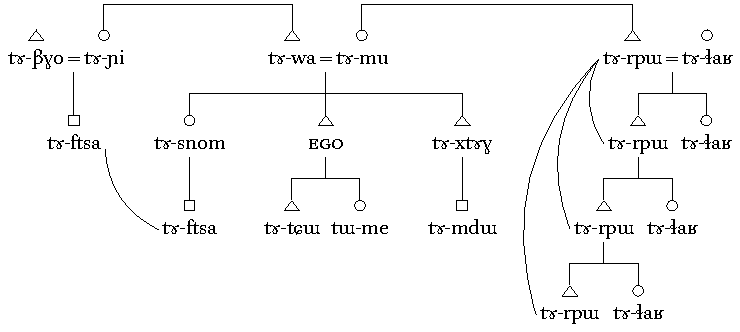
\includegraphics[width=\textwidth]{kinship-japhug-1.pdf}
\end{figure}
 
These \textit{skewing} rules\footnote{ \citet[357]{lounsbury64crow} defines this term as a `formal equivalence, in specific contexts, between kins of different generations'. } are reciprocal of each other.  They can be formally written as (\ref{ex:FZS.ZS}) and (\ref{ex:MBS.MB}) in Lounsbury's (\citeyear{lounsbury64crow}) fashion. \footnote{The rules (\ref{ex:FZS.ZS}) and (\ref{ex:MBS.MB}) are close to Lounsbury's (\citeyear[359]{lounsbury64crow}) `Omaha type I', but slightly less general. }
 
\begin{exe}
\ex 
\begin{xlist}
\ex \label{ex:FZS.ZS}
\glt \textbf{Skewing rule} 1: FZCh \fl{} ZCh
\ex \label{ex:MBS.MB}
\glt Corollaries:  MBS \fl{} MB; MBD \fl{} MZ
\end{xlist}
\end{exe}

Moreover, the fact that the children of one paternal aunt's children are also identified with the sister's children (§\ref{sec:MBCh.FZCh.Ch}) implies the rule in (\ref{ex:FZChCh.ZS}) and its reciprocal (\ref{ex:MMBS.MB}), explicitly stated by Tshendzin in (\ref{ex:MMBCh.FMBCh}).

\begin{exe}
\ex \label{ex:MMBCh.FMBCh}
\gll nɤ-ɲi ɣɯ ɯ-ɣe kɯ tɕe tɕe, nɤj nɤ-ɕki ``a-rpɯ" tu-ti kɯ-ra ɕti. \\
\textsc{2sg}.\textsc{poss}-FZ \textsc{gen} \textsc{3sg}.\textsc{poss}-grandchild \textsc{erg} \textsc{lnk} \textsc{lnk} \textsc{2sg} \textsc{2sg}.\textsc{poss}-\textsc{dat} \textsc{1sg}.\textsc{poss}-MB \textsc{ipfv}-say \textsc{inf}:\textsc{stat}-be.needed be.\textsc{aff}:\textsc{fact} \\
\glt `Your father's sister's grandchildren have to call you `my mother's brother'.' (elicitation 2019-11-30)
\end{exe}

\begin{exe}
\ex 
\begin{xlist}
\ex \label{ex:FZChCh.ZS}
\glt \textbf{Skewing rule} 2: FZChCh \fl{} FZCh \fl{} ZCh
\ex \label{ex:MMBS.MB}
\glt Corollaries:  (F|M)MBS \fl{} MB; (F|M)MBD \fl{} MZ
\end{xlist}
\end{exe}
 
The rules (\ref{ex:FZS.ZS}), (\ref{ex:MBS.MB}), (\ref{ex:FZChCh.ZS}), (\ref{ex:MMBS.MB}) are described by Tshendzin as being recursive, implying the theoretical equivalences in (\ref{ex:kinship.recursive}). Although a considerable amount of genealogies would be needed to confirm whether the system indeed works in the way predicted in (\ref{ex:kinship.recursive}), an anecdote discussed in §\ref{sec:MBChCh.Dpalcan} confirms the reality of the equivalence MMMBSSSS = MB.
  
 \begin{exe}
 \ex \label{ex:kinship.recursive}
\begin{xlist}
\ex \label{ex:FFFFZCh}
\glt ZCh = (F)*ZCh(Ch)*
\ex \label{ex:MBSSSS}
\glt MB = (F|M)*MB(S)*S
 \ex \label{ex:MBSSSD}
\glt MZ = (F|M)*MB(S)*D
\end{xlist}
\end{exe}

Another skewing rule is observed in the case of female \textsc{ego}:  \textsuperscript{♀}BS are called with the relative age sibling terms (§\ref{sec:nephews}), though this skewing is only partial, since they respond using the dedicated term \forme{tɤ-ɲi} for FZ (§\ref{sec:uncle.aunt}).

Finally, another skewing rule (\ref{ex:MZChCh.skewing}) appears with maternal parallel cousins (§\ref{sec:FBCh.MZCh.Ch}).

\begin{exe}
\ex 
\begin{xlist}
\ex \label{ex:MZChCh.skewing}
\glt \textbf{Skewing rule} 3: MZChCh \fl{} MZCh
\ex \label{ex:MMZCh.skewing}
\glt Corollary:  (F|M)MZCh \fl{} MZCh
\end{xlist}
\end{exe}

If the rules (\ref{ex:MZChCh.skewing}) and (\ref{ex:MMZCh.skewing}) are also recursive, the formal equivalence (\ref{ex:MMMMMZChChChCh}) is implied. Data is lacking to ascertain whether this theoretical possibility is verified, but §\ref{sec:FMZCh.Tshendzin} discusses a case in these lines. In this system, unlike in that described by \citet[361]{lounsbury64crow}, the MMZCh are not equated with the MB and MZ (due to absence of the merging rules MZS \fl{} B and MZD \fl{} Z), but rather with the MZCh. 

 \begin{exe}
\ex \label{ex:MMMMMZChChChCh}
\glt MZCh = (F|M)*MZCh(Ch)*
\end{exe}

However, it appears to be possible to alternatively use the term \forme{tɤ-ftsa} `ZS' for MZChCh. The implication of this rule for the whole system are not considered here until further data are available.

The terminological identification of paternal parallel cousins with siblings (§\ref{sec:ego.parallel.cousins}) defines the following merging rule (\ref{ex:FBS.B.FBD.Z}).

\begin{exe}
\ex \label{ex:FBS.B.FBD.Z}
\glt \textbf{Merging rules}: FBS \fl{} B; FBD \fl{} Z
\end{exe}

Unlike the Omaha systems described in \citet[360]{lounsbury64crow}, the merging rule (\ref{ex:FBS.B.FBD.Z}) does not concern maternal parallel cousins (§\ref{sec:ego.parallel.cousins}). It implies the equivalences MFBS = MB, MFBD = MZ, FFBS = FB and FFBD = FZ, and more generally (\ref{ex:kinship.recursive2}), in combination with the skewing rules in (\ref{ex:kinship.recursive}) above.

 \begin{exe}
 \ex \label{ex:kinship.recursive2}
\begin{xlist}
\ex  
\glt MB = (F|M)*MFB(S)*S
\ex  
\glt MZ = (F|M)*MFB(S)*D
\ex  
\glt FB = (F)$^n$FB(S)$^n_{n\geqslant 1}$
\ex  
\glt FZ = (F)$^n$FB(S)$^{n-1}$D$_{n\geqslant 1}$
\end{xlist}
\end{exe}
%\textsuperscript{♂}\textsuperscript{♀}

Some uncertainty remains in parts of the system. In particular, the status of the MBDCh (and its reciprocal MFZCh) is unclear. In theory, given the MBD \fl{} MZ rule (\ref{ex:MMBS.MB}), one would expect that MBDCh = MZCh (\forme{tɤ-mɤtsa}), and likewise that the MFZCh = MZCh (due to the reciprocal rule \ref{ex:FFFFZCh}). However, at the moment of writing I could not confirm whether this is true or not.
 
%\citet[359]{lounsbury64crow} proposes slightly more general formal rules for his `Omaha type I', rewritten in (\ref{ex:FZX.ZX}) and (\ref{ex:XBS.XB}) (X stands for any relative; the notation in slightly altered to fit the system used in this chapter).  
% 
%\begin{exe}
%\ex 
%\begin{xlist}
%\ex \label{ex:FZX.ZX}
%\glt \textbf{Skewing rule}: FZX \fl{} ZX
%\ex \label{ex:XBS.XB}
%\glt Corollaries:  X\textsuperscript{♀}BS \fl{} X\textsuperscript{♀}B; X\textsuperscript{♀}BD \fl{} X\textsuperscript{♀}Z
%\end{xlist}
%\end{exe}
% 
%For this formulation to be compatible with the Japhug system,  affines have to be excluded, since they are not concerned by the skewing rule. Otherwise,  FZH would be equivalent to ZH and WBS to WB. In fact, FZH is called using the FB term (see \tabref{tab:uncle.aunt}, §\ref{sec:uncle.aunt}), and ZH with the relative age sibling terms (§\ref{sec:siblings.age}).  

The Japhug system shows prototypical Omaha characteristics, in particular the basic skewing rules  (\ref{ex:FZS.ZS}) and (\ref{ex:MBS.MB}), and the identification of paternal parallel cousins with siblings (\ref{ex:FBS.B.FBD.Z}). It differs from prototypical Omaha systems described in the literature in lacking an Iroquois pattern identifying parallel uncles and aunts with parents (FB \fl{} F, MZ \fl{} M, \citealt[34]{trautmann12crossness}), maternal parallel cousins with siblings (MZS \fl{} B, MZD \fl{} Z), and the fact that preferred marriage is with maternal parallel cousins (§\ref{sec:marriage.rules}) rather than with cross-cousins (\citealt[41]{trautmann12crossness}).
 

 \subsection{Cross-cousin lineages} \label{sec:MBChCh.Dpalcan}
A logical consequence of the recursivity of the skewing rule (\ref{ex:kinship.recursive}, §\ref{sec:skewing.merging}), as they are described by Tshendzin (§\ref{sec:MBCh.FZCh.Ch}) is that a considerable divergence between biological age and age rank will occur in some cases. While a full investigation of genealogies is necessary to verify this implication (an endeavour that goes beyond the scope of this grammar), an  anecdote reported by two witnesses suggests that this indeed used to be the case in the traditional society.

In (\ref{ex:aftsa.beifen}), a man born in the 1950s reports his experience with the skewing rule: one of his great-grandmother (either MMM or MMMM, I could not ascertain) came from the village of Tshapa (with irregular orientation \textsc{westwards}, opposite of the geographical reality, §\ref{sec:local.toponyms.orientation}), where most inhabitants are from the lineage of her brother.

 \begin{exe}
\ex \label{ex:aftsa.beifen}
\gll  iʑo ji-wi nɯnɯ tsʰapa nɯ-kɯ-ɣe pjɤ-ŋu. (...)   aʑo tɤ-nɯkoŋtso-a ɯ-qʰu tɕe, tsʰapa ju-ɕe-a tɕe, tsʰapa nɯ ji-kɯmdza ʁɟa ɲɯ-ŋu tɕe, (...) tɕe a-rpɯ a-ɬaʁ ntsɯ tu-kɯ-ti ɲɯ-ra ma nɯ-<beifen> ɲɯ-mbro, (...)   tɤ-pɤtso kɯ-xtɕɯ\redp{}xtɕi ra kɯ nɯ a-pʰe ``a-ftsa a-ftsa" tu-ti-nɯ, ``a-rpɯ a-ɬaʁ" kɤ-ti ɲɯ-ra, tɕendɤre tu-ti-a kɯ-zgɤt ɲɯ-ɕti ri nɯnɯ aʑo mɯ́j-nɤx-tʂaŋ-a   \\
\textsc{1pl} \textsc{1pl}.\textsc{poss}-grandmother \textsc{dem}  \textsc{topo} \textsc{aor}:\textsc{west}-\textsc{sbj}:\textsc{pcp}-come[II] \textsc{ifr}.\textsc{ipfv}-be { } \textsc{1sg} \textsc{aor}-work-\textsc{1sg} \textsc{3sg}.\textsc{poss}-after \textsc{lnk}  \textsc{topo} \textsc{ipfv}-go-\textsc{1sg} \textsc{lnk}  \textsc{topo} \textsc{dem} \textsc{1pl}.\textsc{poss}-relative completely \textsc{sens}-be \textsc{lnk} { } \textsc{lnk} \textsc{1sg}.\textsc{poss}-MB \textsc{1sg}.\textsc{poss}-MZ always \textsc{ipfv}-\textsc{genr}-say \textsc{sens}-be.needed \textsc{lnk} \textsc{3pl}.\textsc{poss}-age.rank \textsc{sens}-be.high {  } \textsc{indef}.\textsc{poss}-child \textsc{sbj}:\textsc{pcp}-\textsc{emph}\redp{}be.small \textsc{pl} \textsc{erg} \textsc{dem}  \textsc{1sg}.\textsc{poss}-\textsc{dat}  \textsc{1sg}.\textsc{poss}-ZCh  \textsc{1sg}.\textsc{poss}-ZCh \textsc{ipfv}-say-\textsc{pl}  \textsc{1sg}.\textsc{poss}-MB \textsc{1sg}.\textsc{poss}-MZ \textsc{inf}-say \textsc{sens}-be.needed \textsc{lnk} \textsc{ipfv}-say-\textsc{1sg} \textsc{inf}:\textsc{stat}-be.needed \textsc{sens}-be.\textsc{aff} \textsc{lnk} \textsc{dem} \textsc{1sg} \textsc{neg}:\textsc{sens}-\textsc{trop}-be.fair-\textsc{1sg} \\
\glt `(One of) our grandmothers was from Tshapa (...) After I started working, when I went to Tshapa, there everybody is our relatives, (...) I had to call all of them `my mother's brother, my mother's sister', because they are of higher \ch{辈分}{bèifen}{age rank}, (... even) small children called me `my sister's son', and I had to call them  `my mother's brother, my mother's sister'. Although this was what I had to say, I found it unfair.' (2010-06)
 \end{exe}
 
He thus had to call all the inhabitants of the village using the MB  and MZ  terms \forme{tɤ-rpɯ}  and \forme{tɤ-ɬaʁ}, even young children. This report suggests that the recursivity of the rules as described in (\ref{ex:kinship.recursive}) above is a reality: descendants of MMMB or MMMMB, even one or two generations below oneself, are still called MB and MZ. It also suggests that not only MBS*, but also MBDCh and their descendants might keep the privileged status (and thus not be equated with maternal parallel cousins MZCh as predicted in §\ref{sec:skewing.merging}), though this has to be tested with additional data.

Tshendzin reports the same anecdote (\ref{ex:MMMMMBSSSSS}), and also indicates that the recursivity of the skewing rule is felt clumsy by younger speakers, who prefer to use terms for parallel uncles, aunts or siblings. This aspect of the Japhug languages is thus highly endangered.
 
 \begin{exe}
\ex \label{ex:MMMMMBSSSSS}
\gll  ɯ-wi ɣɯ ɯ-wi nɯnɯ tsʰapa nɯtɕu nɯ-kɯ-ɣe pjɤ-ŋu tɕe tɕe nɯ ɣɯ ɯ-wi ɣɯ ɯ-wɤmɯ nɯnɯ ɣɯ ɯ-rɟit ɣɯ ɯ-rɟit ɣɯ ɯ-rɟit ɣɯ ɯ-rɟit kɯ-fse nɯnɯra nɯ-ɕki tɕe tɕe ``a-rpɯ nɤ a-ɬaʁ" ntsɯ tu-ti pjɤ-ra. (...) tʰam tɕe nɯra stʰɯci ɯ-kɯ-ti maŋe, tɕe kɯ-xtɕi nɯra kɯnɤ ``a-ftsa" kɤ-ti ɲɯ-nɤzraʁ-nɯ qʰe ``a-βɣo" ra tu-nɯ-ti-nɯ,  ``a-pi" ra tu-nɯ-ti-nɯ. tɕe tʰam tu-otʂoʁloʁ ɕti. kɯɕɯŋgɯ a-pɯ-ŋu tɕe nɯ tu-kɯ-ti kɯ-ra pjɤ-ɕti nɤ. \\
  \textsc{3sg}.\textsc{poss}-grandmother \textsc{gen}   \textsc{3sg}.\textsc{poss}-grandmother \textsc{dem}   \textsc{topo} \textsc{dem}:\textsc{loc} \textsc{aor}:\textsc{west}-\textsc{sbj}:\textsc{pcp}-come[III] \textsc{ifr}.\textsc{ipfv}-be \textsc{lnk} \textsc{lnk} \textsc{dem} \textsc{gen} \textsc{3sg}.\textsc{poss}-grandmother \textsc{gen} \textsc{3sg}.\textsc{poss}-brother \textsc{dem} \textsc{gen} \textsc{3sg}.\textsc{poss}-offspring  \textsc{gen} \textsc{3sg}.\textsc{poss}-offspring  \textsc{gen} \textsc{3sg}.\textsc{poss}-offspring  \textsc{gen} \textsc{3sg}.\textsc{poss}-offspring \textsc{sbj}:\textsc{pcp}-be.like \textsc{dem}:\textsc{pl} \textsc{3pl}.\textsc{poss}-\textsc{dat} \textsc{loc} \textsc{lnk} \textsc{1sg}.\textsc{poss}-MB \textsc{add} \textsc{1sg}.\textsc{poss}-MZ always \textsc{ipfv}-say \textsc{ipfv}.\textsc{ifr}-be.needed {  } now \textsc{lnk} \textsc{dem}:\textsc{loc} so.much \textsc{3sg}.\textsc{poss}-\textsc{sbj}:\textsc{pcp}-say not.exist:\textsc{sens} \textsc{lnk} \textsc{sbj}:\textsc{pcp}-be.small \textsc{dem}:\textsc{pl} also \textsc{1sg}.\textsc{poss}-ZCh \textsc{inf}-say \textsc{sens}-be.ashamed-\textsc{pl} \textsc{lnk} \textsc{1sg}.\textsc{poss}-FB \textsc{pl} \textsc{ipfv}-\textsc{auto}-say-\textsc{pl} \textsc{1sg}.\textsc{poss}-elder.sibling \textsc{pl} \textsc{ipfv}-\textsc{auto}-say-\textsc{pl}  \textsc{lnk} now \textsc{ipfv}-be.mixed be.\textsc{aff}:\textsc{fact} in.former.days \textsc{irr}-\textsc{ipfv}-be \textsc{lnk} \textsc{dem} \textsc{ipfv}-\textsc{genr}-say \textsc{inf}:\textsc{stat}-be.needed \textsc{ifr}.\textsc{ipfv}-be \textsc{sfp} \\
 \glt `His grandmother's grandmother had come from Tshapa, and he had to call all of his grandmother's brother's children's children's children's children (etc) `my mother's brother, my mother's sister' (including small children)'. (...) Now no one says this any more, the young ones are ashamed of calling (elders) `my sister's child' and instead say `my father's brother' or `my elder sibling'. Now it is all mixed up, but in former times, one had to speak like that.' (140425 kWmdza07, 8-12)
 \end{exe}
 
 \subsection{Maternal parallel cousin lineages} \label{sec:FMZCh.Tshendzin}
 The reliability of the skewing rule (\ref{ex:MZChCh.skewing}) concerning maternal parallel cousins is confirmed by one particular case, in which a lady addressed her mother-in-law by the term \forme{tɤ-mɤtsa} `MZCh' (who answered using the same term, §\ref{sec:ego.parallel.cousins}). When I asked her whether they were actual maternal parallel cousins (children of two sisters, MZCh), she answered that she used this term because her father himself called her mother-in-law (and her mother-in-law's mother) \forme{tɤ-mɤtsa}, though they were not themselves true first cousins, the eventual consanguine relationship going back several generations. She also specified that she called her husband \forme{tɤ-mɤtsa} before marrying him (§\ref{sec:marriage.rules}). 
 
This case suggests that the reciprocal \forme{tɤ-mɤtsa} `maternal parallel cousin' relationship remains regardless of the number of generations in each lineages (as formalized in \ref {ex:MMMMMZChChChCh} above).

\subsection{Application} \label{sec:cousins.once.rmoved}
As an illustration of the rules established in the previous sections, \tabref{sec:cousin.once} summarizes the theoretical possibilities for first and second cousins \textit{once removed}, including the main points of uncertainty in grey shading. The equivalences are given below each term in brackets, referring to the equivalent focal kin (\tabref{tab:focal.kin}); for instance (=ZCh) should be read `called like the ZCh' (\forme{tɤ-ftsa}, §\ref{sec:nephews}). 

\begin{table}
\caption{Focal kin terms } \label{tab:focal.kin}
\begin{tabular}{lllll}
\lsptoprule
 Kin & term & Reciprocal & term \\
\midrule
M& \forme{tɤ-mu} & \textsuperscript{♀}S/\textsuperscript{♀}D &\forme{tɤ-tɕɯ}/\forme{tɯ-me} \\
F &\forme{tɤ-wa} & \textsuperscript{♂}S/\textsuperscript{♂}D &\forme{tɤ-tɕɯ}/\forme{tɯ-me} \\
\midrule
MB  &  \forme{tɤ-rpɯ} & \textsuperscript{♂}ZCh &\forme{tɤ-ftsa} \\
MZ &\forme{tɤ-ɬaʁ} & \textsuperscript{♀}ZCh &\forme{tɤ-ftsa} \\
\midrule
FB  & \forme{tɤ-βɣo} & \textsuperscript{♂}BCh &\forme{tɤ-mdɯ} \\
FZ & \forme{tɤ-ɲi} & \textsuperscript{♂}BCh=yB|Z &\forme{ta-ʁi} \\
\midrule
MZCh & \forme{tɤ-mɤtsa} & = \\
\midrule
eB|Z &\forme{tɤ-pi} & yB|Z &\forme{ta-ʁi} \\
\midrule
\textsuperscript{♂}Z& \forme{tɤ-snom} & \textsuperscript{♀}B \forme{tɤ-wɤmɯ} \\
\textsuperscript{♂}B& \forme{tɤ-xtɤɣ} & =  \\
\textsuperscript{♀}Z& \forme{tɤ-sqʰaj} & = \\
\lspbottomrule
\end{tabular}
\end{table}

The reciprocal terms can be rechecked using the inversion table \ref{tab:kinship.reciprocal} above.

It is difficult to be fully certain of the reliability of these extrapolations without an in-depth study of genealogies. This Table provides a framework for future research on kinship systems in Japhug and Gyalrong-speaking areas. 

\begin{table}
\caption{First and second cousins once removed (hypothetical)} \label{sec:cousin.once}
\begin{tabular}{lllll}
\lsptoprule
First cousin  & Reciprocal & Second cousin &  Reciprocal \\ 
\midrule
FFBS  & \textsuperscript{♂}FBSCh  & FFBSCh  & FFBSCh \\
(=FB)& (=\textsuperscript{♂}BCh) &(= FBCh=B|Z)& (=B|Z) \\
\midrule
FFBD & \textsuperscript{♀}FBSCh& FFBDCh  & MFBSCh  \\
 (=FZ) & (=\textsuperscript{♀}BS=yB|Z) &  (= FZCh=ZCh) &  (=MBCh=MB|Z) \\
\midrule
FFZCh   & MBSS  & FFZChCh   & (F|M)MBSS   \\
(=ZCh) &  (=MB) &  (=ZCh) & (=MB) \\
\midrule
FMBS  & \textsuperscript{♂}FZSCh   & FMBSCh  &  FFZSCh  \\
 (=MB) & (=ZCh) &  (=MB) &   (=ZCh) \\
 \midrule
FMBD   & \textsuperscript{♀}FZSCh   & FMBDCh  &  MFZSCh  \\
 (=MZ) &  (=ZCh) &  (=FMZCh=MZCh?)\grise{} &   (=MZCh?) \grise{}\\
\midrule
FMZCh   & MZDS   & FMZChCh  &  (F|M)MZDS  \\
 (=MZCh?)\grise{} &  (=MZCh?)\grise{}&  (=MZCh?)\grise{}&  (=MZCh?)\grise{} \\
\midrule
MFBS  & \textsuperscript{♂}FBDCh &MFBSCh & FFBDCh  \\
 (=MB) & (=FZCh=ZCh) & (=MB|Z)&  (=FFZCh=ZCh) \\
 \midrule
MFBD & \textsuperscript{♀}FBDCh &MFBDCh & MFBDCh  \\
 (=MZ) & (=FZCh=ZCh) & (=MZCh?)\grise{}&  (=MZCh?)\grise{} \\
\midrule
MFZCh  &  MBDCh &MFZChCh & (F|M)MBDCh  \\
 (=MZCh?)\grise{} &  (=MZCh?)\grise{}&  (=MZCh?)\grise{}&  (=MZCh?)\grise{} \\
 \midrule
 MMBS  & \textsuperscript{♂}FZDCh &MMBSCh & FFZDCh  \\
 (=MB) & (=ZCh) & (=MB|Z)&  (=ZCh) \\
  \midrule
  MMBD  & \textsuperscript{♀}FZDCh &MMBDCh & MFZDCh  \\
 (=MMZ=MZ) & (=ZCh) & (=MZCh?)\grise{} &  (=MZCh?) \grise{} \\
   \midrule
  MMZCh  & MZDCh &MMZChCh & (F|M)MZDCh  \\
   (=MZCh) &  (=MZCh) &  (=MZCh?) \grise{}&  (=MZCh?)\grise{} \\
\lspbottomrule
\end{tabular}
\end{table}
  %Kinship

%%%%%%%%%%%%%%%%%%%%%%%%%%%%%%%%%%%%%%%%%%%%%%%%%%%%
%%%                                              %%%
%%%             Backmatter                       %%%
%%%                                              %%%
%%%%%%%%%%%%%%%%%%%%%%%%%%%%%%%%%%%%%%%%%%%%%%%%%%%%

%\is{some term| see {some other term}}
\il{some language| see {some other language}}
\issa{some term with pages}{some other term also of interest}
\ilsa{some language with pages}{some other lect also of interest} 
% There is normally no need to change the backmatter section
\backmatter
\phantomsection%this allows hyperlink in ToC to work
\printbibliography[heading=references] 
\cleardoublepage

\phantomsection 
\addcontentsline{toc}{chapter}{Index} 
\addcontentsline{toc}{section}{Name index}
\ohead{Name index} 
\printindex 
\cleardoublepage
  
\phantomsection 
\addcontentsline{toc}{section}{Language index}
\ohead{Language index} 
\printindex[lan] 
\cleardoublepage
  
\phantomsection 
\addcontentsline{toc}{section}{Subject index}
\ohead{Subject index} 
\printindex[sbj]
\ohead{} 
 
\end{document} 


